\documentclass[twoside]{book}

% Packages required by doxygen
\usepackage{fixltx2e}
\usepackage{calc}
\usepackage{doxygen}
\usepackage[export]{adjustbox} % also loads graphicx
\usepackage{graphicx}
\usepackage[utf8]{inputenc}
\usepackage{makeidx}
\usepackage{multicol}
\usepackage{multirow}
\PassOptionsToPackage{warn}{textcomp}
\usepackage{textcomp}
\usepackage[nointegrals]{wasysym}
\usepackage[table]{xcolor}

% Font selection
\usepackage[T1]{fontenc}
\usepackage[scaled=.90]{helvet}
\usepackage{courier}
\usepackage{amssymb}
\usepackage{sectsty}
\renewcommand{\familydefault}{\sfdefault}
\allsectionsfont{%
  \fontseries{bc}\selectfont%
  \color{darkgray}%
}
\renewcommand{\DoxyLabelFont}{%
  \fontseries{bc}\selectfont%
  \color{darkgray}%
}
\newcommand{\+}{\discretionary{\mbox{\scriptsize$\hookleftarrow$}}{}{}}

% Page & text layout
\usepackage{geometry}
\geometry{%
  a4paper,%
  top=2.5cm,%
  bottom=2.5cm,%
  left=2.5cm,%
  right=2.5cm%
}
\tolerance=750
\hfuzz=15pt
\hbadness=750
\setlength{\emergencystretch}{15pt}
\setlength{\parindent}{0cm}
\setlength{\parskip}{3ex plus 2ex minus 2ex}
\makeatletter
\renewcommand{\paragraph}{%
  \@startsection{paragraph}{4}{0ex}{-1.0ex}{1.0ex}{%
    \normalfont\normalsize\bfseries\SS@parafont%
  }%
}
\renewcommand{\subparagraph}{%
  \@startsection{subparagraph}{5}{0ex}{-1.0ex}{1.0ex}{%
    \normalfont\normalsize\bfseries\SS@subparafont%
  }%
}
\makeatother

% Headers & footers
\usepackage{fancyhdr}
\pagestyle{fancyplain}
\fancyhead[LE]{\fancyplain{}{\bfseries\thepage}}
\fancyhead[CE]{\fancyplain{}{}}
\fancyhead[RE]{\fancyplain{}{\bfseries\leftmark}}
\fancyhead[LO]{\fancyplain{}{\bfseries\rightmark}}
\fancyhead[CO]{\fancyplain{}{}}
\fancyhead[RO]{\fancyplain{}{\bfseries\thepage}}
\fancyfoot[LE]{\fancyplain{}{}}
\fancyfoot[CE]{\fancyplain{}{}}
\fancyfoot[RE]{\fancyplain{}{\bfseries\scriptsize Generated by Doxygen }}
\fancyfoot[LO]{\fancyplain{}{\bfseries\scriptsize Generated by Doxygen }}
\fancyfoot[CO]{\fancyplain{}{}}
\fancyfoot[RO]{\fancyplain{}{}}
\renewcommand{\footrulewidth}{0.4pt}
\renewcommand{\chaptermark}[1]{%
  \markboth{#1}{}%
}
\renewcommand{\sectionmark}[1]{%
  \markright{\thesection\ #1}%
}

% Indices & bibliography
\usepackage{natbib}
\usepackage[titles]{tocloft}
\setcounter{tocdepth}{3}
\setcounter{secnumdepth}{5}
\makeindex

% Hyperlinks (required, but should be loaded last)
\usepackage{ifpdf}
\ifpdf
  \usepackage[pdftex,pagebackref=true]{hyperref}
\else
  \usepackage[ps2pdf,pagebackref=true]{hyperref}
\fi
\hypersetup{%
  colorlinks=true,%
  linkcolor=blue,%
  citecolor=blue,%
  unicode%
}

% Custom commands
\newcommand{\clearemptydoublepage}{%
  \newpage{\pagestyle{empty}\cleardoublepage}%
}

\usepackage{caption}
\captionsetup{labelsep=space,justification=centering,font={bf},singlelinecheck=off,skip=4pt,position=top}

%===== C O N T E N T S =====

\begin{document}

% Titlepage & ToC
\hypersetup{pageanchor=false,
             bookmarksnumbered=true,
             pdfencoding=unicode
            }
\pagenumbering{alph}
\begin{titlepage}
\vspace*{7cm}
\begin{center}%
{\Large E\+CS 160 Project }\\
\vspace*{1cm}
{\large Generated by Doxygen 1.8.12}\\
\end{center}
\end{titlepage}
\clearemptydoublepage
\pagenumbering{roman}
\tableofcontents
\clearemptydoublepage
\pagenumbering{arabic}
\hypersetup{pageanchor=true}

%--- Begin generated contents ---
\chapter{E\+C\+S160\+Linux}
\label{md_README}
\hypertarget{md_README}{}
E\+CS 160 Project Linux

\subsection*{Warcraft II AI}
\chapter{Hierarchical Index}
\section{Class Hierarchy}
This inheritance list is sorted roughly, but not completely, alphabetically\+:\begin{DoxyCompactList}
\item \contentsline{section}{C\+Activated\+Player\+Capability}{\pageref{classCActivatedPlayerCapability}}{}
\begin{DoxyCompactList}
\item \contentsline{section}{C\+Player\+Capability\+Attack\+:\+:C\+Activated\+Capability}{\pageref{classCPlayerCapabilityAttack_1_1CActivatedCapability}}{}
\item \contentsline{section}{C\+Player\+Capability\+Building\+Upgrade\+:\+:C\+Activated\+Capability}{\pageref{classCPlayerCapabilityBuildingUpgrade_1_1CActivatedCapability}}{}
\item \contentsline{section}{C\+Player\+Capability\+Build\+Normal\+:\+:C\+Activated\+Capability}{\pageref{classCPlayerCapabilityBuildNormal_1_1CActivatedCapability}}{}
\item \contentsline{section}{C\+Player\+Capability\+Build\+Ranger\+:\+:C\+Activated\+Capability}{\pageref{classCPlayerCapabilityBuildRanger_1_1CActivatedCapability}}{}
\item \contentsline{section}{C\+Player\+Capability\+Cancel\+:\+:C\+Activated\+Capability}{\pageref{classCPlayerCapabilityCancel_1_1CActivatedCapability}}{}
\item \contentsline{section}{C\+Player\+Capability\+Convey\+:\+:C\+Activated\+Capability}{\pageref{classCPlayerCapabilityConvey_1_1CActivatedCapability}}{}
\item \contentsline{section}{C\+Player\+Capability\+Mine\+Harvest\+:\+:C\+Activated\+Capability}{\pageref{classCPlayerCapabilityMineHarvest_1_1CActivatedCapability}}{}
\item \contentsline{section}{C\+Player\+Capability\+Move\+:\+:C\+Activated\+Capability}{\pageref{classCPlayerCapabilityMove_1_1CActivatedCapability}}{}
\item \contentsline{section}{C\+Player\+Capability\+Patrol\+:\+:C\+Activated\+Capability}{\pageref{classCPlayerCapabilityPatrol_1_1CActivatedCapability}}{}
\item \contentsline{section}{C\+Player\+Capability\+Repair\+:\+:C\+Activated\+Capability}{\pageref{classCPlayerCapabilityRepair_1_1CActivatedCapability}}{}
\item \contentsline{section}{C\+Player\+Capability\+Stand\+Ground\+:\+:C\+Activated\+Capability}{\pageref{classCPlayerCapabilityStandGround_1_1CActivatedCapability}}{}
\item \contentsline{section}{C\+Player\+Capability\+Train\+Normal\+:\+:C\+Activated\+Capability}{\pageref{classCPlayerCapabilityTrainNormal_1_1CActivatedCapability}}{}
\item \contentsline{section}{C\+Player\+Capability\+Unit\+Upgrade\+:\+:C\+Activated\+Capability}{\pageref{classCPlayerCapabilityUnitUpgrade_1_1CActivatedCapability}}{}
\end{DoxyCompactList}
\item \contentsline{section}{C\+A\+I\+Player}{\pageref{classCAIPlayer}}{}
\item \contentsline{section}{C\+Application\+Data}{\pageref{classCApplicationData}}{}
\item \contentsline{section}{C\+Asset\+Renderer}{\pageref{classCAssetRenderer}}{}
\item \contentsline{section}{C\+Bevel}{\pageref{classCBevel}}{}
\item \contentsline{section}{C\+Button\+Renderer}{\pageref{classCButtonRenderer}}{}
\item \contentsline{section}{C\+Data\+Source}{\pageref{classCDataSource}}{}
\begin{DoxyCompactList}
\item \contentsline{section}{C\+File\+Data\+Source}{\pageref{classCFileDataSource}}{}
\end{DoxyCompactList}
\item \contentsline{section}{C\+Data\+Source\+Container}{\pageref{classCDataSourceContainer}}{}
\begin{DoxyCompactList}
\item \contentsline{section}{C\+Directory\+Data\+Source\+Container}{\pageref{classCDirectoryDataSourceContainer}}{}
\end{DoxyCompactList}
\item \contentsline{section}{C\+Data\+Source\+Container\+Iterator}{\pageref{classCDataSourceContainerIterator}}{}
\begin{DoxyCompactList}
\item \contentsline{section}{C\+Directory\+Data\+Source\+Container\+Iterator}{\pageref{classCDirectoryDataSourceContainerIterator}}{}
\end{DoxyCompactList}
\item \contentsline{section}{C\+Edit\+Renderer}{\pageref{classCEditRenderer}}{}
\item \contentsline{section}{C\+Fog\+Renderer}{\pageref{classCFogRenderer}}{}
\item \contentsline{section}{C\+Game\+Model}{\pageref{classCGameModel}}{}
\item \contentsline{section}{C\+Graphic\+Loader}{\pageref{classCGraphicLoader}}{}
\item \contentsline{section}{C\+Graphic\+Recolor\+Map}{\pageref{classCGraphicRecolorMap}}{}
\item \contentsline{section}{C\+Graphic\+Tileset}{\pageref{classCGraphicTileset}}{}
\begin{DoxyCompactList}
\item \contentsline{section}{C\+Cursor\+Set}{\pageref{classCCursorSet}}{}
\item \contentsline{section}{C\+Font\+Tileset}{\pageref{classCFontTileset}}{}
\item \contentsline{section}{C\+Graphic\+Multicolor\+Tileset}{\pageref{classCGraphicMulticolorTileset}}{}
\end{DoxyCompactList}
\item \contentsline{section}{C\+Line\+Data\+Source}{\pageref{classCLineDataSource}}{}
\item \contentsline{section}{C\+List\+View\+Renderer}{\pageref{classCListViewRenderer}}{}
\item \contentsline{section}{C\+Map\+Renderer}{\pageref{classCMapRenderer}}{}
\item \contentsline{section}{C\+Mini\+Map\+Renderer}{\pageref{classCMiniMapRenderer}}{}
\item \contentsline{section}{C\+Path}{\pageref{classCPath}}{}
\item \contentsline{section}{C\+Periodic\+Timeout}{\pageref{classCPeriodicTimeout}}{}
\item \contentsline{section}{C\+Pixel\+Type}{\pageref{classCPixelType}}{}
\item \contentsline{section}{C\+Player\+Asset}{\pageref{classCPlayerAsset}}{}
\item \contentsline{section}{C\+Player\+Asset\+Type}{\pageref{classCPlayerAssetType}}{}
\item \contentsline{section}{C\+Player\+Capability}{\pageref{classCPlayerCapability}}{}
\begin{DoxyCompactList}
\item \contentsline{section}{C\+Player\+Capability\+Attack}{\pageref{classCPlayerCapabilityAttack}}{}
\item \contentsline{section}{C\+Player\+Capability\+Building\+Upgrade}{\pageref{classCPlayerCapabilityBuildingUpgrade}}{}
\item \contentsline{section}{C\+Player\+Capability\+Build\+Normal}{\pageref{classCPlayerCapabilityBuildNormal}}{}
\item \contentsline{section}{C\+Player\+Capability\+Build\+Ranger}{\pageref{classCPlayerCapabilityBuildRanger}}{}
\item \contentsline{section}{C\+Player\+Capability\+Cancel}{\pageref{classCPlayerCapabilityCancel}}{}
\item \contentsline{section}{C\+Player\+Capability\+Convey}{\pageref{classCPlayerCapabilityConvey}}{}
\item \contentsline{section}{C\+Player\+Capability\+Mine\+Harvest}{\pageref{classCPlayerCapabilityMineHarvest}}{}
\item \contentsline{section}{C\+Player\+Capability\+Move}{\pageref{classCPlayerCapabilityMove}}{}
\item \contentsline{section}{C\+Player\+Capability\+Patrol}{\pageref{classCPlayerCapabilityPatrol}}{}
\item \contentsline{section}{C\+Player\+Capability\+Repair}{\pageref{classCPlayerCapabilityRepair}}{}
\item \contentsline{section}{C\+Player\+Capability\+Stand\+Ground}{\pageref{classCPlayerCapabilityStandGround}}{}
\item \contentsline{section}{C\+Player\+Capability\+Train\+Normal}{\pageref{classCPlayerCapabilityTrainNormal}}{}
\item \contentsline{section}{C\+Player\+Capability\+Unit\+Upgrade}{\pageref{classCPlayerCapabilityUnitUpgrade}}{}
\end{DoxyCompactList}
\item \contentsline{section}{C\+Player\+Data}{\pageref{classCPlayerData}}{}
\item \contentsline{section}{C\+Player\+Upgrade}{\pageref{classCPlayerUpgrade}}{}
\item \contentsline{section}{C\+Position}{\pageref{classCPosition}}{}
\item \contentsline{section}{C\+Random\+Number\+Generator}{\pageref{classCRandomNumberGenerator}}{}
\item \contentsline{section}{C\+Player\+Capability\+Mine\+Harvest\+:\+:C\+Registrant}{\pageref{classCPlayerCapabilityMineHarvest_1_1CRegistrant}}{}
\item \contentsline{section}{C\+Player\+Capability\+Attack\+:\+:C\+Registrant}{\pageref{classCPlayerCapabilityAttack_1_1CRegistrant}}{}
\item \contentsline{section}{C\+Player\+Capability\+Repair\+:\+:C\+Registrant}{\pageref{classCPlayerCapabilityRepair_1_1CRegistrant}}{}
\item \contentsline{section}{C\+Player\+Capability\+Build\+Normal\+:\+:C\+Registrant}{\pageref{classCPlayerCapabilityBuildNormal_1_1CRegistrant}}{}
\item \contentsline{section}{C\+Player\+Capability\+Cancel\+:\+:C\+Registrant}{\pageref{classCPlayerCapabilityCancel_1_1CRegistrant}}{}
\item \contentsline{section}{C\+Player\+Capability\+Convey\+:\+:C\+Registrant}{\pageref{classCPlayerCapabilityConvey_1_1CRegistrant}}{}
\item \contentsline{section}{C\+Player\+Capability\+Building\+Upgrade\+:\+:C\+Registrant}{\pageref{classCPlayerCapabilityBuildingUpgrade_1_1CRegistrant}}{}
\item \contentsline{section}{C\+Player\+Capability\+Train\+Normal\+:\+:C\+Registrant}{\pageref{classCPlayerCapabilityTrainNormal_1_1CRegistrant}}{}
\item \contentsline{section}{C\+Player\+Capability\+Stand\+Ground\+:\+:C\+Registrant}{\pageref{classCPlayerCapabilityStandGround_1_1CRegistrant}}{}
\item \contentsline{section}{C\+Player\+Capability\+Patrol\+:\+:C\+Registrant}{\pageref{classCPlayerCapabilityPatrol_1_1CRegistrant}}{}
\item \contentsline{section}{C\+Player\+Capability\+Unit\+Upgrade\+:\+:C\+Registrant}{\pageref{classCPlayerCapabilityUnitUpgrade_1_1CRegistrant}}{}
\item \contentsline{section}{C\+Player\+Capability\+Build\+Ranger\+:\+:C\+Registrant}{\pageref{classCPlayerCapabilityBuildRanger_1_1CRegistrant}}{}
\item \contentsline{section}{C\+Player\+Capability\+Move\+:\+:C\+Registrant}{\pageref{classCPlayerCapabilityMove_1_1CRegistrant}}{}
\item \contentsline{section}{C\+Resource\+Renderer}{\pageref{classCResourceRenderer}}{}
\item \contentsline{section}{C\+Router\+Map}{\pageref{classCRouterMap}}{}
\item \contentsline{section}{C\+S\+F\+Virtual\+I\+O\+Data\+Source}{\pageref{classCSFVirtualIODataSource}}{}
\item \contentsline{section}{C\+Sound\+Clip}{\pageref{classCSoundClip}}{}
\item \contentsline{section}{C\+Sound\+Event\+Renderer}{\pageref{classCSoundEventRenderer}}{}
\item \contentsline{section}{C\+Sound\+Library\+Mixer}{\pageref{classCSoundLibraryMixer}}{}
\item \contentsline{section}{C\+Terrain\+Map}{\pageref{classCTerrainMap}}{}
\begin{DoxyCompactList}
\item \contentsline{section}{C\+Asset\+Decorated\+Map}{\pageref{classCAssetDecoratedMap}}{}
\end{DoxyCompactList}
\item \contentsline{section}{C\+Text\+Formatter}{\pageref{classCTextFormatter}}{}
\item \contentsline{section}{C\+Tokenizer}{\pageref{classCTokenizer}}{}
\item \contentsline{section}{C\+Unit\+Action\+Renderer}{\pageref{classCUnitActionRenderer}}{}
\item \contentsline{section}{C\+Unit\+Description\+Renderer}{\pageref{classCUnitDescriptionRenderer}}{}
\item \contentsline{section}{C\+Viewport\+Renderer}{\pageref{classCViewportRenderer}}{}
\item \contentsline{section}{C\+Visibility\+Map}{\pageref{classCVisibilityMap}}{}
\item \contentsline{section}{S\+Asset\+Command}{\pageref{structSAssetCommand}}{}
\item \contentsline{section}{C\+Asset\+Decorated\+Map\+:\+:S\+Asset\+Initialization}{\pageref{structCAssetDecoratedMap_1_1SAssetInitialization}}{}
\item \contentsline{section}{S\+Asset\+Render\+Data}{\pageref{structSAssetRenderData}}{}
\item \contentsline{section}{C\+Sound\+Library\+Mixer\+:\+:S\+Clip\+Status}{\pageref{structCSoundLibraryMixer_1_1SClipStatus}}{}
\item \contentsline{section}{S\+Game\+Event}{\pageref{structSGameEvent}}{}
\item \contentsline{section}{S\+Map\+Location}{\pageref{structSMapLocation}}{}
\item \contentsline{section}{S\+Player\+Command\+Request}{\pageref{structSPlayerCommandRequest}}{}
\item \contentsline{section}{S\+Rectangle}{\pageref{structSRectangle}}{}
\item \contentsline{section}{C\+Asset\+Decorated\+Map\+:\+:S\+Resource\+Initialization}{\pageref{structCAssetDecoratedMap_1_1SResourceInitialization}}{}
\item \contentsline{section}{C\+Graphic\+Recolor\+Map\+:\+:S\+R\+G\+B\+Color}{\pageref{structCGraphicRecolorMap_1_1SRGBColor}}{}
\item \contentsline{section}{C\+Router\+Map\+:\+:S\+Search\+Target}{\pageref{structCRouterMap_1_1SSearchTarget}}{}
\item \contentsline{section}{S\+Search\+Tile}{\pageref{structSSearchTile}}{}
\item \contentsline{section}{C\+Sound\+Library\+Mixer\+:\+:S\+Tone\+Status}{\pageref{structCSoundLibraryMixer_1_1SToneStatus}}{}
\end{DoxyCompactList}

\chapter{Class Index}
\section{Class List}
Here are the classes, structs, unions and interfaces with brief descriptions\+:\begin{DoxyCompactList}
\item\contentsline{section}{\hyperlink{classCPlayerCapabilityMove_1_1CActivatedCapability}{C\+Player\+Capability\+Move\+::\+C\+Activated\+Capability} }{\pageref{classCPlayerCapabilityMove_1_1CActivatedCapability}}{}
\item\contentsline{section}{\hyperlink{classCPlayerCapabilityMineHarvest_1_1CActivatedCapability}{C\+Player\+Capability\+Mine\+Harvest\+::\+C\+Activated\+Capability} }{\pageref{classCPlayerCapabilityMineHarvest_1_1CActivatedCapability}}{}
\item\contentsline{section}{\hyperlink{classCPlayerCapabilityStandGround_1_1CActivatedCapability}{C\+Player\+Capability\+Stand\+Ground\+::\+C\+Activated\+Capability} }{\pageref{classCPlayerCapabilityStandGround_1_1CActivatedCapability}}{}
\item\contentsline{section}{\hyperlink{classCPlayerCapabilityCancel_1_1CActivatedCapability}{C\+Player\+Capability\+Cancel\+::\+C\+Activated\+Capability} }{\pageref{classCPlayerCapabilityCancel_1_1CActivatedCapability}}{}
\item\contentsline{section}{\hyperlink{classCPlayerCapabilityConvey_1_1CActivatedCapability}{C\+Player\+Capability\+Convey\+::\+C\+Activated\+Capability} }{\pageref{classCPlayerCapabilityConvey_1_1CActivatedCapability}}{}
\item\contentsline{section}{\hyperlink{classCPlayerCapabilityPatrol_1_1CActivatedCapability}{C\+Player\+Capability\+Patrol\+::\+C\+Activated\+Capability} }{\pageref{classCPlayerCapabilityPatrol_1_1CActivatedCapability}}{}
\item\contentsline{section}{\hyperlink{classCPlayerCapabilityAttack_1_1CActivatedCapability}{C\+Player\+Capability\+Attack\+::\+C\+Activated\+Capability} }{\pageref{classCPlayerCapabilityAttack_1_1CActivatedCapability}}{}
\item\contentsline{section}{\hyperlink{classCPlayerCapabilityRepair_1_1CActivatedCapability}{C\+Player\+Capability\+Repair\+::\+C\+Activated\+Capability} }{\pageref{classCPlayerCapabilityRepair_1_1CActivatedCapability}}{}
\item\contentsline{section}{\hyperlink{classCPlayerCapabilityBuildNormal_1_1CActivatedCapability}{C\+Player\+Capability\+Build\+Normal\+::\+C\+Activated\+Capability} }{\pageref{classCPlayerCapabilityBuildNormal_1_1CActivatedCapability}}{}
\item\contentsline{section}{\hyperlink{classCPlayerCapabilityBuildingUpgrade_1_1CActivatedCapability}{C\+Player\+Capability\+Building\+Upgrade\+::\+C\+Activated\+Capability} }{\pageref{classCPlayerCapabilityBuildingUpgrade_1_1CActivatedCapability}}{}
\item\contentsline{section}{\hyperlink{classCPlayerCapabilityTrainNormal_1_1CActivatedCapability}{C\+Player\+Capability\+Train\+Normal\+::\+C\+Activated\+Capability} }{\pageref{classCPlayerCapabilityTrainNormal_1_1CActivatedCapability}}{}
\item\contentsline{section}{\hyperlink{classCPlayerCapabilityUnitUpgrade_1_1CActivatedCapability}{C\+Player\+Capability\+Unit\+Upgrade\+::\+C\+Activated\+Capability} }{\pageref{classCPlayerCapabilityUnitUpgrade_1_1CActivatedCapability}}{}
\item\contentsline{section}{\hyperlink{classCPlayerCapabilityBuildRanger_1_1CActivatedCapability}{C\+Player\+Capability\+Build\+Ranger\+::\+C\+Activated\+Capability} }{\pageref{classCPlayerCapabilityBuildRanger_1_1CActivatedCapability}}{}
\item\contentsline{section}{\hyperlink{classCActivatedPlayerCapability}{C\+Activated\+Player\+Capability} }{\pageref{classCActivatedPlayerCapability}}{}
\item\contentsline{section}{\hyperlink{classCAIPlayer}{C\+A\+I\+Player} }{\pageref{classCAIPlayer}}{}
\item\contentsline{section}{\hyperlink{classCApplicationData}{C\+Application\+Data} }{\pageref{classCApplicationData}}{}
\item\contentsline{section}{\hyperlink{classCAssetDecoratedMap}{C\+Asset\+Decorated\+Map} }{\pageref{classCAssetDecoratedMap}}{}
\item\contentsline{section}{\hyperlink{classCAssetRenderer}{C\+Asset\+Renderer} }{\pageref{classCAssetRenderer}}{}
\item\contentsline{section}{\hyperlink{classCBevel}{C\+Bevel} }{\pageref{classCBevel}}{}
\item\contentsline{section}{\hyperlink{classCButtonRenderer}{C\+Button\+Renderer} }{\pageref{classCButtonRenderer}}{}
\item\contentsline{section}{\hyperlink{classCCursorSet}{C\+Cursor\+Set} }{\pageref{classCCursorSet}}{}
\item\contentsline{section}{\hyperlink{classCDataSource}{C\+Data\+Source} }{\pageref{classCDataSource}}{}
\item\contentsline{section}{\hyperlink{classCDataSourceContainer}{C\+Data\+Source\+Container} }{\pageref{classCDataSourceContainer}}{}
\item\contentsline{section}{\hyperlink{classCDataSourceContainerIterator}{C\+Data\+Source\+Container\+Iterator} }{\pageref{classCDataSourceContainerIterator}}{}
\item\contentsline{section}{\hyperlink{classCDirectoryDataSourceContainer}{C\+Directory\+Data\+Source\+Container} }{\pageref{classCDirectoryDataSourceContainer}}{}
\item\contentsline{section}{\hyperlink{classCDirectoryDataSourceContainerIterator}{C\+Directory\+Data\+Source\+Container\+Iterator} }{\pageref{classCDirectoryDataSourceContainerIterator}}{}
\item\contentsline{section}{\hyperlink{classCEditRenderer}{C\+Edit\+Renderer} }{\pageref{classCEditRenderer}}{}
\item\contentsline{section}{\hyperlink{classCFileDataSource}{C\+File\+Data\+Source} }{\pageref{classCFileDataSource}}{}
\item\contentsline{section}{\hyperlink{classCFogRenderer}{C\+Fog\+Renderer} }{\pageref{classCFogRenderer}}{}
\item\contentsline{section}{\hyperlink{classCFontTileset}{C\+Font\+Tileset} }{\pageref{classCFontTileset}}{}
\item\contentsline{section}{\hyperlink{classCGameModel}{C\+Game\+Model} }{\pageref{classCGameModel}}{}
\item\contentsline{section}{\hyperlink{classCGraphicLoader}{C\+Graphic\+Loader} }{\pageref{classCGraphicLoader}}{}
\item\contentsline{section}{\hyperlink{classCGraphicMulticolorTileset}{C\+Graphic\+Multicolor\+Tileset} }{\pageref{classCGraphicMulticolorTileset}}{}
\item\contentsline{section}{\hyperlink{classCGraphicRecolorMap}{C\+Graphic\+Recolor\+Map} }{\pageref{classCGraphicRecolorMap}}{}
\item\contentsline{section}{\hyperlink{classCGraphicTileset}{C\+Graphic\+Tileset} }{\pageref{classCGraphicTileset}}{}
\item\contentsline{section}{\hyperlink{classCLineDataSource}{C\+Line\+Data\+Source} }{\pageref{classCLineDataSource}}{}
\item\contentsline{section}{\hyperlink{classCListViewRenderer}{C\+List\+View\+Renderer} }{\pageref{classCListViewRenderer}}{}
\item\contentsline{section}{\hyperlink{classCMapRenderer}{C\+Map\+Renderer} }{\pageref{classCMapRenderer}}{}
\item\contentsline{section}{\hyperlink{classCMiniMapRenderer}{C\+Mini\+Map\+Renderer} }{\pageref{classCMiniMapRenderer}}{}
\item\contentsline{section}{\hyperlink{classCPath}{C\+Path} }{\pageref{classCPath}}{}
\item\contentsline{section}{\hyperlink{classCPeriodicTimeout}{C\+Periodic\+Timeout} }{\pageref{classCPeriodicTimeout}}{}
\item\contentsline{section}{\hyperlink{classCPixelType}{C\+Pixel\+Type} }{\pageref{classCPixelType}}{}
\item\contentsline{section}{\hyperlink{classCPlayerAsset}{C\+Player\+Asset} }{\pageref{classCPlayerAsset}}{}
\item\contentsline{section}{\hyperlink{classCPlayerAssetType}{C\+Player\+Asset\+Type} }{\pageref{classCPlayerAssetType}}{}
\item\contentsline{section}{\hyperlink{classCPlayerCapability}{C\+Player\+Capability} }{\pageref{classCPlayerCapability}}{}
\item\contentsline{section}{\hyperlink{classCPlayerCapabilityAttack}{C\+Player\+Capability\+Attack} }{\pageref{classCPlayerCapabilityAttack}}{}
\item\contentsline{section}{\hyperlink{classCPlayerCapabilityBuildingUpgrade}{C\+Player\+Capability\+Building\+Upgrade} }{\pageref{classCPlayerCapabilityBuildingUpgrade}}{}
\item\contentsline{section}{\hyperlink{classCPlayerCapabilityBuildNormal}{C\+Player\+Capability\+Build\+Normal} }{\pageref{classCPlayerCapabilityBuildNormal}}{}
\item\contentsline{section}{\hyperlink{classCPlayerCapabilityBuildRanger}{C\+Player\+Capability\+Build\+Ranger} }{\pageref{classCPlayerCapabilityBuildRanger}}{}
\item\contentsline{section}{\hyperlink{classCPlayerCapabilityCancel}{C\+Player\+Capability\+Cancel} }{\pageref{classCPlayerCapabilityCancel}}{}
\item\contentsline{section}{\hyperlink{classCPlayerCapabilityConvey}{C\+Player\+Capability\+Convey} }{\pageref{classCPlayerCapabilityConvey}}{}
\item\contentsline{section}{\hyperlink{classCPlayerCapabilityMineHarvest}{C\+Player\+Capability\+Mine\+Harvest} }{\pageref{classCPlayerCapabilityMineHarvest}}{}
\item\contentsline{section}{\hyperlink{classCPlayerCapabilityMove}{C\+Player\+Capability\+Move} }{\pageref{classCPlayerCapabilityMove}}{}
\item\contentsline{section}{\hyperlink{classCPlayerCapabilityPatrol}{C\+Player\+Capability\+Patrol} }{\pageref{classCPlayerCapabilityPatrol}}{}
\item\contentsline{section}{\hyperlink{classCPlayerCapabilityRepair}{C\+Player\+Capability\+Repair} }{\pageref{classCPlayerCapabilityRepair}}{}
\item\contentsline{section}{\hyperlink{classCPlayerCapabilityStandGround}{C\+Player\+Capability\+Stand\+Ground} }{\pageref{classCPlayerCapabilityStandGround}}{}
\item\contentsline{section}{\hyperlink{classCPlayerCapabilityTrainNormal}{C\+Player\+Capability\+Train\+Normal} }{\pageref{classCPlayerCapabilityTrainNormal}}{}
\item\contentsline{section}{\hyperlink{classCPlayerCapabilityUnitUpgrade}{C\+Player\+Capability\+Unit\+Upgrade} }{\pageref{classCPlayerCapabilityUnitUpgrade}}{}
\item\contentsline{section}{\hyperlink{classCPlayerData}{C\+Player\+Data} }{\pageref{classCPlayerData}}{}
\item\contentsline{section}{\hyperlink{classCPlayerUpgrade}{C\+Player\+Upgrade} }{\pageref{classCPlayerUpgrade}}{}
\item\contentsline{section}{\hyperlink{classCPosition}{C\+Position} }{\pageref{classCPosition}}{}
\item\contentsline{section}{\hyperlink{classCRandomNumberGenerator}{C\+Random\+Number\+Generator} }{\pageref{classCRandomNumberGenerator}}{}
\item\contentsline{section}{\hyperlink{classCPlayerCapabilityMineHarvest_1_1CRegistrant}{C\+Player\+Capability\+Mine\+Harvest\+::\+C\+Registrant} }{\pageref{classCPlayerCapabilityMineHarvest_1_1CRegistrant}}{}
\item\contentsline{section}{\hyperlink{classCPlayerCapabilityAttack_1_1CRegistrant}{C\+Player\+Capability\+Attack\+::\+C\+Registrant} }{\pageref{classCPlayerCapabilityAttack_1_1CRegistrant}}{}
\item\contentsline{section}{\hyperlink{classCPlayerCapabilityRepair_1_1CRegistrant}{C\+Player\+Capability\+Repair\+::\+C\+Registrant} }{\pageref{classCPlayerCapabilityRepair_1_1CRegistrant}}{}
\item\contentsline{section}{\hyperlink{classCPlayerCapabilityBuildNormal_1_1CRegistrant}{C\+Player\+Capability\+Build\+Normal\+::\+C\+Registrant} }{\pageref{classCPlayerCapabilityBuildNormal_1_1CRegistrant}}{}
\item\contentsline{section}{\hyperlink{classCPlayerCapabilityCancel_1_1CRegistrant}{C\+Player\+Capability\+Cancel\+::\+C\+Registrant} }{\pageref{classCPlayerCapabilityCancel_1_1CRegistrant}}{}
\item\contentsline{section}{\hyperlink{classCPlayerCapabilityConvey_1_1CRegistrant}{C\+Player\+Capability\+Convey\+::\+C\+Registrant} }{\pageref{classCPlayerCapabilityConvey_1_1CRegistrant}}{}
\item\contentsline{section}{\hyperlink{classCPlayerCapabilityBuildingUpgrade_1_1CRegistrant}{C\+Player\+Capability\+Building\+Upgrade\+::\+C\+Registrant} }{\pageref{classCPlayerCapabilityBuildingUpgrade_1_1CRegistrant}}{}
\item\contentsline{section}{\hyperlink{classCPlayerCapabilityTrainNormal_1_1CRegistrant}{C\+Player\+Capability\+Train\+Normal\+::\+C\+Registrant} }{\pageref{classCPlayerCapabilityTrainNormal_1_1CRegistrant}}{}
\item\contentsline{section}{\hyperlink{classCPlayerCapabilityStandGround_1_1CRegistrant}{C\+Player\+Capability\+Stand\+Ground\+::\+C\+Registrant} }{\pageref{classCPlayerCapabilityStandGround_1_1CRegistrant}}{}
\item\contentsline{section}{\hyperlink{classCPlayerCapabilityPatrol_1_1CRegistrant}{C\+Player\+Capability\+Patrol\+::\+C\+Registrant} }{\pageref{classCPlayerCapabilityPatrol_1_1CRegistrant}}{}
\item\contentsline{section}{\hyperlink{classCPlayerCapabilityUnitUpgrade_1_1CRegistrant}{C\+Player\+Capability\+Unit\+Upgrade\+::\+C\+Registrant} }{\pageref{classCPlayerCapabilityUnitUpgrade_1_1CRegistrant}}{}
\item\contentsline{section}{\hyperlink{classCPlayerCapabilityBuildRanger_1_1CRegistrant}{C\+Player\+Capability\+Build\+Ranger\+::\+C\+Registrant} }{\pageref{classCPlayerCapabilityBuildRanger_1_1CRegistrant}}{}
\item\contentsline{section}{\hyperlink{classCPlayerCapabilityMove_1_1CRegistrant}{C\+Player\+Capability\+Move\+::\+C\+Registrant} }{\pageref{classCPlayerCapabilityMove_1_1CRegistrant}}{}
\item\contentsline{section}{\hyperlink{classCResourceRenderer}{C\+Resource\+Renderer} }{\pageref{classCResourceRenderer}}{}
\item\contentsline{section}{\hyperlink{classCRouterMap}{C\+Router\+Map} }{\pageref{classCRouterMap}}{}
\item\contentsline{section}{\hyperlink{classCSFVirtualIODataSource}{C\+S\+F\+Virtual\+I\+O\+Data\+Source} }{\pageref{classCSFVirtualIODataSource}}{}
\item\contentsline{section}{\hyperlink{classCSoundClip}{C\+Sound\+Clip} }{\pageref{classCSoundClip}}{}
\item\contentsline{section}{\hyperlink{classCSoundEventRenderer}{C\+Sound\+Event\+Renderer} }{\pageref{classCSoundEventRenderer}}{}
\item\contentsline{section}{\hyperlink{classCSoundLibraryMixer}{C\+Sound\+Library\+Mixer} }{\pageref{classCSoundLibraryMixer}}{}
\item\contentsline{section}{\hyperlink{classCTerrainMap}{C\+Terrain\+Map} }{\pageref{classCTerrainMap}}{}
\item\contentsline{section}{\hyperlink{classCTextFormatter}{C\+Text\+Formatter} }{\pageref{classCTextFormatter}}{}
\item\contentsline{section}{\hyperlink{classCTokenizer}{C\+Tokenizer} }{\pageref{classCTokenizer}}{}
\item\contentsline{section}{\hyperlink{classCUnitActionRenderer}{C\+Unit\+Action\+Renderer} }{\pageref{classCUnitActionRenderer}}{}
\item\contentsline{section}{\hyperlink{classCUnitDescriptionRenderer}{C\+Unit\+Description\+Renderer} }{\pageref{classCUnitDescriptionRenderer}}{}
\item\contentsline{section}{\hyperlink{classCViewportRenderer}{C\+Viewport\+Renderer} }{\pageref{classCViewportRenderer}}{}
\item\contentsline{section}{\hyperlink{classCVisibilityMap}{C\+Visibility\+Map} }{\pageref{classCVisibilityMap}}{}
\item\contentsline{section}{\hyperlink{structSAssetCommand}{S\+Asset\+Command} }{\pageref{structSAssetCommand}}{}
\item\contentsline{section}{\hyperlink{structCAssetDecoratedMap_1_1SAssetInitialization}{C\+Asset\+Decorated\+Map\+::\+S\+Asset\+Initialization} }{\pageref{structCAssetDecoratedMap_1_1SAssetInitialization}}{}
\item\contentsline{section}{\hyperlink{structSAssetRenderData}{S\+Asset\+Render\+Data} }{\pageref{structSAssetRenderData}}{}
\item\contentsline{section}{\hyperlink{structCSoundLibraryMixer_1_1SClipStatus}{C\+Sound\+Library\+Mixer\+::\+S\+Clip\+Status} }{\pageref{structCSoundLibraryMixer_1_1SClipStatus}}{}
\item\contentsline{section}{\hyperlink{structSGameEvent}{S\+Game\+Event} }{\pageref{structSGameEvent}}{}
\item\contentsline{section}{\hyperlink{structSMapLocation}{S\+Map\+Location} }{\pageref{structSMapLocation}}{}
\item\contentsline{section}{\hyperlink{structSPlayerCommandRequest}{S\+Player\+Command\+Request} }{\pageref{structSPlayerCommandRequest}}{}
\item\contentsline{section}{\hyperlink{structSRectangle}{S\+Rectangle} }{\pageref{structSRectangle}}{}
\item\contentsline{section}{\hyperlink{structCAssetDecoratedMap_1_1SResourceInitialization}{C\+Asset\+Decorated\+Map\+::\+S\+Resource\+Initialization} }{\pageref{structCAssetDecoratedMap_1_1SResourceInitialization}}{}
\item\contentsline{section}{\hyperlink{structCGraphicRecolorMap_1_1SRGBColor}{C\+Graphic\+Recolor\+Map\+::\+S\+R\+G\+B\+Color} }{\pageref{structCGraphicRecolorMap_1_1SRGBColor}}{}
\item\contentsline{section}{\hyperlink{structCRouterMap_1_1SSearchTarget}{C\+Router\+Map\+::\+S\+Search\+Target} }{\pageref{structCRouterMap_1_1SSearchTarget}}{}
\item\contentsline{section}{\hyperlink{structSSearchTile}{S\+Search\+Tile} }{\pageref{structSSearchTile}}{}
\item\contentsline{section}{\hyperlink{structCSoundLibraryMixer_1_1SToneStatus}{C\+Sound\+Library\+Mixer\+::\+S\+Tone\+Status} }{\pageref{structCSoundLibraryMixer_1_1SToneStatus}}{}
\end{DoxyCompactList}

\chapter{File Index}
\section{File List}
Here is a list of all files with brief descriptions\+:\begin{DoxyCompactList}
\item\contentsline{section}{include/\hyperlink{AIPlayer_8h}{A\+I\+Player.\+h} }{\pageref{AIPlayer_8h}}{}
\item\contentsline{section}{include/\hyperlink{AssetDecoratedMap_8h}{Asset\+Decorated\+Map.\+h} }{\pageref{AssetDecoratedMap_8h}}{}
\item\contentsline{section}{include/\hyperlink{AssetRenderer_8h}{Asset\+Renderer.\+h} }{\pageref{AssetRenderer_8h}}{}
\item\contentsline{section}{include/\hyperlink{Bevel_8h}{Bevel.\+h} }{\pageref{Bevel_8h}}{}
\item\contentsline{section}{include/\hyperlink{ButtonRenderer_8h}{Button\+Renderer.\+h} }{\pageref{ButtonRenderer_8h}}{}
\item\contentsline{section}{include/\hyperlink{CursorSet_8h}{Cursor\+Set.\+h} }{\pageref{CursorSet_8h}}{}
\item\contentsline{section}{include/\hyperlink{DataSource_8h}{Data\+Source.\+h} }{\pageref{DataSource_8h}}{}
\item\contentsline{section}{include/\hyperlink{Debug_8h}{Debug.\+h} }{\pageref{Debug_8h}}{}
\item\contentsline{section}{include/\hyperlink{EditRenderer_8h}{Edit\+Renderer.\+h} }{\pageref{EditRenderer_8h}}{}
\item\contentsline{section}{include/\hyperlink{FileDataSource_8h}{File\+Data\+Source.\+h} }{\pageref{FileDataSource_8h}}{}
\item\contentsline{section}{include/\hyperlink{FogRenderer_8h}{Fog\+Renderer.\+h} }{\pageref{FogRenderer_8h}}{}
\item\contentsline{section}{include/\hyperlink{FontTileset_8h}{Font\+Tileset.\+h} }{\pageref{FontTileset_8h}}{}
\item\contentsline{section}{include/\hyperlink{GameDataTypes_8h}{Game\+Data\+Types.\+h} }{\pageref{GameDataTypes_8h}}{}
\item\contentsline{section}{include/\hyperlink{GameModel_8h}{Game\+Model.\+h} }{\pageref{GameModel_8h}}{}
\item\contentsline{section}{include/\hyperlink{GraphicLoader_8h}{Graphic\+Loader.\+h} }{\pageref{GraphicLoader_8h}}{}
\item\contentsline{section}{include/\hyperlink{GraphicMulticolorTileset_8h}{Graphic\+Multicolor\+Tileset.\+h} }{\pageref{GraphicMulticolorTileset_8h}}{}
\item\contentsline{section}{include/\hyperlink{GraphicRecolorMap_8h}{Graphic\+Recolor\+Map.\+h} }{\pageref{GraphicRecolorMap_8h}}{}
\item\contentsline{section}{include/\hyperlink{GraphicTileset_8h}{Graphic\+Tileset.\+h} }{\pageref{GraphicTileset_8h}}{}
\item\contentsline{section}{include/\hyperlink{LineDataSource_8h}{Line\+Data\+Source.\+h} }{\pageref{LineDataSource_8h}}{}
\item\contentsline{section}{include/\hyperlink{ListViewRenderer_8h}{List\+View\+Renderer.\+h} }{\pageref{ListViewRenderer_8h}}{}
\item\contentsline{section}{include/\hyperlink{MapRenderer_8h}{Map\+Renderer.\+h} }{\pageref{MapRenderer_8h}}{}
\item\contentsline{section}{include/\hyperlink{MiniMapRenderer_8h}{Mini\+Map\+Renderer.\+h} }{\pageref{MiniMapRenderer_8h}}{}
\item\contentsline{section}{include/\hyperlink{Path_8h}{Path.\+h} }{\pageref{Path_8h}}{}
\item\contentsline{section}{include/\hyperlink{PeriodicTimeout_8h}{Periodic\+Timeout.\+h} }{\pageref{PeriodicTimeout_8h}}{}
\item\contentsline{section}{include/\hyperlink{PixelType_8h}{Pixel\+Type.\+h} }{\pageref{PixelType_8h}}{}
\item\contentsline{section}{include/\hyperlink{PlayerAsset_8h}{Player\+Asset.\+h} }{\pageref{PlayerAsset_8h}}{}
\item\contentsline{section}{include/\hyperlink{PlayerCommand_8h}{Player\+Command.\+h} }{\pageref{PlayerCommand_8h}}{}
\item\contentsline{section}{include/\hyperlink{Position_8h}{Position.\+h} }{\pageref{Position_8h}}{}
\item\contentsline{section}{include/\hyperlink{RandomNumberGenerator_8h}{Random\+Number\+Generator.\+h} }{\pageref{RandomNumberGenerator_8h}}{}
\item\contentsline{section}{include/\hyperlink{Rectangle_8h}{Rectangle.\+h} }{\pageref{Rectangle_8h}}{}
\item\contentsline{section}{include/\hyperlink{ResourceRenderer_8h}{Resource\+Renderer.\+h} }{\pageref{ResourceRenderer_8h}}{}
\item\contentsline{section}{include/\hyperlink{RouterMap_8h}{Router\+Map.\+h} }{\pageref{RouterMap_8h}}{}
\item\contentsline{section}{include/\hyperlink{SoundClip_8h}{Sound\+Clip.\+h} }{\pageref{SoundClip_8h}}{}
\item\contentsline{section}{include/\hyperlink{SoundEventRenderer_8h}{Sound\+Event\+Renderer.\+h} }{\pageref{SoundEventRenderer_8h}}{}
\item\contentsline{section}{include/\hyperlink{SoundLibraryMixer_8h}{Sound\+Library\+Mixer.\+h} }{\pageref{SoundLibraryMixer_8h}}{}
\item\contentsline{section}{include/\hyperlink{TerrainMap_8h}{Terrain\+Map.\+h} }{\pageref{TerrainMap_8h}}{}
\item\contentsline{section}{include/\hyperlink{TextFormatter_8h}{Text\+Formatter.\+h} }{\pageref{TextFormatter_8h}}{}
\item\contentsline{section}{include/\hyperlink{Tokenizer_8h}{Tokenizer.\+h} }{\pageref{Tokenizer_8h}}{}
\item\contentsline{section}{include/\hyperlink{UnitActionRenderer_8h}{Unit\+Action\+Renderer.\+h} }{\pageref{UnitActionRenderer_8h}}{}
\item\contentsline{section}{include/\hyperlink{UnitDescriptionRenderer_8h}{Unit\+Description\+Renderer.\+h} }{\pageref{UnitDescriptionRenderer_8h}}{}
\item\contentsline{section}{include/\hyperlink{ViewportRenderer_8h}{Viewport\+Renderer.\+h} }{\pageref{ViewportRenderer_8h}}{}
\item\contentsline{section}{include/\hyperlink{VisibilityMap_8h}{Visibility\+Map.\+h} }{\pageref{VisibilityMap_8h}}{}
\item\contentsline{section}{src/\hyperlink{AIPlayer_8cpp}{A\+I\+Player.\+cpp} }{\pageref{AIPlayer_8cpp}}{}
\item\contentsline{section}{src/\hyperlink{AssetDecoratedMap_8cpp}{Asset\+Decorated\+Map.\+cpp} }{\pageref{AssetDecoratedMap_8cpp}}{}
\item\contentsline{section}{src/\hyperlink{AssetRenderer_8cpp}{Asset\+Renderer.\+cpp} }{\pageref{AssetRenderer_8cpp}}{}
\item\contentsline{section}{src/\hyperlink{BasicCapabilities_8cpp}{Basic\+Capabilities.\+cpp} }{\pageref{BasicCapabilities_8cpp}}{}
\item\contentsline{section}{src/\hyperlink{Bevel_8cpp}{Bevel.\+cpp} }{\pageref{Bevel_8cpp}}{}
\item\contentsline{section}{src/\hyperlink{BuildCapabilities_8cpp}{Build\+Capabilities.\+cpp} }{\pageref{BuildCapabilities_8cpp}}{}
\item\contentsline{section}{src/\hyperlink{BuildingUpgradeCapabilities_8cpp}{Building\+Upgrade\+Capabilities.\+cpp} }{\pageref{BuildingUpgradeCapabilities_8cpp}}{}
\item\contentsline{section}{src/\hyperlink{ButtonRenderer_8cpp}{Button\+Renderer.\+cpp} }{\pageref{ButtonRenderer_8cpp}}{}
\item\contentsline{section}{src/\hyperlink{CursorSet_8cpp}{Cursor\+Set.\+cpp} }{\pageref{CursorSet_8cpp}}{}
\item\contentsline{section}{src/\hyperlink{Debug_8cpp}{Debug.\+cpp} }{\pageref{Debug_8cpp}}{}
\item\contentsline{section}{src/\hyperlink{EditRenderer_8cpp}{Edit\+Renderer.\+cpp} }{\pageref{EditRenderer_8cpp}}{}
\item\contentsline{section}{src/\hyperlink{FileDataSource_8cpp}{File\+Data\+Source.\+cpp} }{\pageref{FileDataSource_8cpp}}{}
\item\contentsline{section}{src/\hyperlink{FogRenderer_8cpp}{Fog\+Renderer.\+cpp} }{\pageref{FogRenderer_8cpp}}{}
\item\contentsline{section}{src/\hyperlink{FontTileset_8cpp}{Font\+Tileset.\+cpp} }{\pageref{FontTileset_8cpp}}{}
\item\contentsline{section}{src/\hyperlink{GameModel_8cpp}{Game\+Model.\+cpp} }{\pageref{GameModel_8cpp}}{}
\item\contentsline{section}{src/\hyperlink{GraphicLoader_8cpp}{Graphic\+Loader.\+cpp} }{\pageref{GraphicLoader_8cpp}}{}
\item\contentsline{section}{src/\hyperlink{GraphicMulticolorTileset_8cpp}{Graphic\+Multicolor\+Tileset.\+cpp} }{\pageref{GraphicMulticolorTileset_8cpp}}{}
\item\contentsline{section}{src/\hyperlink{GraphicRecolorMap_8cpp}{Graphic\+Recolor\+Map.\+cpp} }{\pageref{GraphicRecolorMap_8cpp}}{}
\item\contentsline{section}{src/\hyperlink{GraphicTileset_8cpp}{Graphic\+Tileset.\+cpp} }{\pageref{GraphicTileset_8cpp}}{}
\item\contentsline{section}{src/\hyperlink{LineDataSource_8cpp}{Line\+Data\+Source.\+cpp} }{\pageref{LineDataSource_8cpp}}{}
\item\contentsline{section}{src/\hyperlink{ListViewRenderer_8cpp}{List\+View\+Renderer.\+cpp} }{\pageref{ListViewRenderer_8cpp}}{}
\item\contentsline{section}{src/\hyperlink{main_8cpp}{main.\+cpp} }{\pageref{main_8cpp}}{}
\item\contentsline{section}{src/\hyperlink{MapRenderer_8cpp}{Map\+Renderer.\+cpp} }{\pageref{MapRenderer_8cpp}}{}
\item\contentsline{section}{src/\hyperlink{MiniMapRenderer_8cpp}{Mini\+Map\+Renderer.\+cpp} }{\pageref{MiniMapRenderer_8cpp}}{}
\item\contentsline{section}{src/\hyperlink{Path_8cpp}{Path.\+cpp} }{\pageref{Path_8cpp}}{}
\item\contentsline{section}{src/\hyperlink{PeriodicTimeout_8cpp}{Periodic\+Timeout.\+cpp} }{\pageref{PeriodicTimeout_8cpp}}{}
\item\contentsline{section}{src/\hyperlink{PixelType_8cpp}{Pixel\+Type.\+cpp} }{\pageref{PixelType_8cpp}}{}
\item\contentsline{section}{src/\hyperlink{PlayerAsset_8cpp}{Player\+Asset.\+cpp} }{\pageref{PlayerAsset_8cpp}}{}
\item\contentsline{section}{src/\hyperlink{Position_8cpp}{Position.\+cpp} }{\pageref{Position_8cpp}}{}
\item\contentsline{section}{src/\hyperlink{ResourceRenderer_8cpp}{Resource\+Renderer.\+cpp} }{\pageref{ResourceRenderer_8cpp}}{}
\item\contentsline{section}{src/\hyperlink{RouterMap_8cpp}{Router\+Map.\+cpp} }{\pageref{RouterMap_8cpp}}{}
\item\contentsline{section}{src/\hyperlink{SoundClip_8cpp}{Sound\+Clip.\+cpp} }{\pageref{SoundClip_8cpp}}{}
\item\contentsline{section}{src/\hyperlink{SoundEventRenderer_8cpp}{Sound\+Event\+Renderer.\+cpp} }{\pageref{SoundEventRenderer_8cpp}}{}
\item\contentsline{section}{src/\hyperlink{SoundLibraryMixer_8cpp}{Sound\+Library\+Mixer.\+cpp} }{\pageref{SoundLibraryMixer_8cpp}}{}
\item\contentsline{section}{src/\hyperlink{TerrainMap_8cpp}{Terrain\+Map.\+cpp} }{\pageref{TerrainMap_8cpp}}{}
\item\contentsline{section}{src/\hyperlink{TextFormatter_8cpp}{Text\+Formatter.\+cpp} }{\pageref{TextFormatter_8cpp}}{}
\item\contentsline{section}{src/\hyperlink{Tokenizer_8cpp}{Tokenizer.\+cpp} }{\pageref{Tokenizer_8cpp}}{}
\item\contentsline{section}{src/\hyperlink{TrainCapabilities_8cpp}{Train\+Capabilities.\+cpp} }{\pageref{TrainCapabilities_8cpp}}{}
\item\contentsline{section}{src/\hyperlink{UnitActionRenderer_8cpp}{Unit\+Action\+Renderer.\+cpp} }{\pageref{UnitActionRenderer_8cpp}}{}
\item\contentsline{section}{src/\hyperlink{UnitDescriptionRenderer_8cpp}{Unit\+Description\+Renderer.\+cpp} }{\pageref{UnitDescriptionRenderer_8cpp}}{}
\item\contentsline{section}{src/\hyperlink{UnitUpgradeCapabilities_8cpp}{Unit\+Upgrade\+Capabilities.\+cpp} }{\pageref{UnitUpgradeCapabilities_8cpp}}{}
\item\contentsline{section}{src/\hyperlink{ViewportRenderer_8cpp}{Viewport\+Renderer.\+cpp} }{\pageref{ViewportRenderer_8cpp}}{}
\item\contentsline{section}{src/\hyperlink{VisibilityMap_8cpp}{Visibility\+Map.\+cpp} }{\pageref{VisibilityMap_8cpp}}{}
\end{DoxyCompactList}

\chapter{Class Documentation}
\hypertarget{classCPlayerCapabilityMove_1_1CActivatedCapability}{}\section{C\+Player\+Capability\+Move\+:\+:C\+Activated\+Capability Class Reference}
\label{classCPlayerCapabilityMove_1_1CActivatedCapability}\index{C\+Player\+Capability\+Move\+::\+C\+Activated\+Capability@{C\+Player\+Capability\+Move\+::\+C\+Activated\+Capability}}


Inheritance diagram for C\+Player\+Capability\+Move\+:\+:C\+Activated\+Capability\+:\nopagebreak
\begin{figure}[H]
\begin{center}
\leavevmode
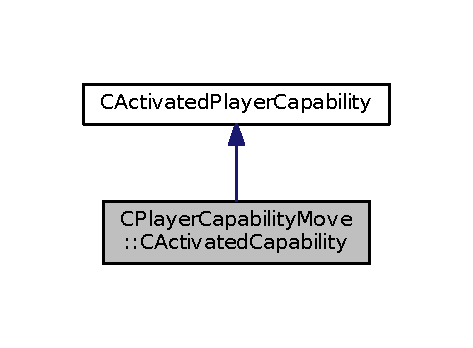
\includegraphics[width=227pt]{classCPlayerCapabilityMove_1_1CActivatedCapability__inherit__graph}
\end{center}
\end{figure}


Collaboration diagram for C\+Player\+Capability\+Move\+:\+:C\+Activated\+Capability\+:\nopagebreak
\begin{figure}[H]
\begin{center}
\leavevmode
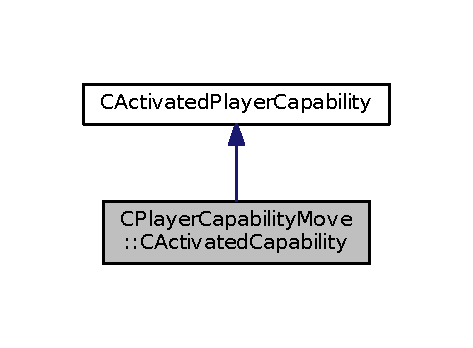
\includegraphics[width=227pt]{classCPlayerCapabilityMove_1_1CActivatedCapability__coll__graph}
\end{center}
\end{figure}
\subsection*{Public Member Functions}
\begin{DoxyCompactItemize}
\item 
\hyperlink{classCPlayerCapabilityMove_1_1CActivatedCapability_a4b3a3d22ebbe673f389a6cab2b37a2fc}{C\+Activated\+Capability} (std\+::shared\+\_\+ptr$<$ \hyperlink{classCPlayerAsset}{C\+Player\+Asset} $>$ actor, std\+::shared\+\_\+ptr$<$ \hyperlink{classCPlayerData}{C\+Player\+Data} $>$ playerdata, std\+::shared\+\_\+ptr$<$ \hyperlink{classCPlayerAsset}{C\+Player\+Asset} $>$ target)
\item 
virtual \hyperlink{classCPlayerCapabilityMove_1_1CActivatedCapability_a32285a6970ff939ebafc8ab9dd84317b}{$\sim$\+C\+Activated\+Capability} ()
\item 
int \hyperlink{classCPlayerCapabilityMove_1_1CActivatedCapability_a1696dd16d89d0978284a95dd1531d0d5}{Percent\+Complete} (int max)
\item 
bool \hyperlink{classCPlayerCapabilityMove_1_1CActivatedCapability_af4670890b462f59d24195db14aeb436d}{Increment\+Step} ()
\item 
void \hyperlink{classCPlayerCapabilityMove_1_1CActivatedCapability_a6fe1e26646bd14e94ebf7abd0a41cdd3}{Cancel} ()
\end{DoxyCompactItemize}
\subsection*{Additional Inherited Members}


\subsection{Detailed Description}


Definition at line 29 of file Basic\+Capabilities.\+cpp.



\subsection{Constructor \& Destructor Documentation}
\hypertarget{classCPlayerCapabilityMove_1_1CActivatedCapability_a4b3a3d22ebbe673f389a6cab2b37a2fc}{}\label{classCPlayerCapabilityMove_1_1CActivatedCapability_a4b3a3d22ebbe673f389a6cab2b37a2fc} 
\index{C\+Player\+Capability\+Move\+::\+C\+Activated\+Capability@{C\+Player\+Capability\+Move\+::\+C\+Activated\+Capability}!C\+Activated\+Capability@{C\+Activated\+Capability}}
\index{C\+Activated\+Capability@{C\+Activated\+Capability}!C\+Player\+Capability\+Move\+::\+C\+Activated\+Capability@{C\+Player\+Capability\+Move\+::\+C\+Activated\+Capability}}
\subsubsection{\texorpdfstring{C\+Activated\+Capability()}{CActivatedCapability()}}
{\footnotesize\ttfamily C\+Player\+Capability\+Move\+::\+C\+Activated\+Capability\+::\+C\+Activated\+Capability (\begin{DoxyParamCaption}\item[{std\+::shared\+\_\+ptr$<$ \hyperlink{classCPlayerAsset}{C\+Player\+Asset} $>$}]{actor,  }\item[{std\+::shared\+\_\+ptr$<$ \hyperlink{classCPlayerData}{C\+Player\+Data} $>$}]{playerdata,  }\item[{std\+::shared\+\_\+ptr$<$ \hyperlink{classCPlayerAsset}{C\+Player\+Asset} $>$}]{target }\end{DoxyParamCaption})}



Definition at line 84 of file Basic\+Capabilities.\+cpp.


\begin{DoxyCode}
84                                                                                                            
                                                                             :
85 \hyperlink{classCActivatedPlayerCapability_a1ece00ffb6a7b925c84dd94a7407a0d1}{CActivatedPlayerCapability}(actor, playerdata, target)\{
86 
87 \}
\end{DoxyCode}
\hypertarget{classCPlayerCapabilityMove_1_1CActivatedCapability_a32285a6970ff939ebafc8ab9dd84317b}{}\label{classCPlayerCapabilityMove_1_1CActivatedCapability_a32285a6970ff939ebafc8ab9dd84317b} 
\index{C\+Player\+Capability\+Move\+::\+C\+Activated\+Capability@{C\+Player\+Capability\+Move\+::\+C\+Activated\+Capability}!````~C\+Activated\+Capability@{$\sim$\+C\+Activated\+Capability}}
\index{````~C\+Activated\+Capability@{$\sim$\+C\+Activated\+Capability}!C\+Player\+Capability\+Move\+::\+C\+Activated\+Capability@{C\+Player\+Capability\+Move\+::\+C\+Activated\+Capability}}
\subsubsection{\texorpdfstring{$\sim$\+C\+Activated\+Capability()}{~CActivatedCapability()}}
{\footnotesize\ttfamily virtual C\+Player\+Capability\+Move\+::\+C\+Activated\+Capability\+::$\sim$\+C\+Activated\+Capability (\begin{DoxyParamCaption}{ }\end{DoxyParamCaption})\hspace{0.3cm}{\ttfamily [inline]}, {\ttfamily [virtual]}}



Definition at line 34 of file Basic\+Capabilities.\+cpp.


\begin{DoxyCode}
34 \{\};
\end{DoxyCode}
Here is the call graph for this function\+:\nopagebreak
\begin{figure}[H]
\begin{center}
\leavevmode
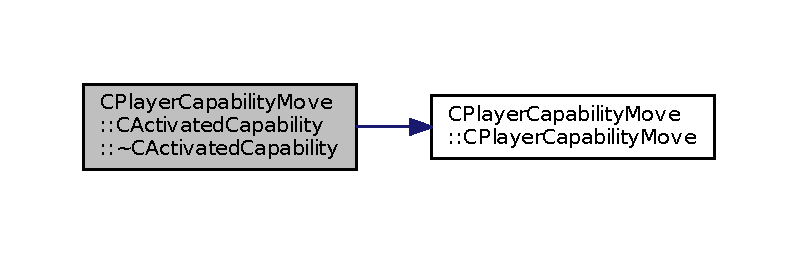
\includegraphics[width=350pt]{classCPlayerCapabilityMove_1_1CActivatedCapability_a32285a6970ff939ebafc8ab9dd84317b_cgraph}
\end{center}
\end{figure}


\subsection{Member Function Documentation}
\hypertarget{classCPlayerCapabilityMove_1_1CActivatedCapability_a6fe1e26646bd14e94ebf7abd0a41cdd3}{}\label{classCPlayerCapabilityMove_1_1CActivatedCapability_a6fe1e26646bd14e94ebf7abd0a41cdd3} 
\index{C\+Player\+Capability\+Move\+::\+C\+Activated\+Capability@{C\+Player\+Capability\+Move\+::\+C\+Activated\+Capability}!Cancel@{Cancel}}
\index{Cancel@{Cancel}!C\+Player\+Capability\+Move\+::\+C\+Activated\+Capability@{C\+Player\+Capability\+Move\+::\+C\+Activated\+Capability}}
\subsubsection{\texorpdfstring{Cancel()}{Cancel()}}
{\footnotesize\ttfamily void C\+Player\+Capability\+Move\+::\+C\+Activated\+Capability\+::\+Cancel (\begin{DoxyParamCaption}{ }\end{DoxyParamCaption})\hspace{0.3cm}{\ttfamily [virtual]}}



Implements \hyperlink{classCActivatedPlayerCapability_a5cde83be468e262ad054d81e28684a81}{C\+Activated\+Player\+Capability}.



Definition at line 112 of file Basic\+Capabilities.\+cpp.


\begin{DoxyCode}
112                                                       \{
113 
114     \hyperlink{classCActivatedPlayerCapability_a54ca944b47bff2718330639941d402b0}{DActor}->PopCommand();
115 \}
\end{DoxyCode}
Here is the caller graph for this function\+:\nopagebreak
\begin{figure}[H]
\begin{center}
\leavevmode
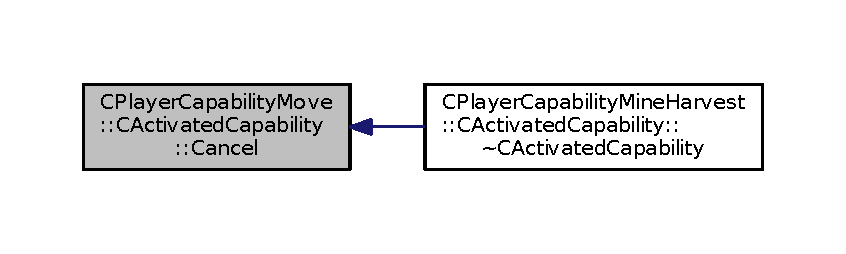
\includegraphics[width=350pt]{classCPlayerCapabilityMove_1_1CActivatedCapability_a6fe1e26646bd14e94ebf7abd0a41cdd3_icgraph}
\end{center}
\end{figure}
\hypertarget{classCPlayerCapabilityMove_1_1CActivatedCapability_af4670890b462f59d24195db14aeb436d}{}\label{classCPlayerCapabilityMove_1_1CActivatedCapability_af4670890b462f59d24195db14aeb436d} 
\index{C\+Player\+Capability\+Move\+::\+C\+Activated\+Capability@{C\+Player\+Capability\+Move\+::\+C\+Activated\+Capability}!Increment\+Step@{Increment\+Step}}
\index{Increment\+Step@{Increment\+Step}!C\+Player\+Capability\+Move\+::\+C\+Activated\+Capability@{C\+Player\+Capability\+Move\+::\+C\+Activated\+Capability}}
\subsubsection{\texorpdfstring{Increment\+Step()}{IncrementStep()}}
{\footnotesize\ttfamily bool C\+Player\+Capability\+Move\+::\+C\+Activated\+Capability\+::\+Increment\+Step (\begin{DoxyParamCaption}{ }\end{DoxyParamCaption})\hspace{0.3cm}{\ttfamily [virtual]}}



Implements \hyperlink{classCActivatedPlayerCapability_a943b5999a57504399293250382c0ec6a}{C\+Activated\+Player\+Capability}.



Definition at line 94 of file Basic\+Capabilities.\+cpp.


\begin{DoxyCode}
94                                                              \{
95     \hyperlink{structSAssetCommand}{SAssetCommand} AssetCommand;
96     \hyperlink{structSGameEvent}{SGameEvent} TempEvent;
97     
98     TempEvent.\hyperlink{structSGameEvent_afa10562e243f4ac2b473b655cc58fee7}{DType} = \hyperlink{GameModel_8h_abfcf510bafec7c6429906a6ecaac656da9b68fc38f3ca4002cd7a3ec3cc07a612}{etAcknowledge};
99     TempEvent.\hyperlink{structSGameEvent_a40c85eeac83b96887b7449c9bdc5d624}{DAsset} = \hyperlink{classCActivatedPlayerCapability_a54ca944b47bff2718330639941d402b0}{DActor};
100     \hyperlink{classCActivatedPlayerCapability_a9bf27c322a73f4b11c8183cc1973c3d8}{DPlayerData}->AddGameEvent(TempEvent);
101         
102     AssetCommand.\hyperlink{structSAssetCommand_a8edd3b3d59a76d5514ba403bc8076a75}{DAction} = \hyperlink{GameDataTypes_8h_ab47668e651a3032cfb9c40ea2d60d670a60ca9010aa62b73c1aab838ff4bf7276}{aaWalk};
103     AssetCommand.\hyperlink{structSAssetCommand_a3d9b43f6e59c386c48c41a65448a0c39}{DAssetTarget} = \hyperlink{classCActivatedPlayerCapability_a8a1cf50b6501bcfd55af0c935828e395}{DTarget};
104     \textcolor{keywordflow}{if}(!\hyperlink{classCActivatedPlayerCapability_a54ca944b47bff2718330639941d402b0}{DActor}->TileAligned())\{
105         \hyperlink{classCActivatedPlayerCapability_a54ca944b47bff2718330639941d402b0}{DActor}->Direction((\hyperlink{GameDataTypes_8h_acb2b033915f6659a71a38b5aa6e4eb42}{EDirection})((\hyperlink{classCActivatedPlayerCapability_a54ca944b47bff2718330639941d402b0}{DActor}->Position().TileOctant() + 
      \hyperlink{GameDataTypes_8h_acb2b033915f6659a71a38b5aa6e4eb42af6546049275557ce0ade2ceee042a319}{dMax}/2) % \hyperlink{GameDataTypes_8h_acb2b033915f6659a71a38b5aa6e4eb42af6546049275557ce0ade2ceee042a319}{dMax}));
106     \}
107     \hyperlink{classCActivatedPlayerCapability_a54ca944b47bff2718330639941d402b0}{DActor}->ClearCommand();
108     \hyperlink{classCActivatedPlayerCapability_a54ca944b47bff2718330639941d402b0}{DActor}->PushCommand(AssetCommand);
109     \textcolor{keywordflow}{return} \textcolor{keyword}{true};
110 \}
\end{DoxyCode}
Here is the caller graph for this function\+:\nopagebreak
\begin{figure}[H]
\begin{center}
\leavevmode
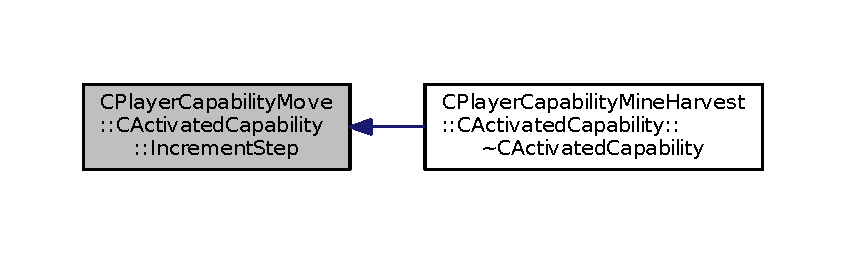
\includegraphics[width=350pt]{classCPlayerCapabilityMove_1_1CActivatedCapability_af4670890b462f59d24195db14aeb436d_icgraph}
\end{center}
\end{figure}
\hypertarget{classCPlayerCapabilityMove_1_1CActivatedCapability_a1696dd16d89d0978284a95dd1531d0d5}{}\label{classCPlayerCapabilityMove_1_1CActivatedCapability_a1696dd16d89d0978284a95dd1531d0d5} 
\index{C\+Player\+Capability\+Move\+::\+C\+Activated\+Capability@{C\+Player\+Capability\+Move\+::\+C\+Activated\+Capability}!Percent\+Complete@{Percent\+Complete}}
\index{Percent\+Complete@{Percent\+Complete}!C\+Player\+Capability\+Move\+::\+C\+Activated\+Capability@{C\+Player\+Capability\+Move\+::\+C\+Activated\+Capability}}
\subsubsection{\texorpdfstring{Percent\+Complete()}{PercentComplete()}}
{\footnotesize\ttfamily int C\+Player\+Capability\+Move\+::\+C\+Activated\+Capability\+::\+Percent\+Complete (\begin{DoxyParamCaption}\item[{int}]{max }\end{DoxyParamCaption})\hspace{0.3cm}{\ttfamily [virtual]}}



Implements \hyperlink{classCActivatedPlayerCapability_a405dc6076058006a4f801727de4cfe4d}{C\+Activated\+Player\+Capability}.



Definition at line 90 of file Basic\+Capabilities.\+cpp.


\begin{DoxyCode}
90                                                                      \{
91     \textcolor{keywordflow}{return} 0;
92 \}
\end{DoxyCode}
Here is the caller graph for this function\+:\nopagebreak
\begin{figure}[H]
\begin{center}
\leavevmode
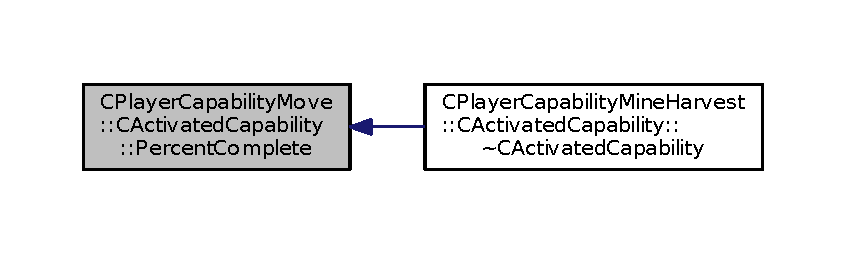
\includegraphics[width=350pt]{classCPlayerCapabilityMove_1_1CActivatedCapability_a1696dd16d89d0978284a95dd1531d0d5_icgraph}
\end{center}
\end{figure}


The documentation for this class was generated from the following file\+:\begin{DoxyCompactItemize}
\item 
src/\hyperlink{BasicCapabilities_8cpp}{Basic\+Capabilities.\+cpp}\end{DoxyCompactItemize}

\hypertarget{classCPlayerCapabilityMineHarvest_1_1CActivatedCapability}{}\section{C\+Player\+Capability\+Mine\+Harvest\+:\+:C\+Activated\+Capability Class Reference}
\label{classCPlayerCapabilityMineHarvest_1_1CActivatedCapability}\index{C\+Player\+Capability\+Mine\+Harvest\+::\+C\+Activated\+Capability@{C\+Player\+Capability\+Mine\+Harvest\+::\+C\+Activated\+Capability}}


Inheritance diagram for C\+Player\+Capability\+Mine\+Harvest\+:\+:C\+Activated\+Capability\+:
\nopagebreak
\begin{figure}[H]
\begin{center}
\leavevmode
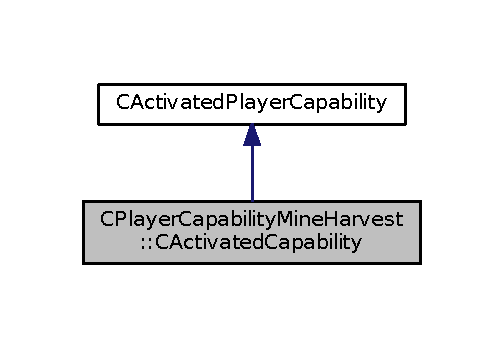
\includegraphics[width=242pt]{classCPlayerCapabilityMineHarvest_1_1CActivatedCapability__inherit__graph}
\end{center}
\end{figure}


Collaboration diagram for C\+Player\+Capability\+Mine\+Harvest\+:\+:C\+Activated\+Capability\+:
\nopagebreak
\begin{figure}[H]
\begin{center}
\leavevmode
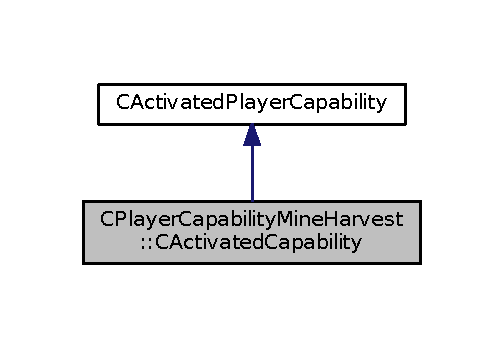
\includegraphics[width=242pt]{classCPlayerCapabilityMineHarvest_1_1CActivatedCapability__coll__graph}
\end{center}
\end{figure}
\subsection*{Public Member Functions}
\begin{DoxyCompactItemize}
\item 
\hyperlink{classCPlayerCapabilityMineHarvest_1_1CActivatedCapability_a236ed97a35a20e2f4b29371089c51a31}{C\+Activated\+Capability} (std\+::shared\+\_\+ptr$<$ \hyperlink{classCPlayerAsset}{C\+Player\+Asset} $>$ actor, std\+::shared\+\_\+ptr$<$ \hyperlink{classCPlayerData}{C\+Player\+Data} $>$ playerdata, std\+::shared\+\_\+ptr$<$ \hyperlink{classCPlayerAsset}{C\+Player\+Asset} $>$ target)
\item 
virtual \hyperlink{classCPlayerCapabilityMineHarvest_1_1CActivatedCapability_a206562e670341a6eb24d0c5dc1bea976}{$\sim$\+C\+Activated\+Capability} ()
\item 
int \hyperlink{classCPlayerCapabilityMineHarvest_1_1CActivatedCapability_ac198166a008306dc543ceed94baaf4a3}{Percent\+Complete} (int max)
\item 
bool \hyperlink{classCPlayerCapabilityMineHarvest_1_1CActivatedCapability_a46dbd6e2ae2fb889da1714c97ed3ca2f}{Increment\+Step} ()
\item 
void \hyperlink{classCPlayerCapabilityMineHarvest_1_1CActivatedCapability_ab1fef064fbc085a6419b5a822e787614}{Cancel} ()
\end{DoxyCompactItemize}
\subsection*{Additional Inherited Members}


\subsection{Detailed Description}


Definition at line 125 of file Basic\+Capabilities.\+cpp.



\subsection{Constructor \& Destructor Documentation}
\hypertarget{classCPlayerCapabilityMineHarvest_1_1CActivatedCapability_a236ed97a35a20e2f4b29371089c51a31}{}\label{classCPlayerCapabilityMineHarvest_1_1CActivatedCapability_a236ed97a35a20e2f4b29371089c51a31} 
\index{C\+Player\+Capability\+Mine\+Harvest\+::\+C\+Activated\+Capability@{C\+Player\+Capability\+Mine\+Harvest\+::\+C\+Activated\+Capability}!C\+Activated\+Capability@{C\+Activated\+Capability}}
\index{C\+Activated\+Capability@{C\+Activated\+Capability}!C\+Player\+Capability\+Mine\+Harvest\+::\+C\+Activated\+Capability@{C\+Player\+Capability\+Mine\+Harvest\+::\+C\+Activated\+Capability}}
\subsubsection{\texorpdfstring{C\+Activated\+Capability()}{CActivatedCapability()}}
{\footnotesize\ttfamily C\+Player\+Capability\+Mine\+Harvest\+::\+C\+Activated\+Capability\+::\+C\+Activated\+Capability (\begin{DoxyParamCaption}\item[{std\+::shared\+\_\+ptr$<$ \hyperlink{classCPlayerAsset}{C\+Player\+Asset} $>$}]{actor,  }\item[{std\+::shared\+\_\+ptr$<$ \hyperlink{classCPlayerData}{C\+Player\+Data} $>$}]{playerdata,  }\item[{std\+::shared\+\_\+ptr$<$ \hyperlink{classCPlayerAsset}{C\+Player\+Asset} $>$}]{target }\end{DoxyParamCaption})}



Definition at line 190 of file Basic\+Capabilities.\+cpp.


\begin{DoxyCode}
190                                                                                                            
                                                                                    :
191 \hyperlink{classCActivatedPlayerCapability_a1ece00ffb6a7b925c84dd94a7407a0d1}{CActivatedPlayerCapability}(actor, playerdata, target)\{
192 
193 \}
\end{DoxyCode}
\hypertarget{classCPlayerCapabilityMineHarvest_1_1CActivatedCapability_a206562e670341a6eb24d0c5dc1bea976}{}\label{classCPlayerCapabilityMineHarvest_1_1CActivatedCapability_a206562e670341a6eb24d0c5dc1bea976} 
\index{C\+Player\+Capability\+Mine\+Harvest\+::\+C\+Activated\+Capability@{C\+Player\+Capability\+Mine\+Harvest\+::\+C\+Activated\+Capability}!````~C\+Activated\+Capability@{$\sim$\+C\+Activated\+Capability}}
\index{````~C\+Activated\+Capability@{$\sim$\+C\+Activated\+Capability}!C\+Player\+Capability\+Mine\+Harvest\+::\+C\+Activated\+Capability@{C\+Player\+Capability\+Mine\+Harvest\+::\+C\+Activated\+Capability}}
\subsubsection{\texorpdfstring{$\sim$\+C\+Activated\+Capability()}{~CActivatedCapability()}}
{\footnotesize\ttfamily virtual C\+Player\+Capability\+Mine\+Harvest\+::\+C\+Activated\+Capability\+::$\sim$\+C\+Activated\+Capability (\begin{DoxyParamCaption}{ }\end{DoxyParamCaption})\hspace{0.3cm}{\ttfamily [inline]}, {\ttfamily [virtual]}}



Definition at line 130 of file Basic\+Capabilities.\+cpp.


\begin{DoxyCode}
130 \{\};
\end{DoxyCode}
Here is the call graph for this function\+:
\nopagebreak
\begin{figure}[H]
\begin{center}
\leavevmode
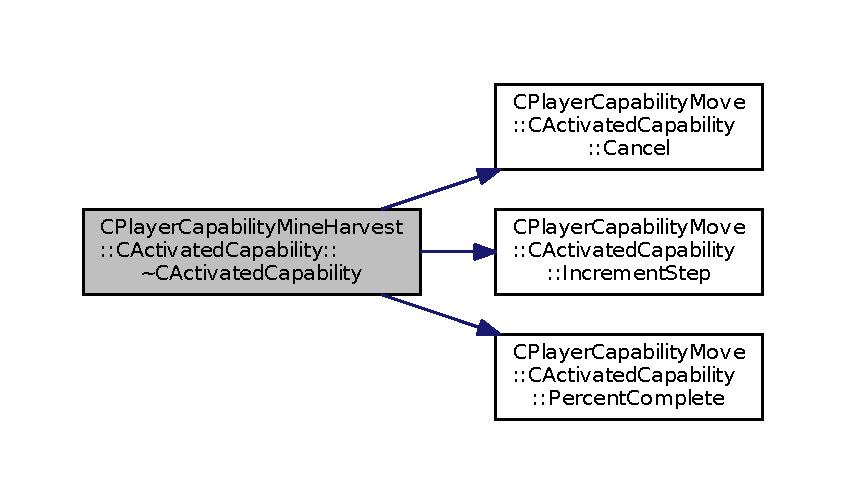
\includegraphics[width=350pt]{classCPlayerCapabilityMineHarvest_1_1CActivatedCapability_a206562e670341a6eb24d0c5dc1bea976_cgraph}
\end{center}
\end{figure}


\subsection{Member Function Documentation}
\hypertarget{classCPlayerCapabilityMineHarvest_1_1CActivatedCapability_ab1fef064fbc085a6419b5a822e787614}{}\label{classCPlayerCapabilityMineHarvest_1_1CActivatedCapability_ab1fef064fbc085a6419b5a822e787614} 
\index{C\+Player\+Capability\+Mine\+Harvest\+::\+C\+Activated\+Capability@{C\+Player\+Capability\+Mine\+Harvest\+::\+C\+Activated\+Capability}!Cancel@{Cancel}}
\index{Cancel@{Cancel}!C\+Player\+Capability\+Mine\+Harvest\+::\+C\+Activated\+Capability@{C\+Player\+Capability\+Mine\+Harvest\+::\+C\+Activated\+Capability}}
\subsubsection{\texorpdfstring{Cancel()}{Cancel()}}
{\footnotesize\ttfamily void C\+Player\+Capability\+Mine\+Harvest\+::\+C\+Activated\+Capability\+::\+Cancel (\begin{DoxyParamCaption}{ }\end{DoxyParamCaption})\hspace{0.3cm}{\ttfamily [virtual]}}



Implements \hyperlink{classCActivatedPlayerCapability_a5cde83be468e262ad054d81e28684a81}{C\+Activated\+Player\+Capability}.



Definition at line 225 of file Basic\+Capabilities.\+cpp.


\begin{DoxyCode}
225                                                              \{
226 
227     \hyperlink{classCActivatedPlayerCapability_a54ca944b47bff2718330639941d402b0}{DActor}->PopCommand();
228 \}
\end{DoxyCode}
Here is the caller graph for this function\+:
\nopagebreak
\begin{figure}[H]
\begin{center}
\leavevmode
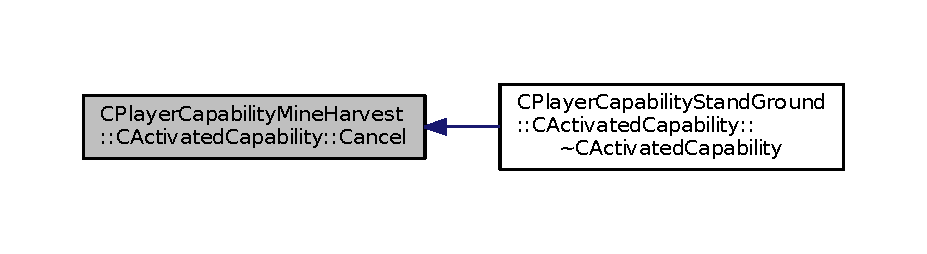
\includegraphics[width=350pt]{classCPlayerCapabilityMineHarvest_1_1CActivatedCapability_ab1fef064fbc085a6419b5a822e787614_icgraph}
\end{center}
\end{figure}
\hypertarget{classCPlayerCapabilityMineHarvest_1_1CActivatedCapability_a46dbd6e2ae2fb889da1714c97ed3ca2f}{}\label{classCPlayerCapabilityMineHarvest_1_1CActivatedCapability_a46dbd6e2ae2fb889da1714c97ed3ca2f} 
\index{C\+Player\+Capability\+Mine\+Harvest\+::\+C\+Activated\+Capability@{C\+Player\+Capability\+Mine\+Harvest\+::\+C\+Activated\+Capability}!Increment\+Step@{Increment\+Step}}
\index{Increment\+Step@{Increment\+Step}!C\+Player\+Capability\+Mine\+Harvest\+::\+C\+Activated\+Capability@{C\+Player\+Capability\+Mine\+Harvest\+::\+C\+Activated\+Capability}}
\subsubsection{\texorpdfstring{Increment\+Step()}{IncrementStep()}}
{\footnotesize\ttfamily bool C\+Player\+Capability\+Mine\+Harvest\+::\+C\+Activated\+Capability\+::\+Increment\+Step (\begin{DoxyParamCaption}{ }\end{DoxyParamCaption})\hspace{0.3cm}{\ttfamily [virtual]}}



Implements \hyperlink{classCActivatedPlayerCapability_a943b5999a57504399293250382c0ec6a}{C\+Activated\+Player\+Capability}.



Definition at line 200 of file Basic\+Capabilities.\+cpp.


\begin{DoxyCode}
200                                                                     \{
201     \hyperlink{structSAssetCommand}{SAssetCommand} AssetCommand;
202     \hyperlink{structSGameEvent}{SGameEvent} TempEvent;
203     
204     TempEvent.\hyperlink{structSGameEvent_afa10562e243f4ac2b473b655cc58fee7}{DType} = \hyperlink{GameModel_8h_abfcf510bafec7c6429906a6ecaac656da9b68fc38f3ca4002cd7a3ec3cc07a612}{etAcknowledge};
205     TempEvent.\hyperlink{structSGameEvent_a40c85eeac83b96887b7449c9bdc5d624}{DAsset} = \hyperlink{classCActivatedPlayerCapability_a54ca944b47bff2718330639941d402b0}{DActor};
206     \hyperlink{classCActivatedPlayerCapability_a9bf27c322a73f4b11c8183cc1973c3d8}{DPlayerData}->AddGameEvent(TempEvent);
207     
208     AssetCommand.\hyperlink{structSAssetCommand_a3d9b43f6e59c386c48c41a65448a0c39}{DAssetTarget} = \hyperlink{classCActivatedPlayerCapability_a8a1cf50b6501bcfd55af0c935828e395}{DTarget};
209     \textcolor{keywordflow}{if}(\hyperlink{GameDataTypes_8h_a5600d4fc433b83300308921974477feca243d9ba44092eadd561db058d742b3b3}{atGoldMine} == \hyperlink{classCActivatedPlayerCapability_a8a1cf50b6501bcfd55af0c935828e395}{DTarget}->Type())\{
210         AssetCommand.\hyperlink{structSAssetCommand_a8edd3b3d59a76d5514ba403bc8076a75}{DAction} = \hyperlink{GameDataTypes_8h_ab47668e651a3032cfb9c40ea2d60d670abc45b1c4fbca1481e373a780a69bd56b}{aaMineGold};
211     \}
212     \textcolor{keywordflow}{else}\{
213         AssetCommand.\hyperlink{structSAssetCommand_a8edd3b3d59a76d5514ba403bc8076a75}{DAction} = \hyperlink{GameDataTypes_8h_ab47668e651a3032cfb9c40ea2d60d670a4c44c3d83b3b67a8dd2248d11bedd0ee}{aaHarvestLumber};
214     \}
215     \hyperlink{classCActivatedPlayerCapability_a54ca944b47bff2718330639941d402b0}{DActor}->ClearCommand();
216     \hyperlink{classCActivatedPlayerCapability_a54ca944b47bff2718330639941d402b0}{DActor}->PushCommand(AssetCommand);
217     AssetCommand.\hyperlink{structSAssetCommand_a8edd3b3d59a76d5514ba403bc8076a75}{DAction} = \hyperlink{GameDataTypes_8h_ab47668e651a3032cfb9c40ea2d60d670a60ca9010aa62b73c1aab838ff4bf7276}{aaWalk};
218     \textcolor{keywordflow}{if}(!\hyperlink{classCActivatedPlayerCapability_a54ca944b47bff2718330639941d402b0}{DActor}->TileAligned())\{
219         \hyperlink{classCActivatedPlayerCapability_a54ca944b47bff2718330639941d402b0}{DActor}->Direction((\hyperlink{GameDataTypes_8h_acb2b033915f6659a71a38b5aa6e4eb42}{EDirection})((\hyperlink{classCActivatedPlayerCapability_a54ca944b47bff2718330639941d402b0}{DActor}->Position().TileOctant() + 
      \hyperlink{GameDataTypes_8h_acb2b033915f6659a71a38b5aa6e4eb42af6546049275557ce0ade2ceee042a319}{dMax}/2) % \hyperlink{GameDataTypes_8h_acb2b033915f6659a71a38b5aa6e4eb42af6546049275557ce0ade2ceee042a319}{dMax}));
220     \}
221     \hyperlink{classCActivatedPlayerCapability_a54ca944b47bff2718330639941d402b0}{DActor}->PushCommand(AssetCommand);
222     \textcolor{keywordflow}{return} \textcolor{keyword}{true};
223 \}
\end{DoxyCode}
Here is the caller graph for this function\+:
\nopagebreak
\begin{figure}[H]
\begin{center}
\leavevmode
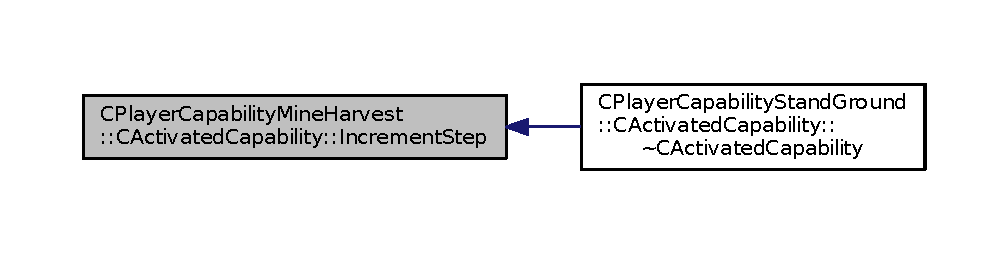
\includegraphics[width=350pt]{classCPlayerCapabilityMineHarvest_1_1CActivatedCapability_a46dbd6e2ae2fb889da1714c97ed3ca2f_icgraph}
\end{center}
\end{figure}
\hypertarget{classCPlayerCapabilityMineHarvest_1_1CActivatedCapability_ac198166a008306dc543ceed94baaf4a3}{}\label{classCPlayerCapabilityMineHarvest_1_1CActivatedCapability_ac198166a008306dc543ceed94baaf4a3} 
\index{C\+Player\+Capability\+Mine\+Harvest\+::\+C\+Activated\+Capability@{C\+Player\+Capability\+Mine\+Harvest\+::\+C\+Activated\+Capability}!Percent\+Complete@{Percent\+Complete}}
\index{Percent\+Complete@{Percent\+Complete}!C\+Player\+Capability\+Mine\+Harvest\+::\+C\+Activated\+Capability@{C\+Player\+Capability\+Mine\+Harvest\+::\+C\+Activated\+Capability}}
\subsubsection{\texorpdfstring{Percent\+Complete()}{PercentComplete()}}
{\footnotesize\ttfamily int C\+Player\+Capability\+Mine\+Harvest\+::\+C\+Activated\+Capability\+::\+Percent\+Complete (\begin{DoxyParamCaption}\item[{int}]{max }\end{DoxyParamCaption})\hspace{0.3cm}{\ttfamily [virtual]}}



Implements \hyperlink{classCActivatedPlayerCapability_a405dc6076058006a4f801727de4cfe4d}{C\+Activated\+Player\+Capability}.



Definition at line 196 of file Basic\+Capabilities.\+cpp.


\begin{DoxyCode}
196                                                                             \{
197     \textcolor{keywordflow}{return} 0;
198 \}
\end{DoxyCode}
Here is the caller graph for this function\+:
\nopagebreak
\begin{figure}[H]
\begin{center}
\leavevmode
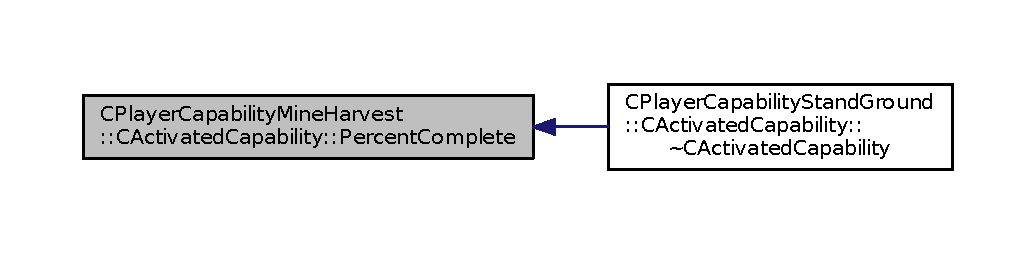
\includegraphics[width=350pt]{classCPlayerCapabilityMineHarvest_1_1CActivatedCapability_ac198166a008306dc543ceed94baaf4a3_icgraph}
\end{center}
\end{figure}


The documentation for this class was generated from the following file\+:\begin{DoxyCompactItemize}
\item 
src/\hyperlink{BasicCapabilities_8cpp}{Basic\+Capabilities.\+cpp}\end{DoxyCompactItemize}

\hypertarget{classCPlayerCapabilityStandGround_1_1CActivatedCapability}{}\section{C\+Player\+Capability\+Stand\+Ground\+:\+:C\+Activated\+Capability Class Reference}
\label{classCPlayerCapabilityStandGround_1_1CActivatedCapability}\index{C\+Player\+Capability\+Stand\+Ground\+::\+C\+Activated\+Capability@{C\+Player\+Capability\+Stand\+Ground\+::\+C\+Activated\+Capability}}


Inheritance diagram for C\+Player\+Capability\+Stand\+Ground\+:\+:C\+Activated\+Capability\+:\nopagebreak
\begin{figure}[H]
\begin{center}
\leavevmode
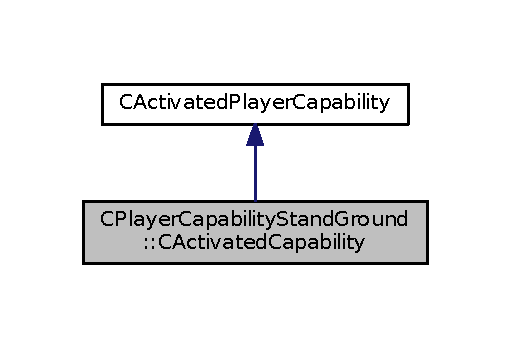
\includegraphics[width=245pt]{classCPlayerCapabilityStandGround_1_1CActivatedCapability__inherit__graph}
\end{center}
\end{figure}


Collaboration diagram for C\+Player\+Capability\+Stand\+Ground\+:\+:C\+Activated\+Capability\+:\nopagebreak
\begin{figure}[H]
\begin{center}
\leavevmode
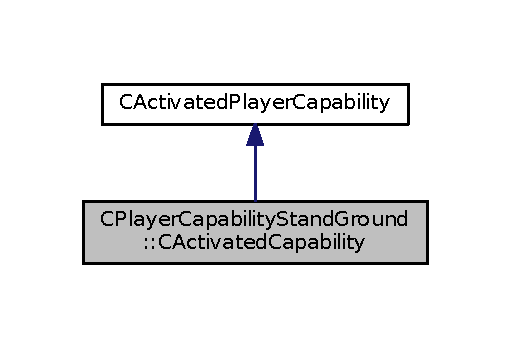
\includegraphics[width=245pt]{classCPlayerCapabilityStandGround_1_1CActivatedCapability__coll__graph}
\end{center}
\end{figure}
\subsection*{Public Member Functions}
\begin{DoxyCompactItemize}
\item 
\hyperlink{classCPlayerCapabilityStandGround_1_1CActivatedCapability_aedaa8238e1eb01e9762e19ab61795dda}{C\+Activated\+Capability} (std\+::shared\+\_\+ptr$<$ \hyperlink{classCPlayerAsset}{C\+Player\+Asset} $>$ actor, std\+::shared\+\_\+ptr$<$ \hyperlink{classCPlayerData}{C\+Player\+Data} $>$ playerdata, std\+::shared\+\_\+ptr$<$ \hyperlink{classCPlayerAsset}{C\+Player\+Asset} $>$ target)
\item 
virtual \hyperlink{classCPlayerCapabilityStandGround_1_1CActivatedCapability_a7fe4c33b38b30befad569944ded1e402}{$\sim$\+C\+Activated\+Capability} ()
\item 
int \hyperlink{classCPlayerCapabilityStandGround_1_1CActivatedCapability_aa9bf1824e755460b699d81f866f2aadc}{Percent\+Complete} (int max)
\item 
bool \hyperlink{classCPlayerCapabilityStandGround_1_1CActivatedCapability_ab4061171835e4c1008176e5765ded595}{Increment\+Step} ()
\item 
void \hyperlink{classCPlayerCapabilityStandGround_1_1CActivatedCapability_ac75cd8a26726adb60cf045f99059ca7d}{Cancel} ()
\end{DoxyCompactItemize}
\subsection*{Additional Inherited Members}


\subsection{Detailed Description}


Definition at line 238 of file Basic\+Capabilities.\+cpp.



\subsection{Constructor \& Destructor Documentation}
\hypertarget{classCPlayerCapabilityStandGround_1_1CActivatedCapability_aedaa8238e1eb01e9762e19ab61795dda}{}\label{classCPlayerCapabilityStandGround_1_1CActivatedCapability_aedaa8238e1eb01e9762e19ab61795dda} 
\index{C\+Player\+Capability\+Stand\+Ground\+::\+C\+Activated\+Capability@{C\+Player\+Capability\+Stand\+Ground\+::\+C\+Activated\+Capability}!C\+Activated\+Capability@{C\+Activated\+Capability}}
\index{C\+Activated\+Capability@{C\+Activated\+Capability}!C\+Player\+Capability\+Stand\+Ground\+::\+C\+Activated\+Capability@{C\+Player\+Capability\+Stand\+Ground\+::\+C\+Activated\+Capability}}
\subsubsection{\texorpdfstring{C\+Activated\+Capability()}{CActivatedCapability()}}
{\footnotesize\ttfamily C\+Player\+Capability\+Stand\+Ground\+::\+C\+Activated\+Capability\+::\+C\+Activated\+Capability (\begin{DoxyParamCaption}\item[{std\+::shared\+\_\+ptr$<$ \hyperlink{classCPlayerAsset}{C\+Player\+Asset} $>$}]{actor,  }\item[{std\+::shared\+\_\+ptr$<$ \hyperlink{classCPlayerData}{C\+Player\+Data} $>$}]{playerdata,  }\item[{std\+::shared\+\_\+ptr$<$ \hyperlink{classCPlayerAsset}{C\+Player\+Asset} $>$}]{target }\end{DoxyParamCaption})}



Definition at line 291 of file Basic\+Capabilities.\+cpp.


\begin{DoxyCode}
291                                                                                                            
                                                                                    :
292 \hyperlink{classCActivatedPlayerCapability_a1ece00ffb6a7b925c84dd94a7407a0d1}{CActivatedPlayerCapability}(actor, playerdata, target)\{
293 
294 \}
\end{DoxyCode}
\hypertarget{classCPlayerCapabilityStandGround_1_1CActivatedCapability_a7fe4c33b38b30befad569944ded1e402}{}\label{classCPlayerCapabilityStandGround_1_1CActivatedCapability_a7fe4c33b38b30befad569944ded1e402} 
\index{C\+Player\+Capability\+Stand\+Ground\+::\+C\+Activated\+Capability@{C\+Player\+Capability\+Stand\+Ground\+::\+C\+Activated\+Capability}!````~C\+Activated\+Capability@{$\sim$\+C\+Activated\+Capability}}
\index{````~C\+Activated\+Capability@{$\sim$\+C\+Activated\+Capability}!C\+Player\+Capability\+Stand\+Ground\+::\+C\+Activated\+Capability@{C\+Player\+Capability\+Stand\+Ground\+::\+C\+Activated\+Capability}}
\subsubsection{\texorpdfstring{$\sim$\+C\+Activated\+Capability()}{~CActivatedCapability()}}
{\footnotesize\ttfamily virtual C\+Player\+Capability\+Stand\+Ground\+::\+C\+Activated\+Capability\+::$\sim$\+C\+Activated\+Capability (\begin{DoxyParamCaption}{ }\end{DoxyParamCaption})\hspace{0.3cm}{\ttfamily [inline]}, {\ttfamily [virtual]}}



Definition at line 243 of file Basic\+Capabilities.\+cpp.


\begin{DoxyCode}
243 \{\};
\end{DoxyCode}
Here is the call graph for this function\+:\nopagebreak
\begin{figure}[H]
\begin{center}
\leavevmode
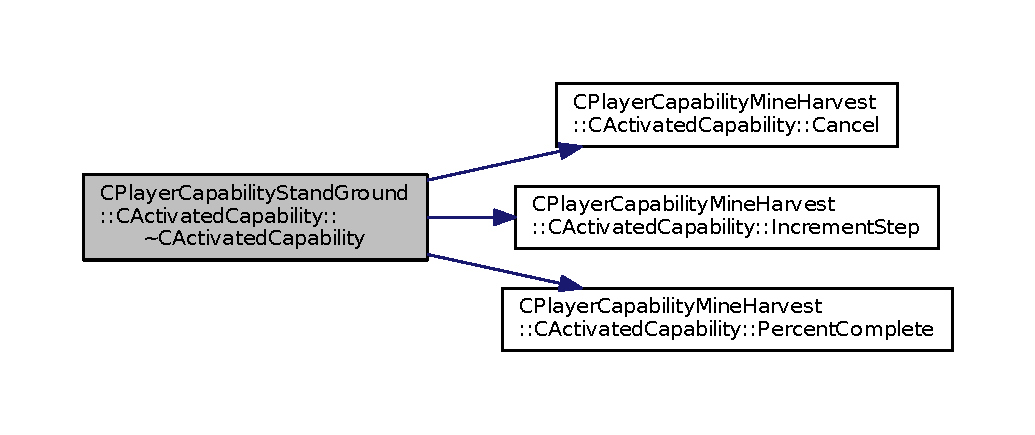
\includegraphics[width=350pt]{classCPlayerCapabilityStandGround_1_1CActivatedCapability_a7fe4c33b38b30befad569944ded1e402_cgraph}
\end{center}
\end{figure}


\subsection{Member Function Documentation}
\hypertarget{classCPlayerCapabilityStandGround_1_1CActivatedCapability_ac75cd8a26726adb60cf045f99059ca7d}{}\label{classCPlayerCapabilityStandGround_1_1CActivatedCapability_ac75cd8a26726adb60cf045f99059ca7d} 
\index{C\+Player\+Capability\+Stand\+Ground\+::\+C\+Activated\+Capability@{C\+Player\+Capability\+Stand\+Ground\+::\+C\+Activated\+Capability}!Cancel@{Cancel}}
\index{Cancel@{Cancel}!C\+Player\+Capability\+Stand\+Ground\+::\+C\+Activated\+Capability@{C\+Player\+Capability\+Stand\+Ground\+::\+C\+Activated\+Capability}}
\subsubsection{\texorpdfstring{Cancel()}{Cancel()}}
{\footnotesize\ttfamily void C\+Player\+Capability\+Stand\+Ground\+::\+C\+Activated\+Capability\+::\+Cancel (\begin{DoxyParamCaption}{ }\end{DoxyParamCaption})\hspace{0.3cm}{\ttfamily [virtual]}}



Implements \hyperlink{classCActivatedPlayerCapability_a5cde83be468e262ad054d81e28684a81}{C\+Activated\+Player\+Capability}.



Definition at line 324 of file Basic\+Capabilities.\+cpp.


\begin{DoxyCode}
324                                                              \{
325 
326     \hyperlink{classCActivatedPlayerCapability_a54ca944b47bff2718330639941d402b0}{DActor}->PopCommand();
327 \}
\end{DoxyCode}
Here is the caller graph for this function\+:\nopagebreak
\begin{figure}[H]
\begin{center}
\leavevmode
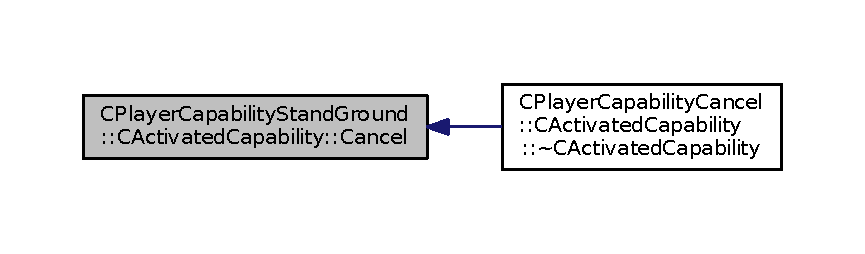
\includegraphics[width=350pt]{classCPlayerCapabilityStandGround_1_1CActivatedCapability_ac75cd8a26726adb60cf045f99059ca7d_icgraph}
\end{center}
\end{figure}
\hypertarget{classCPlayerCapabilityStandGround_1_1CActivatedCapability_ab4061171835e4c1008176e5765ded595}{}\label{classCPlayerCapabilityStandGround_1_1CActivatedCapability_ab4061171835e4c1008176e5765ded595} 
\index{C\+Player\+Capability\+Stand\+Ground\+::\+C\+Activated\+Capability@{C\+Player\+Capability\+Stand\+Ground\+::\+C\+Activated\+Capability}!Increment\+Step@{Increment\+Step}}
\index{Increment\+Step@{Increment\+Step}!C\+Player\+Capability\+Stand\+Ground\+::\+C\+Activated\+Capability@{C\+Player\+Capability\+Stand\+Ground\+::\+C\+Activated\+Capability}}
\subsubsection{\texorpdfstring{Increment\+Step()}{IncrementStep()}}
{\footnotesize\ttfamily bool C\+Player\+Capability\+Stand\+Ground\+::\+C\+Activated\+Capability\+::\+Increment\+Step (\begin{DoxyParamCaption}{ }\end{DoxyParamCaption})\hspace{0.3cm}{\ttfamily [virtual]}}



Implements \hyperlink{classCActivatedPlayerCapability_a943b5999a57504399293250382c0ec6a}{C\+Activated\+Player\+Capability}.



Definition at line 301 of file Basic\+Capabilities.\+cpp.


\begin{DoxyCode}
301                                                                     \{
302     \hyperlink{structSAssetCommand}{SAssetCommand} AssetCommand;
303     \hyperlink{structSGameEvent}{SGameEvent} TempEvent;
304     
305     TempEvent.\hyperlink{structSGameEvent_afa10562e243f4ac2b473b655cc58fee7}{DType} = \hyperlink{GameModel_8h_abfcf510bafec7c6429906a6ecaac656da9b68fc38f3ca4002cd7a3ec3cc07a612}{etAcknowledge};
306     TempEvent.\hyperlink{structSGameEvent_a40c85eeac83b96887b7449c9bdc5d624}{DAsset} = \hyperlink{classCActivatedPlayerCapability_a54ca944b47bff2718330639941d402b0}{DActor};
307     \hyperlink{classCActivatedPlayerCapability_a9bf27c322a73f4b11c8183cc1973c3d8}{DPlayerData}->AddGameEvent(TempEvent);
308     
309     AssetCommand.\hyperlink{structSAssetCommand_a3d9b43f6e59c386c48c41a65448a0c39}{DAssetTarget} = \hyperlink{classCActivatedPlayerCapability_a9bf27c322a73f4b11c8183cc1973c3d8}{DPlayerData}->CreateMarker(
      \hyperlink{classCActivatedPlayerCapability_a54ca944b47bff2718330639941d402b0}{DActor}->Position(), \textcolor{keyword}{false});
310     AssetCommand.\hyperlink{structSAssetCommand_a8edd3b3d59a76d5514ba403bc8076a75}{DAction} = \hyperlink{GameDataTypes_8h_ab47668e651a3032cfb9c40ea2d60d670abd8a4e07a8f888148ed62ddd46719af3}{aaStandGround};
311 
312     \hyperlink{classCActivatedPlayerCapability_a54ca944b47bff2718330639941d402b0}{DActor}->ClearCommand();
313     \hyperlink{classCActivatedPlayerCapability_a54ca944b47bff2718330639941d402b0}{DActor}->PushCommand(AssetCommand);
314     
315     \textcolor{keywordflow}{if}(!\hyperlink{classCActivatedPlayerCapability_a54ca944b47bff2718330639941d402b0}{DActor}->TileAligned())\{
316         AssetCommand.\hyperlink{structSAssetCommand_a8edd3b3d59a76d5514ba403bc8076a75}{DAction} = \hyperlink{GameDataTypes_8h_ab47668e651a3032cfb9c40ea2d60d670a60ca9010aa62b73c1aab838ff4bf7276}{aaWalk};
317         \hyperlink{classCActivatedPlayerCapability_a54ca944b47bff2718330639941d402b0}{DActor}->Direction((\hyperlink{GameDataTypes_8h_acb2b033915f6659a71a38b5aa6e4eb42}{EDirection})((\hyperlink{classCActivatedPlayerCapability_a54ca944b47bff2718330639941d402b0}{DActor}->Position().TileOctant() + 
      \hyperlink{GameDataTypes_8h_acb2b033915f6659a71a38b5aa6e4eb42af6546049275557ce0ade2ceee042a319}{dMax}/2) % \hyperlink{GameDataTypes_8h_acb2b033915f6659a71a38b5aa6e4eb42af6546049275557ce0ade2ceee042a319}{dMax}));
318         \hyperlink{classCActivatedPlayerCapability_a54ca944b47bff2718330639941d402b0}{DActor}->PushCommand(AssetCommand);
319     \}
320     
321     \textcolor{keywordflow}{return} \textcolor{keyword}{true};
322 \}
\end{DoxyCode}
Here is the caller graph for this function\+:\nopagebreak
\begin{figure}[H]
\begin{center}
\leavevmode
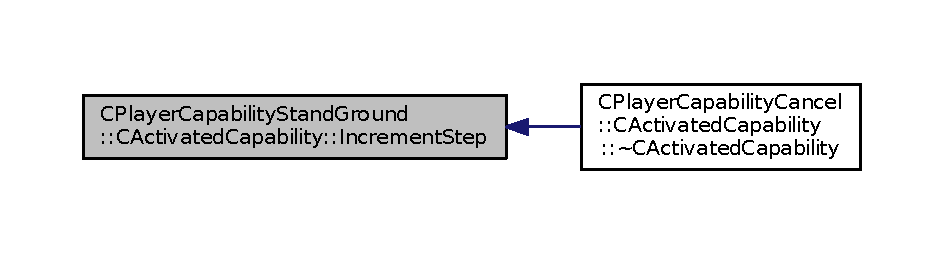
\includegraphics[width=350pt]{classCPlayerCapabilityStandGround_1_1CActivatedCapability_ab4061171835e4c1008176e5765ded595_icgraph}
\end{center}
\end{figure}
\hypertarget{classCPlayerCapabilityStandGround_1_1CActivatedCapability_aa9bf1824e755460b699d81f866f2aadc}{}\label{classCPlayerCapabilityStandGround_1_1CActivatedCapability_aa9bf1824e755460b699d81f866f2aadc} 
\index{C\+Player\+Capability\+Stand\+Ground\+::\+C\+Activated\+Capability@{C\+Player\+Capability\+Stand\+Ground\+::\+C\+Activated\+Capability}!Percent\+Complete@{Percent\+Complete}}
\index{Percent\+Complete@{Percent\+Complete}!C\+Player\+Capability\+Stand\+Ground\+::\+C\+Activated\+Capability@{C\+Player\+Capability\+Stand\+Ground\+::\+C\+Activated\+Capability}}
\subsubsection{\texorpdfstring{Percent\+Complete()}{PercentComplete()}}
{\footnotesize\ttfamily int C\+Player\+Capability\+Stand\+Ground\+::\+C\+Activated\+Capability\+::\+Percent\+Complete (\begin{DoxyParamCaption}\item[{int}]{max }\end{DoxyParamCaption})\hspace{0.3cm}{\ttfamily [virtual]}}



Implements \hyperlink{classCActivatedPlayerCapability_a405dc6076058006a4f801727de4cfe4d}{C\+Activated\+Player\+Capability}.



Definition at line 297 of file Basic\+Capabilities.\+cpp.


\begin{DoxyCode}
297                                                                             \{
298     \textcolor{keywordflow}{return} 0;
299 \}
\end{DoxyCode}
Here is the caller graph for this function\+:\nopagebreak
\begin{figure}[H]
\begin{center}
\leavevmode
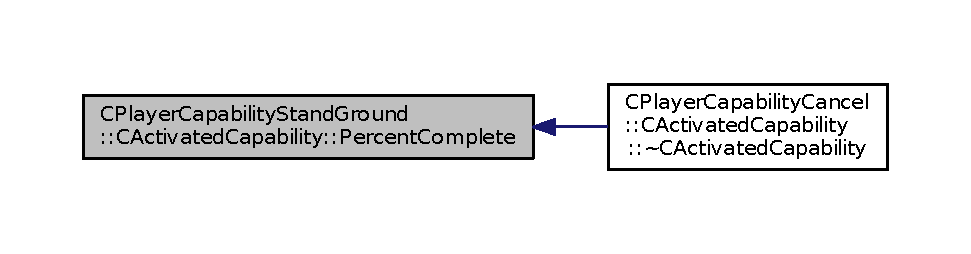
\includegraphics[width=350pt]{classCPlayerCapabilityStandGround_1_1CActivatedCapability_aa9bf1824e755460b699d81f866f2aadc_icgraph}
\end{center}
\end{figure}


The documentation for this class was generated from the following file\+:\begin{DoxyCompactItemize}
\item 
src/\hyperlink{BasicCapabilities_8cpp}{Basic\+Capabilities.\+cpp}\end{DoxyCompactItemize}

\hypertarget{classCPlayerCapabilityCancel_1_1CActivatedCapability}{}\section{C\+Player\+Capability\+Cancel\+:\+:C\+Activated\+Capability Class Reference}
\label{classCPlayerCapabilityCancel_1_1CActivatedCapability}\index{C\+Player\+Capability\+Cancel\+::\+C\+Activated\+Capability@{C\+Player\+Capability\+Cancel\+::\+C\+Activated\+Capability}}


Inheritance diagram for C\+Player\+Capability\+Cancel\+:\+:C\+Activated\+Capability\+:\nopagebreak
\begin{figure}[H]
\begin{center}
\leavevmode
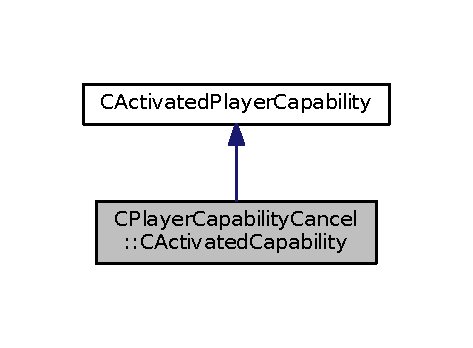
\includegraphics[width=227pt]{classCPlayerCapabilityCancel_1_1CActivatedCapability__inherit__graph}
\end{center}
\end{figure}


Collaboration diagram for C\+Player\+Capability\+Cancel\+:\+:C\+Activated\+Capability\+:\nopagebreak
\begin{figure}[H]
\begin{center}
\leavevmode
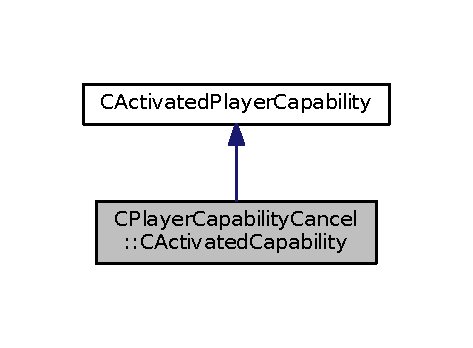
\includegraphics[width=227pt]{classCPlayerCapabilityCancel_1_1CActivatedCapability__coll__graph}
\end{center}
\end{figure}
\subsection*{Public Member Functions}
\begin{DoxyCompactItemize}
\item 
\hyperlink{classCPlayerCapabilityCancel_1_1CActivatedCapability_a162c079742719fda7b641dcd877b6854}{C\+Activated\+Capability} (std\+::shared\+\_\+ptr$<$ \hyperlink{classCPlayerAsset}{C\+Player\+Asset} $>$ actor, std\+::shared\+\_\+ptr$<$ \hyperlink{classCPlayerData}{C\+Player\+Data} $>$ playerdata, std\+::shared\+\_\+ptr$<$ \hyperlink{classCPlayerAsset}{C\+Player\+Asset} $>$ target)
\item 
virtual \hyperlink{classCPlayerCapabilityCancel_1_1CActivatedCapability_ae0d7d8f36d4ac21c04d68dc6ad2ae9c4}{$\sim$\+C\+Activated\+Capability} ()
\item 
int \hyperlink{classCPlayerCapabilityCancel_1_1CActivatedCapability_a69d2fec27186cba11ab545560e7bf45d}{Percent\+Complete} (int max)
\item 
bool \hyperlink{classCPlayerCapabilityCancel_1_1CActivatedCapability_a28351293b3a662bca20a2d666b8801e1}{Increment\+Step} ()
\item 
void \hyperlink{classCPlayerCapabilityCancel_1_1CActivatedCapability_accd67b449574b6c99e21f522d13bc96a}{Cancel} ()
\end{DoxyCompactItemize}
\subsection*{Additional Inherited Members}


\subsection{Detailed Description}


Definition at line 337 of file Basic\+Capabilities.\+cpp.



\subsection{Constructor \& Destructor Documentation}
\hypertarget{classCPlayerCapabilityCancel_1_1CActivatedCapability_a162c079742719fda7b641dcd877b6854}{}\label{classCPlayerCapabilityCancel_1_1CActivatedCapability_a162c079742719fda7b641dcd877b6854} 
\index{C\+Player\+Capability\+Cancel\+::\+C\+Activated\+Capability@{C\+Player\+Capability\+Cancel\+::\+C\+Activated\+Capability}!C\+Activated\+Capability@{C\+Activated\+Capability}}
\index{C\+Activated\+Capability@{C\+Activated\+Capability}!C\+Player\+Capability\+Cancel\+::\+C\+Activated\+Capability@{C\+Player\+Capability\+Cancel\+::\+C\+Activated\+Capability}}
\subsubsection{\texorpdfstring{C\+Activated\+Capability()}{CActivatedCapability()}}
{\footnotesize\ttfamily C\+Player\+Capability\+Cancel\+::\+C\+Activated\+Capability\+::\+C\+Activated\+Capability (\begin{DoxyParamCaption}\item[{std\+::shared\+\_\+ptr$<$ \hyperlink{classCPlayerAsset}{C\+Player\+Asset} $>$}]{actor,  }\item[{std\+::shared\+\_\+ptr$<$ \hyperlink{classCPlayerData}{C\+Player\+Data} $>$}]{playerdata,  }\item[{std\+::shared\+\_\+ptr$<$ \hyperlink{classCPlayerAsset}{C\+Player\+Asset} $>$}]{target }\end{DoxyParamCaption})}



Definition at line 388 of file Basic\+Capabilities.\+cpp.


\begin{DoxyCode}
388                                                                                                            
                                                                               :
389 \hyperlink{classCActivatedPlayerCapability_a1ece00ffb6a7b925c84dd94a7407a0d1}{CActivatedPlayerCapability}(actor, playerdata, target)\{
390 
391 \}
\end{DoxyCode}
\hypertarget{classCPlayerCapabilityCancel_1_1CActivatedCapability_ae0d7d8f36d4ac21c04d68dc6ad2ae9c4}{}\label{classCPlayerCapabilityCancel_1_1CActivatedCapability_ae0d7d8f36d4ac21c04d68dc6ad2ae9c4} 
\index{C\+Player\+Capability\+Cancel\+::\+C\+Activated\+Capability@{C\+Player\+Capability\+Cancel\+::\+C\+Activated\+Capability}!````~C\+Activated\+Capability@{$\sim$\+C\+Activated\+Capability}}
\index{````~C\+Activated\+Capability@{$\sim$\+C\+Activated\+Capability}!C\+Player\+Capability\+Cancel\+::\+C\+Activated\+Capability@{C\+Player\+Capability\+Cancel\+::\+C\+Activated\+Capability}}
\subsubsection{\texorpdfstring{$\sim$\+C\+Activated\+Capability()}{~CActivatedCapability()}}
{\footnotesize\ttfamily virtual C\+Player\+Capability\+Cancel\+::\+C\+Activated\+Capability\+::$\sim$\+C\+Activated\+Capability (\begin{DoxyParamCaption}{ }\end{DoxyParamCaption})\hspace{0.3cm}{\ttfamily [inline]}, {\ttfamily [virtual]}}



Definition at line 342 of file Basic\+Capabilities.\+cpp.


\begin{DoxyCode}
342 \{\};
\end{DoxyCode}
Here is the call graph for this function\+:\nopagebreak
\begin{figure}[H]
\begin{center}
\leavevmode
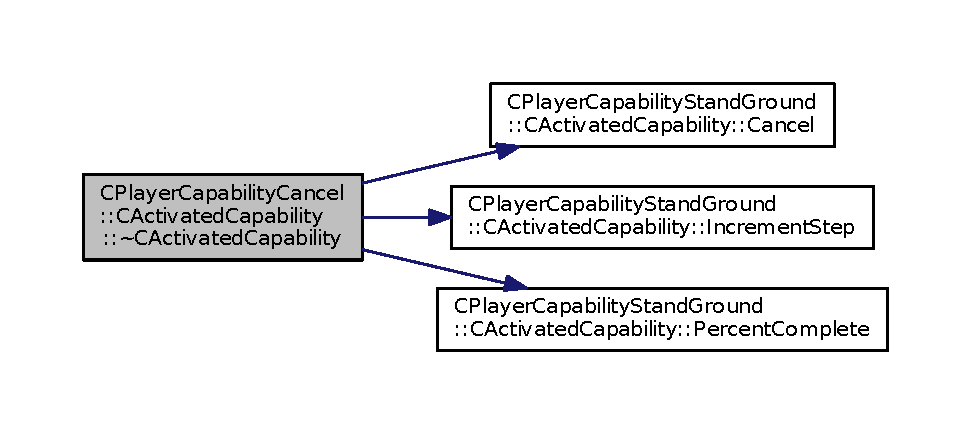
\includegraphics[width=350pt]{classCPlayerCapabilityCancel_1_1CActivatedCapability_ae0d7d8f36d4ac21c04d68dc6ad2ae9c4_cgraph}
\end{center}
\end{figure}


\subsection{Member Function Documentation}
\hypertarget{classCPlayerCapabilityCancel_1_1CActivatedCapability_accd67b449574b6c99e21f522d13bc96a}{}\label{classCPlayerCapabilityCancel_1_1CActivatedCapability_accd67b449574b6c99e21f522d13bc96a} 
\index{C\+Player\+Capability\+Cancel\+::\+C\+Activated\+Capability@{C\+Player\+Capability\+Cancel\+::\+C\+Activated\+Capability}!Cancel@{Cancel}}
\index{Cancel@{Cancel}!C\+Player\+Capability\+Cancel\+::\+C\+Activated\+Capability@{C\+Player\+Capability\+Cancel\+::\+C\+Activated\+Capability}}
\subsubsection{\texorpdfstring{Cancel()}{Cancel()}}
{\footnotesize\ttfamily void C\+Player\+Capability\+Cancel\+::\+C\+Activated\+Capability\+::\+Cancel (\begin{DoxyParamCaption}{ }\end{DoxyParamCaption})\hspace{0.3cm}{\ttfamily [virtual]}}



Implements \hyperlink{classCActivatedPlayerCapability_a5cde83be468e262ad054d81e28684a81}{C\+Activated\+Player\+Capability}.



Definition at line 421 of file Basic\+Capabilities.\+cpp.


\begin{DoxyCode}
421                                                         \{
422 
423     \hyperlink{classCActivatedPlayerCapability_a54ca944b47bff2718330639941d402b0}{DActor}->PopCommand();
424 \}
\end{DoxyCode}
Here is the caller graph for this function\+:\nopagebreak
\begin{figure}[H]
\begin{center}
\leavevmode
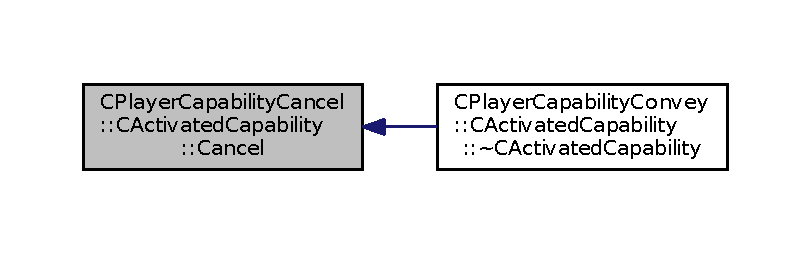
\includegraphics[width=350pt]{classCPlayerCapabilityCancel_1_1CActivatedCapability_accd67b449574b6c99e21f522d13bc96a_icgraph}
\end{center}
\end{figure}
\hypertarget{classCPlayerCapabilityCancel_1_1CActivatedCapability_a28351293b3a662bca20a2d666b8801e1}{}\label{classCPlayerCapabilityCancel_1_1CActivatedCapability_a28351293b3a662bca20a2d666b8801e1} 
\index{C\+Player\+Capability\+Cancel\+::\+C\+Activated\+Capability@{C\+Player\+Capability\+Cancel\+::\+C\+Activated\+Capability}!Increment\+Step@{Increment\+Step}}
\index{Increment\+Step@{Increment\+Step}!C\+Player\+Capability\+Cancel\+::\+C\+Activated\+Capability@{C\+Player\+Capability\+Cancel\+::\+C\+Activated\+Capability}}
\subsubsection{\texorpdfstring{Increment\+Step()}{IncrementStep()}}
{\footnotesize\ttfamily bool C\+Player\+Capability\+Cancel\+::\+C\+Activated\+Capability\+::\+Increment\+Step (\begin{DoxyParamCaption}{ }\end{DoxyParamCaption})\hspace{0.3cm}{\ttfamily [virtual]}}



Implements \hyperlink{classCActivatedPlayerCapability_a943b5999a57504399293250382c0ec6a}{C\+Activated\+Player\+Capability}.



Definition at line 398 of file Basic\+Capabilities.\+cpp.


\begin{DoxyCode}
398                                                                \{
399     \hyperlink{classCActivatedPlayerCapability_a54ca944b47bff2718330639941d402b0}{DActor}->PopCommand();
400     
401     \textcolor{keywordflow}{if}(\hyperlink{GameDataTypes_8h_ab47668e651a3032cfb9c40ea2d60d670ac17cc5a0035320c060d7f8074143b507}{aaNone} != \hyperlink{classCActivatedPlayerCapability_a54ca944b47bff2718330639941d402b0}{DActor}->Action())\{
402         \hyperlink{structSAssetCommand}{SAssetCommand} AssetCommand;
403         
404         AssetCommand = \hyperlink{classCActivatedPlayerCapability_a54ca944b47bff2718330639941d402b0}{DActor}->CurrentCommand();
405         \textcolor{keywordflow}{if}(\hyperlink{GameDataTypes_8h_ab47668e651a3032cfb9c40ea2d60d670a7ef6b863f66dd7dcc95a199cd758ae1d}{aaConstruct} == AssetCommand.\hyperlink{structSAssetCommand_a8edd3b3d59a76d5514ba403bc8076a75}{DAction})\{
406             \textcolor{keywordflow}{if}(AssetCommand.\hyperlink{structSAssetCommand_a3d9b43f6e59c386c48c41a65448a0c39}{DAssetTarget})\{
407                 AssetCommand.\hyperlink{structSAssetCommand_a3d9b43f6e59c386c48c41a65448a0c39}{DAssetTarget}->CurrentCommand().DActivatedCapability->Cancel();
408             \}
409             \textcolor{keywordflow}{else} \textcolor{keywordflow}{if}(AssetCommand.\hyperlink{structSAssetCommand_ad8beda19520811cc70fe1eab16c774dd}{DActivatedCapability})\{
410                 AssetCommand.\hyperlink{structSAssetCommand_ad8beda19520811cc70fe1eab16c774dd}{DActivatedCapability}->Cancel();
411             \}
412         \}
413         \textcolor{keywordflow}{else} \textcolor{keywordflow}{if}(AssetCommand.\hyperlink{structSAssetCommand_ad8beda19520811cc70fe1eab16c774dd}{DActivatedCapability})\{
414             AssetCommand.\hyperlink{structSAssetCommand_ad8beda19520811cc70fe1eab16c774dd}{DActivatedCapability}->Cancel();
415         \}
416     \}
417     
418     \textcolor{keywordflow}{return} \textcolor{keyword}{true};
419 \}
\end{DoxyCode}
Here is the caller graph for this function\+:\nopagebreak
\begin{figure}[H]
\begin{center}
\leavevmode
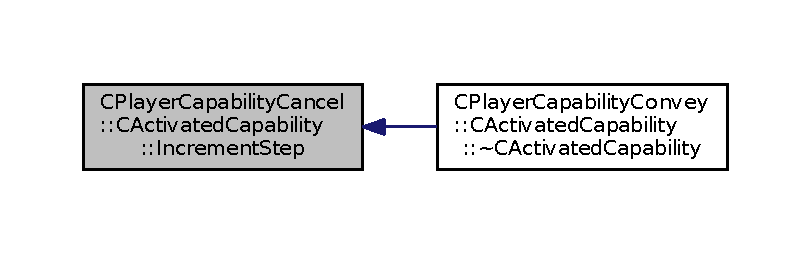
\includegraphics[width=350pt]{classCPlayerCapabilityCancel_1_1CActivatedCapability_a28351293b3a662bca20a2d666b8801e1_icgraph}
\end{center}
\end{figure}
\hypertarget{classCPlayerCapabilityCancel_1_1CActivatedCapability_a69d2fec27186cba11ab545560e7bf45d}{}\label{classCPlayerCapabilityCancel_1_1CActivatedCapability_a69d2fec27186cba11ab545560e7bf45d} 
\index{C\+Player\+Capability\+Cancel\+::\+C\+Activated\+Capability@{C\+Player\+Capability\+Cancel\+::\+C\+Activated\+Capability}!Percent\+Complete@{Percent\+Complete}}
\index{Percent\+Complete@{Percent\+Complete}!C\+Player\+Capability\+Cancel\+::\+C\+Activated\+Capability@{C\+Player\+Capability\+Cancel\+::\+C\+Activated\+Capability}}
\subsubsection{\texorpdfstring{Percent\+Complete()}{PercentComplete()}}
{\footnotesize\ttfamily int C\+Player\+Capability\+Cancel\+::\+C\+Activated\+Capability\+::\+Percent\+Complete (\begin{DoxyParamCaption}\item[{int}]{max }\end{DoxyParamCaption})\hspace{0.3cm}{\ttfamily [virtual]}}



Implements \hyperlink{classCActivatedPlayerCapability_a405dc6076058006a4f801727de4cfe4d}{C\+Activated\+Player\+Capability}.



Definition at line 394 of file Basic\+Capabilities.\+cpp.


\begin{DoxyCode}
394                                                                        \{
395     \textcolor{keywordflow}{return} 0;
396 \}
\end{DoxyCode}
Here is the caller graph for this function\+:\nopagebreak
\begin{figure}[H]
\begin{center}
\leavevmode
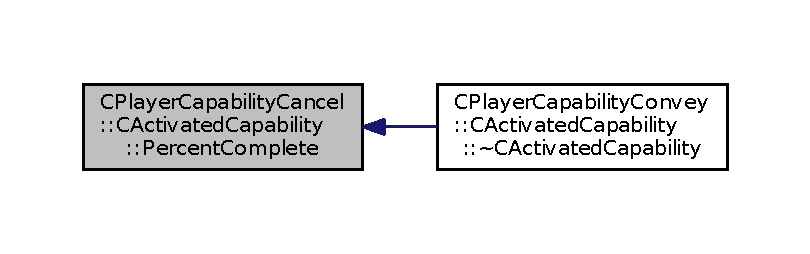
\includegraphics[width=350pt]{classCPlayerCapabilityCancel_1_1CActivatedCapability_a69d2fec27186cba11ab545560e7bf45d_icgraph}
\end{center}
\end{figure}


The documentation for this class was generated from the following file\+:\begin{DoxyCompactItemize}
\item 
src/\hyperlink{BasicCapabilities_8cpp}{Basic\+Capabilities.\+cpp}\end{DoxyCompactItemize}

\hypertarget{classCPlayerCapabilityConvey_1_1CActivatedCapability}{}\section{C\+Player\+Capability\+Convey\+:\+:C\+Activated\+Capability Class Reference}
\label{classCPlayerCapabilityConvey_1_1CActivatedCapability}\index{C\+Player\+Capability\+Convey\+::\+C\+Activated\+Capability@{C\+Player\+Capability\+Convey\+::\+C\+Activated\+Capability}}


Inheritance diagram for C\+Player\+Capability\+Convey\+:\+:C\+Activated\+Capability\+:\nopagebreak
\begin{figure}[H]
\begin{center}
\leavevmode
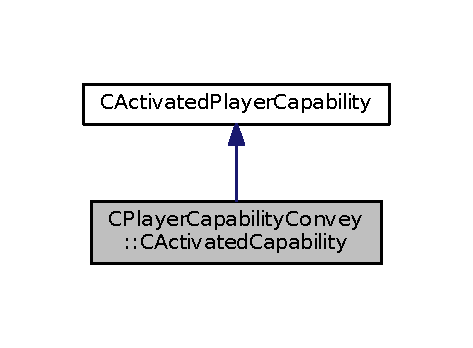
\includegraphics[width=227pt]{classCPlayerCapabilityConvey_1_1CActivatedCapability__inherit__graph}
\end{center}
\end{figure}


Collaboration diagram for C\+Player\+Capability\+Convey\+:\+:C\+Activated\+Capability\+:\nopagebreak
\begin{figure}[H]
\begin{center}
\leavevmode
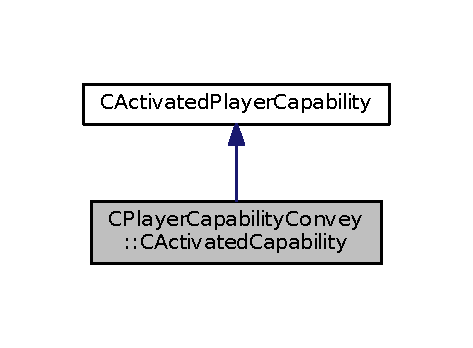
\includegraphics[width=227pt]{classCPlayerCapabilityConvey_1_1CActivatedCapability__coll__graph}
\end{center}
\end{figure}
\subsection*{Public Member Functions}
\begin{DoxyCompactItemize}
\item 
\hyperlink{classCPlayerCapabilityConvey_1_1CActivatedCapability_a2968542706742c59821f3e512c693cf9}{C\+Activated\+Capability} (std\+::shared\+\_\+ptr$<$ \hyperlink{classCPlayerAsset}{C\+Player\+Asset} $>$ actor, std\+::shared\+\_\+ptr$<$ \hyperlink{classCPlayerData}{C\+Player\+Data} $>$ playerdata, std\+::shared\+\_\+ptr$<$ \hyperlink{classCPlayerAsset}{C\+Player\+Asset} $>$ target)
\item 
virtual \hyperlink{classCPlayerCapabilityConvey_1_1CActivatedCapability_a10c78ea328de946070399c5596915641}{$\sim$\+C\+Activated\+Capability} ()
\item 
int \hyperlink{classCPlayerCapabilityConvey_1_1CActivatedCapability_aec6b75fc004f4ac18755d8f601c8ffca}{Percent\+Complete} (int max)
\item 
bool \hyperlink{classCPlayerCapabilityConvey_1_1CActivatedCapability_ac1bf251eca552885041b1bcefa594591}{Increment\+Step} ()
\item 
void \hyperlink{classCPlayerCapabilityConvey_1_1CActivatedCapability_ad84a94a1ae3647ea160e262a0154e229}{Cancel} ()
\end{DoxyCompactItemize}
\subsection*{Additional Inherited Members}


\subsection{Detailed Description}


Definition at line 434 of file Basic\+Capabilities.\+cpp.



\subsection{Constructor \& Destructor Documentation}
\hypertarget{classCPlayerCapabilityConvey_1_1CActivatedCapability_a2968542706742c59821f3e512c693cf9}{}\label{classCPlayerCapabilityConvey_1_1CActivatedCapability_a2968542706742c59821f3e512c693cf9} 
\index{C\+Player\+Capability\+Convey\+::\+C\+Activated\+Capability@{C\+Player\+Capability\+Convey\+::\+C\+Activated\+Capability}!C\+Activated\+Capability@{C\+Activated\+Capability}}
\index{C\+Activated\+Capability@{C\+Activated\+Capability}!C\+Player\+Capability\+Convey\+::\+C\+Activated\+Capability@{C\+Player\+Capability\+Convey\+::\+C\+Activated\+Capability}}
\subsubsection{\texorpdfstring{C\+Activated\+Capability()}{CActivatedCapability()}}
{\footnotesize\ttfamily C\+Player\+Capability\+Convey\+::\+C\+Activated\+Capability\+::\+C\+Activated\+Capability (\begin{DoxyParamCaption}\item[{std\+::shared\+\_\+ptr$<$ \hyperlink{classCPlayerAsset}{C\+Player\+Asset} $>$}]{actor,  }\item[{std\+::shared\+\_\+ptr$<$ \hyperlink{classCPlayerData}{C\+Player\+Data} $>$}]{playerdata,  }\item[{std\+::shared\+\_\+ptr$<$ \hyperlink{classCPlayerAsset}{C\+Player\+Asset} $>$}]{target }\end{DoxyParamCaption})}



Definition at line 497 of file Basic\+Capabilities.\+cpp.


\begin{DoxyCode}
497                                                                                                            
                                                                               :
498 \hyperlink{classCActivatedPlayerCapability_a1ece00ffb6a7b925c84dd94a7407a0d1}{CActivatedPlayerCapability}(actor, playerdata, target)\{
499 
500 \}
\end{DoxyCode}
\hypertarget{classCPlayerCapabilityConvey_1_1CActivatedCapability_a10c78ea328de946070399c5596915641}{}\label{classCPlayerCapabilityConvey_1_1CActivatedCapability_a10c78ea328de946070399c5596915641} 
\index{C\+Player\+Capability\+Convey\+::\+C\+Activated\+Capability@{C\+Player\+Capability\+Convey\+::\+C\+Activated\+Capability}!````~C\+Activated\+Capability@{$\sim$\+C\+Activated\+Capability}}
\index{````~C\+Activated\+Capability@{$\sim$\+C\+Activated\+Capability}!C\+Player\+Capability\+Convey\+::\+C\+Activated\+Capability@{C\+Player\+Capability\+Convey\+::\+C\+Activated\+Capability}}
\subsubsection{\texorpdfstring{$\sim$\+C\+Activated\+Capability()}{~CActivatedCapability()}}
{\footnotesize\ttfamily virtual C\+Player\+Capability\+Convey\+::\+C\+Activated\+Capability\+::$\sim$\+C\+Activated\+Capability (\begin{DoxyParamCaption}{ }\end{DoxyParamCaption})\hspace{0.3cm}{\ttfamily [inline]}, {\ttfamily [virtual]}}



Definition at line 439 of file Basic\+Capabilities.\+cpp.



References C\+Player\+Capability\+Cancel\+::\+C\+Activated\+Capability\+::\+Cancel(), C\+Player\+Capability\+Cancel\+::\+C\+Activated\+Capability\+::\+Increment\+Step(), and C\+Player\+Capability\+Cancel\+::\+C\+Activated\+Capability\+::\+Percent\+Complete().


\begin{DoxyCode}
439 \{\};
\end{DoxyCode}
Here is the call graph for this function\+:\nopagebreak
\begin{figure}[H]
\begin{center}
\leavevmode
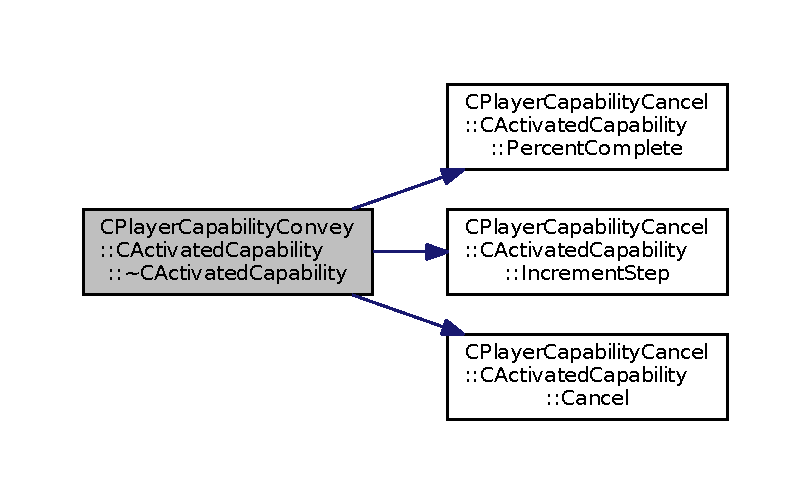
\includegraphics[width=350pt]{classCPlayerCapabilityConvey_1_1CActivatedCapability_a10c78ea328de946070399c5596915641_cgraph}
\end{center}
\end{figure}


\subsection{Member Function Documentation}
\hypertarget{classCPlayerCapabilityConvey_1_1CActivatedCapability_ad84a94a1ae3647ea160e262a0154e229}{}\label{classCPlayerCapabilityConvey_1_1CActivatedCapability_ad84a94a1ae3647ea160e262a0154e229} 
\index{C\+Player\+Capability\+Convey\+::\+C\+Activated\+Capability@{C\+Player\+Capability\+Convey\+::\+C\+Activated\+Capability}!Cancel@{Cancel}}
\index{Cancel@{Cancel}!C\+Player\+Capability\+Convey\+::\+C\+Activated\+Capability@{C\+Player\+Capability\+Convey\+::\+C\+Activated\+Capability}}
\subsubsection{\texorpdfstring{Cancel()}{Cancel()}}
{\footnotesize\ttfamily void C\+Player\+Capability\+Convey\+::\+C\+Activated\+Capability\+::\+Cancel (\begin{DoxyParamCaption}{ }\end{DoxyParamCaption})\hspace{0.3cm}{\ttfamily [virtual]}}



Implements \hyperlink{classCActivatedPlayerCapability_a5cde83be468e262ad054d81e28684a81}{C\+Activated\+Player\+Capability}.



Definition at line 537 of file Basic\+Capabilities.\+cpp.



References C\+Activated\+Player\+Capability\+::\+D\+Actor.



Referenced by C\+Player\+Capability\+Patrol\+::\+C\+Activated\+Capability\+::$\sim$\+C\+Activated\+Capability().


\begin{DoxyCode}
537                                                         \{
538 
539     \hyperlink{classCActivatedPlayerCapability_a54ca944b47bff2718330639941d402b0}{DActor}->PopCommand();
540 \}
\end{DoxyCode}
Here is the caller graph for this function\+:\nopagebreak
\begin{figure}[H]
\begin{center}
\leavevmode
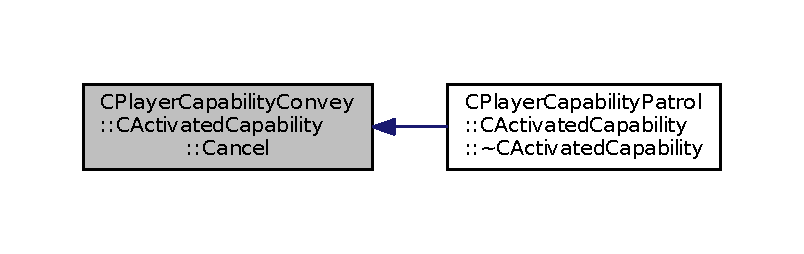
\includegraphics[width=350pt]{classCPlayerCapabilityConvey_1_1CActivatedCapability_ad84a94a1ae3647ea160e262a0154e229_icgraph}
\end{center}
\end{figure}
\hypertarget{classCPlayerCapabilityConvey_1_1CActivatedCapability_ac1bf251eca552885041b1bcefa594591}{}\label{classCPlayerCapabilityConvey_1_1CActivatedCapability_ac1bf251eca552885041b1bcefa594591} 
\index{C\+Player\+Capability\+Convey\+::\+C\+Activated\+Capability@{C\+Player\+Capability\+Convey\+::\+C\+Activated\+Capability}!Increment\+Step@{Increment\+Step}}
\index{Increment\+Step@{Increment\+Step}!C\+Player\+Capability\+Convey\+::\+C\+Activated\+Capability@{C\+Player\+Capability\+Convey\+::\+C\+Activated\+Capability}}
\subsubsection{\texorpdfstring{Increment\+Step()}{IncrementStep()}}
{\footnotesize\ttfamily bool C\+Player\+Capability\+Convey\+::\+C\+Activated\+Capability\+::\+Increment\+Step (\begin{DoxyParamCaption}{ }\end{DoxyParamCaption})\hspace{0.3cm}{\ttfamily [virtual]}}



Implements \hyperlink{classCActivatedPlayerCapability_a943b5999a57504399293250382c0ec6a}{C\+Activated\+Player\+Capability}.



Definition at line 507 of file Basic\+Capabilities.\+cpp.



References aa\+Convey\+Gold, aa\+Convey\+Lumber, aa\+Walk, S\+Asset\+Command\+::\+D\+Action, C\+Activated\+Player\+Capability\+::\+D\+Actor, S\+Game\+Event\+::\+D\+Asset, S\+Asset\+Command\+::\+D\+Asset\+Target, C\+Activated\+Player\+Capability\+::\+D\+Player\+Data, C\+Activated\+Player\+Capability\+::\+D\+Target, S\+Game\+Event\+::\+D\+Type, and et\+Acknowledge.



Referenced by C\+Player\+Capability\+Patrol\+::\+C\+Activated\+Capability\+::$\sim$\+C\+Activated\+Capability().


\begin{DoxyCode}
507                                                                \{
508     std::weak\_ptr< CPlayerAsset > NearestRepository;
509     \hyperlink{structSAssetCommand}{SAssetCommand} AssetCommand;
510     \hyperlink{structSGameEvent}{SGameEvent} TempEvent;
511     
512     TempEvent.\hyperlink{structSGameEvent_afa10562e243f4ac2b473b655cc58fee7}{DType} = \hyperlink{GameModel_8h_abfcf510bafec7c6429906a6ecaac656da9b68fc38f3ca4002cd7a3ec3cc07a612}{etAcknowledge};
513     TempEvent.\hyperlink{structSGameEvent_a40c85eeac83b96887b7449c9bdc5d624}{DAsset} = \hyperlink{classCActivatedPlayerCapability_a54ca944b47bff2718330639941d402b0}{DActor};
514     \hyperlink{classCActivatedPlayerCapability_a9bf27c322a73f4b11c8183cc1973c3d8}{DPlayerData}->AddGameEvent(TempEvent);
515     
516     \hyperlink{classCActivatedPlayerCapability_a54ca944b47bff2718330639941d402b0}{DActor}->PopCommand();
517     \textcolor{keywordflow}{if}(\hyperlink{classCActivatedPlayerCapability_a54ca944b47bff2718330639941d402b0}{DActor}->Lumber())\{
518         AssetCommand.\hyperlink{structSAssetCommand_a8edd3b3d59a76d5514ba403bc8076a75}{DAction} = \hyperlink{GameDataTypes_8h_ab47668e651a3032cfb9c40ea2d60d670a7b0954302f27f46b3fdf6fddd530d154}{aaConveyLumber};
519         AssetCommand.\hyperlink{structSAssetCommand_a3d9b43f6e59c386c48c41a65448a0c39}{DAssetTarget} = \hyperlink{classCActivatedPlayerCapability_a8a1cf50b6501bcfd55af0c935828e395}{DTarget};
520         \hyperlink{classCActivatedPlayerCapability_a54ca944b47bff2718330639941d402b0}{DActor}->PushCommand(AssetCommand);
521         AssetCommand.\hyperlink{structSAssetCommand_a8edd3b3d59a76d5514ba403bc8076a75}{DAction} = \hyperlink{GameDataTypes_8h_ab47668e651a3032cfb9c40ea2d60d670a60ca9010aa62b73c1aab838ff4bf7276}{aaWalk};
522         \hyperlink{classCActivatedPlayerCapability_a54ca944b47bff2718330639941d402b0}{DActor}->PushCommand(AssetCommand);
523         \hyperlink{classCActivatedPlayerCapability_a54ca944b47bff2718330639941d402b0}{DActor}->ResetStep();
524     \}
525     \textcolor{keywordflow}{else} \textcolor{keywordflow}{if}(\hyperlink{classCActivatedPlayerCapability_a54ca944b47bff2718330639941d402b0}{DActor}->Gold())\{
526         AssetCommand.\hyperlink{structSAssetCommand_a8edd3b3d59a76d5514ba403bc8076a75}{DAction} = \hyperlink{GameDataTypes_8h_ab47668e651a3032cfb9c40ea2d60d670ae80ac4dde60023e0a1794e994db7000a}{aaConveyGold};
527         AssetCommand.\hyperlink{structSAssetCommand_a3d9b43f6e59c386c48c41a65448a0c39}{DAssetTarget} = \hyperlink{classCActivatedPlayerCapability_a8a1cf50b6501bcfd55af0c935828e395}{DTarget};
528         \hyperlink{classCActivatedPlayerCapability_a54ca944b47bff2718330639941d402b0}{DActor}->PushCommand(AssetCommand);
529         AssetCommand.\hyperlink{structSAssetCommand_a8edd3b3d59a76d5514ba403bc8076a75}{DAction} = \hyperlink{GameDataTypes_8h_ab47668e651a3032cfb9c40ea2d60d670a60ca9010aa62b73c1aab838ff4bf7276}{aaWalk};
530         \hyperlink{classCActivatedPlayerCapability_a54ca944b47bff2718330639941d402b0}{DActor}->PushCommand(AssetCommand);
531         \hyperlink{classCActivatedPlayerCapability_a54ca944b47bff2718330639941d402b0}{DActor}->ResetStep();
532     \}
533     
534     \textcolor{keywordflow}{return} \textcolor{keyword}{true};
535 \}
\end{DoxyCode}
Here is the caller graph for this function\+:\nopagebreak
\begin{figure}[H]
\begin{center}
\leavevmode
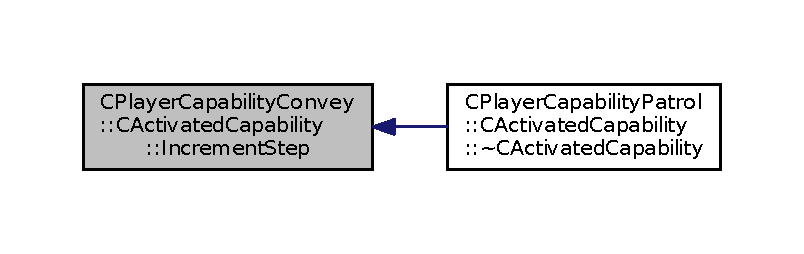
\includegraphics[width=350pt]{classCPlayerCapabilityConvey_1_1CActivatedCapability_ac1bf251eca552885041b1bcefa594591_icgraph}
\end{center}
\end{figure}
\hypertarget{classCPlayerCapabilityConvey_1_1CActivatedCapability_aec6b75fc004f4ac18755d8f601c8ffca}{}\label{classCPlayerCapabilityConvey_1_1CActivatedCapability_aec6b75fc004f4ac18755d8f601c8ffca} 
\index{C\+Player\+Capability\+Convey\+::\+C\+Activated\+Capability@{C\+Player\+Capability\+Convey\+::\+C\+Activated\+Capability}!Percent\+Complete@{Percent\+Complete}}
\index{Percent\+Complete@{Percent\+Complete}!C\+Player\+Capability\+Convey\+::\+C\+Activated\+Capability@{C\+Player\+Capability\+Convey\+::\+C\+Activated\+Capability}}
\subsubsection{\texorpdfstring{Percent\+Complete()}{PercentComplete()}}
{\footnotesize\ttfamily int C\+Player\+Capability\+Convey\+::\+C\+Activated\+Capability\+::\+Percent\+Complete (\begin{DoxyParamCaption}\item[{int}]{max }\end{DoxyParamCaption})\hspace{0.3cm}{\ttfamily [virtual]}}



Implements \hyperlink{classCActivatedPlayerCapability_a405dc6076058006a4f801727de4cfe4d}{C\+Activated\+Player\+Capability}.



Definition at line 503 of file Basic\+Capabilities.\+cpp.



Referenced by C\+Player\+Capability\+Patrol\+::\+C\+Activated\+Capability\+::$\sim$\+C\+Activated\+Capability().


\begin{DoxyCode}
503                                                                        \{
504     \textcolor{keywordflow}{return} 0;
505 \}
\end{DoxyCode}
Here is the caller graph for this function\+:\nopagebreak
\begin{figure}[H]
\begin{center}
\leavevmode
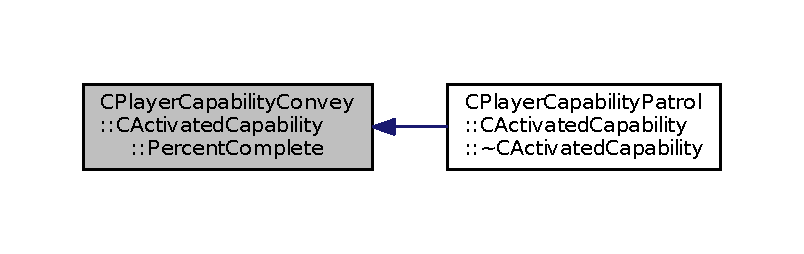
\includegraphics[width=350pt]{classCPlayerCapabilityConvey_1_1CActivatedCapability_aec6b75fc004f4ac18755d8f601c8ffca_icgraph}
\end{center}
\end{figure}


The documentation for this class was generated from the following file\+:\begin{DoxyCompactItemize}
\item 
src/\hyperlink{BasicCapabilities_8cpp}{Basic\+Capabilities.\+cpp}\end{DoxyCompactItemize}

\hypertarget{classCPlayerCapabilityPatrol_1_1CActivatedCapability}{}\section{C\+Player\+Capability\+Patrol\+:\+:C\+Activated\+Capability Class Reference}
\label{classCPlayerCapabilityPatrol_1_1CActivatedCapability}\index{C\+Player\+Capability\+Patrol\+::\+C\+Activated\+Capability@{C\+Player\+Capability\+Patrol\+::\+C\+Activated\+Capability}}


Inheritance diagram for C\+Player\+Capability\+Patrol\+:\+:C\+Activated\+Capability\+:\nopagebreak
\begin{figure}[H]
\begin{center}
\leavevmode
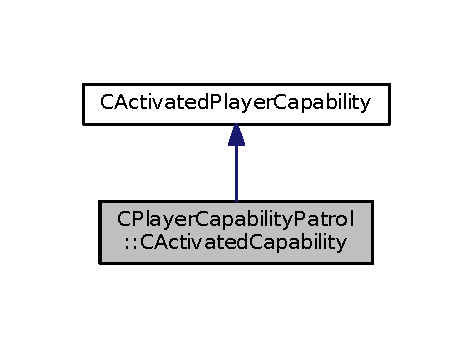
\includegraphics[width=227pt]{classCPlayerCapabilityPatrol_1_1CActivatedCapability__inherit__graph}
\end{center}
\end{figure}


Collaboration diagram for C\+Player\+Capability\+Patrol\+:\+:C\+Activated\+Capability\+:\nopagebreak
\begin{figure}[H]
\begin{center}
\leavevmode
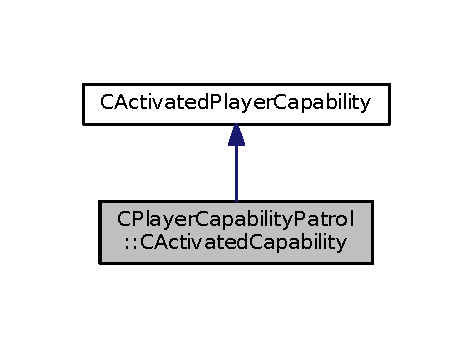
\includegraphics[width=227pt]{classCPlayerCapabilityPatrol_1_1CActivatedCapability__coll__graph}
\end{center}
\end{figure}
\subsection*{Public Member Functions}
\begin{DoxyCompactItemize}
\item 
\hyperlink{classCPlayerCapabilityPatrol_1_1CActivatedCapability_aabca66a580e5b7630f7857ad04d6198c}{C\+Activated\+Capability} (std\+::shared\+\_\+ptr$<$ \hyperlink{classCPlayerAsset}{C\+Player\+Asset} $>$ actor, std\+::shared\+\_\+ptr$<$ \hyperlink{classCPlayerData}{C\+Player\+Data} $>$ playerdata, std\+::shared\+\_\+ptr$<$ \hyperlink{classCPlayerAsset}{C\+Player\+Asset} $>$ target)
\item 
virtual \hyperlink{classCPlayerCapabilityPatrol_1_1CActivatedCapability_a2ad25677321b38e90d4e94abb0401aab}{$\sim$\+C\+Activated\+Capability} ()
\item 
int \hyperlink{classCPlayerCapabilityPatrol_1_1CActivatedCapability_a868e6583a55b01e5aa3b926ef14677bc}{Percent\+Complete} (int max)
\item 
bool \hyperlink{classCPlayerCapabilityPatrol_1_1CActivatedCapability_a576a71646225c0723a0ed9e77add01fd}{Increment\+Step} ()
\item 
void \hyperlink{classCPlayerCapabilityPatrol_1_1CActivatedCapability_a36165c232eb283ce4a92bd4606480c73}{Cancel} ()
\end{DoxyCompactItemize}
\subsection*{Additional Inherited Members}


\subsection{Detailed Description}


Definition at line 550 of file Basic\+Capabilities.\+cpp.



\subsection{Constructor \& Destructor Documentation}
\hypertarget{classCPlayerCapabilityPatrol_1_1CActivatedCapability_aabca66a580e5b7630f7857ad04d6198c}{}\label{classCPlayerCapabilityPatrol_1_1CActivatedCapability_aabca66a580e5b7630f7857ad04d6198c} 
\index{C\+Player\+Capability\+Patrol\+::\+C\+Activated\+Capability@{C\+Player\+Capability\+Patrol\+::\+C\+Activated\+Capability}!C\+Activated\+Capability@{C\+Activated\+Capability}}
\index{C\+Activated\+Capability@{C\+Activated\+Capability}!C\+Player\+Capability\+Patrol\+::\+C\+Activated\+Capability@{C\+Player\+Capability\+Patrol\+::\+C\+Activated\+Capability}}
\subsubsection{\texorpdfstring{C\+Activated\+Capability()}{CActivatedCapability()}}
{\footnotesize\ttfamily C\+Player\+Capability\+Patrol\+::\+C\+Activated\+Capability\+::\+C\+Activated\+Capability (\begin{DoxyParamCaption}\item[{std\+::shared\+\_\+ptr$<$ \hyperlink{classCPlayerAsset}{C\+Player\+Asset} $>$}]{actor,  }\item[{std\+::shared\+\_\+ptr$<$ \hyperlink{classCPlayerData}{C\+Player\+Data} $>$}]{playerdata,  }\item[{std\+::shared\+\_\+ptr$<$ \hyperlink{classCPlayerAsset}{C\+Player\+Asset} $>$}]{target }\end{DoxyParamCaption})}



Definition at line 605 of file Basic\+Capabilities.\+cpp.


\begin{DoxyCode}
605                                                                                                            
                                                                               :
606 \hyperlink{classCActivatedPlayerCapability_a1ece00ffb6a7b925c84dd94a7407a0d1}{CActivatedPlayerCapability}(actor, playerdata, target)\{
607 
608 \}
\end{DoxyCode}
\hypertarget{classCPlayerCapabilityPatrol_1_1CActivatedCapability_a2ad25677321b38e90d4e94abb0401aab}{}\label{classCPlayerCapabilityPatrol_1_1CActivatedCapability_a2ad25677321b38e90d4e94abb0401aab} 
\index{C\+Player\+Capability\+Patrol\+::\+C\+Activated\+Capability@{C\+Player\+Capability\+Patrol\+::\+C\+Activated\+Capability}!````~C\+Activated\+Capability@{$\sim$\+C\+Activated\+Capability}}
\index{````~C\+Activated\+Capability@{$\sim$\+C\+Activated\+Capability}!C\+Player\+Capability\+Patrol\+::\+C\+Activated\+Capability@{C\+Player\+Capability\+Patrol\+::\+C\+Activated\+Capability}}
\subsubsection{\texorpdfstring{$\sim$\+C\+Activated\+Capability()}{~CActivatedCapability()}}
{\footnotesize\ttfamily virtual C\+Player\+Capability\+Patrol\+::\+C\+Activated\+Capability\+::$\sim$\+C\+Activated\+Capability (\begin{DoxyParamCaption}{ }\end{DoxyParamCaption})\hspace{0.3cm}{\ttfamily [inline]}, {\ttfamily [virtual]}}



Definition at line 555 of file Basic\+Capabilities.\+cpp.


\begin{DoxyCode}
555 \{\};
\end{DoxyCode}
Here is the call graph for this function\+:\nopagebreak
\begin{figure}[H]
\begin{center}
\leavevmode
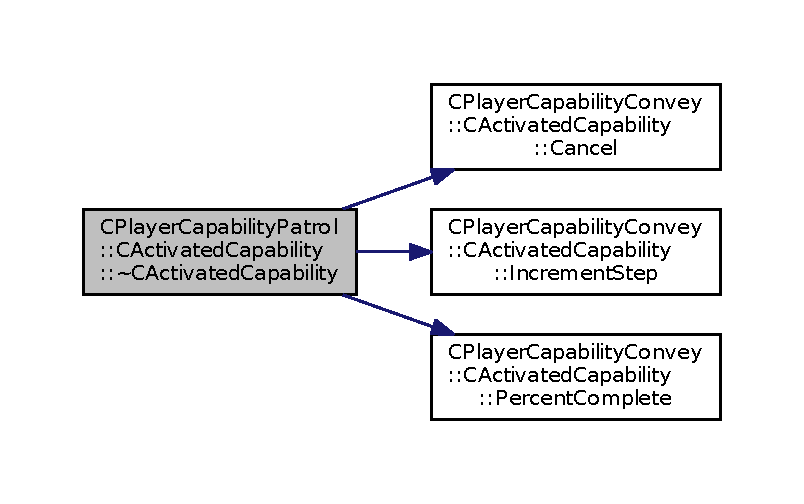
\includegraphics[width=350pt]{classCPlayerCapabilityPatrol_1_1CActivatedCapability_a2ad25677321b38e90d4e94abb0401aab_cgraph}
\end{center}
\end{figure}


\subsection{Member Function Documentation}
\hypertarget{classCPlayerCapabilityPatrol_1_1CActivatedCapability_a36165c232eb283ce4a92bd4606480c73}{}\label{classCPlayerCapabilityPatrol_1_1CActivatedCapability_a36165c232eb283ce4a92bd4606480c73} 
\index{C\+Player\+Capability\+Patrol\+::\+C\+Activated\+Capability@{C\+Player\+Capability\+Patrol\+::\+C\+Activated\+Capability}!Cancel@{Cancel}}
\index{Cancel@{Cancel}!C\+Player\+Capability\+Patrol\+::\+C\+Activated\+Capability@{C\+Player\+Capability\+Patrol\+::\+C\+Activated\+Capability}}
\subsubsection{\texorpdfstring{Cancel()}{Cancel()}}
{\footnotesize\ttfamily void C\+Player\+Capability\+Patrol\+::\+C\+Activated\+Capability\+::\+Cancel (\begin{DoxyParamCaption}{ }\end{DoxyParamCaption})\hspace{0.3cm}{\ttfamily [virtual]}}



Implements \hyperlink{classCActivatedPlayerCapability_a5cde83be468e262ad054d81e28684a81}{C\+Activated\+Player\+Capability}.



Definition at line 639 of file Basic\+Capabilities.\+cpp.


\begin{DoxyCode}
639                                                         \{
640 
641     \hyperlink{classCActivatedPlayerCapability_a54ca944b47bff2718330639941d402b0}{DActor}->PopCommand();
642 \}
\end{DoxyCode}
Here is the caller graph for this function\+:\nopagebreak
\begin{figure}[H]
\begin{center}
\leavevmode
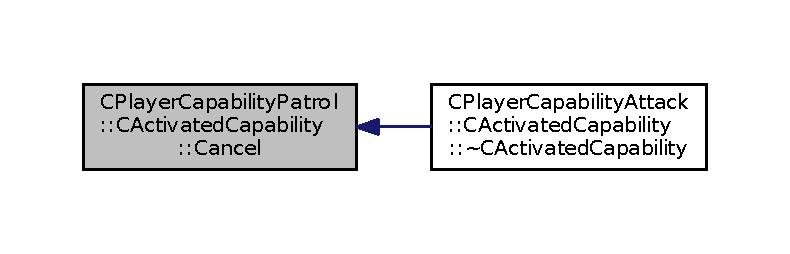
\includegraphics[width=350pt]{classCPlayerCapabilityPatrol_1_1CActivatedCapability_a36165c232eb283ce4a92bd4606480c73_icgraph}
\end{center}
\end{figure}
\hypertarget{classCPlayerCapabilityPatrol_1_1CActivatedCapability_a576a71646225c0723a0ed9e77add01fd}{}\label{classCPlayerCapabilityPatrol_1_1CActivatedCapability_a576a71646225c0723a0ed9e77add01fd} 
\index{C\+Player\+Capability\+Patrol\+::\+C\+Activated\+Capability@{C\+Player\+Capability\+Patrol\+::\+C\+Activated\+Capability}!Increment\+Step@{Increment\+Step}}
\index{Increment\+Step@{Increment\+Step}!C\+Player\+Capability\+Patrol\+::\+C\+Activated\+Capability@{C\+Player\+Capability\+Patrol\+::\+C\+Activated\+Capability}}
\subsubsection{\texorpdfstring{Increment\+Step()}{IncrementStep()}}
{\footnotesize\ttfamily bool C\+Player\+Capability\+Patrol\+::\+C\+Activated\+Capability\+::\+Increment\+Step (\begin{DoxyParamCaption}{ }\end{DoxyParamCaption})\hspace{0.3cm}{\ttfamily [virtual]}}



Implements \hyperlink{classCActivatedPlayerCapability_a943b5999a57504399293250382c0ec6a}{C\+Activated\+Player\+Capability}.



Definition at line 615 of file Basic\+Capabilities.\+cpp.


\begin{DoxyCode}
615                                                                \{
616     \hyperlink{structSAssetCommand}{SAssetCommand} PatrolCommand, WalkCommand;
617     \hyperlink{structSGameEvent}{SGameEvent} TempEvent;
618     
619     TempEvent.\hyperlink{structSGameEvent_afa10562e243f4ac2b473b655cc58fee7}{DType} = \hyperlink{GameModel_8h_abfcf510bafec7c6429906a6ecaac656da9b68fc38f3ca4002cd7a3ec3cc07a612}{etAcknowledge};
620     TempEvent.\hyperlink{structSGameEvent_a40c85eeac83b96887b7449c9bdc5d624}{DAsset} = \hyperlink{classCActivatedPlayerCapability_a54ca944b47bff2718330639941d402b0}{DActor};
621     \hyperlink{classCActivatedPlayerCapability_a9bf27c322a73f4b11c8183cc1973c3d8}{DPlayerData}->AddGameEvent(TempEvent);
622     
623     PatrolCommand.\hyperlink{structSAssetCommand_a8edd3b3d59a76d5514ba403bc8076a75}{DAction} = \hyperlink{GameDataTypes_8h_ab47668e651a3032cfb9c40ea2d60d670acf9fb164e8abd71c71f4a8c7fda360d4}{aaCapability};
624     PatrolCommand.\hyperlink{structSAssetCommand_a734ea7c6847457b437360f333f570ff9}{DCapability} = \hyperlink{GameDataTypes_8h_a35b98ce26aca678b03c6f9f76e4778cea3cba4431d7962d2d5ffd01a9f7571332}{actPatrol};
625     PatrolCommand.\hyperlink{structSAssetCommand_a3d9b43f6e59c386c48c41a65448a0c39}{DAssetTarget} = \hyperlink{classCActivatedPlayerCapability_a9bf27c322a73f4b11c8183cc1973c3d8}{DPlayerData}->CreateMarker(
      \hyperlink{classCActivatedPlayerCapability_a54ca944b47bff2718330639941d402b0}{DActor}->Position(), \textcolor{keyword}{false});
626     PatrolCommand.\hyperlink{structSAssetCommand_ad8beda19520811cc70fe1eab16c774dd}{DActivatedCapability} = std::make\_shared< CActivatedCapability >(
      \hyperlink{classCActivatedPlayerCapability_a54ca944b47bff2718330639941d402b0}{DActor}, \hyperlink{classCActivatedPlayerCapability_a9bf27c322a73f4b11c8183cc1973c3d8}{DPlayerData}, PatrolCommand.\hyperlink{structSAssetCommand_a3d9b43f6e59c386c48c41a65448a0c39}{DAssetTarget});
627     DActor->ClearCommand();
628     DActor->PushCommand(PatrolCommand);
629     
630     WalkCommand.\hyperlink{structSAssetCommand_a8edd3b3d59a76d5514ba403bc8076a75}{DAction} = \hyperlink{GameDataTypes_8h_ab47668e651a3032cfb9c40ea2d60d670a60ca9010aa62b73c1aab838ff4bf7276}{aaWalk};
631     WalkCommand.\hyperlink{structSAssetCommand_a3d9b43f6e59c386c48c41a65448a0c39}{DAssetTarget} = \hyperlink{classCActivatedPlayerCapability_a8a1cf50b6501bcfd55af0c935828e395}{DTarget};
632     \textcolor{keywordflow}{if}(!DActor->TileAligned())\{
633         DActor->Direction((\hyperlink{GameDataTypes_8h_acb2b033915f6659a71a38b5aa6e4eb42}{EDirection})((DActor->Position().TileOctant() + 
      \hyperlink{GameDataTypes_8h_acb2b033915f6659a71a38b5aa6e4eb42af6546049275557ce0ade2ceee042a319}{dMax}/2) % \hyperlink{GameDataTypes_8h_acb2b033915f6659a71a38b5aa6e4eb42af6546049275557ce0ade2ceee042a319}{dMax}));
634     \}
635     DActor->PushCommand(WalkCommand);
636     \textcolor{keywordflow}{return} \textcolor{keyword}{true};
637 \}
\end{DoxyCode}
Here is the caller graph for this function\+:\nopagebreak
\begin{figure}[H]
\begin{center}
\leavevmode
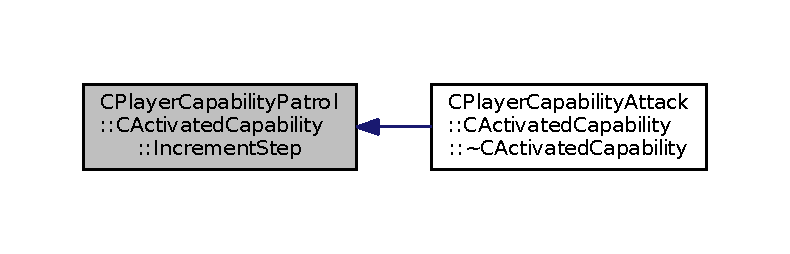
\includegraphics[width=350pt]{classCPlayerCapabilityPatrol_1_1CActivatedCapability_a576a71646225c0723a0ed9e77add01fd_icgraph}
\end{center}
\end{figure}
\hypertarget{classCPlayerCapabilityPatrol_1_1CActivatedCapability_a868e6583a55b01e5aa3b926ef14677bc}{}\label{classCPlayerCapabilityPatrol_1_1CActivatedCapability_a868e6583a55b01e5aa3b926ef14677bc} 
\index{C\+Player\+Capability\+Patrol\+::\+C\+Activated\+Capability@{C\+Player\+Capability\+Patrol\+::\+C\+Activated\+Capability}!Percent\+Complete@{Percent\+Complete}}
\index{Percent\+Complete@{Percent\+Complete}!C\+Player\+Capability\+Patrol\+::\+C\+Activated\+Capability@{C\+Player\+Capability\+Patrol\+::\+C\+Activated\+Capability}}
\subsubsection{\texorpdfstring{Percent\+Complete()}{PercentComplete()}}
{\footnotesize\ttfamily int C\+Player\+Capability\+Patrol\+::\+C\+Activated\+Capability\+::\+Percent\+Complete (\begin{DoxyParamCaption}\item[{int}]{max }\end{DoxyParamCaption})\hspace{0.3cm}{\ttfamily [virtual]}}



Implements \hyperlink{classCActivatedPlayerCapability_a405dc6076058006a4f801727de4cfe4d}{C\+Activated\+Player\+Capability}.



Definition at line 611 of file Basic\+Capabilities.\+cpp.


\begin{DoxyCode}
611                                                                        \{
612     \textcolor{keywordflow}{return} 0;
613 \}
\end{DoxyCode}
Here is the caller graph for this function\+:\nopagebreak
\begin{figure}[H]
\begin{center}
\leavevmode
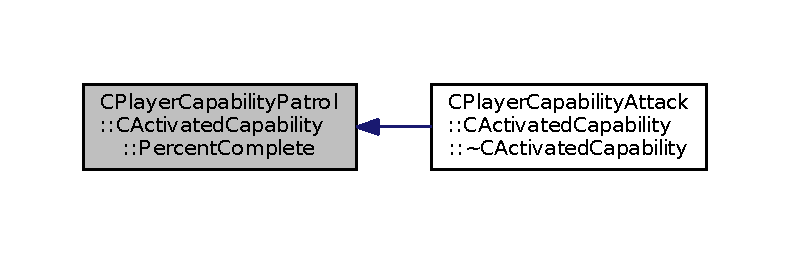
\includegraphics[width=350pt]{classCPlayerCapabilityPatrol_1_1CActivatedCapability_a868e6583a55b01e5aa3b926ef14677bc_icgraph}
\end{center}
\end{figure}


The documentation for this class was generated from the following file\+:\begin{DoxyCompactItemize}
\item 
src/\hyperlink{BasicCapabilities_8cpp}{Basic\+Capabilities.\+cpp}\end{DoxyCompactItemize}

\hypertarget{classCPlayerCapabilityAttack_1_1CActivatedCapability}{}\section{C\+Player\+Capability\+Attack\+:\+:C\+Activated\+Capability Class Reference}
\label{classCPlayerCapabilityAttack_1_1CActivatedCapability}\index{C\+Player\+Capability\+Attack\+::\+C\+Activated\+Capability@{C\+Player\+Capability\+Attack\+::\+C\+Activated\+Capability}}


Inheritance diagram for C\+Player\+Capability\+Attack\+:\+:C\+Activated\+Capability\+:\nopagebreak
\begin{figure}[H]
\begin{center}
\leavevmode
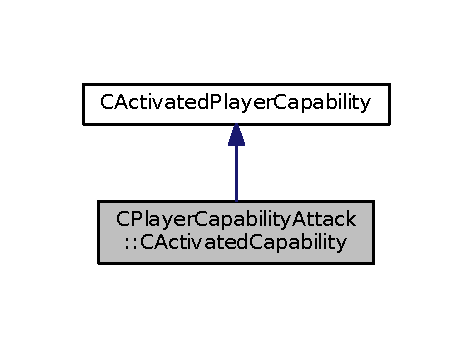
\includegraphics[width=227pt]{classCPlayerCapabilityAttack_1_1CActivatedCapability__inherit__graph}
\end{center}
\end{figure}


Collaboration diagram for C\+Player\+Capability\+Attack\+:\+:C\+Activated\+Capability\+:\nopagebreak
\begin{figure}[H]
\begin{center}
\leavevmode
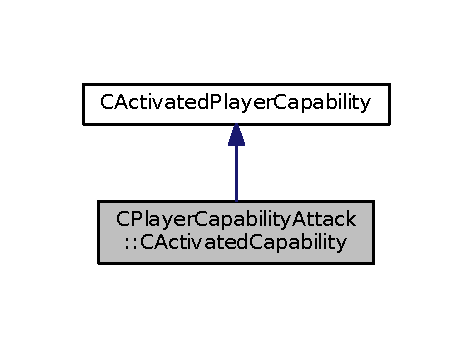
\includegraphics[width=227pt]{classCPlayerCapabilityAttack_1_1CActivatedCapability__coll__graph}
\end{center}
\end{figure}
\subsection*{Public Member Functions}
\begin{DoxyCompactItemize}
\item 
\hyperlink{classCPlayerCapabilityAttack_1_1CActivatedCapability_aa564d203e407b40f008d19a65f01d823}{C\+Activated\+Capability} (std\+::shared\+\_\+ptr$<$ \hyperlink{classCPlayerAsset}{C\+Player\+Asset} $>$ actor, std\+::shared\+\_\+ptr$<$ \hyperlink{classCPlayerData}{C\+Player\+Data} $>$ playerdata, std\+::shared\+\_\+ptr$<$ \hyperlink{classCPlayerAsset}{C\+Player\+Asset} $>$ target)
\item 
virtual \hyperlink{classCPlayerCapabilityAttack_1_1CActivatedCapability_a8524b57d63ce6e899630ef56326be98b}{$\sim$\+C\+Activated\+Capability} ()
\item 
int \hyperlink{classCPlayerCapabilityAttack_1_1CActivatedCapability_a75866109b62de0522622b03137461519}{Percent\+Complete} (int max)
\item 
bool \hyperlink{classCPlayerCapabilityAttack_1_1CActivatedCapability_a6b772cbd6be96fbd9bf88380b143856c}{Increment\+Step} ()
\item 
void \hyperlink{classCPlayerCapabilityAttack_1_1CActivatedCapability_a0796fbda8a35b60a2320becfdf2b5c13}{Cancel} ()
\end{DoxyCompactItemize}
\subsection*{Additional Inherited Members}


\subsection{Detailed Description}


Definition at line 652 of file Basic\+Capabilities.\+cpp.



\subsection{Constructor \& Destructor Documentation}
\hypertarget{classCPlayerCapabilityAttack_1_1CActivatedCapability_aa564d203e407b40f008d19a65f01d823}{}\label{classCPlayerCapabilityAttack_1_1CActivatedCapability_aa564d203e407b40f008d19a65f01d823} 
\index{C\+Player\+Capability\+Attack\+::\+C\+Activated\+Capability@{C\+Player\+Capability\+Attack\+::\+C\+Activated\+Capability}!C\+Activated\+Capability@{C\+Activated\+Capability}}
\index{C\+Activated\+Capability@{C\+Activated\+Capability}!C\+Player\+Capability\+Attack\+::\+C\+Activated\+Capability@{C\+Player\+Capability\+Attack\+::\+C\+Activated\+Capability}}
\subsubsection{\texorpdfstring{C\+Activated\+Capability()}{CActivatedCapability()}}
{\footnotesize\ttfamily C\+Player\+Capability\+Attack\+::\+C\+Activated\+Capability\+::\+C\+Activated\+Capability (\begin{DoxyParamCaption}\item[{std\+::shared\+\_\+ptr$<$ \hyperlink{classCPlayerAsset}{C\+Player\+Asset} $>$}]{actor,  }\item[{std\+::shared\+\_\+ptr$<$ \hyperlink{classCPlayerData}{C\+Player\+Data} $>$}]{playerdata,  }\item[{std\+::shared\+\_\+ptr$<$ \hyperlink{classCPlayerAsset}{C\+Player\+Asset} $>$}]{target }\end{DoxyParamCaption})}



Definition at line 710 of file Basic\+Capabilities.\+cpp.


\begin{DoxyCode}
710                                                                                                            
                                                                               :
711 \hyperlink{classCActivatedPlayerCapability_a1ece00ffb6a7b925c84dd94a7407a0d1}{CActivatedPlayerCapability}(actor, playerdata, target)\{
712 
713 \}
\end{DoxyCode}
\hypertarget{classCPlayerCapabilityAttack_1_1CActivatedCapability_a8524b57d63ce6e899630ef56326be98b}{}\label{classCPlayerCapabilityAttack_1_1CActivatedCapability_a8524b57d63ce6e899630ef56326be98b} 
\index{C\+Player\+Capability\+Attack\+::\+C\+Activated\+Capability@{C\+Player\+Capability\+Attack\+::\+C\+Activated\+Capability}!````~C\+Activated\+Capability@{$\sim$\+C\+Activated\+Capability}}
\index{````~C\+Activated\+Capability@{$\sim$\+C\+Activated\+Capability}!C\+Player\+Capability\+Attack\+::\+C\+Activated\+Capability@{C\+Player\+Capability\+Attack\+::\+C\+Activated\+Capability}}
\subsubsection{\texorpdfstring{$\sim$\+C\+Activated\+Capability()}{~CActivatedCapability()}}
{\footnotesize\ttfamily virtual C\+Player\+Capability\+Attack\+::\+C\+Activated\+Capability\+::$\sim$\+C\+Activated\+Capability (\begin{DoxyParamCaption}{ }\end{DoxyParamCaption})\hspace{0.3cm}{\ttfamily [inline]}, {\ttfamily [virtual]}}



Definition at line 657 of file Basic\+Capabilities.\+cpp.



References C\+Player\+Capability\+Patrol\+::\+C\+Activated\+Capability\+::\+Cancel(), C\+Player\+Capability\+Patrol\+::\+C\+Activated\+Capability\+::\+Increment\+Step(), and C\+Player\+Capability\+Patrol\+::\+C\+Activated\+Capability\+::\+Percent\+Complete().


\begin{DoxyCode}
657 \{\};
\end{DoxyCode}
Here is the call graph for this function\+:\nopagebreak
\begin{figure}[H]
\begin{center}
\leavevmode
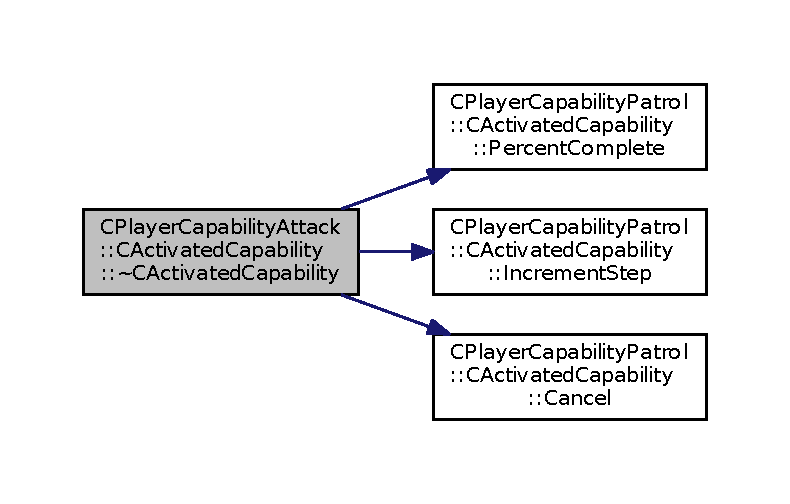
\includegraphics[width=350pt]{classCPlayerCapabilityAttack_1_1CActivatedCapability_a8524b57d63ce6e899630ef56326be98b_cgraph}
\end{center}
\end{figure}


\subsection{Member Function Documentation}
\hypertarget{classCPlayerCapabilityAttack_1_1CActivatedCapability_a0796fbda8a35b60a2320becfdf2b5c13}{}\label{classCPlayerCapabilityAttack_1_1CActivatedCapability_a0796fbda8a35b60a2320becfdf2b5c13} 
\index{C\+Player\+Capability\+Attack\+::\+C\+Activated\+Capability@{C\+Player\+Capability\+Attack\+::\+C\+Activated\+Capability}!Cancel@{Cancel}}
\index{Cancel@{Cancel}!C\+Player\+Capability\+Attack\+::\+C\+Activated\+Capability@{C\+Player\+Capability\+Attack\+::\+C\+Activated\+Capability}}
\subsubsection{\texorpdfstring{Cancel()}{Cancel()}}
{\footnotesize\ttfamily void C\+Player\+Capability\+Attack\+::\+C\+Activated\+Capability\+::\+Cancel (\begin{DoxyParamCaption}{ }\end{DoxyParamCaption})\hspace{0.3cm}{\ttfamily [virtual]}}



Implements \hyperlink{classCActivatedPlayerCapability_a5cde83be468e262ad054d81e28684a81}{C\+Activated\+Player\+Capability}.



Definition at line 741 of file Basic\+Capabilities.\+cpp.



References C\+Activated\+Player\+Capability\+::\+D\+Actor.



Referenced by C\+Player\+Capability\+Repair\+::\+C\+Activated\+Capability\+::$\sim$\+C\+Activated\+Capability().


\begin{DoxyCode}
741                                                         \{
742 
743     \hyperlink{classCActivatedPlayerCapability_a54ca944b47bff2718330639941d402b0}{DActor}->PopCommand();
744 \}
\end{DoxyCode}
Here is the caller graph for this function\+:\nopagebreak
\begin{figure}[H]
\begin{center}
\leavevmode
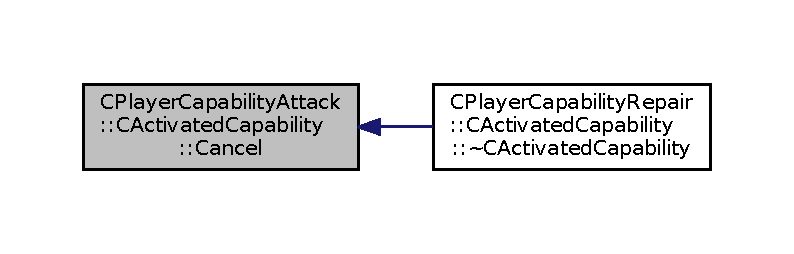
\includegraphics[width=350pt]{classCPlayerCapabilityAttack_1_1CActivatedCapability_a0796fbda8a35b60a2320becfdf2b5c13_icgraph}
\end{center}
\end{figure}
\hypertarget{classCPlayerCapabilityAttack_1_1CActivatedCapability_a6b772cbd6be96fbd9bf88380b143856c}{}\label{classCPlayerCapabilityAttack_1_1CActivatedCapability_a6b772cbd6be96fbd9bf88380b143856c} 
\index{C\+Player\+Capability\+Attack\+::\+C\+Activated\+Capability@{C\+Player\+Capability\+Attack\+::\+C\+Activated\+Capability}!Increment\+Step@{Increment\+Step}}
\index{Increment\+Step@{Increment\+Step}!C\+Player\+Capability\+Attack\+::\+C\+Activated\+Capability@{C\+Player\+Capability\+Attack\+::\+C\+Activated\+Capability}}
\subsubsection{\texorpdfstring{Increment\+Step()}{IncrementStep()}}
{\footnotesize\ttfamily bool C\+Player\+Capability\+Attack\+::\+C\+Activated\+Capability\+::\+Increment\+Step (\begin{DoxyParamCaption}{ }\end{DoxyParamCaption})\hspace{0.3cm}{\ttfamily [virtual]}}



Implements \hyperlink{classCActivatedPlayerCapability_a943b5999a57504399293250382c0ec6a}{C\+Activated\+Player\+Capability}.



Definition at line 720 of file Basic\+Capabilities.\+cpp.



References aa\+Attack, aa\+Walk, S\+Asset\+Command\+::\+D\+Action, C\+Activated\+Player\+Capability\+::\+D\+Actor, S\+Game\+Event\+::\+D\+Asset, S\+Asset\+Command\+::\+D\+Asset\+Target, d\+Max, C\+Activated\+Player\+Capability\+::\+D\+Player\+Data, C\+Activated\+Player\+Capability\+::\+D\+Target, S\+Game\+Event\+::\+D\+Type, and et\+Acknowledge.



Referenced by C\+Player\+Capability\+Repair\+::\+C\+Activated\+Capability\+::$\sim$\+C\+Activated\+Capability().


\begin{DoxyCode}
720                                                                \{
721     \hyperlink{structSAssetCommand}{SAssetCommand} AssetCommand;
722     \hyperlink{structSGameEvent}{SGameEvent} TempEvent;
723     
724     TempEvent.\hyperlink{structSGameEvent_afa10562e243f4ac2b473b655cc58fee7}{DType} = \hyperlink{GameModel_8h_abfcf510bafec7c6429906a6ecaac656da9b68fc38f3ca4002cd7a3ec3cc07a612}{etAcknowledge};
725     TempEvent.\hyperlink{structSGameEvent_a40c85eeac83b96887b7449c9bdc5d624}{DAsset} = \hyperlink{classCActivatedPlayerCapability_a54ca944b47bff2718330639941d402b0}{DActor};
726     \hyperlink{classCActivatedPlayerCapability_a9bf27c322a73f4b11c8183cc1973c3d8}{DPlayerData}->AddGameEvent(TempEvent);
727     
728     AssetCommand.\hyperlink{structSAssetCommand_a8edd3b3d59a76d5514ba403bc8076a75}{DAction} = \hyperlink{GameDataTypes_8h_ab47668e651a3032cfb9c40ea2d60d670a948eefd20b9e43d3b4cfcf613774716d}{aaAttack};
729     AssetCommand.\hyperlink{structSAssetCommand_a3d9b43f6e59c386c48c41a65448a0c39}{DAssetTarget} = \hyperlink{classCActivatedPlayerCapability_a8a1cf50b6501bcfd55af0c935828e395}{DTarget};
730     \hyperlink{classCActivatedPlayerCapability_a54ca944b47bff2718330639941d402b0}{DActor}->ClearCommand();
731     \hyperlink{classCActivatedPlayerCapability_a54ca944b47bff2718330639941d402b0}{DActor}->PushCommand(AssetCommand);
732     
733     AssetCommand.\hyperlink{structSAssetCommand_a8edd3b3d59a76d5514ba403bc8076a75}{DAction} = \hyperlink{GameDataTypes_8h_ab47668e651a3032cfb9c40ea2d60d670a60ca9010aa62b73c1aab838ff4bf7276}{aaWalk};
734     \textcolor{keywordflow}{if}(!\hyperlink{classCActivatedPlayerCapability_a54ca944b47bff2718330639941d402b0}{DActor}->TileAligned())\{
735         \hyperlink{classCActivatedPlayerCapability_a54ca944b47bff2718330639941d402b0}{DActor}->Direction((\hyperlink{GameDataTypes_8h_acb2b033915f6659a71a38b5aa6e4eb42}{EDirection})((\hyperlink{classCActivatedPlayerCapability_a54ca944b47bff2718330639941d402b0}{DActor}->Position().TileOctant() + 
      \hyperlink{GameDataTypes_8h_acb2b033915f6659a71a38b5aa6e4eb42af6546049275557ce0ade2ceee042a319}{dMax}/2) % \hyperlink{GameDataTypes_8h_acb2b033915f6659a71a38b5aa6e4eb42af6546049275557ce0ade2ceee042a319}{dMax}));
736     \}
737     \hyperlink{classCActivatedPlayerCapability_a54ca944b47bff2718330639941d402b0}{DActor}->PushCommand(AssetCommand);
738     \textcolor{keywordflow}{return} \textcolor{keyword}{true};
739 \}
\end{DoxyCode}
Here is the caller graph for this function\+:\nopagebreak
\begin{figure}[H]
\begin{center}
\leavevmode
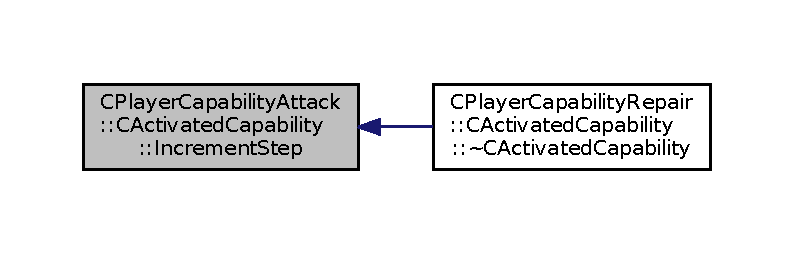
\includegraphics[width=350pt]{classCPlayerCapabilityAttack_1_1CActivatedCapability_a6b772cbd6be96fbd9bf88380b143856c_icgraph}
\end{center}
\end{figure}
\hypertarget{classCPlayerCapabilityAttack_1_1CActivatedCapability_a75866109b62de0522622b03137461519}{}\label{classCPlayerCapabilityAttack_1_1CActivatedCapability_a75866109b62de0522622b03137461519} 
\index{C\+Player\+Capability\+Attack\+::\+C\+Activated\+Capability@{C\+Player\+Capability\+Attack\+::\+C\+Activated\+Capability}!Percent\+Complete@{Percent\+Complete}}
\index{Percent\+Complete@{Percent\+Complete}!C\+Player\+Capability\+Attack\+::\+C\+Activated\+Capability@{C\+Player\+Capability\+Attack\+::\+C\+Activated\+Capability}}
\subsubsection{\texorpdfstring{Percent\+Complete()}{PercentComplete()}}
{\footnotesize\ttfamily int C\+Player\+Capability\+Attack\+::\+C\+Activated\+Capability\+::\+Percent\+Complete (\begin{DoxyParamCaption}\item[{int}]{max }\end{DoxyParamCaption})\hspace{0.3cm}{\ttfamily [virtual]}}



Implements \hyperlink{classCActivatedPlayerCapability_a405dc6076058006a4f801727de4cfe4d}{C\+Activated\+Player\+Capability}.



Definition at line 716 of file Basic\+Capabilities.\+cpp.



Referenced by C\+Player\+Capability\+Repair\+::\+C\+Activated\+Capability\+::$\sim$\+C\+Activated\+Capability().


\begin{DoxyCode}
716                                                                        \{
717     \textcolor{keywordflow}{return} 0;
718 \}
\end{DoxyCode}
Here is the caller graph for this function\+:\nopagebreak
\begin{figure}[H]
\begin{center}
\leavevmode
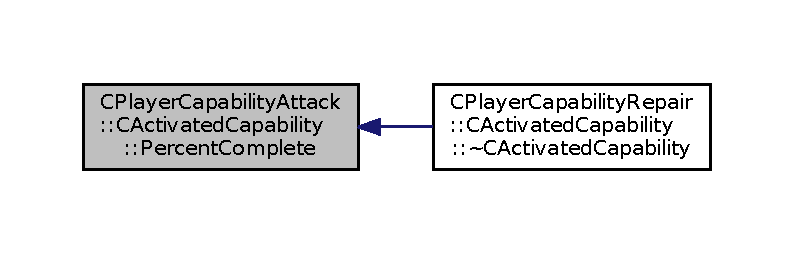
\includegraphics[width=350pt]{classCPlayerCapabilityAttack_1_1CActivatedCapability_a75866109b62de0522622b03137461519_icgraph}
\end{center}
\end{figure}


The documentation for this class was generated from the following file\+:\begin{DoxyCompactItemize}
\item 
src/\hyperlink{BasicCapabilities_8cpp}{Basic\+Capabilities.\+cpp}\end{DoxyCompactItemize}

\hypertarget{classCPlayerCapabilityRepair_1_1CActivatedCapability}{}\section{C\+Player\+Capability\+Repair\+:\+:C\+Activated\+Capability Class Reference}
\label{classCPlayerCapabilityRepair_1_1CActivatedCapability}\index{C\+Player\+Capability\+Repair\+::\+C\+Activated\+Capability@{C\+Player\+Capability\+Repair\+::\+C\+Activated\+Capability}}


Inheritance diagram for C\+Player\+Capability\+Repair\+:\+:C\+Activated\+Capability\+:
\nopagebreak
\begin{figure}[H]
\begin{center}
\leavevmode
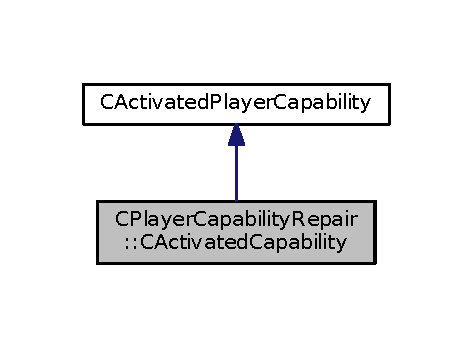
\includegraphics[width=227pt]{classCPlayerCapabilityRepair_1_1CActivatedCapability__inherit__graph}
\end{center}
\end{figure}


Collaboration diagram for C\+Player\+Capability\+Repair\+:\+:C\+Activated\+Capability\+:
\nopagebreak
\begin{figure}[H]
\begin{center}
\leavevmode
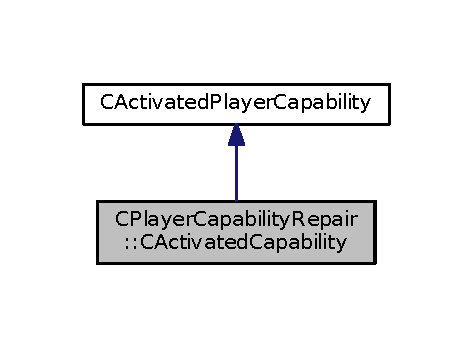
\includegraphics[width=227pt]{classCPlayerCapabilityRepair_1_1CActivatedCapability__coll__graph}
\end{center}
\end{figure}
\subsection*{Public Member Functions}
\begin{DoxyCompactItemize}
\item 
\hyperlink{classCPlayerCapabilityRepair_1_1CActivatedCapability_a6a30357fc9e7f752872c434027e3894e}{C\+Activated\+Capability} (std\+::shared\+\_\+ptr$<$ \hyperlink{classCPlayerAsset}{C\+Player\+Asset} $>$ actor, std\+::shared\+\_\+ptr$<$ \hyperlink{classCPlayerData}{C\+Player\+Data} $>$ playerdata, std\+::shared\+\_\+ptr$<$ \hyperlink{classCPlayerAsset}{C\+Player\+Asset} $>$ target)
\item 
virtual \hyperlink{classCPlayerCapabilityRepair_1_1CActivatedCapability_ae4c632553e0898f8501a3f6bcd71cfaa}{$\sim$\+C\+Activated\+Capability} ()
\item 
int \hyperlink{classCPlayerCapabilityRepair_1_1CActivatedCapability_a88276fec60e08b56daecfd14b36fe888}{Percent\+Complete} (int max)
\item 
bool \hyperlink{classCPlayerCapabilityRepair_1_1CActivatedCapability_a5b5b42dbbda50b29e9f917df3cb0f650}{Increment\+Step} ()
\item 
void \hyperlink{classCPlayerCapabilityRepair_1_1CActivatedCapability_a719cee3446291470987f504739f63215}{Cancel} ()
\end{DoxyCompactItemize}
\subsection*{Additional Inherited Members}


\subsection{Detailed Description}


Definition at line 754 of file Basic\+Capabilities.\+cpp.



\subsection{Constructor \& Destructor Documentation}
\hypertarget{classCPlayerCapabilityRepair_1_1CActivatedCapability_a6a30357fc9e7f752872c434027e3894e}{}\label{classCPlayerCapabilityRepair_1_1CActivatedCapability_a6a30357fc9e7f752872c434027e3894e} 
\index{C\+Player\+Capability\+Repair\+::\+C\+Activated\+Capability@{C\+Player\+Capability\+Repair\+::\+C\+Activated\+Capability}!C\+Activated\+Capability@{C\+Activated\+Capability}}
\index{C\+Activated\+Capability@{C\+Activated\+Capability}!C\+Player\+Capability\+Repair\+::\+C\+Activated\+Capability@{C\+Player\+Capability\+Repair\+::\+C\+Activated\+Capability}}
\subsubsection{\texorpdfstring{C\+Activated\+Capability()}{CActivatedCapability()}}
{\footnotesize\ttfamily C\+Player\+Capability\+Repair\+::\+C\+Activated\+Capability\+::\+C\+Activated\+Capability (\begin{DoxyParamCaption}\item[{std\+::shared\+\_\+ptr$<$ \hyperlink{classCPlayerAsset}{C\+Player\+Asset} $>$}]{actor,  }\item[{std\+::shared\+\_\+ptr$<$ \hyperlink{classCPlayerData}{C\+Player\+Data} $>$}]{playerdata,  }\item[{std\+::shared\+\_\+ptr$<$ \hyperlink{classCPlayerAsset}{C\+Player\+Asset} $>$}]{target }\end{DoxyParamCaption})}



Definition at line 816 of file Basic\+Capabilities.\+cpp.


\begin{DoxyCode}
816                                                                                                            
                                                                               :
817 \hyperlink{classCActivatedPlayerCapability_a1ece00ffb6a7b925c84dd94a7407a0d1}{CActivatedPlayerCapability}(actor, playerdata, target)\{
818 
819 \}
\end{DoxyCode}
\hypertarget{classCPlayerCapabilityRepair_1_1CActivatedCapability_ae4c632553e0898f8501a3f6bcd71cfaa}{}\label{classCPlayerCapabilityRepair_1_1CActivatedCapability_ae4c632553e0898f8501a3f6bcd71cfaa} 
\index{C\+Player\+Capability\+Repair\+::\+C\+Activated\+Capability@{C\+Player\+Capability\+Repair\+::\+C\+Activated\+Capability}!````~C\+Activated\+Capability@{$\sim$\+C\+Activated\+Capability}}
\index{````~C\+Activated\+Capability@{$\sim$\+C\+Activated\+Capability}!C\+Player\+Capability\+Repair\+::\+C\+Activated\+Capability@{C\+Player\+Capability\+Repair\+::\+C\+Activated\+Capability}}
\subsubsection{\texorpdfstring{$\sim$\+C\+Activated\+Capability()}{~CActivatedCapability()}}
{\footnotesize\ttfamily virtual C\+Player\+Capability\+Repair\+::\+C\+Activated\+Capability\+::$\sim$\+C\+Activated\+Capability (\begin{DoxyParamCaption}{ }\end{DoxyParamCaption})\hspace{0.3cm}{\ttfamily [inline]}, {\ttfamily [virtual]}}



Definition at line 759 of file Basic\+Capabilities.\+cpp.


\begin{DoxyCode}
759 \{\};
\end{DoxyCode}
Here is the call graph for this function\+:
\nopagebreak
\begin{figure}[H]
\begin{center}
\leavevmode
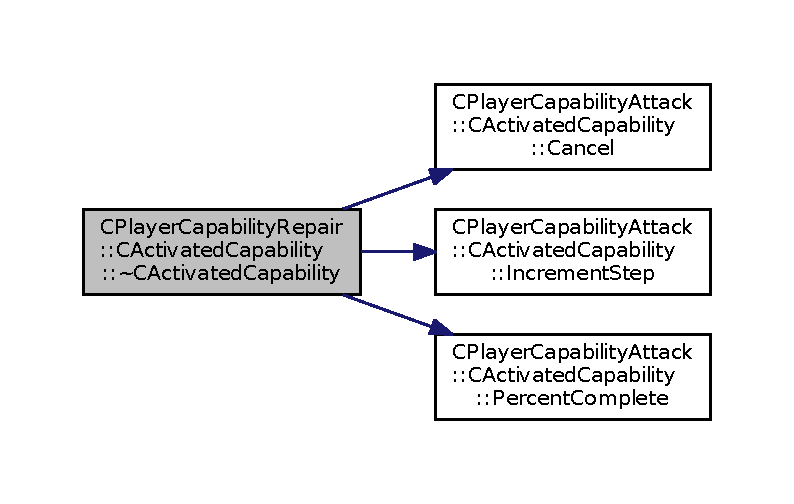
\includegraphics[width=350pt]{classCPlayerCapabilityRepair_1_1CActivatedCapability_ae4c632553e0898f8501a3f6bcd71cfaa_cgraph}
\end{center}
\end{figure}


\subsection{Member Function Documentation}
\hypertarget{classCPlayerCapabilityRepair_1_1CActivatedCapability_a719cee3446291470987f504739f63215}{}\label{classCPlayerCapabilityRepair_1_1CActivatedCapability_a719cee3446291470987f504739f63215} 
\index{C\+Player\+Capability\+Repair\+::\+C\+Activated\+Capability@{C\+Player\+Capability\+Repair\+::\+C\+Activated\+Capability}!Cancel@{Cancel}}
\index{Cancel@{Cancel}!C\+Player\+Capability\+Repair\+::\+C\+Activated\+Capability@{C\+Player\+Capability\+Repair\+::\+C\+Activated\+Capability}}
\subsubsection{\texorpdfstring{Cancel()}{Cancel()}}
{\footnotesize\ttfamily void C\+Player\+Capability\+Repair\+::\+C\+Activated\+Capability\+::\+Cancel (\begin{DoxyParamCaption}{ }\end{DoxyParamCaption})\hspace{0.3cm}{\ttfamily [virtual]}}



Implements \hyperlink{classCActivatedPlayerCapability_a5cde83be468e262ad054d81e28684a81}{C\+Activated\+Player\+Capability}.



Definition at line 847 of file Basic\+Capabilities.\+cpp.


\begin{DoxyCode}
847                                                         \{
848 
849     \hyperlink{classCActivatedPlayerCapability_a54ca944b47bff2718330639941d402b0}{DActor}->PopCommand();
850 \}
\end{DoxyCode}
\hypertarget{classCPlayerCapabilityRepair_1_1CActivatedCapability_a5b5b42dbbda50b29e9f917df3cb0f650}{}\label{classCPlayerCapabilityRepair_1_1CActivatedCapability_a5b5b42dbbda50b29e9f917df3cb0f650} 
\index{C\+Player\+Capability\+Repair\+::\+C\+Activated\+Capability@{C\+Player\+Capability\+Repair\+::\+C\+Activated\+Capability}!Increment\+Step@{Increment\+Step}}
\index{Increment\+Step@{Increment\+Step}!C\+Player\+Capability\+Repair\+::\+C\+Activated\+Capability@{C\+Player\+Capability\+Repair\+::\+C\+Activated\+Capability}}
\subsubsection{\texorpdfstring{Increment\+Step()}{IncrementStep()}}
{\footnotesize\ttfamily bool C\+Player\+Capability\+Repair\+::\+C\+Activated\+Capability\+::\+Increment\+Step (\begin{DoxyParamCaption}{ }\end{DoxyParamCaption})\hspace{0.3cm}{\ttfamily [virtual]}}



Implements \hyperlink{classCActivatedPlayerCapability_a943b5999a57504399293250382c0ec6a}{C\+Activated\+Player\+Capability}.



Definition at line 826 of file Basic\+Capabilities.\+cpp.


\begin{DoxyCode}
826                                                                \{
827     \hyperlink{structSAssetCommand}{SAssetCommand} AssetCommand;
828     \hyperlink{structSGameEvent}{SGameEvent} TempEvent;
829     
830     TempEvent.\hyperlink{structSGameEvent_afa10562e243f4ac2b473b655cc58fee7}{DType} = \hyperlink{GameModel_8h_abfcf510bafec7c6429906a6ecaac656da9b68fc38f3ca4002cd7a3ec3cc07a612}{etAcknowledge};
831     TempEvent.\hyperlink{structSGameEvent_a40c85eeac83b96887b7449c9bdc5d624}{DAsset} = \hyperlink{classCActivatedPlayerCapability_a54ca944b47bff2718330639941d402b0}{DActor};
832     \hyperlink{classCActivatedPlayerCapability_a9bf27c322a73f4b11c8183cc1973c3d8}{DPlayerData}->AddGameEvent(TempEvent);
833     
834     AssetCommand.\hyperlink{structSAssetCommand_a8edd3b3d59a76d5514ba403bc8076a75}{DAction} = \hyperlink{GameDataTypes_8h_ab47668e651a3032cfb9c40ea2d60d670a85399def907073717f41849c8f09eba5}{aaRepair};
835     AssetCommand.\hyperlink{structSAssetCommand_a3d9b43f6e59c386c48c41a65448a0c39}{DAssetTarget} = \hyperlink{classCActivatedPlayerCapability_a8a1cf50b6501bcfd55af0c935828e395}{DTarget};
836     \hyperlink{classCActivatedPlayerCapability_a54ca944b47bff2718330639941d402b0}{DActor}->ClearCommand();
837     \hyperlink{classCActivatedPlayerCapability_a54ca944b47bff2718330639941d402b0}{DActor}->PushCommand(AssetCommand);
838     
839     AssetCommand.\hyperlink{structSAssetCommand_a8edd3b3d59a76d5514ba403bc8076a75}{DAction} = \hyperlink{GameDataTypes_8h_ab47668e651a3032cfb9c40ea2d60d670a60ca9010aa62b73c1aab838ff4bf7276}{aaWalk};
840     \textcolor{keywordflow}{if}(!\hyperlink{classCActivatedPlayerCapability_a54ca944b47bff2718330639941d402b0}{DActor}->TileAligned())\{
841         \hyperlink{classCActivatedPlayerCapability_a54ca944b47bff2718330639941d402b0}{DActor}->Direction((\hyperlink{GameDataTypes_8h_acb2b033915f6659a71a38b5aa6e4eb42}{EDirection})((\hyperlink{classCActivatedPlayerCapability_a54ca944b47bff2718330639941d402b0}{DActor}->Position().TileOctant() + 
      \hyperlink{GameDataTypes_8h_acb2b033915f6659a71a38b5aa6e4eb42af6546049275557ce0ade2ceee042a319}{dMax}/2) % \hyperlink{GameDataTypes_8h_acb2b033915f6659a71a38b5aa6e4eb42af6546049275557ce0ade2ceee042a319}{dMax}));
842     \}
843     \hyperlink{classCActivatedPlayerCapability_a54ca944b47bff2718330639941d402b0}{DActor}->PushCommand(AssetCommand);
844     \textcolor{keywordflow}{return} \textcolor{keyword}{true};
845 \}
\end{DoxyCode}
\hypertarget{classCPlayerCapabilityRepair_1_1CActivatedCapability_a88276fec60e08b56daecfd14b36fe888}{}\label{classCPlayerCapabilityRepair_1_1CActivatedCapability_a88276fec60e08b56daecfd14b36fe888} 
\index{C\+Player\+Capability\+Repair\+::\+C\+Activated\+Capability@{C\+Player\+Capability\+Repair\+::\+C\+Activated\+Capability}!Percent\+Complete@{Percent\+Complete}}
\index{Percent\+Complete@{Percent\+Complete}!C\+Player\+Capability\+Repair\+::\+C\+Activated\+Capability@{C\+Player\+Capability\+Repair\+::\+C\+Activated\+Capability}}
\subsubsection{\texorpdfstring{Percent\+Complete()}{PercentComplete()}}
{\footnotesize\ttfamily int C\+Player\+Capability\+Repair\+::\+C\+Activated\+Capability\+::\+Percent\+Complete (\begin{DoxyParamCaption}\item[{int}]{max }\end{DoxyParamCaption})\hspace{0.3cm}{\ttfamily [virtual]}}



Implements \hyperlink{classCActivatedPlayerCapability_a405dc6076058006a4f801727de4cfe4d}{C\+Activated\+Player\+Capability}.



Definition at line 822 of file Basic\+Capabilities.\+cpp.


\begin{DoxyCode}
822                                                                        \{
823     \textcolor{keywordflow}{return} 0;
824 \}
\end{DoxyCode}


The documentation for this class was generated from the following file\+:\begin{DoxyCompactItemize}
\item 
src/\hyperlink{BasicCapabilities_8cpp}{Basic\+Capabilities.\+cpp}\end{DoxyCompactItemize}

\hypertarget{classCPlayerCapabilityBuildNormal_1_1CActivatedCapability}{}\section{C\+Player\+Capability\+Build\+Normal\+:\+:C\+Activated\+Capability Class Reference}
\label{classCPlayerCapabilityBuildNormal_1_1CActivatedCapability}\index{C\+Player\+Capability\+Build\+Normal\+::\+C\+Activated\+Capability@{C\+Player\+Capability\+Build\+Normal\+::\+C\+Activated\+Capability}}


Inheritance diagram for C\+Player\+Capability\+Build\+Normal\+:\+:C\+Activated\+Capability\+:\nopagebreak
\begin{figure}[H]
\begin{center}
\leavevmode
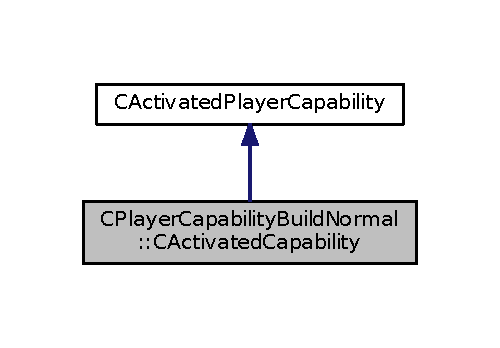
\includegraphics[width=240pt]{classCPlayerCapabilityBuildNormal_1_1CActivatedCapability__inherit__graph}
\end{center}
\end{figure}


Collaboration diagram for C\+Player\+Capability\+Build\+Normal\+:\+:C\+Activated\+Capability\+:\nopagebreak
\begin{figure}[H]
\begin{center}
\leavevmode
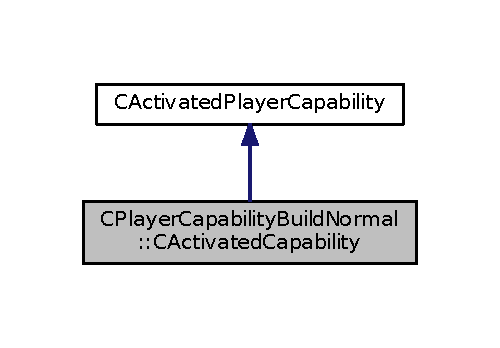
\includegraphics[width=240pt]{classCPlayerCapabilityBuildNormal_1_1CActivatedCapability__coll__graph}
\end{center}
\end{figure}
\subsection*{Public Member Functions}
\begin{DoxyCompactItemize}
\item 
\hyperlink{classCPlayerCapabilityBuildNormal_1_1CActivatedCapability_a33a64e3a38d5e2e3c705d3350780a17a}{C\+Activated\+Capability} (std\+::shared\+\_\+ptr$<$ \hyperlink{classCPlayerAsset}{C\+Player\+Asset} $>$ actor, std\+::shared\+\_\+ptr$<$ \hyperlink{classCPlayerData}{C\+Player\+Data} $>$ playerdata, std\+::shared\+\_\+ptr$<$ \hyperlink{classCPlayerAsset}{C\+Player\+Asset} $>$ target, int lumber, int gold, int steps)
\item 
virtual \hyperlink{classCPlayerCapabilityBuildNormal_1_1CActivatedCapability_a68b7fdfbb1f47ac01fafc46acafa22b5}{$\sim$\+C\+Activated\+Capability} ()
\item 
int \hyperlink{classCPlayerCapabilityBuildNormal_1_1CActivatedCapability_a40bf27f9dfe88ad17a51ebb12c078568}{Percent\+Complete} (int max)
\item 
bool \hyperlink{classCPlayerCapabilityBuildNormal_1_1CActivatedCapability_a19b9ba979e8deebcb2b7e4225af47d2e}{Increment\+Step} ()
\item 
void \hyperlink{classCPlayerCapabilityBuildNormal_1_1CActivatedCapability_a7cc74f98f4071edfa75395d02d897fef}{Cancel} ()
\end{DoxyCompactItemize}
\subsection*{Protected Attributes}
\begin{DoxyCompactItemize}
\item 
int \hyperlink{classCPlayerCapabilityBuildNormal_1_1CActivatedCapability_ab6e20b5de47d912d9e38c2e8395f1ad1}{D\+Current\+Step}
\item 
int \hyperlink{classCPlayerCapabilityBuildNormal_1_1CActivatedCapability_a50e3103232671fc231348e7a86c1fed5}{D\+Total\+Steps}
\item 
int \hyperlink{classCPlayerCapabilityBuildNormal_1_1CActivatedCapability_acc7750973121c2b8ada035bca9264229}{D\+Lumber}
\item 
int \hyperlink{classCPlayerCapabilityBuildNormal_1_1CActivatedCapability_a8997bc10da71f5df340096cd0d717d84}{D\+Gold}
\end{DoxyCompactItemize}


\subsection{Detailed Description}


Definition at line 29 of file Build\+Capabilities.\+cpp.



\subsection{Constructor \& Destructor Documentation}
\hypertarget{classCPlayerCapabilityBuildNormal_1_1CActivatedCapability_a33a64e3a38d5e2e3c705d3350780a17a}{}\label{classCPlayerCapabilityBuildNormal_1_1CActivatedCapability_a33a64e3a38d5e2e3c705d3350780a17a} 
\index{C\+Player\+Capability\+Build\+Normal\+::\+C\+Activated\+Capability@{C\+Player\+Capability\+Build\+Normal\+::\+C\+Activated\+Capability}!C\+Activated\+Capability@{C\+Activated\+Capability}}
\index{C\+Activated\+Capability@{C\+Activated\+Capability}!C\+Player\+Capability\+Build\+Normal\+::\+C\+Activated\+Capability@{C\+Player\+Capability\+Build\+Normal\+::\+C\+Activated\+Capability}}
\subsubsection{\texorpdfstring{C\+Activated\+Capability()}{CActivatedCapability()}}
{\footnotesize\ttfamily C\+Player\+Capability\+Build\+Normal\+::\+C\+Activated\+Capability\+::\+C\+Activated\+Capability (\begin{DoxyParamCaption}\item[{std\+::shared\+\_\+ptr$<$ \hyperlink{classCPlayerAsset}{C\+Player\+Asset} $>$}]{actor,  }\item[{std\+::shared\+\_\+ptr$<$ \hyperlink{classCPlayerData}{C\+Player\+Data} $>$}]{playerdata,  }\item[{std\+::shared\+\_\+ptr$<$ \hyperlink{classCPlayerAsset}{C\+Player\+Asset} $>$}]{target,  }\item[{int}]{lumber,  }\item[{int}]{gold,  }\item[{int}]{steps }\end{DoxyParamCaption})}



Definition at line 144 of file Build\+Capabilities.\+cpp.


\begin{DoxyCode}
144                                                                                                            
                                                                                                                  
         :
145 \hyperlink{classCActivatedPlayerCapability_a1ece00ffb6a7b925c84dd94a7407a0d1}{CActivatedPlayerCapability}(actor, playerdata, target)\{
146     \hyperlink{structSAssetCommand}{SAssetCommand} AssetCommand;
147     
148     \hyperlink{classCPlayerCapabilityBuildNormal_1_1CActivatedCapability_ab6e20b5de47d912d9e38c2e8395f1ad1}{DCurrentStep} = 0;
149     \hyperlink{classCPlayerCapabilityBuildNormal_1_1CActivatedCapability_a50e3103232671fc231348e7a86c1fed5}{DTotalSteps} = steps;
150     \hyperlink{classCPlayerCapabilityBuildNormal_1_1CActivatedCapability_acc7750973121c2b8ada035bca9264229}{DLumber} = lumber;
151     \hyperlink{classCPlayerCapabilityBuildNormal_1_1CActivatedCapability_a8997bc10da71f5df340096cd0d717d84}{DGold} = gold;
152     \hyperlink{classCActivatedPlayerCapability_a9bf27c322a73f4b11c8183cc1973c3d8}{DPlayerData}->DecrementLumber(\hyperlink{classCPlayerCapabilityBuildNormal_1_1CActivatedCapability_acc7750973121c2b8ada035bca9264229}{DLumber});
153     \hyperlink{classCActivatedPlayerCapability_a9bf27c322a73f4b11c8183cc1973c3d8}{DPlayerData}->DecrementGold(\hyperlink{classCPlayerCapabilityBuildNormal_1_1CActivatedCapability_a8997bc10da71f5df340096cd0d717d84}{DGold});
154     AssetCommand.\hyperlink{structSAssetCommand_a8edd3b3d59a76d5514ba403bc8076a75}{DAction} = \hyperlink{GameDataTypes_8h_ab47668e651a3032cfb9c40ea2d60d670a7ef6b863f66dd7dcc95a199cd758ae1d}{aaConstruct};
155     AssetCommand.\hyperlink{structSAssetCommand_a3d9b43f6e59c386c48c41a65448a0c39}{DAssetTarget} = \hyperlink{classCActivatedPlayerCapability_a54ca944b47bff2718330639941d402b0}{DActor};
156     \hyperlink{classCActivatedPlayerCapability_a8a1cf50b6501bcfd55af0c935828e395}{DTarget}->PushCommand(AssetCommand);
157 \}
\end{DoxyCode}
\hypertarget{classCPlayerCapabilityBuildNormal_1_1CActivatedCapability_a68b7fdfbb1f47ac01fafc46acafa22b5}{}\label{classCPlayerCapabilityBuildNormal_1_1CActivatedCapability_a68b7fdfbb1f47ac01fafc46acafa22b5} 
\index{C\+Player\+Capability\+Build\+Normal\+::\+C\+Activated\+Capability@{C\+Player\+Capability\+Build\+Normal\+::\+C\+Activated\+Capability}!````~C\+Activated\+Capability@{$\sim$\+C\+Activated\+Capability}}
\index{````~C\+Activated\+Capability@{$\sim$\+C\+Activated\+Capability}!C\+Player\+Capability\+Build\+Normal\+::\+C\+Activated\+Capability@{C\+Player\+Capability\+Build\+Normal\+::\+C\+Activated\+Capability}}
\subsubsection{\texorpdfstring{$\sim$\+C\+Activated\+Capability()}{~CActivatedCapability()}}
{\footnotesize\ttfamily virtual C\+Player\+Capability\+Build\+Normal\+::\+C\+Activated\+Capability\+::$\sim$\+C\+Activated\+Capability (\begin{DoxyParamCaption}{ }\end{DoxyParamCaption})\hspace{0.3cm}{\ttfamily [inline]}, {\ttfamily [virtual]}}



Definition at line 38 of file Build\+Capabilities.\+cpp.


\begin{DoxyCode}
38 \{\};
\end{DoxyCode}


\subsection{Member Function Documentation}
\hypertarget{classCPlayerCapabilityBuildNormal_1_1CActivatedCapability_a7cc74f98f4071edfa75395d02d897fef}{}\label{classCPlayerCapabilityBuildNormal_1_1CActivatedCapability_a7cc74f98f4071edfa75395d02d897fef} 
\index{C\+Player\+Capability\+Build\+Normal\+::\+C\+Activated\+Capability@{C\+Player\+Capability\+Build\+Normal\+::\+C\+Activated\+Capability}!Cancel@{Cancel}}
\index{Cancel@{Cancel}!C\+Player\+Capability\+Build\+Normal\+::\+C\+Activated\+Capability@{C\+Player\+Capability\+Build\+Normal\+::\+C\+Activated\+Capability}}
\subsubsection{\texorpdfstring{Cancel()}{Cancel()}}
{\footnotesize\ttfamily void C\+Player\+Capability\+Build\+Normal\+::\+C\+Activated\+Capability\+::\+Cancel (\begin{DoxyParamCaption}{ }\end{DoxyParamCaption})\hspace{0.3cm}{\ttfamily [virtual]}}



Implements \hyperlink{classCActivatedPlayerCapability_a5cde83be468e262ad054d81e28684a81}{C\+Activated\+Player\+Capability}.



Definition at line 192 of file Build\+Capabilities.\+cpp.


\begin{DoxyCode}
192                                                              \{
193     \hyperlink{classCActivatedPlayerCapability_a9bf27c322a73f4b11c8183cc1973c3d8}{DPlayerData}->IncrementLumber(\hyperlink{classCPlayerCapabilityBuildNormal_1_1CActivatedCapability_acc7750973121c2b8ada035bca9264229}{DLumber});
194     \hyperlink{classCActivatedPlayerCapability_a9bf27c322a73f4b11c8183cc1973c3d8}{DPlayerData}->IncrementGold(\hyperlink{classCPlayerCapabilityBuildNormal_1_1CActivatedCapability_a8997bc10da71f5df340096cd0d717d84}{DGold});
195     \hyperlink{classCActivatedPlayerCapability_a9bf27c322a73f4b11c8183cc1973c3d8}{DPlayerData}->DeleteAsset(\hyperlink{classCActivatedPlayerCapability_a8a1cf50b6501bcfd55af0c935828e395}{DTarget});
196     \hyperlink{classCActivatedPlayerCapability_a54ca944b47bff2718330639941d402b0}{DActor}->PopCommand();
197 \}
\end{DoxyCode}
\hypertarget{classCPlayerCapabilityBuildNormal_1_1CActivatedCapability_a19b9ba979e8deebcb2b7e4225af47d2e}{}\label{classCPlayerCapabilityBuildNormal_1_1CActivatedCapability_a19b9ba979e8deebcb2b7e4225af47d2e} 
\index{C\+Player\+Capability\+Build\+Normal\+::\+C\+Activated\+Capability@{C\+Player\+Capability\+Build\+Normal\+::\+C\+Activated\+Capability}!Increment\+Step@{Increment\+Step}}
\index{Increment\+Step@{Increment\+Step}!C\+Player\+Capability\+Build\+Normal\+::\+C\+Activated\+Capability@{C\+Player\+Capability\+Build\+Normal\+::\+C\+Activated\+Capability}}
\subsubsection{\texorpdfstring{Increment\+Step()}{IncrementStep()}}
{\footnotesize\ttfamily bool C\+Player\+Capability\+Build\+Normal\+::\+C\+Activated\+Capability\+::\+Increment\+Step (\begin{DoxyParamCaption}{ }\end{DoxyParamCaption})\hspace{0.3cm}{\ttfamily [virtual]}}



Implements \hyperlink{classCActivatedPlayerCapability_a943b5999a57504399293250382c0ec6a}{C\+Activated\+Player\+Capability}.



Definition at line 164 of file Build\+Capabilities.\+cpp.


\begin{DoxyCode}
164                                                                     \{
165     \textcolor{keywordtype}{int} AddHitPoints = (\hyperlink{classCActivatedPlayerCapability_a8a1cf50b6501bcfd55af0c935828e395}{DTarget}->MaxHitPoints() * (\hyperlink{classCPlayerCapabilityBuildNormal_1_1CActivatedCapability_ab6e20b5de47d912d9e38c2e8395f1ad1}{DCurrentStep} + 1) / 
      \hyperlink{classCPlayerCapabilityBuildNormal_1_1CActivatedCapability_a50e3103232671fc231348e7a86c1fed5}{DTotalSteps}) - (\hyperlink{classCActivatedPlayerCapability_a8a1cf50b6501bcfd55af0c935828e395}{DTarget}->MaxHitPoints() * \hyperlink{classCPlayerCapabilityBuildNormal_1_1CActivatedCapability_ab6e20b5de47d912d9e38c2e8395f1ad1}{DCurrentStep} / 
      \hyperlink{classCPlayerCapabilityBuildNormal_1_1CActivatedCapability_a50e3103232671fc231348e7a86c1fed5}{DTotalSteps});
166     
167     \hyperlink{classCActivatedPlayerCapability_a8a1cf50b6501bcfd55af0c935828e395}{DTarget}->IncrementHitPoints(AddHitPoints);
168     \textcolor{keywordflow}{if}(\hyperlink{classCActivatedPlayerCapability_a8a1cf50b6501bcfd55af0c935828e395}{DTarget}->HitPoints() > \hyperlink{classCActivatedPlayerCapability_a8a1cf50b6501bcfd55af0c935828e395}{DTarget}->MaxHitPoints())\{
169         \hyperlink{classCActivatedPlayerCapability_a8a1cf50b6501bcfd55af0c935828e395}{DTarget}->HitPoints(\hyperlink{classCActivatedPlayerCapability_a8a1cf50b6501bcfd55af0c935828e395}{DTarget}->MaxHitPoints());
170     \}
171     \hyperlink{classCPlayerCapabilityBuildNormal_1_1CActivatedCapability_ab6e20b5de47d912d9e38c2e8395f1ad1}{DCurrentStep}++;
172     \hyperlink{classCActivatedPlayerCapability_a54ca944b47bff2718330639941d402b0}{DActor}->IncrementStep();
173     \hyperlink{classCActivatedPlayerCapability_a8a1cf50b6501bcfd55af0c935828e395}{DTarget}->IncrementStep();
174     \textcolor{keywordflow}{if}(\hyperlink{classCPlayerCapabilityBuildNormal_1_1CActivatedCapability_ab6e20b5de47d912d9e38c2e8395f1ad1}{DCurrentStep} >= \hyperlink{classCPlayerCapabilityBuildNormal_1_1CActivatedCapability_a50e3103232671fc231348e7a86c1fed5}{DTotalSteps})\{
175         \hyperlink{structSGameEvent}{SGameEvent} TempEvent;
176         
177         TempEvent.\hyperlink{structSGameEvent_afa10562e243f4ac2b473b655cc58fee7}{DType} = \hyperlink{GameModel_8h_abfcf510bafec7c6429906a6ecaac656da0106cf4227412990140c1d773244b587}{etWorkComplete};
178         TempEvent.\hyperlink{structSGameEvent_a40c85eeac83b96887b7449c9bdc5d624}{DAsset} = \hyperlink{classCActivatedPlayerCapability_a54ca944b47bff2718330639941d402b0}{DActor};
179         \hyperlink{classCActivatedPlayerCapability_a9bf27c322a73f4b11c8183cc1973c3d8}{DPlayerData}->AddGameEvent(TempEvent);
180         
181         \hyperlink{classCActivatedPlayerCapability_a8a1cf50b6501bcfd55af0c935828e395}{DTarget}->PopCommand();
182         \hyperlink{classCActivatedPlayerCapability_a54ca944b47bff2718330639941d402b0}{DActor}->PopCommand();
183         \hyperlink{classCActivatedPlayerCapability_a54ca944b47bff2718330639941d402b0}{DActor}->TilePosition(\hyperlink{classCActivatedPlayerCapability_a9bf27c322a73f4b11c8183cc1973c3d8}{DPlayerData}->PlayerMap()->FindAssetPlacement(
      \hyperlink{classCActivatedPlayerCapability_a54ca944b47bff2718330639941d402b0}{DActor}, \hyperlink{classCActivatedPlayerCapability_a8a1cf50b6501bcfd55af0c935828e395}{DTarget}, \hyperlink{classCPosition}{CPosition}(\hyperlink{classCActivatedPlayerCapability_a9bf27c322a73f4b11c8183cc1973c3d8}{DPlayerData}->PlayerMap()->Width()-1, 
      \hyperlink{classCActivatedPlayerCapability_a9bf27c322a73f4b11c8183cc1973c3d8}{DPlayerData}->PlayerMap()->Height()-1)));
184         \hyperlink{classCActivatedPlayerCapability_a54ca944b47bff2718330639941d402b0}{DActor}->ResetStep();
185         \hyperlink{classCActivatedPlayerCapability_a8a1cf50b6501bcfd55af0c935828e395}{DTarget}->ResetStep();
186         
187         \textcolor{keywordflow}{return} \textcolor{keyword}{true};    
188     \}
189     \textcolor{keywordflow}{return} \textcolor{keyword}{false};
190 \}
\end{DoxyCode}
\hypertarget{classCPlayerCapabilityBuildNormal_1_1CActivatedCapability_a40bf27f9dfe88ad17a51ebb12c078568}{}\label{classCPlayerCapabilityBuildNormal_1_1CActivatedCapability_a40bf27f9dfe88ad17a51ebb12c078568} 
\index{C\+Player\+Capability\+Build\+Normal\+::\+C\+Activated\+Capability@{C\+Player\+Capability\+Build\+Normal\+::\+C\+Activated\+Capability}!Percent\+Complete@{Percent\+Complete}}
\index{Percent\+Complete@{Percent\+Complete}!C\+Player\+Capability\+Build\+Normal\+::\+C\+Activated\+Capability@{C\+Player\+Capability\+Build\+Normal\+::\+C\+Activated\+Capability}}
\subsubsection{\texorpdfstring{Percent\+Complete()}{PercentComplete()}}
{\footnotesize\ttfamily int C\+Player\+Capability\+Build\+Normal\+::\+C\+Activated\+Capability\+::\+Percent\+Complete (\begin{DoxyParamCaption}\item[{int}]{max }\end{DoxyParamCaption})\hspace{0.3cm}{\ttfamily [virtual]}}



Implements \hyperlink{classCActivatedPlayerCapability_a405dc6076058006a4f801727de4cfe4d}{C\+Activated\+Player\+Capability}.



Definition at line 160 of file Build\+Capabilities.\+cpp.


\begin{DoxyCode}
160                                                                             \{
161     \textcolor{keywordflow}{return} \hyperlink{classCPlayerCapabilityBuildNormal_1_1CActivatedCapability_ab6e20b5de47d912d9e38c2e8395f1ad1}{DCurrentStep} * max / \hyperlink{classCPlayerCapabilityBuildNormal_1_1CActivatedCapability_a50e3103232671fc231348e7a86c1fed5}{DTotalSteps};
162 \}
\end{DoxyCode}


\subsection{Member Data Documentation}
\hypertarget{classCPlayerCapabilityBuildNormal_1_1CActivatedCapability_ab6e20b5de47d912d9e38c2e8395f1ad1}{}\label{classCPlayerCapabilityBuildNormal_1_1CActivatedCapability_ab6e20b5de47d912d9e38c2e8395f1ad1} 
\index{C\+Player\+Capability\+Build\+Normal\+::\+C\+Activated\+Capability@{C\+Player\+Capability\+Build\+Normal\+::\+C\+Activated\+Capability}!D\+Current\+Step@{D\+Current\+Step}}
\index{D\+Current\+Step@{D\+Current\+Step}!C\+Player\+Capability\+Build\+Normal\+::\+C\+Activated\+Capability@{C\+Player\+Capability\+Build\+Normal\+::\+C\+Activated\+Capability}}
\subsubsection{\texorpdfstring{D\+Current\+Step}{DCurrentStep}}
{\footnotesize\ttfamily int C\+Player\+Capability\+Build\+Normal\+::\+C\+Activated\+Capability\+::\+D\+Current\+Step\hspace{0.3cm}{\ttfamily [protected]}}



Definition at line 31 of file Build\+Capabilities.\+cpp.

\hypertarget{classCPlayerCapabilityBuildNormal_1_1CActivatedCapability_a8997bc10da71f5df340096cd0d717d84}{}\label{classCPlayerCapabilityBuildNormal_1_1CActivatedCapability_a8997bc10da71f5df340096cd0d717d84} 
\index{C\+Player\+Capability\+Build\+Normal\+::\+C\+Activated\+Capability@{C\+Player\+Capability\+Build\+Normal\+::\+C\+Activated\+Capability}!D\+Gold@{D\+Gold}}
\index{D\+Gold@{D\+Gold}!C\+Player\+Capability\+Build\+Normal\+::\+C\+Activated\+Capability@{C\+Player\+Capability\+Build\+Normal\+::\+C\+Activated\+Capability}}
\subsubsection{\texorpdfstring{D\+Gold}{DGold}}
{\footnotesize\ttfamily int C\+Player\+Capability\+Build\+Normal\+::\+C\+Activated\+Capability\+::\+D\+Gold\hspace{0.3cm}{\ttfamily [protected]}}



Definition at line 34 of file Build\+Capabilities.\+cpp.

\hypertarget{classCPlayerCapabilityBuildNormal_1_1CActivatedCapability_acc7750973121c2b8ada035bca9264229}{}\label{classCPlayerCapabilityBuildNormal_1_1CActivatedCapability_acc7750973121c2b8ada035bca9264229} 
\index{C\+Player\+Capability\+Build\+Normal\+::\+C\+Activated\+Capability@{C\+Player\+Capability\+Build\+Normal\+::\+C\+Activated\+Capability}!D\+Lumber@{D\+Lumber}}
\index{D\+Lumber@{D\+Lumber}!C\+Player\+Capability\+Build\+Normal\+::\+C\+Activated\+Capability@{C\+Player\+Capability\+Build\+Normal\+::\+C\+Activated\+Capability}}
\subsubsection{\texorpdfstring{D\+Lumber}{DLumber}}
{\footnotesize\ttfamily int C\+Player\+Capability\+Build\+Normal\+::\+C\+Activated\+Capability\+::\+D\+Lumber\hspace{0.3cm}{\ttfamily [protected]}}



Definition at line 33 of file Build\+Capabilities.\+cpp.

\hypertarget{classCPlayerCapabilityBuildNormal_1_1CActivatedCapability_a50e3103232671fc231348e7a86c1fed5}{}\label{classCPlayerCapabilityBuildNormal_1_1CActivatedCapability_a50e3103232671fc231348e7a86c1fed5} 
\index{C\+Player\+Capability\+Build\+Normal\+::\+C\+Activated\+Capability@{C\+Player\+Capability\+Build\+Normal\+::\+C\+Activated\+Capability}!D\+Total\+Steps@{D\+Total\+Steps}}
\index{D\+Total\+Steps@{D\+Total\+Steps}!C\+Player\+Capability\+Build\+Normal\+::\+C\+Activated\+Capability@{C\+Player\+Capability\+Build\+Normal\+::\+C\+Activated\+Capability}}
\subsubsection{\texorpdfstring{D\+Total\+Steps}{DTotalSteps}}
{\footnotesize\ttfamily int C\+Player\+Capability\+Build\+Normal\+::\+C\+Activated\+Capability\+::\+D\+Total\+Steps\hspace{0.3cm}{\ttfamily [protected]}}



Definition at line 32 of file Build\+Capabilities.\+cpp.



The documentation for this class was generated from the following file\+:\begin{DoxyCompactItemize}
\item 
src/\hyperlink{BuildCapabilities_8cpp}{Build\+Capabilities.\+cpp}\end{DoxyCompactItemize}

\hypertarget{classCPlayerCapabilityBuildingUpgrade_1_1CActivatedCapability}{}\section{C\+Player\+Capability\+Building\+Upgrade\+:\+:C\+Activated\+Capability Class Reference}
\label{classCPlayerCapabilityBuildingUpgrade_1_1CActivatedCapability}\index{C\+Player\+Capability\+Building\+Upgrade\+::\+C\+Activated\+Capability@{C\+Player\+Capability\+Building\+Upgrade\+::\+C\+Activated\+Capability}}


Inheritance diagram for C\+Player\+Capability\+Building\+Upgrade\+:\+:C\+Activated\+Capability\+:\nopagebreak
\begin{figure}[H]
\begin{center}
\leavevmode
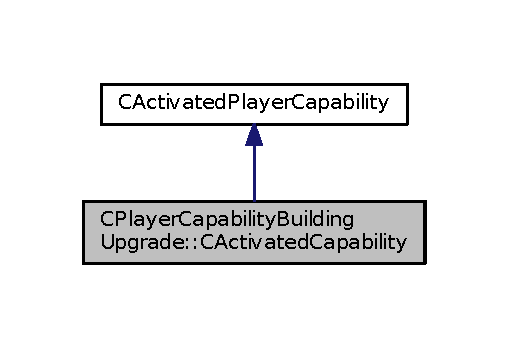
\includegraphics[width=244pt]{classCPlayerCapabilityBuildingUpgrade_1_1CActivatedCapability__inherit__graph}
\end{center}
\end{figure}


Collaboration diagram for C\+Player\+Capability\+Building\+Upgrade\+:\+:C\+Activated\+Capability\+:\nopagebreak
\begin{figure}[H]
\begin{center}
\leavevmode
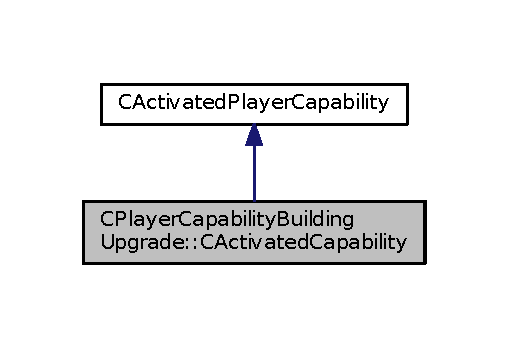
\includegraphics[width=244pt]{classCPlayerCapabilityBuildingUpgrade_1_1CActivatedCapability__coll__graph}
\end{center}
\end{figure}
\subsection*{Public Member Functions}
\begin{DoxyCompactItemize}
\item 
\hyperlink{classCPlayerCapabilityBuildingUpgrade_1_1CActivatedCapability_ab0e141246d8b14ba86cbb3146afcf319}{C\+Activated\+Capability} (std\+::shared\+\_\+ptr$<$ \hyperlink{classCPlayerAsset}{C\+Player\+Asset} $>$ actor, std\+::shared\+\_\+ptr$<$ \hyperlink{classCPlayerData}{C\+Player\+Data} $>$ playerdata, std\+::shared\+\_\+ptr$<$ \hyperlink{classCPlayerAsset}{C\+Player\+Asset} $>$ target, std\+::shared\+\_\+ptr$<$ \hyperlink{classCPlayerAssetType}{C\+Player\+Asset\+Type} $>$ origtype, std\+::shared\+\_\+ptr$<$ \hyperlink{classCPlayerAssetType}{C\+Player\+Asset\+Type} $>$ upgradetype, int lumber, int gold, int steps)
\item 
virtual \hyperlink{classCPlayerCapabilityBuildingUpgrade_1_1CActivatedCapability_a559f4334174ff6deb2cdbc7bee013e61}{$\sim$\+C\+Activated\+Capability} ()
\item 
int \hyperlink{classCPlayerCapabilityBuildingUpgrade_1_1CActivatedCapability_afb2aab171773fa9f33539e33315c1c28}{Percent\+Complete} (int max)
\item 
bool \hyperlink{classCPlayerCapabilityBuildingUpgrade_1_1CActivatedCapability_acc732144e87e5fc88117c0b3a032a97a}{Increment\+Step} ()
\item 
void \hyperlink{classCPlayerCapabilityBuildingUpgrade_1_1CActivatedCapability_adca97e7f7611f4adfcfea615428dac0b}{Cancel} ()
\end{DoxyCompactItemize}
\subsection*{Protected Attributes}
\begin{DoxyCompactItemize}
\item 
std\+::shared\+\_\+ptr$<$ \hyperlink{classCPlayerAssetType}{C\+Player\+Asset\+Type} $>$ \hyperlink{classCPlayerCapabilityBuildingUpgrade_1_1CActivatedCapability_a9418eb8f3401f341c688f00cf8c4aa53}{D\+Original\+Type}
\item 
std\+::shared\+\_\+ptr$<$ \hyperlink{classCPlayerAssetType}{C\+Player\+Asset\+Type} $>$ \hyperlink{classCPlayerCapabilityBuildingUpgrade_1_1CActivatedCapability_a625885c25af00ac23b85f95fc44f897d}{D\+Upgrade\+Type}
\item 
int \hyperlink{classCPlayerCapabilityBuildingUpgrade_1_1CActivatedCapability_a70e4e67d8115643f7ffa11dc72fcf63c}{D\+Current\+Step}
\item 
int \hyperlink{classCPlayerCapabilityBuildingUpgrade_1_1CActivatedCapability_a9c4ea12cf99701f8ce38e17e03ad0115}{D\+Total\+Steps}
\item 
int \hyperlink{classCPlayerCapabilityBuildingUpgrade_1_1CActivatedCapability_a497437c6eb755ccc9b18ff2a1e704c72}{D\+Lumber}
\item 
int \hyperlink{classCPlayerCapabilityBuildingUpgrade_1_1CActivatedCapability_a86bea8030ade6995b4bb5b253fe9466c}{D\+Gold}
\end{DoxyCompactItemize}


\subsection{Detailed Description}


Definition at line 29 of file Building\+Upgrade\+Capabilities.\+cpp.



\subsection{Constructor \& Destructor Documentation}
\hypertarget{classCPlayerCapabilityBuildingUpgrade_1_1CActivatedCapability_ab0e141246d8b14ba86cbb3146afcf319}{}\label{classCPlayerCapabilityBuildingUpgrade_1_1CActivatedCapability_ab0e141246d8b14ba86cbb3146afcf319} 
\index{C\+Player\+Capability\+Building\+Upgrade\+::\+C\+Activated\+Capability@{C\+Player\+Capability\+Building\+Upgrade\+::\+C\+Activated\+Capability}!C\+Activated\+Capability@{C\+Activated\+Capability}}
\index{C\+Activated\+Capability@{C\+Activated\+Capability}!C\+Player\+Capability\+Building\+Upgrade\+::\+C\+Activated\+Capability@{C\+Player\+Capability\+Building\+Upgrade\+::\+C\+Activated\+Capability}}
\subsubsection{\texorpdfstring{C\+Activated\+Capability()}{CActivatedCapability()}}
{\footnotesize\ttfamily C\+Player\+Capability\+Building\+Upgrade\+::\+C\+Activated\+Capability\+::\+C\+Activated\+Capability (\begin{DoxyParamCaption}\item[{std\+::shared\+\_\+ptr$<$ \hyperlink{classCPlayerAsset}{C\+Player\+Asset} $>$}]{actor,  }\item[{std\+::shared\+\_\+ptr$<$ \hyperlink{classCPlayerData}{C\+Player\+Data} $>$}]{playerdata,  }\item[{std\+::shared\+\_\+ptr$<$ \hyperlink{classCPlayerAsset}{C\+Player\+Asset} $>$}]{target,  }\item[{std\+::shared\+\_\+ptr$<$ \hyperlink{classCPlayerAssetType}{C\+Player\+Asset\+Type} $>$}]{origtype,  }\item[{std\+::shared\+\_\+ptr$<$ \hyperlink{classCPlayerAssetType}{C\+Player\+Asset\+Type} $>$}]{upgradetype,  }\item[{int}]{lumber,  }\item[{int}]{gold,  }\item[{int}]{steps }\end{DoxyParamCaption})}



Definition at line 112 of file Building\+Upgrade\+Capabilities.\+cpp.



References D\+Current\+Step, D\+Gold, D\+Lumber, D\+Original\+Type, C\+Activated\+Player\+Capability\+::\+D\+Player\+Data, D\+Total\+Steps, and D\+Upgrade\+Type.


\begin{DoxyCode}
112                                                                                                            
                                                                                                                  
                                                                                                        :
113 \hyperlink{classCActivatedPlayerCapability_a1ece00ffb6a7b925c84dd94a7407a0d1}{CActivatedPlayerCapability}(actor, playerdata, target)\{
114     \hyperlink{structSAssetCommand}{SAssetCommand} AssetCommand;
115     
116     \hyperlink{classCPlayerCapabilityBuildingUpgrade_1_1CActivatedCapability_a9418eb8f3401f341c688f00cf8c4aa53}{DOriginalType} = origtype;
117     \hyperlink{classCPlayerCapabilityBuildingUpgrade_1_1CActivatedCapability_a625885c25af00ac23b85f95fc44f897d}{DUpgradeType} = upgradetype;
118     \hyperlink{classCPlayerCapabilityBuildingUpgrade_1_1CActivatedCapability_a70e4e67d8115643f7ffa11dc72fcf63c}{DCurrentStep} = 0;
119     \hyperlink{classCPlayerCapabilityBuildingUpgrade_1_1CActivatedCapability_a9c4ea12cf99701f8ce38e17e03ad0115}{DTotalSteps} = steps;
120     \hyperlink{classCPlayerCapabilityBuildingUpgrade_1_1CActivatedCapability_a497437c6eb755ccc9b18ff2a1e704c72}{DLumber} = lumber;
121     \hyperlink{classCPlayerCapabilityBuildingUpgrade_1_1CActivatedCapability_a86bea8030ade6995b4bb5b253fe9466c}{DGold} = gold;
122     \hyperlink{classCActivatedPlayerCapability_a9bf27c322a73f4b11c8183cc1973c3d8}{DPlayerData}->DecrementLumber(\hyperlink{classCPlayerCapabilityBuildingUpgrade_1_1CActivatedCapability_a497437c6eb755ccc9b18ff2a1e704c72}{DLumber});
123     \hyperlink{classCActivatedPlayerCapability_a9bf27c322a73f4b11c8183cc1973c3d8}{DPlayerData}->DecrementGold(\hyperlink{classCPlayerCapabilityBuildingUpgrade_1_1CActivatedCapability_a86bea8030ade6995b4bb5b253fe9466c}{DGold});
124 \}
\end{DoxyCode}
\hypertarget{classCPlayerCapabilityBuildingUpgrade_1_1CActivatedCapability_a559f4334174ff6deb2cdbc7bee013e61}{}\label{classCPlayerCapabilityBuildingUpgrade_1_1CActivatedCapability_a559f4334174ff6deb2cdbc7bee013e61} 
\index{C\+Player\+Capability\+Building\+Upgrade\+::\+C\+Activated\+Capability@{C\+Player\+Capability\+Building\+Upgrade\+::\+C\+Activated\+Capability}!````~C\+Activated\+Capability@{$\sim$\+C\+Activated\+Capability}}
\index{````~C\+Activated\+Capability@{$\sim$\+C\+Activated\+Capability}!C\+Player\+Capability\+Building\+Upgrade\+::\+C\+Activated\+Capability@{C\+Player\+Capability\+Building\+Upgrade\+::\+C\+Activated\+Capability}}
\subsubsection{\texorpdfstring{$\sim$\+C\+Activated\+Capability()}{~CActivatedCapability()}}
{\footnotesize\ttfamily virtual C\+Player\+Capability\+Building\+Upgrade\+::\+C\+Activated\+Capability\+::$\sim$\+C\+Activated\+Capability (\begin{DoxyParamCaption}{ }\end{DoxyParamCaption})\hspace{0.3cm}{\ttfamily [inline]}, {\ttfamily [virtual]}}



Definition at line 40 of file Building\+Upgrade\+Capabilities.\+cpp.


\begin{DoxyCode}
40 \{\};
\end{DoxyCode}


\subsection{Member Function Documentation}
\hypertarget{classCPlayerCapabilityBuildingUpgrade_1_1CActivatedCapability_adca97e7f7611f4adfcfea615428dac0b}{}\label{classCPlayerCapabilityBuildingUpgrade_1_1CActivatedCapability_adca97e7f7611f4adfcfea615428dac0b} 
\index{C\+Player\+Capability\+Building\+Upgrade\+::\+C\+Activated\+Capability@{C\+Player\+Capability\+Building\+Upgrade\+::\+C\+Activated\+Capability}!Cancel@{Cancel}}
\index{Cancel@{Cancel}!C\+Player\+Capability\+Building\+Upgrade\+::\+C\+Activated\+Capability@{C\+Player\+Capability\+Building\+Upgrade\+::\+C\+Activated\+Capability}}
\subsubsection{\texorpdfstring{Cancel()}{Cancel()}}
{\footnotesize\ttfamily void C\+Player\+Capability\+Building\+Upgrade\+::\+C\+Activated\+Capability\+::\+Cancel (\begin{DoxyParamCaption}{ }\end{DoxyParamCaption})\hspace{0.3cm}{\ttfamily [virtual]}}



Implements \hyperlink{classCActivatedPlayerCapability_a5cde83be468e262ad054d81e28684a81}{C\+Activated\+Player\+Capability}.



Definition at line 167 of file Building\+Upgrade\+Capabilities.\+cpp.



References C\+Activated\+Player\+Capability\+::\+D\+Actor, D\+Gold, D\+Lumber, D\+Original\+Type, and C\+Activated\+Player\+Capability\+::\+D\+Player\+Data.


\begin{DoxyCode}
167                                                                  \{
168     \hyperlink{classCActivatedPlayerCapability_a9bf27c322a73f4b11c8183cc1973c3d8}{DPlayerData}->IncrementLumber(\hyperlink{classCPlayerCapabilityBuildingUpgrade_1_1CActivatedCapability_a497437c6eb755ccc9b18ff2a1e704c72}{DLumber});
169     \hyperlink{classCActivatedPlayerCapability_a9bf27c322a73f4b11c8183cc1973c3d8}{DPlayerData}->IncrementGold(\hyperlink{classCPlayerCapabilityBuildingUpgrade_1_1CActivatedCapability_a86bea8030ade6995b4bb5b253fe9466c}{DGold});
170     \hyperlink{classCActivatedPlayerCapability_a54ca944b47bff2718330639941d402b0}{DActor}->ChangeType(\hyperlink{classCPlayerCapabilityBuildingUpgrade_1_1CActivatedCapability_a9418eb8f3401f341c688f00cf8c4aa53}{DOriginalType});
171     \hyperlink{classCActivatedPlayerCapability_a54ca944b47bff2718330639941d402b0}{DActor}->PopCommand();
172 \}
\end{DoxyCode}
\hypertarget{classCPlayerCapabilityBuildingUpgrade_1_1CActivatedCapability_acc732144e87e5fc88117c0b3a032a97a}{}\label{classCPlayerCapabilityBuildingUpgrade_1_1CActivatedCapability_acc732144e87e5fc88117c0b3a032a97a} 
\index{C\+Player\+Capability\+Building\+Upgrade\+::\+C\+Activated\+Capability@{C\+Player\+Capability\+Building\+Upgrade\+::\+C\+Activated\+Capability}!Increment\+Step@{Increment\+Step}}
\index{Increment\+Step@{Increment\+Step}!C\+Player\+Capability\+Building\+Upgrade\+::\+C\+Activated\+Capability@{C\+Player\+Capability\+Building\+Upgrade\+::\+C\+Activated\+Capability}}
\subsubsection{\texorpdfstring{Increment\+Step()}{IncrementStep()}}
{\footnotesize\ttfamily bool C\+Player\+Capability\+Building\+Upgrade\+::\+C\+Activated\+Capability\+::\+Increment\+Step (\begin{DoxyParamCaption}{ }\end{DoxyParamCaption})\hspace{0.3cm}{\ttfamily [virtual]}}



Implements \hyperlink{classCActivatedPlayerCapability_a943b5999a57504399293250382c0ec6a}{C\+Activated\+Player\+Capability}.



Definition at line 131 of file Building\+Upgrade\+Capabilities.\+cpp.



References aa\+Construct, aa\+Stand\+Ground, S\+Asset\+Command\+::\+D\+Action, C\+Activated\+Player\+Capability\+::\+D\+Actor, S\+Game\+Event\+::\+D\+Asset, D\+Current\+Step, D\+Original\+Type, C\+Activated\+Player\+Capability\+::\+D\+Player\+Data, D\+Total\+Steps, S\+Game\+Event\+::\+D\+Type, D\+Upgrade\+Type, and et\+Work\+Complete.


\begin{DoxyCode}
131                                                                         \{
132     \textcolor{keywordtype}{int} AddHitPoints = ((\hyperlink{classCPlayerCapabilityBuildingUpgrade_1_1CActivatedCapability_a625885c25af00ac23b85f95fc44f897d}{DUpgradeType}->HitPoints() - \hyperlink{classCPlayerCapabilityBuildingUpgrade_1_1CActivatedCapability_a9418eb8f3401f341c688f00cf8c4aa53}{DOriginalType}->HitPoints()) *
       (\hyperlink{classCPlayerCapabilityBuildingUpgrade_1_1CActivatedCapability_a70e4e67d8115643f7ffa11dc72fcf63c}{DCurrentStep} + 1) / \hyperlink{classCPlayerCapabilityBuildingUpgrade_1_1CActivatedCapability_a9c4ea12cf99701f8ce38e17e03ad0115}{DTotalSteps}) - ((\hyperlink{classCPlayerCapabilityBuildingUpgrade_1_1CActivatedCapability_a625885c25af00ac23b85f95fc44f897d}{DUpgradeType}->HitPoints() - 
      \hyperlink{classCPlayerCapabilityBuildingUpgrade_1_1CActivatedCapability_a9418eb8f3401f341c688f00cf8c4aa53}{DOriginalType}->HitPoints()) * \hyperlink{classCPlayerCapabilityBuildingUpgrade_1_1CActivatedCapability_a70e4e67d8115643f7ffa11dc72fcf63c}{DCurrentStep} / 
      \hyperlink{classCPlayerCapabilityBuildingUpgrade_1_1CActivatedCapability_a9c4ea12cf99701f8ce38e17e03ad0115}{DTotalSteps});
133     
134     \textcolor{keywordflow}{if}(0 == \hyperlink{classCPlayerCapabilityBuildingUpgrade_1_1CActivatedCapability_a70e4e67d8115643f7ffa11dc72fcf63c}{DCurrentStep})\{
135         \hyperlink{structSAssetCommand}{SAssetCommand} AssetCommand = \hyperlink{classCActivatedPlayerCapability_a54ca944b47bff2718330639941d402b0}{DActor}->CurrentCommand();
136         AssetCommand.\hyperlink{structSAssetCommand_a8edd3b3d59a76d5514ba403bc8076a75}{DAction} = \hyperlink{GameDataTypes_8h_ab47668e651a3032cfb9c40ea2d60d670a7ef6b863f66dd7dcc95a199cd758ae1d}{aaConstruct};
137         \hyperlink{classCActivatedPlayerCapability_a54ca944b47bff2718330639941d402b0}{DActor}->PopCommand();
138         \hyperlink{classCActivatedPlayerCapability_a54ca944b47bff2718330639941d402b0}{DActor}->PushCommand(AssetCommand);
139         \hyperlink{classCActivatedPlayerCapability_a54ca944b47bff2718330639941d402b0}{DActor}->ChangeType(\hyperlink{classCPlayerCapabilityBuildingUpgrade_1_1CActivatedCapability_a625885c25af00ac23b85f95fc44f897d}{DUpgradeType});  
140         \hyperlink{classCActivatedPlayerCapability_a54ca944b47bff2718330639941d402b0}{DActor}->ResetStep();
141     \}
142     
143     \hyperlink{classCActivatedPlayerCapability_a54ca944b47bff2718330639941d402b0}{DActor}->IncrementHitPoints(AddHitPoints);
144     \textcolor{keywordflow}{if}(\hyperlink{classCActivatedPlayerCapability_a54ca944b47bff2718330639941d402b0}{DActor}->HitPoints() > \hyperlink{classCActivatedPlayerCapability_a54ca944b47bff2718330639941d402b0}{DActor}->MaxHitPoints())\{
145         \hyperlink{classCActivatedPlayerCapability_a54ca944b47bff2718330639941d402b0}{DActor}->HitPoints(\hyperlink{classCActivatedPlayerCapability_a54ca944b47bff2718330639941d402b0}{DActor}->MaxHitPoints());
146     \}
147     \hyperlink{classCPlayerCapabilityBuildingUpgrade_1_1CActivatedCapability_a70e4e67d8115643f7ffa11dc72fcf63c}{DCurrentStep}++;
148     \hyperlink{classCActivatedPlayerCapability_a54ca944b47bff2718330639941d402b0}{DActor}->IncrementStep();
149     \textcolor{keywordflow}{if}(\hyperlink{classCPlayerCapabilityBuildingUpgrade_1_1CActivatedCapability_a70e4e67d8115643f7ffa11dc72fcf63c}{DCurrentStep} >= \hyperlink{classCPlayerCapabilityBuildingUpgrade_1_1CActivatedCapability_a9c4ea12cf99701f8ce38e17e03ad0115}{DTotalSteps})\{
150         \hyperlink{structSGameEvent}{SGameEvent} TempEvent;
151         
152         TempEvent.\hyperlink{structSGameEvent_afa10562e243f4ac2b473b655cc58fee7}{DType} = \hyperlink{GameModel_8h_abfcf510bafec7c6429906a6ecaac656da0106cf4227412990140c1d773244b587}{etWorkComplete};
153         TempEvent.\hyperlink{structSGameEvent_a40c85eeac83b96887b7449c9bdc5d624}{DAsset} = \hyperlink{classCActivatedPlayerCapability_a54ca944b47bff2718330639941d402b0}{DActor};
154         \hyperlink{classCActivatedPlayerCapability_a9bf27c322a73f4b11c8183cc1973c3d8}{DPlayerData}->AddGameEvent(TempEvent);
155         
156         \hyperlink{classCActivatedPlayerCapability_a54ca944b47bff2718330639941d402b0}{DActor}->PopCommand();
157         \textcolor{keywordflow}{if}(\hyperlink{classCActivatedPlayerCapability_a54ca944b47bff2718330639941d402b0}{DActor}->Range())\{
158             \hyperlink{structSAssetCommand}{SAssetCommand} Command;
159             Command.\hyperlink{structSAssetCommand_a8edd3b3d59a76d5514ba403bc8076a75}{DAction} = \hyperlink{GameDataTypes_8h_ab47668e651a3032cfb9c40ea2d60d670abd8a4e07a8f888148ed62ddd46719af3}{aaStandGround};
160             \hyperlink{classCActivatedPlayerCapability_a54ca944b47bff2718330639941d402b0}{DActor}->PushCommand(Command);   
161         \}
162         \textcolor{keywordflow}{return} \textcolor{keyword}{true};    
163     \}
164     \textcolor{keywordflow}{return} \textcolor{keyword}{false};
165 \}
\end{DoxyCode}
\hypertarget{classCPlayerCapabilityBuildingUpgrade_1_1CActivatedCapability_afb2aab171773fa9f33539e33315c1c28}{}\label{classCPlayerCapabilityBuildingUpgrade_1_1CActivatedCapability_afb2aab171773fa9f33539e33315c1c28} 
\index{C\+Player\+Capability\+Building\+Upgrade\+::\+C\+Activated\+Capability@{C\+Player\+Capability\+Building\+Upgrade\+::\+C\+Activated\+Capability}!Percent\+Complete@{Percent\+Complete}}
\index{Percent\+Complete@{Percent\+Complete}!C\+Player\+Capability\+Building\+Upgrade\+::\+C\+Activated\+Capability@{C\+Player\+Capability\+Building\+Upgrade\+::\+C\+Activated\+Capability}}
\subsubsection{\texorpdfstring{Percent\+Complete()}{PercentComplete()}}
{\footnotesize\ttfamily int C\+Player\+Capability\+Building\+Upgrade\+::\+C\+Activated\+Capability\+::\+Percent\+Complete (\begin{DoxyParamCaption}\item[{int}]{max }\end{DoxyParamCaption})\hspace{0.3cm}{\ttfamily [virtual]}}



Implements \hyperlink{classCActivatedPlayerCapability_a405dc6076058006a4f801727de4cfe4d}{C\+Activated\+Player\+Capability}.



Definition at line 127 of file Building\+Upgrade\+Capabilities.\+cpp.



References D\+Current\+Step, and D\+Total\+Steps.


\begin{DoxyCode}
127                                                                                 \{
128     \textcolor{keywordflow}{return} \hyperlink{classCPlayerCapabilityBuildingUpgrade_1_1CActivatedCapability_a70e4e67d8115643f7ffa11dc72fcf63c}{DCurrentStep} * max / \hyperlink{classCPlayerCapabilityBuildingUpgrade_1_1CActivatedCapability_a9c4ea12cf99701f8ce38e17e03ad0115}{DTotalSteps};
129 \}
\end{DoxyCode}


\subsection{Member Data Documentation}
\hypertarget{classCPlayerCapabilityBuildingUpgrade_1_1CActivatedCapability_a70e4e67d8115643f7ffa11dc72fcf63c}{}\label{classCPlayerCapabilityBuildingUpgrade_1_1CActivatedCapability_a70e4e67d8115643f7ffa11dc72fcf63c} 
\index{C\+Player\+Capability\+Building\+Upgrade\+::\+C\+Activated\+Capability@{C\+Player\+Capability\+Building\+Upgrade\+::\+C\+Activated\+Capability}!D\+Current\+Step@{D\+Current\+Step}}
\index{D\+Current\+Step@{D\+Current\+Step}!C\+Player\+Capability\+Building\+Upgrade\+::\+C\+Activated\+Capability@{C\+Player\+Capability\+Building\+Upgrade\+::\+C\+Activated\+Capability}}
\subsubsection{\texorpdfstring{D\+Current\+Step}{DCurrentStep}}
{\footnotesize\ttfamily int C\+Player\+Capability\+Building\+Upgrade\+::\+C\+Activated\+Capability\+::\+D\+Current\+Step\hspace{0.3cm}{\ttfamily [protected]}}



Definition at line 33 of file Building\+Upgrade\+Capabilities.\+cpp.



Referenced by C\+Activated\+Capability(), Increment\+Step(), and Percent\+Complete().

\hypertarget{classCPlayerCapabilityBuildingUpgrade_1_1CActivatedCapability_a86bea8030ade6995b4bb5b253fe9466c}{}\label{classCPlayerCapabilityBuildingUpgrade_1_1CActivatedCapability_a86bea8030ade6995b4bb5b253fe9466c} 
\index{C\+Player\+Capability\+Building\+Upgrade\+::\+C\+Activated\+Capability@{C\+Player\+Capability\+Building\+Upgrade\+::\+C\+Activated\+Capability}!D\+Gold@{D\+Gold}}
\index{D\+Gold@{D\+Gold}!C\+Player\+Capability\+Building\+Upgrade\+::\+C\+Activated\+Capability@{C\+Player\+Capability\+Building\+Upgrade\+::\+C\+Activated\+Capability}}
\subsubsection{\texorpdfstring{D\+Gold}{DGold}}
{\footnotesize\ttfamily int C\+Player\+Capability\+Building\+Upgrade\+::\+C\+Activated\+Capability\+::\+D\+Gold\hspace{0.3cm}{\ttfamily [protected]}}



Definition at line 36 of file Building\+Upgrade\+Capabilities.\+cpp.



Referenced by C\+Activated\+Capability(), and Cancel().

\hypertarget{classCPlayerCapabilityBuildingUpgrade_1_1CActivatedCapability_a497437c6eb755ccc9b18ff2a1e704c72}{}\label{classCPlayerCapabilityBuildingUpgrade_1_1CActivatedCapability_a497437c6eb755ccc9b18ff2a1e704c72} 
\index{C\+Player\+Capability\+Building\+Upgrade\+::\+C\+Activated\+Capability@{C\+Player\+Capability\+Building\+Upgrade\+::\+C\+Activated\+Capability}!D\+Lumber@{D\+Lumber}}
\index{D\+Lumber@{D\+Lumber}!C\+Player\+Capability\+Building\+Upgrade\+::\+C\+Activated\+Capability@{C\+Player\+Capability\+Building\+Upgrade\+::\+C\+Activated\+Capability}}
\subsubsection{\texorpdfstring{D\+Lumber}{DLumber}}
{\footnotesize\ttfamily int C\+Player\+Capability\+Building\+Upgrade\+::\+C\+Activated\+Capability\+::\+D\+Lumber\hspace{0.3cm}{\ttfamily [protected]}}



Definition at line 35 of file Building\+Upgrade\+Capabilities.\+cpp.



Referenced by C\+Activated\+Capability(), and Cancel().

\hypertarget{classCPlayerCapabilityBuildingUpgrade_1_1CActivatedCapability_a9418eb8f3401f341c688f00cf8c4aa53}{}\label{classCPlayerCapabilityBuildingUpgrade_1_1CActivatedCapability_a9418eb8f3401f341c688f00cf8c4aa53} 
\index{C\+Player\+Capability\+Building\+Upgrade\+::\+C\+Activated\+Capability@{C\+Player\+Capability\+Building\+Upgrade\+::\+C\+Activated\+Capability}!D\+Original\+Type@{D\+Original\+Type}}
\index{D\+Original\+Type@{D\+Original\+Type}!C\+Player\+Capability\+Building\+Upgrade\+::\+C\+Activated\+Capability@{C\+Player\+Capability\+Building\+Upgrade\+::\+C\+Activated\+Capability}}
\subsubsection{\texorpdfstring{D\+Original\+Type}{DOriginalType}}
{\footnotesize\ttfamily std\+::shared\+\_\+ptr$<$ \hyperlink{classCPlayerAssetType}{C\+Player\+Asset\+Type} $>$ C\+Player\+Capability\+Building\+Upgrade\+::\+C\+Activated\+Capability\+::\+D\+Original\+Type\hspace{0.3cm}{\ttfamily [protected]}}



Definition at line 31 of file Building\+Upgrade\+Capabilities.\+cpp.



Referenced by C\+Activated\+Capability(), Cancel(), and Increment\+Step().

\hypertarget{classCPlayerCapabilityBuildingUpgrade_1_1CActivatedCapability_a9c4ea12cf99701f8ce38e17e03ad0115}{}\label{classCPlayerCapabilityBuildingUpgrade_1_1CActivatedCapability_a9c4ea12cf99701f8ce38e17e03ad0115} 
\index{C\+Player\+Capability\+Building\+Upgrade\+::\+C\+Activated\+Capability@{C\+Player\+Capability\+Building\+Upgrade\+::\+C\+Activated\+Capability}!D\+Total\+Steps@{D\+Total\+Steps}}
\index{D\+Total\+Steps@{D\+Total\+Steps}!C\+Player\+Capability\+Building\+Upgrade\+::\+C\+Activated\+Capability@{C\+Player\+Capability\+Building\+Upgrade\+::\+C\+Activated\+Capability}}
\subsubsection{\texorpdfstring{D\+Total\+Steps}{DTotalSteps}}
{\footnotesize\ttfamily int C\+Player\+Capability\+Building\+Upgrade\+::\+C\+Activated\+Capability\+::\+D\+Total\+Steps\hspace{0.3cm}{\ttfamily [protected]}}



Definition at line 34 of file Building\+Upgrade\+Capabilities.\+cpp.



Referenced by C\+Activated\+Capability(), Increment\+Step(), and Percent\+Complete().

\hypertarget{classCPlayerCapabilityBuildingUpgrade_1_1CActivatedCapability_a625885c25af00ac23b85f95fc44f897d}{}\label{classCPlayerCapabilityBuildingUpgrade_1_1CActivatedCapability_a625885c25af00ac23b85f95fc44f897d} 
\index{C\+Player\+Capability\+Building\+Upgrade\+::\+C\+Activated\+Capability@{C\+Player\+Capability\+Building\+Upgrade\+::\+C\+Activated\+Capability}!D\+Upgrade\+Type@{D\+Upgrade\+Type}}
\index{D\+Upgrade\+Type@{D\+Upgrade\+Type}!C\+Player\+Capability\+Building\+Upgrade\+::\+C\+Activated\+Capability@{C\+Player\+Capability\+Building\+Upgrade\+::\+C\+Activated\+Capability}}
\subsubsection{\texorpdfstring{D\+Upgrade\+Type}{DUpgradeType}}
{\footnotesize\ttfamily std\+::shared\+\_\+ptr$<$ \hyperlink{classCPlayerAssetType}{C\+Player\+Asset\+Type} $>$ C\+Player\+Capability\+Building\+Upgrade\+::\+C\+Activated\+Capability\+::\+D\+Upgrade\+Type\hspace{0.3cm}{\ttfamily [protected]}}



Definition at line 32 of file Building\+Upgrade\+Capabilities.\+cpp.



Referenced by C\+Activated\+Capability(), and Increment\+Step().



The documentation for this class was generated from the following file\+:\begin{DoxyCompactItemize}
\item 
src/\hyperlink{BuildingUpgradeCapabilities_8cpp}{Building\+Upgrade\+Capabilities.\+cpp}\end{DoxyCompactItemize}

\hypertarget{classCPlayerCapabilityTrainNormal_1_1CActivatedCapability}{}\section{C\+Player\+Capability\+Train\+Normal\+:\+:C\+Activated\+Capability Class Reference}
\label{classCPlayerCapabilityTrainNormal_1_1CActivatedCapability}\index{C\+Player\+Capability\+Train\+Normal\+::\+C\+Activated\+Capability@{C\+Player\+Capability\+Train\+Normal\+::\+C\+Activated\+Capability}}


Inheritance diagram for C\+Player\+Capability\+Train\+Normal\+:\+:C\+Activated\+Capability\+:\nopagebreak
\begin{figure}[H]
\begin{center}
\leavevmode
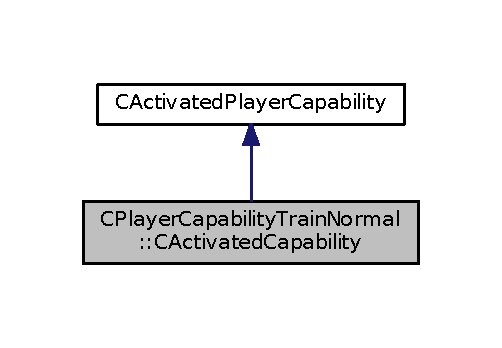
\includegraphics[width=241pt]{classCPlayerCapabilityTrainNormal_1_1CActivatedCapability__inherit__graph}
\end{center}
\end{figure}


Collaboration diagram for C\+Player\+Capability\+Train\+Normal\+:\+:C\+Activated\+Capability\+:\nopagebreak
\begin{figure}[H]
\begin{center}
\leavevmode
\includegraphics[width=241pt]{classCPlayerCapabilityTrainNormal_1_1CActivatedCapability__coll__graph}
\end{center}
\end{figure}
\subsection*{Public Member Functions}
\begin{DoxyCompactItemize}
\item 
\hyperlink{classCPlayerCapabilityTrainNormal_1_1CActivatedCapability_a6d160dbc57c968390a91f0797cc53306}{C\+Activated\+Capability} (std\+::shared\+\_\+ptr$<$ \hyperlink{classCPlayerAsset}{C\+Player\+Asset} $>$ actor, std\+::shared\+\_\+ptr$<$ \hyperlink{classCPlayerData}{C\+Player\+Data} $>$ playerdata, std\+::shared\+\_\+ptr$<$ \hyperlink{classCPlayerAsset}{C\+Player\+Asset} $>$ target, int lumber, int gold, int steps)
\item 
virtual \hyperlink{classCPlayerCapabilityTrainNormal_1_1CActivatedCapability_ad0ce8533475cce5a85aca7b98bedb6b3}{$\sim$\+C\+Activated\+Capability} ()
\item 
int \hyperlink{classCPlayerCapabilityTrainNormal_1_1CActivatedCapability_ac0d2dd8e1b3aedb0873149ba4c92e6f7}{Percent\+Complete} (int max)
\item 
bool \hyperlink{classCPlayerCapabilityTrainNormal_1_1CActivatedCapability_a201f09e738af96fba1a871e4ed00f18a}{Increment\+Step} ()
\item 
void \hyperlink{classCPlayerCapabilityTrainNormal_1_1CActivatedCapability_a028dc1f8c528cc726737d712f0236884}{Cancel} ()
\end{DoxyCompactItemize}
\subsection*{Protected Attributes}
\begin{DoxyCompactItemize}
\item 
int \hyperlink{classCPlayerCapabilityTrainNormal_1_1CActivatedCapability_a2053317e0ee29f45f4ff5a28269cd635}{D\+Current\+Step}
\item 
int \hyperlink{classCPlayerCapabilityTrainNormal_1_1CActivatedCapability_a2bee6a6395fd7cc0fcf4001bbbadb165}{D\+Total\+Steps}
\item 
int \hyperlink{classCPlayerCapabilityTrainNormal_1_1CActivatedCapability_a49a77c92b6146819efb1a7a8b6fb8972}{D\+Lumber}
\item 
int \hyperlink{classCPlayerCapabilityTrainNormal_1_1CActivatedCapability_a1b994a572ca0fdfd64f6f71afb6b5988}{D\+Gold}
\end{DoxyCompactItemize}


\subsection{Detailed Description}


Definition at line 29 of file Train\+Capabilities.\+cpp.



\subsection{Constructor \& Destructor Documentation}
\hypertarget{classCPlayerCapabilityTrainNormal_1_1CActivatedCapability_a6d160dbc57c968390a91f0797cc53306}{}\label{classCPlayerCapabilityTrainNormal_1_1CActivatedCapability_a6d160dbc57c968390a91f0797cc53306} 
\index{C\+Player\+Capability\+Train\+Normal\+::\+C\+Activated\+Capability@{C\+Player\+Capability\+Train\+Normal\+::\+C\+Activated\+Capability}!C\+Activated\+Capability@{C\+Activated\+Capability}}
\index{C\+Activated\+Capability@{C\+Activated\+Capability}!C\+Player\+Capability\+Train\+Normal\+::\+C\+Activated\+Capability@{C\+Player\+Capability\+Train\+Normal\+::\+C\+Activated\+Capability}}
\subsubsection{\texorpdfstring{C\+Activated\+Capability()}{CActivatedCapability()}}
{\footnotesize\ttfamily C\+Player\+Capability\+Train\+Normal\+::\+C\+Activated\+Capability\+::\+C\+Activated\+Capability (\begin{DoxyParamCaption}\item[{std\+::shared\+\_\+ptr$<$ \hyperlink{classCPlayerAsset}{C\+Player\+Asset} $>$}]{actor,  }\item[{std\+::shared\+\_\+ptr$<$ \hyperlink{classCPlayerData}{C\+Player\+Data} $>$}]{playerdata,  }\item[{std\+::shared\+\_\+ptr$<$ \hyperlink{classCPlayerAsset}{C\+Player\+Asset} $>$}]{target,  }\item[{int}]{lumber,  }\item[{int}]{gold,  }\item[{int}]{steps }\end{DoxyParamCaption})}



Definition at line 115 of file Train\+Capabilities.\+cpp.



References aa\+Construct, S\+Asset\+Command\+::\+D\+Action, C\+Activated\+Player\+Capability\+::\+D\+Actor, S\+Asset\+Command\+::\+D\+Asset\+Target, D\+Current\+Step, D\+Gold, D\+Lumber, C\+Activated\+Player\+Capability\+::\+D\+Player\+Data, C\+Activated\+Player\+Capability\+::\+D\+Target, and D\+Total\+Steps.


\begin{DoxyCode}
115                                                                                                            
                                                                                                                  
         :
116 \hyperlink{classCActivatedPlayerCapability_a1ece00ffb6a7b925c84dd94a7407a0d1}{CActivatedPlayerCapability}(actor, playerdata, target)\{
117     \hyperlink{structSAssetCommand}{SAssetCommand} AssetCommand;
118     
119     \hyperlink{classCPlayerCapabilityTrainNormal_1_1CActivatedCapability_a2053317e0ee29f45f4ff5a28269cd635}{DCurrentStep} = 0;
120     \hyperlink{classCPlayerCapabilityTrainNormal_1_1CActivatedCapability_a2bee6a6395fd7cc0fcf4001bbbadb165}{DTotalSteps} = steps;
121     \hyperlink{classCPlayerCapabilityTrainNormal_1_1CActivatedCapability_a49a77c92b6146819efb1a7a8b6fb8972}{DLumber} = lumber;
122     \hyperlink{classCPlayerCapabilityTrainNormal_1_1CActivatedCapability_a1b994a572ca0fdfd64f6f71afb6b5988}{DGold} = gold;
123     \hyperlink{classCActivatedPlayerCapability_a9bf27c322a73f4b11c8183cc1973c3d8}{DPlayerData}->DecrementLumber(\hyperlink{classCPlayerCapabilityTrainNormal_1_1CActivatedCapability_a49a77c92b6146819efb1a7a8b6fb8972}{DLumber});
124     \hyperlink{classCActivatedPlayerCapability_a9bf27c322a73f4b11c8183cc1973c3d8}{DPlayerData}->DecrementGold(\hyperlink{classCPlayerCapabilityTrainNormal_1_1CActivatedCapability_a1b994a572ca0fdfd64f6f71afb6b5988}{DGold});
125     AssetCommand.\hyperlink{structSAssetCommand_a8edd3b3d59a76d5514ba403bc8076a75}{DAction} = \hyperlink{GameDataTypes_8h_ab47668e651a3032cfb9c40ea2d60d670a7ef6b863f66dd7dcc95a199cd758ae1d}{aaConstruct};
126     AssetCommand.\hyperlink{structSAssetCommand_a3d9b43f6e59c386c48c41a65448a0c39}{DAssetTarget} = \hyperlink{classCActivatedPlayerCapability_a54ca944b47bff2718330639941d402b0}{DActor};
127     \hyperlink{classCActivatedPlayerCapability_a8a1cf50b6501bcfd55af0c935828e395}{DTarget}->PushCommand(AssetCommand);
128 \}
\end{DoxyCode}
\hypertarget{classCPlayerCapabilityTrainNormal_1_1CActivatedCapability_ad0ce8533475cce5a85aca7b98bedb6b3}{}\label{classCPlayerCapabilityTrainNormal_1_1CActivatedCapability_ad0ce8533475cce5a85aca7b98bedb6b3} 
\index{C\+Player\+Capability\+Train\+Normal\+::\+C\+Activated\+Capability@{C\+Player\+Capability\+Train\+Normal\+::\+C\+Activated\+Capability}!````~C\+Activated\+Capability@{$\sim$\+C\+Activated\+Capability}}
\index{````~C\+Activated\+Capability@{$\sim$\+C\+Activated\+Capability}!C\+Player\+Capability\+Train\+Normal\+::\+C\+Activated\+Capability@{C\+Player\+Capability\+Train\+Normal\+::\+C\+Activated\+Capability}}
\subsubsection{\texorpdfstring{$\sim$\+C\+Activated\+Capability()}{~CActivatedCapability()}}
{\footnotesize\ttfamily virtual C\+Player\+Capability\+Train\+Normal\+::\+C\+Activated\+Capability\+::$\sim$\+C\+Activated\+Capability (\begin{DoxyParamCaption}{ }\end{DoxyParamCaption})\hspace{0.3cm}{\ttfamily [inline]}, {\ttfamily [virtual]}}



Definition at line 38 of file Train\+Capabilities.\+cpp.


\begin{DoxyCode}
38 \{\};
\end{DoxyCode}


\subsection{Member Function Documentation}
\hypertarget{classCPlayerCapabilityTrainNormal_1_1CActivatedCapability_a028dc1f8c528cc726737d712f0236884}{}\label{classCPlayerCapabilityTrainNormal_1_1CActivatedCapability_a028dc1f8c528cc726737d712f0236884} 
\index{C\+Player\+Capability\+Train\+Normal\+::\+C\+Activated\+Capability@{C\+Player\+Capability\+Train\+Normal\+::\+C\+Activated\+Capability}!Cancel@{Cancel}}
\index{Cancel@{Cancel}!C\+Player\+Capability\+Train\+Normal\+::\+C\+Activated\+Capability@{C\+Player\+Capability\+Train\+Normal\+::\+C\+Activated\+Capability}}
\subsubsection{\texorpdfstring{Cancel()}{Cancel()}}
{\footnotesize\ttfamily void C\+Player\+Capability\+Train\+Normal\+::\+C\+Activated\+Capability\+::\+Cancel (\begin{DoxyParamCaption}{ }\end{DoxyParamCaption})\hspace{0.3cm}{\ttfamily [virtual]}}



Implements \hyperlink{classCActivatedPlayerCapability_a5cde83be468e262ad054d81e28684a81}{C\+Activated\+Player\+Capability}.



Definition at line 160 of file Train\+Capabilities.\+cpp.



References C\+Activated\+Player\+Capability\+::\+D\+Actor, D\+Gold, D\+Lumber, C\+Activated\+Player\+Capability\+::\+D\+Player\+Data, and C\+Activated\+Player\+Capability\+::\+D\+Target.


\begin{DoxyCode}
160                                                              \{
161     \hyperlink{classCActivatedPlayerCapability_a9bf27c322a73f4b11c8183cc1973c3d8}{DPlayerData}->IncrementLumber(\hyperlink{classCPlayerCapabilityTrainNormal_1_1CActivatedCapability_a49a77c92b6146819efb1a7a8b6fb8972}{DLumber});
162     \hyperlink{classCActivatedPlayerCapability_a9bf27c322a73f4b11c8183cc1973c3d8}{DPlayerData}->IncrementGold(\hyperlink{classCPlayerCapabilityTrainNormal_1_1CActivatedCapability_a1b994a572ca0fdfd64f6f71afb6b5988}{DGold});
163     \hyperlink{classCActivatedPlayerCapability_a9bf27c322a73f4b11c8183cc1973c3d8}{DPlayerData}->DeleteAsset(\hyperlink{classCActivatedPlayerCapability_a8a1cf50b6501bcfd55af0c935828e395}{DTarget});
164     \hyperlink{classCActivatedPlayerCapability_a54ca944b47bff2718330639941d402b0}{DActor}->PopCommand();
165 \}
\end{DoxyCode}
\hypertarget{classCPlayerCapabilityTrainNormal_1_1CActivatedCapability_a201f09e738af96fba1a871e4ed00f18a}{}\label{classCPlayerCapabilityTrainNormal_1_1CActivatedCapability_a201f09e738af96fba1a871e4ed00f18a} 
\index{C\+Player\+Capability\+Train\+Normal\+::\+C\+Activated\+Capability@{C\+Player\+Capability\+Train\+Normal\+::\+C\+Activated\+Capability}!Increment\+Step@{Increment\+Step}}
\index{Increment\+Step@{Increment\+Step}!C\+Player\+Capability\+Train\+Normal\+::\+C\+Activated\+Capability@{C\+Player\+Capability\+Train\+Normal\+::\+C\+Activated\+Capability}}
\subsubsection{\texorpdfstring{Increment\+Step()}{IncrementStep()}}
{\footnotesize\ttfamily bool C\+Player\+Capability\+Train\+Normal\+::\+C\+Activated\+Capability\+::\+Increment\+Step (\begin{DoxyParamCaption}{ }\end{DoxyParamCaption})\hspace{0.3cm}{\ttfamily [virtual]}}



Implements \hyperlink{classCActivatedPlayerCapability_a943b5999a57504399293250382c0ec6a}{C\+Activated\+Player\+Capability}.



Definition at line 135 of file Train\+Capabilities.\+cpp.



References C\+Activated\+Player\+Capability\+::\+D\+Actor, S\+Game\+Event\+::\+D\+Asset, D\+Current\+Step, C\+Activated\+Player\+Capability\+::\+D\+Player\+Data, C\+Activated\+Player\+Capability\+::\+D\+Target, D\+Total\+Steps, S\+Game\+Event\+::\+D\+Type, and et\+Ready.


\begin{DoxyCode}
135                                                                     \{
136     \textcolor{keywordtype}{int} AddHitPoints = (\hyperlink{classCActivatedPlayerCapability_a8a1cf50b6501bcfd55af0c935828e395}{DTarget}->MaxHitPoints() * (\hyperlink{classCPlayerCapabilityTrainNormal_1_1CActivatedCapability_a2053317e0ee29f45f4ff5a28269cd635}{DCurrentStep} + 1) / 
      \hyperlink{classCPlayerCapabilityTrainNormal_1_1CActivatedCapability_a2bee6a6395fd7cc0fcf4001bbbadb165}{DTotalSteps}) - (\hyperlink{classCActivatedPlayerCapability_a8a1cf50b6501bcfd55af0c935828e395}{DTarget}->MaxHitPoints() * \hyperlink{classCPlayerCapabilityTrainNormal_1_1CActivatedCapability_a2053317e0ee29f45f4ff5a28269cd635}{DCurrentStep} / 
      \hyperlink{classCPlayerCapabilityTrainNormal_1_1CActivatedCapability_a2bee6a6395fd7cc0fcf4001bbbadb165}{DTotalSteps});
137     
138     \hyperlink{classCActivatedPlayerCapability_a8a1cf50b6501bcfd55af0c935828e395}{DTarget}->IncrementHitPoints(AddHitPoints);
139     \textcolor{keywordflow}{if}(\hyperlink{classCActivatedPlayerCapability_a8a1cf50b6501bcfd55af0c935828e395}{DTarget}->HitPoints() > \hyperlink{classCActivatedPlayerCapability_a8a1cf50b6501bcfd55af0c935828e395}{DTarget}->MaxHitPoints())\{
140         \hyperlink{classCActivatedPlayerCapability_a8a1cf50b6501bcfd55af0c935828e395}{DTarget}->HitPoints(\hyperlink{classCActivatedPlayerCapability_a8a1cf50b6501bcfd55af0c935828e395}{DTarget}->MaxHitPoints());
141     \}
142     \hyperlink{classCPlayerCapabilityTrainNormal_1_1CActivatedCapability_a2053317e0ee29f45f4ff5a28269cd635}{DCurrentStep}++;
143     \hyperlink{classCActivatedPlayerCapability_a54ca944b47bff2718330639941d402b0}{DActor}->IncrementStep();
144     \hyperlink{classCActivatedPlayerCapability_a8a1cf50b6501bcfd55af0c935828e395}{DTarget}->IncrementStep();
145     \textcolor{keywordflow}{if}(\hyperlink{classCPlayerCapabilityTrainNormal_1_1CActivatedCapability_a2053317e0ee29f45f4ff5a28269cd635}{DCurrentStep} >= \hyperlink{classCPlayerCapabilityTrainNormal_1_1CActivatedCapability_a2bee6a6395fd7cc0fcf4001bbbadb165}{DTotalSteps})\{
146         \hyperlink{structSGameEvent}{SGameEvent} TempEvent;
147         
148         TempEvent.\hyperlink{structSGameEvent_afa10562e243f4ac2b473b655cc58fee7}{DType} = \hyperlink{GameModel_8h_abfcf510bafec7c6429906a6ecaac656dae5bff97fe4f9000e83c5dbfc1c23ca56}{etReady};
149         TempEvent.\hyperlink{structSGameEvent_a40c85eeac83b96887b7449c9bdc5d624}{DAsset} = \hyperlink{classCActivatedPlayerCapability_a8a1cf50b6501bcfd55af0c935828e395}{DTarget};
150         \hyperlink{classCActivatedPlayerCapability_a9bf27c322a73f4b11c8183cc1973c3d8}{DPlayerData}->AddGameEvent(TempEvent);
151         
152         \hyperlink{classCActivatedPlayerCapability_a8a1cf50b6501bcfd55af0c935828e395}{DTarget}->PopCommand();
153         \hyperlink{classCActivatedPlayerCapability_a54ca944b47bff2718330639941d402b0}{DActor}->PopCommand();
154         \hyperlink{classCActivatedPlayerCapability_a8a1cf50b6501bcfd55af0c935828e395}{DTarget}->TilePosition(\hyperlink{classCActivatedPlayerCapability_a9bf27c322a73f4b11c8183cc1973c3d8}{DPlayerData}->PlayerMap()->FindAssetPlacement(
      \hyperlink{classCActivatedPlayerCapability_a8a1cf50b6501bcfd55af0c935828e395}{DTarget}, \hyperlink{classCActivatedPlayerCapability_a54ca944b47bff2718330639941d402b0}{DActor}, \hyperlink{classCPosition}{CPosition}(\hyperlink{classCActivatedPlayerCapability_a9bf27c322a73f4b11c8183cc1973c3d8}{DPlayerData}->PlayerMap()->Width()-1, 
      \hyperlink{classCActivatedPlayerCapability_a9bf27c322a73f4b11c8183cc1973c3d8}{DPlayerData}->PlayerMap()->Height()-1)));
155         \textcolor{keywordflow}{return} \textcolor{keyword}{true};    
156     \}
157     \textcolor{keywordflow}{return} \textcolor{keyword}{false};
158 \}
\end{DoxyCode}
\hypertarget{classCPlayerCapabilityTrainNormal_1_1CActivatedCapability_ac0d2dd8e1b3aedb0873149ba4c92e6f7}{}\label{classCPlayerCapabilityTrainNormal_1_1CActivatedCapability_ac0d2dd8e1b3aedb0873149ba4c92e6f7} 
\index{C\+Player\+Capability\+Train\+Normal\+::\+C\+Activated\+Capability@{C\+Player\+Capability\+Train\+Normal\+::\+C\+Activated\+Capability}!Percent\+Complete@{Percent\+Complete}}
\index{Percent\+Complete@{Percent\+Complete}!C\+Player\+Capability\+Train\+Normal\+::\+C\+Activated\+Capability@{C\+Player\+Capability\+Train\+Normal\+::\+C\+Activated\+Capability}}
\subsubsection{\texorpdfstring{Percent\+Complete()}{PercentComplete()}}
{\footnotesize\ttfamily int C\+Player\+Capability\+Train\+Normal\+::\+C\+Activated\+Capability\+::\+Percent\+Complete (\begin{DoxyParamCaption}\item[{int}]{max }\end{DoxyParamCaption})\hspace{0.3cm}{\ttfamily [virtual]}}



Implements \hyperlink{classCActivatedPlayerCapability_a405dc6076058006a4f801727de4cfe4d}{C\+Activated\+Player\+Capability}.



Definition at line 131 of file Train\+Capabilities.\+cpp.



References D\+Current\+Step, and D\+Total\+Steps.


\begin{DoxyCode}
131                                                                             \{
132     \textcolor{keywordflow}{return} \hyperlink{classCPlayerCapabilityTrainNormal_1_1CActivatedCapability_a2053317e0ee29f45f4ff5a28269cd635}{DCurrentStep} * max / \hyperlink{classCPlayerCapabilityTrainNormal_1_1CActivatedCapability_a2bee6a6395fd7cc0fcf4001bbbadb165}{DTotalSteps};
133 \}
\end{DoxyCode}


\subsection{Member Data Documentation}
\hypertarget{classCPlayerCapabilityTrainNormal_1_1CActivatedCapability_a2053317e0ee29f45f4ff5a28269cd635}{}\label{classCPlayerCapabilityTrainNormal_1_1CActivatedCapability_a2053317e0ee29f45f4ff5a28269cd635} 
\index{C\+Player\+Capability\+Train\+Normal\+::\+C\+Activated\+Capability@{C\+Player\+Capability\+Train\+Normal\+::\+C\+Activated\+Capability}!D\+Current\+Step@{D\+Current\+Step}}
\index{D\+Current\+Step@{D\+Current\+Step}!C\+Player\+Capability\+Train\+Normal\+::\+C\+Activated\+Capability@{C\+Player\+Capability\+Train\+Normal\+::\+C\+Activated\+Capability}}
\subsubsection{\texorpdfstring{D\+Current\+Step}{DCurrentStep}}
{\footnotesize\ttfamily int C\+Player\+Capability\+Train\+Normal\+::\+C\+Activated\+Capability\+::\+D\+Current\+Step\hspace{0.3cm}{\ttfamily [protected]}}



Definition at line 31 of file Train\+Capabilities.\+cpp.



Referenced by C\+Activated\+Capability(), Increment\+Step(), and Percent\+Complete().

\hypertarget{classCPlayerCapabilityTrainNormal_1_1CActivatedCapability_a1b994a572ca0fdfd64f6f71afb6b5988}{}\label{classCPlayerCapabilityTrainNormal_1_1CActivatedCapability_a1b994a572ca0fdfd64f6f71afb6b5988} 
\index{C\+Player\+Capability\+Train\+Normal\+::\+C\+Activated\+Capability@{C\+Player\+Capability\+Train\+Normal\+::\+C\+Activated\+Capability}!D\+Gold@{D\+Gold}}
\index{D\+Gold@{D\+Gold}!C\+Player\+Capability\+Train\+Normal\+::\+C\+Activated\+Capability@{C\+Player\+Capability\+Train\+Normal\+::\+C\+Activated\+Capability}}
\subsubsection{\texorpdfstring{D\+Gold}{DGold}}
{\footnotesize\ttfamily int C\+Player\+Capability\+Train\+Normal\+::\+C\+Activated\+Capability\+::\+D\+Gold\hspace{0.3cm}{\ttfamily [protected]}}



Definition at line 34 of file Train\+Capabilities.\+cpp.



Referenced by C\+Activated\+Capability(), and Cancel().

\hypertarget{classCPlayerCapabilityTrainNormal_1_1CActivatedCapability_a49a77c92b6146819efb1a7a8b6fb8972}{}\label{classCPlayerCapabilityTrainNormal_1_1CActivatedCapability_a49a77c92b6146819efb1a7a8b6fb8972} 
\index{C\+Player\+Capability\+Train\+Normal\+::\+C\+Activated\+Capability@{C\+Player\+Capability\+Train\+Normal\+::\+C\+Activated\+Capability}!D\+Lumber@{D\+Lumber}}
\index{D\+Lumber@{D\+Lumber}!C\+Player\+Capability\+Train\+Normal\+::\+C\+Activated\+Capability@{C\+Player\+Capability\+Train\+Normal\+::\+C\+Activated\+Capability}}
\subsubsection{\texorpdfstring{D\+Lumber}{DLumber}}
{\footnotesize\ttfamily int C\+Player\+Capability\+Train\+Normal\+::\+C\+Activated\+Capability\+::\+D\+Lumber\hspace{0.3cm}{\ttfamily [protected]}}



Definition at line 33 of file Train\+Capabilities.\+cpp.



Referenced by C\+Activated\+Capability(), and Cancel().

\hypertarget{classCPlayerCapabilityTrainNormal_1_1CActivatedCapability_a2bee6a6395fd7cc0fcf4001bbbadb165}{}\label{classCPlayerCapabilityTrainNormal_1_1CActivatedCapability_a2bee6a6395fd7cc0fcf4001bbbadb165} 
\index{C\+Player\+Capability\+Train\+Normal\+::\+C\+Activated\+Capability@{C\+Player\+Capability\+Train\+Normal\+::\+C\+Activated\+Capability}!D\+Total\+Steps@{D\+Total\+Steps}}
\index{D\+Total\+Steps@{D\+Total\+Steps}!C\+Player\+Capability\+Train\+Normal\+::\+C\+Activated\+Capability@{C\+Player\+Capability\+Train\+Normal\+::\+C\+Activated\+Capability}}
\subsubsection{\texorpdfstring{D\+Total\+Steps}{DTotalSteps}}
{\footnotesize\ttfamily int C\+Player\+Capability\+Train\+Normal\+::\+C\+Activated\+Capability\+::\+D\+Total\+Steps\hspace{0.3cm}{\ttfamily [protected]}}



Definition at line 32 of file Train\+Capabilities.\+cpp.



Referenced by C\+Activated\+Capability(), Increment\+Step(), and Percent\+Complete().



The documentation for this class was generated from the following file\+:\begin{DoxyCompactItemize}
\item 
src/\hyperlink{TrainCapabilities_8cpp}{Train\+Capabilities.\+cpp}\end{DoxyCompactItemize}

\hypertarget{classCPlayerCapabilityUnitUpgrade_1_1CActivatedCapability}{}\section{C\+Player\+Capability\+Unit\+Upgrade\+:\+:C\+Activated\+Capability Class Reference}
\label{classCPlayerCapabilityUnitUpgrade_1_1CActivatedCapability}\index{C\+Player\+Capability\+Unit\+Upgrade\+::\+C\+Activated\+Capability@{C\+Player\+Capability\+Unit\+Upgrade\+::\+C\+Activated\+Capability}}


Inheritance diagram for C\+Player\+Capability\+Unit\+Upgrade\+:\+:C\+Activated\+Capability\+:\nopagebreak
\begin{figure}[H]
\begin{center}
\leavevmode
\includegraphics[width=241pt]{classCPlayerCapabilityUnitUpgrade_1_1CActivatedCapability__inherit__graph}
\end{center}
\end{figure}


Collaboration diagram for C\+Player\+Capability\+Unit\+Upgrade\+:\+:C\+Activated\+Capability\+:\nopagebreak
\begin{figure}[H]
\begin{center}
\leavevmode
\includegraphics[width=241pt]{classCPlayerCapabilityUnitUpgrade_1_1CActivatedCapability__coll__graph}
\end{center}
\end{figure}
\subsection*{Public Member Functions}
\begin{DoxyCompactItemize}
\item 
\hyperlink{classCPlayerCapabilityUnitUpgrade_1_1CActivatedCapability_a567ef5f24fbf77a0be2d7340cd980c4a}{C\+Activated\+Capability} (std\+::shared\+\_\+ptr$<$ \hyperlink{classCPlayerAsset}{C\+Player\+Asset} $>$ actor, std\+::shared\+\_\+ptr$<$ \hyperlink{classCPlayerData}{C\+Player\+Data} $>$ playerdata, std\+::shared\+\_\+ptr$<$ \hyperlink{classCPlayerAsset}{C\+Player\+Asset} $>$ target, std\+::shared\+\_\+ptr$<$ \hyperlink{classCPlayerAssetType}{C\+Player\+Asset\+Type} $>$ upgradingtype, const std\+::string \&upgradename, int lumber, int gold, int steps)
\item 
virtual \hyperlink{classCPlayerCapabilityUnitUpgrade_1_1CActivatedCapability_a4402be13dd341fdc5a2612732c6d2b39}{$\sim$\+C\+Activated\+Capability} ()
\item 
int \hyperlink{classCPlayerCapabilityUnitUpgrade_1_1CActivatedCapability_a16026f30b1ec10fbd4cb7049d0b74719}{Percent\+Complete} (int max)
\item 
bool \hyperlink{classCPlayerCapabilityUnitUpgrade_1_1CActivatedCapability_a86833312cb2f2460e923808fe0e19223}{Increment\+Step} ()
\item 
void \hyperlink{classCPlayerCapabilityUnitUpgrade_1_1CActivatedCapability_a29b41666081cf420e9f3b7d93c09920b}{Cancel} ()
\end{DoxyCompactItemize}
\subsection*{Protected Attributes}
\begin{DoxyCompactItemize}
\item 
std\+::shared\+\_\+ptr$<$ \hyperlink{classCPlayerAssetType}{C\+Player\+Asset\+Type} $>$ \hyperlink{classCPlayerCapabilityUnitUpgrade_1_1CActivatedCapability_a028e222f2adc8a1035090487c93b358b}{D\+Upgrading\+Type}
\item 
std\+::string \hyperlink{classCPlayerCapabilityUnitUpgrade_1_1CActivatedCapability_acb0261591d692393b3c864d75edc799f}{D\+Upgrade\+Name}
\item 
int \hyperlink{classCPlayerCapabilityUnitUpgrade_1_1CActivatedCapability_a3ffaf9372ee622c3ef439396dfd00db6}{D\+Current\+Step}
\item 
int \hyperlink{classCPlayerCapabilityUnitUpgrade_1_1CActivatedCapability_a56d9f9fd76c8757955e84ae8f56d5337}{D\+Total\+Steps}
\item 
int \hyperlink{classCPlayerCapabilityUnitUpgrade_1_1CActivatedCapability_aa4de5f57ea9d8dd85d7e6f62015c4a8d}{D\+Lumber}
\item 
int \hyperlink{classCPlayerCapabilityUnitUpgrade_1_1CActivatedCapability_a259a99f41ef918edf79f6827dec06559}{D\+Gold}
\end{DoxyCompactItemize}


\subsection{Detailed Description}


Definition at line 29 of file Unit\+Upgrade\+Capabilities.\+cpp.



\subsection{Constructor \& Destructor Documentation}
\hypertarget{classCPlayerCapabilityUnitUpgrade_1_1CActivatedCapability_a567ef5f24fbf77a0be2d7340cd980c4a}{}\label{classCPlayerCapabilityUnitUpgrade_1_1CActivatedCapability_a567ef5f24fbf77a0be2d7340cd980c4a} 
\index{C\+Player\+Capability\+Unit\+Upgrade\+::\+C\+Activated\+Capability@{C\+Player\+Capability\+Unit\+Upgrade\+::\+C\+Activated\+Capability}!C\+Activated\+Capability@{C\+Activated\+Capability}}
\index{C\+Activated\+Capability@{C\+Activated\+Capability}!C\+Player\+Capability\+Unit\+Upgrade\+::\+C\+Activated\+Capability@{C\+Player\+Capability\+Unit\+Upgrade\+::\+C\+Activated\+Capability}}
\subsubsection{\texorpdfstring{C\+Activated\+Capability()}{CActivatedCapability()}}
{\footnotesize\ttfamily C\+Player\+Capability\+Unit\+Upgrade\+::\+C\+Activated\+Capability\+::\+C\+Activated\+Capability (\begin{DoxyParamCaption}\item[{std\+::shared\+\_\+ptr$<$ \hyperlink{classCPlayerAsset}{C\+Player\+Asset} $>$}]{actor,  }\item[{std\+::shared\+\_\+ptr$<$ \hyperlink{classCPlayerData}{C\+Player\+Data} $>$}]{playerdata,  }\item[{std\+::shared\+\_\+ptr$<$ \hyperlink{classCPlayerAsset}{C\+Player\+Asset} $>$}]{target,  }\item[{std\+::shared\+\_\+ptr$<$ \hyperlink{classCPlayerAssetType}{C\+Player\+Asset\+Type} $>$}]{upgradingtype,  }\item[{const std\+::string \&}]{upgradename,  }\item[{int}]{lumber,  }\item[{int}]{gold,  }\item[{int}]{steps }\end{DoxyParamCaption})}



Definition at line 118 of file Unit\+Upgrade\+Capabilities.\+cpp.



References D\+Current\+Step, D\+Gold, D\+Lumber, C\+Activated\+Player\+Capability\+::\+D\+Player\+Data, D\+Total\+Steps, D\+Upgrade\+Name, D\+Upgrading\+Type, and C\+Player\+Capability\+::\+Name\+To\+Type().


\begin{DoxyCode}
118                                                                                                            
                                                                                                                  
                                                                                        :
119 \hyperlink{classCActivatedPlayerCapability_a1ece00ffb6a7b925c84dd94a7407a0d1}{CActivatedPlayerCapability}(actor, playerdata, target)\{
120     \hyperlink{structSAssetCommand}{SAssetCommand} AssetCommand;
121     
122     \hyperlink{classCPlayerCapabilityUnitUpgrade_1_1CActivatedCapability_a028e222f2adc8a1035090487c93b358b}{DUpgradingType} = upgradingtype;
123     \hyperlink{classCPlayerCapabilityUnitUpgrade_1_1CActivatedCapability_acb0261591d692393b3c864d75edc799f}{DUpgradeName} = upgradename;
124     \hyperlink{classCPlayerCapabilityUnitUpgrade_1_1CActivatedCapability_a3ffaf9372ee622c3ef439396dfd00db6}{DCurrentStep} = 0;
125     \hyperlink{classCPlayerCapabilityUnitUpgrade_1_1CActivatedCapability_a56d9f9fd76c8757955e84ae8f56d5337}{DTotalSteps} = steps;
126     \hyperlink{classCPlayerCapabilityUnitUpgrade_1_1CActivatedCapability_aa4de5f57ea9d8dd85d7e6f62015c4a8d}{DLumber} = lumber;
127     \hyperlink{classCPlayerCapabilityUnitUpgrade_1_1CActivatedCapability_a259a99f41ef918edf79f6827dec06559}{DGold} = gold;
128     \hyperlink{classCActivatedPlayerCapability_a9bf27c322a73f4b11c8183cc1973c3d8}{DPlayerData}->DecrementLumber(\hyperlink{classCPlayerCapabilityUnitUpgrade_1_1CActivatedCapability_aa4de5f57ea9d8dd85d7e6f62015c4a8d}{DLumber});
129     \hyperlink{classCActivatedPlayerCapability_a9bf27c322a73f4b11c8183cc1973c3d8}{DPlayerData}->DecrementGold(\hyperlink{classCPlayerCapabilityUnitUpgrade_1_1CActivatedCapability_a259a99f41ef918edf79f6827dec06559}{DGold});
130     \hyperlink{classCPlayerCapabilityUnitUpgrade_1_1CActivatedCapability_a028e222f2adc8a1035090487c93b358b}{DUpgradingType}->RemoveCapability(\hyperlink{classCPlayerCapability_a920a696526e8a839f728192aea0ba1c5}{CPlayerCapability::NameToType}
      (\hyperlink{classCPlayerCapabilityUnitUpgrade_1_1CActivatedCapability_acb0261591d692393b3c864d75edc799f}{DUpgradeName}));
131 \}
\end{DoxyCode}
Here is the call graph for this function\+:\nopagebreak
\begin{figure}[H]
\begin{center}
\leavevmode
\includegraphics[width=350pt]{classCPlayerCapabilityUnitUpgrade_1_1CActivatedCapability_a567ef5f24fbf77a0be2d7340cd980c4a_cgraph}
\end{center}
\end{figure}
\hypertarget{classCPlayerCapabilityUnitUpgrade_1_1CActivatedCapability_a4402be13dd341fdc5a2612732c6d2b39}{}\label{classCPlayerCapabilityUnitUpgrade_1_1CActivatedCapability_a4402be13dd341fdc5a2612732c6d2b39} 
\index{C\+Player\+Capability\+Unit\+Upgrade\+::\+C\+Activated\+Capability@{C\+Player\+Capability\+Unit\+Upgrade\+::\+C\+Activated\+Capability}!````~C\+Activated\+Capability@{$\sim$\+C\+Activated\+Capability}}
\index{````~C\+Activated\+Capability@{$\sim$\+C\+Activated\+Capability}!C\+Player\+Capability\+Unit\+Upgrade\+::\+C\+Activated\+Capability@{C\+Player\+Capability\+Unit\+Upgrade\+::\+C\+Activated\+Capability}}
\subsubsection{\texorpdfstring{$\sim$\+C\+Activated\+Capability()}{~CActivatedCapability()}}
{\footnotesize\ttfamily virtual C\+Player\+Capability\+Unit\+Upgrade\+::\+C\+Activated\+Capability\+::$\sim$\+C\+Activated\+Capability (\begin{DoxyParamCaption}{ }\end{DoxyParamCaption})\hspace{0.3cm}{\ttfamily [inline]}, {\ttfamily [virtual]}}



Definition at line 40 of file Unit\+Upgrade\+Capabilities.\+cpp.


\begin{DoxyCode}
40 \{\};
\end{DoxyCode}


\subsection{Member Function Documentation}
\hypertarget{classCPlayerCapabilityUnitUpgrade_1_1CActivatedCapability_a29b41666081cf420e9f3b7d93c09920b}{}\label{classCPlayerCapabilityUnitUpgrade_1_1CActivatedCapability_a29b41666081cf420e9f3b7d93c09920b} 
\index{C\+Player\+Capability\+Unit\+Upgrade\+::\+C\+Activated\+Capability@{C\+Player\+Capability\+Unit\+Upgrade\+::\+C\+Activated\+Capability}!Cancel@{Cancel}}
\index{Cancel@{Cancel}!C\+Player\+Capability\+Unit\+Upgrade\+::\+C\+Activated\+Capability@{C\+Player\+Capability\+Unit\+Upgrade\+::\+C\+Activated\+Capability}}
\subsubsection{\texorpdfstring{Cancel()}{Cancel()}}
{\footnotesize\ttfamily void C\+Player\+Capability\+Unit\+Upgrade\+::\+C\+Activated\+Capability\+::\+Cancel (\begin{DoxyParamCaption}{ }\end{DoxyParamCaption})\hspace{0.3cm}{\ttfamily [virtual]}}



Implements \hyperlink{classCActivatedPlayerCapability_a5cde83be468e262ad054d81e28684a81}{C\+Activated\+Player\+Capability}.



Definition at line 153 of file Unit\+Upgrade\+Capabilities.\+cpp.



References C\+Activated\+Player\+Capability\+::\+D\+Actor, D\+Gold, D\+Lumber, C\+Activated\+Player\+Capability\+::\+D\+Player\+Data, D\+Upgrade\+Name, D\+Upgrading\+Type, and C\+Player\+Capability\+::\+Name\+To\+Type().



Referenced by C\+Player\+Capability\+Build\+Ranger\+::\+C\+Activated\+Capability\+::$\sim$\+C\+Activated\+Capability().


\begin{DoxyCode}
153                                                              \{
154     \hyperlink{classCActivatedPlayerCapability_a9bf27c322a73f4b11c8183cc1973c3d8}{DPlayerData}->IncrementLumber(\hyperlink{classCPlayerCapabilityUnitUpgrade_1_1CActivatedCapability_aa4de5f57ea9d8dd85d7e6f62015c4a8d}{DLumber});
155     \hyperlink{classCActivatedPlayerCapability_a9bf27c322a73f4b11c8183cc1973c3d8}{DPlayerData}->IncrementGold(\hyperlink{classCPlayerCapabilityUnitUpgrade_1_1CActivatedCapability_a259a99f41ef918edf79f6827dec06559}{DGold});
156     \hyperlink{classCPlayerCapabilityUnitUpgrade_1_1CActivatedCapability_a028e222f2adc8a1035090487c93b358b}{DUpgradingType}->AddCapability(\hyperlink{classCPlayerCapability_a920a696526e8a839f728192aea0ba1c5}{CPlayerCapability::NameToType}(
      \hyperlink{classCPlayerCapabilityUnitUpgrade_1_1CActivatedCapability_acb0261591d692393b3c864d75edc799f}{DUpgradeName}));
157     \hyperlink{classCActivatedPlayerCapability_a54ca944b47bff2718330639941d402b0}{DActor}->PopCommand();
158 \}
\end{DoxyCode}
Here is the call graph for this function\+:\nopagebreak
\begin{figure}[H]
\begin{center}
\leavevmode
\includegraphics[width=350pt]{classCPlayerCapabilityUnitUpgrade_1_1CActivatedCapability_a29b41666081cf420e9f3b7d93c09920b_cgraph}
\end{center}
\end{figure}
Here is the caller graph for this function\+:\nopagebreak
\begin{figure}[H]
\begin{center}
\leavevmode
\includegraphics[width=350pt]{classCPlayerCapabilityUnitUpgrade_1_1CActivatedCapability_a29b41666081cf420e9f3b7d93c09920b_icgraph}
\end{center}
\end{figure}
\hypertarget{classCPlayerCapabilityUnitUpgrade_1_1CActivatedCapability_a86833312cb2f2460e923808fe0e19223}{}\label{classCPlayerCapabilityUnitUpgrade_1_1CActivatedCapability_a86833312cb2f2460e923808fe0e19223} 
\index{C\+Player\+Capability\+Unit\+Upgrade\+::\+C\+Activated\+Capability@{C\+Player\+Capability\+Unit\+Upgrade\+::\+C\+Activated\+Capability}!Increment\+Step@{Increment\+Step}}
\index{Increment\+Step@{Increment\+Step}!C\+Player\+Capability\+Unit\+Upgrade\+::\+C\+Activated\+Capability@{C\+Player\+Capability\+Unit\+Upgrade\+::\+C\+Activated\+Capability}}
\subsubsection{\texorpdfstring{Increment\+Step()}{IncrementStep()}}
{\footnotesize\ttfamily bool C\+Player\+Capability\+Unit\+Upgrade\+::\+C\+Activated\+Capability\+::\+Increment\+Step (\begin{DoxyParamCaption}{ }\end{DoxyParamCaption})\hspace{0.3cm}{\ttfamily [virtual]}}



Implements \hyperlink{classCActivatedPlayerCapability_a943b5999a57504399293250382c0ec6a}{C\+Activated\+Player\+Capability}.



Definition at line 138 of file Unit\+Upgrade\+Capabilities.\+cpp.



References C\+Activated\+Player\+Capability\+::\+D\+Actor, D\+Current\+Step, C\+Activated\+Player\+Capability\+::\+D\+Player\+Data, D\+Total\+Steps, D\+Upgrade\+Name, D\+Upgrading\+Type, and C\+Player\+Capability\+::\+Name\+To\+Type().



Referenced by C\+Player\+Capability\+Build\+Ranger\+::\+C\+Activated\+Capability\+::$\sim$\+C\+Activated\+Capability().


\begin{DoxyCode}
138                                                                     \{
139     \hyperlink{classCPlayerCapabilityUnitUpgrade_1_1CActivatedCapability_a3ffaf9372ee622c3ef439396dfd00db6}{DCurrentStep}++;
140     \hyperlink{classCActivatedPlayerCapability_a54ca944b47bff2718330639941d402b0}{DActor}->IncrementStep();
141     \textcolor{keywordflow}{if}(\hyperlink{classCPlayerCapabilityUnitUpgrade_1_1CActivatedCapability_a3ffaf9372ee622c3ef439396dfd00db6}{DCurrentStep} >= \hyperlink{classCPlayerCapabilityUnitUpgrade_1_1CActivatedCapability_a56d9f9fd76c8757955e84ae8f56d5337}{DTotalSteps})\{
142         \hyperlink{classCActivatedPlayerCapability_a9bf27c322a73f4b11c8183cc1973c3d8}{DPlayerData}->AddUpgrade(\hyperlink{classCPlayerCapabilityUnitUpgrade_1_1CActivatedCapability_acb0261591d692393b3c864d75edc799f}{DUpgradeName});
143         \hyperlink{classCActivatedPlayerCapability_a54ca944b47bff2718330639941d402b0}{DActor}->PopCommand();
144         \textcolor{keywordflow}{if}(\hyperlink{classCPlayerCapabilityUnitUpgrade_1_1CActivatedCapability_acb0261591d692393b3c864d75edc799f}{DUpgradeName}.rfind(\textcolor{stringliteral}{"2"}) == (\hyperlink{classCPlayerCapabilityUnitUpgrade_1_1CActivatedCapability_acb0261591d692393b3c864d75edc799f}{DUpgradeName}.length()-1))\{
145             \hyperlink{classCPlayerCapabilityUnitUpgrade_1_1CActivatedCapability_a028e222f2adc8a1035090487c93b358b}{DUpgradingType}->AddCapability(
      \hyperlink{classCPlayerCapability_a920a696526e8a839f728192aea0ba1c5}{CPlayerCapability::NameToType}(\hyperlink{classCPlayerCapabilityUnitUpgrade_1_1CActivatedCapability_acb0261591d692393b3c864d75edc799f}{DUpgradeName}.substr(0, 
      \hyperlink{classCPlayerCapabilityUnitUpgrade_1_1CActivatedCapability_acb0261591d692393b3c864d75edc799f}{DUpgradeName}.length()-1) + \textcolor{stringliteral}{"3"}));
146         \}
147         
148         \textcolor{keywordflow}{return} \textcolor{keyword}{true};    
149     \}
150     \textcolor{keywordflow}{return} \textcolor{keyword}{false};
151 \}
\end{DoxyCode}
Here is the call graph for this function\+:\nopagebreak
\begin{figure}[H]
\begin{center}
\leavevmode
\includegraphics[width=350pt]{classCPlayerCapabilityUnitUpgrade_1_1CActivatedCapability_a86833312cb2f2460e923808fe0e19223_cgraph}
\end{center}
\end{figure}
Here is the caller graph for this function\+:\nopagebreak
\begin{figure}[H]
\begin{center}
\leavevmode
\includegraphics[width=350pt]{classCPlayerCapabilityUnitUpgrade_1_1CActivatedCapability_a86833312cb2f2460e923808fe0e19223_icgraph}
\end{center}
\end{figure}
\hypertarget{classCPlayerCapabilityUnitUpgrade_1_1CActivatedCapability_a16026f30b1ec10fbd4cb7049d0b74719}{}\label{classCPlayerCapabilityUnitUpgrade_1_1CActivatedCapability_a16026f30b1ec10fbd4cb7049d0b74719} 
\index{C\+Player\+Capability\+Unit\+Upgrade\+::\+C\+Activated\+Capability@{C\+Player\+Capability\+Unit\+Upgrade\+::\+C\+Activated\+Capability}!Percent\+Complete@{Percent\+Complete}}
\index{Percent\+Complete@{Percent\+Complete}!C\+Player\+Capability\+Unit\+Upgrade\+::\+C\+Activated\+Capability@{C\+Player\+Capability\+Unit\+Upgrade\+::\+C\+Activated\+Capability}}
\subsubsection{\texorpdfstring{Percent\+Complete()}{PercentComplete()}}
{\footnotesize\ttfamily int C\+Player\+Capability\+Unit\+Upgrade\+::\+C\+Activated\+Capability\+::\+Percent\+Complete (\begin{DoxyParamCaption}\item[{int}]{max }\end{DoxyParamCaption})\hspace{0.3cm}{\ttfamily [virtual]}}



Implements \hyperlink{classCActivatedPlayerCapability_a405dc6076058006a4f801727de4cfe4d}{C\+Activated\+Player\+Capability}.



Definition at line 134 of file Unit\+Upgrade\+Capabilities.\+cpp.



References D\+Current\+Step, and D\+Total\+Steps.



Referenced by C\+Player\+Capability\+Build\+Ranger\+::\+C\+Activated\+Capability\+::$\sim$\+C\+Activated\+Capability().


\begin{DoxyCode}
134                                                                             \{
135     \textcolor{keywordflow}{return} \hyperlink{classCPlayerCapabilityUnitUpgrade_1_1CActivatedCapability_a3ffaf9372ee622c3ef439396dfd00db6}{DCurrentStep} * max / \hyperlink{classCPlayerCapabilityUnitUpgrade_1_1CActivatedCapability_a56d9f9fd76c8757955e84ae8f56d5337}{DTotalSteps};
136 \}
\end{DoxyCode}
Here is the caller graph for this function\+:\nopagebreak
\begin{figure}[H]
\begin{center}
\leavevmode
\includegraphics[width=350pt]{classCPlayerCapabilityUnitUpgrade_1_1CActivatedCapability_a16026f30b1ec10fbd4cb7049d0b74719_icgraph}
\end{center}
\end{figure}


\subsection{Member Data Documentation}
\hypertarget{classCPlayerCapabilityUnitUpgrade_1_1CActivatedCapability_a3ffaf9372ee622c3ef439396dfd00db6}{}\label{classCPlayerCapabilityUnitUpgrade_1_1CActivatedCapability_a3ffaf9372ee622c3ef439396dfd00db6} 
\index{C\+Player\+Capability\+Unit\+Upgrade\+::\+C\+Activated\+Capability@{C\+Player\+Capability\+Unit\+Upgrade\+::\+C\+Activated\+Capability}!D\+Current\+Step@{D\+Current\+Step}}
\index{D\+Current\+Step@{D\+Current\+Step}!C\+Player\+Capability\+Unit\+Upgrade\+::\+C\+Activated\+Capability@{C\+Player\+Capability\+Unit\+Upgrade\+::\+C\+Activated\+Capability}}
\subsubsection{\texorpdfstring{D\+Current\+Step}{DCurrentStep}}
{\footnotesize\ttfamily int C\+Player\+Capability\+Unit\+Upgrade\+::\+C\+Activated\+Capability\+::\+D\+Current\+Step\hspace{0.3cm}{\ttfamily [protected]}}



Definition at line 33 of file Unit\+Upgrade\+Capabilities.\+cpp.



Referenced by C\+Activated\+Capability(), Increment\+Step(), and Percent\+Complete().

\hypertarget{classCPlayerCapabilityUnitUpgrade_1_1CActivatedCapability_a259a99f41ef918edf79f6827dec06559}{}\label{classCPlayerCapabilityUnitUpgrade_1_1CActivatedCapability_a259a99f41ef918edf79f6827dec06559} 
\index{C\+Player\+Capability\+Unit\+Upgrade\+::\+C\+Activated\+Capability@{C\+Player\+Capability\+Unit\+Upgrade\+::\+C\+Activated\+Capability}!D\+Gold@{D\+Gold}}
\index{D\+Gold@{D\+Gold}!C\+Player\+Capability\+Unit\+Upgrade\+::\+C\+Activated\+Capability@{C\+Player\+Capability\+Unit\+Upgrade\+::\+C\+Activated\+Capability}}
\subsubsection{\texorpdfstring{D\+Gold}{DGold}}
{\footnotesize\ttfamily int C\+Player\+Capability\+Unit\+Upgrade\+::\+C\+Activated\+Capability\+::\+D\+Gold\hspace{0.3cm}{\ttfamily [protected]}}



Definition at line 36 of file Unit\+Upgrade\+Capabilities.\+cpp.



Referenced by C\+Activated\+Capability(), and Cancel().

\hypertarget{classCPlayerCapabilityUnitUpgrade_1_1CActivatedCapability_aa4de5f57ea9d8dd85d7e6f62015c4a8d}{}\label{classCPlayerCapabilityUnitUpgrade_1_1CActivatedCapability_aa4de5f57ea9d8dd85d7e6f62015c4a8d} 
\index{C\+Player\+Capability\+Unit\+Upgrade\+::\+C\+Activated\+Capability@{C\+Player\+Capability\+Unit\+Upgrade\+::\+C\+Activated\+Capability}!D\+Lumber@{D\+Lumber}}
\index{D\+Lumber@{D\+Lumber}!C\+Player\+Capability\+Unit\+Upgrade\+::\+C\+Activated\+Capability@{C\+Player\+Capability\+Unit\+Upgrade\+::\+C\+Activated\+Capability}}
\subsubsection{\texorpdfstring{D\+Lumber}{DLumber}}
{\footnotesize\ttfamily int C\+Player\+Capability\+Unit\+Upgrade\+::\+C\+Activated\+Capability\+::\+D\+Lumber\hspace{0.3cm}{\ttfamily [protected]}}



Definition at line 35 of file Unit\+Upgrade\+Capabilities.\+cpp.



Referenced by C\+Activated\+Capability(), and Cancel().

\hypertarget{classCPlayerCapabilityUnitUpgrade_1_1CActivatedCapability_a56d9f9fd76c8757955e84ae8f56d5337}{}\label{classCPlayerCapabilityUnitUpgrade_1_1CActivatedCapability_a56d9f9fd76c8757955e84ae8f56d5337} 
\index{C\+Player\+Capability\+Unit\+Upgrade\+::\+C\+Activated\+Capability@{C\+Player\+Capability\+Unit\+Upgrade\+::\+C\+Activated\+Capability}!D\+Total\+Steps@{D\+Total\+Steps}}
\index{D\+Total\+Steps@{D\+Total\+Steps}!C\+Player\+Capability\+Unit\+Upgrade\+::\+C\+Activated\+Capability@{C\+Player\+Capability\+Unit\+Upgrade\+::\+C\+Activated\+Capability}}
\subsubsection{\texorpdfstring{D\+Total\+Steps}{DTotalSteps}}
{\footnotesize\ttfamily int C\+Player\+Capability\+Unit\+Upgrade\+::\+C\+Activated\+Capability\+::\+D\+Total\+Steps\hspace{0.3cm}{\ttfamily [protected]}}



Definition at line 34 of file Unit\+Upgrade\+Capabilities.\+cpp.



Referenced by C\+Activated\+Capability(), Increment\+Step(), and Percent\+Complete().

\hypertarget{classCPlayerCapabilityUnitUpgrade_1_1CActivatedCapability_acb0261591d692393b3c864d75edc799f}{}\label{classCPlayerCapabilityUnitUpgrade_1_1CActivatedCapability_acb0261591d692393b3c864d75edc799f} 
\index{C\+Player\+Capability\+Unit\+Upgrade\+::\+C\+Activated\+Capability@{C\+Player\+Capability\+Unit\+Upgrade\+::\+C\+Activated\+Capability}!D\+Upgrade\+Name@{D\+Upgrade\+Name}}
\index{D\+Upgrade\+Name@{D\+Upgrade\+Name}!C\+Player\+Capability\+Unit\+Upgrade\+::\+C\+Activated\+Capability@{C\+Player\+Capability\+Unit\+Upgrade\+::\+C\+Activated\+Capability}}
\subsubsection{\texorpdfstring{D\+Upgrade\+Name}{DUpgradeName}}
{\footnotesize\ttfamily std\+::string C\+Player\+Capability\+Unit\+Upgrade\+::\+C\+Activated\+Capability\+::\+D\+Upgrade\+Name\hspace{0.3cm}{\ttfamily [protected]}}



Definition at line 32 of file Unit\+Upgrade\+Capabilities.\+cpp.



Referenced by C\+Activated\+Capability(), Cancel(), and Increment\+Step().

\hypertarget{classCPlayerCapabilityUnitUpgrade_1_1CActivatedCapability_a028e222f2adc8a1035090487c93b358b}{}\label{classCPlayerCapabilityUnitUpgrade_1_1CActivatedCapability_a028e222f2adc8a1035090487c93b358b} 
\index{C\+Player\+Capability\+Unit\+Upgrade\+::\+C\+Activated\+Capability@{C\+Player\+Capability\+Unit\+Upgrade\+::\+C\+Activated\+Capability}!D\+Upgrading\+Type@{D\+Upgrading\+Type}}
\index{D\+Upgrading\+Type@{D\+Upgrading\+Type}!C\+Player\+Capability\+Unit\+Upgrade\+::\+C\+Activated\+Capability@{C\+Player\+Capability\+Unit\+Upgrade\+::\+C\+Activated\+Capability}}
\subsubsection{\texorpdfstring{D\+Upgrading\+Type}{DUpgradingType}}
{\footnotesize\ttfamily std\+::shared\+\_\+ptr$<$ \hyperlink{classCPlayerAssetType}{C\+Player\+Asset\+Type} $>$ C\+Player\+Capability\+Unit\+Upgrade\+::\+C\+Activated\+Capability\+::\+D\+Upgrading\+Type\hspace{0.3cm}{\ttfamily [protected]}}



Definition at line 31 of file Unit\+Upgrade\+Capabilities.\+cpp.



Referenced by C\+Activated\+Capability(), Cancel(), and Increment\+Step().



The documentation for this class was generated from the following file\+:\begin{DoxyCompactItemize}
\item 
src/\hyperlink{UnitUpgradeCapabilities_8cpp}{Unit\+Upgrade\+Capabilities.\+cpp}\end{DoxyCompactItemize}

\hypertarget{classCPlayerCapabilityBuildRanger_1_1CActivatedCapability}{}\section{C\+Player\+Capability\+Build\+Ranger\+:\+:C\+Activated\+Capability Class Reference}
\label{classCPlayerCapabilityBuildRanger_1_1CActivatedCapability}\index{C\+Player\+Capability\+Build\+Ranger\+::\+C\+Activated\+Capability@{C\+Player\+Capability\+Build\+Ranger\+::\+C\+Activated\+Capability}}


Inheritance diagram for C\+Player\+Capability\+Build\+Ranger\+:\+:C\+Activated\+Capability\+:\nopagebreak
\begin{figure}[H]
\begin{center}
\leavevmode
\includegraphics[width=240pt]{classCPlayerCapabilityBuildRanger_1_1CActivatedCapability__inherit__graph}
\end{center}
\end{figure}


Collaboration diagram for C\+Player\+Capability\+Build\+Ranger\+:\+:C\+Activated\+Capability\+:\nopagebreak
\begin{figure}[H]
\begin{center}
\leavevmode
\includegraphics[width=240pt]{classCPlayerCapabilityBuildRanger_1_1CActivatedCapability__coll__graph}
\end{center}
\end{figure}
\subsection*{Public Member Functions}
\begin{DoxyCompactItemize}
\item 
\hyperlink{classCPlayerCapabilityBuildRanger_1_1CActivatedCapability_a8b462671b0888c5374f4196b04d411d6}{C\+Activated\+Capability} (std\+::shared\+\_\+ptr$<$ \hyperlink{classCPlayerAsset}{C\+Player\+Asset} $>$ actor, std\+::shared\+\_\+ptr$<$ \hyperlink{classCPlayerData}{C\+Player\+Data} $>$ playerdata, std\+::shared\+\_\+ptr$<$ \hyperlink{classCPlayerAsset}{C\+Player\+Asset} $>$ target, std\+::shared\+\_\+ptr$<$ \hyperlink{classCPlayerAssetType}{C\+Player\+Asset\+Type} $>$ upgradingtype, const std\+::string \&unitname, int lumber, int gold, int steps)
\item 
virtual \hyperlink{classCPlayerCapabilityBuildRanger_1_1CActivatedCapability_afd5d1ba5ad2b35faa67e4574627d46e1}{$\sim$\+C\+Activated\+Capability} ()
\item 
int \hyperlink{classCPlayerCapabilityBuildRanger_1_1CActivatedCapability_a2e1c0859b129404fe1cc65bcdb187bad}{Percent\+Complete} (int max)
\item 
bool \hyperlink{classCPlayerCapabilityBuildRanger_1_1CActivatedCapability_a5fd10074c6b25ffb36401055ed90b70b}{Increment\+Step} ()
\item 
void \hyperlink{classCPlayerCapabilityBuildRanger_1_1CActivatedCapability_a46a5240502d6a8de65d3d56bbda8bf91}{Cancel} ()
\end{DoxyCompactItemize}
\subsection*{Protected Attributes}
\begin{DoxyCompactItemize}
\item 
std\+::shared\+\_\+ptr$<$ \hyperlink{classCPlayerAssetType}{C\+Player\+Asset\+Type} $>$ \hyperlink{classCPlayerCapabilityBuildRanger_1_1CActivatedCapability_a86cf7894dce398e7c5f4642e57e31682}{D\+Upgrading\+Type}
\item 
std\+::string \hyperlink{classCPlayerCapabilityBuildRanger_1_1CActivatedCapability_a0914856622c9b77b9943add2491c97be}{D\+Unit\+Name}
\item 
int \hyperlink{classCPlayerCapabilityBuildRanger_1_1CActivatedCapability_a27be6f32606ef0dcc31ec42e0504611c}{D\+Current\+Step}
\item 
int \hyperlink{classCPlayerCapabilityBuildRanger_1_1CActivatedCapability_a322dd429ae588ed82febdcf459232bee}{D\+Total\+Steps}
\item 
int \hyperlink{classCPlayerCapabilityBuildRanger_1_1CActivatedCapability_a149028982faf1d393580d5d57bf4da03}{D\+Lumber}
\item 
int \hyperlink{classCPlayerCapabilityBuildRanger_1_1CActivatedCapability_a1943b07bf35da2a475fd1bb36ca777ab}{D\+Gold}
\end{DoxyCompactItemize}


\subsection{Detailed Description}


Definition at line 169 of file Unit\+Upgrade\+Capabilities.\+cpp.



\subsection{Constructor \& Destructor Documentation}
\hypertarget{classCPlayerCapabilityBuildRanger_1_1CActivatedCapability_a8b462671b0888c5374f4196b04d411d6}{}\label{classCPlayerCapabilityBuildRanger_1_1CActivatedCapability_a8b462671b0888c5374f4196b04d411d6} 
\index{C\+Player\+Capability\+Build\+Ranger\+::\+C\+Activated\+Capability@{C\+Player\+Capability\+Build\+Ranger\+::\+C\+Activated\+Capability}!C\+Activated\+Capability@{C\+Activated\+Capability}}
\index{C\+Activated\+Capability@{C\+Activated\+Capability}!C\+Player\+Capability\+Build\+Ranger\+::\+C\+Activated\+Capability@{C\+Player\+Capability\+Build\+Ranger\+::\+C\+Activated\+Capability}}
\subsubsection{\texorpdfstring{C\+Activated\+Capability()}{CActivatedCapability()}}
{\footnotesize\ttfamily C\+Player\+Capability\+Build\+Ranger\+::\+C\+Activated\+Capability\+::\+C\+Activated\+Capability (\begin{DoxyParamCaption}\item[{std\+::shared\+\_\+ptr$<$ \hyperlink{classCPlayerAsset}{C\+Player\+Asset} $>$}]{actor,  }\item[{std\+::shared\+\_\+ptr$<$ \hyperlink{classCPlayerData}{C\+Player\+Data} $>$}]{playerdata,  }\item[{std\+::shared\+\_\+ptr$<$ \hyperlink{classCPlayerAsset}{C\+Player\+Asset} $>$}]{target,  }\item[{std\+::shared\+\_\+ptr$<$ \hyperlink{classCPlayerAssetType}{C\+Player\+Asset\+Type} $>$}]{upgradingtype,  }\item[{const std\+::string \&}]{unitname,  }\item[{int}]{lumber,  }\item[{int}]{gold,  }\item[{int}]{steps }\end{DoxyParamCaption})}



Definition at line 288 of file Unit\+Upgrade\+Capabilities.\+cpp.


\begin{DoxyCode}
288                                                                                                            
                                                                                                                  
                                                                                     :
289 \hyperlink{classCActivatedPlayerCapability_a1ece00ffb6a7b925c84dd94a7407a0d1}{CActivatedPlayerCapability}(actor, playerdata, target)\{
290     \hyperlink{classCPlayerCapabilityBuildRanger_1_1CActivatedCapability_a0914856622c9b77b9943add2491c97be}{DUnitName} = unitname;
291     \hyperlink{classCPlayerCapabilityBuildRanger_1_1CActivatedCapability_a27be6f32606ef0dcc31ec42e0504611c}{DCurrentStep} = 0;
292     \hyperlink{classCPlayerCapabilityBuildRanger_1_1CActivatedCapability_a322dd429ae588ed82febdcf459232bee}{DTotalSteps} = steps;
293     \hyperlink{classCPlayerCapabilityBuildRanger_1_1CActivatedCapability_a149028982faf1d393580d5d57bf4da03}{DLumber} = lumber;
294     \hyperlink{classCPlayerCapabilityBuildRanger_1_1CActivatedCapability_a1943b07bf35da2a475fd1bb36ca777ab}{DGold} = gold;
295     \hyperlink{classCActivatedPlayerCapability_a9bf27c322a73f4b11c8183cc1973c3d8}{DPlayerData}->DecrementLumber(\hyperlink{classCPlayerCapabilityBuildRanger_1_1CActivatedCapability_a149028982faf1d393580d5d57bf4da03}{DLumber});
296     \hyperlink{classCActivatedPlayerCapability_a9bf27c322a73f4b11c8183cc1973c3d8}{DPlayerData}->DecrementGold(\hyperlink{classCPlayerCapabilityBuildRanger_1_1CActivatedCapability_a1943b07bf35da2a475fd1bb36ca777ab}{DGold});
297     \textcolor{keywordflow}{if}(\hyperlink{GameDataTypes_8h_a5600d4fc433b83300308921974477feca7bb38316bc3193b5c9ec67ea6aad549c}{atLumberMill} == actor->Type())\{
298         \hyperlink{classCPlayerCapabilityBuildRanger_1_1CActivatedCapability_a86cf7894dce398e7c5f4642e57e31682}{DUpgradingType} = upgradingtype;
299         \hyperlink{classCPlayerCapabilityBuildRanger_1_1CActivatedCapability_a86cf7894dce398e7c5f4642e57e31682}{DUpgradingType}->RemoveCapability(
      \hyperlink{classCPlayerCapability_a920a696526e8a839f728192aea0ba1c5}{CPlayerCapability::NameToType}(std::string(\textcolor{stringliteral}{"Build"}) + 
      \hyperlink{classCPlayerCapabilityBuildRanger_1_1CActivatedCapability_a0914856622c9b77b9943add2491c97be}{DUnitName}));
300     \}
301     \textcolor{keywordflow}{else} \textcolor{keywordflow}{if}(\hyperlink{GameDataTypes_8h_a5600d4fc433b83300308921974477feca1cbf6c944f30d615a247eef1f57b2230}{atBarracks} == actor->Type())\{
302         \hyperlink{structSAssetCommand}{SAssetCommand} AssetCommand;
303 
304         AssetCommand.\hyperlink{structSAssetCommand_a8edd3b3d59a76d5514ba403bc8076a75}{DAction} = \hyperlink{GameDataTypes_8h_ab47668e651a3032cfb9c40ea2d60d670a7ef6b863f66dd7dcc95a199cd758ae1d}{aaConstruct};
305         AssetCommand.\hyperlink{structSAssetCommand_a3d9b43f6e59c386c48c41a65448a0c39}{DAssetTarget} = \hyperlink{classCActivatedPlayerCapability_a54ca944b47bff2718330639941d402b0}{DActor};
306         \hyperlink{classCActivatedPlayerCapability_a8a1cf50b6501bcfd55af0c935828e395}{DTarget}->PushCommand(AssetCommand);
307     \}
308 \}
\end{DoxyCode}
Here is the call graph for this function\+:\nopagebreak
\begin{figure}[H]
\begin{center}
\leavevmode
\includegraphics[width=350pt]{classCPlayerCapabilityBuildRanger_1_1CActivatedCapability_a8b462671b0888c5374f4196b04d411d6_cgraph}
\end{center}
\end{figure}
\hypertarget{classCPlayerCapabilityBuildRanger_1_1CActivatedCapability_afd5d1ba5ad2b35faa67e4574627d46e1}{}\label{classCPlayerCapabilityBuildRanger_1_1CActivatedCapability_afd5d1ba5ad2b35faa67e4574627d46e1} 
\index{C\+Player\+Capability\+Build\+Ranger\+::\+C\+Activated\+Capability@{C\+Player\+Capability\+Build\+Ranger\+::\+C\+Activated\+Capability}!````~C\+Activated\+Capability@{$\sim$\+C\+Activated\+Capability}}
\index{````~C\+Activated\+Capability@{$\sim$\+C\+Activated\+Capability}!C\+Player\+Capability\+Build\+Ranger\+::\+C\+Activated\+Capability@{C\+Player\+Capability\+Build\+Ranger\+::\+C\+Activated\+Capability}}
\subsubsection{\texorpdfstring{$\sim$\+C\+Activated\+Capability()}{~CActivatedCapability()}}
{\footnotesize\ttfamily virtual C\+Player\+Capability\+Build\+Ranger\+::\+C\+Activated\+Capability\+::$\sim$\+C\+Activated\+Capability (\begin{DoxyParamCaption}{ }\end{DoxyParamCaption})\hspace{0.3cm}{\ttfamily [inline]}, {\ttfamily [virtual]}}



Definition at line 180 of file Unit\+Upgrade\+Capabilities.\+cpp.


\begin{DoxyCode}
180 \{\};
\end{DoxyCode}
Here is the call graph for this function\+:\nopagebreak
\begin{figure}[H]
\begin{center}
\leavevmode
\includegraphics[width=350pt]{classCPlayerCapabilityBuildRanger_1_1CActivatedCapability_afd5d1ba5ad2b35faa67e4574627d46e1_cgraph}
\end{center}
\end{figure}


\subsection{Member Function Documentation}
\hypertarget{classCPlayerCapabilityBuildRanger_1_1CActivatedCapability_a46a5240502d6a8de65d3d56bbda8bf91}{}\label{classCPlayerCapabilityBuildRanger_1_1CActivatedCapability_a46a5240502d6a8de65d3d56bbda8bf91} 
\index{C\+Player\+Capability\+Build\+Ranger\+::\+C\+Activated\+Capability@{C\+Player\+Capability\+Build\+Ranger\+::\+C\+Activated\+Capability}!Cancel@{Cancel}}
\index{Cancel@{Cancel}!C\+Player\+Capability\+Build\+Ranger\+::\+C\+Activated\+Capability@{C\+Player\+Capability\+Build\+Ranger\+::\+C\+Activated\+Capability}}
\subsubsection{\texorpdfstring{Cancel()}{Cancel()}}
{\footnotesize\ttfamily void C\+Player\+Capability\+Build\+Ranger\+::\+C\+Activated\+Capability\+::\+Cancel (\begin{DoxyParamCaption}{ }\end{DoxyParamCaption})\hspace{0.3cm}{\ttfamily [virtual]}}



Implements \hyperlink{classCActivatedPlayerCapability_a5cde83be468e262ad054d81e28684a81}{C\+Activated\+Player\+Capability}.



Definition at line 369 of file Unit\+Upgrade\+Capabilities.\+cpp.


\begin{DoxyCode}
369                                                              \{
370     \hyperlink{classCActivatedPlayerCapability_a9bf27c322a73f4b11c8183cc1973c3d8}{DPlayerData}->IncrementLumber(\hyperlink{classCPlayerCapabilityBuildRanger_1_1CActivatedCapability_a149028982faf1d393580d5d57bf4da03}{DLumber});
371     \hyperlink{classCActivatedPlayerCapability_a9bf27c322a73f4b11c8183cc1973c3d8}{DPlayerData}->IncrementGold(\hyperlink{classCPlayerCapabilityBuildRanger_1_1CActivatedCapability_a1943b07bf35da2a475fd1bb36ca777ab}{DGold});
372     \textcolor{keywordflow}{if}(\hyperlink{GameDataTypes_8h_a5600d4fc433b83300308921974477feca7bb38316bc3193b5c9ec67ea6aad549c}{atLumberMill} == \hyperlink{classCActivatedPlayerCapability_a54ca944b47bff2718330639941d402b0}{DActor}->Type())\{
373         \hyperlink{classCPlayerCapabilityBuildRanger_1_1CActivatedCapability_a86cf7894dce398e7c5f4642e57e31682}{DUpgradingType}->AddCapability(
      \hyperlink{classCPlayerCapability_a920a696526e8a839f728192aea0ba1c5}{CPlayerCapability::NameToType}(std::string(\textcolor{stringliteral}{"Build"}) + 
      \hyperlink{classCPlayerCapabilityBuildRanger_1_1CActivatedCapability_a0914856622c9b77b9943add2491c97be}{DUnitName}));
374     \}
375     \textcolor{keywordflow}{else} \textcolor{keywordflow}{if}(\hyperlink{GameDataTypes_8h_a5600d4fc433b83300308921974477feca1cbf6c944f30d615a247eef1f57b2230}{atBarracks} == \hyperlink{classCActivatedPlayerCapability_a54ca944b47bff2718330639941d402b0}{DActor}->Type())\{
376         \hyperlink{classCActivatedPlayerCapability_a9bf27c322a73f4b11c8183cc1973c3d8}{DPlayerData}->DeleteAsset(\hyperlink{classCActivatedPlayerCapability_a8a1cf50b6501bcfd55af0c935828e395}{DTarget});
377     \}
378     \hyperlink{classCActivatedPlayerCapability_a54ca944b47bff2718330639941d402b0}{DActor}->PopCommand();
379 \}
\end{DoxyCode}
Here is the call graph for this function\+:\nopagebreak
\begin{figure}[H]
\begin{center}
\leavevmode
\includegraphics[width=350pt]{classCPlayerCapabilityBuildRanger_1_1CActivatedCapability_a46a5240502d6a8de65d3d56bbda8bf91_cgraph}
\end{center}
\end{figure}
\hypertarget{classCPlayerCapabilityBuildRanger_1_1CActivatedCapability_a5fd10074c6b25ffb36401055ed90b70b}{}\label{classCPlayerCapabilityBuildRanger_1_1CActivatedCapability_a5fd10074c6b25ffb36401055ed90b70b} 
\index{C\+Player\+Capability\+Build\+Ranger\+::\+C\+Activated\+Capability@{C\+Player\+Capability\+Build\+Ranger\+::\+C\+Activated\+Capability}!Increment\+Step@{Increment\+Step}}
\index{Increment\+Step@{Increment\+Step}!C\+Player\+Capability\+Build\+Ranger\+::\+C\+Activated\+Capability@{C\+Player\+Capability\+Build\+Ranger\+::\+C\+Activated\+Capability}}
\subsubsection{\texorpdfstring{Increment\+Step()}{IncrementStep()}}
{\footnotesize\ttfamily bool C\+Player\+Capability\+Build\+Ranger\+::\+C\+Activated\+Capability\+::\+Increment\+Step (\begin{DoxyParamCaption}{ }\end{DoxyParamCaption})\hspace{0.3cm}{\ttfamily [virtual]}}



Implements \hyperlink{classCActivatedPlayerCapability_a943b5999a57504399293250382c0ec6a}{C\+Activated\+Player\+Capability}.



Definition at line 315 of file Unit\+Upgrade\+Capabilities.\+cpp.


\begin{DoxyCode}
315                                                                     \{
316     \textcolor{keywordflow}{if}(\hyperlink{GameDataTypes_8h_a5600d4fc433b83300308921974477feca1cbf6c944f30d615a247eef1f57b2230}{atBarracks} == \hyperlink{classCActivatedPlayerCapability_a54ca944b47bff2718330639941d402b0}{DActor}->Type())\{
317         \textcolor{keywordtype}{int} AddHitPoints = (\hyperlink{classCActivatedPlayerCapability_a8a1cf50b6501bcfd55af0c935828e395}{DTarget}->MaxHitPoints() * (\hyperlink{classCPlayerCapabilityBuildRanger_1_1CActivatedCapability_a27be6f32606ef0dcc31ec42e0504611c}{DCurrentStep} + 1) / 
      \hyperlink{classCPlayerCapabilityBuildRanger_1_1CActivatedCapability_a322dd429ae588ed82febdcf459232bee}{DTotalSteps}) - (\hyperlink{classCActivatedPlayerCapability_a8a1cf50b6501bcfd55af0c935828e395}{DTarget}->MaxHitPoints() * \hyperlink{classCPlayerCapabilityBuildRanger_1_1CActivatedCapability_a27be6f32606ef0dcc31ec42e0504611c}{DCurrentStep} / 
      \hyperlink{classCPlayerCapabilityBuildRanger_1_1CActivatedCapability_a322dd429ae588ed82febdcf459232bee}{DTotalSteps});
318         
319         \hyperlink{classCActivatedPlayerCapability_a8a1cf50b6501bcfd55af0c935828e395}{DTarget}->IncrementHitPoints(AddHitPoints);
320         \textcolor{keywordflow}{if}(\hyperlink{classCActivatedPlayerCapability_a8a1cf50b6501bcfd55af0c935828e395}{DTarget}->HitPoints() > \hyperlink{classCActivatedPlayerCapability_a8a1cf50b6501bcfd55af0c935828e395}{DTarget}->MaxHitPoints())\{
321             \hyperlink{classCActivatedPlayerCapability_a8a1cf50b6501bcfd55af0c935828e395}{DTarget}->HitPoints(\hyperlink{classCActivatedPlayerCapability_a8a1cf50b6501bcfd55af0c935828e395}{DTarget}->MaxHitPoints());
322         \}   
323     \}
324     
325     \hyperlink{classCPlayerCapabilityBuildRanger_1_1CActivatedCapability_a27be6f32606ef0dcc31ec42e0504611c}{DCurrentStep}++;
326     \hyperlink{classCActivatedPlayerCapability_a54ca944b47bff2718330639941d402b0}{DActor}->IncrementStep();
327     \textcolor{keywordflow}{if}(\hyperlink{classCPlayerCapabilityBuildRanger_1_1CActivatedCapability_a27be6f32606ef0dcc31ec42e0504611c}{DCurrentStep} >= \hyperlink{classCPlayerCapabilityBuildRanger_1_1CActivatedCapability_a322dd429ae588ed82febdcf459232bee}{DTotalSteps})\{
328         \hyperlink{structSGameEvent}{SGameEvent} TempEvent;
329         
330         \textcolor{keywordflow}{if}(\hyperlink{GameDataTypes_8h_a5600d4fc433b83300308921974477feca7bb38316bc3193b5c9ec67ea6aad549c}{atLumberMill} == \hyperlink{classCActivatedPlayerCapability_a54ca944b47bff2718330639941d402b0}{DActor}->Type())\{
331             \textcolor{keyword}{auto} BarracksIterator = \hyperlink{classCActivatedPlayerCapability_a9bf27c322a73f4b11c8183cc1973c3d8}{DPlayerData}->AssetTypes()->find(\textcolor{stringliteral}{"Barracks"});
332             \textcolor{keyword}{auto} RangerIterator = \hyperlink{classCActivatedPlayerCapability_a9bf27c322a73f4b11c8183cc1973c3d8}{DPlayerData}->AssetTypes()->find(\textcolor{stringliteral}{"Ranger"});
333             \textcolor{keyword}{auto} LumberMillIterator = \hyperlink{classCActivatedPlayerCapability_a9bf27c322a73f4b11c8183cc1973c3d8}{DPlayerData}->AssetTypes()->find(\textcolor{stringliteral}{"LumberMill"});
334             
335             TempEvent.\hyperlink{structSGameEvent_afa10562e243f4ac2b473b655cc58fee7}{DType} = \hyperlink{GameModel_8h_abfcf510bafec7c6429906a6ecaac656da0106cf4227412990140c1d773244b587}{etWorkComplete};
336             TempEvent.\hyperlink{structSGameEvent_a40c85eeac83b96887b7449c9bdc5d624}{DAsset} = \hyperlink{classCActivatedPlayerCapability_a54ca944b47bff2718330639941d402b0}{DActor};
337             
338             BarracksIterator->second->AddCapability(\hyperlink{GameDataTypes_8h_a35b98ce26aca678b03c6f9f76e4778cead539d31a3eb945161800e6342a05fb11}{actBuildRanger});
339             BarracksIterator->second->RemoveCapability(\hyperlink{GameDataTypes_8h_a35b98ce26aca678b03c6f9f76e4778ceae3af0123db77607fb381df7e49c5b48b}{actBuildArcher});
340             LumberMillIterator->second->AddCapability(\hyperlink{GameDataTypes_8h_a35b98ce26aca678b03c6f9f76e4778cea626066b8caa034d801ef8cd601cd1cd7}{actLongbow});
341             LumberMillIterator->second->AddCapability(\hyperlink{GameDataTypes_8h_a35b98ce26aca678b03c6f9f76e4778cea7c23f07dfc3362bc9b85d704b5750fd8}{actRangerScouting});
342             LumberMillIterator->second->AddCapability(\hyperlink{GameDataTypes_8h_a35b98ce26aca678b03c6f9f76e4778cea23634cb2bfdd2dcc6f6cd6433b36df36}{actMarksmanship});
343             \textcolor{comment}{// Upgrade all Archers}
344             \textcolor{keywordflow}{for}(\textcolor{keyword}{auto} WeakAsset : \hyperlink{classCActivatedPlayerCapability_a9bf27c322a73f4b11c8183cc1973c3d8}{DPlayerData}->Assets())\{
345                 \textcolor{keywordflow}{if}(\textcolor{keyword}{auto} Asset = WeakAsset.lock())\{
346                     \textcolor{keywordflow}{if}(\hyperlink{GameDataTypes_8h_a5600d4fc433b83300308921974477feca7fad0074234068ff0af4092a75b929f8}{atArcher} == Asset->Type())\{
347                         \textcolor{keywordtype}{int} HitPointIncrement = RangerIterator->second->HitPoints() - Asset->MaxHitPoints()
      ;
348                         
349                         Asset->ChangeType(RangerIterator->second);
350                         Asset->IncrementHitPoints(HitPointIncrement);
351                     \}   
352                 \}
353             \}
354         \}
355         \textcolor{keywordflow}{else} \textcolor{keywordflow}{if}(\hyperlink{GameDataTypes_8h_a5600d4fc433b83300308921974477feca1cbf6c944f30d615a247eef1f57b2230}{atBarracks} == \hyperlink{classCActivatedPlayerCapability_a54ca944b47bff2718330639941d402b0}{DActor}->Type())\{
356             TempEvent.\hyperlink{structSGameEvent_afa10562e243f4ac2b473b655cc58fee7}{DType} = \hyperlink{GameModel_8h_abfcf510bafec7c6429906a6ecaac656dae5bff97fe4f9000e83c5dbfc1c23ca56}{etReady};
357             TempEvent.\hyperlink{structSGameEvent_a40c85eeac83b96887b7449c9bdc5d624}{DAsset} = \hyperlink{classCActivatedPlayerCapability_a8a1cf50b6501bcfd55af0c935828e395}{DTarget};
358         
359             \hyperlink{classCActivatedPlayerCapability_a8a1cf50b6501bcfd55af0c935828e395}{DTarget}->PopCommand();
360             \hyperlink{classCActivatedPlayerCapability_a8a1cf50b6501bcfd55af0c935828e395}{DTarget}->TilePosition(\hyperlink{classCActivatedPlayerCapability_a9bf27c322a73f4b11c8183cc1973c3d8}{DPlayerData}->PlayerMap()->FindAssetPlacement(
      \hyperlink{classCActivatedPlayerCapability_a8a1cf50b6501bcfd55af0c935828e395}{DTarget}, \hyperlink{classCActivatedPlayerCapability_a54ca944b47bff2718330639941d402b0}{DActor}, \hyperlink{classCPosition}{CPosition}(\hyperlink{classCActivatedPlayerCapability_a9bf27c322a73f4b11c8183cc1973c3d8}{DPlayerData}->PlayerMap()->Width()-1, 
      \hyperlink{classCActivatedPlayerCapability_a9bf27c322a73f4b11c8183cc1973c3d8}{DPlayerData}->PlayerMap()->Height()-1)));
361         \}
362         \hyperlink{classCActivatedPlayerCapability_a9bf27c322a73f4b11c8183cc1973c3d8}{DPlayerData}->AddGameEvent(TempEvent);
363         \hyperlink{classCActivatedPlayerCapability_a54ca944b47bff2718330639941d402b0}{DActor}->PopCommand();
364         \textcolor{keywordflow}{return} \textcolor{keyword}{true};    
365     \}
366     \textcolor{keywordflow}{return} \textcolor{keyword}{false};
367 \}
\end{DoxyCode}
\hypertarget{classCPlayerCapabilityBuildRanger_1_1CActivatedCapability_a2e1c0859b129404fe1cc65bcdb187bad}{}\label{classCPlayerCapabilityBuildRanger_1_1CActivatedCapability_a2e1c0859b129404fe1cc65bcdb187bad} 
\index{C\+Player\+Capability\+Build\+Ranger\+::\+C\+Activated\+Capability@{C\+Player\+Capability\+Build\+Ranger\+::\+C\+Activated\+Capability}!Percent\+Complete@{Percent\+Complete}}
\index{Percent\+Complete@{Percent\+Complete}!C\+Player\+Capability\+Build\+Ranger\+::\+C\+Activated\+Capability@{C\+Player\+Capability\+Build\+Ranger\+::\+C\+Activated\+Capability}}
\subsubsection{\texorpdfstring{Percent\+Complete()}{PercentComplete()}}
{\footnotesize\ttfamily int C\+Player\+Capability\+Build\+Ranger\+::\+C\+Activated\+Capability\+::\+Percent\+Complete (\begin{DoxyParamCaption}\item[{int}]{max }\end{DoxyParamCaption})\hspace{0.3cm}{\ttfamily [virtual]}}



Implements \hyperlink{classCActivatedPlayerCapability_a405dc6076058006a4f801727de4cfe4d}{C\+Activated\+Player\+Capability}.



Definition at line 311 of file Unit\+Upgrade\+Capabilities.\+cpp.


\begin{DoxyCode}
311                                                                             \{
312     \textcolor{keywordflow}{return} \hyperlink{classCPlayerCapabilityBuildRanger_1_1CActivatedCapability_a27be6f32606ef0dcc31ec42e0504611c}{DCurrentStep} * max / \hyperlink{classCPlayerCapabilityBuildRanger_1_1CActivatedCapability_a322dd429ae588ed82febdcf459232bee}{DTotalSteps};
313 \}
\end{DoxyCode}


\subsection{Member Data Documentation}
\hypertarget{classCPlayerCapabilityBuildRanger_1_1CActivatedCapability_a27be6f32606ef0dcc31ec42e0504611c}{}\label{classCPlayerCapabilityBuildRanger_1_1CActivatedCapability_a27be6f32606ef0dcc31ec42e0504611c} 
\index{C\+Player\+Capability\+Build\+Ranger\+::\+C\+Activated\+Capability@{C\+Player\+Capability\+Build\+Ranger\+::\+C\+Activated\+Capability}!D\+Current\+Step@{D\+Current\+Step}}
\index{D\+Current\+Step@{D\+Current\+Step}!C\+Player\+Capability\+Build\+Ranger\+::\+C\+Activated\+Capability@{C\+Player\+Capability\+Build\+Ranger\+::\+C\+Activated\+Capability}}
\subsubsection{\texorpdfstring{D\+Current\+Step}{DCurrentStep}}
{\footnotesize\ttfamily int C\+Player\+Capability\+Build\+Ranger\+::\+C\+Activated\+Capability\+::\+D\+Current\+Step\hspace{0.3cm}{\ttfamily [protected]}}



Definition at line 173 of file Unit\+Upgrade\+Capabilities.\+cpp.

\hypertarget{classCPlayerCapabilityBuildRanger_1_1CActivatedCapability_a1943b07bf35da2a475fd1bb36ca777ab}{}\label{classCPlayerCapabilityBuildRanger_1_1CActivatedCapability_a1943b07bf35da2a475fd1bb36ca777ab} 
\index{C\+Player\+Capability\+Build\+Ranger\+::\+C\+Activated\+Capability@{C\+Player\+Capability\+Build\+Ranger\+::\+C\+Activated\+Capability}!D\+Gold@{D\+Gold}}
\index{D\+Gold@{D\+Gold}!C\+Player\+Capability\+Build\+Ranger\+::\+C\+Activated\+Capability@{C\+Player\+Capability\+Build\+Ranger\+::\+C\+Activated\+Capability}}
\subsubsection{\texorpdfstring{D\+Gold}{DGold}}
{\footnotesize\ttfamily int C\+Player\+Capability\+Build\+Ranger\+::\+C\+Activated\+Capability\+::\+D\+Gold\hspace{0.3cm}{\ttfamily [protected]}}



Definition at line 176 of file Unit\+Upgrade\+Capabilities.\+cpp.

\hypertarget{classCPlayerCapabilityBuildRanger_1_1CActivatedCapability_a149028982faf1d393580d5d57bf4da03}{}\label{classCPlayerCapabilityBuildRanger_1_1CActivatedCapability_a149028982faf1d393580d5d57bf4da03} 
\index{C\+Player\+Capability\+Build\+Ranger\+::\+C\+Activated\+Capability@{C\+Player\+Capability\+Build\+Ranger\+::\+C\+Activated\+Capability}!D\+Lumber@{D\+Lumber}}
\index{D\+Lumber@{D\+Lumber}!C\+Player\+Capability\+Build\+Ranger\+::\+C\+Activated\+Capability@{C\+Player\+Capability\+Build\+Ranger\+::\+C\+Activated\+Capability}}
\subsubsection{\texorpdfstring{D\+Lumber}{DLumber}}
{\footnotesize\ttfamily int C\+Player\+Capability\+Build\+Ranger\+::\+C\+Activated\+Capability\+::\+D\+Lumber\hspace{0.3cm}{\ttfamily [protected]}}



Definition at line 175 of file Unit\+Upgrade\+Capabilities.\+cpp.

\hypertarget{classCPlayerCapabilityBuildRanger_1_1CActivatedCapability_a322dd429ae588ed82febdcf459232bee}{}\label{classCPlayerCapabilityBuildRanger_1_1CActivatedCapability_a322dd429ae588ed82febdcf459232bee} 
\index{C\+Player\+Capability\+Build\+Ranger\+::\+C\+Activated\+Capability@{C\+Player\+Capability\+Build\+Ranger\+::\+C\+Activated\+Capability}!D\+Total\+Steps@{D\+Total\+Steps}}
\index{D\+Total\+Steps@{D\+Total\+Steps}!C\+Player\+Capability\+Build\+Ranger\+::\+C\+Activated\+Capability@{C\+Player\+Capability\+Build\+Ranger\+::\+C\+Activated\+Capability}}
\subsubsection{\texorpdfstring{D\+Total\+Steps}{DTotalSteps}}
{\footnotesize\ttfamily int C\+Player\+Capability\+Build\+Ranger\+::\+C\+Activated\+Capability\+::\+D\+Total\+Steps\hspace{0.3cm}{\ttfamily [protected]}}



Definition at line 174 of file Unit\+Upgrade\+Capabilities.\+cpp.

\hypertarget{classCPlayerCapabilityBuildRanger_1_1CActivatedCapability_a0914856622c9b77b9943add2491c97be}{}\label{classCPlayerCapabilityBuildRanger_1_1CActivatedCapability_a0914856622c9b77b9943add2491c97be} 
\index{C\+Player\+Capability\+Build\+Ranger\+::\+C\+Activated\+Capability@{C\+Player\+Capability\+Build\+Ranger\+::\+C\+Activated\+Capability}!D\+Unit\+Name@{D\+Unit\+Name}}
\index{D\+Unit\+Name@{D\+Unit\+Name}!C\+Player\+Capability\+Build\+Ranger\+::\+C\+Activated\+Capability@{C\+Player\+Capability\+Build\+Ranger\+::\+C\+Activated\+Capability}}
\subsubsection{\texorpdfstring{D\+Unit\+Name}{DUnitName}}
{\footnotesize\ttfamily std\+::string C\+Player\+Capability\+Build\+Ranger\+::\+C\+Activated\+Capability\+::\+D\+Unit\+Name\hspace{0.3cm}{\ttfamily [protected]}}



Definition at line 172 of file Unit\+Upgrade\+Capabilities.\+cpp.

\hypertarget{classCPlayerCapabilityBuildRanger_1_1CActivatedCapability_a86cf7894dce398e7c5f4642e57e31682}{}\label{classCPlayerCapabilityBuildRanger_1_1CActivatedCapability_a86cf7894dce398e7c5f4642e57e31682} 
\index{C\+Player\+Capability\+Build\+Ranger\+::\+C\+Activated\+Capability@{C\+Player\+Capability\+Build\+Ranger\+::\+C\+Activated\+Capability}!D\+Upgrading\+Type@{D\+Upgrading\+Type}}
\index{D\+Upgrading\+Type@{D\+Upgrading\+Type}!C\+Player\+Capability\+Build\+Ranger\+::\+C\+Activated\+Capability@{C\+Player\+Capability\+Build\+Ranger\+::\+C\+Activated\+Capability}}
\subsubsection{\texorpdfstring{D\+Upgrading\+Type}{DUpgradingType}}
{\footnotesize\ttfamily std\+::shared\+\_\+ptr$<$ \hyperlink{classCPlayerAssetType}{C\+Player\+Asset\+Type} $>$ C\+Player\+Capability\+Build\+Ranger\+::\+C\+Activated\+Capability\+::\+D\+Upgrading\+Type\hspace{0.3cm}{\ttfamily [protected]}}



Definition at line 171 of file Unit\+Upgrade\+Capabilities.\+cpp.



The documentation for this class was generated from the following file\+:\begin{DoxyCompactItemize}
\item 
src/\hyperlink{UnitUpgradeCapabilities_8cpp}{Unit\+Upgrade\+Capabilities.\+cpp}\end{DoxyCompactItemize}

\hypertarget{classCActivatedPlayerCapability}{}\section{C\+Activated\+Player\+Capability Class Reference}
\label{classCActivatedPlayerCapability}\index{C\+Activated\+Player\+Capability@{C\+Activated\+Player\+Capability}}


{\ttfamily \#include $<$Player\+Asset.\+h$>$}



Inheritance diagram for C\+Activated\+Player\+Capability\+:\nopagebreak
\begin{figure}[H]
\begin{center}
\leavevmode
\includegraphics[height=550pt]{classCActivatedPlayerCapability__inherit__graph}
\end{center}
\end{figure}
\subsection*{Public Member Functions}
\begin{DoxyCompactItemize}
\item 
\hyperlink{classCActivatedPlayerCapability_a1ece00ffb6a7b925c84dd94a7407a0d1}{C\+Activated\+Player\+Capability} (std\+::shared\+\_\+ptr$<$ \hyperlink{classCPlayerAsset}{C\+Player\+Asset} $>$ actor, std\+::shared\+\_\+ptr$<$ \hyperlink{classCPlayerData}{C\+Player\+Data} $>$ playerdata, std\+::shared\+\_\+ptr$<$ \hyperlink{classCPlayerAsset}{C\+Player\+Asset} $>$ target)
\item 
virtual \hyperlink{classCActivatedPlayerCapability_a75845fda9554fb75644aae5a6c5f0084}{$\sim$\+C\+Activated\+Player\+Capability} ()
\item 
virtual int \hyperlink{classCActivatedPlayerCapability_a405dc6076058006a4f801727de4cfe4d}{Percent\+Complete} (int max)=0
\item 
virtual bool \hyperlink{classCActivatedPlayerCapability_a943b5999a57504399293250382c0ec6a}{Increment\+Step} ()=0
\item 
virtual void \hyperlink{classCActivatedPlayerCapability_a5cde83be468e262ad054d81e28684a81}{Cancel} ()=0
\end{DoxyCompactItemize}
\subsection*{Protected Attributes}
\begin{DoxyCompactItemize}
\item 
std\+::shared\+\_\+ptr$<$ \hyperlink{classCPlayerAsset}{C\+Player\+Asset} $>$ \hyperlink{classCActivatedPlayerCapability_a54ca944b47bff2718330639941d402b0}{D\+Actor}
\item 
std\+::shared\+\_\+ptr$<$ \hyperlink{classCPlayerData}{C\+Player\+Data} $>$ \hyperlink{classCActivatedPlayerCapability_a9bf27c322a73f4b11c8183cc1973c3d8}{D\+Player\+Data}
\item 
std\+::shared\+\_\+ptr$<$ \hyperlink{classCPlayerAsset}{C\+Player\+Asset} $>$ \hyperlink{classCActivatedPlayerCapability_a8a1cf50b6501bcfd55af0c935828e395}{D\+Target}
\end{DoxyCompactItemize}


\subsection{Detailed Description}


Definition at line 29 of file Player\+Asset.\+h.



\subsection{Constructor \& Destructor Documentation}
\hypertarget{classCActivatedPlayerCapability_a1ece00ffb6a7b925c84dd94a7407a0d1}{}\label{classCActivatedPlayerCapability_a1ece00ffb6a7b925c84dd94a7407a0d1} 
\index{C\+Activated\+Player\+Capability@{C\+Activated\+Player\+Capability}!C\+Activated\+Player\+Capability@{C\+Activated\+Player\+Capability}}
\index{C\+Activated\+Player\+Capability@{C\+Activated\+Player\+Capability}!C\+Activated\+Player\+Capability@{C\+Activated\+Player\+Capability}}
\subsubsection{\texorpdfstring{C\+Activated\+Player\+Capability()}{CActivatedPlayerCapability()}}
{\footnotesize\ttfamily C\+Activated\+Player\+Capability\+::\+C\+Activated\+Player\+Capability (\begin{DoxyParamCaption}\item[{std\+::shared\+\_\+ptr$<$ \hyperlink{classCPlayerAsset}{C\+Player\+Asset} $>$}]{actor,  }\item[{std\+::shared\+\_\+ptr$<$ \hyperlink{classCPlayerData}{C\+Player\+Data} $>$}]{playerdata,  }\item[{std\+::shared\+\_\+ptr$<$ \hyperlink{classCPlayerAsset}{C\+Player\+Asset} $>$}]{target }\end{DoxyParamCaption})}



Definition at line 64 of file Player\+Asset.\+cpp.



References D\+Actor, D\+Player\+Data, and D\+Target.


\begin{DoxyCode}
64                                                                                                            
                                                                   \{
65     \hyperlink{classCActivatedPlayerCapability_a54ca944b47bff2718330639941d402b0}{DActor} = actor;
66     \hyperlink{classCActivatedPlayerCapability_a9bf27c322a73f4b11c8183cc1973c3d8}{DPlayerData} = playerdata;
67     \hyperlink{classCActivatedPlayerCapability_a8a1cf50b6501bcfd55af0c935828e395}{DTarget} = target;
68 \}
\end{DoxyCode}
\hypertarget{classCActivatedPlayerCapability_a75845fda9554fb75644aae5a6c5f0084}{}\label{classCActivatedPlayerCapability_a75845fda9554fb75644aae5a6c5f0084} 
\index{C\+Activated\+Player\+Capability@{C\+Activated\+Player\+Capability}!````~C\+Activated\+Player\+Capability@{$\sim$\+C\+Activated\+Player\+Capability}}
\index{````~C\+Activated\+Player\+Capability@{$\sim$\+C\+Activated\+Player\+Capability}!C\+Activated\+Player\+Capability@{C\+Activated\+Player\+Capability}}
\subsubsection{\texorpdfstring{$\sim$\+C\+Activated\+Player\+Capability()}{~CActivatedPlayerCapability()}}
{\footnotesize\ttfamily virtual C\+Activated\+Player\+Capability\+::$\sim$\+C\+Activated\+Player\+Capability (\begin{DoxyParamCaption}{ }\end{DoxyParamCaption})\hspace{0.3cm}{\ttfamily [inline]}, {\ttfamily [virtual]}}



Definition at line 36 of file Player\+Asset.\+h.



References Cancel(), Increment\+Step(), and Percent\+Complete().


\begin{DoxyCode}
36 \{\};
\end{DoxyCode}
Here is the call graph for this function\+:\nopagebreak
\begin{figure}[H]
\begin{center}
\leavevmode
\includegraphics[width=350pt]{classCActivatedPlayerCapability_a75845fda9554fb75644aae5a6c5f0084_cgraph}
\end{center}
\end{figure}


\subsection{Member Function Documentation}
\hypertarget{classCActivatedPlayerCapability_a5cde83be468e262ad054d81e28684a81}{}\label{classCActivatedPlayerCapability_a5cde83be468e262ad054d81e28684a81} 
\index{C\+Activated\+Player\+Capability@{C\+Activated\+Player\+Capability}!Cancel@{Cancel}}
\index{Cancel@{Cancel}!C\+Activated\+Player\+Capability@{C\+Activated\+Player\+Capability}}
\subsubsection{\texorpdfstring{Cancel()}{Cancel()}}
{\footnotesize\ttfamily virtual void C\+Activated\+Player\+Capability\+::\+Cancel (\begin{DoxyParamCaption}{ }\end{DoxyParamCaption})\hspace{0.3cm}{\ttfamily [pure virtual]}}



Implemented in \hyperlink{classCPlayerCapabilityRepair_1_1CActivatedCapability_a719cee3446291470987f504739f63215}{C\+Player\+Capability\+Repair\+::\+C\+Activated\+Capability}, \hyperlink{classCPlayerCapabilityAttack_1_1CActivatedCapability_a0796fbda8a35b60a2320becfdf2b5c13}{C\+Player\+Capability\+Attack\+::\+C\+Activated\+Capability}, \hyperlink{classCPlayerCapabilityPatrol_1_1CActivatedCapability_a36165c232eb283ce4a92bd4606480c73}{C\+Player\+Capability\+Patrol\+::\+C\+Activated\+Capability}, \hyperlink{classCPlayerCapabilityConvey_1_1CActivatedCapability_ad84a94a1ae3647ea160e262a0154e229}{C\+Player\+Capability\+Convey\+::\+C\+Activated\+Capability}, \hyperlink{classCPlayerCapabilityCancel_1_1CActivatedCapability_accd67b449574b6c99e21f522d13bc96a}{C\+Player\+Capability\+Cancel\+::\+C\+Activated\+Capability}, \hyperlink{classCPlayerCapabilityStandGround_1_1CActivatedCapability_ac75cd8a26726adb60cf045f99059ca7d}{C\+Player\+Capability\+Stand\+Ground\+::\+C\+Activated\+Capability}, \hyperlink{classCPlayerCapabilityBuildRanger_1_1CActivatedCapability_a46a5240502d6a8de65d3d56bbda8bf91}{C\+Player\+Capability\+Build\+Ranger\+::\+C\+Activated\+Capability}, \hyperlink{classCPlayerCapabilityMineHarvest_1_1CActivatedCapability_ab1fef064fbc085a6419b5a822e787614}{C\+Player\+Capability\+Mine\+Harvest\+::\+C\+Activated\+Capability}, \hyperlink{classCPlayerCapabilityBuildingUpgrade_1_1CActivatedCapability_adca97e7f7611f4adfcfea615428dac0b}{C\+Player\+Capability\+Building\+Upgrade\+::\+C\+Activated\+Capability}, \hyperlink{classCPlayerCapabilityUnitUpgrade_1_1CActivatedCapability_a29b41666081cf420e9f3b7d93c09920b}{C\+Player\+Capability\+Unit\+Upgrade\+::\+C\+Activated\+Capability}, \hyperlink{classCPlayerCapabilityBuildNormal_1_1CActivatedCapability_a7cc74f98f4071edfa75395d02d897fef}{C\+Player\+Capability\+Build\+Normal\+::\+C\+Activated\+Capability}, \hyperlink{classCPlayerCapabilityTrainNormal_1_1CActivatedCapability_a028dc1f8c528cc726737d712f0236884}{C\+Player\+Capability\+Train\+Normal\+::\+C\+Activated\+Capability}, and \hyperlink{classCPlayerCapabilityMove_1_1CActivatedCapability_a6fe1e26646bd14e94ebf7abd0a41cdd3}{C\+Player\+Capability\+Move\+::\+C\+Activated\+Capability}.



Referenced by $\sim$\+C\+Activated\+Player\+Capability().

Here is the caller graph for this function\+:\nopagebreak
\begin{figure}[H]
\begin{center}
\leavevmode
\includegraphics[width=350pt]{classCActivatedPlayerCapability_a5cde83be468e262ad054d81e28684a81_icgraph}
\end{center}
\end{figure}
\hypertarget{classCActivatedPlayerCapability_a943b5999a57504399293250382c0ec6a}{}\label{classCActivatedPlayerCapability_a943b5999a57504399293250382c0ec6a} 
\index{C\+Activated\+Player\+Capability@{C\+Activated\+Player\+Capability}!Increment\+Step@{Increment\+Step}}
\index{Increment\+Step@{Increment\+Step}!C\+Activated\+Player\+Capability@{C\+Activated\+Player\+Capability}}
\subsubsection{\texorpdfstring{Increment\+Step()}{IncrementStep()}}
{\footnotesize\ttfamily virtual bool C\+Activated\+Player\+Capability\+::\+Increment\+Step (\begin{DoxyParamCaption}{ }\end{DoxyParamCaption})\hspace{0.3cm}{\ttfamily [pure virtual]}}



Implemented in \hyperlink{classCPlayerCapabilityRepair_1_1CActivatedCapability_a5b5b42dbbda50b29e9f917df3cb0f650}{C\+Player\+Capability\+Repair\+::\+C\+Activated\+Capability}, \hyperlink{classCPlayerCapabilityAttack_1_1CActivatedCapability_a6b772cbd6be96fbd9bf88380b143856c}{C\+Player\+Capability\+Attack\+::\+C\+Activated\+Capability}, \hyperlink{classCPlayerCapabilityPatrol_1_1CActivatedCapability_a576a71646225c0723a0ed9e77add01fd}{C\+Player\+Capability\+Patrol\+::\+C\+Activated\+Capability}, \hyperlink{classCPlayerCapabilityConvey_1_1CActivatedCapability_ac1bf251eca552885041b1bcefa594591}{C\+Player\+Capability\+Convey\+::\+C\+Activated\+Capability}, \hyperlink{classCPlayerCapabilityCancel_1_1CActivatedCapability_a28351293b3a662bca20a2d666b8801e1}{C\+Player\+Capability\+Cancel\+::\+C\+Activated\+Capability}, \hyperlink{classCPlayerCapabilityStandGround_1_1CActivatedCapability_ab4061171835e4c1008176e5765ded595}{C\+Player\+Capability\+Stand\+Ground\+::\+C\+Activated\+Capability}, \hyperlink{classCPlayerCapabilityBuildRanger_1_1CActivatedCapability_a5fd10074c6b25ffb36401055ed90b70b}{C\+Player\+Capability\+Build\+Ranger\+::\+C\+Activated\+Capability}, \hyperlink{classCPlayerCapabilityMineHarvest_1_1CActivatedCapability_a46dbd6e2ae2fb889da1714c97ed3ca2f}{C\+Player\+Capability\+Mine\+Harvest\+::\+C\+Activated\+Capability}, \hyperlink{classCPlayerCapabilityBuildingUpgrade_1_1CActivatedCapability_acc732144e87e5fc88117c0b3a032a97a}{C\+Player\+Capability\+Building\+Upgrade\+::\+C\+Activated\+Capability}, \hyperlink{classCPlayerCapabilityUnitUpgrade_1_1CActivatedCapability_a86833312cb2f2460e923808fe0e19223}{C\+Player\+Capability\+Unit\+Upgrade\+::\+C\+Activated\+Capability}, \hyperlink{classCPlayerCapabilityBuildNormal_1_1CActivatedCapability_a19b9ba979e8deebcb2b7e4225af47d2e}{C\+Player\+Capability\+Build\+Normal\+::\+C\+Activated\+Capability}, \hyperlink{classCPlayerCapabilityTrainNormal_1_1CActivatedCapability_a201f09e738af96fba1a871e4ed00f18a}{C\+Player\+Capability\+Train\+Normal\+::\+C\+Activated\+Capability}, and \hyperlink{classCPlayerCapabilityMove_1_1CActivatedCapability_af4670890b462f59d24195db14aeb436d}{C\+Player\+Capability\+Move\+::\+C\+Activated\+Capability}.



Referenced by $\sim$\+C\+Activated\+Player\+Capability().

Here is the caller graph for this function\+:\nopagebreak
\begin{figure}[H]
\begin{center}
\leavevmode
\includegraphics[width=350pt]{classCActivatedPlayerCapability_a943b5999a57504399293250382c0ec6a_icgraph}
\end{center}
\end{figure}
\hypertarget{classCActivatedPlayerCapability_a405dc6076058006a4f801727de4cfe4d}{}\label{classCActivatedPlayerCapability_a405dc6076058006a4f801727de4cfe4d} 
\index{C\+Activated\+Player\+Capability@{C\+Activated\+Player\+Capability}!Percent\+Complete@{Percent\+Complete}}
\index{Percent\+Complete@{Percent\+Complete}!C\+Activated\+Player\+Capability@{C\+Activated\+Player\+Capability}}
\subsubsection{\texorpdfstring{Percent\+Complete()}{PercentComplete()}}
{\footnotesize\ttfamily virtual int C\+Activated\+Player\+Capability\+::\+Percent\+Complete (\begin{DoxyParamCaption}\item[{int}]{max }\end{DoxyParamCaption})\hspace{0.3cm}{\ttfamily [pure virtual]}}



Implemented in \hyperlink{classCPlayerCapabilityRepair_1_1CActivatedCapability_a88276fec60e08b56daecfd14b36fe888}{C\+Player\+Capability\+Repair\+::\+C\+Activated\+Capability}, \hyperlink{classCPlayerCapabilityAttack_1_1CActivatedCapability_a75866109b62de0522622b03137461519}{C\+Player\+Capability\+Attack\+::\+C\+Activated\+Capability}, \hyperlink{classCPlayerCapabilityPatrol_1_1CActivatedCapability_a868e6583a55b01e5aa3b926ef14677bc}{C\+Player\+Capability\+Patrol\+::\+C\+Activated\+Capability}, \hyperlink{classCPlayerCapabilityConvey_1_1CActivatedCapability_aec6b75fc004f4ac18755d8f601c8ffca}{C\+Player\+Capability\+Convey\+::\+C\+Activated\+Capability}, \hyperlink{classCPlayerCapabilityCancel_1_1CActivatedCapability_a69d2fec27186cba11ab545560e7bf45d}{C\+Player\+Capability\+Cancel\+::\+C\+Activated\+Capability}, \hyperlink{classCPlayerCapabilityStandGround_1_1CActivatedCapability_aa9bf1824e755460b699d81f866f2aadc}{C\+Player\+Capability\+Stand\+Ground\+::\+C\+Activated\+Capability}, \hyperlink{classCPlayerCapabilityBuildRanger_1_1CActivatedCapability_a2e1c0859b129404fe1cc65bcdb187bad}{C\+Player\+Capability\+Build\+Ranger\+::\+C\+Activated\+Capability}, \hyperlink{classCPlayerCapabilityMineHarvest_1_1CActivatedCapability_ac198166a008306dc543ceed94baaf4a3}{C\+Player\+Capability\+Mine\+Harvest\+::\+C\+Activated\+Capability}, \hyperlink{classCPlayerCapabilityBuildingUpgrade_1_1CActivatedCapability_afb2aab171773fa9f33539e33315c1c28}{C\+Player\+Capability\+Building\+Upgrade\+::\+C\+Activated\+Capability}, \hyperlink{classCPlayerCapabilityUnitUpgrade_1_1CActivatedCapability_a16026f30b1ec10fbd4cb7049d0b74719}{C\+Player\+Capability\+Unit\+Upgrade\+::\+C\+Activated\+Capability}, \hyperlink{classCPlayerCapabilityBuildNormal_1_1CActivatedCapability_a40bf27f9dfe88ad17a51ebb12c078568}{C\+Player\+Capability\+Build\+Normal\+::\+C\+Activated\+Capability}, \hyperlink{classCPlayerCapabilityTrainNormal_1_1CActivatedCapability_ac0d2dd8e1b3aedb0873149ba4c92e6f7}{C\+Player\+Capability\+Train\+Normal\+::\+C\+Activated\+Capability}, and \hyperlink{classCPlayerCapabilityMove_1_1CActivatedCapability_a1696dd16d89d0978284a95dd1531d0d5}{C\+Player\+Capability\+Move\+::\+C\+Activated\+Capability}.



Referenced by $\sim$\+C\+Activated\+Player\+Capability().

Here is the caller graph for this function\+:\nopagebreak
\begin{figure}[H]
\begin{center}
\leavevmode
\includegraphics[width=350pt]{classCActivatedPlayerCapability_a405dc6076058006a4f801727de4cfe4d_icgraph}
\end{center}
\end{figure}


\subsection{Member Data Documentation}
\hypertarget{classCActivatedPlayerCapability_a54ca944b47bff2718330639941d402b0}{}\label{classCActivatedPlayerCapability_a54ca944b47bff2718330639941d402b0} 
\index{C\+Activated\+Player\+Capability@{C\+Activated\+Player\+Capability}!D\+Actor@{D\+Actor}}
\index{D\+Actor@{D\+Actor}!C\+Activated\+Player\+Capability@{C\+Activated\+Player\+Capability}}
\subsubsection{\texorpdfstring{D\+Actor}{DActor}}
{\footnotesize\ttfamily std\+::shared\+\_\+ptr$<$ \hyperlink{classCPlayerAsset}{C\+Player\+Asset} $>$ C\+Activated\+Player\+Capability\+::\+D\+Actor\hspace{0.3cm}{\ttfamily [protected]}}



Definition at line 31 of file Player\+Asset.\+h.



Referenced by C\+Player\+Capability\+Build\+Normal\+::\+C\+Activated\+Capability\+::\+C\+Activated\+Capability(), C\+Player\+Capability\+Train\+Normal\+::\+C\+Activated\+Capability\+::\+C\+Activated\+Capability(), C\+Player\+Capability\+Build\+Ranger\+::\+C\+Activated\+Capability\+::\+C\+Activated\+Capability(), C\+Activated\+Player\+Capability(), C\+Player\+Capability\+Move\+::\+C\+Activated\+Capability\+::\+Cancel(), C\+Player\+Capability\+Build\+Normal\+::\+C\+Activated\+Capability\+::\+Cancel(), C\+Player\+Capability\+Train\+Normal\+::\+C\+Activated\+Capability\+::\+Cancel(), C\+Player\+Capability\+Building\+Upgrade\+::\+C\+Activated\+Capability\+::\+Cancel(), C\+Player\+Capability\+Unit\+Upgrade\+::\+C\+Activated\+Capability\+::\+Cancel(), C\+Player\+Capability\+Mine\+Harvest\+::\+C\+Activated\+Capability\+::\+Cancel(), C\+Player\+Capability\+Build\+Ranger\+::\+C\+Activated\+Capability\+::\+Cancel(), C\+Player\+Capability\+Stand\+Ground\+::\+C\+Activated\+Capability\+::\+Cancel(), C\+Player\+Capability\+Cancel\+::\+C\+Activated\+Capability\+::\+Cancel(), C\+Player\+Capability\+Convey\+::\+C\+Activated\+Capability\+::\+Cancel(), C\+Player\+Capability\+Patrol\+::\+C\+Activated\+Capability\+::\+Cancel(), C\+Player\+Capability\+Attack\+::\+C\+Activated\+Capability\+::\+Cancel(), C\+Player\+Capability\+Repair\+::\+C\+Activated\+Capability\+::\+Cancel(), C\+Player\+Capability\+Move\+::\+C\+Activated\+Capability\+::\+Increment\+Step(), C\+Player\+Capability\+Build\+Normal\+::\+C\+Activated\+Capability\+::\+Increment\+Step(), C\+Player\+Capability\+Train\+Normal\+::\+C\+Activated\+Capability\+::\+Increment\+Step(), C\+Player\+Capability\+Unit\+Upgrade\+::\+C\+Activated\+Capability\+::\+Increment\+Step(), C\+Player\+Capability\+Building\+Upgrade\+::\+C\+Activated\+Capability\+::\+Increment\+Step(), C\+Player\+Capability\+Mine\+Harvest\+::\+C\+Activated\+Capability\+::\+Increment\+Step(), C\+Player\+Capability\+Build\+Ranger\+::\+C\+Activated\+Capability\+::\+Increment\+Step(), C\+Player\+Capability\+Stand\+Ground\+::\+C\+Activated\+Capability\+::\+Increment\+Step(), C\+Player\+Capability\+Cancel\+::\+C\+Activated\+Capability\+::\+Increment\+Step(), C\+Player\+Capability\+Convey\+::\+C\+Activated\+Capability\+::\+Increment\+Step(), C\+Player\+Capability\+Patrol\+::\+C\+Activated\+Capability\+::\+Increment\+Step(), C\+Player\+Capability\+Attack\+::\+C\+Activated\+Capability\+::\+Increment\+Step(), and C\+Player\+Capability\+Repair\+::\+C\+Activated\+Capability\+::\+Increment\+Step().

\hypertarget{classCActivatedPlayerCapability_a9bf27c322a73f4b11c8183cc1973c3d8}{}\label{classCActivatedPlayerCapability_a9bf27c322a73f4b11c8183cc1973c3d8} 
\index{C\+Activated\+Player\+Capability@{C\+Activated\+Player\+Capability}!D\+Player\+Data@{D\+Player\+Data}}
\index{D\+Player\+Data@{D\+Player\+Data}!C\+Activated\+Player\+Capability@{C\+Activated\+Player\+Capability}}
\subsubsection{\texorpdfstring{D\+Player\+Data}{DPlayerData}}
{\footnotesize\ttfamily std\+::shared\+\_\+ptr$<$ \hyperlink{classCPlayerData}{C\+Player\+Data} $>$ C\+Activated\+Player\+Capability\+::\+D\+Player\+Data\hspace{0.3cm}{\ttfamily [protected]}}



Definition at line 32 of file Player\+Asset.\+h.



Referenced by C\+Player\+Capability\+Build\+Normal\+::\+C\+Activated\+Capability\+::\+C\+Activated\+Capability(), C\+Player\+Capability\+Train\+Normal\+::\+C\+Activated\+Capability\+::\+C\+Activated\+Capability(), C\+Player\+Capability\+Building\+Upgrade\+::\+C\+Activated\+Capability\+::\+C\+Activated\+Capability(), C\+Player\+Capability\+Unit\+Upgrade\+::\+C\+Activated\+Capability\+::\+C\+Activated\+Capability(), C\+Player\+Capability\+Build\+Ranger\+::\+C\+Activated\+Capability\+::\+C\+Activated\+Capability(), C\+Activated\+Player\+Capability(), C\+Player\+Capability\+Train\+Normal\+::\+C\+Activated\+Capability\+::\+Cancel(), C\+Player\+Capability\+Build\+Normal\+::\+C\+Activated\+Capability\+::\+Cancel(), C\+Player\+Capability\+Unit\+Upgrade\+::\+C\+Activated\+Capability\+::\+Cancel(), C\+Player\+Capability\+Building\+Upgrade\+::\+C\+Activated\+Capability\+::\+Cancel(), C\+Player\+Capability\+Build\+Ranger\+::\+C\+Activated\+Capability\+::\+Cancel(), C\+Player\+Capability\+Move\+::\+C\+Activated\+Capability\+::\+Increment\+Step(), C\+Player\+Capability\+Build\+Normal\+::\+C\+Activated\+Capability\+::\+Increment\+Step(), C\+Player\+Capability\+Train\+Normal\+::\+C\+Activated\+Capability\+::\+Increment\+Step(), C\+Player\+Capability\+Unit\+Upgrade\+::\+C\+Activated\+Capability\+::\+Increment\+Step(), C\+Player\+Capability\+Building\+Upgrade\+::\+C\+Activated\+Capability\+::\+Increment\+Step(), C\+Player\+Capability\+Mine\+Harvest\+::\+C\+Activated\+Capability\+::\+Increment\+Step(), C\+Player\+Capability\+Build\+Ranger\+::\+C\+Activated\+Capability\+::\+Increment\+Step(), C\+Player\+Capability\+Stand\+Ground\+::\+C\+Activated\+Capability\+::\+Increment\+Step(), C\+Player\+Capability\+Convey\+::\+C\+Activated\+Capability\+::\+Increment\+Step(), C\+Player\+Capability\+Patrol\+::\+C\+Activated\+Capability\+::\+Increment\+Step(), C\+Player\+Capability\+Attack\+::\+C\+Activated\+Capability\+::\+Increment\+Step(), and C\+Player\+Capability\+Repair\+::\+C\+Activated\+Capability\+::\+Increment\+Step().

\hypertarget{classCActivatedPlayerCapability_a8a1cf50b6501bcfd55af0c935828e395}{}\label{classCActivatedPlayerCapability_a8a1cf50b6501bcfd55af0c935828e395} 
\index{C\+Activated\+Player\+Capability@{C\+Activated\+Player\+Capability}!D\+Target@{D\+Target}}
\index{D\+Target@{D\+Target}!C\+Activated\+Player\+Capability@{C\+Activated\+Player\+Capability}}
\subsubsection{\texorpdfstring{D\+Target}{DTarget}}
{\footnotesize\ttfamily std\+::shared\+\_\+ptr$<$ \hyperlink{classCPlayerAsset}{C\+Player\+Asset} $>$ C\+Activated\+Player\+Capability\+::\+D\+Target\hspace{0.3cm}{\ttfamily [protected]}}



Definition at line 33 of file Player\+Asset.\+h.



Referenced by C\+Player\+Capability\+Build\+Normal\+::\+C\+Activated\+Capability\+::\+C\+Activated\+Capability(), C\+Player\+Capability\+Train\+Normal\+::\+C\+Activated\+Capability\+::\+C\+Activated\+Capability(), C\+Player\+Capability\+Build\+Ranger\+::\+C\+Activated\+Capability\+::\+C\+Activated\+Capability(), C\+Activated\+Player\+Capability(), C\+Player\+Capability\+Build\+Normal\+::\+C\+Activated\+Capability\+::\+Cancel(), C\+Player\+Capability\+Train\+Normal\+::\+C\+Activated\+Capability\+::\+Cancel(), C\+Player\+Capability\+Build\+Ranger\+::\+C\+Activated\+Capability\+::\+Cancel(), C\+Player\+Capability\+Move\+::\+C\+Activated\+Capability\+::\+Increment\+Step(), C\+Player\+Capability\+Train\+Normal\+::\+C\+Activated\+Capability\+::\+Increment\+Step(), C\+Player\+Capability\+Build\+Normal\+::\+C\+Activated\+Capability\+::\+Increment\+Step(), C\+Player\+Capability\+Mine\+Harvest\+::\+C\+Activated\+Capability\+::\+Increment\+Step(), C\+Player\+Capability\+Build\+Ranger\+::\+C\+Activated\+Capability\+::\+Increment\+Step(), C\+Player\+Capability\+Convey\+::\+C\+Activated\+Capability\+::\+Increment\+Step(), C\+Player\+Capability\+Patrol\+::\+C\+Activated\+Capability\+::\+Increment\+Step(), C\+Player\+Capability\+Attack\+::\+C\+Activated\+Capability\+::\+Increment\+Step(), and C\+Player\+Capability\+Repair\+::\+C\+Activated\+Capability\+::\+Increment\+Step().



The documentation for this class was generated from the following files\+:\begin{DoxyCompactItemize}
\item 
include/\hyperlink{PlayerAsset_8h}{Player\+Asset.\+h}\item 
src/\hyperlink{PlayerAsset_8cpp}{Player\+Asset.\+cpp}\end{DoxyCompactItemize}

\hypertarget{classCAIPlayer}{}\section{C\+A\+I\+Player Class Reference}
\label{classCAIPlayer}\index{C\+A\+I\+Player@{C\+A\+I\+Player}}


{\ttfamily \#include $<$A\+I\+Player.\+h$>$}

\subsection*{Public Member Functions}
\begin{DoxyCompactItemize}
\item 
\hyperlink{classCAIPlayer_ab8b156d5fdce4d5ecf24624523fe5337}{C\+A\+I\+Player} (std\+::shared\+\_\+ptr$<$ \hyperlink{classCPlayerData}{C\+Player\+Data} $>$ playerdata, int downsample)
\begin{DoxyCompactList}\small\item\em Constructor for \hyperlink{classCAIPlayer}{C\+A\+I\+Player}. \end{DoxyCompactList}\item 
void \hyperlink{classCAIPlayer_ae2742efd250c7d6c00b659ccc29c4be3}{Calculate\+Command} (\hyperlink{structSPlayerCommandRequest}{S\+Player\+Command\+Request} \&command)
\end{DoxyCompactItemize}
\subsection*{Protected Member Functions}
\begin{DoxyCompactItemize}
\item 
bool \hyperlink{classCAIPlayer_afafbe8fc589e09a16ae1f02f2794d7b0}{Search\+Map} (\hyperlink{structSPlayerCommandRequest}{S\+Player\+Command\+Request} \&command)
\item 
bool \hyperlink{classCAIPlayer_a33b1533570e7a00114d1b85b3551e395}{Find\+Enemies} (\hyperlink{structSPlayerCommandRequest}{S\+Player\+Command\+Request} \&command)
\item 
bool \hyperlink{classCAIPlayer_adf7feeba7debf9f19b000887616d7bfb}{Attack\+Enemies} (\hyperlink{structSPlayerCommandRequest}{S\+Player\+Command\+Request} \&command)
\item 
bool \hyperlink{classCAIPlayer_a41cdefbe14210fb70b793a32778c5141}{Build\+Town\+Hall} (\hyperlink{structSPlayerCommandRequest}{S\+Player\+Command\+Request} \&command)
\item 
bool \hyperlink{classCAIPlayer_a2ff5263cbaa6bfc62ffec4dbce87ba88}{Build\+Building} (\hyperlink{structSPlayerCommandRequest}{S\+Player\+Command\+Request} \&command, \hyperlink{GameDataTypes_8h_a5600d4fc433b83300308921974477fec}{E\+Asset\+Type} buildingtype, \hyperlink{GameDataTypes_8h_a5600d4fc433b83300308921974477fec}{E\+Asset\+Type} neartype)
\item 
bool \hyperlink{classCAIPlayer_a3fab1c955fd68bb53fa80bb1872d2819}{Activate\+Peasants} (\hyperlink{structSPlayerCommandRequest}{S\+Player\+Command\+Request} \&command, bool trainmore)
\item 
bool \hyperlink{classCAIPlayer_a4216d7e76315234a4fe22fb3a0a89c1d}{Activate\+Fighters} (\hyperlink{structSPlayerCommandRequest}{S\+Player\+Command\+Request} \&command)
\item 
bool \hyperlink{classCAIPlayer_aa3f9c1d0d449a45a24e065d2086527b0}{Train\+Footman} (\hyperlink{structSPlayerCommandRequest}{S\+Player\+Command\+Request} \&command)
\item 
bool \hyperlink{classCAIPlayer_af2edf1e3c54d6af693f768f86d484fd6}{Train\+Archer} (\hyperlink{structSPlayerCommandRequest}{S\+Player\+Command\+Request} \&command)
\end{DoxyCompactItemize}
\subsection*{Protected Attributes}
\begin{DoxyCompactItemize}
\item 
std\+::shared\+\_\+ptr$<$ \hyperlink{classCPlayerData}{C\+Player\+Data} $>$ \hyperlink{classCAIPlayer_a83b5113c8f7e80df54940b647c5ee2e6}{D\+Player\+Data}
\item 
int \hyperlink{classCAIPlayer_adf12a7afe7ea86410b18eff47fa95253}{D\+Cycle}
\item 
int \hyperlink{classCAIPlayer_a091aed92cb9ad1a789900a6394d2f352}{D\+Down\+Sample}
\end{DoxyCompactItemize}


\subsection{Detailed Description}


Definition at line 23 of file A\+I\+Player.\+h.



\subsection{Constructor \& Destructor Documentation}
\hypertarget{classCAIPlayer_ab8b156d5fdce4d5ecf24624523fe5337}{}\label{classCAIPlayer_ab8b156d5fdce4d5ecf24624523fe5337} 
\index{C\+A\+I\+Player@{C\+A\+I\+Player}!C\+A\+I\+Player@{C\+A\+I\+Player}}
\index{C\+A\+I\+Player@{C\+A\+I\+Player}!C\+A\+I\+Player@{C\+A\+I\+Player}}
\subsubsection{\texorpdfstring{C\+A\+I\+Player()}{CAIPlayer()}}
{\footnotesize\ttfamily C\+A\+I\+Player\+::\+C\+A\+I\+Player (\begin{DoxyParamCaption}\item[{std\+::shared\+\_\+ptr$<$ \hyperlink{classCPlayerData}{C\+Player\+Data} $>$}]{playerdata,  }\item[{int}]{downsample }\end{DoxyParamCaption})}



Constructor for \hyperlink{classCAIPlayer}{C\+A\+I\+Player}. 


\begin{DoxyParams}{Parameters}
{\em D\+Player\+Data} & -\/ Holds data about the AI player (gold, lumber, etc.).\\
\hline
{\em D\+Cycle} & -\/ Clock that increments whenever the AI tries to make a decision.\\
\hline
{\em D\+Down\+Sample} & -\/ Determines how often the AI can perform an action.\\
\hline
\end{DoxyParams}
\hypertarget{classCAIPlayer_constrhow_sec}{}\subsection{How It Works}\label{classCAIPlayer_constrhow_sec}
First the constructor sets {\bfseries D\+Player\+Data} equal to {\bfseries playerdata} which is passed in as an argument. Typically these are the default values for both AI and the human players. For example starting gold and lumber is set to 0.

Next {\bfseries D\+Cycle} is set to 0 and {\bfseries D\+Down\+Sample} is set to {\bfseries downsample} which is passed in as an argument. {\bfseries D\+Cycle} is incremented whenever \hyperlink{classCAIPlayer_ae2742efd250c7d6c00b659ccc29c4be3}{C\+A\+I\+Player\+::\+Calculate\+Command} is called. If {\bfseries D\+Cycle} is a multiple of {\bfseries D\+Down\+Sample}, then the AI is allowed to perform an action. 

Definition at line 100 of file A\+I\+Player.\+cpp.


\begin{DoxyCode}
100                                                                            \{
101     \hyperlink{classCAIPlayer_a83b5113c8f7e80df54940b647c5ee2e6}{DPlayerData} = playerdata;
102     \hyperlink{classCAIPlayer_adf12a7afe7ea86410b18eff47fa95253}{DCycle} = 0;
103     \hyperlink{classCAIPlayer_a091aed92cb9ad1a789900a6394d2f352}{DDownSample} = downsample;
104 \}
\end{DoxyCode}


\subsection{Member Function Documentation}
\hypertarget{classCAIPlayer_a4216d7e76315234a4fe22fb3a0a89c1d}{}\label{classCAIPlayer_a4216d7e76315234a4fe22fb3a0a89c1d} 
\index{C\+A\+I\+Player@{C\+A\+I\+Player}!Activate\+Fighters@{Activate\+Fighters}}
\index{Activate\+Fighters@{Activate\+Fighters}!C\+A\+I\+Player@{C\+A\+I\+Player}}
\subsubsection{\texorpdfstring{Activate\+Fighters()}{ActivateFighters()}}
{\footnotesize\ttfamily bool C\+A\+I\+Player\+::\+Activate\+Fighters (\begin{DoxyParamCaption}\item[{\hyperlink{structSPlayerCommandRequest}{S\+Player\+Command\+Request} \&}]{command }\end{DoxyParamCaption})\hspace{0.3cm}{\ttfamily [protected]}}



Definition at line 387 of file A\+I\+Player.\+cpp.


\begin{DoxyCode}
387                                                               \{
388     \textcolor{keyword}{auto} IdleAssets = \hyperlink{classCAIPlayer_a83b5113c8f7e80df54940b647c5ee2e6}{DPlayerData}->IdleAssets();
389     
390     \textcolor{keywordflow}{for}(\textcolor{keyword}{auto} WeakAsset : IdleAssets)\{
391         \textcolor{keywordflow}{if}(\textcolor{keyword}{auto} Asset = WeakAsset.lock())\{
392             \textcolor{keywordflow}{if}(Asset->Speed() && (\hyperlink{GameDataTypes_8h_a5600d4fc433b83300308921974477fecaf5e570c7e5a2266810f610e7f945ea61}{atPeasant} != Asset->Type()))\{
393                 \textcolor{keywordflow}{if}(!Asset->HasAction(\hyperlink{GameDataTypes_8h_ab47668e651a3032cfb9c40ea2d60d670abd8a4e07a8f888148ed62ddd46719af3}{aaStandGround}) && !Asset->HasActiveCapability(
      \hyperlink{GameDataTypes_8h_a35b98ce26aca678b03c6f9f76e4778cea60ecb1b155c04190174a46d8053b5a04}{actStandGround}))\{
394                     command.\hyperlink{structSPlayerCommandRequest_aa37fc01519676345703d78b9f573894a}{DActors}.push\_back(Asset);
395                 \}
396             \}
397         \}
398     \}
399     \textcolor{keywordflow}{if}(command.\hyperlink{structSPlayerCommandRequest_aa37fc01519676345703d78b9f573894a}{DActors}.size())\{
400         command.\hyperlink{structSPlayerCommandRequest_a80897bbccf2c4e0b148a7aa815a926c6}{DAction} = \hyperlink{GameDataTypes_8h_a35b98ce26aca678b03c6f9f76e4778cea60ecb1b155c04190174a46d8053b5a04}{actStandGround};
401         \textcolor{keywordflow}{return} \textcolor{keyword}{true};
402     \}
403     \textcolor{keywordflow}{return} \textcolor{keyword}{false};
404 \}
\end{DoxyCode}
Here is the caller graph for this function\+:
\nopagebreak
\begin{figure}[H]
\begin{center}
\leavevmode
\includegraphics[width=350pt]{classCAIPlayer_a4216d7e76315234a4fe22fb3a0a89c1d_icgraph}
\end{center}
\end{figure}
\hypertarget{classCAIPlayer_a3fab1c955fd68bb53fa80bb1872d2819}{}\label{classCAIPlayer_a3fab1c955fd68bb53fa80bb1872d2819} 
\index{C\+A\+I\+Player@{C\+A\+I\+Player}!Activate\+Peasants@{Activate\+Peasants}}
\index{Activate\+Peasants@{Activate\+Peasants}!C\+A\+I\+Player@{C\+A\+I\+Player}}
\subsubsection{\texorpdfstring{Activate\+Peasants()}{ActivatePeasants()}}
{\footnotesize\ttfamily bool C\+A\+I\+Player\+::\+Activate\+Peasants (\begin{DoxyParamCaption}\item[{\hyperlink{structSPlayerCommandRequest}{S\+Player\+Command\+Request} \&}]{command,  }\item[{bool}]{trainmore }\end{DoxyParamCaption})\hspace{0.3cm}{\ttfamily [protected]}}



Definition at line 297 of file A\+I\+Player.\+cpp.


\begin{DoxyCode}
297                                                                               \{
298     \textcolor{comment}{// Mine and build peasants}
299     \textcolor{comment}{//auto IdleAssets = DPlayerData->IdleAssets();}
300     std::shared\_ptr< CPlayerAsset > MiningAsset;
301     std::shared\_ptr< CPlayerAsset > InterruptibleAsset;
302     std::shared\_ptr< CPlayerAsset > TownHallAsset;
303     \textcolor{keywordtype}{int} GoldMiners = 0;
304     \textcolor{keywordtype}{int} LumberHarvesters = 0;
305     \textcolor{keywordtype}{bool} SwitchToGold = \textcolor{keyword}{false};
306     \textcolor{keywordtype}{bool} SwitchToLumber = \textcolor{keyword}{false};
307     
308     \textcolor{keywordflow}{for}(\textcolor{keyword}{auto} WeakAsset : \hyperlink{classCAIPlayer_a83b5113c8f7e80df54940b647c5ee2e6}{DPlayerData}->Assets())\{
309         \textcolor{keywordflow}{if}(\textcolor{keyword}{auto} Asset = WeakAsset.lock())\{
310             \textcolor{keywordflow}{if}(Asset->HasCapability(\hyperlink{GameDataTypes_8h_a35b98ce26aca678b03c6f9f76e4778cea2e0db284fd05caa56e3867c661ccdd8b}{actMine}))\{
311                 \textcolor{keywordflow}{if}(!MiningAsset && (\hyperlink{GameDataTypes_8h_ab47668e651a3032cfb9c40ea2d60d670ac17cc5a0035320c060d7f8074143b507}{aaNone} == Asset->Action()))\{
312                     MiningAsset = Asset;
313                 \}
314                 
315                 \textcolor{keywordflow}{if}(Asset->HasAction(\hyperlink{GameDataTypes_8h_ab47668e651a3032cfb9c40ea2d60d670abc45b1c4fbca1481e373a780a69bd56b}{aaMineGold}))\{
316                     GoldMiners++; 
317                     \textcolor{keywordflow}{if}(Asset->Interruptible() && (\hyperlink{GameDataTypes_8h_ab47668e651a3032cfb9c40ea2d60d670ac17cc5a0035320c060d7f8074143b507}{aaNone} != Asset->Action()))\{
318                         InterruptibleAsset = Asset;
319                     \}
320                 \}
321                 \textcolor{keywordflow}{else} \textcolor{keywordflow}{if}(Asset->HasAction(\hyperlink{GameDataTypes_8h_ab47668e651a3032cfb9c40ea2d60d670a4c44c3d83b3b67a8dd2248d11bedd0ee}{aaHarvestLumber}))\{
322                     LumberHarvesters++;
323                     \textcolor{keywordflow}{if}(Asset->Interruptible() && (\hyperlink{GameDataTypes_8h_ab47668e651a3032cfb9c40ea2d60d670ac17cc5a0035320c060d7f8074143b507}{aaNone} != Asset->Action()))\{
324                         InterruptibleAsset = Asset;
325                     \}
326                 \}
327             \}
328             \textcolor{keywordflow}{if}(Asset->HasCapability(\hyperlink{GameDataTypes_8h_a35b98ce26aca678b03c6f9f76e4778cea66c601dce0fc095460b3c2c25f66ee71}{actBuildPeasant}) && (\hyperlink{GameDataTypes_8h_ab47668e651a3032cfb9c40ea2d60d670ac17cc5a0035320c060d7f8074143b507}{aaNone} == Asset->Action()))\{
329                 TownHallAsset = Asset;
330             \}
331         \}
332     \}
333     \textcolor{keywordflow}{if}((2 <= GoldMiners)&&(0 == LumberHarvesters))\{
334         SwitchToLumber = \textcolor{keyword}{true}; 
335     \}
336     \textcolor{keywordflow}{else} \textcolor{keywordflow}{if}((2 <= LumberHarvesters)&&(0 == GoldMiners))\{
337         SwitchToGold = \textcolor{keyword}{true}; 
338     \}
339     \textcolor{keywordflow}{if}(MiningAsset || (InterruptibleAsset && (SwitchToLumber || SwitchToGold)))\{
340         \textcolor{keywordflow}{if}(MiningAsset && (MiningAsset->Lumber() || MiningAsset->Gold()))\{
341             command.\hyperlink{structSPlayerCommandRequest_a80897bbccf2c4e0b148a7aa815a926c6}{DAction} = \hyperlink{GameDataTypes_8h_a35b98ce26aca678b03c6f9f76e4778cead52ccba78becf1f7411bcea19f1276a8}{actConvey};
342             command.\hyperlink{structSPlayerCommandRequest_a3690a5117efe6214d92f18d672b5714f}{DTargetColor} = TownHallAsset->Color();
343             command.\hyperlink{structSPlayerCommandRequest_aa37fc01519676345703d78b9f573894a}{DActors}.push\_back(MiningAsset);
344             command.\hyperlink{structSPlayerCommandRequest_a864e47c641127665751091876a6d3c5e}{DTargetType} = TownHallAsset->Type();
345             command.\hyperlink{structSPlayerCommandRequest_a701702b94ca2fd2738e95ef6711dd41a}{DTargetLocation} = TownHallAsset->Position();
346         \}
347         \textcolor{keywordflow}{else}\{
348             \textcolor{keywordflow}{if}(!MiningAsset)\{
349                 MiningAsset = InterruptibleAsset;   
350             \}
351             \textcolor{keyword}{auto} GoldMineAsset = \hyperlink{classCAIPlayer_a83b5113c8f7e80df54940b647c5ee2e6}{DPlayerData}->FindNearestAsset(MiningAsset->Position(), 
      \hyperlink{GameDataTypes_8h_a5600d4fc433b83300308921974477feca243d9ba44092eadd561db058d742b3b3}{atGoldMine});
352             \textcolor{keywordflow}{if}(GoldMiners && ((\hyperlink{classCAIPlayer_a83b5113c8f7e80df54940b647c5ee2e6}{DPlayerData}->Gold() > \hyperlink{classCAIPlayer_a83b5113c8f7e80df54940b647c5ee2e6}{DPlayerData}->Lumber() * 3) || 
      SwitchToLumber))\{
353                 \hyperlink{classCPosition}{CPosition} LumberLocation = \hyperlink{classCAIPlayer_a83b5113c8f7e80df54940b647c5ee2e6}{DPlayerData}->PlayerMap()->
      FindNearestReachableTileType(MiningAsset->TilePosition(), \hyperlink{classCTerrainMap_aff2ab991e237269941416dd79d8871d4a15600fc22dc08ff5a3aec20930112f8c}{CTerrainMap::ttTree});
354                 \textcolor{keywordflow}{if}(0 <= LumberLocation.\hyperlink{classCPosition_a9a6b94d3b91df1492d166d9964c865fc}{X}())\{
355                     command.\hyperlink{structSPlayerCommandRequest_a80897bbccf2c4e0b148a7aa815a926c6}{DAction} = \hyperlink{GameDataTypes_8h_a35b98ce26aca678b03c6f9f76e4778cea2e0db284fd05caa56e3867c661ccdd8b}{actMine};
356                     command.\hyperlink{structSPlayerCommandRequest_aa37fc01519676345703d78b9f573894a}{DActors}.push\_back(MiningAsset);
357                     command.\hyperlink{structSPlayerCommandRequest_a701702b94ca2fd2738e95ef6711dd41a}{DTargetLocation}.\hyperlink{classCPosition_a46994e6a8b8e3b4237edd7259ad844b6}{SetFromTile}(LumberLocation);
358                 \}
359                 \textcolor{keywordflow}{else}\{
360                     \textcolor{keywordflow}{return} \hyperlink{classCAIPlayer_afafbe8fc589e09a16ae1f02f2794d7b0}{SearchMap}(command);
361                 \}
362             \}
363             \textcolor{keywordflow}{else}\{
364                 command.\hyperlink{structSPlayerCommandRequest_a80897bbccf2c4e0b148a7aa815a926c6}{DAction} = \hyperlink{GameDataTypes_8h_a35b98ce26aca678b03c6f9f76e4778cea2e0db284fd05caa56e3867c661ccdd8b}{actMine};
365                 command.\hyperlink{structSPlayerCommandRequest_aa37fc01519676345703d78b9f573894a}{DActors}.push\_back(MiningAsset);
366                 command.\hyperlink{structSPlayerCommandRequest_a864e47c641127665751091876a6d3c5e}{DTargetType} = \hyperlink{GameDataTypes_8h_a5600d4fc433b83300308921974477feca243d9ba44092eadd561db058d742b3b3}{atGoldMine};
367                 command.\hyperlink{structSPlayerCommandRequest_a701702b94ca2fd2738e95ef6711dd41a}{DTargetLocation} = GoldMineAsset->Position();
368             \}
369         \}
370         \textcolor{keywordflow}{return} \textcolor{keyword}{true};
371     \}
372     \textcolor{keywordflow}{else} \textcolor{keywordflow}{if}(TownHallAsset && trainmore)\{
373         \textcolor{keyword}{auto} PlayerCapability = \hyperlink{classCPlayerCapability_a881ba4b87385d7cfe5cb6ced2d26f226}{CPlayerCapability::FindCapability}(
      \hyperlink{GameDataTypes_8h_a35b98ce26aca678b03c6f9f76e4778cea66c601dce0fc095460b3c2c25f66ee71}{actBuildPeasant}); 
374         
375         \textcolor{keywordflow}{if}(PlayerCapability)\{
376             \textcolor{keywordflow}{if}(PlayerCapability->CanApply(TownHallAsset, \hyperlink{classCAIPlayer_a83b5113c8f7e80df54940b647c5ee2e6}{DPlayerData}, TownHallAsset))\{
377                 command.\hyperlink{structSPlayerCommandRequest_a80897bbccf2c4e0b148a7aa815a926c6}{DAction} = \hyperlink{GameDataTypes_8h_a35b98ce26aca678b03c6f9f76e4778cea66c601dce0fc095460b3c2c25f66ee71}{actBuildPeasant};
378                 command.\hyperlink{structSPlayerCommandRequest_aa37fc01519676345703d78b9f573894a}{DActors}.push\_back(TownHallAsset);       
379                 command.\hyperlink{structSPlayerCommandRequest_a701702b94ca2fd2738e95ef6711dd41a}{DTargetLocation} = TownHallAsset->Position();
380                 \textcolor{keywordflow}{return} \textcolor{keyword}{true};
381             \}
382         \}
383     \}
384     \textcolor{keywordflow}{return} \textcolor{keyword}{false};
385 \}
\end{DoxyCode}
Here is the call graph for this function\+:
\nopagebreak
\begin{figure}[H]
\begin{center}
\leavevmode
\includegraphics[width=350pt]{classCAIPlayer_a3fab1c955fd68bb53fa80bb1872d2819_cgraph}
\end{center}
\end{figure}
Here is the caller graph for this function\+:
\nopagebreak
\begin{figure}[H]
\begin{center}
\leavevmode
\includegraphics[width=350pt]{classCAIPlayer_a3fab1c955fd68bb53fa80bb1872d2819_icgraph}
\end{center}
\end{figure}
\hypertarget{classCAIPlayer_adf7feeba7debf9f19b000887616d7bfb}{}\label{classCAIPlayer_adf7feeba7debf9f19b000887616d7bfb} 
\index{C\+A\+I\+Player@{C\+A\+I\+Player}!Attack\+Enemies@{Attack\+Enemies}}
\index{Attack\+Enemies@{Attack\+Enemies}!C\+A\+I\+Player@{C\+A\+I\+Player}}
\subsubsection{\texorpdfstring{Attack\+Enemies()}{AttackEnemies()}}
{\footnotesize\ttfamily bool C\+A\+I\+Player\+::\+Attack\+Enemies (\begin{DoxyParamCaption}\item[{\hyperlink{structSPlayerCommandRequest}{S\+Player\+Command\+Request} \&}]{command }\end{DoxyParamCaption})\hspace{0.3cm}{\ttfamily [protected]}}



Definition at line 150 of file A\+I\+Player.\+cpp.


\begin{DoxyCode}
150                                                            \{
151     \hyperlink{classCPosition}{CPosition} AverageLocation(0,0);
152     
153     \textcolor{keywordflow}{for}(\textcolor{keyword}{auto} WeakAsset : \hyperlink{classCAIPlayer_a83b5113c8f7e80df54940b647c5ee2e6}{DPlayerData}->Assets())\{
154         \textcolor{keywordflow}{if}(\textcolor{keyword}{auto} Asset = WeakAsset.lock())\{
155             \textcolor{keywordflow}{if}((\hyperlink{GameDataTypes_8h_a5600d4fc433b83300308921974477fecad586e8ff9ee846d22630c2066e8fb7c2}{atFootman} == Asset->Type())||(\hyperlink{GameDataTypes_8h_a5600d4fc433b83300308921974477feca7fad0074234068ff0af4092a75b929f8}{atArcher} == Asset->Type())||(
      \hyperlink{GameDataTypes_8h_a5600d4fc433b83300308921974477fecaafd2b1e0ca34872bb06098dbec9939e0}{atRanger} == Asset->Type()))\{
156                 \textcolor{keywordflow}{if}(!Asset->HasAction(\hyperlink{GameDataTypes_8h_ab47668e651a3032cfb9c40ea2d60d670a948eefd20b9e43d3b4cfcf613774716d}{aaAttack}))\{
157                     command.\hyperlink{structSPlayerCommandRequest_aa37fc01519676345703d78b9f573894a}{DActors}.push\_back(Asset);
158                     AverageLocation.IncrementX(Asset->PositionX());
159                     AverageLocation.IncrementY(Asset->PositionY());
160                 \}
161             \}
162         \}
163     \}
164     \textcolor{keywordflow}{if}(command.\hyperlink{structSPlayerCommandRequest_aa37fc01519676345703d78b9f573894a}{DActors}.size())\{
165         AverageLocation.X(AverageLocation.X() / command.\hyperlink{structSPlayerCommandRequest_aa37fc01519676345703d78b9f573894a}{DActors}.size());
166         AverageLocation.Y(AverageLocation.Y() / command.\hyperlink{structSPlayerCommandRequest_aa37fc01519676345703d78b9f573894a}{DActors}.size());
167         
168         \textcolor{keyword}{auto} TargetEnemy = \hyperlink{classCAIPlayer_a83b5113c8f7e80df54940b647c5ee2e6}{DPlayerData}->FindNearestEnemy(AverageLocation, -1).lock();
169         \textcolor{keywordflow}{if}(!TargetEnemy)\{
170             command.\hyperlink{structSPlayerCommandRequest_aa37fc01519676345703d78b9f573894a}{DActors}.clear();
171             \textcolor{keywordflow}{return} \hyperlink{classCAIPlayer_afafbe8fc589e09a16ae1f02f2794d7b0}{SearchMap}(command);
172         \}
173         command.\hyperlink{structSPlayerCommandRequest_a80897bbccf2c4e0b148a7aa815a926c6}{DAction} = \hyperlink{GameDataTypes_8h_a35b98ce26aca678b03c6f9f76e4778ceaf90bc0c36c70d816217d0d4b08b0ba4c}{actAttack};
174         command.\hyperlink{structSPlayerCommandRequest_a701702b94ca2fd2738e95ef6711dd41a}{DTargetLocation} = TargetEnemy->Position();
175         command.\hyperlink{structSPlayerCommandRequest_a3690a5117efe6214d92f18d672b5714f}{DTargetColor} = TargetEnemy->Color();
176         command.\hyperlink{structSPlayerCommandRequest_a864e47c641127665751091876a6d3c5e}{DTargetType} = TargetEnemy->Type(); 
177         \textcolor{keywordflow}{return} \textcolor{keyword}{true};
178     \}
179     \textcolor{keywordflow}{return} \textcolor{keyword}{false};    
180 \}
\end{DoxyCode}
Here is the call graph for this function\+:
\nopagebreak
\begin{figure}[H]
\begin{center}
\leavevmode
\includegraphics[width=350pt]{classCAIPlayer_adf7feeba7debf9f19b000887616d7bfb_cgraph}
\end{center}
\end{figure}
Here is the caller graph for this function\+:
\nopagebreak
\begin{figure}[H]
\begin{center}
\leavevmode
\includegraphics[width=350pt]{classCAIPlayer_adf7feeba7debf9f19b000887616d7bfb_icgraph}
\end{center}
\end{figure}
\hypertarget{classCAIPlayer_a2ff5263cbaa6bfc62ffec4dbce87ba88}{}\label{classCAIPlayer_a2ff5263cbaa6bfc62ffec4dbce87ba88} 
\index{C\+A\+I\+Player@{C\+A\+I\+Player}!Build\+Building@{Build\+Building}}
\index{Build\+Building@{Build\+Building}!C\+A\+I\+Player@{C\+A\+I\+Player}}
\subsubsection{\texorpdfstring{Build\+Building()}{BuildBuilding()}}
{\footnotesize\ttfamily bool C\+A\+I\+Player\+::\+Build\+Building (\begin{DoxyParamCaption}\item[{\hyperlink{structSPlayerCommandRequest}{S\+Player\+Command\+Request} \&}]{command,  }\item[{\hyperlink{GameDataTypes_8h_a5600d4fc433b83300308921974477fec}{E\+Asset\+Type}}]{buildingtype,  }\item[{\hyperlink{GameDataTypes_8h_a5600d4fc433b83300308921974477fec}{E\+Asset\+Type}}]{neartype }\end{DoxyParamCaption})\hspace{0.3cm}{\ttfamily [protected]}}



Definition at line 211 of file A\+I\+Player.\+cpp.


\begin{DoxyCode}
211                                                                                                          \{
212     std::shared\_ptr< CPlayerAsset > BuilderAsset;
213     std::shared\_ptr< CPlayerAsset > TownHallAsset;
214     std::shared\_ptr< CPlayerAsset > NearAsset;
215     \hyperlink{GameDataTypes_8h_a35b98ce26aca678b03c6f9f76e4778ce}{EAssetCapabilityType} BuildAction;
216     \textcolor{keywordtype}{bool} AssetIsIdle = \textcolor{keyword}{false};
217     
218     \textcolor{keywordflow}{switch}(buildingtype)\{
219         \textcolor{keywordflow}{case} \hyperlink{GameDataTypes_8h_a5600d4fc433b83300308921974477feca1cbf6c944f30d615a247eef1f57b2230}{atBarracks}:    BuildAction = \hyperlink{GameDataTypes_8h_a35b98ce26aca678b03c6f9f76e4778ceaea47e79df21160eb97064a18e6d36cac}{actBuildBarracks};
220                             \textcolor{keywordflow}{break};
221         \textcolor{keywordflow}{case} \hyperlink{GameDataTypes_8h_a5600d4fc433b83300308921974477feca7bb38316bc3193b5c9ec67ea6aad549c}{atLumberMill}:  BuildAction = \hyperlink{GameDataTypes_8h_a35b98ce26aca678b03c6f9f76e4778ceaea7fb8009561a58e7b9f2cf741989242}{actBuildLumberMill};
222                             \textcolor{keywordflow}{break};
223         \textcolor{keywordflow}{case} \hyperlink{GameDataTypes_8h_a5600d4fc433b83300308921974477feca2b2badd6cba3212eef87ac295bf9642e}{atBlacksmith}:  BuildAction = \hyperlink{GameDataTypes_8h_a35b98ce26aca678b03c6f9f76e4778cea45224b077989530810879da4e225eac7}{actBuildBlacksmith};
224                             \textcolor{keywordflow}{break};
225         \textcolor{keywordflow}{default}:            BuildAction = \hyperlink{GameDataTypes_8h_a35b98ce26aca678b03c6f9f76e4778cea4de8df4d0a9c3bb6fe33e380bc407078}{actBuildFarm};
226                             \textcolor{keywordflow}{break};
227     \}
228 
229     \textcolor{keywordflow}{for}(\textcolor{keyword}{auto} WeakAsset : \hyperlink{classCAIPlayer_a83b5113c8f7e80df54940b647c5ee2e6}{DPlayerData}->Assets())\{
230         \textcolor{keywordflow}{if}(\textcolor{keyword}{auto} Asset = WeakAsset.lock())\{
231             \textcolor{keywordflow}{if}(Asset->HasCapability(BuildAction) && Asset->Interruptible())\{
232                 \textcolor{keywordflow}{if}(!BuilderAsset || (!AssetIsIdle && (\hyperlink{GameDataTypes_8h_ab47668e651a3032cfb9c40ea2d60d670ac17cc5a0035320c060d7f8074143b507}{aaNone} == Asset->Action())))\{
233                     BuilderAsset = Asset;
234                     AssetIsIdle = \hyperlink{GameDataTypes_8h_ab47668e651a3032cfb9c40ea2d60d670ac17cc5a0035320c060d7f8074143b507}{aaNone} == Asset->Action();
235                 \}
236             \}
237             \textcolor{keywordflow}{if}(Asset->HasCapability(\hyperlink{GameDataTypes_8h_a35b98ce26aca678b03c6f9f76e4778cea66c601dce0fc095460b3c2c25f66ee71}{actBuildPeasant}))\{
238                 TownHallAsset = Asset;
239             \}
240             \textcolor{keywordflow}{if}(Asset->HasActiveCapability(BuildAction))\{
241                 \textcolor{keywordflow}{return} \textcolor{keyword}{false};    
242             \}
243             \textcolor{keywordflow}{if}((neartype == Asset->Type())&&(\hyperlink{GameDataTypes_8h_ab47668e651a3032cfb9c40ea2d60d670a7ef6b863f66dd7dcc95a199cd758ae1d}{aaConstruct} != Asset->Action()))\{
244                 NearAsset = Asset;
245             \}
246             \textcolor{keywordflow}{if}(buildingtype == Asset->Type())\{
247                 \textcolor{keywordflow}{if}(\hyperlink{GameDataTypes_8h_ab47668e651a3032cfb9c40ea2d60d670a7ef6b863f66dd7dcc95a199cd758ae1d}{aaConstruct} == Asset->Action())\{
248                     \textcolor{keywordflow}{return} \textcolor{keyword}{false};   
249                 \}
250             \}
251         \}
252     \}
253     \textcolor{keywordflow}{if}((buildingtype != neartype) && !NearAsset)\{
254         \textcolor{keywordflow}{return} \textcolor{keyword}{false};    
255     \}
256     \textcolor{keywordflow}{if}(BuilderAsset)\{
257         \textcolor{keyword}{auto} PlayerCapability = \hyperlink{classCPlayerCapability_a881ba4b87385d7cfe5cb6ced2d26f226}{CPlayerCapability::FindCapability}(
      BuildAction); 
258         \hyperlink{classCPosition}{CPosition} SourcePosition = TownHallAsset->TilePosition();
259         \hyperlink{classCPosition}{CPosition} MapCenter(\hyperlink{classCAIPlayer_a83b5113c8f7e80df54940b647c5ee2e6}{DPlayerData}->PlayerMap()->Width()/2, 
      \hyperlink{classCAIPlayer_a83b5113c8f7e80df54940b647c5ee2e6}{DPlayerData}->PlayerMap()->Height()/2);
260         
261         
262         \textcolor{keywordflow}{if}(NearAsset)\{
263             SourcePosition = NearAsset->TilePosition();
264         \}
265         \textcolor{keywordflow}{if}(MapCenter.X() < SourcePosition.\hyperlink{classCPosition_a9a6b94d3b91df1492d166d9964c865fc}{X}())\{
266             SourcePosition.\hyperlink{classCPosition_a64f0d8ef8ca26c8b66b0997b3b132416}{DecrementX}(TownHallAsset->Size()/2);   
267         \}
268         \textcolor{keywordflow}{else} \textcolor{keywordflow}{if}(MapCenter.X() > SourcePosition.\hyperlink{classCPosition_a9a6b94d3b91df1492d166d9964c865fc}{X}())\{
269             SourcePosition.\hyperlink{classCPosition_aa5955d67d5ab7ca74d80cb7303b6eaa9}{IncrementX}(TownHallAsset->Size()/2);
270         \}
271         \textcolor{keywordflow}{if}(MapCenter.Y() < SourcePosition.\hyperlink{classCPosition_a1aa8a30e2f08dda1f797736ba8c13a87}{Y}())\{
272             SourcePosition.\hyperlink{classCPosition_a51ee44d9e0457d6277567fd8a66fdec7}{DecrementY}(TownHallAsset->Size()/2);   
273         \}
274         \textcolor{keywordflow}{else} \textcolor{keywordflow}{if}(MapCenter.Y() > SourcePosition.\hyperlink{classCPosition_a1aa8a30e2f08dda1f797736ba8c13a87}{Y}())\{
275             SourcePosition.\hyperlink{classCPosition_a3f2a26798bb27b1252ff1be303b3adfc}{IncrementY}(TownHallAsset->Size()/2);
276         \}
277 
278         \hyperlink{classCPosition}{CPosition} Placement = \hyperlink{classCAIPlayer_a83b5113c8f7e80df54940b647c5ee2e6}{DPlayerData}->FindBestAssetPlacement(SourcePosition, 
      BuilderAsset, buildingtype, 1);
279         \textcolor{keywordflow}{if}(0 > Placement.\hyperlink{classCPosition_a9a6b94d3b91df1492d166d9964c865fc}{X}())\{
280             \textcolor{keywordflow}{return} \hyperlink{classCAIPlayer_afafbe8fc589e09a16ae1f02f2794d7b0}{SearchMap}(command);
281         \}
282         \textcolor{keywordflow}{if}(PlayerCapability)\{
283             \textcolor{keywordflow}{if}(PlayerCapability->CanInitiate(BuilderAsset, \hyperlink{classCAIPlayer_a83b5113c8f7e80df54940b647c5ee2e6}{DPlayerData}))\{
284                 \textcolor{keywordflow}{if}(0 <= Placement.\hyperlink{classCPosition_a9a6b94d3b91df1492d166d9964c865fc}{X}())\{
285                     command.\hyperlink{structSPlayerCommandRequest_a80897bbccf2c4e0b148a7aa815a926c6}{DAction} = BuildAction;
286                     command.\hyperlink{structSPlayerCommandRequest_aa37fc01519676345703d78b9f573894a}{DActors}.push\_back(BuilderAsset);
287                     command.\hyperlink{structSPlayerCommandRequest_a701702b94ca2fd2738e95ef6711dd41a}{DTargetLocation}.\hyperlink{classCPosition_a46994e6a8b8e3b4237edd7259ad844b6}{SetFromTile}(Placement);
288                     \textcolor{keywordflow}{return} \textcolor{keyword}{true};
289                 \}
290             \}
291         \}
292     \}
293 
294     \textcolor{keywordflow}{return} \textcolor{keyword}{false};
295 \}
\end{DoxyCode}
Here is the call graph for this function\+:
\nopagebreak
\begin{figure}[H]
\begin{center}
\leavevmode
\includegraphics[width=350pt]{classCAIPlayer_a2ff5263cbaa6bfc62ffec4dbce87ba88_cgraph}
\end{center}
\end{figure}
Here is the caller graph for this function\+:
\nopagebreak
\begin{figure}[H]
\begin{center}
\leavevmode
\includegraphics[width=350pt]{classCAIPlayer_a2ff5263cbaa6bfc62ffec4dbce87ba88_icgraph}
\end{center}
\end{figure}
\hypertarget{classCAIPlayer_a41cdefbe14210fb70b793a32778c5141}{}\label{classCAIPlayer_a41cdefbe14210fb70b793a32778c5141} 
\index{C\+A\+I\+Player@{C\+A\+I\+Player}!Build\+Town\+Hall@{Build\+Town\+Hall}}
\index{Build\+Town\+Hall@{Build\+Town\+Hall}!C\+A\+I\+Player@{C\+A\+I\+Player}}
\subsubsection{\texorpdfstring{Build\+Town\+Hall()}{BuildTownHall()}}
{\footnotesize\ttfamily bool C\+A\+I\+Player\+::\+Build\+Town\+Hall (\begin{DoxyParamCaption}\item[{\hyperlink{structSPlayerCommandRequest}{S\+Player\+Command\+Request} \&}]{command }\end{DoxyParamCaption})\hspace{0.3cm}{\ttfamily [protected]}}



Definition at line 182 of file A\+I\+Player.\+cpp.


\begin{DoxyCode}
182                                                            \{
183     \textcolor{comment}{// Build Town Hall}
184     \textcolor{keyword}{auto} IdleAssets = \hyperlink{classCAIPlayer_a83b5113c8f7e80df54940b647c5ee2e6}{DPlayerData}->IdleAssets();
185     std::shared\_ptr< CPlayerAsset > BuilderAsset;
186     
187     \textcolor{keywordflow}{for}(\textcolor{keyword}{auto} WeakAsset : IdleAssets)\{
188         \textcolor{keywordflow}{if}(\textcolor{keyword}{auto} Asset = WeakAsset.lock())\{
189             \textcolor{keywordflow}{if}(Asset->HasCapability(\hyperlink{GameDataTypes_8h_a35b98ce26aca678b03c6f9f76e4778cea0b5f001e8c77b8a87998da6320595498}{actBuildTownHall}))\{
190                 BuilderAsset = Asset;
191                 \textcolor{keywordflow}{break};
192             \}
193         \}
194     \}
195     \textcolor{keywordflow}{if}(BuilderAsset)\{
196         \textcolor{keyword}{auto} GoldMineAsset = \hyperlink{classCAIPlayer_a83b5113c8f7e80df54940b647c5ee2e6}{DPlayerData}->FindNearestAsset(BuilderAsset->Position(), 
      \hyperlink{GameDataTypes_8h_a5600d4fc433b83300308921974477feca243d9ba44092eadd561db058d742b3b3}{atGoldMine});
197         \hyperlink{classCPosition}{CPosition} Placement = \hyperlink{classCAIPlayer_a83b5113c8f7e80df54940b647c5ee2e6}{DPlayerData}->FindBestAssetPlacement(GoldMineAsset->
      TilePosition(), BuilderAsset, \hyperlink{GameDataTypes_8h_a5600d4fc433b83300308921974477feca5c0fa8a0f367f3358365536d3c7aa321}{atTownHall}, 1);
198         \textcolor{keywordflow}{if}(0 <= Placement.\hyperlink{classCPosition_a9a6b94d3b91df1492d166d9964c865fc}{X}())\{
199             command.\hyperlink{structSPlayerCommandRequest_a80897bbccf2c4e0b148a7aa815a926c6}{DAction} = \hyperlink{GameDataTypes_8h_a35b98ce26aca678b03c6f9f76e4778cea0b5f001e8c77b8a87998da6320595498}{actBuildTownHall};
200             command.\hyperlink{structSPlayerCommandRequest_aa37fc01519676345703d78b9f573894a}{DActors}.push\_back(BuilderAsset);
201             command.\hyperlink{structSPlayerCommandRequest_a701702b94ca2fd2738e95ef6711dd41a}{DTargetLocation}.\hyperlink{classCPosition_a46994e6a8b8e3b4237edd7259ad844b6}{SetFromTile}(Placement);
202             \textcolor{keywordflow}{return} \textcolor{keyword}{true};
203         \}
204         \textcolor{keywordflow}{else}\{
205             \textcolor{keywordflow}{return} \hyperlink{classCAIPlayer_afafbe8fc589e09a16ae1f02f2794d7b0}{SearchMap}(command);  
206         \}
207     \}
208     \textcolor{keywordflow}{return} \textcolor{keyword}{false};
209 \}
\end{DoxyCode}
Here is the call graph for this function\+:
\nopagebreak
\begin{figure}[H]
\begin{center}
\leavevmode
\includegraphics[width=350pt]{classCAIPlayer_a41cdefbe14210fb70b793a32778c5141_cgraph}
\end{center}
\end{figure}
Here is the caller graph for this function\+:
\nopagebreak
\begin{figure}[H]
\begin{center}
\leavevmode
\includegraphics[width=350pt]{classCAIPlayer_a41cdefbe14210fb70b793a32778c5141_icgraph}
\end{center}
\end{figure}
\hypertarget{classCAIPlayer_ae2742efd250c7d6c00b659ccc29c4be3}{}\label{classCAIPlayer_ae2742efd250c7d6c00b659ccc29c4be3} 
\index{C\+A\+I\+Player@{C\+A\+I\+Player}!Calculate\+Command@{Calculate\+Command}}
\index{Calculate\+Command@{Calculate\+Command}!C\+A\+I\+Player@{C\+A\+I\+Player}}
\subsubsection{\texorpdfstring{Calculate\+Command()}{CalculateCommand()}}
{\footnotesize\ttfamily void C\+A\+I\+Player\+::\+Calculate\+Command (\begin{DoxyParamCaption}\item[{\hyperlink{structSPlayerCommandRequest}{S\+Player\+Command\+Request} \&}]{command }\end{DoxyParamCaption})}

\hypertarget{classCAIPlayer_cchow_sec}{}\subsection{How It Works}\label{classCAIPlayer_cchow_sec}
Explanation of how it works on \hyperlink{index}{AI Main Page}. 

Definition at line 473 of file A\+I\+Player.\+cpp.


\begin{DoxyCode}
473                                                               \{
474     command.\hyperlink{structSPlayerCommandRequest_a80897bbccf2c4e0b148a7aa815a926c6}{DAction} = \hyperlink{GameDataTypes_8h_a35b98ce26aca678b03c6f9f76e4778ceaa8df154ad276f6f62054e9b5b0696f92}{actNone};
475     command.\hyperlink{structSPlayerCommandRequest_aa37fc01519676345703d78b9f573894a}{DActors}.clear();    
476     command.\hyperlink{structSPlayerCommandRequest_a3690a5117efe6214d92f18d672b5714f}{DTargetColor} = \hyperlink{GameDataTypes_8h_aafb0ca75933357ff28a6d7efbdd7602fa88767aa8e02c7b3192bbab4127b3d729}{pcNone};
477     command.\hyperlink{structSPlayerCommandRequest_a864e47c641127665751091876a6d3c5e}{DTargetType} = \hyperlink{GameDataTypes_8h_a5600d4fc433b83300308921974477feca82fb51718e2c00981a2d37bc6fe92593}{atNone};   
478     \textcolor{keywordflow}{if}((\hyperlink{classCAIPlayer_adf12a7afe7ea86410b18eff47fa95253}{DCycle} % \hyperlink{classCAIPlayer_a091aed92cb9ad1a789900a6394d2f352}{DDownSample}) == 0)\{
479         \textcolor{comment}{// Do decision   }
480 
481         \textcolor{keywordflow}{if}(0 == \hyperlink{classCAIPlayer_a83b5113c8f7e80df54940b647c5ee2e6}{DPlayerData}->FoundAssetCount(\hyperlink{GameDataTypes_8h_a5600d4fc433b83300308921974477feca243d9ba44092eadd561db058d742b3b3}{atGoldMine}))\{
482             \textcolor{comment}{// Search for gold mine}
483             \hyperlink{classCAIPlayer_afafbe8fc589e09a16ae1f02f2794d7b0}{SearchMap}(command);
484         \}
485         \textcolor{keywordflow}{else} \textcolor{keywordflow}{if}((0 == \hyperlink{classCAIPlayer_a83b5113c8f7e80df54940b647c5ee2e6}{DPlayerData}->PlayerAssetCount(\hyperlink{GameDataTypes_8h_a5600d4fc433b83300308921974477feca5c0fa8a0f367f3358365536d3c7aa321}{atTownHall}))&&(0 == 
      \hyperlink{classCAIPlayer_a83b5113c8f7e80df54940b647c5ee2e6}{DPlayerData}->PlayerAssetCount(\hyperlink{GameDataTypes_8h_a5600d4fc433b83300308921974477fecaaed39451bedb0392ad95fbc9c95bef31}{atKeep}))&&(0 == \hyperlink{classCAIPlayer_a83b5113c8f7e80df54940b647c5ee2e6}{DPlayerData}->PlayerAssetCount(
      \hyperlink{GameDataTypes_8h_a5600d4fc433b83300308921974477feca6727b47855e74f3f7b6e4a96d0c2a42a}{atCastle})))\{
486             \hyperlink{classCAIPlayer_a41cdefbe14210fb70b793a32778c5141}{BuildTownHall}(command);
487         \}
488         \textcolor{keywordflow}{else} \textcolor{keywordflow}{if}(5 > \hyperlink{classCAIPlayer_a83b5113c8f7e80df54940b647c5ee2e6}{DPlayerData}->PlayerAssetCount(\hyperlink{GameDataTypes_8h_a5600d4fc433b83300308921974477fecaf5e570c7e5a2266810f610e7f945ea61}{atPeasant}))\{
489             \hyperlink{classCAIPlayer_a3fab1c955fd68bb53fa80bb1872d2819}{ActivatePeasants}(command, \textcolor{keyword}{true});
490         \}
491         \textcolor{keywordflow}{else} \textcolor{keywordflow}{if}(12 > \hyperlink{classCAIPlayer_a83b5113c8f7e80df54940b647c5ee2e6}{DPlayerData}->VisibilityMap()->SeenPercent(100))\{
492             \hyperlink{classCAIPlayer_afafbe8fc589e09a16ae1f02f2794d7b0}{SearchMap}(command);
493         \}
494         \textcolor{keywordflow}{else}\{
495             \textcolor{keywordtype}{bool} CompletedAction = \textcolor{keyword}{false};
496             \textcolor{keywordtype}{int} BarracksCount = 0;
497             \textcolor{keywordtype}{int} FootmanCount = \hyperlink{classCAIPlayer_a83b5113c8f7e80df54940b647c5ee2e6}{DPlayerData}->PlayerAssetCount(
      \hyperlink{GameDataTypes_8h_a5600d4fc433b83300308921974477fecad586e8ff9ee846d22630c2066e8fb7c2}{atFootman});
498             \textcolor{keywordtype}{int} ArcherCount = \hyperlink{classCAIPlayer_a83b5113c8f7e80df54940b647c5ee2e6}{DPlayerData}->PlayerAssetCount(\hyperlink{GameDataTypes_8h_a5600d4fc433b83300308921974477feca7fad0074234068ff0af4092a75b929f8}{atArcher})+
      \hyperlink{classCAIPlayer_a83b5113c8f7e80df54940b647c5ee2e6}{DPlayerData}->PlayerAssetCount(\hyperlink{GameDataTypes_8h_a5600d4fc433b83300308921974477fecaafd2b1e0ca34872bb06098dbec9939e0}{atRanger});
499             
500             \textcolor{keywordflow}{if}(!CompletedAction && (\hyperlink{classCAIPlayer_a83b5113c8f7e80df54940b647c5ee2e6}{DPlayerData}->FoodConsumption() >= 
      \hyperlink{classCAIPlayer_a83b5113c8f7e80df54940b647c5ee2e6}{DPlayerData}->FoodProduction()))\{
501                 CompletedAction = \hyperlink{classCAIPlayer_a2ff5263cbaa6bfc62ffec4dbce87ba88}{BuildBuilding}(command, \hyperlink{GameDataTypes_8h_a5600d4fc433b83300308921974477feca406eab24dcbad1858522aca11b1088f5}{atFarm}, 
      \hyperlink{GameDataTypes_8h_a5600d4fc433b83300308921974477feca406eab24dcbad1858522aca11b1088f5}{atFarm});
502             \}
503             \textcolor{keywordflow}{if}(!CompletedAction)\{
504                 CompletedAction = \hyperlink{classCAIPlayer_a3fab1c955fd68bb53fa80bb1872d2819}{ActivatePeasants}(command, \textcolor{keyword}{false});
505             \}
506             \textcolor{keywordflow}{if}(!CompletedAction && (0 == (BarracksCount = \hyperlink{classCAIPlayer_a83b5113c8f7e80df54940b647c5ee2e6}{DPlayerData}->PlayerAssetCount(
      \hyperlink{GameDataTypes_8h_a5600d4fc433b83300308921974477feca1cbf6c944f30d615a247eef1f57b2230}{atBarracks}))))\{
507                 CompletedAction = \hyperlink{classCAIPlayer_a2ff5263cbaa6bfc62ffec4dbce87ba88}{BuildBuilding}(command, \hyperlink{GameDataTypes_8h_a5600d4fc433b83300308921974477feca1cbf6c944f30d615a247eef1f57b2230}{atBarracks}, 
      \hyperlink{GameDataTypes_8h_a5600d4fc433b83300308921974477feca406eab24dcbad1858522aca11b1088f5}{atFarm});
508             \}
509             \textcolor{keywordflow}{if}(!CompletedAction && (5 > FootmanCount))\{
510                 CompletedAction = \hyperlink{classCAIPlayer_aa3f9c1d0d449a45a24e065d2086527b0}{TrainFootman}(command);
511             \}
512             \textcolor{keywordflow}{if}(!CompletedAction && (0 == \hyperlink{classCAIPlayer_a83b5113c8f7e80df54940b647c5ee2e6}{DPlayerData}->PlayerAssetCount(
      \hyperlink{GameDataTypes_8h_a5600d4fc433b83300308921974477feca7bb38316bc3193b5c9ec67ea6aad549c}{atLumberMill})))\{
513                 CompletedAction = \hyperlink{classCAIPlayer_a2ff5263cbaa6bfc62ffec4dbce87ba88}{BuildBuilding}(command, 
      \hyperlink{GameDataTypes_8h_a5600d4fc433b83300308921974477feca7bb38316bc3193b5c9ec67ea6aad549c}{atLumberMill}, \hyperlink{GameDataTypes_8h_a5600d4fc433b83300308921974477feca1cbf6c944f30d615a247eef1f57b2230}{atBarracks});
514             \}
515             \textcolor{keywordflow}{if}(!CompletedAction &&  (5 > ArcherCount))\{
516                 CompletedAction = \hyperlink{classCAIPlayer_af2edf1e3c54d6af693f768f86d484fd6}{TrainArcher}(command);
517             \}
518             \textcolor{keywordflow}{if}(!CompletedAction && \hyperlink{classCAIPlayer_a83b5113c8f7e80df54940b647c5ee2e6}{DPlayerData}->PlayerAssetCount(
      \hyperlink{GameDataTypes_8h_a5600d4fc433b83300308921974477fecad586e8ff9ee846d22630c2066e8fb7c2}{atFootman}))\{
519                 CompletedAction = \hyperlink{classCAIPlayer_a33b1533570e7a00114d1b85b3551e395}{FindEnemies}(command);
520             \}
521             \textcolor{keywordflow}{if}(!CompletedAction)\{
522                 CompletedAction = \hyperlink{classCAIPlayer_a4216d7e76315234a4fe22fb3a0a89c1d}{ActivateFighters}(command);
523             \}
524             \textcolor{keywordflow}{if}(!CompletedAction && ((5 <= FootmanCount) && (5 <= ArcherCount)))\{
525                 CompletedAction = \hyperlink{classCAIPlayer_adf7feeba7debf9f19b000887616d7bfb}{AttackEnemies}(command);
526             \}
527         \}
528     \}
529     \hyperlink{classCAIPlayer_adf12a7afe7ea86410b18eff47fa95253}{DCycle}++;
530 \}
\end{DoxyCode}
Here is the call graph for this function\+:
\nopagebreak
\begin{figure}[H]
\begin{center}
\leavevmode
\includegraphics[width=350pt]{classCAIPlayer_ae2742efd250c7d6c00b659ccc29c4be3_cgraph}
\end{center}
\end{figure}
\hypertarget{classCAIPlayer_a33b1533570e7a00114d1b85b3551e395}{}\label{classCAIPlayer_a33b1533570e7a00114d1b85b3551e395} 
\index{C\+A\+I\+Player@{C\+A\+I\+Player}!Find\+Enemies@{Find\+Enemies}}
\index{Find\+Enemies@{Find\+Enemies}!C\+A\+I\+Player@{C\+A\+I\+Player}}
\subsubsection{\texorpdfstring{Find\+Enemies()}{FindEnemies()}}
{\footnotesize\ttfamily bool C\+A\+I\+Player\+::\+Find\+Enemies (\begin{DoxyParamCaption}\item[{\hyperlink{structSPlayerCommandRequest}{S\+Player\+Command\+Request} \&}]{command }\end{DoxyParamCaption})\hspace{0.3cm}{\ttfamily [protected]}}



Definition at line 132 of file A\+I\+Player.\+cpp.


\begin{DoxyCode}
132                                                          \{
133     std::shared\_ptr< CPlayerAsset > TownHallAsset;
134     
135     \textcolor{keywordflow}{for}(\textcolor{keyword}{auto} WeakAsset : \hyperlink{classCAIPlayer_a83b5113c8f7e80df54940b647c5ee2e6}{DPlayerData}->Assets())\{
136         \textcolor{keywordflow}{if}(\textcolor{keyword}{auto} Asset = WeakAsset.lock())\{
137             \textcolor{keywordflow}{if}(Asset->HasCapability(\hyperlink{GameDataTypes_8h_a35b98ce26aca678b03c6f9f76e4778cea66c601dce0fc095460b3c2c25f66ee71}{actBuildPeasant}))\{
138                 TownHallAsset = Asset;
139                 \textcolor{keywordflow}{break};
140             \}
141         \}
142     \}
143     \textcolor{keywordflow}{if}(\hyperlink{classCAIPlayer_a83b5113c8f7e80df54940b647c5ee2e6}{DPlayerData}->FindNearestEnemy(TownHallAsset->Position(), -1).expired())\{
144         \textcolor{keywordflow}{return} \hyperlink{classCAIPlayer_afafbe8fc589e09a16ae1f02f2794d7b0}{SearchMap}(command);
145     \}
146     \textcolor{keywordflow}{return} \textcolor{keyword}{false};    
147 \}
\end{DoxyCode}
Here is the call graph for this function\+:
\nopagebreak
\begin{figure}[H]
\begin{center}
\leavevmode
\includegraphics[width=350pt]{classCAIPlayer_a33b1533570e7a00114d1b85b3551e395_cgraph}
\end{center}
\end{figure}
Here is the caller graph for this function\+:
\nopagebreak
\begin{figure}[H]
\begin{center}
\leavevmode
\includegraphics[width=350pt]{classCAIPlayer_a33b1533570e7a00114d1b85b3551e395_icgraph}
\end{center}
\end{figure}
\hypertarget{classCAIPlayer_afafbe8fc589e09a16ae1f02f2794d7b0}{}\label{classCAIPlayer_afafbe8fc589e09a16ae1f02f2794d7b0} 
\index{C\+A\+I\+Player@{C\+A\+I\+Player}!Search\+Map@{Search\+Map}}
\index{Search\+Map@{Search\+Map}!C\+A\+I\+Player@{C\+A\+I\+Player}}
\subsubsection{\texorpdfstring{Search\+Map()}{SearchMap()}}
{\footnotesize\ttfamily bool C\+A\+I\+Player\+::\+Search\+Map (\begin{DoxyParamCaption}\item[{\hyperlink{structSPlayerCommandRequest}{S\+Player\+Command\+Request} \&}]{command }\end{DoxyParamCaption})\hspace{0.3cm}{\ttfamily [protected]}}



Definition at line 106 of file A\+I\+Player.\+cpp.


\begin{DoxyCode}
106                                                        \{
107     \textcolor{keyword}{auto} IdleAssets = \hyperlink{classCAIPlayer_a83b5113c8f7e80df54940b647c5ee2e6}{DPlayerData}->IdleAssets();
108     std::shared\_ptr< CPlayerAsset > MovableAsset;
109     
110     \textcolor{keywordflow}{for}(\textcolor{keyword}{auto} WeakAsset : IdleAssets)\{
111         \textcolor{keywordflow}{if}(\textcolor{keyword}{auto} Asset = WeakAsset.lock())\{
112             \textcolor{keywordflow}{if}(Asset->Speed())\{
113                 MovableAsset = Asset;
114                 \textcolor{keywordflow}{break};
115             \}
116         \}
117     \}
118     \textcolor{keywordflow}{if}(MovableAsset)\{
119         \hyperlink{classCPosition}{CPosition} UnknownPosition = \hyperlink{classCAIPlayer_a83b5113c8f7e80df54940b647c5ee2e6}{DPlayerData}->PlayerMap()->
      FindNearestReachableTileType(MovableAsset->TilePosition(), \hyperlink{classCTerrainMap_aff2ab991e237269941416dd79d8871d4a481e779132fb16414d17870bd6229eb5}{CTerrainMap::ttNone});
120         
121         \textcolor{keywordflow}{if}(0 <= UnknownPosition.\hyperlink{classCPosition_a9a6b94d3b91df1492d166d9964c865fc}{X}())\{
122             \textcolor{comment}{//printf("Unkown Position (%d, %d)\(\backslash\)n", UnknownPosition.X(), UnknownPosition.Y());}
123             command.\hyperlink{structSPlayerCommandRequest_a80897bbccf2c4e0b148a7aa815a926c6}{DAction} = \hyperlink{GameDataTypes_8h_a35b98ce26aca678b03c6f9f76e4778ceaac071f5baee87f2a5ce94c03750a44af}{actMove};
124             command.\hyperlink{structSPlayerCommandRequest_aa37fc01519676345703d78b9f573894a}{DActors}.push\_back(MovableAsset);
125             command.\hyperlink{structSPlayerCommandRequest_a701702b94ca2fd2738e95ef6711dd41a}{DTargetLocation}.\hyperlink{classCPosition_a46994e6a8b8e3b4237edd7259ad844b6}{SetFromTile}(UnknownPosition);
126             \textcolor{keywordflow}{return} \textcolor{keyword}{true};
127         \}
128     \}
129     \textcolor{keywordflow}{return} \textcolor{keyword}{false};
130 \}
\end{DoxyCode}
Here is the call graph for this function\+:
\nopagebreak
\begin{figure}[H]
\begin{center}
\leavevmode
\includegraphics[width=350pt]{classCAIPlayer_afafbe8fc589e09a16ae1f02f2794d7b0_cgraph}
\end{center}
\end{figure}
Here is the caller graph for this function\+:
\nopagebreak
\begin{figure}[H]
\begin{center}
\leavevmode
\includegraphics[width=350pt]{classCAIPlayer_afafbe8fc589e09a16ae1f02f2794d7b0_icgraph}
\end{center}
\end{figure}
\hypertarget{classCAIPlayer_af2edf1e3c54d6af693f768f86d484fd6}{}\label{classCAIPlayer_af2edf1e3c54d6af693f768f86d484fd6} 
\index{C\+A\+I\+Player@{C\+A\+I\+Player}!Train\+Archer@{Train\+Archer}}
\index{Train\+Archer@{Train\+Archer}!C\+A\+I\+Player@{C\+A\+I\+Player}}
\subsubsection{\texorpdfstring{Train\+Archer()}{TrainArcher()}}
{\footnotesize\ttfamily bool C\+A\+I\+Player\+::\+Train\+Archer (\begin{DoxyParamCaption}\item[{\hyperlink{structSPlayerCommandRequest}{S\+Player\+Command\+Request} \&}]{command }\end{DoxyParamCaption})\hspace{0.3cm}{\ttfamily [protected]}}



Definition at line 433 of file A\+I\+Player.\+cpp.


\begin{DoxyCode}
433                                                          \{
434     \textcolor{keyword}{auto} IdleAssets = \hyperlink{classCAIPlayer_a83b5113c8f7e80df54940b647c5ee2e6}{DPlayerData}->IdleAssets();
435     std::shared\_ptr< CPlayerAsset > TrainingAsset;
436     \hyperlink{GameDataTypes_8h_a35b98ce26aca678b03c6f9f76e4778ce}{EAssetCapabilityType} BuildType = \hyperlink{GameDataTypes_8h_a35b98ce26aca678b03c6f9f76e4778ceae3af0123db77607fb381df7e49c5b48b}{actBuildArcher};
437     \textcolor{keywordflow}{for}(\textcolor{keyword}{auto} WeakAsset : IdleAssets)\{
438         \textcolor{keywordflow}{if}(\textcolor{keyword}{auto} Asset = WeakAsset.lock())\{
439             \textcolor{keywordflow}{if}(Asset->HasCapability(\hyperlink{GameDataTypes_8h_a35b98ce26aca678b03c6f9f76e4778ceae3af0123db77607fb381df7e49c5b48b}{actBuildArcher}))\{
440                 TrainingAsset = Asset;
441                 BuildType = \hyperlink{GameDataTypes_8h_a35b98ce26aca678b03c6f9f76e4778ceae3af0123db77607fb381df7e49c5b48b}{actBuildArcher};
442                 \textcolor{keywordflow}{break};
443             \}
444             \textcolor{keywordflow}{if}(Asset->HasCapability(\hyperlink{GameDataTypes_8h_a35b98ce26aca678b03c6f9f76e4778cead539d31a3eb945161800e6342a05fb11}{actBuildRanger}))\{
445                 TrainingAsset = Asset;
446                 BuildType = \hyperlink{GameDataTypes_8h_a35b98ce26aca678b03c6f9f76e4778cead539d31a3eb945161800e6342a05fb11}{actBuildRanger};
447                 \textcolor{keywordflow}{break};
448             \}
449             
450         \}
451     \}
452     \textcolor{keywordflow}{if}(TrainingAsset)\{
453         \textcolor{keyword}{auto} PlayerCapability = \hyperlink{classCPlayerCapability_a881ba4b87385d7cfe5cb6ced2d26f226}{CPlayerCapability::FindCapability}(
      BuildType); 
454         \textcolor{keywordflow}{if}(PlayerCapability)\{
455             \textcolor{keywordflow}{if}(PlayerCapability->CanApply(TrainingAsset, \hyperlink{classCAIPlayer_a83b5113c8f7e80df54940b647c5ee2e6}{DPlayerData}, TrainingAsset))\{
456                 command.\hyperlink{structSPlayerCommandRequest_a80897bbccf2c4e0b148a7aa815a926c6}{DAction} = BuildType;
457                 command.\hyperlink{structSPlayerCommandRequest_aa37fc01519676345703d78b9f573894a}{DActors}.push\_back(TrainingAsset);       
458                 command.\hyperlink{structSPlayerCommandRequest_a701702b94ca2fd2738e95ef6711dd41a}{DTargetLocation} = TrainingAsset->Position();
459                 \textcolor{keywordflow}{return} \textcolor{keyword}{true};
460             \}
461         \}
462     \}
463     \textcolor{keywordflow}{return} \textcolor{keyword}{false};
464 \}
\end{DoxyCode}
Here is the call graph for this function\+:
\nopagebreak
\begin{figure}[H]
\begin{center}
\leavevmode
\includegraphics[width=350pt]{classCAIPlayer_af2edf1e3c54d6af693f768f86d484fd6_cgraph}
\end{center}
\end{figure}
Here is the caller graph for this function\+:
\nopagebreak
\begin{figure}[H]
\begin{center}
\leavevmode
\includegraphics[width=350pt]{classCAIPlayer_af2edf1e3c54d6af693f768f86d484fd6_icgraph}
\end{center}
\end{figure}
\hypertarget{classCAIPlayer_aa3f9c1d0d449a45a24e065d2086527b0}{}\label{classCAIPlayer_aa3f9c1d0d449a45a24e065d2086527b0} 
\index{C\+A\+I\+Player@{C\+A\+I\+Player}!Train\+Footman@{Train\+Footman}}
\index{Train\+Footman@{Train\+Footman}!C\+A\+I\+Player@{C\+A\+I\+Player}}
\subsubsection{\texorpdfstring{Train\+Footman()}{TrainFootman()}}
{\footnotesize\ttfamily bool C\+A\+I\+Player\+::\+Train\+Footman (\begin{DoxyParamCaption}\item[{\hyperlink{structSPlayerCommandRequest}{S\+Player\+Command\+Request} \&}]{command }\end{DoxyParamCaption})\hspace{0.3cm}{\ttfamily [protected]}}



Definition at line 406 of file A\+I\+Player.\+cpp.


\begin{DoxyCode}
406                                                           \{
407     \textcolor{keyword}{auto} IdleAssets = \hyperlink{classCAIPlayer_a83b5113c8f7e80df54940b647c5ee2e6}{DPlayerData}->IdleAssets();
408     std::shared\_ptr< CPlayerAsset > TrainingAsset;
409     
410     \textcolor{keywordflow}{for}(\textcolor{keyword}{auto} WeakAsset : IdleAssets)\{
411         \textcolor{keywordflow}{if}(\textcolor{keyword}{auto} Asset = WeakAsset.lock())\{
412             \textcolor{keywordflow}{if}(Asset->HasCapability(\hyperlink{GameDataTypes_8h_a35b98ce26aca678b03c6f9f76e4778cea48885d6af1b7c05c5887978f88556662}{actBuildFootman}))\{
413                 TrainingAsset = Asset;
414                 \textcolor{keywordflow}{break};
415             \}
416         \}
417     \}
418     \textcolor{keywordflow}{if}(TrainingAsset)\{
419         \textcolor{keyword}{auto} PlayerCapability = \hyperlink{classCPlayerCapability_a881ba4b87385d7cfe5cb6ced2d26f226}{CPlayerCapability::FindCapability}(
      \hyperlink{GameDataTypes_8h_a35b98ce26aca678b03c6f9f76e4778cea48885d6af1b7c05c5887978f88556662}{actBuildFootman}); 
420         
421         \textcolor{keywordflow}{if}(PlayerCapability)\{
422             \textcolor{keywordflow}{if}(PlayerCapability->CanApply(TrainingAsset, \hyperlink{classCAIPlayer_a83b5113c8f7e80df54940b647c5ee2e6}{DPlayerData}, TrainingAsset))\{
423                 command.\hyperlink{structSPlayerCommandRequest_a80897bbccf2c4e0b148a7aa815a926c6}{DAction} = \hyperlink{GameDataTypes_8h_a35b98ce26aca678b03c6f9f76e4778cea48885d6af1b7c05c5887978f88556662}{actBuildFootman};
424                 command.\hyperlink{structSPlayerCommandRequest_aa37fc01519676345703d78b9f573894a}{DActors}.push\_back(TrainingAsset);       
425                 command.\hyperlink{structSPlayerCommandRequest_a701702b94ca2fd2738e95ef6711dd41a}{DTargetLocation} = TrainingAsset->Position();
426                 \textcolor{keywordflow}{return} \textcolor{keyword}{true};
427             \}
428         \}
429     \}
430     \textcolor{keywordflow}{return} \textcolor{keyword}{false};
431 \}
\end{DoxyCode}
Here is the call graph for this function\+:
\nopagebreak
\begin{figure}[H]
\begin{center}
\leavevmode
\includegraphics[width=350pt]{classCAIPlayer_aa3f9c1d0d449a45a24e065d2086527b0_cgraph}
\end{center}
\end{figure}
Here is the caller graph for this function\+:
\nopagebreak
\begin{figure}[H]
\begin{center}
\leavevmode
\includegraphics[width=350pt]{classCAIPlayer_aa3f9c1d0d449a45a24e065d2086527b0_icgraph}
\end{center}
\end{figure}


\subsection{Member Data Documentation}
\hypertarget{classCAIPlayer_adf12a7afe7ea86410b18eff47fa95253}{}\label{classCAIPlayer_adf12a7afe7ea86410b18eff47fa95253} 
\index{C\+A\+I\+Player@{C\+A\+I\+Player}!D\+Cycle@{D\+Cycle}}
\index{D\+Cycle@{D\+Cycle}!C\+A\+I\+Player@{C\+A\+I\+Player}}
\subsubsection{\texorpdfstring{D\+Cycle}{DCycle}}
{\footnotesize\ttfamily int C\+A\+I\+Player\+::\+D\+Cycle\hspace{0.3cm}{\ttfamily [protected]}}



Definition at line 26 of file A\+I\+Player.\+h.

\hypertarget{classCAIPlayer_a091aed92cb9ad1a789900a6394d2f352}{}\label{classCAIPlayer_a091aed92cb9ad1a789900a6394d2f352} 
\index{C\+A\+I\+Player@{C\+A\+I\+Player}!D\+Down\+Sample@{D\+Down\+Sample}}
\index{D\+Down\+Sample@{D\+Down\+Sample}!C\+A\+I\+Player@{C\+A\+I\+Player}}
\subsubsection{\texorpdfstring{D\+Down\+Sample}{DDownSample}}
{\footnotesize\ttfamily int C\+A\+I\+Player\+::\+D\+Down\+Sample\hspace{0.3cm}{\ttfamily [protected]}}



Definition at line 27 of file A\+I\+Player.\+h.

\hypertarget{classCAIPlayer_a83b5113c8f7e80df54940b647c5ee2e6}{}\label{classCAIPlayer_a83b5113c8f7e80df54940b647c5ee2e6} 
\index{C\+A\+I\+Player@{C\+A\+I\+Player}!D\+Player\+Data@{D\+Player\+Data}}
\index{D\+Player\+Data@{D\+Player\+Data}!C\+A\+I\+Player@{C\+A\+I\+Player}}
\subsubsection{\texorpdfstring{D\+Player\+Data}{DPlayerData}}
{\footnotesize\ttfamily std\+::shared\+\_\+ptr$<$ \hyperlink{classCPlayerData}{C\+Player\+Data} $>$ C\+A\+I\+Player\+::\+D\+Player\+Data\hspace{0.3cm}{\ttfamily [protected]}}



Definition at line 25 of file A\+I\+Player.\+h.



The documentation for this class was generated from the following files\+:\begin{DoxyCompactItemize}
\item 
include/\hyperlink{AIPlayer_8h}{A\+I\+Player.\+h}\item 
src/\hyperlink{AIPlayer_8cpp}{A\+I\+Player.\+cpp}\end{DoxyCompactItemize}

\hypertarget{classCApplicationData}{}\section{C\+Application\+Data Class Reference}
\label{classCApplicationData}\index{C\+Application\+Data@{C\+Application\+Data}}


Collaboration diagram for C\+Application\+Data\+:
\nopagebreak
\begin{figure}[H]
\begin{center}
\leavevmode
\includegraphics[width=350pt]{classCApplicationData__coll__graph}
\end{center}
\end{figure}
\subsection*{Public Member Functions}
\begin{DoxyCompactItemize}
\item 
\hyperlink{classCApplicationData_a3d496acbdfac67ca25ee028d0703c492}{C\+Application\+Data} ()
\item 
\hyperlink{classCApplicationData_ada8893519d385d721320c9dea0fc7001}{$\sim$\+C\+Application\+Data} ()
\item 
int \hyperlink{classCApplicationData_ab757e7ad037decb18cefa3f4ad2e1298}{Init} (int argc, char $\ast$argv\mbox{[}$\,$\mbox{]})
\end{DoxyCompactItemize}
\subsection*{Protected Types}
\begin{DoxyCompactItemize}
\item 
enum \hyperlink{classCApplicationData_ac8ac37a4c8bb871036fbbdc6a072e403}{E\+Game\+Mode} \{ \newline
\hyperlink{classCApplicationData_ac8ac37a4c8bb871036fbbdc6a072e403ad2500485f81c2bf3c1814a969082783b}{gm\+Main\+Menu}, 
\hyperlink{classCApplicationData_ac8ac37a4c8bb871036fbbdc6a072e403a81d2e5abad73eae4325b5ee0cc69fa3e}{gm\+Options\+Menu}, 
\hyperlink{classCApplicationData_ac8ac37a4c8bb871036fbbdc6a072e403a3b63571023293bc10198d9128b5b8a16}{gm\+Sound\+Options}, 
\hyperlink{classCApplicationData_ac8ac37a4c8bb871036fbbdc6a072e403a464109af3d31201d5dc8966512afd480}{gm\+Network\+Options}, 
\newline
\hyperlink{classCApplicationData_ac8ac37a4c8bb871036fbbdc6a072e403a05987f29b3dd70c7223dd209c0f4ef8e}{gm\+Multi\+Player\+Options\+Menu}, 
\hyperlink{classCApplicationData_ac8ac37a4c8bb871036fbbdc6a072e403a1463619685aa7c9a2b70425303ca99ef}{gm\+Map\+Select}, 
\hyperlink{classCApplicationData_ac8ac37a4c8bb871036fbbdc6a072e403a52495c9194d08aa240ec79eb1e3e0d41}{gm\+Host\+Select}, 
\hyperlink{classCApplicationData_ac8ac37a4c8bb871036fbbdc6a072e403a01258bbe3c3588b79ba150d1106b34b9}{gm\+Player\+A\+I\+Select}, 
\newline
\hyperlink{classCApplicationData_ac8ac37a4c8bb871036fbbdc6a072e403a00a1759bd54eaaa07aab7575dbae51fc}{gm\+Battle}, 
\hyperlink{classCApplicationData_ac8ac37a4c8bb871036fbbdc6a072e403a0a6672ccfe15eff93526369d040affb5}{gm\+Game\+Over}
 \}
\item 
enum \hyperlink{classCApplicationData_ad024b66b60017c45c47a85dbc636ae69}{E\+Cursor\+Type} \{ \newline
\hyperlink{classCApplicationData_ad024b66b60017c45c47a85dbc636ae69aae3df9571a0bd8f05d668cca8871dbc0}{ct\+Pointer} = 0, 
\hyperlink{classCApplicationData_ad024b66b60017c45c47a85dbc636ae69aaa94c89eca12b986017deb5fc29d9978}{ct\+Inspect}, 
\hyperlink{classCApplicationData_ad024b66b60017c45c47a85dbc636ae69a8bd336acce3d9e4dcc0549fcc0ef11c9}{ct\+ArrowN}, 
\hyperlink{classCApplicationData_ad024b66b60017c45c47a85dbc636ae69a85f8ceee4095e0829b1cba03f54bb547}{ct\+ArrowE}, 
\newline
\hyperlink{classCApplicationData_ad024b66b60017c45c47a85dbc636ae69a51faba62783ad3b477628835e9f7a9a7}{ct\+ArrowS}, 
\hyperlink{classCApplicationData_ad024b66b60017c45c47a85dbc636ae69a1f25d83cdaea53a464f325ab25d83491}{ct\+ArrowW}, 
\hyperlink{classCApplicationData_ad024b66b60017c45c47a85dbc636ae69a17c43e799836d7b8f182896d4c3b4090}{ct\+Target\+Off}, 
\hyperlink{classCApplicationData_ad024b66b60017c45c47a85dbc636ae69a1948e113b87f582a31a1ec735b882f3b}{ct\+Target\+On}, 
\newline
\hyperlink{classCApplicationData_ad024b66b60017c45c47a85dbc636ae69a57f089bfb5f201e4f592dd2e41888a44}{ct\+Max}
 \}
\item 
enum \hyperlink{classCApplicationData_ad49585591fc53bff1c89bc512170280d}{E\+U\+I\+Component\+Type} \{ \newline
\hyperlink{classCApplicationData_ad49585591fc53bff1c89bc512170280da21bc83c610f1f8b1d686aed22d343f93}{uict\+None} = 0, 
\hyperlink{classCApplicationData_ad49585591fc53bff1c89bc512170280da07aa98dbeb8cfb8ba9cdbc06279732f2}{uict\+Viewport}, 
\hyperlink{classCApplicationData_ad49585591fc53bff1c89bc512170280dacf49c7c3f42e286ec4f50e5801d8124b}{uict\+Viewport\+BevelN}, 
\hyperlink{classCApplicationData_ad49585591fc53bff1c89bc512170280da141b8531beff649b3c5f1878913998bf}{uict\+Viewport\+BevelE}, 
\newline
\hyperlink{classCApplicationData_ad49585591fc53bff1c89bc512170280dad008dbb58e954eec23792a7ef4f72200}{uict\+Viewport\+BevelS}, 
\hyperlink{classCApplicationData_ad49585591fc53bff1c89bc512170280da199c7a8543278dfb4d9f53ab0b43ce6e}{uict\+Viewport\+BevelW}, 
\hyperlink{classCApplicationData_ad49585591fc53bff1c89bc512170280dad6b8ace13bcd10900856e550d608bc1d}{uict\+Mini\+Map}, 
\hyperlink{classCApplicationData_ad49585591fc53bff1c89bc512170280dab72119ded1111e10add2cb44e6a32c9e}{uict\+User\+Description}, 
\newline
\hyperlink{classCApplicationData_ad49585591fc53bff1c89bc512170280da9b2752db122b319f942c3b69c2accfab}{uict\+User\+Action}, 
\hyperlink{classCApplicationData_ad49585591fc53bff1c89bc512170280da8323c73a1745d4b4e6e469088041f264}{uict\+Menu\+Button}
 \}
\item 
enum \hyperlink{classCApplicationData_a0ec00515bf6b4b469b43ad62d615e3fa}{E\+Game\+Session\+Type} \{ \hyperlink{classCApplicationData_a0ec00515bf6b4b469b43ad62d615e3faa5e3d4c6876a2985f22eb59c373bc9e1d}{gst\+Single\+Player}, 
\hyperlink{classCApplicationData_a0ec00515bf6b4b469b43ad62d615e3faa9ce51c30b802a2fc5f1c587829b20673}{gst\+Multi\+Player\+Host}, 
\hyperlink{classCApplicationData_a0ec00515bf6b4b469b43ad62d615e3faa40aee818ce0ed95eee2eefceeb3f5d47}{gst\+Multi\+Player\+Client}
 \}
\item 
enum \hyperlink{classCApplicationData_ae04b6b340297311972ce1e955196fcaa}{E\+Player\+Type} \{ \newline
\hyperlink{classCApplicationData_ae04b6b340297311972ce1e955196fcaaa091de1adaa447ed15f9f6bb25f0880f7}{pt\+None} = 0, 
\hyperlink{classCApplicationData_ae04b6b340297311972ce1e955196fcaaaf06f9bc64db8860bc03ecc330b11f234}{pt\+Human}, 
\hyperlink{classCApplicationData_ae04b6b340297311972ce1e955196fcaaa94da5a073589347212dc8f08c02a17a5}{pt\+A\+I\+Easy}, 
\hyperlink{classCApplicationData_ae04b6b340297311972ce1e955196fcaaa212e16bbc4488c26c54f3b37ac3a336e}{pt\+A\+I\+Medium}, 
\newline
\hyperlink{classCApplicationData_ae04b6b340297311972ce1e955196fcaaa421a2ddbb6243ca4d7e886bcbf490af5}{pt\+A\+I\+Hard}
 \}
\item 
typedef enum \hyperlink{classCApplicationData_ac8ac37a4c8bb871036fbbdc6a072e403}{C\+Application\+Data\+::\+E\+Game\+Mode} $\ast$ \hyperlink{classCApplicationData_ab56fe2209f0f43e42eef3fb09cf64029}{E\+Game\+Mode\+Ref}
\item 
typedef enum \hyperlink{classCApplicationData_ad024b66b60017c45c47a85dbc636ae69}{C\+Application\+Data\+::\+E\+Cursor\+Type} $\ast$ \hyperlink{classCApplicationData_acaef079bdad1f957a327d36fa6ee8c81}{E\+Cursor\+Type\+Ref}
\item 
typedef enum \hyperlink{classCApplicationData_ad49585591fc53bff1c89bc512170280d}{C\+Application\+Data\+::\+E\+U\+I\+Component\+Type} $\ast$ \hyperlink{classCApplicationData_a117c7e1886e2db3be85388b120ad1d34}{E\+U\+I\+Component\+Type\+Ref}
\item 
typedef enum \hyperlink{classCApplicationData_a0ec00515bf6b4b469b43ad62d615e3fa}{C\+Application\+Data\+::\+E\+Game\+Session\+Type} $\ast$ \hyperlink{classCApplicationData_acfb51c61ccc20a0cd5daa02973ab0870}{E\+Game\+Session\+Type\+Ref}
\item 
typedef enum \hyperlink{classCApplicationData_ae04b6b340297311972ce1e955196fcaa}{C\+Application\+Data\+::\+E\+Player\+Type} $\ast$ \hyperlink{classCApplicationData_a26f033ac5752403a511af304618f90fd}{E\+Player\+Type\+Ref}
\end{DoxyCompactItemize}
\subsection*{Protected Member Functions}
\begin{DoxyCompactItemize}
\item 
gboolean \hyperlink{classCApplicationData_aae0775b38fac01308e8a81b64db49500}{Timeout} ()
\item 
gboolean \hyperlink{classCApplicationData_afd73780d7dca117edbe341cb3c908c04}{Main\+Window\+Delete\+Event} (Gtk\+Widget $\ast$widget, Gdk\+Event $\ast$event)
\item 
void \hyperlink{classCApplicationData_a202437b2380956a5519722937cd9f96a}{Main\+Window\+Destroy} (Gtk\+Widget $\ast$widget)
\item 
gboolean \hyperlink{classCApplicationData_a9b451765c93ecf00322f5450d29bfffe}{Main\+Window\+Key\+Press\+Event} (Gtk\+Widget $\ast$widget, Gdk\+Event\+Key $\ast$event)
\item 
gboolean \hyperlink{classCApplicationData_aff9f46bccd458a0dcca968e4a46c7d9b}{Main\+Window\+Key\+Release\+Event} (Gtk\+Widget $\ast$widget, Gdk\+Event\+Key $\ast$event)
\item 
gboolean \hyperlink{classCApplicationData_a7abef8a548d0ad3adb70f11d8a74176c}{Main\+Window\+Configure\+Event} (Gtk\+Widget $\ast$widget, Gdk\+Event $\ast$event)
\item 
gboolean \hyperlink{classCApplicationData_ae998e896194920e08f69f321f3bc9500}{Drawing\+Area\+Expose} (Gtk\+Widget $\ast$widget, Gdk\+Event\+Expose $\ast$event)
\item 
gboolean \hyperlink{classCApplicationData_ae7516e29f629998e4068ae1584d0237c}{Drawing\+Area\+Button\+Press\+Event} (Gtk\+Widget $\ast$widget, Gdk\+Event\+Button $\ast$event)
\item 
gboolean \hyperlink{classCApplicationData_a7df4d71ef6fabf7eac740c95cfe3cd81}{Drawing\+Area\+Button\+Release\+Event} (Gtk\+Widget $\ast$widget, Gdk\+Event\+Button $\ast$event)
\item 
gboolean \hyperlink{classCApplicationData_a9b53201c01b399df18b02d1e93213e45}{Drawing\+Area\+Motion\+Notify\+Event} (Gtk\+Widget $\ast$widget, Gdk\+Event\+Motion $\ast$event)
\item 
\hyperlink{classCApplicationData_ad49585591fc53bff1c89bc512170280d}{E\+U\+I\+Component\+Type} \hyperlink{classCApplicationData_a1fb2747750babd9b82f51ce206ee6755}{Find\+U\+I\+Component\+Type} (const \hyperlink{classCPosition}{C\+Position} \&pos)
\item 
\hyperlink{classCPosition}{C\+Position} \hyperlink{classCApplicationData_aebd3ae4cfd74962413024f1649233f08}{Screen\+To\+Viewport} (const \hyperlink{classCPosition}{C\+Position} \&pos)
\item 
\hyperlink{classCPosition}{C\+Position} \hyperlink{classCApplicationData_a61dfd0d1f56382b3a8f21add40e1f74a}{Screen\+To\+Mini\+Map} (const \hyperlink{classCPosition}{C\+Position} \&pos)
\item 
\hyperlink{classCPosition}{C\+Position} \hyperlink{classCApplicationData_a5c8b0ebf35fddb89b22f035544c32222}{Screen\+To\+Detailed\+Map} (const \hyperlink{classCPosition}{C\+Position} \&pos)
\item 
\hyperlink{classCPosition}{C\+Position} \hyperlink{classCApplicationData_a5400b710281ac2671d8d76aa442124ec}{Screen\+To\+Unit\+Description} (const \hyperlink{classCPosition}{C\+Position} \&pos)
\item 
\hyperlink{classCPosition}{C\+Position} \hyperlink{classCApplicationData_a2d956280cfd6074f56db3753c7467248}{Screen\+To\+Unit\+Action} (const \hyperlink{classCPosition}{C\+Position} \&pos)
\item 
\hyperlink{classCPosition}{C\+Position} \hyperlink{classCApplicationData_a2871f1b0855d14ed77db1abd83585d64}{Viewport\+To\+Detailed\+Map} (const \hyperlink{classCPosition}{C\+Position} \&pos)
\item 
\hyperlink{classCPosition}{C\+Position} \hyperlink{classCApplicationData_a3dabde94ddec0eb2c732525f54164bc5}{Mini\+Map\+To\+Detailed\+Map} (const \hyperlink{classCPosition}{C\+Position} \&pos)
\item 
void \hyperlink{classCApplicationData_a10e56e4604f1f0823af659a7989fea9d}{Process\+Input\+Button\+Menu\+Mode} ()
\item 
void \hyperlink{classCApplicationData_a4fb3ad6900161476b5dace2d7cf9908c}{Process\+Input\+Map\+Select\+Mode} ()
\item 
void \hyperlink{classCApplicationData_a096afda0b6459cfa73d66518ce23f68e}{Process\+Input\+Player\+A\+I\+Select\+Mode} ()
\item 
void \hyperlink{classCApplicationData_a345f47a19a5abcc9aeeb6b02b4aaf31b}{Process\+Input\+Edit\+Options\+Mode} ()
\item 
void \hyperlink{classCApplicationData_a018490e670662ed9a9266449516a2ac7}{Process\+Input\+Game\+Mode} ()
\item 
void \hyperlink{classCApplicationData_a5654dc28e14fa5bbc9ceb630d5259f91}{Calculate\+Button\+Menu\+Mode} ()
\item 
void \hyperlink{classCApplicationData_a3c481d6483d165488596144a4bcf95cf}{Calculate\+Map\+Select\+Mode} ()
\item 
void \hyperlink{classCApplicationData_afbd3d397ba6bb36452458cf8f62ef9dc}{Calculate\+Player\+A\+I\+Select\+Mode} ()
\item 
void \hyperlink{classCApplicationData_a9fa1176cd629742424f29ab20c212142}{Calculate\+Edit\+Options\+Mode} ()
\item 
void \hyperlink{classCApplicationData_a782d7204356ef9560deedd54320d4f16}{Calculate\+Game\+Mode} ()
\item 
void \hyperlink{classCApplicationData_a548c5924a281c7e226fd7cac44e59920}{Render\+Menu\+Title} (const std\+::string \&title, gint \&titlebottomy, gint \&pagewidth, gint \&pageheight)
\item 
void \hyperlink{classCApplicationData_a4766e5533d32e4194816f5a4ea838bd3}{Render\+Button\+Menu\+Mode} ()
\item 
void \hyperlink{classCApplicationData_a72fff3a266be49b3e9f323dcfe545923}{Render\+Map\+Select\+Mode} ()
\item 
void \hyperlink{classCApplicationData_a7d46646402ac95a056456e4a3bb353ed}{Render\+Player\+A\+I\+Select\+Mode} ()
\item 
void \hyperlink{classCApplicationData_a7da1dd0b9a8d7c68d8df5f60b4e94189}{Render\+Edit\+Options\+Mode} ()
\item 
void \hyperlink{classCApplicationData_ae5ba05c6fb7e6f0414c26f0b44bc842c}{Render\+Game\+Mode} ()
\item 
void \hyperlink{classCApplicationData_aee18c113e9a0acb3cad3d63eb19de71b}{Change\+Mode} (\hyperlink{classCApplicationData_ac8ac37a4c8bb871036fbbdc6a072e403}{E\+Game\+Mode} nextmode)
\item 
void \hyperlink{classCApplicationData_a2a464fd480c791ab13a1b1ca855e4578}{Switch\+Button\+Menu\+Data} ()
\item 
void \hyperlink{classCApplicationData_a89af0c7917be766575720e5ac79c8d2d}{Load\+Game\+Map} (int index)
\item 
void \hyperlink{classCApplicationData_a46653e8a3ed079f3921ec0257e49eb89}{Reset\+Player\+Colors} ()
\item 
void \hyperlink{classCApplicationData_a18ae4aed31d9ef2416059e66babb05b0}{Reset\+Map} ()
\item 
void \hyperlink{classCApplicationData_ad8b16ccb099b4996ce9fee34a407c091}{Resize\+Canvases} ()
\end{DoxyCompactItemize}
\subsection*{Static Protected Member Functions}
\begin{DoxyCompactItemize}
\item 
static gboolean \hyperlink{classCApplicationData_af66e15f6935f053b46a11aaa51a869c9}{Timeout\+Callback} (gpointer data)
\item 
static gboolean \hyperlink{classCApplicationData_a4b2110c03e030cf11b733955963f8854}{Main\+Window\+Delete\+Event\+Callback} (Gtk\+Widget $\ast$widget, Gdk\+Event $\ast$event, gpointer data)
\item 
static void \hyperlink{classCApplicationData_a379327c78dc57aa9dcef77e1b98efa2d}{Main\+Window\+Destroy\+Callback} (Gtk\+Widget $\ast$widget, gpointer data)
\item 
static gboolean \hyperlink{classCApplicationData_aca6cce5b1cd5142984d2880294ff6ed4}{Main\+Window\+Key\+Press\+Event\+Callback} (Gtk\+Widget $\ast$widget, Gdk\+Event\+Key $\ast$event, gpointer data)
\item 
static gboolean \hyperlink{classCApplicationData_a4b2c76db5c2efd75404502e36700f99b}{Main\+Window\+Key\+Release\+Event\+Callback} (Gtk\+Widget $\ast$widget, Gdk\+Event\+Key $\ast$event, gpointer data)
\item 
static gboolean \hyperlink{classCApplicationData_a31b48405b43d73cabca4c080c1b9beee}{Main\+Window\+Configure\+Event\+Callback} (Gtk\+Widget $\ast$widget, Gdk\+Event $\ast$event, gpointer data)
\item 
static gboolean \hyperlink{classCApplicationData_af2ec09e61420f6c493d7ef25e4a7bd11}{Drawing\+Area\+Expose\+Callback} (Gtk\+Widget $\ast$widget, Gdk\+Event\+Expose $\ast$event, gpointer data)
\item 
static gboolean \hyperlink{classCApplicationData_aaa867e992733fa1e88e67c026c8a2947}{Drawing\+Area\+Button\+Press\+Event\+Callback} (Gtk\+Widget $\ast$widget, Gdk\+Event\+Button $\ast$event, gpointer data)
\item 
static gboolean \hyperlink{classCApplicationData_a2708d2083c8c2e7c8de126b40eb17b3f}{Drawing\+Area\+Button\+Release\+Event\+Callback} (Gtk\+Widget $\ast$widget, Gdk\+Event\+Button $\ast$event, gpointer data)
\item 
static gboolean \hyperlink{classCApplicationData_a463a4bc8eabe67f9f22c46d96f5eff88}{Drawing\+Area\+Motion\+Notify\+Event\+Callback} (Gtk\+Widget $\ast$widget, Gdk\+Event\+Motion $\ast$event, gpointer data)
\item 
static void \hyperlink{classCApplicationData_a239a28599cbb6762c21306a4a03c6202}{Single\+Player\+Game\+Button\+Callback} (void $\ast$calldata)
\item 
static void \hyperlink{classCApplicationData_afabb120415cdadf67edca20c67e8c6fa}{Multi\+Player\+Game\+Button\+Callback} (void $\ast$calldata)
\item 
static void \hyperlink{classCApplicationData_a3647cf78eb59689b901d4204c81555b4}{Options\+Button\+Callback} (void $\ast$calldata)
\item 
static void \hyperlink{classCApplicationData_a6a2c934fee258ccdb2a4a70c075f79fd}{Exit\+Game\+Button\+Callback} (void $\ast$calldata)
\item 
static void \hyperlink{classCApplicationData_a4410839118b5b74dab798ad7be6f703b}{Main\+Menu\+Button\+Callback} (void $\ast$calldata)
\item 
static void \hyperlink{classCApplicationData_a7169395ea835eaa9c98188d1b3583534}{Sound\+Options\+Button\+Callback} (void $\ast$calldata)
\item 
static void \hyperlink{classCApplicationData_ae63c8ca19ddeb92a3aaf0a5d67d09e58}{Sound\+Options\+Update\+Button\+Callback} (void $\ast$calldata)
\item 
static void \hyperlink{classCApplicationData_ad41dbc2f54ee638aa64a1d0c22b3fba9}{Network\+Options\+Button\+Callback} (void $\ast$calldata)
\item 
static void \hyperlink{classCApplicationData_a9f804f7f34e1f0abf8c395cd0032d811}{Host\+Multi\+Player\+Button\+Callback} (void $\ast$calldata)
\item 
static void \hyperlink{classCApplicationData_a4fa8cf7a67c0ae980d38e1fe7b967f41}{Join\+Multi\+Player\+Button\+Callback} (void $\ast$calldata)
\item 
static void \hyperlink{classCApplicationData_a5f915dc03205b67ca79f4dcfd7b43f5a}{Select\+Map\+Button\+Callback} (void $\ast$calldata)
\item 
static void \hyperlink{classCApplicationData_a659aa43022e92610c2f8cc182eab1b8e}{Play\+Game\+Button\+Callback} (void $\ast$calldata)
\item 
static bool \hyperlink{classCApplicationData_ae3216a4fccd68c9657d7e936b1a6df67}{Valid\+Sound\+Level\+Callback} (const std\+::string \&text)
\item 
static bool \hyperlink{classCApplicationData_aad04c7da1cc86bef623efda1019907fd}{Valid\+Hostname\+Callback} (const std\+::string \&text)
\item 
static bool \hyperlink{classCApplicationData_adc8125cc7c4ad01bdd43e6550c6ba133}{Valid\+Port\+Number\+Callback} (const std\+::string \&text)
\end{DoxyCompactItemize}
\subsection*{Protected Attributes}
\begin{DoxyCompactItemize}
\item 
bool \hyperlink{classCApplicationData_a0a8651f95f3d48befd6e02a286ecdc82}{D\+Deleted}
\item 
\hyperlink{classCApplicationData_a0ec00515bf6b4b469b43ad62d615e3fa}{E\+Game\+Session\+Type} \hyperlink{classCApplicationData_acd2cc6f5bbb325532c21afc38241c3de}{D\+Game\+Session\+Type}
\item 
float \hyperlink{classCApplicationData_aa6e540f860dcb1929ef36ddce3be3691}{D\+Sound\+Volume}
\item 
float \hyperlink{classCApplicationData_a8bc61af4a83a667102e55cca2a739c3b}{D\+Music\+Volume}
\item 
std\+::string \hyperlink{classCApplicationData_aedfdb512317e5b62d0bbbcddcd48dfb8}{D\+Username}
\item 
std\+::string \hyperlink{classCApplicationData_a09da79011ab5ce6d6108d1c20f0e7c69}{D\+Remote\+Hostname}
\item 
int \hyperlink{classCApplicationData_a99bed2c18513304de1cf2a2344bf091f}{D\+Multiplayer\+Port}
\item 
std\+::shared\+\_\+ptr$<$ \hyperlink{classCPeriodicTimeout}{C\+Periodic\+Timeout} $>$ \hyperlink{classCApplicationData_a0265cb7aba9f099faed2a1c8ee588d33}{D\+Periodic\+Timeout}
\item 
Gtk\+Widget $\ast$ \hyperlink{classCApplicationData_af3c57a84b4ecca8a7f86b67a0ae55372}{D\+Main\+Window}
\item 
Gtk\+Widget $\ast$ \hyperlink{classCApplicationData_a4735f5d31632313e0b2a1659eb178987}{D\+Drawing\+Area}
\item 
Gdk\+Cursor $\ast$ \hyperlink{classCApplicationData_a34b9a8bb2c85704fb4bd07209acdcdc4}{D\+Blank\+Cursor}
\item 
Gdk\+GC $\ast$ \hyperlink{classCApplicationData_aa6c5bea9bdcc64398e5a3f693661d37c}{D\+Drawing\+Context}
\item 
Gdk\+Pixmap $\ast$ \hyperlink{classCApplicationData_aefb64ec5ca3f791f6d431cfc56b9f3b3}{D\+Double\+Buffer\+Pixmap}
\item 
Gdk\+Pixmap $\ast$ \hyperlink{classCApplicationData_afa34cf2780f38dd28c0c811e69d60a97}{D\+Working\+Buffer\+Pixmap}
\item 
Gdk\+Pixbuf $\ast$ \hyperlink{classCApplicationData_a19355c8cf25f216019db728219185119}{D\+Working\+Pixbuf}
\item 
Gdk\+Pixmap $\ast$ \hyperlink{classCApplicationData_abe3af81659ead5113b7b2f165a88e737}{D\+Mini\+Map\+Pixmap}
\item 
Gdk\+Pixmap $\ast$ \hyperlink{classCApplicationData_ac8801e116d0c49776c9f3db7415287fe}{D\+Viewport\+Pixmap}
\item 
Gdk\+Pixmap $\ast$ \hyperlink{classCApplicationData_a3a71a311e7bf0d4a002412343f69e794}{D\+Viewport\+Type\+Pixmap}
\item 
Gdk\+Pixmap $\ast$ \hyperlink{classCApplicationData_a52e5c1a2ac452c82580ba3f4978c3501}{D\+Unit\+Description\+Pixmap}
\item 
Gdk\+Pixmap $\ast$ \hyperlink{classCApplicationData_ae264356c833cd581093e3b373cce6620}{D\+Unit\+Action\+Pixmap}
\item 
Gdk\+Pixmap $\ast$ \hyperlink{classCApplicationData_aa9faf270fb2d769855fa5d787a883a83}{D\+Resource\+Pixmap}
\item 
Gdk\+Pixmap $\ast$ \hyperlink{classCApplicationData_a76e4af228d69ca3c6b1cf0770ca2e7a0}{D\+Map\+Select\+List\+View\+Pixmap}
\item 
Gdk\+Color \hyperlink{classCApplicationData_a9a19207b43eece4000159fb1f1d831c3}{D\+Mini\+Map\+Viewport\+Color}
\item 
int \hyperlink{classCApplicationData_a566b69c72fa982c6ecf8e47dc21df489}{D\+Border\+Width}
\item 
int \hyperlink{classCApplicationData_a9e07e8374b20abfbb57f656e92be8404}{D\+Panning\+Speed}
\item 
int \hyperlink{classCApplicationData_a306bba873ccc47126111305fe21ef3ff}{D\+Viewport\+X\+Offset}
\item 
int \hyperlink{classCApplicationData_afc58ed96a1af813b28f6abf2c7d2dc72}{D\+Viewport\+Y\+Offset}
\item 
int \hyperlink{classCApplicationData_ae651b9d3963288c5c1f5aaf53bf9401d}{D\+Mini\+Map\+X\+Offset}
\item 
int \hyperlink{classCApplicationData_ad33fc850bd8262a4bdf1f23e9477d5ad}{D\+Mini\+Map\+Y\+Offset}
\item 
int \hyperlink{classCApplicationData_a5653b5d0eff32ccd540ad60f5c331c24}{D\+Unit\+Description\+X\+Offset}
\item 
int \hyperlink{classCApplicationData_a6c60b2da482699f1d998acfe24fec332}{D\+Unit\+Description\+Y\+Offset}
\item 
int \hyperlink{classCApplicationData_aa47b53d283617575a4866c08d83e27c4}{D\+Unit\+Action\+X\+Offset}
\item 
int \hyperlink{classCApplicationData_a8ccfb55bd25cba0e6eb66573ba9c8b3c}{D\+Unit\+Action\+Y\+Offset}
\item 
int \hyperlink{classCApplicationData_a04283b17a8c04af8325de4304a848095}{D\+Menu\+Button\+X\+Offset}
\item 
int \hyperlink{classCApplicationData_a63012360d0a98eef89707a503f4379a8}{D\+Menu\+Button\+Y\+Offset}
\item 
int \hyperlink{classCApplicationData_aa5a89b442e384acdf1c2aefc7ce4233b}{D\+Map\+Select\+List\+View\+X\+Offset}
\item 
int \hyperlink{classCApplicationData_ae1a8eb3fff3cf5bc236564925bec1c8c}{D\+Map\+Select\+List\+View\+Y\+Offset}
\item 
std\+::string \hyperlink{classCApplicationData_a2b0ca036562d2af6eca3ee4a6e2330f8}{D\+Main\+Menu\+Title}
\item 
std\+::vector$<$ std\+::string $>$ \hyperlink{classCApplicationData_a1e1c9f4434847c50210c0b36ff475f78}{D\+Main\+Menu\+Buttons\+Text}
\item 
std\+::vector$<$ \hyperlink{main_8cpp_af91bc223ea3fea871af009bfef33c595}{T\+Button\+Callback\+Function} $>$ \hyperlink{classCApplicationData_a9f9c3de6840e902711636257640a8e91}{D\+Main\+Menu\+Buttons\+Functions}
\item 
std\+::string \hyperlink{classCApplicationData_a1e73e21e92eb68c1cfc0c4bcae8196df}{D\+Options\+Menu\+Title}
\item 
std\+::vector$<$ std\+::string $>$ \hyperlink{classCApplicationData_aa9201da5408887973cb56fb1671ad6f8}{D\+Options\+Menu\+Buttons\+Text}
\item 
std\+::vector$<$ \hyperlink{main_8cpp_af91bc223ea3fea871af009bfef33c595}{T\+Button\+Callback\+Function} $>$ \hyperlink{classCApplicationData_a4c9516d20be17a9c9d5c1119736037e5}{D\+Options\+Menu\+Buttons\+Functions}
\item 
std\+::string \hyperlink{classCApplicationData_aa9c4883274c2313743a42b68c7fc427f}{D\+Multi\+Player\+Options\+Menu\+Title}
\item 
std\+::vector$<$ std\+::string $>$ \hyperlink{classCApplicationData_a400aa1df18482fe5d9f34e861a0dc257}{D\+Multi\+Player\+Options\+Menu\+Buttons\+Text}
\item 
std\+::vector$<$ \hyperlink{main_8cpp_af91bc223ea3fea871af009bfef33c595}{T\+Button\+Callback\+Function} $>$ \hyperlink{classCApplicationData_ad32d3cc90fd1ead1574cb6c336257e1c}{D\+Multi\+Player\+Options\+Menu\+Buttons\+Functions}
\item 
std\+::string \hyperlink{classCApplicationData_a49ce7f0b5891f0f2c29b73aad636b761}{D\+Current\+Page\+Title}
\item 
std\+::vector$<$ std\+::string $>$ \hyperlink{classCApplicationData_af04b7f5f8ba4e5c99c0a3530055fc15d}{D\+Current\+Page\+Buttons\+Text}
\item 
std\+::vector$<$ \hyperlink{main_8cpp_af91bc223ea3fea871af009bfef33c595}{T\+Button\+Callback\+Function} $>$ \hyperlink{classCApplicationData_ad3079e5563a19d21c1e4ceff2a188382}{D\+Current\+Page\+Buttons\+Functions}
\item 
std\+::vector$<$ \hyperlink{structSRectangle}{S\+Rectangle} $>$ \hyperlink{classCApplicationData_a3615df8e23cea3ce17f11cf61340a7b4}{D\+Current\+Page\+Button\+Locations}
\item 
std\+::vector$<$ \hyperlink{structSRectangle}{S\+Rectangle} $>$ \hyperlink{classCApplicationData_ac983034ed6e3eec382e22f1d2af25106}{D\+Color\+Button\+Locations}
\item 
std\+::vector$<$ \hyperlink{structSRectangle}{S\+Rectangle} $>$ \hyperlink{classCApplicationData_a49d2ad6ab469e18577716ac993b475cb}{D\+Player\+Type\+Button\+Locations}
\item 
\hyperlink{GameDataTypes_8h_aafb0ca75933357ff28a6d7efbdd7602f}{E\+Player\+Color} \hyperlink{classCApplicationData_a5231cd0c9d8bb76ab32c7f2a114e41f1}{D\+Player\+Color\+Requesting\+Change}
\item 
\hyperlink{GameDataTypes_8h_aafb0ca75933357ff28a6d7efbdd7602f}{E\+Player\+Color} \hyperlink{classCApplicationData_ae72fd0906b911705aafb9df8cf610f97}{D\+Player\+Color\+Change\+Request}
\item 
\hyperlink{GameDataTypes_8h_aafb0ca75933357ff28a6d7efbdd7602f}{E\+Player\+Color} \hyperlink{classCApplicationData_a6724e09974db5fe5f147d9898f468dbc}{D\+Player\+Color\+Reques\+Type\+Change}
\item 
bool \hyperlink{classCApplicationData_a96b3a9b5c9965540007dff3fa85587fa}{D\+Current\+Page\+Button\+Hovered}
\item 
int \hyperlink{classCApplicationData_a443edd0c2c7964fc51a82bf2a016725b}{D\+Selected\+Map\+Offset}
\item 
int \hyperlink{classCApplicationData_a279cfd90004e3f1b90b119358ff25586}{D\+Selected\+Map\+Index}
\item 
std\+::shared\+\_\+ptr$<$ \hyperlink{classCAssetDecoratedMap}{C\+Asset\+Decorated\+Map} $>$ \hyperlink{classCApplicationData_abf74a18394e479b7090a8f9a55608867}{D\+Selected\+Map}
\item 
int \hyperlink{classCApplicationData_aee4aa5eb5b89b86eb2648d0f9c7358f9}{D\+Options\+Edit\+Selected}
\item 
int \hyperlink{classCApplicationData_a921d69021fc61e51d12d8a26a5ac1a89}{D\+Options\+Edit\+Selected\+Character}
\item 
std\+::vector$<$ \hyperlink{structSRectangle}{S\+Rectangle} $>$ \hyperlink{classCApplicationData_ab4e6804c6e50cca45ab3c3071588da34}{D\+Options\+Edit\+Locations}
\item 
std\+::vector$<$ std\+::string $>$ \hyperlink{classCApplicationData_a7a322ef6b8c1db3e995c6b493230fd05}{D\+Options\+Edit\+Titles}
\item 
std\+::vector$<$ std\+::string $>$ \hyperlink{classCApplicationData_a7044dc34cbd9d6776e8ef79eb12b5ce4}{D\+Options\+Edit\+Text}
\item 
std\+::vector$<$ \hyperlink{main_8cpp_a1f079840d4510b96faa423932bed3af0}{T\+Edit\+Text\+Validation\+Callback\+Function} $>$ \hyperlink{classCApplicationData_ab76fa444142de66fdb058f390e01112c}{D\+Options\+Edit\+Validation\+Functions}
\item 
std\+::shared\+\_\+ptr$<$ \hyperlink{classCMapRenderer}{C\+Map\+Renderer} $>$ \hyperlink{classCApplicationData_afaf62b458bd7a0ec93ab9f063d7ea8d7}{D\+Map\+Renderer}
\item 
std\+::shared\+\_\+ptr$<$ \hyperlink{classCCursorSet}{C\+Cursor\+Set} $>$ \hyperlink{classCApplicationData_aab67bfc9fa6708d7900ff654f9da05c7}{D\+Cursor\+Set}
\item 
int \hyperlink{classCApplicationData_a3f4e69d928f933bba6e1c388c5a720a2}{D\+Cursor\+Indices} \mbox{[}\hyperlink{classCApplicationData_ad024b66b60017c45c47a85dbc636ae69a57f089bfb5f201e4f592dd2e41888a44}{ct\+Max}\mbox{]}
\item 
\hyperlink{classCApplicationData_ad024b66b60017c45c47a85dbc636ae69}{E\+Cursor\+Type} \hyperlink{classCApplicationData_a931cfbda23231fb441081f231326e7ee}{D\+Cursor\+Type}
\item 
std\+::shared\+\_\+ptr$<$ \hyperlink{classCSoundLibraryMixer}{C\+Sound\+Library\+Mixer} $>$ \hyperlink{classCApplicationData_aa1e6876121bb4fb229ec6b930a8a6766}{D\+Sound\+Library\+Mixer}
\item 
std\+::shared\+\_\+ptr$<$ \hyperlink{classCSoundEventRenderer}{C\+Sound\+Event\+Renderer} $>$ \hyperlink{classCApplicationData_af2959556fc881145d9d777c627a9345d}{D\+Sound\+Event\+Renderer}
\item 
std\+::shared\+\_\+ptr$<$ \hyperlink{classCFontTileset}{C\+Font\+Tileset} $>$ \hyperlink{classCApplicationData_afde9247d0a3ea87393ec86dcdb1e8274}{D\+Fonts} \mbox{[}\hyperlink{classCUnitDescriptionRenderer_a3ea4cd83b6dd9533ab3abb953a7da35aa74218e4708bac1eab359099eb0b159b2}{C\+Unit\+Description\+Renderer\+::fs\+Max}\mbox{]}
\item 
std\+::shared\+\_\+ptr$<$ \hyperlink{classCGraphicTileset}{C\+Graphic\+Tileset} $>$ \hyperlink{classCApplicationData_aea23915b726e1a5aa68a309109679ae1}{D\+Splash\+Tileset}
\item 
std\+::shared\+\_\+ptr$<$ \hyperlink{classCGraphicTileset}{C\+Graphic\+Tileset} $>$ \hyperlink{classCApplicationData_ae9f336696b810bff2353d731300ec9d7}{D\+Marker\+Tileset}
\item 
std\+::shared\+\_\+ptr$<$ \hyperlink{classCGraphicTileset}{C\+Graphic\+Tileset} $>$ \hyperlink{classCApplicationData_a7482e0b4d7e0ce4979eb9f28872023ad}{D\+Button\+Color\+Tileset}
\item 
std\+::shared\+\_\+ptr$<$ \hyperlink{classCGraphicTileset}{C\+Graphic\+Tileset} $>$ \hyperlink{classCApplicationData_a93e478c5552a527fe2d680cac8fc910d}{D\+Background\+Tileset}
\item 
std\+::shared\+\_\+ptr$<$ \hyperlink{classCGraphicTileset}{C\+Graphic\+Tileset} $>$ \hyperlink{classCApplicationData_a74527a373eef061540615e61928f9706}{D\+Mini\+Bevel\+Tileset}
\item 
std\+::shared\+\_\+ptr$<$ \hyperlink{classCGraphicTileset}{C\+Graphic\+Tileset} $>$ \hyperlink{classCApplicationData_ae62d58d93397422437d8f50acfca23e6}{D\+Inner\+Bevel\+Tileset}
\item 
std\+::shared\+\_\+ptr$<$ \hyperlink{classCGraphicTileset}{C\+Graphic\+Tileset} $>$ \hyperlink{classCApplicationData_ac1ebf4e2d6c8a445c7e8de643a348093}{D\+Outer\+Bevel\+Tileset}
\item 
std\+::shared\+\_\+ptr$<$ \hyperlink{classCGraphicTileset}{C\+Graphic\+Tileset} $>$ \hyperlink{classCApplicationData_ab00db57ca7c624d026ed1fc108bc5b38}{D\+List\+View\+Icon\+Tileset}
\item 
std\+::shared\+\_\+ptr$<$ \hyperlink{classCBevel}{C\+Bevel} $>$ \hyperlink{classCApplicationData_ad6718b216878d9fe05b26cd24b89c6ee}{D\+Mini\+Bevel}
\item 
std\+::shared\+\_\+ptr$<$ \hyperlink{classCBevel}{C\+Bevel} $>$ \hyperlink{classCApplicationData_a29a687c44dceb9e87a56d96612d59ab5}{D\+Inner\+Bevel}
\item 
std\+::shared\+\_\+ptr$<$ \hyperlink{classCBevel}{C\+Bevel} $>$ \hyperlink{classCApplicationData_abc2b04aa05148da81145ff6d6bc2bf01}{D\+Outer\+Bevel}
\item 
std\+::shared\+\_\+ptr$<$ \hyperlink{classCGraphicTileset}{C\+Graphic\+Tileset} $>$ \hyperlink{classCApplicationData_acd9fb0d0ea35a6d93e8ec9212db8ef83}{D\+Terrain\+Tileset}
\item 
std\+::shared\+\_\+ptr$<$ \hyperlink{classCGraphicTileset}{C\+Graphic\+Tileset} $>$ \hyperlink{classCApplicationData_a9d9103087da6592c08b8d6c669665323}{D\+Fog\+Tileset}
\item 
std\+::shared\+\_\+ptr$<$ \hyperlink{classCGraphicRecolorMap}{C\+Graphic\+Recolor\+Map} $>$ \hyperlink{classCApplicationData_afcbfb5d837afd5c117d91216d1988a53}{D\+Recolor\+Map}
\item 
std\+::shared\+\_\+ptr$<$ \hyperlink{classCGraphicMulticolorTileset}{C\+Graphic\+Multicolor\+Tileset} $>$ \hyperlink{classCApplicationData_a0577767a7fa045a51654b881608b1e7a}{D\+Icon\+Tileset}
\item 
std\+::shared\+\_\+ptr$<$ \hyperlink{classCGraphicTileset}{C\+Graphic\+Tileset} $>$ \hyperlink{classCApplicationData_aa7d7e4c8be514246089546f4d98d74f2}{D\+Mini\+Icon\+Tileset}
\item 
std\+::vector$<$ std\+::shared\+\_\+ptr$<$ \hyperlink{classCGraphicMulticolorTileset}{C\+Graphic\+Multicolor\+Tileset} $>$ $>$ \hyperlink{classCApplicationData_a1aaf56a300b30c5e2484a5359366d77a}{D\+Asset\+Tilesets}
\item 
std\+::vector$<$ std\+::shared\+\_\+ptr$<$ \hyperlink{classCGraphicTileset}{C\+Graphic\+Tileset} $>$ $>$ \hyperlink{classCApplicationData_a68f7be36ab8b46ea7fca3bd3e79784cd}{D\+Fire\+Tilesets}
\item 
std\+::shared\+\_\+ptr$<$ \hyperlink{classCGraphicTileset}{C\+Graphic\+Tileset} $>$ \hyperlink{classCApplicationData_ab463f816076fec8d43ecfe61120e8e6b}{D\+Building\+Death\+Tileset}
\item 
std\+::shared\+\_\+ptr$<$ \hyperlink{classCGraphicTileset}{C\+Graphic\+Tileset} $>$ \hyperlink{classCApplicationData_aec983aa995cdb449344422d607fe0228}{D\+Corpse\+Tileset}
\item 
std\+::shared\+\_\+ptr$<$ \hyperlink{classCGraphicTileset}{C\+Graphic\+Tileset} $>$ \hyperlink{classCApplicationData_a5c617fcea02a399ecffee313eead2159}{D\+Arrow\+Tileset}
\item 
std\+::shared\+\_\+ptr$<$ \hyperlink{classCAssetRenderer}{C\+Asset\+Renderer} $>$ \hyperlink{classCApplicationData_a5b42401441ae3a70fb4bd26f5dfdba01}{D\+Asset\+Renderer}
\item 
std\+::shared\+\_\+ptr$<$ \hyperlink{classCFogRenderer}{C\+Fog\+Renderer} $>$ \hyperlink{classCApplicationData_ad825b9b196c31f92700541e1332009cc}{D\+Fog\+Renderer}
\item 
std\+::shared\+\_\+ptr$<$ \hyperlink{classCViewportRenderer}{C\+Viewport\+Renderer} $>$ \hyperlink{classCApplicationData_a31da050ebca942272344c8b736d72848}{D\+Viewport\+Renderer}
\item 
std\+::shared\+\_\+ptr$<$ \hyperlink{classCMiniMapRenderer}{C\+Mini\+Map\+Renderer} $>$ \hyperlink{classCApplicationData_a59b0f5dfe30ed5a54dd28aee98109e34}{D\+Mini\+Map\+Renderer}
\item 
std\+::shared\+\_\+ptr$<$ \hyperlink{classCUnitDescriptionRenderer}{C\+Unit\+Description\+Renderer} $>$ \hyperlink{classCApplicationData_a194301f34566fc497b032bdfcad55287}{D\+Unit\+Description\+Renderer}
\item 
std\+::shared\+\_\+ptr$<$ \hyperlink{classCUnitActionRenderer}{C\+Unit\+Action\+Renderer} $>$ \hyperlink{classCApplicationData_a5aca1f832dd6387662f0d4441745cf6f}{D\+Unit\+Action\+Renderer}
\item 
std\+::shared\+\_\+ptr$<$ \hyperlink{classCResourceRenderer}{C\+Resource\+Renderer} $>$ \hyperlink{classCApplicationData_ac912b3f9b8e9a8c1b49eeadac315284f}{D\+Resource\+Renderer}
\item 
std\+::shared\+\_\+ptr$<$ \hyperlink{classCButtonRenderer}{C\+Button\+Renderer} $>$ \hyperlink{classCApplicationData_a2c9f10aa452454a016e0164f6ce777a6}{D\+Menu\+Button\+Renderer}
\item 
std\+::shared\+\_\+ptr$<$ \hyperlink{classCButtonRenderer}{C\+Button\+Renderer} $>$ \hyperlink{classCApplicationData_abfe1743f2634b069ccc811db4a8733a8}{D\+Current\+Page\+Button\+Renderer}
\item 
std\+::shared\+\_\+ptr$<$ \hyperlink{classCListViewRenderer}{C\+List\+View\+Renderer} $>$ \hyperlink{classCApplicationData_a5e5746ba44c03038d1a392872614de14}{D\+Map\+Select\+List\+View\+Renderer}
\item 
std\+::shared\+\_\+ptr$<$ \hyperlink{classCEditRenderer}{C\+Edit\+Renderer} $>$ \hyperlink{classCApplicationData_ad445b9a4d742414d09196de7cd8a5b26}{D\+Options\+Edit\+Renderer}
\item 
\hyperlink{GameDataTypes_8h_aafb0ca75933357ff28a6d7efbdd7602f}{E\+Player\+Color} \hyperlink{classCApplicationData_a53550939b20cba70570f113e4d1c5d02}{D\+Player\+Color}
\item 
std\+::shared\+\_\+ptr$<$ \hyperlink{classCGameModel}{C\+Game\+Model} $>$ \hyperlink{classCApplicationData_a32b50c7c1cbac3cfd67c7f775b1d6fee}{D\+Game\+Model}
\item 
\hyperlink{structSPlayerCommandRequest}{S\+Player\+Command\+Request} \hyperlink{classCApplicationData_a2df1addeb7622233f72dc056bbcf31a1}{D\+Player\+Commands} \mbox{[}\hyperlink{GameDataTypes_8h_aafb0ca75933357ff28a6d7efbdd7602fa594a5c8dd3987f24e8a0f23f1a72cd34}{pc\+Max}\mbox{]}
\item 
std\+::shared\+\_\+ptr$<$ \hyperlink{classCAIPlayer}{C\+A\+I\+Player} $>$ \hyperlink{classCApplicationData_a839f21d18d88deb29fe1196a8efc6096}{D\+A\+I\+Players} \mbox{[}\hyperlink{GameDataTypes_8h_aafb0ca75933357ff28a6d7efbdd7602fa594a5c8dd3987f24e8a0f23f1a72cd34}{pc\+Max}\mbox{]}
\item 
\hyperlink{classCApplicationData_ae04b6b340297311972ce1e955196fcaa}{E\+Player\+Type} \hyperlink{classCApplicationData_a2ac5711b027842d57aa5f8e5a7adc589}{D\+Loading\+Player\+Types} \mbox{[}\hyperlink{GameDataTypes_8h_aafb0ca75933357ff28a6d7efbdd7602fa594a5c8dd3987f24e8a0f23f1a72cd34}{pc\+Max}\mbox{]}
\item 
\hyperlink{GameDataTypes_8h_aafb0ca75933357ff28a6d7efbdd7602f}{E\+Player\+Color} \hyperlink{classCApplicationData_ab29b80d90f1201608dcb498cd627a6f9}{D\+Loading\+Player\+Colors} \mbox{[}\hyperlink{GameDataTypes_8h_aafb0ca75933357ff28a6d7efbdd7602fa594a5c8dd3987f24e8a0f23f1a72cd34}{pc\+Max}\mbox{]}
\item 
std\+::string \hyperlink{classCApplicationData_a446d88c378b95b1a4f88071612229086}{D\+Player\+Names} \mbox{[}\hyperlink{GameDataTypes_8h_aafb0ca75933357ff28a6d7efbdd7602fa594a5c8dd3987f24e8a0f23f1a72cd34}{pc\+Max}\mbox{]}
\item 
\hyperlink{classCApplicationData_ac8ac37a4c8bb871036fbbdc6a072e403}{E\+Game\+Mode} \hyperlink{classCApplicationData_a2f906f2b4208ecb2a057e6b62e549685}{D\+Game\+Mode}
\item 
\hyperlink{classCApplicationData_ac8ac37a4c8bb871036fbbdc6a072e403}{E\+Game\+Mode} \hyperlink{classCApplicationData_a3b67edeacd70201dcf96fa9fa8aa2107}{D\+Next\+Game\+Mode}
\item 
std\+::unordered\+\_\+map$<$ guint, \hyperlink{GameDataTypes_8h_a35b98ce26aca678b03c6f9f76e4778ce}{E\+Asset\+Capability\+Type} $>$ \hyperlink{classCApplicationData_ae0c7b5849264d7234ffb160d54650f9a}{D\+Unit\+Hot\+Key\+Map}
\item 
std\+::unordered\+\_\+map$<$ guint, \hyperlink{GameDataTypes_8h_a35b98ce26aca678b03c6f9f76e4778ce}{E\+Asset\+Capability\+Type} $>$ \hyperlink{classCApplicationData_accd0e5b0bf28b34b8cce8148eb13de31}{D\+Build\+Hot\+Key\+Map}
\item 
std\+::unordered\+\_\+map$<$ guint, \hyperlink{GameDataTypes_8h_a35b98ce26aca678b03c6f9f76e4778ce}{E\+Asset\+Capability\+Type} $>$ \hyperlink{classCApplicationData_a35798136764b6d2ede555494752e83eb}{D\+Train\+Hot\+Key\+Map}
\item 
std\+::list$<$ std\+::weak\+\_\+ptr$<$ \hyperlink{classCPlayerAsset}{C\+Player\+Asset} $>$ $>$ \hyperlink{classCApplicationData_a05c1087d5a5c4ddc14fcb37444f1642b}{D\+Selected\+Player\+Assets} \mbox{[}\hyperlink{GameDataTypes_8h_aafb0ca75933357ff28a6d7efbdd7602fa594a5c8dd3987f24e8a0f23f1a72cd34}{pc\+Max}\mbox{]}
\item 
\hyperlink{GameDataTypes_8h_a35b98ce26aca678b03c6f9f76e4778ce}{E\+Asset\+Capability\+Type} \hyperlink{classCApplicationData_a7e0dbfdc54f73dfa9838ae81b8017e2d}{D\+Current\+Asset\+Capability} \mbox{[}\hyperlink{GameDataTypes_8h_aafb0ca75933357ff28a6d7efbdd7602fa594a5c8dd3987f24e8a0f23f1a72cd34}{pc\+Max}\mbox{]}
\item 
std\+::vector$<$ guint $>$ \hyperlink{classCApplicationData_ac6f50c764f7561c0bd2a9fbce55b2701}{D\+Pressed\+Keys} \mbox{[}\hyperlink{GameDataTypes_8h_aafb0ca75933357ff28a6d7efbdd7602fa594a5c8dd3987f24e8a0f23f1a72cd34}{pc\+Max}\mbox{]}
\item 
std\+::vector$<$ guint $>$ \hyperlink{classCApplicationData_adcef59167cadd8ee516884a7c0df08f6}{D\+Released\+Keys} \mbox{[}\hyperlink{GameDataTypes_8h_aafb0ca75933357ff28a6d7efbdd7602fa594a5c8dd3987f24e8a0f23f1a72cd34}{pc\+Max}\mbox{]}
\item 
int \hyperlink{classCApplicationData_a1dc7ee482a39f7978c71365ac540f97a}{D\+CurrentX} \mbox{[}\hyperlink{GameDataTypes_8h_aafb0ca75933357ff28a6d7efbdd7602fa594a5c8dd3987f24e8a0f23f1a72cd34}{pc\+Max}\mbox{]}
\item 
int \hyperlink{classCApplicationData_a0ba39779ae11c8072258c6ddfebd6052}{D\+CurrentY} \mbox{[}\hyperlink{GameDataTypes_8h_aafb0ca75933357ff28a6d7efbdd7602fa594a5c8dd3987f24e8a0f23f1a72cd34}{pc\+Max}\mbox{]}
\item 
\hyperlink{classCPosition}{C\+Position} \hyperlink{classCApplicationData_ad7a43a29e7906e44f09347850796a915}{D\+Mouse\+Down} \mbox{[}\hyperlink{GameDataTypes_8h_aafb0ca75933357ff28a6d7efbdd7602fa594a5c8dd3987f24e8a0f23f1a72cd34}{pc\+Max}\mbox{]}
\item 
int \hyperlink{classCApplicationData_a8a86bb4c7cba7b119121401dda4ca68b}{D\+Left\+Click} \mbox{[}\hyperlink{GameDataTypes_8h_aafb0ca75933357ff28a6d7efbdd7602fa594a5c8dd3987f24e8a0f23f1a72cd34}{pc\+Max}\mbox{]}
\item 
int \hyperlink{classCApplicationData_a845b854113fb8742338ada01af8b9351}{D\+Right\+Click} \mbox{[}\hyperlink{GameDataTypes_8h_aafb0ca75933357ff28a6d7efbdd7602fa594a5c8dd3987f24e8a0f23f1a72cd34}{pc\+Max}\mbox{]}
\item 
bool \hyperlink{classCApplicationData_a2b943f18557c3e4c8cd4550e22e028b6}{D\+Left\+Down} \mbox{[}\hyperlink{GameDataTypes_8h_aafb0ca75933357ff28a6d7efbdd7602fa594a5c8dd3987f24e8a0f23f1a72cd34}{pc\+Max}\mbox{]}
\item 
bool \hyperlink{classCApplicationData_a0eb2ef18b6e71e98517f8b813a658164}{D\+Right\+Down} \mbox{[}\hyperlink{GameDataTypes_8h_aafb0ca75933357ff28a6d7efbdd7602fa594a5c8dd3987f24e8a0f23f1a72cd34}{pc\+Max}\mbox{]}
\item 
\hyperlink{classCButtonRenderer_ae0eccda184600f6e14bfd59033e5e9a1}{C\+Button\+Renderer\+::\+E\+Button\+State} \hyperlink{classCApplicationData_a92e86e12efc0c3246550b3043b892bea}{D\+Menu\+Button\+State}
\end{DoxyCompactItemize}


\subsection{Detailed Description}


Definition at line 94 of file main.\+cpp.



\subsection{Member Typedef Documentation}
\hypertarget{classCApplicationData_acaef079bdad1f957a327d36fa6ee8c81}{}\label{classCApplicationData_acaef079bdad1f957a327d36fa6ee8c81} 
\index{C\+Application\+Data@{C\+Application\+Data}!E\+Cursor\+Type\+Ref@{E\+Cursor\+Type\+Ref}}
\index{E\+Cursor\+Type\+Ref@{E\+Cursor\+Type\+Ref}!C\+Application\+Data@{C\+Application\+Data}}
\subsubsection{\texorpdfstring{E\+Cursor\+Type\+Ref}{ECursorTypeRef}}
{\footnotesize\ttfamily typedef  enum \hyperlink{classCApplicationData_ad024b66b60017c45c47a85dbc636ae69}{C\+Application\+Data\+::\+E\+Cursor\+Type} $\ast$ \hyperlink{classCApplicationData_acaef079bdad1f957a327d36fa6ee8c81}{C\+Application\+Data\+::\+E\+Cursor\+Type\+Ref}\hspace{0.3cm}{\ttfamily [protected]}}

\hypertarget{classCApplicationData_ab56fe2209f0f43e42eef3fb09cf64029}{}\label{classCApplicationData_ab56fe2209f0f43e42eef3fb09cf64029} 
\index{C\+Application\+Data@{C\+Application\+Data}!E\+Game\+Mode\+Ref@{E\+Game\+Mode\+Ref}}
\index{E\+Game\+Mode\+Ref@{E\+Game\+Mode\+Ref}!C\+Application\+Data@{C\+Application\+Data}}
\subsubsection{\texorpdfstring{E\+Game\+Mode\+Ref}{EGameModeRef}}
{\footnotesize\ttfamily typedef  enum \hyperlink{classCApplicationData_ac8ac37a4c8bb871036fbbdc6a072e403}{C\+Application\+Data\+::\+E\+Game\+Mode} $\ast$ \hyperlink{classCApplicationData_ab56fe2209f0f43e42eef3fb09cf64029}{C\+Application\+Data\+::\+E\+Game\+Mode\+Ref}\hspace{0.3cm}{\ttfamily [protected]}}

\hypertarget{classCApplicationData_acfb51c61ccc20a0cd5daa02973ab0870}{}\label{classCApplicationData_acfb51c61ccc20a0cd5daa02973ab0870} 
\index{C\+Application\+Data@{C\+Application\+Data}!E\+Game\+Session\+Type\+Ref@{E\+Game\+Session\+Type\+Ref}}
\index{E\+Game\+Session\+Type\+Ref@{E\+Game\+Session\+Type\+Ref}!C\+Application\+Data@{C\+Application\+Data}}
\subsubsection{\texorpdfstring{E\+Game\+Session\+Type\+Ref}{EGameSessionTypeRef}}
{\footnotesize\ttfamily typedef  enum \hyperlink{classCApplicationData_a0ec00515bf6b4b469b43ad62d615e3fa}{C\+Application\+Data\+::\+E\+Game\+Session\+Type} $\ast$ \hyperlink{classCApplicationData_acfb51c61ccc20a0cd5daa02973ab0870}{C\+Application\+Data\+::\+E\+Game\+Session\+Type\+Ref}\hspace{0.3cm}{\ttfamily [protected]}}

\hypertarget{classCApplicationData_a26f033ac5752403a511af304618f90fd}{}\label{classCApplicationData_a26f033ac5752403a511af304618f90fd} 
\index{C\+Application\+Data@{C\+Application\+Data}!E\+Player\+Type\+Ref@{E\+Player\+Type\+Ref}}
\index{E\+Player\+Type\+Ref@{E\+Player\+Type\+Ref}!C\+Application\+Data@{C\+Application\+Data}}
\subsubsection{\texorpdfstring{E\+Player\+Type\+Ref}{EPlayerTypeRef}}
{\footnotesize\ttfamily typedef  enum \hyperlink{classCApplicationData_ae04b6b340297311972ce1e955196fcaa}{C\+Application\+Data\+::\+E\+Player\+Type} $\ast$ \hyperlink{classCApplicationData_a26f033ac5752403a511af304618f90fd}{C\+Application\+Data\+::\+E\+Player\+Type\+Ref}\hspace{0.3cm}{\ttfamily [protected]}}

\hypertarget{classCApplicationData_a117c7e1886e2db3be85388b120ad1d34}{}\label{classCApplicationData_a117c7e1886e2db3be85388b120ad1d34} 
\index{C\+Application\+Data@{C\+Application\+Data}!E\+U\+I\+Component\+Type\+Ref@{E\+U\+I\+Component\+Type\+Ref}}
\index{E\+U\+I\+Component\+Type\+Ref@{E\+U\+I\+Component\+Type\+Ref}!C\+Application\+Data@{C\+Application\+Data}}
\subsubsection{\texorpdfstring{E\+U\+I\+Component\+Type\+Ref}{EUIComponentTypeRef}}
{\footnotesize\ttfamily typedef  enum \hyperlink{classCApplicationData_ad49585591fc53bff1c89bc512170280d}{C\+Application\+Data\+::\+E\+U\+I\+Component\+Type} $\ast$ \hyperlink{classCApplicationData_a117c7e1886e2db3be85388b120ad1d34}{C\+Application\+Data\+::\+E\+U\+I\+Component\+Type\+Ref}\hspace{0.3cm}{\ttfamily [protected]}}



\subsection{Member Enumeration Documentation}
\hypertarget{classCApplicationData_ad024b66b60017c45c47a85dbc636ae69}{}\label{classCApplicationData_ad024b66b60017c45c47a85dbc636ae69} 
\index{C\+Application\+Data@{C\+Application\+Data}!E\+Cursor\+Type@{E\+Cursor\+Type}}
\index{E\+Cursor\+Type@{E\+Cursor\+Type}!C\+Application\+Data@{C\+Application\+Data}}
\subsubsection{\texorpdfstring{E\+Cursor\+Type}{ECursorType}}
{\footnotesize\ttfamily enum \hyperlink{classCApplicationData_ad024b66b60017c45c47a85dbc636ae69}{C\+Application\+Data\+::\+E\+Cursor\+Type}\hspace{0.3cm}{\ttfamily [protected]}}

\begin{DoxyEnumFields}{Enumerator}
\raisebox{\heightof{T}}[0pt][0pt]{\index{ct\+Pointer@{ct\+Pointer}!C\+Application\+Data@{C\+Application\+Data}}\index{C\+Application\+Data@{C\+Application\+Data}!ct\+Pointer@{ct\+Pointer}}}\hypertarget{classCApplicationData_ad024b66b60017c45c47a85dbc636ae69aae3df9571a0bd8f05d668cca8871dbc0}{}\label{classCApplicationData_ad024b66b60017c45c47a85dbc636ae69aae3df9571a0bd8f05d668cca8871dbc0} 
ct\+Pointer&\\
\hline

\raisebox{\heightof{T}}[0pt][0pt]{\index{ct\+Inspect@{ct\+Inspect}!C\+Application\+Data@{C\+Application\+Data}}\index{C\+Application\+Data@{C\+Application\+Data}!ct\+Inspect@{ct\+Inspect}}}\hypertarget{classCApplicationData_ad024b66b60017c45c47a85dbc636ae69aaa94c89eca12b986017deb5fc29d9978}{}\label{classCApplicationData_ad024b66b60017c45c47a85dbc636ae69aaa94c89eca12b986017deb5fc29d9978} 
ct\+Inspect&\\
\hline

\raisebox{\heightof{T}}[0pt][0pt]{\index{ct\+ArrowN@{ct\+ArrowN}!C\+Application\+Data@{C\+Application\+Data}}\index{C\+Application\+Data@{C\+Application\+Data}!ct\+ArrowN@{ct\+ArrowN}}}\hypertarget{classCApplicationData_ad024b66b60017c45c47a85dbc636ae69a8bd336acce3d9e4dcc0549fcc0ef11c9}{}\label{classCApplicationData_ad024b66b60017c45c47a85dbc636ae69a8bd336acce3d9e4dcc0549fcc0ef11c9} 
ct\+ArrowN&\\
\hline

\raisebox{\heightof{T}}[0pt][0pt]{\index{ct\+ArrowE@{ct\+ArrowE}!C\+Application\+Data@{C\+Application\+Data}}\index{C\+Application\+Data@{C\+Application\+Data}!ct\+ArrowE@{ct\+ArrowE}}}\hypertarget{classCApplicationData_ad024b66b60017c45c47a85dbc636ae69a85f8ceee4095e0829b1cba03f54bb547}{}\label{classCApplicationData_ad024b66b60017c45c47a85dbc636ae69a85f8ceee4095e0829b1cba03f54bb547} 
ct\+ArrowE&\\
\hline

\raisebox{\heightof{T}}[0pt][0pt]{\index{ct\+ArrowS@{ct\+ArrowS}!C\+Application\+Data@{C\+Application\+Data}}\index{C\+Application\+Data@{C\+Application\+Data}!ct\+ArrowS@{ct\+ArrowS}}}\hypertarget{classCApplicationData_ad024b66b60017c45c47a85dbc636ae69a51faba62783ad3b477628835e9f7a9a7}{}\label{classCApplicationData_ad024b66b60017c45c47a85dbc636ae69a51faba62783ad3b477628835e9f7a9a7} 
ct\+ArrowS&\\
\hline

\raisebox{\heightof{T}}[0pt][0pt]{\index{ct\+ArrowW@{ct\+ArrowW}!C\+Application\+Data@{C\+Application\+Data}}\index{C\+Application\+Data@{C\+Application\+Data}!ct\+ArrowW@{ct\+ArrowW}}}\hypertarget{classCApplicationData_ad024b66b60017c45c47a85dbc636ae69a1f25d83cdaea53a464f325ab25d83491}{}\label{classCApplicationData_ad024b66b60017c45c47a85dbc636ae69a1f25d83cdaea53a464f325ab25d83491} 
ct\+ArrowW&\\
\hline

\raisebox{\heightof{T}}[0pt][0pt]{\index{ct\+Target\+Off@{ct\+Target\+Off}!C\+Application\+Data@{C\+Application\+Data}}\index{C\+Application\+Data@{C\+Application\+Data}!ct\+Target\+Off@{ct\+Target\+Off}}}\hypertarget{classCApplicationData_ad024b66b60017c45c47a85dbc636ae69a17c43e799836d7b8f182896d4c3b4090}{}\label{classCApplicationData_ad024b66b60017c45c47a85dbc636ae69a17c43e799836d7b8f182896d4c3b4090} 
ct\+Target\+Off&\\
\hline

\raisebox{\heightof{T}}[0pt][0pt]{\index{ct\+Target\+On@{ct\+Target\+On}!C\+Application\+Data@{C\+Application\+Data}}\index{C\+Application\+Data@{C\+Application\+Data}!ct\+Target\+On@{ct\+Target\+On}}}\hypertarget{classCApplicationData_ad024b66b60017c45c47a85dbc636ae69a1948e113b87f582a31a1ec735b882f3b}{}\label{classCApplicationData_ad024b66b60017c45c47a85dbc636ae69a1948e113b87f582a31a1ec735b882f3b} 
ct\+Target\+On&\\
\hline

\raisebox{\heightof{T}}[0pt][0pt]{\index{ct\+Max@{ct\+Max}!C\+Application\+Data@{C\+Application\+Data}}\index{C\+Application\+Data@{C\+Application\+Data}!ct\+Max@{ct\+Max}}}\hypertarget{classCApplicationData_ad024b66b60017c45c47a85dbc636ae69a57f089bfb5f201e4f592dd2e41888a44}{}\label{classCApplicationData_ad024b66b60017c45c47a85dbc636ae69a57f089bfb5f201e4f592dd2e41888a44} 
ct\+Max&\\
\hline

\end{DoxyEnumFields}


Definition at line 110 of file main.\+cpp.


\begin{DoxyCode}
110                     \{
111             \hyperlink{classCApplicationData_ad024b66b60017c45c47a85dbc636ae69aae3df9571a0bd8f05d668cca8871dbc0}{ctPointer} = 0,
112             \hyperlink{classCApplicationData_ad024b66b60017c45c47a85dbc636ae69aaa94c89eca12b986017deb5fc29d9978}{ctInspect},
113             \hyperlink{classCApplicationData_ad024b66b60017c45c47a85dbc636ae69a8bd336acce3d9e4dcc0549fcc0ef11c9}{ctArrowN},
114             \hyperlink{classCApplicationData_ad024b66b60017c45c47a85dbc636ae69a85f8ceee4095e0829b1cba03f54bb547}{ctArrowE},
115             \hyperlink{classCApplicationData_ad024b66b60017c45c47a85dbc636ae69a51faba62783ad3b477628835e9f7a9a7}{ctArrowS},
116             \hyperlink{classCApplicationData_ad024b66b60017c45c47a85dbc636ae69a1f25d83cdaea53a464f325ab25d83491}{ctArrowW},
117             \hyperlink{classCApplicationData_ad024b66b60017c45c47a85dbc636ae69a17c43e799836d7b8f182896d4c3b4090}{ctTargetOff},
118             \hyperlink{classCApplicationData_ad024b66b60017c45c47a85dbc636ae69a1948e113b87f582a31a1ec735b882f3b}{ctTargetOn},
119             \hyperlink{classCApplicationData_ad024b66b60017c45c47a85dbc636ae69a57f089bfb5f201e4f592dd2e41888a44}{ctMax}
120         \} \hyperlink{classCApplicationData_ad024b66b60017c45c47a85dbc636ae69}{ECursorType}, *\hyperlink{classCApplicationData_acaef079bdad1f957a327d36fa6ee8c81}{ECursorTypeRef};
\end{DoxyCode}
\hypertarget{classCApplicationData_ac8ac37a4c8bb871036fbbdc6a072e403}{}\label{classCApplicationData_ac8ac37a4c8bb871036fbbdc6a072e403} 
\index{C\+Application\+Data@{C\+Application\+Data}!E\+Game\+Mode@{E\+Game\+Mode}}
\index{E\+Game\+Mode@{E\+Game\+Mode}!C\+Application\+Data@{C\+Application\+Data}}
\subsubsection{\texorpdfstring{E\+Game\+Mode}{EGameMode}}
{\footnotesize\ttfamily enum \hyperlink{classCApplicationData_ac8ac37a4c8bb871036fbbdc6a072e403}{C\+Application\+Data\+::\+E\+Game\+Mode}\hspace{0.3cm}{\ttfamily [protected]}}

\begin{DoxyEnumFields}{Enumerator}
\raisebox{\heightof{T}}[0pt][0pt]{\index{gm\+Main\+Menu@{gm\+Main\+Menu}!C\+Application\+Data@{C\+Application\+Data}}\index{C\+Application\+Data@{C\+Application\+Data}!gm\+Main\+Menu@{gm\+Main\+Menu}}}\hypertarget{classCApplicationData_ac8ac37a4c8bb871036fbbdc6a072e403ad2500485f81c2bf3c1814a969082783b}{}\label{classCApplicationData_ac8ac37a4c8bb871036fbbdc6a072e403ad2500485f81c2bf3c1814a969082783b} 
gm\+Main\+Menu&\\
\hline

\raisebox{\heightof{T}}[0pt][0pt]{\index{gm\+Options\+Menu@{gm\+Options\+Menu}!C\+Application\+Data@{C\+Application\+Data}}\index{C\+Application\+Data@{C\+Application\+Data}!gm\+Options\+Menu@{gm\+Options\+Menu}}}\hypertarget{classCApplicationData_ac8ac37a4c8bb871036fbbdc6a072e403a81d2e5abad73eae4325b5ee0cc69fa3e}{}\label{classCApplicationData_ac8ac37a4c8bb871036fbbdc6a072e403a81d2e5abad73eae4325b5ee0cc69fa3e} 
gm\+Options\+Menu&\\
\hline

\raisebox{\heightof{T}}[0pt][0pt]{\index{gm\+Sound\+Options@{gm\+Sound\+Options}!C\+Application\+Data@{C\+Application\+Data}}\index{C\+Application\+Data@{C\+Application\+Data}!gm\+Sound\+Options@{gm\+Sound\+Options}}}\hypertarget{classCApplicationData_ac8ac37a4c8bb871036fbbdc6a072e403a3b63571023293bc10198d9128b5b8a16}{}\label{classCApplicationData_ac8ac37a4c8bb871036fbbdc6a072e403a3b63571023293bc10198d9128b5b8a16} 
gm\+Sound\+Options&\\
\hline

\raisebox{\heightof{T}}[0pt][0pt]{\index{gm\+Network\+Options@{gm\+Network\+Options}!C\+Application\+Data@{C\+Application\+Data}}\index{C\+Application\+Data@{C\+Application\+Data}!gm\+Network\+Options@{gm\+Network\+Options}}}\hypertarget{classCApplicationData_ac8ac37a4c8bb871036fbbdc6a072e403a464109af3d31201d5dc8966512afd480}{}\label{classCApplicationData_ac8ac37a4c8bb871036fbbdc6a072e403a464109af3d31201d5dc8966512afd480} 
gm\+Network\+Options&\\
\hline

\raisebox{\heightof{T}}[0pt][0pt]{\index{gm\+Multi\+Player\+Options\+Menu@{gm\+Multi\+Player\+Options\+Menu}!C\+Application\+Data@{C\+Application\+Data}}\index{C\+Application\+Data@{C\+Application\+Data}!gm\+Multi\+Player\+Options\+Menu@{gm\+Multi\+Player\+Options\+Menu}}}\hypertarget{classCApplicationData_ac8ac37a4c8bb871036fbbdc6a072e403a05987f29b3dd70c7223dd209c0f4ef8e}{}\label{classCApplicationData_ac8ac37a4c8bb871036fbbdc6a072e403a05987f29b3dd70c7223dd209c0f4ef8e} 
gm\+Multi\+Player\+Options\+Menu&\\
\hline

\raisebox{\heightof{T}}[0pt][0pt]{\index{gm\+Map\+Select@{gm\+Map\+Select}!C\+Application\+Data@{C\+Application\+Data}}\index{C\+Application\+Data@{C\+Application\+Data}!gm\+Map\+Select@{gm\+Map\+Select}}}\hypertarget{classCApplicationData_ac8ac37a4c8bb871036fbbdc6a072e403a1463619685aa7c9a2b70425303ca99ef}{}\label{classCApplicationData_ac8ac37a4c8bb871036fbbdc6a072e403a1463619685aa7c9a2b70425303ca99ef} 
gm\+Map\+Select&\\
\hline

\raisebox{\heightof{T}}[0pt][0pt]{\index{gm\+Host\+Select@{gm\+Host\+Select}!C\+Application\+Data@{C\+Application\+Data}}\index{C\+Application\+Data@{C\+Application\+Data}!gm\+Host\+Select@{gm\+Host\+Select}}}\hypertarget{classCApplicationData_ac8ac37a4c8bb871036fbbdc6a072e403a52495c9194d08aa240ec79eb1e3e0d41}{}\label{classCApplicationData_ac8ac37a4c8bb871036fbbdc6a072e403a52495c9194d08aa240ec79eb1e3e0d41} 
gm\+Host\+Select&\\
\hline

\raisebox{\heightof{T}}[0pt][0pt]{\index{gm\+Player\+A\+I\+Select@{gm\+Player\+A\+I\+Select}!C\+Application\+Data@{C\+Application\+Data}}\index{C\+Application\+Data@{C\+Application\+Data}!gm\+Player\+A\+I\+Select@{gm\+Player\+A\+I\+Select}}}\hypertarget{classCApplicationData_ac8ac37a4c8bb871036fbbdc6a072e403a01258bbe3c3588b79ba150d1106b34b9}{}\label{classCApplicationData_ac8ac37a4c8bb871036fbbdc6a072e403a01258bbe3c3588b79ba150d1106b34b9} 
gm\+Player\+A\+I\+Select&\\
\hline

\raisebox{\heightof{T}}[0pt][0pt]{\index{gm\+Battle@{gm\+Battle}!C\+Application\+Data@{C\+Application\+Data}}\index{C\+Application\+Data@{C\+Application\+Data}!gm\+Battle@{gm\+Battle}}}\hypertarget{classCApplicationData_ac8ac37a4c8bb871036fbbdc6a072e403a00a1759bd54eaaa07aab7575dbae51fc}{}\label{classCApplicationData_ac8ac37a4c8bb871036fbbdc6a072e403a00a1759bd54eaaa07aab7575dbae51fc} 
gm\+Battle&\\
\hline

\raisebox{\heightof{T}}[0pt][0pt]{\index{gm\+Game\+Over@{gm\+Game\+Over}!C\+Application\+Data@{C\+Application\+Data}}\index{C\+Application\+Data@{C\+Application\+Data}!gm\+Game\+Over@{gm\+Game\+Over}}}\hypertarget{classCApplicationData_ac8ac37a4c8bb871036fbbdc6a072e403a0a6672ccfe15eff93526369d040affb5}{}\label{classCApplicationData_ac8ac37a4c8bb871036fbbdc6a072e403a0a6672ccfe15eff93526369d040affb5} 
gm\+Game\+Over&\\
\hline

\end{DoxyEnumFields}


Definition at line 97 of file main.\+cpp.


\begin{DoxyCode}
97                     \{
98             \hyperlink{classCApplicationData_ac8ac37a4c8bb871036fbbdc6a072e403ad2500485f81c2bf3c1814a969082783b}{gmMainMenu},
99             \hyperlink{classCApplicationData_ac8ac37a4c8bb871036fbbdc6a072e403a81d2e5abad73eae4325b5ee0cc69fa3e}{gmOptionsMenu},
100             \hyperlink{classCApplicationData_ac8ac37a4c8bb871036fbbdc6a072e403a3b63571023293bc10198d9128b5b8a16}{gmSoundOptions},
101             \hyperlink{classCApplicationData_ac8ac37a4c8bb871036fbbdc6a072e403a464109af3d31201d5dc8966512afd480}{gmNetworkOptions},
102             \hyperlink{classCApplicationData_ac8ac37a4c8bb871036fbbdc6a072e403a05987f29b3dd70c7223dd209c0f4ef8e}{gmMultiPlayerOptionsMenu},
103             \hyperlink{classCApplicationData_ac8ac37a4c8bb871036fbbdc6a072e403a1463619685aa7c9a2b70425303ca99ef}{gmMapSelect},
104             \hyperlink{classCApplicationData_ac8ac37a4c8bb871036fbbdc6a072e403a52495c9194d08aa240ec79eb1e3e0d41}{gmHostSelect},
105             \hyperlink{classCApplicationData_ac8ac37a4c8bb871036fbbdc6a072e403a01258bbe3c3588b79ba150d1106b34b9}{gmPlayerAISelect},
106             \hyperlink{classCApplicationData_ac8ac37a4c8bb871036fbbdc6a072e403a00a1759bd54eaaa07aab7575dbae51fc}{gmBattle},
107             \hyperlink{classCApplicationData_ac8ac37a4c8bb871036fbbdc6a072e403a0a6672ccfe15eff93526369d040affb5}{gmGameOver}
108         \} \hyperlink{classCApplicationData_ac8ac37a4c8bb871036fbbdc6a072e403}{EGameMode}, *\hyperlink{classCApplicationData_ab56fe2209f0f43e42eef3fb09cf64029}{EGameModeRef};
\end{DoxyCode}
\hypertarget{classCApplicationData_a0ec00515bf6b4b469b43ad62d615e3fa}{}\label{classCApplicationData_a0ec00515bf6b4b469b43ad62d615e3fa} 
\index{C\+Application\+Data@{C\+Application\+Data}!E\+Game\+Session\+Type@{E\+Game\+Session\+Type}}
\index{E\+Game\+Session\+Type@{E\+Game\+Session\+Type}!C\+Application\+Data@{C\+Application\+Data}}
\subsubsection{\texorpdfstring{E\+Game\+Session\+Type}{EGameSessionType}}
{\footnotesize\ttfamily enum \hyperlink{classCApplicationData_a0ec00515bf6b4b469b43ad62d615e3fa}{C\+Application\+Data\+::\+E\+Game\+Session\+Type}\hspace{0.3cm}{\ttfamily [protected]}}

\begin{DoxyEnumFields}{Enumerator}
\raisebox{\heightof{T}}[0pt][0pt]{\index{gst\+Single\+Player@{gst\+Single\+Player}!C\+Application\+Data@{C\+Application\+Data}}\index{C\+Application\+Data@{C\+Application\+Data}!gst\+Single\+Player@{gst\+Single\+Player}}}\hypertarget{classCApplicationData_a0ec00515bf6b4b469b43ad62d615e3faa5e3d4c6876a2985f22eb59c373bc9e1d}{}\label{classCApplicationData_a0ec00515bf6b4b469b43ad62d615e3faa5e3d4c6876a2985f22eb59c373bc9e1d} 
gst\+Single\+Player&\\
\hline

\raisebox{\heightof{T}}[0pt][0pt]{\index{gst\+Multi\+Player\+Host@{gst\+Multi\+Player\+Host}!C\+Application\+Data@{C\+Application\+Data}}\index{C\+Application\+Data@{C\+Application\+Data}!gst\+Multi\+Player\+Host@{gst\+Multi\+Player\+Host}}}\hypertarget{classCApplicationData_a0ec00515bf6b4b469b43ad62d615e3faa9ce51c30b802a2fc5f1c587829b20673}{}\label{classCApplicationData_a0ec00515bf6b4b469b43ad62d615e3faa9ce51c30b802a2fc5f1c587829b20673} 
gst\+Multi\+Player\+Host&\\
\hline

\raisebox{\heightof{T}}[0pt][0pt]{\index{gst\+Multi\+Player\+Client@{gst\+Multi\+Player\+Client}!C\+Application\+Data@{C\+Application\+Data}}\index{C\+Application\+Data@{C\+Application\+Data}!gst\+Multi\+Player\+Client@{gst\+Multi\+Player\+Client}}}\hypertarget{classCApplicationData_a0ec00515bf6b4b469b43ad62d615e3faa40aee818ce0ed95eee2eefceeb3f5d47}{}\label{classCApplicationData_a0ec00515bf6b4b469b43ad62d615e3faa40aee818ce0ed95eee2eefceeb3f5d47} 
gst\+Multi\+Player\+Client&\\
\hline

\end{DoxyEnumFields}


Definition at line 135 of file main.\+cpp.


\begin{DoxyCode}
135                     \{
136             \hyperlink{classCApplicationData_a0ec00515bf6b4b469b43ad62d615e3faa5e3d4c6876a2985f22eb59c373bc9e1d}{gstSinglePlayer},
137             \hyperlink{classCApplicationData_a0ec00515bf6b4b469b43ad62d615e3faa9ce51c30b802a2fc5f1c587829b20673}{gstMultiPlayerHost},
138             \hyperlink{classCApplicationData_a0ec00515bf6b4b469b43ad62d615e3faa40aee818ce0ed95eee2eefceeb3f5d47}{gstMultiPlayerClient}
139         \} \hyperlink{classCApplicationData_a0ec00515bf6b4b469b43ad62d615e3fa}{EGameSessionType}, *\hyperlink{classCApplicationData_acfb51c61ccc20a0cd5daa02973ab0870}{EGameSessionTypeRef};
\end{DoxyCode}
\hypertarget{classCApplicationData_ae04b6b340297311972ce1e955196fcaa}{}\label{classCApplicationData_ae04b6b340297311972ce1e955196fcaa} 
\index{C\+Application\+Data@{C\+Application\+Data}!E\+Player\+Type@{E\+Player\+Type}}
\index{E\+Player\+Type@{E\+Player\+Type}!C\+Application\+Data@{C\+Application\+Data}}
\subsubsection{\texorpdfstring{E\+Player\+Type}{EPlayerType}}
{\footnotesize\ttfamily enum \hyperlink{classCApplicationData_ae04b6b340297311972ce1e955196fcaa}{C\+Application\+Data\+::\+E\+Player\+Type}\hspace{0.3cm}{\ttfamily [protected]}}

\begin{DoxyEnumFields}{Enumerator}
\raisebox{\heightof{T}}[0pt][0pt]{\index{pt\+None@{pt\+None}!C\+Application\+Data@{C\+Application\+Data}}\index{C\+Application\+Data@{C\+Application\+Data}!pt\+None@{pt\+None}}}\hypertarget{classCApplicationData_ae04b6b340297311972ce1e955196fcaaa091de1adaa447ed15f9f6bb25f0880f7}{}\label{classCApplicationData_ae04b6b340297311972ce1e955196fcaaa091de1adaa447ed15f9f6bb25f0880f7} 
pt\+None&\\
\hline

\raisebox{\heightof{T}}[0pt][0pt]{\index{pt\+Human@{pt\+Human}!C\+Application\+Data@{C\+Application\+Data}}\index{C\+Application\+Data@{C\+Application\+Data}!pt\+Human@{pt\+Human}}}\hypertarget{classCApplicationData_ae04b6b340297311972ce1e955196fcaaaf06f9bc64db8860bc03ecc330b11f234}{}\label{classCApplicationData_ae04b6b340297311972ce1e955196fcaaaf06f9bc64db8860bc03ecc330b11f234} 
pt\+Human&\\
\hline

\raisebox{\heightof{T}}[0pt][0pt]{\index{pt\+A\+I\+Easy@{pt\+A\+I\+Easy}!C\+Application\+Data@{C\+Application\+Data}}\index{C\+Application\+Data@{C\+Application\+Data}!pt\+A\+I\+Easy@{pt\+A\+I\+Easy}}}\hypertarget{classCApplicationData_ae04b6b340297311972ce1e955196fcaaa94da5a073589347212dc8f08c02a17a5}{}\label{classCApplicationData_ae04b6b340297311972ce1e955196fcaaa94da5a073589347212dc8f08c02a17a5} 
pt\+A\+I\+Easy&\\
\hline

\raisebox{\heightof{T}}[0pt][0pt]{\index{pt\+A\+I\+Medium@{pt\+A\+I\+Medium}!C\+Application\+Data@{C\+Application\+Data}}\index{C\+Application\+Data@{C\+Application\+Data}!pt\+A\+I\+Medium@{pt\+A\+I\+Medium}}}\hypertarget{classCApplicationData_ae04b6b340297311972ce1e955196fcaaa212e16bbc4488c26c54f3b37ac3a336e}{}\label{classCApplicationData_ae04b6b340297311972ce1e955196fcaaa212e16bbc4488c26c54f3b37ac3a336e} 
pt\+A\+I\+Medium&\\
\hline

\raisebox{\heightof{T}}[0pt][0pt]{\index{pt\+A\+I\+Hard@{pt\+A\+I\+Hard}!C\+Application\+Data@{C\+Application\+Data}}\index{C\+Application\+Data@{C\+Application\+Data}!pt\+A\+I\+Hard@{pt\+A\+I\+Hard}}}\hypertarget{classCApplicationData_ae04b6b340297311972ce1e955196fcaaa421a2ddbb6243ca4d7e886bcbf490af5}{}\label{classCApplicationData_ae04b6b340297311972ce1e955196fcaaa421a2ddbb6243ca4d7e886bcbf490af5} 
pt\+A\+I\+Hard&\\
\hline

\end{DoxyEnumFields}


Definition at line 141 of file main.\+cpp.


\begin{DoxyCode}
141                     \{
142             \hyperlink{classCApplicationData_ae04b6b340297311972ce1e955196fcaaa091de1adaa447ed15f9f6bb25f0880f7}{ptNone} = 0,
143             \hyperlink{classCApplicationData_ae04b6b340297311972ce1e955196fcaaaf06f9bc64db8860bc03ecc330b11f234}{ptHuman},
144             \hyperlink{classCApplicationData_ae04b6b340297311972ce1e955196fcaaa94da5a073589347212dc8f08c02a17a5}{ptAIEasy},
145             \hyperlink{classCApplicationData_ae04b6b340297311972ce1e955196fcaaa212e16bbc4488c26c54f3b37ac3a336e}{ptAIMedium},
146             \hyperlink{classCApplicationData_ae04b6b340297311972ce1e955196fcaaa421a2ddbb6243ca4d7e886bcbf490af5}{ptAIHard}
147         \} \hyperlink{classCApplicationData_ae04b6b340297311972ce1e955196fcaa}{EPlayerType}, *\hyperlink{classCApplicationData_a26f033ac5752403a511af304618f90fd}{EPlayerTypeRef};
\end{DoxyCode}
\hypertarget{classCApplicationData_ad49585591fc53bff1c89bc512170280d}{}\label{classCApplicationData_ad49585591fc53bff1c89bc512170280d} 
\index{C\+Application\+Data@{C\+Application\+Data}!E\+U\+I\+Component\+Type@{E\+U\+I\+Component\+Type}}
\index{E\+U\+I\+Component\+Type@{E\+U\+I\+Component\+Type}!C\+Application\+Data@{C\+Application\+Data}}
\subsubsection{\texorpdfstring{E\+U\+I\+Component\+Type}{EUIComponentType}}
{\footnotesize\ttfamily enum \hyperlink{classCApplicationData_ad49585591fc53bff1c89bc512170280d}{C\+Application\+Data\+::\+E\+U\+I\+Component\+Type}\hspace{0.3cm}{\ttfamily [protected]}}

\begin{DoxyEnumFields}{Enumerator}
\raisebox{\heightof{T}}[0pt][0pt]{\index{uict\+None@{uict\+None}!C\+Application\+Data@{C\+Application\+Data}}\index{C\+Application\+Data@{C\+Application\+Data}!uict\+None@{uict\+None}}}\hypertarget{classCApplicationData_ad49585591fc53bff1c89bc512170280da21bc83c610f1f8b1d686aed22d343f93}{}\label{classCApplicationData_ad49585591fc53bff1c89bc512170280da21bc83c610f1f8b1d686aed22d343f93} 
uict\+None&\\
\hline

\raisebox{\heightof{T}}[0pt][0pt]{\index{uict\+Viewport@{uict\+Viewport}!C\+Application\+Data@{C\+Application\+Data}}\index{C\+Application\+Data@{C\+Application\+Data}!uict\+Viewport@{uict\+Viewport}}}\hypertarget{classCApplicationData_ad49585591fc53bff1c89bc512170280da07aa98dbeb8cfb8ba9cdbc06279732f2}{}\label{classCApplicationData_ad49585591fc53bff1c89bc512170280da07aa98dbeb8cfb8ba9cdbc06279732f2} 
uict\+Viewport&\\
\hline

\raisebox{\heightof{T}}[0pt][0pt]{\index{uict\+Viewport\+BevelN@{uict\+Viewport\+BevelN}!C\+Application\+Data@{C\+Application\+Data}}\index{C\+Application\+Data@{C\+Application\+Data}!uict\+Viewport\+BevelN@{uict\+Viewport\+BevelN}}}\hypertarget{classCApplicationData_ad49585591fc53bff1c89bc512170280dacf49c7c3f42e286ec4f50e5801d8124b}{}\label{classCApplicationData_ad49585591fc53bff1c89bc512170280dacf49c7c3f42e286ec4f50e5801d8124b} 
uict\+Viewport\+BevelN&\\
\hline

\raisebox{\heightof{T}}[0pt][0pt]{\index{uict\+Viewport\+BevelE@{uict\+Viewport\+BevelE}!C\+Application\+Data@{C\+Application\+Data}}\index{C\+Application\+Data@{C\+Application\+Data}!uict\+Viewport\+BevelE@{uict\+Viewport\+BevelE}}}\hypertarget{classCApplicationData_ad49585591fc53bff1c89bc512170280da141b8531beff649b3c5f1878913998bf}{}\label{classCApplicationData_ad49585591fc53bff1c89bc512170280da141b8531beff649b3c5f1878913998bf} 
uict\+Viewport\+BevelE&\\
\hline

\raisebox{\heightof{T}}[0pt][0pt]{\index{uict\+Viewport\+BevelS@{uict\+Viewport\+BevelS}!C\+Application\+Data@{C\+Application\+Data}}\index{C\+Application\+Data@{C\+Application\+Data}!uict\+Viewport\+BevelS@{uict\+Viewport\+BevelS}}}\hypertarget{classCApplicationData_ad49585591fc53bff1c89bc512170280dad008dbb58e954eec23792a7ef4f72200}{}\label{classCApplicationData_ad49585591fc53bff1c89bc512170280dad008dbb58e954eec23792a7ef4f72200} 
uict\+Viewport\+BevelS&\\
\hline

\raisebox{\heightof{T}}[0pt][0pt]{\index{uict\+Viewport\+BevelW@{uict\+Viewport\+BevelW}!C\+Application\+Data@{C\+Application\+Data}}\index{C\+Application\+Data@{C\+Application\+Data}!uict\+Viewport\+BevelW@{uict\+Viewport\+BevelW}}}\hypertarget{classCApplicationData_ad49585591fc53bff1c89bc512170280da199c7a8543278dfb4d9f53ab0b43ce6e}{}\label{classCApplicationData_ad49585591fc53bff1c89bc512170280da199c7a8543278dfb4d9f53ab0b43ce6e} 
uict\+Viewport\+BevelW&\\
\hline

\raisebox{\heightof{T}}[0pt][0pt]{\index{uict\+Mini\+Map@{uict\+Mini\+Map}!C\+Application\+Data@{C\+Application\+Data}}\index{C\+Application\+Data@{C\+Application\+Data}!uict\+Mini\+Map@{uict\+Mini\+Map}}}\hypertarget{classCApplicationData_ad49585591fc53bff1c89bc512170280dad6b8ace13bcd10900856e550d608bc1d}{}\label{classCApplicationData_ad49585591fc53bff1c89bc512170280dad6b8ace13bcd10900856e550d608bc1d} 
uict\+Mini\+Map&\\
\hline

\raisebox{\heightof{T}}[0pt][0pt]{\index{uict\+User\+Description@{uict\+User\+Description}!C\+Application\+Data@{C\+Application\+Data}}\index{C\+Application\+Data@{C\+Application\+Data}!uict\+User\+Description@{uict\+User\+Description}}}\hypertarget{classCApplicationData_ad49585591fc53bff1c89bc512170280dab72119ded1111e10add2cb44e6a32c9e}{}\label{classCApplicationData_ad49585591fc53bff1c89bc512170280dab72119ded1111e10add2cb44e6a32c9e} 
uict\+User\+Description&\\
\hline

\raisebox{\heightof{T}}[0pt][0pt]{\index{uict\+User\+Action@{uict\+User\+Action}!C\+Application\+Data@{C\+Application\+Data}}\index{C\+Application\+Data@{C\+Application\+Data}!uict\+User\+Action@{uict\+User\+Action}}}\hypertarget{classCApplicationData_ad49585591fc53bff1c89bc512170280da9b2752db122b319f942c3b69c2accfab}{}\label{classCApplicationData_ad49585591fc53bff1c89bc512170280da9b2752db122b319f942c3b69c2accfab} 
uict\+User\+Action&\\
\hline

\raisebox{\heightof{T}}[0pt][0pt]{\index{uict\+Menu\+Button@{uict\+Menu\+Button}!C\+Application\+Data@{C\+Application\+Data}}\index{C\+Application\+Data@{C\+Application\+Data}!uict\+Menu\+Button@{uict\+Menu\+Button}}}\hypertarget{classCApplicationData_ad49585591fc53bff1c89bc512170280da8323c73a1745d4b4e6e469088041f264}{}\label{classCApplicationData_ad49585591fc53bff1c89bc512170280da8323c73a1745d4b4e6e469088041f264} 
uict\+Menu\+Button&\\
\hline

\end{DoxyEnumFields}


Definition at line 122 of file main.\+cpp.


\begin{DoxyCode}
122                     \{
123             \hyperlink{classCApplicationData_ad49585591fc53bff1c89bc512170280da21bc83c610f1f8b1d686aed22d343f93}{uictNone} = 0,
124             \hyperlink{classCApplicationData_ad49585591fc53bff1c89bc512170280da07aa98dbeb8cfb8ba9cdbc06279732f2}{uictViewport},
125             \hyperlink{classCApplicationData_ad49585591fc53bff1c89bc512170280dacf49c7c3f42e286ec4f50e5801d8124b}{uictViewportBevelN},
126             \hyperlink{classCApplicationData_ad49585591fc53bff1c89bc512170280da141b8531beff649b3c5f1878913998bf}{uictViewportBevelE},
127             \hyperlink{classCApplicationData_ad49585591fc53bff1c89bc512170280dad008dbb58e954eec23792a7ef4f72200}{uictViewportBevelS},
128             \hyperlink{classCApplicationData_ad49585591fc53bff1c89bc512170280da199c7a8543278dfb4d9f53ab0b43ce6e}{uictViewportBevelW},
129             \hyperlink{classCApplicationData_ad49585591fc53bff1c89bc512170280dad6b8ace13bcd10900856e550d608bc1d}{uictMiniMap},
130             \hyperlink{classCApplicationData_ad49585591fc53bff1c89bc512170280dab72119ded1111e10add2cb44e6a32c9e}{uictUserDescription},
131             \hyperlink{classCApplicationData_ad49585591fc53bff1c89bc512170280da9b2752db122b319f942c3b69c2accfab}{uictUserAction},
132             \hyperlink{classCApplicationData_ad49585591fc53bff1c89bc512170280da8323c73a1745d4b4e6e469088041f264}{uictMenuButton}
133         \} \hyperlink{classCApplicationData_ad49585591fc53bff1c89bc512170280d}{EUIComponentType}, *\hyperlink{classCApplicationData_a117c7e1886e2db3be85388b120ad1d34}{EUIComponentTypeRef};
\end{DoxyCode}


\subsection{Constructor \& Destructor Documentation}
\hypertarget{classCApplicationData_a3d496acbdfac67ca25ee028d0703c492}{}\label{classCApplicationData_a3d496acbdfac67ca25ee028d0703c492} 
\index{C\+Application\+Data@{C\+Application\+Data}!C\+Application\+Data@{C\+Application\+Data}}
\index{C\+Application\+Data@{C\+Application\+Data}!C\+Application\+Data@{C\+Application\+Data}}
\subsubsection{\texorpdfstring{C\+Application\+Data()}{CApplicationData()}}
{\footnotesize\ttfamily C\+Application\+Data\+::\+C\+Application\+Data (\begin{DoxyParamCaption}{ }\end{DoxyParamCaption})}



Definition at line 364 of file main.\+cpp.


\begin{DoxyCode}
364                                   \{
365     \hyperlink{classCApplicationData_a2f906f2b4208ecb2a057e6b62e549685}{DGameMode} = \hyperlink{classCApplicationData_a3b67edeacd70201dcf96fa9fa8aa2107}{DNextGameMode} = \hyperlink{classCApplicationData_ac8ac37a4c8bb871036fbbdc6a072e403ad2500485f81c2bf3c1814a969082783b}{gmMainMenu};
366     \hyperlink{classCApplicationData_a53550939b20cba70570f113e4d1c5d02}{DPlayerColor} = \hyperlink{GameDataTypes_8h_aafb0ca75933357ff28a6d7efbdd7602fadcf8082584aa05faae86371b4814197f}{pcBlue};
367     \hyperlink{classCApplicationData_a9a19207b43eece4000159fb1f1d831c3}{DMiniMapViewportColor} = \{0xFFFFFF, 0xFFFF, 0xFFFF, 0xFFFF\};
368     \hyperlink{classCApplicationData_a0a8651f95f3d48befd6e02a286ecdc82}{DDeleted} = \textcolor{keyword}{false};
369     \hyperlink{classCApplicationData_af3c57a84b4ecca8a7f86b67a0ae55372}{DMainWindow} = \textcolor{keyword}{nullptr};
370     \hyperlink{classCApplicationData_a4735f5d31632313e0b2a1659eb178987}{DDrawingArea} = \textcolor{keyword}{nullptr};
371     \hyperlink{classCApplicationData_a34b9a8bb2c85704fb4bd07209acdcdc4}{DBlankCursor} = \textcolor{keyword}{nullptr};
372     \hyperlink{classCApplicationData_aa6c5bea9bdcc64398e5a3f693661d37c}{DDrawingContext} = \textcolor{keyword}{nullptr};
373     \hyperlink{classCApplicationData_aefb64ec5ca3f791f6d431cfc56b9f3b3}{DDoubleBufferPixmap} = \textcolor{keyword}{nullptr};
374     \hyperlink{classCApplicationData_afa34cf2780f38dd28c0c811e69d60a97}{DWorkingBufferPixmap} = \textcolor{keyword}{nullptr};
375     \hyperlink{classCApplicationData_ac8801e116d0c49776c9f3db7415287fe}{DViewportPixmap} = \textcolor{keyword}{nullptr};
376     \hyperlink{classCApplicationData_a3a71a311e7bf0d4a002412343f69e794}{DViewportTypePixmap} = \textcolor{keyword}{nullptr};
377     \hyperlink{classCApplicationData_a19355c8cf25f216019db728219185119}{DWorkingPixbuf} = \textcolor{keyword}{nullptr};
378     \hyperlink{classCApplicationData_abe3af81659ead5113b7b2f165a88e737}{DMiniMapPixmap} = \textcolor{keyword}{nullptr};
379     \hyperlink{classCApplicationData_a52e5c1a2ac452c82580ba3f4978c3501}{DUnitDescriptionPixmap} = \textcolor{keyword}{nullptr};
380     \hyperlink{classCApplicationData_ae264356c833cd581093e3b373cce6620}{DUnitActionPixmap} = \textcolor{keyword}{nullptr};
381     \hyperlink{classCApplicationData_aa9faf270fb2d769855fa5d787a883a83}{DResourcePixmap} = \textcolor{keyword}{nullptr};
382     \hyperlink{classCApplicationData_a76e4af228d69ca3c6b1cf0770ca2e7a0}{DMapSelectListViewPixmap} = \textcolor{keyword}{nullptr};
383     \hyperlink{classCApplicationData_a931cfbda23231fb441081f231326e7ee}{DCursorType} = \hyperlink{classCApplicationData_ad024b66b60017c45c47a85dbc636ae69aae3df9571a0bd8f05d668cca8871dbc0}{ctPointer};
384     
385     \hyperlink{classCApplicationData_aa5a89b442e384acdf1c2aefc7ce4233b}{DMapSelectListViewXOffset} = 0;
386     \hyperlink{classCApplicationData_ae1a8eb3fff3cf5bc236564925bec1c8c}{DMapSelectListViewYOffset} = 0;
387     \hyperlink{classCApplicationData_a443edd0c2c7964fc51a82bf2a016725b}{DSelectedMapOffset} = 0;
388     \hyperlink{classCApplicationData_a279cfd90004e3f1b90b119358ff25586}{DSelectedMapIndex} = 0;
389     \hyperlink{classCApplicationData_aa6e540f860dcb1929ef36ddce3be3691}{DSoundVolume} = 1.0;
390     \hyperlink{classCApplicationData_a8bc61af4a83a667102e55cca2a739c3b}{DMusicVolume} = 0.5;
391     \hyperlink{classCApplicationData_aedfdb512317e5b62d0bbbcddcd48dfb8}{DUsername} = \textcolor{stringliteral}{"user"};
392     \hyperlink{classCApplicationData_a09da79011ab5ce6d6108d1c20f0e7c69}{DRemoteHostname} = \textcolor{stringliteral}{"localhost"};
393     \hyperlink{classCApplicationData_a99bed2c18513304de1cf2a2344bf091f}{DMultiplayerPort} = 55107; \textcolor{comment}{// Ascii WC = 0x5743 or'd with 0x8000}
394     \hyperlink{classCApplicationData_a566b69c72fa982c6ecf8e47dc21df489}{DBorderWidth} = 32;
395     \hyperlink{classCApplicationData_a9e07e8374b20abfbb57f656e92be8404}{DPanningSpeed} = 0;
396     \textcolor{keywordflow}{for}(\textcolor{keywordtype}{int} Index = 0; Index < \hyperlink{GameDataTypes_8h_aafb0ca75933357ff28a6d7efbdd7602fa594a5c8dd3987f24e8a0f23f1a72cd34}{pcMax}; Index++)\{
397        \hyperlink{classCApplicationData_a1dc7ee482a39f7978c71365ac540f97a}{DCurrentX}[Index] = 0;
398        \hyperlink{classCApplicationData_a0ba39779ae11c8072258c6ddfebd6052}{DCurrentY}[Index] = 0;
399        \hyperlink{classCApplicationData_ad7a43a29e7906e44f09347850796a915}{DMouseDown}[Index] = \hyperlink{classCPosition}{CPosition}(-1, -1);
400        \hyperlink{classCApplicationData_a8a86bb4c7cba7b119121401dda4ca68b}{DLeftClick}[Index] = 0;
401        \hyperlink{classCApplicationData_a845b854113fb8742338ada01af8b9351}{DRightClick}[Index] = 0;
402        \hyperlink{classCApplicationData_a2b943f18557c3e4c8cd4550e22e028b6}{DLeftDown}[Index] = \textcolor{keyword}{false};
403        \hyperlink{classCApplicationData_a0eb2ef18b6e71e98517f8b813a658164}{DRightDown}[Index] = \textcolor{keyword}{false};
404        \hyperlink{classCApplicationData_a2df1addeb7622233f72dc056bbcf31a1}{DPlayerCommands}[Index].\hyperlink{structSPlayerCommandRequest_a80897bbccf2c4e0b148a7aa815a926c6}{DAction} = \hyperlink{GameDataTypes_8h_a35b98ce26aca678b03c6f9f76e4778ceaa8df154ad276f6f62054e9b5b0696f92}{actNone};
405        \hyperlink{classCApplicationData_ab29b80d90f1201608dcb498cd627a6f9}{DLoadingPlayerColors}[Index] = (\hyperlink{GameDataTypes_8h_aafb0ca75933357ff28a6d7efbdd7602f}{EPlayerColor})Index;
406     \}
407     
408     \hyperlink{classCApplicationData_a92e86e12efc0c3246550b3043b892bea}{DMenuButtonState} = \hyperlink{classCButtonRenderer_ae0eccda184600f6e14bfd59033e5e9a1aa0cd7277705307bef6c50f2250b5d62d}{CButtonRenderer::bsNone};
409     \hyperlink{classCApplicationData_ae0c7b5849264d7234ffb160d54650f9a}{DUnitHotKeyMap}[GDK\_KEY\_A] = \hyperlink{GameDataTypes_8h_a35b98ce26aca678b03c6f9f76e4778ceaf90bc0c36c70d816217d0d4b08b0ba4c}{actAttack};
410     \hyperlink{classCApplicationData_ae0c7b5849264d7234ffb160d54650f9a}{DUnitHotKeyMap}[GDK\_KEY\_a] = \hyperlink{GameDataTypes_8h_a35b98ce26aca678b03c6f9f76e4778ceaf90bc0c36c70d816217d0d4b08b0ba4c}{actAttack};  
411     \hyperlink{classCApplicationData_ae0c7b5849264d7234ffb160d54650f9a}{DUnitHotKeyMap}[GDK\_KEY\_B] = \hyperlink{GameDataTypes_8h_a35b98ce26aca678b03c6f9f76e4778ceacab8a5395c24e2bf1c9778a0066a3237}{actBuildSimple};
412     \hyperlink{classCApplicationData_ae0c7b5849264d7234ffb160d54650f9a}{DUnitHotKeyMap}[GDK\_KEY\_b] = \hyperlink{GameDataTypes_8h_a35b98ce26aca678b03c6f9f76e4778ceacab8a5395c24e2bf1c9778a0066a3237}{actBuildSimple};
413     \hyperlink{classCApplicationData_ae0c7b5849264d7234ffb160d54650f9a}{DUnitHotKeyMap}[GDK\_KEY\_G] = \hyperlink{GameDataTypes_8h_a35b98ce26aca678b03c6f9f76e4778cead52ccba78becf1f7411bcea19f1276a8}{actConvey};
414     \hyperlink{classCApplicationData_ae0c7b5849264d7234ffb160d54650f9a}{DUnitHotKeyMap}[GDK\_KEY\_g] = \hyperlink{GameDataTypes_8h_a35b98ce26aca678b03c6f9f76e4778cead52ccba78becf1f7411bcea19f1276a8}{actConvey}; 
415     \hyperlink{classCApplicationData_ae0c7b5849264d7234ffb160d54650f9a}{DUnitHotKeyMap}[GDK\_KEY\_M] = \hyperlink{GameDataTypes_8h_a35b98ce26aca678b03c6f9f76e4778ceaac071f5baee87f2a5ce94c03750a44af}{actMove};
416     \hyperlink{classCApplicationData_ae0c7b5849264d7234ffb160d54650f9a}{DUnitHotKeyMap}[GDK\_KEY\_m] = \hyperlink{GameDataTypes_8h_a35b98ce26aca678b03c6f9f76e4778ceaac071f5baee87f2a5ce94c03750a44af}{actMove};
417     \hyperlink{classCApplicationData_ae0c7b5849264d7234ffb160d54650f9a}{DUnitHotKeyMap}[GDK\_KEY\_P] = \hyperlink{GameDataTypes_8h_a35b98ce26aca678b03c6f9f76e4778cea3cba4431d7962d2d5ffd01a9f7571332}{actPatrol};
418     \hyperlink{classCApplicationData_ae0c7b5849264d7234ffb160d54650f9a}{DUnitHotKeyMap}[GDK\_KEY\_p] = \hyperlink{GameDataTypes_8h_a35b98ce26aca678b03c6f9f76e4778cea3cba4431d7962d2d5ffd01a9f7571332}{actPatrol};
419     \hyperlink{classCApplicationData_ae0c7b5849264d7234ffb160d54650f9a}{DUnitHotKeyMap}[GDK\_KEY\_R] = \hyperlink{GameDataTypes_8h_a35b98ce26aca678b03c6f9f76e4778ceae54caebc57cf41bd048ab64375ce4082}{actRepair};
420     \hyperlink{classCApplicationData_ae0c7b5849264d7234ffb160d54650f9a}{DUnitHotKeyMap}[GDK\_KEY\_r] = \hyperlink{GameDataTypes_8h_a35b98ce26aca678b03c6f9f76e4778ceae54caebc57cf41bd048ab64375ce4082}{actRepair};
421     \hyperlink{classCApplicationData_ae0c7b5849264d7234ffb160d54650f9a}{DUnitHotKeyMap}[GDK\_KEY\_T] = \hyperlink{GameDataTypes_8h_a35b98ce26aca678b03c6f9f76e4778cea60ecb1b155c04190174a46d8053b5a04}{actStandGround};
422     \hyperlink{classCApplicationData_ae0c7b5849264d7234ffb160d54650f9a}{DUnitHotKeyMap}[GDK\_KEY\_t] = \hyperlink{GameDataTypes_8h_a35b98ce26aca678b03c6f9f76e4778cea60ecb1b155c04190174a46d8053b5a04}{actStandGround}; 
423     
424     \hyperlink{classCApplicationData_accd0e5b0bf28b34b8cce8148eb13de31}{DBuildHotKeyMap}[GDK\_KEY\_B] = \hyperlink{GameDataTypes_8h_a35b98ce26aca678b03c6f9f76e4778ceaea47e79df21160eb97064a18e6d36cac}{actBuildBarracks};
425     \hyperlink{classCApplicationData_accd0e5b0bf28b34b8cce8148eb13de31}{DBuildHotKeyMap}[GDK\_KEY\_b] = \hyperlink{GameDataTypes_8h_a35b98ce26aca678b03c6f9f76e4778ceaea47e79df21160eb97064a18e6d36cac}{actBuildBarracks};
426     \hyperlink{classCApplicationData_accd0e5b0bf28b34b8cce8148eb13de31}{DBuildHotKeyMap}[GDK\_KEY\_F] = \hyperlink{GameDataTypes_8h_a35b98ce26aca678b03c6f9f76e4778cea4de8df4d0a9c3bb6fe33e380bc407078}{actBuildFarm};
427     \hyperlink{classCApplicationData_accd0e5b0bf28b34b8cce8148eb13de31}{DBuildHotKeyMap}[GDK\_KEY\_f] = \hyperlink{GameDataTypes_8h_a35b98ce26aca678b03c6f9f76e4778cea4de8df4d0a9c3bb6fe33e380bc407078}{actBuildFarm};
428     \hyperlink{classCApplicationData_accd0e5b0bf28b34b8cce8148eb13de31}{DBuildHotKeyMap}[GDK\_KEY\_H] = \hyperlink{GameDataTypes_8h_a35b98ce26aca678b03c6f9f76e4778cea0b5f001e8c77b8a87998da6320595498}{actBuildTownHall};
429     \hyperlink{classCApplicationData_accd0e5b0bf28b34b8cce8148eb13de31}{DBuildHotKeyMap}[GDK\_KEY\_h] = \hyperlink{GameDataTypes_8h_a35b98ce26aca678b03c6f9f76e4778cea0b5f001e8c77b8a87998da6320595498}{actBuildTownHall};
430     \hyperlink{classCApplicationData_accd0e5b0bf28b34b8cce8148eb13de31}{DBuildHotKeyMap}[GDK\_KEY\_L] = \hyperlink{GameDataTypes_8h_a35b98ce26aca678b03c6f9f76e4778ceaea7fb8009561a58e7b9f2cf741989242}{actBuildLumberMill};
431     \hyperlink{classCApplicationData_accd0e5b0bf28b34b8cce8148eb13de31}{DBuildHotKeyMap}[GDK\_KEY\_l] = \hyperlink{GameDataTypes_8h_a35b98ce26aca678b03c6f9f76e4778ceaea7fb8009561a58e7b9f2cf741989242}{actBuildLumberMill};
432     \hyperlink{classCApplicationData_accd0e5b0bf28b34b8cce8148eb13de31}{DBuildHotKeyMap}[GDK\_KEY\_S] = \hyperlink{GameDataTypes_8h_a35b98ce26aca678b03c6f9f76e4778cea45224b077989530810879da4e225eac7}{actBuildBlacksmith};
433     \hyperlink{classCApplicationData_accd0e5b0bf28b34b8cce8148eb13de31}{DBuildHotKeyMap}[GDK\_KEY\_s] = \hyperlink{GameDataTypes_8h_a35b98ce26aca678b03c6f9f76e4778cea45224b077989530810879da4e225eac7}{actBuildBlacksmith};
434     \hyperlink{classCApplicationData_accd0e5b0bf28b34b8cce8148eb13de31}{DBuildHotKeyMap}[GDK\_KEY\_T] = \hyperlink{GameDataTypes_8h_a35b98ce26aca678b03c6f9f76e4778ceaee04c14681474465b63d4922f31a1a69}{actBuildScoutTower};
435     \hyperlink{classCApplicationData_accd0e5b0bf28b34b8cce8148eb13de31}{DBuildHotKeyMap}[GDK\_KEY\_t] = \hyperlink{GameDataTypes_8h_a35b98ce26aca678b03c6f9f76e4778ceaee04c14681474465b63d4922f31a1a69}{actBuildScoutTower};
436     
437     
438     \hyperlink{classCApplicationData_a35798136764b6d2ede555494752e83eb}{DTrainHotKeyMap}[GDK\_KEY\_A] = \hyperlink{GameDataTypes_8h_a35b98ce26aca678b03c6f9f76e4778ceae3af0123db77607fb381df7e49c5b48b}{actBuildArcher};
439     \hyperlink{classCApplicationData_a35798136764b6d2ede555494752e83eb}{DTrainHotKeyMap}[GDK\_KEY\_a] = \hyperlink{GameDataTypes_8h_a35b98ce26aca678b03c6f9f76e4778ceae3af0123db77607fb381df7e49c5b48b}{actBuildArcher};
440     \hyperlink{classCApplicationData_a35798136764b6d2ede555494752e83eb}{DTrainHotKeyMap}[GDK\_KEY\_F] = \hyperlink{GameDataTypes_8h_a35b98ce26aca678b03c6f9f76e4778cea48885d6af1b7c05c5887978f88556662}{actBuildFootman};
441     \hyperlink{classCApplicationData_a35798136764b6d2ede555494752e83eb}{DTrainHotKeyMap}[GDK\_KEY\_f] = \hyperlink{GameDataTypes_8h_a35b98ce26aca678b03c6f9f76e4778cea48885d6af1b7c05c5887978f88556662}{actBuildFootman};
442     \hyperlink{classCApplicationData_a35798136764b6d2ede555494752e83eb}{DTrainHotKeyMap}[GDK\_KEY\_P] = \hyperlink{GameDataTypes_8h_a35b98ce26aca678b03c6f9f76e4778cea66c601dce0fc095460b3c2c25f66ee71}{actBuildPeasant};
443     \hyperlink{classCApplicationData_a35798136764b6d2ede555494752e83eb}{DTrainHotKeyMap}[GDK\_KEY\_p] = \hyperlink{GameDataTypes_8h_a35b98ce26aca678b03c6f9f76e4778cea66c601dce0fc095460b3c2c25f66ee71}{actBuildPeasant};
444 \}
\end{DoxyCode}
\hypertarget{classCApplicationData_ada8893519d385d721320c9dea0fc7001}{}\label{classCApplicationData_ada8893519d385d721320c9dea0fc7001} 
\index{C\+Application\+Data@{C\+Application\+Data}!````~C\+Application\+Data@{$\sim$\+C\+Application\+Data}}
\index{````~C\+Application\+Data@{$\sim$\+C\+Application\+Data}!C\+Application\+Data@{C\+Application\+Data}}
\subsubsection{\texorpdfstring{$\sim$\+C\+Application\+Data()}{~CApplicationData()}}
{\footnotesize\ttfamily C\+Application\+Data\+::$\sim$\+C\+Application\+Data (\begin{DoxyParamCaption}{ }\end{DoxyParamCaption})}



Definition at line 446 of file main.\+cpp.


\begin{DoxyCode}
446                                    \{
447     
448 \}
\end{DoxyCode}


\subsection{Member Function Documentation}
\hypertarget{classCApplicationData_a5654dc28e14fa5bbc9ceb630d5259f91}{}\label{classCApplicationData_a5654dc28e14fa5bbc9ceb630d5259f91} 
\index{C\+Application\+Data@{C\+Application\+Data}!Calculate\+Button\+Menu\+Mode@{Calculate\+Button\+Menu\+Mode}}
\index{Calculate\+Button\+Menu\+Mode@{Calculate\+Button\+Menu\+Mode}!C\+Application\+Data@{C\+Application\+Data}}
\subsubsection{\texorpdfstring{Calculate\+Button\+Menu\+Mode()}{CalculateButtonMenuMode()}}
{\footnotesize\ttfamily void C\+Application\+Data\+::\+Calculate\+Button\+Menu\+Mode (\begin{DoxyParamCaption}{ }\end{DoxyParamCaption})\hspace{0.3cm}{\ttfamily [protected]}}



Definition at line 1480 of file main.\+cpp.


\begin{DoxyCode}
1480                                               \{
1481 
1482 \}
\end{DoxyCode}
Here is the caller graph for this function\+:
\nopagebreak
\begin{figure}[H]
\begin{center}
\leavevmode
\includegraphics[width=350pt]{classCApplicationData_a5654dc28e14fa5bbc9ceb630d5259f91_icgraph}
\end{center}
\end{figure}
\hypertarget{classCApplicationData_a9fa1176cd629742424f29ab20c212142}{}\label{classCApplicationData_a9fa1176cd629742424f29ab20c212142} 
\index{C\+Application\+Data@{C\+Application\+Data}!Calculate\+Edit\+Options\+Mode@{Calculate\+Edit\+Options\+Mode}}
\index{Calculate\+Edit\+Options\+Mode@{Calculate\+Edit\+Options\+Mode}!C\+Application\+Data@{C\+Application\+Data}}
\subsubsection{\texorpdfstring{Calculate\+Edit\+Options\+Mode()}{CalculateEditOptionsMode()}}
{\footnotesize\ttfamily void C\+Application\+Data\+::\+Calculate\+Edit\+Options\+Mode (\begin{DoxyParamCaption}{ }\end{DoxyParamCaption})\hspace{0.3cm}{\ttfamily [protected]}}



Definition at line 1609 of file main.\+cpp.


\begin{DoxyCode}
1609                                                \{
1610 
1611 \}
\end{DoxyCode}
Here is the caller graph for this function\+:
\nopagebreak
\begin{figure}[H]
\begin{center}
\leavevmode
\includegraphics[width=350pt]{classCApplicationData_a9fa1176cd629742424f29ab20c212142_icgraph}
\end{center}
\end{figure}
\hypertarget{classCApplicationData_a782d7204356ef9560deedd54320d4f16}{}\label{classCApplicationData_a782d7204356ef9560deedd54320d4f16} 
\index{C\+Application\+Data@{C\+Application\+Data}!Calculate\+Game\+Mode@{Calculate\+Game\+Mode}}
\index{Calculate\+Game\+Mode@{Calculate\+Game\+Mode}!C\+Application\+Data@{C\+Application\+Data}}
\subsubsection{\texorpdfstring{Calculate\+Game\+Mode()}{CalculateGameMode()}}
{\footnotesize\ttfamily void C\+Application\+Data\+::\+Calculate\+Game\+Mode (\begin{DoxyParamCaption}{ }\end{DoxyParamCaption})\hspace{0.3cm}{\ttfamily [protected]}}



Definition at line 1401 of file main.\+cpp.


\begin{DoxyCode}
1401                                         \{
1402     \textcolor{keywordflow}{for}(\textcolor{keywordtype}{int} Index = 1; Index < \hyperlink{GameDataTypes_8h_aafb0ca75933357ff28a6d7efbdd7602fa594a5c8dd3987f24e8a0f23f1a72cd34}{pcMax}; Index++)\{
1403         \textcolor{keywordflow}{if}(\hyperlink{classCApplicationData_a32b50c7c1cbac3cfd67c7f775b1d6fee}{DGameModel}->Player((\hyperlink{GameDataTypes_8h_aafb0ca75933357ff28a6d7efbdd7602f}{EPlayerColor})Index)->IsAlive() && 
      \hyperlink{classCApplicationData_a32b50c7c1cbac3cfd67c7f775b1d6fee}{DGameModel}->Player((\hyperlink{GameDataTypes_8h_aafb0ca75933357ff28a6d7efbdd7602f}{EPlayerColor})Index)->IsAI())\{
1404             \hyperlink{classCApplicationData_a839f21d18d88deb29fe1196a8efc6096}{DAIPlayers}[Index]->CalculateCommand(\hyperlink{classCApplicationData_a2df1addeb7622233f72dc056bbcf31a1}{DPlayerCommands}[Index]); 
1405         \}
1406     \}
1407 
1408     
1409     \textcolor{keywordflow}{for}(\textcolor{keywordtype}{int} Index = 1; Index < \hyperlink{GameDataTypes_8h_aafb0ca75933357ff28a6d7efbdd7602fa594a5c8dd3987f24e8a0f23f1a72cd34}{pcMax}; Index++)\{
1410         \textcolor{keywordflow}{if}(\hyperlink{GameDataTypes_8h_a35b98ce26aca678b03c6f9f76e4778ceaa8df154ad276f6f62054e9b5b0696f92}{actNone} != \hyperlink{classCApplicationData_a2df1addeb7622233f72dc056bbcf31a1}{DPlayerCommands}[Index].DAction)\{
1411             \textcolor{keyword}{auto} PlayerCapability = \hyperlink{classCPlayerCapability_a881ba4b87385d7cfe5cb6ced2d26f226}{CPlayerCapability::FindCapability}(
      \hyperlink{classCApplicationData_a2df1addeb7622233f72dc056bbcf31a1}{DPlayerCommands}[Index].DAction); 
1412             \textcolor{keywordflow}{if}(PlayerCapability)\{
1413                 std::shared\_ptr< CPlayerAsset > NewTarget;
1414 
1415                 \textcolor{keywordflow}{if}((\hyperlink{classCPlayerCapability_a9d3450ed1532fd536bd6cbb1e2eef02fac78f0e806a6b0ead030d63c27c9ce929}{CPlayerCapability::ttNone} != PlayerCapability->TargetType())&&
      (\hyperlink{classCPlayerCapability_a9d3450ed1532fd536bd6cbb1e2eef02fafa6672fe0ac4e39cb5908cd5438b824f}{CPlayerCapability::ttPlayer} != PlayerCapability->TargetType()))\{
1416                     \textcolor{keywordflow}{if}(\hyperlink{GameDataTypes_8h_a5600d4fc433b83300308921974477feca82fb51718e2c00981a2d37bc6fe92593}{atNone} == \hyperlink{classCApplicationData_a2df1addeb7622233f72dc056bbcf31a1}{DPlayerCommands}[Index].DTargetType)\{
1417                         NewTarget = \hyperlink{classCApplicationData_a32b50c7c1cbac3cfd67c7f775b1d6fee}{DGameModel}->Player((\hyperlink{GameDataTypes_8h_aafb0ca75933357ff28a6d7efbdd7602f}{EPlayerColor})Index)->
      CreateMarker(\hyperlink{classCApplicationData_a2df1addeb7622233f72dc056bbcf31a1}{DPlayerCommands}[Index].DTargetLocation, \textcolor{keyword}{true});
1418                     \}
1419                     \textcolor{keywordflow}{else}\{
1420                         NewTarget = \hyperlink{classCApplicationData_a32b50c7c1cbac3cfd67c7f775b1d6fee}{DGameModel}->Player(\hyperlink{classCApplicationData_a2df1addeb7622233f72dc056bbcf31a1}{DPlayerCommands}[Index].
      DTargetColor)->SelectAsset(\hyperlink{classCApplicationData_a2df1addeb7622233f72dc056bbcf31a1}{DPlayerCommands}[Index].DTargetLocation, 
      \hyperlink{classCApplicationData_a2df1addeb7622233f72dc056bbcf31a1}{DPlayerCommands}[Index].DTargetType).lock();
1421                     \}
1422                 \}
1423                 
1424                 \textcolor{keywordflow}{for}(\textcolor{keyword}{auto} &WeakActor : \hyperlink{classCApplicationData_a2df1addeb7622233f72dc056bbcf31a1}{DPlayerCommands}[Index].DActors)\{
1425                     \textcolor{keywordflow}{if}(\textcolor{keyword}{auto} Actor = WeakActor.lock())\{
1426                         \textcolor{keywordflow}{if}(PlayerCapability->CanApply(Actor, \hyperlink{classCApplicationData_a32b50c7c1cbac3cfd67c7f775b1d6fee}{DGameModel}->Player((
      \hyperlink{GameDataTypes_8h_aafb0ca75933357ff28a6d7efbdd7602f}{EPlayerColor})Index), NewTarget) && (Actor->Interruptible() || (
      \hyperlink{GameDataTypes_8h_a35b98ce26aca678b03c6f9f76e4778ceaec5e11ffc62be241b4f6673586b35a6b}{actCancel} == \hyperlink{classCApplicationData_a2df1addeb7622233f72dc056bbcf31a1}{DPlayerCommands}[Index].\hyperlink{structSPlayerCommandRequest_a80897bbccf2c4e0b148a7aa815a926c6}{DAction})))\{
1427                             PlayerCapability->ApplyCapability(Actor, \hyperlink{classCApplicationData_a32b50c7c1cbac3cfd67c7f775b1d6fee}{DGameModel}->Player((
      \hyperlink{GameDataTypes_8h_aafb0ca75933357ff28a6d7efbdd7602f}{EPlayerColor})Index), NewTarget);
1428                         \}
1429                     \}
1430                 \}
1431             \}
1432             \hyperlink{classCApplicationData_a2df1addeb7622233f72dc056bbcf31a1}{DPlayerCommands}[Index].\hyperlink{structSPlayerCommandRequest_a80897bbccf2c4e0b148a7aa815a926c6}{DAction} = \hyperlink{GameDataTypes_8h_a35b98ce26aca678b03c6f9f76e4778ceaa8df154ad276f6f62054e9b5b0696f92}{actNone};
1433         \}
1434     \}
1435     \hyperlink{classCApplicationData_a32b50c7c1cbac3cfd67c7f775b1d6fee}{DGameModel}->Timestep();
1436     \textcolor{keyword}{auto} WeakAsset = \hyperlink{classCApplicationData_a05c1087d5a5c4ddc14fcb37444f1642b}{DSelectedPlayerAssets}[\hyperlink{classCApplicationData_a53550939b20cba70570f113e4d1c5d02}{DPlayerColor}].begin();
1437     \textcolor{keywordflow}{while}(WeakAsset != \hyperlink{classCApplicationData_a05c1087d5a5c4ddc14fcb37444f1642b}{DSelectedPlayerAssets}[\hyperlink{classCApplicationData_a53550939b20cba70570f113e4d1c5d02}{DPlayerColor}].end())\{
1438         \textcolor{keywordflow}{if}(\textcolor{keyword}{auto} Asset = WeakAsset->lock())\{
1439             \textcolor{keywordflow}{if}(\hyperlink{classCApplicationData_a32b50c7c1cbac3cfd67c7f775b1d6fee}{DGameModel}->ValidAsset(Asset) && Asset->Alive())\{
1440                 \textcolor{keywordflow}{if}(Asset->Speed() && (\hyperlink{GameDataTypes_8h_ab47668e651a3032cfb9c40ea2d60d670acf9fb164e8abd71c71f4a8c7fda360d4}{aaCapability} == Asset->Action()))\{
1441                     \textcolor{keyword}{auto} Command = Asset->CurrentCommand();
1442                     
1443                     \textcolor{keywordflow}{if}(Command.DAssetTarget && (\hyperlink{GameDataTypes_8h_ab47668e651a3032cfb9c40ea2d60d670a7ef6b863f66dd7dcc95a199cd758ae1d}{aaConstruct} == Command.DAssetTarget->Action()))\{
1444                         \hyperlink{structSGameEvent}{SGameEvent} TempEvent;
1445                         
1446                         \hyperlink{classCApplicationData_a05c1087d5a5c4ddc14fcb37444f1642b}{DSelectedPlayerAssets}[\hyperlink{classCApplicationData_a53550939b20cba70570f113e4d1c5d02}{DPlayerColor}].clear();
1447                         \hyperlink{classCApplicationData_a05c1087d5a5c4ddc14fcb37444f1642b}{DSelectedPlayerAssets}[\hyperlink{classCApplicationData_a53550939b20cba70570f113e4d1c5d02}{DPlayerColor}].push\_back(
      Command.DAssetTarget);
1448                         
1449                         TempEvent.\hyperlink{structSGameEvent_afa10562e243f4ac2b473b655cc58fee7}{DType} = \hyperlink{GameModel_8h_abfcf510bafec7c6429906a6ecaac656da38393c2ecd9404ab15f2f9bb5aab0497}{etSelection};
1450                         TempEvent.\hyperlink{structSGameEvent_a40c85eeac83b96887b7449c9bdc5d624}{DAsset} = Command.DAssetTarget;
1451                         \hyperlink{classCApplicationData_a32b50c7c1cbac3cfd67c7f775b1d6fee}{DGameModel}->Player(\hyperlink{classCApplicationData_a53550939b20cba70570f113e4d1c5d02}{DPlayerColor})->AddGameEvent(TempEvent);
1452                                 
1453                         \textcolor{keywordflow}{break};
1454                     \}
1455                 \}
1456                 WeakAsset++;
1457             \}
1458             \textcolor{keywordflow}{else}\{
1459                 WeakAsset = \hyperlink{classCApplicationData_a05c1087d5a5c4ddc14fcb37444f1642b}{DSelectedPlayerAssets}[
      \hyperlink{classCApplicationData_a53550939b20cba70570f113e4d1c5d02}{DPlayerColor}].erase(WeakAsset);   
1460             \}
1461         \}
1462         \textcolor{keywordflow}{else}\{
1463             WeakAsset = \hyperlink{classCApplicationData_a05c1087d5a5c4ddc14fcb37444f1642b}{DSelectedPlayerAssets}[\hyperlink{classCApplicationData_a53550939b20cba70570f113e4d1c5d02}{DPlayerColor}].erase(
      WeakAsset);   
1464         \}
1465     \}
1466 \}
\end{DoxyCode}
Here is the call graph for this function\+:
\nopagebreak
\begin{figure}[H]
\begin{center}
\leavevmode
\includegraphics[width=350pt]{classCApplicationData_a782d7204356ef9560deedd54320d4f16_cgraph}
\end{center}
\end{figure}
Here is the caller graph for this function\+:
\nopagebreak
\begin{figure}[H]
\begin{center}
\leavevmode
\includegraphics[width=350pt]{classCApplicationData_a782d7204356ef9560deedd54320d4f16_icgraph}
\end{center}
\end{figure}
\hypertarget{classCApplicationData_a3c481d6483d165488596144a4bcf95cf}{}\label{classCApplicationData_a3c481d6483d165488596144a4bcf95cf} 
\index{C\+Application\+Data@{C\+Application\+Data}!Calculate\+Map\+Select\+Mode@{Calculate\+Map\+Select\+Mode}}
\index{Calculate\+Map\+Select\+Mode@{Calculate\+Map\+Select\+Mode}!C\+Application\+Data@{C\+Application\+Data}}
\subsubsection{\texorpdfstring{Calculate\+Map\+Select\+Mode()}{CalculateMapSelectMode()}}
{\footnotesize\ttfamily void C\+Application\+Data\+::\+Calculate\+Map\+Select\+Mode (\begin{DoxyParamCaption}{ }\end{DoxyParamCaption})\hspace{0.3cm}{\ttfamily [protected]}}



Definition at line 1735 of file main.\+cpp.


\begin{DoxyCode}
1735                                              \{
1736 
1737 \}
\end{DoxyCode}
Here is the caller graph for this function\+:
\nopagebreak
\begin{figure}[H]
\begin{center}
\leavevmode
\includegraphics[width=350pt]{classCApplicationData_a3c481d6483d165488596144a4bcf95cf_icgraph}
\end{center}
\end{figure}
\hypertarget{classCApplicationData_afbd3d397ba6bb36452458cf8f62ef9dc}{}\label{classCApplicationData_afbd3d397ba6bb36452458cf8f62ef9dc} 
\index{C\+Application\+Data@{C\+Application\+Data}!Calculate\+Player\+A\+I\+Select\+Mode@{Calculate\+Player\+A\+I\+Select\+Mode}}
\index{Calculate\+Player\+A\+I\+Select\+Mode@{Calculate\+Player\+A\+I\+Select\+Mode}!C\+Application\+Data@{C\+Application\+Data}}
\subsubsection{\texorpdfstring{Calculate\+Player\+A\+I\+Select\+Mode()}{CalculatePlayerAISelectMode()}}
{\footnotesize\ttfamily void C\+Application\+Data\+::\+Calculate\+Player\+A\+I\+Select\+Mode (\begin{DoxyParamCaption}{ }\end{DoxyParamCaption})\hspace{0.3cm}{\ttfamily [protected]}}



Definition at line 1885 of file main.\+cpp.


\begin{DoxyCode}
1885                                                   \{
1886     \textcolor{keywordflow}{if}(\hyperlink{GameDataTypes_8h_aafb0ca75933357ff28a6d7efbdd7602fa88767aa8e02c7b3192bbab4127b3d729}{pcNone} != \hyperlink{classCApplicationData_a5231cd0c9d8bb76ab32c7f2a114e41f1}{DPlayerColorRequestingChange})\{
1887         \hyperlink{GameDataTypes_8h_aafb0ca75933357ff28a6d7efbdd7602f}{EPlayerColor} NewColorInUse = \hyperlink{GameDataTypes_8h_aafb0ca75933357ff28a6d7efbdd7602fa88767aa8e02c7b3192bbab4127b3d729}{pcNone};
1888         \textcolor{keywordflow}{for}(\textcolor{keywordtype}{int} Index = 1; Index < \hyperlink{GameDataTypes_8h_aafb0ca75933357ff28a6d7efbdd7602fa594a5c8dd3987f24e8a0f23f1a72cd34}{pcMax}; Index++)\{
1889             \textcolor{keywordflow}{if}(Index != \hyperlink{classCApplicationData_a5231cd0c9d8bb76ab32c7f2a114e41f1}{DPlayerColorRequestingChange})\{
1890                 \textcolor{keywordflow}{if}(\hyperlink{classCApplicationData_ae04b6b340297311972ce1e955196fcaaa091de1adaa447ed15f9f6bb25f0880f7}{ptNone} != \hyperlink{classCApplicationData_a2ac5711b027842d57aa5f8e5a7adc589}{DLoadingPlayerTypes}[Index])\{
1891                     \textcolor{keywordflow}{if}(\hyperlink{classCApplicationData_ab29b80d90f1201608dcb498cd627a6f9}{DLoadingPlayerColors}[Index] == 
      \hyperlink{classCApplicationData_ae72fd0906b911705aafb9df8cf610f97}{DPlayerColorChangeRequest})\{
1892                         NewColorInUse = (\hyperlink{GameDataTypes_8h_aafb0ca75933357ff28a6d7efbdd7602f}{EPlayerColor})Index;
1893                         \textcolor{keywordflow}{break};
1894                     \}
1895                 \}
1896             \}
1897         \}
1898         \textcolor{keywordflow}{if}(\hyperlink{GameDataTypes_8h_aafb0ca75933357ff28a6d7efbdd7602fa88767aa8e02c7b3192bbab4127b3d729}{pcNone} != NewColorInUse)\{
1899             \hyperlink{classCApplicationData_ab29b80d90f1201608dcb498cd627a6f9}{DLoadingPlayerColors}[NewColorInUse] = 
      \hyperlink{classCApplicationData_ab29b80d90f1201608dcb498cd627a6f9}{DLoadingPlayerColors}[\hyperlink{classCApplicationData_a5231cd0c9d8bb76ab32c7f2a114e41f1}{DPlayerColorRequestingChange}];
1900         \}
1901         \hyperlink{classCApplicationData_ab29b80d90f1201608dcb498cd627a6f9}{DLoadingPlayerColors}[\hyperlink{classCApplicationData_a5231cd0c9d8bb76ab32c7f2a114e41f1}{DPlayerColorRequestingChange}] 
      = \hyperlink{classCApplicationData_ae72fd0906b911705aafb9df8cf610f97}{DPlayerColorChangeRequest};
1902                                     
1903         *\hyperlink{classCApplicationData_abf74a18394e479b7090a8f9a55608867}{DSelectedMap} = *\hyperlink{classCAssetDecoratedMap_a9d0fa2b32e4e8add6da83a7ebcfab6d8}{CAssetDecoratedMap::DuplicateMap}(
      \hyperlink{classCApplicationData_a279cfd90004e3f1b90b119358ff25586}{DSelectedMapIndex},\hyperlink{classCApplicationData_ab29b80d90f1201608dcb498cd627a6f9}{DLoadingPlayerColors});
1904     \}
1905     \textcolor{keywordflow}{if}(\hyperlink{GameDataTypes_8h_aafb0ca75933357ff28a6d7efbdd7602fa88767aa8e02c7b3192bbab4127b3d729}{pcNone} != \hyperlink{classCApplicationData_a6724e09974db5fe5f147d9898f468dbc}{DPlayerColorRequesTypeChange})\{
1906         \textcolor{keywordflow}{if}(\hyperlink{classCApplicationData_a0ec00515bf6b4b469b43ad62d615e3faa5e3d4c6876a2985f22eb59c373bc9e1d}{gstSinglePlayer} == \hyperlink{classCApplicationData_acd2cc6f5bbb325532c21afc38241c3de}{DGameSessionType})\{
1907             \textcolor{keywordflow}{switch}(\hyperlink{classCApplicationData_a2ac5711b027842d57aa5f8e5a7adc589}{DLoadingPlayerTypes}[
      \hyperlink{classCApplicationData_a6724e09974db5fe5f147d9898f468dbc}{DPlayerColorRequesTypeChange}])\{
1908                 \textcolor{keywordflow}{case} \hyperlink{classCApplicationData_ae04b6b340297311972ce1e955196fcaaa94da5a073589347212dc8f08c02a17a5}{ptAIEasy}:      \hyperlink{classCApplicationData_a2ac5711b027842d57aa5f8e5a7adc589}{DLoadingPlayerTypes}[
      \hyperlink{classCApplicationData_a6724e09974db5fe5f147d9898f468dbc}{DPlayerColorRequesTypeChange}] = \hyperlink{classCApplicationData_ae04b6b340297311972ce1e955196fcaaa212e16bbc4488c26c54f3b37ac3a336e}{ptAIMedium};
1909                                     \textcolor{keywordflow}{break};
1910                 \textcolor{keywordflow}{case} \hyperlink{classCApplicationData_ae04b6b340297311972ce1e955196fcaaa212e16bbc4488c26c54f3b37ac3a336e}{ptAIMedium}:    \hyperlink{classCApplicationData_a2ac5711b027842d57aa5f8e5a7adc589}{DLoadingPlayerTypes}[
      \hyperlink{classCApplicationData_a6724e09974db5fe5f147d9898f468dbc}{DPlayerColorRequesTypeChange}] = \hyperlink{classCApplicationData_ae04b6b340297311972ce1e955196fcaaa421a2ddbb6243ca4d7e886bcbf490af5}{ptAIHard};
1911                                     \textcolor{keywordflow}{break};
1912                 \textcolor{keywordflow}{default}:            \hyperlink{classCApplicationData_a2ac5711b027842d57aa5f8e5a7adc589}{DLoadingPlayerTypes}[
      \hyperlink{classCApplicationData_a6724e09974db5fe5f147d9898f468dbc}{DPlayerColorRequesTypeChange}] = \hyperlink{classCApplicationData_ae04b6b340297311972ce1e955196fcaaa94da5a073589347212dc8f08c02a17a5}{ptAIEasy};
1913                                     \textcolor{keywordflow}{break};
1914             \}
1915         \}
1916         \textcolor{keywordflow}{else} \textcolor{keywordflow}{if}(\hyperlink{classCApplicationData_a0ec00515bf6b4b469b43ad62d615e3faa9ce51c30b802a2fc5f1c587829b20673}{gstMultiPlayerHost} == \hyperlink{classCApplicationData_acd2cc6f5bbb325532c21afc38241c3de}{DGameSessionType})\{
1917             \textcolor{keywordflow}{switch}(\hyperlink{classCApplicationData_a2ac5711b027842d57aa5f8e5a7adc589}{DLoadingPlayerTypes}[
      \hyperlink{classCApplicationData_a6724e09974db5fe5f147d9898f468dbc}{DPlayerColorRequesTypeChange}])\{
1918                 \textcolor{keywordflow}{case} \hyperlink{classCApplicationData_ae04b6b340297311972ce1e955196fcaaaf06f9bc64db8860bc03ecc330b11f234}{ptHuman}:       \hyperlink{classCApplicationData_a2ac5711b027842d57aa5f8e5a7adc589}{DLoadingPlayerTypes}[
      \hyperlink{classCApplicationData_a6724e09974db5fe5f147d9898f468dbc}{DPlayerColorRequesTypeChange}] = \hyperlink{classCApplicationData_ae04b6b340297311972ce1e955196fcaaa94da5a073589347212dc8f08c02a17a5}{ptAIEasy};
1919                                     \textcolor{keywordflow}{break};
1920                 \textcolor{keywordflow}{case} \hyperlink{classCApplicationData_ae04b6b340297311972ce1e955196fcaaa94da5a073589347212dc8f08c02a17a5}{ptAIEasy}:      \hyperlink{classCApplicationData_a2ac5711b027842d57aa5f8e5a7adc589}{DLoadingPlayerTypes}[
      \hyperlink{classCApplicationData_a6724e09974db5fe5f147d9898f468dbc}{DPlayerColorRequesTypeChange}] = \hyperlink{classCApplicationData_ae04b6b340297311972ce1e955196fcaaa212e16bbc4488c26c54f3b37ac3a336e}{ptAIMedium};
1921                                     \textcolor{keywordflow}{break};
1922                 \textcolor{keywordflow}{case} \hyperlink{classCApplicationData_ae04b6b340297311972ce1e955196fcaaa212e16bbc4488c26c54f3b37ac3a336e}{ptAIMedium}:    \hyperlink{classCApplicationData_a2ac5711b027842d57aa5f8e5a7adc589}{DLoadingPlayerTypes}[
      \hyperlink{classCApplicationData_a6724e09974db5fe5f147d9898f468dbc}{DPlayerColorRequesTypeChange}] = \hyperlink{classCApplicationData_ae04b6b340297311972ce1e955196fcaaa421a2ddbb6243ca4d7e886bcbf490af5}{ptAIHard};
1923                                     \textcolor{keywordflow}{break};
1924                 \textcolor{keywordflow}{case} \hyperlink{classCApplicationData_ae04b6b340297311972ce1e955196fcaaa421a2ddbb6243ca4d7e886bcbf490af5}{ptAIHard}:      \hyperlink{classCApplicationData_a2ac5711b027842d57aa5f8e5a7adc589}{DLoadingPlayerTypes}[
      \hyperlink{classCApplicationData_a6724e09974db5fe5f147d9898f468dbc}{DPlayerColorRequesTypeChange}] = \hyperlink{classCApplicationData_ae04b6b340297311972ce1e955196fcaaa091de1adaa447ed15f9f6bb25f0880f7}{ptNone};
1925                                     \textcolor{keywordflow}{break};
1926                 \textcolor{keywordflow}{default}:            \hyperlink{classCApplicationData_a2ac5711b027842d57aa5f8e5a7adc589}{DLoadingPlayerTypes}[
      \hyperlink{classCApplicationData_a6724e09974db5fe5f147d9898f468dbc}{DPlayerColorRequesTypeChange}] = \hyperlink{classCApplicationData_ae04b6b340297311972ce1e955196fcaaaf06f9bc64db8860bc03ecc330b11f234}{ptHuman};
1927                                     \textcolor{keywordflow}{break};
1928             \}
1929         \}
1930     \}
1931 \}
\end{DoxyCode}
Here is the call graph for this function\+:
\nopagebreak
\begin{figure}[H]
\begin{center}
\leavevmode
\includegraphics[width=350pt]{classCApplicationData_afbd3d397ba6bb36452458cf8f62ef9dc_cgraph}
\end{center}
\end{figure}
Here is the caller graph for this function\+:
\nopagebreak
\begin{figure}[H]
\begin{center}
\leavevmode
\includegraphics[width=350pt]{classCApplicationData_afbd3d397ba6bb36452458cf8f62ef9dc_icgraph}
\end{center}
\end{figure}
\hypertarget{classCApplicationData_aee18c113e9a0acb3cad3d63eb19de71b}{}\label{classCApplicationData_aee18c113e9a0acb3cad3d63eb19de71b} 
\index{C\+Application\+Data@{C\+Application\+Data}!Change\+Mode@{Change\+Mode}}
\index{Change\+Mode@{Change\+Mode}!C\+Application\+Data@{C\+Application\+Data}}
\subsubsection{\texorpdfstring{Change\+Mode()}{ChangeMode()}}
{\footnotesize\ttfamily void C\+Application\+Data\+::\+Change\+Mode (\begin{DoxyParamCaption}\item[{\hyperlink{classCApplicationData_ac8ac37a4c8bb871036fbbdc6a072e403}{E\+Game\+Mode}}]{nextmode }\end{DoxyParamCaption})\hspace{0.3cm}{\ttfamily [protected]}}



Definition at line 2107 of file main.\+cpp.


\begin{DoxyCode}
2107                                                    \{
2108     \hyperlink{classCApplicationData_a3b67edeacd70201dcf96fa9fa8aa2107}{DNextGameMode} = nextmode;
2109 \}
\end{DoxyCode}
Here is the caller graph for this function\+:
\nopagebreak
\begin{figure}[H]
\begin{center}
\leavevmode
\includegraphics[width=350pt]{classCApplicationData_aee18c113e9a0acb3cad3d63eb19de71b_icgraph}
\end{center}
\end{figure}
\hypertarget{classCApplicationData_ae7516e29f629998e4068ae1584d0237c}{}\label{classCApplicationData_ae7516e29f629998e4068ae1584d0237c} 
\index{C\+Application\+Data@{C\+Application\+Data}!Drawing\+Area\+Button\+Press\+Event@{Drawing\+Area\+Button\+Press\+Event}}
\index{Drawing\+Area\+Button\+Press\+Event@{Drawing\+Area\+Button\+Press\+Event}!C\+Application\+Data@{C\+Application\+Data}}
\subsubsection{\texorpdfstring{Drawing\+Area\+Button\+Press\+Event()}{DrawingAreaButtonPressEvent()}}
{\footnotesize\ttfamily gboolean C\+Application\+Data\+::\+Drawing\+Area\+Button\+Press\+Event (\begin{DoxyParamCaption}\item[{Gtk\+Widget $\ast$}]{widget,  }\item[{Gdk\+Event\+Button $\ast$}]{event }\end{DoxyParamCaption})\hspace{0.3cm}{\ttfamily [protected]}}



Definition at line 639 of file main.\+cpp.


\begin{DoxyCode}
639                                                                                               \{
640     \textcolor{keywordflow}{if}(1 == event->button)\{
641         \textcolor{keywordflow}{if}(GDK\_CONTROL\_MASK & event->state)\{
642             \hyperlink{classCApplicationData_a845b854113fb8742338ada01af8b9351}{DRightClick}[\hyperlink{GameDataTypes_8h_aafb0ca75933357ff28a6d7efbdd7602fa88767aa8e02c7b3192bbab4127b3d729}{pcNone}] = \hyperlink{classCApplicationData_a845b854113fb8742338ada01af8b9351}{DRightClick}[
      \hyperlink{classCApplicationData_a53550939b20cba70570f113e4d1c5d02}{DPlayerColor}] = GDK\_2BUTTON\_PRESS == \textcolor{keyword}{event}->type ? 2 : 1;
643             \hyperlink{classCApplicationData_a0eb2ef18b6e71e98517f8b813a658164}{DRightDown}[\hyperlink{GameDataTypes_8h_aafb0ca75933357ff28a6d7efbdd7602fa88767aa8e02c7b3192bbab4127b3d729}{pcNone}] = \hyperlink{classCApplicationData_a0eb2ef18b6e71e98517f8b813a658164}{DRightDown}[
      \hyperlink{classCApplicationData_a53550939b20cba70570f113e4d1c5d02}{DPlayerColor}] = \textcolor{keyword}{true};
644         \}
645         \textcolor{keywordflow}{else}\{
646             \hyperlink{classCApplicationData_a8a86bb4c7cba7b119121401dda4ca68b}{DLeftClick}[\hyperlink{GameDataTypes_8h_aafb0ca75933357ff28a6d7efbdd7602fa88767aa8e02c7b3192bbab4127b3d729}{pcNone}] = \hyperlink{classCApplicationData_a8a86bb4c7cba7b119121401dda4ca68b}{DLeftClick}[
      \hyperlink{classCApplicationData_a53550939b20cba70570f113e4d1c5d02}{DPlayerColor}] = GDK\_2BUTTON\_PRESS == \textcolor{keyword}{event}->type ? 2 : 1;
647             \hyperlink{classCApplicationData_a2b943f18557c3e4c8cd4550e22e028b6}{DLeftDown}[\hyperlink{GameDataTypes_8h_aafb0ca75933357ff28a6d7efbdd7602fa88767aa8e02c7b3192bbab4127b3d729}{pcNone}] = \hyperlink{classCApplicationData_a2b943f18557c3e4c8cd4550e22e028b6}{DLeftDown}[\hyperlink{classCApplicationData_a53550939b20cba70570f113e4d1c5d02}{DPlayerColor}] = \textcolor{keyword}{true};
648         \}
649     \}
650     \textcolor{keywordflow}{if}(3 == event->button)\{
651         \hyperlink{classCApplicationData_a845b854113fb8742338ada01af8b9351}{DRightClick}[\hyperlink{GameDataTypes_8h_aafb0ca75933357ff28a6d7efbdd7602fa88767aa8e02c7b3192bbab4127b3d729}{pcNone}] = \hyperlink{classCApplicationData_a845b854113fb8742338ada01af8b9351}{DRightClick}[
      \hyperlink{classCApplicationData_a53550939b20cba70570f113e4d1c5d02}{DPlayerColor}] = GDK\_2BUTTON\_PRESS == \textcolor{keyword}{event}->type ? 2 : 1;
652         \hyperlink{classCApplicationData_a0eb2ef18b6e71e98517f8b813a658164}{DRightDown}[\hyperlink{GameDataTypes_8h_aafb0ca75933357ff28a6d7efbdd7602fa88767aa8e02c7b3192bbab4127b3d729}{pcNone}] = \hyperlink{classCApplicationData_a0eb2ef18b6e71e98517f8b813a658164}{DRightDown}[\hyperlink{classCApplicationData_a53550939b20cba70570f113e4d1c5d02}{DPlayerColor}] = \textcolor{keyword}{true};
653     \}
654     \textcolor{keywordflow}{return} TRUE;
655 \}
\end{DoxyCode}
Here is the caller graph for this function\+:
\nopagebreak
\begin{figure}[H]
\begin{center}
\leavevmode
\includegraphics[width=350pt]{classCApplicationData_ae7516e29f629998e4068ae1584d0237c_icgraph}
\end{center}
\end{figure}
\hypertarget{classCApplicationData_aaa867e992733fa1e88e67c026c8a2947}{}\label{classCApplicationData_aaa867e992733fa1e88e67c026c8a2947} 
\index{C\+Application\+Data@{C\+Application\+Data}!Drawing\+Area\+Button\+Press\+Event\+Callback@{Drawing\+Area\+Button\+Press\+Event\+Callback}}
\index{Drawing\+Area\+Button\+Press\+Event\+Callback@{Drawing\+Area\+Button\+Press\+Event\+Callback}!C\+Application\+Data@{C\+Application\+Data}}
\subsubsection{\texorpdfstring{Drawing\+Area\+Button\+Press\+Event\+Callback()}{DrawingAreaButtonPressEventCallback()}}
{\footnotesize\ttfamily gboolean C\+Application\+Data\+::\+Drawing\+Area\+Button\+Press\+Event\+Callback (\begin{DoxyParamCaption}\item[{Gtk\+Widget $\ast$}]{widget,  }\item[{Gdk\+Event\+Button $\ast$}]{event,  }\item[{gpointer}]{data }\end{DoxyParamCaption})\hspace{0.3cm}{\ttfamily [static]}, {\ttfamily [protected]}}



Definition at line 508 of file main.\+cpp.


\begin{DoxyCode}
508                                                                                                            
                \{
509     \hyperlink{classCApplicationData}{CApplicationData} *AppData = \textcolor{keyword}{static\_cast<}\hyperlink{classCApplicationData}{CApplicationData} *\textcolor{keyword}{>}(data);
510 
511     \textcolor{keywordflow}{return} AppData->\hyperlink{classCApplicationData_ae7516e29f629998e4068ae1584d0237c}{DrawingAreaButtonPressEvent}(widget, event);
512 \}
\end{DoxyCode}
Here is the call graph for this function\+:
\nopagebreak
\begin{figure}[H]
\begin{center}
\leavevmode
\includegraphics[width=350pt]{classCApplicationData_aaa867e992733fa1e88e67c026c8a2947_cgraph}
\end{center}
\end{figure}
Here is the caller graph for this function\+:
\nopagebreak
\begin{figure}[H]
\begin{center}
\leavevmode
\includegraphics[width=350pt]{classCApplicationData_aaa867e992733fa1e88e67c026c8a2947_icgraph}
\end{center}
\end{figure}
\hypertarget{classCApplicationData_a7df4d71ef6fabf7eac740c95cfe3cd81}{}\label{classCApplicationData_a7df4d71ef6fabf7eac740c95cfe3cd81} 
\index{C\+Application\+Data@{C\+Application\+Data}!Drawing\+Area\+Button\+Release\+Event@{Drawing\+Area\+Button\+Release\+Event}}
\index{Drawing\+Area\+Button\+Release\+Event@{Drawing\+Area\+Button\+Release\+Event}!C\+Application\+Data@{C\+Application\+Data}}
\subsubsection{\texorpdfstring{Drawing\+Area\+Button\+Release\+Event()}{DrawingAreaButtonReleaseEvent()}}
{\footnotesize\ttfamily gboolean C\+Application\+Data\+::\+Drawing\+Area\+Button\+Release\+Event (\begin{DoxyParamCaption}\item[{Gtk\+Widget $\ast$}]{widget,  }\item[{Gdk\+Event\+Button $\ast$}]{event }\end{DoxyParamCaption})\hspace{0.3cm}{\ttfamily [protected]}}



Definition at line 657 of file main.\+cpp.


\begin{DoxyCode}
657                                                                                                 \{
658     \textcolor{keywordflow}{if}(1 == event->button)\{
659         \textcolor{keywordflow}{if}(GDK\_CONTROL\_MASK & event->state)\{
660             \hyperlink{classCApplicationData_a845b854113fb8742338ada01af8b9351}{DRightClick}[\hyperlink{GameDataTypes_8h_aafb0ca75933357ff28a6d7efbdd7602fa88767aa8e02c7b3192bbab4127b3d729}{pcNone}] = \hyperlink{classCApplicationData_a845b854113fb8742338ada01af8b9351}{DRightClick}[
      \hyperlink{classCApplicationData_a53550939b20cba70570f113e4d1c5d02}{DPlayerColor}] = GDK\_2BUTTON\_PRESS == \textcolor{keyword}{event}->type ? 2 : 1;
661             \hyperlink{classCApplicationData_a0eb2ef18b6e71e98517f8b813a658164}{DRightDown}[\hyperlink{GameDataTypes_8h_aafb0ca75933357ff28a6d7efbdd7602fa88767aa8e02c7b3192bbab4127b3d729}{pcNone}] = \hyperlink{classCApplicationData_a0eb2ef18b6e71e98517f8b813a658164}{DRightDown}[
      \hyperlink{classCApplicationData_a53550939b20cba70570f113e4d1c5d02}{DPlayerColor}] = \textcolor{keyword}{false};
662         \}
663         \textcolor{keywordflow}{else}\{
664             \textcolor{keywordflow}{if}(0 == \hyperlink{classCApplicationData_a8a86bb4c7cba7b119121401dda4ca68b}{DLeftClick}[\hyperlink{classCApplicationData_a53550939b20cba70570f113e4d1c5d02}{DPlayerColor}])\{
665                 \hyperlink{classCApplicationData_a8a86bb4c7cba7b119121401dda4ca68b}{DLeftClick}[\hyperlink{GameDataTypes_8h_aafb0ca75933357ff28a6d7efbdd7602fa88767aa8e02c7b3192bbab4127b3d729}{pcNone}] = \hyperlink{classCApplicationData_a8a86bb4c7cba7b119121401dda4ca68b}{DLeftClick}[
      \hyperlink{classCApplicationData_a53550939b20cba70570f113e4d1c5d02}{DPlayerColor}] = GDK\_2BUTTON\_PRESS == \textcolor{keyword}{event}->type ? 2 : 1;
666             \}
667             \hyperlink{classCApplicationData_a2b943f18557c3e4c8cd4550e22e028b6}{DLeftDown}[\hyperlink{GameDataTypes_8h_aafb0ca75933357ff28a6d7efbdd7602fa88767aa8e02c7b3192bbab4127b3d729}{pcNone}] = \hyperlink{classCApplicationData_a2b943f18557c3e4c8cd4550e22e028b6}{DLeftDown}[\hyperlink{classCApplicationData_a53550939b20cba70570f113e4d1c5d02}{DPlayerColor}] = \textcolor{keyword}{false};
668         \}
669     \}
670     \textcolor{keywordflow}{if}(3 == event->button)\{
671         \hyperlink{classCApplicationData_a845b854113fb8742338ada01af8b9351}{DRightClick}[\hyperlink{GameDataTypes_8h_aafb0ca75933357ff28a6d7efbdd7602fa88767aa8e02c7b3192bbab4127b3d729}{pcNone}] = \hyperlink{classCApplicationData_a845b854113fb8742338ada01af8b9351}{DRightClick}[
      \hyperlink{classCApplicationData_a53550939b20cba70570f113e4d1c5d02}{DPlayerColor}] = GDK\_2BUTTON\_PRESS == \textcolor{keyword}{event}->type ? 2 : 1;
672         \hyperlink{classCApplicationData_a0eb2ef18b6e71e98517f8b813a658164}{DRightDown}[\hyperlink{GameDataTypes_8h_aafb0ca75933357ff28a6d7efbdd7602fa88767aa8e02c7b3192bbab4127b3d729}{pcNone}] = \hyperlink{classCApplicationData_a0eb2ef18b6e71e98517f8b813a658164}{DRightDown}[\hyperlink{classCApplicationData_a53550939b20cba70570f113e4d1c5d02}{DPlayerColor}] = \textcolor{keyword}{false};
673     \}
674     \textcolor{keywordflow}{return} TRUE;
675 \}
\end{DoxyCode}
Here is the caller graph for this function\+:
\nopagebreak
\begin{figure}[H]
\begin{center}
\leavevmode
\includegraphics[width=350pt]{classCApplicationData_a7df4d71ef6fabf7eac740c95cfe3cd81_icgraph}
\end{center}
\end{figure}
\hypertarget{classCApplicationData_a2708d2083c8c2e7c8de126b40eb17b3f}{}\label{classCApplicationData_a2708d2083c8c2e7c8de126b40eb17b3f} 
\index{C\+Application\+Data@{C\+Application\+Data}!Drawing\+Area\+Button\+Release\+Event\+Callback@{Drawing\+Area\+Button\+Release\+Event\+Callback}}
\index{Drawing\+Area\+Button\+Release\+Event\+Callback@{Drawing\+Area\+Button\+Release\+Event\+Callback}!C\+Application\+Data@{C\+Application\+Data}}
\subsubsection{\texorpdfstring{Drawing\+Area\+Button\+Release\+Event\+Callback()}{DrawingAreaButtonReleaseEventCallback()}}
{\footnotesize\ttfamily gboolean C\+Application\+Data\+::\+Drawing\+Area\+Button\+Release\+Event\+Callback (\begin{DoxyParamCaption}\item[{Gtk\+Widget $\ast$}]{widget,  }\item[{Gdk\+Event\+Button $\ast$}]{event,  }\item[{gpointer}]{data }\end{DoxyParamCaption})\hspace{0.3cm}{\ttfamily [static]}, {\ttfamily [protected]}}



Definition at line 514 of file main.\+cpp.


\begin{DoxyCode}
514                                                                                                            
                  \{
515     \hyperlink{classCApplicationData}{CApplicationData} *AppData = \textcolor{keyword}{static\_cast<}\hyperlink{classCApplicationData}{CApplicationData} *\textcolor{keyword}{>}(data);
516 
517     \textcolor{keywordflow}{return} AppData->\hyperlink{classCApplicationData_a7df4d71ef6fabf7eac740c95cfe3cd81}{DrawingAreaButtonReleaseEvent}(widget, event);
518 \}
\end{DoxyCode}
Here is the call graph for this function\+:
\nopagebreak
\begin{figure}[H]
\begin{center}
\leavevmode
\includegraphics[width=350pt]{classCApplicationData_a2708d2083c8c2e7c8de126b40eb17b3f_cgraph}
\end{center}
\end{figure}
Here is the caller graph for this function\+:
\nopagebreak
\begin{figure}[H]
\begin{center}
\leavevmode
\includegraphics[width=350pt]{classCApplicationData_a2708d2083c8c2e7c8de126b40eb17b3f_icgraph}
\end{center}
\end{figure}
\hypertarget{classCApplicationData_ae998e896194920e08f69f321f3bc9500}{}\label{classCApplicationData_ae998e896194920e08f69f321f3bc9500} 
\index{C\+Application\+Data@{C\+Application\+Data}!Drawing\+Area\+Expose@{Drawing\+Area\+Expose}}
\index{Drawing\+Area\+Expose@{Drawing\+Area\+Expose}!C\+Application\+Data@{C\+Application\+Data}}
\subsubsection{\texorpdfstring{Drawing\+Area\+Expose()}{DrawingAreaExpose()}}
{\footnotesize\ttfamily gboolean C\+Application\+Data\+::\+Drawing\+Area\+Expose (\begin{DoxyParamCaption}\item[{Gtk\+Widget $\ast$}]{widget,  }\item[{Gdk\+Event\+Expose $\ast$}]{event }\end{DoxyParamCaption})\hspace{0.3cm}{\ttfamily [protected]}}



Definition at line 634 of file main.\+cpp.


\begin{DoxyCode}
634                                                                                     \{
635     gdk\_draw\_pixmap(widget->window, widget->style->fg\_gc[gtk\_widget\_get\_state (widget)], 
      \hyperlink{classCApplicationData_aefb64ec5ca3f791f6d431cfc56b9f3b3}{DDoubleBufferPixmap}, event->area.x, event->area.y, event->area.x, event->area.y, event->
      area.width, event->area.height);
636     \textcolor{keywordflow}{return} FALSE;
637 \}
\end{DoxyCode}
Here is the caller graph for this function\+:
\nopagebreak
\begin{figure}[H]
\begin{center}
\leavevmode
\includegraphics[width=350pt]{classCApplicationData_ae998e896194920e08f69f321f3bc9500_icgraph}
\end{center}
\end{figure}
\hypertarget{classCApplicationData_af2ec09e61420f6c493d7ef25e4a7bd11}{}\label{classCApplicationData_af2ec09e61420f6c493d7ef25e4a7bd11} 
\index{C\+Application\+Data@{C\+Application\+Data}!Drawing\+Area\+Expose\+Callback@{Drawing\+Area\+Expose\+Callback}}
\index{Drawing\+Area\+Expose\+Callback@{Drawing\+Area\+Expose\+Callback}!C\+Application\+Data@{C\+Application\+Data}}
\subsubsection{\texorpdfstring{Drawing\+Area\+Expose\+Callback()}{DrawingAreaExposeCallback()}}
{\footnotesize\ttfamily gboolean C\+Application\+Data\+::\+Drawing\+Area\+Expose\+Callback (\begin{DoxyParamCaption}\item[{Gtk\+Widget $\ast$}]{widget,  }\item[{Gdk\+Event\+Expose $\ast$}]{event,  }\item[{gpointer}]{data }\end{DoxyParamCaption})\hspace{0.3cm}{\ttfamily [static]}, {\ttfamily [protected]}}



Definition at line 502 of file main.\+cpp.


\begin{DoxyCode}
502                                                                                                            
      \{
503     \hyperlink{classCApplicationData}{CApplicationData} *AppData = \textcolor{keyword}{static\_cast<}\hyperlink{classCApplicationData}{CApplicationData} *\textcolor{keyword}{>}(data);
504 
505     \textcolor{keywordflow}{return} AppData->\hyperlink{classCApplicationData_ae998e896194920e08f69f321f3bc9500}{DrawingAreaExpose}(widget, event);
506 \}
\end{DoxyCode}
Here is the call graph for this function\+:
\nopagebreak
\begin{figure}[H]
\begin{center}
\leavevmode
\includegraphics[width=350pt]{classCApplicationData_af2ec09e61420f6c493d7ef25e4a7bd11_cgraph}
\end{center}
\end{figure}
Here is the caller graph for this function\+:
\nopagebreak
\begin{figure}[H]
\begin{center}
\leavevmode
\includegraphics[width=350pt]{classCApplicationData_af2ec09e61420f6c493d7ef25e4a7bd11_icgraph}
\end{center}
\end{figure}
\hypertarget{classCApplicationData_a9b53201c01b399df18b02d1e93213e45}{}\label{classCApplicationData_a9b53201c01b399df18b02d1e93213e45} 
\index{C\+Application\+Data@{C\+Application\+Data}!Drawing\+Area\+Motion\+Notify\+Event@{Drawing\+Area\+Motion\+Notify\+Event}}
\index{Drawing\+Area\+Motion\+Notify\+Event@{Drawing\+Area\+Motion\+Notify\+Event}!C\+Application\+Data@{C\+Application\+Data}}
\subsubsection{\texorpdfstring{Drawing\+Area\+Motion\+Notify\+Event()}{DrawingAreaMotionNotifyEvent()}}
{\footnotesize\ttfamily gboolean C\+Application\+Data\+::\+Drawing\+Area\+Motion\+Notify\+Event (\begin{DoxyParamCaption}\item[{Gtk\+Widget $\ast$}]{widget,  }\item[{Gdk\+Event\+Motion $\ast$}]{event }\end{DoxyParamCaption})\hspace{0.3cm}{\ttfamily [protected]}}



Definition at line 677 of file main.\+cpp.


\begin{DoxyCode}
677                                                                                                \{
678     GtkAllocation DrawingAreaAllocation;
679     \textcolor{keywordtype}{int} EventX, EventY;
680     EventX = \textcolor{keyword}{event}->x;
681     EventY = \textcolor{keyword}{event}->y;
682 
683     gtk\_widget\_get\_allocation(\hyperlink{classCApplicationData_a4735f5d31632313e0b2a1659eb178987}{DDrawingArea}, &DrawingAreaAllocation);
684     
685     \textcolor{keywordflow}{if}(EventX > DrawingAreaAllocation.width)\{
686         EventX = DrawingAreaAllocation.width - 1;
687     \}
688     \textcolor{keywordflow}{if}(0 > EventX)\{
689         EventX = 0;   
690     \}
691     \textcolor{keywordflow}{if}(EventY > DrawingAreaAllocation.height)\{
692         EventY = DrawingAreaAllocation.height - 1;
693     \}
694     \textcolor{keywordflow}{if}(0 > EventY)\{
695         EventY = 0;   
696     \}
697 
698     \hyperlink{classCApplicationData_a1dc7ee482a39f7978c71365ac540f97a}{DCurrentX}[\hyperlink{GameDataTypes_8h_aafb0ca75933357ff28a6d7efbdd7602fa88767aa8e02c7b3192bbab4127b3d729}{pcNone}] = \hyperlink{classCApplicationData_a1dc7ee482a39f7978c71365ac540f97a}{DCurrentX}[\hyperlink{classCApplicationData_a53550939b20cba70570f113e4d1c5d02}{DPlayerColor}] = EventX;
699     \hyperlink{classCApplicationData_a0ba39779ae11c8072258c6ddfebd6052}{DCurrentY}[\hyperlink{GameDataTypes_8h_aafb0ca75933357ff28a6d7efbdd7602fa88767aa8e02c7b3192bbab4127b3d729}{pcNone}] = \hyperlink{classCApplicationData_a0ba39779ae11c8072258c6ddfebd6052}{DCurrentY}[\hyperlink{classCApplicationData_a53550939b20cba70570f113e4d1c5d02}{DPlayerColor}] = EventY;
700     \textcolor{keywordflow}{return} TRUE;
701 \}
\end{DoxyCode}
Here is the caller graph for this function\+:
\nopagebreak
\begin{figure}[H]
\begin{center}
\leavevmode
\includegraphics[width=350pt]{classCApplicationData_a9b53201c01b399df18b02d1e93213e45_icgraph}
\end{center}
\end{figure}
\hypertarget{classCApplicationData_a463a4bc8eabe67f9f22c46d96f5eff88}{}\label{classCApplicationData_a463a4bc8eabe67f9f22c46d96f5eff88} 
\index{C\+Application\+Data@{C\+Application\+Data}!Drawing\+Area\+Motion\+Notify\+Event\+Callback@{Drawing\+Area\+Motion\+Notify\+Event\+Callback}}
\index{Drawing\+Area\+Motion\+Notify\+Event\+Callback@{Drawing\+Area\+Motion\+Notify\+Event\+Callback}!C\+Application\+Data@{C\+Application\+Data}}
\subsubsection{\texorpdfstring{Drawing\+Area\+Motion\+Notify\+Event\+Callback()}{DrawingAreaMotionNotifyEventCallback()}}
{\footnotesize\ttfamily gboolean C\+Application\+Data\+::\+Drawing\+Area\+Motion\+Notify\+Event\+Callback (\begin{DoxyParamCaption}\item[{Gtk\+Widget $\ast$}]{widget,  }\item[{Gdk\+Event\+Motion $\ast$}]{event,  }\item[{gpointer}]{data }\end{DoxyParamCaption})\hspace{0.3cm}{\ttfamily [static]}, {\ttfamily [protected]}}



Definition at line 520 of file main.\+cpp.


\begin{DoxyCode}
520                                                                                                            
                 \{
521     \hyperlink{classCApplicationData}{CApplicationData} *AppData = \textcolor{keyword}{static\_cast<}\hyperlink{classCApplicationData}{CApplicationData} *\textcolor{keyword}{>}(data);
522 
523     \textcolor{keywordflow}{return} AppData->\hyperlink{classCApplicationData_a9b53201c01b399df18b02d1e93213e45}{DrawingAreaMotionNotifyEvent}(widget, event);
524 \}
\end{DoxyCode}
Here is the call graph for this function\+:
\nopagebreak
\begin{figure}[H]
\begin{center}
\leavevmode
\includegraphics[width=350pt]{classCApplicationData_a463a4bc8eabe67f9f22c46d96f5eff88_cgraph}
\end{center}
\end{figure}
Here is the caller graph for this function\+:
\nopagebreak
\begin{figure}[H]
\begin{center}
\leavevmode
\includegraphics[width=350pt]{classCApplicationData_a463a4bc8eabe67f9f22c46d96f5eff88_icgraph}
\end{center}
\end{figure}
\hypertarget{classCApplicationData_a6a2c934fee258ccdb2a4a70c075f79fd}{}\label{classCApplicationData_a6a2c934fee258ccdb2a4a70c075f79fd} 
\index{C\+Application\+Data@{C\+Application\+Data}!Exit\+Game\+Button\+Callback@{Exit\+Game\+Button\+Callback}}
\index{Exit\+Game\+Button\+Callback@{Exit\+Game\+Button\+Callback}!C\+Application\+Data@{C\+Application\+Data}}
\subsubsection{\texorpdfstring{Exit\+Game\+Button\+Callback()}{ExitGameButtonCallback()}}
{\footnotesize\ttfamily void C\+Application\+Data\+::\+Exit\+Game\+Button\+Callback (\begin{DoxyParamCaption}\item[{void $\ast$}]{calldata }\end{DoxyParamCaption})\hspace{0.3cm}{\ttfamily [static]}, {\ttfamily [protected]}}



Definition at line 2170 of file main.\+cpp.


\begin{DoxyCode}
2170                                                            \{
2171     \hyperlink{classCApplicationData}{CApplicationData} *AppData = \textcolor{keyword}{static\_cast<}\hyperlink{classCApplicationData}{CApplicationData} *\textcolor{keyword}{>}(calldata);
2172     
2173     AppData->\hyperlink{classCApplicationData_a0a8651f95f3d48befd6e02a286ecdc82}{DDeleted} = TRUE;
2174     gtk\_main\_quit();
2175 \}
\end{DoxyCode}
Here is the caller graph for this function\+:
\nopagebreak
\begin{figure}[H]
\begin{center}
\leavevmode
\includegraphics[width=350pt]{classCApplicationData_a6a2c934fee258ccdb2a4a70c075f79fd_icgraph}
\end{center}
\end{figure}
\hypertarget{classCApplicationData_a1fb2747750babd9b82f51ce206ee6755}{}\label{classCApplicationData_a1fb2747750babd9b82f51ce206ee6755} 
\index{C\+Application\+Data@{C\+Application\+Data}!Find\+U\+I\+Component\+Type@{Find\+U\+I\+Component\+Type}}
\index{Find\+U\+I\+Component\+Type@{Find\+U\+I\+Component\+Type}!C\+Application\+Data@{C\+Application\+Data}}
\subsubsection{\texorpdfstring{Find\+U\+I\+Component\+Type()}{FindUIComponentType()}}
{\footnotesize\ttfamily \hyperlink{classCApplicationData_ad49585591fc53bff1c89bc512170280d}{C\+Application\+Data\+::\+E\+U\+I\+Component\+Type} C\+Application\+Data\+::\+Find\+U\+I\+Component\+Type (\begin{DoxyParamCaption}\item[{const \hyperlink{classCPosition}{C\+Position} \&}]{pos }\end{DoxyParamCaption})\hspace{0.3cm}{\ttfamily [protected]}}



Definition at line 703 of file main.\+cpp.


\begin{DoxyCode}
703                                                                                           \{
704     gint ViewWidth, ViewHeight;
705     gint MiniWidth, MiniHeight;
706     gint DescrWidth, DescrHeight;
707     gint ActWidth, ActHeight;
708     
709     gdk\_pixmap\_get\_size(\hyperlink{classCApplicationData_ac8801e116d0c49776c9f3db7415287fe}{DViewportPixmap}, &ViewWidth, &ViewHeight); 
710     \textcolor{keywordflow}{if}((\hyperlink{classCApplicationData_a306bba873ccc47126111305fe21ef3ff}{DViewportXOffset} > pos.\hyperlink{classCPosition_a9a6b94d3b91df1492d166d9964c865fc}{X}())||(\hyperlink{classCApplicationData_afc58ed96a1af813b28f6abf2c7d2dc72}{DViewportYOffset} > pos.
      \hyperlink{classCPosition_a1aa8a30e2f08dda1f797736ba8c13a87}{Y}())||(\hyperlink{classCApplicationData_a306bba873ccc47126111305fe21ef3ff}{DViewportXOffset} + ViewWidth <= pos.\hyperlink{classCPosition_a9a6b94d3b91df1492d166d9964c865fc}{X}())||(
      \hyperlink{classCApplicationData_afc58ed96a1af813b28f6abf2c7d2dc72}{DViewportYOffset} + ViewHeight <= pos.\hyperlink{classCPosition_a1aa8a30e2f08dda1f797736ba8c13a87}{Y}()))\{
711         \textcolor{keywordflow}{if}((\hyperlink{classCApplicationData_a306bba873ccc47126111305fe21ef3ff}{DViewportXOffset} - \hyperlink{classCApplicationData_a29a687c44dceb9e87a56d96612d59ab5}{DInnerBevel}->Width() <= pos.
      \hyperlink{classCPosition_a9a6b94d3b91df1492d166d9964c865fc}{X}())&&(\hyperlink{classCApplicationData_a306bba873ccc47126111305fe21ef3ff}{DViewportXOffset} > pos.\hyperlink{classCPosition_a9a6b94d3b91df1492d166d9964c865fc}{X}()))\{
712             \textcolor{keywordflow}{if}((\hyperlink{classCApplicationData_afc58ed96a1af813b28f6abf2c7d2dc72}{DViewportYOffset} <= pos.\hyperlink{classCPosition_a1aa8a30e2f08dda1f797736ba8c13a87}{Y}())&&(pos.\hyperlink{classCPosition_a1aa8a30e2f08dda1f797736ba8c13a87}{Y}() < 
      \hyperlink{classCApplicationData_afc58ed96a1af813b28f6abf2c7d2dc72}{DViewportYOffset} + ViewHeight))\{
713                 \textcolor{keywordflow}{return} \hyperlink{classCApplicationData_ad49585591fc53bff1c89bc512170280da199c7a8543278dfb4d9f53ab0b43ce6e}{uictViewportBevelW};
714             \}
715         \}
716         \textcolor{keywordflow}{else} \textcolor{keywordflow}{if}((\hyperlink{classCApplicationData_a306bba873ccc47126111305fe21ef3ff}{DViewportXOffset} + ViewWidth <= pos.\hyperlink{classCPosition_a9a6b94d3b91df1492d166d9964c865fc}{X}())&&(
      \hyperlink{classCApplicationData_a306bba873ccc47126111305fe21ef3ff}{DViewportXOffset} + ViewWidth + \hyperlink{classCApplicationData_a29a687c44dceb9e87a56d96612d59ab5}{DInnerBevel}->Width() > pos.
      \hyperlink{classCPosition_a9a6b94d3b91df1492d166d9964c865fc}{X}()))\{
717             \textcolor{keywordflow}{if}((\hyperlink{classCApplicationData_afc58ed96a1af813b28f6abf2c7d2dc72}{DViewportYOffset} <= pos.\hyperlink{classCPosition_a1aa8a30e2f08dda1f797736ba8c13a87}{Y}())&&(pos.\hyperlink{classCPosition_a1aa8a30e2f08dda1f797736ba8c13a87}{Y}() < 
      \hyperlink{classCApplicationData_afc58ed96a1af813b28f6abf2c7d2dc72}{DViewportYOffset} + ViewHeight))\{
718                 \textcolor{keywordflow}{return} \hyperlink{classCApplicationData_ad49585591fc53bff1c89bc512170280da141b8531beff649b3c5f1878913998bf}{uictViewportBevelE};
719             \}
720         \}
721         \textcolor{keywordflow}{else} \textcolor{keywordflow}{if}((\hyperlink{classCApplicationData_a306bba873ccc47126111305fe21ef3ff}{DViewportXOffset} <= pos.\hyperlink{classCPosition_a9a6b94d3b91df1492d166d9964c865fc}{X}())&&(pos.\hyperlink{classCPosition_a9a6b94d3b91df1492d166d9964c865fc}{X}() < 
      \hyperlink{classCApplicationData_a306bba873ccc47126111305fe21ef3ff}{DViewportXOffset} + ViewWidth))\{
722             \textcolor{keywordflow}{if}((\hyperlink{classCApplicationData_afc58ed96a1af813b28f6abf2c7d2dc72}{DViewportYOffset} - \hyperlink{classCApplicationData_a29a687c44dceb9e87a56d96612d59ab5}{DInnerBevel}->Width() <= pos.
      \hyperlink{classCPosition_a1aa8a30e2f08dda1f797736ba8c13a87}{Y}())&&(\hyperlink{classCApplicationData_afc58ed96a1af813b28f6abf2c7d2dc72}{DViewportYOffset} > pos.\hyperlink{classCPosition_a1aa8a30e2f08dda1f797736ba8c13a87}{Y}()))\{
723                 \textcolor{keywordflow}{return} \hyperlink{classCApplicationData_ad49585591fc53bff1c89bc512170280dacf49c7c3f42e286ec4f50e5801d8124b}{uictViewportBevelN};
724             \}
725             \textcolor{keywordflow}{else} \textcolor{keywordflow}{if}((\hyperlink{classCApplicationData_afc58ed96a1af813b28f6abf2c7d2dc72}{DViewportYOffset} + ViewHeight <= pos.\hyperlink{classCPosition_a1aa8a30e2f08dda1f797736ba8c13a87}{Y}())&&(
      \hyperlink{classCApplicationData_afc58ed96a1af813b28f6abf2c7d2dc72}{DViewportYOffset} + ViewHeight + \hyperlink{classCApplicationData_a29a687c44dceb9e87a56d96612d59ab5}{DInnerBevel}->Width() > pos.
      \hyperlink{classCPosition_a1aa8a30e2f08dda1f797736ba8c13a87}{Y}()))\{
726                 \textcolor{keywordflow}{return} \hyperlink{classCApplicationData_ad49585591fc53bff1c89bc512170280dad008dbb58e954eec23792a7ef4f72200}{uictViewportBevelS};
727             \}
728         \}
729     \}
730     \textcolor{keywordflow}{else}\{
731         \textcolor{keywordflow}{return} \hyperlink{classCApplicationData_ad49585591fc53bff1c89bc512170280da07aa98dbeb8cfb8ba9cdbc06279732f2}{uictViewport};
732     \}
733     gdk\_pixmap\_get\_size(\hyperlink{classCApplicationData_abe3af81659ead5113b7b2f165a88e737}{DMiniMapPixmap}, &MiniWidth, &MiniHeight); 
734     \textcolor{keywordflow}{if}((\hyperlink{classCApplicationData_ae651b9d3963288c5c1f5aaf53bf9401d}{DMiniMapXOffset} <= pos.\hyperlink{classCPosition_a9a6b94d3b91df1492d166d9964c865fc}{X}())&&(\hyperlink{classCApplicationData_ae651b9d3963288c5c1f5aaf53bf9401d}{DMiniMapXOffset} + MiniWidth > pos.
      \hyperlink{classCPosition_a9a6b94d3b91df1492d166d9964c865fc}{X}())&&(\hyperlink{classCApplicationData_ad33fc850bd8262a4bdf1f23e9477d5ad}{DMiniMapYOffset} <= pos.\hyperlink{classCPosition_a1aa8a30e2f08dda1f797736ba8c13a87}{Y}())&&(\hyperlink{classCApplicationData_ad33fc850bd8262a4bdf1f23e9477d5ad}{DMiniMapYOffset} + MiniHeight > pos.
      \hyperlink{classCPosition_a1aa8a30e2f08dda1f797736ba8c13a87}{Y}()))\{
735         \textcolor{keywordflow}{return} \hyperlink{classCApplicationData_ad49585591fc53bff1c89bc512170280dad6b8ace13bcd10900856e550d608bc1d}{uictMiniMap};  
736     \}
737     gdk\_pixmap\_get\_size(\hyperlink{classCApplicationData_a52e5c1a2ac452c82580ba3f4978c3501}{DUnitDescriptionPixmap}, &DescrWidth, &DescrHeight); 
738     \textcolor{keywordflow}{if}((\hyperlink{classCApplicationData_a5653b5d0eff32ccd540ad60f5c331c24}{DUnitDescriptionXOffset} <= pos.\hyperlink{classCPosition_a9a6b94d3b91df1492d166d9964c865fc}{X}())&&(
      \hyperlink{classCApplicationData_a5653b5d0eff32ccd540ad60f5c331c24}{DUnitDescriptionXOffset} + DescrWidth > pos.\hyperlink{classCPosition_a9a6b94d3b91df1492d166d9964c865fc}{X}())&&(
      \hyperlink{classCApplicationData_a6c60b2da482699f1d998acfe24fec332}{DUnitDescriptionYOffset} <= pos.\hyperlink{classCPosition_a1aa8a30e2f08dda1f797736ba8c13a87}{Y}())&&(
      \hyperlink{classCApplicationData_a6c60b2da482699f1d998acfe24fec332}{DUnitDescriptionYOffset} + DescrHeight > pos.\hyperlink{classCPosition_a1aa8a30e2f08dda1f797736ba8c13a87}{Y}()))\{
739         \textcolor{keywordflow}{return} \hyperlink{classCApplicationData_ad49585591fc53bff1c89bc512170280dab72119ded1111e10add2cb44e6a32c9e}{uictUserDescription};
740     \}
741     gdk\_pixmap\_get\_size(\hyperlink{classCApplicationData_ae264356c833cd581093e3b373cce6620}{DUnitActionPixmap}, &ActWidth, &ActHeight); 
742     \textcolor{keywordflow}{if}((\hyperlink{classCApplicationData_aa47b53d283617575a4866c08d83e27c4}{DUnitActionXOffset} <= pos.\hyperlink{classCPosition_a9a6b94d3b91df1492d166d9964c865fc}{X}())&&(\hyperlink{classCApplicationData_aa47b53d283617575a4866c08d83e27c4}{DUnitActionXOffset} + ActWidth
       > pos.\hyperlink{classCPosition_a9a6b94d3b91df1492d166d9964c865fc}{X}())&&(\hyperlink{classCApplicationData_a8ccfb55bd25cba0e6eb66573ba9c8b3c}{DUnitActionYOffset} <= pos.\hyperlink{classCPosition_a1aa8a30e2f08dda1f797736ba8c13a87}{Y}())&&(
      \hyperlink{classCApplicationData_a8ccfb55bd25cba0e6eb66573ba9c8b3c}{DUnitActionYOffset} + ActHeight > pos.\hyperlink{classCPosition_a1aa8a30e2f08dda1f797736ba8c13a87}{Y}()))\{
743         \textcolor{keywordflow}{return} \hyperlink{classCApplicationData_ad49585591fc53bff1c89bc512170280da9b2752db122b319f942c3b69c2accfab}{uictUserAction};
744     \}
745     
746     \textcolor{keywordflow}{if}((\hyperlink{classCApplicationData_a04283b17a8c04af8325de4304a848095}{DMenuButtonXOffset} <= pos.\hyperlink{classCPosition_a9a6b94d3b91df1492d166d9964c865fc}{X}())&&(\hyperlink{classCApplicationData_a04283b17a8c04af8325de4304a848095}{DMenuButtonXOffset} + 
      \hyperlink{classCApplicationData_a2c9f10aa452454a016e0164f6ce777a6}{DMenuButtonRenderer}->Width() > pos.\hyperlink{classCPosition_a9a6b94d3b91df1492d166d9964c865fc}{X}())&&(\hyperlink{classCApplicationData_a63012360d0a98eef89707a503f4379a8}{DMenuButtonYOffset} <= pos.
      \hyperlink{classCPosition_a1aa8a30e2f08dda1f797736ba8c13a87}{Y}())&&(\hyperlink{classCApplicationData_a63012360d0a98eef89707a503f4379a8}{DMenuButtonYOffset} + \hyperlink{classCApplicationData_a2c9f10aa452454a016e0164f6ce777a6}{DMenuButtonRenderer}->Height() > pos.
      \hyperlink{classCPosition_a1aa8a30e2f08dda1f797736ba8c13a87}{Y}()))\{
747         \textcolor{keywordflow}{return} \hyperlink{classCApplicationData_ad49585591fc53bff1c89bc512170280da8323c73a1745d4b4e6e469088041f264}{uictMenuButton};
748     \}
749     \textcolor{keywordflow}{return} \hyperlink{classCApplicationData_ad49585591fc53bff1c89bc512170280da21bc83c610f1f8b1d686aed22d343f93}{uictNone};
750 \}
\end{DoxyCode}
Here is the call graph for this function\+:
\nopagebreak
\begin{figure}[H]
\begin{center}
\leavevmode
\includegraphics[width=350pt]{classCApplicationData_a1fb2747750babd9b82f51ce206ee6755_cgraph}
\end{center}
\end{figure}
Here is the caller graph for this function\+:
\nopagebreak
\begin{figure}[H]
\begin{center}
\leavevmode
\includegraphics[width=350pt]{classCApplicationData_a1fb2747750babd9b82f51ce206ee6755_icgraph}
\end{center}
\end{figure}
\hypertarget{classCApplicationData_a9f804f7f34e1f0abf8c395cd0032d811}{}\label{classCApplicationData_a9f804f7f34e1f0abf8c395cd0032d811} 
\index{C\+Application\+Data@{C\+Application\+Data}!Host\+Multi\+Player\+Button\+Callback@{Host\+Multi\+Player\+Button\+Callback}}
\index{Host\+Multi\+Player\+Button\+Callback@{Host\+Multi\+Player\+Button\+Callback}!C\+Application\+Data@{C\+Application\+Data}}
\subsubsection{\texorpdfstring{Host\+Multi\+Player\+Button\+Callback()}{HostMultiPlayerButtonCallback()}}
{\footnotesize\ttfamily void C\+Application\+Data\+::\+Host\+Multi\+Player\+Button\+Callback (\begin{DoxyParamCaption}\item[{void $\ast$}]{calldata }\end{DoxyParamCaption})\hspace{0.3cm}{\ttfamily [static]}, {\ttfamily [protected]}}



Definition at line 2261 of file main.\+cpp.


\begin{DoxyCode}
2261                                                                   \{
2262     \hyperlink{classCApplicationData}{CApplicationData} *AppData = \textcolor{keyword}{static\_cast<}\hyperlink{classCApplicationData}{CApplicationData} *\textcolor{keyword}{>}(calldata);
2263     
2264     AppData->\hyperlink{classCApplicationData_a46653e8a3ed079f3921ec0257e49eb89}{ResetPlayerColors}();
2265     AppData->\hyperlink{classCApplicationData_acd2cc6f5bbb325532c21afc38241c3de}{DGameSessionType} = \hyperlink{classCApplicationData_a0ec00515bf6b4b469b43ad62d615e3faa9ce51c30b802a2fc5f1c587829b20673}{gstMultiPlayerHost};
2266     AppData->\hyperlink{classCApplicationData_a96b3a9b5c9965540007dff3fa85587fa}{DCurrentPageButtonHovered} = \textcolor{keyword}{false};
2267     AppData->\hyperlink{classCApplicationData_a443edd0c2c7964fc51a82bf2a016725b}{DSelectedMapOffset} = 0;
2268     AppData->\hyperlink{classCApplicationData_a279cfd90004e3f1b90b119358ff25586}{DSelectedMapIndex} = 0;
2269     AppData->\hyperlink{classCApplicationData_abf74a18394e479b7090a8f9a55608867}{DSelectedMap} = \hyperlink{classCAssetDecoratedMap_a9d0fa2b32e4e8add6da83a7ebcfab6d8}{CAssetDecoratedMap::DuplicateMap}(0,
      AppData->\hyperlink{classCApplicationData_ab29b80d90f1201608dcb498cd627a6f9}{DLoadingPlayerColors});
2270     AppData->\hyperlink{classCApplicationData_afaf62b458bd7a0ec93ab9f063d7ea8d7}{DMapRenderer} = std::make\_shared< CMapRenderer >(AppData->
      \hyperlink{classCApplicationData_acd9fb0d0ea35a6d93e8ec9212db8ef83}{DTerrainTileset}, AppData->\hyperlink{classCApplicationData_abf74a18394e479b7090a8f9a55608867}{DSelectedMap}); 
2271     AppData->\hyperlink{classCApplicationData_a5b42401441ae3a70fb4bd26f5dfdba01}{DAssetRenderer} = std::make\_shared< CAssetRenderer >( AppData->
      \hyperlink{classCApplicationData_a1aaf56a300b30c5e2484a5359366d77a}{DAssetTilesets}, AppData->\hyperlink{classCApplicationData_ae9f336696b810bff2353d731300ec9d7}{DMarkerTileset}, AppData->
      \hyperlink{classCApplicationData_aec983aa995cdb449344422d607fe0228}{DCorpseTileset}, AppData->\hyperlink{classCApplicationData_a68f7be36ab8b46ea7fca3bd3e79784cd}{DFireTilesets}, AppData->
      \hyperlink{classCApplicationData_ab463f816076fec8d43ecfe61120e8e6b}{DBuildingDeathTileset}, AppData->\hyperlink{classCApplicationData_a5c617fcea02a399ecffee313eead2159}{DArrowTileset}, \textcolor{keyword}{nullptr}, AppData->
      \hyperlink{classCApplicationData_abf74a18394e479b7090a8f9a55608867}{DSelectedMap});
2272     AppData->\hyperlink{classCApplicationData_a59b0f5dfe30ed5a54dd28aee98109e34}{DMiniMapRenderer} = std::make\_shared< CMiniMapRenderer >(AppData->
      \hyperlink{classCApplicationData_afaf62b458bd7a0ec93ab9f063d7ea8d7}{DMapRenderer}, AppData->\hyperlink{classCApplicationData_a5b42401441ae3a70fb4bd26f5dfdba01}{DAssetRenderer}, \textcolor{keyword}{nullptr}, \textcolor{keyword}{nullptr}, gdk\_drawable\_get\_depth(
      AppData->\hyperlink{classCApplicationData_a4735f5d31632313e0b2a1659eb178987}{DDrawingArea}->window) );
2273     AppData->\hyperlink{classCApplicationData_aee18c113e9a0acb3cad3d63eb19de71b}{ChangeMode}(\hyperlink{classCApplicationData_ac8ac37a4c8bb871036fbbdc6a072e403a1463619685aa7c9a2b70425303ca99ef}{gmMapSelect});
2274 \}
\end{DoxyCode}
Here is the call graph for this function\+:
\nopagebreak
\begin{figure}[H]
\begin{center}
\leavevmode
\includegraphics[width=350pt]{classCApplicationData_a9f804f7f34e1f0abf8c395cd0032d811_cgraph}
\end{center}
\end{figure}
Here is the caller graph for this function\+:
\nopagebreak
\begin{figure}[H]
\begin{center}
\leavevmode
\includegraphics[width=350pt]{classCApplicationData_a9f804f7f34e1f0abf8c395cd0032d811_icgraph}
\end{center}
\end{figure}
\hypertarget{classCApplicationData_ab757e7ad037decb18cefa3f4ad2e1298}{}\label{classCApplicationData_ab757e7ad037decb18cefa3f4ad2e1298} 
\index{C\+Application\+Data@{C\+Application\+Data}!Init@{Init}}
\index{Init@{Init}!C\+Application\+Data@{C\+Application\+Data}}
\subsubsection{\texorpdfstring{Init()}{Init()}}
{\footnotesize\ttfamily int C\+Application\+Data\+::\+Init (\begin{DoxyParamCaption}\item[{int}]{argc,  }\item[{char $\ast$}]{argv\mbox{[}$\,$\mbox{]} }\end{DoxyParamCaption})}



Definition at line 2588 of file main.\+cpp.


\begin{DoxyCode}
2588                                                 \{
2589     std::shared\_ptr< CDataSourceContainer > TempDataContainer(\textcolor{keyword}{new} 
      \hyperlink{classCDirectoryDataSourceContainer}{CDirectoryDataSourceContainer}(\textcolor{stringliteral}{"./data"}));
2590     std::shared\_ptr< CDataSourceContainerIterator > FileIterator;
2591     std::shared\_ptr< CDataSource > TempDataSource;
2592     \textcolor{comment}{// This is called in all GTK applications. Arguments are parsed from the }
2593     \textcolor{comment}{// command line and are returned to the application. All GTK+ specific }
2594     \textcolor{comment}{// arguments are removed from the argc/argv list.}
2595     gtk\_init(&argc, &argv);
2596     
2597     
2598     \textcolor{comment}{// Create a new main window }
2599     \hyperlink{classCApplicationData_af3c57a84b4ecca8a7f86b67a0ae55372}{DMainWindow} = gtk\_window\_new(GTK\_WINDOW\_TOPLEVEL);
2600     
2601     \textcolor{comment}{// When the window is given the "delete-event" signal (this is given by the }
2602     \textcolor{comment}{// window manager, usually by the "close" option, or on the titlebar), we }
2603     \textcolor{comment}{// ask it to call the delete\_event () function as defined above. The data }
2604     \textcolor{comment}{// passed to the callback function is nullptr and is ignored in the callback }
2605     \textcolor{comment}{// function. }
2606     g\_signal\_connect(\hyperlink{classCApplicationData_af3c57a84b4ecca8a7f86b67a0ae55372}{DMainWindow}, \textcolor{stringliteral}{"delete-event"}, G\_CALLBACK(
      \hyperlink{classCApplicationData_a4b2110c03e030cf11b733955963f8854}{MainWindowDeleteEventCallback}), \textcolor{keyword}{this});
2607     
2608     \textcolor{comment}{// Here we connect the "destroy" event to a signal handler. This event }
2609     \textcolor{comment}{// occurs when we call gtk\_widget\_destroy() on the window, or if we return }
2610     \textcolor{comment}{// FALSE in the "delete-event" callback. }
2611     g\_signal\_connect(\hyperlink{classCApplicationData_af3c57a84b4ecca8a7f86b67a0ae55372}{DMainWindow}, \textcolor{stringliteral}{"destroy"}, G\_CALLBACK(
      \hyperlink{classCApplicationData_a379327c78dc57aa9dcef77e1b98efa2d}{MainWindowDestroyCallback}), \textcolor{keyword}{this});
2612     
2613     g\_signal\_connect(\hyperlink{classCApplicationData_af3c57a84b4ecca8a7f86b67a0ae55372}{DMainWindow}, \textcolor{stringliteral}{"key-press-event"}, G\_CALLBACK(
      \hyperlink{classCApplicationData_aca6cce5b1cd5142984d2880294ff6ed4}{MainWindowKeyPressEventCallback}), \textcolor{keyword}{this});
2614     g\_signal\_connect(\hyperlink{classCApplicationData_af3c57a84b4ecca8a7f86b67a0ae55372}{DMainWindow}, \textcolor{stringliteral}{"key-release-event"}, G\_CALLBACK(
      \hyperlink{classCApplicationData_a4b2c76db5c2efd75404502e36700f99b}{MainWindowKeyReleaseEventCallback}), \textcolor{keyword}{this});
2615     \textcolor{comment}{//g\_signal\_connect(DMainWindow, "configure-event", G\_CALLBACK(MainWindowConfigureEventCallback), this);}
2616     
2617     
2618     \textcolor{comment}{// Sets the border width of the window. }
2619     gtk\_container\_set\_border\_width(GTK\_CONTAINER(\hyperlink{classCApplicationData_af3c57a84b4ecca8a7f86b67a0ae55372}{DMainWindow}), 2);
2620     
2621     \textcolor{comment}{// Creates a drawing surface}
2622     \hyperlink{classCApplicationData_a4735f5d31632313e0b2a1659eb178987}{DDrawingArea} = gtk\_drawing\_area\_new();
2623 
2624     \textcolor{comment}{// Add drawing surface to main window}
2625     gtk\_container\_add(GTK\_CONTAINER(\hyperlink{classCApplicationData_af3c57a84b4ecca8a7f86b67a0ae55372}{DMainWindow}), \hyperlink{classCApplicationData_a4735f5d31632313e0b2a1659eb178987}{DDrawingArea});
2626     
2627     
2628     GdkGeometry Geometry;
2629     Geometry.min\_width = \hyperlink{main_8cpp_ad7891427e5564fd0ea2a08a5857e4239}{INITIAL\_MAP\_WIDTH};
2630     Geometry.min\_height = \hyperlink{main_8cpp_ab9501bd883652bf538087bf32b51a10f}{INITIAL\_MAP\_HEIGHT};
2631     gtk\_window\_set\_geometry\_hints(GTK\_WINDOW(\hyperlink{classCApplicationData_af3c57a84b4ecca8a7f86b67a0ae55372}{DMainWindow}), 
      \hyperlink{classCApplicationData_a4735f5d31632313e0b2a1659eb178987}{DDrawingArea}, &Geometry, GDK\_HINT\_MIN\_SIZE);
2632     \textcolor{comment}{//gtk\_widget\_set\_size\_request(DDrawingArea, INITIAL\_MAP\_WIDTH, INITIAL\_MAP\_HEIGHT);}
2633     
2634     g\_signal\_connect(\hyperlink{classCApplicationData_a4735f5d31632313e0b2a1659eb178987}{DDrawingArea}, \textcolor{stringliteral}{"expose-event"}, G\_CALLBACK(
      \hyperlink{classCApplicationData_af2ec09e61420f6c493d7ef25e4a7bd11}{DrawingAreaExposeCallback}), \textcolor{keyword}{this});
2635     g\_signal\_connect(\hyperlink{classCApplicationData_a4735f5d31632313e0b2a1659eb178987}{DDrawingArea}, \textcolor{stringliteral}{"button-press-event"}, G\_CALLBACK(
      \hyperlink{classCApplicationData_aaa867e992733fa1e88e67c026c8a2947}{DrawingAreaButtonPressEventCallback}), \textcolor{keyword}{this});
2636     g\_signal\_connect(\hyperlink{classCApplicationData_a4735f5d31632313e0b2a1659eb178987}{DDrawingArea}, \textcolor{stringliteral}{"button-release-event"}, G\_CALLBACK(
      \hyperlink{classCApplicationData_a2708d2083c8c2e7c8de126b40eb17b3f}{DrawingAreaButtonReleaseEventCallback}), \textcolor{keyword}{this});
2637     g\_signal\_connect(\hyperlink{classCApplicationData_a4735f5d31632313e0b2a1659eb178987}{DDrawingArea}, \textcolor{stringliteral}{"motion-notify-event"}, G\_CALLBACK(
      \hyperlink{classCApplicationData_a463a4bc8eabe67f9f22c46d96f5eff88}{DrawingAreaMotionNotifyEventCallback}), \textcolor{keyword}{this});
2638     g\_signal\_connect(\hyperlink{classCApplicationData_a4735f5d31632313e0b2a1659eb178987}{DDrawingArea}, \textcolor{stringliteral}{"configure-event"}, G\_CALLBACK(
      \hyperlink{classCApplicationData_a31b48405b43d73cabca4c080c1b9beee}{MainWindowConfigureEventCallback}), \textcolor{keyword}{this});
2639     
2640     gtk\_widget\_set\_events(\hyperlink{classCApplicationData_a4735f5d31632313e0b2a1659eb178987}{DDrawingArea}, GDK\_EXPOSURE\_MASK | GDK\_BUTTON\_PRESS\_MASK | 
      GDK\_BUTTON\_RELEASE\_MASK | GDK\_POINTER\_MOTION\_MASK);
2641     
2642     \hyperlink{classCApplicationData_a34b9a8bb2c85704fb4bd07209acdcdc4}{DBlankCursor} = gdk\_cursor\_new(GDK\_BLANK\_CURSOR);
2643     \textcolor{comment}{// Show all widgets so they are displayed}
2644     TempDataSource = TempDataContainer->DataSource(\textcolor{stringliteral}{"Splash.dat"});
2645     \hyperlink{classCApplicationData_aea23915b726e1a5aa68a309109679ae1}{DSplashTileset} = std::make\_shared< CGraphicTileset >();
2646     \textcolor{keywordflow}{if}(!\hyperlink{classCApplicationData_aea23915b726e1a5aa68a309109679ae1}{DSplashTileset}->LoadTileset(TempDataSource))\{
2647         \hyperlink{Debug_8h_a2ed825eefefe35baf59a93a8c641323d}{PrintError}(\textcolor{stringliteral}{"Failed to splash screen.\(\backslash\)n"});
2648         \textcolor{keywordflow}{return} -1;
2649     \}
2650     gtk\_widget\_show(\hyperlink{classCApplicationData_a4735f5d31632313e0b2a1659eb178987}{DDrawingArea});           
2651     gtk\_widget\_show(\hyperlink{classCApplicationData_af3c57a84b4ecca8a7f86b67a0ae55372}{DMainWindow});
2652     
2653     gdk\_window\_set\_cursor(\hyperlink{classCApplicationData_a4735f5d31632313e0b2a1659eb178987}{DDrawingArea}->window, \hyperlink{classCApplicationData_a34b9a8bb2c85704fb4bd07209acdcdc4}{DBlankCursor}); 
2654     
2655     \hyperlink{classCApplicationData_aa6c5bea9bdcc64398e5a3f693661d37c}{DDrawingContext} = \hyperlink{classCApplicationData_a4735f5d31632313e0b2a1659eb178987}{DDrawingArea}->style->fg\_gc[gtk\_widget\_get\_state(
      \hyperlink{classCApplicationData_a4735f5d31632313e0b2a1659eb178987}{DDrawingArea})];
2656     \hyperlink{classCApplicationData_aefb64ec5ca3f791f6d431cfc56b9f3b3}{DDoubleBufferPixmap} = gdk\_pixmap\_new(\hyperlink{classCApplicationData_a4735f5d31632313e0b2a1659eb178987}{DDrawingArea}->window, 
      \hyperlink{main_8cpp_ad7891427e5564fd0ea2a08a5857e4239}{INITIAL\_MAP\_WIDTH}, \hyperlink{main_8cpp_ab9501bd883652bf538087bf32b51a10f}{INITIAL\_MAP\_HEIGHT}, -1);
2657     \hyperlink{classCApplicationData_aea23915b726e1a5aa68a309109679ae1}{DSplashTileset}->DrawTile(\hyperlink{classCApplicationData_aefb64ec5ca3f791f6d431cfc56b9f3b3}{DDoubleBufferPixmap}, 
      \hyperlink{classCApplicationData_aa6c5bea9bdcc64398e5a3f693661d37c}{DDrawingContext}, 0, 0, 0);
2658         
2659     gdk\_draw\_pixmap(\hyperlink{classCApplicationData_a4735f5d31632313e0b2a1659eb178987}{DDrawingArea}->window, \hyperlink{classCApplicationData_aa6c5bea9bdcc64398e5a3f693661d37c}{DDrawingContext}, 
      \hyperlink{classCApplicationData_aefb64ec5ca3f791f6d431cfc56b9f3b3}{DDoubleBufferPixmap}, 0, 0, 0, 0, -1, -1);
2660     
2661     TempDataSource = TempDataContainer->DataSource(\textcolor{stringliteral}{"Cursors.dat"});
2662     \hyperlink{classCApplicationData_aab67bfc9fa6708d7900ff654f9da05c7}{DCursorSet} = std::make\_shared< CCursorSet >();
2663     \textcolor{keywordflow}{if}(!\hyperlink{classCApplicationData_aab67bfc9fa6708d7900ff654f9da05c7}{DCursorSet}->LoadCursors(TempDataSource))\{
2664         \hyperlink{Debug_8h_a2ed825eefefe35baf59a93a8c641323d}{PrintError}(\textcolor{stringliteral}{"Failed to load cursors.\(\backslash\)n"});
2665         \textcolor{keywordflow}{return} -1;
2666     \}
2667     \hyperlink{classCApplicationData_a3f4e69d928f933bba6e1c388c5a720a2}{DCursorIndices}[\hyperlink{classCApplicationData_ad024b66b60017c45c47a85dbc636ae69aae3df9571a0bd8f05d668cca8871dbc0}{ctPointer}] = \hyperlink{classCApplicationData_aab67bfc9fa6708d7900ff654f9da05c7}{DCursorSet}->FindCursor(\textcolor{stringliteral}{"pointer"});
2668     \hyperlink{classCApplicationData_a3f4e69d928f933bba6e1c388c5a720a2}{DCursorIndices}[\hyperlink{classCApplicationData_ad024b66b60017c45c47a85dbc636ae69aaa94c89eca12b986017deb5fc29d9978}{ctInspect}] = \hyperlink{classCApplicationData_aab67bfc9fa6708d7900ff654f9da05c7}{DCursorSet}->FindCursor(\textcolor{stringliteral}{"magnifier"});
2669     \hyperlink{classCApplicationData_a3f4e69d928f933bba6e1c388c5a720a2}{DCursorIndices}[\hyperlink{classCApplicationData_ad024b66b60017c45c47a85dbc636ae69a8bd336acce3d9e4dcc0549fcc0ef11c9}{ctArrowN}] = \hyperlink{classCApplicationData_aab67bfc9fa6708d7900ff654f9da05c7}{DCursorSet}->FindCursor(\textcolor{stringliteral}{"arrow-n"});
2670     \hyperlink{classCApplicationData_a3f4e69d928f933bba6e1c388c5a720a2}{DCursorIndices}[\hyperlink{classCApplicationData_ad024b66b60017c45c47a85dbc636ae69a85f8ceee4095e0829b1cba03f54bb547}{ctArrowE}] = \hyperlink{classCApplicationData_aab67bfc9fa6708d7900ff654f9da05c7}{DCursorSet}->FindCursor(\textcolor{stringliteral}{"arrow-e"});
2671     \hyperlink{classCApplicationData_a3f4e69d928f933bba6e1c388c5a720a2}{DCursorIndices}[\hyperlink{classCApplicationData_ad024b66b60017c45c47a85dbc636ae69a51faba62783ad3b477628835e9f7a9a7}{ctArrowS}] = \hyperlink{classCApplicationData_aab67bfc9fa6708d7900ff654f9da05c7}{DCursorSet}->FindCursor(\textcolor{stringliteral}{"arrow-s"});
2672     \hyperlink{classCApplicationData_a3f4e69d928f933bba6e1c388c5a720a2}{DCursorIndices}[\hyperlink{classCApplicationData_ad024b66b60017c45c47a85dbc636ae69a1f25d83cdaea53a464f325ab25d83491}{ctArrowW}] = \hyperlink{classCApplicationData_aab67bfc9fa6708d7900ff654f9da05c7}{DCursorSet}->FindCursor(\textcolor{stringliteral}{"arrow-w"});
2673     \hyperlink{classCApplicationData_a3f4e69d928f933bba6e1c388c5a720a2}{DCursorIndices}[\hyperlink{classCApplicationData_ad024b66b60017c45c47a85dbc636ae69a17c43e799836d7b8f182896d4c3b4090}{ctTargetOff}] = \hyperlink{classCApplicationData_aab67bfc9fa6708d7900ff654f9da05c7}{DCursorSet}->FindCursor(\textcolor{stringliteral}{"target-off"});
2674     \hyperlink{classCApplicationData_a3f4e69d928f933bba6e1c388c5a720a2}{DCursorIndices}[\hyperlink{classCApplicationData_ad024b66b60017c45c47a85dbc636ae69a1948e113b87f582a31a1ec735b882f3b}{ctTargetOn}] = \hyperlink{classCApplicationData_aab67bfc9fa6708d7900ff654f9da05c7}{DCursorSet}->FindCursor(\textcolor{stringliteral}{"target-on"});
2675     
2676     \textcolor{comment}{//gtk\_main\_iteration\_do(FALSE);}
2677     
2678     TempDataSource = TempDataContainer->DataSource(\textcolor{stringliteral}{"SoundClips.dat"});
2679     \hyperlink{classCApplicationData_aa1e6876121bb4fb229ec6b930a8a6766}{DSoundLibraryMixer} = std::make\_shared< CSoundLibraryMixer >();
2680     \textcolor{keywordflow}{if}(!\hyperlink{classCApplicationData_aa1e6876121bb4fb229ec6b930a8a6766}{DSoundLibraryMixer}->LoadLibrary(TempDataSource))\{
2681         \hyperlink{Debug_8h_a2ed825eefefe35baf59a93a8c641323d}{PrintError}(\textcolor{stringliteral}{"Failed to sound mixer.\(\backslash\)n"});
2682         \textcolor{keywordflow}{return} -1;
2683     \}
2684     \hyperlink{classCApplicationData_aa1e6876121bb4fb229ec6b930a8a6766}{DSoundLibraryMixer}->PlaySong(\hyperlink{classCApplicationData_aa1e6876121bb4fb229ec6b930a8a6766}{DSoundLibraryMixer}->FindSong(\textcolor{stringliteral}{"load"}), 
      \hyperlink{classCApplicationData_a8bc61af4a83a667102e55cca2a739c3b}{DMusicVolume});
2685 
2686     TempDataSource = TempDataContainer->DataSource(\textcolor{stringliteral}{"ButtonColors.dat"});
2687     \hyperlink{classCApplicationData_a7482e0b4d7e0ce4979eb9f28872023ad}{DButtonColorTileset} = std::make\_shared< CGraphicTileset >();
2688     \textcolor{keywordflow}{if}(!\hyperlink{classCApplicationData_a7482e0b4d7e0ce4979eb9f28872023ad}{DButtonColorTileset}->LoadTileset(TempDataSource))\{
2689         \hyperlink{Debug_8h_a2ed825eefefe35baf59a93a8c641323d}{PrintError}(\textcolor{stringliteral}{"Failed to load markers.\(\backslash\)n"});
2690         \textcolor{keywordflow}{return} -1;
2691     \}
2692     
2693     TempDataSource = TempDataContainer->DataSource(\textcolor{stringliteral}{"Marker.dat"});
2694     \hyperlink{classCApplicationData_ae9f336696b810bff2353d731300ec9d7}{DMarkerTileset} = std::make\_shared< CGraphicTileset >();
2695     \textcolor{keywordflow}{if}(!\hyperlink{classCApplicationData_ae9f336696b810bff2353d731300ec9d7}{DMarkerTileset}->LoadTileset(TempDataSource))\{
2696         \hyperlink{Debug_8h_a2ed825eefefe35baf59a93a8c641323d}{PrintError}(\textcolor{stringliteral}{"Failed to load markers.\(\backslash\)n"});
2697         \textcolor{keywordflow}{return} -1;
2698     \}
2699     
2700     TempDataSource = TempDataContainer->DataSource(\textcolor{stringliteral}{"Texture.dat"});
2701     \hyperlink{classCApplicationData_a93e478c5552a527fe2d680cac8fc910d}{DBackgroundTileset} = std::make\_shared< CGraphicTileset >();
2702     \textcolor{keywordflow}{if}(!\hyperlink{classCApplicationData_a93e478c5552a527fe2d680cac8fc910d}{DBackgroundTileset}->LoadTileset(TempDataSource))\{
2703         \hyperlink{Debug_8h_a2ed825eefefe35baf59a93a8c641323d}{PrintError}(\textcolor{stringliteral}{"Failed to load background tileset.\(\backslash\)n"});
2704         \textcolor{keywordflow}{return} -1;
2705     \}    
2706     
2707     
2708     TempDataSource = TempDataContainer->DataSource(\textcolor{stringliteral}{"FontKingthings10.dat"});
2709     \hyperlink{classCApplicationData_afde9247d0a3ea87393ec86dcdb1e8274}{DFonts}[\hyperlink{classCUnitDescriptionRenderer_a3ea4cd83b6dd9533ab3abb953a7da35aaa0ab2dd25d9db891e7a7158795b46c63}{CUnitDescriptionRenderer::fsSmall}] = std::make\_shared<
       CFontTileset >();
2710     \textcolor{keywordflow}{if}(!\hyperlink{classCApplicationData_afde9247d0a3ea87393ec86dcdb1e8274}{DFonts}[\hyperlink{classCUnitDescriptionRenderer_a3ea4cd83b6dd9533ab3abb953a7da35aaa0ab2dd25d9db891e7a7158795b46c63}{CUnitDescriptionRenderer::fsSmall}]->LoadFont(
      TempDataSource))\{
2711         \hyperlink{Debug_8h_a2ed825eefefe35baf59a93a8c641323d}{PrintError}(\textcolor{stringliteral}{"Failed to load font tileset.\(\backslash\)n"});
2712         \textcolor{keywordflow}{return} -1;
2713     \}
2714     TempDataSource = TempDataContainer->DataSource(\textcolor{stringliteral}{"FontKingthings12.dat"});
2715     \hyperlink{classCApplicationData_afde9247d0a3ea87393ec86dcdb1e8274}{DFonts}[\hyperlink{classCUnitDescriptionRenderer_a3ea4cd83b6dd9533ab3abb953a7da35aa7b5aa12d8a01b317ebfbf1bd65d7e568}{CUnitDescriptionRenderer::fsMedium}] = std::make\_shared<
       CFontTileset >();
2716     \textcolor{keywordflow}{if}(!\hyperlink{classCApplicationData_afde9247d0a3ea87393ec86dcdb1e8274}{DFonts}[\hyperlink{classCUnitDescriptionRenderer_a3ea4cd83b6dd9533ab3abb953a7da35aa7b5aa12d8a01b317ebfbf1bd65d7e568}{CUnitDescriptionRenderer::fsMedium}]->LoadFont(
      TempDataSource))\{
2717         \hyperlink{Debug_8h_a2ed825eefefe35baf59a93a8c641323d}{PrintError}(\textcolor{stringliteral}{"Failed to load font tileset.\(\backslash\)n"});
2718         \textcolor{keywordflow}{return} -1;
2719     \}
2720     TempDataSource = TempDataContainer->DataSource(\textcolor{stringliteral}{"FontKingthings16.dat"});
2721     \hyperlink{classCApplicationData_afde9247d0a3ea87393ec86dcdb1e8274}{DFonts}[\hyperlink{classCUnitDescriptionRenderer_a3ea4cd83b6dd9533ab3abb953a7da35aaf467097fe4f4811a5e2f1959c86e071d}{CUnitDescriptionRenderer::fsLarge}] = std::make\_shared<
       CFontTileset >();
2722     \textcolor{keywordflow}{if}(!\hyperlink{classCApplicationData_afde9247d0a3ea87393ec86dcdb1e8274}{DFonts}[\hyperlink{classCUnitDescriptionRenderer_a3ea4cd83b6dd9533ab3abb953a7da35aaf467097fe4f4811a5e2f1959c86e071d}{CUnitDescriptionRenderer::fsLarge}]->LoadFont(
      TempDataSource))\{
2723         \hyperlink{Debug_8h_a2ed825eefefe35baf59a93a8c641323d}{PrintError}(\textcolor{stringliteral}{"Failed to load font tileset.\(\backslash\)n"});
2724         \textcolor{keywordflow}{return} -1;
2725     \}
2726     TempDataSource = TempDataContainer->DataSource(\textcolor{stringliteral}{"FontKingthings24.dat"});
2727     \hyperlink{classCApplicationData_afde9247d0a3ea87393ec86dcdb1e8274}{DFonts}[\hyperlink{classCUnitDescriptionRenderer_a3ea4cd83b6dd9533ab3abb953a7da35aa6194fc38e2cf8a4f891a90cbed5eafdd}{CUnitDescriptionRenderer::fsGiant}] = std::make\_shared<
       CFontTileset >();
2728     \textcolor{keywordflow}{if}(!\hyperlink{classCApplicationData_afde9247d0a3ea87393ec86dcdb1e8274}{DFonts}[\hyperlink{classCUnitDescriptionRenderer_a3ea4cd83b6dd9533ab3abb953a7da35aa6194fc38e2cf8a4f891a90cbed5eafdd}{CUnitDescriptionRenderer::fsGiant}]->LoadFont(
      TempDataSource))\{
2729         \hyperlink{Debug_8h_a2ed825eefefe35baf59a93a8c641323d}{PrintError}(\textcolor{stringliteral}{"Failed to load font tileset.\(\backslash\)n"});
2730         \textcolor{keywordflow}{return} -1;
2731     \}
2732     
2733     
2734     TempDataSource = TempDataContainer->DataSource(\textcolor{stringliteral}{"MiniBevel.dat"});
2735     \hyperlink{classCApplicationData_a74527a373eef061540615e61928f9706}{DMiniBevelTileset} = std::make\_shared< CGraphicTileset >();
2736     \textcolor{keywordflow}{if}(!\hyperlink{classCApplicationData_a74527a373eef061540615e61928f9706}{DMiniBevelTileset}->LoadTileset(TempDataSource))\{
2737         \hyperlink{Debug_8h_a2ed825eefefe35baf59a93a8c641323d}{PrintError}(\textcolor{stringliteral}{"Failed to load bevel tileset.\(\backslash\)n"});
2738         \textcolor{keywordflow}{return} -1;
2739     \}        
2740     \hyperlink{classCApplicationData_ad6718b216878d9fe05b26cd24b89c6ee}{DMiniBevel} = std::make\_shared< CBevel >(\hyperlink{classCApplicationData_a74527a373eef061540615e61928f9706}{DMiniBevelTileset});
2741     
2742     TempDataSource = TempDataContainer->DataSource(\textcolor{stringliteral}{"InnerBevel.dat"});
2743     \hyperlink{classCApplicationData_ae62d58d93397422437d8f50acfca23e6}{DInnerBevelTileset} = std::make\_shared< CGraphicTileset >();
2744     \textcolor{keywordflow}{if}(!\hyperlink{classCApplicationData_ae62d58d93397422437d8f50acfca23e6}{DInnerBevelTileset}->LoadTileset(TempDataSource))\{
2745         \hyperlink{Debug_8h_a2ed825eefefe35baf59a93a8c641323d}{PrintError}(\textcolor{stringliteral}{"Failed to load bevel tileset.\(\backslash\)n"});
2746         \textcolor{keywordflow}{return} -1;
2747     \}        
2748     \hyperlink{classCApplicationData_a29a687c44dceb9e87a56d96612d59ab5}{DInnerBevel} = std::make\_shared< CBevel >(\hyperlink{classCApplicationData_ae62d58d93397422437d8f50acfca23e6}{DInnerBevelTileset});
2749     
2750     TempDataSource = TempDataContainer->DataSource(\textcolor{stringliteral}{"OuterBevel.dat"});
2751     \hyperlink{classCApplicationData_ac1ebf4e2d6c8a445c7e8de643a348093}{DOuterBevelTileset} = std::make\_shared< CGraphicTileset >();
2752     \textcolor{keywordflow}{if}(!\hyperlink{classCApplicationData_ac1ebf4e2d6c8a445c7e8de643a348093}{DOuterBevelTileset}->LoadTileset(TempDataSource))\{
2753         \hyperlink{Debug_8h_a2ed825eefefe35baf59a93a8c641323d}{PrintError}(\textcolor{stringliteral}{"Failed to load bevel tileset.\(\backslash\)n"});
2754         \textcolor{keywordflow}{return} -1;
2755     \}        
2756     \hyperlink{classCApplicationData_abc2b04aa05148da81145ff6d6bc2bf01}{DOuterBevel} = std::make\_shared< CBevel >(\hyperlink{classCApplicationData_ac1ebf4e2d6c8a445c7e8de643a348093}{DOuterBevelTileset});
2757     
2758     TempDataSource = TempDataContainer->DataSource(\textcolor{stringliteral}{"ListViewIcons.dat"});
2759     \hyperlink{classCApplicationData_ab00db57ca7c624d026ed1fc108bc5b38}{DListViewIconTileset} = std::make\_shared< CGraphicTileset >();
2760     \textcolor{keywordflow}{if}(!\hyperlink{classCApplicationData_ab00db57ca7c624d026ed1fc108bc5b38}{DListViewIconTileset}->LoadTileset(TempDataSource))\{
2761         \hyperlink{Debug_8h_a2ed825eefefe35baf59a93a8c641323d}{PrintError}(\textcolor{stringliteral}{"Failed to load list view tileset.\(\backslash\)n"});
2762         \textcolor{keywordflow}{return} -1;
2763     \}
2764     
2765     
2766     TempDataSource = TempDataContainer->DataSource(\textcolor{stringliteral}{"Terrain.dat"});
2767     \hyperlink{classCApplicationData_acd9fb0d0ea35a6d93e8ec9212db8ef83}{DTerrainTileset} = std::make\_shared< CGraphicTileset >();
2768     \textcolor{keywordflow}{if}(!\hyperlink{classCApplicationData_acd9fb0d0ea35a6d93e8ec9212db8ef83}{DTerrainTileset}->LoadTileset(TempDataSource))\{
2769         \hyperlink{Debug_8h_a2ed825eefefe35baf59a93a8c641323d}{PrintError}(\textcolor{stringliteral}{"Failed to load tileset.\(\backslash\)n"});
2770         \textcolor{keywordflow}{return} -1;
2771     \}
2772     \hyperlink{classCPosition_a506e9efd21e209e36533ba7e594be75f}{CPosition::SetTileDimensions}(\hyperlink{classCApplicationData_acd9fb0d0ea35a6d93e8ec9212db8ef83}{DTerrainTileset}->TileWidth(), 
      \hyperlink{classCApplicationData_acd9fb0d0ea35a6d93e8ec9212db8ef83}{DTerrainTileset}->TileHeight());
2773     
2774     TempDataSource = TempDataContainer->DataSource(\textcolor{stringliteral}{"Fog.dat"});
2775     \hyperlink{classCApplicationData_a9d9103087da6592c08b8d6c669665323}{DFogTileset} = std::make\_shared< CGraphicTileset >();
2776     \textcolor{keywordflow}{if}(!\hyperlink{classCApplicationData_a9d9103087da6592c08b8d6c669665323}{DFogTileset}->LoadTileset(TempDataSource))\{
2777         \hyperlink{Debug_8h_a2ed825eefefe35baf59a93a8c641323d}{PrintError}(\textcolor{stringliteral}{"Failed to load tileset.\(\backslash\)n"});
2778         \textcolor{keywordflow}{return} -1;
2779     \}
2780     
2781     TempDataSource = TempDataContainer->DataSource(\textcolor{stringliteral}{"png/Colors.png"});
2782     \hyperlink{classCApplicationData_afcbfb5d837afd5c117d91216d1988a53}{DRecolorMap} = std::make\_shared< CGraphicRecolorMap > ();
2783     \textcolor{keywordflow}{if}(!\hyperlink{classCApplicationData_afcbfb5d837afd5c117d91216d1988a53}{DRecolorMap}->Load(TempDataSource))\{
2784         \hyperlink{Debug_8h_a2ed825eefefe35baf59a93a8c641323d}{PrintError}(\textcolor{stringliteral}{"Failed to load recolor map.\(\backslash\)n"});
2785         \textcolor{keywordflow}{return} -1;
2786     \}
2787     
2788     \hyperlink{classCApplicationData_a1aaf56a300b30c5e2484a5359366d77a}{DAssetTilesets}.resize(\hyperlink{GameDataTypes_8h_a5600d4fc433b83300308921974477feca92fbf60b4e5c335160f915b6a1c17c05}{atMax});
2789     
2790     
2791     \hyperlink{Debug_8h_aa5f00f5537c9760f6ae1782460748ab9}{PrintDebug}(\hyperlink{Debug_8h_a3a5f3fc09784650d8388cb854882f840}{DEBUG\_LOW}, \textcolor{stringliteral}{"Loading Icons\(\backslash\)n"});
2792     TempDataSource = TempDataContainer->DataSource(\textcolor{stringliteral}{"Icons.dat"});
2793     \hyperlink{classCApplicationData_a0577767a7fa045a51654b881608b1e7a}{DIconTileset} = std::make\_shared< CGraphicMulticolorTileset > ();
2794     \textcolor{keywordflow}{if}(!\hyperlink{classCApplicationData_a0577767a7fa045a51654b881608b1e7a}{DIconTileset}->LoadTileset(\hyperlink{classCApplicationData_afcbfb5d837afd5c117d91216d1988a53}{DRecolorMap}, TempDataSource))\{
2795         \hyperlink{Debug_8h_a2ed825eefefe35baf59a93a8c641323d}{PrintError}(\textcolor{stringliteral}{"Failed to load icons.\(\backslash\)n"});
2796         \textcolor{keywordflow}{return} -1;
2797     \}
2798     
2799     \hyperlink{Debug_8h_aa5f00f5537c9760f6ae1782460748ab9}{PrintDebug}(\hyperlink{Debug_8h_a3a5f3fc09784650d8388cb854882f840}{DEBUG\_LOW}, \textcolor{stringliteral}{"Loading Mini Icons\(\backslash\)n"});
2800     TempDataSource = TempDataContainer->DataSource(\textcolor{stringliteral}{"MiniIcons.dat"});
2801     \hyperlink{classCApplicationData_aa7d7e4c8be514246089546f4d98d74f2}{DMiniIconTileset} = std::make\_shared< CGraphicTileset > ();
2802     \textcolor{keywordflow}{if}(!\hyperlink{classCApplicationData_aa7d7e4c8be514246089546f4d98d74f2}{DMiniIconTileset}->LoadTileset(TempDataSource))\{
2803         \hyperlink{Debug_8h_a2ed825eefefe35baf59a93a8c641323d}{PrintError}(\textcolor{stringliteral}{"Failed to load mini icons.\(\backslash\)n"});
2804         \textcolor{keywordflow}{return} -1;
2805     \}
2806     
2807     
2808     \hyperlink{Debug_8h_aa5f00f5537c9760f6ae1782460748ab9}{PrintDebug}(\hyperlink{Debug_8h_a3a5f3fc09784650d8388cb854882f840}{DEBUG\_LOW}, \textcolor{stringliteral}{"Loading Coprse\(\backslash\)n"});
2809     TempDataSource = TempDataContainer->DataSource(\textcolor{stringliteral}{"Corpse.dat"});
2810     \hyperlink{classCApplicationData_aec983aa995cdb449344422d607fe0228}{DCorpseTileset} = std::make\_shared< CGraphicTileset > ();
2811     \textcolor{keywordflow}{if}(!\hyperlink{classCApplicationData_aec983aa995cdb449344422d607fe0228}{DCorpseTileset}->LoadTileset(TempDataSource))\{
2812         \hyperlink{Debug_8h_a2ed825eefefe35baf59a93a8c641323d}{PrintError}(\textcolor{stringliteral}{"Failed to load corpse tileset.\(\backslash\)n"});
2813         \textcolor{keywordflow}{return} -1;
2814     \}
2815     
2816     \hyperlink{Debug_8h_aa5f00f5537c9760f6ae1782460748ab9}{PrintDebug}(\hyperlink{Debug_8h_a3a5f3fc09784650d8388cb854882f840}{DEBUG\_LOW}, \textcolor{stringliteral}{"Loading FireSmall\(\backslash\)n"});
2817     TempDataSource = TempDataContainer->DataSource(\textcolor{stringliteral}{"FireSmall.dat"});
2818     \textcolor{keyword}{auto} FireTileset = std::make\_shared< CGraphicTileset > ();
2819     \textcolor{keywordflow}{if}(!FireTileset->LoadTileset(TempDataSource))\{
2820         \hyperlink{Debug_8h_a2ed825eefefe35baf59a93a8c641323d}{PrintError}(\textcolor{stringliteral}{"Failed to load fire small tileset.\(\backslash\)n"});
2821         \textcolor{keywordflow}{return} -1;
2822     \}
2823     \hyperlink{classCApplicationData_a68f7be36ab8b46ea7fca3bd3e79784cd}{DFireTilesets}.push\_back(FireTileset);
2824     
2825     \hyperlink{Debug_8h_aa5f00f5537c9760f6ae1782460748ab9}{PrintDebug}(\hyperlink{Debug_8h_a3a5f3fc09784650d8388cb854882f840}{DEBUG\_LOW}, \textcolor{stringliteral}{"Loading FireLarge\(\backslash\)n"});
2826     TempDataSource = TempDataContainer->DataSource(\textcolor{stringliteral}{"FireLarge.dat"});
2827     FireTileset = std::make\_shared< CGraphicTileset > ();
2828     \textcolor{keywordflow}{if}(!FireTileset->LoadTileset(TempDataSource))\{
2829         \hyperlink{Debug_8h_a2ed825eefefe35baf59a93a8c641323d}{PrintError}(\textcolor{stringliteral}{"Failed to load fire large tileset.\(\backslash\)n"});
2830         \textcolor{keywordflow}{return} -1;
2831     \}
2832     \hyperlink{classCApplicationData_a68f7be36ab8b46ea7fca3bd3e79784cd}{DFireTilesets}.push\_back(FireTileset);
2833     
2834     \hyperlink{Debug_8h_aa5f00f5537c9760f6ae1782460748ab9}{PrintDebug}(\hyperlink{Debug_8h_a3a5f3fc09784650d8388cb854882f840}{DEBUG\_LOW}, \textcolor{stringliteral}{"Loading BuildingDeath\(\backslash\)n"});
2835     TempDataSource = TempDataContainer->DataSource(\textcolor{stringliteral}{"BuildingDeath.dat"});
2836     \hyperlink{classCApplicationData_ab463f816076fec8d43ecfe61120e8e6b}{DBuildingDeathTileset} = std::make\_shared< CGraphicTileset > ();
2837     \textcolor{keywordflow}{if}(!\hyperlink{classCApplicationData_ab463f816076fec8d43ecfe61120e8e6b}{DBuildingDeathTileset}->LoadTileset(TempDataSource))\{
2838         \hyperlink{Debug_8h_a2ed825eefefe35baf59a93a8c641323d}{PrintError}(\textcolor{stringliteral}{"Failed to load building death tileset.\(\backslash\)n"});
2839         \textcolor{keywordflow}{return} -1;
2840     \}
2841     
2842     \hyperlink{Debug_8h_aa5f00f5537c9760f6ae1782460748ab9}{PrintDebug}(\hyperlink{Debug_8h_a3a5f3fc09784650d8388cb854882f840}{DEBUG\_LOW}, \textcolor{stringliteral}{"Loading Arrow\(\backslash\)n"});
2843     TempDataSource = TempDataContainer->DataSource(\textcolor{stringliteral}{"Arrow.dat"});
2844     \hyperlink{classCApplicationData_a5c617fcea02a399ecffee313eead2159}{DArrowTileset} = std::make\_shared< CGraphicTileset > ();
2845     \textcolor{keywordflow}{if}(!\hyperlink{classCApplicationData_a5c617fcea02a399ecffee313eead2159}{DArrowTileset}->LoadTileset(TempDataSource))\{
2846         \hyperlink{Debug_8h_a2ed825eefefe35baf59a93a8c641323d}{PrintError}(\textcolor{stringliteral}{"Failed to load arrow tileset.\(\backslash\)n"});
2847         \textcolor{keywordflow}{return} -1;
2848     \}
2849     
2850     \hyperlink{Debug_8h_aa5f00f5537c9760f6ae1782460748ab9}{PrintDebug}(\hyperlink{Debug_8h_a3a5f3fc09784650d8388cb854882f840}{DEBUG\_LOW}, \textcolor{stringliteral}{"Loading AssetNone\(\backslash\)n"});
2851     TempDataSource = TempDataContainer->DataSource(\textcolor{stringliteral}{"AssetNone.dat"});
2852     \hyperlink{classCApplicationData_a1aaf56a300b30c5e2484a5359366d77a}{DAssetTilesets}[\hyperlink{GameDataTypes_8h_a5600d4fc433b83300308921974477feca82fb51718e2c00981a2d37bc6fe92593}{atNone}] = std::make\_shared< CGraphicMulticolorTileset > ();
2853     \textcolor{keywordflow}{if}(!\hyperlink{classCApplicationData_a1aaf56a300b30c5e2484a5359366d77a}{DAssetTilesets}[\hyperlink{GameDataTypes_8h_a5600d4fc433b83300308921974477feca82fb51718e2c00981a2d37bc6fe92593}{atNone}]->LoadTileset(\hyperlink{classCApplicationData_afcbfb5d837afd5c117d91216d1988a53}{DRecolorMap}, TempDataSource))\{
2854         \hyperlink{Debug_8h_a2ed825eefefe35baf59a93a8c641323d}{PrintError}(\textcolor{stringliteral}{"Failed to load character tileset.\(\backslash\)n"});
2855         \textcolor{keywordflow}{return} -1;
2856     \}
2857     \hyperlink{Debug_8h_aa5f00f5537c9760f6ae1782460748ab9}{PrintDebug}(\hyperlink{Debug_8h_a3a5f3fc09784650d8388cb854882f840}{DEBUG\_LOW}, \textcolor{stringliteral}{"Loading Peasant\(\backslash\)n"});
2858     TempDataSource = TempDataContainer->DataSource(\textcolor{stringliteral}{"Peasant.dat"});
2859     \hyperlink{classCApplicationData_a1aaf56a300b30c5e2484a5359366d77a}{DAssetTilesets}[\hyperlink{GameDataTypes_8h_a5600d4fc433b83300308921974477fecaf5e570c7e5a2266810f610e7f945ea61}{atPeasant}] = std::make\_shared< CGraphicMulticolorTileset > ();
2860     \textcolor{keywordflow}{if}(!\hyperlink{classCApplicationData_a1aaf56a300b30c5e2484a5359366d77a}{DAssetTilesets}[\hyperlink{GameDataTypes_8h_a5600d4fc433b83300308921974477fecaf5e570c7e5a2266810f610e7f945ea61}{atPeasant}]->LoadTileset(
      \hyperlink{classCApplicationData_afcbfb5d837afd5c117d91216d1988a53}{DRecolorMap}, TempDataSource))\{
2861         \hyperlink{Debug_8h_a2ed825eefefe35baf59a93a8c641323d}{PrintError}(\textcolor{stringliteral}{"Failed to load peasant tileset.\(\backslash\)n"});
2862         \textcolor{keywordflow}{return} -1;
2863     \}
2864     \hyperlink{Debug_8h_aa5f00f5537c9760f6ae1782460748ab9}{PrintDebug}(\hyperlink{Debug_8h_a3a5f3fc09784650d8388cb854882f840}{DEBUG\_LOW}, \textcolor{stringliteral}{"Loading Footman\(\backslash\)n"});
2865     TempDataSource = TempDataContainer->DataSource(\textcolor{stringliteral}{"Footman.dat"});
2866     \hyperlink{classCApplicationData_a1aaf56a300b30c5e2484a5359366d77a}{DAssetTilesets}[\hyperlink{GameDataTypes_8h_a5600d4fc433b83300308921974477fecad586e8ff9ee846d22630c2066e8fb7c2}{atFootman}] = std::make\_shared< CGraphicMulticolorTileset > ();
2867     \textcolor{keywordflow}{if}(!\hyperlink{classCApplicationData_a1aaf56a300b30c5e2484a5359366d77a}{DAssetTilesets}[\hyperlink{GameDataTypes_8h_a5600d4fc433b83300308921974477fecad586e8ff9ee846d22630c2066e8fb7c2}{atFootman}]->LoadTileset(
      \hyperlink{classCApplicationData_afcbfb5d837afd5c117d91216d1988a53}{DRecolorMap}, TempDataSource))\{
2868         \hyperlink{Debug_8h_a2ed825eefefe35baf59a93a8c641323d}{PrintError}(\textcolor{stringliteral}{"Failed to load footman tileset.\(\backslash\)n"});
2869         \textcolor{keywordflow}{return} -1;
2870     \}
2871     \hyperlink{Debug_8h_aa5f00f5537c9760f6ae1782460748ab9}{PrintDebug}(\hyperlink{Debug_8h_a3a5f3fc09784650d8388cb854882f840}{DEBUG\_LOW}, \textcolor{stringliteral}{"Loading Archer\(\backslash\)n"});
2872     TempDataSource = TempDataContainer->DataSource(\textcolor{stringliteral}{"Archer.dat"});
2873     \hyperlink{classCApplicationData_a1aaf56a300b30c5e2484a5359366d77a}{DAssetTilesets}[\hyperlink{GameDataTypes_8h_a5600d4fc433b83300308921974477feca7fad0074234068ff0af4092a75b929f8}{atArcher}] = std::make\_shared< CGraphicMulticolorTileset > ();
2874     \textcolor{keywordflow}{if}(!\hyperlink{classCApplicationData_a1aaf56a300b30c5e2484a5359366d77a}{DAssetTilesets}[\hyperlink{GameDataTypes_8h_a5600d4fc433b83300308921974477feca7fad0074234068ff0af4092a75b929f8}{atArcher}]->LoadTileset(\hyperlink{classCApplicationData_afcbfb5d837afd5c117d91216d1988a53}{DRecolorMap}, TempDataSource)
      )\{
2875         \hyperlink{Debug_8h_a2ed825eefefe35baf59a93a8c641323d}{PrintError}(\textcolor{stringliteral}{"Failed to load archer tileset.\(\backslash\)n"});
2876         \textcolor{keywordflow}{return} -1;
2877     \}
2878     \hyperlink{Debug_8h_aa5f00f5537c9760f6ae1782460748ab9}{PrintDebug}(\hyperlink{Debug_8h_a3a5f3fc09784650d8388cb854882f840}{DEBUG\_LOW}, \textcolor{stringliteral}{"Loading Ranger\(\backslash\)n"});
2879     TempDataSource = TempDataContainer->DataSource(\textcolor{stringliteral}{"Ranger.dat"});
2880     \hyperlink{classCApplicationData_a1aaf56a300b30c5e2484a5359366d77a}{DAssetTilesets}[\hyperlink{GameDataTypes_8h_a5600d4fc433b83300308921974477fecaafd2b1e0ca34872bb06098dbec9939e0}{atRanger}] = std::make\_shared< CGraphicMulticolorTileset > ();
2881     \textcolor{keywordflow}{if}(!\hyperlink{classCApplicationData_a1aaf56a300b30c5e2484a5359366d77a}{DAssetTilesets}[\hyperlink{GameDataTypes_8h_a5600d4fc433b83300308921974477fecaafd2b1e0ca34872bb06098dbec9939e0}{atRanger}]->LoadTileset(\hyperlink{classCApplicationData_afcbfb5d837afd5c117d91216d1988a53}{DRecolorMap}, TempDataSource)
      )\{
2882         \hyperlink{Debug_8h_a2ed825eefefe35baf59a93a8c641323d}{PrintError}(\textcolor{stringliteral}{"Failed to load archer tileset.\(\backslash\)n"});
2883         \textcolor{keywordflow}{return} -1;
2884     \}
2885     \hyperlink{Debug_8h_aa5f00f5537c9760f6ae1782460748ab9}{PrintDebug}(\hyperlink{Debug_8h_a3a5f3fc09784650d8388cb854882f840}{DEBUG\_LOW}, \textcolor{stringliteral}{"Loading GoldMine\(\backslash\)n"});
2886     TempDataSource = TempDataContainer->DataSource(\textcolor{stringliteral}{"GoldMine.dat"});
2887     \hyperlink{classCApplicationData_a1aaf56a300b30c5e2484a5359366d77a}{DAssetTilesets}[\hyperlink{GameDataTypes_8h_a5600d4fc433b83300308921974477feca243d9ba44092eadd561db058d742b3b3}{atGoldMine}] = std::make\_shared< CGraphicMulticolorTileset > ();
2888     \textcolor{keywordflow}{if}(!\hyperlink{classCApplicationData_a1aaf56a300b30c5e2484a5359366d77a}{DAssetTilesets}[\hyperlink{GameDataTypes_8h_a5600d4fc433b83300308921974477feca243d9ba44092eadd561db058d742b3b3}{atGoldMine}]->LoadTileset(
      \hyperlink{classCApplicationData_afcbfb5d837afd5c117d91216d1988a53}{DRecolorMap}, TempDataSource))\{
2889         \hyperlink{Debug_8h_a2ed825eefefe35baf59a93a8c641323d}{PrintError}(\textcolor{stringliteral}{"Failed to load gold mine tileset.\(\backslash\)n"});
2890         \textcolor{keywordflow}{return} -1;
2891     \}
2892     \hyperlink{Debug_8h_aa5f00f5537c9760f6ae1782460748ab9}{PrintDebug}(\hyperlink{Debug_8h_a3a5f3fc09784650d8388cb854882f840}{DEBUG\_LOW}, \textcolor{stringliteral}{"Loading TownHall\(\backslash\)n"});
2893     TempDataSource = TempDataContainer->DataSource(\textcolor{stringliteral}{"TownHall.dat"});
2894     \hyperlink{classCApplicationData_a1aaf56a300b30c5e2484a5359366d77a}{DAssetTilesets}[\hyperlink{GameDataTypes_8h_a5600d4fc433b83300308921974477feca5c0fa8a0f367f3358365536d3c7aa321}{atTownHall}] = std::make\_shared< CGraphicMulticolorTileset > ();
2895     \textcolor{keywordflow}{if}(!\hyperlink{classCApplicationData_a1aaf56a300b30c5e2484a5359366d77a}{DAssetTilesets}[\hyperlink{GameDataTypes_8h_a5600d4fc433b83300308921974477feca5c0fa8a0f367f3358365536d3c7aa321}{atTownHall}]->LoadTileset(
      \hyperlink{classCApplicationData_afcbfb5d837afd5c117d91216d1988a53}{DRecolorMap}, TempDataSource))\{
2896         \hyperlink{Debug_8h_a2ed825eefefe35baf59a93a8c641323d}{PrintError}(\textcolor{stringliteral}{"Failed to load town hall tileset.\(\backslash\)n"});
2897         \textcolor{keywordflow}{return} -1;
2898     \}
2899     \hyperlink{Debug_8h_aa5f00f5537c9760f6ae1782460748ab9}{PrintDebug}(\hyperlink{Debug_8h_a3a5f3fc09784650d8388cb854882f840}{DEBUG\_LOW}, \textcolor{stringliteral}{"Loading Keep\(\backslash\)n"});
2900     TempDataSource = TempDataContainer->DataSource(\textcolor{stringliteral}{"Keep.dat"});
2901     \hyperlink{classCApplicationData_a1aaf56a300b30c5e2484a5359366d77a}{DAssetTilesets}[\hyperlink{GameDataTypes_8h_a5600d4fc433b83300308921974477fecaaed39451bedb0392ad95fbc9c95bef31}{atKeep}] = std::make\_shared< CGraphicMulticolorTileset > ();
2902     \textcolor{keywordflow}{if}(!\hyperlink{classCApplicationData_a1aaf56a300b30c5e2484a5359366d77a}{DAssetTilesets}[\hyperlink{GameDataTypes_8h_a5600d4fc433b83300308921974477fecaaed39451bedb0392ad95fbc9c95bef31}{atKeep}]->LoadTileset(\hyperlink{classCApplicationData_afcbfb5d837afd5c117d91216d1988a53}{DRecolorMap}, TempDataSource))\{
2903         \hyperlink{Debug_8h_a2ed825eefefe35baf59a93a8c641323d}{PrintError}(\textcolor{stringliteral}{"Failed to load keep tileset.\(\backslash\)n"});
2904         \textcolor{keywordflow}{return} -1;
2905     \}
2906     \hyperlink{Debug_8h_aa5f00f5537c9760f6ae1782460748ab9}{PrintDebug}(\hyperlink{Debug_8h_a3a5f3fc09784650d8388cb854882f840}{DEBUG\_LOW}, \textcolor{stringliteral}{"Loading Castle\(\backslash\)n"});
2907     TempDataSource = TempDataContainer->DataSource(\textcolor{stringliteral}{"Castle.dat"});
2908     \hyperlink{classCApplicationData_a1aaf56a300b30c5e2484a5359366d77a}{DAssetTilesets}[\hyperlink{GameDataTypes_8h_a5600d4fc433b83300308921974477feca6727b47855e74f3f7b6e4a96d0c2a42a}{atCastle}] = std::make\_shared< CGraphicMulticolorTileset > ();
2909     \textcolor{keywordflow}{if}(!\hyperlink{classCApplicationData_a1aaf56a300b30c5e2484a5359366d77a}{DAssetTilesets}[\hyperlink{GameDataTypes_8h_a5600d4fc433b83300308921974477feca6727b47855e74f3f7b6e4a96d0c2a42a}{atCastle}]->LoadTileset(\hyperlink{classCApplicationData_afcbfb5d837afd5c117d91216d1988a53}{DRecolorMap}, TempDataSource)
      )\{
2910         \hyperlink{Debug_8h_a2ed825eefefe35baf59a93a8c641323d}{PrintError}(\textcolor{stringliteral}{"Failed to load castle tileset.\(\backslash\)n"});
2911         \textcolor{keywordflow}{return} -1;
2912     \}
2913     \hyperlink{Debug_8h_aa5f00f5537c9760f6ae1782460748ab9}{PrintDebug}(\hyperlink{Debug_8h_a3a5f3fc09784650d8388cb854882f840}{DEBUG\_LOW}, \textcolor{stringliteral}{"Loading Farm\(\backslash\)n"});
2914     TempDataSource = TempDataContainer->DataSource(\textcolor{stringliteral}{"Farm.dat"});
2915     \hyperlink{classCApplicationData_a1aaf56a300b30c5e2484a5359366d77a}{DAssetTilesets}[\hyperlink{GameDataTypes_8h_a5600d4fc433b83300308921974477feca406eab24dcbad1858522aca11b1088f5}{atFarm}] = std::make\_shared< CGraphicMulticolorTileset > ();
2916     \textcolor{keywordflow}{if}(!\hyperlink{classCApplicationData_a1aaf56a300b30c5e2484a5359366d77a}{DAssetTilesets}[\hyperlink{GameDataTypes_8h_a5600d4fc433b83300308921974477feca406eab24dcbad1858522aca11b1088f5}{atFarm}]->LoadTileset(\hyperlink{classCApplicationData_afcbfb5d837afd5c117d91216d1988a53}{DRecolorMap}, TempDataSource))\{
2917         \hyperlink{Debug_8h_a2ed825eefefe35baf59a93a8c641323d}{PrintError}(\textcolor{stringliteral}{"Failed to load farm tileset.\(\backslash\)n"});
2918         \textcolor{keywordflow}{return} -1;
2919     \}
2920     \hyperlink{Debug_8h_aa5f00f5537c9760f6ae1782460748ab9}{PrintDebug}(\hyperlink{Debug_8h_a3a5f3fc09784650d8388cb854882f840}{DEBUG\_LOW}, \textcolor{stringliteral}{"Loading Barracks\(\backslash\)n"});
2921     TempDataSource = TempDataContainer->DataSource(\textcolor{stringliteral}{"Barracks.dat"});
2922     \hyperlink{classCApplicationData_a1aaf56a300b30c5e2484a5359366d77a}{DAssetTilesets}[\hyperlink{GameDataTypes_8h_a5600d4fc433b83300308921974477feca1cbf6c944f30d615a247eef1f57b2230}{atBarracks}] = std::make\_shared< CGraphicMulticolorTileset > ();
2923     \textcolor{keywordflow}{if}(!\hyperlink{classCApplicationData_a1aaf56a300b30c5e2484a5359366d77a}{DAssetTilesets}[\hyperlink{GameDataTypes_8h_a5600d4fc433b83300308921974477feca1cbf6c944f30d615a247eef1f57b2230}{atBarracks}]->LoadTileset(
      \hyperlink{classCApplicationData_afcbfb5d837afd5c117d91216d1988a53}{DRecolorMap}, TempDataSource))\{
2924         \hyperlink{Debug_8h_a2ed825eefefe35baf59a93a8c641323d}{PrintError}(\textcolor{stringliteral}{"Failed to load barracks tileset.\(\backslash\)n"});
2925         \textcolor{keywordflow}{return} -1;
2926     \}
2927     \hyperlink{Debug_8h_aa5f00f5537c9760f6ae1782460748ab9}{PrintDebug}(\hyperlink{Debug_8h_a3a5f3fc09784650d8388cb854882f840}{DEBUG\_LOW}, \textcolor{stringliteral}{"Loading Blacksmith\(\backslash\)n"});
2928     TempDataSource = TempDataContainer->DataSource(\textcolor{stringliteral}{"Blacksmith.dat"});
2929     \hyperlink{classCApplicationData_a1aaf56a300b30c5e2484a5359366d77a}{DAssetTilesets}[\hyperlink{GameDataTypes_8h_a5600d4fc433b83300308921974477feca2b2badd6cba3212eef87ac295bf9642e}{atBlacksmith}] = std::make\_shared< CGraphicMulticolorTileset > 
      ();
2930     \textcolor{keywordflow}{if}(!\hyperlink{classCApplicationData_a1aaf56a300b30c5e2484a5359366d77a}{DAssetTilesets}[\hyperlink{GameDataTypes_8h_a5600d4fc433b83300308921974477feca2b2badd6cba3212eef87ac295bf9642e}{atBlacksmith}]->LoadTileset(
      \hyperlink{classCApplicationData_afcbfb5d837afd5c117d91216d1988a53}{DRecolorMap}, TempDataSource))\{
2931         \hyperlink{Debug_8h_a2ed825eefefe35baf59a93a8c641323d}{PrintError}(\textcolor{stringliteral}{"Failed to load blacksmith tileset.\(\backslash\)n"});
2932         \textcolor{keywordflow}{return} -1;
2933     \}
2934     \hyperlink{Debug_8h_aa5f00f5537c9760f6ae1782460748ab9}{PrintDebug}(\hyperlink{Debug_8h_a3a5f3fc09784650d8388cb854882f840}{DEBUG\_LOW}, \textcolor{stringliteral}{"Loading LumberMill\(\backslash\)n"});
2935     TempDataSource = TempDataContainer->DataSource(\textcolor{stringliteral}{"LumberMill.dat"});
2936     \hyperlink{classCApplicationData_a1aaf56a300b30c5e2484a5359366d77a}{DAssetTilesets}[\hyperlink{GameDataTypes_8h_a5600d4fc433b83300308921974477feca7bb38316bc3193b5c9ec67ea6aad549c}{atLumberMill}] = std::make\_shared< CGraphicMulticolorTileset > 
      ();
2937     \textcolor{keywordflow}{if}(!\hyperlink{classCApplicationData_a1aaf56a300b30c5e2484a5359366d77a}{DAssetTilesets}[\hyperlink{GameDataTypes_8h_a5600d4fc433b83300308921974477feca7bb38316bc3193b5c9ec67ea6aad549c}{atLumberMill}]->LoadTileset(
      \hyperlink{classCApplicationData_afcbfb5d837afd5c117d91216d1988a53}{DRecolorMap}, TempDataSource))\{
2938         \hyperlink{Debug_8h_a2ed825eefefe35baf59a93a8c641323d}{PrintError}(\textcolor{stringliteral}{"Failed to load lumber mill tileset.\(\backslash\)n"});
2939         \textcolor{keywordflow}{return} -1;
2940     \}
2941     \hyperlink{Debug_8h_aa5f00f5537c9760f6ae1782460748ab9}{PrintDebug}(\hyperlink{Debug_8h_a3a5f3fc09784650d8388cb854882f840}{DEBUG\_LOW}, \textcolor{stringliteral}{"Loading ScoutTower\(\backslash\)n"});
2942     TempDataSource = TempDataContainer->DataSource(\textcolor{stringliteral}{"ScoutTower.dat"});
2943     \hyperlink{classCApplicationData_a1aaf56a300b30c5e2484a5359366d77a}{DAssetTilesets}[\hyperlink{GameDataTypes_8h_a5600d4fc433b83300308921974477fecab8835f936f9ce8c2df6c201e542fbfcd}{atScoutTower}] = std::make\_shared< CGraphicMulticolorTileset > 
      ();
2944     \textcolor{keywordflow}{if}(!\hyperlink{classCApplicationData_a1aaf56a300b30c5e2484a5359366d77a}{DAssetTilesets}[\hyperlink{GameDataTypes_8h_a5600d4fc433b83300308921974477fecab8835f936f9ce8c2df6c201e542fbfcd}{atScoutTower}]->LoadTileset(
      \hyperlink{classCApplicationData_afcbfb5d837afd5c117d91216d1988a53}{DRecolorMap}, TempDataSource))\{
2945         \hyperlink{Debug_8h_a2ed825eefefe35baf59a93a8c641323d}{PrintError}(\textcolor{stringliteral}{"Failed to load scout tower tileset.\(\backslash\)n"});
2946         \textcolor{keywordflow}{return} -1;
2947     \}
2948     \hyperlink{Debug_8h_aa5f00f5537c9760f6ae1782460748ab9}{PrintDebug}(\hyperlink{Debug_8h_a3a5f3fc09784650d8388cb854882f840}{DEBUG\_LOW}, \textcolor{stringliteral}{"Loading GuardTower\(\backslash\)n"});
2949     TempDataSource = TempDataContainer->DataSource(\textcolor{stringliteral}{"GuardTower.dat"});
2950     \hyperlink{classCApplicationData_a1aaf56a300b30c5e2484a5359366d77a}{DAssetTilesets}[\hyperlink{GameDataTypes_8h_a5600d4fc433b83300308921974477feca65fa6c84ff93972a623793d4ee72d87f}{atGuardTower}] = std::make\_shared< CGraphicMulticolorTileset > 
      ();
2951     \textcolor{keywordflow}{if}(!\hyperlink{classCApplicationData_a1aaf56a300b30c5e2484a5359366d77a}{DAssetTilesets}[\hyperlink{GameDataTypes_8h_a5600d4fc433b83300308921974477feca65fa6c84ff93972a623793d4ee72d87f}{atGuardTower}]->LoadTileset(
      \hyperlink{classCApplicationData_afcbfb5d837afd5c117d91216d1988a53}{DRecolorMap}, TempDataSource))\{
2952         \hyperlink{Debug_8h_a2ed825eefefe35baf59a93a8c641323d}{PrintError}(\textcolor{stringliteral}{"Failed to load guard tower tileset.\(\backslash\)n"});
2953         \textcolor{keywordflow}{return} -1;
2954     \}
2955     \hyperlink{Debug_8h_aa5f00f5537c9760f6ae1782460748ab9}{PrintDebug}(\hyperlink{Debug_8h_a3a5f3fc09784650d8388cb854882f840}{DEBUG\_LOW}, \textcolor{stringliteral}{"Loading CannonTower\(\backslash\)n"});
2956     TempDataSource = TempDataContainer->DataSource(\textcolor{stringliteral}{"CannonTower.dat"});
2957     \hyperlink{classCApplicationData_a1aaf56a300b30c5e2484a5359366d77a}{DAssetTilesets}[\hyperlink{GameDataTypes_8h_a5600d4fc433b83300308921974477feca226f6f1968ce76c97cdabb780a6c289d}{atCannonTower}] = std::make\_shared< CGraphicMulticolorTileset
       > ();
2958     \textcolor{keywordflow}{if}(!\hyperlink{classCApplicationData_a1aaf56a300b30c5e2484a5359366d77a}{DAssetTilesets}[\hyperlink{GameDataTypes_8h_a5600d4fc433b83300308921974477feca226f6f1968ce76c97cdabb780a6c289d}{atCannonTower}]->LoadTileset(
      \hyperlink{classCApplicationData_afcbfb5d837afd5c117d91216d1988a53}{DRecolorMap}, TempDataSource))\{
2959         \hyperlink{Debug_8h_a2ed825eefefe35baf59a93a8c641323d}{PrintError}(\textcolor{stringliteral}{"Failed to load cannon tower tileset.\(\backslash\)n"});
2960         \textcolor{keywordflow}{return} -1;
2961     \}
2962     
2963     \hyperlink{Debug_8h_aa5f00f5537c9760f6ae1782460748ab9}{PrintDebug}(\hyperlink{Debug_8h_a3a5f3fc09784650d8388cb854882f840}{DEBUG\_LOW}, \textcolor{stringliteral}{"Assets Loaded\(\backslash\)n"});
2964     
2965     \hyperlink{Debug_8h_aa5f00f5537c9760f6ae1782460748ab9}{PrintDebug}(\hyperlink{Debug_8h_a3a5f3fc09784650d8388cb854882f840}{DEBUG\_LOW}, \textcolor{stringliteral}{"Loading res directory\(\backslash\)n"});
2966     std::shared\_ptr< CDataSourceContainer > AssetDirectory = TempDataContainer->DataSourceContainer(\textcolor{stringliteral}{"res"});
2967     \textcolor{keywordflow}{if}(!\hyperlink{classCPlayerAssetType_ad36348338ae4fea7e70450ef30c92a26}{CPlayerAssetType::LoadTypes}(AssetDirectory))\{
2968         \hyperlink{Debug_8h_a2ed825eefefe35baf59a93a8c641323d}{PrintError}(\textcolor{stringliteral}{"Failed to load resources\(\backslash\)n"});
2969         \textcolor{keywordflow}{return} 0;   
2970     \}
2971     
2972     \hyperlink{Debug_8h_aa5f00f5537c9760f6ae1782460748ab9}{PrintDebug}(\hyperlink{Debug_8h_a3a5f3fc09784650d8388cb854882f840}{DEBUG\_LOW}, \textcolor{stringliteral}{"Loading upg directory\(\backslash\)n"});
2973     std::shared\_ptr< CDataSourceContainer > UpgradeDirectory = TempDataContainer->DataSourceContainer(\textcolor{stringliteral}{"upg"}
      );
2974     \textcolor{keywordflow}{if}(!\hyperlink{classCPlayerUpgrade_a9bef3d3f2866cd555a9b175426e953d6}{CPlayerUpgrade::LoadUpgrades}(UpgradeDirectory))\{
2975         \hyperlink{Debug_8h_a2ed825eefefe35baf59a93a8c641323d}{PrintError}(\textcolor{stringliteral}{"Failed to load upgrades\(\backslash\)n"});
2976         \textcolor{keywordflow}{return} 0;   
2977     \}
2978 
2979     \hyperlink{Debug_8h_aa5f00f5537c9760f6ae1782460748ab9}{PrintDebug}(\hyperlink{Debug_8h_a3a5f3fc09784650d8388cb854882f840}{DEBUG\_LOW}, \textcolor{stringliteral}{"Loading Maps\(\backslash\)n"});
2980     std::shared\_ptr< CDataSourceContainer > MapDirectory = TempDataContainer->DataSourceContainer(\textcolor{stringliteral}{"map"});
2981     \textcolor{keywordflow}{if}(!\hyperlink{classCAssetDecoratedMap_a03b043bddf72e2d97171b704f538f4d0}{CAssetDecoratedMap::LoadMaps}(MapDirectory))\{
2982         \hyperlink{Debug_8h_a2ed825eefefe35baf59a93a8c641323d}{PrintError}(\textcolor{stringliteral}{"Failed to load maps\(\backslash\)n"});
2983         \textcolor{keywordflow}{return} 0;   
2984     \}
2985     
2986     \hyperlink{classCApplicationData_a0265cb7aba9f099faed2a1c8ee588d33}{DPeriodicTimeout} = std::make\_shared< CPeriodicTimeout > (
      \hyperlink{main_8cpp_a13f06f86104b4525a9429ff04d1c852d}{TIMEOUT\_INTERVAL});
2987     \hyperlink{classCPlayerAsset_a0aff85b9552967a42f4f3f42cb59c19f}{CPlayerAsset::UpdateFrequency}(\hyperlink{classCApplicationData_a0265cb7aba9f099faed2a1c8ee588d33}{DPeriodicTimeout}->Frequency(
      ));
2988     \hyperlink{classCAssetRenderer_a06e45891dcbc0a88570c537a4d6906c8}{CAssetRenderer::UpdateFrequency}(
      \hyperlink{classCApplicationData_a0265cb7aba9f099faed2a1c8ee588d33}{DPeriodicTimeout}->Frequency());
2989 
2990     
2991     \hyperlink{classCApplicationData_a89af0c7917be766575720e5ac79c8d2d}{LoadGameMap}(0);
2992     
2993     \hyperlink{classCApplicationData_a2b0ca036562d2af6eca3ee4a6e2330f8}{DMainMenuTitle} = \textcolor{stringliteral}{"The Game"};
2994     \hyperlink{classCApplicationData_a1e1c9f4434847c50210c0b36ff475f78}{DMainMenuButtonsText}.push\_back(\textcolor{stringliteral}{"Single Player Game"});
2995     \hyperlink{classCApplicationData_a9f9c3de6840e902711636257640a8e91}{DMainMenuButtonsFunctions}.push\_back(
      \hyperlink{classCApplicationData_a239a28599cbb6762c21306a4a03c6202}{SinglePlayerGameButtonCallback});
2996     \hyperlink{classCApplicationData_a1e1c9f4434847c50210c0b36ff475f78}{DMainMenuButtonsText}.push\_back(\textcolor{stringliteral}{"Multi Player Game"});
2997     \hyperlink{classCApplicationData_a9f9c3de6840e902711636257640a8e91}{DMainMenuButtonsFunctions}.push\_back(
      \hyperlink{classCApplicationData_afabb120415cdadf67edca20c67e8c6fa}{MultiPlayerGameButtonCallback});
2998     \hyperlink{classCApplicationData_a1e1c9f4434847c50210c0b36ff475f78}{DMainMenuButtonsText}.push\_back(\textcolor{stringliteral}{"Options"});
2999     \hyperlink{classCApplicationData_a9f9c3de6840e902711636257640a8e91}{DMainMenuButtonsFunctions}.push\_back(
      \hyperlink{classCApplicationData_a3647cf78eb59689b901d4204c81555b4}{OptionsButtonCallback});
3000     \hyperlink{classCApplicationData_a1e1c9f4434847c50210c0b36ff475f78}{DMainMenuButtonsText}.push\_back(\textcolor{stringliteral}{""});
3001     \hyperlink{classCApplicationData_a9f9c3de6840e902711636257640a8e91}{DMainMenuButtonsFunctions}.push\_back(\textcolor{keyword}{nullptr});
3002     \hyperlink{classCApplicationData_a1e1c9f4434847c50210c0b36ff475f78}{DMainMenuButtonsText}.push\_back(\textcolor{stringliteral}{"Exit Game"});
3003     \hyperlink{classCApplicationData_a9f9c3de6840e902711636257640a8e91}{DMainMenuButtonsFunctions}.push\_back(
      \hyperlink{classCApplicationData_a6a2c934fee258ccdb2a4a70c075f79fd}{ExitGameButtonCallback});
3004     
3005         
3006     \hyperlink{classCApplicationData_a1e73e21e92eb68c1cfc0c4bcae8196df}{DOptionsMenuTitle} = \textcolor{stringliteral}{"Options"};
3007     \hyperlink{classCApplicationData_aa9201da5408887973cb56fb1671ad6f8}{DOptionsMenuButtonsText}.push\_back(\textcolor{stringliteral}{"Sound Options"});
3008     \hyperlink{classCApplicationData_a4c9516d20be17a9c9d5c1119736037e5}{DOptionsMenuButtonsFunctions}.push\_back(
      \hyperlink{classCApplicationData_a7169395ea835eaa9c98188d1b3583534}{SoundOptionsButtonCallback});
3009     \hyperlink{classCApplicationData_aa9201da5408887973cb56fb1671ad6f8}{DOptionsMenuButtonsText}.push\_back(\textcolor{stringliteral}{"Network Options"});
3010     \hyperlink{classCApplicationData_a4c9516d20be17a9c9d5c1119736037e5}{DOptionsMenuButtonsFunctions}.push\_back(
      \hyperlink{classCApplicationData_ad41dbc2f54ee638aa64a1d0c22b3fba9}{NetworkOptionsButtonCallback});
3011     \hyperlink{classCApplicationData_aa9201da5408887973cb56fb1671ad6f8}{DOptionsMenuButtonsText}.push\_back(\textcolor{stringliteral}{""});
3012     \hyperlink{classCApplicationData_a4c9516d20be17a9c9d5c1119736037e5}{DOptionsMenuButtonsFunctions}.push\_back(\textcolor{keyword}{nullptr});
3013     \hyperlink{classCApplicationData_aa9201da5408887973cb56fb1671ad6f8}{DOptionsMenuButtonsText}.push\_back(\textcolor{stringliteral}{"Back"});
3014     \hyperlink{classCApplicationData_a4c9516d20be17a9c9d5c1119736037e5}{DOptionsMenuButtonsFunctions}.push\_back(
      \hyperlink{classCApplicationData_a4410839118b5b74dab798ad7be6f703b}{MainMenuButtonCallback});
3015     
3016     \hyperlink{classCApplicationData_aa9c4883274c2313743a42b68c7fc427f}{DMultiPlayerOptionsMenuTitle} = \textcolor{stringliteral}{"Multi Player Game Options"};
3017     \hyperlink{classCApplicationData_a400aa1df18482fe5d9f34e861a0dc257}{DMultiPlayerOptionsMenuButtonsText}.push\_back(\textcolor{stringliteral}{"Host Multi Player Game"}
      );
3018     \hyperlink{classCApplicationData_ad32d3cc90fd1ead1574cb6c336257e1c}{DMultiPlayerOptionsMenuButtonsFunctions}.push\_back(
      \hyperlink{classCApplicationData_a9f804f7f34e1f0abf8c395cd0032d811}{HostMultiPlayerButtonCallback});
3019     \hyperlink{classCApplicationData_a400aa1df18482fe5d9f34e861a0dc257}{DMultiPlayerOptionsMenuButtonsText}.push\_back(\textcolor{stringliteral}{"Join Multi Player Game"}
      );
3020     \hyperlink{classCApplicationData_ad32d3cc90fd1ead1574cb6c336257e1c}{DMultiPlayerOptionsMenuButtonsFunctions}.push\_back(
      \hyperlink{classCApplicationData_a4fa8cf7a67c0ae980d38e1fe7b967f41}{JoinMultiPlayerButtonCallback});
3021     \hyperlink{classCApplicationData_a400aa1df18482fe5d9f34e861a0dc257}{DMultiPlayerOptionsMenuButtonsText}.push\_back(\textcolor{stringliteral}{""});
3022     \hyperlink{classCApplicationData_ad32d3cc90fd1ead1574cb6c336257e1c}{DMultiPlayerOptionsMenuButtonsFunctions}.push\_back(\textcolor{keyword}{nullptr});
3023     \hyperlink{classCApplicationData_a400aa1df18482fe5d9f34e861a0dc257}{DMultiPlayerOptionsMenuButtonsText}.push\_back(\textcolor{stringliteral}{"Back"});
3024     \hyperlink{classCApplicationData_ad32d3cc90fd1ead1574cb6c336257e1c}{DMultiPlayerOptionsMenuButtonsFunctions}.push\_back(
      \hyperlink{classCApplicationData_a4410839118b5b74dab798ad7be6f703b}{MainMenuButtonCallback});
3025     
3026     \hyperlink{classCApplicationData_abfe1743f2634b069ccc811db4a8733a8}{DCurrentPageButtonRenderer} = std::make\_shared< CButtonRenderer > (
      \hyperlink{classCApplicationData_a7482e0b4d7e0ce4979eb9f28872023ad}{DButtonColorTileset}, \hyperlink{classCApplicationData_a29a687c44dceb9e87a56d96612d59ab5}{DInnerBevel}, \hyperlink{classCApplicationData_abc2b04aa05148da81145ff6d6bc2bf01}{DOuterBevel}, 
      \hyperlink{classCApplicationData_afde9247d0a3ea87393ec86dcdb1e8274}{DFonts}[\hyperlink{classCUnitDescriptionRenderer_a3ea4cd83b6dd9533ab3abb953a7da35aaf467097fe4f4811a5e2f1959c86e071d}{CUnitDescriptionRenderer::fsLarge}]);
3027     \hyperlink{classCApplicationData_a5e5746ba44c03038d1a392872614de14}{DMapSelectListViewRenderer} = std::make\_shared< CListViewRenderer > (
      \hyperlink{classCApplicationData_ab00db57ca7c624d026ed1fc108bc5b38}{DListViewIconTileset}, \hyperlink{classCApplicationData_afde9247d0a3ea87393ec86dcdb1e8274}{DFonts}[
      \hyperlink{classCUnitDescriptionRenderer_a3ea4cd83b6dd9533ab3abb953a7da35aaf467097fe4f4811a5e2f1959c86e071d}{CUnitDescriptionRenderer::fsLarge}]);
3028     \hyperlink{classCApplicationData_ad445b9a4d742414d09196de7cd8a5b26}{DOptionsEditRenderer} = std::make\_shared< CEditRenderer > (
      \hyperlink{classCApplicationData_a7482e0b4d7e0ce4979eb9f28872023ad}{DButtonColorTileset}, \hyperlink{classCApplicationData_a29a687c44dceb9e87a56d96612d59ab5}{DInnerBevel}, \hyperlink{classCApplicationData_afde9247d0a3ea87393ec86dcdb1e8274}{DFonts}[
      \hyperlink{classCUnitDescriptionRenderer_a3ea4cd83b6dd9533ab3abb953a7da35aaf467097fe4f4811a5e2f1959c86e071d}{CUnitDescriptionRenderer::fsLarge}]);
3029     \textcolor{comment}{//ResizeCanvases();}
3030     \hyperlink{classCApplicationData_aee18c113e9a0acb3cad3d63eb19de71b}{ChangeMode}(\hyperlink{classCApplicationData_ac8ac37a4c8bb871036fbbdc6a072e403ad2500485f81c2bf3c1814a969082783b}{gmMainMenu});
3031     \hyperlink{classCApplicationData_a2a464fd480c791ab13a1b1ca855e4578}{SwitchButtonMenuData}();
3032     gdk\_draw\_pixmap(\hyperlink{classCApplicationData_aefb64ec5ca3f791f6d431cfc56b9f3b3}{DDoubleBufferPixmap}, \hyperlink{classCApplicationData_aa6c5bea9bdcc64398e5a3f693661d37c}{DDrawingContext}, 
      \hyperlink{classCApplicationData_afa34cf2780f38dd28c0c811e69d60a97}{DWorkingBufferPixmap}, 0, 0, 0, 0, -1, -1);
3033     gdk\_draw\_pixmap(\hyperlink{classCApplicationData_a4735f5d31632313e0b2a1659eb178987}{DDrawingArea}->window, \hyperlink{classCApplicationData_aa6c5bea9bdcc64398e5a3f693661d37c}{DDrawingContext}, 
      \hyperlink{classCApplicationData_aefb64ec5ca3f791f6d431cfc56b9f3b3}{DDoubleBufferPixmap}, 0, 0, 0, 0, -1, -1);
3034     
3035     
3036     g\_timeout\_add(\hyperlink{classCApplicationData_a0265cb7aba9f099faed2a1c8ee588d33}{DPeriodicTimeout}->MiliSecondsUntilDeadline(), 
      \hyperlink{classCApplicationData_af66e15f6935f053b46a11aaa51a869c9}{TimeoutCallback}, \textcolor{keyword}{this});
3037     \textcolor{comment}{// All GTK applications must have a gtk\_main(). Control ends here and waits }
3038     \textcolor{comment}{// for an event to occur (like a key press or mouse event). }
3039     \hyperlink{classCApplicationData_aa1e6876121bb4fb229ec6b930a8a6766}{DSoundLibraryMixer}->StopSong();
3040     \hyperlink{classCApplicationData_aa1e6876121bb4fb229ec6b930a8a6766}{DSoundLibraryMixer}->PlaySong(\hyperlink{classCApplicationData_aa1e6876121bb4fb229ec6b930a8a6766}{DSoundLibraryMixer}->FindSong(\textcolor{stringliteral}{"menu"}), 
      \hyperlink{classCApplicationData_a8bc61af4a83a667102e55cca2a739c3b}{DMusicVolume});
3041     gtk\_main ();
3042     \textcolor{keywordflow}{return} 0;
3043 \}
\end{DoxyCode}
Here is the call graph for this function\+:
\nopagebreak
\begin{figure}[H]
\begin{center}
\leavevmode
\includegraphics[height=550pt]{classCApplicationData_ab757e7ad037decb18cefa3f4ad2e1298_cgraph}
\end{center}
\end{figure}
Here is the caller graph for this function\+:
\nopagebreak
\begin{figure}[H]
\begin{center}
\leavevmode
\includegraphics[width=280pt]{classCApplicationData_ab757e7ad037decb18cefa3f4ad2e1298_icgraph}
\end{center}
\end{figure}
\hypertarget{classCApplicationData_a4fa8cf7a67c0ae980d38e1fe7b967f41}{}\label{classCApplicationData_a4fa8cf7a67c0ae980d38e1fe7b967f41} 
\index{C\+Application\+Data@{C\+Application\+Data}!Join\+Multi\+Player\+Button\+Callback@{Join\+Multi\+Player\+Button\+Callback}}
\index{Join\+Multi\+Player\+Button\+Callback@{Join\+Multi\+Player\+Button\+Callback}!C\+Application\+Data@{C\+Application\+Data}}
\subsubsection{\texorpdfstring{Join\+Multi\+Player\+Button\+Callback()}{JoinMultiPlayerButtonCallback()}}
{\footnotesize\ttfamily void C\+Application\+Data\+::\+Join\+Multi\+Player\+Button\+Callback (\begin{DoxyParamCaption}\item[{void $\ast$}]{calldata }\end{DoxyParamCaption})\hspace{0.3cm}{\ttfamily [static]}, {\ttfamily [protected]}}



Definition at line 2276 of file main.\+cpp.


\begin{DoxyCode}
2276                                                                   \{
2277     \hyperlink{classCApplicationData}{CApplicationData} *AppData = \textcolor{keyword}{static\_cast<}\hyperlink{classCApplicationData}{CApplicationData} *\textcolor{keyword}{>}(calldata);
2278  
2279     AppData->\hyperlink{classCApplicationData_aee18c113e9a0acb3cad3d63eb19de71b}{ChangeMode}(\hyperlink{classCApplicationData_ac8ac37a4c8bb871036fbbdc6a072e403a52495c9194d08aa240ec79eb1e3e0d41}{gmHostSelect});
2280 \}
\end{DoxyCode}
Here is the call graph for this function\+:
\nopagebreak
\begin{figure}[H]
\begin{center}
\leavevmode
\includegraphics[width=350pt]{classCApplicationData_a4fa8cf7a67c0ae980d38e1fe7b967f41_cgraph}
\end{center}
\end{figure}
Here is the caller graph for this function\+:
\nopagebreak
\begin{figure}[H]
\begin{center}
\leavevmode
\includegraphics[width=350pt]{classCApplicationData_a4fa8cf7a67c0ae980d38e1fe7b967f41_icgraph}
\end{center}
\end{figure}
\hypertarget{classCApplicationData_a89af0c7917be766575720e5ac79c8d2d}{}\label{classCApplicationData_a89af0c7917be766575720e5ac79c8d2d} 
\index{C\+Application\+Data@{C\+Application\+Data}!Load\+Game\+Map@{Load\+Game\+Map}}
\index{Load\+Game\+Map@{Load\+Game\+Map}!C\+Application\+Data@{C\+Application\+Data}}
\subsubsection{\texorpdfstring{Load\+Game\+Map()}{LoadGameMap()}}
{\footnotesize\ttfamily void C\+Application\+Data\+::\+Load\+Game\+Map (\begin{DoxyParamCaption}\item[{int}]{index }\end{DoxyParamCaption})\hspace{0.3cm}{\ttfamily [protected]}}



Definition at line 2374 of file main.\+cpp.


\begin{DoxyCode}
2374                                            \{
2375     gint DetailedMapWidth, DetailedMapHeight;
2376     
2377     \hyperlink{classCApplicationData_a32b50c7c1cbac3cfd67c7f775b1d6fee}{DGameModel} = std::make\_shared< CGameModel >(index, 0x123456789ABCDEFULL, 
      \hyperlink{classCApplicationData_ab29b80d90f1201608dcb498cd627a6f9}{DLoadingPlayerColors});
2378     
2379     \textcolor{keywordflow}{for}(\textcolor{keywordtype}{int} Index = 1; Index < \hyperlink{GameDataTypes_8h_aafb0ca75933357ff28a6d7efbdd7602fa594a5c8dd3987f24e8a0f23f1a72cd34}{pcMax}; Index++)\{
2380         \hyperlink{classCApplicationData_a32b50c7c1cbac3cfd67c7f775b1d6fee}{DGameModel}->Player(\hyperlink{classCApplicationData_a53550939b20cba70570f113e4d1c5d02}{DPlayerColor})->IsAI((\hyperlink{classCApplicationData_ae04b6b340297311972ce1e955196fcaaa94da5a073589347212dc8f08c02a17a5}{ptAIEasy} <= 
      \hyperlink{classCApplicationData_a2ac5711b027842d57aa5f8e5a7adc589}{DLoadingPlayerTypes}[Index])&&(\hyperlink{classCApplicationData_ae04b6b340297311972ce1e955196fcaaa421a2ddbb6243ca4d7e886bcbf490af5}{ptAIHard} >= 
      \hyperlink{classCApplicationData_a2ac5711b027842d57aa5f8e5a7adc589}{DLoadingPlayerTypes}[Index]));        
2381     \}
2382     \textcolor{keywordflow}{for}(\textcolor{keywordtype}{int} Index = 1; Index < \hyperlink{GameDataTypes_8h_aafb0ca75933357ff28a6d7efbdd7602fa594a5c8dd3987f24e8a0f23f1a72cd34}{pcMax}; Index++)\{
2383         \textcolor{keywordflow}{if}(\hyperlink{classCApplicationData_a32b50c7c1cbac3cfd67c7f775b1d6fee}{DGameModel}->Player((\hyperlink{GameDataTypes_8h_aafb0ca75933357ff28a6d7efbdd7602f}{EPlayerColor})Index)->IsAI())\{
2384             \textcolor{keywordtype}{int} Downsample = 1;
2385             \textcolor{keywordflow}{switch}(\hyperlink{classCApplicationData_a2ac5711b027842d57aa5f8e5a7adc589}{DLoadingPlayerTypes}[Index])\{
2386                 \textcolor{keywordflow}{case} \hyperlink{classCApplicationData_ae04b6b340297311972ce1e955196fcaaa94da5a073589347212dc8f08c02a17a5}{ptAIEasy}:      Downsample = 
      \hyperlink{classCPlayerAsset_a0aff85b9552967a42f4f3f42cb59c19f}{CPlayerAsset::UpdateFrequency}();
2387                                     \textcolor{keywordflow}{break};
2388                 \textcolor{keywordflow}{case} \hyperlink{classCApplicationData_ae04b6b340297311972ce1e955196fcaaa212e16bbc4488c26c54f3b37ac3a336e}{ptAIMedium}:    Downsample = 
      \hyperlink{classCPlayerAsset_a0aff85b9552967a42f4f3f42cb59c19f}{CPlayerAsset::UpdateFrequency}() / 2;
2389                                     \textcolor{keywordflow}{break};
2390                 \textcolor{keywordflow}{default}:            Downsample = \hyperlink{classCPlayerAsset_a0aff85b9552967a42f4f3f42cb59c19f}{CPlayerAsset::UpdateFrequency}
      () / 4;
2391                                     \textcolor{keywordflow}{break};
2392             \}
2393             \hyperlink{classCApplicationData_a839f21d18d88deb29fe1196a8efc6096}{DAIPlayers}[Index] = std::make\_shared< CAIPlayer > (
      \hyperlink{classCApplicationData_a32b50c7c1cbac3cfd67c7f775b1d6fee}{DGameModel}->Player((\hyperlink{GameDataTypes_8h_aafb0ca75933357ff28a6d7efbdd7602f}{EPlayerColor})Index), Downsample);
2394         \}
2395         \hyperlink{classCApplicationData_a7e0dbfdc54f73dfa9838ae81b8017e2d}{DCurrentAssetCapability}[Index] = \hyperlink{GameDataTypes_8h_a35b98ce26aca678b03c6f9f76e4778ceaa8df154ad276f6f62054e9b5b0696f92}{actNone};
2396     \}
2397 
2398     DetailedMapWidth = \hyperlink{classCApplicationData_a32b50c7c1cbac3cfd67c7f775b1d6fee}{DGameModel}->Map()->Width() * \hyperlink{classCApplicationData_acd9fb0d0ea35a6d93e8ec9212db8ef83}{DTerrainTileset}->TileWidth();
2399     DetailedMapHeight = \hyperlink{classCApplicationData_a32b50c7c1cbac3cfd67c7f775b1d6fee}{DGameModel}->Map()->Height() * \hyperlink{classCApplicationData_acd9fb0d0ea35a6d93e8ec9212db8ef83}{DTerrainTileset}->TileHeight(
      );
2400 
2401     \hyperlink{classCApplicationData_a18ae4aed31d9ef2416059e66babb05b0}{ResetMap}();
2402 
2403     \hyperlink{classCApplicationData_afaf62b458bd7a0ec93ab9f063d7ea8d7}{DMapRenderer} = std::make\_shared< CMapRenderer >(\hyperlink{classCApplicationData_acd9fb0d0ea35a6d93e8ec9212db8ef83}{DTerrainTileset}, 
      \hyperlink{classCApplicationData_a32b50c7c1cbac3cfd67c7f775b1d6fee}{DGameModel}->Player(\hyperlink{classCApplicationData_a53550939b20cba70570f113e4d1c5d02}{DPlayerColor})->PlayerMap()); 
2404     \hyperlink{classCApplicationData_a5b42401441ae3a70fb4bd26f5dfdba01}{DAssetRenderer} = std::make\_shared< CAssetRenderer >( 
      \hyperlink{classCApplicationData_a1aaf56a300b30c5e2484a5359366d77a}{DAssetTilesets}, \hyperlink{classCApplicationData_ae9f336696b810bff2353d731300ec9d7}{DMarkerTileset}, \hyperlink{classCApplicationData_aec983aa995cdb449344422d607fe0228}{DCorpseTileset}, 
      \hyperlink{classCApplicationData_a68f7be36ab8b46ea7fca3bd3e79784cd}{DFireTilesets}, \hyperlink{classCApplicationData_ab463f816076fec8d43ecfe61120e8e6b}{DBuildingDeathTileset}, 
      \hyperlink{classCApplicationData_a5c617fcea02a399ecffee313eead2159}{DArrowTileset}, \hyperlink{classCApplicationData_a32b50c7c1cbac3cfd67c7f775b1d6fee}{DGameModel}->Player(\hyperlink{classCApplicationData_a53550939b20cba70570f113e4d1c5d02}{DPlayerColor}), 
      \hyperlink{classCApplicationData_a32b50c7c1cbac3cfd67c7f775b1d6fee}{DGameModel}->Player(\hyperlink{classCApplicationData_a53550939b20cba70570f113e4d1c5d02}{DPlayerColor})->PlayerMap() );
2405     \hyperlink{classCApplicationData_ad825b9b196c31f92700541e1332009cc}{DFogRenderer} = std::make\_shared< CFogRenderer >(\hyperlink{classCApplicationData_a9d9103087da6592c08b8d6c669665323}{DFogTileset} , 
      \hyperlink{classCApplicationData_a32b50c7c1cbac3cfd67c7f775b1d6fee}{DGameModel}->Player(\hyperlink{classCApplicationData_a53550939b20cba70570f113e4d1c5d02}{DPlayerColor})->VisibilityMap());
2406     \hyperlink{classCApplicationData_a31da050ebca942272344c8b736d72848}{DViewportRenderer} = std::make\_shared< CViewportRenderer>(
      \hyperlink{classCApplicationData_afaf62b458bd7a0ec93ab9f063d7ea8d7}{DMapRenderer}, \hyperlink{classCApplicationData_a5b42401441ae3a70fb4bd26f5dfdba01}{DAssetRenderer}, \hyperlink{classCApplicationData_ad825b9b196c31f92700541e1332009cc}{DFogRenderer});
2407     \hyperlink{classCApplicationData_a59b0f5dfe30ed5a54dd28aee98109e34}{DMiniMapRenderer} = std::make\_shared< CMiniMapRenderer >(
      \hyperlink{classCApplicationData_afaf62b458bd7a0ec93ab9f063d7ea8d7}{DMapRenderer}, \hyperlink{classCApplicationData_a5b42401441ae3a70fb4bd26f5dfdba01}{DAssetRenderer}, \hyperlink{classCApplicationData_ad825b9b196c31f92700541e1332009cc}{DFogRenderer}, 
      \hyperlink{classCApplicationData_a31da050ebca942272344c8b736d72848}{DViewportRenderer}, gdk\_drawable\_get\_depth(\hyperlink{classCApplicationData_a4735f5d31632313e0b2a1659eb178987}{DDrawingArea}->window) );
2408     \hyperlink{classCApplicationData_a194301f34566fc497b032bdfcad55287}{DUnitDescriptionRenderer} = std::make\_shared< CUnitDescriptionRenderer >(
      \hyperlink{classCApplicationData_ad6718b216878d9fe05b26cd24b89c6ee}{DMiniBevel}, \hyperlink{classCApplicationData_a0577767a7fa045a51654b881608b1e7a}{DIconTileset}, \hyperlink{classCApplicationData_afde9247d0a3ea87393ec86dcdb1e8274}{DFonts}, \hyperlink{classCApplicationData_a53550939b20cba70570f113e4d1c5d02}{DPlayerColor});
2409     \hyperlink{classCApplicationData_a5aca1f832dd6387662f0d4441745cf6f}{DUnitActionRenderer} = std::make\_shared< CUnitActionRenderer >(
      \hyperlink{classCApplicationData_ad6718b216878d9fe05b26cd24b89c6ee}{DMiniBevel}, \hyperlink{classCApplicationData_a0577767a7fa045a51654b881608b1e7a}{DIconTileset}, \hyperlink{classCApplicationData_a53550939b20cba70570f113e4d1c5d02}{DPlayerColor}, 
      \hyperlink{classCApplicationData_a32b50c7c1cbac3cfd67c7f775b1d6fee}{DGameModel}->Player(DPlayerColor));
2410     \hyperlink{classCApplicationData_ac912b3f9b8e9a8c1b49eeadac315284f}{DResourceRenderer} = std::make\_shared< CResourceRenderer > (
      \hyperlink{classCApplicationData_aa7d7e4c8be514246089546f4d98d74f2}{DMiniIconTileset}, DFonts[\hyperlink{classCUnitDescriptionRenderer_a3ea4cd83b6dd9533ab3abb953a7da35aa7b5aa12d8a01b317ebfbf1bd65d7e568}{CUnitDescriptionRenderer::fsMedium}
      ], \hyperlink{classCApplicationData_a32b50c7c1cbac3cfd67c7f775b1d6fee}{DGameModel}->Player(DPlayerColor));
2411     \hyperlink{classCApplicationData_af2959556fc881145d9d777c627a9345d}{DSoundEventRenderer} = std::make\_shared< CSoundEventRenderer > (
      \hyperlink{classCApplicationData_aa1e6876121bb4fb229ec6b930a8a6766}{DSoundLibraryMixer}, \hyperlink{classCApplicationData_a32b50c7c1cbac3cfd67c7f775b1d6fee}{DGameModel}->Player(DPlayerColor));
2412     \hyperlink{classCApplicationData_a2c9f10aa452454a016e0164f6ce777a6}{DMenuButtonRenderer} = std::make\_shared< CButtonRenderer > (
      \hyperlink{classCApplicationData_a7482e0b4d7e0ce4979eb9f28872023ad}{DButtonColorTileset}, \hyperlink{classCApplicationData_a29a687c44dceb9e87a56d96612d59ab5}{DInnerBevel}, \hyperlink{classCApplicationData_abc2b04aa05148da81145ff6d6bc2bf01}{DOuterBevel}, DFonts[
      \hyperlink{classCUnitDescriptionRenderer_a3ea4cd83b6dd9533ab3abb953a7da35aa7b5aa12d8a01b317ebfbf1bd65d7e568}{CUnitDescriptionRenderer::fsMedium}]);
2413     
2414     DMenuButtonRenderer->Text(\textcolor{stringliteral}{"Menu"});
2415     DMenuButtonRenderer->ButtonColor(DPlayerColor);
2416     
2417     GdkGeometry Geometry; 
2418     gint LeftPanelWidth = \hyperlink{main_8cpp_afa99ec4acc4ecb2dc3c2d05da15d0e3f}{MAX}(DUnitDescriptionRenderer->MinimumWidth(), DUnitActionRenderer->
      MinimumWidth()) + DOuterBevel->Width() * 4;
2419     LeftPanelWidth = \hyperlink{main_8cpp_afa99ec4acc4ecb2dc3c2d05da15d0e3f}{MAX}(LeftPanelWidth, \hyperlink{main_8cpp_a8f16b3eaa5b816dcfd2f60cdc4733a18}{MINI\_MAP\_MIN\_WIDTH} + DInnerBevel->Width() * 4
      );
2420     gint MinUnitDescrHeight;
2421     
2422     \hyperlink{classCApplicationData_ae651b9d3963288c5c1f5aaf53bf9401d}{DMiniMapXOffset} = DInnerBevel->Width() * 2;
2423     \hyperlink{classCApplicationData_a5653b5d0eff32ccd540ad60f5c331c24}{DUnitDescriptionXOffset} = DOuterBevel->Width() * 2;
2424     \hyperlink{classCApplicationData_aa47b53d283617575a4866c08d83e27c4}{DUnitActionXOffset} = \hyperlink{classCApplicationData_a5653b5d0eff32ccd540ad60f5c331c24}{DUnitDescriptionXOffset};
2425     \hyperlink{classCApplicationData_a306bba873ccc47126111305fe21ef3ff}{DViewportXOffset} = LeftPanelWidth + DInnerBevel->Width();
2426     
2427     
2428     \hyperlink{classCApplicationData_ad33fc850bd8262a4bdf1f23e9477d5ad}{DMiniMapYOffset} = \hyperlink{classCApplicationData_a566b69c72fa982c6ecf8e47dc21df489}{DBorderWidth};
2429     \hyperlink{classCApplicationData_a6c60b2da482699f1d998acfe24fec332}{DUnitDescriptionYOffset} = \hyperlink{classCApplicationData_ad33fc850bd8262a4bdf1f23e9477d5ad}{DMiniMapYOffset} + (LeftPanelWidth - 
      DInnerBevel->Width() * 3) + DOuterBevel->Width() * 2;
2430     MinUnitDescrHeight = DUnitDescriptionRenderer->MinimumHeight(LeftPanelWidth - DOuterBevel->Width() * 4,
       9);
2431     \hyperlink{classCApplicationData_a8ccfb55bd25cba0e6eb66573ba9c8b3c}{DUnitActionYOffset} = \hyperlink{classCApplicationData_a6c60b2da482699f1d998acfe24fec332}{DUnitDescriptionYOffset} + 
      MinUnitDescrHeight + DOuterBevel->Width() * 3;
2432     \hyperlink{classCApplicationData_afc58ed96a1af813b28f6abf2c7d2dc72}{DViewportYOffset} = \hyperlink{classCApplicationData_a566b69c72fa982c6ecf8e47dc21df489}{DBorderWidth};
2433     
2434     Geometry.min\_width = \hyperlink{main_8cpp_ad7891427e5564fd0ea2a08a5857e4239}{INITIAL\_MAP\_WIDTH};
2435     Geometry.min\_height = \hyperlink{classCApplicationData_a6c60b2da482699f1d998acfe24fec332}{DUnitDescriptionYOffset} + MinUnitDescrHeight + 
      DUnitActionRenderer->MinimumHeight() + DOuterBevel->Width() * 5;
2436     Geometry.max\_width = \hyperlink{classCApplicationData_a306bba873ccc47126111305fe21ef3ff}{DViewportXOffset} + DetailedMapWidth + 
      \hyperlink{classCApplicationData_a566b69c72fa982c6ecf8e47dc21df489}{DBorderWidth};
2437     Geometry.max\_height = \hyperlink{main_8cpp_afa99ec4acc4ecb2dc3c2d05da15d0e3f}{MAX}(Geometry.min\_height, DetailedMapHeight + DBorderWidth * 2);
2438     gtk\_window\_set\_geometry\_hints(GTK\_WINDOW(\hyperlink{classCApplicationData_af3c57a84b4ecca8a7f86b67a0ae55372}{DMainWindow}), 
      \hyperlink{classCApplicationData_a4735f5d31632313e0b2a1659eb178987}{DDrawingArea}, &Geometry, (GdkWindowHints)(GDK\_HINT\_MIN\_SIZE | GDK\_HINT\_MAX\_SIZE));
2439     
2440     \hyperlink{classCApplicationData_ad8b16ccb099b4996ce9fee34a407c091}{ResizeCanvases}();
2441     
2442     DMenuButtonRenderer->Width(\hyperlink{classCApplicationData_a306bba873ccc47126111305fe21ef3ff}{DViewportXOffset}/2);
2443     \hyperlink{classCApplicationData_a04283b17a8c04af8325de4304a848095}{DMenuButtonXOffset} = \hyperlink{classCApplicationData_a306bba873ccc47126111305fe21ef3ff}{DViewportXOffset}/2 - DMenuButtonRenderer->Width(
      )/2;
2444     \hyperlink{classCApplicationData_a63012360d0a98eef89707a503f4379a8}{DMenuButtonYOffset} = (\hyperlink{classCApplicationData_afc58ed96a1af813b28f6abf2c7d2dc72}{DViewportYOffset} - DOuterBevel->Width())/2 - 
      DMenuButtonRenderer->Height()/2;
2445     
2446     gint CurWidth, CurHeight;
2447         
2448     gdk\_pixmap\_get\_size(\hyperlink{classCApplicationData_ac8801e116d0c49776c9f3db7415287fe}{DViewportPixmap}, &CurWidth, &CurHeight); 
2449     DViewportRenderer->InitViewportDimensions(CurWidth, CurHeight); 
2450     
2451     \textcolor{keywordflow}{for}(\textcolor{keyword}{auto} WeakAsset : \hyperlink{classCApplicationData_a32b50c7c1cbac3cfd67c7f775b1d6fee}{DGameModel}->Player(DPlayerColor)->Assets())\{
2452         \textcolor{keywordflow}{if}(\textcolor{keyword}{auto} Asset = WeakAsset.lock())\{
2453             DViewportRenderer->CenterViewport(Asset->Position());
2454             \textcolor{keywordflow}{break};
2455         \}
2456     \}
2457     
2458 \}
\end{DoxyCode}
Here is the call graph for this function\+:
\nopagebreak
\begin{figure}[H]
\begin{center}
\leavevmode
\includegraphics[width=350pt]{classCApplicationData_a89af0c7917be766575720e5ac79c8d2d_cgraph}
\end{center}
\end{figure}
Here is the caller graph for this function\+:
\nopagebreak
\begin{figure}[H]
\begin{center}
\leavevmode
\includegraphics[width=350pt]{classCApplicationData_a89af0c7917be766575720e5ac79c8d2d_icgraph}
\end{center}
\end{figure}
\hypertarget{classCApplicationData_a4410839118b5b74dab798ad7be6f703b}{}\label{classCApplicationData_a4410839118b5b74dab798ad7be6f703b} 
\index{C\+Application\+Data@{C\+Application\+Data}!Main\+Menu\+Button\+Callback@{Main\+Menu\+Button\+Callback}}
\index{Main\+Menu\+Button\+Callback@{Main\+Menu\+Button\+Callback}!C\+Application\+Data@{C\+Application\+Data}}
\subsubsection{\texorpdfstring{Main\+Menu\+Button\+Callback()}{MainMenuButtonCallback()}}
{\footnotesize\ttfamily void C\+Application\+Data\+::\+Main\+Menu\+Button\+Callback (\begin{DoxyParamCaption}\item[{void $\ast$}]{calldata }\end{DoxyParamCaption})\hspace{0.3cm}{\ttfamily [static]}, {\ttfamily [protected]}}



Definition at line 2177 of file main.\+cpp.


\begin{DoxyCode}
2177                                                            \{
2178     \hyperlink{classCApplicationData}{CApplicationData} *AppData = \textcolor{keyword}{static\_cast<}\hyperlink{classCApplicationData}{CApplicationData} *\textcolor{keyword}{>}(calldata);
2179     
2180     AppData->\hyperlink{classCApplicationData_aee18c113e9a0acb3cad3d63eb19de71b}{ChangeMode}(\hyperlink{classCApplicationData_ac8ac37a4c8bb871036fbbdc6a072e403ad2500485f81c2bf3c1814a969082783b}{gmMainMenu});
2181 \}
\end{DoxyCode}
Here is the call graph for this function\+:
\nopagebreak
\begin{figure}[H]
\begin{center}
\leavevmode
\includegraphics[width=350pt]{classCApplicationData_a4410839118b5b74dab798ad7be6f703b_cgraph}
\end{center}
\end{figure}
Here is the caller graph for this function\+:
\nopagebreak
\begin{figure}[H]
\begin{center}
\leavevmode
\includegraphics[width=350pt]{classCApplicationData_a4410839118b5b74dab798ad7be6f703b_icgraph}
\end{center}
\end{figure}
\hypertarget{classCApplicationData_a7abef8a548d0ad3adb70f11d8a74176c}{}\label{classCApplicationData_a7abef8a548d0ad3adb70f11d8a74176c} 
\index{C\+Application\+Data@{C\+Application\+Data}!Main\+Window\+Configure\+Event@{Main\+Window\+Configure\+Event}}
\index{Main\+Window\+Configure\+Event@{Main\+Window\+Configure\+Event}!C\+Application\+Data@{C\+Application\+Data}}
\subsubsection{\texorpdfstring{Main\+Window\+Configure\+Event()}{MainWindowConfigureEvent()}}
{\footnotesize\ttfamily gboolean C\+Application\+Data\+::\+Main\+Window\+Configure\+Event (\begin{DoxyParamCaption}\item[{Gtk\+Widget $\ast$}]{widget,  }\item[{Gdk\+Event $\ast$}]{event }\end{DoxyParamCaption})\hspace{0.3cm}{\ttfamily [protected]}}



Definition at line 629 of file main.\+cpp.


\begin{DoxyCode}
629                                                                                      \{
630     \hyperlink{classCApplicationData_ad8b16ccb099b4996ce9fee34a407c091}{ResizeCanvases}();
631     \textcolor{keywordflow}{return} TRUE;
632 \}
\end{DoxyCode}
Here is the call graph for this function\+:
\nopagebreak
\begin{figure}[H]
\begin{center}
\leavevmode
\includegraphics[width=350pt]{classCApplicationData_a7abef8a548d0ad3adb70f11d8a74176c_cgraph}
\end{center}
\end{figure}
Here is the caller graph for this function\+:
\nopagebreak
\begin{figure}[H]
\begin{center}
\leavevmode
\includegraphics[width=350pt]{classCApplicationData_a7abef8a548d0ad3adb70f11d8a74176c_icgraph}
\end{center}
\end{figure}
\hypertarget{classCApplicationData_a31b48405b43d73cabca4c080c1b9beee}{}\label{classCApplicationData_a31b48405b43d73cabca4c080c1b9beee} 
\index{C\+Application\+Data@{C\+Application\+Data}!Main\+Window\+Configure\+Event\+Callback@{Main\+Window\+Configure\+Event\+Callback}}
\index{Main\+Window\+Configure\+Event\+Callback@{Main\+Window\+Configure\+Event\+Callback}!C\+Application\+Data@{C\+Application\+Data}}
\subsubsection{\texorpdfstring{Main\+Window\+Configure\+Event\+Callback()}{MainWindowConfigureEventCallback()}}
{\footnotesize\ttfamily gboolean C\+Application\+Data\+::\+Main\+Window\+Configure\+Event\+Callback (\begin{DoxyParamCaption}\item[{Gtk\+Widget $\ast$}]{widget,  }\item[{Gdk\+Event $\ast$}]{event,  }\item[{gpointer}]{data }\end{DoxyParamCaption})\hspace{0.3cm}{\ttfamily [static]}, {\ttfamily [protected]}}



Definition at line 496 of file main.\+cpp.


\begin{DoxyCode}
496                                                                                                            
       \{
497     \hyperlink{classCApplicationData}{CApplicationData} *AppData = \textcolor{keyword}{static\_cast<}\hyperlink{classCApplicationData}{CApplicationData} *\textcolor{keyword}{>}(data);
498 
499     \textcolor{keywordflow}{return} AppData->\hyperlink{classCApplicationData_a7abef8a548d0ad3adb70f11d8a74176c}{MainWindowConfigureEvent}(widget, event);
500 \}
\end{DoxyCode}
Here is the call graph for this function\+:
\nopagebreak
\begin{figure}[H]
\begin{center}
\leavevmode
\includegraphics[width=350pt]{classCApplicationData_a31b48405b43d73cabca4c080c1b9beee_cgraph}
\end{center}
\end{figure}
Here is the caller graph for this function\+:
\nopagebreak
\begin{figure}[H]
\begin{center}
\leavevmode
\includegraphics[width=350pt]{classCApplicationData_a31b48405b43d73cabca4c080c1b9beee_icgraph}
\end{center}
\end{figure}
\hypertarget{classCApplicationData_afd73780d7dca117edbe341cb3c908c04}{}\label{classCApplicationData_afd73780d7dca117edbe341cb3c908c04} 
\index{C\+Application\+Data@{C\+Application\+Data}!Main\+Window\+Delete\+Event@{Main\+Window\+Delete\+Event}}
\index{Main\+Window\+Delete\+Event@{Main\+Window\+Delete\+Event}!C\+Application\+Data@{C\+Application\+Data}}
\subsubsection{\texorpdfstring{Main\+Window\+Delete\+Event()}{MainWindowDeleteEvent()}}
{\footnotesize\ttfamily gboolean C\+Application\+Data\+::\+Main\+Window\+Delete\+Event (\begin{DoxyParamCaption}\item[{Gtk\+Widget $\ast$}]{widget,  }\item[{Gdk\+Event $\ast$}]{event }\end{DoxyParamCaption})\hspace{0.3cm}{\ttfamily [protected]}}



Definition at line 576 of file main.\+cpp.


\begin{DoxyCode}
576                                                                                   \{
577     \hyperlink{Debug_8h_aa5f00f5537c9760f6ae1782460748ab9}{PrintDebug}(\hyperlink{Debug_8h_a3a5f3fc09784650d8388cb854882f840}{DEBUG\_LOW}, \textcolor{stringliteral}{"Delete event occurred\(\backslash\)n"});   
578     \hyperlink{classCApplicationData_a0a8651f95f3d48befd6e02a286ecdc82}{DDeleted} = \textcolor{keyword}{true};
579     \textcolor{keywordflow}{return} FALSE;    
580 \}
\end{DoxyCode}
Here is the caller graph for this function\+:
\nopagebreak
\begin{figure}[H]
\begin{center}
\leavevmode
\includegraphics[width=350pt]{classCApplicationData_afd73780d7dca117edbe341cb3c908c04_icgraph}
\end{center}
\end{figure}
\hypertarget{classCApplicationData_a4b2110c03e030cf11b733955963f8854}{}\label{classCApplicationData_a4b2110c03e030cf11b733955963f8854} 
\index{C\+Application\+Data@{C\+Application\+Data}!Main\+Window\+Delete\+Event\+Callback@{Main\+Window\+Delete\+Event\+Callback}}
\index{Main\+Window\+Delete\+Event\+Callback@{Main\+Window\+Delete\+Event\+Callback}!C\+Application\+Data@{C\+Application\+Data}}
\subsubsection{\texorpdfstring{Main\+Window\+Delete\+Event\+Callback()}{MainWindowDeleteEventCallback()}}
{\footnotesize\ttfamily gboolean C\+Application\+Data\+::\+Main\+Window\+Delete\+Event\+Callback (\begin{DoxyParamCaption}\item[{Gtk\+Widget $\ast$}]{widget,  }\item[{Gdk\+Event $\ast$}]{event,  }\item[{gpointer}]{data }\end{DoxyParamCaption})\hspace{0.3cm}{\ttfamily [static]}, {\ttfamily [protected]}}



Definition at line 470 of file main.\+cpp.


\begin{DoxyCode}
470                                                                                                          \{
471     \hyperlink{classCApplicationData}{CApplicationData} *AppData = \textcolor{keyword}{static\_cast<}\hyperlink{classCApplicationData}{CApplicationData} *\textcolor{keyword}{>}(data);
472 
473     \textcolor{keywordflow}{return} AppData->\hyperlink{classCApplicationData_afd73780d7dca117edbe341cb3c908c04}{MainWindowDeleteEvent}(widget, event);
474 \}
\end{DoxyCode}
Here is the call graph for this function\+:
\nopagebreak
\begin{figure}[H]
\begin{center}
\leavevmode
\includegraphics[width=350pt]{classCApplicationData_a4b2110c03e030cf11b733955963f8854_cgraph}
\end{center}
\end{figure}
Here is the caller graph for this function\+:
\nopagebreak
\begin{figure}[H]
\begin{center}
\leavevmode
\includegraphics[width=350pt]{classCApplicationData_a4b2110c03e030cf11b733955963f8854_icgraph}
\end{center}
\end{figure}
\hypertarget{classCApplicationData_a202437b2380956a5519722937cd9f96a}{}\label{classCApplicationData_a202437b2380956a5519722937cd9f96a} 
\index{C\+Application\+Data@{C\+Application\+Data}!Main\+Window\+Destroy@{Main\+Window\+Destroy}}
\index{Main\+Window\+Destroy@{Main\+Window\+Destroy}!C\+Application\+Data@{C\+Application\+Data}}
\subsubsection{\texorpdfstring{Main\+Window\+Destroy()}{MainWindowDestroy()}}
{\footnotesize\ttfamily void C\+Application\+Data\+::\+Main\+Window\+Destroy (\begin{DoxyParamCaption}\item[{Gtk\+Widget $\ast$}]{widget }\end{DoxyParamCaption})\hspace{0.3cm}{\ttfamily [protected]}}



Definition at line 582 of file main.\+cpp.


\begin{DoxyCode}
582                                                          \{
583     gtk\_main\_quit();
584 \}
\end{DoxyCode}
Here is the caller graph for this function\+:
\nopagebreak
\begin{figure}[H]
\begin{center}
\leavevmode
\includegraphics[width=350pt]{classCApplicationData_a202437b2380956a5519722937cd9f96a_icgraph}
\end{center}
\end{figure}
\hypertarget{classCApplicationData_a379327c78dc57aa9dcef77e1b98efa2d}{}\label{classCApplicationData_a379327c78dc57aa9dcef77e1b98efa2d} 
\index{C\+Application\+Data@{C\+Application\+Data}!Main\+Window\+Destroy\+Callback@{Main\+Window\+Destroy\+Callback}}
\index{Main\+Window\+Destroy\+Callback@{Main\+Window\+Destroy\+Callback}!C\+Application\+Data@{C\+Application\+Data}}
\subsubsection{\texorpdfstring{Main\+Window\+Destroy\+Callback()}{MainWindowDestroyCallback()}}
{\footnotesize\ttfamily void C\+Application\+Data\+::\+Main\+Window\+Destroy\+Callback (\begin{DoxyParamCaption}\item[{Gtk\+Widget $\ast$}]{widget,  }\item[{gpointer}]{data }\end{DoxyParamCaption})\hspace{0.3cm}{\ttfamily [static]}, {\ttfamily [protected]}}



Definition at line 477 of file main.\+cpp.


\begin{DoxyCode}
477                                                                                 \{
478     \hyperlink{classCApplicationData}{CApplicationData} *AppData = \textcolor{keyword}{static\_cast<}\hyperlink{classCApplicationData}{CApplicationData} *\textcolor{keyword}{>}(data);
479 
480     AppData->\hyperlink{classCApplicationData_a202437b2380956a5519722937cd9f96a}{MainWindowDestroy}(widget);
481 \}
\end{DoxyCode}
Here is the call graph for this function\+:
\nopagebreak
\begin{figure}[H]
\begin{center}
\leavevmode
\includegraphics[width=350pt]{classCApplicationData_a379327c78dc57aa9dcef77e1b98efa2d_cgraph}
\end{center}
\end{figure}
Here is the caller graph for this function\+:
\nopagebreak
\begin{figure}[H]
\begin{center}
\leavevmode
\includegraphics[width=350pt]{classCApplicationData_a379327c78dc57aa9dcef77e1b98efa2d_icgraph}
\end{center}
\end{figure}
\hypertarget{classCApplicationData_a9b451765c93ecf00322f5450d29bfffe}{}\label{classCApplicationData_a9b451765c93ecf00322f5450d29bfffe} 
\index{C\+Application\+Data@{C\+Application\+Data}!Main\+Window\+Key\+Press\+Event@{Main\+Window\+Key\+Press\+Event}}
\index{Main\+Window\+Key\+Press\+Event@{Main\+Window\+Key\+Press\+Event}!C\+Application\+Data@{C\+Application\+Data}}
\subsubsection{\texorpdfstring{Main\+Window\+Key\+Press\+Event()}{MainWindowKeyPressEvent()}}
{\footnotesize\ttfamily gboolean C\+Application\+Data\+::\+Main\+Window\+Key\+Press\+Event (\begin{DoxyParamCaption}\item[{Gtk\+Widget $\ast$}]{widget,  }\item[{Gdk\+Event\+Key $\ast$}]{event }\end{DoxyParamCaption})\hspace{0.3cm}{\ttfamily [protected]}}



Definition at line 586 of file main.\+cpp.


\begin{DoxyCode}
586                                                                                        \{
587     \textcolor{keywordtype}{bool} Found = \textcolor{keyword}{false};
588     \textcolor{keywordflow}{for}(\textcolor{keyword}{auto} Key : \hyperlink{classCApplicationData_ac6f50c764f7561c0bd2a9fbce55b2701}{DPressedKeys}[\hyperlink{GameDataTypes_8h_aafb0ca75933357ff28a6d7efbdd7602fa88767aa8e02c7b3192bbab4127b3d729}{pcNone}])\{
589         \textcolor{keywordflow}{if}(Key == event->keyval)\{
590             Found = \textcolor{keyword}{true};
591             \textcolor{keywordflow}{break};
592         \}
593     \}
594     \textcolor{keywordflow}{if}(!Found)\{
595         \hyperlink{classCApplicationData_ac6f50c764f7561c0bd2a9fbce55b2701}{DPressedKeys}[\hyperlink{GameDataTypes_8h_aafb0ca75933357ff28a6d7efbdd7602fa88767aa8e02c7b3192bbab4127b3d729}{pcNone}].push\_back(event->keyval);
596         \hyperlink{classCApplicationData_ac6f50c764f7561c0bd2a9fbce55b2701}{DPressedKeys}[\hyperlink{classCApplicationData_a53550939b20cba70570f113e4d1c5d02}{DPlayerColor}].push\_back(event->keyval);
597     \}
598     \textcolor{keywordflow}{return} TRUE;
599 \}
\end{DoxyCode}
Here is the caller graph for this function\+:
\nopagebreak
\begin{figure}[H]
\begin{center}
\leavevmode
\includegraphics[width=350pt]{classCApplicationData_a9b451765c93ecf00322f5450d29bfffe_icgraph}
\end{center}
\end{figure}
\hypertarget{classCApplicationData_aca6cce5b1cd5142984d2880294ff6ed4}{}\label{classCApplicationData_aca6cce5b1cd5142984d2880294ff6ed4} 
\index{C\+Application\+Data@{C\+Application\+Data}!Main\+Window\+Key\+Press\+Event\+Callback@{Main\+Window\+Key\+Press\+Event\+Callback}}
\index{Main\+Window\+Key\+Press\+Event\+Callback@{Main\+Window\+Key\+Press\+Event\+Callback}!C\+Application\+Data@{C\+Application\+Data}}
\subsubsection{\texorpdfstring{Main\+Window\+Key\+Press\+Event\+Callback()}{MainWindowKeyPressEventCallback()}}
{\footnotesize\ttfamily gboolean C\+Application\+Data\+::\+Main\+Window\+Key\+Press\+Event\+Callback (\begin{DoxyParamCaption}\item[{Gtk\+Widget $\ast$}]{widget,  }\item[{Gdk\+Event\+Key $\ast$}]{event,  }\item[{gpointer}]{data }\end{DoxyParamCaption})\hspace{0.3cm}{\ttfamily [static]}, {\ttfamily [protected]}}



Definition at line 484 of file main.\+cpp.


\begin{DoxyCode}
484                                                                                                            
         \{
485     \hyperlink{classCApplicationData}{CApplicationData} *AppData = \textcolor{keyword}{static\_cast<}\hyperlink{classCApplicationData}{CApplicationData} *\textcolor{keyword}{>}(data);
486 
487     \textcolor{keywordflow}{return} AppData->\hyperlink{classCApplicationData_a9b451765c93ecf00322f5450d29bfffe}{MainWindowKeyPressEvent}(widget, event);
488 \}
\end{DoxyCode}
Here is the call graph for this function\+:
\nopagebreak
\begin{figure}[H]
\begin{center}
\leavevmode
\includegraphics[width=350pt]{classCApplicationData_aca6cce5b1cd5142984d2880294ff6ed4_cgraph}
\end{center}
\end{figure}
Here is the caller graph for this function\+:
\nopagebreak
\begin{figure}[H]
\begin{center}
\leavevmode
\includegraphics[width=350pt]{classCApplicationData_aca6cce5b1cd5142984d2880294ff6ed4_icgraph}
\end{center}
\end{figure}
\hypertarget{classCApplicationData_aff9f46bccd458a0dcca968e4a46c7d9b}{}\label{classCApplicationData_aff9f46bccd458a0dcca968e4a46c7d9b} 
\index{C\+Application\+Data@{C\+Application\+Data}!Main\+Window\+Key\+Release\+Event@{Main\+Window\+Key\+Release\+Event}}
\index{Main\+Window\+Key\+Release\+Event@{Main\+Window\+Key\+Release\+Event}!C\+Application\+Data@{C\+Application\+Data}}
\subsubsection{\texorpdfstring{Main\+Window\+Key\+Release\+Event()}{MainWindowKeyReleaseEvent()}}
{\footnotesize\ttfamily gboolean C\+Application\+Data\+::\+Main\+Window\+Key\+Release\+Event (\begin{DoxyParamCaption}\item[{Gtk\+Widget $\ast$}]{widget,  }\item[{Gdk\+Event\+Key $\ast$}]{event }\end{DoxyParamCaption})\hspace{0.3cm}{\ttfamily [protected]}}



Definition at line 601 of file main.\+cpp.


\begin{DoxyCode}
601                                                                                          \{
602     \textcolor{keywordtype}{bool} Found = \textcolor{keyword}{false};
603     \textcolor{keywordtype}{int} Index = 0;
604     \textcolor{keywordflow}{for}(\textcolor{keyword}{auto} Key : \hyperlink{classCApplicationData_ac6f50c764f7561c0bd2a9fbce55b2701}{DPressedKeys}[\hyperlink{GameDataTypes_8h_aafb0ca75933357ff28a6d7efbdd7602fa88767aa8e02c7b3192bbab4127b3d729}{pcNone}])\{
605         \textcolor{keywordflow}{if}(Key == event->keyval)\{
606             Found = \textcolor{keyword}{true};
607             \textcolor{keywordflow}{break};
608         \}
609         Index++;
610     \}
611     \textcolor{keywordflow}{if}(Found)\{
612         \hyperlink{classCApplicationData_ac6f50c764f7561c0bd2a9fbce55b2701}{DPressedKeys}[\hyperlink{GameDataTypes_8h_aafb0ca75933357ff28a6d7efbdd7602fa88767aa8e02c7b3192bbab4127b3d729}{pcNone}].erase(\hyperlink{classCApplicationData_ac6f50c764f7561c0bd2a9fbce55b2701}{DPressedKeys}[pcNone].begin() + Index);
613         \hyperlink{classCApplicationData_ac6f50c764f7561c0bd2a9fbce55b2701}{DPressedKeys}[\hyperlink{classCApplicationData_a53550939b20cba70570f113e4d1c5d02}{DPlayerColor}].erase(\hyperlink{classCApplicationData_ac6f50c764f7561c0bd2a9fbce55b2701}{DPressedKeys}[
      \hyperlink{classCApplicationData_a53550939b20cba70570f113e4d1c5d02}{DPlayerColor}].begin() + Index);
614     \}
615     Found = \textcolor{keyword}{false};
616     \textcolor{keywordflow}{for}(\textcolor{keyword}{auto} Key : \hyperlink{classCApplicationData_adcef59167cadd8ee516884a7c0df08f6}{DReleasedKeys}[pcNone])\{
617         \textcolor{keywordflow}{if}(Key == event->keyval)\{
618             Found = \textcolor{keyword}{true};
619             \textcolor{keywordflow}{break};
620         \}
621     \}
622     \textcolor{keywordflow}{if}(!Found)\{
623         \hyperlink{classCApplicationData_adcef59167cadd8ee516884a7c0df08f6}{DReleasedKeys}[\hyperlink{GameDataTypes_8h_aafb0ca75933357ff28a6d7efbdd7602fa88767aa8e02c7b3192bbab4127b3d729}{pcNone}].push\_back(event->keyval);
624         \hyperlink{classCApplicationData_adcef59167cadd8ee516884a7c0df08f6}{DReleasedKeys}[\hyperlink{classCApplicationData_a53550939b20cba70570f113e4d1c5d02}{DPlayerColor}].push\_back(event->keyval);
625     \}
626     \textcolor{keywordflow}{return} TRUE;
627 \}
\end{DoxyCode}
Here is the caller graph for this function\+:
\nopagebreak
\begin{figure}[H]
\begin{center}
\leavevmode
\includegraphics[width=350pt]{classCApplicationData_aff9f46bccd458a0dcca968e4a46c7d9b_icgraph}
\end{center}
\end{figure}
\hypertarget{classCApplicationData_a4b2c76db5c2efd75404502e36700f99b}{}\label{classCApplicationData_a4b2c76db5c2efd75404502e36700f99b} 
\index{C\+Application\+Data@{C\+Application\+Data}!Main\+Window\+Key\+Release\+Event\+Callback@{Main\+Window\+Key\+Release\+Event\+Callback}}
\index{Main\+Window\+Key\+Release\+Event\+Callback@{Main\+Window\+Key\+Release\+Event\+Callback}!C\+Application\+Data@{C\+Application\+Data}}
\subsubsection{\texorpdfstring{Main\+Window\+Key\+Release\+Event\+Callback()}{MainWindowKeyReleaseEventCallback()}}
{\footnotesize\ttfamily gboolean C\+Application\+Data\+::\+Main\+Window\+Key\+Release\+Event\+Callback (\begin{DoxyParamCaption}\item[{Gtk\+Widget $\ast$}]{widget,  }\item[{Gdk\+Event\+Key $\ast$}]{event,  }\item[{gpointer}]{data }\end{DoxyParamCaption})\hspace{0.3cm}{\ttfamily [static]}, {\ttfamily [protected]}}



Definition at line 490 of file main.\+cpp.


\begin{DoxyCode}
490                                                                                                            
           \{
491     \hyperlink{classCApplicationData}{CApplicationData} *AppData = \textcolor{keyword}{static\_cast<}\hyperlink{classCApplicationData}{CApplicationData} *\textcolor{keyword}{>}(data);
492 
493     \textcolor{keywordflow}{return} AppData->\hyperlink{classCApplicationData_aff9f46bccd458a0dcca968e4a46c7d9b}{MainWindowKeyReleaseEvent}(widget, event);
494 \}
\end{DoxyCode}
Here is the call graph for this function\+:
\nopagebreak
\begin{figure}[H]
\begin{center}
\leavevmode
\includegraphics[width=350pt]{classCApplicationData_a4b2c76db5c2efd75404502e36700f99b_cgraph}
\end{center}
\end{figure}
Here is the caller graph for this function\+:
\nopagebreak
\begin{figure}[H]
\begin{center}
\leavevmode
\includegraphics[width=350pt]{classCApplicationData_a4b2c76db5c2efd75404502e36700f99b_icgraph}
\end{center}
\end{figure}
\hypertarget{classCApplicationData_a3dabde94ddec0eb2c732525f54164bc5}{}\label{classCApplicationData_a3dabde94ddec0eb2c732525f54164bc5} 
\index{C\+Application\+Data@{C\+Application\+Data}!Mini\+Map\+To\+Detailed\+Map@{Mini\+Map\+To\+Detailed\+Map}}
\index{Mini\+Map\+To\+Detailed\+Map@{Mini\+Map\+To\+Detailed\+Map}!C\+Application\+Data@{C\+Application\+Data}}
\subsubsection{\texorpdfstring{Mini\+Map\+To\+Detailed\+Map()}{MiniMapToDetailedMap()}}
{\footnotesize\ttfamily \hyperlink{classCPosition}{C\+Position} C\+Application\+Data\+::\+Mini\+Map\+To\+Detailed\+Map (\begin{DoxyParamCaption}\item[{const \hyperlink{classCPosition}{C\+Position} \&}]{pos }\end{DoxyParamCaption})\hspace{0.3cm}{\ttfamily [protected]}}



Definition at line 776 of file main.\+cpp.


\begin{DoxyCode}
776                                                                     \{
777     \textcolor{keywordtype}{int} X = pos.\hyperlink{classCPosition_a9a6b94d3b91df1492d166d9964c865fc}{X}() * \hyperlink{classCApplicationData_a32b50c7c1cbac3cfd67c7f775b1d6fee}{DGameModel}->Map()->Width() / \hyperlink{classCApplicationData_a59b0f5dfe30ed5a54dd28aee98109e34}{DMiniMapRenderer}->
      VisibleWidth();
778     \textcolor{keywordtype}{int} Y = pos.\hyperlink{classCPosition_a1aa8a30e2f08dda1f797736ba8c13a87}{Y}() * \hyperlink{classCApplicationData_a32b50c7c1cbac3cfd67c7f775b1d6fee}{DGameModel}->Map()->Height() / \hyperlink{classCApplicationData_a59b0f5dfe30ed5a54dd28aee98109e34}{DMiniMapRenderer}->
      VisibleHeight();
779     
780     \textcolor{keywordflow}{if}(0 > X)\{
781         X = 0;    
782     \}
783     \textcolor{keywordflow}{if}(\hyperlink{classCApplicationData_a32b50c7c1cbac3cfd67c7f775b1d6fee}{DGameModel}->Map()->Width() <= X)\{
784         X = \hyperlink{classCApplicationData_a32b50c7c1cbac3cfd67c7f775b1d6fee}{DGameModel}->Map()->Width() - 1;   
785     \}
786     \textcolor{keywordflow}{if}(0 > Y)\{
787         Y = 0;    
788     \}
789     \textcolor{keywordflow}{if}(\hyperlink{classCApplicationData_a32b50c7c1cbac3cfd67c7f775b1d6fee}{DGameModel}->Map()->Height() <= Y)\{
790         Y = \hyperlink{classCApplicationData_a32b50c7c1cbac3cfd67c7f775b1d6fee}{DGameModel}->Map()->Height() - 1;   
791     \}
792     \hyperlink{classCPosition}{CPosition} Temp;
793     Temp.\hyperlink{classCPosition_ac6a1eeaeb98e20942efea7cf253b2ec4}{SetXFromTile}(X);
794     Temp.\hyperlink{classCPosition_a4be1caa5ce58297e9d371f6bc1db32d9}{SetYFromTile}(Y);
795     \textcolor{keywordflow}{return} Temp;
796 \}
\end{DoxyCode}
Here is the call graph for this function\+:
\nopagebreak
\begin{figure}[H]
\begin{center}
\leavevmode
\includegraphics[width=350pt]{classCApplicationData_a3dabde94ddec0eb2c732525f54164bc5_cgraph}
\end{center}
\end{figure}
Here is the caller graph for this function\+:
\nopagebreak
\begin{figure}[H]
\begin{center}
\leavevmode
\includegraphics[width=350pt]{classCApplicationData_a3dabde94ddec0eb2c732525f54164bc5_icgraph}
\end{center}
\end{figure}
\hypertarget{classCApplicationData_afabb120415cdadf67edca20c67e8c6fa}{}\label{classCApplicationData_afabb120415cdadf67edca20c67e8c6fa} 
\index{C\+Application\+Data@{C\+Application\+Data}!Multi\+Player\+Game\+Button\+Callback@{Multi\+Player\+Game\+Button\+Callback}}
\index{Multi\+Player\+Game\+Button\+Callback@{Multi\+Player\+Game\+Button\+Callback}!C\+Application\+Data@{C\+Application\+Data}}
\subsubsection{\texorpdfstring{Multi\+Player\+Game\+Button\+Callback()}{MultiPlayerGameButtonCallback()}}
{\footnotesize\ttfamily void C\+Application\+Data\+::\+Multi\+Player\+Game\+Button\+Callback (\begin{DoxyParamCaption}\item[{void $\ast$}]{calldata }\end{DoxyParamCaption})\hspace{0.3cm}{\ttfamily [static]}, {\ttfamily [protected]}}



Definition at line 2158 of file main.\+cpp.


\begin{DoxyCode}
2158                                                                   \{
2159     \hyperlink{classCApplicationData}{CApplicationData} *AppData = \textcolor{keyword}{static\_cast<}\hyperlink{classCApplicationData}{CApplicationData} *\textcolor{keyword}{>}(calldata);
2160     
2161     AppData->\hyperlink{classCApplicationData_aee18c113e9a0acb3cad3d63eb19de71b}{ChangeMode}(\hyperlink{classCApplicationData_ac8ac37a4c8bb871036fbbdc6a072e403a05987f29b3dd70c7223dd209c0f4ef8e}{gmMultiPlayerOptionsMenu});
2162 \}
\end{DoxyCode}
Here is the call graph for this function\+:
\nopagebreak
\begin{figure}[H]
\begin{center}
\leavevmode
\includegraphics[width=350pt]{classCApplicationData_afabb120415cdadf67edca20c67e8c6fa_cgraph}
\end{center}
\end{figure}
Here is the caller graph for this function\+:
\nopagebreak
\begin{figure}[H]
\begin{center}
\leavevmode
\includegraphics[width=350pt]{classCApplicationData_afabb120415cdadf67edca20c67e8c6fa_icgraph}
\end{center}
\end{figure}
\hypertarget{classCApplicationData_ad41dbc2f54ee638aa64a1d0c22b3fba9}{}\label{classCApplicationData_ad41dbc2f54ee638aa64a1d0c22b3fba9} 
\index{C\+Application\+Data@{C\+Application\+Data}!Network\+Options\+Button\+Callback@{Network\+Options\+Button\+Callback}}
\index{Network\+Options\+Button\+Callback@{Network\+Options\+Button\+Callback}!C\+Application\+Data@{C\+Application\+Data}}
\subsubsection{\texorpdfstring{Network\+Options\+Button\+Callback()}{NetworkOptionsButtonCallback()}}
{\footnotesize\ttfamily void C\+Application\+Data\+::\+Network\+Options\+Button\+Callback (\begin{DoxyParamCaption}\item[{void $\ast$}]{calldata }\end{DoxyParamCaption})\hspace{0.3cm}{\ttfamily [static]}, {\ttfamily [protected]}}



Definition at line 2227 of file main.\+cpp.


\begin{DoxyCode}
2227                                                                  \{
2228     \hyperlink{classCApplicationData}{CApplicationData} *AppData = \textcolor{keyword}{static\_cast<}\hyperlink{classCApplicationData}{CApplicationData} *\textcolor{keyword}{>}(calldata);
2229 
2230     AppData->\hyperlink{classCApplicationData_a49ce7f0b5891f0f2c29b73aad636b761}{DCurrentPageTitle} = \textcolor{stringliteral}{"Network Options"};
2231     AppData->\hyperlink{classCApplicationData_af04b7f5f8ba4e5c99c0a3530055fc15d}{DCurrentPageButtonsText}.clear();
2232     AppData->\hyperlink{classCApplicationData_ad3079e5563a19d21c1e4ceff2a188382}{DCurrentPageButtonsFunctions}.clear();
2233     AppData->\hyperlink{classCApplicationData_a3615df8e23cea3ce17f11cf61340a7b4}{DCurrentPageButtonLocations}.clear();
2234     
2235     AppData->\hyperlink{classCApplicationData_af04b7f5f8ba4e5c99c0a3530055fc15d}{DCurrentPageButtonsText}.push\_back(\textcolor{stringliteral}{"OK"});
2236     AppData->\hyperlink{classCApplicationData_ad3079e5563a19d21c1e4ceff2a188382}{DCurrentPageButtonsFunctions}.push\_back(
      \hyperlink{classCApplicationData_a4410839118b5b74dab798ad7be6f703b}{MainMenuButtonCallback});
2237     AppData->\hyperlink{classCApplicationData_af04b7f5f8ba4e5c99c0a3530055fc15d}{DCurrentPageButtonsText}.push\_back(\textcolor{stringliteral}{"Cancel"});
2238     AppData->\hyperlink{classCApplicationData_ad3079e5563a19d21c1e4ceff2a188382}{DCurrentPageButtonsFunctions}.push\_back(
      \hyperlink{classCApplicationData_a3647cf78eb59689b901d4204c81555b4}{OptionsButtonCallback});
2239     
2240     AppData->\hyperlink{classCApplicationData_aee4aa5eb5b89b86eb2648d0f9c7358f9}{DOptionsEditSelected} = -1;
2241     AppData->\hyperlink{classCApplicationData_a921d69021fc61e51d12d8a26a5ac1a89}{DOptionsEditSelectedCharacter} = -1;
2242     AppData->\hyperlink{classCApplicationData_ab4e6804c6e50cca45ab3c3071588da34}{DOptionsEditLocations}.clear();
2243     AppData->\hyperlink{classCApplicationData_a7a322ef6b8c1db3e995c6b493230fd05}{DOptionsEditTitles}.clear();
2244     AppData->\hyperlink{classCApplicationData_a7044dc34cbd9d6776e8ef79eb12b5ce4}{DOptionsEditText}.clear();
2245     AppData->\hyperlink{classCApplicationData_ab76fa444142de66fdb058f390e01112c}{DOptionsEditValidationFunctions}.clear();
2246     
2247     
2248     AppData->\hyperlink{classCApplicationData_a7a322ef6b8c1db3e995c6b493230fd05}{DOptionsEditTitles}.push\_back(\textcolor{stringliteral}{"User Name:"});
2249     AppData->\hyperlink{classCApplicationData_a7044dc34cbd9d6776e8ef79eb12b5ce4}{DOptionsEditText}.push\_back(AppData->\hyperlink{classCApplicationData_aedfdb512317e5b62d0bbbcddcd48dfb8}{DUsername});
2250     AppData->\hyperlink{classCApplicationData_ab76fa444142de66fdb058f390e01112c}{DOptionsEditValidationFunctions}.push\_back(
      \hyperlink{classCApplicationData_aad04c7da1cc86bef623efda1019907fd}{ValidHostnameCallback});
2251     AppData->\hyperlink{classCApplicationData_a7a322ef6b8c1db3e995c6b493230fd05}{DOptionsEditTitles}.push\_back(\textcolor{stringliteral}{"Remote Hostname:"});
2252     AppData->\hyperlink{classCApplicationData_a7044dc34cbd9d6776e8ef79eb12b5ce4}{DOptionsEditText}.push\_back(AppData->\hyperlink{classCApplicationData_a09da79011ab5ce6d6108d1c20f0e7c69}{DRemoteHostname});
2253     AppData->\hyperlink{classCApplicationData_ab76fa444142de66fdb058f390e01112c}{DOptionsEditValidationFunctions}.push\_back(
      \hyperlink{classCApplicationData_aad04c7da1cc86bef623efda1019907fd}{ValidHostnameCallback});
2254     AppData->\hyperlink{classCApplicationData_a7a322ef6b8c1db3e995c6b493230fd05}{DOptionsEditTitles}.push\_back(\textcolor{stringliteral}{"Port Number:"});
2255     AppData->\hyperlink{classCApplicationData_a7044dc34cbd9d6776e8ef79eb12b5ce4}{DOptionsEditText}.push\_back(std::to\_string(AppData->
      \hyperlink{classCApplicationData_a99bed2c18513304de1cf2a2344bf091f}{DMultiplayerPort}));
2256     AppData->\hyperlink{classCApplicationData_ab76fa444142de66fdb058f390e01112c}{DOptionsEditValidationFunctions}.push\_back(
      \hyperlink{classCApplicationData_adc8125cc7c4ad01bdd43e6550c6ba133}{ValidPortNumberCallback});
2257 
2258     AppData->\hyperlink{classCApplicationData_aee18c113e9a0acb3cad3d63eb19de71b}{ChangeMode}(\hyperlink{classCApplicationData_ac8ac37a4c8bb871036fbbdc6a072e403a464109af3d31201d5dc8966512afd480}{gmNetworkOptions});
2259 \}
\end{DoxyCode}
Here is the call graph for this function\+:
\nopagebreak
\begin{figure}[H]
\begin{center}
\leavevmode
\includegraphics[width=350pt]{classCApplicationData_ad41dbc2f54ee638aa64a1d0c22b3fba9_cgraph}
\end{center}
\end{figure}
Here is the caller graph for this function\+:
\nopagebreak
\begin{figure}[H]
\begin{center}
\leavevmode
\includegraphics[width=350pt]{classCApplicationData_ad41dbc2f54ee638aa64a1d0c22b3fba9_icgraph}
\end{center}
\end{figure}
\hypertarget{classCApplicationData_a3647cf78eb59689b901d4204c81555b4}{}\label{classCApplicationData_a3647cf78eb59689b901d4204c81555b4} 
\index{C\+Application\+Data@{C\+Application\+Data}!Options\+Button\+Callback@{Options\+Button\+Callback}}
\index{Options\+Button\+Callback@{Options\+Button\+Callback}!C\+Application\+Data@{C\+Application\+Data}}
\subsubsection{\texorpdfstring{Options\+Button\+Callback()}{OptionsButtonCallback()}}
{\footnotesize\ttfamily void C\+Application\+Data\+::\+Options\+Button\+Callback (\begin{DoxyParamCaption}\item[{void $\ast$}]{calldata }\end{DoxyParamCaption})\hspace{0.3cm}{\ttfamily [static]}, {\ttfamily [protected]}}



Definition at line 2164 of file main.\+cpp.


\begin{DoxyCode}
2164                                                           \{
2165     \hyperlink{classCApplicationData}{CApplicationData} *AppData = \textcolor{keyword}{static\_cast<}\hyperlink{classCApplicationData}{CApplicationData} *\textcolor{keyword}{>}(calldata);
2166                   
2167     AppData->\hyperlink{classCApplicationData_aee18c113e9a0acb3cad3d63eb19de71b}{ChangeMode}(\hyperlink{classCApplicationData_ac8ac37a4c8bb871036fbbdc6a072e403a81d2e5abad73eae4325b5ee0cc69fa3e}{gmOptionsMenu});
2168 \}
\end{DoxyCode}
Here is the call graph for this function\+:
\nopagebreak
\begin{figure}[H]
\begin{center}
\leavevmode
\includegraphics[width=350pt]{classCApplicationData_a3647cf78eb59689b901d4204c81555b4_cgraph}
\end{center}
\end{figure}
Here is the caller graph for this function\+:
\nopagebreak
\begin{figure}[H]
\begin{center}
\leavevmode
\includegraphics[width=350pt]{classCApplicationData_a3647cf78eb59689b901d4204c81555b4_icgraph}
\end{center}
\end{figure}
\hypertarget{classCApplicationData_a659aa43022e92610c2f8cc182eab1b8e}{}\label{classCApplicationData_a659aa43022e92610c2f8cc182eab1b8e} 
\index{C\+Application\+Data@{C\+Application\+Data}!Play\+Game\+Button\+Callback@{Play\+Game\+Button\+Callback}}
\index{Play\+Game\+Button\+Callback@{Play\+Game\+Button\+Callback}!C\+Application\+Data@{C\+Application\+Data}}
\subsubsection{\texorpdfstring{Play\+Game\+Button\+Callback()}{PlayGameButtonCallback()}}
{\footnotesize\ttfamily void C\+Application\+Data\+::\+Play\+Game\+Button\+Callback (\begin{DoxyParamCaption}\item[{void $\ast$}]{calldata }\end{DoxyParamCaption})\hspace{0.3cm}{\ttfamily [static]}, {\ttfamily [protected]}}



Definition at line 2300 of file main.\+cpp.


\begin{DoxyCode}
2300                                                            \{
2301     \hyperlink{classCApplicationData}{CApplicationData} *AppData = \textcolor{keyword}{static\_cast<}\hyperlink{classCApplicationData}{CApplicationData} *\textcolor{keyword}{>}(calldata);
2302     
2303     AppData->\hyperlink{classCApplicationData_a53550939b20cba70570f113e4d1c5d02}{DPlayerColor} = AppData->\hyperlink{classCApplicationData_ab29b80d90f1201608dcb498cd627a6f9}{DLoadingPlayerColors}[AppData->
      \hyperlink{classCApplicationData_a53550939b20cba70570f113e4d1c5d02}{DPlayerColor}];
2304     AppData->\hyperlink{classCApplicationData_a89af0c7917be766575720e5ac79c8d2d}{LoadGameMap}(AppData->\hyperlink{classCApplicationData_a279cfd90004e3f1b90b119358ff25586}{DSelectedMapIndex});
2305     AppData->\hyperlink{classCApplicationData_aee18c113e9a0acb3cad3d63eb19de71b}{ChangeMode}(\hyperlink{classCApplicationData_ac8ac37a4c8bb871036fbbdc6a072e403a00a1759bd54eaaa07aab7575dbae51fc}{gmBattle});
2306     AppData->\hyperlink{classCApplicationData_aa1e6876121bb4fb229ec6b930a8a6766}{DSoundLibraryMixer}->PlaySong(AppData->
      \hyperlink{classCApplicationData_aa1e6876121bb4fb229ec6b930a8a6766}{DSoundLibraryMixer}->FindSong(\textcolor{stringliteral}{"game1"}), AppData->\hyperlink{classCApplicationData_a8bc61af4a83a667102e55cca2a739c3b}{DMusicVolume});
2307 \}
\end{DoxyCode}
Here is the call graph for this function\+:
\nopagebreak
\begin{figure}[H]
\begin{center}
\leavevmode
\includegraphics[width=350pt]{classCApplicationData_a659aa43022e92610c2f8cc182eab1b8e_cgraph}
\end{center}
\end{figure}
Here is the caller graph for this function\+:
\nopagebreak
\begin{figure}[H]
\begin{center}
\leavevmode
\includegraphics[width=350pt]{classCApplicationData_a659aa43022e92610c2f8cc182eab1b8e_icgraph}
\end{center}
\end{figure}
\hypertarget{classCApplicationData_a10e56e4604f1f0823af659a7989fea9d}{}\label{classCApplicationData_a10e56e4604f1f0823af659a7989fea9d} 
\index{C\+Application\+Data@{C\+Application\+Data}!Process\+Input\+Button\+Menu\+Mode@{Process\+Input\+Button\+Menu\+Mode}}
\index{Process\+Input\+Button\+Menu\+Mode@{Process\+Input\+Button\+Menu\+Mode}!C\+Application\+Data@{C\+Application\+Data}}
\subsubsection{\texorpdfstring{Process\+Input\+Button\+Menu\+Mode()}{ProcessInputButtonMenuMode()}}
{\footnotesize\ttfamily void C\+Application\+Data\+::\+Process\+Input\+Button\+Menu\+Mode (\begin{DoxyParamCaption}{ }\end{DoxyParamCaption})\hspace{0.3cm}{\ttfamily [protected]}}



Definition at line 1468 of file main.\+cpp.


\begin{DoxyCode}
1468                                                  \{
1469     \textcolor{keywordflow}{if}(\hyperlink{classCApplicationData_a8a86bb4c7cba7b119121401dda4ca68b}{DLeftClick}[\hyperlink{GameDataTypes_8h_aafb0ca75933357ff28a6d7efbdd7602fa88767aa8e02c7b3192bbab4127b3d729}{pcNone}] && !\hyperlink{classCApplicationData_a2b943f18557c3e4c8cd4550e22e028b6}{DLeftDown}[\hyperlink{GameDataTypes_8h_aafb0ca75933357ff28a6d7efbdd7602fa88767aa8e02c7b3192bbab4127b3d729}{pcNone}])\{
1470         \textcolor{keywordflow}{for}(\textcolor{keywordtype}{int} Index = 0; Index < \hyperlink{classCApplicationData_a3615df8e23cea3ce17f11cf61340a7b4}{DCurrentPageButtonLocations}.size(); Index++)\{
1471             \textcolor{keywordflow}{if}((\hyperlink{classCApplicationData_a3615df8e23cea3ce17f11cf61340a7b4}{DCurrentPageButtonLocations}[Index].DXPosition <= 
      \hyperlink{classCApplicationData_a1dc7ee482a39f7978c71365ac540f97a}{DCurrentX}[pcNone])&&((\hyperlink{classCApplicationData_a3615df8e23cea3ce17f11cf61340a7b4}{DCurrentPageButtonLocations}[Index].DXPosition + 
      \hyperlink{classCApplicationData_a3615df8e23cea3ce17f11cf61340a7b4}{DCurrentPageButtonLocations}[Index].DWidth > \hyperlink{classCApplicationData_a1dc7ee482a39f7978c71365ac540f97a}{DCurrentX}[
      \hyperlink{GameDataTypes_8h_aafb0ca75933357ff28a6d7efbdd7602fa88767aa8e02c7b3192bbab4127b3d729}{pcNone}])))\{
1472                 \textcolor{keywordflow}{if}((\hyperlink{classCApplicationData_a3615df8e23cea3ce17f11cf61340a7b4}{DCurrentPageButtonLocations}[Index].DYPosition <= 
      \hyperlink{classCApplicationData_a0ba39779ae11c8072258c6ddfebd6052}{DCurrentY}[pcNone])&&((\hyperlink{classCApplicationData_a3615df8e23cea3ce17f11cf61340a7b4}{DCurrentPageButtonLocations}[Index].DYPosition + 
      \hyperlink{classCApplicationData_a3615df8e23cea3ce17f11cf61340a7b4}{DCurrentPageButtonLocations}[Index].DHeight > 
      \hyperlink{classCApplicationData_a0ba39779ae11c8072258c6ddfebd6052}{DCurrentY}[\hyperlink{GameDataTypes_8h_aafb0ca75933357ff28a6d7efbdd7602fa88767aa8e02c7b3192bbab4127b3d729}{pcNone}])))\{
1473                     \hyperlink{classCApplicationData_ad3079e5563a19d21c1e4ceff2a188382}{DCurrentPageButtonsFunctions}[Index](\textcolor{keyword}{this});
1474                 \}
1475             \}
1476         \}
1477     \}   
1478 \}
\end{DoxyCode}
Here is the caller graph for this function\+:
\nopagebreak
\begin{figure}[H]
\begin{center}
\leavevmode
\includegraphics[width=350pt]{classCApplicationData_a10e56e4604f1f0823af659a7989fea9d_icgraph}
\end{center}
\end{figure}
\hypertarget{classCApplicationData_a345f47a19a5abcc9aeeb6b02b4aaf31b}{}\label{classCApplicationData_a345f47a19a5abcc9aeeb6b02b4aaf31b} 
\index{C\+Application\+Data@{C\+Application\+Data}!Process\+Input\+Edit\+Options\+Mode@{Process\+Input\+Edit\+Options\+Mode}}
\index{Process\+Input\+Edit\+Options\+Mode@{Process\+Input\+Edit\+Options\+Mode}!C\+Application\+Data@{C\+Application\+Data}}
\subsubsection{\texorpdfstring{Process\+Input\+Edit\+Options\+Mode()}{ProcessInputEditOptionsMode()}}
{\footnotesize\ttfamily void C\+Application\+Data\+::\+Process\+Input\+Edit\+Options\+Mode (\begin{DoxyParamCaption}{ }\end{DoxyParamCaption})\hspace{0.3cm}{\ttfamily [protected]}}



Definition at line 1550 of file main.\+cpp.


\begin{DoxyCode}
1550                                                   \{
1551     \textcolor{keywordflow}{if}(\hyperlink{classCApplicationData_a8a86bb4c7cba7b119121401dda4ca68b}{DLeftClick}[\hyperlink{GameDataTypes_8h_aafb0ca75933357ff28a6d7efbdd7602fa88767aa8e02c7b3192bbab4127b3d729}{pcNone}] && !\hyperlink{classCApplicationData_a2b943f18557c3e4c8cd4550e22e028b6}{DLeftDown}[\hyperlink{GameDataTypes_8h_aafb0ca75933357ff28a6d7efbdd7602fa88767aa8e02c7b3192bbab4127b3d729}{pcNone}])\{
1552         \textcolor{keywordtype}{bool} ClickedEdit = \textcolor{keyword}{false};
1553         \textcolor{keywordflow}{for}(\textcolor{keywordtype}{int} Index = 0; Index < \hyperlink{classCApplicationData_a3615df8e23cea3ce17f11cf61340a7b4}{DCurrentPageButtonLocations}.size(); Index++)\{
1554             \textcolor{keywordflow}{if}((\hyperlink{classCApplicationData_a3615df8e23cea3ce17f11cf61340a7b4}{DCurrentPageButtonLocations}[Index].DXPosition <= 
      \hyperlink{classCApplicationData_a1dc7ee482a39f7978c71365ac540f97a}{DCurrentX}[pcNone])&&((\hyperlink{classCApplicationData_a3615df8e23cea3ce17f11cf61340a7b4}{DCurrentPageButtonLocations}[Index].DXPosition + 
      \hyperlink{classCApplicationData_a3615df8e23cea3ce17f11cf61340a7b4}{DCurrentPageButtonLocations}[Index].DWidth > \hyperlink{classCApplicationData_a1dc7ee482a39f7978c71365ac540f97a}{DCurrentX}[
      \hyperlink{GameDataTypes_8h_aafb0ca75933357ff28a6d7efbdd7602fa88767aa8e02c7b3192bbab4127b3d729}{pcNone}])))\{
1555                 \textcolor{keywordflow}{if}((\hyperlink{classCApplicationData_a3615df8e23cea3ce17f11cf61340a7b4}{DCurrentPageButtonLocations}[Index].DYPosition <= 
      \hyperlink{classCApplicationData_a0ba39779ae11c8072258c6ddfebd6052}{DCurrentY}[pcNone])&&((\hyperlink{classCApplicationData_a3615df8e23cea3ce17f11cf61340a7b4}{DCurrentPageButtonLocations}[Index].DYPosition + 
      \hyperlink{classCApplicationData_a3615df8e23cea3ce17f11cf61340a7b4}{DCurrentPageButtonLocations}[Index].DHeight > 
      \hyperlink{classCApplicationData_a0ba39779ae11c8072258c6ddfebd6052}{DCurrentY}[\hyperlink{GameDataTypes_8h_aafb0ca75933357ff28a6d7efbdd7602fa88767aa8e02c7b3192bbab4127b3d729}{pcNone}])))\{
1556                     \hyperlink{classCApplicationData_ad3079e5563a19d21c1e4ceff2a188382}{DCurrentPageButtonsFunctions}[Index](\textcolor{keyword}{this});
1557                 \}
1558             \}
1559         \}
1560         \textcolor{keywordflow}{for}(\textcolor{keywordtype}{int} Index = 0; Index < \hyperlink{classCApplicationData_ab4e6804c6e50cca45ab3c3071588da34}{DOptionsEditLocations}.size(); Index++)\{
1561             \textcolor{keywordflow}{if}((\hyperlink{classCApplicationData_ab4e6804c6e50cca45ab3c3071588da34}{DOptionsEditLocations}[Index].DXPosition <= 
      \hyperlink{classCApplicationData_a1dc7ee482a39f7978c71365ac540f97a}{DCurrentX}[pcNone])&&((\hyperlink{classCApplicationData_ab4e6804c6e50cca45ab3c3071588da34}{DOptionsEditLocations}[Index].DXPosition + 
      \hyperlink{classCApplicationData_ab4e6804c6e50cca45ab3c3071588da34}{DOptionsEditLocations}[Index].DWidth > \hyperlink{classCApplicationData_a1dc7ee482a39f7978c71365ac540f97a}{DCurrentX}[
      \hyperlink{GameDataTypes_8h_aafb0ca75933357ff28a6d7efbdd7602fa88767aa8e02c7b3192bbab4127b3d729}{pcNone}])))\{
1562                 \textcolor{keywordflow}{if}((\hyperlink{classCApplicationData_ab4e6804c6e50cca45ab3c3071588da34}{DOptionsEditLocations}[Index].DYPosition <= 
      \hyperlink{classCApplicationData_a0ba39779ae11c8072258c6ddfebd6052}{DCurrentY}[pcNone])&&((\hyperlink{classCApplicationData_ab4e6804c6e50cca45ab3c3071588da34}{DOptionsEditLocations}[Index].DYPosition + 
      \hyperlink{classCApplicationData_ab4e6804c6e50cca45ab3c3071588da34}{DOptionsEditLocations}[Index].DHeight > \hyperlink{classCApplicationData_a0ba39779ae11c8072258c6ddfebd6052}{DCurrentY}[
      \hyperlink{GameDataTypes_8h_aafb0ca75933357ff28a6d7efbdd7602fa88767aa8e02c7b3192bbab4127b3d729}{pcNone}])))\{
1563                     \textcolor{keywordflow}{if}(Index != \hyperlink{classCApplicationData_aee4aa5eb5b89b86eb2648d0f9c7358f9}{DOptionsEditSelected})\{
1564                         \hyperlink{classCApplicationData_aee4aa5eb5b89b86eb2648d0f9c7358f9}{DOptionsEditSelected} = Index;
1565                         \hyperlink{classCApplicationData_a921d69021fc61e51d12d8a26a5ac1a89}{DOptionsEditSelectedCharacter} = 
      \hyperlink{classCApplicationData_a7044dc34cbd9d6776e8ef79eb12b5ce4}{DOptionsEditText}[Index].size();
1566                         ClickedEdit = \textcolor{keyword}{true};
1567                     \}
1568                 \}
1569             \} 
1570         \}
1571         \textcolor{keywordflow}{if}(!ClickedEdit)\{
1572             \hyperlink{classCApplicationData_aee4aa5eb5b89b86eb2648d0f9c7358f9}{DOptionsEditSelected} = -1;     
1573         \}
1574     \}
1575     \textcolor{keywordflow}{for}(\textcolor{keyword}{auto} Key : \hyperlink{classCApplicationData_adcef59167cadd8ee516884a7c0df08f6}{DReleasedKeys}[pcNone])\{
1576         \textcolor{keywordflow}{if}(GDK\_KEY\_Escape == Key)\{
1577             \hyperlink{classCApplicationData_aee4aa5eb5b89b86eb2648d0f9c7358f9}{DOptionsEditSelected} = -1;
1578         \}
1579         \textcolor{keywordflow}{else} \textcolor{keywordflow}{if}(0 <= \hyperlink{classCApplicationData_aee4aa5eb5b89b86eb2648d0f9c7358f9}{DOptionsEditSelected})\{
1580             \textcolor{keywordflow}{if}((GDK\_KEY\_Delete == Key)||(GDK\_KEY\_BackSpace == Key))\{
1581                 \textcolor{keywordflow}{if}(\hyperlink{classCApplicationData_a921d69021fc61e51d12d8a26a5ac1a89}{DOptionsEditSelectedCharacter})\{
1582                     \hyperlink{classCApplicationData_a7044dc34cbd9d6776e8ef79eb12b5ce4}{DOptionsEditText}[\hyperlink{classCApplicationData_aee4aa5eb5b89b86eb2648d0f9c7358f9}{DOptionsEditSelected}] = 
      \hyperlink{classCApplicationData_a7044dc34cbd9d6776e8ef79eb12b5ce4}{DOptionsEditText}[\hyperlink{classCApplicationData_aee4aa5eb5b89b86eb2648d0f9c7358f9}{DOptionsEditSelected}].substr(0,
      \hyperlink{classCApplicationData_a921d69021fc61e51d12d8a26a5ac1a89}{DOptionsEditSelectedCharacter}-1) + \hyperlink{classCApplicationData_a7044dc34cbd9d6776e8ef79eb12b5ce4}{DOptionsEditText}[
      \hyperlink{classCApplicationData_aee4aa5eb5b89b86eb2648d0f9c7358f9}{DOptionsEditSelected}].substr(\hyperlink{classCApplicationData_a921d69021fc61e51d12d8a26a5ac1a89}{DOptionsEditSelectedCharacter}
      ,\hyperlink{classCApplicationData_a7044dc34cbd9d6776e8ef79eb12b5ce4}{DOptionsEditText}[\hyperlink{classCApplicationData_aee4aa5eb5b89b86eb2648d0f9c7358f9}{DOptionsEditSelected}].length()-
      \hyperlink{classCApplicationData_a921d69021fc61e51d12d8a26a5ac1a89}{DOptionsEditSelectedCharacter});
1583                     \hyperlink{classCApplicationData_a921d69021fc61e51d12d8a26a5ac1a89}{DOptionsEditSelectedCharacter}--;
1584                 \}
1585                 \textcolor{keywordflow}{else} \textcolor{keywordflow}{if}(\hyperlink{classCApplicationData_a7044dc34cbd9d6776e8ef79eb12b5ce4}{DOptionsEditText}[\hyperlink{classCApplicationData_aee4aa5eb5b89b86eb2648d0f9c7358f9}{DOptionsEditSelected}].length()
      )\{
1586                     \hyperlink{classCApplicationData_a7044dc34cbd9d6776e8ef79eb12b5ce4}{DOptionsEditText}[\hyperlink{classCApplicationData_aee4aa5eb5b89b86eb2648d0f9c7358f9}{DOptionsEditSelected}] = 
      \hyperlink{classCApplicationData_a7044dc34cbd9d6776e8ef79eb12b5ce4}{DOptionsEditText}[\hyperlink{classCApplicationData_aee4aa5eb5b89b86eb2648d0f9c7358f9}{DOptionsEditSelected}].substr(1);
1587                 \}
1588             \}
1589             \textcolor{keywordflow}{else} \textcolor{keywordflow}{if}(GDK\_KEY\_Left == Key)\{
1590                 \textcolor{keywordflow}{if}(\hyperlink{classCApplicationData_a921d69021fc61e51d12d8a26a5ac1a89}{DOptionsEditSelectedCharacter})\{
1591                    \hyperlink{classCApplicationData_a921d69021fc61e51d12d8a26a5ac1a89}{DOptionsEditSelectedCharacter}--; 
1592                 \}
1593             \}
1594             \textcolor{keywordflow}{else} \textcolor{keywordflow}{if}(GDK\_KEY\_Right == Key)\{
1595                 \textcolor{keywordflow}{if}(\hyperlink{classCApplicationData_a921d69021fc61e51d12d8a26a5ac1a89}{DOptionsEditSelectedCharacter} < 
      \hyperlink{classCApplicationData_a7044dc34cbd9d6776e8ef79eb12b5ce4}{DOptionsEditText}[\hyperlink{classCApplicationData_aee4aa5eb5b89b86eb2648d0f9c7358f9}{DOptionsEditSelected}].length())\{
1596                    \hyperlink{classCApplicationData_a921d69021fc61e51d12d8a26a5ac1a89}{DOptionsEditSelectedCharacter}++; 
1597                 \}
1598             \}
1599             \textcolor{keywordflow}{else} \textcolor{keywordflow}{if}(((GDK\_KEY\_0 <= Key)&&(GDK\_KEY\_9 >= Key))||((GDK\_KEY\_A <= Key)&&(GDK\_KEY\_Z >= Key))||((
      GDK\_KEY\_a <= Key)&&(GDK\_KEY\_z >= Key))||(GDK\_KEY\_period == Key))\{
1600                 \hyperlink{classCApplicationData_a7044dc34cbd9d6776e8ef79eb12b5ce4}{DOptionsEditText}[\hyperlink{classCApplicationData_aee4aa5eb5b89b86eb2648d0f9c7358f9}{DOptionsEditSelected}] = 
      \hyperlink{classCApplicationData_a7044dc34cbd9d6776e8ef79eb12b5ce4}{DOptionsEditText}[\hyperlink{classCApplicationData_aee4aa5eb5b89b86eb2648d0f9c7358f9}{DOptionsEditSelected}].substr(0,
      \hyperlink{classCApplicationData_a921d69021fc61e51d12d8a26a5ac1a89}{DOptionsEditSelectedCharacter}) + std::string(1, (\textcolor{keywordtype}{char})Key) + 
      \hyperlink{classCApplicationData_a7044dc34cbd9d6776e8ef79eb12b5ce4}{DOptionsEditText}[\hyperlink{classCApplicationData_aee4aa5eb5b89b86eb2648d0f9c7358f9}{DOptionsEditSelected}].substr(
      \hyperlink{classCApplicationData_a921d69021fc61e51d12d8a26a5ac1a89}{DOptionsEditSelectedCharacter},\hyperlink{classCApplicationData_a7044dc34cbd9d6776e8ef79eb12b5ce4}{DOptionsEditText}[
      \hyperlink{classCApplicationData_aee4aa5eb5b89b86eb2648d0f9c7358f9}{DOptionsEditSelected}].length()-\hyperlink{classCApplicationData_a921d69021fc61e51d12d8a26a5ac1a89}{DOptionsEditSelectedCharacter}
      );
1601                 \hyperlink{classCApplicationData_a921d69021fc61e51d12d8a26a5ac1a89}{DOptionsEditSelectedCharacter}++;
1602             \}
1603         \}
1604     \}
1605     \hyperlink{classCApplicationData_adcef59167cadd8ee516884a7c0df08f6}{DReleasedKeys}[\hyperlink{GameDataTypes_8h_aafb0ca75933357ff28a6d7efbdd7602fa88767aa8e02c7b3192bbab4127b3d729}{pcNone}].clear();
1606     \hyperlink{classCApplicationData_adcef59167cadd8ee516884a7c0df08f6}{DReleasedKeys}[\hyperlink{classCApplicationData_a53550939b20cba70570f113e4d1c5d02}{DPlayerColor}].clear();
1607 \}                   
\end{DoxyCode}
Here is the caller graph for this function\+:
\nopagebreak
\begin{figure}[H]
\begin{center}
\leavevmode
\includegraphics[width=350pt]{classCApplicationData_a345f47a19a5abcc9aeeb6b02b4aaf31b_icgraph}
\end{center}
\end{figure}
\hypertarget{classCApplicationData_a018490e670662ed9a9266449516a2ac7}{}\label{classCApplicationData_a018490e670662ed9a9266449516a2ac7} 
\index{C\+Application\+Data@{C\+Application\+Data}!Process\+Input\+Game\+Mode@{Process\+Input\+Game\+Mode}}
\index{Process\+Input\+Game\+Mode@{Process\+Input\+Game\+Mode}!C\+Application\+Data@{C\+Application\+Data}}
\subsubsection{\texorpdfstring{Process\+Input\+Game\+Mode()}{ProcessInputGameMode()}}
{\footnotesize\ttfamily void C\+Application\+Data\+::\+Process\+Input\+Game\+Mode (\begin{DoxyParamCaption}{ }\end{DoxyParamCaption})\hspace{0.3cm}{\ttfamily [protected]}}



Definition at line 798 of file main.\+cpp.


\begin{DoxyCode}
798                                            \{
799     \textcolor{keywordtype}{bool} Panning = \textcolor{keyword}{false};
800     \textcolor{keywordtype}{bool} ShiftPressed = \textcolor{keyword}{false};
801     \hyperlink{GameDataTypes_8h_acb2b033915f6659a71a38b5aa6e4eb42}{EDirection} PanningDirection = \hyperlink{GameDataTypes_8h_acb2b033915f6659a71a38b5aa6e4eb42af6546049275557ce0ade2ceee042a319}{dMax};
802     
803     \textcolor{keywordflow}{for}(\textcolor{keyword}{auto} Key : \hyperlink{classCApplicationData_ac6f50c764f7561c0bd2a9fbce55b2701}{DPressedKeys}[\hyperlink{classCApplicationData_a53550939b20cba70570f113e4d1c5d02}{DPlayerColor}])\{
804         \textcolor{keywordflow}{if}(GDK\_KEY\_Up == Key)\{
805             PanningDirection = \hyperlink{GameDataTypes_8h_acb2b033915f6659a71a38b5aa6e4eb42a74d0139aee571cee88ff1393bbc6999e}{dNorth};
806             Panning = \textcolor{keyword}{true};
807         \}
808         \textcolor{keywordflow}{else} \textcolor{keywordflow}{if}(GDK\_KEY\_Down == Key)\{
809             PanningDirection = \hyperlink{GameDataTypes_8h_acb2b033915f6659a71a38b5aa6e4eb42ab97d9c3d0f527d3f74de60cc1889ecd0}{dSouth};
810             Panning = \textcolor{keyword}{true};
811         \}
812         \textcolor{keywordflow}{else} \textcolor{keywordflow}{if}(GDK\_KEY\_Left == Key)\{
813             PanningDirection = \hyperlink{GameDataTypes_8h_acb2b033915f6659a71a38b5aa6e4eb42a3006340383b02f53e16c07e89b1163b0}{dWest};
814             Panning = \textcolor{keyword}{true};
815         \}
816         \textcolor{keywordflow}{else} \textcolor{keywordflow}{if}(GDK\_KEY\_Right == Key)\{
817             PanningDirection = \hyperlink{GameDataTypes_8h_acb2b033915f6659a71a38b5aa6e4eb42a06b098879996cb811972f1fb43f11e55}{dEast};
818             Panning = \textcolor{keyword}{true};
819         \}
820         \textcolor{keywordflow}{else} \textcolor{keywordflow}{if}((GDK\_KEY\_Shift\_L == Key)||(GDK\_KEY\_Shift\_R == Key))\{
821             ShiftPressed = \textcolor{keyword}{true};   
822         \}
823         
824     \}
825     
826     \textcolor{keywordflow}{for}(\textcolor{keyword}{auto} Key : \hyperlink{classCApplicationData_adcef59167cadd8ee516884a7c0df08f6}{DReleasedKeys}[DPlayerColor])\{
827         \textcolor{comment}{// Handle releases}
828         \textcolor{keywordflow}{if}(\hyperlink{classCApplicationData_a05c1087d5a5c4ddc14fcb37444f1642b}{DSelectedPlayerAssets}[DPlayerColor].size())\{
829             \textcolor{keywordtype}{bool} CanMove = \textcolor{keyword}{true};
830             \textcolor{keywordflow}{for}(\textcolor{keyword}{auto} &Asset : \hyperlink{classCApplicationData_a05c1087d5a5c4ddc14fcb37444f1642b}{DSelectedPlayerAssets}[DPlayerColor])\{
831                 \textcolor{keywordflow}{if}(\textcolor{keyword}{auto} LockedAsset = Asset.lock())\{
832                     \textcolor{keywordflow}{if}(0 == LockedAsset->Speed())\{
833                         CanMove = \textcolor{keyword}{false};
834                         \textcolor{keywordflow}{break};
835                     \}
836                 \}
837             \}
838             \textcolor{keywordflow}{if}(GDK\_KEY\_Escape == Key)\{
839                 \hyperlink{classCApplicationData_a7e0dbfdc54f73dfa9838ae81b8017e2d}{DCurrentAssetCapability}[\hyperlink{classCApplicationData_a53550939b20cba70570f113e4d1c5d02}{DPlayerColor}] = 
      \hyperlink{GameDataTypes_8h_a35b98ce26aca678b03c6f9f76e4778ceaa8df154ad276f6f62054e9b5b0696f92}{actNone};   
840             \}
841             \textcolor{keywordflow}{if}(\hyperlink{GameDataTypes_8h_a35b98ce26aca678b03c6f9f76e4778ceacab8a5395c24e2bf1c9778a0066a3237}{actBuildSimple} == \hyperlink{classCApplicationData_a7e0dbfdc54f73dfa9838ae81b8017e2d}{DCurrentAssetCapability}[DPlayerColor]
      )\{
842                 \textcolor{keyword}{auto} KeyLookup = \hyperlink{classCApplicationData_accd0e5b0bf28b34b8cce8148eb13de31}{DBuildHotKeyMap}.find(Key);
843                 \textcolor{comment}{// check build}
844                 \textcolor{keywordflow}{if}(KeyLookup != \hyperlink{classCApplicationData_accd0e5b0bf28b34b8cce8148eb13de31}{DBuildHotKeyMap}.end())\{
845                     \textcolor{keyword}{auto} PlayerCapability = \hyperlink{classCPlayerCapability_a881ba4b87385d7cfe5cb6ced2d26f226}{CPlayerCapability::FindCapability}
      (KeyLookup->second); 
846             
847                     \textcolor{keywordflow}{if}(PlayerCapability)\{
848                         \textcolor{keyword}{auto} ActorTarget = \hyperlink{classCApplicationData_a05c1087d5a5c4ddc14fcb37444f1642b}{DSelectedPlayerAssets}[
      \hyperlink{classCApplicationData_a53550939b20cba70570f113e4d1c5d02}{DPlayerColor}].front().lock();
849                         
850                         \textcolor{keywordflow}{if}(PlayerCapability->CanInitiate(ActorTarget, \hyperlink{classCApplicationData_a32b50c7c1cbac3cfd67c7f775b1d6fee}{DGameModel}->Player(
      DPlayerColor)))\{
851                             \hyperlink{structSGameEvent}{SGameEvent} TempEvent;
852                             TempEvent.\hyperlink{structSGameEvent_afa10562e243f4ac2b473b655cc58fee7}{DType} = \hyperlink{GameModel_8h_abfcf510bafec7c6429906a6ecaac656dafe7284f9af34794514e5dbfe974e3296}{etButtonTick};
853                             \hyperlink{classCApplicationData_a32b50c7c1cbac3cfd67c7f775b1d6fee}{DGameModel}->Player(DPlayerColor)->AddGameEvent(TempEvent);
854                             
855                             \hyperlink{classCApplicationData_a7e0dbfdc54f73dfa9838ae81b8017e2d}{DCurrentAssetCapability}[
      \hyperlink{classCApplicationData_a53550939b20cba70570f113e4d1c5d02}{DPlayerColor}] = KeyLookup->second;
856                         \}
857                     \}
858                 \}
859             \}
860             \textcolor{keywordflow}{else} \textcolor{keywordflow}{if}(CanMove)\{
861                 \textcolor{keyword}{auto} KeyLookup = \hyperlink{classCApplicationData_ae0c7b5849264d7234ffb160d54650f9a}{DUnitHotKeyMap}.find(Key);
862                 
863                 \textcolor{keywordflow}{if}(KeyLookup != \hyperlink{classCApplicationData_ae0c7b5849264d7234ffb160d54650f9a}{DUnitHotKeyMap}.end())\{
864                     \textcolor{keywordtype}{bool} HasCapability = \textcolor{keyword}{true};
865                     \textcolor{keywordflow}{for}(\textcolor{keyword}{auto} &Asset : \hyperlink{classCApplicationData_a05c1087d5a5c4ddc14fcb37444f1642b}{DSelectedPlayerAssets}[DPlayerColor])\{
866                         \textcolor{keywordflow}{if}(\textcolor{keyword}{auto} LockedAsset = Asset.lock())\{   
867                             \textcolor{keywordflow}{if}(!LockedAsset->HasCapability(KeyLookup->second))\{
868                                 HasCapability = \textcolor{keyword}{false};
869                                 \textcolor{keywordflow}{break};
870                             \}
871                         \}
872                     \}
873                     \textcolor{keywordflow}{if}(HasCapability)\{
874                         \textcolor{keyword}{auto} PlayerCapability = 
      \hyperlink{classCPlayerCapability_a881ba4b87385d7cfe5cb6ced2d26f226}{CPlayerCapability::FindCapability}(KeyLookup->second); 
875                         \hyperlink{structSGameEvent}{SGameEvent} TempEvent;
876                         TempEvent.\hyperlink{structSGameEvent_afa10562e243f4ac2b473b655cc58fee7}{DType} = \hyperlink{GameModel_8h_abfcf510bafec7c6429906a6ecaac656dafe7284f9af34794514e5dbfe974e3296}{etButtonTick};
877                         \hyperlink{classCApplicationData_a32b50c7c1cbac3cfd67c7f775b1d6fee}{DGameModel}->Player(DPlayerColor)->AddGameEvent(TempEvent);
878             
879                         \textcolor{keywordflow}{if}(PlayerCapability)\{
880                             \textcolor{keywordflow}{if}((\hyperlink{classCPlayerCapability_a9d3450ed1532fd536bd6cbb1e2eef02fac78f0e806a6b0ead030d63c27c9ce929}{CPlayerCapability::ttNone} == PlayerCapability->
      TargetType())||(\hyperlink{classCPlayerCapability_a9d3450ed1532fd536bd6cbb1e2eef02fafa6672fe0ac4e39cb5908cd5438b824f}{CPlayerCapability::ttPlayer} == PlayerCapability->TargetType()))\{
881                                 \textcolor{keyword}{auto} ActorTarget = \hyperlink{classCApplicationData_a05c1087d5a5c4ddc14fcb37444f1642b}{DSelectedPlayerAssets}[
      \hyperlink{classCApplicationData_a53550939b20cba70570f113e4d1c5d02}{DPlayerColor}].front().lock();
882                                 
883                                 \textcolor{keywordflow}{if}(PlayerCapability->CanApply(ActorTarget, 
      \hyperlink{classCApplicationData_a32b50c7c1cbac3cfd67c7f775b1d6fee}{DGameModel}->Player(DPlayerColor), ActorTarget))\{
884                                     
885                                     \hyperlink{classCApplicationData_a2df1addeb7622233f72dc056bbcf31a1}{DPlayerCommands}[\hyperlink{classCApplicationData_a53550939b20cba70570f113e4d1c5d02}{DPlayerColor}].
      \hyperlink{structSPlayerCommandRequest_a80897bbccf2c4e0b148a7aa815a926c6}{DAction} = KeyLookup->second;
886                                     \hyperlink{classCApplicationData_a2df1addeb7622233f72dc056bbcf31a1}{DPlayerCommands}[\hyperlink{classCApplicationData_a53550939b20cba70570f113e4d1c5d02}{DPlayerColor}].
      \hyperlink{structSPlayerCommandRequest_aa37fc01519676345703d78b9f573894a}{DActors} = \hyperlink{classCApplicationData_a05c1087d5a5c4ddc14fcb37444f1642b}{DSelectedPlayerAssets}[\hyperlink{classCApplicationData_a53550939b20cba70570f113e4d1c5d02}{DPlayerColor}];
887                                     \hyperlink{classCApplicationData_a2df1addeb7622233f72dc056bbcf31a1}{DPlayerCommands}[\hyperlink{classCApplicationData_a53550939b20cba70570f113e4d1c5d02}{DPlayerColor}].
      \hyperlink{structSPlayerCommandRequest_a3690a5117efe6214d92f18d672b5714f}{DTargetColor} = \hyperlink{GameDataTypes_8h_aafb0ca75933357ff28a6d7efbdd7602fa88767aa8e02c7b3192bbab4127b3d729}{pcNone};
888                                     \hyperlink{classCApplicationData_a2df1addeb7622233f72dc056bbcf31a1}{DPlayerCommands}[\hyperlink{classCApplicationData_a53550939b20cba70570f113e4d1c5d02}{DPlayerColor}].
      \hyperlink{structSPlayerCommandRequest_a864e47c641127665751091876a6d3c5e}{DTargetType} = \hyperlink{GameDataTypes_8h_a5600d4fc433b83300308921974477feca82fb51718e2c00981a2d37bc6fe92593}{atNone};
889                                     \hyperlink{classCApplicationData_a2df1addeb7622233f72dc056bbcf31a1}{DPlayerCommands}[\hyperlink{classCApplicationData_a53550939b20cba70570f113e4d1c5d02}{DPlayerColor}].
      \hyperlink{structSPlayerCommandRequest_a701702b94ca2fd2738e95ef6711dd41a}{DTargetLocation} = ActorTarget->TilePosition();
890                                     \hyperlink{classCApplicationData_a7e0dbfdc54f73dfa9838ae81b8017e2d}{DCurrentAssetCapability}[
      \hyperlink{classCApplicationData_a53550939b20cba70570f113e4d1c5d02}{DPlayerColor}] = \hyperlink{GameDataTypes_8h_a35b98ce26aca678b03c6f9f76e4778ceaa8df154ad276f6f62054e9b5b0696f92}{actNone};
891                                 \}
892                             \}
893                             \textcolor{keywordflow}{else}\{ 
894                                 \hyperlink{classCApplicationData_a7e0dbfdc54f73dfa9838ae81b8017e2d}{DCurrentAssetCapability}[
      \hyperlink{classCApplicationData_a53550939b20cba70570f113e4d1c5d02}{DPlayerColor}] = KeyLookup->second;
895                             \}
896                         \}
897                         \textcolor{keywordflow}{else}\{
898                             \hyperlink{classCApplicationData_a7e0dbfdc54f73dfa9838ae81b8017e2d}{DCurrentAssetCapability}[
      \hyperlink{classCApplicationData_a53550939b20cba70570f113e4d1c5d02}{DPlayerColor}] = KeyLookup->second;
899                         \}
900                     \}
901                 \}
902             \}
903             \textcolor{keywordflow}{else}\{
904                 \textcolor{keyword}{auto} KeyLookup = \hyperlink{classCApplicationData_a35798136764b6d2ede555494752e83eb}{DTrainHotKeyMap}.find(Key);
905                 
906                 \textcolor{keywordflow}{if}(KeyLookup != \hyperlink{classCApplicationData_a35798136764b6d2ede555494752e83eb}{DTrainHotKeyMap}.end())\{
907                     \textcolor{keywordtype}{bool} HasCapability = \textcolor{keyword}{true};
908                     \textcolor{keywordflow}{for}(\textcolor{keyword}{auto} &Asset : \hyperlink{classCApplicationData_a05c1087d5a5c4ddc14fcb37444f1642b}{DSelectedPlayerAssets}[DPlayerColor])\{
909                         \textcolor{keywordflow}{if}(\textcolor{keyword}{auto} LockedAsset = Asset.lock())\{   
910                             \textcolor{keywordflow}{if}(!LockedAsset->HasCapability(KeyLookup->second))\{
911                                 HasCapability = \textcolor{keyword}{false};
912                                 \textcolor{keywordflow}{break};
913                             \}
914                         \}
915                     \}
916                     \textcolor{keywordflow}{if}(HasCapability)\{
917                         \textcolor{keyword}{auto} PlayerCapability = 
      \hyperlink{classCPlayerCapability_a881ba4b87385d7cfe5cb6ced2d26f226}{CPlayerCapability::FindCapability}(KeyLookup->second); 
918                         \hyperlink{structSGameEvent}{SGameEvent} TempEvent;
919                         TempEvent.\hyperlink{structSGameEvent_afa10562e243f4ac2b473b655cc58fee7}{DType} = \hyperlink{GameModel_8h_abfcf510bafec7c6429906a6ecaac656dafe7284f9af34794514e5dbfe974e3296}{etButtonTick};
920                         \hyperlink{classCApplicationData_a32b50c7c1cbac3cfd67c7f775b1d6fee}{DGameModel}->Player(DPlayerColor)->AddGameEvent(TempEvent);
921                         
922                         \textcolor{keywordflow}{if}(PlayerCapability)\{
923                             \textcolor{keywordflow}{if}((\hyperlink{classCPlayerCapability_a9d3450ed1532fd536bd6cbb1e2eef02fac78f0e806a6b0ead030d63c27c9ce929}{CPlayerCapability::ttNone} == PlayerCapability->
      TargetType())||(\hyperlink{classCPlayerCapability_a9d3450ed1532fd536bd6cbb1e2eef02fafa6672fe0ac4e39cb5908cd5438b824f}{CPlayerCapability::ttPlayer} == PlayerCapability->TargetType()))\{
924                                 \textcolor{keyword}{auto} ActorTarget = \hyperlink{classCApplicationData_a05c1087d5a5c4ddc14fcb37444f1642b}{DSelectedPlayerAssets}[
      \hyperlink{classCApplicationData_a53550939b20cba70570f113e4d1c5d02}{DPlayerColor}].front().lock();
925                                 
926                                 \textcolor{keywordflow}{if}(PlayerCapability->CanApply(ActorTarget, 
      \hyperlink{classCApplicationData_a32b50c7c1cbac3cfd67c7f775b1d6fee}{DGameModel}->Player(DPlayerColor), ActorTarget))\{
927                                     
928                                     \hyperlink{classCApplicationData_a2df1addeb7622233f72dc056bbcf31a1}{DPlayerCommands}[\hyperlink{classCApplicationData_a53550939b20cba70570f113e4d1c5d02}{DPlayerColor}].
      \hyperlink{structSPlayerCommandRequest_a80897bbccf2c4e0b148a7aa815a926c6}{DAction} = KeyLookup->second;
929                                     \hyperlink{classCApplicationData_a2df1addeb7622233f72dc056bbcf31a1}{DPlayerCommands}[\hyperlink{classCApplicationData_a53550939b20cba70570f113e4d1c5d02}{DPlayerColor}].
      \hyperlink{structSPlayerCommandRequest_aa37fc01519676345703d78b9f573894a}{DActors} = \hyperlink{classCApplicationData_a05c1087d5a5c4ddc14fcb37444f1642b}{DSelectedPlayerAssets}[\hyperlink{classCApplicationData_a53550939b20cba70570f113e4d1c5d02}{DPlayerColor}];
930                                     \hyperlink{classCApplicationData_a2df1addeb7622233f72dc056bbcf31a1}{DPlayerCommands}[\hyperlink{classCApplicationData_a53550939b20cba70570f113e4d1c5d02}{DPlayerColor}].
      \hyperlink{structSPlayerCommandRequest_a3690a5117efe6214d92f18d672b5714f}{DTargetColor} = \hyperlink{GameDataTypes_8h_aafb0ca75933357ff28a6d7efbdd7602fa88767aa8e02c7b3192bbab4127b3d729}{pcNone};
931                                     \hyperlink{classCApplicationData_a2df1addeb7622233f72dc056bbcf31a1}{DPlayerCommands}[\hyperlink{classCApplicationData_a53550939b20cba70570f113e4d1c5d02}{DPlayerColor}].
      \hyperlink{structSPlayerCommandRequest_a864e47c641127665751091876a6d3c5e}{DTargetType} = \hyperlink{GameDataTypes_8h_a5600d4fc433b83300308921974477feca82fb51718e2c00981a2d37bc6fe92593}{atNone};
932                                     \hyperlink{classCApplicationData_a2df1addeb7622233f72dc056bbcf31a1}{DPlayerCommands}[\hyperlink{classCApplicationData_a53550939b20cba70570f113e4d1c5d02}{DPlayerColor}].
      \hyperlink{structSPlayerCommandRequest_a701702b94ca2fd2738e95ef6711dd41a}{DTargetLocation} = ActorTarget->TilePosition();
933                                     \hyperlink{classCApplicationData_a7e0dbfdc54f73dfa9838ae81b8017e2d}{DCurrentAssetCapability}[
      \hyperlink{classCApplicationData_a53550939b20cba70570f113e4d1c5d02}{DPlayerColor}] = \hyperlink{GameDataTypes_8h_a35b98ce26aca678b03c6f9f76e4778ceaa8df154ad276f6f62054e9b5b0696f92}{actNone};
934                                 \}
935                             \}
936                             \textcolor{keywordflow}{else}\{ 
937                                 \hyperlink{classCApplicationData_a7e0dbfdc54f73dfa9838ae81b8017e2d}{DCurrentAssetCapability}[
      \hyperlink{classCApplicationData_a53550939b20cba70570f113e4d1c5d02}{DPlayerColor}] = KeyLookup->second;
938                             \}
939                         \}
940                         \textcolor{keywordflow}{else}\{
941                             \hyperlink{classCApplicationData_a7e0dbfdc54f73dfa9838ae81b8017e2d}{DCurrentAssetCapability}[
      \hyperlink{classCApplicationData_a53550939b20cba70570f113e4d1c5d02}{DPlayerColor}] = KeyLookup->second;
942                         \}
943                     \}
944                 \}
945             \}
946         \}
947     \}
948     \hyperlink{classCApplicationData_adcef59167cadd8ee516884a7c0df08f6}{DReleasedKeys}[\hyperlink{GameDataTypes_8h_aafb0ca75933357ff28a6d7efbdd7602fa88767aa8e02c7b3192bbab4127b3d729}{pcNone}].clear();
949     \hyperlink{classCApplicationData_adcef59167cadd8ee516884a7c0df08f6}{DReleasedKeys}[\hyperlink{classCApplicationData_a53550939b20cba70570f113e4d1c5d02}{DPlayerColor}].clear();
950     
951     \hyperlink{classCApplicationData_a92e86e12efc0c3246550b3043b892bea}{DMenuButtonState} = \hyperlink{classCButtonRenderer_ae0eccda184600f6e14bfd59033e5e9a1aa0cd7277705307bef6c50f2250b5d62d}{CButtonRenderer::bsNone}; 
952     \hyperlink{classCApplicationData_ad49585591fc53bff1c89bc512170280d}{EUIComponentType} ComponentType = \hyperlink{classCApplicationData_a1fb2747750babd9b82f51ce206ee6755}{FindUIComponentType}(
      \hyperlink{classCPosition}{CPosition}(\hyperlink{classCApplicationData_a1dc7ee482a39f7978c71365ac540f97a}{DCurrentX}[DPlayerColor], \hyperlink{classCApplicationData_a0ba39779ae11c8072258c6ddfebd6052}{DCurrentY}[DPlayerColor]));
953     \textcolor{keywordflow}{if}(\hyperlink{classCApplicationData_ad49585591fc53bff1c89bc512170280da07aa98dbeb8cfb8ba9cdbc06279732f2}{uictViewport} == ComponentType)\{
954         \hyperlink{classCPosition}{CPosition} TempPosition(\hyperlink{classCApplicationData_a5c8b0ebf35fddb89b22f035544c32222}{ScreenToDetailedMap}(
      \hyperlink{classCPosition}{CPosition}(\hyperlink{classCApplicationData_a1dc7ee482a39f7978c71365ac540f97a}{DCurrentX}[DPlayerColor], \hyperlink{classCApplicationData_a0ba39779ae11c8072258c6ddfebd6052}{DCurrentY}[DPlayerColor])));
955         \hyperlink{classCPixelType}{CPixelType} PixelType = \hyperlink{classCPixelType_af38a22feec4bef33deeb628b0877d464}{CPixelType::GetPixelType}(
      \hyperlink{classCApplicationData_a3a71a311e7bf0d4a002412343f69e794}{DViewportTypePixmap}, \hyperlink{classCApplicationData_aebd3ae4cfd74962413024f1649233f08}{ScreenToViewport}(
      \hyperlink{classCPosition}{CPosition}(\hyperlink{classCApplicationData_a1dc7ee482a39f7978c71365ac540f97a}{DCurrentX}[DPlayerColor], \hyperlink{classCApplicationData_a0ba39779ae11c8072258c6ddfebd6052}{DCurrentY}[DPlayerColor])));
956         
957         \textcolor{keywordflow}{if}(\hyperlink{classCApplicationData_a845b854113fb8742338ada01af8b9351}{DRightClick}[DPlayerColor] && !\hyperlink{classCApplicationData_a0eb2ef18b6e71e98517f8b813a658164}{DRightDown}[DPlayerColor] && 
      \hyperlink{classCApplicationData_a05c1087d5a5c4ddc14fcb37444f1642b}{DSelectedPlayerAssets}[DPlayerColor].size())\{
958             \textcolor{keywordtype}{bool} CanMove = \textcolor{keyword}{true};
959             \textcolor{keywordflow}{for}(\textcolor{keyword}{auto} &Asset : \hyperlink{classCApplicationData_a05c1087d5a5c4ddc14fcb37444f1642b}{DSelectedPlayerAssets}[DPlayerColor])\{
960                 \textcolor{keywordflow}{if}(\textcolor{keyword}{auto} LockedAsset = Asset.lock())\{
961                     \textcolor{keywordflow}{if}(0 == LockedAsset->Speed())\{
962                         CanMove = \textcolor{keyword}{false};
963                         \textcolor{keywordflow}{break};
964                     \}
965                 \}
966             \}
967             \textcolor{keywordflow}{if}(CanMove)\{
968                 \textcolor{keywordflow}{if}(\hyperlink{GameDataTypes_8h_aafb0ca75933357ff28a6d7efbdd7602fa88767aa8e02c7b3192bbab4127b3d729}{pcNone} != PixelType.\hyperlink{classCPixelType_a54864220447608dfad4cd579a5a4016c}{Color}())\{
969                     \textcolor{comment}{// Command is either walk/deliver, repair, or attack}
970                     
971                     \hyperlink{classCApplicationData_a2df1addeb7622233f72dc056bbcf31a1}{DPlayerCommands}[\hyperlink{classCApplicationData_a53550939b20cba70570f113e4d1c5d02}{DPlayerColor}].
      \hyperlink{structSPlayerCommandRequest_a80897bbccf2c4e0b148a7aa815a926c6}{DAction} = \hyperlink{GameDataTypes_8h_a35b98ce26aca678b03c6f9f76e4778ceaac071f5baee87f2a5ce94c03750a44af}{actMove};
972                     \hyperlink{classCApplicationData_a2df1addeb7622233f72dc056bbcf31a1}{DPlayerCommands}[\hyperlink{classCApplicationData_a53550939b20cba70570f113e4d1c5d02}{DPlayerColor}].
      \hyperlink{structSPlayerCommandRequest_a3690a5117efe6214d92f18d672b5714f}{DTargetColor} = PixelType.\hyperlink{classCPixelType_a54864220447608dfad4cd579a5a4016c}{Color}();
973                     \hyperlink{classCApplicationData_a2df1addeb7622233f72dc056bbcf31a1}{DPlayerCommands}[\hyperlink{classCApplicationData_a53550939b20cba70570f113e4d1c5d02}{DPlayerColor}].
      \hyperlink{structSPlayerCommandRequest_a864e47c641127665751091876a6d3c5e}{DTargetType} = PixelType.\hyperlink{classCPixelType_addcf6c6d11e8ebafe4455beaa995b675}{AssetType}();
974                     \hyperlink{classCApplicationData_a2df1addeb7622233f72dc056bbcf31a1}{DPlayerCommands}[\hyperlink{classCApplicationData_a53550939b20cba70570f113e4d1c5d02}{DPlayerColor}].
      \hyperlink{structSPlayerCommandRequest_aa37fc01519676345703d78b9f573894a}{DActors} = \hyperlink{classCApplicationData_a05c1087d5a5c4ddc14fcb37444f1642b}{DSelectedPlayerAssets}[\hyperlink{classCApplicationData_a53550939b20cba70570f113e4d1c5d02}{DPlayerColor}];
975                     \hyperlink{classCApplicationData_a2df1addeb7622233f72dc056bbcf31a1}{DPlayerCommands}[\hyperlink{classCApplicationData_a53550939b20cba70570f113e4d1c5d02}{DPlayerColor}].
      \hyperlink{structSPlayerCommandRequest_a701702b94ca2fd2738e95ef6711dd41a}{DTargetLocation} = TempPosition;
976                     \textcolor{keywordflow}{if}(PixelType.\hyperlink{classCPixelType_a54864220447608dfad4cd579a5a4016c}{Color}() == \hyperlink{classCApplicationData_a53550939b20cba70570f113e4d1c5d02}{DPlayerColor})\{
977                         \textcolor{keywordtype}{bool} HaveLumber = \textcolor{keyword}{false};
978                         \textcolor{keywordtype}{bool} HaveGold = \textcolor{keyword}{false};
979                         
980                         \textcolor{keywordflow}{for}(\textcolor{keyword}{auto} &Asset : \hyperlink{classCApplicationData_a05c1087d5a5c4ddc14fcb37444f1642b}{DSelectedPlayerAssets}[DPlayerColor])\{
981                             \textcolor{keywordflow}{if}(\textcolor{keyword}{auto} LockedAsset = Asset.lock())\{
982                                 \textcolor{keywordflow}{if}(LockedAsset->Lumber())\{
983                                     HaveLumber = \textcolor{keyword}{true};     
984                                 \}
985                                 \textcolor{keywordflow}{if}(LockedAsset->Gold())\{
986                                     HaveGold = \textcolor{keyword}{true};
987                                 \}
988                             \}
989                         \}
990                         \textcolor{keywordflow}{if}(HaveGold)\{
991                             \textcolor{keywordflow}{if}((\hyperlink{GameDataTypes_8h_a5600d4fc433b83300308921974477feca5c0fa8a0f367f3358365536d3c7aa321}{atTownHall} == \hyperlink{classCApplicationData_a2df1addeb7622233f72dc056bbcf31a1}{DPlayerCommands}[DPlayerColor].
      DTargetType)||(\hyperlink{GameDataTypes_8h_a5600d4fc433b83300308921974477fecaaed39451bedb0392ad95fbc9c95bef31}{atKeep} == \hyperlink{classCApplicationData_a2df1addeb7622233f72dc056bbcf31a1}{DPlayerCommands}[\hyperlink{classCApplicationData_a53550939b20cba70570f113e4d1c5d02}{DPlayerColor}].
      \hyperlink{structSPlayerCommandRequest_a864e47c641127665751091876a6d3c5e}{DTargetType})||(\hyperlink{GameDataTypes_8h_a5600d4fc433b83300308921974477feca6727b47855e74f3f7b6e4a96d0c2a42a}{atCastle} == \hyperlink{classCApplicationData_a2df1addeb7622233f72dc056bbcf31a1}{DPlayerCommands}[DPlayerColor].DTargetType))\{
992                                 \hyperlink{classCApplicationData_a2df1addeb7622233f72dc056bbcf31a1}{DPlayerCommands}[\hyperlink{classCApplicationData_a53550939b20cba70570f113e4d1c5d02}{DPlayerColor}].
      \hyperlink{structSPlayerCommandRequest_a80897bbccf2c4e0b148a7aa815a926c6}{DAction} = \hyperlink{GameDataTypes_8h_a35b98ce26aca678b03c6f9f76e4778cead52ccba78becf1f7411bcea19f1276a8}{actConvey};
993                             \}
994                         \}
995                         \textcolor{keywordflow}{else} \textcolor{keywordflow}{if}(HaveLumber)\{
996                             \textcolor{keywordflow}{if}((\hyperlink{GameDataTypes_8h_a5600d4fc433b83300308921974477feca5c0fa8a0f367f3358365536d3c7aa321}{atTownHall} == \hyperlink{classCApplicationData_a2df1addeb7622233f72dc056bbcf31a1}{DPlayerCommands}[DPlayerColor].
      DTargetType)||(\hyperlink{GameDataTypes_8h_a5600d4fc433b83300308921974477fecaaed39451bedb0392ad95fbc9c95bef31}{atKeep} == \hyperlink{classCApplicationData_a2df1addeb7622233f72dc056bbcf31a1}{DPlayerCommands}[\hyperlink{classCApplicationData_a53550939b20cba70570f113e4d1c5d02}{DPlayerColor}].
      \hyperlink{structSPlayerCommandRequest_a864e47c641127665751091876a6d3c5e}{DTargetType})||(\hyperlink{GameDataTypes_8h_a5600d4fc433b83300308921974477feca6727b47855e74f3f7b6e4a96d0c2a42a}{atCastle} == \hyperlink{classCApplicationData_a2df1addeb7622233f72dc056bbcf31a1}{DPlayerCommands}[DPlayerColor].DTargetType)||(
      \hyperlink{GameDataTypes_8h_a5600d4fc433b83300308921974477feca7bb38316bc3193b5c9ec67ea6aad549c}{atLumberMill} == \hyperlink{classCApplicationData_a2df1addeb7622233f72dc056bbcf31a1}{DPlayerCommands}[\hyperlink{classCApplicationData_a53550939b20cba70570f113e4d1c5d02}{DPlayerColor}].
      \hyperlink{structSPlayerCommandRequest_a864e47c641127665751091876a6d3c5e}{DTargetType}))\{
997                                 \hyperlink{classCApplicationData_a2df1addeb7622233f72dc056bbcf31a1}{DPlayerCommands}[\hyperlink{classCApplicationData_a53550939b20cba70570f113e4d1c5d02}{DPlayerColor}].
      \hyperlink{structSPlayerCommandRequest_a80897bbccf2c4e0b148a7aa815a926c6}{DAction} = \hyperlink{GameDataTypes_8h_a35b98ce26aca678b03c6f9f76e4778cead52ccba78becf1f7411bcea19f1276a8}{actConvey};
998                             \}   
999                         \}
1000                         \textcolor{keywordflow}{else}\{
1001                             \textcolor{keyword}{auto} TargetAsset = \hyperlink{classCApplicationData_a32b50c7c1cbac3cfd67c7f775b1d6fee}{DGameModel}->Player(DPlayerColor)->SelectAsset(
      TempPosition, PixelType.\hyperlink{classCPixelType_addcf6c6d11e8ebafe4455beaa995b675}{AssetType}()).lock();
1002                             \textcolor{keywordflow}{if}((0 == TargetAsset->Speed())&&(TargetAsset->MaxHitPoints() > TargetAsset->
      HitPoints()))\{
1003                                 \hyperlink{classCApplicationData_a2df1addeb7622233f72dc056bbcf31a1}{DPlayerCommands}[\hyperlink{classCApplicationData_a53550939b20cba70570f113e4d1c5d02}{DPlayerColor}].
      \hyperlink{structSPlayerCommandRequest_a80897bbccf2c4e0b148a7aa815a926c6}{DAction} = \hyperlink{GameDataTypes_8h_a35b98ce26aca678b03c6f9f76e4778ceae54caebc57cf41bd048ab64375ce4082}{actRepair};
1004                             \}
1005                         \}
1006                     \}
1007                     \textcolor{keywordflow}{else}\{
1008                         \hyperlink{classCApplicationData_a2df1addeb7622233f72dc056bbcf31a1}{DPlayerCommands}[\hyperlink{classCApplicationData_a53550939b20cba70570f113e4d1c5d02}{DPlayerColor}].
      \hyperlink{structSPlayerCommandRequest_a80897bbccf2c4e0b148a7aa815a926c6}{DAction} = \hyperlink{GameDataTypes_8h_a35b98ce26aca678b03c6f9f76e4778ceaf90bc0c36c70d816217d0d4b08b0ba4c}{actAttack};     
1009                     \}
1010                     \hyperlink{classCApplicationData_a7e0dbfdc54f73dfa9838ae81b8017e2d}{DCurrentAssetCapability}[\hyperlink{classCApplicationData_a53550939b20cba70570f113e4d1c5d02}{DPlayerColor}] = 
      \hyperlink{GameDataTypes_8h_a35b98ce26aca678b03c6f9f76e4778ceaa8df154ad276f6f62054e9b5b0696f92}{actNone};
1011                 \}
1012                 \textcolor{keywordflow}{else}\{                
1013                     \textcolor{comment}{// Command is either walk, mine, harvest}
1014                     \hyperlink{classCPosition}{CPosition} TempPosition(\hyperlink{classCApplicationData_a5c8b0ebf35fddb89b22f035544c32222}{ScreenToDetailedMap}(
      \hyperlink{classCPosition}{CPosition}(\hyperlink{classCApplicationData_a1dc7ee482a39f7978c71365ac540f97a}{DCurrentX}[DPlayerColor], \hyperlink{classCApplicationData_a0ba39779ae11c8072258c6ddfebd6052}{DCurrentY}[DPlayerColor])));
1015                     \textcolor{keywordtype}{bool} CanHarvest = \textcolor{keyword}{true};
1016                     
1017                     \hyperlink{classCApplicationData_a2df1addeb7622233f72dc056bbcf31a1}{DPlayerCommands}[\hyperlink{classCApplicationData_a53550939b20cba70570f113e4d1c5d02}{DPlayerColor}].
      \hyperlink{structSPlayerCommandRequest_a80897bbccf2c4e0b148a7aa815a926c6}{DAction} = \hyperlink{GameDataTypes_8h_a35b98ce26aca678b03c6f9f76e4778ceaac071f5baee87f2a5ce94c03750a44af}{actMove};
1018                     \hyperlink{classCApplicationData_a2df1addeb7622233f72dc056bbcf31a1}{DPlayerCommands}[\hyperlink{classCApplicationData_a53550939b20cba70570f113e4d1c5d02}{DPlayerColor}].
      \hyperlink{structSPlayerCommandRequest_a3690a5117efe6214d92f18d672b5714f}{DTargetColor} = \hyperlink{GameDataTypes_8h_aafb0ca75933357ff28a6d7efbdd7602fa88767aa8e02c7b3192bbab4127b3d729}{pcNone};
1019                     \hyperlink{classCApplicationData_a2df1addeb7622233f72dc056bbcf31a1}{DPlayerCommands}[\hyperlink{classCApplicationData_a53550939b20cba70570f113e4d1c5d02}{DPlayerColor}].
      \hyperlink{structSPlayerCommandRequest_a864e47c641127665751091876a6d3c5e}{DTargetType} = \hyperlink{GameDataTypes_8h_a5600d4fc433b83300308921974477feca82fb51718e2c00981a2d37bc6fe92593}{atNone};
1020                     \hyperlink{classCApplicationData_a2df1addeb7622233f72dc056bbcf31a1}{DPlayerCommands}[\hyperlink{classCApplicationData_a53550939b20cba70570f113e4d1c5d02}{DPlayerColor}].
      \hyperlink{structSPlayerCommandRequest_aa37fc01519676345703d78b9f573894a}{DActors} = \hyperlink{classCApplicationData_a05c1087d5a5c4ddc14fcb37444f1642b}{DSelectedPlayerAssets}[\hyperlink{classCApplicationData_a53550939b20cba70570f113e4d1c5d02}{DPlayerColor}];
1021                     \hyperlink{classCApplicationData_a2df1addeb7622233f72dc056bbcf31a1}{DPlayerCommands}[\hyperlink{classCApplicationData_a53550939b20cba70570f113e4d1c5d02}{DPlayerColor}].
      \hyperlink{structSPlayerCommandRequest_a701702b94ca2fd2738e95ef6711dd41a}{DTargetLocation} = TempPosition;
1022                     
1023                     \textcolor{keywordflow}{for}(\textcolor{keyword}{auto} &Asset : \hyperlink{classCApplicationData_a05c1087d5a5c4ddc14fcb37444f1642b}{DSelectedPlayerAssets}[DPlayerColor])\{
1024                         \textcolor{keywordflow}{if}(\textcolor{keyword}{auto} LockedAsset = Asset.lock())\{
1025                             \textcolor{keywordflow}{if}(!LockedAsset->HasCapability(\hyperlink{GameDataTypes_8h_a35b98ce26aca678b03c6f9f76e4778cea2e0db284fd05caa56e3867c661ccdd8b}{actMine}))\{
1026                                 CanHarvest = \textcolor{keyword}{false};
1027                                 \textcolor{keywordflow}{break};
1028                             \}
1029                         \}
1030                     \}
1031                     \textcolor{keywordflow}{if}(CanHarvest)\{
1032                         \textcolor{keywordflow}{if}(\hyperlink{classCPixelType_af06457fd1c2ff34c67ce670e633a10b0abea06b57a17601946359034198964c02}{CPixelType::attTree} == PixelType.
      \hyperlink{classCPixelType_ac2d23be310266e7679b248435f05f2d3}{Type}())\{
1033                             \hyperlink{classCPosition}{CPosition} TempTilePosition;
1034                             
1035                             \hyperlink{classCApplicationData_a2df1addeb7622233f72dc056bbcf31a1}{DPlayerCommands}[\hyperlink{classCApplicationData_a53550939b20cba70570f113e4d1c5d02}{DPlayerColor}].
      \hyperlink{structSPlayerCommandRequest_a80897bbccf2c4e0b148a7aa815a926c6}{DAction} = \hyperlink{GameDataTypes_8h_a35b98ce26aca678b03c6f9f76e4778cea2e0db284fd05caa56e3867c661ccdd8b}{actMine};
1036                             TempTilePosition.\hyperlink{classCPosition_ae302aa21792de64c97de29e2cbbfeb94}{SetToTile}(\hyperlink{classCApplicationData_a2df1addeb7622233f72dc056bbcf31a1}{DPlayerCommands}[DPlayerColor
      ].DTargetLocation);
1037                             \textcolor{keywordflow}{if}(\hyperlink{classCTerrainMap_aff2ab991e237269941416dd79d8871d4a15600fc22dc08ff5a3aec20930112f8c}{CTerrainMap::ttTree} != 
      \hyperlink{classCApplicationData_a32b50c7c1cbac3cfd67c7f775b1d6fee}{DGameModel}->Player(DPlayerColor)->PlayerMap()->TileType(TempTilePosition))\{
1038                                 \textcolor{comment}{// Could be tree pixel, but tops of next row}
1039                                 TempTilePosition.\hyperlink{classCPosition_a3f2a26798bb27b1252ff1be303b3adfc}{IncrementY}(1);
1040                                 \textcolor{keywordflow}{if}(\hyperlink{classCTerrainMap_aff2ab991e237269941416dd79d8871d4a15600fc22dc08ff5a3aec20930112f8c}{CTerrainMap::ttTree} == 
      \hyperlink{classCApplicationData_a32b50c7c1cbac3cfd67c7f775b1d6fee}{DGameModel}->Player(DPlayerColor)->PlayerMap()->TileType(TempTilePosition))\{
1041                                     \hyperlink{classCApplicationData_a2df1addeb7622233f72dc056bbcf31a1}{DPlayerCommands}[\hyperlink{classCApplicationData_a53550939b20cba70570f113e4d1c5d02}{DPlayerColor}].
      \hyperlink{structSPlayerCommandRequest_a701702b94ca2fd2738e95ef6711dd41a}{DTargetLocation}.\hyperlink{classCPosition_a46994e6a8b8e3b4237edd7259ad844b6}{SetFromTile}(TempTilePosition);
1042                                 \}
1043                             \}
1044                         \}
1045                         \textcolor{keywordflow}{else} \textcolor{keywordflow}{if}(\hyperlink{classCPixelType_af06457fd1c2ff34c67ce670e633a10b0a1d73b839836a167025b789cbbb8edefd}{CPixelType::attGoldMine} == PixelType.
      \hyperlink{classCPixelType_ac2d23be310266e7679b248435f05f2d3}{Type}())\{
1046                             \hyperlink{classCApplicationData_a2df1addeb7622233f72dc056bbcf31a1}{DPlayerCommands}[\hyperlink{classCApplicationData_a53550939b20cba70570f113e4d1c5d02}{DPlayerColor}].
      \hyperlink{structSPlayerCommandRequest_a80897bbccf2c4e0b148a7aa815a926c6}{DAction} = \hyperlink{GameDataTypes_8h_a35b98ce26aca678b03c6f9f76e4778cea2e0db284fd05caa56e3867c661ccdd8b}{actMine};
1047                             \hyperlink{classCApplicationData_a2df1addeb7622233f72dc056bbcf31a1}{DPlayerCommands}[\hyperlink{classCApplicationData_a53550939b20cba70570f113e4d1c5d02}{DPlayerColor}].
      \hyperlink{structSPlayerCommandRequest_a864e47c641127665751091876a6d3c5e}{DTargetType} = \hyperlink{GameDataTypes_8h_a5600d4fc433b83300308921974477feca243d9ba44092eadd561db058d742b3b3}{atGoldMine};
1048                         \}
1049                     \}
1050                     \hyperlink{classCApplicationData_a7e0dbfdc54f73dfa9838ae81b8017e2d}{DCurrentAssetCapability}[\hyperlink{classCApplicationData_a53550939b20cba70570f113e4d1c5d02}{DPlayerColor}] = 
      \hyperlink{GameDataTypes_8h_a35b98ce26aca678b03c6f9f76e4778ceaa8df154ad276f6f62054e9b5b0696f92}{actNone};
1051                 \}
1052             \}
1053         \}
1054         \textcolor{keywordflow}{else} \textcolor{keywordflow}{if}(\hyperlink{classCApplicationData_a8a86bb4c7cba7b119121401dda4ca68b}{DLeftClick}[DPlayerColor])\{
1055             \textcolor{keywordflow}{if}((\hyperlink{GameDataTypes_8h_a35b98ce26aca678b03c6f9f76e4778ceaa8df154ad276f6f62054e9b5b0696f92}{actNone} == \hyperlink{classCApplicationData_a7e0dbfdc54f73dfa9838ae81b8017e2d}{DCurrentAssetCapability}[DPlayerColor])||(
      \hyperlink{GameDataTypes_8h_a35b98ce26aca678b03c6f9f76e4778ceacab8a5395c24e2bf1c9778a0066a3237}{actBuildSimple} == \hyperlink{classCApplicationData_a7e0dbfdc54f73dfa9838ae81b8017e2d}{DCurrentAssetCapability}[
      \hyperlink{classCApplicationData_a53550939b20cba70570f113e4d1c5d02}{DPlayerColor}]))\{
1056                 \textcolor{keywordflow}{if}(\hyperlink{classCApplicationData_a2b943f18557c3e4c8cd4550e22e028b6}{DLeftDown}[DPlayerColor])\{
1057                     \hyperlink{classCApplicationData_ad7a43a29e7906e44f09347850796a915}{DMouseDown}[\hyperlink{classCApplicationData_a53550939b20cba70570f113e4d1c5d02}{DPlayerColor}] = TempPosition;
1058                 \}
1059                 \textcolor{keywordflow}{else}\{
1060                     \hyperlink{structSRectangle}{SRectangle} TempRectangle; 
1061                     \hyperlink{GameDataTypes_8h_aafb0ca75933357ff28a6d7efbdd7602f}{EPlayerColor} SearchColor = \hyperlink{classCApplicationData_a53550939b20cba70570f113e4d1c5d02}{DPlayerColor};
1062                     std::list< std::shared\_ptr< CPlayerAsset > > PreviousSelections;
1063                     
1064                     \textcolor{keywordflow}{for}(\textcolor{keyword}{auto} WeakAsset : \hyperlink{classCApplicationData_a05c1087d5a5c4ddc14fcb37444f1642b}{DSelectedPlayerAssets}[DPlayerColor])\{
1065                         \textcolor{keywordflow}{if}(\textcolor{keyword}{auto} LockedAsset = WeakAsset.lock())\{
1066                             PreviousSelections.push\_back(LockedAsset);   
1067                         \}
1068                     \}
1069                     
1070                     TempRectangle.\hyperlink{structSRectangle_abcbddb03b3ee416cc33109833b5f075c}{DXPosition} = \hyperlink{main_8cpp_a3acffbd305ee72dcd4593c0d8af64a4f}{MIN}(\hyperlink{classCApplicationData_ad7a43a29e7906e44f09347850796a915}{DMouseDown}[DPlayerColor].X(), 
      TempPosition.\hyperlink{classCPosition_a9a6b94d3b91df1492d166d9964c865fc}{X}());
1071                     TempRectangle.\hyperlink{structSRectangle_a120aa0a90033bc6e07c36c151a3bbc71}{DYPosition} = \hyperlink{main_8cpp_a3acffbd305ee72dcd4593c0d8af64a4f}{MIN}(\hyperlink{classCApplicationData_ad7a43a29e7906e44f09347850796a915}{DMouseDown}[DPlayerColor].Y(), 
      TempPosition.\hyperlink{classCPosition_a1aa8a30e2f08dda1f797736ba8c13a87}{Y}());
1072                     TempRectangle.\hyperlink{structSRectangle_a4150898b3f7d90f6e4b0d44bf1ae3bd2}{DWidth} = \hyperlink{main_8cpp_afa99ec4acc4ecb2dc3c2d05da15d0e3f}{MAX}(\hyperlink{classCApplicationData_ad7a43a29e7906e44f09347850796a915}{DMouseDown}[DPlayerColor].X(), 
      TempPosition.\hyperlink{classCPosition_a9a6b94d3b91df1492d166d9964c865fc}{X}()) - TempRectangle.\hyperlink{structSRectangle_abcbddb03b3ee416cc33109833b5f075c}{DXPosition};
1073                     TempRectangle.\hyperlink{structSRectangle_a84ea3c2314c43cab6186170662188899}{DHeight} = \hyperlink{main_8cpp_afa99ec4acc4ecb2dc3c2d05da15d0e3f}{MAX}(\hyperlink{classCApplicationData_ad7a43a29e7906e44f09347850796a915}{DMouseDown}[DPlayerColor].Y(), 
      TempPosition.\hyperlink{classCPosition_a1aa8a30e2f08dda1f797736ba8c13a87}{Y}()) - TempRectangle.\hyperlink{structSRectangle_a120aa0a90033bc6e07c36c151a3bbc71}{DYPosition};
1074                     
1075                     \textcolor{keywordflow}{if}((TempRectangle.\hyperlink{structSRectangle_a4150898b3f7d90f6e4b0d44bf1ae3bd2}{DWidth} < \hyperlink{classCPosition_a27a7a8b9a5541da0aa8d97d785650fb8}{CPosition::TileWidth}())||(
      TempRectangle.\hyperlink{structSRectangle_a84ea3c2314c43cab6186170662188899}{DHeight} < \hyperlink{classCPosition_ac4f0edd9c9632f1bdca981ef5d9b71e5}{CPosition::TileHeight}())||(2 == 
      \hyperlink{classCApplicationData_a8a86bb4c7cba7b119121401dda4ca68b}{DLeftClick}[DPlayerColor]))\{
1076                         TempRectangle.\hyperlink{structSRectangle_abcbddb03b3ee416cc33109833b5f075c}{DXPosition} = TempPosition.X();
1077                         TempRectangle.\hyperlink{structSRectangle_a120aa0a90033bc6e07c36c151a3bbc71}{DYPosition} = TempPosition.Y();
1078                         TempRectangle.\hyperlink{structSRectangle_a4150898b3f7d90f6e4b0d44bf1ae3bd2}{DWidth} = 0;
1079                         TempRectangle.\hyperlink{structSRectangle_a84ea3c2314c43cab6186170662188899}{DHeight} = 0;
1080                         SearchColor = PixelType.\hyperlink{classCPixelType_a54864220447608dfad4cd579a5a4016c}{Color}();
1081                     \}
1082                     \textcolor{keywordflow}{if}(SearchColor != DPlayerColor)\{
1083                         \hyperlink{classCApplicationData_a05c1087d5a5c4ddc14fcb37444f1642b}{DSelectedPlayerAssets}[\hyperlink{classCApplicationData_a53550939b20cba70570f113e4d1c5d02}{DPlayerColor}].clear();    
1084                     \}
1085                     \textcolor{keywordflow}{if}(ShiftPressed)\{
1086                         \textcolor{keywordflow}{if}(!\hyperlink{classCApplicationData_a05c1087d5a5c4ddc14fcb37444f1642b}{DSelectedPlayerAssets}[DPlayerColor].empty())\{
1087                             \textcolor{keywordflow}{if}(\textcolor{keyword}{auto} TempAsset = \hyperlink{classCApplicationData_a05c1087d5a5c4ddc14fcb37444f1642b}{DSelectedPlayerAssets}[DPlayerColor].
      front().lock())\{
1088                                 \textcolor{keywordflow}{if}(TempAsset->Color() != \hyperlink{classCApplicationData_a53550939b20cba70570f113e4d1c5d02}{DPlayerColor})\{
1089                                     \hyperlink{classCApplicationData_a05c1087d5a5c4ddc14fcb37444f1642b}{DSelectedPlayerAssets}[
      \hyperlink{classCApplicationData_a53550939b20cba70570f113e4d1c5d02}{DPlayerColor}].clear();
1090                                 \}
1091                             \}
1092                         \}
1093                         \hyperlink{classCApplicationData_a05c1087d5a5c4ddc14fcb37444f1642b}{DSelectedPlayerAssets}[\hyperlink{classCApplicationData_a53550939b20cba70570f113e4d1c5d02}{DPlayerColor}].splice(
      \hyperlink{classCApplicationData_a05c1087d5a5c4ddc14fcb37444f1642b}{DSelectedPlayerAssets}[DPlayerColor].end(), \hyperlink{classCApplicationData_a32b50c7c1cbac3cfd67c7f775b1d6fee}{DGameModel}->Player(SearchColor)->
      SelectAssets(TempRectangle, PixelType.\hyperlink{classCPixelType_addcf6c6d11e8ebafe4455beaa995b675}{AssetType}(), 2 == \hyperlink{classCApplicationData_a8a86bb4c7cba7b119121401dda4ca68b}{DLeftClick}[
      \hyperlink{classCApplicationData_a53550939b20cba70570f113e4d1c5d02}{DPlayerColor}]));
1094                         \hyperlink{classCApplicationData_a05c1087d5a5c4ddc14fcb37444f1642b}{DSelectedPlayerAssets}[\hyperlink{classCApplicationData_a53550939b20cba70570f113e4d1c5d02}{DPlayerColor}].sort(
      WeakPtrCompare<CPlayerAsset>);
1095                         \hyperlink{classCApplicationData_a05c1087d5a5c4ddc14fcb37444f1642b}{DSelectedPlayerAssets}[\hyperlink{classCApplicationData_a53550939b20cba70570f113e4d1c5d02}{DPlayerColor}].unique(
      WeakPtrEquals<CPlayerAsset>);
1096                     \}
1097                     \textcolor{keywordflow}{else}\{
1098                         PreviousSelections.clear();
1099                         \hyperlink{classCApplicationData_a05c1087d5a5c4ddc14fcb37444f1642b}{DSelectedPlayerAssets}[\hyperlink{classCApplicationData_a53550939b20cba70570f113e4d1c5d02}{DPlayerColor}] = 
      \hyperlink{classCApplicationData_a32b50c7c1cbac3cfd67c7f775b1d6fee}{DGameModel}->Player(SearchColor)->SelectAssets(TempRectangle, PixelType.
      \hyperlink{classCPixelType_addcf6c6d11e8ebafe4455beaa995b675}{AssetType}(), 2 == \hyperlink{classCApplicationData_a8a86bb4c7cba7b119121401dda4ca68b}{DLeftClick}[\hyperlink{classCApplicationData_a53550939b20cba70570f113e4d1c5d02}{DPlayerColor}]);
1100                     \}
1101                     \textcolor{keywordflow}{for}(\textcolor{keyword}{auto} WeakAsset : \hyperlink{classCApplicationData_a05c1087d5a5c4ddc14fcb37444f1642b}{DSelectedPlayerAssets}[DPlayerColor])\{
1102                         \textcolor{keywordflow}{if}(\textcolor{keyword}{auto} LockedAsset = WeakAsset.lock())\{
1103                             \textcolor{keywordtype}{bool} FoundPrevious = \textcolor{keyword}{false};
1104                             \textcolor{keywordflow}{for}(\textcolor{keyword}{auto} PrevAsset : PreviousSelections)\{
1105                                 \textcolor{keywordflow}{if}(PrevAsset == LockedAsset)\{
1106                                     FoundPrevious = \textcolor{keyword}{true};
1107                                     \textcolor{keywordflow}{break};
1108                                 \}
1109                             \}
1110                             \textcolor{keywordflow}{if}(!FoundPrevious)\{
1111                                 \hyperlink{structSGameEvent}{SGameEvent} TempEvent;
1112                                 TempEvent.\hyperlink{structSGameEvent_afa10562e243f4ac2b473b655cc58fee7}{DType} = \hyperlink{GameModel_8h_abfcf510bafec7c6429906a6ecaac656da38393c2ecd9404ab15f2f9bb5aab0497}{etSelection};
1113                                 TempEvent.\hyperlink{structSGameEvent_a40c85eeac83b96887b7449c9bdc5d624}{DAsset} = LockedAsset;
1114                                 \hyperlink{classCApplicationData_a32b50c7c1cbac3cfd67c7f775b1d6fee}{DGameModel}->Player(DPlayerColor)->AddGameEvent(TempEvent);
1115                             \}
1116                         \}
1117                     \}
1118                     
1119                 
1120                     \hyperlink{classCApplicationData_ad7a43a29e7906e44f09347850796a915}{DMouseDown}[\hyperlink{classCApplicationData_a53550939b20cba70570f113e4d1c5d02}{DPlayerColor}] = \hyperlink{classCPosition}{CPosition}(-1,-1);
1121                 \}
1122                 \hyperlink{classCApplicationData_a7e0dbfdc54f73dfa9838ae81b8017e2d}{DCurrentAssetCapability}[\hyperlink{classCApplicationData_a53550939b20cba70570f113e4d1c5d02}{DPlayerColor}] = 
      \hyperlink{GameDataTypes_8h_a35b98ce26aca678b03c6f9f76e4778ceaa8df154ad276f6f62054e9b5b0696f92}{actNone};
1123             \}
1124             \textcolor{keywordflow}{else}\{
1125                 \textcolor{keyword}{auto} PlayerCapability = \hyperlink{classCPlayerCapability_a881ba4b87385d7cfe5cb6ced2d26f226}{CPlayerCapability::FindCapability}(
      \hyperlink{classCApplicationData_a7e0dbfdc54f73dfa9838ae81b8017e2d}{DCurrentAssetCapability}[DPlayerColor]); 
1126                 
1127                 \textcolor{keywordflow}{if}(PlayerCapability && !\hyperlink{classCApplicationData_a2b943f18557c3e4c8cd4550e22e028b6}{DLeftDown}[DPlayerColor])\{
1128                     \textcolor{keywordflow}{if}(((\hyperlink{classCPlayerCapability_a9d3450ed1532fd536bd6cbb1e2eef02facb6ee2a28b5d50b9d3009c272f2881aa}{CPlayerCapability::ttAsset} == PlayerCapability->
      TargetType())||(\hyperlink{classCPlayerCapability_a9d3450ed1532fd536bd6cbb1e2eef02fa67cc6d11bc0aafc1b786bd6557ba4aa2}{CPlayerCapability::ttTerrainOrAsset} == PlayerCapability->
      TargetType()))&&(\hyperlink{GameDataTypes_8h_a5600d4fc433b83300308921974477feca82fb51718e2c00981a2d37bc6fe92593}{atNone} != PixelType.\hyperlink{classCPixelType_addcf6c6d11e8ebafe4455beaa995b675}{AssetType}()))\{
1129                         \textcolor{keyword}{auto} NewTarget = \hyperlink{classCApplicationData_a32b50c7c1cbac3cfd67c7f775b1d6fee}{DGameModel}->Player(PixelType.
      \hyperlink{classCPixelType_a54864220447608dfad4cd579a5a4016c}{Color}())->SelectAsset(TempPosition, PixelType.\hyperlink{classCPixelType_addcf6c6d11e8ebafe4455beaa995b675}{AssetType}()).lock();
1130                         
1131                         \textcolor{keywordflow}{if}(PlayerCapability->CanApply(\hyperlink{classCApplicationData_a05c1087d5a5c4ddc14fcb37444f1642b}{DSelectedPlayerAssets}[
      DPlayerColor].front().lock(), \hyperlink{classCApplicationData_a32b50c7c1cbac3cfd67c7f775b1d6fee}{DGameModel}->Player(DPlayerColor), NewTarget))\{
1132                             \textcolor{comment}{//
      PlayerCapability->ApplyCapability(DSelectedPlayerAssets[DPlayerColor].front().lock(), DGameModel->Player(DPlayerColor), NewTarget);}
1133                             \hyperlink{structSGameEvent}{SGameEvent} TempEvent;
1134                             TempEvent.\hyperlink{structSGameEvent_afa10562e243f4ac2b473b655cc58fee7}{DType} = \hyperlink{GameModel_8h_abfcf510bafec7c6429906a6ecaac656da6b069d43a732ecd2eec5fbcebf3e41ee}{etPlaceAction};
1135                             TempEvent.\hyperlink{structSGameEvent_a40c85eeac83b96887b7449c9bdc5d624}{DAsset} = NewTarget;
1136                             \hyperlink{classCApplicationData_a32b50c7c1cbac3cfd67c7f775b1d6fee}{DGameModel}->Player(DPlayerColor)->AddGameEvent(TempEvent);
1137                             
1138                             \hyperlink{classCApplicationData_a2df1addeb7622233f72dc056bbcf31a1}{DPlayerCommands}[\hyperlink{classCApplicationData_a53550939b20cba70570f113e4d1c5d02}{DPlayerColor}].
      \hyperlink{structSPlayerCommandRequest_a80897bbccf2c4e0b148a7aa815a926c6}{DAction} = \hyperlink{classCApplicationData_a7e0dbfdc54f73dfa9838ae81b8017e2d}{DCurrentAssetCapability}[\hyperlink{classCApplicationData_a53550939b20cba70570f113e4d1c5d02}{DPlayerColor}];
1139                             \hyperlink{classCApplicationData_a2df1addeb7622233f72dc056bbcf31a1}{DPlayerCommands}[\hyperlink{classCApplicationData_a53550939b20cba70570f113e4d1c5d02}{DPlayerColor}].
      \hyperlink{structSPlayerCommandRequest_aa37fc01519676345703d78b9f573894a}{DActors} = \hyperlink{classCApplicationData_a05c1087d5a5c4ddc14fcb37444f1642b}{DSelectedPlayerAssets}[\hyperlink{classCApplicationData_a53550939b20cba70570f113e4d1c5d02}{DPlayerColor}];
1140                             \hyperlink{classCApplicationData_a2df1addeb7622233f72dc056bbcf31a1}{DPlayerCommands}[\hyperlink{classCApplicationData_a53550939b20cba70570f113e4d1c5d02}{DPlayerColor}].
      \hyperlink{structSPlayerCommandRequest_a3690a5117efe6214d92f18d672b5714f}{DTargetColor} = PixelType.\hyperlink{classCPixelType_a54864220447608dfad4cd579a5a4016c}{Color}();
1141                             \hyperlink{classCApplicationData_a2df1addeb7622233f72dc056bbcf31a1}{DPlayerCommands}[\hyperlink{classCApplicationData_a53550939b20cba70570f113e4d1c5d02}{DPlayerColor}].
      \hyperlink{structSPlayerCommandRequest_a864e47c641127665751091876a6d3c5e}{DTargetType} = PixelType.\hyperlink{classCPixelType_addcf6c6d11e8ebafe4455beaa995b675}{AssetType}();
1142                             \hyperlink{classCApplicationData_a2df1addeb7622233f72dc056bbcf31a1}{DPlayerCommands}[\hyperlink{classCApplicationData_a53550939b20cba70570f113e4d1c5d02}{DPlayerColor}].
      \hyperlink{structSPlayerCommandRequest_a701702b94ca2fd2738e95ef6711dd41a}{DTargetLocation} = TempPosition;
1143                             \hyperlink{classCApplicationData_a7e0dbfdc54f73dfa9838ae81b8017e2d}{DCurrentAssetCapability}[
      \hyperlink{classCApplicationData_a53550939b20cba70570f113e4d1c5d02}{DPlayerColor}] = \hyperlink{GameDataTypes_8h_a35b98ce26aca678b03c6f9f76e4778ceaa8df154ad276f6f62054e9b5b0696f92}{actNone};
1144                         \}
1145                     \}
1146                     \textcolor{keywordflow}{else} \textcolor{keywordflow}{if}(((\hyperlink{classCPlayerCapability_a9d3450ed1532fd536bd6cbb1e2eef02fa465193c39da3100a1ce87c4a01a7ec2f}{CPlayerCapability::ttTerrain} == PlayerCapability
      ->TargetType())||(\hyperlink{classCPlayerCapability_a9d3450ed1532fd536bd6cbb1e2eef02fa67cc6d11bc0aafc1b786bd6557ba4aa2}{CPlayerCapability::ttTerrainOrAsset} == PlayerCapability
      ->TargetType()))&&((\hyperlink{GameDataTypes_8h_a5600d4fc433b83300308921974477feca82fb51718e2c00981a2d37bc6fe92593}{atNone} == PixelType.\hyperlink{classCPixelType_addcf6c6d11e8ebafe4455beaa995b675}{AssetType}())&&(\hyperlink{GameDataTypes_8h_aafb0ca75933357ff28a6d7efbdd7602fa88767aa8e02c7b3192bbab4127b3d729}{pcNone} == PixelType.
      \hyperlink{classCPixelType_a54864220447608dfad4cd579a5a4016c}{Color}())))\{
1147                         \textcolor{keyword}{auto} NewTarget = \hyperlink{classCApplicationData_a32b50c7c1cbac3cfd67c7f775b1d6fee}{DGameModel}->Player(DPlayerColor)->CreateMarker(
      TempPosition, \textcolor{keyword}{false});
1148                         
1149                         \textcolor{keywordflow}{if}(PlayerCapability->CanApply(\hyperlink{classCApplicationData_a05c1087d5a5c4ddc14fcb37444f1642b}{DSelectedPlayerAssets}[
      DPlayerColor].front().lock(), \hyperlink{classCApplicationData_a32b50c7c1cbac3cfd67c7f775b1d6fee}{DGameModel}->Player(DPlayerColor), NewTarget))\{
1150                             \textcolor{comment}{//
      PlayerCapability->ApplyCapability(DSelectedPlayerAssets[DPlayerColor].front().lock(), DGameModel->Player(DPlayerColor), NewTarget);}
1151                             \hyperlink{structSGameEvent}{SGameEvent} TempEvent;
1152                             TempEvent.\hyperlink{structSGameEvent_afa10562e243f4ac2b473b655cc58fee7}{DType} = \hyperlink{GameModel_8h_abfcf510bafec7c6429906a6ecaac656da6b069d43a732ecd2eec5fbcebf3e41ee}{etPlaceAction};
1153                             TempEvent.\hyperlink{structSGameEvent_a40c85eeac83b96887b7449c9bdc5d624}{DAsset} = NewTarget;
1154                             \hyperlink{classCApplicationData_a32b50c7c1cbac3cfd67c7f775b1d6fee}{DGameModel}->Player(DPlayerColor)->AddGameEvent(TempEvent);
1155                             
1156                             \hyperlink{classCApplicationData_a2df1addeb7622233f72dc056bbcf31a1}{DPlayerCommands}[\hyperlink{classCApplicationData_a53550939b20cba70570f113e4d1c5d02}{DPlayerColor}].
      \hyperlink{structSPlayerCommandRequest_a80897bbccf2c4e0b148a7aa815a926c6}{DAction} = \hyperlink{classCApplicationData_a7e0dbfdc54f73dfa9838ae81b8017e2d}{DCurrentAssetCapability}[\hyperlink{classCApplicationData_a53550939b20cba70570f113e4d1c5d02}{DPlayerColor}];
1157                             \hyperlink{classCApplicationData_a2df1addeb7622233f72dc056bbcf31a1}{DPlayerCommands}[\hyperlink{classCApplicationData_a53550939b20cba70570f113e4d1c5d02}{DPlayerColor}].
      \hyperlink{structSPlayerCommandRequest_aa37fc01519676345703d78b9f573894a}{DActors} = \hyperlink{classCApplicationData_a05c1087d5a5c4ddc14fcb37444f1642b}{DSelectedPlayerAssets}[\hyperlink{classCApplicationData_a53550939b20cba70570f113e4d1c5d02}{DPlayerColor}];
1158                             \hyperlink{classCApplicationData_a2df1addeb7622233f72dc056bbcf31a1}{DPlayerCommands}[\hyperlink{classCApplicationData_a53550939b20cba70570f113e4d1c5d02}{DPlayerColor}].
      \hyperlink{structSPlayerCommandRequest_a3690a5117efe6214d92f18d672b5714f}{DTargetColor} = \hyperlink{GameDataTypes_8h_aafb0ca75933357ff28a6d7efbdd7602fa88767aa8e02c7b3192bbab4127b3d729}{pcNone};
1159                             \hyperlink{classCApplicationData_a2df1addeb7622233f72dc056bbcf31a1}{DPlayerCommands}[\hyperlink{classCApplicationData_a53550939b20cba70570f113e4d1c5d02}{DPlayerColor}].
      \hyperlink{structSPlayerCommandRequest_a864e47c641127665751091876a6d3c5e}{DTargetType} = \hyperlink{GameDataTypes_8h_a5600d4fc433b83300308921974477feca82fb51718e2c00981a2d37bc6fe92593}{atNone};
1160                             \hyperlink{classCApplicationData_a2df1addeb7622233f72dc056bbcf31a1}{DPlayerCommands}[\hyperlink{classCApplicationData_a53550939b20cba70570f113e4d1c5d02}{DPlayerColor}].
      \hyperlink{structSPlayerCommandRequest_a701702b94ca2fd2738e95ef6711dd41a}{DTargetLocation} = TempPosition;
1161                             \hyperlink{classCApplicationData_a7e0dbfdc54f73dfa9838ae81b8017e2d}{DCurrentAssetCapability}[
      \hyperlink{classCApplicationData_a53550939b20cba70570f113e4d1c5d02}{DPlayerColor}] = \hyperlink{GameDataTypes_8h_a35b98ce26aca678b03c6f9f76e4778ceaa8df154ad276f6f62054e9b5b0696f92}{actNone};
1162                         \}
1163                     \}
1164                     \textcolor{keywordflow}{else}\{
1165                         
1166                     \}
1167 
1168                 \}
1169             \}
1170         \}
1171     \}
1172     \textcolor{keywordflow}{else} \textcolor{keywordflow}{if}(\hyperlink{classCApplicationData_ad49585591fc53bff1c89bc512170280dacf49c7c3f42e286ec4f50e5801d8124b}{uictViewportBevelN} == ComponentType)\{
1173         PanningDirection = \hyperlink{GameDataTypes_8h_acb2b033915f6659a71a38b5aa6e4eb42a74d0139aee571cee88ff1393bbc6999e}{dNorth};
1174         Panning = \textcolor{keyword}{true};
1175     \}
1176     \textcolor{keywordflow}{else} \textcolor{keywordflow}{if}(\hyperlink{classCApplicationData_ad49585591fc53bff1c89bc512170280da141b8531beff649b3c5f1878913998bf}{uictViewportBevelE} == ComponentType)\{
1177         PanningDirection = \hyperlink{GameDataTypes_8h_acb2b033915f6659a71a38b5aa6e4eb42a06b098879996cb811972f1fb43f11e55}{dEast};
1178         Panning = \textcolor{keyword}{true};
1179     \}
1180     \textcolor{keywordflow}{else} \textcolor{keywordflow}{if}(\hyperlink{classCApplicationData_ad49585591fc53bff1c89bc512170280dad008dbb58e954eec23792a7ef4f72200}{uictViewportBevelS} == ComponentType)\{
1181         PanningDirection = \hyperlink{GameDataTypes_8h_acb2b033915f6659a71a38b5aa6e4eb42ab97d9c3d0f527d3f74de60cc1889ecd0}{dSouth};
1182         Panning = \textcolor{keyword}{true};
1183     \}
1184     \textcolor{keywordflow}{else} \textcolor{keywordflow}{if}(\hyperlink{classCApplicationData_ad49585591fc53bff1c89bc512170280da199c7a8543278dfb4d9f53ab0b43ce6e}{uictViewportBevelW} == ComponentType)\{
1185         PanningDirection = \hyperlink{GameDataTypes_8h_acb2b033915f6659a71a38b5aa6e4eb42a3006340383b02f53e16c07e89b1163b0}{dWest};
1186         Panning = \textcolor{keyword}{true};
1187     \}
1188     \textcolor{keywordflow}{else} \textcolor{keywordflow}{if}(\hyperlink{classCApplicationData_ad49585591fc53bff1c89bc512170280dad6b8ace13bcd10900856e550d608bc1d}{uictMiniMap} == ComponentType)\{
1189         \textcolor{keywordflow}{if}(\hyperlink{classCApplicationData_a8a86bb4c7cba7b119121401dda4ca68b}{DLeftClick}[DPlayerColor] && !\hyperlink{classCApplicationData_a2b943f18557c3e4c8cd4550e22e028b6}{DLeftDown}[DPlayerColor])\{
1190             \hyperlink{classCPosition}{CPosition} TempPosition(\hyperlink{classCApplicationData_a61dfd0d1f56382b3a8f21add40e1f74a}{ScreenToMiniMap}(
      \hyperlink{classCPosition}{CPosition}(\hyperlink{classCApplicationData_a1dc7ee482a39f7978c71365ac540f97a}{DCurrentX}[DPlayerColor], \hyperlink{classCApplicationData_a0ba39779ae11c8072258c6ddfebd6052}{DCurrentY}[DPlayerColor])));
1191             TempPosition = \hyperlink{classCApplicationData_a3dabde94ddec0eb2c732525f54164bc5}{MiniMapToDetailedMap}(TempPosition);
1192 
1193             \hyperlink{classCApplicationData_a31da050ebca942272344c8b736d72848}{DViewportRenderer}->CenterViewport(TempPosition);
1194         \}
1195     \}
1196     \textcolor{keywordflow}{else} \textcolor{keywordflow}{if}(\hyperlink{classCApplicationData_ad49585591fc53bff1c89bc512170280dab72119ded1111e10add2cb44e6a32c9e}{uictUserDescription} == ComponentType)\{
1197         \textcolor{keywordflow}{if}(\hyperlink{classCApplicationData_a8a86bb4c7cba7b119121401dda4ca68b}{DLeftClick}[DPlayerColor] && !\hyperlink{classCApplicationData_a2b943f18557c3e4c8cd4550e22e028b6}{DLeftDown}[DPlayerColor])\{
1198             \textcolor{keywordtype}{int} IconPressed = \hyperlink{classCApplicationData_a194301f34566fc497b032bdfcad55287}{DUnitDescriptionRenderer}->Selection(
      \hyperlink{classCApplicationData_a5400b710281ac2671d8d76aa442124ec}{ScreenToUnitDescription}(\hyperlink{classCPosition}{CPosition}(\hyperlink{classCApplicationData_a1dc7ee482a39f7978c71365ac540f97a}{DCurrentX}[DPlayerColor], 
      \hyperlink{classCApplicationData_a0ba39779ae11c8072258c6ddfebd6052}{DCurrentY}[DPlayerColor])));   
1199             
1200             \textcolor{keywordflow}{if}(1 == \hyperlink{classCApplicationData_a05c1087d5a5c4ddc14fcb37444f1642b}{DSelectedPlayerAssets}[DPlayerColor].size())\{
1201                 \textcolor{keywordflow}{if}(0 == IconPressed)\{
1202                     \textcolor{keywordflow}{if}(\textcolor{keyword}{auto} Asset = \hyperlink{classCApplicationData_a05c1087d5a5c4ddc14fcb37444f1642b}{DSelectedPlayerAssets}[DPlayerColor].front().lock()
      )\{
1203                         \hyperlink{classCApplicationData_a31da050ebca942272344c8b736d72848}{DViewportRenderer}->CenterViewport(Asset->Position());      
1204                     \}
1205                 \}
1206             \}
1207             \textcolor{keywordflow}{else} \textcolor{keywordflow}{if}(0 <= IconPressed)\{
1208                 \textcolor{keywordflow}{while}(IconPressed)\{
1209                     IconPressed--;
1210                     \hyperlink{classCApplicationData_a05c1087d5a5c4ddc14fcb37444f1642b}{DSelectedPlayerAssets}[\hyperlink{classCApplicationData_a53550939b20cba70570f113e4d1c5d02}{DPlayerColor}].pop\_front();
1211                 \}
1212                 \textcolor{keywordflow}{while}(1 < \hyperlink{classCApplicationData_a05c1087d5a5c4ddc14fcb37444f1642b}{DSelectedPlayerAssets}[DPlayerColor].size())\{
1213                     \hyperlink{classCApplicationData_a05c1087d5a5c4ddc14fcb37444f1642b}{DSelectedPlayerAssets}[\hyperlink{classCApplicationData_a53550939b20cba70570f113e4d1c5d02}{DPlayerColor}].pop\_back();
1214                 \}
1215                 \hyperlink{structSGameEvent}{SGameEvent} TempEvent;
1216                 TempEvent.\hyperlink{structSGameEvent_afa10562e243f4ac2b473b655cc58fee7}{DType} = \hyperlink{GameModel_8h_abfcf510bafec7c6429906a6ecaac656da38393c2ecd9404ab15f2f9bb5aab0497}{etSelection};
1217                 TempEvent.\hyperlink{structSGameEvent_a40c85eeac83b96887b7449c9bdc5d624}{DAsset} = \hyperlink{classCApplicationData_a05c1087d5a5c4ddc14fcb37444f1642b}{DSelectedPlayerAssets}[
      \hyperlink{classCApplicationData_a53550939b20cba70570f113e4d1c5d02}{DPlayerColor}].front().lock();
1218                 \hyperlink{classCApplicationData_a32b50c7c1cbac3cfd67c7f775b1d6fee}{DGameModel}->Player(DPlayerColor)->AddGameEvent(TempEvent);
1219             \}
1220         \}
1221     \}
1222     \textcolor{keywordflow}{else} \textcolor{keywordflow}{if}(\hyperlink{classCApplicationData_ad49585591fc53bff1c89bc512170280da9b2752db122b319f942c3b69c2accfab}{uictUserAction} == ComponentType)\{
1223         \textcolor{keywordflow}{if}(\hyperlink{classCApplicationData_a8a86bb4c7cba7b119121401dda4ca68b}{DLeftClick}[DPlayerColor] && !\hyperlink{classCApplicationData_a2b943f18557c3e4c8cd4550e22e028b6}{DLeftDown}[DPlayerColor])\{
1224             \hyperlink{GameDataTypes_8h_a35b98ce26aca678b03c6f9f76e4778ce}{EAssetCapabilityType} CapabilityType = 
      \hyperlink{classCApplicationData_a5aca1f832dd6387662f0d4441745cf6f}{DUnitActionRenderer}->Selection(\hyperlink{classCApplicationData_a2d956280cfd6074f56db3753c7467248}{ScreenToUnitAction}(
      \hyperlink{classCPosition}{CPosition}(\hyperlink{classCApplicationData_a1dc7ee482a39f7978c71365ac540f97a}{DCurrentX}[DPlayerColor], \hyperlink{classCApplicationData_a0ba39779ae11c8072258c6ddfebd6052}{DCurrentY}[DPlayerColor])));   
1225             \textcolor{keyword}{auto} PlayerCapability = \hyperlink{classCPlayerCapability_a881ba4b87385d7cfe5cb6ced2d26f226}{CPlayerCapability::FindCapability}(
      CapabilityType); 
1226 
1227             \textcolor{keywordflow}{if}(\hyperlink{GameDataTypes_8h_a35b98ce26aca678b03c6f9f76e4778ceaa8df154ad276f6f62054e9b5b0696f92}{actNone} != CapabilityType)\{            
1228                 \hyperlink{structSGameEvent}{SGameEvent} TempEvent;
1229                 TempEvent.\hyperlink{structSGameEvent_afa10562e243f4ac2b473b655cc58fee7}{DType} = \hyperlink{GameModel_8h_abfcf510bafec7c6429906a6ecaac656dafe7284f9af34794514e5dbfe974e3296}{etButtonTick};
1230                 \hyperlink{classCApplicationData_a32b50c7c1cbac3cfd67c7f775b1d6fee}{DGameModel}->Player(DPlayerColor)->AddGameEvent(TempEvent);
1231             \}
1232             \textcolor{keywordflow}{if}(PlayerCapability)\{
1233                 \textcolor{keywordflow}{if}((\hyperlink{classCPlayerCapability_a9d3450ed1532fd536bd6cbb1e2eef02fac78f0e806a6b0ead030d63c27c9ce929}{CPlayerCapability::ttNone} == PlayerCapability->TargetType())||
      (\hyperlink{classCPlayerCapability_a9d3450ed1532fd536bd6cbb1e2eef02fafa6672fe0ac4e39cb5908cd5438b824f}{CPlayerCapability::ttPlayer} == PlayerCapability->TargetType()))\{
1234                     \textcolor{keyword}{auto} ActorTarget = \hyperlink{classCApplicationData_a05c1087d5a5c4ddc14fcb37444f1642b}{DSelectedPlayerAssets}[
      \hyperlink{classCApplicationData_a53550939b20cba70570f113e4d1c5d02}{DPlayerColor}].front().lock();
1235                     
1236                     \textcolor{keywordflow}{if}(PlayerCapability->CanApply(ActorTarget, \hyperlink{classCApplicationData_a32b50c7c1cbac3cfd67c7f775b1d6fee}{DGameModel}->Player(DPlayerColor), 
      ActorTarget))\{
1237                         
1238                         \hyperlink{classCApplicationData_a2df1addeb7622233f72dc056bbcf31a1}{DPlayerCommands}[\hyperlink{classCApplicationData_a53550939b20cba70570f113e4d1c5d02}{DPlayerColor}].
      \hyperlink{structSPlayerCommandRequest_a80897bbccf2c4e0b148a7aa815a926c6}{DAction} = CapabilityType;
1239                         \hyperlink{classCApplicationData_a2df1addeb7622233f72dc056bbcf31a1}{DPlayerCommands}[\hyperlink{classCApplicationData_a53550939b20cba70570f113e4d1c5d02}{DPlayerColor}].
      \hyperlink{structSPlayerCommandRequest_aa37fc01519676345703d78b9f573894a}{DActors} = \hyperlink{classCApplicationData_a05c1087d5a5c4ddc14fcb37444f1642b}{DSelectedPlayerAssets}[\hyperlink{classCApplicationData_a53550939b20cba70570f113e4d1c5d02}{DPlayerColor}];
1240                         \hyperlink{classCApplicationData_a2df1addeb7622233f72dc056bbcf31a1}{DPlayerCommands}[\hyperlink{classCApplicationData_a53550939b20cba70570f113e4d1c5d02}{DPlayerColor}].
      \hyperlink{structSPlayerCommandRequest_a3690a5117efe6214d92f18d672b5714f}{DTargetColor} = \hyperlink{GameDataTypes_8h_aafb0ca75933357ff28a6d7efbdd7602fa88767aa8e02c7b3192bbab4127b3d729}{pcNone};
1241                         \hyperlink{classCApplicationData_a2df1addeb7622233f72dc056bbcf31a1}{DPlayerCommands}[\hyperlink{classCApplicationData_a53550939b20cba70570f113e4d1c5d02}{DPlayerColor}].
      \hyperlink{structSPlayerCommandRequest_a864e47c641127665751091876a6d3c5e}{DTargetType} = \hyperlink{GameDataTypes_8h_a5600d4fc433b83300308921974477feca82fb51718e2c00981a2d37bc6fe92593}{atNone};
1242                         \hyperlink{classCApplicationData_a2df1addeb7622233f72dc056bbcf31a1}{DPlayerCommands}[\hyperlink{classCApplicationData_a53550939b20cba70570f113e4d1c5d02}{DPlayerColor}].
      \hyperlink{structSPlayerCommandRequest_a701702b94ca2fd2738e95ef6711dd41a}{DTargetLocation} = ActorTarget->Position();
1243                         \hyperlink{classCApplicationData_a7e0dbfdc54f73dfa9838ae81b8017e2d}{DCurrentAssetCapability}[
      \hyperlink{classCApplicationData_a53550939b20cba70570f113e4d1c5d02}{DPlayerColor}] = \hyperlink{GameDataTypes_8h_a35b98ce26aca678b03c6f9f76e4778ceaa8df154ad276f6f62054e9b5b0696f92}{actNone};
1244                     \}
1245                 \}
1246                 \textcolor{keywordflow}{else}\{ 
1247                     \hyperlink{classCApplicationData_a7e0dbfdc54f73dfa9838ae81b8017e2d}{DCurrentAssetCapability}[\hyperlink{classCApplicationData_a53550939b20cba70570f113e4d1c5d02}{DPlayerColor}] = 
      CapabilityType;
1248                 \}
1249             \}
1250             \textcolor{keywordflow}{else}\{
1251                 \hyperlink{classCApplicationData_a7e0dbfdc54f73dfa9838ae81b8017e2d}{DCurrentAssetCapability}[\hyperlink{classCApplicationData_a53550939b20cba70570f113e4d1c5d02}{DPlayerColor}] = CapabilityType;
1252             \}
1253         \}
1254     \}
1255     \textcolor{keywordflow}{else} \textcolor{keywordflow}{if}(\hyperlink{classCApplicationData_ad49585591fc53bff1c89bc512170280da8323c73a1745d4b4e6e469088041f264}{uictMenuButton} == ComponentType)\{
1256         \hyperlink{classCApplicationData_a92e86e12efc0c3246550b3043b892bea}{DMenuButtonState} = \hyperlink{classCApplicationData_a2b943f18557c3e4c8cd4550e22e028b6}{DLeftDown}[\hyperlink{classCApplicationData_a53550939b20cba70570f113e4d1c5d02}{DPlayerColor}] ? 
      \hyperlink{classCButtonRenderer_ae0eccda184600f6e14bfd59033e5e9a1a8fad69630f3700a97a0c51bcbb4441b5}{CButtonRenderer::bsPressed} : \hyperlink{classCButtonRenderer_ae0eccda184600f6e14bfd59033e5e9a1ad6758a415bde0eee152a0e2f7d07e3b6}{CButtonRenderer::bsHover};
1257     \}
1258     \textcolor{keywordflow}{if}(!Panning)\{
1259         \hyperlink{classCApplicationData_a9e07e8374b20abfbb57f656e92be8404}{DPanningSpeed} = 0;   
1260     \}
1261     \textcolor{keywordflow}{else}\{
1262         \textcolor{keywordflow}{if}(\hyperlink{GameDataTypes_8h_acb2b033915f6659a71a38b5aa6e4eb42a74d0139aee571cee88ff1393bbc6999e}{dNorth} == PanningDirection)\{
1263             \hyperlink{classCApplicationData_a31da050ebca942272344c8b736d72848}{DViewportRenderer}->PanNorth(\hyperlink{classCApplicationData_a9e07e8374b20abfbb57f656e92be8404}{DPanningSpeed}>>
      \hyperlink{main_8cpp_aaf387df20f2ed20a4ec142f9ded9e886}{PAN\_SPEED\_SHIFT});    
1264         \}
1265         \textcolor{keywordflow}{else} \textcolor{keywordflow}{if}(\hyperlink{GameDataTypes_8h_acb2b033915f6659a71a38b5aa6e4eb42a06b098879996cb811972f1fb43f11e55}{dEast} == PanningDirection)\{
1266             \hyperlink{classCApplicationData_a31da050ebca942272344c8b736d72848}{DViewportRenderer}->PanEast(\hyperlink{classCApplicationData_a9e07e8374b20abfbb57f656e92be8404}{DPanningSpeed}>>
      \hyperlink{main_8cpp_aaf387df20f2ed20a4ec142f9ded9e886}{PAN\_SPEED\_SHIFT});    
1267         \}
1268         \textcolor{keywordflow}{else} \textcolor{keywordflow}{if}(\hyperlink{GameDataTypes_8h_acb2b033915f6659a71a38b5aa6e4eb42ab97d9c3d0f527d3f74de60cc1889ecd0}{dSouth} == PanningDirection)\{
1269             \hyperlink{classCApplicationData_a31da050ebca942272344c8b736d72848}{DViewportRenderer}->PanSouth(\hyperlink{classCApplicationData_a9e07e8374b20abfbb57f656e92be8404}{DPanningSpeed}>>
      \hyperlink{main_8cpp_aaf387df20f2ed20a4ec142f9ded9e886}{PAN\_SPEED\_SHIFT});    
1270         \}
1271         \textcolor{keywordflow}{else} \textcolor{keywordflow}{if}(\hyperlink{GameDataTypes_8h_acb2b033915f6659a71a38b5aa6e4eb42a3006340383b02f53e16c07e89b1163b0}{dWest} == PanningDirection)\{
1272             \hyperlink{classCApplicationData_a31da050ebca942272344c8b736d72848}{DViewportRenderer}->PanWest(\hyperlink{classCApplicationData_a9e07e8374b20abfbb57f656e92be8404}{DPanningSpeed}>>
      \hyperlink{main_8cpp_aaf387df20f2ed20a4ec142f9ded9e886}{PAN\_SPEED\_SHIFT});    
1273         \}
1274         \textcolor{keywordflow}{if}(\hyperlink{classCApplicationData_a9e07e8374b20abfbb57f656e92be8404}{DPanningSpeed})\{
1275             \hyperlink{classCApplicationData_a9e07e8374b20abfbb57f656e92be8404}{DPanningSpeed}++;
1276             \textcolor{keywordflow}{if}(\hyperlink{main_8cpp_a33d410346afabd12760fec78db0663fe}{PAN\_SPEED\_MAX} < \hyperlink{classCApplicationData_a9e07e8374b20abfbb57f656e92be8404}{DPanningSpeed})\{
1277                 \hyperlink{classCApplicationData_a9e07e8374b20abfbb57f656e92be8404}{DPanningSpeed} = \hyperlink{main_8cpp_a33d410346afabd12760fec78db0663fe}{PAN\_SPEED\_MAX};
1278             \}
1279         \}
1280         \textcolor{keywordflow}{else}\{
1281             \hyperlink{classCApplicationData_a9e07e8374b20abfbb57f656e92be8404}{DPanningSpeed} = 1<<\hyperlink{main_8cpp_aaf387df20f2ed20a4ec142f9ded9e886}{PAN\_SPEED\_SHIFT};
1282         \}
1283     \}
1284     
1285 \}
\end{DoxyCode}
Here is the call graph for this function\+:
\nopagebreak
\begin{figure}[H]
\begin{center}
\leavevmode
\includegraphics[width=350pt]{classCApplicationData_a018490e670662ed9a9266449516a2ac7_cgraph}
\end{center}
\end{figure}
Here is the caller graph for this function\+:
\nopagebreak
\begin{figure}[H]
\begin{center}
\leavevmode
\includegraphics[width=350pt]{classCApplicationData_a018490e670662ed9a9266449516a2ac7_icgraph}
\end{center}
\end{figure}
\hypertarget{classCApplicationData_a4fb3ad6900161476b5dace2d7cf9908c}{}\label{classCApplicationData_a4fb3ad6900161476b5dace2d7cf9908c} 
\index{C\+Application\+Data@{C\+Application\+Data}!Process\+Input\+Map\+Select\+Mode@{Process\+Input\+Map\+Select\+Mode}}
\index{Process\+Input\+Map\+Select\+Mode@{Process\+Input\+Map\+Select\+Mode}!C\+Application\+Data@{C\+Application\+Data}}
\subsubsection{\texorpdfstring{Process\+Input\+Map\+Select\+Mode()}{ProcessInputMapSelectMode()}}
{\footnotesize\ttfamily void C\+Application\+Data\+::\+Process\+Input\+Map\+Select\+Mode (\begin{DoxyParamCaption}{ }\end{DoxyParamCaption})\hspace{0.3cm}{\ttfamily [protected]}}



Definition at line 1704 of file main.\+cpp.


\begin{DoxyCode}
1704                                                 \{
1705     \textcolor{keywordflow}{if}(\hyperlink{classCApplicationData_a8a86bb4c7cba7b119121401dda4ca68b}{DLeftClick}[\hyperlink{GameDataTypes_8h_aafb0ca75933357ff28a6d7efbdd7602fa88767aa8e02c7b3192bbab4127b3d729}{pcNone}] && !\hyperlink{classCApplicationData_a2b943f18557c3e4c8cd4550e22e028b6}{DLeftDown}[\hyperlink{GameDataTypes_8h_aafb0ca75933357ff28a6d7efbdd7602fa88767aa8e02c7b3192bbab4127b3d729}{pcNone}])\{
1706         \textcolor{keywordtype}{int} ItemSelected = \hyperlink{classCApplicationData_a5e5746ba44c03038d1a392872614de14}{DMapSelectListViewRenderer}->ItemAt(
      \hyperlink{classCApplicationData_a1dc7ee482a39f7978c71365ac540f97a}{DCurrentX}[pcNone] - \hyperlink{classCApplicationData_aa5a89b442e384acdf1c2aefc7ce4233b}{DMapSelectListViewXOffset}, 
      \hyperlink{classCApplicationData_a0ba39779ae11c8072258c6ddfebd6052}{DCurrentY}[pcNone] - \hyperlink{classCApplicationData_ae1a8eb3fff3cf5bc236564925bec1c8c}{DMapSelectListViewYOffset});
1707         
1708         \textcolor{keywordflow}{if}(\hyperlink{classCListViewRenderer_a120f3c9b0b96dd6e9bce814a52aafb93a097e5e7377e3436187159f67e1aafbe1}{CListViewRenderer::lvoUpArrow} == ItemSelected)\{
1709             \textcolor{keywordflow}{if}(\hyperlink{classCApplicationData_a443edd0c2c7964fc51a82bf2a016725b}{DSelectedMapOffset})\{
1710                 \hyperlink{classCApplicationData_a443edd0c2c7964fc51a82bf2a016725b}{DSelectedMapOffset}--;    
1711             \}
1712         \}
1713         \textcolor{keywordflow}{else} \textcolor{keywordflow}{if}(\hyperlink{classCListViewRenderer_a120f3c9b0b96dd6e9bce814a52aafb93af916162772cb53552d541174c8354036}{CListViewRenderer::lvoDownArrow} == ItemSelected)\{
1714             \hyperlink{classCApplicationData_a443edd0c2c7964fc51a82bf2a016725b}{DSelectedMapOffset}++;
1715         \}
1716         \textcolor{keywordflow}{else} \textcolor{keywordflow}{if}(\hyperlink{classCListViewRenderer_a120f3c9b0b96dd6e9bce814a52aafb93a2c1b367eb65f29abd94562e57d58560a}{CListViewRenderer::lvoNone} != ItemSelected)\{
1717             \textcolor{keywordflow}{if}(\hyperlink{classCApplicationData_a279cfd90004e3f1b90b119358ff25586}{DSelectedMapIndex} != ItemSelected)\{
1718                 \hyperlink{classCApplicationData_a279cfd90004e3f1b90b119358ff25586}{DSelectedMapIndex} = ItemSelected;
1719                 
1720                 *\hyperlink{classCApplicationData_abf74a18394e479b7090a8f9a55608867}{DSelectedMap} = *\hyperlink{classCAssetDecoratedMap_afafb067884070fe0340f8b7e63bdc099}{CAssetDecoratedMap::GetMap}(
      \hyperlink{classCApplicationData_a279cfd90004e3f1b90b119358ff25586}{DSelectedMapIndex});
1721             \}
1722         \}
1723         \textcolor{keywordflow}{else}\{
1724             \textcolor{keywordflow}{for}(\textcolor{keywordtype}{int} Index = 0; Index < \hyperlink{classCApplicationData_a3615df8e23cea3ce17f11cf61340a7b4}{DCurrentPageButtonLocations}.size(); Index
      ++)\{
1725                 \textcolor{keywordflow}{if}((\hyperlink{classCApplicationData_a3615df8e23cea3ce17f11cf61340a7b4}{DCurrentPageButtonLocations}[Index].DXPosition <= 
      \hyperlink{classCApplicationData_a1dc7ee482a39f7978c71365ac540f97a}{DCurrentX}[pcNone])&&((\hyperlink{classCApplicationData_a3615df8e23cea3ce17f11cf61340a7b4}{DCurrentPageButtonLocations}[Index].DXPosition + 
      \hyperlink{classCApplicationData_a3615df8e23cea3ce17f11cf61340a7b4}{DCurrentPageButtonLocations}[Index].DWidth > \hyperlink{classCApplicationData_a1dc7ee482a39f7978c71365ac540f97a}{DCurrentX}[
      \hyperlink{GameDataTypes_8h_aafb0ca75933357ff28a6d7efbdd7602fa88767aa8e02c7b3192bbab4127b3d729}{pcNone}])))\{
1726                     \textcolor{keywordflow}{if}((\hyperlink{classCApplicationData_a3615df8e23cea3ce17f11cf61340a7b4}{DCurrentPageButtonLocations}[Index].DYPosition <= 
      \hyperlink{classCApplicationData_a0ba39779ae11c8072258c6ddfebd6052}{DCurrentY}[pcNone])&&((\hyperlink{classCApplicationData_a3615df8e23cea3ce17f11cf61340a7b4}{DCurrentPageButtonLocations}[Index].DYPosition + 
      \hyperlink{classCApplicationData_a3615df8e23cea3ce17f11cf61340a7b4}{DCurrentPageButtonLocations}[Index].DHeight > 
      \hyperlink{classCApplicationData_a0ba39779ae11c8072258c6ddfebd6052}{DCurrentY}[\hyperlink{GameDataTypes_8h_aafb0ca75933357ff28a6d7efbdd7602fa88767aa8e02c7b3192bbab4127b3d729}{pcNone}])))\{
1727                         \hyperlink{classCApplicationData_ad3079e5563a19d21c1e4ceff2a188382}{DCurrentPageButtonsFunctions}[Index](\textcolor{keyword}{this});
1728                     \}
1729                 \}
1730             \}
1731         \}
1732     \}
1733 \}
\end{DoxyCode}
Here is the call graph for this function\+:
\nopagebreak
\begin{figure}[H]
\begin{center}
\leavevmode
\includegraphics[width=350pt]{classCApplicationData_a4fb3ad6900161476b5dace2d7cf9908c_cgraph}
\end{center}
\end{figure}
Here is the caller graph for this function\+:
\nopagebreak
\begin{figure}[H]
\begin{center}
\leavevmode
\includegraphics[width=350pt]{classCApplicationData_a4fb3ad6900161476b5dace2d7cf9908c_icgraph}
\end{center}
\end{figure}
\hypertarget{classCApplicationData_a096afda0b6459cfa73d66518ce23f68e}{}\label{classCApplicationData_a096afda0b6459cfa73d66518ce23f68e} 
\index{C\+Application\+Data@{C\+Application\+Data}!Process\+Input\+Player\+A\+I\+Select\+Mode@{Process\+Input\+Player\+A\+I\+Select\+Mode}}
\index{Process\+Input\+Player\+A\+I\+Select\+Mode@{Process\+Input\+Player\+A\+I\+Select\+Mode}!C\+Application\+Data@{C\+Application\+Data}}
\subsubsection{\texorpdfstring{Process\+Input\+Player\+A\+I\+Select\+Mode()}{ProcessInputPlayerAISelectMode()}}
{\footnotesize\ttfamily void C\+Application\+Data\+::\+Process\+Input\+Player\+A\+I\+Select\+Mode (\begin{DoxyParamCaption}{ }\end{DoxyParamCaption})\hspace{0.3cm}{\ttfamily [protected]}}



Definition at line 1847 of file main.\+cpp.


\begin{DoxyCode}
1847                                                      \{
1848     \hyperlink{classCApplicationData_a5231cd0c9d8bb76ab32c7f2a114e41f1}{DPlayerColorRequestingChange} = \hyperlink{GameDataTypes_8h_aafb0ca75933357ff28a6d7efbdd7602fa88767aa8e02c7b3192bbab4127b3d729}{pcNone};
1849     \hyperlink{classCApplicationData_ae72fd0906b911705aafb9df8cf610f97}{DPlayerColorChangeRequest} = \hyperlink{GameDataTypes_8h_aafb0ca75933357ff28a6d7efbdd7602fa88767aa8e02c7b3192bbab4127b3d729}{pcNone};
1850     \hyperlink{classCApplicationData_a6724e09974db5fe5f147d9898f468dbc}{DPlayerColorRequesTypeChange} = \hyperlink{GameDataTypes_8h_aafb0ca75933357ff28a6d7efbdd7602fa88767aa8e02c7b3192bbab4127b3d729}{pcNone};
1851     \textcolor{keywordflow}{if}(\hyperlink{classCApplicationData_a8a86bb4c7cba7b119121401dda4ca68b}{DLeftClick}[\hyperlink{GameDataTypes_8h_aafb0ca75933357ff28a6d7efbdd7602fa88767aa8e02c7b3192bbab4127b3d729}{pcNone}] && !\hyperlink{classCApplicationData_a2b943f18557c3e4c8cd4550e22e028b6}{DLeftDown}[\hyperlink{GameDataTypes_8h_aafb0ca75933357ff28a6d7efbdd7602fa88767aa8e02c7b3192bbab4127b3d729}{pcNone}])\{
1852         \textcolor{keywordflow}{for}(\textcolor{keywordtype}{int} Index = 0; Index < \hyperlink{classCApplicationData_ac983034ed6e3eec382e22f1d2af25106}{DColorButtonLocations}.size(); Index++)\{
1853             \textcolor{keywordflow}{if}((\hyperlink{classCApplicationData_ac983034ed6e3eec382e22f1d2af25106}{DColorButtonLocations}[Index].DXPosition <= 
      \hyperlink{classCApplicationData_a1dc7ee482a39f7978c71365ac540f97a}{DCurrentX}[pcNone])&&((\hyperlink{classCApplicationData_ac983034ed6e3eec382e22f1d2af25106}{DColorButtonLocations}[Index].DXPosition + 
      \hyperlink{classCApplicationData_ac983034ed6e3eec382e22f1d2af25106}{DColorButtonLocations}[Index].DWidth > \hyperlink{classCApplicationData_a1dc7ee482a39f7978c71365ac540f97a}{DCurrentX}[
      \hyperlink{GameDataTypes_8h_aafb0ca75933357ff28a6d7efbdd7602fa88767aa8e02c7b3192bbab4127b3d729}{pcNone}])))\{
1854                 \textcolor{keywordflow}{if}((\hyperlink{classCApplicationData_ac983034ed6e3eec382e22f1d2af25106}{DColorButtonLocations}[Index].DYPosition <= 
      \hyperlink{classCApplicationData_a0ba39779ae11c8072258c6ddfebd6052}{DCurrentY}[pcNone])&&((\hyperlink{classCApplicationData_ac983034ed6e3eec382e22f1d2af25106}{DColorButtonLocations}[Index].DYPosition + 
      \hyperlink{classCApplicationData_ac983034ed6e3eec382e22f1d2af25106}{DColorButtonLocations}[Index].DHeight > \hyperlink{classCApplicationData_a0ba39779ae11c8072258c6ddfebd6052}{DCurrentY}[
      \hyperlink{GameDataTypes_8h_aafb0ca75933357ff28a6d7efbdd7602fa88767aa8e02c7b3192bbab4127b3d729}{pcNone}])))\{
1855                     \textcolor{keywordtype}{int} PlayerSelecting = 1 + (Index / (\hyperlink{GameDataTypes_8h_aafb0ca75933357ff28a6d7efbdd7602fa594a5c8dd3987f24e8a0f23f1a72cd34}{pcMax} - 1));
1856                     \textcolor{keywordtype}{int} ColorSelecting = 1 + (Index % (\hyperlink{GameDataTypes_8h_aafb0ca75933357ff28a6d7efbdd7602fa594a5c8dd3987f24e8a0f23f1a72cd34}{pcMax} - 1));
1857                     \textcolor{keywordflow}{if}((PlayerSelecting == \hyperlink{classCApplicationData_a53550939b20cba70570f113e4d1c5d02}{DPlayerColor})||(
      \hyperlink{classCApplicationData_a0ec00515bf6b4b469b43ad62d615e3faa40aee818ce0ed95eee2eefceeb3f5d47}{gstMultiPlayerClient} != \hyperlink{classCApplicationData_acd2cc6f5bbb325532c21afc38241c3de}{DGameSessionType}))\{
1858                         \textcolor{keywordflow}{if}((PlayerSelecting == \hyperlink{classCApplicationData_a53550939b20cba70570f113e4d1c5d02}{DPlayerColor})||(
      \hyperlink{classCApplicationData_ae04b6b340297311972ce1e955196fcaaaf06f9bc64db8860bc03ecc330b11f234}{ptHuman} != \hyperlink{classCApplicationData_a2ac5711b027842d57aa5f8e5a7adc589}{DLoadingPlayerTypes}[PlayerSelecting]))\{
1859                             \hyperlink{classCApplicationData_a5231cd0c9d8bb76ab32c7f2a114e41f1}{DPlayerColorRequestingChange} = (
      \hyperlink{GameDataTypes_8h_aafb0ca75933357ff28a6d7efbdd7602f}{EPlayerColor})PlayerSelecting;
1860                             \hyperlink{classCApplicationData_ae72fd0906b911705aafb9df8cf610f97}{DPlayerColorChangeRequest} = (
      \hyperlink{GameDataTypes_8h_aafb0ca75933357ff28a6d7efbdd7602f}{EPlayerColor})ColorSelecting;
1861                         \}
1862                     \}
1863                 \}
1864             \} 
1865         \}
1866         \textcolor{keywordflow}{for}(\textcolor{keywordtype}{int} Index = 0; Index < \hyperlink{classCApplicationData_a3615df8e23cea3ce17f11cf61340a7b4}{DCurrentPageButtonLocations}.size(); Index++)\{
1867             \textcolor{keywordflow}{if}((\hyperlink{classCApplicationData_a3615df8e23cea3ce17f11cf61340a7b4}{DCurrentPageButtonLocations}[Index].DXPosition <= 
      \hyperlink{classCApplicationData_a1dc7ee482a39f7978c71365ac540f97a}{DCurrentX}[pcNone])&&((\hyperlink{classCApplicationData_a3615df8e23cea3ce17f11cf61340a7b4}{DCurrentPageButtonLocations}[Index].DXPosition + 
      \hyperlink{classCApplicationData_a3615df8e23cea3ce17f11cf61340a7b4}{DCurrentPageButtonLocations}[Index].DWidth > \hyperlink{classCApplicationData_a1dc7ee482a39f7978c71365ac540f97a}{DCurrentX}[
      \hyperlink{GameDataTypes_8h_aafb0ca75933357ff28a6d7efbdd7602fa88767aa8e02c7b3192bbab4127b3d729}{pcNone}])))\{
1868                 \textcolor{keywordflow}{if}((\hyperlink{classCApplicationData_a3615df8e23cea3ce17f11cf61340a7b4}{DCurrentPageButtonLocations}[Index].DYPosition <= 
      \hyperlink{classCApplicationData_a0ba39779ae11c8072258c6ddfebd6052}{DCurrentY}[pcNone])&&((\hyperlink{classCApplicationData_a3615df8e23cea3ce17f11cf61340a7b4}{DCurrentPageButtonLocations}[Index].DYPosition + 
      \hyperlink{classCApplicationData_a3615df8e23cea3ce17f11cf61340a7b4}{DCurrentPageButtonLocations}[Index].DHeight > 
      \hyperlink{classCApplicationData_a0ba39779ae11c8072258c6ddfebd6052}{DCurrentY}[\hyperlink{GameDataTypes_8h_aafb0ca75933357ff28a6d7efbdd7602fa88767aa8e02c7b3192bbab4127b3d729}{pcNone}])))\{
1869                     \hyperlink{classCApplicationData_ad3079e5563a19d21c1e4ceff2a188382}{DCurrentPageButtonsFunctions}[Index](\textcolor{keyword}{this});
1870                 \}
1871             \}
1872         \}
1873         \textcolor{keywordflow}{for}(\textcolor{keywordtype}{int} Index = 0; Index < \hyperlink{classCApplicationData_a49d2ad6ab469e18577716ac993b475cb}{DPlayerTypeButtonLocations}.size(); Index++)\{
1874             \textcolor{keywordflow}{if}((\hyperlink{classCApplicationData_a49d2ad6ab469e18577716ac993b475cb}{DPlayerTypeButtonLocations}[Index].DXPosition <= 
      \hyperlink{classCApplicationData_a1dc7ee482a39f7978c71365ac540f97a}{DCurrentX}[pcNone])&&((\hyperlink{classCApplicationData_a49d2ad6ab469e18577716ac993b475cb}{DPlayerTypeButtonLocations}[Index].DXPosition + 
      \hyperlink{classCApplicationData_a49d2ad6ab469e18577716ac993b475cb}{DPlayerTypeButtonLocations}[Index].DWidth > \hyperlink{classCApplicationData_a1dc7ee482a39f7978c71365ac540f97a}{DCurrentX}[
      \hyperlink{GameDataTypes_8h_aafb0ca75933357ff28a6d7efbdd7602fa88767aa8e02c7b3192bbab4127b3d729}{pcNone}])))\{
1875                 \textcolor{keywordflow}{if}((\hyperlink{classCApplicationData_a49d2ad6ab469e18577716ac993b475cb}{DPlayerTypeButtonLocations}[Index].DYPosition <= 
      \hyperlink{classCApplicationData_a0ba39779ae11c8072258c6ddfebd6052}{DCurrentY}[pcNone])&&((\hyperlink{classCApplicationData_a49d2ad6ab469e18577716ac993b475cb}{DPlayerTypeButtonLocations}[Index].DYPosition + 
      \hyperlink{classCApplicationData_a49d2ad6ab469e18577716ac993b475cb}{DPlayerTypeButtonLocations}[Index].DHeight > \hyperlink{classCApplicationData_a0ba39779ae11c8072258c6ddfebd6052}{DCurrentY}[
      \hyperlink{GameDataTypes_8h_aafb0ca75933357ff28a6d7efbdd7602fa88767aa8e02c7b3192bbab4127b3d729}{pcNone}])))\{
1876                     \hyperlink{classCApplicationData_a6724e09974db5fe5f147d9898f468dbc}{DPlayerColorRequesTypeChange} = (
      \hyperlink{GameDataTypes_8h_aafb0ca75933357ff28a6d7efbdd7602f}{EPlayerColor})(Index + 2);
1877                     \textcolor{keywordflow}{break};
1878                 \}
1879             \}
1880             
1881         \}
1882     \}
1883 \}
\end{DoxyCode}
Here is the caller graph for this function\+:
\nopagebreak
\begin{figure}[H]
\begin{center}
\leavevmode
\includegraphics[width=350pt]{classCApplicationData_a096afda0b6459cfa73d66518ce23f68e_icgraph}
\end{center}
\end{figure}
\hypertarget{classCApplicationData_a4766e5533d32e4194816f5a4ea838bd3}{}\label{classCApplicationData_a4766e5533d32e4194816f5a4ea838bd3} 
\index{C\+Application\+Data@{C\+Application\+Data}!Render\+Button\+Menu\+Mode@{Render\+Button\+Menu\+Mode}}
\index{Render\+Button\+Menu\+Mode@{Render\+Button\+Menu\+Mode}!C\+Application\+Data@{C\+Application\+Data}}
\subsubsection{\texorpdfstring{Render\+Button\+Menu\+Mode()}{RenderButtonMenuMode()}}
{\footnotesize\ttfamily void C\+Application\+Data\+::\+Render\+Button\+Menu\+Mode (\begin{DoxyParamCaption}{ }\end{DoxyParamCaption})\hspace{0.3cm}{\ttfamily [protected]}}



Definition at line 1500 of file main.\+cpp.


\begin{DoxyCode}
1500                                            \{
1501     gint BufferWidth, BufferHeight;
1502     gint TitleHeight;
1503     \textcolor{keywordtype}{int} ButtonLeft, ButtonSkip, ButtonTop;
1504     \textcolor{keywordtype}{int} ButtonIndex;
1505     \textcolor{keywordtype}{bool} ButtonXAlign = \textcolor{keyword}{false}, ButtonHovered = \textcolor{keyword}{false};
1506 
1507     \hyperlink{classCApplicationData_a548c5924a281c7e226fd7cac44e59920}{RenderMenuTitle}(\hyperlink{classCApplicationData_a49ce7f0b5891f0f2c29b73aad636b761}{DCurrentPageTitle}, TitleHeight, BufferWidth, 
      BufferHeight); 
1508     \hyperlink{classCApplicationData_abfe1743f2634b069ccc811db4a8733a8}{DCurrentPageButtonRenderer}->Text(
      \hyperlink{classCApplicationData_af04b7f5f8ba4e5c99c0a3530055fc15d}{DCurrentPageButtonsText}.front(), \textcolor{keyword}{true});   
1509     \textcolor{keywordflow}{for}(\textcolor{keyword}{auto} Text : \hyperlink{classCApplicationData_af04b7f5f8ba4e5c99c0a3530055fc15d}{DCurrentPageButtonsText})\{
1510         \hyperlink{classCApplicationData_abfe1743f2634b069ccc811db4a8733a8}{DCurrentPageButtonRenderer}->Text(Text);
1511     \}
1512     \hyperlink{classCApplicationData_abfe1743f2634b069ccc811db4a8733a8}{DCurrentPageButtonRenderer}->Height(
      \hyperlink{classCApplicationData_abfe1743f2634b069ccc811db4a8733a8}{DCurrentPageButtonRenderer}->Height() * 3 / 2);
1513     \hyperlink{classCApplicationData_abfe1743f2634b069ccc811db4a8733a8}{DCurrentPageButtonRenderer}->Width(
      \hyperlink{classCApplicationData_abfe1743f2634b069ccc811db4a8733a8}{DCurrentPageButtonRenderer}->Width() * 5 / 4);
1514     ButtonSkip = \hyperlink{classCApplicationData_abfe1743f2634b069ccc811db4a8733a8}{DCurrentPageButtonRenderer}->Height() * 3 / 2;
1515     ButtonLeft = BufferWidth/2 - \hyperlink{classCApplicationData_abfe1743f2634b069ccc811db4a8733a8}{DCurrentPageButtonRenderer}->Width()/2;
1516     ButtonTop = (BufferHeight - TitleHeight)/2 - (ButtonSkip * (DCurrentPageButtonsText.size() - 1) + 
      \hyperlink{classCApplicationData_abfe1743f2634b069ccc811db4a8733a8}{DCurrentPageButtonRenderer}->Height())/2;
1517     ButtonTop += \hyperlink{classCApplicationData_abc2b04aa05148da81145ff6d6bc2bf01}{DOuterBevel}->Width();
1518     \textcolor{keywordflow}{if}((ButtonLeft <= \hyperlink{classCApplicationData_a1dc7ee482a39f7978c71365ac540f97a}{DCurrentX}[\hyperlink{GameDataTypes_8h_aafb0ca75933357ff28a6d7efbdd7602fa88767aa8e02c7b3192bbab4127b3d729}{pcNone}])&&((ButtonLeft + 
      \hyperlink{classCApplicationData_abfe1743f2634b069ccc811db4a8733a8}{DCurrentPageButtonRenderer}->Width() > \hyperlink{classCApplicationData_a1dc7ee482a39f7978c71365ac540f97a}{DCurrentX}[
      \hyperlink{GameDataTypes_8h_aafb0ca75933357ff28a6d7efbdd7602fa88767aa8e02c7b3192bbab4127b3d729}{pcNone}])))\{
1519         ButtonXAlign = \textcolor{keyword}{true};       
1520     \}
1521     ButtonIndex = 0;
1522     \textcolor{keywordflow}{for}(\textcolor{keyword}{auto} Text : DCurrentPageButtonsText)\{
1523         \textcolor{keywordflow}{if}(Text.length())\{
1524             \hyperlink{classCButtonRenderer_ae0eccda184600f6e14bfd59033e5e9a1}{CButtonRenderer::EButtonState} ButtonState = 
      \hyperlink{classCButtonRenderer_ae0eccda184600f6e14bfd59033e5e9a1aa0cd7277705307bef6c50f2250b5d62d}{CButtonRenderer::bsNone};
1525             \textcolor{keywordflow}{if}(ButtonXAlign)\{
1526                 \textcolor{keywordflow}{if}((ButtonTop <= \hyperlink{classCApplicationData_a0ba39779ae11c8072258c6ddfebd6052}{DCurrentY}[pcNone])&&((ButtonTop + 
      \hyperlink{classCApplicationData_abfe1743f2634b069ccc811db4a8733a8}{DCurrentPageButtonRenderer}->Height() > \hyperlink{classCApplicationData_a0ba39779ae11c8072258c6ddfebd6052}{DCurrentY}[
      \hyperlink{GameDataTypes_8h_aafb0ca75933357ff28a6d7efbdd7602fa88767aa8e02c7b3192bbab4127b3d729}{pcNone}])))\{
1527                     ButtonState = \hyperlink{classCApplicationData_a2b943f18557c3e4c8cd4550e22e028b6}{DLeftDown}[\hyperlink{GameDataTypes_8h_aafb0ca75933357ff28a6d7efbdd7602fa88767aa8e02c7b3192bbab4127b3d729}{pcNone}] ? 
      \hyperlink{classCButtonRenderer_ae0eccda184600f6e14bfd59033e5e9a1a8fad69630f3700a97a0c51bcbb4441b5}{CButtonRenderer::bsPressed} : \hyperlink{classCButtonRenderer_ae0eccda184600f6e14bfd59033e5e9a1ad6758a415bde0eee152a0e2f7d07e3b6}{CButtonRenderer::bsHover};
1528                     ButtonHovered = \textcolor{keyword}{true};
1529                 \}
1530             \}
1531             \hyperlink{classCApplicationData_abfe1743f2634b069ccc811db4a8733a8}{DCurrentPageButtonRenderer}->Text(Text);
1532             \hyperlink{classCApplicationData_abfe1743f2634b069ccc811db4a8733a8}{DCurrentPageButtonRenderer}->DrawButton(
      \hyperlink{classCApplicationData_afa34cf2780f38dd28c0c811e69d60a97}{DWorkingBufferPixmap}, ButtonLeft, ButtonTop, ButtonState);
1533             \hyperlink{classCApplicationData_a3615df8e23cea3ce17f11cf61340a7b4}{DCurrentPageButtonLocations}[ButtonIndex] = 
      \hyperlink{structSRectangle}{SRectangle}(\{ButtonLeft, ButtonTop, \hyperlink{classCApplicationData_abfe1743f2634b069ccc811db4a8733a8}{DCurrentPageButtonRenderer}->Width(),
       \hyperlink{classCApplicationData_abfe1743f2634b069ccc811db4a8733a8}{DCurrentPageButtonRenderer}->Height()\});
1534         \}
1535         \textcolor{keywordflow}{else}\{
1536             \hyperlink{classCApplicationData_a3615df8e23cea3ce17f11cf61340a7b4}{DCurrentPageButtonLocations}[ButtonIndex] = 
      \hyperlink{structSRectangle}{SRectangle}(\{0, 0, 0, 0\});
1537         \}
1538         ButtonIndex++;
1539         ButtonTop += ButtonSkip;
1540     \}
1541     \textcolor{keywordflow}{if}(!\hyperlink{classCApplicationData_a96b3a9b5c9965540007dff3fa85587fa}{DCurrentPageButtonHovered} && ButtonHovered)\{
1542         \hyperlink{classCApplicationData_aa1e6876121bb4fb229ec6b930a8a6766}{DSoundLibraryMixer}->PlayClip(\hyperlink{classCApplicationData_aa1e6876121bb4fb229ec6b930a8a6766}{DSoundLibraryMixer}->FindClip(\textcolor{stringliteral}{"tick
      "}), \hyperlink{classCApplicationData_aa6e540f860dcb1929ef36ddce3be3691}{DSoundVolume}, 0.0);
1543     \}
1544     \textcolor{keywordflow}{if}(\hyperlink{classCApplicationData_a3b67edeacd70201dcf96fa9fa8aa2107}{DNextGameMode} != \hyperlink{classCApplicationData_a2f906f2b4208ecb2a057e6b62e549685}{DGameMode})\{
1545         \hyperlink{classCApplicationData_aa1e6876121bb4fb229ec6b930a8a6766}{DSoundLibraryMixer}->PlayClip(\hyperlink{classCApplicationData_aa1e6876121bb4fb229ec6b930a8a6766}{DSoundLibraryMixer}->FindClip(\textcolor{stringliteral}{"
      place"}), \hyperlink{classCApplicationData_aa6e540f860dcb1929ef36ddce3be3691}{DSoundVolume}, 0.0);
1546     \}
1547     \hyperlink{classCApplicationData_a96b3a9b5c9965540007dff3fa85587fa}{DCurrentPageButtonHovered} = ButtonHovered;
1548 \}
\end{DoxyCode}
Here is the call graph for this function\+:
\nopagebreak
\begin{figure}[H]
\begin{center}
\leavevmode
\includegraphics[width=350pt]{classCApplicationData_a4766e5533d32e4194816f5a4ea838bd3_cgraph}
\end{center}
\end{figure}
Here is the caller graph for this function\+:
\nopagebreak
\begin{figure}[H]
\begin{center}
\leavevmode
\includegraphics[width=350pt]{classCApplicationData_a4766e5533d32e4194816f5a4ea838bd3_icgraph}
\end{center}
\end{figure}
\hypertarget{classCApplicationData_a7da1dd0b9a8d7c68d8df5f60b4e94189}{}\label{classCApplicationData_a7da1dd0b9a8d7c68d8df5f60b4e94189} 
\index{C\+Application\+Data@{C\+Application\+Data}!Render\+Edit\+Options\+Mode@{Render\+Edit\+Options\+Mode}}
\index{Render\+Edit\+Options\+Mode@{Render\+Edit\+Options\+Mode}!C\+Application\+Data@{C\+Application\+Data}}
\subsubsection{\texorpdfstring{Render\+Edit\+Options\+Mode()}{RenderEditOptionsMode()}}
{\footnotesize\ttfamily void C\+Application\+Data\+::\+Render\+Edit\+Options\+Mode (\begin{DoxyParamCaption}{ }\end{DoxyParamCaption})\hspace{0.3cm}{\ttfamily [protected]}}



Definition at line 1613 of file main.\+cpp.


\begin{DoxyCode}
1613                                             \{
1614     gint BufferWidth, BufferHeight, BufferCenter;
1615     gint TitleHeight, OptionSkip, OptionTop, TextOffsetY;
1616     \textcolor{keywordtype}{int} ButtonLeft, ButtonSkip, ButtonTop;
1617     \textcolor{keywordtype}{bool} ButtonXAlign = \textcolor{keyword}{false}, ButtonHovered = \textcolor{keyword}{false};
1618     \textcolor{keywordtype}{bool} FirstButton = \textcolor{keyword}{true}, AllInputsValid = \textcolor{keyword}{true};
1619     \textcolor{keywordtype}{int} GoldColor, WhiteColor, ShadowColor;
1620     
1621     \hyperlink{classCApplicationData_a548c5924a281c7e226fd7cac44e59920}{RenderMenuTitle}(\hyperlink{classCApplicationData_a49ce7f0b5891f0f2c29b73aad636b761}{DCurrentPageTitle}, TitleHeight, BufferWidth, 
      BufferHeight); 
1622     
1623     GoldColor = \hyperlink{classCApplicationData_afde9247d0a3ea87393ec86dcdb1e8274}{DFonts}[\hyperlink{classCUnitDescriptionRenderer_a3ea4cd83b6dd9533ab3abb953a7da35aaf467097fe4f4811a5e2f1959c86e071d}{CUnitDescriptionRenderer::fsLarge}]->FindPixel
      (\textcolor{stringliteral}{"gold"});
1624     WhiteColor = \hyperlink{classCApplicationData_afde9247d0a3ea87393ec86dcdb1e8274}{DFonts}[\hyperlink{classCUnitDescriptionRenderer_a3ea4cd83b6dd9533ab3abb953a7da35aaf467097fe4f4811a5e2f1959c86e071d}{CUnitDescriptionRenderer::fsLarge}]->
      FindPixel(\textcolor{stringliteral}{"white"});
1625     ShadowColor = \hyperlink{classCApplicationData_afde9247d0a3ea87393ec86dcdb1e8274}{DFonts}[\hyperlink{classCUnitDescriptionRenderer_a3ea4cd83b6dd9533ab3abb953a7da35aaf467097fe4f4811a5e2f1959c86e071d}{CUnitDescriptionRenderer::fsLarge}]->
      FindPixel(\textcolor{stringliteral}{"black"});
1626     
1627     \hyperlink{classCApplicationData_a3615df8e23cea3ce17f11cf61340a7b4}{DCurrentPageButtonLocations}.clear();
1628     \textcolor{keywordflow}{for}(\textcolor{keyword}{auto} Text : \hyperlink{classCApplicationData_af04b7f5f8ba4e5c99c0a3530055fc15d}{DCurrentPageButtonsText})\{
1629         \hyperlink{classCApplicationData_abfe1743f2634b069ccc811db4a8733a8}{DCurrentPageButtonRenderer}->Text(Text, FirstButton);
1630         FirstButton = \textcolor{keyword}{false};
1631     \}
1632     \textcolor{keywordflow}{for}(\textcolor{keywordtype}{int} Index = 0; Index < \hyperlink{classCApplicationData_a7044dc34cbd9d6776e8ef79eb12b5ce4}{DOptionsEditText}.size(); Index++)\{
1633         \textcolor{keywordflow}{if}(!\hyperlink{classCApplicationData_ab76fa444142de66fdb058f390e01112c}{DOptionsEditValidationFunctions}[Index](
      \hyperlink{classCApplicationData_a7044dc34cbd9d6776e8ef79eb12b5ce4}{DOptionsEditText}[Index]))\{
1634             AllInputsValid = \textcolor{keyword}{false};
1635             \textcolor{keywordflow}{break};
1636         \}
1637     \}
1638     
1639     \hyperlink{classCApplicationData_abfe1743f2634b069ccc811db4a8733a8}{DCurrentPageButtonRenderer}->Width(
      \hyperlink{classCApplicationData_abfe1743f2634b069ccc811db4a8733a8}{DCurrentPageButtonRenderer}->Width() * 3 / 2);
1640     \hyperlink{classCApplicationData_abfe1743f2634b069ccc811db4a8733a8}{DCurrentPageButtonRenderer}->Height(
      \hyperlink{classCApplicationData_abfe1743f2634b069ccc811db4a8733a8}{DCurrentPageButtonRenderer}->Height() * 3 / 2);                            
1641     ButtonLeft = BufferWidth - \hyperlink{classCApplicationData_a566b69c72fa982c6ecf8e47dc21df489}{DBorderWidth} - 
      \hyperlink{classCApplicationData_abfe1743f2634b069ccc811db4a8733a8}{DCurrentPageButtonRenderer}->Width();
1642     ButtonSkip = \hyperlink{classCApplicationData_abfe1743f2634b069ccc811db4a8733a8}{DCurrentPageButtonRenderer}->Height() * 3 / 2;
1643     ButtonTop = BufferHeight - \hyperlink{classCApplicationData_a566b69c72fa982c6ecf8e47dc21df489}{DBorderWidth} - (DCurrentPageButtonsText.size() * ButtonSkip - 
      \hyperlink{classCApplicationData_abfe1743f2634b069ccc811db4a8733a8}{DCurrentPageButtonRenderer}->Height()/2);
1644     
1645     \textcolor{keywordflow}{if}((ButtonLeft <= \hyperlink{classCApplicationData_a1dc7ee482a39f7978c71365ac540f97a}{DCurrentX}[\hyperlink{GameDataTypes_8h_aafb0ca75933357ff28a6d7efbdd7602fa88767aa8e02c7b3192bbab4127b3d729}{pcNone}])&&((ButtonLeft + 
      \hyperlink{classCApplicationData_abfe1743f2634b069ccc811db4a8733a8}{DCurrentPageButtonRenderer}->Width() > \hyperlink{classCApplicationData_a1dc7ee482a39f7978c71365ac540f97a}{DCurrentX}[
      \hyperlink{GameDataTypes_8h_aafb0ca75933357ff28a6d7efbdd7602fa88767aa8e02c7b3192bbab4127b3d729}{pcNone}])))\{
1646         ButtonXAlign = \textcolor{keyword}{true};       
1647     \}
1648     FirstButton = \textcolor{keyword}{true};
1649     \textcolor{keywordflow}{for}(\textcolor{keyword}{auto} Text : DCurrentPageButtonsText)\{
1650         \hyperlink{classCButtonRenderer_ae0eccda184600f6e14bfd59033e5e9a1}{CButtonRenderer::EButtonState} ButtonState = 
      \hyperlink{classCButtonRenderer_ae0eccda184600f6e14bfd59033e5e9a1aa0cd7277705307bef6c50f2250b5d62d}{CButtonRenderer::bsNone};
1651         
1652         \hyperlink{classCApplicationData_abfe1743f2634b069ccc811db4a8733a8}{DCurrentPageButtonRenderer}->Text(Text);
1653         \textcolor{keywordflow}{if}(ButtonXAlign)\{
1654             \textcolor{keywordflow}{if}((ButtonTop <= \hyperlink{classCApplicationData_a0ba39779ae11c8072258c6ddfebd6052}{DCurrentY}[pcNone])&&((ButtonTop + 
      \hyperlink{classCApplicationData_abfe1743f2634b069ccc811db4a8733a8}{DCurrentPageButtonRenderer}->Height() > \hyperlink{classCApplicationData_a0ba39779ae11c8072258c6ddfebd6052}{DCurrentY}[
      \hyperlink{GameDataTypes_8h_aafb0ca75933357ff28a6d7efbdd7602fa88767aa8e02c7b3192bbab4127b3d729}{pcNone}])))\{
1655                 ButtonState = \hyperlink{classCApplicationData_a2b943f18557c3e4c8cd4550e22e028b6}{DLeftDown}[\hyperlink{GameDataTypes_8h_aafb0ca75933357ff28a6d7efbdd7602fa88767aa8e02c7b3192bbab4127b3d729}{pcNone}] ? 
      \hyperlink{classCButtonRenderer_ae0eccda184600f6e14bfd59033e5e9a1a8fad69630f3700a97a0c51bcbb4441b5}{CButtonRenderer::bsPressed} : \hyperlink{classCButtonRenderer_ae0eccda184600f6e14bfd59033e5e9a1ad6758a415bde0eee152a0e2f7d07e3b6}{CButtonRenderer::bsHover};
1656                 ButtonHovered = \textcolor{keyword}{true};
1657             \}
1658         \}
1659         \textcolor{keywordflow}{if}(FirstButton && !AllInputsValid)\{
1660             \textcolor{keywordflow}{if}(\hyperlink{classCButtonRenderer_ae0eccda184600f6e14bfd59033e5e9a1aa0cd7277705307bef6c50f2250b5d62d}{CButtonRenderer::bsNone} != ButtonState)\{
1661                 ButtonHovered = \textcolor{keyword}{false};   
1662             \}
1663             ButtonState = \hyperlink{classCButtonRenderer_ae0eccda184600f6e14bfd59033e5e9a1a982d739b5c4b45ebf0b20a4c205a3531}{CButtonRenderer::bsInactive};
1664         \}    
1665         FirstButton = \textcolor{keyword}{false};
1666         \hyperlink{classCApplicationData_abfe1743f2634b069ccc811db4a8733a8}{DCurrentPageButtonRenderer}->DrawButton(
      \hyperlink{classCApplicationData_afa34cf2780f38dd28c0c811e69d60a97}{DWorkingBufferPixmap}, ButtonLeft, ButtonTop, ButtonState);
1667         \textcolor{keywordflow}{if}(\hyperlink{classCButtonRenderer_ae0eccda184600f6e14bfd59033e5e9a1a982d739b5c4b45ebf0b20a4c205a3531}{CButtonRenderer::bsInactive} != ButtonState)\{
1668             \hyperlink{classCApplicationData_a3615df8e23cea3ce17f11cf61340a7b4}{DCurrentPageButtonLocations}.push\_back( 
      \hyperlink{structSRectangle}{SRectangle}(\{ButtonLeft, ButtonTop, \hyperlink{classCApplicationData_abfe1743f2634b069ccc811db4a8733a8}{DCurrentPageButtonRenderer}->Width(),
       \hyperlink{classCApplicationData_abfe1743f2634b069ccc811db4a8733a8}{DCurrentPageButtonRenderer}->Height()\}));
1669         \}
1670         \textcolor{keywordflow}{else}\{
1671             \hyperlink{classCApplicationData_a3615df8e23cea3ce17f11cf61340a7b4}{DCurrentPageButtonLocations}.push\_back( 
      \hyperlink{structSRectangle}{SRectangle}(\{0, 0, 0, 0\}));
1672         \}
1673         ButtonTop += ButtonSkip;
1674     \}
1675     
1676     \hyperlink{classCApplicationData_ab4e6804c6e50cca45ab3c3071588da34}{DOptionsEditLocations}.clear();
1677     BufferCenter = BufferWidth/2;
1678     OptionSkip = \hyperlink{classCApplicationData_ad445b9a4d742414d09196de7cd8a5b26}{DOptionsEditRenderer}->Height() * 3 / 2;
1679     OptionTop = (BufferHeight + TitleHeight) / 2 - (OptionSkip * 
      \hyperlink{classCApplicationData_a7a322ef6b8c1db3e995c6b493230fd05}{DOptionsEditTitles}.size()) / 2;
1680     \textcolor{keywordflow}{for}(\textcolor{keywordtype}{int} Index = 0; Index < \hyperlink{classCApplicationData_a7a322ef6b8c1db3e995c6b493230fd05}{DOptionsEditTitles}.size(); Index++)\{
1681         std::string TempString;
1682         gint TextWidth, TextHeight;
1683         TempString = \hyperlink{classCApplicationData_a7a322ef6b8c1db3e995c6b493230fd05}{DOptionsEditTitles}[Index];
1684         
1685         \hyperlink{classCApplicationData_afde9247d0a3ea87393ec86dcdb1e8274}{DFonts}[\hyperlink{classCUnitDescriptionRenderer_a3ea4cd83b6dd9533ab3abb953a7da35aaf467097fe4f4811a5e2f1959c86e071d}{CUnitDescriptionRenderer::fsLarge}]->MeasureText(
      TempString, TextWidth, TextHeight);
1686         TextOffsetY = \hyperlink{classCApplicationData_ad445b9a4d742414d09196de7cd8a5b26}{DOptionsEditRenderer}->Height()/2 - TextHeight/2;
1687         \hyperlink{classCApplicationData_afde9247d0a3ea87393ec86dcdb1e8274}{DFonts}[\hyperlink{classCUnitDescriptionRenderer_a3ea4cd83b6dd9533ab3abb953a7da35aaf467097fe4f4811a5e2f1959c86e071d}{CUnitDescriptionRenderer::fsLarge}]->
      DrawTextWithShadow(\hyperlink{classCApplicationData_afa34cf2780f38dd28c0c811e69d60a97}{DWorkingBufferPixmap}, \hyperlink{classCApplicationData_aa6c5bea9bdcc64398e5a3f693661d37c}{DDrawingContext}, BufferCenter - TextWidth, 
      OptionTop + TextOffsetY, WhiteColor, ShadowColor, 1, TempString);
1688         
1689         \hyperlink{classCApplicationData_ad445b9a4d742414d09196de7cd8a5b26}{DOptionsEditRenderer}->Text(\hyperlink{classCApplicationData_a7044dc34cbd9d6776e8ef79eb12b5ce4}{DOptionsEditText}[Index], 
      \hyperlink{classCApplicationData_ab76fa444142de66fdb058f390e01112c}{DOptionsEditValidationFunctions}[Index](
      \hyperlink{classCApplicationData_a7044dc34cbd9d6776e8ef79eb12b5ce4}{DOptionsEditText}[Index]));
1690         \hyperlink{classCApplicationData_ad445b9a4d742414d09196de7cd8a5b26}{DOptionsEditRenderer}->DrawEdit(\hyperlink{classCApplicationData_afa34cf2780f38dd28c0c811e69d60a97}{DWorkingBufferPixmap}, 
      BufferCenter, OptionTop, Index == \hyperlink{classCApplicationData_aee4aa5eb5b89b86eb2648d0f9c7358f9}{DOptionsEditSelected} ? 
      \hyperlink{classCApplicationData_a921d69021fc61e51d12d8a26a5ac1a89}{DOptionsEditSelectedCharacter} : -1);
1691         \hyperlink{classCApplicationData_ab4e6804c6e50cca45ab3c3071588da34}{DOptionsEditLocations}.push\_back(\hyperlink{structSRectangle}{SRectangle}(\{BufferCenter, OptionTop,
       \hyperlink{classCApplicationData_ad445b9a4d742414d09196de7cd8a5b26}{DOptionsEditRenderer}->Width(), \hyperlink{classCApplicationData_ad445b9a4d742414d09196de7cd8a5b26}{DOptionsEditRenderer}->Height()\}));
1692         OptionTop += OptionSkip;
1693     \}
1694     
1695     \textcolor{keywordflow}{if}(!\hyperlink{classCApplicationData_a96b3a9b5c9965540007dff3fa85587fa}{DCurrentPageButtonHovered} && ButtonHovered)\{
1696         \hyperlink{classCApplicationData_aa1e6876121bb4fb229ec6b930a8a6766}{DSoundLibraryMixer}->PlayClip(\hyperlink{classCApplicationData_aa1e6876121bb4fb229ec6b930a8a6766}{DSoundLibraryMixer}->FindClip(\textcolor{stringliteral}{"tick
      "}), \hyperlink{classCApplicationData_aa6e540f860dcb1929ef36ddce3be3691}{DSoundVolume}, 0.0);
1697     \}
1698     \textcolor{keywordflow}{if}(\hyperlink{classCApplicationData_a3b67edeacd70201dcf96fa9fa8aa2107}{DNextGameMode} != \hyperlink{classCApplicationData_a2f906f2b4208ecb2a057e6b62e549685}{DGameMode})\{
1699         \hyperlink{classCApplicationData_aa1e6876121bb4fb229ec6b930a8a6766}{DSoundLibraryMixer}->PlayClip(\hyperlink{classCApplicationData_aa1e6876121bb4fb229ec6b930a8a6766}{DSoundLibraryMixer}->FindClip(\textcolor{stringliteral}{"
      place"}), \hyperlink{classCApplicationData_aa6e540f860dcb1929ef36ddce3be3691}{DSoundVolume}, 0.0);
1700     \}
1701     \hyperlink{classCApplicationData_a96b3a9b5c9965540007dff3fa85587fa}{DCurrentPageButtonHovered} = ButtonHovered;
1702 \}
\end{DoxyCode}
Here is the call graph for this function\+:
\nopagebreak
\begin{figure}[H]
\begin{center}
\leavevmode
\includegraphics[width=350pt]{classCApplicationData_a7da1dd0b9a8d7c68d8df5f60b4e94189_cgraph}
\end{center}
\end{figure}
Here is the caller graph for this function\+:
\nopagebreak
\begin{figure}[H]
\begin{center}
\leavevmode
\includegraphics[width=350pt]{classCApplicationData_a7da1dd0b9a8d7c68d8df5f60b4e94189_icgraph}
\end{center}
\end{figure}
\hypertarget{classCApplicationData_ae5ba05c6fb7e6f0414c26f0b44bc842c}{}\label{classCApplicationData_ae5ba05c6fb7e6f0414c26f0b44bc842c} 
\index{C\+Application\+Data@{C\+Application\+Data}!Render\+Game\+Mode@{Render\+Game\+Mode}}
\index{Render\+Game\+Mode@{Render\+Game\+Mode}!C\+Application\+Data@{C\+Application\+Data}}
\subsubsection{\texorpdfstring{Render\+Game\+Mode()}{RenderGameMode()}}
{\footnotesize\ttfamily void C\+Application\+Data\+::\+Render\+Game\+Mode (\begin{DoxyParamCaption}{ }\end{DoxyParamCaption})\hspace{0.3cm}{\ttfamily [protected]}}



Definition at line 1287 of file main.\+cpp.


\begin{DoxyCode}
1287                                      \{
1288     \hyperlink{structSRectangle}{SRectangle} TempRectangle(\{0,0,0,0\});
1289     gint BufferWidth, BufferHeight;
1290     gint ViewWidth, ViewHeight;
1291     gint MiniMapWidth, MiniMapHeight;
1292     gint DescriptionWidth, DescriptionHeight;
1293     gint ActionWidth, ActionHeight;
1294     gint ResourceWidth, ResourceHeight;
1295     std::list< std::weak\_ptr< CPlayerAsset > > SelectedAndMarkerAssets = 
      \hyperlink{classCApplicationData_a05c1087d5a5c4ddc14fcb37444f1642b}{DSelectedPlayerAssets}[\hyperlink{classCApplicationData_a53550939b20cba70570f113e4d1c5d02}{DPlayerColor}];
1296 
1297     gdk\_pixmap\_get\_size(\hyperlink{classCApplicationData_afa34cf2780f38dd28c0c811e69d60a97}{DWorkingBufferPixmap}, &BufferWidth, &BufferHeight); 
1298     gdk\_pixmap\_get\_size(\hyperlink{classCApplicationData_ac8801e116d0c49776c9f3db7415287fe}{DViewportPixmap}, &ViewWidth, &ViewHeight); 
1299     gdk\_pixmap\_get\_size(\hyperlink{classCApplicationData_abe3af81659ead5113b7b2f165a88e737}{DMiniMapPixmap}, &MiniMapWidth, &MiniMapHeight); 
1300     gdk\_pixmap\_get\_size(\hyperlink{classCApplicationData_a52e5c1a2ac452c82580ba3f4978c3501}{DUnitDescriptionPixmap}, &DescriptionWidth, &DescriptionHeight
      ); 
1301     gdk\_pixmap\_get\_size(\hyperlink{classCApplicationData_ae264356c833cd581093e3b373cce6620}{DUnitActionPixmap}, &ActionWidth, &ActionHeight); 
1302     gdk\_pixmap\_get\_size(\hyperlink{classCApplicationData_aa9faf270fb2d769855fa5d787a883a83}{DResourcePixmap}, &ResourceWidth, &ResourceHeight); 
1303     
1304     \textcolor{keywordflow}{if}(\hyperlink{classCApplicationData_a2b943f18557c3e4c8cd4550e22e028b6}{DLeftDown}[\hyperlink{classCApplicationData_a53550939b20cba70570f113e4d1c5d02}{DPlayerColor}] && 0 < \hyperlink{classCApplicationData_ad7a43a29e7906e44f09347850796a915}{DMouseDown}[
      \hyperlink{classCApplicationData_a53550939b20cba70570f113e4d1c5d02}{DPlayerColor}].X())\{
1305         \hyperlink{classCPosition}{CPosition} TempPosition(\hyperlink{classCApplicationData_a5c8b0ebf35fddb89b22f035544c32222}{ScreenToDetailedMap}(
      \hyperlink{classCPosition}{CPosition}(\hyperlink{classCApplicationData_a1dc7ee482a39f7978c71365ac540f97a}{DCurrentX}[\hyperlink{classCApplicationData_a53550939b20cba70570f113e4d1c5d02}{DPlayerColor}], \hyperlink{classCApplicationData_a0ba39779ae11c8072258c6ddfebd6052}{DCurrentY}[DPlayerColor])));
1306         TempRectangle.DXPosition = \hyperlink{main_8cpp_a3acffbd305ee72dcd4593c0d8af64a4f}{MIN}(\hyperlink{classCApplicationData_ad7a43a29e7906e44f09347850796a915}{DMouseDown}[\hyperlink{classCApplicationData_a53550939b20cba70570f113e4d1c5d02}{DPlayerColor}].X(), TempPosition.
      \hyperlink{classCPosition_a9a6b94d3b91df1492d166d9964c865fc}{X}());
1307         TempRectangle.DYPosition = \hyperlink{main_8cpp_a3acffbd305ee72dcd4593c0d8af64a4f}{MIN}(\hyperlink{classCApplicationData_ad7a43a29e7906e44f09347850796a915}{DMouseDown}[\hyperlink{classCApplicationData_a53550939b20cba70570f113e4d1c5d02}{DPlayerColor}].Y(), TempPosition.
      \hyperlink{classCPosition_a1aa8a30e2f08dda1f797736ba8c13a87}{Y}());
1308         TempRectangle.DWidth = \hyperlink{main_8cpp_afa99ec4acc4ecb2dc3c2d05da15d0e3f}{MAX}(\hyperlink{classCApplicationData_ad7a43a29e7906e44f09347850796a915}{DMouseDown}[\hyperlink{classCApplicationData_a53550939b20cba70570f113e4d1c5d02}{DPlayerColor}].X(), TempPosition.
      \hyperlink{classCPosition_a9a6b94d3b91df1492d166d9964c865fc}{X}()) - TempRectangle.DXPosition;
1309         TempRectangle.DHeight = \hyperlink{main_8cpp_afa99ec4acc4ecb2dc3c2d05da15d0e3f}{MAX}(\hyperlink{classCApplicationData_ad7a43a29e7906e44f09347850796a915}{DMouseDown}[\hyperlink{classCApplicationData_a53550939b20cba70570f113e4d1c5d02}{DPlayerColor}].Y(), TempPosition.
      \hyperlink{classCPosition_a1aa8a30e2f08dda1f797736ba8c13a87}{Y}()) - TempRectangle.DYPosition;
1310     \}
1311     \textcolor{keywordflow}{else}\{
1312         \hyperlink{classCPosition}{CPosition} TempPosition(\hyperlink{classCApplicationData_a5c8b0ebf35fddb89b22f035544c32222}{ScreenToDetailedMap}(
      \hyperlink{classCPosition}{CPosition}(\hyperlink{classCApplicationData_a1dc7ee482a39f7978c71365ac540f97a}{DCurrentX}[\hyperlink{classCApplicationData_a53550939b20cba70570f113e4d1c5d02}{DPlayerColor}], \hyperlink{classCApplicationData_a0ba39779ae11c8072258c6ddfebd6052}{DCurrentY}[DPlayerColor])));
1313         TempRectangle.DXPosition = TempPosition.X();
1314         TempRectangle.DYPosition = TempPosition.Y();
1315     \}
1316     \hyperlink{classCApplicationData_a93e478c5552a527fe2d680cac8fc910d}{DBackgroundTileset}->DrawTileRectangle(\hyperlink{classCApplicationData_afa34cf2780f38dd28c0c811e69d60a97}{DWorkingBufferPixmap}, 0, 0,
       BufferWidth, BufferHeight, 0);
1317     \hyperlink{classCApplicationData_a29a687c44dceb9e87a56d96612d59ab5}{DInnerBevel}->DrawBevel(\hyperlink{classCApplicationData_afa34cf2780f38dd28c0c811e69d60a97}{DWorkingBufferPixmap}, 
      \hyperlink{classCApplicationData_a306bba873ccc47126111305fe21ef3ff}{DViewportXOffset}, \hyperlink{classCApplicationData_afc58ed96a1af813b28f6abf2c7d2dc72}{DViewportYOffset}, ViewWidth, ViewHeight);
1318     \hyperlink{classCApplicationData_a29a687c44dceb9e87a56d96612d59ab5}{DInnerBevel}->DrawBevel(\hyperlink{classCApplicationData_afa34cf2780f38dd28c0c811e69d60a97}{DWorkingBufferPixmap}, 
      \hyperlink{classCApplicationData_ae651b9d3963288c5c1f5aaf53bf9401d}{DMiniMapXOffset}, \hyperlink{classCApplicationData_ad33fc850bd8262a4bdf1f23e9477d5ad}{DMiniMapYOffset}, MiniMapWidth, MiniMapHeight);
1319     
1320     gdk\_draw\_pixmap(\hyperlink{classCApplicationData_aa9faf270fb2d769855fa5d787a883a83}{DResourcePixmap}, \hyperlink{classCApplicationData_aa6c5bea9bdcc64398e5a3f693661d37c}{DDrawingContext}, 
      \hyperlink{classCApplicationData_afa34cf2780f38dd28c0c811e69d60a97}{DWorkingBufferPixmap}, \hyperlink{classCApplicationData_a306bba873ccc47126111305fe21ef3ff}{DViewportXOffset}, 0, 0, 0, ResourceWidth, 
      ResourceHeight);
1321     \hyperlink{classCApplicationData_ac912b3f9b8e9a8c1b49eeadac315284f}{DResourceRenderer}->DrawResources(\hyperlink{classCApplicationData_aa9faf270fb2d769855fa5d787a883a83}{DResourcePixmap}, 
      \hyperlink{classCApplicationData_aa6c5bea9bdcc64398e5a3f693661d37c}{DDrawingContext});
1322     gdk\_draw\_pixmap(\hyperlink{classCApplicationData_afa34cf2780f38dd28c0c811e69d60a97}{DWorkingBufferPixmap}, \hyperlink{classCApplicationData_aa6c5bea9bdcc64398e5a3f693661d37c}{DDrawingContext}, 
      \hyperlink{classCApplicationData_aa9faf270fb2d769855fa5d787a883a83}{DResourcePixmap}, 0, 0, \hyperlink{classCApplicationData_a306bba873ccc47126111305fe21ef3ff}{DViewportXOffset}, 0, -1, -1);
1323     
1324     \hyperlink{classCApplicationData_abc2b04aa05148da81145ff6d6bc2bf01}{DOuterBevel}->DrawBevel(\hyperlink{classCApplicationData_afa34cf2780f38dd28c0c811e69d60a97}{DWorkingBufferPixmap}, 
      \hyperlink{classCApplicationData_a5653b5d0eff32ccd540ad60f5c331c24}{DUnitDescriptionXOffset}, \hyperlink{classCApplicationData_a6c60b2da482699f1d998acfe24fec332}{DUnitDescriptionYOffset}, 
      DescriptionWidth, DescriptionHeight);
1325     gdk\_draw\_pixmap(\hyperlink{classCApplicationData_a52e5c1a2ac452c82580ba3f4978c3501}{DUnitDescriptionPixmap}, 
      \hyperlink{classCApplicationData_aa6c5bea9bdcc64398e5a3f693661d37c}{DDrawingContext}, \hyperlink{classCApplicationData_afa34cf2780f38dd28c0c811e69d60a97}{DWorkingBufferPixmap}, 
      \hyperlink{classCApplicationData_a5653b5d0eff32ccd540ad60f5c331c24}{DUnitDescriptionXOffset}, \hyperlink{classCApplicationData_a6c60b2da482699f1d998acfe24fec332}{DUnitDescriptionYOffset}, 0, 0, 
      DescriptionWidth, DescriptionHeight);
1326     \hyperlink{classCApplicationData_a194301f34566fc497b032bdfcad55287}{DUnitDescriptionRenderer}->DrawUnitDescription(
      \hyperlink{classCApplicationData_a52e5c1a2ac452c82580ba3f4978c3501}{DUnitDescriptionPixmap}, \hyperlink{classCApplicationData_a05c1087d5a5c4ddc14fcb37444f1642b}{DSelectedPlayerAssets}[
      \hyperlink{classCApplicationData_a53550939b20cba70570f113e4d1c5d02}{DPlayerColor}]);
1327     gdk\_draw\_pixmap(\hyperlink{classCApplicationData_afa34cf2780f38dd28c0c811e69d60a97}{DWorkingBufferPixmap}, \hyperlink{classCApplicationData_aa6c5bea9bdcc64398e5a3f693661d37c}{DDrawingContext}, 
      \hyperlink{classCApplicationData_a52e5c1a2ac452c82580ba3f4978c3501}{DUnitDescriptionPixmap}, 0, 0, \hyperlink{classCApplicationData_a5653b5d0eff32ccd540ad60f5c331c24}{DUnitDescriptionXOffset}, 
      \hyperlink{classCApplicationData_a6c60b2da482699f1d998acfe24fec332}{DUnitDescriptionYOffset}, -1, -1);
1328     
1329     \hyperlink{classCApplicationData_abc2b04aa05148da81145ff6d6bc2bf01}{DOuterBevel}->DrawBevel(\hyperlink{classCApplicationData_afa34cf2780f38dd28c0c811e69d60a97}{DWorkingBufferPixmap}, 
      \hyperlink{classCApplicationData_aa47b53d283617575a4866c08d83e27c4}{DUnitActionXOffset}, \hyperlink{classCApplicationData_a8ccfb55bd25cba0e6eb66573ba9c8b3c}{DUnitActionYOffset}, ActionWidth, ActionHeight);
1330     gdk\_draw\_pixmap(\hyperlink{classCApplicationData_ae264356c833cd581093e3b373cce6620}{DUnitActionPixmap}, \hyperlink{classCApplicationData_aa6c5bea9bdcc64398e5a3f693661d37c}{DDrawingContext}, 
      \hyperlink{classCApplicationData_afa34cf2780f38dd28c0c811e69d60a97}{DWorkingBufferPixmap}, \hyperlink{classCApplicationData_aa47b53d283617575a4866c08d83e27c4}{DUnitActionXOffset}, 
      \hyperlink{classCApplicationData_a8ccfb55bd25cba0e6eb66573ba9c8b3c}{DUnitActionYOffset}, 0, 0, ActionWidth, ActionHeight);
1331     \hyperlink{classCApplicationData_a5aca1f832dd6387662f0d4441745cf6f}{DUnitActionRenderer}->DrawUnitAction(\hyperlink{classCApplicationData_ae264356c833cd581093e3b373cce6620}{DUnitActionPixmap}, 
      \hyperlink{classCApplicationData_a05c1087d5a5c4ddc14fcb37444f1642b}{DSelectedPlayerAssets}[DPlayerColor], 
      \hyperlink{classCApplicationData_a7e0dbfdc54f73dfa9838ae81b8017e2d}{DCurrentAssetCapability}[DPlayerColor]);
1332     gdk\_draw\_pixmap(\hyperlink{classCApplicationData_afa34cf2780f38dd28c0c811e69d60a97}{DWorkingBufferPixmap}, \hyperlink{classCApplicationData_aa6c5bea9bdcc64398e5a3f693661d37c}{DDrawingContext}, 
      \hyperlink{classCApplicationData_ae264356c833cd581093e3b373cce6620}{DUnitActionPixmap}, 0, 0, \hyperlink{classCApplicationData_aa47b53d283617575a4866c08d83e27c4}{DUnitActionXOffset}, 
      \hyperlink{classCApplicationData_a8ccfb55bd25cba0e6eb66573ba9c8b3c}{DUnitActionYOffset}, -1, -1);
1333     
1334     \textcolor{keywordflow}{for}(\textcolor{keyword}{auto} Asset : \hyperlink{classCApplicationData_a32b50c7c1cbac3cfd67c7f775b1d6fee}{DGameModel}->Player(DPlayerColor)->PlayerMap()->Assets())\{
1335         \textcolor{keywordflow}{if}(\hyperlink{GameDataTypes_8h_a5600d4fc433b83300308921974477feca82fb51718e2c00981a2d37bc6fe92593}{atNone} == Asset->Type())\{
1336             SelectedAndMarkerAssets.push\_back(Asset);      
1337         \}
1338     \}
1339     \hyperlink{classCApplicationData_a31da050ebca942272344c8b736d72848}{DViewportRenderer}->DrawViewport(\hyperlink{classCApplicationData_ac8801e116d0c49776c9f3db7415287fe}{DViewportPixmap}, 
      \hyperlink{classCApplicationData_a3a71a311e7bf0d4a002412343f69e794}{DViewportTypePixmap}, SelectedAndMarkerAssets, TempRectangle, 
      \hyperlink{classCApplicationData_a7e0dbfdc54f73dfa9838ae81b8017e2d}{DCurrentAssetCapability}[DPlayerColor]);
1340     \hyperlink{classCApplicationData_a59b0f5dfe30ed5a54dd28aee98109e34}{DMiniMapRenderer}->DrawMiniMap(\hyperlink{classCApplicationData_abe3af81659ead5113b7b2f165a88e737}{DMiniMapPixmap});
1341     
1342     gdk\_draw\_pixmap(\hyperlink{classCApplicationData_afa34cf2780f38dd28c0c811e69d60a97}{DWorkingBufferPixmap}, \hyperlink{classCApplicationData_aa6c5bea9bdcc64398e5a3f693661d37c}{DDrawingContext}, 
      \hyperlink{classCApplicationData_abe3af81659ead5113b7b2f165a88e737}{DMiniMapPixmap}, 0, 0, \hyperlink{classCApplicationData_ae651b9d3963288c5c1f5aaf53bf9401d}{DMiniMapXOffset}, 
      \hyperlink{classCApplicationData_ad33fc850bd8262a4bdf1f23e9477d5ad}{DMiniMapYOffset}, -1, -1);
1343     gdk\_draw\_pixmap(\hyperlink{classCApplicationData_afa34cf2780f38dd28c0c811e69d60a97}{DWorkingBufferPixmap}, \hyperlink{classCApplicationData_aa6c5bea9bdcc64398e5a3f693661d37c}{DDrawingContext}, 
      \hyperlink{classCApplicationData_ac8801e116d0c49776c9f3db7415287fe}{DViewportPixmap}, 0, 0, \hyperlink{classCApplicationData_a306bba873ccc47126111305fe21ef3ff}{DViewportXOffset}, 
      \hyperlink{classCApplicationData_afc58ed96a1af813b28f6abf2c7d2dc72}{DViewportYOffset}, -1, -1);
1344 
1345     
1346     \hyperlink{classCApplicationData_a2c9f10aa452454a016e0164f6ce777a6}{DMenuButtonRenderer}->DrawButton(\hyperlink{classCApplicationData_afa34cf2780f38dd28c0c811e69d60a97}{DWorkingBufferPixmap}, 
      \hyperlink{classCApplicationData_a04283b17a8c04af8325de4304a848095}{DMenuButtonXOffset}, \hyperlink{classCApplicationData_a63012360d0a98eef89707a503f4379a8}{DMenuButtonYOffset}, 
      \hyperlink{classCApplicationData_a92e86e12efc0c3246550b3043b892bea}{DMenuButtonState});
1347     
1348     \textcolor{keywordflow}{switch}(\hyperlink{classCApplicationData_a1fb2747750babd9b82f51ce206ee6755}{FindUIComponentType}(\hyperlink{classCPosition}{CPosition}(\hyperlink{classCApplicationData_a1dc7ee482a39f7978c71365ac540f97a}{DCurrentX}[DPlayerColor], 
      \hyperlink{classCApplicationData_a0ba39779ae11c8072258c6ddfebd6052}{DCurrentY}[DPlayerColor])))\{
1349         \textcolor{keywordflow}{case} \hyperlink{classCApplicationData_ad49585591fc53bff1c89bc512170280da07aa98dbeb8cfb8ba9cdbc06279732f2}{uictViewport}:          \{
1350                                         \hyperlink{classCPosition}{CPosition} ViewportCursorLocation = 
      \hyperlink{classCApplicationData_aebd3ae4cfd74962413024f1649233f08}{ScreenToViewport}(\hyperlink{classCPosition}{CPosition}(\hyperlink{classCApplicationData_a1dc7ee482a39f7978c71365ac540f97a}{DCurrentX}[DPlayerColor], 
      \hyperlink{classCApplicationData_a0ba39779ae11c8072258c6ddfebd6052}{DCurrentY}[DPlayerColor]));
1351                                         \hyperlink{classCPixelType}{CPixelType} PixelType = 
      \hyperlink{classCPixelType_af38a22feec4bef33deeb628b0877d464}{CPixelType::GetPixelType}(\hyperlink{classCApplicationData_a3a71a311e7bf0d4a002412343f69e794}{DViewportTypePixmap}, 
      ViewportCursorLocation.\hyperlink{classCPosition_a9a6b94d3b91df1492d166d9964c865fc}{X}(), ViewportCursorLocation.\hyperlink{classCPosition_a1aa8a30e2f08dda1f797736ba8c13a87}{Y}());
1352                                         \hyperlink{classCApplicationData_a931cfbda23231fb441081f231326e7ee}{DCursorType} = \hyperlink{classCApplicationData_ad024b66b60017c45c47a85dbc636ae69aae3df9571a0bd8f05d668cca8871dbc0}{ctPointer};
1353                                         \textcolor{keywordflow}{if}(\hyperlink{GameDataTypes_8h_a35b98ce26aca678b03c6f9f76e4778ceaa8df154ad276f6f62054e9b5b0696f92}{actNone} == 
      \hyperlink{classCApplicationData_a7e0dbfdc54f73dfa9838ae81b8017e2d}{DCurrentAssetCapability}[DPlayerColor])\{
1354                                             \textcolor{keywordflow}{if}(PixelType.\hyperlink{classCPixelType_a54864220447608dfad4cd579a5a4016c}{Color}() == 
      \hyperlink{classCApplicationData_a53550939b20cba70570f113e4d1c5d02}{DPlayerColor})\{
1355                                                 DCursorType = \hyperlink{classCApplicationData_ad024b66b60017c45c47a85dbc636ae69aaa94c89eca12b986017deb5fc29d9978}{ctInspect};
1356                                             \}
1357                                         \}
1358                                         \textcolor{keywordflow}{else}\{
1359                                             \textcolor{keyword}{auto} PlayerCapability = 
      \hyperlink{classCPlayerCapability_a881ba4b87385d7cfe5cb6ced2d26f226}{CPlayerCapability::FindCapability}(
      \hyperlink{classCApplicationData_a7e0dbfdc54f73dfa9838ae81b8017e2d}{DCurrentAssetCapability}[DPlayerColor]); 
1360                 
1361                                             \textcolor{keywordflow}{if}(PlayerCapability)\{
1362                                                 \textcolor{keywordtype}{bool} CanApply = \textcolor{keyword}{false};
1363 
1364                                                 \textcolor{keywordflow}{if}(\hyperlink{GameDataTypes_8h_a5600d4fc433b83300308921974477feca82fb51718e2c00981a2d37bc6fe92593}{atNone} == PixelType.
      \hyperlink{classCPixelType_addcf6c6d11e8ebafe4455beaa995b675}{AssetType}())\{
1365                                                     \textcolor{keywordflow}{if}((
      \hyperlink{classCPlayerCapability_a9d3450ed1532fd536bd6cbb1e2eef02fa465193c39da3100a1ce87c4a01a7ec2f}{CPlayerCapability::ttTerrain} == PlayerCapability->TargetType())||(
      \hyperlink{classCPlayerCapability_a9d3450ed1532fd536bd6cbb1e2eef02fa67cc6d11bc0aafc1b786bd6557ba4aa2}{CPlayerCapability::ttTerrainOrAsset} == PlayerCapability->TargetType()))\{
1366                                                         \textcolor{keyword}{auto} NewTarget = 
      \hyperlink{classCApplicationData_a32b50c7c1cbac3cfd67c7f775b1d6fee}{DGameModel}->Player(DPlayerColor)->CreateMarker(\hyperlink{classCApplicationData_a2871f1b0855d14ed77db1abd83585d64}{ViewportToDetailedMap}(
      ViewportCursorLocation), \textcolor{keyword}{false});
1367 
1368                                                         CanApply = PlayerCapability->CanApply(
      \hyperlink{classCApplicationData_a05c1087d5a5c4ddc14fcb37444f1642b}{DSelectedPlayerAssets}[DPlayerColor].front().lock(), 
      \hyperlink{classCApplicationData_a32b50c7c1cbac3cfd67c7f775b1d6fee}{DGameModel}->Player(DPlayerColor), NewTarget);  
1369                                                     \}
1370                                                 \}
1371                                                 \textcolor{keywordflow}{else}\{
1372                                                     \textcolor{keywordflow}{if}((
      \hyperlink{classCPlayerCapability_a9d3450ed1532fd536bd6cbb1e2eef02facb6ee2a28b5d50b9d3009c272f2881aa}{CPlayerCapability::ttAsset} == PlayerCapability->TargetType())||(
      \hyperlink{classCPlayerCapability_a9d3450ed1532fd536bd6cbb1e2eef02fa67cc6d11bc0aafc1b786bd6557ba4aa2}{CPlayerCapability::ttTerrainOrAsset} == PlayerCapability->TargetType()))\{
1373                                                         \textcolor{keyword}{auto} NewTarget = 
      \hyperlink{classCApplicationData_a32b50c7c1cbac3cfd67c7f775b1d6fee}{DGameModel}->Player(PixelType.\hyperlink{classCPixelType_a54864220447608dfad4cd579a5a4016c}{Color}())->SelectAsset(
      \hyperlink{classCApplicationData_a2871f1b0855d14ed77db1abd83585d64}{ViewportToDetailedMap}(ViewportCursorLocation), PixelType.
      \hyperlink{classCPixelType_addcf6c6d11e8ebafe4455beaa995b675}{AssetType}()).lock();
1374 
1375                                                         CanApply = PlayerCapability->CanApply(
      \hyperlink{classCApplicationData_a05c1087d5a5c4ddc14fcb37444f1642b}{DSelectedPlayerAssets}[DPlayerColor].front().lock(), 
      \hyperlink{classCApplicationData_a32b50c7c1cbac3cfd67c7f775b1d6fee}{DGameModel}->Player(DPlayerColor), NewTarget);     
1376                                                     \}
1377                                                 \}
1378 
1379                                                 DCursorType = CanApply ? 
      \hyperlink{classCApplicationData_ad024b66b60017c45c47a85dbc636ae69a1948e113b87f582a31a1ec735b882f3b}{ctTargetOn} : \hyperlink{classCApplicationData_ad024b66b60017c45c47a85dbc636ae69a17c43e799836d7b8f182896d4c3b4090}{ctTargetOff};
1380                                             \}
1381                                         \}
1382                                     
1383                                     \}
1384                                     \textcolor{keywordflow}{break};
1385         \textcolor{keywordflow}{case} \hyperlink{classCApplicationData_ad49585591fc53bff1c89bc512170280dacf49c7c3f42e286ec4f50e5801d8124b}{uictViewportBevelN}:    DCursorType = \hyperlink{classCApplicationData_ad024b66b60017c45c47a85dbc636ae69a8bd336acce3d9e4dcc0549fcc0ef11c9}{ctArrowN};
1386                                     \textcolor{keywordflow}{break};
1387         \textcolor{keywordflow}{case} \hyperlink{classCApplicationData_ad49585591fc53bff1c89bc512170280da141b8531beff649b3c5f1878913998bf}{uictViewportBevelE}:    DCursorType = \hyperlink{classCApplicationData_ad024b66b60017c45c47a85dbc636ae69a85f8ceee4095e0829b1cba03f54bb547}{ctArrowE};
1388                                     \textcolor{keywordflow}{break};
1389         \textcolor{keywordflow}{case} \hyperlink{classCApplicationData_ad49585591fc53bff1c89bc512170280dad008dbb58e954eec23792a7ef4f72200}{uictViewportBevelS}:    DCursorType = \hyperlink{classCApplicationData_ad024b66b60017c45c47a85dbc636ae69a51faba62783ad3b477628835e9f7a9a7}{ctArrowS};
1390                                     \textcolor{keywordflow}{break};
1391         \textcolor{keywordflow}{case} \hyperlink{classCApplicationData_ad49585591fc53bff1c89bc512170280da199c7a8543278dfb4d9f53ab0b43ce6e}{uictViewportBevelW}:    DCursorType = \hyperlink{classCApplicationData_ad024b66b60017c45c47a85dbc636ae69a1f25d83cdaea53a464f325ab25d83491}{ctArrowW};
1392                                     \textcolor{keywordflow}{break};
1393         \textcolor{keywordflow}{default}:                    DCursorType = \hyperlink{classCApplicationData_ad024b66b60017c45c47a85dbc636ae69aae3df9571a0bd8f05d668cca8871dbc0}{ctPointer};
1394                                     \textcolor{keywordflow}{break};
1395     \}
1396     \hyperlink{structSRectangle}{SRectangle} ViewportRectangle(\{\hyperlink{classCApplicationData_a31da050ebca942272344c8b736d72848}{DViewportRenderer}->ViewportX(),
      \hyperlink{classCApplicationData_a31da050ebca942272344c8b736d72848}{DViewportRenderer}->ViewportY(),\hyperlink{classCApplicationData_a31da050ebca942272344c8b736d72848}{DViewportRenderer}->LastViewportWidth(),
      \hyperlink{classCApplicationData_a31da050ebca942272344c8b736d72848}{DViewportRenderer}->LastViewportHeight()\});
1397     
1398     \hyperlink{classCApplicationData_af2959556fc881145d9d777c627a9345d}{DSoundEventRenderer}->RenderEvents(ViewportRectangle);
1399 \}
\end{DoxyCode}
Here is the call graph for this function\+:
\nopagebreak
\begin{figure}[H]
\begin{center}
\leavevmode
\includegraphics[width=350pt]{classCApplicationData_ae5ba05c6fb7e6f0414c26f0b44bc842c_cgraph}
\end{center}
\end{figure}
Here is the caller graph for this function\+:
\nopagebreak
\begin{figure}[H]
\begin{center}
\leavevmode
\includegraphics[width=350pt]{classCApplicationData_ae5ba05c6fb7e6f0414c26f0b44bc842c_icgraph}
\end{center}
\end{figure}
\hypertarget{classCApplicationData_a72fff3a266be49b3e9f323dcfe545923}{}\label{classCApplicationData_a72fff3a266be49b3e9f323dcfe545923} 
\index{C\+Application\+Data@{C\+Application\+Data}!Render\+Map\+Select\+Mode@{Render\+Map\+Select\+Mode}}
\index{Render\+Map\+Select\+Mode@{Render\+Map\+Select\+Mode}!C\+Application\+Data@{C\+Application\+Data}}
\subsubsection{\texorpdfstring{Render\+Map\+Select\+Mode()}{RenderMapSelectMode()}}
{\footnotesize\ttfamily void C\+Application\+Data\+::\+Render\+Map\+Select\+Mode (\begin{DoxyParamCaption}{ }\end{DoxyParamCaption})\hspace{0.3cm}{\ttfamily [protected]}}



Definition at line 1739 of file main.\+cpp.


\begin{DoxyCode}
1739                                           \{
1740     gint BufferWidth, BufferHeight;
1741     gint MiniMapWidth, MiniMapHeight, MiniMapCenter, MiniMapLeft;
1742     gint ListViewWidth = 0, ListViewHeight = 0;
1743     gint TitleHeight;
1744     gint TextWidth, TextHeight, TextTop;
1745     \textcolor{keywordtype}{int} TextColor, ShadowColor;
1746     std::string PageTitle = \textcolor{stringliteral}{"Select Map"}, TempString;
1747     \hyperlink{classCButtonRenderer_ae0eccda184600f6e14bfd59033e5e9a1}{CButtonRenderer::EButtonState} ButtonState = 
      \hyperlink{classCButtonRenderer_ae0eccda184600f6e14bfd59033e5e9a1aa0cd7277705307bef6c50f2250b5d62d}{CButtonRenderer::bsNone};
1748     \textcolor{keywordtype}{bool} ButtonXAlign = \textcolor{keyword}{false}, ButtonHovered = \textcolor{keyword}{false};
1749     
1750     \hyperlink{classCApplicationData_a548c5924a281c7e226fd7cac44e59920}{RenderMenuTitle}(PageTitle, TitleHeight, BufferWidth, BufferHeight); 
1751 
1752     gdk\_pixmap\_get\_size(\hyperlink{classCApplicationData_abe3af81659ead5113b7b2f165a88e737}{DMiniMapPixmap}, &MiniMapWidth, &MiniMapHeight); 
1753     \textcolor{keywordflow}{if}(\textcolor{keyword}{nullptr} != \hyperlink{classCApplicationData_a76e4af228d69ca3c6b1cf0770ca2e7a0}{DMapSelectListViewPixmap})\{
1754         gdk\_pixmap\_get\_size(\hyperlink{classCApplicationData_a76e4af228d69ca3c6b1cf0770ca2e7a0}{DMapSelectListViewPixmap}, &ListViewWidth, &
      ListViewHeight); 
1755     \}
1756 
1757     \textcolor{keywordflow}{if}((ListViewHeight != (BufferHeight - TitleHeight - \hyperlink{classCApplicationData_a29a687c44dceb9e87a56d96612d59ab5}{DInnerBevel}->Width() - 
      \hyperlink{classCApplicationData_a566b69c72fa982c6ecf8e47dc21df489}{DBorderWidth}))||(ListViewWidth != (BufferWidth - \hyperlink{classCApplicationData_a306bba873ccc47126111305fe21ef3ff}{DViewportXOffset} - 
      \hyperlink{classCApplicationData_a566b69c72fa982c6ecf8e47dc21df489}{DBorderWidth} - \hyperlink{classCApplicationData_a29a687c44dceb9e87a56d96612d59ab5}{DInnerBevel}->Width() * 2)))\{
1758         \textcolor{keywordflow}{if}(\textcolor{keyword}{nullptr} != \hyperlink{classCApplicationData_a76e4af228d69ca3c6b1cf0770ca2e7a0}{DMapSelectListViewPixmap})\{
1759             g\_object\_unref(\hyperlink{classCApplicationData_a76e4af228d69ca3c6b1cf0770ca2e7a0}{DMapSelectListViewPixmap});
1760         \}
1761         ListViewHeight = BufferHeight - TitleHeight - \hyperlink{classCApplicationData_a29a687c44dceb9e87a56d96612d59ab5}{DInnerBevel}->Width() - 
      \hyperlink{classCApplicationData_a566b69c72fa982c6ecf8e47dc21df489}{DBorderWidth};
1762         ListViewWidth = BufferWidth - \hyperlink{classCApplicationData_a306bba873ccc47126111305fe21ef3ff}{DViewportXOffset} - 
      \hyperlink{classCApplicationData_a566b69c72fa982c6ecf8e47dc21df489}{DBorderWidth} - \hyperlink{classCApplicationData_a29a687c44dceb9e87a56d96612d59ab5}{DInnerBevel}->Width() * 2;
1763         \hyperlink{classCApplicationData_a76e4af228d69ca3c6b1cf0770ca2e7a0}{DMapSelectListViewPixmap} = gdk\_pixmap\_new(
      \hyperlink{classCApplicationData_a4735f5d31632313e0b2a1659eb178987}{DDrawingArea}->window, ListViewWidth, ListViewHeight, -1);
1764     \}
1765     
1766     \hyperlink{classCApplicationData_aa5a89b442e384acdf1c2aefc7ce4233b}{DMapSelectListViewXOffset} = \hyperlink{classCApplicationData_a566b69c72fa982c6ecf8e47dc21df489}{DBorderWidth};
1767     \hyperlink{classCApplicationData_ae1a8eb3fff3cf5bc236564925bec1c8c}{DMapSelectListViewYOffset} = TitleHeight + 
      \hyperlink{classCApplicationData_a29a687c44dceb9e87a56d96612d59ab5}{DInnerBevel}->Width();
1768     
1769     gdk\_draw\_pixmap(\hyperlink{classCApplicationData_a76e4af228d69ca3c6b1cf0770ca2e7a0}{DMapSelectListViewPixmap}, 
      \hyperlink{classCApplicationData_aa6c5bea9bdcc64398e5a3f693661d37c}{DDrawingContext}, \hyperlink{classCApplicationData_afa34cf2780f38dd28c0c811e69d60a97}{DWorkingBufferPixmap}, 
      \hyperlink{classCApplicationData_aa5a89b442e384acdf1c2aefc7ce4233b}{DMapSelectListViewXOffset}, \hyperlink{classCApplicationData_ae1a8eb3fff3cf5bc236564925bec1c8c}{DMapSelectListViewYOffset}, 0, 
      0, ListViewWidth, ListViewHeight);
1770     
1771     std::vector< std::string > MapNames;       
1772     \textcolor{keywordflow}{while}(\hyperlink{classCAssetDecoratedMap_afafb067884070fe0340f8b7e63bdc099}{CAssetDecoratedMap::GetMap}(MapNames.size()))\{
1773         MapNames.push\_back(\hyperlink{classCAssetDecoratedMap_afafb067884070fe0340f8b7e63bdc099}{CAssetDecoratedMap::GetMap}(MapNames.size())->MapName()
      );
1774     \}
1775 
1776     
1777     \hyperlink{classCApplicationData_a5e5746ba44c03038d1a392872614de14}{DMapSelectListViewRenderer}->DrawListView(
      \hyperlink{classCApplicationData_a76e4af228d69ca3c6b1cf0770ca2e7a0}{DMapSelectListViewPixmap}, \hyperlink{classCApplicationData_a279cfd90004e3f1b90b119358ff25586}{DSelectedMapIndex}, 
      \hyperlink{classCApplicationData_a443edd0c2c7964fc51a82bf2a016725b}{DSelectedMapOffset}, MapNames);
1778     gdk\_draw\_pixmap(\hyperlink{classCApplicationData_afa34cf2780f38dd28c0c811e69d60a97}{DWorkingBufferPixmap}, \hyperlink{classCApplicationData_aa6c5bea9bdcc64398e5a3f693661d37c}{DDrawingContext}, 
      \hyperlink{classCApplicationData_a76e4af228d69ca3c6b1cf0770ca2e7a0}{DMapSelectListViewPixmap}, 0, 0, 
      \hyperlink{classCApplicationData_aa5a89b442e384acdf1c2aefc7ce4233b}{DMapSelectListViewXOffset}, \hyperlink{classCApplicationData_ae1a8eb3fff3cf5bc236564925bec1c8c}{DMapSelectListViewYOffset}, 
      ListViewWidth, ListViewHeight);
1779     \hyperlink{classCApplicationData_a29a687c44dceb9e87a56d96612d59ab5}{DInnerBevel}->DrawBevel(\hyperlink{classCApplicationData_afa34cf2780f38dd28c0c811e69d60a97}{DWorkingBufferPixmap}, 
      \hyperlink{classCApplicationData_aa5a89b442e384acdf1c2aefc7ce4233b}{DMapSelectListViewXOffset}, \hyperlink{classCApplicationData_ae1a8eb3fff3cf5bc236564925bec1c8c}{DMapSelectListViewYOffset}, 
      ListViewWidth, ListViewHeight);
1780     
1781     \hyperlink{classCApplicationData_a59b0f5dfe30ed5a54dd28aee98109e34}{DMiniMapRenderer}->DrawMiniMap(\hyperlink{classCApplicationData_abe3af81659ead5113b7b2f165a88e737}{DMiniMapPixmap});
1782     MiniMapLeft = \hyperlink{classCApplicationData_aa5a89b442e384acdf1c2aefc7ce4233b}{DMapSelectListViewXOffset} + ListViewWidth + 
      \hyperlink{classCApplicationData_a29a687c44dceb9e87a56d96612d59ab5}{DInnerBevel}->Width() * 4;
1783     gdk\_draw\_pixmap(\hyperlink{classCApplicationData_afa34cf2780f38dd28c0c811e69d60a97}{DWorkingBufferPixmap}, \hyperlink{classCApplicationData_aa6c5bea9bdcc64398e5a3f693661d37c}{DDrawingContext}, 
      \hyperlink{classCApplicationData_abe3af81659ead5113b7b2f165a88e737}{DMiniMapPixmap}, 0, 0, MiniMapLeft, \hyperlink{classCApplicationData_ae1a8eb3fff3cf5bc236564925bec1c8c}{DMapSelectListViewYOffset}, -1, -1
      );
1784     \hyperlink{classCApplicationData_a29a687c44dceb9e87a56d96612d59ab5}{DInnerBevel}->DrawBevel(\hyperlink{classCApplicationData_afa34cf2780f38dd28c0c811e69d60a97}{DWorkingBufferPixmap}, MiniMapLeft, 
      \hyperlink{classCApplicationData_ae1a8eb3fff3cf5bc236564925bec1c8c}{DMapSelectListViewYOffset}, MiniMapWidth, MiniMapHeight);
1785     
1786     TextTop = \hyperlink{classCApplicationData_ae1a8eb3fff3cf5bc236564925bec1c8c}{DMapSelectListViewYOffset} + MiniMapHeight + 
      \hyperlink{classCApplicationData_a29a687c44dceb9e87a56d96612d59ab5}{DInnerBevel}->Width() * 2;
1787     MiniMapCenter = MiniMapLeft + MiniMapWidth / 2;
1788     TextColor = \hyperlink{classCApplicationData_afde9247d0a3ea87393ec86dcdb1e8274}{DFonts}[\hyperlink{classCUnitDescriptionRenderer_a3ea4cd83b6dd9533ab3abb953a7da35aaf467097fe4f4811a5e2f1959c86e071d}{CUnitDescriptionRenderer::fsLarge}]->FindPixel
      (\textcolor{stringliteral}{"white"});
1789     ShadowColor = \hyperlink{classCApplicationData_afde9247d0a3ea87393ec86dcdb1e8274}{DFonts}[\hyperlink{classCUnitDescriptionRenderer_a3ea4cd83b6dd9533ab3abb953a7da35aaf467097fe4f4811a5e2f1959c86e071d}{CUnitDescriptionRenderer::fsLarge}]->
      FindPixel(\textcolor{stringliteral}{"black"});
1790     
1791     TempString = std::to\_string(\hyperlink{classCApplicationData_abf74a18394e479b7090a8f9a55608867}{DSelectedMap}->PlayerCount()) + \textcolor{stringliteral}{" Players"};
1792     \hyperlink{classCApplicationData_afde9247d0a3ea87393ec86dcdb1e8274}{DFonts}[\hyperlink{classCUnitDescriptionRenderer_a3ea4cd83b6dd9533ab3abb953a7da35aaf467097fe4f4811a5e2f1959c86e071d}{CUnitDescriptionRenderer::fsLarge}]->MeasureText(
      TempString, TextWidth, TextHeight);
1793     \hyperlink{classCApplicationData_afde9247d0a3ea87393ec86dcdb1e8274}{DFonts}[\hyperlink{classCUnitDescriptionRenderer_a3ea4cd83b6dd9533ab3abb953a7da35aaf467097fe4f4811a5e2f1959c86e071d}{CUnitDescriptionRenderer::fsLarge}]->DrawTextWithShadow(
      \hyperlink{classCApplicationData_afa34cf2780f38dd28c0c811e69d60a97}{DWorkingBufferPixmap}, \hyperlink{classCApplicationData_aa6c5bea9bdcc64398e5a3f693661d37c}{DDrawingContext}, MiniMapCenter - TextWidth/2, 
      TextTop, TextColor, ShadowColor, 1, TempString);
1794     TextTop += TextHeight;
1795     TempString = std::to\_string(\hyperlink{classCApplicationData_abf74a18394e479b7090a8f9a55608867}{DSelectedMap}->Width()) + \textcolor{stringliteral}{" x "} + std::to\_string(
      \hyperlink{classCApplicationData_abf74a18394e479b7090a8f9a55608867}{DSelectedMap}->Height());
1796     \hyperlink{classCApplicationData_afde9247d0a3ea87393ec86dcdb1e8274}{DFonts}[\hyperlink{classCUnitDescriptionRenderer_a3ea4cd83b6dd9533ab3abb953a7da35aaf467097fe4f4811a5e2f1959c86e071d}{CUnitDescriptionRenderer::fsLarge}]->MeasureText(
      TempString, TextWidth, TextHeight);
1797     \hyperlink{classCApplicationData_afde9247d0a3ea87393ec86dcdb1e8274}{DFonts}[\hyperlink{classCUnitDescriptionRenderer_a3ea4cd83b6dd9533ab3abb953a7da35aaf467097fe4f4811a5e2f1959c86e071d}{CUnitDescriptionRenderer::fsLarge}]->DrawTextWithShadow(
      \hyperlink{classCApplicationData_afa34cf2780f38dd28c0c811e69d60a97}{DWorkingBufferPixmap}, \hyperlink{classCApplicationData_aa6c5bea9bdcc64398e5a3f693661d37c}{DDrawingContext}, MiniMapCenter - TextWidth/2, 
      TextTop, TextColor, ShadowColor, 1, TempString);
1798     TextTop += TextHeight * 3 / 2;
1799     \hyperlink{classCApplicationData_a3615df8e23cea3ce17f11cf61340a7b4}{DCurrentPageButtonLocations}.resize(2);
1800     
1801     \textcolor{keywordflow}{if}((MiniMapLeft <= \hyperlink{classCApplicationData_a1dc7ee482a39f7978c71365ac540f97a}{DCurrentX}[\hyperlink{GameDataTypes_8h_aafb0ca75933357ff28a6d7efbdd7602fa88767aa8e02c7b3192bbab4127b3d729}{pcNone}])&&(MiniMapLeft + MiniMapWidth > 
      \hyperlink{classCApplicationData_a1dc7ee482a39f7978c71365ac540f97a}{DCurrentX}[pcNone]))\{
1802         ButtonXAlign = \textcolor{keyword}{true};
1803     \}
1804     
1805     \hyperlink{classCApplicationData_ad3079e5563a19d21c1e4ceff2a188382}{DCurrentPageButtonsFunctions}.clear();
1806     
1807     TempString = \textcolor{stringliteral}{"Select"};
1808     \hyperlink{classCApplicationData_abfe1743f2634b069ccc811db4a8733a8}{DCurrentPageButtonRenderer}->Text(TempString, \textcolor{keyword}{true});   
1809     \hyperlink{classCApplicationData_abfe1743f2634b069ccc811db4a8733a8}{DCurrentPageButtonRenderer}->Height(
      \hyperlink{classCApplicationData_abfe1743f2634b069ccc811db4a8733a8}{DCurrentPageButtonRenderer}->Height() * 3 / 2);
1810     \hyperlink{classCApplicationData_abfe1743f2634b069ccc811db4a8733a8}{DCurrentPageButtonRenderer}->Width(MiniMapWidth);
1811     
1812     TextTop = BufferHeight - \hyperlink{classCApplicationData_a566b69c72fa982c6ecf8e47dc21df489}{DBorderWidth} - (
      \hyperlink{classCApplicationData_abfe1743f2634b069ccc811db4a8733a8}{DCurrentPageButtonRenderer}->Height() * 9 / 4);
1813     \textcolor{keywordflow}{if}(ButtonXAlign)\{
1814         \textcolor{keywordflow}{if}((TextTop <= \hyperlink{classCApplicationData_a0ba39779ae11c8072258c6ddfebd6052}{DCurrentY}[pcNone])&&((TextTop + 
      \hyperlink{classCApplicationData_abfe1743f2634b069ccc811db4a8733a8}{DCurrentPageButtonRenderer}->Height() > \hyperlink{classCApplicationData_a0ba39779ae11c8072258c6ddfebd6052}{DCurrentY}[
      \hyperlink{GameDataTypes_8h_aafb0ca75933357ff28a6d7efbdd7602fa88767aa8e02c7b3192bbab4127b3d729}{pcNone}])))\{
1815             ButtonState = \hyperlink{classCApplicationData_a2b943f18557c3e4c8cd4550e22e028b6}{DLeftDown}[\hyperlink{GameDataTypes_8h_aafb0ca75933357ff28a6d7efbdd7602fa88767aa8e02c7b3192bbab4127b3d729}{pcNone}] ? 
      \hyperlink{classCButtonRenderer_ae0eccda184600f6e14bfd59033e5e9a1a8fad69630f3700a97a0c51bcbb4441b5}{CButtonRenderer::bsPressed} : \hyperlink{classCButtonRenderer_ae0eccda184600f6e14bfd59033e5e9a1ad6758a415bde0eee152a0e2f7d07e3b6}{CButtonRenderer::bsHover};
1816             ButtonHovered = \textcolor{keyword}{true};
1817         \}
1818     \}
1819     \hyperlink{classCApplicationData_abfe1743f2634b069ccc811db4a8733a8}{DCurrentPageButtonRenderer}->DrawButton(
      \hyperlink{classCApplicationData_afa34cf2780f38dd28c0c811e69d60a97}{DWorkingBufferPixmap}, MiniMapLeft, TextTop, ButtonState);
1820     \hyperlink{classCApplicationData_a3615df8e23cea3ce17f11cf61340a7b4}{DCurrentPageButtonLocations}[0] = \hyperlink{structSRectangle}{SRectangle}(\{MiniMapLeft, TextTop,
       \hyperlink{classCApplicationData_abfe1743f2634b069ccc811db4a8733a8}{DCurrentPageButtonRenderer}->Width(), 
      \hyperlink{classCApplicationData_abfe1743f2634b069ccc811db4a8733a8}{DCurrentPageButtonRenderer}->Height()\});
1821     \hyperlink{classCApplicationData_ad3079e5563a19d21c1e4ceff2a188382}{DCurrentPageButtonsFunctions}.push\_back(
      \hyperlink{classCApplicationData_a5f915dc03205b67ca79f4dcfd7b43f5a}{SelectMapButtonCallback});
1822     
1823     TextTop = BufferHeight - \hyperlink{classCApplicationData_a566b69c72fa982c6ecf8e47dc21df489}{DBorderWidth} - 
      \hyperlink{classCApplicationData_abfe1743f2634b069ccc811db4a8733a8}{DCurrentPageButtonRenderer}->Height();
1824     ButtonState = \hyperlink{classCButtonRenderer_ae0eccda184600f6e14bfd59033e5e9a1aa0cd7277705307bef6c50f2250b5d62d}{CButtonRenderer::bsNone};
1825     \textcolor{keywordflow}{if}(ButtonXAlign)\{
1826         \textcolor{keywordflow}{if}((TextTop <= \hyperlink{classCApplicationData_a0ba39779ae11c8072258c6ddfebd6052}{DCurrentY}[pcNone])&&((TextTop + 
      \hyperlink{classCApplicationData_abfe1743f2634b069ccc811db4a8733a8}{DCurrentPageButtonRenderer}->Height() > \hyperlink{classCApplicationData_a0ba39779ae11c8072258c6ddfebd6052}{DCurrentY}[
      \hyperlink{GameDataTypes_8h_aafb0ca75933357ff28a6d7efbdd7602fa88767aa8e02c7b3192bbab4127b3d729}{pcNone}])))\{
1827             ButtonState = \hyperlink{classCApplicationData_a2b943f18557c3e4c8cd4550e22e028b6}{DLeftDown}[\hyperlink{GameDataTypes_8h_aafb0ca75933357ff28a6d7efbdd7602fa88767aa8e02c7b3192bbab4127b3d729}{pcNone}] ? 
      \hyperlink{classCButtonRenderer_ae0eccda184600f6e14bfd59033e5e9a1a8fad69630f3700a97a0c51bcbb4441b5}{CButtonRenderer::bsPressed} : \hyperlink{classCButtonRenderer_ae0eccda184600f6e14bfd59033e5e9a1ad6758a415bde0eee152a0e2f7d07e3b6}{CButtonRenderer::bsHover};
1828             ButtonHovered = \textcolor{keyword}{true};
1829         \}
1830     \}
1831     TempString = \textcolor{stringliteral}{"Cancel"};
1832     \hyperlink{classCApplicationData_abfe1743f2634b069ccc811db4a8733a8}{DCurrentPageButtonRenderer}->Text(TempString);   
1833     \hyperlink{classCApplicationData_abfe1743f2634b069ccc811db4a8733a8}{DCurrentPageButtonRenderer}->DrawButton(
      \hyperlink{classCApplicationData_afa34cf2780f38dd28c0c811e69d60a97}{DWorkingBufferPixmap}, MiniMapLeft, TextTop, ButtonState);
1834     \hyperlink{classCApplicationData_a3615df8e23cea3ce17f11cf61340a7b4}{DCurrentPageButtonLocations}[1] = \hyperlink{structSRectangle}{SRectangle}(\{MiniMapLeft, TextTop,
       \hyperlink{classCApplicationData_abfe1743f2634b069ccc811db4a8733a8}{DCurrentPageButtonRenderer}->Width(), 
      \hyperlink{classCApplicationData_abfe1743f2634b069ccc811db4a8733a8}{DCurrentPageButtonRenderer}->Height()\});
1835     \hyperlink{classCApplicationData_ad3079e5563a19d21c1e4ceff2a188382}{DCurrentPageButtonsFunctions}.push\_back(
      \hyperlink{classCApplicationData_a4410839118b5b74dab798ad7be6f703b}{MainMenuButtonCallback});
1836     
1837     \textcolor{keywordflow}{if}(!\hyperlink{classCApplicationData_a96b3a9b5c9965540007dff3fa85587fa}{DCurrentPageButtonHovered} && ButtonHovered)\{
1838         \hyperlink{classCApplicationData_aa1e6876121bb4fb229ec6b930a8a6766}{DSoundLibraryMixer}->PlayClip(\hyperlink{classCApplicationData_aa1e6876121bb4fb229ec6b930a8a6766}{DSoundLibraryMixer}->FindClip(\textcolor{stringliteral}{"tick
      "}), \hyperlink{classCApplicationData_aa6e540f860dcb1929ef36ddce3be3691}{DSoundVolume}, 0.0);
1839     \}
1840     \textcolor{keywordflow}{if}(\hyperlink{classCApplicationData_a3b67edeacd70201dcf96fa9fa8aa2107}{DNextGameMode} != \hyperlink{classCApplicationData_a2f906f2b4208ecb2a057e6b62e549685}{DGameMode})\{
1841         \hyperlink{classCApplicationData_aa1e6876121bb4fb229ec6b930a8a6766}{DSoundLibraryMixer}->PlayClip(\hyperlink{classCApplicationData_aa1e6876121bb4fb229ec6b930a8a6766}{DSoundLibraryMixer}->FindClip(\textcolor{stringliteral}{"
      place"}), \hyperlink{classCApplicationData_aa6e540f860dcb1929ef36ddce3be3691}{DSoundVolume}, 0.0);
1842     \}
1843     \hyperlink{classCApplicationData_a96b3a9b5c9965540007dff3fa85587fa}{DCurrentPageButtonHovered} = ButtonHovered;
1844 
1845 \}
\end{DoxyCode}
Here is the call graph for this function\+:
\nopagebreak
\begin{figure}[H]
\begin{center}
\leavevmode
\includegraphics[width=350pt]{classCApplicationData_a72fff3a266be49b3e9f323dcfe545923_cgraph}
\end{center}
\end{figure}
Here is the caller graph for this function\+:
\nopagebreak
\begin{figure}[H]
\begin{center}
\leavevmode
\includegraphics[width=350pt]{classCApplicationData_a72fff3a266be49b3e9f323dcfe545923_icgraph}
\end{center}
\end{figure}
\hypertarget{classCApplicationData_a548c5924a281c7e226fd7cac44e59920}{}\label{classCApplicationData_a548c5924a281c7e226fd7cac44e59920} 
\index{C\+Application\+Data@{C\+Application\+Data}!Render\+Menu\+Title@{Render\+Menu\+Title}}
\index{Render\+Menu\+Title@{Render\+Menu\+Title}!C\+Application\+Data@{C\+Application\+Data}}
\subsubsection{\texorpdfstring{Render\+Menu\+Title()}{RenderMenuTitle()}}
{\footnotesize\ttfamily void C\+Application\+Data\+::\+Render\+Menu\+Title (\begin{DoxyParamCaption}\item[{const std\+::string \&}]{title,  }\item[{gint \&}]{titlebottomy,  }\item[{gint \&}]{pagewidth,  }\item[{gint \&}]{pageheight }\end{DoxyParamCaption})\hspace{0.3cm}{\ttfamily [protected]}}



Definition at line 1484 of file main.\+cpp.


\begin{DoxyCode}
1484                                                                                                            
              \{
1485     gint TitleWidth;
1486     \textcolor{keywordtype}{int} TextColor, ShadowColor;
1487 
1488     gdk\_pixmap\_get\_size(\hyperlink{classCApplicationData_afa34cf2780f38dd28c0c811e69d60a97}{DWorkingBufferPixmap}, &pagewidth, &pageheight); 
1489 
1490     \hyperlink{classCApplicationData_a93e478c5552a527fe2d680cac8fc910d}{DBackgroundTileset}->DrawTileRectangle(\hyperlink{classCApplicationData_afa34cf2780f38dd28c0c811e69d60a97}{DWorkingBufferPixmap}, 0, 0,
       pagewidth, pageheight, 0);
1491     \hyperlink{classCApplicationData_abc2b04aa05148da81145ff6d6bc2bf01}{DOuterBevel}->DrawBevel(\hyperlink{classCApplicationData_afa34cf2780f38dd28c0c811e69d60a97}{DWorkingBufferPixmap}, 
      \hyperlink{classCApplicationData_abc2b04aa05148da81145ff6d6bc2bf01}{DOuterBevel}->Width(), \hyperlink{classCApplicationData_abc2b04aa05148da81145ff6d6bc2bf01}{DOuterBevel}->Width(), pagewidth - 
      \hyperlink{classCApplicationData_abc2b04aa05148da81145ff6d6bc2bf01}{DOuterBevel}->Width() * 2, pageheight - \hyperlink{classCApplicationData_abc2b04aa05148da81145ff6d6bc2bf01}{DOuterBevel}->Width() * 2);
1492     
1493     \hyperlink{classCApplicationData_afde9247d0a3ea87393ec86dcdb1e8274}{DFonts}[\hyperlink{classCUnitDescriptionRenderer_a3ea4cd83b6dd9533ab3abb953a7da35aa6194fc38e2cf8a4f891a90cbed5eafdd}{CUnitDescriptionRenderer::fsGiant}]->MeasureText(title, 
      TitleWidth, titlebottomy);
1494     TextColor = \hyperlink{classCApplicationData_afde9247d0a3ea87393ec86dcdb1e8274}{DFonts}[\hyperlink{classCUnitDescriptionRenderer_a3ea4cd83b6dd9533ab3abb953a7da35aa6194fc38e2cf8a4f891a90cbed5eafdd}{CUnitDescriptionRenderer::fsGiant}]->FindPixel
      (\textcolor{stringliteral}{"white"});
1495     ShadowColor = \hyperlink{classCApplicationData_afde9247d0a3ea87393ec86dcdb1e8274}{DFonts}[\hyperlink{classCUnitDescriptionRenderer_a3ea4cd83b6dd9533ab3abb953a7da35aa6194fc38e2cf8a4f891a90cbed5eafdd}{CUnitDescriptionRenderer::fsGiant}]->
      FindPixel(\textcolor{stringliteral}{"black"});
1496     \hyperlink{classCApplicationData_afde9247d0a3ea87393ec86dcdb1e8274}{DFonts}[\hyperlink{classCUnitDescriptionRenderer_a3ea4cd83b6dd9533ab3abb953a7da35aa6194fc38e2cf8a4f891a90cbed5eafdd}{CUnitDescriptionRenderer::fsGiant}]->DrawTextWithShadow(
      \hyperlink{classCApplicationData_afa34cf2780f38dd28c0c811e69d60a97}{DWorkingBufferPixmap}, \hyperlink{classCApplicationData_aa6c5bea9bdcc64398e5a3f693661d37c}{DDrawingContext}, pagewidth/2 - TitleWidth/2, 
      \hyperlink{classCApplicationData_abc2b04aa05148da81145ff6d6bc2bf01}{DOuterBevel}->Width(), TextColor, ShadowColor, 1, title);
1497     
1498 \}
\end{DoxyCode}
Here is the caller graph for this function\+:
\nopagebreak
\begin{figure}[H]
\begin{center}
\leavevmode
\includegraphics[width=350pt]{classCApplicationData_a548c5924a281c7e226fd7cac44e59920_icgraph}
\end{center}
\end{figure}
\hypertarget{classCApplicationData_a7d46646402ac95a056456e4a3bb353ed}{}\label{classCApplicationData_a7d46646402ac95a056456e4a3bb353ed} 
\index{C\+Application\+Data@{C\+Application\+Data}!Render\+Player\+A\+I\+Select\+Mode@{Render\+Player\+A\+I\+Select\+Mode}}
\index{Render\+Player\+A\+I\+Select\+Mode@{Render\+Player\+A\+I\+Select\+Mode}!C\+Application\+Data@{C\+Application\+Data}}
\subsubsection{\texorpdfstring{Render\+Player\+A\+I\+Select\+Mode()}{RenderPlayerAISelectMode()}}
{\footnotesize\ttfamily void C\+Application\+Data\+::\+Render\+Player\+A\+I\+Select\+Mode (\begin{DoxyParamCaption}{ }\end{DoxyParamCaption})\hspace{0.3cm}{\ttfamily [protected]}}



Definition at line 1933 of file main.\+cpp.


\begin{DoxyCode}
1933                                                \{
1934     gint BufferWidth, BufferHeight;
1935     gint TitleHeight;
1936     gint TextWidth, TextHeight, MaxTextWidth;
1937     gint ColumnWidth, RowHeight;
1938     gint MiniMapWidth, MiniMapHeight, MiniMapCenter, MiniMapLeft;
1939     gint TextTop, ButtonLeft, ButtonTop, AIButtonLeft, ColorButtonHeight;
1940     \textcolor{keywordtype}{int} GoldColor, WhiteColor, ShadowColor;
1941     std::string TempString;
1942     \hyperlink{classCButtonRenderer_ae0eccda184600f6e14bfd59033e5e9a1}{CButtonRenderer::EButtonState} ButtonState = 
      \hyperlink{classCButtonRenderer_ae0eccda184600f6e14bfd59033e5e9a1aa0cd7277705307bef6c50f2250b5d62d}{CButtonRenderer::bsNone};
1943     \textcolor{keywordtype}{bool} ButtonXAlign = \textcolor{keyword}{false}, ButtonHovered = \textcolor{keyword}{false};
1944     
1945     \hyperlink{classCApplicationData_a548c5924a281c7e226fd7cac44e59920}{RenderMenuTitle}(\textcolor{stringliteral}{"Select Colors/Difficulty"}, TitleHeight, BufferWidth, BufferHeight); 
1946     
1947     GoldColor = \hyperlink{classCApplicationData_afde9247d0a3ea87393ec86dcdb1e8274}{DFonts}[\hyperlink{classCUnitDescriptionRenderer_a3ea4cd83b6dd9533ab3abb953a7da35aaf467097fe4f4811a5e2f1959c86e071d}{CUnitDescriptionRenderer::fsLarge}]->FindPixel
      (\textcolor{stringliteral}{"gold"});
1948     WhiteColor = \hyperlink{classCApplicationData_afde9247d0a3ea87393ec86dcdb1e8274}{DFonts}[\hyperlink{classCUnitDescriptionRenderer_a3ea4cd83b6dd9533ab3abb953a7da35aaf467097fe4f4811a5e2f1959c86e071d}{CUnitDescriptionRenderer::fsLarge}]->
      FindPixel(\textcolor{stringliteral}{"white"});
1949     ShadowColor = \hyperlink{classCApplicationData_afde9247d0a3ea87393ec86dcdb1e8274}{DFonts}[\hyperlink{classCUnitDescriptionRenderer_a3ea4cd83b6dd9533ab3abb953a7da35aaf467097fe4f4811a5e2f1959c86e071d}{CUnitDescriptionRenderer::fsLarge}]->
      FindPixel(\textcolor{stringliteral}{"black"});
1950     
1951     gdk\_pixmap\_get\_size(\hyperlink{classCApplicationData_abe3af81659ead5113b7b2f165a88e737}{DMiniMapPixmap}, &MiniMapWidth, &MiniMapHeight); 
1952     
1953     \hyperlink{classCApplicationData_a59b0f5dfe30ed5a54dd28aee98109e34}{DMiniMapRenderer}->DrawMiniMap(\hyperlink{classCApplicationData_abe3af81659ead5113b7b2f165a88e737}{DMiniMapPixmap});
1954     MiniMapLeft = BufferWidth - MiniMapWidth - \hyperlink{classCApplicationData_a566b69c72fa982c6ecf8e47dc21df489}{DBorderWidth};
1955     gdk\_draw\_pixmap(\hyperlink{classCApplicationData_afa34cf2780f38dd28c0c811e69d60a97}{DWorkingBufferPixmap}, \hyperlink{classCApplicationData_aa6c5bea9bdcc64398e5a3f693661d37c}{DDrawingContext}, 
      \hyperlink{classCApplicationData_abe3af81659ead5113b7b2f165a88e737}{DMiniMapPixmap}, 0, 0, MiniMapLeft, TitleHeight + \hyperlink{classCApplicationData_a29a687c44dceb9e87a56d96612d59ab5}{DInnerBevel}->Width(), -1, -1);
1956     \hyperlink{classCApplicationData_a29a687c44dceb9e87a56d96612d59ab5}{DInnerBevel}->DrawBevel(\hyperlink{classCApplicationData_afa34cf2780f38dd28c0c811e69d60a97}{DWorkingBufferPixmap}, MiniMapLeft, TitleHeight + 
      \hyperlink{classCApplicationData_a29a687c44dceb9e87a56d96612d59ab5}{DInnerBevel}->Width(), MiniMapWidth, MiniMapHeight);
1957     
1958     TextTop = TitleHeight + MiniMapHeight + \hyperlink{classCApplicationData_a29a687c44dceb9e87a56d96612d59ab5}{DInnerBevel}->Width() * 3;
1959     MiniMapCenter = MiniMapLeft + MiniMapWidth / 2;
1960     
1961     TempString = std::to\_string(\hyperlink{classCApplicationData_abf74a18394e479b7090a8f9a55608867}{DSelectedMap}->PlayerCount()) + \textcolor{stringliteral}{" Players"};
1962     \hyperlink{classCApplicationData_afde9247d0a3ea87393ec86dcdb1e8274}{DFonts}[\hyperlink{classCUnitDescriptionRenderer_a3ea4cd83b6dd9533ab3abb953a7da35aaf467097fe4f4811a5e2f1959c86e071d}{CUnitDescriptionRenderer::fsLarge}]->MeasureText(
      TempString, TextWidth, TextHeight);
1963     \hyperlink{classCApplicationData_afde9247d0a3ea87393ec86dcdb1e8274}{DFonts}[\hyperlink{classCUnitDescriptionRenderer_a3ea4cd83b6dd9533ab3abb953a7da35aaf467097fe4f4811a5e2f1959c86e071d}{CUnitDescriptionRenderer::fsLarge}]->DrawTextWithShadow(
      \hyperlink{classCApplicationData_afa34cf2780f38dd28c0c811e69d60a97}{DWorkingBufferPixmap}, \hyperlink{classCApplicationData_aa6c5bea9bdcc64398e5a3f693661d37c}{DDrawingContext}, MiniMapCenter - TextWidth/2, 
      TextTop, WhiteColor, ShadowColor, 1, TempString);
1964     TextTop += TextHeight;
1965     TempString = std::to\_string(\hyperlink{classCApplicationData_abf74a18394e479b7090a8f9a55608867}{DSelectedMap}->Width()) + \textcolor{stringliteral}{" x "} + std::to\_string(
      \hyperlink{classCApplicationData_abf74a18394e479b7090a8f9a55608867}{DSelectedMap}->Height());
1966     \hyperlink{classCApplicationData_afde9247d0a3ea87393ec86dcdb1e8274}{DFonts}[\hyperlink{classCUnitDescriptionRenderer_a3ea4cd83b6dd9533ab3abb953a7da35aaf467097fe4f4811a5e2f1959c86e071d}{CUnitDescriptionRenderer::fsLarge}]->MeasureText(
      TempString, TextWidth, TextHeight);
1967     \hyperlink{classCApplicationData_afde9247d0a3ea87393ec86dcdb1e8274}{DFonts}[\hyperlink{classCUnitDescriptionRenderer_a3ea4cd83b6dd9533ab3abb953a7da35aaf467097fe4f4811a5e2f1959c86e071d}{CUnitDescriptionRenderer::fsLarge}]->DrawTextWithShadow(
      \hyperlink{classCApplicationData_afa34cf2780f38dd28c0c811e69d60a97}{DWorkingBufferPixmap}, \hyperlink{classCApplicationData_aa6c5bea9bdcc64398e5a3f693661d37c}{DDrawingContext}, MiniMapCenter - TextWidth/2, 
      TextTop, WhiteColor, ShadowColor, 1, TempString);
1968 
1969     
1970     TextTop = TitleHeight;
1971     TempString = \textcolor{stringliteral}{"Player"};
1972     \hyperlink{classCApplicationData_afde9247d0a3ea87393ec86dcdb1e8274}{DFonts}[\hyperlink{classCUnitDescriptionRenderer_a3ea4cd83b6dd9533ab3abb953a7da35aaf467097fe4f4811a5e2f1959c86e071d}{CUnitDescriptionRenderer::fsLarge}]->MeasureText(
      TempString, TextWidth, TextHeight);
1973     \hyperlink{classCApplicationData_afde9247d0a3ea87393ec86dcdb1e8274}{DFonts}[\hyperlink{classCUnitDescriptionRenderer_a3ea4cd83b6dd9533ab3abb953a7da35aaf467097fe4f4811a5e2f1959c86e071d}{CUnitDescriptionRenderer::fsLarge}]->DrawTextWithShadow(
      \hyperlink{classCApplicationData_afa34cf2780f38dd28c0c811e69d60a97}{DWorkingBufferPixmap}, \hyperlink{classCApplicationData_aa6c5bea9bdcc64398e5a3f693661d37c}{DDrawingContext}, DBorderWidth, TextTop, WhiteColor
      , ShadowColor, 1, TempString);
1974     TextTop += TextHeight;
1975     
1976     \hyperlink{classCApplicationData_abfe1743f2634b069ccc811db4a8733a8}{DCurrentPageButtonRenderer}->Text(\textcolor{stringliteral}{"AI Easy"}, \textcolor{keyword}{true});
1977     ColorButtonHeight = \hyperlink{classCApplicationData_abfe1743f2634b069ccc811db4a8733a8}{DCurrentPageButtonRenderer}->Height();
1978     RowHeight = \hyperlink{classCApplicationData_abfe1743f2634b069ccc811db4a8733a8}{DCurrentPageButtonRenderer}->Height() + 
      \hyperlink{classCApplicationData_a29a687c44dceb9e87a56d96612d59ab5}{DInnerBevel}->Width() * 2;
1979     \textcolor{keywordflow}{if}(RowHeight < TextHeight)\{
1980         RowHeight = TextHeight;
1981     \}
1982     \hyperlink{classCApplicationData_abfe1743f2634b069ccc811db4a8733a8}{DCurrentPageButtonRenderer}->Text(\textcolor{stringliteral}{"X"}, \textcolor{keyword}{true});
1983     \hyperlink{classCApplicationData_abfe1743f2634b069ccc811db4a8733a8}{DCurrentPageButtonRenderer}->Height(ColorButtonHeight);
1984     ColumnWidth = \hyperlink{classCApplicationData_abfe1743f2634b069ccc811db4a8733a8}{DCurrentPageButtonRenderer}->Width() + 
      \hyperlink{classCApplicationData_a29a687c44dceb9e87a56d96612d59ab5}{DInnerBevel}->Width() * 2;
1985     MaxTextWidth = 0;
1986     \textcolor{keywordflow}{for}(\textcolor{keywordtype}{int} Index = 1; Index <= \hyperlink{classCApplicationData_abf74a18394e479b7090a8f9a55608867}{DSelectedMap}->PlayerCount(); Index++)\{
1987         \textcolor{keywordflow}{if}(Index == \hyperlink{classCApplicationData_a53550939b20cba70570f113e4d1c5d02}{DPlayerColor})\{
1988             \hyperlink{classCApplicationData_a446d88c378b95b1a4f88071612229086}{DPlayerNames}[Index] = TempString = std::to\_string(Index) + \textcolor{stringliteral}{". You"};   
1989         \}
1990         \textcolor{keywordflow}{else} \textcolor{keywordflow}{if}(\hyperlink{classCApplicationData_ae04b6b340297311972ce1e955196fcaaaf06f9bc64db8860bc03ecc330b11f234}{ptHuman} != \hyperlink{classCApplicationData_a2ac5711b027842d57aa5f8e5a7adc589}{DLoadingPlayerTypes}[Index])\{
1991             \hyperlink{classCApplicationData_a446d88c378b95b1a4f88071612229086}{DPlayerNames}[Index] = TempString = std::to\_string(Index) + \textcolor{stringliteral}{". Player "} + 
      std::to\_string(Index);   
1992         \}
1993         \hyperlink{classCApplicationData_afde9247d0a3ea87393ec86dcdb1e8274}{DFonts}[\hyperlink{classCUnitDescriptionRenderer_a3ea4cd83b6dd9533ab3abb953a7da35aaf467097fe4f4811a5e2f1959c86e071d}{CUnitDescriptionRenderer::fsLarge}]->MeasureText(
      TempString, TextWidth, TextHeight);
1994         \textcolor{keywordflow}{if}(MaxTextWidth < TextWidth)\{
1995             MaxTextWidth = TextWidth;   
1996         \}
1997     \}
1998     TempString = \textcolor{stringliteral}{"Color"};
1999     \hyperlink{classCApplicationData_afde9247d0a3ea87393ec86dcdb1e8274}{DFonts}[\hyperlink{classCUnitDescriptionRenderer_a3ea4cd83b6dd9533ab3abb953a7da35aaf467097fe4f4811a5e2f1959c86e071d}{CUnitDescriptionRenderer::fsLarge}]->MeasureText(
      TempString, TextWidth, TextHeight);
2000     \hyperlink{classCApplicationData_afde9247d0a3ea87393ec86dcdb1e8274}{DFonts}[\hyperlink{classCUnitDescriptionRenderer_a3ea4cd83b6dd9533ab3abb953a7da35aaf467097fe4f4811a5e2f1959c86e071d}{CUnitDescriptionRenderer::fsLarge}]->DrawTextWithShadow(
      \hyperlink{classCApplicationData_afa34cf2780f38dd28c0c811e69d60a97}{DWorkingBufferPixmap}, \hyperlink{classCApplicationData_aa6c5bea9bdcc64398e5a3f693661d37c}{DDrawingContext}, DBorderWidth + MaxTextWidth + (
      ColumnWidth * (\hyperlink{GameDataTypes_8h_aafb0ca75933357ff28a6d7efbdd7602fa594a5c8dd3987f24e8a0f23f1a72cd34}{pcMax} + 1))/2 - TextWidth/2, TitleHeight, WhiteColor, ShadowColor, 1, TempString);
2001     \hyperlink{classCApplicationData_ac983034ed6e3eec382e22f1d2af25106}{DColorButtonLocations}.clear();
2002     \textcolor{keywordflow}{for}(\textcolor{keywordtype}{int} Index = 1; Index <= \hyperlink{classCApplicationData_abf74a18394e479b7090a8f9a55608867}{DSelectedMap}->PlayerCount(); Index++)\{
2003         TempString = \hyperlink{classCApplicationData_a446d88c378b95b1a4f88071612229086}{DPlayerNames}[Index];
2004         \hyperlink{classCApplicationData_afde9247d0a3ea87393ec86dcdb1e8274}{DFonts}[\hyperlink{classCUnitDescriptionRenderer_a3ea4cd83b6dd9533ab3abb953a7da35aaf467097fe4f4811a5e2f1959c86e071d}{CUnitDescriptionRenderer::fsLarge}]->MeasureText(
      TempString, TextWidth, TextHeight);
2005         \hyperlink{classCApplicationData_afde9247d0a3ea87393ec86dcdb1e8274}{DFonts}[\hyperlink{classCUnitDescriptionRenderer_a3ea4cd83b6dd9533ab3abb953a7da35aaf467097fe4f4811a5e2f1959c86e071d}{CUnitDescriptionRenderer::fsLarge}]->
      DrawTextWithShadow(\hyperlink{classCApplicationData_afa34cf2780f38dd28c0c811e69d60a97}{DWorkingBufferPixmap}, \hyperlink{classCApplicationData_aa6c5bea9bdcc64398e5a3f693661d37c}{DDrawingContext}, DBorderWidth, TextTop, Index == 
      \hyperlink{classCApplicationData_a53550939b20cba70570f113e4d1c5d02}{DPlayerColor} ? GoldColor : WhiteColor, ShadowColor, 1, TempString);
2006         \textcolor{keywordflow}{for}(\textcolor{keywordtype}{int} ColorIndex = 1; ColorIndex < \hyperlink{GameDataTypes_8h_aafb0ca75933357ff28a6d7efbdd7602fa594a5c8dd3987f24e8a0f23f1a72cd34}{pcMax}; ColorIndex++)\{
2007             \textcolor{keywordtype}{int} ButtonLeft = DBorderWidth + MaxTextWidth + ColorIndex * ColumnWidth;
2008             \hyperlink{classCApplicationData_abfe1743f2634b069ccc811db4a8733a8}{DCurrentPageButtonRenderer}->Text(
      \hyperlink{classCApplicationData_ab29b80d90f1201608dcb498cd627a6f9}{DLoadingPlayerColors}[Index] == ColorIndex ? \textcolor{stringliteral}{"X"} : \textcolor{stringliteral}{""});
2009             \hyperlink{classCApplicationData_abfe1743f2634b069ccc811db4a8733a8}{DCurrentPageButtonRenderer}->ButtonColor((
      \hyperlink{GameDataTypes_8h_aafb0ca75933357ff28a6d7efbdd7602f}{EPlayerColor})ColorIndex);
2010             \hyperlink{classCApplicationData_abfe1743f2634b069ccc811db4a8733a8}{DCurrentPageButtonRenderer}->DrawButton(
      \hyperlink{classCApplicationData_afa34cf2780f38dd28c0c811e69d60a97}{DWorkingBufferPixmap}, ButtonLeft, TextTop, 
      \hyperlink{classCButtonRenderer_ae0eccda184600f6e14bfd59033e5e9a1aa0cd7277705307bef6c50f2250b5d62d}{CButtonRenderer::bsNone});
2011             \hyperlink{classCApplicationData_ac983034ed6e3eec382e22f1d2af25106}{DColorButtonLocations}.push\_back(\hyperlink{structSRectangle}{SRectangle}(\{ButtonLeft, TextTop,
       \hyperlink{classCApplicationData_abfe1743f2634b069ccc811db4a8733a8}{DCurrentPageButtonRenderer}->Width(), 
      \hyperlink{classCApplicationData_abfe1743f2634b069ccc811db4a8733a8}{DCurrentPageButtonRenderer}->Height()\}));
2012             AIButtonLeft = ButtonLeft + ColumnWidth;
2013         \}
2014         TextTop += RowHeight;
2015     \}
2016     
2017     
2018     \hyperlink{classCApplicationData_abfe1743f2634b069ccc811db4a8733a8}{DCurrentPageButtonRenderer}->ButtonColor(\hyperlink{GameDataTypes_8h_aafb0ca75933357ff28a6d7efbdd7602fa88767aa8e02c7b3192bbab4127b3d729}{pcNone});
2019     TempString = \textcolor{stringliteral}{"AI Easy"};
2020     \hyperlink{classCApplicationData_abfe1743f2634b069ccc811db4a8733a8}{DCurrentPageButtonRenderer}->Text(TempString);   
2021     \hyperlink{classCApplicationData_abfe1743f2634b069ccc811db4a8733a8}{DCurrentPageButtonRenderer}->Width(
      \hyperlink{classCApplicationData_abfe1743f2634b069ccc811db4a8733a8}{DCurrentPageButtonRenderer}->Width() * 3 / 2);
2022     
2023     TextTop = TitleHeight;
2024     TempString = \textcolor{stringliteral}{"Difficulty"};
2025     \hyperlink{classCApplicationData_afde9247d0a3ea87393ec86dcdb1e8274}{DFonts}[\hyperlink{classCUnitDescriptionRenderer_a3ea4cd83b6dd9533ab3abb953a7da35aaf467097fe4f4811a5e2f1959c86e071d}{CUnitDescriptionRenderer::fsLarge}]->MeasureText(
      TempString, TextWidth, TextHeight);
2026     \hyperlink{classCApplicationData_afde9247d0a3ea87393ec86dcdb1e8274}{DFonts}[\hyperlink{classCUnitDescriptionRenderer_a3ea4cd83b6dd9533ab3abb953a7da35aaf467097fe4f4811a5e2f1959c86e071d}{CUnitDescriptionRenderer::fsLarge}]->DrawTextWithShadow(
      \hyperlink{classCApplicationData_afa34cf2780f38dd28c0c811e69d60a97}{DWorkingBufferPixmap}, \hyperlink{classCApplicationData_aa6c5bea9bdcc64398e5a3f693661d37c}{DDrawingContext}, AIButtonLeft + (
      \hyperlink{classCApplicationData_abfe1743f2634b069ccc811db4a8733a8}{DCurrentPageButtonRenderer}->Width() - TextWidth)/2, TextTop, WhiteColor, 
      ShadowColor, 1, TempString);
2027     
2028     ButtonXAlign = \textcolor{keyword}{false};
2029     \textcolor{keywordflow}{if}((AIButtonLeft <= \hyperlink{classCApplicationData_a1dc7ee482a39f7978c71365ac540f97a}{DCurrentX}[\hyperlink{GameDataTypes_8h_aafb0ca75933357ff28a6d7efbdd7602fa88767aa8e02c7b3192bbab4127b3d729}{pcNone}])&&(AIButtonLeft + 
      \hyperlink{classCApplicationData_abfe1743f2634b069ccc811db4a8733a8}{DCurrentPageButtonRenderer}->Width() > \hyperlink{classCApplicationData_a1dc7ee482a39f7978c71365ac540f97a}{DCurrentX}[
      \hyperlink{GameDataTypes_8h_aafb0ca75933357ff28a6d7efbdd7602fa88767aa8e02c7b3192bbab4127b3d729}{pcNone}]))\{
2030         ButtonXAlign = \textcolor{keyword}{true};
2031     \}
2032     TextTop += RowHeight + TextHeight;
2033     \hyperlink{classCApplicationData_a49d2ad6ab469e18577716ac993b475cb}{DPlayerTypeButtonLocations}.clear();
2034     \textcolor{keywordflow}{for}(\textcolor{keywordtype}{int} Index = 2; Index <= \hyperlink{classCApplicationData_abf74a18394e479b7090a8f9a55608867}{DSelectedMap}->PlayerCount(); Index++)\{
2035         \textcolor{keywordflow}{switch}(\hyperlink{classCApplicationData_a2ac5711b027842d57aa5f8e5a7adc589}{DLoadingPlayerTypes}[Index])\{
2036             \textcolor{keywordflow}{case} \hyperlink{classCApplicationData_ae04b6b340297311972ce1e955196fcaaaf06f9bc64db8860bc03ecc330b11f234}{ptHuman}:       \hyperlink{classCApplicationData_abfe1743f2634b069ccc811db4a8733a8}{DCurrentPageButtonRenderer}->Text(\textcolor{stringliteral}{"Human"});
2037                                 \textcolor{keywordflow}{break};
2038             \textcolor{keywordflow}{case} \hyperlink{classCApplicationData_ae04b6b340297311972ce1e955196fcaaa94da5a073589347212dc8f08c02a17a5}{ptAIEasy}:      \hyperlink{classCApplicationData_abfe1743f2634b069ccc811db4a8733a8}{DCurrentPageButtonRenderer}->Text(\textcolor{stringliteral}{"AI Easy
      "});
2039                                 \textcolor{keywordflow}{break};
2040             \textcolor{keywordflow}{case} \hyperlink{classCApplicationData_ae04b6b340297311972ce1e955196fcaaa212e16bbc4488c26c54f3b37ac3a336e}{ptAIMedium}:    \hyperlink{classCApplicationData_abfe1743f2634b069ccc811db4a8733a8}{DCurrentPageButtonRenderer}->Text(\textcolor{stringliteral}{"AI
       Medium"});
2041                                 \textcolor{keywordflow}{break};
2042             \textcolor{keywordflow}{case} \hyperlink{classCApplicationData_ae04b6b340297311972ce1e955196fcaaa421a2ddbb6243ca4d7e886bcbf490af5}{ptAIHard}:      \hyperlink{classCApplicationData_abfe1743f2634b069ccc811db4a8733a8}{DCurrentPageButtonRenderer}->Text(\textcolor{stringliteral}{"AI Hard
      "});
2043                                 \textcolor{keywordflow}{break};
2044             \textcolor{keywordflow}{default}:            \hyperlink{classCApplicationData_abfe1743f2634b069ccc811db4a8733a8}{DCurrentPageButtonRenderer}->Text(\textcolor{stringliteral}{"Closed"});
2045                                 \textcolor{keywordflow}{break};
2046         \}
2047         ButtonState = \hyperlink{classCButtonRenderer_ae0eccda184600f6e14bfd59033e5e9a1aa0cd7277705307bef6c50f2250b5d62d}{CButtonRenderer::bsNone};
2048         \textcolor{keywordflow}{if}(ButtonXAlign)\{
2049             \textcolor{keywordflow}{if}((TextTop <= \hyperlink{classCApplicationData_a0ba39779ae11c8072258c6ddfebd6052}{DCurrentY}[pcNone])&&((TextTop + 
      \hyperlink{classCApplicationData_abfe1743f2634b069ccc811db4a8733a8}{DCurrentPageButtonRenderer}->Height() > \hyperlink{classCApplicationData_a0ba39779ae11c8072258c6ddfebd6052}{DCurrentY}[
      \hyperlink{GameDataTypes_8h_aafb0ca75933357ff28a6d7efbdd7602fa88767aa8e02c7b3192bbab4127b3d729}{pcNone}])))\{
2050                 ButtonState = \hyperlink{classCApplicationData_a2b943f18557c3e4c8cd4550e22e028b6}{DLeftDown}[\hyperlink{GameDataTypes_8h_aafb0ca75933357ff28a6d7efbdd7602fa88767aa8e02c7b3192bbab4127b3d729}{pcNone}] ? 
      \hyperlink{classCButtonRenderer_ae0eccda184600f6e14bfd59033e5e9a1a8fad69630f3700a97a0c51bcbb4441b5}{CButtonRenderer::bsPressed} : \hyperlink{classCButtonRenderer_ae0eccda184600f6e14bfd59033e5e9a1ad6758a415bde0eee152a0e2f7d07e3b6}{CButtonRenderer::bsHover};
2051                 ButtonHovered = \textcolor{keyword}{true};
2052             \}
2053         \}
2054         \hyperlink{classCApplicationData_abfe1743f2634b069ccc811db4a8733a8}{DCurrentPageButtonRenderer}->DrawButton(
      \hyperlink{classCApplicationData_afa34cf2780f38dd28c0c811e69d60a97}{DWorkingBufferPixmap}, AIButtonLeft, TextTop, ButtonState);
2055         \hyperlink{classCApplicationData_a49d2ad6ab469e18577716ac993b475cb}{DPlayerTypeButtonLocations}.push\_back(
      \hyperlink{structSRectangle}{SRectangle}(\{AIButtonLeft, TextTop, \hyperlink{classCApplicationData_abfe1743f2634b069ccc811db4a8733a8}{DCurrentPageButtonRenderer}->Width(),
       \hyperlink{classCApplicationData_abfe1743f2634b069ccc811db4a8733a8}{DCurrentPageButtonRenderer}->Height()\}));
2056                 
2057         TextTop += RowHeight;
2058     \}
2059     
2060     \hyperlink{classCApplicationData_a3615df8e23cea3ce17f11cf61340a7b4}{DCurrentPageButtonLocations}.clear();
2061     \hyperlink{classCApplicationData_ad3079e5563a19d21c1e4ceff2a188382}{DCurrentPageButtonsFunctions}.clear();
2062     
2063     \hyperlink{classCApplicationData_abfe1743f2634b069ccc811db4a8733a8}{DCurrentPageButtonRenderer}->ButtonColor(pcNone);
2064     TempString = \textcolor{stringliteral}{"Play Game"};
2065     \hyperlink{classCApplicationData_abfe1743f2634b069ccc811db4a8733a8}{DCurrentPageButtonRenderer}->Text(TempString, \textcolor{keyword}{true});   
2066     \hyperlink{classCApplicationData_abfe1743f2634b069ccc811db4a8733a8}{DCurrentPageButtonRenderer}->Height(
      \hyperlink{classCApplicationData_abfe1743f2634b069ccc811db4a8733a8}{DCurrentPageButtonRenderer}->Height() * 3 / 2);
2067     \hyperlink{classCApplicationData_abfe1743f2634b069ccc811db4a8733a8}{DCurrentPageButtonRenderer}->Width(MiniMapWidth);
2068     ButtonLeft = BufferWidth - \hyperlink{classCApplicationData_abfe1743f2634b069ccc811db4a8733a8}{DCurrentPageButtonRenderer}->Width() - 
      \hyperlink{classCApplicationData_a566b69c72fa982c6ecf8e47dc21df489}{DBorderWidth};
2069     ButtonTop = BufferHeight - (\hyperlink{classCApplicationData_abfe1743f2634b069ccc811db4a8733a8}{DCurrentPageButtonRenderer}->Height() * 9 / 4) - 
      DBorderWidth;
2070     ButtonState = \hyperlink{classCButtonRenderer_ae0eccda184600f6e14bfd59033e5e9a1aa0cd7277705307bef6c50f2250b5d62d}{CButtonRenderer::bsNone};
2071     \textcolor{keywordflow}{if}((ButtonLeft <= \hyperlink{classCApplicationData_a1dc7ee482a39f7978c71365ac540f97a}{DCurrentX}[pcNone])&&(ButtonLeft + 
      \hyperlink{classCApplicationData_abfe1743f2634b069ccc811db4a8733a8}{DCurrentPageButtonRenderer}->Width() > \hyperlink{classCApplicationData_a1dc7ee482a39f7978c71365ac540f97a}{DCurrentX}[
      \hyperlink{GameDataTypes_8h_aafb0ca75933357ff28a6d7efbdd7602fa88767aa8e02c7b3192bbab4127b3d729}{pcNone}]))\{
2072         ButtonXAlign = \textcolor{keyword}{true};
2073     \}
2074     \textcolor{keywordflow}{if}(ButtonXAlign)\{
2075         \textcolor{keywordflow}{if}((ButtonTop <= \hyperlink{classCApplicationData_a0ba39779ae11c8072258c6ddfebd6052}{DCurrentY}[pcNone])&&((ButtonTop + 
      \hyperlink{classCApplicationData_abfe1743f2634b069ccc811db4a8733a8}{DCurrentPageButtonRenderer}->Height() > \hyperlink{classCApplicationData_a0ba39779ae11c8072258c6ddfebd6052}{DCurrentY}[
      \hyperlink{GameDataTypes_8h_aafb0ca75933357ff28a6d7efbdd7602fa88767aa8e02c7b3192bbab4127b3d729}{pcNone}])))\{
2076             ButtonState = \hyperlink{classCApplicationData_a2b943f18557c3e4c8cd4550e22e028b6}{DLeftDown}[\hyperlink{GameDataTypes_8h_aafb0ca75933357ff28a6d7efbdd7602fa88767aa8e02c7b3192bbab4127b3d729}{pcNone}] ? 
      \hyperlink{classCButtonRenderer_ae0eccda184600f6e14bfd59033e5e9a1a8fad69630f3700a97a0c51bcbb4441b5}{CButtonRenderer::bsPressed} : \hyperlink{classCButtonRenderer_ae0eccda184600f6e14bfd59033e5e9a1ad6758a415bde0eee152a0e2f7d07e3b6}{CButtonRenderer::bsHover};
2077             ButtonHovered = \textcolor{keyword}{true};
2078         \}
2079     \}
2080     \hyperlink{classCApplicationData_abfe1743f2634b069ccc811db4a8733a8}{DCurrentPageButtonRenderer}->DrawButton(
      \hyperlink{classCApplicationData_afa34cf2780f38dd28c0c811e69d60a97}{DWorkingBufferPixmap}, ButtonLeft, ButtonTop, ButtonState);
2081     \hyperlink{classCApplicationData_a3615df8e23cea3ce17f11cf61340a7b4}{DCurrentPageButtonLocations}.push\_back(\hyperlink{structSRectangle}{SRectangle}(\{ButtonLeft, 
      ButtonTop, \hyperlink{classCApplicationData_abfe1743f2634b069ccc811db4a8733a8}{DCurrentPageButtonRenderer}->Width(), 
      \hyperlink{classCApplicationData_abfe1743f2634b069ccc811db4a8733a8}{DCurrentPageButtonRenderer}->Height()\}));
2082     \hyperlink{classCApplicationData_ad3079e5563a19d21c1e4ceff2a188382}{DCurrentPageButtonsFunctions}.push\_back(
      \hyperlink{classCApplicationData_a659aa43022e92610c2f8cc182eab1b8e}{PlayGameButtonCallback});
2083     
2084     ButtonTop = BufferHeight - \hyperlink{classCApplicationData_abfe1743f2634b069ccc811db4a8733a8}{DCurrentPageButtonRenderer}->Height() - 
      \hyperlink{classCApplicationData_a566b69c72fa982c6ecf8e47dc21df489}{DBorderWidth};
2085     ButtonState = \hyperlink{classCButtonRenderer_ae0eccda184600f6e14bfd59033e5e9a1aa0cd7277705307bef6c50f2250b5d62d}{CButtonRenderer::bsNone};
2086     \textcolor{keywordflow}{if}(ButtonXAlign)\{
2087         \textcolor{keywordflow}{if}((ButtonTop <= \hyperlink{classCApplicationData_a0ba39779ae11c8072258c6ddfebd6052}{DCurrentY}[pcNone])&&((ButtonTop + 
      \hyperlink{classCApplicationData_abfe1743f2634b069ccc811db4a8733a8}{DCurrentPageButtonRenderer}->Height() > \hyperlink{classCApplicationData_a0ba39779ae11c8072258c6ddfebd6052}{DCurrentY}[
      \hyperlink{GameDataTypes_8h_aafb0ca75933357ff28a6d7efbdd7602fa88767aa8e02c7b3192bbab4127b3d729}{pcNone}])))\{
2088             ButtonState = \hyperlink{classCApplicationData_a2b943f18557c3e4c8cd4550e22e028b6}{DLeftDown}[\hyperlink{GameDataTypes_8h_aafb0ca75933357ff28a6d7efbdd7602fa88767aa8e02c7b3192bbab4127b3d729}{pcNone}] ? 
      \hyperlink{classCButtonRenderer_ae0eccda184600f6e14bfd59033e5e9a1a8fad69630f3700a97a0c51bcbb4441b5}{CButtonRenderer::bsPressed} : \hyperlink{classCButtonRenderer_ae0eccda184600f6e14bfd59033e5e9a1ad6758a415bde0eee152a0e2f7d07e3b6}{CButtonRenderer::bsHover};
2089             ButtonHovered = \textcolor{keyword}{true};
2090         \}
2091     \}
2092     TempString = \textcolor{stringliteral}{"Cancel"};
2093     \hyperlink{classCApplicationData_abfe1743f2634b069ccc811db4a8733a8}{DCurrentPageButtonRenderer}->Text(TempString, \textcolor{keyword}{false});   
2094     \hyperlink{classCApplicationData_abfe1743f2634b069ccc811db4a8733a8}{DCurrentPageButtonRenderer}->DrawButton(
      \hyperlink{classCApplicationData_afa34cf2780f38dd28c0c811e69d60a97}{DWorkingBufferPixmap}, ButtonLeft, ButtonTop, ButtonState);
2095     \hyperlink{classCApplicationData_a3615df8e23cea3ce17f11cf61340a7b4}{DCurrentPageButtonLocations}.push\_back(\hyperlink{structSRectangle}{SRectangle}(\{ButtonLeft, 
      ButtonTop, \hyperlink{classCApplicationData_abfe1743f2634b069ccc811db4a8733a8}{DCurrentPageButtonRenderer}->Width(), 
      \hyperlink{classCApplicationData_abfe1743f2634b069ccc811db4a8733a8}{DCurrentPageButtonRenderer}->Height()\}));
2096     \hyperlink{classCApplicationData_ad3079e5563a19d21c1e4ceff2a188382}{DCurrentPageButtonsFunctions}.push\_back(
      \hyperlink{classCApplicationData_a4410839118b5b74dab798ad7be6f703b}{MainMenuButtonCallback});
2097     
2098     \textcolor{keywordflow}{if}(!\hyperlink{classCApplicationData_a96b3a9b5c9965540007dff3fa85587fa}{DCurrentPageButtonHovered} && ButtonHovered)\{
2099         \hyperlink{classCApplicationData_aa1e6876121bb4fb229ec6b930a8a6766}{DSoundLibraryMixer}->PlayClip(\hyperlink{classCApplicationData_aa1e6876121bb4fb229ec6b930a8a6766}{DSoundLibraryMixer}->FindClip(\textcolor{stringliteral}{"tick
      "}), \hyperlink{classCApplicationData_aa6e540f860dcb1929ef36ddce3be3691}{DSoundVolume}, 0.0);
2100     \}
2101     \textcolor{keywordflow}{if}(\hyperlink{classCApplicationData_a3b67edeacd70201dcf96fa9fa8aa2107}{DNextGameMode} != \hyperlink{classCApplicationData_a2f906f2b4208ecb2a057e6b62e549685}{DGameMode})\{
2102         \hyperlink{classCApplicationData_aa1e6876121bb4fb229ec6b930a8a6766}{DSoundLibraryMixer}->PlayClip(\hyperlink{classCApplicationData_aa1e6876121bb4fb229ec6b930a8a6766}{DSoundLibraryMixer}->FindClip(\textcolor{stringliteral}{"
      place"}), \hyperlink{classCApplicationData_aa6e540f860dcb1929ef36ddce3be3691}{DSoundVolume}, 0.0);
2103     \}
2104     \hyperlink{classCApplicationData_a96b3a9b5c9965540007dff3fa85587fa}{DCurrentPageButtonHovered} = ButtonHovered;
2105 \}
\end{DoxyCode}
Here is the call graph for this function\+:
\nopagebreak
\begin{figure}[H]
\begin{center}
\leavevmode
\includegraphics[width=350pt]{classCApplicationData_a7d46646402ac95a056456e4a3bb353ed_cgraph}
\end{center}
\end{figure}
Here is the caller graph for this function\+:
\nopagebreak
\begin{figure}[H]
\begin{center}
\leavevmode
\includegraphics[width=350pt]{classCApplicationData_a7d46646402ac95a056456e4a3bb353ed_icgraph}
\end{center}
\end{figure}
\hypertarget{classCApplicationData_a18ae4aed31d9ef2416059e66babb05b0}{}\label{classCApplicationData_a18ae4aed31d9ef2416059e66babb05b0} 
\index{C\+Application\+Data@{C\+Application\+Data}!Reset\+Map@{Reset\+Map}}
\index{Reset\+Map@{Reset\+Map}!C\+Application\+Data@{C\+Application\+Data}}
\subsubsection{\texorpdfstring{Reset\+Map()}{ResetMap()}}
{\footnotesize\ttfamily void C\+Application\+Data\+::\+Reset\+Map (\begin{DoxyParamCaption}{ }\end{DoxyParamCaption})\hspace{0.3cm}{\ttfamily [protected]}}



Definition at line 2370 of file main.\+cpp.


\begin{DoxyCode}
2370                                \{
2371     \hyperlink{classCApplicationData_a3b67edeacd70201dcf96fa9fa8aa2107}{DNextGameMode} = \hyperlink{classCApplicationData_ac8ac37a4c8bb871036fbbdc6a072e403a00a1759bd54eaaa07aab7575dbae51fc}{gmBattle};
2372 \}
\end{DoxyCode}
Here is the caller graph for this function\+:
\nopagebreak
\begin{figure}[H]
\begin{center}
\leavevmode
\includegraphics[width=350pt]{classCApplicationData_a18ae4aed31d9ef2416059e66babb05b0_icgraph}
\end{center}
\end{figure}
\hypertarget{classCApplicationData_a46653e8a3ed079f3921ec0257e49eb89}{}\label{classCApplicationData_a46653e8a3ed079f3921ec0257e49eb89} 
\index{C\+Application\+Data@{C\+Application\+Data}!Reset\+Player\+Colors@{Reset\+Player\+Colors}}
\index{Reset\+Player\+Colors@{Reset\+Player\+Colors}!C\+Application\+Data@{C\+Application\+Data}}
\subsubsection{\texorpdfstring{Reset\+Player\+Colors()}{ResetPlayerColors()}}
{\footnotesize\ttfamily void C\+Application\+Data\+::\+Reset\+Player\+Colors (\begin{DoxyParamCaption}{ }\end{DoxyParamCaption})\hspace{0.3cm}{\ttfamily [protected]}}



Definition at line 2364 of file main.\+cpp.


\begin{DoxyCode}
2364                                         \{
2365     \textcolor{keywordflow}{for}(\textcolor{keywordtype}{int} Index = 0; Index < \hyperlink{GameDataTypes_8h_aafb0ca75933357ff28a6d7efbdd7602fa594a5c8dd3987f24e8a0f23f1a72cd34}{pcMax}; Index++)\{
2366         \hyperlink{classCApplicationData_ab29b80d90f1201608dcb498cd627a6f9}{DLoadingPlayerColors}[Index] = (\hyperlink{GameDataTypes_8h_aafb0ca75933357ff28a6d7efbdd7602f}{EPlayerColor})Index;
2367     \}
2368 \}
\end{DoxyCode}
Here is the caller graph for this function\+:
\nopagebreak
\begin{figure}[H]
\begin{center}
\leavevmode
\includegraphics[width=350pt]{classCApplicationData_a46653e8a3ed079f3921ec0257e49eb89_icgraph}
\end{center}
\end{figure}
\hypertarget{classCApplicationData_ad8b16ccb099b4996ce9fee34a407c091}{}\label{classCApplicationData_ad8b16ccb099b4996ce9fee34a407c091} 
\index{C\+Application\+Data@{C\+Application\+Data}!Resize\+Canvases@{Resize\+Canvases}}
\index{Resize\+Canvases@{Resize\+Canvases}!C\+Application\+Data@{C\+Application\+Data}}
\subsubsection{\texorpdfstring{Resize\+Canvases()}{ResizeCanvases()}}
{\footnotesize\ttfamily void C\+Application\+Data\+::\+Resize\+Canvases (\begin{DoxyParamCaption}{ }\end{DoxyParamCaption})\hspace{0.3cm}{\ttfamily [protected]}}



Definition at line 2460 of file main.\+cpp.


\begin{DoxyCode}
2460                                      \{
2461     GtkAllocation DrawingAreaAllocation;
2462     \textcolor{keywordtype}{int} ViewportWidth, ViewportHeight;
2463     \textcolor{keywordtype}{int} UserDescrWidth, UserDescrHeight;
2464     \textcolor{comment}{// Resize the canvas}
2465     \textcolor{keywordflow}{if}(!\hyperlink{classCApplicationData_aa6c5bea9bdcc64398e5a3f693661d37c}{DDrawingContext} || !\hyperlink{classCApplicationData_a4735f5d31632313e0b2a1659eb178987}{DDrawingArea})\{
2466         \textcolor{keywordflow}{return};    
2467     \}
2468     
2469     gtk\_widget\_get\_allocation(\hyperlink{classCApplicationData_a4735f5d31632313e0b2a1659eb178987}{DDrawingArea}, &DrawingAreaAllocation);
2470     \hyperlink{Debug_8h_aa5f00f5537c9760f6ae1782460748ab9}{PrintDebug}(\hyperlink{Debug_8h_a3a5f3fc09784650d8388cb854882f840}{DEBUG\_LOW}, \textcolor{stringliteral}{"Resizing %d x %d\(\backslash\)n"},DrawingAreaAllocation.width, 
      DrawingAreaAllocation.height);
2471     ViewportWidth = DrawingAreaAllocation.width - \hyperlink{classCApplicationData_a306bba873ccc47126111305fe21ef3ff}{DViewportXOffset} - 
      \hyperlink{classCApplicationData_a566b69c72fa982c6ecf8e47dc21df489}{DBorderWidth};
2472     ViewportHeight = DrawingAreaAllocation.height - \hyperlink{classCApplicationData_afc58ed96a1af813b28f6abf2c7d2dc72}{DViewportYOffset} - 
      \hyperlink{classCApplicationData_a566b69c72fa982c6ecf8e47dc21df489}{DBorderWidth};
2473     \textcolor{keywordflow}{if}(\textcolor{keyword}{nullptr} != \hyperlink{classCApplicationData_aefb64ec5ca3f791f6d431cfc56b9f3b3}{DDoubleBufferPixmap})\{
2474         gint CurWidth, CurHeight;
2475         
2476         gdk\_pixmap\_get\_size(\hyperlink{classCApplicationData_aefb64ec5ca3f791f6d431cfc56b9f3b3}{DDoubleBufferPixmap}, &CurWidth, &CurHeight); 
2477         \textcolor{keywordflow}{if}((DrawingAreaAllocation.width != CurWidth)||(DrawingAreaAllocation.height != CurHeight))\{
2478             g\_object\_unref(\hyperlink{classCApplicationData_aefb64ec5ca3f791f6d431cfc56b9f3b3}{DDoubleBufferPixmap});
2479             \hyperlink{classCApplicationData_aefb64ec5ca3f791f6d431cfc56b9f3b3}{DDoubleBufferPixmap} = \textcolor{keyword}{nullptr};
2480         \}
2481     \}
2482     \textcolor{keywordflow}{if}(\textcolor{keyword}{nullptr} == \hyperlink{classCApplicationData_aefb64ec5ca3f791f6d431cfc56b9f3b3}{DDoubleBufferPixmap})\{
2483         \hyperlink{classCApplicationData_aefb64ec5ca3f791f6d431cfc56b9f3b3}{DDoubleBufferPixmap} = gdk\_pixmap\_new(\hyperlink{classCApplicationData_a4735f5d31632313e0b2a1659eb178987}{DDrawingArea}->window, 
      DrawingAreaAllocation.width, DrawingAreaAllocation.height, -1);
2484     \}
2485     \textcolor{keywordflow}{if}(\textcolor{keyword}{nullptr} != \hyperlink{classCApplicationData_afa34cf2780f38dd28c0c811e69d60a97}{DWorkingBufferPixmap})\{
2486         gint CurWidth, CurHeight;
2487         
2488         gdk\_pixmap\_get\_size(\hyperlink{classCApplicationData_afa34cf2780f38dd28c0c811e69d60a97}{DWorkingBufferPixmap}, &CurWidth, &CurHeight); 
2489         \textcolor{keywordflow}{if}((DrawingAreaAllocation.width != CurWidth)||(DrawingAreaAllocation.height != CurHeight))\{
2490             g\_object\_unref(\hyperlink{classCApplicationData_afa34cf2780f38dd28c0c811e69d60a97}{DWorkingBufferPixmap});
2491             \hyperlink{classCApplicationData_afa34cf2780f38dd28c0c811e69d60a97}{DWorkingBufferPixmap} = \textcolor{keyword}{nullptr};
2492         \}
2493     \}
2494     \textcolor{keywordflow}{if}(\textcolor{keyword}{nullptr} == \hyperlink{classCApplicationData_afa34cf2780f38dd28c0c811e69d60a97}{DWorkingBufferPixmap})\{
2495         \hyperlink{classCApplicationData_afa34cf2780f38dd28c0c811e69d60a97}{DWorkingBufferPixmap} = gdk\_pixmap\_new(\hyperlink{classCApplicationData_a4735f5d31632313e0b2a1659eb178987}{DDrawingArea}->window, 
      DrawingAreaAllocation.width, DrawingAreaAllocation.height, -1);
2496     \}
2497     \textcolor{keywordflow}{if}(\textcolor{keyword}{nullptr} != \hyperlink{classCApplicationData_a19355c8cf25f216019db728219185119}{DWorkingPixbuf})\{
2498         g\_object\_unref(\hyperlink{classCApplicationData_a19355c8cf25f216019db728219185119}{DWorkingPixbuf});
2499         \hyperlink{classCApplicationData_a19355c8cf25f216019db728219185119}{DWorkingPixbuf} = \textcolor{keyword}{nullptr};
2500     \}
2501     \textcolor{keywordflow}{if}(\textcolor{keyword}{nullptr} == \hyperlink{classCApplicationData_abe3af81659ead5113b7b2f165a88e737}{DMiniMapPixmap})\{
2502         gint Dimension = \hyperlink{classCApplicationData_a306bba873ccc47126111305fe21ef3ff}{DViewportXOffset} - \hyperlink{classCApplicationData_a29a687c44dceb9e87a56d96612d59ab5}{DInnerBevel}->Width() * 5;
2503         \hyperlink{classCApplicationData_abe3af81659ead5113b7b2f165a88e737}{DMiniMapPixmap} = gdk\_pixmap\_new(\hyperlink{classCApplicationData_a4735f5d31632313e0b2a1659eb178987}{DDrawingArea}->window, Dimension, 
      Dimension, -1);   
2504     \}
2505     \textcolor{keywordflow}{if}(\textcolor{keyword}{nullptr} != \hyperlink{classCApplicationData_abe3af81659ead5113b7b2f165a88e737}{DMiniMapPixmap})\{
2506         GdkColor ColorBlack = \{0,0,0,0\};
2507         gint CurWidth, CurHeight;
2508         
2509         gdk\_pixmap\_get\_size(\hyperlink{classCApplicationData_abe3af81659ead5113b7b2f165a88e737}{DMiniMapPixmap}, &CurWidth, &CurHeight);
2510 
2511         gdk\_gc\_set\_rgb\_fg\_color(\hyperlink{classCApplicationData_aa6c5bea9bdcc64398e5a3f693661d37c}{DDrawingContext}, &ColorBlack);
2512         gdk\_gc\_set\_rgb\_bg\_color(\hyperlink{classCApplicationData_aa6c5bea9bdcc64398e5a3f693661d37c}{DDrawingContext}, &ColorBlack);
2513         gdk\_draw\_rectangle(\hyperlink{classCApplicationData_abe3af81659ead5113b7b2f165a88e737}{DMiniMapPixmap}, \hyperlink{classCApplicationData_aa6c5bea9bdcc64398e5a3f693661d37c}{DDrawingContext}, \textcolor{keyword}{true}, 0, 0, 
      CurWidth, CurHeight);
2514     \}
2515     
2516     UserDescrWidth = \hyperlink{classCApplicationData_a306bba873ccc47126111305fe21ef3ff}{DViewportXOffset} - \hyperlink{classCApplicationData_a29a687c44dceb9e87a56d96612d59ab5}{DInnerBevel}->Width() - 
      \hyperlink{classCApplicationData_abc2b04aa05148da81145ff6d6bc2bf01}{DOuterBevel}->Width() * 4;
2517     UserDescrHeight = \hyperlink{classCApplicationData_a194301f34566fc497b032bdfcad55287}{DUnitDescriptionRenderer}->MinimumHeight(UserDescrWidth, 9);
2518     
2519     \textcolor{keywordflow}{if}(\textcolor{keyword}{nullptr} != \hyperlink{classCApplicationData_a52e5c1a2ac452c82580ba3f4978c3501}{DUnitDescriptionPixmap})\{
2520         gint CurWidth, CurHeight;
2521         
2522         gdk\_pixmap\_get\_size(\hyperlink{classCApplicationData_a52e5c1a2ac452c82580ba3f4978c3501}{DUnitDescriptionPixmap}, &CurWidth, &CurHeight);
2523         \textcolor{keywordflow}{if}((CurWidth != UserDescrWidth)||(CurHeight != UserDescrHeight))\{
2524             g\_object\_unref(\hyperlink{classCApplicationData_a52e5c1a2ac452c82580ba3f4978c3501}{DUnitDescriptionPixmap});
2525             \hyperlink{classCApplicationData_a52e5c1a2ac452c82580ba3f4978c3501}{DUnitDescriptionPixmap} = \textcolor{keyword}{nullptr};
2526         \}
2527     \}
2528     \textcolor{keywordflow}{if}(\textcolor{keyword}{nullptr} == \hyperlink{classCApplicationData_a52e5c1a2ac452c82580ba3f4978c3501}{DUnitDescriptionPixmap})\{
2529         \hyperlink{classCApplicationData_a52e5c1a2ac452c82580ba3f4978c3501}{DUnitDescriptionPixmap} = gdk\_pixmap\_new(
      \hyperlink{classCApplicationData_a4735f5d31632313e0b2a1659eb178987}{DDrawingArea}->window, UserDescrWidth, UserDescrHeight, -1);
2530     \}
2531     \hyperlink{classCApplicationData_a8ccfb55bd25cba0e6eb66573ba9c8b3c}{DUnitActionYOffset} = \hyperlink{classCApplicationData_a6c60b2da482699f1d998acfe24fec332}{DUnitDescriptionYOffset} + UserDescrHeight
       + \hyperlink{classCApplicationData_abc2b04aa05148da81145ff6d6bc2bf01}{DOuterBevel}->Width() * 3;
2532     
2533     \textcolor{keywordflow}{if}(\textcolor{keyword}{nullptr} != \hyperlink{classCApplicationData_ae264356c833cd581093e3b373cce6620}{DUnitActionPixmap})\{
2534         gint CurWidth, CurHeight;
2535         
2536         gdk\_pixmap\_get\_size(\hyperlink{classCApplicationData_ae264356c833cd581093e3b373cce6620}{DUnitActionPixmap}, &CurWidth, &CurHeight);
2537         \textcolor{keywordflow}{if}((CurWidth != \hyperlink{classCApplicationData_a5aca1f832dd6387662f0d4441745cf6f}{DUnitActionRenderer}->MinimumWidth())||(CurHeight != 
      \hyperlink{classCApplicationData_a5aca1f832dd6387662f0d4441745cf6f}{DUnitActionRenderer}->MinimumHeight()))\{
2538             g\_object\_unref(\hyperlink{classCApplicationData_ae264356c833cd581093e3b373cce6620}{DUnitActionPixmap});
2539             \hyperlink{classCApplicationData_ae264356c833cd581093e3b373cce6620}{DUnitActionPixmap} = \textcolor{keyword}{nullptr};
2540         \}
2541     \}
2542     \textcolor{keywordflow}{if}(\textcolor{keyword}{nullptr} == \hyperlink{classCApplicationData_ae264356c833cd581093e3b373cce6620}{DUnitActionPixmap})\{
2543         \hyperlink{classCApplicationData_ae264356c833cd581093e3b373cce6620}{DUnitActionPixmap} = gdk\_pixmap\_new(\hyperlink{classCApplicationData_a4735f5d31632313e0b2a1659eb178987}{DDrawingArea}->window, 
      \hyperlink{classCApplicationData_a5aca1f832dd6387662f0d4441745cf6f}{DUnitActionRenderer}->MinimumWidth(), \hyperlink{classCApplicationData_a5aca1f832dd6387662f0d4441745cf6f}{DUnitActionRenderer}->
      MinimumHeight(), -1);
2544     \}
2545     \textcolor{keywordflow}{if}(\textcolor{keyword}{nullptr} != \hyperlink{classCApplicationData_aa9faf270fb2d769855fa5d787a883a83}{DResourcePixmap})\{
2546         gint CurWidth, CurHeight;
2547         
2548         gdk\_pixmap\_get\_size(\hyperlink{classCApplicationData_aa9faf270fb2d769855fa5d787a883a83}{DResourcePixmap}, &CurWidth, &CurHeight); 
2549         
2550         \textcolor{keywordflow}{if}((ViewportWidth != CurWidth)||(DBorderWidth != CurHeight))\{
2551             g\_object\_unref(\hyperlink{classCApplicationData_aa9faf270fb2d769855fa5d787a883a83}{DResourcePixmap});
2552             \hyperlink{classCApplicationData_aa9faf270fb2d769855fa5d787a883a83}{DResourcePixmap} = \textcolor{keyword}{nullptr};
2553         \}  
2554     \}
2555     \textcolor{keywordflow}{if}(\textcolor{keyword}{nullptr} == \hyperlink{classCApplicationData_aa9faf270fb2d769855fa5d787a883a83}{DResourcePixmap})\{
2556         \hyperlink{classCApplicationData_aa9faf270fb2d769855fa5d787a883a83}{DResourcePixmap} = gdk\_pixmap\_new(\hyperlink{classCApplicationData_a4735f5d31632313e0b2a1659eb178987}{DDrawingArea}->window, ViewportWidth, 
      DBorderWidth, -1);
2557     \}
2558     
2559     \textcolor{keywordflow}{if}(\textcolor{keyword}{nullptr} != \hyperlink{classCApplicationData_ac8801e116d0c49776c9f3db7415287fe}{DViewportPixmap})\{
2560         gint CurWidth, CurHeight;
2561         
2562         gdk\_pixmap\_get\_size(\hyperlink{classCApplicationData_ac8801e116d0c49776c9f3db7415287fe}{DViewportPixmap}, &CurWidth, &CurHeight); 
2563         
2564         \textcolor{keywordflow}{if}((ViewportWidth != CurWidth)||(ViewportHeight != CurHeight))\{
2565             g\_object\_unref(\hyperlink{classCApplicationData_ac8801e116d0c49776c9f3db7415287fe}{DViewportPixmap});
2566             \hyperlink{classCApplicationData_ac8801e116d0c49776c9f3db7415287fe}{DViewportPixmap} = \textcolor{keyword}{nullptr};
2567             g\_object\_unref(\hyperlink{classCApplicationData_a3a71a311e7bf0d4a002412343f69e794}{DViewportTypePixmap});
2568             \hyperlink{classCApplicationData_a3a71a311e7bf0d4a002412343f69e794}{DViewportTypePixmap} = \textcolor{keyword}{nullptr};
2569         \}
2570     \}
2571     \textcolor{keywordflow}{if}(\textcolor{keyword}{nullptr} == \hyperlink{classCApplicationData_ac8801e116d0c49776c9f3db7415287fe}{DViewportPixmap})\{
2572         GdkColor ColorBlack = \{0,0,0,0\};
2573         
2574         \textcolor{keywordflow}{if}(0 > ViewportWidth)\{
2575             ViewportWidth = 1;   
2576         \}
2577         \textcolor{keywordflow}{if}(0 > ViewportHeight)\{
2578             ViewportHeight = 1;   
2579         \}
2580         \hyperlink{classCApplicationData_ac8801e116d0c49776c9f3db7415287fe}{DViewportPixmap} = gdk\_pixmap\_new(\hyperlink{classCApplicationData_a4735f5d31632313e0b2a1659eb178987}{DDrawingArea}->window, ViewportWidth, 
      ViewportHeight, -1);
2581         gdk\_gc\_set\_rgb\_fg\_color(\hyperlink{classCApplicationData_aa6c5bea9bdcc64398e5a3f693661d37c}{DDrawingContext}, &ColorBlack);
2582         gdk\_gc\_set\_rgb\_bg\_color(\hyperlink{classCApplicationData_aa6c5bea9bdcc64398e5a3f693661d37c}{DDrawingContext}, &ColorBlack);
2583         gdk\_draw\_rectangle(\hyperlink{classCApplicationData_ac8801e116d0c49776c9f3db7415287fe}{DViewportPixmap}, \hyperlink{classCApplicationData_aa6c5bea9bdcc64398e5a3f693661d37c}{DDrawingContext}, \textcolor{keyword}{true}, 0, 0, 
      ViewportWidth, ViewportHeight);
2584         \hyperlink{classCApplicationData_a3a71a311e7bf0d4a002412343f69e794}{DViewportTypePixmap} = gdk\_pixmap\_new(\hyperlink{classCApplicationData_a4735f5d31632313e0b2a1659eb178987}{DDrawingArea}->window, 
      ViewportWidth, ViewportHeight, -1);
2585     \}
2586 \}
\end{DoxyCode}
Here is the caller graph for this function\+:
\nopagebreak
\begin{figure}[H]
\begin{center}
\leavevmode
\includegraphics[width=350pt]{classCApplicationData_ad8b16ccb099b4996ce9fee34a407c091_icgraph}
\end{center}
\end{figure}
\hypertarget{classCApplicationData_a5c8b0ebf35fddb89b22f035544c32222}{}\label{classCApplicationData_a5c8b0ebf35fddb89b22f035544c32222} 
\index{C\+Application\+Data@{C\+Application\+Data}!Screen\+To\+Detailed\+Map@{Screen\+To\+Detailed\+Map}}
\index{Screen\+To\+Detailed\+Map@{Screen\+To\+Detailed\+Map}!C\+Application\+Data@{C\+Application\+Data}}
\subsubsection{\texorpdfstring{Screen\+To\+Detailed\+Map()}{ScreenToDetailedMap()}}
{\footnotesize\ttfamily \hyperlink{classCPosition}{C\+Position} C\+Application\+Data\+::\+Screen\+To\+Detailed\+Map (\begin{DoxyParamCaption}\item[{const \hyperlink{classCPosition}{C\+Position} \&}]{pos }\end{DoxyParamCaption})\hspace{0.3cm}{\ttfamily [protected]}}



Definition at line 760 of file main.\+cpp.


\begin{DoxyCode}
760                                                                    \{
761     \textcolor{keywordflow}{return} \hyperlink{classCApplicationData_a2871f1b0855d14ed77db1abd83585d64}{ViewportToDetailedMap}(\hyperlink{classCApplicationData_aebd3ae4cfd74962413024f1649233f08}{ScreenToViewport}(pos));
762 \}
\end{DoxyCode}
Here is the call graph for this function\+:
\nopagebreak
\begin{figure}[H]
\begin{center}
\leavevmode
\includegraphics[width=350pt]{classCApplicationData_a5c8b0ebf35fddb89b22f035544c32222_cgraph}
\end{center}
\end{figure}
Here is the caller graph for this function\+:
\nopagebreak
\begin{figure}[H]
\begin{center}
\leavevmode
\includegraphics[width=350pt]{classCApplicationData_a5c8b0ebf35fddb89b22f035544c32222_icgraph}
\end{center}
\end{figure}
\hypertarget{classCApplicationData_a61dfd0d1f56382b3a8f21add40e1f74a}{}\label{classCApplicationData_a61dfd0d1f56382b3a8f21add40e1f74a} 
\index{C\+Application\+Data@{C\+Application\+Data}!Screen\+To\+Mini\+Map@{Screen\+To\+Mini\+Map}}
\index{Screen\+To\+Mini\+Map@{Screen\+To\+Mini\+Map}!C\+Application\+Data@{C\+Application\+Data}}
\subsubsection{\texorpdfstring{Screen\+To\+Mini\+Map()}{ScreenToMiniMap()}}
{\footnotesize\ttfamily \hyperlink{classCPosition}{C\+Position} C\+Application\+Data\+::\+Screen\+To\+Mini\+Map (\begin{DoxyParamCaption}\item[{const \hyperlink{classCPosition}{C\+Position} \&}]{pos }\end{DoxyParamCaption})\hspace{0.3cm}{\ttfamily [protected]}}



Definition at line 756 of file main.\+cpp.


\begin{DoxyCode}
756                                                                \{
757     \textcolor{keywordflow}{return} \hyperlink{classCPosition}{CPosition}(pos.\hyperlink{classCPosition_a9a6b94d3b91df1492d166d9964c865fc}{X}() - \hyperlink{classCApplicationData_ae651b9d3963288c5c1f5aaf53bf9401d}{DMiniMapXOffset}, pos.\hyperlink{classCPosition_a1aa8a30e2f08dda1f797736ba8c13a87}{Y}() - 
      \hyperlink{classCApplicationData_ad33fc850bd8262a4bdf1f23e9477d5ad}{DMiniMapYOffset});
758 \}
\end{DoxyCode}
Here is the call graph for this function\+:
\nopagebreak
\begin{figure}[H]
\begin{center}
\leavevmode
\includegraphics[width=334pt]{classCApplicationData_a61dfd0d1f56382b3a8f21add40e1f74a_cgraph}
\end{center}
\end{figure}
Here is the caller graph for this function\+:
\nopagebreak
\begin{figure}[H]
\begin{center}
\leavevmode
\includegraphics[width=350pt]{classCApplicationData_a61dfd0d1f56382b3a8f21add40e1f74a_icgraph}
\end{center}
\end{figure}
\hypertarget{classCApplicationData_a2d956280cfd6074f56db3753c7467248}{}\label{classCApplicationData_a2d956280cfd6074f56db3753c7467248} 
\index{C\+Application\+Data@{C\+Application\+Data}!Screen\+To\+Unit\+Action@{Screen\+To\+Unit\+Action}}
\index{Screen\+To\+Unit\+Action@{Screen\+To\+Unit\+Action}!C\+Application\+Data@{C\+Application\+Data}}
\subsubsection{\texorpdfstring{Screen\+To\+Unit\+Action()}{ScreenToUnitAction()}}
{\footnotesize\ttfamily \hyperlink{classCPosition}{C\+Position} C\+Application\+Data\+::\+Screen\+To\+Unit\+Action (\begin{DoxyParamCaption}\item[{const \hyperlink{classCPosition}{C\+Position} \&}]{pos }\end{DoxyParamCaption})\hspace{0.3cm}{\ttfamily [protected]}}



Definition at line 768 of file main.\+cpp.


\begin{DoxyCode}
768                                                                   \{
769     \textcolor{keywordflow}{return} \hyperlink{classCPosition}{CPosition}(pos.\hyperlink{classCPosition_a9a6b94d3b91df1492d166d9964c865fc}{X}() - \hyperlink{classCApplicationData_aa47b53d283617575a4866c08d83e27c4}{DUnitActionXOffset}, pos.
      \hyperlink{classCPosition_a1aa8a30e2f08dda1f797736ba8c13a87}{Y}() - \hyperlink{classCApplicationData_a8ccfb55bd25cba0e6eb66573ba9c8b3c}{DUnitActionYOffset});
770 \}
\end{DoxyCode}
Here is the call graph for this function\+:
\nopagebreak
\begin{figure}[H]
\begin{center}
\leavevmode
\includegraphics[width=334pt]{classCApplicationData_a2d956280cfd6074f56db3753c7467248_cgraph}
\end{center}
\end{figure}
Here is the caller graph for this function\+:
\nopagebreak
\begin{figure}[H]
\begin{center}
\leavevmode
\includegraphics[width=350pt]{classCApplicationData_a2d956280cfd6074f56db3753c7467248_icgraph}
\end{center}
\end{figure}
\hypertarget{classCApplicationData_a5400b710281ac2671d8d76aa442124ec}{}\label{classCApplicationData_a5400b710281ac2671d8d76aa442124ec} 
\index{C\+Application\+Data@{C\+Application\+Data}!Screen\+To\+Unit\+Description@{Screen\+To\+Unit\+Description}}
\index{Screen\+To\+Unit\+Description@{Screen\+To\+Unit\+Description}!C\+Application\+Data@{C\+Application\+Data}}
\subsubsection{\texorpdfstring{Screen\+To\+Unit\+Description()}{ScreenToUnitDescription()}}
{\footnotesize\ttfamily \hyperlink{classCPosition}{C\+Position} C\+Application\+Data\+::\+Screen\+To\+Unit\+Description (\begin{DoxyParamCaption}\item[{const \hyperlink{classCPosition}{C\+Position} \&}]{pos }\end{DoxyParamCaption})\hspace{0.3cm}{\ttfamily [protected]}}



Definition at line 764 of file main.\+cpp.


\begin{DoxyCode}
764                                                                        \{
765     \textcolor{keywordflow}{return} \hyperlink{classCPosition}{CPosition}(pos.\hyperlink{classCPosition_a9a6b94d3b91df1492d166d9964c865fc}{X}() - \hyperlink{classCApplicationData_a5653b5d0eff32ccd540ad60f5c331c24}{DUnitDescriptionXOffset}, pos.
      \hyperlink{classCPosition_a1aa8a30e2f08dda1f797736ba8c13a87}{Y}() - \hyperlink{classCApplicationData_a6c60b2da482699f1d998acfe24fec332}{DUnitDescriptionYOffset});
766 \}
\end{DoxyCode}
Here is the call graph for this function\+:
\nopagebreak
\begin{figure}[H]
\begin{center}
\leavevmode
\includegraphics[width=334pt]{classCApplicationData_a5400b710281ac2671d8d76aa442124ec_cgraph}
\end{center}
\end{figure}
Here is the caller graph for this function\+:
\nopagebreak
\begin{figure}[H]
\begin{center}
\leavevmode
\includegraphics[width=350pt]{classCApplicationData_a5400b710281ac2671d8d76aa442124ec_icgraph}
\end{center}
\end{figure}
\hypertarget{classCApplicationData_aebd3ae4cfd74962413024f1649233f08}{}\label{classCApplicationData_aebd3ae4cfd74962413024f1649233f08} 
\index{C\+Application\+Data@{C\+Application\+Data}!Screen\+To\+Viewport@{Screen\+To\+Viewport}}
\index{Screen\+To\+Viewport@{Screen\+To\+Viewport}!C\+Application\+Data@{C\+Application\+Data}}
\subsubsection{\texorpdfstring{Screen\+To\+Viewport()}{ScreenToViewport()}}
{\footnotesize\ttfamily \hyperlink{classCPosition}{C\+Position} C\+Application\+Data\+::\+Screen\+To\+Viewport (\begin{DoxyParamCaption}\item[{const \hyperlink{classCPosition}{C\+Position} \&}]{pos }\end{DoxyParamCaption})\hspace{0.3cm}{\ttfamily [protected]}}



Definition at line 752 of file main.\+cpp.


\begin{DoxyCode}
752                                                                 \{
753     \textcolor{keywordflow}{return} \hyperlink{classCPosition}{CPosition}(pos.\hyperlink{classCPosition_a9a6b94d3b91df1492d166d9964c865fc}{X}() - \hyperlink{classCApplicationData_a306bba873ccc47126111305fe21ef3ff}{DViewportXOffset}, pos.\hyperlink{classCPosition_a1aa8a30e2f08dda1f797736ba8c13a87}{Y}() - 
      \hyperlink{classCApplicationData_afc58ed96a1af813b28f6abf2c7d2dc72}{DViewportYOffset});
754 \}
\end{DoxyCode}
Here is the call graph for this function\+:
\nopagebreak
\begin{figure}[H]
\begin{center}
\leavevmode
\includegraphics[width=334pt]{classCApplicationData_aebd3ae4cfd74962413024f1649233f08_cgraph}
\end{center}
\end{figure}
Here is the caller graph for this function\+:
\nopagebreak
\begin{figure}[H]
\begin{center}
\leavevmode
\includegraphics[width=350pt]{classCApplicationData_aebd3ae4cfd74962413024f1649233f08_icgraph}
\end{center}
\end{figure}
\hypertarget{classCApplicationData_a5f915dc03205b67ca79f4dcfd7b43f5a}{}\label{classCApplicationData_a5f915dc03205b67ca79f4dcfd7b43f5a} 
\index{C\+Application\+Data@{C\+Application\+Data}!Select\+Map\+Button\+Callback@{Select\+Map\+Button\+Callback}}
\index{Select\+Map\+Button\+Callback@{Select\+Map\+Button\+Callback}!C\+Application\+Data@{C\+Application\+Data}}
\subsubsection{\texorpdfstring{Select\+Map\+Button\+Callback()}{SelectMapButtonCallback()}}
{\footnotesize\ttfamily void C\+Application\+Data\+::\+Select\+Map\+Button\+Callback (\begin{DoxyParamCaption}\item[{void $\ast$}]{calldata }\end{DoxyParamCaption})\hspace{0.3cm}{\ttfamily [static]}, {\ttfamily [protected]}}



Definition at line 2282 of file main.\+cpp.


\begin{DoxyCode}
2282                                                             \{
2283     \hyperlink{classCApplicationData}{CApplicationData} *AppData = \textcolor{keyword}{static\_cast<}\hyperlink{classCApplicationData}{CApplicationData} *\textcolor{keyword}{>}(calldata);
2284  
2285     \textcolor{keywordflow}{for}(\textcolor{keywordtype}{int} Index = 0; Index < \hyperlink{GameDataTypes_8h_aafb0ca75933357ff28a6d7efbdd7602fa594a5c8dd3987f24e8a0f23f1a72cd34}{pcMax}; Index++)\{
2286         AppData->\hyperlink{classCApplicationData_a2ac5711b027842d57aa5f8e5a7adc589}{DLoadingPlayerTypes}[Index] = \hyperlink{classCApplicationData_ae04b6b340297311972ce1e955196fcaaa091de1adaa447ed15f9f6bb25f0880f7}{ptNone};
2287         \textcolor{keywordflow}{if}(Index)\{
2288             \textcolor{keywordflow}{if}(1 == Index)\{
2289                 AppData->\hyperlink{classCApplicationData_a2ac5711b027842d57aa5f8e5a7adc589}{DLoadingPlayerTypes}[Index] = \hyperlink{classCApplicationData_ae04b6b340297311972ce1e955196fcaaaf06f9bc64db8860bc03ecc330b11f234}{ptHuman};
2290             \}
2291             \textcolor{keywordflow}{else} \textcolor{keywordflow}{if}(Index <= AppData->\hyperlink{classCApplicationData_abf74a18394e479b7090a8f9a55608867}{DSelectedMap}->PlayerCount())\{
2292                 AppData->\hyperlink{classCApplicationData_a2ac5711b027842d57aa5f8e5a7adc589}{DLoadingPlayerTypes}[Index] = 
      \hyperlink{classCApplicationData_a0ec00515bf6b4b469b43ad62d615e3faa9ce51c30b802a2fc5f1c587829b20673}{gstMultiPlayerHost} == AppData->\hyperlink{classCApplicationData_acd2cc6f5bbb325532c21afc38241c3de}{DGameSessionType} ?  
      \hyperlink{classCApplicationData_ae04b6b340297311972ce1e955196fcaaaf06f9bc64db8860bc03ecc330b11f234}{ptHuman} : \hyperlink{classCApplicationData_ae04b6b340297311972ce1e955196fcaaa94da5a073589347212dc8f08c02a17a5}{ptAIEasy};
2293             \}
2294         \}
2295     \}
2296     AppData->\hyperlink{classCApplicationData_a53550939b20cba70570f113e4d1c5d02}{DPlayerColor} = (\hyperlink{GameDataTypes_8h_aafb0ca75933357ff28a6d7efbdd7602f}{EPlayerColor})1;
2297     AppData->\hyperlink{classCApplicationData_aee18c113e9a0acb3cad3d63eb19de71b}{ChangeMode}(\hyperlink{classCApplicationData_ac8ac37a4c8bb871036fbbdc6a072e403a01258bbe3c3588b79ba150d1106b34b9}{gmPlayerAISelect});
2298 \}
\end{DoxyCode}
Here is the call graph for this function\+:
\nopagebreak
\begin{figure}[H]
\begin{center}
\leavevmode
\includegraphics[width=350pt]{classCApplicationData_a5f915dc03205b67ca79f4dcfd7b43f5a_cgraph}
\end{center}
\end{figure}
Here is the caller graph for this function\+:
\nopagebreak
\begin{figure}[H]
\begin{center}
\leavevmode
\includegraphics[width=350pt]{classCApplicationData_a5f915dc03205b67ca79f4dcfd7b43f5a_icgraph}
\end{center}
\end{figure}
\hypertarget{classCApplicationData_a239a28599cbb6762c21306a4a03c6202}{}\label{classCApplicationData_a239a28599cbb6762c21306a4a03c6202} 
\index{C\+Application\+Data@{C\+Application\+Data}!Single\+Player\+Game\+Button\+Callback@{Single\+Player\+Game\+Button\+Callback}}
\index{Single\+Player\+Game\+Button\+Callback@{Single\+Player\+Game\+Button\+Callback}!C\+Application\+Data@{C\+Application\+Data}}
\subsubsection{\texorpdfstring{Single\+Player\+Game\+Button\+Callback()}{SinglePlayerGameButtonCallback()}}
{\footnotesize\ttfamily void C\+Application\+Data\+::\+Single\+Player\+Game\+Button\+Callback (\begin{DoxyParamCaption}\item[{void $\ast$}]{calldata }\end{DoxyParamCaption})\hspace{0.3cm}{\ttfamily [static]}, {\ttfamily [protected]}}



Definition at line 2142 of file main.\+cpp.


\begin{DoxyCode}
2142                                                                    \{
2143     \hyperlink{classCApplicationData}{CApplicationData} *AppData = \textcolor{keyword}{static\_cast<}\hyperlink{classCApplicationData}{CApplicationData} *\textcolor{keyword}{>}(calldata);
2144 
2145     AppData->\hyperlink{classCApplicationData_a46653e8a3ed079f3921ec0257e49eb89}{ResetPlayerColors}();
2146     AppData->\hyperlink{classCApplicationData_acd2cc6f5bbb325532c21afc38241c3de}{DGameSessionType} = \hyperlink{classCApplicationData_a0ec00515bf6b4b469b43ad62d615e3faa5e3d4c6876a2985f22eb59c373bc9e1d}{gstSinglePlayer};
2147     AppData->\hyperlink{classCApplicationData_a96b3a9b5c9965540007dff3fa85587fa}{DCurrentPageButtonHovered} = \textcolor{keyword}{false};
2148     AppData->\hyperlink{classCApplicationData_a443edd0c2c7964fc51a82bf2a016725b}{DSelectedMapOffset} = 0;
2149     AppData->\hyperlink{classCApplicationData_a279cfd90004e3f1b90b119358ff25586}{DSelectedMapIndex} = 0;                                        
2150     AppData->\hyperlink{classCApplicationData_abf74a18394e479b7090a8f9a55608867}{DSelectedMap} = \hyperlink{classCAssetDecoratedMap_a9d0fa2b32e4e8add6da83a7ebcfab6d8}{CAssetDecoratedMap::DuplicateMap}(0,
      AppData->\hyperlink{classCApplicationData_ab29b80d90f1201608dcb498cd627a6f9}{DLoadingPlayerColors});
2151     AppData->\hyperlink{classCApplicationData_afaf62b458bd7a0ec93ab9f063d7ea8d7}{DMapRenderer} = std::make\_shared< CMapRenderer >(AppData->
      \hyperlink{classCApplicationData_acd9fb0d0ea35a6d93e8ec9212db8ef83}{DTerrainTileset}, AppData->\hyperlink{classCApplicationData_abf74a18394e479b7090a8f9a55608867}{DSelectedMap}); 
2152     AppData->\hyperlink{classCApplicationData_a5b42401441ae3a70fb4bd26f5dfdba01}{DAssetRenderer} = std::make\_shared< CAssetRenderer >( AppData->
      \hyperlink{classCApplicationData_a1aaf56a300b30c5e2484a5359366d77a}{DAssetTilesets}, AppData->\hyperlink{classCApplicationData_ae9f336696b810bff2353d731300ec9d7}{DMarkerTileset}, AppData->
      \hyperlink{classCApplicationData_aec983aa995cdb449344422d607fe0228}{DCorpseTileset}, AppData->\hyperlink{classCApplicationData_a68f7be36ab8b46ea7fca3bd3e79784cd}{DFireTilesets}, AppData->
      \hyperlink{classCApplicationData_ab463f816076fec8d43ecfe61120e8e6b}{DBuildingDeathTileset}, AppData->\hyperlink{classCApplicationData_a5c617fcea02a399ecffee313eead2159}{DArrowTileset}, \textcolor{keyword}{nullptr}, AppData->
      \hyperlink{classCApplicationData_abf74a18394e479b7090a8f9a55608867}{DSelectedMap});
2153     AppData->\hyperlink{classCApplicationData_a59b0f5dfe30ed5a54dd28aee98109e34}{DMiniMapRenderer} = std::make\_shared< CMiniMapRenderer >(AppData->
      \hyperlink{classCApplicationData_afaf62b458bd7a0ec93ab9f063d7ea8d7}{DMapRenderer}, AppData->\hyperlink{classCApplicationData_a5b42401441ae3a70fb4bd26f5dfdba01}{DAssetRenderer}, \textcolor{keyword}{nullptr}, \textcolor{keyword}{nullptr}, gdk\_drawable\_get\_depth(
      AppData->\hyperlink{classCApplicationData_a4735f5d31632313e0b2a1659eb178987}{DDrawingArea}->window) );
2154     
2155     AppData->\hyperlink{classCApplicationData_aee18c113e9a0acb3cad3d63eb19de71b}{ChangeMode}(\hyperlink{classCApplicationData_ac8ac37a4c8bb871036fbbdc6a072e403a1463619685aa7c9a2b70425303ca99ef}{gmMapSelect});
2156 \}
\end{DoxyCode}
Here is the call graph for this function\+:
\nopagebreak
\begin{figure}[H]
\begin{center}
\leavevmode
\includegraphics[width=350pt]{classCApplicationData_a239a28599cbb6762c21306a4a03c6202_cgraph}
\end{center}
\end{figure}
Here is the caller graph for this function\+:
\nopagebreak
\begin{figure}[H]
\begin{center}
\leavevmode
\includegraphics[width=350pt]{classCApplicationData_a239a28599cbb6762c21306a4a03c6202_icgraph}
\end{center}
\end{figure}
\hypertarget{classCApplicationData_a7169395ea835eaa9c98188d1b3583534}{}\label{classCApplicationData_a7169395ea835eaa9c98188d1b3583534} 
\index{C\+Application\+Data@{C\+Application\+Data}!Sound\+Options\+Button\+Callback@{Sound\+Options\+Button\+Callback}}
\index{Sound\+Options\+Button\+Callback@{Sound\+Options\+Button\+Callback}!C\+Application\+Data@{C\+Application\+Data}}
\subsubsection{\texorpdfstring{Sound\+Options\+Button\+Callback()}{SoundOptionsButtonCallback()}}
{\footnotesize\ttfamily void C\+Application\+Data\+::\+Sound\+Options\+Button\+Callback (\begin{DoxyParamCaption}\item[{void $\ast$}]{calldata }\end{DoxyParamCaption})\hspace{0.3cm}{\ttfamily [static]}, {\ttfamily [protected]}}



Definition at line 2183 of file main.\+cpp.


\begin{DoxyCode}
2183                                                                \{
2184     \hyperlink{classCApplicationData}{CApplicationData} *AppData = \textcolor{keyword}{static\_cast<}\hyperlink{classCApplicationData}{CApplicationData} *\textcolor{keyword}{>}(calldata);
2185     
2186     AppData->\hyperlink{classCApplicationData_a49ce7f0b5891f0f2c29b73aad636b761}{DCurrentPageTitle} = \textcolor{stringliteral}{"Sound Options"};
2187     AppData->\hyperlink{classCApplicationData_af04b7f5f8ba4e5c99c0a3530055fc15d}{DCurrentPageButtonsText}.clear();
2188     AppData->\hyperlink{classCApplicationData_ad3079e5563a19d21c1e4ceff2a188382}{DCurrentPageButtonsFunctions}.clear();
2189     AppData->\hyperlink{classCApplicationData_a3615df8e23cea3ce17f11cf61340a7b4}{DCurrentPageButtonLocations}.clear();
2190     
2191     AppData->\hyperlink{classCApplicationData_af04b7f5f8ba4e5c99c0a3530055fc15d}{DCurrentPageButtonsText}.push\_back(\textcolor{stringliteral}{"OK"});
2192     AppData->\hyperlink{classCApplicationData_ad3079e5563a19d21c1e4ceff2a188382}{DCurrentPageButtonsFunctions}.push\_back(
      \hyperlink{classCApplicationData_ae63c8ca19ddeb92a3aaf0a5d67d09e58}{SoundOptionsUpdateButtonCallback});
2193     AppData->\hyperlink{classCApplicationData_af04b7f5f8ba4e5c99c0a3530055fc15d}{DCurrentPageButtonsText}.push\_back(\textcolor{stringliteral}{"Cancel"});
2194     AppData->\hyperlink{classCApplicationData_ad3079e5563a19d21c1e4ceff2a188382}{DCurrentPageButtonsFunctions}.push\_back(
      \hyperlink{classCApplicationData_a3647cf78eb59689b901d4204c81555b4}{OptionsButtonCallback});
2195     
2196     AppData->\hyperlink{classCApplicationData_aee4aa5eb5b89b86eb2648d0f9c7358f9}{DOptionsEditSelected} = -1;
2197     AppData->\hyperlink{classCApplicationData_a921d69021fc61e51d12d8a26a5ac1a89}{DOptionsEditSelectedCharacter} = -1;
2198     AppData->\hyperlink{classCApplicationData_ab4e6804c6e50cca45ab3c3071588da34}{DOptionsEditLocations}.clear();
2199     AppData->\hyperlink{classCApplicationData_a7a322ef6b8c1db3e995c6b493230fd05}{DOptionsEditTitles}.clear();
2200     AppData->\hyperlink{classCApplicationData_a7044dc34cbd9d6776e8ef79eb12b5ce4}{DOptionsEditText}.clear();
2201     AppData->\hyperlink{classCApplicationData_ab76fa444142de66fdb058f390e01112c}{DOptionsEditValidationFunctions}.clear();
2202     
2203     AppData->\hyperlink{classCApplicationData_a7a322ef6b8c1db3e995c6b493230fd05}{DOptionsEditTitles}.push\_back(\textcolor{stringliteral}{"FX Volume:"});
2204     AppData->\hyperlink{classCApplicationData_a7044dc34cbd9d6776e8ef79eb12b5ce4}{DOptionsEditText}.push\_back(std::to\_string((\textcolor{keywordtype}{int})(AppData->
      \hyperlink{classCApplicationData_aa6e540f860dcb1929ef36ddce3be3691}{DSoundVolume} * 100)));
2205     AppData->\hyperlink{classCApplicationData_ab76fa444142de66fdb058f390e01112c}{DOptionsEditValidationFunctions}.push\_back(
      \hyperlink{classCApplicationData_ae3216a4fccd68c9657d7e936b1a6df67}{ValidSoundLevelCallback});
2206     AppData->\hyperlink{classCApplicationData_a7a322ef6b8c1db3e995c6b493230fd05}{DOptionsEditTitles}.push\_back(\textcolor{stringliteral}{"Music Volume:"});
2207     AppData->\hyperlink{classCApplicationData_a7044dc34cbd9d6776e8ef79eb12b5ce4}{DOptionsEditText}.push\_back(std::to\_string((\textcolor{keywordtype}{int})(AppData->
      \hyperlink{classCApplicationData_a8bc61af4a83a667102e55cca2a739c3b}{DMusicVolume} * 100)));
2208     AppData->\hyperlink{classCApplicationData_ab76fa444142de66fdb058f390e01112c}{DOptionsEditValidationFunctions}.push\_back(
      \hyperlink{classCApplicationData_ae3216a4fccd68c9657d7e936b1a6df67}{ValidSoundLevelCallback});
2209     
2210     AppData->\hyperlink{classCApplicationData_aee18c113e9a0acb3cad3d63eb19de71b}{ChangeMode}(\hyperlink{classCApplicationData_ac8ac37a4c8bb871036fbbdc6a072e403a3b63571023293bc10198d9128b5b8a16}{gmSoundOptions});
2211 \}
\end{DoxyCode}
Here is the call graph for this function\+:
\nopagebreak
\begin{figure}[H]
\begin{center}
\leavevmode
\includegraphics[width=350pt]{classCApplicationData_a7169395ea835eaa9c98188d1b3583534_cgraph}
\end{center}
\end{figure}
Here is the caller graph for this function\+:
\nopagebreak
\begin{figure}[H]
\begin{center}
\leavevmode
\includegraphics[width=350pt]{classCApplicationData_a7169395ea835eaa9c98188d1b3583534_icgraph}
\end{center}
\end{figure}
\hypertarget{classCApplicationData_ae63c8ca19ddeb92a3aaf0a5d67d09e58}{}\label{classCApplicationData_ae63c8ca19ddeb92a3aaf0a5d67d09e58} 
\index{C\+Application\+Data@{C\+Application\+Data}!Sound\+Options\+Update\+Button\+Callback@{Sound\+Options\+Update\+Button\+Callback}}
\index{Sound\+Options\+Update\+Button\+Callback@{Sound\+Options\+Update\+Button\+Callback}!C\+Application\+Data@{C\+Application\+Data}}
\subsubsection{\texorpdfstring{Sound\+Options\+Update\+Button\+Callback()}{SoundOptionsUpdateButtonCallback()}}
{\footnotesize\ttfamily void C\+Application\+Data\+::\+Sound\+Options\+Update\+Button\+Callback (\begin{DoxyParamCaption}\item[{void $\ast$}]{calldata }\end{DoxyParamCaption})\hspace{0.3cm}{\ttfamily [static]}, {\ttfamily [protected]}}



Definition at line 2213 of file main.\+cpp.


\begin{DoxyCode}
2213                                                                      \{
2214     \hyperlink{classCApplicationData}{CApplicationData} *AppData = \textcolor{keyword}{static\_cast<}\hyperlink{classCApplicationData}{CApplicationData} *\textcolor{keyword}{>}(calldata);
2215     
2216     \textcolor{keywordflow}{for}(\textcolor{keywordtype}{int} Index = 0; Index < AppData->\hyperlink{classCApplicationData_a7044dc34cbd9d6776e8ef79eb12b5ce4}{DOptionsEditText}.size(); Index++)\{
2217         \textcolor{keywordflow}{if}(!AppData->\hyperlink{classCApplicationData_ab76fa444142de66fdb058f390e01112c}{DOptionsEditValidationFunctions}[Index](AppData->
      \hyperlink{classCApplicationData_a7044dc34cbd9d6776e8ef79eb12b5ce4}{DOptionsEditText}[Index]))\{
2218             \textcolor{keywordflow}{return};   
2219         \}
2220     \}
2221     AppData->\hyperlink{classCApplicationData_aa6e540f860dcb1929ef36ddce3be3691}{DSoundVolume} = std::stod(AppData->\hyperlink{classCApplicationData_a7044dc34cbd9d6776e8ef79eb12b5ce4}{DOptionsEditText}[0]) / 100.0;
2222     AppData->\hyperlink{classCApplicationData_a8bc61af4a83a667102e55cca2a739c3b}{DMusicVolume} = std::stod(AppData->\hyperlink{classCApplicationData_a7044dc34cbd9d6776e8ef79eb12b5ce4}{DOptionsEditText}[1]) / 100.0;
2223     AppData->\hyperlink{classCApplicationData_aa1e6876121bb4fb229ec6b930a8a6766}{DSoundLibraryMixer}->PlaySong(AppData->
      \hyperlink{classCApplicationData_aa1e6876121bb4fb229ec6b930a8a6766}{DSoundLibraryMixer}->FindSong(\textcolor{stringliteral}{"menu"}), AppData->\hyperlink{classCApplicationData_a8bc61af4a83a667102e55cca2a739c3b}{DMusicVolume});   
2224     AppData->\hyperlink{classCApplicationData_aee18c113e9a0acb3cad3d63eb19de71b}{ChangeMode}(\hyperlink{classCApplicationData_ac8ac37a4c8bb871036fbbdc6a072e403a81d2e5abad73eae4325b5ee0cc69fa3e}{gmOptionsMenu});
2225 \}
\end{DoxyCode}
Here is the call graph for this function\+:
\nopagebreak
\begin{figure}[H]
\begin{center}
\leavevmode
\includegraphics[width=350pt]{classCApplicationData_ae63c8ca19ddeb92a3aaf0a5d67d09e58_cgraph}
\end{center}
\end{figure}
Here is the caller graph for this function\+:
\nopagebreak
\begin{figure}[H]
\begin{center}
\leavevmode
\includegraphics[width=350pt]{classCApplicationData_ae63c8ca19ddeb92a3aaf0a5d67d09e58_icgraph}
\end{center}
\end{figure}
\hypertarget{classCApplicationData_a2a464fd480c791ab13a1b1ca855e4578}{}\label{classCApplicationData_a2a464fd480c791ab13a1b1ca855e4578} 
\index{C\+Application\+Data@{C\+Application\+Data}!Switch\+Button\+Menu\+Data@{Switch\+Button\+Menu\+Data}}
\index{Switch\+Button\+Menu\+Data@{Switch\+Button\+Menu\+Data}!C\+Application\+Data@{C\+Application\+Data}}
\subsubsection{\texorpdfstring{Switch\+Button\+Menu\+Data()}{SwitchButtonMenuData()}}
{\footnotesize\ttfamily void C\+Application\+Data\+::\+Switch\+Button\+Menu\+Data (\begin{DoxyParamCaption}{ }\end{DoxyParamCaption})\hspace{0.3cm}{\ttfamily [protected]}}



Definition at line 2111 of file main.\+cpp.


\begin{DoxyCode}
2111                                            \{
2112     \textcolor{keywordtype}{bool} Changed = \textcolor{keyword}{false};
2113     \textcolor{keywordflow}{if}(\hyperlink{classCApplicationData_ac8ac37a4c8bb871036fbbdc6a072e403ad2500485f81c2bf3c1814a969082783b}{gmMainMenu} == \hyperlink{classCApplicationData_a3b67edeacd70201dcf96fa9fa8aa2107}{DNextGameMode})\{
2114         \hyperlink{classCApplicationData_a49ce7f0b5891f0f2c29b73aad636b761}{DCurrentPageTitle} = \hyperlink{classCApplicationData_a2b0ca036562d2af6eca3ee4a6e2330f8}{DMainMenuTitle};
2115         \hyperlink{classCApplicationData_af04b7f5f8ba4e5c99c0a3530055fc15d}{DCurrentPageButtonsText} = \hyperlink{classCApplicationData_a1e1c9f4434847c50210c0b36ff475f78}{DMainMenuButtonsText};
2116         \hyperlink{classCApplicationData_ad3079e5563a19d21c1e4ceff2a188382}{DCurrentPageButtonsFunctions} = 
      \hyperlink{classCApplicationData_a9f9c3de6840e902711636257640a8e91}{DMainMenuButtonsFunctions};
2117         Changed = \textcolor{keyword}{true};
2118     \}
2119     \textcolor{keywordflow}{else} \textcolor{keywordflow}{if}(\hyperlink{classCApplicationData_ac8ac37a4c8bb871036fbbdc6a072e403a81d2e5abad73eae4325b5ee0cc69fa3e}{gmOptionsMenu} == \hyperlink{classCApplicationData_a3b67edeacd70201dcf96fa9fa8aa2107}{DNextGameMode})\{
2120         \hyperlink{classCApplicationData_a49ce7f0b5891f0f2c29b73aad636b761}{DCurrentPageTitle} = \hyperlink{classCApplicationData_a1e73e21e92eb68c1cfc0c4bcae8196df}{DOptionsMenuTitle};
2121         \hyperlink{classCApplicationData_af04b7f5f8ba4e5c99c0a3530055fc15d}{DCurrentPageButtonsText} = \hyperlink{classCApplicationData_aa9201da5408887973cb56fb1671ad6f8}{DOptionsMenuButtonsText};
2122         \hyperlink{classCApplicationData_ad3079e5563a19d21c1e4ceff2a188382}{DCurrentPageButtonsFunctions} = 
      \hyperlink{classCApplicationData_a4c9516d20be17a9c9d5c1119736037e5}{DOptionsMenuButtonsFunctions};
2123         Changed = \textcolor{keyword}{true};
2124     \}
2125     \textcolor{keywordflow}{else} \textcolor{keywordflow}{if}(\hyperlink{classCApplicationData_ac8ac37a4c8bb871036fbbdc6a072e403a05987f29b3dd70c7223dd209c0f4ef8e}{gmMultiPlayerOptionsMenu} == \hyperlink{classCApplicationData_a3b67edeacd70201dcf96fa9fa8aa2107}{DNextGameMode})\{
2126         \hyperlink{classCApplicationData_a49ce7f0b5891f0f2c29b73aad636b761}{DCurrentPageTitle} = \hyperlink{classCApplicationData_aa9c4883274c2313743a42b68c7fc427f}{DMultiPlayerOptionsMenuTitle};
2127         \hyperlink{classCApplicationData_af04b7f5f8ba4e5c99c0a3530055fc15d}{DCurrentPageButtonsText} = 
      \hyperlink{classCApplicationData_a400aa1df18482fe5d9f34e861a0dc257}{DMultiPlayerOptionsMenuButtonsText};
2128         \hyperlink{classCApplicationData_ad3079e5563a19d21c1e4ceff2a188382}{DCurrentPageButtonsFunctions} = 
      \hyperlink{classCApplicationData_ad32d3cc90fd1ead1574cb6c336257e1c}{DMultiPlayerOptionsMenuButtonsFunctions};
2129         Changed = \textcolor{keyword}{true};
2130     \}
2131     \textcolor{keywordflow}{if}(Changed)\{
2132         \hyperlink{classCApplicationData_a3615df8e23cea3ce17f11cf61340a7b4}{DCurrentPageButtonLocations}.resize(
      \hyperlink{classCApplicationData_af04b7f5f8ba4e5c99c0a3530055fc15d}{DCurrentPageButtonsText}.size());
2133         \textcolor{keywordflow}{for}(\textcolor{keyword}{auto} &Location : \hyperlink{classCApplicationData_a3615df8e23cea3ce17f11cf61340a7b4}{DCurrentPageButtonLocations})\{
2134             Location.DXPosition = 0;
2135             Location.DYPosition = 0;
2136             Location.DWidth = 0;
2137             Location.DHeight = 0;
2138         \}
2139     \}
2140 \}
\end{DoxyCode}
Here is the caller graph for this function\+:
\nopagebreak
\begin{figure}[H]
\begin{center}
\leavevmode
\includegraphics[width=350pt]{classCApplicationData_a2a464fd480c791ab13a1b1ca855e4578_icgraph}
\end{center}
\end{figure}
\hypertarget{classCApplicationData_aae0775b38fac01308e8a81b64db49500}{}\label{classCApplicationData_aae0775b38fac01308e8a81b64db49500} 
\index{C\+Application\+Data@{C\+Application\+Data}!Timeout@{Timeout}}
\index{Timeout@{Timeout}!C\+Application\+Data@{C\+Application\+Data}}
\subsubsection{\texorpdfstring{Timeout()}{Timeout()}}
{\footnotesize\ttfamily gboolean C\+Application\+Data\+::\+Timeout (\begin{DoxyParamCaption}{ }\end{DoxyParamCaption})\hspace{0.3cm}{\ttfamily [protected]}}



Definition at line 526 of file main.\+cpp.


\begin{DoxyCode}
526                                   \{
527     
528     \textcolor{keywordflow}{switch}(\hyperlink{classCApplicationData_a2f906f2b4208ecb2a057e6b62e549685}{DGameMode})\{
529         \textcolor{keywordflow}{case} \hyperlink{classCApplicationData_ac8ac37a4c8bb871036fbbdc6a072e403ad2500485f81c2bf3c1814a969082783b}{gmMainMenu}:
530         \textcolor{keywordflow}{case} \hyperlink{classCApplicationData_ac8ac37a4c8bb871036fbbdc6a072e403a81d2e5abad73eae4325b5ee0cc69fa3e}{gmOptionsMenu}:                 
531         \textcolor{keywordflow}{case} \hyperlink{classCApplicationData_ac8ac37a4c8bb871036fbbdc6a072e403a05987f29b3dd70c7223dd209c0f4ef8e}{gmMultiPlayerOptionsMenu}:      
      \hyperlink{classCApplicationData_a10e56e4604f1f0823af659a7989fea9d}{ProcessInputButtonMenuMode}();
532                                             \hyperlink{classCApplicationData_a5654dc28e14fa5bbc9ceb630d5259f91}{CalculateButtonMenuMode}();
533                                             \hyperlink{classCApplicationData_a4766e5533d32e4194816f5a4ea838bd3}{RenderButtonMenuMode}();
534                                             \textcolor{keywordflow}{break};
535         \textcolor{keywordflow}{case} \hyperlink{classCApplicationData_ac8ac37a4c8bb871036fbbdc6a072e403a3b63571023293bc10198d9128b5b8a16}{gmSoundOptions}:
536         \textcolor{keywordflow}{case} \hyperlink{classCApplicationData_ac8ac37a4c8bb871036fbbdc6a072e403a464109af3d31201d5dc8966512afd480}{gmNetworkOptions}:              
      \hyperlink{classCApplicationData_a345f47a19a5abcc9aeeb6b02b4aaf31b}{ProcessInputEditOptionsMode}();
537                                             \hyperlink{classCApplicationData_a9fa1176cd629742424f29ab20c212142}{CalculateEditOptionsMode}();
538                                             \hyperlink{classCApplicationData_a7da1dd0b9a8d7c68d8df5f60b4e94189}{RenderEditOptionsMode}();
539                                             \textcolor{keywordflow}{break};
540         \textcolor{keywordflow}{case} \hyperlink{classCApplicationData_ac8ac37a4c8bb871036fbbdc6a072e403a1463619685aa7c9a2b70425303ca99ef}{gmMapSelect}:                   \hyperlink{classCApplicationData_a4fb3ad6900161476b5dace2d7cf9908c}{ProcessInputMapSelectMode}()
      ;
541                                             \hyperlink{classCApplicationData_a3c481d6483d165488596144a4bcf95cf}{CalculateMapSelectMode}();
542                                             \hyperlink{classCApplicationData_a72fff3a266be49b3e9f323dcfe545923}{RenderMapSelectMode}();
543                                             \textcolor{keywordflow}{break};
544         \textcolor{keywordflow}{case} \hyperlink{classCApplicationData_ac8ac37a4c8bb871036fbbdc6a072e403a01258bbe3c3588b79ba150d1106b34b9}{gmPlayerAISelect}:              
      \hyperlink{classCApplicationData_a096afda0b6459cfa73d66518ce23f68e}{ProcessInputPlayerAISelectMode}();
545                                             \hyperlink{classCApplicationData_afbd3d397ba6bb36452458cf8f62ef9dc}{CalculatePlayerAISelectMode}();
546                                             \hyperlink{classCApplicationData_a7d46646402ac95a056456e4a3bb353ed}{RenderPlayerAISelectMode}();
547                                             \textcolor{keywordflow}{break};
548         \textcolor{keywordflow}{case} \hyperlink{classCApplicationData_ac8ac37a4c8bb871036fbbdc6a072e403a00a1759bd54eaaa07aab7575dbae51fc}{gmBattle}:
549         \textcolor{keywordflow}{default}:                            \hyperlink{classCApplicationData_a32b50c7c1cbac3cfd67c7f775b1d6fee}{DGameModel}->ClearGameEvents();
550                                             \hyperlink{classCApplicationData_a018490e670662ed9a9266449516a2ac7}{ProcessInputGameMode}();
551                                             \hyperlink{classCApplicationData_a782d7204356ef9560deedd54320d4f16}{CalculateGameMode}();
552                                             \hyperlink{classCApplicationData_ae5ba05c6fb7e6f0414c26f0b44bc842c}{RenderGameMode}();
553                                             \textcolor{keywordflow}{break};
554     \}
555     
556     \textcolor{keywordflow}{for}(\textcolor{keywordtype}{int} Index = 0; Index < \hyperlink{GameDataTypes_8h_aafb0ca75933357ff28a6d7efbdd7602fa594a5c8dd3987f24e8a0f23f1a72cd34}{pcMax}; Index++)\{
557         \textcolor{keywordflow}{if}(!\hyperlink{classCApplicationData_a2b943f18557c3e4c8cd4550e22e028b6}{DLeftDown}[Index] || (2 != \hyperlink{classCApplicationData_a8a86bb4c7cba7b119121401dda4ca68b}{DLeftClick}[Index]))\{
558             \hyperlink{classCApplicationData_a8a86bb4c7cba7b119121401dda4ca68b}{DLeftClick}[Index]  = 0;    
559         \}
560         \hyperlink{classCApplicationData_a845b854113fb8742338ada01af8b9351}{DRightClick}[Index] = 0;
561     \}
562 
563     \hyperlink{classCApplicationData_aab67bfc9fa6708d7900ff654f9da05c7}{DCursorSet}->DrawCursor(\hyperlink{classCApplicationData_afa34cf2780f38dd28c0c811e69d60a97}{DWorkingBufferPixmap}, 
      \hyperlink{classCApplicationData_aa6c5bea9bdcc64398e5a3f693661d37c}{DDrawingContext}, \hyperlink{classCApplicationData_a1dc7ee482a39f7978c71365ac540f97a}{DCurrentX}[\hyperlink{classCApplicationData_a53550939b20cba70570f113e4d1c5d02}{DPlayerColor}], 
      \hyperlink{classCApplicationData_a0ba39779ae11c8072258c6ddfebd6052}{DCurrentY}[DPlayerColor], \hyperlink{classCApplicationData_a3f4e69d928f933bba6e1c388c5a720a2}{DCursorIndices}[\hyperlink{classCApplicationData_a931cfbda23231fb441081f231326e7ee}{DCursorType}]);   
564     
565     gdk\_draw\_pixmap(\hyperlink{classCApplicationData_aefb64ec5ca3f791f6d431cfc56b9f3b3}{DDoubleBufferPixmap}, \hyperlink{classCApplicationData_aa6c5bea9bdcc64398e5a3f693661d37c}{DDrawingContext}, 
      \hyperlink{classCApplicationData_afa34cf2780f38dd28c0c811e69d60a97}{DWorkingBufferPixmap}, 0, 0, 0, 0, -1, -1);
566     
567     gdk\_draw\_pixmap(\hyperlink{classCApplicationData_a4735f5d31632313e0b2a1659eb178987}{DDrawingArea}->window, \hyperlink{classCApplicationData_aa6c5bea9bdcc64398e5a3f693661d37c}{DDrawingContext}, 
      \hyperlink{classCApplicationData_aefb64ec5ca3f791f6d431cfc56b9f3b3}{DDoubleBufferPixmap}, 0, 0, 0, 0, -1, -1);
568     \textcolor{keywordflow}{if}(\hyperlink{classCApplicationData_a3b67edeacd70201dcf96fa9fa8aa2107}{DNextGameMode} != \hyperlink{classCApplicationData_a2f906f2b4208ecb2a057e6b62e549685}{DGameMode})\{
569         \hyperlink{classCApplicationData_a2a464fd480c791ab13a1b1ca855e4578}{SwitchButtonMenuData}();
570     \}
571     \hyperlink{classCApplicationData_a2f906f2b4208ecb2a057e6b62e549685}{DGameMode} = \hyperlink{classCApplicationData_a3b67edeacd70201dcf96fa9fa8aa2107}{DNextGameMode};
572     
573     \textcolor{keywordflow}{return} TRUE;
574 \}
\end{DoxyCode}
Here is the call graph for this function\+:
\nopagebreak
\begin{figure}[H]
\begin{center}
\leavevmode
\includegraphics[width=350pt]{classCApplicationData_aae0775b38fac01308e8a81b64db49500_cgraph}
\end{center}
\end{figure}
Here is the caller graph for this function\+:
\nopagebreak
\begin{figure}[H]
\begin{center}
\leavevmode
\includegraphics[width=350pt]{classCApplicationData_aae0775b38fac01308e8a81b64db49500_icgraph}
\end{center}
\end{figure}
\hypertarget{classCApplicationData_af66e15f6935f053b46a11aaa51a869c9}{}\label{classCApplicationData_af66e15f6935f053b46a11aaa51a869c9} 
\index{C\+Application\+Data@{C\+Application\+Data}!Timeout\+Callback@{Timeout\+Callback}}
\index{Timeout\+Callback@{Timeout\+Callback}!C\+Application\+Data@{C\+Application\+Data}}
\subsubsection{\texorpdfstring{Timeout\+Callback()}{TimeoutCallback()}}
{\footnotesize\ttfamily gboolean C\+Application\+Data\+::\+Timeout\+Callback (\begin{DoxyParamCaption}\item[{gpointer}]{data }\end{DoxyParamCaption})\hspace{0.3cm}{\ttfamily [static]}, {\ttfamily [protected]}}



Definition at line 451 of file main.\+cpp.


\begin{DoxyCode}
451                                                        \{
452     \hyperlink{classCApplicationData}{CApplicationData} *AppData = \textcolor{keyword}{static\_cast<}\hyperlink{classCApplicationData}{CApplicationData} *\textcolor{keyword}{>}(data);
453 
454     \textcolor{keywordflow}{if}(AppData->\hyperlink{classCApplicationData_a0a8651f95f3d48befd6e02a286ecdc82}{DDeleted})\{
455         \textcolor{keywordflow}{return} FALSE;   
456     \}
457     
458     \textcolor{keywordflow}{if}(AppData->\hyperlink{classCApplicationData_aae0775b38fac01308e8a81b64db49500}{Timeout}())\{
459         g\_timeout\_add(AppData->\hyperlink{classCApplicationData_a0265cb7aba9f099faed2a1c8ee588d33}{DPeriodicTimeout}->MiliSecondsUntilDeadline(), 
      \hyperlink{classCApplicationData_af66e15f6935f053b46a11aaa51a869c9}{TimeoutCallback}, data);
460     \}
461     \textcolor{keywordflow}{return} FALSE;
462 \}
\end{DoxyCode}
Here is the call graph for this function\+:
\nopagebreak
\begin{figure}[H]
\begin{center}
\leavevmode
\includegraphics[width=350pt]{classCApplicationData_af66e15f6935f053b46a11aaa51a869c9_cgraph}
\end{center}
\end{figure}
Here is the caller graph for this function\+:
\nopagebreak
\begin{figure}[H]
\begin{center}
\leavevmode
\includegraphics[width=350pt]{classCApplicationData_af66e15f6935f053b46a11aaa51a869c9_icgraph}
\end{center}
\end{figure}
\hypertarget{classCApplicationData_aad04c7da1cc86bef623efda1019907fd}{}\label{classCApplicationData_aad04c7da1cc86bef623efda1019907fd} 
\index{C\+Application\+Data@{C\+Application\+Data}!Valid\+Hostname\+Callback@{Valid\+Hostname\+Callback}}
\index{Valid\+Hostname\+Callback@{Valid\+Hostname\+Callback}!C\+Application\+Data@{C\+Application\+Data}}
\subsubsection{\texorpdfstring{Valid\+Hostname\+Callback()}{ValidHostnameCallback()}}
{\footnotesize\ttfamily bool C\+Application\+Data\+::\+Valid\+Hostname\+Callback (\begin{DoxyParamCaption}\item[{const std\+::string \&}]{text }\end{DoxyParamCaption})\hspace{0.3cm}{\ttfamily [static]}, {\ttfamily [protected]}}



Definition at line 2322 of file main.\+cpp.


\begin{DoxyCode}
2322                                                                  \{
2323     \textcolor{keywordtype}{int} CharSinceDot = 0;
2324 
2325     \textcolor{keywordflow}{if}(253 < text.length())\{
2326         \textcolor{keywordflow}{return} \textcolor{keyword}{false};    
2327     \}
2328     \textcolor{keywordflow}{if}(0 == text.length())\{
2329         \textcolor{keywordflow}{return} \textcolor{keyword}{false};
2330     \}
2331     \textcolor{keywordflow}{for}(\textcolor{keyword}{auto} Char : text)\{
2332         \textcolor{keywordflow}{if}(\textcolor{charliteral}{'.'} == Char)\{
2333             \textcolor{keywordflow}{if}(0 == CharSinceDot)\{
2334                 \textcolor{keywordflow}{return} \textcolor{keyword}{false};
2335             \}
2336             CharSinceDot = 0;
2337         \}
2338         \textcolor{keywordflow}{else}\{
2339             CharSinceDot++;
2340             \textcolor{keywordflow}{if}(63 < CharSinceDot)\{
2341                 \textcolor{keywordflow}{return} \textcolor{keyword}{false};   
2342             \}
2343             \textcolor{keywordflow}{if}((\textcolor{charliteral}{'-'} != Char)&&(!((\textcolor{charliteral}{'0'} <= Char)&&(\textcolor{charliteral}{'9'} >= Char)))&&(!((\textcolor{charliteral}{'a'} <= Char)&&(\textcolor{charliteral}{'z'} >= Char)))&&(!((\textcolor{charliteral}{'A'}
       <= Char)&&(\textcolor{charliteral}{'Z'} >= Char))))\{
2344                 \textcolor{keywordflow}{return} \textcolor{keyword}{false};
2345             \}
2346         \}
2347     \}
2348     \textcolor{keywordflow}{return} \textcolor{keyword}{true};
2349 \}
\end{DoxyCode}
Here is the caller graph for this function\+:
\nopagebreak
\begin{figure}[H]
\begin{center}
\leavevmode
\includegraphics[width=350pt]{classCApplicationData_aad04c7da1cc86bef623efda1019907fd_icgraph}
\end{center}
\end{figure}
\hypertarget{classCApplicationData_adc8125cc7c4ad01bdd43e6550c6ba133}{}\label{classCApplicationData_adc8125cc7c4ad01bdd43e6550c6ba133} 
\index{C\+Application\+Data@{C\+Application\+Data}!Valid\+Port\+Number\+Callback@{Valid\+Port\+Number\+Callback}}
\index{Valid\+Port\+Number\+Callback@{Valid\+Port\+Number\+Callback}!C\+Application\+Data@{C\+Application\+Data}}
\subsubsection{\texorpdfstring{Valid\+Port\+Number\+Callback()}{ValidPortNumberCallback()}}
{\footnotesize\ttfamily bool C\+Application\+Data\+::\+Valid\+Port\+Number\+Callback (\begin{DoxyParamCaption}\item[{const std\+::string \&}]{text }\end{DoxyParamCaption})\hspace{0.3cm}{\ttfamily [static]}, {\ttfamily [protected]}}



Definition at line 2351 of file main.\+cpp.


\begin{DoxyCode}
2351                                                                    \{
2352     \textcolor{keywordflow}{try}\{
2353         \textcolor{keywordtype}{int} Port = std::stoi(text);
2354         \textcolor{keywordflow}{if}((1024 < Port)&&(65535 >= Port))\{
2355             \textcolor{keywordflow}{return} text == std::to\_string(Port);
2356         \}
2357     \}
2358     \textcolor{keywordflow}{catch}(std::exception &E)\{
2359         \textcolor{keywordflow}{return} \textcolor{keyword}{false};
2360     \}
2361     \textcolor{keywordflow}{return} \textcolor{keyword}{false};
2362 \}
\end{DoxyCode}
Here is the caller graph for this function\+:
\nopagebreak
\begin{figure}[H]
\begin{center}
\leavevmode
\includegraphics[width=350pt]{classCApplicationData_adc8125cc7c4ad01bdd43e6550c6ba133_icgraph}
\end{center}
\end{figure}
\hypertarget{classCApplicationData_ae3216a4fccd68c9657d7e936b1a6df67}{}\label{classCApplicationData_ae3216a4fccd68c9657d7e936b1a6df67} 
\index{C\+Application\+Data@{C\+Application\+Data}!Valid\+Sound\+Level\+Callback@{Valid\+Sound\+Level\+Callback}}
\index{Valid\+Sound\+Level\+Callback@{Valid\+Sound\+Level\+Callback}!C\+Application\+Data@{C\+Application\+Data}}
\subsubsection{\texorpdfstring{Valid\+Sound\+Level\+Callback()}{ValidSoundLevelCallback()}}
{\footnotesize\ttfamily bool C\+Application\+Data\+::\+Valid\+Sound\+Level\+Callback (\begin{DoxyParamCaption}\item[{const std\+::string \&}]{text }\end{DoxyParamCaption})\hspace{0.3cm}{\ttfamily [static]}, {\ttfamily [protected]}}



Definition at line 2309 of file main.\+cpp.


\begin{DoxyCode}
2309                                                                    \{
2310     \textcolor{keywordflow}{try}\{
2311         \textcolor{keywordtype}{int} Level = std::stoi(text);
2312         \textcolor{keywordflow}{if}((0 <= Level)&&(100 >= Level))\{
2313             \textcolor{keywordflow}{return} text == std::to\_string(Level);
2314         \}
2315     \}
2316     \textcolor{keywordflow}{catch}(std::exception &E)\{
2317         \textcolor{keywordflow}{return} \textcolor{keyword}{false};
2318     \}
2319     \textcolor{keywordflow}{return} \textcolor{keyword}{false};
2320 \}
\end{DoxyCode}
Here is the caller graph for this function\+:
\nopagebreak
\begin{figure}[H]
\begin{center}
\leavevmode
\includegraphics[width=350pt]{classCApplicationData_ae3216a4fccd68c9657d7e936b1a6df67_icgraph}
\end{center}
\end{figure}
\hypertarget{classCApplicationData_a2871f1b0855d14ed77db1abd83585d64}{}\label{classCApplicationData_a2871f1b0855d14ed77db1abd83585d64} 
\index{C\+Application\+Data@{C\+Application\+Data}!Viewport\+To\+Detailed\+Map@{Viewport\+To\+Detailed\+Map}}
\index{Viewport\+To\+Detailed\+Map@{Viewport\+To\+Detailed\+Map}!C\+Application\+Data@{C\+Application\+Data}}
\subsubsection{\texorpdfstring{Viewport\+To\+Detailed\+Map()}{ViewportToDetailedMap()}}
{\footnotesize\ttfamily \hyperlink{classCPosition}{C\+Position} C\+Application\+Data\+::\+Viewport\+To\+Detailed\+Map (\begin{DoxyParamCaption}\item[{const \hyperlink{classCPosition}{C\+Position} \&}]{pos }\end{DoxyParamCaption})\hspace{0.3cm}{\ttfamily [protected]}}



Definition at line 772 of file main.\+cpp.


\begin{DoxyCode}
772                                                                      \{
773     \textcolor{keywordflow}{return} \hyperlink{classCApplicationData_a31da050ebca942272344c8b736d72848}{DViewportRenderer}->DetailedPosition(pos);
774 \}
\end{DoxyCode}
Here is the caller graph for this function\+:
\nopagebreak
\begin{figure}[H]
\begin{center}
\leavevmode
\includegraphics[width=350pt]{classCApplicationData_a2871f1b0855d14ed77db1abd83585d64_icgraph}
\end{center}
\end{figure}


\subsection{Member Data Documentation}
\hypertarget{classCApplicationData_a839f21d18d88deb29fe1196a8efc6096}{}\label{classCApplicationData_a839f21d18d88deb29fe1196a8efc6096} 
\index{C\+Application\+Data@{C\+Application\+Data}!D\+A\+I\+Players@{D\+A\+I\+Players}}
\index{D\+A\+I\+Players@{D\+A\+I\+Players}!C\+Application\+Data@{C\+Application\+Data}}
\subsubsection{\texorpdfstring{D\+A\+I\+Players}{DAIPlayers}}
{\footnotesize\ttfamily std\+::shared\+\_\+ptr$<$ \hyperlink{classCAIPlayer}{C\+A\+I\+Player} $>$ C\+Application\+Data\+::\+D\+A\+I\+Players\mbox{[}\hyperlink{GameDataTypes_8h_aafb0ca75933357ff28a6d7efbdd7602fa594a5c8dd3987f24e8a0f23f1a72cd34}{pc\+Max}\mbox{]}\hspace{0.3cm}{\ttfamily [protected]}}



Definition at line 253 of file main.\+cpp.

\hypertarget{classCApplicationData_a5c617fcea02a399ecffee313eead2159}{}\label{classCApplicationData_a5c617fcea02a399ecffee313eead2159} 
\index{C\+Application\+Data@{C\+Application\+Data}!D\+Arrow\+Tileset@{D\+Arrow\+Tileset}}
\index{D\+Arrow\+Tileset@{D\+Arrow\+Tileset}!C\+Application\+Data@{C\+Application\+Data}}
\subsubsection{\texorpdfstring{D\+Arrow\+Tileset}{DArrowTileset}}
{\footnotesize\ttfamily std\+::shared\+\_\+ptr$<$ \hyperlink{classCGraphicTileset}{C\+Graphic\+Tileset} $>$ C\+Application\+Data\+::\+D\+Arrow\+Tileset\hspace{0.3cm}{\ttfamily [protected]}}



Definition at line 236 of file main.\+cpp.

\hypertarget{classCApplicationData_a5b42401441ae3a70fb4bd26f5dfdba01}{}\label{classCApplicationData_a5b42401441ae3a70fb4bd26f5dfdba01} 
\index{C\+Application\+Data@{C\+Application\+Data}!D\+Asset\+Renderer@{D\+Asset\+Renderer}}
\index{D\+Asset\+Renderer@{D\+Asset\+Renderer}!C\+Application\+Data@{C\+Application\+Data}}
\subsubsection{\texorpdfstring{D\+Asset\+Renderer}{DAssetRenderer}}
{\footnotesize\ttfamily std\+::shared\+\_\+ptr$<$ \hyperlink{classCAssetRenderer}{C\+Asset\+Renderer} $>$ C\+Application\+Data\+::\+D\+Asset\+Renderer\hspace{0.3cm}{\ttfamily [protected]}}



Definition at line 237 of file main.\+cpp.

\hypertarget{classCApplicationData_a1aaf56a300b30c5e2484a5359366d77a}{}\label{classCApplicationData_a1aaf56a300b30c5e2484a5359366d77a} 
\index{C\+Application\+Data@{C\+Application\+Data}!D\+Asset\+Tilesets@{D\+Asset\+Tilesets}}
\index{D\+Asset\+Tilesets@{D\+Asset\+Tilesets}!C\+Application\+Data@{C\+Application\+Data}}
\subsubsection{\texorpdfstring{D\+Asset\+Tilesets}{DAssetTilesets}}
{\footnotesize\ttfamily std\+::vector$<$ std\+::shared\+\_\+ptr$<$ \hyperlink{classCGraphicMulticolorTileset}{C\+Graphic\+Multicolor\+Tileset} $>$ $>$ C\+Application\+Data\+::\+D\+Asset\+Tilesets\hspace{0.3cm}{\ttfamily [protected]}}



Definition at line 232 of file main.\+cpp.

\hypertarget{classCApplicationData_a93e478c5552a527fe2d680cac8fc910d}{}\label{classCApplicationData_a93e478c5552a527fe2d680cac8fc910d} 
\index{C\+Application\+Data@{C\+Application\+Data}!D\+Background\+Tileset@{D\+Background\+Tileset}}
\index{D\+Background\+Tileset@{D\+Background\+Tileset}!C\+Application\+Data@{C\+Application\+Data}}
\subsubsection{\texorpdfstring{D\+Background\+Tileset}{DBackgroundTileset}}
{\footnotesize\ttfamily std\+::shared\+\_\+ptr$<$ \hyperlink{classCGraphicTileset}{C\+Graphic\+Tileset} $>$ C\+Application\+Data\+::\+D\+Background\+Tileset\hspace{0.3cm}{\ttfamily [protected]}}



Definition at line 219 of file main.\+cpp.

\hypertarget{classCApplicationData_a34b9a8bb2c85704fb4bd07209acdcdc4}{}\label{classCApplicationData_a34b9a8bb2c85704fb4bd07209acdcdc4} 
\index{C\+Application\+Data@{C\+Application\+Data}!D\+Blank\+Cursor@{D\+Blank\+Cursor}}
\index{D\+Blank\+Cursor@{D\+Blank\+Cursor}!C\+Application\+Data@{C\+Application\+Data}}
\subsubsection{\texorpdfstring{D\+Blank\+Cursor}{DBlankCursor}}
{\footnotesize\ttfamily Gdk\+Cursor$\ast$ C\+Application\+Data\+::\+D\+Blank\+Cursor\hspace{0.3cm}{\ttfamily [protected]}}



Definition at line 159 of file main.\+cpp.

\hypertarget{classCApplicationData_a566b69c72fa982c6ecf8e47dc21df489}{}\label{classCApplicationData_a566b69c72fa982c6ecf8e47dc21df489} 
\index{C\+Application\+Data@{C\+Application\+Data}!D\+Border\+Width@{D\+Border\+Width}}
\index{D\+Border\+Width@{D\+Border\+Width}!C\+Application\+Data@{C\+Application\+Data}}
\subsubsection{\texorpdfstring{D\+Border\+Width}{DBorderWidth}}
{\footnotesize\ttfamily int C\+Application\+Data\+::\+D\+Border\+Width\hspace{0.3cm}{\ttfamily [protected]}}



Definition at line 172 of file main.\+cpp.

\hypertarget{classCApplicationData_accd0e5b0bf28b34b8cce8148eb13de31}{}\label{classCApplicationData_accd0e5b0bf28b34b8cce8148eb13de31} 
\index{C\+Application\+Data@{C\+Application\+Data}!D\+Build\+Hot\+Key\+Map@{D\+Build\+Hot\+Key\+Map}}
\index{D\+Build\+Hot\+Key\+Map@{D\+Build\+Hot\+Key\+Map}!C\+Application\+Data@{C\+Application\+Data}}
\subsubsection{\texorpdfstring{D\+Build\+Hot\+Key\+Map}{DBuildHotKeyMap}}
{\footnotesize\ttfamily std\+::unordered\+\_\+map$<$ guint, \hyperlink{GameDataTypes_8h_a35b98ce26aca678b03c6f9f76e4778ce}{E\+Asset\+Capability\+Type} $>$ C\+Application\+Data\+::\+D\+Build\+Hot\+Key\+Map\hspace{0.3cm}{\ttfamily [protected]}}



Definition at line 262 of file main.\+cpp.

\hypertarget{classCApplicationData_ab463f816076fec8d43ecfe61120e8e6b}{}\label{classCApplicationData_ab463f816076fec8d43ecfe61120e8e6b} 
\index{C\+Application\+Data@{C\+Application\+Data}!D\+Building\+Death\+Tileset@{D\+Building\+Death\+Tileset}}
\index{D\+Building\+Death\+Tileset@{D\+Building\+Death\+Tileset}!C\+Application\+Data@{C\+Application\+Data}}
\subsubsection{\texorpdfstring{D\+Building\+Death\+Tileset}{DBuildingDeathTileset}}
{\footnotesize\ttfamily std\+::shared\+\_\+ptr$<$ \hyperlink{classCGraphicTileset}{C\+Graphic\+Tileset} $>$ C\+Application\+Data\+::\+D\+Building\+Death\+Tileset\hspace{0.3cm}{\ttfamily [protected]}}



Definition at line 234 of file main.\+cpp.

\hypertarget{classCApplicationData_a7482e0b4d7e0ce4979eb9f28872023ad}{}\label{classCApplicationData_a7482e0b4d7e0ce4979eb9f28872023ad} 
\index{C\+Application\+Data@{C\+Application\+Data}!D\+Button\+Color\+Tileset@{D\+Button\+Color\+Tileset}}
\index{D\+Button\+Color\+Tileset@{D\+Button\+Color\+Tileset}!C\+Application\+Data@{C\+Application\+Data}}
\subsubsection{\texorpdfstring{D\+Button\+Color\+Tileset}{DButtonColorTileset}}
{\footnotesize\ttfamily std\+::shared\+\_\+ptr$<$ \hyperlink{classCGraphicTileset}{C\+Graphic\+Tileset} $>$ C\+Application\+Data\+::\+D\+Button\+Color\+Tileset\hspace{0.3cm}{\ttfamily [protected]}}



Definition at line 218 of file main.\+cpp.

\hypertarget{classCApplicationData_ac983034ed6e3eec382e22f1d2af25106}{}\label{classCApplicationData_ac983034ed6e3eec382e22f1d2af25106} 
\index{C\+Application\+Data@{C\+Application\+Data}!D\+Color\+Button\+Locations@{D\+Color\+Button\+Locations}}
\index{D\+Color\+Button\+Locations@{D\+Color\+Button\+Locations}!C\+Application\+Data@{C\+Application\+Data}}
\subsubsection{\texorpdfstring{D\+Color\+Button\+Locations}{DColorButtonLocations}}
{\footnotesize\ttfamily std\+::vector$<$ \hyperlink{structSRectangle}{S\+Rectangle} $>$ C\+Application\+Data\+::\+D\+Color\+Button\+Locations\hspace{0.3cm}{\ttfamily [protected]}}



Definition at line 193 of file main.\+cpp.

\hypertarget{classCApplicationData_aec983aa995cdb449344422d607fe0228}{}\label{classCApplicationData_aec983aa995cdb449344422d607fe0228} 
\index{C\+Application\+Data@{C\+Application\+Data}!D\+Corpse\+Tileset@{D\+Corpse\+Tileset}}
\index{D\+Corpse\+Tileset@{D\+Corpse\+Tileset}!C\+Application\+Data@{C\+Application\+Data}}
\subsubsection{\texorpdfstring{D\+Corpse\+Tileset}{DCorpseTileset}}
{\footnotesize\ttfamily std\+::shared\+\_\+ptr$<$ \hyperlink{classCGraphicTileset}{C\+Graphic\+Tileset} $>$ C\+Application\+Data\+::\+D\+Corpse\+Tileset\hspace{0.3cm}{\ttfamily [protected]}}



Definition at line 235 of file main.\+cpp.

\hypertarget{classCApplicationData_a7e0dbfdc54f73dfa9838ae81b8017e2d}{}\label{classCApplicationData_a7e0dbfdc54f73dfa9838ae81b8017e2d} 
\index{C\+Application\+Data@{C\+Application\+Data}!D\+Current\+Asset\+Capability@{D\+Current\+Asset\+Capability}}
\index{D\+Current\+Asset\+Capability@{D\+Current\+Asset\+Capability}!C\+Application\+Data@{C\+Application\+Data}}
\subsubsection{\texorpdfstring{D\+Current\+Asset\+Capability}{DCurrentAssetCapability}}
{\footnotesize\ttfamily \hyperlink{GameDataTypes_8h_a35b98ce26aca678b03c6f9f76e4778ce}{E\+Asset\+Capability\+Type} C\+Application\+Data\+::\+D\+Current\+Asset\+Capability\mbox{[}\hyperlink{GameDataTypes_8h_aafb0ca75933357ff28a6d7efbdd7602fa594a5c8dd3987f24e8a0f23f1a72cd34}{pc\+Max}\mbox{]}\hspace{0.3cm}{\ttfamily [protected]}}



Definition at line 265 of file main.\+cpp.

\hypertarget{classCApplicationData_a96b3a9b5c9965540007dff3fa85587fa}{}\label{classCApplicationData_a96b3a9b5c9965540007dff3fa85587fa} 
\index{C\+Application\+Data@{C\+Application\+Data}!D\+Current\+Page\+Button\+Hovered@{D\+Current\+Page\+Button\+Hovered}}
\index{D\+Current\+Page\+Button\+Hovered@{D\+Current\+Page\+Button\+Hovered}!C\+Application\+Data@{C\+Application\+Data}}
\subsubsection{\texorpdfstring{D\+Current\+Page\+Button\+Hovered}{DCurrentPageButtonHovered}}
{\footnotesize\ttfamily bool C\+Application\+Data\+::\+D\+Current\+Page\+Button\+Hovered\hspace{0.3cm}{\ttfamily [protected]}}



Definition at line 198 of file main.\+cpp.

\hypertarget{classCApplicationData_a3615df8e23cea3ce17f11cf61340a7b4}{}\label{classCApplicationData_a3615df8e23cea3ce17f11cf61340a7b4} 
\index{C\+Application\+Data@{C\+Application\+Data}!D\+Current\+Page\+Button\+Locations@{D\+Current\+Page\+Button\+Locations}}
\index{D\+Current\+Page\+Button\+Locations@{D\+Current\+Page\+Button\+Locations}!C\+Application\+Data@{C\+Application\+Data}}
\subsubsection{\texorpdfstring{D\+Current\+Page\+Button\+Locations}{DCurrentPageButtonLocations}}
{\footnotesize\ttfamily std\+::vector$<$ \hyperlink{structSRectangle}{S\+Rectangle} $>$ C\+Application\+Data\+::\+D\+Current\+Page\+Button\+Locations\hspace{0.3cm}{\ttfamily [protected]}}



Definition at line 192 of file main.\+cpp.

\hypertarget{classCApplicationData_abfe1743f2634b069ccc811db4a8733a8}{}\label{classCApplicationData_abfe1743f2634b069ccc811db4a8733a8} 
\index{C\+Application\+Data@{C\+Application\+Data}!D\+Current\+Page\+Button\+Renderer@{D\+Current\+Page\+Button\+Renderer}}
\index{D\+Current\+Page\+Button\+Renderer@{D\+Current\+Page\+Button\+Renderer}!C\+Application\+Data@{C\+Application\+Data}}
\subsubsection{\texorpdfstring{D\+Current\+Page\+Button\+Renderer}{DCurrentPageButtonRenderer}}
{\footnotesize\ttfamily std\+::shared\+\_\+ptr$<$ \hyperlink{classCButtonRenderer}{C\+Button\+Renderer} $>$ C\+Application\+Data\+::\+D\+Current\+Page\+Button\+Renderer\hspace{0.3cm}{\ttfamily [protected]}}



Definition at line 245 of file main.\+cpp.

\hypertarget{classCApplicationData_ad3079e5563a19d21c1e4ceff2a188382}{}\label{classCApplicationData_ad3079e5563a19d21c1e4ceff2a188382} 
\index{C\+Application\+Data@{C\+Application\+Data}!D\+Current\+Page\+Buttons\+Functions@{D\+Current\+Page\+Buttons\+Functions}}
\index{D\+Current\+Page\+Buttons\+Functions@{D\+Current\+Page\+Buttons\+Functions}!C\+Application\+Data@{C\+Application\+Data}}
\subsubsection{\texorpdfstring{D\+Current\+Page\+Buttons\+Functions}{DCurrentPageButtonsFunctions}}
{\footnotesize\ttfamily std\+::vector$<$ \hyperlink{main_8cpp_af91bc223ea3fea871af009bfef33c595}{T\+Button\+Callback\+Function} $>$ C\+Application\+Data\+::\+D\+Current\+Page\+Buttons\+Functions\hspace{0.3cm}{\ttfamily [protected]}}



Definition at line 191 of file main.\+cpp.

\hypertarget{classCApplicationData_af04b7f5f8ba4e5c99c0a3530055fc15d}{}\label{classCApplicationData_af04b7f5f8ba4e5c99c0a3530055fc15d} 
\index{C\+Application\+Data@{C\+Application\+Data}!D\+Current\+Page\+Buttons\+Text@{D\+Current\+Page\+Buttons\+Text}}
\index{D\+Current\+Page\+Buttons\+Text@{D\+Current\+Page\+Buttons\+Text}!C\+Application\+Data@{C\+Application\+Data}}
\subsubsection{\texorpdfstring{D\+Current\+Page\+Buttons\+Text}{DCurrentPageButtonsText}}
{\footnotesize\ttfamily std\+::vector$<$ std\+::string $>$ C\+Application\+Data\+::\+D\+Current\+Page\+Buttons\+Text\hspace{0.3cm}{\ttfamily [protected]}}



Definition at line 190 of file main.\+cpp.

\hypertarget{classCApplicationData_a49ce7f0b5891f0f2c29b73aad636b761}{}\label{classCApplicationData_a49ce7f0b5891f0f2c29b73aad636b761} 
\index{C\+Application\+Data@{C\+Application\+Data}!D\+Current\+Page\+Title@{D\+Current\+Page\+Title}}
\index{D\+Current\+Page\+Title@{D\+Current\+Page\+Title}!C\+Application\+Data@{C\+Application\+Data}}
\subsubsection{\texorpdfstring{D\+Current\+Page\+Title}{DCurrentPageTitle}}
{\footnotesize\ttfamily std\+::string C\+Application\+Data\+::\+D\+Current\+Page\+Title\hspace{0.3cm}{\ttfamily [protected]}}



Definition at line 189 of file main.\+cpp.

\hypertarget{classCApplicationData_a1dc7ee482a39f7978c71365ac540f97a}{}\label{classCApplicationData_a1dc7ee482a39f7978c71365ac540f97a} 
\index{C\+Application\+Data@{C\+Application\+Data}!D\+CurrentX@{D\+CurrentX}}
\index{D\+CurrentX@{D\+CurrentX}!C\+Application\+Data@{C\+Application\+Data}}
\subsubsection{\texorpdfstring{D\+CurrentX}{DCurrentX}}
{\footnotesize\ttfamily int C\+Application\+Data\+::\+D\+CurrentX\mbox{[}\hyperlink{GameDataTypes_8h_aafb0ca75933357ff28a6d7efbdd7602fa594a5c8dd3987f24e8a0f23f1a72cd34}{pc\+Max}\mbox{]}\hspace{0.3cm}{\ttfamily [protected]}}



Definition at line 268 of file main.\+cpp.

\hypertarget{classCApplicationData_a0ba39779ae11c8072258c6ddfebd6052}{}\label{classCApplicationData_a0ba39779ae11c8072258c6ddfebd6052} 
\index{C\+Application\+Data@{C\+Application\+Data}!D\+CurrentY@{D\+CurrentY}}
\index{D\+CurrentY@{D\+CurrentY}!C\+Application\+Data@{C\+Application\+Data}}
\subsubsection{\texorpdfstring{D\+CurrentY}{DCurrentY}}
{\footnotesize\ttfamily int C\+Application\+Data\+::\+D\+CurrentY\mbox{[}\hyperlink{GameDataTypes_8h_aafb0ca75933357ff28a6d7efbdd7602fa594a5c8dd3987f24e8a0f23f1a72cd34}{pc\+Max}\mbox{]}\hspace{0.3cm}{\ttfamily [protected]}}



Definition at line 269 of file main.\+cpp.

\hypertarget{classCApplicationData_a3f4e69d928f933bba6e1c388c5a720a2}{}\label{classCApplicationData_a3f4e69d928f933bba6e1c388c5a720a2} 
\index{C\+Application\+Data@{C\+Application\+Data}!D\+Cursor\+Indices@{D\+Cursor\+Indices}}
\index{D\+Cursor\+Indices@{D\+Cursor\+Indices}!C\+Application\+Data@{C\+Application\+Data}}
\subsubsection{\texorpdfstring{D\+Cursor\+Indices}{DCursorIndices}}
{\footnotesize\ttfamily int C\+Application\+Data\+::\+D\+Cursor\+Indices\mbox{[}\hyperlink{classCApplicationData_ad024b66b60017c45c47a85dbc636ae69a57f089bfb5f201e4f592dd2e41888a44}{ct\+Max}\mbox{]}\hspace{0.3cm}{\ttfamily [protected]}}



Definition at line 211 of file main.\+cpp.

\hypertarget{classCApplicationData_aab67bfc9fa6708d7900ff654f9da05c7}{}\label{classCApplicationData_aab67bfc9fa6708d7900ff654f9da05c7} 
\index{C\+Application\+Data@{C\+Application\+Data}!D\+Cursor\+Set@{D\+Cursor\+Set}}
\index{D\+Cursor\+Set@{D\+Cursor\+Set}!C\+Application\+Data@{C\+Application\+Data}}
\subsubsection{\texorpdfstring{D\+Cursor\+Set}{DCursorSet}}
{\footnotesize\ttfamily std\+::shared\+\_\+ptr$<$ \hyperlink{classCCursorSet}{C\+Cursor\+Set} $>$ C\+Application\+Data\+::\+D\+Cursor\+Set\hspace{0.3cm}{\ttfamily [protected]}}



Definition at line 210 of file main.\+cpp.

\hypertarget{classCApplicationData_a931cfbda23231fb441081f231326e7ee}{}\label{classCApplicationData_a931cfbda23231fb441081f231326e7ee} 
\index{C\+Application\+Data@{C\+Application\+Data}!D\+Cursor\+Type@{D\+Cursor\+Type}}
\index{D\+Cursor\+Type@{D\+Cursor\+Type}!C\+Application\+Data@{C\+Application\+Data}}
\subsubsection{\texorpdfstring{D\+Cursor\+Type}{DCursorType}}
{\footnotesize\ttfamily \hyperlink{classCApplicationData_ad024b66b60017c45c47a85dbc636ae69}{E\+Cursor\+Type} C\+Application\+Data\+::\+D\+Cursor\+Type\hspace{0.3cm}{\ttfamily [protected]}}



Definition at line 212 of file main.\+cpp.

\hypertarget{classCApplicationData_a0a8651f95f3d48befd6e02a286ecdc82}{}\label{classCApplicationData_a0a8651f95f3d48befd6e02a286ecdc82} 
\index{C\+Application\+Data@{C\+Application\+Data}!D\+Deleted@{D\+Deleted}}
\index{D\+Deleted@{D\+Deleted}!C\+Application\+Data@{C\+Application\+Data}}
\subsubsection{\texorpdfstring{D\+Deleted}{DDeleted}}
{\footnotesize\ttfamily bool C\+Application\+Data\+::\+D\+Deleted\hspace{0.3cm}{\ttfamily [protected]}}



Definition at line 149 of file main.\+cpp.

\hypertarget{classCApplicationData_aefb64ec5ca3f791f6d431cfc56b9f3b3}{}\label{classCApplicationData_aefb64ec5ca3f791f6d431cfc56b9f3b3} 
\index{C\+Application\+Data@{C\+Application\+Data}!D\+Double\+Buffer\+Pixmap@{D\+Double\+Buffer\+Pixmap}}
\index{D\+Double\+Buffer\+Pixmap@{D\+Double\+Buffer\+Pixmap}!C\+Application\+Data@{C\+Application\+Data}}
\subsubsection{\texorpdfstring{D\+Double\+Buffer\+Pixmap}{DDoubleBufferPixmap}}
{\footnotesize\ttfamily Gdk\+Pixmap$\ast$ C\+Application\+Data\+::\+D\+Double\+Buffer\+Pixmap\hspace{0.3cm}{\ttfamily [protected]}}



Definition at line 161 of file main.\+cpp.

\hypertarget{classCApplicationData_a4735f5d31632313e0b2a1659eb178987}{}\label{classCApplicationData_a4735f5d31632313e0b2a1659eb178987} 
\index{C\+Application\+Data@{C\+Application\+Data}!D\+Drawing\+Area@{D\+Drawing\+Area}}
\index{D\+Drawing\+Area@{D\+Drawing\+Area}!C\+Application\+Data@{C\+Application\+Data}}
\subsubsection{\texorpdfstring{D\+Drawing\+Area}{DDrawingArea}}
{\footnotesize\ttfamily Gtk\+Widget$\ast$ C\+Application\+Data\+::\+D\+Drawing\+Area\hspace{0.3cm}{\ttfamily [protected]}}



Definition at line 158 of file main.\+cpp.

\hypertarget{classCApplicationData_aa6c5bea9bdcc64398e5a3f693661d37c}{}\label{classCApplicationData_aa6c5bea9bdcc64398e5a3f693661d37c} 
\index{C\+Application\+Data@{C\+Application\+Data}!D\+Drawing\+Context@{D\+Drawing\+Context}}
\index{D\+Drawing\+Context@{D\+Drawing\+Context}!C\+Application\+Data@{C\+Application\+Data}}
\subsubsection{\texorpdfstring{D\+Drawing\+Context}{DDrawingContext}}
{\footnotesize\ttfamily Gdk\+GC$\ast$ C\+Application\+Data\+::\+D\+Drawing\+Context\hspace{0.3cm}{\ttfamily [protected]}}



Definition at line 160 of file main.\+cpp.

\hypertarget{classCApplicationData_a68f7be36ab8b46ea7fca3bd3e79784cd}{}\label{classCApplicationData_a68f7be36ab8b46ea7fca3bd3e79784cd} 
\index{C\+Application\+Data@{C\+Application\+Data}!D\+Fire\+Tilesets@{D\+Fire\+Tilesets}}
\index{D\+Fire\+Tilesets@{D\+Fire\+Tilesets}!C\+Application\+Data@{C\+Application\+Data}}
\subsubsection{\texorpdfstring{D\+Fire\+Tilesets}{DFireTilesets}}
{\footnotesize\ttfamily std\+::vector$<$ std\+::shared\+\_\+ptr$<$ \hyperlink{classCGraphicTileset}{C\+Graphic\+Tileset} $>$ $>$ C\+Application\+Data\+::\+D\+Fire\+Tilesets\hspace{0.3cm}{\ttfamily [protected]}}



Definition at line 233 of file main.\+cpp.

\hypertarget{classCApplicationData_ad825b9b196c31f92700541e1332009cc}{}\label{classCApplicationData_ad825b9b196c31f92700541e1332009cc} 
\index{C\+Application\+Data@{C\+Application\+Data}!D\+Fog\+Renderer@{D\+Fog\+Renderer}}
\index{D\+Fog\+Renderer@{D\+Fog\+Renderer}!C\+Application\+Data@{C\+Application\+Data}}
\subsubsection{\texorpdfstring{D\+Fog\+Renderer}{DFogRenderer}}
{\footnotesize\ttfamily std\+::shared\+\_\+ptr$<$ \hyperlink{classCFogRenderer}{C\+Fog\+Renderer} $>$ C\+Application\+Data\+::\+D\+Fog\+Renderer\hspace{0.3cm}{\ttfamily [protected]}}



Definition at line 238 of file main.\+cpp.

\hypertarget{classCApplicationData_a9d9103087da6592c08b8d6c669665323}{}\label{classCApplicationData_a9d9103087da6592c08b8d6c669665323} 
\index{C\+Application\+Data@{C\+Application\+Data}!D\+Fog\+Tileset@{D\+Fog\+Tileset}}
\index{D\+Fog\+Tileset@{D\+Fog\+Tileset}!C\+Application\+Data@{C\+Application\+Data}}
\subsubsection{\texorpdfstring{D\+Fog\+Tileset}{DFogTileset}}
{\footnotesize\ttfamily std\+::shared\+\_\+ptr$<$ \hyperlink{classCGraphicTileset}{C\+Graphic\+Tileset} $>$ C\+Application\+Data\+::\+D\+Fog\+Tileset\hspace{0.3cm}{\ttfamily [protected]}}



Definition at line 228 of file main.\+cpp.

\hypertarget{classCApplicationData_afde9247d0a3ea87393ec86dcdb1e8274}{}\label{classCApplicationData_afde9247d0a3ea87393ec86dcdb1e8274} 
\index{C\+Application\+Data@{C\+Application\+Data}!D\+Fonts@{D\+Fonts}}
\index{D\+Fonts@{D\+Fonts}!C\+Application\+Data@{C\+Application\+Data}}
\subsubsection{\texorpdfstring{D\+Fonts}{DFonts}}
{\footnotesize\ttfamily std\+::shared\+\_\+ptr$<$ \hyperlink{classCFontTileset}{C\+Font\+Tileset} $>$ C\+Application\+Data\+::\+D\+Fonts\mbox{[}\hyperlink{classCUnitDescriptionRenderer_a3ea4cd83b6dd9533ab3abb953a7da35aa74218e4708bac1eab359099eb0b159b2}{C\+Unit\+Description\+Renderer\+::fs\+Max}\mbox{]}\hspace{0.3cm}{\ttfamily [protected]}}



Definition at line 215 of file main.\+cpp.

\hypertarget{classCApplicationData_a2f906f2b4208ecb2a057e6b62e549685}{}\label{classCApplicationData_a2f906f2b4208ecb2a057e6b62e549685} 
\index{C\+Application\+Data@{C\+Application\+Data}!D\+Game\+Mode@{D\+Game\+Mode}}
\index{D\+Game\+Mode@{D\+Game\+Mode}!C\+Application\+Data@{C\+Application\+Data}}
\subsubsection{\texorpdfstring{D\+Game\+Mode}{DGameMode}}
{\footnotesize\ttfamily \hyperlink{classCApplicationData_ac8ac37a4c8bb871036fbbdc6a072e403}{E\+Game\+Mode} C\+Application\+Data\+::\+D\+Game\+Mode\hspace{0.3cm}{\ttfamily [protected]}}



Definition at line 258 of file main.\+cpp.

\hypertarget{classCApplicationData_a32b50c7c1cbac3cfd67c7f775b1d6fee}{}\label{classCApplicationData_a32b50c7c1cbac3cfd67c7f775b1d6fee} 
\index{C\+Application\+Data@{C\+Application\+Data}!D\+Game\+Model@{D\+Game\+Model}}
\index{D\+Game\+Model@{D\+Game\+Model}!C\+Application\+Data@{C\+Application\+Data}}
\subsubsection{\texorpdfstring{D\+Game\+Model}{DGameModel}}
{\footnotesize\ttfamily std\+::shared\+\_\+ptr$<$ \hyperlink{classCGameModel}{C\+Game\+Model} $>$ C\+Application\+Data\+::\+D\+Game\+Model\hspace{0.3cm}{\ttfamily [protected]}}



Definition at line 251 of file main.\+cpp.

\hypertarget{classCApplicationData_acd2cc6f5bbb325532c21afc38241c3de}{}\label{classCApplicationData_acd2cc6f5bbb325532c21afc38241c3de} 
\index{C\+Application\+Data@{C\+Application\+Data}!D\+Game\+Session\+Type@{D\+Game\+Session\+Type}}
\index{D\+Game\+Session\+Type@{D\+Game\+Session\+Type}!C\+Application\+Data@{C\+Application\+Data}}
\subsubsection{\texorpdfstring{D\+Game\+Session\+Type}{DGameSessionType}}
{\footnotesize\ttfamily \hyperlink{classCApplicationData_a0ec00515bf6b4b469b43ad62d615e3fa}{E\+Game\+Session\+Type} C\+Application\+Data\+::\+D\+Game\+Session\+Type\hspace{0.3cm}{\ttfamily [protected]}}



Definition at line 150 of file main.\+cpp.

\hypertarget{classCApplicationData_a0577767a7fa045a51654b881608b1e7a}{}\label{classCApplicationData_a0577767a7fa045a51654b881608b1e7a} 
\index{C\+Application\+Data@{C\+Application\+Data}!D\+Icon\+Tileset@{D\+Icon\+Tileset}}
\index{D\+Icon\+Tileset@{D\+Icon\+Tileset}!C\+Application\+Data@{C\+Application\+Data}}
\subsubsection{\texorpdfstring{D\+Icon\+Tileset}{DIconTileset}}
{\footnotesize\ttfamily std\+::shared\+\_\+ptr$<$ \hyperlink{classCGraphicMulticolorTileset}{C\+Graphic\+Multicolor\+Tileset} $>$ C\+Application\+Data\+::\+D\+Icon\+Tileset\hspace{0.3cm}{\ttfamily [protected]}}



Definition at line 230 of file main.\+cpp.

\hypertarget{classCApplicationData_a29a687c44dceb9e87a56d96612d59ab5}{}\label{classCApplicationData_a29a687c44dceb9e87a56d96612d59ab5} 
\index{C\+Application\+Data@{C\+Application\+Data}!D\+Inner\+Bevel@{D\+Inner\+Bevel}}
\index{D\+Inner\+Bevel@{D\+Inner\+Bevel}!C\+Application\+Data@{C\+Application\+Data}}
\subsubsection{\texorpdfstring{D\+Inner\+Bevel}{DInnerBevel}}
{\footnotesize\ttfamily std\+::shared\+\_\+ptr$<$ \hyperlink{classCBevel}{C\+Bevel} $>$ C\+Application\+Data\+::\+D\+Inner\+Bevel\hspace{0.3cm}{\ttfamily [protected]}}



Definition at line 225 of file main.\+cpp.

\hypertarget{classCApplicationData_ae62d58d93397422437d8f50acfca23e6}{}\label{classCApplicationData_ae62d58d93397422437d8f50acfca23e6} 
\index{C\+Application\+Data@{C\+Application\+Data}!D\+Inner\+Bevel\+Tileset@{D\+Inner\+Bevel\+Tileset}}
\index{D\+Inner\+Bevel\+Tileset@{D\+Inner\+Bevel\+Tileset}!C\+Application\+Data@{C\+Application\+Data}}
\subsubsection{\texorpdfstring{D\+Inner\+Bevel\+Tileset}{DInnerBevelTileset}}
{\footnotesize\ttfamily std\+::shared\+\_\+ptr$<$ \hyperlink{classCGraphicTileset}{C\+Graphic\+Tileset} $>$ C\+Application\+Data\+::\+D\+Inner\+Bevel\+Tileset\hspace{0.3cm}{\ttfamily [protected]}}



Definition at line 221 of file main.\+cpp.

\hypertarget{classCApplicationData_a8a86bb4c7cba7b119121401dda4ca68b}{}\label{classCApplicationData_a8a86bb4c7cba7b119121401dda4ca68b} 
\index{C\+Application\+Data@{C\+Application\+Data}!D\+Left\+Click@{D\+Left\+Click}}
\index{D\+Left\+Click@{D\+Left\+Click}!C\+Application\+Data@{C\+Application\+Data}}
\subsubsection{\texorpdfstring{D\+Left\+Click}{DLeftClick}}
{\footnotesize\ttfamily int C\+Application\+Data\+::\+D\+Left\+Click\mbox{[}\hyperlink{GameDataTypes_8h_aafb0ca75933357ff28a6d7efbdd7602fa594a5c8dd3987f24e8a0f23f1a72cd34}{pc\+Max}\mbox{]}\hspace{0.3cm}{\ttfamily [protected]}}



Definition at line 271 of file main.\+cpp.

\hypertarget{classCApplicationData_a2b943f18557c3e4c8cd4550e22e028b6}{}\label{classCApplicationData_a2b943f18557c3e4c8cd4550e22e028b6} 
\index{C\+Application\+Data@{C\+Application\+Data}!D\+Left\+Down@{D\+Left\+Down}}
\index{D\+Left\+Down@{D\+Left\+Down}!C\+Application\+Data@{C\+Application\+Data}}
\subsubsection{\texorpdfstring{D\+Left\+Down}{DLeftDown}}
{\footnotesize\ttfamily bool C\+Application\+Data\+::\+D\+Left\+Down\mbox{[}\hyperlink{GameDataTypes_8h_aafb0ca75933357ff28a6d7efbdd7602fa594a5c8dd3987f24e8a0f23f1a72cd34}{pc\+Max}\mbox{]}\hspace{0.3cm}{\ttfamily [protected]}}



Definition at line 273 of file main.\+cpp.

\hypertarget{classCApplicationData_ab00db57ca7c624d026ed1fc108bc5b38}{}\label{classCApplicationData_ab00db57ca7c624d026ed1fc108bc5b38} 
\index{C\+Application\+Data@{C\+Application\+Data}!D\+List\+View\+Icon\+Tileset@{D\+List\+View\+Icon\+Tileset}}
\index{D\+List\+View\+Icon\+Tileset@{D\+List\+View\+Icon\+Tileset}!C\+Application\+Data@{C\+Application\+Data}}
\subsubsection{\texorpdfstring{D\+List\+View\+Icon\+Tileset}{DListViewIconTileset}}
{\footnotesize\ttfamily std\+::shared\+\_\+ptr$<$ \hyperlink{classCGraphicTileset}{C\+Graphic\+Tileset} $>$ C\+Application\+Data\+::\+D\+List\+View\+Icon\+Tileset\hspace{0.3cm}{\ttfamily [protected]}}



Definition at line 223 of file main.\+cpp.

\hypertarget{classCApplicationData_ab29b80d90f1201608dcb498cd627a6f9}{}\label{classCApplicationData_ab29b80d90f1201608dcb498cd627a6f9} 
\index{C\+Application\+Data@{C\+Application\+Data}!D\+Loading\+Player\+Colors@{D\+Loading\+Player\+Colors}}
\index{D\+Loading\+Player\+Colors@{D\+Loading\+Player\+Colors}!C\+Application\+Data@{C\+Application\+Data}}
\subsubsection{\texorpdfstring{D\+Loading\+Player\+Colors}{DLoadingPlayerColors}}
{\footnotesize\ttfamily \hyperlink{GameDataTypes_8h_aafb0ca75933357ff28a6d7efbdd7602f}{E\+Player\+Color} C\+Application\+Data\+::\+D\+Loading\+Player\+Colors\mbox{[}\hyperlink{GameDataTypes_8h_aafb0ca75933357ff28a6d7efbdd7602fa594a5c8dd3987f24e8a0f23f1a72cd34}{pc\+Max}\mbox{]}\hspace{0.3cm}{\ttfamily [protected]}}



Definition at line 255 of file main.\+cpp.

\hypertarget{classCApplicationData_a2ac5711b027842d57aa5f8e5a7adc589}{}\label{classCApplicationData_a2ac5711b027842d57aa5f8e5a7adc589} 
\index{C\+Application\+Data@{C\+Application\+Data}!D\+Loading\+Player\+Types@{D\+Loading\+Player\+Types}}
\index{D\+Loading\+Player\+Types@{D\+Loading\+Player\+Types}!C\+Application\+Data@{C\+Application\+Data}}
\subsubsection{\texorpdfstring{D\+Loading\+Player\+Types}{DLoadingPlayerTypes}}
{\footnotesize\ttfamily \hyperlink{classCApplicationData_ae04b6b340297311972ce1e955196fcaa}{E\+Player\+Type} C\+Application\+Data\+::\+D\+Loading\+Player\+Types\mbox{[}\hyperlink{GameDataTypes_8h_aafb0ca75933357ff28a6d7efbdd7602fa594a5c8dd3987f24e8a0f23f1a72cd34}{pc\+Max}\mbox{]}\hspace{0.3cm}{\ttfamily [protected]}}



Definition at line 254 of file main.\+cpp.

\hypertarget{classCApplicationData_a9f9c3de6840e902711636257640a8e91}{}\label{classCApplicationData_a9f9c3de6840e902711636257640a8e91} 
\index{C\+Application\+Data@{C\+Application\+Data}!D\+Main\+Menu\+Buttons\+Functions@{D\+Main\+Menu\+Buttons\+Functions}}
\index{D\+Main\+Menu\+Buttons\+Functions@{D\+Main\+Menu\+Buttons\+Functions}!C\+Application\+Data@{C\+Application\+Data}}
\subsubsection{\texorpdfstring{D\+Main\+Menu\+Buttons\+Functions}{DMainMenuButtonsFunctions}}
{\footnotesize\ttfamily std\+::vector$<$ \hyperlink{main_8cpp_af91bc223ea3fea871af009bfef33c595}{T\+Button\+Callback\+Function} $>$ C\+Application\+Data\+::\+D\+Main\+Menu\+Buttons\+Functions\hspace{0.3cm}{\ttfamily [protected]}}



Definition at line 182 of file main.\+cpp.

\hypertarget{classCApplicationData_a1e1c9f4434847c50210c0b36ff475f78}{}\label{classCApplicationData_a1e1c9f4434847c50210c0b36ff475f78} 
\index{C\+Application\+Data@{C\+Application\+Data}!D\+Main\+Menu\+Buttons\+Text@{D\+Main\+Menu\+Buttons\+Text}}
\index{D\+Main\+Menu\+Buttons\+Text@{D\+Main\+Menu\+Buttons\+Text}!C\+Application\+Data@{C\+Application\+Data}}
\subsubsection{\texorpdfstring{D\+Main\+Menu\+Buttons\+Text}{DMainMenuButtonsText}}
{\footnotesize\ttfamily std\+::vector$<$ std\+::string $>$ C\+Application\+Data\+::\+D\+Main\+Menu\+Buttons\+Text\hspace{0.3cm}{\ttfamily [protected]}}



Definition at line 181 of file main.\+cpp.

\hypertarget{classCApplicationData_a2b0ca036562d2af6eca3ee4a6e2330f8}{}\label{classCApplicationData_a2b0ca036562d2af6eca3ee4a6e2330f8} 
\index{C\+Application\+Data@{C\+Application\+Data}!D\+Main\+Menu\+Title@{D\+Main\+Menu\+Title}}
\index{D\+Main\+Menu\+Title@{D\+Main\+Menu\+Title}!C\+Application\+Data@{C\+Application\+Data}}
\subsubsection{\texorpdfstring{D\+Main\+Menu\+Title}{DMainMenuTitle}}
{\footnotesize\ttfamily std\+::string C\+Application\+Data\+::\+D\+Main\+Menu\+Title\hspace{0.3cm}{\ttfamily [protected]}}



Definition at line 180 of file main.\+cpp.

\hypertarget{classCApplicationData_af3c57a84b4ecca8a7f86b67a0ae55372}{}\label{classCApplicationData_af3c57a84b4ecca8a7f86b67a0ae55372} 
\index{C\+Application\+Data@{C\+Application\+Data}!D\+Main\+Window@{D\+Main\+Window}}
\index{D\+Main\+Window@{D\+Main\+Window}!C\+Application\+Data@{C\+Application\+Data}}
\subsubsection{\texorpdfstring{D\+Main\+Window}{DMainWindow}}
{\footnotesize\ttfamily Gtk\+Widget$\ast$ C\+Application\+Data\+::\+D\+Main\+Window\hspace{0.3cm}{\ttfamily [protected]}}



Definition at line 157 of file main.\+cpp.

\hypertarget{classCApplicationData_afaf62b458bd7a0ec93ab9f063d7ea8d7}{}\label{classCApplicationData_afaf62b458bd7a0ec93ab9f063d7ea8d7} 
\index{C\+Application\+Data@{C\+Application\+Data}!D\+Map\+Renderer@{D\+Map\+Renderer}}
\index{D\+Map\+Renderer@{D\+Map\+Renderer}!C\+Application\+Data@{C\+Application\+Data}}
\subsubsection{\texorpdfstring{D\+Map\+Renderer}{DMapRenderer}}
{\footnotesize\ttfamily std\+::shared\+\_\+ptr$<$ \hyperlink{classCMapRenderer}{C\+Map\+Renderer} $>$ C\+Application\+Data\+::\+D\+Map\+Renderer\hspace{0.3cm}{\ttfamily [protected]}}



Definition at line 209 of file main.\+cpp.

\hypertarget{classCApplicationData_a76e4af228d69ca3c6b1cf0770ca2e7a0}{}\label{classCApplicationData_a76e4af228d69ca3c6b1cf0770ca2e7a0} 
\index{C\+Application\+Data@{C\+Application\+Data}!D\+Map\+Select\+List\+View\+Pixmap@{D\+Map\+Select\+List\+View\+Pixmap}}
\index{D\+Map\+Select\+List\+View\+Pixmap@{D\+Map\+Select\+List\+View\+Pixmap}!C\+Application\+Data@{C\+Application\+Data}}
\subsubsection{\texorpdfstring{D\+Map\+Select\+List\+View\+Pixmap}{DMapSelectListViewPixmap}}
{\footnotesize\ttfamily Gdk\+Pixmap$\ast$ C\+Application\+Data\+::\+D\+Map\+Select\+List\+View\+Pixmap\hspace{0.3cm}{\ttfamily [protected]}}



Definition at line 170 of file main.\+cpp.

\hypertarget{classCApplicationData_a5e5746ba44c03038d1a392872614de14}{}\label{classCApplicationData_a5e5746ba44c03038d1a392872614de14} 
\index{C\+Application\+Data@{C\+Application\+Data}!D\+Map\+Select\+List\+View\+Renderer@{D\+Map\+Select\+List\+View\+Renderer}}
\index{D\+Map\+Select\+List\+View\+Renderer@{D\+Map\+Select\+List\+View\+Renderer}!C\+Application\+Data@{C\+Application\+Data}}
\subsubsection{\texorpdfstring{D\+Map\+Select\+List\+View\+Renderer}{DMapSelectListViewRenderer}}
{\footnotesize\ttfamily std\+::shared\+\_\+ptr$<$ \hyperlink{classCListViewRenderer}{C\+List\+View\+Renderer} $>$ C\+Application\+Data\+::\+D\+Map\+Select\+List\+View\+Renderer\hspace{0.3cm}{\ttfamily [protected]}}



Definition at line 246 of file main.\+cpp.

\hypertarget{classCApplicationData_aa5a89b442e384acdf1c2aefc7ce4233b}{}\label{classCApplicationData_aa5a89b442e384acdf1c2aefc7ce4233b} 
\index{C\+Application\+Data@{C\+Application\+Data}!D\+Map\+Select\+List\+View\+X\+Offset@{D\+Map\+Select\+List\+View\+X\+Offset}}
\index{D\+Map\+Select\+List\+View\+X\+Offset@{D\+Map\+Select\+List\+View\+X\+Offset}!C\+Application\+Data@{C\+Application\+Data}}
\subsubsection{\texorpdfstring{D\+Map\+Select\+List\+View\+X\+Offset}{DMapSelectListViewXOffset}}
{\footnotesize\ttfamily int C\+Application\+Data\+::\+D\+Map\+Select\+List\+View\+X\+Offset\hspace{0.3cm}{\ttfamily [protected]}}



Definition at line 179 of file main.\+cpp.

\hypertarget{classCApplicationData_ae1a8eb3fff3cf5bc236564925bec1c8c}{}\label{classCApplicationData_ae1a8eb3fff3cf5bc236564925bec1c8c} 
\index{C\+Application\+Data@{C\+Application\+Data}!D\+Map\+Select\+List\+View\+Y\+Offset@{D\+Map\+Select\+List\+View\+Y\+Offset}}
\index{D\+Map\+Select\+List\+View\+Y\+Offset@{D\+Map\+Select\+List\+View\+Y\+Offset}!C\+Application\+Data@{C\+Application\+Data}}
\subsubsection{\texorpdfstring{D\+Map\+Select\+List\+View\+Y\+Offset}{DMapSelectListViewYOffset}}
{\footnotesize\ttfamily int C\+Application\+Data\+::\+D\+Map\+Select\+List\+View\+Y\+Offset\hspace{0.3cm}{\ttfamily [protected]}}



Definition at line 179 of file main.\+cpp.

\hypertarget{classCApplicationData_ae9f336696b810bff2353d731300ec9d7}{}\label{classCApplicationData_ae9f336696b810bff2353d731300ec9d7} 
\index{C\+Application\+Data@{C\+Application\+Data}!D\+Marker\+Tileset@{D\+Marker\+Tileset}}
\index{D\+Marker\+Tileset@{D\+Marker\+Tileset}!C\+Application\+Data@{C\+Application\+Data}}
\subsubsection{\texorpdfstring{D\+Marker\+Tileset}{DMarkerTileset}}
{\footnotesize\ttfamily std\+::shared\+\_\+ptr$<$ \hyperlink{classCGraphicTileset}{C\+Graphic\+Tileset} $>$ C\+Application\+Data\+::\+D\+Marker\+Tileset\hspace{0.3cm}{\ttfamily [protected]}}



Definition at line 217 of file main.\+cpp.

\hypertarget{classCApplicationData_a2c9f10aa452454a016e0164f6ce777a6}{}\label{classCApplicationData_a2c9f10aa452454a016e0164f6ce777a6} 
\index{C\+Application\+Data@{C\+Application\+Data}!D\+Menu\+Button\+Renderer@{D\+Menu\+Button\+Renderer}}
\index{D\+Menu\+Button\+Renderer@{D\+Menu\+Button\+Renderer}!C\+Application\+Data@{C\+Application\+Data}}
\subsubsection{\texorpdfstring{D\+Menu\+Button\+Renderer}{DMenuButtonRenderer}}
{\footnotesize\ttfamily std\+::shared\+\_\+ptr$<$ \hyperlink{classCButtonRenderer}{C\+Button\+Renderer} $>$ C\+Application\+Data\+::\+D\+Menu\+Button\+Renderer\hspace{0.3cm}{\ttfamily [protected]}}



Definition at line 244 of file main.\+cpp.

\hypertarget{classCApplicationData_a92e86e12efc0c3246550b3043b892bea}{}\label{classCApplicationData_a92e86e12efc0c3246550b3043b892bea} 
\index{C\+Application\+Data@{C\+Application\+Data}!D\+Menu\+Button\+State@{D\+Menu\+Button\+State}}
\index{D\+Menu\+Button\+State@{D\+Menu\+Button\+State}!C\+Application\+Data@{C\+Application\+Data}}
\subsubsection{\texorpdfstring{D\+Menu\+Button\+State}{DMenuButtonState}}
{\footnotesize\ttfamily \hyperlink{classCButtonRenderer_ae0eccda184600f6e14bfd59033e5e9a1}{C\+Button\+Renderer\+::\+E\+Button\+State} C\+Application\+Data\+::\+D\+Menu\+Button\+State\hspace{0.3cm}{\ttfamily [protected]}}



Definition at line 275 of file main.\+cpp.

\hypertarget{classCApplicationData_a04283b17a8c04af8325de4304a848095}{}\label{classCApplicationData_a04283b17a8c04af8325de4304a848095} 
\index{C\+Application\+Data@{C\+Application\+Data}!D\+Menu\+Button\+X\+Offset@{D\+Menu\+Button\+X\+Offset}}
\index{D\+Menu\+Button\+X\+Offset@{D\+Menu\+Button\+X\+Offset}!C\+Application\+Data@{C\+Application\+Data}}
\subsubsection{\texorpdfstring{D\+Menu\+Button\+X\+Offset}{DMenuButtonXOffset}}
{\footnotesize\ttfamily int C\+Application\+Data\+::\+D\+Menu\+Button\+X\+Offset\hspace{0.3cm}{\ttfamily [protected]}}



Definition at line 178 of file main.\+cpp.

\hypertarget{classCApplicationData_a63012360d0a98eef89707a503f4379a8}{}\label{classCApplicationData_a63012360d0a98eef89707a503f4379a8} 
\index{C\+Application\+Data@{C\+Application\+Data}!D\+Menu\+Button\+Y\+Offset@{D\+Menu\+Button\+Y\+Offset}}
\index{D\+Menu\+Button\+Y\+Offset@{D\+Menu\+Button\+Y\+Offset}!C\+Application\+Data@{C\+Application\+Data}}
\subsubsection{\texorpdfstring{D\+Menu\+Button\+Y\+Offset}{DMenuButtonYOffset}}
{\footnotesize\ttfamily int C\+Application\+Data\+::\+D\+Menu\+Button\+Y\+Offset\hspace{0.3cm}{\ttfamily [protected]}}



Definition at line 178 of file main.\+cpp.

\hypertarget{classCApplicationData_ad6718b216878d9fe05b26cd24b89c6ee}{}\label{classCApplicationData_ad6718b216878d9fe05b26cd24b89c6ee} 
\index{C\+Application\+Data@{C\+Application\+Data}!D\+Mini\+Bevel@{D\+Mini\+Bevel}}
\index{D\+Mini\+Bevel@{D\+Mini\+Bevel}!C\+Application\+Data@{C\+Application\+Data}}
\subsubsection{\texorpdfstring{D\+Mini\+Bevel}{DMiniBevel}}
{\footnotesize\ttfamily std\+::shared\+\_\+ptr$<$ \hyperlink{classCBevel}{C\+Bevel} $>$ C\+Application\+Data\+::\+D\+Mini\+Bevel\hspace{0.3cm}{\ttfamily [protected]}}



Definition at line 224 of file main.\+cpp.

\hypertarget{classCApplicationData_a74527a373eef061540615e61928f9706}{}\label{classCApplicationData_a74527a373eef061540615e61928f9706} 
\index{C\+Application\+Data@{C\+Application\+Data}!D\+Mini\+Bevel\+Tileset@{D\+Mini\+Bevel\+Tileset}}
\index{D\+Mini\+Bevel\+Tileset@{D\+Mini\+Bevel\+Tileset}!C\+Application\+Data@{C\+Application\+Data}}
\subsubsection{\texorpdfstring{D\+Mini\+Bevel\+Tileset}{DMiniBevelTileset}}
{\footnotesize\ttfamily std\+::shared\+\_\+ptr$<$ \hyperlink{classCGraphicTileset}{C\+Graphic\+Tileset} $>$ C\+Application\+Data\+::\+D\+Mini\+Bevel\+Tileset\hspace{0.3cm}{\ttfamily [protected]}}



Definition at line 220 of file main.\+cpp.

\hypertarget{classCApplicationData_aa7d7e4c8be514246089546f4d98d74f2}{}\label{classCApplicationData_aa7d7e4c8be514246089546f4d98d74f2} 
\index{C\+Application\+Data@{C\+Application\+Data}!D\+Mini\+Icon\+Tileset@{D\+Mini\+Icon\+Tileset}}
\index{D\+Mini\+Icon\+Tileset@{D\+Mini\+Icon\+Tileset}!C\+Application\+Data@{C\+Application\+Data}}
\subsubsection{\texorpdfstring{D\+Mini\+Icon\+Tileset}{DMiniIconTileset}}
{\footnotesize\ttfamily std\+::shared\+\_\+ptr$<$ \hyperlink{classCGraphicTileset}{C\+Graphic\+Tileset} $>$ C\+Application\+Data\+::\+D\+Mini\+Icon\+Tileset\hspace{0.3cm}{\ttfamily [protected]}}



Definition at line 231 of file main.\+cpp.

\hypertarget{classCApplicationData_abe3af81659ead5113b7b2f165a88e737}{}\label{classCApplicationData_abe3af81659ead5113b7b2f165a88e737} 
\index{C\+Application\+Data@{C\+Application\+Data}!D\+Mini\+Map\+Pixmap@{D\+Mini\+Map\+Pixmap}}
\index{D\+Mini\+Map\+Pixmap@{D\+Mini\+Map\+Pixmap}!C\+Application\+Data@{C\+Application\+Data}}
\subsubsection{\texorpdfstring{D\+Mini\+Map\+Pixmap}{DMiniMapPixmap}}
{\footnotesize\ttfamily Gdk\+Pixmap$\ast$ C\+Application\+Data\+::\+D\+Mini\+Map\+Pixmap\hspace{0.3cm}{\ttfamily [protected]}}



Definition at line 164 of file main.\+cpp.

\hypertarget{classCApplicationData_a59b0f5dfe30ed5a54dd28aee98109e34}{}\label{classCApplicationData_a59b0f5dfe30ed5a54dd28aee98109e34} 
\index{C\+Application\+Data@{C\+Application\+Data}!D\+Mini\+Map\+Renderer@{D\+Mini\+Map\+Renderer}}
\index{D\+Mini\+Map\+Renderer@{D\+Mini\+Map\+Renderer}!C\+Application\+Data@{C\+Application\+Data}}
\subsubsection{\texorpdfstring{D\+Mini\+Map\+Renderer}{DMiniMapRenderer}}
{\footnotesize\ttfamily std\+::shared\+\_\+ptr$<$ \hyperlink{classCMiniMapRenderer}{C\+Mini\+Map\+Renderer} $>$ C\+Application\+Data\+::\+D\+Mini\+Map\+Renderer\hspace{0.3cm}{\ttfamily [protected]}}



Definition at line 240 of file main.\+cpp.

\hypertarget{classCApplicationData_a9a19207b43eece4000159fb1f1d831c3}{}\label{classCApplicationData_a9a19207b43eece4000159fb1f1d831c3} 
\index{C\+Application\+Data@{C\+Application\+Data}!D\+Mini\+Map\+Viewport\+Color@{D\+Mini\+Map\+Viewport\+Color}}
\index{D\+Mini\+Map\+Viewport\+Color@{D\+Mini\+Map\+Viewport\+Color}!C\+Application\+Data@{C\+Application\+Data}}
\subsubsection{\texorpdfstring{D\+Mini\+Map\+Viewport\+Color}{DMiniMapViewportColor}}
{\footnotesize\ttfamily Gdk\+Color C\+Application\+Data\+::\+D\+Mini\+Map\+Viewport\+Color\hspace{0.3cm}{\ttfamily [protected]}}



Definition at line 171 of file main.\+cpp.

\hypertarget{classCApplicationData_ae651b9d3963288c5c1f5aaf53bf9401d}{}\label{classCApplicationData_ae651b9d3963288c5c1f5aaf53bf9401d} 
\index{C\+Application\+Data@{C\+Application\+Data}!D\+Mini\+Map\+X\+Offset@{D\+Mini\+Map\+X\+Offset}}
\index{D\+Mini\+Map\+X\+Offset@{D\+Mini\+Map\+X\+Offset}!C\+Application\+Data@{C\+Application\+Data}}
\subsubsection{\texorpdfstring{D\+Mini\+Map\+X\+Offset}{DMiniMapXOffset}}
{\footnotesize\ttfamily int C\+Application\+Data\+::\+D\+Mini\+Map\+X\+Offset\hspace{0.3cm}{\ttfamily [protected]}}



Definition at line 175 of file main.\+cpp.

\hypertarget{classCApplicationData_ad33fc850bd8262a4bdf1f23e9477d5ad}{}\label{classCApplicationData_ad33fc850bd8262a4bdf1f23e9477d5ad} 
\index{C\+Application\+Data@{C\+Application\+Data}!D\+Mini\+Map\+Y\+Offset@{D\+Mini\+Map\+Y\+Offset}}
\index{D\+Mini\+Map\+Y\+Offset@{D\+Mini\+Map\+Y\+Offset}!C\+Application\+Data@{C\+Application\+Data}}
\subsubsection{\texorpdfstring{D\+Mini\+Map\+Y\+Offset}{DMiniMapYOffset}}
{\footnotesize\ttfamily int C\+Application\+Data\+::\+D\+Mini\+Map\+Y\+Offset\hspace{0.3cm}{\ttfamily [protected]}}



Definition at line 175 of file main.\+cpp.

\hypertarget{classCApplicationData_ad7a43a29e7906e44f09347850796a915}{}\label{classCApplicationData_ad7a43a29e7906e44f09347850796a915} 
\index{C\+Application\+Data@{C\+Application\+Data}!D\+Mouse\+Down@{D\+Mouse\+Down}}
\index{D\+Mouse\+Down@{D\+Mouse\+Down}!C\+Application\+Data@{C\+Application\+Data}}
\subsubsection{\texorpdfstring{D\+Mouse\+Down}{DMouseDown}}
{\footnotesize\ttfamily \hyperlink{classCPosition}{C\+Position} C\+Application\+Data\+::\+D\+Mouse\+Down\mbox{[}\hyperlink{GameDataTypes_8h_aafb0ca75933357ff28a6d7efbdd7602fa594a5c8dd3987f24e8a0f23f1a72cd34}{pc\+Max}\mbox{]}\hspace{0.3cm}{\ttfamily [protected]}}



Definition at line 270 of file main.\+cpp.

\hypertarget{classCApplicationData_ad32d3cc90fd1ead1574cb6c336257e1c}{}\label{classCApplicationData_ad32d3cc90fd1ead1574cb6c336257e1c} 
\index{C\+Application\+Data@{C\+Application\+Data}!D\+Multi\+Player\+Options\+Menu\+Buttons\+Functions@{D\+Multi\+Player\+Options\+Menu\+Buttons\+Functions}}
\index{D\+Multi\+Player\+Options\+Menu\+Buttons\+Functions@{D\+Multi\+Player\+Options\+Menu\+Buttons\+Functions}!C\+Application\+Data@{C\+Application\+Data}}
\subsubsection{\texorpdfstring{D\+Multi\+Player\+Options\+Menu\+Buttons\+Functions}{DMultiPlayerOptionsMenuButtonsFunctions}}
{\footnotesize\ttfamily std\+::vector$<$ \hyperlink{main_8cpp_af91bc223ea3fea871af009bfef33c595}{T\+Button\+Callback\+Function} $>$ C\+Application\+Data\+::\+D\+Multi\+Player\+Options\+Menu\+Buttons\+Functions\hspace{0.3cm}{\ttfamily [protected]}}



Definition at line 188 of file main.\+cpp.

\hypertarget{classCApplicationData_a400aa1df18482fe5d9f34e861a0dc257}{}\label{classCApplicationData_a400aa1df18482fe5d9f34e861a0dc257} 
\index{C\+Application\+Data@{C\+Application\+Data}!D\+Multi\+Player\+Options\+Menu\+Buttons\+Text@{D\+Multi\+Player\+Options\+Menu\+Buttons\+Text}}
\index{D\+Multi\+Player\+Options\+Menu\+Buttons\+Text@{D\+Multi\+Player\+Options\+Menu\+Buttons\+Text}!C\+Application\+Data@{C\+Application\+Data}}
\subsubsection{\texorpdfstring{D\+Multi\+Player\+Options\+Menu\+Buttons\+Text}{DMultiPlayerOptionsMenuButtonsText}}
{\footnotesize\ttfamily std\+::vector$<$ std\+::string $>$ C\+Application\+Data\+::\+D\+Multi\+Player\+Options\+Menu\+Buttons\+Text\hspace{0.3cm}{\ttfamily [protected]}}



Definition at line 187 of file main.\+cpp.

\hypertarget{classCApplicationData_aa9c4883274c2313743a42b68c7fc427f}{}\label{classCApplicationData_aa9c4883274c2313743a42b68c7fc427f} 
\index{C\+Application\+Data@{C\+Application\+Data}!D\+Multi\+Player\+Options\+Menu\+Title@{D\+Multi\+Player\+Options\+Menu\+Title}}
\index{D\+Multi\+Player\+Options\+Menu\+Title@{D\+Multi\+Player\+Options\+Menu\+Title}!C\+Application\+Data@{C\+Application\+Data}}
\subsubsection{\texorpdfstring{D\+Multi\+Player\+Options\+Menu\+Title}{DMultiPlayerOptionsMenuTitle}}
{\footnotesize\ttfamily std\+::string C\+Application\+Data\+::\+D\+Multi\+Player\+Options\+Menu\+Title\hspace{0.3cm}{\ttfamily [protected]}}



Definition at line 186 of file main.\+cpp.

\hypertarget{classCApplicationData_a99bed2c18513304de1cf2a2344bf091f}{}\label{classCApplicationData_a99bed2c18513304de1cf2a2344bf091f} 
\index{C\+Application\+Data@{C\+Application\+Data}!D\+Multiplayer\+Port@{D\+Multiplayer\+Port}}
\index{D\+Multiplayer\+Port@{D\+Multiplayer\+Port}!C\+Application\+Data@{C\+Application\+Data}}
\subsubsection{\texorpdfstring{D\+Multiplayer\+Port}{DMultiplayerPort}}
{\footnotesize\ttfamily int C\+Application\+Data\+::\+D\+Multiplayer\+Port\hspace{0.3cm}{\ttfamily [protected]}}



Definition at line 155 of file main.\+cpp.

\hypertarget{classCApplicationData_a8bc61af4a83a667102e55cca2a739c3b}{}\label{classCApplicationData_a8bc61af4a83a667102e55cca2a739c3b} 
\index{C\+Application\+Data@{C\+Application\+Data}!D\+Music\+Volume@{D\+Music\+Volume}}
\index{D\+Music\+Volume@{D\+Music\+Volume}!C\+Application\+Data@{C\+Application\+Data}}
\subsubsection{\texorpdfstring{D\+Music\+Volume}{DMusicVolume}}
{\footnotesize\ttfamily float C\+Application\+Data\+::\+D\+Music\+Volume\hspace{0.3cm}{\ttfamily [protected]}}



Definition at line 152 of file main.\+cpp.

\hypertarget{classCApplicationData_a3b67edeacd70201dcf96fa9fa8aa2107}{}\label{classCApplicationData_a3b67edeacd70201dcf96fa9fa8aa2107} 
\index{C\+Application\+Data@{C\+Application\+Data}!D\+Next\+Game\+Mode@{D\+Next\+Game\+Mode}}
\index{D\+Next\+Game\+Mode@{D\+Next\+Game\+Mode}!C\+Application\+Data@{C\+Application\+Data}}
\subsubsection{\texorpdfstring{D\+Next\+Game\+Mode}{DNextGameMode}}
{\footnotesize\ttfamily \hyperlink{classCApplicationData_ac8ac37a4c8bb871036fbbdc6a072e403}{E\+Game\+Mode} C\+Application\+Data\+::\+D\+Next\+Game\+Mode\hspace{0.3cm}{\ttfamily [protected]}}



Definition at line 259 of file main.\+cpp.

\hypertarget{classCApplicationData_ab4e6804c6e50cca45ab3c3071588da34}{}\label{classCApplicationData_ab4e6804c6e50cca45ab3c3071588da34} 
\index{C\+Application\+Data@{C\+Application\+Data}!D\+Options\+Edit\+Locations@{D\+Options\+Edit\+Locations}}
\index{D\+Options\+Edit\+Locations@{D\+Options\+Edit\+Locations}!C\+Application\+Data@{C\+Application\+Data}}
\subsubsection{\texorpdfstring{D\+Options\+Edit\+Locations}{DOptionsEditLocations}}
{\footnotesize\ttfamily std\+::vector$<$ \hyperlink{structSRectangle}{S\+Rectangle} $>$ C\+Application\+Data\+::\+D\+Options\+Edit\+Locations\hspace{0.3cm}{\ttfamily [protected]}}



Definition at line 204 of file main.\+cpp.

\hypertarget{classCApplicationData_ad445b9a4d742414d09196de7cd8a5b26}{}\label{classCApplicationData_ad445b9a4d742414d09196de7cd8a5b26} 
\index{C\+Application\+Data@{C\+Application\+Data}!D\+Options\+Edit\+Renderer@{D\+Options\+Edit\+Renderer}}
\index{D\+Options\+Edit\+Renderer@{D\+Options\+Edit\+Renderer}!C\+Application\+Data@{C\+Application\+Data}}
\subsubsection{\texorpdfstring{D\+Options\+Edit\+Renderer}{DOptionsEditRenderer}}
{\footnotesize\ttfamily std\+::shared\+\_\+ptr$<$ \hyperlink{classCEditRenderer}{C\+Edit\+Renderer} $>$ C\+Application\+Data\+::\+D\+Options\+Edit\+Renderer\hspace{0.3cm}{\ttfamily [protected]}}



Definition at line 247 of file main.\+cpp.

\hypertarget{classCApplicationData_aee4aa5eb5b89b86eb2648d0f9c7358f9}{}\label{classCApplicationData_aee4aa5eb5b89b86eb2648d0f9c7358f9} 
\index{C\+Application\+Data@{C\+Application\+Data}!D\+Options\+Edit\+Selected@{D\+Options\+Edit\+Selected}}
\index{D\+Options\+Edit\+Selected@{D\+Options\+Edit\+Selected}!C\+Application\+Data@{C\+Application\+Data}}
\subsubsection{\texorpdfstring{D\+Options\+Edit\+Selected}{DOptionsEditSelected}}
{\footnotesize\ttfamily int C\+Application\+Data\+::\+D\+Options\+Edit\+Selected\hspace{0.3cm}{\ttfamily [protected]}}



Definition at line 202 of file main.\+cpp.

\hypertarget{classCApplicationData_a921d69021fc61e51d12d8a26a5ac1a89}{}\label{classCApplicationData_a921d69021fc61e51d12d8a26a5ac1a89} 
\index{C\+Application\+Data@{C\+Application\+Data}!D\+Options\+Edit\+Selected\+Character@{D\+Options\+Edit\+Selected\+Character}}
\index{D\+Options\+Edit\+Selected\+Character@{D\+Options\+Edit\+Selected\+Character}!C\+Application\+Data@{C\+Application\+Data}}
\subsubsection{\texorpdfstring{D\+Options\+Edit\+Selected\+Character}{DOptionsEditSelectedCharacter}}
{\footnotesize\ttfamily int C\+Application\+Data\+::\+D\+Options\+Edit\+Selected\+Character\hspace{0.3cm}{\ttfamily [protected]}}



Definition at line 203 of file main.\+cpp.

\hypertarget{classCApplicationData_a7044dc34cbd9d6776e8ef79eb12b5ce4}{}\label{classCApplicationData_a7044dc34cbd9d6776e8ef79eb12b5ce4} 
\index{C\+Application\+Data@{C\+Application\+Data}!D\+Options\+Edit\+Text@{D\+Options\+Edit\+Text}}
\index{D\+Options\+Edit\+Text@{D\+Options\+Edit\+Text}!C\+Application\+Data@{C\+Application\+Data}}
\subsubsection{\texorpdfstring{D\+Options\+Edit\+Text}{DOptionsEditText}}
{\footnotesize\ttfamily std\+::vector$<$ std\+::string $>$ C\+Application\+Data\+::\+D\+Options\+Edit\+Text\hspace{0.3cm}{\ttfamily [protected]}}



Definition at line 206 of file main.\+cpp.

\hypertarget{classCApplicationData_a7a322ef6b8c1db3e995c6b493230fd05}{}\label{classCApplicationData_a7a322ef6b8c1db3e995c6b493230fd05} 
\index{C\+Application\+Data@{C\+Application\+Data}!D\+Options\+Edit\+Titles@{D\+Options\+Edit\+Titles}}
\index{D\+Options\+Edit\+Titles@{D\+Options\+Edit\+Titles}!C\+Application\+Data@{C\+Application\+Data}}
\subsubsection{\texorpdfstring{D\+Options\+Edit\+Titles}{DOptionsEditTitles}}
{\footnotesize\ttfamily std\+::vector$<$ std\+::string $>$ C\+Application\+Data\+::\+D\+Options\+Edit\+Titles\hspace{0.3cm}{\ttfamily [protected]}}



Definition at line 205 of file main.\+cpp.

\hypertarget{classCApplicationData_ab76fa444142de66fdb058f390e01112c}{}\label{classCApplicationData_ab76fa444142de66fdb058f390e01112c} 
\index{C\+Application\+Data@{C\+Application\+Data}!D\+Options\+Edit\+Validation\+Functions@{D\+Options\+Edit\+Validation\+Functions}}
\index{D\+Options\+Edit\+Validation\+Functions@{D\+Options\+Edit\+Validation\+Functions}!C\+Application\+Data@{C\+Application\+Data}}
\subsubsection{\texorpdfstring{D\+Options\+Edit\+Validation\+Functions}{DOptionsEditValidationFunctions}}
{\footnotesize\ttfamily std\+::vector$<$ \hyperlink{main_8cpp_a1f079840d4510b96faa423932bed3af0}{T\+Edit\+Text\+Validation\+Callback\+Function} $>$ C\+Application\+Data\+::\+D\+Options\+Edit\+Validation\+Functions\hspace{0.3cm}{\ttfamily [protected]}}



Definition at line 207 of file main.\+cpp.

\hypertarget{classCApplicationData_a4c9516d20be17a9c9d5c1119736037e5}{}\label{classCApplicationData_a4c9516d20be17a9c9d5c1119736037e5} 
\index{C\+Application\+Data@{C\+Application\+Data}!D\+Options\+Menu\+Buttons\+Functions@{D\+Options\+Menu\+Buttons\+Functions}}
\index{D\+Options\+Menu\+Buttons\+Functions@{D\+Options\+Menu\+Buttons\+Functions}!C\+Application\+Data@{C\+Application\+Data}}
\subsubsection{\texorpdfstring{D\+Options\+Menu\+Buttons\+Functions}{DOptionsMenuButtonsFunctions}}
{\footnotesize\ttfamily std\+::vector$<$ \hyperlink{main_8cpp_af91bc223ea3fea871af009bfef33c595}{T\+Button\+Callback\+Function} $>$ C\+Application\+Data\+::\+D\+Options\+Menu\+Buttons\+Functions\hspace{0.3cm}{\ttfamily [protected]}}



Definition at line 185 of file main.\+cpp.

\hypertarget{classCApplicationData_aa9201da5408887973cb56fb1671ad6f8}{}\label{classCApplicationData_aa9201da5408887973cb56fb1671ad6f8} 
\index{C\+Application\+Data@{C\+Application\+Data}!D\+Options\+Menu\+Buttons\+Text@{D\+Options\+Menu\+Buttons\+Text}}
\index{D\+Options\+Menu\+Buttons\+Text@{D\+Options\+Menu\+Buttons\+Text}!C\+Application\+Data@{C\+Application\+Data}}
\subsubsection{\texorpdfstring{D\+Options\+Menu\+Buttons\+Text}{DOptionsMenuButtonsText}}
{\footnotesize\ttfamily std\+::vector$<$ std\+::string $>$ C\+Application\+Data\+::\+D\+Options\+Menu\+Buttons\+Text\hspace{0.3cm}{\ttfamily [protected]}}



Definition at line 184 of file main.\+cpp.

\hypertarget{classCApplicationData_a1e73e21e92eb68c1cfc0c4bcae8196df}{}\label{classCApplicationData_a1e73e21e92eb68c1cfc0c4bcae8196df} 
\index{C\+Application\+Data@{C\+Application\+Data}!D\+Options\+Menu\+Title@{D\+Options\+Menu\+Title}}
\index{D\+Options\+Menu\+Title@{D\+Options\+Menu\+Title}!C\+Application\+Data@{C\+Application\+Data}}
\subsubsection{\texorpdfstring{D\+Options\+Menu\+Title}{DOptionsMenuTitle}}
{\footnotesize\ttfamily std\+::string C\+Application\+Data\+::\+D\+Options\+Menu\+Title\hspace{0.3cm}{\ttfamily [protected]}}



Definition at line 183 of file main.\+cpp.

\hypertarget{classCApplicationData_abc2b04aa05148da81145ff6d6bc2bf01}{}\label{classCApplicationData_abc2b04aa05148da81145ff6d6bc2bf01} 
\index{C\+Application\+Data@{C\+Application\+Data}!D\+Outer\+Bevel@{D\+Outer\+Bevel}}
\index{D\+Outer\+Bevel@{D\+Outer\+Bevel}!C\+Application\+Data@{C\+Application\+Data}}
\subsubsection{\texorpdfstring{D\+Outer\+Bevel}{DOuterBevel}}
{\footnotesize\ttfamily std\+::shared\+\_\+ptr$<$ \hyperlink{classCBevel}{C\+Bevel} $>$ C\+Application\+Data\+::\+D\+Outer\+Bevel\hspace{0.3cm}{\ttfamily [protected]}}



Definition at line 226 of file main.\+cpp.

\hypertarget{classCApplicationData_ac1ebf4e2d6c8a445c7e8de643a348093}{}\label{classCApplicationData_ac1ebf4e2d6c8a445c7e8de643a348093} 
\index{C\+Application\+Data@{C\+Application\+Data}!D\+Outer\+Bevel\+Tileset@{D\+Outer\+Bevel\+Tileset}}
\index{D\+Outer\+Bevel\+Tileset@{D\+Outer\+Bevel\+Tileset}!C\+Application\+Data@{C\+Application\+Data}}
\subsubsection{\texorpdfstring{D\+Outer\+Bevel\+Tileset}{DOuterBevelTileset}}
{\footnotesize\ttfamily std\+::shared\+\_\+ptr$<$ \hyperlink{classCGraphicTileset}{C\+Graphic\+Tileset} $>$ C\+Application\+Data\+::\+D\+Outer\+Bevel\+Tileset\hspace{0.3cm}{\ttfamily [protected]}}



Definition at line 222 of file main.\+cpp.

\hypertarget{classCApplicationData_a9e07e8374b20abfbb57f656e92be8404}{}\label{classCApplicationData_a9e07e8374b20abfbb57f656e92be8404} 
\index{C\+Application\+Data@{C\+Application\+Data}!D\+Panning\+Speed@{D\+Panning\+Speed}}
\index{D\+Panning\+Speed@{D\+Panning\+Speed}!C\+Application\+Data@{C\+Application\+Data}}
\subsubsection{\texorpdfstring{D\+Panning\+Speed}{DPanningSpeed}}
{\footnotesize\ttfamily int C\+Application\+Data\+::\+D\+Panning\+Speed\hspace{0.3cm}{\ttfamily [protected]}}



Definition at line 173 of file main.\+cpp.

\hypertarget{classCApplicationData_a0265cb7aba9f099faed2a1c8ee588d33}{}\label{classCApplicationData_a0265cb7aba9f099faed2a1c8ee588d33} 
\index{C\+Application\+Data@{C\+Application\+Data}!D\+Periodic\+Timeout@{D\+Periodic\+Timeout}}
\index{D\+Periodic\+Timeout@{D\+Periodic\+Timeout}!C\+Application\+Data@{C\+Application\+Data}}
\subsubsection{\texorpdfstring{D\+Periodic\+Timeout}{DPeriodicTimeout}}
{\footnotesize\ttfamily std\+::shared\+\_\+ptr$<$ \hyperlink{classCPeriodicTimeout}{C\+Periodic\+Timeout} $>$ C\+Application\+Data\+::\+D\+Periodic\+Timeout\hspace{0.3cm}{\ttfamily [protected]}}



Definition at line 156 of file main.\+cpp.

\hypertarget{classCApplicationData_a53550939b20cba70570f113e4d1c5d02}{}\label{classCApplicationData_a53550939b20cba70570f113e4d1c5d02} 
\index{C\+Application\+Data@{C\+Application\+Data}!D\+Player\+Color@{D\+Player\+Color}}
\index{D\+Player\+Color@{D\+Player\+Color}!C\+Application\+Data@{C\+Application\+Data}}
\subsubsection{\texorpdfstring{D\+Player\+Color}{DPlayerColor}}
{\footnotesize\ttfamily \hyperlink{GameDataTypes_8h_aafb0ca75933357ff28a6d7efbdd7602f}{E\+Player\+Color} C\+Application\+Data\+::\+D\+Player\+Color\hspace{0.3cm}{\ttfamily [protected]}}



Definition at line 250 of file main.\+cpp.

\hypertarget{classCApplicationData_ae72fd0906b911705aafb9df8cf610f97}{}\label{classCApplicationData_ae72fd0906b911705aafb9df8cf610f97} 
\index{C\+Application\+Data@{C\+Application\+Data}!D\+Player\+Color\+Change\+Request@{D\+Player\+Color\+Change\+Request}}
\index{D\+Player\+Color\+Change\+Request@{D\+Player\+Color\+Change\+Request}!C\+Application\+Data@{C\+Application\+Data}}
\subsubsection{\texorpdfstring{D\+Player\+Color\+Change\+Request}{DPlayerColorChangeRequest}}
{\footnotesize\ttfamily \hyperlink{GameDataTypes_8h_aafb0ca75933357ff28a6d7efbdd7602f}{E\+Player\+Color} C\+Application\+Data\+::\+D\+Player\+Color\+Change\+Request\hspace{0.3cm}{\ttfamily [protected]}}



Definition at line 196 of file main.\+cpp.

\hypertarget{classCApplicationData_a5231cd0c9d8bb76ab32c7f2a114e41f1}{}\label{classCApplicationData_a5231cd0c9d8bb76ab32c7f2a114e41f1} 
\index{C\+Application\+Data@{C\+Application\+Data}!D\+Player\+Color\+Requesting\+Change@{D\+Player\+Color\+Requesting\+Change}}
\index{D\+Player\+Color\+Requesting\+Change@{D\+Player\+Color\+Requesting\+Change}!C\+Application\+Data@{C\+Application\+Data}}
\subsubsection{\texorpdfstring{D\+Player\+Color\+Requesting\+Change}{DPlayerColorRequestingChange}}
{\footnotesize\ttfamily \hyperlink{GameDataTypes_8h_aafb0ca75933357ff28a6d7efbdd7602f}{E\+Player\+Color} C\+Application\+Data\+::\+D\+Player\+Color\+Requesting\+Change\hspace{0.3cm}{\ttfamily [protected]}}



Definition at line 195 of file main.\+cpp.

\hypertarget{classCApplicationData_a6724e09974db5fe5f147d9898f468dbc}{}\label{classCApplicationData_a6724e09974db5fe5f147d9898f468dbc} 
\index{C\+Application\+Data@{C\+Application\+Data}!D\+Player\+Color\+Reques\+Type\+Change@{D\+Player\+Color\+Reques\+Type\+Change}}
\index{D\+Player\+Color\+Reques\+Type\+Change@{D\+Player\+Color\+Reques\+Type\+Change}!C\+Application\+Data@{C\+Application\+Data}}
\subsubsection{\texorpdfstring{D\+Player\+Color\+Reques\+Type\+Change}{DPlayerColorRequesTypeChange}}
{\footnotesize\ttfamily \hyperlink{GameDataTypes_8h_aafb0ca75933357ff28a6d7efbdd7602f}{E\+Player\+Color} C\+Application\+Data\+::\+D\+Player\+Color\+Reques\+Type\+Change\hspace{0.3cm}{\ttfamily [protected]}}



Definition at line 197 of file main.\+cpp.

\hypertarget{classCApplicationData_a2df1addeb7622233f72dc056bbcf31a1}{}\label{classCApplicationData_a2df1addeb7622233f72dc056bbcf31a1} 
\index{C\+Application\+Data@{C\+Application\+Data}!D\+Player\+Commands@{D\+Player\+Commands}}
\index{D\+Player\+Commands@{D\+Player\+Commands}!C\+Application\+Data@{C\+Application\+Data}}
\subsubsection{\texorpdfstring{D\+Player\+Commands}{DPlayerCommands}}
{\footnotesize\ttfamily \hyperlink{structSPlayerCommandRequest}{S\+Player\+Command\+Request} C\+Application\+Data\+::\+D\+Player\+Commands\mbox{[}\hyperlink{GameDataTypes_8h_aafb0ca75933357ff28a6d7efbdd7602fa594a5c8dd3987f24e8a0f23f1a72cd34}{pc\+Max}\mbox{]}\hspace{0.3cm}{\ttfamily [protected]}}



Definition at line 252 of file main.\+cpp.

\hypertarget{classCApplicationData_a446d88c378b95b1a4f88071612229086}{}\label{classCApplicationData_a446d88c378b95b1a4f88071612229086} 
\index{C\+Application\+Data@{C\+Application\+Data}!D\+Player\+Names@{D\+Player\+Names}}
\index{D\+Player\+Names@{D\+Player\+Names}!C\+Application\+Data@{C\+Application\+Data}}
\subsubsection{\texorpdfstring{D\+Player\+Names}{DPlayerNames}}
{\footnotesize\ttfamily std\+::string C\+Application\+Data\+::\+D\+Player\+Names\mbox{[}\hyperlink{GameDataTypes_8h_aafb0ca75933357ff28a6d7efbdd7602fa594a5c8dd3987f24e8a0f23f1a72cd34}{pc\+Max}\mbox{]}\hspace{0.3cm}{\ttfamily [protected]}}



Definition at line 256 of file main.\+cpp.

\hypertarget{classCApplicationData_a49d2ad6ab469e18577716ac993b475cb}{}\label{classCApplicationData_a49d2ad6ab469e18577716ac993b475cb} 
\index{C\+Application\+Data@{C\+Application\+Data}!D\+Player\+Type\+Button\+Locations@{D\+Player\+Type\+Button\+Locations}}
\index{D\+Player\+Type\+Button\+Locations@{D\+Player\+Type\+Button\+Locations}!C\+Application\+Data@{C\+Application\+Data}}
\subsubsection{\texorpdfstring{D\+Player\+Type\+Button\+Locations}{DPlayerTypeButtonLocations}}
{\footnotesize\ttfamily std\+::vector$<$ \hyperlink{structSRectangle}{S\+Rectangle} $>$ C\+Application\+Data\+::\+D\+Player\+Type\+Button\+Locations\hspace{0.3cm}{\ttfamily [protected]}}



Definition at line 194 of file main.\+cpp.

\hypertarget{classCApplicationData_ac6f50c764f7561c0bd2a9fbce55b2701}{}\label{classCApplicationData_ac6f50c764f7561c0bd2a9fbce55b2701} 
\index{C\+Application\+Data@{C\+Application\+Data}!D\+Pressed\+Keys@{D\+Pressed\+Keys}}
\index{D\+Pressed\+Keys@{D\+Pressed\+Keys}!C\+Application\+Data@{C\+Application\+Data}}
\subsubsection{\texorpdfstring{D\+Pressed\+Keys}{DPressedKeys}}
{\footnotesize\ttfamily std\+::vector$<$ guint $>$ C\+Application\+Data\+::\+D\+Pressed\+Keys\mbox{[}\hyperlink{GameDataTypes_8h_aafb0ca75933357ff28a6d7efbdd7602fa594a5c8dd3987f24e8a0f23f1a72cd34}{pc\+Max}\mbox{]}\hspace{0.3cm}{\ttfamily [protected]}}



Definition at line 266 of file main.\+cpp.

\hypertarget{classCApplicationData_afcbfb5d837afd5c117d91216d1988a53}{}\label{classCApplicationData_afcbfb5d837afd5c117d91216d1988a53} 
\index{C\+Application\+Data@{C\+Application\+Data}!D\+Recolor\+Map@{D\+Recolor\+Map}}
\index{D\+Recolor\+Map@{D\+Recolor\+Map}!C\+Application\+Data@{C\+Application\+Data}}
\subsubsection{\texorpdfstring{D\+Recolor\+Map}{DRecolorMap}}
{\footnotesize\ttfamily std\+::shared\+\_\+ptr$<$ \hyperlink{classCGraphicRecolorMap}{C\+Graphic\+Recolor\+Map} $>$ C\+Application\+Data\+::\+D\+Recolor\+Map\hspace{0.3cm}{\ttfamily [protected]}}



Definition at line 229 of file main.\+cpp.

\hypertarget{classCApplicationData_adcef59167cadd8ee516884a7c0df08f6}{}\label{classCApplicationData_adcef59167cadd8ee516884a7c0df08f6} 
\index{C\+Application\+Data@{C\+Application\+Data}!D\+Released\+Keys@{D\+Released\+Keys}}
\index{D\+Released\+Keys@{D\+Released\+Keys}!C\+Application\+Data@{C\+Application\+Data}}
\subsubsection{\texorpdfstring{D\+Released\+Keys}{DReleasedKeys}}
{\footnotesize\ttfamily std\+::vector$<$ guint $>$ C\+Application\+Data\+::\+D\+Released\+Keys\mbox{[}\hyperlink{GameDataTypes_8h_aafb0ca75933357ff28a6d7efbdd7602fa594a5c8dd3987f24e8a0f23f1a72cd34}{pc\+Max}\mbox{]}\hspace{0.3cm}{\ttfamily [protected]}}



Definition at line 267 of file main.\+cpp.

\hypertarget{classCApplicationData_a09da79011ab5ce6d6108d1c20f0e7c69}{}\label{classCApplicationData_a09da79011ab5ce6d6108d1c20f0e7c69} 
\index{C\+Application\+Data@{C\+Application\+Data}!D\+Remote\+Hostname@{D\+Remote\+Hostname}}
\index{D\+Remote\+Hostname@{D\+Remote\+Hostname}!C\+Application\+Data@{C\+Application\+Data}}
\subsubsection{\texorpdfstring{D\+Remote\+Hostname}{DRemoteHostname}}
{\footnotesize\ttfamily std\+::string C\+Application\+Data\+::\+D\+Remote\+Hostname\hspace{0.3cm}{\ttfamily [protected]}}



Definition at line 154 of file main.\+cpp.

\hypertarget{classCApplicationData_aa9faf270fb2d769855fa5d787a883a83}{}\label{classCApplicationData_aa9faf270fb2d769855fa5d787a883a83} 
\index{C\+Application\+Data@{C\+Application\+Data}!D\+Resource\+Pixmap@{D\+Resource\+Pixmap}}
\index{D\+Resource\+Pixmap@{D\+Resource\+Pixmap}!C\+Application\+Data@{C\+Application\+Data}}
\subsubsection{\texorpdfstring{D\+Resource\+Pixmap}{DResourcePixmap}}
{\footnotesize\ttfamily Gdk\+Pixmap$\ast$ C\+Application\+Data\+::\+D\+Resource\+Pixmap\hspace{0.3cm}{\ttfamily [protected]}}



Definition at line 169 of file main.\+cpp.

\hypertarget{classCApplicationData_ac912b3f9b8e9a8c1b49eeadac315284f}{}\label{classCApplicationData_ac912b3f9b8e9a8c1b49eeadac315284f} 
\index{C\+Application\+Data@{C\+Application\+Data}!D\+Resource\+Renderer@{D\+Resource\+Renderer}}
\index{D\+Resource\+Renderer@{D\+Resource\+Renderer}!C\+Application\+Data@{C\+Application\+Data}}
\subsubsection{\texorpdfstring{D\+Resource\+Renderer}{DResourceRenderer}}
{\footnotesize\ttfamily std\+::shared\+\_\+ptr$<$ \hyperlink{classCResourceRenderer}{C\+Resource\+Renderer} $>$ C\+Application\+Data\+::\+D\+Resource\+Renderer\hspace{0.3cm}{\ttfamily [protected]}}



Definition at line 243 of file main.\+cpp.

\hypertarget{classCApplicationData_a845b854113fb8742338ada01af8b9351}{}\label{classCApplicationData_a845b854113fb8742338ada01af8b9351} 
\index{C\+Application\+Data@{C\+Application\+Data}!D\+Right\+Click@{D\+Right\+Click}}
\index{D\+Right\+Click@{D\+Right\+Click}!C\+Application\+Data@{C\+Application\+Data}}
\subsubsection{\texorpdfstring{D\+Right\+Click}{DRightClick}}
{\footnotesize\ttfamily int C\+Application\+Data\+::\+D\+Right\+Click\mbox{[}\hyperlink{GameDataTypes_8h_aafb0ca75933357ff28a6d7efbdd7602fa594a5c8dd3987f24e8a0f23f1a72cd34}{pc\+Max}\mbox{]}\hspace{0.3cm}{\ttfamily [protected]}}



Definition at line 272 of file main.\+cpp.

\hypertarget{classCApplicationData_a0eb2ef18b6e71e98517f8b813a658164}{}\label{classCApplicationData_a0eb2ef18b6e71e98517f8b813a658164} 
\index{C\+Application\+Data@{C\+Application\+Data}!D\+Right\+Down@{D\+Right\+Down}}
\index{D\+Right\+Down@{D\+Right\+Down}!C\+Application\+Data@{C\+Application\+Data}}
\subsubsection{\texorpdfstring{D\+Right\+Down}{DRightDown}}
{\footnotesize\ttfamily bool C\+Application\+Data\+::\+D\+Right\+Down\mbox{[}\hyperlink{GameDataTypes_8h_aafb0ca75933357ff28a6d7efbdd7602fa594a5c8dd3987f24e8a0f23f1a72cd34}{pc\+Max}\mbox{]}\hspace{0.3cm}{\ttfamily [protected]}}



Definition at line 274 of file main.\+cpp.

\hypertarget{classCApplicationData_abf74a18394e479b7090a8f9a55608867}{}\label{classCApplicationData_abf74a18394e479b7090a8f9a55608867} 
\index{C\+Application\+Data@{C\+Application\+Data}!D\+Selected\+Map@{D\+Selected\+Map}}
\index{D\+Selected\+Map@{D\+Selected\+Map}!C\+Application\+Data@{C\+Application\+Data}}
\subsubsection{\texorpdfstring{D\+Selected\+Map}{DSelectedMap}}
{\footnotesize\ttfamily std\+::shared\+\_\+ptr$<$ \hyperlink{classCAssetDecoratedMap}{C\+Asset\+Decorated\+Map} $>$ C\+Application\+Data\+::\+D\+Selected\+Map\hspace{0.3cm}{\ttfamily [protected]}}



Definition at line 201 of file main.\+cpp.

\hypertarget{classCApplicationData_a279cfd90004e3f1b90b119358ff25586}{}\label{classCApplicationData_a279cfd90004e3f1b90b119358ff25586} 
\index{C\+Application\+Data@{C\+Application\+Data}!D\+Selected\+Map\+Index@{D\+Selected\+Map\+Index}}
\index{D\+Selected\+Map\+Index@{D\+Selected\+Map\+Index}!C\+Application\+Data@{C\+Application\+Data}}
\subsubsection{\texorpdfstring{D\+Selected\+Map\+Index}{DSelectedMapIndex}}
{\footnotesize\ttfamily int C\+Application\+Data\+::\+D\+Selected\+Map\+Index\hspace{0.3cm}{\ttfamily [protected]}}



Definition at line 200 of file main.\+cpp.

\hypertarget{classCApplicationData_a443edd0c2c7964fc51a82bf2a016725b}{}\label{classCApplicationData_a443edd0c2c7964fc51a82bf2a016725b} 
\index{C\+Application\+Data@{C\+Application\+Data}!D\+Selected\+Map\+Offset@{D\+Selected\+Map\+Offset}}
\index{D\+Selected\+Map\+Offset@{D\+Selected\+Map\+Offset}!C\+Application\+Data@{C\+Application\+Data}}
\subsubsection{\texorpdfstring{D\+Selected\+Map\+Offset}{DSelectedMapOffset}}
{\footnotesize\ttfamily int C\+Application\+Data\+::\+D\+Selected\+Map\+Offset\hspace{0.3cm}{\ttfamily [protected]}}



Definition at line 199 of file main.\+cpp.

\hypertarget{classCApplicationData_a05c1087d5a5c4ddc14fcb37444f1642b}{}\label{classCApplicationData_a05c1087d5a5c4ddc14fcb37444f1642b} 
\index{C\+Application\+Data@{C\+Application\+Data}!D\+Selected\+Player\+Assets@{D\+Selected\+Player\+Assets}}
\index{D\+Selected\+Player\+Assets@{D\+Selected\+Player\+Assets}!C\+Application\+Data@{C\+Application\+Data}}
\subsubsection{\texorpdfstring{D\+Selected\+Player\+Assets}{DSelectedPlayerAssets}}
{\footnotesize\ttfamily std\+::list$<$ std\+::weak\+\_\+ptr$<$ \hyperlink{classCPlayerAsset}{C\+Player\+Asset} $>$ $>$ C\+Application\+Data\+::\+D\+Selected\+Player\+Assets\mbox{[}\hyperlink{GameDataTypes_8h_aafb0ca75933357ff28a6d7efbdd7602fa594a5c8dd3987f24e8a0f23f1a72cd34}{pc\+Max}\mbox{]}\hspace{0.3cm}{\ttfamily [protected]}}



Definition at line 264 of file main.\+cpp.

\hypertarget{classCApplicationData_af2959556fc881145d9d777c627a9345d}{}\label{classCApplicationData_af2959556fc881145d9d777c627a9345d} 
\index{C\+Application\+Data@{C\+Application\+Data}!D\+Sound\+Event\+Renderer@{D\+Sound\+Event\+Renderer}}
\index{D\+Sound\+Event\+Renderer@{D\+Sound\+Event\+Renderer}!C\+Application\+Data@{C\+Application\+Data}}
\subsubsection{\texorpdfstring{D\+Sound\+Event\+Renderer}{DSoundEventRenderer}}
{\footnotesize\ttfamily std\+::shared\+\_\+ptr$<$ \hyperlink{classCSoundEventRenderer}{C\+Sound\+Event\+Renderer} $>$ C\+Application\+Data\+::\+D\+Sound\+Event\+Renderer\hspace{0.3cm}{\ttfamily [protected]}}



Definition at line 214 of file main.\+cpp.

\hypertarget{classCApplicationData_aa1e6876121bb4fb229ec6b930a8a6766}{}\label{classCApplicationData_aa1e6876121bb4fb229ec6b930a8a6766} 
\index{C\+Application\+Data@{C\+Application\+Data}!D\+Sound\+Library\+Mixer@{D\+Sound\+Library\+Mixer}}
\index{D\+Sound\+Library\+Mixer@{D\+Sound\+Library\+Mixer}!C\+Application\+Data@{C\+Application\+Data}}
\subsubsection{\texorpdfstring{D\+Sound\+Library\+Mixer}{DSoundLibraryMixer}}
{\footnotesize\ttfamily std\+::shared\+\_\+ptr$<$ \hyperlink{classCSoundLibraryMixer}{C\+Sound\+Library\+Mixer} $>$ C\+Application\+Data\+::\+D\+Sound\+Library\+Mixer\hspace{0.3cm}{\ttfamily [protected]}}



Definition at line 213 of file main.\+cpp.

\hypertarget{classCApplicationData_aa6e540f860dcb1929ef36ddce3be3691}{}\label{classCApplicationData_aa6e540f860dcb1929ef36ddce3be3691} 
\index{C\+Application\+Data@{C\+Application\+Data}!D\+Sound\+Volume@{D\+Sound\+Volume}}
\index{D\+Sound\+Volume@{D\+Sound\+Volume}!C\+Application\+Data@{C\+Application\+Data}}
\subsubsection{\texorpdfstring{D\+Sound\+Volume}{DSoundVolume}}
{\footnotesize\ttfamily float C\+Application\+Data\+::\+D\+Sound\+Volume\hspace{0.3cm}{\ttfamily [protected]}}



Definition at line 151 of file main.\+cpp.

\hypertarget{classCApplicationData_aea23915b726e1a5aa68a309109679ae1}{}\label{classCApplicationData_aea23915b726e1a5aa68a309109679ae1} 
\index{C\+Application\+Data@{C\+Application\+Data}!D\+Splash\+Tileset@{D\+Splash\+Tileset}}
\index{D\+Splash\+Tileset@{D\+Splash\+Tileset}!C\+Application\+Data@{C\+Application\+Data}}
\subsubsection{\texorpdfstring{D\+Splash\+Tileset}{DSplashTileset}}
{\footnotesize\ttfamily std\+::shared\+\_\+ptr$<$ \hyperlink{classCGraphicTileset}{C\+Graphic\+Tileset} $>$ C\+Application\+Data\+::\+D\+Splash\+Tileset\hspace{0.3cm}{\ttfamily [protected]}}



Definition at line 216 of file main.\+cpp.

\hypertarget{classCApplicationData_acd9fb0d0ea35a6d93e8ec9212db8ef83}{}\label{classCApplicationData_acd9fb0d0ea35a6d93e8ec9212db8ef83} 
\index{C\+Application\+Data@{C\+Application\+Data}!D\+Terrain\+Tileset@{D\+Terrain\+Tileset}}
\index{D\+Terrain\+Tileset@{D\+Terrain\+Tileset}!C\+Application\+Data@{C\+Application\+Data}}
\subsubsection{\texorpdfstring{D\+Terrain\+Tileset}{DTerrainTileset}}
{\footnotesize\ttfamily std\+::shared\+\_\+ptr$<$ \hyperlink{classCGraphicTileset}{C\+Graphic\+Tileset} $>$ C\+Application\+Data\+::\+D\+Terrain\+Tileset\hspace{0.3cm}{\ttfamily [protected]}}



Definition at line 227 of file main.\+cpp.

\hypertarget{classCApplicationData_a35798136764b6d2ede555494752e83eb}{}\label{classCApplicationData_a35798136764b6d2ede555494752e83eb} 
\index{C\+Application\+Data@{C\+Application\+Data}!D\+Train\+Hot\+Key\+Map@{D\+Train\+Hot\+Key\+Map}}
\index{D\+Train\+Hot\+Key\+Map@{D\+Train\+Hot\+Key\+Map}!C\+Application\+Data@{C\+Application\+Data}}
\subsubsection{\texorpdfstring{D\+Train\+Hot\+Key\+Map}{DTrainHotKeyMap}}
{\footnotesize\ttfamily std\+::unordered\+\_\+map$<$ guint, \hyperlink{GameDataTypes_8h_a35b98ce26aca678b03c6f9f76e4778ce}{E\+Asset\+Capability\+Type} $>$ C\+Application\+Data\+::\+D\+Train\+Hot\+Key\+Map\hspace{0.3cm}{\ttfamily [protected]}}



Definition at line 263 of file main.\+cpp.

\hypertarget{classCApplicationData_ae264356c833cd581093e3b373cce6620}{}\label{classCApplicationData_ae264356c833cd581093e3b373cce6620} 
\index{C\+Application\+Data@{C\+Application\+Data}!D\+Unit\+Action\+Pixmap@{D\+Unit\+Action\+Pixmap}}
\index{D\+Unit\+Action\+Pixmap@{D\+Unit\+Action\+Pixmap}!C\+Application\+Data@{C\+Application\+Data}}
\subsubsection{\texorpdfstring{D\+Unit\+Action\+Pixmap}{DUnitActionPixmap}}
{\footnotesize\ttfamily Gdk\+Pixmap$\ast$ C\+Application\+Data\+::\+D\+Unit\+Action\+Pixmap\hspace{0.3cm}{\ttfamily [protected]}}



Definition at line 168 of file main.\+cpp.

\hypertarget{classCApplicationData_a5aca1f832dd6387662f0d4441745cf6f}{}\label{classCApplicationData_a5aca1f832dd6387662f0d4441745cf6f} 
\index{C\+Application\+Data@{C\+Application\+Data}!D\+Unit\+Action\+Renderer@{D\+Unit\+Action\+Renderer}}
\index{D\+Unit\+Action\+Renderer@{D\+Unit\+Action\+Renderer}!C\+Application\+Data@{C\+Application\+Data}}
\subsubsection{\texorpdfstring{D\+Unit\+Action\+Renderer}{DUnitActionRenderer}}
{\footnotesize\ttfamily std\+::shared\+\_\+ptr$<$ \hyperlink{classCUnitActionRenderer}{C\+Unit\+Action\+Renderer} $>$ C\+Application\+Data\+::\+D\+Unit\+Action\+Renderer\hspace{0.3cm}{\ttfamily [protected]}}



Definition at line 242 of file main.\+cpp.

\hypertarget{classCApplicationData_aa47b53d283617575a4866c08d83e27c4}{}\label{classCApplicationData_aa47b53d283617575a4866c08d83e27c4} 
\index{C\+Application\+Data@{C\+Application\+Data}!D\+Unit\+Action\+X\+Offset@{D\+Unit\+Action\+X\+Offset}}
\index{D\+Unit\+Action\+X\+Offset@{D\+Unit\+Action\+X\+Offset}!C\+Application\+Data@{C\+Application\+Data}}
\subsubsection{\texorpdfstring{D\+Unit\+Action\+X\+Offset}{DUnitActionXOffset}}
{\footnotesize\ttfamily int C\+Application\+Data\+::\+D\+Unit\+Action\+X\+Offset\hspace{0.3cm}{\ttfamily [protected]}}



Definition at line 177 of file main.\+cpp.

\hypertarget{classCApplicationData_a8ccfb55bd25cba0e6eb66573ba9c8b3c}{}\label{classCApplicationData_a8ccfb55bd25cba0e6eb66573ba9c8b3c} 
\index{C\+Application\+Data@{C\+Application\+Data}!D\+Unit\+Action\+Y\+Offset@{D\+Unit\+Action\+Y\+Offset}}
\index{D\+Unit\+Action\+Y\+Offset@{D\+Unit\+Action\+Y\+Offset}!C\+Application\+Data@{C\+Application\+Data}}
\subsubsection{\texorpdfstring{D\+Unit\+Action\+Y\+Offset}{DUnitActionYOffset}}
{\footnotesize\ttfamily int C\+Application\+Data\+::\+D\+Unit\+Action\+Y\+Offset\hspace{0.3cm}{\ttfamily [protected]}}



Definition at line 177 of file main.\+cpp.

\hypertarget{classCApplicationData_a52e5c1a2ac452c82580ba3f4978c3501}{}\label{classCApplicationData_a52e5c1a2ac452c82580ba3f4978c3501} 
\index{C\+Application\+Data@{C\+Application\+Data}!D\+Unit\+Description\+Pixmap@{D\+Unit\+Description\+Pixmap}}
\index{D\+Unit\+Description\+Pixmap@{D\+Unit\+Description\+Pixmap}!C\+Application\+Data@{C\+Application\+Data}}
\subsubsection{\texorpdfstring{D\+Unit\+Description\+Pixmap}{DUnitDescriptionPixmap}}
{\footnotesize\ttfamily Gdk\+Pixmap$\ast$ C\+Application\+Data\+::\+D\+Unit\+Description\+Pixmap\hspace{0.3cm}{\ttfamily [protected]}}



Definition at line 167 of file main.\+cpp.

\hypertarget{classCApplicationData_a194301f34566fc497b032bdfcad55287}{}\label{classCApplicationData_a194301f34566fc497b032bdfcad55287} 
\index{C\+Application\+Data@{C\+Application\+Data}!D\+Unit\+Description\+Renderer@{D\+Unit\+Description\+Renderer}}
\index{D\+Unit\+Description\+Renderer@{D\+Unit\+Description\+Renderer}!C\+Application\+Data@{C\+Application\+Data}}
\subsubsection{\texorpdfstring{D\+Unit\+Description\+Renderer}{DUnitDescriptionRenderer}}
{\footnotesize\ttfamily std\+::shared\+\_\+ptr$<$ \hyperlink{classCUnitDescriptionRenderer}{C\+Unit\+Description\+Renderer} $>$ C\+Application\+Data\+::\+D\+Unit\+Description\+Renderer\hspace{0.3cm}{\ttfamily [protected]}}



Definition at line 241 of file main.\+cpp.

\hypertarget{classCApplicationData_a5653b5d0eff32ccd540ad60f5c331c24}{}\label{classCApplicationData_a5653b5d0eff32ccd540ad60f5c331c24} 
\index{C\+Application\+Data@{C\+Application\+Data}!D\+Unit\+Description\+X\+Offset@{D\+Unit\+Description\+X\+Offset}}
\index{D\+Unit\+Description\+X\+Offset@{D\+Unit\+Description\+X\+Offset}!C\+Application\+Data@{C\+Application\+Data}}
\subsubsection{\texorpdfstring{D\+Unit\+Description\+X\+Offset}{DUnitDescriptionXOffset}}
{\footnotesize\ttfamily int C\+Application\+Data\+::\+D\+Unit\+Description\+X\+Offset\hspace{0.3cm}{\ttfamily [protected]}}



Definition at line 176 of file main.\+cpp.

\hypertarget{classCApplicationData_a6c60b2da482699f1d998acfe24fec332}{}\label{classCApplicationData_a6c60b2da482699f1d998acfe24fec332} 
\index{C\+Application\+Data@{C\+Application\+Data}!D\+Unit\+Description\+Y\+Offset@{D\+Unit\+Description\+Y\+Offset}}
\index{D\+Unit\+Description\+Y\+Offset@{D\+Unit\+Description\+Y\+Offset}!C\+Application\+Data@{C\+Application\+Data}}
\subsubsection{\texorpdfstring{D\+Unit\+Description\+Y\+Offset}{DUnitDescriptionYOffset}}
{\footnotesize\ttfamily int C\+Application\+Data\+::\+D\+Unit\+Description\+Y\+Offset\hspace{0.3cm}{\ttfamily [protected]}}



Definition at line 176 of file main.\+cpp.

\hypertarget{classCApplicationData_ae0c7b5849264d7234ffb160d54650f9a}{}\label{classCApplicationData_ae0c7b5849264d7234ffb160d54650f9a} 
\index{C\+Application\+Data@{C\+Application\+Data}!D\+Unit\+Hot\+Key\+Map@{D\+Unit\+Hot\+Key\+Map}}
\index{D\+Unit\+Hot\+Key\+Map@{D\+Unit\+Hot\+Key\+Map}!C\+Application\+Data@{C\+Application\+Data}}
\subsubsection{\texorpdfstring{D\+Unit\+Hot\+Key\+Map}{DUnitHotKeyMap}}
{\footnotesize\ttfamily std\+::unordered\+\_\+map$<$ guint, \hyperlink{GameDataTypes_8h_a35b98ce26aca678b03c6f9f76e4778ce}{E\+Asset\+Capability\+Type} $>$ C\+Application\+Data\+::\+D\+Unit\+Hot\+Key\+Map\hspace{0.3cm}{\ttfamily [protected]}}



Definition at line 261 of file main.\+cpp.

\hypertarget{classCApplicationData_aedfdb512317e5b62d0bbbcddcd48dfb8}{}\label{classCApplicationData_aedfdb512317e5b62d0bbbcddcd48dfb8} 
\index{C\+Application\+Data@{C\+Application\+Data}!D\+Username@{D\+Username}}
\index{D\+Username@{D\+Username}!C\+Application\+Data@{C\+Application\+Data}}
\subsubsection{\texorpdfstring{D\+Username}{DUsername}}
{\footnotesize\ttfamily std\+::string C\+Application\+Data\+::\+D\+Username\hspace{0.3cm}{\ttfamily [protected]}}



Definition at line 153 of file main.\+cpp.

\hypertarget{classCApplicationData_ac8801e116d0c49776c9f3db7415287fe}{}\label{classCApplicationData_ac8801e116d0c49776c9f3db7415287fe} 
\index{C\+Application\+Data@{C\+Application\+Data}!D\+Viewport\+Pixmap@{D\+Viewport\+Pixmap}}
\index{D\+Viewport\+Pixmap@{D\+Viewport\+Pixmap}!C\+Application\+Data@{C\+Application\+Data}}
\subsubsection{\texorpdfstring{D\+Viewport\+Pixmap}{DViewportPixmap}}
{\footnotesize\ttfamily Gdk\+Pixmap$\ast$ C\+Application\+Data\+::\+D\+Viewport\+Pixmap\hspace{0.3cm}{\ttfamily [protected]}}



Definition at line 165 of file main.\+cpp.

\hypertarget{classCApplicationData_a31da050ebca942272344c8b736d72848}{}\label{classCApplicationData_a31da050ebca942272344c8b736d72848} 
\index{C\+Application\+Data@{C\+Application\+Data}!D\+Viewport\+Renderer@{D\+Viewport\+Renderer}}
\index{D\+Viewport\+Renderer@{D\+Viewport\+Renderer}!C\+Application\+Data@{C\+Application\+Data}}
\subsubsection{\texorpdfstring{D\+Viewport\+Renderer}{DViewportRenderer}}
{\footnotesize\ttfamily std\+::shared\+\_\+ptr$<$ \hyperlink{classCViewportRenderer}{C\+Viewport\+Renderer} $>$ C\+Application\+Data\+::\+D\+Viewport\+Renderer\hspace{0.3cm}{\ttfamily [protected]}}



Definition at line 239 of file main.\+cpp.

\hypertarget{classCApplicationData_a3a71a311e7bf0d4a002412343f69e794}{}\label{classCApplicationData_a3a71a311e7bf0d4a002412343f69e794} 
\index{C\+Application\+Data@{C\+Application\+Data}!D\+Viewport\+Type\+Pixmap@{D\+Viewport\+Type\+Pixmap}}
\index{D\+Viewport\+Type\+Pixmap@{D\+Viewport\+Type\+Pixmap}!C\+Application\+Data@{C\+Application\+Data}}
\subsubsection{\texorpdfstring{D\+Viewport\+Type\+Pixmap}{DViewportTypePixmap}}
{\footnotesize\ttfamily Gdk\+Pixmap$\ast$ C\+Application\+Data\+::\+D\+Viewport\+Type\+Pixmap\hspace{0.3cm}{\ttfamily [protected]}}



Definition at line 166 of file main.\+cpp.

\hypertarget{classCApplicationData_a306bba873ccc47126111305fe21ef3ff}{}\label{classCApplicationData_a306bba873ccc47126111305fe21ef3ff} 
\index{C\+Application\+Data@{C\+Application\+Data}!D\+Viewport\+X\+Offset@{D\+Viewport\+X\+Offset}}
\index{D\+Viewport\+X\+Offset@{D\+Viewport\+X\+Offset}!C\+Application\+Data@{C\+Application\+Data}}
\subsubsection{\texorpdfstring{D\+Viewport\+X\+Offset}{DViewportXOffset}}
{\footnotesize\ttfamily int C\+Application\+Data\+::\+D\+Viewport\+X\+Offset\hspace{0.3cm}{\ttfamily [protected]}}



Definition at line 174 of file main.\+cpp.

\hypertarget{classCApplicationData_afc58ed96a1af813b28f6abf2c7d2dc72}{}\label{classCApplicationData_afc58ed96a1af813b28f6abf2c7d2dc72} 
\index{C\+Application\+Data@{C\+Application\+Data}!D\+Viewport\+Y\+Offset@{D\+Viewport\+Y\+Offset}}
\index{D\+Viewport\+Y\+Offset@{D\+Viewport\+Y\+Offset}!C\+Application\+Data@{C\+Application\+Data}}
\subsubsection{\texorpdfstring{D\+Viewport\+Y\+Offset}{DViewportYOffset}}
{\footnotesize\ttfamily int C\+Application\+Data\+::\+D\+Viewport\+Y\+Offset\hspace{0.3cm}{\ttfamily [protected]}}



Definition at line 174 of file main.\+cpp.

\hypertarget{classCApplicationData_afa34cf2780f38dd28c0c811e69d60a97}{}\label{classCApplicationData_afa34cf2780f38dd28c0c811e69d60a97} 
\index{C\+Application\+Data@{C\+Application\+Data}!D\+Working\+Buffer\+Pixmap@{D\+Working\+Buffer\+Pixmap}}
\index{D\+Working\+Buffer\+Pixmap@{D\+Working\+Buffer\+Pixmap}!C\+Application\+Data@{C\+Application\+Data}}
\subsubsection{\texorpdfstring{D\+Working\+Buffer\+Pixmap}{DWorkingBufferPixmap}}
{\footnotesize\ttfamily Gdk\+Pixmap$\ast$ C\+Application\+Data\+::\+D\+Working\+Buffer\+Pixmap\hspace{0.3cm}{\ttfamily [protected]}}



Definition at line 162 of file main.\+cpp.

\hypertarget{classCApplicationData_a19355c8cf25f216019db728219185119}{}\label{classCApplicationData_a19355c8cf25f216019db728219185119} 
\index{C\+Application\+Data@{C\+Application\+Data}!D\+Working\+Pixbuf@{D\+Working\+Pixbuf}}
\index{D\+Working\+Pixbuf@{D\+Working\+Pixbuf}!C\+Application\+Data@{C\+Application\+Data}}
\subsubsection{\texorpdfstring{D\+Working\+Pixbuf}{DWorkingPixbuf}}
{\footnotesize\ttfamily Gdk\+Pixbuf$\ast$ C\+Application\+Data\+::\+D\+Working\+Pixbuf\hspace{0.3cm}{\ttfamily [protected]}}



Definition at line 163 of file main.\+cpp.



The documentation for this class was generated from the following file\+:\begin{DoxyCompactItemize}
\item 
src/\hyperlink{main_8cpp}{main.\+cpp}\end{DoxyCompactItemize}

\hypertarget{classCAssetDecoratedMap}{}\section{C\+Asset\+Decorated\+Map Class Reference}
\label{classCAssetDecoratedMap}\index{C\+Asset\+Decorated\+Map@{C\+Asset\+Decorated\+Map}}


{\ttfamily \#include $<$Asset\+Decorated\+Map.\+h$>$}



Inheritance diagram for C\+Asset\+Decorated\+Map\+:\nopagebreak
\begin{figure}[H]
\begin{center}
\leavevmode
\includegraphics[width=202pt]{classCAssetDecoratedMap__inherit__graph}
\end{center}
\end{figure}


Collaboration diagram for C\+Asset\+Decorated\+Map\+:\nopagebreak
\begin{figure}[H]
\begin{center}
\leavevmode
\includegraphics[width=202pt]{classCAssetDecoratedMap__coll__graph}
\end{center}
\end{figure}
\subsection*{Classes}
\begin{DoxyCompactItemize}
\item 
struct \hyperlink{structCAssetDecoratedMap_1_1SAssetInitialization}{S\+Asset\+Initialization}
\item 
struct \hyperlink{structCAssetDecoratedMap_1_1SResourceInitialization}{S\+Resource\+Initialization}
\end{DoxyCompactItemize}
\subsection*{Public Types}
\begin{DoxyCompactItemize}
\item 
typedef struct \hyperlink{structCAssetDecoratedMap_1_1SAssetInitialization}{C\+Asset\+Decorated\+Map\+::\+S\+Asset\+Initialization} $\ast$ \hyperlink{classCAssetDecoratedMap_adf8214d7d7e6125410f23bc7cff260d3}{S\+Asset\+Initialization\+Ref}
\item 
typedef struct \hyperlink{structCAssetDecoratedMap_1_1SResourceInitialization}{C\+Asset\+Decorated\+Map\+::\+S\+Resource\+Initialization} $\ast$ \hyperlink{classCAssetDecoratedMap_a0ec7974cf6754e6891f10774ddafa527}{S\+Resource\+Initialization\+Ref}
\end{DoxyCompactItemize}
\subsection*{Public Member Functions}
\begin{DoxyCompactItemize}
\item 
\hyperlink{classCAssetDecoratedMap_abdcbf60806b5a6b56b61381fd43dfaf8}{C\+Asset\+Decorated\+Map} ()
\item 
\hyperlink{classCAssetDecoratedMap_a33d7e91120fbd0c954761ee4b3d0a043}{C\+Asset\+Decorated\+Map} (const \hyperlink{classCAssetDecoratedMap}{C\+Asset\+Decorated\+Map} \&map)
\item 
\hyperlink{classCAssetDecoratedMap_ac22988ad1953fe43ae477dc5abc73db3}{C\+Asset\+Decorated\+Map} (const \hyperlink{classCAssetDecoratedMap}{C\+Asset\+Decorated\+Map} \&map, \hyperlink{GameDataTypes_8h_aafb0ca75933357ff28a6d7efbdd7602f}{E\+Player\+Color} newcolors\mbox{[}\hyperlink{GameDataTypes_8h_aafb0ca75933357ff28a6d7efbdd7602fa594a5c8dd3987f24e8a0f23f1a72cd34}{pc\+Max}\mbox{]})
\item 
\hyperlink{classCAssetDecoratedMap_ab91521b2e06dbac041add78a32c1476a}{$\sim$\+C\+Asset\+Decorated\+Map} ()
\item 
\hyperlink{classCAssetDecoratedMap}{C\+Asset\+Decorated\+Map} \& \hyperlink{classCAssetDecoratedMap_a0330faaf18f597b5e2ebbbfcd8bf2819}{operator=} (const \hyperlink{classCAssetDecoratedMap}{C\+Asset\+Decorated\+Map} \&map)
\item 
int \hyperlink{classCAssetDecoratedMap_a1ead2938a9585fa82b5b5ef72efe6eba}{Player\+Count} () const
\item 
bool \hyperlink{classCAssetDecoratedMap_aaa798030159fd44251dd60aef9b00516}{Add\+Asset} (std\+::shared\+\_\+ptr$<$ \hyperlink{classCPlayerAsset}{C\+Player\+Asset} $>$ asset)
\item 
bool \hyperlink{classCAssetDecoratedMap_a77f46be1ceb30bb83fc3f35c0d58a9a7}{Remove\+Asset} (std\+::shared\+\_\+ptr$<$ \hyperlink{classCPlayerAsset}{C\+Player\+Asset} $>$ asset)
\item 
std\+::weak\+\_\+ptr$<$ \hyperlink{classCPlayerAsset}{C\+Player\+Asset} $>$ \hyperlink{classCAssetDecoratedMap_a37f9ffaf70ea515c422544a52dd80483}{Find\+Nearest\+Asset} (const \hyperlink{classCPosition}{C\+Position} \&pos, \hyperlink{GameDataTypes_8h_aafb0ca75933357ff28a6d7efbdd7602f}{E\+Player\+Color} color, \hyperlink{GameDataTypes_8h_a5600d4fc433b83300308921974477fec}{E\+Asset\+Type} type)
\item 
bool \hyperlink{classCAssetDecoratedMap_ad4baef4b84b066847459e45205c8575c}{Can\+Place\+Asset} (const \hyperlink{classCPosition}{C\+Position} \&pos, int size, std\+::shared\+\_\+ptr$<$ \hyperlink{classCPlayerAsset}{C\+Player\+Asset} $>$ ignoreasset)
\item 
\hyperlink{classCPosition}{C\+Position} \hyperlink{classCAssetDecoratedMap_a82c30235ceaa63c7382c662687acf9fe}{Find\+Asset\+Placement} (std\+::shared\+\_\+ptr$<$ \hyperlink{classCPlayerAsset}{C\+Player\+Asset} $>$ placeasset, std\+::shared\+\_\+ptr$<$ \hyperlink{classCPlayerAsset}{C\+Player\+Asset} $>$ fromasset, const \hyperlink{classCPosition}{C\+Position} \&nexttiletarget)
\item 
bool \hyperlink{classCAssetDecoratedMap_aaf40414c8e291bd45327787ddaf58f31}{Load\+Map} (std\+::shared\+\_\+ptr$<$ \hyperlink{classCDataSource}{C\+Data\+Source} $>$ source)
\item 
const std\+::list$<$ std\+::shared\+\_\+ptr$<$ \hyperlink{classCPlayerAsset}{C\+Player\+Asset} $>$ $>$ \& \hyperlink{classCAssetDecoratedMap_a2f4d2597697593197567877900d55c52}{Assets} () const
\item 
const std\+::list$<$ \hyperlink{structCAssetDecoratedMap_1_1SAssetInitialization}{S\+Asset\+Initialization} $>$ \& \hyperlink{classCAssetDecoratedMap_aa71f42e162c1d3003248306bfa15e69d}{Asset\+Initialization\+List} () const
\item 
const std\+::list$<$ \hyperlink{structCAssetDecoratedMap_1_1SResourceInitialization}{S\+Resource\+Initialization} $>$ \& \hyperlink{classCAssetDecoratedMap_a279fb55e5536131b599275e8629d51cd}{Resource\+Initialization\+List} () const
\item 
std\+::shared\+\_\+ptr$<$ \hyperlink{classCAssetDecoratedMap}{C\+Asset\+Decorated\+Map} $>$ \hyperlink{classCAssetDecoratedMap_a2807be3f5fe7858f476b80fef228fa03}{Create\+Initialize\+Map} () const
\item 
std\+::shared\+\_\+ptr$<$ \hyperlink{classCVisibilityMap}{C\+Visibility\+Map} $>$ \hyperlink{classCAssetDecoratedMap_aa05e81ec37b4217053e8de050e47dba7}{Create\+Visibility\+Map} () const
\item 
bool \hyperlink{classCAssetDecoratedMap_a7b594b6bef2eed8bbb0e4e4e6b855903}{Update\+Map} (const \hyperlink{classCVisibilityMap}{C\+Visibility\+Map} \&vismap, const \hyperlink{classCAssetDecoratedMap}{C\+Asset\+Decorated\+Map} \&resmap)
\item 
\hyperlink{classCPosition}{C\+Position} \hyperlink{classCAssetDecoratedMap_a9e9eed95b427443d196b56b852cdeb9d}{Find\+Nearest\+Reachable\+Tile\+Type} (const \hyperlink{classCPosition}{C\+Position} \&pos, \hyperlink{classCTerrainMap_aff2ab991e237269941416dd79d8871d4}{E\+Tile\+Type} type)
\end{DoxyCompactItemize}
\subsection*{Static Public Member Functions}
\begin{DoxyCompactItemize}
\item 
static bool \hyperlink{classCAssetDecoratedMap_a03b043bddf72e2d97171b704f538f4d0}{Load\+Maps} (std\+::shared\+\_\+ptr$<$ \hyperlink{classCDataSourceContainer}{C\+Data\+Source\+Container} $>$ container)
\item 
static int \hyperlink{classCAssetDecoratedMap_a4029b81572e80d897eb4e165c6e925be}{Find\+Map\+Index} (const std\+::string \&name)
\item 
static std\+::shared\+\_\+ptr$<$ const \hyperlink{classCAssetDecoratedMap}{C\+Asset\+Decorated\+Map} $>$ \hyperlink{classCAssetDecoratedMap_afafb067884070fe0340f8b7e63bdc099}{Get\+Map} (int index)
\item 
static std\+::shared\+\_\+ptr$<$ \hyperlink{classCAssetDecoratedMap}{C\+Asset\+Decorated\+Map} $>$ \hyperlink{classCAssetDecoratedMap_a9d0fa2b32e4e8add6da83a7ebcfab6d8}{Duplicate\+Map} (int index, \hyperlink{GameDataTypes_8h_aafb0ca75933357ff28a6d7efbdd7602f}{E\+Player\+Color} newcolors\mbox{[}\hyperlink{GameDataTypes_8h_aafb0ca75933357ff28a6d7efbdd7602fa594a5c8dd3987f24e8a0f23f1a72cd34}{pc\+Max}\mbox{]})
\end{DoxyCompactItemize}
\subsection*{Protected Attributes}
\begin{DoxyCompactItemize}
\item 
std\+::list$<$ std\+::shared\+\_\+ptr$<$ \hyperlink{classCPlayerAsset}{C\+Player\+Asset} $>$ $>$ \hyperlink{classCAssetDecoratedMap_a94eeed5b16141169b1ba6cb3842055aa}{D\+Assets}
\item 
std\+::list$<$ \hyperlink{structCAssetDecoratedMap_1_1SAssetInitialization}{S\+Asset\+Initialization} $>$ \hyperlink{classCAssetDecoratedMap_a2b7bf2e9a19a9173093cef32048608c2}{D\+Asset\+Initialization\+List}
\item 
std\+::list$<$ \hyperlink{structCAssetDecoratedMap_1_1SResourceInitialization}{S\+Resource\+Initialization} $>$ \hyperlink{classCAssetDecoratedMap_ab4c78aeb90280ea98a3aa542cdb7f8cc}{D\+Resource\+Initialization\+List}
\item 
std\+::vector$<$ std\+::vector$<$ int $>$ $>$ \hyperlink{classCAssetDecoratedMap_a7e6c8b62a9f83cec4bc77dc833d5787a}{D\+Search\+Map}
\end{DoxyCompactItemize}
\subsection*{Static Protected Attributes}
\begin{DoxyCompactItemize}
\item 
static std\+::map$<$ std\+::string, int $>$ \hyperlink{classCAssetDecoratedMap_afe82d461911e52b7e088da903166f1b3}{D\+Map\+Name\+Translation}
\item 
static std\+::vector$<$ std\+::shared\+\_\+ptr$<$ \hyperlink{classCAssetDecoratedMap}{C\+Asset\+Decorated\+Map} $>$ $>$ \hyperlink{classCAssetDecoratedMap_a32cdd80c7e9d31d8ce5397dd6d61dc4b}{D\+All\+Maps}
\end{DoxyCompactItemize}


\subsection{Detailed Description}


Definition at line 25 of file Asset\+Decorated\+Map.\+h.



\subsection{Member Typedef Documentation}
\hypertarget{classCAssetDecoratedMap_adf8214d7d7e6125410f23bc7cff260d3}{}\label{classCAssetDecoratedMap_adf8214d7d7e6125410f23bc7cff260d3} 
\index{C\+Asset\+Decorated\+Map@{C\+Asset\+Decorated\+Map}!S\+Asset\+Initialization\+Ref@{S\+Asset\+Initialization\+Ref}}
\index{S\+Asset\+Initialization\+Ref@{S\+Asset\+Initialization\+Ref}!C\+Asset\+Decorated\+Map@{C\+Asset\+Decorated\+Map}}
\subsubsection{\texorpdfstring{S\+Asset\+Initialization\+Ref}{SAssetInitializationRef}}
{\footnotesize\ttfamily typedef  struct \hyperlink{structCAssetDecoratedMap_1_1SAssetInitialization}{C\+Asset\+Decorated\+Map\+::\+S\+Asset\+Initialization} $\ast$ \hyperlink{classCAssetDecoratedMap_adf8214d7d7e6125410f23bc7cff260d3}{C\+Asset\+Decorated\+Map\+::\+S\+Asset\+Initialization\+Ref}}

\hypertarget{classCAssetDecoratedMap_a0ec7974cf6754e6891f10774ddafa527}{}\label{classCAssetDecoratedMap_a0ec7974cf6754e6891f10774ddafa527} 
\index{C\+Asset\+Decorated\+Map@{C\+Asset\+Decorated\+Map}!S\+Resource\+Initialization\+Ref@{S\+Resource\+Initialization\+Ref}}
\index{S\+Resource\+Initialization\+Ref@{S\+Resource\+Initialization\+Ref}!C\+Asset\+Decorated\+Map@{C\+Asset\+Decorated\+Map}}
\subsubsection{\texorpdfstring{S\+Resource\+Initialization\+Ref}{SResourceInitializationRef}}
{\footnotesize\ttfamily typedef  struct \hyperlink{structCAssetDecoratedMap_1_1SResourceInitialization}{C\+Asset\+Decorated\+Map\+::\+S\+Resource\+Initialization} $\ast$ \hyperlink{classCAssetDecoratedMap_a0ec7974cf6754e6891f10774ddafa527}{C\+Asset\+Decorated\+Map\+::\+S\+Resource\+Initialization\+Ref}}



\subsection{Constructor \& Destructor Documentation}
\hypertarget{classCAssetDecoratedMap_abdcbf60806b5a6b56b61381fd43dfaf8}{}\label{classCAssetDecoratedMap_abdcbf60806b5a6b56b61381fd43dfaf8} 
\index{C\+Asset\+Decorated\+Map@{C\+Asset\+Decorated\+Map}!C\+Asset\+Decorated\+Map@{C\+Asset\+Decorated\+Map}}
\index{C\+Asset\+Decorated\+Map@{C\+Asset\+Decorated\+Map}!C\+Asset\+Decorated\+Map@{C\+Asset\+Decorated\+Map}}
\subsubsection{\texorpdfstring{C\+Asset\+Decorated\+Map()}{CAssetDecoratedMap()}\hspace{0.1cm}{\footnotesize\ttfamily [1/3]}}
{\footnotesize\ttfamily C\+Asset\+Decorated\+Map\+::\+C\+Asset\+Decorated\+Map (\begin{DoxyParamCaption}{ }\end{DoxyParamCaption})}



Definition at line 33 of file Asset\+Decorated\+Map.\+cpp.


\begin{DoxyCode}
33                                        : \hyperlink{classCTerrainMap_a2ac9c0f2622d06b8e0b1f5d67199f1ea}{CTerrainMap}()\{
34     
35 \}
\end{DoxyCode}
\hypertarget{classCAssetDecoratedMap_a33d7e91120fbd0c954761ee4b3d0a043}{}\label{classCAssetDecoratedMap_a33d7e91120fbd0c954761ee4b3d0a043} 
\index{C\+Asset\+Decorated\+Map@{C\+Asset\+Decorated\+Map}!C\+Asset\+Decorated\+Map@{C\+Asset\+Decorated\+Map}}
\index{C\+Asset\+Decorated\+Map@{C\+Asset\+Decorated\+Map}!C\+Asset\+Decorated\+Map@{C\+Asset\+Decorated\+Map}}
\subsubsection{\texorpdfstring{C\+Asset\+Decorated\+Map()}{CAssetDecoratedMap()}\hspace{0.1cm}{\footnotesize\ttfamily [2/3]}}
{\footnotesize\ttfamily C\+Asset\+Decorated\+Map\+::\+C\+Asset\+Decorated\+Map (\begin{DoxyParamCaption}\item[{const \hyperlink{classCAssetDecoratedMap}{C\+Asset\+Decorated\+Map} \&}]{map }\end{DoxyParamCaption})}



Definition at line 37 of file Asset\+Decorated\+Map.\+cpp.



References D\+Asset\+Initialization\+List, D\+Assets, and D\+Resource\+Initialization\+List.


\begin{DoxyCode}
37                                                                     : 
      \hyperlink{classCTerrainMap_a2ac9c0f2622d06b8e0b1f5d67199f1ea}{CTerrainMap}(map)\{
38     \hyperlink{classCAssetDecoratedMap_a94eeed5b16141169b1ba6cb3842055aa}{DAssets} = map.\hyperlink{classCAssetDecoratedMap_a94eeed5b16141169b1ba6cb3842055aa}{DAssets};
39     \hyperlink{classCAssetDecoratedMap_a2b7bf2e9a19a9173093cef32048608c2}{DAssetInitializationList} = map.
      \hyperlink{classCAssetDecoratedMap_a2b7bf2e9a19a9173093cef32048608c2}{DAssetInitializationList};
40     \hyperlink{classCAssetDecoratedMap_ab4c78aeb90280ea98a3aa542cdb7f8cc}{DResourceInitializationList} = map.
      \hyperlink{classCAssetDecoratedMap_ab4c78aeb90280ea98a3aa542cdb7f8cc}{DResourceInitializationList};
41 \}
\end{DoxyCode}
\hypertarget{classCAssetDecoratedMap_ac22988ad1953fe43ae477dc5abc73db3}{}\label{classCAssetDecoratedMap_ac22988ad1953fe43ae477dc5abc73db3} 
\index{C\+Asset\+Decorated\+Map@{C\+Asset\+Decorated\+Map}!C\+Asset\+Decorated\+Map@{C\+Asset\+Decorated\+Map}}
\index{C\+Asset\+Decorated\+Map@{C\+Asset\+Decorated\+Map}!C\+Asset\+Decorated\+Map@{C\+Asset\+Decorated\+Map}}
\subsubsection{\texorpdfstring{C\+Asset\+Decorated\+Map()}{CAssetDecoratedMap()}\hspace{0.1cm}{\footnotesize\ttfamily [3/3]}}
{\footnotesize\ttfamily C\+Asset\+Decorated\+Map\+::\+C\+Asset\+Decorated\+Map (\begin{DoxyParamCaption}\item[{const \hyperlink{classCAssetDecoratedMap}{C\+Asset\+Decorated\+Map} \&}]{map,  }\item[{\hyperlink{GameDataTypes_8h_aafb0ca75933357ff28a6d7efbdd7602f}{E\+Player\+Color}}]{newcolors\mbox{[}pc\+Max\mbox{]} }\end{DoxyParamCaption})}



Definition at line 43 of file Asset\+Decorated\+Map.\+cpp.



References D\+Asset\+Initialization\+List, D\+Assets, and D\+Resource\+Initialization\+List.


\begin{DoxyCode}
43                                                                                                    : 
      \hyperlink{classCTerrainMap_a2ac9c0f2622d06b8e0b1f5d67199f1ea}{CTerrainMap}(map)\{
44     \hyperlink{classCAssetDecoratedMap_a94eeed5b16141169b1ba6cb3842055aa}{DAssets} = map.\hyperlink{classCAssetDecoratedMap_a94eeed5b16141169b1ba6cb3842055aa}{DAssets};
45 
46     \textcolor{keywordflow}{for}(\textcolor{keyword}{auto} &InitVal : map.\hyperlink{classCAssetDecoratedMap_a2b7bf2e9a19a9173093cef32048608c2}{DAssetInitializationList})\{
47         \textcolor{keyword}{auto} NewInitVal = InitVal;
48         NewInitVal.DColor = newcolors[NewInitVal.DColor];
49         \hyperlink{classCAssetDecoratedMap_a2b7bf2e9a19a9173093cef32048608c2}{DAssetInitializationList}.push\_back(NewInitVal);
50     \}
51     \textcolor{keywordflow}{for}(\textcolor{keyword}{auto} &InitVal : map.\hyperlink{classCAssetDecoratedMap_ab4c78aeb90280ea98a3aa542cdb7f8cc}{DResourceInitializationList})\{
52         \textcolor{keyword}{auto} NewInitVal = InitVal;
53         NewInitVal.DColor = newcolors[NewInitVal.DColor];
54         \hyperlink{classCAssetDecoratedMap_ab4c78aeb90280ea98a3aa542cdb7f8cc}{DResourceInitializationList}.push\_back(NewInitVal);
55     \}
56 \}
\end{DoxyCode}
\hypertarget{classCAssetDecoratedMap_ab91521b2e06dbac041add78a32c1476a}{}\label{classCAssetDecoratedMap_ab91521b2e06dbac041add78a32c1476a} 
\index{C\+Asset\+Decorated\+Map@{C\+Asset\+Decorated\+Map}!````~C\+Asset\+Decorated\+Map@{$\sim$\+C\+Asset\+Decorated\+Map}}
\index{````~C\+Asset\+Decorated\+Map@{$\sim$\+C\+Asset\+Decorated\+Map}!C\+Asset\+Decorated\+Map@{C\+Asset\+Decorated\+Map}}
\subsubsection{\texorpdfstring{$\sim$\+C\+Asset\+Decorated\+Map()}{~CAssetDecoratedMap()}}
{\footnotesize\ttfamily C\+Asset\+Decorated\+Map\+::$\sim$\+C\+Asset\+Decorated\+Map (\begin{DoxyParamCaption}{ }\end{DoxyParamCaption})}



Definition at line 58 of file Asset\+Decorated\+Map.\+cpp.


\begin{DoxyCode}
58                                        \{
59     
60 \}
\end{DoxyCode}


\subsection{Member Function Documentation}
\hypertarget{classCAssetDecoratedMap_aaa798030159fd44251dd60aef9b00516}{}\label{classCAssetDecoratedMap_aaa798030159fd44251dd60aef9b00516} 
\index{C\+Asset\+Decorated\+Map@{C\+Asset\+Decorated\+Map}!Add\+Asset@{Add\+Asset}}
\index{Add\+Asset@{Add\+Asset}!C\+Asset\+Decorated\+Map@{C\+Asset\+Decorated\+Map}}
\subsubsection{\texorpdfstring{Add\+Asset()}{AddAsset()}}
{\footnotesize\ttfamily bool C\+Asset\+Decorated\+Map\+::\+Add\+Asset (\begin{DoxyParamCaption}\item[{std\+::shared\+\_\+ptr$<$ \hyperlink{classCPlayerAsset}{C\+Player\+Asset} $>$}]{asset }\end{DoxyParamCaption})}



Definition at line 123 of file Asset\+Decorated\+Map.\+cpp.



References D\+Assets.



Referenced by Player\+Count(), and Update\+Map().


\begin{DoxyCode}
123                                                                     \{
124     \hyperlink{classCAssetDecoratedMap_a94eeed5b16141169b1ba6cb3842055aa}{DAssets}.push\_back(asset);
125     \textcolor{keywordflow}{return} \textcolor{keyword}{true};
126 \}
\end{DoxyCode}
Here is the caller graph for this function\+:\nopagebreak
\begin{figure}[H]
\begin{center}
\leavevmode
\includegraphics[width=350pt]{classCAssetDecoratedMap_aaa798030159fd44251dd60aef9b00516_icgraph}
\end{center}
\end{figure}
\hypertarget{classCAssetDecoratedMap_aa71f42e162c1d3003248306bfa15e69d}{}\label{classCAssetDecoratedMap_aa71f42e162c1d3003248306bfa15e69d} 
\index{C\+Asset\+Decorated\+Map@{C\+Asset\+Decorated\+Map}!Asset\+Initialization\+List@{Asset\+Initialization\+List}}
\index{Asset\+Initialization\+List@{Asset\+Initialization\+List}!C\+Asset\+Decorated\+Map@{C\+Asset\+Decorated\+Map}}
\subsubsection{\texorpdfstring{Asset\+Initialization\+List()}{AssetInitializationList()}}
{\footnotesize\ttfamily const std\+::list$<$ \hyperlink{structCAssetDecoratedMap_1_1SAssetInitialization}{C\+Asset\+Decorated\+Map\+::\+S\+Asset\+Initialization} $>$ \& C\+Asset\+Decorated\+Map\+::\+Asset\+Initialization\+List (\begin{DoxyParamCaption}{ }\end{DoxyParamCaption}) const}



Definition at line 372 of file Asset\+Decorated\+Map.\+cpp.



References D\+Asset\+Initialization\+List.



Referenced by Player\+Count().


\begin{DoxyCode}
372                                                                                                           \{
373     \textcolor{keywordflow}{return} \hyperlink{classCAssetDecoratedMap_a2b7bf2e9a19a9173093cef32048608c2}{DAssetInitializationList};
374 \}
\end{DoxyCode}
Here is the caller graph for this function\+:\nopagebreak
\begin{figure}[H]
\begin{center}
\leavevmode
\includegraphics[width=350pt]{classCAssetDecoratedMap_aa71f42e162c1d3003248306bfa15e69d_icgraph}
\end{center}
\end{figure}
\hypertarget{classCAssetDecoratedMap_a2f4d2597697593197567877900d55c52}{}\label{classCAssetDecoratedMap_a2f4d2597697593197567877900d55c52} 
\index{C\+Asset\+Decorated\+Map@{C\+Asset\+Decorated\+Map}!Assets@{Assets}}
\index{Assets@{Assets}!C\+Asset\+Decorated\+Map@{C\+Asset\+Decorated\+Map}}
\subsubsection{\texorpdfstring{Assets()}{Assets()}}
{\footnotesize\ttfamily const std\+::list$<$ std\+::shared\+\_\+ptr$<$ \hyperlink{classCPlayerAsset}{C\+Player\+Asset} $>$ $>$ \& C\+Asset\+Decorated\+Map\+::\+Assets (\begin{DoxyParamCaption}{ }\end{DoxyParamCaption}) const}



Definition at line 368 of file Asset\+Decorated\+Map.\+cpp.



References D\+Assets.



Referenced by C\+Router\+Map\+::\+Find\+Route(), and Player\+Count().


\begin{DoxyCode}
368                                                                                 \{
369     \textcolor{keywordflow}{return} \hyperlink{classCAssetDecoratedMap_a94eeed5b16141169b1ba6cb3842055aa}{DAssets};
370 \}
\end{DoxyCode}
Here is the caller graph for this function\+:\nopagebreak
\begin{figure}[H]
\begin{center}
\leavevmode
\includegraphics[width=350pt]{classCAssetDecoratedMap_a2f4d2597697593197567877900d55c52_icgraph}
\end{center}
\end{figure}
\hypertarget{classCAssetDecoratedMap_ad4baef4b84b066847459e45205c8575c}{}\label{classCAssetDecoratedMap_ad4baef4b84b066847459e45205c8575c} 
\index{C\+Asset\+Decorated\+Map@{C\+Asset\+Decorated\+Map}!Can\+Place\+Asset@{Can\+Place\+Asset}}
\index{Can\+Place\+Asset@{Can\+Place\+Asset}!C\+Asset\+Decorated\+Map@{C\+Asset\+Decorated\+Map}}
\subsubsection{\texorpdfstring{Can\+Place\+Asset()}{CanPlaceAsset()}}
{\footnotesize\ttfamily bool C\+Asset\+Decorated\+Map\+::\+Can\+Place\+Asset (\begin{DoxyParamCaption}\item[{const \hyperlink{classCPosition}{C\+Position} \&}]{pos,  }\item[{int}]{size,  }\item[{std\+::shared\+\_\+ptr$<$ \hyperlink{classCPlayerAsset}{C\+Player\+Asset} $>$}]{ignoreasset }\end{DoxyParamCaption})}



Definition at line 133 of file Asset\+Decorated\+Map.\+cpp.



References at\+Gold\+Mine, at\+None, D\+Assets, C\+Terrain\+Map\+::\+Height(), C\+Terrain\+Map\+::\+Tile\+Type(), C\+Terrain\+Map\+::tt\+Dirt, C\+Terrain\+Map\+::tt\+Grass, C\+Terrain\+Map\+::tt\+Rubble, C\+Terrain\+Map\+::tt\+Stump, C\+Terrain\+Map\+::\+Width(), C\+Position\+::\+X(), and C\+Position\+::\+Y().



Referenced by Find\+Asset\+Placement(), and Player\+Count().


\begin{DoxyCode}
133                                                                                                            
          \{
134     \textcolor{keywordtype}{int} RightX, BottomY;    
135 
136     \textcolor{keywordflow}{for}(\textcolor{keywordtype}{int} YOff = 0; YOff < size; YOff++)\{
137         \textcolor{keywordflow}{for}(\textcolor{keywordtype}{int} XOff = 0; XOff < size; XOff++)\{
138             \textcolor{keyword}{auto} TileTerrainType = \hyperlink{classCTerrainMap_a7e0e440467a09cb1c59e2bdbec01ccb4}{TileType}(pos.\hyperlink{classCPosition_a9a6b94d3b91df1492d166d9964c865fc}{X}() + XOff, pos.\hyperlink{classCPosition_a1aa8a30e2f08dda1f797736ba8c13a87}{Y}() + YOff);
139             
140             \textcolor{keywordflow}{if}((\hyperlink{classCTerrainMap_aff2ab991e237269941416dd79d8871d4ae587716ed26a437b6ea33f0ac823d47a}{CTerrainMap::ttGrass} != TileTerrainType)&&(
      \hyperlink{classCTerrainMap_aff2ab991e237269941416dd79d8871d4a49fb754039632e7127fca005dd95bab8}{CTerrainMap::ttDirt} != TileTerrainType)&&(
      \hyperlink{classCTerrainMap_aff2ab991e237269941416dd79d8871d4ac6008e344fb024b62741b2ffaef042ef}{CTerrainMap::ttStump} != TileTerrainType)&&(
      \hyperlink{classCTerrainMap_aff2ab991e237269941416dd79d8871d4a0969ea4c56acb3f5acf137c0d06a3371}{CTerrainMap::ttRubble} != TileTerrainType))\{
141                 \textcolor{keywordflow}{return} \textcolor{keyword}{false};
142             \}
143         \}
144     \}
145     RightX = pos.\hyperlink{classCPosition_a9a6b94d3b91df1492d166d9964c865fc}{X}() + size;
146     BottomY = pos.\hyperlink{classCPosition_a1aa8a30e2f08dda1f797736ba8c13a87}{Y}() + size;
147     \textcolor{keywordflow}{if}(RightX >= \hyperlink{classCTerrainMap_a34cb754aa9b26e85a73377159f2527d7}{Width}())\{
148         \textcolor{keywordflow}{return} \textcolor{keyword}{false};   
149     \}
150     \textcolor{keywordflow}{if}(BottomY >= \hyperlink{classCTerrainMap_ae5e4bf6507e0e3e9ac0322b43eed8a7a}{Height}())\{
151         \textcolor{keywordflow}{return} \textcolor{keyword}{false};   
152     \}
153     \textcolor{keywordflow}{for}(\textcolor{keyword}{auto} Asset : \hyperlink{classCAssetDecoratedMap_a94eeed5b16141169b1ba6cb3842055aa}{DAssets})\{
154         \textcolor{keywordtype}{int} Offset = \hyperlink{GameDataTypes_8h_a5600d4fc433b83300308921974477feca243d9ba44092eadd561db058d742b3b3}{atGoldMine} == Asset->Type() ? 1 : 0;
155 
156         \textcolor{keywordflow}{if}(\hyperlink{GameDataTypes_8h_a5600d4fc433b83300308921974477feca82fb51718e2c00981a2d37bc6fe92593}{atNone} == Asset->Type())\{
157             \textcolor{keywordflow}{continue};    
158         \}
159         \textcolor{keywordflow}{if}(ignoreasset == Asset)\{
160             \textcolor{keywordflow}{continue};   
161         \}
162         \textcolor{keywordflow}{if}(RightX <= Asset->TilePositionX() - Offset)\{
163             \textcolor{keywordflow}{continue};   
164         \}
165         \textcolor{keywordflow}{if}(pos.\hyperlink{classCPosition_a9a6b94d3b91df1492d166d9964c865fc}{X}() >= (Asset->TilePositionX() + Asset->Size() + Offset))\{
166             \textcolor{keywordflow}{continue};   
167         \}
168         \textcolor{keywordflow}{if}(BottomY <= Asset->TilePositionY() - Offset)\{
169             \textcolor{keywordflow}{continue};   
170         \}
171         \textcolor{keywordflow}{if}(pos.\hyperlink{classCPosition_a1aa8a30e2f08dda1f797736ba8c13a87}{Y}() >= (Asset->TilePositionY() + Asset->Size() + Offset))\{
172             \textcolor{keywordflow}{continue};   
173         \}
174         \textcolor{keywordflow}{return} \textcolor{keyword}{false};
175     \}
176     \textcolor{keywordflow}{return} \textcolor{keyword}{true};
177 \}
\end{DoxyCode}
Here is the call graph for this function\+:\nopagebreak
\begin{figure}[H]
\begin{center}
\leavevmode
\includegraphics[width=350pt]{classCAssetDecoratedMap_ad4baef4b84b066847459e45205c8575c_cgraph}
\end{center}
\end{figure}
Here is the caller graph for this function\+:\nopagebreak
\begin{figure}[H]
\begin{center}
\leavevmode
\includegraphics[width=350pt]{classCAssetDecoratedMap_ad4baef4b84b066847459e45205c8575c_icgraph}
\end{center}
\end{figure}
\hypertarget{classCAssetDecoratedMap_a2807be3f5fe7858f476b80fef228fa03}{}\label{classCAssetDecoratedMap_a2807be3f5fe7858f476b80fef228fa03} 
\index{C\+Asset\+Decorated\+Map@{C\+Asset\+Decorated\+Map}!Create\+Initialize\+Map@{Create\+Initialize\+Map}}
\index{Create\+Initialize\+Map@{Create\+Initialize\+Map}!C\+Asset\+Decorated\+Map@{C\+Asset\+Decorated\+Map}}
\subsubsection{\texorpdfstring{Create\+Initialize\+Map()}{CreateInitializeMap()}}
{\footnotesize\ttfamily std\+::shared\+\_\+ptr$<$ \hyperlink{classCAssetDecoratedMap}{C\+Asset\+Decorated\+Map} $>$ C\+Asset\+Decorated\+Map\+::\+Create\+Initialize\+Map (\begin{DoxyParamCaption}{ }\end{DoxyParamCaption}) const}



Definition at line 380 of file Asset\+Decorated\+Map.\+cpp.



References C\+Terrain\+Map\+::\+D\+Map, and C\+Terrain\+Map\+::tt\+None.



Referenced by Player\+Count().


\begin{DoxyCode}
380                                                                                  \{
381     std::shared\_ptr< CAssetDecoratedMap > ReturnMap = std::make\_shared< CAssetDecoratedMap > ();
382     
383     \textcolor{keywordflow}{if}(ReturnMap->DMap.size() != \hyperlink{classCTerrainMap_a80d154ce478948b10473534a7bca13f6}{DMap}.size())\{
384         \textcolor{comment}{// Initialize to empty grass}
385         ReturnMap->DMap.resize(\hyperlink{classCTerrainMap_a80d154ce478948b10473534a7bca13f6}{DMap}.size());
386         \textcolor{keywordflow}{for}(\textcolor{keyword}{auto} &Row : ReturnMap->DMap)\{
387             Row.resize(\hyperlink{classCTerrainMap_a80d154ce478948b10473534a7bca13f6}{DMap}[0].size());
388             \textcolor{keywordflow}{for}(\textcolor{keyword}{auto} &Cell : Row)\{
389                 Cell = \hyperlink{classCTerrainMap_aff2ab991e237269941416dd79d8871d4a481e779132fb16414d17870bd6229eb5}{ttNone};
390             \}
391         \}
392     \}
393     \textcolor{keywordflow}{return} ReturnMap;
394 \}
\end{DoxyCode}
Here is the caller graph for this function\+:\nopagebreak
\begin{figure}[H]
\begin{center}
\leavevmode
\includegraphics[width=350pt]{classCAssetDecoratedMap_a2807be3f5fe7858f476b80fef228fa03_icgraph}
\end{center}
\end{figure}
\hypertarget{classCAssetDecoratedMap_aa05e81ec37b4217053e8de050e47dba7}{}\label{classCAssetDecoratedMap_aa05e81ec37b4217053e8de050e47dba7} 
\index{C\+Asset\+Decorated\+Map@{C\+Asset\+Decorated\+Map}!Create\+Visibility\+Map@{Create\+Visibility\+Map}}
\index{Create\+Visibility\+Map@{Create\+Visibility\+Map}!C\+Asset\+Decorated\+Map@{C\+Asset\+Decorated\+Map}}
\subsubsection{\texorpdfstring{Create\+Visibility\+Map()}{CreateVisibilityMap()}}
{\footnotesize\ttfamily std\+::shared\+\_\+ptr$<$ \hyperlink{classCVisibilityMap}{C\+Visibility\+Map} $>$ C\+Asset\+Decorated\+Map\+::\+Create\+Visibility\+Map (\begin{DoxyParamCaption}{ }\end{DoxyParamCaption}) const}



Definition at line 396 of file Asset\+Decorated\+Map.\+cpp.



References C\+Terrain\+Map\+::\+Height(), C\+Player\+Asset\+Type\+::\+Max\+Sight(), and C\+Terrain\+Map\+::\+Width().



Referenced by Player\+Count().


\begin{DoxyCode}
396                                                                              \{
397     \textcolor{keywordflow}{return} std::make\_shared< CVisibilityMap >(\hyperlink{classCTerrainMap_a34cb754aa9b26e85a73377159f2527d7}{Width}(), \hyperlink{classCTerrainMap_ae5e4bf6507e0e3e9ac0322b43eed8a7a}{Height}(), 
      \hyperlink{classCPlayerAssetType_a1c1648ef0fdd2d112508c2ef9b7b70d1}{CPlayerAssetType::MaxSight}());
398 \}
\end{DoxyCode}
Here is the call graph for this function\+:\nopagebreak
\begin{figure}[H]
\begin{center}
\leavevmode
\includegraphics[width=350pt]{classCAssetDecoratedMap_aa05e81ec37b4217053e8de050e47dba7_cgraph}
\end{center}
\end{figure}
Here is the caller graph for this function\+:\nopagebreak
\begin{figure}[H]
\begin{center}
\leavevmode
\includegraphics[width=350pt]{classCAssetDecoratedMap_aa05e81ec37b4217053e8de050e47dba7_icgraph}
\end{center}
\end{figure}
\hypertarget{classCAssetDecoratedMap_a9d0fa2b32e4e8add6da83a7ebcfab6d8}{}\label{classCAssetDecoratedMap_a9d0fa2b32e4e8add6da83a7ebcfab6d8} 
\index{C\+Asset\+Decorated\+Map@{C\+Asset\+Decorated\+Map}!Duplicate\+Map@{Duplicate\+Map}}
\index{Duplicate\+Map@{Duplicate\+Map}!C\+Asset\+Decorated\+Map@{C\+Asset\+Decorated\+Map}}
\subsubsection{\texorpdfstring{Duplicate\+Map()}{DuplicateMap()}}
{\footnotesize\ttfamily std\+::shared\+\_\+ptr$<$ \hyperlink{classCAssetDecoratedMap}{C\+Asset\+Decorated\+Map} $>$ C\+Asset\+Decorated\+Map\+::\+Duplicate\+Map (\begin{DoxyParamCaption}\item[{int}]{index,  }\item[{\hyperlink{GameDataTypes_8h_aafb0ca75933357ff28a6d7efbdd7602f}{E\+Player\+Color}}]{newcolors\mbox{[}pc\+Max\mbox{]} }\end{DoxyParamCaption})\hspace{0.3cm}{\ttfamily [static]}}



Definition at line 115 of file Asset\+Decorated\+Map.\+cpp.



References D\+All\+Maps.



Referenced by C\+Application\+Data\+::\+Calculate\+Player\+A\+I\+Select\+Mode(), C\+Game\+Model\+::\+C\+Game\+Model(), C\+Application\+Data\+::\+Host\+Multi\+Player\+Button\+Callback(), and C\+Application\+Data\+::\+Single\+Player\+Game\+Button\+Callback().


\begin{DoxyCode}
115                                                                                                            
       \{
116     \textcolor{keywordflow}{if}((0 > index)||(\hyperlink{classCAssetDecoratedMap_a32cdd80c7e9d31d8ce5397dd6d61dc4b}{DAllMaps}.size() <= index))\{
117         \textcolor{keywordflow}{return} std::shared\_ptr< CAssetDecoratedMap >();
118     \}
119     \textcolor{keywordflow}{return} std::make\_shared< CAssetDecoratedMap >( *\hyperlink{classCAssetDecoratedMap_a32cdd80c7e9d31d8ce5397dd6d61dc4b}{DAllMaps}[index], newcolors );
120 \}
\end{DoxyCode}
Here is the caller graph for this function\+:\nopagebreak
\begin{figure}[H]
\begin{center}
\leavevmode
\includegraphics[width=350pt]{classCAssetDecoratedMap_a9d0fa2b32e4e8add6da83a7ebcfab6d8_icgraph}
\end{center}
\end{figure}
\hypertarget{classCAssetDecoratedMap_a82c30235ceaa63c7382c662687acf9fe}{}\label{classCAssetDecoratedMap_a82c30235ceaa63c7382c662687acf9fe} 
\index{C\+Asset\+Decorated\+Map@{C\+Asset\+Decorated\+Map}!Find\+Asset\+Placement@{Find\+Asset\+Placement}}
\index{Find\+Asset\+Placement@{Find\+Asset\+Placement}!C\+Asset\+Decorated\+Map@{C\+Asset\+Decorated\+Map}}
\subsubsection{\texorpdfstring{Find\+Asset\+Placement()}{FindAssetPlacement()}}
{\footnotesize\ttfamily \hyperlink{classCPosition}{C\+Position} C\+Asset\+Decorated\+Map\+::\+Find\+Asset\+Placement (\begin{DoxyParamCaption}\item[{std\+::shared\+\_\+ptr$<$ \hyperlink{classCPlayerAsset}{C\+Player\+Asset} $>$}]{placeasset,  }\item[{std\+::shared\+\_\+ptr$<$ \hyperlink{classCPlayerAsset}{C\+Player\+Asset} $>$}]{fromasset,  }\item[{const \hyperlink{classCPosition}{C\+Position} \&}]{nexttiletarget }\end{DoxyParamCaption})}



Definition at line 179 of file Asset\+Decorated\+Map.\+cpp.



References Can\+Place\+Asset(), C\+Position\+::\+Distance\+Squared(), C\+Terrain\+Map\+::\+Height(), M\+AX, M\+IN, and C\+Terrain\+Map\+::\+Width().



Referenced by Player\+Count().


\begin{DoxyCode}
179                                                                                                            
                                                             \{
180     \textcolor{keywordtype}{int} TopY, BottomY, LeftX, RightX;
181     \textcolor{keywordtype}{int} BestDistance = -1, CurDistance;
182     \hyperlink{classCPosition}{CPosition} BestPosition(-1, -1);
183     TopY = fromasset->TilePositionY() - placeasset->Size();
184     BottomY = fromasset->TilePositionY() + fromasset->Size();
185     LeftX = fromasset->TilePositionX() - placeasset->Size();
186     RightX = fromasset->TilePositionX() + fromasset->Size();
187 
188     \textcolor{keywordflow}{while}(\textcolor{keyword}{true})\{
189         \textcolor{keywordtype}{int} Skipped = 0;
190         \textcolor{keywordflow}{if}(0 <= TopY)\{
191             \textcolor{keywordtype}{int} ToX = \hyperlink{AssetDecoratedMap_8cpp_a3acffbd305ee72dcd4593c0d8af64a4f}{MIN}(RightX, \hyperlink{classCTerrainMap_a34cb754aa9b26e85a73377159f2527d7}{Width}() - 1);
192             \textcolor{keywordflow}{for}(\textcolor{keywordtype}{int} CurX = \hyperlink{AssetDecoratedMap_8cpp_afa99ec4acc4ecb2dc3c2d05da15d0e3f}{MAX}(LeftX, 0); CurX <= ToX; CurX++)\{
193                 \textcolor{keywordflow}{if}(\hyperlink{classCAssetDecoratedMap_ad4baef4b84b066847459e45205c8575c}{CanPlaceAsset}(\hyperlink{classCPosition}{CPosition}(CurX, TopY), placeasset->Size(), 
      placeasset))\{
194                     \hyperlink{classCPosition}{CPosition} TempPosition(CurX, TopY);
195                     CurDistance = TempPosition.DistanceSquared(nexttiletarget);
196                     \textcolor{keywordflow}{if}((-1 == BestDistance)||(CurDistance < BestDistance))\{
197                         BestDistance = CurDistance;
198                         BestPosition = TempPosition;
199                     \}
200                 \}
201             \}
202         \}
203         \textcolor{keywordflow}{else}\{
204             Skipped++;   
205         \}
206         \textcolor{keywordflow}{if}(\hyperlink{classCTerrainMap_a34cb754aa9b26e85a73377159f2527d7}{Width}() > RightX)\{
207             \textcolor{keywordtype}{int} ToY = \hyperlink{AssetDecoratedMap_8cpp_a3acffbd305ee72dcd4593c0d8af64a4f}{MIN}(BottomY, \hyperlink{classCTerrainMap_ae5e4bf6507e0e3e9ac0322b43eed8a7a}{Height}() - 1);
208             \textcolor{keywordflow}{for}(\textcolor{keywordtype}{int} CurY = \hyperlink{AssetDecoratedMap_8cpp_afa99ec4acc4ecb2dc3c2d05da15d0e3f}{MAX}(TopY, 0); CurY <= ToY; CurY++)\{
209                 \textcolor{keywordflow}{if}(\hyperlink{classCAssetDecoratedMap_ad4baef4b84b066847459e45205c8575c}{CanPlaceAsset}(\hyperlink{classCPosition}{CPosition}(RightX, CurY), placeasset->Size(), 
      placeasset))\{
210                     \hyperlink{classCPosition}{CPosition} TempPosition(RightX, CurY);
211                     CurDistance = TempPosition.DistanceSquared(nexttiletarget);
212                     \textcolor{keywordflow}{if}((-1 == BestDistance)||(CurDistance < BestDistance))\{
213                         BestDistance = CurDistance;
214                         BestPosition = TempPosition;
215                     \}
216                 \}
217             \}
218         \}
219         \textcolor{keywordflow}{else}\{
220             Skipped++;   
221         \}
222         \textcolor{keywordflow}{if}(\hyperlink{classCTerrainMap_ae5e4bf6507e0e3e9ac0322b43eed8a7a}{Height}() > BottomY)\{
223             \textcolor{keywordtype}{int} ToX = \hyperlink{AssetDecoratedMap_8cpp_afa99ec4acc4ecb2dc3c2d05da15d0e3f}{MAX}(LeftX, 0);
224             \textcolor{keywordflow}{for}(\textcolor{keywordtype}{int} CurX = \hyperlink{AssetDecoratedMap_8cpp_a3acffbd305ee72dcd4593c0d8af64a4f}{MIN}(RightX, \hyperlink{classCTerrainMap_a34cb754aa9b26e85a73377159f2527d7}{Width}() - 1); CurX >= ToX; CurX--)\{
225                 \textcolor{keywordflow}{if}(\hyperlink{classCAssetDecoratedMap_ad4baef4b84b066847459e45205c8575c}{CanPlaceAsset}(\hyperlink{classCPosition}{CPosition}(CurX, BottomY), placeasset->Size(), 
      placeasset))\{
226                     \hyperlink{classCPosition}{CPosition} TempPosition(CurX, BottomY);
227                     CurDistance = TempPosition.DistanceSquared(nexttiletarget);
228                     \textcolor{keywordflow}{if}((-1 == BestDistance)||(CurDistance < BestDistance))\{
229                         BestDistance = CurDistance;
230                         BestPosition = TempPosition;
231                     \}
232                 \}
233             \}
234         \}
235         \textcolor{keywordflow}{else}\{
236             Skipped++;   
237         \}
238         \textcolor{keywordflow}{if}(0 <= LeftX)\{
239             \textcolor{keywordtype}{int} ToY = \hyperlink{AssetDecoratedMap_8cpp_afa99ec4acc4ecb2dc3c2d05da15d0e3f}{MAX}(TopY, 0);
240             \textcolor{keywordflow}{for}(\textcolor{keywordtype}{int} CurY = \hyperlink{AssetDecoratedMap_8cpp_a3acffbd305ee72dcd4593c0d8af64a4f}{MIN}(BottomY, \hyperlink{classCTerrainMap_ae5e4bf6507e0e3e9ac0322b43eed8a7a}{Height}() - 1); CurY >= ToY; CurY--)\{
241                 \textcolor{keywordflow}{if}(\hyperlink{classCAssetDecoratedMap_ad4baef4b84b066847459e45205c8575c}{CanPlaceAsset}(\hyperlink{classCPosition}{CPosition}(LeftX, CurY), placeasset->Size(), 
      placeasset))\{
242                     \hyperlink{classCPosition}{CPosition} TempPosition(LeftX, CurY);
243                     CurDistance = TempPosition.DistanceSquared(nexttiletarget);
244                     \textcolor{keywordflow}{if}((-1 == BestDistance)||(CurDistance < BestDistance))\{
245                         BestDistance = CurDistance;
246                         BestPosition = TempPosition;
247                     \}
248                 \}
249             \}
250         \}
251         \textcolor{keywordflow}{else}\{
252             Skipped++;   
253         \}
254         \textcolor{keywordflow}{if}(4 == Skipped)\{
255             \textcolor{keywordflow}{break};   
256         \}
257         \textcolor{keywordflow}{if}(-1 != BestDistance)\{
258             \textcolor{keywordflow}{break};    
259         \}
260         TopY--;
261         BottomY++;
262         LeftX--;
263         RightX++;
264     \}
265     \textcolor{keywordflow}{return} BestPosition;
266 \}
\end{DoxyCode}
Here is the call graph for this function\+:\nopagebreak
\begin{figure}[H]
\begin{center}
\leavevmode
\includegraphics[width=350pt]{classCAssetDecoratedMap_a82c30235ceaa63c7382c662687acf9fe_cgraph}
\end{center}
\end{figure}
Here is the caller graph for this function\+:\nopagebreak
\begin{figure}[H]
\begin{center}
\leavevmode
\includegraphics[width=350pt]{classCAssetDecoratedMap_a82c30235ceaa63c7382c662687acf9fe_icgraph}
\end{center}
\end{figure}
\hypertarget{classCAssetDecoratedMap_a4029b81572e80d897eb4e165c6e925be}{}\label{classCAssetDecoratedMap_a4029b81572e80d897eb4e165c6e925be} 
\index{C\+Asset\+Decorated\+Map@{C\+Asset\+Decorated\+Map}!Find\+Map\+Index@{Find\+Map\+Index}}
\index{Find\+Map\+Index@{Find\+Map\+Index}!C\+Asset\+Decorated\+Map@{C\+Asset\+Decorated\+Map}}
\subsubsection{\texorpdfstring{Find\+Map\+Index()}{FindMapIndex()}}
{\footnotesize\ttfamily int C\+Asset\+Decorated\+Map\+::\+Find\+Map\+Index (\begin{DoxyParamCaption}\item[{const std\+::string \&}]{name }\end{DoxyParamCaption})\hspace{0.3cm}{\ttfamily [static]}}



Definition at line 99 of file Asset\+Decorated\+Map.\+cpp.



References D\+Map\+Name\+Translation.


\begin{DoxyCode}
99                                                          \{
100     \textcolor{keyword}{auto} Iterator = \hyperlink{classCAssetDecoratedMap_afe82d461911e52b7e088da903166f1b3}{DMapNameTranslation}.find(name);
101     
102     \textcolor{keywordflow}{if}(Iterator != \hyperlink{classCAssetDecoratedMap_afe82d461911e52b7e088da903166f1b3}{DMapNameTranslation}.end())\{
103         \textcolor{keywordflow}{return} Iterator->second;
104     \}
105     \textcolor{keywordflow}{return} -1;
106 \}
\end{DoxyCode}
\hypertarget{classCAssetDecoratedMap_a37f9ffaf70ea515c422544a52dd80483}{}\label{classCAssetDecoratedMap_a37f9ffaf70ea515c422544a52dd80483} 
\index{C\+Asset\+Decorated\+Map@{C\+Asset\+Decorated\+Map}!Find\+Nearest\+Asset@{Find\+Nearest\+Asset}}
\index{Find\+Nearest\+Asset@{Find\+Nearest\+Asset}!C\+Asset\+Decorated\+Map@{C\+Asset\+Decorated\+Map}}
\subsubsection{\texorpdfstring{Find\+Nearest\+Asset()}{FindNearestAsset()}}
{\footnotesize\ttfamily std\+::weak\+\_\+ptr$<$ \hyperlink{classCPlayerAsset}{C\+Player\+Asset} $>$ C\+Asset\+Decorated\+Map\+::\+Find\+Nearest\+Asset (\begin{DoxyParamCaption}\item[{const \hyperlink{classCPosition}{C\+Position} \&}]{pos,  }\item[{\hyperlink{GameDataTypes_8h_aafb0ca75933357ff28a6d7efbdd7602f}{E\+Player\+Color}}]{color,  }\item[{\hyperlink{GameDataTypes_8h_a5600d4fc433b83300308921974477fec}{E\+Asset\+Type}}]{type }\end{DoxyParamCaption})}



Definition at line 268 of file Asset\+Decorated\+Map.\+cpp.



References aa\+Construct, and D\+Assets.



Referenced by Player\+Count().


\begin{DoxyCode}
268                                                                                                            
                    \{
269     std::shared\_ptr< CPlayerAsset > BestAsset;
270     \textcolor{keywordtype}{int} BestDistanceSquared = -1;
271     
272     \textcolor{keywordflow}{for}(\textcolor{keyword}{auto} &Asset : \hyperlink{classCAssetDecoratedMap_a94eeed5b16141169b1ba6cb3842055aa}{DAssets})\{
273         \textcolor{keywordflow}{if}((Asset->Type() == type)&&(Asset->Color() == color)&&(\hyperlink{GameDataTypes_8h_ab47668e651a3032cfb9c40ea2d60d670a7ef6b863f66dd7dcc95a199cd758ae1d}{aaConstruct} != Asset->Action()))
      \{
274             \textcolor{keywordtype}{int} CurrentDistance = Asset->Position().DistanceSquared(pos);
275             
276             \textcolor{keywordflow}{if}((-1 == BestDistanceSquared)||(CurrentDistance < BestDistanceSquared))\{
277                 BestDistanceSquared = CurrentDistance;
278                 BestAsset = Asset;
279             \}
280         \}
281     \}
282     \textcolor{keywordflow}{return} BestAsset;
283 \}
\end{DoxyCode}
Here is the caller graph for this function\+:\nopagebreak
\begin{figure}[H]
\begin{center}
\leavevmode
\includegraphics[width=350pt]{classCAssetDecoratedMap_a37f9ffaf70ea515c422544a52dd80483_icgraph}
\end{center}
\end{figure}
\hypertarget{classCAssetDecoratedMap_a9e9eed95b427443d196b56b852cdeb9d}{}\label{classCAssetDecoratedMap_a9e9eed95b427443d196b56b852cdeb9d} 
\index{C\+Asset\+Decorated\+Map@{C\+Asset\+Decorated\+Map}!Find\+Nearest\+Reachable\+Tile\+Type@{Find\+Nearest\+Reachable\+Tile\+Type}}
\index{Find\+Nearest\+Reachable\+Tile\+Type@{Find\+Nearest\+Reachable\+Tile\+Type}!C\+Asset\+Decorated\+Map@{C\+Asset\+Decorated\+Map}}
\subsubsection{\texorpdfstring{Find\+Nearest\+Reachable\+Tile\+Type()}{FindNearestReachableTileType()}}
{\footnotesize\ttfamily \hyperlink{classCPosition}{C\+Position} C\+Asset\+Decorated\+Map\+::\+Find\+Nearest\+Reachable\+Tile\+Type (\begin{DoxyParamCaption}\item[{const \hyperlink{classCPosition}{C\+Position} \&}]{pos,  }\item[{\hyperlink{classCTerrainMap_aff2ab991e237269941416dd79d8871d4}{E\+Tile\+Type}}]{type }\end{DoxyParamCaption})}



Definition at line 484 of file Asset\+Decorated\+Map.\+cpp.



References D\+Assets, C\+Terrain\+Map\+::\+D\+Map, D\+Search\+Map, S\+Search\+Tile\+::\+DX, S\+Search\+Tile\+::\+DY, C\+Terrain\+Map\+::\+Height(), S\+E\+A\+R\+C\+H\+\_\+\+S\+T\+A\+T\+U\+S\+\_\+\+Q\+U\+E\+U\+ED, S\+E\+A\+R\+C\+H\+\_\+\+S\+T\+A\+T\+U\+S\+\_\+\+U\+N\+V\+I\+S\+I\+T\+ED, S\+E\+A\+R\+C\+H\+\_\+\+S\+T\+A\+T\+U\+S\+\_\+\+V\+I\+S\+I\+T\+ED, C\+Terrain\+Map\+::tt\+Dirt, C\+Terrain\+Map\+::tt\+Grass, C\+Terrain\+Map\+::tt\+None, C\+Terrain\+Map\+::tt\+Rubble, C\+Terrain\+Map\+::tt\+Stump, C\+Terrain\+Map\+::\+Width(), C\+Position\+::\+X(), and C\+Position\+::\+Y().



Referenced by Player\+Count().


\begin{DoxyCode}
484                                                                                               \{
485     std::queue< SSearchTile > SearchQueue;
486     \hyperlink{structSSearchTile}{SSearchTile} CurrentSearch, TempSearch;
487     \textcolor{keywordtype}{int} MapWidth = \hyperlink{classCTerrainMap_a34cb754aa9b26e85a73377159f2527d7}{Width}();
488     \textcolor{keywordtype}{int} MapHeight = \hyperlink{classCTerrainMap_ae5e4bf6507e0e3e9ac0322b43eed8a7a}{Height}();
489     \textcolor{keywordtype}{int} SearchXOffsets[] = \{0,1,0,-1\};
490     \textcolor{keywordtype}{int} SearchYOffsets[] = \{-1,0,1,0\};
491     
492     \textcolor{keywordflow}{if}(\hyperlink{classCAssetDecoratedMap_a7e6c8b62a9f83cec4bc77dc833d5787a}{DSearchMap}.size() != \hyperlink{classCTerrainMap_a80d154ce478948b10473534a7bca13f6}{DMap}.size())\{
493         \hyperlink{classCAssetDecoratedMap_a7e6c8b62a9f83cec4bc77dc833d5787a}{DSearchMap}.resize(\hyperlink{classCTerrainMap_a80d154ce478948b10473534a7bca13f6}{DMap}.size());
494         \textcolor{keywordflow}{for}(\textcolor{keyword}{auto} &Row : \hyperlink{classCAssetDecoratedMap_a7e6c8b62a9f83cec4bc77dc833d5787a}{DSearchMap})\{
495             Row.resize(\hyperlink{classCTerrainMap_a80d154ce478948b10473534a7bca13f6}{DMap}[0].size());
496             \textcolor{keywordflow}{for}(\textcolor{keyword}{auto} &Cell : Row)\{
497                 Cell = 0;
498             \}
499         \}
500         \textcolor{keywordtype}{int} LastYIndex = \hyperlink{classCTerrainMap_a80d154ce478948b10473534a7bca13f6}{DMap}.size() - 1;
501         \textcolor{keywordtype}{int} LastXIndex = \hyperlink{classCTerrainMap_a80d154ce478948b10473534a7bca13f6}{DMap}[0].size() - 1;
502         \textcolor{keywordflow}{for}(\textcolor{keywordtype}{int} Index = 0; Index < \hyperlink{classCTerrainMap_a80d154ce478948b10473534a7bca13f6}{DMap}.size(); Index++)\{
503             DSearchMap[Index][0] = \hyperlink{AssetDecoratedMap_8cpp_ae8b1ae5dd44be7811fb48e54c1194503}{SEARCH\_STATUS\_VISITED};
504             DSearchMap[Index][LastXIndex] = \hyperlink{AssetDecoratedMap_8cpp_ae8b1ae5dd44be7811fb48e54c1194503}{SEARCH\_STATUS\_VISITED}; 
505         \}
506         \textcolor{keywordflow}{for}(\textcolor{keywordtype}{int} Index = 1; Index < LastXIndex; Index++)\{
507             DSearchMap[0][Index] = \hyperlink{AssetDecoratedMap_8cpp_ae8b1ae5dd44be7811fb48e54c1194503}{SEARCH\_STATUS\_VISITED};
508             DSearchMap[LastYIndex][Index] = \hyperlink{AssetDecoratedMap_8cpp_ae8b1ae5dd44be7811fb48e54c1194503}{SEARCH\_STATUS\_VISITED};
509         \}
510     \}
511     \textcolor{keywordflow}{for}(\textcolor{keywordtype}{int} Y = 0; Y < MapHeight; Y++)\{
512         \textcolor{keywordflow}{for}(\textcolor{keywordtype}{int} X = 0; X < MapWidth; X++)\{
513             DSearchMap[Y+1][X+1] = \hyperlink{AssetDecoratedMap_8cpp_a59f1c84b6a309e92137f4cc017de2f52}{SEARCH\_STATUS\_UNVISITED};
514         \}
515     \}
516     \textcolor{keywordflow}{for}(\textcolor{keyword}{auto} Asset : \hyperlink{classCAssetDecoratedMap_a94eeed5b16141169b1ba6cb3842055aa}{DAssets})\{
517         \textcolor{keywordflow}{if}(Asset->TilePosition() != pos)\{
518             \textcolor{keywordflow}{for}(\textcolor{keywordtype}{int} Y = 0; Y < Asset->Size(); Y++)\{
519                 \textcolor{keywordflow}{for}(\textcolor{keywordtype}{int} X = 0; X < Asset->Size(); X++)\{
520                     DSearchMap[Asset->TilePositionY()+Y+1][Asset->TilePositionX()+X+1] = 
      \hyperlink{AssetDecoratedMap_8cpp_ae8b1ae5dd44be7811fb48e54c1194503}{SEARCH\_STATUS\_VISITED};
521                 \}
522             \}     
523         \}
524     \}
525     
526     CurrentSearch.\hyperlink{structSSearchTile_a08045e94e80c5c6e98f23313139853c6}{DX} = pos.\hyperlink{classCPosition_a9a6b94d3b91df1492d166d9964c865fc}{X}() + 1;
527     CurrentSearch.\hyperlink{structSSearchTile_a5a7b0a0b5d8efc7a01175625a012abd1}{DY} = pos.\hyperlink{classCPosition_a1aa8a30e2f08dda1f797736ba8c13a87}{Y}() + 1;
528     SearchQueue.push(CurrentSearch);
529     \textcolor{keywordflow}{while}(SearchQueue.size())\{
530         CurrentSearch = SearchQueue.front();
531         SearchQueue.pop();
532         DSearchMap[CurrentSearch.\hyperlink{structSSearchTile_a5a7b0a0b5d8efc7a01175625a012abd1}{DY}][CurrentSearch.\hyperlink{structSSearchTile_a08045e94e80c5c6e98f23313139853c6}{DX}] = 
      \hyperlink{AssetDecoratedMap_8cpp_ae8b1ae5dd44be7811fb48e54c1194503}{SEARCH\_STATUS\_VISITED};
533         \textcolor{keywordflow}{for}(\textcolor{keywordtype}{int} Index = 0; Index < (\textcolor{keyword}{sizeof}(SearchXOffsets)/\textcolor{keyword}{sizeof}(\textcolor{keywordtype}{int})); Index++)\{
534             TempSearch.\hyperlink{structSSearchTile_a08045e94e80c5c6e98f23313139853c6}{DX} = CurrentSearch.\hyperlink{structSSearchTile_a08045e94e80c5c6e98f23313139853c6}{DX} + SearchXOffsets[Index];
535             TempSearch.\hyperlink{structSSearchTile_a5a7b0a0b5d8efc7a01175625a012abd1}{DY} = CurrentSearch.\hyperlink{structSSearchTile_a5a7b0a0b5d8efc7a01175625a012abd1}{DY} + SearchYOffsets[Index];
536             \textcolor{keywordflow}{if}(\hyperlink{AssetDecoratedMap_8cpp_a59f1c84b6a309e92137f4cc017de2f52}{SEARCH\_STATUS\_UNVISITED} == DSearchMap[TempSearch.
      \hyperlink{structSSearchTile_a5a7b0a0b5d8efc7a01175625a012abd1}{DY}][TempSearch.\hyperlink{structSSearchTile_a08045e94e80c5c6e98f23313139853c6}{DX}])\{
537                 \hyperlink{classCTerrainMap_aff2ab991e237269941416dd79d8871d4}{ETileType} CurTileType =\hyperlink{classCTerrainMap_a80d154ce478948b10473534a7bca13f6}{DMap}[TempSearch.\hyperlink{structSSearchTile_a5a7b0a0b5d8efc7a01175625a012abd1}{DY}][TempSearch.
      \hyperlink{structSSearchTile_a08045e94e80c5c6e98f23313139853c6}{DX}];
538                 
539                 DSearchMap[TempSearch.\hyperlink{structSSearchTile_a5a7b0a0b5d8efc7a01175625a012abd1}{DY}][TempSearch.\hyperlink{structSSearchTile_a08045e94e80c5c6e98f23313139853c6}{DX}] = 
      \hyperlink{AssetDecoratedMap_8cpp_a6491ccf61b14bffb63a14347d9c616e6}{SEARCH\_STATUS\_QUEUED};
540                 \textcolor{keywordflow}{if}(type == CurTileType)\{
541                     \textcolor{keywordflow}{return} \hyperlink{classCPosition}{CPosition}(TempSearch.\hyperlink{structSSearchTile_a08045e94e80c5c6e98f23313139853c6}{DX} - 1, TempSearch.\hyperlink{structSSearchTile_a5a7b0a0b5d8efc7a01175625a012abd1}{DY} - 1);
542                 \}
543                 \textcolor{keywordflow}{if}((\hyperlink{classCTerrainMap_aff2ab991e237269941416dd79d8871d4ae587716ed26a437b6ea33f0ac823d47a}{ttGrass} == CurTileType)||(\hyperlink{classCTerrainMap_aff2ab991e237269941416dd79d8871d4a49fb754039632e7127fca005dd95bab8}{ttDirt} == CurTileType)||(
      \hyperlink{classCTerrainMap_aff2ab991e237269941416dd79d8871d4ac6008e344fb024b62741b2ffaef042ef}{ttStump} == CurTileType)||(\hyperlink{classCTerrainMap_aff2ab991e237269941416dd79d8871d4a0969ea4c56acb3f5acf137c0d06a3371}{ttRubble} == CurTileType)||(\hyperlink{classCTerrainMap_aff2ab991e237269941416dd79d8871d4a481e779132fb16414d17870bd6229eb5}{ttNone} == CurTileType))\{
544                     SearchQueue.push(TempSearch);
545                 \}
546             \}
547         \}
548     \}
549     \textcolor{keywordflow}{return} \hyperlink{classCPosition}{CPosition}(-1, -1);
550 \}
\end{DoxyCode}
Here is the call graph for this function\+:\nopagebreak
\begin{figure}[H]
\begin{center}
\leavevmode
\includegraphics[width=350pt]{classCAssetDecoratedMap_a9e9eed95b427443d196b56b852cdeb9d_cgraph}
\end{center}
\end{figure}
Here is the caller graph for this function\+:\nopagebreak
\begin{figure}[H]
\begin{center}
\leavevmode
\includegraphics[width=350pt]{classCAssetDecoratedMap_a9e9eed95b427443d196b56b852cdeb9d_icgraph}
\end{center}
\end{figure}
\hypertarget{classCAssetDecoratedMap_afafb067884070fe0340f8b7e63bdc099}{}\label{classCAssetDecoratedMap_afafb067884070fe0340f8b7e63bdc099} 
\index{C\+Asset\+Decorated\+Map@{C\+Asset\+Decorated\+Map}!Get\+Map@{Get\+Map}}
\index{Get\+Map@{Get\+Map}!C\+Asset\+Decorated\+Map@{C\+Asset\+Decorated\+Map}}
\subsubsection{\texorpdfstring{Get\+Map()}{GetMap()}}
{\footnotesize\ttfamily std\+::shared\+\_\+ptr$<$ const \hyperlink{classCAssetDecoratedMap}{C\+Asset\+Decorated\+Map} $>$ C\+Asset\+Decorated\+Map\+::\+Get\+Map (\begin{DoxyParamCaption}\item[{int}]{index }\end{DoxyParamCaption})\hspace{0.3cm}{\ttfamily [static]}}



Definition at line 108 of file Asset\+Decorated\+Map.\+cpp.



References D\+All\+Maps.



Referenced by C\+Application\+Data\+::\+Process\+Input\+Map\+Select\+Mode(), and C\+Application\+Data\+::\+Render\+Map\+Select\+Mode().


\begin{DoxyCode}
108                                                                              \{
109     \textcolor{keywordflow}{if}((0 > index)||(\hyperlink{classCAssetDecoratedMap_a32cdd80c7e9d31d8ce5397dd6d61dc4b}{DAllMaps}.size() <= index))\{
110         \textcolor{keywordflow}{return} std::shared\_ptr< const CAssetDecoratedMap >();
111     \}
112     \textcolor{keywordflow}{return} std::const\_pointer\_cast< \textcolor{keyword}{const} \hyperlink{classCAssetDecoratedMap}{CAssetDecoratedMap} >(
      \hyperlink{classCAssetDecoratedMap_a32cdd80c7e9d31d8ce5397dd6d61dc4b}{DAllMaps}[index] );
113 \}
\end{DoxyCode}
Here is the caller graph for this function\+:\nopagebreak
\begin{figure}[H]
\begin{center}
\leavevmode
\includegraphics[width=350pt]{classCAssetDecoratedMap_afafb067884070fe0340f8b7e63bdc099_icgraph}
\end{center}
\end{figure}
\hypertarget{classCAssetDecoratedMap_aaf40414c8e291bd45327787ddaf58f31}{}\label{classCAssetDecoratedMap_aaf40414c8e291bd45327787ddaf58f31} 
\index{C\+Asset\+Decorated\+Map@{C\+Asset\+Decorated\+Map}!Load\+Map@{Load\+Map}}
\index{Load\+Map@{Load\+Map}!C\+Asset\+Decorated\+Map@{C\+Asset\+Decorated\+Map}}
\subsubsection{\texorpdfstring{Load\+Map()}{LoadMap()}}
{\footnotesize\ttfamily bool C\+Asset\+Decorated\+Map\+::\+Load\+Map (\begin{DoxyParamCaption}\item[{std\+::shared\+\_\+ptr$<$ \hyperlink{classCDataSource}{C\+Data\+Source} $>$}]{source }\end{DoxyParamCaption})\hspace{0.3cm}{\ttfamily [virtual]}}



Reimplemented from \hyperlink{classCTerrainMap_a620258ecf38afb6275c865dad4fc4af4}{C\+Terrain\+Map}.



Definition at line 285 of file Asset\+Decorated\+Map.\+cpp.



References D\+Asset\+Initialization\+List, C\+Asset\+Decorated\+Map\+::\+S\+Asset\+Initialization\+::\+D\+Color, C\+Asset\+Decorated\+Map\+::\+S\+Resource\+Initialization\+::\+D\+Color, C\+Asset\+Decorated\+Map\+::\+S\+Resource\+Initialization\+::\+D\+Gold, C\+Asset\+Decorated\+Map\+::\+S\+Resource\+Initialization\+::\+D\+Lumber, D\+Resource\+Initialization\+List, C\+Asset\+Decorated\+Map\+::\+S\+Asset\+Initialization\+::\+D\+Tile\+Position, C\+Asset\+Decorated\+Map\+::\+S\+Asset\+Initialization\+::\+D\+Type, C\+Terrain\+Map\+::\+Height(), C\+Terrain\+Map\+::\+Load\+Map(), pc\+None, Print\+Error, C\+Line\+Data\+Source\+::\+Read(), C\+Tokenizer\+::\+Tokenize(), C\+Terrain\+Map\+::\+Width(), C\+Position\+::\+X(), and C\+Position\+::\+Y().



Referenced by Player\+Count().


\begin{DoxyCode}
285                                                                    \{
286     \hyperlink{classCLineDataSource}{CLineDataSource} LineSource(source);
287     std::string TempString;
288     std::vector< std::string > Tokens;
289     SResourceInitialization TempResourceInit;
290     SAssetInitialization TempAssetInit;
291     \textcolor{keywordtype}{int} ResourceCount, AssetCount;
292     \textcolor{keywordtype}{bool} ReturnStatus = \textcolor{keyword}{false};
293     
294     \textcolor{keywordflow}{if}(!\hyperlink{classCTerrainMap_a620258ecf38afb6275c865dad4fc4af4}{CTerrainMap::LoadMap}(source))\{
295         \textcolor{keywordflow}{return} \textcolor{keyword}{false};
296     \}
297     \textcolor{keywordflow}{try}\{
298         \textcolor{keywordflow}{if}(!LineSource.Read(TempString))\{
299             \hyperlink{Debug_8h_a2ed825eefefe35baf59a93a8c641323d}{PrintError}(\textcolor{stringliteral}{"Failed to read map resource count.\(\backslash\)n"});
300             \textcolor{keywordflow}{goto} LoadMapExit;
301         \}
302         ResourceCount = std::stoi(TempString);
303         \hyperlink{classCAssetDecoratedMap_ab4c78aeb90280ea98a3aa542cdb7f8cc}{DResourceInitializationList}.clear();
304         \textcolor{keywordflow}{for}(\textcolor{keywordtype}{int} Index = 0; Index <= ResourceCount; Index++)\{
305             \textcolor{keywordflow}{if}(!LineSource.Read(TempString))\{
306                 \hyperlink{Debug_8h_a2ed825eefefe35baf59a93a8c641323d}{PrintError}(\textcolor{stringliteral}{"Failed to read map resource %d.\(\backslash\)n"}, Index);
307                 \textcolor{keywordflow}{goto} LoadMapExit;
308             \}
309             \hyperlink{classCTokenizer_a7477f6849a3d0a5154879d8622e4012c}{CTokenizer::Tokenize}(Tokens, TempString);
310             \textcolor{keywordflow}{if}(3 > Tokens.size())\{
311                 \hyperlink{Debug_8h_a2ed825eefefe35baf59a93a8c641323d}{PrintError}(\textcolor{stringliteral}{"Too few tokens for resource %d.\(\backslash\)n"}, Index);
312                 \textcolor{keywordflow}{goto} LoadMapExit;
313             \}
314             TempResourceInit.DColor = (\hyperlink{GameDataTypes_8h_aafb0ca75933357ff28a6d7efbdd7602f}{EPlayerColor})std::stoi(Tokens[0]);
315             \textcolor{keywordflow}{if}((0 == Index)&&(\hyperlink{GameDataTypes_8h_aafb0ca75933357ff28a6d7efbdd7602fa88767aa8e02c7b3192bbab4127b3d729}{pcNone} != TempResourceInit.DColor))\{
316                 \hyperlink{Debug_8h_a2ed825eefefe35baf59a93a8c641323d}{PrintError}(\textcolor{stringliteral}{"Expected first resource to be for color None.\(\backslash\)n"});
317                 \textcolor{keywordflow}{goto} LoadMapExit;
318             \}
319             TempResourceInit.DGold = std::stoi(Tokens[1]);
320             TempResourceInit.DLumber = std::stoi(Tokens[2]);
321             
322             \hyperlink{classCAssetDecoratedMap_ab4c78aeb90280ea98a3aa542cdb7f8cc}{DResourceInitializationList}.push\_back(TempResourceInit);
323         \}
324         
325         
326         \textcolor{keywordflow}{if}(!LineSource.Read(TempString))\{
327             \hyperlink{Debug_8h_a2ed825eefefe35baf59a93a8c641323d}{PrintError}(\textcolor{stringliteral}{"Failed to read map asset count.\(\backslash\)n"});
328             \textcolor{keywordflow}{goto} LoadMapExit;
329         \}
330         AssetCount = std::stoi(TempString);
331         \hyperlink{classCAssetDecoratedMap_a2b7bf2e9a19a9173093cef32048608c2}{DAssetInitializationList}.clear();
332         \textcolor{keywordflow}{for}(\textcolor{keywordtype}{int} Index = 0; Index < AssetCount; Index++)\{
333             \textcolor{keywordflow}{if}(!LineSource.Read(TempString))\{
334                 \hyperlink{Debug_8h_a2ed825eefefe35baf59a93a8c641323d}{PrintError}(\textcolor{stringliteral}{"Failed to read map asset %d.\(\backslash\)n"}, Index);
335                 \textcolor{keywordflow}{goto} LoadMapExit;
336             \}
337             \hyperlink{classCTokenizer_a7477f6849a3d0a5154879d8622e4012c}{CTokenizer::Tokenize}(Tokens, TempString);
338             \textcolor{keywordflow}{if}(4 > Tokens.size())\{
339                 \hyperlink{Debug_8h_a2ed825eefefe35baf59a93a8c641323d}{PrintError}(\textcolor{stringliteral}{"Too few tokens for asset %d.\(\backslash\)n"}, Index);
340                 \textcolor{keywordflow}{goto} LoadMapExit;
341             \}
342             TempAssetInit.DType = Tokens[0];
343             TempAssetInit.DColor = (\hyperlink{GameDataTypes_8h_aafb0ca75933357ff28a6d7efbdd7602f}{EPlayerColor})std::stoi(Tokens[1]);
344             TempAssetInit.DTilePosition.X(std::stoi(Tokens[2]));
345             TempAssetInit.DTilePosition.Y(std::stoi(Tokens[3]));
346             
347             \textcolor{keywordflow}{if}((0 > TempAssetInit.DTilePosition.X())||(0 > TempAssetInit.DTilePosition.Y()))\{
348                 \hyperlink{Debug_8h_a2ed825eefefe35baf59a93a8c641323d}{PrintError}(\textcolor{stringliteral}{"Invalid resource position %d (%d, %d).\(\backslash\)n"}, Index, TempAssetInit.
      DTilePosition.X(), TempAssetInit.DTilePosition.Y());
349                 \textcolor{keywordflow}{goto} LoadMapExit;
350             \}
351             \textcolor{keywordflow}{if}((\hyperlink{classCTerrainMap_a34cb754aa9b26e85a73377159f2527d7}{Width}() <= TempAssetInit.DTilePosition.X())||(\hyperlink{classCTerrainMap_ae5e4bf6507e0e3e9ac0322b43eed8a7a}{Height}() <= TempAssetInit.
      DTilePosition.Y()))\{
352                 \hyperlink{Debug_8h_a2ed825eefefe35baf59a93a8c641323d}{PrintError}(\textcolor{stringliteral}{"Invalid resource position %d (%d, %d).\(\backslash\)n"}, Index, TempAssetInit.
      DTilePosition.X(), TempAssetInit.DTilePosition.Y());
353                 \textcolor{keywordflow}{goto} LoadMapExit;
354             \}
355             \hyperlink{classCAssetDecoratedMap_a2b7bf2e9a19a9173093cef32048608c2}{DAssetInitializationList}.push\_back(TempAssetInit);
356         \}
357         ReturnStatus = \textcolor{keyword}{true};
358     \}
359     \textcolor{keywordflow}{catch}(std::exception &E)\{
360         \hyperlink{Debug_8h_a2ed825eefefe35baf59a93a8c641323d}{PrintError}(\textcolor{stringliteral}{"%s\(\backslash\)n"},E.what());
361     \}
362 
363 LoadMapExit:
364     \textcolor{keywordflow}{return} ReturnStatus;
365     
366 \}
\end{DoxyCode}
Here is the call graph for this function\+:\nopagebreak
\begin{figure}[H]
\begin{center}
\leavevmode
\includegraphics[width=350pt]{classCAssetDecoratedMap_aaf40414c8e291bd45327787ddaf58f31_cgraph}
\end{center}
\end{figure}
Here is the caller graph for this function\+:\nopagebreak
\begin{figure}[H]
\begin{center}
\leavevmode
\includegraphics[width=350pt]{classCAssetDecoratedMap_aaf40414c8e291bd45327787ddaf58f31_icgraph}
\end{center}
\end{figure}
\hypertarget{classCAssetDecoratedMap_a03b043bddf72e2d97171b704f538f4d0}{}\label{classCAssetDecoratedMap_a03b043bddf72e2d97171b704f538f4d0} 
\index{C\+Asset\+Decorated\+Map@{C\+Asset\+Decorated\+Map}!Load\+Maps@{Load\+Maps}}
\index{Load\+Maps@{Load\+Maps}!C\+Asset\+Decorated\+Map@{C\+Asset\+Decorated\+Map}}
\subsubsection{\texorpdfstring{Load\+Maps()}{LoadMaps()}}
{\footnotesize\ttfamily bool C\+Asset\+Decorated\+Map\+::\+Load\+Maps (\begin{DoxyParamCaption}\item[{std\+::shared\+\_\+ptr$<$ \hyperlink{classCDataSourceContainer}{C\+Data\+Source\+Container} $>$}]{container }\end{DoxyParamCaption})\hspace{0.3cm}{\ttfamily [static]}}



Definition at line 72 of file Asset\+Decorated\+Map.\+cpp.



References D\+All\+Maps, D\+E\+B\+U\+G\+\_\+\+L\+OW, D\+Map\+Name\+Translation, Print\+Debug, and Print\+Error.



Referenced by C\+Application\+Data\+::\+Init().


\begin{DoxyCode}
72                                                                                 \{
73     \textcolor{keyword}{auto} FileIterator = container->First();
74     \textcolor{keywordflow}{if}(FileIterator == \textcolor{keyword}{nullptr})\{
75         \hyperlink{Debug_8h_a2ed825eefefe35baf59a93a8c641323d}{PrintError}(\textcolor{stringliteral}{"FileIterator == nullptr\(\backslash\)n"});
76         \textcolor{keywordflow}{return} \textcolor{keyword}{false};
77     \}
78     \textcolor{keywordflow}{while}((FileIterator != \textcolor{keyword}{nullptr})&&(FileIterator->IsValid()))\{
79         std::string Filename = FileIterator->Name();
80         FileIterator->Next();
81         \textcolor{keywordflow}{if}(Filename.rfind(\textcolor{stringliteral}{".map"}) == (Filename.length() - 4))\{
82             std::shared\_ptr< CAssetDecoratedMap > TempMap = std::make\_shared< CAssetDecoratedMap >();
83 
84             \textcolor{keywordflow}{if}(!TempMap->LoadMap(container->DataSource(Filename)))\{
85                 \hyperlink{Debug_8h_a2ed825eefefe35baf59a93a8c641323d}{PrintError}(\textcolor{stringliteral}{"Failed to load map \(\backslash\)"%s\(\backslash\)".\(\backslash\)n"},Filename.c\_str());
86                 \textcolor{keywordflow}{continue};
87             \}
88             \textcolor{keywordflow}{else}\{
89                 \hyperlink{Debug_8h_aa5f00f5537c9760f6ae1782460748ab9}{PrintDebug}(\hyperlink{Debug_8h_a3a5f3fc09784650d8388cb854882f840}{DEBUG\_LOW},\textcolor{stringliteral}{"Loaded map \(\backslash\)"%s\(\backslash\)".\(\backslash\)n"},Filename.c\_str());
90             \}
91             \hyperlink{classCAssetDecoratedMap_afe82d461911e52b7e088da903166f1b3}{DMapNameTranslation}[TempMap->MapName()] = 
      \hyperlink{classCAssetDecoratedMap_a32cdd80c7e9d31d8ce5397dd6d61dc4b}{DAllMaps}.size();
92             \hyperlink{classCAssetDecoratedMap_a32cdd80c7e9d31d8ce5397dd6d61dc4b}{DAllMaps}.push\_back(TempMap);
93         \}
94     \}
95     \hyperlink{Debug_8h_aa5f00f5537c9760f6ae1782460748ab9}{PrintDebug}(\hyperlink{Debug_8h_a3a5f3fc09784650d8388cb854882f840}{DEBUG\_LOW}, \textcolor{stringliteral}{"Maps loaded\(\backslash\)n"});
96     \textcolor{keywordflow}{return} \textcolor{keyword}{true};
97 \}
\end{DoxyCode}
Here is the caller graph for this function\+:\nopagebreak
\begin{figure}[H]
\begin{center}
\leavevmode
\includegraphics[width=350pt]{classCAssetDecoratedMap_a03b043bddf72e2d97171b704f538f4d0_icgraph}
\end{center}
\end{figure}
\hypertarget{classCAssetDecoratedMap_a0330faaf18f597b5e2ebbbfcd8bf2819}{}\label{classCAssetDecoratedMap_a0330faaf18f597b5e2ebbbfcd8bf2819} 
\index{C\+Asset\+Decorated\+Map@{C\+Asset\+Decorated\+Map}!operator=@{operator=}}
\index{operator=@{operator=}!C\+Asset\+Decorated\+Map@{C\+Asset\+Decorated\+Map}}
\subsubsection{\texorpdfstring{operator=()}{operator=()}}
{\footnotesize\ttfamily \hyperlink{classCAssetDecoratedMap}{C\+Asset\+Decorated\+Map} \& C\+Asset\+Decorated\+Map\+::operator= (\begin{DoxyParamCaption}\item[{const \hyperlink{classCAssetDecoratedMap}{C\+Asset\+Decorated\+Map} \&}]{map }\end{DoxyParamCaption})}



Definition at line 62 of file Asset\+Decorated\+Map.\+cpp.



References D\+Asset\+Initialization\+List, D\+Assets, D\+Resource\+Initialization\+List, and C\+Terrain\+Map\+::operator=().


\begin{DoxyCode}
62                                                                               \{
63     \textcolor{keywordflow}{if}(\textcolor{keyword}{this} != &map)\{
64         \hyperlink{classCTerrainMap_ad9f476d5d4db6de2907dfa3d4d9de7e6}{CTerrainMap::operator=}(map);
65         \hyperlink{classCAssetDecoratedMap_a94eeed5b16141169b1ba6cb3842055aa}{DAssets} = map.\hyperlink{classCAssetDecoratedMap_a94eeed5b16141169b1ba6cb3842055aa}{DAssets};
66         \hyperlink{classCAssetDecoratedMap_a2b7bf2e9a19a9173093cef32048608c2}{DAssetInitializationList} = map.
      \hyperlink{classCAssetDecoratedMap_a2b7bf2e9a19a9173093cef32048608c2}{DAssetInitializationList};
67         \hyperlink{classCAssetDecoratedMap_ab4c78aeb90280ea98a3aa542cdb7f8cc}{DResourceInitializationList} = map.
      \hyperlink{classCAssetDecoratedMap_ab4c78aeb90280ea98a3aa542cdb7f8cc}{DResourceInitializationList};
68     \}
69     \textcolor{keywordflow}{return} *\textcolor{keyword}{this};
70 \}
\end{DoxyCode}
Here is the call graph for this function\+:\nopagebreak
\begin{figure}[H]
\begin{center}
\leavevmode
\includegraphics[width=350pt]{classCAssetDecoratedMap_a0330faaf18f597b5e2ebbbfcd8bf2819_cgraph}
\end{center}
\end{figure}
\hypertarget{classCAssetDecoratedMap_a1ead2938a9585fa82b5b5ef72efe6eba}{}\label{classCAssetDecoratedMap_a1ead2938a9585fa82b5b5ef72efe6eba} 
\index{C\+Asset\+Decorated\+Map@{C\+Asset\+Decorated\+Map}!Player\+Count@{Player\+Count}}
\index{Player\+Count@{Player\+Count}!C\+Asset\+Decorated\+Map@{C\+Asset\+Decorated\+Map}}
\subsubsection{\texorpdfstring{Player\+Count()}{PlayerCount()}}
{\footnotesize\ttfamily int C\+Asset\+Decorated\+Map\+::\+Player\+Count (\begin{DoxyParamCaption}{ }\end{DoxyParamCaption}) const\hspace{0.3cm}{\ttfamily [inline]}}



Definition at line 61 of file Asset\+Decorated\+Map.\+h.



References Add\+Asset(), Asset\+Initialization\+List(), Assets(), Can\+Place\+Asset(), Create\+Initialize\+Map(), Create\+Visibility\+Map(), Find\+Asset\+Placement(), Find\+Nearest\+Asset(), Find\+Nearest\+Reachable\+Tile\+Type(), Load\+Map(), Remove\+Asset(), Resource\+Initialization\+List(), and Update\+Map().


\begin{DoxyCode}
61                                \{
62              \textcolor{keywordflow}{return} \hyperlink{classCAssetDecoratedMap_ab4c78aeb90280ea98a3aa542cdb7f8cc}{DResourceInitializationList}.size() - 1;
63         \};
\end{DoxyCode}
Here is the call graph for this function\+:\nopagebreak
\begin{figure}[H]
\begin{center}
\leavevmode
\includegraphics[width=350pt]{classCAssetDecoratedMap_a1ead2938a9585fa82b5b5ef72efe6eba_cgraph}
\end{center}
\end{figure}
\hypertarget{classCAssetDecoratedMap_a77f46be1ceb30bb83fc3f35c0d58a9a7}{}\label{classCAssetDecoratedMap_a77f46be1ceb30bb83fc3f35c0d58a9a7} 
\index{C\+Asset\+Decorated\+Map@{C\+Asset\+Decorated\+Map}!Remove\+Asset@{Remove\+Asset}}
\index{Remove\+Asset@{Remove\+Asset}!C\+Asset\+Decorated\+Map@{C\+Asset\+Decorated\+Map}}
\subsubsection{\texorpdfstring{Remove\+Asset()}{RemoveAsset()}}
{\footnotesize\ttfamily bool C\+Asset\+Decorated\+Map\+::\+Remove\+Asset (\begin{DoxyParamCaption}\item[{std\+::shared\+\_\+ptr$<$ \hyperlink{classCPlayerAsset}{C\+Player\+Asset} $>$}]{asset }\end{DoxyParamCaption})}



Definition at line 128 of file Asset\+Decorated\+Map.\+cpp.



References D\+Assets.



Referenced by Player\+Count(), and Update\+Map().


\begin{DoxyCode}
128                                                                        \{
129     \hyperlink{classCAssetDecoratedMap_a94eeed5b16141169b1ba6cb3842055aa}{DAssets}.remove(asset);
130     \textcolor{keywordflow}{return} \textcolor{keyword}{true};    
131 \}
\end{DoxyCode}
Here is the caller graph for this function\+:\nopagebreak
\begin{figure}[H]
\begin{center}
\leavevmode
\includegraphics[width=350pt]{classCAssetDecoratedMap_a77f46be1ceb30bb83fc3f35c0d58a9a7_icgraph}
\end{center}
\end{figure}
\hypertarget{classCAssetDecoratedMap_a279fb55e5536131b599275e8629d51cd}{}\label{classCAssetDecoratedMap_a279fb55e5536131b599275e8629d51cd} 
\index{C\+Asset\+Decorated\+Map@{C\+Asset\+Decorated\+Map}!Resource\+Initialization\+List@{Resource\+Initialization\+List}}
\index{Resource\+Initialization\+List@{Resource\+Initialization\+List}!C\+Asset\+Decorated\+Map@{C\+Asset\+Decorated\+Map}}
\subsubsection{\texorpdfstring{Resource\+Initialization\+List()}{ResourceInitializationList()}}
{\footnotesize\ttfamily const std\+::list$<$ \hyperlink{structCAssetDecoratedMap_1_1SResourceInitialization}{C\+Asset\+Decorated\+Map\+::\+S\+Resource\+Initialization} $>$ \& C\+Asset\+Decorated\+Map\+::\+Resource\+Initialization\+List (\begin{DoxyParamCaption}{ }\end{DoxyParamCaption}) const}



Definition at line 376 of file Asset\+Decorated\+Map.\+cpp.



References D\+Resource\+Initialization\+List.



Referenced by Player\+Count().


\begin{DoxyCode}
376                                                                                                            
           \{
377     \textcolor{keywordflow}{return} \hyperlink{classCAssetDecoratedMap_ab4c78aeb90280ea98a3aa542cdb7f8cc}{DResourceInitializationList};
378 \}
\end{DoxyCode}
Here is the caller graph for this function\+:\nopagebreak
\begin{figure}[H]
\begin{center}
\leavevmode
\includegraphics[width=350pt]{classCAssetDecoratedMap_a279fb55e5536131b599275e8629d51cd_icgraph}
\end{center}
\end{figure}
\hypertarget{classCAssetDecoratedMap_a7b594b6bef2eed8bbb0e4e4e6b855903}{}\label{classCAssetDecoratedMap_a7b594b6bef2eed8bbb0e4e4e6b855903} 
\index{C\+Asset\+Decorated\+Map@{C\+Asset\+Decorated\+Map}!Update\+Map@{Update\+Map}}
\index{Update\+Map@{Update\+Map}!C\+Asset\+Decorated\+Map@{C\+Asset\+Decorated\+Map}}
\subsubsection{\texorpdfstring{Update\+Map()}{UpdateMap()}}
{\footnotesize\ttfamily bool C\+Asset\+Decorated\+Map\+::\+Update\+Map (\begin{DoxyParamCaption}\item[{const \hyperlink{classCVisibilityMap}{C\+Visibility\+Map} \&}]{vismap,  }\item[{const \hyperlink{classCAssetDecoratedMap}{C\+Asset\+Decorated\+Map} \&}]{resmap }\end{DoxyParamCaption})}



Definition at line 400 of file Asset\+Decorated\+Map.\+cpp.



References aa\+Attack, aa\+Decay, Add\+Asset(), at\+None, D\+Assets, C\+Terrain\+Map\+::\+D\+Map, Remove\+Asset(), C\+Visibility\+Map\+::\+Tile\+Type(), C\+Terrain\+Map\+::tt\+None, C\+Visibility\+Map\+::tv\+Partial, C\+Visibility\+Map\+::tv\+Partial\+Partial, C\+Visibility\+Map\+::tv\+Visible, C\+Position\+::\+X(), and C\+Position\+::\+Y().



Referenced by Player\+Count().


\begin{DoxyCode}
400                                                                                                 \{
401     \textcolor{keyword}{auto} Iterator = \hyperlink{classCAssetDecoratedMap_a94eeed5b16141169b1ba6cb3842055aa}{DAssets}.begin();
402     
403     \textcolor{keywordflow}{if}(\hyperlink{classCTerrainMap_a80d154ce478948b10473534a7bca13f6}{DMap}.size() != resmap.\hyperlink{classCTerrainMap_a80d154ce478948b10473534a7bca13f6}{DMap}.size())\{
404         \hyperlink{classCTerrainMap_a80d154ce478948b10473534a7bca13f6}{DMap}.resize(resmap.\hyperlink{classCTerrainMap_a80d154ce478948b10473534a7bca13f6}{DMap}.size());
405         \textcolor{keywordflow}{for}(\textcolor{keyword}{auto} &Row : \hyperlink{classCTerrainMap_a80d154ce478948b10473534a7bca13f6}{DMap})\{
406             Row.resize(resmap.\hyperlink{classCTerrainMap_a80d154ce478948b10473534a7bca13f6}{DMap}[0].size());
407             \textcolor{keywordflow}{for}(\textcolor{keyword}{auto} &Cell : Row)\{
408                 Cell = \hyperlink{classCTerrainMap_aff2ab991e237269941416dd79d8871d4a481e779132fb16414d17870bd6229eb5}{ttNone};
409             \}
410         \}
411     \}
412     \textcolor{keywordflow}{while}(Iterator != \hyperlink{classCAssetDecoratedMap_a94eeed5b16141169b1ba6cb3842055aa}{DAssets}.end())\{
413         \hyperlink{classCPosition}{CPosition} CurPosition = (*Iterator)->TilePosition();
414         \textcolor{keywordtype}{int} AssetSize = (*Iterator)->Size();
415         \textcolor{keywordtype}{bool} \hyperlink{classCAssetDecoratedMap_a77f46be1ceb30bb83fc3f35c0d58a9a7}{RemoveAsset} = \textcolor{keyword}{false};
416         \textcolor{keywordflow}{if}((*Iterator)->Speed()||(\hyperlink{GameDataTypes_8h_ab47668e651a3032cfb9c40ea2d60d670a5529d58a84a26b10744433d7bf171451}{aaDecay} == (*Iterator)->Action())||(
      \hyperlink{GameDataTypes_8h_ab47668e651a3032cfb9c40ea2d60d670a948eefd20b9e43d3b4cfcf613774716d}{aaAttack} == (*Iterator)->Action()))\{  \textcolor{comment}{// Remove all movable units}
417             Iterator = \hyperlink{classCAssetDecoratedMap_a94eeed5b16141169b1ba6cb3842055aa}{DAssets}.erase(Iterator);
418             \textcolor{keywordflow}{continue};
419         \}
420         \textcolor{keywordflow}{for}(\textcolor{keywordtype}{int} YOff = 0; YOff < AssetSize; YOff++)\{
421             \textcolor{keywordtype}{int} YPos = CurPosition.\hyperlink{classCPosition_a1aa8a30e2f08dda1f797736ba8c13a87}{Y}() + YOff;
422             \textcolor{keywordflow}{for}(\textcolor{keywordtype}{int} XOff = 0; XOff < AssetSize; XOff++)\{
423                 \textcolor{keywordtype}{int} XPos = CurPosition.\hyperlink{classCPosition_a9a6b94d3b91df1492d166d9964c865fc}{X}() + XOff;
424 
425                 \hyperlink{classCVisibilityMap_a6665f905da08825adbb0eee7bd1f2f30}{CVisibilityMap::ETileVisibility} VisType = vismap.
      \hyperlink{classCVisibilityMap_a8517fe52114dd469093fd1bd13482733}{TileType}(XPos, YPos);
426                 \textcolor{keywordflow}{if}((\hyperlink{classCVisibilityMap_a6665f905da08825adbb0eee7bd1f2f30a0037f47075e3bde5e8e32dbd55754976}{CVisibilityMap::tvPartial} == VisType)||(
      \hyperlink{classCVisibilityMap_a6665f905da08825adbb0eee7bd1f2f30a75af969b6d667b802b64bacd8bca7b63}{CVisibilityMap::tvPartialPartial} == VisType)||(
      \hyperlink{classCVisibilityMap_a6665f905da08825adbb0eee7bd1f2f30a3c881652ef7164aa086e595eef0ff5d6}{CVisibilityMap::tvVisible} == VisType))\{ \textcolor{comment}{// Remove visible so they can be updated}
427                     RemoveAsset = \hyperlink{GameDataTypes_8h_a5600d4fc433b83300308921974477feca82fb51718e2c00981a2d37bc6fe92593}{atNone} != (*Iterator)->Type();
428                     \textcolor{keywordflow}{break};
429                 \}
430             \}
431             \textcolor{keywordflow}{if}(RemoveAsset)\{
432                 \textcolor{keywordflow}{break};   
433             \}
434         \}
435         \textcolor{keywordflow}{if}(RemoveAsset)\{
436             Iterator = \hyperlink{classCAssetDecoratedMap_a94eeed5b16141169b1ba6cb3842055aa}{DAssets}.erase(Iterator);
437             \textcolor{keywordflow}{continue};
438         \}
439         Iterator++;
440     \}
441     \textcolor{keywordflow}{for}(\textcolor{keywordtype}{int} YPos = 0; YPos < DMap.size(); YPos++)\{
442         \textcolor{keywordflow}{for}(\textcolor{keywordtype}{int} XPos = 0; XPos < DMap[YPos].size(); XPos++)\{
443             \hyperlink{classCVisibilityMap_a6665f905da08825adbb0eee7bd1f2f30}{CVisibilityMap::ETileVisibility} VisType = vismap.
      \hyperlink{classCVisibilityMap_a8517fe52114dd469093fd1bd13482733}{TileType}(XPos-1, YPos-1);
444             \textcolor{keywordflow}{if}((\hyperlink{classCVisibilityMap_a6665f905da08825adbb0eee7bd1f2f30a0037f47075e3bde5e8e32dbd55754976}{CVisibilityMap::tvPartial} == VisType)||(
      \hyperlink{classCVisibilityMap_a6665f905da08825adbb0eee7bd1f2f30a75af969b6d667b802b64bacd8bca7b63}{CVisibilityMap::tvPartialPartial} == VisType)||(
      \hyperlink{classCVisibilityMap_a6665f905da08825adbb0eee7bd1f2f30a3c881652ef7164aa086e595eef0ff5d6}{CVisibilityMap::tvVisible} == VisType))\{
445                 DMap[YPos][XPos] = resmap.\hyperlink{classCTerrainMap_a80d154ce478948b10473534a7bca13f6}{DMap}[YPos][XPos];
446             \}
447         \}
448     \}
449     \textcolor{keywordflow}{for}(\textcolor{keyword}{auto} &Asset : resmap.\hyperlink{classCAssetDecoratedMap_a94eeed5b16141169b1ba6cb3842055aa}{DAssets})\{
450         \hyperlink{classCPosition}{CPosition} CurPosition = Asset->TilePosition();
451         \textcolor{keywordtype}{int} AssetSize = Asset->Size();
452         \textcolor{keywordtype}{bool} \hyperlink{classCAssetDecoratedMap_aaa798030159fd44251dd60aef9b00516}{AddAsset} = \textcolor{keyword}{false};
453         
454         \textcolor{keywordflow}{for}(\textcolor{keywordtype}{int} YOff = 0; YOff < AssetSize; YOff++)\{
455             \textcolor{keywordtype}{int} YPos = CurPosition.\hyperlink{classCPosition_a1aa8a30e2f08dda1f797736ba8c13a87}{Y}() + YOff;
456             \textcolor{keywordflow}{for}(\textcolor{keywordtype}{int} XOff = 0; XOff < AssetSize; XOff++)\{
457                 \textcolor{keywordtype}{int} XPos = CurPosition.\hyperlink{classCPosition_a9a6b94d3b91df1492d166d9964c865fc}{X}() + XOff;
458 
459                 \hyperlink{classCVisibilityMap_a6665f905da08825adbb0eee7bd1f2f30}{CVisibilityMap::ETileVisibility} VisType = vismap.
      \hyperlink{classCVisibilityMap_a8517fe52114dd469093fd1bd13482733}{TileType}(XPos, YPos);
460                 \textcolor{keywordflow}{if}((\hyperlink{classCVisibilityMap_a6665f905da08825adbb0eee7bd1f2f30a0037f47075e3bde5e8e32dbd55754976}{CVisibilityMap::tvPartial} == VisType)||(
      \hyperlink{classCVisibilityMap_a6665f905da08825adbb0eee7bd1f2f30a75af969b6d667b802b64bacd8bca7b63}{CVisibilityMap::tvPartialPartial} == VisType)||(
      \hyperlink{classCVisibilityMap_a6665f905da08825adbb0eee7bd1f2f30a3c881652ef7164aa086e595eef0ff5d6}{CVisibilityMap::tvVisible} == VisType))\{ \textcolor{comment}{// Add visible resources}
461                     AddAsset = \textcolor{keyword}{true};
462                     \textcolor{keywordflow}{break};
463                 \}
464             \}
465             \textcolor{keywordflow}{if}(AddAsset)\{
466                 \hyperlink{classCAssetDecoratedMap_a94eeed5b16141169b1ba6cb3842055aa}{DAssets}.push\_back(Asset);
467                 \textcolor{keywordflow}{break};
468             \}
469         \}
470     \}
471     
472     \textcolor{keywordflow}{return} \textcolor{keyword}{true};
473 \}
\end{DoxyCode}
Here is the call graph for this function\+:\nopagebreak
\begin{figure}[H]
\begin{center}
\leavevmode
\includegraphics[width=350pt]{classCAssetDecoratedMap_a7b594b6bef2eed8bbb0e4e4e6b855903_cgraph}
\end{center}
\end{figure}
Here is the caller graph for this function\+:\nopagebreak
\begin{figure}[H]
\begin{center}
\leavevmode
\includegraphics[width=350pt]{classCAssetDecoratedMap_a7b594b6bef2eed8bbb0e4e4e6b855903_icgraph}
\end{center}
\end{figure}


\subsection{Member Data Documentation}
\hypertarget{classCAssetDecoratedMap_a32cdd80c7e9d31d8ce5397dd6d61dc4b}{}\label{classCAssetDecoratedMap_a32cdd80c7e9d31d8ce5397dd6d61dc4b} 
\index{C\+Asset\+Decorated\+Map@{C\+Asset\+Decorated\+Map}!D\+All\+Maps@{D\+All\+Maps}}
\index{D\+All\+Maps@{D\+All\+Maps}!C\+Asset\+Decorated\+Map@{C\+Asset\+Decorated\+Map}}
\subsubsection{\texorpdfstring{D\+All\+Maps}{DAllMaps}}
{\footnotesize\ttfamily std\+::vector$<$ std\+::shared\+\_\+ptr$<$ \hyperlink{classCAssetDecoratedMap}{C\+Asset\+Decorated\+Map} $>$ $>$ C\+Asset\+Decorated\+Map\+::\+D\+All\+Maps\hspace{0.3cm}{\ttfamily [static]}, {\ttfamily [protected]}}



Definition at line 46 of file Asset\+Decorated\+Map.\+h.



Referenced by Duplicate\+Map(), Get\+Map(), and Load\+Maps().

\hypertarget{classCAssetDecoratedMap_a2b7bf2e9a19a9173093cef32048608c2}{}\label{classCAssetDecoratedMap_a2b7bf2e9a19a9173093cef32048608c2} 
\index{C\+Asset\+Decorated\+Map@{C\+Asset\+Decorated\+Map}!D\+Asset\+Initialization\+List@{D\+Asset\+Initialization\+List}}
\index{D\+Asset\+Initialization\+List@{D\+Asset\+Initialization\+List}!C\+Asset\+Decorated\+Map@{C\+Asset\+Decorated\+Map}}
\subsubsection{\texorpdfstring{D\+Asset\+Initialization\+List}{DAssetInitializationList}}
{\footnotesize\ttfamily std\+::list$<$ \hyperlink{structCAssetDecoratedMap_1_1SAssetInitialization}{S\+Asset\+Initialization} $>$ C\+Asset\+Decorated\+Map\+::\+D\+Asset\+Initialization\+List\hspace{0.3cm}{\ttfamily [protected]}}



Definition at line 41 of file Asset\+Decorated\+Map.\+h.



Referenced by Asset\+Initialization\+List(), C\+Asset\+Decorated\+Map(), Load\+Map(), and operator=().

\hypertarget{classCAssetDecoratedMap_a94eeed5b16141169b1ba6cb3842055aa}{}\label{classCAssetDecoratedMap_a94eeed5b16141169b1ba6cb3842055aa} 
\index{C\+Asset\+Decorated\+Map@{C\+Asset\+Decorated\+Map}!D\+Assets@{D\+Assets}}
\index{D\+Assets@{D\+Assets}!C\+Asset\+Decorated\+Map@{C\+Asset\+Decorated\+Map}}
\subsubsection{\texorpdfstring{D\+Assets}{DAssets}}
{\footnotesize\ttfamily std\+::list$<$ std\+::shared\+\_\+ptr$<$ \hyperlink{classCPlayerAsset}{C\+Player\+Asset} $>$ $>$ C\+Asset\+Decorated\+Map\+::\+D\+Assets\hspace{0.3cm}{\ttfamily [protected]}}



Definition at line 40 of file Asset\+Decorated\+Map.\+h.



Referenced by Add\+Asset(), Assets(), Can\+Place\+Asset(), C\+Asset\+Decorated\+Map(), Find\+Nearest\+Asset(), Find\+Nearest\+Reachable\+Tile\+Type(), operator=(), Remove\+Asset(), and Update\+Map().

\hypertarget{classCAssetDecoratedMap_afe82d461911e52b7e088da903166f1b3}{}\label{classCAssetDecoratedMap_afe82d461911e52b7e088da903166f1b3} 
\index{C\+Asset\+Decorated\+Map@{C\+Asset\+Decorated\+Map}!D\+Map\+Name\+Translation@{D\+Map\+Name\+Translation}}
\index{D\+Map\+Name\+Translation@{D\+Map\+Name\+Translation}!C\+Asset\+Decorated\+Map@{C\+Asset\+Decorated\+Map}}
\subsubsection{\texorpdfstring{D\+Map\+Name\+Translation}{DMapNameTranslation}}
{\footnotesize\ttfamily std\+::map$<$ std\+::string, int $>$ C\+Asset\+Decorated\+Map\+::\+D\+Map\+Name\+Translation\hspace{0.3cm}{\ttfamily [static]}, {\ttfamily [protected]}}



Definition at line 45 of file Asset\+Decorated\+Map.\+h.



Referenced by Find\+Map\+Index(), and Load\+Maps().

\hypertarget{classCAssetDecoratedMap_ab4c78aeb90280ea98a3aa542cdb7f8cc}{}\label{classCAssetDecoratedMap_ab4c78aeb90280ea98a3aa542cdb7f8cc} 
\index{C\+Asset\+Decorated\+Map@{C\+Asset\+Decorated\+Map}!D\+Resource\+Initialization\+List@{D\+Resource\+Initialization\+List}}
\index{D\+Resource\+Initialization\+List@{D\+Resource\+Initialization\+List}!C\+Asset\+Decorated\+Map@{C\+Asset\+Decorated\+Map}}
\subsubsection{\texorpdfstring{D\+Resource\+Initialization\+List}{DResourceInitializationList}}
{\footnotesize\ttfamily std\+::list$<$ \hyperlink{structCAssetDecoratedMap_1_1SResourceInitialization}{S\+Resource\+Initialization} $>$ C\+Asset\+Decorated\+Map\+::\+D\+Resource\+Initialization\+List\hspace{0.3cm}{\ttfamily [protected]}}



Definition at line 42 of file Asset\+Decorated\+Map.\+h.



Referenced by C\+Asset\+Decorated\+Map(), Load\+Map(), operator=(), and Resource\+Initialization\+List().

\hypertarget{classCAssetDecoratedMap_a7e6c8b62a9f83cec4bc77dc833d5787a}{}\label{classCAssetDecoratedMap_a7e6c8b62a9f83cec4bc77dc833d5787a} 
\index{C\+Asset\+Decorated\+Map@{C\+Asset\+Decorated\+Map}!D\+Search\+Map@{D\+Search\+Map}}
\index{D\+Search\+Map@{D\+Search\+Map}!C\+Asset\+Decorated\+Map@{C\+Asset\+Decorated\+Map}}
\subsubsection{\texorpdfstring{D\+Search\+Map}{DSearchMap}}
{\footnotesize\ttfamily std\+::vector$<$ std\+::vector$<$ int $>$ $>$ C\+Asset\+Decorated\+Map\+::\+D\+Search\+Map\hspace{0.3cm}{\ttfamily [protected]}}



Definition at line 43 of file Asset\+Decorated\+Map.\+h.



Referenced by Find\+Nearest\+Reachable\+Tile\+Type().



The documentation for this class was generated from the following files\+:\begin{DoxyCompactItemize}
\item 
include/\hyperlink{AssetDecoratedMap_8h}{Asset\+Decorated\+Map.\+h}\item 
src/\hyperlink{AssetDecoratedMap_8cpp}{Asset\+Decorated\+Map.\+cpp}\end{DoxyCompactItemize}

\hypertarget{classCAssetRenderer}{}\section{C\+Asset\+Renderer Class Reference}
\label{classCAssetRenderer}\index{C\+Asset\+Renderer@{C\+Asset\+Renderer}}


{\ttfamily \#include $<$Asset\+Renderer.\+h$>$}

\subsection*{Public Member Functions}
\begin{DoxyCompactItemize}
\item 
\hyperlink{classCAssetRenderer_a8ac3835671efb08a1793b2fe5af2b187}{C\+Asset\+Renderer} (std\+::vector$<$ std\+::shared\+\_\+ptr$<$ \hyperlink{classCGraphicMulticolorTileset}{C\+Graphic\+Multicolor\+Tileset} $>$ $>$ tilesets, std\+::shared\+\_\+ptr$<$ \hyperlink{classCGraphicTileset}{C\+Graphic\+Tileset} $>$ markertileset, std\+::shared\+\_\+ptr$<$ \hyperlink{classCGraphicTileset}{C\+Graphic\+Tileset} $>$ corpsetileset, std\+::vector$<$ std\+::shared\+\_\+ptr$<$ \hyperlink{classCGraphicTileset}{C\+Graphic\+Tileset} $>$ $>$ firetileset, std\+::shared\+\_\+ptr$<$ \hyperlink{classCGraphicTileset}{C\+Graphic\+Tileset} $>$ buildingdeath, std\+::shared\+\_\+ptr$<$ \hyperlink{classCGraphicTileset}{C\+Graphic\+Tileset} $>$ arrowtileset, std\+::shared\+\_\+ptr$<$ \hyperlink{classCPlayerData}{C\+Player\+Data} $>$ player, std\+::shared\+\_\+ptr$<$ \hyperlink{classCAssetDecoratedMap}{C\+Asset\+Decorated\+Map} $>$ map)
\item 
void \hyperlink{classCAssetRenderer_a5497eeabf031cbebbaa1c92c959a9c47}{Draw\+Assets} (Gdk\+Drawable $\ast$drawable, Gdk\+Drawable $\ast$typedrawable, const \hyperlink{structSRectangle}{S\+Rectangle} \&rect)
\item 
void \hyperlink{classCAssetRenderer_ad9e2ab45919abbec23871b85a95ba8cf}{Draw\+Selections} (Gdk\+Drawable $\ast$drawable, const \hyperlink{structSRectangle}{S\+Rectangle} \&rect, const std\+::list$<$ std\+::weak\+\_\+ptr$<$ \hyperlink{classCPlayerAsset}{C\+Player\+Asset} $>$ $>$ \&selectionlist, const \hyperlink{structSRectangle}{S\+Rectangle} \&selectrect, bool highlightbuilding)
\item 
void \hyperlink{classCAssetRenderer_a1d2941f9b7aa116f578642c62410bb4a}{Draw\+Overlays} (Gdk\+Drawable $\ast$drawable, const \hyperlink{structSRectangle}{S\+Rectangle} \&rect)
\item 
void \hyperlink{classCAssetRenderer_af9cdf65db6c87c8cfd94fc4a84066b3e}{Draw\+Placement} (Gdk\+Drawable $\ast$drawable, const \hyperlink{structSRectangle}{S\+Rectangle} \&rect, const \hyperlink{classCPosition}{C\+Position} \&pos, \hyperlink{GameDataTypes_8h_a5600d4fc433b83300308921974477fec}{E\+Asset\+Type} type, std\+::shared\+\_\+ptr$<$ \hyperlink{classCPlayerAsset}{C\+Player\+Asset} $>$ builder)
\item 
void \hyperlink{classCAssetRenderer_aeae64eefc83960997f372880140aaaa5}{Draw\+Mini\+Assets} (Gdk\+Drawable $\ast$drawable)
\end{DoxyCompactItemize}
\subsection*{Static Public Member Functions}
\begin{DoxyCompactItemize}
\item 
static int \hyperlink{classCAssetRenderer_a06e45891dcbc0a88570c537a4d6906c8}{Update\+Frequency} (int freq)
\end{DoxyCompactItemize}
\subsection*{Protected Attributes}
\begin{DoxyCompactItemize}
\item 
std\+::shared\+\_\+ptr$<$ \hyperlink{classCPlayerData}{C\+Player\+Data} $>$ \hyperlink{classCAssetRenderer_ae0f36013db2ef04b08b74d92249c1af5}{D\+Player\+Data}
\item 
std\+::shared\+\_\+ptr$<$ \hyperlink{classCAssetDecoratedMap}{C\+Asset\+Decorated\+Map} $>$ \hyperlink{classCAssetRenderer_a422a3f7e4202e73431fba7036e494dfe}{D\+Player\+Map}
\item 
std\+::vector$<$ std\+::shared\+\_\+ptr$<$ \hyperlink{classCGraphicMulticolorTileset}{C\+Graphic\+Multicolor\+Tileset} $>$ $>$ \hyperlink{classCAssetRenderer_ae8201de704851c1de6424a8da77b785e}{D\+Tilesets}
\item 
std\+::shared\+\_\+ptr$<$ \hyperlink{classCGraphicTileset}{C\+Graphic\+Tileset} $>$ \hyperlink{classCAssetRenderer_afc1e190959f7fd837d6aeb5858cca059}{D\+Marker\+Tileset}
\item 
std\+::vector$<$ std\+::shared\+\_\+ptr$<$ \hyperlink{classCGraphicTileset}{C\+Graphic\+Tileset} $>$ $>$ \hyperlink{classCAssetRenderer_a7598d4658acf64e85ddd6daeca88c8e6}{D\+Fire\+Tilesets}
\item 
std\+::shared\+\_\+ptr$<$ \hyperlink{classCGraphicTileset}{C\+Graphic\+Tileset} $>$ \hyperlink{classCAssetRenderer_a9eb73be9e270946c01ba769112e92d1d}{D\+Building\+Death\+Tileset}
\item 
std\+::shared\+\_\+ptr$<$ \hyperlink{classCGraphicTileset}{C\+Graphic\+Tileset} $>$ \hyperlink{classCAssetRenderer_ab7e40b5fdcb49045250e0467d6318567}{D\+Corpse\+Tileset}
\item 
std\+::shared\+\_\+ptr$<$ \hyperlink{classCGraphicTileset}{C\+Graphic\+Tileset} $>$ \hyperlink{classCAssetRenderer_a2aa6a3a0e3ae05b3165f88dcd216ffc6}{D\+Arrow\+Tileset}
\item 
std\+::vector$<$ int $>$ \hyperlink{classCAssetRenderer_a912a2f38f04bc2e5347f972f8f0caa56}{D\+Marker\+Indices}
\item 
std\+::vector$<$ int $>$ \hyperlink{classCAssetRenderer_a572091e74ab9acfa21d2c7c55a966886}{D\+Corpse\+Indices}
\item 
std\+::vector$<$ int $>$ \hyperlink{classCAssetRenderer_a7bc2bb5c49d9ed462f5d9dec8bc3b939}{D\+Arrow\+Indices}
\item 
int \hyperlink{classCAssetRenderer_a2bf69fa52909e0daccd3b3afc8c79119}{D\+Place\+Good\+Index}
\item 
int \hyperlink{classCAssetRenderer_a765462ccdeccb81926f565e5d403ed6d}{D\+Place\+Bad\+Index}
\item 
std\+::vector$<$ std\+::vector$<$ int $>$ $>$ \hyperlink{classCAssetRenderer_adfa7285e46e798a7d34a935bc7a6df6c}{D\+None\+Indices}
\item 
std\+::vector$<$ std\+::vector$<$ int $>$ $>$ \hyperlink{classCAssetRenderer_a1790a8f6992efbb3fea59dde42a3cacb}{D\+Construct\+Indices}
\item 
std\+::vector$<$ std\+::vector$<$ int $>$ $>$ \hyperlink{classCAssetRenderer_aa892b01d11bef2aca7491461eb97dffb}{D\+Build\+Indices}
\item 
std\+::vector$<$ std\+::vector$<$ int $>$ $>$ \hyperlink{classCAssetRenderer_a9975fd583c826c9905ccd080659bd3c5}{D\+Walk\+Indices}
\item 
std\+::vector$<$ std\+::vector$<$ int $>$ $>$ \hyperlink{classCAssetRenderer_acc2d0fab5a9f1f35a1d5eaf28ff743cc}{D\+Attack\+Indices}
\item 
std\+::vector$<$ std\+::vector$<$ int $>$ $>$ \hyperlink{classCAssetRenderer_aaf8c772b7d3fbe8c145282e5106749d6}{D\+Carry\+Gold\+Indices}
\item 
std\+::vector$<$ std\+::vector$<$ int $>$ $>$ \hyperlink{classCAssetRenderer_a986dc401334deb267cb772ff0650fcb6}{D\+Carry\+Lumber\+Indices}
\item 
std\+::vector$<$ std\+::vector$<$ int $>$ $>$ \hyperlink{classCAssetRenderer_a31be8b0e563072ee1168ab11154d15c8}{D\+Death\+Indices}
\item 
std\+::vector$<$ std\+::vector$<$ int $>$ $>$ \hyperlink{classCAssetRenderer_a5d20fe39b33a35847b7332b46cfbf3c6}{D\+Place\+Indices}
\item 
std\+::vector$<$ int $>$ \hyperlink{classCAssetRenderer_aa1d9cd6de6b897ec0b5a244bf822e6bd}{D\+Pixel\+Indices}
\end{DoxyCompactItemize}
\subsection*{Static Protected Attributes}
\begin{DoxyCompactItemize}
\item 
static int \hyperlink{classCAssetRenderer_a13ea9a19837c39e57db499f53366c5b8}{D\+Animation\+Downsample} = 1
\end{DoxyCompactItemize}


\subsection{Detailed Description}


Definition at line 27 of file Asset\+Renderer.\+h.



\subsection{Constructor \& Destructor Documentation}
\hypertarget{classCAssetRenderer_a8ac3835671efb08a1793b2fe5af2b187}{}\label{classCAssetRenderer_a8ac3835671efb08a1793b2fe5af2b187} 
\index{C\+Asset\+Renderer@{C\+Asset\+Renderer}!C\+Asset\+Renderer@{C\+Asset\+Renderer}}
\index{C\+Asset\+Renderer@{C\+Asset\+Renderer}!C\+Asset\+Renderer@{C\+Asset\+Renderer}}
\subsubsection{\texorpdfstring{C\+Asset\+Renderer()}{CAssetRenderer()}}
{\footnotesize\ttfamily C\+Asset\+Renderer\+::\+C\+Asset\+Renderer (\begin{DoxyParamCaption}\item[{std\+::vector$<$ std\+::shared\+\_\+ptr$<$ \hyperlink{classCGraphicMulticolorTileset}{C\+Graphic\+Multicolor\+Tileset} $>$ $>$}]{tilesets,  }\item[{std\+::shared\+\_\+ptr$<$ \hyperlink{classCGraphicTileset}{C\+Graphic\+Tileset} $>$}]{markertileset,  }\item[{std\+::shared\+\_\+ptr$<$ \hyperlink{classCGraphicTileset}{C\+Graphic\+Tileset} $>$}]{corpsetileset,  }\item[{std\+::vector$<$ std\+::shared\+\_\+ptr$<$ \hyperlink{classCGraphicTileset}{C\+Graphic\+Tileset} $>$ $>$}]{firetileset,  }\item[{std\+::shared\+\_\+ptr$<$ \hyperlink{classCGraphicTileset}{C\+Graphic\+Tileset} $>$}]{buildingdeath,  }\item[{std\+::shared\+\_\+ptr$<$ \hyperlink{classCGraphicTileset}{C\+Graphic\+Tileset} $>$}]{arrowtileset,  }\item[{std\+::shared\+\_\+ptr$<$ \hyperlink{classCPlayerData}{C\+Player\+Data} $>$}]{player,  }\item[{std\+::shared\+\_\+ptr$<$ \hyperlink{classCAssetDecoratedMap}{C\+Asset\+Decorated\+Map} $>$}]{map }\end{DoxyParamCaption})}



Definition at line 26 of file Asset\+Renderer.\+cpp.


\begin{DoxyCode}
26                                                                                                            
                                                                                                                  
                                                                                                                  
                                                                                                         \{
27     \textcolor{keywordtype}{int} TypeIndex = 0, MarkerIndex = 0;
28     \hyperlink{classCAssetRenderer_ae8201de704851c1de6424a8da77b785e}{DTilesets} = tilesets;
29     \hyperlink{classCAssetRenderer_afc1e190959f7fd837d6aeb5858cca059}{DMarkerTileset} = markertileset;
30     \hyperlink{classCAssetRenderer_a7598d4658acf64e85ddd6daeca88c8e6}{DFireTilesets} = firetileset;
31     \hyperlink{classCAssetRenderer_a9eb73be9e270946c01ba769112e92d1d}{DBuildingDeathTileset} = buildingdeath;
32     \hyperlink{classCAssetRenderer_ab7e40b5fdcb49045250e0467d6318567}{DCorpseTileset} = corpsetileset;
33     \hyperlink{classCAssetRenderer_a2aa6a3a0e3ae05b3165f88dcd216ffc6}{DArrowTileset} = arrowtileset;
34     \hyperlink{classCAssetRenderer_ae0f36013db2ef04b08b74d92249c1af5}{DPlayerData} = player;
35     \hyperlink{classCAssetRenderer_a422a3f7e4202e73431fba7036e494dfe}{DPlayerMap} = map;
36     
37     \hyperlink{classCAssetRenderer_aa1d9cd6de6b897ec0b5a244bf822e6bd}{DPixelIndices}.resize(\hyperlink{GameDataTypes_8h_aafb0ca75933357ff28a6d7efbdd7602fa594a5c8dd3987f24e8a0f23f1a72cd34}{pcMax} + 3);
38     \hyperlink{classCAssetRenderer_aa1d9cd6de6b897ec0b5a244bf822e6bd}{DPixelIndices}[\hyperlink{GameDataTypes_8h_aafb0ca75933357ff28a6d7efbdd7602fa88767aa8e02c7b3192bbab4127b3d729}{pcNone}] = \hyperlink{classCAssetRenderer_ae8201de704851c1de6424a8da77b785e}{DTilesets}[0]->FindPixel(\textcolor{stringliteral}{"none"});
39     \hyperlink{classCAssetRenderer_aa1d9cd6de6b897ec0b5a244bf822e6bd}{DPixelIndices}[\hyperlink{GameDataTypes_8h_aafb0ca75933357ff28a6d7efbdd7602fadcf8082584aa05faae86371b4814197f}{pcBlue}] = \hyperlink{classCAssetRenderer_ae8201de704851c1de6424a8da77b785e}{DTilesets}[0]->FindPixel(\textcolor{stringliteral}{"blue"});
40     \hyperlink{classCAssetRenderer_aa1d9cd6de6b897ec0b5a244bf822e6bd}{DPixelIndices}[\hyperlink{GameDataTypes_8h_aafb0ca75933357ff28a6d7efbdd7602fa652ff871a9f39832585b78ef248abbeb}{pcRed}] = \hyperlink{classCAssetRenderer_ae8201de704851c1de6424a8da77b785e}{DTilesets}[0]->FindPixel(\textcolor{stringliteral}{"red"});
41     \hyperlink{classCAssetRenderer_aa1d9cd6de6b897ec0b5a244bf822e6bd}{DPixelIndices}[\hyperlink{GameDataTypes_8h_aafb0ca75933357ff28a6d7efbdd7602fa120ab274419719b214f2e8f30b4cce14}{pcGreen}] = \hyperlink{classCAssetRenderer_ae8201de704851c1de6424a8da77b785e}{DTilesets}[0]->FindPixel(\textcolor{stringliteral}{"green"});
42     \hyperlink{classCAssetRenderer_aa1d9cd6de6b897ec0b5a244bf822e6bd}{DPixelIndices}[\hyperlink{GameDataTypes_8h_aafb0ca75933357ff28a6d7efbdd7602fa6d0bdf7ea2732041d24c033aef69690b}{pcPurple}] = \hyperlink{classCAssetRenderer_ae8201de704851c1de6424a8da77b785e}{DTilesets}[0]->FindPixel(\textcolor{stringliteral}{"purple"});
43     \hyperlink{classCAssetRenderer_aa1d9cd6de6b897ec0b5a244bf822e6bd}{DPixelIndices}[\hyperlink{GameDataTypes_8h_aafb0ca75933357ff28a6d7efbdd7602fa1131e0bea3d784182299818717993eea}{pcOrange}] = \hyperlink{classCAssetRenderer_ae8201de704851c1de6424a8da77b785e}{DTilesets}[0]->FindPixel(\textcolor{stringliteral}{"orange"});
44     \hyperlink{classCAssetRenderer_aa1d9cd6de6b897ec0b5a244bf822e6bd}{DPixelIndices}[\hyperlink{GameDataTypes_8h_aafb0ca75933357ff28a6d7efbdd7602fabe29a0eabd9c2d47ac0179eb5b252c34}{pcYellow}] = \hyperlink{classCAssetRenderer_ae8201de704851c1de6424a8da77b785e}{DTilesets}[0]->FindPixel(\textcolor{stringliteral}{"yellow"});
45     \hyperlink{classCAssetRenderer_aa1d9cd6de6b897ec0b5a244bf822e6bd}{DPixelIndices}[\hyperlink{GameDataTypes_8h_aafb0ca75933357ff28a6d7efbdd7602fa9ae67c5388342a6ed3f5f2e2c09acce9}{pcBlack}] = \hyperlink{classCAssetRenderer_ae8201de704851c1de6424a8da77b785e}{DTilesets}[0]->FindPixel(\textcolor{stringliteral}{"black"});
46     \hyperlink{classCAssetRenderer_aa1d9cd6de6b897ec0b5a244bf822e6bd}{DPixelIndices}[\hyperlink{GameDataTypes_8h_aafb0ca75933357ff28a6d7efbdd7602fa3cbd8201421af4b5b5993c7a6847f1bc}{pcWhite}] = \hyperlink{classCAssetRenderer_ae8201de704851c1de6424a8da77b785e}{DTilesets}[0]->FindPixel(\textcolor{stringliteral}{"white"});
47     \hyperlink{classCAssetRenderer_aa1d9cd6de6b897ec0b5a244bf822e6bd}{DPixelIndices}[\hyperlink{GameDataTypes_8h_aafb0ca75933357ff28a6d7efbdd7602fa594a5c8dd3987f24e8a0f23f1a72cd34}{pcMax}] = \hyperlink{classCAssetRenderer_ae8201de704851c1de6424a8da77b785e}{DTilesets}[0]->FindPixel(\textcolor{stringliteral}{"self"});
48     \hyperlink{classCAssetRenderer_aa1d9cd6de6b897ec0b5a244bf822e6bd}{DPixelIndices}[\hyperlink{GameDataTypes_8h_aafb0ca75933357ff28a6d7efbdd7602fa594a5c8dd3987f24e8a0f23f1a72cd34}{pcMax} + 1] = \hyperlink{classCAssetRenderer_ae8201de704851c1de6424a8da77b785e}{DTilesets}[0]->FindPixel(\textcolor{stringliteral}{"enemy"});
49     \hyperlink{classCAssetRenderer_aa1d9cd6de6b897ec0b5a244bf822e6bd}{DPixelIndices}[\hyperlink{GameDataTypes_8h_aafb0ca75933357ff28a6d7efbdd7602fa594a5c8dd3987f24e8a0f23f1a72cd34}{pcMax} + 2] = \hyperlink{classCAssetRenderer_ae8201de704851c1de6424a8da77b785e}{DTilesets}[0]->FindPixel(\textcolor{stringliteral}{"building"});
50     
51     \textcolor{keywordflow}{while}(\textcolor{keyword}{true})\{
52         \textcolor{keywordtype}{int} Index = \hyperlink{classCAssetRenderer_afc1e190959f7fd837d6aeb5858cca059}{DMarkerTileset}->FindTile(std::string(\textcolor{stringliteral}{"marker-"}) + std::to\_string(
      MarkerIndex));
53         \textcolor{keywordflow}{if}(0 > Index)\{
54             \textcolor{keywordflow}{break};   
55         \}
56         \hyperlink{classCAssetRenderer_a912a2f38f04bc2e5347f972f8f0caa56}{DMarkerIndices}.push\_back(Index);
57         MarkerIndex++;
58     \}
59     \hyperlink{classCAssetRenderer_a2bf69fa52909e0daccd3b3afc8c79119}{DPlaceGoodIndex} = \hyperlink{classCAssetRenderer_afc1e190959f7fd837d6aeb5858cca059}{DMarkerTileset}->FindTile(\textcolor{stringliteral}{"place-good"});
60     \hyperlink{classCAssetRenderer_a765462ccdeccb81926f565e5d403ed6d}{DPlaceBadIndex} = \hyperlink{classCAssetRenderer_afc1e190959f7fd837d6aeb5858cca059}{DMarkerTileset}->FindTile(\textcolor{stringliteral}{"place-bad"});
61         
62     \{
63         std::string LastDirectionName = \textcolor{stringliteral}{"decay-nw"};
64         \textcolor{keywordflow}{for}(\textcolor{keyword}{auto} &DirectionName : \{\textcolor{stringliteral}{"decay-n"},\textcolor{stringliteral}{"decay-ne"},\textcolor{stringliteral}{"decay-e"},\textcolor{stringliteral}{"decay-se"},\textcolor{stringliteral}{"decay-s"},\textcolor{stringliteral}{"decay-sw"},\textcolor{stringliteral}{"decay-w"}
      ,\textcolor{stringliteral}{"decay-nw"}\})\{
65             \textcolor{keywordtype}{int} StepIndex = 0, TileIndex;
66             \textcolor{keywordflow}{while}(\textcolor{keyword}{true})\{
67                 TileIndex = \hyperlink{classCAssetRenderer_ab7e40b5fdcb49045250e0467d6318567}{DCorpseTileset}->FindTile(std::string(DirectionName) + 
      std::to\_string(StepIndex));
68                 \textcolor{keywordflow}{if}(0 <= TileIndex)\{
69                     \hyperlink{classCAssetRenderer_a572091e74ab9acfa21d2c7c55a966886}{DCorpseIndices}.push\_back(TileIndex);
70                 \}
71                 \textcolor{keywordflow}{else}\{
72                     TileIndex = \hyperlink{classCAssetRenderer_ab7e40b5fdcb49045250e0467d6318567}{DCorpseTileset}->FindTile(std::string(LastDirectionName) + 
      std::to\_string(StepIndex));
73                     \textcolor{keywordflow}{if}(0 <= TileIndex)\{
74                         \hyperlink{classCAssetRenderer_a572091e74ab9acfa21d2c7c55a966886}{DCorpseIndices}.push\_back(TileIndex);
75                     \}
76                     \textcolor{keywordflow}{else}\{
77                         \textcolor{keywordflow}{break};   
78                     \}
79                 \}
80                 StepIndex++;
81             \}
82             LastDirectionName = DirectionName;
83         \}   
84     \}
85     
86     \textcolor{keywordflow}{for}(\textcolor{keyword}{auto} &DirectionName : \{\textcolor{stringliteral}{"attack-n"},\textcolor{stringliteral}{"attack-ne"},\textcolor{stringliteral}{"attack-e"},\textcolor{stringliteral}{"attack-se"},\textcolor{stringliteral}{"attack-s"},\textcolor{stringliteral}{"attack-sw"},\textcolor{stringliteral}{"
      attack-w"},\textcolor{stringliteral}{"attack-nw"}\})\{
87         \textcolor{keywordtype}{int} StepIndex = 0, TileIndex;
88         \textcolor{keywordflow}{while}(\textcolor{keyword}{true})\{
89             TileIndex = \hyperlink{classCAssetRenderer_a2aa6a3a0e3ae05b3165f88dcd216ffc6}{DArrowTileset}->FindTile(std::string(DirectionName) + std::to\_string(
      StepIndex));
90             \textcolor{keywordflow}{if}(0 <= TileIndex)\{
91                 \hyperlink{classCAssetRenderer_a7bc2bb5c49d9ed462f5d9dec8bc3b939}{DArrowIndices}.push\_back(TileIndex);
92             \}
93             \textcolor{keywordflow}{else}\{
94                 \textcolor{keywordflow}{break};   
95             \}
96             StepIndex++;
97         \}
98     \}  
99     
100     
101     \hyperlink{classCAssetRenderer_a1790a8f6992efbb3fea59dde42a3cacb}{DConstructIndices}.resize(\hyperlink{classCAssetRenderer_ae8201de704851c1de6424a8da77b785e}{DTilesets}.size());
102     \hyperlink{classCAssetRenderer_aa892b01d11bef2aca7491461eb97dffb}{DBuildIndices}.resize(\hyperlink{classCAssetRenderer_ae8201de704851c1de6424a8da77b785e}{DTilesets}.size());
103     \hyperlink{classCAssetRenderer_a9975fd583c826c9905ccd080659bd3c5}{DWalkIndices}.resize(\hyperlink{classCAssetRenderer_ae8201de704851c1de6424a8da77b785e}{DTilesets}.size());
104     \hyperlink{classCAssetRenderer_adfa7285e46e798a7d34a935bc7a6df6c}{DNoneIndices}.resize(\hyperlink{classCAssetRenderer_ae8201de704851c1de6424a8da77b785e}{DTilesets}.size());
105     \hyperlink{classCAssetRenderer_aaf8c772b7d3fbe8c145282e5106749d6}{DCarryGoldIndices}.resize(\hyperlink{classCAssetRenderer_ae8201de704851c1de6424a8da77b785e}{DTilesets}.size());
106     \hyperlink{classCAssetRenderer_a986dc401334deb267cb772ff0650fcb6}{DCarryLumberIndices}.resize(\hyperlink{classCAssetRenderer_ae8201de704851c1de6424a8da77b785e}{DTilesets}.size());
107     \hyperlink{classCAssetRenderer_acc2d0fab5a9f1f35a1d5eaf28ff743cc}{DAttackIndices}.resize(\hyperlink{classCAssetRenderer_ae8201de704851c1de6424a8da77b785e}{DTilesets}.size());
108     \hyperlink{classCAssetRenderer_a31be8b0e563072ee1168ab11154d15c8}{DDeathIndices}.resize(\hyperlink{classCAssetRenderer_ae8201de704851c1de6424a8da77b785e}{DTilesets}.size());
109     \hyperlink{classCAssetRenderer_a5d20fe39b33a35847b7332b46cfbf3c6}{DPlaceIndices}.resize(\hyperlink{classCAssetRenderer_ae8201de704851c1de6424a8da77b785e}{DTilesets}.size());
110     \textcolor{keywordflow}{for}(\textcolor{keyword}{auto} &Tileset : \hyperlink{classCAssetRenderer_ae8201de704851c1de6424a8da77b785e}{DTilesets})\{
111         \textcolor{keywordflow}{if}(Tileset)\{
112             \hyperlink{Debug_8h_aa5f00f5537c9760f6ae1782460748ab9}{PrintDebug}(\hyperlink{Debug_8h_a3a5f3fc09784650d8388cb854882f840}{DEBUG\_LOW},\textcolor{stringliteral}{"Checking Walk on %d\(\backslash\)n"},TypeIndex);
113             \textcolor{keywordflow}{for}(\textcolor{keyword}{auto} &DirectionName : \{\textcolor{stringliteral}{"walk-n"},\textcolor{stringliteral}{"walk-ne"},\textcolor{stringliteral}{"walk-e"},\textcolor{stringliteral}{"walk-se"},\textcolor{stringliteral}{"walk-s"},\textcolor{stringliteral}{"walk-sw"},\textcolor{stringliteral}{"walk-w"},\textcolor{stringliteral}{"
      walk-nw"}\})\{
114                 \textcolor{keywordtype}{int} StepIndex = 0, TileIndex;
115                 \textcolor{keywordflow}{while}(\textcolor{keyword}{true})\{
116                     TileIndex = Tileset->FindTile(std::string(DirectionName) + std::to\_string(StepIndex));
117                     \textcolor{keywordflow}{if}(0 <= TileIndex)\{
118                         \hyperlink{classCAssetRenderer_a9975fd583c826c9905ccd080659bd3c5}{DWalkIndices}[TypeIndex].push\_back(TileIndex);
119                     \}
120                     \textcolor{keywordflow}{else}\{
121                         \textcolor{keywordflow}{break};   
122                     \}
123                     StepIndex++;
124                 \}
125             \}
126             \hyperlink{Debug_8h_aa5f00f5537c9760f6ae1782460748ab9}{PrintDebug}(\hyperlink{Debug_8h_a3a5f3fc09784650d8388cb854882f840}{DEBUG\_LOW},\textcolor{stringliteral}{"Checking Construct on %d\(\backslash\)n"},TypeIndex);
127             \{
128                 \textcolor{keywordtype}{int} StepIndex = 0, TileIndex;
129                 \textcolor{keywordflow}{while}(\textcolor{keyword}{true})\{
130                     TileIndex = Tileset->FindTile(std::string(\textcolor{stringliteral}{"construct-"}) + std::to\_string(StepIndex));
131                     \textcolor{keywordflow}{if}(0 <= TileIndex)\{
132                         \hyperlink{classCAssetRenderer_a1790a8f6992efbb3fea59dde42a3cacb}{DConstructIndices}[TypeIndex].push\_back(TileIndex);
133                     \}
134                     \textcolor{keywordflow}{else}\{
135                         \textcolor{keywordflow}{if}(!StepIndex)\{
136                             \hyperlink{classCAssetRenderer_a1790a8f6992efbb3fea59dde42a3cacb}{DConstructIndices}[TypeIndex].push\_back(-1);
137                         \}
138                         \textcolor{keywordflow}{break};   
139                     \}
140                     StepIndex++;
141                 \}
142             \}
143             \hyperlink{Debug_8h_aa5f00f5537c9760f6ae1782460748ab9}{PrintDebug}(\hyperlink{Debug_8h_a3a5f3fc09784650d8388cb854882f840}{DEBUG\_LOW},\textcolor{stringliteral}{"Checking Gold on %d\(\backslash\)n"},TypeIndex);
144             \textcolor{keywordflow}{for}(\textcolor{keyword}{auto} &DirectionName : \{\textcolor{stringliteral}{"gold-n"},\textcolor{stringliteral}{"gold-ne"},\textcolor{stringliteral}{"gold-e"},\textcolor{stringliteral}{"gold-se"},\textcolor{stringliteral}{"gold-s"},\textcolor{stringliteral}{"gold-sw"},\textcolor{stringliteral}{"gold-w"},\textcolor{stringliteral}{"
      gold-nw"}\})\{
145                 \textcolor{keywordtype}{int} StepIndex = 0, TileIndex;
146                 \textcolor{keywordflow}{while}(\textcolor{keyword}{true})\{
147                     TileIndex = Tileset->FindTile(std::string(DirectionName) + std::to\_string(StepIndex));
148                     \textcolor{keywordflow}{if}(0 <= TileIndex)\{
149                         \hyperlink{classCAssetRenderer_aaf8c772b7d3fbe8c145282e5106749d6}{DCarryGoldIndices}[TypeIndex].push\_back(TileIndex);
150                     \}
151                     \textcolor{keywordflow}{else}\{
152                         \textcolor{keywordflow}{break};   
153                     \}
154                     StepIndex++;
155                 \}
156             \}
157             \hyperlink{Debug_8h_aa5f00f5537c9760f6ae1782460748ab9}{PrintDebug}(\hyperlink{Debug_8h_a3a5f3fc09784650d8388cb854882f840}{DEBUG\_LOW},\textcolor{stringliteral}{"Checking Lumber on %d\(\backslash\)n"},TypeIndex);
158             \textcolor{keywordflow}{for}(\textcolor{keyword}{auto} &DirectionName : \{\textcolor{stringliteral}{"lumber-n"},\textcolor{stringliteral}{"lumber-ne"},\textcolor{stringliteral}{"lumber-e"},\textcolor{stringliteral}{"lumber-se"},\textcolor{stringliteral}{"lumber-s"},\textcolor{stringliteral}{"lumber-sw"}
      ,\textcolor{stringliteral}{"lumber-w"},\textcolor{stringliteral}{"lumber-nw"}\})\{
159                 \textcolor{keywordtype}{int} StepIndex = 0, TileIndex;
160                 \textcolor{keywordflow}{while}(\textcolor{keyword}{true})\{
161                     TileIndex = Tileset->FindTile(std::string(DirectionName) + std::to\_string(StepIndex));
162                     \textcolor{keywordflow}{if}(0 <= TileIndex)\{
163                         \hyperlink{classCAssetRenderer_a986dc401334deb267cb772ff0650fcb6}{DCarryLumberIndices}[TypeIndex].push\_back(TileIndex);
164                     \}
165                     \textcolor{keywordflow}{else}\{
166                         \textcolor{keywordflow}{break};   
167                     \}
168                     StepIndex++;
169                 \}
170             \}
171             \hyperlink{Debug_8h_aa5f00f5537c9760f6ae1782460748ab9}{PrintDebug}(\hyperlink{Debug_8h_a3a5f3fc09784650d8388cb854882f840}{DEBUG\_LOW},\textcolor{stringliteral}{"Checking Attack on %d\(\backslash\)n"},TypeIndex);
172             \textcolor{keywordflow}{for}(\textcolor{keyword}{auto} &DirectionName : \{\textcolor{stringliteral}{"attack-n"},\textcolor{stringliteral}{"attack-ne"},\textcolor{stringliteral}{"attack-e"},\textcolor{stringliteral}{"attack-se"},\textcolor{stringliteral}{"attack-s"},\textcolor{stringliteral}{"attack-sw"}
      ,\textcolor{stringliteral}{"attack-w"},\textcolor{stringliteral}{"attack-nw"}\})\{
173                 \textcolor{keywordtype}{int} StepIndex = 0, TileIndex;
174                 \textcolor{keywordflow}{while}(\textcolor{keyword}{true})\{
175                     TileIndex = Tileset->FindTile(std::string(DirectionName) + std::to\_string(StepIndex));
176                     \textcolor{keywordflow}{if}(0 <= TileIndex)\{
177                         \hyperlink{classCAssetRenderer_acc2d0fab5a9f1f35a1d5eaf28ff743cc}{DAttackIndices}[TypeIndex].push\_back(TileIndex);
178                     \}
179                     \textcolor{keywordflow}{else}\{
180                         \textcolor{keywordflow}{break};   
181                     \}
182                     StepIndex++;
183                 \}
184             \}
185             \textcolor{keywordflow}{if}(0 == \hyperlink{classCAssetRenderer_acc2d0fab5a9f1f35a1d5eaf28ff743cc}{DAttackIndices}[TypeIndex].size())\{
186                 \textcolor{keywordtype}{int} TileIndex;
187                 \textcolor{keywordflow}{for}(\textcolor{keywordtype}{int} Index = 0; Index < \hyperlink{GameDataTypes_8h_acb2b033915f6659a71a38b5aa6e4eb42af6546049275557ce0ade2ceee042a319}{dMax}; Index++)\{
188                     \textcolor{keywordflow}{if}(0 <= (TileIndex = Tileset->FindTile(\textcolor{stringliteral}{"active"})))\{
189                         \hyperlink{classCAssetRenderer_acc2d0fab5a9f1f35a1d5eaf28ff743cc}{DAttackIndices}[TypeIndex].push\_back(TileIndex);
190                     \}
191                     \textcolor{keywordflow}{else} \textcolor{keywordflow}{if}(0 <= (TileIndex = Tileset->FindTile(\textcolor{stringliteral}{"inactive"})))\{
192                         \hyperlink{classCAssetRenderer_acc2d0fab5a9f1f35a1d5eaf28ff743cc}{DAttackIndices}[TypeIndex].push\_back(TileIndex);
193                     \}   
194                 \}
195             \}
196             \hyperlink{Debug_8h_aa5f00f5537c9760f6ae1782460748ab9}{PrintDebug}(\hyperlink{Debug_8h_a3a5f3fc09784650d8388cb854882f840}{DEBUG\_LOW},\textcolor{stringliteral}{"Checking Death on %d\(\backslash\)n"},TypeIndex);
197             std::string LastDirectionName = \textcolor{stringliteral}{"death-nw"};
198             \textcolor{keywordflow}{for}(\textcolor{keyword}{auto} &DirectionName : \{\textcolor{stringliteral}{"death-n"},\textcolor{stringliteral}{"death-ne"},\textcolor{stringliteral}{"death-e"},\textcolor{stringliteral}{"death-se"},\textcolor{stringliteral}{"death-s"},\textcolor{stringliteral}{"death-sw"},\textcolor{stringliteral}{"
      death-w"},\textcolor{stringliteral}{"death-nw"}\})\{
199                 \textcolor{keywordtype}{int} StepIndex = 0, TileIndex;
200                 \textcolor{keywordflow}{while}(\textcolor{keyword}{true})\{
201                     TileIndex = Tileset->FindTile(std::string(DirectionName) + std::to\_string(StepIndex));
202                     \textcolor{keywordflow}{if}(0 <= TileIndex)\{
203                         \hyperlink{classCAssetRenderer_a31be8b0e563072ee1168ab11154d15c8}{DDeathIndices}[TypeIndex].push\_back(TileIndex);
204                     \}
205                     \textcolor{keywordflow}{else}\{
206                         TileIndex = Tileset->FindTile(std::string(LastDirectionName) + std::to\_string(
      StepIndex));
207                         \textcolor{keywordflow}{if}(0 <= TileIndex)\{
208                             \hyperlink{classCAssetRenderer_a31be8b0e563072ee1168ab11154d15c8}{DDeathIndices}[TypeIndex].push\_back(TileIndex);
209                         \}
210                         \textcolor{keywordflow}{else}\{
211                             \textcolor{keywordflow}{break};   
212                         \}
213                     \}
214                     StepIndex++;
215                 \}
216                 LastDirectionName = DirectionName;
217             \}
218             \textcolor{keywordflow}{if}(\hyperlink{classCAssetRenderer_a31be8b0e563072ee1168ab11154d15c8}{DDeathIndices}[TypeIndex].size())\{
219                 
220             \}
221             \hyperlink{Debug_8h_aa5f00f5537c9760f6ae1782460748ab9}{PrintDebug}(\hyperlink{Debug_8h_a3a5f3fc09784650d8388cb854882f840}{DEBUG\_LOW},\textcolor{stringliteral}{"Checking None on %d\(\backslash\)n"},TypeIndex);
222             \textcolor{keywordflow}{for}(\textcolor{keyword}{auto} &DirectionName : \{\textcolor{stringliteral}{"none-n"},\textcolor{stringliteral}{"none-ne"},\textcolor{stringliteral}{"none-e"},\textcolor{stringliteral}{"none-se"},\textcolor{stringliteral}{"none-s"},\textcolor{stringliteral}{"none-sw"},\textcolor{stringliteral}{"none-w"},\textcolor{stringliteral}{"
      none-nw"}\})\{
223                 \textcolor{keywordtype}{int} TileIndex = Tileset->FindTile(std::string(DirectionName));
224                 \textcolor{keywordflow}{if}(0 <= TileIndex)\{
225                     \hyperlink{classCAssetRenderer_adfa7285e46e798a7d34a935bc7a6df6c}{DNoneIndices}[TypeIndex].push\_back(TileIndex);
226                 \}
227                 \textcolor{keywordflow}{else} \textcolor{keywordflow}{if}(\hyperlink{classCAssetRenderer_a9975fd583c826c9905ccd080659bd3c5}{DWalkIndices}[TypeIndex].size())\{
228                     \hyperlink{classCAssetRenderer_adfa7285e46e798a7d34a935bc7a6df6c}{DNoneIndices}[TypeIndex].push\_back(\hyperlink{classCAssetRenderer_a9975fd583c826c9905ccd080659bd3c5}{DWalkIndices}[TypeIndex][
      \hyperlink{classCAssetRenderer_adfa7285e46e798a7d34a935bc7a6df6c}{DNoneIndices}[TypeIndex].size() * (\hyperlink{classCAssetRenderer_a9975fd583c826c9905ccd080659bd3c5}{DWalkIndices}[TypeIndex].size() / dMax)]);
229                 \}
230                 \textcolor{keywordflow}{else} \textcolor{keywordflow}{if}(0 <= (TileIndex = Tileset->FindTile(\textcolor{stringliteral}{"inactive"})))\{
231                     \hyperlink{classCAssetRenderer_adfa7285e46e798a7d34a935bc7a6df6c}{DNoneIndices}[TypeIndex].push\_back(TileIndex);
232                 \}
233             \}
234             \hyperlink{Debug_8h_aa5f00f5537c9760f6ae1782460748ab9}{PrintDebug}(\hyperlink{Debug_8h_a3a5f3fc09784650d8388cb854882f840}{DEBUG\_LOW},\textcolor{stringliteral}{"Checking Build on %d\(\backslash\)n"},TypeIndex);
235             \textcolor{keywordflow}{for}(\textcolor{keyword}{auto} &DirectionName : \{\textcolor{stringliteral}{"build-n"},\textcolor{stringliteral}{"build-ne"},\textcolor{stringliteral}{"build-e"},\textcolor{stringliteral}{"build-se"},\textcolor{stringliteral}{"build-s"},\textcolor{stringliteral}{"build-sw"},\textcolor{stringliteral}{"
      build-w"},\textcolor{stringliteral}{"build-nw"}\})\{
236                 \textcolor{keywordtype}{int} StepIndex = 0, TileIndex;
237                 \textcolor{keywordflow}{while}(\textcolor{keyword}{true})\{
238                     TileIndex = Tileset->FindTile(std::string(DirectionName) + std::to\_string(StepIndex));
239                     \textcolor{keywordflow}{if}(0 <= TileIndex)\{
240                         \hyperlink{classCAssetRenderer_aa892b01d11bef2aca7491461eb97dffb}{DBuildIndices}[TypeIndex].push\_back(TileIndex);
241                     \}
242                     \textcolor{keywordflow}{else}\{
243                         \textcolor{keywordflow}{if}(!StepIndex)\{
244                             \textcolor{keywordflow}{if}(0 <= (TileIndex = Tileset->FindTile(\textcolor{stringliteral}{"active"})))\{
245                                 \hyperlink{classCAssetRenderer_aa892b01d11bef2aca7491461eb97dffb}{DBuildIndices}[TypeIndex].push\_back(TileIndex);
246                             \}
247                             \textcolor{keywordflow}{else} \textcolor{keywordflow}{if}(0 <= (TileIndex = Tileset->FindTile(\textcolor{stringliteral}{"inactive"})))\{
248                                 \hyperlink{classCAssetRenderer_aa892b01d11bef2aca7491461eb97dffb}{DBuildIndices}[TypeIndex].push\_back(TileIndex);
249                             \}
250                         \}
251                         \textcolor{keywordflow}{break};
252                     \}
253                     StepIndex++;
254                 \}
255             \}
256             \hyperlink{Debug_8h_aa5f00f5537c9760f6ae1782460748ab9}{PrintDebug}(\hyperlink{Debug_8h_a3a5f3fc09784650d8388cb854882f840}{DEBUG\_LOW},\textcolor{stringliteral}{"Checking Place on %d\(\backslash\)n"},TypeIndex);
257             \{
258                 \hyperlink{classCAssetRenderer_a5d20fe39b33a35847b7332b46cfbf3c6}{DPlaceIndices}[TypeIndex].push\_back( Tileset->FindTile(\textcolor{stringliteral}{"place"}) );
259             \}
260             
261             \hyperlink{Debug_8h_aa5f00f5537c9760f6ae1782460748ab9}{PrintDebug}(\hyperlink{Debug_8h_a3a5f3fc09784650d8388cb854882f840}{DEBUG\_LOW},\textcolor{stringliteral}{"Done checking type %d\(\backslash\)n"},TypeIndex);
262         \}
263         TypeIndex++;
264     \}
265 \}
\end{DoxyCode}


\subsection{Member Function Documentation}
\hypertarget{classCAssetRenderer_a5497eeabf031cbebbaa1c92c959a9c47}{}\label{classCAssetRenderer_a5497eeabf031cbebbaa1c92c959a9c47} 
\index{C\+Asset\+Renderer@{C\+Asset\+Renderer}!Draw\+Assets@{Draw\+Assets}}
\index{Draw\+Assets@{Draw\+Assets}!C\+Asset\+Renderer@{C\+Asset\+Renderer}}
\subsubsection{\texorpdfstring{Draw\+Assets()}{DrawAssets()}}
{\footnotesize\ttfamily void C\+Asset\+Renderer\+::\+Draw\+Assets (\begin{DoxyParamCaption}\item[{Gdk\+Drawable $\ast$}]{drawable,  }\item[{Gdk\+Drawable $\ast$}]{typedrawable,  }\item[{const \hyperlink{structSRectangle}{S\+Rectangle} \&}]{rect }\end{DoxyParamCaption})}



Definition at line 297 of file Asset\+Renderer.\+cpp.


\begin{DoxyCode}
297                                                                                                        \{
298     GdkGC *TempGC = gdk\_gc\_new(drawable);
299     GdkGC *TempTypeGC = gdk\_gc\_new(typedrawable);
300     \textcolor{keywordtype}{int} ScreenRightX = rect.\hyperlink{structSRectangle_abcbddb03b3ee416cc33109833b5f075c}{DXPosition} + rect.\hyperlink{structSRectangle_a4150898b3f7d90f6e4b0d44bf1ae3bd2}{DWidth} - 1;
301     \textcolor{keywordtype}{int} ScreenBottomY = rect.\hyperlink{structSRectangle_a120aa0a90033bc6e07c36c151a3bbc71}{DYPosition} + rect.\hyperlink{structSRectangle_a84ea3c2314c43cab6186170662188899}{DHeight} - 1;
302     std::list< SAssetRenderData > FinalRenderList;
303     
304     \textcolor{keywordflow}{for}(\textcolor{keyword}{auto} &AssetIterator : \hyperlink{classCAssetRenderer_a422a3f7e4202e73431fba7036e494dfe}{DPlayerMap}->Assets())\{
305         \hyperlink{structSAssetRenderData}{SAssetRenderData} TempRenderData;
306         TempRenderData.\hyperlink{structSAssetRenderData_ae986cfe9d4238fa31fb511b40392d97f}{DType} = AssetIterator->Type();
307         \textcolor{keywordflow}{if}(\hyperlink{GameDataTypes_8h_a5600d4fc433b83300308921974477feca82fb51718e2c00981a2d37bc6fe92593}{atNone} == TempRenderData.\hyperlink{structSAssetRenderData_ae986cfe9d4238fa31fb511b40392d97f}{DType})\{
308             \textcolor{keywordflow}{continue};   
309         \}
310         \textcolor{keywordflow}{if}((0 <= TempRenderData.\hyperlink{structSAssetRenderData_ae986cfe9d4238fa31fb511b40392d97f}{DType})&&(TempRenderData.\hyperlink{structSAssetRenderData_ae986cfe9d4238fa31fb511b40392d97f}{DType} < 
      \hyperlink{classCAssetRenderer_ae8201de704851c1de6424a8da77b785e}{DTilesets}.size()))\{
311             \hyperlink{classCPixelType}{CPixelType} PixelType(*AssetIterator); 
312             \textcolor{keywordtype}{int} RightX;
313             TempRenderData.\hyperlink{structSAssetRenderData_ab432edfd1146e38a92576b78e2ad5581}{DX} = AssetIterator->PositionX() + (AssetIterator->Size() - 1) * 
      \hyperlink{classCPosition_a4b799a0fb78ddd8bbd8548980e2458af}{CPosition::HalfTileWidth}() - \hyperlink{classCAssetRenderer_ae8201de704851c1de6424a8da77b785e}{DTilesets}[TempRenderData.
      \hyperlink{structSAssetRenderData_ae986cfe9d4238fa31fb511b40392d97f}{DType}]->TileHalfWidth();
314             TempRenderData.\hyperlink{structSAssetRenderData_af27e8a46e21a0935983bfc0d34d9ceba}{DY} = AssetIterator->PositionY() + (AssetIterator->Size() - 1) * 
      \hyperlink{classCPosition_a5e371060b1aa0d3d3c5df1e353e0e5fd}{CPosition::HalfTileHeight}() - \hyperlink{classCAssetRenderer_ae8201de704851c1de6424a8da77b785e}{DTilesets}[TempRenderData.
      \hyperlink{structSAssetRenderData_ae986cfe9d4238fa31fb511b40392d97f}{DType}]->TileHalfHeight();
315             TempRenderData.\hyperlink{structSAssetRenderData_a94ac857717a32afcd7118316df5f8d88}{DPixelColor} = PixelType.ToPixelColor();
316             \textcolor{comment}{//printf("%d @ (%d, %d)\(\backslash\)n",TempRenderData.DType, TempRenderData.DX , TempRenderData.DY);}
317             RightX = TempRenderData.\hyperlink{structSAssetRenderData_ab432edfd1146e38a92576b78e2ad5581}{DX} + \hyperlink{classCAssetRenderer_ae8201de704851c1de6424a8da77b785e}{DTilesets}[TempRenderData.
      \hyperlink{structSAssetRenderData_ae986cfe9d4238fa31fb511b40392d97f}{DType}]->TileWidth() - 1;
318             TempRenderData.\hyperlink{structSAssetRenderData_a187b7d405b649f0f400a3a8204ef7de2}{DBottomY} = TempRenderData.\hyperlink{structSAssetRenderData_af27e8a46e21a0935983bfc0d34d9ceba}{DY} + \hyperlink{classCAssetRenderer_ae8201de704851c1de6424a8da77b785e}{DTilesets}[TempRenderData.
      \hyperlink{structSAssetRenderData_ae986cfe9d4238fa31fb511b40392d97f}{DType}]->TileHeight() - 1;
319             \textcolor{keywordtype}{bool} OnScreen = \textcolor{keyword}{true};
320             \textcolor{keywordflow}{if}((RightX < rect.\hyperlink{structSRectangle_abcbddb03b3ee416cc33109833b5f075c}{DXPosition})||(TempRenderData.\hyperlink{structSAssetRenderData_ab432edfd1146e38a92576b78e2ad5581}{DX} > ScreenRightX))\{
321                 OnScreen = \textcolor{keyword}{false};
322             \}
323             \textcolor{keywordflow}{else} \textcolor{keywordflow}{if}((TempRenderData.\hyperlink{structSAssetRenderData_a187b7d405b649f0f400a3a8204ef7de2}{DBottomY} < rect.\hyperlink{structSRectangle_a120aa0a90033bc6e07c36c151a3bbc71}{DYPosition})||(TempRenderData.
      \hyperlink{structSAssetRenderData_af27e8a46e21a0935983bfc0d34d9ceba}{DY} > ScreenBottomY))\{
324                 OnScreen = \textcolor{keyword}{false};   
325             \}
326             TempRenderData.\hyperlink{structSAssetRenderData_ab432edfd1146e38a92576b78e2ad5581}{DX} -= rect.\hyperlink{structSRectangle_abcbddb03b3ee416cc33109833b5f075c}{DXPosition};
327             TempRenderData.\hyperlink{structSAssetRenderData_af27e8a46e21a0935983bfc0d34d9ceba}{DY} -= rect.\hyperlink{structSRectangle_a120aa0a90033bc6e07c36c151a3bbc71}{DYPosition};
328             TempRenderData.\hyperlink{structSAssetRenderData_a589dca7066d667b74c954b9b16671454}{DColorIndex} = AssetIterator->Color() ? AssetIterator->Color() - 1 : 
      AssetIterator->Color();
329             TempRenderData.\hyperlink{structSAssetRenderData_a8c97c7f34d5b359f6fa23ce215a09929}{DTileIndex} = -1;
330             \textcolor{keywordflow}{if}(OnScreen)\{
331                 \textcolor{keywordtype}{int} ActionSteps, CurrentStep, TileIndex;
332                 \textcolor{keywordflow}{switch}(AssetIterator->Action())\{
333                     \textcolor{keywordflow}{case} \hyperlink{GameDataTypes_8h_ab47668e651a3032cfb9c40ea2d60d670a02b95b7163284c6e80c9008073d8480d}{aaBuild}:           ActionSteps = \hyperlink{classCAssetRenderer_aa892b01d11bef2aca7491461eb97dffb}{DBuildIndices}[TempRenderData.
      \hyperlink{structSAssetRenderData_ae986cfe9d4238fa31fb511b40392d97f}{DType}].size();
334                                             ActionSteps /= \hyperlink{GameDataTypes_8h_acb2b033915f6659a71a38b5aa6e4eb42af6546049275557ce0ade2ceee042a319}{dMax};
335                                             \textcolor{keywordflow}{if}(ActionSteps)\{
336                                                 TileIndex = AssetIterator->Direction() * ActionSteps + ((
      AssetIterator->Step() / \hyperlink{classCAssetRenderer_a13ea9a19837c39e57db499f53366c5b8}{DAnimationDownsample})% ActionSteps);
337                                                 TempRenderData.\hyperlink{structSAssetRenderData_a8c97c7f34d5b359f6fa23ce215a09929}{DTileIndex} = 
      \hyperlink{classCAssetRenderer_aa892b01d11bef2aca7491461eb97dffb}{DBuildIndices}[TempRenderData.\hyperlink{structSAssetRenderData_ae986cfe9d4238fa31fb511b40392d97f}{DType}][TileIndex];
338                                             \}
339                                             \textcolor{keywordflow}{break};
340                     \textcolor{keywordflow}{case} \hyperlink{GameDataTypes_8h_ab47668e651a3032cfb9c40ea2d60d670a7ef6b863f66dd7dcc95a199cd758ae1d}{aaConstruct}:       ActionSteps = 
      \hyperlink{classCAssetRenderer_a1790a8f6992efbb3fea59dde42a3cacb}{DConstructIndices}[TempRenderData.\hyperlink{structSAssetRenderData_ae986cfe9d4238fa31fb511b40392d97f}{DType}].size();
341                                             \textcolor{keywordflow}{if}(ActionSteps)\{
342                                                 \textcolor{keywordtype}{int} TotalSteps = AssetIterator->BuildTime() * 
      \hyperlink{classCPlayerAsset_a0aff85b9552967a42f4f3f42cb59c19f}{CPlayerAsset::UpdateFrequency}();
343                                                 \textcolor{keywordtype}{int} CurrentStep = AssetIterator->Step() * ActionSteps / 
      TotalSteps;
344                                                 \textcolor{keywordflow}{if}(CurrentStep == 
      \hyperlink{classCAssetRenderer_a1790a8f6992efbb3fea59dde42a3cacb}{DConstructIndices}[TempRenderData.\hyperlink{structSAssetRenderData_ae986cfe9d4238fa31fb511b40392d97f}{DType}].size())\{
345                                                     CurrentStep--;   
346                                                 \}
347                                                 TempRenderData.\hyperlink{structSAssetRenderData_a8c97c7f34d5b359f6fa23ce215a09929}{DTileIndex} = 
      \hyperlink{classCAssetRenderer_a1790a8f6992efbb3fea59dde42a3cacb}{DConstructIndices}[TempRenderData.\hyperlink{structSAssetRenderData_ae986cfe9d4238fa31fb511b40392d97f}{DType}][CurrentStep];
348                                             \}
349                                             \textcolor{keywordflow}{break};
350                     \textcolor{keywordflow}{case} \hyperlink{GameDataTypes_8h_ab47668e651a3032cfb9c40ea2d60d670a60ca9010aa62b73c1aab838ff4bf7276}{aaWalk}:            \textcolor{keywordflow}{if}(AssetIterator->Lumber())\{
351                                                 ActionSteps = 
      \hyperlink{classCAssetRenderer_a986dc401334deb267cb772ff0650fcb6}{DCarryLumberIndices}[TempRenderData.\hyperlink{structSAssetRenderData_ae986cfe9d4238fa31fb511b40392d97f}{DType}].size();
352                                                 ActionSteps /= \hyperlink{GameDataTypes_8h_acb2b033915f6659a71a38b5aa6e4eb42af6546049275557ce0ade2ceee042a319}{dMax};
353                                                 TileIndex = AssetIterator->Direction() * ActionSteps + ((
      AssetIterator->Step() / \hyperlink{classCAssetRenderer_a13ea9a19837c39e57db499f53366c5b8}{DAnimationDownsample})% ActionSteps);
354                                                 TempRenderData.\hyperlink{structSAssetRenderData_a8c97c7f34d5b359f6fa23ce215a09929}{DTileIndex} = 
      \hyperlink{classCAssetRenderer_a986dc401334deb267cb772ff0650fcb6}{DCarryLumberIndices}[TempRenderData.\hyperlink{structSAssetRenderData_ae986cfe9d4238fa31fb511b40392d97f}{DType}][TileIndex];
355                                             \}
356                                             \textcolor{keywordflow}{else} \textcolor{keywordflow}{if}(AssetIterator->Gold())\{
357                                                 ActionSteps = \hyperlink{classCAssetRenderer_aaf8c772b7d3fbe8c145282e5106749d6}{DCarryGoldIndices}[
      TempRenderData.\hyperlink{structSAssetRenderData_ae986cfe9d4238fa31fb511b40392d97f}{DType}].size();
358                                                 ActionSteps /= \hyperlink{GameDataTypes_8h_acb2b033915f6659a71a38b5aa6e4eb42af6546049275557ce0ade2ceee042a319}{dMax};
359                                                 TileIndex = AssetIterator->Direction() * ActionSteps + ((
      AssetIterator->Step() / \hyperlink{classCAssetRenderer_a13ea9a19837c39e57db499f53366c5b8}{DAnimationDownsample})% ActionSteps);
360                                                 TempRenderData.\hyperlink{structSAssetRenderData_a8c97c7f34d5b359f6fa23ce215a09929}{DTileIndex} = 
      \hyperlink{classCAssetRenderer_aaf8c772b7d3fbe8c145282e5106749d6}{DCarryGoldIndices}[TempRenderData.\hyperlink{structSAssetRenderData_ae986cfe9d4238fa31fb511b40392d97f}{DType}][TileIndex];  
361                                             \}
362                                             \textcolor{keywordflow}{else}\{
363                                                 ActionSteps = \hyperlink{classCAssetRenderer_a9975fd583c826c9905ccd080659bd3c5}{DWalkIndices}[TempRenderData.
      \hyperlink{structSAssetRenderData_ae986cfe9d4238fa31fb511b40392d97f}{DType}].size();
364                                                 ActionSteps /= \hyperlink{GameDataTypes_8h_acb2b033915f6659a71a38b5aa6e4eb42af6546049275557ce0ade2ceee042a319}{dMax};
365                                                 TileIndex = AssetIterator->Direction() * ActionSteps + ((
      AssetIterator->Step() / \hyperlink{classCAssetRenderer_a13ea9a19837c39e57db499f53366c5b8}{DAnimationDownsample})% ActionSteps);
366                                                 TempRenderData.\hyperlink{structSAssetRenderData_a8c97c7f34d5b359f6fa23ce215a09929}{DTileIndex} = 
      \hyperlink{classCAssetRenderer_a9975fd583c826c9905ccd080659bd3c5}{DWalkIndices}[TempRenderData.\hyperlink{structSAssetRenderData_ae986cfe9d4238fa31fb511b40392d97f}{DType}][TileIndex];
367                                             \}   
368                                             \textcolor{keywordflow}{break};
369                     \textcolor{keywordflow}{case} \hyperlink{GameDataTypes_8h_ab47668e651a3032cfb9c40ea2d60d670a948eefd20b9e43d3b4cfcf613774716d}{aaAttack}:          CurrentStep = AssetIterator->Step() % (AssetIterator->
      AttackSteps() + AssetIterator->ReloadSteps());
370                                             \textcolor{keywordflow}{if}(CurrentStep < AssetIterator->AttackSteps())\{
371                                                 ActionSteps = \hyperlink{classCAssetRenderer_acc2d0fab5a9f1f35a1d5eaf28ff743cc}{DAttackIndices}[TempRenderData.
      \hyperlink{structSAssetRenderData_ae986cfe9d4238fa31fb511b40392d97f}{DType}].size();
372                                                 ActionSteps /= \hyperlink{GameDataTypes_8h_acb2b033915f6659a71a38b5aa6e4eb42af6546049275557ce0ade2ceee042a319}{dMax};
373                                                 TileIndex = AssetIterator->Direction() * ActionSteps + (
      CurrentStep * ActionSteps / AssetIterator->AttackSteps());
374                                                 TempRenderData.\hyperlink{structSAssetRenderData_a8c97c7f34d5b359f6fa23ce215a09929}{DTileIndex} = 
      \hyperlink{classCAssetRenderer_acc2d0fab5a9f1f35a1d5eaf28ff743cc}{DAttackIndices}[TempRenderData.\hyperlink{structSAssetRenderData_ae986cfe9d4238fa31fb511b40392d97f}{DType}][TileIndex];
375                                             \}
376                                             \textcolor{keywordflow}{else}\{
377                                                 TempRenderData.\hyperlink{structSAssetRenderData_a8c97c7f34d5b359f6fa23ce215a09929}{DTileIndex} = 
      \hyperlink{classCAssetRenderer_adfa7285e46e798a7d34a935bc7a6df6c}{DNoneIndices}[TempRenderData.\hyperlink{structSAssetRenderData_ae986cfe9d4238fa31fb511b40392d97f}{DType}][AssetIterator->Direction()];   
378                                             \}
379                                             \textcolor{keywordflow}{break};
380                     \textcolor{keywordflow}{case} \hyperlink{GameDataTypes_8h_ab47668e651a3032cfb9c40ea2d60d670a85399def907073717f41849c8f09eba5}{aaRepair}:
381                     \textcolor{keywordflow}{case} \hyperlink{GameDataTypes_8h_ab47668e651a3032cfb9c40ea2d60d670a4c44c3d83b3b67a8dd2248d11bedd0ee}{aaHarvestLumber}:   ActionSteps = 
      \hyperlink{classCAssetRenderer_acc2d0fab5a9f1f35a1d5eaf28ff743cc}{DAttackIndices}[TempRenderData.\hyperlink{structSAssetRenderData_ae986cfe9d4238fa31fb511b40392d97f}{DType}].size();
382                                             ActionSteps /= \hyperlink{GameDataTypes_8h_acb2b033915f6659a71a38b5aa6e4eb42af6546049275557ce0ade2ceee042a319}{dMax};
383                                             TileIndex = AssetIterator->Direction() * ActionSteps + ((
      AssetIterator->Step() / \hyperlink{classCAssetRenderer_a13ea9a19837c39e57db499f53366c5b8}{DAnimationDownsample})% ActionSteps);
384                                             TempRenderData.\hyperlink{structSAssetRenderData_a8c97c7f34d5b359f6fa23ce215a09929}{DTileIndex} = 
      \hyperlink{classCAssetRenderer_acc2d0fab5a9f1f35a1d5eaf28ff743cc}{DAttackIndices}[TempRenderData.\hyperlink{structSAssetRenderData_ae986cfe9d4238fa31fb511b40392d97f}{DType}][TileIndex];
385                                             \textcolor{keywordflow}{break};
386                     \textcolor{keywordflow}{case} \hyperlink{GameDataTypes_8h_ab47668e651a3032cfb9c40ea2d60d670abc45b1c4fbca1481e373a780a69bd56b}{aaMineGold}:        \textcolor{keywordflow}{break};
387                     \textcolor{keywordflow}{case} \hyperlink{GameDataTypes_8h_ab47668e651a3032cfb9c40ea2d60d670abd8a4e07a8f888148ed62ddd46719af3}{aaStandGround}:
388                     \textcolor{keywordflow}{case} \hyperlink{GameDataTypes_8h_ab47668e651a3032cfb9c40ea2d60d670ac17cc5a0035320c060d7f8074143b507}{aaNone}:            TempRenderData.\hyperlink{structSAssetRenderData_a8c97c7f34d5b359f6fa23ce215a09929}{DTileIndex} = 
      \hyperlink{classCAssetRenderer_adfa7285e46e798a7d34a935bc7a6df6c}{DNoneIndices}[TempRenderData.\hyperlink{structSAssetRenderData_ae986cfe9d4238fa31fb511b40392d97f}{DType}][AssetIterator->Direction()];
389                                             \textcolor{keywordflow}{if}(AssetIterator->Speed())\{
390                                                 \textcolor{keywordflow}{if}(AssetIterator->Lumber())\{
391                                                     ActionSteps = 
      \hyperlink{classCAssetRenderer_a986dc401334deb267cb772ff0650fcb6}{DCarryLumberIndices}[TempRenderData.\hyperlink{structSAssetRenderData_ae986cfe9d4238fa31fb511b40392d97f}{DType}].size();
392                                                     ActionSteps /= \hyperlink{GameDataTypes_8h_acb2b033915f6659a71a38b5aa6e4eb42af6546049275557ce0ade2ceee042a319}{dMax};
393                                                     TempRenderData.\hyperlink{structSAssetRenderData_a8c97c7f34d5b359f6fa23ce215a09929}{DTileIndex} = 
      \hyperlink{classCAssetRenderer_a986dc401334deb267cb772ff0650fcb6}{DCarryLumberIndices}[TempRenderData.\hyperlink{structSAssetRenderData_ae986cfe9d4238fa31fb511b40392d97f}{DType}][AssetIterator->Direction() * ActionSteps]
      ;
394                                                 \}
395                                                 \textcolor{keywordflow}{else} \textcolor{keywordflow}{if}(AssetIterator->Gold())\{
396                                                     ActionSteps = 
      \hyperlink{classCAssetRenderer_aaf8c772b7d3fbe8c145282e5106749d6}{DCarryGoldIndices}[TempRenderData.\hyperlink{structSAssetRenderData_ae986cfe9d4238fa31fb511b40392d97f}{DType}].size();
397                                                     ActionSteps /= \hyperlink{GameDataTypes_8h_acb2b033915f6659a71a38b5aa6e4eb42af6546049275557ce0ade2ceee042a319}{dMax};
398                                                     TempRenderData.\hyperlink{structSAssetRenderData_a8c97c7f34d5b359f6fa23ce215a09929}{DTileIndex} = 
      \hyperlink{classCAssetRenderer_aaf8c772b7d3fbe8c145282e5106749d6}{DCarryGoldIndices}[TempRenderData.\hyperlink{structSAssetRenderData_ae986cfe9d4238fa31fb511b40392d97f}{DType}][AssetIterator->Direction() * ActionSteps];
399                                                 \}
400                                             \}
401                                             \textcolor{keywordflow}{break};
402                     \textcolor{keywordflow}{case} \hyperlink{GameDataTypes_8h_ab47668e651a3032cfb9c40ea2d60d670acf9fb164e8abd71c71f4a8c7fda360d4}{aaCapability}:      \textcolor{keywordflow}{if}(AssetIterator->Speed())\{
403                                                 \textcolor{keywordflow}{if}((\hyperlink{GameDataTypes_8h_a35b98ce26aca678b03c6f9f76e4778cea3cba4431d7962d2d5ffd01a9f7571332}{actPatrol} == AssetIterator->CurrentCommand().
      DCapability)||(\hyperlink{GameDataTypes_8h_a35b98ce26aca678b03c6f9f76e4778cea60ecb1b155c04190174a46d8053b5a04}{actStandGround} == AssetIterator->CurrentCommand().DCapability))\{
404                                                     TempRenderData.\hyperlink{structSAssetRenderData_a8c97c7f34d5b359f6fa23ce215a09929}{DTileIndex} = 
      \hyperlink{classCAssetRenderer_adfa7285e46e798a7d34a935bc7a6df6c}{DNoneIndices}[TempRenderData.\hyperlink{structSAssetRenderData_ae986cfe9d4238fa31fb511b40392d97f}{DType}][AssetIterator->Direction()];
405                                                 \}
406                                             \}
407                                             \textcolor{keywordflow}{else}\{
408                                                 \textcolor{comment}{// Buildings}
409                                                 TempRenderData.\hyperlink{structSAssetRenderData_a8c97c7f34d5b359f6fa23ce215a09929}{DTileIndex} = 
      \hyperlink{classCAssetRenderer_adfa7285e46e798a7d34a935bc7a6df6c}{DNoneIndices}[TempRenderData.\hyperlink{structSAssetRenderData_ae986cfe9d4238fa31fb511b40392d97f}{DType}][AssetIterator->Direction()];
410                                             \}
411                                             \textcolor{keywordflow}{break};
412                     \textcolor{keywordflow}{case} \hyperlink{GameDataTypes_8h_ab47668e651a3032cfb9c40ea2d60d670a917cb474275eadda79115015ef00d5df}{aaDeath}:           ActionSteps = \hyperlink{classCAssetRenderer_a31be8b0e563072ee1168ab11154d15c8}{DDeathIndices}[TempRenderData.
      \hyperlink{structSAssetRenderData_ae986cfe9d4238fa31fb511b40392d97f}{DType}].size();
413                                             \textcolor{keywordflow}{if}(AssetIterator->Speed())\{
414                                                 ActionSteps /= \hyperlink{GameDataTypes_8h_acb2b033915f6659a71a38b5aa6e4eb42af6546049275557ce0ade2ceee042a319}{dMax};
415                                                 \textcolor{keywordflow}{if}(ActionSteps)\{
416                                                     CurrentStep = AssetIterator->Step() / 
      \hyperlink{classCAssetRenderer_a13ea9a19837c39e57db499f53366c5b8}{DAnimationDownsample};
417                                                     \textcolor{keywordflow}{if}(CurrentStep >= ActionSteps)\{
418                                                         CurrentStep = ActionSteps - 1;
419                                                     \}
420                                                     TempRenderData.\hyperlink{structSAssetRenderData_a8c97c7f34d5b359f6fa23ce215a09929}{DTileIndex} = 
      \hyperlink{classCAssetRenderer_a31be8b0e563072ee1168ab11154d15c8}{DDeathIndices}[TempRenderData.\hyperlink{structSAssetRenderData_ae986cfe9d4238fa31fb511b40392d97f}{DType}][AssetIterator->Direction() * ActionSteps + 
      CurrentStep];
421                                                 \}
422                                             \}
423                                             \textcolor{keywordflow}{else}\{
424                                                 \textcolor{keywordflow}{if}(AssetIterator->Step() < 
      \hyperlink{classCAssetRenderer_a9eb73be9e270946c01ba769112e92d1d}{DBuildingDeathTileset}->TileCount())\{
425                                                     TempRenderData.\hyperlink{structSAssetRenderData_a8c97c7f34d5b359f6fa23ce215a09929}{DTileIndex} = 
      \hyperlink{classCAssetRenderer_ae8201de704851c1de6424a8da77b785e}{DTilesets}[TempRenderData.\hyperlink{structSAssetRenderData_ae986cfe9d4238fa31fb511b40392d97f}{DType}]->TileCount() + AssetIterator->Step();
426                                                     TempRenderData.\hyperlink{structSAssetRenderData_ab432edfd1146e38a92576b78e2ad5581}{DX} += 
      \hyperlink{classCAssetRenderer_ae8201de704851c1de6424a8da77b785e}{DTilesets}[TempRenderData.\hyperlink{structSAssetRenderData_ae986cfe9d4238fa31fb511b40392d97f}{DType}]->TileHalfWidth() - 
      \hyperlink{classCAssetRenderer_a9eb73be9e270946c01ba769112e92d1d}{DBuildingDeathTileset}->TileHalfWidth();
427                                                     TempRenderData.\hyperlink{structSAssetRenderData_af27e8a46e21a0935983bfc0d34d9ceba}{DY} += 
      \hyperlink{classCAssetRenderer_ae8201de704851c1de6424a8da77b785e}{DTilesets}[TempRenderData.\hyperlink{structSAssetRenderData_ae986cfe9d4238fa31fb511b40392d97f}{DType}]->TileHalfHeight() - 
      \hyperlink{classCAssetRenderer_a9eb73be9e270946c01ba769112e92d1d}{DBuildingDeathTileset}->TileHalfHeight();
428                                                 \}
429                                             \}
430                     \textcolor{keywordflow}{default}:                \textcolor{keywordflow}{break};
431                 \}
432                 \textcolor{keywordflow}{if}(0 <= TempRenderData.\hyperlink{structSAssetRenderData_a8c97c7f34d5b359f6fa23ce215a09929}{DTileIndex})\{
433                     FinalRenderList.push\_back(TempRenderData);
434                 \}
435             \}
436         \}
437     \}
438     FinalRenderList.sort(\hyperlink{AssetRenderer_8cpp_a53d5d2ea0d8c526bc694320e9e902e0c}{CompareRenderData});
439     \textcolor{keywordflow}{for}(\textcolor{keyword}{auto} &RenderIterator : FinalRenderList)\{
440         \textcolor{keywordflow}{if}(RenderIterator.DTileIndex < \hyperlink{classCAssetRenderer_ae8201de704851c1de6424a8da77b785e}{DTilesets}[RenderIterator.DType]->TileCount())\{
441             \hyperlink{classCAssetRenderer_ae8201de704851c1de6424a8da77b785e}{DTilesets}[RenderIterator.DType]->DrawTile(drawable, TempGC, RenderIterator.DX, 
      RenderIterator.DY, RenderIterator.DTileIndex, RenderIterator.DColorIndex);
442             \hyperlink{classCAssetRenderer_ae8201de704851c1de6424a8da77b785e}{DTilesets}[RenderIterator.DType]->DrawClipped(typedrawable, TempTypeGC, RenderIterator.
      DX, RenderIterator.DY, RenderIterator.DTileIndex, RenderIterator.DPixelColor);
443         \}
444         \textcolor{keywordflow}{else}\{
445             \hyperlink{classCAssetRenderer_a9eb73be9e270946c01ba769112e92d1d}{DBuildingDeathTileset}->DrawTile(drawable, TempGC, RenderIterator.DX, 
      RenderIterator.DY, RenderIterator.DTileIndex);
446         \}
447     \}
448     g\_object\_unref(TempTypeGC);
449     g\_object\_unref(TempGC);
450 \}
\end{DoxyCode}
Here is the call graph for this function\+:
\nopagebreak
\begin{figure}[H]
\begin{center}
\leavevmode
\includegraphics[width=350pt]{classCAssetRenderer_a5497eeabf031cbebbaa1c92c959a9c47_cgraph}
\end{center}
\end{figure}
\hypertarget{classCAssetRenderer_aeae64eefc83960997f372880140aaaa5}{}\label{classCAssetRenderer_aeae64eefc83960997f372880140aaaa5} 
\index{C\+Asset\+Renderer@{C\+Asset\+Renderer}!Draw\+Mini\+Assets@{Draw\+Mini\+Assets}}
\index{Draw\+Mini\+Assets@{Draw\+Mini\+Assets}!C\+Asset\+Renderer@{C\+Asset\+Renderer}}
\subsubsection{\texorpdfstring{Draw\+Mini\+Assets()}{DrawMiniAssets()}}
{\footnotesize\ttfamily void C\+Asset\+Renderer\+::\+Draw\+Mini\+Assets (\begin{DoxyParamCaption}\item[{Gdk\+Drawable $\ast$}]{drawable }\end{DoxyParamCaption})}



Definition at line 807 of file Asset\+Renderer.\+cpp.


\begin{DoxyCode}
807                                                         \{
808     GdkGC *TempGC = gdk\_gc\_new(drawable);
809     \textcolor{keywordflow}{if}(\textcolor{keyword}{nullptr} != \hyperlink{classCAssetRenderer_ae0f36013db2ef04b08b74d92249c1af5}{DPlayerData})\{
810         \textcolor{keywordflow}{for}(\textcolor{keyword}{auto} &AssetIterator : \hyperlink{classCAssetRenderer_a422a3f7e4202e73431fba7036e494dfe}{DPlayerMap}->Assets())\{
811             \hyperlink{GameDataTypes_8h_aafb0ca75933357ff28a6d7efbdd7602f}{EPlayerColor} AssetColor = AssetIterator->Color();
812             \textcolor{keywordflow}{if}(AssetColor == \hyperlink{classCAssetRenderer_ae0f36013db2ef04b08b74d92249c1af5}{DPlayerData}->Color())\{
813                 AssetColor = \hyperlink{GameDataTypes_8h_aafb0ca75933357ff28a6d7efbdd7602fa594a5c8dd3987f24e8a0f23f1a72cd34}{pcMax};
814             \}
815             \hyperlink{classCAssetRenderer_ae8201de704851c1de6424a8da77b785e}{DTilesets}[0]->DrawPixel(drawable, TempGC, AssetIterator->TilePositionX(), 
      AssetIterator->TilePositionY(), AssetIterator->Size(), \hyperlink{classCAssetRenderer_aa1d9cd6de6b897ec0b5a244bf822e6bd}{DPixelIndices}[AssetColor]);
816         \}
817     \}
818     \textcolor{keywordflow}{else}\{
819         \textcolor{keywordflow}{for}(\textcolor{keyword}{auto} &AssetIterator : \hyperlink{classCAssetRenderer_a422a3f7e4202e73431fba7036e494dfe}{DPlayerMap}->AssetInitializationList())\{
820             \hyperlink{GameDataTypes_8h_aafb0ca75933357ff28a6d7efbdd7602f}{EPlayerColor} AssetColor = AssetIterator.DColor;
821 
822             \hyperlink{classCAssetRenderer_ae8201de704851c1de6424a8da77b785e}{DTilesets}[0]->DrawPixel(drawable, TempGC, AssetIterator.DTilePosition.X(), 
      AssetIterator.DTilePosition.Y(), \hyperlink{classCPlayerAssetType_a7e1684eac4efaf7afe9a5c15af262b33}{CPlayerAssetType::FindDefaultFromName}(
      AssetIterator.DType)->Size(), \hyperlink{classCAssetRenderer_aa1d9cd6de6b897ec0b5a244bf822e6bd}{DPixelIndices}[AssetColor]);
823         \}
824     \}
825     g\_object\_unref(TempGC);
826 \}
\end{DoxyCode}
Here is the call graph for this function\+:
\nopagebreak
\begin{figure}[H]
\begin{center}
\leavevmode
\includegraphics[width=350pt]{classCAssetRenderer_aeae64eefc83960997f372880140aaaa5_cgraph}
\end{center}
\end{figure}
\hypertarget{classCAssetRenderer_a1d2941f9b7aa116f578642c62410bb4a}{}\label{classCAssetRenderer_a1d2941f9b7aa116f578642c62410bb4a} 
\index{C\+Asset\+Renderer@{C\+Asset\+Renderer}!Draw\+Overlays@{Draw\+Overlays}}
\index{Draw\+Overlays@{Draw\+Overlays}!C\+Asset\+Renderer@{C\+Asset\+Renderer}}
\subsubsection{\texorpdfstring{Draw\+Overlays()}{DrawOverlays()}}
{\footnotesize\ttfamily void C\+Asset\+Renderer\+::\+Draw\+Overlays (\begin{DoxyParamCaption}\item[{Gdk\+Drawable $\ast$}]{drawable,  }\item[{const \hyperlink{structSRectangle}{S\+Rectangle} \&}]{rect }\end{DoxyParamCaption})}



Definition at line 614 of file Asset\+Renderer.\+cpp.


\begin{DoxyCode}
614                                                                               \{
615     GdkGC *TempGC = gdk\_gc\_new(drawable);
616     \textcolor{keywordtype}{int} ScreenRightX = rect.\hyperlink{structSRectangle_abcbddb03b3ee416cc33109833b5f075c}{DXPosition} + rect.\hyperlink{structSRectangle_a4150898b3f7d90f6e4b0d44bf1ae3bd2}{DWidth} - 1;
617     \textcolor{keywordtype}{int} ScreenBottomY = rect.\hyperlink{structSRectangle_a120aa0a90033bc6e07c36c151a3bbc71}{DYPosition} + rect.\hyperlink{structSRectangle_a84ea3c2314c43cab6186170662188899}{DHeight} - 1;
618     
619     \textcolor{keywordflow}{for}(\textcolor{keyword}{auto} &AssetIterator : \hyperlink{classCAssetRenderer_a422a3f7e4202e73431fba7036e494dfe}{DPlayerMap}->Assets())\{
620         \hyperlink{structSAssetRenderData}{SAssetRenderData} TempRenderData;
621         TempRenderData.\hyperlink{structSAssetRenderData_ae986cfe9d4238fa31fb511b40392d97f}{DType} = AssetIterator->Type();
622         \textcolor{keywordflow}{if}(\hyperlink{GameDataTypes_8h_a5600d4fc433b83300308921974477feca82fb51718e2c00981a2d37bc6fe92593}{atNone} == TempRenderData.\hyperlink{structSAssetRenderData_ae986cfe9d4238fa31fb511b40392d97f}{DType})\{
623             \textcolor{keywordflow}{if}(\hyperlink{GameDataTypes_8h_ab47668e651a3032cfb9c40ea2d60d670a948eefd20b9e43d3b4cfcf613774716d}{aaAttack} == AssetIterator->Action())\{
624                 \textcolor{keywordtype}{int} RightX;
625                 \textcolor{keywordtype}{bool} OnScreen = \textcolor{keyword}{true};
626                 
627                 TempRenderData.\hyperlink{structSAssetRenderData_ab432edfd1146e38a92576b78e2ad5581}{DX} = AssetIterator->PositionX() - \hyperlink{classCAssetRenderer_a2aa6a3a0e3ae05b3165f88dcd216ffc6}{DArrowTileset}->TileWidth()/
      2;
628                 TempRenderData.\hyperlink{structSAssetRenderData_af27e8a46e21a0935983bfc0d34d9ceba}{DY} = AssetIterator->PositionY() - \hyperlink{classCAssetRenderer_a2aa6a3a0e3ae05b3165f88dcd216ffc6}{DArrowTileset}->TileHeight()
      /2;
629                 RightX = TempRenderData.\hyperlink{structSAssetRenderData_ab432edfd1146e38a92576b78e2ad5581}{DX} + \hyperlink{classCAssetRenderer_a2aa6a3a0e3ae05b3165f88dcd216ffc6}{DArrowTileset}->TileWidth();
630                 TempRenderData.\hyperlink{structSAssetRenderData_a187b7d405b649f0f400a3a8204ef7de2}{DBottomY} = TempRenderData.\hyperlink{structSAssetRenderData_af27e8a46e21a0935983bfc0d34d9ceba}{DY} + 
      \hyperlink{classCAssetRenderer_a2aa6a3a0e3ae05b3165f88dcd216ffc6}{DArrowTileset}->TileHeight();
631                 
632                 \textcolor{keywordflow}{if}((RightX < rect.\hyperlink{structSRectangle_abcbddb03b3ee416cc33109833b5f075c}{DXPosition})||(TempRenderData.\hyperlink{structSAssetRenderData_ab432edfd1146e38a92576b78e2ad5581}{DX} > ScreenRightX))\{
633                     OnScreen = \textcolor{keyword}{false};
634                 \}
635                 \textcolor{keywordflow}{else} \textcolor{keywordflow}{if}((TempRenderData.\hyperlink{structSAssetRenderData_a187b7d405b649f0f400a3a8204ef7de2}{DBottomY} < rect.\hyperlink{structSRectangle_a120aa0a90033bc6e07c36c151a3bbc71}{DYPosition})||(TempRenderData.
      \hyperlink{structSAssetRenderData_af27e8a46e21a0935983bfc0d34d9ceba}{DY} > ScreenBottomY))\{
636                     OnScreen = \textcolor{keyword}{false};
637                 \}
638                 TempRenderData.\hyperlink{structSAssetRenderData_ab432edfd1146e38a92576b78e2ad5581}{DX} -= rect.\hyperlink{structSRectangle_abcbddb03b3ee416cc33109833b5f075c}{DXPosition};
639                 TempRenderData.\hyperlink{structSAssetRenderData_af27e8a46e21a0935983bfc0d34d9ceba}{DY} -= rect.\hyperlink{structSRectangle_a120aa0a90033bc6e07c36c151a3bbc71}{DYPosition};
640                 \textcolor{keywordflow}{if}(OnScreen)\{
641                     \textcolor{keywordtype}{int} ActionSteps = \hyperlink{classCAssetRenderer_a7bc2bb5c49d9ed462f5d9dec8bc3b939}{DArrowIndices}.size();
642                     ActionSteps /= \hyperlink{GameDataTypes_8h_acb2b033915f6659a71a38b5aa6e4eb42af6546049275557ce0ade2ceee042a319}{dMax};
643                     
644                     \hyperlink{classCAssetRenderer_a2aa6a3a0e3ae05b3165f88dcd216ffc6}{DArrowTileset}->DrawTile(drawable, TempGC, TempRenderData.
      \hyperlink{structSAssetRenderData_ab432edfd1146e38a92576b78e2ad5581}{DX}, TempRenderData.\hyperlink{structSAssetRenderData_af27e8a46e21a0935983bfc0d34d9ceba}{DY}, \hyperlink{classCAssetRenderer_a7bc2bb5c49d9ed462f5d9dec8bc3b939}{DArrowIndices}[AssetIterator->Direction() * ActionSteps + ((
      \hyperlink{classCAssetRenderer_ae0f36013db2ef04b08b74d92249c1af5}{DPlayerData}->GameCycle() - AssetIterator->CreationCycle()) % ActionSteps )]);
645                 \}
646             \}
647         \}
648         \textcolor{keywordflow}{else} \textcolor{keywordflow}{if}(0 == AssetIterator->Speed())\{
649             \hyperlink{GameDataTypes_8h_ab47668e651a3032cfb9c40ea2d60d670}{EAssetAction} CurrentAction = AssetIterator->Action();
650             
651             \textcolor{keywordflow}{if}(\hyperlink{GameDataTypes_8h_ab47668e651a3032cfb9c40ea2d60d670a917cb474275eadda79115015ef00d5df}{aaDeath} != CurrentAction)\{
652                 \textcolor{keywordtype}{int} HitRange = AssetIterator->HitPoints() * \hyperlink{classCAssetRenderer_a7598d4658acf64e85ddd6daeca88c8e6}{DFireTilesets}.size() * 2 / 
      AssetIterator->MaxHitPoints();
653                 
654                 \textcolor{keywordflow}{if}(\hyperlink{GameDataTypes_8h_ab47668e651a3032cfb9c40ea2d60d670a7ef6b863f66dd7dcc95a199cd758ae1d}{aaConstruct} == CurrentAction)\{
655                     \textcolor{keyword}{auto} Command = AssetIterator->CurrentCommand();
656 
657                     \textcolor{keywordflow}{if}(Command.DAssetTarget)\{
658                         Command = Command.DAssetTarget->CurrentCommand();
659                         \textcolor{keywordflow}{if}(Command.DActivatedCapability)\{
660                             \textcolor{keywordtype}{int} Divisor = Command.DActivatedCapability->PercentComplete(AssetIterator->
      MaxHitPoints());
661                             Divisor = Divisor ? Divisor : 1;
662                             HitRange = AssetIterator->HitPoints() * 
      \hyperlink{classCAssetRenderer_a7598d4658acf64e85ddd6daeca88c8e6}{DFireTilesets}.size() * 2 / Divisor;
663                         \}
664                     \}
665                     \textcolor{keywordflow}{else} \textcolor{keywordflow}{if}(Command.DActivatedCapability)\{
666                         \textcolor{keywordtype}{int} Divisor = Command.DActivatedCapability->PercentComplete(AssetIterator->
      MaxHitPoints());
667                         Divisor = Divisor ? Divisor : 1;
668                         HitRange = AssetIterator->HitPoints() * \hyperlink{classCAssetRenderer_a7598d4658acf64e85ddd6daeca88c8e6}{DFireTilesets}.size() * 2 / 
      Divisor;
669                     \}
670                 \}
671                 
672                 \textcolor{keywordflow}{if}(HitRange < \hyperlink{classCAssetRenderer_a7598d4658acf64e85ddd6daeca88c8e6}{DFireTilesets}.size())\{
673                     \textcolor{keywordtype}{int} TilesetIndex = \hyperlink{classCAssetRenderer_a7598d4658acf64e85ddd6daeca88c8e6}{DFireTilesets}.size() - 1 - HitRange;
674                     \textcolor{keywordtype}{int} RightX;
675                     
676                     TempRenderData.\hyperlink{structSAssetRenderData_a8c97c7f34d5b359f6fa23ce215a09929}{DTileIndex} = (\hyperlink{classCAssetRenderer_ae0f36013db2ef04b08b74d92249c1af5}{DPlayerData}->GameCycle() - 
      AssetIterator->CreationCycle()) % \hyperlink{classCAssetRenderer_a7598d4658acf64e85ddd6daeca88c8e6}{DFireTilesets}[TilesetIndex]->TileCount();
677                     TempRenderData.\hyperlink{structSAssetRenderData_ab432edfd1146e38a92576b78e2ad5581}{DX} = AssetIterator->PositionX() + (AssetIterator->Size() - 1) * 
      \hyperlink{classCPosition_a4b799a0fb78ddd8bbd8548980e2458af}{CPosition::HalfTileWidth}() - \hyperlink{classCAssetRenderer_a7598d4658acf64e85ddd6daeca88c8e6}{DFireTilesets}[TilesetIndex]->
      TileHalfWidth();
678                     TempRenderData.\hyperlink{structSAssetRenderData_af27e8a46e21a0935983bfc0d34d9ceba}{DY} = AssetIterator->PositionY() + (AssetIterator->Size() - 1) * 
      \hyperlink{classCPosition_a5e371060b1aa0d3d3c5df1e353e0e5fd}{CPosition::HalfTileHeight}() - \hyperlink{classCAssetRenderer_a7598d4658acf64e85ddd6daeca88c8e6}{DFireTilesets}[TilesetIndex]->TileHeight
      ();
679 
680                     RightX = TempRenderData.\hyperlink{structSAssetRenderData_ab432edfd1146e38a92576b78e2ad5581}{DX} + \hyperlink{classCAssetRenderer_a7598d4658acf64e85ddd6daeca88c8e6}{DFireTilesets}[TilesetIndex]->TileWidth() - 
      1;
681                     TempRenderData.\hyperlink{structSAssetRenderData_a187b7d405b649f0f400a3a8204ef7de2}{DBottomY} = TempRenderData.\hyperlink{structSAssetRenderData_af27e8a46e21a0935983bfc0d34d9ceba}{DY} + 
      \hyperlink{classCAssetRenderer_a7598d4658acf64e85ddd6daeca88c8e6}{DFireTilesets}[TilesetIndex]->TileHeight() - 1;
682                     \textcolor{keywordtype}{bool} OnScreen = \textcolor{keyword}{true};
683                     \textcolor{keywordflow}{if}((RightX < rect.\hyperlink{structSRectangle_abcbddb03b3ee416cc33109833b5f075c}{DXPosition})||(TempRenderData.\hyperlink{structSAssetRenderData_ab432edfd1146e38a92576b78e2ad5581}{DX} > ScreenRightX))\{
684                         OnScreen = \textcolor{keyword}{false};
685                     \}
686                     \textcolor{keywordflow}{else} \textcolor{keywordflow}{if}((TempRenderData.\hyperlink{structSAssetRenderData_a187b7d405b649f0f400a3a8204ef7de2}{DBottomY} < rect.\hyperlink{structSRectangle_a120aa0a90033bc6e07c36c151a3bbc71}{DYPosition})||(TempRenderData.
      \hyperlink{structSAssetRenderData_af27e8a46e21a0935983bfc0d34d9ceba}{DY} > ScreenBottomY))\{
687                         OnScreen = \textcolor{keyword}{false};   
688                     \}
689                     TempRenderData.\hyperlink{structSAssetRenderData_ab432edfd1146e38a92576b78e2ad5581}{DX} -= rect.\hyperlink{structSRectangle_abcbddb03b3ee416cc33109833b5f075c}{DXPosition};
690                     TempRenderData.\hyperlink{structSAssetRenderData_af27e8a46e21a0935983bfc0d34d9ceba}{DY} -= rect.\hyperlink{structSRectangle_a120aa0a90033bc6e07c36c151a3bbc71}{DYPosition};
691                     \textcolor{keywordflow}{if}(OnScreen)\{
692                         \hyperlink{classCAssetRenderer_a7598d4658acf64e85ddd6daeca88c8e6}{DFireTilesets}[TilesetIndex]->DrawTile(drawable, TempGC, TempRenderData
      .\hyperlink{structSAssetRenderData_ab432edfd1146e38a92576b78e2ad5581}{DX}, TempRenderData.\hyperlink{structSAssetRenderData_af27e8a46e21a0935983bfc0d34d9ceba}{DY}, TempRenderData.\hyperlink{structSAssetRenderData_a8c97c7f34d5b359f6fa23ce215a09929}{DTileIndex});   
693                     \}
694                 \}
695             \}
696         \}
697     \}
698     g\_object\_unref(TempGC);
699 \}
\end{DoxyCode}
Here is the call graph for this function\+:
\nopagebreak
\begin{figure}[H]
\begin{center}
\leavevmode
\includegraphics[width=350pt]{classCAssetRenderer_a1d2941f9b7aa116f578642c62410bb4a_cgraph}
\end{center}
\end{figure}
\hypertarget{classCAssetRenderer_af9cdf65db6c87c8cfd94fc4a84066b3e}{}\label{classCAssetRenderer_af9cdf65db6c87c8cfd94fc4a84066b3e} 
\index{C\+Asset\+Renderer@{C\+Asset\+Renderer}!Draw\+Placement@{Draw\+Placement}}
\index{Draw\+Placement@{Draw\+Placement}!C\+Asset\+Renderer@{C\+Asset\+Renderer}}
\subsubsection{\texorpdfstring{Draw\+Placement()}{DrawPlacement()}}
{\footnotesize\ttfamily void C\+Asset\+Renderer\+::\+Draw\+Placement (\begin{DoxyParamCaption}\item[{Gdk\+Drawable $\ast$}]{drawable,  }\item[{const \hyperlink{structSRectangle}{S\+Rectangle} \&}]{rect,  }\item[{const \hyperlink{classCPosition}{C\+Position} \&}]{pos,  }\item[{\hyperlink{GameDataTypes_8h_a5600d4fc433b83300308921974477fec}{E\+Asset\+Type}}]{type,  }\item[{std\+::shared\+\_\+ptr$<$ \hyperlink{classCPlayerAsset}{C\+Player\+Asset} $>$}]{builder }\end{DoxyParamCaption})}



Definition at line 701 of file Asset\+Renderer.\+cpp.


\begin{DoxyCode}
701                                                                                                            
                                                        \{
702     GdkGC *TempGC = gdk\_gc\_new(drawable);
703     \textcolor{keywordtype}{int} ScreenRightX = rect.\hyperlink{structSRectangle_abcbddb03b3ee416cc33109833b5f075c}{DXPosition} + rect.\hyperlink{structSRectangle_a4150898b3f7d90f6e4b0d44bf1ae3bd2}{DWidth} - 1;
704     \textcolor{keywordtype}{int} ScreenBottomY = rect.\hyperlink{structSRectangle_a120aa0a90033bc6e07c36c151a3bbc71}{DYPosition} + rect.\hyperlink{structSRectangle_a84ea3c2314c43cab6186170662188899}{DHeight} - 1;
705 
706     \textcolor{keywordflow}{if}(\hyperlink{GameDataTypes_8h_a5600d4fc433b83300308921974477feca82fb51718e2c00981a2d37bc6fe92593}{atNone} != type)\{
707         \hyperlink{classCPosition}{CPosition} TempPosition, TempTilePosition;
708         \textcolor{keywordtype}{int} PlacementRightX, PlacementBottomY;
709         \textcolor{keywordtype}{bool} OnScreen = \textcolor{keyword}{true};
710         \textcolor{keyword}{auto} AssetType = \hyperlink{classCPlayerAssetType_a7b3c6682f379bfcd974342329eaabab9}{CPlayerAssetType::FindDefaultFromType}(type);
711         std::vector< std::vector< int > > PlacementTiles;
712         \textcolor{keywordtype}{int} XOff, YOff;
713         
714         TempTilePosition.\hyperlink{classCPosition_ae302aa21792de64c97de29e2cbbfeb94}{SetToTile}(pos);
715         TempPosition.\hyperlink{classCPosition_a46994e6a8b8e3b4237edd7259ad844b6}{SetFromTile}(TempTilePosition);
716         
717         TempPosition.\hyperlink{classCPosition_aa5955d67d5ab7ca74d80cb7303b6eaa9}{IncrementX}( (AssetType->Size() - 1) * 
      \hyperlink{classCPosition_a4b799a0fb78ddd8bbd8548980e2458af}{CPosition::HalfTileWidth}() - \hyperlink{classCAssetRenderer_ae8201de704851c1de6424a8da77b785e}{DTilesets}[type]->TileHalfWidth() );
718         TempPosition.\hyperlink{classCPosition_a3f2a26798bb27b1252ff1be303b3adfc}{IncrementY}( (AssetType->Size() - 1) * 
      \hyperlink{classCPosition_a5e371060b1aa0d3d3c5df1e353e0e5fd}{CPosition::HalfTileHeight}() - \hyperlink{classCAssetRenderer_ae8201de704851c1de6424a8da77b785e}{DTilesets}[type]->TileHalfHeight() );
719         PlacementRightX = TempPosition.\hyperlink{classCPosition_a9a6b94d3b91df1492d166d9964c865fc}{X}() + \hyperlink{classCAssetRenderer_ae8201de704851c1de6424a8da77b785e}{DTilesets}[type]->TileWidth();
720         PlacementBottomY = TempPosition.\hyperlink{classCPosition_a1aa8a30e2f08dda1f797736ba8c13a87}{Y}() + \hyperlink{classCAssetRenderer_ae8201de704851c1de6424a8da77b785e}{DTilesets}[type]->TileHeight();
721         
722         TempTilePosition.\hyperlink{classCPosition_ae302aa21792de64c97de29e2cbbfeb94}{SetToTile}(TempPosition);
723         XOff = 0;
724         YOff = 0;
725         PlacementTiles.resize(AssetType->Size());
726         \textcolor{keywordflow}{for}(\textcolor{keyword}{auto} &Row : PlacementTiles)\{
727             Row.resize(AssetType->Size());
728             \textcolor{keywordflow}{for}(\textcolor{keyword}{auto} &Cell : Row)\{
729                 \textcolor{keyword}{auto} TileType = \hyperlink{classCAssetRenderer_a422a3f7e4202e73431fba7036e494dfe}{DPlayerMap}->TileType(TempTilePosition.
      \hyperlink{classCPosition_a9a6b94d3b91df1492d166d9964c865fc}{X}() + XOff, TempTilePosition.\hyperlink{classCPosition_a1aa8a30e2f08dda1f797736ba8c13a87}{Y}() + YOff);
730                 \textcolor{keywordflow}{if}((\hyperlink{classCTerrainMap_aff2ab991e237269941416dd79d8871d4ae587716ed26a437b6ea33f0ac823d47a}{CTerrainMap::ttGrass} == TileType)||(
      \hyperlink{classCTerrainMap_aff2ab991e237269941416dd79d8871d4a49fb754039632e7127fca005dd95bab8}{CTerrainMap::ttDirt} == TileType)||(\hyperlink{classCTerrainMap_aff2ab991e237269941416dd79d8871d4ac6008e344fb024b62741b2ffaef042ef}{CTerrainMap::ttStump} == TileType)
      ||(\hyperlink{classCTerrainMap_aff2ab991e237269941416dd79d8871d4a0969ea4c56acb3f5acf137c0d06a3371}{CTerrainMap::ttRubble} == TileType))\{
731                     Cell = 1;    
732                 \}
733                 \textcolor{keywordflow}{else}\{
734                     Cell = 0;
735                 \}
736                 XOff++;
737             \}
738             XOff = 0;
739             YOff++;
740         \}
741         XOff = TempTilePosition.\hyperlink{classCPosition_a9a6b94d3b91df1492d166d9964c865fc}{X}() + AssetType->Size();
742         YOff = TempTilePosition.\hyperlink{classCPosition_a1aa8a30e2f08dda1f797736ba8c13a87}{Y}() + AssetType->Size();
743         \textcolor{keywordflow}{for}(\textcolor{keyword}{auto} PlayerAsset : \hyperlink{classCAssetRenderer_a422a3f7e4202e73431fba7036e494dfe}{DPlayerMap}->Assets())\{
744             \textcolor{keywordtype}{int} MinX, MaxX, MinY, MaxY;
745             \textcolor{keywordtype}{int} Offset = \hyperlink{GameDataTypes_8h_a5600d4fc433b83300308921974477feca243d9ba44092eadd561db058d742b3b3}{atGoldMine} == PlayerAsset->Type() ? 1 : 0;
746             
747             \textcolor{keywordflow}{if}(builder == PlayerAsset)\{
748                 \textcolor{keywordflow}{continue};   
749             \}
750             \textcolor{keywordflow}{if}(XOff <= PlayerAsset->TilePositionX() - Offset)\{
751                 \textcolor{keywordflow}{continue};   
752             \}
753             \textcolor{keywordflow}{if}(TempTilePosition.\hyperlink{classCPosition_a9a6b94d3b91df1492d166d9964c865fc}{X}() >= (PlayerAsset->TilePositionX() + PlayerAsset->Size() + Offset))\{
754                 \textcolor{keywordflow}{continue};   
755             \}
756             \textcolor{keywordflow}{if}(YOff <= PlayerAsset->TilePositionY() - Offset)\{
757                 \textcolor{keywordflow}{continue};   
758             \}
759             \textcolor{keywordflow}{if}(TempTilePosition.\hyperlink{classCPosition_a1aa8a30e2f08dda1f797736ba8c13a87}{Y}() >= (PlayerAsset->TilePositionY() + PlayerAsset->Size() + Offset))\{
760                 \textcolor{keywordflow}{continue};   
761             \}
762             MinX = \hyperlink{AssetDecoratedMap_8cpp_afa99ec4acc4ecb2dc3c2d05da15d0e3f}{MAX}(TempTilePosition.\hyperlink{classCPosition_a9a6b94d3b91df1492d166d9964c865fc}{X}(), PlayerAsset->TilePositionX() - Offset);
763             MaxX = \hyperlink{AssetDecoratedMap_8cpp_a3acffbd305ee72dcd4593c0d8af64a4f}{MIN}(XOff, PlayerAsset->TilePositionX() + PlayerAsset->Size() + Offset);
764             MinY = \hyperlink{AssetDecoratedMap_8cpp_afa99ec4acc4ecb2dc3c2d05da15d0e3f}{MAX}(TempTilePosition.\hyperlink{classCPosition_a1aa8a30e2f08dda1f797736ba8c13a87}{Y}(), PlayerAsset->TilePositionY() - Offset);
765             MaxY = \hyperlink{AssetDecoratedMap_8cpp_a3acffbd305ee72dcd4593c0d8af64a4f}{MIN}(YOff, PlayerAsset->TilePositionY() + PlayerAsset->Size() + Offset);
766             \textcolor{keywordflow}{for}(\textcolor{keywordtype}{int} Y = MinY; Y < MaxY; Y++)\{
767                 \textcolor{keywordflow}{for}(\textcolor{keywordtype}{int} X = MinX; X < MaxX; X++)\{
768                     PlacementTiles[Y - TempTilePosition.\hyperlink{classCPosition_a1aa8a30e2f08dda1f797736ba8c13a87}{Y}()][X - TempTilePosition.
      \hyperlink{classCPosition_a9a6b94d3b91df1492d166d9964c865fc}{X}()] = 0;
769                 \}
770             \}
771         \}
772         
773         \textcolor{keywordflow}{if}(PlacementRightX <= rect.\hyperlink{structSRectangle_abcbddb03b3ee416cc33109833b5f075c}{DXPosition})\{
774             OnScreen = \textcolor{keyword}{false};
775         \}
776         \textcolor{keywordflow}{else} \textcolor{keywordflow}{if}(PlacementBottomY <= rect.\hyperlink{structSRectangle_a120aa0a90033bc6e07c36c151a3bbc71}{DYPosition})\{
777             OnScreen = \textcolor{keyword}{false};
778         \}
779         \textcolor{keywordflow}{else} \textcolor{keywordflow}{if}(TempPosition.\hyperlink{classCPosition_a9a6b94d3b91df1492d166d9964c865fc}{X}() >= ScreenRightX)\{
780             OnScreen = \textcolor{keyword}{false};
781         \}
782         \textcolor{keywordflow}{else} \textcolor{keywordflow}{if}(TempPosition.\hyperlink{classCPosition_a1aa8a30e2f08dda1f797736ba8c13a87}{Y}() >= ScreenBottomY)\{
783             OnScreen = \textcolor{keyword}{false};
784         \}
785         \textcolor{keywordflow}{if}(OnScreen)\{
786             \textcolor{keywordtype}{int} XPos, YPos;
787             TempPosition.\hyperlink{classCPosition_a9a6b94d3b91df1492d166d9964c865fc}{X}(TempPosition.\hyperlink{classCPosition_a9a6b94d3b91df1492d166d9964c865fc}{X}() - rect.\hyperlink{structSRectangle_abcbddb03b3ee416cc33109833b5f075c}{DXPosition});
788             TempPosition.\hyperlink{classCPosition_a1aa8a30e2f08dda1f797736ba8c13a87}{Y}(TempPosition.\hyperlink{classCPosition_a1aa8a30e2f08dda1f797736ba8c13a87}{Y}() - rect.\hyperlink{structSRectangle_a120aa0a90033bc6e07c36c151a3bbc71}{DYPosition});
789             \hyperlink{classCAssetRenderer_ae8201de704851c1de6424a8da77b785e}{DTilesets}[type]->DrawTile(drawable, TempGC, TempPosition.\hyperlink{classCPosition_a9a6b94d3b91df1492d166d9964c865fc}{X}(), TempPosition.
      \hyperlink{classCPosition_a1aa8a30e2f08dda1f797736ba8c13a87}{Y}(), \hyperlink{classCAssetRenderer_a5d20fe39b33a35847b7332b46cfbf3c6}{DPlaceIndices}[type][0], \hyperlink{classCAssetRenderer_ae0f36013db2ef04b08b74d92249c1af5}{DPlayerData}->Color() - 1);
790             XPos = TempPosition.\hyperlink{classCPosition_a9a6b94d3b91df1492d166d9964c865fc}{X}();
791             YPos = TempPosition.\hyperlink{classCPosition_a1aa8a30e2f08dda1f797736ba8c13a87}{Y}();
792             \textcolor{keywordflow}{for}(\textcolor{keyword}{auto} &Row : PlacementTiles)\{
793                 \textcolor{keywordflow}{for}(\textcolor{keyword}{auto} &Cell : Row)\{
794                     \hyperlink{classCAssetRenderer_afc1e190959f7fd837d6aeb5858cca059}{DMarkerTileset}->DrawTile(drawable, TempGC, XPos, YPos, Cell ? 
      \hyperlink{classCAssetRenderer_a2bf69fa52909e0daccd3b3afc8c79119}{DPlaceGoodIndex} : \hyperlink{classCAssetRenderer_a765462ccdeccb81926f565e5d403ed6d}{DPlaceBadIndex});
795                     XPos += \hyperlink{classCAssetRenderer_afc1e190959f7fd837d6aeb5858cca059}{DMarkerTileset}->TileWidth();
796                 \}
797                 YPos += \hyperlink{classCAssetRenderer_afc1e190959f7fd837d6aeb5858cca059}{DMarkerTileset}->TileHeight();
798                 XPos = TempPosition.\hyperlink{classCPosition_a9a6b94d3b91df1492d166d9964c865fc}{X}();
799             \}
800             
801         \}
802     \}
803 
804     g\_object\_unref(TempGC);
805 \}
\end{DoxyCode}
Here is the call graph for this function\+:
\nopagebreak
\begin{figure}[H]
\begin{center}
\leavevmode
\includegraphics[width=350pt]{classCAssetRenderer_af9cdf65db6c87c8cfd94fc4a84066b3e_cgraph}
\end{center}
\end{figure}
\hypertarget{classCAssetRenderer_ad9e2ab45919abbec23871b85a95ba8cf}{}\label{classCAssetRenderer_ad9e2ab45919abbec23871b85a95ba8cf} 
\index{C\+Asset\+Renderer@{C\+Asset\+Renderer}!Draw\+Selections@{Draw\+Selections}}
\index{Draw\+Selections@{Draw\+Selections}!C\+Asset\+Renderer@{C\+Asset\+Renderer}}
\subsubsection{\texorpdfstring{Draw\+Selections()}{DrawSelections()}}
{\footnotesize\ttfamily void C\+Asset\+Renderer\+::\+Draw\+Selections (\begin{DoxyParamCaption}\item[{Gdk\+Drawable $\ast$}]{drawable,  }\item[{const \hyperlink{structSRectangle}{S\+Rectangle} \&}]{rect,  }\item[{const std\+::list$<$ std\+::weak\+\_\+ptr$<$ \hyperlink{classCPlayerAsset}{C\+Player\+Asset} $>$ $>$ \&}]{selectionlist,  }\item[{const \hyperlink{structSRectangle}{S\+Rectangle} \&}]{selectrect,  }\item[{bool}]{highlightbuilding }\end{DoxyParamCaption})}



Definition at line 452 of file Asset\+Renderer.\+cpp.


\begin{DoxyCode}
452                                                                                                            
                                                                                              \{
453     GdkGC *TempGC = gdk\_gc\_new(drawable);
454     GdkColor RectangleColor(\hyperlink{classCAssetRenderer_ae8201de704851c1de6424a8da77b785e}{DTilesets}[0]->PixelColor(\hyperlink{classCAssetRenderer_aa1d9cd6de6b897ec0b5a244bf822e6bd}{DPixelIndices}[
      \hyperlink{GameDataTypes_8h_aafb0ca75933357ff28a6d7efbdd7602fa594a5c8dd3987f24e8a0f23f1a72cd34}{pcMax}]));
455     \textcolor{keywordtype}{int} ScreenRightX = rect.\hyperlink{structSRectangle_abcbddb03b3ee416cc33109833b5f075c}{DXPosition} + rect.\hyperlink{structSRectangle_a4150898b3f7d90f6e4b0d44bf1ae3bd2}{DWidth} - 1;
456     \textcolor{keywordtype}{int} ScreenBottomY = rect.\hyperlink{structSRectangle_a120aa0a90033bc6e07c36c151a3bbc71}{DYPosition} + rect.\hyperlink{structSRectangle_a84ea3c2314c43cab6186170662188899}{DHeight} - 1;
457     \textcolor{keywordtype}{int} SelectionX, SelectionY;
458     
459     \textcolor{keywordflow}{if}(highlightbuilding)\{
460         RectangleColor = \hyperlink{classCAssetRenderer_ae8201de704851c1de6424a8da77b785e}{DTilesets}[0]->PixelColor(\hyperlink{classCAssetRenderer_aa1d9cd6de6b897ec0b5a244bf822e6bd}{DPixelIndices}[
      \hyperlink{GameDataTypes_8h_aafb0ca75933357ff28a6d7efbdd7602fa594a5c8dd3987f24e8a0f23f1a72cd34}{pcMax} + 2]);
461         gdk\_gc\_set\_rgb\_fg\_color(TempGC, &RectangleColor);
462         
463         \textcolor{keywordflow}{for}(\textcolor{keyword}{auto} &AssetIterator : \hyperlink{classCAssetRenderer_a422a3f7e4202e73431fba7036e494dfe}{DPlayerMap}->Assets())\{
464             \hyperlink{structSAssetRenderData}{SAssetRenderData} TempRenderData;
465             TempRenderData.\hyperlink{structSAssetRenderData_ae986cfe9d4238fa31fb511b40392d97f}{DType} = AssetIterator->Type();
466             \textcolor{keywordflow}{if}(\hyperlink{GameDataTypes_8h_a5600d4fc433b83300308921974477feca82fb51718e2c00981a2d37bc6fe92593}{atNone} == TempRenderData.\hyperlink{structSAssetRenderData_ae986cfe9d4238fa31fb511b40392d97f}{DType})\{
467                 \textcolor{keywordflow}{continue};   
468             \}
469             \textcolor{keywordflow}{if}((0 <= TempRenderData.\hyperlink{structSAssetRenderData_ae986cfe9d4238fa31fb511b40392d97f}{DType})&&(TempRenderData.\hyperlink{structSAssetRenderData_ae986cfe9d4238fa31fb511b40392d97f}{DType} < 
      \hyperlink{classCAssetRenderer_ae8201de704851c1de6424a8da77b785e}{DTilesets}.size()))\{
470                 \textcolor{keywordflow}{if}(0 == AssetIterator->Speed())\{
471                     \textcolor{keywordtype}{int} RightX;
472                     \textcolor{keywordtype}{int} Offset = \hyperlink{GameDataTypes_8h_a5600d4fc433b83300308921974477feca243d9ba44092eadd561db058d742b3b3}{atGoldMine} == TempRenderData.\hyperlink{structSAssetRenderData_ae986cfe9d4238fa31fb511b40392d97f}{DType} ? 1 : 0;
473                     
474                     TempRenderData.\hyperlink{structSAssetRenderData_ab432edfd1146e38a92576b78e2ad5581}{DX} = AssetIterator->PositionX() + (AssetIterator->Size() - 1) * 
      \hyperlink{classCPosition_a4b799a0fb78ddd8bbd8548980e2458af}{CPosition::HalfTileWidth}() - \hyperlink{classCAssetRenderer_ae8201de704851c1de6424a8da77b785e}{DTilesets}[TempRenderData.
      \hyperlink{structSAssetRenderData_ae986cfe9d4238fa31fb511b40392d97f}{DType}]->TileHalfWidth();
475                     TempRenderData.\hyperlink{structSAssetRenderData_af27e8a46e21a0935983bfc0d34d9ceba}{DY} = AssetIterator->PositionY() + (AssetIterator->Size() - 1) * 
      \hyperlink{classCPosition_a5e371060b1aa0d3d3c5df1e353e0e5fd}{CPosition::HalfTileHeight}() - \hyperlink{classCAssetRenderer_ae8201de704851c1de6424a8da77b785e}{DTilesets}[TempRenderData.
      \hyperlink{structSAssetRenderData_ae986cfe9d4238fa31fb511b40392d97f}{DType}]->TileHalfHeight();
476                     TempRenderData.\hyperlink{structSAssetRenderData_ab432edfd1146e38a92576b78e2ad5581}{DX} -= Offset * \hyperlink{classCPosition_a27a7a8b9a5541da0aa8d97d785650fb8}{CPosition::TileWidth}();
477                     TempRenderData.\hyperlink{structSAssetRenderData_af27e8a46e21a0935983bfc0d34d9ceba}{DY} -= Offset * \hyperlink{classCPosition_ac4f0edd9c9632f1bdca981ef5d9b71e5}{CPosition::TileHeight}();
478                     \textcolor{comment}{//printf("%d @ (%d, %d)\(\backslash\)n",TempRenderData.DType, TempRenderData.DX ,
       TempRenderData.DY);}
479                     RightX = TempRenderData.\hyperlink{structSAssetRenderData_ab432edfd1146e38a92576b78e2ad5581}{DX} + \hyperlink{classCAssetRenderer_ae8201de704851c1de6424a8da77b785e}{DTilesets}[TempRenderData.
      \hyperlink{structSAssetRenderData_ae986cfe9d4238fa31fb511b40392d97f}{DType}]->TileWidth() + (2 * Offset * \hyperlink{classCPosition_a27a7a8b9a5541da0aa8d97d785650fb8}{CPosition::TileWidth}()) - 1;
480                     TempRenderData.\hyperlink{structSAssetRenderData_a187b7d405b649f0f400a3a8204ef7de2}{DBottomY} = TempRenderData.\hyperlink{structSAssetRenderData_af27e8a46e21a0935983bfc0d34d9ceba}{DY} + 
      \hyperlink{classCAssetRenderer_ae8201de704851c1de6424a8da77b785e}{DTilesets}[TempRenderData.\hyperlink{structSAssetRenderData_ae986cfe9d4238fa31fb511b40392d97f}{DType}]->TileHeight() + (2 * Offset * 
      \hyperlink{classCPosition_ac4f0edd9c9632f1bdca981ef5d9b71e5}{CPosition::TileHeight}()) - 1;
481                     \textcolor{keywordtype}{bool} OnScreen = \textcolor{keyword}{true};
482                     \textcolor{keywordflow}{if}((RightX < rect.\hyperlink{structSRectangle_abcbddb03b3ee416cc33109833b5f075c}{DXPosition})||(TempRenderData.\hyperlink{structSAssetRenderData_ab432edfd1146e38a92576b78e2ad5581}{DX} > ScreenRightX))\{
483                         OnScreen = \textcolor{keyword}{false};
484                     \}
485                     \textcolor{keywordflow}{else} \textcolor{keywordflow}{if}((TempRenderData.\hyperlink{structSAssetRenderData_a187b7d405b649f0f400a3a8204ef7de2}{DBottomY} < rect.\hyperlink{structSRectangle_a120aa0a90033bc6e07c36c151a3bbc71}{DYPosition})||(TempRenderData.
      \hyperlink{structSAssetRenderData_af27e8a46e21a0935983bfc0d34d9ceba}{DY} > ScreenBottomY))\{
486                         OnScreen = \textcolor{keyword}{false};   
487                     \}
488                     TempRenderData.\hyperlink{structSAssetRenderData_ab432edfd1146e38a92576b78e2ad5581}{DX} -= rect.\hyperlink{structSRectangle_abcbddb03b3ee416cc33109833b5f075c}{DXPosition};
489                     TempRenderData.\hyperlink{structSAssetRenderData_af27e8a46e21a0935983bfc0d34d9ceba}{DY} -= rect.\hyperlink{structSRectangle_a120aa0a90033bc6e07c36c151a3bbc71}{DYPosition};
490                     \textcolor{keywordflow}{if}(OnScreen)\{
491                         gdk\_draw\_rectangle(drawable, TempGC, FALSE, TempRenderData.
      \hyperlink{structSAssetRenderData_ab432edfd1146e38a92576b78e2ad5581}{DX}, TempRenderData.\hyperlink{structSAssetRenderData_af27e8a46e21a0935983bfc0d34d9ceba}{DY}, \hyperlink{classCAssetRenderer_ae8201de704851c1de6424a8da77b785e}{DTilesets}[TempRenderData.\hyperlink{structSAssetRenderData_ae986cfe9d4238fa31fb511b40392d97f}{DType}]->TileWidth() + (2 * Offset * 
      \hyperlink{classCPosition_a27a7a8b9a5541da0aa8d97d785650fb8}{CPosition::TileWidth}()), \hyperlink{classCAssetRenderer_ae8201de704851c1de6424a8da77b785e}{DTilesets}[TempRenderData.
      \hyperlink{structSAssetRenderData_ae986cfe9d4238fa31fb511b40392d97f}{DType}]->TileHeight() + (2 * Offset * \hyperlink{classCPosition_ac4f0edd9c9632f1bdca981ef5d9b71e5}{CPosition::TileHeight}()));   
492                     \}
493                 \}
494             \}
495         \}
496         
497         
498         RectangleColor = \hyperlink{classCAssetRenderer_ae8201de704851c1de6424a8da77b785e}{DTilesets}[0]->PixelColor(\hyperlink{classCAssetRenderer_aa1d9cd6de6b897ec0b5a244bf822e6bd}{DPixelIndices}[
      \hyperlink{GameDataTypes_8h_aafb0ca75933357ff28a6d7efbdd7602fa594a5c8dd3987f24e8a0f23f1a72cd34}{pcMax}]);
499     \}
500     
501     
502     gdk\_gc\_set\_rgb\_fg\_color(TempGC, &RectangleColor);
503     
504     \textcolor{keywordflow}{if}(selectrect.\hyperlink{structSRectangle_a4150898b3f7d90f6e4b0d44bf1ae3bd2}{DWidth} && selectrect.\hyperlink{structSRectangle_a84ea3c2314c43cab6186170662188899}{DHeight})\{
505         SelectionX = selectrect.\hyperlink{structSRectangle_abcbddb03b3ee416cc33109833b5f075c}{DXPosition} - rect.\hyperlink{structSRectangle_abcbddb03b3ee416cc33109833b5f075c}{DXPosition};
506         SelectionY = selectrect.\hyperlink{structSRectangle_a120aa0a90033bc6e07c36c151a3bbc71}{DYPosition} - rect.\hyperlink{structSRectangle_a120aa0a90033bc6e07c36c151a3bbc71}{DYPosition};
507         
508         gdk\_draw\_rectangle(drawable, TempGC, FALSE, SelectionX, SelectionY, selectrect.
      \hyperlink{structSRectangle_a4150898b3f7d90f6e4b0d44bf1ae3bd2}{DWidth}, selectrect.\hyperlink{structSRectangle_a84ea3c2314c43cab6186170662188899}{DHeight});
509     \}
510     
511     \textcolor{keywordflow}{if}(selectionlist.size())\{
512         \textcolor{keywordflow}{if}(\textcolor{keyword}{auto} Asset = selectionlist.front().lock())\{
513             \textcolor{keywordflow}{if}(\hyperlink{GameDataTypes_8h_aafb0ca75933357ff28a6d7efbdd7602fa88767aa8e02c7b3192bbab4127b3d729}{pcNone} == Asset->Color())\{
514                 RectangleColor = \hyperlink{classCAssetRenderer_ae8201de704851c1de6424a8da77b785e}{DTilesets}[0]->PixelColor(\hyperlink{classCAssetRenderer_aa1d9cd6de6b897ec0b5a244bf822e6bd}{DPixelIndices}[
      \hyperlink{GameDataTypes_8h_aafb0ca75933357ff28a6d7efbdd7602fa88767aa8e02c7b3192bbab4127b3d729}{pcNone}]);
515             \}
516             \textcolor{keywordflow}{else} \textcolor{keywordflow}{if}(\hyperlink{classCAssetRenderer_ae0f36013db2ef04b08b74d92249c1af5}{DPlayerData}->Color() != Asset->Color())\{
517                 RectangleColor = \hyperlink{classCAssetRenderer_ae8201de704851c1de6424a8da77b785e}{DTilesets}[0]->PixelColor(\hyperlink{classCAssetRenderer_aa1d9cd6de6b897ec0b5a244bf822e6bd}{DPixelIndices}[
      \hyperlink{GameDataTypes_8h_aafb0ca75933357ff28a6d7efbdd7602fa594a5c8dd3987f24e8a0f23f1a72cd34}{pcMax}+1]);
518             \}
519             gdk\_gc\_set\_rgb\_fg\_color(TempGC, &RectangleColor);
520         \}
521     \}
522     
523     \textcolor{keywordflow}{for}(\textcolor{keyword}{auto} &AssetIterator : selectionlist)\{
524         \textcolor{keywordflow}{if}(\textcolor{keyword}{auto} LockedAsset = AssetIterator.lock())\{
525             \hyperlink{structSAssetRenderData}{SAssetRenderData} TempRenderData;
526             TempRenderData.\hyperlink{structSAssetRenderData_ae986cfe9d4238fa31fb511b40392d97f}{DType} = LockedAsset->Type();
527             \textcolor{keywordflow}{if}(\hyperlink{GameDataTypes_8h_a5600d4fc433b83300308921974477feca82fb51718e2c00981a2d37bc6fe92593}{atNone} == TempRenderData.\hyperlink{structSAssetRenderData_ae986cfe9d4238fa31fb511b40392d97f}{DType})\{
528                 \textcolor{keywordflow}{if}(\hyperlink{GameDataTypes_8h_ab47668e651a3032cfb9c40ea2d60d670a5529d58a84a26b10744433d7bf171451}{aaDecay} == LockedAsset->Action())\{
529                     \textcolor{keywordtype}{int} RightX;
530                     \textcolor{keywordtype}{bool} OnScreen = \textcolor{keyword}{true};
531                     
532                     TempRenderData.\hyperlink{structSAssetRenderData_ab432edfd1146e38a92576b78e2ad5581}{DX} = LockedAsset->PositionX() - 
      \hyperlink{classCAssetRenderer_ab7e40b5fdcb49045250e0467d6318567}{DCorpseTileset}->TileWidth()/2;
533                     TempRenderData.\hyperlink{structSAssetRenderData_af27e8a46e21a0935983bfc0d34d9ceba}{DY} = LockedAsset->PositionY() - 
      \hyperlink{classCAssetRenderer_ab7e40b5fdcb49045250e0467d6318567}{DCorpseTileset}->TileHeight()/2;
534                     RightX = TempRenderData.\hyperlink{structSAssetRenderData_ab432edfd1146e38a92576b78e2ad5581}{DX} + \hyperlink{classCAssetRenderer_ab7e40b5fdcb49045250e0467d6318567}{DCorpseTileset}->TileWidth();
535                     TempRenderData.\hyperlink{structSAssetRenderData_a187b7d405b649f0f400a3a8204ef7de2}{DBottomY} = TempRenderData.\hyperlink{structSAssetRenderData_af27e8a46e21a0935983bfc0d34d9ceba}{DY} + 
      \hyperlink{classCAssetRenderer_ab7e40b5fdcb49045250e0467d6318567}{DCorpseTileset}->TileHeight();
536                     
537                     \textcolor{keywordflow}{if}((RightX < rect.\hyperlink{structSRectangle_abcbddb03b3ee416cc33109833b5f075c}{DXPosition})||(TempRenderData.\hyperlink{structSAssetRenderData_ab432edfd1146e38a92576b78e2ad5581}{DX} > ScreenRightX))\{
538                         OnScreen = \textcolor{keyword}{false};
539                     \}
540                     \textcolor{keywordflow}{else} \textcolor{keywordflow}{if}((TempRenderData.\hyperlink{structSAssetRenderData_a187b7d405b649f0f400a3a8204ef7de2}{DBottomY} < rect.\hyperlink{structSRectangle_a120aa0a90033bc6e07c36c151a3bbc71}{DYPosition})||(TempRenderData.
      \hyperlink{structSAssetRenderData_af27e8a46e21a0935983bfc0d34d9ceba}{DY} > ScreenBottomY))\{
541                         OnScreen = \textcolor{keyword}{false};
542                     \}
543                     TempRenderData.\hyperlink{structSAssetRenderData_ab432edfd1146e38a92576b78e2ad5581}{DX} -= rect.\hyperlink{structSRectangle_abcbddb03b3ee416cc33109833b5f075c}{DXPosition};
544                     TempRenderData.\hyperlink{structSAssetRenderData_af27e8a46e21a0935983bfc0d34d9ceba}{DY} -= rect.\hyperlink{structSRectangle_a120aa0a90033bc6e07c36c151a3bbc71}{DYPosition};
545                     \textcolor{keywordflow}{if}(OnScreen)\{
546                         \textcolor{keywordtype}{int}  ActionSteps = \hyperlink{classCAssetRenderer_a572091e74ab9acfa21d2c7c55a966886}{DCorpseIndices}.size();
547                         ActionSteps /= \hyperlink{GameDataTypes_8h_acb2b033915f6659a71a38b5aa6e4eb42af6546049275557ce0ade2ceee042a319}{dMax};
548                         \textcolor{keywordflow}{if}(ActionSteps)\{
549                             \textcolor{keywordtype}{int} CurrentStep = LockedAsset->Step() / (
      \hyperlink{classCAssetRenderer_a13ea9a19837c39e57db499f53366c5b8}{DAnimationDownsample} * \hyperlink{AssetRenderer_8cpp_a0d86e657ae1200c5ec796a3f31e36d49}{TARGET\_FREQUENCY});
550                             \textcolor{keywordflow}{if}(CurrentStep >= ActionSteps)\{
551                                 CurrentStep = ActionSteps - 1;
552                             \}
553                             TempRenderData.\hyperlink{structSAssetRenderData_a8c97c7f34d5b359f6fa23ce215a09929}{DTileIndex} = \hyperlink{classCAssetRenderer_a572091e74ab9acfa21d2c7c55a966886}{DCorpseIndices}[LockedAsset
      ->Direction() * ActionSteps + CurrentStep];
554                         \}
555 
556                         \hyperlink{classCAssetRenderer_ab7e40b5fdcb49045250e0467d6318567}{DCorpseTileset}->DrawTile(drawable, TempGC, TempRenderData.
      \hyperlink{structSAssetRenderData_ab432edfd1146e38a92576b78e2ad5581}{DX}, TempRenderData.\hyperlink{structSAssetRenderData_af27e8a46e21a0935983bfc0d34d9ceba}{DY}, TempRenderData.\hyperlink{structSAssetRenderData_a8c97c7f34d5b359f6fa23ce215a09929}{DTileIndex});
557                     \}
558                 \}
559                 \textcolor{keywordflow}{else} \textcolor{keywordflow}{if}(\hyperlink{GameDataTypes_8h_ab47668e651a3032cfb9c40ea2d60d670a948eefd20b9e43d3b4cfcf613774716d}{aaAttack} != LockedAsset->Action())\{
560                     \textcolor{keywordtype}{int} RightX;
561                     \textcolor{keywordtype}{bool} OnScreen = \textcolor{keyword}{true};
562                     
563                     TempRenderData.\hyperlink{structSAssetRenderData_ab432edfd1146e38a92576b78e2ad5581}{DX} = LockedAsset->PositionX() - 
      \hyperlink{classCAssetRenderer_afc1e190959f7fd837d6aeb5858cca059}{DMarkerTileset}->TileWidth()/2;
564                     TempRenderData.\hyperlink{structSAssetRenderData_af27e8a46e21a0935983bfc0d34d9ceba}{DY} = LockedAsset->PositionY() - 
      \hyperlink{classCAssetRenderer_afc1e190959f7fd837d6aeb5858cca059}{DMarkerTileset}->TileHeight()/2;
565                     RightX = TempRenderData.\hyperlink{structSAssetRenderData_ab432edfd1146e38a92576b78e2ad5581}{DX} + \hyperlink{classCAssetRenderer_afc1e190959f7fd837d6aeb5858cca059}{DMarkerTileset}->TileWidth();
566                     TempRenderData.\hyperlink{structSAssetRenderData_a187b7d405b649f0f400a3a8204ef7de2}{DBottomY} = TempRenderData.\hyperlink{structSAssetRenderData_af27e8a46e21a0935983bfc0d34d9ceba}{DY} + 
      \hyperlink{classCAssetRenderer_afc1e190959f7fd837d6aeb5858cca059}{DMarkerTileset}->TileHeight();
567                     
568                     \textcolor{keywordflow}{if}((RightX < rect.\hyperlink{structSRectangle_abcbddb03b3ee416cc33109833b5f075c}{DXPosition})||(TempRenderData.\hyperlink{structSAssetRenderData_ab432edfd1146e38a92576b78e2ad5581}{DX} > ScreenRightX))\{
569                         OnScreen = \textcolor{keyword}{false};
570                     \}
571                     \textcolor{keywordflow}{else} \textcolor{keywordflow}{if}((TempRenderData.\hyperlink{structSAssetRenderData_a187b7d405b649f0f400a3a8204ef7de2}{DBottomY} < rect.\hyperlink{structSRectangle_a120aa0a90033bc6e07c36c151a3bbc71}{DYPosition})||(TempRenderData.
      \hyperlink{structSAssetRenderData_af27e8a46e21a0935983bfc0d34d9ceba}{DY} > ScreenBottomY))\{
572                         OnScreen = \textcolor{keyword}{false};
573                     \}
574                     TempRenderData.\hyperlink{structSAssetRenderData_ab432edfd1146e38a92576b78e2ad5581}{DX} -= rect.\hyperlink{structSRectangle_abcbddb03b3ee416cc33109833b5f075c}{DXPosition};
575                     TempRenderData.\hyperlink{structSAssetRenderData_af27e8a46e21a0935983bfc0d34d9ceba}{DY} -= rect.\hyperlink{structSRectangle_a120aa0a90033bc6e07c36c151a3bbc71}{DYPosition};
576                     \textcolor{keywordflow}{if}(OnScreen)\{
577                         \textcolor{keywordtype}{int} MarkerIndex = LockedAsset->Step() / 
      \hyperlink{classCAssetRenderer_a13ea9a19837c39e57db499f53366c5b8}{DAnimationDownsample};
578                         \textcolor{keywordflow}{if}(MarkerIndex < \hyperlink{classCAssetRenderer_a912a2f38f04bc2e5347f972f8f0caa56}{DMarkerIndices}.size())\{
579                             \hyperlink{classCAssetRenderer_afc1e190959f7fd837d6aeb5858cca059}{DMarkerTileset}->DrawTile(drawable, TempGC, TempRenderData.
      \hyperlink{structSAssetRenderData_ab432edfd1146e38a92576b78e2ad5581}{DX}, TempRenderData.\hyperlink{structSAssetRenderData_af27e8a46e21a0935983bfc0d34d9ceba}{DY}, \hyperlink{classCAssetRenderer_a912a2f38f04bc2e5347f972f8f0caa56}{DMarkerIndices}[MarkerIndex]);
580                         \}
581                     \}
582                 \}
583             \}
584             \textcolor{keywordflow}{else} \textcolor{keywordflow}{if}((0 <= TempRenderData.\hyperlink{structSAssetRenderData_ae986cfe9d4238fa31fb511b40392d97f}{DType})&&(TempRenderData.\hyperlink{structSAssetRenderData_ae986cfe9d4238fa31fb511b40392d97f}{DType} < 
      \hyperlink{classCAssetRenderer_ae8201de704851c1de6424a8da77b785e}{DTilesets}.size()))\{
585                 \textcolor{keywordtype}{int} RightX, RectWidth, RectHeight;
586                 \textcolor{keywordtype}{bool} OnScreen = \textcolor{keyword}{true};
587                 
588                 TempRenderData.\hyperlink{structSAssetRenderData_ab432edfd1146e38a92576b78e2ad5581}{DX} = LockedAsset->PositionX() - 
      \hyperlink{classCPosition_a4b799a0fb78ddd8bbd8548980e2458af}{CPosition::HalfTileWidth}();
589                 TempRenderData.\hyperlink{structSAssetRenderData_af27e8a46e21a0935983bfc0d34d9ceba}{DY} = LockedAsset->PositionY() - 
      \hyperlink{classCPosition_a5e371060b1aa0d3d3c5df1e353e0e5fd}{CPosition::HalfTileHeight}();
590                 RectWidth = \hyperlink{classCPosition_a27a7a8b9a5541da0aa8d97d785650fb8}{CPosition::TileWidth}() * LockedAsset->Size();
591                 RectHeight = \hyperlink{classCPosition_ac4f0edd9c9632f1bdca981ef5d9b71e5}{CPosition::TileHeight}() * LockedAsset->Size();
592                 RightX = TempRenderData.\hyperlink{structSAssetRenderData_ab432edfd1146e38a92576b78e2ad5581}{DX} + RectWidth;
593                 TempRenderData.\hyperlink{structSAssetRenderData_a187b7d405b649f0f400a3a8204ef7de2}{DBottomY} = TempRenderData.\hyperlink{structSAssetRenderData_af27e8a46e21a0935983bfc0d34d9ceba}{DY} + RectHeight;
594                 \textcolor{keywordflow}{if}((RightX < rect.\hyperlink{structSRectangle_abcbddb03b3ee416cc33109833b5f075c}{DXPosition})||(TempRenderData.\hyperlink{structSAssetRenderData_ab432edfd1146e38a92576b78e2ad5581}{DX} > ScreenRightX))\{
595                     OnScreen = \textcolor{keyword}{false};
596                 \}
597                 \textcolor{keywordflow}{else} \textcolor{keywordflow}{if}((TempRenderData.\hyperlink{structSAssetRenderData_a187b7d405b649f0f400a3a8204ef7de2}{DBottomY} < rect.\hyperlink{structSRectangle_a120aa0a90033bc6e07c36c151a3bbc71}{DYPosition})||(TempRenderData.
      \hyperlink{structSAssetRenderData_af27e8a46e21a0935983bfc0d34d9ceba}{DY} > ScreenBottomY))\{
598                     OnScreen = \textcolor{keyword}{false};
599                 \}
600                 \textcolor{keywordflow}{else} \textcolor{keywordflow}{if}((\hyperlink{GameDataTypes_8h_ab47668e651a3032cfb9c40ea2d60d670abc45b1c4fbca1481e373a780a69bd56b}{aaMineGold} == LockedAsset->Action())||(
      \hyperlink{GameDataTypes_8h_ab47668e651a3032cfb9c40ea2d60d670a7b0954302f27f46b3fdf6fddd530d154}{aaConveyLumber} == LockedAsset->Action())||(\hyperlink{GameDataTypes_8h_ab47668e651a3032cfb9c40ea2d60d670ae80ac4dde60023e0a1794e994db7000a}{aaConveyGold} == LockedAsset->Action())
      )\{
601                     OnScreen = \textcolor{keyword}{false};
602                 \}
603                 TempRenderData.\hyperlink{structSAssetRenderData_ab432edfd1146e38a92576b78e2ad5581}{DX} -= rect.\hyperlink{structSRectangle_abcbddb03b3ee416cc33109833b5f075c}{DXPosition};
604                 TempRenderData.\hyperlink{structSAssetRenderData_af27e8a46e21a0935983bfc0d34d9ceba}{DY} -= rect.\hyperlink{structSRectangle_a120aa0a90033bc6e07c36c151a3bbc71}{DYPosition};
605                 \textcolor{keywordflow}{if}(OnScreen)\{
606                     gdk\_draw\_rectangle(drawable, TempGC, FALSE, TempRenderData.
      \hyperlink{structSAssetRenderData_ab432edfd1146e38a92576b78e2ad5581}{DX}, TempRenderData.\hyperlink{structSAssetRenderData_af27e8a46e21a0935983bfc0d34d9ceba}{DY}, RectWidth, RectHeight);
607                 \}
608             \}
609         \}
610     \}
611     g\_object\_unref(TempGC);
612 \}
\end{DoxyCode}
Here is the call graph for this function\+:
\nopagebreak
\begin{figure}[H]
\begin{center}
\leavevmode
\includegraphics[width=350pt]{classCAssetRenderer_ad9e2ab45919abbec23871b85a95ba8cf_cgraph}
\end{center}
\end{figure}
\hypertarget{classCAssetRenderer_a06e45891dcbc0a88570c537a4d6906c8}{}\label{classCAssetRenderer_a06e45891dcbc0a88570c537a4d6906c8} 
\index{C\+Asset\+Renderer@{C\+Asset\+Renderer}!Update\+Frequency@{Update\+Frequency}}
\index{Update\+Frequency@{Update\+Frequency}!C\+Asset\+Renderer@{C\+Asset\+Renderer}}
\subsubsection{\texorpdfstring{Update\+Frequency()}{UpdateFrequency()}}
{\footnotesize\ttfamily int C\+Asset\+Renderer\+::\+Update\+Frequency (\begin{DoxyParamCaption}\item[{int}]{freq }\end{DoxyParamCaption})\hspace{0.3cm}{\ttfamily [static]}}



Definition at line 267 of file Asset\+Renderer.\+cpp.


\begin{DoxyCode}
267                                            \{
268     \textcolor{keywordflow}{if}(\hyperlink{AssetRenderer_8cpp_a0d86e657ae1200c5ec796a3f31e36d49}{TARGET\_FREQUENCY} >= freq)\{
269         \hyperlink{classCAssetRenderer_a13ea9a19837c39e57db499f53366c5b8}{DAnimationDownsample} = 1;
270         \textcolor{keywordflow}{return} \hyperlink{AssetRenderer_8cpp_a0d86e657ae1200c5ec796a3f31e36d49}{TARGET\_FREQUENCY};   
271     \}
272     \hyperlink{classCAssetRenderer_a13ea9a19837c39e57db499f53366c5b8}{DAnimationDownsample} = freq / \hyperlink{AssetRenderer_8cpp_a0d86e657ae1200c5ec796a3f31e36d49}{TARGET\_FREQUENCY};
273     \textcolor{keywordflow}{return} freq;
274 \}
\end{DoxyCode}
Here is the caller graph for this function\+:
\nopagebreak
\begin{figure}[H]
\begin{center}
\leavevmode
\includegraphics[width=350pt]{classCAssetRenderer_a06e45891dcbc0a88570c537a4d6906c8_icgraph}
\end{center}
\end{figure}


\subsection{Member Data Documentation}
\hypertarget{classCAssetRenderer_a13ea9a19837c39e57db499f53366c5b8}{}\label{classCAssetRenderer_a13ea9a19837c39e57db499f53366c5b8} 
\index{C\+Asset\+Renderer@{C\+Asset\+Renderer}!D\+Animation\+Downsample@{D\+Animation\+Downsample}}
\index{D\+Animation\+Downsample@{D\+Animation\+Downsample}!C\+Asset\+Renderer@{C\+Asset\+Renderer}}
\subsubsection{\texorpdfstring{D\+Animation\+Downsample}{DAnimationDownsample}}
{\footnotesize\ttfamily int C\+Asset\+Renderer\+::\+D\+Animation\+Downsample = 1\hspace{0.3cm}{\ttfamily [static]}, {\ttfamily [protected]}}



Definition at line 53 of file Asset\+Renderer.\+h.

\hypertarget{classCAssetRenderer_a7bc2bb5c49d9ed462f5d9dec8bc3b939}{}\label{classCAssetRenderer_a7bc2bb5c49d9ed462f5d9dec8bc3b939} 
\index{C\+Asset\+Renderer@{C\+Asset\+Renderer}!D\+Arrow\+Indices@{D\+Arrow\+Indices}}
\index{D\+Arrow\+Indices@{D\+Arrow\+Indices}!C\+Asset\+Renderer@{C\+Asset\+Renderer}}
\subsubsection{\texorpdfstring{D\+Arrow\+Indices}{DArrowIndices}}
{\footnotesize\ttfamily std\+::vector$<$ int $>$ C\+Asset\+Renderer\+::\+D\+Arrow\+Indices\hspace{0.3cm}{\ttfamily [protected]}}



Definition at line 39 of file Asset\+Renderer.\+h.

\hypertarget{classCAssetRenderer_a2aa6a3a0e3ae05b3165f88dcd216ffc6}{}\label{classCAssetRenderer_a2aa6a3a0e3ae05b3165f88dcd216ffc6} 
\index{C\+Asset\+Renderer@{C\+Asset\+Renderer}!D\+Arrow\+Tileset@{D\+Arrow\+Tileset}}
\index{D\+Arrow\+Tileset@{D\+Arrow\+Tileset}!C\+Asset\+Renderer@{C\+Asset\+Renderer}}
\subsubsection{\texorpdfstring{D\+Arrow\+Tileset}{DArrowTileset}}
{\footnotesize\ttfamily std\+::shared\+\_\+ptr$<$ \hyperlink{classCGraphicTileset}{C\+Graphic\+Tileset} $>$ C\+Asset\+Renderer\+::\+D\+Arrow\+Tileset\hspace{0.3cm}{\ttfamily [protected]}}



Definition at line 36 of file Asset\+Renderer.\+h.

\hypertarget{classCAssetRenderer_acc2d0fab5a9f1f35a1d5eaf28ff743cc}{}\label{classCAssetRenderer_acc2d0fab5a9f1f35a1d5eaf28ff743cc} 
\index{C\+Asset\+Renderer@{C\+Asset\+Renderer}!D\+Attack\+Indices@{D\+Attack\+Indices}}
\index{D\+Attack\+Indices@{D\+Attack\+Indices}!C\+Asset\+Renderer@{C\+Asset\+Renderer}}
\subsubsection{\texorpdfstring{D\+Attack\+Indices}{DAttackIndices}}
{\footnotesize\ttfamily std\+::vector$<$ std\+::vector$<$ int $>$ $>$ C\+Asset\+Renderer\+::\+D\+Attack\+Indices\hspace{0.3cm}{\ttfamily [protected]}}



Definition at line 46 of file Asset\+Renderer.\+h.

\hypertarget{classCAssetRenderer_aa892b01d11bef2aca7491461eb97dffb}{}\label{classCAssetRenderer_aa892b01d11bef2aca7491461eb97dffb} 
\index{C\+Asset\+Renderer@{C\+Asset\+Renderer}!D\+Build\+Indices@{D\+Build\+Indices}}
\index{D\+Build\+Indices@{D\+Build\+Indices}!C\+Asset\+Renderer@{C\+Asset\+Renderer}}
\subsubsection{\texorpdfstring{D\+Build\+Indices}{DBuildIndices}}
{\footnotesize\ttfamily std\+::vector$<$ std\+::vector$<$ int $>$ $>$ C\+Asset\+Renderer\+::\+D\+Build\+Indices\hspace{0.3cm}{\ttfamily [protected]}}



Definition at line 44 of file Asset\+Renderer.\+h.

\hypertarget{classCAssetRenderer_a9eb73be9e270946c01ba769112e92d1d}{}\label{classCAssetRenderer_a9eb73be9e270946c01ba769112e92d1d} 
\index{C\+Asset\+Renderer@{C\+Asset\+Renderer}!D\+Building\+Death\+Tileset@{D\+Building\+Death\+Tileset}}
\index{D\+Building\+Death\+Tileset@{D\+Building\+Death\+Tileset}!C\+Asset\+Renderer@{C\+Asset\+Renderer}}
\subsubsection{\texorpdfstring{D\+Building\+Death\+Tileset}{DBuildingDeathTileset}}
{\footnotesize\ttfamily std\+::shared\+\_\+ptr$<$ \hyperlink{classCGraphicTileset}{C\+Graphic\+Tileset} $>$ C\+Asset\+Renderer\+::\+D\+Building\+Death\+Tileset\hspace{0.3cm}{\ttfamily [protected]}}



Definition at line 34 of file Asset\+Renderer.\+h.

\hypertarget{classCAssetRenderer_aaf8c772b7d3fbe8c145282e5106749d6}{}\label{classCAssetRenderer_aaf8c772b7d3fbe8c145282e5106749d6} 
\index{C\+Asset\+Renderer@{C\+Asset\+Renderer}!D\+Carry\+Gold\+Indices@{D\+Carry\+Gold\+Indices}}
\index{D\+Carry\+Gold\+Indices@{D\+Carry\+Gold\+Indices}!C\+Asset\+Renderer@{C\+Asset\+Renderer}}
\subsubsection{\texorpdfstring{D\+Carry\+Gold\+Indices}{DCarryGoldIndices}}
{\footnotesize\ttfamily std\+::vector$<$ std\+::vector$<$ int $>$ $>$ C\+Asset\+Renderer\+::\+D\+Carry\+Gold\+Indices\hspace{0.3cm}{\ttfamily [protected]}}



Definition at line 47 of file Asset\+Renderer.\+h.

\hypertarget{classCAssetRenderer_a986dc401334deb267cb772ff0650fcb6}{}\label{classCAssetRenderer_a986dc401334deb267cb772ff0650fcb6} 
\index{C\+Asset\+Renderer@{C\+Asset\+Renderer}!D\+Carry\+Lumber\+Indices@{D\+Carry\+Lumber\+Indices}}
\index{D\+Carry\+Lumber\+Indices@{D\+Carry\+Lumber\+Indices}!C\+Asset\+Renderer@{C\+Asset\+Renderer}}
\subsubsection{\texorpdfstring{D\+Carry\+Lumber\+Indices}{DCarryLumberIndices}}
{\footnotesize\ttfamily std\+::vector$<$ std\+::vector$<$ int $>$ $>$ C\+Asset\+Renderer\+::\+D\+Carry\+Lumber\+Indices\hspace{0.3cm}{\ttfamily [protected]}}



Definition at line 48 of file Asset\+Renderer.\+h.

\hypertarget{classCAssetRenderer_a1790a8f6992efbb3fea59dde42a3cacb}{}\label{classCAssetRenderer_a1790a8f6992efbb3fea59dde42a3cacb} 
\index{C\+Asset\+Renderer@{C\+Asset\+Renderer}!D\+Construct\+Indices@{D\+Construct\+Indices}}
\index{D\+Construct\+Indices@{D\+Construct\+Indices}!C\+Asset\+Renderer@{C\+Asset\+Renderer}}
\subsubsection{\texorpdfstring{D\+Construct\+Indices}{DConstructIndices}}
{\footnotesize\ttfamily std\+::vector$<$ std\+::vector$<$ int $>$ $>$ C\+Asset\+Renderer\+::\+D\+Construct\+Indices\hspace{0.3cm}{\ttfamily [protected]}}



Definition at line 43 of file Asset\+Renderer.\+h.

\hypertarget{classCAssetRenderer_a572091e74ab9acfa21d2c7c55a966886}{}\label{classCAssetRenderer_a572091e74ab9acfa21d2c7c55a966886} 
\index{C\+Asset\+Renderer@{C\+Asset\+Renderer}!D\+Corpse\+Indices@{D\+Corpse\+Indices}}
\index{D\+Corpse\+Indices@{D\+Corpse\+Indices}!C\+Asset\+Renderer@{C\+Asset\+Renderer}}
\subsubsection{\texorpdfstring{D\+Corpse\+Indices}{DCorpseIndices}}
{\footnotesize\ttfamily std\+::vector$<$ int $>$ C\+Asset\+Renderer\+::\+D\+Corpse\+Indices\hspace{0.3cm}{\ttfamily [protected]}}



Definition at line 38 of file Asset\+Renderer.\+h.

\hypertarget{classCAssetRenderer_ab7e40b5fdcb49045250e0467d6318567}{}\label{classCAssetRenderer_ab7e40b5fdcb49045250e0467d6318567} 
\index{C\+Asset\+Renderer@{C\+Asset\+Renderer}!D\+Corpse\+Tileset@{D\+Corpse\+Tileset}}
\index{D\+Corpse\+Tileset@{D\+Corpse\+Tileset}!C\+Asset\+Renderer@{C\+Asset\+Renderer}}
\subsubsection{\texorpdfstring{D\+Corpse\+Tileset}{DCorpseTileset}}
{\footnotesize\ttfamily std\+::shared\+\_\+ptr$<$ \hyperlink{classCGraphicTileset}{C\+Graphic\+Tileset} $>$ C\+Asset\+Renderer\+::\+D\+Corpse\+Tileset\hspace{0.3cm}{\ttfamily [protected]}}



Definition at line 35 of file Asset\+Renderer.\+h.

\hypertarget{classCAssetRenderer_a31be8b0e563072ee1168ab11154d15c8}{}\label{classCAssetRenderer_a31be8b0e563072ee1168ab11154d15c8} 
\index{C\+Asset\+Renderer@{C\+Asset\+Renderer}!D\+Death\+Indices@{D\+Death\+Indices}}
\index{D\+Death\+Indices@{D\+Death\+Indices}!C\+Asset\+Renderer@{C\+Asset\+Renderer}}
\subsubsection{\texorpdfstring{D\+Death\+Indices}{DDeathIndices}}
{\footnotesize\ttfamily std\+::vector$<$ std\+::vector$<$ int $>$ $>$ C\+Asset\+Renderer\+::\+D\+Death\+Indices\hspace{0.3cm}{\ttfamily [protected]}}



Definition at line 49 of file Asset\+Renderer.\+h.

\hypertarget{classCAssetRenderer_a7598d4658acf64e85ddd6daeca88c8e6}{}\label{classCAssetRenderer_a7598d4658acf64e85ddd6daeca88c8e6} 
\index{C\+Asset\+Renderer@{C\+Asset\+Renderer}!D\+Fire\+Tilesets@{D\+Fire\+Tilesets}}
\index{D\+Fire\+Tilesets@{D\+Fire\+Tilesets}!C\+Asset\+Renderer@{C\+Asset\+Renderer}}
\subsubsection{\texorpdfstring{D\+Fire\+Tilesets}{DFireTilesets}}
{\footnotesize\ttfamily std\+::vector$<$ std\+::shared\+\_\+ptr$<$ \hyperlink{classCGraphicTileset}{C\+Graphic\+Tileset} $>$ $>$ C\+Asset\+Renderer\+::\+D\+Fire\+Tilesets\hspace{0.3cm}{\ttfamily [protected]}}



Definition at line 33 of file Asset\+Renderer.\+h.

\hypertarget{classCAssetRenderer_a912a2f38f04bc2e5347f972f8f0caa56}{}\label{classCAssetRenderer_a912a2f38f04bc2e5347f972f8f0caa56} 
\index{C\+Asset\+Renderer@{C\+Asset\+Renderer}!D\+Marker\+Indices@{D\+Marker\+Indices}}
\index{D\+Marker\+Indices@{D\+Marker\+Indices}!C\+Asset\+Renderer@{C\+Asset\+Renderer}}
\subsubsection{\texorpdfstring{D\+Marker\+Indices}{DMarkerIndices}}
{\footnotesize\ttfamily std\+::vector$<$ int $>$ C\+Asset\+Renderer\+::\+D\+Marker\+Indices\hspace{0.3cm}{\ttfamily [protected]}}



Definition at line 37 of file Asset\+Renderer.\+h.

\hypertarget{classCAssetRenderer_afc1e190959f7fd837d6aeb5858cca059}{}\label{classCAssetRenderer_afc1e190959f7fd837d6aeb5858cca059} 
\index{C\+Asset\+Renderer@{C\+Asset\+Renderer}!D\+Marker\+Tileset@{D\+Marker\+Tileset}}
\index{D\+Marker\+Tileset@{D\+Marker\+Tileset}!C\+Asset\+Renderer@{C\+Asset\+Renderer}}
\subsubsection{\texorpdfstring{D\+Marker\+Tileset}{DMarkerTileset}}
{\footnotesize\ttfamily std\+::shared\+\_\+ptr$<$ \hyperlink{classCGraphicTileset}{C\+Graphic\+Tileset} $>$ C\+Asset\+Renderer\+::\+D\+Marker\+Tileset\hspace{0.3cm}{\ttfamily [protected]}}



Definition at line 32 of file Asset\+Renderer.\+h.

\hypertarget{classCAssetRenderer_adfa7285e46e798a7d34a935bc7a6df6c}{}\label{classCAssetRenderer_adfa7285e46e798a7d34a935bc7a6df6c} 
\index{C\+Asset\+Renderer@{C\+Asset\+Renderer}!D\+None\+Indices@{D\+None\+Indices}}
\index{D\+None\+Indices@{D\+None\+Indices}!C\+Asset\+Renderer@{C\+Asset\+Renderer}}
\subsubsection{\texorpdfstring{D\+None\+Indices}{DNoneIndices}}
{\footnotesize\ttfamily std\+::vector$<$ std\+::vector$<$ int $>$ $>$ C\+Asset\+Renderer\+::\+D\+None\+Indices\hspace{0.3cm}{\ttfamily [protected]}}



Definition at line 42 of file Asset\+Renderer.\+h.

\hypertarget{classCAssetRenderer_aa1d9cd6de6b897ec0b5a244bf822e6bd}{}\label{classCAssetRenderer_aa1d9cd6de6b897ec0b5a244bf822e6bd} 
\index{C\+Asset\+Renderer@{C\+Asset\+Renderer}!D\+Pixel\+Indices@{D\+Pixel\+Indices}}
\index{D\+Pixel\+Indices@{D\+Pixel\+Indices}!C\+Asset\+Renderer@{C\+Asset\+Renderer}}
\subsubsection{\texorpdfstring{D\+Pixel\+Indices}{DPixelIndices}}
{\footnotesize\ttfamily std\+::vector$<$ int $>$ C\+Asset\+Renderer\+::\+D\+Pixel\+Indices\hspace{0.3cm}{\ttfamily [protected]}}



Definition at line 52 of file Asset\+Renderer.\+h.

\hypertarget{classCAssetRenderer_a765462ccdeccb81926f565e5d403ed6d}{}\label{classCAssetRenderer_a765462ccdeccb81926f565e5d403ed6d} 
\index{C\+Asset\+Renderer@{C\+Asset\+Renderer}!D\+Place\+Bad\+Index@{D\+Place\+Bad\+Index}}
\index{D\+Place\+Bad\+Index@{D\+Place\+Bad\+Index}!C\+Asset\+Renderer@{C\+Asset\+Renderer}}
\subsubsection{\texorpdfstring{D\+Place\+Bad\+Index}{DPlaceBadIndex}}
{\footnotesize\ttfamily int C\+Asset\+Renderer\+::\+D\+Place\+Bad\+Index\hspace{0.3cm}{\ttfamily [protected]}}



Definition at line 41 of file Asset\+Renderer.\+h.

\hypertarget{classCAssetRenderer_a2bf69fa52909e0daccd3b3afc8c79119}{}\label{classCAssetRenderer_a2bf69fa52909e0daccd3b3afc8c79119} 
\index{C\+Asset\+Renderer@{C\+Asset\+Renderer}!D\+Place\+Good\+Index@{D\+Place\+Good\+Index}}
\index{D\+Place\+Good\+Index@{D\+Place\+Good\+Index}!C\+Asset\+Renderer@{C\+Asset\+Renderer}}
\subsubsection{\texorpdfstring{D\+Place\+Good\+Index}{DPlaceGoodIndex}}
{\footnotesize\ttfamily int C\+Asset\+Renderer\+::\+D\+Place\+Good\+Index\hspace{0.3cm}{\ttfamily [protected]}}



Definition at line 40 of file Asset\+Renderer.\+h.

\hypertarget{classCAssetRenderer_a5d20fe39b33a35847b7332b46cfbf3c6}{}\label{classCAssetRenderer_a5d20fe39b33a35847b7332b46cfbf3c6} 
\index{C\+Asset\+Renderer@{C\+Asset\+Renderer}!D\+Place\+Indices@{D\+Place\+Indices}}
\index{D\+Place\+Indices@{D\+Place\+Indices}!C\+Asset\+Renderer@{C\+Asset\+Renderer}}
\subsubsection{\texorpdfstring{D\+Place\+Indices}{DPlaceIndices}}
{\footnotesize\ttfamily std\+::vector$<$ std\+::vector$<$ int $>$ $>$ C\+Asset\+Renderer\+::\+D\+Place\+Indices\hspace{0.3cm}{\ttfamily [protected]}}



Definition at line 50 of file Asset\+Renderer.\+h.

\hypertarget{classCAssetRenderer_ae0f36013db2ef04b08b74d92249c1af5}{}\label{classCAssetRenderer_ae0f36013db2ef04b08b74d92249c1af5} 
\index{C\+Asset\+Renderer@{C\+Asset\+Renderer}!D\+Player\+Data@{D\+Player\+Data}}
\index{D\+Player\+Data@{D\+Player\+Data}!C\+Asset\+Renderer@{C\+Asset\+Renderer}}
\subsubsection{\texorpdfstring{D\+Player\+Data}{DPlayerData}}
{\footnotesize\ttfamily std\+::shared\+\_\+ptr$<$ \hyperlink{classCPlayerData}{C\+Player\+Data} $>$ C\+Asset\+Renderer\+::\+D\+Player\+Data\hspace{0.3cm}{\ttfamily [protected]}}



Definition at line 29 of file Asset\+Renderer.\+h.

\hypertarget{classCAssetRenderer_a422a3f7e4202e73431fba7036e494dfe}{}\label{classCAssetRenderer_a422a3f7e4202e73431fba7036e494dfe} 
\index{C\+Asset\+Renderer@{C\+Asset\+Renderer}!D\+Player\+Map@{D\+Player\+Map}}
\index{D\+Player\+Map@{D\+Player\+Map}!C\+Asset\+Renderer@{C\+Asset\+Renderer}}
\subsubsection{\texorpdfstring{D\+Player\+Map}{DPlayerMap}}
{\footnotesize\ttfamily std\+::shared\+\_\+ptr$<$ \hyperlink{classCAssetDecoratedMap}{C\+Asset\+Decorated\+Map} $>$ C\+Asset\+Renderer\+::\+D\+Player\+Map\hspace{0.3cm}{\ttfamily [protected]}}



Definition at line 30 of file Asset\+Renderer.\+h.

\hypertarget{classCAssetRenderer_ae8201de704851c1de6424a8da77b785e}{}\label{classCAssetRenderer_ae8201de704851c1de6424a8da77b785e} 
\index{C\+Asset\+Renderer@{C\+Asset\+Renderer}!D\+Tilesets@{D\+Tilesets}}
\index{D\+Tilesets@{D\+Tilesets}!C\+Asset\+Renderer@{C\+Asset\+Renderer}}
\subsubsection{\texorpdfstring{D\+Tilesets}{DTilesets}}
{\footnotesize\ttfamily std\+::vector$<$ std\+::shared\+\_\+ptr$<$ \hyperlink{classCGraphicMulticolorTileset}{C\+Graphic\+Multicolor\+Tileset} $>$ $>$ C\+Asset\+Renderer\+::\+D\+Tilesets\hspace{0.3cm}{\ttfamily [protected]}}



Definition at line 31 of file Asset\+Renderer.\+h.

\hypertarget{classCAssetRenderer_a9975fd583c826c9905ccd080659bd3c5}{}\label{classCAssetRenderer_a9975fd583c826c9905ccd080659bd3c5} 
\index{C\+Asset\+Renderer@{C\+Asset\+Renderer}!D\+Walk\+Indices@{D\+Walk\+Indices}}
\index{D\+Walk\+Indices@{D\+Walk\+Indices}!C\+Asset\+Renderer@{C\+Asset\+Renderer}}
\subsubsection{\texorpdfstring{D\+Walk\+Indices}{DWalkIndices}}
{\footnotesize\ttfamily std\+::vector$<$ std\+::vector$<$ int $>$ $>$ C\+Asset\+Renderer\+::\+D\+Walk\+Indices\hspace{0.3cm}{\ttfamily [protected]}}



Definition at line 45 of file Asset\+Renderer.\+h.



The documentation for this class was generated from the following files\+:\begin{DoxyCompactItemize}
\item 
include/\hyperlink{AssetRenderer_8h}{Asset\+Renderer.\+h}\item 
src/\hyperlink{AssetRenderer_8cpp}{Asset\+Renderer.\+cpp}\end{DoxyCompactItemize}

\hypertarget{classCBevel}{}\section{C\+Bevel Class Reference}
\label{classCBevel}\index{C\+Bevel@{C\+Bevel}}


{\ttfamily \#include $<$Bevel.\+h$>$}

\subsection*{Public Member Functions}
\begin{DoxyCompactItemize}
\item 
\hyperlink{classCBevel_ad274c6ae606a5d61b6240ee0c68081f7}{C\+Bevel} (std\+::shared\+\_\+ptr$<$ \hyperlink{classCGraphicTileset}{C\+Graphic\+Tileset} $>$ tileset)
\item 
\hyperlink{classCBevel_a52d29ce666c80b29dae9da0307270e68}{$\sim$\+C\+Bevel} ()
\item 
int \hyperlink{classCBevel_a40e07306be05c5683ceb9db1aa200f6a}{Width} () const
\item 
void \hyperlink{classCBevel_a407870821f37aa77621723116e979c4c}{Draw\+Bevel} (Gdk\+Drawable $\ast$drawable, gint xpos, gint ypos, gint width, gint height)
\end{DoxyCompactItemize}
\subsection*{Protected Attributes}
\begin{DoxyCompactItemize}
\item 
std\+::shared\+\_\+ptr$<$ \hyperlink{classCGraphicTileset}{C\+Graphic\+Tileset} $>$ \hyperlink{classCBevel_a98cbd98b79bc8cffd408f12fee447fb9}{D\+Tileset}
\item 
std\+::vector$<$ int $>$ \hyperlink{classCBevel_a05e4406edf5927df6431f103f7207a1b}{D\+Top\+Indices}
\item 
std\+::vector$<$ int $>$ \hyperlink{classCBevel_a1593dec2a677674416284cba85516d5a}{D\+Bottom\+Indices}
\item 
std\+::vector$<$ int $>$ \hyperlink{classCBevel_a8ae622f8be35f17dbb6e492864bae9ce}{D\+Left\+Indices}
\item 
std\+::vector$<$ int $>$ \hyperlink{classCBevel_a52160856e5fbb45c4c1d6e433089ab05}{D\+Right\+Indices}
\item 
std\+::vector$<$ int $>$ \hyperlink{classCBevel_ab5e1c6e9de178bdfbdb87796945a289e}{D\+Corner\+Indices}
\item 
int \hyperlink{classCBevel_a891dccc1828c48e5e7a475ca33080060}{D\+Width}
\end{DoxyCompactItemize}


\subsection{Detailed Description}


Definition at line 22 of file Bevel.\+h.



\subsection{Constructor \& Destructor Documentation}
\hypertarget{classCBevel_ad274c6ae606a5d61b6240ee0c68081f7}{}\label{classCBevel_ad274c6ae606a5d61b6240ee0c68081f7} 
\index{C\+Bevel@{C\+Bevel}!C\+Bevel@{C\+Bevel}}
\index{C\+Bevel@{C\+Bevel}!C\+Bevel@{C\+Bevel}}
\subsubsection{\texorpdfstring{C\+Bevel()}{CBevel()}}
{\footnotesize\ttfamily C\+Bevel\+::\+C\+Bevel (\begin{DoxyParamCaption}\item[{std\+::shared\+\_\+ptr$<$ \hyperlink{classCGraphicTileset}{C\+Graphic\+Tileset} $>$}]{tileset }\end{DoxyParamCaption})}



Definition at line 19 of file Bevel.\+cpp.



References D\+Bottom\+Indices, D\+Corner\+Indices, D\+Left\+Indices, D\+Right\+Indices, D\+Tileset, D\+Top\+Indices, and D\+Width.


\begin{DoxyCode}
19                                                       \{
20     \hyperlink{classCBevel_a98cbd98b79bc8cffd408f12fee447fb9}{DTileset} = tileset;
21     \hyperlink{classCBevel_a891dccc1828c48e5e7a475ca33080060}{DWidth} = tileset->TileWidth();
22     \hyperlink{classCBevel_a05e4406edf5927df6431f103f7207a1b}{DTopIndices}.resize(\hyperlink{classCBevel_a891dccc1828c48e5e7a475ca33080060}{DWidth});
23     \hyperlink{classCBevel_a05e4406edf5927df6431f103f7207a1b}{DTopIndices}[0] = \hyperlink{classCBevel_a98cbd98b79bc8cffd408f12fee447fb9}{DTileset}->FindTile(\textcolor{stringliteral}{"tf"});
24     \textcolor{keywordflow}{for}(\textcolor{keywordtype}{int} Index = 1; Index < \hyperlink{classCBevel_a891dccc1828c48e5e7a475ca33080060}{DWidth}; Index++)\{
25         \hyperlink{classCBevel_a05e4406edf5927df6431f103f7207a1b}{DTopIndices}[Index] = \hyperlink{classCBevel_a98cbd98b79bc8cffd408f12fee447fb9}{DTileset}->FindTile(std::string(\textcolor{stringliteral}{"t"}) + std::to\_string(Index)
      );
26     \}
27     
28     \hyperlink{classCBevel_a1593dec2a677674416284cba85516d5a}{DBottomIndices}.resize(DWidth);
29     \hyperlink{classCBevel_a1593dec2a677674416284cba85516d5a}{DBottomIndices}[0] = \hyperlink{classCBevel_a98cbd98b79bc8cffd408f12fee447fb9}{DTileset}->FindTile(\textcolor{stringliteral}{"bf"});
30     \textcolor{keywordflow}{for}(\textcolor{keywordtype}{int} Index = 1; Index < \hyperlink{classCBevel_a891dccc1828c48e5e7a475ca33080060}{DWidth}; Index++)\{
31         \hyperlink{classCBevel_a1593dec2a677674416284cba85516d5a}{DBottomIndices}[Index] = \hyperlink{classCBevel_a98cbd98b79bc8cffd408f12fee447fb9}{DTileset}->FindTile(std::string(\textcolor{stringliteral}{"b"}) + std::to\_string(
      Index));
32     \}
33     
34     \hyperlink{classCBevel_a8ae622f8be35f17dbb6e492864bae9ce}{DLeftIndices}.resize(DWidth);
35     \hyperlink{classCBevel_a8ae622f8be35f17dbb6e492864bae9ce}{DLeftIndices}[0] = \hyperlink{classCBevel_a98cbd98b79bc8cffd408f12fee447fb9}{DTileset}->FindTile(\textcolor{stringliteral}{"lf"});
36     \textcolor{keywordflow}{for}(\textcolor{keywordtype}{int} Index = 1; Index < \hyperlink{classCBevel_a891dccc1828c48e5e7a475ca33080060}{DWidth}; Index++)\{
37         \hyperlink{classCBevel_a8ae622f8be35f17dbb6e492864bae9ce}{DLeftIndices}[Index] = \hyperlink{classCBevel_a98cbd98b79bc8cffd408f12fee447fb9}{DTileset}->FindTile(std::string(\textcolor{stringliteral}{"l"}) + std::to\_string(
      Index));
38     \}
39     
40     \hyperlink{classCBevel_a52160856e5fbb45c4c1d6e433089ab05}{DRightIndices}.resize(DWidth);
41     \hyperlink{classCBevel_a52160856e5fbb45c4c1d6e433089ab05}{DRightIndices}[0] = \hyperlink{classCBevel_a98cbd98b79bc8cffd408f12fee447fb9}{DTileset}->FindTile(\textcolor{stringliteral}{"rf"});
42     \textcolor{keywordflow}{for}(\textcolor{keywordtype}{int} Index = 1; Index < \hyperlink{classCBevel_a891dccc1828c48e5e7a475ca33080060}{DWidth}; Index++)\{
43         \hyperlink{classCBevel_a52160856e5fbb45c4c1d6e433089ab05}{DRightIndices}[Index] = \hyperlink{classCBevel_a98cbd98b79bc8cffd408f12fee447fb9}{DTileset}->FindTile(std::string(\textcolor{stringliteral}{"r"}) + std::to\_string(
      Index));
44     \}
45     
46     \hyperlink{classCBevel_ab5e1c6e9de178bdfbdb87796945a289e}{DCornerIndices}.resize(4);
47     \hyperlink{classCBevel_ab5e1c6e9de178bdfbdb87796945a289e}{DCornerIndices}[0] = \hyperlink{classCBevel_a98cbd98b79bc8cffd408f12fee447fb9}{DTileset}->FindTile(\textcolor{stringliteral}{"tl"});
48     \hyperlink{classCBevel_ab5e1c6e9de178bdfbdb87796945a289e}{DCornerIndices}[1] = \hyperlink{classCBevel_a98cbd98b79bc8cffd408f12fee447fb9}{DTileset}->FindTile(\textcolor{stringliteral}{"tr"});
49     \hyperlink{classCBevel_ab5e1c6e9de178bdfbdb87796945a289e}{DCornerIndices}[2] = \hyperlink{classCBevel_a98cbd98b79bc8cffd408f12fee447fb9}{DTileset}->FindTile(\textcolor{stringliteral}{"bl"});
50     \hyperlink{classCBevel_ab5e1c6e9de178bdfbdb87796945a289e}{DCornerIndices}[3] = \hyperlink{classCBevel_a98cbd98b79bc8cffd408f12fee447fb9}{DTileset}->FindTile(\textcolor{stringliteral}{"br"});
51 \}
\end{DoxyCode}
\hypertarget{classCBevel_a52d29ce666c80b29dae9da0307270e68}{}\label{classCBevel_a52d29ce666c80b29dae9da0307270e68} 
\index{C\+Bevel@{C\+Bevel}!````~C\+Bevel@{$\sim$\+C\+Bevel}}
\index{````~C\+Bevel@{$\sim$\+C\+Bevel}!C\+Bevel@{C\+Bevel}}
\subsubsection{\texorpdfstring{$\sim$\+C\+Bevel()}{~CBevel()}}
{\footnotesize\ttfamily C\+Bevel\+::$\sim$\+C\+Bevel (\begin{DoxyParamCaption}{ }\end{DoxyParamCaption})}



Definition at line 53 of file Bevel.\+cpp.


\begin{DoxyCode}
53                \{
54     
55 \}
\end{DoxyCode}


\subsection{Member Function Documentation}
\hypertarget{classCBevel_a407870821f37aa77621723116e979c4c}{}\label{classCBevel_a407870821f37aa77621723116e979c4c} 
\index{C\+Bevel@{C\+Bevel}!Draw\+Bevel@{Draw\+Bevel}}
\index{Draw\+Bevel@{Draw\+Bevel}!C\+Bevel@{C\+Bevel}}
\subsubsection{\texorpdfstring{Draw\+Bevel()}{DrawBevel()}}
{\footnotesize\ttfamily void C\+Bevel\+::\+Draw\+Bevel (\begin{DoxyParamCaption}\item[{Gdk\+Drawable $\ast$}]{drawable,  }\item[{gint}]{xpos,  }\item[{gint}]{ypos,  }\item[{gint}]{width,  }\item[{gint}]{height }\end{DoxyParamCaption})}



Definition at line 57 of file Bevel.\+cpp.



References D\+Bottom\+Indices, D\+Corner\+Indices, D\+Left\+Indices, D\+Right\+Indices, D\+Tileset, D\+Top\+Indices, and D\+Width.



Referenced by Width().


\begin{DoxyCode}
57                                                                                           \{
58     GdkGC *TempGC = gdk\_gc\_new(drawable);
59     \textcolor{keywordtype}{int} TopY = ypos - \hyperlink{classCBevel_a891dccc1828c48e5e7a475ca33080060}{DWidth};
60     \textcolor{keywordtype}{int} BottomY = ypos + height;
61     \textcolor{keywordtype}{int} LeftX = xpos - \hyperlink{classCBevel_a891dccc1828c48e5e7a475ca33080060}{DWidth};
62     \textcolor{keywordtype}{int} RightX = xpos + width;
63     
64     \hyperlink{classCBevel_a98cbd98b79bc8cffd408f12fee447fb9}{DTileset}->DrawTile(drawable, TempGC, LeftX, TopY, \hyperlink{classCBevel_ab5e1c6e9de178bdfbdb87796945a289e}{DCornerIndices}[0]);
65     \hyperlink{classCBevel_a98cbd98b79bc8cffd408f12fee447fb9}{DTileset}->DrawTile(drawable, TempGC, RightX, TopY, \hyperlink{classCBevel_ab5e1c6e9de178bdfbdb87796945a289e}{DCornerIndices}[1]);
66     \hyperlink{classCBevel_a98cbd98b79bc8cffd408f12fee447fb9}{DTileset}->DrawTile(drawable, TempGC, LeftX, BottomY, \hyperlink{classCBevel_ab5e1c6e9de178bdfbdb87796945a289e}{DCornerIndices}[2]);
67     \hyperlink{classCBevel_a98cbd98b79bc8cffd408f12fee447fb9}{DTileset}->DrawTile(drawable, TempGC, RightX, BottomY, \hyperlink{classCBevel_ab5e1c6e9de178bdfbdb87796945a289e}{DCornerIndices}[3]);
68     
69     \textcolor{keywordflow}{for}(\textcolor{keywordtype}{int} XOff = 0; XOff < width; XOff += \hyperlink{classCBevel_a891dccc1828c48e5e7a475ca33080060}{DWidth})\{
70         \textcolor{keywordtype}{int} Index = 0;
71         \textcolor{keywordflow}{if}(XOff + DWidth > width)\{
72             Index = width - XOff;
73         \}
74         \hyperlink{classCBevel_a98cbd98b79bc8cffd408f12fee447fb9}{DTileset}->DrawTile(drawable, TempGC, xpos + XOff, TopY, 
      \hyperlink{classCBevel_a05e4406edf5927df6431f103f7207a1b}{DTopIndices}[Index]);
75         \hyperlink{classCBevel_a98cbd98b79bc8cffd408f12fee447fb9}{DTileset}->DrawTile(drawable, TempGC, xpos + XOff, BottomY, 
      \hyperlink{classCBevel_a1593dec2a677674416284cba85516d5a}{DBottomIndices}[Index]);
76     \}
77     \textcolor{keywordflow}{for}(\textcolor{keywordtype}{int} YOff = 0; YOff < height; YOff += \hyperlink{classCBevel_a891dccc1828c48e5e7a475ca33080060}{DWidth})\{
78         \textcolor{keywordtype}{int} Index = 0;
79         \textcolor{keywordflow}{if}(YOff + DWidth > height)\{
80             Index = height - YOff;
81         \}
82         \hyperlink{classCBevel_a98cbd98b79bc8cffd408f12fee447fb9}{DTileset}->DrawTile(drawable, TempGC, LeftX, ypos + YOff, 
      \hyperlink{classCBevel_a8ae622f8be35f17dbb6e492864bae9ce}{DLeftIndices}[Index]);
83         \hyperlink{classCBevel_a98cbd98b79bc8cffd408f12fee447fb9}{DTileset}->DrawTile(drawable, TempGC, RightX, ypos + YOff, 
      \hyperlink{classCBevel_a52160856e5fbb45c4c1d6e433089ab05}{DRightIndices}[Index]);
84     \}
85     g\_object\_unref(TempGC);   
86 \}
\end{DoxyCode}
Here is the caller graph for this function\+:\nopagebreak
\begin{figure}[H]
\begin{center}
\leavevmode
\includegraphics[width=313pt]{classCBevel_a407870821f37aa77621723116e979c4c_icgraph}
\end{center}
\end{figure}
\hypertarget{classCBevel_a40e07306be05c5683ceb9db1aa200f6a}{}\label{classCBevel_a40e07306be05c5683ceb9db1aa200f6a} 
\index{C\+Bevel@{C\+Bevel}!Width@{Width}}
\index{Width@{Width}!C\+Bevel@{C\+Bevel}}
\subsubsection{\texorpdfstring{Width()}{Width()}}
{\footnotesize\ttfamily int C\+Bevel\+::\+Width (\begin{DoxyParamCaption}{ }\end{DoxyParamCaption}) const\hspace{0.3cm}{\ttfamily [inline]}}



Definition at line 36 of file Bevel.\+h.



References Draw\+Bevel(), and D\+Width.


\begin{DoxyCode}
36                          \{
37             \textcolor{keywordflow}{return} \hyperlink{classCBevel_a891dccc1828c48e5e7a475ca33080060}{DWidth};
38         \};
\end{DoxyCode}
Here is the call graph for this function\+:\nopagebreak
\begin{figure}[H]
\begin{center}
\leavevmode
\includegraphics[width=313pt]{classCBevel_a40e07306be05c5683ceb9db1aa200f6a_cgraph}
\end{center}
\end{figure}


\subsection{Member Data Documentation}
\hypertarget{classCBevel_a1593dec2a677674416284cba85516d5a}{}\label{classCBevel_a1593dec2a677674416284cba85516d5a} 
\index{C\+Bevel@{C\+Bevel}!D\+Bottom\+Indices@{D\+Bottom\+Indices}}
\index{D\+Bottom\+Indices@{D\+Bottom\+Indices}!C\+Bevel@{C\+Bevel}}
\subsubsection{\texorpdfstring{D\+Bottom\+Indices}{DBottomIndices}}
{\footnotesize\ttfamily std\+::vector$<$ int $>$ C\+Bevel\+::\+D\+Bottom\+Indices\hspace{0.3cm}{\ttfamily [protected]}}



Definition at line 26 of file Bevel.\+h.



Referenced by C\+Bevel(), and Draw\+Bevel().

\hypertarget{classCBevel_ab5e1c6e9de178bdfbdb87796945a289e}{}\label{classCBevel_ab5e1c6e9de178bdfbdb87796945a289e} 
\index{C\+Bevel@{C\+Bevel}!D\+Corner\+Indices@{D\+Corner\+Indices}}
\index{D\+Corner\+Indices@{D\+Corner\+Indices}!C\+Bevel@{C\+Bevel}}
\subsubsection{\texorpdfstring{D\+Corner\+Indices}{DCornerIndices}}
{\footnotesize\ttfamily std\+::vector$<$ int $>$ C\+Bevel\+::\+D\+Corner\+Indices\hspace{0.3cm}{\ttfamily [protected]}}



Definition at line 29 of file Bevel.\+h.



Referenced by C\+Bevel(), and Draw\+Bevel().

\hypertarget{classCBevel_a8ae622f8be35f17dbb6e492864bae9ce}{}\label{classCBevel_a8ae622f8be35f17dbb6e492864bae9ce} 
\index{C\+Bevel@{C\+Bevel}!D\+Left\+Indices@{D\+Left\+Indices}}
\index{D\+Left\+Indices@{D\+Left\+Indices}!C\+Bevel@{C\+Bevel}}
\subsubsection{\texorpdfstring{D\+Left\+Indices}{DLeftIndices}}
{\footnotesize\ttfamily std\+::vector$<$ int $>$ C\+Bevel\+::\+D\+Left\+Indices\hspace{0.3cm}{\ttfamily [protected]}}



Definition at line 27 of file Bevel.\+h.



Referenced by C\+Bevel(), and Draw\+Bevel().

\hypertarget{classCBevel_a52160856e5fbb45c4c1d6e433089ab05}{}\label{classCBevel_a52160856e5fbb45c4c1d6e433089ab05} 
\index{C\+Bevel@{C\+Bevel}!D\+Right\+Indices@{D\+Right\+Indices}}
\index{D\+Right\+Indices@{D\+Right\+Indices}!C\+Bevel@{C\+Bevel}}
\subsubsection{\texorpdfstring{D\+Right\+Indices}{DRightIndices}}
{\footnotesize\ttfamily std\+::vector$<$ int $>$ C\+Bevel\+::\+D\+Right\+Indices\hspace{0.3cm}{\ttfamily [protected]}}



Definition at line 28 of file Bevel.\+h.



Referenced by C\+Bevel(), and Draw\+Bevel().

\hypertarget{classCBevel_a98cbd98b79bc8cffd408f12fee447fb9}{}\label{classCBevel_a98cbd98b79bc8cffd408f12fee447fb9} 
\index{C\+Bevel@{C\+Bevel}!D\+Tileset@{D\+Tileset}}
\index{D\+Tileset@{D\+Tileset}!C\+Bevel@{C\+Bevel}}
\subsubsection{\texorpdfstring{D\+Tileset}{DTileset}}
{\footnotesize\ttfamily std\+::shared\+\_\+ptr$<$ \hyperlink{classCGraphicTileset}{C\+Graphic\+Tileset} $>$ C\+Bevel\+::\+D\+Tileset\hspace{0.3cm}{\ttfamily [protected]}}



Definition at line 24 of file Bevel.\+h.



Referenced by C\+Bevel(), and Draw\+Bevel().

\hypertarget{classCBevel_a05e4406edf5927df6431f103f7207a1b}{}\label{classCBevel_a05e4406edf5927df6431f103f7207a1b} 
\index{C\+Bevel@{C\+Bevel}!D\+Top\+Indices@{D\+Top\+Indices}}
\index{D\+Top\+Indices@{D\+Top\+Indices}!C\+Bevel@{C\+Bevel}}
\subsubsection{\texorpdfstring{D\+Top\+Indices}{DTopIndices}}
{\footnotesize\ttfamily std\+::vector$<$ int $>$ C\+Bevel\+::\+D\+Top\+Indices\hspace{0.3cm}{\ttfamily [protected]}}



Definition at line 25 of file Bevel.\+h.



Referenced by C\+Bevel(), and Draw\+Bevel().

\hypertarget{classCBevel_a891dccc1828c48e5e7a475ca33080060}{}\label{classCBevel_a891dccc1828c48e5e7a475ca33080060} 
\index{C\+Bevel@{C\+Bevel}!D\+Width@{D\+Width}}
\index{D\+Width@{D\+Width}!C\+Bevel@{C\+Bevel}}
\subsubsection{\texorpdfstring{D\+Width}{DWidth}}
{\footnotesize\ttfamily int C\+Bevel\+::\+D\+Width\hspace{0.3cm}{\ttfamily [protected]}}



Definition at line 30 of file Bevel.\+h.



Referenced by C\+Bevel(), Draw\+Bevel(), and Width().



The documentation for this class was generated from the following files\+:\begin{DoxyCompactItemize}
\item 
include/\hyperlink{Bevel_8h}{Bevel.\+h}\item 
src/\hyperlink{Bevel_8cpp}{Bevel.\+cpp}\end{DoxyCompactItemize}

\hypertarget{classCButtonRenderer}{}\section{C\+Button\+Renderer Class Reference}
\label{classCButtonRenderer}\index{C\+Button\+Renderer@{C\+Button\+Renderer}}


{\ttfamily \#include $<$Button\+Renderer.\+h$>$}

\subsection*{Public Types}
\begin{DoxyCompactItemize}
\item 
enum \hyperlink{classCButtonRenderer_ae0eccda184600f6e14bfd59033e5e9a1}{E\+Button\+State} \{ \newline
\hyperlink{classCButtonRenderer_ae0eccda184600f6e14bfd59033e5e9a1aa0cd7277705307bef6c50f2250b5d62d}{bs\+None} = 0, 
\hyperlink{classCButtonRenderer_ae0eccda184600f6e14bfd59033e5e9a1a8fad69630f3700a97a0c51bcbb4441b5}{bs\+Pressed}, 
\hyperlink{classCButtonRenderer_ae0eccda184600f6e14bfd59033e5e9a1ad6758a415bde0eee152a0e2f7d07e3b6}{bs\+Hover}, 
\hyperlink{classCButtonRenderer_ae0eccda184600f6e14bfd59033e5e9a1a982d739b5c4b45ebf0b20a4c205a3531}{bs\+Inactive}, 
\newline
\hyperlink{classCButtonRenderer_ae0eccda184600f6e14bfd59033e5e9a1aa674e22146de8dfe27c5c1ad64f3e1bd}{bs\+Max}
 \}
\item 
typedef enum \hyperlink{classCButtonRenderer_ae0eccda184600f6e14bfd59033e5e9a1}{C\+Button\+Renderer\+::\+E\+Button\+State} $\ast$ \hyperlink{classCButtonRenderer_a402e6dc71de924ff3daf036e31048ce7}{E\+Button\+State\+Ref}
\end{DoxyCompactItemize}
\subsection*{Public Member Functions}
\begin{DoxyCompactItemize}
\item 
\hyperlink{classCButtonRenderer_a168e60a1e237820d58b4667003340aaf}{C\+Button\+Renderer} (std\+::shared\+\_\+ptr$<$ \hyperlink{classCGraphicTileset}{C\+Graphic\+Tileset} $>$ colors, std\+::shared\+\_\+ptr$<$ \hyperlink{classCBevel}{C\+Bevel} $>$ innerbevel, std\+::shared\+\_\+ptr$<$ \hyperlink{classCBevel}{C\+Bevel} $>$ outerbevel, std\+::shared\+\_\+ptr$<$ \hyperlink{classCFontTileset}{C\+Font\+Tileset} $>$ font)
\item 
\hyperlink{GameDataTypes_8h_aafb0ca75933357ff28a6d7efbdd7602f}{E\+Player\+Color} \hyperlink{classCButtonRenderer_a1b7adb2d7ced22c309cb497ea5e8d10c}{Button\+Color} () const
\item 
\hyperlink{GameDataTypes_8h_aafb0ca75933357ff28a6d7efbdd7602f}{E\+Player\+Color} \hyperlink{classCButtonRenderer_a76037d44fb1da753bcd1447a44dba51c}{Button\+Color} (\hyperlink{GameDataTypes_8h_aafb0ca75933357ff28a6d7efbdd7602f}{E\+Player\+Color} color)
\item 
std\+::string \hyperlink{classCButtonRenderer_ab0ff6bd90e3f7f7a9946c5c3198ed30c}{Text} () const
\item 
std\+::string \hyperlink{classCButtonRenderer_a565c9c19612bc2c7fb29a22f18b74d13}{Text} (const std\+::string \&text, bool minimize=false)
\item 
int \hyperlink{classCButtonRenderer_a9da3b741cb517d2386dd265ad494af54}{Width} () const
\item 
int \hyperlink{classCButtonRenderer_ace9959d559850f1b916e1a949f25e21f}{Width} (int width)
\item 
int \hyperlink{classCButtonRenderer_aecdea7c8978a3d0fb27f3a7bf49d8387}{Height} () const
\item 
int \hyperlink{classCButtonRenderer_addba56a5d490f33010c919020e67a376}{Height} (int height)
\item 
void \hyperlink{classCButtonRenderer_a9f29dd6d2243ddae58211706cc6b37b6}{Draw\+Button} (Gdk\+Drawable $\ast$drawable, int x, int y, \hyperlink{classCButtonRenderer_ae0eccda184600f6e14bfd59033e5e9a1}{E\+Button\+State} state)
\end{DoxyCompactItemize}
\subsection*{Protected Attributes}
\begin{DoxyCompactItemize}
\item 
std\+::shared\+\_\+ptr$<$ \hyperlink{classCGraphicTileset}{C\+Graphic\+Tileset} $>$ \hyperlink{classCButtonRenderer_aa823ae99f3642927241c085963888128}{D\+Color\+Tileset}
\item 
std\+::shared\+\_\+ptr$<$ \hyperlink{classCBevel}{C\+Bevel} $>$ \hyperlink{classCButtonRenderer_a6b0a352b22395934e0483569d2757a48}{D\+Outer\+Bevel}
\item 
std\+::shared\+\_\+ptr$<$ \hyperlink{classCBevel}{C\+Bevel} $>$ \hyperlink{classCButtonRenderer_ab3c6dd552abb11fe7cd9db5d71648afb}{D\+Inner\+Bevel}
\item 
std\+::vector$<$ int $>$ \hyperlink{classCButtonRenderer_a3f72c8f3b860fbaf43a372f112c11156}{D\+Light\+Indices}
\item 
std\+::vector$<$ int $>$ \hyperlink{classCButtonRenderer_a0f0723933f4800dcded7a4d180a87831}{D\+Dark\+Indices}
\item 
std\+::shared\+\_\+ptr$<$ \hyperlink{classCFontTileset}{C\+Font\+Tileset} $>$ \hyperlink{classCButtonRenderer_adcdace35cb4fac1c90368b7cc86d860a}{D\+Font}
\item 
\hyperlink{GameDataTypes_8h_aafb0ca75933357ff28a6d7efbdd7602f}{E\+Player\+Color} \hyperlink{classCButtonRenderer_a8b2bce7400657eb1a8f896b070d11996}{D\+Button\+Color}
\item 
std\+::string \hyperlink{classCButtonRenderer_a8f058166dec8d1c73adc009e4c436092}{D\+Text}
\item 
int \hyperlink{classCButtonRenderer_aaeb649ff53e0032e756c53b2f51f3d96}{D\+Text\+OffsetX}
\item 
int \hyperlink{classCButtonRenderer_a3922fa80775b693fd83e4d5e9f518b23}{D\+Text\+OffsetY}
\item 
int \hyperlink{classCButtonRenderer_a5c2ce68af06e91c14cbd1b8dd8bd4b94}{D\+Width}
\item 
int \hyperlink{classCButtonRenderer_a7e3d605b90c45d87ac1396c23c90b250}{D\+Height}
\item 
int \hyperlink{classCButtonRenderer_a931258275773c59f73b769ec0574b615}{D\+White\+Index}
\item 
int \hyperlink{classCButtonRenderer_aba9e3360876958aad5eb83c66b2c4ae5}{D\+Gold\+Index}
\item 
int \hyperlink{classCButtonRenderer_ac5306adba14177b75998e4ffc79a7295}{D\+Black\+Index}
\end{DoxyCompactItemize}


\subsection{Detailed Description}


Definition at line 24 of file Button\+Renderer.\+h.



\subsection{Member Typedef Documentation}
\hypertarget{classCButtonRenderer_a402e6dc71de924ff3daf036e31048ce7}{}\label{classCButtonRenderer_a402e6dc71de924ff3daf036e31048ce7} 
\index{C\+Button\+Renderer@{C\+Button\+Renderer}!E\+Button\+State\+Ref@{E\+Button\+State\+Ref}}
\index{E\+Button\+State\+Ref@{E\+Button\+State\+Ref}!C\+Button\+Renderer@{C\+Button\+Renderer}}
\subsubsection{\texorpdfstring{E\+Button\+State\+Ref}{EButtonStateRef}}
{\footnotesize\ttfamily typedef  enum \hyperlink{classCButtonRenderer_ae0eccda184600f6e14bfd59033e5e9a1}{C\+Button\+Renderer\+::\+E\+Button\+State} $\ast$ \hyperlink{classCButtonRenderer_a402e6dc71de924ff3daf036e31048ce7}{C\+Button\+Renderer\+::\+E\+Button\+State\+Ref}}



\subsection{Member Enumeration Documentation}
\hypertarget{classCButtonRenderer_ae0eccda184600f6e14bfd59033e5e9a1}{}\label{classCButtonRenderer_ae0eccda184600f6e14bfd59033e5e9a1} 
\index{C\+Button\+Renderer@{C\+Button\+Renderer}!E\+Button\+State@{E\+Button\+State}}
\index{E\+Button\+State@{E\+Button\+State}!C\+Button\+Renderer@{C\+Button\+Renderer}}
\subsubsection{\texorpdfstring{E\+Button\+State}{EButtonState}}
{\footnotesize\ttfamily enum \hyperlink{classCButtonRenderer_ae0eccda184600f6e14bfd59033e5e9a1}{C\+Button\+Renderer\+::\+E\+Button\+State}}

\begin{DoxyEnumFields}{Enumerator}
\raisebox{\heightof{T}}[0pt][0pt]{\index{bs\+None@{bs\+None}!C\+Button\+Renderer@{C\+Button\+Renderer}}\index{C\+Button\+Renderer@{C\+Button\+Renderer}!bs\+None@{bs\+None}}}\hypertarget{classCButtonRenderer_ae0eccda184600f6e14bfd59033e5e9a1aa0cd7277705307bef6c50f2250b5d62d}{}\label{classCButtonRenderer_ae0eccda184600f6e14bfd59033e5e9a1aa0cd7277705307bef6c50f2250b5d62d} 
bs\+None&\\
\hline

\raisebox{\heightof{T}}[0pt][0pt]{\index{bs\+Pressed@{bs\+Pressed}!C\+Button\+Renderer@{C\+Button\+Renderer}}\index{C\+Button\+Renderer@{C\+Button\+Renderer}!bs\+Pressed@{bs\+Pressed}}}\hypertarget{classCButtonRenderer_ae0eccda184600f6e14bfd59033e5e9a1a8fad69630f3700a97a0c51bcbb4441b5}{}\label{classCButtonRenderer_ae0eccda184600f6e14bfd59033e5e9a1a8fad69630f3700a97a0c51bcbb4441b5} 
bs\+Pressed&\\
\hline

\raisebox{\heightof{T}}[0pt][0pt]{\index{bs\+Hover@{bs\+Hover}!C\+Button\+Renderer@{C\+Button\+Renderer}}\index{C\+Button\+Renderer@{C\+Button\+Renderer}!bs\+Hover@{bs\+Hover}}}\hypertarget{classCButtonRenderer_ae0eccda184600f6e14bfd59033e5e9a1ad6758a415bde0eee152a0e2f7d07e3b6}{}\label{classCButtonRenderer_ae0eccda184600f6e14bfd59033e5e9a1ad6758a415bde0eee152a0e2f7d07e3b6} 
bs\+Hover&\\
\hline

\raisebox{\heightof{T}}[0pt][0pt]{\index{bs\+Inactive@{bs\+Inactive}!C\+Button\+Renderer@{C\+Button\+Renderer}}\index{C\+Button\+Renderer@{C\+Button\+Renderer}!bs\+Inactive@{bs\+Inactive}}}\hypertarget{classCButtonRenderer_ae0eccda184600f6e14bfd59033e5e9a1a982d739b5c4b45ebf0b20a4c205a3531}{}\label{classCButtonRenderer_ae0eccda184600f6e14bfd59033e5e9a1a982d739b5c4b45ebf0b20a4c205a3531} 
bs\+Inactive&\\
\hline

\raisebox{\heightof{T}}[0pt][0pt]{\index{bs\+Max@{bs\+Max}!C\+Button\+Renderer@{C\+Button\+Renderer}}\index{C\+Button\+Renderer@{C\+Button\+Renderer}!bs\+Max@{bs\+Max}}}\hypertarget{classCButtonRenderer_ae0eccda184600f6e14bfd59033e5e9a1aa674e22146de8dfe27c5c1ad64f3e1bd}{}\label{classCButtonRenderer_ae0eccda184600f6e14bfd59033e5e9a1aa674e22146de8dfe27c5c1ad64f3e1bd} 
bs\+Max&\\
\hline

\end{DoxyEnumFields}


Definition at line 26 of file Button\+Renderer.\+h.


\begin{DoxyCode}
26                     \{
27             \hyperlink{classCButtonRenderer_ae0eccda184600f6e14bfd59033e5e9a1aa0cd7277705307bef6c50f2250b5d62d}{bsNone} = 0,
28             \hyperlink{classCButtonRenderer_ae0eccda184600f6e14bfd59033e5e9a1a8fad69630f3700a97a0c51bcbb4441b5}{bsPressed},
29             \hyperlink{classCButtonRenderer_ae0eccda184600f6e14bfd59033e5e9a1ad6758a415bde0eee152a0e2f7d07e3b6}{bsHover},
30             \hyperlink{classCButtonRenderer_ae0eccda184600f6e14bfd59033e5e9a1a982d739b5c4b45ebf0b20a4c205a3531}{bsInactive},
31             \hyperlink{classCButtonRenderer_ae0eccda184600f6e14bfd59033e5e9a1aa674e22146de8dfe27c5c1ad64f3e1bd}{bsMax}
32         \} \hyperlink{classCButtonRenderer_ae0eccda184600f6e14bfd59033e5e9a1}{EButtonState}, *\hyperlink{classCButtonRenderer_a402e6dc71de924ff3daf036e31048ce7}{EButtonStateRef};
\end{DoxyCode}


\subsection{Constructor \& Destructor Documentation}
\hypertarget{classCButtonRenderer_a168e60a1e237820d58b4667003340aaf}{}\label{classCButtonRenderer_a168e60a1e237820d58b4667003340aaf} 
\index{C\+Button\+Renderer@{C\+Button\+Renderer}!C\+Button\+Renderer@{C\+Button\+Renderer}}
\index{C\+Button\+Renderer@{C\+Button\+Renderer}!C\+Button\+Renderer@{C\+Button\+Renderer}}
\subsubsection{\texorpdfstring{C\+Button\+Renderer()}{CButtonRenderer()}}
{\footnotesize\ttfamily C\+Button\+Renderer\+::\+C\+Button\+Renderer (\begin{DoxyParamCaption}\item[{std\+::shared\+\_\+ptr$<$ \hyperlink{classCGraphicTileset}{C\+Graphic\+Tileset} $>$}]{colors,  }\item[{std\+::shared\+\_\+ptr$<$ \hyperlink{classCBevel}{C\+Bevel} $>$}]{innerbevel,  }\item[{std\+::shared\+\_\+ptr$<$ \hyperlink{classCBevel}{C\+Bevel} $>$}]{outerbevel,  }\item[{std\+::shared\+\_\+ptr$<$ \hyperlink{classCFontTileset}{C\+Font\+Tileset} $>$}]{font }\end{DoxyParamCaption})}



Definition at line 20 of file Button\+Renderer.\+cpp.



References D\+Black\+Index, D\+Button\+Color, D\+Color\+Tileset, D\+Dark\+Indices, D\+Font, D\+Gold\+Index, D\+Height, D\+Inner\+Bevel, D\+Light\+Indices, D\+Outer\+Bevel, D\+Text\+OffsetX, D\+Text\+OffsetY, D\+White\+Index, D\+Width, pc\+Black, pc\+Blue, pc\+Green, pc\+Max, pc\+None, pc\+Orange, pc\+Purple, pc\+Red, pc\+White, and pc\+Yellow.


\begin{DoxyCode}
20                                                                                                            
                                                                              \{
21     \hyperlink{classCButtonRenderer_aa823ae99f3642927241c085963888128}{DColorTileset} = colors;
22     \hyperlink{classCButtonRenderer_a6b0a352b22395934e0483569d2757a48}{DOuterBevel} = outerbevel;
23     \hyperlink{classCButtonRenderer_ab3c6dd552abb11fe7cd9db5d71648afb}{DInnerBevel} = innerbevel;
24     \hyperlink{classCButtonRenderer_adcdace35cb4fac1c90368b7cc86d860a}{DFont} = font;
25     \hyperlink{classCButtonRenderer_a8b2bce7400657eb1a8f896b070d11996}{DButtonColor} = \hyperlink{GameDataTypes_8h_aafb0ca75933357ff28a6d7efbdd7602fa88767aa8e02c7b3192bbab4127b3d729}{pcNone};
26     \hyperlink{classCButtonRenderer_aaeb649ff53e0032e756c53b2f51f3d96}{DTextOffsetX} = 0;
27     \hyperlink{classCButtonRenderer_a3922fa80775b693fd83e4d5e9f518b23}{DTextOffsetY} = 0;
28     \hyperlink{classCButtonRenderer_a5c2ce68af06e91c14cbd1b8dd8bd4b94}{DWidth} = \hyperlink{classCButtonRenderer_a6b0a352b22395934e0483569d2757a48}{DOuterBevel}->Width() * 2;
29     \hyperlink{classCButtonRenderer_a7e3d605b90c45d87ac1396c23c90b250}{DHeight} = \hyperlink{classCButtonRenderer_a5c2ce68af06e91c14cbd1b8dd8bd4b94}{DWidth};
30     \hyperlink{classCButtonRenderer_a3f72c8f3b860fbaf43a372f112c11156}{DLightIndices}.resize(\hyperlink{GameDataTypes_8h_aafb0ca75933357ff28a6d7efbdd7602fa594a5c8dd3987f24e8a0f23f1a72cd34}{pcMax});
31     \hyperlink{classCButtonRenderer_a0f0723933f4800dcded7a4d180a87831}{DDarkIndices}.resize(\hyperlink{GameDataTypes_8h_aafb0ca75933357ff28a6d7efbdd7602fa594a5c8dd3987f24e8a0f23f1a72cd34}{pcMax});             
32     \hyperlink{classCButtonRenderer_a0f0723933f4800dcded7a4d180a87831}{DDarkIndices}[\hyperlink{GameDataTypes_8h_aafb0ca75933357ff28a6d7efbdd7602fa88767aa8e02c7b3192bbab4127b3d729}{pcNone}] = \hyperlink{classCButtonRenderer_a0f0723933f4800dcded7a4d180a87831}{DDarkIndices}[\hyperlink{GameDataTypes_8h_aafb0ca75933357ff28a6d7efbdd7602fadcf8082584aa05faae86371b4814197f}{pcBlue}] = 
      \hyperlink{classCButtonRenderer_aa823ae99f3642927241c085963888128}{DColorTileset}->FindTile(\textcolor{stringliteral}{"blue-dark"});
33     \hyperlink{classCButtonRenderer_a0f0723933f4800dcded7a4d180a87831}{DDarkIndices}[\hyperlink{GameDataTypes_8h_aafb0ca75933357ff28a6d7efbdd7602fa652ff871a9f39832585b78ef248abbeb}{pcRed}] = \hyperlink{classCButtonRenderer_aa823ae99f3642927241c085963888128}{DColorTileset}->FindTile(\textcolor{stringliteral}{"red-dark"});
34     \hyperlink{classCButtonRenderer_a0f0723933f4800dcded7a4d180a87831}{DDarkIndices}[\hyperlink{GameDataTypes_8h_aafb0ca75933357ff28a6d7efbdd7602fa120ab274419719b214f2e8f30b4cce14}{pcGreen}] = \hyperlink{classCButtonRenderer_aa823ae99f3642927241c085963888128}{DColorTileset}->FindTile(\textcolor{stringliteral}{"green-dark"});
35     \hyperlink{classCButtonRenderer_a0f0723933f4800dcded7a4d180a87831}{DDarkIndices}[\hyperlink{GameDataTypes_8h_aafb0ca75933357ff28a6d7efbdd7602fa6d0bdf7ea2732041d24c033aef69690b}{pcPurple}] = \hyperlink{classCButtonRenderer_aa823ae99f3642927241c085963888128}{DColorTileset}->FindTile(\textcolor{stringliteral}{"purple-dark"});
36     \hyperlink{classCButtonRenderer_a0f0723933f4800dcded7a4d180a87831}{DDarkIndices}[\hyperlink{GameDataTypes_8h_aafb0ca75933357ff28a6d7efbdd7602fa1131e0bea3d784182299818717993eea}{pcOrange}] = \hyperlink{classCButtonRenderer_aa823ae99f3642927241c085963888128}{DColorTileset}->FindTile(\textcolor{stringliteral}{"orange-dark"});
37     \hyperlink{classCButtonRenderer_a0f0723933f4800dcded7a4d180a87831}{DDarkIndices}[\hyperlink{GameDataTypes_8h_aafb0ca75933357ff28a6d7efbdd7602fabe29a0eabd9c2d47ac0179eb5b252c34}{pcYellow}] = \hyperlink{classCButtonRenderer_aa823ae99f3642927241c085963888128}{DColorTileset}->FindTile(\textcolor{stringliteral}{"yellow-dark"});
38     \hyperlink{classCButtonRenderer_a0f0723933f4800dcded7a4d180a87831}{DDarkIndices}[\hyperlink{GameDataTypes_8h_aafb0ca75933357ff28a6d7efbdd7602fa9ae67c5388342a6ed3f5f2e2c09acce9}{pcBlack}] = \hyperlink{classCButtonRenderer_aa823ae99f3642927241c085963888128}{DColorTileset}->FindTile(\textcolor{stringliteral}{"black-dark"});
39     \hyperlink{classCButtonRenderer_a0f0723933f4800dcded7a4d180a87831}{DDarkIndices}[\hyperlink{GameDataTypes_8h_aafb0ca75933357ff28a6d7efbdd7602fa3cbd8201421af4b5b5993c7a6847f1bc}{pcWhite}] = \hyperlink{classCButtonRenderer_aa823ae99f3642927241c085963888128}{DColorTileset}->FindTile(\textcolor{stringliteral}{"white-dark"});
40 
41     \hyperlink{classCButtonRenderer_a3f72c8f3b860fbaf43a372f112c11156}{DLightIndices}[\hyperlink{GameDataTypes_8h_aafb0ca75933357ff28a6d7efbdd7602fa88767aa8e02c7b3192bbab4127b3d729}{pcNone}] = \hyperlink{classCButtonRenderer_a3f72c8f3b860fbaf43a372f112c11156}{DLightIndices}[\hyperlink{GameDataTypes_8h_aafb0ca75933357ff28a6d7efbdd7602fadcf8082584aa05faae86371b4814197f}{pcBlue}] = 
      \hyperlink{classCButtonRenderer_aa823ae99f3642927241c085963888128}{DColorTileset}->FindTile(\textcolor{stringliteral}{"blue-light"});
42     \hyperlink{classCButtonRenderer_a3f72c8f3b860fbaf43a372f112c11156}{DLightIndices}[\hyperlink{GameDataTypes_8h_aafb0ca75933357ff28a6d7efbdd7602fa652ff871a9f39832585b78ef248abbeb}{pcRed}] = \hyperlink{classCButtonRenderer_aa823ae99f3642927241c085963888128}{DColorTileset}->FindTile(\textcolor{stringliteral}{"red-light"});
43     \hyperlink{classCButtonRenderer_a3f72c8f3b860fbaf43a372f112c11156}{DLightIndices}[\hyperlink{GameDataTypes_8h_aafb0ca75933357ff28a6d7efbdd7602fa120ab274419719b214f2e8f30b4cce14}{pcGreen}] = \hyperlink{classCButtonRenderer_aa823ae99f3642927241c085963888128}{DColorTileset}->FindTile(\textcolor{stringliteral}{"green-light"});
44     \hyperlink{classCButtonRenderer_a3f72c8f3b860fbaf43a372f112c11156}{DLightIndices}[\hyperlink{GameDataTypes_8h_aafb0ca75933357ff28a6d7efbdd7602fa6d0bdf7ea2732041d24c033aef69690b}{pcPurple}] = \hyperlink{classCButtonRenderer_aa823ae99f3642927241c085963888128}{DColorTileset}->FindTile(\textcolor{stringliteral}{"purple-light"});
45     \hyperlink{classCButtonRenderer_a3f72c8f3b860fbaf43a372f112c11156}{DLightIndices}[\hyperlink{GameDataTypes_8h_aafb0ca75933357ff28a6d7efbdd7602fa1131e0bea3d784182299818717993eea}{pcOrange}] = \hyperlink{classCButtonRenderer_aa823ae99f3642927241c085963888128}{DColorTileset}->FindTile(\textcolor{stringliteral}{"orange-light"});
46     \hyperlink{classCButtonRenderer_a3f72c8f3b860fbaf43a372f112c11156}{DLightIndices}[\hyperlink{GameDataTypes_8h_aafb0ca75933357ff28a6d7efbdd7602fabe29a0eabd9c2d47ac0179eb5b252c34}{pcYellow}] = \hyperlink{classCButtonRenderer_aa823ae99f3642927241c085963888128}{DColorTileset}->FindTile(\textcolor{stringliteral}{"yellow-light"});
47     \hyperlink{classCButtonRenderer_a3f72c8f3b860fbaf43a372f112c11156}{DLightIndices}[\hyperlink{GameDataTypes_8h_aafb0ca75933357ff28a6d7efbdd7602fa9ae67c5388342a6ed3f5f2e2c09acce9}{pcBlack}] = \hyperlink{classCButtonRenderer_aa823ae99f3642927241c085963888128}{DColorTileset}->FindTile(\textcolor{stringliteral}{"black-light"});
48     \hyperlink{classCButtonRenderer_a3f72c8f3b860fbaf43a372f112c11156}{DLightIndices}[\hyperlink{GameDataTypes_8h_aafb0ca75933357ff28a6d7efbdd7602fa3cbd8201421af4b5b5993c7a6847f1bc}{pcWhite}] = \hyperlink{classCButtonRenderer_aa823ae99f3642927241c085963888128}{DColorTileset}->FindTile(\textcolor{stringliteral}{"white-light"});
49     
50     \hyperlink{classCButtonRenderer_a931258275773c59f73b769ec0574b615}{DWhiteIndex} = \hyperlink{classCButtonRenderer_adcdace35cb4fac1c90368b7cc86d860a}{DFont}->FindPixel(\textcolor{stringliteral}{"white"});
51     \hyperlink{classCButtonRenderer_aba9e3360876958aad5eb83c66b2c4ae5}{DGoldIndex} = \hyperlink{classCButtonRenderer_adcdace35cb4fac1c90368b7cc86d860a}{DFont}->FindPixel(\textcolor{stringliteral}{"gold"});
52     \hyperlink{classCButtonRenderer_ac5306adba14177b75998e4ffc79a7295}{DBlackIndex} = \hyperlink{classCButtonRenderer_adcdace35cb4fac1c90368b7cc86d860a}{DFont}->FindPixel(\textcolor{stringliteral}{"black"});
53 \}
\end{DoxyCode}


\subsection{Member Function Documentation}
\hypertarget{classCButtonRenderer_a1b7adb2d7ced22c309cb497ea5e8d10c}{}\label{classCButtonRenderer_a1b7adb2d7ced22c309cb497ea5e8d10c} 
\index{C\+Button\+Renderer@{C\+Button\+Renderer}!Button\+Color@{Button\+Color}}
\index{Button\+Color@{Button\+Color}!C\+Button\+Renderer@{C\+Button\+Renderer}}
\subsubsection{\texorpdfstring{Button\+Color()}{ButtonColor()}\hspace{0.1cm}{\footnotesize\ttfamily [1/2]}}
{\footnotesize\ttfamily \hyperlink{GameDataTypes_8h_aafb0ca75933357ff28a6d7efbdd7602f}{E\+Player\+Color} C\+Button\+Renderer\+::\+Button\+Color (\begin{DoxyParamCaption}{ }\end{DoxyParamCaption}) const\hspace{0.3cm}{\ttfamily [inline]}}



Definition at line 54 of file Button\+Renderer.\+h.



References D\+Button\+Color.


\begin{DoxyCode}
54                                         \{
55             \textcolor{keywordflow}{return} \hyperlink{classCButtonRenderer_a8b2bce7400657eb1a8f896b070d11996}{DButtonColor};   
56         \};
\end{DoxyCode}
\hypertarget{classCButtonRenderer_a76037d44fb1da753bcd1447a44dba51c}{}\label{classCButtonRenderer_a76037d44fb1da753bcd1447a44dba51c} 
\index{C\+Button\+Renderer@{C\+Button\+Renderer}!Button\+Color@{Button\+Color}}
\index{Button\+Color@{Button\+Color}!C\+Button\+Renderer@{C\+Button\+Renderer}}
\subsubsection{\texorpdfstring{Button\+Color()}{ButtonColor()}\hspace{0.1cm}{\footnotesize\ttfamily [2/2]}}
{\footnotesize\ttfamily \hyperlink{GameDataTypes_8h_aafb0ca75933357ff28a6d7efbdd7602f}{E\+Player\+Color} C\+Button\+Renderer\+::\+Button\+Color (\begin{DoxyParamCaption}\item[{\hyperlink{GameDataTypes_8h_aafb0ca75933357ff28a6d7efbdd7602f}{E\+Player\+Color}}]{color }\end{DoxyParamCaption})\hspace{0.3cm}{\ttfamily [inline]}}



Definition at line 58 of file Button\+Renderer.\+h.


\begin{DoxyCode}
58                                                     \{
59             \textcolor{keywordflow}{return} \hyperlink{classCButtonRenderer_a8b2bce7400657eb1a8f896b070d11996}{DButtonColor} = color;
60         \};
\end{DoxyCode}
\hypertarget{classCButtonRenderer_a9f29dd6d2243ddae58211706cc6b37b6}{}\label{classCButtonRenderer_a9f29dd6d2243ddae58211706cc6b37b6} 
\index{C\+Button\+Renderer@{C\+Button\+Renderer}!Draw\+Button@{Draw\+Button}}
\index{Draw\+Button@{Draw\+Button}!C\+Button\+Renderer@{C\+Button\+Renderer}}
\subsubsection{\texorpdfstring{Draw\+Button()}{DrawButton()}}
{\footnotesize\ttfamily void C\+Button\+Renderer\+::\+Draw\+Button (\begin{DoxyParamCaption}\item[{Gdk\+Drawable $\ast$}]{drawable,  }\item[{int}]{x,  }\item[{int}]{y,  }\item[{\hyperlink{classCButtonRenderer_ae0eccda184600f6e14bfd59033e5e9a1}{E\+Button\+State}}]{state }\end{DoxyParamCaption})}



Definition at line 102 of file Button\+Renderer.\+cpp.



References bs\+Hover, bs\+Inactive, bs\+Pressed, D\+Black\+Index, D\+Button\+Color, D\+Color\+Tileset, D\+Dark\+Indices, D\+Font, D\+Gold\+Index, D\+Height, D\+Inner\+Bevel, D\+Light\+Indices, D\+Outer\+Bevel, D\+Text, D\+Text\+OffsetX, D\+Text\+OffsetY, D\+White\+Index, D\+Width, and pc\+Black.



Referenced by Height().


\begin{DoxyCode}
102                                                                                        \{
103     GdkGC *TempGC = gdk\_gc\_new(drawable);
104     
105     \textcolor{keywordflow}{if}(\hyperlink{classCButtonRenderer_ae0eccda184600f6e14bfd59033e5e9a1a8fad69630f3700a97a0c51bcbb4441b5}{bsPressed} == state)\{
106         \textcolor{keywordtype}{int} BevelWidth = \hyperlink{classCButtonRenderer_ab3c6dd552abb11fe7cd9db5d71648afb}{DInnerBevel}->Width();
107         \hyperlink{classCButtonRenderer_aa823ae99f3642927241c085963888128}{DColorTileset}->DrawTileRectangle(drawable, x, y, \hyperlink{classCButtonRenderer_a5c2ce68af06e91c14cbd1b8dd8bd4b94}{DWidth}, 
      \hyperlink{classCButtonRenderer_a7e3d605b90c45d87ac1396c23c90b250}{DHeight}, \hyperlink{classCButtonRenderer_a0f0723933f4800dcded7a4d180a87831}{DDarkIndices}[\hyperlink{classCButtonRenderer_a8b2bce7400657eb1a8f896b070d11996}{DButtonColor}]);
108         \hyperlink{classCButtonRenderer_adcdace35cb4fac1c90368b7cc86d860a}{DFont}->DrawTextWithShadow(drawable, TempGC, x + \hyperlink{classCButtonRenderer_aaeb649ff53e0032e756c53b2f51f3d96}{DTextOffsetX}, y + 
      \hyperlink{classCButtonRenderer_a3922fa80775b693fd83e4d5e9f518b23}{DTextOffsetY}, \hyperlink{classCButtonRenderer_a931258275773c59f73b769ec0574b615}{DWhiteIndex}, \hyperlink{classCButtonRenderer_ac5306adba14177b75998e4ffc79a7295}{DBlackIndex}, 1, 
      \hyperlink{classCButtonRenderer_a8f058166dec8d1c73adc009e4c436092}{DText});
109         \hyperlink{classCButtonRenderer_ab3c6dd552abb11fe7cd9db5d71648afb}{DInnerBevel}->DrawBevel(drawable, x + BevelWidth, y + BevelWidth, 
      \hyperlink{classCButtonRenderer_a5c2ce68af06e91c14cbd1b8dd8bd4b94}{DWidth} - BevelWidth * 2, \hyperlink{classCButtonRenderer_a7e3d605b90c45d87ac1396c23c90b250}{DHeight} - BevelWidth * 2);
110     \}
111     \textcolor{keywordflow}{else} \textcolor{keywordflow}{if}(\hyperlink{classCButtonRenderer_ae0eccda184600f6e14bfd59033e5e9a1a982d739b5c4b45ebf0b20a4c205a3531}{bsInactive} == state)\{
112         \textcolor{keywordtype}{int} BevelWidth = \hyperlink{classCButtonRenderer_a6b0a352b22395934e0483569d2757a48}{DOuterBevel}->Width();
113         \hyperlink{classCButtonRenderer_aa823ae99f3642927241c085963888128}{DColorTileset}->DrawTileRectangle(drawable, x, y, \hyperlink{classCButtonRenderer_a5c2ce68af06e91c14cbd1b8dd8bd4b94}{DWidth}, 
      \hyperlink{classCButtonRenderer_a7e3d605b90c45d87ac1396c23c90b250}{DHeight}, \hyperlink{classCButtonRenderer_a0f0723933f4800dcded7a4d180a87831}{DDarkIndices}[\hyperlink{GameDataTypes_8h_aafb0ca75933357ff28a6d7efbdd7602fa9ae67c5388342a6ed3f5f2e2c09acce9}{pcBlack}]);
114         \hyperlink{classCButtonRenderer_adcdace35cb4fac1c90368b7cc86d860a}{DFont}->DrawTextWithShadow(drawable, TempGC, x + \hyperlink{classCButtonRenderer_aaeb649ff53e0032e756c53b2f51f3d96}{DTextOffsetX}, y + 
      \hyperlink{classCButtonRenderer_a3922fa80775b693fd83e4d5e9f518b23}{DTextOffsetY}, \hyperlink{classCButtonRenderer_ac5306adba14177b75998e4ffc79a7295}{DBlackIndex}, \hyperlink{classCButtonRenderer_a931258275773c59f73b769ec0574b615}{DWhiteIndex}, 1, 
      \hyperlink{classCButtonRenderer_a8f058166dec8d1c73adc009e4c436092}{DText});
115         \hyperlink{classCButtonRenderer_a6b0a352b22395934e0483569d2757a48}{DOuterBevel}->DrawBevel(drawable, x + BevelWidth, y + BevelWidth, 
      \hyperlink{classCButtonRenderer_a5c2ce68af06e91c14cbd1b8dd8bd4b94}{DWidth} - BevelWidth * 2, \hyperlink{classCButtonRenderer_a7e3d605b90c45d87ac1396c23c90b250}{DHeight} - BevelWidth * 2);
116     \}
117     \textcolor{keywordflow}{else}\{
118         \textcolor{keywordtype}{int} BevelWidth = \hyperlink{classCButtonRenderer_a6b0a352b22395934e0483569d2757a48}{DOuterBevel}->Width();
119         \hyperlink{classCButtonRenderer_aa823ae99f3642927241c085963888128}{DColorTileset}->DrawTileRectangle(drawable, x, y, \hyperlink{classCButtonRenderer_a5c2ce68af06e91c14cbd1b8dd8bd4b94}{DWidth}, 
      \hyperlink{classCButtonRenderer_a7e3d605b90c45d87ac1396c23c90b250}{DHeight}, \hyperlink{classCButtonRenderer_a3f72c8f3b860fbaf43a372f112c11156}{DLightIndices}[DButtonColor]);
120         \hyperlink{classCButtonRenderer_adcdace35cb4fac1c90368b7cc86d860a}{DFont}->DrawTextWithShadow(drawable, TempGC, x + \hyperlink{classCButtonRenderer_aaeb649ff53e0032e756c53b2f51f3d96}{DTextOffsetX}, y + 
      \hyperlink{classCButtonRenderer_a3922fa80775b693fd83e4d5e9f518b23}{DTextOffsetY}, \hyperlink{classCButtonRenderer_ae0eccda184600f6e14bfd59033e5e9a1ad6758a415bde0eee152a0e2f7d07e3b6}{bsHover} == state ? \hyperlink{classCButtonRenderer_a931258275773c59f73b769ec0574b615}{DWhiteIndex} : 
      \hyperlink{classCButtonRenderer_aba9e3360876958aad5eb83c66b2c4ae5}{DGoldIndex}, \hyperlink{classCButtonRenderer_ac5306adba14177b75998e4ffc79a7295}{DBlackIndex}, 1, \hyperlink{classCButtonRenderer_a8f058166dec8d1c73adc009e4c436092}{DText});
121         \hyperlink{classCButtonRenderer_a6b0a352b22395934e0483569d2757a48}{DOuterBevel}->DrawBevel(drawable, x + BevelWidth, y + BevelWidth, 
      \hyperlink{classCButtonRenderer_a5c2ce68af06e91c14cbd1b8dd8bd4b94}{DWidth} - BevelWidth * 2, \hyperlink{classCButtonRenderer_a7e3d605b90c45d87ac1396c23c90b250}{DHeight} - BevelWidth * 2);
122     \}
123     
124     g\_object\_unref(TempGC);
125 \}
\end{DoxyCode}
Here is the caller graph for this function\+:\nopagebreak
\begin{figure}[H]
\begin{center}
\leavevmode
\includegraphics[width=350pt]{classCButtonRenderer_a9f29dd6d2243ddae58211706cc6b37b6_icgraph}
\end{center}
\end{figure}
\hypertarget{classCButtonRenderer_aecdea7c8978a3d0fb27f3a7bf49d8387}{}\label{classCButtonRenderer_aecdea7c8978a3d0fb27f3a7bf49d8387} 
\index{C\+Button\+Renderer@{C\+Button\+Renderer}!Height@{Height}}
\index{Height@{Height}!C\+Button\+Renderer@{C\+Button\+Renderer}}
\subsubsection{\texorpdfstring{Height()}{Height()}\hspace{0.1cm}{\footnotesize\ttfamily [1/2]}}
{\footnotesize\ttfamily int C\+Button\+Renderer\+::\+Height (\begin{DoxyParamCaption}{ }\end{DoxyParamCaption}) const\hspace{0.3cm}{\ttfamily [inline]}}



Definition at line 74 of file Button\+Renderer.\+h.



References D\+Height, and Draw\+Button().


\begin{DoxyCode}
74                           \{
75             \textcolor{keywordflow}{return} \hyperlink{classCButtonRenderer_a7e3d605b90c45d87ac1396c23c90b250}{DHeight};    
76         \};
\end{DoxyCode}
Here is the call graph for this function\+:\nopagebreak
\begin{figure}[H]
\begin{center}
\leavevmode
\includegraphics[width=350pt]{classCButtonRenderer_aecdea7c8978a3d0fb27f3a7bf49d8387_cgraph}
\end{center}
\end{figure}
\hypertarget{classCButtonRenderer_addba56a5d490f33010c919020e67a376}{}\label{classCButtonRenderer_addba56a5d490f33010c919020e67a376} 
\index{C\+Button\+Renderer@{C\+Button\+Renderer}!Height@{Height}}
\index{Height@{Height}!C\+Button\+Renderer@{C\+Button\+Renderer}}
\subsubsection{\texorpdfstring{Height()}{Height()}\hspace{0.1cm}{\footnotesize\ttfamily [2/2]}}
{\footnotesize\ttfamily int C\+Button\+Renderer\+::\+Height (\begin{DoxyParamCaption}\item[{int}]{height }\end{DoxyParamCaption})}



Definition at line 89 of file Button\+Renderer.\+cpp.



References D\+Font, D\+Height, D\+Text, and D\+Text\+OffsetY.


\begin{DoxyCode}
89                                      \{
90     \textcolor{keywordflow}{if}(height > \hyperlink{classCButtonRenderer_a7e3d605b90c45d87ac1396c23c90b250}{DHeight})\{
91         gint TotalWidth, TotalHeight, Top, Bottom;
92         
93         \hyperlink{classCButtonRenderer_adcdace35cb4fac1c90368b7cc86d860a}{DFont}->MeasureTextDetailed(\hyperlink{classCButtonRenderer_a8f058166dec8d1c73adc009e4c436092}{DText}, TotalWidth, TotalHeight, Top, Bottom);
94         TotalHeight = Bottom - Top + 1;
95         \hyperlink{classCButtonRenderer_a7e3d605b90c45d87ac1396c23c90b250}{DHeight} = height;
96         \hyperlink{classCButtonRenderer_a3922fa80775b693fd83e4d5e9f518b23}{DTextOffsetY} = \hyperlink{classCButtonRenderer_a7e3d605b90c45d87ac1396c23c90b250}{DHeight}/2 - TotalHeight/2 - Top;
97         
98     \}
99     \textcolor{keywordflow}{return} \hyperlink{classCButtonRenderer_a7e3d605b90c45d87ac1396c23c90b250}{DHeight};    
100 \}
\end{DoxyCode}
\hypertarget{classCButtonRenderer_ab0ff6bd90e3f7f7a9946c5c3198ed30c}{}\label{classCButtonRenderer_ab0ff6bd90e3f7f7a9946c5c3198ed30c} 
\index{C\+Button\+Renderer@{C\+Button\+Renderer}!Text@{Text}}
\index{Text@{Text}!C\+Button\+Renderer@{C\+Button\+Renderer}}
\subsubsection{\texorpdfstring{Text()}{Text()}\hspace{0.1cm}{\footnotesize\ttfamily [1/2]}}
{\footnotesize\ttfamily std\+::string C\+Button\+Renderer\+::\+Text (\begin{DoxyParamCaption}{ }\end{DoxyParamCaption}) const\hspace{0.3cm}{\ttfamily [inline]}}



Definition at line 62 of file Button\+Renderer.\+h.



References D\+Text.


\begin{DoxyCode}
62                               \{
63             \textcolor{keywordflow}{return} \hyperlink{classCButtonRenderer_a8f058166dec8d1c73adc009e4c436092}{DText};   
64         \};
\end{DoxyCode}
\hypertarget{classCButtonRenderer_a565c9c19612bc2c7fb29a22f18b74d13}{}\label{classCButtonRenderer_a565c9c19612bc2c7fb29a22f18b74d13} 
\index{C\+Button\+Renderer@{C\+Button\+Renderer}!Text@{Text}}
\index{Text@{Text}!C\+Button\+Renderer@{C\+Button\+Renderer}}
\subsubsection{\texorpdfstring{Text()}{Text()}\hspace{0.1cm}{\footnotesize\ttfamily [2/2]}}
{\footnotesize\ttfamily std\+::string C\+Button\+Renderer\+::\+Text (\begin{DoxyParamCaption}\item[{const std\+::string \&}]{text,  }\item[{bool}]{minimize = {\ttfamily false} }\end{DoxyParamCaption})}



Definition at line 55 of file Button\+Renderer.\+cpp.



References D\+Font, D\+Height, D\+Outer\+Bevel, D\+Text, D\+Text\+OffsetX, D\+Text\+OffsetY, and D\+Width.


\begin{DoxyCode}
55                                                                    \{
56     gint TotalWidth, TotalHeight, Top, Bottom;
57     \hyperlink{classCButtonRenderer_a8f058166dec8d1c73adc009e4c436092}{DText} = text;
58     \hyperlink{classCButtonRenderer_adcdace35cb4fac1c90368b7cc86d860a}{DFont}->MeasureTextDetailed(\hyperlink{classCButtonRenderer_a8f058166dec8d1c73adc009e4c436092}{DText}, TotalWidth, TotalHeight, Top, Bottom);
59     
60     TotalHeight = Bottom - Top + 1;
61     \textcolor{keywordflow}{if}(TotalHeight + \hyperlink{classCButtonRenderer_a6b0a352b22395934e0483569d2757a48}{DOuterBevel}->Width() * 2 > \hyperlink{classCButtonRenderer_a7e3d605b90c45d87ac1396c23c90b250}{DHeight})\{
62         \hyperlink{classCButtonRenderer_a7e3d605b90c45d87ac1396c23c90b250}{DHeight} = TotalHeight + \hyperlink{classCButtonRenderer_a6b0a352b22395934e0483569d2757a48}{DOuterBevel}->Width() * 2;  
63     \}
64     \textcolor{keywordflow}{else} \textcolor{keywordflow}{if}(minimize)\{
65         \hyperlink{classCButtonRenderer_a7e3d605b90c45d87ac1396c23c90b250}{DHeight} = TotalHeight + \hyperlink{classCButtonRenderer_a6b0a352b22395934e0483569d2757a48}{DOuterBevel}->Width() * 2;  
66     \}
67     \textcolor{keywordflow}{if}(TotalWidth + \hyperlink{classCButtonRenderer_a6b0a352b22395934e0483569d2757a48}{DOuterBevel}->Width() * 2 > \hyperlink{classCButtonRenderer_a5c2ce68af06e91c14cbd1b8dd8bd4b94}{DWidth})\{
68         \hyperlink{classCButtonRenderer_a5c2ce68af06e91c14cbd1b8dd8bd4b94}{DWidth} = TotalWidth + \hyperlink{classCButtonRenderer_a6b0a352b22395934e0483569d2757a48}{DOuterBevel}->Width() * 2;
69     \}
70     \textcolor{keywordflow}{else} \textcolor{keywordflow}{if}(minimize)\{
71         \hyperlink{classCButtonRenderer_a5c2ce68af06e91c14cbd1b8dd8bd4b94}{DWidth} = TotalWidth + \hyperlink{classCButtonRenderer_a6b0a352b22395934e0483569d2757a48}{DOuterBevel}->Width() * 2;
72     \}
73     \hyperlink{classCButtonRenderer_aaeb649ff53e0032e756c53b2f51f3d96}{DTextOffsetX} = \hyperlink{classCButtonRenderer_a5c2ce68af06e91c14cbd1b8dd8bd4b94}{DWidth}/2 - TotalWidth/2;
74     \hyperlink{classCButtonRenderer_a3922fa80775b693fd83e4d5e9f518b23}{DTextOffsetY} = \hyperlink{classCButtonRenderer_a7e3d605b90c45d87ac1396c23c90b250}{DHeight}/2 - TotalHeight/2 - Top;
75     \textcolor{keywordflow}{return} \hyperlink{classCButtonRenderer_a8f058166dec8d1c73adc009e4c436092}{DText};
76 \}
\end{DoxyCode}
\hypertarget{classCButtonRenderer_a9da3b741cb517d2386dd265ad494af54}{}\label{classCButtonRenderer_a9da3b741cb517d2386dd265ad494af54} 
\index{C\+Button\+Renderer@{C\+Button\+Renderer}!Width@{Width}}
\index{Width@{Width}!C\+Button\+Renderer@{C\+Button\+Renderer}}
\subsubsection{\texorpdfstring{Width()}{Width()}\hspace{0.1cm}{\footnotesize\ttfamily [1/2]}}
{\footnotesize\ttfamily int C\+Button\+Renderer\+::\+Width (\begin{DoxyParamCaption}{ }\end{DoxyParamCaption}) const\hspace{0.3cm}{\ttfamily [inline]}}



Definition at line 68 of file Button\+Renderer.\+h.



References D\+Width.


\begin{DoxyCode}
68                          \{
69             \textcolor{keywordflow}{return} \hyperlink{classCButtonRenderer_a5c2ce68af06e91c14cbd1b8dd8bd4b94}{DWidth};
70         \};
\end{DoxyCode}
\hypertarget{classCButtonRenderer_ace9959d559850f1b916e1a949f25e21f}{}\label{classCButtonRenderer_ace9959d559850f1b916e1a949f25e21f} 
\index{C\+Button\+Renderer@{C\+Button\+Renderer}!Width@{Width}}
\index{Width@{Width}!C\+Button\+Renderer@{C\+Button\+Renderer}}
\subsubsection{\texorpdfstring{Width()}{Width()}\hspace{0.1cm}{\footnotesize\ttfamily [2/2]}}
{\footnotesize\ttfamily int C\+Button\+Renderer\+::\+Width (\begin{DoxyParamCaption}\item[{int}]{width }\end{DoxyParamCaption})}



Definition at line 78 of file Button\+Renderer.\+cpp.



References D\+Font, D\+Text, D\+Text\+OffsetX, and D\+Width.


\begin{DoxyCode}
78                                    \{
79     \textcolor{keywordflow}{if}(width > \hyperlink{classCButtonRenderer_a5c2ce68af06e91c14cbd1b8dd8bd4b94}{DWidth})\{
80         gint TotalWidth, TotalHeight, Top, Bottom;
81         
82         \hyperlink{classCButtonRenderer_adcdace35cb4fac1c90368b7cc86d860a}{DFont}->MeasureTextDetailed(\hyperlink{classCButtonRenderer_a8f058166dec8d1c73adc009e4c436092}{DText}, TotalWidth, TotalHeight, Top, Bottom);
83         \hyperlink{classCButtonRenderer_a5c2ce68af06e91c14cbd1b8dd8bd4b94}{DWidth} = width;  
84         \hyperlink{classCButtonRenderer_aaeb649ff53e0032e756c53b2f51f3d96}{DTextOffsetX} = \hyperlink{classCButtonRenderer_a5c2ce68af06e91c14cbd1b8dd8bd4b94}{DWidth}/2 - TotalWidth/2;
85     \}
86     \textcolor{keywordflow}{return} \hyperlink{classCButtonRenderer_a5c2ce68af06e91c14cbd1b8dd8bd4b94}{DWidth};
87 \}
\end{DoxyCode}


\subsection{Member Data Documentation}
\hypertarget{classCButtonRenderer_ac5306adba14177b75998e4ffc79a7295}{}\label{classCButtonRenderer_ac5306adba14177b75998e4ffc79a7295} 
\index{C\+Button\+Renderer@{C\+Button\+Renderer}!D\+Black\+Index@{D\+Black\+Index}}
\index{D\+Black\+Index@{D\+Black\+Index}!C\+Button\+Renderer@{C\+Button\+Renderer}}
\subsubsection{\texorpdfstring{D\+Black\+Index}{DBlackIndex}}
{\footnotesize\ttfamily int C\+Button\+Renderer\+::\+D\+Black\+Index\hspace{0.3cm}{\ttfamily [protected]}}



Definition at line 49 of file Button\+Renderer.\+h.



Referenced by C\+Button\+Renderer(), and Draw\+Button().

\hypertarget{classCButtonRenderer_a8b2bce7400657eb1a8f896b070d11996}{}\label{classCButtonRenderer_a8b2bce7400657eb1a8f896b070d11996} 
\index{C\+Button\+Renderer@{C\+Button\+Renderer}!D\+Button\+Color@{D\+Button\+Color}}
\index{D\+Button\+Color@{D\+Button\+Color}!C\+Button\+Renderer@{C\+Button\+Renderer}}
\subsubsection{\texorpdfstring{D\+Button\+Color}{DButtonColor}}
{\footnotesize\ttfamily \hyperlink{GameDataTypes_8h_aafb0ca75933357ff28a6d7efbdd7602f}{E\+Player\+Color} C\+Button\+Renderer\+::\+D\+Button\+Color\hspace{0.3cm}{\ttfamily [protected]}}



Definition at line 41 of file Button\+Renderer.\+h.



Referenced by Button\+Color(), C\+Button\+Renderer(), and Draw\+Button().

\hypertarget{classCButtonRenderer_aa823ae99f3642927241c085963888128}{}\label{classCButtonRenderer_aa823ae99f3642927241c085963888128} 
\index{C\+Button\+Renderer@{C\+Button\+Renderer}!D\+Color\+Tileset@{D\+Color\+Tileset}}
\index{D\+Color\+Tileset@{D\+Color\+Tileset}!C\+Button\+Renderer@{C\+Button\+Renderer}}
\subsubsection{\texorpdfstring{D\+Color\+Tileset}{DColorTileset}}
{\footnotesize\ttfamily std\+::shared\+\_\+ptr$<$ \hyperlink{classCGraphicTileset}{C\+Graphic\+Tileset} $>$ C\+Button\+Renderer\+::\+D\+Color\+Tileset\hspace{0.3cm}{\ttfamily [protected]}}



Definition at line 35 of file Button\+Renderer.\+h.



Referenced by C\+Button\+Renderer(), and Draw\+Button().

\hypertarget{classCButtonRenderer_a0f0723933f4800dcded7a4d180a87831}{}\label{classCButtonRenderer_a0f0723933f4800dcded7a4d180a87831} 
\index{C\+Button\+Renderer@{C\+Button\+Renderer}!D\+Dark\+Indices@{D\+Dark\+Indices}}
\index{D\+Dark\+Indices@{D\+Dark\+Indices}!C\+Button\+Renderer@{C\+Button\+Renderer}}
\subsubsection{\texorpdfstring{D\+Dark\+Indices}{DDarkIndices}}
{\footnotesize\ttfamily std\+::vector$<$ int $>$ C\+Button\+Renderer\+::\+D\+Dark\+Indices\hspace{0.3cm}{\ttfamily [protected]}}



Definition at line 39 of file Button\+Renderer.\+h.



Referenced by C\+Button\+Renderer(), and Draw\+Button().

\hypertarget{classCButtonRenderer_adcdace35cb4fac1c90368b7cc86d860a}{}\label{classCButtonRenderer_adcdace35cb4fac1c90368b7cc86d860a} 
\index{C\+Button\+Renderer@{C\+Button\+Renderer}!D\+Font@{D\+Font}}
\index{D\+Font@{D\+Font}!C\+Button\+Renderer@{C\+Button\+Renderer}}
\subsubsection{\texorpdfstring{D\+Font}{DFont}}
{\footnotesize\ttfamily std\+::shared\+\_\+ptr$<$ \hyperlink{classCFontTileset}{C\+Font\+Tileset} $>$ C\+Button\+Renderer\+::\+D\+Font\hspace{0.3cm}{\ttfamily [protected]}}



Definition at line 40 of file Button\+Renderer.\+h.



Referenced by C\+Button\+Renderer(), Draw\+Button(), Height(), Text(), and Width().

\hypertarget{classCButtonRenderer_aba9e3360876958aad5eb83c66b2c4ae5}{}\label{classCButtonRenderer_aba9e3360876958aad5eb83c66b2c4ae5} 
\index{C\+Button\+Renderer@{C\+Button\+Renderer}!D\+Gold\+Index@{D\+Gold\+Index}}
\index{D\+Gold\+Index@{D\+Gold\+Index}!C\+Button\+Renderer@{C\+Button\+Renderer}}
\subsubsection{\texorpdfstring{D\+Gold\+Index}{DGoldIndex}}
{\footnotesize\ttfamily int C\+Button\+Renderer\+::\+D\+Gold\+Index\hspace{0.3cm}{\ttfamily [protected]}}



Definition at line 48 of file Button\+Renderer.\+h.



Referenced by C\+Button\+Renderer(), and Draw\+Button().

\hypertarget{classCButtonRenderer_a7e3d605b90c45d87ac1396c23c90b250}{}\label{classCButtonRenderer_a7e3d605b90c45d87ac1396c23c90b250} 
\index{C\+Button\+Renderer@{C\+Button\+Renderer}!D\+Height@{D\+Height}}
\index{D\+Height@{D\+Height}!C\+Button\+Renderer@{C\+Button\+Renderer}}
\subsubsection{\texorpdfstring{D\+Height}{DHeight}}
{\footnotesize\ttfamily int C\+Button\+Renderer\+::\+D\+Height\hspace{0.3cm}{\ttfamily [protected]}}



Definition at line 46 of file Button\+Renderer.\+h.



Referenced by C\+Button\+Renderer(), Draw\+Button(), Height(), and Text().

\hypertarget{classCButtonRenderer_ab3c6dd552abb11fe7cd9db5d71648afb}{}\label{classCButtonRenderer_ab3c6dd552abb11fe7cd9db5d71648afb} 
\index{C\+Button\+Renderer@{C\+Button\+Renderer}!D\+Inner\+Bevel@{D\+Inner\+Bevel}}
\index{D\+Inner\+Bevel@{D\+Inner\+Bevel}!C\+Button\+Renderer@{C\+Button\+Renderer}}
\subsubsection{\texorpdfstring{D\+Inner\+Bevel}{DInnerBevel}}
{\footnotesize\ttfamily std\+::shared\+\_\+ptr$<$ \hyperlink{classCBevel}{C\+Bevel} $>$ C\+Button\+Renderer\+::\+D\+Inner\+Bevel\hspace{0.3cm}{\ttfamily [protected]}}



Definition at line 37 of file Button\+Renderer.\+h.



Referenced by C\+Button\+Renderer(), and Draw\+Button().

\hypertarget{classCButtonRenderer_a3f72c8f3b860fbaf43a372f112c11156}{}\label{classCButtonRenderer_a3f72c8f3b860fbaf43a372f112c11156} 
\index{C\+Button\+Renderer@{C\+Button\+Renderer}!D\+Light\+Indices@{D\+Light\+Indices}}
\index{D\+Light\+Indices@{D\+Light\+Indices}!C\+Button\+Renderer@{C\+Button\+Renderer}}
\subsubsection{\texorpdfstring{D\+Light\+Indices}{DLightIndices}}
{\footnotesize\ttfamily std\+::vector$<$ int $>$ C\+Button\+Renderer\+::\+D\+Light\+Indices\hspace{0.3cm}{\ttfamily [protected]}}



Definition at line 38 of file Button\+Renderer.\+h.



Referenced by C\+Button\+Renderer(), and Draw\+Button().

\hypertarget{classCButtonRenderer_a6b0a352b22395934e0483569d2757a48}{}\label{classCButtonRenderer_a6b0a352b22395934e0483569d2757a48} 
\index{C\+Button\+Renderer@{C\+Button\+Renderer}!D\+Outer\+Bevel@{D\+Outer\+Bevel}}
\index{D\+Outer\+Bevel@{D\+Outer\+Bevel}!C\+Button\+Renderer@{C\+Button\+Renderer}}
\subsubsection{\texorpdfstring{D\+Outer\+Bevel}{DOuterBevel}}
{\footnotesize\ttfamily std\+::shared\+\_\+ptr$<$ \hyperlink{classCBevel}{C\+Bevel} $>$ C\+Button\+Renderer\+::\+D\+Outer\+Bevel\hspace{0.3cm}{\ttfamily [protected]}}



Definition at line 36 of file Button\+Renderer.\+h.



Referenced by C\+Button\+Renderer(), Draw\+Button(), and Text().

\hypertarget{classCButtonRenderer_a8f058166dec8d1c73adc009e4c436092}{}\label{classCButtonRenderer_a8f058166dec8d1c73adc009e4c436092} 
\index{C\+Button\+Renderer@{C\+Button\+Renderer}!D\+Text@{D\+Text}}
\index{D\+Text@{D\+Text}!C\+Button\+Renderer@{C\+Button\+Renderer}}
\subsubsection{\texorpdfstring{D\+Text}{DText}}
{\footnotesize\ttfamily std\+::string C\+Button\+Renderer\+::\+D\+Text\hspace{0.3cm}{\ttfamily [protected]}}



Definition at line 42 of file Button\+Renderer.\+h.



Referenced by Draw\+Button(), Height(), Text(), and Width().

\hypertarget{classCButtonRenderer_aaeb649ff53e0032e756c53b2f51f3d96}{}\label{classCButtonRenderer_aaeb649ff53e0032e756c53b2f51f3d96} 
\index{C\+Button\+Renderer@{C\+Button\+Renderer}!D\+Text\+OffsetX@{D\+Text\+OffsetX}}
\index{D\+Text\+OffsetX@{D\+Text\+OffsetX}!C\+Button\+Renderer@{C\+Button\+Renderer}}
\subsubsection{\texorpdfstring{D\+Text\+OffsetX}{DTextOffsetX}}
{\footnotesize\ttfamily int C\+Button\+Renderer\+::\+D\+Text\+OffsetX\hspace{0.3cm}{\ttfamily [protected]}}



Definition at line 43 of file Button\+Renderer.\+h.



Referenced by C\+Button\+Renderer(), Draw\+Button(), Text(), and Width().

\hypertarget{classCButtonRenderer_a3922fa80775b693fd83e4d5e9f518b23}{}\label{classCButtonRenderer_a3922fa80775b693fd83e4d5e9f518b23} 
\index{C\+Button\+Renderer@{C\+Button\+Renderer}!D\+Text\+OffsetY@{D\+Text\+OffsetY}}
\index{D\+Text\+OffsetY@{D\+Text\+OffsetY}!C\+Button\+Renderer@{C\+Button\+Renderer}}
\subsubsection{\texorpdfstring{D\+Text\+OffsetY}{DTextOffsetY}}
{\footnotesize\ttfamily int C\+Button\+Renderer\+::\+D\+Text\+OffsetY\hspace{0.3cm}{\ttfamily [protected]}}



Definition at line 44 of file Button\+Renderer.\+h.



Referenced by C\+Button\+Renderer(), Draw\+Button(), Height(), and Text().

\hypertarget{classCButtonRenderer_a931258275773c59f73b769ec0574b615}{}\label{classCButtonRenderer_a931258275773c59f73b769ec0574b615} 
\index{C\+Button\+Renderer@{C\+Button\+Renderer}!D\+White\+Index@{D\+White\+Index}}
\index{D\+White\+Index@{D\+White\+Index}!C\+Button\+Renderer@{C\+Button\+Renderer}}
\subsubsection{\texorpdfstring{D\+White\+Index}{DWhiteIndex}}
{\footnotesize\ttfamily int C\+Button\+Renderer\+::\+D\+White\+Index\hspace{0.3cm}{\ttfamily [protected]}}



Definition at line 47 of file Button\+Renderer.\+h.



Referenced by C\+Button\+Renderer(), and Draw\+Button().

\hypertarget{classCButtonRenderer_a5c2ce68af06e91c14cbd1b8dd8bd4b94}{}\label{classCButtonRenderer_a5c2ce68af06e91c14cbd1b8dd8bd4b94} 
\index{C\+Button\+Renderer@{C\+Button\+Renderer}!D\+Width@{D\+Width}}
\index{D\+Width@{D\+Width}!C\+Button\+Renderer@{C\+Button\+Renderer}}
\subsubsection{\texorpdfstring{D\+Width}{DWidth}}
{\footnotesize\ttfamily int C\+Button\+Renderer\+::\+D\+Width\hspace{0.3cm}{\ttfamily [protected]}}



Definition at line 45 of file Button\+Renderer.\+h.



Referenced by C\+Button\+Renderer(), Draw\+Button(), Text(), and Width().



The documentation for this class was generated from the following files\+:\begin{DoxyCompactItemize}
\item 
include/\hyperlink{ButtonRenderer_8h}{Button\+Renderer.\+h}\item 
src/\hyperlink{ButtonRenderer_8cpp}{Button\+Renderer.\+cpp}\end{DoxyCompactItemize}

\hypertarget{classCCursorSet}{}\section{C\+Cursor\+Set Class Reference}
\label{classCCursorSet}\index{C\+Cursor\+Set@{C\+Cursor\+Set}}


{\ttfamily \#include $<$Cursor\+Set.\+h$>$}



Inheritance diagram for C\+Cursor\+Set\+:\nopagebreak
\begin{figure}[H]
\begin{center}
\leavevmode
\includegraphics[width=172pt]{classCCursorSet__inherit__graph}
\end{center}
\end{figure}


Collaboration diagram for C\+Cursor\+Set\+:\nopagebreak
\begin{figure}[H]
\begin{center}
\leavevmode
\includegraphics[width=172pt]{classCCursorSet__coll__graph}
\end{center}
\end{figure}
\subsection*{Public Member Functions}
\begin{DoxyCompactItemize}
\item 
\hyperlink{classCCursorSet_af7040d50fde2f260b3d95c42312b1cc9}{C\+Cursor\+Set} ()
\item 
virtual \hyperlink{classCCursorSet_ae8783829a637263e44fc6dff799c5e0e}{$\sim$\+C\+Cursor\+Set} ()
\item 
int \hyperlink{classCCursorSet_ad42c2ad37c03f39fa4b84aa362b337e6}{Cursor\+Count} () const
\item 
int \hyperlink{classCCursorSet_a6984a5bfd8b989c09f9ab8aac459993e}{Cursor\+Width} () const
\item 
int \hyperlink{classCCursorSet_a25ce1f3e861c3d4ea701bb2e810728a6}{Cursor\+Height} () const
\item 
int \hyperlink{classCCursorSet_a6a7ee8b41e6de490a7817b3f3ce5fb9f}{Find\+Cursor} (const std\+::string \&cursorname) const
\item 
bool \hyperlink{classCCursorSet_abde01bde36a926de4d2de67e48be0cc0}{Load\+Cursors} (std\+::shared\+\_\+ptr$<$ \hyperlink{classCDataSource}{C\+Data\+Source} $>$ source)
\item 
void \hyperlink{classCCursorSet_ab28cc2871e723b2509a5036eac1086ba}{Draw\+Cursor} (Gdk\+Drawable $\ast$drawable, Gdk\+GC $\ast$gc, gint xpos, gint ypos, int cursorindex)
\end{DoxyCompactItemize}
\subsection*{Protected Attributes}
\begin{DoxyCompactItemize}
\item 
std\+::vector$<$ int $>$ \hyperlink{classCCursorSet_af36d1812e93362f15553c63876f2045b}{D\+Cursor\+X\+Point}
\item 
std\+::vector$<$ int $>$ \hyperlink{classCCursorSet_a581192f0e4414acce8b1da7f24ea1b98}{D\+Cursor\+Y\+Point}
\end{DoxyCompactItemize}


\subsection{Detailed Description}


Definition at line 22 of file Cursor\+Set.\+h.



\subsection{Constructor \& Destructor Documentation}
\hypertarget{classCCursorSet_af7040d50fde2f260b3d95c42312b1cc9}{}\label{classCCursorSet_af7040d50fde2f260b3d95c42312b1cc9} 
\index{C\+Cursor\+Set@{C\+Cursor\+Set}!C\+Cursor\+Set@{C\+Cursor\+Set}}
\index{C\+Cursor\+Set@{C\+Cursor\+Set}!C\+Cursor\+Set@{C\+Cursor\+Set}}
\subsubsection{\texorpdfstring{C\+Cursor\+Set()}{CCursorSet()}}
{\footnotesize\ttfamily C\+Cursor\+Set\+::\+C\+Cursor\+Set (\begin{DoxyParamCaption}{ }\end{DoxyParamCaption})}



Definition at line 22 of file Cursor\+Set.\+cpp.


\begin{DoxyCode}
22                        : \hyperlink{classCGraphicTileset_a871889683273be71a94c73776fcd507b}{CGraphicTileset}()\{
23     
24 \}
\end{DoxyCode}
\hypertarget{classCCursorSet_ae8783829a637263e44fc6dff799c5e0e}{}\label{classCCursorSet_ae8783829a637263e44fc6dff799c5e0e} 
\index{C\+Cursor\+Set@{C\+Cursor\+Set}!````~C\+Cursor\+Set@{$\sim$\+C\+Cursor\+Set}}
\index{````~C\+Cursor\+Set@{$\sim$\+C\+Cursor\+Set}!C\+Cursor\+Set@{C\+Cursor\+Set}}
\subsubsection{\texorpdfstring{$\sim$\+C\+Cursor\+Set()}{~CCursorSet()}}
{\footnotesize\ttfamily C\+Cursor\+Set\+::$\sim$\+C\+Cursor\+Set (\begin{DoxyParamCaption}{ }\end{DoxyParamCaption})\hspace{0.3cm}{\ttfamily [virtual]}}



Definition at line 26 of file Cursor\+Set.\+cpp.


\begin{DoxyCode}
26                        \{
27     
28 \}
\end{DoxyCode}


\subsection{Member Function Documentation}
\hypertarget{classCCursorSet_ad42c2ad37c03f39fa4b84aa362b337e6}{}\label{classCCursorSet_ad42c2ad37c03f39fa4b84aa362b337e6} 
\index{C\+Cursor\+Set@{C\+Cursor\+Set}!Cursor\+Count@{Cursor\+Count}}
\index{Cursor\+Count@{Cursor\+Count}!C\+Cursor\+Set@{C\+Cursor\+Set}}
\subsubsection{\texorpdfstring{Cursor\+Count()}{CursorCount()}}
{\footnotesize\ttfamily int C\+Cursor\+Set\+::\+Cursor\+Count (\begin{DoxyParamCaption}{ }\end{DoxyParamCaption}) const\hspace{0.3cm}{\ttfamily [inline]}}



Definition at line 31 of file Cursor\+Set.\+h.


\begin{DoxyCode}
31                                \{
32             \textcolor{keywordflow}{return} \hyperlink{classCGraphicTileset_a39d942b370e47f441bf97385eb1037c8}{DTileCount};
33         \};
\end{DoxyCode}
\hypertarget{classCCursorSet_a25ce1f3e861c3d4ea701bb2e810728a6}{}\label{classCCursorSet_a25ce1f3e861c3d4ea701bb2e810728a6} 
\index{C\+Cursor\+Set@{C\+Cursor\+Set}!Cursor\+Height@{Cursor\+Height}}
\index{Cursor\+Height@{Cursor\+Height}!C\+Cursor\+Set@{C\+Cursor\+Set}}
\subsubsection{\texorpdfstring{Cursor\+Height()}{CursorHeight()}}
{\footnotesize\ttfamily int C\+Cursor\+Set\+::\+Cursor\+Height (\begin{DoxyParamCaption}{ }\end{DoxyParamCaption}) const\hspace{0.3cm}{\ttfamily [inline]}}



Definition at line 39 of file Cursor\+Set.\+h.


\begin{DoxyCode}
39                                 \{
40             \textcolor{keywordflow}{return} \hyperlink{classCGraphicTileset_af48f32e07d5fe69afd5f764318cc3244}{DTileHeight};
41         \};
\end{DoxyCode}
Here is the call graph for this function\+:\nopagebreak
\begin{figure}[H]
\begin{center}
\leavevmode
\includegraphics[width=350pt]{classCCursorSet_a25ce1f3e861c3d4ea701bb2e810728a6_cgraph}
\end{center}
\end{figure}
\hypertarget{classCCursorSet_a6984a5bfd8b989c09f9ab8aac459993e}{}\label{classCCursorSet_a6984a5bfd8b989c09f9ab8aac459993e} 
\index{C\+Cursor\+Set@{C\+Cursor\+Set}!Cursor\+Width@{Cursor\+Width}}
\index{Cursor\+Width@{Cursor\+Width}!C\+Cursor\+Set@{C\+Cursor\+Set}}
\subsubsection{\texorpdfstring{Cursor\+Width()}{CursorWidth()}}
{\footnotesize\ttfamily int C\+Cursor\+Set\+::\+Cursor\+Width (\begin{DoxyParamCaption}{ }\end{DoxyParamCaption}) const\hspace{0.3cm}{\ttfamily [inline]}}



Definition at line 35 of file Cursor\+Set.\+h.


\begin{DoxyCode}
35                                \{
36             \textcolor{keywordflow}{return} \hyperlink{classCGraphicTileset_a2d0c7d19865b81911a3a43d5cae50e00}{DTileWidth};
37         \};
\end{DoxyCode}
\hypertarget{classCCursorSet_ab28cc2871e723b2509a5036eac1086ba}{}\label{classCCursorSet_ab28cc2871e723b2509a5036eac1086ba} 
\index{C\+Cursor\+Set@{C\+Cursor\+Set}!Draw\+Cursor@{Draw\+Cursor}}
\index{Draw\+Cursor@{Draw\+Cursor}!C\+Cursor\+Set@{C\+Cursor\+Set}}
\subsubsection{\texorpdfstring{Draw\+Cursor()}{DrawCursor()}}
{\footnotesize\ttfamily void C\+Cursor\+Set\+::\+Draw\+Cursor (\begin{DoxyParamCaption}\item[{Gdk\+Drawable $\ast$}]{drawable,  }\item[{Gdk\+GC $\ast$}]{gc,  }\item[{gint}]{xpos,  }\item[{gint}]{ypos,  }\item[{int}]{cursorindex }\end{DoxyParamCaption})}



Definition at line 74 of file Cursor\+Set.\+cpp.


\begin{DoxyCode}
74                                                                                                   \{
75     \textcolor{keywordflow}{if}((0 > cursorindex)||(cursorindex >= \hyperlink{classCGraphicTileset_a39d942b370e47f441bf97385eb1037c8}{DTileCount}))\{
76         \textcolor{keywordflow}{return};
77     \}
78     
79     \hyperlink{classCGraphicTileset_afefd501a74e95295b7cd2dc868dcbbcb}{DrawTile}(drawable, gc, xpos - \hyperlink{classCCursorSet_af36d1812e93362f15553c63876f2045b}{DCursorXPoint}[cursorindex], ypos - 
      \hyperlink{classCCursorSet_a581192f0e4414acce8b1da7f24ea1b98}{DCursorYPoint}[cursorindex], cursorindex);
80 \}
\end{DoxyCode}
Here is the call graph for this function\+:\nopagebreak
\begin{figure}[H]
\begin{center}
\leavevmode
\includegraphics[width=350pt]{classCCursorSet_ab28cc2871e723b2509a5036eac1086ba_cgraph}
\end{center}
\end{figure}
Here is the caller graph for this function\+:\nopagebreak
\begin{figure}[H]
\begin{center}
\leavevmode
\includegraphics[width=350pt]{classCCursorSet_ab28cc2871e723b2509a5036eac1086ba_icgraph}
\end{center}
\end{figure}
\hypertarget{classCCursorSet_a6a7ee8b41e6de490a7817b3f3ce5fb9f}{}\label{classCCursorSet_a6a7ee8b41e6de490a7817b3f3ce5fb9f} 
\index{C\+Cursor\+Set@{C\+Cursor\+Set}!Find\+Cursor@{Find\+Cursor}}
\index{Find\+Cursor@{Find\+Cursor}!C\+Cursor\+Set@{C\+Cursor\+Set}}
\subsubsection{\texorpdfstring{Find\+Cursor()}{FindCursor()}}
{\footnotesize\ttfamily int C\+Cursor\+Set\+::\+Find\+Cursor (\begin{DoxyParamCaption}\item[{const std\+::string \&}]{cursorname }\end{DoxyParamCaption}) const}



Definition at line 31 of file Cursor\+Set.\+cpp.


\begin{DoxyCode}
31                                                            \{
32     \textcolor{keywordflow}{return} \hyperlink{classCGraphicTileset_ab8f2c2b2f2095b17d53c3dc475d5685c}{FindTile}(cursorname);
33 \}
\end{DoxyCode}
Here is the call graph for this function\+:\nopagebreak
\begin{figure}[H]
\begin{center}
\leavevmode
\includegraphics[width=350pt]{classCCursorSet_a6a7ee8b41e6de490a7817b3f3ce5fb9f_cgraph}
\end{center}
\end{figure}
Here is the caller graph for this function\+:\nopagebreak
\begin{figure}[H]
\begin{center}
\leavevmode
\includegraphics[width=350pt]{classCCursorSet_a6a7ee8b41e6de490a7817b3f3ce5fb9f_icgraph}
\end{center}
\end{figure}
\hypertarget{classCCursorSet_abde01bde36a926de4d2de67e48be0cc0}{}\label{classCCursorSet_abde01bde36a926de4d2de67e48be0cc0} 
\index{C\+Cursor\+Set@{C\+Cursor\+Set}!Load\+Cursors@{Load\+Cursors}}
\index{Load\+Cursors@{Load\+Cursors}!C\+Cursor\+Set@{C\+Cursor\+Set}}
\subsubsection{\texorpdfstring{Load\+Cursors()}{LoadCursors()}}
{\footnotesize\ttfamily bool C\+Cursor\+Set\+::\+Load\+Cursors (\begin{DoxyParamCaption}\item[{std\+::shared\+\_\+ptr$<$ \hyperlink{classCDataSource}{C\+Data\+Source} $>$}]{source }\end{DoxyParamCaption})}



Definition at line 35 of file Cursor\+Set.\+cpp.


\begin{DoxyCode}
35                                                                \{
36     \hyperlink{classCLineDataSource}{CLineDataSource} LineSource(source);
37     std::string TempString;
38     std::vector< std::string > Tokens;
39     \textcolor{keywordtype}{bool} ReturnStatus = \textcolor{keyword}{false};
40 
41     \textcolor{keywordflow}{if}(\textcolor{keyword}{nullptr} == source)\{
42         \textcolor{keywordflow}{return} \textcolor{keyword}{false};   
43     \}    
44     \textcolor{keywordflow}{if}(!\hyperlink{classCGraphicTileset_a7d47754f26f03958be28a064f54eef1d}{CGraphicTileset::LoadTileset}(source))\{
45         \textcolor{keywordflow}{return} \textcolor{keyword}{false};    
46     \}
47     
48     \textcolor{keywordflow}{try}\{
49         \textcolor{keywordflow}{for}(\textcolor{keywordtype}{int} Index = 0; Index < \hyperlink{classCGraphicTileset_a39d942b370e47f441bf97385eb1037c8}{DTileCount}; Index++)\{
50             \textcolor{keywordflow}{if}(!LineSource.Read(TempString))\{
51                 \hyperlink{Debug_8h_a2ed825eefefe35baf59a93a8c641323d}{PrintError}(\textcolor{stringliteral}{"Failed to get %d cursor point.\(\backslash\)n"}, Index);
52                 \textcolor{keywordflow}{goto} LoadCursorsExit;
53             \}
54             \hyperlink{classCTokenizer_a7477f6849a3d0a5154879d8622e4012c}{CTokenizer::Tokenize}(Tokens, TempString);
55             \textcolor{keywordflow}{if}(2 != Tokens.size())\{
56                 \hyperlink{Debug_8h_a2ed825eefefe35baf59a93a8c641323d}{PrintError}(\textcolor{stringliteral}{"Invalid cursor points %s (%zd).\(\backslash\)n"},TempString.c\_str(), Tokens.size())
      ;
57                 \textcolor{keywordflow}{for}(\textcolor{keywordtype}{int} I = 0; I < Tokens.size(); I++)\{
58                     \hyperlink{Debug_8h_a2ed825eefefe35baf59a93a8c641323d}{PrintError}(\textcolor{stringliteral}{"Tokens[%d] = %s\(\backslash\)n"},I,Tokens[I].c\_str());
59                 \}
60                 \textcolor{keywordflow}{goto} LoadCursorsExit;
61             \}
62             \hyperlink{classCCursorSet_af36d1812e93362f15553c63876f2045b}{DCursorXPoint}.push\_back(std::stoi(Tokens[0]));
63             \hyperlink{classCCursorSet_a581192f0e4414acce8b1da7f24ea1b98}{DCursorYPoint}.push\_back(std::stoi(Tokens[1]));
64         \}
65     \}
66     \textcolor{keywordflow}{catch}(std::exception &E)\{
67         \hyperlink{Debug_8h_a2ed825eefefe35baf59a93a8c641323d}{PrintError}(\textcolor{stringliteral}{"%s\(\backslash\)n"},E.what());
68     \}
69     ReturnStatus = \textcolor{keyword}{true};
70 LoadCursorsExit:
71     \textcolor{keywordflow}{return} ReturnStatus;
72 \}
\end{DoxyCode}
Here is the call graph for this function\+:\nopagebreak
\begin{figure}[H]
\begin{center}
\leavevmode
\includegraphics[width=350pt]{classCCursorSet_abde01bde36a926de4d2de67e48be0cc0_cgraph}
\end{center}
\end{figure}
Here is the caller graph for this function\+:\nopagebreak
\begin{figure}[H]
\begin{center}
\leavevmode
\includegraphics[width=350pt]{classCCursorSet_abde01bde36a926de4d2de67e48be0cc0_icgraph}
\end{center}
\end{figure}


\subsection{Member Data Documentation}
\hypertarget{classCCursorSet_af36d1812e93362f15553c63876f2045b}{}\label{classCCursorSet_af36d1812e93362f15553c63876f2045b} 
\index{C\+Cursor\+Set@{C\+Cursor\+Set}!D\+Cursor\+X\+Point@{D\+Cursor\+X\+Point}}
\index{D\+Cursor\+X\+Point@{D\+Cursor\+X\+Point}!C\+Cursor\+Set@{C\+Cursor\+Set}}
\subsubsection{\texorpdfstring{D\+Cursor\+X\+Point}{DCursorXPoint}}
{\footnotesize\ttfamily std\+::vector$<$ int $>$ C\+Cursor\+Set\+::\+D\+Cursor\+X\+Point\hspace{0.3cm}{\ttfamily [protected]}}



Definition at line 24 of file Cursor\+Set.\+h.

\hypertarget{classCCursorSet_a581192f0e4414acce8b1da7f24ea1b98}{}\label{classCCursorSet_a581192f0e4414acce8b1da7f24ea1b98} 
\index{C\+Cursor\+Set@{C\+Cursor\+Set}!D\+Cursor\+Y\+Point@{D\+Cursor\+Y\+Point}}
\index{D\+Cursor\+Y\+Point@{D\+Cursor\+Y\+Point}!C\+Cursor\+Set@{C\+Cursor\+Set}}
\subsubsection{\texorpdfstring{D\+Cursor\+Y\+Point}{DCursorYPoint}}
{\footnotesize\ttfamily std\+::vector$<$ int $>$ C\+Cursor\+Set\+::\+D\+Cursor\+Y\+Point\hspace{0.3cm}{\ttfamily [protected]}}



Definition at line 25 of file Cursor\+Set.\+h.



The documentation for this class was generated from the following files\+:\begin{DoxyCompactItemize}
\item 
include/\hyperlink{CursorSet_8h}{Cursor\+Set.\+h}\item 
src/\hyperlink{CursorSet_8cpp}{Cursor\+Set.\+cpp}\end{DoxyCompactItemize}

\hypertarget{classCDataSource}{}\section{C\+Data\+Source Class Reference}
\label{classCDataSource}\index{C\+Data\+Source@{C\+Data\+Source}}


{\ttfamily \#include $<$Data\+Source.\+h$>$}



Inheritance diagram for C\+Data\+Source\+:\nopagebreak
\begin{figure}[H]
\begin{center}
\leavevmode
\includegraphics[width=178pt]{classCDataSource__inherit__graph}
\end{center}
\end{figure}
\subsection*{Public Member Functions}
\begin{DoxyCompactItemize}
\item 
virtual int \hyperlink{classCDataSource_ad94adc5076f973dcce83b73395eec86b}{Read} (void $\ast$data, int length)=0
\item 
virtual std\+::shared\+\_\+ptr$<$ \hyperlink{classCDataSourceContainer}{C\+Data\+Source\+Container} $>$ \hyperlink{classCDataSource_ada14cfe01c850d01b23c9b49d2f65efc}{Container} ()
\end{DoxyCompactItemize}


\subsection{Detailed Description}


Definition at line 25 of file Data\+Source.\+h.



\subsection{Member Function Documentation}
\hypertarget{classCDataSource_ada14cfe01c850d01b23c9b49d2f65efc}{}\label{classCDataSource_ada14cfe01c850d01b23c9b49d2f65efc} 
\index{C\+Data\+Source@{C\+Data\+Source}!Container@{Container}}
\index{Container@{Container}!C\+Data\+Source@{C\+Data\+Source}}
\subsubsection{\texorpdfstring{Container()}{Container()}}
{\footnotesize\ttfamily virtual std\+::shared\+\_\+ptr$<$ \hyperlink{classCDataSourceContainer}{C\+Data\+Source\+Container} $>$ C\+Data\+Source\+::\+Container (\begin{DoxyParamCaption}{ }\end{DoxyParamCaption})\hspace{0.3cm}{\ttfamily [inline]}, {\ttfamily [virtual]}}



Reimplemented in \hyperlink{classCFileDataSource_a2492b88ea8186c4cbd4bdfa92060f5fa}{C\+File\+Data\+Source}.



Definition at line 28 of file Data\+Source.\+h.


\begin{DoxyCode}
28                                                                  \{
29             \textcolor{keywordflow}{return} \textcolor{keyword}{nullptr};
30         \};
\end{DoxyCode}
\hypertarget{classCDataSource_ad94adc5076f973dcce83b73395eec86b}{}\label{classCDataSource_ad94adc5076f973dcce83b73395eec86b} 
\index{C\+Data\+Source@{C\+Data\+Source}!Read@{Read}}
\index{Read@{Read}!C\+Data\+Source@{C\+Data\+Source}}
\subsubsection{\texorpdfstring{Read()}{Read()}}
{\footnotesize\ttfamily virtual int C\+Data\+Source\+::\+Read (\begin{DoxyParamCaption}\item[{void $\ast$}]{data,  }\item[{int}]{length }\end{DoxyParamCaption})\hspace{0.3cm}{\ttfamily [pure virtual]}}



Implemented in \hyperlink{classCFileDataSource_a97b9c7b8904aecbe7b0e8797508265fd}{C\+File\+Data\+Source}.



The documentation for this class was generated from the following file\+:\begin{DoxyCompactItemize}
\item 
include/\hyperlink{DataSource_8h}{Data\+Source.\+h}\end{DoxyCompactItemize}

\hypertarget{classCDataSourceContainer}{}\section{C\+Data\+Source\+Container Class Reference}
\label{classCDataSourceContainer}\index{C\+Data\+Source\+Container@{C\+Data\+Source\+Container}}


{\ttfamily \#include $<$Data\+Source.\+h$>$}



Inheritance diagram for C\+Data\+Source\+Container\+:\nopagebreak
\begin{figure}[H]
\begin{center}
\leavevmode
\includegraphics[width=254pt]{classCDataSourceContainer__inherit__graph}
\end{center}
\end{figure}
\subsection*{Public Member Functions}
\begin{DoxyCompactItemize}
\item 
virtual std\+::shared\+\_\+ptr$<$ \hyperlink{classCDataSourceContainerIterator}{C\+Data\+Source\+Container\+Iterator} $>$ \hyperlink{classCDataSourceContainer_ad50184dd4ec1c79c776fe0d7d9910925}{First} ()=0
\item 
virtual std\+::shared\+\_\+ptr$<$ \hyperlink{classCDataSource}{C\+Data\+Source} $>$ \hyperlink{classCDataSourceContainer_aea214236c4ed2aef231072b909982f7d}{Data\+Source} (const std\+::string \&name)=0
\item 
virtual std\+::shared\+\_\+ptr$<$ \hyperlink{classCDataSourceContainer}{C\+Data\+Source\+Container} $>$ \hyperlink{classCDataSourceContainer_a040c80f46e9d2df36b494290a945e61a}{Container} ()
\item 
virtual std\+::shared\+\_\+ptr$<$ \hyperlink{classCDataSourceContainer}{C\+Data\+Source\+Container} $>$ \hyperlink{classCDataSourceContainer_abebf1b9a6168b6783ee9753df612e511}{Data\+Source\+Container} (const std\+::string \&name)=0
\end{DoxyCompactItemize}


\subsection{Detailed Description}


Definition at line 41 of file Data\+Source.\+h.



\subsection{Member Function Documentation}
\hypertarget{classCDataSourceContainer_a040c80f46e9d2df36b494290a945e61a}{}\label{classCDataSourceContainer_a040c80f46e9d2df36b494290a945e61a} 
\index{C\+Data\+Source\+Container@{C\+Data\+Source\+Container}!Container@{Container}}
\index{Container@{Container}!C\+Data\+Source\+Container@{C\+Data\+Source\+Container}}
\subsubsection{\texorpdfstring{Container()}{Container()}}
{\footnotesize\ttfamily virtual std\+::shared\+\_\+ptr$<$ \hyperlink{classCDataSourceContainer}{C\+Data\+Source\+Container} $>$ C\+Data\+Source\+Container\+::\+Container (\begin{DoxyParamCaption}{ }\end{DoxyParamCaption})\hspace{0.3cm}{\ttfamily [inline]}, {\ttfamily [virtual]}}



Reimplemented in \hyperlink{classCDirectoryDataSourceContainer_a5a498db9b312c223b0816fc6cc1fcd3d}{C\+Directory\+Data\+Source\+Container}.



Definition at line 45 of file Data\+Source.\+h.


\begin{DoxyCode}
45                                                                  \{
46             \textcolor{keywordflow}{return} \textcolor{keyword}{nullptr};
47         \};
\end{DoxyCode}
\hypertarget{classCDataSourceContainer_aea214236c4ed2aef231072b909982f7d}{}\label{classCDataSourceContainer_aea214236c4ed2aef231072b909982f7d} 
\index{C\+Data\+Source\+Container@{C\+Data\+Source\+Container}!Data\+Source@{Data\+Source}}
\index{Data\+Source@{Data\+Source}!C\+Data\+Source\+Container@{C\+Data\+Source\+Container}}
\subsubsection{\texorpdfstring{Data\+Source()}{DataSource()}}
{\footnotesize\ttfamily virtual std\+::shared\+\_\+ptr$<$ \hyperlink{classCDataSource}{C\+Data\+Source} $>$ C\+Data\+Source\+Container\+::\+Data\+Source (\begin{DoxyParamCaption}\item[{const std\+::string \&}]{name }\end{DoxyParamCaption})\hspace{0.3cm}{\ttfamily [pure virtual]}}



Implemented in \hyperlink{classCDirectoryDataSourceContainer_ac925eec9c2c71654d0012bff92a462d4}{C\+Directory\+Data\+Source\+Container}.

\hypertarget{classCDataSourceContainer_abebf1b9a6168b6783ee9753df612e511}{}\label{classCDataSourceContainer_abebf1b9a6168b6783ee9753df612e511} 
\index{C\+Data\+Source\+Container@{C\+Data\+Source\+Container}!Data\+Source\+Container@{Data\+Source\+Container}}
\index{Data\+Source\+Container@{Data\+Source\+Container}!C\+Data\+Source\+Container@{C\+Data\+Source\+Container}}
\subsubsection{\texorpdfstring{Data\+Source\+Container()}{DataSourceContainer()}}
{\footnotesize\ttfamily virtual std\+::shared\+\_\+ptr$<$ \hyperlink{classCDataSourceContainer}{C\+Data\+Source\+Container} $>$ C\+Data\+Source\+Container\+::\+Data\+Source\+Container (\begin{DoxyParamCaption}\item[{const std\+::string \&}]{name }\end{DoxyParamCaption})\hspace{0.3cm}{\ttfamily [pure virtual]}}



Implemented in \hyperlink{classCDirectoryDataSourceContainer_a71291ab0a549056fc784f0c553a8dc39}{C\+Directory\+Data\+Source\+Container}.

\hypertarget{classCDataSourceContainer_ad50184dd4ec1c79c776fe0d7d9910925}{}\label{classCDataSourceContainer_ad50184dd4ec1c79c776fe0d7d9910925} 
\index{C\+Data\+Source\+Container@{C\+Data\+Source\+Container}!First@{First}}
\index{First@{First}!C\+Data\+Source\+Container@{C\+Data\+Source\+Container}}
\subsubsection{\texorpdfstring{First()}{First()}}
{\footnotesize\ttfamily virtual std\+::shared\+\_\+ptr$<$ \hyperlink{classCDataSourceContainerIterator}{C\+Data\+Source\+Container\+Iterator} $>$ C\+Data\+Source\+Container\+::\+First (\begin{DoxyParamCaption}{ }\end{DoxyParamCaption})\hspace{0.3cm}{\ttfamily [pure virtual]}}



Implemented in \hyperlink{classCDirectoryDataSourceContainer_a32aa8888dbf78f5a2a1ddb5324aad0cf}{C\+Directory\+Data\+Source\+Container}.



The documentation for this class was generated from the following file\+:\begin{DoxyCompactItemize}
\item 
include/\hyperlink{DataSource_8h}{Data\+Source.\+h}\end{DoxyCompactItemize}

\hypertarget{classCDataSourceContainerIterator}{}\section{C\+Data\+Source\+Container\+Iterator Class Reference}
\label{classCDataSourceContainerIterator}\index{C\+Data\+Source\+Container\+Iterator@{C\+Data\+Source\+Container\+Iterator}}


{\ttfamily \#include $<$Data\+Source.\+h$>$}



Inheritance diagram for C\+Data\+Source\+Container\+Iterator\+:
\nopagebreak
\begin{figure}[H]
\begin{center}
\leavevmode
\includegraphics[width=254pt]{classCDataSourceContainerIterator__inherit__graph}
\end{center}
\end{figure}
\subsection*{Public Member Functions}
\begin{DoxyCompactItemize}
\item 
virtual std\+::string \hyperlink{classCDataSourceContainerIterator_a95b57204a76fab1d5a75a01189d5fcc5}{Name} ()=0
\item 
virtual bool \hyperlink{classCDataSourceContainerIterator_aafcccb5733f936b03e1930b09c02df87}{Is\+Container} ()=0
\item 
virtual bool \hyperlink{classCDataSourceContainerIterator_ad1e2a9c6bde2f80ed03cb45085ce0441}{Is\+Valid} ()=0
\item 
virtual void \hyperlink{classCDataSourceContainerIterator_a2a9cc99d17cd217727ac4ab5e78f1a35}{Next} ()=0
\end{DoxyCompactItemize}


\subsection{Detailed Description}


Definition at line 33 of file Data\+Source.\+h.



\subsection{Member Function Documentation}
\hypertarget{classCDataSourceContainerIterator_aafcccb5733f936b03e1930b09c02df87}{}\label{classCDataSourceContainerIterator_aafcccb5733f936b03e1930b09c02df87} 
\index{C\+Data\+Source\+Container\+Iterator@{C\+Data\+Source\+Container\+Iterator}!Is\+Container@{Is\+Container}}
\index{Is\+Container@{Is\+Container}!C\+Data\+Source\+Container\+Iterator@{C\+Data\+Source\+Container\+Iterator}}
\subsubsection{\texorpdfstring{Is\+Container()}{IsContainer()}}
{\footnotesize\ttfamily virtual bool C\+Data\+Source\+Container\+Iterator\+::\+Is\+Container (\begin{DoxyParamCaption}{ }\end{DoxyParamCaption})\hspace{0.3cm}{\ttfamily [pure virtual]}}



Implemented in \hyperlink{classCDirectoryDataSourceContainerIterator_a5430df3036bfd75734ffb807b888b208}{C\+Directory\+Data\+Source\+Container\+Iterator}.

\hypertarget{classCDataSourceContainerIterator_ad1e2a9c6bde2f80ed03cb45085ce0441}{}\label{classCDataSourceContainerIterator_ad1e2a9c6bde2f80ed03cb45085ce0441} 
\index{C\+Data\+Source\+Container\+Iterator@{C\+Data\+Source\+Container\+Iterator}!Is\+Valid@{Is\+Valid}}
\index{Is\+Valid@{Is\+Valid}!C\+Data\+Source\+Container\+Iterator@{C\+Data\+Source\+Container\+Iterator}}
\subsubsection{\texorpdfstring{Is\+Valid()}{IsValid()}}
{\footnotesize\ttfamily virtual bool C\+Data\+Source\+Container\+Iterator\+::\+Is\+Valid (\begin{DoxyParamCaption}{ }\end{DoxyParamCaption})\hspace{0.3cm}{\ttfamily [pure virtual]}}



Implemented in \hyperlink{classCDirectoryDataSourceContainerIterator_ab89d8af808bff115ac7c096bbec23188}{C\+Directory\+Data\+Source\+Container\+Iterator}.

\hypertarget{classCDataSourceContainerIterator_a95b57204a76fab1d5a75a01189d5fcc5}{}\label{classCDataSourceContainerIterator_a95b57204a76fab1d5a75a01189d5fcc5} 
\index{C\+Data\+Source\+Container\+Iterator@{C\+Data\+Source\+Container\+Iterator}!Name@{Name}}
\index{Name@{Name}!C\+Data\+Source\+Container\+Iterator@{C\+Data\+Source\+Container\+Iterator}}
\subsubsection{\texorpdfstring{Name()}{Name()}}
{\footnotesize\ttfamily virtual std\+::string C\+Data\+Source\+Container\+Iterator\+::\+Name (\begin{DoxyParamCaption}{ }\end{DoxyParamCaption})\hspace{0.3cm}{\ttfamily [pure virtual]}}



Implemented in \hyperlink{classCDirectoryDataSourceContainerIterator_a24631e9ef36d3cb075e42d38912049ec}{C\+Directory\+Data\+Source\+Container\+Iterator}.

\hypertarget{classCDataSourceContainerIterator_a2a9cc99d17cd217727ac4ab5e78f1a35}{}\label{classCDataSourceContainerIterator_a2a9cc99d17cd217727ac4ab5e78f1a35} 
\index{C\+Data\+Source\+Container\+Iterator@{C\+Data\+Source\+Container\+Iterator}!Next@{Next}}
\index{Next@{Next}!C\+Data\+Source\+Container\+Iterator@{C\+Data\+Source\+Container\+Iterator}}
\subsubsection{\texorpdfstring{Next()}{Next()}}
{\footnotesize\ttfamily virtual void C\+Data\+Source\+Container\+Iterator\+::\+Next (\begin{DoxyParamCaption}{ }\end{DoxyParamCaption})\hspace{0.3cm}{\ttfamily [pure virtual]}}



Implemented in \hyperlink{classCDirectoryDataSourceContainerIterator_a2b58c5a78c5820e39cd2d9a61724a55e}{C\+Directory\+Data\+Source\+Container\+Iterator}.



The documentation for this class was generated from the following file\+:\begin{DoxyCompactItemize}
\item 
include/\hyperlink{DataSource_8h}{Data\+Source.\+h}\end{DoxyCompactItemize}

\hypertarget{classCDirectoryDataSourceContainer}{}\section{C\+Directory\+Data\+Source\+Container Class Reference}
\label{classCDirectoryDataSourceContainer}\index{C\+Directory\+Data\+Source\+Container@{C\+Directory\+Data\+Source\+Container}}


{\ttfamily \#include $<$File\+Data\+Source.\+h$>$}



Inheritance diagram for C\+Directory\+Data\+Source\+Container\+:\nopagebreak
\begin{figure}[H]
\begin{center}
\leavevmode
\includegraphics[width=254pt]{classCDirectoryDataSourceContainer__inherit__graph}
\end{center}
\end{figure}


Collaboration diagram for C\+Directory\+Data\+Source\+Container\+:\nopagebreak
\begin{figure}[H]
\begin{center}
\leavevmode
\includegraphics[width=254pt]{classCDirectoryDataSourceContainer__coll__graph}
\end{center}
\end{figure}
\subsection*{Public Member Functions}
\begin{DoxyCompactItemize}
\item 
\hyperlink{classCDirectoryDataSourceContainer_a62ef6d44201c6be66421b6c247f3b3bf}{C\+Directory\+Data\+Source\+Container} (const std\+::string \&path)
\item 
\hyperlink{classCDirectoryDataSourceContainer_ae9768e5591ef7699903c0574063e19ad}{$\sim$\+C\+Directory\+Data\+Source\+Container} ()
\item 
std\+::shared\+\_\+ptr$<$ \hyperlink{classCDataSourceContainerIterator}{C\+Data\+Source\+Container\+Iterator} $>$ \hyperlink{classCDirectoryDataSourceContainer_a32aa8888dbf78f5a2a1ddb5324aad0cf}{First} ()
\item 
std\+::shared\+\_\+ptr$<$ \hyperlink{classCDataSource}{C\+Data\+Source} $>$ \hyperlink{classCDirectoryDataSourceContainer_ac925eec9c2c71654d0012bff92a462d4}{Data\+Source} (const std\+::string \&name)
\item 
std\+::shared\+\_\+ptr$<$ \hyperlink{classCDataSourceContainer}{C\+Data\+Source\+Container} $>$ \hyperlink{classCDirectoryDataSourceContainer_a5a498db9b312c223b0816fc6cc1fcd3d}{Container} ()
\item 
std\+::shared\+\_\+ptr$<$ \hyperlink{classCDataSourceContainer}{C\+Data\+Source\+Container} $>$ \hyperlink{classCDirectoryDataSourceContainer_a71291ab0a549056fc784f0c553a8dc39}{Data\+Source\+Container} (const std\+::string \&name)
\end{DoxyCompactItemize}
\subsection*{Protected Attributes}
\begin{DoxyCompactItemize}
\item 
std\+::string \hyperlink{classCDirectoryDataSourceContainer_ac3d3c7e7d7bc9f68ba8a8747a3dee8b5}{D\+Full\+Path}
\end{DoxyCompactItemize}


\subsection{Detailed Description}


Definition at line 53 of file File\+Data\+Source.\+h.



\subsection{Constructor \& Destructor Documentation}
\hypertarget{classCDirectoryDataSourceContainer_a62ef6d44201c6be66421b6c247f3b3bf}{}\label{classCDirectoryDataSourceContainer_a62ef6d44201c6be66421b6c247f3b3bf} 
\index{C\+Directory\+Data\+Source\+Container@{C\+Directory\+Data\+Source\+Container}!C\+Directory\+Data\+Source\+Container@{C\+Directory\+Data\+Source\+Container}}
\index{C\+Directory\+Data\+Source\+Container@{C\+Directory\+Data\+Source\+Container}!C\+Directory\+Data\+Source\+Container@{C\+Directory\+Data\+Source\+Container}}
\subsubsection{\texorpdfstring{C\+Directory\+Data\+Source\+Container()}{CDirectoryDataSourceContainer()}}
{\footnotesize\ttfamily C\+Directory\+Data\+Source\+Container\+::\+C\+Directory\+Data\+Source\+Container (\begin{DoxyParamCaption}\item[{const std\+::string \&}]{path }\end{DoxyParamCaption})}



Definition at line 106 of file File\+Data\+Source.\+cpp.


\begin{DoxyCode}
106                                                                                   : 
      \hyperlink{classCDataSourceContainer}{CDataSourceContainer}()\{
107     \hyperlink{classCDirectoryDataSourceContainer_ac3d3c7e7d7bc9f68ba8a8747a3dee8b5}{DFullPath} = \hyperlink{classCPath_a5161b834e754b217ddead2437eaaa223}{CPath::CurrentPath}().\hyperlink{classCPath_aa52dcb50c943a8abc8883db5ec43a45e}{Simplify}(path).
      \hyperlink{classCPath_abbafaf377a7e38e0151bd9567d526951}{ToString}();
108     \textcolor{comment}{//printf("CDirectoryDataSourceContainer::CDirectoryDataSourceContainer(\(\backslash\)"%s\(\backslash\)");\(\backslash\)n",DFullPath.c\_str());}
109 \}
\end{DoxyCode}
Here is the call graph for this function\+:\nopagebreak
\begin{figure}[H]
\begin{center}
\leavevmode
\includegraphics[width=350pt]{classCDirectoryDataSourceContainer_a62ef6d44201c6be66421b6c247f3b3bf_cgraph}
\end{center}
\end{figure}
Here is the caller graph for this function\+:\nopagebreak
\begin{figure}[H]
\begin{center}
\leavevmode
\includegraphics[width=350pt]{classCDirectoryDataSourceContainer_a62ef6d44201c6be66421b6c247f3b3bf_icgraph}
\end{center}
\end{figure}
\hypertarget{classCDirectoryDataSourceContainer_ae9768e5591ef7699903c0574063e19ad}{}\label{classCDirectoryDataSourceContainer_ae9768e5591ef7699903c0574063e19ad} 
\index{C\+Directory\+Data\+Source\+Container@{C\+Directory\+Data\+Source\+Container}!````~C\+Directory\+Data\+Source\+Container@{$\sim$\+C\+Directory\+Data\+Source\+Container}}
\index{````~C\+Directory\+Data\+Source\+Container@{$\sim$\+C\+Directory\+Data\+Source\+Container}!C\+Directory\+Data\+Source\+Container@{C\+Directory\+Data\+Source\+Container}}
\subsubsection{\texorpdfstring{$\sim$\+C\+Directory\+Data\+Source\+Container()}{~CDirectoryDataSourceContainer()}}
{\footnotesize\ttfamily C\+Directory\+Data\+Source\+Container\+::$\sim$\+C\+Directory\+Data\+Source\+Container (\begin{DoxyParamCaption}{ }\end{DoxyParamCaption})}



Definition at line 111 of file File\+Data\+Source.\+cpp.


\begin{DoxyCode}
111                                                              \{
112     
113 \}
\end{DoxyCode}


\subsection{Member Function Documentation}
\hypertarget{classCDirectoryDataSourceContainer_a5a498db9b312c223b0816fc6cc1fcd3d}{}\label{classCDirectoryDataSourceContainer_a5a498db9b312c223b0816fc6cc1fcd3d} 
\index{C\+Directory\+Data\+Source\+Container@{C\+Directory\+Data\+Source\+Container}!Container@{Container}}
\index{Container@{Container}!C\+Directory\+Data\+Source\+Container@{C\+Directory\+Data\+Source\+Container}}
\subsubsection{\texorpdfstring{Container()}{Container()}}
{\footnotesize\ttfamily std\+::shared\+\_\+ptr$<$ \hyperlink{classCDataSourceContainer}{C\+Data\+Source\+Container} $>$ C\+Directory\+Data\+Source\+Container\+::\+Container (\begin{DoxyParamCaption}{ }\end{DoxyParamCaption})\hspace{0.3cm}{\ttfamily [virtual]}}



Reimplemented from \hyperlink{classCDataSourceContainer_a040c80f46e9d2df36b494290a945e61a}{C\+Data\+Source\+Container}.



Definition at line 132 of file File\+Data\+Source.\+cpp.


\begin{DoxyCode}
132                                                                               \{
133     std::string ContainerName = \hyperlink{classCPath}{CPath}(\hyperlink{classCDirectoryDataSourceContainer_ac3d3c7e7d7bc9f68ba8a8747a3dee8b5}{DFullPath}).\hyperlink{classCPath_a24d8c455b1663ce251d3a749437fa4fe}{Containing}().
      \hyperlink{classCPath_abbafaf377a7e38e0151bd9567d526951}{ToString}();
134     
135     \textcolor{keywordflow}{if}(ContainerName.length())\{
136         \textcolor{keywordflow}{return} (std::shared\_ptr< CDataSourceContainer >)(\hyperlink{classCDataSourceContainer}{CDataSourceContainer} *) \textcolor{keyword}{new} 
      \hyperlink{classCDirectoryDataSourceContainer_a62ef6d44201c6be66421b6c247f3b3bf}{CDirectoryDataSourceContainer}(ContainerName);
137     \}
138     \textcolor{keywordflow}{return} \textcolor{keyword}{nullptr};
139 \}
\end{DoxyCode}
Here is the call graph for this function\+:\nopagebreak
\begin{figure}[H]
\begin{center}
\leavevmode
\includegraphics[width=350pt]{classCDirectoryDataSourceContainer_a5a498db9b312c223b0816fc6cc1fcd3d_cgraph}
\end{center}
\end{figure}
\hypertarget{classCDirectoryDataSourceContainer_ac925eec9c2c71654d0012bff92a462d4}{}\label{classCDirectoryDataSourceContainer_ac925eec9c2c71654d0012bff92a462d4} 
\index{C\+Directory\+Data\+Source\+Container@{C\+Directory\+Data\+Source\+Container}!Data\+Source@{Data\+Source}}
\index{Data\+Source@{Data\+Source}!C\+Directory\+Data\+Source\+Container@{C\+Directory\+Data\+Source\+Container}}
\subsubsection{\texorpdfstring{Data\+Source()}{DataSource()}}
{\footnotesize\ttfamily std\+::shared\+\_\+ptr$<$ \hyperlink{classCDataSource}{C\+Data\+Source} $>$ C\+Directory\+Data\+Source\+Container\+::\+Data\+Source (\begin{DoxyParamCaption}\item[{const std\+::string \&}]{name }\end{DoxyParamCaption})\hspace{0.3cm}{\ttfamily [virtual]}}



Implements \hyperlink{classCDataSourceContainer_aea214236c4ed2aef231072b909982f7d}{C\+Data\+Source\+Container}.



Definition at line 123 of file File\+Data\+Source.\+cpp.


\begin{DoxyCode}
123                                                                                            \{
124     std::string FileName = \hyperlink{classCPath}{CPath}(\hyperlink{classCDirectoryDataSourceContainer_ac3d3c7e7d7bc9f68ba8a8747a3dee8b5}{DFullPath}).\hyperlink{classCPath_aa52dcb50c943a8abc8883db5ec43a45e}{Simplify}(\hyperlink{classCPath}{CPath}(name)).
      \hyperlink{classCPath_abbafaf377a7e38e0151bd9567d526951}{ToString}();
125     
126     \textcolor{keywordflow}{if}(FileName.length())\{
127         \textcolor{keywordflow}{return} (std::shared\_ptr< CDataSource >)(\hyperlink{classCDataSource}{CDataSource} *) \textcolor{keyword}{new} 
      \hyperlink{classCFileDataSource}{CFileDataSource}(FileName);
128     \}
129     \textcolor{keywordflow}{return} \textcolor{keyword}{nullptr};
130 \}
\end{DoxyCode}
Here is the call graph for this function\+:\nopagebreak
\begin{figure}[H]
\begin{center}
\leavevmode
\includegraphics[width=350pt]{classCDirectoryDataSourceContainer_ac925eec9c2c71654d0012bff92a462d4_cgraph}
\end{center}
\end{figure}
\hypertarget{classCDirectoryDataSourceContainer_a71291ab0a549056fc784f0c553a8dc39}{}\label{classCDirectoryDataSourceContainer_a71291ab0a549056fc784f0c553a8dc39} 
\index{C\+Directory\+Data\+Source\+Container@{C\+Directory\+Data\+Source\+Container}!Data\+Source\+Container@{Data\+Source\+Container}}
\index{Data\+Source\+Container@{Data\+Source\+Container}!C\+Directory\+Data\+Source\+Container@{C\+Directory\+Data\+Source\+Container}}
\subsubsection{\texorpdfstring{Data\+Source\+Container()}{DataSourceContainer()}}
{\footnotesize\ttfamily std\+::shared\+\_\+ptr$<$ \hyperlink{classCDataSourceContainer}{C\+Data\+Source\+Container} $>$ C\+Directory\+Data\+Source\+Container\+::\+Data\+Source\+Container (\begin{DoxyParamCaption}\item[{const std\+::string \&}]{name }\end{DoxyParamCaption})\hspace{0.3cm}{\ttfamily [virtual]}}



Implements \hyperlink{classCDataSourceContainer_abebf1b9a6168b6783ee9753df612e511}{C\+Data\+Source\+Container}.



Definition at line 141 of file File\+Data\+Source.\+cpp.


\begin{DoxyCode}
141                                                                                                            
        \{
142     std::string ContainerName = \hyperlink{classCPath}{CPath}(\hyperlink{classCDirectoryDataSourceContainer_ac3d3c7e7d7bc9f68ba8a8747a3dee8b5}{DFullPath}).\hyperlink{classCPath_aa52dcb50c943a8abc8883db5ec43a45e}{Simplify}(
      \hyperlink{classCPath}{CPath}(name)).\hyperlink{classCPath_abbafaf377a7e38e0151bd9567d526951}{ToString}();
143     
144     \textcolor{keywordflow}{if}(ContainerName.length())\{
145         \textcolor{keywordflow}{return} (std::shared\_ptr< CDataSourceContainer >)(\hyperlink{classCDataSourceContainer}{CDataSourceContainer} *) \textcolor{keyword}{new} 
      \hyperlink{classCDirectoryDataSourceContainer_a62ef6d44201c6be66421b6c247f3b3bf}{CDirectoryDataSourceContainer}(ContainerName);
146     \}
147     \textcolor{keywordflow}{return} \textcolor{keyword}{nullptr};
148 \}
\end{DoxyCode}
Here is the call graph for this function\+:\nopagebreak
\begin{figure}[H]
\begin{center}
\leavevmode
\includegraphics[width=350pt]{classCDirectoryDataSourceContainer_a71291ab0a549056fc784f0c553a8dc39_cgraph}
\end{center}
\end{figure}
\hypertarget{classCDirectoryDataSourceContainer_a32aa8888dbf78f5a2a1ddb5324aad0cf}{}\label{classCDirectoryDataSourceContainer_a32aa8888dbf78f5a2a1ddb5324aad0cf} 
\index{C\+Directory\+Data\+Source\+Container@{C\+Directory\+Data\+Source\+Container}!First@{First}}
\index{First@{First}!C\+Directory\+Data\+Source\+Container@{C\+Directory\+Data\+Source\+Container}}
\subsubsection{\texorpdfstring{First()}{First()}}
{\footnotesize\ttfamily std\+::shared\+\_\+ptr$<$ \hyperlink{classCDataSourceContainerIterator}{C\+Data\+Source\+Container\+Iterator} $>$ C\+Directory\+Data\+Source\+Container\+::\+First (\begin{DoxyParamCaption}{ }\end{DoxyParamCaption})\hspace{0.3cm}{\ttfamily [virtual]}}



Implements \hyperlink{classCDataSourceContainer_ad50184dd4ec1c79c776fe0d7d9910925}{C\+Data\+Source\+Container}.



Definition at line 116 of file File\+Data\+Source.\+cpp.


\begin{DoxyCode}
116                                                                                   \{
117     \textcolor{keywordflow}{if}(\hyperlink{classCDirectoryDataSourceContainer_ac3d3c7e7d7bc9f68ba8a8747a3dee8b5}{DFullPath}.length())\{
118         \textcolor{keywordflow}{return} (std::shared\_ptr< CDataSourceContainerIterator >)(
      \hyperlink{classCDataSourceContainerIterator}{CDataSourceContainerIterator} *)\textcolor{keyword}{new} 
      \hyperlink{classCDirectoryDataSourceContainerIterator}{CDirectoryDataSourceContainerIterator}(
      \hyperlink{classCDirectoryDataSourceContainer_ac3d3c7e7d7bc9f68ba8a8747a3dee8b5}{DFullPath});
119     \}
120     \textcolor{keywordflow}{return} \textcolor{keyword}{nullptr};
121 \}
\end{DoxyCode}


\subsection{Member Data Documentation}
\hypertarget{classCDirectoryDataSourceContainer_ac3d3c7e7d7bc9f68ba8a8747a3dee8b5}{}\label{classCDirectoryDataSourceContainer_ac3d3c7e7d7bc9f68ba8a8747a3dee8b5} 
\index{C\+Directory\+Data\+Source\+Container@{C\+Directory\+Data\+Source\+Container}!D\+Full\+Path@{D\+Full\+Path}}
\index{D\+Full\+Path@{D\+Full\+Path}!C\+Directory\+Data\+Source\+Container@{C\+Directory\+Data\+Source\+Container}}
\subsubsection{\texorpdfstring{D\+Full\+Path}{DFullPath}}
{\footnotesize\ttfamily std\+::string C\+Directory\+Data\+Source\+Container\+::\+D\+Full\+Path\hspace{0.3cm}{\ttfamily [protected]}}



Definition at line 55 of file File\+Data\+Source.\+h.



The documentation for this class was generated from the following files\+:\begin{DoxyCompactItemize}
\item 
include/\hyperlink{FileDataSource_8h}{File\+Data\+Source.\+h}\item 
src/\hyperlink{FileDataSource_8cpp}{File\+Data\+Source.\+cpp}\end{DoxyCompactItemize}

\hypertarget{classCDirectoryDataSourceContainerIterator}{}\section{C\+Directory\+Data\+Source\+Container\+Iterator Class Reference}
\label{classCDirectoryDataSourceContainerIterator}\index{C\+Directory\+Data\+Source\+Container\+Iterator@{C\+Directory\+Data\+Source\+Container\+Iterator}}


{\ttfamily \#include $<$File\+Data\+Source.\+h$>$}



Inheritance diagram for C\+Directory\+Data\+Source\+Container\+Iterator\+:
\nopagebreak
\begin{figure}[H]
\begin{center}
\leavevmode
\includegraphics[width=254pt]{classCDirectoryDataSourceContainerIterator__inherit__graph}
\end{center}
\end{figure}


Collaboration diagram for C\+Directory\+Data\+Source\+Container\+Iterator\+:
\nopagebreak
\begin{figure}[H]
\begin{center}
\leavevmode
\includegraphics[width=254pt]{classCDirectoryDataSourceContainerIterator__coll__graph}
\end{center}
\end{figure}
\subsection*{Public Member Functions}
\begin{DoxyCompactItemize}
\item 
std\+::string \hyperlink{classCDirectoryDataSourceContainerIterator_a24631e9ef36d3cb075e42d38912049ec}{Name} ()
\item 
bool \hyperlink{classCDirectoryDataSourceContainerIterator_a5430df3036bfd75734ffb807b888b208}{Is\+Container} ()
\item 
bool \hyperlink{classCDirectoryDataSourceContainerIterator_ab89d8af808bff115ac7c096bbec23188}{Is\+Valid} ()
\item 
void \hyperlink{classCDirectoryDataSourceContainerIterator_a2b58c5a78c5820e39cd2d9a61724a55e}{Next} ()
\end{DoxyCompactItemize}
\subsection*{Protected Member Functions}
\begin{DoxyCompactItemize}
\item 
\hyperlink{classCDirectoryDataSourceContainerIterator_a34b3253df5cc88a08b8f3f51f7fe9768}{C\+Directory\+Data\+Source\+Container\+Iterator} (const std\+::string \&path)
\item 
\hyperlink{classCDirectoryDataSourceContainerIterator_a451c618483bc9809f53606fea47a52a8}{$\sim$\+C\+Directory\+Data\+Source\+Container\+Iterator} ()
\end{DoxyCompactItemize}
\subsection*{Protected Attributes}
\begin{DoxyCompactItemize}
\item 
D\+IR $\ast$ \hyperlink{classCDirectoryDataSourceContainerIterator_a0e07044b1a916e3dd931ae0778317e16}{D\+Directory}
\item 
struct dirent \hyperlink{classCDirectoryDataSourceContainerIterator_a69dfb8a9f2ab7f71e7d106d4d6c0e29b}{D\+Entry}
\item 
struct dirent $\ast$ \hyperlink{classCDirectoryDataSourceContainerIterator_a7e8c1c50ef09013ee6013dcbd1bdc616}{D\+Entry\+Result}
\end{DoxyCompactItemize}
\subsection*{Friends}
\begin{DoxyCompactItemize}
\item 
class \hyperlink{classCDirectoryDataSourceContainerIterator_ab421e385625629f6c45d70648a928574}{C\+Directory\+Data\+Source\+Container}
\end{DoxyCompactItemize}


\subsection{Detailed Description}


Definition at line 36 of file File\+Data\+Source.\+h.



\subsection{Constructor \& Destructor Documentation}
\hypertarget{classCDirectoryDataSourceContainerIterator_a34b3253df5cc88a08b8f3f51f7fe9768}{}\label{classCDirectoryDataSourceContainerIterator_a34b3253df5cc88a08b8f3f51f7fe9768} 
\index{C\+Directory\+Data\+Source\+Container\+Iterator@{C\+Directory\+Data\+Source\+Container\+Iterator}!C\+Directory\+Data\+Source\+Container\+Iterator@{C\+Directory\+Data\+Source\+Container\+Iterator}}
\index{C\+Directory\+Data\+Source\+Container\+Iterator@{C\+Directory\+Data\+Source\+Container\+Iterator}!C\+Directory\+Data\+Source\+Container\+Iterator@{C\+Directory\+Data\+Source\+Container\+Iterator}}
\subsubsection{\texorpdfstring{C\+Directory\+Data\+Source\+Container\+Iterator()}{CDirectoryDataSourceContainerIterator()}}
{\footnotesize\ttfamily C\+Directory\+Data\+Source\+Container\+Iterator\+::\+C\+Directory\+Data\+Source\+Container\+Iterator (\begin{DoxyParamCaption}\item[{const std\+::string \&}]{path }\end{DoxyParamCaption})\hspace{0.3cm}{\ttfamily [protected]}}



Definition at line 57 of file File\+Data\+Source.\+cpp.


\begin{DoxyCode}
57                                                                                                   : 
      \hyperlink{classCDataSourceContainerIterator}{CDataSourceContainerIterator}()\{
58     \textcolor{comment}{//
      printf("CDirectoryDataSourceContainerIterator::CDirectoryDataSourceContainerIterator(\(\backslash\)"%s\(\backslash\)")\(\backslash\)n",path.c\_str());}
59     \hyperlink{classCDirectoryDataSourceContainerIterator_a0e07044b1a916e3dd931ae0778317e16}{DDirectory} = opendir(path.c\_str());
60     \textcolor{keywordflow}{if}(\textcolor{keyword}{nullptr} != \hyperlink{classCDirectoryDataSourceContainerIterator_a0e07044b1a916e3dd931ae0778317e16}{DDirectory})\{
61         \textcolor{keywordflow}{if}(0 != readdir\_r(\hyperlink{classCDirectoryDataSourceContainerIterator_a0e07044b1a916e3dd931ae0778317e16}{DDirectory}, &\hyperlink{classCDirectoryDataSourceContainerIterator_a69dfb8a9f2ab7f71e7d106d4d6c0e29b}{DEntry}, &\hyperlink{classCDirectoryDataSourceContainerIterator_a7e8c1c50ef09013ee6013dcbd1bdc616}{DEntryResult}))\{
62             \hyperlink{classCDirectoryDataSourceContainerIterator_a69dfb8a9f2ab7f71e7d106d4d6c0e29b}{DEntry}.d\_name[0] = \textcolor{charliteral}{'\(\backslash\)0'};
63             \hyperlink{classCDirectoryDataSourceContainerIterator_a7e8c1c50ef09013ee6013dcbd1bdc616}{DEntryResult} = \textcolor{keyword}{nullptr};
64         \}
65         \textcolor{keywordflow}{else}\{
66             \textcolor{comment}{//printf("Name = %s\(\backslash\)n",DEntry.d\_name);   }
67         \}
68     \}
69     \textcolor{keywordflow}{else}\{
70         \textcolor{comment}{//printf("nullptr != DDirectory\(\backslash\)n");}
71     \}
72 \}
\end{DoxyCode}
\hypertarget{classCDirectoryDataSourceContainerIterator_a451c618483bc9809f53606fea47a52a8}{}\label{classCDirectoryDataSourceContainerIterator_a451c618483bc9809f53606fea47a52a8} 
\index{C\+Directory\+Data\+Source\+Container\+Iterator@{C\+Directory\+Data\+Source\+Container\+Iterator}!````~C\+Directory\+Data\+Source\+Container\+Iterator@{$\sim$\+C\+Directory\+Data\+Source\+Container\+Iterator}}
\index{````~C\+Directory\+Data\+Source\+Container\+Iterator@{$\sim$\+C\+Directory\+Data\+Source\+Container\+Iterator}!C\+Directory\+Data\+Source\+Container\+Iterator@{C\+Directory\+Data\+Source\+Container\+Iterator}}
\subsubsection{\texorpdfstring{$\sim$\+C\+Directory\+Data\+Source\+Container\+Iterator()}{~CDirectoryDataSourceContainerIterator()}}
{\footnotesize\ttfamily C\+Directory\+Data\+Source\+Container\+Iterator\+::$\sim$\+C\+Directory\+Data\+Source\+Container\+Iterator (\begin{DoxyParamCaption}{ }\end{DoxyParamCaption})\hspace{0.3cm}{\ttfamily [protected]}}



Definition at line 74 of file File\+Data\+Source.\+cpp.


\begin{DoxyCode}
74                                                                              \{
75     \textcolor{keywordflow}{if}(\textcolor{keyword}{nullptr} != \hyperlink{classCDirectoryDataSourceContainerIterator_a0e07044b1a916e3dd931ae0778317e16}{DDirectory})\{
76         closedir(\hyperlink{classCDirectoryDataSourceContainerIterator_a0e07044b1a916e3dd931ae0778317e16}{DDirectory});
77     \}
78 \}
\end{DoxyCode}


\subsection{Member Function Documentation}
\hypertarget{classCDirectoryDataSourceContainerIterator_a5430df3036bfd75734ffb807b888b208}{}\label{classCDirectoryDataSourceContainerIterator_a5430df3036bfd75734ffb807b888b208} 
\index{C\+Directory\+Data\+Source\+Container\+Iterator@{C\+Directory\+Data\+Source\+Container\+Iterator}!Is\+Container@{Is\+Container}}
\index{Is\+Container@{Is\+Container}!C\+Directory\+Data\+Source\+Container\+Iterator@{C\+Directory\+Data\+Source\+Container\+Iterator}}
\subsubsection{\texorpdfstring{Is\+Container()}{IsContainer()}}
{\footnotesize\ttfamily bool C\+Directory\+Data\+Source\+Container\+Iterator\+::\+Is\+Container (\begin{DoxyParamCaption}{ }\end{DoxyParamCaption})\hspace{0.3cm}{\ttfamily [virtual]}}



Implements \hyperlink{classCDataSourceContainerIterator_aafcccb5733f936b03e1930b09c02df87}{C\+Data\+Source\+Container\+Iterator}.



Definition at line 84 of file File\+Data\+Source.\+cpp.


\begin{DoxyCode}
84                                                        \{
85     \textcolor{keywordflow}{return} DT\_DIR == \hyperlink{classCDirectoryDataSourceContainerIterator_a69dfb8a9f2ab7f71e7d106d4d6c0e29b}{DEntry}.d\_type;
86 \}
\end{DoxyCode}
\hypertarget{classCDirectoryDataSourceContainerIterator_ab89d8af808bff115ac7c096bbec23188}{}\label{classCDirectoryDataSourceContainerIterator_ab89d8af808bff115ac7c096bbec23188} 
\index{C\+Directory\+Data\+Source\+Container\+Iterator@{C\+Directory\+Data\+Source\+Container\+Iterator}!Is\+Valid@{Is\+Valid}}
\index{Is\+Valid@{Is\+Valid}!C\+Directory\+Data\+Source\+Container\+Iterator@{C\+Directory\+Data\+Source\+Container\+Iterator}}
\subsubsection{\texorpdfstring{Is\+Valid()}{IsValid()}}
{\footnotesize\ttfamily bool C\+Directory\+Data\+Source\+Container\+Iterator\+::\+Is\+Valid (\begin{DoxyParamCaption}{ }\end{DoxyParamCaption})\hspace{0.3cm}{\ttfamily [virtual]}}



Implements \hyperlink{classCDataSourceContainerIterator_ad1e2a9c6bde2f80ed03cb45085ce0441}{C\+Data\+Source\+Container\+Iterator}.



Definition at line 88 of file File\+Data\+Source.\+cpp.


\begin{DoxyCode}
88                                                    \{
89     \textcolor{keywordflow}{return} (\textcolor{keyword}{nullptr} != \hyperlink{classCDirectoryDataSourceContainerIterator_a7e8c1c50ef09013ee6013dcbd1bdc616}{DEntryResult}) || (\textcolor{charliteral}{'\(\backslash\)0'} != \hyperlink{classCDirectoryDataSourceContainerIterator_a69dfb8a9f2ab7f71e7d106d4d6c0e29b}{DEntry}.d\_name[0]);
90 \}
\end{DoxyCode}
\hypertarget{classCDirectoryDataSourceContainerIterator_a24631e9ef36d3cb075e42d38912049ec}{}\label{classCDirectoryDataSourceContainerIterator_a24631e9ef36d3cb075e42d38912049ec} 
\index{C\+Directory\+Data\+Source\+Container\+Iterator@{C\+Directory\+Data\+Source\+Container\+Iterator}!Name@{Name}}
\index{Name@{Name}!C\+Directory\+Data\+Source\+Container\+Iterator@{C\+Directory\+Data\+Source\+Container\+Iterator}}
\subsubsection{\texorpdfstring{Name()}{Name()}}
{\footnotesize\ttfamily std\+::string C\+Directory\+Data\+Source\+Container\+Iterator\+::\+Name (\begin{DoxyParamCaption}{ }\end{DoxyParamCaption})\hspace{0.3cm}{\ttfamily [virtual]}}



Implements \hyperlink{classCDataSourceContainerIterator_a95b57204a76fab1d5a75a01189d5fcc5}{C\+Data\+Source\+Container\+Iterator}.



Definition at line 80 of file File\+Data\+Source.\+cpp.


\begin{DoxyCode}
80                                                      \{
81     \textcolor{keywordflow}{return} \hyperlink{classCDirectoryDataSourceContainerIterator_a69dfb8a9f2ab7f71e7d106d4d6c0e29b}{DEntry}.d\_name;
82 \}
\end{DoxyCode}
\hypertarget{classCDirectoryDataSourceContainerIterator_a2b58c5a78c5820e39cd2d9a61724a55e}{}\label{classCDirectoryDataSourceContainerIterator_a2b58c5a78c5820e39cd2d9a61724a55e} 
\index{C\+Directory\+Data\+Source\+Container\+Iterator@{C\+Directory\+Data\+Source\+Container\+Iterator}!Next@{Next}}
\index{Next@{Next}!C\+Directory\+Data\+Source\+Container\+Iterator@{C\+Directory\+Data\+Source\+Container\+Iterator}}
\subsubsection{\texorpdfstring{Next()}{Next()}}
{\footnotesize\ttfamily void C\+Directory\+Data\+Source\+Container\+Iterator\+::\+Next (\begin{DoxyParamCaption}{ }\end{DoxyParamCaption})\hspace{0.3cm}{\ttfamily [virtual]}}



Implements \hyperlink{classCDataSourceContainerIterator_a2a9cc99d17cd217727ac4ab5e78f1a35}{C\+Data\+Source\+Container\+Iterator}.



Definition at line 92 of file File\+Data\+Source.\+cpp.


\begin{DoxyCode}
92                                                 \{
93     \textcolor{keywordflow}{if}(\textcolor{keyword}{nullptr} != \hyperlink{classCDirectoryDataSourceContainerIterator_a0e07044b1a916e3dd931ae0778317e16}{DDirectory})\{
94         \textcolor{keywordflow}{if}(\textcolor{keyword}{nullptr} == \hyperlink{classCDirectoryDataSourceContainerIterator_a7e8c1c50ef09013ee6013dcbd1bdc616}{DEntryResult})\{
95             \hyperlink{classCDirectoryDataSourceContainerIterator_a69dfb8a9f2ab7f71e7d106d4d6c0e29b}{DEntry}.d\_name[0] = \textcolor{charliteral}{'\(\backslash\)0'};   
96         \}
97         \textcolor{keywordflow}{else}\{
98             \textcolor{keywordflow}{if}(0 != readdir\_r(\hyperlink{classCDirectoryDataSourceContainerIterator_a0e07044b1a916e3dd931ae0778317e16}{DDirectory}, &\hyperlink{classCDirectoryDataSourceContainerIterator_a69dfb8a9f2ab7f71e7d106d4d6c0e29b}{DEntry}, &\hyperlink{classCDirectoryDataSourceContainerIterator_a7e8c1c50ef09013ee6013dcbd1bdc616}{DEntryResult}))\{
99                 \hyperlink{classCDirectoryDataSourceContainerIterator_a69dfb8a9f2ab7f71e7d106d4d6c0e29b}{DEntry}.d\_name[0] = \textcolor{charliteral}{'\(\backslash\)0'};
100                 \hyperlink{classCDirectoryDataSourceContainerIterator_a7e8c1c50ef09013ee6013dcbd1bdc616}{DEntryResult} = \textcolor{keyword}{nullptr};
101             \}
102         \}
103     \}
104 \}
\end{DoxyCode}


\subsection{Friends And Related Function Documentation}
\hypertarget{classCDirectoryDataSourceContainerIterator_ab421e385625629f6c45d70648a928574}{}\label{classCDirectoryDataSourceContainerIterator_ab421e385625629f6c45d70648a928574} 
\index{C\+Directory\+Data\+Source\+Container\+Iterator@{C\+Directory\+Data\+Source\+Container\+Iterator}!C\+Directory\+Data\+Source\+Container@{C\+Directory\+Data\+Source\+Container}}
\index{C\+Directory\+Data\+Source\+Container@{C\+Directory\+Data\+Source\+Container}!C\+Directory\+Data\+Source\+Container\+Iterator@{C\+Directory\+Data\+Source\+Container\+Iterator}}
\subsubsection{\texorpdfstring{C\+Directory\+Data\+Source\+Container}{CDirectoryDataSourceContainer}}
{\footnotesize\ttfamily friend class \hyperlink{classCDirectoryDataSourceContainer}{C\+Directory\+Data\+Source\+Container}\hspace{0.3cm}{\ttfamily [friend]}}



Definition at line 37 of file File\+Data\+Source.\+h.



\subsection{Member Data Documentation}
\hypertarget{classCDirectoryDataSourceContainerIterator_a0e07044b1a916e3dd931ae0778317e16}{}\label{classCDirectoryDataSourceContainerIterator_a0e07044b1a916e3dd931ae0778317e16} 
\index{C\+Directory\+Data\+Source\+Container\+Iterator@{C\+Directory\+Data\+Source\+Container\+Iterator}!D\+Directory@{D\+Directory}}
\index{D\+Directory@{D\+Directory}!C\+Directory\+Data\+Source\+Container\+Iterator@{C\+Directory\+Data\+Source\+Container\+Iterator}}
\subsubsection{\texorpdfstring{D\+Directory}{DDirectory}}
{\footnotesize\ttfamily D\+IR$\ast$ C\+Directory\+Data\+Source\+Container\+Iterator\+::\+D\+Directory\hspace{0.3cm}{\ttfamily [protected]}}



Definition at line 42 of file File\+Data\+Source.\+h.

\hypertarget{classCDirectoryDataSourceContainerIterator_a69dfb8a9f2ab7f71e7d106d4d6c0e29b}{}\label{classCDirectoryDataSourceContainerIterator_a69dfb8a9f2ab7f71e7d106d4d6c0e29b} 
\index{C\+Directory\+Data\+Source\+Container\+Iterator@{C\+Directory\+Data\+Source\+Container\+Iterator}!D\+Entry@{D\+Entry}}
\index{D\+Entry@{D\+Entry}!C\+Directory\+Data\+Source\+Container\+Iterator@{C\+Directory\+Data\+Source\+Container\+Iterator}}
\subsubsection{\texorpdfstring{D\+Entry}{DEntry}}
{\footnotesize\ttfamily struct dirent C\+Directory\+Data\+Source\+Container\+Iterator\+::\+D\+Entry\hspace{0.3cm}{\ttfamily [protected]}}



Definition at line 43 of file File\+Data\+Source.\+h.

\hypertarget{classCDirectoryDataSourceContainerIterator_a7e8c1c50ef09013ee6013dcbd1bdc616}{}\label{classCDirectoryDataSourceContainerIterator_a7e8c1c50ef09013ee6013dcbd1bdc616} 
\index{C\+Directory\+Data\+Source\+Container\+Iterator@{C\+Directory\+Data\+Source\+Container\+Iterator}!D\+Entry\+Result@{D\+Entry\+Result}}
\index{D\+Entry\+Result@{D\+Entry\+Result}!C\+Directory\+Data\+Source\+Container\+Iterator@{C\+Directory\+Data\+Source\+Container\+Iterator}}
\subsubsection{\texorpdfstring{D\+Entry\+Result}{DEntryResult}}
{\footnotesize\ttfamily struct dirent$\ast$ C\+Directory\+Data\+Source\+Container\+Iterator\+::\+D\+Entry\+Result\hspace{0.3cm}{\ttfamily [protected]}}



Definition at line 44 of file File\+Data\+Source.\+h.



The documentation for this class was generated from the following files\+:\begin{DoxyCompactItemize}
\item 
include/\hyperlink{FileDataSource_8h}{File\+Data\+Source.\+h}\item 
src/\hyperlink{FileDataSource_8cpp}{File\+Data\+Source.\+cpp}\end{DoxyCompactItemize}

\hypertarget{classCEditRenderer}{}\section{C\+Edit\+Renderer Class Reference}
\label{classCEditRenderer}\index{C\+Edit\+Renderer@{C\+Edit\+Renderer}}


{\ttfamily \#include $<$Edit\+Renderer.\+h$>$}

\subsection*{Public Member Functions}
\begin{DoxyCompactItemize}
\item 
\hyperlink{classCEditRenderer_a672139544dacbe5fb75dd30663a0bc0b}{C\+Edit\+Renderer} (std\+::shared\+\_\+ptr$<$ \hyperlink{classCGraphicTileset}{C\+Graphic\+Tileset} $>$ colors, std\+::shared\+\_\+ptr$<$ \hyperlink{classCBevel}{C\+Bevel} $>$ innerbevel, std\+::shared\+\_\+ptr$<$ \hyperlink{classCFontTileset}{C\+Font\+Tileset} $>$ font)
\item 
\hyperlink{GameDataTypes_8h_aafb0ca75933357ff28a6d7efbdd7602f}{E\+Player\+Color} \hyperlink{classCEditRenderer_a531e5a92494375020328936efdf239d1}{Background\+Color} () const
\item 
\hyperlink{GameDataTypes_8h_aafb0ca75933357ff28a6d7efbdd7602f}{E\+Player\+Color} \hyperlink{classCEditRenderer_afc5aed55b1384142fbd096c7ffe2476f}{Background\+Color} (\hyperlink{GameDataTypes_8h_aafb0ca75933357ff28a6d7efbdd7602f}{E\+Player\+Color} color)
\item 
std\+::string \hyperlink{classCEditRenderer_adcb8ea0811710a16181f4caa4c5bb075}{Text} () const
\item 
std\+::string \hyperlink{classCEditRenderer_aaf22d741a35786d3b667eca90c25d1f4}{Text} (const std\+::string \&text, bool valid)
\item 
int \hyperlink{classCEditRenderer_a36726cc31fedec0820076c03186158e7}{Minimum\+Characters} () const
\item 
int \hyperlink{classCEditRenderer_a0ed256b9ca7726b2f7de88b4682ed595}{Minimum\+Characters} (int minchar)
\item 
int \hyperlink{classCEditRenderer_a9d93896dd7d4a279e8a957627679a511}{Width} () const
\item 
int \hyperlink{classCEditRenderer_a9b9e7e4fa7e7c2ef8c8b4bd09c4122ac}{Width} (int width)
\item 
int \hyperlink{classCEditRenderer_ad5ad32a8ae2372e21bb9365a6b6d0f59}{Height} () const
\item 
int \hyperlink{classCEditRenderer_ab3c2442f35049d3fa57a173e68043bfa}{Height} (int height)
\item 
void \hyperlink{classCEditRenderer_a3b043cca5f931cdbbfff35d07100be5e}{Draw\+Edit} (Gdk\+Drawable $\ast$drawable, int x, int y, int cursorpos)
\end{DoxyCompactItemize}
\subsection*{Protected Attributes}
\begin{DoxyCompactItemize}
\item 
std\+::shared\+\_\+ptr$<$ \hyperlink{classCGraphicTileset}{C\+Graphic\+Tileset} $>$ \hyperlink{classCEditRenderer_a43dfa83f85527019c7499e33ecaed149}{D\+Color\+Tileset}
\item 
std\+::shared\+\_\+ptr$<$ \hyperlink{classCBevel}{C\+Bevel} $>$ \hyperlink{classCEditRenderer_a45b1bf4e9aebe3811c15df1018b8d8da}{D\+Inner\+Bevel}
\item 
std\+::vector$<$ int $>$ \hyperlink{classCEditRenderer_aa1d5d41e26d759abd3ff5ba8edc4d692}{D\+Light\+Indices}
\item 
std\+::vector$<$ int $>$ \hyperlink{classCEditRenderer_a6bbd6668cec64e318d5e814423bac3ca}{D\+Dark\+Indices}
\item 
std\+::shared\+\_\+ptr$<$ \hyperlink{classCFontTileset}{C\+Font\+Tileset} $>$ \hyperlink{classCEditRenderer_afd108ae6cb3e9eeffce881a1ada0f0db}{D\+Font}
\item 
\hyperlink{GameDataTypes_8h_aafb0ca75933357ff28a6d7efbdd7602f}{E\+Player\+Color} \hyperlink{classCEditRenderer_a7e5e1b18db4c53fe288c200aed673ccf}{D\+Background\+Color}
\item 
std\+::string \hyperlink{classCEditRenderer_af79bf047383c610d4fc24d937e29c594}{D\+Text}
\item 
bool \hyperlink{classCEditRenderer_ab4f0c6b356170adad1ad3b3e16573966}{D\+Text\+Valid}
\item 
int \hyperlink{classCEditRenderer_ae5d0bd249b2d483c361b0bf9c16c15d3}{D\+Minimum\+Characters}
\item 
int \hyperlink{classCEditRenderer_aba068f1e6d267e5ac0ed5752304133e8}{D\+Minimum\+Width}
\item 
int \hyperlink{classCEditRenderer_a9e063123747e147ef1c35bd962205fbd}{D\+Minimum\+Height}
\item 
int \hyperlink{classCEditRenderer_ab203e5083f61d3575eb491f170c21d45}{D\+Width}
\item 
int \hyperlink{classCEditRenderer_ade8dedb4f9790d28b38da8ef20a171cb}{D\+Height}
\item 
int \hyperlink{classCEditRenderer_aaa97fde55438f6ad02cbb365097a2274}{D\+White\+Index}
\item 
int \hyperlink{classCEditRenderer_adef6e0cd1cc67b18a196bbac95a7306b}{D\+Gold\+Index}
\item 
int \hyperlink{classCEditRenderer_a77ce4df48e03a8b9245f2045c2c3c4e7}{D\+Red\+Index}
\item 
int \hyperlink{classCEditRenderer_a13b03f02ff6673d8df2d6509c17bcccc}{D\+Black\+Index}
\end{DoxyCompactItemize}


\subsection{Detailed Description}


Definition at line 24 of file Edit\+Renderer.\+h.



\subsection{Constructor \& Destructor Documentation}
\hypertarget{classCEditRenderer_a672139544dacbe5fb75dd30663a0bc0b}{}\label{classCEditRenderer_a672139544dacbe5fb75dd30663a0bc0b} 
\index{C\+Edit\+Renderer@{C\+Edit\+Renderer}!C\+Edit\+Renderer@{C\+Edit\+Renderer}}
\index{C\+Edit\+Renderer@{C\+Edit\+Renderer}!C\+Edit\+Renderer@{C\+Edit\+Renderer}}
\subsubsection{\texorpdfstring{C\+Edit\+Renderer()}{CEditRenderer()}}
{\footnotesize\ttfamily C\+Edit\+Renderer\+::\+C\+Edit\+Renderer (\begin{DoxyParamCaption}\item[{std\+::shared\+\_\+ptr$<$ \hyperlink{classCGraphicTileset}{C\+Graphic\+Tileset} $>$}]{colors,  }\item[{std\+::shared\+\_\+ptr$<$ \hyperlink{classCBevel}{C\+Bevel} $>$}]{innerbevel,  }\item[{std\+::shared\+\_\+ptr$<$ \hyperlink{classCFontTileset}{C\+Font\+Tileset} $>$}]{font }\end{DoxyParamCaption})}



Definition at line 19 of file Edit\+Renderer.\+cpp.



References D\+Background\+Color, D\+Black\+Index, D\+Color\+Tileset, D\+Dark\+Indices, D\+Font, D\+Gold\+Index, D\+Height, D\+Inner\+Bevel, D\+Light\+Indices, D\+Red\+Index, D\+White\+Index, D\+Width, Minimum\+Characters(), pc\+Black, pc\+Blue, pc\+Green, pc\+Max, pc\+None, pc\+Orange, pc\+Purple, pc\+Red, pc\+White, and pc\+Yellow.


\begin{DoxyCode}
19                                                                                                            
                                      \{
20     \hyperlink{classCEditRenderer_a43dfa83f85527019c7499e33ecaed149}{DColorTileset} = colors;
21     \hyperlink{classCEditRenderer_a45b1bf4e9aebe3811c15df1018b8d8da}{DInnerBevel} = innerbevel;
22     \hyperlink{classCEditRenderer_afd108ae6cb3e9eeffce881a1ada0f0db}{DFont} = font;
23     \hyperlink{classCEditRenderer_a7e5e1b18db4c53fe288c200aed673ccf}{DBackgroundColor} = \hyperlink{GameDataTypes_8h_aafb0ca75933357ff28a6d7efbdd7602fa88767aa8e02c7b3192bbab4127b3d729}{pcNone};
24 
25     \hyperlink{classCEditRenderer_aa1d5d41e26d759abd3ff5ba8edc4d692}{DLightIndices}.resize(\hyperlink{GameDataTypes_8h_aafb0ca75933357ff28a6d7efbdd7602fa594a5c8dd3987f24e8a0f23f1a72cd34}{pcMax});
26     \hyperlink{classCEditRenderer_a6bbd6668cec64e318d5e814423bac3ca}{DDarkIndices}.resize(\hyperlink{GameDataTypes_8h_aafb0ca75933357ff28a6d7efbdd7602fa594a5c8dd3987f24e8a0f23f1a72cd34}{pcMax});             
27     \hyperlink{classCEditRenderer_a6bbd6668cec64e318d5e814423bac3ca}{DDarkIndices}[\hyperlink{GameDataTypes_8h_aafb0ca75933357ff28a6d7efbdd7602fa88767aa8e02c7b3192bbab4127b3d729}{pcNone}] = \hyperlink{classCEditRenderer_a6bbd6668cec64e318d5e814423bac3ca}{DDarkIndices}[\hyperlink{GameDataTypes_8h_aafb0ca75933357ff28a6d7efbdd7602fadcf8082584aa05faae86371b4814197f}{pcBlue}] = 
      \hyperlink{classCEditRenderer_a43dfa83f85527019c7499e33ecaed149}{DColorTileset}->FindTile(\textcolor{stringliteral}{"blue-dark"});
28     \hyperlink{classCEditRenderer_a6bbd6668cec64e318d5e814423bac3ca}{DDarkIndices}[\hyperlink{GameDataTypes_8h_aafb0ca75933357ff28a6d7efbdd7602fa652ff871a9f39832585b78ef248abbeb}{pcRed}] = \hyperlink{classCEditRenderer_a43dfa83f85527019c7499e33ecaed149}{DColorTileset}->FindTile(\textcolor{stringliteral}{"red-dark"});
29     \hyperlink{classCEditRenderer_a6bbd6668cec64e318d5e814423bac3ca}{DDarkIndices}[\hyperlink{GameDataTypes_8h_aafb0ca75933357ff28a6d7efbdd7602fa120ab274419719b214f2e8f30b4cce14}{pcGreen}] = \hyperlink{classCEditRenderer_a43dfa83f85527019c7499e33ecaed149}{DColorTileset}->FindTile(\textcolor{stringliteral}{"green-dark"});
30     \hyperlink{classCEditRenderer_a6bbd6668cec64e318d5e814423bac3ca}{DDarkIndices}[\hyperlink{GameDataTypes_8h_aafb0ca75933357ff28a6d7efbdd7602fa6d0bdf7ea2732041d24c033aef69690b}{pcPurple}] = \hyperlink{classCEditRenderer_a43dfa83f85527019c7499e33ecaed149}{DColorTileset}->FindTile(\textcolor{stringliteral}{"purple-dark"});
31     \hyperlink{classCEditRenderer_a6bbd6668cec64e318d5e814423bac3ca}{DDarkIndices}[\hyperlink{GameDataTypes_8h_aafb0ca75933357ff28a6d7efbdd7602fa1131e0bea3d784182299818717993eea}{pcOrange}] = \hyperlink{classCEditRenderer_a43dfa83f85527019c7499e33ecaed149}{DColorTileset}->FindTile(\textcolor{stringliteral}{"orange-dark"});
32     \hyperlink{classCEditRenderer_a6bbd6668cec64e318d5e814423bac3ca}{DDarkIndices}[\hyperlink{GameDataTypes_8h_aafb0ca75933357ff28a6d7efbdd7602fabe29a0eabd9c2d47ac0179eb5b252c34}{pcYellow}] = \hyperlink{classCEditRenderer_a43dfa83f85527019c7499e33ecaed149}{DColorTileset}->FindTile(\textcolor{stringliteral}{"yellow-dark"});
33     \hyperlink{classCEditRenderer_a6bbd6668cec64e318d5e814423bac3ca}{DDarkIndices}[\hyperlink{GameDataTypes_8h_aafb0ca75933357ff28a6d7efbdd7602fa9ae67c5388342a6ed3f5f2e2c09acce9}{pcBlack}] = \hyperlink{classCEditRenderer_a43dfa83f85527019c7499e33ecaed149}{DColorTileset}->FindTile(\textcolor{stringliteral}{"black-dark"});
34     \hyperlink{classCEditRenderer_a6bbd6668cec64e318d5e814423bac3ca}{DDarkIndices}[\hyperlink{GameDataTypes_8h_aafb0ca75933357ff28a6d7efbdd7602fa3cbd8201421af4b5b5993c7a6847f1bc}{pcWhite}] = \hyperlink{classCEditRenderer_a43dfa83f85527019c7499e33ecaed149}{DColorTileset}->FindTile(\textcolor{stringliteral}{"white-dark"});
35 
36     \hyperlink{classCEditRenderer_aa1d5d41e26d759abd3ff5ba8edc4d692}{DLightIndices}[\hyperlink{GameDataTypes_8h_aafb0ca75933357ff28a6d7efbdd7602fa88767aa8e02c7b3192bbab4127b3d729}{pcNone}] = \hyperlink{classCEditRenderer_aa1d5d41e26d759abd3ff5ba8edc4d692}{DLightIndices}[\hyperlink{GameDataTypes_8h_aafb0ca75933357ff28a6d7efbdd7602fadcf8082584aa05faae86371b4814197f}{pcBlue}] = 
      \hyperlink{classCEditRenderer_a43dfa83f85527019c7499e33ecaed149}{DColorTileset}->FindTile(\textcolor{stringliteral}{"blue-light"});
37     \hyperlink{classCEditRenderer_aa1d5d41e26d759abd3ff5ba8edc4d692}{DLightIndices}[\hyperlink{GameDataTypes_8h_aafb0ca75933357ff28a6d7efbdd7602fa652ff871a9f39832585b78ef248abbeb}{pcRed}] = \hyperlink{classCEditRenderer_a43dfa83f85527019c7499e33ecaed149}{DColorTileset}->FindTile(\textcolor{stringliteral}{"red-light"});
38     \hyperlink{classCEditRenderer_aa1d5d41e26d759abd3ff5ba8edc4d692}{DLightIndices}[\hyperlink{GameDataTypes_8h_aafb0ca75933357ff28a6d7efbdd7602fa120ab274419719b214f2e8f30b4cce14}{pcGreen}] = \hyperlink{classCEditRenderer_a43dfa83f85527019c7499e33ecaed149}{DColorTileset}->FindTile(\textcolor{stringliteral}{"green-light"});
39     \hyperlink{classCEditRenderer_aa1d5d41e26d759abd3ff5ba8edc4d692}{DLightIndices}[\hyperlink{GameDataTypes_8h_aafb0ca75933357ff28a6d7efbdd7602fa6d0bdf7ea2732041d24c033aef69690b}{pcPurple}] = \hyperlink{classCEditRenderer_a43dfa83f85527019c7499e33ecaed149}{DColorTileset}->FindTile(\textcolor{stringliteral}{"purple-light"});
40     \hyperlink{classCEditRenderer_aa1d5d41e26d759abd3ff5ba8edc4d692}{DLightIndices}[\hyperlink{GameDataTypes_8h_aafb0ca75933357ff28a6d7efbdd7602fa1131e0bea3d784182299818717993eea}{pcOrange}] = \hyperlink{classCEditRenderer_a43dfa83f85527019c7499e33ecaed149}{DColorTileset}->FindTile(\textcolor{stringliteral}{"orange-light"});
41     \hyperlink{classCEditRenderer_aa1d5d41e26d759abd3ff5ba8edc4d692}{DLightIndices}[\hyperlink{GameDataTypes_8h_aafb0ca75933357ff28a6d7efbdd7602fabe29a0eabd9c2d47ac0179eb5b252c34}{pcYellow}] = \hyperlink{classCEditRenderer_a43dfa83f85527019c7499e33ecaed149}{DColorTileset}->FindTile(\textcolor{stringliteral}{"yellow-light"});
42     \hyperlink{classCEditRenderer_aa1d5d41e26d759abd3ff5ba8edc4d692}{DLightIndices}[\hyperlink{GameDataTypes_8h_aafb0ca75933357ff28a6d7efbdd7602fa9ae67c5388342a6ed3f5f2e2c09acce9}{pcBlack}] = \hyperlink{classCEditRenderer_a43dfa83f85527019c7499e33ecaed149}{DColorTileset}->FindTile(\textcolor{stringliteral}{"black-light"});
43     \hyperlink{classCEditRenderer_aa1d5d41e26d759abd3ff5ba8edc4d692}{DLightIndices}[\hyperlink{GameDataTypes_8h_aafb0ca75933357ff28a6d7efbdd7602fa3cbd8201421af4b5b5993c7a6847f1bc}{pcWhite}] = \hyperlink{classCEditRenderer_a43dfa83f85527019c7499e33ecaed149}{DColorTileset}->FindTile(\textcolor{stringliteral}{"white-light"});
44     
45     \hyperlink{classCEditRenderer_aaa97fde55438f6ad02cbb365097a2274}{DWhiteIndex} = \hyperlink{classCEditRenderer_afd108ae6cb3e9eeffce881a1ada0f0db}{DFont}->FindPixel(\textcolor{stringliteral}{"white"});
46     \hyperlink{classCEditRenderer_adef6e0cd1cc67b18a196bbac95a7306b}{DGoldIndex} = \hyperlink{classCEditRenderer_afd108ae6cb3e9eeffce881a1ada0f0db}{DFont}->FindPixel(\textcolor{stringliteral}{"gold"});
47     \hyperlink{classCEditRenderer_a77ce4df48e03a8b9245f2045c2c3c4e7}{DRedIndex} = \hyperlink{classCEditRenderer_afd108ae6cb3e9eeffce881a1ada0f0db}{DFont}->FindPixel(\textcolor{stringliteral}{"red"});
48     \hyperlink{classCEditRenderer_a13b03f02ff6673d8df2d6509c17bcccc}{DBlackIndex} = \hyperlink{classCEditRenderer_afd108ae6cb3e9eeffce881a1ada0f0db}{DFont}->FindPixel(\textcolor{stringliteral}{"black"});
49     
50     \hyperlink{classCEditRenderer_ab203e5083f61d3575eb491f170c21d45}{DWidth} = 0;
51     \hyperlink{classCEditRenderer_ade8dedb4f9790d28b38da8ef20a171cb}{DHeight} = 0;
52     \hyperlink{classCEditRenderer_a36726cc31fedec0820076c03186158e7}{MinimumCharacters}(16);
53 \}
\end{DoxyCode}
Here is the call graph for this function\+:\nopagebreak
\begin{figure}[H]
\begin{center}
\leavevmode
\includegraphics[width=350pt]{classCEditRenderer_a672139544dacbe5fb75dd30663a0bc0b_cgraph}
\end{center}
\end{figure}


\subsection{Member Function Documentation}
\hypertarget{classCEditRenderer_a531e5a92494375020328936efdf239d1}{}\label{classCEditRenderer_a531e5a92494375020328936efdf239d1} 
\index{C\+Edit\+Renderer@{C\+Edit\+Renderer}!Background\+Color@{Background\+Color}}
\index{Background\+Color@{Background\+Color}!C\+Edit\+Renderer@{C\+Edit\+Renderer}}
\subsubsection{\texorpdfstring{Background\+Color()}{BackgroundColor()}\hspace{0.1cm}{\footnotesize\ttfamily [1/2]}}
{\footnotesize\ttfamily \hyperlink{GameDataTypes_8h_aafb0ca75933357ff28a6d7efbdd7602f}{E\+Player\+Color} C\+Edit\+Renderer\+::\+Background\+Color (\begin{DoxyParamCaption}{ }\end{DoxyParamCaption}) const\hspace{0.3cm}{\ttfamily [inline]}}



Definition at line 47 of file Edit\+Renderer.\+h.



References D\+Background\+Color.


\begin{DoxyCode}
47                                             \{
48             \textcolor{keywordflow}{return} \hyperlink{classCEditRenderer_a7e5e1b18db4c53fe288c200aed673ccf}{DBackgroundColor};   
49         \};
\end{DoxyCode}
\hypertarget{classCEditRenderer_afc5aed55b1384142fbd096c7ffe2476f}{}\label{classCEditRenderer_afc5aed55b1384142fbd096c7ffe2476f} 
\index{C\+Edit\+Renderer@{C\+Edit\+Renderer}!Background\+Color@{Background\+Color}}
\index{Background\+Color@{Background\+Color}!C\+Edit\+Renderer@{C\+Edit\+Renderer}}
\subsubsection{\texorpdfstring{Background\+Color()}{BackgroundColor()}\hspace{0.1cm}{\footnotesize\ttfamily [2/2]}}
{\footnotesize\ttfamily \hyperlink{GameDataTypes_8h_aafb0ca75933357ff28a6d7efbdd7602f}{E\+Player\+Color} C\+Edit\+Renderer\+::\+Background\+Color (\begin{DoxyParamCaption}\item[{\hyperlink{GameDataTypes_8h_aafb0ca75933357ff28a6d7efbdd7602f}{E\+Player\+Color}}]{color }\end{DoxyParamCaption})\hspace{0.3cm}{\ttfamily [inline]}}



Definition at line 51 of file Edit\+Renderer.\+h.


\begin{DoxyCode}
51                                                         \{
52             \textcolor{keywordflow}{return} \hyperlink{classCEditRenderer_a7e5e1b18db4c53fe288c200aed673ccf}{DBackgroundColor} = color;
53         \};
\end{DoxyCode}
\hypertarget{classCEditRenderer_a3b043cca5f931cdbbfff35d07100be5e}{}\label{classCEditRenderer_a3b043cca5f931cdbbfff35d07100be5e} 
\index{C\+Edit\+Renderer@{C\+Edit\+Renderer}!Draw\+Edit@{Draw\+Edit}}
\index{Draw\+Edit@{Draw\+Edit}!C\+Edit\+Renderer@{C\+Edit\+Renderer}}
\subsubsection{\texorpdfstring{Draw\+Edit()}{DrawEdit()}}
{\footnotesize\ttfamily void C\+Edit\+Renderer\+::\+Draw\+Edit (\begin{DoxyParamCaption}\item[{Gdk\+Drawable $\ast$}]{drawable,  }\item[{int}]{x,  }\item[{int}]{y,  }\item[{int}]{cursorpos }\end{DoxyParamCaption})}



Definition at line 99 of file Edit\+Renderer.\+cpp.



References D\+Background\+Color, D\+Black\+Index, D\+Color\+Tileset, D\+Dark\+Indices, D\+Font, D\+Gold\+Index, D\+Height, D\+Inner\+Bevel, D\+Light\+Indices, D\+Red\+Index, D\+Text, D\+Text\+Valid, D\+White\+Index, and D\+Width.



Referenced by Height().


\begin{DoxyCode}
99                                                                               \{
100     GdkGC *TempGC = gdk\_gc\_new(drawable);
101     \textcolor{keywordtype}{int} BevelWidth = \hyperlink{classCEditRenderer_a45b1bf4e9aebe3811c15df1018b8d8da}{DInnerBevel}->Width();
102     \textcolor{keywordtype}{int} TextColorIndex;
103     gint TextWidth, TextHeight;
104     std::string RenderText;
105     
106     \hyperlink{classCEditRenderer_a43dfa83f85527019c7499e33ecaed149}{DColorTileset}->DrawTileRectangle(drawable, x, y, \hyperlink{classCEditRenderer_ab203e5083f61d3575eb491f170c21d45}{DWidth}, 
      \hyperlink{classCEditRenderer_ade8dedb4f9790d28b38da8ef20a171cb}{DHeight}, 0 <= cursorpos ? \hyperlink{classCEditRenderer_aa1d5d41e26d759abd3ff5ba8edc4d692}{DLightIndices}[\hyperlink{classCEditRenderer_a7e5e1b18db4c53fe288c200aed673ccf}{DBackgroundColor}] : 
      \hyperlink{classCEditRenderer_a6bbd6668cec64e318d5e814423bac3ca}{DDarkIndices}[\hyperlink{classCEditRenderer_a7e5e1b18db4c53fe288c200aed673ccf}{DBackgroundColor}]);
107     \textcolor{keywordflow}{if}(0 <= cursorpos)\{
108         \textcolor{keywordflow}{if}(\hyperlink{classCEditRenderer_af79bf047383c610d4fc24d937e29c594}{DText}.length())\{
109             \textcolor{keywordtype}{bool} RemoveCharacters = \textcolor{keyword}{false};
110             RenderText = \hyperlink{classCEditRenderer_af79bf047383c610d4fc24d937e29c594}{DText}.substr(0,cursorpos);
111             RenderText += \textcolor{stringliteral}{"|"};
112             \textcolor{keywordflow}{do}\{
113                 \hyperlink{classCEditRenderer_afd108ae6cb3e9eeffce881a1ada0f0db}{DFont}->MeasureText(RenderText, TextWidth, TextHeight); 
114                 TextWidth += BevelWidth * 2;
115                 \textcolor{keywordflow}{if}(TextWidth > \hyperlink{classCEditRenderer_ab203e5083f61d3575eb491f170c21d45}{DWidth})\{
116                     RenderText = RenderText.substr(1, RenderText.length()-1);
117                     RemoveCharacters = \textcolor{keyword}{true};
118                 \}
119             \}\textcolor{keywordflow}{while}(\hyperlink{classCEditRenderer_ab203e5083f61d3575eb491f170c21d45}{DWidth} < TextWidth);
120             \textcolor{keywordflow}{if}(!RemoveCharacters)\{
121                 \textcolor{keywordflow}{if}(cursorpos < \hyperlink{classCEditRenderer_af79bf047383c610d4fc24d937e29c594}{DText}.length())\{
122                     RenderText += \hyperlink{classCEditRenderer_af79bf047383c610d4fc24d937e29c594}{DText}.substr(cursorpos);    
123                 \}
124             \}
125         \}
126         \textcolor{keywordflow}{else}\{
127             RenderText = \textcolor{stringliteral}{"|"};   
128         \}
129     \}
130     \textcolor{keywordflow}{else}\{
131         RenderText = \hyperlink{classCEditRenderer_af79bf047383c610d4fc24d937e29c594}{DText};
132     \}
133     \textcolor{keywordflow}{do}\{
134         \hyperlink{classCEditRenderer_afd108ae6cb3e9eeffce881a1ada0f0db}{DFont}->MeasureText(RenderText, TextWidth, TextHeight); 
135         TextWidth += BevelWidth * 2;
136         \textcolor{keywordflow}{if}(TextWidth > \hyperlink{classCEditRenderer_ab203e5083f61d3575eb491f170c21d45}{DWidth})\{
137             RenderText = RenderText.substr(0, RenderText.length()-1);
138         \}
139     \}\textcolor{keywordflow}{while}(\hyperlink{classCEditRenderer_ab203e5083f61d3575eb491f170c21d45}{DWidth} < TextWidth);
140     \textcolor{keywordflow}{if}(\hyperlink{classCEditRenderer_ab4f0c6b356170adad1ad3b3e16573966}{DTextValid})\{
141         TextColorIndex = 0 <= cursorpos ? \hyperlink{classCEditRenderer_aaa97fde55438f6ad02cbb365097a2274}{DWhiteIndex} : \hyperlink{classCEditRenderer_adef6e0cd1cc67b18a196bbac95a7306b}{DGoldIndex};
142     \}
143     \textcolor{keywordflow}{else}\{
144         TextColorIndex = \hyperlink{classCEditRenderer_a77ce4df48e03a8b9245f2045c2c3c4e7}{DRedIndex};   
145     \}
146     \hyperlink{classCEditRenderer_afd108ae6cb3e9eeffce881a1ada0f0db}{DFont}->DrawTextWithShadow(drawable, TempGC, x + BevelWidth, y + BevelWidth, TextColorIndex, 
      \hyperlink{classCEditRenderer_a13b03f02ff6673d8df2d6509c17bcccc}{DBlackIndex}, 1, RenderText);
147     \hyperlink{classCEditRenderer_a45b1bf4e9aebe3811c15df1018b8d8da}{DInnerBevel}->DrawBevel(drawable, x + BevelWidth, y + BevelWidth, 
      \hyperlink{classCEditRenderer_ab203e5083f61d3575eb491f170c21d45}{DWidth} - BevelWidth * 2, \hyperlink{classCEditRenderer_ade8dedb4f9790d28b38da8ef20a171cb}{DHeight} - BevelWidth * 2);
148     g\_object\_unref(TempGC);
149 \}
\end{DoxyCode}
Here is the caller graph for this function\+:\nopagebreak
\begin{figure}[H]
\begin{center}
\leavevmode
\includegraphics[width=350pt]{classCEditRenderer_a3b043cca5f931cdbbfff35d07100be5e_icgraph}
\end{center}
\end{figure}
\hypertarget{classCEditRenderer_ad5ad32a8ae2372e21bb9365a6b6d0f59}{}\label{classCEditRenderer_ad5ad32a8ae2372e21bb9365a6b6d0f59} 
\index{C\+Edit\+Renderer@{C\+Edit\+Renderer}!Height@{Height}}
\index{Height@{Height}!C\+Edit\+Renderer@{C\+Edit\+Renderer}}
\subsubsection{\texorpdfstring{Height()}{Height()}\hspace{0.1cm}{\footnotesize\ttfamily [1/2]}}
{\footnotesize\ttfamily int C\+Edit\+Renderer\+::\+Height (\begin{DoxyParamCaption}{ }\end{DoxyParamCaption}) const\hspace{0.3cm}{\ttfamily [inline]}}



Definition at line 73 of file Edit\+Renderer.\+h.



References D\+Height, and Draw\+Edit().


\begin{DoxyCode}
73                           \{
74             \textcolor{keywordflow}{return} \hyperlink{classCEditRenderer_ade8dedb4f9790d28b38da8ef20a171cb}{DHeight};    
75         \};
\end{DoxyCode}
Here is the call graph for this function\+:\nopagebreak
\begin{figure}[H]
\begin{center}
\leavevmode
\includegraphics[width=350pt]{classCEditRenderer_ad5ad32a8ae2372e21bb9365a6b6d0f59_cgraph}
\end{center}
\end{figure}
\hypertarget{classCEditRenderer_ab3c2442f35049d3fa57a173e68043bfa}{}\label{classCEditRenderer_ab3c2442f35049d3fa57a173e68043bfa} 
\index{C\+Edit\+Renderer@{C\+Edit\+Renderer}!Height@{Height}}
\index{Height@{Height}!C\+Edit\+Renderer@{C\+Edit\+Renderer}}
\subsubsection{\texorpdfstring{Height()}{Height()}\hspace{0.1cm}{\footnotesize\ttfamily [2/2]}}
{\footnotesize\ttfamily int C\+Edit\+Renderer\+::\+Height (\begin{DoxyParamCaption}\item[{int}]{height }\end{DoxyParamCaption})}



Definition at line 92 of file Edit\+Renderer.\+cpp.



References D\+Height, and D\+Minimum\+Height.


\begin{DoxyCode}
92                                    \{
93     \textcolor{keywordflow}{if}(\hyperlink{classCEditRenderer_a9e063123747e147ef1c35bd962205fbd}{DMinimumHeight} <= height)\{
94         \hyperlink{classCEditRenderer_ade8dedb4f9790d28b38da8ef20a171cb}{DHeight} = height;   
95     \}
96     \textcolor{keywordflow}{return} \hyperlink{classCEditRenderer_ade8dedb4f9790d28b38da8ef20a171cb}{DHeight};
97 \}
\end{DoxyCode}
\hypertarget{classCEditRenderer_a36726cc31fedec0820076c03186158e7}{}\label{classCEditRenderer_a36726cc31fedec0820076c03186158e7} 
\index{C\+Edit\+Renderer@{C\+Edit\+Renderer}!Minimum\+Characters@{Minimum\+Characters}}
\index{Minimum\+Characters@{Minimum\+Characters}!C\+Edit\+Renderer@{C\+Edit\+Renderer}}
\subsubsection{\texorpdfstring{Minimum\+Characters()}{MinimumCharacters()}\hspace{0.1cm}{\footnotesize\ttfamily [1/2]}}
{\footnotesize\ttfamily int C\+Edit\+Renderer\+::\+Minimum\+Characters (\begin{DoxyParamCaption}{ }\end{DoxyParamCaption}) const\hspace{0.3cm}{\ttfamily [inline]}}



Definition at line 61 of file Edit\+Renderer.\+h.



References D\+Minimum\+Characters.



Referenced by C\+Edit\+Renderer().


\begin{DoxyCode}
61                                      \{
62             \textcolor{keywordflow}{return} \hyperlink{classCEditRenderer_ae5d0bd249b2d483c361b0bf9c16c15d3}{DMinimumCharacters};  
63         \};
\end{DoxyCode}
Here is the caller graph for this function\+:\nopagebreak
\begin{figure}[H]
\begin{center}
\leavevmode
\includegraphics[width=350pt]{classCEditRenderer_a36726cc31fedec0820076c03186158e7_icgraph}
\end{center}
\end{figure}
\hypertarget{classCEditRenderer_a0ed256b9ca7726b2f7de88b4682ed595}{}\label{classCEditRenderer_a0ed256b9ca7726b2f7de88b4682ed595} 
\index{C\+Edit\+Renderer@{C\+Edit\+Renderer}!Minimum\+Characters@{Minimum\+Characters}}
\index{Minimum\+Characters@{Minimum\+Characters}!C\+Edit\+Renderer@{C\+Edit\+Renderer}}
\subsubsection{\texorpdfstring{Minimum\+Characters()}{MinimumCharacters()}\hspace{0.1cm}{\footnotesize\ttfamily [2/2]}}
{\footnotesize\ttfamily int C\+Edit\+Renderer\+::\+Minimum\+Characters (\begin{DoxyParamCaption}\item[{int}]{minchar }\end{DoxyParamCaption})}



Definition at line 61 of file Edit\+Renderer.\+cpp.



References D\+Font, D\+Height, D\+Inner\+Bevel, D\+Minimum\+Characters, D\+Minimum\+Height, D\+Minimum\+Width, and D\+Width.


\begin{DoxyCode}
61                                                \{
62     \textcolor{keywordflow}{if}(0 < minchar)\{
63         gint TextWidth, TextHeight;
64         std::string TempText;
65         
66         \textcolor{keywordflow}{for}(\textcolor{keywordtype}{int} Index = 0; Index < minchar; Index++)\{
67             TempText += \textcolor{stringliteral}{"X"};
68         \}
69         TempText += \textcolor{stringliteral}{"|"};
70         \hyperlink{classCEditRenderer_afd108ae6cb3e9eeffce881a1ada0f0db}{DFont}->MeasureText(TempText, TextWidth, TextHeight);    
71         \hyperlink{classCEditRenderer_ae5d0bd249b2d483c361b0bf9c16c15d3}{DMinimumCharacters} = minchar;
72     
73         \hyperlink{classCEditRenderer_aba068f1e6d267e5ac0ed5752304133e8}{DMinimumWidth} = TextWidth + \hyperlink{classCEditRenderer_a45b1bf4e9aebe3811c15df1018b8d8da}{DInnerBevel}->Width() * 2;
74         \hyperlink{classCEditRenderer_a9e063123747e147ef1c35bd962205fbd}{DMinimumHeight} = TextHeight + \hyperlink{classCEditRenderer_a45b1bf4e9aebe3811c15df1018b8d8da}{DInnerBevel}->Width() * 2;
75         \textcolor{keywordflow}{if}(\hyperlink{classCEditRenderer_ab203e5083f61d3575eb491f170c21d45}{DWidth} < \hyperlink{classCEditRenderer_aba068f1e6d267e5ac0ed5752304133e8}{DMinimumWidth})\{
76             \hyperlink{classCEditRenderer_ab203e5083f61d3575eb491f170c21d45}{DWidth} = \hyperlink{classCEditRenderer_aba068f1e6d267e5ac0ed5752304133e8}{DMinimumWidth};   
77         \}
78         \textcolor{keywordflow}{if}(\hyperlink{classCEditRenderer_ade8dedb4f9790d28b38da8ef20a171cb}{DHeight} < \hyperlink{classCEditRenderer_a9e063123747e147ef1c35bd962205fbd}{DMinimumHeight})\{
79             \hyperlink{classCEditRenderer_ade8dedb4f9790d28b38da8ef20a171cb}{DHeight} = \hyperlink{classCEditRenderer_a9e063123747e147ef1c35bd962205fbd}{DMinimumHeight};   
80         \}
81     \}
82     \textcolor{keywordflow}{return} \hyperlink{classCEditRenderer_ae5d0bd249b2d483c361b0bf9c16c15d3}{DMinimumCharacters};
83 \}
\end{DoxyCode}
\hypertarget{classCEditRenderer_adcb8ea0811710a16181f4caa4c5bb075}{}\label{classCEditRenderer_adcb8ea0811710a16181f4caa4c5bb075} 
\index{C\+Edit\+Renderer@{C\+Edit\+Renderer}!Text@{Text}}
\index{Text@{Text}!C\+Edit\+Renderer@{C\+Edit\+Renderer}}
\subsubsection{\texorpdfstring{Text()}{Text()}\hspace{0.1cm}{\footnotesize\ttfamily [1/2]}}
{\footnotesize\ttfamily std\+::string C\+Edit\+Renderer\+::\+Text (\begin{DoxyParamCaption}{ }\end{DoxyParamCaption}) const\hspace{0.3cm}{\ttfamily [inline]}}



Definition at line 55 of file Edit\+Renderer.\+h.



References D\+Text.


\begin{DoxyCode}
55                               \{
56             \textcolor{keywordflow}{return} \hyperlink{classCEditRenderer_af79bf047383c610d4fc24d937e29c594}{DText};   
57         \};
\end{DoxyCode}
\hypertarget{classCEditRenderer_aaf22d741a35786d3b667eca90c25d1f4}{}\label{classCEditRenderer_aaf22d741a35786d3b667eca90c25d1f4} 
\index{C\+Edit\+Renderer@{C\+Edit\+Renderer}!Text@{Text}}
\index{Text@{Text}!C\+Edit\+Renderer@{C\+Edit\+Renderer}}
\subsubsection{\texorpdfstring{Text()}{Text()}\hspace{0.1cm}{\footnotesize\ttfamily [2/2]}}
{\footnotesize\ttfamily std\+::string C\+Edit\+Renderer\+::\+Text (\begin{DoxyParamCaption}\item[{const std\+::string \&}]{text,  }\item[{bool}]{valid }\end{DoxyParamCaption})}



Definition at line 55 of file Edit\+Renderer.\+cpp.



References D\+Text, and D\+Text\+Valid.


\begin{DoxyCode}
55                                                               \{
56     \hyperlink{classCEditRenderer_af79bf047383c610d4fc24d937e29c594}{DText} = text;
57     \hyperlink{classCEditRenderer_ab4f0c6b356170adad1ad3b3e16573966}{DTextValid} = valid;
58     \textcolor{keywordflow}{return} \hyperlink{classCEditRenderer_af79bf047383c610d4fc24d937e29c594}{DText};
59 \}
\end{DoxyCode}
\hypertarget{classCEditRenderer_a9d93896dd7d4a279e8a957627679a511}{}\label{classCEditRenderer_a9d93896dd7d4a279e8a957627679a511} 
\index{C\+Edit\+Renderer@{C\+Edit\+Renderer}!Width@{Width}}
\index{Width@{Width}!C\+Edit\+Renderer@{C\+Edit\+Renderer}}
\subsubsection{\texorpdfstring{Width()}{Width()}\hspace{0.1cm}{\footnotesize\ttfamily [1/2]}}
{\footnotesize\ttfamily int C\+Edit\+Renderer\+::\+Width (\begin{DoxyParamCaption}{ }\end{DoxyParamCaption}) const\hspace{0.3cm}{\ttfamily [inline]}}



Definition at line 67 of file Edit\+Renderer.\+h.



References D\+Width.


\begin{DoxyCode}
67                          \{
68             \textcolor{keywordflow}{return} \hyperlink{classCEditRenderer_ab203e5083f61d3575eb491f170c21d45}{DWidth};
69         \};
\end{DoxyCode}
\hypertarget{classCEditRenderer_a9b9e7e4fa7e7c2ef8c8b4bd09c4122ac}{}\label{classCEditRenderer_a9b9e7e4fa7e7c2ef8c8b4bd09c4122ac} 
\index{C\+Edit\+Renderer@{C\+Edit\+Renderer}!Width@{Width}}
\index{Width@{Width}!C\+Edit\+Renderer@{C\+Edit\+Renderer}}
\subsubsection{\texorpdfstring{Width()}{Width()}\hspace{0.1cm}{\footnotesize\ttfamily [2/2]}}
{\footnotesize\ttfamily int C\+Edit\+Renderer\+::\+Width (\begin{DoxyParamCaption}\item[{int}]{width }\end{DoxyParamCaption})}



Definition at line 85 of file Edit\+Renderer.\+cpp.



References D\+Minimum\+Width, and D\+Width.


\begin{DoxyCode}
85                                  \{
86     \textcolor{keywordflow}{if}(\hyperlink{classCEditRenderer_aba068f1e6d267e5ac0ed5752304133e8}{DMinimumWidth} <= width)\{
87         \hyperlink{classCEditRenderer_ab203e5083f61d3575eb491f170c21d45}{DWidth} = width;   
88     \}
89     \textcolor{keywordflow}{return} \hyperlink{classCEditRenderer_ab203e5083f61d3575eb491f170c21d45}{DWidth};
90 \}
\end{DoxyCode}


\subsection{Member Data Documentation}
\hypertarget{classCEditRenderer_a7e5e1b18db4c53fe288c200aed673ccf}{}\label{classCEditRenderer_a7e5e1b18db4c53fe288c200aed673ccf} 
\index{C\+Edit\+Renderer@{C\+Edit\+Renderer}!D\+Background\+Color@{D\+Background\+Color}}
\index{D\+Background\+Color@{D\+Background\+Color}!C\+Edit\+Renderer@{C\+Edit\+Renderer}}
\subsubsection{\texorpdfstring{D\+Background\+Color}{DBackgroundColor}}
{\footnotesize\ttfamily \hyperlink{GameDataTypes_8h_aafb0ca75933357ff28a6d7efbdd7602f}{E\+Player\+Color} C\+Edit\+Renderer\+::\+D\+Background\+Color\hspace{0.3cm}{\ttfamily [protected]}}



Definition at line 31 of file Edit\+Renderer.\+h.



Referenced by Background\+Color(), C\+Edit\+Renderer(), and Draw\+Edit().

\hypertarget{classCEditRenderer_a13b03f02ff6673d8df2d6509c17bcccc}{}\label{classCEditRenderer_a13b03f02ff6673d8df2d6509c17bcccc} 
\index{C\+Edit\+Renderer@{C\+Edit\+Renderer}!D\+Black\+Index@{D\+Black\+Index}}
\index{D\+Black\+Index@{D\+Black\+Index}!C\+Edit\+Renderer@{C\+Edit\+Renderer}}
\subsubsection{\texorpdfstring{D\+Black\+Index}{DBlackIndex}}
{\footnotesize\ttfamily int C\+Edit\+Renderer\+::\+D\+Black\+Index\hspace{0.3cm}{\ttfamily [protected]}}



Definition at line 42 of file Edit\+Renderer.\+h.



Referenced by C\+Edit\+Renderer(), and Draw\+Edit().

\hypertarget{classCEditRenderer_a43dfa83f85527019c7499e33ecaed149}{}\label{classCEditRenderer_a43dfa83f85527019c7499e33ecaed149} 
\index{C\+Edit\+Renderer@{C\+Edit\+Renderer}!D\+Color\+Tileset@{D\+Color\+Tileset}}
\index{D\+Color\+Tileset@{D\+Color\+Tileset}!C\+Edit\+Renderer@{C\+Edit\+Renderer}}
\subsubsection{\texorpdfstring{D\+Color\+Tileset}{DColorTileset}}
{\footnotesize\ttfamily std\+::shared\+\_\+ptr$<$ \hyperlink{classCGraphicTileset}{C\+Graphic\+Tileset} $>$ C\+Edit\+Renderer\+::\+D\+Color\+Tileset\hspace{0.3cm}{\ttfamily [protected]}}



Definition at line 26 of file Edit\+Renderer.\+h.



Referenced by C\+Edit\+Renderer(), and Draw\+Edit().

\hypertarget{classCEditRenderer_a6bbd6668cec64e318d5e814423bac3ca}{}\label{classCEditRenderer_a6bbd6668cec64e318d5e814423bac3ca} 
\index{C\+Edit\+Renderer@{C\+Edit\+Renderer}!D\+Dark\+Indices@{D\+Dark\+Indices}}
\index{D\+Dark\+Indices@{D\+Dark\+Indices}!C\+Edit\+Renderer@{C\+Edit\+Renderer}}
\subsubsection{\texorpdfstring{D\+Dark\+Indices}{DDarkIndices}}
{\footnotesize\ttfamily std\+::vector$<$ int $>$ C\+Edit\+Renderer\+::\+D\+Dark\+Indices\hspace{0.3cm}{\ttfamily [protected]}}



Definition at line 29 of file Edit\+Renderer.\+h.



Referenced by C\+Edit\+Renderer(), and Draw\+Edit().

\hypertarget{classCEditRenderer_afd108ae6cb3e9eeffce881a1ada0f0db}{}\label{classCEditRenderer_afd108ae6cb3e9eeffce881a1ada0f0db} 
\index{C\+Edit\+Renderer@{C\+Edit\+Renderer}!D\+Font@{D\+Font}}
\index{D\+Font@{D\+Font}!C\+Edit\+Renderer@{C\+Edit\+Renderer}}
\subsubsection{\texorpdfstring{D\+Font}{DFont}}
{\footnotesize\ttfamily std\+::shared\+\_\+ptr$<$ \hyperlink{classCFontTileset}{C\+Font\+Tileset} $>$ C\+Edit\+Renderer\+::\+D\+Font\hspace{0.3cm}{\ttfamily [protected]}}



Definition at line 30 of file Edit\+Renderer.\+h.



Referenced by C\+Edit\+Renderer(), Draw\+Edit(), and Minimum\+Characters().

\hypertarget{classCEditRenderer_adef6e0cd1cc67b18a196bbac95a7306b}{}\label{classCEditRenderer_adef6e0cd1cc67b18a196bbac95a7306b} 
\index{C\+Edit\+Renderer@{C\+Edit\+Renderer}!D\+Gold\+Index@{D\+Gold\+Index}}
\index{D\+Gold\+Index@{D\+Gold\+Index}!C\+Edit\+Renderer@{C\+Edit\+Renderer}}
\subsubsection{\texorpdfstring{D\+Gold\+Index}{DGoldIndex}}
{\footnotesize\ttfamily int C\+Edit\+Renderer\+::\+D\+Gold\+Index\hspace{0.3cm}{\ttfamily [protected]}}



Definition at line 40 of file Edit\+Renderer.\+h.



Referenced by C\+Edit\+Renderer(), and Draw\+Edit().

\hypertarget{classCEditRenderer_ade8dedb4f9790d28b38da8ef20a171cb}{}\label{classCEditRenderer_ade8dedb4f9790d28b38da8ef20a171cb} 
\index{C\+Edit\+Renderer@{C\+Edit\+Renderer}!D\+Height@{D\+Height}}
\index{D\+Height@{D\+Height}!C\+Edit\+Renderer@{C\+Edit\+Renderer}}
\subsubsection{\texorpdfstring{D\+Height}{DHeight}}
{\footnotesize\ttfamily int C\+Edit\+Renderer\+::\+D\+Height\hspace{0.3cm}{\ttfamily [protected]}}



Definition at line 38 of file Edit\+Renderer.\+h.



Referenced by C\+Edit\+Renderer(), Draw\+Edit(), Height(), and Minimum\+Characters().

\hypertarget{classCEditRenderer_a45b1bf4e9aebe3811c15df1018b8d8da}{}\label{classCEditRenderer_a45b1bf4e9aebe3811c15df1018b8d8da} 
\index{C\+Edit\+Renderer@{C\+Edit\+Renderer}!D\+Inner\+Bevel@{D\+Inner\+Bevel}}
\index{D\+Inner\+Bevel@{D\+Inner\+Bevel}!C\+Edit\+Renderer@{C\+Edit\+Renderer}}
\subsubsection{\texorpdfstring{D\+Inner\+Bevel}{DInnerBevel}}
{\footnotesize\ttfamily std\+::shared\+\_\+ptr$<$ \hyperlink{classCBevel}{C\+Bevel} $>$ C\+Edit\+Renderer\+::\+D\+Inner\+Bevel\hspace{0.3cm}{\ttfamily [protected]}}



Definition at line 27 of file Edit\+Renderer.\+h.



Referenced by C\+Edit\+Renderer(), Draw\+Edit(), and Minimum\+Characters().

\hypertarget{classCEditRenderer_aa1d5d41e26d759abd3ff5ba8edc4d692}{}\label{classCEditRenderer_aa1d5d41e26d759abd3ff5ba8edc4d692} 
\index{C\+Edit\+Renderer@{C\+Edit\+Renderer}!D\+Light\+Indices@{D\+Light\+Indices}}
\index{D\+Light\+Indices@{D\+Light\+Indices}!C\+Edit\+Renderer@{C\+Edit\+Renderer}}
\subsubsection{\texorpdfstring{D\+Light\+Indices}{DLightIndices}}
{\footnotesize\ttfamily std\+::vector$<$ int $>$ C\+Edit\+Renderer\+::\+D\+Light\+Indices\hspace{0.3cm}{\ttfamily [protected]}}



Definition at line 28 of file Edit\+Renderer.\+h.



Referenced by C\+Edit\+Renderer(), and Draw\+Edit().

\hypertarget{classCEditRenderer_ae5d0bd249b2d483c361b0bf9c16c15d3}{}\label{classCEditRenderer_ae5d0bd249b2d483c361b0bf9c16c15d3} 
\index{C\+Edit\+Renderer@{C\+Edit\+Renderer}!D\+Minimum\+Characters@{D\+Minimum\+Characters}}
\index{D\+Minimum\+Characters@{D\+Minimum\+Characters}!C\+Edit\+Renderer@{C\+Edit\+Renderer}}
\subsubsection{\texorpdfstring{D\+Minimum\+Characters}{DMinimumCharacters}}
{\footnotesize\ttfamily int C\+Edit\+Renderer\+::\+D\+Minimum\+Characters\hspace{0.3cm}{\ttfamily [protected]}}



Definition at line 34 of file Edit\+Renderer.\+h.



Referenced by Minimum\+Characters().

\hypertarget{classCEditRenderer_a9e063123747e147ef1c35bd962205fbd}{}\label{classCEditRenderer_a9e063123747e147ef1c35bd962205fbd} 
\index{C\+Edit\+Renderer@{C\+Edit\+Renderer}!D\+Minimum\+Height@{D\+Minimum\+Height}}
\index{D\+Minimum\+Height@{D\+Minimum\+Height}!C\+Edit\+Renderer@{C\+Edit\+Renderer}}
\subsubsection{\texorpdfstring{D\+Minimum\+Height}{DMinimumHeight}}
{\footnotesize\ttfamily int C\+Edit\+Renderer\+::\+D\+Minimum\+Height\hspace{0.3cm}{\ttfamily [protected]}}



Definition at line 36 of file Edit\+Renderer.\+h.



Referenced by Height(), and Minimum\+Characters().

\hypertarget{classCEditRenderer_aba068f1e6d267e5ac0ed5752304133e8}{}\label{classCEditRenderer_aba068f1e6d267e5ac0ed5752304133e8} 
\index{C\+Edit\+Renderer@{C\+Edit\+Renderer}!D\+Minimum\+Width@{D\+Minimum\+Width}}
\index{D\+Minimum\+Width@{D\+Minimum\+Width}!C\+Edit\+Renderer@{C\+Edit\+Renderer}}
\subsubsection{\texorpdfstring{D\+Minimum\+Width}{DMinimumWidth}}
{\footnotesize\ttfamily int C\+Edit\+Renderer\+::\+D\+Minimum\+Width\hspace{0.3cm}{\ttfamily [protected]}}



Definition at line 35 of file Edit\+Renderer.\+h.



Referenced by Minimum\+Characters(), and Width().

\hypertarget{classCEditRenderer_a77ce4df48e03a8b9245f2045c2c3c4e7}{}\label{classCEditRenderer_a77ce4df48e03a8b9245f2045c2c3c4e7} 
\index{C\+Edit\+Renderer@{C\+Edit\+Renderer}!D\+Red\+Index@{D\+Red\+Index}}
\index{D\+Red\+Index@{D\+Red\+Index}!C\+Edit\+Renderer@{C\+Edit\+Renderer}}
\subsubsection{\texorpdfstring{D\+Red\+Index}{DRedIndex}}
{\footnotesize\ttfamily int C\+Edit\+Renderer\+::\+D\+Red\+Index\hspace{0.3cm}{\ttfamily [protected]}}



Definition at line 41 of file Edit\+Renderer.\+h.



Referenced by C\+Edit\+Renderer(), and Draw\+Edit().

\hypertarget{classCEditRenderer_af79bf047383c610d4fc24d937e29c594}{}\label{classCEditRenderer_af79bf047383c610d4fc24d937e29c594} 
\index{C\+Edit\+Renderer@{C\+Edit\+Renderer}!D\+Text@{D\+Text}}
\index{D\+Text@{D\+Text}!C\+Edit\+Renderer@{C\+Edit\+Renderer}}
\subsubsection{\texorpdfstring{D\+Text}{DText}}
{\footnotesize\ttfamily std\+::string C\+Edit\+Renderer\+::\+D\+Text\hspace{0.3cm}{\ttfamily [protected]}}



Definition at line 32 of file Edit\+Renderer.\+h.



Referenced by Draw\+Edit(), and Text().

\hypertarget{classCEditRenderer_ab4f0c6b356170adad1ad3b3e16573966}{}\label{classCEditRenderer_ab4f0c6b356170adad1ad3b3e16573966} 
\index{C\+Edit\+Renderer@{C\+Edit\+Renderer}!D\+Text\+Valid@{D\+Text\+Valid}}
\index{D\+Text\+Valid@{D\+Text\+Valid}!C\+Edit\+Renderer@{C\+Edit\+Renderer}}
\subsubsection{\texorpdfstring{D\+Text\+Valid}{DTextValid}}
{\footnotesize\ttfamily bool C\+Edit\+Renderer\+::\+D\+Text\+Valid\hspace{0.3cm}{\ttfamily [protected]}}



Definition at line 33 of file Edit\+Renderer.\+h.



Referenced by Draw\+Edit(), and Text().

\hypertarget{classCEditRenderer_aaa97fde55438f6ad02cbb365097a2274}{}\label{classCEditRenderer_aaa97fde55438f6ad02cbb365097a2274} 
\index{C\+Edit\+Renderer@{C\+Edit\+Renderer}!D\+White\+Index@{D\+White\+Index}}
\index{D\+White\+Index@{D\+White\+Index}!C\+Edit\+Renderer@{C\+Edit\+Renderer}}
\subsubsection{\texorpdfstring{D\+White\+Index}{DWhiteIndex}}
{\footnotesize\ttfamily int C\+Edit\+Renderer\+::\+D\+White\+Index\hspace{0.3cm}{\ttfamily [protected]}}



Definition at line 39 of file Edit\+Renderer.\+h.



Referenced by C\+Edit\+Renderer(), and Draw\+Edit().

\hypertarget{classCEditRenderer_ab203e5083f61d3575eb491f170c21d45}{}\label{classCEditRenderer_ab203e5083f61d3575eb491f170c21d45} 
\index{C\+Edit\+Renderer@{C\+Edit\+Renderer}!D\+Width@{D\+Width}}
\index{D\+Width@{D\+Width}!C\+Edit\+Renderer@{C\+Edit\+Renderer}}
\subsubsection{\texorpdfstring{D\+Width}{DWidth}}
{\footnotesize\ttfamily int C\+Edit\+Renderer\+::\+D\+Width\hspace{0.3cm}{\ttfamily [protected]}}



Definition at line 37 of file Edit\+Renderer.\+h.



Referenced by C\+Edit\+Renderer(), Draw\+Edit(), Minimum\+Characters(), and Width().



The documentation for this class was generated from the following files\+:\begin{DoxyCompactItemize}
\item 
include/\hyperlink{EditRenderer_8h}{Edit\+Renderer.\+h}\item 
src/\hyperlink{EditRenderer_8cpp}{Edit\+Renderer.\+cpp}\end{DoxyCompactItemize}

\hypertarget{classCFileDataSource}{}\section{C\+File\+Data\+Source Class Reference}
\label{classCFileDataSource}\index{C\+File\+Data\+Source@{C\+File\+Data\+Source}}


{\ttfamily \#include $<$File\+Data\+Source.\+h$>$}



Inheritance diagram for C\+File\+Data\+Source\+:\nopagebreak
\begin{figure}[H]
\begin{center}
\leavevmode
\includegraphics[width=178pt]{classCFileDataSource__inherit__graph}
\end{center}
\end{figure}


Collaboration diagram for C\+File\+Data\+Source\+:\nopagebreak
\begin{figure}[H]
\begin{center}
\leavevmode
\includegraphics[width=178pt]{classCFileDataSource__coll__graph}
\end{center}
\end{figure}
\subsection*{Public Member Functions}
\begin{DoxyCompactItemize}
\item 
\hyperlink{classCFileDataSource_a785000233dad6de4fe5f5986639642b3}{C\+File\+Data\+Source} (const std\+::string \&filename)
\item 
\hyperlink{classCFileDataSource_a4f2d2cbc2a166ee6afb0c08e5c0edbd4}{$\sim$\+C\+File\+Data\+Source} ()
\item 
int \hyperlink{classCFileDataSource_a97b9c7b8904aecbe7b0e8797508265fd}{Read} (void $\ast$data, int length)
\item 
std\+::shared\+\_\+ptr$<$ \hyperlink{classCDataSourceContainer}{C\+Data\+Source\+Container} $>$ \hyperlink{classCFileDataSource_a2492b88ea8186c4cbd4bdfa92060f5fa}{Container} ()
\end{DoxyCompactItemize}
\subsection*{Protected Attributes}
\begin{DoxyCompactItemize}
\item 
int \hyperlink{classCFileDataSource_abad036de6dfe018ddc6160a2026a401d}{D\+File\+Handle}
\item 
std\+::string \hyperlink{classCFileDataSource_acf4e0d3f7c32cae09f91b7530e490aea}{D\+Full\+Path}
\end{DoxyCompactItemize}


\subsection{Detailed Description}


Definition at line 23 of file File\+Data\+Source.\+h.



\subsection{Constructor \& Destructor Documentation}
\hypertarget{classCFileDataSource_a785000233dad6de4fe5f5986639642b3}{}\label{classCFileDataSource_a785000233dad6de4fe5f5986639642b3} 
\index{C\+File\+Data\+Source@{C\+File\+Data\+Source}!C\+File\+Data\+Source@{C\+File\+Data\+Source}}
\index{C\+File\+Data\+Source@{C\+File\+Data\+Source}!C\+File\+Data\+Source@{C\+File\+Data\+Source}}
\subsubsection{\texorpdfstring{C\+File\+Data\+Source()}{CFileDataSource()}}
{\footnotesize\ttfamily C\+File\+Data\+Source\+::\+C\+File\+Data\+Source (\begin{DoxyParamCaption}\item[{const std\+::string \&}]{filename }\end{DoxyParamCaption})}



Definition at line 23 of file File\+Data\+Source.\+cpp.



References C\+Path\+::\+Current\+Path(), D\+File\+Handle, D\+Full\+Path, C\+Path\+::\+Simplify(), and C\+Path\+::\+To\+String().


\begin{DoxyCode}
23                                                           : \hyperlink{classCDataSource}{CDataSource}()\{
24     \hyperlink{classCFileDataSource_acf4e0d3f7c32cae09f91b7530e490aea}{DFullPath} = \hyperlink{classCPath_a5161b834e754b217ddead2437eaaa223}{CPath::CurrentPath}().\hyperlink{classCPath_aa52dcb50c943a8abc8883db5ec43a45e}{Simplify}(filename).
      \hyperlink{classCPath_abbafaf377a7e38e0151bd9567d526951}{ToString}();
25     \textcolor{comment}{//printf("CFileDataSource::CFileDataSource(\(\backslash\)"%s\(\backslash\)");\(\backslash\)n",DFullPath.c\_str());}
26     \textcolor{keywordflow}{if}(\hyperlink{classCFileDataSource_acf4e0d3f7c32cae09f91b7530e490aea}{DFullPath}.length())\{
27         \hyperlink{classCFileDataSource_abad036de6dfe018ddc6160a2026a401d}{DFileHandle} = open(\hyperlink{classCFileDataSource_acf4e0d3f7c32cae09f91b7530e490aea}{DFullPath}.c\_str(), O\_RDONLY);
28     \}
29 \}
\end{DoxyCode}
Here is the call graph for this function\+:\nopagebreak
\begin{figure}[H]
\begin{center}
\leavevmode
\includegraphics[width=350pt]{classCFileDataSource_a785000233dad6de4fe5f5986639642b3_cgraph}
\end{center}
\end{figure}
\hypertarget{classCFileDataSource_a4f2d2cbc2a166ee6afb0c08e5c0edbd4}{}\label{classCFileDataSource_a4f2d2cbc2a166ee6afb0c08e5c0edbd4} 
\index{C\+File\+Data\+Source@{C\+File\+Data\+Source}!````~C\+File\+Data\+Source@{$\sim$\+C\+File\+Data\+Source}}
\index{````~C\+File\+Data\+Source@{$\sim$\+C\+File\+Data\+Source}!C\+File\+Data\+Source@{C\+File\+Data\+Source}}
\subsubsection{\texorpdfstring{$\sim$\+C\+File\+Data\+Source()}{~CFileDataSource()}}
{\footnotesize\ttfamily C\+File\+Data\+Source\+::$\sim$\+C\+File\+Data\+Source (\begin{DoxyParamCaption}{ }\end{DoxyParamCaption})}



Definition at line 31 of file File\+Data\+Source.\+cpp.



References D\+File\+Handle.


\begin{DoxyCode}
31                                  \{
32     \textcolor{keywordflow}{if}(0 <= \hyperlink{classCFileDataSource_abad036de6dfe018ddc6160a2026a401d}{DFileHandle})\{
33         close(\hyperlink{classCFileDataSource_abad036de6dfe018ddc6160a2026a401d}{DFileHandle});   
34     \}
35 \}
\end{DoxyCode}


\subsection{Member Function Documentation}
\hypertarget{classCFileDataSource_a2492b88ea8186c4cbd4bdfa92060f5fa}{}\label{classCFileDataSource_a2492b88ea8186c4cbd4bdfa92060f5fa} 
\index{C\+File\+Data\+Source@{C\+File\+Data\+Source}!Container@{Container}}
\index{Container@{Container}!C\+File\+Data\+Source@{C\+File\+Data\+Source}}
\subsubsection{\texorpdfstring{Container()}{Container()}}
{\footnotesize\ttfamily std\+::shared\+\_\+ptr$<$ \hyperlink{classCDataSourceContainer}{C\+Data\+Source\+Container} $>$ C\+File\+Data\+Source\+::\+Container (\begin{DoxyParamCaption}{ }\end{DoxyParamCaption})\hspace{0.3cm}{\ttfamily [virtual]}}



Reimplemented from \hyperlink{classCDataSource_ada14cfe01c850d01b23c9b49d2f65efc}{C\+Data\+Source}.



Definition at line 48 of file File\+Data\+Source.\+cpp.



References C\+Path\+::\+Containing(), D\+Full\+Path, and C\+Path\+::\+To\+String().


\begin{DoxyCode}
48                                                                 \{
49     std::string ContainerName = \hyperlink{classCPath}{CPath}(\hyperlink{classCFileDataSource_acf4e0d3f7c32cae09f91b7530e490aea}{DFullPath}).\hyperlink{classCPath_a24d8c455b1663ce251d3a749437fa4fe}{Containing}().
      \hyperlink{classCPath_abbafaf377a7e38e0151bd9567d526951}{ToString}();
50     
51     \textcolor{keywordflow}{if}(ContainerName.length())\{
52         \textcolor{keywordflow}{return} (std::shared\_ptr< CDataSourceContainer >)(\hyperlink{classCDataSourceContainer}{CDataSourceContainer} *) \textcolor{keyword}{new} 
      \hyperlink{classCDirectoryDataSourceContainer}{CDirectoryDataSourceContainer}(ContainerName);
53     \}
54     \textcolor{keywordflow}{return} \textcolor{keyword}{nullptr};
55 \}
\end{DoxyCode}
Here is the call graph for this function\+:\nopagebreak
\begin{figure}[H]
\begin{center}
\leavevmode
\includegraphics[width=350pt]{classCFileDataSource_a2492b88ea8186c4cbd4bdfa92060f5fa_cgraph}
\end{center}
\end{figure}
\hypertarget{classCFileDataSource_a97b9c7b8904aecbe7b0e8797508265fd}{}\label{classCFileDataSource_a97b9c7b8904aecbe7b0e8797508265fd} 
\index{C\+File\+Data\+Source@{C\+File\+Data\+Source}!Read@{Read}}
\index{Read@{Read}!C\+File\+Data\+Source@{C\+File\+Data\+Source}}
\subsubsection{\texorpdfstring{Read()}{Read()}}
{\footnotesize\ttfamily int C\+File\+Data\+Source\+::\+Read (\begin{DoxyParamCaption}\item[{void $\ast$}]{data,  }\item[{int}]{length }\end{DoxyParamCaption})\hspace{0.3cm}{\ttfamily [virtual]}}



Implements \hyperlink{classCDataSource_ad94adc5076f973dcce83b73395eec86b}{C\+Data\+Source}.



Definition at line 37 of file File\+Data\+Source.\+cpp.



References D\+File\+Handle.


\begin{DoxyCode}
37                                                \{
38     \textcolor{keywordflow}{if}(0 <= \hyperlink{classCFileDataSource_abad036de6dfe018ddc6160a2026a401d}{DFileHandle})\{
39         \textcolor{keywordtype}{int} BytesRead = read(\hyperlink{classCFileDataSource_abad036de6dfe018ddc6160a2026a401d}{DFileHandle}, data, length);
40         
41         \textcolor{keywordflow}{if}(0 < BytesRead)\{
42             \textcolor{keywordflow}{return} BytesRead;   
43         \}
44     \}
45     \textcolor{keywordflow}{return} -1;
46 \}
\end{DoxyCode}


\subsection{Member Data Documentation}
\hypertarget{classCFileDataSource_abad036de6dfe018ddc6160a2026a401d}{}\label{classCFileDataSource_abad036de6dfe018ddc6160a2026a401d} 
\index{C\+File\+Data\+Source@{C\+File\+Data\+Source}!D\+File\+Handle@{D\+File\+Handle}}
\index{D\+File\+Handle@{D\+File\+Handle}!C\+File\+Data\+Source@{C\+File\+Data\+Source}}
\subsubsection{\texorpdfstring{D\+File\+Handle}{DFileHandle}}
{\footnotesize\ttfamily int C\+File\+Data\+Source\+::\+D\+File\+Handle\hspace{0.3cm}{\ttfamily [protected]}}



Definition at line 25 of file File\+Data\+Source.\+h.



Referenced by C\+File\+Data\+Source(), Read(), and $\sim$\+C\+File\+Data\+Source().

\hypertarget{classCFileDataSource_acf4e0d3f7c32cae09f91b7530e490aea}{}\label{classCFileDataSource_acf4e0d3f7c32cae09f91b7530e490aea} 
\index{C\+File\+Data\+Source@{C\+File\+Data\+Source}!D\+Full\+Path@{D\+Full\+Path}}
\index{D\+Full\+Path@{D\+Full\+Path}!C\+File\+Data\+Source@{C\+File\+Data\+Source}}
\subsubsection{\texorpdfstring{D\+Full\+Path}{DFullPath}}
{\footnotesize\ttfamily std\+::string C\+File\+Data\+Source\+::\+D\+Full\+Path\hspace{0.3cm}{\ttfamily [protected]}}



Definition at line 26 of file File\+Data\+Source.\+h.



Referenced by C\+File\+Data\+Source(), and Container().



The documentation for this class was generated from the following files\+:\begin{DoxyCompactItemize}
\item 
include/\hyperlink{FileDataSource_8h}{File\+Data\+Source.\+h}\item 
src/\hyperlink{FileDataSource_8cpp}{File\+Data\+Source.\+cpp}\end{DoxyCompactItemize}

\hypertarget{classCFogRenderer}{}\section{C\+Fog\+Renderer Class Reference}
\label{classCFogRenderer}\index{C\+Fog\+Renderer@{C\+Fog\+Renderer}}


{\ttfamily \#include $<$Fog\+Renderer.\+h$>$}

\subsection*{Public Member Functions}
\begin{DoxyCompactItemize}
\item 
\hyperlink{classCFogRenderer_aa802bea4a0983b7cbcacf4ebfc1cf6a3}{C\+Fog\+Renderer} (std\+::shared\+\_\+ptr$<$ \hyperlink{classCGraphicTileset}{C\+Graphic\+Tileset} $>$ tileset, std\+::shared\+\_\+ptr$<$ \hyperlink{classCVisibilityMap}{C\+Visibility\+Map} $>$ map)
\item 
void \hyperlink{classCFogRenderer_aa7e0638c279ac426b9b643d26a38777e}{Draw\+Map} (Gdk\+Drawable $\ast$drawable, const \hyperlink{structSRectangle}{S\+Rectangle} \&rect)
\item 
void \hyperlink{classCFogRenderer_a818691538177c9a265477847cc2b35ea}{Draw\+Mini\+Map} (Gdk\+Drawable $\ast$drawable)
\end{DoxyCompactItemize}
\subsection*{Protected Attributes}
\begin{DoxyCompactItemize}
\item 
std\+::shared\+\_\+ptr$<$ \hyperlink{classCGraphicTileset}{C\+Graphic\+Tileset} $>$ \hyperlink{classCFogRenderer_af9f3956c6e371f112ee1ce5decd7ae89}{D\+Tileset}
\item 
std\+::shared\+\_\+ptr$<$ \hyperlink{classCVisibilityMap}{C\+Visibility\+Map} $>$ \hyperlink{classCFogRenderer_a06be3616da23b5fce8ab3407b81788a4}{D\+Map}
\item 
int \hyperlink{classCFogRenderer_ac4731c0fcb7e73be9fd6839659e519ba}{D\+None\+Index}
\item 
int \hyperlink{classCFogRenderer_acac9ab2c0a8023661ab1aa096d713458}{D\+Seen\+Index}
\item 
int \hyperlink{classCFogRenderer_aa445569ee9f7ede85d5c2cd4fd9d6fca}{D\+Partial\+Index}
\item 
std\+::vector$<$ int $>$ \hyperlink{classCFogRenderer_a2028e4642e756016819aab6567800af5}{D\+Fog\+Indices}
\item 
std\+::vector$<$ int $>$ \hyperlink{classCFogRenderer_a09e3b546abbe52cc9addd1edfcc5ea9c}{D\+Black\+Indices}
\end{DoxyCompactItemize}


\subsection{Detailed Description}


Definition at line 24 of file Fog\+Renderer.\+h.



\subsection{Constructor \& Destructor Documentation}
\hypertarget{classCFogRenderer_aa802bea4a0983b7cbcacf4ebfc1cf6a3}{}\label{classCFogRenderer_aa802bea4a0983b7cbcacf4ebfc1cf6a3} 
\index{C\+Fog\+Renderer@{C\+Fog\+Renderer}!C\+Fog\+Renderer@{C\+Fog\+Renderer}}
\index{C\+Fog\+Renderer@{C\+Fog\+Renderer}!C\+Fog\+Renderer@{C\+Fog\+Renderer}}
\subsubsection{\texorpdfstring{C\+Fog\+Renderer()}{CFogRenderer()}}
{\footnotesize\ttfamily C\+Fog\+Renderer\+::\+C\+Fog\+Renderer (\begin{DoxyParamCaption}\item[{std\+::shared\+\_\+ptr$<$ \hyperlink{classCGraphicTileset}{C\+Graphic\+Tileset} $>$}]{tileset,  }\item[{std\+::shared\+\_\+ptr$<$ \hyperlink{classCVisibilityMap}{C\+Visibility\+Map} $>$}]{map }\end{DoxyParamCaption})}



Definition at line 32 of file Fog\+Renderer.\+cpp.


\begin{DoxyCode}
32                                                                                                        \{
33     \textcolor{keywordtype}{int} Index, VisibleIndex, NextIndex;
34     std::vector< int > OriginialValues(\{ 0x0B, 0x16, 0xD0, 0x68, 0x07, 0x94, 0xE0, 0x29, 0x03, 0x06, 0x14, 
      0x90, 0x60, 0xC0, 0x09, 0x28, 0x01, 0x02, 0x04, 0x10, 0x80, 0x40, 0x20, 0x08\});
35     
36     \hyperlink{classCFogRenderer_af9f3956c6e371f112ee1ce5decd7ae89}{DTileset} = tileset;
37     \hyperlink{classCFogRenderer_a06be3616da23b5fce8ab3407b81788a4}{DMap} = map;
38     VisibleIndex = DTileset->FindTile(\textcolor{stringliteral}{"visible"});
39     \hyperlink{classCFogRenderer_ac4731c0fcb7e73be9fd6839659e519ba}{DNoneIndex} = DTileset->FindTile(\textcolor{stringliteral}{"none"});
40     \hyperlink{classCFogRenderer_acac9ab2c0a8023661ab1aa096d713458}{DSeenIndex} = DTileset->FindTile(\textcolor{stringliteral}{"seen"});
41     \hyperlink{classCFogRenderer_aa445569ee9f7ede85d5c2cd4fd9d6fca}{DPartialIndex} = DTileset->FindTile(\textcolor{stringliteral}{"partial"});
42     \textcolor{keywordflow}{for}(Index = 0; Index < 0x100; Index++)\{
43         \hyperlink{classCFogRenderer_a2028e4642e756016819aab6567800af5}{DFogIndices}.push\_back(DTileset->FindTile(std::string(\textcolor{stringliteral}{"pf-"}) + std::to\_string(Index)));
44     \}
45     \hyperlink{classCFogRenderer_a2028e4642e756016819aab6567800af5}{DFogIndices}[0x00] = \hyperlink{classCFogRenderer_acac9ab2c0a8023661ab1aa096d713458}{DSeenIndex};
46     \hyperlink{classCFogRenderer_a2028e4642e756016819aab6567800af5}{DFogIndices}[0x03] = \hyperlink{classCFogRenderer_a2028e4642e756016819aab6567800af5}{DFogIndices}[0x07];
47     \hyperlink{classCFogRenderer_a2028e4642e756016819aab6567800af5}{DFogIndices}[0x06] = \hyperlink{classCFogRenderer_a2028e4642e756016819aab6567800af5}{DFogIndices}[0x07];
48     \hyperlink{classCFogRenderer_a2028e4642e756016819aab6567800af5}{DFogIndices}[0x14] = \hyperlink{classCFogRenderer_a2028e4642e756016819aab6567800af5}{DFogIndices}[0x94];
49     \hyperlink{classCFogRenderer_a2028e4642e756016819aab6567800af5}{DFogIndices}[0x90] = \hyperlink{classCFogRenderer_a2028e4642e756016819aab6567800af5}{DFogIndices}[0x94];
50     \hyperlink{classCFogRenderer_a2028e4642e756016819aab6567800af5}{DFogIndices}[0x60] = \hyperlink{classCFogRenderer_a2028e4642e756016819aab6567800af5}{DFogIndices}[0xE0];
51     \hyperlink{classCFogRenderer_a2028e4642e756016819aab6567800af5}{DFogIndices}[0xC0] = \hyperlink{classCFogRenderer_a2028e4642e756016819aab6567800af5}{DFogIndices}[0xE0];
52     \hyperlink{classCFogRenderer_a2028e4642e756016819aab6567800af5}{DFogIndices}[0x09] = \hyperlink{classCFogRenderer_a2028e4642e756016819aab6567800af5}{DFogIndices}[0x29];
53     \hyperlink{classCFogRenderer_a2028e4642e756016819aab6567800af5}{DFogIndices}[0x28] = \hyperlink{classCFogRenderer_a2028e4642e756016819aab6567800af5}{DFogIndices}[0x29];
54 
55     \textcolor{comment}{/*}
56 \textcolor{comment}{    DFogIndices[0x00] = DSeenIndex;}
57 \textcolor{comment}{    DFogIndices[0x03] = DFogIndices[0x07];}
58 \textcolor{comment}{    DFogIndices[0x06] = DFogIndices[0x07];}
59 \textcolor{comment}{    }
60 \textcolor{comment}{    DFogIndices[0x0F] = DFogIndices[0x0B];}
61 \textcolor{comment}{    DFogIndices[0x2B] = DFogIndices[0x0B];}
62 \textcolor{comment}{    DFogIndices[0x2F] = DFogIndices[0x0B];}
63 \textcolor{comment}{    }
64 \textcolor{comment}{    DFogIndices[0x17] = DFogIndices[0x16];}
65 \textcolor{comment}{    DFogIndices[0x96] = DFogIndices[0x16];}
66 \textcolor{comment}{    DFogIndices[0x97] = DFogIndices[0x16];}
67 \textcolor{comment}{    }
68 \textcolor{comment}{    DFogIndices[0x09] = DFogIndices[0x29];}
69 \textcolor{comment}{    DFogIndices[0x28] = DFogIndices[0x29];}
70 \textcolor{comment}{    }
71 \textcolor{comment}{    DFogIndices[0x69] = DFogIndices[0x68];}
72 \textcolor{comment}{    DFogIndices[0xE8] = DFogIndices[0x68];}
73 \textcolor{comment}{    DFogIndices[0xE9] = DFogIndices[0x68];}
74 \textcolor{comment}{    }
75 \textcolor{comment}{    DFogIndices[0x14] = DFogIndices[0x94];}
76 \textcolor{comment}{    DFogIndices[0x90] = DFogIndices[0x94];}
77 \textcolor{comment}{    }
78 \textcolor{comment}{    DFogIndices[0xD4] = DFogIndices[0xD0];}
79 \textcolor{comment}{    DFogIndices[0xF0] = DFogIndices[0xD0];}
80 \textcolor{comment}{    DFogIndices[0xF4] = DFogIndices[0xD0];}
81 \textcolor{comment}{    }
82 \textcolor{comment}{    DFogIndices[0x60] = DFogIndices[0xE0];}
83 \textcolor{comment}{    DFogIndices[0xC0] = DFogIndices[0xE0];}
84 \textcolor{comment}{    */}
85     
86     \textcolor{keywordflow}{for}(Index = 0; Index < 0x100; Index++)\{
87         \hyperlink{classCFogRenderer_a09e3b546abbe52cc9addd1edfcc5ea9c}{DBlackIndices}.push\_back(DTileset->FindTile(std::string(\textcolor{stringliteral}{"pb-"}) + std::to\_string(Index))
      );
88     \}
89     \hyperlink{classCFogRenderer_a09e3b546abbe52cc9addd1edfcc5ea9c}{DBlackIndices}[0x00] = \hyperlink{classCFogRenderer_ac4731c0fcb7e73be9fd6839659e519ba}{DNoneIndex};
90     \hyperlink{classCFogRenderer_a09e3b546abbe52cc9addd1edfcc5ea9c}{DBlackIndices}[0x03] = \hyperlink{classCFogRenderer_a09e3b546abbe52cc9addd1edfcc5ea9c}{DBlackIndices}[0x07];
91     \hyperlink{classCFogRenderer_a09e3b546abbe52cc9addd1edfcc5ea9c}{DBlackIndices}[0x06] = \hyperlink{classCFogRenderer_a09e3b546abbe52cc9addd1edfcc5ea9c}{DBlackIndices}[0x07];
92     \hyperlink{classCFogRenderer_a09e3b546abbe52cc9addd1edfcc5ea9c}{DBlackIndices}[0x14] = \hyperlink{classCFogRenderer_a09e3b546abbe52cc9addd1edfcc5ea9c}{DBlackIndices}[0x94];
93     \hyperlink{classCFogRenderer_a09e3b546abbe52cc9addd1edfcc5ea9c}{DBlackIndices}[0x90] = \hyperlink{classCFogRenderer_a09e3b546abbe52cc9addd1edfcc5ea9c}{DBlackIndices}[0x94];
94     \hyperlink{classCFogRenderer_a09e3b546abbe52cc9addd1edfcc5ea9c}{DBlackIndices}[0x60] = \hyperlink{classCFogRenderer_a09e3b546abbe52cc9addd1edfcc5ea9c}{DBlackIndices}[0xE0];
95     \hyperlink{classCFogRenderer_a09e3b546abbe52cc9addd1edfcc5ea9c}{DBlackIndices}[0xC0] = \hyperlink{classCFogRenderer_a09e3b546abbe52cc9addd1edfcc5ea9c}{DBlackIndices}[0xE0];
96     \hyperlink{classCFogRenderer_a09e3b546abbe52cc9addd1edfcc5ea9c}{DBlackIndices}[0x09] = \hyperlink{classCFogRenderer_a09e3b546abbe52cc9addd1edfcc5ea9c}{DBlackIndices}[0x29];
97     \hyperlink{classCFogRenderer_a09e3b546abbe52cc9addd1edfcc5ea9c}{DBlackIndices}[0x28] = \hyperlink{classCFogRenderer_a09e3b546abbe52cc9addd1edfcc5ea9c}{DBlackIndices}[0x29];
98     \textcolor{comment}{/*}
99 \textcolor{comment}{    DBlackIndices[0xA7] = VisibleIndex;}
100 \textcolor{comment}{    DBlackIndices[0xAD] = VisibleIndex;}
101 \textcolor{comment}{    DBlackIndices[0xB5] = VisibleIndex;}
102 \textcolor{comment}{    DBlackIndices[0xE5] = VisibleIndex;}
103 \textcolor{comment}{    }
104 \textcolor{comment}{    }
105 \textcolor{comment}{    DBlackIndices[0x00] = DNoneIndex;}
106 \textcolor{comment}{    DBlackIndices[0x03] = DBlackIndices[0x07];}
107 \textcolor{comment}{    DBlackIndices[0x06] = DBlackIndices[0x07];}
108 \textcolor{comment}{    }
109 \textcolor{comment}{    DBlackIndices[0x0F] = DBlackIndices[0x0B];}
110 \textcolor{comment}{    DBlackIndices[0x2B] = DBlackIndices[0x0B];}
111 \textcolor{comment}{    DBlackIndices[0x2F] = DBlackIndices[0x0B];}
112 \textcolor{comment}{    }
113 \textcolor{comment}{    DBlackIndices[0x17] = DBlackIndices[0x16];}
114 \textcolor{comment}{    DBlackIndices[0x96] = DBlackIndices[0x16];}
115 \textcolor{comment}{    DBlackIndices[0x97] = DBlackIndices[0x16];}
116 \textcolor{comment}{    }
117 \textcolor{comment}{    DBlackIndices[0x09] = DBlackIndices[0x29];}
118 \textcolor{comment}{    DBlackIndices[0x28] = DBlackIndices[0x29];}
119 \textcolor{comment}{    }
120 \textcolor{comment}{    DBlackIndices[0x69] = DBlackIndices[0x68];}
121 \textcolor{comment}{    DBlackIndices[0xE8] = DBlackIndices[0x68];}
122 \textcolor{comment}{    DBlackIndices[0xE9] = DBlackIndices[0x68];}
123 \textcolor{comment}{    }
124 \textcolor{comment}{    DBlackIndices[0x14] = DBlackIndices[0x94];}
125 \textcolor{comment}{    DBlackIndices[0x90] = DBlackIndices[0x94];}
126 \textcolor{comment}{    }
127 \textcolor{comment}{    DBlackIndices[0xD4] = DBlackIndices[0xD0];}
128 \textcolor{comment}{    DBlackIndices[0xF0] = DBlackIndices[0xD0];}
129 \textcolor{comment}{    DBlackIndices[0xF4] = DBlackIndices[0xD0];}
130 \textcolor{comment}{    }
131 \textcolor{comment}{    DBlackIndices[0x60] = DBlackIndices[0xE0];}
132 \textcolor{comment}{    DBlackIndices[0xC0] = DBlackIndices[0xE0];}
133 \textcolor{comment}{    */}
134     NextIndex = DTileset->TileCount();
135     DTileset->TileCount(DTileset->TileCount() + (0x100 - OriginialValues.size()) * 2);
136     \textcolor{keywordflow}{for}(\textcolor{keywordtype}{int} AllowedHamming = 1; AllowedHamming < 8; AllowedHamming++)\{
137         \textcolor{keywordflow}{for}(\textcolor{keywordtype}{int} Value = 0; Value < 0x100; Value++)\{
138             \textcolor{keywordflow}{if}(-1 == \hyperlink{classCFogRenderer_a2028e4642e756016819aab6567800af5}{DFogIndices}[Value])\{
139                 \textcolor{keywordtype}{int} BestMatch = -1;
140                 \textcolor{keywordtype}{int} BestHamming = 8;    
141                 
142                 \textcolor{keywordflow}{for}(\textcolor{keyword}{auto} &Orig : OriginialValues)\{
143                     \textcolor{keywordtype}{int} CurHamming = \hyperlink{FogRenderer_8cpp_a0cf7f6be616e12a84cc37fd98785fd52}{HammingDistance}(Orig, Value);
144                     
145                     \textcolor{keywordflow}{if}(CurHamming == \hyperlink{FogRenderer_8cpp_a0cf7f6be616e12a84cc37fd98785fd52}{HammingDistance}(0, ~Orig & Value))\{
146                         \textcolor{keywordflow}{if}(CurHamming < BestHamming)\{
147                             BestHamming = CurHamming;
148                             BestMatch = Orig;
149                         \}
150                     \}
151                 \}
152                 \textcolor{keywordflow}{if}(BestHamming <= AllowedHamming)\{
153                     \textcolor{keywordtype}{int} CurVal;
154                     DTileset->DuplicateTile(NextIndex, std::string(\textcolor{stringliteral}{"pf-"}) + std::to\_string(Value), 
      \hyperlink{classCFogRenderer_a2028e4642e756016819aab6567800af5}{DFogIndices}[BestMatch]);
155                     \hyperlink{classCFogRenderer_a2028e4642e756016819aab6567800af5}{DFogIndices}[Value] = NextIndex;
156                     DTileset->DuplicateTile(NextIndex+1, std::string(\textcolor{stringliteral}{"pb-"}) + std::to\_string(Value), 
      \hyperlink{classCFogRenderer_a09e3b546abbe52cc9addd1edfcc5ea9c}{DBlackIndices}[BestMatch]);
157                     \hyperlink{classCFogRenderer_a09e3b546abbe52cc9addd1edfcc5ea9c}{DBlackIndices}[Value] = NextIndex+1;
158                     CurVal = Value & ~BestMatch;
159                     BestMatch = -1;
160                     BestHamming = 8;    
161                     \textcolor{keywordflow}{while}(CurVal)\{
162                         \textcolor{keywordflow}{for}(\textcolor{keyword}{auto} &Orig : OriginialValues)\{
163                             \textcolor{keywordtype}{int} CurHamming = \hyperlink{FogRenderer_8cpp_a0cf7f6be616e12a84cc37fd98785fd52}{HammingDistance}(Orig, CurVal);
164                             
165                             \textcolor{keywordflow}{if}(CurHamming == \hyperlink{FogRenderer_8cpp_a0cf7f6be616e12a84cc37fd98785fd52}{HammingDistance}(0, ~Orig & CurVal))\{
166                                 \textcolor{keywordflow}{if}(CurHamming < BestHamming)\{
167                                     BestHamming = CurHamming;
168                                     BestMatch = Orig;
169                                 \}
170                             \}
171                         \}
172                         DTileset->OrAlphaTile(NextIndex, \hyperlink{classCFogRenderer_a2028e4642e756016819aab6567800af5}{DFogIndices}[BestMatch]);
173                         DTileset->OrAlphaTile(NextIndex+1, \hyperlink{classCFogRenderer_a09e3b546abbe52cc9addd1edfcc5ea9c}{DBlackIndices}[BestMatch]);
174                         CurVal &= ~BestMatch;
175                     \}
176                     NextIndex += 2;
177                 \}
178             \}
179         \}
180     \}
181 \}
\end{DoxyCode}
Here is the call graph for this function\+:
\nopagebreak
\begin{figure}[H]
\begin{center}
\leavevmode
\includegraphics[width=350pt]{classCFogRenderer_aa802bea4a0983b7cbcacf4ebfc1cf6a3_cgraph}
\end{center}
\end{figure}


\subsection{Member Function Documentation}
\hypertarget{classCFogRenderer_aa7e0638c279ac426b9b643d26a38777e}{}\label{classCFogRenderer_aa7e0638c279ac426b9b643d26a38777e} 
\index{C\+Fog\+Renderer@{C\+Fog\+Renderer}!Draw\+Map@{Draw\+Map}}
\index{Draw\+Map@{Draw\+Map}!C\+Fog\+Renderer@{C\+Fog\+Renderer}}
\subsubsection{\texorpdfstring{Draw\+Map()}{DrawMap()}}
{\footnotesize\ttfamily void C\+Fog\+Renderer\+::\+Draw\+Map (\begin{DoxyParamCaption}\item[{Gdk\+Drawable $\ast$}]{drawable,  }\item[{const \hyperlink{structSRectangle}{S\+Rectangle} \&}]{rect }\end{DoxyParamCaption})}



Definition at line 184 of file Fog\+Renderer.\+cpp.


\begin{DoxyCode}
184                                                                        \{
185     GdkGC *TempGC = gdk\_gc\_new(drawable);
186     \textcolor{keywordtype}{int} TileWidth, TileHeight;
187     \textcolor{keyword}{static} std::vector< bool > UnknownFog, UnknownBlack;
188     
189     \textcolor{keywordflow}{if}((UnknownFog.size() < 0x100)||(UnknownBlack.size() < 0x100))\{
190         UnknownFog.resize(0x100);
191         UnknownBlack.resize(0x100);
192     \}
193     
194     TileWidth = \hyperlink{classCFogRenderer_af9f3956c6e371f112ee1ce5decd7ae89}{DTileset}->TileWidth();
195     TileHeight = \hyperlink{classCFogRenderer_af9f3956c6e371f112ee1ce5decd7ae89}{DTileset}->TileHeight();
196 
197     \textcolor{keywordflow}{for}(\textcolor{keywordtype}{int} YIndex = rect.\hyperlink{structSRectangle_a120aa0a90033bc6e07c36c151a3bbc71}{DYPosition} / TileHeight, YPos = -(rect.
      \hyperlink{structSRectangle_a120aa0a90033bc6e07c36c151a3bbc71}{DYPosition} % TileHeight); YPos < rect.\hyperlink{structSRectangle_a84ea3c2314c43cab6186170662188899}{DHeight}; YIndex++, YPos += TileHeight)\{
198         \textcolor{keywordflow}{for}(\textcolor{keywordtype}{int} XIndex = rect.\hyperlink{structSRectangle_abcbddb03b3ee416cc33109833b5f075c}{DXPosition} / TileWidth, XPos = -(rect.
      \hyperlink{structSRectangle_abcbddb03b3ee416cc33109833b5f075c}{DXPosition} % TileWidth); XPos < rect.\hyperlink{structSRectangle_a4150898b3f7d90f6e4b0d44bf1ae3bd2}{DWidth}; XIndex++, XPos += TileWidth)\{
199             \hyperlink{classCVisibilityMap_a6665f905da08825adbb0eee7bd1f2f30}{CVisibilityMap::ETileVisibility} TileType = 
      \hyperlink{classCFogRenderer_a06be3616da23b5fce8ab3407b81788a4}{DMap}->TileType(XIndex, YIndex);
200             
201             \textcolor{keywordflow}{if}(\hyperlink{classCVisibilityMap_a6665f905da08825adbb0eee7bd1f2f30aec106086bdc6328c8c6c02ee1bf32d2c}{CVisibilityMap::tvNone} == TileType)\{
202                 \hyperlink{classCFogRenderer_af9f3956c6e371f112ee1ce5decd7ae89}{DTileset}->DrawTile(drawable, TempGC, XPos, YPos, 
      \hyperlink{classCFogRenderer_ac4731c0fcb7e73be9fd6839659e519ba}{DNoneIndex});
203                 \textcolor{keywordflow}{continue};
204             \}
205             \textcolor{keywordflow}{else} \textcolor{keywordflow}{if}(\hyperlink{classCVisibilityMap_a6665f905da08825adbb0eee7bd1f2f30a3c881652ef7164aa086e595eef0ff5d6}{CVisibilityMap::tvVisible} == TileType)\{
206                 \textcolor{keywordflow}{continue};
207             \}
208             \textcolor{keywordflow}{if}((\hyperlink{classCVisibilityMap_a6665f905da08825adbb0eee7bd1f2f30ab7c30a117286ac3a8891862f6c1bb5c6}{CVisibilityMap::tvSeen} == TileType)||(
      \hyperlink{classCVisibilityMap_a6665f905da08825adbb0eee7bd1f2f30a7f9292f5d7ed9e9497f8ef342c890466}{CVisibilityMap::tvSeenPartial} == TileType))\{
209                 \hyperlink{classCFogRenderer_af9f3956c6e371f112ee1ce5decd7ae89}{DTileset}->DrawTile(drawable, TempGC, XPos, YPos, 
      \hyperlink{classCFogRenderer_acac9ab2c0a8023661ab1aa096d713458}{DSeenIndex});
210             \}
211             \textcolor{keywordflow}{if}((\hyperlink{classCVisibilityMap_a6665f905da08825adbb0eee7bd1f2f30a75af969b6d667b802b64bacd8bca7b63}{CVisibilityMap::tvPartialPartial} == TileType)||(
      \hyperlink{classCVisibilityMap_a6665f905da08825adbb0eee7bd1f2f30a0037f47075e3bde5e8e32dbd55754976}{CVisibilityMap::tvPartial} == TileType))\{
212                 \textcolor{keywordtype}{int} VisibilityIndex = 0, VisibilityMask = 0x1;
213                 
214                 \textcolor{keywordflow}{for}(\textcolor{keywordtype}{int} YOff = -1; YOff < 2; YOff++)\{
215                     \textcolor{keywordflow}{for}(\textcolor{keywordtype}{int} XOff = -1; XOff < 2; XOff++)\{
216                         \textcolor{keywordflow}{if}(YOff || XOff)\{
217                             \hyperlink{classCVisibilityMap_a6665f905da08825adbb0eee7bd1f2f30}{CVisibilityMap::ETileVisibility} VisTile = 
      \hyperlink{classCFogRenderer_a06be3616da23b5fce8ab3407b81788a4}{DMap}->TileType(XIndex + XOff, YIndex + YOff);
218                             
219                             \textcolor{keywordflow}{if}(\hyperlink{classCVisibilityMap_a6665f905da08825adbb0eee7bd1f2f30a3c881652ef7164aa086e595eef0ff5d6}{CVisibilityMap::tvVisible} == VisTile)\{
220                                 VisibilityIndex |= VisibilityMask;   
221                             \}
222                             VisibilityMask <<= 1;
223                         \}
224                     \}
225                 \}
226                 \textcolor{keywordflow}{if}(-1 == \hyperlink{classCFogRenderer_a2028e4642e756016819aab6567800af5}{DFogIndices}[VisibilityIndex])\{
227                     \textcolor{keywordflow}{if}(!UnknownFog[VisibilityIndex])\{
228                         printf(\textcolor{stringliteral}{"Unknown fog 0x%02X @ (%d, %d)\(\backslash\)n"},VisibilityIndex, XIndex, YIndex);   
229                         UnknownFog[VisibilityIndex] = \textcolor{keyword}{true};
230                     \}
231                 \}
232                 \hyperlink{classCFogRenderer_af9f3956c6e371f112ee1ce5decd7ae89}{DTileset}->DrawTile(drawable, TempGC, XPos, YPos, 
      \hyperlink{classCFogRenderer_a2028e4642e756016819aab6567800af5}{DFogIndices}[VisibilityIndex]);
233             \}
234             
235             \textcolor{keywordflow}{if}((\hyperlink{classCVisibilityMap_a6665f905da08825adbb0eee7bd1f2f30a75af969b6d667b802b64bacd8bca7b63}{CVisibilityMap::tvPartialPartial} == TileType)||(
      \hyperlink{classCVisibilityMap_a6665f905da08825adbb0eee7bd1f2f30a7f9292f5d7ed9e9497f8ef342c890466}{CVisibilityMap::tvSeenPartial} == TileType))\{
236                 \textcolor{keywordtype}{int} VisibilityIndex = 0, VisibilityMask = 0x1;
237                 
238                 \textcolor{keywordflow}{for}(\textcolor{keywordtype}{int} YOff = -1; YOff < 2; YOff++)\{
239                     \textcolor{keywordflow}{for}(\textcolor{keywordtype}{int} XOff = -1; XOff < 2; XOff++)\{
240                         \textcolor{keywordflow}{if}(YOff || XOff)\{
241                             \hyperlink{classCVisibilityMap_a6665f905da08825adbb0eee7bd1f2f30}{CVisibilityMap::ETileVisibility} VisTile = 
      \hyperlink{classCFogRenderer_a06be3616da23b5fce8ab3407b81788a4}{DMap}->TileType(XIndex + XOff, YIndex + YOff);
242                             
243                             \textcolor{keywordflow}{if}((\hyperlink{classCVisibilityMap_a6665f905da08825adbb0eee7bd1f2f30a3c881652ef7164aa086e595eef0ff5d6}{CVisibilityMap::tvVisible} == VisTile)||(
      \hyperlink{classCVisibilityMap_a6665f905da08825adbb0eee7bd1f2f30a0037f47075e3bde5e8e32dbd55754976}{CVisibilityMap::tvPartial} == VisTile)||(
      \hyperlink{classCVisibilityMap_a6665f905da08825adbb0eee7bd1f2f30ab7c30a117286ac3a8891862f6c1bb5c6}{CVisibilityMap::tvSeen} == VisTile))\{
244                                 VisibilityIndex |= VisibilityMask;   
245                             \}
246                             VisibilityMask <<= 1;
247                         \}
248                     \}
249                 \}
250                 \textcolor{keywordflow}{if}(-1 == \hyperlink{classCFogRenderer_a09e3b546abbe52cc9addd1edfcc5ea9c}{DBlackIndices}[VisibilityIndex])\{
251                     \textcolor{keywordflow}{if}(!UnknownBlack[VisibilityIndex])\{
252                         printf(\textcolor{stringliteral}{"Unknown black 0x%02X @ (%d, %d)\(\backslash\)n"},VisibilityIndex, XIndex, YIndex);   
253                         UnknownBlack[VisibilityIndex] = \textcolor{keyword}{true};
254                     \}
255                 \}
256                 \hyperlink{classCFogRenderer_af9f3956c6e371f112ee1ce5decd7ae89}{DTileset}->DrawTile(drawable, TempGC, XPos, YPos, 
      \hyperlink{classCFogRenderer_a09e3b546abbe52cc9addd1edfcc5ea9c}{DBlackIndices}[VisibilityIndex]);
257             \}
258         \}
259     \}
260     g\_object\_unref(TempGC);
261 \}
\end{DoxyCode}
\hypertarget{classCFogRenderer_a818691538177c9a265477847cc2b35ea}{}\label{classCFogRenderer_a818691538177c9a265477847cc2b35ea} 
\index{C\+Fog\+Renderer@{C\+Fog\+Renderer}!Draw\+Mini\+Map@{Draw\+Mini\+Map}}
\index{Draw\+Mini\+Map@{Draw\+Mini\+Map}!C\+Fog\+Renderer@{C\+Fog\+Renderer}}
\subsubsection{\texorpdfstring{Draw\+Mini\+Map()}{DrawMiniMap()}}
{\footnotesize\ttfamily void C\+Fog\+Renderer\+::\+Draw\+Mini\+Map (\begin{DoxyParamCaption}\item[{Gdk\+Drawable $\ast$}]{drawable }\end{DoxyParamCaption})}



Definition at line 263 of file Fog\+Renderer.\+cpp.


\begin{DoxyCode}
263                                                    \{
264     GdkGC *TempGC = gdk\_gc\_new(drawable);
265 
266     \textcolor{keywordflow}{for}(\textcolor{keywordtype}{int} YIndex = 0; YIndex < \hyperlink{classCFogRenderer_a06be3616da23b5fce8ab3407b81788a4}{DMap}->Height(); YIndex++)\{
267         \textcolor{keywordflow}{for}(\textcolor{keywordtype}{int} XIndex = 0; XIndex < \hyperlink{classCFogRenderer_a06be3616da23b5fce8ab3407b81788a4}{DMap}->Width(); XIndex++)\{
268             \hyperlink{classCVisibilityMap_a6665f905da08825adbb0eee7bd1f2f30}{CVisibilityMap::ETileVisibility} TileType = 
      \hyperlink{classCFogRenderer_a06be3616da23b5fce8ab3407b81788a4}{DMap}->TileType(XIndex, YIndex);
269             
270             \textcolor{keywordflow}{if}(\hyperlink{classCVisibilityMap_a6665f905da08825adbb0eee7bd1f2f30aec106086bdc6328c8c6c02ee1bf32d2c}{CVisibilityMap::tvNone} == TileType)\{
271                 \hyperlink{classCFogRenderer_af9f3956c6e371f112ee1ce5decd7ae89}{DTileset}->DrawTileCorner(drawable, TempGC, XIndex, YIndex, 
      \hyperlink{classCFogRenderer_ac4731c0fcb7e73be9fd6839659e519ba}{DNoneIndex});
272                 \textcolor{keywordflow}{continue};
273             \}
274             \textcolor{keywordflow}{else} \textcolor{keywordflow}{if}(\hyperlink{classCVisibilityMap_a6665f905da08825adbb0eee7bd1f2f30a3c881652ef7164aa086e595eef0ff5d6}{CVisibilityMap::tvVisible} == TileType)\{
275                 \textcolor{keywordflow}{continue};
276             \}
277             \textcolor{keywordflow}{else} \textcolor{keywordflow}{if}((\hyperlink{classCVisibilityMap_a6665f905da08825adbb0eee7bd1f2f30ab7c30a117286ac3a8891862f6c1bb5c6}{CVisibilityMap::tvSeen} == TileType)||(
      \hyperlink{classCVisibilityMap_a6665f905da08825adbb0eee7bd1f2f30a7f9292f5d7ed9e9497f8ef342c890466}{CVisibilityMap::tvSeenPartial} == TileType))\{
278                 \hyperlink{classCFogRenderer_af9f3956c6e371f112ee1ce5decd7ae89}{DTileset}->DrawTileCorner(drawable, TempGC, XIndex, YIndex, 
      \hyperlink{classCFogRenderer_acac9ab2c0a8023661ab1aa096d713458}{DSeenIndex});
279             \}
280             \textcolor{keywordflow}{else}\{
281                 \hyperlink{classCFogRenderer_af9f3956c6e371f112ee1ce5decd7ae89}{DTileset}->DrawTileCorner(drawable, TempGC, XIndex, YIndex, 
      \hyperlink{classCFogRenderer_aa445569ee9f7ede85d5c2cd4fd9d6fca}{DPartialIndex});
282             \}
283         \}
284     \}
285     g\_object\_unref(TempGC);
286 \}
\end{DoxyCode}


\subsection{Member Data Documentation}
\hypertarget{classCFogRenderer_a09e3b546abbe52cc9addd1edfcc5ea9c}{}\label{classCFogRenderer_a09e3b546abbe52cc9addd1edfcc5ea9c} 
\index{C\+Fog\+Renderer@{C\+Fog\+Renderer}!D\+Black\+Indices@{D\+Black\+Indices}}
\index{D\+Black\+Indices@{D\+Black\+Indices}!C\+Fog\+Renderer@{C\+Fog\+Renderer}}
\subsubsection{\texorpdfstring{D\+Black\+Indices}{DBlackIndices}}
{\footnotesize\ttfamily std\+::vector$<$ int $>$ C\+Fog\+Renderer\+::\+D\+Black\+Indices\hspace{0.3cm}{\ttfamily [protected]}}



Definition at line 32 of file Fog\+Renderer.\+h.

\hypertarget{classCFogRenderer_a2028e4642e756016819aab6567800af5}{}\label{classCFogRenderer_a2028e4642e756016819aab6567800af5} 
\index{C\+Fog\+Renderer@{C\+Fog\+Renderer}!D\+Fog\+Indices@{D\+Fog\+Indices}}
\index{D\+Fog\+Indices@{D\+Fog\+Indices}!C\+Fog\+Renderer@{C\+Fog\+Renderer}}
\subsubsection{\texorpdfstring{D\+Fog\+Indices}{DFogIndices}}
{\footnotesize\ttfamily std\+::vector$<$ int $>$ C\+Fog\+Renderer\+::\+D\+Fog\+Indices\hspace{0.3cm}{\ttfamily [protected]}}



Definition at line 31 of file Fog\+Renderer.\+h.

\hypertarget{classCFogRenderer_a06be3616da23b5fce8ab3407b81788a4}{}\label{classCFogRenderer_a06be3616da23b5fce8ab3407b81788a4} 
\index{C\+Fog\+Renderer@{C\+Fog\+Renderer}!D\+Map@{D\+Map}}
\index{D\+Map@{D\+Map}!C\+Fog\+Renderer@{C\+Fog\+Renderer}}
\subsubsection{\texorpdfstring{D\+Map}{DMap}}
{\footnotesize\ttfamily std\+::shared\+\_\+ptr$<$ \hyperlink{classCVisibilityMap}{C\+Visibility\+Map} $>$ C\+Fog\+Renderer\+::\+D\+Map\hspace{0.3cm}{\ttfamily [protected]}}



Definition at line 27 of file Fog\+Renderer.\+h.

\hypertarget{classCFogRenderer_ac4731c0fcb7e73be9fd6839659e519ba}{}\label{classCFogRenderer_ac4731c0fcb7e73be9fd6839659e519ba} 
\index{C\+Fog\+Renderer@{C\+Fog\+Renderer}!D\+None\+Index@{D\+None\+Index}}
\index{D\+None\+Index@{D\+None\+Index}!C\+Fog\+Renderer@{C\+Fog\+Renderer}}
\subsubsection{\texorpdfstring{D\+None\+Index}{DNoneIndex}}
{\footnotesize\ttfamily int C\+Fog\+Renderer\+::\+D\+None\+Index\hspace{0.3cm}{\ttfamily [protected]}}



Definition at line 28 of file Fog\+Renderer.\+h.

\hypertarget{classCFogRenderer_aa445569ee9f7ede85d5c2cd4fd9d6fca}{}\label{classCFogRenderer_aa445569ee9f7ede85d5c2cd4fd9d6fca} 
\index{C\+Fog\+Renderer@{C\+Fog\+Renderer}!D\+Partial\+Index@{D\+Partial\+Index}}
\index{D\+Partial\+Index@{D\+Partial\+Index}!C\+Fog\+Renderer@{C\+Fog\+Renderer}}
\subsubsection{\texorpdfstring{D\+Partial\+Index}{DPartialIndex}}
{\footnotesize\ttfamily int C\+Fog\+Renderer\+::\+D\+Partial\+Index\hspace{0.3cm}{\ttfamily [protected]}}



Definition at line 30 of file Fog\+Renderer.\+h.

\hypertarget{classCFogRenderer_acac9ab2c0a8023661ab1aa096d713458}{}\label{classCFogRenderer_acac9ab2c0a8023661ab1aa096d713458} 
\index{C\+Fog\+Renderer@{C\+Fog\+Renderer}!D\+Seen\+Index@{D\+Seen\+Index}}
\index{D\+Seen\+Index@{D\+Seen\+Index}!C\+Fog\+Renderer@{C\+Fog\+Renderer}}
\subsubsection{\texorpdfstring{D\+Seen\+Index}{DSeenIndex}}
{\footnotesize\ttfamily int C\+Fog\+Renderer\+::\+D\+Seen\+Index\hspace{0.3cm}{\ttfamily [protected]}}



Definition at line 29 of file Fog\+Renderer.\+h.

\hypertarget{classCFogRenderer_af9f3956c6e371f112ee1ce5decd7ae89}{}\label{classCFogRenderer_af9f3956c6e371f112ee1ce5decd7ae89} 
\index{C\+Fog\+Renderer@{C\+Fog\+Renderer}!D\+Tileset@{D\+Tileset}}
\index{D\+Tileset@{D\+Tileset}!C\+Fog\+Renderer@{C\+Fog\+Renderer}}
\subsubsection{\texorpdfstring{D\+Tileset}{DTileset}}
{\footnotesize\ttfamily std\+::shared\+\_\+ptr$<$ \hyperlink{classCGraphicTileset}{C\+Graphic\+Tileset} $>$ C\+Fog\+Renderer\+::\+D\+Tileset\hspace{0.3cm}{\ttfamily [protected]}}



Definition at line 26 of file Fog\+Renderer.\+h.



The documentation for this class was generated from the following files\+:\begin{DoxyCompactItemize}
\item 
include/\hyperlink{FogRenderer_8h}{Fog\+Renderer.\+h}\item 
src/\hyperlink{FogRenderer_8cpp}{Fog\+Renderer.\+cpp}\end{DoxyCompactItemize}

\hypertarget{classCFontTileset}{}\section{C\+Font\+Tileset Class Reference}
\label{classCFontTileset}\index{C\+Font\+Tileset@{C\+Font\+Tileset}}


{\ttfamily \#include $<$Font\+Tileset.\+h$>$}



Inheritance diagram for C\+Font\+Tileset\+:\nopagebreak
\begin{figure}[H]
\begin{center}
\leavevmode
\includegraphics[width=172pt]{classCFontTileset__inherit__graph}
\end{center}
\end{figure}


Collaboration diagram for C\+Font\+Tileset\+:\nopagebreak
\begin{figure}[H]
\begin{center}
\leavevmode
\includegraphics[width=172pt]{classCFontTileset__coll__graph}
\end{center}
\end{figure}
\subsection*{Public Member Functions}
\begin{DoxyCompactItemize}
\item 
\hyperlink{classCFontTileset_a28d6cb7e16b6dcd4d6572dddd4d59014}{C\+Font\+Tileset} ()
\item 
virtual \hyperlink{classCFontTileset_a615232874cd33ae3d5f92ec836bf1f0b}{$\sim$\+C\+Font\+Tileset} ()
\item 
bool \hyperlink{classCFontTileset_a9564525bf20b3b5b6941e5f86827eb5d}{Load\+Font} (std\+::shared\+\_\+ptr$<$ \hyperlink{classCDataSource}{C\+Data\+Source} $>$ source)
\item 
gint \hyperlink{classCFontTileset_a888dd4fe8f46b35550386a1997f4376a}{Character\+Baseline} () const
\item 
void \hyperlink{classCFontTileset_a4121603694e96e93378e079edd27086e}{Draw\+Text} (Gdk\+Drawable $\ast$drawable, Gdk\+GC $\ast$gc, gint xpos, gint ypos, const std\+::string \&str)
\item 
void \hyperlink{classCFontTileset_a987f13f64865891b7bf8b10f0b519fb7}{Draw\+Text\+Color} (Gdk\+Drawable $\ast$drawable, Gdk\+GC $\ast$gc, gint xpos, gint ypos, int colorindex, const std\+::string \&str)
\item 
void \hyperlink{classCFontTileset_a6716e51a5692130847914287a5f1b734}{Draw\+Text\+With\+Shadow} (Gdk\+Drawable $\ast$drawable, Gdk\+GC $\ast$gc, gint xpos, gint ypos, int color, int shadowcol, int shadowwidth, const std\+::string \&str)
\item 
void \hyperlink{classCFontTileset_ad6902d89c94a309fb487d4dbdec97a15}{Measure\+Text} (const std\+::string \&str, gint \&width, gint \&height)
\item 
void \hyperlink{classCFontTileset_a7afa08157a6bea6c0fbd06299685b8b3}{Measure\+Text\+Detailed} (const std\+::string \&str, gint \&width, gint \&height, gint \&top, gint \&bottom)
\end{DoxyCompactItemize}
\subsection*{Protected Attributes}
\begin{DoxyCompactItemize}
\item 
std\+::vector$<$ Gdk\+Pixbuf $\ast$$>$ \hyperlink{classCFontTileset_ae6e92dd613809fb15892b51e0e6b4940}{D\+Pixbuf\+Tilesets}
\item 
std\+::vector$<$ gint $>$ \hyperlink{classCFontTileset_ad25347b5350a8380be8c550d9f2e2798}{D\+Character\+Widths}
\item 
std\+::vector$<$ std\+::vector$<$ gint $>$ $>$ \hyperlink{classCFontTileset_a1e253853e14282e9582a7f47dace8f70}{D\+Delta\+Widths}
\item 
std\+::vector$<$ gint $>$ \hyperlink{classCFontTileset_aa009ebe41a491d854a5f6005919649c2}{D\+Character\+Tops}
\item 
std\+::vector$<$ gint $>$ \hyperlink{classCFontTileset_a13d7063022d59bf3347452c78be50a8b}{D\+Character\+Bottoms}
\item 
gint \hyperlink{classCFontTileset_aba19d07744c08aeb957728067c52466c}{D\+Character\+Baseline}
\end{DoxyCompactItemize}


\subsection{Detailed Description}


Definition at line 23 of file Font\+Tileset.\+h.



\subsection{Constructor \& Destructor Documentation}
\hypertarget{classCFontTileset_a28d6cb7e16b6dcd4d6572dddd4d59014}{}\label{classCFontTileset_a28d6cb7e16b6dcd4d6572dddd4d59014} 
\index{C\+Font\+Tileset@{C\+Font\+Tileset}!C\+Font\+Tileset@{C\+Font\+Tileset}}
\index{C\+Font\+Tileset@{C\+Font\+Tileset}!C\+Font\+Tileset@{C\+Font\+Tileset}}
\subsubsection{\texorpdfstring{C\+Font\+Tileset()}{CFontTileset()}}
{\footnotesize\ttfamily C\+Font\+Tileset\+::\+C\+Font\+Tileset (\begin{DoxyParamCaption}{ }\end{DoxyParamCaption})}



Definition at line 24 of file Font\+Tileset.\+cpp.


\begin{DoxyCode}
24                           \{
25     
26 \}
\end{DoxyCode}
\hypertarget{classCFontTileset_a615232874cd33ae3d5f92ec836bf1f0b}{}\label{classCFontTileset_a615232874cd33ae3d5f92ec836bf1f0b} 
\index{C\+Font\+Tileset@{C\+Font\+Tileset}!````~C\+Font\+Tileset@{$\sim$\+C\+Font\+Tileset}}
\index{````~C\+Font\+Tileset@{$\sim$\+C\+Font\+Tileset}!C\+Font\+Tileset@{C\+Font\+Tileset}}
\subsubsection{\texorpdfstring{$\sim$\+C\+Font\+Tileset()}{~CFontTileset()}}
{\footnotesize\ttfamily C\+Font\+Tileset\+::$\sim$\+C\+Font\+Tileset (\begin{DoxyParamCaption}{ }\end{DoxyParamCaption})\hspace{0.3cm}{\ttfamily [virtual]}}



Definition at line 28 of file Font\+Tileset.\+cpp.


\begin{DoxyCode}
28                            \{
29 
30 \}
\end{DoxyCode}


\subsection{Member Function Documentation}
\hypertarget{classCFontTileset_a888dd4fe8f46b35550386a1997f4376a}{}\label{classCFontTileset_a888dd4fe8f46b35550386a1997f4376a} 
\index{C\+Font\+Tileset@{C\+Font\+Tileset}!Character\+Baseline@{Character\+Baseline}}
\index{Character\+Baseline@{Character\+Baseline}!C\+Font\+Tileset@{C\+Font\+Tileset}}
\subsubsection{\texorpdfstring{Character\+Baseline()}{CharacterBaseline()}}
{\footnotesize\ttfamily gint C\+Font\+Tileset\+::\+Character\+Baseline (\begin{DoxyParamCaption}{ }\end{DoxyParamCaption}) const\hspace{0.3cm}{\ttfamily [inline]}}



Definition at line 38 of file Font\+Tileset.\+h.



References D\+Character\+Baseline, Draw\+Text(), Draw\+Text\+Color(), Draw\+Text\+With\+Shadow(), Measure\+Text(), and Measure\+Text\+Detailed().


\begin{DoxyCode}
38                                       \{
39             \textcolor{keywordflow}{return} \hyperlink{classCFontTileset_aba19d07744c08aeb957728067c52466c}{DCharacterBaseline};  
40         \};
\end{DoxyCode}
Here is the call graph for this function\+:\nopagebreak
\begin{figure}[H]
\begin{center}
\leavevmode
\includegraphics[width=350pt]{classCFontTileset_a888dd4fe8f46b35550386a1997f4376a_cgraph}
\end{center}
\end{figure}
\hypertarget{classCFontTileset_a4121603694e96e93378e079edd27086e}{}\label{classCFontTileset_a4121603694e96e93378e079edd27086e} 
\index{C\+Font\+Tileset@{C\+Font\+Tileset}!Draw\+Text@{Draw\+Text}}
\index{Draw\+Text@{Draw\+Text}!C\+Font\+Tileset@{C\+Font\+Tileset}}
\subsubsection{\texorpdfstring{Draw\+Text()}{DrawText()}}
{\footnotesize\ttfamily void C\+Font\+Tileset\+::\+Draw\+Text (\begin{DoxyParamCaption}\item[{Gdk\+Drawable $\ast$}]{drawable,  }\item[{Gdk\+GC $\ast$}]{gc,  }\item[{gint}]{xpos,  }\item[{gint}]{ypos,  }\item[{const std\+::string \&}]{str }\end{DoxyParamCaption})}



Definition at line 146 of file Font\+Tileset.\+cpp.



References D\+Character\+Widths, D\+Delta\+Widths, and C\+Graphic\+Tileset\+::\+Draw\+Tile().



Referenced by Character\+Baseline().


\begin{DoxyCode}
146                                                                                                        \{
147     \textcolor{keywordtype}{int} LastChar, NextChar;
148     \textcolor{keywordflow}{for}(\textcolor{keywordtype}{int} Index = 0; Index < str.length(); Index++)\{
149         NextChar = str[Index] - \textcolor{charliteral}{' '};
150         
151         \textcolor{keywordflow}{if}(Index)\{
152             xpos += \hyperlink{classCFontTileset_ad25347b5350a8380be8c550d9f2e2798}{DCharacterWidths}[LastChar] + \hyperlink{classCFontTileset_a1e253853e14282e9582a7f47dace8f70}{DDeltaWidths}[LastChar][
      NextChar]; 
153         \}
154         \hyperlink{classCGraphicTileset_afefd501a74e95295b7cd2dc868dcbbcb}{DrawTile}(drawable, gc, xpos, ypos, NextChar);
155         LastChar = NextChar;
156     \}
157 \}
\end{DoxyCode}
Here is the call graph for this function\+:\nopagebreak
\begin{figure}[H]
\begin{center}
\leavevmode
\includegraphics[width=350pt]{classCFontTileset_a4121603694e96e93378e079edd27086e_cgraph}
\end{center}
\end{figure}
Here is the caller graph for this function\+:\nopagebreak
\begin{figure}[H]
\begin{center}
\leavevmode
\includegraphics[width=350pt]{classCFontTileset_a4121603694e96e93378e079edd27086e_icgraph}
\end{center}
\end{figure}
\hypertarget{classCFontTileset_a987f13f64865891b7bf8b10f0b519fb7}{}\label{classCFontTileset_a987f13f64865891b7bf8b10f0b519fb7} 
\index{C\+Font\+Tileset@{C\+Font\+Tileset}!Draw\+Text\+Color@{Draw\+Text\+Color}}
\index{Draw\+Text\+Color@{Draw\+Text\+Color}!C\+Font\+Tileset@{C\+Font\+Tileset}}
\subsubsection{\texorpdfstring{Draw\+Text\+Color()}{DrawTextColor()}}
{\footnotesize\ttfamily void C\+Font\+Tileset\+::\+Draw\+Text\+Color (\begin{DoxyParamCaption}\item[{Gdk\+Drawable $\ast$}]{drawable,  }\item[{Gdk\+GC $\ast$}]{gc,  }\item[{gint}]{xpos,  }\item[{gint}]{ypos,  }\item[{int}]{colorindex,  }\item[{const std\+::string \&}]{str }\end{DoxyParamCaption})}



Definition at line 159 of file Font\+Tileset.\+cpp.



References D\+Character\+Widths, D\+Delta\+Widths, D\+Pixbuf\+Tilesets, C\+Graphic\+Tileset\+::\+D\+Tile\+Height, and C\+Graphic\+Tileset\+::\+D\+Tile\+Width.



Referenced by Character\+Baseline(), and Draw\+Text\+With\+Shadow().


\begin{DoxyCode}
159                                                                                                            
                       \{
160     \textcolor{keywordtype}{int} LastChar, NextChar;
161     \textcolor{keywordflow}{if}((0 > colorindex)||(colorindex >= \hyperlink{classCFontTileset_ae6e92dd613809fb15892b51e0e6b4940}{DPixbufTilesets}.size()))\{
162         \textcolor{keywordflow}{return};    
163     \}
164     \textcolor{keywordflow}{for}(\textcolor{keywordtype}{int} Index = 0; Index < str.length(); Index++)\{
165         NextChar = str[Index] - \textcolor{charliteral}{' '};
166         
167         \textcolor{keywordflow}{if}(Index)\{
168             xpos += \hyperlink{classCFontTileset_ad25347b5350a8380be8c550d9f2e2798}{DCharacterWidths}[LastChar] + \hyperlink{classCFontTileset_a1e253853e14282e9582a7f47dace8f70}{DDeltaWidths}[LastChar][
      NextChar]; 
169         \}
170         
171         gdk\_draw\_pixbuf(drawable, gc, \hyperlink{classCFontTileset_ae6e92dd613809fb15892b51e0e6b4940}{DPixbufTilesets}[colorindex], 0, NextChar * 
      \hyperlink{classCGraphicTileset_af48f32e07d5fe69afd5f764318cc3244}{DTileHeight}, xpos, ypos, \hyperlink{classCGraphicTileset_a2d0c7d19865b81911a3a43d5cae50e00}{DTileWidth}, DTileHeight, GDK\_RGB\_DITHER\_NONE, 0, 0);
172         LastChar = NextChar;
173     \}
174 \}
\end{DoxyCode}
Here is the caller graph for this function\+:\nopagebreak
\begin{figure}[H]
\begin{center}
\leavevmode
\includegraphics[width=350pt]{classCFontTileset_a987f13f64865891b7bf8b10f0b519fb7_icgraph}
\end{center}
\end{figure}
\hypertarget{classCFontTileset_a6716e51a5692130847914287a5f1b734}{}\label{classCFontTileset_a6716e51a5692130847914287a5f1b734} 
\index{C\+Font\+Tileset@{C\+Font\+Tileset}!Draw\+Text\+With\+Shadow@{Draw\+Text\+With\+Shadow}}
\index{Draw\+Text\+With\+Shadow@{Draw\+Text\+With\+Shadow}!C\+Font\+Tileset@{C\+Font\+Tileset}}
\subsubsection{\texorpdfstring{Draw\+Text\+With\+Shadow()}{DrawTextWithShadow()}}
{\footnotesize\ttfamily void C\+Font\+Tileset\+::\+Draw\+Text\+With\+Shadow (\begin{DoxyParamCaption}\item[{Gdk\+Drawable $\ast$}]{drawable,  }\item[{Gdk\+GC $\ast$}]{gc,  }\item[{gint}]{xpos,  }\item[{gint}]{ypos,  }\item[{int}]{color,  }\item[{int}]{shadowcol,  }\item[{int}]{shadowwidth,  }\item[{const std\+::string \&}]{str }\end{DoxyParamCaption})}



Definition at line 176 of file Font\+Tileset.\+cpp.



References D\+Pixbuf\+Tilesets, and Draw\+Text\+Color().



Referenced by Character\+Baseline().


\begin{DoxyCode}
176                                                                                                            
                                                       \{
177     \textcolor{keywordflow}{if}((0 > color)||(color >= \hyperlink{classCFontTileset_ae6e92dd613809fb15892b51e0e6b4940}{DPixbufTilesets}.size()))\{
178         \textcolor{keywordflow}{return};    
179     \}
180     \textcolor{keywordflow}{if}((0 > shadowcol)||(shadowcol >= \hyperlink{classCFontTileset_ae6e92dd613809fb15892b51e0e6b4940}{DPixbufTilesets}.size()))\{
181         \textcolor{keywordflow}{return};    
182     \}
183     \hyperlink{classCFontTileset_a987f13f64865891b7bf8b10f0b519fb7}{DrawTextColor}(drawable, gc, xpos + shadowwidth, ypos + shadowwidth, shadowcol, str);
184     \hyperlink{classCFontTileset_a987f13f64865891b7bf8b10f0b519fb7}{DrawTextColor}(drawable, gc, xpos, ypos, color, str);
185 \}
\end{DoxyCode}
Here is the call graph for this function\+:\nopagebreak
\begin{figure}[H]
\begin{center}
\leavevmode
\includegraphics[width=350pt]{classCFontTileset_a6716e51a5692130847914287a5f1b734_cgraph}
\end{center}
\end{figure}
Here is the caller graph for this function\+:\nopagebreak
\begin{figure}[H]
\begin{center}
\leavevmode
\includegraphics[width=350pt]{classCFontTileset_a6716e51a5692130847914287a5f1b734_icgraph}
\end{center}
\end{figure}
\hypertarget{classCFontTileset_a9564525bf20b3b5b6941e5f86827eb5d}{}\label{classCFontTileset_a9564525bf20b3b5b6941e5f86827eb5d} 
\index{C\+Font\+Tileset@{C\+Font\+Tileset}!Load\+Font@{Load\+Font}}
\index{Load\+Font@{Load\+Font}!C\+Font\+Tileset@{C\+Font\+Tileset}}
\subsubsection{\texorpdfstring{Load\+Font()}{LoadFont()}}
{\footnotesize\ttfamily bool C\+Font\+Tileset\+::\+Load\+Font (\begin{DoxyParamCaption}\item[{std\+::shared\+\_\+ptr$<$ \hyperlink{classCDataSource}{C\+Data\+Source} $>$}]{source }\end{DoxyParamCaption})}



Definition at line 32 of file Font\+Tileset.\+cpp.



References D\+Character\+Baseline, D\+Character\+Bottoms, D\+Character\+Tops, D\+Character\+Widths, D\+Delta\+Widths, C\+Graphic\+Tileset\+::\+D\+Pixbuf\+Tileset, D\+Pixbuf\+Tilesets, C\+Graphic\+Tileset\+::\+D\+Pixel\+Colors, C\+Graphic\+Tileset\+::\+D\+Tile\+Count, C\+Graphic\+Tileset\+::\+D\+Tile\+Height, C\+Graphic\+Tileset\+::\+D\+Tile\+Width, C\+Graphic\+Tileset\+::\+Load\+Tileset(), C\+Line\+Data\+Source\+::\+Read(), and C\+Tokenizer\+::\+Tokenize().


\begin{DoxyCode}
32                                                               \{
33     \hyperlink{classCLineDataSource}{CLineDataSource} LineSource(source);
34     std::string TempString;
35     \textcolor{keywordtype}{bool} ReturnStatus = \textcolor{keyword}{false};
36     
37     \textcolor{keywordflow}{if}(!\hyperlink{classCGraphicTileset_a7d47754f26f03958be28a064f54eef1d}{LoadTileset}(source))\{
38         \textcolor{keywordflow}{return} \textcolor{keyword}{false};    
39     \}
40     
41     \hyperlink{classCFontTileset_ad25347b5350a8380be8c550d9f2e2798}{DCharacterWidths}.resize(\hyperlink{classCGraphicTileset_a39d942b370e47f441bf97385eb1037c8}{DTileCount});
42     \hyperlink{classCFontTileset_a1e253853e14282e9582a7f47dace8f70}{DDeltaWidths}.resize(\hyperlink{classCGraphicTileset_a39d942b370e47f441bf97385eb1037c8}{DTileCount});
43     \hyperlink{classCFontTileset_aa009ebe41a491d854a5f6005919649c2}{DCharacterTops}.resize(\hyperlink{classCGraphicTileset_a39d942b370e47f441bf97385eb1037c8}{DTileCount});
44     \hyperlink{classCFontTileset_a13d7063022d59bf3347452c78be50a8b}{DCharacterBottoms}.resize(\hyperlink{classCGraphicTileset_a39d942b370e47f441bf97385eb1037c8}{DTileCount});
45     \hyperlink{classCFontTileset_aba19d07744c08aeb957728067c52466c}{DCharacterBaseline} = \hyperlink{classCGraphicTileset_af48f32e07d5fe69afd5f764318cc3244}{DTileHeight};
46     \textcolor{keywordflow}{try}\{
47         \textcolor{keywordflow}{for}(\textcolor{keywordtype}{int} Index = 0; Index < \hyperlink{classCGraphicTileset_a39d942b370e47f441bf97385eb1037c8}{DTileCount}; Index++)\{
48             \textcolor{keywordflow}{if}(!LineSource.Read(TempString))\{
49                 \textcolor{keywordflow}{goto} LoadFontExit;
50             \}
51             \hyperlink{classCFontTileset_ad25347b5350a8380be8c550d9f2e2798}{DCharacterWidths}[Index] = std::stoi(TempString);
52         \}
53         \textcolor{keywordflow}{for}(\textcolor{keywordtype}{int} FromIndex = 0; FromIndex < \hyperlink{classCGraphicTileset_a39d942b370e47f441bf97385eb1037c8}{DTileCount}; FromIndex++)\{
54             std::vector< std::string > Values;
55             \hyperlink{classCFontTileset_a1e253853e14282e9582a7f47dace8f70}{DDeltaWidths}[FromIndex].resize(DTileCount);
56             \textcolor{keywordflow}{if}(!LineSource.Read(TempString))\{
57                 \textcolor{keywordflow}{goto} LoadFontExit;
58             \}
59             \hyperlink{classCTokenizer_a7477f6849a3d0a5154879d8622e4012c}{CTokenizer::Tokenize}(Values, TempString);
60             \textcolor{keywordflow}{if}(Values.size() != \hyperlink{classCGraphicTileset_a39d942b370e47f441bf97385eb1037c8}{DTileCount})\{
61                 \textcolor{keywordflow}{goto} LoadFontExit;
62             \}
63             \textcolor{keywordflow}{for}(\textcolor{keywordtype}{int} ToIndex = 0; ToIndex < \hyperlink{classCGraphicTileset_a39d942b370e47f441bf97385eb1037c8}{DTileCount}; ToIndex++)\{
64                 \hyperlink{classCFontTileset_a1e253853e14282e9582a7f47dace8f70}{DDeltaWidths}[FromIndex][ToIndex] = std::stoi(Values[ToIndex]);
65             \}
66         \}
67         ReturnStatus = \textcolor{keyword}{true};
68     \}
69     \textcolor{keywordflow}{catch}(std::exception &E)\{
70         printf(\textcolor{stringliteral}{"%s\(\backslash\)n"},E.what());
71     \}
72     \hyperlink{classCFontTileset_ae6e92dd613809fb15892b51e0e6b4940}{DPixbufTilesets}.clear();
73     \hyperlink{classCFontTileset_ae6e92dd613809fb15892b51e0e6b4940}{DPixbufTilesets}.push\_back(\hyperlink{classCGraphicTileset_a5d5adfcdbb347a6df3f57535ca08e3ef}{DPixbufTileset});
74     \textcolor{keywordflow}{if}(\hyperlink{classCGraphicTileset_a4e9672b8b133dbac600fb8bb400d1cb3}{DPixelColors}.size())\{
75         \textcolor{keywordtype}{int} Width, Height, NumberChannels, RowStride;
76         guchar SrcRed, SrcGreen, SrcBlue;
77         std::vector< gint > BottomOccurence;
78         \textcolor{keywordtype}{int} BestLine = 0;
79         
80         Height = gdk\_pixbuf\_get\_height(\hyperlink{classCGraphicTileset_a5d5adfcdbb347a6df3f57535ca08e3ef}{DPixbufTileset});
81         Width = gdk\_pixbuf\_get\_width(\hyperlink{classCGraphicTileset_a5d5adfcdbb347a6df3f57535ca08e3ef}{DPixbufTileset});
82         NumberChannels = gdk\_pixbuf\_get\_n\_channels(\hyperlink{classCGraphicTileset_a5d5adfcdbb347a6df3f57535ca08e3ef}{DPixbufTileset});
83         RowStride = gdk\_pixbuf\_get\_rowstride(\hyperlink{classCGraphicTileset_a5d5adfcdbb347a6df3f57535ca08e3ef}{DPixbufTileset});
84         
85         SrcRed = (\hyperlink{classCGraphicTileset_a4e9672b8b133dbac600fb8bb400d1cb3}{DPixelColors}[0].pixel>>16) & 0xFF;
86         SrcGreen = (\hyperlink{classCGraphicTileset_a4e9672b8b133dbac600fb8bb400d1cb3}{DPixelColors}[0].pixel>>8) & 0xFF;
87         SrcBlue = \hyperlink{classCGraphicTileset_a4e9672b8b133dbac600fb8bb400d1cb3}{DPixelColors}[0].pixel & 0xFF;
88         BottomOccurence.resize(\hyperlink{classCGraphicTileset_af48f32e07d5fe69afd5f764318cc3244}{DTileHeight} + 1);
89         \textcolor{keywordflow}{for}(\textcolor{keywordtype}{int} Index = 0; Index < BottomOccurence.size(); Index++)\{
90             BottomOccurence[Index] = 0;
91         \}
92         \textcolor{keywordflow}{for}(\textcolor{keywordtype}{int} Index = 0; Index < \hyperlink{classCGraphicTileset_a39d942b370e47f441bf97385eb1037c8}{DTileCount}; Index++)\{
93             \textcolor{keywordtype}{int} TopOpaque = \hyperlink{classCGraphicTileset_af48f32e07d5fe69afd5f764318cc3244}{DTileHeight}, BottomOpaque = 0;
94             \textcolor{keywordflow}{for}(\textcolor{keywordtype}{int} Row = 0; Row < \hyperlink{classCGraphicTileset_af48f32e07d5fe69afd5f764318cc3244}{DTileHeight}; Row++)\{
95                 \textcolor{keywordtype}{bool} RowClear = \textcolor{keyword}{true};
96                 guchar *Pixel = gdk\_pixbuf\_get\_pixels(\hyperlink{classCGraphicTileset_a5d5adfcdbb347a6df3f57535ca08e3ef}{DPixbufTileset}) + (DTileHeight * Index 
      + Row) * RowStride;
97                 \textcolor{keywordflow}{for}(\textcolor{keywordtype}{int} Column = 0; Column < \hyperlink{classCGraphicTileset_a2d0c7d19865b81911a3a43d5cae50e00}{DTileWidth}; Column++)\{
98                     \textcolor{keywordflow}{if}(Pixel[3])\{
99                         RowClear = \textcolor{keyword}{false};
100                         \textcolor{keywordflow}{break};      
101                     \}
102                     Pixel += NumberChannels;   
103                 \}
104                 \textcolor{keywordflow}{if}(!RowClear)\{
105                     \textcolor{keywordflow}{if}(Row < TopOpaque)\{
106                         TopOpaque = Row;
107                     \}
108                     BottomOpaque = Row;
109                 \}
110             \}
111             \hyperlink{classCFontTileset_aa009ebe41a491d854a5f6005919649c2}{DCharacterTops}[Index] = TopOpaque;
112             \hyperlink{classCFontTileset_a13d7063022d59bf3347452c78be50a8b}{DCharacterBottoms}[Index] = BottomOpaque;
113             BottomOccurence[BottomOpaque]++;
114         \}
115         \textcolor{keywordflow}{for}(\textcolor{keywordtype}{int} Index = 1; Index < BottomOccurence.size(); Index++)\{
116             \textcolor{keywordflow}{if}(BottomOccurence[BestLine] < BottomOccurence[Index])\{
117                 BestLine = Index;
118             \}
119         \}
120         \hyperlink{classCFontTileset_aba19d07744c08aeb957728067c52466c}{DCharacterBaseline} = BestLine;
121         \textcolor{keywordflow}{for}(\textcolor{keywordtype}{int} Index = 1; Index < \hyperlink{classCGraphicTileset_a4e9672b8b133dbac600fb8bb400d1cb3}{DPixelColors}.size(); Index++)\{
122             guchar DestRed, DestGreen, DestBlue;
123         
124             DestRed = (\hyperlink{classCGraphicTileset_a4e9672b8b133dbac600fb8bb400d1cb3}{DPixelColors}[Index].pixel>>16) & 0xFF;
125             DestGreen = (\hyperlink{classCGraphicTileset_a4e9672b8b133dbac600fb8bb400d1cb3}{DPixelColors}[Index].pixel>>8) & 0xFF;
126             DestBlue = \hyperlink{classCGraphicTileset_a4e9672b8b133dbac600fb8bb400d1cb3}{DPixelColors}[Index].pixel & 0xFF;
127             \hyperlink{classCFontTileset_ae6e92dd613809fb15892b51e0e6b4940}{DPixbufTilesets}.push\_back(gdk\_pixbuf\_copy(
      \hyperlink{classCGraphicTileset_a5d5adfcdbb347a6df3f57535ca08e3ef}{DPixbufTileset}));
128             
129             \textcolor{keywordflow}{for}(\textcolor{keywordtype}{int} YPos = 0; YPos < Height; YPos++)\{
130                 \textcolor{keywordflow}{for}(\textcolor{keywordtype}{int} XPos = 0; XPos < Width; XPos++)\{
131                     guchar *Pixel = gdk\_pixbuf\_get\_pixels(\hyperlink{classCFontTileset_ae6e92dd613809fb15892b51e0e6b4940}{DPixbufTilesets}.back()) + YPos * 
      RowStride + XPos * NumberChannels;
132                     \textcolor{keywordflow}{if}((SrcRed == Pixel[0])&&(SrcGreen == Pixel[1])&&(SrcBlue == Pixel[2]))\{
133                         Pixel[0] = DestRed;
134                         Pixel[1] = DestGreen;
135                         Pixel[2] = DestBlue;
136                     \}
137                 \}
138             \}
139         \}
140     \}
141     
142 LoadFontExit:
143     \textcolor{keywordflow}{return} ReturnStatus;
144 \}
\end{DoxyCode}
Here is the call graph for this function\+:\nopagebreak
\begin{figure}[H]
\begin{center}
\leavevmode
\includegraphics[width=350pt]{classCFontTileset_a9564525bf20b3b5b6941e5f86827eb5d_cgraph}
\end{center}
\end{figure}
\hypertarget{classCFontTileset_ad6902d89c94a309fb487d4dbdec97a15}{}\label{classCFontTileset_ad6902d89c94a309fb487d4dbdec97a15} 
\index{C\+Font\+Tileset@{C\+Font\+Tileset}!Measure\+Text@{Measure\+Text}}
\index{Measure\+Text@{Measure\+Text}!C\+Font\+Tileset@{C\+Font\+Tileset}}
\subsubsection{\texorpdfstring{Measure\+Text()}{MeasureText()}}
{\footnotesize\ttfamily void C\+Font\+Tileset\+::\+Measure\+Text (\begin{DoxyParamCaption}\item[{const std\+::string \&}]{str,  }\item[{gint \&}]{width,  }\item[{gint \&}]{height }\end{DoxyParamCaption})}



Definition at line 187 of file Font\+Tileset.\+cpp.



References Measure\+Text\+Detailed().



Referenced by Character\+Baseline().


\begin{DoxyCode}
187                                                                              \{
188     gint TempTop, TempBottom;
189     \hyperlink{classCFontTileset_a7afa08157a6bea6c0fbd06299685b8b3}{MeasureTextDetailed}(str, width, height, TempTop, TempBottom);
190 \}
\end{DoxyCode}
Here is the call graph for this function\+:\nopagebreak
\begin{figure}[H]
\begin{center}
\leavevmode
\includegraphics[width=350pt]{classCFontTileset_ad6902d89c94a309fb487d4dbdec97a15_cgraph}
\end{center}
\end{figure}
Here is the caller graph for this function\+:\nopagebreak
\begin{figure}[H]
\begin{center}
\leavevmode
\includegraphics[width=350pt]{classCFontTileset_ad6902d89c94a309fb487d4dbdec97a15_icgraph}
\end{center}
\end{figure}
\hypertarget{classCFontTileset_a7afa08157a6bea6c0fbd06299685b8b3}{}\label{classCFontTileset_a7afa08157a6bea6c0fbd06299685b8b3} 
\index{C\+Font\+Tileset@{C\+Font\+Tileset}!Measure\+Text\+Detailed@{Measure\+Text\+Detailed}}
\index{Measure\+Text\+Detailed@{Measure\+Text\+Detailed}!C\+Font\+Tileset@{C\+Font\+Tileset}}
\subsubsection{\texorpdfstring{Measure\+Text\+Detailed()}{MeasureTextDetailed()}}
{\footnotesize\ttfamily void C\+Font\+Tileset\+::\+Measure\+Text\+Detailed (\begin{DoxyParamCaption}\item[{const std\+::string \&}]{str,  }\item[{gint \&}]{width,  }\item[{gint \&}]{height,  }\item[{gint \&}]{top,  }\item[{gint \&}]{bottom }\end{DoxyParamCaption})}



Definition at line 192 of file Font\+Tileset.\+cpp.



References D\+Character\+Bottoms, D\+Character\+Tops, D\+Character\+Widths, D\+Delta\+Widths, and C\+Graphic\+Tileset\+::\+D\+Tile\+Height.



Referenced by Character\+Baseline(), and Measure\+Text().


\begin{DoxyCode}
192                                                                                                            
         \{
193     \textcolor{keywordtype}{int} LastChar, NextChar;
194     width = 0;
195     top = \hyperlink{classCGraphicTileset_af48f32e07d5fe69afd5f764318cc3244}{DTileHeight};
196     bottom = 0;
197     \textcolor{keywordflow}{for}(\textcolor{keywordtype}{int} Index = 0; Index < str.length(); Index++)\{
198         NextChar = str[Index] - \textcolor{charliteral}{' '};
199         
200         \textcolor{keywordflow}{if}(Index)\{
201             width += \hyperlink{classCFontTileset_a1e253853e14282e9582a7f47dace8f70}{DDeltaWidths}[LastChar][NextChar]; 
202         \}
203         width += \hyperlink{classCFontTileset_ad25347b5350a8380be8c550d9f2e2798}{DCharacterWidths}[NextChar]; 
204         \textcolor{keywordflow}{if}(\hyperlink{classCFontTileset_aa009ebe41a491d854a5f6005919649c2}{DCharacterTops}[NextChar] < top)\{
205             top = \hyperlink{classCFontTileset_aa009ebe41a491d854a5f6005919649c2}{DCharacterTops}[NextChar];   
206         \}
207         \textcolor{keywordflow}{if}(\hyperlink{classCFontTileset_a13d7063022d59bf3347452c78be50a8b}{DCharacterBottoms}[NextChar] > bottom)\{
208             bottom = \hyperlink{classCFontTileset_a13d7063022d59bf3347452c78be50a8b}{DCharacterBottoms}[NextChar];   
209         \}
210         LastChar = NextChar;
211     \}
212     height = \hyperlink{classCGraphicTileset_af48f32e07d5fe69afd5f764318cc3244}{DTileHeight};
213 \}
\end{DoxyCode}
Here is the caller graph for this function\+:\nopagebreak
\begin{figure}[H]
\begin{center}
\leavevmode
\includegraphics[width=350pt]{classCFontTileset_a7afa08157a6bea6c0fbd06299685b8b3_icgraph}
\end{center}
\end{figure}


\subsection{Member Data Documentation}
\hypertarget{classCFontTileset_aba19d07744c08aeb957728067c52466c}{}\label{classCFontTileset_aba19d07744c08aeb957728067c52466c} 
\index{C\+Font\+Tileset@{C\+Font\+Tileset}!D\+Character\+Baseline@{D\+Character\+Baseline}}
\index{D\+Character\+Baseline@{D\+Character\+Baseline}!C\+Font\+Tileset@{C\+Font\+Tileset}}
\subsubsection{\texorpdfstring{D\+Character\+Baseline}{DCharacterBaseline}}
{\footnotesize\ttfamily gint C\+Font\+Tileset\+::\+D\+Character\+Baseline\hspace{0.3cm}{\ttfamily [protected]}}



Definition at line 30 of file Font\+Tileset.\+h.



Referenced by Character\+Baseline(), and Load\+Font().

\hypertarget{classCFontTileset_a13d7063022d59bf3347452c78be50a8b}{}\label{classCFontTileset_a13d7063022d59bf3347452c78be50a8b} 
\index{C\+Font\+Tileset@{C\+Font\+Tileset}!D\+Character\+Bottoms@{D\+Character\+Bottoms}}
\index{D\+Character\+Bottoms@{D\+Character\+Bottoms}!C\+Font\+Tileset@{C\+Font\+Tileset}}
\subsubsection{\texorpdfstring{D\+Character\+Bottoms}{DCharacterBottoms}}
{\footnotesize\ttfamily std\+::vector$<$ gint $>$ C\+Font\+Tileset\+::\+D\+Character\+Bottoms\hspace{0.3cm}{\ttfamily [protected]}}



Definition at line 29 of file Font\+Tileset.\+h.



Referenced by Load\+Font(), and Measure\+Text\+Detailed().

\hypertarget{classCFontTileset_aa009ebe41a491d854a5f6005919649c2}{}\label{classCFontTileset_aa009ebe41a491d854a5f6005919649c2} 
\index{C\+Font\+Tileset@{C\+Font\+Tileset}!D\+Character\+Tops@{D\+Character\+Tops}}
\index{D\+Character\+Tops@{D\+Character\+Tops}!C\+Font\+Tileset@{C\+Font\+Tileset}}
\subsubsection{\texorpdfstring{D\+Character\+Tops}{DCharacterTops}}
{\footnotesize\ttfamily std\+::vector$<$ gint $>$ C\+Font\+Tileset\+::\+D\+Character\+Tops\hspace{0.3cm}{\ttfamily [protected]}}



Definition at line 28 of file Font\+Tileset.\+h.



Referenced by Load\+Font(), and Measure\+Text\+Detailed().

\hypertarget{classCFontTileset_ad25347b5350a8380be8c550d9f2e2798}{}\label{classCFontTileset_ad25347b5350a8380be8c550d9f2e2798} 
\index{C\+Font\+Tileset@{C\+Font\+Tileset}!D\+Character\+Widths@{D\+Character\+Widths}}
\index{D\+Character\+Widths@{D\+Character\+Widths}!C\+Font\+Tileset@{C\+Font\+Tileset}}
\subsubsection{\texorpdfstring{D\+Character\+Widths}{DCharacterWidths}}
{\footnotesize\ttfamily std\+::vector$<$ gint $>$ C\+Font\+Tileset\+::\+D\+Character\+Widths\hspace{0.3cm}{\ttfamily [protected]}}



Definition at line 26 of file Font\+Tileset.\+h.



Referenced by Draw\+Text(), Draw\+Text\+Color(), Load\+Font(), and Measure\+Text\+Detailed().

\hypertarget{classCFontTileset_a1e253853e14282e9582a7f47dace8f70}{}\label{classCFontTileset_a1e253853e14282e9582a7f47dace8f70} 
\index{C\+Font\+Tileset@{C\+Font\+Tileset}!D\+Delta\+Widths@{D\+Delta\+Widths}}
\index{D\+Delta\+Widths@{D\+Delta\+Widths}!C\+Font\+Tileset@{C\+Font\+Tileset}}
\subsubsection{\texorpdfstring{D\+Delta\+Widths}{DDeltaWidths}}
{\footnotesize\ttfamily std\+::vector$<$ std\+::vector $<$ gint $>$ $>$ C\+Font\+Tileset\+::\+D\+Delta\+Widths\hspace{0.3cm}{\ttfamily [protected]}}



Definition at line 27 of file Font\+Tileset.\+h.



Referenced by Draw\+Text(), Draw\+Text\+Color(), Load\+Font(), and Measure\+Text\+Detailed().

\hypertarget{classCFontTileset_ae6e92dd613809fb15892b51e0e6b4940}{}\label{classCFontTileset_ae6e92dd613809fb15892b51e0e6b4940} 
\index{C\+Font\+Tileset@{C\+Font\+Tileset}!D\+Pixbuf\+Tilesets@{D\+Pixbuf\+Tilesets}}
\index{D\+Pixbuf\+Tilesets@{D\+Pixbuf\+Tilesets}!C\+Font\+Tileset@{C\+Font\+Tileset}}
\subsubsection{\texorpdfstring{D\+Pixbuf\+Tilesets}{DPixbufTilesets}}
{\footnotesize\ttfamily std\+::vector$<$ Gdk\+Pixbuf $\ast$ $>$ C\+Font\+Tileset\+::\+D\+Pixbuf\+Tilesets\hspace{0.3cm}{\ttfamily [protected]}}



Definition at line 25 of file Font\+Tileset.\+h.



Referenced by Draw\+Text\+Color(), Draw\+Text\+With\+Shadow(), and Load\+Font().



The documentation for this class was generated from the following files\+:\begin{DoxyCompactItemize}
\item 
include/\hyperlink{FontTileset_8h}{Font\+Tileset.\+h}\item 
src/\hyperlink{FontTileset_8cpp}{Font\+Tileset.\+cpp}\end{DoxyCompactItemize}

\hypertarget{classCGameModel}{}\section{C\+Game\+Model Class Reference}
\label{classCGameModel}\index{C\+Game\+Model@{C\+Game\+Model}}


{\ttfamily \#include $<$Game\+Model.\+h$>$}



Collaboration diagram for C\+Game\+Model\+:
\nopagebreak
\begin{figure}[H]
\begin{center}
\leavevmode
\includegraphics[width=350pt]{classCGameModel__coll__graph}
\end{center}
\end{figure}
\subsection*{Public Member Functions}
\begin{DoxyCompactItemize}
\item 
\hyperlink{classCGameModel_a37858821d1294b21b374cf4f81052f3e}{C\+Game\+Model} (int mapindex, uint64\+\_\+t seed, \hyperlink{GameDataTypes_8h_aafb0ca75933357ff28a6d7efbdd7602f}{E\+Player\+Color} newcolors\mbox{[}\hyperlink{GameDataTypes_8h_aafb0ca75933357ff28a6d7efbdd7602fa594a5c8dd3987f24e8a0f23f1a72cd34}{pc\+Max}\mbox{]})
\item 
int \hyperlink{classCGameModel_af27947dce7cc0fa2dc9ec81872e26264}{Game\+Cycle} () const
\item 
bool \hyperlink{classCGameModel_a5e6e46dd32a655e2a4432aeb134cc7e3}{Valid\+Asset} (std\+::shared\+\_\+ptr$<$ \hyperlink{classCPlayerAsset}{C\+Player\+Asset} $>$ asset)
\item 
std\+::shared\+\_\+ptr$<$ \hyperlink{classCAssetDecoratedMap}{C\+Asset\+Decorated\+Map} $>$ \hyperlink{classCGameModel_a7b95d8fb5d96d3dd9ad3596e1a90f6a3}{Map} () const
\item 
std\+::shared\+\_\+ptr$<$ \hyperlink{classCPlayerData}{C\+Player\+Data} $>$ \hyperlink{classCGameModel_ad9c8def41d5369661fab971b9a4fe786}{Player} (\hyperlink{GameDataTypes_8h_aafb0ca75933357ff28a6d7efbdd7602f}{E\+Player\+Color} color) const
\item 
void \hyperlink{classCGameModel_a699325d41d7ff27bda47bfb3048cfd8f}{Timestep} ()
\item 
void \hyperlink{classCGameModel_a7591a4e79f91a048462bce532fd4eca1}{Clear\+Game\+Events} ()
\end{DoxyCompactItemize}
\subsection*{Protected Attributes}
\begin{DoxyCompactItemize}
\item 
\hyperlink{classCRandomNumberGenerator}{C\+Random\+Number\+Generator} \hyperlink{classCGameModel_a3fb9b6b40f397c022087f381f63954b9}{D\+Random\+Number\+Generator}
\item 
std\+::shared\+\_\+ptr$<$ \hyperlink{classCAssetDecoratedMap}{C\+Asset\+Decorated\+Map} $>$ \hyperlink{classCGameModel_ace04c3b62d6b71e20d1ed5460c0c3cee}{D\+Actual\+Map}
\item 
std\+::vector$<$ std\+::vector$<$ std\+::shared\+\_\+ptr$<$ \hyperlink{classCPlayerAsset}{C\+Player\+Asset} $>$ $>$ $>$ \hyperlink{classCGameModel_a2207654c461a3654c6d765dd5421373f}{D\+Asset\+Occupancy\+Map}
\item 
std\+::vector$<$ std\+::vector$<$ bool $>$ $>$ \hyperlink{classCGameModel_a30e26a862e4eb282a275ed192017c248}{D\+Diagonal\+Occupancy\+Map}
\item 
\hyperlink{classCRouterMap}{C\+Router\+Map} \hyperlink{classCGameModel_a37d0b5536c88a3e6ec16f46e7a413adf}{D\+Router\+Map}
\item 
std\+::shared\+\_\+ptr$<$ \hyperlink{classCPlayerData}{C\+Player\+Data} $>$ \hyperlink{classCGameModel_a524436c3560b10e1c6d6fdd0b66565dc}{D\+Players} \mbox{[}\hyperlink{GameDataTypes_8h_aafb0ca75933357ff28a6d7efbdd7602fa594a5c8dd3987f24e8a0f23f1a72cd34}{pc\+Max}\mbox{]}
\item 
std\+::vector$<$ std\+::vector$<$ int $>$ $>$ \hyperlink{classCGameModel_ae0bad49626fc5b7bdf8b3fe6a4187462}{D\+Lumber\+Available}
\item 
int \hyperlink{classCGameModel_a80bf86a6c1d75229d5d0f441f6313a1c}{D\+Game\+Cycle}
\item 
int \hyperlink{classCGameModel_a0160295e3cf06b7bbcb9247bc49e3156}{D\+Harvest\+Time}
\item 
int \hyperlink{classCGameModel_a719733742e1340921a12efce992b07fe}{D\+Harvest\+Steps}
\item 
int \hyperlink{classCGameModel_ab7bd9d3b4852d539aa605177ae2f27e8}{D\+Mine\+Time}
\item 
int \hyperlink{classCGameModel_a9f3d8b652f62a0a1b993cb2402800203}{D\+Mine\+Steps}
\item 
int \hyperlink{classCGameModel_a4452faa5aa4b062cde343ccd24166232}{D\+Convey\+Time}
\item 
int \hyperlink{classCGameModel_ad322487a9b50d395fe69c7ad95b71a10}{D\+Convey\+Steps}
\item 
int \hyperlink{classCGameModel_a2ddf991af7749f946a4fe242b2397b9a}{D\+Death\+Time}
\item 
int \hyperlink{classCGameModel_a8067a8f3737b0f1d6fced523926ce167}{D\+Death\+Steps}
\item 
int \hyperlink{classCGameModel_abd062550cd4f0f9286f78f3195fe2f71}{D\+Decay\+Time}
\item 
int \hyperlink{classCGameModel_ac4a0ea3659c796b1c4f8b1f91d0e3258}{D\+Decay\+Steps}
\item 
int \hyperlink{classCGameModel_abfa4628f678b64ecfefb9f56150d906f}{D\+Lumber\+Per\+Harvest}
\item 
int \hyperlink{classCGameModel_a886529fe17365373d28c2881fdaa21f0}{D\+Gold\+Per\+Mining}
\end{DoxyCompactItemize}


\subsection{Detailed Description}


Definition at line 163 of file Game\+Model.\+h.



\subsection{Constructor \& Destructor Documentation}
\hypertarget{classCGameModel_a37858821d1294b21b374cf4f81052f3e}{}\label{classCGameModel_a37858821d1294b21b374cf4f81052f3e} 
\index{C\+Game\+Model@{C\+Game\+Model}!C\+Game\+Model@{C\+Game\+Model}}
\index{C\+Game\+Model@{C\+Game\+Model}!C\+Game\+Model@{C\+Game\+Model}}
\subsubsection{\texorpdfstring{C\+Game\+Model()}{CGameModel()}}
{\footnotesize\ttfamily C\+Game\+Model\+::\+C\+Game\+Model (\begin{DoxyParamCaption}\item[{int}]{mapindex,  }\item[{uint64\+\_\+t}]{seed,  }\item[{\hyperlink{GameDataTypes_8h_aafb0ca75933357ff28a6d7efbdd7602f}{E\+Player\+Color}}]{newcolors\mbox{[}pc\+Max\mbox{]} }\end{DoxyParamCaption})}



Definition at line 456 of file Game\+Model.\+cpp.


\begin{DoxyCode}
456                                                                                 \{
457 
458     \hyperlink{classCGameModel_a0160295e3cf06b7bbcb9247bc49e3156}{DHarvestTime} = 5;
459     \hyperlink{classCGameModel_a719733742e1340921a12efce992b07fe}{DHarvestSteps} = \hyperlink{classCPlayerAsset_a0aff85b9552967a42f4f3f42cb59c19f}{CPlayerAsset::UpdateFrequency}() * 
      \hyperlink{classCGameModel_a0160295e3cf06b7bbcb9247bc49e3156}{DHarvestTime};
460     \hyperlink{classCGameModel_ab7bd9d3b4852d539aa605177ae2f27e8}{DMineTime} = 5;
461     \hyperlink{classCGameModel_a9f3d8b652f62a0a1b993cb2402800203}{DMineSteps} = \hyperlink{classCPlayerAsset_a0aff85b9552967a42f4f3f42cb59c19f}{CPlayerAsset::UpdateFrequency}() * 
      \hyperlink{classCGameModel_ab7bd9d3b4852d539aa605177ae2f27e8}{DMineTime};
462     \hyperlink{classCGameModel_a4452faa5aa4b062cde343ccd24166232}{DConveyTime} = 1;
463     \hyperlink{classCGameModel_ad322487a9b50d395fe69c7ad95b71a10}{DConveySteps} = \hyperlink{classCPlayerAsset_a0aff85b9552967a42f4f3f42cb59c19f}{CPlayerAsset::UpdateFrequency}() * 
      \hyperlink{classCGameModel_a4452faa5aa4b062cde343ccd24166232}{DConveyTime};
464     \hyperlink{classCGameModel_a2ddf991af7749f946a4fe242b2397b9a}{DDeathTime} = 1;
465     \hyperlink{classCGameModel_a8067a8f3737b0f1d6fced523926ce167}{DDeathSteps} = \hyperlink{classCPlayerAsset_a0aff85b9552967a42f4f3f42cb59c19f}{CPlayerAsset::UpdateFrequency}() * 
      \hyperlink{classCGameModel_a2ddf991af7749f946a4fe242b2397b9a}{DDeathTime};
466     \hyperlink{classCGameModel_abd062550cd4f0f9286f78f3195fe2f71}{DDecayTime} = 4;
467     \hyperlink{classCGameModel_ac4a0ea3659c796b1c4f8b1f91d0e3258}{DDecaySteps} = \hyperlink{classCPlayerAsset_a0aff85b9552967a42f4f3f42cb59c19f}{CPlayerAsset::UpdateFrequency}() * 
      \hyperlink{classCGameModel_abd062550cd4f0f9286f78f3195fe2f71}{DDecayTime};
468     \hyperlink{classCGameModel_abfa4628f678b64ecfefb9f56150d906f}{DLumberPerHarvest} = 100;
469     \hyperlink{classCGameModel_a886529fe17365373d28c2881fdaa21f0}{DGoldPerMining} = 100;
470     
471     \hyperlink{classCGameModel_a3fb9b6b40f397c022087f381f63954b9}{DRandomNumberGenerator}.\hyperlink{classCRandomNumberGenerator_a9b6f52335ea93f1aaec4521c66806f39}{Seed}(seed);
472     \hyperlink{classCGameModel_ace04c3b62d6b71e20d1ed5460c0c3cee}{DActualMap} = \hyperlink{classCAssetDecoratedMap_a9d0fa2b32e4e8add6da83a7ebcfab6d8}{CAssetDecoratedMap::DuplicateMap}(mapindex, 
      newcolors);
473     
474     \textcolor{keywordflow}{for}(\textcolor{keywordtype}{int} PlayerIndex = 0; PlayerIndex < \hyperlink{GameDataTypes_8h_aafb0ca75933357ff28a6d7efbdd7602fa594a5c8dd3987f24e8a0f23f1a72cd34}{pcMax}; PlayerIndex++)\{
475         \hyperlink{classCGameModel_a524436c3560b10e1c6d6fdd0b66565dc}{DPlayers}[PlayerIndex] = std::make\_shared< CPlayerData > (
      \hyperlink{classCGameModel_ace04c3b62d6b71e20d1ed5460c0c3cee}{DActualMap}, (\hyperlink{GameDataTypes_8h_aafb0ca75933357ff28a6d7efbdd7602f}{EPlayerColor})PlayerIndex);
476     \}
477     \hyperlink{classCGameModel_a2207654c461a3654c6d765dd5421373f}{DAssetOccupancyMap}.resize(\hyperlink{classCGameModel_ace04c3b62d6b71e20d1ed5460c0c3cee}{DActualMap}->Height());
478     \textcolor{keywordflow}{for}(\textcolor{keyword}{auto} &Row : \hyperlink{classCGameModel_a2207654c461a3654c6d765dd5421373f}{DAssetOccupancyMap})\{
479         Row.resize(\hyperlink{classCGameModel_ace04c3b62d6b71e20d1ed5460c0c3cee}{DActualMap}->Width());
480     \}
481     \hyperlink{classCGameModel_a30e26a862e4eb282a275ed192017c248}{DDiagonalOccupancyMap}.resize(\hyperlink{classCGameModel_ace04c3b62d6b71e20d1ed5460c0c3cee}{DActualMap}->Height());
482     \textcolor{keywordflow}{for}(\textcolor{keyword}{auto} &Row : \hyperlink{classCGameModel_a30e26a862e4eb282a275ed192017c248}{DDiagonalOccupancyMap})\{
483         Row.resize(\hyperlink{classCGameModel_ace04c3b62d6b71e20d1ed5460c0c3cee}{DActualMap}->Width());
484     \}
485     
486     \hyperlink{classCGameModel_ae0bad49626fc5b7bdf8b3fe6a4187462}{DLumberAvailable}.resize(\hyperlink{classCGameModel_ace04c3b62d6b71e20d1ed5460c0c3cee}{DActualMap}->Height());
487     \textcolor{keywordflow}{for}(\textcolor{keyword}{auto} &Row : \hyperlink{classCGameModel_ae0bad49626fc5b7bdf8b3fe6a4187462}{DLumberAvailable})\{
488         Row.resize(\hyperlink{classCGameModel_ace04c3b62d6b71e20d1ed5460c0c3cee}{DActualMap}->Width());
489     \}
490     \textcolor{keywordflow}{for}(\textcolor{keywordtype}{int} Row = 0; Row < \hyperlink{classCGameModel_ace04c3b62d6b71e20d1ed5460c0c3cee}{DActualMap}->Height(); Row++)\{
491         \textcolor{keywordflow}{for}(\textcolor{keywordtype}{int} Col = 0; Col < \hyperlink{classCGameModel_ace04c3b62d6b71e20d1ed5460c0c3cee}{DActualMap}->Width(); Col++)\{
492             \textcolor{keywordflow}{if}(\hyperlink{classCTerrainMap_aff2ab991e237269941416dd79d8871d4a15600fc22dc08ff5a3aec20930112f8c}{CTerrainMap::ttTree} == \hyperlink{classCGameModel_ace04c3b62d6b71e20d1ed5460c0c3cee}{DActualMap}->TileType(Col, Row))\{
493                 DLumberAvailable[Row][Col] = \hyperlink{classCGameModel_a524436c3560b10e1c6d6fdd0b66565dc}{DPlayers}[0]->Lumber();      
494             \}
495             \textcolor{keywordflow}{else}\{
496                 DLumberAvailable[Row][Col] = 0;    
497             \}
498         \}
499     \}
500     
501 \}
\end{DoxyCode}
Here is the call graph for this function\+:
\nopagebreak
\begin{figure}[H]
\begin{center}
\leavevmode
\includegraphics[width=350pt]{classCGameModel_a37858821d1294b21b374cf4f81052f3e_cgraph}
\end{center}
\end{figure}


\subsection{Member Function Documentation}
\hypertarget{classCGameModel_a7591a4e79f91a048462bce532fd4eca1}{}\label{classCGameModel_a7591a4e79f91a048462bce532fd4eca1} 
\index{C\+Game\+Model@{C\+Game\+Model}!Clear\+Game\+Events@{Clear\+Game\+Events}}
\index{Clear\+Game\+Events@{Clear\+Game\+Events}!C\+Game\+Model@{C\+Game\+Model}}
\subsubsection{\texorpdfstring{Clear\+Game\+Events()}{ClearGameEvents()}}
{\footnotesize\ttfamily void C\+Game\+Model\+::\+Clear\+Game\+Events (\begin{DoxyParamCaption}{ }\end{DoxyParamCaption})}



Definition at line 1107 of file Game\+Model.\+cpp.


\begin{DoxyCode}
1107                                 \{
1108     \textcolor{keywordflow}{for}(\textcolor{keywordtype}{int} PlayerIndex = 0; PlayerIndex < \hyperlink{GameDataTypes_8h_aafb0ca75933357ff28a6d7efbdd7602fa594a5c8dd3987f24e8a0f23f1a72cd34}{pcMax}; PlayerIndex++)\{
1109         \hyperlink{classCGameModel_a524436c3560b10e1c6d6fdd0b66565dc}{DPlayers}[PlayerIndex]->ClearGameEvents();
1110     \}
1111 \}
\end{DoxyCode}
\hypertarget{classCGameModel_af27947dce7cc0fa2dc9ec81872e26264}{}\label{classCGameModel_af27947dce7cc0fa2dc9ec81872e26264} 
\index{C\+Game\+Model@{C\+Game\+Model}!Game\+Cycle@{Game\+Cycle}}
\index{Game\+Cycle@{Game\+Cycle}!C\+Game\+Model@{C\+Game\+Model}}
\subsubsection{\texorpdfstring{Game\+Cycle()}{GameCycle()}}
{\footnotesize\ttfamily int C\+Game\+Model\+::\+Game\+Cycle (\begin{DoxyParamCaption}{ }\end{DoxyParamCaption}) const\hspace{0.3cm}{\ttfamily [inline]}}



Definition at line 189 of file Game\+Model.\+h.


\begin{DoxyCode}
189                              \{
190             \textcolor{keywordflow}{return} \hyperlink{classCGameModel_a80bf86a6c1d75229d5d0f441f6313a1c}{DGameCycle};
191         \};
\end{DoxyCode}
\hypertarget{classCGameModel_a7b95d8fb5d96d3dd9ad3596e1a90f6a3}{}\label{classCGameModel_a7b95d8fb5d96d3dd9ad3596e1a90f6a3} 
\index{C\+Game\+Model@{C\+Game\+Model}!Map@{Map}}
\index{Map@{Map}!C\+Game\+Model@{C\+Game\+Model}}
\subsubsection{\texorpdfstring{Map()}{Map()}}
{\footnotesize\ttfamily std\+::shared\+\_\+ptr$<$ \hyperlink{classCAssetDecoratedMap}{C\+Asset\+Decorated\+Map} $>$ C\+Game\+Model\+::\+Map (\begin{DoxyParamCaption}{ }\end{DoxyParamCaption}) const\hspace{0.3cm}{\ttfamily [inline]}}



Definition at line 194 of file Game\+Model.\+h.


\begin{DoxyCode}
194                                                        \{
195             \textcolor{keywordflow}{return} \hyperlink{classCGameModel_ace04c3b62d6b71e20d1ed5460c0c3cee}{DActualMap};  
196         \};
\end{DoxyCode}
Here is the call graph for this function\+:
\nopagebreak
\begin{figure}[H]
\begin{center}
\leavevmode
\includegraphics[width=350pt]{classCGameModel_a7b95d8fb5d96d3dd9ad3596e1a90f6a3_cgraph}
\end{center}
\end{figure}
\hypertarget{classCGameModel_ad9c8def41d5369661fab971b9a4fe786}{}\label{classCGameModel_ad9c8def41d5369661fab971b9a4fe786} 
\index{C\+Game\+Model@{C\+Game\+Model}!Player@{Player}}
\index{Player@{Player}!C\+Game\+Model@{C\+Game\+Model}}
\subsubsection{\texorpdfstring{Player()}{Player()}}
{\footnotesize\ttfamily std\+::shared\+\_\+ptr$<$ \hyperlink{classCPlayerData}{C\+Player\+Data} $>$ C\+Game\+Model\+::\+Player (\begin{DoxyParamCaption}\item[{\hyperlink{GameDataTypes_8h_aafb0ca75933357ff28a6d7efbdd7602f}{E\+Player\+Color}}]{color }\end{DoxyParamCaption}) const}



Definition at line 512 of file Game\+Model.\+cpp.


\begin{DoxyCode}
512                                                                        \{
513     \textcolor{keywordflow}{if}((0 > color)||(\hyperlink{GameDataTypes_8h_aafb0ca75933357ff28a6d7efbdd7602fa594a5c8dd3987f24e8a0f23f1a72cd34}{pcMax} <= color))\{
514         \textcolor{keywordflow}{return} \textcolor{keyword}{nullptr};   
515     \}
516     \textcolor{keywordflow}{return} \hyperlink{classCGameModel_a524436c3560b10e1c6d6fdd0b66565dc}{DPlayers}[color];
517 \}
\end{DoxyCode}
\hypertarget{classCGameModel_a699325d41d7ff27bda47bfb3048cfd8f}{}\label{classCGameModel_a699325d41d7ff27bda47bfb3048cfd8f} 
\index{C\+Game\+Model@{C\+Game\+Model}!Timestep@{Timestep}}
\index{Timestep@{Timestep}!C\+Game\+Model@{C\+Game\+Model}}
\subsubsection{\texorpdfstring{Timestep()}{Timestep()}}
{\footnotesize\ttfamily void C\+Game\+Model\+::\+Timestep (\begin{DoxyParamCaption}{ }\end{DoxyParamCaption})}



Definition at line 519 of file Game\+Model.\+cpp.


\begin{DoxyCode}
519                          \{
520     std::vector< SGameEvent > CurrentEvents;
521     \hyperlink{structSGameEvent}{SGameEvent} TempEvent;
522     
523     \textcolor{keywordflow}{for}(\textcolor{keyword}{auto} &Row : \hyperlink{classCGameModel_a2207654c461a3654c6d765dd5421373f}{DAssetOccupancyMap})\{
524         \textcolor{keywordflow}{for}(\textcolor{keyword}{auto} &Cell : Row)\{
525             Cell = \textcolor{keyword}{nullptr};
526         \}
527     \}
528     \textcolor{keywordflow}{for}(\textcolor{keyword}{auto} &Row : \hyperlink{classCGameModel_a30e26a862e4eb282a275ed192017c248}{DDiagonalOccupancyMap})\{
529         \textcolor{keywordflow}{for}(\textcolor{keywordtype}{int} Index = 0; Index < Row.size(); Index++)\{
530             Row[Index] = \textcolor{keyword}{false};
531         \}
532     \}
533     \textcolor{keywordflow}{for}(\textcolor{keyword}{auto} &Asset : \hyperlink{classCGameModel_ace04c3b62d6b71e20d1ed5460c0c3cee}{DActualMap}->Assets())\{
534         \textcolor{keywordflow}{if}((\hyperlink{GameDataTypes_8h_ab47668e651a3032cfb9c40ea2d60d670ae80ac4dde60023e0a1794e994db7000a}{aaConveyGold} != Asset->Action())&&(\hyperlink{GameDataTypes_8h_ab47668e651a3032cfb9c40ea2d60d670a7b0954302f27f46b3fdf6fddd530d154}{aaConveyLumber} != Asset->Action())
      &&(\hyperlink{GameDataTypes_8h_ab47668e651a3032cfb9c40ea2d60d670abc45b1c4fbca1481e373a780a69bd56b}{aaMineGold} != Asset->Action()))\{
535             DAssetOccupancyMap[Asset->TilePositionY()][Asset->TilePositionX()] = Asset;
536         \}
537     \}
538     \textcolor{keywordflow}{for}(\textcolor{keywordtype}{int} PlayerIndex = 1; PlayerIndex < \hyperlink{GameDataTypes_8h_aafb0ca75933357ff28a6d7efbdd7602fa594a5c8dd3987f24e8a0f23f1a72cd34}{pcMax}; PlayerIndex++)\{
539         \textcolor{keywordflow}{if}(\hyperlink{classCGameModel_a524436c3560b10e1c6d6fdd0b66565dc}{DPlayers}[PlayerIndex]->IsAlive())\{
540             \hyperlink{classCGameModel_a524436c3560b10e1c6d6fdd0b66565dc}{DPlayers}[PlayerIndex]->UpdateVisibility();
541         \}
542     \}
543     \textcolor{keyword}{auto} AllAssets = \hyperlink{classCGameModel_ace04c3b62d6b71e20d1ed5460c0c3cee}{DActualMap}->Assets();
544     \textcolor{keywordflow}{for}(\textcolor{keyword}{auto} &Asset : AllAssets)\{
545         \textcolor{keywordflow}{if}(\hyperlink{GameDataTypes_8h_ab47668e651a3032cfb9c40ea2d60d670ac17cc5a0035320c060d7f8074143b507}{aaNone} == Asset->Action())\{
546             Asset->PopCommand(); 
547         \}
548         
549         \textcolor{keywordflow}{if}(\hyperlink{GameDataTypes_8h_ab47668e651a3032cfb9c40ea2d60d670acf9fb164e8abd71c71f4a8c7fda360d4}{aaCapability} == Asset->Action())\{
550             \hyperlink{structSAssetCommand}{SAssetCommand} Command = Asset->CurrentCommand();
551             \textcolor{keywordflow}{if}(Command.\hyperlink{structSAssetCommand_ad8beda19520811cc70fe1eab16c774dd}{DActivatedCapability})\{
552                 \textcolor{keywordflow}{if}(Command.\hyperlink{structSAssetCommand_ad8beda19520811cc70fe1eab16c774dd}{DActivatedCapability}->IncrementStep())\{
553                     \textcolor{comment}{// All Done    }
554                 \}
555             \}
556             \textcolor{keywordflow}{else}\{
557                 \textcolor{keyword}{auto} PlayerCapability = \hyperlink{classCPlayerCapability_a881ba4b87385d7cfe5cb6ced2d26f226}{CPlayerCapability::FindCapability}(
      Command.\hyperlink{structSAssetCommand_a734ea7c6847457b437360f333f570ff9}{DCapability});
558                 
559                 Asset->PopCommand();
560                 \textcolor{keywordflow}{if}(PlayerCapability->CanApply(Asset, \hyperlink{classCGameModel_a524436c3560b10e1c6d6fdd0b66565dc}{DPlayers}[Asset->Color()], Command.
      \hyperlink{structSAssetCommand_a3d9b43f6e59c386c48c41a65448a0c39}{DAssetTarget}))\{
561                     PlayerCapability->ApplyCapability(Asset, \hyperlink{classCGameModel_a524436c3560b10e1c6d6fdd0b66565dc}{DPlayers}[Asset->Color()], Command.
      \hyperlink{structSAssetCommand_a3d9b43f6e59c386c48c41a65448a0c39}{DAssetTarget});
562                 \}
563                 \textcolor{keywordflow}{else}\{
564                     \textcolor{comment}{// Can't apply notify problem   }
565                 \}
566             \}
567         \} 
568         \textcolor{keywordflow}{else} \textcolor{keywordflow}{if}(\hyperlink{GameDataTypes_8h_ab47668e651a3032cfb9c40ea2d60d670a4c44c3d83b3b67a8dd2248d11bedd0ee}{aaHarvestLumber} == Asset->Action())\{
569             \hyperlink{structSAssetCommand}{SAssetCommand} Command = Asset->CurrentCommand();
570             \hyperlink{classCPosition}{CPosition} TilePosition = Command.\hyperlink{structSAssetCommand_a3d9b43f6e59c386c48c41a65448a0c39}{DAssetTarget}->TilePosition();
571             \hyperlink{GameDataTypes_8h_acb2b033915f6659a71a38b5aa6e4eb42}{EDirection} HarvestDirection = Asset->TilePosition().AdjacentTileDirection(
      TilePosition);
572             
573             \textcolor{keywordflow}{if}(\hyperlink{classCTerrainMap_aff2ab991e237269941416dd79d8871d4a15600fc22dc08ff5a3aec20930112f8c}{CTerrainMap::ttTree} != \hyperlink{classCGameModel_ace04c3b62d6b71e20d1ed5460c0c3cee}{DActualMap}->TileType(TilePosition))\{
574                 HarvestDirection = \hyperlink{GameDataTypes_8h_acb2b033915f6659a71a38b5aa6e4eb42af6546049275557ce0ade2ceee042a319}{dMax};
575                 TilePosition = Asset->TilePosition();
576             \}
577             \textcolor{keywordflow}{if}(\hyperlink{GameDataTypes_8h_acb2b033915f6659a71a38b5aa6e4eb42af6546049275557ce0ade2ceee042a319}{dMax} == HarvestDirection)\{
578                 \textcolor{keywordflow}{if}(TilePosition == Asset->TilePosition())\{
579                     \hyperlink{classCPosition}{CPosition} NewPosition = \hyperlink{classCGameModel_a524436c3560b10e1c6d6fdd0b66565dc}{DPlayers}[Asset->Color()]->PlayerMap()->
      FindNearestReachableTileType(Asset->TilePosition(), \hyperlink{classCTerrainMap_aff2ab991e237269941416dd79d8871d4a15600fc22dc08ff5a3aec20930112f8c}{CTerrainMap::ttTree});
580                     \textcolor{comment}{// Find new lumber}
581                     Asset->PopCommand();
582                     \textcolor{keywordflow}{if}(0 <= NewPosition.\hyperlink{classCPosition_a9a6b94d3b91df1492d166d9964c865fc}{X}())\{
583                         NewPosition.\hyperlink{classCPosition_a46994e6a8b8e3b4237edd7259ad844b6}{SetFromTile}(NewPosition);
584                         Command.\hyperlink{structSAssetCommand_a3d9b43f6e59c386c48c41a65448a0c39}{DAssetTarget} = \hyperlink{classCGameModel_a524436c3560b10e1c6d6fdd0b66565dc}{DPlayers}[Asset->Color()]->CreateMarker(
      NewPosition, \textcolor{keyword}{false});
585                         Asset->PushCommand(Command);
586                         Command.\hyperlink{structSAssetCommand_a8edd3b3d59a76d5514ba403bc8076a75}{DAction} = \hyperlink{GameDataTypes_8h_ab47668e651a3032cfb9c40ea2d60d670a60ca9010aa62b73c1aab838ff4bf7276}{aaWalk};
587                         Asset->PushCommand(Command);
588                         Asset->ResetStep();
589                     \}
590                 \}
591                 \textcolor{keywordflow}{else}\{
592                     \hyperlink{structSAssetCommand}{SAssetCommand} NewCommand = Command;
593                     
594                     NewCommand.\hyperlink{structSAssetCommand_a8edd3b3d59a76d5514ba403bc8076a75}{DAction} = \hyperlink{GameDataTypes_8h_ab47668e651a3032cfb9c40ea2d60d670a60ca9010aa62b73c1aab838ff4bf7276}{aaWalk};
595                     Asset->PushCommand(NewCommand);
596                     Asset->ResetStep();
597                 \}
598             \}
599             \textcolor{keywordflow}{else}\{
600                 TempEvent.\hyperlink{structSGameEvent_afa10562e243f4ac2b473b655cc58fee7}{DType} = \hyperlink{GameModel_8h_abfcf510bafec7c6429906a6ecaac656da1e80f7847f187eaf3f313eab1807c66c}{etHarvest};
601                 TempEvent.\hyperlink{structSGameEvent_a40c85eeac83b96887b7449c9bdc5d624}{DAsset} = Asset;
602                 CurrentEvents.push\_back(TempEvent);
603                 Asset->Direction(HarvestDirection);
604                 Asset->IncrementStep();
605                 \textcolor{keywordflow}{if}(DHarvestSteps <= Asset->Step())\{
606                     std::weak\_ptr< CPlayerAsset > NearestRepository = \hyperlink{classCGameModel_a524436c3560b10e1c6d6fdd0b66565dc}{DPlayers}[Asset->Color()]->
      FindNearestOwnedAsset(Asset->Position(), \{\hyperlink{GameDataTypes_8h_a5600d4fc433b83300308921974477feca5c0fa8a0f367f3358365536d3c7aa321}{atTownHall}, \hyperlink{GameDataTypes_8h_a5600d4fc433b83300308921974477fecaaed39451bedb0392ad95fbc9c95bef31}{atKeep}, 
      \hyperlink{GameDataTypes_8h_a5600d4fc433b83300308921974477feca6727b47855e74f3f7b6e4a96d0c2a42a}{atCastle}, \hyperlink{GameDataTypes_8h_a5600d4fc433b83300308921974477feca7bb38316bc3193b5c9ec67ea6aad549c}{atLumberMill}\});
607                     
608                     \hyperlink{classCGameModel_ae0bad49626fc5b7bdf8b3fe6a4187462}{DLumberAvailable}[TilePosition.\hyperlink{classCPosition_a1aa8a30e2f08dda1f797736ba8c13a87}{Y}()][TilePosition.
      \hyperlink{classCPosition_a9a6b94d3b91df1492d166d9964c865fc}{X}()] -= \hyperlink{classCGameModel_abfa4628f678b64ecfefb9f56150d906f}{DLumberPerHarvest};
609                     \textcolor{keywordflow}{if}(0 >= \hyperlink{classCGameModel_ae0bad49626fc5b7bdf8b3fe6a4187462}{DLumberAvailable}[TilePosition.\hyperlink{classCPosition_a1aa8a30e2f08dda1f797736ba8c13a87}{Y}()][TilePosition.
      \hyperlink{classCPosition_a9a6b94d3b91df1492d166d9964c865fc}{X}()])\{
610                         \hyperlink{classCGameModel_ace04c3b62d6b71e20d1ed5460c0c3cee}{DActualMap}->ChangeTileType(TilePosition, 
      \hyperlink{classCTerrainMap_aff2ab991e237269941416dd79d8871d4ac6008e344fb024b62741b2ffaef042ef}{CTerrainMap::ttStump});  
611                     \}
612                     
613                     \textcolor{keywordflow}{if}(!NearestRepository.expired())\{
614                         Command.\hyperlink{structSAssetCommand_a8edd3b3d59a76d5514ba403bc8076a75}{DAction} = \hyperlink{GameDataTypes_8h_ab47668e651a3032cfb9c40ea2d60d670a7b0954302f27f46b3fdf6fddd530d154}{aaConveyLumber};
615                         Command.\hyperlink{structSAssetCommand_a3d9b43f6e59c386c48c41a65448a0c39}{DAssetTarget} = NearestRepository.lock();
616                         Asset->PushCommand(Command);
617                         Command.\hyperlink{structSAssetCommand_a8edd3b3d59a76d5514ba403bc8076a75}{DAction} = \hyperlink{GameDataTypes_8h_ab47668e651a3032cfb9c40ea2d60d670a60ca9010aa62b73c1aab838ff4bf7276}{aaWalk};
618                         Asset->PushCommand(Command);
619                         Asset->Lumber(\hyperlink{classCGameModel_abfa4628f678b64ecfefb9f56150d906f}{DLumberPerHarvest});
620                         Asset->ResetStep();
621                     \}
622                     \textcolor{keywordflow}{else}\{
623                         Asset->PopCommand();
624                         Asset->Lumber(\hyperlink{classCGameModel_abfa4628f678b64ecfefb9f56150d906f}{DLumberPerHarvest});
625                         Asset->ResetStep();
626                     \}
627                 \}
628             \}
629         \}
630         \textcolor{keywordflow}{else} \textcolor{keywordflow}{if}(\hyperlink{GameDataTypes_8h_ab47668e651a3032cfb9c40ea2d60d670abc45b1c4fbca1481e373a780a69bd56b}{aaMineGold} == Asset->Action())\{
631             \hyperlink{structSAssetCommand}{SAssetCommand} Command = Asset->CurrentCommand();
632             \hyperlink{classCPosition}{CPosition} ClosestPosition = Command.\hyperlink{structSAssetCommand_a3d9b43f6e59c386c48c41a65448a0c39}{DAssetTarget}->ClosestPosition(Asset->
      Position());
633             \hyperlink{classCPosition}{CPosition} TilePosition;
634             \hyperlink{GameDataTypes_8h_acb2b033915f6659a71a38b5aa6e4eb42}{EDirection} MineDirection;
635             
636             TilePosition.\hyperlink{classCPosition_ae302aa21792de64c97de29e2cbbfeb94}{SetToTile}(ClosestPosition);
637             MineDirection = Asset->TilePosition().AdjacentTileDirection(TilePosition);
638             \textcolor{keywordflow}{if}((\hyperlink{GameDataTypes_8h_acb2b033915f6659a71a38b5aa6e4eb42af6546049275557ce0ade2ceee042a319}{dMax} == MineDirection)&&(TilePosition != Asset->TilePosition()))\{
639                 \hyperlink{structSAssetCommand}{SAssetCommand} NewCommand = Command;
640                 
641                 NewCommand.\hyperlink{structSAssetCommand_a8edd3b3d59a76d5514ba403bc8076a75}{DAction} = \hyperlink{GameDataTypes_8h_ab47668e651a3032cfb9c40ea2d60d670a60ca9010aa62b73c1aab838ff4bf7276}{aaWalk};
642                 Asset->PushCommand(NewCommand);
643                 Asset->ResetStep();
644             \}
645             \textcolor{keywordflow}{else}\{
646                 \textcolor{keywordflow}{if}(0 == Asset->Step())\{
647                     \textcolor{keywordflow}{if}((Command.\hyperlink{structSAssetCommand_a3d9b43f6e59c386c48c41a65448a0c39}{DAssetTarget}->CommandCount() + 1) * DGoldPerMining <= 
       Command.DAssetTarget->Gold())\{
648                         \hyperlink{structSAssetCommand}{SAssetCommand} NewCommand;
649                         NewCommand.\hyperlink{structSAssetCommand_a8edd3b3d59a76d5514ba403bc8076a75}{DAction} = \hyperlink{GameDataTypes_8h_ab47668e651a3032cfb9c40ea2d60d670a02b95b7163284c6e80c9008073d8480d}{aaBuild}; \textcolor{comment}{// Pretend active}
650                         NewCommand.\hyperlink{structSAssetCommand_a3d9b43f6e59c386c48c41a65448a0c39}{DAssetTarget} = Asset;
651                         
652                         Command.\hyperlink{structSAssetCommand_a3d9b43f6e59c386c48c41a65448a0c39}{DAssetTarget}->EnqueueCommand(NewCommand);
653                         Asset->IncrementStep();
654                         Asset->TilePosition(Command.\hyperlink{structSAssetCommand_a3d9b43f6e59c386c48c41a65448a0c39}{DAssetTarget}->TilePosition());
655                     \}
656                     \textcolor{keywordflow}{else}\{
657                         \textcolor{comment}{// Look for new mine or give up?   }
658                         Asset->PopCommand();
659                     \}
660                 \}
661                 \textcolor{keywordflow}{else}\{
662                     Asset->IncrementStep();
663                     \textcolor{keywordflow}{if}(DMineSteps <= Asset->Step())\{
664                         std::shared\_ptr< CPlayerAsset > OldTarget = Command.
      \hyperlink{structSAssetCommand_a3d9b43f6e59c386c48c41a65448a0c39}{DAssetTarget};
665                         std::weak\_ptr< CPlayerAsset > NearestRepository = 
      \hyperlink{classCGameModel_a524436c3560b10e1c6d6fdd0b66565dc}{DPlayers}[Asset->Color()]->FindNearestOwnedAsset(Asset->Position(), \{
      \hyperlink{GameDataTypes_8h_a5600d4fc433b83300308921974477feca5c0fa8a0f367f3358365536d3c7aa321}{atTownHall}, \hyperlink{GameDataTypes_8h_a5600d4fc433b83300308921974477fecaaed39451bedb0392ad95fbc9c95bef31}{atKeep}, \hyperlink{GameDataTypes_8h_a5600d4fc433b83300308921974477feca6727b47855e74f3f7b6e4a96d0c2a42a}{atCastle}\});
666                         \hyperlink{classCPosition}{CPosition} NextTarget(\hyperlink{classCGameModel_a524436c3560b10e1c6d6fdd0b66565dc}{DPlayers}[Asset->Color()]->PlayerMap()->Width(
      )-1,\hyperlink{classCGameModel_a524436c3560b10e1c6d6fdd0b66565dc}{DPlayers}[Asset->Color()]->PlayerMap()->Height()-1);
667                         
668                         Command.\hyperlink{structSAssetCommand_a3d9b43f6e59c386c48c41a65448a0c39}{DAssetTarget}->DecrementGold(
      \hyperlink{classCGameModel_a886529fe17365373d28c2881fdaa21f0}{DGoldPerMining});
669                         Command.\hyperlink{structSAssetCommand_a3d9b43f6e59c386c48c41a65448a0c39}{DAssetTarget}->PopCommand();
670                         \textcolor{keywordflow}{if}(0 >= Command.\hyperlink{structSAssetCommand_a3d9b43f6e59c386c48c41a65448a0c39}{DAssetTarget}->Gold())\{
671                             \hyperlink{structSAssetCommand}{SAssetCommand} NewCommand;
672 
673                             NewCommand.\hyperlink{structSAssetCommand_a8edd3b3d59a76d5514ba403bc8076a75}{DAction} = \hyperlink{GameDataTypes_8h_ab47668e651a3032cfb9c40ea2d60d670a917cb474275eadda79115015ef00d5df}{aaDeath};
674                             Command.\hyperlink{structSAssetCommand_a3d9b43f6e59c386c48c41a65448a0c39}{DAssetTarget}->ClearCommand();
675                             Command.\hyperlink{structSAssetCommand_a3d9b43f6e59c386c48c41a65448a0c39}{DAssetTarget}->PushCommand(NewCommand);
676                             Command.\hyperlink{structSAssetCommand_a3d9b43f6e59c386c48c41a65448a0c39}{DAssetTarget}->ResetStep();
677                         \}
678                         Asset->Gold(\hyperlink{classCGameModel_a886529fe17365373d28c2881fdaa21f0}{DGoldPerMining});
679                         \textcolor{keywordflow}{if}(!NearestRepository.expired())\{
680                             Command.\hyperlink{structSAssetCommand_a8edd3b3d59a76d5514ba403bc8076a75}{DAction} = \hyperlink{GameDataTypes_8h_ab47668e651a3032cfb9c40ea2d60d670ae80ac4dde60023e0a1794e994db7000a}{aaConveyGold};
681                             Command.\hyperlink{structSAssetCommand_a3d9b43f6e59c386c48c41a65448a0c39}{DAssetTarget} = NearestRepository.lock();
682                             Asset->PushCommand(Command);
683                             Command.\hyperlink{structSAssetCommand_a8edd3b3d59a76d5514ba403bc8076a75}{DAction} = \hyperlink{GameDataTypes_8h_ab47668e651a3032cfb9c40ea2d60d670a60ca9010aa62b73c1aab838ff4bf7276}{aaWalk};
684                             Asset->PushCommand(Command);
685                             Asset->ResetStep();
686                             NextTarget = Command.\hyperlink{structSAssetCommand_a3d9b43f6e59c386c48c41a65448a0c39}{DAssetTarget}->TilePosition();
687                         \}
688                         \textcolor{keywordflow}{else}\{
689                             Asset->PopCommand();
690                         \}
691                         Asset->TilePosition(\hyperlink{classCGameModel_a524436c3560b10e1c6d6fdd0b66565dc}{DPlayers}[Asset->Color()]->PlayerMap()->
      FindAssetPlacement(Asset, OldTarget, NextTarget));
692                     \}
693                 \}
694             \}
695         \}
696         \textcolor{keywordflow}{else} \textcolor{keywordflow}{if}(\hyperlink{GameDataTypes_8h_ab47668e651a3032cfb9c40ea2d60d670abd8a4e07a8f888148ed62ddd46719af3}{aaStandGround} == Asset->Action())\{
697             \hyperlink{structSAssetCommand}{SAssetCommand} Command = Asset->CurrentCommand();
698             \textcolor{keyword}{auto} NewTarget = \hyperlink{classCGameModel_a524436c3560b10e1c6d6fdd0b66565dc}{DPlayers}[Asset->Color()]->FindNearestEnemy(Asset->Position(), Asset->
      EffectiveRange());
699             
700             \textcolor{keywordflow}{if}(NewTarget.expired())\{
701                 Command.\hyperlink{structSAssetCommand_a8edd3b3d59a76d5514ba403bc8076a75}{DAction} = \hyperlink{GameDataTypes_8h_ab47668e651a3032cfb9c40ea2d60d670ac17cc5a0035320c060d7f8074143b507}{aaNone};
702             \}
703             \textcolor{keywordflow}{else}\{
704                 Command.\hyperlink{structSAssetCommand_a8edd3b3d59a76d5514ba403bc8076a75}{DAction} = \hyperlink{GameDataTypes_8h_ab47668e651a3032cfb9c40ea2d60d670a948eefd20b9e43d3b4cfcf613774716d}{aaAttack};
705                 Command.\hyperlink{structSAssetCommand_a3d9b43f6e59c386c48c41a65448a0c39}{DAssetTarget} = NewTarget.lock();
706             \}
707             Asset->PushCommand(Command);
708             Asset->ResetStep();
709         \}
710         \textcolor{keywordflow}{else} \textcolor{keywordflow}{if}(\hyperlink{GameDataTypes_8h_ab47668e651a3032cfb9c40ea2d60d670a85399def907073717f41849c8f09eba5}{aaRepair} == Asset->Action())\{
711             \hyperlink{structSAssetCommand}{SAssetCommand} CurrentCommand = Asset->CurrentCommand();
712             \textcolor{keywordflow}{if}(CurrentCommand.\hyperlink{structSAssetCommand_a3d9b43f6e59c386c48c41a65448a0c39}{DAssetTarget}->Alive())\{
713                 \hyperlink{GameDataTypes_8h_acb2b033915f6659a71a38b5aa6e4eb42}{EDirection} RepairDirection = Asset->TilePosition().AdjacentTileDirection(
      CurrentCommand.\hyperlink{structSAssetCommand_a3d9b43f6e59c386c48c41a65448a0c39}{DAssetTarget}->TilePosition(), CurrentCommand.\hyperlink{structSAssetCommand_a3d9b43f6e59c386c48c41a65448a0c39}{DAssetTarget}->Size());
714                 \textcolor{keywordflow}{if}(\hyperlink{GameDataTypes_8h_acb2b033915f6659a71a38b5aa6e4eb42af6546049275557ce0ade2ceee042a319}{dMax} == RepairDirection)\{
715                     \hyperlink{structSAssetCommand}{SAssetCommand} NextCommand = Asset->NextCommand();
716                     
717                     CurrentCommand.\hyperlink{structSAssetCommand_a8edd3b3d59a76d5514ba403bc8076a75}{DAction} = \hyperlink{GameDataTypes_8h_ab47668e651a3032cfb9c40ea2d60d670a60ca9010aa62b73c1aab838ff4bf7276}{aaWalk};
718                     Asset->PushCommand(CurrentCommand);
719                     Asset->ResetStep();
720                 \}
721                 \textcolor{keywordflow}{else}\{
722                     Asset->Direction(RepairDirection);
723                     Asset->IncrementStep();
724                     \textcolor{comment}{// Assume same movement as attack}
725                     \textcolor{keywordflow}{if}(Asset->Step() == Asset->AttackSteps())\{
726                         \textcolor{keywordflow}{if}(\hyperlink{classCGameModel_a524436c3560b10e1c6d6fdd0b66565dc}{DPlayers}[Asset->Color()]->Gold() && \hyperlink{classCGameModel_a524436c3560b10e1c6d6fdd0b66565dc}{DPlayers}[Asset->Color()]->
      Lumber())\{
727                             \textcolor{keywordtype}{int} RepairPoints = (CurrentCommand.\hyperlink{structSAssetCommand_a3d9b43f6e59c386c48c41a65448a0c39}{DAssetTarget}->MaxHitPoints() * (
      Asset->AttackSteps() + Asset->ReloadSteps())) / (\hyperlink{classCPlayerAsset_a0aff85b9552967a42f4f3f42cb59c19f}{CPlayerAsset::UpdateFrequency}(
      ) * CurrentCommand.\hyperlink{structSAssetCommand_a3d9b43f6e59c386c48c41a65448a0c39}{DAssetTarget}->BuildTime());
728                             
729                             \textcolor{keywordflow}{if}(0 == RepairPoints)\{
730                                 RepairPoints = 1;   
731                             \}
732                             \hyperlink{classCGameModel_a524436c3560b10e1c6d6fdd0b66565dc}{DPlayers}[Asset->Color()]->DecrementGold(1);
733                             \hyperlink{classCGameModel_a524436c3560b10e1c6d6fdd0b66565dc}{DPlayers}[Asset->Color()]->DecrementLumber(1);
734                             CurrentCommand.\hyperlink{structSAssetCommand_a3d9b43f6e59c386c48c41a65448a0c39}{DAssetTarget}->IncrementHitPoints(RepairPoints);
735                             \textcolor{keywordflow}{if}(CurrentCommand.\hyperlink{structSAssetCommand_a3d9b43f6e59c386c48c41a65448a0c39}{DAssetTarget}->HitPoints() == CurrentCommand.
      \hyperlink{structSAssetCommand_a3d9b43f6e59c386c48c41a65448a0c39}{DAssetTarget}->MaxHitPoints())\{
736                                 TempEvent.\hyperlink{structSGameEvent_afa10562e243f4ac2b473b655cc58fee7}{DType} = \hyperlink{GameModel_8h_abfcf510bafec7c6429906a6ecaac656da0106cf4227412990140c1d773244b587}{etWorkComplete};
737                                 TempEvent.\hyperlink{structSGameEvent_a40c85eeac83b96887b7449c9bdc5d624}{DAsset} = Asset;
738                                 \hyperlink{classCGameModel_a524436c3560b10e1c6d6fdd0b66565dc}{DPlayers}[Asset->Color()]->AddGameEvent(TempEvent);
739                                 Asset->PopCommand();
740                             \}
741                         \}
742                         \textcolor{keywordflow}{else}\{
743                             \textcolor{comment}{// Stop repair}
744                             Asset->PopCommand();   
745                         \}
746                     \}
747                     \textcolor{keywordflow}{if}(Asset->Step() >= (Asset->AttackSteps() + Asset->ReloadSteps()))\{
748                        Asset->ResetStep();
749                     \}
750                 \}
751             \}
752             \textcolor{keywordflow}{else}\{
753                 Asset->PopCommand();
754             \}
755         \}
756         \textcolor{keywordflow}{else} \textcolor{keywordflow}{if}(\hyperlink{GameDataTypes_8h_ab47668e651a3032cfb9c40ea2d60d670a948eefd20b9e43d3b4cfcf613774716d}{aaAttack} == Asset->Action())\{
757             \hyperlink{structSAssetCommand}{SAssetCommand} CurrentCommand = Asset->CurrentCommand();
758             \textcolor{keywordflow}{if}(\hyperlink{GameDataTypes_8h_a5600d4fc433b83300308921974477feca82fb51718e2c00981a2d37bc6fe92593}{atNone} == Asset->Type())\{
759                 \hyperlink{classCPosition}{CPosition} ClosestTargetPosition = CurrentCommand.
      \hyperlink{structSAssetCommand_a3d9b43f6e59c386c48c41a65448a0c39}{DAssetTarget}->ClosestPosition(Asset->Position());
760                 \hyperlink{classCPosition}{CPosition} DeltaPosition(ClosestTargetPosition.\hyperlink{classCPosition_a9a6b94d3b91df1492d166d9964c865fc}{X}() - Asset->PositionX(), 
      ClosestTargetPosition.\hyperlink{classCPosition_a1aa8a30e2f08dda1f797736ba8c13a87}{Y}() - Asset->PositionY());
761                 \textcolor{keywordtype}{int} Movement = \hyperlink{classCPosition_a27a7a8b9a5541da0aa8d97d785650fb8}{CPosition::TileWidth}() * 5 / 
      \hyperlink{classCPlayerAsset_a0aff85b9552967a42f4f3f42cb59c19f}{CPlayerAsset::UpdateFrequency}();
762                 \textcolor{keywordtype}{int} TargetDistance = Asset->Position().Distance(ClosestTargetPosition);
763                 \textcolor{keywordtype}{int} Divisor = (TargetDistance + Movement - 1)/ Movement;
764                 
765                 \textcolor{keywordflow}{if}(Divisor)\{
766                     DeltaPosition.X( DeltaPosition.X() / Divisor);    
767                     DeltaPosition.Y( DeltaPosition.Y() / Divisor);
768                 \}
769                 Asset->PositionX(Asset->PositionX() + DeltaPosition.X());
770                 Asset->PositionY(Asset->PositionY() + DeltaPosition.Y());
771                 Asset->Direction(Asset->Position().DirectionTo(ClosestTargetPosition));
772                 \textcolor{keywordflow}{if}(\hyperlink{classCPosition_a4b799a0fb78ddd8bbd8548980e2458af}{CPosition::HalfTileWidth}() * 
      \hyperlink{classCPosition_a5e371060b1aa0d3d3c5df1e353e0e5fd}{CPosition::HalfTileHeight}() > Asset->Position().DistanceSquared(
      ClosestTargetPosition))\{
773                     TempEvent.\hyperlink{structSGameEvent_afa10562e243f4ac2b473b655cc58fee7}{DType} = \hyperlink{GameModel_8h_abfcf510bafec7c6429906a6ecaac656da0a45453f61b6c27d3e65b3a2f1441cf1}{etMissleHit};
774                     TempEvent.\hyperlink{structSGameEvent_a40c85eeac83b96887b7449c9bdc5d624}{DAsset} = Asset;
775                     CurrentEvents.push\_back(TempEvent);
776                     
777                     \textcolor{keywordflow}{if}(CurrentCommand.\hyperlink{structSAssetCommand_a3d9b43f6e59c386c48c41a65448a0c39}{DAssetTarget}->Alive())\{
778                         \hyperlink{structSAssetCommand}{SAssetCommand} TargetCommand = CurrentCommand.
      \hyperlink{structSAssetCommand_a3d9b43f6e59c386c48c41a65448a0c39}{DAssetTarget}->CurrentCommand();
779                         TempEvent.\hyperlink{structSGameEvent_afa10562e243f4ac2b473b655cc58fee7}{DType} = \hyperlink{GameModel_8h_abfcf510bafec7c6429906a6ecaac656da45f0b42495c144eda41b21a49f89e571}{etAttacked};
780                         TempEvent.\hyperlink{structSGameEvent_a40c85eeac83b96887b7449c9bdc5d624}{DAsset} = CurrentCommand.\hyperlink{structSAssetCommand_a3d9b43f6e59c386c48c41a65448a0c39}{DAssetTarget};
781                         \hyperlink{classCGameModel_a524436c3560b10e1c6d6fdd0b66565dc}{DPlayers}[CurrentCommand.\hyperlink{structSAssetCommand_a3d9b43f6e59c386c48c41a65448a0c39}{DAssetTarget}->Color()]->AddGameEvent(
      TempEvent);
782                         \textcolor{keywordflow}{if}(\hyperlink{GameDataTypes_8h_ab47668e651a3032cfb9c40ea2d60d670abc45b1c4fbca1481e373a780a69bd56b}{aaMineGold} != TargetCommand.\hyperlink{structSAssetCommand_a8edd3b3d59a76d5514ba403bc8076a75}{DAction})\{
783                             
784                             \textcolor{keywordflow}{if}((\hyperlink{GameDataTypes_8h_ab47668e651a3032cfb9c40ea2d60d670ae80ac4dde60023e0a1794e994db7000a}{aaConveyGold} == TargetCommand.
      \hyperlink{structSAssetCommand_a8edd3b3d59a76d5514ba403bc8076a75}{DAction})||(\hyperlink{GameDataTypes_8h_ab47668e651a3032cfb9c40ea2d60d670a7b0954302f27f46b3fdf6fddd530d154}{aaConveyLumber} == TargetCommand.\hyperlink{structSAssetCommand_a8edd3b3d59a76d5514ba403bc8076a75}{DAction}))\{
785                                 \textcolor{comment}{// Damage the target }
786                                 CurrentCommand.\hyperlink{structSAssetCommand_a3d9b43f6e59c386c48c41a65448a0c39}{DAssetTarget} = TargetCommand.
      \hyperlink{structSAssetCommand_a3d9b43f6e59c386c48c41a65448a0c39}{DAssetTarget};
787                             \}
788                             \textcolor{keywordflow}{else} \textcolor{keywordflow}{if}((\hyperlink{GameDataTypes_8h_ab47668e651a3032cfb9c40ea2d60d670acf9fb164e8abd71c71f4a8c7fda360d4}{aaCapability} == TargetCommand.
      \hyperlink{structSAssetCommand_a8edd3b3d59a76d5514ba403bc8076a75}{DAction}) && TargetCommand.\hyperlink{structSAssetCommand_a3d9b43f6e59c386c48c41a65448a0c39}{DAssetTarget})\{
789                                 \textcolor{keywordflow}{if}(CurrentCommand.\hyperlink{structSAssetCommand_a3d9b43f6e59c386c48c41a65448a0c39}{DAssetTarget}->Speed() && (
      \hyperlink{GameDataTypes_8h_ab47668e651a3032cfb9c40ea2d60d670a7ef6b863f66dd7dcc95a199cd758ae1d}{aaConstruct} == TargetCommand.\hyperlink{structSAssetCommand_a3d9b43f6e59c386c48c41a65448a0c39}{DAssetTarget}->Action()))\{
790                                     CurrentCommand.\hyperlink{structSAssetCommand_a3d9b43f6e59c386c48c41a65448a0c39}{DAssetTarget} = TargetCommand.
      \hyperlink{structSAssetCommand_a3d9b43f6e59c386c48c41a65448a0c39}{DAssetTarget};
791                                 \}
792                             \}
793                             CurrentCommand.\hyperlink{structSAssetCommand_a3d9b43f6e59c386c48c41a65448a0c39}{DAssetTarget}->DecrementHitPoints(Asset->HitPoints())
      ;
794                             \textcolor{keywordflow}{if}(!CurrentCommand.\hyperlink{structSAssetCommand_a3d9b43f6e59c386c48c41a65448a0c39}{DAssetTarget}->Alive())\{
795                                 \hyperlink{structSAssetCommand}{SAssetCommand} Command = CurrentCommand.
      \hyperlink{structSAssetCommand_a3d9b43f6e59c386c48c41a65448a0c39}{DAssetTarget}->CurrentCommand();
796                                 
797                                 TempEvent.\hyperlink{structSGameEvent_afa10562e243f4ac2b473b655cc58fee7}{DType} = \hyperlink{GameModel_8h_abfcf510bafec7c6429906a6ecaac656da09bf160787410891592fa1e9db2f5235}{etDeath};
798                                 TempEvent.\hyperlink{structSGameEvent_a40c85eeac83b96887b7449c9bdc5d624}{DAsset} = CurrentCommand.
      \hyperlink{structSAssetCommand_a3d9b43f6e59c386c48c41a65448a0c39}{DAssetTarget};
799                                 CurrentEvents.push\_back(TempEvent);
800                                 \textcolor{comment}{// Remove constructing}
801                                 \textcolor{keywordflow}{if}((\hyperlink{GameDataTypes_8h_ab47668e651a3032cfb9c40ea2d60d670acf9fb164e8abd71c71f4a8c7fda360d4}{aaCapability} == Command.\hyperlink{structSAssetCommand_a8edd3b3d59a76d5514ba403bc8076a75}{DAction})&&(Command.
      \hyperlink{structSAssetCommand_a3d9b43f6e59c386c48c41a65448a0c39}{DAssetTarget}))\{
802                                     \textcolor{keywordflow}{if}(\hyperlink{GameDataTypes_8h_ab47668e651a3032cfb9c40ea2d60d670a7ef6b863f66dd7dcc95a199cd758ae1d}{aaConstruct} == Command.
      \hyperlink{structSAssetCommand_a3d9b43f6e59c386c48c41a65448a0c39}{DAssetTarget}->Action())\{
803                                         \hyperlink{classCGameModel_a524436c3560b10e1c6d6fdd0b66565dc}{DPlayers}[Command.\hyperlink{structSAssetCommand_a3d9b43f6e59c386c48c41a65448a0c39}{DAssetTarget}->Color()]->
      DeleteAsset(Command.\hyperlink{structSAssetCommand_a3d9b43f6e59c386c48c41a65448a0c39}{DAssetTarget});
804                                     \}
805                                 \}
806                                 \textcolor{keywordflow}{else} \textcolor{keywordflow}{if}(\hyperlink{GameDataTypes_8h_ab47668e651a3032cfb9c40ea2d60d670a7ef6b863f66dd7dcc95a199cd758ae1d}{aaConstruct} == Command.
      \hyperlink{structSAssetCommand_a8edd3b3d59a76d5514ba403bc8076a75}{DAction})\{
807                                     \textcolor{keywordflow}{if}(Command.\hyperlink{structSAssetCommand_a3d9b43f6e59c386c48c41a65448a0c39}{DAssetTarget})\{
808                                         Command.\hyperlink{structSAssetCommand_a3d9b43f6e59c386c48c41a65448a0c39}{DAssetTarget}->ClearCommand();
809                                     \}
810                                 \}
811                                 CurrentCommand.\hyperlink{structSAssetCommand_a3d9b43f6e59c386c48c41a65448a0c39}{DAssetTarget}->Direction((
      \hyperlink{GameDataTypes_8h_acb2b033915f6659a71a38b5aa6e4eb42}{EDirection})((Asset->Direction() + \hyperlink{GameDataTypes_8h_acb2b033915f6659a71a38b5aa6e4eb42af6546049275557ce0ade2ceee042a319}{dMax}/2) % \hyperlink{GameDataTypes_8h_acb2b033915f6659a71a38b5aa6e4eb42af6546049275557ce0ade2ceee042a319}{dMax}));
812                                 Command.\hyperlink{structSAssetCommand_a8edd3b3d59a76d5514ba403bc8076a75}{DAction} = \hyperlink{GameDataTypes_8h_ab47668e651a3032cfb9c40ea2d60d670a917cb474275eadda79115015ef00d5df}{aaDeath};
813                                 CurrentCommand.\hyperlink{structSAssetCommand_a3d9b43f6e59c386c48c41a65448a0c39}{DAssetTarget}->ClearCommand();
814                                 CurrentCommand.\hyperlink{structSAssetCommand_a3d9b43f6e59c386c48c41a65448a0c39}{DAssetTarget}->PushCommand(Command);
815                                 CurrentCommand.\hyperlink{structSAssetCommand_a3d9b43f6e59c386c48c41a65448a0c39}{DAssetTarget}->ResetStep();
816                             \}
817                         \}
818                     \}
819                     \hyperlink{classCGameModel_a524436c3560b10e1c6d6fdd0b66565dc}{DPlayers}[Asset->Color()]->DeleteAsset(Asset);
820                 \}
821             \}
822             \textcolor{keywordflow}{else} \textcolor{keywordflow}{if}(CurrentCommand.\hyperlink{structSAssetCommand_a3d9b43f6e59c386c48c41a65448a0c39}{DAssetTarget}->Alive())\{
823                 \textcolor{keywordflow}{if}(1 == Asset->EffectiveRange())\{
824                     \hyperlink{GameDataTypes_8h_acb2b033915f6659a71a38b5aa6e4eb42}{EDirection} AttackDirection = Asset->TilePosition().AdjacentTileDirection(
      CurrentCommand.\hyperlink{structSAssetCommand_a3d9b43f6e59c386c48c41a65448a0c39}{DAssetTarget}->TilePosition(), CurrentCommand.\hyperlink{structSAssetCommand_a3d9b43f6e59c386c48c41a65448a0c39}{DAssetTarget}->Size());
825                     \textcolor{keywordflow}{if}(\hyperlink{GameDataTypes_8h_acb2b033915f6659a71a38b5aa6e4eb42af6546049275557ce0ade2ceee042a319}{dMax} == AttackDirection)\{
826                         \hyperlink{structSAssetCommand}{SAssetCommand} NextCommand = Asset->NextCommand();
827                         
828                         \textcolor{keywordflow}{if}(\hyperlink{GameDataTypes_8h_ab47668e651a3032cfb9c40ea2d60d670abd8a4e07a8f888148ed62ddd46719af3}{aaStandGround} != NextCommand.\hyperlink{structSAssetCommand_a8edd3b3d59a76d5514ba403bc8076a75}{DAction})\{
829                             CurrentCommand.\hyperlink{structSAssetCommand_a8edd3b3d59a76d5514ba403bc8076a75}{DAction} = \hyperlink{GameDataTypes_8h_ab47668e651a3032cfb9c40ea2d60d670a60ca9010aa62b73c1aab838ff4bf7276}{aaWalk};
830                             Asset->PushCommand(CurrentCommand);
831                             Asset->ResetStep();
832                         \}
833                         \textcolor{keywordflow}{else}\{
834                             Asset->PopCommand();      
835                         \}
836                     \}
837                     \textcolor{keywordflow}{else}\{
838                         Asset->Direction(AttackDirection);
839                         Asset->IncrementStep();
840                         \textcolor{keywordflow}{if}(Asset->Step() == Asset->AttackSteps())\{
841                             \textcolor{keywordtype}{int} Damage = Asset->EffectiveBasicDamage() - CurrentCommand.
      \hyperlink{structSAssetCommand_a3d9b43f6e59c386c48c41a65448a0c39}{DAssetTarget}->EffectiveArmor();
842                             Damage = 0 > Damage ? 0 : Damage;
843                             Damage += Asset->EffectivePiercingDamage();
844                             \textcolor{keywordflow}{if}(\hyperlink{classCGameModel_a3fb9b6b40f397c022087f381f63954b9}{DRandomNumberGenerator}.
      \hyperlink{classCRandomNumberGenerator_aa7fc51bde5647d15df2f1b9826702ca2}{Random}() & 0x1)\{ \textcolor{comment}{// 50% chance half damage}
845                                 Damage /= 2;
846                             \}
847                             CurrentCommand.\hyperlink{structSAssetCommand_a3d9b43f6e59c386c48c41a65448a0c39}{DAssetTarget}->DecrementHitPoints(Damage);
848                             TempEvent.\hyperlink{structSGameEvent_afa10562e243f4ac2b473b655cc58fee7}{DType} = \hyperlink{GameModel_8h_abfcf510bafec7c6429906a6ecaac656da8d8f64940a6b0bbc74f7e75a0e9e6e70}{etMeleeHit};
849                             TempEvent.\hyperlink{structSGameEvent_a40c85eeac83b96887b7449c9bdc5d624}{DAsset} = Asset;
850                             CurrentEvents.push\_back(TempEvent);
851                             TempEvent.\hyperlink{structSGameEvent_afa10562e243f4ac2b473b655cc58fee7}{DType} = \hyperlink{GameModel_8h_abfcf510bafec7c6429906a6ecaac656da45f0b42495c144eda41b21a49f89e571}{etAttacked};
852                             TempEvent.\hyperlink{structSGameEvent_a40c85eeac83b96887b7449c9bdc5d624}{DAsset} = CurrentCommand.\hyperlink{structSAssetCommand_a3d9b43f6e59c386c48c41a65448a0c39}{DAssetTarget};
853                             \hyperlink{classCGameModel_a524436c3560b10e1c6d6fdd0b66565dc}{DPlayers}[CurrentCommand.\hyperlink{structSAssetCommand_a3d9b43f6e59c386c48c41a65448a0c39}{DAssetTarget}->Color()]->
      AddGameEvent(TempEvent);
854                             \textcolor{keywordflow}{if}(!CurrentCommand.\hyperlink{structSAssetCommand_a3d9b43f6e59c386c48c41a65448a0c39}{DAssetTarget}->Alive())\{
855                                 \hyperlink{structSAssetCommand}{SAssetCommand} Command = CurrentCommand.
      \hyperlink{structSAssetCommand_a3d9b43f6e59c386c48c41a65448a0c39}{DAssetTarget}->CurrentCommand();
856                                 
857                                 TempEvent.\hyperlink{structSGameEvent_afa10562e243f4ac2b473b655cc58fee7}{DType} = \hyperlink{GameModel_8h_abfcf510bafec7c6429906a6ecaac656da09bf160787410891592fa1e9db2f5235}{etDeath};
858                                 TempEvent.\hyperlink{structSGameEvent_a40c85eeac83b96887b7449c9bdc5d624}{DAsset} = CurrentCommand.
      \hyperlink{structSAssetCommand_a3d9b43f6e59c386c48c41a65448a0c39}{DAssetTarget};
859                                 CurrentEvents.push\_back(TempEvent);
860                                 \textcolor{comment}{// Remove constructing}
861                                 \textcolor{keywordflow}{if}((\hyperlink{GameDataTypes_8h_ab47668e651a3032cfb9c40ea2d60d670acf9fb164e8abd71c71f4a8c7fda360d4}{aaCapability} == Command.\hyperlink{structSAssetCommand_a8edd3b3d59a76d5514ba403bc8076a75}{DAction})&&(Command.
      \hyperlink{structSAssetCommand_a3d9b43f6e59c386c48c41a65448a0c39}{DAssetTarget}))\{
862                                     \textcolor{keywordflow}{if}(\hyperlink{GameDataTypes_8h_ab47668e651a3032cfb9c40ea2d60d670a7ef6b863f66dd7dcc95a199cd758ae1d}{aaConstruct} == Command.
      \hyperlink{structSAssetCommand_a3d9b43f6e59c386c48c41a65448a0c39}{DAssetTarget}->Action())\{
863                                         \hyperlink{classCGameModel_a524436c3560b10e1c6d6fdd0b66565dc}{DPlayers}[Command.\hyperlink{structSAssetCommand_a3d9b43f6e59c386c48c41a65448a0c39}{DAssetTarget}->Color()]->
      DeleteAsset(Command.\hyperlink{structSAssetCommand_a3d9b43f6e59c386c48c41a65448a0c39}{DAssetTarget});
864                                     \}
865                                 \}
866                                 \textcolor{keywordflow}{else} \textcolor{keywordflow}{if}(\hyperlink{GameDataTypes_8h_ab47668e651a3032cfb9c40ea2d60d670a7ef6b863f66dd7dcc95a199cd758ae1d}{aaConstruct} == Command.
      \hyperlink{structSAssetCommand_a8edd3b3d59a76d5514ba403bc8076a75}{DAction})\{
867                                     \textcolor{keywordflow}{if}(Command.\hyperlink{structSAssetCommand_a3d9b43f6e59c386c48c41a65448a0c39}{DAssetTarget})\{
868                                         Command.\hyperlink{structSAssetCommand_a3d9b43f6e59c386c48c41a65448a0c39}{DAssetTarget}->ClearCommand();
869                                     \}
870                                 \}
871                                 Command.\hyperlink{structSAssetCommand_a734ea7c6847457b437360f333f570ff9}{DCapability} = \hyperlink{GameDataTypes_8h_a35b98ce26aca678b03c6f9f76e4778ceaa8df154ad276f6f62054e9b5b0696f92}{actNone};
872                                 Command.\hyperlink{structSAssetCommand_a3d9b43f6e59c386c48c41a65448a0c39}{DAssetTarget} = \textcolor{keyword}{nullptr};
873                                 Command.\hyperlink{structSAssetCommand_ad8beda19520811cc70fe1eab16c774dd}{DActivatedCapability} = \textcolor{keyword}{nullptr};
874                                 CurrentCommand.\hyperlink{structSAssetCommand_a3d9b43f6e59c386c48c41a65448a0c39}{DAssetTarget}->Direction((
      \hyperlink{GameDataTypes_8h_acb2b033915f6659a71a38b5aa6e4eb42}{EDirection})((AttackDirection + \hyperlink{GameDataTypes_8h_acb2b033915f6659a71a38b5aa6e4eb42af6546049275557ce0ade2ceee042a319}{dMax}/2) % \hyperlink{GameDataTypes_8h_acb2b033915f6659a71a38b5aa6e4eb42af6546049275557ce0ade2ceee042a319}{dMax}));
875                                 Command.\hyperlink{structSAssetCommand_a8edd3b3d59a76d5514ba403bc8076a75}{DAction} = \hyperlink{GameDataTypes_8h_ab47668e651a3032cfb9c40ea2d60d670a917cb474275eadda79115015ef00d5df}{aaDeath};
876                                 CurrentCommand.\hyperlink{structSAssetCommand_a3d9b43f6e59c386c48c41a65448a0c39}{DAssetTarget}->ClearCommand();
877                                 CurrentCommand.\hyperlink{structSAssetCommand_a3d9b43f6e59c386c48c41a65448a0c39}{DAssetTarget}->PushCommand(Command);
878                                 CurrentCommand.\hyperlink{structSAssetCommand_a3d9b43f6e59c386c48c41a65448a0c39}{DAssetTarget}->ResetStep();
879                             \}
880                         \}
881                         \textcolor{keywordflow}{if}(Asset->Step() >= (Asset->AttackSteps() + Asset->ReloadSteps()))\{
882                            Asset->ResetStep();
883                         \}
884                     \}
885                 \}
886                 \textcolor{keywordflow}{else}\{ \textcolor{comment}{// EffectiveRanged}
887                     \hyperlink{classCPosition}{CPosition} ClosestTargetPosition = CurrentCommand.
      \hyperlink{structSAssetCommand_a3d9b43f6e59c386c48c41a65448a0c39}{DAssetTarget}->ClosestPosition(Asset->Position());
888                     \textcolor{keywordflow}{if}(ClosestTargetPosition.\hyperlink{classCPosition_acd96d507f44c0fdf13036ebc1a09e59c}{DistanceSquared}( Asset->Position() ) > 
      \hyperlink{GameModel_8cpp_afd5c111a1369dc53d1b1230506e99f7c}{RangeToDistanceSquared}(Asset->EffectiveRange()))\{
889                         \hyperlink{structSAssetCommand}{SAssetCommand} NextCommand = Asset->NextCommand();
890                         
891                         \textcolor{keywordflow}{if}(\hyperlink{GameDataTypes_8h_ab47668e651a3032cfb9c40ea2d60d670abd8a4e07a8f888148ed62ddd46719af3}{aaStandGround} != NextCommand.\hyperlink{structSAssetCommand_a8edd3b3d59a76d5514ba403bc8076a75}{DAction})\{
892                             CurrentCommand.\hyperlink{structSAssetCommand_a8edd3b3d59a76d5514ba403bc8076a75}{DAction} = \hyperlink{GameDataTypes_8h_ab47668e651a3032cfb9c40ea2d60d670a60ca9010aa62b73c1aab838ff4bf7276}{aaWalk};
893                             Asset->PushCommand(CurrentCommand);
894                             Asset->ResetStep();
895                         \}
896                         \textcolor{keywordflow}{else}\{
897                             Asset->PopCommand();
898                         \}   
899                     \}
900                     \textcolor{keywordflow}{else}\{
901                         \textcolor{comment}{/*}
902 \textcolor{comment}{                        CPosition DeltaPosition(ClosestTargetPosition.X() - Asset->PositionX(),
       ClosestTargetPosition.Y() - Asset->PositionY());}
903 \textcolor{comment}{                        int DivX = DeltaPosition.X() / CPosition::HalfTileWidth();}
904 \textcolor{comment}{                        int DivY = DeltaPosition.Y() / CPosition::HalfTileHeight();}
905 \textcolor{comment}{                        int Div;}
906 \textcolor{comment}{                        EDirection AttackDirection;}
907 \textcolor{comment}{                        DivX = 0 > DivX ? -DivX : DivX;}
908 \textcolor{comment}{                        DivY = 0 > DivY ? -DivY : DivY;}
909 \textcolor{comment}{                        Div = DivX > DivY ? DivX : DivY;}
910 \textcolor{comment}{}
911 \textcolor{comment}{                        if(Div)\{}
912 \textcolor{comment}{                            DeltaPosition.X(DeltaPosition.X() / Div);}
913 \textcolor{comment}{                            DeltaPosition.Y(DeltaPosition.Y() / Div);}
914 \textcolor{comment}{                        \}}
915 \textcolor{comment}{                        DeltaPosition.IncrementX(CPosition::HalfTileWidth());}
916 \textcolor{comment}{                        DeltaPosition.IncrementY(CPosition::HalfTileHeight());}
917 \textcolor{comment}{                        if(0 > DeltaPosition.X())\{}
918 \textcolor{comment}{                            DeltaPosition.X(0);}
919 \textcolor{comment}{                        \}}
920 \textcolor{comment}{                        if(0 > DeltaPosition.Y())\{}
921 \textcolor{comment}{                            DeltaPosition.Y(0);}
922 \textcolor{comment}{                        \}}
923 \textcolor{comment}{                        if(CPosition::TileWidth() <= DeltaPosition.X())\{}
924 \textcolor{comment}{                            DeltaPosition.X(CPosition::TileWidth() - 1);}
925 \textcolor{comment}{                        \}}
926 \textcolor{comment}{                        if(CPosition::TileHeight() <= DeltaPosition.Y())\{}
927 \textcolor{comment}{                            DeltaPosition.Y(CPosition::TileHeight() - 1);}
928 \textcolor{comment}{                        \}}
929 \textcolor{comment}{                        AttackDirection = DeltaPosition.TileOctant();}
930 \textcolor{comment}{                        */}
931                         \hyperlink{GameDataTypes_8h_acb2b033915f6659a71a38b5aa6e4eb42}{EDirection} AttackDirection = Asset->Position().DirectionTo(
      ClosestTargetPosition);
932                         Asset->Direction(AttackDirection);
933                         Asset->IncrementStep();
934                         \textcolor{keywordflow}{if}(Asset->Step() == Asset->AttackSteps())\{
935                             \hyperlink{structSAssetCommand}{SAssetCommand} AttackCommand; \textcolor{comment}{// Create missle}
936                             \textcolor{keyword}{auto} ArrowAsset = \hyperlink{classCGameModel_a524436c3560b10e1c6d6fdd0b66565dc}{DPlayers}[\hyperlink{GameDataTypes_8h_aafb0ca75933357ff28a6d7efbdd7602fa88767aa8e02c7b3192bbab4127b3d729}{pcNone}]->CreateAsset(\textcolor{stringliteral}{"None"});
937                             \textcolor{keywordtype}{int} Damage = Asset->EffectiveBasicDamage() - CurrentCommand.
      \hyperlink{structSAssetCommand_a3d9b43f6e59c386c48c41a65448a0c39}{DAssetTarget}->EffectiveArmor();
938                             Damage = 0 > Damage ? 0 : Damage;
939                             Damage += Asset->EffectivePiercingDamage();
940                             \textcolor{keywordflow}{if}(\hyperlink{classCGameModel_a3fb9b6b40f397c022087f381f63954b9}{DRandomNumberGenerator}.
      \hyperlink{classCRandomNumberGenerator_aa7fc51bde5647d15df2f1b9826702ca2}{Random}() & 0x1)\{ \textcolor{comment}{// 50% chance half damage}
941                                 Damage /= 2;
942                             \}
943                             
944                             TempEvent.\hyperlink{structSGameEvent_afa10562e243f4ac2b473b655cc58fee7}{DType} = \hyperlink{GameModel_8h_abfcf510bafec7c6429906a6ecaac656dae891b2dee1677bb6a343c0ca8c01fa0e}{etMissleFire};
945                             TempEvent.\hyperlink{structSGameEvent_a40c85eeac83b96887b7449c9bdc5d624}{DAsset} = Asset;
946                             CurrentEvents.push\_back(TempEvent);
947                             
948                             ArrowAsset->HitPoints(Damage);
949                             ArrowAsset->Position(Asset->Position());
950                             \textcolor{keywordflow}{if}(ArrowAsset->PositionX() < ClosestTargetPosition.\hyperlink{classCPosition_a9a6b94d3b91df1492d166d9964c865fc}{X}())\{
951                                 ArrowAsset->PositionX(ArrowAsset->PositionX() + 
      \hyperlink{classCPosition_a4b799a0fb78ddd8bbd8548980e2458af}{CPosition::HalfTileWidth}());
952                             \}
953                             \textcolor{keywordflow}{else} \textcolor{keywordflow}{if}(ArrowAsset->PositionX() > ClosestTargetPosition.
      \hyperlink{classCPosition_a9a6b94d3b91df1492d166d9964c865fc}{X}())\{
954                                 ArrowAsset->PositionX(ArrowAsset->PositionX() - 
      \hyperlink{classCPosition_a4b799a0fb78ddd8bbd8548980e2458af}{CPosition::HalfTileWidth}());
955                             \}
956                             
957                             \textcolor{keywordflow}{if}(ArrowAsset->PositionY() < ClosestTargetPosition.\hyperlink{classCPosition_a1aa8a30e2f08dda1f797736ba8c13a87}{Y}())\{
958                                 ArrowAsset->PositionY(ArrowAsset->PositionY() + 
      \hyperlink{classCPosition_a5e371060b1aa0d3d3c5df1e353e0e5fd}{CPosition::HalfTileHeight}());
959                             \}
960                             \textcolor{keywordflow}{else} \textcolor{keywordflow}{if}(ArrowAsset->PositionY() > ClosestTargetPosition.
      \hyperlink{classCPosition_a1aa8a30e2f08dda1f797736ba8c13a87}{Y}())\{
961                                 ArrowAsset->PositionY(ArrowAsset->PositionY() - 
      \hyperlink{classCPosition_a5e371060b1aa0d3d3c5df1e353e0e5fd}{CPosition::HalfTileHeight}());
962                             \}
963                             ArrowAsset->Direction(AttackDirection);
964                             AttackCommand.\hyperlink{structSAssetCommand_a8edd3b3d59a76d5514ba403bc8076a75}{DAction} = \hyperlink{GameDataTypes_8h_ab47668e651a3032cfb9c40ea2d60d670a7ef6b863f66dd7dcc95a199cd758ae1d}{aaConstruct};
965                             AttackCommand.\hyperlink{structSAssetCommand_a3d9b43f6e59c386c48c41a65448a0c39}{DAssetTarget} = Asset;
966                             ArrowAsset->PushCommand(AttackCommand);
967                             AttackCommand.\hyperlink{structSAssetCommand_a8edd3b3d59a76d5514ba403bc8076a75}{DAction} = \hyperlink{GameDataTypes_8h_ab47668e651a3032cfb9c40ea2d60d670a948eefd20b9e43d3b4cfcf613774716d}{aaAttack};
968                             AttackCommand.\hyperlink{structSAssetCommand_a3d9b43f6e59c386c48c41a65448a0c39}{DAssetTarget} = CurrentCommand.
      \hyperlink{structSAssetCommand_a3d9b43f6e59c386c48c41a65448a0c39}{DAssetTarget};
969                             ArrowAsset->PushCommand(AttackCommand);
970                         \}
971                         \textcolor{keywordflow}{if}(Asset->Step() >= (Asset->AttackSteps() + Asset->ReloadSteps()))\{
972                            Asset->ResetStep();
973                         \}
974                     \}
975                 \}
976             \}
977             \textcolor{keywordflow}{else}\{
978                 \hyperlink{structSAssetCommand}{SAssetCommand} NextCommand = Asset->NextCommand();
979                 
980                 Asset->PopCommand();
981                 \textcolor{keywordflow}{if}(\hyperlink{GameDataTypes_8h_ab47668e651a3032cfb9c40ea2d60d670abd8a4e07a8f888148ed62ddd46719af3}{aaStandGround} != NextCommand.\hyperlink{structSAssetCommand_a8edd3b3d59a76d5514ba403bc8076a75}{DAction})\{
982                     \textcolor{keyword}{auto} NewTarget = \hyperlink{classCGameModel_a524436c3560b10e1c6d6fdd0b66565dc}{DPlayers}[Asset->Color()]->FindNearestEnemy(Asset->Position(), 
      Asset->EffectiveSight());
983 
984                     \textcolor{keywordflow}{if}(!NewTarget.expired())\{
985                         CurrentCommand.\hyperlink{structSAssetCommand_a3d9b43f6e59c386c48c41a65448a0c39}{DAssetTarget} = NewTarget.lock();
986                         Asset->PushCommand(CurrentCommand);
987                         Asset->ResetStep();
988                     \}
989                 \}
990             \}
991         \}
992         \textcolor{keywordflow}{else} \textcolor{keywordflow}{if}((\hyperlink{GameDataTypes_8h_ab47668e651a3032cfb9c40ea2d60d670a7b0954302f27f46b3fdf6fddd530d154}{aaConveyLumber} == Asset->Action())||(\hyperlink{GameDataTypes_8h_ab47668e651a3032cfb9c40ea2d60d670ae80ac4dde60023e0a1794e994db7000a}{aaConveyGold} == Asset->
      Action()))\{
993             Asset->IncrementStep();
994             \textcolor{keywordflow}{if}(DConveySteps <= Asset->Step())\{
995                 \hyperlink{structSAssetCommand}{SAssetCommand} Command = Asset->CurrentCommand();
996                 \hyperlink{classCPosition}{CPosition} NextTarget(\hyperlink{classCGameModel_a524436c3560b10e1c6d6fdd0b66565dc}{DPlayers}[Asset->Color()]->PlayerMap()->Width()-1,
      \hyperlink{classCGameModel_a524436c3560b10e1c6d6fdd0b66565dc}{DPlayers}[Asset->Color()]->PlayerMap()->Height()-1);
997                 
998                 \hyperlink{classCGameModel_a524436c3560b10e1c6d6fdd0b66565dc}{DPlayers}[Asset->Color()]->IncrementGold(Asset->Gold());
999                 \hyperlink{classCGameModel_a524436c3560b10e1c6d6fdd0b66565dc}{DPlayers}[Asset->Color()]->IncrementLumber(Asset->Lumber());
1000                 Asset->Gold(0);
1001                 Asset->Lumber(0);
1002                 Asset->PopCommand();
1003                 Asset->ResetStep();
1004                 \textcolor{keywordflow}{if}(\hyperlink{GameDataTypes_8h_ab47668e651a3032cfb9c40ea2d60d670ac17cc5a0035320c060d7f8074143b507}{aaNone} != Asset->Action())\{
1005                     NextTarget = Asset->CurrentCommand().DAssetTarget->TilePosition();
1006                 \}
1007                 Asset->TilePosition(\hyperlink{classCGameModel_a524436c3560b10e1c6d6fdd0b66565dc}{DPlayers}[Asset->Color()]->PlayerMap()->FindAssetPlacement(Asset
      , Command.\hyperlink{structSAssetCommand_a3d9b43f6e59c386c48c41a65448a0c39}{DAssetTarget}, NextTarget));
1008             \}
1009         \}
1010         \textcolor{keywordflow}{else} \textcolor{keywordflow}{if}(\hyperlink{GameDataTypes_8h_ab47668e651a3032cfb9c40ea2d60d670a7ef6b863f66dd7dcc95a199cd758ae1d}{aaConstruct} == Asset->Action())\{
1011             \hyperlink{structSAssetCommand}{SAssetCommand} Command = Asset->CurrentCommand();
1012             \textcolor{keywordflow}{if}(Command.\hyperlink{structSAssetCommand_ad8beda19520811cc70fe1eab16c774dd}{DActivatedCapability})\{
1013                 \textcolor{keywordflow}{if}(Command.\hyperlink{structSAssetCommand_ad8beda19520811cc70fe1eab16c774dd}{DActivatedCapability}->IncrementStep())\{
1014                     \textcolor{comment}{// All Done    }
1015                 \}
1016             \}   
1017         \}
1018         \textcolor{keywordflow}{else} \textcolor{keywordflow}{if}(\hyperlink{GameDataTypes_8h_ab47668e651a3032cfb9c40ea2d60d670a917cb474275eadda79115015ef00d5df}{aaDeath} == Asset->Action())\{
1019             Asset->IncrementStep();
1020             \textcolor{keywordflow}{if}(Asset->Step() > \hyperlink{classCGameModel_a8067a8f3737b0f1d6fced523926ce167}{DDeathSteps})\{
1021                 \textcolor{keywordflow}{if}(Asset->Speed())\{
1022                     \hyperlink{structSAssetCommand}{SAssetCommand} DecayCommand;
1023                     \textcolor{comment}{// Create corpse}
1024                     \textcolor{keyword}{auto} CorpseAsset = \hyperlink{classCGameModel_a524436c3560b10e1c6d6fdd0b66565dc}{DPlayers}[\hyperlink{GameDataTypes_8h_aafb0ca75933357ff28a6d7efbdd7602fa88767aa8e02c7b3192bbab4127b3d729}{pcNone}]->CreateAsset(\textcolor{stringliteral}{"None"});
1025                     
1026                     DecayCommand.\hyperlink{structSAssetCommand_a8edd3b3d59a76d5514ba403bc8076a75}{DAction} = \hyperlink{GameDataTypes_8h_ab47668e651a3032cfb9c40ea2d60d670a5529d58a84a26b10744433d7bf171451}{aaDecay};
1027                     CorpseAsset->Position(Asset->Position());
1028                     CorpseAsset->Direction(Asset->Direction());
1029                     CorpseAsset->PushCommand(DecayCommand);
1030                     
1031                 \}
1032                 \hyperlink{classCGameModel_a524436c3560b10e1c6d6fdd0b66565dc}{DPlayers}[Asset->Color()]->DeleteAsset(Asset);
1033             \}
1034         \}
1035         \textcolor{keywordflow}{else} \textcolor{keywordflow}{if}(\hyperlink{GameDataTypes_8h_ab47668e651a3032cfb9c40ea2d60d670a5529d58a84a26b10744433d7bf171451}{aaDecay} == Asset->Action())\{
1036             Asset->IncrementStep();
1037             \textcolor{keywordflow}{if}(Asset->Step() > \hyperlink{classCGameModel_ac4a0ea3659c796b1c4f8b1f91d0e3258}{DDecaySteps})\{
1038                 \hyperlink{classCGameModel_a524436c3560b10e1c6d6fdd0b66565dc}{DPlayers}[Asset->Color()]->DeleteAsset(Asset);
1039             \}
1040         \}
1041         
1042         \textcolor{keywordflow}{if}(\hyperlink{GameDataTypes_8h_ab47668e651a3032cfb9c40ea2d60d670a60ca9010aa62b73c1aab838ff4bf7276}{aaWalk} == Asset->Action())\{
1043             \textcolor{keywordflow}{if}(Asset->TileAligned())\{
1044                 \hyperlink{structSAssetCommand}{SAssetCommand} Command = Asset->CurrentCommand();
1045                 \hyperlink{structSAssetCommand}{SAssetCommand} NextCommand = Asset->NextCommand();
1046                 \hyperlink{GameDataTypes_8h_acb2b033915f6659a71a38b5aa6e4eb42}{EDirection} TravelDirection;
1047                 \hyperlink{classCPosition}{CPosition} MapTarget = Command.\hyperlink{structSAssetCommand_a3d9b43f6e59c386c48c41a65448a0c39}{DAssetTarget}->ClosestPosition(Asset->
      Position());
1048                 
1049                 \textcolor{keywordflow}{if}(\hyperlink{GameDataTypes_8h_ab47668e651a3032cfb9c40ea2d60d670a948eefd20b9e43d3b4cfcf613774716d}{aaAttack} == NextCommand.\hyperlink{structSAssetCommand_a8edd3b3d59a76d5514ba403bc8076a75}{DAction})\{
1050                     \textcolor{comment}{// Check to see if can attack now}
1051                     \textcolor{keywordflow}{if}(NextCommand.\hyperlink{structSAssetCommand_a3d9b43f6e59c386c48c41a65448a0c39}{DAssetTarget}->ClosestPosition(Asset->Position()).
      DistanceSquared( Asset->Position() ) <= \hyperlink{GameModel_8cpp_afd5c111a1369dc53d1b1230506e99f7c}{RangeToDistanceSquared}(Asset->EffectiveRange()))\{
1052                         Asset->PopCommand();
1053                         Asset->ResetStep();
1054                         \textcolor{keywordflow}{continue};   
1055                     \}
1056                 \}
1057                 TravelDirection = \hyperlink{classCGameModel_a37d0b5536c88a3e6ec16f46e7a413adf}{DRouterMap}.\hyperlink{classCRouterMap_ac638dca74d6ebe3602db9f7c69881146}{FindRoute}(*
      \hyperlink{classCGameModel_a524436c3560b10e1c6d6fdd0b66565dc}{DPlayers}[Asset->Color()]->PlayerMap(), *Asset, MapTarget);
1058                 \textcolor{keywordflow}{if}(\hyperlink{GameDataTypes_8h_acb2b033915f6659a71a38b5aa6e4eb42af6546049275557ce0ade2ceee042a319}{dMax} != TravelDirection)\{
1059                     Asset->Direction(TravelDirection);
1060                 \}
1061                 \textcolor{keywordflow}{else}\{
1062                     \hyperlink{classCPosition}{CPosition} TilePosition;
1063                     TilePosition.\hyperlink{classCPosition_ae302aa21792de64c97de29e2cbbfeb94}{SetToTile}(MapTarget);
1064                     \textcolor{keywordflow}{if}((TilePosition == Asset->TilePosition())||(\hyperlink{GameDataTypes_8h_acb2b033915f6659a71a38b5aa6e4eb42af6546049275557ce0ade2ceee042a319}{dMax} != Asset->TilePosition().
      AdjacentTileDirection(TilePosition)))\{
1065                         Asset->PopCommand();
1066                         Asset->ResetStep();
1067                         \textcolor{keywordflow}{continue};    
1068                     \}
1069                     \textcolor{keywordflow}{else} \textcolor{keywordflow}{if}(\hyperlink{GameDataTypes_8h_ab47668e651a3032cfb9c40ea2d60d670a4c44c3d83b3b67a8dd2248d11bedd0ee}{aaHarvestLumber} == NextCommand.
      \hyperlink{structSAssetCommand_a8edd3b3d59a76d5514ba403bc8076a75}{DAction})\{
1070                         \hyperlink{classCPosition}{CPosition} NewPosition = \hyperlink{classCGameModel_a524436c3560b10e1c6d6fdd0b66565dc}{DPlayers}[Asset->Color()]->PlayerMap()->
      FindNearestReachableTileType(Asset->TilePosition(), \hyperlink{classCTerrainMap_aff2ab991e237269941416dd79d8871d4a15600fc22dc08ff5a3aec20930112f8c}{CTerrainMap::ttTree});
1071                         \textcolor{comment}{// Find new lumber}
1072                         Asset->PopCommand();
1073                         Asset->PopCommand();
1074                         \textcolor{keywordflow}{if}(0 <= NewPosition.\hyperlink{classCPosition_a9a6b94d3b91df1492d166d9964c865fc}{X}())\{
1075                             NewPosition.\hyperlink{classCPosition_a46994e6a8b8e3b4237edd7259ad844b6}{SetFromTile}(NewPosition);
1076                             Command.\hyperlink{structSAssetCommand_a8edd3b3d59a76d5514ba403bc8076a75}{DAction} = \hyperlink{GameDataTypes_8h_ab47668e651a3032cfb9c40ea2d60d670a4c44c3d83b3b67a8dd2248d11bedd0ee}{aaHarvestLumber};
1077                             Command.\hyperlink{structSAssetCommand_a3d9b43f6e59c386c48c41a65448a0c39}{DAssetTarget} = \hyperlink{classCGameModel_a524436c3560b10e1c6d6fdd0b66565dc}{DPlayers}[Asset->Color()]->
      CreateMarker(NewPosition, \textcolor{keyword}{false});
1078                             Asset->PushCommand(Command);
1079                             Command.\hyperlink{structSAssetCommand_a8edd3b3d59a76d5514ba403bc8076a75}{DAction} = \hyperlink{GameDataTypes_8h_ab47668e651a3032cfb9c40ea2d60d670a60ca9010aa62b73c1aab838ff4bf7276}{aaWalk};
1080                             Asset->PushCommand(Command);
1081                             Asset->ResetStep();
1082                             \textcolor{keywordflow}{continue};
1083                         \}
1084                     \}
1085                     \textcolor{keywordflow}{else}\{
1086                         Command.\hyperlink{structSAssetCommand_a8edd3b3d59a76d5514ba403bc8076a75}{DAction} = \hyperlink{GameDataTypes_8h_ab47668e651a3032cfb9c40ea2d60d670ac17cc5a0035320c060d7f8074143b507}{aaNone};
1087                         Asset->PushCommand(Command);
1088                         Asset->ResetStep();
1089                         \textcolor{keywordflow}{continue};    
1090                     \}
1091                 \}
1092             \}
1093 
1094             \textcolor{keywordflow}{if}(!Asset->MoveStep(DAssetOccupancyMap, DDiagonalOccupancyMap))\{
1095                 Asset->Direction((\hyperlink{GameDataTypes_8h_acb2b033915f6659a71a38b5aa6e4eb42}{EDirection})((Asset->Position().TileOctant() + 
      \hyperlink{GameDataTypes_8h_acb2b033915f6659a71a38b5aa6e4eb42af6546049275557ce0ade2ceee042a319}{dMax}/2) % \hyperlink{GameDataTypes_8h_acb2b033915f6659a71a38b5aa6e4eb42af6546049275557ce0ade2ceee042a319}{dMax}));
1096          
1097             \}
1098         \}
1099     \}
1100     \hyperlink{classCGameModel_a80bf86a6c1d75229d5d0f441f6313a1c}{DGameCycle}++;
1101     \textcolor{keywordflow}{for}(\textcolor{keywordtype}{int} PlayerIndex = 0; PlayerIndex < \hyperlink{GameDataTypes_8h_aafb0ca75933357ff28a6d7efbdd7602fa594a5c8dd3987f24e8a0f23f1a72cd34}{pcMax}; PlayerIndex++)\{
1102         \hyperlink{classCGameModel_a524436c3560b10e1c6d6fdd0b66565dc}{DPlayers}[PlayerIndex]->IncrementCycle();
1103         \hyperlink{classCGameModel_a524436c3560b10e1c6d6fdd0b66565dc}{DPlayers}[PlayerIndex]->AppendGameEvents(CurrentEvents);
1104     \}
1105 \}
\end{DoxyCode}
Here is the call graph for this function\+:
\nopagebreak
\begin{figure}[H]
\begin{center}
\leavevmode
\includegraphics[width=350pt]{classCGameModel_a699325d41d7ff27bda47bfb3048cfd8f_cgraph}
\end{center}
\end{figure}
\hypertarget{classCGameModel_a5e6e46dd32a655e2a4432aeb134cc7e3}{}\label{classCGameModel_a5e6e46dd32a655e2a4432aeb134cc7e3} 
\index{C\+Game\+Model@{C\+Game\+Model}!Valid\+Asset@{Valid\+Asset}}
\index{Valid\+Asset@{Valid\+Asset}!C\+Game\+Model@{C\+Game\+Model}}
\subsubsection{\texorpdfstring{Valid\+Asset()}{ValidAsset()}}
{\footnotesize\ttfamily bool C\+Game\+Model\+::\+Valid\+Asset (\begin{DoxyParamCaption}\item[{std\+::shared\+\_\+ptr$<$ \hyperlink{classCPlayerAsset}{C\+Player\+Asset} $>$}]{asset }\end{DoxyParamCaption})}



Definition at line 503 of file Game\+Model.\+cpp.


\begin{DoxyCode}
503                                                               \{
504     \textcolor{keywordflow}{for}(\textcolor{keyword}{auto} &Asset : \hyperlink{classCGameModel_ace04c3b62d6b71e20d1ed5460c0c3cee}{DActualMap}->Assets())\{
505         \textcolor{keywordflow}{if}(asset == Asset)\{
506             \textcolor{keywordflow}{return} \textcolor{keyword}{true};    
507         \}
508     \}
509     \textcolor{keywordflow}{return} \textcolor{keyword}{false};
510 \}
\end{DoxyCode}


\subsection{Member Data Documentation}
\hypertarget{classCGameModel_ace04c3b62d6b71e20d1ed5460c0c3cee}{}\label{classCGameModel_ace04c3b62d6b71e20d1ed5460c0c3cee} 
\index{C\+Game\+Model@{C\+Game\+Model}!D\+Actual\+Map@{D\+Actual\+Map}}
\index{D\+Actual\+Map@{D\+Actual\+Map}!C\+Game\+Model@{C\+Game\+Model}}
\subsubsection{\texorpdfstring{D\+Actual\+Map}{DActualMap}}
{\footnotesize\ttfamily std\+::shared\+\_\+ptr$<$ \hyperlink{classCAssetDecoratedMap}{C\+Asset\+Decorated\+Map} $>$ C\+Game\+Model\+::\+D\+Actual\+Map\hspace{0.3cm}{\ttfamily [protected]}}



Definition at line 166 of file Game\+Model.\+h.

\hypertarget{classCGameModel_a2207654c461a3654c6d765dd5421373f}{}\label{classCGameModel_a2207654c461a3654c6d765dd5421373f} 
\index{C\+Game\+Model@{C\+Game\+Model}!D\+Asset\+Occupancy\+Map@{D\+Asset\+Occupancy\+Map}}
\index{D\+Asset\+Occupancy\+Map@{D\+Asset\+Occupancy\+Map}!C\+Game\+Model@{C\+Game\+Model}}
\subsubsection{\texorpdfstring{D\+Asset\+Occupancy\+Map}{DAssetOccupancyMap}}
{\footnotesize\ttfamily std\+::vector$<$ std\+::vector$<$ std\+::shared\+\_\+ptr$<$ \hyperlink{classCPlayerAsset}{C\+Player\+Asset} $>$ $>$ $>$ C\+Game\+Model\+::\+D\+Asset\+Occupancy\+Map\hspace{0.3cm}{\ttfamily [protected]}}



Definition at line 167 of file Game\+Model.\+h.

\hypertarget{classCGameModel_ad322487a9b50d395fe69c7ad95b71a10}{}\label{classCGameModel_ad322487a9b50d395fe69c7ad95b71a10} 
\index{C\+Game\+Model@{C\+Game\+Model}!D\+Convey\+Steps@{D\+Convey\+Steps}}
\index{D\+Convey\+Steps@{D\+Convey\+Steps}!C\+Game\+Model@{C\+Game\+Model}}
\subsubsection{\texorpdfstring{D\+Convey\+Steps}{DConveySteps}}
{\footnotesize\ttfamily int C\+Game\+Model\+::\+D\+Convey\+Steps\hspace{0.3cm}{\ttfamily [protected]}}



Definition at line 178 of file Game\+Model.\+h.

\hypertarget{classCGameModel_a4452faa5aa4b062cde343ccd24166232}{}\label{classCGameModel_a4452faa5aa4b062cde343ccd24166232} 
\index{C\+Game\+Model@{C\+Game\+Model}!D\+Convey\+Time@{D\+Convey\+Time}}
\index{D\+Convey\+Time@{D\+Convey\+Time}!C\+Game\+Model@{C\+Game\+Model}}
\subsubsection{\texorpdfstring{D\+Convey\+Time}{DConveyTime}}
{\footnotesize\ttfamily int C\+Game\+Model\+::\+D\+Convey\+Time\hspace{0.3cm}{\ttfamily [protected]}}



Definition at line 177 of file Game\+Model.\+h.

\hypertarget{classCGameModel_a8067a8f3737b0f1d6fced523926ce167}{}\label{classCGameModel_a8067a8f3737b0f1d6fced523926ce167} 
\index{C\+Game\+Model@{C\+Game\+Model}!D\+Death\+Steps@{D\+Death\+Steps}}
\index{D\+Death\+Steps@{D\+Death\+Steps}!C\+Game\+Model@{C\+Game\+Model}}
\subsubsection{\texorpdfstring{D\+Death\+Steps}{DDeathSteps}}
{\footnotesize\ttfamily int C\+Game\+Model\+::\+D\+Death\+Steps\hspace{0.3cm}{\ttfamily [protected]}}



Definition at line 180 of file Game\+Model.\+h.

\hypertarget{classCGameModel_a2ddf991af7749f946a4fe242b2397b9a}{}\label{classCGameModel_a2ddf991af7749f946a4fe242b2397b9a} 
\index{C\+Game\+Model@{C\+Game\+Model}!D\+Death\+Time@{D\+Death\+Time}}
\index{D\+Death\+Time@{D\+Death\+Time}!C\+Game\+Model@{C\+Game\+Model}}
\subsubsection{\texorpdfstring{D\+Death\+Time}{DDeathTime}}
{\footnotesize\ttfamily int C\+Game\+Model\+::\+D\+Death\+Time\hspace{0.3cm}{\ttfamily [protected]}}



Definition at line 179 of file Game\+Model.\+h.

\hypertarget{classCGameModel_ac4a0ea3659c796b1c4f8b1f91d0e3258}{}\label{classCGameModel_ac4a0ea3659c796b1c4f8b1f91d0e3258} 
\index{C\+Game\+Model@{C\+Game\+Model}!D\+Decay\+Steps@{D\+Decay\+Steps}}
\index{D\+Decay\+Steps@{D\+Decay\+Steps}!C\+Game\+Model@{C\+Game\+Model}}
\subsubsection{\texorpdfstring{D\+Decay\+Steps}{DDecaySteps}}
{\footnotesize\ttfamily int C\+Game\+Model\+::\+D\+Decay\+Steps\hspace{0.3cm}{\ttfamily [protected]}}



Definition at line 182 of file Game\+Model.\+h.

\hypertarget{classCGameModel_abd062550cd4f0f9286f78f3195fe2f71}{}\label{classCGameModel_abd062550cd4f0f9286f78f3195fe2f71} 
\index{C\+Game\+Model@{C\+Game\+Model}!D\+Decay\+Time@{D\+Decay\+Time}}
\index{D\+Decay\+Time@{D\+Decay\+Time}!C\+Game\+Model@{C\+Game\+Model}}
\subsubsection{\texorpdfstring{D\+Decay\+Time}{DDecayTime}}
{\footnotesize\ttfamily int C\+Game\+Model\+::\+D\+Decay\+Time\hspace{0.3cm}{\ttfamily [protected]}}



Definition at line 181 of file Game\+Model.\+h.

\hypertarget{classCGameModel_a30e26a862e4eb282a275ed192017c248}{}\label{classCGameModel_a30e26a862e4eb282a275ed192017c248} 
\index{C\+Game\+Model@{C\+Game\+Model}!D\+Diagonal\+Occupancy\+Map@{D\+Diagonal\+Occupancy\+Map}}
\index{D\+Diagonal\+Occupancy\+Map@{D\+Diagonal\+Occupancy\+Map}!C\+Game\+Model@{C\+Game\+Model}}
\subsubsection{\texorpdfstring{D\+Diagonal\+Occupancy\+Map}{DDiagonalOccupancyMap}}
{\footnotesize\ttfamily std\+::vector$<$ std\+::vector$<$ bool $>$ $>$ C\+Game\+Model\+::\+D\+Diagonal\+Occupancy\+Map\hspace{0.3cm}{\ttfamily [protected]}}



Definition at line 168 of file Game\+Model.\+h.

\hypertarget{classCGameModel_a80bf86a6c1d75229d5d0f441f6313a1c}{}\label{classCGameModel_a80bf86a6c1d75229d5d0f441f6313a1c} 
\index{C\+Game\+Model@{C\+Game\+Model}!D\+Game\+Cycle@{D\+Game\+Cycle}}
\index{D\+Game\+Cycle@{D\+Game\+Cycle}!C\+Game\+Model@{C\+Game\+Model}}
\subsubsection{\texorpdfstring{D\+Game\+Cycle}{DGameCycle}}
{\footnotesize\ttfamily int C\+Game\+Model\+::\+D\+Game\+Cycle\hspace{0.3cm}{\ttfamily [protected]}}



Definition at line 172 of file Game\+Model.\+h.

\hypertarget{classCGameModel_a886529fe17365373d28c2881fdaa21f0}{}\label{classCGameModel_a886529fe17365373d28c2881fdaa21f0} 
\index{C\+Game\+Model@{C\+Game\+Model}!D\+Gold\+Per\+Mining@{D\+Gold\+Per\+Mining}}
\index{D\+Gold\+Per\+Mining@{D\+Gold\+Per\+Mining}!C\+Game\+Model@{C\+Game\+Model}}
\subsubsection{\texorpdfstring{D\+Gold\+Per\+Mining}{DGoldPerMining}}
{\footnotesize\ttfamily int C\+Game\+Model\+::\+D\+Gold\+Per\+Mining\hspace{0.3cm}{\ttfamily [protected]}}



Definition at line 184 of file Game\+Model.\+h.

\hypertarget{classCGameModel_a719733742e1340921a12efce992b07fe}{}\label{classCGameModel_a719733742e1340921a12efce992b07fe} 
\index{C\+Game\+Model@{C\+Game\+Model}!D\+Harvest\+Steps@{D\+Harvest\+Steps}}
\index{D\+Harvest\+Steps@{D\+Harvest\+Steps}!C\+Game\+Model@{C\+Game\+Model}}
\subsubsection{\texorpdfstring{D\+Harvest\+Steps}{DHarvestSteps}}
{\footnotesize\ttfamily int C\+Game\+Model\+::\+D\+Harvest\+Steps\hspace{0.3cm}{\ttfamily [protected]}}



Definition at line 174 of file Game\+Model.\+h.

\hypertarget{classCGameModel_a0160295e3cf06b7bbcb9247bc49e3156}{}\label{classCGameModel_a0160295e3cf06b7bbcb9247bc49e3156} 
\index{C\+Game\+Model@{C\+Game\+Model}!D\+Harvest\+Time@{D\+Harvest\+Time}}
\index{D\+Harvest\+Time@{D\+Harvest\+Time}!C\+Game\+Model@{C\+Game\+Model}}
\subsubsection{\texorpdfstring{D\+Harvest\+Time}{DHarvestTime}}
{\footnotesize\ttfamily int C\+Game\+Model\+::\+D\+Harvest\+Time\hspace{0.3cm}{\ttfamily [protected]}}



Definition at line 173 of file Game\+Model.\+h.

\hypertarget{classCGameModel_ae0bad49626fc5b7bdf8b3fe6a4187462}{}\label{classCGameModel_ae0bad49626fc5b7bdf8b3fe6a4187462} 
\index{C\+Game\+Model@{C\+Game\+Model}!D\+Lumber\+Available@{D\+Lumber\+Available}}
\index{D\+Lumber\+Available@{D\+Lumber\+Available}!C\+Game\+Model@{C\+Game\+Model}}
\subsubsection{\texorpdfstring{D\+Lumber\+Available}{DLumberAvailable}}
{\footnotesize\ttfamily std\+::vector$<$ std\+::vector$<$ int $>$ $>$ C\+Game\+Model\+::\+D\+Lumber\+Available\hspace{0.3cm}{\ttfamily [protected]}}



Definition at line 171 of file Game\+Model.\+h.

\hypertarget{classCGameModel_abfa4628f678b64ecfefb9f56150d906f}{}\label{classCGameModel_abfa4628f678b64ecfefb9f56150d906f} 
\index{C\+Game\+Model@{C\+Game\+Model}!D\+Lumber\+Per\+Harvest@{D\+Lumber\+Per\+Harvest}}
\index{D\+Lumber\+Per\+Harvest@{D\+Lumber\+Per\+Harvest}!C\+Game\+Model@{C\+Game\+Model}}
\subsubsection{\texorpdfstring{D\+Lumber\+Per\+Harvest}{DLumberPerHarvest}}
{\footnotesize\ttfamily int C\+Game\+Model\+::\+D\+Lumber\+Per\+Harvest\hspace{0.3cm}{\ttfamily [protected]}}



Definition at line 183 of file Game\+Model.\+h.

\hypertarget{classCGameModel_a9f3d8b652f62a0a1b993cb2402800203}{}\label{classCGameModel_a9f3d8b652f62a0a1b993cb2402800203} 
\index{C\+Game\+Model@{C\+Game\+Model}!D\+Mine\+Steps@{D\+Mine\+Steps}}
\index{D\+Mine\+Steps@{D\+Mine\+Steps}!C\+Game\+Model@{C\+Game\+Model}}
\subsubsection{\texorpdfstring{D\+Mine\+Steps}{DMineSteps}}
{\footnotesize\ttfamily int C\+Game\+Model\+::\+D\+Mine\+Steps\hspace{0.3cm}{\ttfamily [protected]}}



Definition at line 176 of file Game\+Model.\+h.

\hypertarget{classCGameModel_ab7bd9d3b4852d539aa605177ae2f27e8}{}\label{classCGameModel_ab7bd9d3b4852d539aa605177ae2f27e8} 
\index{C\+Game\+Model@{C\+Game\+Model}!D\+Mine\+Time@{D\+Mine\+Time}}
\index{D\+Mine\+Time@{D\+Mine\+Time}!C\+Game\+Model@{C\+Game\+Model}}
\subsubsection{\texorpdfstring{D\+Mine\+Time}{DMineTime}}
{\footnotesize\ttfamily int C\+Game\+Model\+::\+D\+Mine\+Time\hspace{0.3cm}{\ttfamily [protected]}}



Definition at line 175 of file Game\+Model.\+h.

\hypertarget{classCGameModel_a524436c3560b10e1c6d6fdd0b66565dc}{}\label{classCGameModel_a524436c3560b10e1c6d6fdd0b66565dc} 
\index{C\+Game\+Model@{C\+Game\+Model}!D\+Players@{D\+Players}}
\index{D\+Players@{D\+Players}!C\+Game\+Model@{C\+Game\+Model}}
\subsubsection{\texorpdfstring{D\+Players}{DPlayers}}
{\footnotesize\ttfamily std\+::shared\+\_\+ptr$<$ \hyperlink{classCPlayerData}{C\+Player\+Data} $>$ C\+Game\+Model\+::\+D\+Players\mbox{[}\hyperlink{GameDataTypes_8h_aafb0ca75933357ff28a6d7efbdd7602fa594a5c8dd3987f24e8a0f23f1a72cd34}{pc\+Max}\mbox{]}\hspace{0.3cm}{\ttfamily [protected]}}



Definition at line 170 of file Game\+Model.\+h.

\hypertarget{classCGameModel_a3fb9b6b40f397c022087f381f63954b9}{}\label{classCGameModel_a3fb9b6b40f397c022087f381f63954b9} 
\index{C\+Game\+Model@{C\+Game\+Model}!D\+Random\+Number\+Generator@{D\+Random\+Number\+Generator}}
\index{D\+Random\+Number\+Generator@{D\+Random\+Number\+Generator}!C\+Game\+Model@{C\+Game\+Model}}
\subsubsection{\texorpdfstring{D\+Random\+Number\+Generator}{DRandomNumberGenerator}}
{\footnotesize\ttfamily \hyperlink{classCRandomNumberGenerator}{C\+Random\+Number\+Generator} C\+Game\+Model\+::\+D\+Random\+Number\+Generator\hspace{0.3cm}{\ttfamily [protected]}}



Definition at line 165 of file Game\+Model.\+h.

\hypertarget{classCGameModel_a37d0b5536c88a3e6ec16f46e7a413adf}{}\label{classCGameModel_a37d0b5536c88a3e6ec16f46e7a413adf} 
\index{C\+Game\+Model@{C\+Game\+Model}!D\+Router\+Map@{D\+Router\+Map}}
\index{D\+Router\+Map@{D\+Router\+Map}!C\+Game\+Model@{C\+Game\+Model}}
\subsubsection{\texorpdfstring{D\+Router\+Map}{DRouterMap}}
{\footnotesize\ttfamily \hyperlink{classCRouterMap}{C\+Router\+Map} C\+Game\+Model\+::\+D\+Router\+Map\hspace{0.3cm}{\ttfamily [protected]}}



Definition at line 169 of file Game\+Model.\+h.



The documentation for this class was generated from the following files\+:\begin{DoxyCompactItemize}
\item 
include/\hyperlink{GameModel_8h}{Game\+Model.\+h}\item 
src/\hyperlink{GameModel_8cpp}{Game\+Model.\+cpp}\end{DoxyCompactItemize}

\hypertarget{classCGraphicLoader}{}\section{C\+Graphic\+Loader Class Reference}
\label{classCGraphicLoader}\index{C\+Graphic\+Loader@{C\+Graphic\+Loader}}


{\ttfamily \#include $<$Graphic\+Loader.\+h$>$}

\subsection*{Static Public Member Functions}
\begin{DoxyCompactItemize}
\item 
static Gdk\+Pixbuf $\ast$ \hyperlink{classCGraphicLoader_ac7778dec4fd0ea51674f0b23f3029edf}{Load\+Pixbuf} (std\+::shared\+\_\+ptr$<$ \hyperlink{classCDataSource}{C\+Data\+Source} $>$ source)
\end{DoxyCompactItemize}


\subsection{Detailed Description}


Definition at line 22 of file Graphic\+Loader.\+h.



\subsection{Member Function Documentation}
\hypertarget{classCGraphicLoader_ac7778dec4fd0ea51674f0b23f3029edf}{}\label{classCGraphicLoader_ac7778dec4fd0ea51674f0b23f3029edf} 
\index{C\+Graphic\+Loader@{C\+Graphic\+Loader}!Load\+Pixbuf@{Load\+Pixbuf}}
\index{Load\+Pixbuf@{Load\+Pixbuf}!C\+Graphic\+Loader@{C\+Graphic\+Loader}}
\subsubsection{\texorpdfstring{Load\+Pixbuf()}{LoadPixbuf()}}
{\footnotesize\ttfamily Gdk\+Pixbuf $\ast$ C\+Graphic\+Loader\+::\+Load\+Pixbuf (\begin{DoxyParamCaption}\item[{std\+::shared\+\_\+ptr$<$ \hyperlink{classCDataSource}{C\+Data\+Source} $>$}]{source }\end{DoxyParamCaption})\hspace{0.3cm}{\ttfamily [static]}}



Definition at line 20 of file Graphic\+Loader.\+cpp.


\begin{DoxyCode}
20                                                                         \{
21     GInputStream *InputStream = \textcolor{keyword}{nullptr};
22     GdkPixbuf *ReturnPixbuf = \textcolor{keyword}{nullptr};
23     std::vector< uint8\_t > Buffer;
24     \textcolor{keywordtype}{int} BytesToRead = 512;
25     \textcolor{keywordtype}{int} BytesRead;
26     
27     \textcolor{keywordflow}{do}\{
28         Buffer.resize(Buffer.size() + BytesToRead);
29         BytesRead = source->Read(Buffer.data() + (Buffer.size() - BytesToRead), BytesToRead);
30         \textcolor{keywordflow}{if}(BytesRead < BytesToRead)\{
31             \textcolor{keywordflow}{if}(0 < BytesRead)\{
32                 Buffer.resize(Buffer.size() - (BytesToRead - BytesRead));
33             \}
34         \}
35     \}\textcolor{keywordflow}{while}(BytesToRead == BytesRead);
36     
37     InputStream = g\_memory\_input\_stream\_new\_from\_data(Buffer.data(), Buffer.size(), \textcolor{keyword}{nullptr});
38     \textcolor{keywordflow}{if}(\textcolor{keyword}{nullptr} == InputStream)\{
39         \textcolor{keywordflow}{return} \textcolor{keyword}{nullptr};   
40     \}
41     ReturnPixbuf = gdk\_pixbuf\_new\_from\_stream(InputStream, \textcolor{keyword}{nullptr}, \textcolor{keyword}{nullptr}); 
42     
43     g\_object\_unref(G\_OBJECT(InputStream));
44     \textcolor{keywordflow}{return} ReturnPixbuf;
45 \}
\end{DoxyCode}
Here is the caller graph for this function\+:\nopagebreak
\begin{figure}[H]
\begin{center}
\leavevmode
\includegraphics[width=350pt]{classCGraphicLoader_ac7778dec4fd0ea51674f0b23f3029edf_icgraph}
\end{center}
\end{figure}


The documentation for this class was generated from the following files\+:\begin{DoxyCompactItemize}
\item 
include/\hyperlink{GraphicLoader_8h}{Graphic\+Loader.\+h}\item 
src/\hyperlink{GraphicLoader_8cpp}{Graphic\+Loader.\+cpp}\end{DoxyCompactItemize}

\hypertarget{classCGraphicMulticolorTileset}{}\section{C\+Graphic\+Multicolor\+Tileset Class Reference}
\label{classCGraphicMulticolorTileset}\index{C\+Graphic\+Multicolor\+Tileset@{C\+Graphic\+Multicolor\+Tileset}}


{\ttfamily \#include $<$Graphic\+Multicolor\+Tileset.\+h$>$}



Inheritance diagram for C\+Graphic\+Multicolor\+Tileset\+:\nopagebreak
\begin{figure}[H]
\begin{center}
\leavevmode
\includegraphics[width=219pt]{classCGraphicMulticolorTileset__inherit__graph}
\end{center}
\end{figure}


Collaboration diagram for C\+Graphic\+Multicolor\+Tileset\+:\nopagebreak
\begin{figure}[H]
\begin{center}
\leavevmode
\includegraphics[width=219pt]{classCGraphicMulticolorTileset__coll__graph}
\end{center}
\end{figure}
\subsection*{Public Member Functions}
\begin{DoxyCompactItemize}
\item 
\hyperlink{classCGraphicMulticolorTileset_ab91793ba1d14579e979db7e2fcd80199}{C\+Graphic\+Multicolor\+Tileset} ()
\item 
virtual \hyperlink{classCGraphicMulticolorTileset_aa454897de796ad7048f6bb64fdd5311e}{$\sim$\+C\+Graphic\+Multicolor\+Tileset} ()
\item 
int \hyperlink{classCGraphicMulticolorTileset_abde63a1cef8d3eaeafe5c86f31ab9cae}{Color\+Count} () const
\item 
bool \hyperlink{classCGraphicMulticolorTileset_a6ab975d5bc2ba0ed892de03bba9242cc}{Load\+Tileset} (std\+::shared\+\_\+ptr$<$ \hyperlink{classCGraphicRecolorMap}{C\+Graphic\+Recolor\+Map} $>$ colormap, std\+::shared\+\_\+ptr$<$ \hyperlink{classCDataSource}{C\+Data\+Source} $>$ source)
\item 
void \hyperlink{classCGraphicMulticolorTileset_a17ee648ac82c48079a1853dc8a10365a}{Draw\+Tile} (Gdk\+Drawable $\ast$drawable, Gdk\+GC $\ast$gc, gint xpos, gint ypos, int tileindex, int colorindex)
\end{DoxyCompactItemize}
\subsection*{Protected Attributes}
\begin{DoxyCompactItemize}
\item 
std\+::vector$<$ Gdk\+Pixbuf $\ast$$>$ \hyperlink{classCGraphicMulticolorTileset_a30809d113b0f314944425a3c8f21408c}{D\+Pixbuf\+Tilesets}
\end{DoxyCompactItemize}


\subsection{Detailed Description}


Definition at line 26 of file Graphic\+Multicolor\+Tileset.\+h.



\subsection{Constructor \& Destructor Documentation}
\hypertarget{classCGraphicMulticolorTileset_ab91793ba1d14579e979db7e2fcd80199}{}\label{classCGraphicMulticolorTileset_ab91793ba1d14579e979db7e2fcd80199} 
\index{C\+Graphic\+Multicolor\+Tileset@{C\+Graphic\+Multicolor\+Tileset}!C\+Graphic\+Multicolor\+Tileset@{C\+Graphic\+Multicolor\+Tileset}}
\index{C\+Graphic\+Multicolor\+Tileset@{C\+Graphic\+Multicolor\+Tileset}!C\+Graphic\+Multicolor\+Tileset@{C\+Graphic\+Multicolor\+Tileset}}
\subsubsection{\texorpdfstring{C\+Graphic\+Multicolor\+Tileset()}{CGraphicMulticolorTileset()}}
{\footnotesize\ttfamily C\+Graphic\+Multicolor\+Tileset\+::\+C\+Graphic\+Multicolor\+Tileset (\begin{DoxyParamCaption}{ }\end{DoxyParamCaption})}



Definition at line 20 of file Graphic\+Multicolor\+Tileset.\+cpp.


\begin{DoxyCode}
20                                                      : \hyperlink{classCGraphicTileset_a871889683273be71a94c73776fcd507b}{CGraphicTileset}()\{
21     
22 \}
\end{DoxyCode}
\hypertarget{classCGraphicMulticolorTileset_aa454897de796ad7048f6bb64fdd5311e}{}\label{classCGraphicMulticolorTileset_aa454897de796ad7048f6bb64fdd5311e} 
\index{C\+Graphic\+Multicolor\+Tileset@{C\+Graphic\+Multicolor\+Tileset}!````~C\+Graphic\+Multicolor\+Tileset@{$\sim$\+C\+Graphic\+Multicolor\+Tileset}}
\index{````~C\+Graphic\+Multicolor\+Tileset@{$\sim$\+C\+Graphic\+Multicolor\+Tileset}!C\+Graphic\+Multicolor\+Tileset@{C\+Graphic\+Multicolor\+Tileset}}
\subsubsection{\texorpdfstring{$\sim$\+C\+Graphic\+Multicolor\+Tileset()}{~CGraphicMulticolorTileset()}}
{\footnotesize\ttfamily C\+Graphic\+Multicolor\+Tileset\+::$\sim$\+C\+Graphic\+Multicolor\+Tileset (\begin{DoxyParamCaption}{ }\end{DoxyParamCaption})\hspace{0.3cm}{\ttfamily [virtual]}}



Definition at line 24 of file Graphic\+Multicolor\+Tileset.\+cpp.


\begin{DoxyCode}
24                                                      \{
25     \textcolor{keywordflow}{for}(\textcolor{keywordtype}{int} Index = 1; Index < \hyperlink{classCGraphicMulticolorTileset_a30809d113b0f314944425a3c8f21408c}{DPixbufTilesets}.size(); Index++)\{
26         g\_object\_unref(G\_OBJECT(\hyperlink{classCGraphicMulticolorTileset_a30809d113b0f314944425a3c8f21408c}{DPixbufTilesets}[Index]));   
27     \}
28 \}
\end{DoxyCode}


\subsection{Member Function Documentation}
\hypertarget{classCGraphicMulticolorTileset_abde63a1cef8d3eaeafe5c86f31ab9cae}{}\label{classCGraphicMulticolorTileset_abde63a1cef8d3eaeafe5c86f31ab9cae} 
\index{C\+Graphic\+Multicolor\+Tileset@{C\+Graphic\+Multicolor\+Tileset}!Color\+Count@{Color\+Count}}
\index{Color\+Count@{Color\+Count}!C\+Graphic\+Multicolor\+Tileset@{C\+Graphic\+Multicolor\+Tileset}}
\subsubsection{\texorpdfstring{Color\+Count()}{ColorCount()}}
{\footnotesize\ttfamily int C\+Graphic\+Multicolor\+Tileset\+::\+Color\+Count (\begin{DoxyParamCaption}{ }\end{DoxyParamCaption}) const\hspace{0.3cm}{\ttfamily [inline]}}



Definition at line 34 of file Graphic\+Multicolor\+Tileset.\+h.


\begin{DoxyCode}
34                               \{
35             \textcolor{keywordflow}{return} \hyperlink{classCGraphicMulticolorTileset_a30809d113b0f314944425a3c8f21408c}{DPixbufTilesets}.size();  
36         \};
\end{DoxyCode}
Here is the call graph for this function\+:\nopagebreak
\begin{figure}[H]
\begin{center}
\leavevmode
\includegraphics[width=350pt]{classCGraphicMulticolorTileset_abde63a1cef8d3eaeafe5c86f31ab9cae_cgraph}
\end{center}
\end{figure}
\hypertarget{classCGraphicMulticolorTileset_a17ee648ac82c48079a1853dc8a10365a}{}\label{classCGraphicMulticolorTileset_a17ee648ac82c48079a1853dc8a10365a} 
\index{C\+Graphic\+Multicolor\+Tileset@{C\+Graphic\+Multicolor\+Tileset}!Draw\+Tile@{Draw\+Tile}}
\index{Draw\+Tile@{Draw\+Tile}!C\+Graphic\+Multicolor\+Tileset@{C\+Graphic\+Multicolor\+Tileset}}
\subsubsection{\texorpdfstring{Draw\+Tile()}{DrawTile()}}
{\footnotesize\ttfamily void C\+Graphic\+Multicolor\+Tileset\+::\+Draw\+Tile (\begin{DoxyParamCaption}\item[{Gdk\+Drawable $\ast$}]{drawable,  }\item[{Gdk\+GC $\ast$}]{gc,  }\item[{gint}]{xpos,  }\item[{gint}]{ypos,  }\item[{int}]{tileindex,  }\item[{int}]{colorindex }\end{DoxyParamCaption})}



Definition at line 63 of file Graphic\+Multicolor\+Tileset.\+cpp.


\begin{DoxyCode}
63                                                                                                            
                        \{
64     \textcolor{keywordflow}{if}((0 > tileindex)||(tileindex >= \hyperlink{classCGraphicTileset_a39d942b370e47f441bf97385eb1037c8}{DTileCount}))\{
65         \textcolor{keywordflow}{return};
66     \}
67     \textcolor{keywordflow}{if}((0 > colorindex)||(colorindex >= \hyperlink{classCGraphicMulticolorTileset_a30809d113b0f314944425a3c8f21408c}{DPixbufTilesets}.size()))\{
68         \textcolor{keywordflow}{return};    
69     \}
70     gdk\_draw\_pixbuf(drawable, gc, \hyperlink{classCGraphicMulticolorTileset_a30809d113b0f314944425a3c8f21408c}{DPixbufTilesets}[colorindex], 0, tileindex * 
      \hyperlink{classCGraphicTileset_af48f32e07d5fe69afd5f764318cc3244}{DTileHeight}, xpos, ypos, \hyperlink{classCGraphicTileset_a2d0c7d19865b81911a3a43d5cae50e00}{DTileWidth}, DTileHeight, GDK\_RGB\_DITHER\_NONE, 0, 0);
71 \}
\end{DoxyCode}
Here is the caller graph for this function\+:\nopagebreak
\begin{figure}[H]
\begin{center}
\leavevmode
\includegraphics[width=350pt]{classCGraphicMulticolorTileset_a17ee648ac82c48079a1853dc8a10365a_icgraph}
\end{center}
\end{figure}
\hypertarget{classCGraphicMulticolorTileset_a6ab975d5bc2ba0ed892de03bba9242cc}{}\label{classCGraphicMulticolorTileset_a6ab975d5bc2ba0ed892de03bba9242cc} 
\index{C\+Graphic\+Multicolor\+Tileset@{C\+Graphic\+Multicolor\+Tileset}!Load\+Tileset@{Load\+Tileset}}
\index{Load\+Tileset@{Load\+Tileset}!C\+Graphic\+Multicolor\+Tileset@{C\+Graphic\+Multicolor\+Tileset}}
\subsubsection{\texorpdfstring{Load\+Tileset()}{LoadTileset()}}
{\footnotesize\ttfamily bool C\+Graphic\+Multicolor\+Tileset\+::\+Load\+Tileset (\begin{DoxyParamCaption}\item[{std\+::shared\+\_\+ptr$<$ \hyperlink{classCGraphicRecolorMap}{C\+Graphic\+Recolor\+Map} $>$}]{colormap,  }\item[{std\+::shared\+\_\+ptr$<$ \hyperlink{classCDataSource}{C\+Data\+Source} $>$}]{source }\end{DoxyParamCaption})}



Definition at line 30 of file Graphic\+Multicolor\+Tileset.\+cpp.


\begin{DoxyCode}
30                                                                                                            
                       \{
31     \textcolor{keywordtype}{int} Width, Height, NumberChannels, RowStride;
32     
33     \hyperlink{Debug_8h_aa5f00f5537c9760f6ae1782460748ab9}{PrintDebug}(\hyperlink{Debug_8h_a3a5f3fc09784650d8388cb854882f840}{DEBUG\_LOW},\textcolor{stringliteral}{"CGraphicMulticolorTileset::LoadTileset\(\backslash\)n"}); 
34     \textcolor{keywordflow}{if}(!\hyperlink{classCGraphicTileset_a7d47754f26f03958be28a064f54eef1d}{CGraphicTileset::LoadTileset}(source))\{
35         \textcolor{keywordflow}{return} \textcolor{keyword}{false};
36     \}
37     Height = gdk\_pixbuf\_get\_height(\hyperlink{classCGraphicTileset_a5d5adfcdbb347a6df3f57535ca08e3ef}{DPixbufTileset});
38     Width = gdk\_pixbuf\_get\_width(\hyperlink{classCGraphicTileset_a5d5adfcdbb347a6df3f57535ca08e3ef}{DPixbufTileset});
39     NumberChannels = gdk\_pixbuf\_get\_n\_channels(\hyperlink{classCGraphicTileset_a5d5adfcdbb347a6df3f57535ca08e3ef}{DPixbufTileset});
40     RowStride = gdk\_pixbuf\_get\_rowstride(\hyperlink{classCGraphicTileset_a5d5adfcdbb347a6df3f57535ca08e3ef}{DPixbufTileset});
41     
42     \hyperlink{Debug_8h_aa5f00f5537c9760f6ae1782460748ab9}{PrintDebug}(\hyperlink{Debug_8h_a3a5f3fc09784650d8388cb854882f840}{DEBUG\_LOW},\textcolor{stringliteral}{"Translating Colors\(\backslash\)n"}); 
43     \hyperlink{classCGraphicMulticolorTileset_a30809d113b0f314944425a3c8f21408c}{DPixbufTilesets}.clear();
44     \hyperlink{classCGraphicMulticolorTileset_a30809d113b0f314944425a3c8f21408c}{DPixbufTilesets}.push\_back(\hyperlink{classCGraphicTileset_a5d5adfcdbb347a6df3f57535ca08e3ef}{DPixbufTileset});
45     \textcolor{keywordflow}{for}(\textcolor{keywordtype}{int} Index = 1; Index < colormap->GroupCount(); Index++)\{
46         \hyperlink{classCGraphicMulticolorTileset_a30809d113b0f314944425a3c8f21408c}{DPixbufTilesets}.push\_back(gdk\_pixbuf\_copy(\hyperlink{classCGraphicTileset_a5d5adfcdbb347a6df3f57535ca08e3ef}{DPixbufTileset}));
47         
48         \textcolor{keywordflow}{for}(\textcolor{keywordtype}{int} YPos = 0; YPos < Height; YPos++)\{
49             \textcolor{keywordflow}{for}(\textcolor{keywordtype}{int} XPos = 0; XPos < Width; XPos++)\{
50                 guchar *Pixel = gdk\_pixbuf\_get\_pixels(\hyperlink{classCGraphicMulticolorTileset_a30809d113b0f314944425a3c8f21408c}{DPixbufTilesets}.back()) + YPos * 
      RowStride + XPos * NumberChannels;
51                 \textcolor{keywordflow}{for}(\textcolor{keywordtype}{int} ColIndex = 0; ColIndex < colormap->ColorCount(); ColIndex++)\{
52                     \textcolor{keywordflow}{if}(colormap->Recolor(Index, Pixel[0], Pixel[1], Pixel[2]))\{
53                         \textcolor{keywordflow}{break};   
54                     \}
55                 \}
56             \}
57         \}
58     \}
59     
60     \textcolor{keywordflow}{return} \textcolor{keyword}{true};
61 \}
\end{DoxyCode}
Here is the call graph for this function\+:\nopagebreak
\begin{figure}[H]
\begin{center}
\leavevmode
\includegraphics[width=350pt]{classCGraphicMulticolorTileset_a6ab975d5bc2ba0ed892de03bba9242cc_cgraph}
\end{center}
\end{figure}
Here is the caller graph for this function\+:\nopagebreak
\begin{figure}[H]
\begin{center}
\leavevmode
\includegraphics[width=350pt]{classCGraphicMulticolorTileset_a6ab975d5bc2ba0ed892de03bba9242cc_icgraph}
\end{center}
\end{figure}


\subsection{Member Data Documentation}
\hypertarget{classCGraphicMulticolorTileset_a30809d113b0f314944425a3c8f21408c}{}\label{classCGraphicMulticolorTileset_a30809d113b0f314944425a3c8f21408c} 
\index{C\+Graphic\+Multicolor\+Tileset@{C\+Graphic\+Multicolor\+Tileset}!D\+Pixbuf\+Tilesets@{D\+Pixbuf\+Tilesets}}
\index{D\+Pixbuf\+Tilesets@{D\+Pixbuf\+Tilesets}!C\+Graphic\+Multicolor\+Tileset@{C\+Graphic\+Multicolor\+Tileset}}
\subsubsection{\texorpdfstring{D\+Pixbuf\+Tilesets}{DPixbufTilesets}}
{\footnotesize\ttfamily std\+::vector$<$ Gdk\+Pixbuf $\ast$ $>$ C\+Graphic\+Multicolor\+Tileset\+::\+D\+Pixbuf\+Tilesets\hspace{0.3cm}{\ttfamily [protected]}}



Definition at line 28 of file Graphic\+Multicolor\+Tileset.\+h.



The documentation for this class was generated from the following files\+:\begin{DoxyCompactItemize}
\item 
include/\hyperlink{GraphicMulticolorTileset_8h}{Graphic\+Multicolor\+Tileset.\+h}\item 
src/\hyperlink{GraphicMulticolorTileset_8cpp}{Graphic\+Multicolor\+Tileset.\+cpp}\end{DoxyCompactItemize}

\hypertarget{classCGraphicRecolorMap}{}\section{C\+Graphic\+Recolor\+Map Class Reference}
\label{classCGraphicRecolorMap}\index{C\+Graphic\+Recolor\+Map@{C\+Graphic\+Recolor\+Map}}


{\ttfamily \#include $<$Graphic\+Recolor\+Map.\+h$>$}

\subsection*{Classes}
\begin{DoxyCompactItemize}
\item 
struct \hyperlink{structCGraphicRecolorMap_1_1SRGBColor}{S\+R\+G\+B\+Color}
\end{DoxyCompactItemize}
\subsection*{Public Member Functions}
\begin{DoxyCompactItemize}
\item 
\hyperlink{classCGraphicRecolorMap_a448553601e8405dc915e4e6b4f56b8c7}{C\+Graphic\+Recolor\+Map} ()
\item 
\hyperlink{classCGraphicRecolorMap_a74252a2b353bb46a757319c43a61ccfb}{$\sim$\+C\+Graphic\+Recolor\+Map} ()
\item 
int \hyperlink{classCGraphicRecolorMap_a326b3f7b5ba379e2ccc07ffeb1eb69ca}{Group\+Count} () const
\item 
int \hyperlink{classCGraphicRecolorMap_a62215bd2082304dc710d0f63af9c9906}{Color\+Count} () const
\item 
bool \hyperlink{classCGraphicRecolorMap_a71b26547c2e943036278611d048afdfb}{Load} (std\+::shared\+\_\+ptr$<$ \hyperlink{classCDataSource}{C\+Data\+Source} $>$ source)
\item 
bool \hyperlink{classCGraphicRecolorMap_a338087373145b89a29902b50276358d1}{Recolor} (int index, guchar \&red, guchar \&green, guchar \&blue)
\end{DoxyCompactItemize}
\subsection*{Protected Types}
\begin{DoxyCompactItemize}
\item 
typedef struct \hyperlink{structCGraphicRecolorMap_1_1SRGBColor}{C\+Graphic\+Recolor\+Map\+::\+S\+R\+G\+B\+Color} $\ast$ \hyperlink{classCGraphicRecolorMap_a0d6a510563b75b7dfe5f97db2cdeb2c2}{S\+R\+G\+B\+Color\+Ref}
\end{DoxyCompactItemize}
\subsection*{Protected Attributes}
\begin{DoxyCompactItemize}
\item 
std\+::vector$<$ std\+::vector$<$ \hyperlink{structCGraphicRecolorMap_1_1SRGBColor}{S\+R\+G\+B\+Color} $>$ $>$ \hyperlink{classCGraphicRecolorMap_a9dea9a9e96e4465a53a40c4a34cebf71}{D\+Colors}
\end{DoxyCompactItemize}


\subsection{Detailed Description}


Definition at line 23 of file Graphic\+Recolor\+Map.\+h.



\subsection{Member Typedef Documentation}
\hypertarget{classCGraphicRecolorMap_a0d6a510563b75b7dfe5f97db2cdeb2c2}{}\label{classCGraphicRecolorMap_a0d6a510563b75b7dfe5f97db2cdeb2c2} 
\index{C\+Graphic\+Recolor\+Map@{C\+Graphic\+Recolor\+Map}!S\+R\+G\+B\+Color\+Ref@{S\+R\+G\+B\+Color\+Ref}}
\index{S\+R\+G\+B\+Color\+Ref@{S\+R\+G\+B\+Color\+Ref}!C\+Graphic\+Recolor\+Map@{C\+Graphic\+Recolor\+Map}}
\subsubsection{\texorpdfstring{S\+R\+G\+B\+Color\+Ref}{SRGBColorRef}}
{\footnotesize\ttfamily typedef  struct \hyperlink{structCGraphicRecolorMap_1_1SRGBColor}{C\+Graphic\+Recolor\+Map\+::\+S\+R\+G\+B\+Color} $\ast$ \hyperlink{classCGraphicRecolorMap_a0d6a510563b75b7dfe5f97db2cdeb2c2}{C\+Graphic\+Recolor\+Map\+::\+S\+R\+G\+B\+Color\+Ref}\hspace{0.3cm}{\ttfamily [protected]}}



\subsection{Constructor \& Destructor Documentation}
\hypertarget{classCGraphicRecolorMap_a448553601e8405dc915e4e6b4f56b8c7}{}\label{classCGraphicRecolorMap_a448553601e8405dc915e4e6b4f56b8c7} 
\index{C\+Graphic\+Recolor\+Map@{C\+Graphic\+Recolor\+Map}!C\+Graphic\+Recolor\+Map@{C\+Graphic\+Recolor\+Map}}
\index{C\+Graphic\+Recolor\+Map@{C\+Graphic\+Recolor\+Map}!C\+Graphic\+Recolor\+Map@{C\+Graphic\+Recolor\+Map}}
\subsubsection{\texorpdfstring{C\+Graphic\+Recolor\+Map()}{CGraphicRecolorMap()}}
{\footnotesize\ttfamily C\+Graphic\+Recolor\+Map\+::\+C\+Graphic\+Recolor\+Map (\begin{DoxyParamCaption}{ }\end{DoxyParamCaption})}



Definition at line 20 of file Graphic\+Recolor\+Map.\+cpp.


\begin{DoxyCode}
20                                       \{
21     
22 \}
\end{DoxyCode}
\hypertarget{classCGraphicRecolorMap_a74252a2b353bb46a757319c43a61ccfb}{}\label{classCGraphicRecolorMap_a74252a2b353bb46a757319c43a61ccfb} 
\index{C\+Graphic\+Recolor\+Map@{C\+Graphic\+Recolor\+Map}!````~C\+Graphic\+Recolor\+Map@{$\sim$\+C\+Graphic\+Recolor\+Map}}
\index{````~C\+Graphic\+Recolor\+Map@{$\sim$\+C\+Graphic\+Recolor\+Map}!C\+Graphic\+Recolor\+Map@{C\+Graphic\+Recolor\+Map}}
\subsubsection{\texorpdfstring{$\sim$\+C\+Graphic\+Recolor\+Map()}{~CGraphicRecolorMap()}}
{\footnotesize\ttfamily C\+Graphic\+Recolor\+Map\+::$\sim$\+C\+Graphic\+Recolor\+Map (\begin{DoxyParamCaption}{ }\end{DoxyParamCaption})}



Definition at line 24 of file Graphic\+Recolor\+Map.\+cpp.


\begin{DoxyCode}
24                                        \{
25     
26 \}
\end{DoxyCode}


\subsection{Member Function Documentation}
\hypertarget{classCGraphicRecolorMap_a62215bd2082304dc710d0f63af9c9906}{}\label{classCGraphicRecolorMap_a62215bd2082304dc710d0f63af9c9906} 
\index{C\+Graphic\+Recolor\+Map@{C\+Graphic\+Recolor\+Map}!Color\+Count@{Color\+Count}}
\index{Color\+Count@{Color\+Count}!C\+Graphic\+Recolor\+Map@{C\+Graphic\+Recolor\+Map}}
\subsubsection{\texorpdfstring{Color\+Count()}{ColorCount()}}
{\footnotesize\ttfamily int C\+Graphic\+Recolor\+Map\+::\+Color\+Count (\begin{DoxyParamCaption}{ }\end{DoxyParamCaption}) const\hspace{0.3cm}{\ttfamily [inline]}}



Definition at line 41 of file Graphic\+Recolor\+Map.\+h.


\begin{DoxyCode}
41                               \{
42             \textcolor{keywordflow}{if}(\hyperlink{classCGraphicRecolorMap_a9dea9a9e96e4465a53a40c4a34cebf71}{DColors}.size())\{
43                 \textcolor{keywordflow}{return} \hyperlink{classCGraphicRecolorMap_a9dea9a9e96e4465a53a40c4a34cebf71}{DColors}[0].size();    
44             \}
45             \textcolor{keywordflow}{return} 0;
46         \};
\end{DoxyCode}
Here is the call graph for this function\+:
\nopagebreak
\begin{figure}[H]
\begin{center}
\leavevmode
\includegraphics[width=350pt]{classCGraphicRecolorMap_a62215bd2082304dc710d0f63af9c9906_cgraph}
\end{center}
\end{figure}
\hypertarget{classCGraphicRecolorMap_a326b3f7b5ba379e2ccc07ffeb1eb69ca}{}\label{classCGraphicRecolorMap_a326b3f7b5ba379e2ccc07ffeb1eb69ca} 
\index{C\+Graphic\+Recolor\+Map@{C\+Graphic\+Recolor\+Map}!Group\+Count@{Group\+Count}}
\index{Group\+Count@{Group\+Count}!C\+Graphic\+Recolor\+Map@{C\+Graphic\+Recolor\+Map}}
\subsubsection{\texorpdfstring{Group\+Count()}{GroupCount()}}
{\footnotesize\ttfamily int C\+Graphic\+Recolor\+Map\+::\+Group\+Count (\begin{DoxyParamCaption}{ }\end{DoxyParamCaption}) const\hspace{0.3cm}{\ttfamily [inline]}}



Definition at line 37 of file Graphic\+Recolor\+Map.\+h.


\begin{DoxyCode}
37                               \{
38             \textcolor{keywordflow}{return} \hyperlink{classCGraphicRecolorMap_a9dea9a9e96e4465a53a40c4a34cebf71}{DColors}.size();
39         \};
\end{DoxyCode}
\hypertarget{classCGraphicRecolorMap_a71b26547c2e943036278611d048afdfb}{}\label{classCGraphicRecolorMap_a71b26547c2e943036278611d048afdfb} 
\index{C\+Graphic\+Recolor\+Map@{C\+Graphic\+Recolor\+Map}!Load@{Load}}
\index{Load@{Load}!C\+Graphic\+Recolor\+Map@{C\+Graphic\+Recolor\+Map}}
\subsubsection{\texorpdfstring{Load()}{Load()}}
{\footnotesize\ttfamily bool C\+Graphic\+Recolor\+Map\+::\+Load (\begin{DoxyParamCaption}\item[{std\+::shared\+\_\+ptr$<$ \hyperlink{classCDataSource}{C\+Data\+Source} $>$}]{source }\end{DoxyParamCaption})}



Definition at line 29 of file Graphic\+Recolor\+Map.\+cpp.


\begin{DoxyCode}
29                                                                 \{
30     GdkPixbuf *ColorPixbuf;
31     \textcolor{keywordtype}{bool} ReturnStatus = \textcolor{keyword}{false};
32     \textcolor{keywordtype}{int} NumberChannels, RowStride;
33     
34     \textcolor{keywordflow}{if}(\textcolor{keyword}{nullptr} == source)\{
35         \textcolor{keywordflow}{return} \textcolor{keyword}{false};   
36     \}
37 
38     ColorPixbuf = \hyperlink{classCGraphicLoader_ac7778dec4fd0ea51674f0b23f3029edf}{CGraphicLoader::LoadPixbuf}(source);
39     \textcolor{keywordflow}{if}(\textcolor{keyword}{nullptr} == ColorPixbuf)\{
40         printf(\textcolor{stringliteral}{"Failed to load file colormap.\(\backslash\)n"});
41         \textcolor{keywordflow}{return} \textcolor{keyword}{false};
42     \}
43     NumberChannels = gdk\_pixbuf\_get\_n\_channels(ColorPixbuf);
44     RowStride = gdk\_pixbuf\_get\_rowstride(ColorPixbuf);
45     \textcolor{keywordflow}{if}(GDK\_COLORSPACE\_RGB != gdk\_pixbuf\_get\_colorspace(ColorPixbuf))\{
46         printf(\textcolor{stringliteral}{"Colormap not RGB.\(\backslash\)n"});
47         \textcolor{keywordflow}{goto} LoadExit;
48     \}
49     \textcolor{keywordflow}{if}(8 != gdk\_pixbuf\_get\_bits\_per\_sample(ColorPixbuf))\{
50         printf(\textcolor{stringliteral}{"Colormap not 8-bit samples.\(\backslash\)n"});
51         \textcolor{keywordflow}{goto} LoadExit;
52     \}
53     \hyperlink{classCGraphicRecolorMap_a9dea9a9e96e4465a53a40c4a34cebf71}{DColors}.resize(gdk\_pixbuf\_get\_height(ColorPixbuf));
54     \textcolor{keywordflow}{for}(\textcolor{keywordtype}{size\_t} Index = 0; Index < \hyperlink{classCGraphicRecolorMap_a9dea9a9e96e4465a53a40c4a34cebf71}{DColors}.size(); Index++)\{
55         \textcolor{keywordflow}{for}(\textcolor{keywordtype}{int} XPos = 0; XPos < gdk\_pixbuf\_get\_width(ColorPixbuf); XPos++)\{
56             guchar *Pixel = gdk\_pixbuf\_get\_pixels(ColorPixbuf) + RowStride * Index + XPos * NumberChannels;
57             SRGBColor TempColor;
58             
59             TempColor.DRed = Pixel[0];
60             TempColor.DGreen = Pixel[1];
61             TempColor.DBlue = Pixel[2];
62             \hyperlink{classCGraphicRecolorMap_a9dea9a9e96e4465a53a40c4a34cebf71}{DColors}[Index].push\_back(TempColor);
63         \}   
64     \}
65     ReturnStatus = \textcolor{keyword}{true};
66 LoadExit:
67     g\_object\_unref(G\_OBJECT(ColorPixbuf));
68     \textcolor{keywordflow}{return} ReturnStatus;
69 \}
\end{DoxyCode}
Here is the call graph for this function\+:
\nopagebreak
\begin{figure}[H]
\begin{center}
\leavevmode
\includegraphics[width=350pt]{classCGraphicRecolorMap_a71b26547c2e943036278611d048afdfb_cgraph}
\end{center}
\end{figure}
Here is the caller graph for this function\+:
\nopagebreak
\begin{figure}[H]
\begin{center}
\leavevmode
\includegraphics[width=350pt]{classCGraphicRecolorMap_a71b26547c2e943036278611d048afdfb_icgraph}
\end{center}
\end{figure}
\hypertarget{classCGraphicRecolorMap_a338087373145b89a29902b50276358d1}{}\label{classCGraphicRecolorMap_a338087373145b89a29902b50276358d1} 
\index{C\+Graphic\+Recolor\+Map@{C\+Graphic\+Recolor\+Map}!Recolor@{Recolor}}
\index{Recolor@{Recolor}!C\+Graphic\+Recolor\+Map@{C\+Graphic\+Recolor\+Map}}
\subsubsection{\texorpdfstring{Recolor()}{Recolor()}}
{\footnotesize\ttfamily bool C\+Graphic\+Recolor\+Map\+::\+Recolor (\begin{DoxyParamCaption}\item[{int}]{index,  }\item[{guchar \&}]{red,  }\item[{guchar \&}]{green,  }\item[{guchar \&}]{blue }\end{DoxyParamCaption})}



Definition at line 72 of file Graphic\+Recolor\+Map.\+cpp.


\begin{DoxyCode}
72                                                                                    \{
73     \textcolor{keywordflow}{if}((0 <= index) && (index < \hyperlink{classCGraphicRecolorMap_a9dea9a9e96e4465a53a40c4a34cebf71}{DColors}.size()))\{
74         \textcolor{keywordflow}{for}(\textcolor{keywordtype}{int} ColIndex = 0; ColIndex < \hyperlink{classCGraphicRecolorMap_a9dea9a9e96e4465a53a40c4a34cebf71}{DColors}[0].size(); ColIndex++)\{
75             \textcolor{keywordflow}{if}((\hyperlink{classCGraphicRecolorMap_a9dea9a9e96e4465a53a40c4a34cebf71}{DColors}[0][ColIndex].DRed == red)&&(\hyperlink{classCGraphicRecolorMap_a9dea9a9e96e4465a53a40c4a34cebf71}{DColors}[0][ColIndex].DGreen == green)&&(
      \hyperlink{classCGraphicRecolorMap_a9dea9a9e96e4465a53a40c4a34cebf71}{DColors}[0][ColIndex].DBlue == blue))\{
76                 red = \hyperlink{classCGraphicRecolorMap_a9dea9a9e96e4465a53a40c4a34cebf71}{DColors}[index][ColIndex].DRed;
77                 green = \hyperlink{classCGraphicRecolorMap_a9dea9a9e96e4465a53a40c4a34cebf71}{DColors}[index][ColIndex].DGreen;
78                 blue = \hyperlink{classCGraphicRecolorMap_a9dea9a9e96e4465a53a40c4a34cebf71}{DColors}[index][ColIndex].DBlue;
79                 \textcolor{keywordflow}{return} \textcolor{keyword}{true};
80             \}
81         \}
82     \}
83     \textcolor{keywordflow}{return} \textcolor{keyword}{false};
84 \}
\end{DoxyCode}
Here is the caller graph for this function\+:
\nopagebreak
\begin{figure}[H]
\begin{center}
\leavevmode
\includegraphics[width=350pt]{classCGraphicRecolorMap_a338087373145b89a29902b50276358d1_icgraph}
\end{center}
\end{figure}


\subsection{Member Data Documentation}
\hypertarget{classCGraphicRecolorMap_a9dea9a9e96e4465a53a40c4a34cebf71}{}\label{classCGraphicRecolorMap_a9dea9a9e96e4465a53a40c4a34cebf71} 
\index{C\+Graphic\+Recolor\+Map@{C\+Graphic\+Recolor\+Map}!D\+Colors@{D\+Colors}}
\index{D\+Colors@{D\+Colors}!C\+Graphic\+Recolor\+Map@{C\+Graphic\+Recolor\+Map}}
\subsubsection{\texorpdfstring{D\+Colors}{DColors}}
{\footnotesize\ttfamily std\+::vector$<$ std\+::vector$<$ \hyperlink{structCGraphicRecolorMap_1_1SRGBColor}{S\+R\+G\+B\+Color} $>$ $>$ C\+Graphic\+Recolor\+Map\+::\+D\+Colors\hspace{0.3cm}{\ttfamily [protected]}}



Definition at line 31 of file Graphic\+Recolor\+Map.\+h.



The documentation for this class was generated from the following files\+:\begin{DoxyCompactItemize}
\item 
include/\hyperlink{GraphicRecolorMap_8h}{Graphic\+Recolor\+Map.\+h}\item 
src/\hyperlink{GraphicRecolorMap_8cpp}{Graphic\+Recolor\+Map.\+cpp}\end{DoxyCompactItemize}

\hypertarget{classCGraphicTileset}{}\section{C\+Graphic\+Tileset Class Reference}
\label{classCGraphicTileset}\index{C\+Graphic\+Tileset@{C\+Graphic\+Tileset}}


{\ttfamily \#include $<$Graphic\+Tileset.\+h$>$}



Inheritance diagram for C\+Graphic\+Tileset\+:
\nopagebreak
\begin{figure}[H]
\begin{center}
\leavevmode
\includegraphics[width=350pt]{classCGraphicTileset__inherit__graph}
\end{center}
\end{figure}
\subsection*{Public Member Functions}
\begin{DoxyCompactItemize}
\item 
\hyperlink{classCGraphicTileset_a871889683273be71a94c73776fcd507b}{C\+Graphic\+Tileset} ()
\item 
virtual \hyperlink{classCGraphicTileset_ab80f78214ec2ec7da8eef15e8e0f523d}{$\sim$\+C\+Graphic\+Tileset} ()
\item 
int \hyperlink{classCGraphicTileset_a0d2f8ba4131b180243df3819cde783c3}{Tile\+Count} () const
\item 
int \hyperlink{classCGraphicTileset_a98f779275d9009a01e042d7a240ae995}{Tile\+Count} (int count)
\item 
int \hyperlink{classCGraphicTileset_af53f4cda22019c25b1f6ce05d5a1bdcd}{Tile\+Width} () const
\item 
int \hyperlink{classCGraphicTileset_a42aa03d1183ea881ce9d7b5545b564f3}{Tile\+Height} () const
\item 
int \hyperlink{classCGraphicTileset_aa34a25f396f9684aebc5f73c45356ea5}{Tile\+Half\+Width} () const
\item 
int \hyperlink{classCGraphicTileset_a958562733d2ac30643188503e774af32}{Tile\+Half\+Height} () const
\item 
int \hyperlink{classCGraphicTileset_af99f4b0ce58d25a5baaf836c74472910}{Pixel\+Count} () const
\item 
Gdk\+Color \hyperlink{classCGraphicTileset_af278c60b01100c430bedfcedd9e9489f}{Pixel\+Color} (int index)
\item 
int \hyperlink{classCGraphicTileset_ab8f2c2b2f2095b17d53c3dc475d5685c}{Find\+Tile} (const std\+::string \&tilename) const
\item 
int \hyperlink{classCGraphicTileset_a87047c22039dc6137b790b7609c627a8}{Find\+Pixel} (const std\+::string \&pixelname) const
\item 
bool \hyperlink{classCGraphicTileset_aefeefc9e2ad01ceb8a781bd455859f76}{Clear\+Tile} (int index)
\item 
bool \hyperlink{classCGraphicTileset_a78db70086b4cd1085fd3b5d0d0dc5fdd}{Duplicate\+Tile} (int destindex, const std\+::string \&tilename, int srcindex)
\item 
bool \hyperlink{classCGraphicTileset_ae456fe77a33c9954b6a22133f5843a15}{Or\+Alpha\+Tile} (int destindex, int srcindex)
\item 
bool \hyperlink{classCGraphicTileset_a7d47754f26f03958be28a064f54eef1d}{Load\+Tileset} (std\+::shared\+\_\+ptr$<$ \hyperlink{classCDataSource}{C\+Data\+Source} $>$ source)
\item 
void \hyperlink{classCGraphicTileset_afefd501a74e95295b7cd2dc868dcbbcb}{Draw\+Tile} (Gdk\+Drawable $\ast$drawable, Gdk\+GC $\ast$gc, gint xpos, gint ypos, int tileindex)
\item 
void \hyperlink{classCGraphicTileset_abf87dd71c8bf50b8878c66a5bdb2c7e7}{Draw\+Tile\+Corner} (Gdk\+Drawable $\ast$drawable, Gdk\+GC $\ast$gc, gint xpos, gint ypos, int tileindex)
\item 
void \hyperlink{classCGraphicTileset_a81114be934d1efca29eb194fc2429658}{Draw\+Tile\+Rectangle} (Gdk\+Drawable $\ast$drawable, gint xpos, gint ypos, gint width, gint height, int tileindex)
\item 
void \hyperlink{classCGraphicTileset_a104935351be4c465f3ff08c111455d19}{Draw\+Clipped} (Gdk\+Drawable $\ast$drawable, Gdk\+GC $\ast$gc, gint xpos, gint ypos, int tileindex, guint32 color)
\item 
void \hyperlink{classCGraphicTileset_a8acad7ebeb4fad53a72681851f323812}{Draw\+Pixel} (Gdk\+Drawable $\ast$drawable, Gdk\+GC $\ast$gc, gint xpos, gint ypos, int size, int pixelindex)
\end{DoxyCompactItemize}
\subsection*{Protected Attributes}
\begin{DoxyCompactItemize}
\item 
Gdk\+Pixbuf $\ast$ \hyperlink{classCGraphicTileset_a5d5adfcdbb347a6df3f57535ca08e3ef}{D\+Pixbuf\+Tileset}
\item 
std\+::vector$<$ Gdk\+Bitmap $\ast$$>$ \hyperlink{classCGraphicTileset_a3761aec1b9a8bf189da5a7202d7fcac9}{D\+Clipping\+Masks}
\item 
std\+::unordered\+\_\+map$<$ std\+::string, int $>$ \hyperlink{classCGraphicTileset_a17cd13f68f77ea4976b59b37b10e914b}{D\+Mapping}
\item 
int \hyperlink{classCGraphicTileset_a39d942b370e47f441bf97385eb1037c8}{D\+Tile\+Count}
\item 
int \hyperlink{classCGraphicTileset_a2d0c7d19865b81911a3a43d5cae50e00}{D\+Tile\+Width}
\item 
int \hyperlink{classCGraphicTileset_af48f32e07d5fe69afd5f764318cc3244}{D\+Tile\+Height}
\item 
int \hyperlink{classCGraphicTileset_a3e82808009078ce29f6b74bcd077b251}{D\+Tile\+Half\+Width}
\item 
int \hyperlink{classCGraphicTileset_a16c8bc4e4c8738fe561b0408cd40ccef}{D\+Tile\+Half\+Height}
\item 
int \hyperlink{classCGraphicTileset_a55fc9ceb1c92383c124e61c911fe57db}{D\+Pixel\+Count}
\item 
std\+::vector$<$ Gdk\+Color $>$ \hyperlink{classCGraphicTileset_a4e9672b8b133dbac600fb8bb400d1cb3}{D\+Pixel\+Colors}
\item 
std\+::unordered\+\_\+map$<$ std\+::string, int $>$ \hyperlink{classCGraphicTileset_a650c021d8ea1724a4c9564600df0da05}{D\+Pixel\+Mapping}
\end{DoxyCompactItemize}


\subsection{Detailed Description}


Definition at line 25 of file Graphic\+Tileset.\+h.



\subsection{Constructor \& Destructor Documentation}
\hypertarget{classCGraphicTileset_a871889683273be71a94c73776fcd507b}{}\label{classCGraphicTileset_a871889683273be71a94c73776fcd507b} 
\index{C\+Graphic\+Tileset@{C\+Graphic\+Tileset}!C\+Graphic\+Tileset@{C\+Graphic\+Tileset}}
\index{C\+Graphic\+Tileset@{C\+Graphic\+Tileset}!C\+Graphic\+Tileset@{C\+Graphic\+Tileset}}
\subsubsection{\texorpdfstring{C\+Graphic\+Tileset()}{CGraphicTileset()}}
{\footnotesize\ttfamily C\+Graphic\+Tileset\+::\+C\+Graphic\+Tileset (\begin{DoxyParamCaption}{ }\end{DoxyParamCaption})}



Definition at line 28 of file Graphic\+Tileset.\+cpp.


\begin{DoxyCode}
28                                 \{
29     \hyperlink{classCGraphicTileset_a5d5adfcdbb347a6df3f57535ca08e3ef}{DPixbufTileset} = \textcolor{keyword}{nullptr};
30     \hyperlink{classCGraphicTileset_a39d942b370e47f441bf97385eb1037c8}{DTileCount} = 0;
31     \hyperlink{classCGraphicTileset_a2d0c7d19865b81911a3a43d5cae50e00}{DTileWidth} = 0;
32     \hyperlink{classCGraphicTileset_af48f32e07d5fe69afd5f764318cc3244}{DTileHeight} = 0;
33     \hyperlink{classCGraphicTileset_a3e82808009078ce29f6b74bcd077b251}{DTileHalfWidth} = 0;
34     \hyperlink{classCGraphicTileset_a16c8bc4e4c8738fe561b0408cd40ccef}{DTileHalfHeight} = 0;
35     \hyperlink{classCGraphicTileset_a55fc9ceb1c92383c124e61c911fe57db}{DPixelCount} = 0;
36 \}
\end{DoxyCode}
\hypertarget{classCGraphicTileset_ab80f78214ec2ec7da8eef15e8e0f523d}{}\label{classCGraphicTileset_ab80f78214ec2ec7da8eef15e8e0f523d} 
\index{C\+Graphic\+Tileset@{C\+Graphic\+Tileset}!````~C\+Graphic\+Tileset@{$\sim$\+C\+Graphic\+Tileset}}
\index{````~C\+Graphic\+Tileset@{$\sim$\+C\+Graphic\+Tileset}!C\+Graphic\+Tileset@{C\+Graphic\+Tileset}}
\subsubsection{\texorpdfstring{$\sim$\+C\+Graphic\+Tileset()}{~CGraphicTileset()}}
{\footnotesize\ttfamily C\+Graphic\+Tileset\+::$\sim$\+C\+Graphic\+Tileset (\begin{DoxyParamCaption}{ }\end{DoxyParamCaption})\hspace{0.3cm}{\ttfamily [virtual]}}



Definition at line 38 of file Graphic\+Tileset.\+cpp.


\begin{DoxyCode}
38                                  \{
39     \textcolor{keywordflow}{if}(\textcolor{keyword}{nullptr} != \hyperlink{classCGraphicTileset_a5d5adfcdbb347a6df3f57535ca08e3ef}{DPixbufTileset})\{
40         g\_object\_unref(G\_OBJECT(\hyperlink{classCGraphicTileset_a5d5adfcdbb347a6df3f57535ca08e3ef}{DPixbufTileset}));
41     \}
42     \textcolor{keywordflow}{for}(\textcolor{keyword}{auto} &Bitmap : \hyperlink{classCGraphicTileset_a3761aec1b9a8bf189da5a7202d7fcac9}{DClippingMasks})\{
43         g\_object\_unref(G\_OBJECT(Bitmap));
44     \}
45 \}
\end{DoxyCode}


\subsection{Member Function Documentation}
\hypertarget{classCGraphicTileset_aefeefc9e2ad01ceb8a781bd455859f76}{}\label{classCGraphicTileset_aefeefc9e2ad01ceb8a781bd455859f76} 
\index{C\+Graphic\+Tileset@{C\+Graphic\+Tileset}!Clear\+Tile@{Clear\+Tile}}
\index{Clear\+Tile@{Clear\+Tile}!C\+Graphic\+Tileset@{C\+Graphic\+Tileset}}
\subsubsection{\texorpdfstring{Clear\+Tile()}{ClearTile()}}
{\footnotesize\ttfamily bool C\+Graphic\+Tileset\+::\+Clear\+Tile (\begin{DoxyParamCaption}\item[{int}]{index }\end{DoxyParamCaption})}



Definition at line 90 of file Graphic\+Tileset.\+cpp.


\begin{DoxyCode}
90                                         \{
91     \textcolor{keywordtype}{int} NumberChannels, RowStride;
92     
93     \textcolor{keywordflow}{if}((0 > index)||(index >= \hyperlink{classCGraphicTileset_a39d942b370e47f441bf97385eb1037c8}{DTileCount}))\{
94         \textcolor{keywordflow}{return} \textcolor{keyword}{false};
95     \}
96     \textcolor{keywordflow}{if}(\textcolor{keyword}{nullptr} == \hyperlink{classCGraphicTileset_a5d5adfcdbb347a6df3f57535ca08e3ef}{DPixbufTileset})\{
97         \textcolor{keywordflow}{return} \textcolor{keyword}{false};
98     \}    
99     NumberChannels = gdk\_pixbuf\_get\_n\_channels(\hyperlink{classCGraphicTileset_a5d5adfcdbb347a6df3f57535ca08e3ef}{DPixbufTileset});
100     RowStride = gdk\_pixbuf\_get\_rowstride(\hyperlink{classCGraphicTileset_a5d5adfcdbb347a6df3f57535ca08e3ef}{DPixbufTileset});
101 
102     memset(gdk\_pixbuf\_get\_pixels(\hyperlink{classCGraphicTileset_a5d5adfcdbb347a6df3f57535ca08e3ef}{DPixbufTileset}) + (index * 
      \hyperlink{classCGraphicTileset_af48f32e07d5fe69afd5f764318cc3244}{DTileHeight}) * RowStride, 0, NumberChannels * DTileHeight * 
      \hyperlink{classCGraphicTileset_a2d0c7d19865b81911a3a43d5cae50e00}{DTileWidth});
103     
104     \textcolor{keywordflow}{return} \textcolor{keyword}{true};
105 \}
\end{DoxyCode}
Here is the caller graph for this function\+:
\nopagebreak
\begin{figure}[H]
\begin{center}
\leavevmode
\includegraphics[width=350pt]{classCGraphicTileset_aefeefc9e2ad01ceb8a781bd455859f76_icgraph}
\end{center}
\end{figure}
\hypertarget{classCGraphicTileset_a104935351be4c465f3ff08c111455d19}{}\label{classCGraphicTileset_a104935351be4c465f3ff08c111455d19} 
\index{C\+Graphic\+Tileset@{C\+Graphic\+Tileset}!Draw\+Clipped@{Draw\+Clipped}}
\index{Draw\+Clipped@{Draw\+Clipped}!C\+Graphic\+Tileset@{C\+Graphic\+Tileset}}
\subsubsection{\texorpdfstring{Draw\+Clipped()}{DrawClipped()}}
{\footnotesize\ttfamily void C\+Graphic\+Tileset\+::\+Draw\+Clipped (\begin{DoxyParamCaption}\item[{Gdk\+Drawable $\ast$}]{drawable,  }\item[{Gdk\+GC $\ast$}]{gc,  }\item[{gint}]{xpos,  }\item[{gint}]{ypos,  }\item[{int}]{tileindex,  }\item[{guint32}]{color }\end{DoxyParamCaption})}



Definition at line 288 of file Graphic\+Tileset.\+cpp.


\begin{DoxyCode}
288                                                                                                            
                \{
289     GdkColor ClipColor;
290     
291     ClipColor.pixel = color;
292     ClipColor.red = (color>>8) & 0xFF00;
293     ClipColor.green = color & 0xFF00;
294     ClipColor.blue = (color<<8) & 0xFF00;
295     
296     \textcolor{keywordflow}{if}((0 > tileindex)||(tileindex >= \hyperlink{classCGraphicTileset_a39d942b370e47f441bf97385eb1037c8}{DTileCount}))\{
297         \textcolor{keywordflow}{return};
298     \}
299     gdk\_gc\_set\_clip\_mask(gc, \hyperlink{classCGraphicTileset_a3761aec1b9a8bf189da5a7202d7fcac9}{DClippingMasks}[tileindex]);
300     gdk\_gc\_set\_clip\_origin(gc, xpos, ypos);
301     gdk\_gc\_set\_rgb\_fg\_color(gc, &ClipColor);
302     gdk\_gc\_set\_rgb\_bg\_color(gc, &ClipColor);
303     
304     gdk\_draw\_rectangle(drawable, gc, TRUE, xpos, ypos, \hyperlink{classCGraphicTileset_a2d0c7d19865b81911a3a43d5cae50e00}{DTileWidth}, 
      \hyperlink{classCGraphicTileset_af48f32e07d5fe69afd5f764318cc3244}{DTileHeight});
305 \}
\end{DoxyCode}
Here is the caller graph for this function\+:
\nopagebreak
\begin{figure}[H]
\begin{center}
\leavevmode
\includegraphics[width=350pt]{classCGraphicTileset_a104935351be4c465f3ff08c111455d19_icgraph}
\end{center}
\end{figure}
\hypertarget{classCGraphicTileset_a8acad7ebeb4fad53a72681851f323812}{}\label{classCGraphicTileset_a8acad7ebeb4fad53a72681851f323812} 
\index{C\+Graphic\+Tileset@{C\+Graphic\+Tileset}!Draw\+Pixel@{Draw\+Pixel}}
\index{Draw\+Pixel@{Draw\+Pixel}!C\+Graphic\+Tileset@{C\+Graphic\+Tileset}}
\subsubsection{\texorpdfstring{Draw\+Pixel()}{DrawPixel()}}
{\footnotesize\ttfamily void C\+Graphic\+Tileset\+::\+Draw\+Pixel (\begin{DoxyParamCaption}\item[{Gdk\+Drawable $\ast$}]{drawable,  }\item[{Gdk\+GC $\ast$}]{gc,  }\item[{gint}]{xpos,  }\item[{gint}]{ypos,  }\item[{int}]{size,  }\item[{int}]{pixelindex }\end{DoxyParamCaption})}



Definition at line 307 of file Graphic\+Tileset.\+cpp.


\begin{DoxyCode}
307                                                                                                            
          \{
308 
309     \textcolor{keywordflow}{if}((0 > pixelindex)||(pixelindex >= \hyperlink{classCGraphicTileset_a55fc9ceb1c92383c124e61c911fe57db}{DPixelCount}))\{
310         \textcolor{keywordflow}{return};
311     \}
312     \textcolor{keywordflow}{if}(0 >= size)\{
313         \textcolor{keywordflow}{return};
314     \}
315     gdk\_gc\_set\_rgb\_fg\_color(gc, &\hyperlink{classCGraphicTileset_a4e9672b8b133dbac600fb8bb400d1cb3}{DPixelColors}[pixelindex]);
316     gdk\_gc\_set\_rgb\_bg\_color(gc, &\hyperlink{classCGraphicTileset_a4e9672b8b133dbac600fb8bb400d1cb3}{DPixelColors}[pixelindex]);
317     
318     gdk\_draw\_rectangle(drawable, gc, TRUE, xpos, ypos, size, size);
319 \}
\end{DoxyCode}
Here is the caller graph for this function\+:
\nopagebreak
\begin{figure}[H]
\begin{center}
\leavevmode
\includegraphics[width=350pt]{classCGraphicTileset_a8acad7ebeb4fad53a72681851f323812_icgraph}
\end{center}
\end{figure}
\hypertarget{classCGraphicTileset_afefd501a74e95295b7cd2dc868dcbbcb}{}\label{classCGraphicTileset_afefd501a74e95295b7cd2dc868dcbbcb} 
\index{C\+Graphic\+Tileset@{C\+Graphic\+Tileset}!Draw\+Tile@{Draw\+Tile}}
\index{Draw\+Tile@{Draw\+Tile}!C\+Graphic\+Tileset@{C\+Graphic\+Tileset}}
\subsubsection{\texorpdfstring{Draw\+Tile()}{DrawTile()}}
{\footnotesize\ttfamily void C\+Graphic\+Tileset\+::\+Draw\+Tile (\begin{DoxyParamCaption}\item[{Gdk\+Drawable $\ast$}]{drawable,  }\item[{Gdk\+GC $\ast$}]{gc,  }\item[{gint}]{xpos,  }\item[{gint}]{ypos,  }\item[{int}]{tileindex }\end{DoxyParamCaption})}



Definition at line 255 of file Graphic\+Tileset.\+cpp.


\begin{DoxyCode}
255                                                                                                    \{
256     \textcolor{keywordflow}{if}((0 > tileindex)||(tileindex >= \hyperlink{classCGraphicTileset_a39d942b370e47f441bf97385eb1037c8}{DTileCount}))\{
257         \textcolor{keywordflow}{return};
258     \}
259     gdk\_draw\_pixbuf(drawable, gc, \hyperlink{classCGraphicTileset_a5d5adfcdbb347a6df3f57535ca08e3ef}{DPixbufTileset}, 0, tileindex * 
      \hyperlink{classCGraphicTileset_af48f32e07d5fe69afd5f764318cc3244}{DTileHeight}, xpos, ypos, \hyperlink{classCGraphicTileset_a2d0c7d19865b81911a3a43d5cae50e00}{DTileWidth}, DTileHeight, GDK\_RGB\_DITHER\_NONE, 0, 0);
260 \}
\end{DoxyCode}
Here is the caller graph for this function\+:
\nopagebreak
\begin{figure}[H]
\begin{center}
\leavevmode
\includegraphics[width=350pt]{classCGraphicTileset_afefd501a74e95295b7cd2dc868dcbbcb_icgraph}
\end{center}
\end{figure}
\hypertarget{classCGraphicTileset_abf87dd71c8bf50b8878c66a5bdb2c7e7}{}\label{classCGraphicTileset_abf87dd71c8bf50b8878c66a5bdb2c7e7} 
\index{C\+Graphic\+Tileset@{C\+Graphic\+Tileset}!Draw\+Tile\+Corner@{Draw\+Tile\+Corner}}
\index{Draw\+Tile\+Corner@{Draw\+Tile\+Corner}!C\+Graphic\+Tileset@{C\+Graphic\+Tileset}}
\subsubsection{\texorpdfstring{Draw\+Tile\+Corner()}{DrawTileCorner()}}
{\footnotesize\ttfamily void C\+Graphic\+Tileset\+::\+Draw\+Tile\+Corner (\begin{DoxyParamCaption}\item[{Gdk\+Drawable $\ast$}]{drawable,  }\item[{Gdk\+GC $\ast$}]{gc,  }\item[{gint}]{xpos,  }\item[{gint}]{ypos,  }\item[{int}]{tileindex }\end{DoxyParamCaption})}



Definition at line 262 of file Graphic\+Tileset.\+cpp.


\begin{DoxyCode}
262                                                                                                          \{
263     \textcolor{keywordflow}{if}((0 > tileindex)||(tileindex >= \hyperlink{classCGraphicTileset_a39d942b370e47f441bf97385eb1037c8}{DTileCount}))\{
264         \textcolor{keywordflow}{return};
265     \}
266     gdk\_draw\_pixbuf(drawable, gc, \hyperlink{classCGraphicTileset_a5d5adfcdbb347a6df3f57535ca08e3ef}{DPixbufTileset}, 0, tileindex * 
      \hyperlink{classCGraphicTileset_af48f32e07d5fe69afd5f764318cc3244}{DTileHeight}, xpos, ypos, 1, 1, GDK\_RGB\_DITHER\_NONE, 0, 0);
267 \}
\end{DoxyCode}
Here is the caller graph for this function\+:
\nopagebreak
\begin{figure}[H]
\begin{center}
\leavevmode
\includegraphics[width=350pt]{classCGraphicTileset_abf87dd71c8bf50b8878c66a5bdb2c7e7_icgraph}
\end{center}
\end{figure}
\hypertarget{classCGraphicTileset_a81114be934d1efca29eb194fc2429658}{}\label{classCGraphicTileset_a81114be934d1efca29eb194fc2429658} 
\index{C\+Graphic\+Tileset@{C\+Graphic\+Tileset}!Draw\+Tile\+Rectangle@{Draw\+Tile\+Rectangle}}
\index{Draw\+Tile\+Rectangle@{Draw\+Tile\+Rectangle}!C\+Graphic\+Tileset@{C\+Graphic\+Tileset}}
\subsubsection{\texorpdfstring{Draw\+Tile\+Rectangle()}{DrawTileRectangle()}}
{\footnotesize\ttfamily void C\+Graphic\+Tileset\+::\+Draw\+Tile\+Rectangle (\begin{DoxyParamCaption}\item[{Gdk\+Drawable $\ast$}]{drawable,  }\item[{gint}]{xpos,  }\item[{gint}]{ypos,  }\item[{gint}]{width,  }\item[{gint}]{height,  }\item[{int}]{tileindex }\end{DoxyParamCaption})}



Definition at line 269 of file Graphic\+Tileset.\+cpp.


\begin{DoxyCode}
269                                                                                                            
                     \{
270     \textcolor{keywordflow}{if}((0 > tileindex)||(tileindex >= \hyperlink{classCGraphicTileset_a39d942b370e47f441bf97385eb1037c8}{DTileCount}))\{
271         \textcolor{keywordflow}{return};
272     \}
273     GdkGC *TempGC = gdk\_gc\_new(drawable);
274     GdkRectangle TempRect(\{xpos, ypos, width, height\});
275     \textcolor{keywordtype}{int} MaxXPos = xpos + width;
276     \textcolor{keywordtype}{int} MaxYPos = ypos + height;
277     \textcolor{keywordtype}{int} TileOffset = tileindex * \hyperlink{classCGraphicTileset_af48f32e07d5fe69afd5f764318cc3244}{DTileHeight};
278     
279     gdk\_gc\_set\_clip\_rectangle(TempGC, &TempRect);
280     \textcolor{keywordflow}{for}(\textcolor{keywordtype}{int} YPos = ypos; YPos < MaxYPos; YPos += \hyperlink{classCGraphicTileset_af48f32e07d5fe69afd5f764318cc3244}{DTileHeight})\{
281         \textcolor{keywordflow}{for}(\textcolor{keywordtype}{int} XPos = xpos; XPos < MaxXPos; XPos += \hyperlink{classCGraphicTileset_a2d0c7d19865b81911a3a43d5cae50e00}{DTileWidth})\{
282             gdk\_draw\_pixbuf(drawable, TempGC, \hyperlink{classCGraphicTileset_a5d5adfcdbb347a6df3f57535ca08e3ef}{DPixbufTileset}, 0, TileOffset, XPos, YPos, 
      \hyperlink{classCGraphicTileset_a2d0c7d19865b81911a3a43d5cae50e00}{DTileWidth}, DTileHeight, GDK\_RGB\_DITHER\_NONE, 0, 0);
283         \}
284     \}
285     g\_object\_unref(TempGC);
286 \}
\end{DoxyCode}
Here is the caller graph for this function\+:
\nopagebreak
\begin{figure}[H]
\begin{center}
\leavevmode
\includegraphics[width=350pt]{classCGraphicTileset_a81114be934d1efca29eb194fc2429658_icgraph}
\end{center}
\end{figure}
\hypertarget{classCGraphicTileset_a78db70086b4cd1085fd3b5d0d0dc5fdd}{}\label{classCGraphicTileset_a78db70086b4cd1085fd3b5d0d0dc5fdd} 
\index{C\+Graphic\+Tileset@{C\+Graphic\+Tileset}!Duplicate\+Tile@{Duplicate\+Tile}}
\index{Duplicate\+Tile@{Duplicate\+Tile}!C\+Graphic\+Tileset@{C\+Graphic\+Tileset}}
\subsubsection{\texorpdfstring{Duplicate\+Tile()}{DuplicateTile()}}
{\footnotesize\ttfamily bool C\+Graphic\+Tileset\+::\+Duplicate\+Tile (\begin{DoxyParamCaption}\item[{int}]{destindex,  }\item[{const std\+::string \&}]{tilename,  }\item[{int}]{srcindex }\end{DoxyParamCaption})}



Definition at line 107 of file Graphic\+Tileset.\+cpp.


\begin{DoxyCode}
107                                                                                          \{
108     guchar *Pixels;
109     \textcolor{keywordtype}{int} NumberChannels, RowStride;
110     
111     \textcolor{keywordflow}{if}((0 > srcindex)||(0 > destindex)||(srcindex >= \hyperlink{classCGraphicTileset_a39d942b370e47f441bf97385eb1037c8}{DTileCount})||(destindex >= 
      \hyperlink{classCGraphicTileset_a39d942b370e47f441bf97385eb1037c8}{DTileCount}))\{
112         \textcolor{keywordflow}{return} \textcolor{keyword}{false};
113     \}
114     \textcolor{keywordflow}{if}(tilename.empty())\{
115         \textcolor{keywordflow}{return} \textcolor{keyword}{false};
116     \}
117     \hyperlink{classCGraphicTileset_aefeefc9e2ad01ceb8a781bd455859f76}{ClearTile}(destindex);
118     
119     NumberChannels = gdk\_pixbuf\_get\_n\_channels(\hyperlink{classCGraphicTileset_a5d5adfcdbb347a6df3f57535ca08e3ef}{DPixbufTileset});
120     RowStride = gdk\_pixbuf\_get\_rowstride(\hyperlink{classCGraphicTileset_a5d5adfcdbb347a6df3f57535ca08e3ef}{DPixbufTileset});
121     Pixels = gdk\_pixbuf\_get\_pixels(\hyperlink{classCGraphicTileset_a5d5adfcdbb347a6df3f57535ca08e3ef}{DPixbufTileset});
122     
123     memcpy(Pixels + (destindex * \hyperlink{classCGraphicTileset_af48f32e07d5fe69afd5f764318cc3244}{DTileHeight}) * RowStride, Pixels + (srcindex * DTileHeight) * 
      RowStride, NumberChannels * DTileHeight * \hyperlink{classCGraphicTileset_a2d0c7d19865b81911a3a43d5cae50e00}{DTileWidth});
124 
125     \textcolor{keywordflow}{return} \textcolor{keyword}{true};
126 \}
\end{DoxyCode}
Here is the call graph for this function\+:
\nopagebreak
\begin{figure}[H]
\begin{center}
\leavevmode
\includegraphics[width=350pt]{classCGraphicTileset_a78db70086b4cd1085fd3b5d0d0dc5fdd_cgraph}
\end{center}
\end{figure}
Here is the caller graph for this function\+:
\nopagebreak
\begin{figure}[H]
\begin{center}
\leavevmode
\includegraphics[width=350pt]{classCGraphicTileset_a78db70086b4cd1085fd3b5d0d0dc5fdd_icgraph}
\end{center}
\end{figure}
\hypertarget{classCGraphicTileset_a87047c22039dc6137b790b7609c627a8}{}\label{classCGraphicTileset_a87047c22039dc6137b790b7609c627a8} 
\index{C\+Graphic\+Tileset@{C\+Graphic\+Tileset}!Find\+Pixel@{Find\+Pixel}}
\index{Find\+Pixel@{Find\+Pixel}!C\+Graphic\+Tileset@{C\+Graphic\+Tileset}}
\subsubsection{\texorpdfstring{Find\+Pixel()}{FindPixel()}}
{\footnotesize\ttfamily int C\+Graphic\+Tileset\+::\+Find\+Pixel (\begin{DoxyParamCaption}\item[{const std\+::string \&}]{pixelname }\end{DoxyParamCaption}) const}



Definition at line 163 of file Graphic\+Tileset.\+cpp.


\begin{DoxyCode}
163                                                               \{
164     \textcolor{keyword}{auto} Iterator = \hyperlink{classCGraphicTileset_a650c021d8ea1724a4c9564600df0da05}{DPixelMapping}.find(pixelname);
165     \textcolor{keywordflow}{if}(\hyperlink{classCGraphicTileset_a650c021d8ea1724a4c9564600df0da05}{DPixelMapping}.end() != Iterator)\{
166         \textcolor{keywordflow}{return} Iterator->second;
167     \}
168     \textcolor{keywordflow}{return} -1;
169 \}
\end{DoxyCode}
Here is the caller graph for this function\+:
\nopagebreak
\begin{figure}[H]
\begin{center}
\leavevmode
\includegraphics[width=350pt]{classCGraphicTileset_a87047c22039dc6137b790b7609c627a8_icgraph}
\end{center}
\end{figure}
\hypertarget{classCGraphicTileset_ab8f2c2b2f2095b17d53c3dc475d5685c}{}\label{classCGraphicTileset_ab8f2c2b2f2095b17d53c3dc475d5685c} 
\index{C\+Graphic\+Tileset@{C\+Graphic\+Tileset}!Find\+Tile@{Find\+Tile}}
\index{Find\+Tile@{Find\+Tile}!C\+Graphic\+Tileset@{C\+Graphic\+Tileset}}
\subsubsection{\texorpdfstring{Find\+Tile()}{FindTile()}}
{\footnotesize\ttfamily int C\+Graphic\+Tileset\+::\+Find\+Tile (\begin{DoxyParamCaption}\item[{const std\+::string \&}]{tilename }\end{DoxyParamCaption}) const}



Definition at line 155 of file Graphic\+Tileset.\+cpp.


\begin{DoxyCode}
155                                                             \{
156     \textcolor{keyword}{auto} Iterator = \hyperlink{classCGraphicTileset_a17cd13f68f77ea4976b59b37b10e914b}{DMapping}.find(tilename);
157     \textcolor{keywordflow}{if}(\hyperlink{classCGraphicTileset_a17cd13f68f77ea4976b59b37b10e914b}{DMapping}.end() != Iterator)\{
158         \textcolor{keywordflow}{return} Iterator->second;
159     \}
160     \textcolor{keywordflow}{return} -1;
161 \}
\end{DoxyCode}
Here is the caller graph for this function\+:
\nopagebreak
\begin{figure}[H]
\begin{center}
\leavevmode
\includegraphics[width=350pt]{classCGraphicTileset_ab8f2c2b2f2095b17d53c3dc475d5685c_icgraph}
\end{center}
\end{figure}
\hypertarget{classCGraphicTileset_a7d47754f26f03958be28a064f54eef1d}{}\label{classCGraphicTileset_a7d47754f26f03958be28a064f54eef1d} 
\index{C\+Graphic\+Tileset@{C\+Graphic\+Tileset}!Load\+Tileset@{Load\+Tileset}}
\index{Load\+Tileset@{Load\+Tileset}!C\+Graphic\+Tileset@{C\+Graphic\+Tileset}}
\subsubsection{\texorpdfstring{Load\+Tileset()}{LoadTileset()}}
{\footnotesize\ttfamily bool C\+Graphic\+Tileset\+::\+Load\+Tileset (\begin{DoxyParamCaption}\item[{std\+::shared\+\_\+ptr$<$ \hyperlink{classCDataSource}{C\+Data\+Source} $>$}]{source }\end{DoxyParamCaption})}



Definition at line 171 of file Graphic\+Tileset.\+cpp.


\begin{DoxyCode}
171                                                                     \{
172     \hyperlink{classCLineDataSource}{CLineDataSource} LineSource(source);
173     std::string PNGPath, TempString;
174     std::vector< std::string > Tokens;
175     \textcolor{keywordtype}{bool} ReturnStatus = \textcolor{keyword}{false};
176     
177     \textcolor{keywordflow}{if}(\textcolor{keyword}{nullptr} == source)\{
178         \textcolor{keywordflow}{return} \textcolor{keyword}{false};   
179     \}
180     \textcolor{keywordflow}{if}(!LineSource.Read(PNGPath))\{
181         \hyperlink{Debug_8h_a2ed825eefefe35baf59a93a8c641323d}{PrintError}(\textcolor{stringliteral}{"Failed to get path.\(\backslash\)n"});
182         \textcolor{keywordflow}{goto} LoadTilesetExit;
183     \}
184     \hyperlink{classCGraphicTileset_a5d5adfcdbb347a6df3f57535ca08e3ef}{DPixbufTileset} = \hyperlink{classCGraphicLoader_ac7778dec4fd0ea51674f0b23f3029edf}{CGraphicLoader::LoadPixbuf}(source->Container()
      ->DataSource(PNGPath));
185     \textcolor{keywordflow}{if}(\textcolor{keyword}{nullptr} == \hyperlink{classCGraphicTileset_a5d5adfcdbb347a6df3f57535ca08e3ef}{DPixbufTileset})\{
186         \hyperlink{Debug_8h_a2ed825eefefe35baf59a93a8c641323d}{PrintError}(\textcolor{stringliteral}{"Failed to load file %s.\(\backslash\)n"}, PNGPath.c\_str());
187         \textcolor{keywordflow}{goto} LoadTilesetExit;        
188     \}
189     \hyperlink{classCGraphicTileset_a2d0c7d19865b81911a3a43d5cae50e00}{DTileWidth} = gdk\_pixbuf\_get\_width(\hyperlink{classCGraphicTileset_a5d5adfcdbb347a6df3f57535ca08e3ef}{DPixbufTileset});
190     \hyperlink{classCGraphicTileset_af48f32e07d5fe69afd5f764318cc3244}{DTileHeight} = gdk\_pixbuf\_get\_height(\hyperlink{classCGraphicTileset_a5d5adfcdbb347a6df3f57535ca08e3ef}{DPixbufTileset});
191     \textcolor{keywordflow}{if}(gdk\_pixbuf\_get\_has\_alpha(\hyperlink{classCGraphicTileset_a5d5adfcdbb347a6df3f57535ca08e3ef}{DPixbufTileset}))\{
192         \hyperlink{Debug_8h_aa5f00f5537c9760f6ae1782460748ab9}{PrintDebug}(\hyperlink{Debug_8h_a3a5f3fc09784650d8388cb854882f840}{DEBUG\_LOW},\textcolor{stringliteral}{"File %s has alpha channel\(\backslash\)n"}, PNGPath.c\_str());    
193     \}
194 
195     \textcolor{keywordflow}{if}(!LineSource.Read(TempString))\{
196         \textcolor{keywordflow}{goto} LoadTilesetExit;
197     \}
198 
199     \hyperlink{classCGraphicTileset_a39d942b370e47f441bf97385eb1037c8}{DTileCount} = atoi(TempString.c\_str());
200     \hyperlink{classCGraphicTileset_af48f32e07d5fe69afd5f764318cc3244}{DTileHeight} /= \hyperlink{classCGraphicTileset_a39d942b370e47f441bf97385eb1037c8}{DTileCount};
201     \textcolor{keywordflow}{for}(\textcolor{keywordtype}{int} Index = 0; Index < \hyperlink{classCGraphicTileset_a39d942b370e47f441bf97385eb1037c8}{DTileCount}; Index++)\{
202         \textcolor{keywordflow}{if}(!LineSource.Read(TempString))\{
203             \textcolor{keywordflow}{goto} LoadTilesetExit;
204         \}
205         \hyperlink{classCGraphicTileset_a17cd13f68f77ea4976b59b37b10e914b}{DMapping}[TempString] = Index;
206     \}
207     \hyperlink{classCGraphicTileset_a3e82808009078ce29f6b74bcd077b251}{DTileHalfWidth} = \hyperlink{classCGraphicTileset_a2d0c7d19865b81911a3a43d5cae50e00}{DTileWidth} / 2;
208     \hyperlink{classCGraphicTileset_a16c8bc4e4c8738fe561b0408cd40ccef}{DTileHalfHeight} = \hyperlink{classCGraphicTileset_af48f32e07d5fe69afd5f764318cc3244}{DTileHeight} / 2;
209     \textcolor{keywordflow}{for}(\textcolor{keywordtype}{int} Index = 0; Index < \hyperlink{classCGraphicTileset_a39d942b370e47f441bf97385eb1037c8}{DTileCount}; Index++)\{
210         GdkBitmap *NewClipMask;
211     
212         NewClipMask = gdk\_pixmap\_new(NULL, \hyperlink{classCGraphicTileset_a2d0c7d19865b81911a3a43d5cae50e00}{DTileWidth}, \hyperlink{classCGraphicTileset_af48f32e07d5fe69afd5f764318cc3244}{DTileHeight}, 1);
213         gdk\_pixbuf\_render\_threshold\_alpha(\hyperlink{classCGraphicTileset_a5d5adfcdbb347a6df3f57535ca08e3ef}{DPixbufTileset}, NewClipMask, 0, Index * 
      \hyperlink{classCGraphicTileset_af48f32e07d5fe69afd5f764318cc3244}{DTileHeight}, 0, 0, \hyperlink{classCGraphicTileset_a2d0c7d19865b81911a3a43d5cae50e00}{DTileWidth}, DTileHeight, 1);
214         
215         \hyperlink{classCGraphicTileset_a3761aec1b9a8bf189da5a7202d7fcac9}{DClippingMasks}.push\_back(NewClipMask);
216     \}
217     \hyperlink{classCGraphicTileset_a4e9672b8b133dbac600fb8bb400d1cb3}{DPixelColors}.clear();
218     \hyperlink{classCGraphicTileset_a650c021d8ea1724a4c9564600df0da05}{DPixelMapping}.clear();
219     \hyperlink{Debug_8h_aa5f00f5537c9760f6ae1782460748ab9}{PrintDebug}(\hyperlink{Debug_8h_a3a5f3fc09784650d8388cb854882f840}{DEBUG\_LOW}, \textcolor{stringliteral}{"Tile Dims %d x %d\(\backslash\)n"}, \hyperlink{classCGraphicTileset_a2d0c7d19865b81911a3a43d5cae50e00}{DTileWidth}, 
      \hyperlink{classCGraphicTileset_af48f32e07d5fe69afd5f764318cc3244}{DTileHeight});
220     \textcolor{keywordflow}{if}(!LineSource.Read(TempString))\{
221         ReturnStatus = \textcolor{keyword}{true};
222         \textcolor{keywordflow}{goto} LoadTilesetExit;
223     \}
224     
225     \textcolor{keywordflow}{try}\{
226         \hyperlink{classCGraphicTileset_a55fc9ceb1c92383c124e61c911fe57db}{DPixelCount} = std::stoi(TempString);
227         \textcolor{keywordflow}{for}(\textcolor{keywordtype}{int} Index = 0; Index < \hyperlink{classCGraphicTileset_a55fc9ceb1c92383c124e61c911fe57db}{DPixelCount}; Index++)\{
228             GdkColor TempColor;
229             std::size\_t NextPos;
230             \textcolor{keywordflow}{if}(!LineSource.Read(TempString))\{
231                 \hyperlink{Debug_8h_a2ed825eefefe35baf59a93a8c641323d}{PrintError}(\textcolor{stringliteral}{"Failed to read %d pixel color.\(\backslash\)n"}, Index);
232                 \textcolor{keywordflow}{goto} LoadTilesetExit;
233             \} 
234             \hyperlink{classCTokenizer_a7477f6849a3d0a5154879d8622e4012c}{CTokenizer::Tokenize}(Tokens, TempString);
235             \textcolor{keywordflow}{if}(Tokens.size() != 2)\{
236                 \hyperlink{Debug_8h_a2ed825eefefe35baf59a93a8c641323d}{PrintError}(\textcolor{stringliteral}{"Failed pixel color %d does not have 2 tokens.\(\backslash\)n"}, Index);
237                 \textcolor{keywordflow}{goto} LoadTilesetExit;
238             \}
239             TempColor.pixel = std::stoi(Tokens[1], &NextPos, 16);
240             TempColor.red = (TempColor.pixel>>8) & 0xFF00;
241             TempColor.green = TempColor.pixel & 0xFF00;
242             TempColor.blue = (TempColor.pixel<<8) & 0xFF00;
243             \hyperlink{classCGraphicTileset_a650c021d8ea1724a4c9564600df0da05}{DPixelMapping}[Tokens[0]] = \hyperlink{classCGraphicTileset_a4e9672b8b133dbac600fb8bb400d1cb3}{DPixelColors}.size();
244             \hyperlink{classCGraphicTileset_a4e9672b8b133dbac600fb8bb400d1cb3}{DPixelColors}.push\_back(TempColor);
245         \}
246     \}
247     \textcolor{keywordflow}{catch}(std::exception &E)\{
248         \hyperlink{Debug_8h_a2ed825eefefe35baf59a93a8c641323d}{PrintError}(\textcolor{stringliteral}{"%s\(\backslash\)n"},E.what());
249     \}
250     ReturnStatus = \textcolor{keyword}{true};
251 LoadTilesetExit:
252     \textcolor{keywordflow}{return} ReturnStatus;
253 \}
\end{DoxyCode}
Here is the call graph for this function\+:
\nopagebreak
\begin{figure}[H]
\begin{center}
\leavevmode
\includegraphics[width=350pt]{classCGraphicTileset_a7d47754f26f03958be28a064f54eef1d_cgraph}
\end{center}
\end{figure}
Here is the caller graph for this function\+:
\nopagebreak
\begin{figure}[H]
\begin{center}
\leavevmode
\includegraphics[width=350pt]{classCGraphicTileset_a7d47754f26f03958be28a064f54eef1d_icgraph}
\end{center}
\end{figure}
\hypertarget{classCGraphicTileset_ae456fe77a33c9954b6a22133f5843a15}{}\label{classCGraphicTileset_ae456fe77a33c9954b6a22133f5843a15} 
\index{C\+Graphic\+Tileset@{C\+Graphic\+Tileset}!Or\+Alpha\+Tile@{Or\+Alpha\+Tile}}
\index{Or\+Alpha\+Tile@{Or\+Alpha\+Tile}!C\+Graphic\+Tileset@{C\+Graphic\+Tileset}}
\subsubsection{\texorpdfstring{Or\+Alpha\+Tile()}{OrAlphaTile()}}
{\footnotesize\ttfamily bool C\+Graphic\+Tileset\+::\+Or\+Alpha\+Tile (\begin{DoxyParamCaption}\item[{int}]{destindex,  }\item[{int}]{srcindex }\end{DoxyParamCaption})}



Definition at line 128 of file Graphic\+Tileset.\+cpp.


\begin{DoxyCode}
128                                                             \{
129     guchar *PixelSrc, *PixelDest;
130     \textcolor{keywordtype}{int} NumberChannels, RowStride, TilePixels;
131     
132     \textcolor{keywordflow}{if}((0 > srcindex)||(0 > destindex)||(srcindex >= \hyperlink{classCGraphicTileset_a39d942b370e47f441bf97385eb1037c8}{DTileCount})||(destindex >= 
      \hyperlink{classCGraphicTileset_a39d942b370e47f441bf97385eb1037c8}{DTileCount}))\{
133         \textcolor{keywordflow}{return} \textcolor{keyword}{false};
134     \}
135 
136     NumberChannels = gdk\_pixbuf\_get\_n\_channels(\hyperlink{classCGraphicTileset_a5d5adfcdbb347a6df3f57535ca08e3ef}{DPixbufTileset});
137     RowStride = gdk\_pixbuf\_get\_rowstride(\hyperlink{classCGraphicTileset_a5d5adfcdbb347a6df3f57535ca08e3ef}{DPixbufTileset});
138     PixelSrc = PixelDest = gdk\_pixbuf\_get\_pixels(\hyperlink{classCGraphicTileset_a5d5adfcdbb347a6df3f57535ca08e3ef}{DPixbufTileset});
139     
140     PixelSrc += (srcindex * \hyperlink{classCGraphicTileset_af48f32e07d5fe69afd5f764318cc3244}{DTileHeight}) * RowStride;
141     PixelDest += (destindex * \hyperlink{classCGraphicTileset_af48f32e07d5fe69afd5f764318cc3244}{DTileHeight}) * RowStride;
142     TilePixels = \hyperlink{classCGraphicTileset_af48f32e07d5fe69afd5f764318cc3244}{DTileHeight} * \hyperlink{classCGraphicTileset_a2d0c7d19865b81911a3a43d5cae50e00}{DTileWidth};
143     \textcolor{keywordflow}{for}(\textcolor{keywordtype}{int} Index = 0; Index < TilePixels; Index++)\{
144         \textcolor{keywordflow}{if}(0 == PixelSrc[3])\{
145             PixelDest[3] = 0;   
146         \}
147         
148         PixelSrc += NumberChannels;
149         PixelDest += NumberChannels;
150     \}
151     
152     \textcolor{keywordflow}{return} \textcolor{keyword}{true};
153 \}
\end{DoxyCode}
Here is the caller graph for this function\+:
\nopagebreak
\begin{figure}[H]
\begin{center}
\leavevmode
\includegraphics[width=350pt]{classCGraphicTileset_ae456fe77a33c9954b6a22133f5843a15_icgraph}
\end{center}
\end{figure}
\hypertarget{classCGraphicTileset_af278c60b01100c430bedfcedd9e9489f}{}\label{classCGraphicTileset_af278c60b01100c430bedfcedd9e9489f} 
\index{C\+Graphic\+Tileset@{C\+Graphic\+Tileset}!Pixel\+Color@{Pixel\+Color}}
\index{Pixel\+Color@{Pixel\+Color}!C\+Graphic\+Tileset@{C\+Graphic\+Tileset}}
\subsubsection{\texorpdfstring{Pixel\+Color()}{PixelColor()}}
{\footnotesize\ttfamily Gdk\+Color C\+Graphic\+Tileset\+::\+Pixel\+Color (\begin{DoxyParamCaption}\item[{int}]{index }\end{DoxyParamCaption})\hspace{0.3cm}{\ttfamily [inline]}}



Definition at line 64 of file Graphic\+Tileset.\+h.


\begin{DoxyCode}
64                                       \{
65             \textcolor{keywordflow}{if}((0 > index)||(\hyperlink{classCGraphicTileset_a4e9672b8b133dbac600fb8bb400d1cb3}{DPixelColors}.size() <= index))\{
66                 \textcolor{keywordflow}{return} GdkColor(\{0x000000, 0x0000, 0x0000, 0x0000\});
67             \}
68             \textcolor{keywordflow}{return} \hyperlink{classCGraphicTileset_a4e9672b8b133dbac600fb8bb400d1cb3}{DPixelColors}[index];
69         \};
\end{DoxyCode}
Here is the call graph for this function\+:
\nopagebreak
\begin{figure}[H]
\begin{center}
\leavevmode
\includegraphics[width=350pt]{classCGraphicTileset_af278c60b01100c430bedfcedd9e9489f_cgraph}
\end{center}
\end{figure}
\hypertarget{classCGraphicTileset_af99f4b0ce58d25a5baaf836c74472910}{}\label{classCGraphicTileset_af99f4b0ce58d25a5baaf836c74472910} 
\index{C\+Graphic\+Tileset@{C\+Graphic\+Tileset}!Pixel\+Count@{Pixel\+Count}}
\index{Pixel\+Count@{Pixel\+Count}!C\+Graphic\+Tileset@{C\+Graphic\+Tileset}}
\subsubsection{\texorpdfstring{Pixel\+Count()}{PixelCount()}}
{\footnotesize\ttfamily int C\+Graphic\+Tileset\+::\+Pixel\+Count (\begin{DoxyParamCaption}{ }\end{DoxyParamCaption}) const\hspace{0.3cm}{\ttfamily [inline]}}



Definition at line 61 of file Graphic\+Tileset.\+h.


\begin{DoxyCode}
61                               \{
62             \textcolor{keywordflow}{return} \hyperlink{classCGraphicTileset_a55fc9ceb1c92383c124e61c911fe57db}{DPixelCount};
63         \};
\end{DoxyCode}
\hypertarget{classCGraphicTileset_a0d2f8ba4131b180243df3819cde783c3}{}\label{classCGraphicTileset_a0d2f8ba4131b180243df3819cde783c3} 
\index{C\+Graphic\+Tileset@{C\+Graphic\+Tileset}!Tile\+Count@{Tile\+Count}}
\index{Tile\+Count@{Tile\+Count}!C\+Graphic\+Tileset@{C\+Graphic\+Tileset}}
\subsubsection{\texorpdfstring{Tile\+Count()}{TileCount()}\hspace{0.1cm}{\footnotesize\ttfamily [1/2]}}
{\footnotesize\ttfamily int C\+Graphic\+Tileset\+::\+Tile\+Count (\begin{DoxyParamCaption}{ }\end{DoxyParamCaption}) const\hspace{0.3cm}{\ttfamily [inline]}}



Definition at line 43 of file Graphic\+Tileset.\+h.


\begin{DoxyCode}
43                              \{
44             \textcolor{keywordflow}{return} \hyperlink{classCGraphicTileset_a39d942b370e47f441bf97385eb1037c8}{DTileCount};
45         \};
\end{DoxyCode}
\hypertarget{classCGraphicTileset_a98f779275d9009a01e042d7a240ae995}{}\label{classCGraphicTileset_a98f779275d9009a01e042d7a240ae995} 
\index{C\+Graphic\+Tileset@{C\+Graphic\+Tileset}!Tile\+Count@{Tile\+Count}}
\index{Tile\+Count@{Tile\+Count}!C\+Graphic\+Tileset@{C\+Graphic\+Tileset}}
\subsubsection{\texorpdfstring{Tile\+Count()}{TileCount()}\hspace{0.1cm}{\footnotesize\ttfamily [2/2]}}
{\footnotesize\ttfamily int C\+Graphic\+Tileset\+::\+Tile\+Count (\begin{DoxyParamCaption}\item[{int}]{count }\end{DoxyParamCaption})}



Definition at line 47 of file Graphic\+Tileset.\+cpp.


\begin{DoxyCode}
47                                        \{
48     GdkPixbuf *TempPixbufTileset;
49     guchar *Pixels;
50     guint PixelLength;
51     
52     \textcolor{keywordflow}{if}(0 > count)\{
53         \textcolor{keywordflow}{return} \textcolor{keyword}{false};   
54     \}
55     \textcolor{keywordflow}{if}(!\hyperlink{classCGraphicTileset_a2d0c7d19865b81911a3a43d5cae50e00}{DTileWidth} || !\hyperlink{classCGraphicTileset_af48f32e07d5fe69afd5f764318cc3244}{DTileHeight})\{
56         \textcolor{keywordflow}{return} \textcolor{keyword}{false};
57     \}
58     \textcolor{keywordflow}{if}(count < \hyperlink{classCGraphicTileset_a39d942b370e47f441bf97385eb1037c8}{DTileCount})\{
59         \textcolor{keyword}{auto} Iterator = \hyperlink{classCGraphicTileset_a17cd13f68f77ea4976b59b37b10e914b}{DMapping}.begin();
60         \hyperlink{classCGraphicTileset_a39d942b370e47f441bf97385eb1037c8}{DTileCount} = count;
61         
62         \textcolor{keywordflow}{while}(\hyperlink{classCGraphicTileset_a17cd13f68f77ea4976b59b37b10e914b}{DMapping}.end() != Iterator)\{
63             \textcolor{keywordflow}{if}(Iterator->second >= \hyperlink{classCGraphicTileset_a39d942b370e47f441bf97385eb1037c8}{DTileCount})\{
64                 Iterator = \hyperlink{classCGraphicTileset_a17cd13f68f77ea4976b59b37b10e914b}{DMapping}.erase(Iterator);
65             \}
66             \textcolor{keywordflow}{else}\{
67                 Iterator++;   
68             \}
69         \}
70         \textcolor{keywordflow}{return} \textcolor{keyword}{true};
71     \}
72     TempPixbufTileset = gdk\_pixbuf\_new(GDK\_COLORSPACE\_RGB, TRUE, 8, \hyperlink{classCGraphicTileset_a2d0c7d19865b81911a3a43d5cae50e00}{DTileWidth}, count * 
      \hyperlink{classCGraphicTileset_af48f32e07d5fe69afd5f764318cc3244}{DTileHeight});
73     \textcolor{keywordflow}{if}(\textcolor{keyword}{nullptr} == TempPixbufTileset)\{
74         \textcolor{keywordflow}{return} \textcolor{keyword}{false};   
75     \}
76     Pixels = gdk\_pixbuf\_get\_pixels\_with\_length(TempPixbufTileset, &PixelLength);
77     memset(Pixels, 0, PixelLength);
78     \textcolor{keywordflow}{if}(\textcolor{keyword}{nullptr} != \hyperlink{classCGraphicTileset_a5d5adfcdbb347a6df3f57535ca08e3ef}{DPixbufTileset})\{
79         \textcolor{keywordtype}{int} NumberChannels;
80         NumberChannels = gdk\_pixbuf\_get\_n\_channels(\hyperlink{classCGraphicTileset_a5d5adfcdbb347a6df3f57535ca08e3ef}{DPixbufTileset});
81         
82         memcpy(Pixels, gdk\_pixbuf\_get\_pixels(\hyperlink{classCGraphicTileset_a5d5adfcdbb347a6df3f57535ca08e3ef}{DPixbufTileset}), NumberChannels * 
      \hyperlink{classCGraphicTileset_af48f32e07d5fe69afd5f764318cc3244}{DTileHeight} * \hyperlink{classCGraphicTileset_a2d0c7d19865b81911a3a43d5cae50e00}{DTileWidth} * \hyperlink{classCGraphicTileset_a39d942b370e47f441bf97385eb1037c8}{DTileCount});
83         g\_object\_unref(G\_OBJECT(\hyperlink{classCGraphicTileset_a5d5adfcdbb347a6df3f57535ca08e3ef}{DPixbufTileset}));
84     \}
85     \hyperlink{classCGraphicTileset_a5d5adfcdbb347a6df3f57535ca08e3ef}{DPixbufTileset} = TempPixbufTileset;
86     \hyperlink{classCGraphicTileset_a39d942b370e47f441bf97385eb1037c8}{DTileCount} = count;
87     \textcolor{keywordflow}{return} \textcolor{keyword}{true};
88 \}
\end{DoxyCode}
\hypertarget{classCGraphicTileset_a958562733d2ac30643188503e774af32}{}\label{classCGraphicTileset_a958562733d2ac30643188503e774af32} 
\index{C\+Graphic\+Tileset@{C\+Graphic\+Tileset}!Tile\+Half\+Height@{Tile\+Half\+Height}}
\index{Tile\+Half\+Height@{Tile\+Half\+Height}!C\+Graphic\+Tileset@{C\+Graphic\+Tileset}}
\subsubsection{\texorpdfstring{Tile\+Half\+Height()}{TileHalfHeight()}}
{\footnotesize\ttfamily int C\+Graphic\+Tileset\+::\+Tile\+Half\+Height (\begin{DoxyParamCaption}{ }\end{DoxyParamCaption}) const\hspace{0.3cm}{\ttfamily [inline]}}



Definition at line 57 of file Graphic\+Tileset.\+h.


\begin{DoxyCode}
57                                   \{
58             \textcolor{keywordflow}{return} \hyperlink{classCGraphicTileset_a16c8bc4e4c8738fe561b0408cd40ccef}{DTileHalfHeight};
59         \};
\end{DoxyCode}
\hypertarget{classCGraphicTileset_aa34a25f396f9684aebc5f73c45356ea5}{}\label{classCGraphicTileset_aa34a25f396f9684aebc5f73c45356ea5} 
\index{C\+Graphic\+Tileset@{C\+Graphic\+Tileset}!Tile\+Half\+Width@{Tile\+Half\+Width}}
\index{Tile\+Half\+Width@{Tile\+Half\+Width}!C\+Graphic\+Tileset@{C\+Graphic\+Tileset}}
\subsubsection{\texorpdfstring{Tile\+Half\+Width()}{TileHalfWidth()}}
{\footnotesize\ttfamily int C\+Graphic\+Tileset\+::\+Tile\+Half\+Width (\begin{DoxyParamCaption}{ }\end{DoxyParamCaption}) const\hspace{0.3cm}{\ttfamily [inline]}}



Definition at line 54 of file Graphic\+Tileset.\+h.


\begin{DoxyCode}
54                                  \{
55             \textcolor{keywordflow}{return} \hyperlink{classCGraphicTileset_a3e82808009078ce29f6b74bcd077b251}{DTileHalfWidth};
56         \};
\end{DoxyCode}
\hypertarget{classCGraphicTileset_a42aa03d1183ea881ce9d7b5545b564f3}{}\label{classCGraphicTileset_a42aa03d1183ea881ce9d7b5545b564f3} 
\index{C\+Graphic\+Tileset@{C\+Graphic\+Tileset}!Tile\+Height@{Tile\+Height}}
\index{Tile\+Height@{Tile\+Height}!C\+Graphic\+Tileset@{C\+Graphic\+Tileset}}
\subsubsection{\texorpdfstring{Tile\+Height()}{TileHeight()}}
{\footnotesize\ttfamily int C\+Graphic\+Tileset\+::\+Tile\+Height (\begin{DoxyParamCaption}{ }\end{DoxyParamCaption}) const\hspace{0.3cm}{\ttfamily [inline]}}



Definition at line 51 of file Graphic\+Tileset.\+h.


\begin{DoxyCode}
51                               \{
52             \textcolor{keywordflow}{return} \hyperlink{classCGraphicTileset_af48f32e07d5fe69afd5f764318cc3244}{DTileHeight};
53         \};
\end{DoxyCode}
\hypertarget{classCGraphicTileset_af53f4cda22019c25b1f6ce05d5a1bdcd}{}\label{classCGraphicTileset_af53f4cda22019c25b1f6ce05d5a1bdcd} 
\index{C\+Graphic\+Tileset@{C\+Graphic\+Tileset}!Tile\+Width@{Tile\+Width}}
\index{Tile\+Width@{Tile\+Width}!C\+Graphic\+Tileset@{C\+Graphic\+Tileset}}
\subsubsection{\texorpdfstring{Tile\+Width()}{TileWidth()}}
{\footnotesize\ttfamily int C\+Graphic\+Tileset\+::\+Tile\+Width (\begin{DoxyParamCaption}{ }\end{DoxyParamCaption}) const\hspace{0.3cm}{\ttfamily [inline]}}



Definition at line 48 of file Graphic\+Tileset.\+h.


\begin{DoxyCode}
48                              \{
49             \textcolor{keywordflow}{return} \hyperlink{classCGraphicTileset_a2d0c7d19865b81911a3a43d5cae50e00}{DTileWidth};
50         \};
\end{DoxyCode}


\subsection{Member Data Documentation}
\hypertarget{classCGraphicTileset_a3761aec1b9a8bf189da5a7202d7fcac9}{}\label{classCGraphicTileset_a3761aec1b9a8bf189da5a7202d7fcac9} 
\index{C\+Graphic\+Tileset@{C\+Graphic\+Tileset}!D\+Clipping\+Masks@{D\+Clipping\+Masks}}
\index{D\+Clipping\+Masks@{D\+Clipping\+Masks}!C\+Graphic\+Tileset@{C\+Graphic\+Tileset}}
\subsubsection{\texorpdfstring{D\+Clipping\+Masks}{DClippingMasks}}
{\footnotesize\ttfamily std\+::vector$<$ Gdk\+Bitmap $\ast$ $>$ C\+Graphic\+Tileset\+::\+D\+Clipping\+Masks\hspace{0.3cm}{\ttfamily [protected]}}



Definition at line 28 of file Graphic\+Tileset.\+h.

\hypertarget{classCGraphicTileset_a17cd13f68f77ea4976b59b37b10e914b}{}\label{classCGraphicTileset_a17cd13f68f77ea4976b59b37b10e914b} 
\index{C\+Graphic\+Tileset@{C\+Graphic\+Tileset}!D\+Mapping@{D\+Mapping}}
\index{D\+Mapping@{D\+Mapping}!C\+Graphic\+Tileset@{C\+Graphic\+Tileset}}
\subsubsection{\texorpdfstring{D\+Mapping}{DMapping}}
{\footnotesize\ttfamily std\+::unordered\+\_\+map$<$ std\+::string, int $>$ C\+Graphic\+Tileset\+::\+D\+Mapping\hspace{0.3cm}{\ttfamily [protected]}}



Definition at line 29 of file Graphic\+Tileset.\+h.

\hypertarget{classCGraphicTileset_a5d5adfcdbb347a6df3f57535ca08e3ef}{}\label{classCGraphicTileset_a5d5adfcdbb347a6df3f57535ca08e3ef} 
\index{C\+Graphic\+Tileset@{C\+Graphic\+Tileset}!D\+Pixbuf\+Tileset@{D\+Pixbuf\+Tileset}}
\index{D\+Pixbuf\+Tileset@{D\+Pixbuf\+Tileset}!C\+Graphic\+Tileset@{C\+Graphic\+Tileset}}
\subsubsection{\texorpdfstring{D\+Pixbuf\+Tileset}{DPixbufTileset}}
{\footnotesize\ttfamily Gdk\+Pixbuf$\ast$ C\+Graphic\+Tileset\+::\+D\+Pixbuf\+Tileset\hspace{0.3cm}{\ttfamily [protected]}}



Definition at line 27 of file Graphic\+Tileset.\+h.

\hypertarget{classCGraphicTileset_a4e9672b8b133dbac600fb8bb400d1cb3}{}\label{classCGraphicTileset_a4e9672b8b133dbac600fb8bb400d1cb3} 
\index{C\+Graphic\+Tileset@{C\+Graphic\+Tileset}!D\+Pixel\+Colors@{D\+Pixel\+Colors}}
\index{D\+Pixel\+Colors@{D\+Pixel\+Colors}!C\+Graphic\+Tileset@{C\+Graphic\+Tileset}}
\subsubsection{\texorpdfstring{D\+Pixel\+Colors}{DPixelColors}}
{\footnotesize\ttfamily std\+::vector$<$ Gdk\+Color $>$ C\+Graphic\+Tileset\+::\+D\+Pixel\+Colors\hspace{0.3cm}{\ttfamily [protected]}}



Definition at line 36 of file Graphic\+Tileset.\+h.

\hypertarget{classCGraphicTileset_a55fc9ceb1c92383c124e61c911fe57db}{}\label{classCGraphicTileset_a55fc9ceb1c92383c124e61c911fe57db} 
\index{C\+Graphic\+Tileset@{C\+Graphic\+Tileset}!D\+Pixel\+Count@{D\+Pixel\+Count}}
\index{D\+Pixel\+Count@{D\+Pixel\+Count}!C\+Graphic\+Tileset@{C\+Graphic\+Tileset}}
\subsubsection{\texorpdfstring{D\+Pixel\+Count}{DPixelCount}}
{\footnotesize\ttfamily int C\+Graphic\+Tileset\+::\+D\+Pixel\+Count\hspace{0.3cm}{\ttfamily [protected]}}



Definition at line 35 of file Graphic\+Tileset.\+h.

\hypertarget{classCGraphicTileset_a650c021d8ea1724a4c9564600df0da05}{}\label{classCGraphicTileset_a650c021d8ea1724a4c9564600df0da05} 
\index{C\+Graphic\+Tileset@{C\+Graphic\+Tileset}!D\+Pixel\+Mapping@{D\+Pixel\+Mapping}}
\index{D\+Pixel\+Mapping@{D\+Pixel\+Mapping}!C\+Graphic\+Tileset@{C\+Graphic\+Tileset}}
\subsubsection{\texorpdfstring{D\+Pixel\+Mapping}{DPixelMapping}}
{\footnotesize\ttfamily std\+::unordered\+\_\+map$<$ std\+::string, int $>$ C\+Graphic\+Tileset\+::\+D\+Pixel\+Mapping\hspace{0.3cm}{\ttfamily [protected]}}



Definition at line 37 of file Graphic\+Tileset.\+h.

\hypertarget{classCGraphicTileset_a39d942b370e47f441bf97385eb1037c8}{}\label{classCGraphicTileset_a39d942b370e47f441bf97385eb1037c8} 
\index{C\+Graphic\+Tileset@{C\+Graphic\+Tileset}!D\+Tile\+Count@{D\+Tile\+Count}}
\index{D\+Tile\+Count@{D\+Tile\+Count}!C\+Graphic\+Tileset@{C\+Graphic\+Tileset}}
\subsubsection{\texorpdfstring{D\+Tile\+Count}{DTileCount}}
{\footnotesize\ttfamily int C\+Graphic\+Tileset\+::\+D\+Tile\+Count\hspace{0.3cm}{\ttfamily [protected]}}



Definition at line 30 of file Graphic\+Tileset.\+h.

\hypertarget{classCGraphicTileset_a16c8bc4e4c8738fe561b0408cd40ccef}{}\label{classCGraphicTileset_a16c8bc4e4c8738fe561b0408cd40ccef} 
\index{C\+Graphic\+Tileset@{C\+Graphic\+Tileset}!D\+Tile\+Half\+Height@{D\+Tile\+Half\+Height}}
\index{D\+Tile\+Half\+Height@{D\+Tile\+Half\+Height}!C\+Graphic\+Tileset@{C\+Graphic\+Tileset}}
\subsubsection{\texorpdfstring{D\+Tile\+Half\+Height}{DTileHalfHeight}}
{\footnotesize\ttfamily int C\+Graphic\+Tileset\+::\+D\+Tile\+Half\+Height\hspace{0.3cm}{\ttfamily [protected]}}



Definition at line 34 of file Graphic\+Tileset.\+h.

\hypertarget{classCGraphicTileset_a3e82808009078ce29f6b74bcd077b251}{}\label{classCGraphicTileset_a3e82808009078ce29f6b74bcd077b251} 
\index{C\+Graphic\+Tileset@{C\+Graphic\+Tileset}!D\+Tile\+Half\+Width@{D\+Tile\+Half\+Width}}
\index{D\+Tile\+Half\+Width@{D\+Tile\+Half\+Width}!C\+Graphic\+Tileset@{C\+Graphic\+Tileset}}
\subsubsection{\texorpdfstring{D\+Tile\+Half\+Width}{DTileHalfWidth}}
{\footnotesize\ttfamily int C\+Graphic\+Tileset\+::\+D\+Tile\+Half\+Width\hspace{0.3cm}{\ttfamily [protected]}}



Definition at line 33 of file Graphic\+Tileset.\+h.

\hypertarget{classCGraphicTileset_af48f32e07d5fe69afd5f764318cc3244}{}\label{classCGraphicTileset_af48f32e07d5fe69afd5f764318cc3244} 
\index{C\+Graphic\+Tileset@{C\+Graphic\+Tileset}!D\+Tile\+Height@{D\+Tile\+Height}}
\index{D\+Tile\+Height@{D\+Tile\+Height}!C\+Graphic\+Tileset@{C\+Graphic\+Tileset}}
\subsubsection{\texorpdfstring{D\+Tile\+Height}{DTileHeight}}
{\footnotesize\ttfamily int C\+Graphic\+Tileset\+::\+D\+Tile\+Height\hspace{0.3cm}{\ttfamily [protected]}}



Definition at line 32 of file Graphic\+Tileset.\+h.

\hypertarget{classCGraphicTileset_a2d0c7d19865b81911a3a43d5cae50e00}{}\label{classCGraphicTileset_a2d0c7d19865b81911a3a43d5cae50e00} 
\index{C\+Graphic\+Tileset@{C\+Graphic\+Tileset}!D\+Tile\+Width@{D\+Tile\+Width}}
\index{D\+Tile\+Width@{D\+Tile\+Width}!C\+Graphic\+Tileset@{C\+Graphic\+Tileset}}
\subsubsection{\texorpdfstring{D\+Tile\+Width}{DTileWidth}}
{\footnotesize\ttfamily int C\+Graphic\+Tileset\+::\+D\+Tile\+Width\hspace{0.3cm}{\ttfamily [protected]}}



Definition at line 31 of file Graphic\+Tileset.\+h.



The documentation for this class was generated from the following files\+:\begin{DoxyCompactItemize}
\item 
include/\hyperlink{GraphicTileset_8h}{Graphic\+Tileset.\+h}\item 
src/\hyperlink{GraphicTileset_8cpp}{Graphic\+Tileset.\+cpp}\end{DoxyCompactItemize}

\hypertarget{classCLineDataSource}{}\section{C\+Line\+Data\+Source Class Reference}
\label{classCLineDataSource}\index{C\+Line\+Data\+Source@{C\+Line\+Data\+Source}}


{\ttfamily \#include $<$Line\+Data\+Source.\+h$>$}

\subsection*{Public Member Functions}
\begin{DoxyCompactItemize}
\item 
\hyperlink{classCLineDataSource_ae304217b213b06d75d0ea417840af8ee}{C\+Line\+Data\+Source} (std\+::shared\+\_\+ptr$<$ \hyperlink{classCDataSource}{C\+Data\+Source} $>$ source)
\item 
bool \hyperlink{classCLineDataSource_a569f5a9732d73ac8813c0ba4860e2e66}{Read} (std\+::string \&line)
\end{DoxyCompactItemize}
\subsection*{Protected Attributes}
\begin{DoxyCompactItemize}
\item 
std\+::shared\+\_\+ptr$<$ \hyperlink{classCDataSource}{C\+Data\+Source} $>$ \hyperlink{classCLineDataSource_a976b7e02379cb8b29eb16cfedd1352cb}{D\+Data\+Source}
\end{DoxyCompactItemize}


\subsection{Detailed Description}


Definition at line 22 of file Line\+Data\+Source.\+h.



\subsection{Constructor \& Destructor Documentation}
\hypertarget{classCLineDataSource_ae304217b213b06d75d0ea417840af8ee}{}\label{classCLineDataSource_ae304217b213b06d75d0ea417840af8ee} 
\index{C\+Line\+Data\+Source@{C\+Line\+Data\+Source}!C\+Line\+Data\+Source@{C\+Line\+Data\+Source}}
\index{C\+Line\+Data\+Source@{C\+Line\+Data\+Source}!C\+Line\+Data\+Source@{C\+Line\+Data\+Source}}
\subsubsection{\texorpdfstring{C\+Line\+Data\+Source()}{CLineDataSource()}}
{\footnotesize\ttfamily C\+Line\+Data\+Source\+::\+C\+Line\+Data\+Source (\begin{DoxyParamCaption}\item[{std\+::shared\+\_\+ptr$<$ \hyperlink{classCDataSource}{C\+Data\+Source} $>$}]{source }\end{DoxyParamCaption})}



Definition at line 19 of file Line\+Data\+Source.\+cpp.


\begin{DoxyCode}
19                                                                    \{
20     \hyperlink{classCLineDataSource_a976b7e02379cb8b29eb16cfedd1352cb}{DDataSource} = source;
21 \}
\end{DoxyCode}


\subsection{Member Function Documentation}
\hypertarget{classCLineDataSource_a569f5a9732d73ac8813c0ba4860e2e66}{}\label{classCLineDataSource_a569f5a9732d73ac8813c0ba4860e2e66} 
\index{C\+Line\+Data\+Source@{C\+Line\+Data\+Source}!Read@{Read}}
\index{Read@{Read}!C\+Line\+Data\+Source@{C\+Line\+Data\+Source}}
\subsubsection{\texorpdfstring{Read()}{Read()}}
{\footnotesize\ttfamily bool C\+Line\+Data\+Source\+::\+Read (\begin{DoxyParamCaption}\item[{std\+::string \&}]{line }\end{DoxyParamCaption})}



Definition at line 23 of file Line\+Data\+Source.\+cpp.


\begin{DoxyCode}
23                                          \{
24     \textcolor{keywordtype}{char} TempChar;
25     
26     line.clear();
27     \textcolor{keywordflow}{while}(\textcolor{keyword}{true})\{
28         \textcolor{keywordflow}{if}(0 < \hyperlink{classCLineDataSource_a976b7e02379cb8b29eb16cfedd1352cb}{DDataSource}->Read(&TempChar, 1))\{
29             \textcolor{keywordflow}{if}(\textcolor{charliteral}{'\(\backslash\)n'} == TempChar)\{
30                 \textcolor{keywordflow}{return} \textcolor{keyword}{true};
31             \}
32             \textcolor{keywordflow}{else} \textcolor{keywordflow}{if}(\textcolor{charliteral}{'\(\backslash\)r'} != TempChar)\{
33                 line += TempChar;
34             \}
35         \}
36         \textcolor{keywordflow}{else}\{
37             \textcolor{keywordflow}{return} 0 < line.length();
38         \}
39     \}
40     
41 \}
\end{DoxyCode}
Here is the caller graph for this function\+:\nopagebreak
\begin{figure}[H]
\begin{center}
\leavevmode
\includegraphics[width=350pt]{classCLineDataSource_a569f5a9732d73ac8813c0ba4860e2e66_icgraph}
\end{center}
\end{figure}


\subsection{Member Data Documentation}
\hypertarget{classCLineDataSource_a976b7e02379cb8b29eb16cfedd1352cb}{}\label{classCLineDataSource_a976b7e02379cb8b29eb16cfedd1352cb} 
\index{C\+Line\+Data\+Source@{C\+Line\+Data\+Source}!D\+Data\+Source@{D\+Data\+Source}}
\index{D\+Data\+Source@{D\+Data\+Source}!C\+Line\+Data\+Source@{C\+Line\+Data\+Source}}
\subsubsection{\texorpdfstring{D\+Data\+Source}{DDataSource}}
{\footnotesize\ttfamily std\+::shared\+\_\+ptr$<$ \hyperlink{classCDataSource}{C\+Data\+Source} $>$ C\+Line\+Data\+Source\+::\+D\+Data\+Source\hspace{0.3cm}{\ttfamily [protected]}}



Definition at line 24 of file Line\+Data\+Source.\+h.



The documentation for this class was generated from the following files\+:\begin{DoxyCompactItemize}
\item 
include/\hyperlink{LineDataSource_8h}{Line\+Data\+Source.\+h}\item 
src/\hyperlink{LineDataSource_8cpp}{Line\+Data\+Source.\+cpp}\end{DoxyCompactItemize}

\hypertarget{classCListViewRenderer}{}\section{C\+List\+View\+Renderer Class Reference}
\label{classCListViewRenderer}\index{C\+List\+View\+Renderer@{C\+List\+View\+Renderer}}


{\ttfamily \#include $<$List\+View\+Renderer.\+h$>$}

\subsection*{Public Types}
\begin{DoxyCompactItemize}
\item 
enum \hyperlink{classCListViewRenderer_a120f3c9b0b96dd6e9bce814a52aafb93}{E\+List\+View\+Object} \{ \hyperlink{classCListViewRenderer_a120f3c9b0b96dd6e9bce814a52aafb93a097e5e7377e3436187159f67e1aafbe1}{lvo\+Up\+Arrow} = -\/1, 
\hyperlink{classCListViewRenderer_a120f3c9b0b96dd6e9bce814a52aafb93af916162772cb53552d541174c8354036}{lvo\+Down\+Arrow} = -\/2, 
\hyperlink{classCListViewRenderer_a120f3c9b0b96dd6e9bce814a52aafb93a2c1b367eb65f29abd94562e57d58560a}{lvo\+None} = -\/3
 \}
\item 
typedef enum \hyperlink{classCListViewRenderer_a120f3c9b0b96dd6e9bce814a52aafb93}{C\+List\+View\+Renderer\+::\+E\+List\+View\+Object} $\ast$ \hyperlink{classCListViewRenderer_a480fc50c1a5f78ff25b83a8c7973ebd3}{E\+List\+View\+Object\+Ref}
\end{DoxyCompactItemize}
\subsection*{Public Member Functions}
\begin{DoxyCompactItemize}
\item 
\hyperlink{classCListViewRenderer_af84040577d38c39d1e7bbf7b5e62bd74}{C\+List\+View\+Renderer} (std\+::shared\+\_\+ptr$<$ \hyperlink{classCGraphicTileset}{C\+Graphic\+Tileset} $>$ icons, std\+::shared\+\_\+ptr$<$ \hyperlink{classCFontTileset}{C\+Font\+Tileset} $>$ font)
\item 
\hyperlink{classCListViewRenderer_a7faaf42f2cb2c2898e8f52c49d33d92a}{$\sim$\+C\+List\+View\+Renderer} ()
\item 
int \hyperlink{classCListViewRenderer_a36438b9987f7c751d33c6fe322843979}{Item\+At} (int x, int y)
\item 
void \hyperlink{classCListViewRenderer_a870a37b08daedfab617bae1ff705a919}{Draw\+List\+View} (Gdk\+Drawable $\ast$drawable, int selectedindex, int offsetindex, std\+::vector$<$ std\+::string $>$ \&items)
\end{DoxyCompactItemize}
\subsection*{Protected Attributes}
\begin{DoxyCompactItemize}
\item 
std\+::shared\+\_\+ptr$<$ \hyperlink{classCGraphicTileset}{C\+Graphic\+Tileset} $>$ \hyperlink{classCListViewRenderer_af6e36f127e551dd54c01f8df0fadeb9c}{D\+Icon\+Tileset}
\item 
std\+::shared\+\_\+ptr$<$ \hyperlink{classCFontTileset}{C\+Font\+Tileset} $>$ \hyperlink{classCListViewRenderer_a1fc512e6dd37dba02b6e6fa5800ef222}{D\+Font}
\item 
int \hyperlink{classCListViewRenderer_a4d5e792e525ca2df01f0300bfe1248af}{D\+Font\+Height}
\item 
int \hyperlink{classCListViewRenderer_a087155c29c7ac3a830f6645af590ed94}{D\+Last\+Item\+Count}
\item 
int \hyperlink{classCListViewRenderer_ad6b2b0052b8f74e3198fbfb39900b4e3}{D\+Last\+Item\+Offset}
\item 
gint \hyperlink{classCListViewRenderer_ad88d5d0b8209dd9ae1cf726f99339640}{D\+Last\+View\+Width}
\item 
gint \hyperlink{classCListViewRenderer_a7f74a3883638efee557cde501d47ee70}{D\+Last\+View\+Height}
\item 
bool \hyperlink{classCListViewRenderer_ad08a63dfe697395050c5af2ce4479aa2}{D\+Last\+Undisplayed}
\end{DoxyCompactItemize}


\subsection{Detailed Description}


Definition at line 23 of file List\+View\+Renderer.\+h.



\subsection{Member Typedef Documentation}
\hypertarget{classCListViewRenderer_a480fc50c1a5f78ff25b83a8c7973ebd3}{}\label{classCListViewRenderer_a480fc50c1a5f78ff25b83a8c7973ebd3} 
\index{C\+List\+View\+Renderer@{C\+List\+View\+Renderer}!E\+List\+View\+Object\+Ref@{E\+List\+View\+Object\+Ref}}
\index{E\+List\+View\+Object\+Ref@{E\+List\+View\+Object\+Ref}!C\+List\+View\+Renderer@{C\+List\+View\+Renderer}}
\subsubsection{\texorpdfstring{E\+List\+View\+Object\+Ref}{EListViewObjectRef}}
{\footnotesize\ttfamily typedef  enum \hyperlink{classCListViewRenderer_a120f3c9b0b96dd6e9bce814a52aafb93}{C\+List\+View\+Renderer\+::\+E\+List\+View\+Object} $\ast$ \hyperlink{classCListViewRenderer_a480fc50c1a5f78ff25b83a8c7973ebd3}{C\+List\+View\+Renderer\+::\+E\+List\+View\+Object\+Ref}}



\subsection{Member Enumeration Documentation}
\hypertarget{classCListViewRenderer_a120f3c9b0b96dd6e9bce814a52aafb93}{}\label{classCListViewRenderer_a120f3c9b0b96dd6e9bce814a52aafb93} 
\index{C\+List\+View\+Renderer@{C\+List\+View\+Renderer}!E\+List\+View\+Object@{E\+List\+View\+Object}}
\index{E\+List\+View\+Object@{E\+List\+View\+Object}!C\+List\+View\+Renderer@{C\+List\+View\+Renderer}}
\subsubsection{\texorpdfstring{E\+List\+View\+Object}{EListViewObject}}
{\footnotesize\ttfamily enum \hyperlink{classCListViewRenderer_a120f3c9b0b96dd6e9bce814a52aafb93}{C\+List\+View\+Renderer\+::\+E\+List\+View\+Object}}

\begin{DoxyEnumFields}{Enumerator}
\raisebox{\heightof{T}}[0pt][0pt]{\index{lvo\+Up\+Arrow@{lvo\+Up\+Arrow}!C\+List\+View\+Renderer@{C\+List\+View\+Renderer}}\index{C\+List\+View\+Renderer@{C\+List\+View\+Renderer}!lvo\+Up\+Arrow@{lvo\+Up\+Arrow}}}\hypertarget{classCListViewRenderer_a120f3c9b0b96dd6e9bce814a52aafb93a097e5e7377e3436187159f67e1aafbe1}{}\label{classCListViewRenderer_a120f3c9b0b96dd6e9bce814a52aafb93a097e5e7377e3436187159f67e1aafbe1} 
lvo\+Up\+Arrow&\\
\hline

\raisebox{\heightof{T}}[0pt][0pt]{\index{lvo\+Down\+Arrow@{lvo\+Down\+Arrow}!C\+List\+View\+Renderer@{C\+List\+View\+Renderer}}\index{C\+List\+View\+Renderer@{C\+List\+View\+Renderer}!lvo\+Down\+Arrow@{lvo\+Down\+Arrow}}}\hypertarget{classCListViewRenderer_a120f3c9b0b96dd6e9bce814a52aafb93af916162772cb53552d541174c8354036}{}\label{classCListViewRenderer_a120f3c9b0b96dd6e9bce814a52aafb93af916162772cb53552d541174c8354036} 
lvo\+Down\+Arrow&\\
\hline

\raisebox{\heightof{T}}[0pt][0pt]{\index{lvo\+None@{lvo\+None}!C\+List\+View\+Renderer@{C\+List\+View\+Renderer}}\index{C\+List\+View\+Renderer@{C\+List\+View\+Renderer}!lvo\+None@{lvo\+None}}}\hypertarget{classCListViewRenderer_a120f3c9b0b96dd6e9bce814a52aafb93a2c1b367eb65f29abd94562e57d58560a}{}\label{classCListViewRenderer_a120f3c9b0b96dd6e9bce814a52aafb93a2c1b367eb65f29abd94562e57d58560a} 
lvo\+None&\\
\hline

\end{DoxyEnumFields}


Definition at line 25 of file List\+View\+Renderer.\+h.


\begin{DoxyCode}
25                     \{
26             \hyperlink{classCListViewRenderer_a120f3c9b0b96dd6e9bce814a52aafb93a097e5e7377e3436187159f67e1aafbe1}{lvoUpArrow} = -1,
27             \hyperlink{classCListViewRenderer_a120f3c9b0b96dd6e9bce814a52aafb93af916162772cb53552d541174c8354036}{lvoDownArrow} = -2,
28             \hyperlink{classCListViewRenderer_a120f3c9b0b96dd6e9bce814a52aafb93a2c1b367eb65f29abd94562e57d58560a}{lvoNone} = -3
29         \} \hyperlink{classCListViewRenderer_a120f3c9b0b96dd6e9bce814a52aafb93}{EListViewObject}, *\hyperlink{classCListViewRenderer_a480fc50c1a5f78ff25b83a8c7973ebd3}{EListViewObjectRef};
\end{DoxyCode}


\subsection{Constructor \& Destructor Documentation}
\hypertarget{classCListViewRenderer_af84040577d38c39d1e7bbf7b5e62bd74}{}\label{classCListViewRenderer_af84040577d38c39d1e7bbf7b5e62bd74} 
\index{C\+List\+View\+Renderer@{C\+List\+View\+Renderer}!C\+List\+View\+Renderer@{C\+List\+View\+Renderer}}
\index{C\+List\+View\+Renderer@{C\+List\+View\+Renderer}!C\+List\+View\+Renderer@{C\+List\+View\+Renderer}}
\subsubsection{\texorpdfstring{C\+List\+View\+Renderer()}{CListViewRenderer()}}
{\footnotesize\ttfamily C\+List\+View\+Renderer\+::\+C\+List\+View\+Renderer (\begin{DoxyParamCaption}\item[{std\+::shared\+\_\+ptr$<$ \hyperlink{classCGraphicTileset}{C\+Graphic\+Tileset} $>$}]{icons,  }\item[{std\+::shared\+\_\+ptr$<$ \hyperlink{classCFontTileset}{C\+Font\+Tileset} $>$}]{font }\end{DoxyParamCaption})}



Definition at line 19 of file List\+View\+Renderer.\+cpp.


\begin{DoxyCode}
19                                                                                                            
         \{
20     \hyperlink{classCListViewRenderer_af6e36f127e551dd54c01f8df0fadeb9c}{DIconTileset} = icons;
21     \hyperlink{classCListViewRenderer_a1fc512e6dd37dba02b6e6fa5800ef222}{DFont} = font;
22     \hyperlink{classCListViewRenderer_a4d5e792e525ca2df01f0300bfe1248af}{DFontHeight} = 1;
23     \hyperlink{classCListViewRenderer_a087155c29c7ac3a830f6645af590ed94}{DLastItemCount} = 0;
24     \hyperlink{classCListViewRenderer_ad6b2b0052b8f74e3198fbfb39900b4e3}{DLastItemOffset} = 0;
25     \hyperlink{classCListViewRenderer_ad88d5d0b8209dd9ae1cf726f99339640}{DLastViewWidth} = 0;
26     \hyperlink{classCListViewRenderer_a7f74a3883638efee557cde501d47ee70}{DLastViewHeight} = 0;
27     \hyperlink{classCListViewRenderer_ad08a63dfe697395050c5af2ce4479aa2}{DLastUndisplayed} = \textcolor{keyword}{false};
28 \}
\end{DoxyCode}
\hypertarget{classCListViewRenderer_a7faaf42f2cb2c2898e8f52c49d33d92a}{}\label{classCListViewRenderer_a7faaf42f2cb2c2898e8f52c49d33d92a} 
\index{C\+List\+View\+Renderer@{C\+List\+View\+Renderer}!````~C\+List\+View\+Renderer@{$\sim$\+C\+List\+View\+Renderer}}
\index{````~C\+List\+View\+Renderer@{$\sim$\+C\+List\+View\+Renderer}!C\+List\+View\+Renderer@{C\+List\+View\+Renderer}}
\subsubsection{\texorpdfstring{$\sim$\+C\+List\+View\+Renderer()}{~CListViewRenderer()}}
{\footnotesize\ttfamily C\+List\+View\+Renderer\+::$\sim$\+C\+List\+View\+Renderer (\begin{DoxyParamCaption}{ }\end{DoxyParamCaption})}



Definition at line 30 of file List\+View\+Renderer.\+cpp.


\begin{DoxyCode}
30                                      \{
31     
32 \}
\end{DoxyCode}


\subsection{Member Function Documentation}
\hypertarget{classCListViewRenderer_a870a37b08daedfab617bae1ff705a919}{}\label{classCListViewRenderer_a870a37b08daedfab617bae1ff705a919} 
\index{C\+List\+View\+Renderer@{C\+List\+View\+Renderer}!Draw\+List\+View@{Draw\+List\+View}}
\index{Draw\+List\+View@{Draw\+List\+View}!C\+List\+View\+Renderer@{C\+List\+View\+Renderer}}
\subsubsection{\texorpdfstring{Draw\+List\+View()}{DrawListView()}}
{\footnotesize\ttfamily void C\+List\+View\+Renderer\+::\+Draw\+List\+View (\begin{DoxyParamCaption}\item[{Gdk\+Drawable $\ast$}]{drawable,  }\item[{int}]{selectedindex,  }\item[{int}]{offsetindex,  }\item[{std\+::vector$<$ std\+::string $>$ \&}]{items }\end{DoxyParamCaption})}



Definition at line 59 of file List\+View\+Renderer.\+cpp.


\begin{DoxyCode}
59                                                                                                            
                       \{
60     GdkGC *TempGC = gdk\_gc\_new(drawable);
61     gint TextWidth, TextHeight;
62     \textcolor{keywordtype}{int} MaxTextWidth;
63     gdk\_pixmap\_get\_size(drawable, &\hyperlink{classCListViewRenderer_ad88d5d0b8209dd9ae1cf726f99339640}{DLastViewWidth}, &
      \hyperlink{classCListViewRenderer_a7f74a3883638efee557cde501d47ee70}{DLastViewHeight}); 
64     \textcolor{keywordtype}{int} BlackIndex = \hyperlink{classCListViewRenderer_a1fc512e6dd37dba02b6e6fa5800ef222}{DFont}->FindPixel(\textcolor{stringliteral}{"black"});
65     \textcolor{keywordtype}{int} WhiteIndex = \hyperlink{classCListViewRenderer_a1fc512e6dd37dba02b6e6fa5800ef222}{DFont}->FindPixel(\textcolor{stringliteral}{"white"});
66     \textcolor{keywordtype}{int} GoldIndex = \hyperlink{classCListViewRenderer_a1fc512e6dd37dba02b6e6fa5800ef222}{DFont}->FindPixel(\textcolor{stringliteral}{"gold"});
67     \textcolor{keywordtype}{int} TextYOffset = 0;
68     
69     \hyperlink{classCListViewRenderer_a087155c29c7ac3a830f6645af590ed94}{DLastItemCount} = 0;
70     \hyperlink{classCListViewRenderer_ad6b2b0052b8f74e3198fbfb39900b4e3}{DLastItemOffset} = offsetindex;
71     MaxTextWidth = \hyperlink{classCListViewRenderer_ad88d5d0b8209dd9ae1cf726f99339640}{DLastViewWidth} - \hyperlink{classCListViewRenderer_af6e36f127e551dd54c01f8df0fadeb9c}{DIconTileset}->TileWidth();
72     \hyperlink{classCListViewRenderer_af6e36f127e551dd54c01f8df0fadeb9c}{DIconTileset}->DrawTileRectangle(drawable, 0, 0, \hyperlink{classCListViewRenderer_ad88d5d0b8209dd9ae1cf726f99339640}{DLastViewWidth}, 
      \hyperlink{classCListViewRenderer_a7f74a3883638efee557cde501d47ee70}{DLastViewHeight}, \hyperlink{classCListViewRenderer_af6e36f127e551dd54c01f8df0fadeb9c}{DIconTileset}->FindTile(\textcolor{stringliteral}{"background"}));
73     \hyperlink{classCListViewRenderer_af6e36f127e551dd54c01f8df0fadeb9c}{DIconTileset}->DrawTile(drawable, TempGC, MaxTextWidth, 0, offsetindex ? 
      \hyperlink{classCListViewRenderer_af6e36f127e551dd54c01f8df0fadeb9c}{DIconTileset}->FindTile(\textcolor{stringliteral}{"up-active"}) : \hyperlink{classCListViewRenderer_af6e36f127e551dd54c01f8df0fadeb9c}{DIconTileset}->FindTile(\textcolor{stringliteral}{"up-inactive"}));
74     \hyperlink{classCListViewRenderer_ad08a63dfe697395050c5af2ce4479aa2}{DLastUndisplayed} = \textcolor{keyword}{false};
75     \textcolor{keywordflow}{while}((offsetindex < items.size())&&(TextYOffset < \hyperlink{classCListViewRenderer_a7f74a3883638efee557cde501d47ee70}{DLastViewHeight}))\{
76         std::string TempString = items[offsetindex];
77         
78         \hyperlink{classCListViewRenderer_a1fc512e6dd37dba02b6e6fa5800ef222}{DFont}->MeasureText(TempString, TextWidth, TextHeight);
79         \textcolor{keywordflow}{if}(TextWidth >= MaxTextWidth)\{
80             \textcolor{keywordflow}{while}(TempString.length())\{
81                 TempString = TempString.substr(0,TempString.length()-1);
82                 \hyperlink{classCListViewRenderer_a1fc512e6dd37dba02b6e6fa5800ef222}{DFont}->MeasureText(TempString + \textcolor{stringliteral}{"..."}, TextWidth, TextHeight);
83                 \textcolor{keywordflow}{if}(TextWidth < MaxTextWidth)\{
84                     TempString += \textcolor{stringliteral}{"..."};
85                     \textcolor{keywordflow}{break};
86                 \}
87             \}
88         \}
89         \hyperlink{classCListViewRenderer_a1fc512e6dd37dba02b6e6fa5800ef222}{DFont}->DrawTextWithShadow(drawable, TempGC, 0, TextYOffset, offsetindex == selectedindex ? 
      WhiteIndex : GoldIndex, BlackIndex, 1, TempString);
90         \hyperlink{classCListViewRenderer_a4d5e792e525ca2df01f0300bfe1248af}{DFontHeight} = TextHeight;
91         TextYOffset += \hyperlink{classCListViewRenderer_a4d5e792e525ca2df01f0300bfe1248af}{DFontHeight};
92         \hyperlink{classCListViewRenderer_a087155c29c7ac3a830f6645af590ed94}{DLastItemCount}++;
93         offsetindex++;    
94     \}
95     \textcolor{keywordflow}{if}(\hyperlink{classCListViewRenderer_a087155c29c7ac3a830f6645af590ed94}{DLastItemCount} + \hyperlink{classCListViewRenderer_ad6b2b0052b8f74e3198fbfb39900b4e3}{DLastItemOffset} < items.size())\{
96         \hyperlink{classCListViewRenderer_ad08a63dfe697395050c5af2ce4479aa2}{DLastUndisplayed} = \textcolor{keyword}{true};    
97     \}
98     \hyperlink{classCListViewRenderer_af6e36f127e551dd54c01f8df0fadeb9c}{DIconTileset}->DrawTile(drawable, TempGC, MaxTextWidth, 
      \hyperlink{classCListViewRenderer_a7f74a3883638efee557cde501d47ee70}{DLastViewHeight} - \hyperlink{classCListViewRenderer_af6e36f127e551dd54c01f8df0fadeb9c}{DIconTileset}->TileWidth(), 
      \hyperlink{classCListViewRenderer_ad08a63dfe697395050c5af2ce4479aa2}{DLastUndisplayed} ? \hyperlink{classCListViewRenderer_af6e36f127e551dd54c01f8df0fadeb9c}{DIconTileset}->FindTile(\textcolor{stringliteral}{"down-active"}) : 
      \hyperlink{classCListViewRenderer_af6e36f127e551dd54c01f8df0fadeb9c}{DIconTileset}->FindTile(\textcolor{stringliteral}{"down-inactive"}));
99     
100     g\_object\_unref(TempGC);
101 \}
\end{DoxyCode}
\hypertarget{classCListViewRenderer_a36438b9987f7c751d33c6fe322843979}{}\label{classCListViewRenderer_a36438b9987f7c751d33c6fe322843979} 
\index{C\+List\+View\+Renderer@{C\+List\+View\+Renderer}!Item\+At@{Item\+At}}
\index{Item\+At@{Item\+At}!C\+List\+View\+Renderer@{C\+List\+View\+Renderer}}
\subsubsection{\texorpdfstring{Item\+At()}{ItemAt()}}
{\footnotesize\ttfamily int C\+List\+View\+Renderer\+::\+Item\+At (\begin{DoxyParamCaption}\item[{int}]{x,  }\item[{int}]{y }\end{DoxyParamCaption})}



Definition at line 34 of file List\+View\+Renderer.\+cpp.


\begin{DoxyCode}
34                                          \{
35     \textcolor{keywordflow}{if}((0 > x)||(0 > y))\{
36         \textcolor{keywordflow}{return} \hyperlink{classCListViewRenderer_a120f3c9b0b96dd6e9bce814a52aafb93a2c1b367eb65f29abd94562e57d58560a}{lvoNone};   
37     \}
38     \textcolor{keywordflow}{if}((\hyperlink{classCListViewRenderer_ad88d5d0b8209dd9ae1cf726f99339640}{DLastViewWidth} <= x)||(\hyperlink{classCListViewRenderer_a7f74a3883638efee557cde501d47ee70}{DLastViewHeight} <= y))\{
39         \textcolor{keywordflow}{return} \hyperlink{classCListViewRenderer_a120f3c9b0b96dd6e9bce814a52aafb93a2c1b367eb65f29abd94562e57d58560a}{lvoNone};    
40     \}
41     \textcolor{keywordflow}{if}(x < (\hyperlink{classCListViewRenderer_ad88d5d0b8209dd9ae1cf726f99339640}{DLastViewWidth} - \hyperlink{classCListViewRenderer_af6e36f127e551dd54c01f8df0fadeb9c}{DIconTileset}->TileWidth()))\{
42         \textcolor{keywordflow}{if}((y / \hyperlink{classCListViewRenderer_a4d5e792e525ca2df01f0300bfe1248af}{DFontHeight}) < \hyperlink{classCListViewRenderer_a087155c29c7ac3a830f6645af590ed94}{DLastItemCount})\{
43             \textcolor{keywordflow}{return} \hyperlink{classCListViewRenderer_ad6b2b0052b8f74e3198fbfb39900b4e3}{DLastItemOffset} + (y / \hyperlink{classCListViewRenderer_a4d5e792e525ca2df01f0300bfe1248af}{DFontHeight});
44         \}
45     \}
46     \textcolor{keywordflow}{else} \textcolor{keywordflow}{if}(y < DIconTileset->TileHeight())\{
47         \textcolor{keywordflow}{if}(\hyperlink{classCListViewRenderer_ad6b2b0052b8f74e3198fbfb39900b4e3}{DLastItemOffset})\{
48             \textcolor{keywordflow}{return} \hyperlink{classCListViewRenderer_a120f3c9b0b96dd6e9bce814a52aafb93a097e5e7377e3436187159f67e1aafbe1}{lvoUpArrow};
49         \}
50     \}
51     \textcolor{keywordflow}{else} \textcolor{keywordflow}{if}(y > \hyperlink{classCListViewRenderer_a7f74a3883638efee557cde501d47ee70}{DLastViewHeight} - \hyperlink{classCListViewRenderer_af6e36f127e551dd54c01f8df0fadeb9c}{DIconTileset}->TileHeight())\{
52         \textcolor{keywordflow}{if}(\hyperlink{classCListViewRenderer_ad08a63dfe697395050c5af2ce4479aa2}{DLastUndisplayed})\{
53             \textcolor{keywordflow}{return} \hyperlink{classCListViewRenderer_a120f3c9b0b96dd6e9bce814a52aafb93af916162772cb53552d541174c8354036}{lvoDownArrow};    
54         \}
55     \}
56     \textcolor{keywordflow}{return} \hyperlink{classCListViewRenderer_a120f3c9b0b96dd6e9bce814a52aafb93a2c1b367eb65f29abd94562e57d58560a}{lvoNone};
57 \}
\end{DoxyCode}


\subsection{Member Data Documentation}
\hypertarget{classCListViewRenderer_a1fc512e6dd37dba02b6e6fa5800ef222}{}\label{classCListViewRenderer_a1fc512e6dd37dba02b6e6fa5800ef222} 
\index{C\+List\+View\+Renderer@{C\+List\+View\+Renderer}!D\+Font@{D\+Font}}
\index{D\+Font@{D\+Font}!C\+List\+View\+Renderer@{C\+List\+View\+Renderer}}
\subsubsection{\texorpdfstring{D\+Font}{DFont}}
{\footnotesize\ttfamily std\+::shared\+\_\+ptr$<$ \hyperlink{classCFontTileset}{C\+Font\+Tileset} $>$ C\+List\+View\+Renderer\+::\+D\+Font\hspace{0.3cm}{\ttfamily [protected]}}



Definition at line 33 of file List\+View\+Renderer.\+h.

\hypertarget{classCListViewRenderer_a4d5e792e525ca2df01f0300bfe1248af}{}\label{classCListViewRenderer_a4d5e792e525ca2df01f0300bfe1248af} 
\index{C\+List\+View\+Renderer@{C\+List\+View\+Renderer}!D\+Font\+Height@{D\+Font\+Height}}
\index{D\+Font\+Height@{D\+Font\+Height}!C\+List\+View\+Renderer@{C\+List\+View\+Renderer}}
\subsubsection{\texorpdfstring{D\+Font\+Height}{DFontHeight}}
{\footnotesize\ttfamily int C\+List\+View\+Renderer\+::\+D\+Font\+Height\hspace{0.3cm}{\ttfamily [protected]}}



Definition at line 34 of file List\+View\+Renderer.\+h.

\hypertarget{classCListViewRenderer_af6e36f127e551dd54c01f8df0fadeb9c}{}\label{classCListViewRenderer_af6e36f127e551dd54c01f8df0fadeb9c} 
\index{C\+List\+View\+Renderer@{C\+List\+View\+Renderer}!D\+Icon\+Tileset@{D\+Icon\+Tileset}}
\index{D\+Icon\+Tileset@{D\+Icon\+Tileset}!C\+List\+View\+Renderer@{C\+List\+View\+Renderer}}
\subsubsection{\texorpdfstring{D\+Icon\+Tileset}{DIconTileset}}
{\footnotesize\ttfamily std\+::shared\+\_\+ptr$<$ \hyperlink{classCGraphicTileset}{C\+Graphic\+Tileset} $>$ C\+List\+View\+Renderer\+::\+D\+Icon\+Tileset\hspace{0.3cm}{\ttfamily [protected]}}



Definition at line 32 of file List\+View\+Renderer.\+h.

\hypertarget{classCListViewRenderer_a087155c29c7ac3a830f6645af590ed94}{}\label{classCListViewRenderer_a087155c29c7ac3a830f6645af590ed94} 
\index{C\+List\+View\+Renderer@{C\+List\+View\+Renderer}!D\+Last\+Item\+Count@{D\+Last\+Item\+Count}}
\index{D\+Last\+Item\+Count@{D\+Last\+Item\+Count}!C\+List\+View\+Renderer@{C\+List\+View\+Renderer}}
\subsubsection{\texorpdfstring{D\+Last\+Item\+Count}{DLastItemCount}}
{\footnotesize\ttfamily int C\+List\+View\+Renderer\+::\+D\+Last\+Item\+Count\hspace{0.3cm}{\ttfamily [protected]}}



Definition at line 35 of file List\+View\+Renderer.\+h.

\hypertarget{classCListViewRenderer_ad6b2b0052b8f74e3198fbfb39900b4e3}{}\label{classCListViewRenderer_ad6b2b0052b8f74e3198fbfb39900b4e3} 
\index{C\+List\+View\+Renderer@{C\+List\+View\+Renderer}!D\+Last\+Item\+Offset@{D\+Last\+Item\+Offset}}
\index{D\+Last\+Item\+Offset@{D\+Last\+Item\+Offset}!C\+List\+View\+Renderer@{C\+List\+View\+Renderer}}
\subsubsection{\texorpdfstring{D\+Last\+Item\+Offset}{DLastItemOffset}}
{\footnotesize\ttfamily int C\+List\+View\+Renderer\+::\+D\+Last\+Item\+Offset\hspace{0.3cm}{\ttfamily [protected]}}



Definition at line 36 of file List\+View\+Renderer.\+h.

\hypertarget{classCListViewRenderer_ad08a63dfe697395050c5af2ce4479aa2}{}\label{classCListViewRenderer_ad08a63dfe697395050c5af2ce4479aa2} 
\index{C\+List\+View\+Renderer@{C\+List\+View\+Renderer}!D\+Last\+Undisplayed@{D\+Last\+Undisplayed}}
\index{D\+Last\+Undisplayed@{D\+Last\+Undisplayed}!C\+List\+View\+Renderer@{C\+List\+View\+Renderer}}
\subsubsection{\texorpdfstring{D\+Last\+Undisplayed}{DLastUndisplayed}}
{\footnotesize\ttfamily bool C\+List\+View\+Renderer\+::\+D\+Last\+Undisplayed\hspace{0.3cm}{\ttfamily [protected]}}



Definition at line 39 of file List\+View\+Renderer.\+h.

\hypertarget{classCListViewRenderer_a7f74a3883638efee557cde501d47ee70}{}\label{classCListViewRenderer_a7f74a3883638efee557cde501d47ee70} 
\index{C\+List\+View\+Renderer@{C\+List\+View\+Renderer}!D\+Last\+View\+Height@{D\+Last\+View\+Height}}
\index{D\+Last\+View\+Height@{D\+Last\+View\+Height}!C\+List\+View\+Renderer@{C\+List\+View\+Renderer}}
\subsubsection{\texorpdfstring{D\+Last\+View\+Height}{DLastViewHeight}}
{\footnotesize\ttfamily gint C\+List\+View\+Renderer\+::\+D\+Last\+View\+Height\hspace{0.3cm}{\ttfamily [protected]}}



Definition at line 38 of file List\+View\+Renderer.\+h.

\hypertarget{classCListViewRenderer_ad88d5d0b8209dd9ae1cf726f99339640}{}\label{classCListViewRenderer_ad88d5d0b8209dd9ae1cf726f99339640} 
\index{C\+List\+View\+Renderer@{C\+List\+View\+Renderer}!D\+Last\+View\+Width@{D\+Last\+View\+Width}}
\index{D\+Last\+View\+Width@{D\+Last\+View\+Width}!C\+List\+View\+Renderer@{C\+List\+View\+Renderer}}
\subsubsection{\texorpdfstring{D\+Last\+View\+Width}{DLastViewWidth}}
{\footnotesize\ttfamily gint C\+List\+View\+Renderer\+::\+D\+Last\+View\+Width\hspace{0.3cm}{\ttfamily [protected]}}



Definition at line 37 of file List\+View\+Renderer.\+h.



The documentation for this class was generated from the following files\+:\begin{DoxyCompactItemize}
\item 
include/\hyperlink{ListViewRenderer_8h}{List\+View\+Renderer.\+h}\item 
src/\hyperlink{ListViewRenderer_8cpp}{List\+View\+Renderer.\+cpp}\end{DoxyCompactItemize}

\hypertarget{classCMapRenderer}{}\section{C\+Map\+Renderer Class Reference}
\label{classCMapRenderer}\index{C\+Map\+Renderer@{C\+Map\+Renderer}}


{\ttfamily \#include $<$Map\+Renderer.\+h$>$}

\subsection*{Public Member Functions}
\begin{DoxyCompactItemize}
\item 
\hyperlink{classCMapRenderer_a9aca3f780976a94fc6e8873e3cf8e199}{C\+Map\+Renderer} (std\+::shared\+\_\+ptr$<$ \hyperlink{classCGraphicTileset}{C\+Graphic\+Tileset} $>$ tileset, std\+::shared\+\_\+ptr$<$ \hyperlink{classCTerrainMap}{C\+Terrain\+Map} $>$ map)
\item 
int \hyperlink{classCMapRenderer_a4b63ead9be943cbe40b936fa224dc826}{Map\+Width} () const
\item 
int \hyperlink{classCMapRenderer_a68b0c78e7d7d532c14eaf483f4ea3f24}{Map\+Height} () const
\item 
int \hyperlink{classCMapRenderer_a12af1a120fdfa3e80f451ba22fe21a62}{Detailed\+Map\+Width} () const
\item 
int \hyperlink{classCMapRenderer_a08177d52d070532e46538ec65c88277d}{Detailed\+Map\+Height} () const
\item 
void \hyperlink{classCMapRenderer_a26786befd5d6d0b09210736916d1b912}{Draw\+Map} (Gdk\+Drawable $\ast$drawable, Gdk\+Drawable $\ast$typedrawable, const \hyperlink{structSRectangle}{S\+Rectangle} \&rect, int level)
\item 
void \hyperlink{classCMapRenderer_ae5c68b6a4892eb8b9e7a4d8afb4e344e}{Draw\+Mini\+Map} (Gdk\+Drawable $\ast$drawable)
\end{DoxyCompactItemize}
\subsection*{Protected Member Functions}
\begin{DoxyCompactItemize}
\item 
void \hyperlink{classCMapRenderer_a0b06ba89b9a7ad75fa945a3c22dc019a}{Make\+Hamming\+Set} (int value, std\+::vector$<$ int $>$ \&hammingset)
\item 
int \hyperlink{classCMapRenderer_aec3c1d3294ac3af8ebb717ed5be88870}{Find\+Unknown} (\hyperlink{classCTerrainMap_aff2ab991e237269941416dd79d8871d4}{C\+Terrain\+Map\+::\+E\+Tile\+Type} type, int known, int unknown)
\end{DoxyCompactItemize}
\subsection*{Protected Attributes}
\begin{DoxyCompactItemize}
\item 
std\+::shared\+\_\+ptr$<$ \hyperlink{classCGraphicTileset}{C\+Graphic\+Tileset} $>$ \hyperlink{classCMapRenderer_ace0648cba050b5e02431096edd15b836}{D\+Tileset}
\item 
std\+::shared\+\_\+ptr$<$ \hyperlink{classCTerrainMap}{C\+Terrain\+Map} $>$ \hyperlink{classCMapRenderer_ab9a199c61aa1c87a3248af3085d8ba52}{D\+Map}
\item 
std\+::vector$<$ int $>$ \hyperlink{classCMapRenderer_abea42ed77fce8a53ef0cfd6c82a5d676}{D\+Grass\+Indices}
\item 
std\+::vector$<$ int $>$ \hyperlink{classCMapRenderer_a56708493a1499c671f4378204a0bfcb2}{D\+Tree\+Indices}
\item 
std\+::vector$<$ int $>$ \hyperlink{classCMapRenderer_a5916c26aa5bedf8367a8f3f7efb457bf}{D\+Dirt\+Indices}
\item 
std\+::vector$<$ int $>$ \hyperlink{classCMapRenderer_af82295ac61f841481490da6f2b433db2}{D\+Water\+Indices}
\item 
std\+::vector$<$ int $>$ \hyperlink{classCMapRenderer_ac9178a9c9d30ac44aed7d324c51164a4}{D\+Rock\+Indices}
\item 
std\+::vector$<$ int $>$ \hyperlink{classCMapRenderer_a5ba880d6fb399fc678321cb1daa2e856}{D\+Wall\+Indices}
\item 
std\+::vector$<$ int $>$ \hyperlink{classCMapRenderer_a032989788e978e11147ab8603d875771}{D\+Wall\+Damaged\+Indices}
\item 
std\+::vector$<$ int $>$ \hyperlink{classCMapRenderer_af636936c20248c3ee6cb6ec46f18f077}{D\+Pixel\+Indices}
\item 
std\+::unordered\+\_\+map$<$ int, int $>$ \hyperlink{classCMapRenderer_a55024ab05d176fcc6b60031aef47e1c8}{D\+Tree\+Unknown}
\item 
std\+::unordered\+\_\+map$<$ int, int $>$ \hyperlink{classCMapRenderer_a4b2db86f9cb097d28e0bb3b29eb90194}{D\+Water\+Unknown}
\item 
std\+::unordered\+\_\+map$<$ int, int $>$ \hyperlink{classCMapRenderer_ab899664d372da1c8e4b5802c9e720173}{D\+Dirt\+Unknown}
\item 
std\+::unordered\+\_\+map$<$ int, int $>$ \hyperlink{classCMapRenderer_a28aa9c33d5d2eeae0ef7c23e59712274}{D\+Rock\+Unknown}
\end{DoxyCompactItemize}


\subsection{Detailed Description}


Definition at line 25 of file Map\+Renderer.\+h.



\subsection{Constructor \& Destructor Documentation}
\hypertarget{classCMapRenderer_a9aca3f780976a94fc6e8873e3cf8e199}{}\label{classCMapRenderer_a9aca3f780976a94fc6e8873e3cf8e199} 
\index{C\+Map\+Renderer@{C\+Map\+Renderer}!C\+Map\+Renderer@{C\+Map\+Renderer}}
\index{C\+Map\+Renderer@{C\+Map\+Renderer}!C\+Map\+Renderer@{C\+Map\+Renderer}}
\subsubsection{\texorpdfstring{C\+Map\+Renderer()}{CMapRenderer()}}
{\footnotesize\ttfamily C\+Map\+Renderer\+::\+C\+Map\+Renderer (\begin{DoxyParamCaption}\item[{std\+::shared\+\_\+ptr$<$ \hyperlink{classCGraphicTileset}{C\+Graphic\+Tileset} $>$}]{tileset,  }\item[{std\+::shared\+\_\+ptr$<$ \hyperlink{classCTerrainMap}{C\+Terrain\+Map} $>$}]{map }\end{DoxyParamCaption})}



Definition at line 21 of file Map\+Renderer.\+cpp.


\begin{DoxyCode}
21                                                                                                     \{
22     \textcolor{keywordtype}{int} Index;
23     std::vector< int > Hamming;
24     \hyperlink{classCMapRenderer_ace0648cba050b5e02431096edd15b836}{DTileset} = tileset;
25     \hyperlink{classCMapRenderer_ab9a199c61aa1c87a3248af3085d8ba52}{DMap} = map;
26     
27     \hyperlink{classCMapRenderer_af636936c20248c3ee6cb6ec46f18f077}{DPixelIndices}.resize(\hyperlink{classCTerrainMap_aff2ab991e237269941416dd79d8871d4a63a0be7e3c2e41dcc569f3d335bd9a02}{CTerrainMap::ttMax});
28     \hyperlink{classCMapRenderer_af636936c20248c3ee6cb6ec46f18f077}{DPixelIndices}[\hyperlink{classCTerrainMap_aff2ab991e237269941416dd79d8871d4ae587716ed26a437b6ea33f0ac823d47a}{CTerrainMap::ttGrass}] = 
      \hyperlink{classCMapRenderer_ace0648cba050b5e02431096edd15b836}{DTileset}->FindPixel(\textcolor{stringliteral}{"grass"});
29     \hyperlink{classCMapRenderer_af636936c20248c3ee6cb6ec46f18f077}{DPixelIndices}[\hyperlink{classCTerrainMap_aff2ab991e237269941416dd79d8871d4a49fb754039632e7127fca005dd95bab8}{CTerrainMap::ttDirt}] = 
      \hyperlink{classCMapRenderer_ace0648cba050b5e02431096edd15b836}{DTileset}->FindPixel(\textcolor{stringliteral}{"dirt"});
30     \hyperlink{classCMapRenderer_af636936c20248c3ee6cb6ec46f18f077}{DPixelIndices}[\hyperlink{classCTerrainMap_aff2ab991e237269941416dd79d8871d4a215740f194a2d72a21d47c848fbfecad}{CTerrainMap::ttRock}] = 
      \hyperlink{classCMapRenderer_ace0648cba050b5e02431096edd15b836}{DTileset}->FindPixel(\textcolor{stringliteral}{"rock"});
31     \hyperlink{classCMapRenderer_af636936c20248c3ee6cb6ec46f18f077}{DPixelIndices}[\hyperlink{classCTerrainMap_aff2ab991e237269941416dd79d8871d4a15600fc22dc08ff5a3aec20930112f8c}{CTerrainMap::ttTree}] = 
      \hyperlink{classCMapRenderer_ace0648cba050b5e02431096edd15b836}{DTileset}->FindPixel(\textcolor{stringliteral}{"tree"});
32     \hyperlink{classCMapRenderer_af636936c20248c3ee6cb6ec46f18f077}{DPixelIndices}[\hyperlink{classCTerrainMap_aff2ab991e237269941416dd79d8871d4ac6008e344fb024b62741b2ffaef042ef}{CTerrainMap::ttStump}] = 
      \hyperlink{classCMapRenderer_ace0648cba050b5e02431096edd15b836}{DTileset}->FindPixel(\textcolor{stringliteral}{"stump"});
33     \hyperlink{classCMapRenderer_af636936c20248c3ee6cb6ec46f18f077}{DPixelIndices}[\hyperlink{classCTerrainMap_aff2ab991e237269941416dd79d8871d4ab7c7a2abbef411fd768a4f209e307de5}{CTerrainMap::ttWater}] = 
      \hyperlink{classCMapRenderer_ace0648cba050b5e02431096edd15b836}{DTileset}->FindPixel(\textcolor{stringliteral}{"water"});
34     \hyperlink{classCMapRenderer_af636936c20248c3ee6cb6ec46f18f077}{DPixelIndices}[\hyperlink{classCTerrainMap_aff2ab991e237269941416dd79d8871d4a9faa5ddca496d71c34b9d01157de34b2}{CTerrainMap::ttWall}] = 
      \hyperlink{classCMapRenderer_ace0648cba050b5e02431096edd15b836}{DTileset}->FindPixel(\textcolor{stringliteral}{"wall"});
35     \hyperlink{classCMapRenderer_af636936c20248c3ee6cb6ec46f18f077}{DPixelIndices}[\hyperlink{classCTerrainMap_aff2ab991e237269941416dd79d8871d4acbd754bea3ab1493a28f3a67596482dd}{CTerrainMap::ttWallDamaged}] = 
      \hyperlink{classCMapRenderer_ace0648cba050b5e02431096edd15b836}{DTileset}->FindPixel(\textcolor{stringliteral}{"walldamaged"});
36     \hyperlink{classCMapRenderer_af636936c20248c3ee6cb6ec46f18f077}{DPixelIndices}[\hyperlink{classCTerrainMap_aff2ab991e237269941416dd79d8871d4a0969ea4c56acb3f5acf137c0d06a3371}{CTerrainMap::ttRubble}] = 
      \hyperlink{classCMapRenderer_ace0648cba050b5e02431096edd15b836}{DTileset}->FindPixel(\textcolor{stringliteral}{"rubble"});
37     
38     Index = 0;
39     \textcolor{keywordflow}{while}(\textcolor{keyword}{true})\{
40         \textcolor{keywordtype}{int} Value = \hyperlink{classCMapRenderer_ace0648cba050b5e02431096edd15b836}{DTileset}->FindTile(std::string(\textcolor{stringliteral}{"grass-"}) + std::to\_string(Index));
41         \textcolor{keywordflow}{if}(0 > Value)\{
42             \textcolor{keywordflow}{break};   
43         \}
44         \hyperlink{classCMapRenderer_abea42ed77fce8a53ef0cfd6c82a5d676}{DGrassIndices}.push\_back(Value);
45         Index++;
46     \}
47 
48     \textcolor{keywordflow}{for}(Index = 0; Index < 0x40; Index++)\{
49         \hyperlink{classCMapRenderer_a56708493a1499c671f4378204a0bfcb2}{DTreeIndices}.push\_back(\hyperlink{classCMapRenderer_ace0648cba050b5e02431096edd15b836}{DTileset}->FindTile(std::string(\textcolor{stringliteral}{"tree-"}) + std::to\_string
      (Index)));
50     \}
51     \hyperlink{classCMapRenderer_a56708493a1499c671f4378204a0bfcb2}{DTreeIndices}[0x0A] = \hyperlink{classCMapRenderer_a56708493a1499c671f4378204a0bfcb2}{DTreeIndices}[0x03];
52     \hyperlink{classCMapRenderer_a56708493a1499c671f4378204a0bfcb2}{DTreeIndices}[0x0B] = \hyperlink{classCMapRenderer_a56708493a1499c671f4378204a0bfcb2}{DTreeIndices}[0x03];
53     \hyperlink{classCMapRenderer_a56708493a1499c671f4378204a0bfcb2}{DTreeIndices}[0x23] = \hyperlink{classCMapRenderer_a56708493a1499c671f4378204a0bfcb2}{DTreeIndices}[0x03];
54     \hyperlink{classCMapRenderer_a56708493a1499c671f4378204a0bfcb2}{DTreeIndices}[0x2B] = \hyperlink{classCMapRenderer_a56708493a1499c671f4378204a0bfcb2}{DTreeIndices}[0x03];
55     \hyperlink{classCMapRenderer_a56708493a1499c671f4378204a0bfcb2}{DTreeIndices}[0x0E] = \hyperlink{classCMapRenderer_a56708493a1499c671f4378204a0bfcb2}{DTreeIndices}[0x06];
56     \hyperlink{classCMapRenderer_a56708493a1499c671f4378204a0bfcb2}{DTreeIndices}[0x22] = \hyperlink{classCMapRenderer_a56708493a1499c671f4378204a0bfcb2}{DTreeIndices}[0x06];
57     \hyperlink{classCMapRenderer_a56708493a1499c671f4378204a0bfcb2}{DTreeIndices}[0x26] = \hyperlink{classCMapRenderer_a56708493a1499c671f4378204a0bfcb2}{DTreeIndices}[0x06];
58     \hyperlink{classCMapRenderer_a56708493a1499c671f4378204a0bfcb2}{DTreeIndices}[0x2E] = \hyperlink{classCMapRenderer_a56708493a1499c671f4378204a0bfcb2}{DTreeIndices}[0x06];
59     \hyperlink{classCMapRenderer_a56708493a1499c671f4378204a0bfcb2}{DTreeIndices}[0x0F] = \hyperlink{classCMapRenderer_a56708493a1499c671f4378204a0bfcb2}{DTreeIndices}[0x07];
60     \hyperlink{classCMapRenderer_a56708493a1499c671f4378204a0bfcb2}{DTreeIndices}[0x27] = \hyperlink{classCMapRenderer_a56708493a1499c671f4378204a0bfcb2}{DTreeIndices}[0x07];
61     \hyperlink{classCMapRenderer_a56708493a1499c671f4378204a0bfcb2}{DTreeIndices}[0x2F] = \hyperlink{classCMapRenderer_a56708493a1499c671f4378204a0bfcb2}{DTreeIndices}[0x07];
62     \hyperlink{classCMapRenderer_a56708493a1499c671f4378204a0bfcb2}{DTreeIndices}[0x18] = \hyperlink{classCMapRenderer_a56708493a1499c671f4378204a0bfcb2}{DTreeIndices}[0x11];
63     \hyperlink{classCMapRenderer_a56708493a1499c671f4378204a0bfcb2}{DTreeIndices}[0x19] = \hyperlink{classCMapRenderer_a56708493a1499c671f4378204a0bfcb2}{DTreeIndices}[0x11];
64     \hyperlink{classCMapRenderer_a56708493a1499c671f4378204a0bfcb2}{DTreeIndices}[0x39] = \hyperlink{classCMapRenderer_a56708493a1499c671f4378204a0bfcb2}{DTreeIndices}[0x11];
65     \hyperlink{classCMapRenderer_a56708493a1499c671f4378204a0bfcb2}{DTreeIndices}[0x30] = \hyperlink{classCMapRenderer_a56708493a1499c671f4378204a0bfcb2}{DTreeIndices}[0x14];
66     \hyperlink{classCMapRenderer_a56708493a1499c671f4378204a0bfcb2}{DTreeIndices}[0x34] = \hyperlink{classCMapRenderer_a56708493a1499c671f4378204a0bfcb2}{DTreeIndices}[0x14];
67     \hyperlink{classCMapRenderer_a56708493a1499c671f4378204a0bfcb2}{DTreeIndices}[0x32] = \hyperlink{classCMapRenderer_a56708493a1499c671f4378204a0bfcb2}{DTreeIndices}[0x16];
68     \hyperlink{classCMapRenderer_a56708493a1499c671f4378204a0bfcb2}{DTreeIndices}[0x3A] = \hyperlink{classCMapRenderer_a56708493a1499c671f4378204a0bfcb2}{DTreeIndices}[0x1A];
69     
70     \hyperlink{classCMapRenderer_a56708493a1499c671f4378204a0bfcb2}{DTreeIndices}[0x11] = \hyperlink{classCMapRenderer_a56708493a1499c671f4378204a0bfcb2}{DTreeIndices}[0x10];
71     \hyperlink{classCMapRenderer_a56708493a1499c671f4378204a0bfcb2}{DTreeIndices}[0x14] = \hyperlink{classCMapRenderer_a56708493a1499c671f4378204a0bfcb2}{DTreeIndices}[0x10];
72     \hyperlink{classCMapRenderer_a56708493a1499c671f4378204a0bfcb2}{DTreeIndices}[0x15] = \hyperlink{classCMapRenderer_a56708493a1499c671f4378204a0bfcb2}{DTreeIndices}[0x10];
73     
74     \hyperlink{classCMapRenderer_a56708493a1499c671f4378204a0bfcb2}{DTreeIndices}[0x39] = \hyperlink{classCMapRenderer_a56708493a1499c671f4378204a0bfcb2}{DTreeIndices}[0x38];
75     \hyperlink{classCMapRenderer_a56708493a1499c671f4378204a0bfcb2}{DTreeIndices}[0x3C] = \hyperlink{classCMapRenderer_a56708493a1499c671f4378204a0bfcb2}{DTreeIndices}[0x38];
76     \hyperlink{classCMapRenderer_a56708493a1499c671f4378204a0bfcb2}{DTreeIndices}[0x3D] = \hyperlink{classCMapRenderer_a56708493a1499c671f4378204a0bfcb2}{DTreeIndices}[0x38];
77     \textcolor{keywordflow}{for}(Index = 0; Index < 0x100; Index++)\{
78         \hyperlink{classCMapRenderer_a5916c26aa5bedf8367a8f3f7efb457bf}{DDirtIndices}.push\_back(\hyperlink{classCMapRenderer_ace0648cba050b5e02431096edd15b836}{DTileset}->FindTile(std::string(\textcolor{stringliteral}{"dirt-"}) + std::to\_string
      (Index)));
79     \}
80     \textcolor{comment}{// Three in a row on side}
81     \hyperlink{classCMapRenderer_a5916c26aa5bedf8367a8f3f7efb457bf}{DDirtIndices}[0x03] = \hyperlink{classCMapRenderer_a5916c26aa5bedf8367a8f3f7efb457bf}{DDirtIndices}[0x02];
82     \hyperlink{classCMapRenderer_a5916c26aa5bedf8367a8f3f7efb457bf}{DDirtIndices}[0x05] = \hyperlink{classCMapRenderer_a5916c26aa5bedf8367a8f3f7efb457bf}{DDirtIndices}[0x02];
83     \hyperlink{classCMapRenderer_a5916c26aa5bedf8367a8f3f7efb457bf}{DDirtIndices}[0x06] = \hyperlink{classCMapRenderer_a5916c26aa5bedf8367a8f3f7efb457bf}{DDirtIndices}[0x02];
84     \hyperlink{classCMapRenderer_a5916c26aa5bedf8367a8f3f7efb457bf}{DDirtIndices}[0x07] = \hyperlink{classCMapRenderer_a5916c26aa5bedf8367a8f3f7efb457bf}{DDirtIndices}[0x02];
85     
86     \hyperlink{classCMapRenderer_a5916c26aa5bedf8367a8f3f7efb457bf}{DDirtIndices}[0x09] = \hyperlink{classCMapRenderer_a5916c26aa5bedf8367a8f3f7efb457bf}{DDirtIndices}[0x08];
87     \hyperlink{classCMapRenderer_a5916c26aa5bedf8367a8f3f7efb457bf}{DDirtIndices}[0x21] = \hyperlink{classCMapRenderer_a5916c26aa5bedf8367a8f3f7efb457bf}{DDirtIndices}[0x08];
88     \hyperlink{classCMapRenderer_a5916c26aa5bedf8367a8f3f7efb457bf}{DDirtIndices}[0x28] = \hyperlink{classCMapRenderer_a5916c26aa5bedf8367a8f3f7efb457bf}{DDirtIndices}[0x08];
89     \hyperlink{classCMapRenderer_a5916c26aa5bedf8367a8f3f7efb457bf}{DDirtIndices}[0x29] = \hyperlink{classCMapRenderer_a5916c26aa5bedf8367a8f3f7efb457bf}{DDirtIndices}[0x08];
90     
91     \hyperlink{classCMapRenderer_a5916c26aa5bedf8367a8f3f7efb457bf}{DDirtIndices}[0x14] = \hyperlink{classCMapRenderer_a5916c26aa5bedf8367a8f3f7efb457bf}{DDirtIndices}[0x10];
92     \hyperlink{classCMapRenderer_a5916c26aa5bedf8367a8f3f7efb457bf}{DDirtIndices}[0x84] = \hyperlink{classCMapRenderer_a5916c26aa5bedf8367a8f3f7efb457bf}{DDirtIndices}[0x10];
93     \hyperlink{classCMapRenderer_a5916c26aa5bedf8367a8f3f7efb457bf}{DDirtIndices}[0x90] = \hyperlink{classCMapRenderer_a5916c26aa5bedf8367a8f3f7efb457bf}{DDirtIndices}[0x10];
94     \hyperlink{classCMapRenderer_a5916c26aa5bedf8367a8f3f7efb457bf}{DDirtIndices}[0x94] = \hyperlink{classCMapRenderer_a5916c26aa5bedf8367a8f3f7efb457bf}{DDirtIndices}[0x10];
95     
96     \hyperlink{classCMapRenderer_a5916c26aa5bedf8367a8f3f7efb457bf}{DDirtIndices}[0x60] = \hyperlink{classCMapRenderer_a5916c26aa5bedf8367a8f3f7efb457bf}{DDirtIndices}[0x40];
97     \hyperlink{classCMapRenderer_a5916c26aa5bedf8367a8f3f7efb457bf}{DDirtIndices}[0xA0] = \hyperlink{classCMapRenderer_a5916c26aa5bedf8367a8f3f7efb457bf}{DDirtIndices}[0x40];
98     \hyperlink{classCMapRenderer_a5916c26aa5bedf8367a8f3f7efb457bf}{DDirtIndices}[0xC0] = \hyperlink{classCMapRenderer_a5916c26aa5bedf8367a8f3f7efb457bf}{DDirtIndices}[0x40];
99     \hyperlink{classCMapRenderer_a5916c26aa5bedf8367a8f3f7efb457bf}{DDirtIndices}[0xE0] = \hyperlink{classCMapRenderer_a5916c26aa5bedf8367a8f3f7efb457bf}{DDirtIndices}[0x40];
100     
101     \textcolor{comment}{// Corner three}
102     \hyperlink{classCMapRenderer_a5916c26aa5bedf8367a8f3f7efb457bf}{DDirtIndices}[0x0A] = \hyperlink{classCMapRenderer_a5916c26aa5bedf8367a8f3f7efb457bf}{DDirtIndices}[0x0B];
103     \hyperlink{classCMapRenderer_a5916c26aa5bedf8367a8f3f7efb457bf}{DDirtIndices}[0x0F] = \hyperlink{classCMapRenderer_a5916c26aa5bedf8367a8f3f7efb457bf}{DDirtIndices}[0x0B];
104     \hyperlink{classCMapRenderer_a5916c26aa5bedf8367a8f3f7efb457bf}{DDirtIndices}[0x25] = \hyperlink{classCMapRenderer_a5916c26aa5bedf8367a8f3f7efb457bf}{DDirtIndices}[0x0B];
105     \hyperlink{classCMapRenderer_a5916c26aa5bedf8367a8f3f7efb457bf}{DDirtIndices}[0x27] = \hyperlink{classCMapRenderer_a5916c26aa5bedf8367a8f3f7efb457bf}{DDirtIndices}[0x0B];
106     \hyperlink{classCMapRenderer_a5916c26aa5bedf8367a8f3f7efb457bf}{DDirtIndices}[0x2D] = \hyperlink{classCMapRenderer_a5916c26aa5bedf8367a8f3f7efb457bf}{DDirtIndices}[0x0B];
107     \hyperlink{classCMapRenderer_a5916c26aa5bedf8367a8f3f7efb457bf}{DDirtIndices}[0x2B] = \hyperlink{classCMapRenderer_a5916c26aa5bedf8367a8f3f7efb457bf}{DDirtIndices}[0x0B];
108     \hyperlink{classCMapRenderer_a5916c26aa5bedf8367a8f3f7efb457bf}{DDirtIndices}[0x2F] = \hyperlink{classCMapRenderer_a5916c26aa5bedf8367a8f3f7efb457bf}{DDirtIndices}[0x0B];
109     
110     \hyperlink{classCMapRenderer_a5916c26aa5bedf8367a8f3f7efb457bf}{DDirtIndices}[0x12] = \hyperlink{classCMapRenderer_a5916c26aa5bedf8367a8f3f7efb457bf}{DDirtIndices}[0x16];
111     \hyperlink{classCMapRenderer_a5916c26aa5bedf8367a8f3f7efb457bf}{DDirtIndices}[0x17] = \hyperlink{classCMapRenderer_a5916c26aa5bedf8367a8f3f7efb457bf}{DDirtIndices}[0x16];
112     \hyperlink{classCMapRenderer_a5916c26aa5bedf8367a8f3f7efb457bf}{DDirtIndices}[0x85] = \hyperlink{classCMapRenderer_a5916c26aa5bedf8367a8f3f7efb457bf}{DDirtIndices}[0x16];
113     \hyperlink{classCMapRenderer_a5916c26aa5bedf8367a8f3f7efb457bf}{DDirtIndices}[0x87] = \hyperlink{classCMapRenderer_a5916c26aa5bedf8367a8f3f7efb457bf}{DDirtIndices}[0x16];
114     \hyperlink{classCMapRenderer_a5916c26aa5bedf8367a8f3f7efb457bf}{DDirtIndices}[0x95] = \hyperlink{classCMapRenderer_a5916c26aa5bedf8367a8f3f7efb457bf}{DDirtIndices}[0x16];
115     \hyperlink{classCMapRenderer_a5916c26aa5bedf8367a8f3f7efb457bf}{DDirtIndices}[0x96] = \hyperlink{classCMapRenderer_a5916c26aa5bedf8367a8f3f7efb457bf}{DDirtIndices}[0x16];
116     \hyperlink{classCMapRenderer_a5916c26aa5bedf8367a8f3f7efb457bf}{DDirtIndices}[0x97] = \hyperlink{classCMapRenderer_a5916c26aa5bedf8367a8f3f7efb457bf}{DDirtIndices}[0x16];
117     
118     \hyperlink{classCMapRenderer_a5916c26aa5bedf8367a8f3f7efb457bf}{DDirtIndices}[0x48] = \hyperlink{classCMapRenderer_a5916c26aa5bedf8367a8f3f7efb457bf}{DDirtIndices}[0x68];
119     \hyperlink{classCMapRenderer_a5916c26aa5bedf8367a8f3f7efb457bf}{DDirtIndices}[0x69] = \hyperlink{classCMapRenderer_a5916c26aa5bedf8367a8f3f7efb457bf}{DDirtIndices}[0x68];
120     \hyperlink{classCMapRenderer_a5916c26aa5bedf8367a8f3f7efb457bf}{DDirtIndices}[0xA1] = \hyperlink{classCMapRenderer_a5916c26aa5bedf8367a8f3f7efb457bf}{DDirtIndices}[0x68];
121     \hyperlink{classCMapRenderer_a5916c26aa5bedf8367a8f3f7efb457bf}{DDirtIndices}[0xA9] = \hyperlink{classCMapRenderer_a5916c26aa5bedf8367a8f3f7efb457bf}{DDirtIndices}[0x68];
122     \hyperlink{classCMapRenderer_a5916c26aa5bedf8367a8f3f7efb457bf}{DDirtIndices}[0xE1] = \hyperlink{classCMapRenderer_a5916c26aa5bedf8367a8f3f7efb457bf}{DDirtIndices}[0x68];
123     \hyperlink{classCMapRenderer_a5916c26aa5bedf8367a8f3f7efb457bf}{DDirtIndices}[0xE8] = \hyperlink{classCMapRenderer_a5916c26aa5bedf8367a8f3f7efb457bf}{DDirtIndices}[0x68];
124     \hyperlink{classCMapRenderer_a5916c26aa5bedf8367a8f3f7efb457bf}{DDirtIndices}[0xE9] = \hyperlink{classCMapRenderer_a5916c26aa5bedf8367a8f3f7efb457bf}{DDirtIndices}[0x68];
125     
126     \hyperlink{classCMapRenderer_a5916c26aa5bedf8367a8f3f7efb457bf}{DDirtIndices}[0x50] = \hyperlink{classCMapRenderer_a5916c26aa5bedf8367a8f3f7efb457bf}{DDirtIndices}[0xD0];
127     \hyperlink{classCMapRenderer_a5916c26aa5bedf8367a8f3f7efb457bf}{DDirtIndices}[0xA4] = \hyperlink{classCMapRenderer_a5916c26aa5bedf8367a8f3f7efb457bf}{DDirtIndices}[0xD0];
128     \hyperlink{classCMapRenderer_a5916c26aa5bedf8367a8f3f7efb457bf}{DDirtIndices}[0xB4] = \hyperlink{classCMapRenderer_a5916c26aa5bedf8367a8f3f7efb457bf}{DDirtIndices}[0xD0];
129     \hyperlink{classCMapRenderer_a5916c26aa5bedf8367a8f3f7efb457bf}{DDirtIndices}[0xD4] = \hyperlink{classCMapRenderer_a5916c26aa5bedf8367a8f3f7efb457bf}{DDirtIndices}[0xD0];
130     \hyperlink{classCMapRenderer_a5916c26aa5bedf8367a8f3f7efb457bf}{DDirtIndices}[0xE4] = \hyperlink{classCMapRenderer_a5916c26aa5bedf8367a8f3f7efb457bf}{DDirtIndices}[0xD0];
131     \hyperlink{classCMapRenderer_a5916c26aa5bedf8367a8f3f7efb457bf}{DDirtIndices}[0xF0] = \hyperlink{classCMapRenderer_a5916c26aa5bedf8367a8f3f7efb457bf}{DDirtIndices}[0xD0];
132     \hyperlink{classCMapRenderer_a5916c26aa5bedf8367a8f3f7efb457bf}{DDirtIndices}[0xF4] = \hyperlink{classCMapRenderer_a5916c26aa5bedf8367a8f3f7efb457bf}{DDirtIndices}[0xD0];
133     
134     \hyperlink{classCMapRenderer_a0b06ba89b9a7ad75fa945a3c22dc019a}{MakeHammingSet}(0x5A, Hamming);
135     \textcolor{keywordflow}{for}(\textcolor{keyword}{auto} Value : Hamming)\{
136         \textcolor{keywordflow}{if}(-1 == \hyperlink{classCMapRenderer_a5916c26aa5bedf8367a8f3f7efb457bf}{DDirtIndices}[Value | 0x24])\{
137             \hyperlink{classCMapRenderer_a5916c26aa5bedf8367a8f3f7efb457bf}{DDirtIndices}[Value | 0x24] = \hyperlink{classCMapRenderer_a5916c26aa5bedf8367a8f3f7efb457bf}{DDirtIndices}[0x7E];
138         \}
139         \textcolor{keywordflow}{if}(-1 == \hyperlink{classCMapRenderer_a5916c26aa5bedf8367a8f3f7efb457bf}{DDirtIndices}[Value | 0x81])\{
140             \hyperlink{classCMapRenderer_a5916c26aa5bedf8367a8f3f7efb457bf}{DDirtIndices}[Value | 0x81] = \hyperlink{classCMapRenderer_a5916c26aa5bedf8367a8f3f7efb457bf}{DDirtIndices}[0xDB];
141         \}
142     \}   
143 
144     
145     \hyperlink{classCMapRenderer_a5916c26aa5bedf8367a8f3f7efb457bf}{DDirtIndices}[0x1D] = \hyperlink{classCMapRenderer_a5916c26aa5bedf8367a8f3f7efb457bf}{DDirtIndices}[0xFF];
146     \hyperlink{classCMapRenderer_a5916c26aa5bedf8367a8f3f7efb457bf}{DDirtIndices}[0x3D] = \hyperlink{classCMapRenderer_a5916c26aa5bedf8367a8f3f7efb457bf}{DDirtIndices}[0xFF];
147     \hyperlink{classCMapRenderer_a5916c26aa5bedf8367a8f3f7efb457bf}{DDirtIndices}[0x9D] = \hyperlink{classCMapRenderer_a5916c26aa5bedf8367a8f3f7efb457bf}{DDirtIndices}[0xFF];
148     
149     \hyperlink{classCMapRenderer_a5916c26aa5bedf8367a8f3f7efb457bf}{DDirtIndices}[0x63] = \hyperlink{classCMapRenderer_a5916c26aa5bedf8367a8f3f7efb457bf}{DDirtIndices}[0xFF];
150     \hyperlink{classCMapRenderer_a5916c26aa5bedf8367a8f3f7efb457bf}{DDirtIndices}[0x67] = \hyperlink{classCMapRenderer_a5916c26aa5bedf8367a8f3f7efb457bf}{DDirtIndices}[0xFF];
151     \hyperlink{classCMapRenderer_a5916c26aa5bedf8367a8f3f7efb457bf}{DDirtIndices}[0xE3] = \hyperlink{classCMapRenderer_a5916c26aa5bedf8367a8f3f7efb457bf}{DDirtIndices}[0xFF];
152     
153     \hyperlink{classCMapRenderer_a5916c26aa5bedf8367a8f3f7efb457bf}{DDirtIndices}[0xB8] = \hyperlink{classCMapRenderer_a5916c26aa5bedf8367a8f3f7efb457bf}{DDirtIndices}[0xFF];
154     \hyperlink{classCMapRenderer_a5916c26aa5bedf8367a8f3f7efb457bf}{DDirtIndices}[0xB9] = \hyperlink{classCMapRenderer_a5916c26aa5bedf8367a8f3f7efb457bf}{DDirtIndices}[0xFF];
155     \hyperlink{classCMapRenderer_a5916c26aa5bedf8367a8f3f7efb457bf}{DDirtIndices}[0xBC] = \hyperlink{classCMapRenderer_a5916c26aa5bedf8367a8f3f7efb457bf}{DDirtIndices}[0xFF];
156     
157     \hyperlink{classCMapRenderer_a5916c26aa5bedf8367a8f3f7efb457bf}{DDirtIndices}[0xC6] = \hyperlink{classCMapRenderer_a5916c26aa5bedf8367a8f3f7efb457bf}{DDirtIndices}[0xFF];
158     \hyperlink{classCMapRenderer_a5916c26aa5bedf8367a8f3f7efb457bf}{DDirtIndices}[0xC7] = \hyperlink{classCMapRenderer_a5916c26aa5bedf8367a8f3f7efb457bf}{DDirtIndices}[0xFF];
159     \hyperlink{classCMapRenderer_a5916c26aa5bedf8367a8f3f7efb457bf}{DDirtIndices}[0xE6] = \hyperlink{classCMapRenderer_a5916c26aa5bedf8367a8f3f7efb457bf}{DDirtIndices}[0xFF];
160     
161     \hyperlink{classCMapRenderer_a5916c26aa5bedf8367a8f3f7efb457bf}{DDirtIndices}[0xBD] = \hyperlink{classCMapRenderer_a5916c26aa5bedf8367a8f3f7efb457bf}{DDirtIndices}[0xFF];    
162     \hyperlink{classCMapRenderer_a5916c26aa5bedf8367a8f3f7efb457bf}{DDirtIndices}[0xE7] = \hyperlink{classCMapRenderer_a5916c26aa5bedf8367a8f3f7efb457bf}{DDirtIndices}[0xFF];
163     \textcolor{comment}{/*}
164 \textcolor{comment}{}
165 \textcolor{comment}{    DDirtIndices[0x0F] = DDirtIndices[0x0B];}
166 \textcolor{comment}{    DDirtIndices[0x2B] = DDirtIndices[0x0B];}
167 \textcolor{comment}{    DDirtIndices[0x2F] = DDirtIndices[0x0B];}
168 \textcolor{comment}{    DDirtIndices[0x17] = DDirtIndices[0x16];}
169 \textcolor{comment}{    DDirtIndices[0x87] = DDirtIndices[0x16];}
170 \textcolor{comment}{    DDirtIndices[0x96] = DDirtIndices[0x16];}
171 \textcolor{comment}{    DDirtIndices[0x97] = DDirtIndices[0x16];}
172 \textcolor{comment}{    DDirtIndices[0x69] = DDirtIndices[0x68];}
173 \textcolor{comment}{    DDirtIndices[0xC8] = DDirtIndices[0x68];}
174 \textcolor{comment}{    DDirtIndices[0xE8] = DDirtIndices[0x68];}
175 \textcolor{comment}{    DDirtIndices[0xE9] = DDirtIndices[0x68];}
176 \textcolor{comment}{    DDirtIndices[0xD4] = DDirtIndices[0xD0];}
177 \textcolor{comment}{    DDirtIndices[0xF0] = DDirtIndices[0xD0];}
178 \textcolor{comment}{    DDirtIndices[0xF4] = DDirtIndices[0xD0];}
179 \textcolor{comment}{    }
180 \textcolor{comment}{    DDirtIndices[0x63] = DDirtIndices[0xFF];}
181 \textcolor{comment}{    DDirtIndices[0xC6] = DDirtIndices[0xFF];}
182 \textcolor{comment}{    DDirtIndices[0xC7] = DDirtIndices[0xFF];}
183 \textcolor{comment}{    DDirtIndices[0xE7] = DDirtIndices[0xFF];}
184 \textcolor{comment}{    */}
185     \textcolor{keywordflow}{for}(Index = 0; Index < 0x100; Index++)\{
186         \hyperlink{classCMapRenderer_af82295ac61f841481490da6f2b433db2}{DWaterIndices}.push\_back(\hyperlink{classCMapRenderer_ace0648cba050b5e02431096edd15b836}{DTileset}->FindTile(std::string(\textcolor{stringliteral}{"water-"}) + 
      std::to\_string(Index)));
187     \}
188     \hyperlink{classCMapRenderer_af82295ac61f841481490da6f2b433db2}{DWaterIndices}[0x00] = \hyperlink{classCMapRenderer_a5916c26aa5bedf8367a8f3f7efb457bf}{DDirtIndices}[0xFF];
189     \hyperlink{classCMapRenderer_af82295ac61f841481490da6f2b433db2}{DWaterIndices}[0x01] = \hyperlink{classCMapRenderer_af82295ac61f841481490da6f2b433db2}{DWaterIndices}[0x00];
190     \hyperlink{classCMapRenderer_af82295ac61f841481490da6f2b433db2}{DWaterIndices}[0x02] = \hyperlink{classCMapRenderer_af82295ac61f841481490da6f2b433db2}{DWaterIndices}[0x00];
191     \hyperlink{classCMapRenderer_af82295ac61f841481490da6f2b433db2}{DWaterIndices}[0x04] = \hyperlink{classCMapRenderer_af82295ac61f841481490da6f2b433db2}{DWaterIndices}[0x00];
192     \hyperlink{classCMapRenderer_af82295ac61f841481490da6f2b433db2}{DWaterIndices}[0x08] = \hyperlink{classCMapRenderer_af82295ac61f841481490da6f2b433db2}{DWaterIndices}[0x00];
193     \hyperlink{classCMapRenderer_af82295ac61f841481490da6f2b433db2}{DWaterIndices}[0x10] = \hyperlink{classCMapRenderer_af82295ac61f841481490da6f2b433db2}{DWaterIndices}[0x00];
194     \hyperlink{classCMapRenderer_af82295ac61f841481490da6f2b433db2}{DWaterIndices}[0x20] = \hyperlink{classCMapRenderer_af82295ac61f841481490da6f2b433db2}{DWaterIndices}[0x00];
195     \hyperlink{classCMapRenderer_af82295ac61f841481490da6f2b433db2}{DWaterIndices}[0x40] = \hyperlink{classCMapRenderer_af82295ac61f841481490da6f2b433db2}{DWaterIndices}[0x00];
196     \hyperlink{classCMapRenderer_af82295ac61f841481490da6f2b433db2}{DWaterIndices}[0x80] = \hyperlink{classCMapRenderer_af82295ac61f841481490da6f2b433db2}{DWaterIndices}[0x00];
197     
198     
199     \textcolor{comment}{// Three ground in corner}
200     \hyperlink{classCMapRenderer_af82295ac61f841481490da6f2b433db2}{DWaterIndices}[0x0F] = \hyperlink{classCMapRenderer_af82295ac61f841481490da6f2b433db2}{DWaterIndices}[0x0B];
201     \hyperlink{classCMapRenderer_af82295ac61f841481490da6f2b433db2}{DWaterIndices}[0x2B] = \hyperlink{classCMapRenderer_af82295ac61f841481490da6f2b433db2}{DWaterIndices}[0x0B];
202     \hyperlink{classCMapRenderer_af82295ac61f841481490da6f2b433db2}{DWaterIndices}[0x2F] = \hyperlink{classCMapRenderer_af82295ac61f841481490da6f2b433db2}{DWaterIndices}[0x0B];
203     
204     \hyperlink{classCMapRenderer_af82295ac61f841481490da6f2b433db2}{DWaterIndices}[0x17] = \hyperlink{classCMapRenderer_af82295ac61f841481490da6f2b433db2}{DWaterIndices}[0x16];
205     \hyperlink{classCMapRenderer_af82295ac61f841481490da6f2b433db2}{DWaterIndices}[0x96] = \hyperlink{classCMapRenderer_af82295ac61f841481490da6f2b433db2}{DWaterIndices}[0x16];
206     \hyperlink{classCMapRenderer_af82295ac61f841481490da6f2b433db2}{DWaterIndices}[0x97] = \hyperlink{classCMapRenderer_af82295ac61f841481490da6f2b433db2}{DWaterIndices}[0x16];
207     
208     \hyperlink{classCMapRenderer_af82295ac61f841481490da6f2b433db2}{DWaterIndices}[0x69] = \hyperlink{classCMapRenderer_af82295ac61f841481490da6f2b433db2}{DWaterIndices}[0x68];
209     \hyperlink{classCMapRenderer_af82295ac61f841481490da6f2b433db2}{DWaterIndices}[0xE8] = \hyperlink{classCMapRenderer_af82295ac61f841481490da6f2b433db2}{DWaterIndices}[0x68];
210     \hyperlink{classCMapRenderer_af82295ac61f841481490da6f2b433db2}{DWaterIndices}[0xE9] = \hyperlink{classCMapRenderer_af82295ac61f841481490da6f2b433db2}{DWaterIndices}[0x68];
211     
212     \hyperlink{classCMapRenderer_af82295ac61f841481490da6f2b433db2}{DWaterIndices}[0xD4] = \hyperlink{classCMapRenderer_af82295ac61f841481490da6f2b433db2}{DWaterIndices}[0xD0];
213     \hyperlink{classCMapRenderer_af82295ac61f841481490da6f2b433db2}{DWaterIndices}[0xF0] = \hyperlink{classCMapRenderer_af82295ac61f841481490da6f2b433db2}{DWaterIndices}[0xD0];
214     \hyperlink{classCMapRenderer_af82295ac61f841481490da6f2b433db2}{DWaterIndices}[0xF4] = \hyperlink{classCMapRenderer_af82295ac61f841481490da6f2b433db2}{DWaterIndices}[0xD0];
215     
216     \textcolor{comment}{// Three ground straight}
217     \hyperlink{classCMapRenderer_af82295ac61f841481490da6f2b433db2}{DWaterIndices}[0x3F] = \hyperlink{classCMapRenderer_af82295ac61f841481490da6f2b433db2}{DWaterIndices}[0x1F];
218     \hyperlink{classCMapRenderer_af82295ac61f841481490da6f2b433db2}{DWaterIndices}[0x9F] = \hyperlink{classCMapRenderer_af82295ac61f841481490da6f2b433db2}{DWaterIndices}[0x1F];
219     
220     \hyperlink{classCMapRenderer_af82295ac61f841481490da6f2b433db2}{DWaterIndices}[0x6F] = \hyperlink{classCMapRenderer_af82295ac61f841481490da6f2b433db2}{DWaterIndices}[0x6B];
221     \hyperlink{classCMapRenderer_af82295ac61f841481490da6f2b433db2}{DWaterIndices}[0xEB] = \hyperlink{classCMapRenderer_af82295ac61f841481490da6f2b433db2}{DWaterIndices}[0x6B];
222     
223     \hyperlink{classCMapRenderer_af82295ac61f841481490da6f2b433db2}{DWaterIndices}[0xD7] = \hyperlink{classCMapRenderer_af82295ac61f841481490da6f2b433db2}{DWaterIndices}[0xD6];
224     \hyperlink{classCMapRenderer_af82295ac61f841481490da6f2b433db2}{DWaterIndices}[0xF6] = \hyperlink{classCMapRenderer_af82295ac61f841481490da6f2b433db2}{DWaterIndices}[0xD6];
225     
226     \hyperlink{classCMapRenderer_af82295ac61f841481490da6f2b433db2}{DWaterIndices}[0xF9] = \hyperlink{classCMapRenderer_af82295ac61f841481490da6f2b433db2}{DWaterIndices}[0xF8];
227     \hyperlink{classCMapRenderer_af82295ac61f841481490da6f2b433db2}{DWaterIndices}[0xFC] = \hyperlink{classCMapRenderer_af82295ac61f841481490da6f2b433db2}{DWaterIndices}[0xF8];
228     
229     Index = 0;
230     \textcolor{keywordflow}{for}(Index = 0; Index < 0x100; Index++)\{
231         \textcolor{keywordtype}{int} Value = \hyperlink{classCMapRenderer_ace0648cba050b5e02431096edd15b836}{DTileset}->FindTile(std::string(\textcolor{stringliteral}{"rock-"}) + std::to\_string(Index));
232         \hyperlink{classCMapRenderer_ac9178a9c9d30ac44aed7d324c51164a4}{DRockIndices}.push\_back(Value);
233     \}
234     
235     \textcolor{comment}{// Three rocks in corner}
236     \hyperlink{classCMapRenderer_a0b06ba89b9a7ad75fa945a3c22dc019a}{MakeHammingSet}(0x25, Hamming);
237     \textcolor{keywordflow}{for}(\textcolor{keyword}{auto} Value : Hamming)\{
238         \textcolor{keywordflow}{if}(-1 == \hyperlink{classCMapRenderer_ac9178a9c9d30ac44aed7d324c51164a4}{DRockIndices}[0x0A | Value])\{
239             \hyperlink{classCMapRenderer_ac9178a9c9d30ac44aed7d324c51164a4}{DRockIndices}[0x0A | Value] = \hyperlink{classCMapRenderer_ac9178a9c9d30ac44aed7d324c51164a4}{DRockIndices}[0x0B];
240         \}
241     \} 
242     
243     \hyperlink{classCMapRenderer_a0b06ba89b9a7ad75fa945a3c22dc019a}{MakeHammingSet}(0x85, Hamming);
244     \textcolor{keywordflow}{for}(\textcolor{keyword}{auto} Value : Hamming)\{
245         \textcolor{keywordflow}{if}(-1 == \hyperlink{classCMapRenderer_ac9178a9c9d30ac44aed7d324c51164a4}{DRockIndices}[0x12 | Value])\{
246             \hyperlink{classCMapRenderer_ac9178a9c9d30ac44aed7d324c51164a4}{DRockIndices}[0x12 | Value] = \hyperlink{classCMapRenderer_ac9178a9c9d30ac44aed7d324c51164a4}{DRockIndices}[0x16];
247         \}
248     \}
249     
250     \hyperlink{classCMapRenderer_a0b06ba89b9a7ad75fa945a3c22dc019a}{MakeHammingSet}(0xA1, Hamming);
251     \textcolor{keywordflow}{for}(\textcolor{keyword}{auto} Value : Hamming)\{
252         \textcolor{keywordflow}{if}(-1 == \hyperlink{classCMapRenderer_ac9178a9c9d30ac44aed7d324c51164a4}{DRockIndices}[0x48 | Value])\{
253             \hyperlink{classCMapRenderer_ac9178a9c9d30ac44aed7d324c51164a4}{DRockIndices}[0x48 | Value] = \hyperlink{classCMapRenderer_ac9178a9c9d30ac44aed7d324c51164a4}{DRockIndices}[0x68];
254         \}
255     \}
256     
257     \hyperlink{classCMapRenderer_a0b06ba89b9a7ad75fa945a3c22dc019a}{MakeHammingSet}(0xA4, Hamming);
258     \textcolor{keywordflow}{for}(\textcolor{keyword}{auto} Value : Hamming)\{
259         \textcolor{keywordflow}{if}(-1 == \hyperlink{classCMapRenderer_ac9178a9c9d30ac44aed7d324c51164a4}{DRockIndices}[0x50 | Value])\{
260             \hyperlink{classCMapRenderer_ac9178a9c9d30ac44aed7d324c51164a4}{DRockIndices}[0x50 | Value] = \hyperlink{classCMapRenderer_ac9178a9c9d30ac44aed7d324c51164a4}{DRockIndices}[0xD0];
261         \}
262     \} 
263     \textcolor{comment}{// Three rocks straight}
264     \hyperlink{classCMapRenderer_ac9178a9c9d30ac44aed7d324c51164a4}{DRockIndices}[0x1B] = \hyperlink{classCMapRenderer_ac9178a9c9d30ac44aed7d324c51164a4}{DRockIndices}[0x1F];
265     \hyperlink{classCMapRenderer_ac9178a9c9d30ac44aed7d324c51164a4}{DRockIndices}[0x1E] = \hyperlink{classCMapRenderer_ac9178a9c9d30ac44aed7d324c51164a4}{DRockIndices}[0x1F];
266     \hyperlink{classCMapRenderer_ac9178a9c9d30ac44aed7d324c51164a4}{DRockIndices}[0x3F] = \hyperlink{classCMapRenderer_ac9178a9c9d30ac44aed7d324c51164a4}{DRockIndices}[0x1F];
267     \hyperlink{classCMapRenderer_ac9178a9c9d30ac44aed7d324c51164a4}{DRockIndices}[0x9F] = \hyperlink{classCMapRenderer_ac9178a9c9d30ac44aed7d324c51164a4}{DRockIndices}[0x1F];
268     
269     \hyperlink{classCMapRenderer_ac9178a9c9d30ac44aed7d324c51164a4}{DRockIndices}[0x6F] = \hyperlink{classCMapRenderer_ac9178a9c9d30ac44aed7d324c51164a4}{DRockIndices}[0x6B];
270     \hyperlink{classCMapRenderer_ac9178a9c9d30ac44aed7d324c51164a4}{DRockIndices}[0xEB] = \hyperlink{classCMapRenderer_ac9178a9c9d30ac44aed7d324c51164a4}{DRockIndices}[0x6B];
271     
272     \hyperlink{classCMapRenderer_ac9178a9c9d30ac44aed7d324c51164a4}{DRockIndices}[0xD7] = \hyperlink{classCMapRenderer_ac9178a9c9d30ac44aed7d324c51164a4}{DRockIndices}[0xD6];
273     \hyperlink{classCMapRenderer_ac9178a9c9d30ac44aed7d324c51164a4}{DRockIndices}[0xF6] = \hyperlink{classCMapRenderer_ac9178a9c9d30ac44aed7d324c51164a4}{DRockIndices}[0xD6];
274     
275     \hyperlink{classCMapRenderer_ac9178a9c9d30ac44aed7d324c51164a4}{DRockIndices}[0x78] = \hyperlink{classCMapRenderer_ac9178a9c9d30ac44aed7d324c51164a4}{DRockIndices}[0xF8];
276     \hyperlink{classCMapRenderer_ac9178a9c9d30ac44aed7d324c51164a4}{DRockIndices}[0xD8] = \hyperlink{classCMapRenderer_ac9178a9c9d30ac44aed7d324c51164a4}{DRockIndices}[0xF8];
277     \hyperlink{classCMapRenderer_ac9178a9c9d30ac44aed7d324c51164a4}{DRockIndices}[0xF9] = \hyperlink{classCMapRenderer_ac9178a9c9d30ac44aed7d324c51164a4}{DRockIndices}[0xF8];
278     \hyperlink{classCMapRenderer_ac9178a9c9d30ac44aed7d324c51164a4}{DRockIndices}[0xFC] = \hyperlink{classCMapRenderer_ac9178a9c9d30ac44aed7d324c51164a4}{DRockIndices}[0xF8];
279     
280     \textcolor{comment}{// Ends}
281     \hyperlink{classCMapRenderer_ac9178a9c9d30ac44aed7d324c51164a4}{DRockIndices}[0x09] = \hyperlink{classCMapRenderer_ac9178a9c9d30ac44aed7d324c51164a4}{DRockIndices}[0x08];
282     \hyperlink{classCMapRenderer_ac9178a9c9d30ac44aed7d324c51164a4}{DRockIndices}[0x28] = \hyperlink{classCMapRenderer_ac9178a9c9d30ac44aed7d324c51164a4}{DRockIndices}[0x08];
283     \hyperlink{classCMapRenderer_ac9178a9c9d30ac44aed7d324c51164a4}{DRockIndices}[0x29] = \hyperlink{classCMapRenderer_ac9178a9c9d30ac44aed7d324c51164a4}{DRockIndices}[0x08];
284     
285     \hyperlink{classCMapRenderer_ac9178a9c9d30ac44aed7d324c51164a4}{DRockIndices}[0x14] = \hyperlink{classCMapRenderer_ac9178a9c9d30ac44aed7d324c51164a4}{DRockIndices}[0x10];
286     \hyperlink{classCMapRenderer_ac9178a9c9d30ac44aed7d324c51164a4}{DRockIndices}[0x90] = \hyperlink{classCMapRenderer_ac9178a9c9d30ac44aed7d324c51164a4}{DRockIndices}[0x10];
287     \hyperlink{classCMapRenderer_ac9178a9c9d30ac44aed7d324c51164a4}{DRockIndices}[0x94] = \hyperlink{classCMapRenderer_ac9178a9c9d30ac44aed7d324c51164a4}{DRockIndices}[0x10];
288 
289     \hyperlink{classCMapRenderer_a0b06ba89b9a7ad75fa945a3c22dc019a}{MakeHammingSet}(0xA5, Hamming);
290     \textcolor{keywordflow}{for}(\textcolor{keyword}{auto} Value : Hamming)\{
291         \textcolor{keywordflow}{if}(-1 == \hyperlink{classCMapRenderer_ac9178a9c9d30ac44aed7d324c51164a4}{DRockIndices}[Value])\{
292             \hyperlink{classCMapRenderer_ac9178a9c9d30ac44aed7d324c51164a4}{DRockIndices}[Value] = \hyperlink{classCMapRenderer_ac9178a9c9d30ac44aed7d324c51164a4}{DRockIndices}[0x02];
293         \}
294     \} 
295     
296     Index = 0;
297     \textcolor{keywordflow}{for}(Index = 0; Index < 0x10; Index++)\{
298         \textcolor{keywordtype}{int} Value = \hyperlink{classCMapRenderer_ace0648cba050b5e02431096edd15b836}{DTileset}->FindTile(std::string(\textcolor{stringliteral}{"wall-"}) + std::to\_string(Index));
299         \hyperlink{classCMapRenderer_a5ba880d6fb399fc678321cb1daa2e856}{DWallIndices}.push\_back(Value);
300     \}
301     Index = 0;
302     \textcolor{keywordflow}{for}(Index = 0; Index < 0x10; Index++)\{
303         \textcolor{keywordtype}{int} Value = \hyperlink{classCMapRenderer_ace0648cba050b5e02431096edd15b836}{DTileset}->FindTile(std::string(\textcolor{stringliteral}{"wall-damaged-"}) + std::to\_string(Index));
304         \hyperlink{classCMapRenderer_a032989788e978e11147ab8603d875771}{DWallDamagedIndices}.push\_back(Value);
305     \}
306 \}
\end{DoxyCode}
Here is the call graph for this function\+:
\nopagebreak
\begin{figure}[H]
\begin{center}
\leavevmode
\includegraphics[width=350pt]{classCMapRenderer_a9aca3f780976a94fc6e8873e3cf8e199_cgraph}
\end{center}
\end{figure}


\subsection{Member Function Documentation}
\hypertarget{classCMapRenderer_a08177d52d070532e46538ec65c88277d}{}\label{classCMapRenderer_a08177d52d070532e46538ec65c88277d} 
\index{C\+Map\+Renderer@{C\+Map\+Renderer}!Detailed\+Map\+Height@{Detailed\+Map\+Height}}
\index{Detailed\+Map\+Height@{Detailed\+Map\+Height}!C\+Map\+Renderer@{C\+Map\+Renderer}}
\subsubsection{\texorpdfstring{Detailed\+Map\+Height()}{DetailedMapHeight()}}
{\footnotesize\ttfamily int C\+Map\+Renderer\+::\+Detailed\+Map\+Height (\begin{DoxyParamCaption}{ }\end{DoxyParamCaption}) const}



Definition at line 415 of file Map\+Renderer.\+cpp.


\begin{DoxyCode}
415                                          \{
416     \textcolor{keywordflow}{return} \hyperlink{classCMapRenderer_ab9a199c61aa1c87a3248af3085d8ba52}{DMap}->Height() * \hyperlink{classCMapRenderer_ace0648cba050b5e02431096edd15b836}{DTileset}->TileHeight();
417 \}
\end{DoxyCode}
\hypertarget{classCMapRenderer_a12af1a120fdfa3e80f451ba22fe21a62}{}\label{classCMapRenderer_a12af1a120fdfa3e80f451ba22fe21a62} 
\index{C\+Map\+Renderer@{C\+Map\+Renderer}!Detailed\+Map\+Width@{Detailed\+Map\+Width}}
\index{Detailed\+Map\+Width@{Detailed\+Map\+Width}!C\+Map\+Renderer@{C\+Map\+Renderer}}
\subsubsection{\texorpdfstring{Detailed\+Map\+Width()}{DetailedMapWidth()}}
{\footnotesize\ttfamily int C\+Map\+Renderer\+::\+Detailed\+Map\+Width (\begin{DoxyParamCaption}{ }\end{DoxyParamCaption}) const}



Definition at line 411 of file Map\+Renderer.\+cpp.


\begin{DoxyCode}
411                                         \{
412     \textcolor{keywordflow}{return} \hyperlink{classCMapRenderer_ab9a199c61aa1c87a3248af3085d8ba52}{DMap}->Width() * \hyperlink{classCMapRenderer_ace0648cba050b5e02431096edd15b836}{DTileset}->TileWidth();
413 \}
\end{DoxyCode}
\hypertarget{classCMapRenderer_a26786befd5d6d0b09210736916d1b912}{}\label{classCMapRenderer_a26786befd5d6d0b09210736916d1b912} 
\index{C\+Map\+Renderer@{C\+Map\+Renderer}!Draw\+Map@{Draw\+Map}}
\index{Draw\+Map@{Draw\+Map}!C\+Map\+Renderer@{C\+Map\+Renderer}}
\subsubsection{\texorpdfstring{Draw\+Map()}{DrawMap()}}
{\footnotesize\ttfamily void C\+Map\+Renderer\+::\+Draw\+Map (\begin{DoxyParamCaption}\item[{Gdk\+Drawable $\ast$}]{drawable,  }\item[{Gdk\+Drawable $\ast$}]{typedrawable,  }\item[{const \hyperlink{structSRectangle}{S\+Rectangle} \&}]{rect,  }\item[{int}]{level }\end{DoxyParamCaption})}



Definition at line 419 of file Map\+Renderer.\+cpp.


\begin{DoxyCode}
419                                                                                                            
        \{
420     GdkGC *TempGC = gdk\_gc\_new(drawable);
421     GdkGC *TempTypeGC = gdk\_gc\_new(typedrawable);
422     \textcolor{keywordtype}{int} TileWidth, TileHeight;
423     \textcolor{keyword}{static} std::vector< bool > UnknownTree, UnknownWater, UnknownDirt, UnknownRock;
424     \textcolor{keyword}{static} std::unordered\_map< int, bool > UnknownUnknownTree, UnknownUnknownWater, UnknownUnknownDirt, 
      UnknownUnknownRock;
425     
426     
427     \textcolor{keywordflow}{if}(UnknownTree.empty())\{
428         UnknownTree.resize(0x100);   
429         UnknownWater.resize(0x100);   
430         UnknownDirt.resize(0x100);  
431         UnknownRock.resize(0x100);  
432     \}
433     
434     TileWidth = \hyperlink{classCMapRenderer_ace0648cba050b5e02431096edd15b836}{DTileset}->TileWidth();
435     TileHeight = \hyperlink{classCMapRenderer_ace0648cba050b5e02431096edd15b836}{DTileset}->TileHeight();
436     \textcolor{keywordflow}{if}(0 == level)\{
437         GdkColor NoneColor;
438         
439         NoneColor.pixel = 0;
440         NoneColor.red = 0;
441         NoneColor.green = 0;
442         NoneColor.blue = 0;
443         gdk\_gc\_set\_rgb\_fg\_color(TempTypeGC, &NoneColor);
444         gdk\_gc\_set\_rgb\_bg\_color(TempTypeGC, &NoneColor);
445         gdk\_draw\_rectangle(typedrawable, TempTypeGC, TRUE, 0, 0, rect.\hyperlink{structSRectangle_a4150898b3f7d90f6e4b0d44bf1ae3bd2}{DWidth}, rect.
      \hyperlink{structSRectangle_a84ea3c2314c43cab6186170662188899}{DHeight});
446         \textcolor{keywordflow}{for}(\textcolor{keywordtype}{int} YIndex = rect.\hyperlink{structSRectangle_a120aa0a90033bc6e07c36c151a3bbc71}{DYPosition} / TileHeight, YPos = -(rect.
      \hyperlink{structSRectangle_a120aa0a90033bc6e07c36c151a3bbc71}{DYPosition} % TileHeight); YPos < rect.\hyperlink{structSRectangle_a84ea3c2314c43cab6186170662188899}{DHeight}; YIndex++, YPos += TileHeight)\{
447             \textcolor{keywordflow}{for}(\textcolor{keywordtype}{int} XIndex = rect.\hyperlink{structSRectangle_abcbddb03b3ee416cc33109833b5f075c}{DXPosition} / TileWidth, XPos = -(rect.
      \hyperlink{structSRectangle_abcbddb03b3ee416cc33109833b5f075c}{DXPosition} % TileWidth); XPos < rect.\hyperlink{structSRectangle_a4150898b3f7d90f6e4b0d44bf1ae3bd2}{DWidth}; XIndex++, XPos += TileWidth)\{
448                 \hyperlink{classCPixelType}{CPixelType} PixelType(\hyperlink{classCMapRenderer_ab9a199c61aa1c87a3248af3085d8ba52}{DMap}->TileType(XIndex, YIndex)); 
449                 \hyperlink{classCTerrainMap_aff2ab991e237269941416dd79d8871d4}{CTerrainMap::ETileType} ThisTileType = \hyperlink{classCMapRenderer_ab9a199c61aa1c87a3248af3085d8ba52}{DMap}->TileType(XIndex, 
      YIndex);
450                 \textcolor{keywordflow}{if}(\hyperlink{classCTerrainMap_aff2ab991e237269941416dd79d8871d4a15600fc22dc08ff5a3aec20930112f8c}{CTerrainMap::ttTree} == ThisTileType)\{\textcolor{comment}{//||(CTerrainMap::ttTree ==
       DMap->TileType(XIndex, YIndex+1)))\{}
451                     \textcolor{keywordtype}{int} TreeIndex = 0, TreeMask = 0x1, UnknownMask = 0, DisplayIndex = -1;
452                     \textcolor{keywordflow}{for}(\textcolor{keywordtype}{int} YOff = 0; YOff < 2; YOff++)\{
453                         \textcolor{keywordflow}{for}(\textcolor{keywordtype}{int} XOff = -1; XOff < 2; XOff++)\{
454                             \hyperlink{classCTerrainMap_aff2ab991e237269941416dd79d8871d4}{CTerrainMap::ETileType} Tile = 
      \hyperlink{classCMapRenderer_ab9a199c61aa1c87a3248af3085d8ba52}{DMap}->TileType(XIndex + XOff, YIndex + YOff);
455                             \textcolor{keywordflow}{if}(\hyperlink{classCTerrainMap_aff2ab991e237269941416dd79d8871d4a15600fc22dc08ff5a3aec20930112f8c}{CTerrainMap::ttTree} == Tile)\{
456                                 TreeIndex |= TreeMask;   
457                             \}
458                             \textcolor{keywordflow}{else} \textcolor{keywordflow}{if}(\hyperlink{classCTerrainMap_aff2ab991e237269941416dd79d8871d4a481e779132fb16414d17870bd6229eb5}{CTerrainMap::ttNone} == Tile)\{
459                                 UnknownMask |= TreeMask;
460                             \}
461                             TreeMask <<= 1;
462                         \}
463                     \}
464                     \textcolor{keywordflow}{if}(-1 == \hyperlink{classCMapRenderer_a56708493a1499c671f4378204a0bfcb2}{DTreeIndices}[TreeIndex])\{
465                         \textcolor{keywordflow}{if}(!UnknownTree[TreeIndex] && !UnknownMask)\{
466                             \hyperlink{Debug_8h_a2ed825eefefe35baf59a93a8c641323d}{PrintError}(\textcolor{stringliteral}{"Unknown tree 0x%02X @ (%d, %d)\(\backslash\)n"},TreeIndex, XIndex, 
      YIndex);   
467                             UnknownTree[TreeIndex] = \textcolor{keyword}{true};
468                         \}
469                         DisplayIndex = \hyperlink{classCMapRenderer_aec3c1d3294ac3af8ebb717ed5be88870}{FindUnknown}(
      \hyperlink{classCTerrainMap_aff2ab991e237269941416dd79d8871d4a15600fc22dc08ff5a3aec20930112f8c}{CTerrainMap::ttTree}, TreeIndex, UnknownMask);
470                         \textcolor{keywordflow}{if}(-1 == DisplayIndex)\{
471                             \textcolor{keywordflow}{if}(UnknownUnknownTree.end() == UnknownUnknownTree.find((TreeIndex<<8) | 
      UnknownMask))\{
472                                 UnknownUnknownTree[(TreeIndex<<8) | UnknownMask] = \textcolor{keyword}{true};
473                                 \hyperlink{Debug_8h_a2ed825eefefe35baf59a93a8c641323d}{PrintError}(\textcolor{stringliteral}{"Unknown tree 0x%02X/%02X @ (%d, %d)\(\backslash\)n"},TreeIndex, 
      UnknownMask, XIndex, YIndex);   
474                             \}
475                         \}
476                     \}
477                     \textcolor{keywordflow}{else}\{
478                         DisplayIndex = \hyperlink{classCMapRenderer_a56708493a1499c671f4378204a0bfcb2}{DTreeIndices}[TreeIndex];  
479                     \}
480                     \textcolor{keywordflow}{if}(-1 != DisplayIndex)\{
481                         \hyperlink{classCMapRenderer_ace0648cba050b5e02431096edd15b836}{DTileset}->DrawTile(drawable, TempGC, XPos, YPos, DisplayIndex);
482                         \hyperlink{classCMapRenderer_ace0648cba050b5e02431096edd15b836}{DTileset}->DrawClipped(typedrawable, TempTypeGC, XPos, YPos, DisplayIndex, 
      PixelType.ToPixelColor());
483                     \}
484                 \}
485                 \textcolor{keywordflow}{else} \textcolor{keywordflow}{if}(\hyperlink{classCTerrainMap_aff2ab991e237269941416dd79d8871d4ab7c7a2abbef411fd768a4f209e307de5}{CTerrainMap::ttWater} == ThisTileType)\{
486                     \textcolor{keywordtype}{int} WaterIndex = 0, WaterMask = 0x1, UnknownMask = 0, DisplayIndex = -1;
487                     
488                     \textcolor{keywordflow}{for}(\textcolor{keywordtype}{int} YOff = -1; YOff < 2; YOff++)\{
489                         \textcolor{keywordflow}{for}(\textcolor{keywordtype}{int} XOff = -1; XOff < 2; XOff++)\{
490                             \textcolor{keywordflow}{if}(YOff || XOff)\{
491                                 \hyperlink{classCTerrainMap_aff2ab991e237269941416dd79d8871d4}{CTerrainMap::ETileType} Tile = 
      \hyperlink{classCMapRenderer_ab9a199c61aa1c87a3248af3085d8ba52}{DMap}->TileType(XIndex + XOff, YIndex + YOff);
492                                 \textcolor{keywordflow}{if}(\hyperlink{classCTerrainMap_aff2ab991e237269941416dd79d8871d4ab7c7a2abbef411fd768a4f209e307de5}{CTerrainMap::ttWater} == Tile)\{
493                                     WaterIndex |= WaterMask;   
494                                 \}
495                                 \textcolor{keywordflow}{else} \textcolor{keywordflow}{if}(\hyperlink{classCTerrainMap_aff2ab991e237269941416dd79d8871d4a481e779132fb16414d17870bd6229eb5}{CTerrainMap::ttNone} == Tile)\{
496                                     UnknownMask |= WaterMask;
497                                 \}
498                                 WaterMask <<= 1;
499                             \}
500                         \}
501                     \}
502                     \textcolor{keywordflow}{if}(-1 == \hyperlink{classCMapRenderer_af82295ac61f841481490da6f2b433db2}{DWaterIndices}[WaterIndex])\{
503                         \textcolor{keywordflow}{if}(!UnknownWater[WaterIndex] && !UnknownMask)\{
504                             \hyperlink{Debug_8h_a2ed825eefefe35baf59a93a8c641323d}{PrintError}(\textcolor{stringliteral}{"Unknown water 0x%02X @ (%d, %d)\(\backslash\)n"},WaterIndex, XIndex, 
      YIndex);   
505                             UnknownWater[WaterIndex] = \textcolor{keyword}{true};
506                         \}
507                         DisplayIndex = \hyperlink{classCMapRenderer_aec3c1d3294ac3af8ebb717ed5be88870}{FindUnknown}(
      \hyperlink{classCTerrainMap_aff2ab991e237269941416dd79d8871d4ab7c7a2abbef411fd768a4f209e307de5}{CTerrainMap::ttWater}, WaterIndex, UnknownMask);
508                         \textcolor{keywordflow}{if}(-1 == DisplayIndex)\{
509                             \textcolor{keywordflow}{if}(UnknownUnknownWater.end() == UnknownUnknownWater.find((WaterIndex<<8) | 
      UnknownMask))\{
510                                 UnknownUnknownWater[(WaterIndex<<8) | UnknownMask] = \textcolor{keyword}{true};
511                                 \hyperlink{Debug_8h_a2ed825eefefe35baf59a93a8c641323d}{PrintError}(\textcolor{stringliteral}{"Unknown water 0x%02X/%02X @ (%d, %d)\(\backslash\)n"},WaterIndex, 
      UnknownMask, XIndex, YIndex);   
512                             \}
513                         \}
514                     \}
515                     \textcolor{keywordflow}{else}\{
516                         DisplayIndex = \hyperlink{classCMapRenderer_af82295ac61f841481490da6f2b433db2}{DWaterIndices}[WaterIndex];  
517                     \}
518                     \textcolor{keywordflow}{if}(-1 != DisplayIndex)\{
519                         \hyperlink{classCMapRenderer_ace0648cba050b5e02431096edd15b836}{DTileset}->DrawTile(drawable, TempGC, XPos, YPos, DisplayIndex);
520                         \hyperlink{classCMapRenderer_ace0648cba050b5e02431096edd15b836}{DTileset}->DrawClipped(typedrawable, TempTypeGC, XPos, YPos, DisplayIndex, 
      PixelType.ToPixelColor());
521                     \}
522                 \}
523                 \textcolor{keywordflow}{else} \textcolor{keywordflow}{if}(\hyperlink{classCTerrainMap_aff2ab991e237269941416dd79d8871d4ae587716ed26a437b6ea33f0ac823d47a}{CTerrainMap::ttGrass} == ThisTileType)\{
524                     \textcolor{keywordtype}{int} OtherIndex = 0, OtherMask = 0x1, UnknownMask = 0, DisplayIndex = -1;
525                     \textcolor{keywordflow}{for}(\textcolor{keywordtype}{int} YOff = -1; YOff < 2; YOff++)\{
526                         \textcolor{keywordflow}{for}(\textcolor{keywordtype}{int} XOff = -1; XOff < 2; XOff++)\{
527                             \textcolor{keywordflow}{if}(YOff || XOff)\{
528                                 \hyperlink{classCTerrainMap_aff2ab991e237269941416dd79d8871d4}{CTerrainMap::ETileType} Tile = 
      \hyperlink{classCMapRenderer_ab9a199c61aa1c87a3248af3085d8ba52}{DMap}->TileType(XIndex + XOff, YIndex + YOff);
529                                 \textcolor{keywordflow}{if}((\hyperlink{classCTerrainMap_aff2ab991e237269941416dd79d8871d4ab7c7a2abbef411fd768a4f209e307de5}{CTerrainMap::ttWater} == Tile)||(
      \hyperlink{classCTerrainMap_aff2ab991e237269941416dd79d8871d4a49fb754039632e7127fca005dd95bab8}{CTerrainMap::ttDirt} == Tile)||(\hyperlink{classCTerrainMap_aff2ab991e237269941416dd79d8871d4a215740f194a2d72a21d47c848fbfecad}{CTerrainMap::ttRock} == Tile))\{
530                                     OtherIndex |= OtherMask;   
531                                 \}
532                                 \textcolor{keywordflow}{else} \textcolor{keywordflow}{if}(\hyperlink{classCTerrainMap_aff2ab991e237269941416dd79d8871d4a481e779132fb16414d17870bd6229eb5}{CTerrainMap::ttNone} == Tile)\{
533                                     UnknownMask |= OtherMask;
534                                 \}
535                                 OtherMask <<= 1;
536                             \}
537                         \}
538                     \}
539                     \textcolor{keywordflow}{if}(OtherIndex)\{
540                         \textcolor{keywordflow}{if}(-1 == \hyperlink{classCMapRenderer_a5916c26aa5bedf8367a8f3f7efb457bf}{DDirtIndices}[OtherIndex])\{
541                             \textcolor{keywordflow}{if}(!UnknownDirt[OtherIndex] && !UnknownMask)\{
542                                 \hyperlink{Debug_8h_a2ed825eefefe35baf59a93a8c641323d}{PrintError}(\textcolor{stringliteral}{"Unknown dirt 0x%02X @ (%d, %d)\(\backslash\)n"},OtherIndex, XIndex,
       YIndex);   
543                                 UnknownDirt[OtherIndex] = \textcolor{keyword}{true};
544                             \}
545                             DisplayIndex = \hyperlink{classCMapRenderer_aec3c1d3294ac3af8ebb717ed5be88870}{FindUnknown}(
      \hyperlink{classCTerrainMap_aff2ab991e237269941416dd79d8871d4a49fb754039632e7127fca005dd95bab8}{CTerrainMap::ttDirt}, OtherIndex, UnknownMask);
546                             \textcolor{keywordflow}{if}(-1 == DisplayIndex)\{
547                                 \textcolor{keywordflow}{if}(UnknownUnknownDirt.end() == UnknownUnknownDirt.find((OtherIndex<<8) | 
      UnknownMask))\{
548                                     UnknownUnknownDirt[(OtherIndex<<8) | UnknownMask] = \textcolor{keyword}{true};
549                                     \hyperlink{Debug_8h_a2ed825eefefe35baf59a93a8c641323d}{PrintError}(\textcolor{stringliteral}{"Unknown dirt 0x%02X/%02X @ (%d, %d)\(\backslash\)n"},OtherIndex
      , UnknownMask, XIndex, YIndex);   
550                                 \}
551                             \}
552                         \}
553                         \textcolor{keywordflow}{else}\{
554                             DisplayIndex = \hyperlink{classCMapRenderer_a5916c26aa5bedf8367a8f3f7efb457bf}{DDirtIndices}[OtherIndex];
555                         \}
556                         
557                         \hyperlink{classCMapRenderer_ace0648cba050b5e02431096edd15b836}{DTileset}->DrawTile(drawable, TempGC, XPos, YPos, DisplayIndex);   
558                         \hyperlink{classCMapRenderer_ace0648cba050b5e02431096edd15b836}{DTileset}->DrawClipped(typedrawable, TempTypeGC, XPos, YPos, DisplayIndex, 
      PixelType.ToPixelColor());
559                     \}
560                     \textcolor{keywordflow}{else}\{
561                         \hyperlink{classCMapRenderer_ace0648cba050b5e02431096edd15b836}{DTileset}->DrawTile(drawable, TempGC, XPos, YPos, 
      \hyperlink{classCMapRenderer_abea42ed77fce8a53ef0cfd6c82a5d676}{DGrassIndices}[0x00]);
562                         \hyperlink{classCMapRenderer_ace0648cba050b5e02431096edd15b836}{DTileset}->DrawClipped(typedrawable, TempTypeGC, XPos, YPos, 
      \hyperlink{classCMapRenderer_abea42ed77fce8a53ef0cfd6c82a5d676}{DGrassIndices}[0x00], PixelType.ToPixelColor());
563                     \}
564                 \}
565                 \textcolor{keywordflow}{else} \textcolor{keywordflow}{if}(\hyperlink{classCTerrainMap_aff2ab991e237269941416dd79d8871d4a215740f194a2d72a21d47c848fbfecad}{CTerrainMap::ttRock} == ThisTileType)\{
566                     \textcolor{keywordtype}{int} RockIndex = 0, RockMask = 0x1, UnknownMask = 0, DisplayIndex = -1;
567                     
568                     \textcolor{keywordflow}{for}(\textcolor{keywordtype}{int} YOff = -1; YOff < 2; YOff++)\{
569                         \textcolor{keywordflow}{for}(\textcolor{keywordtype}{int} XOff = -1; XOff < 2; XOff++)\{
570                             \textcolor{keywordflow}{if}(YOff || XOff)\{
571                                 \hyperlink{classCTerrainMap_aff2ab991e237269941416dd79d8871d4}{CTerrainMap::ETileType} Tile = 
      \hyperlink{classCMapRenderer_ab9a199c61aa1c87a3248af3085d8ba52}{DMap}->TileType(XIndex + XOff, YIndex + YOff);
572                                 \textcolor{keywordflow}{if}(\hyperlink{classCTerrainMap_aff2ab991e237269941416dd79d8871d4a215740f194a2d72a21d47c848fbfecad}{CTerrainMap::ttRock} == Tile)\{
573                                     RockIndex |= RockMask;   
574                                 \}
575                                 \textcolor{keywordflow}{else} \textcolor{keywordflow}{if}(\hyperlink{classCTerrainMap_aff2ab991e237269941416dd79d8871d4a481e779132fb16414d17870bd6229eb5}{CTerrainMap::ttNone} == Tile)\{
576                                     UnknownMask |= RockMask;
577                                 \}
578                                 RockMask <<= 1;
579                             \}
580                         \}
581                     \}
582                     \textcolor{keywordflow}{if}(-1 == \hyperlink{classCMapRenderer_ac9178a9c9d30ac44aed7d324c51164a4}{DRockIndices}[RockIndex])\{
583                         \textcolor{keywordflow}{if}(!UnknownRock[RockIndex] && !UnknownMask)\{
584                             \hyperlink{Debug_8h_a2ed825eefefe35baf59a93a8c641323d}{PrintError}(\textcolor{stringliteral}{"Unknown rock 0x%02X @ (%d, %d)\(\backslash\)n"},RockIndex, XIndex, 
      YIndex);   
585                             UnknownRock[RockIndex] = \textcolor{keyword}{true};
586                         \}
587                         DisplayIndex = \hyperlink{classCMapRenderer_aec3c1d3294ac3af8ebb717ed5be88870}{FindUnknown}(
      \hyperlink{classCTerrainMap_aff2ab991e237269941416dd79d8871d4a215740f194a2d72a21d47c848fbfecad}{CTerrainMap::ttRock}, RockIndex, UnknownMask);
588                         \textcolor{keywordflow}{if}(-1 == DisplayIndex)\{
589                             \textcolor{keywordflow}{if}(UnknownUnknownRock.end() == UnknownUnknownRock.find((RockIndex<<8) | 
      UnknownMask))\{
590                                 UnknownUnknownRock[(RockIndex<<8) | UnknownMask] = \textcolor{keyword}{true};
591                                 \hyperlink{Debug_8h_a2ed825eefefe35baf59a93a8c641323d}{PrintError}(\textcolor{stringliteral}{"Unknown rock 0x%02X/%02X @ (%d, %d)\(\backslash\)n"},RockIndex, 
      UnknownMask, XIndex, YIndex);   
592                             \}
593                         \}
594                     \}
595                     \textcolor{keywordflow}{else}\{
596                         DisplayIndex = \hyperlink{classCMapRenderer_ac9178a9c9d30ac44aed7d324c51164a4}{DRockIndices}[RockIndex];  
597                     \}
598                     \textcolor{keywordflow}{if}(-1 != DisplayIndex)\{
599                         \hyperlink{classCMapRenderer_ace0648cba050b5e02431096edd15b836}{DTileset}->DrawTile(drawable, TempGC, XPos, YPos, DisplayIndex);
600                         \hyperlink{classCMapRenderer_ace0648cba050b5e02431096edd15b836}{DTileset}->DrawClipped(typedrawable, TempTypeGC, XPos, YPos, DisplayIndex, 
      PixelType.ToPixelColor());
601                     \}
602                 \}
603                 \textcolor{keywordflow}{else} \textcolor{keywordflow}{if}((\hyperlink{classCTerrainMap_aff2ab991e237269941416dd79d8871d4a9faa5ddca496d71c34b9d01157de34b2}{CTerrainMap::ttWall} == ThisTileType)||(
      \hyperlink{classCTerrainMap_aff2ab991e237269941416dd79d8871d4acbd754bea3ab1493a28f3a67596482dd}{CTerrainMap::ttWallDamaged} == ThisTileType))\{
604                     \textcolor{keywordtype}{int} WallIndex = 0, WallMask = 0x1, DisplayIndex = -1;
605                     \textcolor{keywordtype}{int} XOffsets[] = \{0, 1, 0, -1\};
606                     \textcolor{keywordtype}{int} YOffsets[] = \{-1, 0, 1, 0\};
607                     \textcolor{keywordflow}{for}(\textcolor{keywordtype}{int} Index = 0; Index < \textcolor{keyword}{sizeof}(XOffsets) / \textcolor{keyword}{sizeof}(\textcolor{keywordtype}{int}); Index++)\{
608                         \hyperlink{classCTerrainMap_aff2ab991e237269941416dd79d8871d4}{CTerrainMap::ETileType} Tile = \hyperlink{classCMapRenderer_ab9a199c61aa1c87a3248af3085d8ba52}{DMap}->TileType(XIndex + 
      XOffsets[Index], YIndex + YOffsets[Index]);
609                         \textcolor{keywordflow}{if}((\hyperlink{classCTerrainMap_aff2ab991e237269941416dd79d8871d4a9faa5ddca496d71c34b9d01157de34b2}{CTerrainMap::ttWall} == Tile)||(
      \hyperlink{classCTerrainMap_aff2ab991e237269941416dd79d8871d4acbd754bea3ab1493a28f3a67596482dd}{CTerrainMap::ttWallDamaged} == Tile)||(
      \hyperlink{classCTerrainMap_aff2ab991e237269941416dd79d8871d4a0969ea4c56acb3f5acf137c0d06a3371}{CTerrainMap::ttRubble} == Tile))\{
610                             WallIndex |= WallMask;
611                         \}
612                         WallMask <<= 1;
613                     \}
614                     DisplayIndex = \hyperlink{classCTerrainMap_aff2ab991e237269941416dd79d8871d4a9faa5ddca496d71c34b9d01157de34b2}{CTerrainMap::ttWall} == ThisTileType ? 
      \hyperlink{classCMapRenderer_a5ba880d6fb399fc678321cb1daa2e856}{DWallIndices}[WallIndex] : \hyperlink{classCMapRenderer_a032989788e978e11147ab8603d875771}{DWallDamagedIndices}[WallIndex];
615                     \textcolor{keywordflow}{if}(-1 != DisplayIndex)\{
616                         \hyperlink{classCMapRenderer_ace0648cba050b5e02431096edd15b836}{DTileset}->DrawTile(drawable, TempGC, XPos, YPos, DisplayIndex);
617                         \hyperlink{classCMapRenderer_ace0648cba050b5e02431096edd15b836}{DTileset}->DrawClipped(typedrawable, TempTypeGC, XPos, YPos, DisplayIndex, 
      PixelType.ToPixelColor());
618                     \}
619                 \}
620                 \textcolor{keywordflow}{else}\{
621                     
622                     \textcolor{keywordflow}{switch}(\hyperlink{classCMapRenderer_ab9a199c61aa1c87a3248af3085d8ba52}{DMap}->TileType(XIndex, YIndex))\{
623                         \textcolor{keywordflow}{case} \hyperlink{classCTerrainMap_aff2ab991e237269941416dd79d8871d4ae587716ed26a437b6ea33f0ac823d47a}{CTerrainMap::ttGrass}:          
      \hyperlink{classCMapRenderer_ace0648cba050b5e02431096edd15b836}{DTileset}->DrawTile(drawable, TempGC, XPos, YPos, \hyperlink{classCMapRenderer_abea42ed77fce8a53ef0cfd6c82a5d676}{DGrassIndices}[0x00]);
624                                                             \hyperlink{classCMapRenderer_ace0648cba050b5e02431096edd15b836}{DTileset}->DrawClipped(typedrawable, 
      TempTypeGC, XPos, YPos, \hyperlink{classCMapRenderer_abea42ed77fce8a53ef0cfd6c82a5d676}{DGrassIndices}[0x00], PixelType.ToPixelColor());
625                                                             \textcolor{keywordflow}{break};
626                         \textcolor{keywordflow}{case} \hyperlink{classCTerrainMap_aff2ab991e237269941416dd79d8871d4a49fb754039632e7127fca005dd95bab8}{CTerrainMap::ttDirt}:           
      \hyperlink{classCMapRenderer_ace0648cba050b5e02431096edd15b836}{DTileset}->DrawTile(drawable, TempGC, XPos, YPos, \hyperlink{classCMapRenderer_a5916c26aa5bedf8367a8f3f7efb457bf}{DDirtIndices}[0xFF]);
627                                                             \hyperlink{classCMapRenderer_ace0648cba050b5e02431096edd15b836}{DTileset}->DrawClipped(typedrawable, 
      TempTypeGC, XPos, YPos, \hyperlink{classCMapRenderer_a5916c26aa5bedf8367a8f3f7efb457bf}{DDirtIndices}[0xFF], PixelType.ToPixelColor());
628                                                             \textcolor{keywordflow}{break};
629                         \textcolor{keywordflow}{case} \hyperlink{classCTerrainMap_aff2ab991e237269941416dd79d8871d4a215740f194a2d72a21d47c848fbfecad}{CTerrainMap::ttRock}:           
      \hyperlink{classCMapRenderer_ace0648cba050b5e02431096edd15b836}{DTileset}->DrawTile(drawable, TempGC, XPos, YPos, \hyperlink{classCMapRenderer_ac9178a9c9d30ac44aed7d324c51164a4}{DRockIndices}[0x00]);
630                                                             \hyperlink{classCMapRenderer_ace0648cba050b5e02431096edd15b836}{DTileset}->DrawClipped(typedrawable, 
      TempTypeGC, XPos, YPos, \hyperlink{classCMapRenderer_ac9178a9c9d30ac44aed7d324c51164a4}{DRockIndices}[0x00], PixelType.ToPixelColor());
631                                                             \textcolor{keywordflow}{break};
632                         \textcolor{keywordflow}{case} \hyperlink{classCTerrainMap_aff2ab991e237269941416dd79d8871d4a15600fc22dc08ff5a3aec20930112f8c}{CTerrainMap::ttTree}:           
      \hyperlink{classCMapRenderer_ace0648cba050b5e02431096edd15b836}{DTileset}->DrawTile(drawable, TempGC, XPos, YPos, \hyperlink{classCMapRenderer_a56708493a1499c671f4378204a0bfcb2}{DTreeIndices}[0x00]);
633                                                             \hyperlink{classCMapRenderer_ace0648cba050b5e02431096edd15b836}{DTileset}->DrawClipped(typedrawable, 
      TempTypeGC, XPos, YPos, \hyperlink{classCMapRenderer_a56708493a1499c671f4378204a0bfcb2}{DTreeIndices}[0x00], PixelType.ToPixelColor());
634                                                             \textcolor{keywordflow}{break};
635                         \textcolor{keywordflow}{case} \hyperlink{classCTerrainMap_aff2ab991e237269941416dd79d8871d4ac6008e344fb024b62741b2ffaef042ef}{CTerrainMap::ttStump}:          
      \hyperlink{classCMapRenderer_ace0648cba050b5e02431096edd15b836}{DTileset}->DrawTile(drawable, TempGC, XPos, YPos, \hyperlink{classCMapRenderer_a56708493a1499c671f4378204a0bfcb2}{DTreeIndices}[0x00]);
636                                                             \hyperlink{classCMapRenderer_ace0648cba050b5e02431096edd15b836}{DTileset}->DrawClipped(typedrawable, 
      TempTypeGC, XPos, YPos, \hyperlink{classCMapRenderer_a56708493a1499c671f4378204a0bfcb2}{DTreeIndices}[0x00], PixelType.ToPixelColor());
637                                                             \textcolor{keywordflow}{break};
638                         \textcolor{keywordflow}{case} \hyperlink{classCTerrainMap_aff2ab991e237269941416dd79d8871d4ab7c7a2abbef411fd768a4f209e307de5}{CTerrainMap::ttWater}:          
      \hyperlink{classCMapRenderer_ace0648cba050b5e02431096edd15b836}{DTileset}->DrawTile(drawable, TempGC, XPos, YPos, \hyperlink{classCMapRenderer_af82295ac61f841481490da6f2b433db2}{DWaterIndices}[0x00]);
639                                                             \hyperlink{classCMapRenderer_ace0648cba050b5e02431096edd15b836}{DTileset}->DrawClipped(typedrawable, 
      TempTypeGC, XPos, YPos, \hyperlink{classCMapRenderer_af82295ac61f841481490da6f2b433db2}{DWaterIndices}[0x00], PixelType.ToPixelColor());
640                                                             \textcolor{keywordflow}{break};
641                         \textcolor{keywordflow}{case} \hyperlink{classCTerrainMap_aff2ab991e237269941416dd79d8871d4a9faa5ddca496d71c34b9d01157de34b2}{CTerrainMap::ttWall}:           
      \hyperlink{classCMapRenderer_ace0648cba050b5e02431096edd15b836}{DTileset}->DrawTile(drawable, TempGC, XPos, YPos, \hyperlink{classCMapRenderer_a5ba880d6fb399fc678321cb1daa2e856}{DWallIndices}[0x00]);
642                                                             \hyperlink{classCMapRenderer_ace0648cba050b5e02431096edd15b836}{DTileset}->DrawClipped(typedrawable, 
      TempTypeGC, XPos, YPos, \hyperlink{classCMapRenderer_a5ba880d6fb399fc678321cb1daa2e856}{DWallIndices}[0x00], PixelType.ToPixelColor());
643                                                             \textcolor{keywordflow}{break};
644                         \textcolor{keywordflow}{case} \hyperlink{classCTerrainMap_aff2ab991e237269941416dd79d8871d4acbd754bea3ab1493a28f3a67596482dd}{CTerrainMap::ttWallDamaged}:    
      \hyperlink{classCMapRenderer_ace0648cba050b5e02431096edd15b836}{DTileset}->DrawTile(drawable, TempGC, XPos, YPos, \hyperlink{classCMapRenderer_a5ba880d6fb399fc678321cb1daa2e856}{DWallIndices}[0x00]);
645                                                             \hyperlink{classCMapRenderer_ace0648cba050b5e02431096edd15b836}{DTileset}->DrawClipped(typedrawable, 
      TempTypeGC, XPos, YPos, \hyperlink{classCMapRenderer_a5ba880d6fb399fc678321cb1daa2e856}{DWallIndices}[0x00], PixelType.ToPixelColor());
646                                                             \textcolor{keywordflow}{break};
647                         \textcolor{keywordflow}{case} \hyperlink{classCTerrainMap_aff2ab991e237269941416dd79d8871d4a0969ea4c56acb3f5acf137c0d06a3371}{CTerrainMap::ttRubble}:         
      \hyperlink{classCMapRenderer_ace0648cba050b5e02431096edd15b836}{DTileset}->DrawTile(drawable, TempGC, XPos, YPos, \hyperlink{classCMapRenderer_a5ba880d6fb399fc678321cb1daa2e856}{DWallIndices}[0x00]);
648                                                             \hyperlink{classCMapRenderer_ace0648cba050b5e02431096edd15b836}{DTileset}->DrawClipped(typedrawable, 
      TempTypeGC, XPos, YPos, \hyperlink{classCMapRenderer_a5ba880d6fb399fc678321cb1daa2e856}{DWallIndices}[0x00], PixelType.ToPixelColor());
649                                                             \textcolor{keywordflow}{break};
650                         \textcolor{keywordflow}{default}:                            \textcolor{keywordflow}{break};
651                     \}
652                 \}
653             \}
654         \}
655     \}
656     \textcolor{keywordflow}{else}\{
657         \textcolor{keywordflow}{for}(\textcolor{keywordtype}{int} YIndex = rect.\hyperlink{structSRectangle_a120aa0a90033bc6e07c36c151a3bbc71}{DYPosition} / TileHeight, YPos = -(rect.
      \hyperlink{structSRectangle_a120aa0a90033bc6e07c36c151a3bbc71}{DYPosition} % TileHeight); YPos < rect.\hyperlink{structSRectangle_a84ea3c2314c43cab6186170662188899}{DHeight}; YIndex++, YPos += TileHeight)\{
658             \textcolor{keywordflow}{for}(\textcolor{keywordtype}{int} XIndex = rect.\hyperlink{structSRectangle_abcbddb03b3ee416cc33109833b5f075c}{DXPosition} / TileWidth, XPos = -(rect.
      \hyperlink{structSRectangle_abcbddb03b3ee416cc33109833b5f075c}{DXPosition} % TileWidth); XPos < rect.\hyperlink{structSRectangle_a4150898b3f7d90f6e4b0d44bf1ae3bd2}{DWidth}; XIndex++, XPos += TileWidth)\{
659                 \textcolor{keywordflow}{if}((\hyperlink{classCTerrainMap_aff2ab991e237269941416dd79d8871d4a15600fc22dc08ff5a3aec20930112f8c}{CTerrainMap::ttTree} == \hyperlink{classCMapRenderer_ab9a199c61aa1c87a3248af3085d8ba52}{DMap}->TileType(XIndex, YIndex+1))&&(
      \hyperlink{classCTerrainMap_aff2ab991e237269941416dd79d8871d4a15600fc22dc08ff5a3aec20930112f8c}{CTerrainMap::ttTree} != \hyperlink{classCMapRenderer_ab9a199c61aa1c87a3248af3085d8ba52}{DMap}->TileType(XIndex, YIndex)))\{
660                     \hyperlink{classCPixelType}{CPixelType} PixelType(\hyperlink{classCTerrainMap_aff2ab991e237269941416dd79d8871d4a15600fc22dc08ff5a3aec20930112f8c}{CTerrainMap::ttTree}); 
661                     \textcolor{keywordtype}{int} TreeIndex = 0, TreeMask = 0x1;
662                     
663                     \textcolor{keywordflow}{for}(\textcolor{keywordtype}{int} YOff = 0; YOff < 2; YOff++)\{
664                         \textcolor{keywordflow}{for}(\textcolor{keywordtype}{int} XOff = -1; XOff < 2; XOff++)\{
665                             \textcolor{keywordflow}{if}(\hyperlink{classCTerrainMap_aff2ab991e237269941416dd79d8871d4a15600fc22dc08ff5a3aec20930112f8c}{CTerrainMap::ttTree} == \hyperlink{classCMapRenderer_ab9a199c61aa1c87a3248af3085d8ba52}{DMap}->TileType(XIndex + XOff, 
      YIndex + YOff))\{
666                                 TreeIndex |= TreeMask;   
667                             \}
668                             TreeMask <<= 1;
669                         \}
670                     \}
671                     \hyperlink{classCMapRenderer_ace0648cba050b5e02431096edd15b836}{DTileset}->DrawTile(drawable, TempGC, XPos, YPos, 
      \hyperlink{classCMapRenderer_a56708493a1499c671f4378204a0bfcb2}{DTreeIndices}[TreeIndex]);
672                     \hyperlink{classCMapRenderer_ace0648cba050b5e02431096edd15b836}{DTileset}->DrawClipped(typedrawable, TempTypeGC, XPos, YPos, 
      \hyperlink{classCMapRenderer_a56708493a1499c671f4378204a0bfcb2}{DTreeIndices}[TreeIndex], PixelType.ToPixelColor());
673                 \}
674             \}
675         \}
676     \}
677     g\_object\_unref(TempTypeGC);
678     g\_object\_unref(TempGC);
679 \}
\end{DoxyCode}
Here is the call graph for this function\+:
\nopagebreak
\begin{figure}[H]
\begin{center}
\leavevmode
\includegraphics[width=350pt]{classCMapRenderer_a26786befd5d6d0b09210736916d1b912_cgraph}
\end{center}
\end{figure}
\hypertarget{classCMapRenderer_ae5c68b6a4892eb8b9e7a4d8afb4e344e}{}\label{classCMapRenderer_ae5c68b6a4892eb8b9e7a4d8afb4e344e} 
\index{C\+Map\+Renderer@{C\+Map\+Renderer}!Draw\+Mini\+Map@{Draw\+Mini\+Map}}
\index{Draw\+Mini\+Map@{Draw\+Mini\+Map}!C\+Map\+Renderer@{C\+Map\+Renderer}}
\subsubsection{\texorpdfstring{Draw\+Mini\+Map()}{DrawMiniMap()}}
{\footnotesize\ttfamily void C\+Map\+Renderer\+::\+Draw\+Mini\+Map (\begin{DoxyParamCaption}\item[{Gdk\+Drawable $\ast$}]{drawable }\end{DoxyParamCaption})}



Definition at line 681 of file Map\+Renderer.\+cpp.


\begin{DoxyCode}
681                                                    \{
682     GdkGC *TempGC = gdk\_gc\_new(drawable);
683     \textcolor{keywordflow}{for}(\textcolor{keywordtype}{int} YPos = 0; YPos < \hyperlink{classCMapRenderer_ab9a199c61aa1c87a3248af3085d8ba52}{DMap}->Height(); YPos++)\{
684         \textcolor{keywordflow}{for}(\textcolor{keywordtype}{int} XPos = 0; XPos < \hyperlink{classCMapRenderer_ab9a199c61aa1c87a3248af3085d8ba52}{DMap}->Width(); XPos++)\{
685             \hyperlink{classCTerrainMap_aff2ab991e237269941416dd79d8871d4}{CTerrainMap::ETileType} TileType = \hyperlink{classCMapRenderer_ab9a199c61aa1c87a3248af3085d8ba52}{DMap}->TileType(XPos, YPos);
686             \textcolor{keywordflow}{if}(\hyperlink{classCTerrainMap_aff2ab991e237269941416dd79d8871d4a481e779132fb16414d17870bd6229eb5}{CTerrainMap::ttNone} != TileType)\{
687                 \hyperlink{classCMapRenderer_ace0648cba050b5e02431096edd15b836}{DTileset}->DrawPixel(drawable, TempGC, XPos, YPos, 1, 
      \hyperlink{classCMapRenderer_af636936c20248c3ee6cb6ec46f18f077}{DPixelIndices}[TileType]);
688             \}
689         \}
690     \}
691     g\_object\_unref(TempGC);
692 \}
\end{DoxyCode}
\hypertarget{classCMapRenderer_aec3c1d3294ac3af8ebb717ed5be88870}{}\label{classCMapRenderer_aec3c1d3294ac3af8ebb717ed5be88870} 
\index{C\+Map\+Renderer@{C\+Map\+Renderer}!Find\+Unknown@{Find\+Unknown}}
\index{Find\+Unknown@{Find\+Unknown}!C\+Map\+Renderer@{C\+Map\+Renderer}}
\subsubsection{\texorpdfstring{Find\+Unknown()}{FindUnknown()}}
{\footnotesize\ttfamily int C\+Map\+Renderer\+::\+Find\+Unknown (\begin{DoxyParamCaption}\item[{\hyperlink{classCTerrainMap_aff2ab991e237269941416dd79d8871d4}{C\+Terrain\+Map\+::\+E\+Tile\+Type}}]{type,  }\item[{int}]{known,  }\item[{int}]{unknown }\end{DoxyParamCaption})\hspace{0.3cm}{\ttfamily [protected]}}



Definition at line 342 of file Map\+Renderer.\+cpp.


\begin{DoxyCode}
342                                                                               \{
343     \textcolor{keywordtype}{int} ReturnValue = -1;
344     \textcolor{keywordflow}{if}(\hyperlink{classCTerrainMap_aff2ab991e237269941416dd79d8871d4a15600fc22dc08ff5a3aec20930112f8c}{CTerrainMap::ttTree} == type)\{
345         \textcolor{keyword}{auto} Iterator = \hyperlink{classCMapRenderer_a55024ab05d176fcc6b60031aef47e1c8}{DTreeUnknown}.find((known<<8) | unknown);
346         \textcolor{keywordflow}{if}(Iterator != \hyperlink{classCMapRenderer_a55024ab05d176fcc6b60031aef47e1c8}{DTreeUnknown}.end())\{
347             \textcolor{keywordflow}{return} Iterator->second;
348         \}
349         std::vector< int > HammingSet;
350         \hyperlink{classCMapRenderer_a0b06ba89b9a7ad75fa945a3c22dc019a}{MakeHammingSet}(unknown, HammingSet);
351         \textcolor{keywordflow}{for}(\textcolor{keyword}{auto} &Value : HammingSet)\{
352             \textcolor{keywordflow}{if}(-1 != \hyperlink{classCMapRenderer_a56708493a1499c671f4378204a0bfcb2}{DTreeIndices}[known | Value])\{
353                 \hyperlink{classCMapRenderer_a55024ab05d176fcc6b60031aef47e1c8}{DTreeUnknown}[(known<<8) | unknown] = \hyperlink{classCMapRenderer_a56708493a1499c671f4378204a0bfcb2}{DTreeIndices}[known | Value];
354                 \textcolor{keywordflow}{return} \hyperlink{classCMapRenderer_a56708493a1499c671f4378204a0bfcb2}{DTreeIndices}[known | Value];
355             \}
356         \}
357     \}
358     \textcolor{keywordflow}{else} \textcolor{keywordflow}{if}(\hyperlink{classCTerrainMap_aff2ab991e237269941416dd79d8871d4ab7c7a2abbef411fd768a4f209e307de5}{CTerrainMap::ttWater} == type)\{
359         \textcolor{keyword}{auto} Iterator = \hyperlink{classCMapRenderer_a4b2db86f9cb097d28e0bb3b29eb90194}{DWaterUnknown}.find((known<<8) | unknown);
360         \textcolor{keywordflow}{if}(Iterator != \hyperlink{classCMapRenderer_a4b2db86f9cb097d28e0bb3b29eb90194}{DWaterUnknown}.end())\{
361             \textcolor{keywordflow}{return} Iterator->second;
362         \}
363         std::vector< int > HammingSet;
364         \hyperlink{classCMapRenderer_a0b06ba89b9a7ad75fa945a3c22dc019a}{MakeHammingSet}(unknown, HammingSet);
365         \textcolor{keywordflow}{for}(\textcolor{keyword}{auto} &Value : HammingSet)\{
366             \textcolor{keywordflow}{if}(-1 != \hyperlink{classCMapRenderer_af82295ac61f841481490da6f2b433db2}{DWaterIndices}[known | Value])\{
367                 \hyperlink{classCMapRenderer_a4b2db86f9cb097d28e0bb3b29eb90194}{DWaterUnknown}[(known<<8) | unknown] = \hyperlink{classCMapRenderer_af82295ac61f841481490da6f2b433db2}{DWaterIndices}[known | Value
      ];
368                 \textcolor{keywordflow}{return} \hyperlink{classCMapRenderer_af82295ac61f841481490da6f2b433db2}{DWaterIndices}[known | Value];
369             \}
370         \}
371     \}
372     \textcolor{keywordflow}{else} \textcolor{keywordflow}{if}(\hyperlink{classCTerrainMap_aff2ab991e237269941416dd79d8871d4a49fb754039632e7127fca005dd95bab8}{CTerrainMap::ttDirt} == type)\{
373         \textcolor{keyword}{auto} Iterator = \hyperlink{classCMapRenderer_ab899664d372da1c8e4b5802c9e720173}{DDirtUnknown}.find((known<<8) | unknown);
374         \textcolor{keywordflow}{if}(Iterator != \hyperlink{classCMapRenderer_ab899664d372da1c8e4b5802c9e720173}{DDirtUnknown}.end())\{
375             \textcolor{keywordflow}{return} Iterator->second;
376         \}
377         std::vector< int > HammingSet;
378         \hyperlink{classCMapRenderer_a0b06ba89b9a7ad75fa945a3c22dc019a}{MakeHammingSet}(unknown, HammingSet);
379         \textcolor{keywordflow}{for}(\textcolor{keyword}{auto} &Value : HammingSet)\{
380             \textcolor{keywordflow}{if}(-1 != \hyperlink{classCMapRenderer_a5916c26aa5bedf8367a8f3f7efb457bf}{DDirtIndices}[known | Value])\{
381                 \hyperlink{classCMapRenderer_ab899664d372da1c8e4b5802c9e720173}{DDirtUnknown}[(known<<8) | unknown] = \hyperlink{classCMapRenderer_a5916c26aa5bedf8367a8f3f7efb457bf}{DDirtIndices}[known | Value];
382                 \textcolor{keywordflow}{return} \hyperlink{classCMapRenderer_a5916c26aa5bedf8367a8f3f7efb457bf}{DDirtIndices}[known | Value];
383             \}
384         \}
385     \}
386     \textcolor{keywordflow}{else} \textcolor{keywordflow}{if}(\hyperlink{classCTerrainMap_aff2ab991e237269941416dd79d8871d4a215740f194a2d72a21d47c848fbfecad}{CTerrainMap::ttRock} == type)\{
387         \textcolor{keyword}{auto} Iterator = \hyperlink{classCMapRenderer_a28aa9c33d5d2eeae0ef7c23e59712274}{DRockUnknown}.find((known<<8) | unknown);
388         \textcolor{keywordflow}{if}(Iterator != \hyperlink{classCMapRenderer_a28aa9c33d5d2eeae0ef7c23e59712274}{DRockUnknown}.end())\{
389             \textcolor{keywordflow}{return} Iterator->second;
390         \}
391         std::vector< int > HammingSet;
392         \hyperlink{classCMapRenderer_a0b06ba89b9a7ad75fa945a3c22dc019a}{MakeHammingSet}(unknown, HammingSet);
393         \textcolor{keywordflow}{for}(\textcolor{keyword}{auto} &Value : HammingSet)\{
394             \textcolor{keywordflow}{if}(-1 != \hyperlink{classCMapRenderer_ac9178a9c9d30ac44aed7d324c51164a4}{DRockIndices}[known | Value])\{
395                 \hyperlink{classCMapRenderer_a28aa9c33d5d2eeae0ef7c23e59712274}{DRockUnknown}[(known<<8) | unknown] = \hyperlink{classCMapRenderer_ac9178a9c9d30ac44aed7d324c51164a4}{DRockIndices}[known | Value];
396                 \textcolor{keywordflow}{return} \hyperlink{classCMapRenderer_ac9178a9c9d30ac44aed7d324c51164a4}{DRockIndices}[known | Value];
397             \}
398         \}
399     \}
400     \textcolor{keywordflow}{return} ReturnValue;
401 \}
\end{DoxyCode}
Here is the call graph for this function\+:
\nopagebreak
\begin{figure}[H]
\begin{center}
\leavevmode
\includegraphics[width=350pt]{classCMapRenderer_aec3c1d3294ac3af8ebb717ed5be88870_cgraph}
\end{center}
\end{figure}
Here is the caller graph for this function\+:
\nopagebreak
\begin{figure}[H]
\begin{center}
\leavevmode
\includegraphics[width=350pt]{classCMapRenderer_aec3c1d3294ac3af8ebb717ed5be88870_icgraph}
\end{center}
\end{figure}
\hypertarget{classCMapRenderer_a0b06ba89b9a7ad75fa945a3c22dc019a}{}\label{classCMapRenderer_a0b06ba89b9a7ad75fa945a3c22dc019a} 
\index{C\+Map\+Renderer@{C\+Map\+Renderer}!Make\+Hamming\+Set@{Make\+Hamming\+Set}}
\index{Make\+Hamming\+Set@{Make\+Hamming\+Set}!C\+Map\+Renderer@{C\+Map\+Renderer}}
\subsubsection{\texorpdfstring{Make\+Hamming\+Set()}{MakeHammingSet()}}
{\footnotesize\ttfamily void C\+Map\+Renderer\+::\+Make\+Hamming\+Set (\begin{DoxyParamCaption}\item[{int}]{value,  }\item[{std\+::vector$<$ int $>$ \&}]{hammingset }\end{DoxyParamCaption})\hspace{0.3cm}{\ttfamily [protected]}}



Definition at line 308 of file Map\+Renderer.\+cpp.


\begin{DoxyCode}
308                                                                         \{
309     \textcolor{keywordtype}{int} BitCount, Anchor, LastEnd;
310     hammingset.clear();
311     \textcolor{keywordflow}{for}(\textcolor{keywordtype}{int} Index = 0; Index < 8; Index++)\{
312         \textcolor{keywordtype}{int} Value = 1<<Index;
313         \textcolor{keywordflow}{if}(value & Value)\{
314             hammingset.push\_back(Value);
315         \}
316     \}
317     LastEnd = BitCount = hammingset.size();
318     Anchor = 0;
319     \textcolor{keywordflow}{for}(\textcolor{keywordtype}{int} TotalBits = 1; TotalBits < BitCount; TotalBits++)\{
320         \textcolor{keywordflow}{for}(\textcolor{keywordtype}{int} LastIndex = Anchor; LastIndex < LastEnd; LastIndex++)\{
321             \textcolor{keywordflow}{for}(\textcolor{keywordtype}{int} BitIndex = 0; BitIndex < BitCount; BitIndex++)\{
322                 \textcolor{keywordtype}{int} NewValue = hammingset[LastIndex] | hammingset[BitIndex];
323                 \textcolor{keywordflow}{if}(NewValue != hammingset[LastIndex])\{
324                     \textcolor{keywordtype}{bool} Found = \textcolor{keyword}{false};
325                     \textcolor{keywordflow}{for}(\textcolor{keywordtype}{int} Index = LastEnd; Index < hammingset.size(); Index++)\{
326                         \textcolor{keywordflow}{if}(NewValue == hammingset[Index])\{
327                             Found = \textcolor{keyword}{true};
328                             \textcolor{keywordflow}{break};
329                         \}
330                     \}
331                     \textcolor{keywordflow}{if}(!Found)\{
332                         hammingset.push\_back(NewValue);   
333                     \}
334                 \}
335             \}
336         \}
337         Anchor = LastEnd + 1;
338         LastEnd = hammingset.size();
339     \}
340 \}
\end{DoxyCode}
Here is the caller graph for this function\+:
\nopagebreak
\begin{figure}[H]
\begin{center}
\leavevmode
\includegraphics[width=350pt]{classCMapRenderer_a0b06ba89b9a7ad75fa945a3c22dc019a_icgraph}
\end{center}
\end{figure}
\hypertarget{classCMapRenderer_a68b0c78e7d7d532c14eaf483f4ea3f24}{}\label{classCMapRenderer_a68b0c78e7d7d532c14eaf483f4ea3f24} 
\index{C\+Map\+Renderer@{C\+Map\+Renderer}!Map\+Height@{Map\+Height}}
\index{Map\+Height@{Map\+Height}!C\+Map\+Renderer@{C\+Map\+Renderer}}
\subsubsection{\texorpdfstring{Map\+Height()}{MapHeight()}}
{\footnotesize\ttfamily int C\+Map\+Renderer\+::\+Map\+Height (\begin{DoxyParamCaption}{ }\end{DoxyParamCaption}) const}



Definition at line 407 of file Map\+Renderer.\+cpp.


\begin{DoxyCode}
407                                  \{
408     \textcolor{keywordflow}{return} \hyperlink{classCMapRenderer_ab9a199c61aa1c87a3248af3085d8ba52}{DMap}->Height();
409 \}
\end{DoxyCode}
\hypertarget{classCMapRenderer_a4b63ead9be943cbe40b936fa224dc826}{}\label{classCMapRenderer_a4b63ead9be943cbe40b936fa224dc826} 
\index{C\+Map\+Renderer@{C\+Map\+Renderer}!Map\+Width@{Map\+Width}}
\index{Map\+Width@{Map\+Width}!C\+Map\+Renderer@{C\+Map\+Renderer}}
\subsubsection{\texorpdfstring{Map\+Width()}{MapWidth()}}
{\footnotesize\ttfamily int C\+Map\+Renderer\+::\+Map\+Width (\begin{DoxyParamCaption}{ }\end{DoxyParamCaption}) const}



Definition at line 403 of file Map\+Renderer.\+cpp.


\begin{DoxyCode}
403                                 \{
404     \textcolor{keywordflow}{return} \hyperlink{classCMapRenderer_ab9a199c61aa1c87a3248af3085d8ba52}{DMap}->Width();
405 \}
\end{DoxyCode}


\subsection{Member Data Documentation}
\hypertarget{classCMapRenderer_a5916c26aa5bedf8367a8f3f7efb457bf}{}\label{classCMapRenderer_a5916c26aa5bedf8367a8f3f7efb457bf} 
\index{C\+Map\+Renderer@{C\+Map\+Renderer}!D\+Dirt\+Indices@{D\+Dirt\+Indices}}
\index{D\+Dirt\+Indices@{D\+Dirt\+Indices}!C\+Map\+Renderer@{C\+Map\+Renderer}}
\subsubsection{\texorpdfstring{D\+Dirt\+Indices}{DDirtIndices}}
{\footnotesize\ttfamily std\+::vector$<$ int $>$ C\+Map\+Renderer\+::\+D\+Dirt\+Indices\hspace{0.3cm}{\ttfamily [protected]}}



Definition at line 31 of file Map\+Renderer.\+h.

\hypertarget{classCMapRenderer_ab899664d372da1c8e4b5802c9e720173}{}\label{classCMapRenderer_ab899664d372da1c8e4b5802c9e720173} 
\index{C\+Map\+Renderer@{C\+Map\+Renderer}!D\+Dirt\+Unknown@{D\+Dirt\+Unknown}}
\index{D\+Dirt\+Unknown@{D\+Dirt\+Unknown}!C\+Map\+Renderer@{C\+Map\+Renderer}}
\subsubsection{\texorpdfstring{D\+Dirt\+Unknown}{DDirtUnknown}}
{\footnotesize\ttfamily std\+::unordered\+\_\+map$<$ int, int $>$ C\+Map\+Renderer\+::\+D\+Dirt\+Unknown\hspace{0.3cm}{\ttfamily [protected]}}



Definition at line 40 of file Map\+Renderer.\+h.

\hypertarget{classCMapRenderer_abea42ed77fce8a53ef0cfd6c82a5d676}{}\label{classCMapRenderer_abea42ed77fce8a53ef0cfd6c82a5d676} 
\index{C\+Map\+Renderer@{C\+Map\+Renderer}!D\+Grass\+Indices@{D\+Grass\+Indices}}
\index{D\+Grass\+Indices@{D\+Grass\+Indices}!C\+Map\+Renderer@{C\+Map\+Renderer}}
\subsubsection{\texorpdfstring{D\+Grass\+Indices}{DGrassIndices}}
{\footnotesize\ttfamily std\+::vector$<$ int $>$ C\+Map\+Renderer\+::\+D\+Grass\+Indices\hspace{0.3cm}{\ttfamily [protected]}}



Definition at line 29 of file Map\+Renderer.\+h.

\hypertarget{classCMapRenderer_ab9a199c61aa1c87a3248af3085d8ba52}{}\label{classCMapRenderer_ab9a199c61aa1c87a3248af3085d8ba52} 
\index{C\+Map\+Renderer@{C\+Map\+Renderer}!D\+Map@{D\+Map}}
\index{D\+Map@{D\+Map}!C\+Map\+Renderer@{C\+Map\+Renderer}}
\subsubsection{\texorpdfstring{D\+Map}{DMap}}
{\footnotesize\ttfamily std\+::shared\+\_\+ptr$<$ \hyperlink{classCTerrainMap}{C\+Terrain\+Map} $>$ C\+Map\+Renderer\+::\+D\+Map\hspace{0.3cm}{\ttfamily [protected]}}



Definition at line 28 of file Map\+Renderer.\+h.

\hypertarget{classCMapRenderer_af636936c20248c3ee6cb6ec46f18f077}{}\label{classCMapRenderer_af636936c20248c3ee6cb6ec46f18f077} 
\index{C\+Map\+Renderer@{C\+Map\+Renderer}!D\+Pixel\+Indices@{D\+Pixel\+Indices}}
\index{D\+Pixel\+Indices@{D\+Pixel\+Indices}!C\+Map\+Renderer@{C\+Map\+Renderer}}
\subsubsection{\texorpdfstring{D\+Pixel\+Indices}{DPixelIndices}}
{\footnotesize\ttfamily std\+::vector$<$ int $>$ C\+Map\+Renderer\+::\+D\+Pixel\+Indices\hspace{0.3cm}{\ttfamily [protected]}}



Definition at line 36 of file Map\+Renderer.\+h.

\hypertarget{classCMapRenderer_ac9178a9c9d30ac44aed7d324c51164a4}{}\label{classCMapRenderer_ac9178a9c9d30ac44aed7d324c51164a4} 
\index{C\+Map\+Renderer@{C\+Map\+Renderer}!D\+Rock\+Indices@{D\+Rock\+Indices}}
\index{D\+Rock\+Indices@{D\+Rock\+Indices}!C\+Map\+Renderer@{C\+Map\+Renderer}}
\subsubsection{\texorpdfstring{D\+Rock\+Indices}{DRockIndices}}
{\footnotesize\ttfamily std\+::vector$<$ int $>$ C\+Map\+Renderer\+::\+D\+Rock\+Indices\hspace{0.3cm}{\ttfamily [protected]}}



Definition at line 33 of file Map\+Renderer.\+h.

\hypertarget{classCMapRenderer_a28aa9c33d5d2eeae0ef7c23e59712274}{}\label{classCMapRenderer_a28aa9c33d5d2eeae0ef7c23e59712274} 
\index{C\+Map\+Renderer@{C\+Map\+Renderer}!D\+Rock\+Unknown@{D\+Rock\+Unknown}}
\index{D\+Rock\+Unknown@{D\+Rock\+Unknown}!C\+Map\+Renderer@{C\+Map\+Renderer}}
\subsubsection{\texorpdfstring{D\+Rock\+Unknown}{DRockUnknown}}
{\footnotesize\ttfamily std\+::unordered\+\_\+map$<$ int, int $>$ C\+Map\+Renderer\+::\+D\+Rock\+Unknown\hspace{0.3cm}{\ttfamily [protected]}}



Definition at line 41 of file Map\+Renderer.\+h.

\hypertarget{classCMapRenderer_ace0648cba050b5e02431096edd15b836}{}\label{classCMapRenderer_ace0648cba050b5e02431096edd15b836} 
\index{C\+Map\+Renderer@{C\+Map\+Renderer}!D\+Tileset@{D\+Tileset}}
\index{D\+Tileset@{D\+Tileset}!C\+Map\+Renderer@{C\+Map\+Renderer}}
\subsubsection{\texorpdfstring{D\+Tileset}{DTileset}}
{\footnotesize\ttfamily std\+::shared\+\_\+ptr$<$ \hyperlink{classCGraphicTileset}{C\+Graphic\+Tileset} $>$ C\+Map\+Renderer\+::\+D\+Tileset\hspace{0.3cm}{\ttfamily [protected]}}



Definition at line 27 of file Map\+Renderer.\+h.

\hypertarget{classCMapRenderer_a56708493a1499c671f4378204a0bfcb2}{}\label{classCMapRenderer_a56708493a1499c671f4378204a0bfcb2} 
\index{C\+Map\+Renderer@{C\+Map\+Renderer}!D\+Tree\+Indices@{D\+Tree\+Indices}}
\index{D\+Tree\+Indices@{D\+Tree\+Indices}!C\+Map\+Renderer@{C\+Map\+Renderer}}
\subsubsection{\texorpdfstring{D\+Tree\+Indices}{DTreeIndices}}
{\footnotesize\ttfamily std\+::vector$<$ int $>$ C\+Map\+Renderer\+::\+D\+Tree\+Indices\hspace{0.3cm}{\ttfamily [protected]}}



Definition at line 30 of file Map\+Renderer.\+h.

\hypertarget{classCMapRenderer_a55024ab05d176fcc6b60031aef47e1c8}{}\label{classCMapRenderer_a55024ab05d176fcc6b60031aef47e1c8} 
\index{C\+Map\+Renderer@{C\+Map\+Renderer}!D\+Tree\+Unknown@{D\+Tree\+Unknown}}
\index{D\+Tree\+Unknown@{D\+Tree\+Unknown}!C\+Map\+Renderer@{C\+Map\+Renderer}}
\subsubsection{\texorpdfstring{D\+Tree\+Unknown}{DTreeUnknown}}
{\footnotesize\ttfamily std\+::unordered\+\_\+map$<$ int, int $>$ C\+Map\+Renderer\+::\+D\+Tree\+Unknown\hspace{0.3cm}{\ttfamily [protected]}}



Definition at line 38 of file Map\+Renderer.\+h.

\hypertarget{classCMapRenderer_a032989788e978e11147ab8603d875771}{}\label{classCMapRenderer_a032989788e978e11147ab8603d875771} 
\index{C\+Map\+Renderer@{C\+Map\+Renderer}!D\+Wall\+Damaged\+Indices@{D\+Wall\+Damaged\+Indices}}
\index{D\+Wall\+Damaged\+Indices@{D\+Wall\+Damaged\+Indices}!C\+Map\+Renderer@{C\+Map\+Renderer}}
\subsubsection{\texorpdfstring{D\+Wall\+Damaged\+Indices}{DWallDamagedIndices}}
{\footnotesize\ttfamily std\+::vector$<$ int $>$ C\+Map\+Renderer\+::\+D\+Wall\+Damaged\+Indices\hspace{0.3cm}{\ttfamily [protected]}}



Definition at line 35 of file Map\+Renderer.\+h.

\hypertarget{classCMapRenderer_a5ba880d6fb399fc678321cb1daa2e856}{}\label{classCMapRenderer_a5ba880d6fb399fc678321cb1daa2e856} 
\index{C\+Map\+Renderer@{C\+Map\+Renderer}!D\+Wall\+Indices@{D\+Wall\+Indices}}
\index{D\+Wall\+Indices@{D\+Wall\+Indices}!C\+Map\+Renderer@{C\+Map\+Renderer}}
\subsubsection{\texorpdfstring{D\+Wall\+Indices}{DWallIndices}}
{\footnotesize\ttfamily std\+::vector$<$ int $>$ C\+Map\+Renderer\+::\+D\+Wall\+Indices\hspace{0.3cm}{\ttfamily [protected]}}



Definition at line 34 of file Map\+Renderer.\+h.

\hypertarget{classCMapRenderer_af82295ac61f841481490da6f2b433db2}{}\label{classCMapRenderer_af82295ac61f841481490da6f2b433db2} 
\index{C\+Map\+Renderer@{C\+Map\+Renderer}!D\+Water\+Indices@{D\+Water\+Indices}}
\index{D\+Water\+Indices@{D\+Water\+Indices}!C\+Map\+Renderer@{C\+Map\+Renderer}}
\subsubsection{\texorpdfstring{D\+Water\+Indices}{DWaterIndices}}
{\footnotesize\ttfamily std\+::vector$<$ int $>$ C\+Map\+Renderer\+::\+D\+Water\+Indices\hspace{0.3cm}{\ttfamily [protected]}}



Definition at line 32 of file Map\+Renderer.\+h.

\hypertarget{classCMapRenderer_a4b2db86f9cb097d28e0bb3b29eb90194}{}\label{classCMapRenderer_a4b2db86f9cb097d28e0bb3b29eb90194} 
\index{C\+Map\+Renderer@{C\+Map\+Renderer}!D\+Water\+Unknown@{D\+Water\+Unknown}}
\index{D\+Water\+Unknown@{D\+Water\+Unknown}!C\+Map\+Renderer@{C\+Map\+Renderer}}
\subsubsection{\texorpdfstring{D\+Water\+Unknown}{DWaterUnknown}}
{\footnotesize\ttfamily std\+::unordered\+\_\+map$<$ int, int $>$ C\+Map\+Renderer\+::\+D\+Water\+Unknown\hspace{0.3cm}{\ttfamily [protected]}}



Definition at line 39 of file Map\+Renderer.\+h.



The documentation for this class was generated from the following files\+:\begin{DoxyCompactItemize}
\item 
include/\hyperlink{MapRenderer_8h}{Map\+Renderer.\+h}\item 
src/\hyperlink{MapRenderer_8cpp}{Map\+Renderer.\+cpp}\end{DoxyCompactItemize}

\hypertarget{classCMiniMapRenderer}{}\section{C\+Mini\+Map\+Renderer Class Reference}
\label{classCMiniMapRenderer}\index{C\+Mini\+Map\+Renderer@{C\+Mini\+Map\+Renderer}}


{\ttfamily \#include $<$Mini\+Map\+Renderer.\+h$>$}

\subsection*{Public Member Functions}
\begin{DoxyCompactItemize}
\item 
\hyperlink{classCMiniMapRenderer_a6ed3c6e7e2352ac9278493eb71ddc60c}{C\+Mini\+Map\+Renderer} (std\+::shared\+\_\+ptr$<$ \hyperlink{classCMapRenderer}{C\+Map\+Renderer} $>$ maprender, std\+::shared\+\_\+ptr$<$ \hyperlink{classCAssetRenderer}{C\+Asset\+Renderer} $>$ assetrender, std\+::shared\+\_\+ptr$<$ \hyperlink{classCFogRenderer}{C\+Fog\+Renderer} $>$ fogrender, std\+::shared\+\_\+ptr$<$ \hyperlink{classCViewportRenderer}{C\+Viewport\+Renderer} $>$ viewport, gint depth)
\item 
\hyperlink{classCMiniMapRenderer_a1ae803589192f1d0845e28cdbef19b5a}{$\sim$\+C\+Mini\+Map\+Renderer} ()
\item 
guint32 \hyperlink{classCMiniMapRenderer_a465a10988fd1b47ee1ef223055e1ae65}{Viewport\+Color} () const
\item 
guint32 \hyperlink{classCMiniMapRenderer_a89bf3db7ca4273dfcadff53da12824fc}{Viewport\+Color} (guint32 color)
\item 
gint \hyperlink{classCMiniMapRenderer_ac81d364e25f10efe5fdcd71aee03e60d}{Visible\+Width} () const
\item 
gint \hyperlink{classCMiniMapRenderer_a2681c028e9f9ad916881a06846cd7110}{Visible\+Height} () const
\item 
void \hyperlink{classCMiniMapRenderer_aa7f3db866eeea3f92725f2b25ceee23c}{Draw\+Mini\+Map} (Gdk\+Drawable $\ast$drawable)
\end{DoxyCompactItemize}
\subsection*{Protected Attributes}
\begin{DoxyCompactItemize}
\item 
std\+::shared\+\_\+ptr$<$ \hyperlink{classCMapRenderer}{C\+Map\+Renderer} $>$ \hyperlink{classCMiniMapRenderer_a6656b208c6b29641a151ea4cbcfda31b}{D\+Map\+Renderer}
\item 
std\+::shared\+\_\+ptr$<$ \hyperlink{classCAssetRenderer}{C\+Asset\+Renderer} $>$ \hyperlink{classCMiniMapRenderer_a352998f61c6777ccb3969712b8e691d9}{D\+Asset\+Renderer}
\item 
std\+::shared\+\_\+ptr$<$ \hyperlink{classCFogRenderer}{C\+Fog\+Renderer} $>$ \hyperlink{classCMiniMapRenderer_a51a715ce4773d3fa3f433a282632035c}{D\+Fog\+Renderer}
\item 
std\+::shared\+\_\+ptr$<$ \hyperlink{classCViewportRenderer}{C\+Viewport\+Renderer} $>$ \hyperlink{classCMiniMapRenderer_a36d2e3446baba2607129c673311d3420}{D\+Viewport\+Renderer}
\item 
Gdk\+Pixmap $\ast$ \hyperlink{classCMiniMapRenderer_a53bf622d2048ea136ae256e8d4b81fb5}{D\+Working\+Pixmap}
\item 
Gdk\+Pixbuf $\ast$ \hyperlink{classCMiniMapRenderer_ad5f723d83a60882a3e82af72e84ff522}{D\+Working\+Pixbuf}
\item 
Gdk\+Color \hyperlink{classCMiniMapRenderer_a6a4f56052a4ced356448f5f1cc9a465e}{D\+Viewport\+Color}
\item 
gint \hyperlink{classCMiniMapRenderer_aedcb790a697e6f606cd7fa5089a41359}{D\+Visible\+Width}
\item 
gint \hyperlink{classCMiniMapRenderer_aad56353e51a1a3da66d3428cf0f1ccf8}{D\+Visible\+Height}
\end{DoxyCompactItemize}


\subsection{Detailed Description}


Definition at line 21 of file Mini\+Map\+Renderer.\+h.



\subsection{Constructor \& Destructor Documentation}
\hypertarget{classCMiniMapRenderer_a6ed3c6e7e2352ac9278493eb71ddc60c}{}\label{classCMiniMapRenderer_a6ed3c6e7e2352ac9278493eb71ddc60c} 
\index{C\+Mini\+Map\+Renderer@{C\+Mini\+Map\+Renderer}!C\+Mini\+Map\+Renderer@{C\+Mini\+Map\+Renderer}}
\index{C\+Mini\+Map\+Renderer@{C\+Mini\+Map\+Renderer}!C\+Mini\+Map\+Renderer@{C\+Mini\+Map\+Renderer}}
\subsubsection{\texorpdfstring{C\+Mini\+Map\+Renderer()}{CMiniMapRenderer()}}
{\footnotesize\ttfamily C\+Mini\+Map\+Renderer\+::\+C\+Mini\+Map\+Renderer (\begin{DoxyParamCaption}\item[{std\+::shared\+\_\+ptr$<$ \hyperlink{classCMapRenderer}{C\+Map\+Renderer} $>$}]{maprender,  }\item[{std\+::shared\+\_\+ptr$<$ \hyperlink{classCAssetRenderer}{C\+Asset\+Renderer} $>$}]{assetrender,  }\item[{std\+::shared\+\_\+ptr$<$ \hyperlink{classCFogRenderer}{C\+Fog\+Renderer} $>$}]{fogrender,  }\item[{std\+::shared\+\_\+ptr$<$ \hyperlink{classCViewportRenderer}{C\+Viewport\+Renderer} $>$}]{viewport,  }\item[{gint}]{depth }\end{DoxyParamCaption})}



Definition at line 19 of file Mini\+Map\+Renderer.\+cpp.



References D\+Asset\+Renderer, D\+Fog\+Renderer, D\+Map\+Renderer, D\+Viewport\+Color, D\+Viewport\+Renderer, D\+Visible\+Height, D\+Visible\+Width, D\+Working\+Pixbuf, and D\+Working\+Pixmap.


\begin{DoxyCode}
19                                                                                                            
                                                                                                                  
       \{
20     GdkColor ColorBlack = \{0,0,0,0\};
21     GdkGC *TempGC;
22     
23     \hyperlink{classCMiniMapRenderer_a6656b208c6b29641a151ea4cbcfda31b}{DMapRenderer} = maprender;
24     \hyperlink{classCMiniMapRenderer_a352998f61c6777ccb3969712b8e691d9}{DAssetRenderer} = assetrender;
25     \hyperlink{classCMiniMapRenderer_a51a715ce4773d3fa3f433a282632035c}{DFogRenderer} = fogrender;
26     \hyperlink{classCMiniMapRenderer_a36d2e3446baba2607129c673311d3420}{DViewportRenderer} = viewport;
27     \hyperlink{classCMiniMapRenderer_ad5f723d83a60882a3e82af72e84ff522}{DWorkingPixbuf} = \textcolor{keyword}{nullptr};
28     \hyperlink{classCMiniMapRenderer_a6a4f56052a4ced356448f5f1cc9a465e}{DViewportColor}.pixel = 0xFFFFFF;
29     \hyperlink{classCMiniMapRenderer_a6a4f56052a4ced356448f5f1cc9a465e}{DViewportColor}.red = 0xFFFF;
30     \hyperlink{classCMiniMapRenderer_a6a4f56052a4ced356448f5f1cc9a465e}{DViewportColor}.green = 0xFFFF;
31     \hyperlink{classCMiniMapRenderer_a6a4f56052a4ced356448f5f1cc9a465e}{DViewportColor}.blue = 0xFFFF;
32     
33     \hyperlink{classCMiniMapRenderer_aedcb790a697e6f606cd7fa5089a41359}{DVisibleWidth} = \hyperlink{classCMiniMapRenderer_a6656b208c6b29641a151ea4cbcfda31b}{DMapRenderer}->MapWidth();
34     \hyperlink{classCMiniMapRenderer_aad56353e51a1a3da66d3428cf0f1ccf8}{DVisibleHeight} = \hyperlink{classCMiniMapRenderer_a6656b208c6b29641a151ea4cbcfda31b}{DMapRenderer}->MapHeight();
35     \hyperlink{classCMiniMapRenderer_a53bf622d2048ea136ae256e8d4b81fb5}{DWorkingPixmap} = gdk\_pixmap\_new(NULL, \hyperlink{classCMiniMapRenderer_a6656b208c6b29641a151ea4cbcfda31b}{DMapRenderer}->MapWidth(), 
      \hyperlink{classCMiniMapRenderer_a6656b208c6b29641a151ea4cbcfda31b}{DMapRenderer}->MapHeight(), depth);
36     TempGC = gdk\_gc\_new(\hyperlink{classCMiniMapRenderer_a53bf622d2048ea136ae256e8d4b81fb5}{DWorkingPixmap});
37     gdk\_gc\_set\_rgb\_fg\_color(TempGC, &ColorBlack);
38     gdk\_gc\_set\_rgb\_bg\_color(TempGC, &ColorBlack);
39     gdk\_draw\_rectangle(\hyperlink{classCMiniMapRenderer_a53bf622d2048ea136ae256e8d4b81fb5}{DWorkingPixmap}, TempGC, TRUE, 0, 0, 
      \hyperlink{classCMiniMapRenderer_a6656b208c6b29641a151ea4cbcfda31b}{DMapRenderer}->MapWidth(), \hyperlink{classCMiniMapRenderer_a6656b208c6b29641a151ea4cbcfda31b}{DMapRenderer}->MapHeight());
40     g\_object\_unref(TempGC);
41 \}
\end{DoxyCode}
\hypertarget{classCMiniMapRenderer_a1ae803589192f1d0845e28cdbef19b5a}{}\label{classCMiniMapRenderer_a1ae803589192f1d0845e28cdbef19b5a} 
\index{C\+Mini\+Map\+Renderer@{C\+Mini\+Map\+Renderer}!````~C\+Mini\+Map\+Renderer@{$\sim$\+C\+Mini\+Map\+Renderer}}
\index{````~C\+Mini\+Map\+Renderer@{$\sim$\+C\+Mini\+Map\+Renderer}!C\+Mini\+Map\+Renderer@{C\+Mini\+Map\+Renderer}}
\subsubsection{\texorpdfstring{$\sim$\+C\+Mini\+Map\+Renderer()}{~CMiniMapRenderer()}}
{\footnotesize\ttfamily C\+Mini\+Map\+Renderer\+::$\sim$\+C\+Mini\+Map\+Renderer (\begin{DoxyParamCaption}{ }\end{DoxyParamCaption})}



Definition at line 43 of file Mini\+Map\+Renderer.\+cpp.



References D\+Working\+Pixbuf, and D\+Working\+Pixmap.


\begin{DoxyCode}
43                                    \{
44     \textcolor{keywordflow}{if}(!\hyperlink{classCMiniMapRenderer_a53bf622d2048ea136ae256e8d4b81fb5}{DWorkingPixmap})\{
45         g\_object\_unref(\hyperlink{classCMiniMapRenderer_a53bf622d2048ea136ae256e8d4b81fb5}{DWorkingPixmap});
46     \}
47     \textcolor{keywordflow}{if}(\textcolor{keyword}{nullptr} != \hyperlink{classCMiniMapRenderer_ad5f723d83a60882a3e82af72e84ff522}{DWorkingPixbuf})\{
48         g\_object\_unref(\hyperlink{classCMiniMapRenderer_ad5f723d83a60882a3e82af72e84ff522}{DWorkingPixbuf});
49     \}
50 \}
\end{DoxyCode}


\subsection{Member Function Documentation}
\hypertarget{classCMiniMapRenderer_aa7f3db866eeea3f92725f2b25ceee23c}{}\label{classCMiniMapRenderer_aa7f3db866eeea3f92725f2b25ceee23c} 
\index{C\+Mini\+Map\+Renderer@{C\+Mini\+Map\+Renderer}!Draw\+Mini\+Map@{Draw\+Mini\+Map}}
\index{Draw\+Mini\+Map@{Draw\+Mini\+Map}!C\+Mini\+Map\+Renderer@{C\+Mini\+Map\+Renderer}}
\subsubsection{\texorpdfstring{Draw\+Mini\+Map()}{DrawMiniMap()}}
{\footnotesize\ttfamily void C\+Mini\+Map\+Renderer\+::\+Draw\+Mini\+Map (\begin{DoxyParamCaption}\item[{Gdk\+Drawable $\ast$}]{drawable }\end{DoxyParamCaption})}



Definition at line 68 of file Mini\+Map\+Renderer.\+cpp.



References D\+Asset\+Renderer, D\+Fog\+Renderer, D\+Map\+Renderer, D\+Viewport\+Color, D\+Viewport\+Renderer, D\+Visible\+Height, D\+Visible\+Width, D\+Working\+Pixbuf, and D\+Working\+Pixmap.


\begin{DoxyCode}
68                                                        \{
69     GdkPixbuf *ScaledPixbuf;
70     GdkGC *TempGC = gdk\_gc\_new(drawable);
71     gint MiniMapViewportX, MiniMapViewportY;
72     gint MiniMapViewportWidth, MiniMapViewportHeight;
73     gint MiniMapWidth, MiniMapHeight;
74     gint MMW\_MH, MMH\_MW;
75     
76     gdk\_pixmap\_get\_size(drawable, &MiniMapWidth, &MiniMapHeight); 
77     MMW\_MH = MiniMapWidth * \hyperlink{classCMiniMapRenderer_a6656b208c6b29641a151ea4cbcfda31b}{DMapRenderer}->MapHeight();
78     MMH\_MW = MiniMapHeight * \hyperlink{classCMiniMapRenderer_a6656b208c6b29641a151ea4cbcfda31b}{DMapRenderer}->MapWidth();
79     
80     \textcolor{keywordflow}{if}(MMH\_MW > MMW\_MH)\{
81         \hyperlink{classCMiniMapRenderer_aedcb790a697e6f606cd7fa5089a41359}{DVisibleWidth} = MiniMapWidth;
82         \hyperlink{classCMiniMapRenderer_aad56353e51a1a3da66d3428cf0f1ccf8}{DVisibleHeight} = (\hyperlink{classCMiniMapRenderer_a6656b208c6b29641a151ea4cbcfda31b}{DMapRenderer}->MapHeight() * MiniMapWidth) / 
      \hyperlink{classCMiniMapRenderer_a6656b208c6b29641a151ea4cbcfda31b}{DMapRenderer}->MapWidth();        
83     \}
84     \textcolor{keywordflow}{else} \textcolor{keywordflow}{if}(MMH\_MW < MMW\_MH)\{
85         \hyperlink{classCMiniMapRenderer_aedcb790a697e6f606cd7fa5089a41359}{DVisibleWidth} = (\hyperlink{classCMiniMapRenderer_a6656b208c6b29641a151ea4cbcfda31b}{DMapRenderer}->MapWidth() * MiniMapHeight) / 
      \hyperlink{classCMiniMapRenderer_a6656b208c6b29641a151ea4cbcfda31b}{DMapRenderer}->MapHeight();
86         \hyperlink{classCMiniMapRenderer_aad56353e51a1a3da66d3428cf0f1ccf8}{DVisibleHeight} = MiniMapHeight;
87     \}
88     \textcolor{keywordflow}{else}\{
89         \hyperlink{classCMiniMapRenderer_aedcb790a697e6f606cd7fa5089a41359}{DVisibleWidth} = MiniMapWidth;
90         \hyperlink{classCMiniMapRenderer_aad56353e51a1a3da66d3428cf0f1ccf8}{DVisibleHeight} = MiniMapHeight;
91     \}
92     
93     \hyperlink{classCMiniMapRenderer_a6656b208c6b29641a151ea4cbcfda31b}{DMapRenderer}->DrawMiniMap(\hyperlink{classCMiniMapRenderer_a53bf622d2048ea136ae256e8d4b81fb5}{DWorkingPixmap});
94     \hyperlink{classCMiniMapRenderer_a352998f61c6777ccb3969712b8e691d9}{DAssetRenderer}->DrawMiniAssets(\hyperlink{classCMiniMapRenderer_a53bf622d2048ea136ae256e8d4b81fb5}{DWorkingPixmap});
95     \textcolor{keywordflow}{if}(\textcolor{keyword}{nullptr} != \hyperlink{classCMiniMapRenderer_a51a715ce4773d3fa3f433a282632035c}{DFogRenderer})\{
96         \hyperlink{classCMiniMapRenderer_a51a715ce4773d3fa3f433a282632035c}{DFogRenderer}->DrawMiniMap(\hyperlink{classCMiniMapRenderer_a53bf622d2048ea136ae256e8d4b81fb5}{DWorkingPixmap});
97     \}
98     
99     \hyperlink{classCMiniMapRenderer_ad5f723d83a60882a3e82af72e84ff522}{DWorkingPixbuf} = gdk\_pixbuf\_get\_from\_drawable(\hyperlink{classCMiniMapRenderer_ad5f723d83a60882a3e82af72e84ff522}{DWorkingPixbuf}, 
      \hyperlink{classCMiniMapRenderer_a53bf622d2048ea136ae256e8d4b81fb5}{DWorkingPixmap}, \textcolor{keyword}{nullptr}, 0, 0, 0, 0, -1, -1);
100     
101     ScaledPixbuf = gdk\_pixbuf\_scale\_simple(\hyperlink{classCMiniMapRenderer_ad5f723d83a60882a3e82af72e84ff522}{DWorkingPixbuf}, 
      \hyperlink{classCMiniMapRenderer_aedcb790a697e6f606cd7fa5089a41359}{DVisibleWidth}, \hyperlink{classCMiniMapRenderer_aad56353e51a1a3da66d3428cf0f1ccf8}{DVisibleHeight}, GDK\_INTERP\_BILINEAR);
102     gdk\_draw\_pixbuf(drawable, TempGC, ScaledPixbuf, 0, 0, 0, 0, -1, -1, GDK\_RGB\_DITHER\_NONE, 0, 0);
103     g\_object\_unref(ScaledPixbuf);
104 
105     \textcolor{keywordflow}{if}(\textcolor{keyword}{nullptr} != \hyperlink{classCMiniMapRenderer_a36d2e3446baba2607129c673311d3420}{DViewportRenderer})\{
106         gdk\_gc\_set\_rgb\_fg\_color(TempGC, &\hyperlink{classCMiniMapRenderer_a6a4f56052a4ced356448f5f1cc9a465e}{DViewportColor});
107         MiniMapViewportX = (\hyperlink{classCMiniMapRenderer_a36d2e3446baba2607129c673311d3420}{DViewportRenderer}->ViewportX() * 
      \hyperlink{classCMiniMapRenderer_aedcb790a697e6f606cd7fa5089a41359}{DVisibleWidth}) / \hyperlink{classCMiniMapRenderer_a6656b208c6b29641a151ea4cbcfda31b}{DMapRenderer}->DetailedMapWidth();
108         MiniMapViewportY = (\hyperlink{classCMiniMapRenderer_a36d2e3446baba2607129c673311d3420}{DViewportRenderer}->ViewportY() * 
      \hyperlink{classCMiniMapRenderer_aad56353e51a1a3da66d3428cf0f1ccf8}{DVisibleHeight}) / \hyperlink{classCMiniMapRenderer_a6656b208c6b29641a151ea4cbcfda31b}{DMapRenderer}->DetailedMapHeight();
109         MiniMapViewportWidth = (\hyperlink{classCMiniMapRenderer_a36d2e3446baba2607129c673311d3420}{DViewportRenderer}->LastViewportWidth() * 
      \hyperlink{classCMiniMapRenderer_aedcb790a697e6f606cd7fa5089a41359}{DVisibleWidth}) / \hyperlink{classCMiniMapRenderer_a6656b208c6b29641a151ea4cbcfda31b}{DMapRenderer}->DetailedMapWidth();
110         MiniMapViewportHeight = (\hyperlink{classCMiniMapRenderer_a36d2e3446baba2607129c673311d3420}{DViewportRenderer}->LastViewportHeight() * 
      \hyperlink{classCMiniMapRenderer_aad56353e51a1a3da66d3428cf0f1ccf8}{DVisibleHeight}) / \hyperlink{classCMiniMapRenderer_a6656b208c6b29641a151ea4cbcfda31b}{DMapRenderer}->DetailedMapHeight();
111         gdk\_draw\_rectangle(drawable, TempGC, FALSE, MiniMapViewportX, MiniMapViewportY, 
      MiniMapViewportWidth,  MiniMapViewportHeight);
112     \}
113     
114     g\_object\_unref(TempGC);
115 \}
\end{DoxyCode}
\hypertarget{classCMiniMapRenderer_a465a10988fd1b47ee1ef223055e1ae65}{}\label{classCMiniMapRenderer_a465a10988fd1b47ee1ef223055e1ae65} 
\index{C\+Mini\+Map\+Renderer@{C\+Mini\+Map\+Renderer}!Viewport\+Color@{Viewport\+Color}}
\index{Viewport\+Color@{Viewport\+Color}!C\+Mini\+Map\+Renderer@{C\+Mini\+Map\+Renderer}}
\subsubsection{\texorpdfstring{Viewport\+Color()}{ViewportColor()}\hspace{0.1cm}{\footnotesize\ttfamily [1/2]}}
{\footnotesize\ttfamily guint32 C\+Mini\+Map\+Renderer\+::\+Viewport\+Color (\begin{DoxyParamCaption}{ }\end{DoxyParamCaption}) const}



Definition at line 52 of file Mini\+Map\+Renderer.\+cpp.



References D\+Viewport\+Color.


\begin{DoxyCode}
52                                              \{
53     \textcolor{keywordflow}{return} \hyperlink{classCMiniMapRenderer_a6a4f56052a4ced356448f5f1cc9a465e}{DViewportColor}.pixel;
54 \}
\end{DoxyCode}
\hypertarget{classCMiniMapRenderer_a89bf3db7ca4273dfcadff53da12824fc}{}\label{classCMiniMapRenderer_a89bf3db7ca4273dfcadff53da12824fc} 
\index{C\+Mini\+Map\+Renderer@{C\+Mini\+Map\+Renderer}!Viewport\+Color@{Viewport\+Color}}
\index{Viewport\+Color@{Viewport\+Color}!C\+Mini\+Map\+Renderer@{C\+Mini\+Map\+Renderer}}
\subsubsection{\texorpdfstring{Viewport\+Color()}{ViewportColor()}\hspace{0.1cm}{\footnotesize\ttfamily [2/2]}}
{\footnotesize\ttfamily guint32 C\+Mini\+Map\+Renderer\+::\+Viewport\+Color (\begin{DoxyParamCaption}\item[{guint32}]{color }\end{DoxyParamCaption})}



Definition at line 56 of file Mini\+Map\+Renderer.\+cpp.



References D\+Viewport\+Color.


\begin{DoxyCode}
56                                                     \{
57     \textcolor{keywordflow}{return} \hyperlink{classCMiniMapRenderer_a6a4f56052a4ced356448f5f1cc9a465e}{DViewportColor}.pixel = color;
58 \}
\end{DoxyCode}
\hypertarget{classCMiniMapRenderer_a2681c028e9f9ad916881a06846cd7110}{}\label{classCMiniMapRenderer_a2681c028e9f9ad916881a06846cd7110} 
\index{C\+Mini\+Map\+Renderer@{C\+Mini\+Map\+Renderer}!Visible\+Height@{Visible\+Height}}
\index{Visible\+Height@{Visible\+Height}!C\+Mini\+Map\+Renderer@{C\+Mini\+Map\+Renderer}}
\subsubsection{\texorpdfstring{Visible\+Height()}{VisibleHeight()}}
{\footnotesize\ttfamily gint C\+Mini\+Map\+Renderer\+::\+Visible\+Height (\begin{DoxyParamCaption}{ }\end{DoxyParamCaption}) const}



Definition at line 64 of file Mini\+Map\+Renderer.\+cpp.



References D\+Visible\+Height.


\begin{DoxyCode}
64                                           \{
65     \textcolor{keywordflow}{return} \hyperlink{classCMiniMapRenderer_aad56353e51a1a3da66d3428cf0f1ccf8}{DVisibleHeight};
66 \}
\end{DoxyCode}
\hypertarget{classCMiniMapRenderer_ac81d364e25f10efe5fdcd71aee03e60d}{}\label{classCMiniMapRenderer_ac81d364e25f10efe5fdcd71aee03e60d} 
\index{C\+Mini\+Map\+Renderer@{C\+Mini\+Map\+Renderer}!Visible\+Width@{Visible\+Width}}
\index{Visible\+Width@{Visible\+Width}!C\+Mini\+Map\+Renderer@{C\+Mini\+Map\+Renderer}}
\subsubsection{\texorpdfstring{Visible\+Width()}{VisibleWidth()}}
{\footnotesize\ttfamily gint C\+Mini\+Map\+Renderer\+::\+Visible\+Width (\begin{DoxyParamCaption}{ }\end{DoxyParamCaption}) const}



Definition at line 60 of file Mini\+Map\+Renderer.\+cpp.



References D\+Visible\+Width.


\begin{DoxyCode}
60                                          \{
61     \textcolor{keywordflow}{return} \hyperlink{classCMiniMapRenderer_aedcb790a697e6f606cd7fa5089a41359}{DVisibleWidth};
62 \}
\end{DoxyCode}


\subsection{Member Data Documentation}
\hypertarget{classCMiniMapRenderer_a352998f61c6777ccb3969712b8e691d9}{}\label{classCMiniMapRenderer_a352998f61c6777ccb3969712b8e691d9} 
\index{C\+Mini\+Map\+Renderer@{C\+Mini\+Map\+Renderer}!D\+Asset\+Renderer@{D\+Asset\+Renderer}}
\index{D\+Asset\+Renderer@{D\+Asset\+Renderer}!C\+Mini\+Map\+Renderer@{C\+Mini\+Map\+Renderer}}
\subsubsection{\texorpdfstring{D\+Asset\+Renderer}{DAssetRenderer}}
{\footnotesize\ttfamily std\+::shared\+\_\+ptr$<$ \hyperlink{classCAssetRenderer}{C\+Asset\+Renderer} $>$ C\+Mini\+Map\+Renderer\+::\+D\+Asset\+Renderer\hspace{0.3cm}{\ttfamily [protected]}}



Definition at line 24 of file Mini\+Map\+Renderer.\+h.



Referenced by C\+Mini\+Map\+Renderer(), and Draw\+Mini\+Map().

\hypertarget{classCMiniMapRenderer_a51a715ce4773d3fa3f433a282632035c}{}\label{classCMiniMapRenderer_a51a715ce4773d3fa3f433a282632035c} 
\index{C\+Mini\+Map\+Renderer@{C\+Mini\+Map\+Renderer}!D\+Fog\+Renderer@{D\+Fog\+Renderer}}
\index{D\+Fog\+Renderer@{D\+Fog\+Renderer}!C\+Mini\+Map\+Renderer@{C\+Mini\+Map\+Renderer}}
\subsubsection{\texorpdfstring{D\+Fog\+Renderer}{DFogRenderer}}
{\footnotesize\ttfamily std\+::shared\+\_\+ptr$<$ \hyperlink{classCFogRenderer}{C\+Fog\+Renderer} $>$ C\+Mini\+Map\+Renderer\+::\+D\+Fog\+Renderer\hspace{0.3cm}{\ttfamily [protected]}}



Definition at line 25 of file Mini\+Map\+Renderer.\+h.



Referenced by C\+Mini\+Map\+Renderer(), and Draw\+Mini\+Map().

\hypertarget{classCMiniMapRenderer_a6656b208c6b29641a151ea4cbcfda31b}{}\label{classCMiniMapRenderer_a6656b208c6b29641a151ea4cbcfda31b} 
\index{C\+Mini\+Map\+Renderer@{C\+Mini\+Map\+Renderer}!D\+Map\+Renderer@{D\+Map\+Renderer}}
\index{D\+Map\+Renderer@{D\+Map\+Renderer}!C\+Mini\+Map\+Renderer@{C\+Mini\+Map\+Renderer}}
\subsubsection{\texorpdfstring{D\+Map\+Renderer}{DMapRenderer}}
{\footnotesize\ttfamily std\+::shared\+\_\+ptr$<$ \hyperlink{classCMapRenderer}{C\+Map\+Renderer} $>$ C\+Mini\+Map\+Renderer\+::\+D\+Map\+Renderer\hspace{0.3cm}{\ttfamily [protected]}}



Definition at line 23 of file Mini\+Map\+Renderer.\+h.



Referenced by C\+Mini\+Map\+Renderer(), and Draw\+Mini\+Map().

\hypertarget{classCMiniMapRenderer_a6a4f56052a4ced356448f5f1cc9a465e}{}\label{classCMiniMapRenderer_a6a4f56052a4ced356448f5f1cc9a465e} 
\index{C\+Mini\+Map\+Renderer@{C\+Mini\+Map\+Renderer}!D\+Viewport\+Color@{D\+Viewport\+Color}}
\index{D\+Viewport\+Color@{D\+Viewport\+Color}!C\+Mini\+Map\+Renderer@{C\+Mini\+Map\+Renderer}}
\subsubsection{\texorpdfstring{D\+Viewport\+Color}{DViewportColor}}
{\footnotesize\ttfamily Gdk\+Color C\+Mini\+Map\+Renderer\+::\+D\+Viewport\+Color\hspace{0.3cm}{\ttfamily [protected]}}



Definition at line 29 of file Mini\+Map\+Renderer.\+h.



Referenced by C\+Mini\+Map\+Renderer(), Draw\+Mini\+Map(), and Viewport\+Color().

\hypertarget{classCMiniMapRenderer_a36d2e3446baba2607129c673311d3420}{}\label{classCMiniMapRenderer_a36d2e3446baba2607129c673311d3420} 
\index{C\+Mini\+Map\+Renderer@{C\+Mini\+Map\+Renderer}!D\+Viewport\+Renderer@{D\+Viewport\+Renderer}}
\index{D\+Viewport\+Renderer@{D\+Viewport\+Renderer}!C\+Mini\+Map\+Renderer@{C\+Mini\+Map\+Renderer}}
\subsubsection{\texorpdfstring{D\+Viewport\+Renderer}{DViewportRenderer}}
{\footnotesize\ttfamily std\+::shared\+\_\+ptr$<$ \hyperlink{classCViewportRenderer}{C\+Viewport\+Renderer} $>$ C\+Mini\+Map\+Renderer\+::\+D\+Viewport\+Renderer\hspace{0.3cm}{\ttfamily [protected]}}



Definition at line 26 of file Mini\+Map\+Renderer.\+h.



Referenced by C\+Mini\+Map\+Renderer(), and Draw\+Mini\+Map().

\hypertarget{classCMiniMapRenderer_aad56353e51a1a3da66d3428cf0f1ccf8}{}\label{classCMiniMapRenderer_aad56353e51a1a3da66d3428cf0f1ccf8} 
\index{C\+Mini\+Map\+Renderer@{C\+Mini\+Map\+Renderer}!D\+Visible\+Height@{D\+Visible\+Height}}
\index{D\+Visible\+Height@{D\+Visible\+Height}!C\+Mini\+Map\+Renderer@{C\+Mini\+Map\+Renderer}}
\subsubsection{\texorpdfstring{D\+Visible\+Height}{DVisibleHeight}}
{\footnotesize\ttfamily gint C\+Mini\+Map\+Renderer\+::\+D\+Visible\+Height\hspace{0.3cm}{\ttfamily [protected]}}



Definition at line 31 of file Mini\+Map\+Renderer.\+h.



Referenced by C\+Mini\+Map\+Renderer(), Draw\+Mini\+Map(), and Visible\+Height().

\hypertarget{classCMiniMapRenderer_aedcb790a697e6f606cd7fa5089a41359}{}\label{classCMiniMapRenderer_aedcb790a697e6f606cd7fa5089a41359} 
\index{C\+Mini\+Map\+Renderer@{C\+Mini\+Map\+Renderer}!D\+Visible\+Width@{D\+Visible\+Width}}
\index{D\+Visible\+Width@{D\+Visible\+Width}!C\+Mini\+Map\+Renderer@{C\+Mini\+Map\+Renderer}}
\subsubsection{\texorpdfstring{D\+Visible\+Width}{DVisibleWidth}}
{\footnotesize\ttfamily gint C\+Mini\+Map\+Renderer\+::\+D\+Visible\+Width\hspace{0.3cm}{\ttfamily [protected]}}



Definition at line 30 of file Mini\+Map\+Renderer.\+h.



Referenced by C\+Mini\+Map\+Renderer(), Draw\+Mini\+Map(), and Visible\+Width().

\hypertarget{classCMiniMapRenderer_ad5f723d83a60882a3e82af72e84ff522}{}\label{classCMiniMapRenderer_ad5f723d83a60882a3e82af72e84ff522} 
\index{C\+Mini\+Map\+Renderer@{C\+Mini\+Map\+Renderer}!D\+Working\+Pixbuf@{D\+Working\+Pixbuf}}
\index{D\+Working\+Pixbuf@{D\+Working\+Pixbuf}!C\+Mini\+Map\+Renderer@{C\+Mini\+Map\+Renderer}}
\subsubsection{\texorpdfstring{D\+Working\+Pixbuf}{DWorkingPixbuf}}
{\footnotesize\ttfamily Gdk\+Pixbuf$\ast$ C\+Mini\+Map\+Renderer\+::\+D\+Working\+Pixbuf\hspace{0.3cm}{\ttfamily [protected]}}



Definition at line 28 of file Mini\+Map\+Renderer.\+h.



Referenced by C\+Mini\+Map\+Renderer(), Draw\+Mini\+Map(), and $\sim$\+C\+Mini\+Map\+Renderer().

\hypertarget{classCMiniMapRenderer_a53bf622d2048ea136ae256e8d4b81fb5}{}\label{classCMiniMapRenderer_a53bf622d2048ea136ae256e8d4b81fb5} 
\index{C\+Mini\+Map\+Renderer@{C\+Mini\+Map\+Renderer}!D\+Working\+Pixmap@{D\+Working\+Pixmap}}
\index{D\+Working\+Pixmap@{D\+Working\+Pixmap}!C\+Mini\+Map\+Renderer@{C\+Mini\+Map\+Renderer}}
\subsubsection{\texorpdfstring{D\+Working\+Pixmap}{DWorkingPixmap}}
{\footnotesize\ttfamily Gdk\+Pixmap$\ast$ C\+Mini\+Map\+Renderer\+::\+D\+Working\+Pixmap\hspace{0.3cm}{\ttfamily [protected]}}



Definition at line 27 of file Mini\+Map\+Renderer.\+h.



Referenced by C\+Mini\+Map\+Renderer(), Draw\+Mini\+Map(), and $\sim$\+C\+Mini\+Map\+Renderer().



The documentation for this class was generated from the following files\+:\begin{DoxyCompactItemize}
\item 
include/\hyperlink{MiniMapRenderer_8h}{Mini\+Map\+Renderer.\+h}\item 
src/\hyperlink{MiniMapRenderer_8cpp}{Mini\+Map\+Renderer.\+cpp}\end{DoxyCompactItemize}

\hypertarget{classCPath}{}\section{C\+Path Class Reference}
\label{classCPath}\index{C\+Path@{C\+Path}}


{\ttfamily \#include $<$Path.\+h$>$}

\subsection*{Public Member Functions}
\begin{DoxyCompactItemize}
\item 
\hyperlink{classCPath_a26b6e34c8019d440136848f809c13897}{C\+Path} ()
\item 
\hyperlink{classCPath_a728b9e9aea13c9dc51b9bb1f6dbc76fd}{C\+Path} (const \hyperlink{classCPath}{C\+Path} \&path)
\item 
\hyperlink{classCPath_aceb476f21440713272cf0ef38f2619c6}{C\+Path} (const std\+::string \&path)
\item 
\hyperlink{classCPath}{C\+Path} \& \hyperlink{classCPath_a6f3121638129c293fca7bbeecd8b0ad3}{operator=} (const \hyperlink{classCPath}{C\+Path} \&path)
\item 
\hyperlink{classCPath}{C\+Path} \hyperlink{classCPath_a24d8c455b1663ce251d3a749437fa4fe}{Containing} () const
\item 
bool \hyperlink{classCPath_a59cf4c412366aef121fcbc97339ad13b}{Is\+Relative} () const
\item 
bool \hyperlink{classCPath_a613d8d4c4b72dba9fc8b6e487f583d7d}{Is\+Absolute} () const
\item 
bool \hyperlink{classCPath_a248abbdeb912f48ba4100680540e2061}{Is\+Valid} () const
\item 
int \hyperlink{classCPath_ab399818c519c46871306f9851dd8141d}{Component\+Count} () const
\item 
std\+::string \hyperlink{classCPath_a7396f770babe0fbea344afa76d31da7c}{Component} (int index) const
\item 
std\+::string \hyperlink{classCPath_abbafaf377a7e38e0151bd9567d526951}{To\+String} () const
\item 
\hyperlink{classCPath_a8fade0e7a418c92d5f68ac8872dda8b1}{operator std\+::string} () const
\item 
\hyperlink{classCPath}{C\+Path} \hyperlink{classCPath_aa52dcb50c943a8abc8883db5ec43a45e}{Simplify} (const \hyperlink{classCPath}{C\+Path} \&destpath) const
\item 
\hyperlink{classCPath}{C\+Path} \hyperlink{classCPath_aaf49ee9d0f8ed1ffa6bb5e18aba86b4f}{Relative} (const \hyperlink{classCPath}{C\+Path} \&destpath) const
\end{DoxyCompactItemize}
\subsection*{Static Public Member Functions}
\begin{DoxyCompactItemize}
\item 
static \hyperlink{classCPath}{C\+Path} \hyperlink{classCPath_af0213a2ea0de0498ded236137e759922}{Simplify\+Path} (const \hyperlink{classCPath}{C\+Path} \&srcpath, const \hyperlink{classCPath}{C\+Path} \&destpath)
\item 
static \hyperlink{classCPath}{C\+Path} \hyperlink{classCPath_a76f73670ecc0a434c2f8a1ea0f1a040e}{Relative\+Path} (const \hyperlink{classCPath}{C\+Path} \&srcpath, const \hyperlink{classCPath}{C\+Path} \&destpath)
\item 
static \hyperlink{classCPath}{C\+Path} \hyperlink{classCPath_a5161b834e754b217ddead2437eaaa223}{Current\+Path} ()
\item 
static \hyperlink{classCPath}{C\+Path} \hyperlink{classCPath_a87ec01e5af0eb4e2184caf1d9ecc8892}{Current\+Path} (const \hyperlink{classCPath}{C\+Path} \&path)
\end{DoxyCompactItemize}
\subsection*{Static Protected Member Functions}
\begin{DoxyCompactItemize}
\item 
static bool \hyperlink{classCPath_aae05f3c3502e92bf68d5ce71264c7bb9}{Decompose\+Path} (std\+::vector$<$ std\+::string $>$ \&decomp, const std\+::string \&path)
\end{DoxyCompactItemize}
\subsection*{Protected Attributes}
\begin{DoxyCompactItemize}
\item 
std\+::vector$<$ std\+::string $>$ \hyperlink{classCPath_a03ed25209a01e633c107a0c877fc61f8}{D\+Decomposed\+Path}
\item 
bool \hyperlink{classCPath_af705ff149bb2281c67afb84fff550eb9}{D\+Is\+Relative}
\item 
bool \hyperlink{classCPath_a992aca27a1cba1c3bae3d04438821192}{D\+Is\+Valid}
\end{DoxyCompactItemize}
\subsection*{Static Protected Attributes}
\begin{DoxyCompactItemize}
\item 
static const char \hyperlink{classCPath_a4af2d74fc7695c4de8900dcc426530b5}{D\+Delimiter} = \textquotesingle{}/\textquotesingle{}
\item 
static const std\+::string \hyperlink{classCPath_a88b8652d01ff3359a48dd75126cc5776}{D\+Delimiter\+String} = \char`\"{}/\char`\"{}
\end{DoxyCompactItemize}


\subsection{Detailed Description}


Definition at line 23 of file Path.\+h.



\subsection{Constructor \& Destructor Documentation}
\hypertarget{classCPath_a26b6e34c8019d440136848f809c13897}{}\label{classCPath_a26b6e34c8019d440136848f809c13897} 
\index{C\+Path@{C\+Path}!C\+Path@{C\+Path}}
\index{C\+Path@{C\+Path}!C\+Path@{C\+Path}}
\subsubsection{\texorpdfstring{C\+Path()}{CPath()}\hspace{0.1cm}{\footnotesize\ttfamily [1/3]}}
{\footnotesize\ttfamily C\+Path\+::\+C\+Path (\begin{DoxyParamCaption}{ }\end{DoxyParamCaption})}



Definition at line 24 of file Path.\+cpp.



References D\+Is\+Relative, and D\+Is\+Valid.



Referenced by Current\+Path().


\begin{DoxyCode}
24             \{
25     \hyperlink{classCPath_af705ff149bb2281c67afb84fff550eb9}{DIsRelative} = \textcolor{keyword}{true};
26     \hyperlink{classCPath_a992aca27a1cba1c3bae3d04438821192}{DIsValid} = \textcolor{keyword}{false};
27 \}
\end{DoxyCode}
Here is the caller graph for this function\+:\nopagebreak
\begin{figure}[H]
\begin{center}
\leavevmode
\includegraphics[width=350pt]{classCPath_a26b6e34c8019d440136848f809c13897_icgraph}
\end{center}
\end{figure}
\hypertarget{classCPath_a728b9e9aea13c9dc51b9bb1f6dbc76fd}{}\label{classCPath_a728b9e9aea13c9dc51b9bb1f6dbc76fd} 
\index{C\+Path@{C\+Path}!C\+Path@{C\+Path}}
\index{C\+Path@{C\+Path}!C\+Path@{C\+Path}}
\subsubsection{\texorpdfstring{C\+Path()}{CPath()}\hspace{0.1cm}{\footnotesize\ttfamily [2/3]}}
{\footnotesize\ttfamily C\+Path\+::\+C\+Path (\begin{DoxyParamCaption}\item[{const \hyperlink{classCPath}{C\+Path} \&}]{path }\end{DoxyParamCaption})}



Definition at line 29 of file Path.\+cpp.



References D\+Decomposed\+Path, D\+Is\+Relative, and D\+Is\+Valid.


\begin{DoxyCode}
29                              \{
30     \hyperlink{classCPath_a03ed25209a01e633c107a0c877fc61f8}{DDecomposedPath} = path.\hyperlink{classCPath_a03ed25209a01e633c107a0c877fc61f8}{DDecomposedPath};
31     \hyperlink{classCPath_af705ff149bb2281c67afb84fff550eb9}{DIsRelative} = path.\hyperlink{classCPath_af705ff149bb2281c67afb84fff550eb9}{DIsRelative};
32     \hyperlink{classCPath_a992aca27a1cba1c3bae3d04438821192}{DIsValid} = path.\hyperlink{classCPath_a992aca27a1cba1c3bae3d04438821192}{DIsValid};
33 \}
\end{DoxyCode}
\hypertarget{classCPath_aceb476f21440713272cf0ef38f2619c6}{}\label{classCPath_aceb476f21440713272cf0ef38f2619c6} 
\index{C\+Path@{C\+Path}!C\+Path@{C\+Path}}
\index{C\+Path@{C\+Path}!C\+Path@{C\+Path}}
\subsubsection{\texorpdfstring{C\+Path()}{CPath()}\hspace{0.1cm}{\footnotesize\ttfamily [3/3]}}
{\footnotesize\ttfamily C\+Path\+::\+C\+Path (\begin{DoxyParamCaption}\item[{const std\+::string \&}]{path }\end{DoxyParamCaption})}



Definition at line 35 of file Path.\+cpp.



References D\+Decomposed\+Path, D\+Delimiter, Decompose\+Path(), D\+Is\+Relative, and D\+Is\+Valid.


\begin{DoxyCode}
35                                  \{
36     \hyperlink{classCPath_a992aca27a1cba1c3bae3d04438821192}{DIsValid} = \hyperlink{classCPath_aae05f3c3502e92bf68d5ce71264c7bb9}{DecomposePath}(\hyperlink{classCPath_a03ed25209a01e633c107a0c877fc61f8}{DDecomposedPath}, path);
37     \hyperlink{classCPath_af705ff149bb2281c67afb84fff550eb9}{DIsRelative} = \textcolor{keyword}{true};
38     \textcolor{keywordflow}{if}(path.length())\{
39         \textcolor{keywordflow}{if}(path[0] == \hyperlink{classCPath_a4af2d74fc7695c4de8900dcc426530b5}{DDelimiter})\{
40             \hyperlink{classCPath_af705ff149bb2281c67afb84fff550eb9}{DIsRelative} = \textcolor{keyword}{false};   
41         \}
42     \}
43 \}
\end{DoxyCode}
Here is the call graph for this function\+:\nopagebreak
\begin{figure}[H]
\begin{center}
\leavevmode
\includegraphics[width=335pt]{classCPath_aceb476f21440713272cf0ef38f2619c6_cgraph}
\end{center}
\end{figure}


\subsection{Member Function Documentation}
\hypertarget{classCPath_a7396f770babe0fbea344afa76d31da7c}{}\label{classCPath_a7396f770babe0fbea344afa76d31da7c} 
\index{C\+Path@{C\+Path}!Component@{Component}}
\index{Component@{Component}!C\+Path@{C\+Path}}
\subsubsection{\texorpdfstring{Component()}{Component()}}
{\footnotesize\ttfamily std\+::string C\+Path\+::\+Component (\begin{DoxyParamCaption}\item[{int}]{index }\end{DoxyParamCaption}) const\hspace{0.3cm}{\ttfamily [inline]}}



Definition at line 58 of file Path.\+h.



References Current\+Path(), Relative(), Relative\+Path(), Simplify(), Simplify\+Path(), and To\+String().


\begin{DoxyCode}
58                                             \{
59             \textcolor{keywordflow}{if}((0 > index)||(index >= \hyperlink{classCPath_a03ed25209a01e633c107a0c877fc61f8}{DDecomposedPath}.size()))\{
60                 \textcolor{keywordflow}{return} \textcolor{stringliteral}{""};   
61             \}
62             \textcolor{keywordflow}{return} \hyperlink{classCPath_a03ed25209a01e633c107a0c877fc61f8}{DDecomposedPath}[index];  
63         \};
\end{DoxyCode}
Here is the call graph for this function\+:\nopagebreak
\begin{figure}[H]
\begin{center}
\leavevmode
\includegraphics[width=350pt]{classCPath_a7396f770babe0fbea344afa76d31da7c_cgraph}
\end{center}
\end{figure}
\hypertarget{classCPath_ab399818c519c46871306f9851dd8141d}{}\label{classCPath_ab399818c519c46871306f9851dd8141d} 
\index{C\+Path@{C\+Path}!Component\+Count@{Component\+Count}}
\index{Component\+Count@{Component\+Count}!C\+Path@{C\+Path}}
\subsubsection{\texorpdfstring{Component\+Count()}{ComponentCount()}}
{\footnotesize\ttfamily int C\+Path\+::\+Component\+Count (\begin{DoxyParamCaption}{ }\end{DoxyParamCaption}) const\hspace{0.3cm}{\ttfamily [inline]}}



Definition at line 54 of file Path.\+h.


\begin{DoxyCode}
54                                   \{
55             \textcolor{keywordflow}{return} \hyperlink{classCPath_a03ed25209a01e633c107a0c877fc61f8}{DDecomposedPath}.size();
56         \};
\end{DoxyCode}
\hypertarget{classCPath_a24d8c455b1663ce251d3a749437fa4fe}{}\label{classCPath_a24d8c455b1663ce251d3a749437fa4fe} 
\index{C\+Path@{C\+Path}!Containing@{Containing}}
\index{Containing@{Containing}!C\+Path@{C\+Path}}
\subsubsection{\texorpdfstring{Containing()}{Containing()}}
{\footnotesize\ttfamily \hyperlink{classCPath}{C\+Path} C\+Path\+::\+Containing (\begin{DoxyParamCaption}{ }\end{DoxyParamCaption}) const}



Definition at line 54 of file Path.\+cpp.



References D\+Decomposed\+Path, D\+Is\+Relative, and D\+Is\+Valid.



Referenced by C\+File\+Data\+Source\+::\+Container(), and C\+Directory\+Data\+Source\+Container\+::\+Container().


\begin{DoxyCode}
54                              \{
55     \hyperlink{classCPath}{CPath} ReturnPath(*\textcolor{keyword}{this});
56     
57     \textcolor{keywordflow}{if}(ReturnPath.DDecomposedPath.size())\{
58         ReturnPath.DDecomposedPath.pop\_back();
59     \}
60     \textcolor{keywordflow}{else} \textcolor{keywordflow}{if}(ReturnPath.DIsRelative)\{
61         ReturnPath.DDecomposedPath.push\_back(\textcolor{stringliteral}{".."});
62     \}
63     \textcolor{keywordflow}{else}\{
64         ReturnPath.DIsValid = \textcolor{keyword}{false};   
65     \}
66     
67     \textcolor{keywordflow}{return} ReturnPath;
68 \}
\end{DoxyCode}
Here is the caller graph for this function\+:\nopagebreak
\begin{figure}[H]
\begin{center}
\leavevmode
\includegraphics[width=350pt]{classCPath_a24d8c455b1663ce251d3a749437fa4fe_icgraph}
\end{center}
\end{figure}
\hypertarget{classCPath_a5161b834e754b217ddead2437eaaa223}{}\label{classCPath_a5161b834e754b217ddead2437eaaa223} 
\index{C\+Path@{C\+Path}!Current\+Path@{Current\+Path}}
\index{Current\+Path@{Current\+Path}!C\+Path@{C\+Path}}
\subsubsection{\texorpdfstring{Current\+Path()}{CurrentPath()}\hspace{0.1cm}{\footnotesize\ttfamily [1/2]}}
{\footnotesize\ttfamily \hyperlink{classCPath}{C\+Path} C\+Path\+::\+Current\+Path (\begin{DoxyParamCaption}{ }\end{DoxyParamCaption})\hspace{0.3cm}{\ttfamily [static]}}



Definition at line 235 of file Path.\+cpp.



References C\+Path().



Referenced by C\+Directory\+Data\+Source\+Container\+::\+C\+Directory\+Data\+Source\+Container(), C\+File\+Data\+Source\+::\+C\+File\+Data\+Source(), Component(), Current\+Path(), and Relative\+Path().


\begin{DoxyCode}
235                         \{
236     std::vector< char > CurrentPathName;
237 
238     CurrentPathName.resize(1024);
239     \textcolor{keywordflow}{while}(NULL == getcwd(CurrentPathName.data(), CurrentPathName.size()))\{
240         CurrentPathName.resize(CurrentPathName.size() * 2);
241     \}
242     \textcolor{keywordflow}{return} \hyperlink{classCPath_a26b6e34c8019d440136848f809c13897}{CPath}(CurrentPathName.data());
243 \}
\end{DoxyCode}
Here is the call graph for this function\+:\nopagebreak
\begin{figure}[H]
\begin{center}
\leavevmode
\includegraphics[width=311pt]{classCPath_a5161b834e754b217ddead2437eaaa223_cgraph}
\end{center}
\end{figure}
Here is the caller graph for this function\+:\nopagebreak
\begin{figure}[H]
\begin{center}
\leavevmode
\includegraphics[width=350pt]{classCPath_a5161b834e754b217ddead2437eaaa223_icgraph}
\end{center}
\end{figure}
\hypertarget{classCPath_a87ec01e5af0eb4e2184caf1d9ecc8892}{}\label{classCPath_a87ec01e5af0eb4e2184caf1d9ecc8892} 
\index{C\+Path@{C\+Path}!Current\+Path@{Current\+Path}}
\index{Current\+Path@{Current\+Path}!C\+Path@{C\+Path}}
\subsubsection{\texorpdfstring{Current\+Path()}{CurrentPath()}\hspace{0.1cm}{\footnotesize\ttfamily [2/2]}}
{\footnotesize\ttfamily \hyperlink{classCPath}{C\+Path} C\+Path\+::\+Current\+Path (\begin{DoxyParamCaption}\item[{const \hyperlink{classCPath}{C\+Path} \&}]{path }\end{DoxyParamCaption})\hspace{0.3cm}{\ttfamily [static]}}



Definition at line 245 of file Path.\+cpp.



References Current\+Path(), Simplify\+Path(), and To\+String().


\begin{DoxyCode}
245                                          \{
246     \hyperlink{classCPath}{CPath} NewPath = \hyperlink{classCPath_af0213a2ea0de0498ded236137e759922}{SimplifyPath}(\hyperlink{classCPath_a5161b834e754b217ddead2437eaaa223}{CurrentPath}(), path);
247     
248     chdir(NewPath.\hyperlink{classCPath_abbafaf377a7e38e0151bd9567d526951}{ToString}().c\_str());
249     \textcolor{keywordflow}{return} \hyperlink{classCPath_a5161b834e754b217ddead2437eaaa223}{CurrentPath}();
250 \}
\end{DoxyCode}
Here is the call graph for this function\+:\nopagebreak
\begin{figure}[H]
\begin{center}
\leavevmode
\includegraphics[width=350pt]{classCPath_a87ec01e5af0eb4e2184caf1d9ecc8892_cgraph}
\end{center}
\end{figure}
\hypertarget{classCPath_aae05f3c3502e92bf68d5ce71264c7bb9}{}\label{classCPath_aae05f3c3502e92bf68d5ce71264c7bb9} 
\index{C\+Path@{C\+Path}!Decompose\+Path@{Decompose\+Path}}
\index{Decompose\+Path@{Decompose\+Path}!C\+Path@{C\+Path}}
\subsubsection{\texorpdfstring{Decompose\+Path()}{DecomposePath()}}
{\footnotesize\ttfamily bool C\+Path\+::\+Decompose\+Path (\begin{DoxyParamCaption}\item[{std\+::vector$<$ std\+::string $>$ \&}]{decomp,  }\item[{const std\+::string \&}]{path }\end{DoxyParamCaption})\hspace{0.3cm}{\ttfamily [static]}, {\ttfamily [protected]}}



Definition at line 107 of file Path.\+cpp.



References D\+Delimiter, and D\+Delimiter\+String.



Referenced by C\+Path().


\begin{DoxyCode}
107                                                                               \{
108     \textcolor{keywordtype}{size\_t} Anchor, DelimiterLocation;
109     \textcolor{keywordtype}{bool} PathIsRelative = \textcolor{keyword}{true};
110     \textcolor{keywordtype}{size\_t} Index = 0;
111     
112     \textcolor{keywordflow}{if}(0 == path.length())\{
113         \textcolor{keywordflow}{return} \textcolor{keyword}{false};
114     \}
115     \textcolor{keywordflow}{if}(path[0] == \hyperlink{classCPath_a4af2d74fc7695c4de8900dcc426530b5}{DDelimiter})\{
116         PathIsRelative = \textcolor{keyword}{false};   
117     \}
118     decomp.clear();
119     Anchor = 0;
120     \textcolor{keywordflow}{while}((Anchor + 1 < path.length()) && (-1 != (DelimiterLocation = path.find(
      \hyperlink{classCPath_a88b8652d01ff3359a48dd75126cc5776}{DDelimiterString}, Anchor))))\{
121         decomp.push\_back(path.substr(Anchor, DelimiterLocation - Anchor));
122         Anchor = DelimiterLocation + 1;
123     \}
124     \textcolor{keywordflow}{if}(Anchor < path.length())\{
125         std::string TempString = path.substr(Anchor, path.length() - Anchor);
126 
127         \textcolor{keywordflow}{if}(TempString != \hyperlink{classCPath_a88b8652d01ff3359a48dd75126cc5776}{DDelimiterString})\{
128             decomp.push\_back(TempString);
129         \}
130     \}
131     \textcolor{keywordflow}{if}(decomp.size())\{
132         \textcolor{keywordflow}{if}(!decomp[0].length())\{
133             decomp.erase(decomp.begin());
134         \}
135     \}
136     \textcolor{keywordflow}{while}(Index  < decomp.size())\{
137         \textcolor{keywordflow}{if}(decomp[Index] == \textcolor{stringliteral}{"."})\{
138             decomp.erase(decomp.begin());
139         \}
140         \textcolor{keywordflow}{else} \textcolor{keywordflow}{if}(decomp[Index] == \textcolor{stringliteral}{".."})\{
141             \textcolor{keywordflow}{if}(Index)\{
142                 Index--;
143                 decomp.erase(decomp.begin() + Index);
144                 decomp.erase(decomp.begin() + Index);
145             \}
146             \textcolor{keywordflow}{else} \textcolor{keywordflow}{if}(!PathIsRelative)\{
147                 \textcolor{keywordflow}{return} \textcolor{keyword}{false};
148             \}
149             \textcolor{keywordflow}{else}\{
150                 Index++;
151             \}
152         \}
153         \textcolor{keywordflow}{else}\{
154             Index++;
155         \}
156     \}    
157     
158     \textcolor{keywordflow}{return} \textcolor{keyword}{true};
159 \}
\end{DoxyCode}
Here is the caller graph for this function\+:\nopagebreak
\begin{figure}[H]
\begin{center}
\leavevmode
\includegraphics[width=335pt]{classCPath_aae05f3c3502e92bf68d5ce71264c7bb9_icgraph}
\end{center}
\end{figure}
\hypertarget{classCPath_a613d8d4c4b72dba9fc8b6e487f583d7d}{}\label{classCPath_a613d8d4c4b72dba9fc8b6e487f583d7d} 
\index{C\+Path@{C\+Path}!Is\+Absolute@{Is\+Absolute}}
\index{Is\+Absolute@{Is\+Absolute}!C\+Path@{C\+Path}}
\subsubsection{\texorpdfstring{Is\+Absolute()}{IsAbsolute()}}
{\footnotesize\ttfamily bool C\+Path\+::\+Is\+Absolute (\begin{DoxyParamCaption}{ }\end{DoxyParamCaption}) const\hspace{0.3cm}{\ttfamily [inline]}}



Definition at line 46 of file Path.\+h.



References D\+Is\+Relative.



Referenced by Simplify\+Path().


\begin{DoxyCode}
46                                \{
47             \textcolor{keywordflow}{return} !\hyperlink{classCPath_af705ff149bb2281c67afb84fff550eb9}{DIsRelative};  
48         \};
\end{DoxyCode}
Here is the caller graph for this function\+:\nopagebreak
\begin{figure}[H]
\begin{center}
\leavevmode
\includegraphics[width=350pt]{classCPath_a613d8d4c4b72dba9fc8b6e487f583d7d_icgraph}
\end{center}
\end{figure}
\hypertarget{classCPath_a59cf4c412366aef121fcbc97339ad13b}{}\label{classCPath_a59cf4c412366aef121fcbc97339ad13b} 
\index{C\+Path@{C\+Path}!Is\+Relative@{Is\+Relative}}
\index{Is\+Relative@{Is\+Relative}!C\+Path@{C\+Path}}
\subsubsection{\texorpdfstring{Is\+Relative()}{IsRelative()}}
{\footnotesize\ttfamily bool C\+Path\+::\+Is\+Relative (\begin{DoxyParamCaption}{ }\end{DoxyParamCaption}) const\hspace{0.3cm}{\ttfamily [inline]}}



Definition at line 42 of file Path.\+h.



References D\+Is\+Relative.


\begin{DoxyCode}
42                                \{
43             \textcolor{keywordflow}{return} \hyperlink{classCPath_af705ff149bb2281c67afb84fff550eb9}{DIsRelative};  
44         \};
\end{DoxyCode}
\hypertarget{classCPath_a248abbdeb912f48ba4100680540e2061}{}\label{classCPath_a248abbdeb912f48ba4100680540e2061} 
\index{C\+Path@{C\+Path}!Is\+Valid@{Is\+Valid}}
\index{Is\+Valid@{Is\+Valid}!C\+Path@{C\+Path}}
\subsubsection{\texorpdfstring{Is\+Valid()}{IsValid()}}
{\footnotesize\ttfamily bool C\+Path\+::\+Is\+Valid (\begin{DoxyParamCaption}{ }\end{DoxyParamCaption}) const\hspace{0.3cm}{\ttfamily [inline]}}



Definition at line 50 of file Path.\+h.



References D\+Is\+Valid.


\begin{DoxyCode}
50                             \{
51             \textcolor{keywordflow}{return} \hyperlink{classCPath_a992aca27a1cba1c3bae3d04438821192}{DIsValid};  
52         \};
\end{DoxyCode}
\hypertarget{classCPath_a8fade0e7a418c92d5f68ac8872dda8b1}{}\label{classCPath_a8fade0e7a418c92d5f68ac8872dda8b1} 
\index{C\+Path@{C\+Path}!operator std\+::string@{operator std\+::string}}
\index{operator std\+::string@{operator std\+::string}!C\+Path@{C\+Path}}
\subsubsection{\texorpdfstring{operator std\+::string()}{operator std::string()}}
{\footnotesize\ttfamily C\+Path\+::operator std\+::string (\begin{DoxyParamCaption}{ }\end{DoxyParamCaption}) const}



Definition at line 95 of file Path.\+cpp.



References To\+String().


\begin{DoxyCode}
95                                \{
96     \textcolor{keywordflow}{return} this->\hyperlink{classCPath_abbafaf377a7e38e0151bd9567d526951}{ToString}();
97 \}
\end{DoxyCode}
Here is the call graph for this function\+:\nopagebreak
\begin{figure}[H]
\begin{center}
\leavevmode
\includegraphics[width=290pt]{classCPath_a8fade0e7a418c92d5f68ac8872dda8b1_cgraph}
\end{center}
\end{figure}
\hypertarget{classCPath_a6f3121638129c293fca7bbeecd8b0ad3}{}\label{classCPath_a6f3121638129c293fca7bbeecd8b0ad3} 
\index{C\+Path@{C\+Path}!operator=@{operator=}}
\index{operator=@{operator=}!C\+Path@{C\+Path}}
\subsubsection{\texorpdfstring{operator=()}{operator=()}}
{\footnotesize\ttfamily \hyperlink{classCPath}{C\+Path} \& C\+Path\+::operator= (\begin{DoxyParamCaption}\item[{const \hyperlink{classCPath}{C\+Path} \&}]{path }\end{DoxyParamCaption})}



Definition at line 45 of file Path.\+cpp.



References D\+Decomposed\+Path, D\+Is\+Relative, and D\+Is\+Valid.


\begin{DoxyCode}
45                                         \{
46     \textcolor{keywordflow}{if}(&path != \textcolor{keyword}{this})\{
47         \hyperlink{classCPath_a03ed25209a01e633c107a0c877fc61f8}{DDecomposedPath} = path.\hyperlink{classCPath_a03ed25209a01e633c107a0c877fc61f8}{DDecomposedPath};
48         \hyperlink{classCPath_af705ff149bb2281c67afb84fff550eb9}{DIsRelative} = path.\hyperlink{classCPath_af705ff149bb2281c67afb84fff550eb9}{DIsRelative};
49         \hyperlink{classCPath_a992aca27a1cba1c3bae3d04438821192}{DIsValid} = path.\hyperlink{classCPath_a992aca27a1cba1c3bae3d04438821192}{DIsValid};
50     \}
51     \textcolor{keywordflow}{return} *\textcolor{keyword}{this};
52 \}
\end{DoxyCode}
\hypertarget{classCPath_aaf49ee9d0f8ed1ffa6bb5e18aba86b4f}{}\label{classCPath_aaf49ee9d0f8ed1ffa6bb5e18aba86b4f} 
\index{C\+Path@{C\+Path}!Relative@{Relative}}
\index{Relative@{Relative}!C\+Path@{C\+Path}}
\subsubsection{\texorpdfstring{Relative()}{Relative()}}
{\footnotesize\ttfamily \hyperlink{classCPath}{C\+Path} C\+Path\+::\+Relative (\begin{DoxyParamCaption}\item[{const \hyperlink{classCPath}{C\+Path} \&}]{destpath }\end{DoxyParamCaption}) const}



Definition at line 103 of file Path.\+cpp.



References Relative\+Path().



Referenced by Component().


\begin{DoxyCode}
103                                                 \{
104     \textcolor{keywordflow}{return} \hyperlink{classCPath_a76f73670ecc0a434c2f8a1ea0f1a040e}{RelativePath}(*\textcolor{keyword}{this}, destpath);
105 \}
\end{DoxyCode}
Here is the call graph for this function\+:\nopagebreak
\begin{figure}[H]
\begin{center}
\leavevmode
\includegraphics[width=350pt]{classCPath_aaf49ee9d0f8ed1ffa6bb5e18aba86b4f_cgraph}
\end{center}
\end{figure}
Here is the caller graph for this function\+:\nopagebreak
\begin{figure}[H]
\begin{center}
\leavevmode
\includegraphics[width=320pt]{classCPath_aaf49ee9d0f8ed1ffa6bb5e18aba86b4f_icgraph}
\end{center}
\end{figure}
\hypertarget{classCPath_a76f73670ecc0a434c2f8a1ea0f1a040e}{}\label{classCPath_a76f73670ecc0a434c2f8a1ea0f1a040e} 
\index{C\+Path@{C\+Path}!Relative\+Path@{Relative\+Path}}
\index{Relative\+Path@{Relative\+Path}!C\+Path@{C\+Path}}
\subsubsection{\texorpdfstring{Relative\+Path()}{RelativePath()}}
{\footnotesize\ttfamily \hyperlink{classCPath}{C\+Path} C\+Path\+::\+Relative\+Path (\begin{DoxyParamCaption}\item[{const \hyperlink{classCPath}{C\+Path} \&}]{srcpath,  }\item[{const \hyperlink{classCPath}{C\+Path} \&}]{destpath }\end{DoxyParamCaption})\hspace{0.3cm}{\ttfamily [static]}}



Definition at line 203 of file Path.\+cpp.



References Current\+Path(), D\+Decomposed\+Path, D\+Is\+Relative, Simplify(), and Simplify\+Path().



Referenced by Component(), and Relative().


\begin{DoxyCode}
203                                                                     \{
204     \hyperlink{classCPath}{CPath} ReturnPath(destpath);
205     std::vector< std::string > BasePath;
206 
207     ReturnPath.DIsRelative = \textcolor{keyword}{true};
208     \textcolor{keywordflow}{if}(srcpath.\hyperlink{classCPath_af705ff149bb2281c67afb84fff550eb9}{DIsRelative})\{
209         \textcolor{keywordflow}{if}(destpath.\hyperlink{classCPath_af705ff149bb2281c67afb84fff550eb9}{DIsRelative})\{
210             \textcolor{keywordflow}{return} \hyperlink{classCPath_af0213a2ea0de0498ded236137e759922}{SimplifyPath}(srcpath,destpath);
211         \}
212         \textcolor{keywordflow}{else}\{
213             \textcolor{keywordflow}{return} \hyperlink{classCPath_a76f73670ecc0a434c2f8a1ea0f1a040e}{RelativePath}(\hyperlink{classCPath_a5161b834e754b217ddead2437eaaa223}{CurrentPath}().\hyperlink{classCPath_aa52dcb50c943a8abc8883db5ec43a45e}{Simplify}(srcpath), destpath); 
         
214         \}
215     \}
216     \textcolor{keywordflow}{else}\{
217         BasePath = srcpath.\hyperlink{classCPath_a03ed25209a01e633c107a0c877fc61f8}{DDecomposedPath};    
218         \textcolor{keywordflow}{while}(ReturnPath.DDecomposedPath.size() && BasePath.size())\{
219             \textcolor{keywordflow}{if}(ReturnPath.DDecomposedPath[0] == BasePath[0])\{
220                 ReturnPath.DDecomposedPath.erase(ReturnPath.DDecomposedPath.begin());
221                 BasePath.erase(BasePath.begin());
222             \}
223             \textcolor{keywordflow}{else}\{
224                 \textcolor{keywordflow}{break};
225             \}
226         \}
227         \textcolor{keywordflow}{while}(BasePath.size())\{
228             ReturnPath.DDecomposedPath.insert(ReturnPath.DDecomposedPath.begin(), \textcolor{stringliteral}{".."});
229             BasePath.erase(BasePath.begin());
230         \}  
231     \}
232     \textcolor{keywordflow}{return} ReturnPath;
233 \}
\end{DoxyCode}
Here is the call graph for this function\+:\nopagebreak
\begin{figure}[H]
\begin{center}
\leavevmode
\includegraphics[width=350pt]{classCPath_a76f73670ecc0a434c2f8a1ea0f1a040e_cgraph}
\end{center}
\end{figure}
Here is the caller graph for this function\+:\nopagebreak
\begin{figure}[H]
\begin{center}
\leavevmode
\includegraphics[width=350pt]{classCPath_a76f73670ecc0a434c2f8a1ea0f1a040e_icgraph}
\end{center}
\end{figure}
\hypertarget{classCPath_aa52dcb50c943a8abc8883db5ec43a45e}{}\label{classCPath_aa52dcb50c943a8abc8883db5ec43a45e} 
\index{C\+Path@{C\+Path}!Simplify@{Simplify}}
\index{Simplify@{Simplify}!C\+Path@{C\+Path}}
\subsubsection{\texorpdfstring{Simplify()}{Simplify()}}
{\footnotesize\ttfamily \hyperlink{classCPath}{C\+Path} C\+Path\+::\+Simplify (\begin{DoxyParamCaption}\item[{const \hyperlink{classCPath}{C\+Path} \&}]{destpath }\end{DoxyParamCaption}) const}



Definition at line 99 of file Path.\+cpp.



References Simplify\+Path().



Referenced by C\+Directory\+Data\+Source\+Container\+::\+C\+Directory\+Data\+Source\+Container(), C\+File\+Data\+Source\+::\+C\+File\+Data\+Source(), Component(), C\+Directory\+Data\+Source\+Container\+::\+Data\+Source(), C\+Directory\+Data\+Source\+Container\+::\+Data\+Source\+Container(), and Relative\+Path().


\begin{DoxyCode}
99                                                 \{
100     \textcolor{keywordflow}{return} \hyperlink{classCPath_af0213a2ea0de0498ded236137e759922}{SimplifyPath}(*\textcolor{keyword}{this}, destpath);
101 \}
\end{DoxyCode}
Here is the call graph for this function\+:\nopagebreak
\begin{figure}[H]
\begin{center}
\leavevmode
\includegraphics[width=350pt]{classCPath_aa52dcb50c943a8abc8883db5ec43a45e_cgraph}
\end{center}
\end{figure}
Here is the caller graph for this function\+:\nopagebreak
\begin{figure}[H]
\begin{center}
\leavevmode
\includegraphics[width=350pt]{classCPath_aa52dcb50c943a8abc8883db5ec43a45e_icgraph}
\end{center}
\end{figure}
\hypertarget{classCPath_af0213a2ea0de0498ded236137e759922}{}\label{classCPath_af0213a2ea0de0498ded236137e759922} 
\index{C\+Path@{C\+Path}!Simplify\+Path@{Simplify\+Path}}
\index{Simplify\+Path@{Simplify\+Path}!C\+Path@{C\+Path}}
\subsubsection{\texorpdfstring{Simplify\+Path()}{SimplifyPath()}}
{\footnotesize\ttfamily \hyperlink{classCPath}{C\+Path} C\+Path\+::\+Simplify\+Path (\begin{DoxyParamCaption}\item[{const \hyperlink{classCPath}{C\+Path} \&}]{srcpath,  }\item[{const \hyperlink{classCPath}{C\+Path} \&}]{destpath }\end{DoxyParamCaption})\hspace{0.3cm}{\ttfamily [static]}}



Definition at line 161 of file Path.\+cpp.



References D\+Decomposed\+Path, D\+Is\+Relative, D\+Is\+Valid, and Is\+Absolute().



Referenced by Component(), Current\+Path(), Relative\+Path(), and Simplify().


\begin{DoxyCode}
161                                                                     \{
162     \hyperlink{classCPath}{CPath} ReturnPath;
163     std::vector< std::string > BasePath;
164     std::vector< std::string > RelPath;
165     \textcolor{keywordtype}{size\_t} Index = 0;
166 
167     ReturnPath.\hyperlink{classCPath_a992aca27a1cba1c3bae3d04438821192}{DIsValid} = \textcolor{keyword}{true};
168     \textcolor{keywordflow}{if}(destpath.\hyperlink{classCPath_a613d8d4c4b72dba9fc8b6e487f583d7d}{IsAbsolute}())\{
169        ReturnPath.\hyperlink{classCPath_af705ff149bb2281c67afb84fff550eb9}{DIsRelative} = \textcolor{keyword}{false};
170     \}
171     \textcolor{keywordflow}{else}\{
172         ReturnPath.\hyperlink{classCPath_af705ff149bb2281c67afb84fff550eb9}{DIsRelative} = srcpath.\hyperlink{classCPath_af705ff149bb2281c67afb84fff550eb9}{DIsRelative};
173         ReturnPath.\hyperlink{classCPath_a03ed25209a01e633c107a0c877fc61f8}{DDecomposedPath} = srcpath.\hyperlink{classCPath_a03ed25209a01e633c107a0c877fc61f8}{DDecomposedPath};
174     \}
175     RelPath = destpath.\hyperlink{classCPath_a03ed25209a01e633c107a0c877fc61f8}{DDecomposedPath};
176     \textcolor{keywordflow}{while}(Index  < RelPath.size())\{
177         \textcolor{keywordflow}{if}(RelPath[Index] == \textcolor{stringliteral}{"."})\{
178             RelPath.erase(RelPath.begin());
179         \}
180         \textcolor{keywordflow}{else} \textcolor{keywordflow}{if}(RelPath[Index] == \textcolor{stringliteral}{".."})\{
181             \textcolor{keywordflow}{if}(Index)\{
182                 Index--;
183                 RelPath.erase(RelPath.begin() + Index);
184                 RelPath.erase(RelPath.begin() + Index);
185             \}
186             \textcolor{keywordflow}{else} \textcolor{keywordflow}{if}(ReturnPath.\hyperlink{classCPath_a03ed25209a01e633c107a0c877fc61f8}{DDecomposedPath}.size())\{
187                 ReturnPath.\hyperlink{classCPath_a03ed25209a01e633c107a0c877fc61f8}{DDecomposedPath}.erase(ReturnPath.
      \hyperlink{classCPath_a03ed25209a01e633c107a0c877fc61f8}{DDecomposedPath}.end() - 1);
188                 RelPath.erase(RelPath.begin());
189             \}
190             \textcolor{keywordflow}{else}\{
191                 ReturnPath.\hyperlink{classCPath_a992aca27a1cba1c3bae3d04438821192}{DIsValid} = \textcolor{keyword}{false};
192                 \textcolor{keywordflow}{return} ReturnPath;
193             \}
194         \}
195         \textcolor{keywordflow}{else}\{
196             Index++;
197         \}
198     \}    
199     ReturnPath.\hyperlink{classCPath_a03ed25209a01e633c107a0c877fc61f8}{DDecomposedPath}.insert(ReturnPath.\hyperlink{classCPath_a03ed25209a01e633c107a0c877fc61f8}{DDecomposedPath}.end(), 
      RelPath.begin(), RelPath.end());
200     \textcolor{keywordflow}{return} ReturnPath;
201 \}
\end{DoxyCode}
Here is the call graph for this function\+:\nopagebreak
\begin{figure}[H]
\begin{center}
\leavevmode
\includegraphics[width=333pt]{classCPath_af0213a2ea0de0498ded236137e759922_cgraph}
\end{center}
\end{figure}
Here is the caller graph for this function\+:\nopagebreak
\begin{figure}[H]
\begin{center}
\leavevmode
\includegraphics[width=350pt]{classCPath_af0213a2ea0de0498ded236137e759922_icgraph}
\end{center}
\end{figure}
\hypertarget{classCPath_abbafaf377a7e38e0151bd9567d526951}{}\label{classCPath_abbafaf377a7e38e0151bd9567d526951} 
\index{C\+Path@{C\+Path}!To\+String@{To\+String}}
\index{To\+String@{To\+String}!C\+Path@{C\+Path}}
\subsubsection{\texorpdfstring{To\+String()}{ToString()}}
{\footnotesize\ttfamily std\+::string C\+Path\+::\+To\+String (\begin{DoxyParamCaption}{ }\end{DoxyParamCaption}) const}



Definition at line 70 of file Path.\+cpp.



References D\+Decomposed\+Path, D\+Delimiter\+String, D\+Is\+Relative, and D\+Is\+Valid.



Referenced by C\+Directory\+Data\+Source\+Container\+::\+C\+Directory\+Data\+Source\+Container(), C\+File\+Data\+Source\+::\+C\+File\+Data\+Source(), Component(), C\+File\+Data\+Source\+::\+Container(), C\+Directory\+Data\+Source\+Container\+::\+Container(), Current\+Path(), C\+Directory\+Data\+Source\+Container\+::\+Data\+Source(), C\+Directory\+Data\+Source\+Container\+::\+Data\+Source\+Container(), and operator std\+::string().


\begin{DoxyCode}
70                                \{
71     std::string TempString;
72     \textcolor{keywordtype}{size\_t} StartIndex = 0;
73     
74     \textcolor{keywordflow}{if}(!\hyperlink{classCPath_a992aca27a1cba1c3bae3d04438821192}{DIsValid})\{
75         \textcolor{keywordflow}{return} \textcolor{stringliteral}{""};    
76     \}
77     \textcolor{keywordflow}{if}(\hyperlink{classCPath_af705ff149bb2281c67afb84fff550eb9}{DIsRelative})\{
78         \textcolor{keywordflow}{if}(\hyperlink{classCPath_a03ed25209a01e633c107a0c877fc61f8}{DDecomposedPath}.size())\{
79             \textcolor{keywordflow}{if}(\hyperlink{classCPath_a03ed25209a01e633c107a0c877fc61f8}{DDecomposedPath}[0] != \textcolor{stringliteral}{".."})\{
80                 TempString = \textcolor{stringliteral}{"."};   
81             \}
82             \textcolor{keywordflow}{else}\{
83                 TempString = \textcolor{stringliteral}{".."};
84             \}
85             StartIndex = 1;
86         \}
87     \}
88     \textcolor{keywordflow}{while}(StartIndex < \hyperlink{classCPath_a03ed25209a01e633c107a0c877fc61f8}{DDecomposedPath}.size())\{
89         TempString += \hyperlink{classCPath_a88b8652d01ff3359a48dd75126cc5776}{DDelimiterString} + \hyperlink{classCPath_a03ed25209a01e633c107a0c877fc61f8}{DDecomposedPath}[StartIndex];
90         StartIndex++;
91     \}
92     \textcolor{keywordflow}{return} TempString;
93 \}
\end{DoxyCode}
Here is the caller graph for this function\+:\nopagebreak
\begin{figure}[H]
\begin{center}
\leavevmode
\includegraphics[width=350pt]{classCPath_abbafaf377a7e38e0151bd9567d526951_icgraph}
\end{center}
\end{figure}


\subsection{Member Data Documentation}
\hypertarget{classCPath_a03ed25209a01e633c107a0c877fc61f8}{}\label{classCPath_a03ed25209a01e633c107a0c877fc61f8} 
\index{C\+Path@{C\+Path}!D\+Decomposed\+Path@{D\+Decomposed\+Path}}
\index{D\+Decomposed\+Path@{D\+Decomposed\+Path}!C\+Path@{C\+Path}}
\subsubsection{\texorpdfstring{D\+Decomposed\+Path}{DDecomposedPath}}
{\footnotesize\ttfamily std\+::vector$<$ std\+::string $>$ C\+Path\+::\+D\+Decomposed\+Path\hspace{0.3cm}{\ttfamily [protected]}}



Definition at line 25 of file Path.\+h.



Referenced by Containing(), C\+Path(), operator=(), Relative\+Path(), Simplify\+Path(), and To\+String().

\hypertarget{classCPath_a4af2d74fc7695c4de8900dcc426530b5}{}\label{classCPath_a4af2d74fc7695c4de8900dcc426530b5} 
\index{C\+Path@{C\+Path}!D\+Delimiter@{D\+Delimiter}}
\index{D\+Delimiter@{D\+Delimiter}!C\+Path@{C\+Path}}
\subsubsection{\texorpdfstring{D\+Delimiter}{DDelimiter}}
{\footnotesize\ttfamily const char C\+Path\+::\+D\+Delimiter = \textquotesingle{}/\textquotesingle{}\hspace{0.3cm}{\ttfamily [static]}, {\ttfamily [protected]}}



Definition at line 30 of file Path.\+h.



Referenced by C\+Path(), and Decompose\+Path().

\hypertarget{classCPath_a88b8652d01ff3359a48dd75126cc5776}{}\label{classCPath_a88b8652d01ff3359a48dd75126cc5776} 
\index{C\+Path@{C\+Path}!D\+Delimiter\+String@{D\+Delimiter\+String}}
\index{D\+Delimiter\+String@{D\+Delimiter\+String}!C\+Path@{C\+Path}}
\subsubsection{\texorpdfstring{D\+Delimiter\+String}{DDelimiterString}}
{\footnotesize\ttfamily const std\+::string C\+Path\+::\+D\+Delimiter\+String = \char`\"{}/\char`\"{}\hspace{0.3cm}{\ttfamily [static]}, {\ttfamily [protected]}}



Definition at line 31 of file Path.\+h.



Referenced by Decompose\+Path(), and To\+String().

\hypertarget{classCPath_af705ff149bb2281c67afb84fff550eb9}{}\label{classCPath_af705ff149bb2281c67afb84fff550eb9} 
\index{C\+Path@{C\+Path}!D\+Is\+Relative@{D\+Is\+Relative}}
\index{D\+Is\+Relative@{D\+Is\+Relative}!C\+Path@{C\+Path}}
\subsubsection{\texorpdfstring{D\+Is\+Relative}{DIsRelative}}
{\footnotesize\ttfamily bool C\+Path\+::\+D\+Is\+Relative\hspace{0.3cm}{\ttfamily [protected]}}



Definition at line 26 of file Path.\+h.



Referenced by Containing(), C\+Path(), Is\+Absolute(), Is\+Relative(), operator=(), Relative\+Path(), Simplify\+Path(), and To\+String().

\hypertarget{classCPath_a992aca27a1cba1c3bae3d04438821192}{}\label{classCPath_a992aca27a1cba1c3bae3d04438821192} 
\index{C\+Path@{C\+Path}!D\+Is\+Valid@{D\+Is\+Valid}}
\index{D\+Is\+Valid@{D\+Is\+Valid}!C\+Path@{C\+Path}}
\subsubsection{\texorpdfstring{D\+Is\+Valid}{DIsValid}}
{\footnotesize\ttfamily bool C\+Path\+::\+D\+Is\+Valid\hspace{0.3cm}{\ttfamily [protected]}}



Definition at line 27 of file Path.\+h.



Referenced by Containing(), C\+Path(), Is\+Valid(), operator=(), Simplify\+Path(), and To\+String().



The documentation for this class was generated from the following files\+:\begin{DoxyCompactItemize}
\item 
include/\hyperlink{Path_8h}{Path.\+h}\item 
src/\hyperlink{Path_8cpp}{Path.\+cpp}\end{DoxyCompactItemize}

\hypertarget{classCPeriodicTimeout}{}\section{C\+Periodic\+Timeout Class Reference}
\label{classCPeriodicTimeout}\index{C\+Periodic\+Timeout@{C\+Periodic\+Timeout}}


{\ttfamily \#include $<$Periodic\+Timeout.\+h$>$}

\subsection*{Public Member Functions}
\begin{DoxyCompactItemize}
\item 
\hyperlink{classCPeriodicTimeout_a5f892d7a3782ae7663bd8a01736dd903}{C\+Periodic\+Timeout} (int periodms)
\item 
int \hyperlink{classCPeriodicTimeout_ad5e27bd939d6452b0667d0c5ef74247e}{Mili\+Second\+Period} () const
\item 
int \hyperlink{classCPeriodicTimeout_af5a198bf926337b0f4470d0b77bca542}{Frequency} () const
\item 
int \hyperlink{classCPeriodicTimeout_a5d32d0a29ba5efa718f3489cb9fb2340}{Mili\+Seconds\+Until\+Deadline} ()
\end{DoxyCompactItemize}
\subsection*{Protected Attributes}
\begin{DoxyCompactItemize}
\item 
struct timeval \hyperlink{classCPeriodicTimeout_ae85c3dd7526ee6b538b7c6478133013c}{D\+Next\+Expected\+Timeout}
\item 
int \hyperlink{classCPeriodicTimeout_ab0c2b821c02366c9638a66eced3c1f34}{D\+Timeout\+Interval}
\end{DoxyCompactItemize}


\subsection{Detailed Description}


Definition at line 22 of file Periodic\+Timeout.\+h.



\subsection{Constructor \& Destructor Documentation}
\hypertarget{classCPeriodicTimeout_a5f892d7a3782ae7663bd8a01736dd903}{}\label{classCPeriodicTimeout_a5f892d7a3782ae7663bd8a01736dd903} 
\index{C\+Periodic\+Timeout@{C\+Periodic\+Timeout}!C\+Periodic\+Timeout@{C\+Periodic\+Timeout}}
\index{C\+Periodic\+Timeout@{C\+Periodic\+Timeout}!C\+Periodic\+Timeout@{C\+Periodic\+Timeout}}
\subsubsection{\texorpdfstring{C\+Periodic\+Timeout()}{CPeriodicTimeout()}}
{\footnotesize\ttfamily C\+Periodic\+Timeout\+::\+C\+Periodic\+Timeout (\begin{DoxyParamCaption}\item[{int}]{periodms }\end{DoxyParamCaption})}



Definition at line 37 of file Periodic\+Timeout.\+cpp.


\begin{DoxyCode}
37                                               \{
38     gettimeofday(&\hyperlink{classCPeriodicTimeout_ae85c3dd7526ee6b538b7c6478133013c}{DNextExpectedTimeout}, \textcolor{keyword}{nullptr});
39     \textcolor{keywordflow}{if}(0 >= periodms)\{
40         \hyperlink{classCPeriodicTimeout_ab0c2b821c02366c9638a66eced3c1f34}{DTimeoutInterval} = 1000;        
41     \}
42     \textcolor{keywordflow}{else}\{
43         \hyperlink{classCPeriodicTimeout_ab0c2b821c02366c9638a66eced3c1f34}{DTimeoutInterval} = periodms;    
44     \}
45 \}
\end{DoxyCode}


\subsection{Member Function Documentation}
\hypertarget{classCPeriodicTimeout_af5a198bf926337b0f4470d0b77bca542}{}\label{classCPeriodicTimeout_af5a198bf926337b0f4470d0b77bca542} 
\index{C\+Periodic\+Timeout@{C\+Periodic\+Timeout}!Frequency@{Frequency}}
\index{Frequency@{Frequency}!C\+Periodic\+Timeout@{C\+Periodic\+Timeout}}
\subsubsection{\texorpdfstring{Frequency()}{Frequency()}}
{\footnotesize\ttfamily int C\+Periodic\+Timeout\+::\+Frequency (\begin{DoxyParamCaption}{ }\end{DoxyParamCaption}) const\hspace{0.3cm}{\ttfamily [inline]}}



Definition at line 34 of file Periodic\+Timeout.\+h.


\begin{DoxyCode}
34                              \{
35             \textcolor{keywordflow}{return} 1000 / \hyperlink{classCPeriodicTimeout_ab0c2b821c02366c9638a66eced3c1f34}{DTimeoutInterval};  
36         \};
\end{DoxyCode}
Here is the call graph for this function\+:\nopagebreak
\begin{figure}[H]
\begin{center}
\leavevmode
\includegraphics[width=350pt]{classCPeriodicTimeout_af5a198bf926337b0f4470d0b77bca542_cgraph}
\end{center}
\end{figure}
\hypertarget{classCPeriodicTimeout_ad5e27bd939d6452b0667d0c5ef74247e}{}\label{classCPeriodicTimeout_ad5e27bd939d6452b0667d0c5ef74247e} 
\index{C\+Periodic\+Timeout@{C\+Periodic\+Timeout}!Mili\+Second\+Period@{Mili\+Second\+Period}}
\index{Mili\+Second\+Period@{Mili\+Second\+Period}!C\+Periodic\+Timeout@{C\+Periodic\+Timeout}}
\subsubsection{\texorpdfstring{Mili\+Second\+Period()}{MiliSecondPeriod()}}
{\footnotesize\ttfamily int C\+Periodic\+Timeout\+::\+Mili\+Second\+Period (\begin{DoxyParamCaption}{ }\end{DoxyParamCaption}) const\hspace{0.3cm}{\ttfamily [inline]}}



Definition at line 30 of file Periodic\+Timeout.\+h.


\begin{DoxyCode}
30                                     \{
31             \textcolor{keywordflow}{return} \hyperlink{classCPeriodicTimeout_ab0c2b821c02366c9638a66eced3c1f34}{DTimeoutInterval}; 
32         \};
\end{DoxyCode}
\hypertarget{classCPeriodicTimeout_a5d32d0a29ba5efa718f3489cb9fb2340}{}\label{classCPeriodicTimeout_a5d32d0a29ba5efa718f3489cb9fb2340} 
\index{C\+Periodic\+Timeout@{C\+Periodic\+Timeout}!Mili\+Seconds\+Until\+Deadline@{Mili\+Seconds\+Until\+Deadline}}
\index{Mili\+Seconds\+Until\+Deadline@{Mili\+Seconds\+Until\+Deadline}!C\+Periodic\+Timeout@{C\+Periodic\+Timeout}}
\subsubsection{\texorpdfstring{Mili\+Seconds\+Until\+Deadline()}{MiliSecondsUntilDeadline()}}
{\footnotesize\ttfamily int C\+Periodic\+Timeout\+::\+Mili\+Seconds\+Until\+Deadline (\begin{DoxyParamCaption}{ }\end{DoxyParamCaption})}



Definition at line 47 of file Periodic\+Timeout.\+cpp.


\begin{DoxyCode}
47                                               \{
48     \textcolor{keyword}{struct }timeval CurrentTime;
49     int64\_t TimeDelta;
50     
51     gettimeofday(&CurrentTime, \textcolor{keyword}{nullptr});
52     TimeDelta = (\hyperlink{classCPeriodicTimeout_ae85c3dd7526ee6b538b7c6478133013c}{DNextExpectedTimeout}.tv\_sec * 1000 + 
      \hyperlink{classCPeriodicTimeout_ae85c3dd7526ee6b538b7c6478133013c}{DNextExpectedTimeout}.tv\_usec / 1000) - (CurrentTime.tv\_sec * 1000 + CurrentTime.tv\_usec
       / 1000);
53     \textcolor{keywordflow}{while}(0 >= TimeDelta)\{
54         \hyperlink{classCPeriodicTimeout_ae85c3dd7526ee6b538b7c6478133013c}{DNextExpectedTimeout}.tv\_usec += \hyperlink{classCPeriodicTimeout_ab0c2b821c02366c9638a66eced3c1f34}{DTimeoutInterval} * 1000;
55         \textcolor{keywordflow}{if}(1000000 <= \hyperlink{classCPeriodicTimeout_ae85c3dd7526ee6b538b7c6478133013c}{DNextExpectedTimeout}.tv\_usec)\{
56             \hyperlink{classCPeriodicTimeout_ae85c3dd7526ee6b538b7c6478133013c}{DNextExpectedTimeout}.tv\_usec %= 1000000;
57             \hyperlink{classCPeriodicTimeout_ae85c3dd7526ee6b538b7c6478133013c}{DNextExpectedTimeout}.tv\_sec++;
58         \}
59         TimeDelta = (\hyperlink{classCPeriodicTimeout_ae85c3dd7526ee6b538b7c6478133013c}{DNextExpectedTimeout}.tv\_sec * 1000 + 
      \hyperlink{classCPeriodicTimeout_ae85c3dd7526ee6b538b7c6478133013c}{DNextExpectedTimeout}.tv\_usec / 1000) - (CurrentTime.tv\_sec * 1000 + CurrentTime.tv\_usec
       / 1000);
60     \}
61     \textcolor{keywordflow}{return} TimeDelta;
62 \}
\end{DoxyCode}
Here is the caller graph for this function\+:\nopagebreak
\begin{figure}[H]
\begin{center}
\leavevmode
\includegraphics[width=350pt]{classCPeriodicTimeout_a5d32d0a29ba5efa718f3489cb9fb2340_icgraph}
\end{center}
\end{figure}


\subsection{Member Data Documentation}
\hypertarget{classCPeriodicTimeout_ae85c3dd7526ee6b538b7c6478133013c}{}\label{classCPeriodicTimeout_ae85c3dd7526ee6b538b7c6478133013c} 
\index{C\+Periodic\+Timeout@{C\+Periodic\+Timeout}!D\+Next\+Expected\+Timeout@{D\+Next\+Expected\+Timeout}}
\index{D\+Next\+Expected\+Timeout@{D\+Next\+Expected\+Timeout}!C\+Periodic\+Timeout@{C\+Periodic\+Timeout}}
\subsubsection{\texorpdfstring{D\+Next\+Expected\+Timeout}{DNextExpectedTimeout}}
{\footnotesize\ttfamily struct timeval C\+Periodic\+Timeout\+::\+D\+Next\+Expected\+Timeout\hspace{0.3cm}{\ttfamily [protected]}}



Definition at line 24 of file Periodic\+Timeout.\+h.

\hypertarget{classCPeriodicTimeout_ab0c2b821c02366c9638a66eced3c1f34}{}\label{classCPeriodicTimeout_ab0c2b821c02366c9638a66eced3c1f34} 
\index{C\+Periodic\+Timeout@{C\+Periodic\+Timeout}!D\+Timeout\+Interval@{D\+Timeout\+Interval}}
\index{D\+Timeout\+Interval@{D\+Timeout\+Interval}!C\+Periodic\+Timeout@{C\+Periodic\+Timeout}}
\subsubsection{\texorpdfstring{D\+Timeout\+Interval}{DTimeoutInterval}}
{\footnotesize\ttfamily int C\+Periodic\+Timeout\+::\+D\+Timeout\+Interval\hspace{0.3cm}{\ttfamily [protected]}}



Definition at line 25 of file Periodic\+Timeout.\+h.



The documentation for this class was generated from the following files\+:\begin{DoxyCompactItemize}
\item 
include/\hyperlink{PeriodicTimeout_8h}{Periodic\+Timeout.\+h}\item 
src/\hyperlink{PeriodicTimeout_8cpp}{Periodic\+Timeout.\+cpp}\end{DoxyCompactItemize}

\hypertarget{classCPixelType}{}\section{C\+Pixel\+Type Class Reference}
\label{classCPixelType}\index{C\+Pixel\+Type@{C\+Pixel\+Type}}


{\ttfamily \#include $<$Pixel\+Type.\+h$>$}

\subsection*{Public Types}
\begin{DoxyCompactItemize}
\item 
enum \hyperlink{classCPixelType_af06457fd1c2ff34c67ce670e633a10b0}{E\+Asset\+Terrain\+Type} \{ \newline
\hyperlink{classCPixelType_af06457fd1c2ff34c67ce670e633a10b0a19050fdb98082f54b7a4e9365912763b}{att\+None} = 0, 
\hyperlink{classCPixelType_af06457fd1c2ff34c67ce670e633a10b0a634b2d0d02d1145b29455aeecc32bd8c}{att\+Grass}, 
\hyperlink{classCPixelType_af06457fd1c2ff34c67ce670e633a10b0ad015c67e8565e71dd3c7262b57685d3e}{att\+Dirt}, 
\hyperlink{classCPixelType_af06457fd1c2ff34c67ce670e633a10b0a9f45dc66905a4c2e2faa7dcefee58451}{att\+Rock}, 
\newline
\hyperlink{classCPixelType_af06457fd1c2ff34c67ce670e633a10b0abea06b57a17601946359034198964c02}{att\+Tree}, 
\hyperlink{classCPixelType_af06457fd1c2ff34c67ce670e633a10b0a4727ae681859c4aad4efcecbda0e7faf}{att\+Stump}, 
\hyperlink{classCPixelType_af06457fd1c2ff34c67ce670e633a10b0af69e96129a2b59b0d8f96fcfbe3dbecb}{att\+Water}, 
\hyperlink{classCPixelType_af06457fd1c2ff34c67ce670e633a10b0a198a6c6c8db4050eff2367587125e0df}{att\+Wall}, 
\newline
\hyperlink{classCPixelType_af06457fd1c2ff34c67ce670e633a10b0a919b133b55e3fefe3974cc257b8956b4}{att\+Wall\+Damaged}, 
\hyperlink{classCPixelType_af06457fd1c2ff34c67ce670e633a10b0a1f6b44411474ba3a5ad121702d9a4ba0}{att\+Rubble}, 
\hyperlink{classCPixelType_af06457fd1c2ff34c67ce670e633a10b0af3b74938163bde519db7dd237b6c961c}{att\+Peasant}, 
\hyperlink{classCPixelType_af06457fd1c2ff34c67ce670e633a10b0a9cabf089061719daca16011723f73111}{att\+Footman}, 
\newline
\hyperlink{classCPixelType_af06457fd1c2ff34c67ce670e633a10b0a8461613b147d9c5e6caf3dc708cd08bf}{att\+Archer}, 
\hyperlink{classCPixelType_af06457fd1c2ff34c67ce670e633a10b0ac23c50eea82d4a69b44ab664145d273e}{att\+Ranger}, 
\hyperlink{classCPixelType_af06457fd1c2ff34c67ce670e633a10b0a1d73b839836a167025b789cbbb8edefd}{att\+Gold\+Mine}, 
\hyperlink{classCPixelType_af06457fd1c2ff34c67ce670e633a10b0a85988059946c11ee1a1c6cf3334a54f2}{att\+Town\+Hall}, 
\newline
\hyperlink{classCPixelType_af06457fd1c2ff34c67ce670e633a10b0a2c8fe910f19984cef13e8cafa047c5db}{att\+Keep}, 
\hyperlink{classCPixelType_af06457fd1c2ff34c67ce670e633a10b0aabef650a761ab1611d075769d2a4339b}{att\+Castle}, 
\hyperlink{classCPixelType_af06457fd1c2ff34c67ce670e633a10b0acabccc19ef45dc4a1511018a9ed6045c}{att\+Farm}, 
\hyperlink{classCPixelType_af06457fd1c2ff34c67ce670e633a10b0af27d3be52b385f0436d4b65220702b29}{att\+Barracks}, 
\newline
\hyperlink{classCPixelType_af06457fd1c2ff34c67ce670e633a10b0a8f6f3011a5e647313d8f73336eb71606}{att\+Lumber\+Mill}, 
\hyperlink{classCPixelType_af06457fd1c2ff34c67ce670e633a10b0aeecaed906b245b7ff44b4d6a55345d52}{att\+Blacksmith}, 
\hyperlink{classCPixelType_af06457fd1c2ff34c67ce670e633a10b0a734772bfa3f575ca8811485873e2478b}{att\+Scout\+Tower}, 
\hyperlink{classCPixelType_af06457fd1c2ff34c67ce670e633a10b0ab5afa80bf72a1e1fd366490591794229}{att\+Guard\+Tower}, 
\newline
\hyperlink{classCPixelType_af06457fd1c2ff34c67ce670e633a10b0a9220629e324fc6cfb6eb9e0f9853354c}{att\+Cannon\+Tower}, 
\hyperlink{classCPixelType_af06457fd1c2ff34c67ce670e633a10b0aba7dc66927790d80f52e095181fdd8f3}{att\+Max}
 \}
\item 
typedef enum \hyperlink{classCPixelType_af06457fd1c2ff34c67ce670e633a10b0}{C\+Pixel\+Type\+::\+E\+Asset\+Terrain\+Type} $\ast$ \hyperlink{classCPixelType_aa7603ccb4887263fd6f78d5e84124bae}{E\+Asset\+Terrain\+Type\+Ref}
\end{DoxyCompactItemize}
\subsection*{Public Member Functions}
\begin{DoxyCompactItemize}
\item 
\hyperlink{classCPixelType_a393381dca7114d6279bcee1e5f280e4b}{C\+Pixel\+Type} (int red, int green, int blue)
\item 
\hyperlink{classCPixelType_a8adc1d375b7d644025dcca8ff0849c76}{C\+Pixel\+Type} (\hyperlink{classCTerrainMap_aff2ab991e237269941416dd79d8871d4}{C\+Terrain\+Map\+::\+E\+Tile\+Type} type)
\item 
\hyperlink{classCPixelType_abf05fa378b6e924c40d3616d6c718557}{C\+Pixel\+Type} (const \hyperlink{classCPlayerAsset}{C\+Player\+Asset} \&asset)
\item 
\hyperlink{classCPixelType_a393a54c12c99809690961764f8f002fe}{C\+Pixel\+Type} (const \hyperlink{classCPixelType}{C\+Pixel\+Type} \&pixeltype)
\item 
\hyperlink{classCPixelType}{C\+Pixel\+Type} \& \hyperlink{classCPixelType_a3bcba5fcc9d9cb0a2504f6f3d913c175}{operator=} (const \hyperlink{classCPixelType}{C\+Pixel\+Type} \&pixeltype)
\item 
\hyperlink{classCPixelType_af06457fd1c2ff34c67ce670e633a10b0}{E\+Asset\+Terrain\+Type} \hyperlink{classCPixelType_ac2d23be310266e7679b248435f05f2d3}{Type} () const
\item 
\hyperlink{GameDataTypes_8h_aafb0ca75933357ff28a6d7efbdd7602f}{E\+Player\+Color} \hyperlink{classCPixelType_a54864220447608dfad4cd579a5a4016c}{Color} () const
\item 
guint32 \hyperlink{classCPixelType_abdad3e51c47f410745f7795931798cb3}{To\+Pixel\+Color} () const
\item 
\hyperlink{GameDataTypes_8h_a5600d4fc433b83300308921974477fec}{E\+Asset\+Type} \hyperlink{classCPixelType_addcf6c6d11e8ebafe4455beaa995b675}{Asset\+Type} () const
\end{DoxyCompactItemize}
\subsection*{Static Public Member Functions}
\begin{DoxyCompactItemize}
\item 
static \hyperlink{classCPixelType}{C\+Pixel\+Type} \hyperlink{classCPixelType_af38a22feec4bef33deeb628b0877d464}{Get\+Pixel\+Type} (Gdk\+Drawable $\ast$drawable, const \hyperlink{classCPosition}{C\+Position} \&pos)
\item 
static \hyperlink{classCPixelType}{C\+Pixel\+Type} \hyperlink{classCPixelType_a91ab76ebf6c87934a8738018686746d4}{Get\+Pixel\+Type} (Gdk\+Drawable $\ast$drawable, gint xpos, gint ypos)
\end{DoxyCompactItemize}
\subsection*{Protected Attributes}
\begin{DoxyCompactItemize}
\item 
\hyperlink{classCPixelType_af06457fd1c2ff34c67ce670e633a10b0}{E\+Asset\+Terrain\+Type} \hyperlink{classCPixelType_aca37f042b510a349e0d3209c73ae51c5}{D\+Type}
\item 
\hyperlink{GameDataTypes_8h_aafb0ca75933357ff28a6d7efbdd7602f}{E\+Player\+Color} \hyperlink{classCPixelType_a474243cf748aee94cfa207659e940b6c}{D\+Color}
\end{DoxyCompactItemize}
\subsection*{Static Protected Attributes}
\begin{DoxyCompactItemize}
\item 
static Gdk\+Pixbuf $\ast$ \hyperlink{classCPixelType_af1243e70d11325b487a215ae190db0a2}{D\+Pixbuf\+Translater} = nullptr
\end{DoxyCompactItemize}


\subsection{Detailed Description}


Definition at line 23 of file Pixel\+Type.\+h.



\subsection{Member Typedef Documentation}
\hypertarget{classCPixelType_aa7603ccb4887263fd6f78d5e84124bae}{}\label{classCPixelType_aa7603ccb4887263fd6f78d5e84124bae} 
\index{C\+Pixel\+Type@{C\+Pixel\+Type}!E\+Asset\+Terrain\+Type\+Ref@{E\+Asset\+Terrain\+Type\+Ref}}
\index{E\+Asset\+Terrain\+Type\+Ref@{E\+Asset\+Terrain\+Type\+Ref}!C\+Pixel\+Type@{C\+Pixel\+Type}}
\subsubsection{\texorpdfstring{E\+Asset\+Terrain\+Type\+Ref}{EAssetTerrainTypeRef}}
{\footnotesize\ttfamily typedef  enum \hyperlink{classCPixelType_af06457fd1c2ff34c67ce670e633a10b0}{C\+Pixel\+Type\+::\+E\+Asset\+Terrain\+Type} $\ast$ \hyperlink{classCPixelType_aa7603ccb4887263fd6f78d5e84124bae}{C\+Pixel\+Type\+::\+E\+Asset\+Terrain\+Type\+Ref}}



\subsection{Member Enumeration Documentation}
\hypertarget{classCPixelType_af06457fd1c2ff34c67ce670e633a10b0}{}\label{classCPixelType_af06457fd1c2ff34c67ce670e633a10b0} 
\index{C\+Pixel\+Type@{C\+Pixel\+Type}!E\+Asset\+Terrain\+Type@{E\+Asset\+Terrain\+Type}}
\index{E\+Asset\+Terrain\+Type@{E\+Asset\+Terrain\+Type}!C\+Pixel\+Type@{C\+Pixel\+Type}}
\subsubsection{\texorpdfstring{E\+Asset\+Terrain\+Type}{EAssetTerrainType}}
{\footnotesize\ttfamily enum \hyperlink{classCPixelType_af06457fd1c2ff34c67ce670e633a10b0}{C\+Pixel\+Type\+::\+E\+Asset\+Terrain\+Type}}

\begin{DoxyEnumFields}{Enumerator}
\raisebox{\heightof{T}}[0pt][0pt]{\index{att\+None@{att\+None}!C\+Pixel\+Type@{C\+Pixel\+Type}}\index{C\+Pixel\+Type@{C\+Pixel\+Type}!att\+None@{att\+None}}}\hypertarget{classCPixelType_af06457fd1c2ff34c67ce670e633a10b0a19050fdb98082f54b7a4e9365912763b}{}\label{classCPixelType_af06457fd1c2ff34c67ce670e633a10b0a19050fdb98082f54b7a4e9365912763b} 
att\+None&\\
\hline

\raisebox{\heightof{T}}[0pt][0pt]{\index{att\+Grass@{att\+Grass}!C\+Pixel\+Type@{C\+Pixel\+Type}}\index{C\+Pixel\+Type@{C\+Pixel\+Type}!att\+Grass@{att\+Grass}}}\hypertarget{classCPixelType_af06457fd1c2ff34c67ce670e633a10b0a634b2d0d02d1145b29455aeecc32bd8c}{}\label{classCPixelType_af06457fd1c2ff34c67ce670e633a10b0a634b2d0d02d1145b29455aeecc32bd8c} 
att\+Grass&\\
\hline

\raisebox{\heightof{T}}[0pt][0pt]{\index{att\+Dirt@{att\+Dirt}!C\+Pixel\+Type@{C\+Pixel\+Type}}\index{C\+Pixel\+Type@{C\+Pixel\+Type}!att\+Dirt@{att\+Dirt}}}\hypertarget{classCPixelType_af06457fd1c2ff34c67ce670e633a10b0ad015c67e8565e71dd3c7262b57685d3e}{}\label{classCPixelType_af06457fd1c2ff34c67ce670e633a10b0ad015c67e8565e71dd3c7262b57685d3e} 
att\+Dirt&\\
\hline

\raisebox{\heightof{T}}[0pt][0pt]{\index{att\+Rock@{att\+Rock}!C\+Pixel\+Type@{C\+Pixel\+Type}}\index{C\+Pixel\+Type@{C\+Pixel\+Type}!att\+Rock@{att\+Rock}}}\hypertarget{classCPixelType_af06457fd1c2ff34c67ce670e633a10b0a9f45dc66905a4c2e2faa7dcefee58451}{}\label{classCPixelType_af06457fd1c2ff34c67ce670e633a10b0a9f45dc66905a4c2e2faa7dcefee58451} 
att\+Rock&\\
\hline

\raisebox{\heightof{T}}[0pt][0pt]{\index{att\+Tree@{att\+Tree}!C\+Pixel\+Type@{C\+Pixel\+Type}}\index{C\+Pixel\+Type@{C\+Pixel\+Type}!att\+Tree@{att\+Tree}}}\hypertarget{classCPixelType_af06457fd1c2ff34c67ce670e633a10b0abea06b57a17601946359034198964c02}{}\label{classCPixelType_af06457fd1c2ff34c67ce670e633a10b0abea06b57a17601946359034198964c02} 
att\+Tree&\\
\hline

\raisebox{\heightof{T}}[0pt][0pt]{\index{att\+Stump@{att\+Stump}!C\+Pixel\+Type@{C\+Pixel\+Type}}\index{C\+Pixel\+Type@{C\+Pixel\+Type}!att\+Stump@{att\+Stump}}}\hypertarget{classCPixelType_af06457fd1c2ff34c67ce670e633a10b0a4727ae681859c4aad4efcecbda0e7faf}{}\label{classCPixelType_af06457fd1c2ff34c67ce670e633a10b0a4727ae681859c4aad4efcecbda0e7faf} 
att\+Stump&\\
\hline

\raisebox{\heightof{T}}[0pt][0pt]{\index{att\+Water@{att\+Water}!C\+Pixel\+Type@{C\+Pixel\+Type}}\index{C\+Pixel\+Type@{C\+Pixel\+Type}!att\+Water@{att\+Water}}}\hypertarget{classCPixelType_af06457fd1c2ff34c67ce670e633a10b0af69e96129a2b59b0d8f96fcfbe3dbecb}{}\label{classCPixelType_af06457fd1c2ff34c67ce670e633a10b0af69e96129a2b59b0d8f96fcfbe3dbecb} 
att\+Water&\\
\hline

\raisebox{\heightof{T}}[0pt][0pt]{\index{att\+Wall@{att\+Wall}!C\+Pixel\+Type@{C\+Pixel\+Type}}\index{C\+Pixel\+Type@{C\+Pixel\+Type}!att\+Wall@{att\+Wall}}}\hypertarget{classCPixelType_af06457fd1c2ff34c67ce670e633a10b0a198a6c6c8db4050eff2367587125e0df}{}\label{classCPixelType_af06457fd1c2ff34c67ce670e633a10b0a198a6c6c8db4050eff2367587125e0df} 
att\+Wall&\\
\hline

\raisebox{\heightof{T}}[0pt][0pt]{\index{att\+Wall\+Damaged@{att\+Wall\+Damaged}!C\+Pixel\+Type@{C\+Pixel\+Type}}\index{C\+Pixel\+Type@{C\+Pixel\+Type}!att\+Wall\+Damaged@{att\+Wall\+Damaged}}}\hypertarget{classCPixelType_af06457fd1c2ff34c67ce670e633a10b0a919b133b55e3fefe3974cc257b8956b4}{}\label{classCPixelType_af06457fd1c2ff34c67ce670e633a10b0a919b133b55e3fefe3974cc257b8956b4} 
att\+Wall\+Damaged&\\
\hline

\raisebox{\heightof{T}}[0pt][0pt]{\index{att\+Rubble@{att\+Rubble}!C\+Pixel\+Type@{C\+Pixel\+Type}}\index{C\+Pixel\+Type@{C\+Pixel\+Type}!att\+Rubble@{att\+Rubble}}}\hypertarget{classCPixelType_af06457fd1c2ff34c67ce670e633a10b0a1f6b44411474ba3a5ad121702d9a4ba0}{}\label{classCPixelType_af06457fd1c2ff34c67ce670e633a10b0a1f6b44411474ba3a5ad121702d9a4ba0} 
att\+Rubble&\\
\hline

\raisebox{\heightof{T}}[0pt][0pt]{\index{att\+Peasant@{att\+Peasant}!C\+Pixel\+Type@{C\+Pixel\+Type}}\index{C\+Pixel\+Type@{C\+Pixel\+Type}!att\+Peasant@{att\+Peasant}}}\hypertarget{classCPixelType_af06457fd1c2ff34c67ce670e633a10b0af3b74938163bde519db7dd237b6c961c}{}\label{classCPixelType_af06457fd1c2ff34c67ce670e633a10b0af3b74938163bde519db7dd237b6c961c} 
att\+Peasant&\\
\hline

\raisebox{\heightof{T}}[0pt][0pt]{\index{att\+Footman@{att\+Footman}!C\+Pixel\+Type@{C\+Pixel\+Type}}\index{C\+Pixel\+Type@{C\+Pixel\+Type}!att\+Footman@{att\+Footman}}}\hypertarget{classCPixelType_af06457fd1c2ff34c67ce670e633a10b0a9cabf089061719daca16011723f73111}{}\label{classCPixelType_af06457fd1c2ff34c67ce670e633a10b0a9cabf089061719daca16011723f73111} 
att\+Footman&\\
\hline

\raisebox{\heightof{T}}[0pt][0pt]{\index{att\+Archer@{att\+Archer}!C\+Pixel\+Type@{C\+Pixel\+Type}}\index{C\+Pixel\+Type@{C\+Pixel\+Type}!att\+Archer@{att\+Archer}}}\hypertarget{classCPixelType_af06457fd1c2ff34c67ce670e633a10b0a8461613b147d9c5e6caf3dc708cd08bf}{}\label{classCPixelType_af06457fd1c2ff34c67ce670e633a10b0a8461613b147d9c5e6caf3dc708cd08bf} 
att\+Archer&\\
\hline

\raisebox{\heightof{T}}[0pt][0pt]{\index{att\+Ranger@{att\+Ranger}!C\+Pixel\+Type@{C\+Pixel\+Type}}\index{C\+Pixel\+Type@{C\+Pixel\+Type}!att\+Ranger@{att\+Ranger}}}\hypertarget{classCPixelType_af06457fd1c2ff34c67ce670e633a10b0ac23c50eea82d4a69b44ab664145d273e}{}\label{classCPixelType_af06457fd1c2ff34c67ce670e633a10b0ac23c50eea82d4a69b44ab664145d273e} 
att\+Ranger&\\
\hline

\raisebox{\heightof{T}}[0pt][0pt]{\index{att\+Gold\+Mine@{att\+Gold\+Mine}!C\+Pixel\+Type@{C\+Pixel\+Type}}\index{C\+Pixel\+Type@{C\+Pixel\+Type}!att\+Gold\+Mine@{att\+Gold\+Mine}}}\hypertarget{classCPixelType_af06457fd1c2ff34c67ce670e633a10b0a1d73b839836a167025b789cbbb8edefd}{}\label{classCPixelType_af06457fd1c2ff34c67ce670e633a10b0a1d73b839836a167025b789cbbb8edefd} 
att\+Gold\+Mine&\\
\hline

\raisebox{\heightof{T}}[0pt][0pt]{\index{att\+Town\+Hall@{att\+Town\+Hall}!C\+Pixel\+Type@{C\+Pixel\+Type}}\index{C\+Pixel\+Type@{C\+Pixel\+Type}!att\+Town\+Hall@{att\+Town\+Hall}}}\hypertarget{classCPixelType_af06457fd1c2ff34c67ce670e633a10b0a85988059946c11ee1a1c6cf3334a54f2}{}\label{classCPixelType_af06457fd1c2ff34c67ce670e633a10b0a85988059946c11ee1a1c6cf3334a54f2} 
att\+Town\+Hall&\\
\hline

\raisebox{\heightof{T}}[0pt][0pt]{\index{att\+Keep@{att\+Keep}!C\+Pixel\+Type@{C\+Pixel\+Type}}\index{C\+Pixel\+Type@{C\+Pixel\+Type}!att\+Keep@{att\+Keep}}}\hypertarget{classCPixelType_af06457fd1c2ff34c67ce670e633a10b0a2c8fe910f19984cef13e8cafa047c5db}{}\label{classCPixelType_af06457fd1c2ff34c67ce670e633a10b0a2c8fe910f19984cef13e8cafa047c5db} 
att\+Keep&\\
\hline

\raisebox{\heightof{T}}[0pt][0pt]{\index{att\+Castle@{att\+Castle}!C\+Pixel\+Type@{C\+Pixel\+Type}}\index{C\+Pixel\+Type@{C\+Pixel\+Type}!att\+Castle@{att\+Castle}}}\hypertarget{classCPixelType_af06457fd1c2ff34c67ce670e633a10b0aabef650a761ab1611d075769d2a4339b}{}\label{classCPixelType_af06457fd1c2ff34c67ce670e633a10b0aabef650a761ab1611d075769d2a4339b} 
att\+Castle&\\
\hline

\raisebox{\heightof{T}}[0pt][0pt]{\index{att\+Farm@{att\+Farm}!C\+Pixel\+Type@{C\+Pixel\+Type}}\index{C\+Pixel\+Type@{C\+Pixel\+Type}!att\+Farm@{att\+Farm}}}\hypertarget{classCPixelType_af06457fd1c2ff34c67ce670e633a10b0acabccc19ef45dc4a1511018a9ed6045c}{}\label{classCPixelType_af06457fd1c2ff34c67ce670e633a10b0acabccc19ef45dc4a1511018a9ed6045c} 
att\+Farm&\\
\hline

\raisebox{\heightof{T}}[0pt][0pt]{\index{att\+Barracks@{att\+Barracks}!C\+Pixel\+Type@{C\+Pixel\+Type}}\index{C\+Pixel\+Type@{C\+Pixel\+Type}!att\+Barracks@{att\+Barracks}}}\hypertarget{classCPixelType_af06457fd1c2ff34c67ce670e633a10b0af27d3be52b385f0436d4b65220702b29}{}\label{classCPixelType_af06457fd1c2ff34c67ce670e633a10b0af27d3be52b385f0436d4b65220702b29} 
att\+Barracks&\\
\hline

\raisebox{\heightof{T}}[0pt][0pt]{\index{att\+Lumber\+Mill@{att\+Lumber\+Mill}!C\+Pixel\+Type@{C\+Pixel\+Type}}\index{C\+Pixel\+Type@{C\+Pixel\+Type}!att\+Lumber\+Mill@{att\+Lumber\+Mill}}}\hypertarget{classCPixelType_af06457fd1c2ff34c67ce670e633a10b0a8f6f3011a5e647313d8f73336eb71606}{}\label{classCPixelType_af06457fd1c2ff34c67ce670e633a10b0a8f6f3011a5e647313d8f73336eb71606} 
att\+Lumber\+Mill&\\
\hline

\raisebox{\heightof{T}}[0pt][0pt]{\index{att\+Blacksmith@{att\+Blacksmith}!C\+Pixel\+Type@{C\+Pixel\+Type}}\index{C\+Pixel\+Type@{C\+Pixel\+Type}!att\+Blacksmith@{att\+Blacksmith}}}\hypertarget{classCPixelType_af06457fd1c2ff34c67ce670e633a10b0aeecaed906b245b7ff44b4d6a55345d52}{}\label{classCPixelType_af06457fd1c2ff34c67ce670e633a10b0aeecaed906b245b7ff44b4d6a55345d52} 
att\+Blacksmith&\\
\hline

\raisebox{\heightof{T}}[0pt][0pt]{\index{att\+Scout\+Tower@{att\+Scout\+Tower}!C\+Pixel\+Type@{C\+Pixel\+Type}}\index{C\+Pixel\+Type@{C\+Pixel\+Type}!att\+Scout\+Tower@{att\+Scout\+Tower}}}\hypertarget{classCPixelType_af06457fd1c2ff34c67ce670e633a10b0a734772bfa3f575ca8811485873e2478b}{}\label{classCPixelType_af06457fd1c2ff34c67ce670e633a10b0a734772bfa3f575ca8811485873e2478b} 
att\+Scout\+Tower&\\
\hline

\raisebox{\heightof{T}}[0pt][0pt]{\index{att\+Guard\+Tower@{att\+Guard\+Tower}!C\+Pixel\+Type@{C\+Pixel\+Type}}\index{C\+Pixel\+Type@{C\+Pixel\+Type}!att\+Guard\+Tower@{att\+Guard\+Tower}}}\hypertarget{classCPixelType_af06457fd1c2ff34c67ce670e633a10b0ab5afa80bf72a1e1fd366490591794229}{}\label{classCPixelType_af06457fd1c2ff34c67ce670e633a10b0ab5afa80bf72a1e1fd366490591794229} 
att\+Guard\+Tower&\\
\hline

\raisebox{\heightof{T}}[0pt][0pt]{\index{att\+Cannon\+Tower@{att\+Cannon\+Tower}!C\+Pixel\+Type@{C\+Pixel\+Type}}\index{C\+Pixel\+Type@{C\+Pixel\+Type}!att\+Cannon\+Tower@{att\+Cannon\+Tower}}}\hypertarget{classCPixelType_af06457fd1c2ff34c67ce670e633a10b0a9220629e324fc6cfb6eb9e0f9853354c}{}\label{classCPixelType_af06457fd1c2ff34c67ce670e633a10b0a9220629e324fc6cfb6eb9e0f9853354c} 
att\+Cannon\+Tower&\\
\hline

\raisebox{\heightof{T}}[0pt][0pt]{\index{att\+Max@{att\+Max}!C\+Pixel\+Type@{C\+Pixel\+Type}}\index{C\+Pixel\+Type@{C\+Pixel\+Type}!att\+Max@{att\+Max}}}\hypertarget{classCPixelType_af06457fd1c2ff34c67ce670e633a10b0aba7dc66927790d80f52e095181fdd8f3}{}\label{classCPixelType_af06457fd1c2ff34c67ce670e633a10b0aba7dc66927790d80f52e095181fdd8f3} 
att\+Max&\\
\hline

\end{DoxyEnumFields}


Definition at line 25 of file Pixel\+Type.\+h.


\begin{DoxyCode}
25                     \{
26             \hyperlink{classCPixelType_af06457fd1c2ff34c67ce670e633a10b0a19050fdb98082f54b7a4e9365912763b}{attNone} = 0,
27             \hyperlink{classCPixelType_af06457fd1c2ff34c67ce670e633a10b0a634b2d0d02d1145b29455aeecc32bd8c}{attGrass},
28             \hyperlink{classCPixelType_af06457fd1c2ff34c67ce670e633a10b0ad015c67e8565e71dd3c7262b57685d3e}{attDirt},
29             \hyperlink{classCPixelType_af06457fd1c2ff34c67ce670e633a10b0a9f45dc66905a4c2e2faa7dcefee58451}{attRock},
30             \hyperlink{classCPixelType_af06457fd1c2ff34c67ce670e633a10b0abea06b57a17601946359034198964c02}{attTree},
31             \hyperlink{classCPixelType_af06457fd1c2ff34c67ce670e633a10b0a4727ae681859c4aad4efcecbda0e7faf}{attStump},
32             \hyperlink{classCPixelType_af06457fd1c2ff34c67ce670e633a10b0af69e96129a2b59b0d8f96fcfbe3dbecb}{attWater},
33             \hyperlink{classCPixelType_af06457fd1c2ff34c67ce670e633a10b0a198a6c6c8db4050eff2367587125e0df}{attWall},
34             \hyperlink{classCPixelType_af06457fd1c2ff34c67ce670e633a10b0a919b133b55e3fefe3974cc257b8956b4}{attWallDamaged},
35             \hyperlink{classCPixelType_af06457fd1c2ff34c67ce670e633a10b0a1f6b44411474ba3a5ad121702d9a4ba0}{attRubble},
36             \hyperlink{classCPixelType_af06457fd1c2ff34c67ce670e633a10b0af3b74938163bde519db7dd237b6c961c}{attPeasant},
37             \hyperlink{classCPixelType_af06457fd1c2ff34c67ce670e633a10b0a9cabf089061719daca16011723f73111}{attFootman},
38             \hyperlink{classCPixelType_af06457fd1c2ff34c67ce670e633a10b0a8461613b147d9c5e6caf3dc708cd08bf}{attArcher},
39             \hyperlink{classCPixelType_af06457fd1c2ff34c67ce670e633a10b0ac23c50eea82d4a69b44ab664145d273e}{attRanger},
40             \hyperlink{classCPixelType_af06457fd1c2ff34c67ce670e633a10b0a1d73b839836a167025b789cbbb8edefd}{attGoldMine},
41             \hyperlink{classCPixelType_af06457fd1c2ff34c67ce670e633a10b0a85988059946c11ee1a1c6cf3334a54f2}{attTownHall},
42             \hyperlink{classCPixelType_af06457fd1c2ff34c67ce670e633a10b0a2c8fe910f19984cef13e8cafa047c5db}{attKeep},
43             \hyperlink{classCPixelType_af06457fd1c2ff34c67ce670e633a10b0aabef650a761ab1611d075769d2a4339b}{attCastle},
44             \hyperlink{classCPixelType_af06457fd1c2ff34c67ce670e633a10b0acabccc19ef45dc4a1511018a9ed6045c}{attFarm},
45             \hyperlink{classCPixelType_af06457fd1c2ff34c67ce670e633a10b0af27d3be52b385f0436d4b65220702b29}{attBarracks},
46             \hyperlink{classCPixelType_af06457fd1c2ff34c67ce670e633a10b0a8f6f3011a5e647313d8f73336eb71606}{attLumberMill},
47             \hyperlink{classCPixelType_af06457fd1c2ff34c67ce670e633a10b0aeecaed906b245b7ff44b4d6a55345d52}{attBlacksmith},
48             \hyperlink{classCPixelType_af06457fd1c2ff34c67ce670e633a10b0a734772bfa3f575ca8811485873e2478b}{attScoutTower},
49             \hyperlink{classCPixelType_af06457fd1c2ff34c67ce670e633a10b0ab5afa80bf72a1e1fd366490591794229}{attGuardTower},
50             \hyperlink{classCPixelType_af06457fd1c2ff34c67ce670e633a10b0a9220629e324fc6cfb6eb9e0f9853354c}{attCannonTower},
51             \hyperlink{classCPixelType_af06457fd1c2ff34c67ce670e633a10b0aba7dc66927790d80f52e095181fdd8f3}{attMax}
52         \} \hyperlink{classCPixelType_af06457fd1c2ff34c67ce670e633a10b0}{EAssetTerrainType}, *\hyperlink{classCPixelType_aa7603ccb4887263fd6f78d5e84124bae}{EAssetTerrainTypeRef};
\end{DoxyCode}


\subsection{Constructor \& Destructor Documentation}
\hypertarget{classCPixelType_a393381dca7114d6279bcee1e5f280e4b}{}\label{classCPixelType_a393381dca7114d6279bcee1e5f280e4b} 
\index{C\+Pixel\+Type@{C\+Pixel\+Type}!C\+Pixel\+Type@{C\+Pixel\+Type}}
\index{C\+Pixel\+Type@{C\+Pixel\+Type}!C\+Pixel\+Type@{C\+Pixel\+Type}}
\subsubsection{\texorpdfstring{C\+Pixel\+Type()}{CPixelType()}\hspace{0.1cm}{\footnotesize\ttfamily [1/4]}}
{\footnotesize\ttfamily C\+Pixel\+Type\+::\+C\+Pixel\+Type (\begin{DoxyParamCaption}\item[{int}]{red,  }\item[{int}]{green,  }\item[{int}]{blue }\end{DoxyParamCaption})}



Definition at line 21 of file Pixel\+Type.\+cpp.


\begin{DoxyCode}
21                                                   \{
22     \hyperlink{classCPixelType_a474243cf748aee94cfa207659e940b6c}{DColor} = (\hyperlink{GameDataTypes_8h_aafb0ca75933357ff28a6d7efbdd7602f}{EPlayerColor})red;
23     \hyperlink{classCPixelType_aca37f042b510a349e0d3209c73ae51c5}{DType} = (\hyperlink{classCPixelType_af06457fd1c2ff34c67ce670e633a10b0}{EAssetTerrainType})green;
24 \}
\end{DoxyCode}
Here is the caller graph for this function\+:
\nopagebreak
\begin{figure}[H]
\begin{center}
\leavevmode
\includegraphics[width=350pt]{classCPixelType_a393381dca7114d6279bcee1e5f280e4b_icgraph}
\end{center}
\end{figure}
\hypertarget{classCPixelType_a8adc1d375b7d644025dcca8ff0849c76}{}\label{classCPixelType_a8adc1d375b7d644025dcca8ff0849c76} 
\index{C\+Pixel\+Type@{C\+Pixel\+Type}!C\+Pixel\+Type@{C\+Pixel\+Type}}
\index{C\+Pixel\+Type@{C\+Pixel\+Type}!C\+Pixel\+Type@{C\+Pixel\+Type}}
\subsubsection{\texorpdfstring{C\+Pixel\+Type()}{CPixelType()}\hspace{0.1cm}{\footnotesize\ttfamily [2/4]}}
{\footnotesize\ttfamily C\+Pixel\+Type\+::\+C\+Pixel\+Type (\begin{DoxyParamCaption}\item[{\hyperlink{classCTerrainMap_aff2ab991e237269941416dd79d8871d4}{C\+Terrain\+Map\+::\+E\+Tile\+Type}}]{type }\end{DoxyParamCaption})}



Definition at line 26 of file Pixel\+Type.\+cpp.


\begin{DoxyCode}
26                                                \{
27     \hyperlink{classCPixelType_a474243cf748aee94cfa207659e940b6c}{DColor} = \hyperlink{GameDataTypes_8h_aafb0ca75933357ff28a6d7efbdd7602fa88767aa8e02c7b3192bbab4127b3d729}{pcNone};
28     \textcolor{keywordflow}{switch}(type)\{
29         \textcolor{keywordflow}{case} \hyperlink{classCTerrainMap_aff2ab991e237269941416dd79d8871d4ae587716ed26a437b6ea33f0ac823d47a}{CTerrainMap::ttGrass}:          \hyperlink{classCPixelType_aca37f042b510a349e0d3209c73ae51c5}{DType} = 
      \hyperlink{classCPixelType_af06457fd1c2ff34c67ce670e633a10b0a634b2d0d02d1145b29455aeecc32bd8c}{attGrass};
30                                             \textcolor{keywordflow}{break};
31         \textcolor{keywordflow}{case} \hyperlink{classCTerrainMap_aff2ab991e237269941416dd79d8871d4a49fb754039632e7127fca005dd95bab8}{CTerrainMap::ttDirt}:           \hyperlink{classCPixelType_aca37f042b510a349e0d3209c73ae51c5}{DType} = 
      \hyperlink{classCPixelType_af06457fd1c2ff34c67ce670e633a10b0ad015c67e8565e71dd3c7262b57685d3e}{attDirt};
32                                             \textcolor{keywordflow}{break};
33         \textcolor{keywordflow}{case} \hyperlink{classCTerrainMap_aff2ab991e237269941416dd79d8871d4a215740f194a2d72a21d47c848fbfecad}{CTerrainMap::ttRock}:           \hyperlink{classCPixelType_aca37f042b510a349e0d3209c73ae51c5}{DType} = 
      \hyperlink{classCPixelType_af06457fd1c2ff34c67ce670e633a10b0a9f45dc66905a4c2e2faa7dcefee58451}{attRock};
34                                             \textcolor{keywordflow}{break};
35         \textcolor{keywordflow}{case} \hyperlink{classCTerrainMap_aff2ab991e237269941416dd79d8871d4a15600fc22dc08ff5a3aec20930112f8c}{CTerrainMap::ttTree}:           \hyperlink{classCPixelType_aca37f042b510a349e0d3209c73ae51c5}{DType} = 
      \hyperlink{classCPixelType_af06457fd1c2ff34c67ce670e633a10b0abea06b57a17601946359034198964c02}{attTree};
36                                             \textcolor{keywordflow}{break};
37         \textcolor{keywordflow}{case} \hyperlink{classCTerrainMap_aff2ab991e237269941416dd79d8871d4ac6008e344fb024b62741b2ffaef042ef}{CTerrainMap::ttStump}:          \hyperlink{classCPixelType_aca37f042b510a349e0d3209c73ae51c5}{DType} = 
      \hyperlink{classCPixelType_af06457fd1c2ff34c67ce670e633a10b0a4727ae681859c4aad4efcecbda0e7faf}{attStump};
38                                             \textcolor{keywordflow}{break};
39         \textcolor{keywordflow}{case} \hyperlink{classCTerrainMap_aff2ab991e237269941416dd79d8871d4ab7c7a2abbef411fd768a4f209e307de5}{CTerrainMap::ttWater}:          \hyperlink{classCPixelType_aca37f042b510a349e0d3209c73ae51c5}{DType} = 
      \hyperlink{classCPixelType_af06457fd1c2ff34c67ce670e633a10b0af69e96129a2b59b0d8f96fcfbe3dbecb}{attWater};
40                                             \textcolor{keywordflow}{break};
41         \textcolor{keywordflow}{case} \hyperlink{classCTerrainMap_aff2ab991e237269941416dd79d8871d4a9faa5ddca496d71c34b9d01157de34b2}{CTerrainMap::ttWall}:           \hyperlink{classCPixelType_aca37f042b510a349e0d3209c73ae51c5}{DType} = 
      \hyperlink{classCPixelType_af06457fd1c2ff34c67ce670e633a10b0a198a6c6c8db4050eff2367587125e0df}{attWall};
42                                             \textcolor{keywordflow}{break};
43         \textcolor{keywordflow}{case} \hyperlink{classCTerrainMap_aff2ab991e237269941416dd79d8871d4acbd754bea3ab1493a28f3a67596482dd}{CTerrainMap::ttWallDamaged}:    \hyperlink{classCPixelType_aca37f042b510a349e0d3209c73ae51c5}{DType} = 
      \hyperlink{classCPixelType_af06457fd1c2ff34c67ce670e633a10b0a919b133b55e3fefe3974cc257b8956b4}{attWallDamaged};
44                                             \textcolor{keywordflow}{break};
45         \textcolor{keywordflow}{case} \hyperlink{classCTerrainMap_aff2ab991e237269941416dd79d8871d4a0969ea4c56acb3f5acf137c0d06a3371}{CTerrainMap::ttRubble}:         \hyperlink{classCPixelType_aca37f042b510a349e0d3209c73ae51c5}{DType} = 
      \hyperlink{classCPixelType_af06457fd1c2ff34c67ce670e633a10b0a1f6b44411474ba3a5ad121702d9a4ba0}{attRubble};
46                                             \textcolor{keywordflow}{break};
47         \textcolor{keywordflow}{default}:                            \hyperlink{classCPixelType_aca37f042b510a349e0d3209c73ae51c5}{DType} = \hyperlink{classCPixelType_af06457fd1c2ff34c67ce670e633a10b0a19050fdb98082f54b7a4e9365912763b}{attNone};
48                                             \textcolor{keywordflow}{break};
49     \}
50 \}
\end{DoxyCode}
\hypertarget{classCPixelType_abf05fa378b6e924c40d3616d6c718557}{}\label{classCPixelType_abf05fa378b6e924c40d3616d6c718557} 
\index{C\+Pixel\+Type@{C\+Pixel\+Type}!C\+Pixel\+Type@{C\+Pixel\+Type}}
\index{C\+Pixel\+Type@{C\+Pixel\+Type}!C\+Pixel\+Type@{C\+Pixel\+Type}}
\subsubsection{\texorpdfstring{C\+Pixel\+Type()}{CPixelType()}\hspace{0.1cm}{\footnotesize\ttfamily [3/4]}}
{\footnotesize\ttfamily C\+Pixel\+Type\+::\+C\+Pixel\+Type (\begin{DoxyParamCaption}\item[{const \hyperlink{classCPlayerAsset}{C\+Player\+Asset} \&}]{asset }\end{DoxyParamCaption})}



Definition at line 52 of file Pixel\+Type.\+cpp.


\begin{DoxyCode}
52                                                \{
53     \textcolor{keywordflow}{switch}(asset.\hyperlink{classCPlayerAsset_a6d6aeea4e8b02e0f239bac95db6d9e0a}{Type}())\{
54         \textcolor{keywordflow}{case} \hyperlink{GameDataTypes_8h_a5600d4fc433b83300308921974477fecaf5e570c7e5a2266810f610e7f945ea61}{atPeasant}:         \hyperlink{classCPixelType_aca37f042b510a349e0d3209c73ae51c5}{DType} = \hyperlink{classCPixelType_af06457fd1c2ff34c67ce670e633a10b0af3b74938163bde519db7dd237b6c961c}{attPeasant};
55                                 \textcolor{keywordflow}{break};
56         \textcolor{keywordflow}{case} \hyperlink{GameDataTypes_8h_a5600d4fc433b83300308921974477fecad586e8ff9ee846d22630c2066e8fb7c2}{atFootman}:         \hyperlink{classCPixelType_aca37f042b510a349e0d3209c73ae51c5}{DType} = \hyperlink{classCPixelType_af06457fd1c2ff34c67ce670e633a10b0a9cabf089061719daca16011723f73111}{attFootman};
57                                 \textcolor{keywordflow}{break};
58         \textcolor{keywordflow}{case} \hyperlink{GameDataTypes_8h_a5600d4fc433b83300308921974477feca7fad0074234068ff0af4092a75b929f8}{atArcher}:          \hyperlink{classCPixelType_aca37f042b510a349e0d3209c73ae51c5}{DType} = \hyperlink{classCPixelType_af06457fd1c2ff34c67ce670e633a10b0a8461613b147d9c5e6caf3dc708cd08bf}{attArcher};
59                                 \textcolor{keywordflow}{break};
60         \textcolor{keywordflow}{case} \hyperlink{GameDataTypes_8h_a5600d4fc433b83300308921974477fecaafd2b1e0ca34872bb06098dbec9939e0}{atRanger}:          \hyperlink{classCPixelType_aca37f042b510a349e0d3209c73ae51c5}{DType} = \hyperlink{classCPixelType_af06457fd1c2ff34c67ce670e633a10b0ac23c50eea82d4a69b44ab664145d273e}{attRanger};
61                                 \textcolor{keywordflow}{break};
62         \textcolor{keywordflow}{case} \hyperlink{GameDataTypes_8h_a5600d4fc433b83300308921974477feca243d9ba44092eadd561db058d742b3b3}{atGoldMine}:        \hyperlink{classCPixelType_aca37f042b510a349e0d3209c73ae51c5}{DType} = \hyperlink{classCPixelType_af06457fd1c2ff34c67ce670e633a10b0a1d73b839836a167025b789cbbb8edefd}{attGoldMine};
63                                 \textcolor{keywordflow}{break};
64         \textcolor{keywordflow}{case} \hyperlink{GameDataTypes_8h_a5600d4fc433b83300308921974477feca5c0fa8a0f367f3358365536d3c7aa321}{atTownHall}:        \hyperlink{classCPixelType_aca37f042b510a349e0d3209c73ae51c5}{DType} = \hyperlink{classCPixelType_af06457fd1c2ff34c67ce670e633a10b0a85988059946c11ee1a1c6cf3334a54f2}{attTownHall};
65                                 \textcolor{keywordflow}{break};
66         \textcolor{keywordflow}{case} \hyperlink{GameDataTypes_8h_a5600d4fc433b83300308921974477fecaaed39451bedb0392ad95fbc9c95bef31}{atKeep}:            \hyperlink{classCPixelType_aca37f042b510a349e0d3209c73ae51c5}{DType} = \hyperlink{classCPixelType_af06457fd1c2ff34c67ce670e633a10b0a2c8fe910f19984cef13e8cafa047c5db}{attKeep};
67                                 \textcolor{keywordflow}{break};
68         \textcolor{keywordflow}{case} \hyperlink{GameDataTypes_8h_a5600d4fc433b83300308921974477feca6727b47855e74f3f7b6e4a96d0c2a42a}{atCastle}:          \hyperlink{classCPixelType_aca37f042b510a349e0d3209c73ae51c5}{DType} = \hyperlink{classCPixelType_af06457fd1c2ff34c67ce670e633a10b0aabef650a761ab1611d075769d2a4339b}{attCastle};
69                                 \textcolor{keywordflow}{break};
70         \textcolor{keywordflow}{case} \hyperlink{GameDataTypes_8h_a5600d4fc433b83300308921974477feca406eab24dcbad1858522aca11b1088f5}{atFarm}:            \hyperlink{classCPixelType_aca37f042b510a349e0d3209c73ae51c5}{DType} = \hyperlink{classCPixelType_af06457fd1c2ff34c67ce670e633a10b0acabccc19ef45dc4a1511018a9ed6045c}{attFarm};
71                                 \textcolor{keywordflow}{break};
72         \textcolor{keywordflow}{case} \hyperlink{GameDataTypes_8h_a5600d4fc433b83300308921974477feca1cbf6c944f30d615a247eef1f57b2230}{atBarracks}:        \hyperlink{classCPixelType_aca37f042b510a349e0d3209c73ae51c5}{DType} = \hyperlink{classCPixelType_af06457fd1c2ff34c67ce670e633a10b0af27d3be52b385f0436d4b65220702b29}{attBarracks};
73                                 \textcolor{keywordflow}{break};
74         \textcolor{keywordflow}{case} \hyperlink{GameDataTypes_8h_a5600d4fc433b83300308921974477feca7bb38316bc3193b5c9ec67ea6aad549c}{atLumberMill}:      \hyperlink{classCPixelType_aca37f042b510a349e0d3209c73ae51c5}{DType} = \hyperlink{classCPixelType_af06457fd1c2ff34c67ce670e633a10b0a8f6f3011a5e647313d8f73336eb71606}{attLumberMill};
75                                 \textcolor{keywordflow}{break};
76         \textcolor{keywordflow}{case} \hyperlink{GameDataTypes_8h_a5600d4fc433b83300308921974477feca2b2badd6cba3212eef87ac295bf9642e}{atBlacksmith}:      \hyperlink{classCPixelType_aca37f042b510a349e0d3209c73ae51c5}{DType} = \hyperlink{classCPixelType_af06457fd1c2ff34c67ce670e633a10b0aeecaed906b245b7ff44b4d6a55345d52}{attBlacksmith};
77                                 \textcolor{keywordflow}{break};
78         \textcolor{keywordflow}{case} \hyperlink{GameDataTypes_8h_a5600d4fc433b83300308921974477fecab8835f936f9ce8c2df6c201e542fbfcd}{atScoutTower}:      \hyperlink{classCPixelType_aca37f042b510a349e0d3209c73ae51c5}{DType} = \hyperlink{classCPixelType_af06457fd1c2ff34c67ce670e633a10b0a734772bfa3f575ca8811485873e2478b}{attScoutTower};
79                                 \textcolor{keywordflow}{break};
80         \textcolor{keywordflow}{case} \hyperlink{GameDataTypes_8h_a5600d4fc433b83300308921974477feca65fa6c84ff93972a623793d4ee72d87f}{atGuardTower}:      \hyperlink{classCPixelType_aca37f042b510a349e0d3209c73ae51c5}{DType} = \hyperlink{classCPixelType_af06457fd1c2ff34c67ce670e633a10b0ab5afa80bf72a1e1fd366490591794229}{attGuardTower};
81                                 \textcolor{keywordflow}{break};
82         \textcolor{keywordflow}{case} \hyperlink{GameDataTypes_8h_a5600d4fc433b83300308921974477feca226f6f1968ce76c97cdabb780a6c289d}{atCannonTower}:     \hyperlink{classCPixelType_aca37f042b510a349e0d3209c73ae51c5}{DType} = \hyperlink{classCPixelType_af06457fd1c2ff34c67ce670e633a10b0a9220629e324fc6cfb6eb9e0f9853354c}{attCannonTower};
83                                 \textcolor{keywordflow}{break};
84         \textcolor{keywordflow}{default}:                \hyperlink{classCPixelType_aca37f042b510a349e0d3209c73ae51c5}{DType} = \hyperlink{classCPixelType_af06457fd1c2ff34c67ce670e633a10b0a19050fdb98082f54b7a4e9365912763b}{attNone};
85                                 \textcolor{keywordflow}{break};
86     \}
87     \hyperlink{classCPixelType_a474243cf748aee94cfa207659e940b6c}{DColor} = asset.\hyperlink{classCPlayerAsset_a969e6e60c6343186d2b9a6cddd6654f8}{Color}();
88 \}
\end{DoxyCode}
Here is the call graph for this function\+:
\nopagebreak
\begin{figure}[H]
\begin{center}
\leavevmode
\includegraphics[width=350pt]{classCPixelType_abf05fa378b6e924c40d3616d6c718557_cgraph}
\end{center}
\end{figure}
\hypertarget{classCPixelType_a393a54c12c99809690961764f8f002fe}{}\label{classCPixelType_a393a54c12c99809690961764f8f002fe} 
\index{C\+Pixel\+Type@{C\+Pixel\+Type}!C\+Pixel\+Type@{C\+Pixel\+Type}}
\index{C\+Pixel\+Type@{C\+Pixel\+Type}!C\+Pixel\+Type@{C\+Pixel\+Type}}
\subsubsection{\texorpdfstring{C\+Pixel\+Type()}{CPixelType()}\hspace{0.1cm}{\footnotesize\ttfamily [4/4]}}
{\footnotesize\ttfamily C\+Pixel\+Type\+::\+C\+Pixel\+Type (\begin{DoxyParamCaption}\item[{const \hyperlink{classCPixelType}{C\+Pixel\+Type} \&}]{pixeltype }\end{DoxyParamCaption})}



Definition at line 90 of file Pixel\+Type.\+cpp.


\begin{DoxyCode}
90                                                  \{
91     \hyperlink{classCPixelType_aca37f042b510a349e0d3209c73ae51c5}{DType} = pixeltype.\hyperlink{classCPixelType_aca37f042b510a349e0d3209c73ae51c5}{DType};
92     \hyperlink{classCPixelType_a474243cf748aee94cfa207659e940b6c}{DColor} = pixeltype.\hyperlink{classCPixelType_a474243cf748aee94cfa207659e940b6c}{DColor};
93 \}
\end{DoxyCode}


\subsection{Member Function Documentation}
\hypertarget{classCPixelType_addcf6c6d11e8ebafe4455beaa995b675}{}\label{classCPixelType_addcf6c6d11e8ebafe4455beaa995b675} 
\index{C\+Pixel\+Type@{C\+Pixel\+Type}!Asset\+Type@{Asset\+Type}}
\index{Asset\+Type@{Asset\+Type}!C\+Pixel\+Type@{C\+Pixel\+Type}}
\subsubsection{\texorpdfstring{Asset\+Type()}{AssetType()}}
{\footnotesize\ttfamily \hyperlink{GameDataTypes_8h_a5600d4fc433b83300308921974477fec}{E\+Asset\+Type} C\+Pixel\+Type\+::\+Asset\+Type (\begin{DoxyParamCaption}{ }\end{DoxyParamCaption}) const}



Definition at line 112 of file Pixel\+Type.\+cpp.


\begin{DoxyCode}
112                                       \{
113     \textcolor{keywordflow}{switch}(\hyperlink{classCPixelType_aca37f042b510a349e0d3209c73ae51c5}{DType})\{
114         \textcolor{keywordflow}{case} \hyperlink{classCPixelType_af06457fd1c2ff34c67ce670e633a10b0af3b74938163bde519db7dd237b6c961c}{attPeasant}:        \textcolor{keywordflow}{return} \hyperlink{GameDataTypes_8h_a5600d4fc433b83300308921974477fecaf5e570c7e5a2266810f610e7f945ea61}{atPeasant};
115         \textcolor{keywordflow}{case} \hyperlink{classCPixelType_af06457fd1c2ff34c67ce670e633a10b0a9cabf089061719daca16011723f73111}{attFootman}:        \textcolor{keywordflow}{return} \hyperlink{GameDataTypes_8h_a5600d4fc433b83300308921974477fecad586e8ff9ee846d22630c2066e8fb7c2}{atFootman};
116         \textcolor{keywordflow}{case} \hyperlink{classCPixelType_af06457fd1c2ff34c67ce670e633a10b0a8461613b147d9c5e6caf3dc708cd08bf}{attArcher}:         \textcolor{keywordflow}{return} \hyperlink{GameDataTypes_8h_a5600d4fc433b83300308921974477feca7fad0074234068ff0af4092a75b929f8}{atArcher};
117         \textcolor{keywordflow}{case} \hyperlink{classCPixelType_af06457fd1c2ff34c67ce670e633a10b0ac23c50eea82d4a69b44ab664145d273e}{attRanger}:         \textcolor{keywordflow}{return} \hyperlink{GameDataTypes_8h_a5600d4fc433b83300308921974477fecaafd2b1e0ca34872bb06098dbec9939e0}{atRanger};
118         \textcolor{keywordflow}{case} \hyperlink{classCPixelType_af06457fd1c2ff34c67ce670e633a10b0a1d73b839836a167025b789cbbb8edefd}{attGoldMine}:       \textcolor{keywordflow}{return} \hyperlink{GameDataTypes_8h_a5600d4fc433b83300308921974477feca243d9ba44092eadd561db058d742b3b3}{atGoldMine};
119         \textcolor{keywordflow}{case} \hyperlink{classCPixelType_af06457fd1c2ff34c67ce670e633a10b0a85988059946c11ee1a1c6cf3334a54f2}{attTownHall}:       \textcolor{keywordflow}{return} \hyperlink{GameDataTypes_8h_a5600d4fc433b83300308921974477feca5c0fa8a0f367f3358365536d3c7aa321}{atTownHall};
120         \textcolor{keywordflow}{case} \hyperlink{classCPixelType_af06457fd1c2ff34c67ce670e633a10b0a2c8fe910f19984cef13e8cafa047c5db}{attKeep}:           \textcolor{keywordflow}{return} \hyperlink{GameDataTypes_8h_a5600d4fc433b83300308921974477fecaaed39451bedb0392ad95fbc9c95bef31}{atKeep};
121         \textcolor{keywordflow}{case} \hyperlink{classCPixelType_af06457fd1c2ff34c67ce670e633a10b0aabef650a761ab1611d075769d2a4339b}{attCastle}:         \textcolor{keywordflow}{return} \hyperlink{GameDataTypes_8h_a5600d4fc433b83300308921974477feca6727b47855e74f3f7b6e4a96d0c2a42a}{atCastle};
122         \textcolor{keywordflow}{case} \hyperlink{classCPixelType_af06457fd1c2ff34c67ce670e633a10b0acabccc19ef45dc4a1511018a9ed6045c}{attFarm}:           \textcolor{keywordflow}{return} \hyperlink{GameDataTypes_8h_a5600d4fc433b83300308921974477feca406eab24dcbad1858522aca11b1088f5}{atFarm};
123         \textcolor{keywordflow}{case} \hyperlink{classCPixelType_af06457fd1c2ff34c67ce670e633a10b0af27d3be52b385f0436d4b65220702b29}{attBarracks}:       \textcolor{keywordflow}{return} \hyperlink{GameDataTypes_8h_a5600d4fc433b83300308921974477feca1cbf6c944f30d615a247eef1f57b2230}{atBarracks};
124         \textcolor{keywordflow}{case} \hyperlink{classCPixelType_af06457fd1c2ff34c67ce670e633a10b0a8f6f3011a5e647313d8f73336eb71606}{attLumberMill}:     \textcolor{keywordflow}{return} \hyperlink{GameDataTypes_8h_a5600d4fc433b83300308921974477feca7bb38316bc3193b5c9ec67ea6aad549c}{atLumberMill};
125         \textcolor{keywordflow}{case} \hyperlink{classCPixelType_af06457fd1c2ff34c67ce670e633a10b0aeecaed906b245b7ff44b4d6a55345d52}{attBlacksmith}:     \textcolor{keywordflow}{return} \hyperlink{GameDataTypes_8h_a5600d4fc433b83300308921974477feca2b2badd6cba3212eef87ac295bf9642e}{atBlacksmith};
126         \textcolor{keywordflow}{case} \hyperlink{classCPixelType_af06457fd1c2ff34c67ce670e633a10b0a734772bfa3f575ca8811485873e2478b}{attScoutTower}:     \textcolor{keywordflow}{return} \hyperlink{GameDataTypes_8h_a5600d4fc433b83300308921974477fecab8835f936f9ce8c2df6c201e542fbfcd}{atScoutTower};
127         \textcolor{keywordflow}{case} \hyperlink{classCPixelType_af06457fd1c2ff34c67ce670e633a10b0ab5afa80bf72a1e1fd366490591794229}{attGuardTower}:     \textcolor{keywordflow}{return} \hyperlink{GameDataTypes_8h_a5600d4fc433b83300308921974477feca65fa6c84ff93972a623793d4ee72d87f}{atGuardTower};
128         \textcolor{keywordflow}{case} \hyperlink{classCPixelType_af06457fd1c2ff34c67ce670e633a10b0a9220629e324fc6cfb6eb9e0f9853354c}{attCannonTower}:    \textcolor{keywordflow}{return} \hyperlink{GameDataTypes_8h_a5600d4fc433b83300308921974477feca226f6f1968ce76c97cdabb780a6c289d}{atCannonTower};                          
129         \textcolor{keywordflow}{default}:                \textcolor{keywordflow}{return} \hyperlink{GameDataTypes_8h_a5600d4fc433b83300308921974477feca82fb51718e2c00981a2d37bc6fe92593}{atNone};
130     \}
131 \}
\end{DoxyCode}
Here is the caller graph for this function\+:
\nopagebreak
\begin{figure}[H]
\begin{center}
\leavevmode
\includegraphics[width=350pt]{classCPixelType_addcf6c6d11e8ebafe4455beaa995b675_icgraph}
\end{center}
\end{figure}
\hypertarget{classCPixelType_a54864220447608dfad4cd579a5a4016c}{}\label{classCPixelType_a54864220447608dfad4cd579a5a4016c} 
\index{C\+Pixel\+Type@{C\+Pixel\+Type}!Color@{Color}}
\index{Color@{Color}!C\+Pixel\+Type@{C\+Pixel\+Type}}
\subsubsection{\texorpdfstring{Color()}{Color()}}
{\footnotesize\ttfamily \hyperlink{GameDataTypes_8h_aafb0ca75933357ff28a6d7efbdd7602f}{E\+Player\+Color} C\+Pixel\+Type\+::\+Color (\begin{DoxyParamCaption}{ }\end{DoxyParamCaption}) const\hspace{0.3cm}{\ttfamily [inline]}}



Definition at line 71 of file Pixel\+Type.\+h.


\begin{DoxyCode}
71                                   \{
72             \textcolor{keywordflow}{return} \hyperlink{classCPixelType_a474243cf748aee94cfa207659e940b6c}{DColor};  
73         \};
\end{DoxyCode}
Here is the call graph for this function\+:
\nopagebreak
\begin{figure}[H]
\begin{center}
\leavevmode
\includegraphics[width=350pt]{classCPixelType_a54864220447608dfad4cd579a5a4016c_cgraph}
\end{center}
\end{figure}
Here is the caller graph for this function\+:
\nopagebreak
\begin{figure}[H]
\begin{center}
\leavevmode
\includegraphics[width=350pt]{classCPixelType_a54864220447608dfad4cd579a5a4016c_icgraph}
\end{center}
\end{figure}
\hypertarget{classCPixelType_af38a22feec4bef33deeb628b0877d464}{}\label{classCPixelType_af38a22feec4bef33deeb628b0877d464} 
\index{C\+Pixel\+Type@{C\+Pixel\+Type}!Get\+Pixel\+Type@{Get\+Pixel\+Type}}
\index{Get\+Pixel\+Type@{Get\+Pixel\+Type}!C\+Pixel\+Type@{C\+Pixel\+Type}}
\subsubsection{\texorpdfstring{Get\+Pixel\+Type()}{GetPixelType()}\hspace{0.1cm}{\footnotesize\ttfamily [1/2]}}
{\footnotesize\ttfamily \hyperlink{classCPixelType}{C\+Pixel\+Type} C\+Pixel\+Type\+::\+Get\+Pixel\+Type (\begin{DoxyParamCaption}\item[{Gdk\+Drawable $\ast$}]{drawable,  }\item[{const \hyperlink{classCPosition}{C\+Position} \&}]{pos }\end{DoxyParamCaption})\hspace{0.3cm}{\ttfamily [static]}}



Definition at line 133 of file Pixel\+Type.\+cpp.


\begin{DoxyCode}
133                                                                               \{
134     \textcolor{keywordflow}{return} \hyperlink{classCPixelType_af38a22feec4bef33deeb628b0877d464}{GetPixelType}(drawable, pos.\hyperlink{classCPosition_a9a6b94d3b91df1492d166d9964c865fc}{X}(), pos.\hyperlink{classCPosition_a1aa8a30e2f08dda1f797736ba8c13a87}{Y}());
135 \}
\end{DoxyCode}
Here is the call graph for this function\+:
\nopagebreak
\begin{figure}[H]
\begin{center}
\leavevmode
\includegraphics[width=336pt]{classCPixelType_af38a22feec4bef33deeb628b0877d464_cgraph}
\end{center}
\end{figure}
Here is the caller graph for this function\+:
\nopagebreak
\begin{figure}[H]
\begin{center}
\leavevmode
\includegraphics[width=350pt]{classCPixelType_af38a22feec4bef33deeb628b0877d464_icgraph}
\end{center}
\end{figure}
\hypertarget{classCPixelType_a91ab76ebf6c87934a8738018686746d4}{}\label{classCPixelType_a91ab76ebf6c87934a8738018686746d4} 
\index{C\+Pixel\+Type@{C\+Pixel\+Type}!Get\+Pixel\+Type@{Get\+Pixel\+Type}}
\index{Get\+Pixel\+Type@{Get\+Pixel\+Type}!C\+Pixel\+Type@{C\+Pixel\+Type}}
\subsubsection{\texorpdfstring{Get\+Pixel\+Type()}{GetPixelType()}\hspace{0.1cm}{\footnotesize\ttfamily [2/2]}}
{\footnotesize\ttfamily \hyperlink{classCPixelType}{C\+Pixel\+Type} C\+Pixel\+Type\+::\+Get\+Pixel\+Type (\begin{DoxyParamCaption}\item[{Gdk\+Drawable $\ast$}]{drawable,  }\item[{gint}]{xpos,  }\item[{gint}]{ypos }\end{DoxyParamCaption})\hspace{0.3cm}{\ttfamily [static]}}



Definition at line 137 of file Pixel\+Type.\+cpp.


\begin{DoxyCode}
137                                                                               \{
138     guchar *Pixel;
139     
140     \hyperlink{classCPixelType_af1243e70d11325b487a215ae190db0a2}{DPixbufTranslater} = gdk\_pixbuf\_get\_from\_drawable(
      \hyperlink{classCPixelType_af1243e70d11325b487a215ae190db0a2}{DPixbufTranslater}, drawable, \textcolor{keyword}{nullptr}, xpos, ypos, 0, 0, 1, 1);
141     Pixel = gdk\_pixbuf\_get\_pixels(\hyperlink{classCPixelType_af1243e70d11325b487a215ae190db0a2}{DPixbufTranslater});
142     
143     \textcolor{keywordflow}{return} \hyperlink{classCPixelType_a393381dca7114d6279bcee1e5f280e4b}{CPixelType}(Pixel[0], Pixel[1], Pixel[2]);
144 \}
\end{DoxyCode}
Here is the call graph for this function\+:
\nopagebreak
\begin{figure}[H]
\begin{center}
\leavevmode
\includegraphics[width=350pt]{classCPixelType_a91ab76ebf6c87934a8738018686746d4_cgraph}
\end{center}
\end{figure}
\hypertarget{classCPixelType_a3bcba5fcc9d9cb0a2504f6f3d913c175}{}\label{classCPixelType_a3bcba5fcc9d9cb0a2504f6f3d913c175} 
\index{C\+Pixel\+Type@{C\+Pixel\+Type}!operator=@{operator=}}
\index{operator=@{operator=}!C\+Pixel\+Type@{C\+Pixel\+Type}}
\subsubsection{\texorpdfstring{operator=()}{operator=()}}
{\footnotesize\ttfamily \hyperlink{classCPixelType}{C\+Pixel\+Type} \& C\+Pixel\+Type\+::operator= (\begin{DoxyParamCaption}\item[{const \hyperlink{classCPixelType}{C\+Pixel\+Type} \&}]{pixeltype }\end{DoxyParamCaption})}



Definition at line 95 of file Pixel\+Type.\+cpp.


\begin{DoxyCode}
95                                                             \{
96     \textcolor{keywordflow}{if}(\textcolor{keyword}{this} != &pixeltype)\{
97         \hyperlink{classCPixelType_aca37f042b510a349e0d3209c73ae51c5}{DType} = pixeltype.\hyperlink{classCPixelType_aca37f042b510a349e0d3209c73ae51c5}{DType};
98         \hyperlink{classCPixelType_a474243cf748aee94cfa207659e940b6c}{DColor} = pixeltype.\hyperlink{classCPixelType_a474243cf748aee94cfa207659e940b6c}{DColor};   
99     \}
100     \textcolor{keywordflow}{return} *\textcolor{keyword}{this};
101 \}
\end{DoxyCode}
\hypertarget{classCPixelType_abdad3e51c47f410745f7795931798cb3}{}\label{classCPixelType_abdad3e51c47f410745f7795931798cb3} 
\index{C\+Pixel\+Type@{C\+Pixel\+Type}!To\+Pixel\+Color@{To\+Pixel\+Color}}
\index{To\+Pixel\+Color@{To\+Pixel\+Color}!C\+Pixel\+Type@{C\+Pixel\+Type}}
\subsubsection{\texorpdfstring{To\+Pixel\+Color()}{ToPixelColor()}}
{\footnotesize\ttfamily guint32 C\+Pixel\+Type\+::\+To\+Pixel\+Color (\begin{DoxyParamCaption}{ }\end{DoxyParamCaption}) const}



Definition at line 104 of file Pixel\+Type.\+cpp.


\begin{DoxyCode}
104                                       \{
105     guint32 RetVal = \hyperlink{classCPixelType_a474243cf748aee94cfa207659e940b6c}{DColor};
106     
107     RetVal <<= 16;
108     RetVal |= ((guint32)\hyperlink{classCPixelType_aca37f042b510a349e0d3209c73ae51c5}{DType})<<8;
109     \textcolor{keywordflow}{return} RetVal;
110 \}
\end{DoxyCode}
Here is the caller graph for this function\+:
\nopagebreak
\begin{figure}[H]
\begin{center}
\leavevmode
\includegraphics[width=350pt]{classCPixelType_abdad3e51c47f410745f7795931798cb3_icgraph}
\end{center}
\end{figure}
\hypertarget{classCPixelType_ac2d23be310266e7679b248435f05f2d3}{}\label{classCPixelType_ac2d23be310266e7679b248435f05f2d3} 
\index{C\+Pixel\+Type@{C\+Pixel\+Type}!Type@{Type}}
\index{Type@{Type}!C\+Pixel\+Type@{C\+Pixel\+Type}}
\subsubsection{\texorpdfstring{Type()}{Type()}}
{\footnotesize\ttfamily \hyperlink{classCPixelType_af06457fd1c2ff34c67ce670e633a10b0}{E\+Asset\+Terrain\+Type} C\+Pixel\+Type\+::\+Type (\begin{DoxyParamCaption}{ }\end{DoxyParamCaption}) const\hspace{0.3cm}{\ttfamily [inline]}}



Definition at line 67 of file Pixel\+Type.\+h.


\begin{DoxyCode}
67                                       \{
68             \textcolor{keywordflow}{return} \hyperlink{classCPixelType_aca37f042b510a349e0d3209c73ae51c5}{DType};  
69         \};
\end{DoxyCode}
Here is the caller graph for this function\+:
\nopagebreak
\begin{figure}[H]
\begin{center}
\leavevmode
\includegraphics[width=350pt]{classCPixelType_ac2d23be310266e7679b248435f05f2d3_icgraph}
\end{center}
\end{figure}


\subsection{Member Data Documentation}
\hypertarget{classCPixelType_a474243cf748aee94cfa207659e940b6c}{}\label{classCPixelType_a474243cf748aee94cfa207659e940b6c} 
\index{C\+Pixel\+Type@{C\+Pixel\+Type}!D\+Color@{D\+Color}}
\index{D\+Color@{D\+Color}!C\+Pixel\+Type@{C\+Pixel\+Type}}
\subsubsection{\texorpdfstring{D\+Color}{DColor}}
{\footnotesize\ttfamily \hyperlink{GameDataTypes_8h_aafb0ca75933357ff28a6d7efbdd7602f}{E\+Player\+Color} C\+Pixel\+Type\+::\+D\+Color\hspace{0.3cm}{\ttfamily [protected]}}



Definition at line 55 of file Pixel\+Type.\+h.

\hypertarget{classCPixelType_af1243e70d11325b487a215ae190db0a2}{}\label{classCPixelType_af1243e70d11325b487a215ae190db0a2} 
\index{C\+Pixel\+Type@{C\+Pixel\+Type}!D\+Pixbuf\+Translater@{D\+Pixbuf\+Translater}}
\index{D\+Pixbuf\+Translater@{D\+Pixbuf\+Translater}!C\+Pixel\+Type@{C\+Pixel\+Type}}
\subsubsection{\texorpdfstring{D\+Pixbuf\+Translater}{DPixbufTranslater}}
{\footnotesize\ttfamily Gdk\+Pixbuf $\ast$ C\+Pixel\+Type\+::\+D\+Pixbuf\+Translater = nullptr\hspace{0.3cm}{\ttfamily [static]}, {\ttfamily [protected]}}



Definition at line 56 of file Pixel\+Type.\+h.

\hypertarget{classCPixelType_aca37f042b510a349e0d3209c73ae51c5}{}\label{classCPixelType_aca37f042b510a349e0d3209c73ae51c5} 
\index{C\+Pixel\+Type@{C\+Pixel\+Type}!D\+Type@{D\+Type}}
\index{D\+Type@{D\+Type}!C\+Pixel\+Type@{C\+Pixel\+Type}}
\subsubsection{\texorpdfstring{D\+Type}{DType}}
{\footnotesize\ttfamily \hyperlink{classCPixelType_af06457fd1c2ff34c67ce670e633a10b0}{E\+Asset\+Terrain\+Type} C\+Pixel\+Type\+::\+D\+Type\hspace{0.3cm}{\ttfamily [protected]}}



Definition at line 54 of file Pixel\+Type.\+h.



The documentation for this class was generated from the following files\+:\begin{DoxyCompactItemize}
\item 
include/\hyperlink{PixelType_8h}{Pixel\+Type.\+h}\item 
src/\hyperlink{PixelType_8cpp}{Pixel\+Type.\+cpp}\end{DoxyCompactItemize}

\hypertarget{classCPlayerAsset}{}\section{C\+Player\+Asset Class Reference}
\label{classCPlayerAsset}\index{C\+Player\+Asset@{C\+Player\+Asset}}


{\ttfamily \#include $<$Player\+Asset.\+h$>$}



Collaboration diagram for C\+Player\+Asset\+:\nopagebreak
\begin{figure}[H]
\begin{center}
\leavevmode
\includegraphics[width=186pt]{classCPlayerAsset__coll__graph}
\end{center}
\end{figure}
\subsection*{Public Member Functions}
\begin{DoxyCompactItemize}
\item 
\hyperlink{classCPlayerAsset_a84787ab2502e70d52c5b73b51ba9063a}{C\+Player\+Asset} (std\+::shared\+\_\+ptr$<$ \hyperlink{classCPlayerAssetType}{C\+Player\+Asset\+Type} $>$ type)
\item 
\hyperlink{classCPlayerAsset_a5dbb83d6431454644f98d46c6348dfb8}{$\sim$\+C\+Player\+Asset} ()
\item 
bool \hyperlink{classCPlayerAsset_a616d6139b57b9e74cca2559d7501ad3e}{Alive} () const
\item 
int \hyperlink{classCPlayerAsset_ab1667cc26c3439f868708af9d0fc1bda}{Creation\+Cycle} () const
\item 
int \hyperlink{classCPlayerAsset_a101a234ccd90537c2900cde093bc8708}{Creation\+Cycle} (int cycle)
\item 
int \hyperlink{classCPlayerAsset_a605862c6f6e57a2c6e21030d716485bd}{Hit\+Points} () const
\item 
int \hyperlink{classCPlayerAsset_a5da6f77ba278109e159d392035f4e1dd}{Hit\+Points} (int hitpts)
\item 
int \hyperlink{classCPlayerAsset_a101767304149c0d1c1b0b88cf8e09b36}{Increment\+Hit\+Points} (int hitpts)
\item 
int \hyperlink{classCPlayerAsset_a34aa2679bb9d5d2d46774b8e7210fe53}{Decrement\+Hit\+Points} (int hitpts)
\item 
int \hyperlink{classCPlayerAsset_a03ee2a60c0d332675b4b30573b96d64f}{Gold} () const
\item 
int \hyperlink{classCPlayerAsset_a97976cb3f9db851ecaf2a78c268dce32}{Gold} (int gold)
\item 
int \hyperlink{classCPlayerAsset_afe41876166e7a3ad8d3d5465595d3de7}{Increment\+Gold} (int gold)
\item 
int \hyperlink{classCPlayerAsset_ab29218b9af24ca9db186ee36f75ae7d4}{Decrement\+Gold} (int gold)
\item 
int \hyperlink{classCPlayerAsset_aeaf2bc68dac6348ef48c2c49703325ad}{Lumber} () const
\item 
int \hyperlink{classCPlayerAsset_a66a1a78326ba5d6e2892920cbfddebc6}{Lumber} (int lumber)
\item 
int \hyperlink{classCPlayerAsset_a12855b5c0cddb6b72e5ecba92ae77223}{Increment\+Lumber} (int lumber)
\item 
int \hyperlink{classCPlayerAsset_a95f968ddfe0ec332764a730bced03834}{Decrement\+Lumber} (int lumber)
\item 
int \hyperlink{classCPlayerAsset_a787d4ac869cf7b5525b9a81f5d1bb5b1}{Step} () const
\item 
int \hyperlink{classCPlayerAsset_aaa8c5b62f8c2c3bf05443c88e1619517}{Step} (int step)
\item 
void \hyperlink{classCPlayerAsset_ae94600f78d050944f4d93dcbbf8c0ee0}{Reset\+Step} ()
\item 
void \hyperlink{classCPlayerAsset_aa1d39b408fd5aa11f2c3a19ef4d3895d}{Increment\+Step} ()
\item 
\hyperlink{classCPosition}{C\+Position} \hyperlink{classCPlayerAsset_a23354232e5585574bc8e12c1fdb37ad9}{Tile\+Position} () const
\item 
\hyperlink{classCPosition}{C\+Position} \hyperlink{classCPlayerAsset_a6d84105b6db136a6846fcaf80dba3747}{Tile\+Position} (const \hyperlink{classCPosition}{C\+Position} \&pos)
\item 
int \hyperlink{classCPlayerAsset_aeabaa8fe7161cce571b6c4d2f7180085}{Tile\+PositionX} () const
\item 
int \hyperlink{classCPlayerAsset_ad3a0b4bafbfa9021b59925a5c3364cd5}{Tile\+PositionX} (int x)
\item 
int \hyperlink{classCPlayerAsset_a189adb25bf0a45117a9c0bb36b45e6a4}{Tile\+PositionY} () const
\item 
int \hyperlink{classCPlayerAsset_ad3ce562cbd27e2c35abe968a7ff19cd6}{Tile\+PositionY} (int y)
\item 
\hyperlink{classCPosition}{C\+Position} \hyperlink{classCPlayerAsset_aed5b55f9b2f2771ebac193275d378799}{Position} () const
\item 
\hyperlink{classCPosition}{C\+Position} \hyperlink{classCPlayerAsset_a8c3ed4ab81f79aa28faec6bf790a0a79}{Position} (const \hyperlink{classCPosition}{C\+Position} \&pos)
\item 
bool \hyperlink{classCPlayerAsset_aaaea60176986f3e4f464bf5cec056521}{Tile\+Aligned} () const
\item 
int \hyperlink{classCPlayerAsset_a9cf8961ac97f2928d1e08bc4f311f220}{PositionX} () const
\item 
int \hyperlink{classCPlayerAsset_a3b0981638b2e86e1ffb211365db26b41}{PositionX} (int x)
\item 
int \hyperlink{classCPlayerAsset_a4f70846298e9951489ef138847c268a5}{PositionY} () const
\item 
int \hyperlink{classCPlayerAsset_a497fe719ca97252f0ee7985e0e30518e}{PositionY} (int y)
\item 
\hyperlink{classCPosition}{C\+Position} \hyperlink{classCPlayerAsset_a67e700ce77122894c02da584dd652767}{Closest\+Position} (const \hyperlink{classCPosition}{C\+Position} \&pos) const
\item 
int \hyperlink{classCPlayerAsset_a5349f1cee794bd34f2255aa6b3177344}{Command\+Count} () const
\item 
void \hyperlink{classCPlayerAsset_ad4b1ea5ddba1c2b5dbee5ee5015e193b}{Clear\+Command} ()
\item 
void \hyperlink{classCPlayerAsset_ab7421ec7906d36f028484ff518cc3c90}{Push\+Command} (const \hyperlink{structSAssetCommand}{S\+Asset\+Command} \&command)
\item 
void \hyperlink{classCPlayerAsset_a92dcc002f1349cc41c7870495484a442}{Enqueue\+Command} (const \hyperlink{structSAssetCommand}{S\+Asset\+Command} \&command)
\item 
void \hyperlink{classCPlayerAsset_ae443fc4aa41aaa71d1d553f2ca9d9999}{Pop\+Command} ()
\item 
\hyperlink{structSAssetCommand}{S\+Asset\+Command} \hyperlink{classCPlayerAsset_ae2040e12e5319593c9a2d724c7b7eda0}{Current\+Command} () const
\item 
\hyperlink{structSAssetCommand}{S\+Asset\+Command} \hyperlink{classCPlayerAsset_aa7723b668d4278f23eb28ca8b6043192}{Next\+Command} () const
\item 
\hyperlink{GameDataTypes_8h_ab47668e651a3032cfb9c40ea2d60d670}{E\+Asset\+Action} \hyperlink{classCPlayerAsset_ad9a1fdc2ca221636ccab01891ea1f951}{Action} () const
\item 
bool \hyperlink{classCPlayerAsset_acd64c8a11af0f9d17b232d3e1e85dda1}{Has\+Action} (\hyperlink{GameDataTypes_8h_ab47668e651a3032cfb9c40ea2d60d670}{E\+Asset\+Action} action) const
\item 
bool \hyperlink{classCPlayerAsset_a6502fe94b663fb3729086ffad530d5ca}{Has\+Active\+Capability} (\hyperlink{GameDataTypes_8h_a35b98ce26aca678b03c6f9f76e4778ce}{E\+Asset\+Capability\+Type} capability) const
\item 
bool \hyperlink{classCPlayerAsset_a927a79955847918fa2807d37374b4fb6}{Interruptible} () const
\item 
\hyperlink{GameDataTypes_8h_acb2b033915f6659a71a38b5aa6e4eb42}{E\+Direction} \hyperlink{classCPlayerAsset_add74a452e9a030ae0d04d4281d964935}{Direction} () const
\item 
\hyperlink{GameDataTypes_8h_acb2b033915f6659a71a38b5aa6e4eb42}{E\+Direction} \hyperlink{classCPlayerAsset_abda0d14d43b52315a40defa0a6a2440f}{Direction} (\hyperlink{GameDataTypes_8h_acb2b033915f6659a71a38b5aa6e4eb42}{E\+Direction} direction)
\item 
int \hyperlink{classCPlayerAsset_a119a30dbc2a8e4369b9525aca812618c}{Max\+Hit\+Points} () const
\item 
\hyperlink{GameDataTypes_8h_a5600d4fc433b83300308921974477fec}{E\+Asset\+Type} \hyperlink{classCPlayerAsset_a6d6aeea4e8b02e0f239bac95db6d9e0a}{Type} () const
\item 
std\+::shared\+\_\+ptr$<$ \hyperlink{classCPlayerAssetType}{C\+Player\+Asset\+Type} $>$ \hyperlink{classCPlayerAsset_acbc2e90c81b34861edd613e4bf8325f8}{Asset\+Type} () const
\item 
void \hyperlink{classCPlayerAsset_ab67080b147a98db2cf379870cedbca2d}{Change\+Type} (std\+::shared\+\_\+ptr$<$ \hyperlink{classCPlayerAssetType}{C\+Player\+Asset\+Type} $>$ type)
\item 
\hyperlink{GameDataTypes_8h_aafb0ca75933357ff28a6d7efbdd7602f}{E\+Player\+Color} \hyperlink{classCPlayerAsset_a969e6e60c6343186d2b9a6cddd6654f8}{Color} () const
\item 
int \hyperlink{classCPlayerAsset_a3de4826a7d7e8d2c5fd325ec736567ab}{Armor} () const
\item 
int \hyperlink{classCPlayerAsset_ac732622598cbd05dd2ec9233468e2b07}{Sight} () const
\item 
int \hyperlink{classCPlayerAsset_a85a9e2ce62f557e93219676117159fec}{Size} () const
\item 
int \hyperlink{classCPlayerAsset_af1c093600f1567e3abf1cefc0f5350d5}{Speed} () const
\item 
int \hyperlink{classCPlayerAsset_aa27a1ef30ef9f6a0452f7eeea6ae9516}{Gold\+Cost} () const
\item 
int \hyperlink{classCPlayerAsset_add6700156ae77b23fcb8fa7831f897d8}{Lumber\+Cost} () const
\item 
int \hyperlink{classCPlayerAsset_ab95c988b7c13ed8c686da8f354d120f4}{Food\+Consumption} () const
\item 
int \hyperlink{classCPlayerAsset_aba613ebb3be5fd70293468198da9b30d}{Build\+Time} () const
\item 
int \hyperlink{classCPlayerAsset_a33db708bb6bf66d67b54b24c322f27fa}{Attack\+Steps} () const
\item 
int \hyperlink{classCPlayerAsset_a0c696a50d23ee7fb3fcfbf7e696c739f}{Reload\+Steps} () const
\item 
int \hyperlink{classCPlayerAsset_a17dcdcd436e6edfab325bc4dbca4f03c}{Basic\+Damage} () const
\item 
int \hyperlink{classCPlayerAsset_a1949069b1bec611fdfa74488a3d6864f}{Piercing\+Damage} () const
\item 
int \hyperlink{classCPlayerAsset_a717695212dd7159bd0b6e97d4ae5cf9b}{Range} () const
\item 
int \hyperlink{classCPlayerAsset_a1312cb77efe2cf732cc255a8345e7c44}{Armor\+Upgrade} () const
\item 
int \hyperlink{classCPlayerAsset_aaa297dbacfa25d61ce2b3498ed139c5b}{Sight\+Upgrade} () const
\item 
int \hyperlink{classCPlayerAsset_a6b6b17c9d4b1fe095120032bee4977af}{Speed\+Upgrade} () const
\item 
int \hyperlink{classCPlayerAsset_affad00c05e4a1325601f2dc23df1cf05}{Basic\+Damage\+Upgrade} () const
\item 
int \hyperlink{classCPlayerAsset_af7403a6a0eab4eaedd2b04d66e21d601}{Piercing\+Damage\+Upgrade} () const
\item 
int \hyperlink{classCPlayerAsset_aad35da7eb13a1d5830471a0f6de5090e}{Range\+Upgrade} () const
\item 
int \hyperlink{classCPlayerAsset_a1bceaff561a420eaa8924eeb421fd594}{Effective\+Armor} () const
\item 
int \hyperlink{classCPlayerAsset_a69a1226429ded98b31fde2623d0058bf}{Effective\+Sight} () const
\item 
int \hyperlink{classCPlayerAsset_af6d10fcbbd9cc861ced9ba3a85d387ab}{Effective\+Speed} () const
\item 
int \hyperlink{classCPlayerAsset_a13b40b2b670c86fb2d1f319837eca2da}{Effective\+Basic\+Damage} () const
\item 
int \hyperlink{classCPlayerAsset_a180f67342aa933dbf0918759714858e3}{Effective\+Piercing\+Damage} () const
\item 
int \hyperlink{classCPlayerAsset_af2a2747655729e3a58586f28ddd7cd8d}{Effective\+Range} () const
\item 
bool \hyperlink{classCPlayerAsset_ac01bc82d9b4cc54a72cb092fa1368663}{Has\+Capability} (\hyperlink{GameDataTypes_8h_a35b98ce26aca678b03c6f9f76e4778ce}{E\+Asset\+Capability\+Type} capability) const
\item 
std\+::vector$<$ \hyperlink{GameDataTypes_8h_a35b98ce26aca678b03c6f9f76e4778ce}{E\+Asset\+Capability\+Type} $>$ \hyperlink{classCPlayerAsset_adf61d7228fa5d665156d111be5a49d6f}{Capabilities} () const
\item 
bool \hyperlink{classCPlayerAsset_a4c8ef6c0049b48045c2ba95d398dbc05}{Move\+Step} (std\+::vector$<$ std\+::vector$<$ std\+::shared\+\_\+ptr$<$ \hyperlink{classCPlayerAsset}{C\+Player\+Asset} $>$ $>$ $>$ \&occupancymap, std\+::vector$<$ std\+::vector$<$ bool $>$ $>$ \&diagonals)
\end{DoxyCompactItemize}
\subsection*{Static Public Member Functions}
\begin{DoxyCompactItemize}
\item 
static int \hyperlink{classCPlayerAsset_a0aff85b9552967a42f4f3f42cb59c19f}{Update\+Frequency} ()
\item 
static int \hyperlink{classCPlayerAsset_ad53a2f58bcbccb7995431e8e2d050c09}{Update\+Frequency} (int freq)
\end{DoxyCompactItemize}
\subsection*{Protected Attributes}
\begin{DoxyCompactItemize}
\item 
int \hyperlink{classCPlayerAsset_a8b0efb3ddc27ee11f331ade667bc4b0d}{D\+Creation\+Cycle}
\item 
int \hyperlink{classCPlayerAsset_a331750935bf594e665544085fb74e89d}{D\+Hit\+Points}
\item 
int \hyperlink{classCPlayerAsset_ab90ebdc73c6794fd44ddbe273f610292}{D\+Gold}
\item 
int \hyperlink{classCPlayerAsset_af726ea7df9596f02cdb1428d61186349}{D\+Lumber}
\item 
int \hyperlink{classCPlayerAsset_a7964d2161d51b3edd66fbc9c59eba4b0}{D\+Step}
\item 
int \hyperlink{classCPlayerAsset_aa57d93e239e9a80c362949f260471456}{D\+Move\+RemainderX}
\item 
int \hyperlink{classCPlayerAsset_a282502fea7d02e38aa40a538a9c1565e}{D\+Move\+RemainderY}
\item 
\hyperlink{classCPosition}{C\+Position} \hyperlink{classCPlayerAsset_a5b59a9d3b7db8c7fa194b80dafb96186}{D\+Tile\+Position}
\item 
\hyperlink{classCPosition}{C\+Position} \hyperlink{classCPlayerAsset_aa9f53c009b181c7c5647c6b03776a04c}{D\+Position}
\item 
\hyperlink{GameDataTypes_8h_acb2b033915f6659a71a38b5aa6e4eb42}{E\+Direction} \hyperlink{classCPlayerAsset_a2f07e280268d0402220c583d1029d683}{D\+Direction}
\item 
std\+::vector$<$ \hyperlink{structSAssetCommand}{S\+Asset\+Command} $>$ \hyperlink{classCPlayerAsset_a4d3b96106d3b1c1020f98005884d2a87}{D\+Commands}
\item 
std\+::shared\+\_\+ptr$<$ \hyperlink{classCPlayerAssetType}{C\+Player\+Asset\+Type} $>$ \hyperlink{classCPlayerAsset_a5d61f73471e1e6f0a6ab15f2ffa7b359}{D\+Type}
\end{DoxyCompactItemize}
\subsection*{Static Protected Attributes}
\begin{DoxyCompactItemize}
\item 
static int \hyperlink{classCPlayerAsset_ade2147d67ec25b0280d5f11a89dd0dc5}{D\+Update\+Frequency} = 1
\item 
static int \hyperlink{classCPlayerAsset_a09d17faf2ad70e2f778095a3c314d398}{D\+Update\+Divisor} = 32
\end{DoxyCompactItemize}


\subsection{Detailed Description}


Definition at line 321 of file Player\+Asset.\+h.



\subsection{Constructor \& Destructor Documentation}
\hypertarget{classCPlayerAsset_a84787ab2502e70d52c5b73b51ba9063a}{}\label{classCPlayerAsset_a84787ab2502e70d52c5b73b51ba9063a} 
\index{C\+Player\+Asset@{C\+Player\+Asset}!C\+Player\+Asset@{C\+Player\+Asset}}
\index{C\+Player\+Asset@{C\+Player\+Asset}!C\+Player\+Asset@{C\+Player\+Asset}}
\subsubsection{\texorpdfstring{C\+Player\+Asset()}{CPlayerAsset()}}
{\footnotesize\ttfamily C\+Player\+Asset\+::\+C\+Player\+Asset (\begin{DoxyParamCaption}\item[{std\+::shared\+\_\+ptr$<$ \hyperlink{classCPlayerAssetType}{C\+Player\+Asset\+Type} $>$}]{type }\end{DoxyParamCaption})}



Definition at line 715 of file Player\+Asset.\+cpp.



References D\+Creation\+Cycle, D\+Direction, D\+Gold, D\+Hit\+Points, D\+Lumber, D\+Move\+RemainderX, D\+Move\+RemainderY, d\+South, D\+Step, D\+Type, and Tile\+Position().


\begin{DoxyCode}
715                                                                  : \hyperlink{classCPlayerAsset_a5b59a9d3b7db8c7fa194b80dafb96186}{DTilePosition}(0,0), 
      \hyperlink{classCPlayerAsset_aa9f53c009b181c7c5647c6b03776a04c}{DPosition}(0,0)\{
716     \hyperlink{classCPlayerAsset_a8b0efb3ddc27ee11f331ade667bc4b0d}{DCreationCycle} = 0;
717     \hyperlink{classCPlayerAsset_a5d61f73471e1e6f0a6ab15f2ffa7b359}{DType} = type;
718     \hyperlink{classCPlayerAsset_a331750935bf594e665544085fb74e89d}{DHitPoints} = type->HitPoints();
719     \hyperlink{classCPlayerAsset_ab90ebdc73c6794fd44ddbe273f610292}{DGold} = 0;
720     \hyperlink{classCPlayerAsset_af726ea7df9596f02cdb1428d61186349}{DLumber} = 0;
721     \hyperlink{classCPlayerAsset_a7964d2161d51b3edd66fbc9c59eba4b0}{DStep} = 0;
722     \hyperlink{classCPlayerAsset_aa57d93e239e9a80c362949f260471456}{DMoveRemainderX} = 0;
723     \hyperlink{classCPlayerAsset_a282502fea7d02e38aa40a538a9c1565e}{DMoveRemainderY} = 0;
724     \hyperlink{classCPlayerAsset_a2f07e280268d0402220c583d1029d683}{DDirection} = \hyperlink{GameDataTypes_8h_acb2b033915f6659a71a38b5aa6e4eb42ab97d9c3d0f527d3f74de60cc1889ecd0}{dSouth};
725     \hyperlink{classCPlayerAsset_a23354232e5585574bc8e12c1fdb37ad9}{TilePosition}(\hyperlink{classCPosition}{CPosition}());
726 \}
\end{DoxyCode}
Here is the call graph for this function\+:\nopagebreak
\begin{figure}[H]
\begin{center}
\leavevmode
\includegraphics[width=350pt]{classCPlayerAsset_a84787ab2502e70d52c5b73b51ba9063a_cgraph}
\end{center}
\end{figure}
\hypertarget{classCPlayerAsset_a5dbb83d6431454644f98d46c6348dfb8}{}\label{classCPlayerAsset_a5dbb83d6431454644f98d46c6348dfb8} 
\index{C\+Player\+Asset@{C\+Player\+Asset}!````~C\+Player\+Asset@{$\sim$\+C\+Player\+Asset}}
\index{````~C\+Player\+Asset@{$\sim$\+C\+Player\+Asset}!C\+Player\+Asset@{C\+Player\+Asset}}
\subsubsection{\texorpdfstring{$\sim$\+C\+Player\+Asset()}{~CPlayerAsset()}}
{\footnotesize\ttfamily C\+Player\+Asset\+::$\sim$\+C\+Player\+Asset (\begin{DoxyParamCaption}{ }\end{DoxyParamCaption})}



Definition at line 728 of file Player\+Asset.\+cpp.


\begin{DoxyCode}
728                            \{
729     
730 \}
\end{DoxyCode}


\subsection{Member Function Documentation}
\hypertarget{classCPlayerAsset_ad9a1fdc2ca221636ccab01891ea1f951}{}\label{classCPlayerAsset_ad9a1fdc2ca221636ccab01891ea1f951} 
\index{C\+Player\+Asset@{C\+Player\+Asset}!Action@{Action}}
\index{Action@{Action}!C\+Player\+Asset@{C\+Player\+Asset}}
\subsubsection{\texorpdfstring{Action()}{Action()}}
{\footnotesize\ttfamily \hyperlink{GameDataTypes_8h_ab47668e651a3032cfb9c40ea2d60d670}{E\+Asset\+Action} C\+Player\+Asset\+::\+Action (\begin{DoxyParamCaption}{ }\end{DoxyParamCaption}) const\hspace{0.3cm}{\ttfamily [inline]}}



Definition at line 518 of file Player\+Asset.\+h.



References aa\+None.


\begin{DoxyCode}
518                                    \{
519             \textcolor{keywordflow}{if}(!\hyperlink{classCPlayerAsset_a4d3b96106d3b1c1020f98005884d2a87}{DCommands}.empty())\{
520                 \textcolor{keywordflow}{return} \hyperlink{classCPlayerAsset_a4d3b96106d3b1c1020f98005884d2a87}{DCommands}.back().DAction;
521             \}
522             \textcolor{keywordflow}{return} \hyperlink{GameDataTypes_8h_ab47668e651a3032cfb9c40ea2d60d670ac17cc5a0035320c060d7f8074143b507}{aaNone};
523         \};
\end{DoxyCode}
\hypertarget{classCPlayerAsset_a616d6139b57b9e74cca2559d7501ad3e}{}\label{classCPlayerAsset_a616d6139b57b9e74cca2559d7501ad3e} 
\index{C\+Player\+Asset@{C\+Player\+Asset}!Alive@{Alive}}
\index{Alive@{Alive}!C\+Player\+Asset@{C\+Player\+Asset}}
\subsubsection{\texorpdfstring{Alive()}{Alive()}}
{\footnotesize\ttfamily bool C\+Player\+Asset\+::\+Alive (\begin{DoxyParamCaption}{ }\end{DoxyParamCaption}) const\hspace{0.3cm}{\ttfamily [inline]}}



Definition at line 348 of file Player\+Asset.\+h.


\begin{DoxyCode}
348                           \{
349             \textcolor{keywordflow}{return} 0 < \hyperlink{classCPlayerAsset_a331750935bf594e665544085fb74e89d}{DHitPoints};
350         \};
\end{DoxyCode}
\hypertarget{classCPlayerAsset_a3de4826a7d7e8d2c5fd325ec736567ab}{}\label{classCPlayerAsset_a3de4826a7d7e8d2c5fd325ec736567ab} 
\index{C\+Player\+Asset@{C\+Player\+Asset}!Armor@{Armor}}
\index{Armor@{Armor}!C\+Player\+Asset@{C\+Player\+Asset}}
\subsubsection{\texorpdfstring{Armor()}{Armor()}}
{\footnotesize\ttfamily int C\+Player\+Asset\+::\+Armor (\begin{DoxyParamCaption}{ }\end{DoxyParamCaption}) const\hspace{0.3cm}{\ttfamily [inline]}}



Definition at line 575 of file Player\+Asset.\+h.


\begin{DoxyCode}
575                          \{
576             \textcolor{keywordflow}{return} \hyperlink{classCPlayerAsset_a5d61f73471e1e6f0a6ab15f2ffa7b359}{DType}->Armor();
577         \};
\end{DoxyCode}
\hypertarget{classCPlayerAsset_a1312cb77efe2cf732cc255a8345e7c44}{}\label{classCPlayerAsset_a1312cb77efe2cf732cc255a8345e7c44} 
\index{C\+Player\+Asset@{C\+Player\+Asset}!Armor\+Upgrade@{Armor\+Upgrade}}
\index{Armor\+Upgrade@{Armor\+Upgrade}!C\+Player\+Asset@{C\+Player\+Asset}}
\subsubsection{\texorpdfstring{Armor\+Upgrade()}{ArmorUpgrade()}}
{\footnotesize\ttfamily int C\+Player\+Asset\+::\+Armor\+Upgrade (\begin{DoxyParamCaption}{ }\end{DoxyParamCaption}) const\hspace{0.3cm}{\ttfamily [inline]}}



Definition at line 627 of file Player\+Asset.\+h.


\begin{DoxyCode}
627                                 \{
628             \textcolor{keywordflow}{return} \hyperlink{classCPlayerAsset_a5d61f73471e1e6f0a6ab15f2ffa7b359}{DType}->ArmorUpgrade();
629         \};
\end{DoxyCode}
\hypertarget{classCPlayerAsset_acbc2e90c81b34861edd613e4bf8325f8}{}\label{classCPlayerAsset_acbc2e90c81b34861edd613e4bf8325f8} 
\index{C\+Player\+Asset@{C\+Player\+Asset}!Asset\+Type@{Asset\+Type}}
\index{Asset\+Type@{Asset\+Type}!C\+Player\+Asset@{C\+Player\+Asset}}
\subsubsection{\texorpdfstring{Asset\+Type()}{AssetType()}}
{\footnotesize\ttfamily std\+::shared\+\_\+ptr$<$ \hyperlink{classCPlayerAssetType}{C\+Player\+Asset\+Type} $>$ C\+Player\+Asset\+::\+Asset\+Type (\begin{DoxyParamCaption}{ }\end{DoxyParamCaption}) const\hspace{0.3cm}{\ttfamily [inline]}}



Definition at line 563 of file Player\+Asset.\+h.


\begin{DoxyCode}
563                                                            \{
564             \textcolor{keywordflow}{return} \hyperlink{classCPlayerAsset_a5d61f73471e1e6f0a6ab15f2ffa7b359}{DType};  
565         \};
\end{DoxyCode}
\hypertarget{classCPlayerAsset_a33db708bb6bf66d67b54b24c322f27fa}{}\label{classCPlayerAsset_a33db708bb6bf66d67b54b24c322f27fa} 
\index{C\+Player\+Asset@{C\+Player\+Asset}!Attack\+Steps@{Attack\+Steps}}
\index{Attack\+Steps@{Attack\+Steps}!C\+Player\+Asset@{C\+Player\+Asset}}
\subsubsection{\texorpdfstring{Attack\+Steps()}{AttackSteps()}}
{\footnotesize\ttfamily int C\+Player\+Asset\+::\+Attack\+Steps (\begin{DoxyParamCaption}{ }\end{DoxyParamCaption}) const\hspace{0.3cm}{\ttfamily [inline]}}



Definition at line 607 of file Player\+Asset.\+h.


\begin{DoxyCode}
607                                \{
608             \textcolor{keywordflow}{return} \hyperlink{classCPlayerAsset_a5d61f73471e1e6f0a6ab15f2ffa7b359}{DType}->AttackSteps();
609         \};
\end{DoxyCode}
\hypertarget{classCPlayerAsset_a17dcdcd436e6edfab325bc4dbca4f03c}{}\label{classCPlayerAsset_a17dcdcd436e6edfab325bc4dbca4f03c} 
\index{C\+Player\+Asset@{C\+Player\+Asset}!Basic\+Damage@{Basic\+Damage}}
\index{Basic\+Damage@{Basic\+Damage}!C\+Player\+Asset@{C\+Player\+Asset}}
\subsubsection{\texorpdfstring{Basic\+Damage()}{BasicDamage()}}
{\footnotesize\ttfamily int C\+Player\+Asset\+::\+Basic\+Damage (\begin{DoxyParamCaption}{ }\end{DoxyParamCaption}) const\hspace{0.3cm}{\ttfamily [inline]}}



Definition at line 615 of file Player\+Asset.\+h.


\begin{DoxyCode}
615                                \{
616             \textcolor{keywordflow}{return} \hyperlink{classCPlayerAsset_a5d61f73471e1e6f0a6ab15f2ffa7b359}{DType}->BasicDamage(); 
617         \};
\end{DoxyCode}
\hypertarget{classCPlayerAsset_affad00c05e4a1325601f2dc23df1cf05}{}\label{classCPlayerAsset_affad00c05e4a1325601f2dc23df1cf05} 
\index{C\+Player\+Asset@{C\+Player\+Asset}!Basic\+Damage\+Upgrade@{Basic\+Damage\+Upgrade}}
\index{Basic\+Damage\+Upgrade@{Basic\+Damage\+Upgrade}!C\+Player\+Asset@{C\+Player\+Asset}}
\subsubsection{\texorpdfstring{Basic\+Damage\+Upgrade()}{BasicDamageUpgrade()}}
{\footnotesize\ttfamily int C\+Player\+Asset\+::\+Basic\+Damage\+Upgrade (\begin{DoxyParamCaption}{ }\end{DoxyParamCaption}) const\hspace{0.3cm}{\ttfamily [inline]}}



Definition at line 639 of file Player\+Asset.\+h.


\begin{DoxyCode}
639                                       \{
640             \textcolor{keywordflow}{return} \hyperlink{classCPlayerAsset_a5d61f73471e1e6f0a6ab15f2ffa7b359}{DType}->BasicDamageUpgrade();
641         \};
\end{DoxyCode}
\hypertarget{classCPlayerAsset_aba613ebb3be5fd70293468198da9b30d}{}\label{classCPlayerAsset_aba613ebb3be5fd70293468198da9b30d} 
\index{C\+Player\+Asset@{C\+Player\+Asset}!Build\+Time@{Build\+Time}}
\index{Build\+Time@{Build\+Time}!C\+Player\+Asset@{C\+Player\+Asset}}
\subsubsection{\texorpdfstring{Build\+Time()}{BuildTime()}}
{\footnotesize\ttfamily int C\+Player\+Asset\+::\+Build\+Time (\begin{DoxyParamCaption}{ }\end{DoxyParamCaption}) const\hspace{0.3cm}{\ttfamily [inline]}}



Definition at line 603 of file Player\+Asset.\+h.


\begin{DoxyCode}
603                              \{
604             \textcolor{keywordflow}{return} \hyperlink{classCPlayerAsset_a5d61f73471e1e6f0a6ab15f2ffa7b359}{DType}->BuildTime(); 
605         \};
\end{DoxyCode}
\hypertarget{classCPlayerAsset_adf61d7228fa5d665156d111be5a49d6f}{}\label{classCPlayerAsset_adf61d7228fa5d665156d111be5a49d6f} 
\index{C\+Player\+Asset@{C\+Player\+Asset}!Capabilities@{Capabilities}}
\index{Capabilities@{Capabilities}!C\+Player\+Asset@{C\+Player\+Asset}}
\subsubsection{\texorpdfstring{Capabilities()}{Capabilities()}}
{\footnotesize\ttfamily std\+::vector$<$ \hyperlink{GameDataTypes_8h_a35b98ce26aca678b03c6f9f76e4778ce}{E\+Asset\+Capability\+Type} $>$ C\+Player\+Asset\+::\+Capabilities (\begin{DoxyParamCaption}{ }\end{DoxyParamCaption}) const\hspace{0.3cm}{\ttfamily [inline]}}



Definition at line 679 of file Player\+Asset.\+h.


\begin{DoxyCode}
679                                                               \{
680             \textcolor{keywordflow}{return} \hyperlink{classCPlayerAsset_a5d61f73471e1e6f0a6ab15f2ffa7b359}{DType}->Capabilities();  
681         \};
\end{DoxyCode}
\hypertarget{classCPlayerAsset_ab67080b147a98db2cf379870cedbca2d}{}\label{classCPlayerAsset_ab67080b147a98db2cf379870cedbca2d} 
\index{C\+Player\+Asset@{C\+Player\+Asset}!Change\+Type@{Change\+Type}}
\index{Change\+Type@{Change\+Type}!C\+Player\+Asset@{C\+Player\+Asset}}
\subsubsection{\texorpdfstring{Change\+Type()}{ChangeType()}}
{\footnotesize\ttfamily void C\+Player\+Asset\+::\+Change\+Type (\begin{DoxyParamCaption}\item[{std\+::shared\+\_\+ptr$<$ \hyperlink{classCPlayerAssetType}{C\+Player\+Asset\+Type} $>$}]{type }\end{DoxyParamCaption})\hspace{0.3cm}{\ttfamily [inline]}}



Definition at line 567 of file Player\+Asset.\+h.


\begin{DoxyCode}
567                                                                \{
568             \hyperlink{classCPlayerAsset_a5d61f73471e1e6f0a6ab15f2ffa7b359}{DType} = type;
569         \};
\end{DoxyCode}
\hypertarget{classCPlayerAsset_ad4b1ea5ddba1c2b5dbee5ee5015e193b}{}\label{classCPlayerAsset_ad4b1ea5ddba1c2b5dbee5ee5015e193b} 
\index{C\+Player\+Asset@{C\+Player\+Asset}!Clear\+Command@{Clear\+Command}}
\index{Clear\+Command@{Clear\+Command}!C\+Player\+Asset@{C\+Player\+Asset}}
\subsubsection{\texorpdfstring{Clear\+Command()}{ClearCommand()}}
{\footnotesize\ttfamily void C\+Player\+Asset\+::\+Clear\+Command (\begin{DoxyParamCaption}{ }\end{DoxyParamCaption})\hspace{0.3cm}{\ttfamily [inline]}}



Definition at line 482 of file Player\+Asset.\+h.


\begin{DoxyCode}
482                            \{
483             \hyperlink{classCPlayerAsset_a4d3b96106d3b1c1020f98005884d2a87}{DCommands}.clear();  
484         \};
\end{DoxyCode}
\hypertarget{classCPlayerAsset_a67e700ce77122894c02da584dd652767}{}\label{classCPlayerAsset_a67e700ce77122894c02da584dd652767} 
\index{C\+Player\+Asset@{C\+Player\+Asset}!Closest\+Position@{Closest\+Position}}
\index{Closest\+Position@{Closest\+Position}!C\+Player\+Asset@{C\+Player\+Asset}}
\subsubsection{\texorpdfstring{Closest\+Position()}{ClosestPosition()}}
{\footnotesize\ttfamily \hyperlink{classCPosition}{C\+Position} C\+Player\+Asset\+::\+Closest\+Position (\begin{DoxyParamCaption}\item[{const \hyperlink{classCPosition}{C\+Position} \&}]{pos }\end{DoxyParamCaption}) const}



Definition at line 762 of file Player\+Asset.\+cpp.



References C\+Position\+::\+Closest\+Position(), D\+Position, and Size().


\begin{DoxyCode}
762                                                                  \{
763     \textcolor{keywordflow}{return} pos.\hyperlink{classCPosition_a91fd43eeb2c894bcb7577ae87247b726}{ClosestPosition}(\hyperlink{classCPlayerAsset_aa9f53c009b181c7c5647c6b03776a04c}{DPosition}, \hyperlink{classCPlayerAsset_a85a9e2ce62f557e93219676117159fec}{Size}());
764 \}
\end{DoxyCode}
Here is the call graph for this function\+:\nopagebreak
\begin{figure}[H]
\begin{center}
\leavevmode
\includegraphics[width=350pt]{classCPlayerAsset_a67e700ce77122894c02da584dd652767_cgraph}
\end{center}
\end{figure}
\hypertarget{classCPlayerAsset_a969e6e60c6343186d2b9a6cddd6654f8}{}\label{classCPlayerAsset_a969e6e60c6343186d2b9a6cddd6654f8} 
\index{C\+Player\+Asset@{C\+Player\+Asset}!Color@{Color}}
\index{Color@{Color}!C\+Player\+Asset@{C\+Player\+Asset}}
\subsubsection{\texorpdfstring{Color()}{Color()}}
{\footnotesize\ttfamily \hyperlink{GameDataTypes_8h_aafb0ca75933357ff28a6d7efbdd7602f}{E\+Player\+Color} C\+Player\+Asset\+::\+Color (\begin{DoxyParamCaption}{ }\end{DoxyParamCaption}) const\hspace{0.3cm}{\ttfamily [inline]}}



Definition at line 571 of file Player\+Asset.\+h.



Referenced by C\+Pixel\+Type\+::\+C\+Pixel\+Type(), and C\+Router\+Map\+::\+Find\+Route().


\begin{DoxyCode}
571                                   \{
572             \textcolor{keywordflow}{return} \hyperlink{classCPlayerAsset_a5d61f73471e1e6f0a6ab15f2ffa7b359}{DType}->Color();  
573         \};
\end{DoxyCode}
Here is the caller graph for this function\+:\nopagebreak
\begin{figure}[H]
\begin{center}
\leavevmode
\includegraphics[width=350pt]{classCPlayerAsset_a969e6e60c6343186d2b9a6cddd6654f8_icgraph}
\end{center}
\end{figure}
\hypertarget{classCPlayerAsset_a5349f1cee794bd34f2255aa6b3177344}{}\label{classCPlayerAsset_a5349f1cee794bd34f2255aa6b3177344} 
\index{C\+Player\+Asset@{C\+Player\+Asset}!Command\+Count@{Command\+Count}}
\index{Command\+Count@{Command\+Count}!C\+Player\+Asset@{C\+Player\+Asset}}
\subsubsection{\texorpdfstring{Command\+Count()}{CommandCount()}}
{\footnotesize\ttfamily int C\+Player\+Asset\+::\+Command\+Count (\begin{DoxyParamCaption}{ }\end{DoxyParamCaption}) const\hspace{0.3cm}{\ttfamily [inline]}}



Definition at line 478 of file Player\+Asset.\+h.


\begin{DoxyCode}
478                                 \{
479             \textcolor{keywordflow}{return} \hyperlink{classCPlayerAsset_a4d3b96106d3b1c1020f98005884d2a87}{DCommands}.size();  
480         \};
\end{DoxyCode}
\hypertarget{classCPlayerAsset_ab1667cc26c3439f868708af9d0fc1bda}{}\label{classCPlayerAsset_ab1667cc26c3439f868708af9d0fc1bda} 
\index{C\+Player\+Asset@{C\+Player\+Asset}!Creation\+Cycle@{Creation\+Cycle}}
\index{Creation\+Cycle@{Creation\+Cycle}!C\+Player\+Asset@{C\+Player\+Asset}}
\subsubsection{\texorpdfstring{Creation\+Cycle()}{CreationCycle()}\hspace{0.1cm}{\footnotesize\ttfamily [1/2]}}
{\footnotesize\ttfamily int C\+Player\+Asset\+::\+Creation\+Cycle (\begin{DoxyParamCaption}{ }\end{DoxyParamCaption}) const\hspace{0.3cm}{\ttfamily [inline]}}



Definition at line 352 of file Player\+Asset.\+h.


\begin{DoxyCode}
352                                  \{
353             \textcolor{keywordflow}{return} \hyperlink{classCPlayerAsset_a8b0efb3ddc27ee11f331ade667bc4b0d}{DCreationCycle};
354         \};
\end{DoxyCode}
\hypertarget{classCPlayerAsset_a101a234ccd90537c2900cde093bc8708}{}\label{classCPlayerAsset_a101a234ccd90537c2900cde093bc8708} 
\index{C\+Player\+Asset@{C\+Player\+Asset}!Creation\+Cycle@{Creation\+Cycle}}
\index{Creation\+Cycle@{Creation\+Cycle}!C\+Player\+Asset@{C\+Player\+Asset}}
\subsubsection{\texorpdfstring{Creation\+Cycle()}{CreationCycle()}\hspace{0.1cm}{\footnotesize\ttfamily [2/2]}}
{\footnotesize\ttfamily int C\+Player\+Asset\+::\+Creation\+Cycle (\begin{DoxyParamCaption}\item[{int}]{cycle }\end{DoxyParamCaption})\hspace{0.3cm}{\ttfamily [inline]}}



Definition at line 356 of file Player\+Asset.\+h.


\begin{DoxyCode}
356                                     \{
357             \textcolor{keywordflow}{return} \hyperlink{classCPlayerAsset_a8b0efb3ddc27ee11f331ade667bc4b0d}{DCreationCycle} = cycle;  
358         \};
\end{DoxyCode}
\hypertarget{classCPlayerAsset_ae2040e12e5319593c9a2d724c7b7eda0}{}\label{classCPlayerAsset_ae2040e12e5319593c9a2d724c7b7eda0} 
\index{C\+Player\+Asset@{C\+Player\+Asset}!Current\+Command@{Current\+Command}}
\index{Current\+Command@{Current\+Command}!C\+Player\+Asset@{C\+Player\+Asset}}
\subsubsection{\texorpdfstring{Current\+Command()}{CurrentCommand()}}
{\footnotesize\ttfamily \hyperlink{structSAssetCommand}{S\+Asset\+Command} C\+Player\+Asset\+::\+Current\+Command (\begin{DoxyParamCaption}{ }\end{DoxyParamCaption}) const\hspace{0.3cm}{\ttfamily [inline]}}



Definition at line 500 of file Player\+Asset.\+h.



References aa\+None, and S\+Asset\+Command\+::\+D\+Action.



Referenced by Interruptible().


\begin{DoxyCode}
500                                             \{
501             \textcolor{keywordflow}{if}(!\hyperlink{classCPlayerAsset_a4d3b96106d3b1c1020f98005884d2a87}{DCommands}.empty())\{
502                 \textcolor{keywordflow}{return} \hyperlink{classCPlayerAsset_a4d3b96106d3b1c1020f98005884d2a87}{DCommands}.back();
503             \}
504             \hyperlink{structSAssetCommand}{SAssetCommand} RetVal;
505             RetVal.\hyperlink{structSAssetCommand_a8edd3b3d59a76d5514ba403bc8076a75}{DAction} = \hyperlink{GameDataTypes_8h_ab47668e651a3032cfb9c40ea2d60d670ac17cc5a0035320c060d7f8074143b507}{aaNone};
506             \textcolor{keywordflow}{return} RetVal;
507         \};
\end{DoxyCode}
Here is the caller graph for this function\+:\nopagebreak
\begin{figure}[H]
\begin{center}
\leavevmode
\includegraphics[width=350pt]{classCPlayerAsset_ae2040e12e5319593c9a2d724c7b7eda0_icgraph}
\end{center}
\end{figure}
\hypertarget{classCPlayerAsset_ab29218b9af24ca9db186ee36f75ae7d4}{}\label{classCPlayerAsset_ab29218b9af24ca9db186ee36f75ae7d4} 
\index{C\+Player\+Asset@{C\+Player\+Asset}!Decrement\+Gold@{Decrement\+Gold}}
\index{Decrement\+Gold@{Decrement\+Gold}!C\+Player\+Asset@{C\+Player\+Asset}}
\subsubsection{\texorpdfstring{Decrement\+Gold()}{DecrementGold()}}
{\footnotesize\ttfamily int C\+Player\+Asset\+::\+Decrement\+Gold (\begin{DoxyParamCaption}\item[{int}]{gold }\end{DoxyParamCaption})\hspace{0.3cm}{\ttfamily [inline]}}



Definition at line 397 of file Player\+Asset.\+h.


\begin{DoxyCode}
397                                    \{
398             \hyperlink{classCPlayerAsset_ab90ebdc73c6794fd44ddbe273f610292}{DGold} -= gold;
399             \textcolor{keywordflow}{return} \hyperlink{classCPlayerAsset_ab90ebdc73c6794fd44ddbe273f610292}{DGold};
400         \};
\end{DoxyCode}
\hypertarget{classCPlayerAsset_a34aa2679bb9d5d2d46774b8e7210fe53}{}\label{classCPlayerAsset_a34aa2679bb9d5d2d46774b8e7210fe53} 
\index{C\+Player\+Asset@{C\+Player\+Asset}!Decrement\+Hit\+Points@{Decrement\+Hit\+Points}}
\index{Decrement\+Hit\+Points@{Decrement\+Hit\+Points}!C\+Player\+Asset@{C\+Player\+Asset}}
\subsubsection{\texorpdfstring{Decrement\+Hit\+Points()}{DecrementHitPoints()}}
{\footnotesize\ttfamily int C\+Player\+Asset\+::\+Decrement\+Hit\+Points (\begin{DoxyParamCaption}\item[{int}]{hitpts }\end{DoxyParamCaption})\hspace{0.3cm}{\ttfamily [inline]}}



Definition at line 376 of file Player\+Asset.\+h.


\begin{DoxyCode}
376                                           \{
377             \hyperlink{classCPlayerAsset_a331750935bf594e665544085fb74e89d}{DHitPoints} -= hitpts;
378             \textcolor{keywordflow}{if}(0 > \hyperlink{classCPlayerAsset_a331750935bf594e665544085fb74e89d}{DHitPoints})\{
379                 \hyperlink{classCPlayerAsset_a331750935bf594e665544085fb74e89d}{DHitPoints} = 0;   
380             \}
381             \textcolor{keywordflow}{return} \hyperlink{classCPlayerAsset_a331750935bf594e665544085fb74e89d}{DHitPoints};
382         \};
\end{DoxyCode}
\hypertarget{classCPlayerAsset_a95f968ddfe0ec332764a730bced03834}{}\label{classCPlayerAsset_a95f968ddfe0ec332764a730bced03834} 
\index{C\+Player\+Asset@{C\+Player\+Asset}!Decrement\+Lumber@{Decrement\+Lumber}}
\index{Decrement\+Lumber@{Decrement\+Lumber}!C\+Player\+Asset@{C\+Player\+Asset}}
\subsubsection{\texorpdfstring{Decrement\+Lumber()}{DecrementLumber()}}
{\footnotesize\ttfamily int C\+Player\+Asset\+::\+Decrement\+Lumber (\begin{DoxyParamCaption}\item[{int}]{lumber }\end{DoxyParamCaption})\hspace{0.3cm}{\ttfamily [inline]}}



Definition at line 415 of file Player\+Asset.\+h.


\begin{DoxyCode}
415                                        \{
416             \hyperlink{classCPlayerAsset_af726ea7df9596f02cdb1428d61186349}{DLumber} -= lumber;
417             \textcolor{keywordflow}{return} \hyperlink{classCPlayerAsset_af726ea7df9596f02cdb1428d61186349}{DLumber};
418         \};
\end{DoxyCode}
\hypertarget{classCPlayerAsset_add74a452e9a030ae0d04d4281d964935}{}\label{classCPlayerAsset_add74a452e9a030ae0d04d4281d964935} 
\index{C\+Player\+Asset@{C\+Player\+Asset}!Direction@{Direction}}
\index{Direction@{Direction}!C\+Player\+Asset@{C\+Player\+Asset}}
\subsubsection{\texorpdfstring{Direction()}{Direction()}\hspace{0.1cm}{\footnotesize\ttfamily [1/2]}}
{\footnotesize\ttfamily \hyperlink{GameDataTypes_8h_acb2b033915f6659a71a38b5aa6e4eb42}{E\+Direction} C\+Player\+Asset\+::\+Direction (\begin{DoxyParamCaption}{ }\end{DoxyParamCaption}) const\hspace{0.3cm}{\ttfamily [inline]}}



Definition at line 547 of file Player\+Asset.\+h.



Referenced by C\+Router\+Map\+::\+Find\+Route().


\begin{DoxyCode}
547                                     \{
548             \textcolor{keywordflow}{return} \hyperlink{classCPlayerAsset_a2f07e280268d0402220c583d1029d683}{DDirection};
549         \};
\end{DoxyCode}
Here is the caller graph for this function\+:\nopagebreak
\begin{figure}[H]
\begin{center}
\leavevmode
\includegraphics[width=350pt]{classCPlayerAsset_add74a452e9a030ae0d04d4281d964935_icgraph}
\end{center}
\end{figure}
\hypertarget{classCPlayerAsset_abda0d14d43b52315a40defa0a6a2440f}{}\label{classCPlayerAsset_abda0d14d43b52315a40defa0a6a2440f} 
\index{C\+Player\+Asset@{C\+Player\+Asset}!Direction@{Direction}}
\index{Direction@{Direction}!C\+Player\+Asset@{C\+Player\+Asset}}
\subsubsection{\texorpdfstring{Direction()}{Direction()}\hspace{0.1cm}{\footnotesize\ttfamily [2/2]}}
{\footnotesize\ttfamily \hyperlink{GameDataTypes_8h_acb2b033915f6659a71a38b5aa6e4eb42}{E\+Direction} C\+Player\+Asset\+::\+Direction (\begin{DoxyParamCaption}\item[{\hyperlink{GameDataTypes_8h_acb2b033915f6659a71a38b5aa6e4eb42}{E\+Direction}}]{direction }\end{DoxyParamCaption})\hspace{0.3cm}{\ttfamily [inline]}}



Definition at line 551 of file Player\+Asset.\+h.


\begin{DoxyCode}
551                                                   \{
552             \textcolor{keywordflow}{return} \hyperlink{classCPlayerAsset_a2f07e280268d0402220c583d1029d683}{DDirection} = direction;
553         \};
\end{DoxyCode}
\hypertarget{classCPlayerAsset_a1bceaff561a420eaa8924eeb421fd594}{}\label{classCPlayerAsset_a1bceaff561a420eaa8924eeb421fd594} 
\index{C\+Player\+Asset@{C\+Player\+Asset}!Effective\+Armor@{Effective\+Armor}}
\index{Effective\+Armor@{Effective\+Armor}!C\+Player\+Asset@{C\+Player\+Asset}}
\subsubsection{\texorpdfstring{Effective\+Armor()}{EffectiveArmor()}}
{\footnotesize\ttfamily int C\+Player\+Asset\+::\+Effective\+Armor (\begin{DoxyParamCaption}{ }\end{DoxyParamCaption}) const\hspace{0.3cm}{\ttfamily [inline]}}



Definition at line 651 of file Player\+Asset.\+h.


\begin{DoxyCode}
651                                   \{
652             \textcolor{keywordflow}{return} \hyperlink{classCPlayerAsset_a3de4826a7d7e8d2c5fd325ec736567ab}{Armor}() + \hyperlink{classCPlayerAsset_a1312cb77efe2cf732cc255a8345e7c44}{ArmorUpgrade}();
653         \};
\end{DoxyCode}
\hypertarget{classCPlayerAsset_a13b40b2b670c86fb2d1f319837eca2da}{}\label{classCPlayerAsset_a13b40b2b670c86fb2d1f319837eca2da} 
\index{C\+Player\+Asset@{C\+Player\+Asset}!Effective\+Basic\+Damage@{Effective\+Basic\+Damage}}
\index{Effective\+Basic\+Damage@{Effective\+Basic\+Damage}!C\+Player\+Asset@{C\+Player\+Asset}}
\subsubsection{\texorpdfstring{Effective\+Basic\+Damage()}{EffectiveBasicDamage()}}
{\footnotesize\ttfamily int C\+Player\+Asset\+::\+Effective\+Basic\+Damage (\begin{DoxyParamCaption}{ }\end{DoxyParamCaption}) const\hspace{0.3cm}{\ttfamily [inline]}}



Definition at line 663 of file Player\+Asset.\+h.


\begin{DoxyCode}
663                                         \{
664             \textcolor{keywordflow}{return} \hyperlink{classCPlayerAsset_a17dcdcd436e6edfab325bc4dbca4f03c}{BasicDamage}() + \hyperlink{classCPlayerAsset_affad00c05e4a1325601f2dc23df1cf05}{BasicDamageUpgrade}();
665         \};
\end{DoxyCode}
\hypertarget{classCPlayerAsset_a180f67342aa933dbf0918759714858e3}{}\label{classCPlayerAsset_a180f67342aa933dbf0918759714858e3} 
\index{C\+Player\+Asset@{C\+Player\+Asset}!Effective\+Piercing\+Damage@{Effective\+Piercing\+Damage}}
\index{Effective\+Piercing\+Damage@{Effective\+Piercing\+Damage}!C\+Player\+Asset@{C\+Player\+Asset}}
\subsubsection{\texorpdfstring{Effective\+Piercing\+Damage()}{EffectivePiercingDamage()}}
{\footnotesize\ttfamily int C\+Player\+Asset\+::\+Effective\+Piercing\+Damage (\begin{DoxyParamCaption}{ }\end{DoxyParamCaption}) const\hspace{0.3cm}{\ttfamily [inline]}}



Definition at line 667 of file Player\+Asset.\+h.


\begin{DoxyCode}
667                                            \{
668             \textcolor{keywordflow}{return} \hyperlink{classCPlayerAsset_a1949069b1bec611fdfa74488a3d6864f}{PiercingDamage}() + \hyperlink{classCPlayerAsset_af7403a6a0eab4eaedd2b04d66e21d601}{PiercingDamageUpgrade}();
669         \};
\end{DoxyCode}
\hypertarget{classCPlayerAsset_af2a2747655729e3a58586f28ddd7cd8d}{}\label{classCPlayerAsset_af2a2747655729e3a58586f28ddd7cd8d} 
\index{C\+Player\+Asset@{C\+Player\+Asset}!Effective\+Range@{Effective\+Range}}
\index{Effective\+Range@{Effective\+Range}!C\+Player\+Asset@{C\+Player\+Asset}}
\subsubsection{\texorpdfstring{Effective\+Range()}{EffectiveRange()}}
{\footnotesize\ttfamily int C\+Player\+Asset\+::\+Effective\+Range (\begin{DoxyParamCaption}{ }\end{DoxyParamCaption}) const\hspace{0.3cm}{\ttfamily [inline]}}



Definition at line 671 of file Player\+Asset.\+h.


\begin{DoxyCode}
671                                   \{
672             \textcolor{keywordflow}{return} \hyperlink{classCPlayerAsset_a717695212dd7159bd0b6e97d4ae5cf9b}{Range}() + \hyperlink{classCPlayerAsset_aad35da7eb13a1d5830471a0f6de5090e}{RangeUpgrade}();
673         \};
\end{DoxyCode}
\hypertarget{classCPlayerAsset_a69a1226429ded98b31fde2623d0058bf}{}\label{classCPlayerAsset_a69a1226429ded98b31fde2623d0058bf} 
\index{C\+Player\+Asset@{C\+Player\+Asset}!Effective\+Sight@{Effective\+Sight}}
\index{Effective\+Sight@{Effective\+Sight}!C\+Player\+Asset@{C\+Player\+Asset}}
\subsubsection{\texorpdfstring{Effective\+Sight()}{EffectiveSight()}}
{\footnotesize\ttfamily int C\+Player\+Asset\+::\+Effective\+Sight (\begin{DoxyParamCaption}{ }\end{DoxyParamCaption}) const\hspace{0.3cm}{\ttfamily [inline]}}



Definition at line 655 of file Player\+Asset.\+h.


\begin{DoxyCode}
655                                   \{
656             \textcolor{keywordflow}{return} \hyperlink{classCPlayerAsset_ac732622598cbd05dd2ec9233468e2b07}{Sight}() + \hyperlink{classCPlayerAsset_aaa297dbacfa25d61ce2b3498ed139c5b}{SightUpgrade}();
657         \};
\end{DoxyCode}
\hypertarget{classCPlayerAsset_af6d10fcbbd9cc861ced9ba3a85d387ab}{}\label{classCPlayerAsset_af6d10fcbbd9cc861ced9ba3a85d387ab} 
\index{C\+Player\+Asset@{C\+Player\+Asset}!Effective\+Speed@{Effective\+Speed}}
\index{Effective\+Speed@{Effective\+Speed}!C\+Player\+Asset@{C\+Player\+Asset}}
\subsubsection{\texorpdfstring{Effective\+Speed()}{EffectiveSpeed()}}
{\footnotesize\ttfamily int C\+Player\+Asset\+::\+Effective\+Speed (\begin{DoxyParamCaption}{ }\end{DoxyParamCaption}) const\hspace{0.3cm}{\ttfamily [inline]}}



Definition at line 659 of file Player\+Asset.\+h.


\begin{DoxyCode}
659                                   \{
660             \textcolor{keywordflow}{return} \hyperlink{classCPlayerAsset_af1c093600f1567e3abf1cefc0f5350d5}{Speed}() + \hyperlink{classCPlayerAsset_a6b6b17c9d4b1fe095120032bee4977af}{SpeedUpgrade}();
661         \};
\end{DoxyCode}
\hypertarget{classCPlayerAsset_a92dcc002f1349cc41c7870495484a442}{}\label{classCPlayerAsset_a92dcc002f1349cc41c7870495484a442} 
\index{C\+Player\+Asset@{C\+Player\+Asset}!Enqueue\+Command@{Enqueue\+Command}}
\index{Enqueue\+Command@{Enqueue\+Command}!C\+Player\+Asset@{C\+Player\+Asset}}
\subsubsection{\texorpdfstring{Enqueue\+Command()}{EnqueueCommand()}}
{\footnotesize\ttfamily void C\+Player\+Asset\+::\+Enqueue\+Command (\begin{DoxyParamCaption}\item[{const \hyperlink{structSAssetCommand}{S\+Asset\+Command} \&}]{command }\end{DoxyParamCaption})\hspace{0.3cm}{\ttfamily [inline]}}



Definition at line 490 of file Player\+Asset.\+h.


\begin{DoxyCode}
490                                                          \{
491             \hyperlink{classCPlayerAsset_a4d3b96106d3b1c1020f98005884d2a87}{DCommands}.insert(\hyperlink{classCPlayerAsset_a4d3b96106d3b1c1020f98005884d2a87}{DCommands}.begin(),command);
492         \};
\end{DoxyCode}
\hypertarget{classCPlayerAsset_ab95c988b7c13ed8c686da8f354d120f4}{}\label{classCPlayerAsset_ab95c988b7c13ed8c686da8f354d120f4} 
\index{C\+Player\+Asset@{C\+Player\+Asset}!Food\+Consumption@{Food\+Consumption}}
\index{Food\+Consumption@{Food\+Consumption}!C\+Player\+Asset@{C\+Player\+Asset}}
\subsubsection{\texorpdfstring{Food\+Consumption()}{FoodConsumption()}}
{\footnotesize\ttfamily int C\+Player\+Asset\+::\+Food\+Consumption (\begin{DoxyParamCaption}{ }\end{DoxyParamCaption}) const\hspace{0.3cm}{\ttfamily [inline]}}



Definition at line 599 of file Player\+Asset.\+h.


\begin{DoxyCode}
599                                    \{
600             \textcolor{keywordflow}{return} \hyperlink{classCPlayerAsset_a5d61f73471e1e6f0a6ab15f2ffa7b359}{DType}->FoodConsumption(); 
601         \};
\end{DoxyCode}
\hypertarget{classCPlayerAsset_a03ee2a60c0d332675b4b30573b96d64f}{}\label{classCPlayerAsset_a03ee2a60c0d332675b4b30573b96d64f} 
\index{C\+Player\+Asset@{C\+Player\+Asset}!Gold@{Gold}}
\index{Gold@{Gold}!C\+Player\+Asset@{C\+Player\+Asset}}
\subsubsection{\texorpdfstring{Gold()}{Gold()}\hspace{0.1cm}{\footnotesize\ttfamily [1/2]}}
{\footnotesize\ttfamily int C\+Player\+Asset\+::\+Gold (\begin{DoxyParamCaption}{ }\end{DoxyParamCaption}) const\hspace{0.3cm}{\ttfamily [inline]}}



Definition at line 384 of file Player\+Asset.\+h.


\begin{DoxyCode}
384                         \{
385             \textcolor{keywordflow}{return} \hyperlink{classCPlayerAsset_ab90ebdc73c6794fd44ddbe273f610292}{DGold};
386         \};
\end{DoxyCode}
\hypertarget{classCPlayerAsset_a97976cb3f9db851ecaf2a78c268dce32}{}\label{classCPlayerAsset_a97976cb3f9db851ecaf2a78c268dce32} 
\index{C\+Player\+Asset@{C\+Player\+Asset}!Gold@{Gold}}
\index{Gold@{Gold}!C\+Player\+Asset@{C\+Player\+Asset}}
\subsubsection{\texorpdfstring{Gold()}{Gold()}\hspace{0.1cm}{\footnotesize\ttfamily [2/2]}}
{\footnotesize\ttfamily int C\+Player\+Asset\+::\+Gold (\begin{DoxyParamCaption}\item[{int}]{gold }\end{DoxyParamCaption})\hspace{0.3cm}{\ttfamily [inline]}}



Definition at line 388 of file Player\+Asset.\+h.


\begin{DoxyCode}
388                           \{
389             \textcolor{keywordflow}{return} \hyperlink{classCPlayerAsset_ab90ebdc73c6794fd44ddbe273f610292}{DGold} = gold;
390         \};
\end{DoxyCode}
\hypertarget{classCPlayerAsset_aa27a1ef30ef9f6a0452f7eeea6ae9516}{}\label{classCPlayerAsset_aa27a1ef30ef9f6a0452f7eeea6ae9516} 
\index{C\+Player\+Asset@{C\+Player\+Asset}!Gold\+Cost@{Gold\+Cost}}
\index{Gold\+Cost@{Gold\+Cost}!C\+Player\+Asset@{C\+Player\+Asset}}
\subsubsection{\texorpdfstring{Gold\+Cost()}{GoldCost()}}
{\footnotesize\ttfamily int C\+Player\+Asset\+::\+Gold\+Cost (\begin{DoxyParamCaption}{ }\end{DoxyParamCaption}) const\hspace{0.3cm}{\ttfamily [inline]}}



Definition at line 591 of file Player\+Asset.\+h.


\begin{DoxyCode}
591                             \{
592             \textcolor{keywordflow}{return} \hyperlink{classCPlayerAsset_a5d61f73471e1e6f0a6ab15f2ffa7b359}{DType}->GoldCost(); 
593         \};
\end{DoxyCode}
\hypertarget{classCPlayerAsset_acd64c8a11af0f9d17b232d3e1e85dda1}{}\label{classCPlayerAsset_acd64c8a11af0f9d17b232d3e1e85dda1} 
\index{C\+Player\+Asset@{C\+Player\+Asset}!Has\+Action@{Has\+Action}}
\index{Has\+Action@{Has\+Action}!C\+Player\+Asset@{C\+Player\+Asset}}
\subsubsection{\texorpdfstring{Has\+Action()}{HasAction()}}
{\footnotesize\ttfamily bool C\+Player\+Asset\+::\+Has\+Action (\begin{DoxyParamCaption}\item[{\hyperlink{GameDataTypes_8h_ab47668e651a3032cfb9c40ea2d60d670}{E\+Asset\+Action}}]{action }\end{DoxyParamCaption}) const\hspace{0.3cm}{\ttfamily [inline]}}



Definition at line 525 of file Player\+Asset.\+h.


\begin{DoxyCode}
525                                                  \{
526             \textcolor{keywordflow}{for}(\textcolor{keyword}{auto} Command : \hyperlink{classCPlayerAsset_a4d3b96106d3b1c1020f98005884d2a87}{DCommands})\{
527                 \textcolor{keywordflow}{if}(action == Command.DAction)\{
528                     \textcolor{keywordflow}{return} \textcolor{keyword}{true};   
529                 \}
530             \}
531             \textcolor{keywordflow}{return} \textcolor{keyword}{false};
532         \};
\end{DoxyCode}
\hypertarget{classCPlayerAsset_a6502fe94b663fb3729086ffad530d5ca}{}\label{classCPlayerAsset_a6502fe94b663fb3729086ffad530d5ca} 
\index{C\+Player\+Asset@{C\+Player\+Asset}!Has\+Active\+Capability@{Has\+Active\+Capability}}
\index{Has\+Active\+Capability@{Has\+Active\+Capability}!C\+Player\+Asset@{C\+Player\+Asset}}
\subsubsection{\texorpdfstring{Has\+Active\+Capability()}{HasActiveCapability()}}
{\footnotesize\ttfamily bool C\+Player\+Asset\+::\+Has\+Active\+Capability (\begin{DoxyParamCaption}\item[{\hyperlink{GameDataTypes_8h_a35b98ce26aca678b03c6f9f76e4778ce}{E\+Asset\+Capability\+Type}}]{capability }\end{DoxyParamCaption}) const\hspace{0.3cm}{\ttfamily [inline]}}



Definition at line 534 of file Player\+Asset.\+h.



References aa\+Capability.


\begin{DoxyCode}
534                                                                        \{
535             \textcolor{keywordflow}{for}(\textcolor{keyword}{auto} Command : \hyperlink{classCPlayerAsset_a4d3b96106d3b1c1020f98005884d2a87}{DCommands})\{
536                 \textcolor{keywordflow}{if}(\hyperlink{GameDataTypes_8h_ab47668e651a3032cfb9c40ea2d60d670acf9fb164e8abd71c71f4a8c7fda360d4}{aaCapability} == Command.DAction)\{
537                     \textcolor{keywordflow}{if}(capability == Command.DCapability)\{
538                         \textcolor{keywordflow}{return} \textcolor{keyword}{true};
539                     \}
540                 \}
541             \}
542             \textcolor{keywordflow}{return} \textcolor{keyword}{false};
543         \};
\end{DoxyCode}
\hypertarget{classCPlayerAsset_ac01bc82d9b4cc54a72cb092fa1368663}{}\label{classCPlayerAsset_ac01bc82d9b4cc54a72cb092fa1368663} 
\index{C\+Player\+Asset@{C\+Player\+Asset}!Has\+Capability@{Has\+Capability}}
\index{Has\+Capability@{Has\+Capability}!C\+Player\+Asset@{C\+Player\+Asset}}
\subsubsection{\texorpdfstring{Has\+Capability()}{HasCapability()}}
{\footnotesize\ttfamily bool C\+Player\+Asset\+::\+Has\+Capability (\begin{DoxyParamCaption}\item[{\hyperlink{GameDataTypes_8h_a35b98ce26aca678b03c6f9f76e4778ce}{E\+Asset\+Capability\+Type}}]{capability }\end{DoxyParamCaption}) const\hspace{0.3cm}{\ttfamily [inline]}}



Definition at line 675 of file Player\+Asset.\+h.


\begin{DoxyCode}
675                                                                  \{
676             \textcolor{keywordflow}{return} \hyperlink{classCPlayerAsset_a5d61f73471e1e6f0a6ab15f2ffa7b359}{DType}->HasCapability(capability);  
677         \};
\end{DoxyCode}
\hypertarget{classCPlayerAsset_a605862c6f6e57a2c6e21030d716485bd}{}\label{classCPlayerAsset_a605862c6f6e57a2c6e21030d716485bd} 
\index{C\+Player\+Asset@{C\+Player\+Asset}!Hit\+Points@{Hit\+Points}}
\index{Hit\+Points@{Hit\+Points}!C\+Player\+Asset@{C\+Player\+Asset}}
\subsubsection{\texorpdfstring{Hit\+Points()}{HitPoints()}\hspace{0.1cm}{\footnotesize\ttfamily [1/2]}}
{\footnotesize\ttfamily int C\+Player\+Asset\+::\+Hit\+Points (\begin{DoxyParamCaption}{ }\end{DoxyParamCaption}) const\hspace{0.3cm}{\ttfamily [inline]}}



Definition at line 360 of file Player\+Asset.\+h.


\begin{DoxyCode}
360                              \{
361             \textcolor{keywordflow}{return} \hyperlink{classCPlayerAsset_a331750935bf594e665544085fb74e89d}{DHitPoints};
362         \};
\end{DoxyCode}
\hypertarget{classCPlayerAsset_a5da6f77ba278109e159d392035f4e1dd}{}\label{classCPlayerAsset_a5da6f77ba278109e159d392035f4e1dd} 
\index{C\+Player\+Asset@{C\+Player\+Asset}!Hit\+Points@{Hit\+Points}}
\index{Hit\+Points@{Hit\+Points}!C\+Player\+Asset@{C\+Player\+Asset}}
\subsubsection{\texorpdfstring{Hit\+Points()}{HitPoints()}\hspace{0.1cm}{\footnotesize\ttfamily [2/2]}}
{\footnotesize\ttfamily int C\+Player\+Asset\+::\+Hit\+Points (\begin{DoxyParamCaption}\item[{int}]{hitpts }\end{DoxyParamCaption})\hspace{0.3cm}{\ttfamily [inline]}}



Definition at line 364 of file Player\+Asset.\+h.


\begin{DoxyCode}
364                                  \{
365             \textcolor{keywordflow}{return} \hyperlink{classCPlayerAsset_a331750935bf594e665544085fb74e89d}{DHitPoints} = hitpts;
366         \};
\end{DoxyCode}
\hypertarget{classCPlayerAsset_afe41876166e7a3ad8d3d5465595d3de7}{}\label{classCPlayerAsset_afe41876166e7a3ad8d3d5465595d3de7} 
\index{C\+Player\+Asset@{C\+Player\+Asset}!Increment\+Gold@{Increment\+Gold}}
\index{Increment\+Gold@{Increment\+Gold}!C\+Player\+Asset@{C\+Player\+Asset}}
\subsubsection{\texorpdfstring{Increment\+Gold()}{IncrementGold()}}
{\footnotesize\ttfamily int C\+Player\+Asset\+::\+Increment\+Gold (\begin{DoxyParamCaption}\item[{int}]{gold }\end{DoxyParamCaption})\hspace{0.3cm}{\ttfamily [inline]}}



Definition at line 392 of file Player\+Asset.\+h.


\begin{DoxyCode}
392                                    \{
393             \hyperlink{classCPlayerAsset_ab90ebdc73c6794fd44ddbe273f610292}{DGold} += gold;
394             \textcolor{keywordflow}{return} \hyperlink{classCPlayerAsset_ab90ebdc73c6794fd44ddbe273f610292}{DGold};
395         \};
\end{DoxyCode}
\hypertarget{classCPlayerAsset_a101767304149c0d1c1b0b88cf8e09b36}{}\label{classCPlayerAsset_a101767304149c0d1c1b0b88cf8e09b36} 
\index{C\+Player\+Asset@{C\+Player\+Asset}!Increment\+Hit\+Points@{Increment\+Hit\+Points}}
\index{Increment\+Hit\+Points@{Increment\+Hit\+Points}!C\+Player\+Asset@{C\+Player\+Asset}}
\subsubsection{\texorpdfstring{Increment\+Hit\+Points()}{IncrementHitPoints()}}
{\footnotesize\ttfamily int C\+Player\+Asset\+::\+Increment\+Hit\+Points (\begin{DoxyParamCaption}\item[{int}]{hitpts }\end{DoxyParamCaption})\hspace{0.3cm}{\ttfamily [inline]}}



Definition at line 368 of file Player\+Asset.\+h.


\begin{DoxyCode}
368                                           \{
369             \hyperlink{classCPlayerAsset_a331750935bf594e665544085fb74e89d}{DHitPoints} += hitpts;
370             \textcolor{keywordflow}{if}(\hyperlink{classCPlayerAsset_a119a30dbc2a8e4369b9525aca812618c}{MaxHitPoints}() < \hyperlink{classCPlayerAsset_a331750935bf594e665544085fb74e89d}{DHitPoints})\{
371                 \hyperlink{classCPlayerAsset_a331750935bf594e665544085fb74e89d}{DHitPoints} = \hyperlink{classCPlayerAsset_a119a30dbc2a8e4369b9525aca812618c}{MaxHitPoints}();   
372             \}
373             \textcolor{keywordflow}{return} \hyperlink{classCPlayerAsset_a331750935bf594e665544085fb74e89d}{DHitPoints};
374         \};
\end{DoxyCode}
\hypertarget{classCPlayerAsset_a12855b5c0cddb6b72e5ecba92ae77223}{}\label{classCPlayerAsset_a12855b5c0cddb6b72e5ecba92ae77223} 
\index{C\+Player\+Asset@{C\+Player\+Asset}!Increment\+Lumber@{Increment\+Lumber}}
\index{Increment\+Lumber@{Increment\+Lumber}!C\+Player\+Asset@{C\+Player\+Asset}}
\subsubsection{\texorpdfstring{Increment\+Lumber()}{IncrementLumber()}}
{\footnotesize\ttfamily int C\+Player\+Asset\+::\+Increment\+Lumber (\begin{DoxyParamCaption}\item[{int}]{lumber }\end{DoxyParamCaption})\hspace{0.3cm}{\ttfamily [inline]}}



Definition at line 410 of file Player\+Asset.\+h.


\begin{DoxyCode}
410                                        \{
411             \hyperlink{classCPlayerAsset_af726ea7df9596f02cdb1428d61186349}{DLumber} += lumber;
412             \textcolor{keywordflow}{return} \hyperlink{classCPlayerAsset_af726ea7df9596f02cdb1428d61186349}{DLumber};
413         \};
\end{DoxyCode}
\hypertarget{classCPlayerAsset_aa1d39b408fd5aa11f2c3a19ef4d3895d}{}\label{classCPlayerAsset_aa1d39b408fd5aa11f2c3a19ef4d3895d} 
\index{C\+Player\+Asset@{C\+Player\+Asset}!Increment\+Step@{Increment\+Step}}
\index{Increment\+Step@{Increment\+Step}!C\+Player\+Asset@{C\+Player\+Asset}}
\subsubsection{\texorpdfstring{Increment\+Step()}{IncrementStep()}}
{\footnotesize\ttfamily void C\+Player\+Asset\+::\+Increment\+Step (\begin{DoxyParamCaption}{ }\end{DoxyParamCaption})\hspace{0.3cm}{\ttfamily [inline]}}



Definition at line 432 of file Player\+Asset.\+h.



Referenced by Move\+Step().


\begin{DoxyCode}
432                             \{
433             \hyperlink{classCPlayerAsset_a7964d2161d51b3edd66fbc9c59eba4b0}{DStep}++;    
434         \};
\end{DoxyCode}
Here is the caller graph for this function\+:\nopagebreak
\begin{figure}[H]
\begin{center}
\leavevmode
\includegraphics[width=350pt]{classCPlayerAsset_aa1d39b408fd5aa11f2c3a19ef4d3895d_icgraph}
\end{center}
\end{figure}
\hypertarget{classCPlayerAsset_a927a79955847918fa2807d37374b4fb6}{}\label{classCPlayerAsset_a927a79955847918fa2807d37374b4fb6} 
\index{C\+Player\+Asset@{C\+Player\+Asset}!Interruptible@{Interruptible}}
\index{Interruptible@{Interruptible}!C\+Player\+Asset@{C\+Player\+Asset}}
\subsubsection{\texorpdfstring{Interruptible()}{Interruptible()}}
{\footnotesize\ttfamily bool C\+Player\+Asset\+::\+Interruptible (\begin{DoxyParamCaption}{ }\end{DoxyParamCaption}) const}



Definition at line 766 of file Player\+Asset.\+cpp.



References aa\+Build, aa\+Capability, aa\+Construct, aa\+Convey\+Gold, aa\+Convey\+Lumber, aa\+Death, aa\+Decay, aa\+Mine\+Gold, Current\+Command(), S\+Asset\+Command\+::\+D\+Action, and S\+Asset\+Command\+::\+D\+Asset\+Target.


\begin{DoxyCode}
766                                       \{
767     \hyperlink{structSAssetCommand}{SAssetCommand} Command = \hyperlink{classCPlayerAsset_ae2040e12e5319593c9a2d724c7b7eda0}{CurrentCommand}();
768     
769     \textcolor{keywordflow}{switch}(Command.\hyperlink{structSAssetCommand_a8edd3b3d59a76d5514ba403bc8076a75}{DAction})\{
770         \textcolor{keywordflow}{case} \hyperlink{GameDataTypes_8h_ab47668e651a3032cfb9c40ea2d60d670a7ef6b863f66dd7dcc95a199cd758ae1d}{aaConstruct}:
771         \textcolor{keywordflow}{case} \hyperlink{GameDataTypes_8h_ab47668e651a3032cfb9c40ea2d60d670a02b95b7163284c6e80c9008073d8480d}{aaBuild}:
772         \textcolor{keywordflow}{case} \hyperlink{GameDataTypes_8h_ab47668e651a3032cfb9c40ea2d60d670abc45b1c4fbca1481e373a780a69bd56b}{aaMineGold}:
773         \textcolor{keywordflow}{case} \hyperlink{GameDataTypes_8h_ab47668e651a3032cfb9c40ea2d60d670a7b0954302f27f46b3fdf6fddd530d154}{aaConveyLumber}:
774         \textcolor{keywordflow}{case} \hyperlink{GameDataTypes_8h_ab47668e651a3032cfb9c40ea2d60d670ae80ac4dde60023e0a1794e994db7000a}{aaConveyGold}:
775         \textcolor{keywordflow}{case} \hyperlink{GameDataTypes_8h_ab47668e651a3032cfb9c40ea2d60d670a917cb474275eadda79115015ef00d5df}{aaDeath}:
776         \textcolor{keywordflow}{case} \hyperlink{GameDataTypes_8h_ab47668e651a3032cfb9c40ea2d60d670a5529d58a84a26b10744433d7bf171451}{aaDecay}:       \textcolor{keywordflow}{return} \textcolor{keyword}{false};
777         \textcolor{keywordflow}{case} \hyperlink{GameDataTypes_8h_ab47668e651a3032cfb9c40ea2d60d670acf9fb164e8abd71c71f4a8c7fda360d4}{aaCapability}:  \textcolor{keywordflow}{if}(Command.\hyperlink{structSAssetCommand_a3d9b43f6e59c386c48c41a65448a0c39}{DAssetTarget})\{
778                                 \textcolor{keywordflow}{return} \hyperlink{GameDataTypes_8h_ab47668e651a3032cfb9c40ea2d60d670a7ef6b863f66dd7dcc95a199cd758ae1d}{aaConstruct} != Command.
      \hyperlink{structSAssetCommand_a3d9b43f6e59c386c48c41a65448a0c39}{DAssetTarget}->Action();  
779                             \}
780         \textcolor{keywordflow}{default}:            \textcolor{keywordflow}{return} \textcolor{keyword}{true};
781     \}
782 \}
\end{DoxyCode}
Here is the call graph for this function\+:\nopagebreak
\begin{figure}[H]
\begin{center}
\leavevmode
\includegraphics[width=350pt]{classCPlayerAsset_a927a79955847918fa2807d37374b4fb6_cgraph}
\end{center}
\end{figure}
\hypertarget{classCPlayerAsset_aeaf2bc68dac6348ef48c2c49703325ad}{}\label{classCPlayerAsset_aeaf2bc68dac6348ef48c2c49703325ad} 
\index{C\+Player\+Asset@{C\+Player\+Asset}!Lumber@{Lumber}}
\index{Lumber@{Lumber}!C\+Player\+Asset@{C\+Player\+Asset}}
\subsubsection{\texorpdfstring{Lumber()}{Lumber()}\hspace{0.1cm}{\footnotesize\ttfamily [1/2]}}
{\footnotesize\ttfamily int C\+Player\+Asset\+::\+Lumber (\begin{DoxyParamCaption}{ }\end{DoxyParamCaption}) const\hspace{0.3cm}{\ttfamily [inline]}}



Definition at line 402 of file Player\+Asset.\+h.


\begin{DoxyCode}
402                           \{
403             \textcolor{keywordflow}{return} \hyperlink{classCPlayerAsset_af726ea7df9596f02cdb1428d61186349}{DLumber};
404         \};
\end{DoxyCode}
\hypertarget{classCPlayerAsset_a66a1a78326ba5d6e2892920cbfddebc6}{}\label{classCPlayerAsset_a66a1a78326ba5d6e2892920cbfddebc6} 
\index{C\+Player\+Asset@{C\+Player\+Asset}!Lumber@{Lumber}}
\index{Lumber@{Lumber}!C\+Player\+Asset@{C\+Player\+Asset}}
\subsubsection{\texorpdfstring{Lumber()}{Lumber()}\hspace{0.1cm}{\footnotesize\ttfamily [2/2]}}
{\footnotesize\ttfamily int C\+Player\+Asset\+::\+Lumber (\begin{DoxyParamCaption}\item[{int}]{lumber }\end{DoxyParamCaption})\hspace{0.3cm}{\ttfamily [inline]}}



Definition at line 406 of file Player\+Asset.\+h.


\begin{DoxyCode}
406                               \{
407             \textcolor{keywordflow}{return} \hyperlink{classCPlayerAsset_af726ea7df9596f02cdb1428d61186349}{DLumber} = lumber;
408         \};
\end{DoxyCode}
\hypertarget{classCPlayerAsset_add6700156ae77b23fcb8fa7831f897d8}{}\label{classCPlayerAsset_add6700156ae77b23fcb8fa7831f897d8} 
\index{C\+Player\+Asset@{C\+Player\+Asset}!Lumber\+Cost@{Lumber\+Cost}}
\index{Lumber\+Cost@{Lumber\+Cost}!C\+Player\+Asset@{C\+Player\+Asset}}
\subsubsection{\texorpdfstring{Lumber\+Cost()}{LumberCost()}}
{\footnotesize\ttfamily int C\+Player\+Asset\+::\+Lumber\+Cost (\begin{DoxyParamCaption}{ }\end{DoxyParamCaption}) const\hspace{0.3cm}{\ttfamily [inline]}}



Definition at line 595 of file Player\+Asset.\+h.


\begin{DoxyCode}
595                               \{
596             \textcolor{keywordflow}{return} \hyperlink{classCPlayerAsset_a5d61f73471e1e6f0a6ab15f2ffa7b359}{DType}->LumberCost(); 
597         \};
\end{DoxyCode}
\hypertarget{classCPlayerAsset_a119a30dbc2a8e4369b9525aca812618c}{}\label{classCPlayerAsset_a119a30dbc2a8e4369b9525aca812618c} 
\index{C\+Player\+Asset@{C\+Player\+Asset}!Max\+Hit\+Points@{Max\+Hit\+Points}}
\index{Max\+Hit\+Points@{Max\+Hit\+Points}!C\+Player\+Asset@{C\+Player\+Asset}}
\subsubsection{\texorpdfstring{Max\+Hit\+Points()}{MaxHitPoints()}}
{\footnotesize\ttfamily int C\+Player\+Asset\+::\+Max\+Hit\+Points (\begin{DoxyParamCaption}{ }\end{DoxyParamCaption}) const\hspace{0.3cm}{\ttfamily [inline]}}



Definition at line 555 of file Player\+Asset.\+h.


\begin{DoxyCode}
555                                 \{
556             \textcolor{keywordflow}{return} \hyperlink{classCPlayerAsset_a5d61f73471e1e6f0a6ab15f2ffa7b359}{DType}->HitPoints();
557         \};
\end{DoxyCode}
\hypertarget{classCPlayerAsset_a4c8ef6c0049b48045c2ba95d398dbc05}{}\label{classCPlayerAsset_a4c8ef6c0049b48045c2ba95d398dbc05} 
\index{C\+Player\+Asset@{C\+Player\+Asset}!Move\+Step@{Move\+Step}}
\index{Move\+Step@{Move\+Step}!C\+Player\+Asset@{C\+Player\+Asset}}
\subsubsection{\texorpdfstring{Move\+Step()}{MoveStep()}}
{\footnotesize\ttfamily bool C\+Player\+Asset\+::\+Move\+Step (\begin{DoxyParamCaption}\item[{std\+::vector$<$ std\+::vector$<$ std\+::shared\+\_\+ptr$<$ \hyperlink{classCPlayerAsset}{C\+Player\+Asset} $>$ $>$ $>$ \&}]{occupancymap,  }\item[{std\+::vector$<$ std\+::vector$<$ bool $>$ $>$ \&}]{diagonals }\end{DoxyParamCaption})}



Definition at line 784 of file Player\+Asset.\+cpp.



References aa\+Walk, D\+Direction, d\+Max, D\+Move\+RemainderX, D\+Move\+RemainderY, D\+Position, D\+Tile\+Position, D\+Update\+Divisor, Increment\+Step(), C\+Position\+::\+Increment\+X(), C\+Position\+::\+Increment\+Y(), M\+IN, C\+Position\+::\+Set\+To\+Tile(), Speed(), C\+Position\+::\+Tile\+Height(), C\+Position\+::\+Tile\+Octant(), C\+Position\+::\+Tile\+Width(), C\+Position\+::\+X(), and C\+Position\+::\+Y().


\begin{DoxyCode}
784                                                                                                            
                                      \{
785     \hyperlink{GameDataTypes_8h_acb2b033915f6659a71a38b5aa6e4eb42}{EDirection} CurrentOctant = \hyperlink{classCPlayerAsset_aa9f53c009b181c7c5647c6b03776a04c}{DPosition}.\hyperlink{classCPosition_a6acbc9445751b0a040c2971720f00088}{TileOctant}();
786     \textcolor{keyword}{const} \textcolor{keywordtype}{int} DeltaX[] = \{0, 5, 7, 5, 0, -5, -7, -5\};
787     \textcolor{keyword}{const} \textcolor{keywordtype}{int} DeltaY[] = \{-7, -5, 0, 5, 7, 5, 0, -5\};
788     \hyperlink{classCPosition}{CPosition} CurrentTile(\hyperlink{classCPlayerAsset_a5b59a9d3b7db8c7fa194b80dafb96186}{DTilePosition}), CurrentPosition(
      \hyperlink{classCPlayerAsset_aa9f53c009b181c7c5647c6b03776a04c}{DPosition});
789     
790     \textcolor{keywordflow}{if}((\hyperlink{GameDataTypes_8h_acb2b033915f6659a71a38b5aa6e4eb42af6546049275557ce0ade2ceee042a319}{dMax} == CurrentOctant)||(CurrentOctant == \hyperlink{classCPlayerAsset_a2f07e280268d0402220c583d1029d683}{DDirection}))\{\textcolor{comment}{// Aligned just move}
791         \textcolor{keywordtype}{int} NewX = \hyperlink{classCPlayerAsset_af1c093600f1567e3abf1cefc0f5350d5}{Speed}() * DeltaX[\hyperlink{classCPlayerAsset_a2f07e280268d0402220c583d1029d683}{DDirection}] * 
      \hyperlink{classCPosition_a27a7a8b9a5541da0aa8d97d785650fb8}{CPosition::TileWidth}() + \hyperlink{classCPlayerAsset_aa57d93e239e9a80c362949f260471456}{DMoveRemainderX};
792         \textcolor{keywordtype}{int} NewY = \hyperlink{classCPlayerAsset_af1c093600f1567e3abf1cefc0f5350d5}{Speed}() * DeltaY[\hyperlink{classCPlayerAsset_a2f07e280268d0402220c583d1029d683}{DDirection}] * 
      \hyperlink{classCPosition_ac4f0edd9c9632f1bdca981ef5d9b71e5}{CPosition::TileHeight}() + \hyperlink{classCPlayerAsset_a282502fea7d02e38aa40a538a9c1565e}{DMoveRemainderY};
793         DMoveRemainderX = NewX % \hyperlink{classCPlayerAsset_a09d17faf2ad70e2f778095a3c314d398}{DUpdateDivisor};
794         DMoveRemainderY = NewY % \hyperlink{classCPlayerAsset_a09d17faf2ad70e2f778095a3c314d398}{DUpdateDivisor};
795         \hyperlink{classCPlayerAsset_aa9f53c009b181c7c5647c6b03776a04c}{DPosition}.\hyperlink{classCPosition_aa5955d67d5ab7ca74d80cb7303b6eaa9}{IncrementX}(NewX / \hyperlink{classCPlayerAsset_a09d17faf2ad70e2f778095a3c314d398}{DUpdateDivisor});
796         \hyperlink{classCPlayerAsset_aa9f53c009b181c7c5647c6b03776a04c}{DPosition}.\hyperlink{classCPosition_a3f2a26798bb27b1252ff1be303b3adfc}{IncrementY}(NewY / \hyperlink{classCPlayerAsset_a09d17faf2ad70e2f778095a3c314d398}{DUpdateDivisor});
797     \}
798     \textcolor{keywordflow}{else}\{ \textcolor{comment}{// Entering}
799         \textcolor{keywordtype}{int} NewX = \hyperlink{classCPlayerAsset_af1c093600f1567e3abf1cefc0f5350d5}{Speed}() * DeltaX[\hyperlink{classCPlayerAsset_a2f07e280268d0402220c583d1029d683}{DDirection}] * 
      \hyperlink{classCPosition_a27a7a8b9a5541da0aa8d97d785650fb8}{CPosition::TileWidth}() + \hyperlink{classCPlayerAsset_aa57d93e239e9a80c362949f260471456}{DMoveRemainderX};
800         \textcolor{keywordtype}{int} NewY = \hyperlink{classCPlayerAsset_af1c093600f1567e3abf1cefc0f5350d5}{Speed}() * DeltaY[\hyperlink{classCPlayerAsset_a2f07e280268d0402220c583d1029d683}{DDirection}] * 
      \hyperlink{classCPosition_ac4f0edd9c9632f1bdca981ef5d9b71e5}{CPosition::TileHeight}() + \hyperlink{classCPlayerAsset_a282502fea7d02e38aa40a538a9c1565e}{DMoveRemainderY};
801         \textcolor{keywordtype}{int} TempMoveRemainderX = NewX % \hyperlink{classCPlayerAsset_a09d17faf2ad70e2f778095a3c314d398}{DUpdateDivisor};
802         \textcolor{keywordtype}{int} TempMoveRemainderY = NewY % \hyperlink{classCPlayerAsset_a09d17faf2ad70e2f778095a3c314d398}{DUpdateDivisor};
803         \hyperlink{classCPosition}{CPosition} NewPosition(\hyperlink{classCPlayerAsset_aa9f53c009b181c7c5647c6b03776a04c}{DPosition}.\hyperlink{classCPosition_a9a6b94d3b91df1492d166d9964c865fc}{X}() + NewX / 
      \hyperlink{classCPlayerAsset_a09d17faf2ad70e2f778095a3c314d398}{DUpdateDivisor}, \hyperlink{classCPlayerAsset_aa9f53c009b181c7c5647c6b03776a04c}{DPosition}.\hyperlink{classCPosition_a1aa8a30e2f08dda1f797736ba8c13a87}{Y}() + NewY / \hyperlink{classCPlayerAsset_a09d17faf2ad70e2f778095a3c314d398}{DUpdateDivisor});
804         
805         \textcolor{keywordflow}{if}(NewPosition.TileOctant() == \hyperlink{classCPlayerAsset_a2f07e280268d0402220c583d1029d683}{DDirection})\{
806             NewPosition.\hyperlink{classCPosition_ae302aa21792de64c97de29e2cbbfeb94}{SetToTile}(NewPosition);
807             NewPosition.SetFromTile(NewPosition);
808             TempMoveRemainderX = TempMoveRemainderY = 0;
809         \}
810         \hyperlink{classCPlayerAsset_aa9f53c009b181c7c5647c6b03776a04c}{DPosition} = NewPosition;
811         DMoveRemainderX = TempMoveRemainderX;
812         DMoveRemainderY = TempMoveRemainderY;
813     \}
814     \hyperlink{classCPlayerAsset_a5b59a9d3b7db8c7fa194b80dafb96186}{DTilePosition}.\hyperlink{classCPosition_ae302aa21792de64c97de29e2cbbfeb94}{SetToTile}(\hyperlink{classCPlayerAsset_aa9f53c009b181c7c5647c6b03776a04c}{DPosition});
815     \textcolor{keywordflow}{if}(CurrentTile != \hyperlink{classCPlayerAsset_a5b59a9d3b7db8c7fa194b80dafb96186}{DTilePosition})\{
816         \textcolor{keywordtype}{bool} Diagonal = (CurrentTile.X() != \hyperlink{classCPlayerAsset_a5b59a9d3b7db8c7fa194b80dafb96186}{DTilePosition}.\hyperlink{classCPosition_a9a6b94d3b91df1492d166d9964c865fc}{X}()) && (CurrentTile.Y() != 
      \hyperlink{classCPlayerAsset_a5b59a9d3b7db8c7fa194b80dafb96186}{DTilePosition}.\hyperlink{classCPosition_a1aa8a30e2f08dda1f797736ba8c13a87}{Y}());
817         \textcolor{keywordtype}{int} DiagonalX = \hyperlink{PlayerAsset_8cpp_a3acffbd305ee72dcd4593c0d8af64a4f}{MIN}(CurrentTile.X(), \hyperlink{classCPlayerAsset_a5b59a9d3b7db8c7fa194b80dafb96186}{DTilePosition}.\hyperlink{classCPosition_a9a6b94d3b91df1492d166d9964c865fc}{X}());
818         \textcolor{keywordtype}{int} DiagonalY = \hyperlink{PlayerAsset_8cpp_a3acffbd305ee72dcd4593c0d8af64a4f}{MIN}(CurrentTile.Y(), \hyperlink{classCPlayerAsset_a5b59a9d3b7db8c7fa194b80dafb96186}{DTilePosition}.\hyperlink{classCPosition_a1aa8a30e2f08dda1f797736ba8c13a87}{Y}());
819         
820         \textcolor{keywordflow}{if}(occupancymap[\hyperlink{classCPlayerAsset_a5b59a9d3b7db8c7fa194b80dafb96186}{DTilePosition}.\hyperlink{classCPosition_a1aa8a30e2f08dda1f797736ba8c13a87}{Y}()][\hyperlink{classCPlayerAsset_a5b59a9d3b7db8c7fa194b80dafb96186}{DTilePosition}.
      \hyperlink{classCPosition_a9a6b94d3b91df1492d166d9964c865fc}{X}()] || (Diagonal && diagonals[DiagonalY][DiagonalX]))\{
821             \textcolor{keywordtype}{bool} ReturnValue = \textcolor{keyword}{false};
822             \textcolor{keywordflow}{if}(\hyperlink{GameDataTypes_8h_ab47668e651a3032cfb9c40ea2d60d670a60ca9010aa62b73c1aab838ff4bf7276}{aaWalk} == occupancymap[\hyperlink{classCPlayerAsset_a5b59a9d3b7db8c7fa194b80dafb96186}{DTilePosition}.\hyperlink{classCPosition_a1aa8a30e2f08dda1f797736ba8c13a87}{Y}()][
      \hyperlink{classCPlayerAsset_a5b59a9d3b7db8c7fa194b80dafb96186}{DTilePosition}.\hyperlink{classCPosition_a9a6b94d3b91df1492d166d9964c865fc}{X}()]->Action())\{
823                 ReturnValue = occupancymap[\hyperlink{classCPlayerAsset_a5b59a9d3b7db8c7fa194b80dafb96186}{DTilePosition}.\hyperlink{classCPosition_a1aa8a30e2f08dda1f797736ba8c13a87}{Y}()][
      \hyperlink{classCPlayerAsset_a5b59a9d3b7db8c7fa194b80dafb96186}{DTilePosition}.\hyperlink{classCPosition_a9a6b94d3b91df1492d166d9964c865fc}{X}()]->Direction() == CurrentPosition.TileOctant();
824             \}
825             \hyperlink{classCPlayerAsset_a5b59a9d3b7db8c7fa194b80dafb96186}{DTilePosition} = CurrentTile;
826             \hyperlink{classCPlayerAsset_aa9f53c009b181c7c5647c6b03776a04c}{DPosition} = CurrentPosition;
827             \textcolor{keywordflow}{return} ReturnValue;
828         \}
829         \textcolor{keywordflow}{if}(Diagonal)\{
830             diagonals[DiagonalY][DiagonalX] = \textcolor{keyword}{true};
831         \}
832         occupancymap[\hyperlink{classCPlayerAsset_a5b59a9d3b7db8c7fa194b80dafb96186}{DTilePosition}.\hyperlink{classCPosition_a1aa8a30e2f08dda1f797736ba8c13a87}{Y}()][\hyperlink{classCPlayerAsset_a5b59a9d3b7db8c7fa194b80dafb96186}{DTilePosition}.
      \hyperlink{classCPosition_a9a6b94d3b91df1492d166d9964c865fc}{X}()] = occupancymap[CurrentTile.Y()][CurrentTile.X()];
833         occupancymap[CurrentTile.Y()][CurrentTile.X()] = \textcolor{keyword}{nullptr};
834     \}
835     
836     \hyperlink{classCPlayerAsset_aa1d39b408fd5aa11f2c3a19ef4d3895d}{IncrementStep}();
837     \textcolor{keywordflow}{return} \textcolor{keyword}{true};
838 \}
\end{DoxyCode}
Here is the call graph for this function\+:\nopagebreak
\begin{figure}[H]
\begin{center}
\leavevmode
\includegraphics[width=350pt]{classCPlayerAsset_a4c8ef6c0049b48045c2ba95d398dbc05_cgraph}
\end{center}
\end{figure}
\hypertarget{classCPlayerAsset_aa7723b668d4278f23eb28ca8b6043192}{}\label{classCPlayerAsset_aa7723b668d4278f23eb28ca8b6043192} 
\index{C\+Player\+Asset@{C\+Player\+Asset}!Next\+Command@{Next\+Command}}
\index{Next\+Command@{Next\+Command}!C\+Player\+Asset@{C\+Player\+Asset}}
\subsubsection{\texorpdfstring{Next\+Command()}{NextCommand()}}
{\footnotesize\ttfamily \hyperlink{structSAssetCommand}{S\+Asset\+Command} C\+Player\+Asset\+::\+Next\+Command (\begin{DoxyParamCaption}{ }\end{DoxyParamCaption}) const\hspace{0.3cm}{\ttfamily [inline]}}



Definition at line 509 of file Player\+Asset.\+h.



References aa\+None, and S\+Asset\+Command\+::\+D\+Action.


\begin{DoxyCode}
509                                          \{
510             \textcolor{keywordflow}{if}(1 < \hyperlink{classCPlayerAsset_a4d3b96106d3b1c1020f98005884d2a87}{DCommands}.size())\{
511                 \textcolor{keywordflow}{return} \hyperlink{classCPlayerAsset_a4d3b96106d3b1c1020f98005884d2a87}{DCommands}[\hyperlink{classCPlayerAsset_a4d3b96106d3b1c1020f98005884d2a87}{DCommands}.size() - 2];
512             \}
513             \hyperlink{structSAssetCommand}{SAssetCommand} RetVal;
514             RetVal.\hyperlink{structSAssetCommand_a8edd3b3d59a76d5514ba403bc8076a75}{DAction} = \hyperlink{GameDataTypes_8h_ab47668e651a3032cfb9c40ea2d60d670ac17cc5a0035320c060d7f8074143b507}{aaNone};
515             \textcolor{keywordflow}{return} RetVal;
516         \};
\end{DoxyCode}
\hypertarget{classCPlayerAsset_a1949069b1bec611fdfa74488a3d6864f}{}\label{classCPlayerAsset_a1949069b1bec611fdfa74488a3d6864f} 
\index{C\+Player\+Asset@{C\+Player\+Asset}!Piercing\+Damage@{Piercing\+Damage}}
\index{Piercing\+Damage@{Piercing\+Damage}!C\+Player\+Asset@{C\+Player\+Asset}}
\subsubsection{\texorpdfstring{Piercing\+Damage()}{PiercingDamage()}}
{\footnotesize\ttfamily int C\+Player\+Asset\+::\+Piercing\+Damage (\begin{DoxyParamCaption}{ }\end{DoxyParamCaption}) const\hspace{0.3cm}{\ttfamily [inline]}}



Definition at line 619 of file Player\+Asset.\+h.


\begin{DoxyCode}
619                                   \{
620             \textcolor{keywordflow}{return} \hyperlink{classCPlayerAsset_a5d61f73471e1e6f0a6ab15f2ffa7b359}{DType}->PiercingDamage(); 
621         \};
\end{DoxyCode}
\hypertarget{classCPlayerAsset_af7403a6a0eab4eaedd2b04d66e21d601}{}\label{classCPlayerAsset_af7403a6a0eab4eaedd2b04d66e21d601} 
\index{C\+Player\+Asset@{C\+Player\+Asset}!Piercing\+Damage\+Upgrade@{Piercing\+Damage\+Upgrade}}
\index{Piercing\+Damage\+Upgrade@{Piercing\+Damage\+Upgrade}!C\+Player\+Asset@{C\+Player\+Asset}}
\subsubsection{\texorpdfstring{Piercing\+Damage\+Upgrade()}{PiercingDamageUpgrade()}}
{\footnotesize\ttfamily int C\+Player\+Asset\+::\+Piercing\+Damage\+Upgrade (\begin{DoxyParamCaption}{ }\end{DoxyParamCaption}) const\hspace{0.3cm}{\ttfamily [inline]}}



Definition at line 643 of file Player\+Asset.\+h.


\begin{DoxyCode}
643                                          \{
644             \textcolor{keywordflow}{return} \hyperlink{classCPlayerAsset_a5d61f73471e1e6f0a6ab15f2ffa7b359}{DType}->PiercingDamageUpgrade();
645         \};
\end{DoxyCode}
\hypertarget{classCPlayerAsset_ae443fc4aa41aaa71d1d553f2ca9d9999}{}\label{classCPlayerAsset_ae443fc4aa41aaa71d1d553f2ca9d9999} 
\index{C\+Player\+Asset@{C\+Player\+Asset}!Pop\+Command@{Pop\+Command}}
\index{Pop\+Command@{Pop\+Command}!C\+Player\+Asset@{C\+Player\+Asset}}
\subsubsection{\texorpdfstring{Pop\+Command()}{PopCommand()}}
{\footnotesize\ttfamily void C\+Player\+Asset\+::\+Pop\+Command (\begin{DoxyParamCaption}{ }\end{DoxyParamCaption})\hspace{0.3cm}{\ttfamily [inline]}}



Definition at line 494 of file Player\+Asset.\+h.


\begin{DoxyCode}
494                          \{
495             \textcolor{keywordflow}{if}(!\hyperlink{classCPlayerAsset_a4d3b96106d3b1c1020f98005884d2a87}{DCommands}.empty())\{
496                 \hyperlink{classCPlayerAsset_a4d3b96106d3b1c1020f98005884d2a87}{DCommands}.pop\_back();
497             \}
498         \};
\end{DoxyCode}
\hypertarget{classCPlayerAsset_aed5b55f9b2f2771ebac193275d378799}{}\label{classCPlayerAsset_aed5b55f9b2f2771ebac193275d378799} 
\index{C\+Player\+Asset@{C\+Player\+Asset}!Position@{Position}}
\index{Position@{Position}!C\+Player\+Asset@{C\+Player\+Asset}}
\subsubsection{\texorpdfstring{Position()}{Position()}\hspace{0.1cm}{\footnotesize\ttfamily [1/2]}}
{\footnotesize\ttfamily \hyperlink{classCPosition}{C\+Position} C\+Player\+Asset\+::\+Position (\begin{DoxyParamCaption}{ }\end{DoxyParamCaption}) const\hspace{0.3cm}{\ttfamily [inline]}}



Definition at line 454 of file Player\+Asset.\+h.


\begin{DoxyCode}
454                                   \{
455             \textcolor{keywordflow}{return} \hyperlink{classCPlayerAsset_aa9f53c009b181c7c5647c6b03776a04c}{DPosition};  
456         \};
\end{DoxyCode}
\hypertarget{classCPlayerAsset_a8c3ed4ab81f79aa28faec6bf790a0a79}{}\label{classCPlayerAsset_a8c3ed4ab81f79aa28faec6bf790a0a79} 
\index{C\+Player\+Asset@{C\+Player\+Asset}!Position@{Position}}
\index{Position@{Position}!C\+Player\+Asset@{C\+Player\+Asset}}
\subsubsection{\texorpdfstring{Position()}{Position()}\hspace{0.1cm}{\footnotesize\ttfamily [2/2]}}
{\footnotesize\ttfamily \hyperlink{classCPosition}{C\+Position} C\+Player\+Asset\+::\+Position (\begin{DoxyParamCaption}\item[{const \hyperlink{classCPosition}{C\+Position} \&}]{pos }\end{DoxyParamCaption})}



Definition at line 747 of file Player\+Asset.\+cpp.



References D\+Position, D\+Tile\+Position, and C\+Position\+::\+Set\+To\+Tile().


\begin{DoxyCode}
747                                                     \{
748     \hyperlink{classCPlayerAsset_a5b59a9d3b7db8c7fa194b80dafb96186}{DTilePosition}.\hyperlink{classCPosition_ae302aa21792de64c97de29e2cbbfeb94}{SetToTile}(pos);
749     \textcolor{keywordflow}{return} \hyperlink{classCPlayerAsset_aa9f53c009b181c7c5647c6b03776a04c}{DPosition} = pos;
750 \};
\end{DoxyCode}
Here is the call graph for this function\+:\nopagebreak
\begin{figure}[H]
\begin{center}
\leavevmode
\includegraphics[width=350pt]{classCPlayerAsset_a8c3ed4ab81f79aa28faec6bf790a0a79_cgraph}
\end{center}
\end{figure}
\hypertarget{classCPlayerAsset_a9cf8961ac97f2928d1e08bc4f311f220}{}\label{classCPlayerAsset_a9cf8961ac97f2928d1e08bc4f311f220} 
\index{C\+Player\+Asset@{C\+Player\+Asset}!PositionX@{PositionX}}
\index{PositionX@{PositionX}!C\+Player\+Asset@{C\+Player\+Asset}}
\subsubsection{\texorpdfstring{Position\+X()}{PositionX()}\hspace{0.1cm}{\footnotesize\ttfamily [1/2]}}
{\footnotesize\ttfamily int C\+Player\+Asset\+::\+PositionX (\begin{DoxyParamCaption}{ }\end{DoxyParamCaption}) const\hspace{0.3cm}{\ttfamily [inline]}}



Definition at line 464 of file Player\+Asset.\+h.



References C\+Position\+::\+X().



Referenced by C\+Router\+Map\+::\+Find\+Route().


\begin{DoxyCode}
464                              \{
465             \textcolor{keywordflow}{return} \hyperlink{classCPlayerAsset_aa9f53c009b181c7c5647c6b03776a04c}{DPosition}.\hyperlink{classCPosition_a9a6b94d3b91df1492d166d9964c865fc}{X}();  
466         \};
\end{DoxyCode}
Here is the call graph for this function\+:\nopagebreak
\begin{figure}[H]
\begin{center}
\leavevmode
\includegraphics[width=328pt]{classCPlayerAsset_a9cf8961ac97f2928d1e08bc4f311f220_cgraph}
\end{center}
\end{figure}
Here is the caller graph for this function\+:\nopagebreak
\begin{figure}[H]
\begin{center}
\leavevmode
\includegraphics[width=350pt]{classCPlayerAsset_a9cf8961ac97f2928d1e08bc4f311f220_icgraph}
\end{center}
\end{figure}
\hypertarget{classCPlayerAsset_a3b0981638b2e86e1ffb211365db26b41}{}\label{classCPlayerAsset_a3b0981638b2e86e1ffb211365db26b41} 
\index{C\+Player\+Asset@{C\+Player\+Asset}!PositionX@{PositionX}}
\index{PositionX@{PositionX}!C\+Player\+Asset@{C\+Player\+Asset}}
\subsubsection{\texorpdfstring{Position\+X()}{PositionX()}\hspace{0.1cm}{\footnotesize\ttfamily [2/2]}}
{\footnotesize\ttfamily int C\+Player\+Asset\+::\+PositionX (\begin{DoxyParamCaption}\item[{int}]{x }\end{DoxyParamCaption})}



Definition at line 752 of file Player\+Asset.\+cpp.



References D\+Position, D\+Tile\+Position, C\+Position\+::\+Set\+X\+To\+Tile(), and C\+Position\+::\+X().


\begin{DoxyCode}
752                                 \{
753     \hyperlink{classCPlayerAsset_a5b59a9d3b7db8c7fa194b80dafb96186}{DTilePosition}.\hyperlink{classCPosition_a12795d06d34e608697b7b4c9bf202a10}{SetXToTile}(x);
754     \textcolor{keywordflow}{return} \hyperlink{classCPlayerAsset_aa9f53c009b181c7c5647c6b03776a04c}{DPosition}.\hyperlink{classCPosition_a9a6b94d3b91df1492d166d9964c865fc}{X}(x);
755 \};
\end{DoxyCode}
Here is the call graph for this function\+:\nopagebreak
\begin{figure}[H]
\begin{center}
\leavevmode
\includegraphics[width=350pt]{classCPlayerAsset_a3b0981638b2e86e1ffb211365db26b41_cgraph}
\end{center}
\end{figure}
\hypertarget{classCPlayerAsset_a4f70846298e9951489ef138847c268a5}{}\label{classCPlayerAsset_a4f70846298e9951489ef138847c268a5} 
\index{C\+Player\+Asset@{C\+Player\+Asset}!PositionY@{PositionY}}
\index{PositionY@{PositionY}!C\+Player\+Asset@{C\+Player\+Asset}}
\subsubsection{\texorpdfstring{Position\+Y()}{PositionY()}\hspace{0.1cm}{\footnotesize\ttfamily [1/2]}}
{\footnotesize\ttfamily int C\+Player\+Asset\+::\+PositionY (\begin{DoxyParamCaption}{ }\end{DoxyParamCaption}) const\hspace{0.3cm}{\ttfamily [inline]}}



Definition at line 470 of file Player\+Asset.\+h.



References C\+Position\+::\+Y().



Referenced by C\+Router\+Map\+::\+Find\+Route().


\begin{DoxyCode}
470                              \{
471             \textcolor{keywordflow}{return} \hyperlink{classCPlayerAsset_aa9f53c009b181c7c5647c6b03776a04c}{DPosition}.\hyperlink{classCPosition_a1aa8a30e2f08dda1f797736ba8c13a87}{Y}();  
472         \};
\end{DoxyCode}
Here is the call graph for this function\+:\nopagebreak
\begin{figure}[H]
\begin{center}
\leavevmode
\includegraphics[width=327pt]{classCPlayerAsset_a4f70846298e9951489ef138847c268a5_cgraph}
\end{center}
\end{figure}
Here is the caller graph for this function\+:\nopagebreak
\begin{figure}[H]
\begin{center}
\leavevmode
\includegraphics[width=350pt]{classCPlayerAsset_a4f70846298e9951489ef138847c268a5_icgraph}
\end{center}
\end{figure}
\hypertarget{classCPlayerAsset_a497fe719ca97252f0ee7985e0e30518e}{}\label{classCPlayerAsset_a497fe719ca97252f0ee7985e0e30518e} 
\index{C\+Player\+Asset@{C\+Player\+Asset}!PositionY@{PositionY}}
\index{PositionY@{PositionY}!C\+Player\+Asset@{C\+Player\+Asset}}
\subsubsection{\texorpdfstring{Position\+Y()}{PositionY()}\hspace{0.1cm}{\footnotesize\ttfamily [2/2]}}
{\footnotesize\ttfamily int C\+Player\+Asset\+::\+PositionY (\begin{DoxyParamCaption}\item[{int}]{y }\end{DoxyParamCaption})}



Definition at line 757 of file Player\+Asset.\+cpp.



References D\+Position, D\+Tile\+Position, C\+Position\+::\+Set\+Y\+To\+Tile(), and C\+Position\+::\+Y().


\begin{DoxyCode}
757                                 \{
758     \hyperlink{classCPlayerAsset_a5b59a9d3b7db8c7fa194b80dafb96186}{DTilePosition}.\hyperlink{classCPosition_a5805485f623398197ac595a5d389f691}{SetYToTile}(y);
759     \textcolor{keywordflow}{return} \hyperlink{classCPlayerAsset_aa9f53c009b181c7c5647c6b03776a04c}{DPosition}.\hyperlink{classCPosition_a1aa8a30e2f08dda1f797736ba8c13a87}{Y}(y);
760 \};
\end{DoxyCode}
Here is the call graph for this function\+:\nopagebreak
\begin{figure}[H]
\begin{center}
\leavevmode
\includegraphics[width=350pt]{classCPlayerAsset_a497fe719ca97252f0ee7985e0e30518e_cgraph}
\end{center}
\end{figure}
\hypertarget{classCPlayerAsset_ab7421ec7906d36f028484ff518cc3c90}{}\label{classCPlayerAsset_ab7421ec7906d36f028484ff518cc3c90} 
\index{C\+Player\+Asset@{C\+Player\+Asset}!Push\+Command@{Push\+Command}}
\index{Push\+Command@{Push\+Command}!C\+Player\+Asset@{C\+Player\+Asset}}
\subsubsection{\texorpdfstring{Push\+Command()}{PushCommand()}}
{\footnotesize\ttfamily void C\+Player\+Asset\+::\+Push\+Command (\begin{DoxyParamCaption}\item[{const \hyperlink{structSAssetCommand}{S\+Asset\+Command} \&}]{command }\end{DoxyParamCaption})\hspace{0.3cm}{\ttfamily [inline]}}



Definition at line 486 of file Player\+Asset.\+h.


\begin{DoxyCode}
486                                                       \{
487             \hyperlink{classCPlayerAsset_a4d3b96106d3b1c1020f98005884d2a87}{DCommands}.push\_back(command);
488         \};
\end{DoxyCode}
\hypertarget{classCPlayerAsset_a717695212dd7159bd0b6e97d4ae5cf9b}{}\label{classCPlayerAsset_a717695212dd7159bd0b6e97d4ae5cf9b} 
\index{C\+Player\+Asset@{C\+Player\+Asset}!Range@{Range}}
\index{Range@{Range}!C\+Player\+Asset@{C\+Player\+Asset}}
\subsubsection{\texorpdfstring{Range()}{Range()}}
{\footnotesize\ttfamily int C\+Player\+Asset\+::\+Range (\begin{DoxyParamCaption}{ }\end{DoxyParamCaption}) const\hspace{0.3cm}{\ttfamily [inline]}}



Definition at line 623 of file Player\+Asset.\+h.


\begin{DoxyCode}
623                          \{
624             \textcolor{keywordflow}{return} \hyperlink{classCPlayerAsset_a5d61f73471e1e6f0a6ab15f2ffa7b359}{DType}->Range(); 
625         \};
\end{DoxyCode}
\hypertarget{classCPlayerAsset_aad35da7eb13a1d5830471a0f6de5090e}{}\label{classCPlayerAsset_aad35da7eb13a1d5830471a0f6de5090e} 
\index{C\+Player\+Asset@{C\+Player\+Asset}!Range\+Upgrade@{Range\+Upgrade}}
\index{Range\+Upgrade@{Range\+Upgrade}!C\+Player\+Asset@{C\+Player\+Asset}}
\subsubsection{\texorpdfstring{Range\+Upgrade()}{RangeUpgrade()}}
{\footnotesize\ttfamily int C\+Player\+Asset\+::\+Range\+Upgrade (\begin{DoxyParamCaption}{ }\end{DoxyParamCaption}) const\hspace{0.3cm}{\ttfamily [inline]}}



Definition at line 647 of file Player\+Asset.\+h.


\begin{DoxyCode}
647                                 \{
648             \textcolor{keywordflow}{return} \hyperlink{classCPlayerAsset_a5d61f73471e1e6f0a6ab15f2ffa7b359}{DType}->RangeUpgrade();
649         \};
\end{DoxyCode}
\hypertarget{classCPlayerAsset_a0c696a50d23ee7fb3fcfbf7e696c739f}{}\label{classCPlayerAsset_a0c696a50d23ee7fb3fcfbf7e696c739f} 
\index{C\+Player\+Asset@{C\+Player\+Asset}!Reload\+Steps@{Reload\+Steps}}
\index{Reload\+Steps@{Reload\+Steps}!C\+Player\+Asset@{C\+Player\+Asset}}
\subsubsection{\texorpdfstring{Reload\+Steps()}{ReloadSteps()}}
{\footnotesize\ttfamily int C\+Player\+Asset\+::\+Reload\+Steps (\begin{DoxyParamCaption}{ }\end{DoxyParamCaption}) const\hspace{0.3cm}{\ttfamily [inline]}}



Definition at line 611 of file Player\+Asset.\+h.


\begin{DoxyCode}
611                                \{
612             \textcolor{keywordflow}{return} \hyperlink{classCPlayerAsset_a5d61f73471e1e6f0a6ab15f2ffa7b359}{DType}->ReloadSteps();
613         \};
\end{DoxyCode}
\hypertarget{classCPlayerAsset_ae94600f78d050944f4d93dcbbf8c0ee0}{}\label{classCPlayerAsset_ae94600f78d050944f4d93dcbbf8c0ee0} 
\index{C\+Player\+Asset@{C\+Player\+Asset}!Reset\+Step@{Reset\+Step}}
\index{Reset\+Step@{Reset\+Step}!C\+Player\+Asset@{C\+Player\+Asset}}
\subsubsection{\texorpdfstring{Reset\+Step()}{ResetStep()}}
{\footnotesize\ttfamily void C\+Player\+Asset\+::\+Reset\+Step (\begin{DoxyParamCaption}{ }\end{DoxyParamCaption})\hspace{0.3cm}{\ttfamily [inline]}}



Definition at line 428 of file Player\+Asset.\+h.


\begin{DoxyCode}
428                         \{
429             \hyperlink{classCPlayerAsset_a7964d2161d51b3edd66fbc9c59eba4b0}{DStep} = 0;  
430         \};
\end{DoxyCode}
\hypertarget{classCPlayerAsset_ac732622598cbd05dd2ec9233468e2b07}{}\label{classCPlayerAsset_ac732622598cbd05dd2ec9233468e2b07} 
\index{C\+Player\+Asset@{C\+Player\+Asset}!Sight@{Sight}}
\index{Sight@{Sight}!C\+Player\+Asset@{C\+Player\+Asset}}
\subsubsection{\texorpdfstring{Sight()}{Sight()}}
{\footnotesize\ttfamily int C\+Player\+Asset\+::\+Sight (\begin{DoxyParamCaption}{ }\end{DoxyParamCaption}) const\hspace{0.3cm}{\ttfamily [inline]}}



Definition at line 579 of file Player\+Asset.\+h.



References aa\+Construct.


\begin{DoxyCode}
579                          \{
580             \textcolor{keywordflow}{return} \hyperlink{GameDataTypes_8h_ab47668e651a3032cfb9c40ea2d60d670a7ef6b863f66dd7dcc95a199cd758ae1d}{aaConstruct} == \hyperlink{classCPlayerAsset_ad9a1fdc2ca221636ccab01891ea1f951}{Action}() ? \hyperlink{classCPlayerAsset_a5d61f73471e1e6f0a6ab15f2ffa7b359}{DType}->ConstructionSight() : 
      \hyperlink{classCPlayerAsset_a5d61f73471e1e6f0a6ab15f2ffa7b359}{DType}->Sight();  
581         \};
\end{DoxyCode}
\hypertarget{classCPlayerAsset_aaa297dbacfa25d61ce2b3498ed139c5b}{}\label{classCPlayerAsset_aaa297dbacfa25d61ce2b3498ed139c5b} 
\index{C\+Player\+Asset@{C\+Player\+Asset}!Sight\+Upgrade@{Sight\+Upgrade}}
\index{Sight\+Upgrade@{Sight\+Upgrade}!C\+Player\+Asset@{C\+Player\+Asset}}
\subsubsection{\texorpdfstring{Sight\+Upgrade()}{SightUpgrade()}}
{\footnotesize\ttfamily int C\+Player\+Asset\+::\+Sight\+Upgrade (\begin{DoxyParamCaption}{ }\end{DoxyParamCaption}) const\hspace{0.3cm}{\ttfamily [inline]}}



Definition at line 631 of file Player\+Asset.\+h.


\begin{DoxyCode}
631                                 \{
632             \textcolor{keywordflow}{return} \hyperlink{classCPlayerAsset_a5d61f73471e1e6f0a6ab15f2ffa7b359}{DType}->SightUpgrade();
633         \};
\end{DoxyCode}
\hypertarget{classCPlayerAsset_a85a9e2ce62f557e93219676117159fec}{}\label{classCPlayerAsset_a85a9e2ce62f557e93219676117159fec} 
\index{C\+Player\+Asset@{C\+Player\+Asset}!Size@{Size}}
\index{Size@{Size}!C\+Player\+Asset@{C\+Player\+Asset}}
\subsubsection{\texorpdfstring{Size()}{Size()}}
{\footnotesize\ttfamily int C\+Player\+Asset\+::\+Size (\begin{DoxyParamCaption}{ }\end{DoxyParamCaption}) const\hspace{0.3cm}{\ttfamily [inline]}}



Definition at line 583 of file Player\+Asset.\+h.



Referenced by Closest\+Position().


\begin{DoxyCode}
583                         \{
584             \textcolor{keywordflow}{return} \hyperlink{classCPlayerAsset_a5d61f73471e1e6f0a6ab15f2ffa7b359}{DType}->Size(); 
585         \};
\end{DoxyCode}
Here is the caller graph for this function\+:\nopagebreak
\begin{figure}[H]
\begin{center}
\leavevmode
\includegraphics[width=350pt]{classCPlayerAsset_a85a9e2ce62f557e93219676117159fec_icgraph}
\end{center}
\end{figure}
\hypertarget{classCPlayerAsset_af1c093600f1567e3abf1cefc0f5350d5}{}\label{classCPlayerAsset_af1c093600f1567e3abf1cefc0f5350d5} 
\index{C\+Player\+Asset@{C\+Player\+Asset}!Speed@{Speed}}
\index{Speed@{Speed}!C\+Player\+Asset@{C\+Player\+Asset}}
\subsubsection{\texorpdfstring{Speed()}{Speed()}}
{\footnotesize\ttfamily int C\+Player\+Asset\+::\+Speed (\begin{DoxyParamCaption}{ }\end{DoxyParamCaption}) const\hspace{0.3cm}{\ttfamily [inline]}}



Definition at line 587 of file Player\+Asset.\+h.



Referenced by Move\+Step().


\begin{DoxyCode}
587                          \{
588             \textcolor{keywordflow}{return} \hyperlink{classCPlayerAsset_a5d61f73471e1e6f0a6ab15f2ffa7b359}{DType}->Speed(); 
589         \};
\end{DoxyCode}
Here is the caller graph for this function\+:\nopagebreak
\begin{figure}[H]
\begin{center}
\leavevmode
\includegraphics[width=350pt]{classCPlayerAsset_af1c093600f1567e3abf1cefc0f5350d5_icgraph}
\end{center}
\end{figure}
\hypertarget{classCPlayerAsset_a6b6b17c9d4b1fe095120032bee4977af}{}\label{classCPlayerAsset_a6b6b17c9d4b1fe095120032bee4977af} 
\index{C\+Player\+Asset@{C\+Player\+Asset}!Speed\+Upgrade@{Speed\+Upgrade}}
\index{Speed\+Upgrade@{Speed\+Upgrade}!C\+Player\+Asset@{C\+Player\+Asset}}
\subsubsection{\texorpdfstring{Speed\+Upgrade()}{SpeedUpgrade()}}
{\footnotesize\ttfamily int C\+Player\+Asset\+::\+Speed\+Upgrade (\begin{DoxyParamCaption}{ }\end{DoxyParamCaption}) const\hspace{0.3cm}{\ttfamily [inline]}}



Definition at line 635 of file Player\+Asset.\+h.


\begin{DoxyCode}
635                                 \{
636             \textcolor{keywordflow}{return} \hyperlink{classCPlayerAsset_a5d61f73471e1e6f0a6ab15f2ffa7b359}{DType}->SpeedUpgrade();
637         \};
\end{DoxyCode}
\hypertarget{classCPlayerAsset_a787d4ac869cf7b5525b9a81f5d1bb5b1}{}\label{classCPlayerAsset_a787d4ac869cf7b5525b9a81f5d1bb5b1} 
\index{C\+Player\+Asset@{C\+Player\+Asset}!Step@{Step}}
\index{Step@{Step}!C\+Player\+Asset@{C\+Player\+Asset}}
\subsubsection{\texorpdfstring{Step()}{Step()}\hspace{0.1cm}{\footnotesize\ttfamily [1/2]}}
{\footnotesize\ttfamily int C\+Player\+Asset\+::\+Step (\begin{DoxyParamCaption}{ }\end{DoxyParamCaption}) const\hspace{0.3cm}{\ttfamily [inline]}}



Definition at line 420 of file Player\+Asset.\+h.


\begin{DoxyCode}
420                         \{
421             \textcolor{keywordflow}{return} \hyperlink{classCPlayerAsset_a7964d2161d51b3edd66fbc9c59eba4b0}{DStep};  
422         \};
\end{DoxyCode}
\hypertarget{classCPlayerAsset_aaa8c5b62f8c2c3bf05443c88e1619517}{}\label{classCPlayerAsset_aaa8c5b62f8c2c3bf05443c88e1619517} 
\index{C\+Player\+Asset@{C\+Player\+Asset}!Step@{Step}}
\index{Step@{Step}!C\+Player\+Asset@{C\+Player\+Asset}}
\subsubsection{\texorpdfstring{Step()}{Step()}\hspace{0.1cm}{\footnotesize\ttfamily [2/2]}}
{\footnotesize\ttfamily int C\+Player\+Asset\+::\+Step (\begin{DoxyParamCaption}\item[{int}]{step }\end{DoxyParamCaption})\hspace{0.3cm}{\ttfamily [inline]}}



Definition at line 424 of file Player\+Asset.\+h.


\begin{DoxyCode}
424                           \{
425             \textcolor{keywordflow}{return} \hyperlink{classCPlayerAsset_a7964d2161d51b3edd66fbc9c59eba4b0}{DStep} = step;  
426         \};
\end{DoxyCode}
\hypertarget{classCPlayerAsset_aaaea60176986f3e4f464bf5cec056521}{}\label{classCPlayerAsset_aaaea60176986f3e4f464bf5cec056521} 
\index{C\+Player\+Asset@{C\+Player\+Asset}!Tile\+Aligned@{Tile\+Aligned}}
\index{Tile\+Aligned@{Tile\+Aligned}!C\+Player\+Asset@{C\+Player\+Asset}}
\subsubsection{\texorpdfstring{Tile\+Aligned()}{TileAligned()}}
{\footnotesize\ttfamily bool C\+Player\+Asset\+::\+Tile\+Aligned (\begin{DoxyParamCaption}{ }\end{DoxyParamCaption}) const\hspace{0.3cm}{\ttfamily [inline]}}



Definition at line 460 of file Player\+Asset.\+h.



References C\+Position\+::\+Tile\+Aligned().


\begin{DoxyCode}
460                                 \{
461             \textcolor{keywordflow}{return} \hyperlink{classCPlayerAsset_aa9f53c009b181c7c5647c6b03776a04c}{DPosition}.\hyperlink{classCPosition_abe4ef039d9bbf51cd542167b5a0cd88e}{TileAligned}();  
462         \};
\end{DoxyCode}
Here is the call graph for this function\+:\nopagebreak
\begin{figure}[H]
\begin{center}
\leavevmode
\includegraphics[width=350pt]{classCPlayerAsset_aaaea60176986f3e4f464bf5cec056521_cgraph}
\end{center}
\end{figure}
\hypertarget{classCPlayerAsset_a23354232e5585574bc8e12c1fdb37ad9}{}\label{classCPlayerAsset_a23354232e5585574bc8e12c1fdb37ad9} 
\index{C\+Player\+Asset@{C\+Player\+Asset}!Tile\+Position@{Tile\+Position}}
\index{Tile\+Position@{Tile\+Position}!C\+Player\+Asset@{C\+Player\+Asset}}
\subsubsection{\texorpdfstring{Tile\+Position()}{TilePosition()}\hspace{0.1cm}{\footnotesize\ttfamily [1/2]}}
{\footnotesize\ttfamily \hyperlink{classCPosition}{C\+Position} C\+Player\+Asset\+::\+Tile\+Position (\begin{DoxyParamCaption}{ }\end{DoxyParamCaption}) const\hspace{0.3cm}{\ttfamily [inline]}}



Definition at line 436 of file Player\+Asset.\+h.



Referenced by C\+Player\+Asset(), and C\+Router\+Map\+::\+Find\+Route().


\begin{DoxyCode}
436                                       \{
437             \textcolor{keywordflow}{return} \hyperlink{classCPlayerAsset_a5b59a9d3b7db8c7fa194b80dafb96186}{DTilePosition};  
438         \};
\end{DoxyCode}
Here is the caller graph for this function\+:\nopagebreak
\begin{figure}[H]
\begin{center}
\leavevmode
\includegraphics[width=350pt]{classCPlayerAsset_a23354232e5585574bc8e12c1fdb37ad9_icgraph}
\end{center}
\end{figure}
\hypertarget{classCPlayerAsset_a6d84105b6db136a6846fcaf80dba3747}{}\label{classCPlayerAsset_a6d84105b6db136a6846fcaf80dba3747} 
\index{C\+Player\+Asset@{C\+Player\+Asset}!Tile\+Position@{Tile\+Position}}
\index{Tile\+Position@{Tile\+Position}!C\+Player\+Asset@{C\+Player\+Asset}}
\subsubsection{\texorpdfstring{Tile\+Position()}{TilePosition()}\hspace{0.1cm}{\footnotesize\ttfamily [2/2]}}
{\footnotesize\ttfamily \hyperlink{classCPosition}{C\+Position} C\+Player\+Asset\+::\+Tile\+Position (\begin{DoxyParamCaption}\item[{const \hyperlink{classCPosition}{C\+Position} \&}]{pos }\end{DoxyParamCaption})}



Definition at line 732 of file Player\+Asset.\+cpp.



References D\+Position, D\+Tile\+Position, and C\+Position\+::\+Set\+From\+Tile().


\begin{DoxyCode}
732                                                         \{
733     \hyperlink{classCPlayerAsset_aa9f53c009b181c7c5647c6b03776a04c}{DPosition}.\hyperlink{classCPosition_a46994e6a8b8e3b4237edd7259ad844b6}{SetFromTile}(pos);
734     \textcolor{keywordflow}{return} \hyperlink{classCPlayerAsset_a5b59a9d3b7db8c7fa194b80dafb96186}{DTilePosition} = pos;
735 \};
\end{DoxyCode}
Here is the call graph for this function\+:\nopagebreak
\begin{figure}[H]
\begin{center}
\leavevmode
\includegraphics[width=350pt]{classCPlayerAsset_a6d84105b6db136a6846fcaf80dba3747_cgraph}
\end{center}
\end{figure}
\hypertarget{classCPlayerAsset_aeabaa8fe7161cce571b6c4d2f7180085}{}\label{classCPlayerAsset_aeabaa8fe7161cce571b6c4d2f7180085} 
\index{C\+Player\+Asset@{C\+Player\+Asset}!Tile\+PositionX@{Tile\+PositionX}}
\index{Tile\+PositionX@{Tile\+PositionX}!C\+Player\+Asset@{C\+Player\+Asset}}
\subsubsection{\texorpdfstring{Tile\+Position\+X()}{TilePositionX()}\hspace{0.1cm}{\footnotesize\ttfamily [1/2]}}
{\footnotesize\ttfamily int C\+Player\+Asset\+::\+Tile\+PositionX (\begin{DoxyParamCaption}{ }\end{DoxyParamCaption}) const\hspace{0.3cm}{\ttfamily [inline]}}



Definition at line 442 of file Player\+Asset.\+h.



References C\+Position\+::\+X().



Referenced by C\+Router\+Map\+::\+Find\+Route().


\begin{DoxyCode}
442                                  \{
443             \textcolor{keywordflow}{return} \hyperlink{classCPlayerAsset_a5b59a9d3b7db8c7fa194b80dafb96186}{DTilePosition}.\hyperlink{classCPosition_a9a6b94d3b91df1492d166d9964c865fc}{X}();  
444         \};
\end{DoxyCode}
Here is the call graph for this function\+:\nopagebreak
\begin{figure}[H]
\begin{center}
\leavevmode
\includegraphics[width=345pt]{classCPlayerAsset_aeabaa8fe7161cce571b6c4d2f7180085_cgraph}
\end{center}
\end{figure}
Here is the caller graph for this function\+:\nopagebreak
\begin{figure}[H]
\begin{center}
\leavevmode
\includegraphics[width=350pt]{classCPlayerAsset_aeabaa8fe7161cce571b6c4d2f7180085_icgraph}
\end{center}
\end{figure}
\hypertarget{classCPlayerAsset_ad3a0b4bafbfa9021b59925a5c3364cd5}{}\label{classCPlayerAsset_ad3a0b4bafbfa9021b59925a5c3364cd5} 
\index{C\+Player\+Asset@{C\+Player\+Asset}!Tile\+PositionX@{Tile\+PositionX}}
\index{Tile\+PositionX@{Tile\+PositionX}!C\+Player\+Asset@{C\+Player\+Asset}}
\subsubsection{\texorpdfstring{Tile\+Position\+X()}{TilePositionX()}\hspace{0.1cm}{\footnotesize\ttfamily [2/2]}}
{\footnotesize\ttfamily int C\+Player\+Asset\+::\+Tile\+PositionX (\begin{DoxyParamCaption}\item[{int}]{x }\end{DoxyParamCaption})}



Definition at line 737 of file Player\+Asset.\+cpp.



References D\+Position, D\+Tile\+Position, C\+Position\+::\+Set\+X\+From\+Tile(), and C\+Position\+::\+X().


\begin{DoxyCode}
737                                     \{
738     \hyperlink{classCPlayerAsset_aa9f53c009b181c7c5647c6b03776a04c}{DPosition}.\hyperlink{classCPosition_ac6a1eeaeb98e20942efea7cf253b2ec4}{SetXFromTile}(x);
739     \textcolor{keywordflow}{return} \hyperlink{classCPlayerAsset_a5b59a9d3b7db8c7fa194b80dafb96186}{DTilePosition}.\hyperlink{classCPosition_a9a6b94d3b91df1492d166d9964c865fc}{X}(x);
740 \};
\end{DoxyCode}
Here is the call graph for this function\+:\nopagebreak
\begin{figure}[H]
\begin{center}
\leavevmode
\includegraphics[width=350pt]{classCPlayerAsset_ad3a0b4bafbfa9021b59925a5c3364cd5_cgraph}
\end{center}
\end{figure}
\hypertarget{classCPlayerAsset_a189adb25bf0a45117a9c0bb36b45e6a4}{}\label{classCPlayerAsset_a189adb25bf0a45117a9c0bb36b45e6a4} 
\index{C\+Player\+Asset@{C\+Player\+Asset}!Tile\+PositionY@{Tile\+PositionY}}
\index{Tile\+PositionY@{Tile\+PositionY}!C\+Player\+Asset@{C\+Player\+Asset}}
\subsubsection{\texorpdfstring{Tile\+Position\+Y()}{TilePositionY()}\hspace{0.1cm}{\footnotesize\ttfamily [1/2]}}
{\footnotesize\ttfamily int C\+Player\+Asset\+::\+Tile\+PositionY (\begin{DoxyParamCaption}{ }\end{DoxyParamCaption}) const\hspace{0.3cm}{\ttfamily [inline]}}



Definition at line 448 of file Player\+Asset.\+h.



References C\+Position\+::\+Y().



Referenced by C\+Router\+Map\+::\+Find\+Route().


\begin{DoxyCode}
448                                  \{
449             \textcolor{keywordflow}{return} \hyperlink{classCPlayerAsset_a5b59a9d3b7db8c7fa194b80dafb96186}{DTilePosition}.\hyperlink{classCPosition_a1aa8a30e2f08dda1f797736ba8c13a87}{Y}();  
450         \};
\end{DoxyCode}
Here is the call graph for this function\+:\nopagebreak
\begin{figure}[H]
\begin{center}
\leavevmode
\includegraphics[width=344pt]{classCPlayerAsset_a189adb25bf0a45117a9c0bb36b45e6a4_cgraph}
\end{center}
\end{figure}
Here is the caller graph for this function\+:\nopagebreak
\begin{figure}[H]
\begin{center}
\leavevmode
\includegraphics[width=350pt]{classCPlayerAsset_a189adb25bf0a45117a9c0bb36b45e6a4_icgraph}
\end{center}
\end{figure}
\hypertarget{classCPlayerAsset_ad3ce562cbd27e2c35abe968a7ff19cd6}{}\label{classCPlayerAsset_ad3ce562cbd27e2c35abe968a7ff19cd6} 
\index{C\+Player\+Asset@{C\+Player\+Asset}!Tile\+PositionY@{Tile\+PositionY}}
\index{Tile\+PositionY@{Tile\+PositionY}!C\+Player\+Asset@{C\+Player\+Asset}}
\subsubsection{\texorpdfstring{Tile\+Position\+Y()}{TilePositionY()}\hspace{0.1cm}{\footnotesize\ttfamily [2/2]}}
{\footnotesize\ttfamily int C\+Player\+Asset\+::\+Tile\+PositionY (\begin{DoxyParamCaption}\item[{int}]{y }\end{DoxyParamCaption})}



Definition at line 742 of file Player\+Asset.\+cpp.



References D\+Position, D\+Tile\+Position, C\+Position\+::\+Set\+Y\+From\+Tile(), and C\+Position\+::\+Y().


\begin{DoxyCode}
742                                     \{
743     \hyperlink{classCPlayerAsset_aa9f53c009b181c7c5647c6b03776a04c}{DPosition}.\hyperlink{classCPosition_a4be1caa5ce58297e9d371f6bc1db32d9}{SetYFromTile}(y);
744     \textcolor{keywordflow}{return} \hyperlink{classCPlayerAsset_a5b59a9d3b7db8c7fa194b80dafb96186}{DTilePosition}.\hyperlink{classCPosition_a1aa8a30e2f08dda1f797736ba8c13a87}{Y}(y);
745 \};
\end{DoxyCode}
Here is the call graph for this function\+:\nopagebreak
\begin{figure}[H]
\begin{center}
\leavevmode
\includegraphics[width=350pt]{classCPlayerAsset_ad3ce562cbd27e2c35abe968a7ff19cd6_cgraph}
\end{center}
\end{figure}
\hypertarget{classCPlayerAsset_a6d6aeea4e8b02e0f239bac95db6d9e0a}{}\label{classCPlayerAsset_a6d6aeea4e8b02e0f239bac95db6d9e0a} 
\index{C\+Player\+Asset@{C\+Player\+Asset}!Type@{Type}}
\index{Type@{Type}!C\+Player\+Asset@{C\+Player\+Asset}}
\subsubsection{\texorpdfstring{Type()}{Type()}}
{\footnotesize\ttfamily \hyperlink{GameDataTypes_8h_a5600d4fc433b83300308921974477fec}{E\+Asset\+Type} C\+Player\+Asset\+::\+Type (\begin{DoxyParamCaption}{ }\end{DoxyParamCaption}) const\hspace{0.3cm}{\ttfamily [inline]}}



Definition at line 559 of file Player\+Asset.\+h.



Referenced by C\+Pixel\+Type\+::\+C\+Pixel\+Type().


\begin{DoxyCode}
559                                \{
560             \textcolor{keywordflow}{return} \hyperlink{classCPlayerAsset_a5d61f73471e1e6f0a6ab15f2ffa7b359}{DType}->Type();  
561         \};
\end{DoxyCode}
Here is the caller graph for this function\+:\nopagebreak
\begin{figure}[H]
\begin{center}
\leavevmode
\includegraphics[width=350pt]{classCPlayerAsset_a6d6aeea4e8b02e0f239bac95db6d9e0a_icgraph}
\end{center}
\end{figure}
\hypertarget{classCPlayerAsset_a0aff85b9552967a42f4f3f42cb59c19f}{}\label{classCPlayerAsset_a0aff85b9552967a42f4f3f42cb59c19f} 
\index{C\+Player\+Asset@{C\+Player\+Asset}!Update\+Frequency@{Update\+Frequency}}
\index{Update\+Frequency@{Update\+Frequency}!C\+Player\+Asset@{C\+Player\+Asset}}
\subsubsection{\texorpdfstring{Update\+Frequency()}{UpdateFrequency()}\hspace{0.1cm}{\footnotesize\ttfamily [1/2]}}
{\footnotesize\ttfamily static int C\+Player\+Asset\+::\+Update\+Frequency (\begin{DoxyParamCaption}{ }\end{DoxyParamCaption})\hspace{0.3cm}{\ttfamily [inline]}, {\ttfamily [static]}}



Definition at line 342 of file Player\+Asset.\+h.



Referenced by C\+Player\+Capability\+Build\+Normal\+::\+Apply\+Capability(), C\+Player\+Capability\+Train\+Normal\+::\+Apply\+Capability(), C\+Player\+Capability\+Unit\+Upgrade\+::\+Apply\+Capability(), C\+Player\+Capability\+Building\+Upgrade\+::\+Apply\+Capability(), C\+Player\+Capability\+Build\+Ranger\+::\+Apply\+Capability(), C\+Game\+Model\+::\+C\+Game\+Model(), C\+Asset\+Renderer\+::\+Draw\+Assets(), C\+Application\+Data\+::\+Init(), C\+Application\+Data\+::\+Load\+Game\+Map(), C\+Game\+Model\+::\+Timestep(), and C\+Player\+Data\+::\+Update\+Visibility().


\begin{DoxyCode}
342                                     \{
343             \textcolor{keywordflow}{return} \hyperlink{classCPlayerAsset_ade2147d67ec25b0280d5f11a89dd0dc5}{DUpdateFrequency};
344         \};
\end{DoxyCode}
Here is the caller graph for this function\+:\nopagebreak
\begin{figure}[H]
\begin{center}
\leavevmode
\includegraphics[width=350pt]{classCPlayerAsset_a0aff85b9552967a42f4f3f42cb59c19f_icgraph}
\end{center}
\end{figure}
\hypertarget{classCPlayerAsset_ad53a2f58bcbccb7995431e8e2d050c09}{}\label{classCPlayerAsset_ad53a2f58bcbccb7995431e8e2d050c09} 
\index{C\+Player\+Asset@{C\+Player\+Asset}!Update\+Frequency@{Update\+Frequency}}
\index{Update\+Frequency@{Update\+Frequency}!C\+Player\+Asset@{C\+Player\+Asset}}
\subsubsection{\texorpdfstring{Update\+Frequency()}{UpdateFrequency()}\hspace{0.1cm}{\footnotesize\ttfamily [2/2]}}
{\footnotesize\ttfamily int C\+Player\+Asset\+::\+Update\+Frequency (\begin{DoxyParamCaption}\item[{int}]{freq }\end{DoxyParamCaption})\hspace{0.3cm}{\ttfamily [static]}}



Definition at line 707 of file Player\+Asset.\+cpp.


\begin{DoxyCode}
707                                          \{
708     \textcolor{keywordflow}{if}(0 < freq)\{
709        \hyperlink{classCPlayerAsset_ade2147d67ec25b0280d5f11a89dd0dc5}{DUpdateFrequency} = freq;
710        \hyperlink{classCPlayerAsset_a09d17faf2ad70e2f778095a3c314d398}{DUpdateDivisor} = 32 * \hyperlink{classCPlayerAsset_ade2147d67ec25b0280d5f11a89dd0dc5}{DUpdateFrequency};
711     \}
712     \textcolor{keywordflow}{return} \hyperlink{classCPlayerAsset_ade2147d67ec25b0280d5f11a89dd0dc5}{DUpdateFrequency};
713 \}
\end{DoxyCode}


\subsection{Member Data Documentation}
\hypertarget{classCPlayerAsset_a4d3b96106d3b1c1020f98005884d2a87}{}\label{classCPlayerAsset_a4d3b96106d3b1c1020f98005884d2a87} 
\index{C\+Player\+Asset@{C\+Player\+Asset}!D\+Commands@{D\+Commands}}
\index{D\+Commands@{D\+Commands}!C\+Player\+Asset@{C\+Player\+Asset}}
\subsubsection{\texorpdfstring{D\+Commands}{DCommands}}
{\footnotesize\ttfamily std\+::vector$<$ \hyperlink{structSAssetCommand}{S\+Asset\+Command} $>$ C\+Player\+Asset\+::\+D\+Commands\hspace{0.3cm}{\ttfamily [protected]}}



Definition at line 333 of file Player\+Asset.\+h.

\hypertarget{classCPlayerAsset_a8b0efb3ddc27ee11f331ade667bc4b0d}{}\label{classCPlayerAsset_a8b0efb3ddc27ee11f331ade667bc4b0d} 
\index{C\+Player\+Asset@{C\+Player\+Asset}!D\+Creation\+Cycle@{D\+Creation\+Cycle}}
\index{D\+Creation\+Cycle@{D\+Creation\+Cycle}!C\+Player\+Asset@{C\+Player\+Asset}}
\subsubsection{\texorpdfstring{D\+Creation\+Cycle}{DCreationCycle}}
{\footnotesize\ttfamily int C\+Player\+Asset\+::\+D\+Creation\+Cycle\hspace{0.3cm}{\ttfamily [protected]}}



Definition at line 323 of file Player\+Asset.\+h.



Referenced by C\+Player\+Asset().

\hypertarget{classCPlayerAsset_a2f07e280268d0402220c583d1029d683}{}\label{classCPlayerAsset_a2f07e280268d0402220c583d1029d683} 
\index{C\+Player\+Asset@{C\+Player\+Asset}!D\+Direction@{D\+Direction}}
\index{D\+Direction@{D\+Direction}!C\+Player\+Asset@{C\+Player\+Asset}}
\subsubsection{\texorpdfstring{D\+Direction}{DDirection}}
{\footnotesize\ttfamily \hyperlink{GameDataTypes_8h_acb2b033915f6659a71a38b5aa6e4eb42}{E\+Direction} C\+Player\+Asset\+::\+D\+Direction\hspace{0.3cm}{\ttfamily [protected]}}



Definition at line 332 of file Player\+Asset.\+h.



Referenced by C\+Player\+Asset(), and Move\+Step().

\hypertarget{classCPlayerAsset_ab90ebdc73c6794fd44ddbe273f610292}{}\label{classCPlayerAsset_ab90ebdc73c6794fd44ddbe273f610292} 
\index{C\+Player\+Asset@{C\+Player\+Asset}!D\+Gold@{D\+Gold}}
\index{D\+Gold@{D\+Gold}!C\+Player\+Asset@{C\+Player\+Asset}}
\subsubsection{\texorpdfstring{D\+Gold}{DGold}}
{\footnotesize\ttfamily int C\+Player\+Asset\+::\+D\+Gold\hspace{0.3cm}{\ttfamily [protected]}}



Definition at line 325 of file Player\+Asset.\+h.



Referenced by C\+Player\+Asset().

\hypertarget{classCPlayerAsset_a331750935bf594e665544085fb74e89d}{}\label{classCPlayerAsset_a331750935bf594e665544085fb74e89d} 
\index{C\+Player\+Asset@{C\+Player\+Asset}!D\+Hit\+Points@{D\+Hit\+Points}}
\index{D\+Hit\+Points@{D\+Hit\+Points}!C\+Player\+Asset@{C\+Player\+Asset}}
\subsubsection{\texorpdfstring{D\+Hit\+Points}{DHitPoints}}
{\footnotesize\ttfamily int C\+Player\+Asset\+::\+D\+Hit\+Points\hspace{0.3cm}{\ttfamily [protected]}}



Definition at line 324 of file Player\+Asset.\+h.



Referenced by C\+Player\+Asset().

\hypertarget{classCPlayerAsset_af726ea7df9596f02cdb1428d61186349}{}\label{classCPlayerAsset_af726ea7df9596f02cdb1428d61186349} 
\index{C\+Player\+Asset@{C\+Player\+Asset}!D\+Lumber@{D\+Lumber}}
\index{D\+Lumber@{D\+Lumber}!C\+Player\+Asset@{C\+Player\+Asset}}
\subsubsection{\texorpdfstring{D\+Lumber}{DLumber}}
{\footnotesize\ttfamily int C\+Player\+Asset\+::\+D\+Lumber\hspace{0.3cm}{\ttfamily [protected]}}



Definition at line 326 of file Player\+Asset.\+h.



Referenced by C\+Player\+Asset().

\hypertarget{classCPlayerAsset_aa57d93e239e9a80c362949f260471456}{}\label{classCPlayerAsset_aa57d93e239e9a80c362949f260471456} 
\index{C\+Player\+Asset@{C\+Player\+Asset}!D\+Move\+RemainderX@{D\+Move\+RemainderX}}
\index{D\+Move\+RemainderX@{D\+Move\+RemainderX}!C\+Player\+Asset@{C\+Player\+Asset}}
\subsubsection{\texorpdfstring{D\+Move\+RemainderX}{DMoveRemainderX}}
{\footnotesize\ttfamily int C\+Player\+Asset\+::\+D\+Move\+RemainderX\hspace{0.3cm}{\ttfamily [protected]}}



Definition at line 328 of file Player\+Asset.\+h.



Referenced by C\+Player\+Asset(), and Move\+Step().

\hypertarget{classCPlayerAsset_a282502fea7d02e38aa40a538a9c1565e}{}\label{classCPlayerAsset_a282502fea7d02e38aa40a538a9c1565e} 
\index{C\+Player\+Asset@{C\+Player\+Asset}!D\+Move\+RemainderY@{D\+Move\+RemainderY}}
\index{D\+Move\+RemainderY@{D\+Move\+RemainderY}!C\+Player\+Asset@{C\+Player\+Asset}}
\subsubsection{\texorpdfstring{D\+Move\+RemainderY}{DMoveRemainderY}}
{\footnotesize\ttfamily int C\+Player\+Asset\+::\+D\+Move\+RemainderY\hspace{0.3cm}{\ttfamily [protected]}}



Definition at line 329 of file Player\+Asset.\+h.



Referenced by C\+Player\+Asset(), and Move\+Step().

\hypertarget{classCPlayerAsset_aa9f53c009b181c7c5647c6b03776a04c}{}\label{classCPlayerAsset_aa9f53c009b181c7c5647c6b03776a04c} 
\index{C\+Player\+Asset@{C\+Player\+Asset}!D\+Position@{D\+Position}}
\index{D\+Position@{D\+Position}!C\+Player\+Asset@{C\+Player\+Asset}}
\subsubsection{\texorpdfstring{D\+Position}{DPosition}}
{\footnotesize\ttfamily \hyperlink{classCPosition}{C\+Position} C\+Player\+Asset\+::\+D\+Position\hspace{0.3cm}{\ttfamily [protected]}}



Definition at line 331 of file Player\+Asset.\+h.



Referenced by Closest\+Position(), Move\+Step(), Position(), Position\+X(), Position\+Y(), Tile\+Position(), Tile\+Position\+X(), and Tile\+Position\+Y().

\hypertarget{classCPlayerAsset_a7964d2161d51b3edd66fbc9c59eba4b0}{}\label{classCPlayerAsset_a7964d2161d51b3edd66fbc9c59eba4b0} 
\index{C\+Player\+Asset@{C\+Player\+Asset}!D\+Step@{D\+Step}}
\index{D\+Step@{D\+Step}!C\+Player\+Asset@{C\+Player\+Asset}}
\subsubsection{\texorpdfstring{D\+Step}{DStep}}
{\footnotesize\ttfamily int C\+Player\+Asset\+::\+D\+Step\hspace{0.3cm}{\ttfamily [protected]}}



Definition at line 327 of file Player\+Asset.\+h.



Referenced by C\+Player\+Asset().

\hypertarget{classCPlayerAsset_a5b59a9d3b7db8c7fa194b80dafb96186}{}\label{classCPlayerAsset_a5b59a9d3b7db8c7fa194b80dafb96186} 
\index{C\+Player\+Asset@{C\+Player\+Asset}!D\+Tile\+Position@{D\+Tile\+Position}}
\index{D\+Tile\+Position@{D\+Tile\+Position}!C\+Player\+Asset@{C\+Player\+Asset}}
\subsubsection{\texorpdfstring{D\+Tile\+Position}{DTilePosition}}
{\footnotesize\ttfamily \hyperlink{classCPosition}{C\+Position} C\+Player\+Asset\+::\+D\+Tile\+Position\hspace{0.3cm}{\ttfamily [protected]}}



Definition at line 330 of file Player\+Asset.\+h.



Referenced by Move\+Step(), Position(), Position\+X(), Position\+Y(), Tile\+Position(), Tile\+Position\+X(), and Tile\+Position\+Y().

\hypertarget{classCPlayerAsset_a5d61f73471e1e6f0a6ab15f2ffa7b359}{}\label{classCPlayerAsset_a5d61f73471e1e6f0a6ab15f2ffa7b359} 
\index{C\+Player\+Asset@{C\+Player\+Asset}!D\+Type@{D\+Type}}
\index{D\+Type@{D\+Type}!C\+Player\+Asset@{C\+Player\+Asset}}
\subsubsection{\texorpdfstring{D\+Type}{DType}}
{\footnotesize\ttfamily std\+::shared\+\_\+ptr$<$ \hyperlink{classCPlayerAssetType}{C\+Player\+Asset\+Type} $>$ C\+Player\+Asset\+::\+D\+Type\hspace{0.3cm}{\ttfamily [protected]}}



Definition at line 334 of file Player\+Asset.\+h.



Referenced by C\+Player\+Asset().

\hypertarget{classCPlayerAsset_a09d17faf2ad70e2f778095a3c314d398}{}\label{classCPlayerAsset_a09d17faf2ad70e2f778095a3c314d398} 
\index{C\+Player\+Asset@{C\+Player\+Asset}!D\+Update\+Divisor@{D\+Update\+Divisor}}
\index{D\+Update\+Divisor@{D\+Update\+Divisor}!C\+Player\+Asset@{C\+Player\+Asset}}
\subsubsection{\texorpdfstring{D\+Update\+Divisor}{DUpdateDivisor}}
{\footnotesize\ttfamily int C\+Player\+Asset\+::\+D\+Update\+Divisor = 32\hspace{0.3cm}{\ttfamily [static]}, {\ttfamily [protected]}}



Definition at line 336 of file Player\+Asset.\+h.



Referenced by C\+Player\+Asset\+Type\+::\+Construct(), and Move\+Step().

\hypertarget{classCPlayerAsset_ade2147d67ec25b0280d5f11a89dd0dc5}{}\label{classCPlayerAsset_ade2147d67ec25b0280d5f11a89dd0dc5} 
\index{C\+Player\+Asset@{C\+Player\+Asset}!D\+Update\+Frequency@{D\+Update\+Frequency}}
\index{D\+Update\+Frequency@{D\+Update\+Frequency}!C\+Player\+Asset@{C\+Player\+Asset}}
\subsubsection{\texorpdfstring{D\+Update\+Frequency}{DUpdateFrequency}}
{\footnotesize\ttfamily int C\+Player\+Asset\+::\+D\+Update\+Frequency = 1\hspace{0.3cm}{\ttfamily [static]}, {\ttfamily [protected]}}



Definition at line 335 of file Player\+Asset.\+h.



Referenced by C\+Player\+Asset\+Type\+::\+Construct().



The documentation for this class was generated from the following files\+:\begin{DoxyCompactItemize}
\item 
include/\hyperlink{PlayerAsset_8h}{Player\+Asset.\+h}\item 
src/\hyperlink{PlayerAsset_8cpp}{Player\+Asset.\+cpp}\end{DoxyCompactItemize}

\hypertarget{classCPlayerAssetType}{}\section{C\+Player\+Asset\+Type Class Reference}
\label{classCPlayerAssetType}\index{C\+Player\+Asset\+Type@{C\+Player\+Asset\+Type}}


{\ttfamily \#include $<$Player\+Asset.\+h$>$}

\subsection*{Public Member Functions}
\begin{DoxyCompactItemize}
\item 
\hyperlink{classCPlayerAssetType_a2f8429c4ef261d52ea6ded8d7b4e09ee}{C\+Player\+Asset\+Type} ()
\item 
\hyperlink{classCPlayerAssetType_af571a936c745e23f1f3c6777af594efe}{C\+Player\+Asset\+Type} (std\+::shared\+\_\+ptr$<$ \hyperlink{classCPlayerAssetType}{C\+Player\+Asset\+Type} $>$ res)
\item 
\hyperlink{classCPlayerAssetType_a9947252d810ba38966f0bae54f35c7b4}{$\sim$\+C\+Player\+Asset\+Type} ()
\item 
std\+::string \hyperlink{classCPlayerAssetType_afd1b77119e34b459918551a08012ed35}{Name} () const
\item 
\hyperlink{GameDataTypes_8h_a5600d4fc433b83300308921974477fec}{E\+Asset\+Type} \hyperlink{classCPlayerAssetType_a09046fe07dd1f9d19c644dba1efac24b}{Type} () const
\item 
\hyperlink{GameDataTypes_8h_aafb0ca75933357ff28a6d7efbdd7602f}{E\+Player\+Color} \hyperlink{classCPlayerAssetType_a88770c47bf56913f432c4ec45ea5c2da}{Color} () const
\item 
int \hyperlink{classCPlayerAssetType_ad82c75660f1c40d7cb0cf0d08b93e007}{Hit\+Points} () const
\item 
int \hyperlink{classCPlayerAssetType_a2db08d14d9763a2ed0d7954a16ba0709}{Armor} () const
\item 
int \hyperlink{classCPlayerAssetType_aaa744aa1d6c284f91e46dfc7c04bef88}{Sight} () const
\item 
int \hyperlink{classCPlayerAssetType_aef20d622ca84065ce95162eaecc4c31d}{Construction\+Sight} () const
\item 
int \hyperlink{classCPlayerAssetType_afbddb44e9ff99768f18034bcc1daaeaa}{Size} () const
\item 
int \hyperlink{classCPlayerAssetType_a6d9ea6aa96593e3e08401972b82a705d}{Speed} () const
\item 
int \hyperlink{classCPlayerAssetType_ad8458f72d16825d3c677a75967cf6227}{Gold\+Cost} () const
\item 
int \hyperlink{classCPlayerAssetType_a0263936149918ed7fe3844bcd0e15d72}{Lumber\+Cost} () const
\item 
int \hyperlink{classCPlayerAssetType_aa42527737b1518ce4d5aa8533bd9bb30}{Food\+Consumption} () const
\item 
int \hyperlink{classCPlayerAssetType_a810984e76d036da68dec6f03ebf6c1a6}{Build\+Time} () const
\item 
int \hyperlink{classCPlayerAssetType_a34306f4689aaa073ac0f28c10dda57d0}{Attack\+Steps} () const
\item 
int \hyperlink{classCPlayerAssetType_a2e6670a72cb6e48cc481ee398db2f2ab}{Reload\+Steps} () const
\item 
int \hyperlink{classCPlayerAssetType_add63aee5f0b58f91d67a136da9ae318d}{Basic\+Damage} () const
\item 
int \hyperlink{classCPlayerAssetType_a0ccf10706b29374191644fb6ef2d4132}{Piercing\+Damage} () const
\item 
int \hyperlink{classCPlayerAssetType_aa0e5a5e791c506dc5ac76d46ac6e719a}{Range} () const
\item 
int \hyperlink{classCPlayerAssetType_a976e906f40a84bfa3e675d563e7eb422}{Armor\+Upgrade} () const
\item 
int \hyperlink{classCPlayerAssetType_ac8789fc617ebd7b64f95bb1c1d95174d}{Sight\+Upgrade} () const
\item 
int \hyperlink{classCPlayerAssetType_a3c98952e1a08cca0562f80db67451e0e}{Speed\+Upgrade} () const
\item 
int \hyperlink{classCPlayerAssetType_a0192995a2cfc976d67753fc105e83082}{Basic\+Damage\+Upgrade} () const
\item 
int \hyperlink{classCPlayerAssetType_a6194b4de23ad6a2e2966a868d0fe8d32}{Piercing\+Damage\+Upgrade} () const
\item 
int \hyperlink{classCPlayerAssetType_a85643bb4b6dc70561603f6567bc7358a}{Range\+Upgrade} () const
\item 
bool \hyperlink{classCPlayerAssetType_a0b5669f6ac23405b854a976c13f43631}{Has\+Capability} (\hyperlink{GameDataTypes_8h_a35b98ce26aca678b03c6f9f76e4778ce}{E\+Asset\+Capability\+Type} capability) const
\item 
std\+::vector$<$ \hyperlink{GameDataTypes_8h_a35b98ce26aca678b03c6f9f76e4778ce}{E\+Asset\+Capability\+Type} $>$ \hyperlink{classCPlayerAssetType_a361c91efd5482b2c5840e33e7f6a11ad}{Capabilities} () const
\item 
void \hyperlink{classCPlayerAssetType_ae9661ff35f54eedb4b7cd132c4f34174}{Add\+Capability} (\hyperlink{GameDataTypes_8h_a35b98ce26aca678b03c6f9f76e4778ce}{E\+Asset\+Capability\+Type} capability)
\item 
void \hyperlink{classCPlayerAssetType_a87e2ba8eecf6877a42fb9f31df4248bb}{Remove\+Capability} (\hyperlink{GameDataTypes_8h_a35b98ce26aca678b03c6f9f76e4778ce}{E\+Asset\+Capability\+Type} capability)
\item 
void \hyperlink{classCPlayerAssetType_ab5e951dff6a5300ee4f8361359296ebb}{Add\+Upgrade} (std\+::shared\+\_\+ptr$<$ \hyperlink{classCPlayerUpgrade}{C\+Player\+Upgrade} $>$ upgrade)
\item 
std\+::vector$<$ \hyperlink{GameDataTypes_8h_a5600d4fc433b83300308921974477fec}{E\+Asset\+Type} $>$ \hyperlink{classCPlayerAssetType_a8041f92f246b58867a4478b3a47a7b74}{Asset\+Requirements} () const
\item 
std\+::shared\+\_\+ptr$<$ \hyperlink{classCPlayerAsset}{C\+Player\+Asset} $>$ \hyperlink{classCPlayerAssetType_a33174deef7e3b4a79e3a83e502f75d38}{Construct} ()
\end{DoxyCompactItemize}
\subsection*{Static Public Member Functions}
\begin{DoxyCompactItemize}
\item 
static \hyperlink{GameDataTypes_8h_a5600d4fc433b83300308921974477fec}{E\+Asset\+Type} \hyperlink{classCPlayerAssetType_a42d55b6d7606e021c063fce3a14c56de}{Name\+To\+Type} (const std\+::string \&name)
\item 
static std\+::string \hyperlink{classCPlayerAssetType_a66ce89c35b74940e9fc947a1f4b9e770}{Type\+To\+Name} (\hyperlink{GameDataTypes_8h_a5600d4fc433b83300308921974477fec}{E\+Asset\+Type} type)
\item 
static int \hyperlink{classCPlayerAssetType_a1c1648ef0fdd2d112508c2ef9b7b70d1}{Max\+Sight} ()
\item 
static bool \hyperlink{classCPlayerAssetType_ad36348338ae4fea7e70450ef30c92a26}{Load\+Types} (std\+::shared\+\_\+ptr$<$ \hyperlink{classCDataSourceContainer}{C\+Data\+Source\+Container} $>$ container)
\item 
static bool \hyperlink{classCPlayerAssetType_a8e50738b1b451f4c870108777e6e3f90}{Load} (std\+::shared\+\_\+ptr$<$ \hyperlink{classCDataSource}{C\+Data\+Source} $>$ source)
\item 
static std\+::shared\+\_\+ptr$<$ \hyperlink{classCPlayerAssetType}{C\+Player\+Asset\+Type} $>$ \hyperlink{classCPlayerAssetType_a7e1684eac4efaf7afe9a5c15af262b33}{Find\+Default\+From\+Name} (const std\+::string \&name)
\item 
static std\+::shared\+\_\+ptr$<$ \hyperlink{classCPlayerAssetType}{C\+Player\+Asset\+Type} $>$ \hyperlink{classCPlayerAssetType_a7b3c6682f379bfcd974342329eaabab9}{Find\+Default\+From\+Type} (\hyperlink{GameDataTypes_8h_a5600d4fc433b83300308921974477fec}{E\+Asset\+Type} type)
\item 
static std\+::shared\+\_\+ptr$<$ std\+::unordered\+\_\+map$<$ std\+::string, std\+::shared\+\_\+ptr$<$ \hyperlink{classCPlayerAssetType}{C\+Player\+Asset\+Type} $>$ $>$ $>$ \hyperlink{classCPlayerAssetType_a6dfbccbbed7fecec6b7e2c51ac22fe5a}{Duplicate\+Registry} (\hyperlink{GameDataTypes_8h_aafb0ca75933357ff28a6d7efbdd7602f}{E\+Player\+Color} color)
\end{DoxyCompactItemize}
\subsection*{Protected Attributes}
\begin{DoxyCompactItemize}
\item 
std\+::weak\+\_\+ptr$<$ \hyperlink{classCPlayerAssetType}{C\+Player\+Asset\+Type} $>$ \hyperlink{classCPlayerAssetType_ae0d263de96ccad929d79d6b46f7b8deb}{D\+This}
\item 
std\+::string \hyperlink{classCPlayerAssetType_a95b557ce33af1aaecb26e8d78b0e2706}{D\+Name}
\item 
\hyperlink{GameDataTypes_8h_a5600d4fc433b83300308921974477fec}{E\+Asset\+Type} \hyperlink{classCPlayerAssetType_a2a52bda918a79ecf5582314ef1f61c8a}{D\+Type}
\item 
\hyperlink{GameDataTypes_8h_aafb0ca75933357ff28a6d7efbdd7602f}{E\+Player\+Color} \hyperlink{classCPlayerAssetType_abd32b27281bcf17a611802aef148462b}{D\+Color}
\item 
std\+::vector$<$ bool $>$ \hyperlink{classCPlayerAssetType_a243f9161c56446b378dc42b51977fc58}{D\+Capabilities}
\item 
std\+::vector$<$ \hyperlink{GameDataTypes_8h_a5600d4fc433b83300308921974477fec}{E\+Asset\+Type} $>$ \hyperlink{classCPlayerAssetType_a76d89bd6479ac30a0452d0a8aaf731c5}{D\+Asset\+Requirements}
\item 
std\+::vector$<$ std\+::shared\+\_\+ptr$<$ \hyperlink{classCPlayerUpgrade}{C\+Player\+Upgrade} $>$ $>$ \hyperlink{classCPlayerAssetType_aeb8d5c3ea81ea56248d02a5e24d48001}{D\+Asset\+Upgrades}
\item 
int \hyperlink{classCPlayerAssetType_a0f10bff263838914bf347d9e9bf0af68}{D\+Hit\+Points}
\item 
int \hyperlink{classCPlayerAssetType_ac211254f807a497099509a3e96f7185a}{D\+Armor}
\item 
int \hyperlink{classCPlayerAssetType_afa32c3f45737443299a4e681dfe64911}{D\+Sight}
\item 
int \hyperlink{classCPlayerAssetType_a71b34081d4540087472af3cb9052e04a}{D\+Construction\+Sight}
\item 
int \hyperlink{classCPlayerAssetType_a00e59fe19f83fe37f23341c05010dbc2}{D\+Size}
\item 
int \hyperlink{classCPlayerAssetType_a0e72be67119e97fb64a6036cd5da8d1a}{D\+Speed}
\item 
int \hyperlink{classCPlayerAssetType_a2153f3ed158144fc517efd2866de0017}{D\+Gold\+Cost}
\item 
int \hyperlink{classCPlayerAssetType_aab2aeb930d654fd5eab51be157b3439f}{D\+Lumber\+Cost}
\item 
int \hyperlink{classCPlayerAssetType_a8fcab35c2b576476b6f2c80c8b8762fb}{D\+Food\+Consumption}
\item 
int \hyperlink{classCPlayerAssetType_aa65de0691276352ebc3c3a9936a74278}{D\+Build\+Time}
\item 
int \hyperlink{classCPlayerAssetType_af2a95fbee4ed2ac1ff1da0f649966a6d}{D\+Attack\+Steps}
\item 
int \hyperlink{classCPlayerAssetType_a192d6ac421608663d18d1a0cda00841e}{D\+Reload\+Steps}
\item 
int \hyperlink{classCPlayerAssetType_ade46bb31e24e01ba4b523bdf67472d59}{D\+Basic\+Damage}
\item 
int \hyperlink{classCPlayerAssetType_af7303175365306fb69e5ff9170b72234}{D\+Piercing\+Damage}
\item 
int \hyperlink{classCPlayerAssetType_a1204a9470d8940fdb81a63670a0f6779}{D\+Range}
\end{DoxyCompactItemize}
\subsection*{Static Protected Attributes}
\begin{DoxyCompactItemize}
\item 
static std\+::unordered\+\_\+map$<$ std\+::string, std\+::shared\+\_\+ptr$<$ \hyperlink{classCPlayerAssetType}{C\+Player\+Asset\+Type} $>$ $>$ \hyperlink{classCPlayerAssetType_a24f4ccd06fbddacc936e31a2f1f12ed5}{D\+Registry}
\item 
static std\+::vector$<$ std\+::string $>$ \hyperlink{classCPlayerAssetType_a1f87f6f8c42b692a500c875e9359a438}{D\+Type\+Strings}
\item 
static std\+::unordered\+\_\+map$<$ std\+::string, \hyperlink{GameDataTypes_8h_a5600d4fc433b83300308921974477fec}{E\+Asset\+Type} $>$ \hyperlink{classCPlayerAssetType_a4e7728e5316eb5c1124dcac90f5290d5}{D\+Name\+Type\+Translation}
\end{DoxyCompactItemize}


\subsection{Detailed Description}


Definition at line 159 of file Player\+Asset.\+h.



\subsection{Constructor \& Destructor Documentation}
\hypertarget{classCPlayerAssetType_a2f8429c4ef261d52ea6ded8d7b4e09ee}{}\label{classCPlayerAssetType_a2f8429c4ef261d52ea6ded8d7b4e09ee} 
\index{C\+Player\+Asset\+Type@{C\+Player\+Asset\+Type}!C\+Player\+Asset\+Type@{C\+Player\+Asset\+Type}}
\index{C\+Player\+Asset\+Type@{C\+Player\+Asset\+Type}!C\+Player\+Asset\+Type@{C\+Player\+Asset\+Type}}
\subsubsection{\texorpdfstring{C\+Player\+Asset\+Type()}{CPlayerAssetType()}\hspace{0.1cm}{\footnotesize\ttfamily [1/2]}}
{\footnotesize\ttfamily C\+Player\+Asset\+Type\+::\+C\+Player\+Asset\+Type (\begin{DoxyParamCaption}{ }\end{DoxyParamCaption})}



Definition at line 358 of file Player\+Asset.\+cpp.


\begin{DoxyCode}
358                                   \{
359     \hyperlink{classCPlayerAssetType_a243f9161c56446b378dc42b51977fc58}{DCapabilities}.resize(\hyperlink{GameDataTypes_8h_a35b98ce26aca678b03c6f9f76e4778cea77dccd39fc9e5ee854223444006a6f70}{actMax});
360     \textcolor{keywordflow}{for}(\textcolor{keywordtype}{int} Index = 0; Index < \hyperlink{classCPlayerAssetType_a243f9161c56446b378dc42b51977fc58}{DCapabilities}.size(); Index++)\{
361         \hyperlink{classCPlayerAssetType_a243f9161c56446b378dc42b51977fc58}{DCapabilities}[Index] = \textcolor{keyword}{false};
362     \}
363     \hyperlink{classCPlayerAssetType_a0f10bff263838914bf347d9e9bf0af68}{DHitPoints} = 1;
364     \hyperlink{classCPlayerAssetType_ac211254f807a497099509a3e96f7185a}{DArmor} = 0;
365     \hyperlink{classCPlayerAssetType_afa32c3f45737443299a4e681dfe64911}{DSight} = 0;
366     \hyperlink{classCPlayerAssetType_a71b34081d4540087472af3cb9052e04a}{DConstructionSight} = 0;
367     \hyperlink{classCPlayerAssetType_a00e59fe19f83fe37f23341c05010dbc2}{DSize} = 1;
368     \hyperlink{classCPlayerAssetType_a0e72be67119e97fb64a6036cd5da8d1a}{DSpeed} = 0;
369     \hyperlink{classCPlayerAssetType_a2153f3ed158144fc517efd2866de0017}{DGoldCost} = 0;
370     \hyperlink{classCPlayerAssetType_aab2aeb930d654fd5eab51be157b3439f}{DLumberCost} = 0;
371     \hyperlink{classCPlayerAssetType_a8fcab35c2b576476b6f2c80c8b8762fb}{DFoodConsumption} = 0;
372     \hyperlink{classCPlayerAssetType_aa65de0691276352ebc3c3a9936a74278}{DBuildTime} = 0;
373     \hyperlink{classCPlayerAssetType_af2a95fbee4ed2ac1ff1da0f649966a6d}{DAttackSteps} = 0;
374     \hyperlink{classCPlayerAssetType_a192d6ac421608663d18d1a0cda00841e}{DReloadSteps} = 0;
375     \hyperlink{classCPlayerAssetType_ade46bb31e24e01ba4b523bdf67472d59}{DBasicDamage} = 0;
376     \hyperlink{classCPlayerAssetType_af7303175365306fb69e5ff9170b72234}{DPiercingDamage} = 0;
377     \hyperlink{classCPlayerAssetType_a1204a9470d8940fdb81a63670a0f6779}{DRange} = 0;
378 \}
\end{DoxyCode}
\hypertarget{classCPlayerAssetType_af571a936c745e23f1f3c6777af594efe}{}\label{classCPlayerAssetType_af571a936c745e23f1f3c6777af594efe} 
\index{C\+Player\+Asset\+Type@{C\+Player\+Asset\+Type}!C\+Player\+Asset\+Type@{C\+Player\+Asset\+Type}}
\index{C\+Player\+Asset\+Type@{C\+Player\+Asset\+Type}!C\+Player\+Asset\+Type@{C\+Player\+Asset\+Type}}
\subsubsection{\texorpdfstring{C\+Player\+Asset\+Type()}{CPlayerAssetType()}\hspace{0.1cm}{\footnotesize\ttfamily [2/2]}}
{\footnotesize\ttfamily C\+Player\+Asset\+Type\+::\+C\+Player\+Asset\+Type (\begin{DoxyParamCaption}\item[{std\+::shared\+\_\+ptr$<$ \hyperlink{classCPlayerAssetType}{C\+Player\+Asset\+Type} $>$}]{res }\end{DoxyParamCaption})}



Definition at line 380 of file Player\+Asset.\+cpp.


\begin{DoxyCode}
380                                                                          \{
381     \textcolor{keywordflow}{if}(\textcolor{keyword}{nullptr} != asset)\{
382         \hyperlink{classCPlayerAssetType_a95b557ce33af1aaecb26e8d78b0e2706}{DName} = asset->DName;
383         \hyperlink{classCPlayerAssetType_a2a52bda918a79ecf5582314ef1f61c8a}{DType} = asset->DType;
384         \hyperlink{classCPlayerAssetType_abd32b27281bcf17a611802aef148462b}{DColor} = asset->DColor;
385         \hyperlink{classCPlayerAssetType_a243f9161c56446b378dc42b51977fc58}{DCapabilities} = asset->DCapabilities;
386         \hyperlink{classCPlayerAssetType_a76d89bd6479ac30a0452d0a8aaf731c5}{DAssetRequirements} = asset->DAssetRequirements;
387         \hyperlink{classCPlayerAssetType_a0f10bff263838914bf347d9e9bf0af68}{DHitPoints} = asset->DHitPoints;
388         \hyperlink{classCPlayerAssetType_ac211254f807a497099509a3e96f7185a}{DArmor} = asset->DArmor;
389         \hyperlink{classCPlayerAssetType_afa32c3f45737443299a4e681dfe64911}{DSight} = asset->DSight;
390         \hyperlink{classCPlayerAssetType_a71b34081d4540087472af3cb9052e04a}{DConstructionSight} = asset->DConstructionSight;
391         \hyperlink{classCPlayerAssetType_a00e59fe19f83fe37f23341c05010dbc2}{DSize} = asset->DSize;
392         \hyperlink{classCPlayerAssetType_a0e72be67119e97fb64a6036cd5da8d1a}{DSpeed} = asset->DSpeed;
393         \hyperlink{classCPlayerAssetType_a2153f3ed158144fc517efd2866de0017}{DGoldCost} = asset->DGoldCost;
394         \hyperlink{classCPlayerAssetType_aab2aeb930d654fd5eab51be157b3439f}{DLumberCost} = asset->DLumberCost;
395         \hyperlink{classCPlayerAssetType_a8fcab35c2b576476b6f2c80c8b8762fb}{DFoodConsumption} = asset->DFoodConsumption;
396         \hyperlink{classCPlayerAssetType_aa65de0691276352ebc3c3a9936a74278}{DBuildTime} = asset->DBuildTime;
397         \hyperlink{classCPlayerAssetType_af2a95fbee4ed2ac1ff1da0f649966a6d}{DAttackSteps} = asset->DAttackSteps;
398         \hyperlink{classCPlayerAssetType_a192d6ac421608663d18d1a0cda00841e}{DReloadSteps} = asset->DReloadSteps;
399         \hyperlink{classCPlayerAssetType_ade46bb31e24e01ba4b523bdf67472d59}{DBasicDamage} = asset->DBasicDamage;
400         \hyperlink{classCPlayerAssetType_af7303175365306fb69e5ff9170b72234}{DPiercingDamage} = asset->DPiercingDamage;
401         \hyperlink{classCPlayerAssetType_a1204a9470d8940fdb81a63670a0f6779}{DRange} = asset->DRange;
402     \}
403 \}
\end{DoxyCode}
\hypertarget{classCPlayerAssetType_a9947252d810ba38966f0bae54f35c7b4}{}\label{classCPlayerAssetType_a9947252d810ba38966f0bae54f35c7b4} 
\index{C\+Player\+Asset\+Type@{C\+Player\+Asset\+Type}!````~C\+Player\+Asset\+Type@{$\sim$\+C\+Player\+Asset\+Type}}
\index{````~C\+Player\+Asset\+Type@{$\sim$\+C\+Player\+Asset\+Type}!C\+Player\+Asset\+Type@{C\+Player\+Asset\+Type}}
\subsubsection{\texorpdfstring{$\sim$\+C\+Player\+Asset\+Type()}{~CPlayerAssetType()}}
{\footnotesize\ttfamily C\+Player\+Asset\+Type\+::$\sim$\+C\+Player\+Asset\+Type (\begin{DoxyParamCaption}{ }\end{DoxyParamCaption})}



Definition at line 405 of file Player\+Asset.\+cpp.


\begin{DoxyCode}
405                                    \{
406     
407 \}
\end{DoxyCode}


\subsection{Member Function Documentation}
\hypertarget{classCPlayerAssetType_ae9661ff35f54eedb4b7cd132c4f34174}{}\label{classCPlayerAssetType_ae9661ff35f54eedb4b7cd132c4f34174} 
\index{C\+Player\+Asset\+Type@{C\+Player\+Asset\+Type}!Add\+Capability@{Add\+Capability}}
\index{Add\+Capability@{Add\+Capability}!C\+Player\+Asset\+Type@{C\+Player\+Asset\+Type}}
\subsubsection{\texorpdfstring{Add\+Capability()}{AddCapability()}}
{\footnotesize\ttfamily void C\+Player\+Asset\+Type\+::\+Add\+Capability (\begin{DoxyParamCaption}\item[{\hyperlink{GameDataTypes_8h_a35b98ce26aca678b03c6f9f76e4778ce}{E\+Asset\+Capability\+Type}}]{capability }\end{DoxyParamCaption})\hspace{0.3cm}{\ttfamily [inline]}}



Definition at line 280 of file Player\+Asset.\+h.


\begin{DoxyCode}
280                                                            \{
281             \textcolor{keywordflow}{if}((0 > capability)||(\hyperlink{classCPlayerAssetType_a243f9161c56446b378dc42b51977fc58}{DCapabilities}.size() <= capability))\{
282                 \textcolor{keywordflow}{return};
283             \}
284             \hyperlink{classCPlayerAssetType_a243f9161c56446b378dc42b51977fc58}{DCapabilities}[capability] = \textcolor{keyword}{true};
285         \};
\end{DoxyCode}
\hypertarget{classCPlayerAssetType_ab5e951dff6a5300ee4f8361359296ebb}{}\label{classCPlayerAssetType_ab5e951dff6a5300ee4f8361359296ebb} 
\index{C\+Player\+Asset\+Type@{C\+Player\+Asset\+Type}!Add\+Upgrade@{Add\+Upgrade}}
\index{Add\+Upgrade@{Add\+Upgrade}!C\+Player\+Asset\+Type@{C\+Player\+Asset\+Type}}
\subsubsection{\texorpdfstring{Add\+Upgrade()}{AddUpgrade()}}
{\footnotesize\ttfamily void C\+Player\+Asset\+Type\+::\+Add\+Upgrade (\begin{DoxyParamCaption}\item[{std\+::shared\+\_\+ptr$<$ \hyperlink{classCPlayerUpgrade}{C\+Player\+Upgrade} $>$}]{upgrade }\end{DoxyParamCaption})\hspace{0.3cm}{\ttfamily [inline]}}



Definition at line 294 of file Player\+Asset.\+h.


\begin{DoxyCode}
294                                                                 \{
295             \hyperlink{classCPlayerAssetType_aeb8d5c3ea81ea56248d02a5e24d48001}{DAssetUpgrades}.push\_back(upgrade);
296         \};
\end{DoxyCode}
\hypertarget{classCPlayerAssetType_a2db08d14d9763a2ed0d7954a16ba0709}{}\label{classCPlayerAssetType_a2db08d14d9763a2ed0d7954a16ba0709} 
\index{C\+Player\+Asset\+Type@{C\+Player\+Asset\+Type}!Armor@{Armor}}
\index{Armor@{Armor}!C\+Player\+Asset\+Type@{C\+Player\+Asset\+Type}}
\subsubsection{\texorpdfstring{Armor()}{Armor()}}
{\footnotesize\ttfamily int C\+Player\+Asset\+Type\+::\+Armor (\begin{DoxyParamCaption}{ }\end{DoxyParamCaption}) const\hspace{0.3cm}{\ttfamily [inline]}}



Definition at line 208 of file Player\+Asset.\+h.


\begin{DoxyCode}
208                          \{
209             \textcolor{keywordflow}{return} \hyperlink{classCPlayerAssetType_ac211254f807a497099509a3e96f7185a}{DArmor};  
210         \};
\end{DoxyCode}
\hypertarget{classCPlayerAssetType_a976e906f40a84bfa3e675d563e7eb422}{}\label{classCPlayerAssetType_a976e906f40a84bfa3e675d563e7eb422} 
\index{C\+Player\+Asset\+Type@{C\+Player\+Asset\+Type}!Armor\+Upgrade@{Armor\+Upgrade}}
\index{Armor\+Upgrade@{Armor\+Upgrade}!C\+Player\+Asset\+Type@{C\+Player\+Asset\+Type}}
\subsubsection{\texorpdfstring{Armor\+Upgrade()}{ArmorUpgrade()}}
{\footnotesize\ttfamily int C\+Player\+Asset\+Type\+::\+Armor\+Upgrade (\begin{DoxyParamCaption}{ }\end{DoxyParamCaption}) const}



Definition at line 409 of file Player\+Asset.\+cpp.


\begin{DoxyCode}
409                                         \{
410     \textcolor{keywordtype}{int} ReturnValue = 0;
411     \textcolor{keywordflow}{for}(\textcolor{keyword}{auto} Upgrade : \hyperlink{classCPlayerAssetType_aeb8d5c3ea81ea56248d02a5e24d48001}{DAssetUpgrades})\{
412         ReturnValue += Upgrade->Armor();
413     \}
414     \textcolor{keywordflow}{return} ReturnValue;
415 \}
\end{DoxyCode}
\hypertarget{classCPlayerAssetType_a8041f92f246b58867a4478b3a47a7b74}{}\label{classCPlayerAssetType_a8041f92f246b58867a4478b3a47a7b74} 
\index{C\+Player\+Asset\+Type@{C\+Player\+Asset\+Type}!Asset\+Requirements@{Asset\+Requirements}}
\index{Asset\+Requirements@{Asset\+Requirements}!C\+Player\+Asset\+Type@{C\+Player\+Asset\+Type}}
\subsubsection{\texorpdfstring{Asset\+Requirements()}{AssetRequirements()}}
{\footnotesize\ttfamily std\+::vector$<$ \hyperlink{GameDataTypes_8h_a5600d4fc433b83300308921974477fec}{E\+Asset\+Type} $>$ C\+Player\+Asset\+Type\+::\+Asset\+Requirements (\begin{DoxyParamCaption}{ }\end{DoxyParamCaption}) const\hspace{0.3cm}{\ttfamily [inline]}}



Definition at line 298 of file Player\+Asset.\+h.


\begin{DoxyCode}
298                                                          \{
299             \textcolor{keywordflow}{return} \hyperlink{classCPlayerAssetType_a76d89bd6479ac30a0452d0a8aaf731c5}{DAssetRequirements};
300         \};
\end{DoxyCode}
\hypertarget{classCPlayerAssetType_a34306f4689aaa073ac0f28c10dda57d0}{}\label{classCPlayerAssetType_a34306f4689aaa073ac0f28c10dda57d0} 
\index{C\+Player\+Asset\+Type@{C\+Player\+Asset\+Type}!Attack\+Steps@{Attack\+Steps}}
\index{Attack\+Steps@{Attack\+Steps}!C\+Player\+Asset\+Type@{C\+Player\+Asset\+Type}}
\subsubsection{\texorpdfstring{Attack\+Steps()}{AttackSteps()}}
{\footnotesize\ttfamily int C\+Player\+Asset\+Type\+::\+Attack\+Steps (\begin{DoxyParamCaption}{ }\end{DoxyParamCaption}) const\hspace{0.3cm}{\ttfamily [inline]}}



Definition at line 244 of file Player\+Asset.\+h.


\begin{DoxyCode}
244                                \{
245             \textcolor{keywordflow}{return} \hyperlink{classCPlayerAssetType_af2a95fbee4ed2ac1ff1da0f649966a6d}{DAttackSteps};  
246         \};
\end{DoxyCode}
\hypertarget{classCPlayerAssetType_add63aee5f0b58f91d67a136da9ae318d}{}\label{classCPlayerAssetType_add63aee5f0b58f91d67a136da9ae318d} 
\index{C\+Player\+Asset\+Type@{C\+Player\+Asset\+Type}!Basic\+Damage@{Basic\+Damage}}
\index{Basic\+Damage@{Basic\+Damage}!C\+Player\+Asset\+Type@{C\+Player\+Asset\+Type}}
\subsubsection{\texorpdfstring{Basic\+Damage()}{BasicDamage()}}
{\footnotesize\ttfamily int C\+Player\+Asset\+Type\+::\+Basic\+Damage (\begin{DoxyParamCaption}{ }\end{DoxyParamCaption}) const\hspace{0.3cm}{\ttfamily [inline]}}



Definition at line 252 of file Player\+Asset.\+h.


\begin{DoxyCode}
252                                \{
253             \textcolor{keywordflow}{return} \hyperlink{classCPlayerAssetType_ade46bb31e24e01ba4b523bdf67472d59}{DBasicDamage};  
254         \};
\end{DoxyCode}
\hypertarget{classCPlayerAssetType_a0192995a2cfc976d67753fc105e83082}{}\label{classCPlayerAssetType_a0192995a2cfc976d67753fc105e83082} 
\index{C\+Player\+Asset\+Type@{C\+Player\+Asset\+Type}!Basic\+Damage\+Upgrade@{Basic\+Damage\+Upgrade}}
\index{Basic\+Damage\+Upgrade@{Basic\+Damage\+Upgrade}!C\+Player\+Asset\+Type@{C\+Player\+Asset\+Type}}
\subsubsection{\texorpdfstring{Basic\+Damage\+Upgrade()}{BasicDamageUpgrade()}}
{\footnotesize\ttfamily int C\+Player\+Asset\+Type\+::\+Basic\+Damage\+Upgrade (\begin{DoxyParamCaption}{ }\end{DoxyParamCaption}) const}



Definition at line 433 of file Player\+Asset.\+cpp.


\begin{DoxyCode}
433                                               \{
434     \textcolor{keywordtype}{int} ReturnValue = 0;
435     \textcolor{keywordflow}{for}(\textcolor{keyword}{auto} Upgrade : \hyperlink{classCPlayerAssetType_aeb8d5c3ea81ea56248d02a5e24d48001}{DAssetUpgrades})\{
436         ReturnValue += Upgrade->BasicDamage();
437     \}
438     \textcolor{keywordflow}{return} ReturnValue;
439 \}
\end{DoxyCode}
\hypertarget{classCPlayerAssetType_a810984e76d036da68dec6f03ebf6c1a6}{}\label{classCPlayerAssetType_a810984e76d036da68dec6f03ebf6c1a6} 
\index{C\+Player\+Asset\+Type@{C\+Player\+Asset\+Type}!Build\+Time@{Build\+Time}}
\index{Build\+Time@{Build\+Time}!C\+Player\+Asset\+Type@{C\+Player\+Asset\+Type}}
\subsubsection{\texorpdfstring{Build\+Time()}{BuildTime()}}
{\footnotesize\ttfamily int C\+Player\+Asset\+Type\+::\+Build\+Time (\begin{DoxyParamCaption}{ }\end{DoxyParamCaption}) const\hspace{0.3cm}{\ttfamily [inline]}}



Definition at line 240 of file Player\+Asset.\+h.


\begin{DoxyCode}
240                              \{
241             \textcolor{keywordflow}{return} \hyperlink{classCPlayerAssetType_aa65de0691276352ebc3c3a9936a74278}{DBuildTime};  
242         \};
\end{DoxyCode}
\hypertarget{classCPlayerAssetType_a361c91efd5482b2c5840e33e7f6a11ad}{}\label{classCPlayerAssetType_a361c91efd5482b2c5840e33e7f6a11ad} 
\index{C\+Player\+Asset\+Type@{C\+Player\+Asset\+Type}!Capabilities@{Capabilities}}
\index{Capabilities@{Capabilities}!C\+Player\+Asset\+Type@{C\+Player\+Asset\+Type}}
\subsubsection{\texorpdfstring{Capabilities()}{Capabilities()}}
{\footnotesize\ttfamily std\+::vector$<$ \hyperlink{GameDataTypes_8h_a35b98ce26aca678b03c6f9f76e4778ce}{E\+Asset\+Capability\+Type} $>$ C\+Player\+Asset\+Type\+::\+Capabilities (\begin{DoxyParamCaption}{ }\end{DoxyParamCaption}) const}



Definition at line 457 of file Player\+Asset.\+cpp.


\begin{DoxyCode}
457                                                                       \{
458     std::vector< EAssetCapabilityType > ReturnVector;
459     
460     \textcolor{keywordflow}{for}(\textcolor{keywordtype}{int} Index = \hyperlink{GameDataTypes_8h_a35b98ce26aca678b03c6f9f76e4778ceaa8df154ad276f6f62054e9b5b0696f92}{actNone}; Index < \hyperlink{GameDataTypes_8h_a35b98ce26aca678b03c6f9f76e4778cea77dccd39fc9e5ee854223444006a6f70}{actMax}; Index++)\{
461         \textcolor{keywordflow}{if}(\hyperlink{classCPlayerAssetType_a243f9161c56446b378dc42b51977fc58}{DCapabilities}[Index])\{
462             ReturnVector.push\_back((\hyperlink{GameDataTypes_8h_a35b98ce26aca678b03c6f9f76e4778ce}{EAssetCapabilityType})Index);   
463         \}
464     \}
465     \textcolor{keywordflow}{return} ReturnVector;
466 \}
\end{DoxyCode}
\hypertarget{classCPlayerAssetType_a88770c47bf56913f432c4ec45ea5c2da}{}\label{classCPlayerAssetType_a88770c47bf56913f432c4ec45ea5c2da} 
\index{C\+Player\+Asset\+Type@{C\+Player\+Asset\+Type}!Color@{Color}}
\index{Color@{Color}!C\+Player\+Asset\+Type@{C\+Player\+Asset\+Type}}
\subsubsection{\texorpdfstring{Color()}{Color()}}
{\footnotesize\ttfamily \hyperlink{GameDataTypes_8h_aafb0ca75933357ff28a6d7efbdd7602f}{E\+Player\+Color} C\+Player\+Asset\+Type\+::\+Color (\begin{DoxyParamCaption}{ }\end{DoxyParamCaption}) const\hspace{0.3cm}{\ttfamily [inline]}}



Definition at line 200 of file Player\+Asset.\+h.


\begin{DoxyCode}
200                                   \{
201             \textcolor{keywordflow}{return} \hyperlink{classCPlayerAssetType_abd32b27281bcf17a611802aef148462b}{DColor};  
202         \};
\end{DoxyCode}
\hypertarget{classCPlayerAssetType_a33174deef7e3b4a79e3a83e502f75d38}{}\label{classCPlayerAssetType_a33174deef7e3b4a79e3a83e502f75d38} 
\index{C\+Player\+Asset\+Type@{C\+Player\+Asset\+Type}!Construct@{Construct}}
\index{Construct@{Construct}!C\+Player\+Asset\+Type@{C\+Player\+Asset\+Type}}
\subsubsection{\texorpdfstring{Construct()}{Construct()}}
{\footnotesize\ttfamily std\+::shared\+\_\+ptr$<$ \hyperlink{classCPlayerAsset}{C\+Player\+Asset} $>$ C\+Player\+Asset\+Type\+::\+Construct (\begin{DoxyParamCaption}{ }\end{DoxyParamCaption})}



Definition at line 697 of file Player\+Asset.\+cpp.


\begin{DoxyCode}
697                                                          \{
698     \textcolor{keywordflow}{if}(\textcolor{keyword}{auto} ThisShared = \hyperlink{classCPlayerAssetType_ae0d263de96ccad929d79d6b46f7b8deb}{DThis}.lock())\{
699         \textcolor{keywordflow}{return} std::shared\_ptr< CPlayerAsset >(\textcolor{keyword}{new} \hyperlink{classCPlayerAsset}{CPlayerAsset}(ThisShared));
700     \}        
701     \textcolor{keywordflow}{return} \textcolor{keyword}{nullptr};
702 \}
\end{DoxyCode}
\hypertarget{classCPlayerAssetType_aef20d622ca84065ce95162eaecc4c31d}{}\label{classCPlayerAssetType_aef20d622ca84065ce95162eaecc4c31d} 
\index{C\+Player\+Asset\+Type@{C\+Player\+Asset\+Type}!Construction\+Sight@{Construction\+Sight}}
\index{Construction\+Sight@{Construction\+Sight}!C\+Player\+Asset\+Type@{C\+Player\+Asset\+Type}}
\subsubsection{\texorpdfstring{Construction\+Sight()}{ConstructionSight()}}
{\footnotesize\ttfamily int C\+Player\+Asset\+Type\+::\+Construction\+Sight (\begin{DoxyParamCaption}{ }\end{DoxyParamCaption}) const\hspace{0.3cm}{\ttfamily [inline]}}



Definition at line 216 of file Player\+Asset.\+h.


\begin{DoxyCode}
216                                      \{
217             \textcolor{keywordflow}{return} \hyperlink{classCPlayerAssetType_a71b34081d4540087472af3cb9052e04a}{DConstructionSight};  
218         \};
\end{DoxyCode}
\hypertarget{classCPlayerAssetType_a6dfbccbbed7fecec6b7e2c51ac22fe5a}{}\label{classCPlayerAssetType_a6dfbccbbed7fecec6b7e2c51ac22fe5a} 
\index{C\+Player\+Asset\+Type@{C\+Player\+Asset\+Type}!Duplicate\+Registry@{Duplicate\+Registry}}
\index{Duplicate\+Registry@{Duplicate\+Registry}!C\+Player\+Asset\+Type@{C\+Player\+Asset\+Type}}
\subsubsection{\texorpdfstring{Duplicate\+Registry()}{DuplicateRegistry()}}
{\footnotesize\ttfamily std\+::shared\+\_\+ptr$<$ std\+::unordered\+\_\+map$<$ std\+::string, std\+::shared\+\_\+ptr$<$ \hyperlink{classCPlayerAssetType}{C\+Player\+Asset\+Type} $>$ $>$ $>$ C\+Player\+Asset\+Type\+::\+Duplicate\+Registry (\begin{DoxyParamCaption}\item[{\hyperlink{GameDataTypes_8h_aafb0ca75933357ff28a6d7efbdd7602f}{E\+Player\+Color}}]{color }\end{DoxyParamCaption})\hspace{0.3cm}{\ttfamily [static]}}



Definition at line 684 of file Player\+Asset.\+cpp.


\begin{DoxyCode}
684                                                                                                            
                                  \{
685     std::shared\_ptr< std::unordered\_map< std::string, std::shared\_ptr< CPlayerAssetType > > > 
      ReturnRegistry( \textcolor{keyword}{new} std::unordered\_map< std::string, std::shared\_ptr< CPlayerAssetType > > );
686     
687     \textcolor{keywordflow}{for}(\textcolor{keyword}{auto} &It : \hyperlink{classCPlayerAssetType_a24f4ccd06fbddacc936e31a2f1f12ed5}{DRegistry})\{
688         std::shared\_ptr< CPlayerAssetType > NewAssetType(\textcolor{keyword}{new} \hyperlink{classCPlayerAssetType_a2f8429c4ef261d52ea6ded8d7b4e09ee}{CPlayerAssetType}(It.second));
689         NewAssetType->DThis = NewAssetType;
690         NewAssetType->DColor = color;
691         (*ReturnRegistry)[It.first] = NewAssetType;
692     \}
693 
694     \textcolor{keywordflow}{return} ReturnRegistry;
695 \}
\end{DoxyCode}
Here is the caller graph for this function\+:
\nopagebreak
\begin{figure}[H]
\begin{center}
\leavevmode
\includegraphics[width=350pt]{classCPlayerAssetType_a6dfbccbbed7fecec6b7e2c51ac22fe5a_icgraph}
\end{center}
\end{figure}
\hypertarget{classCPlayerAssetType_a7e1684eac4efaf7afe9a5c15af262b33}{}\label{classCPlayerAssetType_a7e1684eac4efaf7afe9a5c15af262b33} 
\index{C\+Player\+Asset\+Type@{C\+Player\+Asset\+Type}!Find\+Default\+From\+Name@{Find\+Default\+From\+Name}}
\index{Find\+Default\+From\+Name@{Find\+Default\+From\+Name}!C\+Player\+Asset\+Type@{C\+Player\+Asset\+Type}}
\subsubsection{\texorpdfstring{Find\+Default\+From\+Name()}{FindDefaultFromName()}}
{\footnotesize\ttfamily std\+::shared\+\_\+ptr$<$ \hyperlink{classCPlayerAssetType}{C\+Player\+Asset\+Type} $>$ C\+Player\+Asset\+Type\+::\+Find\+Default\+From\+Name (\begin{DoxyParamCaption}\item[{const std\+::string \&}]{name }\end{DoxyParamCaption})\hspace{0.3cm}{\ttfamily [static]}}



Definition at line 671 of file Player\+Asset.\+cpp.


\begin{DoxyCode}
671                                                                                             \{
672     \textcolor{keyword}{auto} Iterator = \hyperlink{classCPlayerAssetType_a24f4ccd06fbddacc936e31a2f1f12ed5}{DRegistry}.find( name );
673     
674     \textcolor{keywordflow}{if}(Iterator != \hyperlink{classCPlayerAssetType_a24f4ccd06fbddacc936e31a2f1f12ed5}{DRegistry}.end())\{
675         \textcolor{keywordflow}{return} Iterator->second;    
676     \}
677     \textcolor{keywordflow}{return} std::shared\_ptr< CPlayerAssetType >();
678 \}
\end{DoxyCode}
Here is the caller graph for this function\+:
\nopagebreak
\begin{figure}[H]
\begin{center}
\leavevmode
\includegraphics[width=350pt]{classCPlayerAssetType_a7e1684eac4efaf7afe9a5c15af262b33_icgraph}
\end{center}
\end{figure}
\hypertarget{classCPlayerAssetType_a7b3c6682f379bfcd974342329eaabab9}{}\label{classCPlayerAssetType_a7b3c6682f379bfcd974342329eaabab9} 
\index{C\+Player\+Asset\+Type@{C\+Player\+Asset\+Type}!Find\+Default\+From\+Type@{Find\+Default\+From\+Type}}
\index{Find\+Default\+From\+Type@{Find\+Default\+From\+Type}!C\+Player\+Asset\+Type@{C\+Player\+Asset\+Type}}
\subsubsection{\texorpdfstring{Find\+Default\+From\+Type()}{FindDefaultFromType()}}
{\footnotesize\ttfamily std\+::shared\+\_\+ptr$<$ \hyperlink{classCPlayerAssetType}{C\+Player\+Asset\+Type} $>$ C\+Player\+Asset\+Type\+::\+Find\+Default\+From\+Type (\begin{DoxyParamCaption}\item[{\hyperlink{GameDataTypes_8h_a5600d4fc433b83300308921974477fec}{E\+Asset\+Type}}]{type }\end{DoxyParamCaption})\hspace{0.3cm}{\ttfamily [static]}}



Definition at line 680 of file Player\+Asset.\+cpp.


\begin{DoxyCode}
680                                                                                       \{
681     \textcolor{keywordflow}{return} \hyperlink{classCPlayerAssetType_a7e1684eac4efaf7afe9a5c15af262b33}{FindDefaultFromName}( \hyperlink{classCPlayerAssetType_a66ce89c35b74940e9fc947a1f4b9e770}{TypeToName}(type) );
682 \}
\end{DoxyCode}
Here is the caller graph for this function\+:
\nopagebreak
\begin{figure}[H]
\begin{center}
\leavevmode
\includegraphics[width=350pt]{classCPlayerAssetType_a7b3c6682f379bfcd974342329eaabab9_icgraph}
\end{center}
\end{figure}
\hypertarget{classCPlayerAssetType_aa42527737b1518ce4d5aa8533bd9bb30}{}\label{classCPlayerAssetType_aa42527737b1518ce4d5aa8533bd9bb30} 
\index{C\+Player\+Asset\+Type@{C\+Player\+Asset\+Type}!Food\+Consumption@{Food\+Consumption}}
\index{Food\+Consumption@{Food\+Consumption}!C\+Player\+Asset\+Type@{C\+Player\+Asset\+Type}}
\subsubsection{\texorpdfstring{Food\+Consumption()}{FoodConsumption()}}
{\footnotesize\ttfamily int C\+Player\+Asset\+Type\+::\+Food\+Consumption (\begin{DoxyParamCaption}{ }\end{DoxyParamCaption}) const\hspace{0.3cm}{\ttfamily [inline]}}



Definition at line 236 of file Player\+Asset.\+h.


\begin{DoxyCode}
236                                    \{
237             \textcolor{keywordflow}{return} \hyperlink{classCPlayerAssetType_a8fcab35c2b576476b6f2c80c8b8762fb}{DFoodConsumption};  
238         \};
\end{DoxyCode}
\hypertarget{classCPlayerAssetType_ad8458f72d16825d3c677a75967cf6227}{}\label{classCPlayerAssetType_ad8458f72d16825d3c677a75967cf6227} 
\index{C\+Player\+Asset\+Type@{C\+Player\+Asset\+Type}!Gold\+Cost@{Gold\+Cost}}
\index{Gold\+Cost@{Gold\+Cost}!C\+Player\+Asset\+Type@{C\+Player\+Asset\+Type}}
\subsubsection{\texorpdfstring{Gold\+Cost()}{GoldCost()}}
{\footnotesize\ttfamily int C\+Player\+Asset\+Type\+::\+Gold\+Cost (\begin{DoxyParamCaption}{ }\end{DoxyParamCaption}) const\hspace{0.3cm}{\ttfamily [inline]}}



Definition at line 228 of file Player\+Asset.\+h.


\begin{DoxyCode}
228                             \{
229             \textcolor{keywordflow}{return} \hyperlink{classCPlayerAssetType_a2153f3ed158144fc517efd2866de0017}{DGoldCost};  
230         \};
\end{DoxyCode}
\hypertarget{classCPlayerAssetType_a0b5669f6ac23405b854a976c13f43631}{}\label{classCPlayerAssetType_a0b5669f6ac23405b854a976c13f43631} 
\index{C\+Player\+Asset\+Type@{C\+Player\+Asset\+Type}!Has\+Capability@{Has\+Capability}}
\index{Has\+Capability@{Has\+Capability}!C\+Player\+Asset\+Type@{C\+Player\+Asset\+Type}}
\subsubsection{\texorpdfstring{Has\+Capability()}{HasCapability()}}
{\footnotesize\ttfamily bool C\+Player\+Asset\+Type\+::\+Has\+Capability (\begin{DoxyParamCaption}\item[{\hyperlink{GameDataTypes_8h_a35b98ce26aca678b03c6f9f76e4778ce}{E\+Asset\+Capability\+Type}}]{capability }\end{DoxyParamCaption}) const\hspace{0.3cm}{\ttfamily [inline]}}



Definition at line 271 of file Player\+Asset.\+h.


\begin{DoxyCode}
271                                                                  \{
272             \textcolor{keywordflow}{if}((0 > capability)||(\hyperlink{classCPlayerAssetType_a243f9161c56446b378dc42b51977fc58}{DCapabilities}.size() <= capability))\{
273                 \textcolor{keywordflow}{return} \textcolor{keyword}{false};   
274             \}
275             \textcolor{keywordflow}{return} \hyperlink{classCPlayerAssetType_a243f9161c56446b378dc42b51977fc58}{DCapabilities}[capability];
276         \};
\end{DoxyCode}
\hypertarget{classCPlayerAssetType_ad82c75660f1c40d7cb0cf0d08b93e007}{}\label{classCPlayerAssetType_ad82c75660f1c40d7cb0cf0d08b93e007} 
\index{C\+Player\+Asset\+Type@{C\+Player\+Asset\+Type}!Hit\+Points@{Hit\+Points}}
\index{Hit\+Points@{Hit\+Points}!C\+Player\+Asset\+Type@{C\+Player\+Asset\+Type}}
\subsubsection{\texorpdfstring{Hit\+Points()}{HitPoints()}}
{\footnotesize\ttfamily int C\+Player\+Asset\+Type\+::\+Hit\+Points (\begin{DoxyParamCaption}{ }\end{DoxyParamCaption}) const\hspace{0.3cm}{\ttfamily [inline]}}



Definition at line 204 of file Player\+Asset.\+h.


\begin{DoxyCode}
204                              \{
205             \textcolor{keywordflow}{return} \hyperlink{classCPlayerAssetType_a0f10bff263838914bf347d9e9bf0af68}{DHitPoints};
206         \};
\end{DoxyCode}
\hypertarget{classCPlayerAssetType_a8e50738b1b451f4c870108777e6e3f90}{}\label{classCPlayerAssetType_a8e50738b1b451f4c870108777e6e3f90} 
\index{C\+Player\+Asset\+Type@{C\+Player\+Asset\+Type}!Load@{Load}}
\index{Load@{Load}!C\+Player\+Asset\+Type@{C\+Player\+Asset\+Type}}
\subsubsection{\texorpdfstring{Load()}{Load()}}
{\footnotesize\ttfamily bool C\+Player\+Asset\+Type\+::\+Load (\begin{DoxyParamCaption}\item[{std\+::shared\+\_\+ptr$<$ \hyperlink{classCDataSource}{C\+Data\+Source} $>$}]{source }\end{DoxyParamCaption})\hspace{0.3cm}{\ttfamily [static]}}



Definition at line 523 of file Player\+Asset.\+cpp.


\begin{DoxyCode}
523                                                               \{
524     \hyperlink{classCLineDataSource}{CLineDataSource} LineSource(source);
525     std::string \hyperlink{classCPlayerAssetType_afd1b77119e34b459918551a08012ed35}{Name}, TempString;
526     std::shared\_ptr< CPlayerAssetType > PlayerAssetType;
527     \hyperlink{GameDataTypes_8h_a5600d4fc433b83300308921974477fec}{EAssetType} AssetType;
528     \textcolor{keywordtype}{int} CapabilityCount, AssetRequirementCount;
529     \textcolor{keywordtype}{bool} ReturnStatus = \textcolor{keyword}{false};
530     
531     \textcolor{keywordflow}{if}(\textcolor{keyword}{nullptr} == source)\{
532         \textcolor{keywordflow}{return} \textcolor{keyword}{false};   
533     \}
534     \textcolor{keywordflow}{if}(!LineSource.Read(Name))\{
535         \hyperlink{Debug_8h_a2ed825eefefe35baf59a93a8c641323d}{PrintError}(\textcolor{stringliteral}{"Failed to get resource type name.\(\backslash\)n"});
536         \textcolor{keywordflow}{return} \textcolor{keyword}{false};
537     \}
538     AssetType = \hyperlink{classCPlayerAssetType_a42d55b6d7606e021c063fce3a14c56de}{NameToType}(Name);
539     \textcolor{keywordflow}{if}((\hyperlink{GameDataTypes_8h_a5600d4fc433b83300308921974477feca82fb51718e2c00981a2d37bc6fe92593}{atNone} == AssetType) && (Name != \hyperlink{classCPlayerAssetType_a1f87f6f8c42b692a500c875e9359a438}{DTypeStrings}[\hyperlink{GameDataTypes_8h_a5600d4fc433b83300308921974477feca82fb51718e2c00981a2d37bc6fe92593}{atNone}]))\{
540         \hyperlink{Debug_8h_a2ed825eefefe35baf59a93a8c641323d}{PrintError}(\textcolor{stringliteral}{"Unknown resource type %s.\(\backslash\)n"}, Name.c\_str());
541         \textcolor{keywordflow}{return} \textcolor{keyword}{false};
542     \}
543     \textcolor{keyword}{auto} Iterator = \hyperlink{classCPlayerAssetType_a24f4ccd06fbddacc936e31a2f1f12ed5}{DRegistry}.find(Name);
544     \textcolor{keywordflow}{if}(\hyperlink{classCPlayerAssetType_a24f4ccd06fbddacc936e31a2f1f12ed5}{DRegistry}.end() != Iterator)\{
545         PlayerAssetType = Iterator->second;
546     \}
547     \textcolor{keywordflow}{else}\{
548         PlayerAssetType = std::make\_shared< CPlayerAssetType >();
549         PlayerAssetType->DThis = PlayerAssetType;
550         PlayerAssetType->DName = \hyperlink{classCPlayerAssetType_afd1b77119e34b459918551a08012ed35}{Name};
551         \hyperlink{classCPlayerAssetType_a24f4ccd06fbddacc936e31a2f1f12ed5}{DRegistry}[\hyperlink{classCPlayerAssetType_afd1b77119e34b459918551a08012ed35}{Name}] = PlayerAssetType;
552     \}
553     PlayerAssetType->DType = AssetType;
554     PlayerAssetType->DColor = \hyperlink{GameDataTypes_8h_aafb0ca75933357ff28a6d7efbdd7602fa88767aa8e02c7b3192bbab4127b3d729}{pcNone};
555     \textcolor{keywordflow}{try}\{
556         \textcolor{keywordflow}{if}(!LineSource.Read(TempString))\{
557             \hyperlink{Debug_8h_a2ed825eefefe35baf59a93a8c641323d}{PrintError}(\textcolor{stringliteral}{"Failed to get resource type hit points.\(\backslash\)n"});
558             \textcolor{keywordflow}{goto} LoadExit;
559         \}
560         PlayerAssetType->DHitPoints = std::stoi(TempString);
561         \textcolor{keywordflow}{if}(!LineSource.Read(TempString))\{
562             \hyperlink{Debug_8h_a2ed825eefefe35baf59a93a8c641323d}{PrintError}(\textcolor{stringliteral}{"Failed to get resource type armor.\(\backslash\)n"});
563             \textcolor{keywordflow}{goto} LoadExit;
564         \}
565         PlayerAssetType->DArmor = std::stoi(TempString);
566         \textcolor{keywordflow}{if}(!LineSource.Read(TempString))\{
567             \hyperlink{Debug_8h_a2ed825eefefe35baf59a93a8c641323d}{PrintError}(\textcolor{stringliteral}{"Failed to get resource type sight.\(\backslash\)n"});
568             \textcolor{keywordflow}{goto} LoadExit;
569         \}
570         PlayerAssetType->DSight = std::stoi(TempString);
571         \textcolor{keywordflow}{if}(!LineSource.Read(TempString))\{
572             \hyperlink{Debug_8h_a2ed825eefefe35baf59a93a8c641323d}{PrintError}(\textcolor{stringliteral}{"Failed to get resource type construction sight.\(\backslash\)n"});
573             \textcolor{keywordflow}{goto} LoadExit;
574         \}
575         PlayerAssetType->DConstructionSight = std::stoi(TempString);
576         \textcolor{keywordflow}{if}(!LineSource.Read(TempString))\{
577             \hyperlink{Debug_8h_a2ed825eefefe35baf59a93a8c641323d}{PrintError}(\textcolor{stringliteral}{"Failed to get resource type size.\(\backslash\)n"});
578             \textcolor{keywordflow}{goto} LoadExit;
579         \}
580         PlayerAssetType->DSize = std::stoi(TempString);
581         \textcolor{keywordflow}{if}(!LineSource.Read(TempString))\{
582             \hyperlink{Debug_8h_a2ed825eefefe35baf59a93a8c641323d}{PrintError}(\textcolor{stringliteral}{"Failed to get resource type speed.\(\backslash\)n"});
583             \textcolor{keywordflow}{goto} LoadExit;
584         \}
585         PlayerAssetType->DSpeed = std::stoi(TempString);
586         \textcolor{keywordflow}{if}(!LineSource.Read(TempString))\{
587             \hyperlink{Debug_8h_a2ed825eefefe35baf59a93a8c641323d}{PrintError}(\textcolor{stringliteral}{"Failed to get resource type gold cost.\(\backslash\)n"});
588             \textcolor{keywordflow}{goto} LoadExit;
589         \}
590         PlayerAssetType->DGoldCost = std::stoi(TempString);
591         \textcolor{keywordflow}{if}(!LineSource.Read(TempString))\{
592             \hyperlink{Debug_8h_a2ed825eefefe35baf59a93a8c641323d}{PrintError}(\textcolor{stringliteral}{"Failed to get resource type lumber cost.\(\backslash\)n"});
593             \textcolor{keywordflow}{goto} LoadExit;
594         \}
595         PlayerAssetType->DLumberCost = std::stoi(TempString);
596         \textcolor{keywordflow}{if}(!LineSource.Read(TempString))\{
597             \hyperlink{Debug_8h_a2ed825eefefe35baf59a93a8c641323d}{PrintError}(\textcolor{stringliteral}{"Failed to get resource type food consumption.\(\backslash\)n"});
598             \textcolor{keywordflow}{goto} LoadExit;
599         \}
600         PlayerAssetType->DFoodConsumption = std::stoi(TempString);
601         \textcolor{keywordflow}{if}(!LineSource.Read(TempString))\{
602             \hyperlink{Debug_8h_a2ed825eefefe35baf59a93a8c641323d}{PrintError}(\textcolor{stringliteral}{"Failed to get resource type build time.\(\backslash\)n"});
603             \textcolor{keywordflow}{goto} LoadExit;
604         \}
605         PlayerAssetType->DBuildTime = std::stoi(TempString);
606         \textcolor{keywordflow}{if}(!LineSource.Read(TempString))\{
607             \hyperlink{Debug_8h_a2ed825eefefe35baf59a93a8c641323d}{PrintError}(\textcolor{stringliteral}{"Failed to get resource type attack steps.\(\backslash\)n"});
608             \textcolor{keywordflow}{goto} LoadExit;
609         \}
610         PlayerAssetType->DAttackSteps = std::stoi(TempString);
611         \textcolor{keywordflow}{if}(!LineSource.Read(TempString))\{
612             \hyperlink{Debug_8h_a2ed825eefefe35baf59a93a8c641323d}{PrintError}(\textcolor{stringliteral}{"Failed to get resource type reload steps.\(\backslash\)n"});
613             \textcolor{keywordflow}{goto} LoadExit;
614         \}
615         PlayerAssetType->DReloadSteps = std::stoi(TempString);
616         \textcolor{keywordflow}{if}(!LineSource.Read(TempString))\{
617             \hyperlink{Debug_8h_a2ed825eefefe35baf59a93a8c641323d}{PrintError}(\textcolor{stringliteral}{"Failed to get resource type basic damage.\(\backslash\)n"});
618             \textcolor{keywordflow}{goto} LoadExit;
619         \}
620         PlayerAssetType->DBasicDamage = std::stoi(TempString);
621         \textcolor{keywordflow}{if}(!LineSource.Read(TempString))\{
622             \hyperlink{Debug_8h_a2ed825eefefe35baf59a93a8c641323d}{PrintError}(\textcolor{stringliteral}{"Failed to get resource type piercing damage.\(\backslash\)n"});
623             \textcolor{keywordflow}{goto} LoadExit;
624         \}
625         PlayerAssetType->DPiercingDamage = std::stoi(TempString);
626         \textcolor{keywordflow}{if}(!LineSource.Read(TempString))\{
627             \hyperlink{Debug_8h_a2ed825eefefe35baf59a93a8c641323d}{PrintError}(\textcolor{stringliteral}{"Failed to get resource type range.\(\backslash\)n"});
628             \textcolor{keywordflow}{goto} LoadExit;
629         \}
630         PlayerAssetType->DRange = std::stoi(TempString);
631         \textcolor{keywordflow}{if}(!LineSource.Read(TempString))\{
632             \hyperlink{Debug_8h_a2ed825eefefe35baf59a93a8c641323d}{PrintError}(\textcolor{stringliteral}{"Failed to get capability count.\(\backslash\)n"});
633             \textcolor{keywordflow}{goto} LoadExit;
634         \}
635         CapabilityCount = std::stoi(TempString);
636         PlayerAssetType->DCapabilities.resize(\hyperlink{GameDataTypes_8h_a35b98ce26aca678b03c6f9f76e4778cea77dccd39fc9e5ee854223444006a6f70}{actMax});
637         \textcolor{keywordflow}{for}(\textcolor{keywordtype}{int} Index = 0; Index < PlayerAssetType->DCapabilities.size(); Index++)\{
638             PlayerAssetType->DCapabilities[Index] = \textcolor{keyword}{false};   
639         \}
640         \textcolor{keywordflow}{for}(\textcolor{keywordtype}{int} Index = 0; Index < CapabilityCount; Index++)\{
641             \textcolor{keywordflow}{if}(!LineSource.Read(TempString))\{
642                 \hyperlink{Debug_8h_a2ed825eefefe35baf59a93a8c641323d}{PrintError}(\textcolor{stringliteral}{"Failed to read capability %d.\(\backslash\)n"}, Index);
643                 \textcolor{keywordflow}{goto} LoadExit;
644             \}
645             PlayerAssetType->AddCapability(\hyperlink{classCPlayerCapability_a920a696526e8a839f728192aea0ba1c5}{CPlayerCapability::NameToType}(
      TempString));
646         \}
647         
648         \textcolor{keywordflow}{if}(!LineSource.Read(TempString))\{
649             \hyperlink{Debug_8h_a2ed825eefefe35baf59a93a8c641323d}{PrintError}(\textcolor{stringliteral}{"Failed to get asset requirement count.\(\backslash\)n"});
650             \textcolor{keywordflow}{goto} LoadExit;
651         \}
652         AssetRequirementCount = std::stoi(TempString);
653         \textcolor{keywordflow}{for}(\textcolor{keywordtype}{int} Index = 0; Index < AssetRequirementCount; Index++)\{
654             \textcolor{keywordflow}{if}(!LineSource.Read(TempString))\{
655                 \hyperlink{Debug_8h_a2ed825eefefe35baf59a93a8c641323d}{PrintError}(\textcolor{stringliteral}{"Failed to read asset requirement %d.\(\backslash\)n"}, Index);
656                 \textcolor{keywordflow}{goto} LoadExit;
657             \}
658             PlayerAssetType->DAssetRequirements.push\_back(\hyperlink{classCPlayerAssetType_a42d55b6d7606e021c063fce3a14c56de}{NameToType}(TempString));
659         \}
660         
661         
662         ReturnStatus = \textcolor{keyword}{true};
663     \}
664     \textcolor{keywordflow}{catch}(std::exception &E)\{
665         \hyperlink{Debug_8h_a2ed825eefefe35baf59a93a8c641323d}{PrintError}(\textcolor{stringliteral}{"%s\(\backslash\)n"},E.what());
666     \}
667 LoadExit:
668     \textcolor{keywordflow}{return} ReturnStatus;
669 \}
\end{DoxyCode}
Here is the call graph for this function\+:
\nopagebreak
\begin{figure}[H]
\begin{center}
\leavevmode
\includegraphics[width=350pt]{classCPlayerAssetType_a8e50738b1b451f4c870108777e6e3f90_cgraph}
\end{center}
\end{figure}
Here is the caller graph for this function\+:
\nopagebreak
\begin{figure}[H]
\begin{center}
\leavevmode
\includegraphics[width=350pt]{classCPlayerAssetType_a8e50738b1b451f4c870108777e6e3f90_icgraph}
\end{center}
\end{figure}
\hypertarget{classCPlayerAssetType_ad36348338ae4fea7e70450ef30c92a26}{}\label{classCPlayerAssetType_ad36348338ae4fea7e70450ef30c92a26} 
\index{C\+Player\+Asset\+Type@{C\+Player\+Asset\+Type}!Load\+Types@{Load\+Types}}
\index{Load\+Types@{Load\+Types}!C\+Player\+Asset\+Type@{C\+Player\+Asset\+Type}}
\subsubsection{\texorpdfstring{Load\+Types()}{LoadTypes()}}
{\footnotesize\ttfamily bool C\+Player\+Asset\+Type\+::\+Load\+Types (\begin{DoxyParamCaption}\item[{std\+::shared\+\_\+ptr$<$ \hyperlink{classCDataSourceContainer}{C\+Data\+Source\+Container} $>$}]{container }\end{DoxyParamCaption})\hspace{0.3cm}{\ttfamily [static]}}



Definition at line 492 of file Player\+Asset.\+cpp.


\begin{DoxyCode}
492                                                                                \{
493     \textcolor{keyword}{auto} FileIterator = container->First();
494     \textcolor{keywordflow}{if}(FileIterator == \textcolor{keyword}{nullptr})\{
495         \hyperlink{Debug_8h_a2ed825eefefe35baf59a93a8c641323d}{PrintError}(\textcolor{stringliteral}{"FileIterator == nullptr\(\backslash\)n"});
496         \textcolor{keywordflow}{return} \textcolor{keyword}{false};
497     \}
498     
499     \textcolor{keywordflow}{while}((FileIterator != \textcolor{keyword}{nullptr})&&(FileIterator->IsValid()))\{
500         std::string Filename = FileIterator->Name();
501         FileIterator->Next();
502         \textcolor{keywordflow}{if}(Filename.rfind(\textcolor{stringliteral}{".dat"}) == (Filename.length() - 4))\{
503             \textcolor{keywordflow}{if}(!\hyperlink{classCPlayerAssetType_a8e50738b1b451f4c870108777e6e3f90}{CPlayerAssetType::Load}(container->DataSource(Filename)))\{
504                 \hyperlink{Debug_8h_a2ed825eefefe35baf59a93a8c641323d}{PrintError}(\textcolor{stringliteral}{"Failed to load resource \(\backslash\)"%s\(\backslash\)".\(\backslash\)n"},Filename.c\_str());
505                 \textcolor{keywordflow}{continue};
506             \}
507             \textcolor{keywordflow}{else}\{
508                 \hyperlink{Debug_8h_aa5f00f5537c9760f6ae1782460748ab9}{PrintDebug}(\hyperlink{Debug_8h_a3a5f3fc09784650d8388cb854882f840}{DEBUG\_LOW},\textcolor{stringliteral}{"Loaded resource \(\backslash\)"%s\(\backslash\)".\(\backslash\)n"},Filename.c\_str());
509             \}
510         \}
511     \}
512     std::shared\_ptr< CPlayerAssetType >  PlayerAssetType = std::make\_shared< CPlayerAssetType >();
513     PlayerAssetType->DThis = PlayerAssetType;
514     PlayerAssetType->DName = \textcolor{stringliteral}{"None"};
515     PlayerAssetType->DType = \hyperlink{GameDataTypes_8h_a5600d4fc433b83300308921974477feca82fb51718e2c00981a2d37bc6fe92593}{atNone};
516     PlayerAssetType->DColor = \hyperlink{GameDataTypes_8h_aafb0ca75933357ff28a6d7efbdd7602fa88767aa8e02c7b3192bbab4127b3d729}{pcNone};
517     PlayerAssetType->DHitPoints = 256;
518     \hyperlink{classCPlayerAssetType_a24f4ccd06fbddacc936e31a2f1f12ed5}{DRegistry}[\textcolor{stringliteral}{"None"}] = PlayerAssetType;
519     
520     \textcolor{keywordflow}{return} \textcolor{keyword}{true};
521 \}
\end{DoxyCode}
Here is the call graph for this function\+:
\nopagebreak
\begin{figure}[H]
\begin{center}
\leavevmode
\includegraphics[width=350pt]{classCPlayerAssetType_ad36348338ae4fea7e70450ef30c92a26_cgraph}
\end{center}
\end{figure}
Here is the caller graph for this function\+:
\nopagebreak
\begin{figure}[H]
\begin{center}
\leavevmode
\includegraphics[width=350pt]{classCPlayerAssetType_ad36348338ae4fea7e70450ef30c92a26_icgraph}
\end{center}
\end{figure}
\hypertarget{classCPlayerAssetType_a0263936149918ed7fe3844bcd0e15d72}{}\label{classCPlayerAssetType_a0263936149918ed7fe3844bcd0e15d72} 
\index{C\+Player\+Asset\+Type@{C\+Player\+Asset\+Type}!Lumber\+Cost@{Lumber\+Cost}}
\index{Lumber\+Cost@{Lumber\+Cost}!C\+Player\+Asset\+Type@{C\+Player\+Asset\+Type}}
\subsubsection{\texorpdfstring{Lumber\+Cost()}{LumberCost()}}
{\footnotesize\ttfamily int C\+Player\+Asset\+Type\+::\+Lumber\+Cost (\begin{DoxyParamCaption}{ }\end{DoxyParamCaption}) const\hspace{0.3cm}{\ttfamily [inline]}}



Definition at line 232 of file Player\+Asset.\+h.


\begin{DoxyCode}
232                               \{
233             \textcolor{keywordflow}{return} \hyperlink{classCPlayerAssetType_aab2aeb930d654fd5eab51be157b3439f}{DLumberCost};  
234         \};
\end{DoxyCode}
\hypertarget{classCPlayerAssetType_a1c1648ef0fdd2d112508c2ef9b7b70d1}{}\label{classCPlayerAssetType_a1c1648ef0fdd2d112508c2ef9b7b70d1} 
\index{C\+Player\+Asset\+Type@{C\+Player\+Asset\+Type}!Max\+Sight@{Max\+Sight}}
\index{Max\+Sight@{Max\+Sight}!C\+Player\+Asset\+Type@{C\+Player\+Asset\+Type}}
\subsubsection{\texorpdfstring{Max\+Sight()}{MaxSight()}}
{\footnotesize\ttfamily int C\+Player\+Asset\+Type\+::\+Max\+Sight (\begin{DoxyParamCaption}{ }\end{DoxyParamCaption})\hspace{0.3cm}{\ttfamily [static]}}



Definition at line 483 of file Player\+Asset.\+cpp.


\begin{DoxyCode}
483                               \{
484     \textcolor{keywordtype}{int} MaxSightFound = 0;
485     
486     \textcolor{keywordflow}{for}(\textcolor{keyword}{auto} &ResType : \hyperlink{classCPlayerAssetType_a24f4ccd06fbddacc936e31a2f1f12ed5}{DRegistry})\{
487         MaxSightFound = MaxSightFound > ResType.second->DSight ? MaxSightFound : ResType.second->DSight;
488     \}
489     \textcolor{keywordflow}{return} MaxSightFound;
490 \}
\end{DoxyCode}
Here is the caller graph for this function\+:
\nopagebreak
\begin{figure}[H]
\begin{center}
\leavevmode
\includegraphics[width=350pt]{classCPlayerAssetType_a1c1648ef0fdd2d112508c2ef9b7b70d1_icgraph}
\end{center}
\end{figure}
\hypertarget{classCPlayerAssetType_afd1b77119e34b459918551a08012ed35}{}\label{classCPlayerAssetType_afd1b77119e34b459918551a08012ed35} 
\index{C\+Player\+Asset\+Type@{C\+Player\+Asset\+Type}!Name@{Name}}
\index{Name@{Name}!C\+Player\+Asset\+Type@{C\+Player\+Asset\+Type}}
\subsubsection{\texorpdfstring{Name()}{Name()}}
{\footnotesize\ttfamily std\+::string C\+Player\+Asset\+Type\+::\+Name (\begin{DoxyParamCaption}{ }\end{DoxyParamCaption}) const\hspace{0.3cm}{\ttfamily [inline]}}



Definition at line 192 of file Player\+Asset.\+h.


\begin{DoxyCode}
192                               \{
193             \textcolor{keywordflow}{return} \hyperlink{classCPlayerAssetType_a95b557ce33af1aaecb26e8d78b0e2706}{DName};  
194         \};
\end{DoxyCode}
\hypertarget{classCPlayerAssetType_a42d55b6d7606e021c063fce3a14c56de}{}\label{classCPlayerAssetType_a42d55b6d7606e021c063fce3a14c56de} 
\index{C\+Player\+Asset\+Type@{C\+Player\+Asset\+Type}!Name\+To\+Type@{Name\+To\+Type}}
\index{Name\+To\+Type@{Name\+To\+Type}!C\+Player\+Asset\+Type@{C\+Player\+Asset\+Type}}
\subsubsection{\texorpdfstring{Name\+To\+Type()}{NameToType()}}
{\footnotesize\ttfamily \hyperlink{GameDataTypes_8h_a5600d4fc433b83300308921974477fec}{E\+Asset\+Type} C\+Player\+Asset\+Type\+::\+Name\+To\+Type (\begin{DoxyParamCaption}\item[{const std\+::string \&}]{name }\end{DoxyParamCaption})\hspace{0.3cm}{\ttfamily [static]}}



Definition at line 468 of file Player\+Asset.\+cpp.


\begin{DoxyCode}
468                                                             \{
469     \textcolor{keyword}{auto} Iterator = \hyperlink{classCPlayerAssetType_a4e7728e5316eb5c1124dcac90f5290d5}{DNameTypeTranslation}.find(name);
470     \textcolor{keywordflow}{if}(Iterator != \hyperlink{classCPlayerAssetType_a4e7728e5316eb5c1124dcac90f5290d5}{DNameTypeTranslation}.end())\{
471         \textcolor{keywordflow}{return} Iterator->second;
472     \}
473     \textcolor{keywordflow}{return} \hyperlink{GameDataTypes_8h_a5600d4fc433b83300308921974477feca82fb51718e2c00981a2d37bc6fe92593}{atNone};
474 \}
\end{DoxyCode}
Here is the caller graph for this function\+:
\nopagebreak
\begin{figure}[H]
\begin{center}
\leavevmode
\includegraphics[width=350pt]{classCPlayerAssetType_a42d55b6d7606e021c063fce3a14c56de_icgraph}
\end{center}
\end{figure}
\hypertarget{classCPlayerAssetType_a0ccf10706b29374191644fb6ef2d4132}{}\label{classCPlayerAssetType_a0ccf10706b29374191644fb6ef2d4132} 
\index{C\+Player\+Asset\+Type@{C\+Player\+Asset\+Type}!Piercing\+Damage@{Piercing\+Damage}}
\index{Piercing\+Damage@{Piercing\+Damage}!C\+Player\+Asset\+Type@{C\+Player\+Asset\+Type}}
\subsubsection{\texorpdfstring{Piercing\+Damage()}{PiercingDamage()}}
{\footnotesize\ttfamily int C\+Player\+Asset\+Type\+::\+Piercing\+Damage (\begin{DoxyParamCaption}{ }\end{DoxyParamCaption}) const\hspace{0.3cm}{\ttfamily [inline]}}



Definition at line 256 of file Player\+Asset.\+h.


\begin{DoxyCode}
256                                   \{
257             \textcolor{keywordflow}{return} \hyperlink{classCPlayerAssetType_af7303175365306fb69e5ff9170b72234}{DPiercingDamage};  
258         \};
\end{DoxyCode}
\hypertarget{classCPlayerAssetType_a6194b4de23ad6a2e2966a868d0fe8d32}{}\label{classCPlayerAssetType_a6194b4de23ad6a2e2966a868d0fe8d32} 
\index{C\+Player\+Asset\+Type@{C\+Player\+Asset\+Type}!Piercing\+Damage\+Upgrade@{Piercing\+Damage\+Upgrade}}
\index{Piercing\+Damage\+Upgrade@{Piercing\+Damage\+Upgrade}!C\+Player\+Asset\+Type@{C\+Player\+Asset\+Type}}
\subsubsection{\texorpdfstring{Piercing\+Damage\+Upgrade()}{PiercingDamageUpgrade()}}
{\footnotesize\ttfamily int C\+Player\+Asset\+Type\+::\+Piercing\+Damage\+Upgrade (\begin{DoxyParamCaption}{ }\end{DoxyParamCaption}) const}



Definition at line 441 of file Player\+Asset.\+cpp.


\begin{DoxyCode}
441                                                  \{
442     \textcolor{keywordtype}{int} ReturnValue = 0;
443     \textcolor{keywordflow}{for}(\textcolor{keyword}{auto} Upgrade : \hyperlink{classCPlayerAssetType_aeb8d5c3ea81ea56248d02a5e24d48001}{DAssetUpgrades})\{
444         ReturnValue += Upgrade->PiercingDamage();
445     \}
446     \textcolor{keywordflow}{return} ReturnValue;
447 \}
\end{DoxyCode}
\hypertarget{classCPlayerAssetType_aa0e5a5e791c506dc5ac76d46ac6e719a}{}\label{classCPlayerAssetType_aa0e5a5e791c506dc5ac76d46ac6e719a} 
\index{C\+Player\+Asset\+Type@{C\+Player\+Asset\+Type}!Range@{Range}}
\index{Range@{Range}!C\+Player\+Asset\+Type@{C\+Player\+Asset\+Type}}
\subsubsection{\texorpdfstring{Range()}{Range()}}
{\footnotesize\ttfamily int C\+Player\+Asset\+Type\+::\+Range (\begin{DoxyParamCaption}{ }\end{DoxyParamCaption}) const\hspace{0.3cm}{\ttfamily [inline]}}



Definition at line 260 of file Player\+Asset.\+h.


\begin{DoxyCode}
260                          \{
261             \textcolor{keywordflow}{return} \hyperlink{classCPlayerAssetType_a1204a9470d8940fdb81a63670a0f6779}{DRange};  
262         \};
\end{DoxyCode}
\hypertarget{classCPlayerAssetType_a85643bb4b6dc70561603f6567bc7358a}{}\label{classCPlayerAssetType_a85643bb4b6dc70561603f6567bc7358a} 
\index{C\+Player\+Asset\+Type@{C\+Player\+Asset\+Type}!Range\+Upgrade@{Range\+Upgrade}}
\index{Range\+Upgrade@{Range\+Upgrade}!C\+Player\+Asset\+Type@{C\+Player\+Asset\+Type}}
\subsubsection{\texorpdfstring{Range\+Upgrade()}{RangeUpgrade()}}
{\footnotesize\ttfamily int C\+Player\+Asset\+Type\+::\+Range\+Upgrade (\begin{DoxyParamCaption}{ }\end{DoxyParamCaption}) const}



Definition at line 449 of file Player\+Asset.\+cpp.


\begin{DoxyCode}
449                                         \{
450     \textcolor{keywordtype}{int} ReturnValue = 0;
451     \textcolor{keywordflow}{for}(\textcolor{keyword}{auto} Upgrade : \hyperlink{classCPlayerAssetType_aeb8d5c3ea81ea56248d02a5e24d48001}{DAssetUpgrades})\{
452         ReturnValue += Upgrade->Range();
453     \}
454     \textcolor{keywordflow}{return} ReturnValue;
455 \}
\end{DoxyCode}
\hypertarget{classCPlayerAssetType_a2e6670a72cb6e48cc481ee398db2f2ab}{}\label{classCPlayerAssetType_a2e6670a72cb6e48cc481ee398db2f2ab} 
\index{C\+Player\+Asset\+Type@{C\+Player\+Asset\+Type}!Reload\+Steps@{Reload\+Steps}}
\index{Reload\+Steps@{Reload\+Steps}!C\+Player\+Asset\+Type@{C\+Player\+Asset\+Type}}
\subsubsection{\texorpdfstring{Reload\+Steps()}{ReloadSteps()}}
{\footnotesize\ttfamily int C\+Player\+Asset\+Type\+::\+Reload\+Steps (\begin{DoxyParamCaption}{ }\end{DoxyParamCaption}) const\hspace{0.3cm}{\ttfamily [inline]}}



Definition at line 248 of file Player\+Asset.\+h.


\begin{DoxyCode}
248                                \{
249             \textcolor{keywordflow}{return} \hyperlink{classCPlayerAssetType_a192d6ac421608663d18d1a0cda00841e}{DReloadSteps};  
250         \};
\end{DoxyCode}
\hypertarget{classCPlayerAssetType_a87e2ba8eecf6877a42fb9f31df4248bb}{}\label{classCPlayerAssetType_a87e2ba8eecf6877a42fb9f31df4248bb} 
\index{C\+Player\+Asset\+Type@{C\+Player\+Asset\+Type}!Remove\+Capability@{Remove\+Capability}}
\index{Remove\+Capability@{Remove\+Capability}!C\+Player\+Asset\+Type@{C\+Player\+Asset\+Type}}
\subsubsection{\texorpdfstring{Remove\+Capability()}{RemoveCapability()}}
{\footnotesize\ttfamily void C\+Player\+Asset\+Type\+::\+Remove\+Capability (\begin{DoxyParamCaption}\item[{\hyperlink{GameDataTypes_8h_a35b98ce26aca678b03c6f9f76e4778ce}{E\+Asset\+Capability\+Type}}]{capability }\end{DoxyParamCaption})\hspace{0.3cm}{\ttfamily [inline]}}



Definition at line 287 of file Player\+Asset.\+h.


\begin{DoxyCode}
287                                                               \{
288             \textcolor{keywordflow}{if}((0 > capability)||(\hyperlink{classCPlayerAssetType_a243f9161c56446b378dc42b51977fc58}{DCapabilities}.size() <= capability))\{
289                 \textcolor{keywordflow}{return};
290             \}
291             \hyperlink{classCPlayerAssetType_a243f9161c56446b378dc42b51977fc58}{DCapabilities}[capability] = \textcolor{keyword}{false};
292         \};
\end{DoxyCode}
\hypertarget{classCPlayerAssetType_aaa744aa1d6c284f91e46dfc7c04bef88}{}\label{classCPlayerAssetType_aaa744aa1d6c284f91e46dfc7c04bef88} 
\index{C\+Player\+Asset\+Type@{C\+Player\+Asset\+Type}!Sight@{Sight}}
\index{Sight@{Sight}!C\+Player\+Asset\+Type@{C\+Player\+Asset\+Type}}
\subsubsection{\texorpdfstring{Sight()}{Sight()}}
{\footnotesize\ttfamily int C\+Player\+Asset\+Type\+::\+Sight (\begin{DoxyParamCaption}{ }\end{DoxyParamCaption}) const\hspace{0.3cm}{\ttfamily [inline]}}



Definition at line 212 of file Player\+Asset.\+h.


\begin{DoxyCode}
212                          \{
213             \textcolor{keywordflow}{return} \hyperlink{classCPlayerAssetType_afa32c3f45737443299a4e681dfe64911}{DSight};  
214         \};
\end{DoxyCode}
\hypertarget{classCPlayerAssetType_ac8789fc617ebd7b64f95bb1c1d95174d}{}\label{classCPlayerAssetType_ac8789fc617ebd7b64f95bb1c1d95174d} 
\index{C\+Player\+Asset\+Type@{C\+Player\+Asset\+Type}!Sight\+Upgrade@{Sight\+Upgrade}}
\index{Sight\+Upgrade@{Sight\+Upgrade}!C\+Player\+Asset\+Type@{C\+Player\+Asset\+Type}}
\subsubsection{\texorpdfstring{Sight\+Upgrade()}{SightUpgrade()}}
{\footnotesize\ttfamily int C\+Player\+Asset\+Type\+::\+Sight\+Upgrade (\begin{DoxyParamCaption}{ }\end{DoxyParamCaption}) const}



Definition at line 417 of file Player\+Asset.\+cpp.


\begin{DoxyCode}
417                                         \{
418     \textcolor{keywordtype}{int} ReturnValue = 0;
419     \textcolor{keywordflow}{for}(\textcolor{keyword}{auto} Upgrade : \hyperlink{classCPlayerAssetType_aeb8d5c3ea81ea56248d02a5e24d48001}{DAssetUpgrades})\{
420         ReturnValue += Upgrade->Sight();
421     \}
422     \textcolor{keywordflow}{return} ReturnValue;
423 \}
\end{DoxyCode}
\hypertarget{classCPlayerAssetType_afbddb44e9ff99768f18034bcc1daaeaa}{}\label{classCPlayerAssetType_afbddb44e9ff99768f18034bcc1daaeaa} 
\index{C\+Player\+Asset\+Type@{C\+Player\+Asset\+Type}!Size@{Size}}
\index{Size@{Size}!C\+Player\+Asset\+Type@{C\+Player\+Asset\+Type}}
\subsubsection{\texorpdfstring{Size()}{Size()}}
{\footnotesize\ttfamily int C\+Player\+Asset\+Type\+::\+Size (\begin{DoxyParamCaption}{ }\end{DoxyParamCaption}) const\hspace{0.3cm}{\ttfamily [inline]}}



Definition at line 220 of file Player\+Asset.\+h.


\begin{DoxyCode}
220                         \{
221             \textcolor{keywordflow}{return} \hyperlink{classCPlayerAssetType_a00e59fe19f83fe37f23341c05010dbc2}{DSize};  
222         \};
\end{DoxyCode}
\hypertarget{classCPlayerAssetType_a6d9ea6aa96593e3e08401972b82a705d}{}\label{classCPlayerAssetType_a6d9ea6aa96593e3e08401972b82a705d} 
\index{C\+Player\+Asset\+Type@{C\+Player\+Asset\+Type}!Speed@{Speed}}
\index{Speed@{Speed}!C\+Player\+Asset\+Type@{C\+Player\+Asset\+Type}}
\subsubsection{\texorpdfstring{Speed()}{Speed()}}
{\footnotesize\ttfamily int C\+Player\+Asset\+Type\+::\+Speed (\begin{DoxyParamCaption}{ }\end{DoxyParamCaption}) const\hspace{0.3cm}{\ttfamily [inline]}}



Definition at line 224 of file Player\+Asset.\+h.


\begin{DoxyCode}
224                          \{
225             \textcolor{keywordflow}{return} \hyperlink{classCPlayerAssetType_a0e72be67119e97fb64a6036cd5da8d1a}{DSpeed};  
226         \};
\end{DoxyCode}
\hypertarget{classCPlayerAssetType_a3c98952e1a08cca0562f80db67451e0e}{}\label{classCPlayerAssetType_a3c98952e1a08cca0562f80db67451e0e} 
\index{C\+Player\+Asset\+Type@{C\+Player\+Asset\+Type}!Speed\+Upgrade@{Speed\+Upgrade}}
\index{Speed\+Upgrade@{Speed\+Upgrade}!C\+Player\+Asset\+Type@{C\+Player\+Asset\+Type}}
\subsubsection{\texorpdfstring{Speed\+Upgrade()}{SpeedUpgrade()}}
{\footnotesize\ttfamily int C\+Player\+Asset\+Type\+::\+Speed\+Upgrade (\begin{DoxyParamCaption}{ }\end{DoxyParamCaption}) const}



Definition at line 425 of file Player\+Asset.\+cpp.


\begin{DoxyCode}
425                                         \{
426     \textcolor{keywordtype}{int} ReturnValue = 0;
427     \textcolor{keywordflow}{for}(\textcolor{keyword}{auto} Upgrade : \hyperlink{classCPlayerAssetType_aeb8d5c3ea81ea56248d02a5e24d48001}{DAssetUpgrades})\{
428         ReturnValue += Upgrade->Speed();
429     \}
430     \textcolor{keywordflow}{return} ReturnValue;
431 \}
\end{DoxyCode}
\hypertarget{classCPlayerAssetType_a09046fe07dd1f9d19c644dba1efac24b}{}\label{classCPlayerAssetType_a09046fe07dd1f9d19c644dba1efac24b} 
\index{C\+Player\+Asset\+Type@{C\+Player\+Asset\+Type}!Type@{Type}}
\index{Type@{Type}!C\+Player\+Asset\+Type@{C\+Player\+Asset\+Type}}
\subsubsection{\texorpdfstring{Type()}{Type()}}
{\footnotesize\ttfamily \hyperlink{GameDataTypes_8h_a5600d4fc433b83300308921974477fec}{E\+Asset\+Type} C\+Player\+Asset\+Type\+::\+Type (\begin{DoxyParamCaption}{ }\end{DoxyParamCaption}) const\hspace{0.3cm}{\ttfamily [inline]}}



Definition at line 196 of file Player\+Asset.\+h.


\begin{DoxyCode}
196                                \{
197             \textcolor{keywordflow}{return} \hyperlink{classCPlayerAssetType_a2a52bda918a79ecf5582314ef1f61c8a}{DType};  
198         \};
\end{DoxyCode}
\hypertarget{classCPlayerAssetType_a66ce89c35b74940e9fc947a1f4b9e770}{}\label{classCPlayerAssetType_a66ce89c35b74940e9fc947a1f4b9e770} 
\index{C\+Player\+Asset\+Type@{C\+Player\+Asset\+Type}!Type\+To\+Name@{Type\+To\+Name}}
\index{Type\+To\+Name@{Type\+To\+Name}!C\+Player\+Asset\+Type@{C\+Player\+Asset\+Type}}
\subsubsection{\texorpdfstring{Type\+To\+Name()}{TypeToName()}}
{\footnotesize\ttfamily std\+::string C\+Player\+Asset\+Type\+::\+Type\+To\+Name (\begin{DoxyParamCaption}\item[{\hyperlink{GameDataTypes_8h_a5600d4fc433b83300308921974477fec}{E\+Asset\+Type}}]{type }\end{DoxyParamCaption})\hspace{0.3cm}{\ttfamily [static]}}



Definition at line 476 of file Player\+Asset.\+cpp.


\begin{DoxyCode}
476                                                      \{
477     \textcolor{keywordflow}{if}((0 > type)||(type >= \hyperlink{classCPlayerAssetType_a1f87f6f8c42b692a500c875e9359a438}{DTypeStrings}.size()))\{
478         \textcolor{keywordflow}{return} \textcolor{stringliteral}{""};
479     \}
480     \textcolor{keywordflow}{return} \hyperlink{classCPlayerAssetType_a1f87f6f8c42b692a500c875e9359a438}{DTypeStrings}[type];
481 \}
\end{DoxyCode}
Here is the caller graph for this function\+:
\nopagebreak
\begin{figure}[H]
\begin{center}
\leavevmode
\includegraphics[width=350pt]{classCPlayerAssetType_a66ce89c35b74940e9fc947a1f4b9e770_icgraph}
\end{center}
\end{figure}


\subsection{Member Data Documentation}
\hypertarget{classCPlayerAssetType_ac211254f807a497099509a3e96f7185a}{}\label{classCPlayerAssetType_ac211254f807a497099509a3e96f7185a} 
\index{C\+Player\+Asset\+Type@{C\+Player\+Asset\+Type}!D\+Armor@{D\+Armor}}
\index{D\+Armor@{D\+Armor}!C\+Player\+Asset\+Type@{C\+Player\+Asset\+Type}}
\subsubsection{\texorpdfstring{D\+Armor}{DArmor}}
{\footnotesize\ttfamily int C\+Player\+Asset\+Type\+::\+D\+Armor\hspace{0.3cm}{\ttfamily [protected]}}



Definition at line 169 of file Player\+Asset.\+h.

\hypertarget{classCPlayerAssetType_a76d89bd6479ac30a0452d0a8aaf731c5}{}\label{classCPlayerAssetType_a76d89bd6479ac30a0452d0a8aaf731c5} 
\index{C\+Player\+Asset\+Type@{C\+Player\+Asset\+Type}!D\+Asset\+Requirements@{D\+Asset\+Requirements}}
\index{D\+Asset\+Requirements@{D\+Asset\+Requirements}!C\+Player\+Asset\+Type@{C\+Player\+Asset\+Type}}
\subsubsection{\texorpdfstring{D\+Asset\+Requirements}{DAssetRequirements}}
{\footnotesize\ttfamily std\+::vector$<$ \hyperlink{GameDataTypes_8h_a5600d4fc433b83300308921974477fec}{E\+Asset\+Type} $>$ C\+Player\+Asset\+Type\+::\+D\+Asset\+Requirements\hspace{0.3cm}{\ttfamily [protected]}}



Definition at line 166 of file Player\+Asset.\+h.

\hypertarget{classCPlayerAssetType_aeb8d5c3ea81ea56248d02a5e24d48001}{}\label{classCPlayerAssetType_aeb8d5c3ea81ea56248d02a5e24d48001} 
\index{C\+Player\+Asset\+Type@{C\+Player\+Asset\+Type}!D\+Asset\+Upgrades@{D\+Asset\+Upgrades}}
\index{D\+Asset\+Upgrades@{D\+Asset\+Upgrades}!C\+Player\+Asset\+Type@{C\+Player\+Asset\+Type}}
\subsubsection{\texorpdfstring{D\+Asset\+Upgrades}{DAssetUpgrades}}
{\footnotesize\ttfamily std\+::vector$<$ std\+::shared\+\_\+ptr$<$ \hyperlink{classCPlayerUpgrade}{C\+Player\+Upgrade} $>$ $>$ C\+Player\+Asset\+Type\+::\+D\+Asset\+Upgrades\hspace{0.3cm}{\ttfamily [protected]}}



Definition at line 167 of file Player\+Asset.\+h.

\hypertarget{classCPlayerAssetType_af2a95fbee4ed2ac1ff1da0f649966a6d}{}\label{classCPlayerAssetType_af2a95fbee4ed2ac1ff1da0f649966a6d} 
\index{C\+Player\+Asset\+Type@{C\+Player\+Asset\+Type}!D\+Attack\+Steps@{D\+Attack\+Steps}}
\index{D\+Attack\+Steps@{D\+Attack\+Steps}!C\+Player\+Asset\+Type@{C\+Player\+Asset\+Type}}
\subsubsection{\texorpdfstring{D\+Attack\+Steps}{DAttackSteps}}
{\footnotesize\ttfamily int C\+Player\+Asset\+Type\+::\+D\+Attack\+Steps\hspace{0.3cm}{\ttfamily [protected]}}



Definition at line 178 of file Player\+Asset.\+h.

\hypertarget{classCPlayerAssetType_ade46bb31e24e01ba4b523bdf67472d59}{}\label{classCPlayerAssetType_ade46bb31e24e01ba4b523bdf67472d59} 
\index{C\+Player\+Asset\+Type@{C\+Player\+Asset\+Type}!D\+Basic\+Damage@{D\+Basic\+Damage}}
\index{D\+Basic\+Damage@{D\+Basic\+Damage}!C\+Player\+Asset\+Type@{C\+Player\+Asset\+Type}}
\subsubsection{\texorpdfstring{D\+Basic\+Damage}{DBasicDamage}}
{\footnotesize\ttfamily int C\+Player\+Asset\+Type\+::\+D\+Basic\+Damage\hspace{0.3cm}{\ttfamily [protected]}}



Definition at line 180 of file Player\+Asset.\+h.

\hypertarget{classCPlayerAssetType_aa65de0691276352ebc3c3a9936a74278}{}\label{classCPlayerAssetType_aa65de0691276352ebc3c3a9936a74278} 
\index{C\+Player\+Asset\+Type@{C\+Player\+Asset\+Type}!D\+Build\+Time@{D\+Build\+Time}}
\index{D\+Build\+Time@{D\+Build\+Time}!C\+Player\+Asset\+Type@{C\+Player\+Asset\+Type}}
\subsubsection{\texorpdfstring{D\+Build\+Time}{DBuildTime}}
{\footnotesize\ttfamily int C\+Player\+Asset\+Type\+::\+D\+Build\+Time\hspace{0.3cm}{\ttfamily [protected]}}



Definition at line 177 of file Player\+Asset.\+h.

\hypertarget{classCPlayerAssetType_a243f9161c56446b378dc42b51977fc58}{}\label{classCPlayerAssetType_a243f9161c56446b378dc42b51977fc58} 
\index{C\+Player\+Asset\+Type@{C\+Player\+Asset\+Type}!D\+Capabilities@{D\+Capabilities}}
\index{D\+Capabilities@{D\+Capabilities}!C\+Player\+Asset\+Type@{C\+Player\+Asset\+Type}}
\subsubsection{\texorpdfstring{D\+Capabilities}{DCapabilities}}
{\footnotesize\ttfamily std\+::vector$<$ bool $>$ C\+Player\+Asset\+Type\+::\+D\+Capabilities\hspace{0.3cm}{\ttfamily [protected]}}



Definition at line 165 of file Player\+Asset.\+h.

\hypertarget{classCPlayerAssetType_abd32b27281bcf17a611802aef148462b}{}\label{classCPlayerAssetType_abd32b27281bcf17a611802aef148462b} 
\index{C\+Player\+Asset\+Type@{C\+Player\+Asset\+Type}!D\+Color@{D\+Color}}
\index{D\+Color@{D\+Color}!C\+Player\+Asset\+Type@{C\+Player\+Asset\+Type}}
\subsubsection{\texorpdfstring{D\+Color}{DColor}}
{\footnotesize\ttfamily \hyperlink{GameDataTypes_8h_aafb0ca75933357ff28a6d7efbdd7602f}{E\+Player\+Color} C\+Player\+Asset\+Type\+::\+D\+Color\hspace{0.3cm}{\ttfamily [protected]}}



Definition at line 164 of file Player\+Asset.\+h.

\hypertarget{classCPlayerAssetType_a71b34081d4540087472af3cb9052e04a}{}\label{classCPlayerAssetType_a71b34081d4540087472af3cb9052e04a} 
\index{C\+Player\+Asset\+Type@{C\+Player\+Asset\+Type}!D\+Construction\+Sight@{D\+Construction\+Sight}}
\index{D\+Construction\+Sight@{D\+Construction\+Sight}!C\+Player\+Asset\+Type@{C\+Player\+Asset\+Type}}
\subsubsection{\texorpdfstring{D\+Construction\+Sight}{DConstructionSight}}
{\footnotesize\ttfamily int C\+Player\+Asset\+Type\+::\+D\+Construction\+Sight\hspace{0.3cm}{\ttfamily [protected]}}



Definition at line 171 of file Player\+Asset.\+h.

\hypertarget{classCPlayerAssetType_a8fcab35c2b576476b6f2c80c8b8762fb}{}\label{classCPlayerAssetType_a8fcab35c2b576476b6f2c80c8b8762fb} 
\index{C\+Player\+Asset\+Type@{C\+Player\+Asset\+Type}!D\+Food\+Consumption@{D\+Food\+Consumption}}
\index{D\+Food\+Consumption@{D\+Food\+Consumption}!C\+Player\+Asset\+Type@{C\+Player\+Asset\+Type}}
\subsubsection{\texorpdfstring{D\+Food\+Consumption}{DFoodConsumption}}
{\footnotesize\ttfamily int C\+Player\+Asset\+Type\+::\+D\+Food\+Consumption\hspace{0.3cm}{\ttfamily [protected]}}



Definition at line 176 of file Player\+Asset.\+h.

\hypertarget{classCPlayerAssetType_a2153f3ed158144fc517efd2866de0017}{}\label{classCPlayerAssetType_a2153f3ed158144fc517efd2866de0017} 
\index{C\+Player\+Asset\+Type@{C\+Player\+Asset\+Type}!D\+Gold\+Cost@{D\+Gold\+Cost}}
\index{D\+Gold\+Cost@{D\+Gold\+Cost}!C\+Player\+Asset\+Type@{C\+Player\+Asset\+Type}}
\subsubsection{\texorpdfstring{D\+Gold\+Cost}{DGoldCost}}
{\footnotesize\ttfamily int C\+Player\+Asset\+Type\+::\+D\+Gold\+Cost\hspace{0.3cm}{\ttfamily [protected]}}



Definition at line 174 of file Player\+Asset.\+h.

\hypertarget{classCPlayerAssetType_a0f10bff263838914bf347d9e9bf0af68}{}\label{classCPlayerAssetType_a0f10bff263838914bf347d9e9bf0af68} 
\index{C\+Player\+Asset\+Type@{C\+Player\+Asset\+Type}!D\+Hit\+Points@{D\+Hit\+Points}}
\index{D\+Hit\+Points@{D\+Hit\+Points}!C\+Player\+Asset\+Type@{C\+Player\+Asset\+Type}}
\subsubsection{\texorpdfstring{D\+Hit\+Points}{DHitPoints}}
{\footnotesize\ttfamily int C\+Player\+Asset\+Type\+::\+D\+Hit\+Points\hspace{0.3cm}{\ttfamily [protected]}}



Definition at line 168 of file Player\+Asset.\+h.

\hypertarget{classCPlayerAssetType_aab2aeb930d654fd5eab51be157b3439f}{}\label{classCPlayerAssetType_aab2aeb930d654fd5eab51be157b3439f} 
\index{C\+Player\+Asset\+Type@{C\+Player\+Asset\+Type}!D\+Lumber\+Cost@{D\+Lumber\+Cost}}
\index{D\+Lumber\+Cost@{D\+Lumber\+Cost}!C\+Player\+Asset\+Type@{C\+Player\+Asset\+Type}}
\subsubsection{\texorpdfstring{D\+Lumber\+Cost}{DLumberCost}}
{\footnotesize\ttfamily int C\+Player\+Asset\+Type\+::\+D\+Lumber\+Cost\hspace{0.3cm}{\ttfamily [protected]}}



Definition at line 175 of file Player\+Asset.\+h.

\hypertarget{classCPlayerAssetType_a95b557ce33af1aaecb26e8d78b0e2706}{}\label{classCPlayerAssetType_a95b557ce33af1aaecb26e8d78b0e2706} 
\index{C\+Player\+Asset\+Type@{C\+Player\+Asset\+Type}!D\+Name@{D\+Name}}
\index{D\+Name@{D\+Name}!C\+Player\+Asset\+Type@{C\+Player\+Asset\+Type}}
\subsubsection{\texorpdfstring{D\+Name}{DName}}
{\footnotesize\ttfamily std\+::string C\+Player\+Asset\+Type\+::\+D\+Name\hspace{0.3cm}{\ttfamily [protected]}}



Definition at line 162 of file Player\+Asset.\+h.

\hypertarget{classCPlayerAssetType_a4e7728e5316eb5c1124dcac90f5290d5}{}\label{classCPlayerAssetType_a4e7728e5316eb5c1124dcac90f5290d5} 
\index{C\+Player\+Asset\+Type@{C\+Player\+Asset\+Type}!D\+Name\+Type\+Translation@{D\+Name\+Type\+Translation}}
\index{D\+Name\+Type\+Translation@{D\+Name\+Type\+Translation}!C\+Player\+Asset\+Type@{C\+Player\+Asset\+Type}}
\subsubsection{\texorpdfstring{D\+Name\+Type\+Translation}{DNameTypeTranslation}}
{\footnotesize\ttfamily std\+::unordered\+\_\+map$<$ std\+::string, \hyperlink{GameDataTypes_8h_a5600d4fc433b83300308921974477fec}{E\+Asset\+Type} $>$ C\+Player\+Asset\+Type\+::\+D\+Name\+Type\+Translation\hspace{0.3cm}{\ttfamily [static]}, {\ttfamily [protected]}}



Definition at line 185 of file Player\+Asset.\+h.

\hypertarget{classCPlayerAssetType_af7303175365306fb69e5ff9170b72234}{}\label{classCPlayerAssetType_af7303175365306fb69e5ff9170b72234} 
\index{C\+Player\+Asset\+Type@{C\+Player\+Asset\+Type}!D\+Piercing\+Damage@{D\+Piercing\+Damage}}
\index{D\+Piercing\+Damage@{D\+Piercing\+Damage}!C\+Player\+Asset\+Type@{C\+Player\+Asset\+Type}}
\subsubsection{\texorpdfstring{D\+Piercing\+Damage}{DPiercingDamage}}
{\footnotesize\ttfamily int C\+Player\+Asset\+Type\+::\+D\+Piercing\+Damage\hspace{0.3cm}{\ttfamily [protected]}}



Definition at line 181 of file Player\+Asset.\+h.

\hypertarget{classCPlayerAssetType_a1204a9470d8940fdb81a63670a0f6779}{}\label{classCPlayerAssetType_a1204a9470d8940fdb81a63670a0f6779} 
\index{C\+Player\+Asset\+Type@{C\+Player\+Asset\+Type}!D\+Range@{D\+Range}}
\index{D\+Range@{D\+Range}!C\+Player\+Asset\+Type@{C\+Player\+Asset\+Type}}
\subsubsection{\texorpdfstring{D\+Range}{DRange}}
{\footnotesize\ttfamily int C\+Player\+Asset\+Type\+::\+D\+Range\hspace{0.3cm}{\ttfamily [protected]}}



Definition at line 182 of file Player\+Asset.\+h.

\hypertarget{classCPlayerAssetType_a24f4ccd06fbddacc936e31a2f1f12ed5}{}\label{classCPlayerAssetType_a24f4ccd06fbddacc936e31a2f1f12ed5} 
\index{C\+Player\+Asset\+Type@{C\+Player\+Asset\+Type}!D\+Registry@{D\+Registry}}
\index{D\+Registry@{D\+Registry}!C\+Player\+Asset\+Type@{C\+Player\+Asset\+Type}}
\subsubsection{\texorpdfstring{D\+Registry}{DRegistry}}
{\footnotesize\ttfamily std\+::unordered\+\_\+map$<$ std\+::string, std\+::shared\+\_\+ptr$<$ \hyperlink{classCPlayerAssetType}{C\+Player\+Asset\+Type} $>$ $>$ C\+Player\+Asset\+Type\+::\+D\+Registry\hspace{0.3cm}{\ttfamily [static]}, {\ttfamily [protected]}}



Definition at line 183 of file Player\+Asset.\+h.

\hypertarget{classCPlayerAssetType_a192d6ac421608663d18d1a0cda00841e}{}\label{classCPlayerAssetType_a192d6ac421608663d18d1a0cda00841e} 
\index{C\+Player\+Asset\+Type@{C\+Player\+Asset\+Type}!D\+Reload\+Steps@{D\+Reload\+Steps}}
\index{D\+Reload\+Steps@{D\+Reload\+Steps}!C\+Player\+Asset\+Type@{C\+Player\+Asset\+Type}}
\subsubsection{\texorpdfstring{D\+Reload\+Steps}{DReloadSteps}}
{\footnotesize\ttfamily int C\+Player\+Asset\+Type\+::\+D\+Reload\+Steps\hspace{0.3cm}{\ttfamily [protected]}}



Definition at line 179 of file Player\+Asset.\+h.

\hypertarget{classCPlayerAssetType_afa32c3f45737443299a4e681dfe64911}{}\label{classCPlayerAssetType_afa32c3f45737443299a4e681dfe64911} 
\index{C\+Player\+Asset\+Type@{C\+Player\+Asset\+Type}!D\+Sight@{D\+Sight}}
\index{D\+Sight@{D\+Sight}!C\+Player\+Asset\+Type@{C\+Player\+Asset\+Type}}
\subsubsection{\texorpdfstring{D\+Sight}{DSight}}
{\footnotesize\ttfamily int C\+Player\+Asset\+Type\+::\+D\+Sight\hspace{0.3cm}{\ttfamily [protected]}}



Definition at line 170 of file Player\+Asset.\+h.

\hypertarget{classCPlayerAssetType_a00e59fe19f83fe37f23341c05010dbc2}{}\label{classCPlayerAssetType_a00e59fe19f83fe37f23341c05010dbc2} 
\index{C\+Player\+Asset\+Type@{C\+Player\+Asset\+Type}!D\+Size@{D\+Size}}
\index{D\+Size@{D\+Size}!C\+Player\+Asset\+Type@{C\+Player\+Asset\+Type}}
\subsubsection{\texorpdfstring{D\+Size}{DSize}}
{\footnotesize\ttfamily int C\+Player\+Asset\+Type\+::\+D\+Size\hspace{0.3cm}{\ttfamily [protected]}}



Definition at line 172 of file Player\+Asset.\+h.

\hypertarget{classCPlayerAssetType_a0e72be67119e97fb64a6036cd5da8d1a}{}\label{classCPlayerAssetType_a0e72be67119e97fb64a6036cd5da8d1a} 
\index{C\+Player\+Asset\+Type@{C\+Player\+Asset\+Type}!D\+Speed@{D\+Speed}}
\index{D\+Speed@{D\+Speed}!C\+Player\+Asset\+Type@{C\+Player\+Asset\+Type}}
\subsubsection{\texorpdfstring{D\+Speed}{DSpeed}}
{\footnotesize\ttfamily int C\+Player\+Asset\+Type\+::\+D\+Speed\hspace{0.3cm}{\ttfamily [protected]}}



Definition at line 173 of file Player\+Asset.\+h.

\hypertarget{classCPlayerAssetType_ae0d263de96ccad929d79d6b46f7b8deb}{}\label{classCPlayerAssetType_ae0d263de96ccad929d79d6b46f7b8deb} 
\index{C\+Player\+Asset\+Type@{C\+Player\+Asset\+Type}!D\+This@{D\+This}}
\index{D\+This@{D\+This}!C\+Player\+Asset\+Type@{C\+Player\+Asset\+Type}}
\subsubsection{\texorpdfstring{D\+This}{DThis}}
{\footnotesize\ttfamily std\+::weak\+\_\+ptr$<$ \hyperlink{classCPlayerAssetType}{C\+Player\+Asset\+Type} $>$ C\+Player\+Asset\+Type\+::\+D\+This\hspace{0.3cm}{\ttfamily [protected]}}



Definition at line 161 of file Player\+Asset.\+h.

\hypertarget{classCPlayerAssetType_a2a52bda918a79ecf5582314ef1f61c8a}{}\label{classCPlayerAssetType_a2a52bda918a79ecf5582314ef1f61c8a} 
\index{C\+Player\+Asset\+Type@{C\+Player\+Asset\+Type}!D\+Type@{D\+Type}}
\index{D\+Type@{D\+Type}!C\+Player\+Asset\+Type@{C\+Player\+Asset\+Type}}
\subsubsection{\texorpdfstring{D\+Type}{DType}}
{\footnotesize\ttfamily \hyperlink{GameDataTypes_8h_a5600d4fc433b83300308921974477fec}{E\+Asset\+Type} C\+Player\+Asset\+Type\+::\+D\+Type\hspace{0.3cm}{\ttfamily [protected]}}



Definition at line 163 of file Player\+Asset.\+h.

\hypertarget{classCPlayerAssetType_a1f87f6f8c42b692a500c875e9359a438}{}\label{classCPlayerAssetType_a1f87f6f8c42b692a500c875e9359a438} 
\index{C\+Player\+Asset\+Type@{C\+Player\+Asset\+Type}!D\+Type\+Strings@{D\+Type\+Strings}}
\index{D\+Type\+Strings@{D\+Type\+Strings}!C\+Player\+Asset\+Type@{C\+Player\+Asset\+Type}}
\subsubsection{\texorpdfstring{D\+Type\+Strings}{DTypeStrings}}
{\footnotesize\ttfamily std\+::vector$<$ std\+::string $>$ C\+Player\+Asset\+Type\+::\+D\+Type\+Strings\hspace{0.3cm}{\ttfamily [static]}, {\ttfamily [protected]}}



Definition at line 184 of file Player\+Asset.\+h.



The documentation for this class was generated from the following files\+:\begin{DoxyCompactItemize}
\item 
include/\hyperlink{PlayerAsset_8h}{Player\+Asset.\+h}\item 
src/\hyperlink{PlayerAsset_8cpp}{Player\+Asset.\+cpp}\end{DoxyCompactItemize}

\hypertarget{classCPlayerCapability}{}\section{C\+Player\+Capability Class Reference}
\label{classCPlayerCapability}\index{C\+Player\+Capability@{C\+Player\+Capability}}


{\ttfamily \#include $<$Player\+Asset.\+h$>$}



Inheritance diagram for C\+Player\+Capability\+:
\nopagebreak
\begin{figure}[H]
\begin{center}
\leavevmode
\includegraphics[width=350pt]{classCPlayerCapability__inherit__graph}
\end{center}
\end{figure}
\subsection*{Public Types}
\begin{DoxyCompactItemize}
\item 
enum \hyperlink{classCPlayerCapability_a9d3450ed1532fd536bd6cbb1e2eef02f}{E\+Target\+Type} \{ \newline
\hyperlink{classCPlayerCapability_a9d3450ed1532fd536bd6cbb1e2eef02fac78f0e806a6b0ead030d63c27c9ce929}{tt\+None} = 0, 
\hyperlink{classCPlayerCapability_a9d3450ed1532fd536bd6cbb1e2eef02facb6ee2a28b5d50b9d3009c272f2881aa}{tt\+Asset}, 
\hyperlink{classCPlayerCapability_a9d3450ed1532fd536bd6cbb1e2eef02fa465193c39da3100a1ce87c4a01a7ec2f}{tt\+Terrain}, 
\hyperlink{classCPlayerCapability_a9d3450ed1532fd536bd6cbb1e2eef02fa67cc6d11bc0aafc1b786bd6557ba4aa2}{tt\+Terrain\+Or\+Asset}, 
\newline
\hyperlink{classCPlayerCapability_a9d3450ed1532fd536bd6cbb1e2eef02fafa6672fe0ac4e39cb5908cd5438b824f}{tt\+Player}
 \}
\item 
typedef enum \hyperlink{classCPlayerCapability_a9d3450ed1532fd536bd6cbb1e2eef02f}{C\+Player\+Capability\+::\+E\+Target\+Type} $\ast$ \hyperlink{classCPlayerCapability_aaf4a5763a2fa5b81c138c52da0888e87}{E\+Target\+Type\+Ref}
\end{DoxyCompactItemize}
\subsection*{Public Member Functions}
\begin{DoxyCompactItemize}
\item 
virtual \hyperlink{classCPlayerCapability_afd26c4ec0dd3f55ef316e90aa0648be1}{$\sim$\+C\+Player\+Capability} ()
\item 
std\+::string \hyperlink{classCPlayerCapability_a596925849a8c1f887919d57e50132782}{Name} () const
\item 
\hyperlink{GameDataTypes_8h_a35b98ce26aca678b03c6f9f76e4778ce}{E\+Asset\+Capability\+Type} \hyperlink{classCPlayerCapability_a433bb196cd6ab6a932f1cac102b3aa98}{Asset\+Capability\+Type} () const
\item 
\hyperlink{classCPlayerCapability_a9d3450ed1532fd536bd6cbb1e2eef02f}{E\+Target\+Type} \hyperlink{classCPlayerCapability_a022d6efcdc0897253d7c2e33ade0851d}{Target\+Type} () const
\item 
virtual bool \hyperlink{classCPlayerCapability_aa83b1e1fcaff2985c378132d679154ea}{Can\+Initiate} (std\+::shared\+\_\+ptr$<$ \hyperlink{classCPlayerAsset}{C\+Player\+Asset} $>$ actor, std\+::shared\+\_\+ptr$<$ \hyperlink{classCPlayerData}{C\+Player\+Data} $>$ playerdata)=0
\item 
virtual bool \hyperlink{classCPlayerCapability_ae96263e0950f496492f8baeb877b9554}{Can\+Apply} (std\+::shared\+\_\+ptr$<$ \hyperlink{classCPlayerAsset}{C\+Player\+Asset} $>$ actor, std\+::shared\+\_\+ptr$<$ \hyperlink{classCPlayerData}{C\+Player\+Data} $>$ playerdata, std\+::shared\+\_\+ptr$<$ \hyperlink{classCPlayerAsset}{C\+Player\+Asset} $>$ target)=0
\item 
virtual bool \hyperlink{classCPlayerCapability_a2ca6fd7fbd9c0178f1cf1d049c63825f}{Apply\+Capability} (std\+::shared\+\_\+ptr$<$ \hyperlink{classCPlayerAsset}{C\+Player\+Asset} $>$ actor, std\+::shared\+\_\+ptr$<$ \hyperlink{classCPlayerData}{C\+Player\+Data} $>$ playerdata, std\+::shared\+\_\+ptr$<$ \hyperlink{classCPlayerAsset}{C\+Player\+Asset} $>$ target)=0
\end{DoxyCompactItemize}
\subsection*{Static Public Member Functions}
\begin{DoxyCompactItemize}
\item 
static std\+::shared\+\_\+ptr$<$ \hyperlink{classCPlayerCapability}{C\+Player\+Capability} $>$ \hyperlink{classCPlayerCapability_a881ba4b87385d7cfe5cb6ced2d26f226}{Find\+Capability} (\hyperlink{GameDataTypes_8h_a35b98ce26aca678b03c6f9f76e4778ce}{E\+Asset\+Capability\+Type} type)
\item 
static std\+::shared\+\_\+ptr$<$ \hyperlink{classCPlayerCapability}{C\+Player\+Capability} $>$ \hyperlink{classCPlayerCapability_aca2e1bf2f3dfdced2ff12f922aa52a30}{Find\+Capability} (const std\+::string \&name)
\item 
static \hyperlink{GameDataTypes_8h_a35b98ce26aca678b03c6f9f76e4778ce}{E\+Asset\+Capability\+Type} \hyperlink{classCPlayerCapability_a920a696526e8a839f728192aea0ba1c5}{Name\+To\+Type} (const std\+::string \&name)
\item 
static std\+::string \hyperlink{classCPlayerCapability_a976f05b7e620b721bdb5051debc9b93d}{Type\+To\+Name} (\hyperlink{GameDataTypes_8h_a35b98ce26aca678b03c6f9f76e4778ce}{E\+Asset\+Capability\+Type} type)
\end{DoxyCompactItemize}
\subsection*{Protected Member Functions}
\begin{DoxyCompactItemize}
\item 
\hyperlink{classCPlayerCapability_a303de62aba5d3f65d9a8e013c64a96c1}{C\+Player\+Capability} (const std\+::string \&name, \hyperlink{classCPlayerCapability_a9d3450ed1532fd536bd6cbb1e2eef02f}{E\+Target\+Type} targettype)
\end{DoxyCompactItemize}
\subsection*{Static Protected Member Functions}
\begin{DoxyCompactItemize}
\item 
static std\+::unordered\+\_\+map$<$ std\+::string, std\+::shared\+\_\+ptr$<$ \hyperlink{classCPlayerCapability}{C\+Player\+Capability} $>$ $>$ \& \hyperlink{classCPlayerCapability_aa804d42c236f11ec9549057c22699837}{Name\+Registry} ()
\item 
static std\+::unordered\+\_\+map$<$ int, std\+::shared\+\_\+ptr$<$ \hyperlink{classCPlayerCapability}{C\+Player\+Capability} $>$ $>$ \& \hyperlink{classCPlayerCapability_ab7fee932703792663278b1b2128f00f3}{Type\+Registry} ()
\item 
static bool \hyperlink{classCPlayerCapability_a7e298018dcde2684451add3cfff065f7}{Register} (std\+::shared\+\_\+ptr$<$ \hyperlink{classCPlayerCapability}{C\+Player\+Capability} $>$ capability)
\end{DoxyCompactItemize}
\subsection*{Protected Attributes}
\begin{DoxyCompactItemize}
\item 
std\+::string \hyperlink{classCPlayerCapability_aae795f4ae4c19a9c7792a4101ca18560}{D\+Name}
\item 
\hyperlink{GameDataTypes_8h_a35b98ce26aca678b03c6f9f76e4778ce}{E\+Asset\+Capability\+Type} \hyperlink{classCPlayerCapability_a09011bc8c74c698bfb65f06a1840c6e1}{D\+Asset\+Capability\+Type}
\item 
\hyperlink{classCPlayerCapability_a9d3450ed1532fd536bd6cbb1e2eef02f}{E\+Target\+Type} \hyperlink{classCPlayerCapability_af3e2c3d386fbdce314d36e3e16ee823c}{D\+Target\+Type}
\end{DoxyCompactItemize}


\subsection{Detailed Description}


Definition at line 43 of file Player\+Asset.\+h.



\subsection{Member Typedef Documentation}
\hypertarget{classCPlayerCapability_aaf4a5763a2fa5b81c138c52da0888e87}{}\label{classCPlayerCapability_aaf4a5763a2fa5b81c138c52da0888e87} 
\index{C\+Player\+Capability@{C\+Player\+Capability}!E\+Target\+Type\+Ref@{E\+Target\+Type\+Ref}}
\index{E\+Target\+Type\+Ref@{E\+Target\+Type\+Ref}!C\+Player\+Capability@{C\+Player\+Capability}}
\subsubsection{\texorpdfstring{E\+Target\+Type\+Ref}{ETargetTypeRef}}
{\footnotesize\ttfamily typedef  enum \hyperlink{classCPlayerCapability_a9d3450ed1532fd536bd6cbb1e2eef02f}{C\+Player\+Capability\+::\+E\+Target\+Type} $\ast$ \hyperlink{classCPlayerCapability_aaf4a5763a2fa5b81c138c52da0888e87}{C\+Player\+Capability\+::\+E\+Target\+Type\+Ref}}



\subsection{Member Enumeration Documentation}
\hypertarget{classCPlayerCapability_a9d3450ed1532fd536bd6cbb1e2eef02f}{}\label{classCPlayerCapability_a9d3450ed1532fd536bd6cbb1e2eef02f} 
\index{C\+Player\+Capability@{C\+Player\+Capability}!E\+Target\+Type@{E\+Target\+Type}}
\index{E\+Target\+Type@{E\+Target\+Type}!C\+Player\+Capability@{C\+Player\+Capability}}
\subsubsection{\texorpdfstring{E\+Target\+Type}{ETargetType}}
{\footnotesize\ttfamily enum \hyperlink{classCPlayerCapability_a9d3450ed1532fd536bd6cbb1e2eef02f}{C\+Player\+Capability\+::\+E\+Target\+Type}}

\begin{DoxyEnumFields}{Enumerator}
\raisebox{\heightof{T}}[0pt][0pt]{\index{tt\+None@{tt\+None}!C\+Player\+Capability@{C\+Player\+Capability}}\index{C\+Player\+Capability@{C\+Player\+Capability}!tt\+None@{tt\+None}}}\hypertarget{classCPlayerCapability_a9d3450ed1532fd536bd6cbb1e2eef02fac78f0e806a6b0ead030d63c27c9ce929}{}\label{classCPlayerCapability_a9d3450ed1532fd536bd6cbb1e2eef02fac78f0e806a6b0ead030d63c27c9ce929} 
tt\+None&\\
\hline

\raisebox{\heightof{T}}[0pt][0pt]{\index{tt\+Asset@{tt\+Asset}!C\+Player\+Capability@{C\+Player\+Capability}}\index{C\+Player\+Capability@{C\+Player\+Capability}!tt\+Asset@{tt\+Asset}}}\hypertarget{classCPlayerCapability_a9d3450ed1532fd536bd6cbb1e2eef02facb6ee2a28b5d50b9d3009c272f2881aa}{}\label{classCPlayerCapability_a9d3450ed1532fd536bd6cbb1e2eef02facb6ee2a28b5d50b9d3009c272f2881aa} 
tt\+Asset&\\
\hline

\raisebox{\heightof{T}}[0pt][0pt]{\index{tt\+Terrain@{tt\+Terrain}!C\+Player\+Capability@{C\+Player\+Capability}}\index{C\+Player\+Capability@{C\+Player\+Capability}!tt\+Terrain@{tt\+Terrain}}}\hypertarget{classCPlayerCapability_a9d3450ed1532fd536bd6cbb1e2eef02fa465193c39da3100a1ce87c4a01a7ec2f}{}\label{classCPlayerCapability_a9d3450ed1532fd536bd6cbb1e2eef02fa465193c39da3100a1ce87c4a01a7ec2f} 
tt\+Terrain&\\
\hline

\raisebox{\heightof{T}}[0pt][0pt]{\index{tt\+Terrain\+Or\+Asset@{tt\+Terrain\+Or\+Asset}!C\+Player\+Capability@{C\+Player\+Capability}}\index{C\+Player\+Capability@{C\+Player\+Capability}!tt\+Terrain\+Or\+Asset@{tt\+Terrain\+Or\+Asset}}}\hypertarget{classCPlayerCapability_a9d3450ed1532fd536bd6cbb1e2eef02fa67cc6d11bc0aafc1b786bd6557ba4aa2}{}\label{classCPlayerCapability_a9d3450ed1532fd536bd6cbb1e2eef02fa67cc6d11bc0aafc1b786bd6557ba4aa2} 
tt\+Terrain\+Or\+Asset&\\
\hline

\raisebox{\heightof{T}}[0pt][0pt]{\index{tt\+Player@{tt\+Player}!C\+Player\+Capability@{C\+Player\+Capability}}\index{C\+Player\+Capability@{C\+Player\+Capability}!tt\+Player@{tt\+Player}}}\hypertarget{classCPlayerCapability_a9d3450ed1532fd536bd6cbb1e2eef02fafa6672fe0ac4e39cb5908cd5438b824f}{}\label{classCPlayerCapability_a9d3450ed1532fd536bd6cbb1e2eef02fafa6672fe0ac4e39cb5908cd5438b824f} 
tt\+Player&\\
\hline

\end{DoxyEnumFields}


Definition at line 45 of file Player\+Asset.\+h.


\begin{DoxyCode}
45                     \{
46               \hyperlink{classCPlayerCapability_a9d3450ed1532fd536bd6cbb1e2eef02fac78f0e806a6b0ead030d63c27c9ce929}{ttNone} = 0,
47               \hyperlink{classCPlayerCapability_a9d3450ed1532fd536bd6cbb1e2eef02facb6ee2a28b5d50b9d3009c272f2881aa}{ttAsset},
48               \hyperlink{classCPlayerCapability_a9d3450ed1532fd536bd6cbb1e2eef02fa465193c39da3100a1ce87c4a01a7ec2f}{ttTerrain},
49               \hyperlink{classCPlayerCapability_a9d3450ed1532fd536bd6cbb1e2eef02fa67cc6d11bc0aafc1b786bd6557ba4aa2}{ttTerrainOrAsset},
50               \hyperlink{classCPlayerCapability_a9d3450ed1532fd536bd6cbb1e2eef02fafa6672fe0ac4e39cb5908cd5438b824f}{ttPlayer}
51         \} \hyperlink{classCPlayerCapability_a9d3450ed1532fd536bd6cbb1e2eef02f}{ETargetType}, *\hyperlink{classCPlayerCapability_aaf4a5763a2fa5b81c138c52da0888e87}{ETargetTypeRef};
\end{DoxyCode}


\subsection{Constructor \& Destructor Documentation}
\hypertarget{classCPlayerCapability_a303de62aba5d3f65d9a8e013c64a96c1}{}\label{classCPlayerCapability_a303de62aba5d3f65d9a8e013c64a96c1} 
\index{C\+Player\+Capability@{C\+Player\+Capability}!C\+Player\+Capability@{C\+Player\+Capability}}
\index{C\+Player\+Capability@{C\+Player\+Capability}!C\+Player\+Capability@{C\+Player\+Capability}}
\subsubsection{\texorpdfstring{C\+Player\+Capability()}{CPlayerCapability()}}
{\footnotesize\ttfamily C\+Player\+Capability\+::\+C\+Player\+Capability (\begin{DoxyParamCaption}\item[{const std\+::string \&}]{name,  }\item[{\hyperlink{classCPlayerCapability_a9d3450ed1532fd536bd6cbb1e2eef02f}{E\+Target\+Type}}]{targettype }\end{DoxyParamCaption})\hspace{0.3cm}{\ttfamily [protected]}}



Definition at line 70 of file Player\+Asset.\+cpp.


\begin{DoxyCode}
70                                                                                  \{
71     \hyperlink{classCPlayerCapability_aae795f4ae4c19a9c7792a4101ca18560}{DName} = name;
72     \hyperlink{classCPlayerCapability_a09011bc8c74c698bfb65f06a1840c6e1}{DAssetCapabilityType} = \hyperlink{classCPlayerCapability_a920a696526e8a839f728192aea0ba1c5}{NameToType}(name);
73     \hyperlink{classCPlayerCapability_af3e2c3d386fbdce314d36e3e16ee823c}{DTargetType} = targettype;
74 \}
\end{DoxyCode}
\hypertarget{classCPlayerCapability_afd26c4ec0dd3f55ef316e90aa0648be1}{}\label{classCPlayerCapability_afd26c4ec0dd3f55ef316e90aa0648be1} 
\index{C\+Player\+Capability@{C\+Player\+Capability}!````~C\+Player\+Capability@{$\sim$\+C\+Player\+Capability}}
\index{````~C\+Player\+Capability@{$\sim$\+C\+Player\+Capability}!C\+Player\+Capability@{C\+Player\+Capability}}
\subsubsection{\texorpdfstring{$\sim$\+C\+Player\+Capability()}{~CPlayerCapability()}}
{\footnotesize\ttfamily virtual C\+Player\+Capability\+::$\sim$\+C\+Player\+Capability (\begin{DoxyParamCaption}{ }\end{DoxyParamCaption})\hspace{0.3cm}{\ttfamily [inline]}, {\ttfamily [virtual]}}



Definition at line 65 of file Player\+Asset.\+h.


\begin{DoxyCode}
65 \{\};
\end{DoxyCode}


\subsection{Member Function Documentation}
\hypertarget{classCPlayerCapability_a2ca6fd7fbd9c0178f1cf1d049c63825f}{}\label{classCPlayerCapability_a2ca6fd7fbd9c0178f1cf1d049c63825f} 
\index{C\+Player\+Capability@{C\+Player\+Capability}!Apply\+Capability@{Apply\+Capability}}
\index{Apply\+Capability@{Apply\+Capability}!C\+Player\+Capability@{C\+Player\+Capability}}
\subsubsection{\texorpdfstring{Apply\+Capability()}{ApplyCapability()}}
{\footnotesize\ttfamily virtual bool C\+Player\+Capability\+::\+Apply\+Capability (\begin{DoxyParamCaption}\item[{std\+::shared\+\_\+ptr$<$ \hyperlink{classCPlayerAsset}{C\+Player\+Asset} $>$}]{actor,  }\item[{std\+::shared\+\_\+ptr$<$ \hyperlink{classCPlayerData}{C\+Player\+Data} $>$}]{playerdata,  }\item[{std\+::shared\+\_\+ptr$<$ \hyperlink{classCPlayerAsset}{C\+Player\+Asset} $>$}]{target }\end{DoxyParamCaption})\hspace{0.3cm}{\ttfamily [pure virtual]}}



Implemented in \hyperlink{classCPlayerCapabilityRepair_ab4e8da6f225b4bfb7023d75749454ff1}{C\+Player\+Capability\+Repair}, \hyperlink{classCPlayerCapabilityAttack_a536095f572f9f6af786eaec0376f3771}{C\+Player\+Capability\+Attack}, \hyperlink{classCPlayerCapabilityPatrol_a6b9e361d99e256efadcd99a829f93f51}{C\+Player\+Capability\+Patrol}, \hyperlink{classCPlayerCapabilityConvey_ad05e5ab950872e685fb9449592f7f5a9}{C\+Player\+Capability\+Convey}, \hyperlink{classCPlayerCapabilityCancel_a8f738ac375bf5d1e7f8b768bce16b946}{C\+Player\+Capability\+Cancel}, \hyperlink{classCPlayerCapabilityStandGround_a3e1beee9125b2a940f803c3234866bb2}{C\+Player\+Capability\+Stand\+Ground}, \hyperlink{classCPlayerCapabilityBuildRanger_a113a97c3d833f206d333cb0e2e37aa31}{C\+Player\+Capability\+Build\+Ranger}, \hyperlink{classCPlayerCapabilityMineHarvest_a76a72fe97148f5026e67aab24ab21b21}{C\+Player\+Capability\+Mine\+Harvest}, \hyperlink{classCPlayerCapabilityBuildingUpgrade_a5e71446b74307f31ce6d6e9bbfd9a681}{C\+Player\+Capability\+Building\+Upgrade}, \hyperlink{classCPlayerCapabilityUnitUpgrade_a8cc6fee17dd178fd798e36c3d5301e9d}{C\+Player\+Capability\+Unit\+Upgrade}, \hyperlink{classCPlayerCapabilityBuildNormal_afc2fbda17580385a4028d44cd03c9149}{C\+Player\+Capability\+Build\+Normal}, \hyperlink{classCPlayerCapabilityTrainNormal_a04ed166d2072d44ddc96735ac1beb9bc}{C\+Player\+Capability\+Train\+Normal}, and \hyperlink{classCPlayerCapabilityMove_ade3f4e72612cbf2ad73a6c2e6aa843df}{C\+Player\+Capability\+Move}.

\hypertarget{classCPlayerCapability_a433bb196cd6ab6a932f1cac102b3aa98}{}\label{classCPlayerCapability_a433bb196cd6ab6a932f1cac102b3aa98} 
\index{C\+Player\+Capability@{C\+Player\+Capability}!Asset\+Capability\+Type@{Asset\+Capability\+Type}}
\index{Asset\+Capability\+Type@{Asset\+Capability\+Type}!C\+Player\+Capability@{C\+Player\+Capability}}
\subsubsection{\texorpdfstring{Asset\+Capability\+Type()}{AssetCapabilityType()}}
{\footnotesize\ttfamily \hyperlink{GameDataTypes_8h_a35b98ce26aca678b03c6f9f76e4778ce}{E\+Asset\+Capability\+Type} C\+Player\+Capability\+::\+Asset\+Capability\+Type (\begin{DoxyParamCaption}{ }\end{DoxyParamCaption}) const\hspace{0.3cm}{\ttfamily [inline]}}



Definition at line 71 of file Player\+Asset.\+h.


\begin{DoxyCode}
71                                                         \{
72             \textcolor{keywordflow}{return} \hyperlink{classCPlayerCapability_a09011bc8c74c698bfb65f06a1840c6e1}{DAssetCapabilityType};
73         \};
\end{DoxyCode}
Here is the caller graph for this function\+:
\nopagebreak
\begin{figure}[H]
\begin{center}
\leavevmode
\includegraphics[width=350pt]{classCPlayerCapability_a433bb196cd6ab6a932f1cac102b3aa98_icgraph}
\end{center}
\end{figure}
\hypertarget{classCPlayerCapability_ae96263e0950f496492f8baeb877b9554}{}\label{classCPlayerCapability_ae96263e0950f496492f8baeb877b9554} 
\index{C\+Player\+Capability@{C\+Player\+Capability}!Can\+Apply@{Can\+Apply}}
\index{Can\+Apply@{Can\+Apply}!C\+Player\+Capability@{C\+Player\+Capability}}
\subsubsection{\texorpdfstring{Can\+Apply()}{CanApply()}}
{\footnotesize\ttfamily virtual bool C\+Player\+Capability\+::\+Can\+Apply (\begin{DoxyParamCaption}\item[{std\+::shared\+\_\+ptr$<$ \hyperlink{classCPlayerAsset}{C\+Player\+Asset} $>$}]{actor,  }\item[{std\+::shared\+\_\+ptr$<$ \hyperlink{classCPlayerData}{C\+Player\+Data} $>$}]{playerdata,  }\item[{std\+::shared\+\_\+ptr$<$ \hyperlink{classCPlayerAsset}{C\+Player\+Asset} $>$}]{target }\end{DoxyParamCaption})\hspace{0.3cm}{\ttfamily [pure virtual]}}



Implemented in \hyperlink{classCPlayerCapabilityRepair_ae989c67c5e14bbba5b2ddda993ee635a}{C\+Player\+Capability\+Repair}, \hyperlink{classCPlayerCapabilityAttack_ab5cdd55fa3838304fd551426e41f7b17}{C\+Player\+Capability\+Attack}, \hyperlink{classCPlayerCapabilityPatrol_a63c099d931e1e57db01120db7b1fdbe4}{C\+Player\+Capability\+Patrol}, \hyperlink{classCPlayerCapabilityConvey_a795b3eb4c3879a6d7da1cba7962a1c78}{C\+Player\+Capability\+Convey}, \hyperlink{classCPlayerCapabilityCancel_a0221e4e768c998cb46f1dbc757647ec1}{C\+Player\+Capability\+Cancel}, \hyperlink{classCPlayerCapabilityStandGround_a468f2618edaebf2088b5917d2688b6f6}{C\+Player\+Capability\+Stand\+Ground}, \hyperlink{classCPlayerCapabilityBuildRanger_a2e688d8f68ab53402afe9303dd28754a}{C\+Player\+Capability\+Build\+Ranger}, \hyperlink{classCPlayerCapabilityMineHarvest_a31da799cc9bc9be9f986bd878d13283a}{C\+Player\+Capability\+Mine\+Harvest}, \hyperlink{classCPlayerCapabilityBuildingUpgrade_a22de7902bcf6406a3b3a7c51e5c56f35}{C\+Player\+Capability\+Building\+Upgrade}, \hyperlink{classCPlayerCapabilityUnitUpgrade_a93d1a57f2cc52b90ce6cb714717bfefd}{C\+Player\+Capability\+Unit\+Upgrade}, \hyperlink{classCPlayerCapabilityBuildNormal_a1a8c6fdd9d8a91ecb7417163279e2276}{C\+Player\+Capability\+Build\+Normal}, \hyperlink{classCPlayerCapabilityTrainNormal_a625d2154bed47357f45662fe5dee7c1b}{C\+Player\+Capability\+Train\+Normal}, and \hyperlink{classCPlayerCapabilityMove_a76cbb0fa4051961c00e3169d11d76568}{C\+Player\+Capability\+Move}.

\hypertarget{classCPlayerCapability_aa83b1e1fcaff2985c378132d679154ea}{}\label{classCPlayerCapability_aa83b1e1fcaff2985c378132d679154ea} 
\index{C\+Player\+Capability@{C\+Player\+Capability}!Can\+Initiate@{Can\+Initiate}}
\index{Can\+Initiate@{Can\+Initiate}!C\+Player\+Capability@{C\+Player\+Capability}}
\subsubsection{\texorpdfstring{Can\+Initiate()}{CanInitiate()}}
{\footnotesize\ttfamily virtual bool C\+Player\+Capability\+::\+Can\+Initiate (\begin{DoxyParamCaption}\item[{std\+::shared\+\_\+ptr$<$ \hyperlink{classCPlayerAsset}{C\+Player\+Asset} $>$}]{actor,  }\item[{std\+::shared\+\_\+ptr$<$ \hyperlink{classCPlayerData}{C\+Player\+Data} $>$}]{playerdata }\end{DoxyParamCaption})\hspace{0.3cm}{\ttfamily [pure virtual]}}



Implemented in \hyperlink{classCPlayerCapabilityRepair_a579761cab74d447b95856a24a7841b2e}{C\+Player\+Capability\+Repair}, \hyperlink{classCPlayerCapabilityAttack_ab1cda67a8e637a90accf03d1581d4072}{C\+Player\+Capability\+Attack}, \hyperlink{classCPlayerCapabilityPatrol_a48e60ecd544759f3aad66afeb4a6e0a9}{C\+Player\+Capability\+Patrol}, \hyperlink{classCPlayerCapabilityConvey_a6c5ebd62a9c3a619c56e070aca5443a7}{C\+Player\+Capability\+Convey}, \hyperlink{classCPlayerCapabilityCancel_a8b4ad4a4983b01e458d439cf68fd2ba9}{C\+Player\+Capability\+Cancel}, \hyperlink{classCPlayerCapabilityStandGround_a5567bfa47166f4080bd2b86f5c33e29c}{C\+Player\+Capability\+Stand\+Ground}, \hyperlink{classCPlayerCapabilityBuildRanger_ad8b45a3ffc7ee82d5550cc690823d82c}{C\+Player\+Capability\+Build\+Ranger}, \hyperlink{classCPlayerCapabilityMineHarvest_a37944eb249559f1246348b47e3f24dee}{C\+Player\+Capability\+Mine\+Harvest}, \hyperlink{classCPlayerCapabilityBuildingUpgrade_af515cec6f1a28607864c853307e17d7c}{C\+Player\+Capability\+Building\+Upgrade}, \hyperlink{classCPlayerCapabilityUnitUpgrade_ad01fc5df598efea4063ac2bbf0ba34e9}{C\+Player\+Capability\+Unit\+Upgrade}, \hyperlink{classCPlayerCapabilityBuildNormal_a5487e5521779846198604e8ebadaf283}{C\+Player\+Capability\+Build\+Normal}, \hyperlink{classCPlayerCapabilityTrainNormal_ac49cf646b94220844a03b7c3a8a7f215}{C\+Player\+Capability\+Train\+Normal}, and \hyperlink{classCPlayerCapabilityMove_aef25bc0d224e993c46f5cd4cd6b8b7c8}{C\+Player\+Capability\+Move}.

\hypertarget{classCPlayerCapability_a881ba4b87385d7cfe5cb6ced2d26f226}{}\label{classCPlayerCapability_a881ba4b87385d7cfe5cb6ced2d26f226} 
\index{C\+Player\+Capability@{C\+Player\+Capability}!Find\+Capability@{Find\+Capability}}
\index{Find\+Capability@{Find\+Capability}!C\+Player\+Capability@{C\+Player\+Capability}}
\subsubsection{\texorpdfstring{Find\+Capability()}{FindCapability()}\hspace{0.1cm}{\footnotesize\ttfamily [1/2]}}
{\footnotesize\ttfamily std\+::shared\+\_\+ptr$<$ \hyperlink{classCPlayerCapability}{C\+Player\+Capability} $>$ C\+Player\+Capability\+::\+Find\+Capability (\begin{DoxyParamCaption}\item[{\hyperlink{GameDataTypes_8h_a35b98ce26aca678b03c6f9f76e4778ce}{E\+Asset\+Capability\+Type}}]{type }\end{DoxyParamCaption})\hspace{0.3cm}{\ttfamily [static]}}



Definition at line 97 of file Player\+Asset.\+cpp.


\begin{DoxyCode}
97                                                                                              \{
98     \textcolor{keyword}{auto} Iterator = \hyperlink{classCPlayerCapability_ab7fee932703792663278b1b2128f00f3}{TypeRegistry}().find((\textcolor{keywordtype}{int})type);
99     
100     \textcolor{keywordflow}{if}(Iterator != \hyperlink{classCPlayerCapability_ab7fee932703792663278b1b2128f00f3}{TypeRegistry}().end())\{
101         \textcolor{keywordflow}{return} Iterator->second;   
102     \}
103     \textcolor{keywordflow}{return} std::shared\_ptr< CPlayerCapability >();
104 \}
\end{DoxyCode}
Here is the caller graph for this function\+:
\nopagebreak
\begin{figure}[H]
\begin{center}
\leavevmode
\includegraphics[width=350pt]{classCPlayerCapability_a881ba4b87385d7cfe5cb6ced2d26f226_icgraph}
\end{center}
\end{figure}
\hypertarget{classCPlayerCapability_aca2e1bf2f3dfdced2ff12f922aa52a30}{}\label{classCPlayerCapability_aca2e1bf2f3dfdced2ff12f922aa52a30} 
\index{C\+Player\+Capability@{C\+Player\+Capability}!Find\+Capability@{Find\+Capability}}
\index{Find\+Capability@{Find\+Capability}!C\+Player\+Capability@{C\+Player\+Capability}}
\subsubsection{\texorpdfstring{Find\+Capability()}{FindCapability()}\hspace{0.1cm}{\footnotesize\ttfamily [2/2]}}
{\footnotesize\ttfamily std\+::shared\+\_\+ptr$<$ \hyperlink{classCPlayerCapability}{C\+Player\+Capability} $>$ C\+Player\+Capability\+::\+Find\+Capability (\begin{DoxyParamCaption}\item[{const std\+::string \&}]{name }\end{DoxyParamCaption})\hspace{0.3cm}{\ttfamily [static]}}



Definition at line 106 of file Player\+Asset.\+cpp.


\begin{DoxyCode}
106                                                                                          \{
107     \textcolor{keyword}{auto} Iterator = \hyperlink{classCPlayerCapability_aa804d42c236f11ec9549057c22699837}{NameRegistry}().find(name);
108     
109     \textcolor{keywordflow}{if}(Iterator != \hyperlink{classCPlayerCapability_aa804d42c236f11ec9549057c22699837}{NameRegistry}().end())\{
110         \textcolor{keywordflow}{return} Iterator->second;   
111     \}
112     \textcolor{keywordflow}{return} std::shared\_ptr< CPlayerCapability >();
113 \}
\end{DoxyCode}
\hypertarget{classCPlayerCapability_a596925849a8c1f887919d57e50132782}{}\label{classCPlayerCapability_a596925849a8c1f887919d57e50132782} 
\index{C\+Player\+Capability@{C\+Player\+Capability}!Name@{Name}}
\index{Name@{Name}!C\+Player\+Capability@{C\+Player\+Capability}}
\subsubsection{\texorpdfstring{Name()}{Name()}}
{\footnotesize\ttfamily std\+::string C\+Player\+Capability\+::\+Name (\begin{DoxyParamCaption}{ }\end{DoxyParamCaption}) const\hspace{0.3cm}{\ttfamily [inline]}}



Definition at line 67 of file Player\+Asset.\+h.


\begin{DoxyCode}
67                               \{
68             \textcolor{keywordflow}{return} \hyperlink{classCPlayerCapability_aae795f4ae4c19a9c7792a4101ca18560}{DName};
69         \};
\end{DoxyCode}
\hypertarget{classCPlayerCapability_aa804d42c236f11ec9549057c22699837}{}\label{classCPlayerCapability_aa804d42c236f11ec9549057c22699837} 
\index{C\+Player\+Capability@{C\+Player\+Capability}!Name\+Registry@{Name\+Registry}}
\index{Name\+Registry@{Name\+Registry}!C\+Player\+Capability@{C\+Player\+Capability}}
\subsubsection{\texorpdfstring{Name\+Registry()}{NameRegistry()}}
{\footnotesize\ttfamily std\+::unordered\+\_\+map$<$ std\+::string, std\+::shared\+\_\+ptr$<$ \hyperlink{classCPlayerCapability}{C\+Player\+Capability} $>$ $>$ \& C\+Player\+Capability\+::\+Name\+Registry (\begin{DoxyParamCaption}{ }\end{DoxyParamCaption})\hspace{0.3cm}{\ttfamily [static]}, {\ttfamily [protected]}}



Definition at line 76 of file Player\+Asset.\+cpp.


\begin{DoxyCode}
76                                                                                                   \{
77     \textcolor{keyword}{static} std::unordered\_map< std::string, std::shared\_ptr< CPlayerCapability > > TheRegistry;
78     
79     \textcolor{keywordflow}{return} TheRegistry;
80 \}
\end{DoxyCode}
\hypertarget{classCPlayerCapability_a920a696526e8a839f728192aea0ba1c5}{}\label{classCPlayerCapability_a920a696526e8a839f728192aea0ba1c5} 
\index{C\+Player\+Capability@{C\+Player\+Capability}!Name\+To\+Type@{Name\+To\+Type}}
\index{Name\+To\+Type@{Name\+To\+Type}!C\+Player\+Capability@{C\+Player\+Capability}}
\subsubsection{\texorpdfstring{Name\+To\+Type()}{NameToType()}}
{\footnotesize\ttfamily \hyperlink{GameDataTypes_8h_a35b98ce26aca678b03c6f9f76e4778ce}{E\+Asset\+Capability\+Type} C\+Player\+Capability\+::\+Name\+To\+Type (\begin{DoxyParamCaption}\item[{const std\+::string \&}]{name }\end{DoxyParamCaption})\hspace{0.3cm}{\ttfamily [static]}}



Definition at line 115 of file Player\+Asset.\+cpp.


\begin{DoxyCode}
115                                                                        \{
116     \textcolor{keyword}{static} std::unordered\_map< std::string, EAssetCapabilityType > NameTypeTranslation(\{
117         \{\textcolor{stringliteral}{"None"},\hyperlink{GameDataTypes_8h_a35b98ce26aca678b03c6f9f76e4778ceaa8df154ad276f6f62054e9b5b0696f92}{actNone}\},
118         \{\textcolor{stringliteral}{"BuildPeasant"},\hyperlink{GameDataTypes_8h_a35b98ce26aca678b03c6f9f76e4778cea66c601dce0fc095460b3c2c25f66ee71}{actBuildPeasant}\},
119         \{\textcolor{stringliteral}{"BuildFootman"},\hyperlink{GameDataTypes_8h_a35b98ce26aca678b03c6f9f76e4778cea48885d6af1b7c05c5887978f88556662}{actBuildFootman}\},
120         \{\textcolor{stringliteral}{"BuildArcher"},\hyperlink{GameDataTypes_8h_a35b98ce26aca678b03c6f9f76e4778ceae3af0123db77607fb381df7e49c5b48b}{actBuildArcher}\},
121         \{\textcolor{stringliteral}{"BuildRanger"},\hyperlink{GameDataTypes_8h_a35b98ce26aca678b03c6f9f76e4778cead539d31a3eb945161800e6342a05fb11}{actBuildRanger}\},
122         \{\textcolor{stringliteral}{"BuildFarm"},\hyperlink{GameDataTypes_8h_a35b98ce26aca678b03c6f9f76e4778cea4de8df4d0a9c3bb6fe33e380bc407078}{actBuildFarm}\},
123         \{\textcolor{stringliteral}{"BuildTownHall"},\hyperlink{GameDataTypes_8h_a35b98ce26aca678b03c6f9f76e4778cea0b5f001e8c77b8a87998da6320595498}{actBuildTownHall}\},
124         \{\textcolor{stringliteral}{"BuildBarracks"},\hyperlink{GameDataTypes_8h_a35b98ce26aca678b03c6f9f76e4778ceaea47e79df21160eb97064a18e6d36cac}{actBuildBarracks}\},
125         \{\textcolor{stringliteral}{"BuildLumberMill"},\hyperlink{GameDataTypes_8h_a35b98ce26aca678b03c6f9f76e4778ceaea7fb8009561a58e7b9f2cf741989242}{actBuildLumberMill}\},
126         \{\textcolor{stringliteral}{"BuildBlacksmith"},\hyperlink{GameDataTypes_8h_a35b98ce26aca678b03c6f9f76e4778cea45224b077989530810879da4e225eac7}{actBuildBlacksmith}\},
127         \{\textcolor{stringliteral}{"BuildKeep"},\hyperlink{GameDataTypes_8h_a35b98ce26aca678b03c6f9f76e4778ceadc780d56a9807d6bd10f7299b801c9eb}{actBuildKeep}\},
128         \{\textcolor{stringliteral}{"BuildCastle"},\hyperlink{GameDataTypes_8h_a35b98ce26aca678b03c6f9f76e4778ceabbccd11a12c00ecde4d4bb2a0c27ab75}{actBuildCastle}\},
129         \{\textcolor{stringliteral}{"BuildScoutTower"},\hyperlink{GameDataTypes_8h_a35b98ce26aca678b03c6f9f76e4778ceaee04c14681474465b63d4922f31a1a69}{actBuildScoutTower}\},
130         \{\textcolor{stringliteral}{"BuildGuardTower"},\hyperlink{GameDataTypes_8h_a35b98ce26aca678b03c6f9f76e4778cea7dc70c7da2eb8cb4f235b900e67991f2}{actBuildGuardTower}\},
131         \{\textcolor{stringliteral}{"BuildCannonTower"},\hyperlink{GameDataTypes_8h_a35b98ce26aca678b03c6f9f76e4778cea416089b5ee9555bf5ef27d6c661a2961}{actBuildCannonTower}\},
132         \{\textcolor{stringliteral}{"Move"},\hyperlink{GameDataTypes_8h_a35b98ce26aca678b03c6f9f76e4778ceaac071f5baee87f2a5ce94c03750a44af}{actMove}\},
133         \{\textcolor{stringliteral}{"Repair"},\hyperlink{GameDataTypes_8h_a35b98ce26aca678b03c6f9f76e4778ceae54caebc57cf41bd048ab64375ce4082}{actRepair}\},
134         \{\textcolor{stringliteral}{"Mine"},\hyperlink{GameDataTypes_8h_a35b98ce26aca678b03c6f9f76e4778cea2e0db284fd05caa56e3867c661ccdd8b}{actMine}\},
135         \{\textcolor{stringliteral}{"BuildSimple"},\hyperlink{GameDataTypes_8h_a35b98ce26aca678b03c6f9f76e4778ceacab8a5395c24e2bf1c9778a0066a3237}{actBuildSimple}\},
136         \{\textcolor{stringliteral}{"BuildAdvanced"},\hyperlink{GameDataTypes_8h_a35b98ce26aca678b03c6f9f76e4778cea337456d051e71bb60e1a7424d9703896}{actBuildAdvanced}\},
137         \{\textcolor{stringliteral}{"Convey"},\hyperlink{GameDataTypes_8h_a35b98ce26aca678b03c6f9f76e4778cead52ccba78becf1f7411bcea19f1276a8}{actConvey}\},                                                                     
                 
138         \{\textcolor{stringliteral}{"Cancel"},\hyperlink{GameDataTypes_8h_a35b98ce26aca678b03c6f9f76e4778ceaec5e11ffc62be241b4f6673586b35a6b}{actCancel}\},
139         \{\textcolor{stringliteral}{"BuildWall"},\hyperlink{GameDataTypes_8h_a35b98ce26aca678b03c6f9f76e4778cea71c243197582f2607944883bb98438cc}{actBuildWall}\},
140         \{\textcolor{stringliteral}{"Attack"},\hyperlink{GameDataTypes_8h_a35b98ce26aca678b03c6f9f76e4778ceaf90bc0c36c70d816217d0d4b08b0ba4c}{actAttack}\},
141         \{\textcolor{stringliteral}{"StandGround"},\hyperlink{GameDataTypes_8h_a35b98ce26aca678b03c6f9f76e4778cea60ecb1b155c04190174a46d8053b5a04}{actStandGround}\},
142         \{\textcolor{stringliteral}{"Patrol"},\hyperlink{GameDataTypes_8h_a35b98ce26aca678b03c6f9f76e4778cea3cba4431d7962d2d5ffd01a9f7571332}{actPatrol}\},
143         \{\textcolor{stringliteral}{"WeaponUpgrade1"},\hyperlink{GameDataTypes_8h_a35b98ce26aca678b03c6f9f76e4778ceae6fd736f1ed1b76546c0ee54dc4e4958}{actWeaponUpgrade1}\},
144         \{\textcolor{stringliteral}{"WeaponUpgrade2"},\hyperlink{GameDataTypes_8h_a35b98ce26aca678b03c6f9f76e4778cead92335c1ecc716f99e62d0983b110e51}{actWeaponUpgrade2}\},
145         \{\textcolor{stringliteral}{"WeaponUpgrade3"},\hyperlink{GameDataTypes_8h_a35b98ce26aca678b03c6f9f76e4778cea2e368536b0eff35ab7cd8fead517b843}{actWeaponUpgrade3}\},
146         \{\textcolor{stringliteral}{"ArrowUpgrade1"},\hyperlink{GameDataTypes_8h_a35b98ce26aca678b03c6f9f76e4778cea9b943265810dd3beb73722efe67dfcdc}{actArrowUpgrade1}\},
147         \{\textcolor{stringliteral}{"ArrowUpgrade2"},\hyperlink{GameDataTypes_8h_a35b98ce26aca678b03c6f9f76e4778ceaa194a5e6d4c99415ff2bafb8c2713bc1}{actArrowUpgrade2}\},
148         \{\textcolor{stringliteral}{"ArrowUpgrade3"},\hyperlink{GameDataTypes_8h_a35b98ce26aca678b03c6f9f76e4778ceaa083167c01a18c40d9b87df16796bbef}{actArrowUpgrade3}\},
149         \{\textcolor{stringliteral}{"ArmorUpgrade1"},\hyperlink{GameDataTypes_8h_a35b98ce26aca678b03c6f9f76e4778ceab76385a4b1e7de9c0a60ad73a2a9292e}{actArmorUpgrade1}\},
150         \{\textcolor{stringliteral}{"ArmorUpgrade2"},\hyperlink{GameDataTypes_8h_a35b98ce26aca678b03c6f9f76e4778cea7352085c235d92657871cfb1b7fcdfa5}{actArmorUpgrade2}\},
151         \{\textcolor{stringliteral}{"ArmorUpgrade3"},\hyperlink{GameDataTypes_8h_a35b98ce26aca678b03c6f9f76e4778cea13d786245276e72226d94e4e43d5893d}{actArmorUpgrade3}\},
152         \{\textcolor{stringliteral}{"Longbow"},\hyperlink{GameDataTypes_8h_a35b98ce26aca678b03c6f9f76e4778cea626066b8caa034d801ef8cd601cd1cd7}{actLongbow}\},
153         \{\textcolor{stringliteral}{"RangerScouting"},\hyperlink{GameDataTypes_8h_a35b98ce26aca678b03c6f9f76e4778cea7c23f07dfc3362bc9b85d704b5750fd8}{actRangerScouting}\},
154         \{\textcolor{stringliteral}{"Marksmanship"},\hyperlink{GameDataTypes_8h_a35b98ce26aca678b03c6f9f76e4778cea23634cb2bfdd2dcc6f6cd6433b36df36}{actMarksmanship}\}
155     \});
156     \textcolor{keyword}{auto} Iterator = NameTypeTranslation.find(name);
157     
158     \textcolor{keywordflow}{if}(Iterator != NameTypeTranslation.end())\{
159         \textcolor{keywordflow}{return} Iterator->second;
160     \}
161     \hyperlink{Debug_8h_a2ed825eefefe35baf59a93a8c641323d}{PrintError}(\textcolor{stringliteral}{"Unknown capability name \(\backslash\)"%s\(\backslash\)"\(\backslash\)n"},name.c\_str());
162     \textcolor{keywordflow}{return} \hyperlink{GameDataTypes_8h_a35b98ce26aca678b03c6f9f76e4778ceaa8df154ad276f6f62054e9b5b0696f92}{actNone};
163 \}
\end{DoxyCode}
Here is the caller graph for this function\+:
\nopagebreak
\begin{figure}[H]
\begin{center}
\leavevmode
\includegraphics[width=350pt]{classCPlayerCapability_a920a696526e8a839f728192aea0ba1c5_icgraph}
\end{center}
\end{figure}
\hypertarget{classCPlayerCapability_a7e298018dcde2684451add3cfff065f7}{}\label{classCPlayerCapability_a7e298018dcde2684451add3cfff065f7} 
\index{C\+Player\+Capability@{C\+Player\+Capability}!Register@{Register}}
\index{Register@{Register}!C\+Player\+Capability@{C\+Player\+Capability}}
\subsubsection{\texorpdfstring{Register()}{Register()}}
{\footnotesize\ttfamily bool C\+Player\+Capability\+::\+Register (\begin{DoxyParamCaption}\item[{std\+::shared\+\_\+ptr$<$ \hyperlink{classCPlayerCapability}{C\+Player\+Capability} $>$}]{capability }\end{DoxyParamCaption})\hspace{0.3cm}{\ttfamily [static]}, {\ttfamily [protected]}}



Definition at line 88 of file Player\+Asset.\+cpp.


\begin{DoxyCode}
88                                                                              \{
89     \textcolor{keywordflow}{if}(\textcolor{keyword}{nullptr} != \hyperlink{classCPlayerCapability_a881ba4b87385d7cfe5cb6ced2d26f226}{FindCapability}(capability->Name()))\{
90         \textcolor{keywordflow}{return} \textcolor{keyword}{false};    
91     \}
92     \hyperlink{classCPlayerCapability_aa804d42c236f11ec9549057c22699837}{NameRegistry}()[capability->Name()] = capability;
93     \hyperlink{classCPlayerCapability_ab7fee932703792663278b1b2128f00f3}{TypeRegistry}()[\hyperlink{classCPlayerCapability_a920a696526e8a839f728192aea0ba1c5}{NameToType}(capability->Name())] = capability;
94     \textcolor{keywordflow}{return} \textcolor{keyword}{true};
95 \}
\end{DoxyCode}
Here is the caller graph for this function\+:
\nopagebreak
\begin{figure}[H]
\begin{center}
\leavevmode
\includegraphics[height=550pt]{classCPlayerCapability_a7e298018dcde2684451add3cfff065f7_icgraph}
\end{center}
\end{figure}
\hypertarget{classCPlayerCapability_a022d6efcdc0897253d7c2e33ade0851d}{}\label{classCPlayerCapability_a022d6efcdc0897253d7c2e33ade0851d} 
\index{C\+Player\+Capability@{C\+Player\+Capability}!Target\+Type@{Target\+Type}}
\index{Target\+Type@{Target\+Type}!C\+Player\+Capability@{C\+Player\+Capability}}
\subsubsection{\texorpdfstring{Target\+Type()}{TargetType()}}
{\footnotesize\ttfamily \hyperlink{classCPlayerCapability_a9d3450ed1532fd536bd6cbb1e2eef02f}{E\+Target\+Type} C\+Player\+Capability\+::\+Target\+Type (\begin{DoxyParamCaption}{ }\end{DoxyParamCaption}) const\hspace{0.3cm}{\ttfamily [inline]}}



Definition at line 75 of file Player\+Asset.\+h.


\begin{DoxyCode}
75                                       \{
76             \textcolor{keywordflow}{return} \hyperlink{classCPlayerCapability_af3e2c3d386fbdce314d36e3e16ee823c}{DTargetType};   
77         \};
\end{DoxyCode}
\hypertarget{classCPlayerCapability_ab7fee932703792663278b1b2128f00f3}{}\label{classCPlayerCapability_ab7fee932703792663278b1b2128f00f3} 
\index{C\+Player\+Capability@{C\+Player\+Capability}!Type\+Registry@{Type\+Registry}}
\index{Type\+Registry@{Type\+Registry}!C\+Player\+Capability@{C\+Player\+Capability}}
\subsubsection{\texorpdfstring{Type\+Registry()}{TypeRegistry()}}
{\footnotesize\ttfamily std\+::unordered\+\_\+map$<$ int, std\+::shared\+\_\+ptr$<$ \hyperlink{classCPlayerCapability}{C\+Player\+Capability} $>$ $>$ \& C\+Player\+Capability\+::\+Type\+Registry (\begin{DoxyParamCaption}{ }\end{DoxyParamCaption})\hspace{0.3cm}{\ttfamily [static]}, {\ttfamily [protected]}}



Definition at line 82 of file Player\+Asset.\+cpp.


\begin{DoxyCode}
82                                                                                             \{
83     \textcolor{keyword}{static} std::unordered\_map< int, std::shared\_ptr< CPlayerCapability > > TheRegistry;
84     
85     \textcolor{keywordflow}{return} TheRegistry;
86 \}
\end{DoxyCode}
\hypertarget{classCPlayerCapability_a976f05b7e620b721bdb5051debc9b93d}{}\label{classCPlayerCapability_a976f05b7e620b721bdb5051debc9b93d} 
\index{C\+Player\+Capability@{C\+Player\+Capability}!Type\+To\+Name@{Type\+To\+Name}}
\index{Type\+To\+Name@{Type\+To\+Name}!C\+Player\+Capability@{C\+Player\+Capability}}
\subsubsection{\texorpdfstring{Type\+To\+Name()}{TypeToName()}}
{\footnotesize\ttfamily std\+::string C\+Player\+Capability\+::\+Type\+To\+Name (\begin{DoxyParamCaption}\item[{\hyperlink{GameDataTypes_8h_a35b98ce26aca678b03c6f9f76e4778ce}{E\+Asset\+Capability\+Type}}]{type }\end{DoxyParamCaption})\hspace{0.3cm}{\ttfamily [static]}}



Definition at line 165 of file Player\+Asset.\+cpp.


\begin{DoxyCode}
165                                                                 \{
166     \textcolor{keyword}{static} std::vector< std::string > TypeStrings(\{
167         \textcolor{stringliteral}{"None"},
168         \textcolor{stringliteral}{"BuildPeasant"},
169         \textcolor{stringliteral}{"BuildFootman"},
170         \textcolor{stringliteral}{"BuildArcher"},
171         \textcolor{stringliteral}{"BuildRanger"},
172         \textcolor{stringliteral}{"BuildFarm"},
173         \textcolor{stringliteral}{"BuildTownHall"},
174         \textcolor{stringliteral}{"BuildBarracks"},
175         \textcolor{stringliteral}{"BuildLumberMill"},
176         \textcolor{stringliteral}{"BuildBlacksmith"},
177         \textcolor{stringliteral}{"BuildKeep"},
178         \textcolor{stringliteral}{"BuildCastle"},
179         \textcolor{stringliteral}{"BuildScoutTower"},
180         \textcolor{stringliteral}{"BuildGuardTower"},
181         \textcolor{stringliteral}{"BuildCannonTower"},
182         \textcolor{stringliteral}{"Move"},
183         \textcolor{stringliteral}{"Repair"},
184         \textcolor{stringliteral}{"Mine"},
185         \textcolor{stringliteral}{"BuildSimple"},
186         \textcolor{stringliteral}{"BuildAdvanced"},
187         \textcolor{stringliteral}{"Convey"},
188         \textcolor{stringliteral}{"Cancel"},
189         \textcolor{stringliteral}{"BuildWall"},
190         \textcolor{stringliteral}{"Attack"},
191         \textcolor{stringliteral}{"StandGround"},
192         \textcolor{stringliteral}{"Patrol"},
193         \textcolor{stringliteral}{"WeaponUpgrade1"},
194         \textcolor{stringliteral}{"WeaponUpgrade2"},
195         \textcolor{stringliteral}{"WeaponUpgrade3"},
196         \textcolor{stringliteral}{"ArrowUpgrade1"},
197         \textcolor{stringliteral}{"ArrowUpgrade2"},
198         \textcolor{stringliteral}{"ArrowUpgrade3"},
199         \textcolor{stringliteral}{"ArmorUpgrade1"},
200         \textcolor{stringliteral}{"ArmorUpgrade2"},
201         \textcolor{stringliteral}{"ArmorUpgrade3"},
202         \textcolor{stringliteral}{"Longbow"},
203         \textcolor{stringliteral}{"RangerScouting"},
204         \textcolor{stringliteral}{"Marksmanship"},\});
205     \textcolor{keywordflow}{if}((0 > type)||(type >= TypeStrings.size()))\{
206         \textcolor{keywordflow}{return} \textcolor{stringliteral}{""};
207     \}
208     \textcolor{keywordflow}{return} TypeStrings[type];
209 \}
\end{DoxyCode}
Here is the caller graph for this function\+:
\nopagebreak
\begin{figure}[H]
\begin{center}
\leavevmode
\includegraphics[width=350pt]{classCPlayerCapability_a976f05b7e620b721bdb5051debc9b93d_icgraph}
\end{center}
\end{figure}


\subsection{Member Data Documentation}
\hypertarget{classCPlayerCapability_a09011bc8c74c698bfb65f06a1840c6e1}{}\label{classCPlayerCapability_a09011bc8c74c698bfb65f06a1840c6e1} 
\index{C\+Player\+Capability@{C\+Player\+Capability}!D\+Asset\+Capability\+Type@{D\+Asset\+Capability\+Type}}
\index{D\+Asset\+Capability\+Type@{D\+Asset\+Capability\+Type}!C\+Player\+Capability@{C\+Player\+Capability}}
\subsubsection{\texorpdfstring{D\+Asset\+Capability\+Type}{DAssetCapabilityType}}
{\footnotesize\ttfamily \hyperlink{GameDataTypes_8h_a35b98ce26aca678b03c6f9f76e4778ce}{E\+Asset\+Capability\+Type} C\+Player\+Capability\+::\+D\+Asset\+Capability\+Type\hspace{0.3cm}{\ttfamily [protected]}}



Definition at line 55 of file Player\+Asset.\+h.

\hypertarget{classCPlayerCapability_aae795f4ae4c19a9c7792a4101ca18560}{}\label{classCPlayerCapability_aae795f4ae4c19a9c7792a4101ca18560} 
\index{C\+Player\+Capability@{C\+Player\+Capability}!D\+Name@{D\+Name}}
\index{D\+Name@{D\+Name}!C\+Player\+Capability@{C\+Player\+Capability}}
\subsubsection{\texorpdfstring{D\+Name}{DName}}
{\footnotesize\ttfamily std\+::string C\+Player\+Capability\+::\+D\+Name\hspace{0.3cm}{\ttfamily [protected]}}



Definition at line 54 of file Player\+Asset.\+h.

\hypertarget{classCPlayerCapability_af3e2c3d386fbdce314d36e3e16ee823c}{}\label{classCPlayerCapability_af3e2c3d386fbdce314d36e3e16ee823c} 
\index{C\+Player\+Capability@{C\+Player\+Capability}!D\+Target\+Type@{D\+Target\+Type}}
\index{D\+Target\+Type@{D\+Target\+Type}!C\+Player\+Capability@{C\+Player\+Capability}}
\subsubsection{\texorpdfstring{D\+Target\+Type}{DTargetType}}
{\footnotesize\ttfamily \hyperlink{classCPlayerCapability_a9d3450ed1532fd536bd6cbb1e2eef02f}{E\+Target\+Type} C\+Player\+Capability\+::\+D\+Target\+Type\hspace{0.3cm}{\ttfamily [protected]}}



Definition at line 56 of file Player\+Asset.\+h.



The documentation for this class was generated from the following files\+:\begin{DoxyCompactItemize}
\item 
include/\hyperlink{PlayerAsset_8h}{Player\+Asset.\+h}\item 
src/\hyperlink{PlayerAsset_8cpp}{Player\+Asset.\+cpp}\end{DoxyCompactItemize}

\hypertarget{classCPlayerCapabilityAttack}{}\section{C\+Player\+Capability\+Attack Class Reference}
\label{classCPlayerCapabilityAttack}\index{C\+Player\+Capability\+Attack@{C\+Player\+Capability\+Attack}}


Inheritance diagram for C\+Player\+Capability\+Attack\+:
\nopagebreak
\begin{figure}[H]
\begin{center}
\leavevmode
\includegraphics[width=212pt]{classCPlayerCapabilityAttack__inherit__graph}
\end{center}
\end{figure}


Collaboration diagram for C\+Player\+Capability\+Attack\+:
\nopagebreak
\begin{figure}[H]
\begin{center}
\leavevmode
\includegraphics[width=332pt]{classCPlayerCapabilityAttack__coll__graph}
\end{center}
\end{figure}
\subsection*{Classes}
\begin{DoxyCompactItemize}
\item 
class \hyperlink{classCPlayerCapabilityAttack_1_1CActivatedCapability}{C\+Activated\+Capability}
\item 
class \hyperlink{classCPlayerCapabilityAttack_1_1CRegistrant}{C\+Registrant}
\end{DoxyCompactItemize}
\subsection*{Public Member Functions}
\begin{DoxyCompactItemize}
\item 
virtual \hyperlink{classCPlayerCapabilityAttack_ac18875f6e891a2e8b805ed42bb001bb3}{$\sim$\+C\+Player\+Capability\+Attack} ()
\item 
bool \hyperlink{classCPlayerCapabilityAttack_ab1cda67a8e637a90accf03d1581d4072}{Can\+Initiate} (std\+::shared\+\_\+ptr$<$ \hyperlink{classCPlayerAsset}{C\+Player\+Asset} $>$ actor, std\+::shared\+\_\+ptr$<$ \hyperlink{classCPlayerData}{C\+Player\+Data} $>$ playerdata)
\item 
bool \hyperlink{classCPlayerCapabilityAttack_ab5cdd55fa3838304fd551426e41f7b17}{Can\+Apply} (std\+::shared\+\_\+ptr$<$ \hyperlink{classCPlayerAsset}{C\+Player\+Asset} $>$ actor, std\+::shared\+\_\+ptr$<$ \hyperlink{classCPlayerData}{C\+Player\+Data} $>$ playerdata, std\+::shared\+\_\+ptr$<$ \hyperlink{classCPlayerAsset}{C\+Player\+Asset} $>$ target)
\item 
bool \hyperlink{classCPlayerCapabilityAttack_a536095f572f9f6af786eaec0376f3771}{Apply\+Capability} (std\+::shared\+\_\+ptr$<$ \hyperlink{classCPlayerAsset}{C\+Player\+Asset} $>$ actor, std\+::shared\+\_\+ptr$<$ \hyperlink{classCPlayerData}{C\+Player\+Data} $>$ playerdata, std\+::shared\+\_\+ptr$<$ \hyperlink{classCPlayerAsset}{C\+Player\+Asset} $>$ target)
\end{DoxyCompactItemize}
\subsection*{Protected Member Functions}
\begin{DoxyCompactItemize}
\item 
\hyperlink{classCPlayerCapabilityAttack_ae9430ec5ce80a461030603c5cab0525c}{C\+Player\+Capability\+Attack} ()
\end{DoxyCompactItemize}
\subsection*{Static Protected Attributes}
\begin{DoxyCompactItemize}
\item 
static \hyperlink{classCPlayerCapabilityAttack_1_1CRegistrant}{C\+Registrant} \hyperlink{classCPlayerCapabilityAttack_a22b5c69229cdc25c3f289de947db148d}{D\+Registrant}
\end{DoxyCompactItemize}
\subsection*{Additional Inherited Members}


\subsection{Detailed Description}


Definition at line 644 of file Basic\+Capabilities.\+cpp.



\subsection{Constructor \& Destructor Documentation}
\hypertarget{classCPlayerCapabilityAttack_ae9430ec5ce80a461030603c5cab0525c}{}\label{classCPlayerCapabilityAttack_ae9430ec5ce80a461030603c5cab0525c} 
\index{C\+Player\+Capability\+Attack@{C\+Player\+Capability\+Attack}!C\+Player\+Capability\+Attack@{C\+Player\+Capability\+Attack}}
\index{C\+Player\+Capability\+Attack@{C\+Player\+Capability\+Attack}!C\+Player\+Capability\+Attack@{C\+Player\+Capability\+Attack}}
\subsubsection{\texorpdfstring{C\+Player\+Capability\+Attack()}{CPlayerCapabilityAttack()}}
{\footnotesize\ttfamily C\+Player\+Capability\+Attack\+::\+C\+Player\+Capability\+Attack (\begin{DoxyParamCaption}{ }\end{DoxyParamCaption})\hspace{0.3cm}{\ttfamily [protected]}}



Definition at line 679 of file Basic\+Capabilities.\+cpp.


\begin{DoxyCode}
679                                                  : \hyperlink{classCPlayerCapability_a303de62aba5d3f65d9a8e013c64a96c1}{CPlayerCapability}(std::string(\textcolor{stringliteral}{"Attack"})
      , \hyperlink{classCPlayerCapability_a9d3450ed1532fd536bd6cbb1e2eef02facb6ee2a28b5d50b9d3009c272f2881aa}{ttAsset})\{
680 
681 \}
\end{DoxyCode}
\hypertarget{classCPlayerCapabilityAttack_ac18875f6e891a2e8b805ed42bb001bb3}{}\label{classCPlayerCapabilityAttack_ac18875f6e891a2e8b805ed42bb001bb3} 
\index{C\+Player\+Capability\+Attack@{C\+Player\+Capability\+Attack}!````~C\+Player\+Capability\+Attack@{$\sim$\+C\+Player\+Capability\+Attack}}
\index{````~C\+Player\+Capability\+Attack@{$\sim$\+C\+Player\+Capability\+Attack}!C\+Player\+Capability\+Attack@{C\+Player\+Capability\+Attack}}
\subsubsection{\texorpdfstring{$\sim$\+C\+Player\+Capability\+Attack()}{~CPlayerCapabilityAttack()}}
{\footnotesize\ttfamily virtual C\+Player\+Capability\+Attack\+::$\sim$\+C\+Player\+Capability\+Attack (\begin{DoxyParamCaption}{ }\end{DoxyParamCaption})\hspace{0.3cm}{\ttfamily [inline]}, {\ttfamily [virtual]}}



Definition at line 666 of file Basic\+Capabilities.\+cpp.


\begin{DoxyCode}
666 \{\};
\end{DoxyCode}
Here is the call graph for this function\+:
\nopagebreak
\begin{figure}[H]
\begin{center}
\leavevmode
\includegraphics[width=350pt]{classCPlayerCapabilityAttack_ac18875f6e891a2e8b805ed42bb001bb3_cgraph}
\end{center}
\end{figure}


\subsection{Member Function Documentation}
\hypertarget{classCPlayerCapabilityAttack_a536095f572f9f6af786eaec0376f3771}{}\label{classCPlayerCapabilityAttack_a536095f572f9f6af786eaec0376f3771} 
\index{C\+Player\+Capability\+Attack@{C\+Player\+Capability\+Attack}!Apply\+Capability@{Apply\+Capability}}
\index{Apply\+Capability@{Apply\+Capability}!C\+Player\+Capability\+Attack@{C\+Player\+Capability\+Attack}}
\subsubsection{\texorpdfstring{Apply\+Capability()}{ApplyCapability()}}
{\footnotesize\ttfamily bool C\+Player\+Capability\+Attack\+::\+Apply\+Capability (\begin{DoxyParamCaption}\item[{std\+::shared\+\_\+ptr$<$ \hyperlink{classCPlayerAsset}{C\+Player\+Asset} $>$}]{actor,  }\item[{std\+::shared\+\_\+ptr$<$ \hyperlink{classCPlayerData}{C\+Player\+Data} $>$}]{playerdata,  }\item[{std\+::shared\+\_\+ptr$<$ \hyperlink{classCPlayerAsset}{C\+Player\+Asset} $>$}]{target }\end{DoxyParamCaption})\hspace{0.3cm}{\ttfamily [virtual]}}



Implements \hyperlink{classCPlayerCapability_a2ca6fd7fbd9c0178f1cf1d049c63825f}{C\+Player\+Capability}.



Definition at line 694 of file Basic\+Capabilities.\+cpp.


\begin{DoxyCode}
694                                                                                                            
                                                          \{
695     \textcolor{keywordflow}{if}(actor->TilePosition() != target->TilePosition())\{
696         \hyperlink{structSAssetCommand}{SAssetCommand} NewCommand;
697         
698         NewCommand.\hyperlink{structSAssetCommand_a8edd3b3d59a76d5514ba403bc8076a75}{DAction} = \hyperlink{GameDataTypes_8h_ab47668e651a3032cfb9c40ea2d60d670acf9fb164e8abd71c71f4a8c7fda360d4}{aaCapability};
699         NewCommand.\hyperlink{structSAssetCommand_a734ea7c6847457b437360f333f570ff9}{DCapability} = \hyperlink{classCPlayerCapability_a433bb196cd6ab6a932f1cac102b3aa98}{AssetCapabilityType}();
700         NewCommand.\hyperlink{structSAssetCommand_a3d9b43f6e59c386c48c41a65448a0c39}{DAssetTarget} = target;
701         NewCommand.\hyperlink{structSAssetCommand_ad8beda19520811cc70fe1eab16c774dd}{DActivatedCapability} = std::make\_shared< CActivatedCapability >(
      actor, playerdata, target);
702         actor->ClearCommand();
703         actor->PushCommand(NewCommand);
704         \textcolor{keywordflow}{return} \textcolor{keyword}{true};
705     \}
706 
707     \textcolor{keywordflow}{return} \textcolor{keyword}{false};
708 \}
\end{DoxyCode}
Here is the call graph for this function\+:
\nopagebreak
\begin{figure}[H]
\begin{center}
\leavevmode
\includegraphics[width=350pt]{classCPlayerCapabilityAttack_a536095f572f9f6af786eaec0376f3771_cgraph}
\end{center}
\end{figure}
Here is the caller graph for this function\+:
\nopagebreak
\begin{figure}[H]
\begin{center}
\leavevmode
\includegraphics[width=350pt]{classCPlayerCapabilityAttack_a536095f572f9f6af786eaec0376f3771_icgraph}
\end{center}
\end{figure}
\hypertarget{classCPlayerCapabilityAttack_ab5cdd55fa3838304fd551426e41f7b17}{}\label{classCPlayerCapabilityAttack_ab5cdd55fa3838304fd551426e41f7b17} 
\index{C\+Player\+Capability\+Attack@{C\+Player\+Capability\+Attack}!Can\+Apply@{Can\+Apply}}
\index{Can\+Apply@{Can\+Apply}!C\+Player\+Capability\+Attack@{C\+Player\+Capability\+Attack}}
\subsubsection{\texorpdfstring{Can\+Apply()}{CanApply()}}
{\footnotesize\ttfamily bool C\+Player\+Capability\+Attack\+::\+Can\+Apply (\begin{DoxyParamCaption}\item[{std\+::shared\+\_\+ptr$<$ \hyperlink{classCPlayerAsset}{C\+Player\+Asset} $>$}]{actor,  }\item[{std\+::shared\+\_\+ptr$<$ \hyperlink{classCPlayerData}{C\+Player\+Data} $>$}]{playerdata,  }\item[{std\+::shared\+\_\+ptr$<$ \hyperlink{classCPlayerAsset}{C\+Player\+Asset} $>$}]{target }\end{DoxyParamCaption})\hspace{0.3cm}{\ttfamily [virtual]}}



Implements \hyperlink{classCPlayerCapability_ae96263e0950f496492f8baeb877b9554}{C\+Player\+Capability}.



Definition at line 687 of file Basic\+Capabilities.\+cpp.


\begin{DoxyCode}
687                                                                                                            
                                                   \{
688     \textcolor{keywordflow}{if}((actor->Color() == target->Color())||(\hyperlink{GameDataTypes_8h_aafb0ca75933357ff28a6d7efbdd7602fa88767aa8e02c7b3192bbab4127b3d729}{pcNone} == target->Color()))\{
689         \textcolor{keywordflow}{return} \textcolor{keyword}{false};   
690     \}
691     \textcolor{keywordflow}{return} actor->Speed() > 0;
692 \}
\end{DoxyCode}
Here is the caller graph for this function\+:
\nopagebreak
\begin{figure}[H]
\begin{center}
\leavevmode
\includegraphics[width=350pt]{classCPlayerCapabilityAttack_ab5cdd55fa3838304fd551426e41f7b17_icgraph}
\end{center}
\end{figure}
\hypertarget{classCPlayerCapabilityAttack_ab1cda67a8e637a90accf03d1581d4072}{}\label{classCPlayerCapabilityAttack_ab1cda67a8e637a90accf03d1581d4072} 
\index{C\+Player\+Capability\+Attack@{C\+Player\+Capability\+Attack}!Can\+Initiate@{Can\+Initiate}}
\index{Can\+Initiate@{Can\+Initiate}!C\+Player\+Capability\+Attack@{C\+Player\+Capability\+Attack}}
\subsubsection{\texorpdfstring{Can\+Initiate()}{CanInitiate()}}
{\footnotesize\ttfamily bool C\+Player\+Capability\+Attack\+::\+Can\+Initiate (\begin{DoxyParamCaption}\item[{std\+::shared\+\_\+ptr$<$ \hyperlink{classCPlayerAsset}{C\+Player\+Asset} $>$}]{actor,  }\item[{std\+::shared\+\_\+ptr$<$ \hyperlink{classCPlayerData}{C\+Player\+Data} $>$}]{playerdata }\end{DoxyParamCaption})\hspace{0.3cm}{\ttfamily [virtual]}}



Implements \hyperlink{classCPlayerCapability_aa83b1e1fcaff2985c378132d679154ea}{C\+Player\+Capability}.



Definition at line 683 of file Basic\+Capabilities.\+cpp.


\begin{DoxyCode}
683                                                                                                            
                \{
684     \textcolor{keywordflow}{return} actor->Speed() > 0;
685 \}
\end{DoxyCode}
Here is the caller graph for this function\+:
\nopagebreak
\begin{figure}[H]
\begin{center}
\leavevmode
\includegraphics[width=350pt]{classCPlayerCapabilityAttack_ab1cda67a8e637a90accf03d1581d4072_icgraph}
\end{center}
\end{figure}


\subsection{Member Data Documentation}
\hypertarget{classCPlayerCapabilityAttack_a22b5c69229cdc25c3f289de947db148d}{}\label{classCPlayerCapabilityAttack_a22b5c69229cdc25c3f289de947db148d} 
\index{C\+Player\+Capability\+Attack@{C\+Player\+Capability\+Attack}!D\+Registrant@{D\+Registrant}}
\index{D\+Registrant@{D\+Registrant}!C\+Player\+Capability\+Attack@{C\+Player\+Capability\+Attack}}
\subsubsection{\texorpdfstring{D\+Registrant}{DRegistrant}}
{\footnotesize\ttfamily \hyperlink{classCPlayerCapabilityAttack_1_1CRegistrant}{C\+Player\+Capability\+Attack\+::\+C\+Registrant} C\+Player\+Capability\+Attack\+::\+D\+Registrant\hspace{0.3cm}{\ttfamily [static]}, {\ttfamily [protected]}}



Definition at line 650 of file Basic\+Capabilities.\+cpp.



The documentation for this class was generated from the following file\+:\begin{DoxyCompactItemize}
\item 
src/\hyperlink{BasicCapabilities_8cpp}{Basic\+Capabilities.\+cpp}\end{DoxyCompactItemize}

\hypertarget{classCPlayerCapabilityBuildingUpgrade}{}\section{C\+Player\+Capability\+Building\+Upgrade Class Reference}
\label{classCPlayerCapabilityBuildingUpgrade}\index{C\+Player\+Capability\+Building\+Upgrade@{C\+Player\+Capability\+Building\+Upgrade}}


Inheritance diagram for C\+Player\+Capability\+Building\+Upgrade\+:
\nopagebreak
\begin{figure}[H]
\begin{center}
\leavevmode
\includegraphics[width=219pt]{classCPlayerCapabilityBuildingUpgrade__inherit__graph}
\end{center}
\end{figure}


Collaboration diagram for C\+Player\+Capability\+Building\+Upgrade\+:
\nopagebreak
\begin{figure}[H]
\begin{center}
\leavevmode
\includegraphics[width=338pt]{classCPlayerCapabilityBuildingUpgrade__coll__graph}
\end{center}
\end{figure}
\subsection*{Classes}
\begin{DoxyCompactItemize}
\item 
class \hyperlink{classCPlayerCapabilityBuildingUpgrade_1_1CActivatedCapability}{C\+Activated\+Capability}
\item 
class \hyperlink{classCPlayerCapabilityBuildingUpgrade_1_1CRegistrant}{C\+Registrant}
\end{DoxyCompactItemize}
\subsection*{Public Member Functions}
\begin{DoxyCompactItemize}
\item 
virtual \hyperlink{classCPlayerCapabilityBuildingUpgrade_abcef586e377c86c3da3cd698dca268ef}{$\sim$\+C\+Player\+Capability\+Building\+Upgrade} ()
\item 
bool \hyperlink{classCPlayerCapabilityBuildingUpgrade_af515cec6f1a28607864c853307e17d7c}{Can\+Initiate} (std\+::shared\+\_\+ptr$<$ \hyperlink{classCPlayerAsset}{C\+Player\+Asset} $>$ actor, std\+::shared\+\_\+ptr$<$ \hyperlink{classCPlayerData}{C\+Player\+Data} $>$ playerdata)
\item 
bool \hyperlink{classCPlayerCapabilityBuildingUpgrade_a22de7902bcf6406a3b3a7c51e5c56f35}{Can\+Apply} (std\+::shared\+\_\+ptr$<$ \hyperlink{classCPlayerAsset}{C\+Player\+Asset} $>$ actor, std\+::shared\+\_\+ptr$<$ \hyperlink{classCPlayerData}{C\+Player\+Data} $>$ playerdata, std\+::shared\+\_\+ptr$<$ \hyperlink{classCPlayerAsset}{C\+Player\+Asset} $>$ target)
\item 
bool \hyperlink{classCPlayerCapabilityBuildingUpgrade_a5e71446b74307f31ce6d6e9bbfd9a681}{Apply\+Capability} (std\+::shared\+\_\+ptr$<$ \hyperlink{classCPlayerAsset}{C\+Player\+Asset} $>$ actor, std\+::shared\+\_\+ptr$<$ \hyperlink{classCPlayerData}{C\+Player\+Data} $>$ playerdata, std\+::shared\+\_\+ptr$<$ \hyperlink{classCPlayerAsset}{C\+Player\+Asset} $>$ target)
\end{DoxyCompactItemize}
\subsection*{Protected Member Functions}
\begin{DoxyCompactItemize}
\item 
\hyperlink{classCPlayerCapabilityBuildingUpgrade_a80ccec4b17a9e43914bec537dcbe1b9e}{C\+Player\+Capability\+Building\+Upgrade} (const std\+::string \&buildingname)
\end{DoxyCompactItemize}
\subsection*{Protected Attributes}
\begin{DoxyCompactItemize}
\item 
std\+::string \hyperlink{classCPlayerCapabilityBuildingUpgrade_a244e767a3e669441cfb03c13bf703e64}{D\+Building\+Name}
\end{DoxyCompactItemize}
\subsection*{Static Protected Attributes}
\begin{DoxyCompactItemize}
\item 
static \hyperlink{classCPlayerCapabilityBuildingUpgrade_1_1CRegistrant}{C\+Registrant} \hyperlink{classCPlayerCapabilityBuildingUpgrade_abbc814330c1c8e96abb2f0c512e8abb3}{D\+Registrant}
\end{DoxyCompactItemize}
\subsection*{Additional Inherited Members}


\subsection{Detailed Description}


Definition at line 21 of file Building\+Upgrade\+Capabilities.\+cpp.



\subsection{Constructor \& Destructor Documentation}
\hypertarget{classCPlayerCapabilityBuildingUpgrade_a80ccec4b17a9e43914bec537dcbe1b9e}{}\label{classCPlayerCapabilityBuildingUpgrade_a80ccec4b17a9e43914bec537dcbe1b9e} 
\index{C\+Player\+Capability\+Building\+Upgrade@{C\+Player\+Capability\+Building\+Upgrade}!C\+Player\+Capability\+Building\+Upgrade@{C\+Player\+Capability\+Building\+Upgrade}}
\index{C\+Player\+Capability\+Building\+Upgrade@{C\+Player\+Capability\+Building\+Upgrade}!C\+Player\+Capability\+Building\+Upgrade@{C\+Player\+Capability\+Building\+Upgrade}}
\subsubsection{\texorpdfstring{C\+Player\+Capability\+Building\+Upgrade()}{CPlayerCapabilityBuildingUpgrade()}}
{\footnotesize\ttfamily C\+Player\+Capability\+Building\+Upgrade\+::\+C\+Player\+Capability\+Building\+Upgrade (\begin{DoxyParamCaption}\item[{const std\+::string \&}]{buildingname }\end{DoxyParamCaption})\hspace{0.3cm}{\ttfamily [protected]}}



Definition at line 66 of file Building\+Upgrade\+Capabilities.\+cpp.


\begin{DoxyCode}
66                                                                                                 : 
      \hyperlink{classCPlayerCapability_a303de62aba5d3f65d9a8e013c64a96c1}{CPlayerCapability}(std::string(\textcolor{stringliteral}{"Build"}) + buildingname, \hyperlink{classCPlayerCapability_a9d3450ed1532fd536bd6cbb1e2eef02fac78f0e806a6b0ead030d63c27c9ce929}{ttNone})\{
67     \hyperlink{classCPlayerCapabilityBuildingUpgrade_a244e767a3e669441cfb03c13bf703e64}{DBuildingName} = buildingname;
68 \}
\end{DoxyCode}
Here is the caller graph for this function\+:
\nopagebreak
\begin{figure}[H]
\begin{center}
\leavevmode
\includegraphics[width=350pt]{classCPlayerCapabilityBuildingUpgrade_a80ccec4b17a9e43914bec537dcbe1b9e_icgraph}
\end{center}
\end{figure}
\hypertarget{classCPlayerCapabilityBuildingUpgrade_abcef586e377c86c3da3cd698dca268ef}{}\label{classCPlayerCapabilityBuildingUpgrade_abcef586e377c86c3da3cd698dca268ef} 
\index{C\+Player\+Capability\+Building\+Upgrade@{C\+Player\+Capability\+Building\+Upgrade}!````~C\+Player\+Capability\+Building\+Upgrade@{$\sim$\+C\+Player\+Capability\+Building\+Upgrade}}
\index{````~C\+Player\+Capability\+Building\+Upgrade@{$\sim$\+C\+Player\+Capability\+Building\+Upgrade}!C\+Player\+Capability\+Building\+Upgrade@{C\+Player\+Capability\+Building\+Upgrade}}
\subsubsection{\texorpdfstring{$\sim$\+C\+Player\+Capability\+Building\+Upgrade()}{~CPlayerCapabilityBuildingUpgrade()}}
{\footnotesize\ttfamily virtual C\+Player\+Capability\+Building\+Upgrade\+::$\sim$\+C\+Player\+Capability\+Building\+Upgrade (\begin{DoxyParamCaption}{ }\end{DoxyParamCaption})\hspace{0.3cm}{\ttfamily [inline]}, {\ttfamily [virtual]}}



Definition at line 50 of file Building\+Upgrade\+Capabilities.\+cpp.


\begin{DoxyCode}
50 \{\};
\end{DoxyCode}
Here is the call graph for this function\+:
\nopagebreak
\begin{figure}[H]
\begin{center}
\leavevmode
\includegraphics[width=350pt]{classCPlayerCapabilityBuildingUpgrade_abcef586e377c86c3da3cd698dca268ef_cgraph}
\end{center}
\end{figure}


\subsection{Member Function Documentation}
\hypertarget{classCPlayerCapabilityBuildingUpgrade_a5e71446b74307f31ce6d6e9bbfd9a681}{}\label{classCPlayerCapabilityBuildingUpgrade_a5e71446b74307f31ce6d6e9bbfd9a681} 
\index{C\+Player\+Capability\+Building\+Upgrade@{C\+Player\+Capability\+Building\+Upgrade}!Apply\+Capability@{Apply\+Capability}}
\index{Apply\+Capability@{Apply\+Capability}!C\+Player\+Capability\+Building\+Upgrade@{C\+Player\+Capability\+Building\+Upgrade}}
\subsubsection{\texorpdfstring{Apply\+Capability()}{ApplyCapability()}}
{\footnotesize\ttfamily bool C\+Player\+Capability\+Building\+Upgrade\+::\+Apply\+Capability (\begin{DoxyParamCaption}\item[{std\+::shared\+\_\+ptr$<$ \hyperlink{classCPlayerAsset}{C\+Player\+Asset} $>$}]{actor,  }\item[{std\+::shared\+\_\+ptr$<$ \hyperlink{classCPlayerData}{C\+Player\+Data} $>$}]{playerdata,  }\item[{std\+::shared\+\_\+ptr$<$ \hyperlink{classCPlayerAsset}{C\+Player\+Asset} $>$}]{target }\end{DoxyParamCaption})\hspace{0.3cm}{\ttfamily [virtual]}}



Implements \hyperlink{classCPlayerCapability_a2ca6fd7fbd9c0178f1cf1d049c63825f}{C\+Player\+Capability}.



Definition at line 93 of file Building\+Upgrade\+Capabilities.\+cpp.


\begin{DoxyCode}
93                                                                                                            
                                                                   \{
94     \textcolor{keyword}{auto} Iterator = playerdata->AssetTypes()->find(\hyperlink{classCPlayerCapabilityBuildingUpgrade_a244e767a3e669441cfb03c13bf703e64}{DBuildingName});
95     
96     \textcolor{keywordflow}{if}(Iterator != playerdata->AssetTypes()->end())\{
97         \hyperlink{structSAssetCommand}{SAssetCommand} NewCommand;
98         \textcolor{keyword}{auto} AssetType = Iterator->second;
99         
100         actor->ClearCommand();
101         NewCommand.\hyperlink{structSAssetCommand_a8edd3b3d59a76d5514ba403bc8076a75}{DAction} = \hyperlink{GameDataTypes_8h_ab47668e651a3032cfb9c40ea2d60d670acf9fb164e8abd71c71f4a8c7fda360d4}{aaCapability};
102         NewCommand.\hyperlink{structSAssetCommand_a734ea7c6847457b437360f333f570ff9}{DCapability} = \hyperlink{classCPlayerCapability_a433bb196cd6ab6a932f1cac102b3aa98}{AssetCapabilityType}();
103         NewCommand.\hyperlink{structSAssetCommand_a3d9b43f6e59c386c48c41a65448a0c39}{DAssetTarget} = target;
104         NewCommand.\hyperlink{structSAssetCommand_ad8beda19520811cc70fe1eab16c774dd}{DActivatedCapability} = std::make\_shared< CActivatedCapability >(
      actor, playerdata, target, actor->AssetType(), AssetType, AssetType->LumberCost(), AssetType->GoldCost(), 
      \hyperlink{classCPlayerAsset_a0aff85b9552967a42f4f3f42cb59c19f}{CPlayerAsset::UpdateFrequency}() * AssetType->BuildTime());
105         actor->PushCommand(NewCommand);
106         
107         \textcolor{keywordflow}{return} \textcolor{keyword}{true};
108     \}
109     \textcolor{keywordflow}{return} \textcolor{keyword}{false};
110 \}
\end{DoxyCode}
Here is the call graph for this function\+:
\nopagebreak
\begin{figure}[H]
\begin{center}
\leavevmode
\includegraphics[width=350pt]{classCPlayerCapabilityBuildingUpgrade_a5e71446b74307f31ce6d6e9bbfd9a681_cgraph}
\end{center}
\end{figure}
Here is the caller graph for this function\+:
\nopagebreak
\begin{figure}[H]
\begin{center}
\leavevmode
\includegraphics[width=350pt]{classCPlayerCapabilityBuildingUpgrade_a5e71446b74307f31ce6d6e9bbfd9a681_icgraph}
\end{center}
\end{figure}
\hypertarget{classCPlayerCapabilityBuildingUpgrade_a22de7902bcf6406a3b3a7c51e5c56f35}{}\label{classCPlayerCapabilityBuildingUpgrade_a22de7902bcf6406a3b3a7c51e5c56f35} 
\index{C\+Player\+Capability\+Building\+Upgrade@{C\+Player\+Capability\+Building\+Upgrade}!Can\+Apply@{Can\+Apply}}
\index{Can\+Apply@{Can\+Apply}!C\+Player\+Capability\+Building\+Upgrade@{C\+Player\+Capability\+Building\+Upgrade}}
\subsubsection{\texorpdfstring{Can\+Apply()}{CanApply()}}
{\footnotesize\ttfamily bool C\+Player\+Capability\+Building\+Upgrade\+::\+Can\+Apply (\begin{DoxyParamCaption}\item[{std\+::shared\+\_\+ptr$<$ \hyperlink{classCPlayerAsset}{C\+Player\+Asset} $>$}]{actor,  }\item[{std\+::shared\+\_\+ptr$<$ \hyperlink{classCPlayerData}{C\+Player\+Data} $>$}]{playerdata,  }\item[{std\+::shared\+\_\+ptr$<$ \hyperlink{classCPlayerAsset}{C\+Player\+Asset} $>$}]{target }\end{DoxyParamCaption})\hspace{0.3cm}{\ttfamily [virtual]}}



Implements \hyperlink{classCPlayerCapability_ae96263e0950f496492f8baeb877b9554}{C\+Player\+Capability}.



Definition at line 89 of file Building\+Upgrade\+Capabilities.\+cpp.


\begin{DoxyCode}
89                                                                                                            
                                                            \{
90     \textcolor{keywordflow}{return} \hyperlink{classCPlayerCapabilityBuildingUpgrade_af515cec6f1a28607864c853307e17d7c}{CanInitiate}(actor, playerdata);
91 \}
\end{DoxyCode}
Here is the call graph for this function\+:
\nopagebreak
\begin{figure}[H]
\begin{center}
\leavevmode
\includegraphics[width=350pt]{classCPlayerCapabilityBuildingUpgrade_a22de7902bcf6406a3b3a7c51e5c56f35_cgraph}
\end{center}
\end{figure}
Here is the caller graph for this function\+:
\nopagebreak
\begin{figure}[H]
\begin{center}
\leavevmode
\includegraphics[width=350pt]{classCPlayerCapabilityBuildingUpgrade_a22de7902bcf6406a3b3a7c51e5c56f35_icgraph}
\end{center}
\end{figure}
\hypertarget{classCPlayerCapabilityBuildingUpgrade_af515cec6f1a28607864c853307e17d7c}{}\label{classCPlayerCapabilityBuildingUpgrade_af515cec6f1a28607864c853307e17d7c} 
\index{C\+Player\+Capability\+Building\+Upgrade@{C\+Player\+Capability\+Building\+Upgrade}!Can\+Initiate@{Can\+Initiate}}
\index{Can\+Initiate@{Can\+Initiate}!C\+Player\+Capability\+Building\+Upgrade@{C\+Player\+Capability\+Building\+Upgrade}}
\subsubsection{\texorpdfstring{Can\+Initiate()}{CanInitiate()}}
{\footnotesize\ttfamily bool C\+Player\+Capability\+Building\+Upgrade\+::\+Can\+Initiate (\begin{DoxyParamCaption}\item[{std\+::shared\+\_\+ptr$<$ \hyperlink{classCPlayerAsset}{C\+Player\+Asset} $>$}]{actor,  }\item[{std\+::shared\+\_\+ptr$<$ \hyperlink{classCPlayerData}{C\+Player\+Data} $>$}]{playerdata }\end{DoxyParamCaption})\hspace{0.3cm}{\ttfamily [virtual]}}



Implements \hyperlink{classCPlayerCapability_aa83b1e1fcaff2985c378132d679154ea}{C\+Player\+Capability}.



Definition at line 70 of file Building\+Upgrade\+Capabilities.\+cpp.


\begin{DoxyCode}
70                                                                                                            
                         \{
71     \textcolor{keyword}{auto} Iterator = playerdata->AssetTypes()->find(\hyperlink{classCPlayerCapabilityBuildingUpgrade_a244e767a3e669441cfb03c13bf703e64}{DBuildingName});
72     
73     \textcolor{keywordflow}{if}(Iterator != playerdata->AssetTypes()->end())\{
74         \textcolor{keyword}{auto} AssetType = Iterator->second;
75         \textcolor{keywordflow}{if}(AssetType->LumberCost() > playerdata->Lumber())\{
76             \textcolor{keywordflow}{return} \textcolor{keyword}{false};   
77         \}
78         \textcolor{keywordflow}{if}(AssetType->GoldCost() > playerdata->Gold())\{
79             \textcolor{keywordflow}{return} \textcolor{keyword}{false};   
80         \}
81         \textcolor{keywordflow}{if}(!playerdata->AssetRequirementsMet(\hyperlink{classCPlayerCapabilityBuildingUpgrade_a244e767a3e669441cfb03c13bf703e64}{DBuildingName}))\{
82             \textcolor{keywordflow}{return} \textcolor{keyword}{false};
83         \}
84     \}
85     
86     \textcolor{keywordflow}{return} \textcolor{keyword}{true};
87 \}
\end{DoxyCode}
Here is the caller graph for this function\+:
\nopagebreak
\begin{figure}[H]
\begin{center}
\leavevmode
\includegraphics[width=350pt]{classCPlayerCapabilityBuildingUpgrade_af515cec6f1a28607864c853307e17d7c_icgraph}
\end{center}
\end{figure}


\subsection{Member Data Documentation}
\hypertarget{classCPlayerCapabilityBuildingUpgrade_a244e767a3e669441cfb03c13bf703e64}{}\label{classCPlayerCapabilityBuildingUpgrade_a244e767a3e669441cfb03c13bf703e64} 
\index{C\+Player\+Capability\+Building\+Upgrade@{C\+Player\+Capability\+Building\+Upgrade}!D\+Building\+Name@{D\+Building\+Name}}
\index{D\+Building\+Name@{D\+Building\+Name}!C\+Player\+Capability\+Building\+Upgrade@{C\+Player\+Capability\+Building\+Upgrade}}
\subsubsection{\texorpdfstring{D\+Building\+Name}{DBuildingName}}
{\footnotesize\ttfamily std\+::string C\+Player\+Capability\+Building\+Upgrade\+::\+D\+Building\+Name\hspace{0.3cm}{\ttfamily [protected]}}



Definition at line 46 of file Building\+Upgrade\+Capabilities.\+cpp.

\hypertarget{classCPlayerCapabilityBuildingUpgrade_abbc814330c1c8e96abb2f0c512e8abb3}{}\label{classCPlayerCapabilityBuildingUpgrade_abbc814330c1c8e96abb2f0c512e8abb3} 
\index{C\+Player\+Capability\+Building\+Upgrade@{C\+Player\+Capability\+Building\+Upgrade}!D\+Registrant@{D\+Registrant}}
\index{D\+Registrant@{D\+Registrant}!C\+Player\+Capability\+Building\+Upgrade@{C\+Player\+Capability\+Building\+Upgrade}}
\subsubsection{\texorpdfstring{D\+Registrant}{DRegistrant}}
{\footnotesize\ttfamily \hyperlink{classCPlayerCapabilityBuildingUpgrade_1_1CRegistrant}{C\+Player\+Capability\+Building\+Upgrade\+::\+C\+Registrant} C\+Player\+Capability\+Building\+Upgrade\+::\+D\+Registrant\hspace{0.3cm}{\ttfamily [static]}, {\ttfamily [protected]}}



Definition at line 27 of file Building\+Upgrade\+Capabilities.\+cpp.



The documentation for this class was generated from the following file\+:\begin{DoxyCompactItemize}
\item 
src/\hyperlink{BuildingUpgradeCapabilities_8cpp}{Building\+Upgrade\+Capabilities.\+cpp}\end{DoxyCompactItemize}

\hypertarget{classCPlayerCapabilityBuildNormal}{}\section{C\+Player\+Capability\+Build\+Normal Class Reference}
\label{classCPlayerCapabilityBuildNormal}\index{C\+Player\+Capability\+Build\+Normal@{C\+Player\+Capability\+Build\+Normal}}


Inheritance diagram for C\+Player\+Capability\+Build\+Normal\+:\nopagebreak
\begin{figure}[H]
\begin{center}
\leavevmode
\includegraphics[width=240pt]{classCPlayerCapabilityBuildNormal__inherit__graph}
\end{center}
\end{figure}


Collaboration diagram for C\+Player\+Capability\+Build\+Normal\+:\nopagebreak
\begin{figure}[H]
\begin{center}
\leavevmode
\includegraphics[width=350pt]{classCPlayerCapabilityBuildNormal__coll__graph}
\end{center}
\end{figure}
\subsection*{Classes}
\begin{DoxyCompactItemize}
\item 
class \hyperlink{classCPlayerCapabilityBuildNormal_1_1CActivatedCapability}{C\+Activated\+Capability}
\item 
class \hyperlink{classCPlayerCapabilityBuildNormal_1_1CRegistrant}{C\+Registrant}
\end{DoxyCompactItemize}
\subsection*{Public Member Functions}
\begin{DoxyCompactItemize}
\item 
virtual \hyperlink{classCPlayerCapabilityBuildNormal_aed39be621a98ed6d1aaf470cd5bf1ff5}{$\sim$\+C\+Player\+Capability\+Build\+Normal} ()
\item 
bool \hyperlink{classCPlayerCapabilityBuildNormal_a5487e5521779846198604e8ebadaf283}{Can\+Initiate} (std\+::shared\+\_\+ptr$<$ \hyperlink{classCPlayerAsset}{C\+Player\+Asset} $>$ actor, std\+::shared\+\_\+ptr$<$ \hyperlink{classCPlayerData}{C\+Player\+Data} $>$ playerdata)
\item 
bool \hyperlink{classCPlayerCapabilityBuildNormal_a1a8c6fdd9d8a91ecb7417163279e2276}{Can\+Apply} (std\+::shared\+\_\+ptr$<$ \hyperlink{classCPlayerAsset}{C\+Player\+Asset} $>$ actor, std\+::shared\+\_\+ptr$<$ \hyperlink{classCPlayerData}{C\+Player\+Data} $>$ playerdata, std\+::shared\+\_\+ptr$<$ \hyperlink{classCPlayerAsset}{C\+Player\+Asset} $>$ target)
\item 
bool \hyperlink{classCPlayerCapabilityBuildNormal_afc2fbda17580385a4028d44cd03c9149}{Apply\+Capability} (std\+::shared\+\_\+ptr$<$ \hyperlink{classCPlayerAsset}{C\+Player\+Asset} $>$ actor, std\+::shared\+\_\+ptr$<$ \hyperlink{classCPlayerData}{C\+Player\+Data} $>$ playerdata, std\+::shared\+\_\+ptr$<$ \hyperlink{classCPlayerAsset}{C\+Player\+Asset} $>$ target)
\end{DoxyCompactItemize}
\subsection*{Protected Member Functions}
\begin{DoxyCompactItemize}
\item 
\hyperlink{classCPlayerCapabilityBuildNormal_a36157bf1a2875f0831b646dd2313a464}{C\+Player\+Capability\+Build\+Normal} (const std\+::string \&buildingname)
\end{DoxyCompactItemize}
\subsection*{Protected Attributes}
\begin{DoxyCompactItemize}
\item 
std\+::string \hyperlink{classCPlayerCapabilityBuildNormal_aae09d6cee5f8e201a0139c9065a5577c}{D\+Building\+Name}
\end{DoxyCompactItemize}
\subsection*{Static Protected Attributes}
\begin{DoxyCompactItemize}
\item 
static \hyperlink{classCPlayerCapabilityBuildNormal_1_1CRegistrant}{C\+Registrant} \hyperlink{classCPlayerCapabilityBuildNormal_a486700cf2553e6ab77340152c9b03242}{D\+Registrant}
\end{DoxyCompactItemize}
\subsection*{Additional Inherited Members}


\subsection{Detailed Description}


Definition at line 21 of file Build\+Capabilities.\+cpp.



\subsection{Constructor \& Destructor Documentation}
\hypertarget{classCPlayerCapabilityBuildNormal_a36157bf1a2875f0831b646dd2313a464}{}\label{classCPlayerCapabilityBuildNormal_a36157bf1a2875f0831b646dd2313a464} 
\index{C\+Player\+Capability\+Build\+Normal@{C\+Player\+Capability\+Build\+Normal}!C\+Player\+Capability\+Build\+Normal@{C\+Player\+Capability\+Build\+Normal}}
\index{C\+Player\+Capability\+Build\+Normal@{C\+Player\+Capability\+Build\+Normal}!C\+Player\+Capability\+Build\+Normal@{C\+Player\+Capability\+Build\+Normal}}
\subsubsection{\texorpdfstring{C\+Player\+Capability\+Build\+Normal()}{CPlayerCapabilityBuildNormal()}}
{\footnotesize\ttfamily C\+Player\+Capability\+Build\+Normal\+::\+C\+Player\+Capability\+Build\+Normal (\begin{DoxyParamCaption}\item[{const std\+::string \&}]{buildingname }\end{DoxyParamCaption})\hspace{0.3cm}{\ttfamily [protected]}}



Definition at line 66 of file Build\+Capabilities.\+cpp.


\begin{DoxyCode}
66                                                                                         : 
      \hyperlink{classCPlayerCapability_a303de62aba5d3f65d9a8e013c64a96c1}{CPlayerCapability}(std::string(\textcolor{stringliteral}{"Build"}) + buildingname, 
      \hyperlink{classCPlayerCapability_a9d3450ed1532fd536bd6cbb1e2eef02fa67cc6d11bc0aafc1b786bd6557ba4aa2}{ttTerrainOrAsset})\{
67     \hyperlink{classCPlayerCapabilityBuildNormal_aae09d6cee5f8e201a0139c9065a5577c}{DBuildingName} = buildingname;
68 \}
\end{DoxyCode}
Here is the caller graph for this function\+:\nopagebreak
\begin{figure}[H]
\begin{center}
\leavevmode
\includegraphics[width=350pt]{classCPlayerCapabilityBuildNormal_a36157bf1a2875f0831b646dd2313a464_icgraph}
\end{center}
\end{figure}
\hypertarget{classCPlayerCapabilityBuildNormal_aed39be621a98ed6d1aaf470cd5bf1ff5}{}\label{classCPlayerCapabilityBuildNormal_aed39be621a98ed6d1aaf470cd5bf1ff5} 
\index{C\+Player\+Capability\+Build\+Normal@{C\+Player\+Capability\+Build\+Normal}!````~C\+Player\+Capability\+Build\+Normal@{$\sim$\+C\+Player\+Capability\+Build\+Normal}}
\index{````~C\+Player\+Capability\+Build\+Normal@{$\sim$\+C\+Player\+Capability\+Build\+Normal}!C\+Player\+Capability\+Build\+Normal@{C\+Player\+Capability\+Build\+Normal}}
\subsubsection{\texorpdfstring{$\sim$\+C\+Player\+Capability\+Build\+Normal()}{~CPlayerCapabilityBuildNormal()}}
{\footnotesize\ttfamily virtual C\+Player\+Capability\+Build\+Normal\+::$\sim$\+C\+Player\+Capability\+Build\+Normal (\begin{DoxyParamCaption}{ }\end{DoxyParamCaption})\hspace{0.3cm}{\ttfamily [inline]}, {\ttfamily [virtual]}}



Definition at line 48 of file Build\+Capabilities.\+cpp.


\begin{DoxyCode}
48 \{\};
\end{DoxyCode}
Here is the call graph for this function\+:\nopagebreak
\begin{figure}[H]
\begin{center}
\leavevmode
\includegraphics[width=350pt]{classCPlayerCapabilityBuildNormal_aed39be621a98ed6d1aaf470cd5bf1ff5_cgraph}
\end{center}
\end{figure}


\subsection{Member Function Documentation}
\hypertarget{classCPlayerCapabilityBuildNormal_afc2fbda17580385a4028d44cd03c9149}{}\label{classCPlayerCapabilityBuildNormal_afc2fbda17580385a4028d44cd03c9149} 
\index{C\+Player\+Capability\+Build\+Normal@{C\+Player\+Capability\+Build\+Normal}!Apply\+Capability@{Apply\+Capability}}
\index{Apply\+Capability@{Apply\+Capability}!C\+Player\+Capability\+Build\+Normal@{C\+Player\+Capability\+Build\+Normal}}
\subsubsection{\texorpdfstring{Apply\+Capability()}{ApplyCapability()}}
{\footnotesize\ttfamily bool C\+Player\+Capability\+Build\+Normal\+::\+Apply\+Capability (\begin{DoxyParamCaption}\item[{std\+::shared\+\_\+ptr$<$ \hyperlink{classCPlayerAsset}{C\+Player\+Asset} $>$}]{actor,  }\item[{std\+::shared\+\_\+ptr$<$ \hyperlink{classCPlayerData}{C\+Player\+Data} $>$}]{playerdata,  }\item[{std\+::shared\+\_\+ptr$<$ \hyperlink{classCPlayerAsset}{C\+Player\+Asset} $>$}]{target }\end{DoxyParamCaption})\hspace{0.3cm}{\ttfamily [virtual]}}



Implements \hyperlink{classCPlayerCapability_a2ca6fd7fbd9c0178f1cf1d049c63825f}{C\+Player\+Capability}.



Definition at line 109 of file Build\+Capabilities.\+cpp.


\begin{DoxyCode}
109                                                                                                            
                                                               \{
110     \textcolor{keyword}{auto} Iterator = playerdata->AssetTypes()->find(\hyperlink{classCPlayerCapabilityBuildNormal_aae09d6cee5f8e201a0139c9065a5577c}{DBuildingName});
111     
112     \textcolor{keywordflow}{if}(Iterator != playerdata->AssetTypes()->end())\{
113         \hyperlink{structSAssetCommand}{SAssetCommand} NewCommand;
114         
115         actor->ClearCommand();
116         \textcolor{keywordflow}{if}(actor->TilePosition() == target->TilePosition())\{
117             \textcolor{keyword}{auto} AssetType = Iterator->second;
118             \textcolor{keyword}{auto} NewAsset = playerdata->CreateAsset(\hyperlink{classCPlayerCapabilityBuildNormal_aae09d6cee5f8e201a0139c9065a5577c}{DBuildingName});
119             \hyperlink{classCPosition}{CPosition} TilePosition;
120             TilePosition.\hyperlink{classCPosition_ae302aa21792de64c97de29e2cbbfeb94}{SetToTile}(target->Position());
121             NewAsset->TilePosition(TilePosition);
122             NewAsset->HitPoints(1);
123 
124             NewCommand.\hyperlink{structSAssetCommand_a8edd3b3d59a76d5514ba403bc8076a75}{DAction} = \hyperlink{GameDataTypes_8h_ab47668e651a3032cfb9c40ea2d60d670acf9fb164e8abd71c71f4a8c7fda360d4}{aaCapability};
125             NewCommand.\hyperlink{structSAssetCommand_a734ea7c6847457b437360f333f570ff9}{DCapability} = \hyperlink{classCPlayerCapability_a433bb196cd6ab6a932f1cac102b3aa98}{AssetCapabilityType}();
126             NewCommand.\hyperlink{structSAssetCommand_a3d9b43f6e59c386c48c41a65448a0c39}{DAssetTarget} = NewAsset;
127             NewCommand.\hyperlink{structSAssetCommand_ad8beda19520811cc70fe1eab16c774dd}{DActivatedCapability} = std::make\_shared< CActivatedCapability >(
      actor, playerdata, NewAsset, AssetType->LumberCost(), AssetType->GoldCost(), 
      \hyperlink{classCPlayerAsset_a0aff85b9552967a42f4f3f42cb59c19f}{CPlayerAsset::UpdateFrequency}() * AssetType->BuildTime());
128             actor->PushCommand(NewCommand);
129         \}
130         \textcolor{keywordflow}{else}\{
131             NewCommand.\hyperlink{structSAssetCommand_a8edd3b3d59a76d5514ba403bc8076a75}{DAction} = \hyperlink{GameDataTypes_8h_ab47668e651a3032cfb9c40ea2d60d670acf9fb164e8abd71c71f4a8c7fda360d4}{aaCapability};
132             NewCommand.\hyperlink{structSAssetCommand_a734ea7c6847457b437360f333f570ff9}{DCapability} = \hyperlink{classCPlayerCapability_a433bb196cd6ab6a932f1cac102b3aa98}{AssetCapabilityType}();
133             NewCommand.\hyperlink{structSAssetCommand_a3d9b43f6e59c386c48c41a65448a0c39}{DAssetTarget} = target;
134             actor->PushCommand(NewCommand);
135             
136             NewCommand.\hyperlink{structSAssetCommand_a8edd3b3d59a76d5514ba403bc8076a75}{DAction} = \hyperlink{GameDataTypes_8h_ab47668e651a3032cfb9c40ea2d60d670a60ca9010aa62b73c1aab838ff4bf7276}{aaWalk};
137             actor->PushCommand(NewCommand);
138         \}
139         \textcolor{keywordflow}{return} \textcolor{keyword}{true};
140     \}
141     \textcolor{keywordflow}{return} \textcolor{keyword}{false};
142 \}
\end{DoxyCode}
Here is the call graph for this function\+:\nopagebreak
\begin{figure}[H]
\begin{center}
\leavevmode
\includegraphics[width=350pt]{classCPlayerCapabilityBuildNormal_afc2fbda17580385a4028d44cd03c9149_cgraph}
\end{center}
\end{figure}
Here is the caller graph for this function\+:\nopagebreak
\begin{figure}[H]
\begin{center}
\leavevmode
\includegraphics[width=350pt]{classCPlayerCapabilityBuildNormal_afc2fbda17580385a4028d44cd03c9149_icgraph}
\end{center}
\end{figure}
\hypertarget{classCPlayerCapabilityBuildNormal_a1a8c6fdd9d8a91ecb7417163279e2276}{}\label{classCPlayerCapabilityBuildNormal_a1a8c6fdd9d8a91ecb7417163279e2276} 
\index{C\+Player\+Capability\+Build\+Normal@{C\+Player\+Capability\+Build\+Normal}!Can\+Apply@{Can\+Apply}}
\index{Can\+Apply@{Can\+Apply}!C\+Player\+Capability\+Build\+Normal@{C\+Player\+Capability\+Build\+Normal}}
\subsubsection{\texorpdfstring{Can\+Apply()}{CanApply()}}
{\footnotesize\ttfamily bool C\+Player\+Capability\+Build\+Normal\+::\+Can\+Apply (\begin{DoxyParamCaption}\item[{std\+::shared\+\_\+ptr$<$ \hyperlink{classCPlayerAsset}{C\+Player\+Asset} $>$}]{actor,  }\item[{std\+::shared\+\_\+ptr$<$ \hyperlink{classCPlayerData}{C\+Player\+Data} $>$}]{playerdata,  }\item[{std\+::shared\+\_\+ptr$<$ \hyperlink{classCPlayerAsset}{C\+Player\+Asset} $>$}]{target }\end{DoxyParamCaption})\hspace{0.3cm}{\ttfamily [virtual]}}



Implements \hyperlink{classCPlayerCapability_ae96263e0950f496492f8baeb877b9554}{C\+Player\+Capability}.



Definition at line 86 of file Build\+Capabilities.\+cpp.


\begin{DoxyCode}
86                                                                                                            
                                                        \{
87     \textcolor{keyword}{auto} Iterator = playerdata->AssetTypes()->find(\hyperlink{classCPlayerCapabilityBuildNormal_aae09d6cee5f8e201a0139c9065a5577c}{DBuildingName});
88     
89     \textcolor{keywordflow}{if}((actor != target)&&(\hyperlink{GameDataTypes_8h_a5600d4fc433b83300308921974477feca82fb51718e2c00981a2d37bc6fe92593}{atNone} != target->Type()))\{
90         \textcolor{keywordflow}{return} \textcolor{keyword}{false};
91     \}
92     \textcolor{keywordflow}{if}(Iterator != playerdata->AssetTypes()->end())\{
93         \textcolor{keyword}{auto} AssetType = Iterator->second;
94 
95         \textcolor{keywordflow}{if}(AssetType->LumberCost() > playerdata->Lumber())\{
96             \textcolor{keywordflow}{return} \textcolor{keyword}{false};   
97         \}
98         \textcolor{keywordflow}{if}(AssetType->GoldCost() > playerdata->Gold())\{
99             \textcolor{keywordflow}{return} \textcolor{keyword}{false};   
100         \}
101         \textcolor{keywordflow}{if}(!playerdata->PlayerMap()->CanPlaceAsset(target->TilePosition(), AssetType->Size(), actor))\{
102             \textcolor{keywordflow}{return} \textcolor{keyword}{false};
103         \}
104     \}
105 
106     \textcolor{keywordflow}{return} \textcolor{keyword}{true};
107 \}
\end{DoxyCode}
Here is the caller graph for this function\+:\nopagebreak
\begin{figure}[H]
\begin{center}
\leavevmode
\includegraphics[width=350pt]{classCPlayerCapabilityBuildNormal_a1a8c6fdd9d8a91ecb7417163279e2276_icgraph}
\end{center}
\end{figure}
\hypertarget{classCPlayerCapabilityBuildNormal_a5487e5521779846198604e8ebadaf283}{}\label{classCPlayerCapabilityBuildNormal_a5487e5521779846198604e8ebadaf283} 
\index{C\+Player\+Capability\+Build\+Normal@{C\+Player\+Capability\+Build\+Normal}!Can\+Initiate@{Can\+Initiate}}
\index{Can\+Initiate@{Can\+Initiate}!C\+Player\+Capability\+Build\+Normal@{C\+Player\+Capability\+Build\+Normal}}
\subsubsection{\texorpdfstring{Can\+Initiate()}{CanInitiate()}}
{\footnotesize\ttfamily bool C\+Player\+Capability\+Build\+Normal\+::\+Can\+Initiate (\begin{DoxyParamCaption}\item[{std\+::shared\+\_\+ptr$<$ \hyperlink{classCPlayerAsset}{C\+Player\+Asset} $>$}]{actor,  }\item[{std\+::shared\+\_\+ptr$<$ \hyperlink{classCPlayerData}{C\+Player\+Data} $>$}]{playerdata }\end{DoxyParamCaption})\hspace{0.3cm}{\ttfamily [virtual]}}



Implements \hyperlink{classCPlayerCapability_aa83b1e1fcaff2985c378132d679154ea}{C\+Player\+Capability}.



Definition at line 70 of file Build\+Capabilities.\+cpp.


\begin{DoxyCode}
70                                                                                                            
                     \{
71     \textcolor{keyword}{auto} Iterator = playerdata->AssetTypes()->find(\hyperlink{classCPlayerCapabilityBuildNormal_aae09d6cee5f8e201a0139c9065a5577c}{DBuildingName});
72     
73     \textcolor{keywordflow}{if}(Iterator != playerdata->AssetTypes()->end())\{
74         \textcolor{keyword}{auto} AssetType = Iterator->second;
75         \textcolor{keywordflow}{if}(AssetType->LumberCost() > playerdata->Lumber())\{
76             \textcolor{keywordflow}{return} \textcolor{keyword}{false};   
77         \}
78         \textcolor{keywordflow}{if}(AssetType->GoldCost() > playerdata->Gold())\{
79             \textcolor{keywordflow}{return} \textcolor{keyword}{false};   
80         \}
81     \}
82     
83     \textcolor{keywordflow}{return} \textcolor{keyword}{true};
84 \}
\end{DoxyCode}
Here is the caller graph for this function\+:\nopagebreak
\begin{figure}[H]
\begin{center}
\leavevmode
\includegraphics[width=350pt]{classCPlayerCapabilityBuildNormal_a5487e5521779846198604e8ebadaf283_icgraph}
\end{center}
\end{figure}


\subsection{Member Data Documentation}
\hypertarget{classCPlayerCapabilityBuildNormal_aae09d6cee5f8e201a0139c9065a5577c}{}\label{classCPlayerCapabilityBuildNormal_aae09d6cee5f8e201a0139c9065a5577c} 
\index{C\+Player\+Capability\+Build\+Normal@{C\+Player\+Capability\+Build\+Normal}!D\+Building\+Name@{D\+Building\+Name}}
\index{D\+Building\+Name@{D\+Building\+Name}!C\+Player\+Capability\+Build\+Normal@{C\+Player\+Capability\+Build\+Normal}}
\subsubsection{\texorpdfstring{D\+Building\+Name}{DBuildingName}}
{\footnotesize\ttfamily std\+::string C\+Player\+Capability\+Build\+Normal\+::\+D\+Building\+Name\hspace{0.3cm}{\ttfamily [protected]}}



Definition at line 44 of file Build\+Capabilities.\+cpp.

\hypertarget{classCPlayerCapabilityBuildNormal_a486700cf2553e6ab77340152c9b03242}{}\label{classCPlayerCapabilityBuildNormal_a486700cf2553e6ab77340152c9b03242} 
\index{C\+Player\+Capability\+Build\+Normal@{C\+Player\+Capability\+Build\+Normal}!D\+Registrant@{D\+Registrant}}
\index{D\+Registrant@{D\+Registrant}!C\+Player\+Capability\+Build\+Normal@{C\+Player\+Capability\+Build\+Normal}}
\subsubsection{\texorpdfstring{D\+Registrant}{DRegistrant}}
{\footnotesize\ttfamily \hyperlink{classCPlayerCapabilityBuildNormal_1_1CRegistrant}{C\+Player\+Capability\+Build\+Normal\+::\+C\+Registrant} C\+Player\+Capability\+Build\+Normal\+::\+D\+Registrant\hspace{0.3cm}{\ttfamily [static]}, {\ttfamily [protected]}}



Definition at line 27 of file Build\+Capabilities.\+cpp.



The documentation for this class was generated from the following file\+:\begin{DoxyCompactItemize}
\item 
src/\hyperlink{BuildCapabilities_8cpp}{Build\+Capabilities.\+cpp}\end{DoxyCompactItemize}

\hypertarget{classCPlayerCapabilityBuildRanger}{}\section{C\+Player\+Capability\+Build\+Ranger Class Reference}
\label{classCPlayerCapabilityBuildRanger}\index{C\+Player\+Capability\+Build\+Ranger@{C\+Player\+Capability\+Build\+Ranger}}


Inheritance diagram for C\+Player\+Capability\+Build\+Ranger\+:\nopagebreak
\begin{figure}[H]
\begin{center}
\leavevmode
\includegraphics[width=240pt]{classCPlayerCapabilityBuildRanger__inherit__graph}
\end{center}
\end{figure}


Collaboration diagram for C\+Player\+Capability\+Build\+Ranger\+:\nopagebreak
\begin{figure}[H]
\begin{center}
\leavevmode
\includegraphics[width=350pt]{classCPlayerCapabilityBuildRanger__coll__graph}
\end{center}
\end{figure}
\subsection*{Classes}
\begin{DoxyCompactItemize}
\item 
class \hyperlink{classCPlayerCapabilityBuildRanger_1_1CActivatedCapability}{C\+Activated\+Capability}
\item 
class \hyperlink{classCPlayerCapabilityBuildRanger_1_1CRegistrant}{C\+Registrant}
\end{DoxyCompactItemize}
\subsection*{Public Member Functions}
\begin{DoxyCompactItemize}
\item 
virtual \hyperlink{classCPlayerCapabilityBuildRanger_a624146c70790e8a3d85db28a42a466d2}{$\sim$\+C\+Player\+Capability\+Build\+Ranger} ()
\item 
bool \hyperlink{classCPlayerCapabilityBuildRanger_ad8b45a3ffc7ee82d5550cc690823d82c}{Can\+Initiate} (std\+::shared\+\_\+ptr$<$ \hyperlink{classCPlayerAsset}{C\+Player\+Asset} $>$ actor, std\+::shared\+\_\+ptr$<$ \hyperlink{classCPlayerData}{C\+Player\+Data} $>$ playerdata)
\item 
bool \hyperlink{classCPlayerCapabilityBuildRanger_a2e688d8f68ab53402afe9303dd28754a}{Can\+Apply} (std\+::shared\+\_\+ptr$<$ \hyperlink{classCPlayerAsset}{C\+Player\+Asset} $>$ actor, std\+::shared\+\_\+ptr$<$ \hyperlink{classCPlayerData}{C\+Player\+Data} $>$ playerdata, std\+::shared\+\_\+ptr$<$ \hyperlink{classCPlayerAsset}{C\+Player\+Asset} $>$ target)
\item 
bool \hyperlink{classCPlayerCapabilityBuildRanger_a113a97c3d833f206d333cb0e2e37aa31}{Apply\+Capability} (std\+::shared\+\_\+ptr$<$ \hyperlink{classCPlayerAsset}{C\+Player\+Asset} $>$ actor, std\+::shared\+\_\+ptr$<$ \hyperlink{classCPlayerData}{C\+Player\+Data} $>$ playerdata, std\+::shared\+\_\+ptr$<$ \hyperlink{classCPlayerAsset}{C\+Player\+Asset} $>$ target)
\end{DoxyCompactItemize}
\subsection*{Protected Member Functions}
\begin{DoxyCompactItemize}
\item 
\hyperlink{classCPlayerCapabilityBuildRanger_adb3602c8f527157dcd0c9289272a9aa0}{C\+Player\+Capability\+Build\+Ranger} (const std\+::string \&unitname)
\end{DoxyCompactItemize}
\subsection*{Protected Attributes}
\begin{DoxyCompactItemize}
\item 
std\+::string \hyperlink{classCPlayerCapabilityBuildRanger_a4e85674699365fe1e77bcb2a1996d7ba}{D\+Unit\+Name}
\end{DoxyCompactItemize}
\subsection*{Static Protected Attributes}
\begin{DoxyCompactItemize}
\item 
static \hyperlink{classCPlayerCapabilityBuildRanger_1_1CRegistrant}{C\+Registrant} \hyperlink{classCPlayerCapabilityBuildRanger_a612ac35d629ed8c0ef38d52d26aee222}{D\+Registrant}
\end{DoxyCompactItemize}
\subsection*{Additional Inherited Members}


\subsection{Detailed Description}


Definition at line 161 of file Unit\+Upgrade\+Capabilities.\+cpp.



\subsection{Constructor \& Destructor Documentation}
\hypertarget{classCPlayerCapabilityBuildRanger_adb3602c8f527157dcd0c9289272a9aa0}{}\label{classCPlayerCapabilityBuildRanger_adb3602c8f527157dcd0c9289272a9aa0} 
\index{C\+Player\+Capability\+Build\+Ranger@{C\+Player\+Capability\+Build\+Ranger}!C\+Player\+Capability\+Build\+Ranger@{C\+Player\+Capability\+Build\+Ranger}}
\index{C\+Player\+Capability\+Build\+Ranger@{C\+Player\+Capability\+Build\+Ranger}!C\+Player\+Capability\+Build\+Ranger@{C\+Player\+Capability\+Build\+Ranger}}
\subsubsection{\texorpdfstring{C\+Player\+Capability\+Build\+Ranger()}{CPlayerCapabilityBuildRanger()}}
{\footnotesize\ttfamily C\+Player\+Capability\+Build\+Ranger\+::\+C\+Player\+Capability\+Build\+Ranger (\begin{DoxyParamCaption}\item[{const std\+::string \&}]{unitname }\end{DoxyParamCaption})\hspace{0.3cm}{\ttfamily [protected]}}



Definition at line 203 of file Unit\+Upgrade\+Capabilities.\+cpp.



References D\+Unit\+Name.


\begin{DoxyCode}
203                                                                                     : 
      \hyperlink{classCPlayerCapability_a303de62aba5d3f65d9a8e013c64a96c1}{CPlayerCapability}(std::string(\textcolor{stringliteral}{"Build"}) + unitname, \hyperlink{classCPlayerCapability_a9d3450ed1532fd536bd6cbb1e2eef02fac78f0e806a6b0ead030d63c27c9ce929}{ttNone})\{
204     \hyperlink{classCPlayerCapabilityBuildRanger_a4e85674699365fe1e77bcb2a1996d7ba}{DUnitName} = unitname;
205 \}
\end{DoxyCode}
\hypertarget{classCPlayerCapabilityBuildRanger_a624146c70790e8a3d85db28a42a466d2}{}\label{classCPlayerCapabilityBuildRanger_a624146c70790e8a3d85db28a42a466d2} 
\index{C\+Player\+Capability\+Build\+Ranger@{C\+Player\+Capability\+Build\+Ranger}!````~C\+Player\+Capability\+Build\+Ranger@{$\sim$\+C\+Player\+Capability\+Build\+Ranger}}
\index{````~C\+Player\+Capability\+Build\+Ranger@{$\sim$\+C\+Player\+Capability\+Build\+Ranger}!C\+Player\+Capability\+Build\+Ranger@{C\+Player\+Capability\+Build\+Ranger}}
\subsubsection{\texorpdfstring{$\sim$\+C\+Player\+Capability\+Build\+Ranger()}{~CPlayerCapabilityBuildRanger()}}
{\footnotesize\ttfamily virtual C\+Player\+Capability\+Build\+Ranger\+::$\sim$\+C\+Player\+Capability\+Build\+Ranger (\begin{DoxyParamCaption}{ }\end{DoxyParamCaption})\hspace{0.3cm}{\ttfamily [inline]}, {\ttfamily [virtual]}}



Definition at line 190 of file Unit\+Upgrade\+Capabilities.\+cpp.



References C\+Player\+Capability\+Unit\+Upgrade\+::\+Apply\+Capability(), C\+Player\+Capability\+Unit\+Upgrade\+::\+Can\+Apply(), C\+Player\+Capability\+Unit\+Upgrade\+::\+Can\+Initiate(), and D\+Registrant.


\begin{DoxyCode}
190 \{\};
\end{DoxyCode}
Here is the call graph for this function\+:\nopagebreak
\begin{figure}[H]
\begin{center}
\leavevmode
\includegraphics[width=350pt]{classCPlayerCapabilityBuildRanger_a624146c70790e8a3d85db28a42a466d2_cgraph}
\end{center}
\end{figure}


\subsection{Member Function Documentation}
\hypertarget{classCPlayerCapabilityBuildRanger_a113a97c3d833f206d333cb0e2e37aa31}{}\label{classCPlayerCapabilityBuildRanger_a113a97c3d833f206d333cb0e2e37aa31} 
\index{C\+Player\+Capability\+Build\+Ranger@{C\+Player\+Capability\+Build\+Ranger}!Apply\+Capability@{Apply\+Capability}}
\index{Apply\+Capability@{Apply\+Capability}!C\+Player\+Capability\+Build\+Ranger@{C\+Player\+Capability\+Build\+Ranger}}
\subsubsection{\texorpdfstring{Apply\+Capability()}{ApplyCapability()}}
{\footnotesize\ttfamily bool C\+Player\+Capability\+Build\+Ranger\+::\+Apply\+Capability (\begin{DoxyParamCaption}\item[{std\+::shared\+\_\+ptr$<$ \hyperlink{classCPlayerAsset}{C\+Player\+Asset} $>$}]{actor,  }\item[{std\+::shared\+\_\+ptr$<$ \hyperlink{classCPlayerData}{C\+Player\+Data} $>$}]{playerdata,  }\item[{std\+::shared\+\_\+ptr$<$ \hyperlink{classCPlayerAsset}{C\+Player\+Asset} $>$}]{target }\end{DoxyParamCaption})\hspace{0.3cm}{\ttfamily [virtual]}}



Implements \hyperlink{classCPlayerCapability_a2ca6fd7fbd9c0178f1cf1d049c63825f}{C\+Player\+Capability}.



Definition at line 249 of file Unit\+Upgrade\+Capabilities.\+cpp.



References aa\+Capability, C\+Player\+Capability\+::\+Asset\+Capability\+Type(), at\+Barracks, at\+Lumber\+Mill, S\+Asset\+Command\+::\+D\+Action, S\+Asset\+Command\+::\+D\+Activated\+Capability, S\+Asset\+Command\+::\+D\+Asset\+Target, S\+Asset\+Command\+::\+D\+Capability, D\+Unit\+Name, C\+Player\+Upgrade\+::\+Find\+Upgrade\+From\+Name(), C\+Position\+::\+Set\+To\+Tile(), and C\+Player\+Asset\+::\+Update\+Frequency().


\begin{DoxyCode}
249                                                                                                            
                                                               \{
250     \textcolor{keywordflow}{if}(\hyperlink{GameDataTypes_8h_a5600d4fc433b83300308921974477feca7bb38316bc3193b5c9ec67ea6aad549c}{atLumberMill} == actor->Type())\{
251         \textcolor{keyword}{auto} Upgrade = \hyperlink{classCPlayerUpgrade_af47a08aba3a1a5b2cefacef24065a82e}{CPlayerUpgrade::FindUpgradeFromName}(std::string(\textcolor{stringliteral}{"
      Build"}) + \hyperlink{classCPlayerCapabilityBuildRanger_a4e85674699365fe1e77bcb2a1996d7ba}{DUnitName});
252         
253         \textcolor{keywordflow}{if}(Upgrade)\{
254             \hyperlink{structSAssetCommand}{SAssetCommand} NewCommand;
255             
256             actor->ClearCommand();
257             NewCommand.\hyperlink{structSAssetCommand_a8edd3b3d59a76d5514ba403bc8076a75}{DAction} = \hyperlink{GameDataTypes_8h_ab47668e651a3032cfb9c40ea2d60d670acf9fb164e8abd71c71f4a8c7fda360d4}{aaCapability};
258             NewCommand.\hyperlink{structSAssetCommand_a734ea7c6847457b437360f333f570ff9}{DCapability} = \hyperlink{classCPlayerCapability_a433bb196cd6ab6a932f1cac102b3aa98}{AssetCapabilityType}();
259             NewCommand.\hyperlink{structSAssetCommand_a3d9b43f6e59c386c48c41a65448a0c39}{DAssetTarget} = target;
260             NewCommand.\hyperlink{structSAssetCommand_ad8beda19520811cc70fe1eab16c774dd}{DActivatedCapability} = std::make\_shared< CActivatedCapability >(
      actor, playerdata, target, actor->AssetType(), \hyperlink{classCPlayerCapabilityBuildRanger_a4e85674699365fe1e77bcb2a1996d7ba}{DUnitName}, Upgrade->LumberCost(), Upgrade->GoldCost(
      ), \hyperlink{classCPlayerAsset_a0aff85b9552967a42f4f3f42cb59c19f}{CPlayerAsset::UpdateFrequency}() * Upgrade->ResearchTime());
261             actor->PushCommand(NewCommand);
262             
263             \textcolor{keywordflow}{return} \textcolor{keyword}{true};
264         \}
265     \}
266     \textcolor{keywordflow}{else} \textcolor{keywordflow}{if}(\hyperlink{GameDataTypes_8h_a5600d4fc433b83300308921974477feca1cbf6c944f30d615a247eef1f57b2230}{atBarracks} == actor->Type())\{
267         \textcolor{keyword}{auto} AssetIterator = playerdata->AssetTypes()->find(\hyperlink{classCPlayerCapabilityBuildRanger_a4e85674699365fe1e77bcb2a1996d7ba}{DUnitName});
268         
269         \textcolor{keywordflow}{if}(AssetIterator != playerdata->AssetTypes()->end())\{
270             \textcolor{keyword}{auto} AssetType = AssetIterator->second;
271             \textcolor{keyword}{auto} NewAsset = playerdata->CreateAsset(\hyperlink{classCPlayerCapabilityBuildRanger_a4e85674699365fe1e77bcb2a1996d7ba}{DUnitName});
272             \hyperlink{structSAssetCommand}{SAssetCommand} NewCommand;
273             \hyperlink{classCPosition}{CPosition} TilePosition;
274             TilePosition.\hyperlink{classCPosition_ae302aa21792de64c97de29e2cbbfeb94}{SetToTile}(actor->Position());
275             NewAsset->TilePosition(TilePosition);
276             NewAsset->HitPoints(1);
277             
278             NewCommand.\hyperlink{structSAssetCommand_a8edd3b3d59a76d5514ba403bc8076a75}{DAction} = \hyperlink{GameDataTypes_8h_ab47668e651a3032cfb9c40ea2d60d670acf9fb164e8abd71c71f4a8c7fda360d4}{aaCapability};
279             NewCommand.\hyperlink{structSAssetCommand_a734ea7c6847457b437360f333f570ff9}{DCapability} = \hyperlink{classCPlayerCapability_a433bb196cd6ab6a932f1cac102b3aa98}{AssetCapabilityType}();
280             NewCommand.\hyperlink{structSAssetCommand_a3d9b43f6e59c386c48c41a65448a0c39}{DAssetTarget} = NewAsset;
281             NewCommand.\hyperlink{structSAssetCommand_ad8beda19520811cc70fe1eab16c774dd}{DActivatedCapability} = std::make\_shared< CActivatedCapability >(
      actor, playerdata, NewAsset, actor->AssetType(), \hyperlink{classCPlayerCapabilityBuildRanger_a4e85674699365fe1e77bcb2a1996d7ba}{DUnitName}, AssetType->LumberCost(), AssetType->
      GoldCost(), \hyperlink{classCPlayerAsset_a0aff85b9552967a42f4f3f42cb59c19f}{CPlayerAsset::UpdateFrequency}() * AssetType->BuildTime());
282             actor->PushCommand(NewCommand);
283         \}
284     \}
285     \textcolor{keywordflow}{return} \textcolor{keyword}{false};
286 \}
\end{DoxyCode}
Here is the call graph for this function\+:\nopagebreak
\begin{figure}[H]
\begin{center}
\leavevmode
\includegraphics[width=350pt]{classCPlayerCapabilityBuildRanger_a113a97c3d833f206d333cb0e2e37aa31_cgraph}
\end{center}
\end{figure}
\hypertarget{classCPlayerCapabilityBuildRanger_a2e688d8f68ab53402afe9303dd28754a}{}\label{classCPlayerCapabilityBuildRanger_a2e688d8f68ab53402afe9303dd28754a} 
\index{C\+Player\+Capability\+Build\+Ranger@{C\+Player\+Capability\+Build\+Ranger}!Can\+Apply@{Can\+Apply}}
\index{Can\+Apply@{Can\+Apply}!C\+Player\+Capability\+Build\+Ranger@{C\+Player\+Capability\+Build\+Ranger}}
\subsubsection{\texorpdfstring{Can\+Apply()}{CanApply()}}
{\footnotesize\ttfamily bool C\+Player\+Capability\+Build\+Ranger\+::\+Can\+Apply (\begin{DoxyParamCaption}\item[{std\+::shared\+\_\+ptr$<$ \hyperlink{classCPlayerAsset}{C\+Player\+Asset} $>$}]{actor,  }\item[{std\+::shared\+\_\+ptr$<$ \hyperlink{classCPlayerData}{C\+Player\+Data} $>$}]{playerdata,  }\item[{std\+::shared\+\_\+ptr$<$ \hyperlink{classCPlayerAsset}{C\+Player\+Asset} $>$}]{target }\end{DoxyParamCaption})\hspace{0.3cm}{\ttfamily [virtual]}}



Implements \hyperlink{classCPlayerCapability_ae96263e0950f496492f8baeb877b9554}{C\+Player\+Capability}.



Definition at line 245 of file Unit\+Upgrade\+Capabilities.\+cpp.



References Can\+Initiate().


\begin{DoxyCode}
245                                                                                                            
                                                        \{
246     \textcolor{keywordflow}{return} \hyperlink{classCPlayerCapabilityBuildRanger_ad8b45a3ffc7ee82d5550cc690823d82c}{CanInitiate}(actor, playerdata);
247 \}
\end{DoxyCode}
Here is the call graph for this function\+:\nopagebreak
\begin{figure}[H]
\begin{center}
\leavevmode
\includegraphics[width=350pt]{classCPlayerCapabilityBuildRanger_a2e688d8f68ab53402afe9303dd28754a_cgraph}
\end{center}
\end{figure}
\hypertarget{classCPlayerCapabilityBuildRanger_ad8b45a3ffc7ee82d5550cc690823d82c}{}\label{classCPlayerCapabilityBuildRanger_ad8b45a3ffc7ee82d5550cc690823d82c} 
\index{C\+Player\+Capability\+Build\+Ranger@{C\+Player\+Capability\+Build\+Ranger}!Can\+Initiate@{Can\+Initiate}}
\index{Can\+Initiate@{Can\+Initiate}!C\+Player\+Capability\+Build\+Ranger@{C\+Player\+Capability\+Build\+Ranger}}
\subsubsection{\texorpdfstring{Can\+Initiate()}{CanInitiate()}}
{\footnotesize\ttfamily bool C\+Player\+Capability\+Build\+Ranger\+::\+Can\+Initiate (\begin{DoxyParamCaption}\item[{std\+::shared\+\_\+ptr$<$ \hyperlink{classCPlayerAsset}{C\+Player\+Asset} $>$}]{actor,  }\item[{std\+::shared\+\_\+ptr$<$ \hyperlink{classCPlayerData}{C\+Player\+Data} $>$}]{playerdata }\end{DoxyParamCaption})\hspace{0.3cm}{\ttfamily [virtual]}}



Implements \hyperlink{classCPlayerCapability_aa83b1e1fcaff2985c378132d679154ea}{C\+Player\+Capability}.



Definition at line 207 of file Unit\+Upgrade\+Capabilities.\+cpp.



References at\+Barracks, at\+Lumber\+Mill, D\+Unit\+Name, and C\+Player\+Upgrade\+::\+Find\+Upgrade\+From\+Name().



Referenced by Can\+Apply().


\begin{DoxyCode}
207                                                                                                            
                     \{
208     
209     \textcolor{keywordflow}{if}(\hyperlink{GameDataTypes_8h_a5600d4fc433b83300308921974477feca7bb38316bc3193b5c9ec67ea6aad549c}{atLumberMill} == actor->Type())\{
210         \textcolor{keyword}{auto} Upgrade = \hyperlink{classCPlayerUpgrade_af47a08aba3a1a5b2cefacef24065a82e}{CPlayerUpgrade::FindUpgradeFromName}(std::string(\textcolor{stringliteral}{"
      Build"}) + \hyperlink{classCPlayerCapabilityBuildRanger_a4e85674699365fe1e77bcb2a1996d7ba}{DUnitName});
211         
212         \textcolor{keywordflow}{if}(Upgrade)\{
213     
214             \textcolor{keywordflow}{if}(Upgrade->LumberCost() > playerdata->Lumber())\{
215                 \textcolor{keywordflow}{return} \textcolor{keyword}{false};   
216             \}
217             \textcolor{keywordflow}{if}(Upgrade->GoldCost() > playerdata->Gold())\{
218                 \textcolor{keywordflow}{return} \textcolor{keyword}{false};   
219             \}
220             \textcolor{keywordflow}{if}(!playerdata->AssetRequirementsMet(\hyperlink{classCPlayerCapabilityBuildRanger_a4e85674699365fe1e77bcb2a1996d7ba}{DUnitName}))\{
221                 \textcolor{keywordflow}{return} \textcolor{keyword}{false};
222             \}
223         \}
224     \}
225     \textcolor{keywordflow}{else} \textcolor{keywordflow}{if}(\hyperlink{GameDataTypes_8h_a5600d4fc433b83300308921974477feca1cbf6c944f30d615a247eef1f57b2230}{atBarracks} == actor->Type())\{
226         \textcolor{keyword}{auto} AssetIterator = playerdata->AssetTypes()->find(\hyperlink{classCPlayerCapabilityBuildRanger_a4e85674699365fe1e77bcb2a1996d7ba}{DUnitName});
227         
228         \textcolor{keywordflow}{if}(AssetIterator != playerdata->AssetTypes()->end())\{
229             \textcolor{keyword}{auto} AssetType = AssetIterator->second;
230             \textcolor{keywordflow}{if}(AssetType->LumberCost() > playerdata->Lumber())\{
231                 \textcolor{keywordflow}{return} \textcolor{keyword}{false};   
232             \}
233             \textcolor{keywordflow}{if}(AssetType->GoldCost() > playerdata->Gold())\{
234                 \textcolor{keywordflow}{return} \textcolor{keyword}{false};   
235             \}
236             \textcolor{keywordflow}{if}((AssetType->FoodConsumption() + playerdata->FoodConsumption()) > playerdata->FoodProduction(
      ))\{
237                 \textcolor{keywordflow}{return} \textcolor{keyword}{false};    
238             \}
239         \}
240     \}
241     
242     \textcolor{keywordflow}{return} \textcolor{keyword}{true};
243 \}
\end{DoxyCode}
Here is the call graph for this function\+:\nopagebreak
\begin{figure}[H]
\begin{center}
\leavevmode
\includegraphics[width=350pt]{classCPlayerCapabilityBuildRanger_ad8b45a3ffc7ee82d5550cc690823d82c_cgraph}
\end{center}
\end{figure}
Here is the caller graph for this function\+:\nopagebreak
\begin{figure}[H]
\begin{center}
\leavevmode
\includegraphics[width=350pt]{classCPlayerCapabilityBuildRanger_ad8b45a3ffc7ee82d5550cc690823d82c_icgraph}
\end{center}
\end{figure}


\subsection{Member Data Documentation}
\hypertarget{classCPlayerCapabilityBuildRanger_a612ac35d629ed8c0ef38d52d26aee222}{}\label{classCPlayerCapabilityBuildRanger_a612ac35d629ed8c0ef38d52d26aee222} 
\index{C\+Player\+Capability\+Build\+Ranger@{C\+Player\+Capability\+Build\+Ranger}!D\+Registrant@{D\+Registrant}}
\index{D\+Registrant@{D\+Registrant}!C\+Player\+Capability\+Build\+Ranger@{C\+Player\+Capability\+Build\+Ranger}}
\subsubsection{\texorpdfstring{D\+Registrant}{DRegistrant}}
{\footnotesize\ttfamily \hyperlink{classCPlayerCapabilityBuildRanger_1_1CRegistrant}{C\+Player\+Capability\+Build\+Ranger\+::\+C\+Registrant} C\+Player\+Capability\+Build\+Ranger\+::\+D\+Registrant\hspace{0.3cm}{\ttfamily [static]}, {\ttfamily [protected]}}



Definition at line 167 of file Unit\+Upgrade\+Capabilities.\+cpp.



Referenced by $\sim$\+C\+Player\+Capability\+Build\+Ranger().

\hypertarget{classCPlayerCapabilityBuildRanger_a4e85674699365fe1e77bcb2a1996d7ba}{}\label{classCPlayerCapabilityBuildRanger_a4e85674699365fe1e77bcb2a1996d7ba} 
\index{C\+Player\+Capability\+Build\+Ranger@{C\+Player\+Capability\+Build\+Ranger}!D\+Unit\+Name@{D\+Unit\+Name}}
\index{D\+Unit\+Name@{D\+Unit\+Name}!C\+Player\+Capability\+Build\+Ranger@{C\+Player\+Capability\+Build\+Ranger}}
\subsubsection{\texorpdfstring{D\+Unit\+Name}{DUnitName}}
{\footnotesize\ttfamily std\+::string C\+Player\+Capability\+Build\+Ranger\+::\+D\+Unit\+Name\hspace{0.3cm}{\ttfamily [protected]}}



Definition at line 186 of file Unit\+Upgrade\+Capabilities.\+cpp.



Referenced by Apply\+Capability(), Can\+Initiate(), and C\+Player\+Capability\+Build\+Ranger().



The documentation for this class was generated from the following file\+:\begin{DoxyCompactItemize}
\item 
src/\hyperlink{UnitUpgradeCapabilities_8cpp}{Unit\+Upgrade\+Capabilities.\+cpp}\end{DoxyCompactItemize}

\hypertarget{classCPlayerCapabilityCancel}{}\section{C\+Player\+Capability\+Cancel Class Reference}
\label{classCPlayerCapabilityCancel}\index{C\+Player\+Capability\+Cancel@{C\+Player\+Capability\+Cancel}}


Inheritance diagram for C\+Player\+Capability\+Cancel\+:\nopagebreak
\begin{figure}[H]
\begin{center}
\leavevmode
\includegraphics[width=214pt]{classCPlayerCapabilityCancel__inherit__graph}
\end{center}
\end{figure}


Collaboration diagram for C\+Player\+Capability\+Cancel\+:\nopagebreak
\begin{figure}[H]
\begin{center}
\leavevmode
\includegraphics[width=334pt]{classCPlayerCapabilityCancel__coll__graph}
\end{center}
\end{figure}
\subsection*{Classes}
\begin{DoxyCompactItemize}
\item 
class \hyperlink{classCPlayerCapabilityCancel_1_1CActivatedCapability}{C\+Activated\+Capability}
\item 
class \hyperlink{classCPlayerCapabilityCancel_1_1CRegistrant}{C\+Registrant}
\end{DoxyCompactItemize}
\subsection*{Public Member Functions}
\begin{DoxyCompactItemize}
\item 
virtual \hyperlink{classCPlayerCapabilityCancel_a354db8bd423b9bf6959de288177db049}{$\sim$\+C\+Player\+Capability\+Cancel} ()
\item 
bool \hyperlink{classCPlayerCapabilityCancel_a8b4ad4a4983b01e458d439cf68fd2ba9}{Can\+Initiate} (std\+::shared\+\_\+ptr$<$ \hyperlink{classCPlayerAsset}{C\+Player\+Asset} $>$ actor, std\+::shared\+\_\+ptr$<$ \hyperlink{classCPlayerData}{C\+Player\+Data} $>$ playerdata)
\item 
bool \hyperlink{classCPlayerCapabilityCancel_a0221e4e768c998cb46f1dbc757647ec1}{Can\+Apply} (std\+::shared\+\_\+ptr$<$ \hyperlink{classCPlayerAsset}{C\+Player\+Asset} $>$ actor, std\+::shared\+\_\+ptr$<$ \hyperlink{classCPlayerData}{C\+Player\+Data} $>$ playerdata, std\+::shared\+\_\+ptr$<$ \hyperlink{classCPlayerAsset}{C\+Player\+Asset} $>$ target)
\item 
bool \hyperlink{classCPlayerCapabilityCancel_a8f738ac375bf5d1e7f8b768bce16b946}{Apply\+Capability} (std\+::shared\+\_\+ptr$<$ \hyperlink{classCPlayerAsset}{C\+Player\+Asset} $>$ actor, std\+::shared\+\_\+ptr$<$ \hyperlink{classCPlayerData}{C\+Player\+Data} $>$ playerdata, std\+::shared\+\_\+ptr$<$ \hyperlink{classCPlayerAsset}{C\+Player\+Asset} $>$ target)
\end{DoxyCompactItemize}
\subsection*{Protected Member Functions}
\begin{DoxyCompactItemize}
\item 
\hyperlink{classCPlayerCapabilityCancel_a7e3ac034b99b436032fdd2059d2fb727}{C\+Player\+Capability\+Cancel} ()
\end{DoxyCompactItemize}
\subsection*{Static Protected Attributes}
\begin{DoxyCompactItemize}
\item 
static \hyperlink{classCPlayerCapabilityCancel_1_1CRegistrant}{C\+Registrant} \hyperlink{classCPlayerCapabilityCancel_a239d2a965e7441fd81b79b8421707ff1}{D\+Registrant}
\end{DoxyCompactItemize}
\subsection*{Additional Inherited Members}


\subsection{Detailed Description}


Definition at line 329 of file Basic\+Capabilities.\+cpp.



\subsection{Constructor \& Destructor Documentation}
\hypertarget{classCPlayerCapabilityCancel_a7e3ac034b99b436032fdd2059d2fb727}{}\label{classCPlayerCapabilityCancel_a7e3ac034b99b436032fdd2059d2fb727} 
\index{C\+Player\+Capability\+Cancel@{C\+Player\+Capability\+Cancel}!C\+Player\+Capability\+Cancel@{C\+Player\+Capability\+Cancel}}
\index{C\+Player\+Capability\+Cancel@{C\+Player\+Capability\+Cancel}!C\+Player\+Capability\+Cancel@{C\+Player\+Capability\+Cancel}}
\subsubsection{\texorpdfstring{C\+Player\+Capability\+Cancel()}{CPlayerCapabilityCancel()}}
{\footnotesize\ttfamily C\+Player\+Capability\+Cancel\+::\+C\+Player\+Capability\+Cancel (\begin{DoxyParamCaption}{ }\end{DoxyParamCaption})\hspace{0.3cm}{\ttfamily [protected]}}



Definition at line 364 of file Basic\+Capabilities.\+cpp.


\begin{DoxyCode}
364                                                  : \hyperlink{classCPlayerCapability_a303de62aba5d3f65d9a8e013c64a96c1}{CPlayerCapability}(std::string(\textcolor{stringliteral}{"Cancel"})
      , \hyperlink{classCPlayerCapability_a9d3450ed1532fd536bd6cbb1e2eef02fac78f0e806a6b0ead030d63c27c9ce929}{ttNone})\{
365 
366 \}
\end{DoxyCode}
\hypertarget{classCPlayerCapabilityCancel_a354db8bd423b9bf6959de288177db049}{}\label{classCPlayerCapabilityCancel_a354db8bd423b9bf6959de288177db049} 
\index{C\+Player\+Capability\+Cancel@{C\+Player\+Capability\+Cancel}!````~C\+Player\+Capability\+Cancel@{$\sim$\+C\+Player\+Capability\+Cancel}}
\index{````~C\+Player\+Capability\+Cancel@{$\sim$\+C\+Player\+Capability\+Cancel}!C\+Player\+Capability\+Cancel@{C\+Player\+Capability\+Cancel}}
\subsubsection{\texorpdfstring{$\sim$\+C\+Player\+Capability\+Cancel()}{~CPlayerCapabilityCancel()}}
{\footnotesize\ttfamily virtual C\+Player\+Capability\+Cancel\+::$\sim$\+C\+Player\+Capability\+Cancel (\begin{DoxyParamCaption}{ }\end{DoxyParamCaption})\hspace{0.3cm}{\ttfamily [inline]}, {\ttfamily [virtual]}}



Definition at line 351 of file Basic\+Capabilities.\+cpp.



References C\+Player\+Capability\+Stand\+Ground\+::\+Apply\+Capability(), C\+Player\+Capability\+Stand\+Ground\+::\+Can\+Apply(), C\+Player\+Capability\+Stand\+Ground\+::\+Can\+Initiate(), and D\+Registrant.


\begin{DoxyCode}
351 \{\};
\end{DoxyCode}
Here is the call graph for this function\+:\nopagebreak
\begin{figure}[H]
\begin{center}
\leavevmode
\includegraphics[width=350pt]{classCPlayerCapabilityCancel_a354db8bd423b9bf6959de288177db049_cgraph}
\end{center}
\end{figure}


\subsection{Member Function Documentation}
\hypertarget{classCPlayerCapabilityCancel_a8f738ac375bf5d1e7f8b768bce16b946}{}\label{classCPlayerCapabilityCancel_a8f738ac375bf5d1e7f8b768bce16b946} 
\index{C\+Player\+Capability\+Cancel@{C\+Player\+Capability\+Cancel}!Apply\+Capability@{Apply\+Capability}}
\index{Apply\+Capability@{Apply\+Capability}!C\+Player\+Capability\+Cancel@{C\+Player\+Capability\+Cancel}}
\subsubsection{\texorpdfstring{Apply\+Capability()}{ApplyCapability()}}
{\footnotesize\ttfamily bool C\+Player\+Capability\+Cancel\+::\+Apply\+Capability (\begin{DoxyParamCaption}\item[{std\+::shared\+\_\+ptr$<$ \hyperlink{classCPlayerAsset}{C\+Player\+Asset} $>$}]{actor,  }\item[{std\+::shared\+\_\+ptr$<$ \hyperlink{classCPlayerData}{C\+Player\+Data} $>$}]{playerdata,  }\item[{std\+::shared\+\_\+ptr$<$ \hyperlink{classCPlayerAsset}{C\+Player\+Asset} $>$}]{target }\end{DoxyParamCaption})\hspace{0.3cm}{\ttfamily [virtual]}}



Implements \hyperlink{classCPlayerCapability_a2ca6fd7fbd9c0178f1cf1d049c63825f}{C\+Player\+Capability}.



Definition at line 376 of file Basic\+Capabilities.\+cpp.



References aa\+Capability, C\+Player\+Capability\+::\+Asset\+Capability\+Type(), S\+Asset\+Command\+::\+D\+Action, S\+Asset\+Command\+::\+D\+Activated\+Capability, S\+Asset\+Command\+::\+D\+Asset\+Target, and S\+Asset\+Command\+::\+D\+Capability.



Referenced by C\+Player\+Capability\+Convey\+::$\sim$\+C\+Player\+Capability\+Convey().


\begin{DoxyCode}
376                                                                                                            
                                                          \{
377     \hyperlink{structSAssetCommand}{SAssetCommand} NewCommand;
378     
379     NewCommand.\hyperlink{structSAssetCommand_a8edd3b3d59a76d5514ba403bc8076a75}{DAction} = \hyperlink{GameDataTypes_8h_ab47668e651a3032cfb9c40ea2d60d670acf9fb164e8abd71c71f4a8c7fda360d4}{aaCapability};
380     NewCommand.\hyperlink{structSAssetCommand_a734ea7c6847457b437360f333f570ff9}{DCapability} = \hyperlink{classCPlayerCapability_a433bb196cd6ab6a932f1cac102b3aa98}{AssetCapabilityType}();
381     NewCommand.\hyperlink{structSAssetCommand_a3d9b43f6e59c386c48c41a65448a0c39}{DAssetTarget} = target;
382     NewCommand.\hyperlink{structSAssetCommand_ad8beda19520811cc70fe1eab16c774dd}{DActivatedCapability} = std::make\_shared< CActivatedCapability >(actor, 
      playerdata, target);
383     actor->PushCommand(NewCommand);
384 
385     \textcolor{keywordflow}{return} \textcolor{keyword}{true};
386 \}
\end{DoxyCode}
Here is the call graph for this function\+:\nopagebreak
\begin{figure}[H]
\begin{center}
\leavevmode
\includegraphics[width=350pt]{classCPlayerCapabilityCancel_a8f738ac375bf5d1e7f8b768bce16b946_cgraph}
\end{center}
\end{figure}
Here is the caller graph for this function\+:\nopagebreak
\begin{figure}[H]
\begin{center}
\leavevmode
\includegraphics[width=350pt]{classCPlayerCapabilityCancel_a8f738ac375bf5d1e7f8b768bce16b946_icgraph}
\end{center}
\end{figure}
\hypertarget{classCPlayerCapabilityCancel_a0221e4e768c998cb46f1dbc757647ec1}{}\label{classCPlayerCapabilityCancel_a0221e4e768c998cb46f1dbc757647ec1} 
\index{C\+Player\+Capability\+Cancel@{C\+Player\+Capability\+Cancel}!Can\+Apply@{Can\+Apply}}
\index{Can\+Apply@{Can\+Apply}!C\+Player\+Capability\+Cancel@{C\+Player\+Capability\+Cancel}}
\subsubsection{\texorpdfstring{Can\+Apply()}{CanApply()}}
{\footnotesize\ttfamily bool C\+Player\+Capability\+Cancel\+::\+Can\+Apply (\begin{DoxyParamCaption}\item[{std\+::shared\+\_\+ptr$<$ \hyperlink{classCPlayerAsset}{C\+Player\+Asset} $>$}]{actor,  }\item[{std\+::shared\+\_\+ptr$<$ \hyperlink{classCPlayerData}{C\+Player\+Data} $>$}]{playerdata,  }\item[{std\+::shared\+\_\+ptr$<$ \hyperlink{classCPlayerAsset}{C\+Player\+Asset} $>$}]{target }\end{DoxyParamCaption})\hspace{0.3cm}{\ttfamily [virtual]}}



Implements \hyperlink{classCPlayerCapability_ae96263e0950f496492f8baeb877b9554}{C\+Player\+Capability}.



Definition at line 372 of file Basic\+Capabilities.\+cpp.



Referenced by C\+Player\+Capability\+Convey\+::$\sim$\+C\+Player\+Capability\+Convey().


\begin{DoxyCode}
372                                                                                                            
                                                   \{
373     \textcolor{keywordflow}{return} \textcolor{keyword}{true};
374 \}
\end{DoxyCode}
Here is the caller graph for this function\+:\nopagebreak
\begin{figure}[H]
\begin{center}
\leavevmode
\includegraphics[width=350pt]{classCPlayerCapabilityCancel_a0221e4e768c998cb46f1dbc757647ec1_icgraph}
\end{center}
\end{figure}
\hypertarget{classCPlayerCapabilityCancel_a8b4ad4a4983b01e458d439cf68fd2ba9}{}\label{classCPlayerCapabilityCancel_a8b4ad4a4983b01e458d439cf68fd2ba9} 
\index{C\+Player\+Capability\+Cancel@{C\+Player\+Capability\+Cancel}!Can\+Initiate@{Can\+Initiate}}
\index{Can\+Initiate@{Can\+Initiate}!C\+Player\+Capability\+Cancel@{C\+Player\+Capability\+Cancel}}
\subsubsection{\texorpdfstring{Can\+Initiate()}{CanInitiate()}}
{\footnotesize\ttfamily bool C\+Player\+Capability\+Cancel\+::\+Can\+Initiate (\begin{DoxyParamCaption}\item[{std\+::shared\+\_\+ptr$<$ \hyperlink{classCPlayerAsset}{C\+Player\+Asset} $>$}]{actor,  }\item[{std\+::shared\+\_\+ptr$<$ \hyperlink{classCPlayerData}{C\+Player\+Data} $>$}]{playerdata }\end{DoxyParamCaption})\hspace{0.3cm}{\ttfamily [virtual]}}



Implements \hyperlink{classCPlayerCapability_aa83b1e1fcaff2985c378132d679154ea}{C\+Player\+Capability}.



Definition at line 368 of file Basic\+Capabilities.\+cpp.



Referenced by C\+Player\+Capability\+Convey\+::$\sim$\+C\+Player\+Capability\+Convey().


\begin{DoxyCode}
368                                                                                                            
                \{
369     \textcolor{keywordflow}{return} \textcolor{keyword}{true};
370 \}
\end{DoxyCode}
Here is the caller graph for this function\+:\nopagebreak
\begin{figure}[H]
\begin{center}
\leavevmode
\includegraphics[width=350pt]{classCPlayerCapabilityCancel_a8b4ad4a4983b01e458d439cf68fd2ba9_icgraph}
\end{center}
\end{figure}


\subsection{Member Data Documentation}
\hypertarget{classCPlayerCapabilityCancel_a239d2a965e7441fd81b79b8421707ff1}{}\label{classCPlayerCapabilityCancel_a239d2a965e7441fd81b79b8421707ff1} 
\index{C\+Player\+Capability\+Cancel@{C\+Player\+Capability\+Cancel}!D\+Registrant@{D\+Registrant}}
\index{D\+Registrant@{D\+Registrant}!C\+Player\+Capability\+Cancel@{C\+Player\+Capability\+Cancel}}
\subsubsection{\texorpdfstring{D\+Registrant}{DRegistrant}}
{\footnotesize\ttfamily \hyperlink{classCPlayerCapabilityCancel_1_1CRegistrant}{C\+Player\+Capability\+Cancel\+::\+C\+Registrant} C\+Player\+Capability\+Cancel\+::\+D\+Registrant\hspace{0.3cm}{\ttfamily [static]}, {\ttfamily [protected]}}



Definition at line 335 of file Basic\+Capabilities.\+cpp.



Referenced by $\sim$\+C\+Player\+Capability\+Cancel().



The documentation for this class was generated from the following file\+:\begin{DoxyCompactItemize}
\item 
src/\hyperlink{BasicCapabilities_8cpp}{Basic\+Capabilities.\+cpp}\end{DoxyCompactItemize}

\hypertarget{classCPlayerCapabilityConvey}{}\section{C\+Player\+Capability\+Convey Class Reference}
\label{classCPlayerCapabilityConvey}\index{C\+Player\+Capability\+Convey@{C\+Player\+Capability\+Convey}}


Inheritance diagram for C\+Player\+Capability\+Convey\+:\nopagebreak
\begin{figure}[H]
\begin{center}
\leavevmode
\includegraphics[width=219pt]{classCPlayerCapabilityConvey__inherit__graph}
\end{center}
\end{figure}


Collaboration diagram for C\+Player\+Capability\+Convey\+:\nopagebreak
\begin{figure}[H]
\begin{center}
\leavevmode
\includegraphics[width=338pt]{classCPlayerCapabilityConvey__coll__graph}
\end{center}
\end{figure}
\subsection*{Classes}
\begin{DoxyCompactItemize}
\item 
class \hyperlink{classCPlayerCapabilityConvey_1_1CActivatedCapability}{C\+Activated\+Capability}
\item 
class \hyperlink{classCPlayerCapabilityConvey_1_1CRegistrant}{C\+Registrant}
\end{DoxyCompactItemize}
\subsection*{Public Member Functions}
\begin{DoxyCompactItemize}
\item 
virtual \hyperlink{classCPlayerCapabilityConvey_a687e07da4e0f552bd0629183c407229f}{$\sim$\+C\+Player\+Capability\+Convey} ()
\item 
bool \hyperlink{classCPlayerCapabilityConvey_a6c5ebd62a9c3a619c56e070aca5443a7}{Can\+Initiate} (std\+::shared\+\_\+ptr$<$ \hyperlink{classCPlayerAsset}{C\+Player\+Asset} $>$ actor, std\+::shared\+\_\+ptr$<$ \hyperlink{classCPlayerData}{C\+Player\+Data} $>$ playerdata)
\item 
bool \hyperlink{classCPlayerCapabilityConvey_a795b3eb4c3879a6d7da1cba7962a1c78}{Can\+Apply} (std\+::shared\+\_\+ptr$<$ \hyperlink{classCPlayerAsset}{C\+Player\+Asset} $>$ actor, std\+::shared\+\_\+ptr$<$ \hyperlink{classCPlayerData}{C\+Player\+Data} $>$ playerdata, std\+::shared\+\_\+ptr$<$ \hyperlink{classCPlayerAsset}{C\+Player\+Asset} $>$ target)
\item 
bool \hyperlink{classCPlayerCapabilityConvey_ad05e5ab950872e685fb9449592f7f5a9}{Apply\+Capability} (std\+::shared\+\_\+ptr$<$ \hyperlink{classCPlayerAsset}{C\+Player\+Asset} $>$ actor, std\+::shared\+\_\+ptr$<$ \hyperlink{classCPlayerData}{C\+Player\+Data} $>$ playerdata, std\+::shared\+\_\+ptr$<$ \hyperlink{classCPlayerAsset}{C\+Player\+Asset} $>$ target)
\end{DoxyCompactItemize}
\subsection*{Protected Member Functions}
\begin{DoxyCompactItemize}
\item 
\hyperlink{classCPlayerCapabilityConvey_a49f00731755778e903503796adbbe451}{C\+Player\+Capability\+Convey} ()
\end{DoxyCompactItemize}
\subsection*{Static Protected Attributes}
\begin{DoxyCompactItemize}
\item 
static \hyperlink{classCPlayerCapabilityConvey_1_1CRegistrant}{C\+Registrant} \hyperlink{classCPlayerCapabilityConvey_ad04d0065f16c9cbef01832f5a071246d}{D\+Registrant}
\end{DoxyCompactItemize}
\subsection*{Additional Inherited Members}


\subsection{Detailed Description}


Definition at line 426 of file Basic\+Capabilities.\+cpp.



\subsection{Constructor \& Destructor Documentation}
\hypertarget{classCPlayerCapabilityConvey_a49f00731755778e903503796adbbe451}{}\label{classCPlayerCapabilityConvey_a49f00731755778e903503796adbbe451} 
\index{C\+Player\+Capability\+Convey@{C\+Player\+Capability\+Convey}!C\+Player\+Capability\+Convey@{C\+Player\+Capability\+Convey}}
\index{C\+Player\+Capability\+Convey@{C\+Player\+Capability\+Convey}!C\+Player\+Capability\+Convey@{C\+Player\+Capability\+Convey}}
\subsubsection{\texorpdfstring{C\+Player\+Capability\+Convey()}{CPlayerCapabilityConvey()}}
{\footnotesize\ttfamily C\+Player\+Capability\+Convey\+::\+C\+Player\+Capability\+Convey (\begin{DoxyParamCaption}{ }\end{DoxyParamCaption})\hspace{0.3cm}{\ttfamily [protected]}}



Definition at line 461 of file Basic\+Capabilities.\+cpp.


\begin{DoxyCode}
461                                                  : \hyperlink{classCPlayerCapability_a303de62aba5d3f65d9a8e013c64a96c1}{CPlayerCapability}(std::string(\textcolor{stringliteral}{"Convey"})
      , \hyperlink{classCPlayerCapability_a9d3450ed1532fd536bd6cbb1e2eef02facb6ee2a28b5d50b9d3009c272f2881aa}{ttAsset})\{
462 
463 \}
\end{DoxyCode}
\hypertarget{classCPlayerCapabilityConvey_a687e07da4e0f552bd0629183c407229f}{}\label{classCPlayerCapabilityConvey_a687e07da4e0f552bd0629183c407229f} 
\index{C\+Player\+Capability\+Convey@{C\+Player\+Capability\+Convey}!````~C\+Player\+Capability\+Convey@{$\sim$\+C\+Player\+Capability\+Convey}}
\index{````~C\+Player\+Capability\+Convey@{$\sim$\+C\+Player\+Capability\+Convey}!C\+Player\+Capability\+Convey@{C\+Player\+Capability\+Convey}}
\subsubsection{\texorpdfstring{$\sim$\+C\+Player\+Capability\+Convey()}{~CPlayerCapabilityConvey()}}
{\footnotesize\ttfamily virtual C\+Player\+Capability\+Convey\+::$\sim$\+C\+Player\+Capability\+Convey (\begin{DoxyParamCaption}{ }\end{DoxyParamCaption})\hspace{0.3cm}{\ttfamily [inline]}, {\ttfamily [virtual]}}



Definition at line 448 of file Basic\+Capabilities.\+cpp.



References C\+Player\+Capability\+Cancel\+::\+Apply\+Capability(), C\+Player\+Capability\+Cancel\+::\+Can\+Apply(), C\+Player\+Capability\+Cancel\+::\+Can\+Initiate(), and D\+Registrant.


\begin{DoxyCode}
448 \{\};
\end{DoxyCode}
Here is the call graph for this function\+:\nopagebreak
\begin{figure}[H]
\begin{center}
\leavevmode
\includegraphics[width=350pt]{classCPlayerCapabilityConvey_a687e07da4e0f552bd0629183c407229f_cgraph}
\end{center}
\end{figure}


\subsection{Member Function Documentation}
\hypertarget{classCPlayerCapabilityConvey_ad05e5ab950872e685fb9449592f7f5a9}{}\label{classCPlayerCapabilityConvey_ad05e5ab950872e685fb9449592f7f5a9} 
\index{C\+Player\+Capability\+Convey@{C\+Player\+Capability\+Convey}!Apply\+Capability@{Apply\+Capability}}
\index{Apply\+Capability@{Apply\+Capability}!C\+Player\+Capability\+Convey@{C\+Player\+Capability\+Convey}}
\subsubsection{\texorpdfstring{Apply\+Capability()}{ApplyCapability()}}
{\footnotesize\ttfamily bool C\+Player\+Capability\+Convey\+::\+Apply\+Capability (\begin{DoxyParamCaption}\item[{std\+::shared\+\_\+ptr$<$ \hyperlink{classCPlayerAsset}{C\+Player\+Asset} $>$}]{actor,  }\item[{std\+::shared\+\_\+ptr$<$ \hyperlink{classCPlayerData}{C\+Player\+Data} $>$}]{playerdata,  }\item[{std\+::shared\+\_\+ptr$<$ \hyperlink{classCPlayerAsset}{C\+Player\+Asset} $>$}]{target }\end{DoxyParamCaption})\hspace{0.3cm}{\ttfamily [virtual]}}



Implements \hyperlink{classCPlayerCapability_a2ca6fd7fbd9c0178f1cf1d049c63825f}{C\+Player\+Capability}.



Definition at line 485 of file Basic\+Capabilities.\+cpp.



References aa\+Capability, C\+Player\+Capability\+::\+Asset\+Capability\+Type(), S\+Asset\+Command\+::\+D\+Action, S\+Asset\+Command\+::\+D\+Activated\+Capability, S\+Asset\+Command\+::\+D\+Asset\+Target, and S\+Asset\+Command\+::\+D\+Capability.



Referenced by C\+Player\+Capability\+Patrol\+::$\sim$\+C\+Player\+Capability\+Patrol().


\begin{DoxyCode}
485                                                                                                            
                                                          \{
486     \hyperlink{structSAssetCommand}{SAssetCommand} NewCommand;
487     
488     NewCommand.\hyperlink{structSAssetCommand_a8edd3b3d59a76d5514ba403bc8076a75}{DAction} = \hyperlink{GameDataTypes_8h_ab47668e651a3032cfb9c40ea2d60d670acf9fb164e8abd71c71f4a8c7fda360d4}{aaCapability};
489     NewCommand.\hyperlink{structSAssetCommand_a734ea7c6847457b437360f333f570ff9}{DCapability} = \hyperlink{classCPlayerCapability_a433bb196cd6ab6a932f1cac102b3aa98}{AssetCapabilityType}();
490     NewCommand.\hyperlink{structSAssetCommand_a3d9b43f6e59c386c48c41a65448a0c39}{DAssetTarget} = target;
491     NewCommand.\hyperlink{structSAssetCommand_ad8beda19520811cc70fe1eab16c774dd}{DActivatedCapability} = std::make\_shared< CActivatedCapability >(actor, 
      playerdata, target);
492     actor->ClearCommand();
493     actor->PushCommand(NewCommand);
494     \textcolor{keywordflow}{return} \textcolor{keyword}{true};
495 \}
\end{DoxyCode}
Here is the call graph for this function\+:\nopagebreak
\begin{figure}[H]
\begin{center}
\leavevmode
\includegraphics[width=350pt]{classCPlayerCapabilityConvey_ad05e5ab950872e685fb9449592f7f5a9_cgraph}
\end{center}
\end{figure}
Here is the caller graph for this function\+:\nopagebreak
\begin{figure}[H]
\begin{center}
\leavevmode
\includegraphics[width=350pt]{classCPlayerCapabilityConvey_ad05e5ab950872e685fb9449592f7f5a9_icgraph}
\end{center}
\end{figure}
\hypertarget{classCPlayerCapabilityConvey_a795b3eb4c3879a6d7da1cba7962a1c78}{}\label{classCPlayerCapabilityConvey_a795b3eb4c3879a6d7da1cba7962a1c78} 
\index{C\+Player\+Capability\+Convey@{C\+Player\+Capability\+Convey}!Can\+Apply@{Can\+Apply}}
\index{Can\+Apply@{Can\+Apply}!C\+Player\+Capability\+Convey@{C\+Player\+Capability\+Convey}}
\subsubsection{\texorpdfstring{Can\+Apply()}{CanApply()}}
{\footnotesize\ttfamily bool C\+Player\+Capability\+Convey\+::\+Can\+Apply (\begin{DoxyParamCaption}\item[{std\+::shared\+\_\+ptr$<$ \hyperlink{classCPlayerAsset}{C\+Player\+Asset} $>$}]{actor,  }\item[{std\+::shared\+\_\+ptr$<$ \hyperlink{classCPlayerData}{C\+Player\+Data} $>$}]{playerdata,  }\item[{std\+::shared\+\_\+ptr$<$ \hyperlink{classCPlayerAsset}{C\+Player\+Asset} $>$}]{target }\end{DoxyParamCaption})\hspace{0.3cm}{\ttfamily [virtual]}}



Implements \hyperlink{classCPlayerCapability_ae96263e0950f496492f8baeb877b9554}{C\+Player\+Capability}.



Definition at line 469 of file Basic\+Capabilities.\+cpp.



References aa\+Construct, at\+Castle, at\+Keep, at\+Lumber\+Mill, and at\+Town\+Hall.



Referenced by C\+Player\+Capability\+Patrol\+::$\sim$\+C\+Player\+Capability\+Patrol().


\begin{DoxyCode}
469                                                                                                            
                                                   \{
470 
471     \textcolor{keywordflow}{if}(actor->Speed() && (actor->Lumber() || actor->Gold()))\{
472         \textcolor{keywordflow}{if}(\hyperlink{GameDataTypes_8h_ab47668e651a3032cfb9c40ea2d60d670a7ef6b863f66dd7dcc95a199cd758ae1d}{aaConstruct} == target->Action())\{
473             \textcolor{keywordflow}{return} \textcolor{keyword}{false};
474         \}
475         \textcolor{keywordflow}{if}((\hyperlink{GameDataTypes_8h_a5600d4fc433b83300308921974477feca5c0fa8a0f367f3358365536d3c7aa321}{atTownHall} == target->Type())||(\hyperlink{GameDataTypes_8h_a5600d4fc433b83300308921974477fecaaed39451bedb0392ad95fbc9c95bef31}{atKeep} == target->Type())||(
      \hyperlink{GameDataTypes_8h_a5600d4fc433b83300308921974477feca6727b47855e74f3f7b6e4a96d0c2a42a}{atCastle} == target->Type()))\{
476             \textcolor{keywordflow}{return} \textcolor{keyword}{true};
477         \}
478         \textcolor{keywordflow}{if}(actor->Lumber() && (\hyperlink{GameDataTypes_8h_a5600d4fc433b83300308921974477feca7bb38316bc3193b5c9ec67ea6aad549c}{atLumberMill} == target->Type()))\{
479             \textcolor{keywordflow}{return} \textcolor{keyword}{true};    
480         \}
481     \}
482     \textcolor{keywordflow}{return} \textcolor{keyword}{false};
483 \}
\end{DoxyCode}
Here is the caller graph for this function\+:\nopagebreak
\begin{figure}[H]
\begin{center}
\leavevmode
\includegraphics[width=350pt]{classCPlayerCapabilityConvey_a795b3eb4c3879a6d7da1cba7962a1c78_icgraph}
\end{center}
\end{figure}
\hypertarget{classCPlayerCapabilityConvey_a6c5ebd62a9c3a619c56e070aca5443a7}{}\label{classCPlayerCapabilityConvey_a6c5ebd62a9c3a619c56e070aca5443a7} 
\index{C\+Player\+Capability\+Convey@{C\+Player\+Capability\+Convey}!Can\+Initiate@{Can\+Initiate}}
\index{Can\+Initiate@{Can\+Initiate}!C\+Player\+Capability\+Convey@{C\+Player\+Capability\+Convey}}
\subsubsection{\texorpdfstring{Can\+Initiate()}{CanInitiate()}}
{\footnotesize\ttfamily bool C\+Player\+Capability\+Convey\+::\+Can\+Initiate (\begin{DoxyParamCaption}\item[{std\+::shared\+\_\+ptr$<$ \hyperlink{classCPlayerAsset}{C\+Player\+Asset} $>$}]{actor,  }\item[{std\+::shared\+\_\+ptr$<$ \hyperlink{classCPlayerData}{C\+Player\+Data} $>$}]{playerdata }\end{DoxyParamCaption})\hspace{0.3cm}{\ttfamily [virtual]}}



Implements \hyperlink{classCPlayerCapability_aa83b1e1fcaff2985c378132d679154ea}{C\+Player\+Capability}.



Definition at line 465 of file Basic\+Capabilities.\+cpp.



Referenced by C\+Player\+Capability\+Patrol\+::$\sim$\+C\+Player\+Capability\+Patrol().


\begin{DoxyCode}
465                                                                                                            
                \{
466     \textcolor{keywordflow}{return} actor->Speed() > 0 && (actor->Lumber() || actor->Gold());
467 \}
\end{DoxyCode}
Here is the caller graph for this function\+:\nopagebreak
\begin{figure}[H]
\begin{center}
\leavevmode
\includegraphics[width=350pt]{classCPlayerCapabilityConvey_a6c5ebd62a9c3a619c56e070aca5443a7_icgraph}
\end{center}
\end{figure}


\subsection{Member Data Documentation}
\hypertarget{classCPlayerCapabilityConvey_ad04d0065f16c9cbef01832f5a071246d}{}\label{classCPlayerCapabilityConvey_ad04d0065f16c9cbef01832f5a071246d} 
\index{C\+Player\+Capability\+Convey@{C\+Player\+Capability\+Convey}!D\+Registrant@{D\+Registrant}}
\index{D\+Registrant@{D\+Registrant}!C\+Player\+Capability\+Convey@{C\+Player\+Capability\+Convey}}
\subsubsection{\texorpdfstring{D\+Registrant}{DRegistrant}}
{\footnotesize\ttfamily \hyperlink{classCPlayerCapabilityConvey_1_1CRegistrant}{C\+Player\+Capability\+Convey\+::\+C\+Registrant} C\+Player\+Capability\+Convey\+::\+D\+Registrant\hspace{0.3cm}{\ttfamily [static]}, {\ttfamily [protected]}}



Definition at line 432 of file Basic\+Capabilities.\+cpp.



Referenced by $\sim$\+C\+Player\+Capability\+Convey().



The documentation for this class was generated from the following file\+:\begin{DoxyCompactItemize}
\item 
src/\hyperlink{BasicCapabilities_8cpp}{Basic\+Capabilities.\+cpp}\end{DoxyCompactItemize}

\hypertarget{classCPlayerCapabilityMineHarvest}{}\section{C\+Player\+Capability\+Mine\+Harvest Class Reference}
\label{classCPlayerCapabilityMineHarvest}\index{C\+Player\+Capability\+Mine\+Harvest@{C\+Player\+Capability\+Mine\+Harvest}}


Inheritance diagram for C\+Player\+Capability\+Mine\+Harvest\+:\nopagebreak
\begin{figure}[H]
\begin{center}
\leavevmode
\includegraphics[width=242pt]{classCPlayerCapabilityMineHarvest__inherit__graph}
\end{center}
\end{figure}


Collaboration diagram for C\+Player\+Capability\+Mine\+Harvest\+:\nopagebreak
\begin{figure}[H]
\begin{center}
\leavevmode
\includegraphics[width=350pt]{classCPlayerCapabilityMineHarvest__coll__graph}
\end{center}
\end{figure}
\subsection*{Classes}
\begin{DoxyCompactItemize}
\item 
class \hyperlink{classCPlayerCapabilityMineHarvest_1_1CActivatedCapability}{C\+Activated\+Capability}
\item 
class \hyperlink{classCPlayerCapabilityMineHarvest_1_1CRegistrant}{C\+Registrant}
\end{DoxyCompactItemize}
\subsection*{Public Member Functions}
\begin{DoxyCompactItemize}
\item 
virtual \hyperlink{classCPlayerCapabilityMineHarvest_aae786f3ba01e3f26359a38166af77ce5}{$\sim$\+C\+Player\+Capability\+Mine\+Harvest} ()
\item 
bool \hyperlink{classCPlayerCapabilityMineHarvest_a37944eb249559f1246348b47e3f24dee}{Can\+Initiate} (std\+::shared\+\_\+ptr$<$ \hyperlink{classCPlayerAsset}{C\+Player\+Asset} $>$ actor, std\+::shared\+\_\+ptr$<$ \hyperlink{classCPlayerData}{C\+Player\+Data} $>$ playerdata)
\item 
bool \hyperlink{classCPlayerCapabilityMineHarvest_a31da799cc9bc9be9f986bd878d13283a}{Can\+Apply} (std\+::shared\+\_\+ptr$<$ \hyperlink{classCPlayerAsset}{C\+Player\+Asset} $>$ actor, std\+::shared\+\_\+ptr$<$ \hyperlink{classCPlayerData}{C\+Player\+Data} $>$ playerdata, std\+::shared\+\_\+ptr$<$ \hyperlink{classCPlayerAsset}{C\+Player\+Asset} $>$ target)
\item 
bool \hyperlink{classCPlayerCapabilityMineHarvest_a76a72fe97148f5026e67aab24ab21b21}{Apply\+Capability} (std\+::shared\+\_\+ptr$<$ \hyperlink{classCPlayerAsset}{C\+Player\+Asset} $>$ actor, std\+::shared\+\_\+ptr$<$ \hyperlink{classCPlayerData}{C\+Player\+Data} $>$ playerdata, std\+::shared\+\_\+ptr$<$ \hyperlink{classCPlayerAsset}{C\+Player\+Asset} $>$ target)
\end{DoxyCompactItemize}
\subsection*{Protected Member Functions}
\begin{DoxyCompactItemize}
\item 
\hyperlink{classCPlayerCapabilityMineHarvest_aa170d0c33386809d234b73a2b0cf516d}{C\+Player\+Capability\+Mine\+Harvest} ()
\end{DoxyCompactItemize}
\subsection*{Static Protected Attributes}
\begin{DoxyCompactItemize}
\item 
static \hyperlink{classCPlayerCapabilityMineHarvest_1_1CRegistrant}{C\+Registrant} \hyperlink{classCPlayerCapabilityMineHarvest_aa493df2fd0bbae27ce1b7c4e2250a28c}{D\+Registrant}
\end{DoxyCompactItemize}
\subsection*{Additional Inherited Members}


\subsection{Detailed Description}


Definition at line 117 of file Basic\+Capabilities.\+cpp.



\subsection{Constructor \& Destructor Documentation}
\hypertarget{classCPlayerCapabilityMineHarvest_aa170d0c33386809d234b73a2b0cf516d}{}\label{classCPlayerCapabilityMineHarvest_aa170d0c33386809d234b73a2b0cf516d} 
\index{C\+Player\+Capability\+Mine\+Harvest@{C\+Player\+Capability\+Mine\+Harvest}!C\+Player\+Capability\+Mine\+Harvest@{C\+Player\+Capability\+Mine\+Harvest}}
\index{C\+Player\+Capability\+Mine\+Harvest@{C\+Player\+Capability\+Mine\+Harvest}!C\+Player\+Capability\+Mine\+Harvest@{C\+Player\+Capability\+Mine\+Harvest}}
\subsubsection{\texorpdfstring{C\+Player\+Capability\+Mine\+Harvest()}{CPlayerCapabilityMineHarvest()}}
{\footnotesize\ttfamily C\+Player\+Capability\+Mine\+Harvest\+::\+C\+Player\+Capability\+Mine\+Harvest (\begin{DoxyParamCaption}{ }\end{DoxyParamCaption})\hspace{0.3cm}{\ttfamily [protected]}}



Definition at line 152 of file Basic\+Capabilities.\+cpp.


\begin{DoxyCode}
152                                                            : \hyperlink{classCPlayerCapability_a303de62aba5d3f65d9a8e013c64a96c1}{CPlayerCapability}(std::string
      (\textcolor{stringliteral}{"Mine"}), \hyperlink{classCPlayerCapability_a9d3450ed1532fd536bd6cbb1e2eef02fa67cc6d11bc0aafc1b786bd6557ba4aa2}{ttTerrainOrAsset})\{
153 
154 \}
\end{DoxyCode}
\hypertarget{classCPlayerCapabilityMineHarvest_aae786f3ba01e3f26359a38166af77ce5}{}\label{classCPlayerCapabilityMineHarvest_aae786f3ba01e3f26359a38166af77ce5} 
\index{C\+Player\+Capability\+Mine\+Harvest@{C\+Player\+Capability\+Mine\+Harvest}!````~C\+Player\+Capability\+Mine\+Harvest@{$\sim$\+C\+Player\+Capability\+Mine\+Harvest}}
\index{````~C\+Player\+Capability\+Mine\+Harvest@{$\sim$\+C\+Player\+Capability\+Mine\+Harvest}!C\+Player\+Capability\+Mine\+Harvest@{C\+Player\+Capability\+Mine\+Harvest}}
\subsubsection{\texorpdfstring{$\sim$\+C\+Player\+Capability\+Mine\+Harvest()}{~CPlayerCapabilityMineHarvest()}}
{\footnotesize\ttfamily virtual C\+Player\+Capability\+Mine\+Harvest\+::$\sim$\+C\+Player\+Capability\+Mine\+Harvest (\begin{DoxyParamCaption}{ }\end{DoxyParamCaption})\hspace{0.3cm}{\ttfamily [inline]}, {\ttfamily [virtual]}}



Definition at line 139 of file Basic\+Capabilities.\+cpp.


\begin{DoxyCode}
139 \{\};
\end{DoxyCode}
Here is the call graph for this function\+:\nopagebreak
\begin{figure}[H]
\begin{center}
\leavevmode
\includegraphics[width=350pt]{classCPlayerCapabilityMineHarvest_aae786f3ba01e3f26359a38166af77ce5_cgraph}
\end{center}
\end{figure}


\subsection{Member Function Documentation}
\hypertarget{classCPlayerCapabilityMineHarvest_a76a72fe97148f5026e67aab24ab21b21}{}\label{classCPlayerCapabilityMineHarvest_a76a72fe97148f5026e67aab24ab21b21} 
\index{C\+Player\+Capability\+Mine\+Harvest@{C\+Player\+Capability\+Mine\+Harvest}!Apply\+Capability@{Apply\+Capability}}
\index{Apply\+Capability@{Apply\+Capability}!C\+Player\+Capability\+Mine\+Harvest@{C\+Player\+Capability\+Mine\+Harvest}}
\subsubsection{\texorpdfstring{Apply\+Capability()}{ApplyCapability()}}
{\footnotesize\ttfamily bool C\+Player\+Capability\+Mine\+Harvest\+::\+Apply\+Capability (\begin{DoxyParamCaption}\item[{std\+::shared\+\_\+ptr$<$ \hyperlink{classCPlayerAsset}{C\+Player\+Asset} $>$}]{actor,  }\item[{std\+::shared\+\_\+ptr$<$ \hyperlink{classCPlayerData}{C\+Player\+Data} $>$}]{playerdata,  }\item[{std\+::shared\+\_\+ptr$<$ \hyperlink{classCPlayerAsset}{C\+Player\+Asset} $>$}]{target }\end{DoxyParamCaption})\hspace{0.3cm}{\ttfamily [virtual]}}



Implements \hyperlink{classCPlayerCapability_a2ca6fd7fbd9c0178f1cf1d049c63825f}{C\+Player\+Capability}.



Definition at line 177 of file Basic\+Capabilities.\+cpp.


\begin{DoxyCode}
177                                                                                                            
                                                               \{
178     \hyperlink{structSAssetCommand}{SAssetCommand} NewCommand;
179     
180     NewCommand.\hyperlink{structSAssetCommand_a8edd3b3d59a76d5514ba403bc8076a75}{DAction} = \hyperlink{GameDataTypes_8h_ab47668e651a3032cfb9c40ea2d60d670acf9fb164e8abd71c71f4a8c7fda360d4}{aaCapability};
181     NewCommand.\hyperlink{structSAssetCommand_a734ea7c6847457b437360f333f570ff9}{DCapability} = \hyperlink{classCPlayerCapability_a433bb196cd6ab6a932f1cac102b3aa98}{AssetCapabilityType}();
182     NewCommand.\hyperlink{structSAssetCommand_a3d9b43f6e59c386c48c41a65448a0c39}{DAssetTarget} = target;
183     NewCommand.\hyperlink{structSAssetCommand_ad8beda19520811cc70fe1eab16c774dd}{DActivatedCapability} = std::make\_shared< CActivatedCapability >(actor, 
      playerdata, target);
184     actor->ClearCommand();
185     actor->PushCommand(NewCommand);
186 
187     \textcolor{keywordflow}{return} \textcolor{keyword}{true};
188 \}
\end{DoxyCode}
Here is the call graph for this function\+:\nopagebreak
\begin{figure}[H]
\begin{center}
\leavevmode
\includegraphics[width=350pt]{classCPlayerCapabilityMineHarvest_a76a72fe97148f5026e67aab24ab21b21_cgraph}
\end{center}
\end{figure}
Here is the caller graph for this function\+:\nopagebreak
\begin{figure}[H]
\begin{center}
\leavevmode
\includegraphics[width=350pt]{classCPlayerCapabilityMineHarvest_a76a72fe97148f5026e67aab24ab21b21_icgraph}
\end{center}
\end{figure}
\hypertarget{classCPlayerCapabilityMineHarvest_a31da799cc9bc9be9f986bd878d13283a}{}\label{classCPlayerCapabilityMineHarvest_a31da799cc9bc9be9f986bd878d13283a} 
\index{C\+Player\+Capability\+Mine\+Harvest@{C\+Player\+Capability\+Mine\+Harvest}!Can\+Apply@{Can\+Apply}}
\index{Can\+Apply@{Can\+Apply}!C\+Player\+Capability\+Mine\+Harvest@{C\+Player\+Capability\+Mine\+Harvest}}
\subsubsection{\texorpdfstring{Can\+Apply()}{CanApply()}}
{\footnotesize\ttfamily bool C\+Player\+Capability\+Mine\+Harvest\+::\+Can\+Apply (\begin{DoxyParamCaption}\item[{std\+::shared\+\_\+ptr$<$ \hyperlink{classCPlayerAsset}{C\+Player\+Asset} $>$}]{actor,  }\item[{std\+::shared\+\_\+ptr$<$ \hyperlink{classCPlayerData}{C\+Player\+Data} $>$}]{playerdata,  }\item[{std\+::shared\+\_\+ptr$<$ \hyperlink{classCPlayerAsset}{C\+Player\+Asset} $>$}]{target }\end{DoxyParamCaption})\hspace{0.3cm}{\ttfamily [virtual]}}



Implements \hyperlink{classCPlayerCapability_ae96263e0950f496492f8baeb877b9554}{C\+Player\+Capability}.



Definition at line 160 of file Basic\+Capabilities.\+cpp.


\begin{DoxyCode}
160                                                                                                            
                                                        \{
161     
162     \textcolor{keywordflow}{if}(!actor->HasCapability(\hyperlink{GameDataTypes_8h_a35b98ce26aca678b03c6f9f76e4778cea2e0db284fd05caa56e3867c661ccdd8b}{actMine}))\{
163         \textcolor{keywordflow}{return} \textcolor{keyword}{false};
164     \}
165     \textcolor{keywordflow}{if}(actor->Lumber()||actor->Gold())\{
166         \textcolor{keywordflow}{return} \textcolor{keyword}{false};
167     \}
168     \textcolor{keywordflow}{if}(\hyperlink{GameDataTypes_8h_a5600d4fc433b83300308921974477feca243d9ba44092eadd561db058d742b3b3}{atGoldMine} == target->Type())\{
169         \textcolor{keywordflow}{return} \textcolor{keyword}{true};
170     \}
171     \textcolor{keywordflow}{if}(\hyperlink{GameDataTypes_8h_a5600d4fc433b83300308921974477feca82fb51718e2c00981a2d37bc6fe92593}{atNone} != target->Type())\{
172         \textcolor{keywordflow}{return} \textcolor{keyword}{false};
173     \}
174     \textcolor{keywordflow}{return} \hyperlink{classCTerrainMap_aff2ab991e237269941416dd79d8871d4a15600fc22dc08ff5a3aec20930112f8c}{CTerrainMap::ttTree} == playerdata->PlayerMap()->TileType(target->TilePosition
      ());
175 \}
\end{DoxyCode}
Here is the caller graph for this function\+:\nopagebreak
\begin{figure}[H]
\begin{center}
\leavevmode
\includegraphics[width=350pt]{classCPlayerCapabilityMineHarvest_a31da799cc9bc9be9f986bd878d13283a_icgraph}
\end{center}
\end{figure}
\hypertarget{classCPlayerCapabilityMineHarvest_a37944eb249559f1246348b47e3f24dee}{}\label{classCPlayerCapabilityMineHarvest_a37944eb249559f1246348b47e3f24dee} 
\index{C\+Player\+Capability\+Mine\+Harvest@{C\+Player\+Capability\+Mine\+Harvest}!Can\+Initiate@{Can\+Initiate}}
\index{Can\+Initiate@{Can\+Initiate}!C\+Player\+Capability\+Mine\+Harvest@{C\+Player\+Capability\+Mine\+Harvest}}
\subsubsection{\texorpdfstring{Can\+Initiate()}{CanInitiate()}}
{\footnotesize\ttfamily bool C\+Player\+Capability\+Mine\+Harvest\+::\+Can\+Initiate (\begin{DoxyParamCaption}\item[{std\+::shared\+\_\+ptr$<$ \hyperlink{classCPlayerAsset}{C\+Player\+Asset} $>$}]{actor,  }\item[{std\+::shared\+\_\+ptr$<$ \hyperlink{classCPlayerData}{C\+Player\+Data} $>$}]{playerdata }\end{DoxyParamCaption})\hspace{0.3cm}{\ttfamily [virtual]}}



Implements \hyperlink{classCPlayerCapability_aa83b1e1fcaff2985c378132d679154ea}{C\+Player\+Capability}.



Definition at line 156 of file Basic\+Capabilities.\+cpp.


\begin{DoxyCode}
156                                                                                                            
                     \{
157     \textcolor{keywordflow}{return} actor->HasCapability(\hyperlink{GameDataTypes_8h_a35b98ce26aca678b03c6f9f76e4778cea2e0db284fd05caa56e3867c661ccdd8b}{actMine});
158 \}
\end{DoxyCode}
Here is the caller graph for this function\+:\nopagebreak
\begin{figure}[H]
\begin{center}
\leavevmode
\includegraphics[width=350pt]{classCPlayerCapabilityMineHarvest_a37944eb249559f1246348b47e3f24dee_icgraph}
\end{center}
\end{figure}


\subsection{Member Data Documentation}
\hypertarget{classCPlayerCapabilityMineHarvest_aa493df2fd0bbae27ce1b7c4e2250a28c}{}\label{classCPlayerCapabilityMineHarvest_aa493df2fd0bbae27ce1b7c4e2250a28c} 
\index{C\+Player\+Capability\+Mine\+Harvest@{C\+Player\+Capability\+Mine\+Harvest}!D\+Registrant@{D\+Registrant}}
\index{D\+Registrant@{D\+Registrant}!C\+Player\+Capability\+Mine\+Harvest@{C\+Player\+Capability\+Mine\+Harvest}}
\subsubsection{\texorpdfstring{D\+Registrant}{DRegistrant}}
{\footnotesize\ttfamily \hyperlink{classCPlayerCapabilityMineHarvest_1_1CRegistrant}{C\+Player\+Capability\+Mine\+Harvest\+::\+C\+Registrant} C\+Player\+Capability\+Mine\+Harvest\+::\+D\+Registrant\hspace{0.3cm}{\ttfamily [static]}, {\ttfamily [protected]}}



Definition at line 123 of file Basic\+Capabilities.\+cpp.



The documentation for this class was generated from the following file\+:\begin{DoxyCompactItemize}
\item 
src/\hyperlink{BasicCapabilities_8cpp}{Basic\+Capabilities.\+cpp}\end{DoxyCompactItemize}

\hypertarget{classCPlayerCapabilityMove}{}\section{C\+Player\+Capability\+Move Class Reference}
\label{classCPlayerCapabilityMove}\index{C\+Player\+Capability\+Move@{C\+Player\+Capability\+Move}}


Inheritance diagram for C\+Player\+Capability\+Move\+:\nopagebreak
\begin{figure}[H]
\begin{center}
\leavevmode
\includegraphics[width=208pt]{classCPlayerCapabilityMove__inherit__graph}
\end{center}
\end{figure}


Collaboration diagram for C\+Player\+Capability\+Move\+:\nopagebreak
\begin{figure}[H]
\begin{center}
\leavevmode
\includegraphics[width=328pt]{classCPlayerCapabilityMove__coll__graph}
\end{center}
\end{figure}
\subsection*{Classes}
\begin{DoxyCompactItemize}
\item 
class \hyperlink{classCPlayerCapabilityMove_1_1CActivatedCapability}{C\+Activated\+Capability}
\item 
class \hyperlink{classCPlayerCapabilityMove_1_1CRegistrant}{C\+Registrant}
\end{DoxyCompactItemize}
\subsection*{Public Member Functions}
\begin{DoxyCompactItemize}
\item 
virtual \hyperlink{classCPlayerCapabilityMove_ab355e3a0f8c82ee10b5ccf95c9e32d89}{$\sim$\+C\+Player\+Capability\+Move} ()
\item 
bool \hyperlink{classCPlayerCapabilityMove_aef25bc0d224e993c46f5cd4cd6b8b7c8}{Can\+Initiate} (std\+::shared\+\_\+ptr$<$ \hyperlink{classCPlayerAsset}{C\+Player\+Asset} $>$ actor, std\+::shared\+\_\+ptr$<$ \hyperlink{classCPlayerData}{C\+Player\+Data} $>$ playerdata)
\item 
bool \hyperlink{classCPlayerCapabilityMove_a76cbb0fa4051961c00e3169d11d76568}{Can\+Apply} (std\+::shared\+\_\+ptr$<$ \hyperlink{classCPlayerAsset}{C\+Player\+Asset} $>$ actor, std\+::shared\+\_\+ptr$<$ \hyperlink{classCPlayerData}{C\+Player\+Data} $>$ playerdata, std\+::shared\+\_\+ptr$<$ \hyperlink{classCPlayerAsset}{C\+Player\+Asset} $>$ target)
\item 
bool \hyperlink{classCPlayerCapabilityMove_ade3f4e72612cbf2ad73a6c2e6aa843df}{Apply\+Capability} (std\+::shared\+\_\+ptr$<$ \hyperlink{classCPlayerAsset}{C\+Player\+Asset} $>$ actor, std\+::shared\+\_\+ptr$<$ \hyperlink{classCPlayerData}{C\+Player\+Data} $>$ playerdata, std\+::shared\+\_\+ptr$<$ \hyperlink{classCPlayerAsset}{C\+Player\+Asset} $>$ target)
\end{DoxyCompactItemize}
\subsection*{Protected Member Functions}
\begin{DoxyCompactItemize}
\item 
\hyperlink{classCPlayerCapabilityMove_a6bfe72663b6b5fc708d23373dc293ec7}{C\+Player\+Capability\+Move} ()
\end{DoxyCompactItemize}
\subsection*{Static Protected Attributes}
\begin{DoxyCompactItemize}
\item 
static \hyperlink{classCPlayerCapabilityMove_1_1CRegistrant}{C\+Registrant} \hyperlink{classCPlayerCapabilityMove_a6b1de1f3d299621bc3d6020111bb8253}{D\+Registrant}
\end{DoxyCompactItemize}
\subsection*{Additional Inherited Members}


\subsection{Detailed Description}


Definition at line 21 of file Basic\+Capabilities.\+cpp.



\subsection{Constructor \& Destructor Documentation}
\hypertarget{classCPlayerCapabilityMove_a6bfe72663b6b5fc708d23373dc293ec7}{}\label{classCPlayerCapabilityMove_a6bfe72663b6b5fc708d23373dc293ec7} 
\index{C\+Player\+Capability\+Move@{C\+Player\+Capability\+Move}!C\+Player\+Capability\+Move@{C\+Player\+Capability\+Move}}
\index{C\+Player\+Capability\+Move@{C\+Player\+Capability\+Move}!C\+Player\+Capability\+Move@{C\+Player\+Capability\+Move}}
\subsubsection{\texorpdfstring{C\+Player\+Capability\+Move()}{CPlayerCapabilityMove()}}
{\footnotesize\ttfamily C\+Player\+Capability\+Move\+::\+C\+Player\+Capability\+Move (\begin{DoxyParamCaption}{ }\end{DoxyParamCaption})\hspace{0.3cm}{\ttfamily [protected]}}



Definition at line 56 of file Basic\+Capabilities.\+cpp.



Referenced by C\+Player\+Capability\+Move\+::\+C\+Registrant\+::\+C\+Registrant(), and C\+Player\+Capability\+Move\+::\+C\+Activated\+Capability\+::$\sim$\+C\+Activated\+Capability().


\begin{DoxyCode}
56                                              : \hyperlink{classCPlayerCapability_a303de62aba5d3f65d9a8e013c64a96c1}{CPlayerCapability}(std::string(\textcolor{stringliteral}{"Move"}), 
      \hyperlink{classCPlayerCapability_a9d3450ed1532fd536bd6cbb1e2eef02fa67cc6d11bc0aafc1b786bd6557ba4aa2}{ttTerrainOrAsset})\{
57 
58 \}
\end{DoxyCode}
Here is the caller graph for this function\+:\nopagebreak
\begin{figure}[H]
\begin{center}
\leavevmode
\includegraphics[width=350pt]{classCPlayerCapabilityMove_a6bfe72663b6b5fc708d23373dc293ec7_icgraph}
\end{center}
\end{figure}
\hypertarget{classCPlayerCapabilityMove_ab355e3a0f8c82ee10b5ccf95c9e32d89}{}\label{classCPlayerCapabilityMove_ab355e3a0f8c82ee10b5ccf95c9e32d89} 
\index{C\+Player\+Capability\+Move@{C\+Player\+Capability\+Move}!````~C\+Player\+Capability\+Move@{$\sim$\+C\+Player\+Capability\+Move}}
\index{````~C\+Player\+Capability\+Move@{$\sim$\+C\+Player\+Capability\+Move}!C\+Player\+Capability\+Move@{C\+Player\+Capability\+Move}}
\subsubsection{\texorpdfstring{$\sim$\+C\+Player\+Capability\+Move()}{~CPlayerCapabilityMove()}}
{\footnotesize\ttfamily virtual C\+Player\+Capability\+Move\+::$\sim$\+C\+Player\+Capability\+Move (\begin{DoxyParamCaption}{ }\end{DoxyParamCaption})\hspace{0.3cm}{\ttfamily [inline]}, {\ttfamily [virtual]}}



Definition at line 43 of file Basic\+Capabilities.\+cpp.



References Apply\+Capability(), Can\+Apply(), Can\+Initiate(), and D\+Registrant.


\begin{DoxyCode}
43 \{\};
\end{DoxyCode}
Here is the call graph for this function\+:\nopagebreak
\begin{figure}[H]
\begin{center}
\leavevmode
\includegraphics[width=350pt]{classCPlayerCapabilityMove_ab355e3a0f8c82ee10b5ccf95c9e32d89_cgraph}
\end{center}
\end{figure}


\subsection{Member Function Documentation}
\hypertarget{classCPlayerCapabilityMove_ade3f4e72612cbf2ad73a6c2e6aa843df}{}\label{classCPlayerCapabilityMove_ade3f4e72612cbf2ad73a6c2e6aa843df} 
\index{C\+Player\+Capability\+Move@{C\+Player\+Capability\+Move}!Apply\+Capability@{Apply\+Capability}}
\index{Apply\+Capability@{Apply\+Capability}!C\+Player\+Capability\+Move@{C\+Player\+Capability\+Move}}
\subsubsection{\texorpdfstring{Apply\+Capability()}{ApplyCapability()}}
{\footnotesize\ttfamily bool C\+Player\+Capability\+Move\+::\+Apply\+Capability (\begin{DoxyParamCaption}\item[{std\+::shared\+\_\+ptr$<$ \hyperlink{classCPlayerAsset}{C\+Player\+Asset} $>$}]{actor,  }\item[{std\+::shared\+\_\+ptr$<$ \hyperlink{classCPlayerData}{C\+Player\+Data} $>$}]{playerdata,  }\item[{std\+::shared\+\_\+ptr$<$ \hyperlink{classCPlayerAsset}{C\+Player\+Asset} $>$}]{target }\end{DoxyParamCaption})\hspace{0.3cm}{\ttfamily [virtual]}}



Implements \hyperlink{classCPlayerCapability_a2ca6fd7fbd9c0178f1cf1d049c63825f}{C\+Player\+Capability}.



Definition at line 68 of file Basic\+Capabilities.\+cpp.



References aa\+Capability, C\+Player\+Capability\+::\+Asset\+Capability\+Type(), S\+Asset\+Command\+::\+D\+Action, S\+Asset\+Command\+::\+D\+Activated\+Capability, S\+Asset\+Command\+::\+D\+Asset\+Target, and S\+Asset\+Command\+::\+D\+Capability.



Referenced by C\+Player\+Capability\+Mine\+Harvest\+::$\sim$\+C\+Player\+Capability\+Mine\+Harvest(), and $\sim$\+C\+Player\+Capability\+Move().


\begin{DoxyCode}
68                                                                                                            
                                                        \{
69     \textcolor{keywordflow}{if}(actor->TilePosition() != target->TilePosition())\{
70         \hyperlink{structSAssetCommand}{SAssetCommand} NewCommand;
71         
72         NewCommand.\hyperlink{structSAssetCommand_a8edd3b3d59a76d5514ba403bc8076a75}{DAction} = \hyperlink{GameDataTypes_8h_ab47668e651a3032cfb9c40ea2d60d670acf9fb164e8abd71c71f4a8c7fda360d4}{aaCapability};
73         NewCommand.\hyperlink{structSAssetCommand_a734ea7c6847457b437360f333f570ff9}{DCapability} = \hyperlink{classCPlayerCapability_a433bb196cd6ab6a932f1cac102b3aa98}{AssetCapabilityType}();
74         NewCommand.\hyperlink{structSAssetCommand_a3d9b43f6e59c386c48c41a65448a0c39}{DAssetTarget} = target;
75         NewCommand.\hyperlink{structSAssetCommand_ad8beda19520811cc70fe1eab16c774dd}{DActivatedCapability} = std::make\_shared< CActivatedCapability >(
      actor, playerdata, target);
76         actor->ClearCommand();
77         actor->PushCommand(NewCommand);
78         \textcolor{keywordflow}{return} \textcolor{keyword}{true};
79     \}
80 
81     \textcolor{keywordflow}{return} \textcolor{keyword}{false};
82 \}
\end{DoxyCode}
Here is the call graph for this function\+:\nopagebreak
\begin{figure}[H]
\begin{center}
\leavevmode
\includegraphics[width=350pt]{classCPlayerCapabilityMove_ade3f4e72612cbf2ad73a6c2e6aa843df_cgraph}
\end{center}
\end{figure}
Here is the caller graph for this function\+:\nopagebreak
\begin{figure}[H]
\begin{center}
\leavevmode
\includegraphics[width=350pt]{classCPlayerCapabilityMove_ade3f4e72612cbf2ad73a6c2e6aa843df_icgraph}
\end{center}
\end{figure}
\hypertarget{classCPlayerCapabilityMove_a76cbb0fa4051961c00e3169d11d76568}{}\label{classCPlayerCapabilityMove_a76cbb0fa4051961c00e3169d11d76568} 
\index{C\+Player\+Capability\+Move@{C\+Player\+Capability\+Move}!Can\+Apply@{Can\+Apply}}
\index{Can\+Apply@{Can\+Apply}!C\+Player\+Capability\+Move@{C\+Player\+Capability\+Move}}
\subsubsection{\texorpdfstring{Can\+Apply()}{CanApply()}}
{\footnotesize\ttfamily bool C\+Player\+Capability\+Move\+::\+Can\+Apply (\begin{DoxyParamCaption}\item[{std\+::shared\+\_\+ptr$<$ \hyperlink{classCPlayerAsset}{C\+Player\+Asset} $>$}]{actor,  }\item[{std\+::shared\+\_\+ptr$<$ \hyperlink{classCPlayerData}{C\+Player\+Data} $>$}]{playerdata,  }\item[{std\+::shared\+\_\+ptr$<$ \hyperlink{classCPlayerAsset}{C\+Player\+Asset} $>$}]{target }\end{DoxyParamCaption})\hspace{0.3cm}{\ttfamily [virtual]}}



Implements \hyperlink{classCPlayerCapability_ae96263e0950f496492f8baeb877b9554}{C\+Player\+Capability}.



Definition at line 64 of file Basic\+Capabilities.\+cpp.



Referenced by C\+Player\+Capability\+Mine\+Harvest\+::$\sim$\+C\+Player\+Capability\+Mine\+Harvest(), and $\sim$\+C\+Player\+Capability\+Move().


\begin{DoxyCode}
64                                                                                                            
                                                 \{
65     \textcolor{keywordflow}{return} actor->Speed() > 0;
66 \}
\end{DoxyCode}
Here is the caller graph for this function\+:\nopagebreak
\begin{figure}[H]
\begin{center}
\leavevmode
\includegraphics[width=350pt]{classCPlayerCapabilityMove_a76cbb0fa4051961c00e3169d11d76568_icgraph}
\end{center}
\end{figure}
\hypertarget{classCPlayerCapabilityMove_aef25bc0d224e993c46f5cd4cd6b8b7c8}{}\label{classCPlayerCapabilityMove_aef25bc0d224e993c46f5cd4cd6b8b7c8} 
\index{C\+Player\+Capability\+Move@{C\+Player\+Capability\+Move}!Can\+Initiate@{Can\+Initiate}}
\index{Can\+Initiate@{Can\+Initiate}!C\+Player\+Capability\+Move@{C\+Player\+Capability\+Move}}
\subsubsection{\texorpdfstring{Can\+Initiate()}{CanInitiate()}}
{\footnotesize\ttfamily bool C\+Player\+Capability\+Move\+::\+Can\+Initiate (\begin{DoxyParamCaption}\item[{std\+::shared\+\_\+ptr$<$ \hyperlink{classCPlayerAsset}{C\+Player\+Asset} $>$}]{actor,  }\item[{std\+::shared\+\_\+ptr$<$ \hyperlink{classCPlayerData}{C\+Player\+Data} $>$}]{playerdata }\end{DoxyParamCaption})\hspace{0.3cm}{\ttfamily [virtual]}}



Implements \hyperlink{classCPlayerCapability_aa83b1e1fcaff2985c378132d679154ea}{C\+Player\+Capability}.



Definition at line 60 of file Basic\+Capabilities.\+cpp.



Referenced by C\+Player\+Capability\+Mine\+Harvest\+::$\sim$\+C\+Player\+Capability\+Mine\+Harvest(), and $\sim$\+C\+Player\+Capability\+Move().


\begin{DoxyCode}
60                                                                                                            
              \{
61     \textcolor{keywordflow}{return} actor->Speed() > 0;
62 \}
\end{DoxyCode}
Here is the caller graph for this function\+:\nopagebreak
\begin{figure}[H]
\begin{center}
\leavevmode
\includegraphics[width=350pt]{classCPlayerCapabilityMove_aef25bc0d224e993c46f5cd4cd6b8b7c8_icgraph}
\end{center}
\end{figure}


\subsection{Member Data Documentation}
\hypertarget{classCPlayerCapabilityMove_a6b1de1f3d299621bc3d6020111bb8253}{}\label{classCPlayerCapabilityMove_a6b1de1f3d299621bc3d6020111bb8253} 
\index{C\+Player\+Capability\+Move@{C\+Player\+Capability\+Move}!D\+Registrant@{D\+Registrant}}
\index{D\+Registrant@{D\+Registrant}!C\+Player\+Capability\+Move@{C\+Player\+Capability\+Move}}
\subsubsection{\texorpdfstring{D\+Registrant}{DRegistrant}}
{\footnotesize\ttfamily \hyperlink{classCPlayerCapabilityMove_1_1CRegistrant}{C\+Player\+Capability\+Move\+::\+C\+Registrant} C\+Player\+Capability\+Move\+::\+D\+Registrant\hspace{0.3cm}{\ttfamily [static]}, {\ttfamily [protected]}}



Definition at line 27 of file Basic\+Capabilities.\+cpp.



Referenced by $\sim$\+C\+Player\+Capability\+Move().



The documentation for this class was generated from the following file\+:\begin{DoxyCompactItemize}
\item 
src/\hyperlink{BasicCapabilities_8cpp}{Basic\+Capabilities.\+cpp}\end{DoxyCompactItemize}

\hypertarget{classCPlayerCapabilityPatrol}{}\section{C\+Player\+Capability\+Patrol Class Reference}
\label{classCPlayerCapabilityPatrol}\index{C\+Player\+Capability\+Patrol@{C\+Player\+Capability\+Patrol}}


Inheritance diagram for C\+Player\+Capability\+Patrol\+:\nopagebreak
\begin{figure}[H]
\begin{center}
\leavevmode
\includegraphics[width=211pt]{classCPlayerCapabilityPatrol__inherit__graph}
\end{center}
\end{figure}


Collaboration diagram for C\+Player\+Capability\+Patrol\+:\nopagebreak
\begin{figure}[H]
\begin{center}
\leavevmode
\includegraphics[width=330pt]{classCPlayerCapabilityPatrol__coll__graph}
\end{center}
\end{figure}
\subsection*{Classes}
\begin{DoxyCompactItemize}
\item 
class \hyperlink{classCPlayerCapabilityPatrol_1_1CActivatedCapability}{C\+Activated\+Capability}
\item 
class \hyperlink{classCPlayerCapabilityPatrol_1_1CRegistrant}{C\+Registrant}
\end{DoxyCompactItemize}
\subsection*{Public Member Functions}
\begin{DoxyCompactItemize}
\item 
virtual \hyperlink{classCPlayerCapabilityPatrol_a1f27cf43aabf3360d5db92fd23b55c01}{$\sim$\+C\+Player\+Capability\+Patrol} ()
\item 
bool \hyperlink{classCPlayerCapabilityPatrol_a48e60ecd544759f3aad66afeb4a6e0a9}{Can\+Initiate} (std\+::shared\+\_\+ptr$<$ \hyperlink{classCPlayerAsset}{C\+Player\+Asset} $>$ actor, std\+::shared\+\_\+ptr$<$ \hyperlink{classCPlayerData}{C\+Player\+Data} $>$ playerdata)
\item 
bool \hyperlink{classCPlayerCapabilityPatrol_a63c099d931e1e57db01120db7b1fdbe4}{Can\+Apply} (std\+::shared\+\_\+ptr$<$ \hyperlink{classCPlayerAsset}{C\+Player\+Asset} $>$ actor, std\+::shared\+\_\+ptr$<$ \hyperlink{classCPlayerData}{C\+Player\+Data} $>$ playerdata, std\+::shared\+\_\+ptr$<$ \hyperlink{classCPlayerAsset}{C\+Player\+Asset} $>$ target)
\item 
bool \hyperlink{classCPlayerCapabilityPatrol_a6b9e361d99e256efadcd99a829f93f51}{Apply\+Capability} (std\+::shared\+\_\+ptr$<$ \hyperlink{classCPlayerAsset}{C\+Player\+Asset} $>$ actor, std\+::shared\+\_\+ptr$<$ \hyperlink{classCPlayerData}{C\+Player\+Data} $>$ playerdata, std\+::shared\+\_\+ptr$<$ \hyperlink{classCPlayerAsset}{C\+Player\+Asset} $>$ target)
\end{DoxyCompactItemize}
\subsection*{Protected Member Functions}
\begin{DoxyCompactItemize}
\item 
\hyperlink{classCPlayerCapabilityPatrol_a9c8653e6b0509a753d0b084f3988953b}{C\+Player\+Capability\+Patrol} ()
\end{DoxyCompactItemize}
\subsection*{Static Protected Attributes}
\begin{DoxyCompactItemize}
\item 
static \hyperlink{classCPlayerCapabilityPatrol_1_1CRegistrant}{C\+Registrant} \hyperlink{classCPlayerCapabilityPatrol_af3e88478d9266aa4c7f2f0457da84e89}{D\+Registrant}
\end{DoxyCompactItemize}
\subsection*{Additional Inherited Members}


\subsection{Detailed Description}


Definition at line 542 of file Basic\+Capabilities.\+cpp.



\subsection{Constructor \& Destructor Documentation}
\hypertarget{classCPlayerCapabilityPatrol_a9c8653e6b0509a753d0b084f3988953b}{}\label{classCPlayerCapabilityPatrol_a9c8653e6b0509a753d0b084f3988953b} 
\index{C\+Player\+Capability\+Patrol@{C\+Player\+Capability\+Patrol}!C\+Player\+Capability\+Patrol@{C\+Player\+Capability\+Patrol}}
\index{C\+Player\+Capability\+Patrol@{C\+Player\+Capability\+Patrol}!C\+Player\+Capability\+Patrol@{C\+Player\+Capability\+Patrol}}
\subsubsection{\texorpdfstring{C\+Player\+Capability\+Patrol()}{CPlayerCapabilityPatrol()}}
{\footnotesize\ttfamily C\+Player\+Capability\+Patrol\+::\+C\+Player\+Capability\+Patrol (\begin{DoxyParamCaption}{ }\end{DoxyParamCaption})\hspace{0.3cm}{\ttfamily [protected]}}



Definition at line 577 of file Basic\+Capabilities.\+cpp.


\begin{DoxyCode}
577                                                  : \hyperlink{classCPlayerCapability_a303de62aba5d3f65d9a8e013c64a96c1}{CPlayerCapability}(std::string(\textcolor{stringliteral}{"Patrol"})
      , \hyperlink{classCPlayerCapability_a9d3450ed1532fd536bd6cbb1e2eef02fa465193c39da3100a1ce87c4a01a7ec2f}{ttTerrain})\{
578 
579 \}
\end{DoxyCode}
\hypertarget{classCPlayerCapabilityPatrol_a1f27cf43aabf3360d5db92fd23b55c01}{}\label{classCPlayerCapabilityPatrol_a1f27cf43aabf3360d5db92fd23b55c01} 
\index{C\+Player\+Capability\+Patrol@{C\+Player\+Capability\+Patrol}!````~C\+Player\+Capability\+Patrol@{$\sim$\+C\+Player\+Capability\+Patrol}}
\index{````~C\+Player\+Capability\+Patrol@{$\sim$\+C\+Player\+Capability\+Patrol}!C\+Player\+Capability\+Patrol@{C\+Player\+Capability\+Patrol}}
\subsubsection{\texorpdfstring{$\sim$\+C\+Player\+Capability\+Patrol()}{~CPlayerCapabilityPatrol()}}
{\footnotesize\ttfamily virtual C\+Player\+Capability\+Patrol\+::$\sim$\+C\+Player\+Capability\+Patrol (\begin{DoxyParamCaption}{ }\end{DoxyParamCaption})\hspace{0.3cm}{\ttfamily [inline]}, {\ttfamily [virtual]}}



Definition at line 564 of file Basic\+Capabilities.\+cpp.


\begin{DoxyCode}
564 \{\};
\end{DoxyCode}
Here is the call graph for this function\+:\nopagebreak
\begin{figure}[H]
\begin{center}
\leavevmode
\includegraphics[width=350pt]{classCPlayerCapabilityPatrol_a1f27cf43aabf3360d5db92fd23b55c01_cgraph}
\end{center}
\end{figure}


\subsection{Member Function Documentation}
\hypertarget{classCPlayerCapabilityPatrol_a6b9e361d99e256efadcd99a829f93f51}{}\label{classCPlayerCapabilityPatrol_a6b9e361d99e256efadcd99a829f93f51} 
\index{C\+Player\+Capability\+Patrol@{C\+Player\+Capability\+Patrol}!Apply\+Capability@{Apply\+Capability}}
\index{Apply\+Capability@{Apply\+Capability}!C\+Player\+Capability\+Patrol@{C\+Player\+Capability\+Patrol}}
\subsubsection{\texorpdfstring{Apply\+Capability()}{ApplyCapability()}}
{\footnotesize\ttfamily bool C\+Player\+Capability\+Patrol\+::\+Apply\+Capability (\begin{DoxyParamCaption}\item[{std\+::shared\+\_\+ptr$<$ \hyperlink{classCPlayerAsset}{C\+Player\+Asset} $>$}]{actor,  }\item[{std\+::shared\+\_\+ptr$<$ \hyperlink{classCPlayerData}{C\+Player\+Data} $>$}]{playerdata,  }\item[{std\+::shared\+\_\+ptr$<$ \hyperlink{classCPlayerAsset}{C\+Player\+Asset} $>$}]{target }\end{DoxyParamCaption})\hspace{0.3cm}{\ttfamily [virtual]}}



Implements \hyperlink{classCPlayerCapability_a2ca6fd7fbd9c0178f1cf1d049c63825f}{C\+Player\+Capability}.



Definition at line 589 of file Basic\+Capabilities.\+cpp.


\begin{DoxyCode}
589                                                                                                            
                                                          \{
590     \textcolor{keywordflow}{if}(actor->TilePosition() != target->TilePosition())\{
591         \hyperlink{structSAssetCommand}{SAssetCommand} NewCommand;
592         
593         NewCommand.\hyperlink{structSAssetCommand_a8edd3b3d59a76d5514ba403bc8076a75}{DAction} = \hyperlink{GameDataTypes_8h_ab47668e651a3032cfb9c40ea2d60d670acf9fb164e8abd71c71f4a8c7fda360d4}{aaCapability};
594         NewCommand.\hyperlink{structSAssetCommand_a734ea7c6847457b437360f333f570ff9}{DCapability} = \hyperlink{classCPlayerCapability_a433bb196cd6ab6a932f1cac102b3aa98}{AssetCapabilityType}();
595         NewCommand.\hyperlink{structSAssetCommand_a3d9b43f6e59c386c48c41a65448a0c39}{DAssetTarget} = target;
596         NewCommand.\hyperlink{structSAssetCommand_ad8beda19520811cc70fe1eab16c774dd}{DActivatedCapability} = std::make\_shared< CActivatedCapability >(
      actor, playerdata, target);
597         actor->ClearCommand();
598         actor->PushCommand(NewCommand);
599         \textcolor{keywordflow}{return} \textcolor{keyword}{true};
600     \}
601 
602     \textcolor{keywordflow}{return} \textcolor{keyword}{false};
603 \}
\end{DoxyCode}
Here is the call graph for this function\+:\nopagebreak
\begin{figure}[H]
\begin{center}
\leavevmode
\includegraphics[width=350pt]{classCPlayerCapabilityPatrol_a6b9e361d99e256efadcd99a829f93f51_cgraph}
\end{center}
\end{figure}
Here is the caller graph for this function\+:\nopagebreak
\begin{figure}[H]
\begin{center}
\leavevmode
\includegraphics[width=350pt]{classCPlayerCapabilityPatrol_a6b9e361d99e256efadcd99a829f93f51_icgraph}
\end{center}
\end{figure}
\hypertarget{classCPlayerCapabilityPatrol_a63c099d931e1e57db01120db7b1fdbe4}{}\label{classCPlayerCapabilityPatrol_a63c099d931e1e57db01120db7b1fdbe4} 
\index{C\+Player\+Capability\+Patrol@{C\+Player\+Capability\+Patrol}!Can\+Apply@{Can\+Apply}}
\index{Can\+Apply@{Can\+Apply}!C\+Player\+Capability\+Patrol@{C\+Player\+Capability\+Patrol}}
\subsubsection{\texorpdfstring{Can\+Apply()}{CanApply()}}
{\footnotesize\ttfamily bool C\+Player\+Capability\+Patrol\+::\+Can\+Apply (\begin{DoxyParamCaption}\item[{std\+::shared\+\_\+ptr$<$ \hyperlink{classCPlayerAsset}{C\+Player\+Asset} $>$}]{actor,  }\item[{std\+::shared\+\_\+ptr$<$ \hyperlink{classCPlayerData}{C\+Player\+Data} $>$}]{playerdata,  }\item[{std\+::shared\+\_\+ptr$<$ \hyperlink{classCPlayerAsset}{C\+Player\+Asset} $>$}]{target }\end{DoxyParamCaption})\hspace{0.3cm}{\ttfamily [virtual]}}



Implements \hyperlink{classCPlayerCapability_ae96263e0950f496492f8baeb877b9554}{C\+Player\+Capability}.



Definition at line 585 of file Basic\+Capabilities.\+cpp.


\begin{DoxyCode}
585                                                                                                            
                                                   \{
586     \textcolor{keywordflow}{return} actor->Speed() > 0;
587 \}
\end{DoxyCode}
Here is the caller graph for this function\+:\nopagebreak
\begin{figure}[H]
\begin{center}
\leavevmode
\includegraphics[width=350pt]{classCPlayerCapabilityPatrol_a63c099d931e1e57db01120db7b1fdbe4_icgraph}
\end{center}
\end{figure}
\hypertarget{classCPlayerCapabilityPatrol_a48e60ecd544759f3aad66afeb4a6e0a9}{}\label{classCPlayerCapabilityPatrol_a48e60ecd544759f3aad66afeb4a6e0a9} 
\index{C\+Player\+Capability\+Patrol@{C\+Player\+Capability\+Patrol}!Can\+Initiate@{Can\+Initiate}}
\index{Can\+Initiate@{Can\+Initiate}!C\+Player\+Capability\+Patrol@{C\+Player\+Capability\+Patrol}}
\subsubsection{\texorpdfstring{Can\+Initiate()}{CanInitiate()}}
{\footnotesize\ttfamily bool C\+Player\+Capability\+Patrol\+::\+Can\+Initiate (\begin{DoxyParamCaption}\item[{std\+::shared\+\_\+ptr$<$ \hyperlink{classCPlayerAsset}{C\+Player\+Asset} $>$}]{actor,  }\item[{std\+::shared\+\_\+ptr$<$ \hyperlink{classCPlayerData}{C\+Player\+Data} $>$}]{playerdata }\end{DoxyParamCaption})\hspace{0.3cm}{\ttfamily [virtual]}}



Implements \hyperlink{classCPlayerCapability_aa83b1e1fcaff2985c378132d679154ea}{C\+Player\+Capability}.



Definition at line 581 of file Basic\+Capabilities.\+cpp.


\begin{DoxyCode}
581                                                                                                            
                \{
582     \textcolor{keywordflow}{return} actor->Speed() > 0;
583 \}
\end{DoxyCode}
Here is the caller graph for this function\+:\nopagebreak
\begin{figure}[H]
\begin{center}
\leavevmode
\includegraphics[width=350pt]{classCPlayerCapabilityPatrol_a48e60ecd544759f3aad66afeb4a6e0a9_icgraph}
\end{center}
\end{figure}


\subsection{Member Data Documentation}
\hypertarget{classCPlayerCapabilityPatrol_af3e88478d9266aa4c7f2f0457da84e89}{}\label{classCPlayerCapabilityPatrol_af3e88478d9266aa4c7f2f0457da84e89} 
\index{C\+Player\+Capability\+Patrol@{C\+Player\+Capability\+Patrol}!D\+Registrant@{D\+Registrant}}
\index{D\+Registrant@{D\+Registrant}!C\+Player\+Capability\+Patrol@{C\+Player\+Capability\+Patrol}}
\subsubsection{\texorpdfstring{D\+Registrant}{DRegistrant}}
{\footnotesize\ttfamily \hyperlink{classCPlayerCapabilityPatrol_1_1CRegistrant}{C\+Player\+Capability\+Patrol\+::\+C\+Registrant} C\+Player\+Capability\+Patrol\+::\+D\+Registrant\hspace{0.3cm}{\ttfamily [static]}, {\ttfamily [protected]}}



Definition at line 548 of file Basic\+Capabilities.\+cpp.



The documentation for this class was generated from the following file\+:\begin{DoxyCompactItemize}
\item 
src/\hyperlink{BasicCapabilities_8cpp}{Basic\+Capabilities.\+cpp}\end{DoxyCompactItemize}

\hypertarget{classCPlayerCapabilityRepair}{}\section{C\+Player\+Capability\+Repair Class Reference}
\label{classCPlayerCapabilityRepair}\index{C\+Player\+Capability\+Repair@{C\+Player\+Capability\+Repair}}


Inheritance diagram for C\+Player\+Capability\+Repair\+:\nopagebreak
\begin{figure}[H]
\begin{center}
\leavevmode
\includegraphics[width=213pt]{classCPlayerCapabilityRepair__inherit__graph}
\end{center}
\end{figure}


Collaboration diagram for C\+Player\+Capability\+Repair\+:\nopagebreak
\begin{figure}[H]
\begin{center}
\leavevmode
\includegraphics[width=332pt]{classCPlayerCapabilityRepair__coll__graph}
\end{center}
\end{figure}
\subsection*{Classes}
\begin{DoxyCompactItemize}
\item 
class \hyperlink{classCPlayerCapabilityRepair_1_1CActivatedCapability}{C\+Activated\+Capability}
\item 
class \hyperlink{classCPlayerCapabilityRepair_1_1CRegistrant}{C\+Registrant}
\end{DoxyCompactItemize}
\subsection*{Public Member Functions}
\begin{DoxyCompactItemize}
\item 
virtual \hyperlink{classCPlayerCapabilityRepair_ad8ed0fc101b58a3b4eeb42fa3cab0511}{$\sim$\+C\+Player\+Capability\+Repair} ()
\item 
bool \hyperlink{classCPlayerCapabilityRepair_a579761cab74d447b95856a24a7841b2e}{Can\+Initiate} (std\+::shared\+\_\+ptr$<$ \hyperlink{classCPlayerAsset}{C\+Player\+Asset} $>$ actor, std\+::shared\+\_\+ptr$<$ \hyperlink{classCPlayerData}{C\+Player\+Data} $>$ playerdata)
\item 
bool \hyperlink{classCPlayerCapabilityRepair_ae989c67c5e14bbba5b2ddda993ee635a}{Can\+Apply} (std\+::shared\+\_\+ptr$<$ \hyperlink{classCPlayerAsset}{C\+Player\+Asset} $>$ actor, std\+::shared\+\_\+ptr$<$ \hyperlink{classCPlayerData}{C\+Player\+Data} $>$ playerdata, std\+::shared\+\_\+ptr$<$ \hyperlink{classCPlayerAsset}{C\+Player\+Asset} $>$ target)
\item 
bool \hyperlink{classCPlayerCapabilityRepair_ab4e8da6f225b4bfb7023d75749454ff1}{Apply\+Capability} (std\+::shared\+\_\+ptr$<$ \hyperlink{classCPlayerAsset}{C\+Player\+Asset} $>$ actor, std\+::shared\+\_\+ptr$<$ \hyperlink{classCPlayerData}{C\+Player\+Data} $>$ playerdata, std\+::shared\+\_\+ptr$<$ \hyperlink{classCPlayerAsset}{C\+Player\+Asset} $>$ target)
\end{DoxyCompactItemize}
\subsection*{Protected Member Functions}
\begin{DoxyCompactItemize}
\item 
\hyperlink{classCPlayerCapabilityRepair_a1c11519a127c65cd5b5ead8d9537c240}{C\+Player\+Capability\+Repair} ()
\end{DoxyCompactItemize}
\subsection*{Static Protected Attributes}
\begin{DoxyCompactItemize}
\item 
static \hyperlink{classCPlayerCapabilityRepair_1_1CRegistrant}{C\+Registrant} \hyperlink{classCPlayerCapabilityRepair_ac0cc247c8d2ba96b6c6feabfcfb6ac19}{D\+Registrant}
\end{DoxyCompactItemize}
\subsection*{Additional Inherited Members}


\subsection{Detailed Description}


Definition at line 746 of file Basic\+Capabilities.\+cpp.



\subsection{Constructor \& Destructor Documentation}
\hypertarget{classCPlayerCapabilityRepair_a1c11519a127c65cd5b5ead8d9537c240}{}\label{classCPlayerCapabilityRepair_a1c11519a127c65cd5b5ead8d9537c240} 
\index{C\+Player\+Capability\+Repair@{C\+Player\+Capability\+Repair}!C\+Player\+Capability\+Repair@{C\+Player\+Capability\+Repair}}
\index{C\+Player\+Capability\+Repair@{C\+Player\+Capability\+Repair}!C\+Player\+Capability\+Repair@{C\+Player\+Capability\+Repair}}
\subsubsection{\texorpdfstring{C\+Player\+Capability\+Repair()}{CPlayerCapabilityRepair()}}
{\footnotesize\ttfamily C\+Player\+Capability\+Repair\+::\+C\+Player\+Capability\+Repair (\begin{DoxyParamCaption}{ }\end{DoxyParamCaption})\hspace{0.3cm}{\ttfamily [protected]}}



Definition at line 781 of file Basic\+Capabilities.\+cpp.


\begin{DoxyCode}
781                                                  : \hyperlink{classCPlayerCapability_a303de62aba5d3f65d9a8e013c64a96c1}{CPlayerCapability}(std::string(\textcolor{stringliteral}{"Repair"})
      , \hyperlink{classCPlayerCapability_a9d3450ed1532fd536bd6cbb1e2eef02facb6ee2a28b5d50b9d3009c272f2881aa}{ttAsset})\{
782 
783 \}
\end{DoxyCode}
\hypertarget{classCPlayerCapabilityRepair_ad8ed0fc101b58a3b4eeb42fa3cab0511}{}\label{classCPlayerCapabilityRepair_ad8ed0fc101b58a3b4eeb42fa3cab0511} 
\index{C\+Player\+Capability\+Repair@{C\+Player\+Capability\+Repair}!````~C\+Player\+Capability\+Repair@{$\sim$\+C\+Player\+Capability\+Repair}}
\index{````~C\+Player\+Capability\+Repair@{$\sim$\+C\+Player\+Capability\+Repair}!C\+Player\+Capability\+Repair@{C\+Player\+Capability\+Repair}}
\subsubsection{\texorpdfstring{$\sim$\+C\+Player\+Capability\+Repair()}{~CPlayerCapabilityRepair()}}
{\footnotesize\ttfamily virtual C\+Player\+Capability\+Repair\+::$\sim$\+C\+Player\+Capability\+Repair (\begin{DoxyParamCaption}{ }\end{DoxyParamCaption})\hspace{0.3cm}{\ttfamily [inline]}, {\ttfamily [virtual]}}



Definition at line 768 of file Basic\+Capabilities.\+cpp.


\begin{DoxyCode}
768 \{\};
\end{DoxyCode}
Here is the call graph for this function\+:\nopagebreak
\begin{figure}[H]
\begin{center}
\leavevmode
\includegraphics[width=350pt]{classCPlayerCapabilityRepair_ad8ed0fc101b58a3b4eeb42fa3cab0511_cgraph}
\end{center}
\end{figure}


\subsection{Member Function Documentation}
\hypertarget{classCPlayerCapabilityRepair_ab4e8da6f225b4bfb7023d75749454ff1}{}\label{classCPlayerCapabilityRepair_ab4e8da6f225b4bfb7023d75749454ff1} 
\index{C\+Player\+Capability\+Repair@{C\+Player\+Capability\+Repair}!Apply\+Capability@{Apply\+Capability}}
\index{Apply\+Capability@{Apply\+Capability}!C\+Player\+Capability\+Repair@{C\+Player\+Capability\+Repair}}
\subsubsection{\texorpdfstring{Apply\+Capability()}{ApplyCapability()}}
{\footnotesize\ttfamily bool C\+Player\+Capability\+Repair\+::\+Apply\+Capability (\begin{DoxyParamCaption}\item[{std\+::shared\+\_\+ptr$<$ \hyperlink{classCPlayerAsset}{C\+Player\+Asset} $>$}]{actor,  }\item[{std\+::shared\+\_\+ptr$<$ \hyperlink{classCPlayerData}{C\+Player\+Data} $>$}]{playerdata,  }\item[{std\+::shared\+\_\+ptr$<$ \hyperlink{classCPlayerAsset}{C\+Player\+Asset} $>$}]{target }\end{DoxyParamCaption})\hspace{0.3cm}{\ttfamily [virtual]}}



Implements \hyperlink{classCPlayerCapability_a2ca6fd7fbd9c0178f1cf1d049c63825f}{C\+Player\+Capability}.



Definition at line 800 of file Basic\+Capabilities.\+cpp.


\begin{DoxyCode}
800                                                                                                            
                                                          \{
801     \textcolor{keywordflow}{if}(actor->TilePosition() != target->TilePosition())\{
802         \hyperlink{structSAssetCommand}{SAssetCommand} NewCommand;
803         
804         NewCommand.\hyperlink{structSAssetCommand_a8edd3b3d59a76d5514ba403bc8076a75}{DAction} = \hyperlink{GameDataTypes_8h_ab47668e651a3032cfb9c40ea2d60d670acf9fb164e8abd71c71f4a8c7fda360d4}{aaCapability};
805         NewCommand.\hyperlink{structSAssetCommand_a734ea7c6847457b437360f333f570ff9}{DCapability} = \hyperlink{classCPlayerCapability_a433bb196cd6ab6a932f1cac102b3aa98}{AssetCapabilityType}();
806         NewCommand.\hyperlink{structSAssetCommand_a3d9b43f6e59c386c48c41a65448a0c39}{DAssetTarget} = target;
807         NewCommand.\hyperlink{structSAssetCommand_ad8beda19520811cc70fe1eab16c774dd}{DActivatedCapability} = std::make\_shared< CActivatedCapability >(
      actor, playerdata, target);
808         actor->ClearCommand();
809         actor->PushCommand(NewCommand);
810         \textcolor{keywordflow}{return} \textcolor{keyword}{true};
811     \}
812 
813     \textcolor{keywordflow}{return} \textcolor{keyword}{false};
814 \}
\end{DoxyCode}
Here is the call graph for this function\+:\nopagebreak
\begin{figure}[H]
\begin{center}
\leavevmode
\includegraphics[width=350pt]{classCPlayerCapabilityRepair_ab4e8da6f225b4bfb7023d75749454ff1_cgraph}
\end{center}
\end{figure}
\hypertarget{classCPlayerCapabilityRepair_ae989c67c5e14bbba5b2ddda993ee635a}{}\label{classCPlayerCapabilityRepair_ae989c67c5e14bbba5b2ddda993ee635a} 
\index{C\+Player\+Capability\+Repair@{C\+Player\+Capability\+Repair}!Can\+Apply@{Can\+Apply}}
\index{Can\+Apply@{Can\+Apply}!C\+Player\+Capability\+Repair@{C\+Player\+Capability\+Repair}}
\subsubsection{\texorpdfstring{Can\+Apply()}{CanApply()}}
{\footnotesize\ttfamily bool C\+Player\+Capability\+Repair\+::\+Can\+Apply (\begin{DoxyParamCaption}\item[{std\+::shared\+\_\+ptr$<$ \hyperlink{classCPlayerAsset}{C\+Player\+Asset} $>$}]{actor,  }\item[{std\+::shared\+\_\+ptr$<$ \hyperlink{classCPlayerData}{C\+Player\+Data} $>$}]{playerdata,  }\item[{std\+::shared\+\_\+ptr$<$ \hyperlink{classCPlayerAsset}{C\+Player\+Asset} $>$}]{target }\end{DoxyParamCaption})\hspace{0.3cm}{\ttfamily [virtual]}}



Implements \hyperlink{classCPlayerCapability_ae96263e0950f496492f8baeb877b9554}{C\+Player\+Capability}.



Definition at line 790 of file Basic\+Capabilities.\+cpp.


\begin{DoxyCode}
790                                                                                                            
                                                   \{
791     \textcolor{keywordflow}{if}((actor->Color() != target->Color())||(target->Speed()))\{
792         \textcolor{keywordflow}{return} \textcolor{keyword}{false};   
793     \}
794     \textcolor{keywordflow}{if}(target->HitPoints() >= target->MaxHitPoints())\{
795         \textcolor{keywordflow}{return} \textcolor{keyword}{false};   
796     \}
797     \textcolor{keywordflow}{return} \hyperlink{classCPlayerCapabilityRepair_a579761cab74d447b95856a24a7841b2e}{CanInitiate}(actor, playerdata);
798 \}
\end{DoxyCode}
Here is the call graph for this function\+:\nopagebreak
\begin{figure}[H]
\begin{center}
\leavevmode
\includegraphics[width=350pt]{classCPlayerCapabilityRepair_ae989c67c5e14bbba5b2ddda993ee635a_cgraph}
\end{center}
\end{figure}
\hypertarget{classCPlayerCapabilityRepair_a579761cab74d447b95856a24a7841b2e}{}\label{classCPlayerCapabilityRepair_a579761cab74d447b95856a24a7841b2e} 
\index{C\+Player\+Capability\+Repair@{C\+Player\+Capability\+Repair}!Can\+Initiate@{Can\+Initiate}}
\index{Can\+Initiate@{Can\+Initiate}!C\+Player\+Capability\+Repair@{C\+Player\+Capability\+Repair}}
\subsubsection{\texorpdfstring{Can\+Initiate()}{CanInitiate()}}
{\footnotesize\ttfamily bool C\+Player\+Capability\+Repair\+::\+Can\+Initiate (\begin{DoxyParamCaption}\item[{std\+::shared\+\_\+ptr$<$ \hyperlink{classCPlayerAsset}{C\+Player\+Asset} $>$}]{actor,  }\item[{std\+::shared\+\_\+ptr$<$ \hyperlink{classCPlayerData}{C\+Player\+Data} $>$}]{playerdata }\end{DoxyParamCaption})\hspace{0.3cm}{\ttfamily [virtual]}}



Implements \hyperlink{classCPlayerCapability_aa83b1e1fcaff2985c378132d679154ea}{C\+Player\+Capability}.



Definition at line 785 of file Basic\+Capabilities.\+cpp.


\begin{DoxyCode}
785                                                                                                            
                \{
786     
787     \textcolor{keywordflow}{return} (actor->Speed() > 0) && playerdata->Gold() && playerdata->Lumber();
788 \}
\end{DoxyCode}
Here is the caller graph for this function\+:\nopagebreak
\begin{figure}[H]
\begin{center}
\leavevmode
\includegraphics[width=350pt]{classCPlayerCapabilityRepair_a579761cab74d447b95856a24a7841b2e_icgraph}
\end{center}
\end{figure}


\subsection{Member Data Documentation}
\hypertarget{classCPlayerCapabilityRepair_ac0cc247c8d2ba96b6c6feabfcfb6ac19}{}\label{classCPlayerCapabilityRepair_ac0cc247c8d2ba96b6c6feabfcfb6ac19} 
\index{C\+Player\+Capability\+Repair@{C\+Player\+Capability\+Repair}!D\+Registrant@{D\+Registrant}}
\index{D\+Registrant@{D\+Registrant}!C\+Player\+Capability\+Repair@{C\+Player\+Capability\+Repair}}
\subsubsection{\texorpdfstring{D\+Registrant}{DRegistrant}}
{\footnotesize\ttfamily \hyperlink{classCPlayerCapabilityRepair_1_1CRegistrant}{C\+Player\+Capability\+Repair\+::\+C\+Registrant} C\+Player\+Capability\+Repair\+::\+D\+Registrant\hspace{0.3cm}{\ttfamily [static]}, {\ttfamily [protected]}}



Definition at line 752 of file Basic\+Capabilities.\+cpp.



The documentation for this class was generated from the following file\+:\begin{DoxyCompactItemize}
\item 
src/\hyperlink{BasicCapabilities_8cpp}{Basic\+Capabilities.\+cpp}\end{DoxyCompactItemize}

\hypertarget{classCPlayerCapabilityStandGround}{}\section{C\+Player\+Capability\+Stand\+Ground Class Reference}
\label{classCPlayerCapabilityStandGround}\index{C\+Player\+Capability\+Stand\+Ground@{C\+Player\+Capability\+Stand\+Ground}}


Inheritance diagram for C\+Player\+Capability\+Stand\+Ground\+:
\nopagebreak
\begin{figure}[H]
\begin{center}
\leavevmode
\includegraphics[width=245pt]{classCPlayerCapabilityStandGround__inherit__graph}
\end{center}
\end{figure}


Collaboration diagram for C\+Player\+Capability\+Stand\+Ground\+:
\nopagebreak
\begin{figure}[H]
\begin{center}
\leavevmode
\includegraphics[width=350pt]{classCPlayerCapabilityStandGround__coll__graph}
\end{center}
\end{figure}
\subsection*{Classes}
\begin{DoxyCompactItemize}
\item 
class \hyperlink{classCPlayerCapabilityStandGround_1_1CActivatedCapability}{C\+Activated\+Capability}
\item 
class \hyperlink{classCPlayerCapabilityStandGround_1_1CRegistrant}{C\+Registrant}
\end{DoxyCompactItemize}
\subsection*{Public Member Functions}
\begin{DoxyCompactItemize}
\item 
virtual \hyperlink{classCPlayerCapabilityStandGround_aa09aba607953849ece673feeb27ef6fd}{$\sim$\+C\+Player\+Capability\+Stand\+Ground} ()
\item 
bool \hyperlink{classCPlayerCapabilityStandGround_a5567bfa47166f4080bd2b86f5c33e29c}{Can\+Initiate} (std\+::shared\+\_\+ptr$<$ \hyperlink{classCPlayerAsset}{C\+Player\+Asset} $>$ actor, std\+::shared\+\_\+ptr$<$ \hyperlink{classCPlayerData}{C\+Player\+Data} $>$ playerdata)
\item 
bool \hyperlink{classCPlayerCapabilityStandGround_a468f2618edaebf2088b5917d2688b6f6}{Can\+Apply} (std\+::shared\+\_\+ptr$<$ \hyperlink{classCPlayerAsset}{C\+Player\+Asset} $>$ actor, std\+::shared\+\_\+ptr$<$ \hyperlink{classCPlayerData}{C\+Player\+Data} $>$ playerdata, std\+::shared\+\_\+ptr$<$ \hyperlink{classCPlayerAsset}{C\+Player\+Asset} $>$ target)
\item 
bool \hyperlink{classCPlayerCapabilityStandGround_a3e1beee9125b2a940f803c3234866bb2}{Apply\+Capability} (std\+::shared\+\_\+ptr$<$ \hyperlink{classCPlayerAsset}{C\+Player\+Asset} $>$ actor, std\+::shared\+\_\+ptr$<$ \hyperlink{classCPlayerData}{C\+Player\+Data} $>$ playerdata, std\+::shared\+\_\+ptr$<$ \hyperlink{classCPlayerAsset}{C\+Player\+Asset} $>$ target)
\end{DoxyCompactItemize}
\subsection*{Protected Member Functions}
\begin{DoxyCompactItemize}
\item 
\hyperlink{classCPlayerCapabilityStandGround_a58f0601edbe114a45ff27b84027afd09}{C\+Player\+Capability\+Stand\+Ground} ()
\end{DoxyCompactItemize}
\subsection*{Static Protected Attributes}
\begin{DoxyCompactItemize}
\item 
static \hyperlink{classCPlayerCapabilityStandGround_1_1CRegistrant}{C\+Registrant} \hyperlink{classCPlayerCapabilityStandGround_a7e89ffa413cea60b2f3c923fe5f44201}{D\+Registrant}
\end{DoxyCompactItemize}
\subsection*{Additional Inherited Members}


\subsection{Detailed Description}


Definition at line 230 of file Basic\+Capabilities.\+cpp.



\subsection{Constructor \& Destructor Documentation}
\hypertarget{classCPlayerCapabilityStandGround_a58f0601edbe114a45ff27b84027afd09}{}\label{classCPlayerCapabilityStandGround_a58f0601edbe114a45ff27b84027afd09} 
\index{C\+Player\+Capability\+Stand\+Ground@{C\+Player\+Capability\+Stand\+Ground}!C\+Player\+Capability\+Stand\+Ground@{C\+Player\+Capability\+Stand\+Ground}}
\index{C\+Player\+Capability\+Stand\+Ground@{C\+Player\+Capability\+Stand\+Ground}!C\+Player\+Capability\+Stand\+Ground@{C\+Player\+Capability\+Stand\+Ground}}
\subsubsection{\texorpdfstring{C\+Player\+Capability\+Stand\+Ground()}{CPlayerCapabilityStandGround()}}
{\footnotesize\ttfamily C\+Player\+Capability\+Stand\+Ground\+::\+C\+Player\+Capability\+Stand\+Ground (\begin{DoxyParamCaption}{ }\end{DoxyParamCaption})\hspace{0.3cm}{\ttfamily [protected]}}



Definition at line 265 of file Basic\+Capabilities.\+cpp.


\begin{DoxyCode}
265                                                            : \hyperlink{classCPlayerCapability_a303de62aba5d3f65d9a8e013c64a96c1}{CPlayerCapability}(std::string
      (\textcolor{stringliteral}{"StandGround"}), \hyperlink{classCPlayerCapability_a9d3450ed1532fd536bd6cbb1e2eef02fac78f0e806a6b0ead030d63c27c9ce929}{ttNone})\{
266 
267 \}
\end{DoxyCode}
\hypertarget{classCPlayerCapabilityStandGround_aa09aba607953849ece673feeb27ef6fd}{}\label{classCPlayerCapabilityStandGround_aa09aba607953849ece673feeb27ef6fd} 
\index{C\+Player\+Capability\+Stand\+Ground@{C\+Player\+Capability\+Stand\+Ground}!````~C\+Player\+Capability\+Stand\+Ground@{$\sim$\+C\+Player\+Capability\+Stand\+Ground}}
\index{````~C\+Player\+Capability\+Stand\+Ground@{$\sim$\+C\+Player\+Capability\+Stand\+Ground}!C\+Player\+Capability\+Stand\+Ground@{C\+Player\+Capability\+Stand\+Ground}}
\subsubsection{\texorpdfstring{$\sim$\+C\+Player\+Capability\+Stand\+Ground()}{~CPlayerCapabilityStandGround()}}
{\footnotesize\ttfamily virtual C\+Player\+Capability\+Stand\+Ground\+::$\sim$\+C\+Player\+Capability\+Stand\+Ground (\begin{DoxyParamCaption}{ }\end{DoxyParamCaption})\hspace{0.3cm}{\ttfamily [inline]}, {\ttfamily [virtual]}}



Definition at line 252 of file Basic\+Capabilities.\+cpp.


\begin{DoxyCode}
252 \{\};
\end{DoxyCode}
Here is the call graph for this function\+:
\nopagebreak
\begin{figure}[H]
\begin{center}
\leavevmode
\includegraphics[width=350pt]{classCPlayerCapabilityStandGround_aa09aba607953849ece673feeb27ef6fd_cgraph}
\end{center}
\end{figure}


\subsection{Member Function Documentation}
\hypertarget{classCPlayerCapabilityStandGround_a3e1beee9125b2a940f803c3234866bb2}{}\label{classCPlayerCapabilityStandGround_a3e1beee9125b2a940f803c3234866bb2} 
\index{C\+Player\+Capability\+Stand\+Ground@{C\+Player\+Capability\+Stand\+Ground}!Apply\+Capability@{Apply\+Capability}}
\index{Apply\+Capability@{Apply\+Capability}!C\+Player\+Capability\+Stand\+Ground@{C\+Player\+Capability\+Stand\+Ground}}
\subsubsection{\texorpdfstring{Apply\+Capability()}{ApplyCapability()}}
{\footnotesize\ttfamily bool C\+Player\+Capability\+Stand\+Ground\+::\+Apply\+Capability (\begin{DoxyParamCaption}\item[{std\+::shared\+\_\+ptr$<$ \hyperlink{classCPlayerAsset}{C\+Player\+Asset} $>$}]{actor,  }\item[{std\+::shared\+\_\+ptr$<$ \hyperlink{classCPlayerData}{C\+Player\+Data} $>$}]{playerdata,  }\item[{std\+::shared\+\_\+ptr$<$ \hyperlink{classCPlayerAsset}{C\+Player\+Asset} $>$}]{target }\end{DoxyParamCaption})\hspace{0.3cm}{\ttfamily [virtual]}}



Implements \hyperlink{classCPlayerCapability_a2ca6fd7fbd9c0178f1cf1d049c63825f}{C\+Player\+Capability}.



Definition at line 278 of file Basic\+Capabilities.\+cpp.


\begin{DoxyCode}
278                                                                                                            
                                                               \{
279     \hyperlink{structSAssetCommand}{SAssetCommand} NewCommand;
280     
281     NewCommand.\hyperlink{structSAssetCommand_a8edd3b3d59a76d5514ba403bc8076a75}{DAction} = \hyperlink{GameDataTypes_8h_ab47668e651a3032cfb9c40ea2d60d670acf9fb164e8abd71c71f4a8c7fda360d4}{aaCapability};
282     NewCommand.\hyperlink{structSAssetCommand_a734ea7c6847457b437360f333f570ff9}{DCapability} = \hyperlink{classCPlayerCapability_a433bb196cd6ab6a932f1cac102b3aa98}{AssetCapabilityType}();
283     NewCommand.\hyperlink{structSAssetCommand_a3d9b43f6e59c386c48c41a65448a0c39}{DAssetTarget} = target;
284     NewCommand.\hyperlink{structSAssetCommand_ad8beda19520811cc70fe1eab16c774dd}{DActivatedCapability} = std::make\_shared< CActivatedCapability >(actor, 
      playerdata, target);
285     actor->ClearCommand();
286     actor->PushCommand(NewCommand);
287 
288     \textcolor{keywordflow}{return} \textcolor{keyword}{true};
289 \}
\end{DoxyCode}
Here is the call graph for this function\+:
\nopagebreak
\begin{figure}[H]
\begin{center}
\leavevmode
\includegraphics[width=350pt]{classCPlayerCapabilityStandGround_a3e1beee9125b2a940f803c3234866bb2_cgraph}
\end{center}
\end{figure}
Here is the caller graph for this function\+:
\nopagebreak
\begin{figure}[H]
\begin{center}
\leavevmode
\includegraphics[width=350pt]{classCPlayerCapabilityStandGround_a3e1beee9125b2a940f803c3234866bb2_icgraph}
\end{center}
\end{figure}
\hypertarget{classCPlayerCapabilityStandGround_a468f2618edaebf2088b5917d2688b6f6}{}\label{classCPlayerCapabilityStandGround_a468f2618edaebf2088b5917d2688b6f6} 
\index{C\+Player\+Capability\+Stand\+Ground@{C\+Player\+Capability\+Stand\+Ground}!Can\+Apply@{Can\+Apply}}
\index{Can\+Apply@{Can\+Apply}!C\+Player\+Capability\+Stand\+Ground@{C\+Player\+Capability\+Stand\+Ground}}
\subsubsection{\texorpdfstring{Can\+Apply()}{CanApply()}}
{\footnotesize\ttfamily bool C\+Player\+Capability\+Stand\+Ground\+::\+Can\+Apply (\begin{DoxyParamCaption}\item[{std\+::shared\+\_\+ptr$<$ \hyperlink{classCPlayerAsset}{C\+Player\+Asset} $>$}]{actor,  }\item[{std\+::shared\+\_\+ptr$<$ \hyperlink{classCPlayerData}{C\+Player\+Data} $>$}]{playerdata,  }\item[{std\+::shared\+\_\+ptr$<$ \hyperlink{classCPlayerAsset}{C\+Player\+Asset} $>$}]{target }\end{DoxyParamCaption})\hspace{0.3cm}{\ttfamily [virtual]}}



Implements \hyperlink{classCPlayerCapability_ae96263e0950f496492f8baeb877b9554}{C\+Player\+Capability}.



Definition at line 273 of file Basic\+Capabilities.\+cpp.


\begin{DoxyCode}
273                                                                                                            
                                                        \{
274     
275     \textcolor{keywordflow}{return} \textcolor{keyword}{true};
276 \}
\end{DoxyCode}
Here is the caller graph for this function\+:
\nopagebreak
\begin{figure}[H]
\begin{center}
\leavevmode
\includegraphics[width=350pt]{classCPlayerCapabilityStandGround_a468f2618edaebf2088b5917d2688b6f6_icgraph}
\end{center}
\end{figure}
\hypertarget{classCPlayerCapabilityStandGround_a5567bfa47166f4080bd2b86f5c33e29c}{}\label{classCPlayerCapabilityStandGround_a5567bfa47166f4080bd2b86f5c33e29c} 
\index{C\+Player\+Capability\+Stand\+Ground@{C\+Player\+Capability\+Stand\+Ground}!Can\+Initiate@{Can\+Initiate}}
\index{Can\+Initiate@{Can\+Initiate}!C\+Player\+Capability\+Stand\+Ground@{C\+Player\+Capability\+Stand\+Ground}}
\subsubsection{\texorpdfstring{Can\+Initiate()}{CanInitiate()}}
{\footnotesize\ttfamily bool C\+Player\+Capability\+Stand\+Ground\+::\+Can\+Initiate (\begin{DoxyParamCaption}\item[{std\+::shared\+\_\+ptr$<$ \hyperlink{classCPlayerAsset}{C\+Player\+Asset} $>$}]{actor,  }\item[{std\+::shared\+\_\+ptr$<$ \hyperlink{classCPlayerData}{C\+Player\+Data} $>$}]{playerdata }\end{DoxyParamCaption})\hspace{0.3cm}{\ttfamily [virtual]}}



Implements \hyperlink{classCPlayerCapability_aa83b1e1fcaff2985c378132d679154ea}{C\+Player\+Capability}.



Definition at line 269 of file Basic\+Capabilities.\+cpp.


\begin{DoxyCode}
269                                                                                                            
                     \{
270     \textcolor{keywordflow}{return} \textcolor{keyword}{true};
271 \}
\end{DoxyCode}
Here is the caller graph for this function\+:
\nopagebreak
\begin{figure}[H]
\begin{center}
\leavevmode
\includegraphics[width=350pt]{classCPlayerCapabilityStandGround_a5567bfa47166f4080bd2b86f5c33e29c_icgraph}
\end{center}
\end{figure}


\subsection{Member Data Documentation}
\hypertarget{classCPlayerCapabilityStandGround_a7e89ffa413cea60b2f3c923fe5f44201}{}\label{classCPlayerCapabilityStandGround_a7e89ffa413cea60b2f3c923fe5f44201} 
\index{C\+Player\+Capability\+Stand\+Ground@{C\+Player\+Capability\+Stand\+Ground}!D\+Registrant@{D\+Registrant}}
\index{D\+Registrant@{D\+Registrant}!C\+Player\+Capability\+Stand\+Ground@{C\+Player\+Capability\+Stand\+Ground}}
\subsubsection{\texorpdfstring{D\+Registrant}{DRegistrant}}
{\footnotesize\ttfamily \hyperlink{classCPlayerCapabilityStandGround_1_1CRegistrant}{C\+Player\+Capability\+Stand\+Ground\+::\+C\+Registrant} C\+Player\+Capability\+Stand\+Ground\+::\+D\+Registrant\hspace{0.3cm}{\ttfamily [static]}, {\ttfamily [protected]}}



Definition at line 236 of file Basic\+Capabilities.\+cpp.



The documentation for this class was generated from the following file\+:\begin{DoxyCompactItemize}
\item 
src/\hyperlink{BasicCapabilities_8cpp}{Basic\+Capabilities.\+cpp}\end{DoxyCompactItemize}

\hypertarget{classCPlayerCapabilityTrainNormal}{}\section{C\+Player\+Capability\+Train\+Normal Class Reference}
\label{classCPlayerCapabilityTrainNormal}\index{C\+Player\+Capability\+Train\+Normal@{C\+Player\+Capability\+Train\+Normal}}


Inheritance diagram for C\+Player\+Capability\+Train\+Normal\+:\nopagebreak
\begin{figure}[H]
\begin{center}
\leavevmode
\includegraphics[width=241pt]{classCPlayerCapabilityTrainNormal__inherit__graph}
\end{center}
\end{figure}


Collaboration diagram for C\+Player\+Capability\+Train\+Normal\+:\nopagebreak
\begin{figure}[H]
\begin{center}
\leavevmode
\includegraphics[width=350pt]{classCPlayerCapabilityTrainNormal__coll__graph}
\end{center}
\end{figure}
\subsection*{Classes}
\begin{DoxyCompactItemize}
\item 
class \hyperlink{classCPlayerCapabilityTrainNormal_1_1CActivatedCapability}{C\+Activated\+Capability}
\item 
class \hyperlink{classCPlayerCapabilityTrainNormal_1_1CRegistrant}{C\+Registrant}
\end{DoxyCompactItemize}
\subsection*{Public Member Functions}
\begin{DoxyCompactItemize}
\item 
virtual \hyperlink{classCPlayerCapabilityTrainNormal_a1cc40f48e17f7e7fab3af09a85b4eb0f}{$\sim$\+C\+Player\+Capability\+Train\+Normal} ()
\item 
bool \hyperlink{classCPlayerCapabilityTrainNormal_ac49cf646b94220844a03b7c3a8a7f215}{Can\+Initiate} (std\+::shared\+\_\+ptr$<$ \hyperlink{classCPlayerAsset}{C\+Player\+Asset} $>$ actor, std\+::shared\+\_\+ptr$<$ \hyperlink{classCPlayerData}{C\+Player\+Data} $>$ playerdata)
\item 
bool \hyperlink{classCPlayerCapabilityTrainNormal_a625d2154bed47357f45662fe5dee7c1b}{Can\+Apply} (std\+::shared\+\_\+ptr$<$ \hyperlink{classCPlayerAsset}{C\+Player\+Asset} $>$ actor, std\+::shared\+\_\+ptr$<$ \hyperlink{classCPlayerData}{C\+Player\+Data} $>$ playerdata, std\+::shared\+\_\+ptr$<$ \hyperlink{classCPlayerAsset}{C\+Player\+Asset} $>$ target)
\item 
bool \hyperlink{classCPlayerCapabilityTrainNormal_a04ed166d2072d44ddc96735ac1beb9bc}{Apply\+Capability} (std\+::shared\+\_\+ptr$<$ \hyperlink{classCPlayerAsset}{C\+Player\+Asset} $>$ actor, std\+::shared\+\_\+ptr$<$ \hyperlink{classCPlayerData}{C\+Player\+Data} $>$ playerdata, std\+::shared\+\_\+ptr$<$ \hyperlink{classCPlayerAsset}{C\+Player\+Asset} $>$ target)
\end{DoxyCompactItemize}
\subsection*{Protected Member Functions}
\begin{DoxyCompactItemize}
\item 
\hyperlink{classCPlayerCapabilityTrainNormal_a80b62a5131937c8230bf6229626dc53c}{C\+Player\+Capability\+Train\+Normal} (const std\+::string \&unitname)
\end{DoxyCompactItemize}
\subsection*{Protected Attributes}
\begin{DoxyCompactItemize}
\item 
std\+::string \hyperlink{classCPlayerCapabilityTrainNormal_aed40686355e78c151910e23ea2d9d32c}{D\+Unit\+Name}
\end{DoxyCompactItemize}
\subsection*{Static Protected Attributes}
\begin{DoxyCompactItemize}
\item 
static \hyperlink{classCPlayerCapabilityTrainNormal_1_1CRegistrant}{C\+Registrant} \hyperlink{classCPlayerCapabilityTrainNormal_a20934470ff6a9ba1cba5969dba8102e4}{D\+Registrant}
\end{DoxyCompactItemize}
\subsection*{Additional Inherited Members}


\subsection{Detailed Description}


Definition at line 21 of file Train\+Capabilities.\+cpp.



\subsection{Constructor \& Destructor Documentation}
\hypertarget{classCPlayerCapabilityTrainNormal_a80b62a5131937c8230bf6229626dc53c}{}\label{classCPlayerCapabilityTrainNormal_a80b62a5131937c8230bf6229626dc53c} 
\index{C\+Player\+Capability\+Train\+Normal@{C\+Player\+Capability\+Train\+Normal}!C\+Player\+Capability\+Train\+Normal@{C\+Player\+Capability\+Train\+Normal}}
\index{C\+Player\+Capability\+Train\+Normal@{C\+Player\+Capability\+Train\+Normal}!C\+Player\+Capability\+Train\+Normal@{C\+Player\+Capability\+Train\+Normal}}
\subsubsection{\texorpdfstring{C\+Player\+Capability\+Train\+Normal()}{CPlayerCapabilityTrainNormal()}}
{\footnotesize\ttfamily C\+Player\+Capability\+Train\+Normal\+::\+C\+Player\+Capability\+Train\+Normal (\begin{DoxyParamCaption}\item[{const std\+::string \&}]{unitname }\end{DoxyParamCaption})\hspace{0.3cm}{\ttfamily [protected]}}



Definition at line 63 of file Train\+Capabilities.\+cpp.



References D\+Unit\+Name.



Referenced by C\+Player\+Capability\+Train\+Normal\+::\+C\+Registrant\+::\+C\+Registrant().


\begin{DoxyCode}
63                                                                                     : 
      \hyperlink{classCPlayerCapability_a303de62aba5d3f65d9a8e013c64a96c1}{CPlayerCapability}(std::string(\textcolor{stringliteral}{"Build"}) + unitname, \hyperlink{classCPlayerCapability_a9d3450ed1532fd536bd6cbb1e2eef02fac78f0e806a6b0ead030d63c27c9ce929}{ttNone})\{
64     \hyperlink{classCPlayerCapabilityTrainNormal_aed40686355e78c151910e23ea2d9d32c}{DUnitName} = unitname;
65 \}
\end{DoxyCode}
Here is the caller graph for this function\+:\nopagebreak
\begin{figure}[H]
\begin{center}
\leavevmode
\includegraphics[width=350pt]{classCPlayerCapabilityTrainNormal_a80b62a5131937c8230bf6229626dc53c_icgraph}
\end{center}
\end{figure}
\hypertarget{classCPlayerCapabilityTrainNormal_a1cc40f48e17f7e7fab3af09a85b4eb0f}{}\label{classCPlayerCapabilityTrainNormal_a1cc40f48e17f7e7fab3af09a85b4eb0f} 
\index{C\+Player\+Capability\+Train\+Normal@{C\+Player\+Capability\+Train\+Normal}!````~C\+Player\+Capability\+Train\+Normal@{$\sim$\+C\+Player\+Capability\+Train\+Normal}}
\index{````~C\+Player\+Capability\+Train\+Normal@{$\sim$\+C\+Player\+Capability\+Train\+Normal}!C\+Player\+Capability\+Train\+Normal@{C\+Player\+Capability\+Train\+Normal}}
\subsubsection{\texorpdfstring{$\sim$\+C\+Player\+Capability\+Train\+Normal()}{~CPlayerCapabilityTrainNormal()}}
{\footnotesize\ttfamily virtual C\+Player\+Capability\+Train\+Normal\+::$\sim$\+C\+Player\+Capability\+Train\+Normal (\begin{DoxyParamCaption}{ }\end{DoxyParamCaption})\hspace{0.3cm}{\ttfamily [inline]}, {\ttfamily [virtual]}}



Definition at line 48 of file Train\+Capabilities.\+cpp.



References Apply\+Capability(), Can\+Apply(), Can\+Initiate(), and D\+Registrant.


\begin{DoxyCode}
48 \{\};
\end{DoxyCode}
Here is the call graph for this function\+:\nopagebreak
\begin{figure}[H]
\begin{center}
\leavevmode
\includegraphics[width=350pt]{classCPlayerCapabilityTrainNormal_a1cc40f48e17f7e7fab3af09a85b4eb0f_cgraph}
\end{center}
\end{figure}


\subsection{Member Function Documentation}
\hypertarget{classCPlayerCapabilityTrainNormal_a04ed166d2072d44ddc96735ac1beb9bc}{}\label{classCPlayerCapabilityTrainNormal_a04ed166d2072d44ddc96735ac1beb9bc} 
\index{C\+Player\+Capability\+Train\+Normal@{C\+Player\+Capability\+Train\+Normal}!Apply\+Capability@{Apply\+Capability}}
\index{Apply\+Capability@{Apply\+Capability}!C\+Player\+Capability\+Train\+Normal@{C\+Player\+Capability\+Train\+Normal}}
\subsubsection{\texorpdfstring{Apply\+Capability()}{ApplyCapability()}}
{\footnotesize\ttfamily bool C\+Player\+Capability\+Train\+Normal\+::\+Apply\+Capability (\begin{DoxyParamCaption}\item[{std\+::shared\+\_\+ptr$<$ \hyperlink{classCPlayerAsset}{C\+Player\+Asset} $>$}]{actor,  }\item[{std\+::shared\+\_\+ptr$<$ \hyperlink{classCPlayerData}{C\+Player\+Data} $>$}]{playerdata,  }\item[{std\+::shared\+\_\+ptr$<$ \hyperlink{classCPlayerAsset}{C\+Player\+Asset} $>$}]{target }\end{DoxyParamCaption})\hspace{0.3cm}{\ttfamily [virtual]}}



Implements \hyperlink{classCPlayerCapability_a2ca6fd7fbd9c0178f1cf1d049c63825f}{C\+Player\+Capability}.



Definition at line 93 of file Train\+Capabilities.\+cpp.



References aa\+Capability, C\+Player\+Capability\+::\+Asset\+Capability\+Type(), S\+Asset\+Command\+::\+D\+Action, S\+Asset\+Command\+::\+D\+Activated\+Capability, S\+Asset\+Command\+::\+D\+Asset\+Target, S\+Asset\+Command\+::\+D\+Capability, D\+Unit\+Name, C\+Position\+::\+Set\+To\+Tile(), and C\+Player\+Asset\+::\+Update\+Frequency().



Referenced by $\sim$\+C\+Player\+Capability\+Train\+Normal().


\begin{DoxyCode}
93                                                                                                            
                                                               \{
94     \textcolor{keyword}{auto} Iterator = playerdata->AssetTypes()->find(\hyperlink{classCPlayerCapabilityTrainNormal_aed40686355e78c151910e23ea2d9d32c}{DUnitName});
95     
96     \textcolor{keywordflow}{if}(Iterator != playerdata->AssetTypes()->end())\{
97         \textcolor{keyword}{auto} AssetType = Iterator->second;
98         \textcolor{keyword}{auto} NewAsset = playerdata->CreateAsset(\hyperlink{classCPlayerCapabilityTrainNormal_aed40686355e78c151910e23ea2d9d32c}{DUnitName});
99         \hyperlink{structSAssetCommand}{SAssetCommand} NewCommand;
100         \hyperlink{classCPosition}{CPosition} TilePosition;
101         TilePosition.\hyperlink{classCPosition_ae302aa21792de64c97de29e2cbbfeb94}{SetToTile}(actor->Position());
102         NewAsset->TilePosition(TilePosition);
103         NewAsset->HitPoints(1);
104         
105         NewCommand.\hyperlink{structSAssetCommand_a8edd3b3d59a76d5514ba403bc8076a75}{DAction} = \hyperlink{GameDataTypes_8h_ab47668e651a3032cfb9c40ea2d60d670acf9fb164e8abd71c71f4a8c7fda360d4}{aaCapability};
106         NewCommand.\hyperlink{structSAssetCommand_a734ea7c6847457b437360f333f570ff9}{DCapability} = \hyperlink{classCPlayerCapability_a433bb196cd6ab6a932f1cac102b3aa98}{AssetCapabilityType}();
107         NewCommand.\hyperlink{structSAssetCommand_a3d9b43f6e59c386c48c41a65448a0c39}{DAssetTarget} = NewAsset;
108         NewCommand.\hyperlink{structSAssetCommand_ad8beda19520811cc70fe1eab16c774dd}{DActivatedCapability} = std::make\_shared< CActivatedCapability >(
      actor, playerdata, NewAsset, AssetType->LumberCost(), AssetType->GoldCost(), 
      \hyperlink{classCPlayerAsset_a0aff85b9552967a42f4f3f42cb59c19f}{CPlayerAsset::UpdateFrequency}() * AssetType->BuildTime());
109         actor->PushCommand(NewCommand);
110         actor->ResetStep();
111     \}
112     \textcolor{keywordflow}{return} \textcolor{keyword}{false};
113 \}
\end{DoxyCode}
Here is the call graph for this function\+:\nopagebreak
\begin{figure}[H]
\begin{center}
\leavevmode
\includegraphics[width=350pt]{classCPlayerCapabilityTrainNormal_a04ed166d2072d44ddc96735ac1beb9bc_cgraph}
\end{center}
\end{figure}
Here is the caller graph for this function\+:\nopagebreak
\begin{figure}[H]
\begin{center}
\leavevmode
\includegraphics[width=350pt]{classCPlayerCapabilityTrainNormal_a04ed166d2072d44ddc96735ac1beb9bc_icgraph}
\end{center}
\end{figure}
\hypertarget{classCPlayerCapabilityTrainNormal_a625d2154bed47357f45662fe5dee7c1b}{}\label{classCPlayerCapabilityTrainNormal_a625d2154bed47357f45662fe5dee7c1b} 
\index{C\+Player\+Capability\+Train\+Normal@{C\+Player\+Capability\+Train\+Normal}!Can\+Apply@{Can\+Apply}}
\index{Can\+Apply@{Can\+Apply}!C\+Player\+Capability\+Train\+Normal@{C\+Player\+Capability\+Train\+Normal}}
\subsubsection{\texorpdfstring{Can\+Apply()}{CanApply()}}
{\footnotesize\ttfamily bool C\+Player\+Capability\+Train\+Normal\+::\+Can\+Apply (\begin{DoxyParamCaption}\item[{std\+::shared\+\_\+ptr$<$ \hyperlink{classCPlayerAsset}{C\+Player\+Asset} $>$}]{actor,  }\item[{std\+::shared\+\_\+ptr$<$ \hyperlink{classCPlayerData}{C\+Player\+Data} $>$}]{playerdata,  }\item[{std\+::shared\+\_\+ptr$<$ \hyperlink{classCPlayerAsset}{C\+Player\+Asset} $>$}]{target }\end{DoxyParamCaption})\hspace{0.3cm}{\ttfamily [virtual]}}



Implements \hyperlink{classCPlayerCapability_ae96263e0950f496492f8baeb877b9554}{C\+Player\+Capability}.



Definition at line 89 of file Train\+Capabilities.\+cpp.



References Can\+Initiate().



Referenced by $\sim$\+C\+Player\+Capability\+Train\+Normal().


\begin{DoxyCode}
89                                                                                                            
                                                        \{
90     \textcolor{keywordflow}{return} \hyperlink{classCPlayerCapabilityTrainNormal_ac49cf646b94220844a03b7c3a8a7f215}{CanInitiate}(actor, playerdata);
91 \}
\end{DoxyCode}
Here is the call graph for this function\+:\nopagebreak
\begin{figure}[H]
\begin{center}
\leavevmode
\includegraphics[width=350pt]{classCPlayerCapabilityTrainNormal_a625d2154bed47357f45662fe5dee7c1b_cgraph}
\end{center}
\end{figure}
Here is the caller graph for this function\+:\nopagebreak
\begin{figure}[H]
\begin{center}
\leavevmode
\includegraphics[width=350pt]{classCPlayerCapabilityTrainNormal_a625d2154bed47357f45662fe5dee7c1b_icgraph}
\end{center}
\end{figure}
\hypertarget{classCPlayerCapabilityTrainNormal_ac49cf646b94220844a03b7c3a8a7f215}{}\label{classCPlayerCapabilityTrainNormal_ac49cf646b94220844a03b7c3a8a7f215} 
\index{C\+Player\+Capability\+Train\+Normal@{C\+Player\+Capability\+Train\+Normal}!Can\+Initiate@{Can\+Initiate}}
\index{Can\+Initiate@{Can\+Initiate}!C\+Player\+Capability\+Train\+Normal@{C\+Player\+Capability\+Train\+Normal}}
\subsubsection{\texorpdfstring{Can\+Initiate()}{CanInitiate()}}
{\footnotesize\ttfamily bool C\+Player\+Capability\+Train\+Normal\+::\+Can\+Initiate (\begin{DoxyParamCaption}\item[{std\+::shared\+\_\+ptr$<$ \hyperlink{classCPlayerAsset}{C\+Player\+Asset} $>$}]{actor,  }\item[{std\+::shared\+\_\+ptr$<$ \hyperlink{classCPlayerData}{C\+Player\+Data} $>$}]{playerdata }\end{DoxyParamCaption})\hspace{0.3cm}{\ttfamily [virtual]}}



Implements \hyperlink{classCPlayerCapability_aa83b1e1fcaff2985c378132d679154ea}{C\+Player\+Capability}.



Definition at line 67 of file Train\+Capabilities.\+cpp.



References D\+Unit\+Name.



Referenced by Can\+Apply(), and $\sim$\+C\+Player\+Capability\+Train\+Normal().


\begin{DoxyCode}
67                                                                                                            
                     \{
68     \textcolor{keyword}{auto} Iterator = playerdata->AssetTypes()->find(\hyperlink{classCPlayerCapabilityTrainNormal_aed40686355e78c151910e23ea2d9d32c}{DUnitName});
69     
70     \textcolor{keywordflow}{if}(Iterator != playerdata->AssetTypes()->end())\{
71         \textcolor{keyword}{auto} AssetType = Iterator->second;
72         \textcolor{keywordflow}{if}(AssetType->LumberCost() > playerdata->Lumber())\{
73             \textcolor{keywordflow}{return} \textcolor{keyword}{false};   
74         \}
75         \textcolor{keywordflow}{if}(AssetType->GoldCost() > playerdata->Gold())\{
76             \textcolor{keywordflow}{return} \textcolor{keyword}{false};   
77         \}
78         \textcolor{keywordflow}{if}((AssetType->FoodConsumption() + playerdata->FoodConsumption()) > playerdata->FoodProduction())\{
79             \textcolor{keywordflow}{return} \textcolor{keyword}{false};    
80         \}
81         \textcolor{keywordflow}{if}(!playerdata->AssetRequirementsMet(\hyperlink{classCPlayerCapabilityTrainNormal_aed40686355e78c151910e23ea2d9d32c}{DUnitName}))\{
82             \textcolor{keywordflow}{return} \textcolor{keyword}{false};
83         \}
84     \}
85     
86     \textcolor{keywordflow}{return} \textcolor{keyword}{true};
87 \}
\end{DoxyCode}
Here is the caller graph for this function\+:\nopagebreak
\begin{figure}[H]
\begin{center}
\leavevmode
\includegraphics[width=350pt]{classCPlayerCapabilityTrainNormal_ac49cf646b94220844a03b7c3a8a7f215_icgraph}
\end{center}
\end{figure}


\subsection{Member Data Documentation}
\hypertarget{classCPlayerCapabilityTrainNormal_a20934470ff6a9ba1cba5969dba8102e4}{}\label{classCPlayerCapabilityTrainNormal_a20934470ff6a9ba1cba5969dba8102e4} 
\index{C\+Player\+Capability\+Train\+Normal@{C\+Player\+Capability\+Train\+Normal}!D\+Registrant@{D\+Registrant}}
\index{D\+Registrant@{D\+Registrant}!C\+Player\+Capability\+Train\+Normal@{C\+Player\+Capability\+Train\+Normal}}
\subsubsection{\texorpdfstring{D\+Registrant}{DRegistrant}}
{\footnotesize\ttfamily \hyperlink{classCPlayerCapabilityTrainNormal_1_1CRegistrant}{C\+Player\+Capability\+Train\+Normal\+::\+C\+Registrant} C\+Player\+Capability\+Train\+Normal\+::\+D\+Registrant\hspace{0.3cm}{\ttfamily [static]}, {\ttfamily [protected]}}



Definition at line 27 of file Train\+Capabilities.\+cpp.



Referenced by $\sim$\+C\+Player\+Capability\+Train\+Normal().

\hypertarget{classCPlayerCapabilityTrainNormal_aed40686355e78c151910e23ea2d9d32c}{}\label{classCPlayerCapabilityTrainNormal_aed40686355e78c151910e23ea2d9d32c} 
\index{C\+Player\+Capability\+Train\+Normal@{C\+Player\+Capability\+Train\+Normal}!D\+Unit\+Name@{D\+Unit\+Name}}
\index{D\+Unit\+Name@{D\+Unit\+Name}!C\+Player\+Capability\+Train\+Normal@{C\+Player\+Capability\+Train\+Normal}}
\subsubsection{\texorpdfstring{D\+Unit\+Name}{DUnitName}}
{\footnotesize\ttfamily std\+::string C\+Player\+Capability\+Train\+Normal\+::\+D\+Unit\+Name\hspace{0.3cm}{\ttfamily [protected]}}



Definition at line 44 of file Train\+Capabilities.\+cpp.



Referenced by Apply\+Capability(), Can\+Initiate(), and C\+Player\+Capability\+Train\+Normal().



The documentation for this class was generated from the following file\+:\begin{DoxyCompactItemize}
\item 
src/\hyperlink{TrainCapabilities_8cpp}{Train\+Capabilities.\+cpp}\end{DoxyCompactItemize}

\hypertarget{classCPlayerCapabilityUnitUpgrade}{}\section{C\+Player\+Capability\+Unit\+Upgrade Class Reference}
\label{classCPlayerCapabilityUnitUpgrade}\index{C\+Player\+Capability\+Unit\+Upgrade@{C\+Player\+Capability\+Unit\+Upgrade}}


Inheritance diagram for C\+Player\+Capability\+Unit\+Upgrade\+:\nopagebreak
\begin{figure}[H]
\begin{center}
\leavevmode
\includegraphics[width=241pt]{classCPlayerCapabilityUnitUpgrade__inherit__graph}
\end{center}
\end{figure}


Collaboration diagram for C\+Player\+Capability\+Unit\+Upgrade\+:\nopagebreak
\begin{figure}[H]
\begin{center}
\leavevmode
\includegraphics[width=350pt]{classCPlayerCapabilityUnitUpgrade__coll__graph}
\end{center}
\end{figure}
\subsection*{Classes}
\begin{DoxyCompactItemize}
\item 
class \hyperlink{classCPlayerCapabilityUnitUpgrade_1_1CActivatedCapability}{C\+Activated\+Capability}
\item 
class \hyperlink{classCPlayerCapabilityUnitUpgrade_1_1CRegistrant}{C\+Registrant}
\end{DoxyCompactItemize}
\subsection*{Public Member Functions}
\begin{DoxyCompactItemize}
\item 
virtual \hyperlink{classCPlayerCapabilityUnitUpgrade_a7784e1fb92a26acb700c06ab38d2733b}{$\sim$\+C\+Player\+Capability\+Unit\+Upgrade} ()
\item 
bool \hyperlink{classCPlayerCapabilityUnitUpgrade_ad01fc5df598efea4063ac2bbf0ba34e9}{Can\+Initiate} (std\+::shared\+\_\+ptr$<$ \hyperlink{classCPlayerAsset}{C\+Player\+Asset} $>$ actor, std\+::shared\+\_\+ptr$<$ \hyperlink{classCPlayerData}{C\+Player\+Data} $>$ playerdata)
\item 
bool \hyperlink{classCPlayerCapabilityUnitUpgrade_a93d1a57f2cc52b90ce6cb714717bfefd}{Can\+Apply} (std\+::shared\+\_\+ptr$<$ \hyperlink{classCPlayerAsset}{C\+Player\+Asset} $>$ actor, std\+::shared\+\_\+ptr$<$ \hyperlink{classCPlayerData}{C\+Player\+Data} $>$ playerdata, std\+::shared\+\_\+ptr$<$ \hyperlink{classCPlayerAsset}{C\+Player\+Asset} $>$ target)
\item 
bool \hyperlink{classCPlayerCapabilityUnitUpgrade_a8cc6fee17dd178fd798e36c3d5301e9d}{Apply\+Capability} (std\+::shared\+\_\+ptr$<$ \hyperlink{classCPlayerAsset}{C\+Player\+Asset} $>$ actor, std\+::shared\+\_\+ptr$<$ \hyperlink{classCPlayerData}{C\+Player\+Data} $>$ playerdata, std\+::shared\+\_\+ptr$<$ \hyperlink{classCPlayerAsset}{C\+Player\+Asset} $>$ target)
\end{DoxyCompactItemize}
\subsection*{Protected Member Functions}
\begin{DoxyCompactItemize}
\item 
\hyperlink{classCPlayerCapabilityUnitUpgrade_ac87129322f9f31cc271ee3de33502c56}{C\+Player\+Capability\+Unit\+Upgrade} (const std\+::string \&upgradename)
\end{DoxyCompactItemize}
\subsection*{Protected Attributes}
\begin{DoxyCompactItemize}
\item 
std\+::string \hyperlink{classCPlayerCapabilityUnitUpgrade_a5de8bffd6935c699f431329ad4ee5eec}{D\+Upgrade\+Name}
\end{DoxyCompactItemize}
\subsection*{Static Protected Attributes}
\begin{DoxyCompactItemize}
\item 
static \hyperlink{classCPlayerCapabilityUnitUpgrade_1_1CRegistrant}{C\+Registrant} \hyperlink{classCPlayerCapabilityUnitUpgrade_a7c078a1318b7cf56d1810ccd46b8fd8d}{D\+Registrant}
\end{DoxyCompactItemize}
\subsection*{Additional Inherited Members}


\subsection{Detailed Description}


Definition at line 21 of file Unit\+Upgrade\+Capabilities.\+cpp.



\subsection{Constructor \& Destructor Documentation}
\hypertarget{classCPlayerCapabilityUnitUpgrade_ac87129322f9f31cc271ee3de33502c56}{}\label{classCPlayerCapabilityUnitUpgrade_ac87129322f9f31cc271ee3de33502c56} 
\index{C\+Player\+Capability\+Unit\+Upgrade@{C\+Player\+Capability\+Unit\+Upgrade}!C\+Player\+Capability\+Unit\+Upgrade@{C\+Player\+Capability\+Unit\+Upgrade}}
\index{C\+Player\+Capability\+Unit\+Upgrade@{C\+Player\+Capability\+Unit\+Upgrade}!C\+Player\+Capability\+Unit\+Upgrade@{C\+Player\+Capability\+Unit\+Upgrade}}
\subsubsection{\texorpdfstring{C\+Player\+Capability\+Unit\+Upgrade()}{CPlayerCapabilityUnitUpgrade()}}
{\footnotesize\ttfamily C\+Player\+Capability\+Unit\+Upgrade\+::\+C\+Player\+Capability\+Unit\+Upgrade (\begin{DoxyParamCaption}\item[{const std\+::string \&}]{upgradename }\end{DoxyParamCaption})\hspace{0.3cm}{\ttfamily [protected]}}



Definition at line 71 of file Unit\+Upgrade\+Capabilities.\+cpp.


\begin{DoxyCode}
71                                                                                        : 
      \hyperlink{classCPlayerCapability_a303de62aba5d3f65d9a8e013c64a96c1}{CPlayerCapability}(upgradename, \hyperlink{classCPlayerCapability_a9d3450ed1532fd536bd6cbb1e2eef02fac78f0e806a6b0ead030d63c27c9ce929}{ttNone})\{
72     \hyperlink{classCPlayerCapabilityUnitUpgrade_a5de8bffd6935c699f431329ad4ee5eec}{DUpgradeName} = upgradename;
73 \}
\end{DoxyCode}
Here is the caller graph for this function\+:\nopagebreak
\begin{figure}[H]
\begin{center}
\leavevmode
\includegraphics[width=350pt]{classCPlayerCapabilityUnitUpgrade_ac87129322f9f31cc271ee3de33502c56_icgraph}
\end{center}
\end{figure}
\hypertarget{classCPlayerCapabilityUnitUpgrade_a7784e1fb92a26acb700c06ab38d2733b}{}\label{classCPlayerCapabilityUnitUpgrade_a7784e1fb92a26acb700c06ab38d2733b} 
\index{C\+Player\+Capability\+Unit\+Upgrade@{C\+Player\+Capability\+Unit\+Upgrade}!````~C\+Player\+Capability\+Unit\+Upgrade@{$\sim$\+C\+Player\+Capability\+Unit\+Upgrade}}
\index{````~C\+Player\+Capability\+Unit\+Upgrade@{$\sim$\+C\+Player\+Capability\+Unit\+Upgrade}!C\+Player\+Capability\+Unit\+Upgrade@{C\+Player\+Capability\+Unit\+Upgrade}}
\subsubsection{\texorpdfstring{$\sim$\+C\+Player\+Capability\+Unit\+Upgrade()}{~CPlayerCapabilityUnitUpgrade()}}
{\footnotesize\ttfamily virtual C\+Player\+Capability\+Unit\+Upgrade\+::$\sim$\+C\+Player\+Capability\+Unit\+Upgrade (\begin{DoxyParamCaption}{ }\end{DoxyParamCaption})\hspace{0.3cm}{\ttfamily [inline]}, {\ttfamily [virtual]}}



Definition at line 50 of file Unit\+Upgrade\+Capabilities.\+cpp.


\begin{DoxyCode}
50 \{\};
\end{DoxyCode}
Here is the call graph for this function\+:\nopagebreak
\begin{figure}[H]
\begin{center}
\leavevmode
\includegraphics[width=350pt]{classCPlayerCapabilityUnitUpgrade_a7784e1fb92a26acb700c06ab38d2733b_cgraph}
\end{center}
\end{figure}


\subsection{Member Function Documentation}
\hypertarget{classCPlayerCapabilityUnitUpgrade_a8cc6fee17dd178fd798e36c3d5301e9d}{}\label{classCPlayerCapabilityUnitUpgrade_a8cc6fee17dd178fd798e36c3d5301e9d} 
\index{C\+Player\+Capability\+Unit\+Upgrade@{C\+Player\+Capability\+Unit\+Upgrade}!Apply\+Capability@{Apply\+Capability}}
\index{Apply\+Capability@{Apply\+Capability}!C\+Player\+Capability\+Unit\+Upgrade@{C\+Player\+Capability\+Unit\+Upgrade}}
\subsubsection{\texorpdfstring{Apply\+Capability()}{ApplyCapability()}}
{\footnotesize\ttfamily bool C\+Player\+Capability\+Unit\+Upgrade\+::\+Apply\+Capability (\begin{DoxyParamCaption}\item[{std\+::shared\+\_\+ptr$<$ \hyperlink{classCPlayerAsset}{C\+Player\+Asset} $>$}]{actor,  }\item[{std\+::shared\+\_\+ptr$<$ \hyperlink{classCPlayerData}{C\+Player\+Data} $>$}]{playerdata,  }\item[{std\+::shared\+\_\+ptr$<$ \hyperlink{classCPlayerAsset}{C\+Player\+Asset} $>$}]{target }\end{DoxyParamCaption})\hspace{0.3cm}{\ttfamily [virtual]}}



Implements \hyperlink{classCPlayerCapability_a2ca6fd7fbd9c0178f1cf1d049c63825f}{C\+Player\+Capability}.



Definition at line 100 of file Unit\+Upgrade\+Capabilities.\+cpp.


\begin{DoxyCode}
100                                                                                                            
                                                               \{
101     \textcolor{keyword}{auto} Upgrade = \hyperlink{classCPlayerUpgrade_af47a08aba3a1a5b2cefacef24065a82e}{CPlayerUpgrade::FindUpgradeFromName}(
      \hyperlink{classCPlayerCapabilityUnitUpgrade_a5de8bffd6935c699f431329ad4ee5eec}{DUpgradeName});
102     
103     \textcolor{keywordflow}{if}(Upgrade)\{
104         \hyperlink{structSAssetCommand}{SAssetCommand} NewCommand;
105         
106         actor->ClearCommand();
107         NewCommand.\hyperlink{structSAssetCommand_a8edd3b3d59a76d5514ba403bc8076a75}{DAction} = \hyperlink{GameDataTypes_8h_ab47668e651a3032cfb9c40ea2d60d670acf9fb164e8abd71c71f4a8c7fda360d4}{aaCapability};
108         NewCommand.\hyperlink{structSAssetCommand_a734ea7c6847457b437360f333f570ff9}{DCapability} = \hyperlink{classCPlayerCapability_a433bb196cd6ab6a932f1cac102b3aa98}{AssetCapabilityType}();
109         NewCommand.\hyperlink{structSAssetCommand_a3d9b43f6e59c386c48c41a65448a0c39}{DAssetTarget} = target;
110         NewCommand.\hyperlink{structSAssetCommand_ad8beda19520811cc70fe1eab16c774dd}{DActivatedCapability} = std::make\_shared< CActivatedCapability >(
      actor, playerdata, target, actor->AssetType(), \hyperlink{classCPlayerCapabilityUnitUpgrade_a5de8bffd6935c699f431329ad4ee5eec}{DUpgradeName}, Upgrade->LumberCost(), Upgrade->
      GoldCost(), \hyperlink{classCPlayerAsset_a0aff85b9552967a42f4f3f42cb59c19f}{CPlayerAsset::UpdateFrequency}() * Upgrade->ResearchTime());
111         actor->PushCommand(NewCommand);
112         
113         \textcolor{keywordflow}{return} \textcolor{keyword}{true};
114     \}
115     \textcolor{keywordflow}{return} \textcolor{keyword}{false};
116 \}
\end{DoxyCode}
Here is the call graph for this function\+:\nopagebreak
\begin{figure}[H]
\begin{center}
\leavevmode
\includegraphics[width=350pt]{classCPlayerCapabilityUnitUpgrade_a8cc6fee17dd178fd798e36c3d5301e9d_cgraph}
\end{center}
\end{figure}
Here is the caller graph for this function\+:\nopagebreak
\begin{figure}[H]
\begin{center}
\leavevmode
\includegraphics[width=350pt]{classCPlayerCapabilityUnitUpgrade_a8cc6fee17dd178fd798e36c3d5301e9d_icgraph}
\end{center}
\end{figure}
\hypertarget{classCPlayerCapabilityUnitUpgrade_a93d1a57f2cc52b90ce6cb714717bfefd}{}\label{classCPlayerCapabilityUnitUpgrade_a93d1a57f2cc52b90ce6cb714717bfefd} 
\index{C\+Player\+Capability\+Unit\+Upgrade@{C\+Player\+Capability\+Unit\+Upgrade}!Can\+Apply@{Can\+Apply}}
\index{Can\+Apply@{Can\+Apply}!C\+Player\+Capability\+Unit\+Upgrade@{C\+Player\+Capability\+Unit\+Upgrade}}
\subsubsection{\texorpdfstring{Can\+Apply()}{CanApply()}}
{\footnotesize\ttfamily bool C\+Player\+Capability\+Unit\+Upgrade\+::\+Can\+Apply (\begin{DoxyParamCaption}\item[{std\+::shared\+\_\+ptr$<$ \hyperlink{classCPlayerAsset}{C\+Player\+Asset} $>$}]{actor,  }\item[{std\+::shared\+\_\+ptr$<$ \hyperlink{classCPlayerData}{C\+Player\+Data} $>$}]{playerdata,  }\item[{std\+::shared\+\_\+ptr$<$ \hyperlink{classCPlayerAsset}{C\+Player\+Asset} $>$}]{target }\end{DoxyParamCaption})\hspace{0.3cm}{\ttfamily [virtual]}}



Implements \hyperlink{classCPlayerCapability_ae96263e0950f496492f8baeb877b9554}{C\+Player\+Capability}.



Definition at line 96 of file Unit\+Upgrade\+Capabilities.\+cpp.


\begin{DoxyCode}
96                                                                                                            
                                                        \{
97     \textcolor{keywordflow}{return} \hyperlink{classCPlayerCapabilityUnitUpgrade_ad01fc5df598efea4063ac2bbf0ba34e9}{CanInitiate}(actor, playerdata);
98 \}
\end{DoxyCode}
Here is the call graph for this function\+:\nopagebreak
\begin{figure}[H]
\begin{center}
\leavevmode
\includegraphics[width=350pt]{classCPlayerCapabilityUnitUpgrade_a93d1a57f2cc52b90ce6cb714717bfefd_cgraph}
\end{center}
\end{figure}
Here is the caller graph for this function\+:\nopagebreak
\begin{figure}[H]
\begin{center}
\leavevmode
\includegraphics[width=350pt]{classCPlayerCapabilityUnitUpgrade_a93d1a57f2cc52b90ce6cb714717bfefd_icgraph}
\end{center}
\end{figure}
\hypertarget{classCPlayerCapabilityUnitUpgrade_ad01fc5df598efea4063ac2bbf0ba34e9}{}\label{classCPlayerCapabilityUnitUpgrade_ad01fc5df598efea4063ac2bbf0ba34e9} 
\index{C\+Player\+Capability\+Unit\+Upgrade@{C\+Player\+Capability\+Unit\+Upgrade}!Can\+Initiate@{Can\+Initiate}}
\index{Can\+Initiate@{Can\+Initiate}!C\+Player\+Capability\+Unit\+Upgrade@{C\+Player\+Capability\+Unit\+Upgrade}}
\subsubsection{\texorpdfstring{Can\+Initiate()}{CanInitiate()}}
{\footnotesize\ttfamily bool C\+Player\+Capability\+Unit\+Upgrade\+::\+Can\+Initiate (\begin{DoxyParamCaption}\item[{std\+::shared\+\_\+ptr$<$ \hyperlink{classCPlayerAsset}{C\+Player\+Asset} $>$}]{actor,  }\item[{std\+::shared\+\_\+ptr$<$ \hyperlink{classCPlayerData}{C\+Player\+Data} $>$}]{playerdata }\end{DoxyParamCaption})\hspace{0.3cm}{\ttfamily [virtual]}}



Implements \hyperlink{classCPlayerCapability_aa83b1e1fcaff2985c378132d679154ea}{C\+Player\+Capability}.



Definition at line 75 of file Unit\+Upgrade\+Capabilities.\+cpp.


\begin{DoxyCode}
75                                                                                                            
                     \{
76     \textcolor{keyword}{auto} Upgrade = \hyperlink{classCPlayerUpgrade_af47a08aba3a1a5b2cefacef24065a82e}{CPlayerUpgrade::FindUpgradeFromName}(
      \hyperlink{classCPlayerCapabilityUnitUpgrade_a5de8bffd6935c699f431329ad4ee5eec}{DUpgradeName});
77     
78     \textcolor{keywordflow}{if}(Upgrade)\{
79 
80         \textcolor{keywordflow}{if}(Upgrade->LumberCost() > playerdata->Lumber())\{
81             \textcolor{keywordflow}{return} \textcolor{keyword}{false};   
82         \}
83         \textcolor{keywordflow}{if}(Upgrade->GoldCost() > playerdata->Gold())\{
84             \textcolor{keywordflow}{return} \textcolor{keyword}{false};   
85         \}
86         \textcolor{comment}{/*}
87 \textcolor{comment}{        if(!playerdata->AssetRequirementsMet(DUpgradeName))\{}
88 \textcolor{comment}{            return false;}
89 \textcolor{comment}{        \}}
90 \textcolor{comment}{        */}
91     \}
92     
93     \textcolor{keywordflow}{return} \textcolor{keyword}{true};
94 \}
\end{DoxyCode}
Here is the call graph for this function\+:\nopagebreak
\begin{figure}[H]
\begin{center}
\leavevmode
\includegraphics[width=350pt]{classCPlayerCapabilityUnitUpgrade_ad01fc5df598efea4063ac2bbf0ba34e9_cgraph}
\end{center}
\end{figure}
Here is the caller graph for this function\+:\nopagebreak
\begin{figure}[H]
\begin{center}
\leavevmode
\includegraphics[width=350pt]{classCPlayerCapabilityUnitUpgrade_ad01fc5df598efea4063ac2bbf0ba34e9_icgraph}
\end{center}
\end{figure}


\subsection{Member Data Documentation}
\hypertarget{classCPlayerCapabilityUnitUpgrade_a7c078a1318b7cf56d1810ccd46b8fd8d}{}\label{classCPlayerCapabilityUnitUpgrade_a7c078a1318b7cf56d1810ccd46b8fd8d} 
\index{C\+Player\+Capability\+Unit\+Upgrade@{C\+Player\+Capability\+Unit\+Upgrade}!D\+Registrant@{D\+Registrant}}
\index{D\+Registrant@{D\+Registrant}!C\+Player\+Capability\+Unit\+Upgrade@{C\+Player\+Capability\+Unit\+Upgrade}}
\subsubsection{\texorpdfstring{D\+Registrant}{DRegistrant}}
{\footnotesize\ttfamily \hyperlink{classCPlayerCapabilityUnitUpgrade_1_1CRegistrant}{C\+Player\+Capability\+Unit\+Upgrade\+::\+C\+Registrant} C\+Player\+Capability\+Unit\+Upgrade\+::\+D\+Registrant\hspace{0.3cm}{\ttfamily [static]}, {\ttfamily [protected]}}



Definition at line 27 of file Unit\+Upgrade\+Capabilities.\+cpp.

\hypertarget{classCPlayerCapabilityUnitUpgrade_a5de8bffd6935c699f431329ad4ee5eec}{}\label{classCPlayerCapabilityUnitUpgrade_a5de8bffd6935c699f431329ad4ee5eec} 
\index{C\+Player\+Capability\+Unit\+Upgrade@{C\+Player\+Capability\+Unit\+Upgrade}!D\+Upgrade\+Name@{D\+Upgrade\+Name}}
\index{D\+Upgrade\+Name@{D\+Upgrade\+Name}!C\+Player\+Capability\+Unit\+Upgrade@{C\+Player\+Capability\+Unit\+Upgrade}}
\subsubsection{\texorpdfstring{D\+Upgrade\+Name}{DUpgradeName}}
{\footnotesize\ttfamily std\+::string C\+Player\+Capability\+Unit\+Upgrade\+::\+D\+Upgrade\+Name\hspace{0.3cm}{\ttfamily [protected]}}



Definition at line 46 of file Unit\+Upgrade\+Capabilities.\+cpp.



The documentation for this class was generated from the following file\+:\begin{DoxyCompactItemize}
\item 
src/\hyperlink{UnitUpgradeCapabilities_8cpp}{Unit\+Upgrade\+Capabilities.\+cpp}\end{DoxyCompactItemize}

\hypertarget{classCPlayerData}{}\section{C\+Player\+Data Class Reference}
\label{classCPlayerData}\index{C\+Player\+Data@{C\+Player\+Data}}


{\ttfamily \#include $<$Game\+Model.\+h$>$}

\subsection*{Public Member Functions}
\begin{DoxyCompactItemize}
\item 
\hyperlink{classCPlayerData_af60332b967ddb3044bd71376656bcdc0}{C\+Player\+Data} (std\+::shared\+\_\+ptr$<$ \hyperlink{classCAssetDecoratedMap}{C\+Asset\+Decorated\+Map} $>$ map, \hyperlink{GameDataTypes_8h_aafb0ca75933357ff28a6d7efbdd7602f}{E\+Player\+Color} color)
\item 
int \hyperlink{classCPlayerData_a91ef320747b0c6281c05a9284279e16a}{Game\+Cycle} () const
\item 
void \hyperlink{classCPlayerData_a6fbfd47b568e721df80644689f8dd172}{Increment\+Cycle} ()
\item 
\hyperlink{GameDataTypes_8h_aafb0ca75933357ff28a6d7efbdd7602f}{E\+Player\+Color} \hyperlink{classCPlayerData_a4f313db2728a8be2b24484515a2445df}{Color} () const
\item 
bool \hyperlink{classCPlayerData_ac68129067db822343e68b307de53e11c}{Is\+AI} () const
\item 
bool \hyperlink{classCPlayerData_a20d6aa66a3483ad16052b0afea928ec6}{Is\+AI} (bool isai)
\item 
bool \hyperlink{classCPlayerData_a46ba3f00069e6da5cf4a1203a7456e1d}{Is\+Alive} () const
\item 
int \hyperlink{classCPlayerData_afa5c728fc86335a9ca00b5121c0ec765}{Gold} () const
\item 
int \hyperlink{classCPlayerData_a73b2e6868bd85953604412904a20316a}{Lumber} () const
\item 
int \hyperlink{classCPlayerData_a4d99d876561ac76a9d4f7a3e2f7f3edb}{Increment\+Gold} (int gold)
\item 
int \hyperlink{classCPlayerData_ac072cd77c60b35920a278aaffcefd3fd}{Decrement\+Gold} (int gold)
\item 
int \hyperlink{classCPlayerData_a4115ca5ce5e6f10e64c0a310d5348c93}{Increment\+Lumber} (int lumber)
\item 
int \hyperlink{classCPlayerData_a0c79b0b958333fc52b1de5ec93c01ede}{Decrement\+Lumber} (int lumber)
\item 
int \hyperlink{classCPlayerData_a45b5ba15a17796acdbaca7eacc7532d0}{Food\+Consumption} () const
\item 
int \hyperlink{classCPlayerData_ae71ad19439d31ba0eb7f59809885ed6d}{Food\+Production} () const
\item 
std\+::shared\+\_\+ptr$<$ \hyperlink{classCVisibilityMap}{C\+Visibility\+Map} $>$ \hyperlink{classCPlayerData_af263bd5a4864d98570d5a8a3f7986cdd}{Visibility\+Map} () const
\item 
std\+::shared\+\_\+ptr$<$ \hyperlink{classCAssetDecoratedMap}{C\+Asset\+Decorated\+Map} $>$ \hyperlink{classCPlayerData_a9a54d695ff57c633dfb3a18c98408c54}{Player\+Map} () const
\item 
std\+::list$<$ std\+::weak\+\_\+ptr$<$ \hyperlink{classCPlayerAsset}{C\+Player\+Asset} $>$ $>$ \hyperlink{classCPlayerData_a9715c8a64e26d669556b029901ec5ab5}{Assets} () const
\item 
std\+::shared\+\_\+ptr$<$ std\+::unordered\+\_\+map$<$ std\+::string, std\+::shared\+\_\+ptr$<$ \hyperlink{classCPlayerAssetType}{C\+Player\+Asset\+Type} $>$ $>$ $>$ \& \hyperlink{classCPlayerData_adbe01c300ec2d40267ca84c7529b9045}{Asset\+Types} ()
\item 
std\+::shared\+\_\+ptr$<$ \hyperlink{classCPlayerAsset}{C\+Player\+Asset} $>$ \hyperlink{classCPlayerData_a4ef7c98c3b0f28354a2bccc2782b57ad}{Create\+Marker} (const \hyperlink{classCPosition}{C\+Position} \&pos, bool addtomap)
\item 
std\+::shared\+\_\+ptr$<$ \hyperlink{classCPlayerAsset}{C\+Player\+Asset} $>$ \hyperlink{classCPlayerData_a4d203da2adbd6d00b0cd5b334bddba4f}{Create\+Asset} (const std\+::string \&assettypename)
\item 
void \hyperlink{classCPlayerData_a24f56e033f6d68ceba0f876d854201f0}{Delete\+Asset} (std\+::shared\+\_\+ptr$<$ \hyperlink{classCPlayerAsset}{C\+Player\+Asset} $>$ asset)
\item 
bool \hyperlink{classCPlayerData_a21238056db09447e0ed054aafbd953c1}{Asset\+Requirements\+Met} (const std\+::string \&assettypename)
\item 
void \hyperlink{classCPlayerData_a3ac1393306e8a3f7c95d13ca01e429a7}{Update\+Visibility} ()
\item 
std\+::list$<$ std\+::weak\+\_\+ptr$<$ \hyperlink{classCPlayerAsset}{C\+Player\+Asset} $>$ $>$ \hyperlink{classCPlayerData_afb3303a53687383e4101d4de37391d84}{Select\+Assets} (const \hyperlink{structSRectangle}{S\+Rectangle} \&selectarea, \hyperlink{GameDataTypes_8h_a5600d4fc433b83300308921974477fec}{E\+Asset\+Type} assettype, bool selectidentical=false)
\item 
std\+::weak\+\_\+ptr$<$ \hyperlink{classCPlayerAsset}{C\+Player\+Asset} $>$ \hyperlink{classCPlayerData_a1c926b101513f871ec85e34ac3c83ec4}{Select\+Asset} (const \hyperlink{classCPosition}{C\+Position} \&pos, \hyperlink{GameDataTypes_8h_a5600d4fc433b83300308921974477fec}{E\+Asset\+Type} assettype)
\item 
std\+::weak\+\_\+ptr$<$ \hyperlink{classCPlayerAsset}{C\+Player\+Asset} $>$ \hyperlink{classCPlayerData_a53c9e046c6f43fd83a0feb32b4fe999d}{Find\+Nearest\+Owned\+Asset} (const \hyperlink{classCPosition}{C\+Position} \&pos, const std\+::vector$<$ \hyperlink{GameDataTypes_8h_a5600d4fc433b83300308921974477fec}{E\+Asset\+Type} $>$ assettypes)
\item 
std\+::shared\+\_\+ptr$<$ \hyperlink{classCPlayerAsset}{C\+Player\+Asset} $>$ \hyperlink{classCPlayerData_a5f70ad16e9b4e8aa9edc6e8fc4136527}{Find\+Nearest\+Asset} (const \hyperlink{classCPosition}{C\+Position} \&pos, \hyperlink{GameDataTypes_8h_a5600d4fc433b83300308921974477fec}{E\+Asset\+Type} assettype)
\item 
std\+::weak\+\_\+ptr$<$ \hyperlink{classCPlayerAsset}{C\+Player\+Asset} $>$ \hyperlink{classCPlayerData_a5f0a1280933f7bb9a65ab256ecff1a69}{Find\+Nearest\+Enemy} (const \hyperlink{classCPosition}{C\+Position} \&pos, int range)
\item 
\hyperlink{classCPosition}{C\+Position} \hyperlink{classCPlayerData_ac43ee660aa07b2d9d96eb5285d50fab5}{Find\+Best\+Asset\+Placement} (const \hyperlink{classCPosition}{C\+Position} \&pos, std\+::shared\+\_\+ptr$<$ \hyperlink{classCPlayerAsset}{C\+Player\+Asset} $>$ builder, \hyperlink{GameDataTypes_8h_a5600d4fc433b83300308921974477fec}{E\+Asset\+Type} assettype, int buffer)
\item 
std\+::list$<$ std\+::weak\+\_\+ptr$<$ \hyperlink{classCPlayerAsset}{C\+Player\+Asset} $>$ $>$ \hyperlink{classCPlayerData_a5bd2ebe2e3dc25669bb312226e087fd1}{Idle\+Assets} () const
\item 
int \hyperlink{classCPlayerData_a3fe55bd902f7a819c0689825d8ad3e4c}{Player\+Asset\+Count} (\hyperlink{GameDataTypes_8h_a5600d4fc433b83300308921974477fec}{E\+Asset\+Type} type)
\item 
int \hyperlink{classCPlayerData_ac81c0899651bf3f9962b03ef0d7a2415}{Found\+Asset\+Count} (\hyperlink{GameDataTypes_8h_a5600d4fc433b83300308921974477fec}{E\+Asset\+Type} type)
\item 
void \hyperlink{classCPlayerData_ae66fe7d594267990adf34f9286925efb}{Add\+Upgrade} (const std\+::string \&upgradename)
\item 
bool \hyperlink{classCPlayerData_abba8a81a8d4d8309e8cd68016ee1900b}{Has\+Upgrade} (\hyperlink{GameDataTypes_8h_a35b98ce26aca678b03c6f9f76e4778ce}{E\+Asset\+Capability\+Type} upgrade) const
\item 
const std\+::vector$<$ \hyperlink{structSGameEvent}{S\+Game\+Event} $>$ \& \hyperlink{classCPlayerData_ab82e14be0012e6bedfa2035e1c95ae81}{Game\+Events} () const
\item 
void \hyperlink{classCPlayerData_a74cbe8bf72037ca113c9c40ae7bca5ec}{Clear\+Game\+Events} ()
\item 
void \hyperlink{classCPlayerData_a3f49383e8ba2fbba8e6193919f014413}{Add\+Game\+Event} (const \hyperlink{structSGameEvent}{S\+Game\+Event} \&event)
\item 
void \hyperlink{classCPlayerData_a058ba3a3acf824fe4707d5e8a5024806}{Append\+Game\+Events} (const std\+::vector$<$ \hyperlink{structSGameEvent}{S\+Game\+Event} $>$ \&events)
\end{DoxyCompactItemize}
\subsection*{Protected Attributes}
\begin{DoxyCompactItemize}
\item 
bool \hyperlink{classCPlayerData_ad3fcb8740d4e37b4654c01c8c595e6d5}{D\+Is\+AI}
\item 
\hyperlink{GameDataTypes_8h_aafb0ca75933357ff28a6d7efbdd7602f}{E\+Player\+Color} \hyperlink{classCPlayerData_a65d69aaa09c8fc0f7ddfa5e858313085}{D\+Color}
\item 
std\+::shared\+\_\+ptr$<$ \hyperlink{classCVisibilityMap}{C\+Visibility\+Map} $>$ \hyperlink{classCPlayerData_a804ea65e7ec7c90b2e335414d106cc78}{D\+Visibility\+Map}
\item 
std\+::shared\+\_\+ptr$<$ \hyperlink{classCAssetDecoratedMap}{C\+Asset\+Decorated\+Map} $>$ \hyperlink{classCPlayerData_a943801106af1d7ad52abd73d32552186}{D\+Actual\+Map}
\item 
std\+::shared\+\_\+ptr$<$ \hyperlink{classCAssetDecoratedMap}{C\+Asset\+Decorated\+Map} $>$ \hyperlink{classCPlayerData_a452163191cd4603e1e38dd8d4bb9691c}{D\+Player\+Map}
\item 
std\+::shared\+\_\+ptr$<$ std\+::unordered\+\_\+map$<$ std\+::string, std\+::shared\+\_\+ptr$<$ \hyperlink{classCPlayerAssetType}{C\+Player\+Asset\+Type} $>$ $>$ $>$ \hyperlink{classCPlayerData_ad922f283c60b1c885dac955815ae2b05}{D\+Asset\+Types}
\item 
std\+::list$<$ std\+::weak\+\_\+ptr$<$ \hyperlink{classCPlayerAsset}{C\+Player\+Asset} $>$ $>$ \hyperlink{classCPlayerData_a1d7dd355facf52db6242e3554373906c}{D\+Assets}
\item 
std\+::vector$<$ bool $>$ \hyperlink{classCPlayerData_ae7cb90c31ec46b65ba88485368a4b96a}{D\+Upgrades}
\item 
std\+::vector$<$ \hyperlink{structSGameEvent}{S\+Game\+Event} $>$ \hyperlink{classCPlayerData_a9a7af43e88055d6d1a384a8817a655a0}{D\+Game\+Events}
\item 
int \hyperlink{classCPlayerData_afa66ff31262c9b287ae8c13259aae6f3}{D\+Gold}
\item 
int \hyperlink{classCPlayerData_adf3bf2fa49b5c8a4fb9a478d95f688c4}{D\+Lumber}
\item 
int \hyperlink{classCPlayerData_ae92ca06a63a01681dd9f3ddc17c0e106}{D\+Game\+Cycle}
\end{DoxyCompactItemize}


\subsection{Detailed Description}


Definition at line 48 of file Game\+Model.\+h.



\subsection{Constructor \& Destructor Documentation}
\hypertarget{classCPlayerData_af60332b967ddb3044bd71376656bcdc0}{}\label{classCPlayerData_af60332b967ddb3044bd71376656bcdc0} 
\index{C\+Player\+Data@{C\+Player\+Data}!C\+Player\+Data@{C\+Player\+Data}}
\index{C\+Player\+Data@{C\+Player\+Data}!C\+Player\+Data@{C\+Player\+Data}}
\subsubsection{\texorpdfstring{C\+Player\+Data()}{CPlayerData()}}
{\footnotesize\ttfamily C\+Player\+Data\+::\+C\+Player\+Data (\begin{DoxyParamCaption}\item[{std\+::shared\+\_\+ptr$<$ \hyperlink{classCAssetDecoratedMap}{C\+Asset\+Decorated\+Map} $>$}]{map,  }\item[{\hyperlink{GameDataTypes_8h_aafb0ca75933357ff28a6d7efbdd7602f}{E\+Player\+Color}}]{color }\end{DoxyParamCaption})}



Definition at line 34 of file Game\+Model.\+cpp.



References act\+Max, at\+Gold\+Mine, Create\+Asset(), D\+Actual\+Map, D\+Asset\+Types, D\+Color, D\+E\+B\+U\+G\+\_\+\+L\+OW, D\+Game\+Cycle, D\+Gold, D\+Is\+AI, D\+Lumber, D\+Player\+Map, D\+Upgrades, C\+Player\+Asset\+Type\+::\+Duplicate\+Registry(), D\+Visibility\+Map, C\+Player\+Asset\+Type\+::\+Name\+To\+Type(), and Print\+Debug.


\begin{DoxyCode}
34                                                                                    \{
35     \hyperlink{classCPlayerData_ad3fcb8740d4e37b4654c01c8c595e6d5}{DIsAI} = \textcolor{keyword}{true};
36     \hyperlink{classCPlayerData_ae92ca06a63a01681dd9f3ddc17c0e106}{DGameCycle} = 0;
37     \hyperlink{classCPlayerData_a65d69aaa09c8fc0f7ddfa5e858313085}{DColor} = color;
38     \hyperlink{classCPlayerData_a943801106af1d7ad52abd73d32552186}{DActualMap} = map;
39     \hyperlink{classCPlayerData_ad922f283c60b1c885dac955815ae2b05}{DAssetTypes} = \hyperlink{classCPlayerAssetType_a6dfbccbbed7fecec6b7e2c51ac22fe5a}{CPlayerAssetType::DuplicateRegistry}(color);
40     \hyperlink{classCPlayerData_a452163191cd4603e1e38dd8d4bb9691c}{DPlayerMap} = \hyperlink{classCPlayerData_a943801106af1d7ad52abd73d32552186}{DActualMap}->CreateInitializeMap();
41     \hyperlink{classCPlayerData_a804ea65e7ec7c90b2e335414d106cc78}{DVisibilityMap} = \hyperlink{classCPlayerData_a943801106af1d7ad52abd73d32552186}{DActualMap}->CreateVisibilityMap();
42     \hyperlink{classCPlayerData_afa66ff31262c9b287ae8c13259aae6f3}{DGold} = 0;
43     \hyperlink{classCPlayerData_adf3bf2fa49b5c8a4fb9a478d95f688c4}{DLumber} = 0;
44     
45     \hyperlink{classCPlayerData_ae7cb90c31ec46b65ba88485368a4b96a}{DUpgrades}.resize(\hyperlink{GameDataTypes_8h_a35b98ce26aca678b03c6f9f76e4778cea77dccd39fc9e5ee854223444006a6f70}{actMax});
46     \textcolor{keywordflow}{for}(\textcolor{keywordtype}{int} Index = 0; Index < \hyperlink{classCPlayerData_ae7cb90c31ec46b65ba88485368a4b96a}{DUpgrades}.size(); Index++)\{
47         \hyperlink{classCPlayerData_ae7cb90c31ec46b65ba88485368a4b96a}{DUpgrades}[Index] = \textcolor{keyword}{false};   
48     \}
49     \textcolor{keywordflow}{for}(\textcolor{keyword}{auto} &ResourceInit : \hyperlink{classCPlayerData_a943801106af1d7ad52abd73d32552186}{DActualMap}->ResourceInitializationList())\{
50         \textcolor{keywordflow}{if}(ResourceInit.DColor == color)\{
51             \hyperlink{classCPlayerData_afa66ff31262c9b287ae8c13259aae6f3}{DGold} = ResourceInit.DGold;
52             \hyperlink{classCPlayerData_adf3bf2fa49b5c8a4fb9a478d95f688c4}{DLumber} = ResourceInit.DLumber;
53         \}
54     \}
55     \textcolor{keywordflow}{for}(\textcolor{keyword}{auto} &AssetInit : \hyperlink{classCPlayerData_a943801106af1d7ad52abd73d32552186}{DActualMap}->AssetInitializationList())\{
56         \textcolor{keywordflow}{if}(AssetInit.DColor == color)\{
57             \hyperlink{Debug_8h_aa5f00f5537c9760f6ae1782460748ab9}{PrintDebug}(\hyperlink{Debug_8h_a3a5f3fc09784650d8388cb854882f840}{DEBUG\_LOW}, \textcolor{stringliteral}{"Init %s %d (%d, %d)\(\backslash\)n"}, AssetInit.DType.c\_str(), 
      AssetInit.DColor, AssetInit.DTilePosition.X(), AssetInit.DTilePosition.Y());
58             std::shared\_ptr< CPlayerAsset > InitAsset = \hyperlink{classCPlayerData_a4d203da2adbd6d00b0cd5b334bddba4f}{CreateAsset}(AssetInit.DType);
59             InitAsset->TilePosition(AssetInit.DTilePosition);
60             \textcolor{keywordflow}{if}(\hyperlink{GameDataTypes_8h_a5600d4fc433b83300308921974477feca243d9ba44092eadd561db058d742b3b3}{atGoldMine} == \hyperlink{classCPlayerAssetType_a42d55b6d7606e021c063fce3a14c56de}{CPlayerAssetType::NameToType}(AssetInit.
      DType))\{
61                 InitAsset->Gold(\hyperlink{classCPlayerData_afa66ff31262c9b287ae8c13259aae6f3}{DGold});
62             \}
63         \}
64     \}
65 \}
\end{DoxyCode}
Here is the call graph for this function\+:\nopagebreak
\begin{figure}[H]
\begin{center}
\leavevmode
\includegraphics[width=350pt]{classCPlayerData_af60332b967ddb3044bd71376656bcdc0_cgraph}
\end{center}
\end{figure}


\subsection{Member Function Documentation}
\hypertarget{classCPlayerData_a3f49383e8ba2fbba8e6193919f014413}{}\label{classCPlayerData_a3f49383e8ba2fbba8e6193919f014413} 
\index{C\+Player\+Data@{C\+Player\+Data}!Add\+Game\+Event@{Add\+Game\+Event}}
\index{Add\+Game\+Event@{Add\+Game\+Event}!C\+Player\+Data@{C\+Player\+Data}}
\subsubsection{\texorpdfstring{Add\+Game\+Event()}{AddGameEvent()}}
{\footnotesize\ttfamily void C\+Player\+Data\+::\+Add\+Game\+Event (\begin{DoxyParamCaption}\item[{const \hyperlink{structSGameEvent}{S\+Game\+Event} \&}]{event }\end{DoxyParamCaption})\hspace{0.3cm}{\ttfamily [inline]}}



Definition at line 154 of file Game\+Model.\+h.


\begin{DoxyCode}
154                                                   \{
155             \hyperlink{classCPlayerData_a9a7af43e88055d6d1a384a8817a655a0}{DGameEvents}.push\_back(event);  
156         \};
\end{DoxyCode}
\hypertarget{classCPlayerData_ae66fe7d594267990adf34f9286925efb}{}\label{classCPlayerData_ae66fe7d594267990adf34f9286925efb} 
\index{C\+Player\+Data@{C\+Player\+Data}!Add\+Upgrade@{Add\+Upgrade}}
\index{Add\+Upgrade@{Add\+Upgrade}!C\+Player\+Data@{C\+Player\+Data}}
\subsubsection{\texorpdfstring{Add\+Upgrade()}{AddUpgrade()}}
{\footnotesize\ttfamily void C\+Player\+Data\+::\+Add\+Upgrade (\begin{DoxyParamCaption}\item[{const std\+::string \&}]{upgradename }\end{DoxyParamCaption})}



Definition at line 439 of file Game\+Model.\+cpp.



References D\+Asset\+Types, D\+Upgrades, C\+Player\+Upgrade\+::\+Find\+Upgrade\+From\+Name(), C\+Player\+Capability\+::\+Name\+To\+Type(), and C\+Player\+Asset\+Type\+::\+Type\+To\+Name().



Referenced by Asset\+Types().


\begin{DoxyCode}
439                                                         \{
440     \textcolor{keyword}{auto} Upgrade = \hyperlink{classCPlayerUpgrade_af47a08aba3a1a5b2cefacef24065a82e}{CPlayerUpgrade::FindUpgradeFromName}(upgradename);
441     
442     \textcolor{keywordflow}{if}(Upgrade)\{
443         \textcolor{keywordflow}{for}(\textcolor{keyword}{auto} AssetType : Upgrade->AffectedAssets())\{
444             std::string AssetName = \hyperlink{classCPlayerAssetType_a66ce89c35b74940e9fc947a1f4b9e770}{CPlayerAssetType::TypeToName}(AssetType);
445             \textcolor{keyword}{auto} AssetIterator = \hyperlink{classCPlayerData_ad922f283c60b1c885dac955815ae2b05}{DAssetTypes}->find(AssetName);
446             
447             \textcolor{keywordflow}{if}(AssetIterator != \hyperlink{classCPlayerData_ad922f283c60b1c885dac955815ae2b05}{DAssetTypes}->end())\{
448                 AssetIterator->second->AddUpgrade(Upgrade);
449             \}
450             
451         \}
452         \hyperlink{classCPlayerData_ae7cb90c31ec46b65ba88485368a4b96a}{DUpgrades}[\hyperlink{classCPlayerCapability_a920a696526e8a839f728192aea0ba1c5}{CPlayerCapability::NameToType}(upgradename)] = \textcolor{keyword}{true};
453     \}
454 \}
\end{DoxyCode}
Here is the call graph for this function\+:\nopagebreak
\begin{figure}[H]
\begin{center}
\leavevmode
\includegraphics[width=350pt]{classCPlayerData_ae66fe7d594267990adf34f9286925efb_cgraph}
\end{center}
\end{figure}
Here is the caller graph for this function\+:\nopagebreak
\begin{figure}[H]
\begin{center}
\leavevmode
\includegraphics[width=350pt]{classCPlayerData_ae66fe7d594267990adf34f9286925efb_icgraph}
\end{center}
\end{figure}
\hypertarget{classCPlayerData_a058ba3a3acf824fe4707d5e8a5024806}{}\label{classCPlayerData_a058ba3a3acf824fe4707d5e8a5024806} 
\index{C\+Player\+Data@{C\+Player\+Data}!Append\+Game\+Events@{Append\+Game\+Events}}
\index{Append\+Game\+Events@{Append\+Game\+Events}!C\+Player\+Data@{C\+Player\+Data}}
\subsubsection{\texorpdfstring{Append\+Game\+Events()}{AppendGameEvents()}}
{\footnotesize\ttfamily void C\+Player\+Data\+::\+Append\+Game\+Events (\begin{DoxyParamCaption}\item[{const std\+::vector$<$ \hyperlink{structSGameEvent}{S\+Game\+Event} $>$ \&}]{events }\end{DoxyParamCaption})\hspace{0.3cm}{\ttfamily [inline]}}



Definition at line 157 of file Game\+Model.\+h.


\begin{DoxyCode}
157                                                                     \{
158             \hyperlink{classCPlayerData_a9a7af43e88055d6d1a384a8817a655a0}{DGameEvents}.insert(\hyperlink{classCPlayerData_a9a7af43e88055d6d1a384a8817a655a0}{DGameEvents}.end(), events.begin(), events.end());
159         \};
\end{DoxyCode}
\hypertarget{classCPlayerData_a21238056db09447e0ed054aafbd953c1}{}\label{classCPlayerData_a21238056db09447e0ed054aafbd953c1} 
\index{C\+Player\+Data@{C\+Player\+Data}!Asset\+Requirements\+Met@{Asset\+Requirements\+Met}}
\index{Asset\+Requirements\+Met@{Asset\+Requirements\+Met}!C\+Player\+Data@{C\+Player\+Data}}
\subsubsection{\texorpdfstring{Asset\+Requirements\+Met()}{AssetRequirementsMet()}}
{\footnotesize\ttfamily bool C\+Player\+Data\+::\+Asset\+Requirements\+Met (\begin{DoxyParamCaption}\item[{const std\+::string \&}]{assettypename }\end{DoxyParamCaption})}



Definition at line 129 of file Game\+Model.\+cpp.



References aa\+Construct, at\+Castle, at\+Keep, at\+Max, at\+Town\+Hall, D\+Assets, and D\+Asset\+Types.



Referenced by Asset\+Types().


\begin{DoxyCode}
129                                                                     \{
130     std::vector< int > AssetCount;
131     
132     AssetCount.resize(\hyperlink{GameDataTypes_8h_a5600d4fc433b83300308921974477feca92fbf60b4e5c335160f915b6a1c17c05}{atMax});
133     
134     \textcolor{keywordflow}{for}(\textcolor{keyword}{auto} WeakAsset : \hyperlink{classCPlayerData_a1d7dd355facf52db6242e3554373906c}{DAssets})\{
135         \textcolor{keywordflow}{if}(\textcolor{keyword}{auto} Asset = WeakAsset.lock())\{
136             \textcolor{keywordflow}{if}(\hyperlink{GameDataTypes_8h_ab47668e651a3032cfb9c40ea2d60d670a7ef6b863f66dd7dcc95a199cd758ae1d}{aaConstruct} != Asset->Action())\{
137                 AssetCount[Asset->Type()]++;
138             \}
139         \}
140     \}
141     \textcolor{keywordflow}{for}(\textcolor{keyword}{auto} Requirement : (*\hyperlink{classCPlayerData_ad922f283c60b1c885dac955815ae2b05}{DAssetTypes})[assettypename]->AssetRequirements())\{
142         \textcolor{keywordflow}{if}(0 == AssetCount[Requirement])\{
143             \textcolor{keywordflow}{if}((\hyperlink{GameDataTypes_8h_a5600d4fc433b83300308921974477fecaaed39451bedb0392ad95fbc9c95bef31}{atKeep} == Requirement)&&(AssetCount[\hyperlink{GameDataTypes_8h_a5600d4fc433b83300308921974477feca6727b47855e74f3f7b6e4a96d0c2a42a}{atCastle}]))\{
144                 \textcolor{keywordflow}{continue};               
145             \}
146             \textcolor{keywordflow}{if}((\hyperlink{GameDataTypes_8h_a5600d4fc433b83300308921974477feca5c0fa8a0f367f3358365536d3c7aa321}{atTownHall} == Requirement)&&(AssetCount[\hyperlink{GameDataTypes_8h_a5600d4fc433b83300308921974477fecaaed39451bedb0392ad95fbc9c95bef31}{atKeep}]||AssetCount[atCastle]))\{
147                 \textcolor{keywordflow}{continue};               
148             \}
149             \textcolor{keywordflow}{return} \textcolor{keyword}{false};    
150         \}
151     \}
152     \textcolor{keywordflow}{return} \textcolor{keyword}{true};
153 \}
\end{DoxyCode}
Here is the caller graph for this function\+:\nopagebreak
\begin{figure}[H]
\begin{center}
\leavevmode
\includegraphics[width=350pt]{classCPlayerData_a21238056db09447e0ed054aafbd953c1_icgraph}
\end{center}
\end{figure}
\hypertarget{classCPlayerData_a9715c8a64e26d669556b029901ec5ab5}{}\label{classCPlayerData_a9715c8a64e26d669556b029901ec5ab5} 
\index{C\+Player\+Data@{C\+Player\+Data}!Assets@{Assets}}
\index{Assets@{Assets}!C\+Player\+Data@{C\+Player\+Data}}
\subsubsection{\texorpdfstring{Assets()}{Assets()}}
{\footnotesize\ttfamily std\+::list$<$ std\+::weak\+\_\+ptr$<$ \hyperlink{classCPlayerAsset}{C\+Player\+Asset} $>$ $>$ C\+Player\+Data\+::\+Assets (\begin{DoxyParamCaption}{ }\end{DoxyParamCaption}) const\hspace{0.3cm}{\ttfamily [inline]}}



Definition at line 120 of file Game\+Model.\+h.



References D\+Assets.


\begin{DoxyCode}
120                                                              \{
121             \textcolor{keywordflow}{return} \hyperlink{classCPlayerData_a1d7dd355facf52db6242e3554373906c}{DAssets};  
122         \};
\end{DoxyCode}
\hypertarget{classCPlayerData_adbe01c300ec2d40267ca84c7529b9045}{}\label{classCPlayerData_adbe01c300ec2d40267ca84c7529b9045} 
\index{C\+Player\+Data@{C\+Player\+Data}!Asset\+Types@{Asset\+Types}}
\index{Asset\+Types@{Asset\+Types}!C\+Player\+Data@{C\+Player\+Data}}
\subsubsection{\texorpdfstring{Asset\+Types()}{AssetTypes()}}
{\footnotesize\ttfamily std\+::shared\+\_\+ptr$<$ std\+::unordered\+\_\+map$<$ std\+::string, std\+::shared\+\_\+ptr$<$ \hyperlink{classCPlayerAssetType}{C\+Player\+Asset\+Type} $>$ $>$ $>$\& C\+Player\+Data\+::\+Asset\+Types (\begin{DoxyParamCaption}{ }\end{DoxyParamCaption})\hspace{0.3cm}{\ttfamily [inline]}}



Definition at line 123 of file Game\+Model.\+h.



References Add\+Upgrade(), Asset\+Requirements\+Met(), Create\+Asset(), Create\+Marker(), D\+Asset\+Types, Delete\+Asset(), Find\+Best\+Asset\+Placement(), Find\+Nearest\+Asset(), Find\+Nearest\+Enemy(), Find\+Nearest\+Owned\+Asset(), Found\+Asset\+Count(), Idle\+Assets(), Player\+Asset\+Count(), Select\+Asset(), Select\+Assets(), and Update\+Visibility().


\begin{DoxyCode}
123                                                                                                        \{
124             \textcolor{keywordflow}{return} \hyperlink{classCPlayerData_ad922f283c60b1c885dac955815ae2b05}{DAssetTypes};
125         \};
\end{DoxyCode}
Here is the call graph for this function\+:\nopagebreak
\begin{figure}[H]
\begin{center}
\leavevmode
\includegraphics[width=350pt]{classCPlayerData_adbe01c300ec2d40267ca84c7529b9045_cgraph}
\end{center}
\end{figure}
\hypertarget{classCPlayerData_a74cbe8bf72037ca113c9c40ae7bca5ec}{}\label{classCPlayerData_a74cbe8bf72037ca113c9c40ae7bca5ec} 
\index{C\+Player\+Data@{C\+Player\+Data}!Clear\+Game\+Events@{Clear\+Game\+Events}}
\index{Clear\+Game\+Events@{Clear\+Game\+Events}!C\+Player\+Data@{C\+Player\+Data}}
\subsubsection{\texorpdfstring{Clear\+Game\+Events()}{ClearGameEvents()}}
{\footnotesize\ttfamily void C\+Player\+Data\+::\+Clear\+Game\+Events (\begin{DoxyParamCaption}{ }\end{DoxyParamCaption})\hspace{0.3cm}{\ttfamily [inline]}}



Definition at line 151 of file Game\+Model.\+h.



Referenced by C\+Game\+Model\+::\+Map().


\begin{DoxyCode}
151                               \{
152             \hyperlink{classCPlayerData_a9a7af43e88055d6d1a384a8817a655a0}{DGameEvents}.clear();  
153         \};
\end{DoxyCode}
Here is the caller graph for this function\+:\nopagebreak
\begin{figure}[H]
\begin{center}
\leavevmode
\includegraphics[width=350pt]{classCPlayerData_a74cbe8bf72037ca113c9c40ae7bca5ec_icgraph}
\end{center}
\end{figure}
\hypertarget{classCPlayerData_a4f313db2728a8be2b24484515a2445df}{}\label{classCPlayerData_a4f313db2728a8be2b24484515a2445df} 
\index{C\+Player\+Data@{C\+Player\+Data}!Color@{Color}}
\index{Color@{Color}!C\+Player\+Data@{C\+Player\+Data}}
\subsubsection{\texorpdfstring{Color()}{Color()}}
{\footnotesize\ttfamily \hyperlink{GameDataTypes_8h_aafb0ca75933357ff28a6d7efbdd7602f}{E\+Player\+Color} C\+Player\+Data\+::\+Color (\begin{DoxyParamCaption}{ }\end{DoxyParamCaption}) const\hspace{0.3cm}{\ttfamily [inline]}}



Definition at line 74 of file Game\+Model.\+h.



References D\+Color.


\begin{DoxyCode}
74                                   \{
75             \textcolor{keywordflow}{return} \hyperlink{classCPlayerData_a65d69aaa09c8fc0f7ddfa5e858313085}{DColor};
76         \};
\end{DoxyCode}
\hypertarget{classCPlayerData_a4d203da2adbd6d00b0cd5b334bddba4f}{}\label{classCPlayerData_a4d203da2adbd6d00b0cd5b334bddba4f} 
\index{C\+Player\+Data@{C\+Player\+Data}!Create\+Asset@{Create\+Asset}}
\index{Create\+Asset@{Create\+Asset}!C\+Player\+Data@{C\+Player\+Data}}
\subsubsection{\texorpdfstring{Create\+Asset()}{CreateAsset()}}
{\footnotesize\ttfamily std\+::shared\+\_\+ptr$<$ \hyperlink{classCPlayerAsset}{C\+Player\+Asset} $>$ C\+Player\+Data\+::\+Create\+Asset (\begin{DoxyParamCaption}\item[{const std\+::string \&}]{assettypename }\end{DoxyParamCaption})}



Definition at line 108 of file Game\+Model.\+cpp.



References D\+Actual\+Map, D\+Assets, and D\+Game\+Cycle.



Referenced by Asset\+Types(), and C\+Player\+Data().


\begin{DoxyCode}
108                                                                                     \{
109     std::shared\_ptr< CPlayerAsset > CreatedAsset = (*DAssetTypes)[assettypename]->Construct();
110     
111     CreatedAsset->CreationCycle(\hyperlink{classCPlayerData_ae92ca06a63a01681dd9f3ddc17c0e106}{DGameCycle});
112     \hyperlink{classCPlayerData_a1d7dd355facf52db6242e3554373906c}{DAssets}.push\_back(CreatedAsset);
113     \hyperlink{classCPlayerData_a943801106af1d7ad52abd73d32552186}{DActualMap}->AddAsset(CreatedAsset);
114     \textcolor{keywordflow}{return} CreatedAsset;
115 \}
\end{DoxyCode}
Here is the caller graph for this function\+:\nopagebreak
\begin{figure}[H]
\begin{center}
\leavevmode
\includegraphics[width=350pt]{classCPlayerData_a4d203da2adbd6d00b0cd5b334bddba4f_icgraph}
\end{center}
\end{figure}
\hypertarget{classCPlayerData_a4ef7c98c3b0f28354a2bccc2782b57ad}{}\label{classCPlayerData_a4ef7c98c3b0f28354a2bccc2782b57ad} 
\index{C\+Player\+Data@{C\+Player\+Data}!Create\+Marker@{Create\+Marker}}
\index{Create\+Marker@{Create\+Marker}!C\+Player\+Data@{C\+Player\+Data}}
\subsubsection{\texorpdfstring{Create\+Marker()}{CreateMarker()}}
{\footnotesize\ttfamily std\+::shared\+\_\+ptr$<$ \hyperlink{classCPlayerAsset}{C\+Player\+Asset} $>$ C\+Player\+Data\+::\+Create\+Marker (\begin{DoxyParamCaption}\item[{const \hyperlink{classCPosition}{C\+Position} \&}]{pos,  }\item[{bool}]{addtomap }\end{DoxyParamCaption})}



Definition at line 95 of file Game\+Model.\+cpp.



References D\+Player\+Map, and C\+Position\+::\+Set\+To\+Tile().



Referenced by Asset\+Types().


\begin{DoxyCode}
95                                                                                           \{
96     std::shared\_ptr< CPlayerAsset > NewMarker = (*DAssetTypes)[\textcolor{stringliteral}{"None"}]->Construct();
97     \hyperlink{classCPosition}{CPosition} TilePosition;
98     
99     TilePosition.\hyperlink{classCPosition_ae302aa21792de64c97de29e2cbbfeb94}{SetToTile}(pos);
100     NewMarker->TilePosition(TilePosition);
101     \textcolor{keywordflow}{if}(addtomap)\{
102         \hyperlink{classCPlayerData_a452163191cd4603e1e38dd8d4bb9691c}{DPlayerMap}->AddAsset(NewMarker);
103     \}
104     
105     \textcolor{keywordflow}{return} NewMarker;
106 \}
\end{DoxyCode}
Here is the call graph for this function\+:\nopagebreak
\begin{figure}[H]
\begin{center}
\leavevmode
\includegraphics[width=350pt]{classCPlayerData_a4ef7c98c3b0f28354a2bccc2782b57ad_cgraph}
\end{center}
\end{figure}
Here is the caller graph for this function\+:\nopagebreak
\begin{figure}[H]
\begin{center}
\leavevmode
\includegraphics[width=350pt]{classCPlayerData_a4ef7c98c3b0f28354a2bccc2782b57ad_icgraph}
\end{center}
\end{figure}
\hypertarget{classCPlayerData_ac072cd77c60b35920a278aaffcefd3fd}{}\label{classCPlayerData_ac072cd77c60b35920a278aaffcefd3fd} 
\index{C\+Player\+Data@{C\+Player\+Data}!Decrement\+Gold@{Decrement\+Gold}}
\index{Decrement\+Gold@{Decrement\+Gold}!C\+Player\+Data@{C\+Player\+Data}}
\subsubsection{\texorpdfstring{Decrement\+Gold()}{DecrementGold()}}
{\footnotesize\ttfamily int C\+Player\+Data\+::\+Decrement\+Gold (\begin{DoxyParamCaption}\item[{int}]{gold }\end{DoxyParamCaption})\hspace{0.3cm}{\ttfamily [inline]}}



Definition at line 99 of file Game\+Model.\+h.



References D\+Gold.


\begin{DoxyCode}
99                                    \{
100             \hyperlink{classCPlayerData_afa66ff31262c9b287ae8c13259aae6f3}{DGold} -= gold;
101             \textcolor{keywordflow}{return} \hyperlink{classCPlayerData_afa66ff31262c9b287ae8c13259aae6f3}{DGold};   
102         \};
\end{DoxyCode}
\hypertarget{classCPlayerData_a0c79b0b958333fc52b1de5ec93c01ede}{}\label{classCPlayerData_a0c79b0b958333fc52b1de5ec93c01ede} 
\index{C\+Player\+Data@{C\+Player\+Data}!Decrement\+Lumber@{Decrement\+Lumber}}
\index{Decrement\+Lumber@{Decrement\+Lumber}!C\+Player\+Data@{C\+Player\+Data}}
\subsubsection{\texorpdfstring{Decrement\+Lumber()}{DecrementLumber()}}
{\footnotesize\ttfamily int C\+Player\+Data\+::\+Decrement\+Lumber (\begin{DoxyParamCaption}\item[{int}]{lumber }\end{DoxyParamCaption})\hspace{0.3cm}{\ttfamily [inline]}}



Definition at line 107 of file Game\+Model.\+h.



References D\+Lumber, Food\+Consumption(), and Food\+Production().


\begin{DoxyCode}
107                                        \{
108             \hyperlink{classCPlayerData_adf3bf2fa49b5c8a4fb9a478d95f688c4}{DLumber} -= lumber;
109             \textcolor{keywordflow}{return} \hyperlink{classCPlayerData_adf3bf2fa49b5c8a4fb9a478d95f688c4}{DLumber};  
110         \};
\end{DoxyCode}
Here is the call graph for this function\+:\nopagebreak
\begin{figure}[H]
\begin{center}
\leavevmode
\includegraphics[width=350pt]{classCPlayerData_a0c79b0b958333fc52b1de5ec93c01ede_cgraph}
\end{center}
\end{figure}
\hypertarget{classCPlayerData_a24f56e033f6d68ceba0f876d854201f0}{}\label{classCPlayerData_a24f56e033f6d68ceba0f876d854201f0} 
\index{C\+Player\+Data@{C\+Player\+Data}!Delete\+Asset@{Delete\+Asset}}
\index{Delete\+Asset@{Delete\+Asset}!C\+Player\+Data@{C\+Player\+Data}}
\subsubsection{\texorpdfstring{Delete\+Asset()}{DeleteAsset()}}
{\footnotesize\ttfamily void C\+Player\+Data\+::\+Delete\+Asset (\begin{DoxyParamCaption}\item[{std\+::shared\+\_\+ptr$<$ \hyperlink{classCPlayerAsset}{C\+Player\+Asset} $>$}]{asset }\end{DoxyParamCaption})}



Definition at line 117 of file Game\+Model.\+cpp.



References D\+Actual\+Map, and D\+Assets.



Referenced by Asset\+Types().


\begin{DoxyCode}
117                                                                 \{
118     \textcolor{keyword}{auto} Iterator = \hyperlink{classCPlayerData_a1d7dd355facf52db6242e3554373906c}{DAssets}.begin();
119     \textcolor{keywordflow}{while}(Iterator != \hyperlink{classCPlayerData_a1d7dd355facf52db6242e3554373906c}{DAssets}.end())\{
120         \textcolor{keywordflow}{if}(Iterator->lock() == asset)\{
121             \hyperlink{classCPlayerData_a1d7dd355facf52db6242e3554373906c}{DAssets}.erase(Iterator);
122             \textcolor{keywordflow}{break};
123         \}
124         Iterator++;
125     \}
126     \hyperlink{classCPlayerData_a943801106af1d7ad52abd73d32552186}{DActualMap}->RemoveAsset(asset);
127 \}
\end{DoxyCode}
Here is the caller graph for this function\+:\nopagebreak
\begin{figure}[H]
\begin{center}
\leavevmode
\includegraphics[width=350pt]{classCPlayerData_a24f56e033f6d68ceba0f876d854201f0_icgraph}
\end{center}
\end{figure}
\hypertarget{classCPlayerData_ac43ee660aa07b2d9d96eb5285d50fab5}{}\label{classCPlayerData_ac43ee660aa07b2d9d96eb5285d50fab5} 
\index{C\+Player\+Data@{C\+Player\+Data}!Find\+Best\+Asset\+Placement@{Find\+Best\+Asset\+Placement}}
\index{Find\+Best\+Asset\+Placement@{Find\+Best\+Asset\+Placement}!C\+Player\+Data@{C\+Player\+Data}}
\subsubsection{\texorpdfstring{Find\+Best\+Asset\+Placement()}{FindBestAssetPlacement()}}
{\footnotesize\ttfamily \hyperlink{classCPosition}{C\+Position} C\+Player\+Data\+::\+Find\+Best\+Asset\+Placement (\begin{DoxyParamCaption}\item[{const \hyperlink{classCPosition}{C\+Position} \&}]{pos,  }\item[{std\+::shared\+\_\+ptr$<$ \hyperlink{classCPlayerAsset}{C\+Player\+Asset} $>$}]{builder,  }\item[{\hyperlink{GameDataTypes_8h_a5600d4fc433b83300308921974477fec}{E\+Asset\+Type}}]{assettype,  }\item[{int}]{buffer }\end{DoxyParamCaption})}



Definition at line 312 of file Game\+Model.\+cpp.



References D\+Player\+Map, M\+AX, C\+Player\+Asset\+Type\+::\+Type\+To\+Name(), C\+Position\+::\+X(), and C\+Position\+::\+Y().



Referenced by Asset\+Types().


\begin{DoxyCode}
312                                                                                                            
                                     \{
313     \textcolor{keyword}{auto} AssetType = (*DAssetTypes)[\hyperlink{classCPlayerAssetType_a66ce89c35b74940e9fc947a1f4b9e770}{CPlayerAssetType::TypeToName}(assettype)];
314     \textcolor{keywordtype}{int} PlacementSize = AssetType->Size() + 2 * buffer;
315     \textcolor{keywordtype}{int} MaxDistance = \hyperlink{GameModel_8cpp_afa99ec4acc4ecb2dc3c2d05da15d0e3f}{MAX}(\hyperlink{classCPlayerData_a452163191cd4603e1e38dd8d4bb9691c}{DPlayerMap}->Width(), \hyperlink{classCPlayerData_a452163191cd4603e1e38dd8d4bb9691c}{DPlayerMap}->Height()); 
316     
317     \textcolor{keywordflow}{for}(\textcolor{keywordtype}{int} Distance = 1; Distance < MaxDistance; Distance++)\{
318         \hyperlink{classCPosition}{CPosition} BestPosition;
319         \textcolor{keywordtype}{int} BestDistance = -1;
320         \textcolor{keywordtype}{int} LeftX = pos.\hyperlink{classCPosition_a9a6b94d3b91df1492d166d9964c865fc}{X}() - Distance;
321         \textcolor{keywordtype}{int} TopY = pos.\hyperlink{classCPosition_a1aa8a30e2f08dda1f797736ba8c13a87}{Y}() - Distance;
322         \textcolor{keywordtype}{int} RightX = pos.\hyperlink{classCPosition_a9a6b94d3b91df1492d166d9964c865fc}{X}() + Distance;
323         \textcolor{keywordtype}{int} BottomY = pos.\hyperlink{classCPosition_a1aa8a30e2f08dda1f797736ba8c13a87}{Y}() + Distance;
324         \textcolor{keywordtype}{bool} LeftValid = \textcolor{keyword}{true};
325         \textcolor{keywordtype}{bool} RightValid = \textcolor{keyword}{true};
326         \textcolor{keywordtype}{bool} TopValid = \textcolor{keyword}{true};
327         \textcolor{keywordtype}{bool} BottomValid = \textcolor{keyword}{true};
328         
329         \textcolor{keywordflow}{if}(0 > LeftX)\{
330             LeftValid = \textcolor{keyword}{false};
331             LeftX = 0;
332         \}
333         \textcolor{keywordflow}{if}(0 > TopY)\{
334             TopValid = \textcolor{keyword}{false};
335             TopY = 0;
336         \}
337         \textcolor{keywordflow}{if}(\hyperlink{classCPlayerData_a452163191cd4603e1e38dd8d4bb9691c}{DPlayerMap}->Width() <= RightX)\{
338             RightValid = \textcolor{keyword}{false};
339             RightX = \hyperlink{classCPlayerData_a452163191cd4603e1e38dd8d4bb9691c}{DPlayerMap}->Width() - 1;
340         \}
341         \textcolor{keywordflow}{if}(\hyperlink{classCPlayerData_a452163191cd4603e1e38dd8d4bb9691c}{DPlayerMap}->Height() <= BottomY)\{
342             BottomValid = \textcolor{keyword}{false};
343             BottomY = \hyperlink{classCPlayerData_a452163191cd4603e1e38dd8d4bb9691c}{DPlayerMap}->Height() - 1;
344         \}
345         \textcolor{keywordflow}{if}(TopValid)\{
346            \textcolor{keywordflow}{for}(\textcolor{keywordtype}{int} Index = LeftX; Index <= RightX; Index++)\{
347                 \hyperlink{classCPosition}{CPosition} TempPosition(Index, TopY);
348                 \textcolor{keywordflow}{if}(\hyperlink{classCPlayerData_a452163191cd4603e1e38dd8d4bb9691c}{DPlayerMap}->CanPlaceAsset(TempPosition, PlacementSize, builder))\{
349                     \textcolor{keywordtype}{int} CurrentDistance = builder->TilePosition().DistanceSquared(TempPosition);
350                     \textcolor{keywordflow}{if}((-1 == BestDistance)||(CurrentDistance < BestDistance))\{
351                         BestDistance = CurrentDistance;
352                         BestPosition = TempPosition;
353                     \}
354                 \}
355             \}
356         \}
357         \textcolor{keywordflow}{if}(RightValid)\{
358            \textcolor{keywordflow}{for}(\textcolor{keywordtype}{int} Index = TopY; Index <= BottomY; Index++)\{
359                 \hyperlink{classCPosition}{CPosition} TempPosition(RightX, Index);
360                 \textcolor{keywordflow}{if}(\hyperlink{classCPlayerData_a452163191cd4603e1e38dd8d4bb9691c}{DPlayerMap}->CanPlaceAsset(TempPosition, PlacementSize, builder))\{
361                     \textcolor{keywordtype}{int} CurrentDistance = builder->TilePosition().DistanceSquared(TempPosition);
362                     \textcolor{keywordflow}{if}((-1 == BestDistance)||(CurrentDistance < BestDistance))\{
363                         BestDistance = CurrentDistance;
364                         BestPosition = TempPosition;
365                     \}
366                 \}
367             \}
368         \}
369         \textcolor{keywordflow}{if}(BottomValid)\{
370            \textcolor{keywordflow}{for}(\textcolor{keywordtype}{int} Index = LeftX; Index <= RightX; Index++)\{
371                 \hyperlink{classCPosition}{CPosition} TempPosition(Index, BottomY);
372                 \textcolor{keywordflow}{if}(\hyperlink{classCPlayerData_a452163191cd4603e1e38dd8d4bb9691c}{DPlayerMap}->CanPlaceAsset(TempPosition, PlacementSize, builder))\{
373                     \textcolor{keywordtype}{int} CurrentDistance = builder->TilePosition().DistanceSquared(TempPosition);
374                     \textcolor{keywordflow}{if}((-1 == BestDistance)||(CurrentDistance < BestDistance))\{
375                         BestDistance = CurrentDistance;
376                         BestPosition = TempPosition;
377                     \}
378                 \}
379             \}
380         \}
381         \textcolor{keywordflow}{if}(LeftValid)\{
382            \textcolor{keywordflow}{for}(\textcolor{keywordtype}{int} Index = TopY; Index <= BottomY; Index++)\{
383                 \hyperlink{classCPosition}{CPosition} TempPosition(LeftX, Index);
384                 \textcolor{keywordflow}{if}(\hyperlink{classCPlayerData_a452163191cd4603e1e38dd8d4bb9691c}{DPlayerMap}->CanPlaceAsset(TempPosition, PlacementSize, builder))\{
385                     \textcolor{keywordtype}{int} CurrentDistance = builder->TilePosition().DistanceSquared(TempPosition);
386                     \textcolor{keywordflow}{if}((-1 == BestDistance)||(CurrentDistance < BestDistance))\{
387                         BestDistance = CurrentDistance;
388                         BestPosition = TempPosition;
389                     \}
390                 \}
391             \}
392         \}
393         \textcolor{keywordflow}{if}(-1 != BestDistance)\{
394             \textcolor{keywordflow}{return} \hyperlink{classCPosition}{CPosition}(BestPosition.\hyperlink{classCPosition_a9a6b94d3b91df1492d166d9964c865fc}{X}() + buffer, BestPosition.\hyperlink{classCPosition_a1aa8a30e2f08dda1f797736ba8c13a87}{Y}() + buffer); 
395         \}
396     \}
397     
398     \textcolor{keywordflow}{return} \hyperlink{classCPosition}{CPosition}(-1, -1);
399 \}
\end{DoxyCode}
Here is the call graph for this function\+:\nopagebreak
\begin{figure}[H]
\begin{center}
\leavevmode
\includegraphics[width=350pt]{classCPlayerData_ac43ee660aa07b2d9d96eb5285d50fab5_cgraph}
\end{center}
\end{figure}
Here is the caller graph for this function\+:\nopagebreak
\begin{figure}[H]
\begin{center}
\leavevmode
\includegraphics[width=350pt]{classCPlayerData_ac43ee660aa07b2d9d96eb5285d50fab5_icgraph}
\end{center}
\end{figure}
\hypertarget{classCPlayerData_a5f70ad16e9b4e8aa9edc6e8fc4136527}{}\label{classCPlayerData_a5f70ad16e9b4e8aa9edc6e8fc4136527} 
\index{C\+Player\+Data@{C\+Player\+Data}!Find\+Nearest\+Asset@{Find\+Nearest\+Asset}}
\index{Find\+Nearest\+Asset@{Find\+Nearest\+Asset}!C\+Player\+Data@{C\+Player\+Data}}
\subsubsection{\texorpdfstring{Find\+Nearest\+Asset()}{FindNearestAsset()}}
{\footnotesize\ttfamily std\+::shared\+\_\+ptr$<$ \hyperlink{classCPlayerAsset}{C\+Player\+Asset} $>$ C\+Player\+Data\+::\+Find\+Nearest\+Asset (\begin{DoxyParamCaption}\item[{const \hyperlink{classCPosition}{C\+Position} \&}]{pos,  }\item[{\hyperlink{GameDataTypes_8h_a5600d4fc433b83300308921974477fec}{E\+Asset\+Type}}]{assettype }\end{DoxyParamCaption})}



Definition at line 264 of file Game\+Model.\+cpp.



References D\+Player\+Map.



Referenced by Asset\+Types().


\begin{DoxyCode}
264                                                                                                      \{
265     std::shared\_ptr< CPlayerAsset > BestAsset;
266     \textcolor{keywordtype}{int} BestDistanceSquared = -1;
267 
268     \textcolor{keywordflow}{for}(\textcolor{keyword}{auto} &Asset : \hyperlink{classCPlayerData_a452163191cd4603e1e38dd8d4bb9691c}{DPlayerMap}->Assets())\{
269         \textcolor{keywordflow}{if}(Asset->Type() == assettype)\{
270             \textcolor{keywordtype}{int} CurrentDistance = Asset->Position().DistanceSquared(pos);
271             
272             \textcolor{keywordflow}{if}((-1 == BestDistanceSquared)||(CurrentDistance < BestDistanceSquared))\{
273                 BestDistanceSquared = CurrentDistance;
274                 BestAsset = Asset;
275             \}
276         \}
277     \}
278     \textcolor{keywordflow}{return} BestAsset;
279 \}
\end{DoxyCode}
Here is the caller graph for this function\+:\nopagebreak
\begin{figure}[H]
\begin{center}
\leavevmode
\includegraphics[width=350pt]{classCPlayerData_a5f70ad16e9b4e8aa9edc6e8fc4136527_icgraph}
\end{center}
\end{figure}
\hypertarget{classCPlayerData_a5f0a1280933f7bb9a65ab256ecff1a69}{}\label{classCPlayerData_a5f0a1280933f7bb9a65ab256ecff1a69} 
\index{C\+Player\+Data@{C\+Player\+Data}!Find\+Nearest\+Enemy@{Find\+Nearest\+Enemy}}
\index{Find\+Nearest\+Enemy@{Find\+Nearest\+Enemy}!C\+Player\+Data@{C\+Player\+Data}}
\subsubsection{\texorpdfstring{Find\+Nearest\+Enemy()}{FindNearestEnemy()}}
{\footnotesize\ttfamily std\+::weak\+\_\+ptr$<$ \hyperlink{classCPlayerAsset}{C\+Player\+Asset} $>$ C\+Player\+Data\+::\+Find\+Nearest\+Enemy (\begin{DoxyParamCaption}\item[{const \hyperlink{classCPosition}{C\+Position} \&}]{pos,  }\item[{int}]{range }\end{DoxyParamCaption})}



Definition at line 281 of file Game\+Model.\+cpp.



References aa\+Capability, aa\+Construct, aa\+Convey\+Gold, aa\+Convey\+Lumber, aa\+Mine\+Gold, D\+Color, D\+Player\+Map, pc\+None, and Range\+To\+Distance\+Squared().



Referenced by Asset\+Types().


\begin{DoxyCode}
281                                                                                         \{
282     std::shared\_ptr< CPlayerAsset > BestAsset;
283     \textcolor{keywordtype}{int} BestDistanceSquared = -1;
284     
285     \textcolor{comment}{// Assume tile width == tile height}
286     \textcolor{keywordflow}{if}(0 < range)\{
287         range = \hyperlink{GameModel_8cpp_afd5c111a1369dc53d1b1230506e99f7c}{RangeToDistanceSquared}(range);
288     \}
289     \textcolor{keywordflow}{for}(\textcolor{keyword}{auto} Asset : \hyperlink{classCPlayerData_a452163191cd4603e1e38dd8d4bb9691c}{DPlayerMap}->Assets())\{
290         \textcolor{keywordflow}{if}((Asset->Color() != \hyperlink{classCPlayerData_a65d69aaa09c8fc0f7ddfa5e858313085}{DColor})&&(Asset->Color() != \hyperlink{GameDataTypes_8h_aafb0ca75933357ff28a6d7efbdd7602fa88767aa8e02c7b3192bbab4127b3d729}{pcNone})&&(Asset->Alive()))\{
291             \textcolor{keyword}{auto} Command = Asset->CurrentCommand();
292             \textcolor{keywordflow}{if}(\hyperlink{GameDataTypes_8h_ab47668e651a3032cfb9c40ea2d60d670acf9fb164e8abd71c71f4a8c7fda360d4}{aaCapability} == Command.DAction)\{
293                 \textcolor{keywordflow}{if}((Command.DAssetTarget)&&(\hyperlink{GameDataTypes_8h_ab47668e651a3032cfb9c40ea2d60d670a7ef6b863f66dd7dcc95a199cd758ae1d}{aaConstruct} == Command.DAssetTarget->Action()))\{
294                     \textcolor{keywordflow}{continue};   
295                 \}
296             \}
297             \textcolor{keywordflow}{if}((\hyperlink{GameDataTypes_8h_ab47668e651a3032cfb9c40ea2d60d670ae80ac4dde60023e0a1794e994db7000a}{aaConveyGold} != Command.DAction)&&(\hyperlink{GameDataTypes_8h_ab47668e651a3032cfb9c40ea2d60d670a7b0954302f27f46b3fdf6fddd530d154}{aaConveyLumber} != Command.
      DAction)&&(\hyperlink{GameDataTypes_8h_ab47668e651a3032cfb9c40ea2d60d670abc45b1c4fbca1481e373a780a69bd56b}{aaMineGold} != Command.DAction))\{
298                 \textcolor{keywordtype}{int} CurrentDistance = Asset->ClosestPosition(pos).DistanceSquared( pos );\textcolor{comment}{//
      Asset->Position().DistanceSquared(pos);}
299                 
300                 \textcolor{keywordflow}{if}((0 > range)||(CurrentDistance <= range))\{
301                     \textcolor{keywordflow}{if}((-1 == BestDistanceSquared)||(CurrentDistance < BestDistanceSquared))\{
302                         BestDistanceSquared = CurrentDistance;
303                         BestAsset = Asset;
304                     \}
305                 \}
306             \}
307         \}
308     \}
309     \textcolor{keywordflow}{return} BestAsset;
310 \}
\end{DoxyCode}
Here is the call graph for this function\+:\nopagebreak
\begin{figure}[H]
\begin{center}
\leavevmode
\includegraphics[width=350pt]{classCPlayerData_a5f0a1280933f7bb9a65ab256ecff1a69_cgraph}
\end{center}
\end{figure}
Here is the caller graph for this function\+:\nopagebreak
\begin{figure}[H]
\begin{center}
\leavevmode
\includegraphics[width=350pt]{classCPlayerData_a5f0a1280933f7bb9a65ab256ecff1a69_icgraph}
\end{center}
\end{figure}
\hypertarget{classCPlayerData_a53c9e046c6f43fd83a0feb32b4fe999d}{}\label{classCPlayerData_a53c9e046c6f43fd83a0feb32b4fe999d} 
\index{C\+Player\+Data@{C\+Player\+Data}!Find\+Nearest\+Owned\+Asset@{Find\+Nearest\+Owned\+Asset}}
\index{Find\+Nearest\+Owned\+Asset@{Find\+Nearest\+Owned\+Asset}!C\+Player\+Data@{C\+Player\+Data}}
\subsubsection{\texorpdfstring{Find\+Nearest\+Owned\+Asset()}{FindNearestOwnedAsset()}}
{\footnotesize\ttfamily std\+::weak\+\_\+ptr$<$ \hyperlink{classCPlayerAsset}{C\+Player\+Asset} $>$ C\+Player\+Data\+::\+Find\+Nearest\+Owned\+Asset (\begin{DoxyParamCaption}\item[{const \hyperlink{classCPosition}{C\+Position} \&}]{pos,  }\item[{const std\+::vector$<$ \hyperlink{GameDataTypes_8h_a5600d4fc433b83300308921974477fec}{E\+Asset\+Type} $>$}]{assettypes }\end{DoxyParamCaption})}



Definition at line 242 of file Game\+Model.\+cpp.



References aa\+Construct, at\+Castle, at\+Keep, and D\+Assets.



Referenced by Asset\+Types().


\begin{DoxyCode}
242                                                                                                            
                       \{
243     std::shared\_ptr< CPlayerAsset > BestAsset;
244     \textcolor{keywordtype}{int} BestDistanceSquared = -1;
245 
246     \textcolor{keywordflow}{for}(\textcolor{keyword}{auto} &WeakAsset : \hyperlink{classCPlayerData_a1d7dd355facf52db6242e3554373906c}{DAssets})\{
247         \textcolor{keywordflow}{if}(\textcolor{keyword}{auto} Asset = WeakAsset.lock())\{
248             \textcolor{keywordflow}{for}(\textcolor{keyword}{auto} &AssetType : assettypes)\{
249                 \textcolor{keywordflow}{if}((Asset->Type() == AssetType)&&((\hyperlink{GameDataTypes_8h_ab47668e651a3032cfb9c40ea2d60d670a7ef6b863f66dd7dcc95a199cd758ae1d}{aaConstruct} != Asset->Action())||(
      \hyperlink{GameDataTypes_8h_a5600d4fc433b83300308921974477fecaaed39451bedb0392ad95fbc9c95bef31}{atKeep} == AssetType)||(\hyperlink{GameDataTypes_8h_a5600d4fc433b83300308921974477feca6727b47855e74f3f7b6e4a96d0c2a42a}{atCastle} == AssetType)))\{
250                     \textcolor{keywordtype}{int} CurrentDistance = Asset->Position().DistanceSquared(pos);
251                     
252                     \textcolor{keywordflow}{if}((-1 == BestDistanceSquared)||(CurrentDistance < BestDistanceSquared))\{
253                         BestDistanceSquared = CurrentDistance;
254                         BestAsset = Asset;
255                     \}
256                     \textcolor{keywordflow}{break};
257                 \}
258             \}
259         \}
260     \}
261     \textcolor{keywordflow}{return} BestAsset;
262 \}
\end{DoxyCode}
Here is the caller graph for this function\+:\nopagebreak
\begin{figure}[H]
\begin{center}
\leavevmode
\includegraphics[width=350pt]{classCPlayerData_a53c9e046c6f43fd83a0feb32b4fe999d_icgraph}
\end{center}
\end{figure}
\hypertarget{classCPlayerData_a45b5ba15a17796acdbaca7eacc7532d0}{}\label{classCPlayerData_a45b5ba15a17796acdbaca7eacc7532d0} 
\index{C\+Player\+Data@{C\+Player\+Data}!Food\+Consumption@{Food\+Consumption}}
\index{Food\+Consumption@{Food\+Consumption}!C\+Player\+Data@{C\+Player\+Data}}
\subsubsection{\texorpdfstring{Food\+Consumption()}{FoodConsumption()}}
{\footnotesize\ttfamily int C\+Player\+Data\+::\+Food\+Consumption (\begin{DoxyParamCaption}{ }\end{DoxyParamCaption}) const}



Definition at line 67 of file Game\+Model.\+cpp.



References D\+Assets.



Referenced by Decrement\+Lumber().


\begin{DoxyCode}
67                                       \{
68     \textcolor{keywordtype}{int} TotalConsumption = 0;
69     
70     \textcolor{keywordflow}{for}(\textcolor{keyword}{auto} &WeakAsset : \hyperlink{classCPlayerData_a1d7dd355facf52db6242e3554373906c}{DAssets})\{
71         \textcolor{keywordflow}{if}(\textcolor{keyword}{auto} Asset = WeakAsset.lock())\{
72             \textcolor{keywordtype}{int} AssetConsumption = Asset->FoodConsumption();
73             \textcolor{keywordflow}{if}(0 < AssetConsumption)\{
74                 TotalConsumption += AssetConsumption;    
75             \}
76         \}
77     \}
78     \textcolor{keywordflow}{return} TotalConsumption;
79 \}
\end{DoxyCode}
Here is the caller graph for this function\+:\nopagebreak
\begin{figure}[H]
\begin{center}
\leavevmode
\includegraphics[width=350pt]{classCPlayerData_a45b5ba15a17796acdbaca7eacc7532d0_icgraph}
\end{center}
\end{figure}
\hypertarget{classCPlayerData_ae71ad19439d31ba0eb7f59809885ed6d}{}\label{classCPlayerData_ae71ad19439d31ba0eb7f59809885ed6d} 
\index{C\+Player\+Data@{C\+Player\+Data}!Food\+Production@{Food\+Production}}
\index{Food\+Production@{Food\+Production}!C\+Player\+Data@{C\+Player\+Data}}
\subsubsection{\texorpdfstring{Food\+Production()}{FoodProduction()}}
{\footnotesize\ttfamily int C\+Player\+Data\+::\+Food\+Production (\begin{DoxyParamCaption}{ }\end{DoxyParamCaption}) const}



Definition at line 81 of file Game\+Model.\+cpp.



References aa\+Construct, and D\+Assets.



Referenced by Decrement\+Lumber().


\begin{DoxyCode}
81                                      \{
82     \textcolor{keywordtype}{int} TotalProduction = 0;
83     
84     \textcolor{keywordflow}{for}(\textcolor{keyword}{auto} &WeakAsset : \hyperlink{classCPlayerData_a1d7dd355facf52db6242e3554373906c}{DAssets})\{
85         \textcolor{keywordflow}{if}(\textcolor{keyword}{auto} Asset = WeakAsset.lock())\{
86             \textcolor{keywordtype}{int} AssetConsumption = Asset->FoodConsumption();
87             \textcolor{keywordflow}{if}((0 > AssetConsumption)&&((\hyperlink{GameDataTypes_8h_ab47668e651a3032cfb9c40ea2d60d670a7ef6b863f66dd7dcc95a199cd758ae1d}{aaConstruct} != Asset->Action())||(!Asset->
      CurrentCommand().DAssetTarget)))\{
88                 TotalProduction += -AssetConsumption;
89             \}
90         \}
91     \}
92     \textcolor{keywordflow}{return} TotalProduction;
93 \}
\end{DoxyCode}
Here is the caller graph for this function\+:\nopagebreak
\begin{figure}[H]
\begin{center}
\leavevmode
\includegraphics[width=350pt]{classCPlayerData_ae71ad19439d31ba0eb7f59809885ed6d_icgraph}
\end{center}
\end{figure}
\hypertarget{classCPlayerData_ac81c0899651bf3f9962b03ef0d7a2415}{}\label{classCPlayerData_ac81c0899651bf3f9962b03ef0d7a2415} 
\index{C\+Player\+Data@{C\+Player\+Data}!Found\+Asset\+Count@{Found\+Asset\+Count}}
\index{Found\+Asset\+Count@{Found\+Asset\+Count}!C\+Player\+Data@{C\+Player\+Data}}
\subsubsection{\texorpdfstring{Found\+Asset\+Count()}{FoundAssetCount()}}
{\footnotesize\ttfamily int C\+Player\+Data\+::\+Found\+Asset\+Count (\begin{DoxyParamCaption}\item[{\hyperlink{GameDataTypes_8h_a5600d4fc433b83300308921974477fec}{E\+Asset\+Type}}]{type }\end{DoxyParamCaption})}



Definition at line 413 of file Game\+Model.\+cpp.



References D\+Player\+Map.



Referenced by Asset\+Types().


\begin{DoxyCode}
413                                                \{
414     \textcolor{keywordtype}{int} Count = 0;
415     
416     \textcolor{keywordflow}{for}(\textcolor{keyword}{auto} Asset : \hyperlink{classCPlayerData_a452163191cd4603e1e38dd8d4bb9691c}{DPlayerMap}->Assets())\{
417         \textcolor{keywordflow}{if}(type == Asset->Type())\{
418             Count++;
419         \}
420     \}
421     
422     \textcolor{keywordflow}{return} Count;
423 \}
\end{DoxyCode}
Here is the caller graph for this function\+:\nopagebreak
\begin{figure}[H]
\begin{center}
\leavevmode
\includegraphics[width=350pt]{classCPlayerData_ac81c0899651bf3f9962b03ef0d7a2415_icgraph}
\end{center}
\end{figure}
\hypertarget{classCPlayerData_a91ef320747b0c6281c05a9284279e16a}{}\label{classCPlayerData_a91ef320747b0c6281c05a9284279e16a} 
\index{C\+Player\+Data@{C\+Player\+Data}!Game\+Cycle@{Game\+Cycle}}
\index{Game\+Cycle@{Game\+Cycle}!C\+Player\+Data@{C\+Player\+Data}}
\subsubsection{\texorpdfstring{Game\+Cycle()}{GameCycle()}}
{\footnotesize\ttfamily int C\+Player\+Data\+::\+Game\+Cycle (\begin{DoxyParamCaption}{ }\end{DoxyParamCaption}) const\hspace{0.3cm}{\ttfamily [inline]}}



Definition at line 66 of file Game\+Model.\+h.



References D\+Game\+Cycle.


\begin{DoxyCode}
66                              \{
67             \textcolor{keywordflow}{return} \hyperlink{classCPlayerData_ae92ca06a63a01681dd9f3ddc17c0e106}{DGameCycle};   
68         \};
\end{DoxyCode}
\hypertarget{classCPlayerData_ab82e14be0012e6bedfa2035e1c95ae81}{}\label{classCPlayerData_ab82e14be0012e6bedfa2035e1c95ae81} 
\index{C\+Player\+Data@{C\+Player\+Data}!Game\+Events@{Game\+Events}}
\index{Game\+Events@{Game\+Events}!C\+Player\+Data@{C\+Player\+Data}}
\subsubsection{\texorpdfstring{Game\+Events()}{GameEvents()}}
{\footnotesize\ttfamily const std\+::vector$<$ \hyperlink{structSGameEvent}{S\+Game\+Event} $>$\& C\+Player\+Data\+::\+Game\+Events (\begin{DoxyParamCaption}{ }\end{DoxyParamCaption}) const\hspace{0.3cm}{\ttfamily [inline]}}



Definition at line 148 of file Game\+Model.\+h.



References D\+Game\+Events.


\begin{DoxyCode}
148                                                          \{
149             \textcolor{keywordflow}{return} \hyperlink{classCPlayerData_a9a7af43e88055d6d1a384a8817a655a0}{DGameEvents};
150         \};
\end{DoxyCode}
\hypertarget{classCPlayerData_afa5c728fc86335a9ca00b5121c0ec765}{}\label{classCPlayerData_afa5c728fc86335a9ca00b5121c0ec765} 
\index{C\+Player\+Data@{C\+Player\+Data}!Gold@{Gold}}
\index{Gold@{Gold}!C\+Player\+Data@{C\+Player\+Data}}
\subsubsection{\texorpdfstring{Gold()}{Gold()}}
{\footnotesize\ttfamily int C\+Player\+Data\+::\+Gold (\begin{DoxyParamCaption}{ }\end{DoxyParamCaption}) const\hspace{0.3cm}{\ttfamily [inline]}}



Definition at line 89 of file Game\+Model.\+h.



References D\+Gold.



Referenced by C\+Game\+Model\+::\+Timestep().


\begin{DoxyCode}
89                         \{
90             \textcolor{keywordflow}{return} \hyperlink{classCPlayerData_afa66ff31262c9b287ae8c13259aae6f3}{DGold};   
91         \};
\end{DoxyCode}
Here is the caller graph for this function\+:\nopagebreak
\begin{figure}[H]
\begin{center}
\leavevmode
\includegraphics[width=350pt]{classCPlayerData_afa5c728fc86335a9ca00b5121c0ec765_icgraph}
\end{center}
\end{figure}
\hypertarget{classCPlayerData_abba8a81a8d4d8309e8cd68016ee1900b}{}\label{classCPlayerData_abba8a81a8d4d8309e8cd68016ee1900b} 
\index{C\+Player\+Data@{C\+Player\+Data}!Has\+Upgrade@{Has\+Upgrade}}
\index{Has\+Upgrade@{Has\+Upgrade}!C\+Player\+Data@{C\+Player\+Data}}
\subsubsection{\texorpdfstring{Has\+Upgrade()}{HasUpgrade()}}
{\footnotesize\ttfamily bool C\+Player\+Data\+::\+Has\+Upgrade (\begin{DoxyParamCaption}\item[{\hyperlink{GameDataTypes_8h_a35b98ce26aca678b03c6f9f76e4778ce}{E\+Asset\+Capability\+Type}}]{upgrade }\end{DoxyParamCaption}) const\hspace{0.3cm}{\ttfamily [inline]}}



Definition at line 141 of file Game\+Model.\+h.


\begin{DoxyCode}
141                                                            \{
142             \textcolor{keywordflow}{if}((0 > upgrade)||(\hyperlink{classCPlayerData_ae7cb90c31ec46b65ba88485368a4b96a}{DUpgrades}.size() <= upgrade))\{
143                 \textcolor{keywordflow}{return} \textcolor{keyword}{false};   
144             \}
145             \textcolor{keywordflow}{return} \hyperlink{classCPlayerData_ae7cb90c31ec46b65ba88485368a4b96a}{DUpgrades}[upgrade];
146         \};
\end{DoxyCode}
\hypertarget{classCPlayerData_a5bd2ebe2e3dc25669bb312226e087fd1}{}\label{classCPlayerData_a5bd2ebe2e3dc25669bb312226e087fd1} 
\index{C\+Player\+Data@{C\+Player\+Data}!Idle\+Assets@{Idle\+Assets}}
\index{Idle\+Assets@{Idle\+Assets}!C\+Player\+Data@{C\+Player\+Data}}
\subsubsection{\texorpdfstring{Idle\+Assets()}{IdleAssets()}}
{\footnotesize\ttfamily std\+::list$<$ std\+::weak\+\_\+ptr$<$ \hyperlink{classCPlayerAsset}{C\+Player\+Asset} $>$ $>$ C\+Player\+Data\+::\+Idle\+Assets (\begin{DoxyParamCaption}{ }\end{DoxyParamCaption}) const}



Definition at line 425 of file Game\+Model.\+cpp.



References aa\+None, at\+None, and D\+Assets.



Referenced by Asset\+Types().


\begin{DoxyCode}
425                                                                     \{
426     std::list< std::weak\_ptr< CPlayerAsset > > AssetList;
427     
428     \textcolor{keywordflow}{for}(\textcolor{keyword}{auto} WeakAsset : \hyperlink{classCPlayerData_a1d7dd355facf52db6242e3554373906c}{DAssets})\{
429         \textcolor{keywordflow}{if}(\textcolor{keyword}{auto} Asset = WeakAsset.lock())\{
430             \textcolor{keywordflow}{if}((\hyperlink{GameDataTypes_8h_ab47668e651a3032cfb9c40ea2d60d670ac17cc5a0035320c060d7f8074143b507}{aaNone} == Asset->Action())&&(\hyperlink{GameDataTypes_8h_a5600d4fc433b83300308921974477feca82fb51718e2c00981a2d37bc6fe92593}{atNone} != Asset->Type()))\{
431                 AssetList.push\_back(Asset);
432             \}
433         \}
434     \}
435     
436     \textcolor{keywordflow}{return} AssetList;
437 \}
\end{DoxyCode}
Here is the caller graph for this function\+:\nopagebreak
\begin{figure}[H]
\begin{center}
\leavevmode
\includegraphics[width=350pt]{classCPlayerData_a5bd2ebe2e3dc25669bb312226e087fd1_icgraph}
\end{center}
\end{figure}
\hypertarget{classCPlayerData_a6fbfd47b568e721df80644689f8dd172}{}\label{classCPlayerData_a6fbfd47b568e721df80644689f8dd172} 
\index{C\+Player\+Data@{C\+Player\+Data}!Increment\+Cycle@{Increment\+Cycle}}
\index{Increment\+Cycle@{Increment\+Cycle}!C\+Player\+Data@{C\+Player\+Data}}
\subsubsection{\texorpdfstring{Increment\+Cycle()}{IncrementCycle()}}
{\footnotesize\ttfamily void C\+Player\+Data\+::\+Increment\+Cycle (\begin{DoxyParamCaption}{ }\end{DoxyParamCaption})\hspace{0.3cm}{\ttfamily [inline]}}



Definition at line 70 of file Game\+Model.\+h.


\begin{DoxyCode}
70                              \{
71             \hyperlink{classCPlayerData_ae92ca06a63a01681dd9f3ddc17c0e106}{DGameCycle}++;
72         \};
\end{DoxyCode}
\hypertarget{classCPlayerData_a4d99d876561ac76a9d4f7a3e2f7f3edb}{}\label{classCPlayerData_a4d99d876561ac76a9d4f7a3e2f7f3edb} 
\index{C\+Player\+Data@{C\+Player\+Data}!Increment\+Gold@{Increment\+Gold}}
\index{Increment\+Gold@{Increment\+Gold}!C\+Player\+Data@{C\+Player\+Data}}
\subsubsection{\texorpdfstring{Increment\+Gold()}{IncrementGold()}}
{\footnotesize\ttfamily int C\+Player\+Data\+::\+Increment\+Gold (\begin{DoxyParamCaption}\item[{int}]{gold }\end{DoxyParamCaption})\hspace{0.3cm}{\ttfamily [inline]}}



Definition at line 95 of file Game\+Model.\+h.



References D\+Gold.


\begin{DoxyCode}
95                                    \{
96             \hyperlink{classCPlayerData_afa66ff31262c9b287ae8c13259aae6f3}{DGold} += gold;
97             \textcolor{keywordflow}{return} \hyperlink{classCPlayerData_afa66ff31262c9b287ae8c13259aae6f3}{DGold};   
98         \};
\end{DoxyCode}
\hypertarget{classCPlayerData_a4115ca5ce5e6f10e64c0a310d5348c93}{}\label{classCPlayerData_a4115ca5ce5e6f10e64c0a310d5348c93} 
\index{C\+Player\+Data@{C\+Player\+Data}!Increment\+Lumber@{Increment\+Lumber}}
\index{Increment\+Lumber@{Increment\+Lumber}!C\+Player\+Data@{C\+Player\+Data}}
\subsubsection{\texorpdfstring{Increment\+Lumber()}{IncrementLumber()}}
{\footnotesize\ttfamily int C\+Player\+Data\+::\+Increment\+Lumber (\begin{DoxyParamCaption}\item[{int}]{lumber }\end{DoxyParamCaption})\hspace{0.3cm}{\ttfamily [inline]}}



Definition at line 103 of file Game\+Model.\+h.



References D\+Lumber.


\begin{DoxyCode}
103                                        \{
104             \hyperlink{classCPlayerData_adf3bf2fa49b5c8a4fb9a478d95f688c4}{DLumber} += lumber;
105             \textcolor{keywordflow}{return} \hyperlink{classCPlayerData_adf3bf2fa49b5c8a4fb9a478d95f688c4}{DLumber};  
106         \};
\end{DoxyCode}
\hypertarget{classCPlayerData_ac68129067db822343e68b307de53e11c}{}\label{classCPlayerData_ac68129067db822343e68b307de53e11c} 
\index{C\+Player\+Data@{C\+Player\+Data}!Is\+AI@{Is\+AI}}
\index{Is\+AI@{Is\+AI}!C\+Player\+Data@{C\+Player\+Data}}
\subsubsection{\texorpdfstring{Is\+A\+I()}{IsAI()}\hspace{0.1cm}{\footnotesize\ttfamily [1/2]}}
{\footnotesize\ttfamily bool C\+Player\+Data\+::\+Is\+AI (\begin{DoxyParamCaption}{ }\end{DoxyParamCaption}) const\hspace{0.3cm}{\ttfamily [inline]}}



Definition at line 78 of file Game\+Model.\+h.



References D\+Is\+AI.


\begin{DoxyCode}
78                          \{
79             \textcolor{keywordflow}{return} \hyperlink{classCPlayerData_ad3fcb8740d4e37b4654c01c8c595e6d5}{DIsAI};
80         \};
\end{DoxyCode}
\hypertarget{classCPlayerData_a20d6aa66a3483ad16052b0afea928ec6}{}\label{classCPlayerData_a20d6aa66a3483ad16052b0afea928ec6} 
\index{C\+Player\+Data@{C\+Player\+Data}!Is\+AI@{Is\+AI}}
\index{Is\+AI@{Is\+AI}!C\+Player\+Data@{C\+Player\+Data}}
\subsubsection{\texorpdfstring{Is\+A\+I()}{IsAI()}\hspace{0.1cm}{\footnotesize\ttfamily [2/2]}}
{\footnotesize\ttfamily bool C\+Player\+Data\+::\+Is\+AI (\begin{DoxyParamCaption}\item[{bool}]{isai }\end{DoxyParamCaption})\hspace{0.3cm}{\ttfamily [inline]}}



Definition at line 82 of file Game\+Model.\+h.


\begin{DoxyCode}
82                             \{
83             \textcolor{keywordflow}{return} \hyperlink{classCPlayerData_ad3fcb8740d4e37b4654c01c8c595e6d5}{DIsAI} = isai;
84         \};
\end{DoxyCode}
\hypertarget{classCPlayerData_a46ba3f00069e6da5cf4a1203a7456e1d}{}\label{classCPlayerData_a46ba3f00069e6da5cf4a1203a7456e1d} 
\index{C\+Player\+Data@{C\+Player\+Data}!Is\+Alive@{Is\+Alive}}
\index{Is\+Alive@{Is\+Alive}!C\+Player\+Data@{C\+Player\+Data}}
\subsubsection{\texorpdfstring{Is\+Alive()}{IsAlive()}}
{\footnotesize\ttfamily bool C\+Player\+Data\+::\+Is\+Alive (\begin{DoxyParamCaption}{ }\end{DoxyParamCaption}) const\hspace{0.3cm}{\ttfamily [inline]}}



Definition at line 86 of file Game\+Model.\+h.



Referenced by C\+Game\+Model\+::\+Timestep().


\begin{DoxyCode}
86                             \{
87             \textcolor{keywordflow}{return} \hyperlink{classCPlayerData_a1d7dd355facf52db6242e3554373906c}{DAssets}.size();
88         \};
\end{DoxyCode}
Here is the caller graph for this function\+:\nopagebreak
\begin{figure}[H]
\begin{center}
\leavevmode
\includegraphics[width=350pt]{classCPlayerData_a46ba3f00069e6da5cf4a1203a7456e1d_icgraph}
\end{center}
\end{figure}
\hypertarget{classCPlayerData_a73b2e6868bd85953604412904a20316a}{}\label{classCPlayerData_a73b2e6868bd85953604412904a20316a} 
\index{C\+Player\+Data@{C\+Player\+Data}!Lumber@{Lumber}}
\index{Lumber@{Lumber}!C\+Player\+Data@{C\+Player\+Data}}
\subsubsection{\texorpdfstring{Lumber()}{Lumber()}}
{\footnotesize\ttfamily int C\+Player\+Data\+::\+Lumber (\begin{DoxyParamCaption}{ }\end{DoxyParamCaption}) const\hspace{0.3cm}{\ttfamily [inline]}}



Definition at line 92 of file Game\+Model.\+h.



References D\+Lumber.


\begin{DoxyCode}
92                           \{
93             \textcolor{keywordflow}{return} \hyperlink{classCPlayerData_adf3bf2fa49b5c8a4fb9a478d95f688c4}{DLumber};  
94         \};
\end{DoxyCode}
\hypertarget{classCPlayerData_a3fe55bd902f7a819c0689825d8ad3e4c}{}\label{classCPlayerData_a3fe55bd902f7a819c0689825d8ad3e4c} 
\index{C\+Player\+Data@{C\+Player\+Data}!Player\+Asset\+Count@{Player\+Asset\+Count}}
\index{Player\+Asset\+Count@{Player\+Asset\+Count}!C\+Player\+Data@{C\+Player\+Data}}
\subsubsection{\texorpdfstring{Player\+Asset\+Count()}{PlayerAssetCount()}}
{\footnotesize\ttfamily int C\+Player\+Data\+::\+Player\+Asset\+Count (\begin{DoxyParamCaption}\item[{\hyperlink{GameDataTypes_8h_a5600d4fc433b83300308921974477fec}{E\+Asset\+Type}}]{type }\end{DoxyParamCaption})}



Definition at line 401 of file Game\+Model.\+cpp.



References D\+Color, and D\+Player\+Map.



Referenced by Asset\+Types().


\begin{DoxyCode}
401                                                 \{
402     \textcolor{keywordtype}{int} Count = 0;
403     
404     \textcolor{keywordflow}{for}(\textcolor{keyword}{auto} Asset : \hyperlink{classCPlayerData_a452163191cd4603e1e38dd8d4bb9691c}{DPlayerMap}->Assets())\{
405         \textcolor{keywordflow}{if}((Asset->Color() == \hyperlink{classCPlayerData_a65d69aaa09c8fc0f7ddfa5e858313085}{DColor})&&(type == Asset->Type()))\{
406             Count++;
407         \}
408     \}
409     
410     \textcolor{keywordflow}{return} Count;
411 \}
\end{DoxyCode}
Here is the caller graph for this function\+:\nopagebreak
\begin{figure}[H]
\begin{center}
\leavevmode
\includegraphics[width=350pt]{classCPlayerData_a3fe55bd902f7a819c0689825d8ad3e4c_icgraph}
\end{center}
\end{figure}
\hypertarget{classCPlayerData_a9a54d695ff57c633dfb3a18c98408c54}{}\label{classCPlayerData_a9a54d695ff57c633dfb3a18c98408c54} 
\index{C\+Player\+Data@{C\+Player\+Data}!Player\+Map@{Player\+Map}}
\index{Player\+Map@{Player\+Map}!C\+Player\+Data@{C\+Player\+Data}}
\subsubsection{\texorpdfstring{Player\+Map()}{PlayerMap()}}
{\footnotesize\ttfamily std\+::shared\+\_\+ptr$<$ \hyperlink{classCAssetDecoratedMap}{C\+Asset\+Decorated\+Map} $>$ C\+Player\+Data\+::\+Player\+Map (\begin{DoxyParamCaption}{ }\end{DoxyParamCaption}) const\hspace{0.3cm}{\ttfamily [inline]}}



Definition at line 117 of file Game\+Model.\+h.



References D\+Player\+Map.


\begin{DoxyCode}
117                                                              \{
118             \textcolor{keywordflow}{return} \hyperlink{classCPlayerData_a452163191cd4603e1e38dd8d4bb9691c}{DPlayerMap};   
119         \};
\end{DoxyCode}
\hypertarget{classCPlayerData_a1c926b101513f871ec85e34ac3c83ec4}{}\label{classCPlayerData_a1c926b101513f871ec85e34ac3c83ec4} 
\index{C\+Player\+Data@{C\+Player\+Data}!Select\+Asset@{Select\+Asset}}
\index{Select\+Asset@{Select\+Asset}!C\+Player\+Data@{C\+Player\+Data}}
\subsubsection{\texorpdfstring{Select\+Asset()}{SelectAsset()}}
{\footnotesize\ttfamily std\+::weak\+\_\+ptr$<$ \hyperlink{classCPlayerAsset}{C\+Player\+Asset} $>$ C\+Player\+Data\+::\+Select\+Asset (\begin{DoxyParamCaption}\item[{const \hyperlink{classCPosition}{C\+Position} \&}]{pos,  }\item[{\hyperlink{GameDataTypes_8h_a5600d4fc433b83300308921974477fec}{E\+Asset\+Type}}]{assettype }\end{DoxyParamCaption})}



Definition at line 221 of file Game\+Model.\+cpp.



References at\+None, and D\+Assets.



Referenced by Asset\+Types(), and Select\+Assets().


\begin{DoxyCode}
221                                                                                               \{
222     std::shared\_ptr< CPlayerAsset > BestAsset;
223     \textcolor{keywordtype}{int} BestDistanceSquared = -1;
224     
225     \textcolor{keywordflow}{if}(\hyperlink{GameDataTypes_8h_a5600d4fc433b83300308921974477feca82fb51718e2c00981a2d37bc6fe92593}{atNone} != assettype)\{
226         \textcolor{keywordflow}{for}(\textcolor{keyword}{auto} &WeakAsset : \hyperlink{classCPlayerData_a1d7dd355facf52db6242e3554373906c}{DAssets})\{
227             \textcolor{keywordflow}{if}(\textcolor{keyword}{auto} Asset = WeakAsset.lock())\{
228                 \textcolor{keywordflow}{if}(Asset->Type() == assettype)\{
229                     \textcolor{keywordtype}{int} CurrentDistance = Asset->Position().DistanceSquared(pos);
230                     
231                     \textcolor{keywordflow}{if}((-1 == BestDistanceSquared)||(CurrentDistance < BestDistanceSquared))\{
232                         BestDistanceSquared = CurrentDistance;
233                         BestAsset = Asset;
234                     \}
235                 \}
236             \}
237         \}
238     \}
239     \textcolor{keywordflow}{return} BestAsset;
240 \}
\end{DoxyCode}
Here is the caller graph for this function\+:\nopagebreak
\begin{figure}[H]
\begin{center}
\leavevmode
\includegraphics[width=350pt]{classCPlayerData_a1c926b101513f871ec85e34ac3c83ec4_icgraph}
\end{center}
\end{figure}
\hypertarget{classCPlayerData_afb3303a53687383e4101d4de37391d84}{}\label{classCPlayerData_afb3303a53687383e4101d4de37391d84} 
\index{C\+Player\+Data@{C\+Player\+Data}!Select\+Assets@{Select\+Assets}}
\index{Select\+Assets@{Select\+Assets}!C\+Player\+Data@{C\+Player\+Data}}
\subsubsection{\texorpdfstring{Select\+Assets()}{SelectAssets()}}
{\footnotesize\ttfamily std\+::list$<$ std\+::weak\+\_\+ptr$<$ \hyperlink{classCPlayerAsset}{C\+Player\+Asset} $>$ $>$ C\+Player\+Data\+::\+Select\+Assets (\begin{DoxyParamCaption}\item[{const \hyperlink{structSRectangle}{S\+Rectangle} \&}]{selectarea,  }\item[{\hyperlink{GameDataTypes_8h_a5600d4fc433b83300308921974477fec}{E\+Asset\+Type}}]{assettype,  }\item[{bool}]{selectidentical = {\ttfamily false} }\end{DoxyParamCaption})}



Definition at line 174 of file Game\+Model.\+cpp.



References D\+Assets, S\+Rectangle\+::\+D\+Height, S\+Rectangle\+::\+D\+Width, S\+Rectangle\+::\+D\+X\+Position, S\+Rectangle\+::\+D\+Y\+Position, and Select\+Asset().



Referenced by Asset\+Types().


\begin{DoxyCode}
174                                                                                                            
                                   \{
175     std::list< std::weak\_ptr< CPlayerAsset > > ReturnList;
176     
177     \textcolor{keywordflow}{if}((!selectarea.\hyperlink{structSRectangle_a4150898b3f7d90f6e4b0d44bf1ae3bd2}{DWidth})||(!selectarea.\hyperlink{structSRectangle_a84ea3c2314c43cab6186170662188899}{DHeight}))\{
178         std::weak\_ptr< CPlayerAsset > BestAsset = \hyperlink{classCPlayerData_a1c926b101513f871ec85e34ac3c83ec4}{SelectAsset}(
      \hyperlink{classCPosition}{CPosition}(selectarea.\hyperlink{structSRectangle_abcbddb03b3ee416cc33109833b5f075c}{DXPosition}, selectarea.\hyperlink{structSRectangle_a120aa0a90033bc6e07c36c151a3bbc71}{DYPosition}), assettype);
179         \textcolor{keywordflow}{if}(\textcolor{keyword}{auto} LockedAsset = BestAsset.lock())\{
180             ReturnList.push\_back(BestAsset);
181             \textcolor{keywordflow}{if}(selectidentical && LockedAsset->Speed())\{
182                 \textcolor{keywordflow}{for}(\textcolor{keyword}{auto} &WeakAsset : \hyperlink{classCPlayerData_a1d7dd355facf52db6242e3554373906c}{DAssets})\{
183                     \textcolor{keywordflow}{if}(\textcolor{keyword}{auto} Asset = WeakAsset.lock())\{
184                         \textcolor{keywordflow}{if}((LockedAsset != Asset)&&(Asset->Type() == assettype))\{
185                             ReturnList.push\_back(Asset);   
186                         \}
187                     \}
188                 \}
189             \}
190         \}
191     \}
192     \textcolor{keywordflow}{else}\{
193         \textcolor{keywordtype}{bool} AnyMovable = \textcolor{keyword}{false};
194         \textcolor{keywordflow}{for}(\textcolor{keyword}{auto} &WeakAsset : DAssets)\{
195             \textcolor{keywordflow}{if}(\textcolor{keyword}{auto} Asset = WeakAsset.lock())\{
196                 \textcolor{keywordflow}{if}((selectarea.\hyperlink{structSRectangle_abcbddb03b3ee416cc33109833b5f075c}{DXPosition} <= Asset->PositionX())&&(Asset->PositionX() < 
      selectarea.\hyperlink{structSRectangle_abcbddb03b3ee416cc33109833b5f075c}{DXPosition} + selectarea.\hyperlink{structSRectangle_a4150898b3f7d90f6e4b0d44bf1ae3bd2}{DWidth})&&(selectarea.\hyperlink{structSRectangle_a120aa0a90033bc6e07c36c151a3bbc71}{DYPosition} <= Asset->PositionY())&&
      (Asset->PositionY() < selectarea.\hyperlink{structSRectangle_a120aa0a90033bc6e07c36c151a3bbc71}{DYPosition} + selectarea.\hyperlink{structSRectangle_a84ea3c2314c43cab6186170662188899}{DHeight}))\{
197                     \textcolor{keywordflow}{if}(AnyMovable)\{
198                         \textcolor{keywordflow}{if}(Asset->Speed())\{
199                             ReturnList.push\_back(Asset);
200                         \}
201                     \}
202                     \textcolor{keywordflow}{else}\{
203                         \textcolor{keywordflow}{if}(Asset->Speed())\{
204                             ReturnList.clear();
205                             ReturnList.push\_back(Asset);
206                             AnyMovable = \textcolor{keyword}{true};
207                         \}
208                         \textcolor{keywordflow}{else}\{
209                             \textcolor{keywordflow}{if}(ReturnList.empty())\{
210                                 ReturnList.push\_back(Asset);
211                             \}
212                         \}
213                     \}
214                 \}
215             \}
216         \}
217     \}
218     \textcolor{keywordflow}{return} ReturnList;
219 \}
\end{DoxyCode}
Here is the call graph for this function\+:\nopagebreak
\begin{figure}[H]
\begin{center}
\leavevmode
\includegraphics[width=350pt]{classCPlayerData_afb3303a53687383e4101d4de37391d84_cgraph}
\end{center}
\end{figure}
Here is the caller graph for this function\+:\nopagebreak
\begin{figure}[H]
\begin{center}
\leavevmode
\includegraphics[width=350pt]{classCPlayerData_afb3303a53687383e4101d4de37391d84_icgraph}
\end{center}
\end{figure}
\hypertarget{classCPlayerData_a3ac1393306e8a3f7c95d13ca01e429a7}{}\label{classCPlayerData_a3ac1393306e8a3f7c95d13ca01e429a7} 
\index{C\+Player\+Data@{C\+Player\+Data}!Update\+Visibility@{Update\+Visibility}}
\index{Update\+Visibility@{Update\+Visibility}!C\+Player\+Data@{C\+Player\+Data}}
\subsubsection{\texorpdfstring{Update\+Visibility()}{UpdateVisibility()}}
{\footnotesize\ttfamily void C\+Player\+Data\+::\+Update\+Visibility (\begin{DoxyParamCaption}{ }\end{DoxyParamCaption})}



Definition at line 155 of file Game\+Model.\+cpp.



References aa\+None, at\+None, D\+Actual\+Map, D\+Assets, D\+Player\+Map, D\+Visibility\+Map, and C\+Player\+Asset\+::\+Update\+Frequency().



Referenced by Asset\+Types().


\begin{DoxyCode}
155                                   \{
156     std::list< std::shared\_ptr< CPlayerAsset > > RemoveList;
157     
158     \hyperlink{classCPlayerData_a804ea65e7ec7c90b2e335414d106cc78}{DVisibilityMap}->Update(\hyperlink{classCPlayerData_a1d7dd355facf52db6242e3554373906c}{DAssets});
159     \hyperlink{classCPlayerData_a452163191cd4603e1e38dd8d4bb9691c}{DPlayerMap}->UpdateMap(*\hyperlink{classCPlayerData_a804ea65e7ec7c90b2e335414d106cc78}{DVisibilityMap}, *\hyperlink{classCPlayerData_a943801106af1d7ad52abd73d32552186}{DActualMap});
160     \textcolor{keywordflow}{for}(\textcolor{keyword}{auto} &Asset : \hyperlink{classCPlayerData_a452163191cd4603e1e38dd8d4bb9691c}{DPlayerMap}->Assets())\{
161         \textcolor{keywordflow}{if}((\hyperlink{GameDataTypes_8h_a5600d4fc433b83300308921974477feca82fb51718e2c00981a2d37bc6fe92593}{atNone} == Asset->Type())&&(\hyperlink{GameDataTypes_8h_ab47668e651a3032cfb9c40ea2d60d670ac17cc5a0035320c060d7f8074143b507}{aaNone} == Asset->Action()))\{
162             Asset->IncrementStep();
163             \textcolor{keywordflow}{if}(\hyperlink{classCPlayerAsset_a0aff85b9552967a42f4f3f42cb59c19f}{CPlayerAsset::UpdateFrequency}() < Asset->Step() * 2)\{
164                 RemoveList.push\_back(Asset);   
165             \}
166         \}
167     \}
168     \textcolor{keywordflow}{for}(\textcolor{keyword}{auto} &Asset : RemoveList)\{
169         \hyperlink{classCPlayerData_a452163191cd4603e1e38dd8d4bb9691c}{DPlayerMap}->RemoveAsset(Asset);     
170     \}
171     
172 \}
\end{DoxyCode}
Here is the call graph for this function\+:\nopagebreak
\begin{figure}[H]
\begin{center}
\leavevmode
\includegraphics[width=350pt]{classCPlayerData_a3ac1393306e8a3f7c95d13ca01e429a7_cgraph}
\end{center}
\end{figure}
Here is the caller graph for this function\+:\nopagebreak
\begin{figure}[H]
\begin{center}
\leavevmode
\includegraphics[width=350pt]{classCPlayerData_a3ac1393306e8a3f7c95d13ca01e429a7_icgraph}
\end{center}
\end{figure}
\hypertarget{classCPlayerData_af263bd5a4864d98570d5a8a3f7986cdd}{}\label{classCPlayerData_af263bd5a4864d98570d5a8a3f7986cdd} 
\index{C\+Player\+Data@{C\+Player\+Data}!Visibility\+Map@{Visibility\+Map}}
\index{Visibility\+Map@{Visibility\+Map}!C\+Player\+Data@{C\+Player\+Data}}
\subsubsection{\texorpdfstring{Visibility\+Map()}{VisibilityMap()}}
{\footnotesize\ttfamily std\+::shared\+\_\+ptr$<$ \hyperlink{classCVisibilityMap}{C\+Visibility\+Map} $>$ C\+Player\+Data\+::\+Visibility\+Map (\begin{DoxyParamCaption}{ }\end{DoxyParamCaption}) const\hspace{0.3cm}{\ttfamily [inline]}}



Definition at line 114 of file Game\+Model.\+h.



References D\+Visibility\+Map.


\begin{DoxyCode}
114                                                              \{
115             \textcolor{keywordflow}{return} \hyperlink{classCPlayerData_a804ea65e7ec7c90b2e335414d106cc78}{DVisibilityMap};  
116         \};
\end{DoxyCode}


\subsection{Member Data Documentation}
\hypertarget{classCPlayerData_a943801106af1d7ad52abd73d32552186}{}\label{classCPlayerData_a943801106af1d7ad52abd73d32552186} 
\index{C\+Player\+Data@{C\+Player\+Data}!D\+Actual\+Map@{D\+Actual\+Map}}
\index{D\+Actual\+Map@{D\+Actual\+Map}!C\+Player\+Data@{C\+Player\+Data}}
\subsubsection{\texorpdfstring{D\+Actual\+Map}{DActualMap}}
{\footnotesize\ttfamily std\+::shared\+\_\+ptr$<$ \hyperlink{classCAssetDecoratedMap}{C\+Asset\+Decorated\+Map} $>$ C\+Player\+Data\+::\+D\+Actual\+Map\hspace{0.3cm}{\ttfamily [protected]}}



Definition at line 53 of file Game\+Model.\+h.



Referenced by C\+Game\+Model\+::\+C\+Game\+Model(), C\+Player\+Data(), Create\+Asset(), Delete\+Asset(), C\+Game\+Model\+::\+Map(), C\+Game\+Model\+::\+Timestep(), Update\+Visibility(), and C\+Game\+Model\+::\+Valid\+Asset().

\hypertarget{classCPlayerData_a1d7dd355facf52db6242e3554373906c}{}\label{classCPlayerData_a1d7dd355facf52db6242e3554373906c} 
\index{C\+Player\+Data@{C\+Player\+Data}!D\+Assets@{D\+Assets}}
\index{D\+Assets@{D\+Assets}!C\+Player\+Data@{C\+Player\+Data}}
\subsubsection{\texorpdfstring{D\+Assets}{DAssets}}
{\footnotesize\ttfamily std\+::list$<$ std\+::weak\+\_\+ptr$<$ \hyperlink{classCPlayerAsset}{C\+Player\+Asset} $>$ $>$ C\+Player\+Data\+::\+D\+Assets\hspace{0.3cm}{\ttfamily [protected]}}



Definition at line 56 of file Game\+Model.\+h.



Referenced by Asset\+Requirements\+Met(), Assets(), Create\+Asset(), Delete\+Asset(), Find\+Nearest\+Owned\+Asset(), Food\+Consumption(), Food\+Production(), Idle\+Assets(), Select\+Asset(), Select\+Assets(), and Update\+Visibility().

\hypertarget{classCPlayerData_ad922f283c60b1c885dac955815ae2b05}{}\label{classCPlayerData_ad922f283c60b1c885dac955815ae2b05} 
\index{C\+Player\+Data@{C\+Player\+Data}!D\+Asset\+Types@{D\+Asset\+Types}}
\index{D\+Asset\+Types@{D\+Asset\+Types}!C\+Player\+Data@{C\+Player\+Data}}
\subsubsection{\texorpdfstring{D\+Asset\+Types}{DAssetTypes}}
{\footnotesize\ttfamily std\+::shared\+\_\+ptr$<$ std\+::unordered\+\_\+map$<$ std\+::string, std\+::shared\+\_\+ptr$<$ \hyperlink{classCPlayerAssetType}{C\+Player\+Asset\+Type} $>$ $>$ $>$ C\+Player\+Data\+::\+D\+Asset\+Types\hspace{0.3cm}{\ttfamily [protected]}}



Definition at line 55 of file Game\+Model.\+h.



Referenced by Add\+Upgrade(), Asset\+Requirements\+Met(), Asset\+Types(), and C\+Player\+Data().

\hypertarget{classCPlayerData_a65d69aaa09c8fc0f7ddfa5e858313085}{}\label{classCPlayerData_a65d69aaa09c8fc0f7ddfa5e858313085} 
\index{C\+Player\+Data@{C\+Player\+Data}!D\+Color@{D\+Color}}
\index{D\+Color@{D\+Color}!C\+Player\+Data@{C\+Player\+Data}}
\subsubsection{\texorpdfstring{D\+Color}{DColor}}
{\footnotesize\ttfamily \hyperlink{GameDataTypes_8h_aafb0ca75933357ff28a6d7efbdd7602f}{E\+Player\+Color} C\+Player\+Data\+::\+D\+Color\hspace{0.3cm}{\ttfamily [protected]}}



Definition at line 51 of file Game\+Model.\+h.



Referenced by Color(), C\+Player\+Data(), Find\+Nearest\+Enemy(), and Player\+Asset\+Count().

\hypertarget{classCPlayerData_ae92ca06a63a01681dd9f3ddc17c0e106}{}\label{classCPlayerData_ae92ca06a63a01681dd9f3ddc17c0e106} 
\index{C\+Player\+Data@{C\+Player\+Data}!D\+Game\+Cycle@{D\+Game\+Cycle}}
\index{D\+Game\+Cycle@{D\+Game\+Cycle}!C\+Player\+Data@{C\+Player\+Data}}
\subsubsection{\texorpdfstring{D\+Game\+Cycle}{DGameCycle}}
{\footnotesize\ttfamily int C\+Player\+Data\+::\+D\+Game\+Cycle\hspace{0.3cm}{\ttfamily [protected]}}



Definition at line 61 of file Game\+Model.\+h.



Referenced by C\+Player\+Data(), Create\+Asset(), Game\+Cycle(), C\+Game\+Model\+::\+Game\+Cycle(), and C\+Game\+Model\+::\+Timestep().

\hypertarget{classCPlayerData_a9a7af43e88055d6d1a384a8817a655a0}{}\label{classCPlayerData_a9a7af43e88055d6d1a384a8817a655a0} 
\index{C\+Player\+Data@{C\+Player\+Data}!D\+Game\+Events@{D\+Game\+Events}}
\index{D\+Game\+Events@{D\+Game\+Events}!C\+Player\+Data@{C\+Player\+Data}}
\subsubsection{\texorpdfstring{D\+Game\+Events}{DGameEvents}}
{\footnotesize\ttfamily std\+::vector$<$ \hyperlink{structSGameEvent}{S\+Game\+Event} $>$ C\+Player\+Data\+::\+D\+Game\+Events\hspace{0.3cm}{\ttfamily [protected]}}



Definition at line 58 of file Game\+Model.\+h.



Referenced by Game\+Events().

\hypertarget{classCPlayerData_afa66ff31262c9b287ae8c13259aae6f3}{}\label{classCPlayerData_afa66ff31262c9b287ae8c13259aae6f3} 
\index{C\+Player\+Data@{C\+Player\+Data}!D\+Gold@{D\+Gold}}
\index{D\+Gold@{D\+Gold}!C\+Player\+Data@{C\+Player\+Data}}
\subsubsection{\texorpdfstring{D\+Gold}{DGold}}
{\footnotesize\ttfamily int C\+Player\+Data\+::\+D\+Gold\hspace{0.3cm}{\ttfamily [protected]}}



Definition at line 59 of file Game\+Model.\+h.



Referenced by C\+Player\+Data(), Decrement\+Gold(), Gold(), and Increment\+Gold().

\hypertarget{classCPlayerData_ad3fcb8740d4e37b4654c01c8c595e6d5}{}\label{classCPlayerData_ad3fcb8740d4e37b4654c01c8c595e6d5} 
\index{C\+Player\+Data@{C\+Player\+Data}!D\+Is\+AI@{D\+Is\+AI}}
\index{D\+Is\+AI@{D\+Is\+AI}!C\+Player\+Data@{C\+Player\+Data}}
\subsubsection{\texorpdfstring{D\+Is\+AI}{DIsAI}}
{\footnotesize\ttfamily bool C\+Player\+Data\+::\+D\+Is\+AI\hspace{0.3cm}{\ttfamily [protected]}}



Definition at line 50 of file Game\+Model.\+h.



Referenced by C\+Player\+Data(), and Is\+A\+I().

\hypertarget{classCPlayerData_adf3bf2fa49b5c8a4fb9a478d95f688c4}{}\label{classCPlayerData_adf3bf2fa49b5c8a4fb9a478d95f688c4} 
\index{C\+Player\+Data@{C\+Player\+Data}!D\+Lumber@{D\+Lumber}}
\index{D\+Lumber@{D\+Lumber}!C\+Player\+Data@{C\+Player\+Data}}
\subsubsection{\texorpdfstring{D\+Lumber}{DLumber}}
{\footnotesize\ttfamily int C\+Player\+Data\+::\+D\+Lumber\hspace{0.3cm}{\ttfamily [protected]}}



Definition at line 60 of file Game\+Model.\+h.



Referenced by C\+Player\+Data(), Decrement\+Lumber(), Increment\+Lumber(), and Lumber().

\hypertarget{classCPlayerData_a452163191cd4603e1e38dd8d4bb9691c}{}\label{classCPlayerData_a452163191cd4603e1e38dd8d4bb9691c} 
\index{C\+Player\+Data@{C\+Player\+Data}!D\+Player\+Map@{D\+Player\+Map}}
\index{D\+Player\+Map@{D\+Player\+Map}!C\+Player\+Data@{C\+Player\+Data}}
\subsubsection{\texorpdfstring{D\+Player\+Map}{DPlayerMap}}
{\footnotesize\ttfamily std\+::shared\+\_\+ptr$<$ \hyperlink{classCAssetDecoratedMap}{C\+Asset\+Decorated\+Map} $>$ C\+Player\+Data\+::\+D\+Player\+Map\hspace{0.3cm}{\ttfamily [protected]}}



Definition at line 54 of file Game\+Model.\+h.



Referenced by C\+Player\+Data(), Create\+Marker(), Find\+Best\+Asset\+Placement(), Find\+Nearest\+Asset(), Find\+Nearest\+Enemy(), Found\+Asset\+Count(), Player\+Asset\+Count(), Player\+Map(), and Update\+Visibility().

\hypertarget{classCPlayerData_ae7cb90c31ec46b65ba88485368a4b96a}{}\label{classCPlayerData_ae7cb90c31ec46b65ba88485368a4b96a} 
\index{C\+Player\+Data@{C\+Player\+Data}!D\+Upgrades@{D\+Upgrades}}
\index{D\+Upgrades@{D\+Upgrades}!C\+Player\+Data@{C\+Player\+Data}}
\subsubsection{\texorpdfstring{D\+Upgrades}{DUpgrades}}
{\footnotesize\ttfamily std\+::vector$<$ bool $>$ C\+Player\+Data\+::\+D\+Upgrades\hspace{0.3cm}{\ttfamily [protected]}}



Definition at line 57 of file Game\+Model.\+h.



Referenced by Add\+Upgrade(), and C\+Player\+Data().

\hypertarget{classCPlayerData_a804ea65e7ec7c90b2e335414d106cc78}{}\label{classCPlayerData_a804ea65e7ec7c90b2e335414d106cc78} 
\index{C\+Player\+Data@{C\+Player\+Data}!D\+Visibility\+Map@{D\+Visibility\+Map}}
\index{D\+Visibility\+Map@{D\+Visibility\+Map}!C\+Player\+Data@{C\+Player\+Data}}
\subsubsection{\texorpdfstring{D\+Visibility\+Map}{DVisibilityMap}}
{\footnotesize\ttfamily std\+::shared\+\_\+ptr$<$ \hyperlink{classCVisibilityMap}{C\+Visibility\+Map} $>$ C\+Player\+Data\+::\+D\+Visibility\+Map\hspace{0.3cm}{\ttfamily [protected]}}



Definition at line 52 of file Game\+Model.\+h.



Referenced by C\+Player\+Data(), Update\+Visibility(), and Visibility\+Map().



The documentation for this class was generated from the following files\+:\begin{DoxyCompactItemize}
\item 
include/\hyperlink{GameModel_8h}{Game\+Model.\+h}\item 
src/\hyperlink{GameModel_8cpp}{Game\+Model.\+cpp}\end{DoxyCompactItemize}

\hypertarget{classCPlayerUpgrade}{}\section{C\+Player\+Upgrade Class Reference}
\label{classCPlayerUpgrade}\index{C\+Player\+Upgrade@{C\+Player\+Upgrade}}


{\ttfamily \#include $<$Player\+Asset.\+h$>$}

\subsection*{Public Member Functions}
\begin{DoxyCompactItemize}
\item 
\hyperlink{classCPlayerUpgrade_a6873b0eb480cf1514bc67b14959e1bea}{C\+Player\+Upgrade} ()
\item 
std\+::string \hyperlink{classCPlayerUpgrade_a9030c62bc29150957f2fb6485ee9c01f}{Name} () const
\item 
int \hyperlink{classCPlayerUpgrade_a7717f1de7fc982320845b590def4846e}{Armor} () const
\item 
int \hyperlink{classCPlayerUpgrade_a893161e7735491cf1aa437ea5b23bd02}{Sight} () const
\item 
int \hyperlink{classCPlayerUpgrade_a9a282b069dc742c7f0ed46a6b4770370}{Speed} () const
\item 
int \hyperlink{classCPlayerUpgrade_a64268c0dbb2f87cb2e830d361c2f9233}{Basic\+Damage} () const
\item 
int \hyperlink{classCPlayerUpgrade_a80192c973e69a2bd3645c91ca103a40e}{Piercing\+Damage} () const
\item 
int \hyperlink{classCPlayerUpgrade_a4f2a0375a5a712e629e00da86727588c}{Range} () const
\item 
int \hyperlink{classCPlayerUpgrade_aabf9817c5a79f857c2633cb553c30e8a}{Gold\+Cost} () const
\item 
int \hyperlink{classCPlayerUpgrade_ac7ecd3365fd8b9b54fb38df815f31877}{Lumber\+Cost} () const
\item 
int \hyperlink{classCPlayerUpgrade_aa5d709df37ad2478336da2c77065cf73}{Research\+Time} () const
\item 
const std\+::vector$<$ \hyperlink{GameDataTypes_8h_a5600d4fc433b83300308921974477fec}{E\+Asset\+Type} $>$ \& \hyperlink{classCPlayerUpgrade_a5e9516439965028c758a7383c2957a6c}{Affected\+Assets} () const
\end{DoxyCompactItemize}
\subsection*{Static Public Member Functions}
\begin{DoxyCompactItemize}
\item 
static bool \hyperlink{classCPlayerUpgrade_a9bef3d3f2866cd555a9b175426e953d6}{Load\+Upgrades} (std\+::shared\+\_\+ptr$<$ \hyperlink{classCDataSourceContainer}{C\+Data\+Source\+Container} $>$ container)
\item 
static bool \hyperlink{classCPlayerUpgrade_a685fab69765ef63952cdbcaa6b1b927b}{Load} (std\+::shared\+\_\+ptr$<$ \hyperlink{classCDataSource}{C\+Data\+Source} $>$ source)
\item 
static std\+::shared\+\_\+ptr$<$ \hyperlink{classCPlayerUpgrade}{C\+Player\+Upgrade} $>$ \hyperlink{classCPlayerUpgrade_a05c0124e952cc3f52108bdf6d2b76192}{Find\+Upgrade\+From\+Type} (\hyperlink{GameDataTypes_8h_a35b98ce26aca678b03c6f9f76e4778ce}{E\+Asset\+Capability\+Type} type)
\item 
static std\+::shared\+\_\+ptr$<$ \hyperlink{classCPlayerUpgrade}{C\+Player\+Upgrade} $>$ \hyperlink{classCPlayerUpgrade_af47a08aba3a1a5b2cefacef24065a82e}{Find\+Upgrade\+From\+Name} (const std\+::string \&name)
\end{DoxyCompactItemize}
\subsection*{Protected Attributes}
\begin{DoxyCompactItemize}
\item 
std\+::string \hyperlink{classCPlayerUpgrade_a1ea2a137ee148c976ee6daef129a6e11}{D\+Name}
\item 
int \hyperlink{classCPlayerUpgrade_af6ec93ed116043353690363f46957eef}{D\+Armor}
\item 
int \hyperlink{classCPlayerUpgrade_ad07eacdeddddd94cf9766dc04d380b55}{D\+Sight}
\item 
int \hyperlink{classCPlayerUpgrade_a3907be12aac44c8606d1d3542446ecdc}{D\+Speed}
\item 
int \hyperlink{classCPlayerUpgrade_a914ae5e3de84921eaf060b5696478489}{D\+Basic\+Damage}
\item 
int \hyperlink{classCPlayerUpgrade_a295d68f988ae198c66d96793824ca332}{D\+Piercing\+Damage}
\item 
int \hyperlink{classCPlayerUpgrade_a88aff53c9fb5d3bddfd69d1aced8dbaf}{D\+Range}
\item 
int \hyperlink{classCPlayerUpgrade_ab542fa525d263bf54ee75bddb486471c}{D\+Gold\+Cost}
\item 
int \hyperlink{classCPlayerUpgrade_a3c671aceeaeec746fc5ab3c9de28194b}{D\+Lumber\+Cost}
\item 
int \hyperlink{classCPlayerUpgrade_ae233bf472f72c8f16a6f1b1ea3b78012}{D\+Research\+Time}
\item 
std\+::vector$<$ \hyperlink{GameDataTypes_8h_a5600d4fc433b83300308921974477fec}{E\+Asset\+Type} $>$ \hyperlink{classCPlayerUpgrade_adf7bd5e0d37611eb17cccd4ffa789ae6}{D\+Affected\+Assets}
\end{DoxyCompactItemize}
\subsection*{Static Protected Attributes}
\begin{DoxyCompactItemize}
\item 
static std\+::unordered\+\_\+map$<$ std\+::string, std\+::shared\+\_\+ptr$<$ \hyperlink{classCPlayerUpgrade}{C\+Player\+Upgrade} $>$ $>$ \hyperlink{classCPlayerUpgrade_a33e022bd67ce2f4d9ce83dfd0b7289f6}{D\+Registry\+By\+Name}
\item 
static std\+::unordered\+\_\+map$<$ int, std\+::shared\+\_\+ptr$<$ \hyperlink{classCPlayerUpgrade}{C\+Player\+Upgrade} $>$ $>$ \hyperlink{classCPlayerUpgrade_a04673f65215501e9eb0ce7828091c30c}{D\+Registry\+By\+Type}
\end{DoxyCompactItemize}


\subsection{Detailed Description}


Definition at line 90 of file Player\+Asset.\+h.



\subsection{Constructor \& Destructor Documentation}
\hypertarget{classCPlayerUpgrade_a6873b0eb480cf1514bc67b14959e1bea}{}\label{classCPlayerUpgrade_a6873b0eb480cf1514bc67b14959e1bea} 
\index{C\+Player\+Upgrade@{C\+Player\+Upgrade}!C\+Player\+Upgrade@{C\+Player\+Upgrade}}
\index{C\+Player\+Upgrade@{C\+Player\+Upgrade}!C\+Player\+Upgrade@{C\+Player\+Upgrade}}
\subsubsection{\texorpdfstring{C\+Player\+Upgrade()}{CPlayerUpgrade()}}
{\footnotesize\ttfamily C\+Player\+Upgrade\+::\+C\+Player\+Upgrade (\begin{DoxyParamCaption}{ }\end{DoxyParamCaption})}



Definition at line 215 of file Player\+Asset.\+cpp.


\begin{DoxyCode}
215                               \{
216 
217 \}
\end{DoxyCode}


\subsection{Member Function Documentation}
\hypertarget{classCPlayerUpgrade_a5e9516439965028c758a7383c2957a6c}{}\label{classCPlayerUpgrade_a5e9516439965028c758a7383c2957a6c} 
\index{C\+Player\+Upgrade@{C\+Player\+Upgrade}!Affected\+Assets@{Affected\+Assets}}
\index{Affected\+Assets@{Affected\+Assets}!C\+Player\+Upgrade@{C\+Player\+Upgrade}}
\subsubsection{\texorpdfstring{Affected\+Assets()}{AffectedAssets()}}
{\footnotesize\ttfamily const std\+::vector$<$ \hyperlink{GameDataTypes_8h_a5600d4fc433b83300308921974477fec}{E\+Asset\+Type} $>$\& C\+Player\+Upgrade\+::\+Affected\+Assets (\begin{DoxyParamCaption}{ }\end{DoxyParamCaption}) const\hspace{0.3cm}{\ttfamily [inline]}}



Definition at line 149 of file Player\+Asset.\+h.


\begin{DoxyCode}
149                                                              \{
150             \textcolor{keywordflow}{return} \hyperlink{classCPlayerUpgrade_adf7bd5e0d37611eb17cccd4ffa789ae6}{DAffectedAssets};  
151         \};
\end{DoxyCode}
\hypertarget{classCPlayerUpgrade_a7717f1de7fc982320845b590def4846e}{}\label{classCPlayerUpgrade_a7717f1de7fc982320845b590def4846e} 
\index{C\+Player\+Upgrade@{C\+Player\+Upgrade}!Armor@{Armor}}
\index{Armor@{Armor}!C\+Player\+Upgrade@{C\+Player\+Upgrade}}
\subsubsection{\texorpdfstring{Armor()}{Armor()}}
{\footnotesize\ttfamily int C\+Player\+Upgrade\+::\+Armor (\begin{DoxyParamCaption}{ }\end{DoxyParamCaption}) const\hspace{0.3cm}{\ttfamily [inline]}}



Definition at line 113 of file Player\+Asset.\+h.


\begin{DoxyCode}
113                          \{
114             \textcolor{keywordflow}{return} \hyperlink{classCPlayerUpgrade_af6ec93ed116043353690363f46957eef}{DArmor};  
115         \};
\end{DoxyCode}
\hypertarget{classCPlayerUpgrade_a64268c0dbb2f87cb2e830d361c2f9233}{}\label{classCPlayerUpgrade_a64268c0dbb2f87cb2e830d361c2f9233} 
\index{C\+Player\+Upgrade@{C\+Player\+Upgrade}!Basic\+Damage@{Basic\+Damage}}
\index{Basic\+Damage@{Basic\+Damage}!C\+Player\+Upgrade@{C\+Player\+Upgrade}}
\subsubsection{\texorpdfstring{Basic\+Damage()}{BasicDamage()}}
{\footnotesize\ttfamily int C\+Player\+Upgrade\+::\+Basic\+Damage (\begin{DoxyParamCaption}{ }\end{DoxyParamCaption}) const\hspace{0.3cm}{\ttfamily [inline]}}



Definition at line 125 of file Player\+Asset.\+h.


\begin{DoxyCode}
125                                \{
126             \textcolor{keywordflow}{return} \hyperlink{classCPlayerUpgrade_a914ae5e3de84921eaf060b5696478489}{DBasicDamage};  
127         \};
\end{DoxyCode}
\hypertarget{classCPlayerUpgrade_af47a08aba3a1a5b2cefacef24065a82e}{}\label{classCPlayerUpgrade_af47a08aba3a1a5b2cefacef24065a82e} 
\index{C\+Player\+Upgrade@{C\+Player\+Upgrade}!Find\+Upgrade\+From\+Name@{Find\+Upgrade\+From\+Name}}
\index{Find\+Upgrade\+From\+Name@{Find\+Upgrade\+From\+Name}!C\+Player\+Upgrade@{C\+Player\+Upgrade}}
\subsubsection{\texorpdfstring{Find\+Upgrade\+From\+Name()}{FindUpgradeFromName()}}
{\footnotesize\ttfamily std\+::shared\+\_\+ptr$<$ \hyperlink{classCPlayerUpgrade}{C\+Player\+Upgrade} $>$ C\+Player\+Upgrade\+::\+Find\+Upgrade\+From\+Name (\begin{DoxyParamCaption}\item[{const std\+::string \&}]{name }\end{DoxyParamCaption})\hspace{0.3cm}{\ttfamily [static]}}



Definition at line 349 of file Player\+Asset.\+cpp.


\begin{DoxyCode}
349                                                                                         \{
350     \textcolor{keyword}{auto} Iterator = \hyperlink{classCPlayerUpgrade_a33e022bd67ce2f4d9ce83dfd0b7289f6}{DRegistryByName}.find( name );
351     
352     \textcolor{keywordflow}{if}(Iterator != \hyperlink{classCPlayerUpgrade_a33e022bd67ce2f4d9ce83dfd0b7289f6}{DRegistryByName}.end())\{
353         \textcolor{keywordflow}{return} Iterator->second;    
354     \}
355     \textcolor{keywordflow}{return} std::shared\_ptr< CPlayerUpgrade >();
356 \}
\end{DoxyCode}
Here is the caller graph for this function\+:
\nopagebreak
\begin{figure}[H]
\begin{center}
\leavevmode
\includegraphics[width=350pt]{classCPlayerUpgrade_af47a08aba3a1a5b2cefacef24065a82e_icgraph}
\end{center}
\end{figure}
\hypertarget{classCPlayerUpgrade_a05c0124e952cc3f52108bdf6d2b76192}{}\label{classCPlayerUpgrade_a05c0124e952cc3f52108bdf6d2b76192} 
\index{C\+Player\+Upgrade@{C\+Player\+Upgrade}!Find\+Upgrade\+From\+Type@{Find\+Upgrade\+From\+Type}}
\index{Find\+Upgrade\+From\+Type@{Find\+Upgrade\+From\+Type}!C\+Player\+Upgrade@{C\+Player\+Upgrade}}
\subsubsection{\texorpdfstring{Find\+Upgrade\+From\+Type()}{FindUpgradeFromType()}}
{\footnotesize\ttfamily std\+::shared\+\_\+ptr$<$ \hyperlink{classCPlayerUpgrade}{C\+Player\+Upgrade} $>$ C\+Player\+Upgrade\+::\+Find\+Upgrade\+From\+Type (\begin{DoxyParamCaption}\item[{\hyperlink{GameDataTypes_8h_a35b98ce26aca678b03c6f9f76e4778ce}{E\+Asset\+Capability\+Type}}]{type }\end{DoxyParamCaption})\hspace{0.3cm}{\ttfamily [static]}}



Definition at line 340 of file Player\+Asset.\+cpp.


\begin{DoxyCode}
340                                                                                             \{
341     \textcolor{keyword}{auto} Iterator = \hyperlink{classCPlayerUpgrade_a04673f65215501e9eb0ce7828091c30c}{DRegistryByType}.find( type );
342     
343     \textcolor{keywordflow}{if}(Iterator != \hyperlink{classCPlayerUpgrade_a04673f65215501e9eb0ce7828091c30c}{DRegistryByType}.end())\{
344         \textcolor{keywordflow}{return} Iterator->second;    
345     \}
346     \textcolor{keywordflow}{return} std::shared\_ptr< CPlayerUpgrade >();
347 \}
\end{DoxyCode}
\hypertarget{classCPlayerUpgrade_aabf9817c5a79f857c2633cb553c30e8a}{}\label{classCPlayerUpgrade_aabf9817c5a79f857c2633cb553c30e8a} 
\index{C\+Player\+Upgrade@{C\+Player\+Upgrade}!Gold\+Cost@{Gold\+Cost}}
\index{Gold\+Cost@{Gold\+Cost}!C\+Player\+Upgrade@{C\+Player\+Upgrade}}
\subsubsection{\texorpdfstring{Gold\+Cost()}{GoldCost()}}
{\footnotesize\ttfamily int C\+Player\+Upgrade\+::\+Gold\+Cost (\begin{DoxyParamCaption}{ }\end{DoxyParamCaption}) const\hspace{0.3cm}{\ttfamily [inline]}}



Definition at line 137 of file Player\+Asset.\+h.


\begin{DoxyCode}
137                             \{
138             \textcolor{keywordflow}{return} \hyperlink{classCPlayerUpgrade_ab542fa525d263bf54ee75bddb486471c}{DGoldCost};  
139         \};
\end{DoxyCode}
\hypertarget{classCPlayerUpgrade_a685fab69765ef63952cdbcaa6b1b927b}{}\label{classCPlayerUpgrade_a685fab69765ef63952cdbcaa6b1b927b} 
\index{C\+Player\+Upgrade@{C\+Player\+Upgrade}!Load@{Load}}
\index{Load@{Load}!C\+Player\+Upgrade@{C\+Player\+Upgrade}}
\subsubsection{\texorpdfstring{Load()}{Load()}}
{\footnotesize\ttfamily bool C\+Player\+Upgrade\+::\+Load (\begin{DoxyParamCaption}\item[{std\+::shared\+\_\+ptr$<$ \hyperlink{classCDataSource}{C\+Data\+Source} $>$}]{source }\end{DoxyParamCaption})\hspace{0.3cm}{\ttfamily [static]}}



Definition at line 243 of file Player\+Asset.\+cpp.


\begin{DoxyCode}
243                                                             \{
244     \hyperlink{classCLineDataSource}{CLineDataSource} LineSource(source);
245     std::string \hyperlink{classCPlayerUpgrade_a9030c62bc29150957f2fb6485ee9c01f}{Name}, TempString;
246     std::shared\_ptr< CPlayerUpgrade > PlayerUpgrade;
247     \hyperlink{GameDataTypes_8h_a35b98ce26aca678b03c6f9f76e4778ce}{EAssetCapabilityType} UpgradeType;
248     \textcolor{keywordtype}{int} AffectedAssetCount;
249     \textcolor{keywordtype}{bool} ReturnStatus = \textcolor{keyword}{false};
250     
251     \textcolor{keywordflow}{if}(\textcolor{keyword}{nullptr} == source)\{
252         \textcolor{keywordflow}{return} \textcolor{keyword}{false};   
253     \}
254     \textcolor{keywordflow}{if}(!LineSource.Read(Name))\{
255         \hyperlink{Debug_8h_a2ed825eefefe35baf59a93a8c641323d}{PrintError}(\textcolor{stringliteral}{"Failed to get player upgrade name.\(\backslash\)n"});
256         \textcolor{keywordflow}{return} \textcolor{keyword}{false};
257     \}
258     UpgradeType = \hyperlink{classCPlayerCapability_a920a696526e8a839f728192aea0ba1c5}{CPlayerCapability::NameToType}(Name);
259     \textcolor{keywordflow}{if}((\hyperlink{GameDataTypes_8h_a35b98ce26aca678b03c6f9f76e4778ceaa8df154ad276f6f62054e9b5b0696f92}{actNone} == UpgradeType) && (Name != \hyperlink{classCPlayerCapability_a976f05b7e620b721bdb5051debc9b93d}{CPlayerCapability::TypeToName}
      (\hyperlink{GameDataTypes_8h_a35b98ce26aca678b03c6f9f76e4778ceaa8df154ad276f6f62054e9b5b0696f92}{actNone})))\{
260         \hyperlink{Debug_8h_a2ed825eefefe35baf59a93a8c641323d}{PrintError}(\textcolor{stringliteral}{"Unknown upgrade type %s.\(\backslash\)n"}, Name.c\_str());
261         \textcolor{keywordflow}{return} \textcolor{keyword}{false};
262     \}
263     \textcolor{keyword}{auto} Iterator = \hyperlink{classCPlayerUpgrade_a33e022bd67ce2f4d9ce83dfd0b7289f6}{DRegistryByName}.find(Name);
264     \textcolor{keywordflow}{if}(\hyperlink{classCPlayerUpgrade_a33e022bd67ce2f4d9ce83dfd0b7289f6}{DRegistryByName}.end() != Iterator)\{
265         PlayerUpgrade = Iterator->second;
266     \}
267     \textcolor{keywordflow}{else}\{
268         PlayerUpgrade = std::make\_shared< CPlayerUpgrade >();
269         PlayerUpgrade->DName = \hyperlink{classCPlayerUpgrade_a9030c62bc29150957f2fb6485ee9c01f}{Name};
270         \hyperlink{classCPlayerUpgrade_a33e022bd67ce2f4d9ce83dfd0b7289f6}{DRegistryByName}[\hyperlink{classCPlayerUpgrade_a9030c62bc29150957f2fb6485ee9c01f}{Name}] = PlayerUpgrade;
271         \hyperlink{classCPlayerUpgrade_a04673f65215501e9eb0ce7828091c30c}{DRegistryByType}[UpgradeType] = PlayerUpgrade;
272     \}
273     \textcolor{keywordflow}{try}\{
274         \textcolor{keywordflow}{if}(!LineSource.Read(TempString))\{
275             \hyperlink{Debug_8h_a2ed825eefefe35baf59a93a8c641323d}{PrintError}(\textcolor{stringliteral}{"Failed to get upgrade armor.\(\backslash\)n"});
276             \textcolor{keywordflow}{goto} LoadExit;
277         \}
278         PlayerUpgrade->DArmor = std::stoi(TempString);
279         \textcolor{keywordflow}{if}(!LineSource.Read(TempString))\{
280             \hyperlink{Debug_8h_a2ed825eefefe35baf59a93a8c641323d}{PrintError}(\textcolor{stringliteral}{"Failed to get upgrade sight.\(\backslash\)n"});
281             \textcolor{keywordflow}{goto} LoadExit;
282         \}
283         PlayerUpgrade->DSight = std::stoi(TempString);
284         \textcolor{keywordflow}{if}(!LineSource.Read(TempString))\{
285             \hyperlink{Debug_8h_a2ed825eefefe35baf59a93a8c641323d}{PrintError}(\textcolor{stringliteral}{"Failed to get upgrade speed.\(\backslash\)n"});
286             \textcolor{keywordflow}{goto} LoadExit;
287         \}
288         PlayerUpgrade->DSpeed = std::stoi(TempString);
289         \textcolor{keywordflow}{if}(!LineSource.Read(TempString))\{
290             \hyperlink{Debug_8h_a2ed825eefefe35baf59a93a8c641323d}{PrintError}(\textcolor{stringliteral}{"Failed to get upgrade basic damage.\(\backslash\)n"});
291             \textcolor{keywordflow}{goto} LoadExit;
292         \}
293         PlayerUpgrade->DBasicDamage = std::stoi(TempString);
294         \textcolor{keywordflow}{if}(!LineSource.Read(TempString))\{
295             \hyperlink{Debug_8h_a2ed825eefefe35baf59a93a8c641323d}{PrintError}(\textcolor{stringliteral}{"Failed to get upgrade piercing damage.\(\backslash\)n"});
296             \textcolor{keywordflow}{goto} LoadExit;
297         \}
298         PlayerUpgrade->DPiercingDamage = std::stoi(TempString);
299         \textcolor{keywordflow}{if}(!LineSource.Read(TempString))\{
300             \hyperlink{Debug_8h_a2ed825eefefe35baf59a93a8c641323d}{PrintError}(\textcolor{stringliteral}{"Failed to get upgrade range.\(\backslash\)n"});
301             \textcolor{keywordflow}{goto} LoadExit;
302         \}
303         PlayerUpgrade->DRange = std::stoi(TempString);
304         \textcolor{keywordflow}{if}(!LineSource.Read(TempString))\{
305             \hyperlink{Debug_8h_a2ed825eefefe35baf59a93a8c641323d}{PrintError}(\textcolor{stringliteral}{"Failed to get upgrade gold cost.\(\backslash\)n"});
306             \textcolor{keywordflow}{goto} LoadExit;
307         \}
308         PlayerUpgrade->DGoldCost = std::stoi(TempString);
309         \textcolor{keywordflow}{if}(!LineSource.Read(TempString))\{
310             \hyperlink{Debug_8h_a2ed825eefefe35baf59a93a8c641323d}{PrintError}(\textcolor{stringliteral}{"Failed to get upgrade lumber cost.\(\backslash\)n"});
311             \textcolor{keywordflow}{goto} LoadExit;
312         \}
313         PlayerUpgrade->DLumberCost = std::stoi(TempString);
314         \textcolor{keywordflow}{if}(!LineSource.Read(TempString))\{
315             \hyperlink{Debug_8h_a2ed825eefefe35baf59a93a8c641323d}{PrintError}(\textcolor{stringliteral}{"Failed to get upgrade research time.\(\backslash\)n"});
316             \textcolor{keywordflow}{goto} LoadExit;
317         \}
318         PlayerUpgrade->DResearchTime = std::stoi(TempString);
319         \textcolor{keywordflow}{if}(!LineSource.Read(TempString))\{
320             \hyperlink{Debug_8h_a2ed825eefefe35baf59a93a8c641323d}{PrintError}(\textcolor{stringliteral}{"Failed to get upgrade affected asset count.\(\backslash\)n"});
321             \textcolor{keywordflow}{goto} LoadExit;
322         \}
323         AffectedAssetCount = std::stoi(TempString);
324         \textcolor{keywordflow}{for}(\textcolor{keywordtype}{int} Index = 0; Index < AffectedAssetCount; Index++)\{
325             \textcolor{keywordflow}{if}(!LineSource.Read(TempString))\{
326                 \hyperlink{Debug_8h_a2ed825eefefe35baf59a93a8c641323d}{PrintError}(\textcolor{stringliteral}{"Failed to read upgrade affected asset %d.\(\backslash\)n"}, Index);
327                 \textcolor{keywordflow}{goto} LoadExit;
328             \}
329             PlayerUpgrade->DAffectedAssets.push\_back(
      \hyperlink{classCPlayerAssetType_a42d55b6d7606e021c063fce3a14c56de}{CPlayerAssetType::NameToType}(TempString));
330         \}
331         ReturnStatus = \textcolor{keyword}{true};
332     \}
333     \textcolor{keywordflow}{catch}(std::exception &E)\{
334         \hyperlink{Debug_8h_a2ed825eefefe35baf59a93a8c641323d}{PrintError}(\textcolor{stringliteral}{"%s\(\backslash\)n"},E.what());
335     \}
336 LoadExit:
337     \textcolor{keywordflow}{return} ReturnStatus;
338 \}
\end{DoxyCode}
Here is the call graph for this function\+:
\nopagebreak
\begin{figure}[H]
\begin{center}
\leavevmode
\includegraphics[width=350pt]{classCPlayerUpgrade_a685fab69765ef63952cdbcaa6b1b927b_cgraph}
\end{center}
\end{figure}
Here is the caller graph for this function\+:
\nopagebreak
\begin{figure}[H]
\begin{center}
\leavevmode
\includegraphics[width=350pt]{classCPlayerUpgrade_a685fab69765ef63952cdbcaa6b1b927b_icgraph}
\end{center}
\end{figure}
\hypertarget{classCPlayerUpgrade_a9bef3d3f2866cd555a9b175426e953d6}{}\label{classCPlayerUpgrade_a9bef3d3f2866cd555a9b175426e953d6} 
\index{C\+Player\+Upgrade@{C\+Player\+Upgrade}!Load\+Upgrades@{Load\+Upgrades}}
\index{Load\+Upgrades@{Load\+Upgrades}!C\+Player\+Upgrade@{C\+Player\+Upgrade}}
\subsubsection{\texorpdfstring{Load\+Upgrades()}{LoadUpgrades()}}
{\footnotesize\ttfamily bool C\+Player\+Upgrade\+::\+Load\+Upgrades (\begin{DoxyParamCaption}\item[{std\+::shared\+\_\+ptr$<$ \hyperlink{classCDataSourceContainer}{C\+Data\+Source\+Container} $>$}]{container }\end{DoxyParamCaption})\hspace{0.3cm}{\ttfamily [static]}}



Definition at line 219 of file Player\+Asset.\+cpp.


\begin{DoxyCode}
219                                                                                 \{
220     \textcolor{keyword}{auto} FileIterator = container->First();
221     \textcolor{keywordflow}{if}(FileIterator == \textcolor{keyword}{nullptr})\{
222         \hyperlink{Debug_8h_a2ed825eefefe35baf59a93a8c641323d}{PrintError}(\textcolor{stringliteral}{"FileIterator == nullptr\(\backslash\)n"});
223         \textcolor{keywordflow}{return} \textcolor{keyword}{false};
224     \}
225     
226     \textcolor{keywordflow}{while}((FileIterator != \textcolor{keyword}{nullptr})&&(FileIterator->IsValid()))\{
227         std::string Filename = FileIterator->Name();
228         FileIterator->Next();
229         \textcolor{keywordflow}{if}(Filename.rfind(\textcolor{stringliteral}{".dat"}) == (Filename.length() - 4))\{
230             \textcolor{keywordflow}{if}(!\hyperlink{classCPlayerUpgrade_a685fab69765ef63952cdbcaa6b1b927b}{CPlayerUpgrade::Load}(container->DataSource(Filename)))\{
231                 \hyperlink{Debug_8h_a2ed825eefefe35baf59a93a8c641323d}{PrintError}(\textcolor{stringliteral}{"Failed to load upgrade \(\backslash\)"%s\(\backslash\)".\(\backslash\)n"},Filename.c\_str());
232                 \textcolor{keywordflow}{continue};
233             \}
234             \textcolor{keywordflow}{else}\{
235                 \hyperlink{Debug_8h_aa5f00f5537c9760f6ae1782460748ab9}{PrintDebug}(\hyperlink{Debug_8h_a3a5f3fc09784650d8388cb854882f840}{DEBUG\_LOW},\textcolor{stringliteral}{"Loaded upgrade \(\backslash\)"%s\(\backslash\)".\(\backslash\)n"},Filename.c\_str());
236             \}
237         \}
238     \}
239     
240     \textcolor{keywordflow}{return} \textcolor{keyword}{true};
241 \}
\end{DoxyCode}
Here is the call graph for this function\+:
\nopagebreak
\begin{figure}[H]
\begin{center}
\leavevmode
\includegraphics[width=350pt]{classCPlayerUpgrade_a9bef3d3f2866cd555a9b175426e953d6_cgraph}
\end{center}
\end{figure}
Here is the caller graph for this function\+:
\nopagebreak
\begin{figure}[H]
\begin{center}
\leavevmode
\includegraphics[width=350pt]{classCPlayerUpgrade_a9bef3d3f2866cd555a9b175426e953d6_icgraph}
\end{center}
\end{figure}
\hypertarget{classCPlayerUpgrade_ac7ecd3365fd8b9b54fb38df815f31877}{}\label{classCPlayerUpgrade_ac7ecd3365fd8b9b54fb38df815f31877} 
\index{C\+Player\+Upgrade@{C\+Player\+Upgrade}!Lumber\+Cost@{Lumber\+Cost}}
\index{Lumber\+Cost@{Lumber\+Cost}!C\+Player\+Upgrade@{C\+Player\+Upgrade}}
\subsubsection{\texorpdfstring{Lumber\+Cost()}{LumberCost()}}
{\footnotesize\ttfamily int C\+Player\+Upgrade\+::\+Lumber\+Cost (\begin{DoxyParamCaption}{ }\end{DoxyParamCaption}) const\hspace{0.3cm}{\ttfamily [inline]}}



Definition at line 141 of file Player\+Asset.\+h.


\begin{DoxyCode}
141                               \{
142             \textcolor{keywordflow}{return} \hyperlink{classCPlayerUpgrade_a3c671aceeaeec746fc5ab3c9de28194b}{DLumberCost};  
143         \};
\end{DoxyCode}
\hypertarget{classCPlayerUpgrade_a9030c62bc29150957f2fb6485ee9c01f}{}\label{classCPlayerUpgrade_a9030c62bc29150957f2fb6485ee9c01f} 
\index{C\+Player\+Upgrade@{C\+Player\+Upgrade}!Name@{Name}}
\index{Name@{Name}!C\+Player\+Upgrade@{C\+Player\+Upgrade}}
\subsubsection{\texorpdfstring{Name()}{Name()}}
{\footnotesize\ttfamily std\+::string C\+Player\+Upgrade\+::\+Name (\begin{DoxyParamCaption}{ }\end{DoxyParamCaption}) const\hspace{0.3cm}{\ttfamily [inline]}}



Definition at line 109 of file Player\+Asset.\+h.


\begin{DoxyCode}
109                               \{
110             \textcolor{keywordflow}{return} \hyperlink{classCPlayerUpgrade_a1ea2a137ee148c976ee6daef129a6e11}{DName};  
111         \};
\end{DoxyCode}
\hypertarget{classCPlayerUpgrade_a80192c973e69a2bd3645c91ca103a40e}{}\label{classCPlayerUpgrade_a80192c973e69a2bd3645c91ca103a40e} 
\index{C\+Player\+Upgrade@{C\+Player\+Upgrade}!Piercing\+Damage@{Piercing\+Damage}}
\index{Piercing\+Damage@{Piercing\+Damage}!C\+Player\+Upgrade@{C\+Player\+Upgrade}}
\subsubsection{\texorpdfstring{Piercing\+Damage()}{PiercingDamage()}}
{\footnotesize\ttfamily int C\+Player\+Upgrade\+::\+Piercing\+Damage (\begin{DoxyParamCaption}{ }\end{DoxyParamCaption}) const\hspace{0.3cm}{\ttfamily [inline]}}



Definition at line 129 of file Player\+Asset.\+h.


\begin{DoxyCode}
129                                   \{
130             \textcolor{keywordflow}{return} \hyperlink{classCPlayerUpgrade_a295d68f988ae198c66d96793824ca332}{DPiercingDamage};  
131         \};
\end{DoxyCode}
\hypertarget{classCPlayerUpgrade_a4f2a0375a5a712e629e00da86727588c}{}\label{classCPlayerUpgrade_a4f2a0375a5a712e629e00da86727588c} 
\index{C\+Player\+Upgrade@{C\+Player\+Upgrade}!Range@{Range}}
\index{Range@{Range}!C\+Player\+Upgrade@{C\+Player\+Upgrade}}
\subsubsection{\texorpdfstring{Range()}{Range()}}
{\footnotesize\ttfamily int C\+Player\+Upgrade\+::\+Range (\begin{DoxyParamCaption}{ }\end{DoxyParamCaption}) const\hspace{0.3cm}{\ttfamily [inline]}}



Definition at line 133 of file Player\+Asset.\+h.


\begin{DoxyCode}
133                          \{
134             \textcolor{keywordflow}{return} \hyperlink{classCPlayerUpgrade_a88aff53c9fb5d3bddfd69d1aced8dbaf}{DRange};  
135         \};
\end{DoxyCode}
\hypertarget{classCPlayerUpgrade_aa5d709df37ad2478336da2c77065cf73}{}\label{classCPlayerUpgrade_aa5d709df37ad2478336da2c77065cf73} 
\index{C\+Player\+Upgrade@{C\+Player\+Upgrade}!Research\+Time@{Research\+Time}}
\index{Research\+Time@{Research\+Time}!C\+Player\+Upgrade@{C\+Player\+Upgrade}}
\subsubsection{\texorpdfstring{Research\+Time()}{ResearchTime()}}
{\footnotesize\ttfamily int C\+Player\+Upgrade\+::\+Research\+Time (\begin{DoxyParamCaption}{ }\end{DoxyParamCaption}) const\hspace{0.3cm}{\ttfamily [inline]}}



Definition at line 145 of file Player\+Asset.\+h.


\begin{DoxyCode}
145                                 \{
146             \textcolor{keywordflow}{return} \hyperlink{classCPlayerUpgrade_ae233bf472f72c8f16a6f1b1ea3b78012}{DResearchTime};  
147         \};
\end{DoxyCode}
\hypertarget{classCPlayerUpgrade_a893161e7735491cf1aa437ea5b23bd02}{}\label{classCPlayerUpgrade_a893161e7735491cf1aa437ea5b23bd02} 
\index{C\+Player\+Upgrade@{C\+Player\+Upgrade}!Sight@{Sight}}
\index{Sight@{Sight}!C\+Player\+Upgrade@{C\+Player\+Upgrade}}
\subsubsection{\texorpdfstring{Sight()}{Sight()}}
{\footnotesize\ttfamily int C\+Player\+Upgrade\+::\+Sight (\begin{DoxyParamCaption}{ }\end{DoxyParamCaption}) const\hspace{0.3cm}{\ttfamily [inline]}}



Definition at line 117 of file Player\+Asset.\+h.


\begin{DoxyCode}
117                          \{
118             \textcolor{keywordflow}{return} \hyperlink{classCPlayerUpgrade_ad07eacdeddddd94cf9766dc04d380b55}{DSight};  
119         \};
\end{DoxyCode}
\hypertarget{classCPlayerUpgrade_a9a282b069dc742c7f0ed46a6b4770370}{}\label{classCPlayerUpgrade_a9a282b069dc742c7f0ed46a6b4770370} 
\index{C\+Player\+Upgrade@{C\+Player\+Upgrade}!Speed@{Speed}}
\index{Speed@{Speed}!C\+Player\+Upgrade@{C\+Player\+Upgrade}}
\subsubsection{\texorpdfstring{Speed()}{Speed()}}
{\footnotesize\ttfamily int C\+Player\+Upgrade\+::\+Speed (\begin{DoxyParamCaption}{ }\end{DoxyParamCaption}) const\hspace{0.3cm}{\ttfamily [inline]}}



Definition at line 121 of file Player\+Asset.\+h.


\begin{DoxyCode}
121                          \{
122             \textcolor{keywordflow}{return} \hyperlink{classCPlayerUpgrade_a3907be12aac44c8606d1d3542446ecdc}{DSpeed};  
123         \};
\end{DoxyCode}


\subsection{Member Data Documentation}
\hypertarget{classCPlayerUpgrade_adf7bd5e0d37611eb17cccd4ffa789ae6}{}\label{classCPlayerUpgrade_adf7bd5e0d37611eb17cccd4ffa789ae6} 
\index{C\+Player\+Upgrade@{C\+Player\+Upgrade}!D\+Affected\+Assets@{D\+Affected\+Assets}}
\index{D\+Affected\+Assets@{D\+Affected\+Assets}!C\+Player\+Upgrade@{C\+Player\+Upgrade}}
\subsubsection{\texorpdfstring{D\+Affected\+Assets}{DAffectedAssets}}
{\footnotesize\ttfamily std\+::vector$<$ \hyperlink{GameDataTypes_8h_a5600d4fc433b83300308921974477fec}{E\+Asset\+Type} $>$ C\+Player\+Upgrade\+::\+D\+Affected\+Assets\hspace{0.3cm}{\ttfamily [protected]}}



Definition at line 102 of file Player\+Asset.\+h.

\hypertarget{classCPlayerUpgrade_af6ec93ed116043353690363f46957eef}{}\label{classCPlayerUpgrade_af6ec93ed116043353690363f46957eef} 
\index{C\+Player\+Upgrade@{C\+Player\+Upgrade}!D\+Armor@{D\+Armor}}
\index{D\+Armor@{D\+Armor}!C\+Player\+Upgrade@{C\+Player\+Upgrade}}
\subsubsection{\texorpdfstring{D\+Armor}{DArmor}}
{\footnotesize\ttfamily int C\+Player\+Upgrade\+::\+D\+Armor\hspace{0.3cm}{\ttfamily [protected]}}



Definition at line 93 of file Player\+Asset.\+h.

\hypertarget{classCPlayerUpgrade_a914ae5e3de84921eaf060b5696478489}{}\label{classCPlayerUpgrade_a914ae5e3de84921eaf060b5696478489} 
\index{C\+Player\+Upgrade@{C\+Player\+Upgrade}!D\+Basic\+Damage@{D\+Basic\+Damage}}
\index{D\+Basic\+Damage@{D\+Basic\+Damage}!C\+Player\+Upgrade@{C\+Player\+Upgrade}}
\subsubsection{\texorpdfstring{D\+Basic\+Damage}{DBasicDamage}}
{\footnotesize\ttfamily int C\+Player\+Upgrade\+::\+D\+Basic\+Damage\hspace{0.3cm}{\ttfamily [protected]}}



Definition at line 96 of file Player\+Asset.\+h.

\hypertarget{classCPlayerUpgrade_ab542fa525d263bf54ee75bddb486471c}{}\label{classCPlayerUpgrade_ab542fa525d263bf54ee75bddb486471c} 
\index{C\+Player\+Upgrade@{C\+Player\+Upgrade}!D\+Gold\+Cost@{D\+Gold\+Cost}}
\index{D\+Gold\+Cost@{D\+Gold\+Cost}!C\+Player\+Upgrade@{C\+Player\+Upgrade}}
\subsubsection{\texorpdfstring{D\+Gold\+Cost}{DGoldCost}}
{\footnotesize\ttfamily int C\+Player\+Upgrade\+::\+D\+Gold\+Cost\hspace{0.3cm}{\ttfamily [protected]}}



Definition at line 99 of file Player\+Asset.\+h.

\hypertarget{classCPlayerUpgrade_a3c671aceeaeec746fc5ab3c9de28194b}{}\label{classCPlayerUpgrade_a3c671aceeaeec746fc5ab3c9de28194b} 
\index{C\+Player\+Upgrade@{C\+Player\+Upgrade}!D\+Lumber\+Cost@{D\+Lumber\+Cost}}
\index{D\+Lumber\+Cost@{D\+Lumber\+Cost}!C\+Player\+Upgrade@{C\+Player\+Upgrade}}
\subsubsection{\texorpdfstring{D\+Lumber\+Cost}{DLumberCost}}
{\footnotesize\ttfamily int C\+Player\+Upgrade\+::\+D\+Lumber\+Cost\hspace{0.3cm}{\ttfamily [protected]}}



Definition at line 100 of file Player\+Asset.\+h.

\hypertarget{classCPlayerUpgrade_a1ea2a137ee148c976ee6daef129a6e11}{}\label{classCPlayerUpgrade_a1ea2a137ee148c976ee6daef129a6e11} 
\index{C\+Player\+Upgrade@{C\+Player\+Upgrade}!D\+Name@{D\+Name}}
\index{D\+Name@{D\+Name}!C\+Player\+Upgrade@{C\+Player\+Upgrade}}
\subsubsection{\texorpdfstring{D\+Name}{DName}}
{\footnotesize\ttfamily std\+::string C\+Player\+Upgrade\+::\+D\+Name\hspace{0.3cm}{\ttfamily [protected]}}



Definition at line 92 of file Player\+Asset.\+h.

\hypertarget{classCPlayerUpgrade_a295d68f988ae198c66d96793824ca332}{}\label{classCPlayerUpgrade_a295d68f988ae198c66d96793824ca332} 
\index{C\+Player\+Upgrade@{C\+Player\+Upgrade}!D\+Piercing\+Damage@{D\+Piercing\+Damage}}
\index{D\+Piercing\+Damage@{D\+Piercing\+Damage}!C\+Player\+Upgrade@{C\+Player\+Upgrade}}
\subsubsection{\texorpdfstring{D\+Piercing\+Damage}{DPiercingDamage}}
{\footnotesize\ttfamily int C\+Player\+Upgrade\+::\+D\+Piercing\+Damage\hspace{0.3cm}{\ttfamily [protected]}}



Definition at line 97 of file Player\+Asset.\+h.

\hypertarget{classCPlayerUpgrade_a88aff53c9fb5d3bddfd69d1aced8dbaf}{}\label{classCPlayerUpgrade_a88aff53c9fb5d3bddfd69d1aced8dbaf} 
\index{C\+Player\+Upgrade@{C\+Player\+Upgrade}!D\+Range@{D\+Range}}
\index{D\+Range@{D\+Range}!C\+Player\+Upgrade@{C\+Player\+Upgrade}}
\subsubsection{\texorpdfstring{D\+Range}{DRange}}
{\footnotesize\ttfamily int C\+Player\+Upgrade\+::\+D\+Range\hspace{0.3cm}{\ttfamily [protected]}}



Definition at line 98 of file Player\+Asset.\+h.

\hypertarget{classCPlayerUpgrade_a33e022bd67ce2f4d9ce83dfd0b7289f6}{}\label{classCPlayerUpgrade_a33e022bd67ce2f4d9ce83dfd0b7289f6} 
\index{C\+Player\+Upgrade@{C\+Player\+Upgrade}!D\+Registry\+By\+Name@{D\+Registry\+By\+Name}}
\index{D\+Registry\+By\+Name@{D\+Registry\+By\+Name}!C\+Player\+Upgrade@{C\+Player\+Upgrade}}
\subsubsection{\texorpdfstring{D\+Registry\+By\+Name}{DRegistryByName}}
{\footnotesize\ttfamily std\+::unordered\+\_\+map$<$ std\+::string, std\+::shared\+\_\+ptr$<$ \hyperlink{classCPlayerUpgrade}{C\+Player\+Upgrade} $>$ $>$ C\+Player\+Upgrade\+::\+D\+Registry\+By\+Name\hspace{0.3cm}{\ttfamily [static]}, {\ttfamily [protected]}}



Definition at line 103 of file Player\+Asset.\+h.

\hypertarget{classCPlayerUpgrade_a04673f65215501e9eb0ce7828091c30c}{}\label{classCPlayerUpgrade_a04673f65215501e9eb0ce7828091c30c} 
\index{C\+Player\+Upgrade@{C\+Player\+Upgrade}!D\+Registry\+By\+Type@{D\+Registry\+By\+Type}}
\index{D\+Registry\+By\+Type@{D\+Registry\+By\+Type}!C\+Player\+Upgrade@{C\+Player\+Upgrade}}
\subsubsection{\texorpdfstring{D\+Registry\+By\+Type}{DRegistryByType}}
{\footnotesize\ttfamily std\+::unordered\+\_\+map$<$ int, std\+::shared\+\_\+ptr$<$ \hyperlink{classCPlayerUpgrade}{C\+Player\+Upgrade} $>$ $>$ C\+Player\+Upgrade\+::\+D\+Registry\+By\+Type\hspace{0.3cm}{\ttfamily [static]}, {\ttfamily [protected]}}



Definition at line 104 of file Player\+Asset.\+h.

\hypertarget{classCPlayerUpgrade_ae233bf472f72c8f16a6f1b1ea3b78012}{}\label{classCPlayerUpgrade_ae233bf472f72c8f16a6f1b1ea3b78012} 
\index{C\+Player\+Upgrade@{C\+Player\+Upgrade}!D\+Research\+Time@{D\+Research\+Time}}
\index{D\+Research\+Time@{D\+Research\+Time}!C\+Player\+Upgrade@{C\+Player\+Upgrade}}
\subsubsection{\texorpdfstring{D\+Research\+Time}{DResearchTime}}
{\footnotesize\ttfamily int C\+Player\+Upgrade\+::\+D\+Research\+Time\hspace{0.3cm}{\ttfamily [protected]}}



Definition at line 101 of file Player\+Asset.\+h.

\hypertarget{classCPlayerUpgrade_ad07eacdeddddd94cf9766dc04d380b55}{}\label{classCPlayerUpgrade_ad07eacdeddddd94cf9766dc04d380b55} 
\index{C\+Player\+Upgrade@{C\+Player\+Upgrade}!D\+Sight@{D\+Sight}}
\index{D\+Sight@{D\+Sight}!C\+Player\+Upgrade@{C\+Player\+Upgrade}}
\subsubsection{\texorpdfstring{D\+Sight}{DSight}}
{\footnotesize\ttfamily int C\+Player\+Upgrade\+::\+D\+Sight\hspace{0.3cm}{\ttfamily [protected]}}



Definition at line 94 of file Player\+Asset.\+h.

\hypertarget{classCPlayerUpgrade_a3907be12aac44c8606d1d3542446ecdc}{}\label{classCPlayerUpgrade_a3907be12aac44c8606d1d3542446ecdc} 
\index{C\+Player\+Upgrade@{C\+Player\+Upgrade}!D\+Speed@{D\+Speed}}
\index{D\+Speed@{D\+Speed}!C\+Player\+Upgrade@{C\+Player\+Upgrade}}
\subsubsection{\texorpdfstring{D\+Speed}{DSpeed}}
{\footnotesize\ttfamily int C\+Player\+Upgrade\+::\+D\+Speed\hspace{0.3cm}{\ttfamily [protected]}}



Definition at line 95 of file Player\+Asset.\+h.



The documentation for this class was generated from the following files\+:\begin{DoxyCompactItemize}
\item 
include/\hyperlink{PlayerAsset_8h}{Player\+Asset.\+h}\item 
src/\hyperlink{PlayerAsset_8cpp}{Player\+Asset.\+cpp}\end{DoxyCompactItemize}

\hypertarget{classCPosition}{}\section{C\+Position Class Reference}
\label{classCPosition}\index{C\+Position@{C\+Position}}


{\ttfamily \#include $<$Position.\+h$>$}

\subsection*{Public Member Functions}
\begin{DoxyCompactItemize}
\item 
\hyperlink{classCPosition_a0286273b62fb1419e0e358eb4c352458}{C\+Position} ()=default
\item 
\hyperlink{classCPosition_a646b8a1a7c27e14a08becef2f61461df}{C\+Position} (int x, int y)
\item 
\hyperlink{classCPosition_afb5f1cfc928945c49d3ce88c4ab19396}{C\+Position} (const \hyperlink{classCPosition}{C\+Position} \&pos)=default
\item 
\hyperlink{classCPosition}{C\+Position} \& \hyperlink{classCPosition_ae131ec912eb7272d2bdfbdcbb7848acb}{operator=} (const \hyperlink{classCPosition}{C\+Position} \&pos)=default
\item 
bool \hyperlink{classCPosition_a301bf0382358092233b9cdd663677ee8}{operator==} (const \hyperlink{classCPosition}{C\+Position} \&pos) const
\item 
bool \hyperlink{classCPosition_ad7a23f4b734883e26de15c2487218b07}{operator!=} (const \hyperlink{classCPosition}{C\+Position} \&pos) const
\item 
int \hyperlink{classCPosition_a9a6b94d3b91df1492d166d9964c865fc}{X} () const
\item 
int \hyperlink{classCPosition_abcbbd0f2a24118ff32560150c967b1da}{X} (int x)
\item 
int \hyperlink{classCPosition_aa5955d67d5ab7ca74d80cb7303b6eaa9}{IncrementX} (int x)
\item 
int \hyperlink{classCPosition_a64f0d8ef8ca26c8b66b0997b3b132416}{DecrementX} (int x)
\item 
int \hyperlink{classCPosition_a1aa8a30e2f08dda1f797736ba8c13a87}{Y} () const
\item 
int \hyperlink{classCPosition_a182107c1ded8662afc75f876fa1b990d}{Y} (int y)
\item 
int \hyperlink{classCPosition_a3f2a26798bb27b1252ff1be303b3adfc}{IncrementY} (int y)
\item 
int \hyperlink{classCPosition_a51ee44d9e0457d6277567fd8a66fdec7}{DecrementY} (int y)
\item 
void \hyperlink{classCPosition_a46994e6a8b8e3b4237edd7259ad844b6}{Set\+From\+Tile} (const \hyperlink{classCPosition}{C\+Position} \&pos)
\item 
void \hyperlink{classCPosition_ac6a1eeaeb98e20942efea7cf253b2ec4}{Set\+X\+From\+Tile} (int x)
\item 
void \hyperlink{classCPosition_a4be1caa5ce58297e9d371f6bc1db32d9}{Set\+Y\+From\+Tile} (int y)
\item 
void \hyperlink{classCPosition_ae302aa21792de64c97de29e2cbbfeb94}{Set\+To\+Tile} (const \hyperlink{classCPosition}{C\+Position} \&pos)
\item 
void \hyperlink{classCPosition_a12795d06d34e608697b7b4c9bf202a10}{Set\+X\+To\+Tile} (int x)
\item 
void \hyperlink{classCPosition_a5805485f623398197ac595a5d389f691}{Set\+Y\+To\+Tile} (int y)
\item 
bool \hyperlink{classCPosition_abe4ef039d9bbf51cd542167b5a0cd88e}{Tile\+Aligned} () const
\item 
\hyperlink{GameDataTypes_8h_acb2b033915f6659a71a38b5aa6e4eb42}{E\+Direction} \hyperlink{classCPosition_a6acbc9445751b0a040c2971720f00088}{Tile\+Octant} () const
\item 
\hyperlink{GameDataTypes_8h_acb2b033915f6659a71a38b5aa6e4eb42}{E\+Direction} \hyperlink{classCPosition_a2295901e4c35cfc81304f9a217e34ac7}{Adjacent\+Tile\+Direction} (const \hyperlink{classCPosition}{C\+Position} \&pos, int objsize=1) const
\item 
\hyperlink{classCPosition}{C\+Position} \hyperlink{classCPosition_a91fd43eeb2c894bcb7577ae87247b726}{Closest\+Position} (const \hyperlink{classCPosition}{C\+Position} \&objpos, int objsize) const
\item 
\hyperlink{GameDataTypes_8h_acb2b033915f6659a71a38b5aa6e4eb42}{E\+Direction} \hyperlink{classCPosition_a65124e3543c2d2e284e5eb517cd7f842}{Direction\+To} (const \hyperlink{classCPosition}{C\+Position} \&pos) const
\item 
int \hyperlink{classCPosition_acd96d507f44c0fdf13036ebc1a09e59c}{Distance\+Squared} (const \hyperlink{classCPosition}{C\+Position} \&pos)
\item 
int \hyperlink{classCPosition_a9edc6690c78a54ea08b137df83c22e91}{Distance} (const \hyperlink{classCPosition}{C\+Position} \&pos)
\end{DoxyCompactItemize}
\subsection*{Static Public Member Functions}
\begin{DoxyCompactItemize}
\item 
static void \hyperlink{classCPosition_a506e9efd21e209e36533ba7e594be75f}{Set\+Tile\+Dimensions} (int width, int height)
\item 
static int \hyperlink{classCPosition_a27a7a8b9a5541da0aa8d97d785650fb8}{Tile\+Width} ()
\item 
static int \hyperlink{classCPosition_ac4f0edd9c9632f1bdca981ef5d9b71e5}{Tile\+Height} ()
\item 
static int \hyperlink{classCPosition_a4b799a0fb78ddd8bbd8548980e2458af}{Half\+Tile\+Width} ()
\item 
static int \hyperlink{classCPosition_a5e371060b1aa0d3d3c5df1e353e0e5fd}{Half\+Tile\+Height} ()
\end{DoxyCompactItemize}
\subsection*{Protected Attributes}
\begin{DoxyCompactItemize}
\item 
int \hyperlink{classCPosition_a28445f9b872169715919074d82044eda}{DX}
\item 
int \hyperlink{classCPosition_a84139c9e8eb547e7cf3cb851739943a4}{DY}
\end{DoxyCompactItemize}
\subsection*{Static Protected Attributes}
\begin{DoxyCompactItemize}
\item 
static int \hyperlink{classCPosition_ac17d12fb5d35fcf62d63bb42e8cf7ed6}{D\+Tile\+Width} = 1
\item 
static int \hyperlink{classCPosition_a202ebb83e86df75cfb76cf1241ba817c}{D\+Tile\+Height} = 1
\item 
static int \hyperlink{classCPosition_a3227e835d9008346e9d91bdad2380f14}{D\+Half\+Tile\+Width} = 0
\item 
static int \hyperlink{classCPosition_a1e0af68f7690b3cfc14687cf7fbe7ade}{D\+Half\+Tile\+Height} = 0
\item 
static std\+::vector$<$ std\+::vector$<$ \hyperlink{GameDataTypes_8h_acb2b033915f6659a71a38b5aa6e4eb42}{E\+Direction} $>$ $>$ \hyperlink{classCPosition_a0f7a420e82a180b983e32258729bb984}{D\+Octant}
\item 
static std\+::vector$<$ std\+::vector$<$ \hyperlink{GameDataTypes_8h_acb2b033915f6659a71a38b5aa6e4eb42}{E\+Direction} $>$ $>$ \hyperlink{classCPosition_ab4bc566d2d14d378cfdf6b1d2d3f522e}{D\+Tile\+Directions}
\end{DoxyCompactItemize}


\subsection{Detailed Description}


Definition at line 22 of file Position.\+h.



\subsection{Constructor \& Destructor Documentation}
\hypertarget{classCPosition_a0286273b62fb1419e0e358eb4c352458}{}\label{classCPosition_a0286273b62fb1419e0e358eb4c352458} 
\index{C\+Position@{C\+Position}!C\+Position@{C\+Position}}
\index{C\+Position@{C\+Position}!C\+Position@{C\+Position}}
\subsubsection{\texorpdfstring{C\+Position()}{CPosition()}\hspace{0.1cm}{\footnotesize\ttfamily [1/3]}}
{\footnotesize\ttfamily C\+Position\+::\+C\+Position (\begin{DoxyParamCaption}{ }\end{DoxyParamCaption})\hspace{0.3cm}{\ttfamily [default]}}

\hypertarget{classCPosition_a646b8a1a7c27e14a08becef2f61461df}{}\label{classCPosition_a646b8a1a7c27e14a08becef2f61461df} 
\index{C\+Position@{C\+Position}!C\+Position@{C\+Position}}
\index{C\+Position@{C\+Position}!C\+Position@{C\+Position}}
\subsubsection{\texorpdfstring{C\+Position()}{CPosition()}\hspace{0.1cm}{\footnotesize\ttfamily [2/3]}}
{\footnotesize\ttfamily C\+Position\+::\+C\+Position (\begin{DoxyParamCaption}\item[{int}]{x,  }\item[{int}]{y }\end{DoxyParamCaption})}



Definition at line 29 of file Position.\+cpp.


\begin{DoxyCode}
29                                 \{
30     \hyperlink{classCPosition_a28445f9b872169715919074d82044eda}{DX} = x;
31     \hyperlink{classCPosition_a84139c9e8eb547e7cf3cb851739943a4}{DY} = y;
32 \}
\end{DoxyCode}
\hypertarget{classCPosition_afb5f1cfc928945c49d3ce88c4ab19396}{}\label{classCPosition_afb5f1cfc928945c49d3ce88c4ab19396} 
\index{C\+Position@{C\+Position}!C\+Position@{C\+Position}}
\index{C\+Position@{C\+Position}!C\+Position@{C\+Position}}
\subsubsection{\texorpdfstring{C\+Position()}{CPosition()}\hspace{0.1cm}{\footnotesize\ttfamily [3/3]}}
{\footnotesize\ttfamily C\+Position\+::\+C\+Position (\begin{DoxyParamCaption}\item[{const \hyperlink{classCPosition}{C\+Position} \&}]{pos }\end{DoxyParamCaption})\hspace{0.3cm}{\ttfamily [default]}}



\subsection{Member Function Documentation}
\hypertarget{classCPosition_a2295901e4c35cfc81304f9a217e34ac7}{}\label{classCPosition_a2295901e4c35cfc81304f9a217e34ac7} 
\index{C\+Position@{C\+Position}!Adjacent\+Tile\+Direction@{Adjacent\+Tile\+Direction}}
\index{Adjacent\+Tile\+Direction@{Adjacent\+Tile\+Direction}!C\+Position@{C\+Position}}
\subsubsection{\texorpdfstring{Adjacent\+Tile\+Direction()}{AdjacentTileDirection()}}
{\footnotesize\ttfamily \hyperlink{GameDataTypes_8h_acb2b033915f6659a71a38b5aa6e4eb42}{E\+Direction} C\+Position\+::\+Adjacent\+Tile\+Direction (\begin{DoxyParamCaption}\item[{const \hyperlink{classCPosition}{C\+Position} \&}]{pos,  }\item[{int}]{objsize = {\ttfamily 1} }\end{DoxyParamCaption}) const}



Definition at line 151 of file Position.\+cpp.


\begin{DoxyCode}
151                                                                                   \{
152     \textcolor{keywordflow}{if}(1 == objsize)\{
153         \textcolor{keywordtype}{int} DeltaX = pos.\hyperlink{classCPosition_a28445f9b872169715919074d82044eda}{DX} - \hyperlink{classCPosition_a28445f9b872169715919074d82044eda}{DX};
154         \textcolor{keywordtype}{int} DeltaY = pos.\hyperlink{classCPosition_a84139c9e8eb547e7cf3cb851739943a4}{DY} - \hyperlink{classCPosition_a84139c9e8eb547e7cf3cb851739943a4}{DY};
155         
156         \textcolor{keywordflow}{if}((1 < (DeltaX * DeltaX))||(1 < (DeltaY * DeltaY)))\{
157             \textcolor{keywordflow}{return} \hyperlink{GameDataTypes_8h_acb2b033915f6659a71a38b5aa6e4eb42af6546049275557ce0ade2ceee042a319}{dMax};   
158         \}
159         
160         \textcolor{keywordflow}{return} \hyperlink{classCPosition_ab4bc566d2d14d378cfdf6b1d2d3f522e}{DTileDirections}[DeltaY+1][DeltaX+1];
161     \}
162     \textcolor{keywordflow}{else}\{
163          \hyperlink{classCPosition}{CPosition} ThisPosition;
164          \hyperlink{classCPosition}{CPosition} TargetPosition;
165          
166          ThisPosition.\hyperlink{classCPosition_a46994e6a8b8e3b4237edd7259ad844b6}{SetFromTile}(*\textcolor{keyword}{this});
167          TargetPosition.\hyperlink{classCPosition_a46994e6a8b8e3b4237edd7259ad844b6}{SetFromTile}(pos);
168          
169          TargetPosition.\hyperlink{classCPosition_ae302aa21792de64c97de29e2cbbfeb94}{SetToTile}( ThisPosition.\hyperlink{classCPosition_a91fd43eeb2c894bcb7577ae87247b726}{ClosestPosition}(TargetPosition, 
      objsize) );
170          \textcolor{keywordflow}{return} \hyperlink{classCPosition_a2295901e4c35cfc81304f9a217e34ac7}{AdjacentTileDirection}(TargetPosition, 1);
171     \}
172 \}
\end{DoxyCode}
Here is the call graph for this function\+:\nopagebreak
\begin{figure}[H]
\begin{center}
\leavevmode
\includegraphics[width=350pt]{classCPosition_a2295901e4c35cfc81304f9a217e34ac7_cgraph}
\end{center}
\end{figure}
Here is the caller graph for this function\+:\nopagebreak
\begin{figure}[H]
\begin{center}
\leavevmode
\includegraphics[width=350pt]{classCPosition_a2295901e4c35cfc81304f9a217e34ac7_icgraph}
\end{center}
\end{figure}
\hypertarget{classCPosition_a91fd43eeb2c894bcb7577ae87247b726}{}\label{classCPosition_a91fd43eeb2c894bcb7577ae87247b726} 
\index{C\+Position@{C\+Position}!Closest\+Position@{Closest\+Position}}
\index{Closest\+Position@{Closest\+Position}!C\+Position@{C\+Position}}
\subsubsection{\texorpdfstring{Closest\+Position()}{ClosestPosition()}}
{\footnotesize\ttfamily \hyperlink{classCPosition}{C\+Position} C\+Position\+::\+Closest\+Position (\begin{DoxyParamCaption}\item[{const \hyperlink{classCPosition}{C\+Position} \&}]{objpos,  }\item[{int}]{objsize }\end{DoxyParamCaption}) const}



Definition at line 174 of file Position.\+cpp.


\begin{DoxyCode}
174                                                                               \{
175     \hyperlink{classCPosition}{CPosition} CurPosition(objpos);
176     \hyperlink{classCPosition}{CPosition} BestPosition;
177     \textcolor{keywordtype}{int} BestDistance = -1;
178     \textcolor{keywordflow}{for}(\textcolor{keywordtype}{int} YIndex = 0; YIndex < objsize; YIndex++)\{
179         \textcolor{keywordflow}{for}(\textcolor{keywordtype}{int} XIndex = 0; XIndex < objsize; XIndex++)\{
180             \textcolor{keywordtype}{int} CurDistance = CurPosition.\hyperlink{classCPosition_acd96d507f44c0fdf13036ebc1a09e59c}{DistanceSquared}(*\textcolor{keyword}{this});
181             \textcolor{keywordflow}{if}((-1 == BestDistance)||(CurDistance < BestDistance))\{
182                 BestDistance = CurDistance;
183                 BestPosition = CurPosition;
184             \}
185             CurPosition.\hyperlink{classCPosition_aa5955d67d5ab7ca74d80cb7303b6eaa9}{IncrementX}(\hyperlink{classCPosition_a27a7a8b9a5541da0aa8d97d785650fb8}{CPosition::TileWidth}());
186         \}
187         CurPosition.X(objpos.\hyperlink{classCPosition_a9a6b94d3b91df1492d166d9964c865fc}{X}());
188         CurPosition.IncrementY(\hyperlink{classCPosition_ac4f0edd9c9632f1bdca981ef5d9b71e5}{CPosition::TileHeight}());
189     \}
190     \textcolor{keywordflow}{return} BestPosition;
191 \}
\end{DoxyCode}
Here is the call graph for this function\+:\nopagebreak
\begin{figure}[H]
\begin{center}
\leavevmode
\includegraphics[width=350pt]{classCPosition_a91fd43eeb2c894bcb7577ae87247b726_cgraph}
\end{center}
\end{figure}
Here is the caller graph for this function\+:\nopagebreak
\begin{figure}[H]
\begin{center}
\leavevmode
\includegraphics[width=350pt]{classCPosition_a91fd43eeb2c894bcb7577ae87247b726_icgraph}
\end{center}
\end{figure}
\hypertarget{classCPosition_a64f0d8ef8ca26c8b66b0997b3b132416}{}\label{classCPosition_a64f0d8ef8ca26c8b66b0997b3b132416} 
\index{C\+Position@{C\+Position}!DecrementX@{DecrementX}}
\index{DecrementX@{DecrementX}!C\+Position@{C\+Position}}
\subsubsection{\texorpdfstring{Decrement\+X()}{DecrementX()}}
{\footnotesize\ttfamily int C\+Position\+::\+DecrementX (\begin{DoxyParamCaption}\item[{int}]{x }\end{DoxyParamCaption})\hspace{0.3cm}{\ttfamily [inline]}}



Definition at line 75 of file Position.\+h.


\begin{DoxyCode}
75                              \{
76             \hyperlink{classCPosition_a28445f9b872169715919074d82044eda}{DX} -= x; 
77             \textcolor{keywordflow}{return} \hyperlink{classCPosition_a28445f9b872169715919074d82044eda}{DX};
78         \};
\end{DoxyCode}
Here is the caller graph for this function\+:\nopagebreak
\begin{figure}[H]
\begin{center}
\leavevmode
\includegraphics[width=350pt]{classCPosition_a64f0d8ef8ca26c8b66b0997b3b132416_icgraph}
\end{center}
\end{figure}
\hypertarget{classCPosition_a51ee44d9e0457d6277567fd8a66fdec7}{}\label{classCPosition_a51ee44d9e0457d6277567fd8a66fdec7} 
\index{C\+Position@{C\+Position}!DecrementY@{DecrementY}}
\index{DecrementY@{DecrementY}!C\+Position@{C\+Position}}
\subsubsection{\texorpdfstring{Decrement\+Y()}{DecrementY()}}
{\footnotesize\ttfamily int C\+Position\+::\+DecrementY (\begin{DoxyParamCaption}\item[{int}]{y }\end{DoxyParamCaption})\hspace{0.3cm}{\ttfamily [inline]}}



Definition at line 93 of file Position.\+h.


\begin{DoxyCode}
93                              \{
94             \hyperlink{classCPosition_a84139c9e8eb547e7cf3cb851739943a4}{DY} -= y; 
95             \textcolor{keywordflow}{return} \hyperlink{classCPosition_a84139c9e8eb547e7cf3cb851739943a4}{DY};
96         \};
\end{DoxyCode}
Here is the call graph for this function\+:\nopagebreak
\begin{figure}[H]
\begin{center}
\leavevmode
\includegraphics[width=350pt]{classCPosition_a51ee44d9e0457d6277567fd8a66fdec7_cgraph}
\end{center}
\end{figure}
Here is the caller graph for this function\+:\nopagebreak
\begin{figure}[H]
\begin{center}
\leavevmode
\includegraphics[width=350pt]{classCPosition_a51ee44d9e0457d6277567fd8a66fdec7_icgraph}
\end{center}
\end{figure}
\hypertarget{classCPosition_a65124e3543c2d2e284e5eb517cd7f842}{}\label{classCPosition_a65124e3543c2d2e284e5eb517cd7f842} 
\index{C\+Position@{C\+Position}!Direction\+To@{Direction\+To}}
\index{Direction\+To@{Direction\+To}!C\+Position@{C\+Position}}
\subsubsection{\texorpdfstring{Direction\+To()}{DirectionTo()}}
{\footnotesize\ttfamily \hyperlink{GameDataTypes_8h_acb2b033915f6659a71a38b5aa6e4eb42}{E\+Direction} C\+Position\+::\+Direction\+To (\begin{DoxyParamCaption}\item[{const \hyperlink{classCPosition}{C\+Position} \&}]{pos }\end{DoxyParamCaption}) const}



Definition at line 193 of file Position.\+cpp.


\begin{DoxyCode}
193                                                            \{
194     \hyperlink{classCPosition}{CPosition} DeltaPosition(pos.\hyperlink{classCPosition_a28445f9b872169715919074d82044eda}{DX} - \hyperlink{classCPosition_a28445f9b872169715919074d82044eda}{DX}, pos.\hyperlink{classCPosition_a84139c9e8eb547e7cf3cb851739943a4}{DY} - \hyperlink{classCPosition_a84139c9e8eb547e7cf3cb851739943a4}{DY});
195     \textcolor{keywordtype}{int} DivX = DeltaPosition.DX / \hyperlink{classCPosition_a4b799a0fb78ddd8bbd8548980e2458af}{HalfTileWidth}();
196     \textcolor{keywordtype}{int} DivY = DeltaPosition.DY / \hyperlink{classCPosition_a5e371060b1aa0d3d3c5df1e353e0e5fd}{HalfTileHeight}();
197     \textcolor{keywordtype}{int} Div;
198     DivX = 0 > DivX ? -DivX : DivX;
199     DivY = 0 > DivY ? -DivY : DivY;
200     Div = DivX > DivY ? DivX : DivY;
201 
202     \textcolor{keywordflow}{if}(Div)\{
203         DeltaPosition.DX /= Div;
204         DeltaPosition.DY /= Div;
205     \}
206     DeltaPosition.DX += \hyperlink{classCPosition_a4b799a0fb78ddd8bbd8548980e2458af}{HalfTileWidth}();
207     DeltaPosition.DY += \hyperlink{classCPosition_a5e371060b1aa0d3d3c5df1e353e0e5fd}{HalfTileHeight}();
208     \textcolor{keywordflow}{if}(0 > DeltaPosition.DX)\{
209         DeltaPosition.DX = 0;
210     \}
211     \textcolor{keywordflow}{if}(0 > DeltaPosition.DY)\{
212         DeltaPosition.DY = 0;
213     \}
214     \textcolor{keywordflow}{if}(\hyperlink{classCPosition_a27a7a8b9a5541da0aa8d97d785650fb8}{TileWidth}() <= DeltaPosition.DX)\{
215         DeltaPosition.DX = \hyperlink{classCPosition_a27a7a8b9a5541da0aa8d97d785650fb8}{TileWidth}() - 1;
216     \}
217     \textcolor{keywordflow}{if}(\hyperlink{classCPosition_ac4f0edd9c9632f1bdca981ef5d9b71e5}{TileHeight}() <= DeltaPosition.DY)\{
218         DeltaPosition.DY = \hyperlink{classCPosition_ac4f0edd9c9632f1bdca981ef5d9b71e5}{TileHeight}() - 1;
219     \}
220     \textcolor{keywordflow}{return} DeltaPosition.TileOctant();
221 \}
\end{DoxyCode}
Here is the call graph for this function\+:\nopagebreak
\begin{figure}[H]
\begin{center}
\leavevmode
\includegraphics[width=350pt]{classCPosition_a65124e3543c2d2e284e5eb517cd7f842_cgraph}
\end{center}
\end{figure}
Here is the caller graph for this function\+:\nopagebreak
\begin{figure}[H]
\begin{center}
\leavevmode
\includegraphics[width=350pt]{classCPosition_a65124e3543c2d2e284e5eb517cd7f842_icgraph}
\end{center}
\end{figure}
\hypertarget{classCPosition_a9edc6690c78a54ea08b137df83c22e91}{}\label{classCPosition_a9edc6690c78a54ea08b137df83c22e91} 
\index{C\+Position@{C\+Position}!Distance@{Distance}}
\index{Distance@{Distance}!C\+Position@{C\+Position}}
\subsubsection{\texorpdfstring{Distance()}{Distance()}}
{\footnotesize\ttfamily int C\+Position\+::\+Distance (\begin{DoxyParamCaption}\item[{const \hyperlink{classCPosition}{C\+Position} \&}]{pos }\end{DoxyParamCaption})}



Definition at line 230 of file Position.\+cpp.


\begin{DoxyCode}
230                                            \{
231     \textcolor{comment}{// Code from http://www.codecodex.com/wiki/Calculate\_an\_integer\_square\_root}
232     \textcolor{keywordtype}{unsigned} \textcolor{keywordtype}{int} Op, Result, One;
233     
234     Op = \hyperlink{classCPosition_acd96d507f44c0fdf13036ebc1a09e59c}{DistanceSquared}(pos);
235     Result = 0;
236     
237     One = 1 << (\textcolor{keyword}{sizeof}(\textcolor{keywordtype}{unsigned} int) * 8 - 2);
238     \textcolor{keywordflow}{while}(One > Op)\{
239         One >>= 2;
240     \}
241     \textcolor{keywordflow}{while}(0 != One)\{
242         \textcolor{keywordflow}{if}(Op >= Result + One)\{
243             Op -= Result + One;  
244             Result += One << 1;  \textcolor{comment}{// <-- faster than 2 * one  }
245         \}
246         Result >>= 1;
247         One >>= 2;
248     \}
249     \textcolor{keywordflow}{return} Result;    
250 \}
\end{DoxyCode}
Here is the call graph for this function\+:\nopagebreak
\begin{figure}[H]
\begin{center}
\leavevmode
\includegraphics[width=350pt]{classCPosition_a9edc6690c78a54ea08b137df83c22e91_cgraph}
\end{center}
\end{figure}
Here is the caller graph for this function\+:\nopagebreak
\begin{figure}[H]
\begin{center}
\leavevmode
\includegraphics[width=350pt]{classCPosition_a9edc6690c78a54ea08b137df83c22e91_icgraph}
\end{center}
\end{figure}
\hypertarget{classCPosition_acd96d507f44c0fdf13036ebc1a09e59c}{}\label{classCPosition_acd96d507f44c0fdf13036ebc1a09e59c} 
\index{C\+Position@{C\+Position}!Distance\+Squared@{Distance\+Squared}}
\index{Distance\+Squared@{Distance\+Squared}!C\+Position@{C\+Position}}
\subsubsection{\texorpdfstring{Distance\+Squared()}{DistanceSquared()}}
{\footnotesize\ttfamily int C\+Position\+::\+Distance\+Squared (\begin{DoxyParamCaption}\item[{const \hyperlink{classCPosition}{C\+Position} \&}]{pos }\end{DoxyParamCaption})}



Definition at line 223 of file Position.\+cpp.


\begin{DoxyCode}
223                                                   \{
224     \textcolor{keywordtype}{int} DeltaX = pos.\hyperlink{classCPosition_a28445f9b872169715919074d82044eda}{DX} - \hyperlink{classCPosition_a28445f9b872169715919074d82044eda}{DX};
225     \textcolor{keywordtype}{int} DeltaY = pos.\hyperlink{classCPosition_a84139c9e8eb547e7cf3cb851739943a4}{DY} - \hyperlink{classCPosition_a84139c9e8eb547e7cf3cb851739943a4}{DY};
226     
227     \textcolor{keywordflow}{return} DeltaX * DeltaX + DeltaY * DeltaY;
228 \}
\end{DoxyCode}
Here is the caller graph for this function\+:\nopagebreak
\begin{figure}[H]
\begin{center}
\leavevmode
\includegraphics[width=350pt]{classCPosition_acd96d507f44c0fdf13036ebc1a09e59c_icgraph}
\end{center}
\end{figure}
\hypertarget{classCPosition_a5e371060b1aa0d3d3c5df1e353e0e5fd}{}\label{classCPosition_a5e371060b1aa0d3d3c5df1e353e0e5fd} 
\index{C\+Position@{C\+Position}!Half\+Tile\+Height@{Half\+Tile\+Height}}
\index{Half\+Tile\+Height@{Half\+Tile\+Height}!C\+Position@{C\+Position}}
\subsubsection{\texorpdfstring{Half\+Tile\+Height()}{HalfTileHeight()}}
{\footnotesize\ttfamily static int C\+Position\+::\+Half\+Tile\+Height (\begin{DoxyParamCaption}{ }\end{DoxyParamCaption})\hspace{0.3cm}{\ttfamily [inline]}, {\ttfamily [static]}}



Definition at line 58 of file Position.\+h.


\begin{DoxyCode}
58                                    \{
59             \textcolor{keywordflow}{return} \hyperlink{classCPosition_a1e0af68f7690b3cfc14687cf7fbe7ade}{DHalfTileHeight};  
60         \};
\end{DoxyCode}
Here is the caller graph for this function\+:\nopagebreak
\begin{figure}[H]
\begin{center}
\leavevmode
\includegraphics[width=350pt]{classCPosition_a5e371060b1aa0d3d3c5df1e353e0e5fd_icgraph}
\end{center}
\end{figure}
\hypertarget{classCPosition_a4b799a0fb78ddd8bbd8548980e2458af}{}\label{classCPosition_a4b799a0fb78ddd8bbd8548980e2458af} 
\index{C\+Position@{C\+Position}!Half\+Tile\+Width@{Half\+Tile\+Width}}
\index{Half\+Tile\+Width@{Half\+Tile\+Width}!C\+Position@{C\+Position}}
\subsubsection{\texorpdfstring{Half\+Tile\+Width()}{HalfTileWidth()}}
{\footnotesize\ttfamily static int C\+Position\+::\+Half\+Tile\+Width (\begin{DoxyParamCaption}{ }\end{DoxyParamCaption})\hspace{0.3cm}{\ttfamily [inline]}, {\ttfamily [static]}}



Definition at line 54 of file Position.\+h.


\begin{DoxyCode}
54                                   \{
55             \textcolor{keywordflow}{return} \hyperlink{classCPosition_a3227e835d9008346e9d91bdad2380f14}{DHalfTileWidth};  
56         \};
\end{DoxyCode}
Here is the caller graph for this function\+:\nopagebreak
\begin{figure}[H]
\begin{center}
\leavevmode
\includegraphics[width=350pt]{classCPosition_a4b799a0fb78ddd8bbd8548980e2458af_icgraph}
\end{center}
\end{figure}
\hypertarget{classCPosition_aa5955d67d5ab7ca74d80cb7303b6eaa9}{}\label{classCPosition_aa5955d67d5ab7ca74d80cb7303b6eaa9} 
\index{C\+Position@{C\+Position}!IncrementX@{IncrementX}}
\index{IncrementX@{IncrementX}!C\+Position@{C\+Position}}
\subsubsection{\texorpdfstring{Increment\+X()}{IncrementX()}}
{\footnotesize\ttfamily int C\+Position\+::\+IncrementX (\begin{DoxyParamCaption}\item[{int}]{x }\end{DoxyParamCaption})\hspace{0.3cm}{\ttfamily [inline]}}



Definition at line 70 of file Position.\+h.


\begin{DoxyCode}
70                              \{
71             \hyperlink{classCPosition_a28445f9b872169715919074d82044eda}{DX} += x; 
72             \textcolor{keywordflow}{return} \hyperlink{classCPosition_a28445f9b872169715919074d82044eda}{DX};
73         \};
\end{DoxyCode}
Here is the caller graph for this function\+:\nopagebreak
\begin{figure}[H]
\begin{center}
\leavevmode
\includegraphics[width=350pt]{classCPosition_aa5955d67d5ab7ca74d80cb7303b6eaa9_icgraph}
\end{center}
\end{figure}
\hypertarget{classCPosition_a3f2a26798bb27b1252ff1be303b3adfc}{}\label{classCPosition_a3f2a26798bb27b1252ff1be303b3adfc} 
\index{C\+Position@{C\+Position}!IncrementY@{IncrementY}}
\index{IncrementY@{IncrementY}!C\+Position@{C\+Position}}
\subsubsection{\texorpdfstring{Increment\+Y()}{IncrementY()}}
{\footnotesize\ttfamily int C\+Position\+::\+IncrementY (\begin{DoxyParamCaption}\item[{int}]{y }\end{DoxyParamCaption})\hspace{0.3cm}{\ttfamily [inline]}}



Definition at line 88 of file Position.\+h.


\begin{DoxyCode}
88                              \{
89             \hyperlink{classCPosition_a84139c9e8eb547e7cf3cb851739943a4}{DY} += y;
90             \textcolor{keywordflow}{return} \hyperlink{classCPosition_a84139c9e8eb547e7cf3cb851739943a4}{DY};
91         \};
\end{DoxyCode}
Here is the caller graph for this function\+:\nopagebreak
\begin{figure}[H]
\begin{center}
\leavevmode
\includegraphics[width=350pt]{classCPosition_a3f2a26798bb27b1252ff1be303b3adfc_icgraph}
\end{center}
\end{figure}
\hypertarget{classCPosition_ad7a23f4b734883e26de15c2487218b07}{}\label{classCPosition_ad7a23f4b734883e26de15c2487218b07} 
\index{C\+Position@{C\+Position}!operator"!=@{operator"!=}}
\index{operator"!=@{operator"!=}!C\+Position@{C\+Position}}
\subsubsection{\texorpdfstring{operator"!=()}{operator!=()}}
{\footnotesize\ttfamily bool C\+Position\+::operator!= (\begin{DoxyParamCaption}\item[{const \hyperlink{classCPosition}{C\+Position} \&}]{pos }\end{DoxyParamCaption}) const}



Definition at line 38 of file Position.\+cpp.


\begin{DoxyCode}
38                                                     \{
39     \textcolor{keywordflow}{return} (\hyperlink{classCPosition_a28445f9b872169715919074d82044eda}{DX} != pos.\hyperlink{classCPosition_a28445f9b872169715919074d82044eda}{DX}) || (\hyperlink{classCPosition_a84139c9e8eb547e7cf3cb851739943a4}{DY} != pos.\hyperlink{classCPosition_a84139c9e8eb547e7cf3cb851739943a4}{DY});
40 \}
\end{DoxyCode}
\hypertarget{classCPosition_ae131ec912eb7272d2bdfbdcbb7848acb}{}\label{classCPosition_ae131ec912eb7272d2bdfbdcbb7848acb} 
\index{C\+Position@{C\+Position}!operator=@{operator=}}
\index{operator=@{operator=}!C\+Position@{C\+Position}}
\subsubsection{\texorpdfstring{operator=()}{operator=()}}
{\footnotesize\ttfamily \hyperlink{classCPosition}{C\+Position}\& C\+Position\+::operator= (\begin{DoxyParamCaption}\item[{const \hyperlink{classCPosition}{C\+Position} \&}]{pos }\end{DoxyParamCaption})\hspace{0.3cm}{\ttfamily [default]}}

\hypertarget{classCPosition_a301bf0382358092233b9cdd663677ee8}{}\label{classCPosition_a301bf0382358092233b9cdd663677ee8} 
\index{C\+Position@{C\+Position}!operator==@{operator==}}
\index{operator==@{operator==}!C\+Position@{C\+Position}}
\subsubsection{\texorpdfstring{operator==()}{operator==()}}
{\footnotesize\ttfamily bool C\+Position\+::operator== (\begin{DoxyParamCaption}\item[{const \hyperlink{classCPosition}{C\+Position} \&}]{pos }\end{DoxyParamCaption}) const}



Definition at line 34 of file Position.\+cpp.


\begin{DoxyCode}
34                                                     \{
35     \textcolor{keywordflow}{return} (\hyperlink{classCPosition_a28445f9b872169715919074d82044eda}{DX} == pos.\hyperlink{classCPosition_a28445f9b872169715919074d82044eda}{DX}) && (\hyperlink{classCPosition_a84139c9e8eb547e7cf3cb851739943a4}{DY} == pos.\hyperlink{classCPosition_a84139c9e8eb547e7cf3cb851739943a4}{DY});
36 \}
\end{DoxyCode}
\hypertarget{classCPosition_a46994e6a8b8e3b4237edd7259ad844b6}{}\label{classCPosition_a46994e6a8b8e3b4237edd7259ad844b6} 
\index{C\+Position@{C\+Position}!Set\+From\+Tile@{Set\+From\+Tile}}
\index{Set\+From\+Tile@{Set\+From\+Tile}!C\+Position@{C\+Position}}
\subsubsection{\texorpdfstring{Set\+From\+Tile()}{SetFromTile()}}
{\footnotesize\ttfamily void C\+Position\+::\+Set\+From\+Tile (\begin{DoxyParamCaption}\item[{const \hyperlink{classCPosition}{C\+Position} \&}]{pos }\end{DoxyParamCaption})}



Definition at line 121 of file Position.\+cpp.


\begin{DoxyCode}
121                                                \{
122     \hyperlink{classCPosition_a28445f9b872169715919074d82044eda}{DX} = pos.\hyperlink{classCPosition_a28445f9b872169715919074d82044eda}{DX} * \hyperlink{classCPosition_ac17d12fb5d35fcf62d63bb42e8cf7ed6}{DTileWidth} + \hyperlink{classCPosition_a3227e835d9008346e9d91bdad2380f14}{DHalfTileWidth};
123     \hyperlink{classCPosition_a84139c9e8eb547e7cf3cb851739943a4}{DY} = pos.\hyperlink{classCPosition_a84139c9e8eb547e7cf3cb851739943a4}{DY} * \hyperlink{classCPosition_a202ebb83e86df75cfb76cf1241ba817c}{DTileHeight} + \hyperlink{classCPosition_a1e0af68f7690b3cfc14687cf7fbe7ade}{DHalfTileHeight};
124 \}
\end{DoxyCode}
Here is the caller graph for this function\+:\nopagebreak
\begin{figure}[H]
\begin{center}
\leavevmode
\includegraphics[width=350pt]{classCPosition_a46994e6a8b8e3b4237edd7259ad844b6_icgraph}
\end{center}
\end{figure}
\hypertarget{classCPosition_a506e9efd21e209e36533ba7e594be75f}{}\label{classCPosition_a506e9efd21e209e36533ba7e594be75f} 
\index{C\+Position@{C\+Position}!Set\+Tile\+Dimensions@{Set\+Tile\+Dimensions}}
\index{Set\+Tile\+Dimensions@{Set\+Tile\+Dimensions}!C\+Position@{C\+Position}}
\subsubsection{\texorpdfstring{Set\+Tile\+Dimensions()}{SetTileDimensions()}}
{\footnotesize\ttfamily void C\+Position\+::\+Set\+Tile\+Dimensions (\begin{DoxyParamCaption}\item[{int}]{width,  }\item[{int}]{height }\end{DoxyParamCaption})\hspace{0.3cm}{\ttfamily [static]}}



Definition at line 42 of file Position.\+cpp.


\begin{DoxyCode}
42                                                       \{
43     \textcolor{keywordflow}{if}((0 < width)&&(0 < height))\{
44         \hyperlink{classCPosition_ac17d12fb5d35fcf62d63bb42e8cf7ed6}{DTileWidth} = width;   
45         \hyperlink{classCPosition_a202ebb83e86df75cfb76cf1241ba817c}{DTileHeight} = height;
46         \hyperlink{classCPosition_a3227e835d9008346e9d91bdad2380f14}{DHalfTileWidth} = width / 2;
47         \hyperlink{classCPosition_a1e0af68f7690b3cfc14687cf7fbe7ade}{DHalfTileHeight} = height / 2;
48         
49         \hyperlink{classCPosition_a0f7a420e82a180b983e32258729bb984}{DOctant}.resize(\hyperlink{classCPosition_a202ebb83e86df75cfb76cf1241ba817c}{DTileHeight});
50         \textcolor{keywordflow}{for}(\textcolor{keyword}{auto} &Row : \hyperlink{classCPosition_a0f7a420e82a180b983e32258729bb984}{DOctant})\{
51             Row.resize(\hyperlink{classCPosition_ac17d12fb5d35fcf62d63bb42e8cf7ed6}{DTileWidth});
52         \}
53         \textcolor{keywordflow}{for}(\textcolor{keywordtype}{int} \hyperlink{classCPosition_a1aa8a30e2f08dda1f797736ba8c13a87}{Y} = 0; \hyperlink{classCPosition_a1aa8a30e2f08dda1f797736ba8c13a87}{Y} < \hyperlink{classCPosition_a202ebb83e86df75cfb76cf1241ba817c}{DTileHeight}; \hyperlink{classCPosition_a1aa8a30e2f08dda1f797736ba8c13a87}{Y}++)\{
54             \textcolor{keywordflow}{for}(\textcolor{keywordtype}{int} \hyperlink{classCPosition_a9a6b94d3b91df1492d166d9964c865fc}{X} = 0; \hyperlink{classCPosition_a9a6b94d3b91df1492d166d9964c865fc}{X} < \hyperlink{classCPosition_ac17d12fb5d35fcf62d63bb42e8cf7ed6}{DTileWidth}; \hyperlink{classCPosition_a9a6b94d3b91df1492d166d9964c865fc}{X}++)\{
55                 \textcolor{keywordtype}{int} XDistance = \hyperlink{classCPosition_a9a6b94d3b91df1492d166d9964c865fc}{X} - \hyperlink{classCPosition_a3227e835d9008346e9d91bdad2380f14}{DHalfTileWidth};
56                 \textcolor{keywordtype}{int} YDistance = \hyperlink{classCPosition_a1aa8a30e2f08dda1f797736ba8c13a87}{Y} - \hyperlink{classCPosition_a1e0af68f7690b3cfc14687cf7fbe7ade}{DHalfTileHeight};
57                 \textcolor{keywordtype}{bool} NegativeX = XDistance < 0;
58                 \textcolor{keywordtype}{bool} NegativeY = YDistance > 0; \textcolor{comment}{// Top of screen is 0}
59                 \textcolor{keywordtype}{double} SinSquared;
60                 
61                 XDistance *= XDistance;
62                 YDistance *= YDistance;
63                 
64                 \textcolor{keywordflow}{if}(0 == (XDistance + YDistance))\{
65                     DOctant[\hyperlink{classCPosition_a1aa8a30e2f08dda1f797736ba8c13a87}{Y}][\hyperlink{classCPosition_a9a6b94d3b91df1492d166d9964c865fc}{X}] = \hyperlink{GameDataTypes_8h_acb2b033915f6659a71a38b5aa6e4eb42af6546049275557ce0ade2ceee042a319}{dMax};
66                     \textcolor{keywordflow}{continue};
67                 \}
68                 SinSquared = (double)YDistance / (XDistance + YDistance);
69                 
70                 \textcolor{keywordflow}{if}(0.1464466094 > SinSquared)\{
71                     \textcolor{comment}{// East or West}
72                     \textcolor{keywordflow}{if}(NegativeX)\{
73                         DOctant[\hyperlink{classCPosition_a1aa8a30e2f08dda1f797736ba8c13a87}{Y}][\hyperlink{classCPosition_a9a6b94d3b91df1492d166d9964c865fc}{X}] = \hyperlink{GameDataTypes_8h_acb2b033915f6659a71a38b5aa6e4eb42a3006340383b02f53e16c07e89b1163b0}{dWest}; \textcolor{comment}{// West   }
74                     \}
75                     \textcolor{keywordflow}{else}\{
76                         DOctant[\hyperlink{classCPosition_a1aa8a30e2f08dda1f797736ba8c13a87}{Y}][\hyperlink{classCPosition_a9a6b94d3b91df1492d166d9964c865fc}{X}] = \hyperlink{GameDataTypes_8h_acb2b033915f6659a71a38b5aa6e4eb42a06b098879996cb811972f1fb43f11e55}{dEast}; \textcolor{comment}{// East}
77                     \}
78                 \}
79                 \textcolor{keywordflow}{else} \textcolor{keywordflow}{if}(0.85355339059 > SinSquared)\{
80                     \textcolor{comment}{// NE, SE, SW, NW}
81                     \textcolor{keywordflow}{if}(NegativeY)\{
82                         \textcolor{keywordflow}{if}(NegativeX)\{
83                             DOctant[\hyperlink{classCPosition_a1aa8a30e2f08dda1f797736ba8c13a87}{Y}][\hyperlink{classCPosition_a9a6b94d3b91df1492d166d9964c865fc}{X}] = \hyperlink{GameDataTypes_8h_acb2b033915f6659a71a38b5aa6e4eb42aff3cf1f87f6003fab2e8fc616500345b}{dSouthWest}; \textcolor{comment}{// SW}
84                         \}
85                         \textcolor{keywordflow}{else}\{
86                             DOctant[\hyperlink{classCPosition_a1aa8a30e2f08dda1f797736ba8c13a87}{Y}][\hyperlink{classCPosition_a9a6b94d3b91df1492d166d9964c865fc}{X}] = \hyperlink{GameDataTypes_8h_acb2b033915f6659a71a38b5aa6e4eb42a44067bc8d66314648f9abcafd594743b}{dSouthEast}; \textcolor{comment}{// SE}
87                         \}
88                     \}
89                     \textcolor{keywordflow}{else}\{
90                         \textcolor{keywordflow}{if}(NegativeX)\{
91                             DOctant[\hyperlink{classCPosition_a1aa8a30e2f08dda1f797736ba8c13a87}{Y}][\hyperlink{classCPosition_a9a6b94d3b91df1492d166d9964c865fc}{X}] = \hyperlink{GameDataTypes_8h_acb2b033915f6659a71a38b5aa6e4eb42a005e8358dded5729dae6ca3c8cf98898}{dNorthWest}; \textcolor{comment}{// NW}
92                         \}
93                         \textcolor{keywordflow}{else}\{
94                             DOctant[\hyperlink{classCPosition_a1aa8a30e2f08dda1f797736ba8c13a87}{Y}][\hyperlink{classCPosition_a9a6b94d3b91df1492d166d9964c865fc}{X}] = \hyperlink{GameDataTypes_8h_acb2b033915f6659a71a38b5aa6e4eb42a27d1b6db9b056b1c0d42dce9c259bfc5}{dNorthEast}; \textcolor{comment}{// NE}
95                         \}
96                     \}
97                 \}
98                 \textcolor{keywordflow}{else}\{
99                     \textcolor{comment}{// North or South}
100                     \textcolor{keywordflow}{if}(NegativeY)\{
101                         DOctant[\hyperlink{classCPosition_a1aa8a30e2f08dda1f797736ba8c13a87}{Y}][\hyperlink{classCPosition_a9a6b94d3b91df1492d166d9964c865fc}{X}] = \hyperlink{GameDataTypes_8h_acb2b033915f6659a71a38b5aa6e4eb42ab97d9c3d0f527d3f74de60cc1889ecd0}{dSouth}; \textcolor{comment}{// South    }
102                     \}
103                     \textcolor{keywordflow}{else}\{
104                         DOctant[\hyperlink{classCPosition_a1aa8a30e2f08dda1f797736ba8c13a87}{Y}][\hyperlink{classCPosition_a9a6b94d3b91df1492d166d9964c865fc}{X}] = \hyperlink{GameDataTypes_8h_acb2b033915f6659a71a38b5aa6e4eb42a74d0139aee571cee88ff1393bbc6999e}{dNorth}; \textcolor{comment}{// North}
105                     \}
106                 \}
107             \}
108         \}  
109         \textcolor{comment}{/*}
110 \textcolor{comment}{        for(auto &Row : DOctant)\{}
111 \textcolor{comment}{            for(auto &Cell : Row)\{}
112 \textcolor{comment}{                printf("%d ", Cell);}
113 \textcolor{comment}{            \}}
114 \textcolor{comment}{            printf("\(\backslash\)n");}
115 \textcolor{comment}{               }
116 \textcolor{comment}{        \}}
117 \textcolor{comment}{        */}
118     \}
119 \}
\end{DoxyCode}
Here is the call graph for this function\+:\nopagebreak
\begin{figure}[H]
\begin{center}
\leavevmode
\includegraphics[width=350pt]{classCPosition_a506e9efd21e209e36533ba7e594be75f_cgraph}
\end{center}
\end{figure}
Here is the caller graph for this function\+:\nopagebreak
\begin{figure}[H]
\begin{center}
\leavevmode
\includegraphics[width=350pt]{classCPosition_a506e9efd21e209e36533ba7e594be75f_icgraph}
\end{center}
\end{figure}
\hypertarget{classCPosition_ae302aa21792de64c97de29e2cbbfeb94}{}\label{classCPosition_ae302aa21792de64c97de29e2cbbfeb94} 
\index{C\+Position@{C\+Position}!Set\+To\+Tile@{Set\+To\+Tile}}
\index{Set\+To\+Tile@{Set\+To\+Tile}!C\+Position@{C\+Position}}
\subsubsection{\texorpdfstring{Set\+To\+Tile()}{SetToTile()}}
{\footnotesize\ttfamily void C\+Position\+::\+Set\+To\+Tile (\begin{DoxyParamCaption}\item[{const \hyperlink{classCPosition}{C\+Position} \&}]{pos }\end{DoxyParamCaption})}



Definition at line 134 of file Position.\+cpp.


\begin{DoxyCode}
134                                              \{
135     \hyperlink{classCPosition_a28445f9b872169715919074d82044eda}{DX} = pos.\hyperlink{classCPosition_a28445f9b872169715919074d82044eda}{DX} / \hyperlink{classCPosition_ac17d12fb5d35fcf62d63bb42e8cf7ed6}{DTileWidth};
136     \hyperlink{classCPosition_a84139c9e8eb547e7cf3cb851739943a4}{DY} = pos.\hyperlink{classCPosition_a84139c9e8eb547e7cf3cb851739943a4}{DY} / \hyperlink{classCPosition_a202ebb83e86df75cfb76cf1241ba817c}{DTileHeight};
137 \}
\end{DoxyCode}
Here is the caller graph for this function\+:\nopagebreak
\begin{figure}[H]
\begin{center}
\leavevmode
\includegraphics[width=350pt]{classCPosition_ae302aa21792de64c97de29e2cbbfeb94_icgraph}
\end{center}
\end{figure}
\hypertarget{classCPosition_ac6a1eeaeb98e20942efea7cf253b2ec4}{}\label{classCPosition_ac6a1eeaeb98e20942efea7cf253b2ec4} 
\index{C\+Position@{C\+Position}!Set\+X\+From\+Tile@{Set\+X\+From\+Tile}}
\index{Set\+X\+From\+Tile@{Set\+X\+From\+Tile}!C\+Position@{C\+Position}}
\subsubsection{\texorpdfstring{Set\+X\+From\+Tile()}{SetXFromTile()}}
{\footnotesize\ttfamily void C\+Position\+::\+Set\+X\+From\+Tile (\begin{DoxyParamCaption}\item[{int}]{x }\end{DoxyParamCaption})}



Definition at line 126 of file Position.\+cpp.


\begin{DoxyCode}
126                                  \{
127     \hyperlink{classCPosition_a28445f9b872169715919074d82044eda}{DX} = x * \hyperlink{classCPosition_ac17d12fb5d35fcf62d63bb42e8cf7ed6}{DTileWidth} + \hyperlink{classCPosition_a3227e835d9008346e9d91bdad2380f14}{DHalfTileWidth};
128 \}
\end{DoxyCode}
Here is the caller graph for this function\+:\nopagebreak
\begin{figure}[H]
\begin{center}
\leavevmode
\includegraphics[width=350pt]{classCPosition_ac6a1eeaeb98e20942efea7cf253b2ec4_icgraph}
\end{center}
\end{figure}
\hypertarget{classCPosition_a12795d06d34e608697b7b4c9bf202a10}{}\label{classCPosition_a12795d06d34e608697b7b4c9bf202a10} 
\index{C\+Position@{C\+Position}!Set\+X\+To\+Tile@{Set\+X\+To\+Tile}}
\index{Set\+X\+To\+Tile@{Set\+X\+To\+Tile}!C\+Position@{C\+Position}}
\subsubsection{\texorpdfstring{Set\+X\+To\+Tile()}{SetXToTile()}}
{\footnotesize\ttfamily void C\+Position\+::\+Set\+X\+To\+Tile (\begin{DoxyParamCaption}\item[{int}]{x }\end{DoxyParamCaption})}



Definition at line 139 of file Position.\+cpp.


\begin{DoxyCode}
139                                \{
140     \hyperlink{classCPosition_a28445f9b872169715919074d82044eda}{DX} = x / \hyperlink{classCPosition_ac17d12fb5d35fcf62d63bb42e8cf7ed6}{DTileWidth};
141 \}
\end{DoxyCode}
Here is the caller graph for this function\+:\nopagebreak
\begin{figure}[H]
\begin{center}
\leavevmode
\includegraphics[width=350pt]{classCPosition_a12795d06d34e608697b7b4c9bf202a10_icgraph}
\end{center}
\end{figure}
\hypertarget{classCPosition_a4be1caa5ce58297e9d371f6bc1db32d9}{}\label{classCPosition_a4be1caa5ce58297e9d371f6bc1db32d9} 
\index{C\+Position@{C\+Position}!Set\+Y\+From\+Tile@{Set\+Y\+From\+Tile}}
\index{Set\+Y\+From\+Tile@{Set\+Y\+From\+Tile}!C\+Position@{C\+Position}}
\subsubsection{\texorpdfstring{Set\+Y\+From\+Tile()}{SetYFromTile()}}
{\footnotesize\ttfamily void C\+Position\+::\+Set\+Y\+From\+Tile (\begin{DoxyParamCaption}\item[{int}]{y }\end{DoxyParamCaption})}



Definition at line 130 of file Position.\+cpp.


\begin{DoxyCode}
130                                  \{
131     \hyperlink{classCPosition_a84139c9e8eb547e7cf3cb851739943a4}{DY} = y * \hyperlink{classCPosition_a202ebb83e86df75cfb76cf1241ba817c}{DTileHeight} + \hyperlink{classCPosition_a1e0af68f7690b3cfc14687cf7fbe7ade}{DHalfTileHeight};
132 \}
\end{DoxyCode}
Here is the caller graph for this function\+:\nopagebreak
\begin{figure}[H]
\begin{center}
\leavevmode
\includegraphics[width=350pt]{classCPosition_a4be1caa5ce58297e9d371f6bc1db32d9_icgraph}
\end{center}
\end{figure}
\hypertarget{classCPosition_a5805485f623398197ac595a5d389f691}{}\label{classCPosition_a5805485f623398197ac595a5d389f691} 
\index{C\+Position@{C\+Position}!Set\+Y\+To\+Tile@{Set\+Y\+To\+Tile}}
\index{Set\+Y\+To\+Tile@{Set\+Y\+To\+Tile}!C\+Position@{C\+Position}}
\subsubsection{\texorpdfstring{Set\+Y\+To\+Tile()}{SetYToTile()}}
{\footnotesize\ttfamily void C\+Position\+::\+Set\+Y\+To\+Tile (\begin{DoxyParamCaption}\item[{int}]{y }\end{DoxyParamCaption})}



Definition at line 143 of file Position.\+cpp.


\begin{DoxyCode}
143                                \{
144     \hyperlink{classCPosition_a84139c9e8eb547e7cf3cb851739943a4}{DY} = y / \hyperlink{classCPosition_a202ebb83e86df75cfb76cf1241ba817c}{DTileHeight};
145 \}
\end{DoxyCode}
Here is the caller graph for this function\+:\nopagebreak
\begin{figure}[H]
\begin{center}
\leavevmode
\includegraphics[width=350pt]{classCPosition_a5805485f623398197ac595a5d389f691_icgraph}
\end{center}
\end{figure}
\hypertarget{classCPosition_abe4ef039d9bbf51cd542167b5a0cd88e}{}\label{classCPosition_abe4ef039d9bbf51cd542167b5a0cd88e} 
\index{C\+Position@{C\+Position}!Tile\+Aligned@{Tile\+Aligned}}
\index{Tile\+Aligned@{Tile\+Aligned}!C\+Position@{C\+Position}}
\subsubsection{\texorpdfstring{Tile\+Aligned()}{TileAligned()}}
{\footnotesize\ttfamily bool C\+Position\+::\+Tile\+Aligned (\begin{DoxyParamCaption}{ }\end{DoxyParamCaption}) const\hspace{0.3cm}{\ttfamily [inline]}}



Definition at line 105 of file Position.\+h.


\begin{DoxyCode}
105                                 \{
106             \textcolor{keywordflow}{return} ((\hyperlink{classCPosition_a28445f9b872169715919074d82044eda}{DX} % \hyperlink{classCPosition_ac17d12fb5d35fcf62d63bb42e8cf7ed6}{DTileWidth}) == \hyperlink{classCPosition_a3227e835d9008346e9d91bdad2380f14}{DHalfTileWidth}) && ((
      \hyperlink{classCPosition_a84139c9e8eb547e7cf3cb851739943a4}{DY} % \hyperlink{classCPosition_a202ebb83e86df75cfb76cf1241ba817c}{DTileHeight}) == \hyperlink{classCPosition_a1e0af68f7690b3cfc14687cf7fbe7ade}{DHalfTileHeight});
107         \};
\end{DoxyCode}
Here is the call graph for this function\+:\nopagebreak
\begin{figure}[H]
\begin{center}
\leavevmode
\includegraphics[width=350pt]{classCPosition_abe4ef039d9bbf51cd542167b5a0cd88e_cgraph}
\end{center}
\end{figure}
Here is the caller graph for this function\+:\nopagebreak
\begin{figure}[H]
\begin{center}
\leavevmode
\includegraphics[width=350pt]{classCPosition_abe4ef039d9bbf51cd542167b5a0cd88e_icgraph}
\end{center}
\end{figure}
\hypertarget{classCPosition_ac4f0edd9c9632f1bdca981ef5d9b71e5}{}\label{classCPosition_ac4f0edd9c9632f1bdca981ef5d9b71e5} 
\index{C\+Position@{C\+Position}!Tile\+Height@{Tile\+Height}}
\index{Tile\+Height@{Tile\+Height}!C\+Position@{C\+Position}}
\subsubsection{\texorpdfstring{Tile\+Height()}{TileHeight()}}
{\footnotesize\ttfamily static int C\+Position\+::\+Tile\+Height (\begin{DoxyParamCaption}{ }\end{DoxyParamCaption})\hspace{0.3cm}{\ttfamily [inline]}, {\ttfamily [static]}}



Definition at line 50 of file Position.\+h.


\begin{DoxyCode}
50                                \{
51             \textcolor{keywordflow}{return} \hyperlink{classCPosition_a202ebb83e86df75cfb76cf1241ba817c}{DTileHeight};  
52         \};
\end{DoxyCode}
Here is the caller graph for this function\+:\nopagebreak
\begin{figure}[H]
\begin{center}
\leavevmode
\includegraphics[width=350pt]{classCPosition_ac4f0edd9c9632f1bdca981ef5d9b71e5_icgraph}
\end{center}
\end{figure}
\hypertarget{classCPosition_a6acbc9445751b0a040c2971720f00088}{}\label{classCPosition_a6acbc9445751b0a040c2971720f00088} 
\index{C\+Position@{C\+Position}!Tile\+Octant@{Tile\+Octant}}
\index{Tile\+Octant@{Tile\+Octant}!C\+Position@{C\+Position}}
\subsubsection{\texorpdfstring{Tile\+Octant()}{TileOctant()}}
{\footnotesize\ttfamily \hyperlink{GameDataTypes_8h_acb2b033915f6659a71a38b5aa6e4eb42}{E\+Direction} C\+Position\+::\+Tile\+Octant (\begin{DoxyParamCaption}{ }\end{DoxyParamCaption}) const}



Definition at line 147 of file Position.\+cpp.


\begin{DoxyCode}
147                                       \{
148     \textcolor{keywordflow}{return} \hyperlink{classCPosition_a0f7a420e82a180b983e32258729bb984}{DOctant}[\hyperlink{classCPosition_a84139c9e8eb547e7cf3cb851739943a4}{DY} % \hyperlink{classCPosition_a202ebb83e86df75cfb76cf1241ba817c}{DTileHeight}][\hyperlink{classCPosition_a28445f9b872169715919074d82044eda}{DX} % \hyperlink{classCPosition_ac17d12fb5d35fcf62d63bb42e8cf7ed6}{DTileWidth}];
149 \}
\end{DoxyCode}
Here is the caller graph for this function\+:\nopagebreak
\begin{figure}[H]
\begin{center}
\leavevmode
\includegraphics[width=350pt]{classCPosition_a6acbc9445751b0a040c2971720f00088_icgraph}
\end{center}
\end{figure}
\hypertarget{classCPosition_a27a7a8b9a5541da0aa8d97d785650fb8}{}\label{classCPosition_a27a7a8b9a5541da0aa8d97d785650fb8} 
\index{C\+Position@{C\+Position}!Tile\+Width@{Tile\+Width}}
\index{Tile\+Width@{Tile\+Width}!C\+Position@{C\+Position}}
\subsubsection{\texorpdfstring{Tile\+Width()}{TileWidth()}}
{\footnotesize\ttfamily static int C\+Position\+::\+Tile\+Width (\begin{DoxyParamCaption}{ }\end{DoxyParamCaption})\hspace{0.3cm}{\ttfamily [inline]}, {\ttfamily [static]}}



Definition at line 46 of file Position.\+h.


\begin{DoxyCode}
46                               \{
47             \textcolor{keywordflow}{return} \hyperlink{classCPosition_ac17d12fb5d35fcf62d63bb42e8cf7ed6}{DTileWidth};  
48         \};
\end{DoxyCode}
Here is the caller graph for this function\+:\nopagebreak
\begin{figure}[H]
\begin{center}
\leavevmode
\includegraphics[width=350pt]{classCPosition_a27a7a8b9a5541da0aa8d97d785650fb8_icgraph}
\end{center}
\end{figure}
\hypertarget{classCPosition_a9a6b94d3b91df1492d166d9964c865fc}{}\label{classCPosition_a9a6b94d3b91df1492d166d9964c865fc} 
\index{C\+Position@{C\+Position}!X@{X}}
\index{X@{X}!C\+Position@{C\+Position}}
\subsubsection{\texorpdfstring{X()}{X()}\hspace{0.1cm}{\footnotesize\ttfamily [1/2]}}
{\footnotesize\ttfamily int C\+Position\+::X (\begin{DoxyParamCaption}{ }\end{DoxyParamCaption}) const\hspace{0.3cm}{\ttfamily [inline]}}



Definition at line 62 of file Position.\+h.


\begin{DoxyCode}
62                      \{
63             \textcolor{keywordflow}{return} \hyperlink{classCPosition_a28445f9b872169715919074d82044eda}{DX};  
64         \};
\end{DoxyCode}
Here is the caller graph for this function\+:\nopagebreak
\begin{figure}[H]
\begin{center}
\leavevmode
\includegraphics[width=350pt]{classCPosition_a9a6b94d3b91df1492d166d9964c865fc_icgraph}
\end{center}
\end{figure}
\hypertarget{classCPosition_abcbbd0f2a24118ff32560150c967b1da}{}\label{classCPosition_abcbbd0f2a24118ff32560150c967b1da} 
\index{C\+Position@{C\+Position}!X@{X}}
\index{X@{X}!C\+Position@{C\+Position}}
\subsubsection{\texorpdfstring{X()}{X()}\hspace{0.1cm}{\footnotesize\ttfamily [2/2]}}
{\footnotesize\ttfamily int C\+Position\+::X (\begin{DoxyParamCaption}\item[{int}]{x }\end{DoxyParamCaption})\hspace{0.3cm}{\ttfamily [inline]}}



Definition at line 66 of file Position.\+h.


\begin{DoxyCode}
66                     \{
67             \textcolor{keywordflow}{return} \hyperlink{classCPosition_a28445f9b872169715919074d82044eda}{DX} = x;  
68         \};
\end{DoxyCode}
\hypertarget{classCPosition_a1aa8a30e2f08dda1f797736ba8c13a87}{}\label{classCPosition_a1aa8a30e2f08dda1f797736ba8c13a87} 
\index{C\+Position@{C\+Position}!Y@{Y}}
\index{Y@{Y}!C\+Position@{C\+Position}}
\subsubsection{\texorpdfstring{Y()}{Y()}\hspace{0.1cm}{\footnotesize\ttfamily [1/2]}}
{\footnotesize\ttfamily int C\+Position\+::Y (\begin{DoxyParamCaption}{ }\end{DoxyParamCaption}) const\hspace{0.3cm}{\ttfamily [inline]}}



Definition at line 80 of file Position.\+h.


\begin{DoxyCode}
80                      \{
81             \textcolor{keywordflow}{return} \hyperlink{classCPosition_a84139c9e8eb547e7cf3cb851739943a4}{DY};
82         \};
\end{DoxyCode}
Here is the caller graph for this function\+:\nopagebreak
\begin{figure}[H]
\begin{center}
\leavevmode
\includegraphics[width=350pt]{classCPosition_a1aa8a30e2f08dda1f797736ba8c13a87_icgraph}
\end{center}
\end{figure}
\hypertarget{classCPosition_a182107c1ded8662afc75f876fa1b990d}{}\label{classCPosition_a182107c1ded8662afc75f876fa1b990d} 
\index{C\+Position@{C\+Position}!Y@{Y}}
\index{Y@{Y}!C\+Position@{C\+Position}}
\subsubsection{\texorpdfstring{Y()}{Y()}\hspace{0.1cm}{\footnotesize\ttfamily [2/2]}}
{\footnotesize\ttfamily int C\+Position\+::Y (\begin{DoxyParamCaption}\item[{int}]{y }\end{DoxyParamCaption})\hspace{0.3cm}{\ttfamily [inline]}}



Definition at line 84 of file Position.\+h.


\begin{DoxyCode}
84                     \{
85             \textcolor{keywordflow}{return} \hyperlink{classCPosition_a84139c9e8eb547e7cf3cb851739943a4}{DY} = y;
86         \};
\end{DoxyCode}


\subsection{Member Data Documentation}
\hypertarget{classCPosition_a1e0af68f7690b3cfc14687cf7fbe7ade}{}\label{classCPosition_a1e0af68f7690b3cfc14687cf7fbe7ade} 
\index{C\+Position@{C\+Position}!D\+Half\+Tile\+Height@{D\+Half\+Tile\+Height}}
\index{D\+Half\+Tile\+Height@{D\+Half\+Tile\+Height}!C\+Position@{C\+Position}}
\subsubsection{\texorpdfstring{D\+Half\+Tile\+Height}{DHalfTileHeight}}
{\footnotesize\ttfamily int C\+Position\+::\+D\+Half\+Tile\+Height = 0\hspace{0.3cm}{\ttfamily [static]}, {\ttfamily [protected]}}



Definition at line 30 of file Position.\+h.

\hypertarget{classCPosition_a3227e835d9008346e9d91bdad2380f14}{}\label{classCPosition_a3227e835d9008346e9d91bdad2380f14} 
\index{C\+Position@{C\+Position}!D\+Half\+Tile\+Width@{D\+Half\+Tile\+Width}}
\index{D\+Half\+Tile\+Width@{D\+Half\+Tile\+Width}!C\+Position@{C\+Position}}
\subsubsection{\texorpdfstring{D\+Half\+Tile\+Width}{DHalfTileWidth}}
{\footnotesize\ttfamily int C\+Position\+::\+D\+Half\+Tile\+Width = 0\hspace{0.3cm}{\ttfamily [static]}, {\ttfamily [protected]}}



Definition at line 29 of file Position.\+h.

\hypertarget{classCPosition_a0f7a420e82a180b983e32258729bb984}{}\label{classCPosition_a0f7a420e82a180b983e32258729bb984} 
\index{C\+Position@{C\+Position}!D\+Octant@{D\+Octant}}
\index{D\+Octant@{D\+Octant}!C\+Position@{C\+Position}}
\subsubsection{\texorpdfstring{D\+Octant}{DOctant}}
{\footnotesize\ttfamily std\+::vector$<$ std\+::vector$<$ \hyperlink{GameDataTypes_8h_acb2b033915f6659a71a38b5aa6e4eb42}{E\+Direction} $>$ $>$ C\+Position\+::\+D\+Octant\hspace{0.3cm}{\ttfamily [static]}, {\ttfamily [protected]}}



Definition at line 31 of file Position.\+h.

\hypertarget{classCPosition_ab4bc566d2d14d378cfdf6b1d2d3f522e}{}\label{classCPosition_ab4bc566d2d14d378cfdf6b1d2d3f522e} 
\index{C\+Position@{C\+Position}!D\+Tile\+Directions@{D\+Tile\+Directions}}
\index{D\+Tile\+Directions@{D\+Tile\+Directions}!C\+Position@{C\+Position}}
\subsubsection{\texorpdfstring{D\+Tile\+Directions}{DTileDirections}}
{\footnotesize\ttfamily std\+::vector$<$ std\+::vector$<$ \hyperlink{GameDataTypes_8h_acb2b033915f6659a71a38b5aa6e4eb42}{E\+Direction} $>$ $>$ C\+Position\+::\+D\+Tile\+Directions\hspace{0.3cm}{\ttfamily [static]}, {\ttfamily [protected]}}



Definition at line 32 of file Position.\+h.

\hypertarget{classCPosition_a202ebb83e86df75cfb76cf1241ba817c}{}\label{classCPosition_a202ebb83e86df75cfb76cf1241ba817c} 
\index{C\+Position@{C\+Position}!D\+Tile\+Height@{D\+Tile\+Height}}
\index{D\+Tile\+Height@{D\+Tile\+Height}!C\+Position@{C\+Position}}
\subsubsection{\texorpdfstring{D\+Tile\+Height}{DTileHeight}}
{\footnotesize\ttfamily int C\+Position\+::\+D\+Tile\+Height = 1\hspace{0.3cm}{\ttfamily [static]}, {\ttfamily [protected]}}



Definition at line 28 of file Position.\+h.

\hypertarget{classCPosition_ac17d12fb5d35fcf62d63bb42e8cf7ed6}{}\label{classCPosition_ac17d12fb5d35fcf62d63bb42e8cf7ed6} 
\index{C\+Position@{C\+Position}!D\+Tile\+Width@{D\+Tile\+Width}}
\index{D\+Tile\+Width@{D\+Tile\+Width}!C\+Position@{C\+Position}}
\subsubsection{\texorpdfstring{D\+Tile\+Width}{DTileWidth}}
{\footnotesize\ttfamily int C\+Position\+::\+D\+Tile\+Width = 1\hspace{0.3cm}{\ttfamily [static]}, {\ttfamily [protected]}}



Definition at line 27 of file Position.\+h.

\hypertarget{classCPosition_a28445f9b872169715919074d82044eda}{}\label{classCPosition_a28445f9b872169715919074d82044eda} 
\index{C\+Position@{C\+Position}!DX@{DX}}
\index{DX@{DX}!C\+Position@{C\+Position}}
\subsubsection{\texorpdfstring{DX}{DX}}
{\footnotesize\ttfamily int C\+Position\+::\+DX\hspace{0.3cm}{\ttfamily [protected]}}



Definition at line 24 of file Position.\+h.

\hypertarget{classCPosition_a84139c9e8eb547e7cf3cb851739943a4}{}\label{classCPosition_a84139c9e8eb547e7cf3cb851739943a4} 
\index{C\+Position@{C\+Position}!DY@{DY}}
\index{DY@{DY}!C\+Position@{C\+Position}}
\subsubsection{\texorpdfstring{DY}{DY}}
{\footnotesize\ttfamily int C\+Position\+::\+DY\hspace{0.3cm}{\ttfamily [protected]}}



Definition at line 25 of file Position.\+h.



The documentation for this class was generated from the following files\+:\begin{DoxyCompactItemize}
\item 
include/\hyperlink{Position_8h}{Position.\+h}\item 
src/\hyperlink{Position_8cpp}{Position.\+cpp}\end{DoxyCompactItemize}

\hypertarget{classCRandomNumberGenerator}{}\section{C\+Random\+Number\+Generator Class Reference}
\label{classCRandomNumberGenerator}\index{C\+Random\+Number\+Generator@{C\+Random\+Number\+Generator}}


{\ttfamily \#include $<$Random\+Number\+Generator.\+h$>$}

\subsection*{Public Member Functions}
\begin{DoxyCompactItemize}
\item 
\hyperlink{classCRandomNumberGenerator_aca38d399d5d34b1fbe917aa4a2f5fd19}{C\+Random\+Number\+Generator} ()
\item 
void \hyperlink{classCRandomNumberGenerator_a9b6f52335ea93f1aaec4521c66806f39}{Seed} (uint64\+\_\+t seed)
\item 
void \hyperlink{classCRandomNumberGenerator_a2d7da1eb7f5886a113b0617276740f07}{Seed} (uint32\+\_\+t high, uint32\+\_\+t low)
\item 
uint32\+\_\+t \hyperlink{classCRandomNumberGenerator_aa7fc51bde5647d15df2f1b9826702ca2}{Random} ()
\end{DoxyCompactItemize}
\subsection*{Protected Attributes}
\begin{DoxyCompactItemize}
\item 
uint32\+\_\+t \hyperlink{classCRandomNumberGenerator_a450670f954d6ccb3cc39d7eebbf889c6}{D\+Random\+Seed\+High}
\item 
uint32\+\_\+t \hyperlink{classCRandomNumberGenerator_a33bf3bb9bc1378f4142932a01a3e2cfd}{D\+Random\+Seed\+Low}
\end{DoxyCompactItemize}


\subsection{Detailed Description}


Definition at line 22 of file Random\+Number\+Generator.\+h.



\subsection{Constructor \& Destructor Documentation}
\hypertarget{classCRandomNumberGenerator_aca38d399d5d34b1fbe917aa4a2f5fd19}{}\label{classCRandomNumberGenerator_aca38d399d5d34b1fbe917aa4a2f5fd19} 
\index{C\+Random\+Number\+Generator@{C\+Random\+Number\+Generator}!C\+Random\+Number\+Generator@{C\+Random\+Number\+Generator}}
\index{C\+Random\+Number\+Generator@{C\+Random\+Number\+Generator}!C\+Random\+Number\+Generator@{C\+Random\+Number\+Generator}}
\subsubsection{\texorpdfstring{C\+Random\+Number\+Generator()}{CRandomNumberGenerator()}}
{\footnotesize\ttfamily C\+Random\+Number\+Generator\+::\+C\+Random\+Number\+Generator (\begin{DoxyParamCaption}{ }\end{DoxyParamCaption})\hspace{0.3cm}{\ttfamily [inline]}}



Definition at line 27 of file Random\+Number\+Generator.\+h.


\begin{DoxyCode}
27                                 \{
28             \hyperlink{classCRandomNumberGenerator_a450670f954d6ccb3cc39d7eebbf889c6}{DRandomSeedHigh} = 0x01234567;
29             \hyperlink{classCRandomNumberGenerator_a33bf3bb9bc1378f4142932a01a3e2cfd}{DRandomSeedLow} = 0x89ABCDEF;
30         \};
\end{DoxyCode}


\subsection{Member Function Documentation}
\hypertarget{classCRandomNumberGenerator_aa7fc51bde5647d15df2f1b9826702ca2}{}\label{classCRandomNumberGenerator_aa7fc51bde5647d15df2f1b9826702ca2} 
\index{C\+Random\+Number\+Generator@{C\+Random\+Number\+Generator}!Random@{Random}}
\index{Random@{Random}!C\+Random\+Number\+Generator@{C\+Random\+Number\+Generator}}
\subsubsection{\texorpdfstring{Random()}{Random()}}
{\footnotesize\ttfamily uint32\+\_\+t C\+Random\+Number\+Generator\+::\+Random (\begin{DoxyParamCaption}{ }\end{DoxyParamCaption})\hspace{0.3cm}{\ttfamily [inline]}}



Definition at line 43 of file Random\+Number\+Generator.\+h.


\begin{DoxyCode}
43                          \{
44             \hyperlink{classCRandomNumberGenerator_a450670f954d6ccb3cc39d7eebbf889c6}{DRandomSeedHigh} = 36969 * (\hyperlink{classCRandomNumberGenerator_a450670f954d6ccb3cc39d7eebbf889c6}{DRandomSeedHigh} & 65535) + (
      \hyperlink{classCRandomNumberGenerator_a450670f954d6ccb3cc39d7eebbf889c6}{DRandomSeedHigh} >> 16);
45             \hyperlink{classCRandomNumberGenerator_a33bf3bb9bc1378f4142932a01a3e2cfd}{DRandomSeedLow} = 18000 * (\hyperlink{classCRandomNumberGenerator_a33bf3bb9bc1378f4142932a01a3e2cfd}{DRandomSeedLow} & 65535) + (
      \hyperlink{classCRandomNumberGenerator_a33bf3bb9bc1378f4142932a01a3e2cfd}{DRandomSeedLow} >> 16);
46             \textcolor{keywordflow}{return} (\hyperlink{classCRandomNumberGenerator_a450670f954d6ccb3cc39d7eebbf889c6}{DRandomSeedHigh} << 16) + \hyperlink{classCRandomNumberGenerator_a33bf3bb9bc1378f4142932a01a3e2cfd}{DRandomSeedLow};
47         \};
\end{DoxyCode}
Here is the caller graph for this function\+:
\nopagebreak
\begin{figure}[H]
\begin{center}
\leavevmode
\includegraphics[width=350pt]{classCRandomNumberGenerator_aa7fc51bde5647d15df2f1b9826702ca2_icgraph}
\end{center}
\end{figure}
\hypertarget{classCRandomNumberGenerator_a9b6f52335ea93f1aaec4521c66806f39}{}\label{classCRandomNumberGenerator_a9b6f52335ea93f1aaec4521c66806f39} 
\index{C\+Random\+Number\+Generator@{C\+Random\+Number\+Generator}!Seed@{Seed}}
\index{Seed@{Seed}!C\+Random\+Number\+Generator@{C\+Random\+Number\+Generator}}
\subsubsection{\texorpdfstring{Seed()}{Seed()}\hspace{0.1cm}{\footnotesize\ttfamily [1/2]}}
{\footnotesize\ttfamily void C\+Random\+Number\+Generator\+::\+Seed (\begin{DoxyParamCaption}\item[{uint64\+\_\+t}]{seed }\end{DoxyParamCaption})\hspace{0.3cm}{\ttfamily [inline]}}



Definition at line 32 of file Random\+Number\+Generator.\+h.


\begin{DoxyCode}
32                                 \{
33             \hyperlink{classCRandomNumberGenerator_a9b6f52335ea93f1aaec4521c66806f39}{Seed}(seed>>32, seed);
34         \};
\end{DoxyCode}
\hypertarget{classCRandomNumberGenerator_a2d7da1eb7f5886a113b0617276740f07}{}\label{classCRandomNumberGenerator_a2d7da1eb7f5886a113b0617276740f07} 
\index{C\+Random\+Number\+Generator@{C\+Random\+Number\+Generator}!Seed@{Seed}}
\index{Seed@{Seed}!C\+Random\+Number\+Generator@{C\+Random\+Number\+Generator}}
\subsubsection{\texorpdfstring{Seed()}{Seed()}\hspace{0.1cm}{\footnotesize\ttfamily [2/2]}}
{\footnotesize\ttfamily void C\+Random\+Number\+Generator\+::\+Seed (\begin{DoxyParamCaption}\item[{uint32\+\_\+t}]{high,  }\item[{uint32\+\_\+t}]{low }\end{DoxyParamCaption})\hspace{0.3cm}{\ttfamily [inline]}}



Definition at line 36 of file Random\+Number\+Generator.\+h.


\begin{DoxyCode}
36                                               \{
37             \textcolor{keywordflow}{if}((high != low) && low && high)\{
38                 \hyperlink{classCRandomNumberGenerator_a450670f954d6ccb3cc39d7eebbf889c6}{DRandomSeedHigh} = high;
39                 \hyperlink{classCRandomNumberGenerator_a33bf3bb9bc1378f4142932a01a3e2cfd}{DRandomSeedLow} = low;   
40             \}
41         \};
\end{DoxyCode}


\subsection{Member Data Documentation}
\hypertarget{classCRandomNumberGenerator_a450670f954d6ccb3cc39d7eebbf889c6}{}\label{classCRandomNumberGenerator_a450670f954d6ccb3cc39d7eebbf889c6} 
\index{C\+Random\+Number\+Generator@{C\+Random\+Number\+Generator}!D\+Random\+Seed\+High@{D\+Random\+Seed\+High}}
\index{D\+Random\+Seed\+High@{D\+Random\+Seed\+High}!C\+Random\+Number\+Generator@{C\+Random\+Number\+Generator}}
\subsubsection{\texorpdfstring{D\+Random\+Seed\+High}{DRandomSeedHigh}}
{\footnotesize\ttfamily uint32\+\_\+t C\+Random\+Number\+Generator\+::\+D\+Random\+Seed\+High\hspace{0.3cm}{\ttfamily [protected]}}



Definition at line 24 of file Random\+Number\+Generator.\+h.

\hypertarget{classCRandomNumberGenerator_a33bf3bb9bc1378f4142932a01a3e2cfd}{}\label{classCRandomNumberGenerator_a33bf3bb9bc1378f4142932a01a3e2cfd} 
\index{C\+Random\+Number\+Generator@{C\+Random\+Number\+Generator}!D\+Random\+Seed\+Low@{D\+Random\+Seed\+Low}}
\index{D\+Random\+Seed\+Low@{D\+Random\+Seed\+Low}!C\+Random\+Number\+Generator@{C\+Random\+Number\+Generator}}
\subsubsection{\texorpdfstring{D\+Random\+Seed\+Low}{DRandomSeedLow}}
{\footnotesize\ttfamily uint32\+\_\+t C\+Random\+Number\+Generator\+::\+D\+Random\+Seed\+Low\hspace{0.3cm}{\ttfamily [protected]}}



Definition at line 25 of file Random\+Number\+Generator.\+h.



The documentation for this class was generated from the following file\+:\begin{DoxyCompactItemize}
\item 
include/\hyperlink{RandomNumberGenerator_8h}{Random\+Number\+Generator.\+h}\end{DoxyCompactItemize}

\hypertarget{classCPlayerCapabilityMineHarvest_1_1CRegistrant}{}\section{C\+Player\+Capability\+Mine\+Harvest\+:\+:C\+Registrant Class Reference}
\label{classCPlayerCapabilityMineHarvest_1_1CRegistrant}\index{C\+Player\+Capability\+Mine\+Harvest\+::\+C\+Registrant@{C\+Player\+Capability\+Mine\+Harvest\+::\+C\+Registrant}}
\subsection*{Public Member Functions}
\begin{DoxyCompactItemize}
\item 
\hyperlink{classCPlayerCapabilityMineHarvest_1_1CRegistrant_a5d672b383de5f1539b5ca0cc9f18674d}{C\+Registrant} ()
\end{DoxyCompactItemize}


\subsection{Detailed Description}


Definition at line 119 of file Basic\+Capabilities.\+cpp.



\subsection{Constructor \& Destructor Documentation}
\hypertarget{classCPlayerCapabilityMineHarvest_1_1CRegistrant_a5d672b383de5f1539b5ca0cc9f18674d}{}\label{classCPlayerCapabilityMineHarvest_1_1CRegistrant_a5d672b383de5f1539b5ca0cc9f18674d} 
\index{C\+Player\+Capability\+Mine\+Harvest\+::\+C\+Registrant@{C\+Player\+Capability\+Mine\+Harvest\+::\+C\+Registrant}!C\+Registrant@{C\+Registrant}}
\index{C\+Registrant@{C\+Registrant}!C\+Player\+Capability\+Mine\+Harvest\+::\+C\+Registrant@{C\+Player\+Capability\+Mine\+Harvest\+::\+C\+Registrant}}
\subsubsection{\texorpdfstring{C\+Registrant()}{CRegistrant()}}
{\footnotesize\ttfamily C\+Player\+Capability\+Mine\+Harvest\+::\+C\+Registrant\+::\+C\+Registrant (\begin{DoxyParamCaption}{ }\end{DoxyParamCaption})}



Definition at line 148 of file Basic\+Capabilities.\+cpp.


\begin{DoxyCode}
148                                                     \{
149     \hyperlink{classCPlayerCapability_a7e298018dcde2684451add3cfff065f7}{CPlayerCapability::Register}(std::shared\_ptr< CPlayerCapabilityMineHarvest >(\textcolor{keyword}{
      new} \hyperlink{classCPlayerCapabilityMineHarvest_aa170d0c33386809d234b73a2b0cf516d}{CPlayerCapabilityMineHarvest}()));   
150 \}
\end{DoxyCode}
Here is the call graph for this function\+:
\nopagebreak
\begin{figure}[H]
\begin{center}
\leavevmode
\includegraphics[width=350pt]{classCPlayerCapabilityMineHarvest_1_1CRegistrant_a5d672b383de5f1539b5ca0cc9f18674d_cgraph}
\end{center}
\end{figure}


The documentation for this class was generated from the following file\+:\begin{DoxyCompactItemize}
\item 
src/\hyperlink{BasicCapabilities_8cpp}{Basic\+Capabilities.\+cpp}\end{DoxyCompactItemize}

\hypertarget{classCPlayerCapabilityAttack_1_1CRegistrant}{}\section{C\+Player\+Capability\+Attack\+:\+:C\+Registrant Class Reference}
\label{classCPlayerCapabilityAttack_1_1CRegistrant}\index{C\+Player\+Capability\+Attack\+::\+C\+Registrant@{C\+Player\+Capability\+Attack\+::\+C\+Registrant}}
\subsection*{Public Member Functions}
\begin{DoxyCompactItemize}
\item 
\hyperlink{classCPlayerCapabilityAttack_1_1CRegistrant_afe5887c5ba5ae7d0b65e4820d6f9143e}{C\+Registrant} ()
\end{DoxyCompactItemize}


\subsection{Detailed Description}


Definition at line 646 of file Basic\+Capabilities.\+cpp.



\subsection{Constructor \& Destructor Documentation}
\hypertarget{classCPlayerCapabilityAttack_1_1CRegistrant_afe5887c5ba5ae7d0b65e4820d6f9143e}{}\label{classCPlayerCapabilityAttack_1_1CRegistrant_afe5887c5ba5ae7d0b65e4820d6f9143e} 
\index{C\+Player\+Capability\+Attack\+::\+C\+Registrant@{C\+Player\+Capability\+Attack\+::\+C\+Registrant}!C\+Registrant@{C\+Registrant}}
\index{C\+Registrant@{C\+Registrant}!C\+Player\+Capability\+Attack\+::\+C\+Registrant@{C\+Player\+Capability\+Attack\+::\+C\+Registrant}}
\subsubsection{\texorpdfstring{C\+Registrant()}{CRegistrant()}}
{\footnotesize\ttfamily C\+Player\+Capability\+Attack\+::\+C\+Registrant\+::\+C\+Registrant (\begin{DoxyParamCaption}{ }\end{DoxyParamCaption})}



Definition at line 675 of file Basic\+Capabilities.\+cpp.


\begin{DoxyCode}
675                                                \{
676     \hyperlink{classCPlayerCapability_a7e298018dcde2684451add3cfff065f7}{CPlayerCapability::Register}(std::shared\_ptr< CPlayerCapabilityAttack >(\textcolor{keyword}{new} 
      \hyperlink{classCPlayerCapabilityAttack_ae9430ec5ce80a461030603c5cab0525c}{CPlayerCapabilityAttack}()));   
677 \}
\end{DoxyCode}
Here is the call graph for this function\+:
\nopagebreak
\begin{figure}[H]
\begin{center}
\leavevmode
\includegraphics[width=350pt]{classCPlayerCapabilityAttack_1_1CRegistrant_afe5887c5ba5ae7d0b65e4820d6f9143e_cgraph}
\end{center}
\end{figure}


The documentation for this class was generated from the following file\+:\begin{DoxyCompactItemize}
\item 
src/\hyperlink{BasicCapabilities_8cpp}{Basic\+Capabilities.\+cpp}\end{DoxyCompactItemize}

\hypertarget{classCPlayerCapabilityRepair_1_1CRegistrant}{}\section{C\+Player\+Capability\+Repair\+:\+:C\+Registrant Class Reference}
\label{classCPlayerCapabilityRepair_1_1CRegistrant}\index{C\+Player\+Capability\+Repair\+::\+C\+Registrant@{C\+Player\+Capability\+Repair\+::\+C\+Registrant}}
\subsection*{Public Member Functions}
\begin{DoxyCompactItemize}
\item 
\hyperlink{classCPlayerCapabilityRepair_1_1CRegistrant_aeffe332a2dd871a9c29f6d1fa780f473}{C\+Registrant} ()
\end{DoxyCompactItemize}


\subsection{Detailed Description}


Definition at line 748 of file Basic\+Capabilities.\+cpp.



\subsection{Constructor \& Destructor Documentation}
\hypertarget{classCPlayerCapabilityRepair_1_1CRegistrant_aeffe332a2dd871a9c29f6d1fa780f473}{}\label{classCPlayerCapabilityRepair_1_1CRegistrant_aeffe332a2dd871a9c29f6d1fa780f473} 
\index{C\+Player\+Capability\+Repair\+::\+C\+Registrant@{C\+Player\+Capability\+Repair\+::\+C\+Registrant}!C\+Registrant@{C\+Registrant}}
\index{C\+Registrant@{C\+Registrant}!C\+Player\+Capability\+Repair\+::\+C\+Registrant@{C\+Player\+Capability\+Repair\+::\+C\+Registrant}}
\subsubsection{\texorpdfstring{C\+Registrant()}{CRegistrant()}}
{\footnotesize\ttfamily C\+Player\+Capability\+Repair\+::\+C\+Registrant\+::\+C\+Registrant (\begin{DoxyParamCaption}{ }\end{DoxyParamCaption})}



Definition at line 777 of file Basic\+Capabilities.\+cpp.


\begin{DoxyCode}
777                                                \{
778     \hyperlink{classCPlayerCapability_a7e298018dcde2684451add3cfff065f7}{CPlayerCapability::Register}(std::shared\_ptr< CPlayerCapabilityRepair >(\textcolor{keyword}{new} 
      \hyperlink{classCPlayerCapabilityRepair_a1c11519a127c65cd5b5ead8d9537c240}{CPlayerCapabilityRepair}()));   
779 \}
\end{DoxyCode}
Here is the call graph for this function\+:\nopagebreak
\begin{figure}[H]
\begin{center}
\leavevmode
\includegraphics[width=350pt]{classCPlayerCapabilityRepair_1_1CRegistrant_aeffe332a2dd871a9c29f6d1fa780f473_cgraph}
\end{center}
\end{figure}


The documentation for this class was generated from the following file\+:\begin{DoxyCompactItemize}
\item 
src/\hyperlink{BasicCapabilities_8cpp}{Basic\+Capabilities.\+cpp}\end{DoxyCompactItemize}

\hypertarget{classCPlayerCapabilityBuildNormal_1_1CRegistrant}{}\section{C\+Player\+Capability\+Build\+Normal\+:\+:C\+Registrant Class Reference}
\label{classCPlayerCapabilityBuildNormal_1_1CRegistrant}\index{C\+Player\+Capability\+Build\+Normal\+::\+C\+Registrant@{C\+Player\+Capability\+Build\+Normal\+::\+C\+Registrant}}
\subsection*{Public Member Functions}
\begin{DoxyCompactItemize}
\item 
\hyperlink{classCPlayerCapabilityBuildNormal_1_1CRegistrant_af4a7b74e621f41f2ccbadccc7f9a5a57}{C\+Registrant} ()
\end{DoxyCompactItemize}


\subsection{Detailed Description}


Definition at line 23 of file Build\+Capabilities.\+cpp.



\subsection{Constructor \& Destructor Documentation}
\hypertarget{classCPlayerCapabilityBuildNormal_1_1CRegistrant_af4a7b74e621f41f2ccbadccc7f9a5a57}{}\label{classCPlayerCapabilityBuildNormal_1_1CRegistrant_af4a7b74e621f41f2ccbadccc7f9a5a57} 
\index{C\+Player\+Capability\+Build\+Normal\+::\+C\+Registrant@{C\+Player\+Capability\+Build\+Normal\+::\+C\+Registrant}!C\+Registrant@{C\+Registrant}}
\index{C\+Registrant@{C\+Registrant}!C\+Player\+Capability\+Build\+Normal\+::\+C\+Registrant@{C\+Player\+Capability\+Build\+Normal\+::\+C\+Registrant}}
\subsubsection{\texorpdfstring{C\+Registrant()}{CRegistrant()}}
{\footnotesize\ttfamily C\+Player\+Capability\+Build\+Normal\+::\+C\+Registrant\+::\+C\+Registrant (\begin{DoxyParamCaption}{ }\end{DoxyParamCaption})}



Definition at line 57 of file Build\+Capabilities.\+cpp.



References C\+Player\+Capability\+Build\+Normal\+::\+C\+Player\+Capability\+Build\+Normal(), and C\+Player\+Capability\+::\+Register().


\begin{DoxyCode}
57                                                     \{
58     \hyperlink{classCPlayerCapability_a7e298018dcde2684451add3cfff065f7}{CPlayerCapability::Register}(std::shared\_ptr< CPlayerCapabilityBuildNormal >(\textcolor{keyword}{
      new} \hyperlink{classCPlayerCapabilityBuildNormal_a36157bf1a2875f0831b646dd2313a464}{CPlayerCapabilityBuildNormal}(\textcolor{stringliteral}{"TownHall"})));   
59     \hyperlink{classCPlayerCapability_a7e298018dcde2684451add3cfff065f7}{CPlayerCapability::Register}(std::shared\_ptr< CPlayerCapabilityBuildNormal >(\textcolor{keyword}{
      new} \hyperlink{classCPlayerCapabilityBuildNormal_a36157bf1a2875f0831b646dd2313a464}{CPlayerCapabilityBuildNormal}(\textcolor{stringliteral}{"Farm"})));
60     \hyperlink{classCPlayerCapability_a7e298018dcde2684451add3cfff065f7}{CPlayerCapability::Register}(std::shared\_ptr< CPlayerCapabilityBuildNormal >(\textcolor{keyword}{
      new} \hyperlink{classCPlayerCapabilityBuildNormal_a36157bf1a2875f0831b646dd2313a464}{CPlayerCapabilityBuildNormal}(\textcolor{stringliteral}{"Barracks"})));   
61     \hyperlink{classCPlayerCapability_a7e298018dcde2684451add3cfff065f7}{CPlayerCapability::Register}(std::shared\_ptr< CPlayerCapabilityBuildNormal >(\textcolor{keyword}{
      new} \hyperlink{classCPlayerCapabilityBuildNormal_a36157bf1a2875f0831b646dd2313a464}{CPlayerCapabilityBuildNormal}(\textcolor{stringliteral}{"LumberMill"})));
62     \hyperlink{classCPlayerCapability_a7e298018dcde2684451add3cfff065f7}{CPlayerCapability::Register}(std::shared\_ptr< CPlayerCapabilityBuildNormal >(\textcolor{keyword}{
      new} \hyperlink{classCPlayerCapabilityBuildNormal_a36157bf1a2875f0831b646dd2313a464}{CPlayerCapabilityBuildNormal}(\textcolor{stringliteral}{"Blacksmith"})));
63     \hyperlink{classCPlayerCapability_a7e298018dcde2684451add3cfff065f7}{CPlayerCapability::Register}(std::shared\_ptr< CPlayerCapabilityBuildNormal >(\textcolor{keyword}{
      new} \hyperlink{classCPlayerCapabilityBuildNormal_a36157bf1a2875f0831b646dd2313a464}{CPlayerCapabilityBuildNormal}(\textcolor{stringliteral}{"ScoutTower"})));
64 \}
\end{DoxyCode}
Here is the call graph for this function\+:\nopagebreak
\begin{figure}[H]
\begin{center}
\leavevmode
\includegraphics[width=350pt]{classCPlayerCapabilityBuildNormal_1_1CRegistrant_af4a7b74e621f41f2ccbadccc7f9a5a57_cgraph}
\end{center}
\end{figure}


The documentation for this class was generated from the following file\+:\begin{DoxyCompactItemize}
\item 
src/\hyperlink{BuildCapabilities_8cpp}{Build\+Capabilities.\+cpp}\end{DoxyCompactItemize}

\hypertarget{classCPlayerCapabilityCancel_1_1CRegistrant}{}\section{C\+Player\+Capability\+Cancel\+:\+:C\+Registrant Class Reference}
\label{classCPlayerCapabilityCancel_1_1CRegistrant}\index{C\+Player\+Capability\+Cancel\+::\+C\+Registrant@{C\+Player\+Capability\+Cancel\+::\+C\+Registrant}}
\subsection*{Public Member Functions}
\begin{DoxyCompactItemize}
\item 
\hyperlink{classCPlayerCapabilityCancel_1_1CRegistrant_a78f5bc9125ca55fc86efdabf1faaa363}{C\+Registrant} ()
\end{DoxyCompactItemize}


\subsection{Detailed Description}


Definition at line 331 of file Basic\+Capabilities.\+cpp.



\subsection{Constructor \& Destructor Documentation}
\hypertarget{classCPlayerCapabilityCancel_1_1CRegistrant_a78f5bc9125ca55fc86efdabf1faaa363}{}\label{classCPlayerCapabilityCancel_1_1CRegistrant_a78f5bc9125ca55fc86efdabf1faaa363} 
\index{C\+Player\+Capability\+Cancel\+::\+C\+Registrant@{C\+Player\+Capability\+Cancel\+::\+C\+Registrant}!C\+Registrant@{C\+Registrant}}
\index{C\+Registrant@{C\+Registrant}!C\+Player\+Capability\+Cancel\+::\+C\+Registrant@{C\+Player\+Capability\+Cancel\+::\+C\+Registrant}}
\subsubsection{\texorpdfstring{C\+Registrant()}{CRegistrant()}}
{\footnotesize\ttfamily C\+Player\+Capability\+Cancel\+::\+C\+Registrant\+::\+C\+Registrant (\begin{DoxyParamCaption}{ }\end{DoxyParamCaption})}



Definition at line 360 of file Basic\+Capabilities.\+cpp.


\begin{DoxyCode}
360                                                \{
361     \hyperlink{classCPlayerCapability_a7e298018dcde2684451add3cfff065f7}{CPlayerCapability::Register}(std::shared\_ptr< CPlayerCapabilityCancel >(\textcolor{keyword}{new} 
      \hyperlink{classCPlayerCapabilityCancel_a7e3ac034b99b436032fdd2059d2fb727}{CPlayerCapabilityCancel}()));   
362 \}
\end{DoxyCode}
Here is the call graph for this function\+:
\nopagebreak
\begin{figure}[H]
\begin{center}
\leavevmode
\includegraphics[width=350pt]{classCPlayerCapabilityCancel_1_1CRegistrant_a78f5bc9125ca55fc86efdabf1faaa363_cgraph}
\end{center}
\end{figure}


The documentation for this class was generated from the following file\+:\begin{DoxyCompactItemize}
\item 
src/\hyperlink{BasicCapabilities_8cpp}{Basic\+Capabilities.\+cpp}\end{DoxyCompactItemize}

\hypertarget{classCPlayerCapabilityConvey_1_1CRegistrant}{}\section{C\+Player\+Capability\+Convey\+:\+:C\+Registrant Class Reference}
\label{classCPlayerCapabilityConvey_1_1CRegistrant}\index{C\+Player\+Capability\+Convey\+::\+C\+Registrant@{C\+Player\+Capability\+Convey\+::\+C\+Registrant}}
\subsection*{Public Member Functions}
\begin{DoxyCompactItemize}
\item 
\hyperlink{classCPlayerCapabilityConvey_1_1CRegistrant_a7ceb41f660b3b73dff670952658a2883}{C\+Registrant} ()
\end{DoxyCompactItemize}


\subsection{Detailed Description}


Definition at line 428 of file Basic\+Capabilities.\+cpp.



\subsection{Constructor \& Destructor Documentation}
\hypertarget{classCPlayerCapabilityConvey_1_1CRegistrant_a7ceb41f660b3b73dff670952658a2883}{}\label{classCPlayerCapabilityConvey_1_1CRegistrant_a7ceb41f660b3b73dff670952658a2883} 
\index{C\+Player\+Capability\+Convey\+::\+C\+Registrant@{C\+Player\+Capability\+Convey\+::\+C\+Registrant}!C\+Registrant@{C\+Registrant}}
\index{C\+Registrant@{C\+Registrant}!C\+Player\+Capability\+Convey\+::\+C\+Registrant@{C\+Player\+Capability\+Convey\+::\+C\+Registrant}}
\subsubsection{\texorpdfstring{C\+Registrant()}{CRegistrant()}}
{\footnotesize\ttfamily C\+Player\+Capability\+Convey\+::\+C\+Registrant\+::\+C\+Registrant (\begin{DoxyParamCaption}{ }\end{DoxyParamCaption})}



Definition at line 457 of file Basic\+Capabilities.\+cpp.


\begin{DoxyCode}
457                                                \{
458     \hyperlink{classCPlayerCapability_a7e298018dcde2684451add3cfff065f7}{CPlayerCapability::Register}(std::shared\_ptr< CPlayerCapabilityConvey >(\textcolor{keyword}{new} 
      \hyperlink{classCPlayerCapabilityConvey_a49f00731755778e903503796adbbe451}{CPlayerCapabilityConvey}()));   
459 \}
\end{DoxyCode}
Here is the call graph for this function\+:\nopagebreak
\begin{figure}[H]
\begin{center}
\leavevmode
\includegraphics[width=350pt]{classCPlayerCapabilityConvey_1_1CRegistrant_a7ceb41f660b3b73dff670952658a2883_cgraph}
\end{center}
\end{figure}


The documentation for this class was generated from the following file\+:\begin{DoxyCompactItemize}
\item 
src/\hyperlink{BasicCapabilities_8cpp}{Basic\+Capabilities.\+cpp}\end{DoxyCompactItemize}

\hypertarget{classCPlayerCapabilityBuildingUpgrade_1_1CRegistrant}{}\section{C\+Player\+Capability\+Building\+Upgrade\+:\+:C\+Registrant Class Reference}
\label{classCPlayerCapabilityBuildingUpgrade_1_1CRegistrant}\index{C\+Player\+Capability\+Building\+Upgrade\+::\+C\+Registrant@{C\+Player\+Capability\+Building\+Upgrade\+::\+C\+Registrant}}
\subsection*{Public Member Functions}
\begin{DoxyCompactItemize}
\item 
\hyperlink{classCPlayerCapabilityBuildingUpgrade_1_1CRegistrant_a85e216de0285430da642fa71f2a79a34}{C\+Registrant} ()
\end{DoxyCompactItemize}


\subsection{Detailed Description}


Definition at line 23 of file Building\+Upgrade\+Capabilities.\+cpp.



\subsection{Constructor \& Destructor Documentation}
\hypertarget{classCPlayerCapabilityBuildingUpgrade_1_1CRegistrant_a85e216de0285430da642fa71f2a79a34}{}\label{classCPlayerCapabilityBuildingUpgrade_1_1CRegistrant_a85e216de0285430da642fa71f2a79a34} 
\index{C\+Player\+Capability\+Building\+Upgrade\+::\+C\+Registrant@{C\+Player\+Capability\+Building\+Upgrade\+::\+C\+Registrant}!C\+Registrant@{C\+Registrant}}
\index{C\+Registrant@{C\+Registrant}!C\+Player\+Capability\+Building\+Upgrade\+::\+C\+Registrant@{C\+Player\+Capability\+Building\+Upgrade\+::\+C\+Registrant}}
\subsubsection{\texorpdfstring{C\+Registrant()}{CRegistrant()}}
{\footnotesize\ttfamily C\+Player\+Capability\+Building\+Upgrade\+::\+C\+Registrant\+::\+C\+Registrant (\begin{DoxyParamCaption}{ }\end{DoxyParamCaption})}



Definition at line 59 of file Building\+Upgrade\+Capabilities.\+cpp.



References C\+Player\+Capability\+Building\+Upgrade\+::\+C\+Player\+Capability\+Building\+Upgrade(), and C\+Player\+Capability\+::\+Register().


\begin{DoxyCode}
59                                                         \{
60     \hyperlink{classCPlayerCapability_a7e298018dcde2684451add3cfff065f7}{CPlayerCapability::Register}(std::shared\_ptr<
       CPlayerCapabilityBuildingUpgrade >(\textcolor{keyword}{new} \hyperlink{classCPlayerCapabilityBuildingUpgrade_a80ccec4b17a9e43914bec537dcbe1b9e}{CPlayerCapabilityBuildingUpgrade}(\textcolor{stringliteral}{"Keep"})));   
61     \hyperlink{classCPlayerCapability_a7e298018dcde2684451add3cfff065f7}{CPlayerCapability::Register}(std::shared\_ptr<
       CPlayerCapabilityBuildingUpgrade >(\textcolor{keyword}{new} \hyperlink{classCPlayerCapabilityBuildingUpgrade_a80ccec4b17a9e43914bec537dcbe1b9e}{CPlayerCapabilityBuildingUpgrade}(\textcolor{stringliteral}{"Castle"})));
62     \hyperlink{classCPlayerCapability_a7e298018dcde2684451add3cfff065f7}{CPlayerCapability::Register}(std::shared\_ptr<
       CPlayerCapabilityBuildingUpgrade >(\textcolor{keyword}{new} \hyperlink{classCPlayerCapabilityBuildingUpgrade_a80ccec4b17a9e43914bec537dcbe1b9e}{CPlayerCapabilityBuildingUpgrade}(\textcolor{stringliteral}{"GuardTower"})));   
63     \hyperlink{classCPlayerCapability_a7e298018dcde2684451add3cfff065f7}{CPlayerCapability::Register}(std::shared\_ptr<
       CPlayerCapabilityBuildingUpgrade >(\textcolor{keyword}{new} \hyperlink{classCPlayerCapabilityBuildingUpgrade_a80ccec4b17a9e43914bec537dcbe1b9e}{CPlayerCapabilityBuildingUpgrade}(\textcolor{stringliteral}{"CannonTower"})));
64 \}
\end{DoxyCode}
Here is the call graph for this function\+:\nopagebreak
\begin{figure}[H]
\begin{center}
\leavevmode
\includegraphics[width=350pt]{classCPlayerCapabilityBuildingUpgrade_1_1CRegistrant_a85e216de0285430da642fa71f2a79a34_cgraph}
\end{center}
\end{figure}


The documentation for this class was generated from the following file\+:\begin{DoxyCompactItemize}
\item 
src/\hyperlink{BuildingUpgradeCapabilities_8cpp}{Building\+Upgrade\+Capabilities.\+cpp}\end{DoxyCompactItemize}

\hypertarget{classCPlayerCapabilityTrainNormal_1_1CRegistrant}{}\section{C\+Player\+Capability\+Train\+Normal\+:\+:C\+Registrant Class Reference}
\label{classCPlayerCapabilityTrainNormal_1_1CRegistrant}\index{C\+Player\+Capability\+Train\+Normal\+::\+C\+Registrant@{C\+Player\+Capability\+Train\+Normal\+::\+C\+Registrant}}
\subsection*{Public Member Functions}
\begin{DoxyCompactItemize}
\item 
\hyperlink{classCPlayerCapabilityTrainNormal_1_1CRegistrant_a1ff86d5f61a1e9e5e2b9892ac8664848}{C\+Registrant} ()
\end{DoxyCompactItemize}


\subsection{Detailed Description}


Definition at line 23 of file Train\+Capabilities.\+cpp.



\subsection{Constructor \& Destructor Documentation}
\hypertarget{classCPlayerCapabilityTrainNormal_1_1CRegistrant_a1ff86d5f61a1e9e5e2b9892ac8664848}{}\label{classCPlayerCapabilityTrainNormal_1_1CRegistrant_a1ff86d5f61a1e9e5e2b9892ac8664848} 
\index{C\+Player\+Capability\+Train\+Normal\+::\+C\+Registrant@{C\+Player\+Capability\+Train\+Normal\+::\+C\+Registrant}!C\+Registrant@{C\+Registrant}}
\index{C\+Registrant@{C\+Registrant}!C\+Player\+Capability\+Train\+Normal\+::\+C\+Registrant@{C\+Player\+Capability\+Train\+Normal\+::\+C\+Registrant}}
\subsubsection{\texorpdfstring{C\+Registrant()}{CRegistrant()}}
{\footnotesize\ttfamily C\+Player\+Capability\+Train\+Normal\+::\+C\+Registrant\+::\+C\+Registrant (\begin{DoxyParamCaption}{ }\end{DoxyParamCaption})}



Definition at line 57 of file Train\+Capabilities.\+cpp.


\begin{DoxyCode}
57                                                     \{
58     \hyperlink{classCPlayerCapability_a7e298018dcde2684451add3cfff065f7}{CPlayerCapability::Register}(std::shared\_ptr< CPlayerCapabilityTrainNormal >(\textcolor{keyword}{
      new} \hyperlink{classCPlayerCapabilityTrainNormal_a80b62a5131937c8230bf6229626dc53c}{CPlayerCapabilityTrainNormal}(\textcolor{stringliteral}{"Peasant"})));   
59     \hyperlink{classCPlayerCapability_a7e298018dcde2684451add3cfff065f7}{CPlayerCapability::Register}(std::shared\_ptr< CPlayerCapabilityTrainNormal >(\textcolor{keyword}{
      new} \hyperlink{classCPlayerCapabilityTrainNormal_a80b62a5131937c8230bf6229626dc53c}{CPlayerCapabilityTrainNormal}(\textcolor{stringliteral}{"Footman"})));
60     \hyperlink{classCPlayerCapability_a7e298018dcde2684451add3cfff065f7}{CPlayerCapability::Register}(std::shared\_ptr< CPlayerCapabilityTrainNormal >(\textcolor{keyword}{
      new} \hyperlink{classCPlayerCapabilityTrainNormal_a80b62a5131937c8230bf6229626dc53c}{CPlayerCapabilityTrainNormal}(\textcolor{stringliteral}{"Archer"})));   
61 \}
\end{DoxyCode}
Here is the call graph for this function\+:
\nopagebreak
\begin{figure}[H]
\begin{center}
\leavevmode
\includegraphics[width=350pt]{classCPlayerCapabilityTrainNormal_1_1CRegistrant_a1ff86d5f61a1e9e5e2b9892ac8664848_cgraph}
\end{center}
\end{figure}


The documentation for this class was generated from the following file\+:\begin{DoxyCompactItemize}
\item 
src/\hyperlink{TrainCapabilities_8cpp}{Train\+Capabilities.\+cpp}\end{DoxyCompactItemize}

\hypertarget{classCPlayerCapabilityStandGround_1_1CRegistrant}{}\section{C\+Player\+Capability\+Stand\+Ground\+:\+:C\+Registrant Class Reference}
\label{classCPlayerCapabilityStandGround_1_1CRegistrant}\index{C\+Player\+Capability\+Stand\+Ground\+::\+C\+Registrant@{C\+Player\+Capability\+Stand\+Ground\+::\+C\+Registrant}}
\subsection*{Public Member Functions}
\begin{DoxyCompactItemize}
\item 
\hyperlink{classCPlayerCapabilityStandGround_1_1CRegistrant_ad7c015829711721bab4ce08ef385e8ea}{C\+Registrant} ()
\end{DoxyCompactItemize}


\subsection{Detailed Description}


Definition at line 232 of file Basic\+Capabilities.\+cpp.



\subsection{Constructor \& Destructor Documentation}
\hypertarget{classCPlayerCapabilityStandGround_1_1CRegistrant_ad7c015829711721bab4ce08ef385e8ea}{}\label{classCPlayerCapabilityStandGround_1_1CRegistrant_ad7c015829711721bab4ce08ef385e8ea} 
\index{C\+Player\+Capability\+Stand\+Ground\+::\+C\+Registrant@{C\+Player\+Capability\+Stand\+Ground\+::\+C\+Registrant}!C\+Registrant@{C\+Registrant}}
\index{C\+Registrant@{C\+Registrant}!C\+Player\+Capability\+Stand\+Ground\+::\+C\+Registrant@{C\+Player\+Capability\+Stand\+Ground\+::\+C\+Registrant}}
\subsubsection{\texorpdfstring{C\+Registrant()}{CRegistrant()}}
{\footnotesize\ttfamily C\+Player\+Capability\+Stand\+Ground\+::\+C\+Registrant\+::\+C\+Registrant (\begin{DoxyParamCaption}{ }\end{DoxyParamCaption})}



Definition at line 261 of file Basic\+Capabilities.\+cpp.


\begin{DoxyCode}
261                                                     \{
262     \hyperlink{classCPlayerCapability_a7e298018dcde2684451add3cfff065f7}{CPlayerCapability::Register}(std::shared\_ptr< CPlayerCapabilityStandGround >(\textcolor{keyword}{
      new} \hyperlink{classCPlayerCapabilityStandGround_a58f0601edbe114a45ff27b84027afd09}{CPlayerCapabilityStandGround}()));   
263 \}
\end{DoxyCode}
Here is the call graph for this function\+:\nopagebreak
\begin{figure}[H]
\begin{center}
\leavevmode
\includegraphics[width=350pt]{classCPlayerCapabilityStandGround_1_1CRegistrant_ad7c015829711721bab4ce08ef385e8ea_cgraph}
\end{center}
\end{figure}


The documentation for this class was generated from the following file\+:\begin{DoxyCompactItemize}
\item 
src/\hyperlink{BasicCapabilities_8cpp}{Basic\+Capabilities.\+cpp}\end{DoxyCompactItemize}

\hypertarget{classCPlayerCapabilityPatrol_1_1CRegistrant}{}\section{C\+Player\+Capability\+Patrol\+:\+:C\+Registrant Class Reference}
\label{classCPlayerCapabilityPatrol_1_1CRegistrant}\index{C\+Player\+Capability\+Patrol\+::\+C\+Registrant@{C\+Player\+Capability\+Patrol\+::\+C\+Registrant}}
\subsection*{Public Member Functions}
\begin{DoxyCompactItemize}
\item 
\hyperlink{classCPlayerCapabilityPatrol_1_1CRegistrant_a30363f71e5aeed45f3953729b07829ac}{C\+Registrant} ()
\end{DoxyCompactItemize}


\subsection{Detailed Description}


Definition at line 544 of file Basic\+Capabilities.\+cpp.



\subsection{Constructor \& Destructor Documentation}
\hypertarget{classCPlayerCapabilityPatrol_1_1CRegistrant_a30363f71e5aeed45f3953729b07829ac}{}\label{classCPlayerCapabilityPatrol_1_1CRegistrant_a30363f71e5aeed45f3953729b07829ac} 
\index{C\+Player\+Capability\+Patrol\+::\+C\+Registrant@{C\+Player\+Capability\+Patrol\+::\+C\+Registrant}!C\+Registrant@{C\+Registrant}}
\index{C\+Registrant@{C\+Registrant}!C\+Player\+Capability\+Patrol\+::\+C\+Registrant@{C\+Player\+Capability\+Patrol\+::\+C\+Registrant}}
\subsubsection{\texorpdfstring{C\+Registrant()}{CRegistrant()}}
{\footnotesize\ttfamily C\+Player\+Capability\+Patrol\+::\+C\+Registrant\+::\+C\+Registrant (\begin{DoxyParamCaption}{ }\end{DoxyParamCaption})}



Definition at line 573 of file Basic\+Capabilities.\+cpp.



References C\+Player\+Capability\+::\+Register().


\begin{DoxyCode}
573                                                \{
574     \hyperlink{classCPlayerCapability_a7e298018dcde2684451add3cfff065f7}{CPlayerCapability::Register}(std::shared\_ptr< CPlayerCapabilityPatrol >(\textcolor{keyword}{new} 
      \hyperlink{classCPlayerCapabilityPatrol_a9c8653e6b0509a753d0b084f3988953b}{CPlayerCapabilityPatrol}()));   
575 \}
\end{DoxyCode}
Here is the call graph for this function\+:\nopagebreak
\begin{figure}[H]
\begin{center}
\leavevmode
\includegraphics[width=350pt]{classCPlayerCapabilityPatrol_1_1CRegistrant_a30363f71e5aeed45f3953729b07829ac_cgraph}
\end{center}
\end{figure}


The documentation for this class was generated from the following file\+:\begin{DoxyCompactItemize}
\item 
src/\hyperlink{BasicCapabilities_8cpp}{Basic\+Capabilities.\+cpp}\end{DoxyCompactItemize}

\hypertarget{classCPlayerCapabilityUnitUpgrade_1_1CRegistrant}{}\section{C\+Player\+Capability\+Unit\+Upgrade\+:\+:C\+Registrant Class Reference}
\label{classCPlayerCapabilityUnitUpgrade_1_1CRegistrant}\index{C\+Player\+Capability\+Unit\+Upgrade\+::\+C\+Registrant@{C\+Player\+Capability\+Unit\+Upgrade\+::\+C\+Registrant}}
\subsection*{Public Member Functions}
\begin{DoxyCompactItemize}
\item 
\hyperlink{classCPlayerCapabilityUnitUpgrade_1_1CRegistrant_a8f2e3658c14746284f855fadb0bfa84d}{C\+Registrant} ()
\end{DoxyCompactItemize}


\subsection{Detailed Description}


Definition at line 23 of file Unit\+Upgrade\+Capabilities.\+cpp.



\subsection{Constructor \& Destructor Documentation}
\hypertarget{classCPlayerCapabilityUnitUpgrade_1_1CRegistrant_a8f2e3658c14746284f855fadb0bfa84d}{}\label{classCPlayerCapabilityUnitUpgrade_1_1CRegistrant_a8f2e3658c14746284f855fadb0bfa84d} 
\index{C\+Player\+Capability\+Unit\+Upgrade\+::\+C\+Registrant@{C\+Player\+Capability\+Unit\+Upgrade\+::\+C\+Registrant}!C\+Registrant@{C\+Registrant}}
\index{C\+Registrant@{C\+Registrant}!C\+Player\+Capability\+Unit\+Upgrade\+::\+C\+Registrant@{C\+Player\+Capability\+Unit\+Upgrade\+::\+C\+Registrant}}
\subsubsection{\texorpdfstring{C\+Registrant()}{CRegistrant()}}
{\footnotesize\ttfamily C\+Player\+Capability\+Unit\+Upgrade\+::\+C\+Registrant\+::\+C\+Registrant (\begin{DoxyParamCaption}{ }\end{DoxyParamCaption})}



Definition at line 59 of file Unit\+Upgrade\+Capabilities.\+cpp.



References C\+Player\+Capability\+Unit\+Upgrade\+::\+C\+Player\+Capability\+Unit\+Upgrade(), and C\+Player\+Capability\+::\+Register().


\begin{DoxyCode}
59                                                     \{
60     \hyperlink{classCPlayerCapability_a7e298018dcde2684451add3cfff065f7}{CPlayerCapability::Register}(std::shared\_ptr< CPlayerCapabilityUnitUpgrade >(\textcolor{keyword}{
      new} \hyperlink{classCPlayerCapabilityUnitUpgrade_ac87129322f9f31cc271ee3de33502c56}{CPlayerCapabilityUnitUpgrade}(\textcolor{stringliteral}{"WeaponUpgrade2"})));   
61     \hyperlink{classCPlayerCapability_a7e298018dcde2684451add3cfff065f7}{CPlayerCapability::Register}(std::shared\_ptr< CPlayerCapabilityUnitUpgrade >(\textcolor{keyword}{
      new} \hyperlink{classCPlayerCapabilityUnitUpgrade_ac87129322f9f31cc271ee3de33502c56}{CPlayerCapabilityUnitUpgrade}(\textcolor{stringliteral}{"WeaponUpgrade3"})));
62     \hyperlink{classCPlayerCapability_a7e298018dcde2684451add3cfff065f7}{CPlayerCapability::Register}(std::shared\_ptr< CPlayerCapabilityUnitUpgrade >(\textcolor{keyword}{
      new} \hyperlink{classCPlayerCapabilityUnitUpgrade_ac87129322f9f31cc271ee3de33502c56}{CPlayerCapabilityUnitUpgrade}(\textcolor{stringliteral}{"ArmorUpgrade2"})));   
63     \hyperlink{classCPlayerCapability_a7e298018dcde2684451add3cfff065f7}{CPlayerCapability::Register}(std::shared\_ptr< CPlayerCapabilityUnitUpgrade >(\textcolor{keyword}{
      new} \hyperlink{classCPlayerCapabilityUnitUpgrade_ac87129322f9f31cc271ee3de33502c56}{CPlayerCapabilityUnitUpgrade}(\textcolor{stringliteral}{"ArmorUpgrade3"})));
64     \hyperlink{classCPlayerCapability_a7e298018dcde2684451add3cfff065f7}{CPlayerCapability::Register}(std::shared\_ptr< CPlayerCapabilityUnitUpgrade >(\textcolor{keyword}{
      new} \hyperlink{classCPlayerCapabilityUnitUpgrade_ac87129322f9f31cc271ee3de33502c56}{CPlayerCapabilityUnitUpgrade}(\textcolor{stringliteral}{"ArrowUpgrade2"})));
65     \hyperlink{classCPlayerCapability_a7e298018dcde2684451add3cfff065f7}{CPlayerCapability::Register}(std::shared\_ptr< CPlayerCapabilityUnitUpgrade >(\textcolor{keyword}{
      new} \hyperlink{classCPlayerCapabilityUnitUpgrade_ac87129322f9f31cc271ee3de33502c56}{CPlayerCapabilityUnitUpgrade}(\textcolor{stringliteral}{"ArrowUpgrade3"})));
66     \hyperlink{classCPlayerCapability_a7e298018dcde2684451add3cfff065f7}{CPlayerCapability::Register}(std::shared\_ptr< CPlayerCapabilityUnitUpgrade >(\textcolor{keyword}{
      new} \hyperlink{classCPlayerCapabilityUnitUpgrade_ac87129322f9f31cc271ee3de33502c56}{CPlayerCapabilityUnitUpgrade}(\textcolor{stringliteral}{"Longbow"})));
67     \hyperlink{classCPlayerCapability_a7e298018dcde2684451add3cfff065f7}{CPlayerCapability::Register}(std::shared\_ptr< CPlayerCapabilityUnitUpgrade >(\textcolor{keyword}{
      new} \hyperlink{classCPlayerCapabilityUnitUpgrade_ac87129322f9f31cc271ee3de33502c56}{CPlayerCapabilityUnitUpgrade}(\textcolor{stringliteral}{"RangerScouting"})));
68     \hyperlink{classCPlayerCapability_a7e298018dcde2684451add3cfff065f7}{CPlayerCapability::Register}(std::shared\_ptr< CPlayerCapabilityUnitUpgrade >(\textcolor{keyword}{
      new} \hyperlink{classCPlayerCapabilityUnitUpgrade_ac87129322f9f31cc271ee3de33502c56}{CPlayerCapabilityUnitUpgrade}(\textcolor{stringliteral}{"Marksmanship"})));
69 \}
\end{DoxyCode}
Here is the call graph for this function\+:\nopagebreak
\begin{figure}[H]
\begin{center}
\leavevmode
\includegraphics[width=350pt]{classCPlayerCapabilityUnitUpgrade_1_1CRegistrant_a8f2e3658c14746284f855fadb0bfa84d_cgraph}
\end{center}
\end{figure}


The documentation for this class was generated from the following file\+:\begin{DoxyCompactItemize}
\item 
src/\hyperlink{UnitUpgradeCapabilities_8cpp}{Unit\+Upgrade\+Capabilities.\+cpp}\end{DoxyCompactItemize}

\hypertarget{classCPlayerCapabilityBuildRanger_1_1CRegistrant}{}\section{C\+Player\+Capability\+Build\+Ranger\+:\+:C\+Registrant Class Reference}
\label{classCPlayerCapabilityBuildRanger_1_1CRegistrant}\index{C\+Player\+Capability\+Build\+Ranger\+::\+C\+Registrant@{C\+Player\+Capability\+Build\+Ranger\+::\+C\+Registrant}}
\subsection*{Public Member Functions}
\begin{DoxyCompactItemize}
\item 
\hyperlink{classCPlayerCapabilityBuildRanger_1_1CRegistrant_a8fb4327aa5143d6818e2451fc6ff2e9c}{C\+Registrant} ()
\end{DoxyCompactItemize}


\subsection{Detailed Description}


Definition at line 163 of file Unit\+Upgrade\+Capabilities.\+cpp.



\subsection{Constructor \& Destructor Documentation}
\hypertarget{classCPlayerCapabilityBuildRanger_1_1CRegistrant_a8fb4327aa5143d6818e2451fc6ff2e9c}{}\label{classCPlayerCapabilityBuildRanger_1_1CRegistrant_a8fb4327aa5143d6818e2451fc6ff2e9c} 
\index{C\+Player\+Capability\+Build\+Ranger\+::\+C\+Registrant@{C\+Player\+Capability\+Build\+Ranger\+::\+C\+Registrant}!C\+Registrant@{C\+Registrant}}
\index{C\+Registrant@{C\+Registrant}!C\+Player\+Capability\+Build\+Ranger\+::\+C\+Registrant@{C\+Player\+Capability\+Build\+Ranger\+::\+C\+Registrant}}
\subsubsection{\texorpdfstring{C\+Registrant()}{CRegistrant()}}
{\footnotesize\ttfamily C\+Player\+Capability\+Build\+Ranger\+::\+C\+Registrant\+::\+C\+Registrant (\begin{DoxyParamCaption}{ }\end{DoxyParamCaption})}



Definition at line 199 of file Unit\+Upgrade\+Capabilities.\+cpp.


\begin{DoxyCode}
199                                                     \{
200     \hyperlink{classCPlayerCapability_a7e298018dcde2684451add3cfff065f7}{CPlayerCapability::Register}(std::shared\_ptr< CPlayerCapabilityBuildRanger >(\textcolor{keyword}{
      new} \hyperlink{classCPlayerCapabilityBuildRanger_adb3602c8f527157dcd0c9289272a9aa0}{CPlayerCapabilityBuildRanger}(\textcolor{stringliteral}{"Ranger"})));   
201 \}
\end{DoxyCode}
Here is the call graph for this function\+:
\nopagebreak
\begin{figure}[H]
\begin{center}
\leavevmode
\includegraphics[width=350pt]{classCPlayerCapabilityBuildRanger_1_1CRegistrant_a8fb4327aa5143d6818e2451fc6ff2e9c_cgraph}
\end{center}
\end{figure}


The documentation for this class was generated from the following file\+:\begin{DoxyCompactItemize}
\item 
src/\hyperlink{UnitUpgradeCapabilities_8cpp}{Unit\+Upgrade\+Capabilities.\+cpp}\end{DoxyCompactItemize}

\hypertarget{classCPlayerCapabilityMove_1_1CRegistrant}{}\section{C\+Player\+Capability\+Move\+:\+:C\+Registrant Class Reference}
\label{classCPlayerCapabilityMove_1_1CRegistrant}\index{C\+Player\+Capability\+Move\+::\+C\+Registrant@{C\+Player\+Capability\+Move\+::\+C\+Registrant}}
\subsection*{Public Member Functions}
\begin{DoxyCompactItemize}
\item 
\hyperlink{classCPlayerCapabilityMove_1_1CRegistrant_a9ee42fd2028701745555195a2e35922b}{C\+Registrant} ()
\end{DoxyCompactItemize}


\subsection{Detailed Description}


Definition at line 23 of file Basic\+Capabilities.\+cpp.



\subsection{Constructor \& Destructor Documentation}
\hypertarget{classCPlayerCapabilityMove_1_1CRegistrant_a9ee42fd2028701745555195a2e35922b}{}\label{classCPlayerCapabilityMove_1_1CRegistrant_a9ee42fd2028701745555195a2e35922b} 
\index{C\+Player\+Capability\+Move\+::\+C\+Registrant@{C\+Player\+Capability\+Move\+::\+C\+Registrant}!C\+Registrant@{C\+Registrant}}
\index{C\+Registrant@{C\+Registrant}!C\+Player\+Capability\+Move\+::\+C\+Registrant@{C\+Player\+Capability\+Move\+::\+C\+Registrant}}
\subsubsection{\texorpdfstring{C\+Registrant()}{CRegistrant()}}
{\footnotesize\ttfamily C\+Player\+Capability\+Move\+::\+C\+Registrant\+::\+C\+Registrant (\begin{DoxyParamCaption}{ }\end{DoxyParamCaption})}



Definition at line 52 of file Basic\+Capabilities.\+cpp.



References C\+Player\+Capability\+Move\+::\+C\+Player\+Capability\+Move(), and C\+Player\+Capability\+::\+Register().


\begin{DoxyCode}
52                                              \{
53     \hyperlink{classCPlayerCapability_a7e298018dcde2684451add3cfff065f7}{CPlayerCapability::Register}(std::shared\_ptr< CPlayerCapabilityMove >(\textcolor{keyword}{new} 
      \hyperlink{classCPlayerCapabilityMove_a6bfe72663b6b5fc708d23373dc293ec7}{CPlayerCapabilityMove}()));   
54 \}
\end{DoxyCode}
Here is the call graph for this function\+:\nopagebreak
\begin{figure}[H]
\begin{center}
\leavevmode
\includegraphics[width=350pt]{classCPlayerCapabilityMove_1_1CRegistrant_a9ee42fd2028701745555195a2e35922b_cgraph}
\end{center}
\end{figure}


The documentation for this class was generated from the following file\+:\begin{DoxyCompactItemize}
\item 
src/\hyperlink{BasicCapabilities_8cpp}{Basic\+Capabilities.\+cpp}\end{DoxyCompactItemize}

\hypertarget{classCResourceRenderer}{}\section{C\+Resource\+Renderer Class Reference}
\label{classCResourceRenderer}\index{C\+Resource\+Renderer@{C\+Resource\+Renderer}}


{\ttfamily \#include $<$Resource\+Renderer.\+h$>$}

\subsection*{Public Member Functions}
\begin{DoxyCompactItemize}
\item 
\hyperlink{classCResourceRenderer_a9deb259cfd2c01a87f9d4c5d57e962e1}{C\+Resource\+Renderer} (std\+::shared\+\_\+ptr$<$ \hyperlink{classCGraphicTileset}{C\+Graphic\+Tileset} $>$ icons, std\+::shared\+\_\+ptr$<$ \hyperlink{classCFontTileset}{C\+Font\+Tileset} $>$ font, std\+::shared\+\_\+ptr$<$ \hyperlink{classCPlayerData}{C\+Player\+Data} $>$ player)
\item 
\hyperlink{classCResourceRenderer_a4b466b8ac2568f6576a3431fe66cf390}{$\sim$\+C\+Resource\+Renderer} ()
\item 
void \hyperlink{classCResourceRenderer_ad10676ab10fe217aebbc3dca68d745b0}{Draw\+Resources} (Gdk\+Drawable $\ast$drawable, Gdk\+GC $\ast$gc)
\end{DoxyCompactItemize}
\subsection*{Protected Attributes}
\begin{DoxyCompactItemize}
\item 
std\+::shared\+\_\+ptr$<$ \hyperlink{classCGraphicTileset}{C\+Graphic\+Tileset} $>$ \hyperlink{classCResourceRenderer_a6a4bc80e88c35798259d3235785a1a5f}{D\+Icon\+Tileset}
\item 
std\+::shared\+\_\+ptr$<$ \hyperlink{classCFontTileset}{C\+Font\+Tileset} $>$ \hyperlink{classCResourceRenderer_acd1383d226622757afdcdcf6d9747aa0}{D\+Font}
\item 
std\+::shared\+\_\+ptr$<$ \hyperlink{classCPlayerData}{C\+Player\+Data} $>$ \hyperlink{classCResourceRenderer_ad8479113a1d9b1ab1a134ca86bc823e0}{D\+Player}
\item 
std\+::vector$<$ int $>$ \hyperlink{classCResourceRenderer_a18c32c2685ee404dc0177b977fb2da59}{D\+Icon\+Indices}
\item 
gint \hyperlink{classCResourceRenderer_a7674293a7af59bfc3a75f57e729d9a6f}{D\+Text\+Height}
\item 
int \hyperlink{classCResourceRenderer_a8605027f29776f3042e1c3f9072d4390}{D\+Foreground\+Color}
\item 
int \hyperlink{classCResourceRenderer_a7985a8b9266542c506acc20b12e23ebb}{D\+Background\+Color}
\item 
int \hyperlink{classCResourceRenderer_a628700620a91412c1624fae0db8a9ebb}{D\+Insufficient\+Color}
\item 
int \hyperlink{classCResourceRenderer_ae96b899e2b8f19105a6e5d1e2f741abd}{D\+Last\+Gold\+Display}
\item 
int \hyperlink{classCResourceRenderer_a9e2658ecff79b486956e118114a2fb52}{D\+Last\+Lumber\+Display}
\end{DoxyCompactItemize}


\subsection{Detailed Description}


Definition at line 23 of file Resource\+Renderer.\+h.



\subsection{Constructor \& Destructor Documentation}
\hypertarget{classCResourceRenderer_a9deb259cfd2c01a87f9d4c5d57e962e1}{}\label{classCResourceRenderer_a9deb259cfd2c01a87f9d4c5d57e962e1} 
\index{C\+Resource\+Renderer@{C\+Resource\+Renderer}!C\+Resource\+Renderer@{C\+Resource\+Renderer}}
\index{C\+Resource\+Renderer@{C\+Resource\+Renderer}!C\+Resource\+Renderer@{C\+Resource\+Renderer}}
\subsubsection{\texorpdfstring{C\+Resource\+Renderer()}{CResourceRenderer()}}
{\footnotesize\ttfamily C\+Resource\+Renderer\+::\+C\+Resource\+Renderer (\begin{DoxyParamCaption}\item[{std\+::shared\+\_\+ptr$<$ \hyperlink{classCGraphicTileset}{C\+Graphic\+Tileset} $>$}]{icons,  }\item[{std\+::shared\+\_\+ptr$<$ \hyperlink{classCFontTileset}{C\+Font\+Tileset} $>$}]{font,  }\item[{std\+::shared\+\_\+ptr$<$ \hyperlink{classCPlayerData}{C\+Player\+Data} $>$}]{player }\end{DoxyParamCaption})}



Definition at line 29 of file Resource\+Renderer.\+cpp.


\begin{DoxyCode}
29                                                                                                            
                                              \{
30     gint Width;
31     
32     \hyperlink{classCResourceRenderer_a6a4bc80e88c35798259d3235785a1a5f}{DIconTileset} = icons;
33     \hyperlink{classCResourceRenderer_acd1383d226622757afdcdcf6d9747aa0}{DFont} = font;
34     \hyperlink{classCResourceRenderer_ad8479113a1d9b1ab1a134ca86bc823e0}{DPlayer} = player;
35     \hyperlink{classCResourceRenderer_a8605027f29776f3042e1c3f9072d4390}{DForegroundColor} = \hyperlink{classCResourceRenderer_acd1383d226622757afdcdcf6d9747aa0}{DFont}->FindPixel(\textcolor{stringliteral}{"white"});
36     \hyperlink{classCResourceRenderer_a7985a8b9266542c506acc20b12e23ebb}{DBackgroundColor} = \hyperlink{classCResourceRenderer_acd1383d226622757afdcdcf6d9747aa0}{DFont}->FindPixel(\textcolor{stringliteral}{"black"});
37     \hyperlink{classCResourceRenderer_a628700620a91412c1624fae0db8a9ebb}{DInsufficientColor} = \hyperlink{classCResourceRenderer_acd1383d226622757afdcdcf6d9747aa0}{DFont}->FindPixel(\textcolor{stringliteral}{"red"});
38     \hyperlink{classCResourceRenderer_ae96b899e2b8f19105a6e5d1e2f741abd}{DLastGoldDisplay} = 0;
39     \hyperlink{classCResourceRenderer_a9e2658ecff79b486956e118114a2fb52}{DLastLumberDisplay} = 0;
40     
41     \hyperlink{classCResourceRenderer_a18c32c2685ee404dc0177b977fb2da59}{DIconIndices}.resize(\hyperlink{ResourceRenderer_8cpp_ab27b08cd0a54e12064fc6ddb3733a91ba53daf7e5b90d60adca18d7bc264a319d}{mitMax});
42     \hyperlink{classCResourceRenderer_a18c32c2685ee404dc0177b977fb2da59}{DIconIndices}[\hyperlink{ResourceRenderer_8cpp_ab27b08cd0a54e12064fc6ddb3733a91ba7adf8c9c4baae104b28012b03306bc46}{mitGold}] = \hyperlink{classCResourceRenderer_a6a4bc80e88c35798259d3235785a1a5f}{DIconTileset}->FindTile(\textcolor{stringliteral}{"gold"});
43     \hyperlink{classCResourceRenderer_a18c32c2685ee404dc0177b977fb2da59}{DIconIndices}[\hyperlink{ResourceRenderer_8cpp_ab27b08cd0a54e12064fc6ddb3733a91bafbe38806a69543fdbb9284d81494e62f}{mitLumber}] = \hyperlink{classCResourceRenderer_a6a4bc80e88c35798259d3235785a1a5f}{DIconTileset}->FindTile(\textcolor{stringliteral}{"lumber"});
44     \hyperlink{classCResourceRenderer_a18c32c2685ee404dc0177b977fb2da59}{DIconIndices}[\hyperlink{ResourceRenderer_8cpp_ab27b08cd0a54e12064fc6ddb3733a91ba9e3285934c30b89391b32ff263225ff9}{mitFood}] = \hyperlink{classCResourceRenderer_a6a4bc80e88c35798259d3235785a1a5f}{DIconTileset}->FindTile(\textcolor{stringliteral}{"food"});
45     \hyperlink{classCResourceRenderer_acd1383d226622757afdcdcf6d9747aa0}{DFont}->MeasureText(\textcolor{stringliteral}{"0123456789"}, Width, \hyperlink{classCResourceRenderer_a7674293a7af59bfc3a75f57e729d9a6f}{DTextHeight});
46 \}
\end{DoxyCode}
\hypertarget{classCResourceRenderer_a4b466b8ac2568f6576a3431fe66cf390}{}\label{classCResourceRenderer_a4b466b8ac2568f6576a3431fe66cf390} 
\index{C\+Resource\+Renderer@{C\+Resource\+Renderer}!````~C\+Resource\+Renderer@{$\sim$\+C\+Resource\+Renderer}}
\index{````~C\+Resource\+Renderer@{$\sim$\+C\+Resource\+Renderer}!C\+Resource\+Renderer@{C\+Resource\+Renderer}}
\subsubsection{\texorpdfstring{$\sim$\+C\+Resource\+Renderer()}{~CResourceRenderer()}}
{\footnotesize\ttfamily C\+Resource\+Renderer\+::$\sim$\+C\+Resource\+Renderer (\begin{DoxyParamCaption}{ }\end{DoxyParamCaption})}



Definition at line 48 of file Resource\+Renderer.\+cpp.


\begin{DoxyCode}
48                                      \{
49 
50 \}
\end{DoxyCode}


\subsection{Member Function Documentation}
\hypertarget{classCResourceRenderer_ad10676ab10fe217aebbc3dca68d745b0}{}\label{classCResourceRenderer_ad10676ab10fe217aebbc3dca68d745b0} 
\index{C\+Resource\+Renderer@{C\+Resource\+Renderer}!Draw\+Resources@{Draw\+Resources}}
\index{Draw\+Resources@{Draw\+Resources}!C\+Resource\+Renderer@{C\+Resource\+Renderer}}
\subsubsection{\texorpdfstring{Draw\+Resources()}{DrawResources()}}
{\footnotesize\ttfamily void C\+Resource\+Renderer\+::\+Draw\+Resources (\begin{DoxyParamCaption}\item[{Gdk\+Drawable $\ast$}]{drawable,  }\item[{Gdk\+GC $\ast$}]{gc }\end{DoxyParamCaption})}



Definition at line 52 of file Resource\+Renderer.\+cpp.


\begin{DoxyCode}
52                                                                      \{
53     gint Width, Height;
54     \textcolor{keywordtype}{int} TextYOffset, ImageYOffset;
55     \textcolor{keywordtype}{int} WidthSeparation, XOffset;
56     \textcolor{keywordtype}{int} DeltaGold = \hyperlink{classCResourceRenderer_ad8479113a1d9b1ab1a134ca86bc823e0}{DPlayer}->Gold() - \hyperlink{classCResourceRenderer_ae96b899e2b8f19105a6e5d1e2f741abd}{DLastGoldDisplay};
57     \textcolor{keywordtype}{int} DeltaLumber = \hyperlink{classCResourceRenderer_ad8479113a1d9b1ab1a134ca86bc823e0}{DPlayer}->Lumber() - \hyperlink{classCResourceRenderer_a9e2658ecff79b486956e118114a2fb52}{DLastLumberDisplay};
58     
59     DeltaGold /= 5;
60     \textcolor{keywordflow}{if}((-3 < DeltaGold) && (3 > DeltaGold))\{
61         \hyperlink{classCResourceRenderer_ae96b899e2b8f19105a6e5d1e2f741abd}{DLastGoldDisplay} = \hyperlink{classCResourceRenderer_ad8479113a1d9b1ab1a134ca86bc823e0}{DPlayer}->Gold();
62     \}
63     \textcolor{keywordflow}{else}\{
64         \hyperlink{classCResourceRenderer_ae96b899e2b8f19105a6e5d1e2f741abd}{DLastGoldDisplay} += DeltaGold; 
65     \}
66     DeltaLumber /= 5;
67     \textcolor{keywordflow}{if}((-3 < DeltaLumber) && (3 > DeltaLumber))\{
68         \hyperlink{classCResourceRenderer_a9e2658ecff79b486956e118114a2fb52}{DLastLumberDisplay} = \hyperlink{classCResourceRenderer_ad8479113a1d9b1ab1a134ca86bc823e0}{DPlayer}->Lumber();
69     \}
70     \textcolor{keywordflow}{else}\{
71         \hyperlink{classCResourceRenderer_a9e2658ecff79b486956e118114a2fb52}{DLastLumberDisplay} += DeltaLumber; 
72     \}    
73     gdk\_pixmap\_get\_size(drawable, &Width, &Height); 
74     TextYOffset = Height/2 - \hyperlink{classCResourceRenderer_a7674293a7af59bfc3a75f57e729d9a6f}{DTextHeight}/2;
75     ImageYOffset = Height/2 - \hyperlink{classCResourceRenderer_a6a4bc80e88c35798259d3235785a1a5f}{DIconTileset}->TileHeight()/2;
76     WidthSeparation = Width/4;
77     XOffset = Width / 8;
78     
79     \hyperlink{classCResourceRenderer_a6a4bc80e88c35798259d3235785a1a5f}{DIconTileset}->DrawTile(drawable, gc, XOffset, ImageYOffset, 
      \hyperlink{classCResourceRenderer_a18c32c2685ee404dc0177b977fb2da59}{DIconIndices}[\hyperlink{ResourceRenderer_8cpp_ab27b08cd0a54e12064fc6ddb3733a91ba7adf8c9c4baae104b28012b03306bc46}{mitGold}]);
80     \hyperlink{classCResourceRenderer_acd1383d226622757afdcdcf6d9747aa0}{DFont}->DrawTextWithShadow(drawable, gc, XOffset +  \hyperlink{classCResourceRenderer_a6a4bc80e88c35798259d3235785a1a5f}{DIconTileset}->TileWidth(), 
      TextYOffset, \hyperlink{classCResourceRenderer_a8605027f29776f3042e1c3f9072d4390}{DForegroundColor}, \hyperlink{classCResourceRenderer_a7985a8b9266542c506acc20b12e23ebb}{DBackgroundColor}, 1, std::string(\textcolor{stringliteral}{" "}) + 
      \hyperlink{classCTextFormatter_a99cc7219fb635bff88c31f0b906f5db0}{CTextFormatter::IntegerToPrettyString}(
      \hyperlink{classCResourceRenderer_ae96b899e2b8f19105a6e5d1e2f741abd}{DLastGoldDisplay}));
81     XOffset += WidthSeparation;
82     
83     \hyperlink{classCResourceRenderer_a6a4bc80e88c35798259d3235785a1a5f}{DIconTileset}->DrawTile(drawable, gc, XOffset, ImageYOffset, 
      \hyperlink{classCResourceRenderer_a18c32c2685ee404dc0177b977fb2da59}{DIconIndices}[\hyperlink{ResourceRenderer_8cpp_ab27b08cd0a54e12064fc6ddb3733a91bafbe38806a69543fdbb9284d81494e62f}{mitLumber}]);
84     \hyperlink{classCResourceRenderer_acd1383d226622757afdcdcf6d9747aa0}{DFont}->DrawTextWithShadow(drawable, gc, XOffset +  \hyperlink{classCResourceRenderer_a6a4bc80e88c35798259d3235785a1a5f}{DIconTileset}->TileWidth(), 
      TextYOffset, \hyperlink{classCResourceRenderer_a8605027f29776f3042e1c3f9072d4390}{DForegroundColor}, \hyperlink{classCResourceRenderer_a7985a8b9266542c506acc20b12e23ebb}{DBackgroundColor}, 1, std::string(\textcolor{stringliteral}{" "}) + 
      \hyperlink{classCTextFormatter_a99cc7219fb635bff88c31f0b906f5db0}{CTextFormatter::IntegerToPrettyString}(
      \hyperlink{classCResourceRenderer_a9e2658ecff79b486956e118114a2fb52}{DLastLumberDisplay}));
85     XOffset += WidthSeparation;
86     
87     \hyperlink{classCResourceRenderer_a6a4bc80e88c35798259d3235785a1a5f}{DIconTileset}->DrawTile(drawable, gc, XOffset, ImageYOffset, 
      \hyperlink{classCResourceRenderer_a18c32c2685ee404dc0177b977fb2da59}{DIconIndices}[\hyperlink{ResourceRenderer_8cpp_ab27b08cd0a54e12064fc6ddb3733a91ba9e3285934c30b89391b32ff263225ff9}{mitFood}]);
88     
89     \textcolor{keywordflow}{if}(\hyperlink{classCResourceRenderer_ad8479113a1d9b1ab1a134ca86bc823e0}{DPlayer}->FoodConsumption() > \hyperlink{classCResourceRenderer_ad8479113a1d9b1ab1a134ca86bc823e0}{DPlayer}->FoodProduction())\{
90         \textcolor{keywordtype}{int} SecondTextWidth, TotalTextWidth, TextHeight;
91         \textcolor{comment}{//DFont->MeasureText( std::string(" ") + std::to\_string(DPlayer->FoodConsumption()),
       FirstTextWidth, TextHeight);}
92         \hyperlink{classCResourceRenderer_acd1383d226622757afdcdcf6d9747aa0}{DFont}->MeasureText( std::string(\textcolor{stringliteral}{" / "}) + std::to\_string(\hyperlink{classCResourceRenderer_ad8479113a1d9b1ab1a134ca86bc823e0}{DPlayer}->FoodProduction()), 
      SecondTextWidth, TextHeight);
93         \hyperlink{classCResourceRenderer_acd1383d226622757afdcdcf6d9747aa0}{DFont}->MeasureText( std::string(\textcolor{stringliteral}{" "}) + std::to\_string(\hyperlink{classCResourceRenderer_ad8479113a1d9b1ab1a134ca86bc823e0}{DPlayer}->FoodConsumption()) + 
      std::string(\textcolor{stringliteral}{" / "}) + std::to\_string(\hyperlink{classCResourceRenderer_ad8479113a1d9b1ab1a134ca86bc823e0}{DPlayer}->FoodProduction()), TotalTextWidth, TextHeight);
94         \hyperlink{classCResourceRenderer_acd1383d226622757afdcdcf6d9747aa0}{DFont}->DrawTextWithShadow(drawable, gc, XOffset +  \hyperlink{classCResourceRenderer_a6a4bc80e88c35798259d3235785a1a5f}{DIconTileset}->TileWidth(), 
      TextYOffset, \hyperlink{classCResourceRenderer_a628700620a91412c1624fae0db8a9ebb}{DInsufficientColor}, \hyperlink{classCResourceRenderer_a7985a8b9266542c506acc20b12e23ebb}{DBackgroundColor}, 1, std::string(\textcolor{stringliteral}{" "}) + 
      std::to\_string(\hyperlink{classCResourceRenderer_ad8479113a1d9b1ab1a134ca86bc823e0}{DPlayer}->FoodConsumption()));
95         \hyperlink{classCResourceRenderer_acd1383d226622757afdcdcf6d9747aa0}{DFont}->DrawTextWithShadow(drawable, gc, XOffset +  \hyperlink{classCResourceRenderer_a6a4bc80e88c35798259d3235785a1a5f}{DIconTileset}->TileWidth() + 
      TotalTextWidth - SecondTextWidth, TextYOffset, \hyperlink{classCResourceRenderer_a8605027f29776f3042e1c3f9072d4390}{DForegroundColor}, 
      \hyperlink{classCResourceRenderer_a7985a8b9266542c506acc20b12e23ebb}{DBackgroundColor}, 1, std::string(\textcolor{stringliteral}{" / "}) + std::to\_string(\hyperlink{classCResourceRenderer_ad8479113a1d9b1ab1a134ca86bc823e0}{DPlayer}->FoodProduction()))
      ;
96     \}
97     \textcolor{keywordflow}{else}\{
98         \hyperlink{classCResourceRenderer_acd1383d226622757afdcdcf6d9747aa0}{DFont}->DrawTextWithShadow(drawable, gc, XOffset +  \hyperlink{classCResourceRenderer_a6a4bc80e88c35798259d3235785a1a5f}{DIconTileset}->TileWidth(), 
      TextYOffset, \hyperlink{classCResourceRenderer_a8605027f29776f3042e1c3f9072d4390}{DForegroundColor}, \hyperlink{classCResourceRenderer_a7985a8b9266542c506acc20b12e23ebb}{DBackgroundColor}, 1, std::string(\textcolor{stringliteral}{" "}) + 
      std::to\_string(\hyperlink{classCResourceRenderer_ad8479113a1d9b1ab1a134ca86bc823e0}{DPlayer}->FoodConsumption()) + std::string(\textcolor{stringliteral}{" / "}) + std::to\_string(
      \hyperlink{classCResourceRenderer_ad8479113a1d9b1ab1a134ca86bc823e0}{DPlayer}->FoodProduction()));   
99     \}
100 \}
\end{DoxyCode}
Here is the call graph for this function\+:\nopagebreak
\begin{figure}[H]
\begin{center}
\leavevmode
\includegraphics[width=350pt]{classCResourceRenderer_ad10676ab10fe217aebbc3dca68d745b0_cgraph}
\end{center}
\end{figure}


\subsection{Member Data Documentation}
\hypertarget{classCResourceRenderer_a7985a8b9266542c506acc20b12e23ebb}{}\label{classCResourceRenderer_a7985a8b9266542c506acc20b12e23ebb} 
\index{C\+Resource\+Renderer@{C\+Resource\+Renderer}!D\+Background\+Color@{D\+Background\+Color}}
\index{D\+Background\+Color@{D\+Background\+Color}!C\+Resource\+Renderer@{C\+Resource\+Renderer}}
\subsubsection{\texorpdfstring{D\+Background\+Color}{DBackgroundColor}}
{\footnotesize\ttfamily int C\+Resource\+Renderer\+::\+D\+Background\+Color\hspace{0.3cm}{\ttfamily [protected]}}



Definition at line 31 of file Resource\+Renderer.\+h.

\hypertarget{classCResourceRenderer_acd1383d226622757afdcdcf6d9747aa0}{}\label{classCResourceRenderer_acd1383d226622757afdcdcf6d9747aa0} 
\index{C\+Resource\+Renderer@{C\+Resource\+Renderer}!D\+Font@{D\+Font}}
\index{D\+Font@{D\+Font}!C\+Resource\+Renderer@{C\+Resource\+Renderer}}
\subsubsection{\texorpdfstring{D\+Font}{DFont}}
{\footnotesize\ttfamily std\+::shared\+\_\+ptr$<$ \hyperlink{classCFontTileset}{C\+Font\+Tileset} $>$ C\+Resource\+Renderer\+::\+D\+Font\hspace{0.3cm}{\ttfamily [protected]}}



Definition at line 26 of file Resource\+Renderer.\+h.

\hypertarget{classCResourceRenderer_a8605027f29776f3042e1c3f9072d4390}{}\label{classCResourceRenderer_a8605027f29776f3042e1c3f9072d4390} 
\index{C\+Resource\+Renderer@{C\+Resource\+Renderer}!D\+Foreground\+Color@{D\+Foreground\+Color}}
\index{D\+Foreground\+Color@{D\+Foreground\+Color}!C\+Resource\+Renderer@{C\+Resource\+Renderer}}
\subsubsection{\texorpdfstring{D\+Foreground\+Color}{DForegroundColor}}
{\footnotesize\ttfamily int C\+Resource\+Renderer\+::\+D\+Foreground\+Color\hspace{0.3cm}{\ttfamily [protected]}}



Definition at line 30 of file Resource\+Renderer.\+h.

\hypertarget{classCResourceRenderer_a18c32c2685ee404dc0177b977fb2da59}{}\label{classCResourceRenderer_a18c32c2685ee404dc0177b977fb2da59} 
\index{C\+Resource\+Renderer@{C\+Resource\+Renderer}!D\+Icon\+Indices@{D\+Icon\+Indices}}
\index{D\+Icon\+Indices@{D\+Icon\+Indices}!C\+Resource\+Renderer@{C\+Resource\+Renderer}}
\subsubsection{\texorpdfstring{D\+Icon\+Indices}{DIconIndices}}
{\footnotesize\ttfamily std\+::vector$<$ int $>$ C\+Resource\+Renderer\+::\+D\+Icon\+Indices\hspace{0.3cm}{\ttfamily [protected]}}



Definition at line 28 of file Resource\+Renderer.\+h.

\hypertarget{classCResourceRenderer_a6a4bc80e88c35798259d3235785a1a5f}{}\label{classCResourceRenderer_a6a4bc80e88c35798259d3235785a1a5f} 
\index{C\+Resource\+Renderer@{C\+Resource\+Renderer}!D\+Icon\+Tileset@{D\+Icon\+Tileset}}
\index{D\+Icon\+Tileset@{D\+Icon\+Tileset}!C\+Resource\+Renderer@{C\+Resource\+Renderer}}
\subsubsection{\texorpdfstring{D\+Icon\+Tileset}{DIconTileset}}
{\footnotesize\ttfamily std\+::shared\+\_\+ptr$<$ \hyperlink{classCGraphicTileset}{C\+Graphic\+Tileset} $>$ C\+Resource\+Renderer\+::\+D\+Icon\+Tileset\hspace{0.3cm}{\ttfamily [protected]}}



Definition at line 25 of file Resource\+Renderer.\+h.

\hypertarget{classCResourceRenderer_a628700620a91412c1624fae0db8a9ebb}{}\label{classCResourceRenderer_a628700620a91412c1624fae0db8a9ebb} 
\index{C\+Resource\+Renderer@{C\+Resource\+Renderer}!D\+Insufficient\+Color@{D\+Insufficient\+Color}}
\index{D\+Insufficient\+Color@{D\+Insufficient\+Color}!C\+Resource\+Renderer@{C\+Resource\+Renderer}}
\subsubsection{\texorpdfstring{D\+Insufficient\+Color}{DInsufficientColor}}
{\footnotesize\ttfamily int C\+Resource\+Renderer\+::\+D\+Insufficient\+Color\hspace{0.3cm}{\ttfamily [protected]}}



Definition at line 32 of file Resource\+Renderer.\+h.

\hypertarget{classCResourceRenderer_ae96b899e2b8f19105a6e5d1e2f741abd}{}\label{classCResourceRenderer_ae96b899e2b8f19105a6e5d1e2f741abd} 
\index{C\+Resource\+Renderer@{C\+Resource\+Renderer}!D\+Last\+Gold\+Display@{D\+Last\+Gold\+Display}}
\index{D\+Last\+Gold\+Display@{D\+Last\+Gold\+Display}!C\+Resource\+Renderer@{C\+Resource\+Renderer}}
\subsubsection{\texorpdfstring{D\+Last\+Gold\+Display}{DLastGoldDisplay}}
{\footnotesize\ttfamily int C\+Resource\+Renderer\+::\+D\+Last\+Gold\+Display\hspace{0.3cm}{\ttfamily [protected]}}



Definition at line 33 of file Resource\+Renderer.\+h.

\hypertarget{classCResourceRenderer_a9e2658ecff79b486956e118114a2fb52}{}\label{classCResourceRenderer_a9e2658ecff79b486956e118114a2fb52} 
\index{C\+Resource\+Renderer@{C\+Resource\+Renderer}!D\+Last\+Lumber\+Display@{D\+Last\+Lumber\+Display}}
\index{D\+Last\+Lumber\+Display@{D\+Last\+Lumber\+Display}!C\+Resource\+Renderer@{C\+Resource\+Renderer}}
\subsubsection{\texorpdfstring{D\+Last\+Lumber\+Display}{DLastLumberDisplay}}
{\footnotesize\ttfamily int C\+Resource\+Renderer\+::\+D\+Last\+Lumber\+Display\hspace{0.3cm}{\ttfamily [protected]}}



Definition at line 34 of file Resource\+Renderer.\+h.

\hypertarget{classCResourceRenderer_ad8479113a1d9b1ab1a134ca86bc823e0}{}\label{classCResourceRenderer_ad8479113a1d9b1ab1a134ca86bc823e0} 
\index{C\+Resource\+Renderer@{C\+Resource\+Renderer}!D\+Player@{D\+Player}}
\index{D\+Player@{D\+Player}!C\+Resource\+Renderer@{C\+Resource\+Renderer}}
\subsubsection{\texorpdfstring{D\+Player}{DPlayer}}
{\footnotesize\ttfamily std\+::shared\+\_\+ptr$<$ \hyperlink{classCPlayerData}{C\+Player\+Data} $>$ C\+Resource\+Renderer\+::\+D\+Player\hspace{0.3cm}{\ttfamily [protected]}}



Definition at line 27 of file Resource\+Renderer.\+h.

\hypertarget{classCResourceRenderer_a7674293a7af59bfc3a75f57e729d9a6f}{}\label{classCResourceRenderer_a7674293a7af59bfc3a75f57e729d9a6f} 
\index{C\+Resource\+Renderer@{C\+Resource\+Renderer}!D\+Text\+Height@{D\+Text\+Height}}
\index{D\+Text\+Height@{D\+Text\+Height}!C\+Resource\+Renderer@{C\+Resource\+Renderer}}
\subsubsection{\texorpdfstring{D\+Text\+Height}{DTextHeight}}
{\footnotesize\ttfamily gint C\+Resource\+Renderer\+::\+D\+Text\+Height\hspace{0.3cm}{\ttfamily [protected]}}



Definition at line 29 of file Resource\+Renderer.\+h.



The documentation for this class was generated from the following files\+:\begin{DoxyCompactItemize}
\item 
include/\hyperlink{ResourceRenderer_8h}{Resource\+Renderer.\+h}\item 
src/\hyperlink{ResourceRenderer_8cpp}{Resource\+Renderer.\+cpp}\end{DoxyCompactItemize}

\hypertarget{classCRouterMap}{}\section{C\+Router\+Map Class Reference}
\label{classCRouterMap}\index{C\+Router\+Map@{C\+Router\+Map}}


{\ttfamily \#include $<$Router\+Map.\+h$>$}

\subsection*{Classes}
\begin{DoxyCompactItemize}
\item 
struct \hyperlink{structCRouterMap_1_1SSearchTarget}{S\+Search\+Target}
\end{DoxyCompactItemize}
\subsection*{Public Member Functions}
\begin{DoxyCompactItemize}
\item 
\hyperlink{GameDataTypes_8h_acb2b033915f6659a71a38b5aa6e4eb42}{E\+Direction} \hyperlink{classCRouterMap_ac638dca74d6ebe3602db9f7c69881146}{Find\+Route} (const \hyperlink{classCAssetDecoratedMap}{C\+Asset\+Decorated\+Map} \&resmap, const \hyperlink{classCPlayerAsset}{C\+Player\+Asset} \&resource, const \hyperlink{classCPosition}{C\+Position} \&target)
\end{DoxyCompactItemize}
\subsection*{Protected Types}
\begin{DoxyCompactItemize}
\item 
typedef struct \hyperlink{structCRouterMap_1_1SSearchTarget}{C\+Router\+Map\+::\+S\+Search\+Target} $\ast$ \hyperlink{classCRouterMap_a6996ef024b965180f73c433ba6f50154}{S\+Search\+Target\+Ref}
\end{DoxyCompactItemize}
\subsection*{Static Protected Member Functions}
\begin{DoxyCompactItemize}
\item 
static bool \hyperlink{classCRouterMap_adf9041b4e1face1308c556c0ba0de9af}{Moving\+Away} (\hyperlink{GameDataTypes_8h_acb2b033915f6659a71a38b5aa6e4eb42}{E\+Direction} dir1, \hyperlink{GameDataTypes_8h_acb2b033915f6659a71a38b5aa6e4eb42}{E\+Direction} dir2)
\item 
static bool \hyperlink{classCRouterMap_a1a581c85a34b6d0fcc5ddc3d0ae7fb00}{Search\+Target\+Compare} (const \hyperlink{structCRouterMap_1_1SSearchTarget}{S\+Search\+Target} \&first, const \hyperlink{structCRouterMap_1_1SSearchTarget}{S\+Search\+Target} \&second)
\end{DoxyCompactItemize}
\subsection*{Protected Attributes}
\begin{DoxyCompactItemize}
\item 
std\+::vector$<$ std\+::vector$<$ int $>$ $>$ \hyperlink{classCRouterMap_a313fe70c998e9e3f22753d47075af1a6}{D\+Map}
\item 
std\+::list$<$ \hyperlink{structCRouterMap_1_1SSearchTarget}{S\+Search\+Target} $>$ \hyperlink{classCRouterMap_a903a8d0891e61b169e6aa72da27d62ba}{D\+Search\+Targets}
\end{DoxyCompactItemize}
\subsection*{Static Protected Attributes}
\begin{DoxyCompactItemize}
\item 
static \hyperlink{GameDataTypes_8h_acb2b033915f6659a71a38b5aa6e4eb42}{E\+Direction} \hyperlink{classCRouterMap_addf4151d25670daf5cb45058e978fde2}{D\+Ideal\+Search\+Direction} = \hyperlink{GameDataTypes_8h_acb2b033915f6659a71a38b5aa6e4eb42a74d0139aee571cee88ff1393bbc6999e}{d\+North}
\item 
static int \hyperlink{classCRouterMap_a9899b7a017d376a16af153f6f91159d3}{D\+Map\+Width} = 1
\end{DoxyCompactItemize}


\subsection{Detailed Description}


Definition at line 21 of file Router\+Map.\+h.



\subsection{Member Typedef Documentation}
\hypertarget{classCRouterMap_a6996ef024b965180f73c433ba6f50154}{}\label{classCRouterMap_a6996ef024b965180f73c433ba6f50154} 
\index{C\+Router\+Map@{C\+Router\+Map}!S\+Search\+Target\+Ref@{S\+Search\+Target\+Ref}}
\index{S\+Search\+Target\+Ref@{S\+Search\+Target\+Ref}!C\+Router\+Map@{C\+Router\+Map}}
\subsubsection{\texorpdfstring{S\+Search\+Target\+Ref}{SSearchTargetRef}}
{\footnotesize\ttfamily typedef  struct \hyperlink{structCRouterMap_1_1SSearchTarget}{C\+Router\+Map\+::\+S\+Search\+Target} $\ast$ \hyperlink{classCRouterMap_a6996ef024b965180f73c433ba6f50154}{C\+Router\+Map\+::\+S\+Search\+Target\+Ref}\hspace{0.3cm}{\ttfamily [protected]}}



\subsection{Member Function Documentation}
\hypertarget{classCRouterMap_ac638dca74d6ebe3602db9f7c69881146}{}\label{classCRouterMap_ac638dca74d6ebe3602db9f7c69881146} 
\index{C\+Router\+Map@{C\+Router\+Map}!Find\+Route@{Find\+Route}}
\index{Find\+Route@{Find\+Route}!C\+Router\+Map@{C\+Router\+Map}}
\subsubsection{\texorpdfstring{Find\+Route()}{FindRoute()}}
{\footnotesize\ttfamily \hyperlink{GameDataTypes_8h_acb2b033915f6659a71a38b5aa6e4eb42}{E\+Direction} C\+Router\+Map\+::\+Find\+Route (\begin{DoxyParamCaption}\item[{const \hyperlink{classCAssetDecoratedMap}{C\+Asset\+Decorated\+Map} \&}]{resmap,  }\item[{const \hyperlink{classCPlayerAsset}{C\+Player\+Asset} \&}]{resource,  }\item[{const \hyperlink{classCPosition}{C\+Position} \&}]{target }\end{DoxyParamCaption})}



Definition at line 91 of file Router\+Map.\+cpp.


\begin{DoxyCode}
91                                                                                                            
               \{
92     \textcolor{keywordtype}{int} MapWidth = resmap.\hyperlink{classCTerrainMap_a34cb754aa9b26e85a73377159f2527d7}{Width}();
93     \textcolor{keywordtype}{int} MapHeight = resmap.\hyperlink{classCTerrainMap_ae5e4bf6507e0e3e9ac0322b43eed8a7a}{Height}();
94     \textcolor{keywordtype}{int} StartX = asset.TilePositionX();
95     \textcolor{keywordtype}{int} StartY = asset.TilePositionY();
96     SSearchTarget CurrentSearch, BestSearch, TempSearch;
97     \hyperlink{classCPosition}{CPosition} CurrentTile, TargetTile, TempTile;
98     \hyperlink{GameDataTypes_8h_acb2b033915f6659a71a38b5aa6e4eb42}{EDirection} SearchDirecitons[] = \{\hyperlink{GameDataTypes_8h_acb2b033915f6659a71a38b5aa6e4eb42a74d0139aee571cee88ff1393bbc6999e}{dNorth},\hyperlink{GameDataTypes_8h_acb2b033915f6659a71a38b5aa6e4eb42a06b098879996cb811972f1fb43f11e55}{dEast},\hyperlink{GameDataTypes_8h_acb2b033915f6659a71a38b5aa6e4eb42ab97d9c3d0f527d3f74de60cc1889ecd0}{dSouth},
      \hyperlink{GameDataTypes_8h_acb2b033915f6659a71a38b5aa6e4eb42a3006340383b02f53e16c07e89b1163b0}{dWest}\};
99     \textcolor{keywordtype}{int} ResMapXOffsets[] = \{0,1,0,-1\};
100     \textcolor{keywordtype}{int} ResMapYOffsets[] = \{-1,0,1,0\};
101     \textcolor{keywordtype}{int} DiagCheckXOffset[] = \{0,1,1,1,0,-1,-1,-1\};
102     \textcolor{keywordtype}{int} DiagCheckYOffset[] = \{-1,-1,0,1,1,1,0,-1\};
103     \textcolor{keywordtype}{int} SearchDirectionCount = \textcolor{keyword}{sizeof}(SearchDirecitons) / \textcolor{keyword}{sizeof}(\hyperlink{GameDataTypes_8h_acb2b033915f6659a71a38b5aa6e4eb42}{EDirection});
104     \hyperlink{GameDataTypes_8h_acb2b033915f6659a71a38b5aa6e4eb42}{EDirection} LastInDirection, DirectionBeforeLast;
105     std::queue< SSearchTarget > SearchQueue;
106     
107     \textcolor{comment}{//printf("Initializing Map\(\backslash\)n");}
108     TargetTile.\hyperlink{classCPosition_ae302aa21792de64c97de29e2cbbfeb94}{SetToTile}(target);
109     \textcolor{keywordflow}{if}((\hyperlink{classCRouterMap_a313fe70c998e9e3f22753d47075af1a6}{DMap}.size() != MapHeight + 2)||(\hyperlink{classCRouterMap_a313fe70c998e9e3f22753d47075af1a6}{DMap}[0].size() != MapWidth + 2))\{
110         \textcolor{keywordtype}{int} LastYIndex = MapHeight + 1;
111         \textcolor{keywordtype}{int} LastXIndex = MapWidth + 1;
112         \hyperlink{classCRouterMap_a313fe70c998e9e3f22753d47075af1a6}{DMap}.resize(MapHeight + 2);
113         \textcolor{keywordflow}{for}(\textcolor{keyword}{auto} &Row : \hyperlink{classCRouterMap_a313fe70c998e9e3f22753d47075af1a6}{DMap})\{
114             Row.resize(MapWidth + 2);   
115         \}
116         \textcolor{keywordflow}{for}(\textcolor{keywordtype}{int} Index = 0; Index < DMap.size(); Index++)\{
117             DMap[Index][0] = \hyperlink{RouterMap_8cpp_ae8b1ae5dd44be7811fb48e54c1194503}{SEARCH\_STATUS\_VISITED};
118             DMap[Index][LastXIndex] = \hyperlink{RouterMap_8cpp_ae8b1ae5dd44be7811fb48e54c1194503}{SEARCH\_STATUS\_VISITED}; 
119         \}
120         \textcolor{keywordflow}{for}(\textcolor{keywordtype}{int} Index = 0; Index < MapWidth; Index++)\{
121             DMap[0][Index+1] = \hyperlink{RouterMap_8cpp_ae8b1ae5dd44be7811fb48e54c1194503}{SEARCH\_STATUS\_VISITED};
122             DMap[LastYIndex][Index+1] = \hyperlink{RouterMap_8cpp_ae8b1ae5dd44be7811fb48e54c1194503}{SEARCH\_STATUS\_VISITED};
123         \}
124         \hyperlink{classCRouterMap_a9899b7a017d376a16af153f6f91159d3}{DMapWidth} = MapWidth + 2;
125     \}
126     \textcolor{comment}{//printf("Comparing target to current\(\backslash\)n");}
127     \textcolor{keywordflow}{if}(asset.TilePosition() == TargetTile)\{
128         \textcolor{keywordtype}{int} DeltaX = target.\hyperlink{classCPosition_a9a6b94d3b91df1492d166d9964c865fc}{X}() - asset.PositionX();
129         \textcolor{keywordtype}{int} DeltaY = target.\hyperlink{classCPosition_a1aa8a30e2f08dda1f797736ba8c13a87}{Y}() - asset.PositionY();
130         
131         \textcolor{keywordflow}{if}(0 < DeltaX)\{
132             \textcolor{keywordflow}{if}(0 < DeltaY)\{
133                 \textcolor{keywordflow}{return} \hyperlink{GameDataTypes_8h_acb2b033915f6659a71a38b5aa6e4eb42a27d1b6db9b056b1c0d42dce9c259bfc5}{dNorthEast};
134             \}
135             \textcolor{keywordflow}{else} \textcolor{keywordflow}{if}(0 > DeltaY)\{
136                 \textcolor{keywordflow}{return} \hyperlink{GameDataTypes_8h_acb2b033915f6659a71a38b5aa6e4eb42a44067bc8d66314648f9abcafd594743b}{dSouthEast};
137             \}
138             \textcolor{keywordflow}{return} \hyperlink{GameDataTypes_8h_acb2b033915f6659a71a38b5aa6e4eb42a06b098879996cb811972f1fb43f11e55}{dEast};
139         \}
140         \textcolor{keywordflow}{else} \textcolor{keywordflow}{if}(0 > DeltaX)\{
141             \textcolor{keywordflow}{if}(0 < DeltaY)\{
142                 \textcolor{keywordflow}{return} \hyperlink{GameDataTypes_8h_acb2b033915f6659a71a38b5aa6e4eb42a005e8358dded5729dae6ca3c8cf98898}{dNorthWest};
143             \}
144             \textcolor{keywordflow}{else} \textcolor{keywordflow}{if}(0 > DeltaY)\{
145                 \textcolor{keywordflow}{return} \hyperlink{GameDataTypes_8h_acb2b033915f6659a71a38b5aa6e4eb42aff3cf1f87f6003fab2e8fc616500345b}{dSouthWest};
146             \}
147             \textcolor{keywordflow}{return} \hyperlink{GameDataTypes_8h_acb2b033915f6659a71a38b5aa6e4eb42a3006340383b02f53e16c07e89b1163b0}{dWest};            
148         \}
149         \textcolor{keywordflow}{if}(0 < DeltaY)\{
150             \textcolor{keywordflow}{return} \hyperlink{GameDataTypes_8h_acb2b033915f6659a71a38b5aa6e4eb42a74d0139aee571cee88ff1393bbc6999e}{dNorth};
151         \}
152         \textcolor{keywordflow}{else} \textcolor{keywordflow}{if}(0 > DeltaY)\{
153             \textcolor{keywordflow}{return} \hyperlink{GameDataTypes_8h_acb2b033915f6659a71a38b5aa6e4eb42ab97d9c3d0f527d3f74de60cc1889ecd0}{dSouth};
154         \}
155         
156         \textcolor{keywordflow}{return} \hyperlink{GameDataTypes_8h_acb2b033915f6659a71a38b5aa6e4eb42af6546049275557ce0ade2ceee042a319}{dMax};
157     \}
158     \textcolor{comment}{//printf("Initializing unvisited\(\backslash\)n");}
159     \textcolor{keywordflow}{for}(\textcolor{keywordtype}{int} Y = 0; Y < MapHeight; Y++)\{
160         \textcolor{keywordflow}{for}(\textcolor{keywordtype}{int} X = 0; X < MapWidth; X++)\{
161             DMap[Y+1][X+1] = \hyperlink{RouterMap_8cpp_a59f1c84b6a309e92137f4cc017de2f52}{SEARCH\_STATUS\_UNVISITED};
162         \}
163     \}
164     \textcolor{comment}{//printf("Marking assets visited\(\backslash\)n");}
165     \textcolor{keywordflow}{for}(\textcolor{keyword}{auto} &Res : resmap.\hyperlink{classCAssetDecoratedMap_a2f4d2597697593197567877900d55c52}{Assets}())\{
166         \textcolor{keywordflow}{if}(&asset != Res.get())\{
167             \textcolor{keywordflow}{if}(\hyperlink{GameDataTypes_8h_a5600d4fc433b83300308921974477feca82fb51718e2c00981a2d37bc6fe92593}{atNone} != Res->Type())\{
168                 \textcolor{keywordflow}{if}((\hyperlink{GameDataTypes_8h_ab47668e651a3032cfb9c40ea2d60d670a60ca9010aa62b73c1aab838ff4bf7276}{aaWalk} != Res->Action())||(asset.Color() != Res->Color()))\{
169                     \textcolor{keywordflow}{if}((asset.Color() != Res->Color())||((\hyperlink{GameDataTypes_8h_ab47668e651a3032cfb9c40ea2d60d670ae80ac4dde60023e0a1794e994db7000a}{aaConveyGold} != Res->Action())&&(
      \hyperlink{GameDataTypes_8h_ab47668e651a3032cfb9c40ea2d60d670a7b0954302f27f46b3fdf6fddd530d154}{aaConveyLumber} != Res->Action())&&(\hyperlink{GameDataTypes_8h_ab47668e651a3032cfb9c40ea2d60d670abc45b1c4fbca1481e373a780a69bd56b}{aaMineGold} != Res->Action())))\{
170                         \textcolor{keywordflow}{for}(\textcolor{keywordtype}{int} YOff = 0; YOff < Res->Size(); YOff++)\{
171                             \textcolor{keywordflow}{for}(\textcolor{keywordtype}{int} XOff = 0; XOff < Res->Size(); XOff++)\{
172                                 DMap[Res->TilePositionY() + YOff + 1][Res->TilePositionX() + XOff + 1] = 
      \hyperlink{RouterMap_8cpp_ae8b1ae5dd44be7811fb48e54c1194503}{SEARCH\_STATUS\_VISITED};
173                             \}
174                         \}
175                     \}
176                 \}
177                 \textcolor{keywordflow}{else}\{
178                     DMap[Res->TilePositionY() + 1][Res->TilePositionX() + 1] = 
      \hyperlink{RouterMap_8cpp_ade7d48394ed5ca89b019914cb5e7a9da}{SEARCH\_STATUS\_OCCUPIED} - Res->Direction();   
179                 \}
180             \}
181         \}
182     \}
183     
184     \textcolor{comment}{//DSearchTargets.clear();}
185     \hyperlink{classCRouterMap_addf4151d25670daf5cb45058e978fde2}{DIdealSearchDirection} = asset.Direction();\textcolor{comment}{//(asset.Direction()/2) * 2;}
186     CurrentTile = asset.TilePosition();
187     CurrentSearch.\hyperlink{classCPosition_a28445f9b872169715919074d82044eda}{DX} = BestSearch.DX = CurrentTile.\hyperlink{classCPosition_a9a6b94d3b91df1492d166d9964c865fc}{X}();
188     CurrentSearch.DY = BestSearch.DY = CurrentTile.\hyperlink{classCPosition_a1aa8a30e2f08dda1f797736ba8c13a87}{Y}();
189     CurrentSearch.DSteps = 0;
190     CurrentSearch.DTargetDistanceSquared = BestSearch.DTargetDistanceSquared = CurrentTile.
      \hyperlink{classCPosition_acd96d507f44c0fdf13036ebc1a09e59c}{DistanceSquared}(TargetTile);
191     CurrentSearch.DInDirection = BestSearch.DInDirection = \hyperlink{GameDataTypes_8h_acb2b033915f6659a71a38b5aa6e4eb42af6546049275557ce0ade2ceee042a319}{dMax};
192     DMap[StartY+1][StartX+1] = \hyperlink{RouterMap_8cpp_ae8b1ae5dd44be7811fb48e54c1194503}{SEARCH\_STATUS\_VISITED};
193     \textcolor{comment}{//printf("Searching Map (%d, %d) -> (%d, %d)\(\backslash\)n", CurrentTile.X(), CurrentTile.Y(), TargetTile.X(),
       TargetTile.Y());}
194     \textcolor{keywordflow}{while}(\textcolor{keyword}{true})\{
195         \textcolor{keywordflow}{if}(CurrentTile == TargetTile)\{
196             BestSearch = CurrentSearch;
197             \textcolor{keywordflow}{break};
198         \}
199         \textcolor{keywordflow}{if}(CurrentSearch.DTargetDistanceSquared < BestSearch.DTargetDistanceSquared)\{
200             BestSearch = CurrentSearch;
201         \}
202         \textcolor{keywordflow}{for}(\textcolor{keywordtype}{int} Index = 0; Index < SearchDirectionCount; Index++)\{
203             TempTile.\hyperlink{classCPosition_a9a6b94d3b91df1492d166d9964c865fc}{X}(CurrentSearch.DX + ResMapXOffsets[Index]);
204             TempTile.\hyperlink{classCPosition_a1aa8a30e2f08dda1f797736ba8c13a87}{Y}(CurrentSearch.DY + ResMapYOffsets[Index]);
205             \textcolor{comment}{//printf("Tile(%d, %d) = %d\(\backslash\)n",TempTile.X(), TempTile.Y(), DMap[TempTile.Y() + 1][TempTile.X()
       + 1]);}
206             \textcolor{keywordflow}{if}((\hyperlink{RouterMap_8cpp_a59f1c84b6a309e92137f4cc017de2f52}{SEARCH\_STATUS\_UNVISITED} == DMap[TempTile.
      \hyperlink{classCPosition_a1aa8a30e2f08dda1f797736ba8c13a87}{Y}() + 1][TempTile.\hyperlink{classCPosition_a9a6b94d3b91df1492d166d9964c865fc}{X}() + 1])||\hyperlink{classCRouterMap_adf9041b4e1face1308c556c0ba0de9af}{MovingAway}(SearchDirecitons[Index], (
      \hyperlink{GameDataTypes_8h_acb2b033915f6659a71a38b5aa6e4eb42}{EDirection})(\hyperlink{RouterMap_8cpp_ade7d48394ed5ca89b019914cb5e7a9da}{SEARCH\_STATUS\_OCCUPIED} - DMap[TempTile.
      \hyperlink{classCPosition_a1aa8a30e2f08dda1f797736ba8c13a87}{Y}() + 1][TempTile.\hyperlink{classCPosition_a9a6b94d3b91df1492d166d9964c865fc}{X}() + 1])))\{
207                 DMap[TempTile.\hyperlink{classCPosition_a1aa8a30e2f08dda1f797736ba8c13a87}{Y}() + 1][TempTile.\hyperlink{classCPosition_a9a6b94d3b91df1492d166d9964c865fc}{X}() + 1] = Index;
208                 \hyperlink{classCTerrainMap_aff2ab991e237269941416dd79d8871d4}{CTerrainMap::ETileType} CurTileType = resmap.
      \hyperlink{classCTerrainMap_a7e0e440467a09cb1c59e2bdbec01ccb4}{TileType}(TempTile.\hyperlink{classCPosition_a9a6b94d3b91df1492d166d9964c865fc}{X}(), TempTile.\hyperlink{classCPosition_a1aa8a30e2f08dda1f797736ba8c13a87}{Y}());
209                 \textcolor{keywordflow}{if}((\hyperlink{classCTerrainMap_aff2ab991e237269941416dd79d8871d4ae587716ed26a437b6ea33f0ac823d47a}{CTerrainMap::ttGrass} == CurTileType)||(
      \hyperlink{classCTerrainMap_aff2ab991e237269941416dd79d8871d4a49fb754039632e7127fca005dd95bab8}{CTerrainMap::ttDirt} == CurTileType)||(\hyperlink{classCTerrainMap_aff2ab991e237269941416dd79d8871d4ac6008e344fb024b62741b2ffaef042ef}{CTerrainMap::ttStump} == 
      CurTileType)||(\hyperlink{classCTerrainMap_aff2ab991e237269941416dd79d8871d4a0969ea4c56acb3f5acf137c0d06a3371}{CTerrainMap::ttRubble} == CurTileType)||(
      \hyperlink{classCTerrainMap_aff2ab991e237269941416dd79d8871d4a481e779132fb16414d17870bd6229eb5}{CTerrainMap::ttNone} == CurTileType))\{
210                     TempSearch.DX = TempTile.\hyperlink{classCPosition_a9a6b94d3b91df1492d166d9964c865fc}{X}();
211                     TempSearch.DY = TempTile.\hyperlink{classCPosition_a1aa8a30e2f08dda1f797736ba8c13a87}{Y}();
212                     TempSearch.DSteps = CurrentSearch.DSteps + 1;
213                     TempSearch.DTileType = CurTileType;
214                     TempSearch.DTargetDistanceSquared = TempTile.\hyperlink{classCPosition_acd96d507f44c0fdf13036ebc1a09e59c}{DistanceSquared}(TargetTile)
      ;
215                     TempSearch.DInDirection = SearchDirecitons[Index];
216                     \textcolor{comment}{//DSearchTargets.push\_back(TempSearch);}
217                     SearchQueue.push(TempSearch);
218                 \}
219             \}
220         \}
221         \textcolor{comment}{//DSearchTargets.sort(SearchTargetCompare);}
222         \textcolor{comment}{//if(DSearchTargets.empty())\{}
223         \textcolor{comment}{//    break;    }
224         \textcolor{comment}{//\}}
225         \textcolor{keywordflow}{if}(SearchQueue.empty())\{
226             \textcolor{keywordflow}{break};   
227         \}
228         \textcolor{comment}{//CurrentSearch = DSearchTargets.front();}
229         \textcolor{comment}{//DSearchTargets.pop\_front();}
230         CurrentSearch = SearchQueue.front();
231         SearchQueue.pop();
232         CurrentTile.\hyperlink{classCPosition_a9a6b94d3b91df1492d166d9964c865fc}{X}(CurrentSearch.DX);
233         CurrentTile.\hyperlink{classCPosition_a1aa8a30e2f08dda1f797736ba8c13a87}{Y}(CurrentSearch.DY);
234     \}
235     \textcolor{comment}{//printf("Finding backpath (%d,%d) %d\(\backslash\)n", BestSearch.DX, BestSearch.DY, BestSearch.DInDirection);}
236     DirectionBeforeLast = LastInDirection = BestSearch.DInDirection;
237     CurrentTile.\hyperlink{classCPosition_a9a6b94d3b91df1492d166d9964c865fc}{X}(BestSearch.DX);
238     CurrentTile.\hyperlink{classCPosition_a1aa8a30e2f08dda1f797736ba8c13a87}{Y}(BestSearch.DY);
239     \textcolor{keywordflow}{while}((CurrentTile.\hyperlink{classCPosition_a9a6b94d3b91df1492d166d9964c865fc}{X}() != StartX)||(CurrentTile.\hyperlink{classCPosition_a1aa8a30e2f08dda1f797736ba8c13a87}{Y}() != StartY))\{
240         \textcolor{keywordtype}{int} Index = DMap[CurrentTile.\hyperlink{classCPosition_a1aa8a30e2f08dda1f797736ba8c13a87}{Y}()+1][CurrentTile.\hyperlink{classCPosition_a9a6b94d3b91df1492d166d9964c865fc}{X}()+1];
241         
242         \textcolor{comment}{//printf("DMap[%d][%d] == %d\(\backslash\)n",CurrentTile.Y()+1, CurrentTile.X()+1, Index);}
243         \textcolor{keywordflow}{if}((0 > Index)||(SearchDirectionCount <= Index))\{
244             exit(0);   
245         \}
246         DirectionBeforeLast = LastInDirection;
247         LastInDirection = SearchDirecitons[Index];
248         CurrentTile.\hyperlink{classCPosition_a64f0d8ef8ca26c8b66b0997b3b132416}{DecrementX}(ResMapXOffsets[Index]);
249         CurrentTile.\hyperlink{classCPosition_a51ee44d9e0457d6277567fd8a66fdec7}{DecrementY}(ResMapYOffsets[Index]);
250     \}
251     \textcolor{comment}{//printf("Returning direction\(\backslash\)n");}
252     \textcolor{keywordflow}{if}(DirectionBeforeLast != LastInDirection)\{
253         
254         \textcolor{comment}{//printf("D %d -> %d\(\backslash\)n", LastInDirection, DirectionBeforeLast);  }
255         \hyperlink{classCTerrainMap_aff2ab991e237269941416dd79d8871d4}{CTerrainMap::ETileType} CurTileType = resmap.
      \hyperlink{classCTerrainMap_a7e0e440467a09cb1c59e2bdbec01ccb4}{TileType}(StartX + DiagCheckXOffset[DirectionBeforeLast], StartY + DiagCheckYOffset[
      DirectionBeforeLast]);
256         \textcolor{keywordflow}{if}((\hyperlink{classCTerrainMap_aff2ab991e237269941416dd79d8871d4ae587716ed26a437b6ea33f0ac823d47a}{CTerrainMap::ttGrass} == CurTileType)||(
      \hyperlink{classCTerrainMap_aff2ab991e237269941416dd79d8871d4a49fb754039632e7127fca005dd95bab8}{CTerrainMap::ttDirt} == CurTileType)||(\hyperlink{classCTerrainMap_aff2ab991e237269941416dd79d8871d4ac6008e344fb024b62741b2ffaef042ef}{CTerrainMap::ttStump} == 
      CurTileType)||(\hyperlink{classCTerrainMap_aff2ab991e237269941416dd79d8871d4a0969ea4c56acb3f5acf137c0d06a3371}{CTerrainMap::ttRubble} == CurTileType)||(
      \hyperlink{classCTerrainMap_aff2ab991e237269941416dd79d8871d4a481e779132fb16414d17870bd6229eb5}{CTerrainMap::ttNone} == CurTileType))\{
257             \textcolor{keywordtype}{int} Sum = LastInDirection + DirectionBeforeLast;
258             \textcolor{keywordflow}{if}((6 == Sum)&&(!LastInDirection || !DirectionBeforeLast))\{ \textcolor{comment}{// NW wrap around}
259                 Sum += 8;
260             \}
261             Sum /= 2;
262             \textcolor{comment}{//printf("Can go diag %d\(\backslash\)n", Sum);  }
263             LastInDirection = (\hyperlink{GameDataTypes_8h_acb2b033915f6659a71a38b5aa6e4eb42}{EDirection})Sum;
264         \}
265     \}
266     
267     \textcolor{keywordflow}{return} LastInDirection;
268 \}
\end{DoxyCode}
Here is the call graph for this function\+:
\nopagebreak
\begin{figure}[H]
\begin{center}
\leavevmode
\includegraphics[width=350pt]{classCRouterMap_ac638dca74d6ebe3602db9f7c69881146_cgraph}
\end{center}
\end{figure}
\hypertarget{classCRouterMap_adf9041b4e1face1308c556c0ba0de9af}{}\label{classCRouterMap_adf9041b4e1face1308c556c0ba0de9af} 
\index{C\+Router\+Map@{C\+Router\+Map}!Moving\+Away@{Moving\+Away}}
\index{Moving\+Away@{Moving\+Away}!C\+Router\+Map@{C\+Router\+Map}}
\subsubsection{\texorpdfstring{Moving\+Away()}{MovingAway()}}
{\footnotesize\ttfamily bool C\+Router\+Map\+::\+Moving\+Away (\begin{DoxyParamCaption}\item[{\hyperlink{GameDataTypes_8h_acb2b033915f6659a71a38b5aa6e4eb42}{E\+Direction}}]{dir1,  }\item[{\hyperlink{GameDataTypes_8h_acb2b033915f6659a71a38b5aa6e4eb42}{E\+Direction}}]{dir2 }\end{DoxyParamCaption})\hspace{0.3cm}{\ttfamily [static]}, {\ttfamily [protected]}}



Definition at line 79 of file Router\+Map.\+cpp.


\begin{DoxyCode}
79                                                            \{
80     \textcolor{keywordtype}{int} Value;
81     \textcolor{keywordflow}{if}((0 > dir2)||(\hyperlink{GameDataTypes_8h_acb2b033915f6659a71a38b5aa6e4eb42af6546049275557ce0ade2ceee042a319}{dMax} <= dir2))\{
82         \textcolor{keywordflow}{return} \textcolor{keyword}{false};    
83     \}
84     Value = ((\hyperlink{GameDataTypes_8h_acb2b033915f6659a71a38b5aa6e4eb42af6546049275557ce0ade2ceee042a319}{dMax} + dir2) - dir1) % \hyperlink{GameDataTypes_8h_acb2b033915f6659a71a38b5aa6e4eb42af6546049275557ce0ade2ceee042a319}{dMax};
85     \textcolor{keywordflow}{if}((1 >= Value)||(\hyperlink{GameDataTypes_8h_acb2b033915f6659a71a38b5aa6e4eb42af6546049275557ce0ade2ceee042a319}{dMax} - 1 <= Value))\{
86         \textcolor{keywordflow}{return} \textcolor{keyword}{true};   
87     \}
88     \textcolor{keywordflow}{return} \textcolor{keyword}{false};
89 \}
\end{DoxyCode}
Here is the caller graph for this function\+:
\nopagebreak
\begin{figure}[H]
\begin{center}
\leavevmode
\includegraphics[width=350pt]{classCRouterMap_adf9041b4e1face1308c556c0ba0de9af_icgraph}
\end{center}
\end{figure}
\hypertarget{classCRouterMap_a1a581c85a34b6d0fcc5ddc3d0ae7fb00}{}\label{classCRouterMap_a1a581c85a34b6d0fcc5ddc3d0ae7fb00} 
\index{C\+Router\+Map@{C\+Router\+Map}!Search\+Target\+Compare@{Search\+Target\+Compare}}
\index{Search\+Target\+Compare@{Search\+Target\+Compare}!C\+Router\+Map@{C\+Router\+Map}}
\subsubsection{\texorpdfstring{Search\+Target\+Compare()}{SearchTargetCompare()}}
{\footnotesize\ttfamily bool C\+Router\+Map\+::\+Search\+Target\+Compare (\begin{DoxyParamCaption}\item[{const \hyperlink{structCRouterMap_1_1SSearchTarget}{S\+Search\+Target} \&}]{first,  }\item[{const \hyperlink{structCRouterMap_1_1SSearchTarget}{S\+Search\+Target} \&}]{second }\end{DoxyParamCaption})\hspace{0.3cm}{\ttfamily [static]}, {\ttfamily [protected]}}



Definition at line 29 of file Router\+Map.\+cpp.


\begin{DoxyCode}
29                                                                                            \{
30     \textcolor{keywordflow}{if}(first.DTargetDistanceSquared == second.DTargetDistanceSquared)\{
31         \textcolor{keywordflow}{if}(first.DSteps == second.DSteps)\{
32             \textcolor{keywordflow}{return} (first.DX + first.DY * \hyperlink{classCRouterMap_a9899b7a017d376a16af153f6f91159d3}{DMapWidth}) <= (second.DX + second.DY * 
      \hyperlink{classCRouterMap_a9899b7a017d376a16af153f6f91159d3}{DMapWidth});
33         \}
34         \textcolor{keywordflow}{return} first.DSteps < second.DSteps;
35     \}
36     \textcolor{keywordflow}{return} first.DTargetDistanceSquared < second.DTargetDistanceSquared;
37 \textcolor{comment}{/*    }
38 \textcolor{comment}{    if(first.DTargetDistanceSquared == second.DTargetDistanceSquared)\{}
39 \textcolor{comment}{        if(first.DSteps == second.DSteps)\{}
40 \textcolor{comment}{            if(first.DTileType == second.DTileType)\{}
41 \textcolor{comment}{                int DeltaDir1 = DIdealSearchDirection - first.DInDirection;}
42 \textcolor{comment}{                int DeltaDir2 = DIdealSearchDirection - second.DInDirection;}
43 \textcolor{comment}{                }
44 \textcolor{comment}{                if(-(dMax/2) >= DeltaDir1)\{}
45 \textcolor{comment}{                    DeltaDir1 += dMax;   }
46 \textcolor{comment}{                \}}
47 \textcolor{comment}{                if((dMax/2) < DeltaDir1)\{}
48 \textcolor{comment}{                    DeltaDir1 -= dMax;   }
49 \textcolor{comment}{                \}}
50 \textcolor{comment}{                if(-(dMax/2) >= DeltaDir2)\{}
51 \textcolor{comment}{                    DeltaDir2 += dMax;   }
52 \textcolor{comment}{                \}}
53 \textcolor{comment}{                if((dMax/2) < DeltaDir2)\{}
54 \textcolor{comment}{                    DeltaDir2 -= dMax;   }
55 \textcolor{comment}{                \}}
56 \textcolor{comment}{                if((DeltaDir1 == DeltaDir2)||(DeltaDir1 == -DeltaDir2))\{}
57 \textcolor{comment}{                    return DeltaDir1 <= DeltaDir2;    }
58 \textcolor{comment}{                \}}
59 \textcolor{comment}{                DeltaDir1 = DeltaDir1 < 0 ? -DeltaDir1 : DeltaDir1;}
60 \textcolor{comment}{                DeltaDir2 = DeltaDir2 < 0 ? -DeltaDir2 : DeltaDir2;}
61 \textcolor{comment}{                return DeltaDir1 <= DeltaDir2; }
62 \textcolor{comment}{            \}}
63 \textcolor{comment}{        \}}
64 \textcolor{comment}{        if(first.DTileType == second.DTileType)\{}
65 \textcolor{comment}{            return first.DSteps < second.DSteps;}
66 \textcolor{comment}{        \}}
67 \textcolor{comment}{        if(CTerrainMap::ttNone == second.DTileType)\{}
68 \textcolor{comment}{            return false;   }
69 \textcolor{comment}{        \}}
70 \textcolor{comment}{        if(CTerrainMap::ttNone == first.DTileType)\{}
71 \textcolor{comment}{            return true;   }
72 \textcolor{comment}{        \}}
73 \textcolor{comment}{        return first.DSteps < second.DSteps;}
74 \textcolor{comment}{    \}}
75 \textcolor{comment}{    return first.DTargetDistanceSquared <= second.DTargetDistanceSquared;}
76 \textcolor{comment}{*/}
77 \}
\end{DoxyCode}


\subsection{Member Data Documentation}
\hypertarget{classCRouterMap_addf4151d25670daf5cb45058e978fde2}{}\label{classCRouterMap_addf4151d25670daf5cb45058e978fde2} 
\index{C\+Router\+Map@{C\+Router\+Map}!D\+Ideal\+Search\+Direction@{D\+Ideal\+Search\+Direction}}
\index{D\+Ideal\+Search\+Direction@{D\+Ideal\+Search\+Direction}!C\+Router\+Map@{C\+Router\+Map}}
\subsubsection{\texorpdfstring{D\+Ideal\+Search\+Direction}{DIdealSearchDirection}}
{\footnotesize\ttfamily \hyperlink{GameDataTypes_8h_acb2b033915f6659a71a38b5aa6e4eb42}{E\+Direction} C\+Router\+Map\+::\+D\+Ideal\+Search\+Direction = \hyperlink{GameDataTypes_8h_acb2b033915f6659a71a38b5aa6e4eb42a74d0139aee571cee88ff1393bbc6999e}{d\+North}\hspace{0.3cm}{\ttfamily [static]}, {\ttfamily [protected]}}



Definition at line 35 of file Router\+Map.\+h.

\hypertarget{classCRouterMap_a313fe70c998e9e3f22753d47075af1a6}{}\label{classCRouterMap_a313fe70c998e9e3f22753d47075af1a6} 
\index{C\+Router\+Map@{C\+Router\+Map}!D\+Map@{D\+Map}}
\index{D\+Map@{D\+Map}!C\+Router\+Map@{C\+Router\+Map}}
\subsubsection{\texorpdfstring{D\+Map}{DMap}}
{\footnotesize\ttfamily std\+::vector$<$ std\+::vector$<$ int $>$ $>$ C\+Router\+Map\+::\+D\+Map\hspace{0.3cm}{\ttfamily [protected]}}



Definition at line 32 of file Router\+Map.\+h.

\hypertarget{classCRouterMap_a9899b7a017d376a16af153f6f91159d3}{}\label{classCRouterMap_a9899b7a017d376a16af153f6f91159d3} 
\index{C\+Router\+Map@{C\+Router\+Map}!D\+Map\+Width@{D\+Map\+Width}}
\index{D\+Map\+Width@{D\+Map\+Width}!C\+Router\+Map@{C\+Router\+Map}}
\subsubsection{\texorpdfstring{D\+Map\+Width}{DMapWidth}}
{\footnotesize\ttfamily int C\+Router\+Map\+::\+D\+Map\+Width = 1\hspace{0.3cm}{\ttfamily [static]}, {\ttfamily [protected]}}



Definition at line 36 of file Router\+Map.\+h.

\hypertarget{classCRouterMap_a903a8d0891e61b169e6aa72da27d62ba}{}\label{classCRouterMap_a903a8d0891e61b169e6aa72da27d62ba} 
\index{C\+Router\+Map@{C\+Router\+Map}!D\+Search\+Targets@{D\+Search\+Targets}}
\index{D\+Search\+Targets@{D\+Search\+Targets}!C\+Router\+Map@{C\+Router\+Map}}
\subsubsection{\texorpdfstring{D\+Search\+Targets}{DSearchTargets}}
{\footnotesize\ttfamily std\+::list$<$ \hyperlink{structCRouterMap_1_1SSearchTarget}{S\+Search\+Target} $>$ C\+Router\+Map\+::\+D\+Search\+Targets\hspace{0.3cm}{\ttfamily [protected]}}



Definition at line 33 of file Router\+Map.\+h.



The documentation for this class was generated from the following files\+:\begin{DoxyCompactItemize}
\item 
include/\hyperlink{RouterMap_8h}{Router\+Map.\+h}\item 
src/\hyperlink{RouterMap_8cpp}{Router\+Map.\+cpp}\end{DoxyCompactItemize}

\hypertarget{classCSFVirtualIODataSource}{}\section{C\+S\+F\+Virtual\+I\+O\+Data\+Source Class Reference}
\label{classCSFVirtualIODataSource}\index{C\+S\+F\+Virtual\+I\+O\+Data\+Source@{C\+S\+F\+Virtual\+I\+O\+Data\+Source}}
\subsection*{Public Member Functions}
\begin{DoxyCompactItemize}
\item 
\hyperlink{classCSFVirtualIODataSource_acd8bf4483224c3101dafc14df967bc24}{C\+S\+F\+Virtual\+I\+O\+Data\+Source} (std\+::shared\+\_\+ptr$<$ \hyperlink{classCDataSource}{C\+Data\+Source} $>$ source)
\item 
S\+F\+\_\+\+V\+I\+R\+T\+U\+A\+L\+\_\+\+IO \hyperlink{classCSFVirtualIODataSource_a9c15fbbe734fdfc2af17ca8f424b7e43}{S\+F\+Virtual\+IO} () const
\end{DoxyCompactItemize}
\subsection*{Static Protected Member Functions}
\begin{DoxyCompactItemize}
\item 
static sf\+\_\+count\+\_\+t \hyperlink{classCSFVirtualIODataSource_a94ee0d9f4703661ca7f2cad8cf294690}{Get\+File\+Length} (\hyperlink{classCSFVirtualIODataSource}{C\+S\+F\+Virtual\+I\+O\+Data\+Source} $\ast$iosource)
\item 
static sf\+\_\+count\+\_\+t \hyperlink{classCSFVirtualIODataSource_a04735e135ffc05dd53fce944e772fcfc}{Seek} (sf\+\_\+count\+\_\+t offset, int whence, \hyperlink{classCSFVirtualIODataSource}{C\+S\+F\+Virtual\+I\+O\+Data\+Source} $\ast$iosource)
\item 
static sf\+\_\+count\+\_\+t \hyperlink{classCSFVirtualIODataSource_a40021962590f0911d8af1020397fbba1}{Read} (void $\ast$ptr, sf\+\_\+count\+\_\+t count, \hyperlink{classCSFVirtualIODataSource}{C\+S\+F\+Virtual\+I\+O\+Data\+Source} $\ast$iosource)
\item 
static sf\+\_\+count\+\_\+t \hyperlink{classCSFVirtualIODataSource_ac1d38c4c9d8ba3e0a2affd7dd72283ee}{Write} (const void $\ast$ptr, sf\+\_\+count\+\_\+t count, \hyperlink{classCSFVirtualIODataSource}{C\+S\+F\+Virtual\+I\+O\+Data\+Source} $\ast$iosource)
\item 
static sf\+\_\+count\+\_\+t \hyperlink{classCSFVirtualIODataSource_aae8e2b59f9753ed1f8baca1561b15962}{Tell} (\hyperlink{classCSFVirtualIODataSource}{C\+S\+F\+Virtual\+I\+O\+Data\+Source} $\ast$iosource)
\end{DoxyCompactItemize}
\subsection*{Protected Attributes}
\begin{DoxyCompactItemize}
\item 
std\+::vector$<$ uint8\+\_\+t $>$ \hyperlink{classCSFVirtualIODataSource_ac03be5c46b6647150e12edc04fa52ede}{D\+Data}
\item 
sf\+\_\+count\+\_\+t \hyperlink{classCSFVirtualIODataSource_a29db7bf8a3a7103deacb80bf619919c8}{D\+Offset}
\end{DoxyCompactItemize}


\subsection{Detailed Description}


Definition at line 23 of file Sound\+Clip.\+cpp.



\subsection{Constructor \& Destructor Documentation}
\hypertarget{classCSFVirtualIODataSource_acd8bf4483224c3101dafc14df967bc24}{}\label{classCSFVirtualIODataSource_acd8bf4483224c3101dafc14df967bc24} 
\index{C\+S\+F\+Virtual\+I\+O\+Data\+Source@{C\+S\+F\+Virtual\+I\+O\+Data\+Source}!C\+S\+F\+Virtual\+I\+O\+Data\+Source@{C\+S\+F\+Virtual\+I\+O\+Data\+Source}}
\index{C\+S\+F\+Virtual\+I\+O\+Data\+Source@{C\+S\+F\+Virtual\+I\+O\+Data\+Source}!C\+S\+F\+Virtual\+I\+O\+Data\+Source@{C\+S\+F\+Virtual\+I\+O\+Data\+Source}}
\subsubsection{\texorpdfstring{C\+S\+F\+Virtual\+I\+O\+Data\+Source()}{CSFVirtualIODataSource()}}
{\footnotesize\ttfamily C\+S\+F\+Virtual\+I\+O\+Data\+Source\+::\+C\+S\+F\+Virtual\+I\+O\+Data\+Source (\begin{DoxyParamCaption}\item[{std\+::shared\+\_\+ptr$<$ \hyperlink{classCDataSource}{C\+Data\+Source} $>$}]{source }\end{DoxyParamCaption})}



Definition at line 40 of file Sound\+Clip.\+cpp.


\begin{DoxyCode}
40                                                                                  \{
41     uint8\_t TempByte;
42     
43     \textcolor{keywordflow}{while}(0 < source->Read(&TempByte, 1))\{
44         \hyperlink{classCSFVirtualIODataSource_ac03be5c46b6647150e12edc04fa52ede}{DData}.push\_back(TempByte);   
45     \}
46     \hyperlink{classCSFVirtualIODataSource_a29db7bf8a3a7103deacb80bf619919c8}{DOffset} = 0;
47 \}
\end{DoxyCode}


\subsection{Member Function Documentation}
\hypertarget{classCSFVirtualIODataSource_a94ee0d9f4703661ca7f2cad8cf294690}{}\label{classCSFVirtualIODataSource_a94ee0d9f4703661ca7f2cad8cf294690} 
\index{C\+S\+F\+Virtual\+I\+O\+Data\+Source@{C\+S\+F\+Virtual\+I\+O\+Data\+Source}!Get\+File\+Length@{Get\+File\+Length}}
\index{Get\+File\+Length@{Get\+File\+Length}!C\+S\+F\+Virtual\+I\+O\+Data\+Source@{C\+S\+F\+Virtual\+I\+O\+Data\+Source}}
\subsubsection{\texorpdfstring{Get\+File\+Length()}{GetFileLength()}}
{\footnotesize\ttfamily sf\+\_\+count\+\_\+t C\+S\+F\+Virtual\+I\+O\+Data\+Source\+::\+Get\+File\+Length (\begin{DoxyParamCaption}\item[{\hyperlink{classCSFVirtualIODataSource}{C\+S\+F\+Virtual\+I\+O\+Data\+Source} $\ast$}]{iosource }\end{DoxyParamCaption})\hspace{0.3cm}{\ttfamily [static]}, {\ttfamily [protected]}}



Definition at line 60 of file Sound\+Clip.\+cpp.


\begin{DoxyCode}
60                                                                                 \{
61     \textcolor{keywordflow}{return} iosource->\hyperlink{classCSFVirtualIODataSource_ac03be5c46b6647150e12edc04fa52ede}{DData}.size();
62 \}
\end{DoxyCode}
Here is the caller graph for this function\+:\nopagebreak
\begin{figure}[H]
\begin{center}
\leavevmode
\includegraphics[width=350pt]{classCSFVirtualIODataSource_a94ee0d9f4703661ca7f2cad8cf294690_icgraph}
\end{center}
\end{figure}
\hypertarget{classCSFVirtualIODataSource_a40021962590f0911d8af1020397fbba1}{}\label{classCSFVirtualIODataSource_a40021962590f0911d8af1020397fbba1} 
\index{C\+S\+F\+Virtual\+I\+O\+Data\+Source@{C\+S\+F\+Virtual\+I\+O\+Data\+Source}!Read@{Read}}
\index{Read@{Read}!C\+S\+F\+Virtual\+I\+O\+Data\+Source@{C\+S\+F\+Virtual\+I\+O\+Data\+Source}}
\subsubsection{\texorpdfstring{Read()}{Read()}}
{\footnotesize\ttfamily sf\+\_\+count\+\_\+t C\+S\+F\+Virtual\+I\+O\+Data\+Source\+::\+Read (\begin{DoxyParamCaption}\item[{void $\ast$}]{ptr,  }\item[{sf\+\_\+count\+\_\+t}]{count,  }\item[{\hyperlink{classCSFVirtualIODataSource}{C\+S\+F\+Virtual\+I\+O\+Data\+Source} $\ast$}]{iosource }\end{DoxyParamCaption})\hspace{0.3cm}{\ttfamily [static]}, {\ttfamily [protected]}}



Definition at line 83 of file Sound\+Clip.\+cpp.


\begin{DoxyCode}
83                                                                                                     \{
84     \textcolor{keywordflow}{if}(iosource->\hyperlink{classCSFVirtualIODataSource_a29db7bf8a3a7103deacb80bf619919c8}{DOffset} + count > iosource->\hyperlink{classCSFVirtualIODataSource_ac03be5c46b6647150e12edc04fa52ede}{DData}.size())\{
85         count = iosource->\hyperlink{classCSFVirtualIODataSource_ac03be5c46b6647150e12edc04fa52ede}{DData}.size() - iosource->\hyperlink{classCSFVirtualIODataSource_a29db7bf8a3a7103deacb80bf619919c8}{DOffset};
86     \}
87     memcpy(ptr, iosource->\hyperlink{classCSFVirtualIODataSource_ac03be5c46b6647150e12edc04fa52ede}{DData}.data() + iosource->\hyperlink{classCSFVirtualIODataSource_a29db7bf8a3a7103deacb80bf619919c8}{DOffset}, count);
88     iosource->\hyperlink{classCSFVirtualIODataSource_a29db7bf8a3a7103deacb80bf619919c8}{DOffset} += count;
89     \textcolor{keywordflow}{return} count;
90 \}
\end{DoxyCode}
Here is the caller graph for this function\+:\nopagebreak
\begin{figure}[H]
\begin{center}
\leavevmode
\includegraphics[width=350pt]{classCSFVirtualIODataSource_a40021962590f0911d8af1020397fbba1_icgraph}
\end{center}
\end{figure}
\hypertarget{classCSFVirtualIODataSource_a04735e135ffc05dd53fce944e772fcfc}{}\label{classCSFVirtualIODataSource_a04735e135ffc05dd53fce944e772fcfc} 
\index{C\+S\+F\+Virtual\+I\+O\+Data\+Source@{C\+S\+F\+Virtual\+I\+O\+Data\+Source}!Seek@{Seek}}
\index{Seek@{Seek}!C\+S\+F\+Virtual\+I\+O\+Data\+Source@{C\+S\+F\+Virtual\+I\+O\+Data\+Source}}
\subsubsection{\texorpdfstring{Seek()}{Seek()}}
{\footnotesize\ttfamily sf\+\_\+count\+\_\+t C\+S\+F\+Virtual\+I\+O\+Data\+Source\+::\+Seek (\begin{DoxyParamCaption}\item[{sf\+\_\+count\+\_\+t}]{offset,  }\item[{int}]{whence,  }\item[{\hyperlink{classCSFVirtualIODataSource}{C\+S\+F\+Virtual\+I\+O\+Data\+Source} $\ast$}]{iosource }\end{DoxyParamCaption})\hspace{0.3cm}{\ttfamily [static]}, {\ttfamily [protected]}}



Definition at line 64 of file Sound\+Clip.\+cpp.


\begin{DoxyCode}
64                                                                                                       \{
65     \textcolor{keywordflow}{if}(SEEK\_SET == whence)\{
66         iosource->\hyperlink{classCSFVirtualIODataSource_a29db7bf8a3a7103deacb80bf619919c8}{DOffset} = offset;
67     \}
68     \textcolor{keywordflow}{else} \textcolor{keywordflow}{if}(SEEK\_CUR == whence)\{
69         iosource->\hyperlink{classCSFVirtualIODataSource_a29db7bf8a3a7103deacb80bf619919c8}{DOffset} += offset;
70     \}
71     \textcolor{keywordflow}{else} \textcolor{keywordflow}{if}(SEEK\_END == whence)\{
72         iosource->\hyperlink{classCSFVirtualIODataSource_a29db7bf8a3a7103deacb80bf619919c8}{DOffset} = iosource->\hyperlink{classCSFVirtualIODataSource_ac03be5c46b6647150e12edc04fa52ede}{DData}.size() + offset;        
73     \}
74     \textcolor{keywordflow}{if}(0 > iosource->\hyperlink{classCSFVirtualIODataSource_a29db7bf8a3a7103deacb80bf619919c8}{DOffset})\{
75         iosource->\hyperlink{classCSFVirtualIODataSource_a29db7bf8a3a7103deacb80bf619919c8}{DOffset} = 0;    
76     \}
77     \textcolor{keywordflow}{else} \textcolor{keywordflow}{if}(iosource->\hyperlink{classCSFVirtualIODataSource_ac03be5c46b6647150e12edc04fa52ede}{DData}.size() < iosource->\hyperlink{classCSFVirtualIODataSource_a29db7bf8a3a7103deacb80bf619919c8}{DOffset})\{
78         iosource->\hyperlink{classCSFVirtualIODataSource_a29db7bf8a3a7103deacb80bf619919c8}{DOffset} = iosource->\hyperlink{classCSFVirtualIODataSource_ac03be5c46b6647150e12edc04fa52ede}{DData}.size();
79     \}
80     \textcolor{keywordflow}{return} iosource->\hyperlink{classCSFVirtualIODataSource_a29db7bf8a3a7103deacb80bf619919c8}{DOffset};
81 \}
\end{DoxyCode}
Here is the caller graph for this function\+:\nopagebreak
\begin{figure}[H]
\begin{center}
\leavevmode
\includegraphics[width=350pt]{classCSFVirtualIODataSource_a04735e135ffc05dd53fce944e772fcfc_icgraph}
\end{center}
\end{figure}
\hypertarget{classCSFVirtualIODataSource_a9c15fbbe734fdfc2af17ca8f424b7e43}{}\label{classCSFVirtualIODataSource_a9c15fbbe734fdfc2af17ca8f424b7e43} 
\index{C\+S\+F\+Virtual\+I\+O\+Data\+Source@{C\+S\+F\+Virtual\+I\+O\+Data\+Source}!S\+F\+Virtual\+IO@{S\+F\+Virtual\+IO}}
\index{S\+F\+Virtual\+IO@{S\+F\+Virtual\+IO}!C\+S\+F\+Virtual\+I\+O\+Data\+Source@{C\+S\+F\+Virtual\+I\+O\+Data\+Source}}
\subsubsection{\texorpdfstring{S\+F\+Virtual\+I\+O()}{SFVirtualIO()}}
{\footnotesize\ttfamily S\+F\+\_\+\+V\+I\+R\+T\+U\+A\+L\+\_\+\+IO C\+S\+F\+Virtual\+I\+O\+Data\+Source\+::\+S\+F\+Virtual\+IO (\begin{DoxyParamCaption}{ }\end{DoxyParamCaption}) const}



Definition at line 49 of file Sound\+Clip.\+cpp.


\begin{DoxyCode}
49                                                        \{
50     SF\_VIRTUAL\_IO ReturnIO;
51     
52     ReturnIO.get\_filelen = (sf\_vio\_get\_filelen)\hyperlink{classCSFVirtualIODataSource_a94ee0d9f4703661ca7f2cad8cf294690}{GetFileLength};   
53     ReturnIO.seek = (sf\_vio\_seek)\hyperlink{classCSFVirtualIODataSource_a04735e135ffc05dd53fce944e772fcfc}{Seek};
54     ReturnIO.read = (sf\_vio\_read)\hyperlink{classCSFVirtualIODataSource_a40021962590f0911d8af1020397fbba1}{Read};
55     ReturnIO.write = (sf\_vio\_write)\hyperlink{classCSFVirtualIODataSource_ac1d38c4c9d8ba3e0a2affd7dd72283ee}{Write};   
56     ReturnIO.tell = (sf\_vio\_tell)\hyperlink{classCSFVirtualIODataSource_aae8e2b59f9753ed1f8baca1561b15962}{Tell};   
57     \textcolor{keywordflow}{return} ReturnIO;
58 \}
\end{DoxyCode}
Here is the call graph for this function\+:\nopagebreak
\begin{figure}[H]
\begin{center}
\leavevmode
\includegraphics[width=350pt]{classCSFVirtualIODataSource_a9c15fbbe734fdfc2af17ca8f424b7e43_cgraph}
\end{center}
\end{figure}
Here is the caller graph for this function\+:\nopagebreak
\begin{figure}[H]
\begin{center}
\leavevmode
\includegraphics[width=350pt]{classCSFVirtualIODataSource_a9c15fbbe734fdfc2af17ca8f424b7e43_icgraph}
\end{center}
\end{figure}
\hypertarget{classCSFVirtualIODataSource_aae8e2b59f9753ed1f8baca1561b15962}{}\label{classCSFVirtualIODataSource_aae8e2b59f9753ed1f8baca1561b15962} 
\index{C\+S\+F\+Virtual\+I\+O\+Data\+Source@{C\+S\+F\+Virtual\+I\+O\+Data\+Source}!Tell@{Tell}}
\index{Tell@{Tell}!C\+S\+F\+Virtual\+I\+O\+Data\+Source@{C\+S\+F\+Virtual\+I\+O\+Data\+Source}}
\subsubsection{\texorpdfstring{Tell()}{Tell()}}
{\footnotesize\ttfamily sf\+\_\+count\+\_\+t C\+S\+F\+Virtual\+I\+O\+Data\+Source\+::\+Tell (\begin{DoxyParamCaption}\item[{\hyperlink{classCSFVirtualIODataSource}{C\+S\+F\+Virtual\+I\+O\+Data\+Source} $\ast$}]{iosource }\end{DoxyParamCaption})\hspace{0.3cm}{\ttfamily [static]}, {\ttfamily [protected]}}



Definition at line 96 of file Sound\+Clip.\+cpp.


\begin{DoxyCode}
96                                                                        \{
97     \textcolor{keywordflow}{return} iosource->\hyperlink{classCSFVirtualIODataSource_a29db7bf8a3a7103deacb80bf619919c8}{DOffset};
98 \}
\end{DoxyCode}
Here is the caller graph for this function\+:\nopagebreak
\begin{figure}[H]
\begin{center}
\leavevmode
\includegraphics[width=350pt]{classCSFVirtualIODataSource_aae8e2b59f9753ed1f8baca1561b15962_icgraph}
\end{center}
\end{figure}
\hypertarget{classCSFVirtualIODataSource_ac1d38c4c9d8ba3e0a2affd7dd72283ee}{}\label{classCSFVirtualIODataSource_ac1d38c4c9d8ba3e0a2affd7dd72283ee} 
\index{C\+S\+F\+Virtual\+I\+O\+Data\+Source@{C\+S\+F\+Virtual\+I\+O\+Data\+Source}!Write@{Write}}
\index{Write@{Write}!C\+S\+F\+Virtual\+I\+O\+Data\+Source@{C\+S\+F\+Virtual\+I\+O\+Data\+Source}}
\subsubsection{\texorpdfstring{Write()}{Write()}}
{\footnotesize\ttfamily sf\+\_\+count\+\_\+t C\+S\+F\+Virtual\+I\+O\+Data\+Source\+::\+Write (\begin{DoxyParamCaption}\item[{const void $\ast$}]{ptr,  }\item[{sf\+\_\+count\+\_\+t}]{count,  }\item[{\hyperlink{classCSFVirtualIODataSource}{C\+S\+F\+Virtual\+I\+O\+Data\+Source} $\ast$}]{iosource }\end{DoxyParamCaption})\hspace{0.3cm}{\ttfamily [static]}, {\ttfamily [protected]}}



Definition at line 92 of file Sound\+Clip.\+cpp.


\begin{DoxyCode}
92                                                                                                            
      \{
93     \textcolor{keywordflow}{return} 0;
94 \}
\end{DoxyCode}
Here is the caller graph for this function\+:\nopagebreak
\begin{figure}[H]
\begin{center}
\leavevmode
\includegraphics[width=350pt]{classCSFVirtualIODataSource_ac1d38c4c9d8ba3e0a2affd7dd72283ee_icgraph}
\end{center}
\end{figure}


\subsection{Member Data Documentation}
\hypertarget{classCSFVirtualIODataSource_ac03be5c46b6647150e12edc04fa52ede}{}\label{classCSFVirtualIODataSource_ac03be5c46b6647150e12edc04fa52ede} 
\index{C\+S\+F\+Virtual\+I\+O\+Data\+Source@{C\+S\+F\+Virtual\+I\+O\+Data\+Source}!D\+Data@{D\+Data}}
\index{D\+Data@{D\+Data}!C\+S\+F\+Virtual\+I\+O\+Data\+Source@{C\+S\+F\+Virtual\+I\+O\+Data\+Source}}
\subsubsection{\texorpdfstring{D\+Data}{DData}}
{\footnotesize\ttfamily std\+::vector$<$ uint8\+\_\+t $>$ C\+S\+F\+Virtual\+I\+O\+Data\+Source\+::\+D\+Data\hspace{0.3cm}{\ttfamily [protected]}}



Definition at line 25 of file Sound\+Clip.\+cpp.

\hypertarget{classCSFVirtualIODataSource_a29db7bf8a3a7103deacb80bf619919c8}{}\label{classCSFVirtualIODataSource_a29db7bf8a3a7103deacb80bf619919c8} 
\index{C\+S\+F\+Virtual\+I\+O\+Data\+Source@{C\+S\+F\+Virtual\+I\+O\+Data\+Source}!D\+Offset@{D\+Offset}}
\index{D\+Offset@{D\+Offset}!C\+S\+F\+Virtual\+I\+O\+Data\+Source@{C\+S\+F\+Virtual\+I\+O\+Data\+Source}}
\subsubsection{\texorpdfstring{D\+Offset}{DOffset}}
{\footnotesize\ttfamily sf\+\_\+count\+\_\+t C\+S\+F\+Virtual\+I\+O\+Data\+Source\+::\+D\+Offset\hspace{0.3cm}{\ttfamily [protected]}}



Definition at line 26 of file Sound\+Clip.\+cpp.



The documentation for this class was generated from the following file\+:\begin{DoxyCompactItemize}
\item 
src/\hyperlink{SoundClip_8cpp}{Sound\+Clip.\+cpp}\end{DoxyCompactItemize}

\hypertarget{classCSoundClip}{}\section{C\+Sound\+Clip Class Reference}
\label{classCSoundClip}\index{C\+Sound\+Clip@{C\+Sound\+Clip}}


{\ttfamily \#include $<$Sound\+Clip.\+h$>$}

\subsection*{Public Member Functions}
\begin{DoxyCompactItemize}
\item 
\hyperlink{classCSoundClip_af65407e991db78fb13c6e9fdec122dd6}{C\+Sound\+Clip} ()
\item 
\hyperlink{classCSoundClip_aa7f0a4b8587e351d3ecf952b28d4b9b3}{C\+Sound\+Clip} (const \hyperlink{classCSoundClip}{C\+Sound\+Clip} \&clip)
\item 
\hyperlink{classCSoundClip_a9c1ae390d4509c4d39610a624c2f61f5}{$\sim$\+C\+Sound\+Clip} ()
\item 
\hyperlink{classCSoundClip}{C\+Sound\+Clip} \& \hyperlink{classCSoundClip_a4ab9ebe61c3b5ee9545e1167e53faeb3}{operator=} (const \hyperlink{classCSoundClip}{C\+Sound\+Clip} \&clip)
\item 
int \hyperlink{classCSoundClip_acd59c59e307ae3e251a9b40c752fe467}{Channels} () const
\item 
int \hyperlink{classCSoundClip_abcd12e4989ecf6f31011e65c27c994f9}{Total\+Frames} () const
\item 
int \hyperlink{classCSoundClip_ac89dc3d2f25a43fcd97268ec9828f709}{Sample\+Rate} () const
\item 
bool \hyperlink{classCSoundClip_a4b8a88d0062844969cbe1ab763c3590a}{Load} (std\+::shared\+\_\+ptr$<$ \hyperlink{classCDataSource}{C\+Data\+Source} $>$ source)
\item 
void \hyperlink{classCSoundClip_a9cc8dd683c638331b2d0532aa68149da}{Copy\+Stereo\+Clip} (float $\ast$data, int offset, int frames)
\item 
void \hyperlink{classCSoundClip_a54fb05ee6936503af55650b10c861967}{Mix\+Stereo\+Clip} (float $\ast$data, int offset, int frames, float volume=1.\+0, float rightbias=0.\+0)
\end{DoxyCompactItemize}
\subsection*{Protected Attributes}
\begin{DoxyCompactItemize}
\item 
int \hyperlink{classCSoundClip_a01aaf0b87b9b8226c77a6931d03d6a64}{D\+Channels}
\item 
int \hyperlink{classCSoundClip_ab0d9eb261d09fa2a106658276f37285b}{D\+Total\+Frames}
\item 
int \hyperlink{classCSoundClip_ac1b9306140da2f89f6178833e0a9b887}{D\+Sample\+Rate}
\item 
float $\ast$ \hyperlink{classCSoundClip_a220921a0c81e5c63e2cd3c55c75878b1}{D\+Data}
\end{DoxyCompactItemize}


\subsection{Detailed Description}


Definition at line 23 of file Sound\+Clip.\+h.



\subsection{Constructor \& Destructor Documentation}
\hypertarget{classCSoundClip_af65407e991db78fb13c6e9fdec122dd6}{}\label{classCSoundClip_af65407e991db78fb13c6e9fdec122dd6} 
\index{C\+Sound\+Clip@{C\+Sound\+Clip}!C\+Sound\+Clip@{C\+Sound\+Clip}}
\index{C\+Sound\+Clip@{C\+Sound\+Clip}!C\+Sound\+Clip@{C\+Sound\+Clip}}
\subsubsection{\texorpdfstring{C\+Sound\+Clip()}{CSoundClip()}\hspace{0.1cm}{\footnotesize\ttfamily [1/2]}}
{\footnotesize\ttfamily C\+Sound\+Clip\+::\+C\+Sound\+Clip (\begin{DoxyParamCaption}{ }\end{DoxyParamCaption})}



Definition at line 100 of file Sound\+Clip.\+cpp.


\begin{DoxyCode}
100                       \{
101     \hyperlink{classCSoundClip_a220921a0c81e5c63e2cd3c55c75878b1}{DData} = NULL;
102     \hyperlink{classCSoundClip_a01aaf0b87b9b8226c77a6931d03d6a64}{DChannels} = 0;
103     \hyperlink{classCSoundClip_ab0d9eb261d09fa2a106658276f37285b}{DTotalFrames} = 0;
104     \hyperlink{classCSoundClip_ac1b9306140da2f89f6178833e0a9b887}{DSampleRate} = 0;
105 \}
\end{DoxyCode}
\hypertarget{classCSoundClip_aa7f0a4b8587e351d3ecf952b28d4b9b3}{}\label{classCSoundClip_aa7f0a4b8587e351d3ecf952b28d4b9b3} 
\index{C\+Sound\+Clip@{C\+Sound\+Clip}!C\+Sound\+Clip@{C\+Sound\+Clip}}
\index{C\+Sound\+Clip@{C\+Sound\+Clip}!C\+Sound\+Clip@{C\+Sound\+Clip}}
\subsubsection{\texorpdfstring{C\+Sound\+Clip()}{CSoundClip()}\hspace{0.1cm}{\footnotesize\ttfamily [2/2]}}
{\footnotesize\ttfamily C\+Sound\+Clip\+::\+C\+Sound\+Clip (\begin{DoxyParamCaption}\item[{const \hyperlink{classCSoundClip}{C\+Sound\+Clip} \&}]{clip }\end{DoxyParamCaption})}



Definition at line 107 of file Sound\+Clip.\+cpp.


\begin{DoxyCode}
107                                             \{
108     \hyperlink{classCSoundClip_a01aaf0b87b9b8226c77a6931d03d6a64}{DChannels} = clip.\hyperlink{classCSoundClip_a01aaf0b87b9b8226c77a6931d03d6a64}{DChannels};
109     \hyperlink{classCSoundClip_ab0d9eb261d09fa2a106658276f37285b}{DTotalFrames} = clip.\hyperlink{classCSoundClip_ab0d9eb261d09fa2a106658276f37285b}{DTotalFrames};
110     \hyperlink{classCSoundClip_ac1b9306140da2f89f6178833e0a9b887}{DSampleRate} = clip.\hyperlink{classCSoundClip_ac1b9306140da2f89f6178833e0a9b887}{DSampleRate};
111     \hyperlink{classCSoundClip_a220921a0c81e5c63e2cd3c55c75878b1}{DData} = NULL;
112     \textcolor{keywordflow}{if}(\hyperlink{classCSoundClip_a01aaf0b87b9b8226c77a6931d03d6a64}{DChannels} * \hyperlink{classCSoundClip_ab0d9eb261d09fa2a106658276f37285b}{DTotalFrames})\{
113         \hyperlink{classCSoundClip_a220921a0c81e5c63e2cd3c55c75878b1}{DData} = \textcolor{keyword}{new} \textcolor{keywordtype}{float}[\hyperlink{classCSoundClip_a01aaf0b87b9b8226c77a6931d03d6a64}{DChannels} * \hyperlink{classCSoundClip_ab0d9eb261d09fa2a106658276f37285b}{DTotalFrames}];
114         memcpy(\hyperlink{classCSoundClip_a220921a0c81e5c63e2cd3c55c75878b1}{DData}, clip.\hyperlink{classCSoundClip_a220921a0c81e5c63e2cd3c55c75878b1}{DData}, \textcolor{keyword}{sizeof}(\textcolor{keywordtype}{float}) * DTotalFrames * 
      \hyperlink{classCSoundClip_a01aaf0b87b9b8226c77a6931d03d6a64}{DChannels});
115     \}
116 \}
\end{DoxyCode}
\hypertarget{classCSoundClip_a9c1ae390d4509c4d39610a624c2f61f5}{}\label{classCSoundClip_a9c1ae390d4509c4d39610a624c2f61f5} 
\index{C\+Sound\+Clip@{C\+Sound\+Clip}!````~C\+Sound\+Clip@{$\sim$\+C\+Sound\+Clip}}
\index{````~C\+Sound\+Clip@{$\sim$\+C\+Sound\+Clip}!C\+Sound\+Clip@{C\+Sound\+Clip}}
\subsubsection{\texorpdfstring{$\sim$\+C\+Sound\+Clip()}{~CSoundClip()}}
{\footnotesize\ttfamily C\+Sound\+Clip\+::$\sim$\+C\+Sound\+Clip (\begin{DoxyParamCaption}{ }\end{DoxyParamCaption})}



Definition at line 118 of file Sound\+Clip.\+cpp.


\begin{DoxyCode}
118                        \{
119     \textcolor{keywordflow}{if}(NULL != \hyperlink{classCSoundClip_a220921a0c81e5c63e2cd3c55c75878b1}{DData})\{
120         \textcolor{keyword}{delete} [] \hyperlink{classCSoundClip_a220921a0c81e5c63e2cd3c55c75878b1}{DData};   
121     \}
122 \}
\end{DoxyCode}


\subsection{Member Function Documentation}
\hypertarget{classCSoundClip_acd59c59e307ae3e251a9b40c752fe467}{}\label{classCSoundClip_acd59c59e307ae3e251a9b40c752fe467} 
\index{C\+Sound\+Clip@{C\+Sound\+Clip}!Channels@{Channels}}
\index{Channels@{Channels}!C\+Sound\+Clip@{C\+Sound\+Clip}}
\subsubsection{\texorpdfstring{Channels()}{Channels()}}
{\footnotesize\ttfamily int C\+Sound\+Clip\+::\+Channels (\begin{DoxyParamCaption}{ }\end{DoxyParamCaption}) const\hspace{0.3cm}{\ttfamily [inline]}}



Definition at line 37 of file Sound\+Clip.\+h.


\begin{DoxyCode}
37                             \{
38             \textcolor{keywordflow}{return} \hyperlink{classCSoundClip_a01aaf0b87b9b8226c77a6931d03d6a64}{DChannels};  
39         \};
\end{DoxyCode}
\hypertarget{classCSoundClip_a9cc8dd683c638331b2d0532aa68149da}{}\label{classCSoundClip_a9cc8dd683c638331b2d0532aa68149da} 
\index{C\+Sound\+Clip@{C\+Sound\+Clip}!Copy\+Stereo\+Clip@{Copy\+Stereo\+Clip}}
\index{Copy\+Stereo\+Clip@{Copy\+Stereo\+Clip}!C\+Sound\+Clip@{C\+Sound\+Clip}}
\subsubsection{\texorpdfstring{Copy\+Stereo\+Clip()}{CopyStereoClip()}}
{\footnotesize\ttfamily void C\+Sound\+Clip\+::\+Copy\+Stereo\+Clip (\begin{DoxyParamCaption}\item[{float $\ast$}]{data,  }\item[{int}]{offset,  }\item[{int}]{frames }\end{DoxyParamCaption})}



Definition at line 179 of file Sound\+Clip.\+cpp.


\begin{DoxyCode}
179                                                                   \{
180     \textcolor{keywordflow}{if}(offset + frames > \hyperlink{classCSoundClip_ab0d9eb261d09fa2a106658276f37285b}{DTotalFrames})\{
181         \textcolor{keywordtype}{int} FramesToCopy = \hyperlink{classCSoundClip_ab0d9eb261d09fa2a106658276f37285b}{DTotalFrames} - offset;
182         
183         \textcolor{keywordflow}{if}(0 > FramesToCopy)\{
184             FramesToCopy = 0;
185         \}
186         \textcolor{keywordflow}{if}(FramesToCopy)\{
187             memcpy(data, \hyperlink{classCSoundClip_a220921a0c81e5c63e2cd3c55c75878b1}{DData} + (offset * 2), \textcolor{keyword}{sizeof}(\textcolor{keywordtype}{float}) * FramesToCopy * 2);
188         \}
189         memset(data, 0, \textcolor{keyword}{sizeof}(\textcolor{keywordtype}{float}) * (frames - FramesToCopy) * 2);
190     \}
191     \textcolor{keywordflow}{else}\{
192         memcpy(data, \hyperlink{classCSoundClip_a220921a0c81e5c63e2cd3c55c75878b1}{DData} + (offset * 2), \textcolor{keyword}{sizeof}(\textcolor{keywordtype}{float}) * frames * 2);
193     \}
194 \}
\end{DoxyCode}
Here is the caller graph for this function\+:\nopagebreak
\begin{figure}[H]
\begin{center}
\leavevmode
\includegraphics[width=350pt]{classCSoundClip_a9cc8dd683c638331b2d0532aa68149da_icgraph}
\end{center}
\end{figure}
\hypertarget{classCSoundClip_a4b8a88d0062844969cbe1ab763c3590a}{}\label{classCSoundClip_a4b8a88d0062844969cbe1ab763c3590a} 
\index{C\+Sound\+Clip@{C\+Sound\+Clip}!Load@{Load}}
\index{Load@{Load}!C\+Sound\+Clip@{C\+Sound\+Clip}}
\subsubsection{\texorpdfstring{Load()}{Load()}}
{\footnotesize\ttfamily bool C\+Sound\+Clip\+::\+Load (\begin{DoxyParamCaption}\item[{std\+::shared\+\_\+ptr$<$ \hyperlink{classCDataSource}{C\+Data\+Source} $>$}]{source }\end{DoxyParamCaption})}



Definition at line 141 of file Sound\+Clip.\+cpp.


\begin{DoxyCode}
141                                                         \{
142     \hyperlink{classCSFVirtualIODataSource}{CSFVirtualIODataSource} VIODataSource(source);
143     SF\_VIRTUAL\_IO SFVirtualIO = VIODataSource.SFVirtualIO();
144     SNDFILE *SoundFilePtr;
145     SF\_INFO SoundFileInfo;
146     
147     \textcolor{comment}{//SoundFilePtr = sf\_open(filename.c\_str(), SFM\_READ, &SoundFileInfo);}
148     SoundFilePtr = sf\_open\_virtual(&SFVirtualIO, SFM\_READ, &SoundFileInfo, (\textcolor{keywordtype}{void} *)&VIODataSource);
149     \textcolor{keywordflow}{if}(NULL == SoundFilePtr)\{
150         \textcolor{keywordflow}{return} \textcolor{keyword}{false};
151     \}
152     \textcolor{keywordflow}{if}(1 == SoundFileInfo.channels)\{
153         \hyperlink{classCSoundClip_a01aaf0b87b9b8226c77a6931d03d6a64}{DChannels} = 2;
154         \hyperlink{classCSoundClip_ab0d9eb261d09fa2a106658276f37285b}{DTotalFrames} = SoundFileInfo.frames;
155         \hyperlink{classCSoundClip_ac1b9306140da2f89f6178833e0a9b887}{DSampleRate} = SoundFileInfo.samplerate;
156         \hyperlink{classCSoundClip_a220921a0c81e5c63e2cd3c55c75878b1}{DData} = \textcolor{keyword}{new} \textcolor{keywordtype}{float}[SoundFileInfo.frames * 2];
157         \textcolor{keywordflow}{for}(\textcolor{keywordtype}{int} Frame = 0; Frame < \hyperlink{classCSoundClip_ab0d9eb261d09fa2a106658276f37285b}{DTotalFrames}; Frame++)\{
158             sf\_readf\_float(SoundFilePtr, \hyperlink{classCSoundClip_a220921a0c81e5c63e2cd3c55c75878b1}{DData} + Frame * 2, 1);   
159             \hyperlink{classCSoundClip_a220921a0c81e5c63e2cd3c55c75878b1}{DData}[Frame * 2 + 1] = \hyperlink{classCSoundClip_a220921a0c81e5c63e2cd3c55c75878b1}{DData}[Frame * 2];
160         \}
161     \}
162     \textcolor{keywordflow}{else} \textcolor{keywordflow}{if}(2 == SoundFileInfo.channels)\{
163         \hyperlink{classCSoundClip_a01aaf0b87b9b8226c77a6931d03d6a64}{DChannels} = 2;
164         \hyperlink{classCSoundClip_ab0d9eb261d09fa2a106658276f37285b}{DTotalFrames} = SoundFileInfo.frames;
165         \hyperlink{classCSoundClip_ac1b9306140da2f89f6178833e0a9b887}{DSampleRate} = SoundFileInfo.samplerate;
166         \hyperlink{classCSoundClip_a220921a0c81e5c63e2cd3c55c75878b1}{DData} = \textcolor{keyword}{new} \textcolor{keywordtype}{float}[SoundFileInfo.frames * SoundFileInfo.channels];
167         sf\_readf\_float(SoundFilePtr, \hyperlink{classCSoundClip_a220921a0c81e5c63e2cd3c55c75878b1}{DData}, \hyperlink{classCSoundClip_ab0d9eb261d09fa2a106658276f37285b}{DTotalFrames});
168     \}
169     \textcolor{keywordflow}{else}\{
170         sf\_close(SoundFilePtr);
171         \textcolor{keywordflow}{return} \textcolor{keyword}{false};    
172     \}
173     
174     sf\_close(SoundFilePtr);
175     
176     \textcolor{keywordflow}{return} \textcolor{keyword}{true};
177 \}
\end{DoxyCode}
Here is the call graph for this function\+:\nopagebreak
\begin{figure}[H]
\begin{center}
\leavevmode
\includegraphics[width=350pt]{classCSoundClip_a4b8a88d0062844969cbe1ab763c3590a_cgraph}
\end{center}
\end{figure}
Here is the caller graph for this function\+:\nopagebreak
\begin{figure}[H]
\begin{center}
\leavevmode
\includegraphics[width=350pt]{classCSoundClip_a4b8a88d0062844969cbe1ab763c3590a_icgraph}
\end{center}
\end{figure}
\hypertarget{classCSoundClip_a54fb05ee6936503af55650b10c861967}{}\label{classCSoundClip_a54fb05ee6936503af55650b10c861967} 
\index{C\+Sound\+Clip@{C\+Sound\+Clip}!Mix\+Stereo\+Clip@{Mix\+Stereo\+Clip}}
\index{Mix\+Stereo\+Clip@{Mix\+Stereo\+Clip}!C\+Sound\+Clip@{C\+Sound\+Clip}}
\subsubsection{\texorpdfstring{Mix\+Stereo\+Clip()}{MixStereoClip()}}
{\footnotesize\ttfamily void C\+Sound\+Clip\+::\+Mix\+Stereo\+Clip (\begin{DoxyParamCaption}\item[{float $\ast$}]{data,  }\item[{int}]{offset,  }\item[{int}]{frames,  }\item[{float}]{volume = {\ttfamily 1.0},  }\item[{float}]{rightbias = {\ttfamily 0.0} }\end{DoxyParamCaption})}



Definition at line 196 of file Sound\+Clip.\+cpp.


\begin{DoxyCode}
196                                                                                                 \{
197     \textcolor{keywordtype}{float} *DataPointer = \hyperlink{classCSoundClip_a220921a0c81e5c63e2cd3c55c75878b1}{DData} + (offset * 2);
198     \textcolor{keywordtype}{int} FramesToMix = frames;
199     
200     \textcolor{keywordflow}{if}(offset + frames > \hyperlink{classCSoundClip_ab0d9eb261d09fa2a106658276f37285b}{DTotalFrames})\{
201         FramesToMix = \hyperlink{classCSoundClip_ab0d9eb261d09fa2a106658276f37285b}{DTotalFrames} - offset;
202         \textcolor{keywordflow}{if}(0 > FramesToMix)\{
203             FramesToMix = 0;
204         \}
205     \}
206     \textcolor{keywordflow}{for}(\textcolor{keywordtype}{int} Frame = 0; Frame < FramesToMix; Frame++)\{
207         *data++ += volume * (1.0 - rightbias) * *DataPointer++;
208         *data++ += volume * (1.0 + rightbias) * *DataPointer++;
209     \}
210 \}
\end{DoxyCode}
Here is the caller graph for this function\+:\nopagebreak
\begin{figure}[H]
\begin{center}
\leavevmode
\includegraphics[width=350pt]{classCSoundClip_a54fb05ee6936503af55650b10c861967_icgraph}
\end{center}
\end{figure}
\hypertarget{classCSoundClip_a4ab9ebe61c3b5ee9545e1167e53faeb3}{}\label{classCSoundClip_a4ab9ebe61c3b5ee9545e1167e53faeb3} 
\index{C\+Sound\+Clip@{C\+Sound\+Clip}!operator=@{operator=}}
\index{operator=@{operator=}!C\+Sound\+Clip@{C\+Sound\+Clip}}
\subsubsection{\texorpdfstring{operator=()}{operator=()}}
{\footnotesize\ttfamily \hyperlink{classCSoundClip}{C\+Sound\+Clip} \& C\+Sound\+Clip\+::operator= (\begin{DoxyParamCaption}\item[{const \hyperlink{classCSoundClip}{C\+Sound\+Clip} \&}]{clip }\end{DoxyParamCaption})}



Definition at line 124 of file Sound\+Clip.\+cpp.


\begin{DoxyCode}
124                                                        \{
125     \textcolor{keywordflow}{if}(&clip != \textcolor{keyword}{this})\{
126         \hyperlink{classCSoundClip_a01aaf0b87b9b8226c77a6931d03d6a64}{DChannels} = clip.\hyperlink{classCSoundClip_a01aaf0b87b9b8226c77a6931d03d6a64}{DChannels};
127         \hyperlink{classCSoundClip_ab0d9eb261d09fa2a106658276f37285b}{DTotalFrames} = clip.\hyperlink{classCSoundClip_ab0d9eb261d09fa2a106658276f37285b}{DTotalFrames};
128         \hyperlink{classCSoundClip_ac1b9306140da2f89f6178833e0a9b887}{DSampleRate} = clip.\hyperlink{classCSoundClip_ac1b9306140da2f89f6178833e0a9b887}{DSampleRate};
129         \textcolor{keywordflow}{if}(NULL != \hyperlink{classCSoundClip_a220921a0c81e5c63e2cd3c55c75878b1}{DData})\{
130             \textcolor{keyword}{delete} [] \hyperlink{classCSoundClip_a220921a0c81e5c63e2cd3c55c75878b1}{DData};
131             \hyperlink{classCSoundClip_a220921a0c81e5c63e2cd3c55c75878b1}{DData} = NULL;
132         \}
133         \textcolor{keywordflow}{if}(\hyperlink{classCSoundClip_a01aaf0b87b9b8226c77a6931d03d6a64}{DChannels} * \hyperlink{classCSoundClip_ab0d9eb261d09fa2a106658276f37285b}{DTotalFrames})\{
134             \hyperlink{classCSoundClip_a220921a0c81e5c63e2cd3c55c75878b1}{DData} = \textcolor{keyword}{new} \textcolor{keywordtype}{float}[\hyperlink{classCSoundClip_a01aaf0b87b9b8226c77a6931d03d6a64}{DChannels} * \hyperlink{classCSoundClip_ab0d9eb261d09fa2a106658276f37285b}{DTotalFrames}];
135             memcpy(\hyperlink{classCSoundClip_a220921a0c81e5c63e2cd3c55c75878b1}{DData}, clip.\hyperlink{classCSoundClip_a220921a0c81e5c63e2cd3c55c75878b1}{DData}, \textcolor{keyword}{sizeof}(\textcolor{keywordtype}{float}) * DTotalFrames * 
      \hyperlink{classCSoundClip_a01aaf0b87b9b8226c77a6931d03d6a64}{DChannels});
136         \}
137     \}
138     \textcolor{keywordflow}{return} *\textcolor{keyword}{this};
139 \}
\end{DoxyCode}
\hypertarget{classCSoundClip_ac89dc3d2f25a43fcd97268ec9828f709}{}\label{classCSoundClip_ac89dc3d2f25a43fcd97268ec9828f709} 
\index{C\+Sound\+Clip@{C\+Sound\+Clip}!Sample\+Rate@{Sample\+Rate}}
\index{Sample\+Rate@{Sample\+Rate}!C\+Sound\+Clip@{C\+Sound\+Clip}}
\subsubsection{\texorpdfstring{Sample\+Rate()}{SampleRate()}}
{\footnotesize\ttfamily int C\+Sound\+Clip\+::\+Sample\+Rate (\begin{DoxyParamCaption}{ }\end{DoxyParamCaption}) const\hspace{0.3cm}{\ttfamily [inline]}}



Definition at line 45 of file Sound\+Clip.\+h.


\begin{DoxyCode}
45                               \{
46             \textcolor{keywordflow}{return} \hyperlink{classCSoundClip_ac1b9306140da2f89f6178833e0a9b887}{DSampleRate};  
47         \};
\end{DoxyCode}
Here is the call graph for this function\+:\nopagebreak
\begin{figure}[H]
\begin{center}
\leavevmode
\includegraphics[width=350pt]{classCSoundClip_ac89dc3d2f25a43fcd97268ec9828f709_cgraph}
\end{center}
\end{figure}
\hypertarget{classCSoundClip_abcd12e4989ecf6f31011e65c27c994f9}{}\label{classCSoundClip_abcd12e4989ecf6f31011e65c27c994f9} 
\index{C\+Sound\+Clip@{C\+Sound\+Clip}!Total\+Frames@{Total\+Frames}}
\index{Total\+Frames@{Total\+Frames}!C\+Sound\+Clip@{C\+Sound\+Clip}}
\subsubsection{\texorpdfstring{Total\+Frames()}{TotalFrames()}}
{\footnotesize\ttfamily int C\+Sound\+Clip\+::\+Total\+Frames (\begin{DoxyParamCaption}{ }\end{DoxyParamCaption}) const\hspace{0.3cm}{\ttfamily [inline]}}



Definition at line 41 of file Sound\+Clip.\+h.


\begin{DoxyCode}
41                                \{
42             \textcolor{keywordflow}{return} \hyperlink{classCSoundClip_ab0d9eb261d09fa2a106658276f37285b}{DTotalFrames};  
43         \};
\end{DoxyCode}


\subsection{Member Data Documentation}
\hypertarget{classCSoundClip_a01aaf0b87b9b8226c77a6931d03d6a64}{}\label{classCSoundClip_a01aaf0b87b9b8226c77a6931d03d6a64} 
\index{C\+Sound\+Clip@{C\+Sound\+Clip}!D\+Channels@{D\+Channels}}
\index{D\+Channels@{D\+Channels}!C\+Sound\+Clip@{C\+Sound\+Clip}}
\subsubsection{\texorpdfstring{D\+Channels}{DChannels}}
{\footnotesize\ttfamily int C\+Sound\+Clip\+::\+D\+Channels\hspace{0.3cm}{\ttfamily [protected]}}



Definition at line 25 of file Sound\+Clip.\+h.

\hypertarget{classCSoundClip_a220921a0c81e5c63e2cd3c55c75878b1}{}\label{classCSoundClip_a220921a0c81e5c63e2cd3c55c75878b1} 
\index{C\+Sound\+Clip@{C\+Sound\+Clip}!D\+Data@{D\+Data}}
\index{D\+Data@{D\+Data}!C\+Sound\+Clip@{C\+Sound\+Clip}}
\subsubsection{\texorpdfstring{D\+Data}{DData}}
{\footnotesize\ttfamily float$\ast$ C\+Sound\+Clip\+::\+D\+Data\hspace{0.3cm}{\ttfamily [protected]}}



Definition at line 28 of file Sound\+Clip.\+h.

\hypertarget{classCSoundClip_ac1b9306140da2f89f6178833e0a9b887}{}\label{classCSoundClip_ac1b9306140da2f89f6178833e0a9b887} 
\index{C\+Sound\+Clip@{C\+Sound\+Clip}!D\+Sample\+Rate@{D\+Sample\+Rate}}
\index{D\+Sample\+Rate@{D\+Sample\+Rate}!C\+Sound\+Clip@{C\+Sound\+Clip}}
\subsubsection{\texorpdfstring{D\+Sample\+Rate}{DSampleRate}}
{\footnotesize\ttfamily int C\+Sound\+Clip\+::\+D\+Sample\+Rate\hspace{0.3cm}{\ttfamily [protected]}}



Definition at line 27 of file Sound\+Clip.\+h.

\hypertarget{classCSoundClip_ab0d9eb261d09fa2a106658276f37285b}{}\label{classCSoundClip_ab0d9eb261d09fa2a106658276f37285b} 
\index{C\+Sound\+Clip@{C\+Sound\+Clip}!D\+Total\+Frames@{D\+Total\+Frames}}
\index{D\+Total\+Frames@{D\+Total\+Frames}!C\+Sound\+Clip@{C\+Sound\+Clip}}
\subsubsection{\texorpdfstring{D\+Total\+Frames}{DTotalFrames}}
{\footnotesize\ttfamily int C\+Sound\+Clip\+::\+D\+Total\+Frames\hspace{0.3cm}{\ttfamily [protected]}}



Definition at line 26 of file Sound\+Clip.\+h.



The documentation for this class was generated from the following files\+:\begin{DoxyCompactItemize}
\item 
include/\hyperlink{SoundClip_8h}{Sound\+Clip.\+h}\item 
src/\hyperlink{SoundClip_8cpp}{Sound\+Clip.\+cpp}\end{DoxyCompactItemize}

\hypertarget{classCSoundEventRenderer}{}\section{C\+Sound\+Event\+Renderer Class Reference}
\label{classCSoundEventRenderer}\index{C\+Sound\+Event\+Renderer@{C\+Sound\+Event\+Renderer}}


{\ttfamily \#include $<$Sound\+Event\+Renderer.\+h$>$}



Collaboration diagram for C\+Sound\+Event\+Renderer\+:
\nopagebreak
\begin{figure}[H]
\begin{center}
\leavevmode
\includegraphics[width=299pt]{classCSoundEventRenderer__coll__graph}
\end{center}
\end{figure}
\subsection*{Public Member Functions}
\begin{DoxyCompactItemize}
\item 
\hyperlink{classCSoundEventRenderer_a2a1c105a120bebf386b772a06c2a053a}{C\+Sound\+Event\+Renderer} (std\+::shared\+\_\+ptr$<$ \hyperlink{classCSoundLibraryMixer}{C\+Sound\+Library\+Mixer} $>$ mixer, std\+::shared\+\_\+ptr$<$ \hyperlink{classCPlayerData}{C\+Player\+Data} $>$ player)
\item 
float \hyperlink{classCSoundEventRenderer_a96b3c1c479057daa5f62b73bab6409a3}{Volume} () const
\item 
float \hyperlink{classCSoundEventRenderer_a7266c3416291f3802d6f3476a29285a2}{Volume} (int vol)
\item 
void \hyperlink{classCSoundEventRenderer_aa8b0c3029ea920ae4f4a08b9d9dd1c9c}{Render\+Events} (const \hyperlink{structSRectangle}{S\+Rectangle} \&viewportrect)
\end{DoxyCompactItemize}
\subsection*{Static Protected Member Functions}
\begin{DoxyCompactItemize}
\item 
static float \hyperlink{classCSoundEventRenderer_a4be5ff09785c55c3b5b6966fb41eb47f}{Right\+Bias} (const \hyperlink{structSRectangle}{S\+Rectangle} \&viewportrect, const \hyperlink{classCPosition}{C\+Position} \&position)
\item 
static bool \hyperlink{classCSoundEventRenderer_a9df97d476a3a39cb7126db9c366c2f0c}{On\+Screen} (const \hyperlink{structSRectangle}{S\+Rectangle} \&viewportrect, const \hyperlink{classCPosition}{C\+Position} \&position)
\end{DoxyCompactItemize}
\subsection*{Protected Attributes}
\begin{DoxyCompactItemize}
\item 
\hyperlink{classCRandomNumberGenerator}{C\+Random\+Number\+Generator} \hyperlink{classCSoundEventRenderer_a591b9430a0f6a70259f87a2467de908f}{D\+Random\+Number\+Generator}
\item 
float \hyperlink{classCSoundEventRenderer_a3812aeb93aef90635a7da72fc101c686}{D\+Volume}
\item 
std\+::shared\+\_\+ptr$<$ \hyperlink{classCSoundLibraryMixer}{C\+Sound\+Library\+Mixer} $>$ \hyperlink{classCSoundEventRenderer_a5abf598a7e8783d9cc78e0d33a65c9c2}{D\+Sound\+Mixer}
\item 
std\+::shared\+\_\+ptr$<$ \hyperlink{classCPlayerData}{C\+Player\+Data} $>$ \hyperlink{classCSoundEventRenderer_ad98889d7f52477a2e148d7e390641d51}{D\+Player}
\item 
std\+::vector$<$ \hyperlink{structSGameEvent}{S\+Game\+Event} $>$ \hyperlink{classCSoundEventRenderer_a896d5c4717b407fdb6567aed87da3e50}{D\+Delayed\+Events}
\item 
int \hyperlink{classCSoundEventRenderer_a0ca919430ff2fb57324c0ee712c5b7b1}{D\+Place\+Index}
\item 
int \hyperlink{classCSoundEventRenderer_a810ef7feb31ba13f89919ed78d0cee25}{D\+Tick\+Index}
\item 
int \hyperlink{classCSoundEventRenderer_a93c4c050a9840199ab026018c107e62c}{D\+Tock\+Index}
\item 
std\+::vector$<$ int $>$ \hyperlink{classCSoundEventRenderer_ab2103a634f4ba6d12824ecddf6693870}{D\+Delayed\+Selection\+Indices}
\item 
std\+::vector$<$ int $>$ \hyperlink{classCSoundEventRenderer_a8e36efd07e98242ea3a80564c595e397}{D\+Delayed\+Acknowledge\+Indices}
\item 
std\+::vector$<$ int $>$ \hyperlink{classCSoundEventRenderer_ad49edcbf2abf0ecef518c843475098e2}{D\+Construct\+Indices}
\item 
std\+::vector$<$ std\+::vector$<$ int $>$ $>$ \hyperlink{classCSoundEventRenderer_a59a26b4062659921cfb24d7f76253938}{D\+Work\+Complete\+Indices}
\item 
std\+::vector$<$ std\+::vector$<$ int $>$ $>$ \hyperlink{classCSoundEventRenderer_afda3dfc8fa16264d91bc56a4bb1d150c}{D\+Selection\+Indices}
\item 
std\+::vector$<$ std\+::vector$<$ int $>$ $>$ \hyperlink{classCSoundEventRenderer_ad52a927e172ab9a00dbf1f707e1fb724}{D\+Acknowledge\+Indices}
\item 
std\+::vector$<$ std\+::vector$<$ int $>$ $>$ \hyperlink{classCSoundEventRenderer_a68d2be3282880d4d7b47ee94b0a30139}{D\+Ready\+Indices}
\item 
std\+::vector$<$ std\+::vector$<$ int $>$ $>$ \hyperlink{classCSoundEventRenderer_a6b250e51c42870715c12ea47b99b9594}{D\+Death\+Indices}
\item 
std\+::vector$<$ std\+::vector$<$ int $>$ $>$ \hyperlink{classCSoundEventRenderer_a5ffc7dd4911c09c23987c6d1a8776c26}{D\+Attacked\+Indices}
\item 
std\+::vector$<$ std\+::vector$<$ int $>$ $>$ \hyperlink{classCSoundEventRenderer_ab781b03b940441c7d23fe1d6031d773e}{D\+Missle\+Fire\+Indices}
\item 
std\+::vector$<$ std\+::vector$<$ int $>$ $>$ \hyperlink{classCSoundEventRenderer_aa551953be1c1e7926432996c78c6d8d8}{D\+Missle\+Hit\+Indices}
\item 
std\+::vector$<$ std\+::vector$<$ int $>$ $>$ \hyperlink{classCSoundEventRenderer_abe64071cbc49cffab8a5c6160b7f821d}{D\+Harvest\+Indices}
\item 
std\+::vector$<$ std\+::vector$<$ int $>$ $>$ \hyperlink{classCSoundEventRenderer_a54a3a8f6a91adcaa81faa779772622da}{D\+Melee\+Hit\+Indices}
\end{DoxyCompactItemize}


\subsection{Detailed Description}


Definition at line 24 of file Sound\+Event\+Renderer.\+h.



\subsection{Constructor \& Destructor Documentation}
\hypertarget{classCSoundEventRenderer_a2a1c105a120bebf386b772a06c2a053a}{}\label{classCSoundEventRenderer_a2a1c105a120bebf386b772a06c2a053a} 
\index{C\+Sound\+Event\+Renderer@{C\+Sound\+Event\+Renderer}!C\+Sound\+Event\+Renderer@{C\+Sound\+Event\+Renderer}}
\index{C\+Sound\+Event\+Renderer@{C\+Sound\+Event\+Renderer}!C\+Sound\+Event\+Renderer@{C\+Sound\+Event\+Renderer}}
\subsubsection{\texorpdfstring{C\+Sound\+Event\+Renderer()}{CSoundEventRenderer()}}
{\footnotesize\ttfamily C\+Sound\+Event\+Renderer\+::\+C\+Sound\+Event\+Renderer (\begin{DoxyParamCaption}\item[{std\+::shared\+\_\+ptr$<$ \hyperlink{classCSoundLibraryMixer}{C\+Sound\+Library\+Mixer} $>$}]{mixer,  }\item[{std\+::shared\+\_\+ptr$<$ \hyperlink{classCPlayerData}{C\+Player\+Data} $>$}]{player }\end{DoxyParamCaption})}



Definition at line 20 of file Sound\+Event\+Renderer.\+cpp.


\begin{DoxyCode}
20                                                                                                            
                 \{
21     std::string Names[\hyperlink{GameDataTypes_8h_a5600d4fc433b83300308921974477feca92fbf60b4e5c335160f915b6a1c17c05}{atMax}];
22     
23     Names[\hyperlink{GameDataTypes_8h_a5600d4fc433b83300308921974477feca82fb51718e2c00981a2d37bc6fe92593}{atNone}] = \textcolor{stringliteral}{"basic"};
24     Names[\hyperlink{GameDataTypes_8h_a5600d4fc433b83300308921974477fecaf5e570c7e5a2266810f610e7f945ea61}{atPeasant}] = \textcolor{stringliteral}{"peasant"};
25     Names[\hyperlink{GameDataTypes_8h_a5600d4fc433b83300308921974477fecad586e8ff9ee846d22630c2066e8fb7c2}{atFootman}] = \textcolor{stringliteral}{"footman"};
26     Names[\hyperlink{GameDataTypes_8h_a5600d4fc433b83300308921974477feca7fad0074234068ff0af4092a75b929f8}{atArcher}] = \textcolor{stringliteral}{"archer"};
27     Names[\hyperlink{GameDataTypes_8h_a5600d4fc433b83300308921974477fecaafd2b1e0ca34872bb06098dbec9939e0}{atRanger}] = \textcolor{stringliteral}{"archer"};
28     Names[\hyperlink{GameDataTypes_8h_a5600d4fc433b83300308921974477feca243d9ba44092eadd561db058d742b3b3}{atGoldMine}] = \textcolor{stringliteral}{"gold-mine"};
29     Names[\hyperlink{GameDataTypes_8h_a5600d4fc433b83300308921974477feca5c0fa8a0f367f3358365536d3c7aa321}{atTownHall}] = \textcolor{stringliteral}{"town-hall"};
30     Names[\hyperlink{GameDataTypes_8h_a5600d4fc433b83300308921974477fecaaed39451bedb0392ad95fbc9c95bef31}{atKeep}] = \textcolor{stringliteral}{"keep"};
31     Names[\hyperlink{GameDataTypes_8h_a5600d4fc433b83300308921974477feca6727b47855e74f3f7b6e4a96d0c2a42a}{atCastle}] = \textcolor{stringliteral}{"castle"};
32     Names[\hyperlink{GameDataTypes_8h_a5600d4fc433b83300308921974477feca406eab24dcbad1858522aca11b1088f5}{atFarm}] = \textcolor{stringliteral}{"farm"};
33     Names[\hyperlink{GameDataTypes_8h_a5600d4fc433b83300308921974477feca1cbf6c944f30d615a247eef1f57b2230}{atBarracks}] = \textcolor{stringliteral}{"barracks"};
34     Names[\hyperlink{GameDataTypes_8h_a5600d4fc433b83300308921974477feca7bb38316bc3193b5c9ec67ea6aad549c}{atLumberMill}] = \textcolor{stringliteral}{"lumber-mill"};
35     Names[\hyperlink{GameDataTypes_8h_a5600d4fc433b83300308921974477feca2b2badd6cba3212eef87ac295bf9642e}{atBlacksmith}] = \textcolor{stringliteral}{"blacksmith"};
36     Names[\hyperlink{GameDataTypes_8h_a5600d4fc433b83300308921974477fecab8835f936f9ce8c2df6c201e542fbfcd}{atScoutTower}] = \textcolor{stringliteral}{"scout-tower"};
37     Names[\hyperlink{GameDataTypes_8h_a5600d4fc433b83300308921974477feca65fa6c84ff93972a623793d4ee72d87f}{atGuardTower}] = \textcolor{stringliteral}{"guard-tower"};
38     Names[\hyperlink{GameDataTypes_8h_a5600d4fc433b83300308921974477feca226f6f1968ce76c97cdabb780a6c289d}{atCannonTower}] = \textcolor{stringliteral}{"cannon-tower"};
39     
40     \hyperlink{classCSoundEventRenderer_a5abf598a7e8783d9cc78e0d33a65c9c2}{DSoundMixer} = mixer;
41     \hyperlink{classCSoundEventRenderer_ad98889d7f52477a2e148d7e390641d51}{DPlayer} = player;
42     \hyperlink{classCSoundEventRenderer_a3812aeb93aef90635a7da72fc101c686}{DVolume} = 1.0;
43     
44     \hyperlink{classCSoundEventRenderer_ab2103a634f4ba6d12824ecddf6693870}{DDelayedSelectionIndices}.resize(\hyperlink{GameDataTypes_8h_a5600d4fc433b83300308921974477feca92fbf60b4e5c335160f915b6a1c17c05}{atMax});
45     \textcolor{keywordflow}{for}(\textcolor{keyword}{auto} &Index : \hyperlink{classCSoundEventRenderer_ab2103a634f4ba6d12824ecddf6693870}{DDelayedSelectionIndices})\{
46         Index = -1;    
47     \}
48     \hyperlink{classCSoundEventRenderer_a8e36efd07e98242ea3a80564c595e397}{DDelayedAcknowledgeIndices}.resize(\hyperlink{GameDataTypes_8h_a5600d4fc433b83300308921974477feca92fbf60b4e5c335160f915b6a1c17c05}{atMax});
49     \textcolor{keywordflow}{for}(\textcolor{keyword}{auto} &Index : \hyperlink{classCSoundEventRenderer_a8e36efd07e98242ea3a80564c595e397}{DDelayedAcknowledgeIndices})\{
50         Index = -1;    
51     \}
52     
53     \hyperlink{classCSoundEventRenderer_a59a26b4062659921cfb24d7f76253938}{DWorkCompleteIndices}.resize(\hyperlink{GameDataTypes_8h_a5600d4fc433b83300308921974477feca92fbf60b4e5c335160f915b6a1c17c05}{atMax});
54     \hyperlink{classCSoundEventRenderer_afda3dfc8fa16264d91bc56a4bb1d150c}{DSelectionIndices}.resize(\hyperlink{GameDataTypes_8h_a5600d4fc433b83300308921974477feca92fbf60b4e5c335160f915b6a1c17c05}{atMax});
55     \hyperlink{classCSoundEventRenderer_ad52a927e172ab9a00dbf1f707e1fb724}{DAcknowledgeIndices}.resize(\hyperlink{GameDataTypes_8h_a5600d4fc433b83300308921974477feca92fbf60b4e5c335160f915b6a1c17c05}{atMax});
56     \hyperlink{classCSoundEventRenderer_a68d2be3282880d4d7b47ee94b0a30139}{DReadyIndices}.resize(\hyperlink{GameDataTypes_8h_a5600d4fc433b83300308921974477feca92fbf60b4e5c335160f915b6a1c17c05}{atMax});
57     \hyperlink{classCSoundEventRenderer_a6b250e51c42870715c12ea47b99b9594}{DDeathIndices}.resize(\hyperlink{GameDataTypes_8h_a5600d4fc433b83300308921974477feca92fbf60b4e5c335160f915b6a1c17c05}{atMax});
58     \hyperlink{classCSoundEventRenderer_a5ffc7dd4911c09c23987c6d1a8776c26}{DAttackedIndices}.resize(\hyperlink{GameDataTypes_8h_a5600d4fc433b83300308921974477feca92fbf60b4e5c335160f915b6a1c17c05}{atMax});
59     \hyperlink{classCSoundEventRenderer_ab781b03b940441c7d23fe1d6031d773e}{DMissleFireIndices}.resize(\hyperlink{GameDataTypes_8h_a5600d4fc433b83300308921974477feca92fbf60b4e5c335160f915b6a1c17c05}{atMax});
60     \hyperlink{classCSoundEventRenderer_aa551953be1c1e7926432996c78c6d8d8}{DMissleHitIndices}.resize(\hyperlink{GameDataTypes_8h_a5600d4fc433b83300308921974477feca92fbf60b4e5c335160f915b6a1c17c05}{atMax});
61     \hyperlink{classCSoundEventRenderer_abe64071cbc49cffab8a5c6160b7f821d}{DHarvestIndices}.resize(\hyperlink{GameDataTypes_8h_a5600d4fc433b83300308921974477feca92fbf60b4e5c335160f915b6a1c17c05}{atMax});
62     \hyperlink{classCSoundEventRenderer_a54a3a8f6a91adcaa81faa779772622da}{DMeleeHitIndices}.resize(\hyperlink{GameDataTypes_8h_a5600d4fc433b83300308921974477feca92fbf60b4e5c335160f915b6a1c17c05}{atMax});
63     
64     \hyperlink{classCSoundEventRenderer_a0ca919430ff2fb57324c0ee712c5b7b1}{DPlaceIndex} = \hyperlink{classCSoundEventRenderer_a5abf598a7e8783d9cc78e0d33a65c9c2}{DSoundMixer}->FindClip(\textcolor{stringliteral}{"place"});
65     \hyperlink{classCSoundEventRenderer_a810ef7feb31ba13f89919ed78d0cee25}{DTickIndex} = \hyperlink{classCSoundEventRenderer_a5abf598a7e8783d9cc78e0d33a65c9c2}{DSoundMixer}->FindClip(\textcolor{stringliteral}{"tick"});
66     \hyperlink{classCSoundEventRenderer_a93c4c050a9840199ab026018c107e62c}{DTockIndex} = \hyperlink{classCSoundEventRenderer_a5abf598a7e8783d9cc78e0d33a65c9c2}{DSoundMixer}->FindClip(\textcolor{stringliteral}{"tock"});
67     \{
68         \textcolor{keywordtype}{int} ClipIndex = \hyperlink{classCSoundEventRenderer_a5abf598a7e8783d9cc78e0d33a65c9c2}{DSoundMixer}->FindClip(\textcolor{stringliteral}{"construct"});
69         \textcolor{keywordflow}{if}(0 <= ClipIndex)\{
70             \hyperlink{classCSoundEventRenderer_ad49edcbf2abf0ecef518c843475098e2}{DConstructIndices}.push\_back(ClipIndex);
71         \}
72         \textcolor{keywordflow}{else}\{
73             \textcolor{keywordtype}{int} SoundIndex = 1;
74             \textcolor{keywordflow}{while}(\textcolor{keyword}{true})\{
75                 ClipIndex = \hyperlink{classCSoundEventRenderer_a5abf598a7e8783d9cc78e0d33a65c9c2}{DSoundMixer}->FindClip(\textcolor{stringliteral}{"construct"} + std::to\_string(SoundIndex));
76                 \textcolor{keywordflow}{if}(0 > ClipIndex)\{
77                     \textcolor{keywordflow}{break};   
78                 \}
79                 \hyperlink{classCSoundEventRenderer_ad49edcbf2abf0ecef518c843475098e2}{DConstructIndices}.push\_back(ClipIndex);
80                 SoundIndex++;
81             \} 
82         \}
83     \}
84     
85     \textcolor{keywordflow}{for}(\textcolor{keywordtype}{int} TypeIndex = 0; TypeIndex < \hyperlink{GameDataTypes_8h_a5600d4fc433b83300308921974477feca92fbf60b4e5c335160f915b6a1c17c05}{atMax}; TypeIndex++)\{
86         \textcolor{keyword}{auto} AssetType = \hyperlink{classCSoundEventRenderer_ad98889d7f52477a2e148d7e390641d51}{DPlayer}->AssetTypes()->find(
      \hyperlink{classCPlayerAssetType_a66ce89c35b74940e9fc947a1f4b9e770}{CPlayerAssetType::TypeToName}((\hyperlink{GameDataTypes_8h_a5600d4fc433b83300308921974477fec}{EAssetType})TypeIndex))->second;
87         \textcolor{keywordtype}{int} ClipIndex;
88         ClipIndex = \hyperlink{classCSoundEventRenderer_a5abf598a7e8783d9cc78e0d33a65c9c2}{DSoundMixer}->FindClip(Names[TypeIndex] + \textcolor{stringliteral}{"-work-completed"});
89         \textcolor{keywordflow}{if}(0 <= ClipIndex)\{
90             \hyperlink{classCSoundEventRenderer_a59a26b4062659921cfb24d7f76253938}{DWorkCompleteIndices}[TypeIndex].push\_back(ClipIndex);
91         \}
92         \textcolor{keywordflow}{else} \textcolor{keywordflow}{if}(\hyperlink{classCSoundEventRenderer_a59a26b4062659921cfb24d7f76253938}{DWorkCompleteIndices}[\hyperlink{GameDataTypes_8h_a5600d4fc433b83300308921974477feca82fb51718e2c00981a2d37bc6fe92593}{atNone}].size())\{
93             \hyperlink{classCSoundEventRenderer_a59a26b4062659921cfb24d7f76253938}{DWorkCompleteIndices}[TypeIndex].push\_back(
      \hyperlink{classCSoundEventRenderer_a59a26b4062659921cfb24d7f76253938}{DWorkCompleteIndices}[\hyperlink{GameDataTypes_8h_a5600d4fc433b83300308921974477feca82fb51718e2c00981a2d37bc6fe92593}{atNone}].front());
94         \}
95         ClipIndex = \hyperlink{classCSoundEventRenderer_a5abf598a7e8783d9cc78e0d33a65c9c2}{DSoundMixer}->FindClip(Names[TypeIndex] + \textcolor{stringliteral}{"-selected"});
96         \textcolor{keywordflow}{if}(0 <= ClipIndex)\{
97             \hyperlink{classCSoundEventRenderer_afda3dfc8fa16264d91bc56a4bb1d150c}{DSelectionIndices}[TypeIndex].push\_back(ClipIndex);
98         \}
99         \textcolor{keywordflow}{else}\{
100             \textcolor{keywordtype}{int} SoundIndex = 1;
101             \textcolor{keywordflow}{while}(\textcolor{keyword}{true})\{
102                 ClipIndex = \hyperlink{classCSoundEventRenderer_a5abf598a7e8783d9cc78e0d33a65c9c2}{DSoundMixer}->FindClip(Names[TypeIndex] + \textcolor{stringliteral}{"-selected"} + 
      std::to\_string(SoundIndex));
103                 \textcolor{keywordflow}{if}(0 > ClipIndex)\{
104                     \textcolor{keywordflow}{break};   
105                 \}
106                 \hyperlink{classCSoundEventRenderer_afda3dfc8fa16264d91bc56a4bb1d150c}{DSelectionIndices}[TypeIndex].push\_back(ClipIndex);
107                 SoundIndex++;
108             \}
109             \textcolor{keywordflow}{if}(!\hyperlink{classCSoundEventRenderer_afda3dfc8fa16264d91bc56a4bb1d150c}{DSelectionIndices}[TypeIndex].size() && AssetType->Speed() && 
      \hyperlink{classCSoundEventRenderer_afda3dfc8fa16264d91bc56a4bb1d150c}{DSelectionIndices}[\hyperlink{GameDataTypes_8h_a5600d4fc433b83300308921974477feca82fb51718e2c00981a2d37bc6fe92593}{atNone}].size())\{
110                 \hyperlink{classCSoundEventRenderer_afda3dfc8fa16264d91bc56a4bb1d150c}{DSelectionIndices}[TypeIndex] = 
      \hyperlink{classCSoundEventRenderer_afda3dfc8fa16264d91bc56a4bb1d150c}{DSelectionIndices}[\hyperlink{GameDataTypes_8h_a5600d4fc433b83300308921974477feca82fb51718e2c00981a2d37bc6fe92593}{atNone}];
111             \}
112         \}
113         ClipIndex = \hyperlink{classCSoundEventRenderer_a5abf598a7e8783d9cc78e0d33a65c9c2}{DSoundMixer}->FindClip(Names[TypeIndex] + \textcolor{stringliteral}{"-acknowledge"});
114         \textcolor{keywordflow}{if}(0 <= ClipIndex)\{
115             \hyperlink{classCSoundEventRenderer_ad52a927e172ab9a00dbf1f707e1fb724}{DAcknowledgeIndices}[TypeIndex].push\_back(ClipIndex);
116         \}
117         \textcolor{keywordflow}{else}\{
118             \textcolor{keywordtype}{int} SoundIndex = 1;
119             \textcolor{keywordflow}{while}(\textcolor{keyword}{true})\{
120                 ClipIndex = \hyperlink{classCSoundEventRenderer_a5abf598a7e8783d9cc78e0d33a65c9c2}{DSoundMixer}->FindClip(Names[TypeIndex] + \textcolor{stringliteral}{"-acknowledge"} + 
      std::to\_string(SoundIndex));
121                 \textcolor{keywordflow}{if}(0 > ClipIndex)\{
122                     \textcolor{keywordflow}{break};   
123                 \}
124                 \hyperlink{classCSoundEventRenderer_ad52a927e172ab9a00dbf1f707e1fb724}{DAcknowledgeIndices}[TypeIndex].push\_back(ClipIndex);
125                 SoundIndex++;
126             \}
127             \textcolor{keywordflow}{if}(!\hyperlink{classCSoundEventRenderer_ad52a927e172ab9a00dbf1f707e1fb724}{DAcknowledgeIndices}[TypeIndex].size() && 
      \hyperlink{classCSoundEventRenderer_ad52a927e172ab9a00dbf1f707e1fb724}{DAcknowledgeIndices}[\hyperlink{GameDataTypes_8h_a5600d4fc433b83300308921974477feca82fb51718e2c00981a2d37bc6fe92593}{atNone}].size())\{
128                 \hyperlink{classCSoundEventRenderer_ad52a927e172ab9a00dbf1f707e1fb724}{DAcknowledgeIndices}[TypeIndex] = 
      \hyperlink{classCSoundEventRenderer_ad52a927e172ab9a00dbf1f707e1fb724}{DAcknowledgeIndices}[\hyperlink{GameDataTypes_8h_a5600d4fc433b83300308921974477feca82fb51718e2c00981a2d37bc6fe92593}{atNone}];
129             \}
130         \}
131         ClipIndex = \hyperlink{classCSoundEventRenderer_a5abf598a7e8783d9cc78e0d33a65c9c2}{DSoundMixer}->FindClip(Names[TypeIndex] + \textcolor{stringliteral}{"-ready"});
132         \textcolor{keywordflow}{if}(0 <= ClipIndex)\{
133             \hyperlink{classCSoundEventRenderer_a68d2be3282880d4d7b47ee94b0a30139}{DReadyIndices}[TypeIndex].push\_back(ClipIndex);
134         \}
135         \textcolor{keywordflow}{else} \textcolor{keywordflow}{if}(\hyperlink{GameDataTypes_8h_a5600d4fc433b83300308921974477fecad586e8ff9ee846d22630c2066e8fb7c2}{atFootman} == TypeIndex)\{
136             ClipIndex = \hyperlink{classCSoundEventRenderer_a5abf598a7e8783d9cc78e0d33a65c9c2}{DSoundMixer}->FindClip(Names[\hyperlink{GameDataTypes_8h_a5600d4fc433b83300308921974477feca82fb51718e2c00981a2d37bc6fe92593}{atNone}] + \textcolor{stringliteral}{"-ready"});
137             \textcolor{keywordflow}{if}(0 <= ClipIndex)\{
138                 \hyperlink{classCSoundEventRenderer_a68d2be3282880d4d7b47ee94b0a30139}{DReadyIndices}[TypeIndex].push\_back(ClipIndex);
139             \}
140         \}
141         std::string UnitBuildingName = AssetType->Speed() ? \textcolor{stringliteral}{"unit"} : \textcolor{stringliteral}{"building"};
142         ClipIndex = \hyperlink{classCSoundEventRenderer_a5abf598a7e8783d9cc78e0d33a65c9c2}{DSoundMixer}->FindClip(UnitBuildingName + \textcolor{stringliteral}{"-death"});
143         \textcolor{keywordflow}{if}(0 <= ClipIndex)\{
144             \hyperlink{classCSoundEventRenderer_a6b250e51c42870715c12ea47b99b9594}{DDeathIndices}[TypeIndex].push\_back(ClipIndex);
145         \}
146         \textcolor{keywordflow}{else}\{
147             \textcolor{keywordtype}{int} SoundIndex = 1;
148             \textcolor{keywordflow}{while}(\textcolor{keyword}{true})\{
149                 ClipIndex = \hyperlink{classCSoundEventRenderer_a5abf598a7e8783d9cc78e0d33a65c9c2}{DSoundMixer}->FindClip(UnitBuildingName + \textcolor{stringliteral}{"-death"} + std::to\_string(
      SoundIndex));
150                 \textcolor{keywordflow}{if}(0 > ClipIndex)\{
151                     \textcolor{keywordflow}{break};   
152                 \}
153                 \hyperlink{classCSoundEventRenderer_a6b250e51c42870715c12ea47b99b9594}{DDeathIndices}[TypeIndex].push\_back(ClipIndex);
154                 SoundIndex++;
155             \}
156             \textcolor{keywordflow}{if}(!\hyperlink{classCSoundEventRenderer_a6b250e51c42870715c12ea47b99b9594}{DDeathIndices}[TypeIndex].size() && \hyperlink{classCSoundEventRenderer_a6b250e51c42870715c12ea47b99b9594}{DDeathIndices}[
      \hyperlink{GameDataTypes_8h_a5600d4fc433b83300308921974477feca82fb51718e2c00981a2d37bc6fe92593}{atNone}].size())\{
157                 \hyperlink{classCSoundEventRenderer_a6b250e51c42870715c12ea47b99b9594}{DDeathIndices}[TypeIndex] = \hyperlink{classCSoundEventRenderer_a6b250e51c42870715c12ea47b99b9594}{DDeathIndices}[
      \hyperlink{GameDataTypes_8h_a5600d4fc433b83300308921974477feca82fb51718e2c00981a2d37bc6fe92593}{atNone}];
158             \}
159         \}
160         
161         ClipIndex = \hyperlink{classCSoundEventRenderer_a5abf598a7e8783d9cc78e0d33a65c9c2}{DSoundMixer}->FindClip(UnitBuildingName + \textcolor{stringliteral}{"-help"});
162         \textcolor{keywordflow}{if}(0 <= ClipIndex)\{
163             \hyperlink{classCSoundEventRenderer_a5ffc7dd4911c09c23987c6d1a8776c26}{DAttackedIndices}[TypeIndex].push\_back(ClipIndex);
164         \}
165         \textcolor{keywordflow}{else}\{
166             \textcolor{keywordtype}{int} SoundIndex = 1;
167             \textcolor{keywordflow}{while}(\textcolor{keyword}{true})\{
168                 ClipIndex = \hyperlink{classCSoundEventRenderer_a5abf598a7e8783d9cc78e0d33a65c9c2}{DSoundMixer}->FindClip(UnitBuildingName + \textcolor{stringliteral}{"-help"} + std::to\_string(
      SoundIndex));
169                 \textcolor{keywordflow}{if}(0 > ClipIndex)\{
170                     \textcolor{keywordflow}{break};   
171                 \}
172                 \hyperlink{classCSoundEventRenderer_a5ffc7dd4911c09c23987c6d1a8776c26}{DAttackedIndices}[TypeIndex].push\_back(ClipIndex);
173                 SoundIndex++;
174             \}
175             \textcolor{keywordflow}{if}(!\hyperlink{classCSoundEventRenderer_a5ffc7dd4911c09c23987c6d1a8776c26}{DAttackedIndices}[TypeIndex].size() && 
      \hyperlink{classCSoundEventRenderer_a5ffc7dd4911c09c23987c6d1a8776c26}{DAttackedIndices}[\hyperlink{GameDataTypes_8h_a5600d4fc433b83300308921974477feca82fb51718e2c00981a2d37bc6fe92593}{atNone}].size())\{
176                 \hyperlink{classCSoundEventRenderer_a5ffc7dd4911c09c23987c6d1a8776c26}{DAttackedIndices}[TypeIndex] = \hyperlink{classCSoundEventRenderer_a5ffc7dd4911c09c23987c6d1a8776c26}{DAttackedIndices}[
      \hyperlink{GameDataTypes_8h_a5600d4fc433b83300308921974477feca82fb51718e2c00981a2d37bc6fe92593}{atNone}];
177             \}
178         \}
179         \textcolor{keywordflow}{if}((\hyperlink{GameDataTypes_8h_a5600d4fc433b83300308921974477feca7fad0074234068ff0af4092a75b929f8}{atArcher} == TypeIndex)||(\hyperlink{GameDataTypes_8h_a5600d4fc433b83300308921974477fecaafd2b1e0ca34872bb06098dbec9939e0}{atRanger} == TypeIndex)||(
      \hyperlink{GameDataTypes_8h_a5600d4fc433b83300308921974477feca65fa6c84ff93972a623793d4ee72d87f}{atGuardTower} == TypeIndex))\{
180             \hyperlink{classCSoundEventRenderer_ab781b03b940441c7d23fe1d6031d773e}{DMissleFireIndices}[TypeIndex].push\_back(
      \hyperlink{classCSoundEventRenderer_a5abf598a7e8783d9cc78e0d33a65c9c2}{DSoundMixer}->FindClip(\textcolor{stringliteral}{"bowfire"}));
181             \hyperlink{classCSoundEventRenderer_aa551953be1c1e7926432996c78c6d8d8}{DMissleHitIndices}[TypeIndex].push\_back(\hyperlink{classCSoundEventRenderer_a5abf598a7e8783d9cc78e0d33a65c9c2}{DSoundMixer}->FindClip(\textcolor{stringliteral}{"
      bowhit"}));   
182         \}
183         \textcolor{keywordflow}{else} \textcolor{keywordflow}{if}(\hyperlink{GameDataTypes_8h_a5600d4fc433b83300308921974477feca226f6f1968ce76c97cdabb780a6c289d}{atCannonTower} == TypeIndex)\{
184             \hyperlink{classCSoundEventRenderer_ab781b03b940441c7d23fe1d6031d773e}{DMissleFireIndices}[TypeIndex].push\_back(
      \hyperlink{classCSoundEventRenderer_a5abf598a7e8783d9cc78e0d33a65c9c2}{DSoundMixer}->FindClip(\textcolor{stringliteral}{"cannonfire"}));
185             \hyperlink{classCSoundEventRenderer_aa551953be1c1e7926432996c78c6d8d8}{DMissleHitIndices}[TypeIndex].push\_back(\hyperlink{classCSoundEventRenderer_a5abf598a7e8783d9cc78e0d33a65c9c2}{DSoundMixer}->FindClip(\textcolor{stringliteral}{"
      cannonhit"}));   
186         \}
187         ClipIndex = \hyperlink{classCSoundEventRenderer_a5abf598a7e8783d9cc78e0d33a65c9c2}{DSoundMixer}->FindClip(\textcolor{stringliteral}{"harvest"});
188         \textcolor{keywordflow}{if}(0 <= ClipIndex)\{
189             \hyperlink{classCSoundEventRenderer_a5ffc7dd4911c09c23987c6d1a8776c26}{DAttackedIndices}[TypeIndex].push\_back(ClipIndex);
190         \}
191         \textcolor{keywordflow}{else}\{
192             \textcolor{keywordtype}{int} SoundIndex = 1;
193             \textcolor{keywordflow}{while}(\textcolor{keyword}{true})\{
194                 ClipIndex = \hyperlink{classCSoundEventRenderer_a5abf598a7e8783d9cc78e0d33a65c9c2}{DSoundMixer}->FindClip(\textcolor{stringliteral}{"harvest"} + std::to\_string(SoundIndex));
195                 \textcolor{keywordflow}{if}(0 > ClipIndex)\{
196                     \textcolor{keywordflow}{break};   
197                 \}
198                 \hyperlink{classCSoundEventRenderer_abe64071cbc49cffab8a5c6160b7f821d}{DHarvestIndices}[TypeIndex].push\_back(ClipIndex);
199                 SoundIndex++;
200             \}
201             \textcolor{keywordflow}{if}(!\hyperlink{classCSoundEventRenderer_abe64071cbc49cffab8a5c6160b7f821d}{DHarvestIndices}[TypeIndex].size() && 
      \hyperlink{classCSoundEventRenderer_abe64071cbc49cffab8a5c6160b7f821d}{DHarvestIndices}[\hyperlink{GameDataTypes_8h_a5600d4fc433b83300308921974477feca82fb51718e2c00981a2d37bc6fe92593}{atNone}].size())\{
202                 \hyperlink{classCSoundEventRenderer_abe64071cbc49cffab8a5c6160b7f821d}{DHarvestIndices}[TypeIndex] = \hyperlink{classCSoundEventRenderer_abe64071cbc49cffab8a5c6160b7f821d}{DHarvestIndices}[
      \hyperlink{GameDataTypes_8h_a5600d4fc433b83300308921974477feca82fb51718e2c00981a2d37bc6fe92593}{atNone}];
203             \}
204         \}
205         \textcolor{keywordflow}{if}(1 == AssetType->Range())\{
206             ClipIndex = \hyperlink{classCSoundEventRenderer_a5abf598a7e8783d9cc78e0d33a65c9c2}{DSoundMixer}->FindClip(\textcolor{stringliteral}{"melee-hit"});
207             \textcolor{keywordflow}{if}(0 <= ClipIndex)\{
208                 \hyperlink{classCSoundEventRenderer_a54a3a8f6a91adcaa81faa779772622da}{DMeleeHitIndices}[TypeIndex].push\_back(ClipIndex);
209             \}
210             \textcolor{keywordflow}{else}\{
211                 \textcolor{keywordtype}{int} SoundIndex = 1;
212                 \textcolor{keywordflow}{while}(\textcolor{keyword}{true})\{
213                     ClipIndex = \hyperlink{classCSoundEventRenderer_a5abf598a7e8783d9cc78e0d33a65c9c2}{DSoundMixer}->FindClip(\textcolor{stringliteral}{"melee-hit"} + std::to\_string(SoundIndex));
214                     \textcolor{keywordflow}{if}(0 > ClipIndex)\{
215                         \textcolor{keywordflow}{break};   
216                     \}
217                     \hyperlink{classCSoundEventRenderer_a54a3a8f6a91adcaa81faa779772622da}{DMeleeHitIndices}[TypeIndex].push\_back(ClipIndex);
218                     SoundIndex++;
219                 \}
220                 \textcolor{keywordflow}{if}(!\hyperlink{classCSoundEventRenderer_a54a3a8f6a91adcaa81faa779772622da}{DMeleeHitIndices}[TypeIndex].size() && 
      \hyperlink{classCSoundEventRenderer_a54a3a8f6a91adcaa81faa779772622da}{DMeleeHitIndices}[\hyperlink{GameDataTypes_8h_a5600d4fc433b83300308921974477feca82fb51718e2c00981a2d37bc6fe92593}{atNone}].size())\{
221                     \hyperlink{classCSoundEventRenderer_a54a3a8f6a91adcaa81faa779772622da}{DMeleeHitIndices}[TypeIndex] = 
      \hyperlink{classCSoundEventRenderer_a54a3a8f6a91adcaa81faa779772622da}{DMeleeHitIndices}[\hyperlink{GameDataTypes_8h_a5600d4fc433b83300308921974477feca82fb51718e2c00981a2d37bc6fe92593}{atNone}];
222                 \}
223             \}
224         \}
225     \}
226     
227 \}
\end{DoxyCode}
Here is the call graph for this function\+:
\nopagebreak
\begin{figure}[H]
\begin{center}
\leavevmode
\includegraphics[width=350pt]{classCSoundEventRenderer_a2a1c105a120bebf386b772a06c2a053a_cgraph}
\end{center}
\end{figure}


\subsection{Member Function Documentation}
\hypertarget{classCSoundEventRenderer_a9df97d476a3a39cb7126db9c366c2f0c}{}\label{classCSoundEventRenderer_a9df97d476a3a39cb7126db9c366c2f0c} 
\index{C\+Sound\+Event\+Renderer@{C\+Sound\+Event\+Renderer}!On\+Screen@{On\+Screen}}
\index{On\+Screen@{On\+Screen}!C\+Sound\+Event\+Renderer@{C\+Sound\+Event\+Renderer}}
\subsubsection{\texorpdfstring{On\+Screen()}{OnScreen()}}
{\footnotesize\ttfamily bool C\+Sound\+Event\+Renderer\+::\+On\+Screen (\begin{DoxyParamCaption}\item[{const \hyperlink{structSRectangle}{S\+Rectangle} \&}]{viewportrect,  }\item[{const \hyperlink{classCPosition}{C\+Position} \&}]{position }\end{DoxyParamCaption})\hspace{0.3cm}{\ttfamily [static]}, {\ttfamily [protected]}}



Definition at line 251 of file Sound\+Event\+Renderer.\+cpp.


\begin{DoxyCode}
251                                                                                            \{
252     \textcolor{keywordtype}{int} LeftX, RightX, TopY, BottomY;
253     
254     LeftX = viewportrect.\hyperlink{structSRectangle_abcbddb03b3ee416cc33109833b5f075c}{DXPosition} - \hyperlink{classCPosition_a27a7a8b9a5541da0aa8d97d785650fb8}{CPosition::TileWidth}();
255     \textcolor{keywordflow}{if}(position.\hyperlink{classCPosition_a9a6b94d3b91df1492d166d9964c865fc}{X}() < LeftX)\{
256         \textcolor{keywordflow}{return} \textcolor{keyword}{false};    
257     \}
258     RightX = viewportrect.\hyperlink{structSRectangle_abcbddb03b3ee416cc33109833b5f075c}{DXPosition} + viewportrect.\hyperlink{structSRectangle_a4150898b3f7d90f6e4b0d44bf1ae3bd2}{DWidth} + 
      \hyperlink{classCPosition_a27a7a8b9a5541da0aa8d97d785650fb8}{CPosition::TileWidth}()- 1;
259     \textcolor{keywordflow}{if}(position.\hyperlink{classCPosition_a9a6b94d3b91df1492d166d9964c865fc}{X}() > RightX)\{
260         \textcolor{keywordflow}{return} \textcolor{keyword}{false};    
261     \}
262     TopY = viewportrect.\hyperlink{structSRectangle_a120aa0a90033bc6e07c36c151a3bbc71}{DYPosition} - \hyperlink{classCPosition_ac4f0edd9c9632f1bdca981ef5d9b71e5}{CPosition::TileHeight}();
263     \textcolor{keywordflow}{if}(position.\hyperlink{classCPosition_a1aa8a30e2f08dda1f797736ba8c13a87}{Y}() < TopY)\{
264         \textcolor{keywordflow}{return} \textcolor{keyword}{false};    
265     \}
266     BottomY = viewportrect.\hyperlink{structSRectangle_a120aa0a90033bc6e07c36c151a3bbc71}{DYPosition} + viewportrect.\hyperlink{structSRectangle_a84ea3c2314c43cab6186170662188899}{DHeight} + 
      \hyperlink{classCPosition_ac4f0edd9c9632f1bdca981ef5d9b71e5}{CPosition::TileHeight}()- 1;
267     \textcolor{keywordflow}{if}(position.\hyperlink{classCPosition_a1aa8a30e2f08dda1f797736ba8c13a87}{Y}() > BottomY)\{
268         \textcolor{keywordflow}{return} \textcolor{keyword}{false};    
269     \}
270     \textcolor{keywordflow}{return} \textcolor{keyword}{true};
271 \}
\end{DoxyCode}
Here is the call graph for this function\+:
\nopagebreak
\begin{figure}[H]
\begin{center}
\leavevmode
\includegraphics[width=350pt]{classCSoundEventRenderer_a9df97d476a3a39cb7126db9c366c2f0c_cgraph}
\end{center}
\end{figure}
Here is the caller graph for this function\+:
\nopagebreak
\begin{figure}[H]
\begin{center}
\leavevmode
\includegraphics[width=350pt]{classCSoundEventRenderer_a9df97d476a3a39cb7126db9c366c2f0c_icgraph}
\end{center}
\end{figure}
\hypertarget{classCSoundEventRenderer_aa8b0c3029ea920ae4f4a08b9d9dd1c9c}{}\label{classCSoundEventRenderer_aa8b0c3029ea920ae4f4a08b9d9dd1c9c} 
\index{C\+Sound\+Event\+Renderer@{C\+Sound\+Event\+Renderer}!Render\+Events@{Render\+Events}}
\index{Render\+Events@{Render\+Events}!C\+Sound\+Event\+Renderer@{C\+Sound\+Event\+Renderer}}
\subsubsection{\texorpdfstring{Render\+Events()}{RenderEvents()}}
{\footnotesize\ttfamily void C\+Sound\+Event\+Renderer\+::\+Render\+Events (\begin{DoxyParamCaption}\item[{const \hyperlink{structSRectangle}{S\+Rectangle} \&}]{viewportrect }\end{DoxyParamCaption})}



Definition at line 273 of file Sound\+Event\+Renderer.\+cpp.


\begin{DoxyCode}
273                                                                     \{
274     \textcolor{keywordtype}{int} MainRandomNumber = \hyperlink{classCSoundEventRenderer_a591b9430a0f6a70259f87a2467de908f}{DRandomNumberGenerator}.\hyperlink{classCRandomNumberGenerator_aa7fc51bde5647d15df2f1b9826702ca2}{Random}();
275     std::vector< SGameEvent > AllEvents = \hyperlink{classCSoundEventRenderer_a896d5c4717b407fdb6567aed87da3e50}{DDelayedEvents};
276     std::vector< int > Selections, Acknowledges;
277     
278     \hyperlink{classCSoundEventRenderer_a896d5c4717b407fdb6567aed87da3e50}{DDelayedEvents}.clear();
279     Selections.resize(\hyperlink{GameDataTypes_8h_a5600d4fc433b83300308921974477feca92fbf60b4e5c335160f915b6a1c17c05}{atMax});
280     Acknowledges.resize(\hyperlink{GameDataTypes_8h_a5600d4fc433b83300308921974477feca92fbf60b4e5c335160f915b6a1c17c05}{atMax});
281     
282     AllEvents.insert(AllEvents.end(), \hyperlink{classCSoundEventRenderer_ad98889d7f52477a2e148d7e390641d51}{DPlayer}->GameEvents().begin(), 
      \hyperlink{classCSoundEventRenderer_ad98889d7f52477a2e148d7e390641d51}{DPlayer}->GameEvents().end());
283     \textcolor{keywordflow}{for}(\textcolor{keyword}{auto} Event : AllEvents)\{
284         \textcolor{keywordflow}{if}(\hyperlink{GameModel_8h_abfcf510bafec7c6429906a6ecaac656da38393c2ecd9404ab15f2f9bb5aab0497}{etSelection} == Event.DType)\{
285             \textcolor{keywordflow}{if}(Event.DAsset)\{
286                 \textcolor{keywordflow}{if}((\hyperlink{GameDataTypes_8h_aafb0ca75933357ff28a6d7efbdd7602fa88767aa8e02c7b3192bbab4127b3d729}{pcNone} == Event.DAsset->Color())||(\hyperlink{classCSoundEventRenderer_ad98889d7f52477a2e148d7e390641d51}{DPlayer}->Color() == Event.DAsset->Color
      ()))\{
287                     \textcolor{keywordflow}{if}(\hyperlink{GameDataTypes_8h_ab47668e651a3032cfb9c40ea2d60d670a7ef6b863f66dd7dcc95a199cd758ae1d}{aaConstruct} == Event.DAsset->Action())\{
288                         \textcolor{keywordflow}{if}(\hyperlink{classCSoundEventRenderer_ad49edcbf2abf0ecef518c843475098e2}{DConstructIndices}.size())\{
289                             \textcolor{keywordtype}{int} RandomClip = MainRandomNumber % 
      \hyperlink{classCSoundEventRenderer_ad49edcbf2abf0ecef518c843475098e2}{DConstructIndices}.size();
290                             
291                             \hyperlink{classCSoundEventRenderer_a5abf598a7e8783d9cc78e0d33a65c9c2}{DSoundMixer}->PlayClip(\hyperlink{classCSoundEventRenderer_ad49edcbf2abf0ecef518c843475098e2}{DConstructIndices}[RandomClip]
      , \hyperlink{classCSoundEventRenderer_a3812aeb93aef90635a7da72fc101c686}{DVolume}, \hyperlink{classCSoundEventRenderer_a4be5ff09785c55c3b5b6966fb41eb47f}{RightBias}(viewportrect, Event.DAsset->Position()));
292                         \}
293                     \}
294                     \textcolor{keywordflow}{else} \textcolor{keywordflow}{if}(\hyperlink{classCSoundEventRenderer_afda3dfc8fa16264d91bc56a4bb1d150c}{DSelectionIndices}[Event.DAsset->Type()].size())\{
295                         \textcolor{keywordflow}{if}(1 > Selections[Event.DAsset->Type()])\{
296                             \textcolor{keywordtype}{int} RandomClip = \hyperlink{classCSoundEventRenderer_a591b9430a0f6a70259f87a2467de908f}{DRandomNumberGenerator}.
      \hyperlink{classCRandomNumberGenerator_aa7fc51bde5647d15df2f1b9826702ca2}{Random}() % \hyperlink{classCSoundEventRenderer_afda3dfc8fa16264d91bc56a4bb1d150c}{DSelectionIndices}[Event.DAsset->Type()].size();
297                             \textcolor{keywordflow}{if}(0 > \hyperlink{classCSoundEventRenderer_ab2103a634f4ba6d12824ecddf6693870}{DDelayedSelectionIndices}[Event.DAsset->Type()])\{
298                                 \hyperlink{classCSoundEventRenderer_ab2103a634f4ba6d12824ecddf6693870}{DDelayedSelectionIndices}[Event.DAsset->Type()] = 
      RandomClip;
299                             \}
300                             \textcolor{keywordflow}{else}\{
301                                 RandomClip = \hyperlink{classCSoundEventRenderer_ab2103a634f4ba6d12824ecddf6693870}{DDelayedSelectionIndices}[Event.DAsset
      ->Type()];    
302                             \}
303                             \hyperlink{classCSoundEventRenderer_a5abf598a7e8783d9cc78e0d33a65c9c2}{DSoundMixer}->PlayClip(\hyperlink{classCSoundEventRenderer_afda3dfc8fa16264d91bc56a4bb1d150c}{DSelectionIndices}[Event.
      DAsset->Type()][RandomClip], \hyperlink{classCSoundEventRenderer_a3812aeb93aef90635a7da72fc101c686}{DVolume}, \hyperlink{classCSoundEventRenderer_a4be5ff09785c55c3b5b6966fb41eb47f}{RightBias}(viewportrect, Event.DAsset->Position()));
304                             Selections[Event.DAsset->Type()]++;
305                         \}
306                         \textcolor{keywordflow}{else} \textcolor{keywordflow}{if}(0 == (\hyperlink{classCSoundEventRenderer_a591b9430a0f6a70259f87a2467de908f}{DRandomNumberGenerator}.
      \hyperlink{classCRandomNumberGenerator_aa7fc51bde5647d15df2f1b9826702ca2}{Random}() & 0x3))\{
307                             \hyperlink{classCSoundEventRenderer_a896d5c4717b407fdb6567aed87da3e50}{DDelayedEvents}.push\_back(Event);
308                         \}
309                     \}
310                 \}
311             \}
312         \}
313         \textcolor{keywordflow}{else} \textcolor{keywordflow}{if}(\hyperlink{GameModel_8h_abfcf510bafec7c6429906a6ecaac656da9b68fc38f3ca4002cd7a3ec3cc07a612}{etAcknowledge} == Event.DType)\{
314             \textcolor{keywordflow}{if}(Event.DAsset)\{
315                 \textcolor{keywordflow}{if}((\hyperlink{GameDataTypes_8h_aafb0ca75933357ff28a6d7efbdd7602fa88767aa8e02c7b3192bbab4127b3d729}{pcNone} == Event.DAsset->Color())||(\hyperlink{classCSoundEventRenderer_ad98889d7f52477a2e148d7e390641d51}{DPlayer}->Color() == Event.DAsset->Color
      ()))\{
316                     \textcolor{keywordflow}{if}(\hyperlink{classCSoundEventRenderer_ad52a927e172ab9a00dbf1f707e1fb724}{DAcknowledgeIndices}[Event.DAsset->Type()].size())\{
317                         \textcolor{keywordflow}{if}(1 > Acknowledges[Event.DAsset->Type()])\{
318                             \textcolor{keywordtype}{int} RandomClip = MainRandomNumber % 
      \hyperlink{classCSoundEventRenderer_ad52a927e172ab9a00dbf1f707e1fb724}{DAcknowledgeIndices}[Event.DAsset->Type()].size();
319                             
320                             \textcolor{keywordflow}{if}(0 > \hyperlink{classCSoundEventRenderer_a8e36efd07e98242ea3a80564c595e397}{DDelayedAcknowledgeIndices}[Event.DAsset->Type(
      )])\{
321                                 \hyperlink{classCSoundEventRenderer_a8e36efd07e98242ea3a80564c595e397}{DDelayedAcknowledgeIndices}[Event.DAsset->Type()] 
      = RandomClip;
322                             \}
323                             \textcolor{keywordflow}{else}\{
324                                 RandomClip = \hyperlink{classCSoundEventRenderer_a8e36efd07e98242ea3a80564c595e397}{DDelayedAcknowledgeIndices}[Event.
      DAsset->Type()];    
325                             \}
326                             \hyperlink{classCSoundEventRenderer_a5abf598a7e8783d9cc78e0d33a65c9c2}{DSoundMixer}->PlayClip(\hyperlink{classCSoundEventRenderer_ad52a927e172ab9a00dbf1f707e1fb724}{DAcknowledgeIndices}[Event.
      DAsset->Type()][RandomClip], \hyperlink{classCSoundEventRenderer_a3812aeb93aef90635a7da72fc101c686}{DVolume}, \hyperlink{classCSoundEventRenderer_a4be5ff09785c55c3b5b6966fb41eb47f}{RightBias}(viewportrect, Event.DAsset->Position()));
327                             Acknowledges[Event.DAsset->Type()]++;
328                         \}
329                         \textcolor{keywordflow}{else} \textcolor{keywordflow}{if}(0 == (\hyperlink{classCSoundEventRenderer_a591b9430a0f6a70259f87a2467de908f}{DRandomNumberGenerator}.
      \hyperlink{classCRandomNumberGenerator_aa7fc51bde5647d15df2f1b9826702ca2}{Random}() & 0x3))\{
330                             \hyperlink{classCSoundEventRenderer_a896d5c4717b407fdb6567aed87da3e50}{DDelayedEvents}.push\_back(Event);   
331                         \}
332                     \}
333                 \}
334             \}
335         \}
336         \textcolor{keywordflow}{else} \textcolor{keywordflow}{if}(\hyperlink{GameModel_8h_abfcf510bafec7c6429906a6ecaac656da0106cf4227412990140c1d773244b587}{etWorkComplete} == Event.DType)\{
337             \textcolor{keywordflow}{if}(Event.DAsset)\{
338                 \textcolor{keywordflow}{if}(\hyperlink{classCSoundEventRenderer_ad98889d7f52477a2e148d7e390641d51}{DPlayer}->Color() == Event.DAsset->Color())\{
339                     \textcolor{keywordflow}{if}(\hyperlink{classCSoundEventRenderer_a59a26b4062659921cfb24d7f76253938}{DWorkCompleteIndices}[Event.DAsset->Type()].size())\{
340                         \textcolor{keywordtype}{int} RandomClip = \hyperlink{classCSoundEventRenderer_a591b9430a0f6a70259f87a2467de908f}{DRandomNumberGenerator}.
      \hyperlink{classCRandomNumberGenerator_aa7fc51bde5647d15df2f1b9826702ca2}{Random}() % \hyperlink{classCSoundEventRenderer_a59a26b4062659921cfb24d7f76253938}{DWorkCompleteIndices}[Event.DAsset->Type()].size();
341                         
342                         \hyperlink{classCSoundEventRenderer_a5abf598a7e8783d9cc78e0d33a65c9c2}{DSoundMixer}->PlayClip(\hyperlink{classCSoundEventRenderer_a59a26b4062659921cfb24d7f76253938}{DWorkCompleteIndices}[Event.
      DAsset->Type()][RandomClip], \hyperlink{classCSoundEventRenderer_a3812aeb93aef90635a7da72fc101c686}{DVolume}, \hyperlink{classCSoundEventRenderer_a4be5ff09785c55c3b5b6966fb41eb47f}{RightBias}(viewportrect, Event.DAsset->Position()));
343                     \}
344                 \}
345             \}
346         \}
347         \textcolor{keywordflow}{else} \textcolor{keywordflow}{if}(\hyperlink{GameModel_8h_abfcf510bafec7c6429906a6ecaac656dae5bff97fe4f9000e83c5dbfc1c23ca56}{etReady} == Event.DType)\{
348             \textcolor{keywordflow}{if}(Event.DAsset)\{
349                 \textcolor{keywordflow}{if}((\hyperlink{GameDataTypes_8h_aafb0ca75933357ff28a6d7efbdd7602fa88767aa8e02c7b3192bbab4127b3d729}{pcNone} == Event.DAsset->Color())||(\hyperlink{classCSoundEventRenderer_ad98889d7f52477a2e148d7e390641d51}{DPlayer}->Color() == Event.DAsset->Color
      ()))\{
350                     \textcolor{keywordflow}{if}(\hyperlink{classCSoundEventRenderer_a68d2be3282880d4d7b47ee94b0a30139}{DReadyIndices}[Event.DAsset->Type()].size())\{
351                         \textcolor{keywordtype}{int} RandomClip = \hyperlink{classCSoundEventRenderer_a591b9430a0f6a70259f87a2467de908f}{DRandomNumberGenerator}.
      \hyperlink{classCRandomNumberGenerator_aa7fc51bde5647d15df2f1b9826702ca2}{Random}() % \hyperlink{classCSoundEventRenderer_a68d2be3282880d4d7b47ee94b0a30139}{DReadyIndices}[Event.DAsset->Type()].size();
352                         
353                         \hyperlink{classCSoundEventRenderer_a5abf598a7e8783d9cc78e0d33a65c9c2}{DSoundMixer}->PlayClip(\hyperlink{classCSoundEventRenderer_a68d2be3282880d4d7b47ee94b0a30139}{DReadyIndices}[Event.DAsset->Type()][
      RandomClip], \hyperlink{classCSoundEventRenderer_a3812aeb93aef90635a7da72fc101c686}{DVolume}, \hyperlink{classCSoundEventRenderer_a4be5ff09785c55c3b5b6966fb41eb47f}{RightBias}(viewportrect, Event.DAsset->Position()));
354                     \}
355                 \}
356             \}
357         \}
358         \textcolor{keywordflow}{else} \textcolor{keywordflow}{if}(\hyperlink{GameModel_8h_abfcf510bafec7c6429906a6ecaac656da09bf160787410891592fa1e9db2f5235}{etDeath} == Event.DType)\{
359             \textcolor{keywordflow}{if}(Event.DAsset)\{
360                 \textcolor{keywordflow}{if}(\hyperlink{classCSoundEventRenderer_a9df97d476a3a39cb7126db9c366c2f0c}{OnScreen}(viewportrect, Event.DAsset->Position()))\{
361                     \textcolor{keywordflow}{if}(\hyperlink{classCSoundEventRenderer_a6b250e51c42870715c12ea47b99b9594}{DDeathIndices}[Event.DAsset->Type()].size())\{
362                         \textcolor{keywordtype}{int} RandomClip = \hyperlink{classCSoundEventRenderer_a591b9430a0f6a70259f87a2467de908f}{DRandomNumberGenerator}.
      \hyperlink{classCRandomNumberGenerator_aa7fc51bde5647d15df2f1b9826702ca2}{Random}() % \hyperlink{classCSoundEventRenderer_a6b250e51c42870715c12ea47b99b9594}{DDeathIndices}[Event.DAsset->Type()].size();
363                         
364                         \hyperlink{classCSoundEventRenderer_a5abf598a7e8783d9cc78e0d33a65c9c2}{DSoundMixer}->PlayClip(\hyperlink{classCSoundEventRenderer_a6b250e51c42870715c12ea47b99b9594}{DDeathIndices}[Event.DAsset->Type()][
      RandomClip], \hyperlink{classCSoundEventRenderer_a3812aeb93aef90635a7da72fc101c686}{DVolume}, \hyperlink{classCSoundEventRenderer_a4be5ff09785c55c3b5b6966fb41eb47f}{RightBias}(viewportrect, Event.DAsset->Position()));
365                     \}
366                 \}
367             \}
368         \}
369         \textcolor{keywordflow}{else} \textcolor{keywordflow}{if}(\hyperlink{GameModel_8h_abfcf510bafec7c6429906a6ecaac656da45f0b42495c144eda41b21a49f89e571}{etAttacked} == Event.DType)\{
370             \textcolor{keywordflow}{if}(Event.DAsset)\{
371                 \textcolor{keywordflow}{if}(!\hyperlink{classCSoundEventRenderer_a9df97d476a3a39cb7126db9c366c2f0c}{OnScreen}(viewportrect, Event.DAsset->Position()))\{
372                     \textcolor{keywordflow}{if}(\hyperlink{classCSoundEventRenderer_a5ffc7dd4911c09c23987c6d1a8776c26}{DAttackedIndices}[Event.DAsset->Type()].size())\{
373                         \textcolor{keywordtype}{int} RandomClip = \hyperlink{classCSoundEventRenderer_a591b9430a0f6a70259f87a2467de908f}{DRandomNumberGenerator}.
      \hyperlink{classCRandomNumberGenerator_aa7fc51bde5647d15df2f1b9826702ca2}{Random}() % \hyperlink{classCSoundEventRenderer_a5ffc7dd4911c09c23987c6d1a8776c26}{DAttackedIndices}[Event.DAsset->Type()].size();
374                         
375                         \hyperlink{classCSoundEventRenderer_a5abf598a7e8783d9cc78e0d33a65c9c2}{DSoundMixer}->PlayClip(\hyperlink{classCSoundEventRenderer_a5ffc7dd4911c09c23987c6d1a8776c26}{DAttackedIndices}[Event.DAsset->
      Type()][RandomClip], \hyperlink{classCSoundEventRenderer_a3812aeb93aef90635a7da72fc101c686}{DVolume}, \hyperlink{classCSoundEventRenderer_a4be5ff09785c55c3b5b6966fb41eb47f}{RightBias}(viewportrect, Event.DAsset->Position()));
376                     \}
377                 \}
378             \}
379         \}
380         \textcolor{keywordflow}{else} \textcolor{keywordflow}{if}(\hyperlink{GameModel_8h_abfcf510bafec7c6429906a6ecaac656dae891b2dee1677bb6a343c0ca8c01fa0e}{etMissleFire} == Event.DType)\{
381             \textcolor{keywordflow}{if}(Event.DAsset)\{
382                 \textcolor{keywordflow}{if}(\hyperlink{classCSoundEventRenderer_a9df97d476a3a39cb7126db9c366c2f0c}{OnScreen}(viewportrect, Event.DAsset->Position()))\{
383                     \textcolor{keywordflow}{if}(\hyperlink{classCSoundEventRenderer_ab781b03b940441c7d23fe1d6031d773e}{DMissleFireIndices}[Event.DAsset->Type()].size())\{
384                         \textcolor{keywordtype}{int} RandomClip = \hyperlink{classCSoundEventRenderer_a591b9430a0f6a70259f87a2467de908f}{DRandomNumberGenerator}.
      \hyperlink{classCRandomNumberGenerator_aa7fc51bde5647d15df2f1b9826702ca2}{Random}() % \hyperlink{classCSoundEventRenderer_ab781b03b940441c7d23fe1d6031d773e}{DMissleFireIndices}[Event.DAsset->Type()].size();
385                         
386                         \hyperlink{classCSoundEventRenderer_a5abf598a7e8783d9cc78e0d33a65c9c2}{DSoundMixer}->PlayClip(\hyperlink{classCSoundEventRenderer_ab781b03b940441c7d23fe1d6031d773e}{DMissleFireIndices}[Event.DAsset
      ->Type()][RandomClip], \hyperlink{classCSoundEventRenderer_a3812aeb93aef90635a7da72fc101c686}{DVolume}, \hyperlink{classCSoundEventRenderer_a4be5ff09785c55c3b5b6966fb41eb47f}{RightBias}(viewportrect, Event.DAsset->Position()));
387                     \}
388                 \}
389             \}
390         \}
391         \textcolor{keywordflow}{else} \textcolor{keywordflow}{if}(\hyperlink{GameModel_8h_abfcf510bafec7c6429906a6ecaac656da0a45453f61b6c27d3e65b3a2f1441cf1}{etMissleHit} == Event.DType)\{
392             \textcolor{keywordflow}{if}(Event.DAsset)\{
393                 \textcolor{keywordflow}{if}(\hyperlink{classCSoundEventRenderer_a9df97d476a3a39cb7126db9c366c2f0c}{OnScreen}(viewportrect, Event.DAsset->Position()))\{
394                     \textcolor{keyword}{auto} CreationCommand = Event.DAsset->NextCommand(); \textcolor{comment}{// Find out type of missle}
395                     
396                     \textcolor{keywordflow}{if}((\hyperlink{GameDataTypes_8h_ab47668e651a3032cfb9c40ea2d60d670a7ef6b863f66dd7dcc95a199cd758ae1d}{aaConstruct} == CreationCommand.DAction) && CreationCommand.DAssetTarget)
      \{
397                         \textcolor{keywordflow}{if}(\hyperlink{classCSoundEventRenderer_aa551953be1c1e7926432996c78c6d8d8}{DMissleHitIndices}[CreationCommand.DAssetTarget->Type()].size())
      \{
398                             \textcolor{keywordtype}{int} RandomClip = \hyperlink{classCSoundEventRenderer_a591b9430a0f6a70259f87a2467de908f}{DRandomNumberGenerator}.
      \hyperlink{classCRandomNumberGenerator_aa7fc51bde5647d15df2f1b9826702ca2}{Random}() % \hyperlink{classCSoundEventRenderer_aa551953be1c1e7926432996c78c6d8d8}{DMissleHitIndices}[CreationCommand.DAssetTarget->Type()].size();
399                             
400                             \hyperlink{classCSoundEventRenderer_a5abf598a7e8783d9cc78e0d33a65c9c2}{DSoundMixer}->PlayClip(\hyperlink{classCSoundEventRenderer_aa551953be1c1e7926432996c78c6d8d8}{DMissleHitIndices}[
      CreationCommand.DAssetTarget->Type()][RandomClip], \hyperlink{classCSoundEventRenderer_a3812aeb93aef90635a7da72fc101c686}{DVolume}, \hyperlink{classCSoundEventRenderer_a4be5ff09785c55c3b5b6966fb41eb47f}{RightBias}(viewportrect, Event.DAsset->
      Position()));
401                         \}
402                     \}
403                 \}
404             \}
405         \}
406         \textcolor{keywordflow}{else} \textcolor{keywordflow}{if}(\hyperlink{GameModel_8h_abfcf510bafec7c6429906a6ecaac656da1e80f7847f187eaf3f313eab1807c66c}{etHarvest} == Event.DType)\{
407             \textcolor{keywordflow}{if}(Event.DAsset)\{
408                 \textcolor{keywordflow}{if}(\hyperlink{classCSoundEventRenderer_a9df97d476a3a39cb7126db9c366c2f0c}{OnScreen}(viewportrect, Event.DAsset->Position()) && (Event.DAsset->AttackSteps()
      -1 == (Event.DAsset->Step() % Event.DAsset->AttackSteps())))\{
409                     \textcolor{keywordflow}{if}(\hyperlink{classCSoundEventRenderer_abe64071cbc49cffab8a5c6160b7f821d}{DHarvestIndices}[Event.DAsset->Type()].size())\{
410                         \textcolor{keywordtype}{int} RandomClip = \hyperlink{classCSoundEventRenderer_a591b9430a0f6a70259f87a2467de908f}{DRandomNumberGenerator}.
      \hyperlink{classCRandomNumberGenerator_aa7fc51bde5647d15df2f1b9826702ca2}{Random}() % \hyperlink{classCSoundEventRenderer_abe64071cbc49cffab8a5c6160b7f821d}{DHarvestIndices}[Event.DAsset->Type()].size();
411                         
412                         \hyperlink{classCSoundEventRenderer_a5abf598a7e8783d9cc78e0d33a65c9c2}{DSoundMixer}->PlayClip(\hyperlink{classCSoundEventRenderer_abe64071cbc49cffab8a5c6160b7f821d}{DHarvestIndices}[Event.DAsset->Type(
      )][RandomClip], \hyperlink{classCSoundEventRenderer_a3812aeb93aef90635a7da72fc101c686}{DVolume}, \hyperlink{classCSoundEventRenderer_a4be5ff09785c55c3b5b6966fb41eb47f}{RightBias}(viewportrect, Event.DAsset->Position()));
413                     \}
414                 \}
415             \}
416         \}
417         \textcolor{keywordflow}{else} \textcolor{keywordflow}{if}(\hyperlink{GameModel_8h_abfcf510bafec7c6429906a6ecaac656da8d8f64940a6b0bbc74f7e75a0e9e6e70}{etMeleeHit} == Event.DType)\{
418             \textcolor{keywordflow}{if}(Event.DAsset)\{
419                 \textcolor{keywordflow}{if}(\hyperlink{classCSoundEventRenderer_a9df97d476a3a39cb7126db9c366c2f0c}{OnScreen}(viewportrect, Event.DAsset->Position()))\{
420                     \textcolor{keywordflow}{if}(\hyperlink{classCSoundEventRenderer_a54a3a8f6a91adcaa81faa779772622da}{DMeleeHitIndices}[Event.DAsset->Type()].size())\{
421                         \textcolor{keywordtype}{int} RandomClip = \hyperlink{classCSoundEventRenderer_a591b9430a0f6a70259f87a2467de908f}{DRandomNumberGenerator}.
      \hyperlink{classCRandomNumberGenerator_aa7fc51bde5647d15df2f1b9826702ca2}{Random}() % \hyperlink{classCSoundEventRenderer_a54a3a8f6a91adcaa81faa779772622da}{DMeleeHitIndices}[Event.DAsset->Type()].size();
422                         
423                         \hyperlink{classCSoundEventRenderer_a5abf598a7e8783d9cc78e0d33a65c9c2}{DSoundMixer}->PlayClip(\hyperlink{classCSoundEventRenderer_a54a3a8f6a91adcaa81faa779772622da}{DMeleeHitIndices}[Event.DAsset->
      Type()][RandomClip], \hyperlink{classCSoundEventRenderer_a3812aeb93aef90635a7da72fc101c686}{DVolume}, \hyperlink{classCSoundEventRenderer_a4be5ff09785c55c3b5b6966fb41eb47f}{RightBias}(viewportrect, Event.DAsset->Position()));
424                     \}
425                 \}
426             \}
427         \}
428         \textcolor{keywordflow}{else} \textcolor{keywordflow}{if}(\hyperlink{GameModel_8h_abfcf510bafec7c6429906a6ecaac656da6b069d43a732ecd2eec5fbcebf3e41ee}{etPlaceAction} == Event.DType)\{
429             \textcolor{keywordflow}{if}(Event.DAsset)\{
430                 \textcolor{keywordflow}{if}(0 <= \hyperlink{classCSoundEventRenderer_a0ca919430ff2fb57324c0ee712c5b7b1}{DPlaceIndex})\{
431                     \hyperlink{classCSoundEventRenderer_a5abf598a7e8783d9cc78e0d33a65c9c2}{DSoundMixer}->PlayClip(\hyperlink{classCSoundEventRenderer_a0ca919430ff2fb57324c0ee712c5b7b1}{DPlaceIndex}, DVolume, 
      \hyperlink{classCSoundEventRenderer_a4be5ff09785c55c3b5b6966fb41eb47f}{RightBias}(viewportrect, Event.DAsset->Position()));
432                 \}
433             \}
434                
435         \}
436         \textcolor{keywordflow}{else} \textcolor{keywordflow}{if}(\hyperlink{GameModel_8h_abfcf510bafec7c6429906a6ecaac656dafe7284f9af34794514e5dbfe974e3296}{etButtonTick} == Event.DType)\{
437             \textcolor{keywordflow}{if}(0 <= \hyperlink{classCSoundEventRenderer_a810ef7feb31ba13f89919ed78d0cee25}{DTickIndex})\{
438                 \hyperlink{classCSoundEventRenderer_a5abf598a7e8783d9cc78e0d33a65c9c2}{DSoundMixer}->PlayClip(\hyperlink{classCSoundEventRenderer_a810ef7feb31ba13f89919ed78d0cee25}{DTickIndex}, DVolume, 0.0);
439             \}
440         \}
441     \}
442     
443     \textcolor{keywordflow}{for}(\textcolor{keywordtype}{int} Index = 0; Index < \hyperlink{GameDataTypes_8h_a5600d4fc433b83300308921974477feca92fbf60b4e5c335160f915b6a1c17c05}{atMax}; Index++)\{
444         \textcolor{keywordflow}{if}(0 == Selections[Index])\{
445             \hyperlink{classCSoundEventRenderer_ab2103a634f4ba6d12824ecddf6693870}{DDelayedSelectionIndices}[Index] = -1;
446         \}
447         \textcolor{keywordflow}{if}(0 == Acknowledges[Index])\{
448             \hyperlink{classCSoundEventRenderer_a8e36efd07e98242ea3a80564c595e397}{DDelayedAcknowledgeIndices}[Index] = -1;
449         \}
450     \}
451 
452 \}
\end{DoxyCode}
Here is the call graph for this function\+:
\nopagebreak
\begin{figure}[H]
\begin{center}
\leavevmode
\includegraphics[width=350pt]{classCSoundEventRenderer_aa8b0c3029ea920ae4f4a08b9d9dd1c9c_cgraph}
\end{center}
\end{figure}
Here is the caller graph for this function\+:
\nopagebreak
\begin{figure}[H]
\begin{center}
\leavevmode
\includegraphics[width=350pt]{classCSoundEventRenderer_aa8b0c3029ea920ae4f4a08b9d9dd1c9c_icgraph}
\end{center}
\end{figure}
\hypertarget{classCSoundEventRenderer_a4be5ff09785c55c3b5b6966fb41eb47f}{}\label{classCSoundEventRenderer_a4be5ff09785c55c3b5b6966fb41eb47f} 
\index{C\+Sound\+Event\+Renderer@{C\+Sound\+Event\+Renderer}!Right\+Bias@{Right\+Bias}}
\index{Right\+Bias@{Right\+Bias}!C\+Sound\+Event\+Renderer@{C\+Sound\+Event\+Renderer}}
\subsubsection{\texorpdfstring{Right\+Bias()}{RightBias()}}
{\footnotesize\ttfamily float C\+Sound\+Event\+Renderer\+::\+Right\+Bias (\begin{DoxyParamCaption}\item[{const \hyperlink{structSRectangle}{S\+Rectangle} \&}]{viewportrect,  }\item[{const \hyperlink{classCPosition}{C\+Position} \&}]{position }\end{DoxyParamCaption})\hspace{0.3cm}{\ttfamily [static]}, {\ttfamily [protected]}}



Definition at line 229 of file Sound\+Event\+Renderer.\+cpp.


\begin{DoxyCode}
229                                                                                              \{
230     \textcolor{keywordtype}{int} LeftX, RightX, CenterX;
231     
232     LeftX = viewportrect.\hyperlink{structSRectangle_abcbddb03b3ee416cc33109833b5f075c}{DXPosition};
233     RightX = viewportrect.\hyperlink{structSRectangle_abcbddb03b3ee416cc33109833b5f075c}{DXPosition} + viewportrect.\hyperlink{structSRectangle_a4150898b3f7d90f6e4b0d44bf1ae3bd2}{DWidth} - 1;
234     CenterX = (LeftX + RightX) / 2;
235     
236     \textcolor{keywordflow}{if}(position.\hyperlink{classCPosition_a9a6b94d3b91df1492d166d9964c865fc}{X}() <= LeftX)\{
237         \textcolor{keywordflow}{return} -1.0;   
238     \}
239     \textcolor{keywordflow}{if}(position.\hyperlink{classCPosition_a9a6b94d3b91df1492d166d9964c865fc}{X}() >= RightX)\{
240         \textcolor{keywordflow}{return} 1.0;
241     \}
242     \textcolor{keywordflow}{if}(LeftX == CenterX)\{
243         \textcolor{keywordflow}{return} 0.0;   
244     \}
245     \textcolor{keywordflow}{if}(position.\hyperlink{classCPosition_a9a6b94d3b91df1492d166d9964c865fc}{X}() < CenterX)\{
246         \textcolor{keywordflow}{return} 1.0 - ((float)(position.\hyperlink{classCPosition_a9a6b94d3b91df1492d166d9964c865fc}{X}() - LeftX)) / (CenterX - LeftX);
247     \}
248     \textcolor{keywordflow}{return} ((\textcolor{keywordtype}{float})(position.\hyperlink{classCPosition_a9a6b94d3b91df1492d166d9964c865fc}{X}() - CenterX)) / (RightX - CenterX);
249 \}
\end{DoxyCode}
Here is the call graph for this function\+:
\nopagebreak
\begin{figure}[H]
\begin{center}
\leavevmode
\includegraphics[width=321pt]{classCSoundEventRenderer_a4be5ff09785c55c3b5b6966fb41eb47f_cgraph}
\end{center}
\end{figure}
Here is the caller graph for this function\+:
\nopagebreak
\begin{figure}[H]
\begin{center}
\leavevmode
\includegraphics[width=350pt]{classCSoundEventRenderer_a4be5ff09785c55c3b5b6966fb41eb47f_icgraph}
\end{center}
\end{figure}
\hypertarget{classCSoundEventRenderer_a96b3c1c479057daa5f62b73bab6409a3}{}\label{classCSoundEventRenderer_a96b3c1c479057daa5f62b73bab6409a3} 
\index{C\+Sound\+Event\+Renderer@{C\+Sound\+Event\+Renderer}!Volume@{Volume}}
\index{Volume@{Volume}!C\+Sound\+Event\+Renderer@{C\+Sound\+Event\+Renderer}}
\subsubsection{\texorpdfstring{Volume()}{Volume()}\hspace{0.1cm}{\footnotesize\ttfamily [1/2]}}
{\footnotesize\ttfamily float C\+Sound\+Event\+Renderer\+::\+Volume (\begin{DoxyParamCaption}{ }\end{DoxyParamCaption}) const\hspace{0.3cm}{\ttfamily [inline]}}



Definition at line 54 of file Sound\+Event\+Renderer.\+h.


\begin{DoxyCode}
54                             \{
55             \textcolor{keywordflow}{return} \hyperlink{classCSoundEventRenderer_a3812aeb93aef90635a7da72fc101c686}{DVolume};
56         \};
\end{DoxyCode}
\hypertarget{classCSoundEventRenderer_a7266c3416291f3802d6f3476a29285a2}{}\label{classCSoundEventRenderer_a7266c3416291f3802d6f3476a29285a2} 
\index{C\+Sound\+Event\+Renderer@{C\+Sound\+Event\+Renderer}!Volume@{Volume}}
\index{Volume@{Volume}!C\+Sound\+Event\+Renderer@{C\+Sound\+Event\+Renderer}}
\subsubsection{\texorpdfstring{Volume()}{Volume()}\hspace{0.1cm}{\footnotesize\ttfamily [2/2]}}
{\footnotesize\ttfamily float C\+Sound\+Event\+Renderer\+::\+Volume (\begin{DoxyParamCaption}\item[{int}]{vol }\end{DoxyParamCaption})\hspace{0.3cm}{\ttfamily [inline]}}



Definition at line 58 of file Sound\+Event\+Renderer.\+h.


\begin{DoxyCode}
58                              \{
59             \textcolor{keywordflow}{if}((0.0 <= vol)&&(1.0 >= vol))\{
60                 \hyperlink{classCSoundEventRenderer_a3812aeb93aef90635a7da72fc101c686}{DVolume} = vol;   
61             \}
62             \textcolor{keywordflow}{return} \hyperlink{classCSoundEventRenderer_a3812aeb93aef90635a7da72fc101c686}{DVolume};
63         \};
\end{DoxyCode}
Here is the call graph for this function\+:
\nopagebreak
\begin{figure}[H]
\begin{center}
\leavevmode
\includegraphics[width=350pt]{classCSoundEventRenderer_a7266c3416291f3802d6f3476a29285a2_cgraph}
\end{center}
\end{figure}


\subsection{Member Data Documentation}
\hypertarget{classCSoundEventRenderer_ad52a927e172ab9a00dbf1f707e1fb724}{}\label{classCSoundEventRenderer_ad52a927e172ab9a00dbf1f707e1fb724} 
\index{C\+Sound\+Event\+Renderer@{C\+Sound\+Event\+Renderer}!D\+Acknowledge\+Indices@{D\+Acknowledge\+Indices}}
\index{D\+Acknowledge\+Indices@{D\+Acknowledge\+Indices}!C\+Sound\+Event\+Renderer@{C\+Sound\+Event\+Renderer}}
\subsubsection{\texorpdfstring{D\+Acknowledge\+Indices}{DAcknowledgeIndices}}
{\footnotesize\ttfamily std\+::vector$<$ std\+::vector$<$ int $>$ $>$ C\+Sound\+Event\+Renderer\+::\+D\+Acknowledge\+Indices\hspace{0.3cm}{\ttfamily [protected]}}



Definition at line 39 of file Sound\+Event\+Renderer.\+h.

\hypertarget{classCSoundEventRenderer_a5ffc7dd4911c09c23987c6d1a8776c26}{}\label{classCSoundEventRenderer_a5ffc7dd4911c09c23987c6d1a8776c26} 
\index{C\+Sound\+Event\+Renderer@{C\+Sound\+Event\+Renderer}!D\+Attacked\+Indices@{D\+Attacked\+Indices}}
\index{D\+Attacked\+Indices@{D\+Attacked\+Indices}!C\+Sound\+Event\+Renderer@{C\+Sound\+Event\+Renderer}}
\subsubsection{\texorpdfstring{D\+Attacked\+Indices}{DAttackedIndices}}
{\footnotesize\ttfamily std\+::vector$<$ std\+::vector$<$ int $>$ $>$ C\+Sound\+Event\+Renderer\+::\+D\+Attacked\+Indices\hspace{0.3cm}{\ttfamily [protected]}}



Definition at line 42 of file Sound\+Event\+Renderer.\+h.

\hypertarget{classCSoundEventRenderer_ad49edcbf2abf0ecef518c843475098e2}{}\label{classCSoundEventRenderer_ad49edcbf2abf0ecef518c843475098e2} 
\index{C\+Sound\+Event\+Renderer@{C\+Sound\+Event\+Renderer}!D\+Construct\+Indices@{D\+Construct\+Indices}}
\index{D\+Construct\+Indices@{D\+Construct\+Indices}!C\+Sound\+Event\+Renderer@{C\+Sound\+Event\+Renderer}}
\subsubsection{\texorpdfstring{D\+Construct\+Indices}{DConstructIndices}}
{\footnotesize\ttfamily std\+::vector$<$ int $>$ C\+Sound\+Event\+Renderer\+::\+D\+Construct\+Indices\hspace{0.3cm}{\ttfamily [protected]}}



Definition at line 36 of file Sound\+Event\+Renderer.\+h.

\hypertarget{classCSoundEventRenderer_a6b250e51c42870715c12ea47b99b9594}{}\label{classCSoundEventRenderer_a6b250e51c42870715c12ea47b99b9594} 
\index{C\+Sound\+Event\+Renderer@{C\+Sound\+Event\+Renderer}!D\+Death\+Indices@{D\+Death\+Indices}}
\index{D\+Death\+Indices@{D\+Death\+Indices}!C\+Sound\+Event\+Renderer@{C\+Sound\+Event\+Renderer}}
\subsubsection{\texorpdfstring{D\+Death\+Indices}{DDeathIndices}}
{\footnotesize\ttfamily std\+::vector$<$ std\+::vector$<$ int $>$ $>$ C\+Sound\+Event\+Renderer\+::\+D\+Death\+Indices\hspace{0.3cm}{\ttfamily [protected]}}



Definition at line 41 of file Sound\+Event\+Renderer.\+h.

\hypertarget{classCSoundEventRenderer_a8e36efd07e98242ea3a80564c595e397}{}\label{classCSoundEventRenderer_a8e36efd07e98242ea3a80564c595e397} 
\index{C\+Sound\+Event\+Renderer@{C\+Sound\+Event\+Renderer}!D\+Delayed\+Acknowledge\+Indices@{D\+Delayed\+Acknowledge\+Indices}}
\index{D\+Delayed\+Acknowledge\+Indices@{D\+Delayed\+Acknowledge\+Indices}!C\+Sound\+Event\+Renderer@{C\+Sound\+Event\+Renderer}}
\subsubsection{\texorpdfstring{D\+Delayed\+Acknowledge\+Indices}{DDelayedAcknowledgeIndices}}
{\footnotesize\ttfamily std\+::vector$<$ int $>$ C\+Sound\+Event\+Renderer\+::\+D\+Delayed\+Acknowledge\+Indices\hspace{0.3cm}{\ttfamily [protected]}}



Definition at line 35 of file Sound\+Event\+Renderer.\+h.

\hypertarget{classCSoundEventRenderer_a896d5c4717b407fdb6567aed87da3e50}{}\label{classCSoundEventRenderer_a896d5c4717b407fdb6567aed87da3e50} 
\index{C\+Sound\+Event\+Renderer@{C\+Sound\+Event\+Renderer}!D\+Delayed\+Events@{D\+Delayed\+Events}}
\index{D\+Delayed\+Events@{D\+Delayed\+Events}!C\+Sound\+Event\+Renderer@{C\+Sound\+Event\+Renderer}}
\subsubsection{\texorpdfstring{D\+Delayed\+Events}{DDelayedEvents}}
{\footnotesize\ttfamily std\+::vector$<$ \hyperlink{structSGameEvent}{S\+Game\+Event} $>$ C\+Sound\+Event\+Renderer\+::\+D\+Delayed\+Events\hspace{0.3cm}{\ttfamily [protected]}}



Definition at line 30 of file Sound\+Event\+Renderer.\+h.

\hypertarget{classCSoundEventRenderer_ab2103a634f4ba6d12824ecddf6693870}{}\label{classCSoundEventRenderer_ab2103a634f4ba6d12824ecddf6693870} 
\index{C\+Sound\+Event\+Renderer@{C\+Sound\+Event\+Renderer}!D\+Delayed\+Selection\+Indices@{D\+Delayed\+Selection\+Indices}}
\index{D\+Delayed\+Selection\+Indices@{D\+Delayed\+Selection\+Indices}!C\+Sound\+Event\+Renderer@{C\+Sound\+Event\+Renderer}}
\subsubsection{\texorpdfstring{D\+Delayed\+Selection\+Indices}{DDelayedSelectionIndices}}
{\footnotesize\ttfamily std\+::vector$<$ int $>$ C\+Sound\+Event\+Renderer\+::\+D\+Delayed\+Selection\+Indices\hspace{0.3cm}{\ttfamily [protected]}}



Definition at line 34 of file Sound\+Event\+Renderer.\+h.

\hypertarget{classCSoundEventRenderer_abe64071cbc49cffab8a5c6160b7f821d}{}\label{classCSoundEventRenderer_abe64071cbc49cffab8a5c6160b7f821d} 
\index{C\+Sound\+Event\+Renderer@{C\+Sound\+Event\+Renderer}!D\+Harvest\+Indices@{D\+Harvest\+Indices}}
\index{D\+Harvest\+Indices@{D\+Harvest\+Indices}!C\+Sound\+Event\+Renderer@{C\+Sound\+Event\+Renderer}}
\subsubsection{\texorpdfstring{D\+Harvest\+Indices}{DHarvestIndices}}
{\footnotesize\ttfamily std\+::vector$<$ std\+::vector$<$ int $>$ $>$ C\+Sound\+Event\+Renderer\+::\+D\+Harvest\+Indices\hspace{0.3cm}{\ttfamily [protected]}}



Definition at line 45 of file Sound\+Event\+Renderer.\+h.

\hypertarget{classCSoundEventRenderer_a54a3a8f6a91adcaa81faa779772622da}{}\label{classCSoundEventRenderer_a54a3a8f6a91adcaa81faa779772622da} 
\index{C\+Sound\+Event\+Renderer@{C\+Sound\+Event\+Renderer}!D\+Melee\+Hit\+Indices@{D\+Melee\+Hit\+Indices}}
\index{D\+Melee\+Hit\+Indices@{D\+Melee\+Hit\+Indices}!C\+Sound\+Event\+Renderer@{C\+Sound\+Event\+Renderer}}
\subsubsection{\texorpdfstring{D\+Melee\+Hit\+Indices}{DMeleeHitIndices}}
{\footnotesize\ttfamily std\+::vector$<$ std\+::vector$<$ int $>$ $>$ C\+Sound\+Event\+Renderer\+::\+D\+Melee\+Hit\+Indices\hspace{0.3cm}{\ttfamily [protected]}}



Definition at line 46 of file Sound\+Event\+Renderer.\+h.

\hypertarget{classCSoundEventRenderer_ab781b03b940441c7d23fe1d6031d773e}{}\label{classCSoundEventRenderer_ab781b03b940441c7d23fe1d6031d773e} 
\index{C\+Sound\+Event\+Renderer@{C\+Sound\+Event\+Renderer}!D\+Missle\+Fire\+Indices@{D\+Missle\+Fire\+Indices}}
\index{D\+Missle\+Fire\+Indices@{D\+Missle\+Fire\+Indices}!C\+Sound\+Event\+Renderer@{C\+Sound\+Event\+Renderer}}
\subsubsection{\texorpdfstring{D\+Missle\+Fire\+Indices}{DMissleFireIndices}}
{\footnotesize\ttfamily std\+::vector$<$ std\+::vector$<$ int $>$ $>$ C\+Sound\+Event\+Renderer\+::\+D\+Missle\+Fire\+Indices\hspace{0.3cm}{\ttfamily [protected]}}



Definition at line 43 of file Sound\+Event\+Renderer.\+h.

\hypertarget{classCSoundEventRenderer_aa551953be1c1e7926432996c78c6d8d8}{}\label{classCSoundEventRenderer_aa551953be1c1e7926432996c78c6d8d8} 
\index{C\+Sound\+Event\+Renderer@{C\+Sound\+Event\+Renderer}!D\+Missle\+Hit\+Indices@{D\+Missle\+Hit\+Indices}}
\index{D\+Missle\+Hit\+Indices@{D\+Missle\+Hit\+Indices}!C\+Sound\+Event\+Renderer@{C\+Sound\+Event\+Renderer}}
\subsubsection{\texorpdfstring{D\+Missle\+Hit\+Indices}{DMissleHitIndices}}
{\footnotesize\ttfamily std\+::vector$<$ std\+::vector$<$ int $>$ $>$ C\+Sound\+Event\+Renderer\+::\+D\+Missle\+Hit\+Indices\hspace{0.3cm}{\ttfamily [protected]}}



Definition at line 44 of file Sound\+Event\+Renderer.\+h.

\hypertarget{classCSoundEventRenderer_a0ca919430ff2fb57324c0ee712c5b7b1}{}\label{classCSoundEventRenderer_a0ca919430ff2fb57324c0ee712c5b7b1} 
\index{C\+Sound\+Event\+Renderer@{C\+Sound\+Event\+Renderer}!D\+Place\+Index@{D\+Place\+Index}}
\index{D\+Place\+Index@{D\+Place\+Index}!C\+Sound\+Event\+Renderer@{C\+Sound\+Event\+Renderer}}
\subsubsection{\texorpdfstring{D\+Place\+Index}{DPlaceIndex}}
{\footnotesize\ttfamily int C\+Sound\+Event\+Renderer\+::\+D\+Place\+Index\hspace{0.3cm}{\ttfamily [protected]}}



Definition at line 31 of file Sound\+Event\+Renderer.\+h.

\hypertarget{classCSoundEventRenderer_ad98889d7f52477a2e148d7e390641d51}{}\label{classCSoundEventRenderer_ad98889d7f52477a2e148d7e390641d51} 
\index{C\+Sound\+Event\+Renderer@{C\+Sound\+Event\+Renderer}!D\+Player@{D\+Player}}
\index{D\+Player@{D\+Player}!C\+Sound\+Event\+Renderer@{C\+Sound\+Event\+Renderer}}
\subsubsection{\texorpdfstring{D\+Player}{DPlayer}}
{\footnotesize\ttfamily std\+::shared\+\_\+ptr$<$ \hyperlink{classCPlayerData}{C\+Player\+Data} $>$ C\+Sound\+Event\+Renderer\+::\+D\+Player\hspace{0.3cm}{\ttfamily [protected]}}



Definition at line 29 of file Sound\+Event\+Renderer.\+h.

\hypertarget{classCSoundEventRenderer_a591b9430a0f6a70259f87a2467de908f}{}\label{classCSoundEventRenderer_a591b9430a0f6a70259f87a2467de908f} 
\index{C\+Sound\+Event\+Renderer@{C\+Sound\+Event\+Renderer}!D\+Random\+Number\+Generator@{D\+Random\+Number\+Generator}}
\index{D\+Random\+Number\+Generator@{D\+Random\+Number\+Generator}!C\+Sound\+Event\+Renderer@{C\+Sound\+Event\+Renderer}}
\subsubsection{\texorpdfstring{D\+Random\+Number\+Generator}{DRandomNumberGenerator}}
{\footnotesize\ttfamily \hyperlink{classCRandomNumberGenerator}{C\+Random\+Number\+Generator} C\+Sound\+Event\+Renderer\+::\+D\+Random\+Number\+Generator\hspace{0.3cm}{\ttfamily [protected]}}



Definition at line 26 of file Sound\+Event\+Renderer.\+h.

\hypertarget{classCSoundEventRenderer_a68d2be3282880d4d7b47ee94b0a30139}{}\label{classCSoundEventRenderer_a68d2be3282880d4d7b47ee94b0a30139} 
\index{C\+Sound\+Event\+Renderer@{C\+Sound\+Event\+Renderer}!D\+Ready\+Indices@{D\+Ready\+Indices}}
\index{D\+Ready\+Indices@{D\+Ready\+Indices}!C\+Sound\+Event\+Renderer@{C\+Sound\+Event\+Renderer}}
\subsubsection{\texorpdfstring{D\+Ready\+Indices}{DReadyIndices}}
{\footnotesize\ttfamily std\+::vector$<$ std\+::vector$<$ int $>$ $>$ C\+Sound\+Event\+Renderer\+::\+D\+Ready\+Indices\hspace{0.3cm}{\ttfamily [protected]}}



Definition at line 40 of file Sound\+Event\+Renderer.\+h.

\hypertarget{classCSoundEventRenderer_afda3dfc8fa16264d91bc56a4bb1d150c}{}\label{classCSoundEventRenderer_afda3dfc8fa16264d91bc56a4bb1d150c} 
\index{C\+Sound\+Event\+Renderer@{C\+Sound\+Event\+Renderer}!D\+Selection\+Indices@{D\+Selection\+Indices}}
\index{D\+Selection\+Indices@{D\+Selection\+Indices}!C\+Sound\+Event\+Renderer@{C\+Sound\+Event\+Renderer}}
\subsubsection{\texorpdfstring{D\+Selection\+Indices}{DSelectionIndices}}
{\footnotesize\ttfamily std\+::vector$<$ std\+::vector$<$ int $>$ $>$ C\+Sound\+Event\+Renderer\+::\+D\+Selection\+Indices\hspace{0.3cm}{\ttfamily [protected]}}



Definition at line 38 of file Sound\+Event\+Renderer.\+h.

\hypertarget{classCSoundEventRenderer_a5abf598a7e8783d9cc78e0d33a65c9c2}{}\label{classCSoundEventRenderer_a5abf598a7e8783d9cc78e0d33a65c9c2} 
\index{C\+Sound\+Event\+Renderer@{C\+Sound\+Event\+Renderer}!D\+Sound\+Mixer@{D\+Sound\+Mixer}}
\index{D\+Sound\+Mixer@{D\+Sound\+Mixer}!C\+Sound\+Event\+Renderer@{C\+Sound\+Event\+Renderer}}
\subsubsection{\texorpdfstring{D\+Sound\+Mixer}{DSoundMixer}}
{\footnotesize\ttfamily std\+::shared\+\_\+ptr$<$ \hyperlink{classCSoundLibraryMixer}{C\+Sound\+Library\+Mixer} $>$ C\+Sound\+Event\+Renderer\+::\+D\+Sound\+Mixer\hspace{0.3cm}{\ttfamily [protected]}}



Definition at line 28 of file Sound\+Event\+Renderer.\+h.

\hypertarget{classCSoundEventRenderer_a810ef7feb31ba13f89919ed78d0cee25}{}\label{classCSoundEventRenderer_a810ef7feb31ba13f89919ed78d0cee25} 
\index{C\+Sound\+Event\+Renderer@{C\+Sound\+Event\+Renderer}!D\+Tick\+Index@{D\+Tick\+Index}}
\index{D\+Tick\+Index@{D\+Tick\+Index}!C\+Sound\+Event\+Renderer@{C\+Sound\+Event\+Renderer}}
\subsubsection{\texorpdfstring{D\+Tick\+Index}{DTickIndex}}
{\footnotesize\ttfamily int C\+Sound\+Event\+Renderer\+::\+D\+Tick\+Index\hspace{0.3cm}{\ttfamily [protected]}}



Definition at line 32 of file Sound\+Event\+Renderer.\+h.

\hypertarget{classCSoundEventRenderer_a93c4c050a9840199ab026018c107e62c}{}\label{classCSoundEventRenderer_a93c4c050a9840199ab026018c107e62c} 
\index{C\+Sound\+Event\+Renderer@{C\+Sound\+Event\+Renderer}!D\+Tock\+Index@{D\+Tock\+Index}}
\index{D\+Tock\+Index@{D\+Tock\+Index}!C\+Sound\+Event\+Renderer@{C\+Sound\+Event\+Renderer}}
\subsubsection{\texorpdfstring{D\+Tock\+Index}{DTockIndex}}
{\footnotesize\ttfamily int C\+Sound\+Event\+Renderer\+::\+D\+Tock\+Index\hspace{0.3cm}{\ttfamily [protected]}}



Definition at line 33 of file Sound\+Event\+Renderer.\+h.

\hypertarget{classCSoundEventRenderer_a3812aeb93aef90635a7da72fc101c686}{}\label{classCSoundEventRenderer_a3812aeb93aef90635a7da72fc101c686} 
\index{C\+Sound\+Event\+Renderer@{C\+Sound\+Event\+Renderer}!D\+Volume@{D\+Volume}}
\index{D\+Volume@{D\+Volume}!C\+Sound\+Event\+Renderer@{C\+Sound\+Event\+Renderer}}
\subsubsection{\texorpdfstring{D\+Volume}{DVolume}}
{\footnotesize\ttfamily float C\+Sound\+Event\+Renderer\+::\+D\+Volume\hspace{0.3cm}{\ttfamily [protected]}}



Definition at line 27 of file Sound\+Event\+Renderer.\+h.

\hypertarget{classCSoundEventRenderer_a59a26b4062659921cfb24d7f76253938}{}\label{classCSoundEventRenderer_a59a26b4062659921cfb24d7f76253938} 
\index{C\+Sound\+Event\+Renderer@{C\+Sound\+Event\+Renderer}!D\+Work\+Complete\+Indices@{D\+Work\+Complete\+Indices}}
\index{D\+Work\+Complete\+Indices@{D\+Work\+Complete\+Indices}!C\+Sound\+Event\+Renderer@{C\+Sound\+Event\+Renderer}}
\subsubsection{\texorpdfstring{D\+Work\+Complete\+Indices}{DWorkCompleteIndices}}
{\footnotesize\ttfamily std\+::vector$<$ std\+::vector$<$ int $>$ $>$ C\+Sound\+Event\+Renderer\+::\+D\+Work\+Complete\+Indices\hspace{0.3cm}{\ttfamily [protected]}}



Definition at line 37 of file Sound\+Event\+Renderer.\+h.



The documentation for this class was generated from the following files\+:\begin{DoxyCompactItemize}
\item 
include/\hyperlink{SoundEventRenderer_8h}{Sound\+Event\+Renderer.\+h}\item 
src/\hyperlink{SoundEventRenderer_8cpp}{Sound\+Event\+Renderer.\+cpp}\end{DoxyCompactItemize}

\hypertarget{classCSoundLibraryMixer}{}\section{C\+Sound\+Library\+Mixer Class Reference}
\label{classCSoundLibraryMixer}\index{C\+Sound\+Library\+Mixer@{C\+Sound\+Library\+Mixer}}


{\ttfamily \#include $<$Sound\+Library\+Mixer.\+h$>$}

\subsection*{Classes}
\begin{DoxyCompactItemize}
\item 
struct \hyperlink{structCSoundLibraryMixer_1_1SClipStatus}{S\+Clip\+Status}
\item 
struct \hyperlink{structCSoundLibraryMixer_1_1SToneStatus}{S\+Tone\+Status}
\end{DoxyCompactItemize}
\subsection*{Public Member Functions}
\begin{DoxyCompactItemize}
\item 
\hyperlink{classCSoundLibraryMixer_a555dc21fe5bd397e09b524c5f0975a08}{C\+Sound\+Library\+Mixer} ()
\item 
\hyperlink{classCSoundLibraryMixer_a73733f975356d1f21834d72503bc580f}{$\sim$\+C\+Sound\+Library\+Mixer} ()
\item 
int \hyperlink{classCSoundLibraryMixer_a3abff4a43967eb0975ded98011c23e4e}{Clip\+Count} () const
\item 
int \hyperlink{classCSoundLibraryMixer_a03221f151dfe72381da5d0d0539bab94}{Sample\+Rate} () const
\item 
int \hyperlink{classCSoundLibraryMixer_ad8cc956bda999fe677e92f7392834b7a}{Find\+Clip} (const std\+::string \&clipname) const
\item 
int \hyperlink{classCSoundLibraryMixer_a67d0364979fab26c2b2467357ec03696}{Find\+Song} (const std\+::string \&songname) const
\item 
int \hyperlink{classCSoundLibraryMixer_a0492c587cb62cd8945880a7de3dad490}{Clip\+Duration\+MS} (int index)
\item 
int \hyperlink{classCSoundLibraryMixer_ad3ef0b67b77862e8c88949c3415095e7}{Timestep} (void $\ast$out, unsigned long frames, const Pa\+Stream\+Callback\+Time\+Info $\ast$timeinfo, Pa\+Stream\+Callback\+Flags status)
\item 
bool \hyperlink{classCSoundLibraryMixer_a9753684f44863e3c7cc4d319370cda1d}{Load\+Library} (std\+::shared\+\_\+ptr$<$ \hyperlink{classCDataSource}{C\+Data\+Source} $>$ source)
\item 
int \hyperlink{classCSoundLibraryMixer_a9af6d9e3dacf63b07a7ad75e629bdc2f}{Play\+Clip} (int index, float volume, float rightbias)
\item 
int \hyperlink{classCSoundLibraryMixer_a48bf99193d92c07a5c5229d58a10d9fe}{Play\+Tone} (float freq, float freqdecay, float volume, float volumedecay, float rightbias, float rightshift)
\item 
void \hyperlink{classCSoundLibraryMixer_ab57bc3217de14130ed95c48223351ce3}{Stop\+Tone} (int id)
\item 
bool \hyperlink{classCSoundLibraryMixer_acd11bc59b6f11b1a8e1f0e821f0b8207}{Clip\+Completed} (int id)
\item 
void \hyperlink{classCSoundLibraryMixer_ad8fdd1f573967a8124cd4bc4a8c29ea1}{Play\+Song} (int index, float volume)
\item 
void \hyperlink{classCSoundLibraryMixer_a13fdebfbc5fdee60067c38a3c60dd2a9}{Stop\+Song} ()
\item 
void \hyperlink{classCSoundLibraryMixer_ad38d70e5783e3b67fdf022877549ccf8}{Song\+Volume} (float volume)
\end{DoxyCompactItemize}
\subsection*{Static Public Member Functions}
\begin{DoxyCompactItemize}
\item 
static int \hyperlink{classCSoundLibraryMixer_a1d04553aa93769b8bff4bb5c8b7bdfa1}{Timestep\+Callback} (const void $\ast$in, void $\ast$out, unsigned long frames, const Pa\+Stream\+Callback\+Time\+Info $\ast$timeinfo, Pa\+Stream\+Callback\+Flags status, void $\ast$data)
\end{DoxyCompactItemize}
\subsection*{Protected Types}
\begin{DoxyCompactItemize}
\item 
typedef struct \hyperlink{structCSoundLibraryMixer_1_1SClipStatus}{C\+Sound\+Library\+Mixer\+::\+S\+Clip\+Status} $\ast$ \hyperlink{classCSoundLibraryMixer_a2f004304483c7a121cb477d218b9226f}{S\+Clip\+Status\+Ref}
\item 
typedef struct \hyperlink{structCSoundLibraryMixer_1_1SToneStatus}{C\+Sound\+Library\+Mixer\+::\+S\+Tone\+Status} $\ast$ \hyperlink{classCSoundLibraryMixer_ad772f44e33c3fce7e970b5057bdf81b9}{S\+Tone\+Status\+Ref}
\end{DoxyCompactItemize}
\subsection*{Protected Attributes}
\begin{DoxyCompactItemize}
\item 
std\+::vector$<$ \hyperlink{classCSoundClip}{C\+Sound\+Clip} $>$ \hyperlink{classCSoundLibraryMixer_af4a006eacdcd590fad6e02cddaf197c2}{D\+Sound\+Clips}
\item 
std\+::map$<$ std\+::string, int $>$ \hyperlink{classCSoundLibraryMixer_a8f193156cafc61b64f04ed88dcabd27d}{D\+Mapping}
\item 
std\+::list$<$ \hyperlink{structCSoundLibraryMixer_1_1SClipStatus}{S\+Clip\+Status} $>$ \hyperlink{classCSoundLibraryMixer_aad014b54093b2aeee4d7014ab329dbf9}{D\+Clips\+In\+Progress}
\item 
std\+::list$<$ \hyperlink{structCSoundLibraryMixer_1_1SToneStatus}{S\+Tone\+Status} $>$ \hyperlink{classCSoundLibraryMixer_a39bb9c811d842a282b6b7058ac7dfe1c}{D\+Tones\+In\+Progress}
\item 
std\+::list$<$ int $>$ \hyperlink{classCSoundLibraryMixer_a32956ae09580a1ae4c9c037f0f7b5c0b}{D\+Free\+Clip\+I\+Ds}
\item 
std\+::list$<$ int $>$ \hyperlink{classCSoundLibraryMixer_a2d1389368651db10fd6fd8b3cd08c164}{D\+Free\+Tone\+I\+Ds}
\item 
std\+::vector$<$ std\+::string $>$ \hyperlink{classCSoundLibraryMixer_a105a9c5d911492518ac706039bf1de16}{D\+Music\+Filenames}
\item 
std\+::vector$<$ std\+::shared\+\_\+ptr$<$ std\+::vector$<$ char $>$ $>$ $>$ \hyperlink{classCSoundLibraryMixer_a494744db8ea800dd1443418711183846}{D\+Music\+Data}
\item 
std\+::map$<$ std\+::string, int $>$ \hyperlink{classCSoundLibraryMixer_ada2510450315651ebe948ce63960b98a}{D\+Music\+Mapping}
\item 
Pa\+Stream $\ast$ \hyperlink{classCSoundLibraryMixer_ad992cd6202130db3a45ca695eca34625}{D\+Stream}
\item 
bool \hyperlink{classCSoundLibraryMixer_a1c78419f5e6cfdf4bc879bb5eedf52f0}{D\+Port\+Audio\+Initialized}
\item 
fluid\+\_\+settings\+\_\+t $\ast$ \hyperlink{classCSoundLibraryMixer_a2c6fb394c8bed99adb019576dc7f6eee}{D\+Fluid\+Settings}
\item 
fluid\+\_\+synth\+\_\+t $\ast$ \hyperlink{classCSoundLibraryMixer_a6c1663c381dbf2aa18c82a23141f409c}{D\+Fluid\+Synthesizer}
\item 
fluid\+\_\+player\+\_\+t $\ast$ \hyperlink{classCSoundLibraryMixer_a6773ddf83ef86bc27598f6c5cee61d9c}{D\+Fluid\+Player}
\item 
fluid\+\_\+audio\+\_\+driver\+\_\+t $\ast$ \hyperlink{classCSoundLibraryMixer_a4ba4ccc9c6603c98a5432042e779977e}{D\+Fluid\+Audio\+Driver}
\item 
std\+::mutex \hyperlink{classCSoundLibraryMixer_a955562a0638df831413a1c6b8860f9fb}{D\+Mutex}
\item 
float $\ast$ \hyperlink{classCSoundLibraryMixer_a7d696c93362c862bfc651a28ee8f67cf}{D\+Sine\+Wave}
\item 
int \hyperlink{classCSoundLibraryMixer_af2d94eb0c2b55d92ff00d18a25cbed6a}{D\+Sample\+Rate}
\item 
int \hyperlink{classCSoundLibraryMixer_a9bbd8e4d0945a06cdb3b21aa05ddeb60}{D\+Next\+Clip\+ID}
\item 
int \hyperlink{classCSoundLibraryMixer_a88efc1ea710744bceadccf66967f9736}{D\+Next\+Tone\+ID}
\end{DoxyCompactItemize}


\subsection{Detailed Description}


Definition at line 31 of file Sound\+Library\+Mixer.\+h.



\subsection{Member Typedef Documentation}
\hypertarget{classCSoundLibraryMixer_a2f004304483c7a121cb477d218b9226f}{}\label{classCSoundLibraryMixer_a2f004304483c7a121cb477d218b9226f} 
\index{C\+Sound\+Library\+Mixer@{C\+Sound\+Library\+Mixer}!S\+Clip\+Status\+Ref@{S\+Clip\+Status\+Ref}}
\index{S\+Clip\+Status\+Ref@{S\+Clip\+Status\+Ref}!C\+Sound\+Library\+Mixer@{C\+Sound\+Library\+Mixer}}
\subsubsection{\texorpdfstring{S\+Clip\+Status\+Ref}{SClipStatusRef}}
{\footnotesize\ttfamily typedef  struct \hyperlink{structCSoundLibraryMixer_1_1SClipStatus}{C\+Sound\+Library\+Mixer\+::\+S\+Clip\+Status} $\ast$ \hyperlink{classCSoundLibraryMixer_a2f004304483c7a121cb477d218b9226f}{C\+Sound\+Library\+Mixer\+::\+S\+Clip\+Status\+Ref}\hspace{0.3cm}{\ttfamily [protected]}}

\hypertarget{classCSoundLibraryMixer_ad772f44e33c3fce7e970b5057bdf81b9}{}\label{classCSoundLibraryMixer_ad772f44e33c3fce7e970b5057bdf81b9} 
\index{C\+Sound\+Library\+Mixer@{C\+Sound\+Library\+Mixer}!S\+Tone\+Status\+Ref@{S\+Tone\+Status\+Ref}}
\index{S\+Tone\+Status\+Ref@{S\+Tone\+Status\+Ref}!C\+Sound\+Library\+Mixer@{C\+Sound\+Library\+Mixer}}
\subsubsection{\texorpdfstring{S\+Tone\+Status\+Ref}{SToneStatusRef}}
{\footnotesize\ttfamily typedef  struct \hyperlink{structCSoundLibraryMixer_1_1SToneStatus}{C\+Sound\+Library\+Mixer\+::\+S\+Tone\+Status} $\ast$ \hyperlink{classCSoundLibraryMixer_ad772f44e33c3fce7e970b5057bdf81b9}{C\+Sound\+Library\+Mixer\+::\+S\+Tone\+Status\+Ref}\hspace{0.3cm}{\ttfamily [protected]}}



\subsection{Constructor \& Destructor Documentation}
\hypertarget{classCSoundLibraryMixer_a555dc21fe5bd397e09b524c5f0975a08}{}\label{classCSoundLibraryMixer_a555dc21fe5bd397e09b524c5f0975a08} 
\index{C\+Sound\+Library\+Mixer@{C\+Sound\+Library\+Mixer}!C\+Sound\+Library\+Mixer@{C\+Sound\+Library\+Mixer}}
\index{C\+Sound\+Library\+Mixer@{C\+Sound\+Library\+Mixer}!C\+Sound\+Library\+Mixer@{C\+Sound\+Library\+Mixer}}
\subsubsection{\texorpdfstring{C\+Sound\+Library\+Mixer()}{CSoundLibraryMixer()}}
{\footnotesize\ttfamily C\+Sound\+Library\+Mixer\+::\+C\+Sound\+Library\+Mixer (\begin{DoxyParamCaption}{ }\end{DoxyParamCaption})}



Definition at line 30 of file Sound\+Library\+Mixer.\+cpp.


\begin{DoxyCode}
30                                       \{
31     \hyperlink{classCSoundLibraryMixer_ad992cd6202130db3a45ca695eca34625}{DStream} = \textcolor{keyword}{nullptr};
32     \hyperlink{classCSoundLibraryMixer_a7d696c93362c862bfc651a28ee8f67cf}{DSineWave} = \textcolor{keyword}{nullptr};
33     \hyperlink{classCSoundLibraryMixer_a9bbd8e4d0945a06cdb3b21aa05ddeb60}{DNextClipID} = 0;
34     \hyperlink{classCSoundLibraryMixer_a88efc1ea710744bceadccf66967f9736}{DNextToneID} = 0;
35     \hyperlink{classCSoundLibraryMixer_a1c78419f5e6cfdf4bc879bb5eedf52f0}{DPortAudioInitialized} = paNoError == Pa\_Initialize();
36     \textcolor{comment}{//pthread\_mutex\_init(&DMutex, nullptr);}
37     \textcolor{keywordflow}{for}(\textcolor{keywordtype}{int} Index = 0; Index < 128; Index++)\{
38         \hyperlink{classCSoundLibraryMixer_a32956ae09580a1ae4c9c037f0f7b5c0b}{DFreeClipIDs}.push\_back(Index);   
39     \}
40     
41     \hyperlink{classCSoundLibraryMixer_a2c6fb394c8bed99adb019576dc7f6eee}{DFluidSettings} = \textcolor{keyword}{nullptr};
42     \hyperlink{classCSoundLibraryMixer_a6c1663c381dbf2aa18c82a23141f409c}{DFluidSynthesizer} = \textcolor{keyword}{nullptr};
43     \hyperlink{classCSoundLibraryMixer_a6773ddf83ef86bc27598f6c5cee61d9c}{DFluidPlayer} = \textcolor{keyword}{nullptr};
44     \hyperlink{classCSoundLibraryMixer_a4ba4ccc9c6603c98a5432042e779977e}{DFluidAudioDriver} = \textcolor{keyword}{nullptr};
45 \}
\end{DoxyCode}
\hypertarget{classCSoundLibraryMixer_a73733f975356d1f21834d72503bc580f}{}\label{classCSoundLibraryMixer_a73733f975356d1f21834d72503bc580f} 
\index{C\+Sound\+Library\+Mixer@{C\+Sound\+Library\+Mixer}!````~C\+Sound\+Library\+Mixer@{$\sim$\+C\+Sound\+Library\+Mixer}}
\index{````~C\+Sound\+Library\+Mixer@{$\sim$\+C\+Sound\+Library\+Mixer}!C\+Sound\+Library\+Mixer@{C\+Sound\+Library\+Mixer}}
\subsubsection{\texorpdfstring{$\sim$\+C\+Sound\+Library\+Mixer()}{~CSoundLibraryMixer()}}
{\footnotesize\ttfamily C\+Sound\+Library\+Mixer\+::$\sim$\+C\+Sound\+Library\+Mixer (\begin{DoxyParamCaption}{ }\end{DoxyParamCaption})}



Definition at line 47 of file Sound\+Library\+Mixer.\+cpp.


\begin{DoxyCode}
47                                        \{
48     \textcolor{keywordflow}{if}(\textcolor{keyword}{nullptr} != \hyperlink{classCSoundLibraryMixer_ad992cd6202130db3a45ca695eca34625}{DStream})\{
49         \textcolor{keywordflow}{if}(Pa\_IsStreamActive(\hyperlink{classCSoundLibraryMixer_ad992cd6202130db3a45ca695eca34625}{DStream}))\{
50             Pa\_StopStream(\hyperlink{classCSoundLibraryMixer_ad992cd6202130db3a45ca695eca34625}{DStream});
51         \}
52         Pa\_CloseStream(\hyperlink{classCSoundLibraryMixer_ad992cd6202130db3a45ca695eca34625}{DStream});
53         \hyperlink{classCSoundLibraryMixer_ad992cd6202130db3a45ca695eca34625}{DStream} = \textcolor{keyword}{nullptr};
54     \}
55     \textcolor{keywordflow}{if}(\textcolor{keyword}{nullptr} != \hyperlink{classCSoundLibraryMixer_a7d696c93362c862bfc651a28ee8f67cf}{DSineWave})\{
56         \textcolor{keyword}{delete} [] \hyperlink{classCSoundLibraryMixer_a7d696c93362c862bfc651a28ee8f67cf}{DSineWave};    
57     \}
58     \textcolor{keywordflow}{if}(\hyperlink{classCSoundLibraryMixer_a1c78419f5e6cfdf4bc879bb5eedf52f0}{DPortAudioInitialized})\{
59         Pa\_Terminate();
60     \}
61     \textcolor{comment}{//pthread\_mutex\_destroy(&DMutex);}
62     \textcolor{keywordflow}{if}(\textcolor{keyword}{nullptr} != \hyperlink{classCSoundLibraryMixer_a4ba4ccc9c6603c98a5432042e779977e}{DFluidAudioDriver})\{
63         delete\_fluid\_audio\_driver(\hyperlink{classCSoundLibraryMixer_a4ba4ccc9c6603c98a5432042e779977e}{DFluidAudioDriver});
64         \textcolor{comment}{//unlink(TEMP\_SFNAME);}
65     \}
66     \textcolor{keywordflow}{if}(\textcolor{keyword}{nullptr} != \hyperlink{classCSoundLibraryMixer_a4ba4ccc9c6603c98a5432042e779977e}{DFluidAudioDriver})\{
67         delete\_fluid\_player(\hyperlink{classCSoundLibraryMixer_a6773ddf83ef86bc27598f6c5cee61d9c}{DFluidPlayer});
68     \}
69     \textcolor{keywordflow}{if}(\textcolor{keyword}{nullptr} != \hyperlink{classCSoundLibraryMixer_a4ba4ccc9c6603c98a5432042e779977e}{DFluidAudioDriver})\{
70         delete\_fluid\_synth(\hyperlink{classCSoundLibraryMixer_a6c1663c381dbf2aa18c82a23141f409c}{DFluidSynthesizer});
71     \}
72     \textcolor{keywordflow}{if}(\textcolor{keyword}{nullptr} != \hyperlink{classCSoundLibraryMixer_a4ba4ccc9c6603c98a5432042e779977e}{DFluidAudioDriver})\{
73         delete\_fluid\_settings(\hyperlink{classCSoundLibraryMixer_a2c6fb394c8bed99adb019576dc7f6eee}{DFluidSettings});
74     \}
75 \}
\end{DoxyCode}


\subsection{Member Function Documentation}
\hypertarget{classCSoundLibraryMixer_acd11bc59b6f11b1a8e1f0e821f0b8207}{}\label{classCSoundLibraryMixer_acd11bc59b6f11b1a8e1f0e821f0b8207} 
\index{C\+Sound\+Library\+Mixer@{C\+Sound\+Library\+Mixer}!Clip\+Completed@{Clip\+Completed}}
\index{Clip\+Completed@{Clip\+Completed}!C\+Sound\+Library\+Mixer@{C\+Sound\+Library\+Mixer}}
\subsubsection{\texorpdfstring{Clip\+Completed()}{ClipCompleted()}}
{\footnotesize\ttfamily bool C\+Sound\+Library\+Mixer\+::\+Clip\+Completed (\begin{DoxyParamCaption}\item[{int}]{id }\end{DoxyParamCaption})}



Definition at line 420 of file Sound\+Library\+Mixer.\+cpp.


\begin{DoxyCode}
420                                             \{
421     std::list< int >::iterator ClipIDIterator;
422     \textcolor{keywordtype}{bool} FoundID = \textcolor{keyword}{false};
423     
424     \textcolor{comment}{//pthread\_mutex\_lock(&DMutex);}
425     \hyperlink{classCSoundLibraryMixer_a955562a0638df831413a1c6b8860f9fb}{DMutex}.lock();
426     ClipIDIterator = \hyperlink{classCSoundLibraryMixer_a32956ae09580a1ae4c9c037f0f7b5c0b}{DFreeClipIDs}.begin();
427     \textcolor{keywordflow}{while}(ClipIDIterator != \hyperlink{classCSoundLibraryMixer_a32956ae09580a1ae4c9c037f0f7b5c0b}{DFreeClipIDs}.end())\{
428         \textcolor{keywordflow}{if}(*ClipIDIterator == \textcolor{keywordtype}{id})\{
429             FoundID = \textcolor{keyword}{true};
430             \textcolor{keywordflow}{break};
431         \}
432         ClipIDIterator++;
433     \}
434     \textcolor{comment}{//pthread\_mutex\_unlock(&DMutex); }
435     \hyperlink{classCSoundLibraryMixer_a955562a0638df831413a1c6b8860f9fb}{DMutex}.unlock();
436     \textcolor{keywordflow}{return} FoundID;
437 \}
\end{DoxyCode}
Here is the caller graph for this function\+:
\nopagebreak
\begin{figure}[H]
\begin{center}
\leavevmode
\includegraphics[width=350pt]{classCSoundLibraryMixer_acd11bc59b6f11b1a8e1f0e821f0b8207_icgraph}
\end{center}
\end{figure}
\hypertarget{classCSoundLibraryMixer_a3abff4a43967eb0975ded98011c23e4e}{}\label{classCSoundLibraryMixer_a3abff4a43967eb0975ded98011c23e4e} 
\index{C\+Sound\+Library\+Mixer@{C\+Sound\+Library\+Mixer}!Clip\+Count@{Clip\+Count}}
\index{Clip\+Count@{Clip\+Count}!C\+Sound\+Library\+Mixer@{C\+Sound\+Library\+Mixer}}
\subsubsection{\texorpdfstring{Clip\+Count()}{ClipCount()}}
{\footnotesize\ttfamily int C\+Sound\+Library\+Mixer\+::\+Clip\+Count (\begin{DoxyParamCaption}{ }\end{DoxyParamCaption}) const\hspace{0.3cm}{\ttfamily [inline]}}



Definition at line 77 of file Sound\+Library\+Mixer.\+h.


\begin{DoxyCode}
77                              \{
78             \textcolor{keywordflow}{return} \hyperlink{classCSoundLibraryMixer_af4a006eacdcd590fad6e02cddaf197c2}{DSoundClips}.size();  
79         \};
\end{DoxyCode}
\hypertarget{classCSoundLibraryMixer_a0492c587cb62cd8945880a7de3dad490}{}\label{classCSoundLibraryMixer_a0492c587cb62cd8945880a7de3dad490} 
\index{C\+Sound\+Library\+Mixer@{C\+Sound\+Library\+Mixer}!Clip\+Duration\+MS@{Clip\+Duration\+MS}}
\index{Clip\+Duration\+MS@{Clip\+Duration\+MS}!C\+Sound\+Library\+Mixer@{C\+Sound\+Library\+Mixer}}
\subsubsection{\texorpdfstring{Clip\+Duration\+M\+S()}{ClipDurationMS()}}
{\footnotesize\ttfamily int C\+Sound\+Library\+Mixer\+::\+Clip\+Duration\+MS (\begin{DoxyParamCaption}\item[{int}]{index }\end{DoxyParamCaption})}



Definition at line 93 of file Sound\+Library\+Mixer.\+cpp.


\begin{DoxyCode}
93                                                \{
94     \textcolor{keywordflow}{if}((0 > index)||(index >= \hyperlink{classCSoundLibraryMixer_af4a006eacdcd590fad6e02cddaf197c2}{DSoundClips}.size()))\{
95         \textcolor{keywordflow}{return} 0;    
96     \}
97     \textcolor{keywordflow}{return} (\hyperlink{classCSoundLibraryMixer_af4a006eacdcd590fad6e02cddaf197c2}{DSoundClips}[index].TotalFrames() * 1000) / \hyperlink{classCSoundLibraryMixer_af4a006eacdcd590fad6e02cddaf197c2}{DSoundClips}[index].
      \hyperlink{classCSoundLibraryMixer_a03221f151dfe72381da5d0d0539bab94}{SampleRate}();
98 \}
\end{DoxyCode}
Here is the call graph for this function\+:
\nopagebreak
\begin{figure}[H]
\begin{center}
\leavevmode
\includegraphics[width=350pt]{classCSoundLibraryMixer_a0492c587cb62cd8945880a7de3dad490_cgraph}
\end{center}
\end{figure}
Here is the caller graph for this function\+:
\nopagebreak
\begin{figure}[H]
\begin{center}
\leavevmode
\includegraphics[width=350pt]{classCSoundLibraryMixer_a0492c587cb62cd8945880a7de3dad490_icgraph}
\end{center}
\end{figure}
\hypertarget{classCSoundLibraryMixer_ad8cc956bda999fe677e92f7392834b7a}{}\label{classCSoundLibraryMixer_ad8cc956bda999fe677e92f7392834b7a} 
\index{C\+Sound\+Library\+Mixer@{C\+Sound\+Library\+Mixer}!Find\+Clip@{Find\+Clip}}
\index{Find\+Clip@{Find\+Clip}!C\+Sound\+Library\+Mixer@{C\+Sound\+Library\+Mixer}}
\subsubsection{\texorpdfstring{Find\+Clip()}{FindClip()}}
{\footnotesize\ttfamily int C\+Sound\+Library\+Mixer\+::\+Find\+Clip (\begin{DoxyParamCaption}\item[{const std\+::string \&}]{clipname }\end{DoxyParamCaption}) const}



Definition at line 77 of file Sound\+Library\+Mixer.\+cpp.


\begin{DoxyCode}
77                                                                \{
78     std::map< std::string, int >::const\_iterator Iterator = \hyperlink{classCSoundLibraryMixer_a8f193156cafc61b64f04ed88dcabd27d}{DMapping}.find(clipname);
79     \textcolor{keywordflow}{if}(\hyperlink{classCSoundLibraryMixer_a8f193156cafc61b64f04ed88dcabd27d}{DMapping}.end() != Iterator)\{
80         \textcolor{keywordflow}{return} Iterator->second;
81     \}
82     \textcolor{keywordflow}{return} -1;
83 \}
\end{DoxyCode}
Here is the caller graph for this function\+:
\nopagebreak
\begin{figure}[H]
\begin{center}
\leavevmode
\includegraphics[width=350pt]{classCSoundLibraryMixer_ad8cc956bda999fe677e92f7392834b7a_icgraph}
\end{center}
\end{figure}
\hypertarget{classCSoundLibraryMixer_a67d0364979fab26c2b2467357ec03696}{}\label{classCSoundLibraryMixer_a67d0364979fab26c2b2467357ec03696} 
\index{C\+Sound\+Library\+Mixer@{C\+Sound\+Library\+Mixer}!Find\+Song@{Find\+Song}}
\index{Find\+Song@{Find\+Song}!C\+Sound\+Library\+Mixer@{C\+Sound\+Library\+Mixer}}
\subsubsection{\texorpdfstring{Find\+Song()}{FindSong()}}
{\footnotesize\ttfamily int C\+Sound\+Library\+Mixer\+::\+Find\+Song (\begin{DoxyParamCaption}\item[{const std\+::string \&}]{songname }\end{DoxyParamCaption}) const}



Definition at line 85 of file Sound\+Library\+Mixer.\+cpp.


\begin{DoxyCode}
85                                                                \{
86     std::map< std::string, int >::const\_iterator Iterator = \hyperlink{classCSoundLibraryMixer_ada2510450315651ebe948ce63960b98a}{DMusicMapping}.find(songname);
87     \textcolor{keywordflow}{if}(\hyperlink{classCSoundLibraryMixer_ada2510450315651ebe948ce63960b98a}{DMusicMapping}.end() != Iterator)\{
88         \textcolor{keywordflow}{return} Iterator->second;
89     \}
90     \textcolor{keywordflow}{return} -1;
91 \}
\end{DoxyCode}
Here is the caller graph for this function\+:
\nopagebreak
\begin{figure}[H]
\begin{center}
\leavevmode
\includegraphics[width=350pt]{classCSoundLibraryMixer_a67d0364979fab26c2b2467357ec03696_icgraph}
\end{center}
\end{figure}
\hypertarget{classCSoundLibraryMixer_a9753684f44863e3c7cc4d319370cda1d}{}\label{classCSoundLibraryMixer_a9753684f44863e3c7cc4d319370cda1d} 
\index{C\+Sound\+Library\+Mixer@{C\+Sound\+Library\+Mixer}!Load\+Library@{Load\+Library}}
\index{Load\+Library@{Load\+Library}!C\+Sound\+Library\+Mixer@{C\+Sound\+Library\+Mixer}}
\subsubsection{\texorpdfstring{Load\+Library()}{LoadLibrary()}}
{\footnotesize\ttfamily bool C\+Sound\+Library\+Mixer\+::\+Load\+Library (\begin{DoxyParamCaption}\item[{std\+::shared\+\_\+ptr$<$ \hyperlink{classCDataSource}{C\+Data\+Source} $>$}]{source }\end{DoxyParamCaption})}



Definition at line 196 of file Sound\+Library\+Mixer.\+cpp.


\begin{DoxyCode}
196                                                                        \{
197     \hyperlink{classCLineDataSource}{CLineDataSource} LineSource(source);
198     \textcolor{keywordtype}{int} TotalClips, TotalSongs;
199     \textcolor{keywordtype}{bool} ReturnStatus = \textcolor{keyword}{false};
200     std::string TempString;
201     std::shared\_ptr< CDataSource >  SFInput;
202     std::ofstream SFOutput;
203     \textcolor{keywordtype}{char} Buffer[1024];
204     \textcolor{keywordtype}{int} BytesRead;
205     
206     \textcolor{keywordflow}{if}(!LineSource.Read(TempString))\{
207         \hyperlink{Debug_8h_a2ed825eefefe35baf59a93a8c641323d}{PrintError}(\textcolor{stringliteral}{"Failed to read clip count.\(\backslash\)n"});
208         \textcolor{keywordflow}{goto} LoadLibraryExit;
209     \}
210     \textcolor{keywordflow}{try}\{
211         TotalClips = std::stoi(TempString);
212     \}
213     \textcolor{keywordflow}{catch}(std::exception &E)\{
214         \hyperlink{Debug_8h_a2ed825eefefe35baf59a93a8c641323d}{PrintError}(\textcolor{stringliteral}{"%s\(\backslash\)n"},E.what());
215         \textcolor{keywordflow}{goto} LoadLibraryExit;
216     \}
217         
218     \hyperlink{classCSoundLibraryMixer_af4a006eacdcd590fad6e02cddaf197c2}{DSoundClips}.resize(TotalClips);
219     \textcolor{keywordflow}{for}(\textcolor{keywordtype}{int} Index = 0; Index < TotalClips; Index++)\{
220         \textcolor{keywordflow}{if}(!LineSource.Read(TempString))\{
221             \hyperlink{Debug_8h_a2ed825eefefe35baf59a93a8c641323d}{PrintError}(\textcolor{stringliteral}{"Failed to read clip name %d.\(\backslash\)n"}, Index);
222             \textcolor{keywordflow}{goto} LoadLibraryExit;
223         \}
224         \hyperlink{classCSoundLibraryMixer_a8f193156cafc61b64f04ed88dcabd27d}{DMapping}[TempString] = Index;
225         \textcolor{keywordflow}{if}(!LineSource.Read(TempString))\{
226             \hyperlink{Debug_8h_a2ed825eefefe35baf59a93a8c641323d}{PrintError}(\textcolor{stringliteral}{"Failed to read clip path %d.\(\backslash\)n"}, Index);
227             \textcolor{keywordflow}{goto} LoadLibraryExit;
228         \}
229         \textcolor{keywordflow}{if}(!\hyperlink{classCSoundLibraryMixer_af4a006eacdcd590fad6e02cddaf197c2}{DSoundClips}[Index].Load(source->Container()->DataSource(TempString)))\{
230             \hyperlink{Debug_8h_a2ed825eefefe35baf59a93a8c641323d}{PrintError}(\textcolor{stringliteral}{"Failed to load sound clip %d.\(\backslash\)n"}, Index);
231             \textcolor{keywordflow}{goto} LoadLibraryExit;    
232         \}
233     \}
234     \hyperlink{classCSoundLibraryMixer_af2d94eb0c2b55d92ff00d18a25cbed6a}{DSampleRate} = \hyperlink{classCSoundLibraryMixer_af4a006eacdcd590fad6e02cddaf197c2}{DSoundClips}[0].SampleRate();
235     \textcolor{keywordflow}{for}(\textcolor{keywordtype}{int} Index = 1; Index < TotalClips; Index++)\{
236         \textcolor{keywordflow}{if}(\hyperlink{classCSoundLibraryMixer_af4a006eacdcd590fad6e02cddaf197c2}{DSoundClips}[0].\hyperlink{classCSoundLibraryMixer_a03221f151dfe72381da5d0d0539bab94}{SampleRate}() != \hyperlink{classCSoundLibraryMixer_af4a006eacdcd590fad6e02cddaf197c2}{DSoundClips}[Index].
      \hyperlink{classCSoundLibraryMixer_a03221f151dfe72381da5d0d0539bab94}{SampleRate}())\{
237             \hyperlink{Debug_8h_a2ed825eefefe35baf59a93a8c641323d}{PrintError}(\textcolor{stringliteral}{"Incompatible sample rate %dHz of clip %d.\(\backslash\)n"}, 
      \hyperlink{classCSoundLibraryMixer_af4a006eacdcd590fad6e02cddaf197c2}{DSoundClips}[Index].\hyperlink{classCSoundLibraryMixer_a03221f151dfe72381da5d0d0539bab94}{SampleRate}(), Index);
238             \textcolor{keywordflow}{goto} LoadLibraryExit;    
239         \}
240     \}
241     \textcolor{keywordflow}{if}(NULL != \hyperlink{classCSoundLibraryMixer_a7d696c93362c862bfc651a28ee8f67cf}{DSineWave})\{
242         \textcolor{keyword}{delete} [] \hyperlink{classCSoundLibraryMixer_a7d696c93362c862bfc651a28ee8f67cf}{DSineWave};    
243     \}
244     \hyperlink{classCSoundLibraryMixer_a7d696c93362c862bfc651a28ee8f67cf}{DSineWave} = \textcolor{keyword}{new} \textcolor{keywordtype}{float}[\hyperlink{classCSoundLibraryMixer_af2d94eb0c2b55d92ff00d18a25cbed6a}{DSampleRate}];
245     \textcolor{keywordflow}{for}(\textcolor{keywordtype}{int} Index = 0; Index < \hyperlink{classCSoundLibraryMixer_af2d94eb0c2b55d92ff00d18a25cbed6a}{DSampleRate}; Index++)\{
246         \hyperlink{classCSoundLibraryMixer_a7d696c93362c862bfc651a28ee8f67cf}{DSineWave}[Index] = sin( ((\textcolor{keywordtype}{double})Index/(\textcolor{keywordtype}{double})DSampleRate) * 
      \hyperlink{SoundLibraryMixer_8cpp_ae71449b1cc6e6250b91f539153a7a0d3}{M\_PI} * 2.0 );
247     \}
248     \textcolor{keywordflow}{if}(!LineSource.Read(TempString))\{
249         \hyperlink{Debug_8h_a2ed825eefefe35baf59a93a8c641323d}{PrintError}(\textcolor{stringliteral}{"Failed to read sound font name!\(\backslash\)n"});
250         \textcolor{keywordflow}{goto} LoadLibraryExit;
251     \}
252     \textcolor{keywordflow}{if}(!fluid\_is\_soundfont(\hyperlink{SoundLibraryMixer_8cpp_a1ba6e33012d926b97ef45f11d1f703ac}{TEMP\_SFNAME}))\{
253         \hyperlink{Debug_8h_aa5f00f5537c9760f6ae1782460748ab9}{PrintDebug}(\hyperlink{Debug_8h_a3a5f3fc09784650d8388cb854882f840}{DEBUG\_LOW}, \textcolor{stringliteral}{"Copying sound font %s to %s\(\backslash\)n"},TempString.c\_str(), 
      \hyperlink{SoundLibraryMixer_8cpp_a1ba6e33012d926b97ef45f11d1f703ac}{TEMP\_SFNAME});
254         SFInput = source->Container()->DataSource(TempString);
255         SFOutput.open(\hyperlink{SoundLibraryMixer_8cpp_a1ba6e33012d926b97ef45f11d1f703ac}{TEMP\_SFNAME}, std::ofstream::binary);    
256         \textcolor{keywordflow}{while}(0 < (BytesRead = SFInput->Read(Buffer, \textcolor{keyword}{sizeof}(Buffer))))\{
257             SFOutput.write(Buffer, BytesRead);
258         \}
259         SFOutput.close();
260         \hyperlink{Debug_8h_aa5f00f5537c9760f6ae1782460748ab9}{PrintDebug}(\hyperlink{Debug_8h_a3a5f3fc09784650d8388cb854882f840}{DEBUG\_LOW}, \textcolor{stringliteral}{"Copying complete.\(\backslash\)nChecking if valid sound font.\(\backslash\)n"});
261     \}
262     \textcolor{keywordflow}{if}(!fluid\_is\_soundfont(\hyperlink{SoundLibraryMixer_8cpp_a1ba6e33012d926b97ef45f11d1f703ac}{TEMP\_SFNAME}))\{
263         \hyperlink{Debug_8h_a2ed825eefefe35baf59a93a8c641323d}{PrintError}(\textcolor{stringliteral}{"%s not a sound font!\(\backslash\)n"},TempString.c\_str());
264         \textcolor{keywordflow}{goto} LoadLibraryExit;
265     \}
266     \textcolor{keywordflow}{if}(!LineSource.Read(TempString))\{
267         \hyperlink{Debug_8h_a2ed825eefefe35baf59a93a8c641323d}{PrintError}(\textcolor{stringliteral}{"Failed to read line\(\backslash\)n"});
268         \textcolor{keywordflow}{goto} LoadLibraryExit;
269     \}
270     \textcolor{keywordflow}{try}\{
271         TotalSongs = std::stoi(TempString);
272     \}
273     \textcolor{keywordflow}{catch}(std::exception &E)\{
274         \hyperlink{Debug_8h_a2ed825eefefe35baf59a93a8c641323d}{PrintError}(\textcolor{stringliteral}{"%s\(\backslash\)n"},E.what());
275         \textcolor{keywordflow}{goto} LoadLibraryExit;
276     \}
277     \hyperlink{classCSoundLibraryMixer_a105a9c5d911492518ac706039bf1de16}{DMusicFilenames}.resize(TotalSongs);
278     \textcolor{keywordflow}{for}(\textcolor{keywordtype}{int} Index = 0; Index < TotalSongs; Index++)\{
279         \textcolor{keyword}{auto} TempData = std::make\_shared< std::vector< char > > ();
280         
281         \textcolor{keywordflow}{if}(!LineSource.Read(TempString))\{
282             \hyperlink{Debug_8h_a2ed825eefefe35baf59a93a8c641323d}{PrintError}(\textcolor{stringliteral}{"Failed to read song name %d\(\backslash\)n"}, Index);
283             \textcolor{keywordflow}{goto} LoadLibraryExit;
284         \}    
285         \hyperlink{classCSoundLibraryMixer_ada2510450315651ebe948ce63960b98a}{DMusicMapping}[TempString] = Index;
286         \textcolor{keywordflow}{if}(!LineSource.Read(TempString))\{
287             \hyperlink{Debug_8h_a2ed825eefefe35baf59a93a8c641323d}{PrintError}(\textcolor{stringliteral}{"Failed to read song path %d\(\backslash\)n"}, Index);
288             \textcolor{keywordflow}{goto} LoadLibraryExit;
289         \}   
290         \textcolor{keyword}{auto} MidiInput = source->Container()->DataSource(TempString);
291         \textcolor{keywordflow}{while}(0 < (BytesRead = MidiInput->Read(Buffer, \textcolor{keyword}{sizeof}(Buffer))))\{
292             TempData->insert(TempData->end(), Buffer, Buffer + BytesRead);
293         \}
294         \hyperlink{classCSoundLibraryMixer_a494744db8ea800dd1443418711183846}{DMusicData}.push\_back(TempData);
295         \textcolor{comment}{/*}
296 \textcolor{comment}{        if(!fluid\_is\_midifile(TempString.c\_str()))\{}
297 \textcolor{comment}{            PrintError("%s is not a midi file!\(\backslash\)n", TempString.c\_str());}
298 \textcolor{comment}{            goto LoadLibraryExit;    }
299 \textcolor{comment}{        \}}
300 \textcolor{comment}{        */}
301         \hyperlink{classCSoundLibraryMixer_a105a9c5d911492518ac706039bf1de16}{DMusicFilenames}[Index] = TempString;
302     \}
303     
304     \hyperlink{classCSoundLibraryMixer_a2c6fb394c8bed99adb019576dc7f6eee}{DFluidSettings} = new\_fluid\_settings();
305     fluid\_settings\_setstr(\hyperlink{classCSoundLibraryMixer_a2c6fb394c8bed99adb019576dc7f6eee}{DFluidSettings}, \textcolor{stringliteral}{"audio.driver"}, \textcolor{stringliteral}{"portaudio"});
306     \hyperlink{classCSoundLibraryMixer_a6c1663c381dbf2aa18c82a23141f409c}{DFluidSynthesizer} = new\_fluid\_synth(\hyperlink{classCSoundLibraryMixer_a2c6fb394c8bed99adb019576dc7f6eee}{DFluidSettings});
307     \hyperlink{classCSoundLibraryMixer_a6773ddf83ef86bc27598f6c5cee61d9c}{DFluidPlayer} = new\_fluid\_player(\hyperlink{classCSoundLibraryMixer_a6c1663c381dbf2aa18c82a23141f409c}{DFluidSynthesizer});
308     \hyperlink{classCSoundLibraryMixer_a4ba4ccc9c6603c98a5432042e779977e}{DFluidAudioDriver} = new\_fluid\_audio\_driver(\hyperlink{classCSoundLibraryMixer_a2c6fb394c8bed99adb019576dc7f6eee}{DFluidSettings}, 
      \hyperlink{classCSoundLibraryMixer_a6c1663c381dbf2aa18c82a23141f409c}{DFluidSynthesizer});
309     \hyperlink{Debug_8h_aa5f00f5537c9760f6ae1782460748ab9}{PrintDebug}(\hyperlink{Debug_8h_a3a5f3fc09784650d8388cb854882f840}{DEBUG\_LOW}, \textcolor{stringliteral}{"Loading sound font %s.\(\backslash\)n"}, 
      \hyperlink{SoundLibraryMixer_8cpp_a1ba6e33012d926b97ef45f11d1f703ac}{TEMP\_SFNAME});
310     \textcolor{keywordflow}{if}(FLUID\_FAILED == fluid\_synth\_sfload(\hyperlink{classCSoundLibraryMixer_a6c1663c381dbf2aa18c82a23141f409c}{DFluidSynthesizer}, 
      \hyperlink{SoundLibraryMixer_8cpp_a1ba6e33012d926b97ef45f11d1f703ac}{TEMP\_SFNAME}, 1))\{
311         \hyperlink{Debug_8h_a2ed825eefefe35baf59a93a8c641323d}{PrintError}(\textcolor{stringliteral}{"Failed to load sound font %s\(\backslash\)n"}, \hyperlink{SoundLibraryMixer_8cpp_a1ba6e33012d926b97ef45f11d1f703ac}{TEMP\_SFNAME});
312         \textcolor{keywordflow}{goto} LoadLibraryExit;
313     \}
314     \hyperlink{Debug_8h_aa5f00f5537c9760f6ae1782460748ab9}{PrintDebug}(\hyperlink{Debug_8h_a3a5f3fc09784650d8388cb854882f840}{DEBUG\_LOW}, \textcolor{stringliteral}{"Sound font %s loaded.\(\backslash\)n"}, 
      \hyperlink{SoundLibraryMixer_8cpp_a1ba6e33012d926b97ef45f11d1f703ac}{TEMP\_SFNAME});
315     \textcolor{keywordflow}{if}(!\hyperlink{classCSoundLibraryMixer_a1c78419f5e6cfdf4bc879bb5eedf52f0}{DPortAudioInitialized})\{
316         PaError PortAudioResult;
317         \hyperlink{Debug_8h_aa5f00f5537c9760f6ae1782460748ab9}{PrintDebug}(\hyperlink{Debug_8h_a3a5f3fc09784650d8388cb854882f840}{DEBUG\_LOW}, \textcolor{stringliteral}{"Port Audio not initialized, try to reinitialize.\(\backslash\)n"});
318         PortAudioResult = Pa\_Initialize();    
319         \hyperlink{classCSoundLibraryMixer_a1c78419f5e6cfdf4bc879bb5eedf52f0}{DPortAudioInitialized} = paNoError == PortAudioResult;
320         \textcolor{keywordflow}{if}(\hyperlink{classCSoundLibraryMixer_a1c78419f5e6cfdf4bc879bb5eedf52f0}{DPortAudioInitialized})\{
321             \hyperlink{Debug_8h_aa5f00f5537c9760f6ae1782460748ab9}{PrintDebug}(\hyperlink{Debug_8h_a3a5f3fc09784650d8388cb854882f840}{DEBUG\_LOW}, \textcolor{stringliteral}{"Port Audio initialized.\(\backslash\)n"});
322         \}
323         \textcolor{keywordflow}{else}\{
324             \hyperlink{Debug_8h_aa5f00f5537c9760f6ae1782460748ab9}{PrintDebug}(\hyperlink{Debug_8h_a3a5f3fc09784650d8388cb854882f840}{DEBUG\_LOW}, \textcolor{stringliteral}{"Port Audio failed to initialize with code %d.\(\backslash\)n"}, 
      PortAudioResult);
325         \}
326     \}
327     \hyperlink{Debug_8h_aa5f00f5537c9760f6ae1782460748ab9}{PrintDebug}(\hyperlink{Debug_8h_a3a5f3fc09784650d8388cb854882f840}{DEBUG\_LOW}, \textcolor{stringliteral}{"Opening stream at %dHz with %d frames per buffer\(\backslash\)n"},
      DSampleRate, \hyperlink{SoundLibraryMixer_8cpp_af4f62216aa14e0407faa6631e9ec4c62}{FRAMES\_PER\_BUFFER});
328     \textcolor{keywordflow}{if}(paNoError != Pa\_OpenDefaultStream(&\hyperlink{classCSoundLibraryMixer_ad992cd6202130db3a45ca695eca34625}{DStream}, 0, 2, paFloat32, DSampleRate, 
      \hyperlink{SoundLibraryMixer_8cpp_af4f62216aa14e0407faa6631e9ec4c62}{FRAMES\_PER\_BUFFER}, \hyperlink{classCSoundLibraryMixer_a1d04553aa93769b8bff4bb5c8b7bdfa1}{TimestepCallback}, \textcolor{keyword}{this}))\{
329         \hyperlink{Debug_8h_a2ed825eefefe35baf59a93a8c641323d}{PrintError}(\textcolor{stringliteral}{"Failed to open default sound stream\(\backslash\)n"});
330         \textcolor{keywordflow}{goto} LoadLibraryExit;
331     \}
332     \hyperlink{Debug_8h_aa5f00f5537c9760f6ae1782460748ab9}{PrintDebug}(\hyperlink{Debug_8h_a3a5f3fc09784650d8388cb854882f840}{DEBUG\_LOW}, \textcolor{stringliteral}{"Default sound stream opened.\(\backslash\)n"});
333     \textcolor{keywordflow}{if}(paNoError != Pa\_StartStream(\hyperlink{classCSoundLibraryMixer_ad992cd6202130db3a45ca695eca34625}{DStream}))\{
334         \hyperlink{Debug_8h_a2ed825eefefe35baf59a93a8c641323d}{PrintError}(\textcolor{stringliteral}{"Failed to start default sound stream\(\backslash\)n"});
335         \textcolor{keywordflow}{goto} LoadLibraryExit;
336     \}
337     \hyperlink{Debug_8h_aa5f00f5537c9760f6ae1782460748ab9}{PrintDebug}(\hyperlink{Debug_8h_a3a5f3fc09784650d8388cb854882f840}{DEBUG\_LOW}, \textcolor{stringliteral}{"Sound stream started.\(\backslash\)n"});
338     \textcolor{keywordflow}{return} \textcolor{keyword}{true};
339     
340 LoadLibraryExit:
341     \hyperlink{classCSoundLibraryMixer_a105a9c5d911492518ac706039bf1de16}{DMusicFilenames}.clear();
342     \hyperlink{classCSoundLibraryMixer_af4a006eacdcd590fad6e02cddaf197c2}{DSoundClips}.clear();
343     \hyperlink{classCSoundLibraryMixer_a8f193156cafc61b64f04ed88dcabd27d}{DMapping}.clear();
344 
345     \textcolor{keywordflow}{return} ReturnStatus;
346 \}
\end{DoxyCode}
Here is the call graph for this function\+:
\nopagebreak
\begin{figure}[H]
\begin{center}
\leavevmode
\includegraphics[width=350pt]{classCSoundLibraryMixer_a9753684f44863e3c7cc4d319370cda1d_cgraph}
\end{center}
\end{figure}
Here is the caller graph for this function\+:
\nopagebreak
\begin{figure}[H]
\begin{center}
\leavevmode
\includegraphics[width=350pt]{classCSoundLibraryMixer_a9753684f44863e3c7cc4d319370cda1d_icgraph}
\end{center}
\end{figure}
\hypertarget{classCSoundLibraryMixer_a9af6d9e3dacf63b07a7ad75e629bdc2f}{}\label{classCSoundLibraryMixer_a9af6d9e3dacf63b07a7ad75e629bdc2f} 
\index{C\+Sound\+Library\+Mixer@{C\+Sound\+Library\+Mixer}!Play\+Clip@{Play\+Clip}}
\index{Play\+Clip@{Play\+Clip}!C\+Sound\+Library\+Mixer@{C\+Sound\+Library\+Mixer}}
\subsubsection{\texorpdfstring{Play\+Clip()}{PlayClip()}}
{\footnotesize\ttfamily int C\+Sound\+Library\+Mixer\+::\+Play\+Clip (\begin{DoxyParamCaption}\item[{int}]{index,  }\item[{float}]{volume,  }\item[{float}]{rightbias }\end{DoxyParamCaption})}



Definition at line 348 of file Sound\+Library\+Mixer.\+cpp.


\begin{DoxyCode}
348                                                                         \{
349     SClipStatus TempClipStatus;
350     
351     \textcolor{keywordflow}{if}((0 > index)||(\hyperlink{classCSoundLibraryMixer_af4a006eacdcd590fad6e02cddaf197c2}{DSoundClips}.size() <= index))\{
352         \hyperlink{Debug_8h_a2ed825eefefe35baf59a93a8c641323d}{PrintError}(\textcolor{stringliteral}{"Invalid Clip %d!!!!!\(\backslash\)n"},index);
353         \textcolor{keywordflow}{return} -1;
354     \}
355     TempClipStatus.DIndex = index;
356     TempClipStatus.DOffset = 0;
357     TempClipStatus.DVolume = volume;
358     TempClipStatus.DRightBias = rightbias;
359     
360     \textcolor{comment}{//pthread\_mutex\_lock(&DMutex);}
361     \hyperlink{classCSoundLibraryMixer_a955562a0638df831413a1c6b8860f9fb}{DMutex}.lock();
362     \textcolor{keywordflow}{if}(\hyperlink{classCSoundLibraryMixer_a32956ae09580a1ae4c9c037f0f7b5c0b}{DFreeClipIDs}.size())\{
363         TempClipStatus.DIdentification = \hyperlink{classCSoundLibraryMixer_a32956ae09580a1ae4c9c037f0f7b5c0b}{DFreeClipIDs}.front();
364         \hyperlink{classCSoundLibraryMixer_a32956ae09580a1ae4c9c037f0f7b5c0b}{DFreeClipIDs}.pop\_front();
365     \}
366     \textcolor{keywordflow}{else}\{
367         TempClipStatus.DIdentification = \hyperlink{classCSoundLibraryMixer_a9bbd8e4d0945a06cdb3b21aa05ddeb60}{DNextClipID}++;    
368     \}
369     \hyperlink{classCSoundLibraryMixer_aad014b54093b2aeee4d7014ab329dbf9}{DClipsInProgress}.push\_back(TempClipStatus);
370     \textcolor{comment}{//pthread\_mutex\_unlock(&DMutex);  }
371     \hyperlink{classCSoundLibraryMixer_a955562a0638df831413a1c6b8860f9fb}{DMutex}.unlock();
372     \textcolor{keywordflow}{return} TempClipStatus.DIdentification;
373 \}
\end{DoxyCode}
Here is the caller graph for this function\+:
\nopagebreak
\begin{figure}[H]
\begin{center}
\leavevmode
\includegraphics[width=350pt]{classCSoundLibraryMixer_a9af6d9e3dacf63b07a7ad75e629bdc2f_icgraph}
\end{center}
\end{figure}
\hypertarget{classCSoundLibraryMixer_ad8fdd1f573967a8124cd4bc4a8c29ea1}{}\label{classCSoundLibraryMixer_ad8fdd1f573967a8124cd4bc4a8c29ea1} 
\index{C\+Sound\+Library\+Mixer@{C\+Sound\+Library\+Mixer}!Play\+Song@{Play\+Song}}
\index{Play\+Song@{Play\+Song}!C\+Sound\+Library\+Mixer@{C\+Sound\+Library\+Mixer}}
\subsubsection{\texorpdfstring{Play\+Song()}{PlaySong()}}
{\footnotesize\ttfamily void C\+Sound\+Library\+Mixer\+::\+Play\+Song (\begin{DoxyParamCaption}\item[{int}]{index,  }\item[{float}]{volume }\end{DoxyParamCaption})}



Definition at line 439 of file Sound\+Library\+Mixer.\+cpp.


\begin{DoxyCode}
439                                                         \{
440     \textcolor{keywordflow}{if}((0 > index)||(index >= \hyperlink{classCSoundLibraryMixer_a494744db8ea800dd1443418711183846}{DMusicData}.size()))\{
441         \textcolor{keywordflow}{return};   
442     \}
443     \textcolor{keywordflow}{switch}(fluid\_player\_get\_status(\hyperlink{classCSoundLibraryMixer_a6773ddf83ef86bc27598f6c5cee61d9c}{DFluidPlayer}))\{
444         \textcolor{keywordflow}{case} FLUID\_PLAYER\_PLAYING:  fluid\_player\_stop(\hyperlink{classCSoundLibraryMixer_a6773ddf83ef86bc27598f6c5cee61d9c}{DFluidPlayer});
445         \textcolor{keywordflow}{case} FLUID\_PLAYER\_READY:    
446         \textcolor{keywordflow}{default}:                    delete\_fluid\_player(\hyperlink{classCSoundLibraryMixer_a6773ddf83ef86bc27598f6c5cee61d9c}{DFluidPlayer});
447                                     \hyperlink{classCSoundLibraryMixer_a6773ddf83ef86bc27598f6c5cee61d9c}{DFluidPlayer} = new\_fluid\_player(
      \hyperlink{classCSoundLibraryMixer_a6c1663c381dbf2aa18c82a23141f409c}{DFluidSynthesizer});
448                                     \textcolor{keywordflow}{break};
449     \}
450     fluid\_synth\_set\_gain(\hyperlink{classCSoundLibraryMixer_a6c1663c381dbf2aa18c82a23141f409c}{DFluidSynthesizer}, 0.2 * volume);
451     \textcolor{comment}{//fluid\_player\_add(DFluidPlayer,DMusicFilenames[index].c\_str());}
452     fluid\_player\_add\_mem(\hyperlink{classCSoundLibraryMixer_a6773ddf83ef86bc27598f6c5cee61d9c}{DFluidPlayer}, \hyperlink{classCSoundLibraryMixer_a494744db8ea800dd1443418711183846}{DMusicData}[index]->data(), 
      \hyperlink{classCSoundLibraryMixer_a494744db8ea800dd1443418711183846}{DMusicData}[index]->size());
453     fluid\_player\_set\_loop(\hyperlink{classCSoundLibraryMixer_a6773ddf83ef86bc27598f6c5cee61d9c}{DFluidPlayer}, -1);
454     fluid\_player\_play(\hyperlink{classCSoundLibraryMixer_a6773ddf83ef86bc27598f6c5cee61d9c}{DFluidPlayer});
455 \}
\end{DoxyCode}
Here is the caller graph for this function\+:
\nopagebreak
\begin{figure}[H]
\begin{center}
\leavevmode
\includegraphics[width=350pt]{classCSoundLibraryMixer_ad8fdd1f573967a8124cd4bc4a8c29ea1_icgraph}
\end{center}
\end{figure}
\hypertarget{classCSoundLibraryMixer_a48bf99193d92c07a5c5229d58a10d9fe}{}\label{classCSoundLibraryMixer_a48bf99193d92c07a5c5229d58a10d9fe} 
\index{C\+Sound\+Library\+Mixer@{C\+Sound\+Library\+Mixer}!Play\+Tone@{Play\+Tone}}
\index{Play\+Tone@{Play\+Tone}!C\+Sound\+Library\+Mixer@{C\+Sound\+Library\+Mixer}}
\subsubsection{\texorpdfstring{Play\+Tone()}{PlayTone()}}
{\footnotesize\ttfamily int C\+Sound\+Library\+Mixer\+::\+Play\+Tone (\begin{DoxyParamCaption}\item[{float}]{freq,  }\item[{float}]{freqdecay,  }\item[{float}]{volume,  }\item[{float}]{volumedecay,  }\item[{float}]{rightbias,  }\item[{float}]{rightshift }\end{DoxyParamCaption})}



Definition at line 375 of file Sound\+Library\+Mixer.\+cpp.


\begin{DoxyCode}
375                                                                                                            
                          \{
376     SToneStatus TempToneStatus;
377     
378 
379     TempToneStatus.DCurrentFrequency = freq;
380     TempToneStatus.DCurrentStep = 0;
381     TempToneStatus.DFrequencyDecay = freqdecay / \hyperlink{classCSoundLibraryMixer_af2d94eb0c2b55d92ff00d18a25cbed6a}{DSampleRate};
382     TempToneStatus.DVolume = volume;
383     TempToneStatus.DVolumeDecay = volumedecay / \hyperlink{classCSoundLibraryMixer_af2d94eb0c2b55d92ff00d18a25cbed6a}{DSampleRate};
384     TempToneStatus.DRightBias = rightbias;
385     TempToneStatus.DRightShift = rightshift / \hyperlink{classCSoundLibraryMixer_af2d94eb0c2b55d92ff00d18a25cbed6a}{DSampleRate};
386     
387     \textcolor{comment}{//pthread\_mutex\_lock(&DMutex);}
388     \hyperlink{classCSoundLibraryMixer_a955562a0638df831413a1c6b8860f9fb}{DMutex}.lock();
389     \textcolor{keywordflow}{if}(\hyperlink{classCSoundLibraryMixer_a2d1389368651db10fd6fd8b3cd08c164}{DFreeToneIDs}.size())\{
390         TempToneStatus.DIdentification = \hyperlink{classCSoundLibraryMixer_a2d1389368651db10fd6fd8b3cd08c164}{DFreeToneIDs}.front();
391         \hyperlink{classCSoundLibraryMixer_a2d1389368651db10fd6fd8b3cd08c164}{DFreeToneIDs}.pop\_front();
392     \}
393     \textcolor{keywordflow}{else}\{
394         TempToneStatus.DIdentification = \hyperlink{classCSoundLibraryMixer_a88efc1ea710744bceadccf66967f9736}{DNextToneID}++;    
395     \}
396     \hyperlink{classCSoundLibraryMixer_a39bb9c811d842a282b6b7058ac7dfe1c}{DTonesInProgress}.push\_back(TempToneStatus);
397     \textcolor{comment}{//pthread\_mutex\_unlock(&DMutex);  }
398     \hyperlink{classCSoundLibraryMixer_a955562a0638df831413a1c6b8860f9fb}{DMutex}.unlock();
399     \textcolor{keywordflow}{return} TempToneStatus.DIdentification;
400 \}
\end{DoxyCode}
Here is the caller graph for this function\+:
\nopagebreak
\begin{figure}[H]
\begin{center}
\leavevmode
\includegraphics[width=350pt]{classCSoundLibraryMixer_a48bf99193d92c07a5c5229d58a10d9fe_icgraph}
\end{center}
\end{figure}
\hypertarget{classCSoundLibraryMixer_a03221f151dfe72381da5d0d0539bab94}{}\label{classCSoundLibraryMixer_a03221f151dfe72381da5d0d0539bab94} 
\index{C\+Sound\+Library\+Mixer@{C\+Sound\+Library\+Mixer}!Sample\+Rate@{Sample\+Rate}}
\index{Sample\+Rate@{Sample\+Rate}!C\+Sound\+Library\+Mixer@{C\+Sound\+Library\+Mixer}}
\subsubsection{\texorpdfstring{Sample\+Rate()}{SampleRate()}}
{\footnotesize\ttfamily int C\+Sound\+Library\+Mixer\+::\+Sample\+Rate (\begin{DoxyParamCaption}{ }\end{DoxyParamCaption}) const\hspace{0.3cm}{\ttfamily [inline]}}



Definition at line 81 of file Sound\+Library\+Mixer.\+h.


\begin{DoxyCode}
81                               \{
82             \textcolor{keywordflow}{return} \hyperlink{classCSoundLibraryMixer_af2d94eb0c2b55d92ff00d18a25cbed6a}{DSampleRate};  
83         \};
\end{DoxyCode}
Here is the call graph for this function\+:
\nopagebreak
\begin{figure}[H]
\begin{center}
\leavevmode
\includegraphics[width=350pt]{classCSoundLibraryMixer_a03221f151dfe72381da5d0d0539bab94_cgraph}
\end{center}
\end{figure}
Here is the caller graph for this function\+:
\nopagebreak
\begin{figure}[H]
\begin{center}
\leavevmode
\includegraphics[width=344pt]{classCSoundLibraryMixer_a03221f151dfe72381da5d0d0539bab94_icgraph}
\end{center}
\end{figure}
\hypertarget{classCSoundLibraryMixer_ad38d70e5783e3b67fdf022877549ccf8}{}\label{classCSoundLibraryMixer_ad38d70e5783e3b67fdf022877549ccf8} 
\index{C\+Sound\+Library\+Mixer@{C\+Sound\+Library\+Mixer}!Song\+Volume@{Song\+Volume}}
\index{Song\+Volume@{Song\+Volume}!C\+Sound\+Library\+Mixer@{C\+Sound\+Library\+Mixer}}
\subsubsection{\texorpdfstring{Song\+Volume()}{SongVolume()}}
{\footnotesize\ttfamily void C\+Sound\+Library\+Mixer\+::\+Song\+Volume (\begin{DoxyParamCaption}\item[{float}]{volume }\end{DoxyParamCaption})}



Definition at line 462 of file Sound\+Library\+Mixer.\+cpp.


\begin{DoxyCode}
462                                                \{
463     fluid\_synth\_set\_gain(\hyperlink{classCSoundLibraryMixer_a6c1663c381dbf2aa18c82a23141f409c}{DFluidSynthesizer}, 0.2 * volume);
464 \}
\end{DoxyCode}
Here is the caller graph for this function\+:
\nopagebreak
\begin{figure}[H]
\begin{center}
\leavevmode
\includegraphics[width=350pt]{classCSoundLibraryMixer_ad38d70e5783e3b67fdf022877549ccf8_icgraph}
\end{center}
\end{figure}
\hypertarget{classCSoundLibraryMixer_a13fdebfbc5fdee60067c38a3c60dd2a9}{}\label{classCSoundLibraryMixer_a13fdebfbc5fdee60067c38a3c60dd2a9} 
\index{C\+Sound\+Library\+Mixer@{C\+Sound\+Library\+Mixer}!Stop\+Song@{Stop\+Song}}
\index{Stop\+Song@{Stop\+Song}!C\+Sound\+Library\+Mixer@{C\+Sound\+Library\+Mixer}}
\subsubsection{\texorpdfstring{Stop\+Song()}{StopSong()}}
{\footnotesize\ttfamily void C\+Sound\+Library\+Mixer\+::\+Stop\+Song (\begin{DoxyParamCaption}{ }\end{DoxyParamCaption})}



Definition at line 457 of file Sound\+Library\+Mixer.\+cpp.


\begin{DoxyCode}
457                                  \{
458     fluid\_player\_stop(\hyperlink{classCSoundLibraryMixer_a6773ddf83ef86bc27598f6c5cee61d9c}{DFluidPlayer});
459     fluid\_synth\_set\_gain(\hyperlink{classCSoundLibraryMixer_a6c1663c381dbf2aa18c82a23141f409c}{DFluidSynthesizer}, 0.0);
460 \}
\end{DoxyCode}
Here is the caller graph for this function\+:
\nopagebreak
\begin{figure}[H]
\begin{center}
\leavevmode
\includegraphics[width=350pt]{classCSoundLibraryMixer_a13fdebfbc5fdee60067c38a3c60dd2a9_icgraph}
\end{center}
\end{figure}
\hypertarget{classCSoundLibraryMixer_ab57bc3217de14130ed95c48223351ce3}{}\label{classCSoundLibraryMixer_ab57bc3217de14130ed95c48223351ce3} 
\index{C\+Sound\+Library\+Mixer@{C\+Sound\+Library\+Mixer}!Stop\+Tone@{Stop\+Tone}}
\index{Stop\+Tone@{Stop\+Tone}!C\+Sound\+Library\+Mixer@{C\+Sound\+Library\+Mixer}}
\subsubsection{\texorpdfstring{Stop\+Tone()}{StopTone()}}
{\footnotesize\ttfamily void C\+Sound\+Library\+Mixer\+::\+Stop\+Tone (\begin{DoxyParamCaption}\item[{int}]{id }\end{DoxyParamCaption})}



Definition at line 402 of file Sound\+Library\+Mixer.\+cpp.


\begin{DoxyCode}
402                                        \{
403     std::list< SToneStatus >::iterator ToneIterator;
404     
405     \textcolor{comment}{//pthread\_mutex\_lock(&DMutex);}
406     \hyperlink{classCSoundLibraryMixer_a955562a0638df831413a1c6b8860f9fb}{DMutex}.lock();
407     ToneIterator = \hyperlink{classCSoundLibraryMixer_a39bb9c811d842a282b6b7058ac7dfe1c}{DTonesInProgress}.begin();
408     \textcolor{keywordflow}{while}(ToneIterator != \hyperlink{classCSoundLibraryMixer_a39bb9c811d842a282b6b7058ac7dfe1c}{DTonesInProgress}.end())\{
409         \textcolor{keywordflow}{if}(ToneIterator->DIdentification == \textcolor{keywordtype}{id})\{
410             \hyperlink{classCSoundLibraryMixer_a39bb9c811d842a282b6b7058ac7dfe1c}{DTonesInProgress}.erase(ToneIterator);
411             \hyperlink{classCSoundLibraryMixer_a2d1389368651db10fd6fd8b3cd08c164}{DFreeToneIDs}.push\_back(\textcolor{keywordtype}{id});
412             \textcolor{keywordflow}{break};
413         \}
414         ToneIterator++;
415     \}
416     \textcolor{comment}{//pthread\_mutex\_unlock(&DMutex);  }
417     \hyperlink{classCSoundLibraryMixer_a955562a0638df831413a1c6b8860f9fb}{DMutex}.unlock();
418 \}
\end{DoxyCode}
Here is the caller graph for this function\+:
\nopagebreak
\begin{figure}[H]
\begin{center}
\leavevmode
\includegraphics[width=350pt]{classCSoundLibraryMixer_ab57bc3217de14130ed95c48223351ce3_icgraph}
\end{center}
\end{figure}
\hypertarget{classCSoundLibraryMixer_ad3ef0b67b77862e8c88949c3415095e7}{}\label{classCSoundLibraryMixer_ad3ef0b67b77862e8c88949c3415095e7} 
\index{C\+Sound\+Library\+Mixer@{C\+Sound\+Library\+Mixer}!Timestep@{Timestep}}
\index{Timestep@{Timestep}!C\+Sound\+Library\+Mixer@{C\+Sound\+Library\+Mixer}}
\subsubsection{\texorpdfstring{Timestep()}{Timestep()}}
{\footnotesize\ttfamily int C\+Sound\+Library\+Mixer\+::\+Timestep (\begin{DoxyParamCaption}\item[{void $\ast$}]{out,  }\item[{unsigned long}]{frames,  }\item[{const Pa\+Stream\+Callback\+Time\+Info $\ast$}]{timeinfo,  }\item[{Pa\+Stream\+Callback\+Flags}]{status }\end{DoxyParamCaption})}



Definition at line 110 of file Sound\+Library\+Mixer.\+cpp.


\begin{DoxyCode}
110                                                                                                            
                                  \{
111     \textcolor{keywordtype}{float} *DataPtr = (\textcolor{keywordtype}{float} *)out;
112     
113     memset(DataPtr, 0, \textcolor{keyword}{sizeof}(\textcolor{keywordtype}{float}) * frames * 2);
114     \textcolor{comment}{//pthread\_mutex\_lock(&DMutex);}
115     \hyperlink{classCSoundLibraryMixer_a955562a0638df831413a1c6b8860f9fb}{DMutex}.lock();
116     \textcolor{keywordflow}{for}(std::list< SClipStatus >::iterator ClipIterator = \hyperlink{classCSoundLibraryMixer_aad014b54093b2aeee4d7014ab329dbf9}{DClipsInProgress}.begin(); 
      ClipIterator != \hyperlink{classCSoundLibraryMixer_aad014b54093b2aeee4d7014ab329dbf9}{DClipsInProgress}.end(); )\{
117         \textcolor{keywordtype}{bool} Advance = \textcolor{keyword}{true};
118         
119         \hyperlink{classCSoundLibraryMixer_af4a006eacdcd590fad6e02cddaf197c2}{DSoundClips}[ClipIterator->DIndex].MixStereoClip(DataPtr, ClipIterator->DOffset, frames, 
      ClipIterator->DVolume, ClipIterator->DRightBias);
120         
121         ClipIterator->DOffset += frames;
122         \textcolor{keywordflow}{if}(ClipIterator->DOffset >= \hyperlink{classCSoundLibraryMixer_af4a006eacdcd590fad6e02cddaf197c2}{DSoundClips}[ClipIterator->DIndex].TotalFrames())\{
123             \hyperlink{classCSoundLibraryMixer_a32956ae09580a1ae4c9c037f0f7b5c0b}{DFreeClipIDs}.push\_back(ClipIterator->DIdentification);   
124             ClipIterator = \hyperlink{classCSoundLibraryMixer_aad014b54093b2aeee4d7014ab329dbf9}{DClipsInProgress}.erase(ClipIterator);
125             Advance = \textcolor{keyword}{false};
126         \}
127         \textcolor{keywordflow}{if}(Advance)\{
128             ClipIterator++;   
129         \}
130     \}
131     
132     \textcolor{keywordflow}{for}(std::list< SToneStatus >::iterator ToneIterator = \hyperlink{classCSoundLibraryMixer_a39bb9c811d842a282b6b7058ac7dfe1c}{DTonesInProgress}.begin(); 
      ToneIterator != \hyperlink{classCSoundLibraryMixer_a39bb9c811d842a282b6b7058ac7dfe1c}{DTonesInProgress}.end(); )\{
133         \textcolor{keywordtype}{bool} Advance = \textcolor{keyword}{true};
134         \textcolor{keywordtype}{float} *CurOutPtr = DataPtr;
135         
136         \textcolor{keywordflow}{for}(\textcolor{keywordtype}{int} Frame = 0; Frame < frames; Frame++)\{
137             \textcolor{keywordtype}{int} SineIndex = ToneIterator->DCurrentStep;
138             
139             \textcolor{keywordflow}{if}(0.5 <= (ToneIterator->DCurrentStep - SineIndex))\{
140                 SineIndex++;
141                 \textcolor{keywordflow}{if}(\hyperlink{classCSoundLibraryMixer_af2d94eb0c2b55d92ff00d18a25cbed6a}{DSampleRate} <= SineIndex)\{
142                     SineIndex = 0;   
143                 \}
144             \}
145             *CurOutPtr++ += ToneIterator->DVolume * (1.0 - ToneIterator->DRightBias) * 
      \hyperlink{classCSoundLibraryMixer_a7d696c93362c862bfc651a28ee8f67cf}{DSineWave}[SineIndex];
146             *CurOutPtr++ += ToneIterator->DVolume * (1.0 + ToneIterator->DRightBias) * 
      \hyperlink{classCSoundLibraryMixer_a7d696c93362c862bfc651a28ee8f67cf}{DSineWave}[SineIndex];
147             ToneIterator->DCurrentStep += ToneIterator->DCurrentFrequency;
148             ToneIterator->DCurrentFrequency += ToneIterator->DFrequencyDecay;
149             ToneIterator->DVolume += ToneIterator->DVolumeDecay;
150             ToneIterator->DRightBias += ToneIterator->DRightShift;
151             \textcolor{keywordflow}{if}(DSampleRate <= ToneIterator->DCurrentStep)\{
152                 ToneIterator->DCurrentStep -= \hyperlink{classCSoundLibraryMixer_af2d94eb0c2b55d92ff00d18a25cbed6a}{DSampleRate};
153             \}
154             \textcolor{keywordflow}{if}(0.0 > ToneIterator->DVolume)\{
155                 Advance = \textcolor{keyword}{false};
156                 \textcolor{keywordflow}{break};
157             \}
158             \textcolor{keywordflow}{if}(20.0 > ToneIterator->DCurrentFrequency)\{
159                 Advance = \textcolor{keyword}{false};
160                 \textcolor{keywordflow}{break};
161             \}
162             \textcolor{keywordflow}{if}(-1.0 > ToneIterator->DRightBias)\{
163                 ToneIterator->DRightBias = -1.0;
164                 ToneIterator->DRightShift = 0.0;
165             \}
166             \textcolor{keywordflow}{if}(1.0 < ToneIterator->DRightBias)\{
167                 ToneIterator->DRightBias = -1.0;
168                 ToneIterator->DRightShift = 0.0;                
169             \}
170         \}        
171         \textcolor{keywordflow}{if}(Advance)\{
172             ToneIterator++;    
173         \}
174         \textcolor{keywordflow}{else}\{
175             \hyperlink{classCSoundLibraryMixer_a2d1389368651db10fd6fd8b3cd08c164}{DFreeToneIDs}.push\_back(ToneIterator->DIdentification);   
176             ToneIterator = \hyperlink{classCSoundLibraryMixer_a39bb9c811d842a282b6b7058ac7dfe1c}{DTonesInProgress}.erase(ToneIterator);
177         \}
178     \}
179     
180     \textcolor{comment}{//pthread\_mutex\_unlock(&DMutex);    }
181     \hyperlink{classCSoundLibraryMixer_a955562a0638df831413a1c6b8860f9fb}{DMutex}.unlock();
182     frames *= 2;
183     \textcolor{keywordflow}{for}(\textcolor{keywordtype}{int} Frame = 0; Frame < frames; Frame++)\{
184         \textcolor{keywordflow}{if}(-1.0 > *DataPtr)\{
185             *DataPtr = -1.0;
186         \}
187         \textcolor{keywordflow}{if}(1.0 < *DataPtr)\{
188             *DataPtr = 1.0;
189         \}
190         DataPtr++;
191     \}
192     
193     \textcolor{keywordflow}{return} paContinue;
194 \}
\end{DoxyCode}
Here is the caller graph for this function\+:
\nopagebreak
\begin{figure}[H]
\begin{center}
\leavevmode
\includegraphics[width=350pt]{classCSoundLibraryMixer_ad3ef0b67b77862e8c88949c3415095e7_icgraph}
\end{center}
\end{figure}
\hypertarget{classCSoundLibraryMixer_a1d04553aa93769b8bff4bb5c8b7bdfa1}{}\label{classCSoundLibraryMixer_a1d04553aa93769b8bff4bb5c8b7bdfa1} 
\index{C\+Sound\+Library\+Mixer@{C\+Sound\+Library\+Mixer}!Timestep\+Callback@{Timestep\+Callback}}
\index{Timestep\+Callback@{Timestep\+Callback}!C\+Sound\+Library\+Mixer@{C\+Sound\+Library\+Mixer}}
\subsubsection{\texorpdfstring{Timestep\+Callback()}{TimestepCallback()}}
{\footnotesize\ttfamily int C\+Sound\+Library\+Mixer\+::\+Timestep\+Callback (\begin{DoxyParamCaption}\item[{const void $\ast$}]{in,  }\item[{void $\ast$}]{out,  }\item[{unsigned long}]{frames,  }\item[{const Pa\+Stream\+Callback\+Time\+Info $\ast$}]{timeinfo,  }\item[{Pa\+Stream\+Callback\+Flags}]{status,  }\item[{void $\ast$}]{data }\end{DoxyParamCaption})\hspace{0.3cm}{\ttfamily [static]}}



Definition at line 100 of file Sound\+Library\+Mixer.\+cpp.


\begin{DoxyCode}
100                                                                                                            
                                                                      \{
101     \hyperlink{classCSoundLibraryMixer}{CSoundLibraryMixer} *Mixer = (\hyperlink{classCSoundLibraryMixer}{CSoundLibraryMixer} *)data;
102 \textcolor{keyword}{static} \textcolor{keywordtype}{bool} FirstCall = \textcolor{keyword}{true};
103 \textcolor{keywordflow}{if}(FirstCall)\{
104     \hyperlink{Debug_8h_aa5f00f5537c9760f6ae1782460748ab9}{PrintDebug}(\hyperlink{Debug_8h_a3a5f3fc09784650d8388cb854882f840}{DEBUG\_LOW}, \textcolor{stringliteral}{"First TimestepCallback call\(\backslash\)n"});
105     FirstCall = \textcolor{keyword}{false};   
106 \}
107     \textcolor{keywordflow}{return} Mixer->\hyperlink{classCSoundLibraryMixer_ad3ef0b67b77862e8c88949c3415095e7}{Timestep}(out, frames, timeinfo, status);
108 \}
\end{DoxyCode}
Here is the call graph for this function\+:
\nopagebreak
\begin{figure}[H]
\begin{center}
\leavevmode
\includegraphics[width=344pt]{classCSoundLibraryMixer_a1d04553aa93769b8bff4bb5c8b7bdfa1_cgraph}
\end{center}
\end{figure}
Here is the caller graph for this function\+:
\nopagebreak
\begin{figure}[H]
\begin{center}
\leavevmode
\includegraphics[width=350pt]{classCSoundLibraryMixer_a1d04553aa93769b8bff4bb5c8b7bdfa1_icgraph}
\end{center}
\end{figure}


\subsection{Member Data Documentation}
\hypertarget{classCSoundLibraryMixer_aad014b54093b2aeee4d7014ab329dbf9}{}\label{classCSoundLibraryMixer_aad014b54093b2aeee4d7014ab329dbf9} 
\index{C\+Sound\+Library\+Mixer@{C\+Sound\+Library\+Mixer}!D\+Clips\+In\+Progress@{D\+Clips\+In\+Progress}}
\index{D\+Clips\+In\+Progress@{D\+Clips\+In\+Progress}!C\+Sound\+Library\+Mixer@{C\+Sound\+Library\+Mixer}}
\subsubsection{\texorpdfstring{D\+Clips\+In\+Progress}{DClipsInProgress}}
{\footnotesize\ttfamily std\+::list$<$ \hyperlink{structCSoundLibraryMixer_1_1SClipStatus}{S\+Clip\+Status} $>$ C\+Sound\+Library\+Mixer\+::\+D\+Clips\+In\+Progress\hspace{0.3cm}{\ttfamily [protected]}}



Definition at line 54 of file Sound\+Library\+Mixer.\+h.

\hypertarget{classCSoundLibraryMixer_a4ba4ccc9c6603c98a5432042e779977e}{}\label{classCSoundLibraryMixer_a4ba4ccc9c6603c98a5432042e779977e} 
\index{C\+Sound\+Library\+Mixer@{C\+Sound\+Library\+Mixer}!D\+Fluid\+Audio\+Driver@{D\+Fluid\+Audio\+Driver}}
\index{D\+Fluid\+Audio\+Driver@{D\+Fluid\+Audio\+Driver}!C\+Sound\+Library\+Mixer@{C\+Sound\+Library\+Mixer}}
\subsubsection{\texorpdfstring{D\+Fluid\+Audio\+Driver}{DFluidAudioDriver}}
{\footnotesize\ttfamily fluid\+\_\+audio\+\_\+driver\+\_\+t$\ast$ C\+Sound\+Library\+Mixer\+::\+D\+Fluid\+Audio\+Driver\hspace{0.3cm}{\ttfamily [protected]}}



Definition at line 66 of file Sound\+Library\+Mixer.\+h.

\hypertarget{classCSoundLibraryMixer_a6773ddf83ef86bc27598f6c5cee61d9c}{}\label{classCSoundLibraryMixer_a6773ddf83ef86bc27598f6c5cee61d9c} 
\index{C\+Sound\+Library\+Mixer@{C\+Sound\+Library\+Mixer}!D\+Fluid\+Player@{D\+Fluid\+Player}}
\index{D\+Fluid\+Player@{D\+Fluid\+Player}!C\+Sound\+Library\+Mixer@{C\+Sound\+Library\+Mixer}}
\subsubsection{\texorpdfstring{D\+Fluid\+Player}{DFluidPlayer}}
{\footnotesize\ttfamily fluid\+\_\+player\+\_\+t$\ast$ C\+Sound\+Library\+Mixer\+::\+D\+Fluid\+Player\hspace{0.3cm}{\ttfamily [protected]}}



Definition at line 65 of file Sound\+Library\+Mixer.\+h.

\hypertarget{classCSoundLibraryMixer_a2c6fb394c8bed99adb019576dc7f6eee}{}\label{classCSoundLibraryMixer_a2c6fb394c8bed99adb019576dc7f6eee} 
\index{C\+Sound\+Library\+Mixer@{C\+Sound\+Library\+Mixer}!D\+Fluid\+Settings@{D\+Fluid\+Settings}}
\index{D\+Fluid\+Settings@{D\+Fluid\+Settings}!C\+Sound\+Library\+Mixer@{C\+Sound\+Library\+Mixer}}
\subsubsection{\texorpdfstring{D\+Fluid\+Settings}{DFluidSettings}}
{\footnotesize\ttfamily fluid\+\_\+settings\+\_\+t$\ast$ C\+Sound\+Library\+Mixer\+::\+D\+Fluid\+Settings\hspace{0.3cm}{\ttfamily [protected]}}



Definition at line 63 of file Sound\+Library\+Mixer.\+h.

\hypertarget{classCSoundLibraryMixer_a6c1663c381dbf2aa18c82a23141f409c}{}\label{classCSoundLibraryMixer_a6c1663c381dbf2aa18c82a23141f409c} 
\index{C\+Sound\+Library\+Mixer@{C\+Sound\+Library\+Mixer}!D\+Fluid\+Synthesizer@{D\+Fluid\+Synthesizer}}
\index{D\+Fluid\+Synthesizer@{D\+Fluid\+Synthesizer}!C\+Sound\+Library\+Mixer@{C\+Sound\+Library\+Mixer}}
\subsubsection{\texorpdfstring{D\+Fluid\+Synthesizer}{DFluidSynthesizer}}
{\footnotesize\ttfamily fluid\+\_\+synth\+\_\+t$\ast$ C\+Sound\+Library\+Mixer\+::\+D\+Fluid\+Synthesizer\hspace{0.3cm}{\ttfamily [protected]}}



Definition at line 64 of file Sound\+Library\+Mixer.\+h.

\hypertarget{classCSoundLibraryMixer_a32956ae09580a1ae4c9c037f0f7b5c0b}{}\label{classCSoundLibraryMixer_a32956ae09580a1ae4c9c037f0f7b5c0b} 
\index{C\+Sound\+Library\+Mixer@{C\+Sound\+Library\+Mixer}!D\+Free\+Clip\+I\+Ds@{D\+Free\+Clip\+I\+Ds}}
\index{D\+Free\+Clip\+I\+Ds@{D\+Free\+Clip\+I\+Ds}!C\+Sound\+Library\+Mixer@{C\+Sound\+Library\+Mixer}}
\subsubsection{\texorpdfstring{D\+Free\+Clip\+I\+Ds}{DFreeClipIDs}}
{\footnotesize\ttfamily std\+::list$<$ int $>$ C\+Sound\+Library\+Mixer\+::\+D\+Free\+Clip\+I\+Ds\hspace{0.3cm}{\ttfamily [protected]}}



Definition at line 56 of file Sound\+Library\+Mixer.\+h.

\hypertarget{classCSoundLibraryMixer_a2d1389368651db10fd6fd8b3cd08c164}{}\label{classCSoundLibraryMixer_a2d1389368651db10fd6fd8b3cd08c164} 
\index{C\+Sound\+Library\+Mixer@{C\+Sound\+Library\+Mixer}!D\+Free\+Tone\+I\+Ds@{D\+Free\+Tone\+I\+Ds}}
\index{D\+Free\+Tone\+I\+Ds@{D\+Free\+Tone\+I\+Ds}!C\+Sound\+Library\+Mixer@{C\+Sound\+Library\+Mixer}}
\subsubsection{\texorpdfstring{D\+Free\+Tone\+I\+Ds}{DFreeToneIDs}}
{\footnotesize\ttfamily std\+::list$<$ int $>$ C\+Sound\+Library\+Mixer\+::\+D\+Free\+Tone\+I\+Ds\hspace{0.3cm}{\ttfamily [protected]}}



Definition at line 57 of file Sound\+Library\+Mixer.\+h.

\hypertarget{classCSoundLibraryMixer_a8f193156cafc61b64f04ed88dcabd27d}{}\label{classCSoundLibraryMixer_a8f193156cafc61b64f04ed88dcabd27d} 
\index{C\+Sound\+Library\+Mixer@{C\+Sound\+Library\+Mixer}!D\+Mapping@{D\+Mapping}}
\index{D\+Mapping@{D\+Mapping}!C\+Sound\+Library\+Mixer@{C\+Sound\+Library\+Mixer}}
\subsubsection{\texorpdfstring{D\+Mapping}{DMapping}}
{\footnotesize\ttfamily std\+::map$<$ std\+::string, int $>$ C\+Sound\+Library\+Mixer\+::\+D\+Mapping\hspace{0.3cm}{\ttfamily [protected]}}



Definition at line 53 of file Sound\+Library\+Mixer.\+h.

\hypertarget{classCSoundLibraryMixer_a494744db8ea800dd1443418711183846}{}\label{classCSoundLibraryMixer_a494744db8ea800dd1443418711183846} 
\index{C\+Sound\+Library\+Mixer@{C\+Sound\+Library\+Mixer}!D\+Music\+Data@{D\+Music\+Data}}
\index{D\+Music\+Data@{D\+Music\+Data}!C\+Sound\+Library\+Mixer@{C\+Sound\+Library\+Mixer}}
\subsubsection{\texorpdfstring{D\+Music\+Data}{DMusicData}}
{\footnotesize\ttfamily std\+::vector$<$ std\+::shared\+\_\+ptr$<$ std\+::vector$<$ char $>$ $>$ $>$ C\+Sound\+Library\+Mixer\+::\+D\+Music\+Data\hspace{0.3cm}{\ttfamily [protected]}}



Definition at line 59 of file Sound\+Library\+Mixer.\+h.

\hypertarget{classCSoundLibraryMixer_a105a9c5d911492518ac706039bf1de16}{}\label{classCSoundLibraryMixer_a105a9c5d911492518ac706039bf1de16} 
\index{C\+Sound\+Library\+Mixer@{C\+Sound\+Library\+Mixer}!D\+Music\+Filenames@{D\+Music\+Filenames}}
\index{D\+Music\+Filenames@{D\+Music\+Filenames}!C\+Sound\+Library\+Mixer@{C\+Sound\+Library\+Mixer}}
\subsubsection{\texorpdfstring{D\+Music\+Filenames}{DMusicFilenames}}
{\footnotesize\ttfamily std\+::vector$<$ std\+::string $>$ C\+Sound\+Library\+Mixer\+::\+D\+Music\+Filenames\hspace{0.3cm}{\ttfamily [protected]}}



Definition at line 58 of file Sound\+Library\+Mixer.\+h.

\hypertarget{classCSoundLibraryMixer_ada2510450315651ebe948ce63960b98a}{}\label{classCSoundLibraryMixer_ada2510450315651ebe948ce63960b98a} 
\index{C\+Sound\+Library\+Mixer@{C\+Sound\+Library\+Mixer}!D\+Music\+Mapping@{D\+Music\+Mapping}}
\index{D\+Music\+Mapping@{D\+Music\+Mapping}!C\+Sound\+Library\+Mixer@{C\+Sound\+Library\+Mixer}}
\subsubsection{\texorpdfstring{D\+Music\+Mapping}{DMusicMapping}}
{\footnotesize\ttfamily std\+::map$<$ std\+::string, int $>$ C\+Sound\+Library\+Mixer\+::\+D\+Music\+Mapping\hspace{0.3cm}{\ttfamily [protected]}}



Definition at line 60 of file Sound\+Library\+Mixer.\+h.

\hypertarget{classCSoundLibraryMixer_a955562a0638df831413a1c6b8860f9fb}{}\label{classCSoundLibraryMixer_a955562a0638df831413a1c6b8860f9fb} 
\index{C\+Sound\+Library\+Mixer@{C\+Sound\+Library\+Mixer}!D\+Mutex@{D\+Mutex}}
\index{D\+Mutex@{D\+Mutex}!C\+Sound\+Library\+Mixer@{C\+Sound\+Library\+Mixer}}
\subsubsection{\texorpdfstring{D\+Mutex}{DMutex}}
{\footnotesize\ttfamily std\+::mutex C\+Sound\+Library\+Mixer\+::\+D\+Mutex\hspace{0.3cm}{\ttfamily [protected]}}



Definition at line 67 of file Sound\+Library\+Mixer.\+h.

\hypertarget{classCSoundLibraryMixer_a9bbd8e4d0945a06cdb3b21aa05ddeb60}{}\label{classCSoundLibraryMixer_a9bbd8e4d0945a06cdb3b21aa05ddeb60} 
\index{C\+Sound\+Library\+Mixer@{C\+Sound\+Library\+Mixer}!D\+Next\+Clip\+ID@{D\+Next\+Clip\+ID}}
\index{D\+Next\+Clip\+ID@{D\+Next\+Clip\+ID}!C\+Sound\+Library\+Mixer@{C\+Sound\+Library\+Mixer}}
\subsubsection{\texorpdfstring{D\+Next\+Clip\+ID}{DNextClipID}}
{\footnotesize\ttfamily int C\+Sound\+Library\+Mixer\+::\+D\+Next\+Clip\+ID\hspace{0.3cm}{\ttfamily [protected]}}



Definition at line 70 of file Sound\+Library\+Mixer.\+h.

\hypertarget{classCSoundLibraryMixer_a88efc1ea710744bceadccf66967f9736}{}\label{classCSoundLibraryMixer_a88efc1ea710744bceadccf66967f9736} 
\index{C\+Sound\+Library\+Mixer@{C\+Sound\+Library\+Mixer}!D\+Next\+Tone\+ID@{D\+Next\+Tone\+ID}}
\index{D\+Next\+Tone\+ID@{D\+Next\+Tone\+ID}!C\+Sound\+Library\+Mixer@{C\+Sound\+Library\+Mixer}}
\subsubsection{\texorpdfstring{D\+Next\+Tone\+ID}{DNextToneID}}
{\footnotesize\ttfamily int C\+Sound\+Library\+Mixer\+::\+D\+Next\+Tone\+ID\hspace{0.3cm}{\ttfamily [protected]}}



Definition at line 71 of file Sound\+Library\+Mixer.\+h.

\hypertarget{classCSoundLibraryMixer_a1c78419f5e6cfdf4bc879bb5eedf52f0}{}\label{classCSoundLibraryMixer_a1c78419f5e6cfdf4bc879bb5eedf52f0} 
\index{C\+Sound\+Library\+Mixer@{C\+Sound\+Library\+Mixer}!D\+Port\+Audio\+Initialized@{D\+Port\+Audio\+Initialized}}
\index{D\+Port\+Audio\+Initialized@{D\+Port\+Audio\+Initialized}!C\+Sound\+Library\+Mixer@{C\+Sound\+Library\+Mixer}}
\subsubsection{\texorpdfstring{D\+Port\+Audio\+Initialized}{DPortAudioInitialized}}
{\footnotesize\ttfamily bool C\+Sound\+Library\+Mixer\+::\+D\+Port\+Audio\+Initialized\hspace{0.3cm}{\ttfamily [protected]}}



Definition at line 62 of file Sound\+Library\+Mixer.\+h.

\hypertarget{classCSoundLibraryMixer_af2d94eb0c2b55d92ff00d18a25cbed6a}{}\label{classCSoundLibraryMixer_af2d94eb0c2b55d92ff00d18a25cbed6a} 
\index{C\+Sound\+Library\+Mixer@{C\+Sound\+Library\+Mixer}!D\+Sample\+Rate@{D\+Sample\+Rate}}
\index{D\+Sample\+Rate@{D\+Sample\+Rate}!C\+Sound\+Library\+Mixer@{C\+Sound\+Library\+Mixer}}
\subsubsection{\texorpdfstring{D\+Sample\+Rate}{DSampleRate}}
{\footnotesize\ttfamily int C\+Sound\+Library\+Mixer\+::\+D\+Sample\+Rate\hspace{0.3cm}{\ttfamily [protected]}}



Definition at line 69 of file Sound\+Library\+Mixer.\+h.

\hypertarget{classCSoundLibraryMixer_a7d696c93362c862bfc651a28ee8f67cf}{}\label{classCSoundLibraryMixer_a7d696c93362c862bfc651a28ee8f67cf} 
\index{C\+Sound\+Library\+Mixer@{C\+Sound\+Library\+Mixer}!D\+Sine\+Wave@{D\+Sine\+Wave}}
\index{D\+Sine\+Wave@{D\+Sine\+Wave}!C\+Sound\+Library\+Mixer@{C\+Sound\+Library\+Mixer}}
\subsubsection{\texorpdfstring{D\+Sine\+Wave}{DSineWave}}
{\footnotesize\ttfamily float$\ast$ C\+Sound\+Library\+Mixer\+::\+D\+Sine\+Wave\hspace{0.3cm}{\ttfamily [protected]}}



Definition at line 68 of file Sound\+Library\+Mixer.\+h.

\hypertarget{classCSoundLibraryMixer_af4a006eacdcd590fad6e02cddaf197c2}{}\label{classCSoundLibraryMixer_af4a006eacdcd590fad6e02cddaf197c2} 
\index{C\+Sound\+Library\+Mixer@{C\+Sound\+Library\+Mixer}!D\+Sound\+Clips@{D\+Sound\+Clips}}
\index{D\+Sound\+Clips@{D\+Sound\+Clips}!C\+Sound\+Library\+Mixer@{C\+Sound\+Library\+Mixer}}
\subsubsection{\texorpdfstring{D\+Sound\+Clips}{DSoundClips}}
{\footnotesize\ttfamily std\+::vector$<$ \hyperlink{classCSoundClip}{C\+Sound\+Clip} $>$ C\+Sound\+Library\+Mixer\+::\+D\+Sound\+Clips\hspace{0.3cm}{\ttfamily [protected]}}



Definition at line 52 of file Sound\+Library\+Mixer.\+h.

\hypertarget{classCSoundLibraryMixer_ad992cd6202130db3a45ca695eca34625}{}\label{classCSoundLibraryMixer_ad992cd6202130db3a45ca695eca34625} 
\index{C\+Sound\+Library\+Mixer@{C\+Sound\+Library\+Mixer}!D\+Stream@{D\+Stream}}
\index{D\+Stream@{D\+Stream}!C\+Sound\+Library\+Mixer@{C\+Sound\+Library\+Mixer}}
\subsubsection{\texorpdfstring{D\+Stream}{DStream}}
{\footnotesize\ttfamily Pa\+Stream$\ast$ C\+Sound\+Library\+Mixer\+::\+D\+Stream\hspace{0.3cm}{\ttfamily [protected]}}



Definition at line 61 of file Sound\+Library\+Mixer.\+h.

\hypertarget{classCSoundLibraryMixer_a39bb9c811d842a282b6b7058ac7dfe1c}{}\label{classCSoundLibraryMixer_a39bb9c811d842a282b6b7058ac7dfe1c} 
\index{C\+Sound\+Library\+Mixer@{C\+Sound\+Library\+Mixer}!D\+Tones\+In\+Progress@{D\+Tones\+In\+Progress}}
\index{D\+Tones\+In\+Progress@{D\+Tones\+In\+Progress}!C\+Sound\+Library\+Mixer@{C\+Sound\+Library\+Mixer}}
\subsubsection{\texorpdfstring{D\+Tones\+In\+Progress}{DTonesInProgress}}
{\footnotesize\ttfamily std\+::list$<$ \hyperlink{structCSoundLibraryMixer_1_1SToneStatus}{S\+Tone\+Status} $>$ C\+Sound\+Library\+Mixer\+::\+D\+Tones\+In\+Progress\hspace{0.3cm}{\ttfamily [protected]}}



Definition at line 55 of file Sound\+Library\+Mixer.\+h.



The documentation for this class was generated from the following files\+:\begin{DoxyCompactItemize}
\item 
include/\hyperlink{SoundLibraryMixer_8h}{Sound\+Library\+Mixer.\+h}\item 
src/\hyperlink{SoundLibraryMixer_8cpp}{Sound\+Library\+Mixer.\+cpp}\end{DoxyCompactItemize}

\hypertarget{classCTerrainMap}{}\section{C\+Terrain\+Map Class Reference}
\label{classCTerrainMap}\index{C\+Terrain\+Map@{C\+Terrain\+Map}}


{\ttfamily \#include $<$Terrain\+Map.\+h$>$}



Inheritance diagram for C\+Terrain\+Map\+:
\nopagebreak
\begin{figure}[H]
\begin{center}
\leavevmode
\includegraphics[width=202pt]{classCTerrainMap__inherit__graph}
\end{center}
\end{figure}
\subsection*{Public Types}
\begin{DoxyCompactItemize}
\item 
enum \hyperlink{classCTerrainMap_aff2ab991e237269941416dd79d8871d4}{E\+Tile\+Type} \{ \newline
\hyperlink{classCTerrainMap_aff2ab991e237269941416dd79d8871d4a481e779132fb16414d17870bd6229eb5}{tt\+None} = 0, 
\hyperlink{classCTerrainMap_aff2ab991e237269941416dd79d8871d4ae587716ed26a437b6ea33f0ac823d47a}{tt\+Grass}, 
\hyperlink{classCTerrainMap_aff2ab991e237269941416dd79d8871d4a49fb754039632e7127fca005dd95bab8}{tt\+Dirt}, 
\hyperlink{classCTerrainMap_aff2ab991e237269941416dd79d8871d4a215740f194a2d72a21d47c848fbfecad}{tt\+Rock}, 
\newline
\hyperlink{classCTerrainMap_aff2ab991e237269941416dd79d8871d4a15600fc22dc08ff5a3aec20930112f8c}{tt\+Tree}, 
\hyperlink{classCTerrainMap_aff2ab991e237269941416dd79d8871d4ac6008e344fb024b62741b2ffaef042ef}{tt\+Stump}, 
\hyperlink{classCTerrainMap_aff2ab991e237269941416dd79d8871d4ab7c7a2abbef411fd768a4f209e307de5}{tt\+Water}, 
\hyperlink{classCTerrainMap_aff2ab991e237269941416dd79d8871d4a9faa5ddca496d71c34b9d01157de34b2}{tt\+Wall}, 
\newline
\hyperlink{classCTerrainMap_aff2ab991e237269941416dd79d8871d4acbd754bea3ab1493a28f3a67596482dd}{tt\+Wall\+Damaged}, 
\hyperlink{classCTerrainMap_aff2ab991e237269941416dd79d8871d4a0969ea4c56acb3f5acf137c0d06a3371}{tt\+Rubble}, 
\hyperlink{classCTerrainMap_aff2ab991e237269941416dd79d8871d4a63a0be7e3c2e41dcc569f3d335bd9a02}{tt\+Max}
 \}
\item 
typedef enum \hyperlink{classCTerrainMap_aff2ab991e237269941416dd79d8871d4}{C\+Terrain\+Map\+::\+E\+Tile\+Type} $\ast$ \hyperlink{classCTerrainMap_a817b5c0c7f75205946ef7d0a2f49642e}{E\+Tile\+Type\+Ref}
\end{DoxyCompactItemize}
\subsection*{Public Member Functions}
\begin{DoxyCompactItemize}
\item 
\hyperlink{classCTerrainMap_a2ac9c0f2622d06b8e0b1f5d67199f1ea}{C\+Terrain\+Map} ()
\item 
\hyperlink{classCTerrainMap_a9c98a824cf26ee35735a632472ca7ffd}{C\+Terrain\+Map} (const \hyperlink{classCTerrainMap}{C\+Terrain\+Map} \&map)
\item 
\hyperlink{classCTerrainMap_a7e7b02ec0a42ca686fc895d0923567b3}{$\sim$\+C\+Terrain\+Map} ()
\item 
\hyperlink{classCTerrainMap}{C\+Terrain\+Map} \& \hyperlink{classCTerrainMap_ad9f476d5d4db6de2907dfa3d4d9de7e6}{operator=} (const \hyperlink{classCTerrainMap}{C\+Terrain\+Map} \&map)
\item 
std\+::string \hyperlink{classCTerrainMap_a2bdc91c2f8d16783992363ea16532dd7}{Map\+Name} () const
\item 
int \hyperlink{classCTerrainMap_a34cb754aa9b26e85a73377159f2527d7}{Width} () const
\item 
int \hyperlink{classCTerrainMap_ae5e4bf6507e0e3e9ac0322b43eed8a7a}{Height} () const
\item 
\hyperlink{classCTerrainMap_aff2ab991e237269941416dd79d8871d4}{E\+Tile\+Type} \hyperlink{classCTerrainMap_a7e0e440467a09cb1c59e2bdbec01ccb4}{Tile\+Type} (int xindex, int yindex) const
\item 
\hyperlink{classCTerrainMap_aff2ab991e237269941416dd79d8871d4}{E\+Tile\+Type} \hyperlink{classCTerrainMap_a3a7229412b3391835dd6036439e5c6c0}{Tile\+Type} (const \hyperlink{classCPosition}{C\+Position} \&pos) const
\item 
\hyperlink{classCPosition}{C\+Position} \hyperlink{classCTerrainMap_af32811cace3a3b01c9519b304ddb8efc}{Find\+Nearest\+Tile\+Type} (const \hyperlink{classCPosition}{C\+Position} \&pos, \hyperlink{classCTerrainMap_aff2ab991e237269941416dd79d8871d4}{E\+Tile\+Type} type)
\item 
void \hyperlink{classCTerrainMap_a40757d66d7458620a327d6f69a35a2bd}{Change\+Tile\+Type} (int xindex, int yindex, \hyperlink{classCTerrainMap_aff2ab991e237269941416dd79d8871d4}{E\+Tile\+Type} type)
\item 
void \hyperlink{classCTerrainMap_a4a4f26c13a3d8116f4295bef3c25c3e5}{Change\+Tile\+Type} (const \hyperlink{classCPosition}{C\+Position} \&pos, \hyperlink{classCTerrainMap_aff2ab991e237269941416dd79d8871d4}{E\+Tile\+Type} type)
\item 
virtual bool \hyperlink{classCTerrainMap_a620258ecf38afb6275c865dad4fc4af4}{Load\+Map} (std\+::shared\+\_\+ptr$<$ \hyperlink{classCDataSource}{C\+Data\+Source} $>$ source)
\end{DoxyCompactItemize}
\subsection*{Protected Attributes}
\begin{DoxyCompactItemize}
\item 
std\+::vector$<$ std\+::vector$<$ \hyperlink{classCTerrainMap_aff2ab991e237269941416dd79d8871d4}{E\+Tile\+Type} $>$ $>$ \hyperlink{classCTerrainMap_a80d154ce478948b10473534a7bca13f6}{D\+Map}
\item 
std\+::vector$<$ std\+::string $>$ \hyperlink{classCTerrainMap_a76db5fd05e22e0aea413f49175f9c282}{D\+String\+Map}
\item 
int \hyperlink{classCTerrainMap_a79e2cf566ac9dfbaddd2c73ea256785b}{D\+Player\+Count}
\item 
std\+::string \hyperlink{classCTerrainMap_a9026e4a5f073885b9e9fc3b43e93caa6}{D\+Map\+Name}
\end{DoxyCompactItemize}


\subsection{Detailed Description}


Definition at line 24 of file Terrain\+Map.\+h.



\subsection{Member Typedef Documentation}
\hypertarget{classCTerrainMap_a817b5c0c7f75205946ef7d0a2f49642e}{}\label{classCTerrainMap_a817b5c0c7f75205946ef7d0a2f49642e} 
\index{C\+Terrain\+Map@{C\+Terrain\+Map}!E\+Tile\+Type\+Ref@{E\+Tile\+Type\+Ref}}
\index{E\+Tile\+Type\+Ref@{E\+Tile\+Type\+Ref}!C\+Terrain\+Map@{C\+Terrain\+Map}}
\subsubsection{\texorpdfstring{E\+Tile\+Type\+Ref}{ETileTypeRef}}
{\footnotesize\ttfamily typedef  enum \hyperlink{classCTerrainMap_aff2ab991e237269941416dd79d8871d4}{C\+Terrain\+Map\+::\+E\+Tile\+Type} $\ast$ \hyperlink{classCTerrainMap_a817b5c0c7f75205946ef7d0a2f49642e}{C\+Terrain\+Map\+::\+E\+Tile\+Type\+Ref}}



\subsection{Member Enumeration Documentation}
\hypertarget{classCTerrainMap_aff2ab991e237269941416dd79d8871d4}{}\label{classCTerrainMap_aff2ab991e237269941416dd79d8871d4} 
\index{C\+Terrain\+Map@{C\+Terrain\+Map}!E\+Tile\+Type@{E\+Tile\+Type}}
\index{E\+Tile\+Type@{E\+Tile\+Type}!C\+Terrain\+Map@{C\+Terrain\+Map}}
\subsubsection{\texorpdfstring{E\+Tile\+Type}{ETileType}}
{\footnotesize\ttfamily enum \hyperlink{classCTerrainMap_aff2ab991e237269941416dd79d8871d4}{C\+Terrain\+Map\+::\+E\+Tile\+Type}}

\begin{DoxyEnumFields}{Enumerator}
\raisebox{\heightof{T}}[0pt][0pt]{\index{tt\+None@{tt\+None}!C\+Terrain\+Map@{C\+Terrain\+Map}}\index{C\+Terrain\+Map@{C\+Terrain\+Map}!tt\+None@{tt\+None}}}\hypertarget{classCTerrainMap_aff2ab991e237269941416dd79d8871d4a481e779132fb16414d17870bd6229eb5}{}\label{classCTerrainMap_aff2ab991e237269941416dd79d8871d4a481e779132fb16414d17870bd6229eb5} 
tt\+None&\\
\hline

\raisebox{\heightof{T}}[0pt][0pt]{\index{tt\+Grass@{tt\+Grass}!C\+Terrain\+Map@{C\+Terrain\+Map}}\index{C\+Terrain\+Map@{C\+Terrain\+Map}!tt\+Grass@{tt\+Grass}}}\hypertarget{classCTerrainMap_aff2ab991e237269941416dd79d8871d4ae587716ed26a437b6ea33f0ac823d47a}{}\label{classCTerrainMap_aff2ab991e237269941416dd79d8871d4ae587716ed26a437b6ea33f0ac823d47a} 
tt\+Grass&\\
\hline

\raisebox{\heightof{T}}[0pt][0pt]{\index{tt\+Dirt@{tt\+Dirt}!C\+Terrain\+Map@{C\+Terrain\+Map}}\index{C\+Terrain\+Map@{C\+Terrain\+Map}!tt\+Dirt@{tt\+Dirt}}}\hypertarget{classCTerrainMap_aff2ab991e237269941416dd79d8871d4a49fb754039632e7127fca005dd95bab8}{}\label{classCTerrainMap_aff2ab991e237269941416dd79d8871d4a49fb754039632e7127fca005dd95bab8} 
tt\+Dirt&\\
\hline

\raisebox{\heightof{T}}[0pt][0pt]{\index{tt\+Rock@{tt\+Rock}!C\+Terrain\+Map@{C\+Terrain\+Map}}\index{C\+Terrain\+Map@{C\+Terrain\+Map}!tt\+Rock@{tt\+Rock}}}\hypertarget{classCTerrainMap_aff2ab991e237269941416dd79d8871d4a215740f194a2d72a21d47c848fbfecad}{}\label{classCTerrainMap_aff2ab991e237269941416dd79d8871d4a215740f194a2d72a21d47c848fbfecad} 
tt\+Rock&\\
\hline

\raisebox{\heightof{T}}[0pt][0pt]{\index{tt\+Tree@{tt\+Tree}!C\+Terrain\+Map@{C\+Terrain\+Map}}\index{C\+Terrain\+Map@{C\+Terrain\+Map}!tt\+Tree@{tt\+Tree}}}\hypertarget{classCTerrainMap_aff2ab991e237269941416dd79d8871d4a15600fc22dc08ff5a3aec20930112f8c}{}\label{classCTerrainMap_aff2ab991e237269941416dd79d8871d4a15600fc22dc08ff5a3aec20930112f8c} 
tt\+Tree&\\
\hline

\raisebox{\heightof{T}}[0pt][0pt]{\index{tt\+Stump@{tt\+Stump}!C\+Terrain\+Map@{C\+Terrain\+Map}}\index{C\+Terrain\+Map@{C\+Terrain\+Map}!tt\+Stump@{tt\+Stump}}}\hypertarget{classCTerrainMap_aff2ab991e237269941416dd79d8871d4ac6008e344fb024b62741b2ffaef042ef}{}\label{classCTerrainMap_aff2ab991e237269941416dd79d8871d4ac6008e344fb024b62741b2ffaef042ef} 
tt\+Stump&\\
\hline

\raisebox{\heightof{T}}[0pt][0pt]{\index{tt\+Water@{tt\+Water}!C\+Terrain\+Map@{C\+Terrain\+Map}}\index{C\+Terrain\+Map@{C\+Terrain\+Map}!tt\+Water@{tt\+Water}}}\hypertarget{classCTerrainMap_aff2ab991e237269941416dd79d8871d4ab7c7a2abbef411fd768a4f209e307de5}{}\label{classCTerrainMap_aff2ab991e237269941416dd79d8871d4ab7c7a2abbef411fd768a4f209e307de5} 
tt\+Water&\\
\hline

\raisebox{\heightof{T}}[0pt][0pt]{\index{tt\+Wall@{tt\+Wall}!C\+Terrain\+Map@{C\+Terrain\+Map}}\index{C\+Terrain\+Map@{C\+Terrain\+Map}!tt\+Wall@{tt\+Wall}}}\hypertarget{classCTerrainMap_aff2ab991e237269941416dd79d8871d4a9faa5ddca496d71c34b9d01157de34b2}{}\label{classCTerrainMap_aff2ab991e237269941416dd79d8871d4a9faa5ddca496d71c34b9d01157de34b2} 
tt\+Wall&\\
\hline

\raisebox{\heightof{T}}[0pt][0pt]{\index{tt\+Wall\+Damaged@{tt\+Wall\+Damaged}!C\+Terrain\+Map@{C\+Terrain\+Map}}\index{C\+Terrain\+Map@{C\+Terrain\+Map}!tt\+Wall\+Damaged@{tt\+Wall\+Damaged}}}\hypertarget{classCTerrainMap_aff2ab991e237269941416dd79d8871d4acbd754bea3ab1493a28f3a67596482dd}{}\label{classCTerrainMap_aff2ab991e237269941416dd79d8871d4acbd754bea3ab1493a28f3a67596482dd} 
tt\+Wall\+Damaged&\\
\hline

\raisebox{\heightof{T}}[0pt][0pt]{\index{tt\+Rubble@{tt\+Rubble}!C\+Terrain\+Map@{C\+Terrain\+Map}}\index{C\+Terrain\+Map@{C\+Terrain\+Map}!tt\+Rubble@{tt\+Rubble}}}\hypertarget{classCTerrainMap_aff2ab991e237269941416dd79d8871d4a0969ea4c56acb3f5acf137c0d06a3371}{}\label{classCTerrainMap_aff2ab991e237269941416dd79d8871d4a0969ea4c56acb3f5acf137c0d06a3371} 
tt\+Rubble&\\
\hline

\raisebox{\heightof{T}}[0pt][0pt]{\index{tt\+Max@{tt\+Max}!C\+Terrain\+Map@{C\+Terrain\+Map}}\index{C\+Terrain\+Map@{C\+Terrain\+Map}!tt\+Max@{tt\+Max}}}\hypertarget{classCTerrainMap_aff2ab991e237269941416dd79d8871d4a63a0be7e3c2e41dcc569f3d335bd9a02}{}\label{classCTerrainMap_aff2ab991e237269941416dd79d8871d4a63a0be7e3c2e41dcc569f3d335bd9a02} 
tt\+Max&\\
\hline

\end{DoxyEnumFields}


Definition at line 26 of file Terrain\+Map.\+h.


\begin{DoxyCode}
26                     \{
27             \hyperlink{classCTerrainMap_aff2ab991e237269941416dd79d8871d4a481e779132fb16414d17870bd6229eb5}{ttNone} = 0,
28             \hyperlink{classCTerrainMap_aff2ab991e237269941416dd79d8871d4ae587716ed26a437b6ea33f0ac823d47a}{ttGrass},
29             \hyperlink{classCTerrainMap_aff2ab991e237269941416dd79d8871d4a49fb754039632e7127fca005dd95bab8}{ttDirt},
30             \hyperlink{classCTerrainMap_aff2ab991e237269941416dd79d8871d4a215740f194a2d72a21d47c848fbfecad}{ttRock},
31             \hyperlink{classCTerrainMap_aff2ab991e237269941416dd79d8871d4a15600fc22dc08ff5a3aec20930112f8c}{ttTree},
32             \hyperlink{classCTerrainMap_aff2ab991e237269941416dd79d8871d4ac6008e344fb024b62741b2ffaef042ef}{ttStump},
33             \hyperlink{classCTerrainMap_aff2ab991e237269941416dd79d8871d4ab7c7a2abbef411fd768a4f209e307de5}{ttWater},
34             \hyperlink{classCTerrainMap_aff2ab991e237269941416dd79d8871d4a9faa5ddca496d71c34b9d01157de34b2}{ttWall},
35             \hyperlink{classCTerrainMap_aff2ab991e237269941416dd79d8871d4acbd754bea3ab1493a28f3a67596482dd}{ttWallDamaged},
36             \hyperlink{classCTerrainMap_aff2ab991e237269941416dd79d8871d4a0969ea4c56acb3f5acf137c0d06a3371}{ttRubble},
37             \hyperlink{classCTerrainMap_aff2ab991e237269941416dd79d8871d4a63a0be7e3c2e41dcc569f3d335bd9a02}{ttMax}
38         \} \hyperlink{classCTerrainMap_aff2ab991e237269941416dd79d8871d4}{ETileType}, *\hyperlink{classCTerrainMap_a817b5c0c7f75205946ef7d0a2f49642e}{ETileTypeRef};
\end{DoxyCode}


\subsection{Constructor \& Destructor Documentation}
\hypertarget{classCTerrainMap_a2ac9c0f2622d06b8e0b1f5d67199f1ea}{}\label{classCTerrainMap_a2ac9c0f2622d06b8e0b1f5d67199f1ea} 
\index{C\+Terrain\+Map@{C\+Terrain\+Map}!C\+Terrain\+Map@{C\+Terrain\+Map}}
\index{C\+Terrain\+Map@{C\+Terrain\+Map}!C\+Terrain\+Map@{C\+Terrain\+Map}}
\subsubsection{\texorpdfstring{C\+Terrain\+Map()}{CTerrainMap()}\hspace{0.1cm}{\footnotesize\ttfamily [1/2]}}
{\footnotesize\ttfamily C\+Terrain\+Map\+::\+C\+Terrain\+Map (\begin{DoxyParamCaption}{ }\end{DoxyParamCaption})}



Definition at line 24 of file Terrain\+Map.\+cpp.


\begin{DoxyCode}
24                         \{
25 
26 \}
\end{DoxyCode}
\hypertarget{classCTerrainMap_a9c98a824cf26ee35735a632472ca7ffd}{}\label{classCTerrainMap_a9c98a824cf26ee35735a632472ca7ffd} 
\index{C\+Terrain\+Map@{C\+Terrain\+Map}!C\+Terrain\+Map@{C\+Terrain\+Map}}
\index{C\+Terrain\+Map@{C\+Terrain\+Map}!C\+Terrain\+Map@{C\+Terrain\+Map}}
\subsubsection{\texorpdfstring{C\+Terrain\+Map()}{CTerrainMap()}\hspace{0.1cm}{\footnotesize\ttfamily [2/2]}}
{\footnotesize\ttfamily C\+Terrain\+Map\+::\+C\+Terrain\+Map (\begin{DoxyParamCaption}\item[{const \hyperlink{classCTerrainMap}{C\+Terrain\+Map} \&}]{map }\end{DoxyParamCaption})}



Definition at line 28 of file Terrain\+Map.\+cpp.


\begin{DoxyCode}
28                                               \{
29     \hyperlink{classCTerrainMap_a80d154ce478948b10473534a7bca13f6}{DMap} = map.\hyperlink{classCTerrainMap_a80d154ce478948b10473534a7bca13f6}{DMap};
30     \hyperlink{classCTerrainMap_a76db5fd05e22e0aea413f49175f9c282}{DStringMap} = map.\hyperlink{classCTerrainMap_a76db5fd05e22e0aea413f49175f9c282}{DStringMap};
31     \hyperlink{classCTerrainMap_a79e2cf566ac9dfbaddd2c73ea256785b}{DPlayerCount} = map.\hyperlink{classCTerrainMap_a79e2cf566ac9dfbaddd2c73ea256785b}{DPlayerCount};
32     \hyperlink{classCTerrainMap_a9026e4a5f073885b9e9fc3b43e93caa6}{DMapName} = map.\hyperlink{classCTerrainMap_a9026e4a5f073885b9e9fc3b43e93caa6}{DMapName};
33 \}
\end{DoxyCode}
\hypertarget{classCTerrainMap_a7e7b02ec0a42ca686fc895d0923567b3}{}\label{classCTerrainMap_a7e7b02ec0a42ca686fc895d0923567b3} 
\index{C\+Terrain\+Map@{C\+Terrain\+Map}!````~C\+Terrain\+Map@{$\sim$\+C\+Terrain\+Map}}
\index{````~C\+Terrain\+Map@{$\sim$\+C\+Terrain\+Map}!C\+Terrain\+Map@{C\+Terrain\+Map}}
\subsubsection{\texorpdfstring{$\sim$\+C\+Terrain\+Map()}{~CTerrainMap()}}
{\footnotesize\ttfamily C\+Terrain\+Map\+::$\sim$\+C\+Terrain\+Map (\begin{DoxyParamCaption}{ }\end{DoxyParamCaption})}



Definition at line 35 of file Terrain\+Map.\+cpp.


\begin{DoxyCode}
35                          \{
36 
37 \}
\end{DoxyCode}


\subsection{Member Function Documentation}
\hypertarget{classCTerrainMap_a40757d66d7458620a327d6f69a35a2bd}{}\label{classCTerrainMap_a40757d66d7458620a327d6f69a35a2bd} 
\index{C\+Terrain\+Map@{C\+Terrain\+Map}!Change\+Tile\+Type@{Change\+Tile\+Type}}
\index{Change\+Tile\+Type@{Change\+Tile\+Type}!C\+Terrain\+Map@{C\+Terrain\+Map}}
\subsubsection{\texorpdfstring{Change\+Tile\+Type()}{ChangeTileType()}\hspace{0.1cm}{\footnotesize\ttfamily [1/2]}}
{\footnotesize\ttfamily void C\+Terrain\+Map\+::\+Change\+Tile\+Type (\begin{DoxyParamCaption}\item[{int}]{xindex,  }\item[{int}]{yindex,  }\item[{\hyperlink{classCTerrainMap_aff2ab991e237269941416dd79d8871d4}{E\+Tile\+Type}}]{type }\end{DoxyParamCaption})}



Definition at line 130 of file Terrain\+Map.\+cpp.


\begin{DoxyCode}
130                                                                       \{
131     \textcolor{keywordflow}{if}((-1 > xindex)||(-1 > yindex))\{
132         \textcolor{keywordflow}{return};    
133     \}
134     \textcolor{keywordflow}{if}(\hyperlink{classCTerrainMap_a80d154ce478948b10473534a7bca13f6}{DMap}.size() <= yindex+1)\{
135         \textcolor{keywordflow}{return};   
136     \}
137     \textcolor{keywordflow}{if}(\hyperlink{classCTerrainMap_a80d154ce478948b10473534a7bca13f6}{DMap}[yindex+1].size() <= xindex+1)\{
138         \textcolor{keywordflow}{return};   
139     \}
140     \hyperlink{classCTerrainMap_a80d154ce478948b10473534a7bca13f6}{DMap}[yindex+1][xindex+1] = type;
141 \}
\end{DoxyCode}
Here is the caller graph for this function\+:
\nopagebreak
\begin{figure}[H]
\begin{center}
\leavevmode
\includegraphics[width=350pt]{classCTerrainMap_a40757d66d7458620a327d6f69a35a2bd_icgraph}
\end{center}
\end{figure}
\hypertarget{classCTerrainMap_a4a4f26c13a3d8116f4295bef3c25c3e5}{}\label{classCTerrainMap_a4a4f26c13a3d8116f4295bef3c25c3e5} 
\index{C\+Terrain\+Map@{C\+Terrain\+Map}!Change\+Tile\+Type@{Change\+Tile\+Type}}
\index{Change\+Tile\+Type@{Change\+Tile\+Type}!C\+Terrain\+Map@{C\+Terrain\+Map}}
\subsubsection{\texorpdfstring{Change\+Tile\+Type()}{ChangeTileType()}\hspace{0.1cm}{\footnotesize\ttfamily [2/2]}}
{\footnotesize\ttfamily void C\+Terrain\+Map\+::\+Change\+Tile\+Type (\begin{DoxyParamCaption}\item[{const \hyperlink{classCPosition}{C\+Position} \&}]{pos,  }\item[{\hyperlink{classCTerrainMap_aff2ab991e237269941416dd79d8871d4}{E\+Tile\+Type}}]{type }\end{DoxyParamCaption})\hspace{0.3cm}{\ttfamily [inline]}}



Definition at line 75 of file Terrain\+Map.\+h.


\begin{DoxyCode}
75                                                                  \{
76             \hyperlink{classCTerrainMap_a40757d66d7458620a327d6f69a35a2bd}{ChangeTileType}(pos.\hyperlink{classCPosition_a9a6b94d3b91df1492d166d9964c865fc}{X}(), pos.\hyperlink{classCPosition_a1aa8a30e2f08dda1f797736ba8c13a87}{Y}(), type);
77         \};
\end{DoxyCode}
Here is the call graph for this function\+:
\nopagebreak
\begin{figure}[H]
\begin{center}
\leavevmode
\includegraphics[width=350pt]{classCTerrainMap_a4a4f26c13a3d8116f4295bef3c25c3e5_cgraph}
\end{center}
\end{figure}
\hypertarget{classCTerrainMap_af32811cace3a3b01c9519b304ddb8efc}{}\label{classCTerrainMap_af32811cace3a3b01c9519b304ddb8efc} 
\index{C\+Terrain\+Map@{C\+Terrain\+Map}!Find\+Nearest\+Tile\+Type@{Find\+Nearest\+Tile\+Type}}
\index{Find\+Nearest\+Tile\+Type@{Find\+Nearest\+Tile\+Type}!C\+Terrain\+Map@{C\+Terrain\+Map}}
\subsubsection{\texorpdfstring{Find\+Nearest\+Tile\+Type()}{FindNearestTileType()}}
{\footnotesize\ttfamily \hyperlink{classCPosition}{C\+Position} C\+Terrain\+Map\+::\+Find\+Nearest\+Tile\+Type (\begin{DoxyParamCaption}\item[{const \hyperlink{classCPosition}{C\+Position} \&}]{pos,  }\item[{\hyperlink{classCTerrainMap_aff2ab991e237269941416dd79d8871d4}{E\+Tile\+Type}}]{type }\end{DoxyParamCaption})}



Definition at line 64 of file Terrain\+Map.\+cpp.


\begin{DoxyCode}
64                                                                               \{
65     \textcolor{keywordtype}{int} MaxDistance = \hyperlink{classCTerrainMap_a34cb754aa9b26e85a73377159f2527d7}{Width}() > \hyperlink{classCTerrainMap_ae5e4bf6507e0e3e9ac0322b43eed8a7a}{Height}() ? \hyperlink{classCTerrainMap_a34cb754aa9b26e85a73377159f2527d7}{Width}() : \hyperlink{classCTerrainMap_ae5e4bf6507e0e3e9ac0322b43eed8a7a}{Height}();
66     \textcolor{keywordtype}{int} XOffset = pos.\hyperlink{classCPosition_a9a6b94d3b91df1492d166d9964c865fc}{X}() + 1;
67     \textcolor{keywordtype}{int} YOffset = pos.\hyperlink{classCPosition_a1aa8a30e2f08dda1f797736ba8c13a87}{Y}() + 1;
68     
69     \textcolor{keywordflow}{for}(\textcolor{keywordtype}{int} SearchDistance = 0; SearchDistance < MaxDistance; SearchDistance++)\{
70         \textcolor{keywordtype}{int} PositiveX = XOffset + SearchDistance;
71         \textcolor{keywordtype}{int} NegativeX = XOffset - SearchDistance;
72         \textcolor{keywordtype}{int} PositiveY = YOffset + SearchDistance;
73         \textcolor{keywordtype}{int} NegativeY = YOffset - SearchDistance;
74         \textcolor{keywordtype}{bool} SearchPX = \textcolor{keyword}{true};
75         \textcolor{keywordtype}{bool} SearchNX = \textcolor{keyword}{true};
76         \textcolor{keywordtype}{bool} SearchPY = \textcolor{keyword}{true};
77         \textcolor{keywordtype}{bool} SearchNY = \textcolor{keyword}{true};
78         
79         \textcolor{keywordflow}{if}(0 >= NegativeX)\{
80             NegativeX = 1;   
81             SearchNX = \textcolor{keyword}{false};
82         \}
83         \textcolor{keywordflow}{if}(PositiveX + 1 >= \hyperlink{classCTerrainMap_a80d154ce478948b10473534a7bca13f6}{DMap}[0].size())\{
84             PositiveX = \hyperlink{classCTerrainMap_a80d154ce478948b10473534a7bca13f6}{DMap}[0].size() - 2;
85             SearchPX = \textcolor{keyword}{false};
86         \}
87         \textcolor{keywordflow}{if}(0 >= NegativeY)\{
88             NegativeY = 1;
89             SearchNY = \textcolor{keyword}{false};
90         \}
91         \textcolor{keywordflow}{if}(PositiveY + 1 >= \hyperlink{classCTerrainMap_a80d154ce478948b10473534a7bca13f6}{DMap}.size())\{
92             PositiveY = \hyperlink{classCTerrainMap_a80d154ce478948b10473534a7bca13f6}{DMap}.size() - 2;
93             SearchPY = \textcolor{keyword}{false};
94         \}
95         \textcolor{keywordflow}{if}(!SearchNX && !SearchNY && !SearchPX && !SearchPY)\{
96             \textcolor{keywordflow}{break};
97         \}
98         \textcolor{keywordflow}{if}(SearchNY)\{
99             \textcolor{keywordflow}{for}(\textcolor{keywordtype}{int} XOff = NegativeX; XOff <= PositiveX; XOff++)\{
100                 \textcolor{keywordflow}{if}(type == \hyperlink{classCTerrainMap_a80d154ce478948b10473534a7bca13f6}{DMap}[NegativeY][XOff])\{
101                     \textcolor{keywordflow}{return} \hyperlink{classCPosition}{CPosition}(XOff-1, NegativeY-1);
102                 \}
103             \}
104         \}
105         \textcolor{keywordflow}{if}(SearchPX)\{
106             \textcolor{keywordflow}{for}(\textcolor{keywordtype}{int} YOff = NegativeY; YOff <= PositiveY; YOff++)\{
107                 \textcolor{keywordflow}{if}(type == \hyperlink{classCTerrainMap_a80d154ce478948b10473534a7bca13f6}{DMap}[YOff][PositiveX])\{
108                     \textcolor{keywordflow}{return} \hyperlink{classCPosition}{CPosition}(PositiveX-1, YOff-1);
109                 \}
110             \}
111         \}
112         \textcolor{keywordflow}{if}(SearchPY)\{
113             \textcolor{keywordflow}{for}(\textcolor{keywordtype}{int} XOff = PositiveX; XOff >= NegativeX; XOff--)\{
114                 \textcolor{keywordflow}{if}(type == \hyperlink{classCTerrainMap_a80d154ce478948b10473534a7bca13f6}{DMap}[PositiveY][XOff])\{
115                     \textcolor{keywordflow}{return} \hyperlink{classCPosition}{CPosition}(XOff-1, PositiveY-1);
116                 \}
117             \}
118         \}
119         \textcolor{keywordflow}{if}(SearchNX)\{
120             \textcolor{keywordflow}{for}(\textcolor{keywordtype}{int} YOff = PositiveY; YOff >= NegativeY; YOff--)\{
121                 \textcolor{keywordflow}{if}(type == \hyperlink{classCTerrainMap_a80d154ce478948b10473534a7bca13f6}{DMap}[YOff][NegativeX])\{
122                     \textcolor{keywordflow}{return} \hyperlink{classCPosition}{CPosition}(NegativeX-1, YOff-1);
123                 \}
124             \}
125         \}
126     \}
127     \textcolor{keywordflow}{return} \hyperlink{classCPosition}{CPosition}(-1, -1);
128 \}
\end{DoxyCode}
Here is the call graph for this function\+:
\nopagebreak
\begin{figure}[H]
\begin{center}
\leavevmode
\includegraphics[width=350pt]{classCTerrainMap_af32811cace3a3b01c9519b304ddb8efc_cgraph}
\end{center}
\end{figure}
Here is the caller graph for this function\+:
\nopagebreak
\begin{figure}[H]
\begin{center}
\leavevmode
\includegraphics[width=350pt]{classCTerrainMap_af32811cace3a3b01c9519b304ddb8efc_icgraph}
\end{center}
\end{figure}
\hypertarget{classCTerrainMap_ae5e4bf6507e0e3e9ac0322b43eed8a7a}{}\label{classCTerrainMap_ae5e4bf6507e0e3e9ac0322b43eed8a7a} 
\index{C\+Terrain\+Map@{C\+Terrain\+Map}!Height@{Height}}
\index{Height@{Height}!C\+Terrain\+Map@{C\+Terrain\+Map}}
\subsubsection{\texorpdfstring{Height()}{Height()}}
{\footnotesize\ttfamily int C\+Terrain\+Map\+::\+Height (\begin{DoxyParamCaption}{ }\end{DoxyParamCaption}) const}



Definition at line 60 of file Terrain\+Map.\+cpp.


\begin{DoxyCode}
60                              \{
61     \textcolor{keywordflow}{return} \hyperlink{classCTerrainMap_a80d154ce478948b10473534a7bca13f6}{DMap}.size()-2;
62 \}
\end{DoxyCode}
Here is the caller graph for this function\+:
\nopagebreak
\begin{figure}[H]
\begin{center}
\leavevmode
\includegraphics[width=350pt]{classCTerrainMap_ae5e4bf6507e0e3e9ac0322b43eed8a7a_icgraph}
\end{center}
\end{figure}
\hypertarget{classCTerrainMap_a620258ecf38afb6275c865dad4fc4af4}{}\label{classCTerrainMap_a620258ecf38afb6275c865dad4fc4af4} 
\index{C\+Terrain\+Map@{C\+Terrain\+Map}!Load\+Map@{Load\+Map}}
\index{Load\+Map@{Load\+Map}!C\+Terrain\+Map@{C\+Terrain\+Map}}
\subsubsection{\texorpdfstring{Load\+Map()}{LoadMap()}}
{\footnotesize\ttfamily bool C\+Terrain\+Map\+::\+Load\+Map (\begin{DoxyParamCaption}\item[{std\+::shared\+\_\+ptr$<$ \hyperlink{classCDataSource}{C\+Data\+Source} $>$}]{source }\end{DoxyParamCaption})\hspace{0.3cm}{\ttfamily [virtual]}}



Reimplemented in \hyperlink{classCAssetDecoratedMap_aaf40414c8e291bd45327787ddaf58f31}{C\+Asset\+Decorated\+Map}.



Definition at line 143 of file Terrain\+Map.\+cpp.


\begin{DoxyCode}
143                                                             \{     
144     \hyperlink{classCLineDataSource}{CLineDataSource} LineSource(source);
145     std::string TempString;
146     std::vector< std::string > Tokens;
147     \textcolor{keywordtype}{int} MapWidth, MapHeight;
148     \textcolor{keywordtype}{bool} ReturnStatus = \textcolor{keyword}{false};
149     \textcolor{comment}{//int PlayerColorsFound = 0;}
150     
151     \hyperlink{classCTerrainMap_a80d154ce478948b10473534a7bca13f6}{DMap}.clear();
152     
153 
154     \textcolor{keywordflow}{if}(!LineSource.Read(\hyperlink{classCTerrainMap_a9026e4a5f073885b9e9fc3b43e93caa6}{DMapName}))\{
155         \hyperlink{Debug_8h_a2ed825eefefe35baf59a93a8c641323d}{PrintError}(\textcolor{stringliteral}{"Failed to read map line.\(\backslash\)n"});
156         \textcolor{keywordflow}{goto} LoadMapExit;
157     \}
158     
159     \textcolor{keywordflow}{if}(!LineSource.Read(TempString))\{
160         \hyperlink{Debug_8h_a2ed825eefefe35baf59a93a8c641323d}{PrintError}(\textcolor{stringliteral}{"Failed to read map line.\(\backslash\)n"});
161         \textcolor{keywordflow}{goto} LoadMapExit;
162     \}
163     \hyperlink{classCTokenizer_a7477f6849a3d0a5154879d8622e4012c}{CTokenizer::Tokenize}(Tokens, TempString);
164     \textcolor{keywordflow}{if}(2 != Tokens.size())\{
165         \hyperlink{Debug_8h_a2ed825eefefe35baf59a93a8c641323d}{PrintError}(\textcolor{stringliteral}{"Invalid map dimensions %s (%zd).\(\backslash\)n"},TempString.c\_str(), Tokens.size());
166         \textcolor{keywordflow}{for}(\textcolor{keywordtype}{int} I = 0; I < Tokens.size(); I++)\{
167             \hyperlink{Debug_8h_a2ed825eefefe35baf59a93a8c641323d}{PrintError}(\textcolor{stringliteral}{"Tokens[%d] = %s\(\backslash\)n"},I,Tokens[I].c\_str());
168         \}
169         \textcolor{keywordflow}{goto} LoadMapExit;
170     \}
171     \textcolor{keywordflow}{try}\{
172         MapWidth = std::stoi(Tokens[0]);
173         MapHeight = std::stoi(Tokens[1]);
174             
175         \hyperlink{Debug_8h_aa5f00f5537c9760f6ae1782460748ab9}{PrintDebug}(\hyperlink{Debug_8h_a3a5f3fc09784650d8388cb854882f840}{DEBUG\_LOW}, \textcolor{stringliteral}{"Map %s is %d x %d\(\backslash\)n"},\hyperlink{classCTerrainMap_a9026e4a5f073885b9e9fc3b43e93caa6}{DMapName}.c\_str(), MapWidth, 
      MapHeight); 
176         \textcolor{keywordflow}{if}((8 > MapWidth)||(8 > MapHeight))\{
177             \hyperlink{Debug_8h_a2ed825eefefe35baf59a93a8c641323d}{PrintError}(\textcolor{stringliteral}{"Invalid map dimensions.\(\backslash\)n"});
178             \textcolor{keywordflow}{goto} LoadMapExit;        
179         \}
180         \textcolor{keywordflow}{while}(\hyperlink{classCTerrainMap_a76db5fd05e22e0aea413f49175f9c282}{DStringMap}.size() < MapHeight + 2)\{
181             \textcolor{keywordflow}{if}(!LineSource.Read(TempString))\{
182                 \hyperlink{Debug_8h_a2ed825eefefe35baf59a93a8c641323d}{PrintError}(\textcolor{stringliteral}{"Failed to read map line.\(\backslash\)n"});
183                 \textcolor{keywordflow}{goto} LoadMapExit;
184             \}                                 
185             \hyperlink{classCTerrainMap_a76db5fd05e22e0aea413f49175f9c282}{DStringMap}.push\_back(TempString);
186             \textcolor{keywordflow}{if}(MapWidth + 2 > \hyperlink{classCTerrainMap_a76db5fd05e22e0aea413f49175f9c282}{DStringMap}.back().length())\{
187                 \hyperlink{Debug_8h_a2ed825eefefe35baf59a93a8c641323d}{PrintError}(\textcolor{stringliteral}{"Map line %zd too short!\(\backslash\)n"}, \hyperlink{classCTerrainMap_a76db5fd05e22e0aea413f49175f9c282}{DStringMap}.size());
188                 \textcolor{keywordflow}{goto} LoadMapExit;
189             \}
190         \}
191         \textcolor{keywordflow}{if}(MapHeight + 2 > \hyperlink{classCTerrainMap_a76db5fd05e22e0aea413f49175f9c282}{DStringMap}.size())\{
192             \hyperlink{Debug_8h_a2ed825eefefe35baf59a93a8c641323d}{PrintError}(\textcolor{stringliteral}{"Map has too few lines!\(\backslash\)n"});
193             \textcolor{keywordflow}{goto} LoadMapExit;
194         \}
195         \hyperlink{classCTerrainMap_a80d154ce478948b10473534a7bca13f6}{DMap}.resize(MapHeight+2);
196         \textcolor{keywordflow}{for}(\textcolor{keywordtype}{int} Index = 0; Index < \hyperlink{classCTerrainMap_a80d154ce478948b10473534a7bca13f6}{DMap}.size(); Index++)\{
197             \hyperlink{classCTerrainMap_a80d154ce478948b10473534a7bca13f6}{DMap}[Index].resize(MapWidth+2);
198             \textcolor{keywordflow}{for}(\textcolor{keywordtype}{int} Inner = 0; Inner < MapWidth+2; Inner++)\{
199                 \textcolor{keywordflow}{switch}(\hyperlink{classCTerrainMap_a76db5fd05e22e0aea413f49175f9c282}{DStringMap}[Index][Inner])\{
200                     \textcolor{keywordflow}{case} \textcolor{charliteral}{'G'}:   \hyperlink{classCTerrainMap_a80d154ce478948b10473534a7bca13f6}{DMap}[Index][Inner] = \hyperlink{classCTerrainMap_aff2ab991e237269941416dd79d8871d4ae587716ed26a437b6ea33f0ac823d47a}{ttGrass};
201                                 \textcolor{keywordflow}{break};
202                     \textcolor{keywordflow}{case} \textcolor{charliteral}{'F'}:   \hyperlink{classCTerrainMap_a80d154ce478948b10473534a7bca13f6}{DMap}[Index][Inner] = \hyperlink{classCTerrainMap_aff2ab991e237269941416dd79d8871d4a15600fc22dc08ff5a3aec20930112f8c}{ttTree};
203                                 \textcolor{keywordflow}{break};
204                     \textcolor{keywordflow}{case} \textcolor{charliteral}{'D'}:   \hyperlink{classCTerrainMap_a80d154ce478948b10473534a7bca13f6}{DMap}[Index][Inner] = \hyperlink{classCTerrainMap_aff2ab991e237269941416dd79d8871d4a49fb754039632e7127fca005dd95bab8}{ttDirt};
205                                 \textcolor{keywordflow}{break};
206                     \textcolor{keywordflow}{case} \textcolor{charliteral}{'W'}:   \hyperlink{classCTerrainMap_a80d154ce478948b10473534a7bca13f6}{DMap}[Index][Inner] = \hyperlink{classCTerrainMap_aff2ab991e237269941416dd79d8871d4a9faa5ddca496d71c34b9d01157de34b2}{ttWall};
207                                 \textcolor{keywordflow}{break};
208                     \textcolor{keywordflow}{case} \textcolor{charliteral}{'w'}:   \hyperlink{classCTerrainMap_a80d154ce478948b10473534a7bca13f6}{DMap}[Index][Inner] = \hyperlink{classCTerrainMap_aff2ab991e237269941416dd79d8871d4acbd754bea3ab1493a28f3a67596482dd}{ttWallDamaged};
209                                 \textcolor{keywordflow}{break};
210                     \textcolor{keywordflow}{case} \textcolor{charliteral}{'R'}:   \hyperlink{classCTerrainMap_a80d154ce478948b10473534a7bca13f6}{DMap}[Index][Inner] = \hyperlink{classCTerrainMap_aff2ab991e237269941416dd79d8871d4a215740f194a2d72a21d47c848fbfecad}{ttRock};
211                                 \textcolor{keywordflow}{break};
212                     \textcolor{keywordflow}{case} \textcolor{charliteral}{' '}:   \hyperlink{classCTerrainMap_a80d154ce478948b10473534a7bca13f6}{DMap}[Index][Inner] = \hyperlink{classCTerrainMap_aff2ab991e237269941416dd79d8871d4ab7c7a2abbef411fd768a4f209e307de5}{ttWater};
213                                 \textcolor{keywordflow}{break};
214                     \textcolor{keywordflow}{default}:    \hyperlink{Debug_8h_a2ed825eefefe35baf59a93a8c641323d}{PrintError}(\textcolor{stringliteral}{"Unknwon tile type '%c'on line %d\(\backslash\)n"}, 
      \hyperlink{classCTerrainMap_a76db5fd05e22e0aea413f49175f9c282}{DStringMap}[Index][Inner],Index+2);
215                                 \textcolor{keywordflow}{goto} LoadMapExit;
216                                 \textcolor{keywordflow}{break};
217                 \}
218             \}
219         \}    
220         ReturnStatus = \textcolor{keyword}{true};
221     \}
222     \textcolor{keywordflow}{catch}(std::exception &E)\{
223         \hyperlink{Debug_8h_a2ed825eefefe35baf59a93a8c641323d}{PrintError}(\textcolor{stringliteral}{"%s\(\backslash\)n"},E.what());
224     \}
225 
226 LoadMapExit:
227     \textcolor{keywordflow}{return} ReturnStatus;
228 \}
\end{DoxyCode}
Here is the call graph for this function\+:
\nopagebreak
\begin{figure}[H]
\begin{center}
\leavevmode
\includegraphics[width=350pt]{classCTerrainMap_a620258ecf38afb6275c865dad4fc4af4_cgraph}
\end{center}
\end{figure}
Here is the caller graph for this function\+:
\nopagebreak
\begin{figure}[H]
\begin{center}
\leavevmode
\includegraphics[width=350pt]{classCTerrainMap_a620258ecf38afb6275c865dad4fc4af4_icgraph}
\end{center}
\end{figure}
\hypertarget{classCTerrainMap_a2bdc91c2f8d16783992363ea16532dd7}{}\label{classCTerrainMap_a2bdc91c2f8d16783992363ea16532dd7} 
\index{C\+Terrain\+Map@{C\+Terrain\+Map}!Map\+Name@{Map\+Name}}
\index{Map\+Name@{Map\+Name}!C\+Terrain\+Map@{C\+Terrain\+Map}}
\subsubsection{\texorpdfstring{Map\+Name()}{MapName()}}
{\footnotesize\ttfamily std\+::string C\+Terrain\+Map\+::\+Map\+Name (\begin{DoxyParamCaption}{ }\end{DoxyParamCaption}) const}



Definition at line 49 of file Terrain\+Map.\+cpp.


\begin{DoxyCode}
49                                     \{
50     \textcolor{keywordflow}{return} \hyperlink{classCTerrainMap_a9026e4a5f073885b9e9fc3b43e93caa6}{DMapName};   
51 \}
\end{DoxyCode}
\hypertarget{classCTerrainMap_ad9f476d5d4db6de2907dfa3d4d9de7e6}{}\label{classCTerrainMap_ad9f476d5d4db6de2907dfa3d4d9de7e6} 
\index{C\+Terrain\+Map@{C\+Terrain\+Map}!operator=@{operator=}}
\index{operator=@{operator=}!C\+Terrain\+Map@{C\+Terrain\+Map}}
\subsubsection{\texorpdfstring{operator=()}{operator=()}}
{\footnotesize\ttfamily \hyperlink{classCTerrainMap}{C\+Terrain\+Map} \& C\+Terrain\+Map\+::operator= (\begin{DoxyParamCaption}\item[{const \hyperlink{classCTerrainMap}{C\+Terrain\+Map} \&}]{map }\end{DoxyParamCaption})}



Definition at line 39 of file Terrain\+Map.\+cpp.


\begin{DoxyCode}
39                                                          \{
40     \textcolor{keywordflow}{if}(\textcolor{keyword}{this} != &map)\{
41         \hyperlink{classCTerrainMap_a80d154ce478948b10473534a7bca13f6}{DMap} = map.\hyperlink{classCTerrainMap_a80d154ce478948b10473534a7bca13f6}{DMap};
42         \hyperlink{classCTerrainMap_a76db5fd05e22e0aea413f49175f9c282}{DStringMap} = map.\hyperlink{classCTerrainMap_a76db5fd05e22e0aea413f49175f9c282}{DStringMap};
43         \hyperlink{classCTerrainMap_a79e2cf566ac9dfbaddd2c73ea256785b}{DPlayerCount} = map.\hyperlink{classCTerrainMap_a79e2cf566ac9dfbaddd2c73ea256785b}{DPlayerCount};
44         \hyperlink{classCTerrainMap_a9026e4a5f073885b9e9fc3b43e93caa6}{DMapName} = map.\hyperlink{classCTerrainMap_a9026e4a5f073885b9e9fc3b43e93caa6}{DMapName}; 
45     \}
46     \textcolor{keywordflow}{return} *\textcolor{keyword}{this};
47 \}
\end{DoxyCode}
Here is the caller graph for this function\+:
\nopagebreak
\begin{figure}[H]
\begin{center}
\leavevmode
\includegraphics[width=350pt]{classCTerrainMap_ad9f476d5d4db6de2907dfa3d4d9de7e6_icgraph}
\end{center}
\end{figure}
\hypertarget{classCTerrainMap_a7e0e440467a09cb1c59e2bdbec01ccb4}{}\label{classCTerrainMap_a7e0e440467a09cb1c59e2bdbec01ccb4} 
\index{C\+Terrain\+Map@{C\+Terrain\+Map}!Tile\+Type@{Tile\+Type}}
\index{Tile\+Type@{Tile\+Type}!C\+Terrain\+Map@{C\+Terrain\+Map}}
\subsubsection{\texorpdfstring{Tile\+Type()}{TileType()}\hspace{0.1cm}{\footnotesize\ttfamily [1/2]}}
{\footnotesize\ttfamily \hyperlink{classCTerrainMap_aff2ab991e237269941416dd79d8871d4}{E\+Tile\+Type} C\+Terrain\+Map\+::\+Tile\+Type (\begin{DoxyParamCaption}\item[{int}]{xindex,  }\item[{int}]{yindex }\end{DoxyParamCaption}) const\hspace{0.3cm}{\ttfamily [inline]}}



Definition at line 58 of file Terrain\+Map.\+h.


\begin{DoxyCode}
58                                                         \{
59             \textcolor{keywordflow}{if}((-1 > xindex)||(-1 > yindex))\{
60                 \textcolor{keywordflow}{return} \hyperlink{classCTerrainMap_aff2ab991e237269941416dd79d8871d4a481e779132fb16414d17870bd6229eb5}{ttNone};    
61             \}
62             \textcolor{keywordflow}{if}(\hyperlink{classCTerrainMap_a80d154ce478948b10473534a7bca13f6}{DMap}.size() <= yindex+1)\{
63                 \textcolor{keywordflow}{return} \hyperlink{classCTerrainMap_aff2ab991e237269941416dd79d8871d4a481e779132fb16414d17870bd6229eb5}{ttNone};   
64             \}
65             \textcolor{keywordflow}{if}(\hyperlink{classCTerrainMap_a80d154ce478948b10473534a7bca13f6}{DMap}[yindex+1].size() <= xindex+1)\{
66                 \textcolor{keywordflow}{return} \hyperlink{classCTerrainMap_aff2ab991e237269941416dd79d8871d4a481e779132fb16414d17870bd6229eb5}{ttNone};   
67             \}
68             \textcolor{keywordflow}{return} \hyperlink{classCTerrainMap_a80d154ce478948b10473534a7bca13f6}{DMap}[yindex+1][xindex+1];
69         \};
\end{DoxyCode}
Here is the caller graph for this function\+:
\nopagebreak
\begin{figure}[H]
\begin{center}
\leavevmode
\includegraphics[width=350pt]{classCTerrainMap_a7e0e440467a09cb1c59e2bdbec01ccb4_icgraph}
\end{center}
\end{figure}
\hypertarget{classCTerrainMap_a3a7229412b3391835dd6036439e5c6c0}{}\label{classCTerrainMap_a3a7229412b3391835dd6036439e5c6c0} 
\index{C\+Terrain\+Map@{C\+Terrain\+Map}!Tile\+Type@{Tile\+Type}}
\index{Tile\+Type@{Tile\+Type}!C\+Terrain\+Map@{C\+Terrain\+Map}}
\subsubsection{\texorpdfstring{Tile\+Type()}{TileType()}\hspace{0.1cm}{\footnotesize\ttfamily [2/2]}}
{\footnotesize\ttfamily \hyperlink{classCTerrainMap_aff2ab991e237269941416dd79d8871d4}{E\+Tile\+Type} C\+Terrain\+Map\+::\+Tile\+Type (\begin{DoxyParamCaption}\item[{const \hyperlink{classCPosition}{C\+Position} \&}]{pos }\end{DoxyParamCaption}) const\hspace{0.3cm}{\ttfamily [inline]}}



Definition at line 70 of file Terrain\+Map.\+h.


\begin{DoxyCode}
70                                                       \{
71             \textcolor{keywordflow}{return} \hyperlink{classCTerrainMap_a7e0e440467a09cb1c59e2bdbec01ccb4}{TileType}(pos.\hyperlink{classCPosition_a9a6b94d3b91df1492d166d9964c865fc}{X}(), pos.\hyperlink{classCPosition_a1aa8a30e2f08dda1f797736ba8c13a87}{Y}());
72         \};
\end{DoxyCode}
Here is the call graph for this function\+:
\nopagebreak
\begin{figure}[H]
\begin{center}
\leavevmode
\includegraphics[width=350pt]{classCTerrainMap_a3a7229412b3391835dd6036439e5c6c0_cgraph}
\end{center}
\end{figure}
\hypertarget{classCTerrainMap_a34cb754aa9b26e85a73377159f2527d7}{}\label{classCTerrainMap_a34cb754aa9b26e85a73377159f2527d7} 
\index{C\+Terrain\+Map@{C\+Terrain\+Map}!Width@{Width}}
\index{Width@{Width}!C\+Terrain\+Map@{C\+Terrain\+Map}}
\subsubsection{\texorpdfstring{Width()}{Width()}}
{\footnotesize\ttfamily int C\+Terrain\+Map\+::\+Width (\begin{DoxyParamCaption}{ }\end{DoxyParamCaption}) const}



Definition at line 53 of file Terrain\+Map.\+cpp.


\begin{DoxyCode}
53                             \{
54     \textcolor{keywordflow}{if}(\hyperlink{classCTerrainMap_a80d154ce478948b10473534a7bca13f6}{DMap}.size())\{
55         \textcolor{keywordflow}{return} \hyperlink{classCTerrainMap_a80d154ce478948b10473534a7bca13f6}{DMap}[0].size()-2;
56     \}
57     \textcolor{keywordflow}{return} 0;
58 \}
\end{DoxyCode}
Here is the caller graph for this function\+:
\nopagebreak
\begin{figure}[H]
\begin{center}
\leavevmode
\includegraphics[width=350pt]{classCTerrainMap_a34cb754aa9b26e85a73377159f2527d7_icgraph}
\end{center}
\end{figure}


\subsection{Member Data Documentation}
\hypertarget{classCTerrainMap_a80d154ce478948b10473534a7bca13f6}{}\label{classCTerrainMap_a80d154ce478948b10473534a7bca13f6} 
\index{C\+Terrain\+Map@{C\+Terrain\+Map}!D\+Map@{D\+Map}}
\index{D\+Map@{D\+Map}!C\+Terrain\+Map@{C\+Terrain\+Map}}
\subsubsection{\texorpdfstring{D\+Map}{DMap}}
{\footnotesize\ttfamily std\+::vector$<$ std\+::vector$<$ \hyperlink{classCTerrainMap_aff2ab991e237269941416dd79d8871d4}{E\+Tile\+Type} $>$ $>$ C\+Terrain\+Map\+::\+D\+Map\hspace{0.3cm}{\ttfamily [protected]}}



Definition at line 41 of file Terrain\+Map.\+h.

\hypertarget{classCTerrainMap_a9026e4a5f073885b9e9fc3b43e93caa6}{}\label{classCTerrainMap_a9026e4a5f073885b9e9fc3b43e93caa6} 
\index{C\+Terrain\+Map@{C\+Terrain\+Map}!D\+Map\+Name@{D\+Map\+Name}}
\index{D\+Map\+Name@{D\+Map\+Name}!C\+Terrain\+Map@{C\+Terrain\+Map}}
\subsubsection{\texorpdfstring{D\+Map\+Name}{DMapName}}
{\footnotesize\ttfamily std\+::string C\+Terrain\+Map\+::\+D\+Map\+Name\hspace{0.3cm}{\ttfamily [protected]}}



Definition at line 44 of file Terrain\+Map.\+h.

\hypertarget{classCTerrainMap_a79e2cf566ac9dfbaddd2c73ea256785b}{}\label{classCTerrainMap_a79e2cf566ac9dfbaddd2c73ea256785b} 
\index{C\+Terrain\+Map@{C\+Terrain\+Map}!D\+Player\+Count@{D\+Player\+Count}}
\index{D\+Player\+Count@{D\+Player\+Count}!C\+Terrain\+Map@{C\+Terrain\+Map}}
\subsubsection{\texorpdfstring{D\+Player\+Count}{DPlayerCount}}
{\footnotesize\ttfamily int C\+Terrain\+Map\+::\+D\+Player\+Count\hspace{0.3cm}{\ttfamily [protected]}}



Definition at line 43 of file Terrain\+Map.\+h.

\hypertarget{classCTerrainMap_a76db5fd05e22e0aea413f49175f9c282}{}\label{classCTerrainMap_a76db5fd05e22e0aea413f49175f9c282} 
\index{C\+Terrain\+Map@{C\+Terrain\+Map}!D\+String\+Map@{D\+String\+Map}}
\index{D\+String\+Map@{D\+String\+Map}!C\+Terrain\+Map@{C\+Terrain\+Map}}
\subsubsection{\texorpdfstring{D\+String\+Map}{DStringMap}}
{\footnotesize\ttfamily std\+::vector$<$ std\+::string $>$ C\+Terrain\+Map\+::\+D\+String\+Map\hspace{0.3cm}{\ttfamily [protected]}}



Definition at line 42 of file Terrain\+Map.\+h.



The documentation for this class was generated from the following files\+:\begin{DoxyCompactItemize}
\item 
include/\hyperlink{TerrainMap_8h}{Terrain\+Map.\+h}\item 
src/\hyperlink{TerrainMap_8cpp}{Terrain\+Map.\+cpp}\end{DoxyCompactItemize}

\hypertarget{classCTextFormatter}{}\section{C\+Text\+Formatter Class Reference}
\label{classCTextFormatter}\index{C\+Text\+Formatter@{C\+Text\+Formatter}}


{\ttfamily \#include $<$Text\+Formatter.\+h$>$}

\subsection*{Static Public Member Functions}
\begin{DoxyCompactItemize}
\item 
static std\+::string \hyperlink{classCTextFormatter_a99cc7219fb635bff88c31f0b906f5db0}{Integer\+To\+Pretty\+String} (int val)
\end{DoxyCompactItemize}


\subsection{Detailed Description}


Definition at line 21 of file Text\+Formatter.\+h.



\subsection{Member Function Documentation}
\hypertarget{classCTextFormatter_a99cc7219fb635bff88c31f0b906f5db0}{}\label{classCTextFormatter_a99cc7219fb635bff88c31f0b906f5db0} 
\index{C\+Text\+Formatter@{C\+Text\+Formatter}!Integer\+To\+Pretty\+String@{Integer\+To\+Pretty\+String}}
\index{Integer\+To\+Pretty\+String@{Integer\+To\+Pretty\+String}!C\+Text\+Formatter@{C\+Text\+Formatter}}
\subsubsection{\texorpdfstring{Integer\+To\+Pretty\+String()}{IntegerToPrettyString()}}
{\footnotesize\ttfamily std\+::string C\+Text\+Formatter\+::\+Integer\+To\+Pretty\+String (\begin{DoxyParamCaption}\item[{int}]{val }\end{DoxyParamCaption})\hspace{0.3cm}{\ttfamily [static]}}



Definition at line 19 of file Text\+Formatter.\+cpp.


\begin{DoxyCode}
19                                                       \{
20     std::string SimpleString = std::to\_string(val);
21     std::string ReturnString;
22     \textcolor{keywordtype}{int} CharUntilComma = SimpleString.length() % 3;
23     \textcolor{keywordtype}{int} CharactersLeft = SimpleString.length();
24     
25     \textcolor{keywordflow}{if}(0 == CharUntilComma)\{
26         CharUntilComma = 3;    
27     \}
28     \textcolor{keywordflow}{for}(\textcolor{keyword}{auto} Char : SimpleString)\{
29         ReturnString += Char; 
30         CharUntilComma--;
31         CharactersLeft--;
32         \textcolor{keywordflow}{if}(0 == CharUntilComma)\{
33             CharUntilComma = 3;
34             \textcolor{keywordflow}{if}(CharactersLeft)\{
35                 ReturnString += \textcolor{stringliteral}{","};
36             \}
37         \}
38     \}
39     
40     \textcolor{keywordflow}{return} ReturnString;
41 \}
\end{DoxyCode}
Here is the caller graph for this function\+:\nopagebreak
\begin{figure}[H]
\begin{center}
\leavevmode
\includegraphics[width=350pt]{classCTextFormatter_a99cc7219fb635bff88c31f0b906f5db0_icgraph}
\end{center}
\end{figure}


The documentation for this class was generated from the following files\+:\begin{DoxyCompactItemize}
\item 
include/\hyperlink{TextFormatter_8h}{Text\+Formatter.\+h}\item 
src/\hyperlink{TextFormatter_8cpp}{Text\+Formatter.\+cpp}\end{DoxyCompactItemize}

\hypertarget{classCTokenizer}{}\section{C\+Tokenizer Class Reference}
\label{classCTokenizer}\index{C\+Tokenizer@{C\+Tokenizer}}


{\ttfamily \#include $<$Tokenizer.\+h$>$}

\subsection*{Public Member Functions}
\begin{DoxyCompactItemize}
\item 
\hyperlink{classCTokenizer_abb6403c9fb2fe0e5d2a4349d7bcbf3ef}{C\+Tokenizer} (std\+::shared\+\_\+ptr$<$ \hyperlink{classCDataSource}{C\+Data\+Source} $>$ source, const std\+::string delimiters=\char`\"{}\char`\"{})
\item 
bool \hyperlink{classCTokenizer_ab3afe12900a14497129426e46d9f65d9}{Read} (std\+::string \&token)
\end{DoxyCompactItemize}
\subsection*{Static Public Member Functions}
\begin{DoxyCompactItemize}
\item 
static void \hyperlink{classCTokenizer_a7477f6849a3d0a5154879d8622e4012c}{Tokenize} (std\+::vector$<$ std\+::string $>$ \&tokens, const std\+::string \&data, const std\+::string delimiters=\char`\"{}\char`\"{})
\end{DoxyCompactItemize}
\subsection*{Protected Attributes}
\begin{DoxyCompactItemize}
\item 
std\+::shared\+\_\+ptr$<$ \hyperlink{classCDataSource}{C\+Data\+Source} $>$ \hyperlink{classCTokenizer_aaa6faab432000d3f942a0c14fc09f60b}{D\+Data\+Source}
\item 
std\+::string \hyperlink{classCTokenizer_ad1edcf297f5f9ccf43dc32a992556f52}{D\+Delimiters}
\end{DoxyCompactItemize}


\subsection{Detailed Description}


Definition at line 24 of file Tokenizer.\+h.



\subsection{Constructor \& Destructor Documentation}
\hypertarget{classCTokenizer_abb6403c9fb2fe0e5d2a4349d7bcbf3ef}{}\label{classCTokenizer_abb6403c9fb2fe0e5d2a4349d7bcbf3ef} 
\index{C\+Tokenizer@{C\+Tokenizer}!C\+Tokenizer@{C\+Tokenizer}}
\index{C\+Tokenizer@{C\+Tokenizer}!C\+Tokenizer@{C\+Tokenizer}}
\subsubsection{\texorpdfstring{C\+Tokenizer()}{CTokenizer()}}
{\footnotesize\ttfamily C\+Tokenizer\+::\+C\+Tokenizer (\begin{DoxyParamCaption}\item[{std\+::shared\+\_\+ptr$<$ \hyperlink{classCDataSource}{C\+Data\+Source} $>$}]{source,  }\item[{const std\+::string}]{delimiters = {\ttfamily \char`\"{}\char`\"{}} }\end{DoxyParamCaption})}



Definition at line 19 of file Tokenizer.\+cpp.



References D\+Data\+Source, and D\+Delimiters.


\begin{DoxyCode}
19                                                                                      \{
20     \hyperlink{classCTokenizer_aaa6faab432000d3f942a0c14fc09f60b}{DDataSource} = source;
21     \textcolor{keywordflow}{if}(delimiters.length())\{
22         \hyperlink{classCTokenizer_ad1edcf297f5f9ccf43dc32a992556f52}{DDelimiters} = delimiters;
23     \}
24     \textcolor{keywordflow}{else}\{
25         \hyperlink{classCTokenizer_ad1edcf297f5f9ccf43dc32a992556f52}{DDelimiters} = \textcolor{stringliteral}{" \(\backslash\)t\(\backslash\)r\(\backslash\)n"};
26     \}
27 \}
\end{DoxyCode}


\subsection{Member Function Documentation}
\hypertarget{classCTokenizer_ab3afe12900a14497129426e46d9f65d9}{}\label{classCTokenizer_ab3afe12900a14497129426e46d9f65d9} 
\index{C\+Tokenizer@{C\+Tokenizer}!Read@{Read}}
\index{Read@{Read}!C\+Tokenizer@{C\+Tokenizer}}
\subsubsection{\texorpdfstring{Read()}{Read()}}
{\footnotesize\ttfamily bool C\+Tokenizer\+::\+Read (\begin{DoxyParamCaption}\item[{std\+::string \&}]{token }\end{DoxyParamCaption})}



Definition at line 29 of file Tokenizer.\+cpp.



References D\+Data\+Source, and D\+Delimiters.


\begin{DoxyCode}
29                                      \{
30     \textcolor{keywordtype}{char} TempChar;
31     
32     token.clear();
33     \textcolor{keywordflow}{while}(\textcolor{keyword}{true})\{
34         \textcolor{keywordflow}{if}(0 < \hyperlink{classCTokenizer_aaa6faab432000d3f942a0c14fc09f60b}{DDataSource}->Read(&TempChar, 1))\{
35             \textcolor{keywordflow}{if}(std::string::npos != \hyperlink{classCTokenizer_ad1edcf297f5f9ccf43dc32a992556f52}{DDelimiters}.find(TempChar))\{
36                 token += TempChar;
37             \}
38             \textcolor{keywordflow}{else} \textcolor{keywordflow}{if}(token.length())\{
39                 \textcolor{keywordflow}{return} \textcolor{keyword}{true};
40             \}
41         \}
42         \textcolor{keywordflow}{else}\{
43             \textcolor{keywordflow}{return} 0 < token.length();
44         \}
45     \}
46 \}
\end{DoxyCode}
\hypertarget{classCTokenizer_a7477f6849a3d0a5154879d8622e4012c}{}\label{classCTokenizer_a7477f6849a3d0a5154879d8622e4012c} 
\index{C\+Tokenizer@{C\+Tokenizer}!Tokenize@{Tokenize}}
\index{Tokenize@{Tokenize}!C\+Tokenizer@{C\+Tokenizer}}
\subsubsection{\texorpdfstring{Tokenize()}{Tokenize()}}
{\footnotesize\ttfamily void C\+Tokenizer\+::\+Tokenize (\begin{DoxyParamCaption}\item[{std\+::vector$<$ std\+::string $>$ \&}]{tokens,  }\item[{const std\+::string \&}]{data,  }\item[{const std\+::string}]{delimiters = {\ttfamily \char`\"{}\char`\"{}} }\end{DoxyParamCaption})\hspace{0.3cm}{\ttfamily [static]}}



Definition at line 48 of file Tokenizer.\+cpp.



Referenced by C\+Cursor\+Set\+::\+Load\+Cursors(), C\+Font\+Tileset\+::\+Load\+Font(), C\+Asset\+Decorated\+Map\+::\+Load\+Map(), C\+Terrain\+Map\+::\+Load\+Map(), and C\+Graphic\+Tileset\+::\+Load\+Tileset().


\begin{DoxyCode}
48                                                                                                           \{
49     std::string Delimiters, TempString;
50     
51     \textcolor{keywordflow}{if}(delimiters.length())\{
52         Delimiters = delimiters;
53     \}
54     \textcolor{keywordflow}{else}\{
55         Delimiters = \textcolor{stringliteral}{" \(\backslash\)t\(\backslash\)r\(\backslash\)n"};
56     \}
57     tokens.clear();
58     \textcolor{keywordflow}{for}(\textcolor{keywordtype}{size\_t} Index = 0; Index < data.length(); Index++)\{
59         \textcolor{keywordflow}{if}(std::string::npos == Delimiters.find(data[Index]))\{
60             TempString += data[Index];
61         \}
62         \textcolor{keywordflow}{else} \textcolor{keywordflow}{if}(TempString.length())\{
63             tokens.push\_back(TempString);
64             TempString.clear();
65         \}
66     \}
67     \textcolor{keywordflow}{if}(TempString.length())\{
68         tokens.push\_back(TempString);
69     \}
70 \}
\end{DoxyCode}
Here is the caller graph for this function\+:\nopagebreak
\begin{figure}[H]
\begin{center}
\leavevmode
\includegraphics[width=350pt]{classCTokenizer_a7477f6849a3d0a5154879d8622e4012c_icgraph}
\end{center}
\end{figure}


\subsection{Member Data Documentation}
\hypertarget{classCTokenizer_aaa6faab432000d3f942a0c14fc09f60b}{}\label{classCTokenizer_aaa6faab432000d3f942a0c14fc09f60b} 
\index{C\+Tokenizer@{C\+Tokenizer}!D\+Data\+Source@{D\+Data\+Source}}
\index{D\+Data\+Source@{D\+Data\+Source}!C\+Tokenizer@{C\+Tokenizer}}
\subsubsection{\texorpdfstring{D\+Data\+Source}{DDataSource}}
{\footnotesize\ttfamily std\+::shared\+\_\+ptr$<$ \hyperlink{classCDataSource}{C\+Data\+Source} $>$ C\+Tokenizer\+::\+D\+Data\+Source\hspace{0.3cm}{\ttfamily [protected]}}



Definition at line 26 of file Tokenizer.\+h.



Referenced by C\+Tokenizer(), and Read().

\hypertarget{classCTokenizer_ad1edcf297f5f9ccf43dc32a992556f52}{}\label{classCTokenizer_ad1edcf297f5f9ccf43dc32a992556f52} 
\index{C\+Tokenizer@{C\+Tokenizer}!D\+Delimiters@{D\+Delimiters}}
\index{D\+Delimiters@{D\+Delimiters}!C\+Tokenizer@{C\+Tokenizer}}
\subsubsection{\texorpdfstring{D\+Delimiters}{DDelimiters}}
{\footnotesize\ttfamily std\+::string C\+Tokenizer\+::\+D\+Delimiters\hspace{0.3cm}{\ttfamily [protected]}}



Definition at line 27 of file Tokenizer.\+h.



Referenced by C\+Tokenizer(), and Read().



The documentation for this class was generated from the following files\+:\begin{DoxyCompactItemize}
\item 
include/\hyperlink{Tokenizer_8h}{Tokenizer.\+h}\item 
src/\hyperlink{Tokenizer_8cpp}{Tokenizer.\+cpp}\end{DoxyCompactItemize}

\hypertarget{classCUnitActionRenderer}{}\section{C\+Unit\+Action\+Renderer Class Reference}
\label{classCUnitActionRenderer}\index{C\+Unit\+Action\+Renderer@{C\+Unit\+Action\+Renderer}}


{\ttfamily \#include $<$Unit\+Action\+Renderer.\+h$>$}

\subsection*{Public Member Functions}
\begin{DoxyCompactItemize}
\item 
\hyperlink{classCUnitActionRenderer_abb0ea5e618b723ffc9777edf8e6cc07e}{C\+Unit\+Action\+Renderer} (std\+::shared\+\_\+ptr$<$ \hyperlink{classCBevel}{C\+Bevel} $>$ bevel, std\+::shared\+\_\+ptr$<$ \hyperlink{classCGraphicTileset}{C\+Graphic\+Tileset} $>$ icons, \hyperlink{GameDataTypes_8h_aafb0ca75933357ff28a6d7efbdd7602f}{E\+Player\+Color} color, std\+::shared\+\_\+ptr$<$ \hyperlink{classCPlayerData}{C\+Player\+Data} $>$ player)
\item 
\hyperlink{classCUnitActionRenderer_abab38d6543a121c9e34e789000ea9110}{$\sim$\+C\+Unit\+Action\+Renderer} ()
\item 
int \hyperlink{classCUnitActionRenderer_ad2d078b041fce9c34264f4670a60c7a3}{Minimum\+Width} () const
\item 
int \hyperlink{classCUnitActionRenderer_aeec570f80477cd6a3d2ec832e686f442}{Minimum\+Height} () const
\item 
\hyperlink{GameDataTypes_8h_a35b98ce26aca678b03c6f9f76e4778ce}{E\+Asset\+Capability\+Type} \hyperlink{classCUnitActionRenderer_a41108fd092035a22f7ecd75b18f045a7}{Selection} (const \hyperlink{classCPosition}{C\+Position} \&pos) const
\item 
void \hyperlink{classCUnitActionRenderer_aef690a560f7dca2c2cf9051eb4f8d71f}{Draw\+Unit\+Action} (Gdk\+Drawable $\ast$drawable, const std\+::list$<$ std\+::weak\+\_\+ptr$<$ \hyperlink{classCPlayerAsset}{C\+Player\+Asset} $>$ $>$ \&selectionlist, \hyperlink{GameDataTypes_8h_a35b98ce26aca678b03c6f9f76e4778ce}{E\+Asset\+Capability\+Type} currentaction)
\end{DoxyCompactItemize}
\subsection*{Protected Attributes}
\begin{DoxyCompactItemize}
\item 
std\+::shared\+\_\+ptr$<$ \hyperlink{classCGraphicTileset}{C\+Graphic\+Tileset} $>$ \hyperlink{classCUnitActionRenderer_a3f5f7cf1840e1aa4b28ab507404a6b3a}{D\+Icon\+Tileset}
\item 
std\+::shared\+\_\+ptr$<$ \hyperlink{classCBevel}{C\+Bevel} $>$ \hyperlink{classCUnitActionRenderer_a3f4012557f7f4d71cfa02df725984ebb}{D\+Bevel}
\item 
std\+::shared\+\_\+ptr$<$ \hyperlink{classCPlayerData}{C\+Player\+Data} $>$ \hyperlink{classCUnitActionRenderer_a77f8e3045992a48b27ad6e45d48a7b91}{D\+Player\+Data}
\item 
std\+::vector$<$ int $>$ \hyperlink{classCUnitActionRenderer_a73eebe87330693c8546ea14c23672859}{D\+Command\+Indices}
\item 
std\+::vector$<$ \hyperlink{GameDataTypes_8h_a35b98ce26aca678b03c6f9f76e4778ce}{E\+Asset\+Capability\+Type} $>$ \hyperlink{classCUnitActionRenderer_a194c87c9f3280485f4abceb8d39853b3}{D\+Displayed\+Commands}
\item 
\hyperlink{GameDataTypes_8h_aafb0ca75933357ff28a6d7efbdd7602f}{E\+Player\+Color} \hyperlink{classCUnitActionRenderer_a092d5c46d431f75499b194dc7b385ceb}{D\+Player\+Color}
\item 
int \hyperlink{classCUnitActionRenderer_a67e5c1650ef8f849c05d9f059d12fb95}{D\+Full\+Icon\+Width}
\item 
int \hyperlink{classCUnitActionRenderer_a11b30763b92ed0cbfb842f86fe76fe26}{D\+Full\+Icon\+Height}
\item 
int \hyperlink{classCUnitActionRenderer_abf505a324f367378f8c30ddd48bb6549}{D\+Disabled\+Index}
\end{DoxyCompactItemize}


\subsection{Detailed Description}


Definition at line 25 of file Unit\+Action\+Renderer.\+h.



\subsection{Constructor \& Destructor Documentation}
\hypertarget{classCUnitActionRenderer_abb0ea5e618b723ffc9777edf8e6cc07e}{}\label{classCUnitActionRenderer_abb0ea5e618b723ffc9777edf8e6cc07e} 
\index{C\+Unit\+Action\+Renderer@{C\+Unit\+Action\+Renderer}!C\+Unit\+Action\+Renderer@{C\+Unit\+Action\+Renderer}}
\index{C\+Unit\+Action\+Renderer@{C\+Unit\+Action\+Renderer}!C\+Unit\+Action\+Renderer@{C\+Unit\+Action\+Renderer}}
\subsubsection{\texorpdfstring{C\+Unit\+Action\+Renderer()}{CUnitActionRenderer()}}
{\footnotesize\ttfamily C\+Unit\+Action\+Renderer\+::\+C\+Unit\+Action\+Renderer (\begin{DoxyParamCaption}\item[{std\+::shared\+\_\+ptr$<$ \hyperlink{classCBevel}{C\+Bevel} $>$}]{bevel,  }\item[{std\+::shared\+\_\+ptr$<$ \hyperlink{classCGraphicTileset}{C\+Graphic\+Tileset} $>$}]{icons,  }\item[{\hyperlink{GameDataTypes_8h_aafb0ca75933357ff28a6d7efbdd7602f}{E\+Player\+Color}}]{color,  }\item[{std\+::shared\+\_\+ptr$<$ \hyperlink{classCPlayerData}{C\+Player\+Data} $>$}]{player }\end{DoxyParamCaption})}



Definition at line 19 of file Unit\+Action\+Renderer.\+cpp.


\begin{DoxyCode}
19                                                                                                            
                                                                 \{
20     \hyperlink{classCUnitActionRenderer_a3f5f7cf1840e1aa4b28ab507404a6b3a}{DIconTileset} = icons;
21     \hyperlink{classCUnitActionRenderer_a3f4012557f7f4d71cfa02df725984ebb}{DBevel} = bevel;
22     \hyperlink{classCUnitActionRenderer_a77f8e3045992a48b27ad6e45d48a7b91}{DPlayerData} = player;
23     \hyperlink{classCUnitActionRenderer_a092d5c46d431f75499b194dc7b385ceb}{DPlayerColor} = color;
24     
25     \hyperlink{classCUnitActionRenderer_a73eebe87330693c8546ea14c23672859}{DCommandIndices}.resize(\hyperlink{GameDataTypes_8h_a35b98ce26aca678b03c6f9f76e4778cea77dccd39fc9e5ee854223444006a6f70}{actMax});
26     \hyperlink{classCUnitActionRenderer_a67e5c1650ef8f849c05d9f059d12fb95}{DFullIconWidth} = \hyperlink{classCUnitActionRenderer_a3f5f7cf1840e1aa4b28ab507404a6b3a}{DIconTileset}->TileWidth() + 
      \hyperlink{classCUnitActionRenderer_a3f4012557f7f4d71cfa02df725984ebb}{DBevel}->Width() * 2;
27     \hyperlink{classCUnitActionRenderer_a11b30763b92ed0cbfb842f86fe76fe26}{DFullIconHeight} = \hyperlink{classCUnitActionRenderer_a3f5f7cf1840e1aa4b28ab507404a6b3a}{DIconTileset}->TileHeight() + 
      \hyperlink{classCUnitActionRenderer_a3f4012557f7f4d71cfa02df725984ebb}{DBevel}->Width() * 2;
28     \hyperlink{classCUnitActionRenderer_a194c87c9f3280485f4abceb8d39853b3}{DDisplayedCommands}.resize(9);
29     \textcolor{keywordflow}{for}(\textcolor{keyword}{auto} &Commands : \hyperlink{classCUnitActionRenderer_a194c87c9f3280485f4abceb8d39853b3}{DDisplayedCommands})\{
30         Commands = \hyperlink{GameDataTypes_8h_a35b98ce26aca678b03c6f9f76e4778ceaa8df154ad276f6f62054e9b5b0696f92}{actNone};
31     \}
32     \hyperlink{classCUnitActionRenderer_a73eebe87330693c8546ea14c23672859}{DCommandIndices}.resize(\hyperlink{GameDataTypes_8h_a35b98ce26aca678b03c6f9f76e4778cea77dccd39fc9e5ee854223444006a6f70}{actMax});                              
33     \hyperlink{classCUnitActionRenderer_a73eebe87330693c8546ea14c23672859}{DCommandIndices}[\hyperlink{GameDataTypes_8h_a35b98ce26aca678b03c6f9f76e4778ceaa8df154ad276f6f62054e9b5b0696f92}{actNone}] = -1;
34     \hyperlink{classCUnitActionRenderer_a73eebe87330693c8546ea14c23672859}{DCommandIndices}[\hyperlink{GameDataTypes_8h_a35b98ce26aca678b03c6f9f76e4778cea66c601dce0fc095460b3c2c25f66ee71}{actBuildPeasant}] = 
      \hyperlink{classCUnitActionRenderer_a3f5f7cf1840e1aa4b28ab507404a6b3a}{DIconTileset}->FindTile(\textcolor{stringliteral}{"peasant"});
35     \hyperlink{classCUnitActionRenderer_a73eebe87330693c8546ea14c23672859}{DCommandIndices}[\hyperlink{GameDataTypes_8h_a35b98ce26aca678b03c6f9f76e4778cea48885d6af1b7c05c5887978f88556662}{actBuildFootman}] = 
      \hyperlink{classCUnitActionRenderer_a3f5f7cf1840e1aa4b28ab507404a6b3a}{DIconTileset}->FindTile(\textcolor{stringliteral}{"footman"});
36     \hyperlink{classCUnitActionRenderer_a73eebe87330693c8546ea14c23672859}{DCommandIndices}[\hyperlink{GameDataTypes_8h_a35b98ce26aca678b03c6f9f76e4778ceae3af0123db77607fb381df7e49c5b48b}{actBuildArcher}] = \hyperlink{classCUnitActionRenderer_a3f5f7cf1840e1aa4b28ab507404a6b3a}{DIconTileset}->FindTile(\textcolor{stringliteral}{"
      archer"});
37     \hyperlink{classCUnitActionRenderer_a73eebe87330693c8546ea14c23672859}{DCommandIndices}[\hyperlink{GameDataTypes_8h_a35b98ce26aca678b03c6f9f76e4778cead539d31a3eb945161800e6342a05fb11}{actBuildRanger}] = \hyperlink{classCUnitActionRenderer_a3f5f7cf1840e1aa4b28ab507404a6b3a}{DIconTileset}->FindTile(\textcolor{stringliteral}{"
      ranger"});
38     \hyperlink{classCUnitActionRenderer_a73eebe87330693c8546ea14c23672859}{DCommandIndices}[\hyperlink{GameDataTypes_8h_a35b98ce26aca678b03c6f9f76e4778cea4de8df4d0a9c3bb6fe33e380bc407078}{actBuildFarm}] = \hyperlink{classCUnitActionRenderer_a3f5f7cf1840e1aa4b28ab507404a6b3a}{DIconTileset}->FindTile(\textcolor{stringliteral}{"
      chicken-farm"});
39     \hyperlink{classCUnitActionRenderer_a73eebe87330693c8546ea14c23672859}{DCommandIndices}[\hyperlink{GameDataTypes_8h_a35b98ce26aca678b03c6f9f76e4778cea0b5f001e8c77b8a87998da6320595498}{actBuildTownHall}] = 
      \hyperlink{classCUnitActionRenderer_a3f5f7cf1840e1aa4b28ab507404a6b3a}{DIconTileset}->FindTile(\textcolor{stringliteral}{"town-hall"});
40     \hyperlink{classCUnitActionRenderer_a73eebe87330693c8546ea14c23672859}{DCommandIndices}[\hyperlink{GameDataTypes_8h_a35b98ce26aca678b03c6f9f76e4778ceaea47e79df21160eb97064a18e6d36cac}{actBuildBarracks}] = 
      \hyperlink{classCUnitActionRenderer_a3f5f7cf1840e1aa4b28ab507404a6b3a}{DIconTileset}->FindTile(\textcolor{stringliteral}{"human-barracks"});
41     \hyperlink{classCUnitActionRenderer_a73eebe87330693c8546ea14c23672859}{DCommandIndices}[\hyperlink{GameDataTypes_8h_a35b98ce26aca678b03c6f9f76e4778ceaea7fb8009561a58e7b9f2cf741989242}{actBuildLumberMill}] = 
      \hyperlink{classCUnitActionRenderer_a3f5f7cf1840e1aa4b28ab507404a6b3a}{DIconTileset}->FindTile(\textcolor{stringliteral}{"human-lumber-mill"});
42     \hyperlink{classCUnitActionRenderer_a73eebe87330693c8546ea14c23672859}{DCommandIndices}[\hyperlink{GameDataTypes_8h_a35b98ce26aca678b03c6f9f76e4778cea45224b077989530810879da4e225eac7}{actBuildBlacksmith}] = 
      \hyperlink{classCUnitActionRenderer_a3f5f7cf1840e1aa4b28ab507404a6b3a}{DIconTileset}->FindTile(\textcolor{stringliteral}{"human-blacksmith"});
43     \hyperlink{classCUnitActionRenderer_a73eebe87330693c8546ea14c23672859}{DCommandIndices}[\hyperlink{GameDataTypes_8h_a35b98ce26aca678b03c6f9f76e4778ceadc780d56a9807d6bd10f7299b801c9eb}{actBuildKeep}] = \hyperlink{classCUnitActionRenderer_a3f5f7cf1840e1aa4b28ab507404a6b3a}{DIconTileset}->FindTile(\textcolor{stringliteral}{"keep"});
44     \hyperlink{classCUnitActionRenderer_a73eebe87330693c8546ea14c23672859}{DCommandIndices}[\hyperlink{GameDataTypes_8h_a35b98ce26aca678b03c6f9f76e4778ceabbccd11a12c00ecde4d4bb2a0c27ab75}{actBuildCastle}] = \hyperlink{classCUnitActionRenderer_a3f5f7cf1840e1aa4b28ab507404a6b3a}{DIconTileset}->FindTile(\textcolor{stringliteral}{"
      castle"});
45     \hyperlink{classCUnitActionRenderer_a73eebe87330693c8546ea14c23672859}{DCommandIndices}[\hyperlink{GameDataTypes_8h_a35b98ce26aca678b03c6f9f76e4778ceaee04c14681474465b63d4922f31a1a69}{actBuildScoutTower}] = 
      \hyperlink{classCUnitActionRenderer_a3f5f7cf1840e1aa4b28ab507404a6b3a}{DIconTileset}->FindTile(\textcolor{stringliteral}{"scout-tower"});
46     \hyperlink{classCUnitActionRenderer_a73eebe87330693c8546ea14c23672859}{DCommandIndices}[\hyperlink{GameDataTypes_8h_a35b98ce26aca678b03c6f9f76e4778cea7dc70c7da2eb8cb4f235b900e67991f2}{actBuildGuardTower}] = 
      \hyperlink{classCUnitActionRenderer_a3f5f7cf1840e1aa4b28ab507404a6b3a}{DIconTileset}->FindTile(\textcolor{stringliteral}{"human-guard-tower"});
47     \hyperlink{classCUnitActionRenderer_a73eebe87330693c8546ea14c23672859}{DCommandIndices}[\hyperlink{GameDataTypes_8h_a35b98ce26aca678b03c6f9f76e4778cea416089b5ee9555bf5ef27d6c661a2961}{actBuildCannonTower}] = 
      \hyperlink{classCUnitActionRenderer_a3f5f7cf1840e1aa4b28ab507404a6b3a}{DIconTileset}->FindTile(\textcolor{stringliteral}{"human-cannon-tower"});
48     \hyperlink{classCUnitActionRenderer_a73eebe87330693c8546ea14c23672859}{DCommandIndices}[\hyperlink{GameDataTypes_8h_a35b98ce26aca678b03c6f9f76e4778ceaac071f5baee87f2a5ce94c03750a44af}{actMove}] = \hyperlink{classCUnitActionRenderer_a3f5f7cf1840e1aa4b28ab507404a6b3a}{DIconTileset}->FindTile(\textcolor{stringliteral}{"human-move"});
49     \hyperlink{classCUnitActionRenderer_a73eebe87330693c8546ea14c23672859}{DCommandIndices}[\hyperlink{GameDataTypes_8h_a35b98ce26aca678b03c6f9f76e4778ceae54caebc57cf41bd048ab64375ce4082}{actRepair}] = \hyperlink{classCUnitActionRenderer_a3f5f7cf1840e1aa4b28ab507404a6b3a}{DIconTileset}->FindTile(\textcolor{stringliteral}{"repair"});
50     \hyperlink{classCUnitActionRenderer_a73eebe87330693c8546ea14c23672859}{DCommandIndices}[\hyperlink{GameDataTypes_8h_a35b98ce26aca678b03c6f9f76e4778cea2e0db284fd05caa56e3867c661ccdd8b}{actMine}] = \hyperlink{classCUnitActionRenderer_a3f5f7cf1840e1aa4b28ab507404a6b3a}{DIconTileset}->FindTile(\textcolor{stringliteral}{"mine"});
51     \hyperlink{classCUnitActionRenderer_a73eebe87330693c8546ea14c23672859}{DCommandIndices}[\hyperlink{GameDataTypes_8h_a35b98ce26aca678b03c6f9f76e4778ceacab8a5395c24e2bf1c9778a0066a3237}{actBuildSimple}] = \hyperlink{classCUnitActionRenderer_a3f5f7cf1840e1aa4b28ab507404a6b3a}{DIconTileset}->FindTile(\textcolor{stringliteral}{"
      build-simple"});
52     \hyperlink{classCUnitActionRenderer_a73eebe87330693c8546ea14c23672859}{DCommandIndices}[\hyperlink{GameDataTypes_8h_a35b98ce26aca678b03c6f9f76e4778cea337456d051e71bb60e1a7424d9703896}{actBuildAdvanced}] = 
      \hyperlink{classCUnitActionRenderer_a3f5f7cf1840e1aa4b28ab507404a6b3a}{DIconTileset}->FindTile(\textcolor{stringliteral}{"build-advanced"});
53     \hyperlink{classCUnitActionRenderer_a73eebe87330693c8546ea14c23672859}{DCommandIndices}[\hyperlink{GameDataTypes_8h_a35b98ce26aca678b03c6f9f76e4778cead52ccba78becf1f7411bcea19f1276a8}{actConvey}] = \hyperlink{classCUnitActionRenderer_a3f5f7cf1840e1aa4b28ab507404a6b3a}{DIconTileset}->FindTile(\textcolor{stringliteral}{"human-convey"})
      ;
54     \hyperlink{classCUnitActionRenderer_a73eebe87330693c8546ea14c23672859}{DCommandIndices}[\hyperlink{GameDataTypes_8h_a35b98ce26aca678b03c6f9f76e4778ceaec5e11ffc62be241b4f6673586b35a6b}{actCancel}] = \hyperlink{classCUnitActionRenderer_a3f5f7cf1840e1aa4b28ab507404a6b3a}{DIconTileset}->FindTile(\textcolor{stringliteral}{"cancel"});
55     \hyperlink{classCUnitActionRenderer_a73eebe87330693c8546ea14c23672859}{DCommandIndices}[\hyperlink{GameDataTypes_8h_a35b98ce26aca678b03c6f9f76e4778cea71c243197582f2607944883bb98438cc}{actBuildWall}] = \hyperlink{classCUnitActionRenderer_a3f5f7cf1840e1aa4b28ab507404a6b3a}{DIconTileset}->FindTile(\textcolor{stringliteral}{"
      human-wall"});
56     \hyperlink{classCUnitActionRenderer_a73eebe87330693c8546ea14c23672859}{DCommandIndices}[\hyperlink{GameDataTypes_8h_a35b98ce26aca678b03c6f9f76e4778ceaf90bc0c36c70d816217d0d4b08b0ba4c}{actAttack}] = \hyperlink{classCUnitActionRenderer_a3f5f7cf1840e1aa4b28ab507404a6b3a}{DIconTileset}->FindTile(\textcolor{stringliteral}{"human-weapon-1
      "});
57     \hyperlink{classCUnitActionRenderer_a73eebe87330693c8546ea14c23672859}{DCommandIndices}[\hyperlink{GameDataTypes_8h_a35b98ce26aca678b03c6f9f76e4778cea60ecb1b155c04190174a46d8053b5a04}{actStandGround}] = \hyperlink{classCUnitActionRenderer_a3f5f7cf1840e1aa4b28ab507404a6b3a}{DIconTileset}->FindTile(\textcolor{stringliteral}{"
      human-armor-1"});
58     \hyperlink{classCUnitActionRenderer_a73eebe87330693c8546ea14c23672859}{DCommandIndices}[\hyperlink{GameDataTypes_8h_a35b98ce26aca678b03c6f9f76e4778cea3cba4431d7962d2d5ffd01a9f7571332}{actPatrol}] = \hyperlink{classCUnitActionRenderer_a3f5f7cf1840e1aa4b28ab507404a6b3a}{DIconTileset}->FindTile(\textcolor{stringliteral}{"human-patrol"})
      ;
59     \hyperlink{classCUnitActionRenderer_a73eebe87330693c8546ea14c23672859}{DCommandIndices}[\hyperlink{GameDataTypes_8h_a35b98ce26aca678b03c6f9f76e4778ceae6fd736f1ed1b76546c0ee54dc4e4958}{actWeaponUpgrade1}] = 
      \hyperlink{classCUnitActionRenderer_a3f5f7cf1840e1aa4b28ab507404a6b3a}{DIconTileset}->FindTile(\textcolor{stringliteral}{"human-weapon-1"});
60     \hyperlink{classCUnitActionRenderer_a73eebe87330693c8546ea14c23672859}{DCommandIndices}[\hyperlink{GameDataTypes_8h_a35b98ce26aca678b03c6f9f76e4778cead92335c1ecc716f99e62d0983b110e51}{actWeaponUpgrade2}] = 
      \hyperlink{classCUnitActionRenderer_a3f5f7cf1840e1aa4b28ab507404a6b3a}{DIconTileset}->FindTile(\textcolor{stringliteral}{"human-weapon-2"});
61     \hyperlink{classCUnitActionRenderer_a73eebe87330693c8546ea14c23672859}{DCommandIndices}[\hyperlink{GameDataTypes_8h_a35b98ce26aca678b03c6f9f76e4778cea2e368536b0eff35ab7cd8fead517b843}{actWeaponUpgrade3}] = 
      \hyperlink{classCUnitActionRenderer_a3f5f7cf1840e1aa4b28ab507404a6b3a}{DIconTileset}->FindTile(\textcolor{stringliteral}{"human-weapon-3"});
62     \hyperlink{classCUnitActionRenderer_a73eebe87330693c8546ea14c23672859}{DCommandIndices}[\hyperlink{GameDataTypes_8h_a35b98ce26aca678b03c6f9f76e4778cea9b943265810dd3beb73722efe67dfcdc}{actArrowUpgrade1}] = 
      \hyperlink{classCUnitActionRenderer_a3f5f7cf1840e1aa4b28ab507404a6b3a}{DIconTileset}->FindTile(\textcolor{stringliteral}{"human-arrow-1"});
63     \hyperlink{classCUnitActionRenderer_a73eebe87330693c8546ea14c23672859}{DCommandIndices}[\hyperlink{GameDataTypes_8h_a35b98ce26aca678b03c6f9f76e4778ceaa194a5e6d4c99415ff2bafb8c2713bc1}{actArrowUpgrade2}] = 
      \hyperlink{classCUnitActionRenderer_a3f5f7cf1840e1aa4b28ab507404a6b3a}{DIconTileset}->FindTile(\textcolor{stringliteral}{"human-arrow-2"});
64     \hyperlink{classCUnitActionRenderer_a73eebe87330693c8546ea14c23672859}{DCommandIndices}[\hyperlink{GameDataTypes_8h_a35b98ce26aca678b03c6f9f76e4778ceaa083167c01a18c40d9b87df16796bbef}{actArrowUpgrade3}] = 
      \hyperlink{classCUnitActionRenderer_a3f5f7cf1840e1aa4b28ab507404a6b3a}{DIconTileset}->FindTile(\textcolor{stringliteral}{"human-arrow-3"});
65     \hyperlink{classCUnitActionRenderer_a73eebe87330693c8546ea14c23672859}{DCommandIndices}[\hyperlink{GameDataTypes_8h_a35b98ce26aca678b03c6f9f76e4778ceab76385a4b1e7de9c0a60ad73a2a9292e}{actArmorUpgrade1}] = 
      \hyperlink{classCUnitActionRenderer_a3f5f7cf1840e1aa4b28ab507404a6b3a}{DIconTileset}->FindTile(\textcolor{stringliteral}{"human-armor-1"});
66     \hyperlink{classCUnitActionRenderer_a73eebe87330693c8546ea14c23672859}{DCommandIndices}[\hyperlink{GameDataTypes_8h_a35b98ce26aca678b03c6f9f76e4778cea7352085c235d92657871cfb1b7fcdfa5}{actArmorUpgrade2}] = 
      \hyperlink{classCUnitActionRenderer_a3f5f7cf1840e1aa4b28ab507404a6b3a}{DIconTileset}->FindTile(\textcolor{stringliteral}{"human-armor-2"});
67     \hyperlink{classCUnitActionRenderer_a73eebe87330693c8546ea14c23672859}{DCommandIndices}[\hyperlink{GameDataTypes_8h_a35b98ce26aca678b03c6f9f76e4778cea13d786245276e72226d94e4e43d5893d}{actArmorUpgrade3}] = 
      \hyperlink{classCUnitActionRenderer_a3f5f7cf1840e1aa4b28ab507404a6b3a}{DIconTileset}->FindTile(\textcolor{stringliteral}{"human-armor-3"});
68     \hyperlink{classCUnitActionRenderer_a73eebe87330693c8546ea14c23672859}{DCommandIndices}[\hyperlink{GameDataTypes_8h_a35b98ce26aca678b03c6f9f76e4778cea626066b8caa034d801ef8cd601cd1cd7}{actLongbow}] = \hyperlink{classCUnitActionRenderer_a3f5f7cf1840e1aa4b28ab507404a6b3a}{DIconTileset}->FindTile(\textcolor{stringliteral}{"longbow"});
69     \hyperlink{classCUnitActionRenderer_a73eebe87330693c8546ea14c23672859}{DCommandIndices}[\hyperlink{GameDataTypes_8h_a35b98ce26aca678b03c6f9f76e4778cea7c23f07dfc3362bc9b85d704b5750fd8}{actRangerScouting}] = 
      \hyperlink{classCUnitActionRenderer_a3f5f7cf1840e1aa4b28ab507404a6b3a}{DIconTileset}->FindTile(\textcolor{stringliteral}{"ranger-scouting"});
70     \hyperlink{classCUnitActionRenderer_a73eebe87330693c8546ea14c23672859}{DCommandIndices}[\hyperlink{GameDataTypes_8h_a35b98ce26aca678b03c6f9f76e4778cea23634cb2bfdd2dcc6f6cd6433b36df36}{actMarksmanship}] = 
      \hyperlink{classCUnitActionRenderer_a3f5f7cf1840e1aa4b28ab507404a6b3a}{DIconTileset}->FindTile(\textcolor{stringliteral}{"marksmanship"});
71     
72     \hyperlink{classCUnitActionRenderer_abf505a324f367378f8c30ddd48bb6549}{DDisabledIndex} = \hyperlink{classCUnitActionRenderer_a3f5f7cf1840e1aa4b28ab507404a6b3a}{DIconTileset}->FindTile(\textcolor{stringliteral}{"disabled"});
73 \}
\end{DoxyCode}
\hypertarget{classCUnitActionRenderer_abab38d6543a121c9e34e789000ea9110}{}\label{classCUnitActionRenderer_abab38d6543a121c9e34e789000ea9110} 
\index{C\+Unit\+Action\+Renderer@{C\+Unit\+Action\+Renderer}!````~C\+Unit\+Action\+Renderer@{$\sim$\+C\+Unit\+Action\+Renderer}}
\index{````~C\+Unit\+Action\+Renderer@{$\sim$\+C\+Unit\+Action\+Renderer}!C\+Unit\+Action\+Renderer@{C\+Unit\+Action\+Renderer}}
\subsubsection{\texorpdfstring{$\sim$\+C\+Unit\+Action\+Renderer()}{~CUnitActionRenderer()}}
{\footnotesize\ttfamily C\+Unit\+Action\+Renderer\+::$\sim$\+C\+Unit\+Action\+Renderer (\begin{DoxyParamCaption}{ }\end{DoxyParamCaption})}



Definition at line 75 of file Unit\+Action\+Renderer.\+cpp.


\begin{DoxyCode}
75                                          \{
76     
77 \}
\end{DoxyCode}


\subsection{Member Function Documentation}
\hypertarget{classCUnitActionRenderer_aef690a560f7dca2c2cf9051eb4f8d71f}{}\label{classCUnitActionRenderer_aef690a560f7dca2c2cf9051eb4f8d71f} 
\index{C\+Unit\+Action\+Renderer@{C\+Unit\+Action\+Renderer}!Draw\+Unit\+Action@{Draw\+Unit\+Action}}
\index{Draw\+Unit\+Action@{Draw\+Unit\+Action}!C\+Unit\+Action\+Renderer@{C\+Unit\+Action\+Renderer}}
\subsubsection{\texorpdfstring{Draw\+Unit\+Action()}{DrawUnitAction()}}
{\footnotesize\ttfamily void C\+Unit\+Action\+Renderer\+::\+Draw\+Unit\+Action (\begin{DoxyParamCaption}\item[{Gdk\+Drawable $\ast$}]{drawable,  }\item[{const std\+::list$<$ std\+::weak\+\_\+ptr$<$ \hyperlink{classCPlayerAsset}{C\+Player\+Asset} $>$ $>$ \&}]{selectionlist,  }\item[{\hyperlink{GameDataTypes_8h_a35b98ce26aca678b03c6f9f76e4778ce}{E\+Asset\+Capability\+Type}}]{currentaction }\end{DoxyParamCaption})}



Definition at line 95 of file Unit\+Action\+Renderer.\+cpp.


\begin{DoxyCode}
95                                                                                                            
                                                         \{
96     \textcolor{keywordtype}{bool} AllSame = \textcolor{keyword}{true};
97     \textcolor{keywordtype}{bool} IsFirst = \textcolor{keyword}{true};
98     \textcolor{keywordtype}{bool} Moveable = \textcolor{keyword}{true};
99     \textcolor{keywordtype}{bool} HasCargo = \textcolor{keyword}{false};
100     \hyperlink{GameDataTypes_8h_a5600d4fc433b83300308921974477fec}{EAssetType} UnitType;
101     
102     \textcolor{keywordflow}{for}(\textcolor{keyword}{auto} &Command : \hyperlink{classCUnitActionRenderer_a194c87c9f3280485f4abceb8d39853b3}{DDisplayedCommands})\{
103         Command = \hyperlink{GameDataTypes_8h_a35b98ce26aca678b03c6f9f76e4778ceaa8df154ad276f6f62054e9b5b0696f92}{actNone};    
104     \}
105     \textcolor{keywordflow}{if}(!selectionlist.size())\{
106         \textcolor{keywordflow}{return};    
107     \}
108     \textcolor{keywordflow}{for}(\textcolor{keyword}{auto} &Iterator : selectionlist)\{
109         \textcolor{keywordflow}{if}(\textcolor{keyword}{auto} Asset = Iterator.lock())\{
110             \textcolor{keywordflow}{if}(\hyperlink{classCUnitActionRenderer_a092d5c46d431f75499b194dc7b385ceb}{DPlayerColor} != Asset->Color())\{
111                 \textcolor{keywordflow}{return};   
112             \}
113             \textcolor{keywordflow}{if}(IsFirst)\{
114                 UnitType = Asset->Type();     
115                 IsFirst = \textcolor{keyword}{false};
116                 Moveable = 0 < Asset->Speed();
117             \}
118             \textcolor{keywordflow}{else} \textcolor{keywordflow}{if}(UnitType != Asset->Type())\{
119                 AllSame = \textcolor{keyword}{false};   
120             \}
121             \textcolor{keywordflow}{if}(Asset->Lumber() || Asset->Gold())\{
122                 HasCargo = \textcolor{keyword}{true};      
123             \}
124         \}
125     \}
126     \textcolor{keywordflow}{if}(\hyperlink{GameDataTypes_8h_a35b98ce26aca678b03c6f9f76e4778ceaa8df154ad276f6f62054e9b5b0696f92}{actNone} == currentaction)\{
127         \textcolor{keywordflow}{if}(Moveable)\{
128 
129             DDisplayedCommands[0] = HasCargo ? \hyperlink{GameDataTypes_8h_a35b98ce26aca678b03c6f9f76e4778cead52ccba78becf1f7411bcea19f1276a8}{actConvey} : \hyperlink{GameDataTypes_8h_a35b98ce26aca678b03c6f9f76e4778ceaac071f5baee87f2a5ce94c03750a44af}{actMove};
130             DDisplayedCommands[1] = \hyperlink{GameDataTypes_8h_a35b98ce26aca678b03c6f9f76e4778cea60ecb1b155c04190174a46d8053b5a04}{actStandGround};
131             DDisplayedCommands[2] = \hyperlink{GameDataTypes_8h_a35b98ce26aca678b03c6f9f76e4778ceaf90bc0c36c70d816217d0d4b08b0ba4c}{actAttack};
132             \textcolor{keywordflow}{if}(\textcolor{keyword}{auto} Asset = selectionlist.front().lock())\{
133                 \textcolor{keywordflow}{if}(Asset->HasCapability(\hyperlink{GameDataTypes_8h_a35b98ce26aca678b03c6f9f76e4778ceae54caebc57cf41bd048ab64375ce4082}{actRepair}))\{
134                     DDisplayedCommands[3] = \hyperlink{GameDataTypes_8h_a35b98ce26aca678b03c6f9f76e4778ceae54caebc57cf41bd048ab64375ce4082}{actRepair};
135                 \}
136                 \textcolor{keywordflow}{if}(Asset->HasCapability(\hyperlink{GameDataTypes_8h_a35b98ce26aca678b03c6f9f76e4778cea3cba4431d7962d2d5ffd01a9f7571332}{actPatrol}))\{
137                     DDisplayedCommands[3] = \hyperlink{GameDataTypes_8h_a35b98ce26aca678b03c6f9f76e4778cea3cba4431d7962d2d5ffd01a9f7571332}{actPatrol};
138                 \}
139                 \textcolor{keywordflow}{if}(Asset->HasCapability(\hyperlink{GameDataTypes_8h_a35b98ce26aca678b03c6f9f76e4778cea2e0db284fd05caa56e3867c661ccdd8b}{actMine}))\{
140                     DDisplayedCommands[4] = \hyperlink{GameDataTypes_8h_a35b98ce26aca678b03c6f9f76e4778cea2e0db284fd05caa56e3867c661ccdd8b}{actMine};
141                 \}
142                 \textcolor{keywordflow}{if}(Asset->HasCapability(\hyperlink{GameDataTypes_8h_a35b98ce26aca678b03c6f9f76e4778ceacab8a5395c24e2bf1c9778a0066a3237}{actBuildSimple}) && (1 == selectionlist.size()))\{
143                     DDisplayedCommands[6] = \hyperlink{GameDataTypes_8h_a35b98ce26aca678b03c6f9f76e4778ceacab8a5395c24e2bf1c9778a0066a3237}{actBuildSimple};
144                 \}
145             \}
146         \}
147         \textcolor{keywordflow}{else}\{
148             \textcolor{keywordflow}{if}(\textcolor{keyword}{auto} Asset = selectionlist.front().lock())\{
149                 \textcolor{keywordflow}{if}((\hyperlink{GameDataTypes_8h_ab47668e651a3032cfb9c40ea2d60d670a7ef6b863f66dd7dcc95a199cd758ae1d}{aaConstruct} == Asset->Action())||(\hyperlink{GameDataTypes_8h_ab47668e651a3032cfb9c40ea2d60d670acf9fb164e8abd71c71f4a8c7fda360d4}{aaCapability} == Asset->Action(
      )))\{
150                     DDisplayedCommands.back() = \hyperlink{GameDataTypes_8h_a35b98ce26aca678b03c6f9f76e4778ceaec5e11ffc62be241b4f6673586b35a6b}{actCancel};    
151                 \}
152                 \textcolor{keywordflow}{else}\{
153                     \textcolor{keywordtype}{int} Index = 0;
154                     \textcolor{keywordflow}{for}(\textcolor{keyword}{auto} &Capability : Asset->Capabilities())\{
155                         DDisplayedCommands[Index] = Capability;
156                         Index++;
157                         \textcolor{keywordflow}{if}(DDisplayedCommands.size() <= Index)\{
158                             \textcolor{keywordflow}{break};   
159                         \}
160                     \}
161                 \}
162             \}
163         \}
164     \}
165     \textcolor{keywordflow}{else} \textcolor{keywordflow}{if}(\hyperlink{GameDataTypes_8h_a35b98ce26aca678b03c6f9f76e4778ceacab8a5395c24e2bf1c9778a0066a3237}{actBuildSimple} == currentaction)\{
166         \textcolor{keywordflow}{if}(\textcolor{keyword}{auto} Asset = selectionlist.front().lock())\{
167             \textcolor{keywordtype}{int} Index = 0;
168             \textcolor{keywordflow}{for}(\textcolor{keyword}{auto} Capability : \{\hyperlink{GameDataTypes_8h_a35b98ce26aca678b03c6f9f76e4778cea4de8df4d0a9c3bb6fe33e380bc407078}{actBuildFarm},
169                                     \hyperlink{GameDataTypes_8h_a35b98ce26aca678b03c6f9f76e4778cea0b5f001e8c77b8a87998da6320595498}{actBuildTownHall},
170                                     \hyperlink{GameDataTypes_8h_a35b98ce26aca678b03c6f9f76e4778ceaea47e79df21160eb97064a18e6d36cac}{actBuildBarracks},
171                                     \hyperlink{GameDataTypes_8h_a35b98ce26aca678b03c6f9f76e4778ceaea7fb8009561a58e7b9f2cf741989242}{actBuildLumberMill},
172                                     \hyperlink{GameDataTypes_8h_a35b98ce26aca678b03c6f9f76e4778cea45224b077989530810879da4e225eac7}{actBuildBlacksmith},
173                                     \hyperlink{GameDataTypes_8h_a35b98ce26aca678b03c6f9f76e4778ceadc780d56a9807d6bd10f7299b801c9eb}{actBuildKeep},
174                                     \hyperlink{GameDataTypes_8h_a35b98ce26aca678b03c6f9f76e4778ceabbccd11a12c00ecde4d4bb2a0c27ab75}{actBuildCastle},
175                                     \hyperlink{GameDataTypes_8h_a35b98ce26aca678b03c6f9f76e4778ceaee04c14681474465b63d4922f31a1a69}{actBuildScoutTower},
176                                     \hyperlink{GameDataTypes_8h_a35b98ce26aca678b03c6f9f76e4778cea7dc70c7da2eb8cb4f235b900e67991f2}{actBuildGuardTower},
177                                     \hyperlink{GameDataTypes_8h_a35b98ce26aca678b03c6f9f76e4778cea416089b5ee9555bf5ef27d6c661a2961}{actBuildCannonTower} \})\{
178                 \textcolor{keywordflow}{if}(Asset->HasCapability(Capability))\{
179                     DDisplayedCommands[Index] = Capability;
180                     Index++;
181                     \textcolor{keywordflow}{if}(DDisplayedCommands.size() <= Index)\{
182                         \textcolor{keywordflow}{break};   
183                     \}
184                 \}
185             \}
186             DDisplayedCommands.back() = \hyperlink{GameDataTypes_8h_a35b98ce26aca678b03c6f9f76e4778ceaec5e11ffc62be241b4f6673586b35a6b}{actCancel};
187         \}
188     \}
189     \textcolor{keywordflow}{else}\{
190         DDisplayedCommands.back() = \hyperlink{GameDataTypes_8h_a35b98ce26aca678b03c6f9f76e4778ceaec5e11ffc62be241b4f6673586b35a6b}{actCancel};
191     \}
192     
193     gint XOffset = \hyperlink{classCUnitActionRenderer_a3f4012557f7f4d71cfa02df725984ebb}{DBevel}->Width();
194     gint YOffset = \hyperlink{classCUnitActionRenderer_a3f4012557f7f4d71cfa02df725984ebb}{DBevel}->Width();
195     \textcolor{keywordtype}{int} Index = 0;
196     GdkGC *TempGC = gdk\_gc\_new(drawable);
197     \textcolor{keywordflow}{for}(\textcolor{keyword}{auto} IconType : DDisplayedCommands)\{
198         \textcolor{keywordflow}{if}(\hyperlink{GameDataTypes_8h_a35b98ce26aca678b03c6f9f76e4778ceaa8df154ad276f6f62054e9b5b0696f92}{actNone} != IconType)\{
199             \textcolor{keyword}{auto} PlayerCapability = \hyperlink{classCPlayerCapability_a881ba4b87385d7cfe5cb6ced2d26f226}{CPlayerCapability::FindCapability}(
      IconType);
200             \hyperlink{classCUnitActionRenderer_a3f4012557f7f4d71cfa02df725984ebb}{DBevel}->DrawBevel(drawable, XOffset, YOffset, \hyperlink{classCUnitActionRenderer_a3f5f7cf1840e1aa4b28ab507404a6b3a}{DIconTileset}->TileWidth(), 
      \hyperlink{classCUnitActionRenderer_a3f5f7cf1840e1aa4b28ab507404a6b3a}{DIconTileset}->TileHeight());   
201             \hyperlink{classCUnitActionRenderer_a3f5f7cf1840e1aa4b28ab507404a6b3a}{DIconTileset}->DrawTile(drawable, TempGC, XOffset, YOffset, 
      \hyperlink{classCUnitActionRenderer_a73eebe87330693c8546ea14c23672859}{DCommandIndices}[IconType]);
202             \textcolor{keywordflow}{if}(PlayerCapability)\{
203                 \textcolor{keywordflow}{if}(!PlayerCapability->CanInitiate(selectionlist.front().lock(), 
      \hyperlink{classCUnitActionRenderer_a77f8e3045992a48b27ad6e45d48a7b91}{DPlayerData}))\{
204                     \hyperlink{classCUnitActionRenderer_a3f5f7cf1840e1aa4b28ab507404a6b3a}{DIconTileset}->DrawTile(drawable, TempGC, XOffset, YOffset, 
      \hyperlink{classCUnitActionRenderer_abf505a324f367378f8c30ddd48bb6549}{DDisabledIndex});
205                 \}
206             \}
207         \}
208         
209         XOffset += \hyperlink{classCUnitActionRenderer_a67e5c1650ef8f849c05d9f059d12fb95}{DFullIconWidth} + \hyperlink{classCUnitActionRenderer_a3f4012557f7f4d71cfa02df725984ebb}{DBevel}->Width();
210         Index++;
211         \textcolor{keywordflow}{if}(0 == (Index % 3))\{
212             XOffset = \hyperlink{classCUnitActionRenderer_a3f4012557f7f4d71cfa02df725984ebb}{DBevel}->Width();
213             YOffset += \hyperlink{classCUnitActionRenderer_a11b30763b92ed0cbfb842f86fe76fe26}{DFullIconHeight} + \hyperlink{classCUnitActionRenderer_a3f4012557f7f4d71cfa02df725984ebb}{DBevel}->Width();  
214         \}
215     \}
216     g\_object\_unref(TempGC);
217 \}
\end{DoxyCode}
Here is the call graph for this function\+:\nopagebreak
\begin{figure}[H]
\begin{center}
\leavevmode
\includegraphics[width=343pt]{classCUnitActionRenderer_aef690a560f7dca2c2cf9051eb4f8d71f_cgraph}
\end{center}
\end{figure}
\hypertarget{classCUnitActionRenderer_aeec570f80477cd6a3d2ec832e686f442}{}\label{classCUnitActionRenderer_aeec570f80477cd6a3d2ec832e686f442} 
\index{C\+Unit\+Action\+Renderer@{C\+Unit\+Action\+Renderer}!Minimum\+Height@{Minimum\+Height}}
\index{Minimum\+Height@{Minimum\+Height}!C\+Unit\+Action\+Renderer@{C\+Unit\+Action\+Renderer}}
\subsubsection{\texorpdfstring{Minimum\+Height()}{MinimumHeight()}}
{\footnotesize\ttfamily int C\+Unit\+Action\+Renderer\+::\+Minimum\+Height (\begin{DoxyParamCaption}{ }\end{DoxyParamCaption}) const}



Definition at line 83 of file Unit\+Action\+Renderer.\+cpp.


\begin{DoxyCode}
83                                             \{
84     \textcolor{keywordflow}{return} \hyperlink{classCUnitActionRenderer_a11b30763b92ed0cbfb842f86fe76fe26}{DFullIconHeight} * 3 + \hyperlink{classCUnitActionRenderer_a3f4012557f7f4d71cfa02df725984ebb}{DBevel}->Width() * 2;
85 \}
\end{DoxyCode}
\hypertarget{classCUnitActionRenderer_ad2d078b041fce9c34264f4670a60c7a3}{}\label{classCUnitActionRenderer_ad2d078b041fce9c34264f4670a60c7a3} 
\index{C\+Unit\+Action\+Renderer@{C\+Unit\+Action\+Renderer}!Minimum\+Width@{Minimum\+Width}}
\index{Minimum\+Width@{Minimum\+Width}!C\+Unit\+Action\+Renderer@{C\+Unit\+Action\+Renderer}}
\subsubsection{\texorpdfstring{Minimum\+Width()}{MinimumWidth()}}
{\footnotesize\ttfamily int C\+Unit\+Action\+Renderer\+::\+Minimum\+Width (\begin{DoxyParamCaption}{ }\end{DoxyParamCaption}) const}



Definition at line 79 of file Unit\+Action\+Renderer.\+cpp.


\begin{DoxyCode}
79                                            \{
80     \textcolor{keywordflow}{return} \hyperlink{classCUnitActionRenderer_a67e5c1650ef8f849c05d9f059d12fb95}{DFullIconWidth} * 3 + \hyperlink{classCUnitActionRenderer_a3f4012557f7f4d71cfa02df725984ebb}{DBevel}->Width() * 2;
81 \}
\end{DoxyCode}
\hypertarget{classCUnitActionRenderer_a41108fd092035a22f7ecd75b18f045a7}{}\label{classCUnitActionRenderer_a41108fd092035a22f7ecd75b18f045a7} 
\index{C\+Unit\+Action\+Renderer@{C\+Unit\+Action\+Renderer}!Selection@{Selection}}
\index{Selection@{Selection}!C\+Unit\+Action\+Renderer@{C\+Unit\+Action\+Renderer}}
\subsubsection{\texorpdfstring{Selection()}{Selection()}}
{\footnotesize\ttfamily \hyperlink{GameDataTypes_8h_a35b98ce26aca678b03c6f9f76e4778ce}{E\+Asset\+Capability\+Type} C\+Unit\+Action\+Renderer\+::\+Selection (\begin{DoxyParamCaption}\item[{const \hyperlink{classCPosition}{C\+Position} \&}]{pos }\end{DoxyParamCaption}) const}



Definition at line 87 of file Unit\+Action\+Renderer.\+cpp.


\begin{DoxyCode}
87                                                                              \{
88     \textcolor{keywordflow}{if}(((pos.\hyperlink{classCPosition_a9a6b94d3b91df1492d166d9964c865fc}{X}() % (\hyperlink{classCUnitActionRenderer_a67e5c1650ef8f849c05d9f059d12fb95}{DFullIconWidth} + \hyperlink{classCUnitActionRenderer_a3f4012557f7f4d71cfa02df725984ebb}{DBevel}->Width())) < 
      \hyperlink{classCUnitActionRenderer_a67e5c1650ef8f849c05d9f059d12fb95}{DFullIconWidth})&&((pos.\hyperlink{classCPosition_a1aa8a30e2f08dda1f797736ba8c13a87}{Y}() % (\hyperlink{classCUnitActionRenderer_a11b30763b92ed0cbfb842f86fe76fe26}{DFullIconHeight} + 
      \hyperlink{classCUnitActionRenderer_a3f4012557f7f4d71cfa02df725984ebb}{DBevel}->Width())) < \hyperlink{classCUnitActionRenderer_a11b30763b92ed0cbfb842f86fe76fe26}{DFullIconHeight}))\{
89         \textcolor{keywordtype}{int} Index = (pos.\hyperlink{classCPosition_a9a6b94d3b91df1492d166d9964c865fc}{X}() / (\hyperlink{classCUnitActionRenderer_a67e5c1650ef8f849c05d9f059d12fb95}{DFullIconWidth} + \hyperlink{classCUnitActionRenderer_a3f4012557f7f4d71cfa02df725984ebb}{DBevel}->Width())) + (pos.
      \hyperlink{classCPosition_a1aa8a30e2f08dda1f797736ba8c13a87}{Y}() / (\hyperlink{classCUnitActionRenderer_a11b30763b92ed0cbfb842f86fe76fe26}{DFullIconHeight} + \hyperlink{classCUnitActionRenderer_a3f4012557f7f4d71cfa02df725984ebb}{DBevel}->Width())) * 3;
90         \textcolor{keywordflow}{return} \hyperlink{classCUnitActionRenderer_a194c87c9f3280485f4abceb8d39853b3}{DDisplayedCommands}[Index];
91     \}
92     \textcolor{keywordflow}{return} \hyperlink{GameDataTypes_8h_a35b98ce26aca678b03c6f9f76e4778ceaa8df154ad276f6f62054e9b5b0696f92}{actNone};
93 \}
\end{DoxyCode}
Here is the call graph for this function\+:\nopagebreak
\begin{figure}[H]
\begin{center}
\leavevmode
\includegraphics[width=311pt]{classCUnitActionRenderer_a41108fd092035a22f7ecd75b18f045a7_cgraph}
\end{center}
\end{figure}


\subsection{Member Data Documentation}
\hypertarget{classCUnitActionRenderer_a3f4012557f7f4d71cfa02df725984ebb}{}\label{classCUnitActionRenderer_a3f4012557f7f4d71cfa02df725984ebb} 
\index{C\+Unit\+Action\+Renderer@{C\+Unit\+Action\+Renderer}!D\+Bevel@{D\+Bevel}}
\index{D\+Bevel@{D\+Bevel}!C\+Unit\+Action\+Renderer@{C\+Unit\+Action\+Renderer}}
\subsubsection{\texorpdfstring{D\+Bevel}{DBevel}}
{\footnotesize\ttfamily std\+::shared\+\_\+ptr$<$ \hyperlink{classCBevel}{C\+Bevel} $>$ C\+Unit\+Action\+Renderer\+::\+D\+Bevel\hspace{0.3cm}{\ttfamily [protected]}}



Definition at line 28 of file Unit\+Action\+Renderer.\+h.

\hypertarget{classCUnitActionRenderer_a73eebe87330693c8546ea14c23672859}{}\label{classCUnitActionRenderer_a73eebe87330693c8546ea14c23672859} 
\index{C\+Unit\+Action\+Renderer@{C\+Unit\+Action\+Renderer}!D\+Command\+Indices@{D\+Command\+Indices}}
\index{D\+Command\+Indices@{D\+Command\+Indices}!C\+Unit\+Action\+Renderer@{C\+Unit\+Action\+Renderer}}
\subsubsection{\texorpdfstring{D\+Command\+Indices}{DCommandIndices}}
{\footnotesize\ttfamily std\+::vector$<$ int $>$ C\+Unit\+Action\+Renderer\+::\+D\+Command\+Indices\hspace{0.3cm}{\ttfamily [protected]}}



Definition at line 30 of file Unit\+Action\+Renderer.\+h.

\hypertarget{classCUnitActionRenderer_abf505a324f367378f8c30ddd48bb6549}{}\label{classCUnitActionRenderer_abf505a324f367378f8c30ddd48bb6549} 
\index{C\+Unit\+Action\+Renderer@{C\+Unit\+Action\+Renderer}!D\+Disabled\+Index@{D\+Disabled\+Index}}
\index{D\+Disabled\+Index@{D\+Disabled\+Index}!C\+Unit\+Action\+Renderer@{C\+Unit\+Action\+Renderer}}
\subsubsection{\texorpdfstring{D\+Disabled\+Index}{DDisabledIndex}}
{\footnotesize\ttfamily int C\+Unit\+Action\+Renderer\+::\+D\+Disabled\+Index\hspace{0.3cm}{\ttfamily [protected]}}



Definition at line 35 of file Unit\+Action\+Renderer.\+h.

\hypertarget{classCUnitActionRenderer_a194c87c9f3280485f4abceb8d39853b3}{}\label{classCUnitActionRenderer_a194c87c9f3280485f4abceb8d39853b3} 
\index{C\+Unit\+Action\+Renderer@{C\+Unit\+Action\+Renderer}!D\+Displayed\+Commands@{D\+Displayed\+Commands}}
\index{D\+Displayed\+Commands@{D\+Displayed\+Commands}!C\+Unit\+Action\+Renderer@{C\+Unit\+Action\+Renderer}}
\subsubsection{\texorpdfstring{D\+Displayed\+Commands}{DDisplayedCommands}}
{\footnotesize\ttfamily std\+::vector$<$ \hyperlink{GameDataTypes_8h_a35b98ce26aca678b03c6f9f76e4778ce}{E\+Asset\+Capability\+Type} $>$ C\+Unit\+Action\+Renderer\+::\+D\+Displayed\+Commands\hspace{0.3cm}{\ttfamily [protected]}}



Definition at line 31 of file Unit\+Action\+Renderer.\+h.

\hypertarget{classCUnitActionRenderer_a11b30763b92ed0cbfb842f86fe76fe26}{}\label{classCUnitActionRenderer_a11b30763b92ed0cbfb842f86fe76fe26} 
\index{C\+Unit\+Action\+Renderer@{C\+Unit\+Action\+Renderer}!D\+Full\+Icon\+Height@{D\+Full\+Icon\+Height}}
\index{D\+Full\+Icon\+Height@{D\+Full\+Icon\+Height}!C\+Unit\+Action\+Renderer@{C\+Unit\+Action\+Renderer}}
\subsubsection{\texorpdfstring{D\+Full\+Icon\+Height}{DFullIconHeight}}
{\footnotesize\ttfamily int C\+Unit\+Action\+Renderer\+::\+D\+Full\+Icon\+Height\hspace{0.3cm}{\ttfamily [protected]}}



Definition at line 34 of file Unit\+Action\+Renderer.\+h.

\hypertarget{classCUnitActionRenderer_a67e5c1650ef8f849c05d9f059d12fb95}{}\label{classCUnitActionRenderer_a67e5c1650ef8f849c05d9f059d12fb95} 
\index{C\+Unit\+Action\+Renderer@{C\+Unit\+Action\+Renderer}!D\+Full\+Icon\+Width@{D\+Full\+Icon\+Width}}
\index{D\+Full\+Icon\+Width@{D\+Full\+Icon\+Width}!C\+Unit\+Action\+Renderer@{C\+Unit\+Action\+Renderer}}
\subsubsection{\texorpdfstring{D\+Full\+Icon\+Width}{DFullIconWidth}}
{\footnotesize\ttfamily int C\+Unit\+Action\+Renderer\+::\+D\+Full\+Icon\+Width\hspace{0.3cm}{\ttfamily [protected]}}



Definition at line 33 of file Unit\+Action\+Renderer.\+h.

\hypertarget{classCUnitActionRenderer_a3f5f7cf1840e1aa4b28ab507404a6b3a}{}\label{classCUnitActionRenderer_a3f5f7cf1840e1aa4b28ab507404a6b3a} 
\index{C\+Unit\+Action\+Renderer@{C\+Unit\+Action\+Renderer}!D\+Icon\+Tileset@{D\+Icon\+Tileset}}
\index{D\+Icon\+Tileset@{D\+Icon\+Tileset}!C\+Unit\+Action\+Renderer@{C\+Unit\+Action\+Renderer}}
\subsubsection{\texorpdfstring{D\+Icon\+Tileset}{DIconTileset}}
{\footnotesize\ttfamily std\+::shared\+\_\+ptr$<$ \hyperlink{classCGraphicTileset}{C\+Graphic\+Tileset} $>$ C\+Unit\+Action\+Renderer\+::\+D\+Icon\+Tileset\hspace{0.3cm}{\ttfamily [protected]}}



Definition at line 27 of file Unit\+Action\+Renderer.\+h.

\hypertarget{classCUnitActionRenderer_a092d5c46d431f75499b194dc7b385ceb}{}\label{classCUnitActionRenderer_a092d5c46d431f75499b194dc7b385ceb} 
\index{C\+Unit\+Action\+Renderer@{C\+Unit\+Action\+Renderer}!D\+Player\+Color@{D\+Player\+Color}}
\index{D\+Player\+Color@{D\+Player\+Color}!C\+Unit\+Action\+Renderer@{C\+Unit\+Action\+Renderer}}
\subsubsection{\texorpdfstring{D\+Player\+Color}{DPlayerColor}}
{\footnotesize\ttfamily \hyperlink{GameDataTypes_8h_aafb0ca75933357ff28a6d7efbdd7602f}{E\+Player\+Color} C\+Unit\+Action\+Renderer\+::\+D\+Player\+Color\hspace{0.3cm}{\ttfamily [protected]}}



Definition at line 32 of file Unit\+Action\+Renderer.\+h.

\hypertarget{classCUnitActionRenderer_a77f8e3045992a48b27ad6e45d48a7b91}{}\label{classCUnitActionRenderer_a77f8e3045992a48b27ad6e45d48a7b91} 
\index{C\+Unit\+Action\+Renderer@{C\+Unit\+Action\+Renderer}!D\+Player\+Data@{D\+Player\+Data}}
\index{D\+Player\+Data@{D\+Player\+Data}!C\+Unit\+Action\+Renderer@{C\+Unit\+Action\+Renderer}}
\subsubsection{\texorpdfstring{D\+Player\+Data}{DPlayerData}}
{\footnotesize\ttfamily std\+::shared\+\_\+ptr$<$ \hyperlink{classCPlayerData}{C\+Player\+Data} $>$ C\+Unit\+Action\+Renderer\+::\+D\+Player\+Data\hspace{0.3cm}{\ttfamily [protected]}}



Definition at line 29 of file Unit\+Action\+Renderer.\+h.



The documentation for this class was generated from the following files\+:\begin{DoxyCompactItemize}
\item 
include/\hyperlink{UnitActionRenderer_8h}{Unit\+Action\+Renderer.\+h}\item 
src/\hyperlink{UnitActionRenderer_8cpp}{Unit\+Action\+Renderer.\+cpp}\end{DoxyCompactItemize}

\hypertarget{classCUnitDescriptionRenderer}{}\section{C\+Unit\+Description\+Renderer Class Reference}
\label{classCUnitDescriptionRenderer}\index{C\+Unit\+Description\+Renderer@{C\+Unit\+Description\+Renderer}}


{\ttfamily \#include $<$Unit\+Description\+Renderer.\+h$>$}

\subsection*{Public Types}
\begin{DoxyCompactItemize}
\item 
enum \hyperlink{classCUnitDescriptionRenderer_a3ea4cd83b6dd9533ab3abb953a7da35a}{E\+Font\+Size} \{ \newline
\hyperlink{classCUnitDescriptionRenderer_a3ea4cd83b6dd9533ab3abb953a7da35aaa0ab2dd25d9db891e7a7158795b46c63}{fs\+Small} = 0, 
\hyperlink{classCUnitDescriptionRenderer_a3ea4cd83b6dd9533ab3abb953a7da35aa7b5aa12d8a01b317ebfbf1bd65d7e568}{fs\+Medium}, 
\hyperlink{classCUnitDescriptionRenderer_a3ea4cd83b6dd9533ab3abb953a7da35aaf467097fe4f4811a5e2f1959c86e071d}{fs\+Large}, 
\hyperlink{classCUnitDescriptionRenderer_a3ea4cd83b6dd9533ab3abb953a7da35aa6194fc38e2cf8a4f891a90cbed5eafdd}{fs\+Giant}, 
\newline
\hyperlink{classCUnitDescriptionRenderer_a3ea4cd83b6dd9533ab3abb953a7da35aa74218e4708bac1eab359099eb0b159b2}{fs\+Max}
 \}
\item 
typedef enum \hyperlink{classCUnitDescriptionRenderer_a3ea4cd83b6dd9533ab3abb953a7da35a}{C\+Unit\+Description\+Renderer\+::\+E\+Font\+Size} $\ast$ \hyperlink{classCUnitDescriptionRenderer_a80d47a4b8bb5558bff5db296b614dd75}{E\+Font\+Size\+Ref}
\end{DoxyCompactItemize}
\subsection*{Public Member Functions}
\begin{DoxyCompactItemize}
\item 
\hyperlink{classCUnitDescriptionRenderer_aaabf682ccd3f6b4075763657e7af33d8}{C\+Unit\+Description\+Renderer} (std\+::shared\+\_\+ptr$<$ \hyperlink{classCBevel}{C\+Bevel} $>$ bevel, std\+::shared\+\_\+ptr$<$ \hyperlink{classCGraphicMulticolorTileset}{C\+Graphic\+Multicolor\+Tileset} $>$ icons, std\+::shared\+\_\+ptr$<$ \hyperlink{classCFontTileset}{C\+Font\+Tileset} $>$ fonts\mbox{[}\hyperlink{classCUnitDescriptionRenderer_a3ea4cd83b6dd9533ab3abb953a7da35aa74218e4708bac1eab359099eb0b159b2}{fs\+Max}\mbox{]}, \hyperlink{GameDataTypes_8h_aafb0ca75933357ff28a6d7efbdd7602f}{E\+Player\+Color} color)
\item 
\hyperlink{classCUnitDescriptionRenderer_ae1e7ba8e6987507bd11bc59af961155b}{$\sim$\+C\+Unit\+Description\+Renderer} ()
\item 
int \hyperlink{classCUnitDescriptionRenderer_aed1a5ab08252a5d550d3c26dfa979962}{Minimum\+Width} () const
\item 
int \hyperlink{classCUnitDescriptionRenderer_a6899e564a8a96ba6539faee409ac93ad}{Minimum\+Height} (int width, int count) const
\item 
int \hyperlink{classCUnitDescriptionRenderer_a13289f29576ca1e55ed910aa7fef76e2}{Max\+Selection} (int width, int height) const
\item 
int \hyperlink{classCUnitDescriptionRenderer_a6ef0c9f010b5502def622e6d830795c7}{Selection} (const \hyperlink{classCPosition}{C\+Position} \&pos) const
\item 
void \hyperlink{classCUnitDescriptionRenderer_a129cfc5d3942ebc37b9ca51530bf4daa}{Draw\+Unit\+Description} (Gdk\+Drawable $\ast$drawable, const std\+::list$<$ std\+::weak\+\_\+ptr$<$ \hyperlink{classCPlayerAsset}{C\+Player\+Asset} $>$ $>$ \&selectionlist)
\end{DoxyCompactItemize}
\subsection*{Protected Member Functions}
\begin{DoxyCompactItemize}
\item 
void \hyperlink{classCUnitDescriptionRenderer_a1faaa0097504c0ccf2f8017449324377}{Draw\+Completion\+Bar} (Gdk\+Drawable $\ast$drawable, Gdk\+GC $\ast$gc, int percent)
\end{DoxyCompactItemize}
\subsection*{Static Protected Member Functions}
\begin{DoxyCompactItemize}
\item 
static std\+::string \hyperlink{classCUnitDescriptionRenderer_ae18d6862ae305bd5633558f86457270b}{Add\+Asset\+Name\+Spaces} (const std\+::string \&name)
\end{DoxyCompactItemize}
\subsection*{Protected Attributes}
\begin{DoxyCompactItemize}
\item 
std\+::shared\+\_\+ptr$<$ \hyperlink{classCGraphicMulticolorTileset}{C\+Graphic\+Multicolor\+Tileset} $>$ \hyperlink{classCUnitDescriptionRenderer_aadf76b5c018d76c3ff7bd8edc021d702}{D\+Icon\+Tileset}
\item 
std\+::shared\+\_\+ptr$<$ \hyperlink{classCBevel}{C\+Bevel} $>$ \hyperlink{classCUnitDescriptionRenderer_a9f4cd9f9d8dbc5036c885980494db41e}{D\+Bevel}
\item 
std\+::shared\+\_\+ptr$<$ \hyperlink{classCFontTileset}{C\+Font\+Tileset} $>$ \hyperlink{classCUnitDescriptionRenderer_a270a545ecdb1602cd2a0a2def8997dc8}{D\+Fonts} \mbox{[}\hyperlink{classCUnitDescriptionRenderer_a3ea4cd83b6dd9533ab3abb953a7da35aa74218e4708bac1eab359099eb0b159b2}{fs\+Max}\mbox{]}
\item 
std\+::vector$<$ int $>$ \hyperlink{classCUnitDescriptionRenderer_a3d311375ab23745786d20076842e3099}{D\+Asset\+Indices}
\item 
std\+::vector$<$ int $>$ \hyperlink{classCUnitDescriptionRenderer_aa34762a0be929d92ac9f0b151e3e3187}{D\+Research\+Indices}
\item 
std\+::vector$<$ int $>$ \hyperlink{classCUnitDescriptionRenderer_acb9416ccf452db38d4817711cd9d6abb}{D\+Font\+Color\+Indices} \mbox{[}\hyperlink{classCUnitDescriptionRenderer_a3ea4cd83b6dd9533ab3abb953a7da35aa74218e4708bac1eab359099eb0b159b2}{fs\+Max}\mbox{]}
\item 
std\+::vector$<$ Gdk\+Color $>$ \hyperlink{classCUnitDescriptionRenderer_afa1e3591f74862f7640695f0f6125bc7}{D\+Health\+Colors}
\item 
\hyperlink{GameDataTypes_8h_aafb0ca75933357ff28a6d7efbdd7602f}{E\+Player\+Color} \hyperlink{classCUnitDescriptionRenderer_af2214b623c3b34eb4d6db9afc841b7a2}{D\+Player\+Color}
\item 
Gdk\+Color \hyperlink{classCUnitDescriptionRenderer_a0853b06022be60337a5015efb90666bd}{D\+Health\+Rectangle\+FG}
\item 
Gdk\+Color \hyperlink{classCUnitDescriptionRenderer_ac3f81e657b619785c3babd9026b7c6d2}{D\+Health\+Rectangle\+BG}
\item 
Gdk\+Color \hyperlink{classCUnitDescriptionRenderer_a2f4f541a008668f1b8fc55500443c1a3}{D\+Construction\+Rectangle\+FG}
\item 
Gdk\+Color \hyperlink{classCUnitDescriptionRenderer_a7a763ac1aec2ee9d3b70694e1fbe4f9d}{D\+Construction\+Rectangle\+BG}
\item 
Gdk\+Color \hyperlink{classCUnitDescriptionRenderer_a6a512a78402b31fefb80794af96c1912}{D\+Construction\+Rectangle\+Completion}
\item 
Gdk\+Color \hyperlink{classCUnitDescriptionRenderer_a8e19ce3520d89f775dc5de84c2985221}{D\+Construction\+Rectangle\+Shadow}
\item 
int \hyperlink{classCUnitDescriptionRenderer_a4bd79032fe13b9c09386a24cb8ef7650}{D\+Full\+Icon\+Width}
\item 
int \hyperlink{classCUnitDescriptionRenderer_ae9f7d843d0eabd4b1f1b19bfa5332754}{D\+Full\+Icon\+Height}
\item 
int \hyperlink{classCUnitDescriptionRenderer_a4c472ecc82b5956fc65aeebb2faf17fd}{D\+Displayed\+Width}
\item 
int \hyperlink{classCUnitDescriptionRenderer_acc5f08d377a050f778614561a0b12a6c}{D\+Displayed\+Height}
\item 
int \hyperlink{classCUnitDescriptionRenderer_a0f2d234d02c615ac28812508c77ec414}{D\+Displayed\+Icons}
\end{DoxyCompactItemize}


\subsection{Detailed Description}


Definition at line 26 of file Unit\+Description\+Renderer.\+h.



\subsection{Member Typedef Documentation}
\hypertarget{classCUnitDescriptionRenderer_a80d47a4b8bb5558bff5db296b614dd75}{}\label{classCUnitDescriptionRenderer_a80d47a4b8bb5558bff5db296b614dd75} 
\index{C\+Unit\+Description\+Renderer@{C\+Unit\+Description\+Renderer}!E\+Font\+Size\+Ref@{E\+Font\+Size\+Ref}}
\index{E\+Font\+Size\+Ref@{E\+Font\+Size\+Ref}!C\+Unit\+Description\+Renderer@{C\+Unit\+Description\+Renderer}}
\subsubsection{\texorpdfstring{E\+Font\+Size\+Ref}{EFontSizeRef}}
{\footnotesize\ttfamily typedef  enum \hyperlink{classCUnitDescriptionRenderer_a3ea4cd83b6dd9533ab3abb953a7da35a}{C\+Unit\+Description\+Renderer\+::\+E\+Font\+Size} $\ast$ \hyperlink{classCUnitDescriptionRenderer_a80d47a4b8bb5558bff5db296b614dd75}{C\+Unit\+Description\+Renderer\+::\+E\+Font\+Size\+Ref}}



\subsection{Member Enumeration Documentation}
\hypertarget{classCUnitDescriptionRenderer_a3ea4cd83b6dd9533ab3abb953a7da35a}{}\label{classCUnitDescriptionRenderer_a3ea4cd83b6dd9533ab3abb953a7da35a} 
\index{C\+Unit\+Description\+Renderer@{C\+Unit\+Description\+Renderer}!E\+Font\+Size@{E\+Font\+Size}}
\index{E\+Font\+Size@{E\+Font\+Size}!C\+Unit\+Description\+Renderer@{C\+Unit\+Description\+Renderer}}
\subsubsection{\texorpdfstring{E\+Font\+Size}{EFontSize}}
{\footnotesize\ttfamily enum \hyperlink{classCUnitDescriptionRenderer_a3ea4cd83b6dd9533ab3abb953a7da35a}{C\+Unit\+Description\+Renderer\+::\+E\+Font\+Size}}

\begin{DoxyEnumFields}{Enumerator}
\raisebox{\heightof{T}}[0pt][0pt]{\index{fs\+Small@{fs\+Small}!C\+Unit\+Description\+Renderer@{C\+Unit\+Description\+Renderer}}\index{C\+Unit\+Description\+Renderer@{C\+Unit\+Description\+Renderer}!fs\+Small@{fs\+Small}}}\hypertarget{classCUnitDescriptionRenderer_a3ea4cd83b6dd9533ab3abb953a7da35aaa0ab2dd25d9db891e7a7158795b46c63}{}\label{classCUnitDescriptionRenderer_a3ea4cd83b6dd9533ab3abb953a7da35aaa0ab2dd25d9db891e7a7158795b46c63} 
fs\+Small&\\
\hline

\raisebox{\heightof{T}}[0pt][0pt]{\index{fs\+Medium@{fs\+Medium}!C\+Unit\+Description\+Renderer@{C\+Unit\+Description\+Renderer}}\index{C\+Unit\+Description\+Renderer@{C\+Unit\+Description\+Renderer}!fs\+Medium@{fs\+Medium}}}\hypertarget{classCUnitDescriptionRenderer_a3ea4cd83b6dd9533ab3abb953a7da35aa7b5aa12d8a01b317ebfbf1bd65d7e568}{}\label{classCUnitDescriptionRenderer_a3ea4cd83b6dd9533ab3abb953a7da35aa7b5aa12d8a01b317ebfbf1bd65d7e568} 
fs\+Medium&\\
\hline

\raisebox{\heightof{T}}[0pt][0pt]{\index{fs\+Large@{fs\+Large}!C\+Unit\+Description\+Renderer@{C\+Unit\+Description\+Renderer}}\index{C\+Unit\+Description\+Renderer@{C\+Unit\+Description\+Renderer}!fs\+Large@{fs\+Large}}}\hypertarget{classCUnitDescriptionRenderer_a3ea4cd83b6dd9533ab3abb953a7da35aaf467097fe4f4811a5e2f1959c86e071d}{}\label{classCUnitDescriptionRenderer_a3ea4cd83b6dd9533ab3abb953a7da35aaf467097fe4f4811a5e2f1959c86e071d} 
fs\+Large&\\
\hline

\raisebox{\heightof{T}}[0pt][0pt]{\index{fs\+Giant@{fs\+Giant}!C\+Unit\+Description\+Renderer@{C\+Unit\+Description\+Renderer}}\index{C\+Unit\+Description\+Renderer@{C\+Unit\+Description\+Renderer}!fs\+Giant@{fs\+Giant}}}\hypertarget{classCUnitDescriptionRenderer_a3ea4cd83b6dd9533ab3abb953a7da35aa6194fc38e2cf8a4f891a90cbed5eafdd}{}\label{classCUnitDescriptionRenderer_a3ea4cd83b6dd9533ab3abb953a7da35aa6194fc38e2cf8a4f891a90cbed5eafdd} 
fs\+Giant&\\
\hline

\raisebox{\heightof{T}}[0pt][0pt]{\index{fs\+Max@{fs\+Max}!C\+Unit\+Description\+Renderer@{C\+Unit\+Description\+Renderer}}\index{C\+Unit\+Description\+Renderer@{C\+Unit\+Description\+Renderer}!fs\+Max@{fs\+Max}}}\hypertarget{classCUnitDescriptionRenderer_a3ea4cd83b6dd9533ab3abb953a7da35aa74218e4708bac1eab359099eb0b159b2}{}\label{classCUnitDescriptionRenderer_a3ea4cd83b6dd9533ab3abb953a7da35aa74218e4708bac1eab359099eb0b159b2} 
fs\+Max&\\
\hline

\end{DoxyEnumFields}


Definition at line 28 of file Unit\+Description\+Renderer.\+h.


\begin{DoxyCode}
28                     \{
29             \hyperlink{classCUnitDescriptionRenderer_a3ea4cd83b6dd9533ab3abb953a7da35aaa0ab2dd25d9db891e7a7158795b46c63}{fsSmall} = 0,
30             \hyperlink{classCUnitDescriptionRenderer_a3ea4cd83b6dd9533ab3abb953a7da35aa7b5aa12d8a01b317ebfbf1bd65d7e568}{fsMedium},
31             \hyperlink{classCUnitDescriptionRenderer_a3ea4cd83b6dd9533ab3abb953a7da35aaf467097fe4f4811a5e2f1959c86e071d}{fsLarge},
32             \hyperlink{classCUnitDescriptionRenderer_a3ea4cd83b6dd9533ab3abb953a7da35aa6194fc38e2cf8a4f891a90cbed5eafdd}{fsGiant},
33             \hyperlink{classCUnitDescriptionRenderer_a3ea4cd83b6dd9533ab3abb953a7da35aa74218e4708bac1eab359099eb0b159b2}{fsMax}
34         \} \hyperlink{classCUnitDescriptionRenderer_a3ea4cd83b6dd9533ab3abb953a7da35a}{EFontSize}, *\hyperlink{classCUnitDescriptionRenderer_a80d47a4b8bb5558bff5db296b614dd75}{EFontSizeRef};
\end{DoxyCode}


\subsection{Constructor \& Destructor Documentation}
\hypertarget{classCUnitDescriptionRenderer_aaabf682ccd3f6b4075763657e7af33d8}{}\label{classCUnitDescriptionRenderer_aaabf682ccd3f6b4075763657e7af33d8} 
\index{C\+Unit\+Description\+Renderer@{C\+Unit\+Description\+Renderer}!C\+Unit\+Description\+Renderer@{C\+Unit\+Description\+Renderer}}
\index{C\+Unit\+Description\+Renderer@{C\+Unit\+Description\+Renderer}!C\+Unit\+Description\+Renderer@{C\+Unit\+Description\+Renderer}}
\subsubsection{\texorpdfstring{C\+Unit\+Description\+Renderer()}{CUnitDescriptionRenderer()}}
{\footnotesize\ttfamily C\+Unit\+Description\+Renderer\+::\+C\+Unit\+Description\+Renderer (\begin{DoxyParamCaption}\item[{std\+::shared\+\_\+ptr$<$ \hyperlink{classCBevel}{C\+Bevel} $>$}]{bevel,  }\item[{std\+::shared\+\_\+ptr$<$ \hyperlink{classCGraphicMulticolorTileset}{C\+Graphic\+Multicolor\+Tileset} $>$}]{icons,  }\item[{std\+::shared\+\_\+ptr$<$ \hyperlink{classCFontTileset}{C\+Font\+Tileset} $>$}]{fonts\mbox{[}fs\+Max\mbox{]},  }\item[{\hyperlink{GameDataTypes_8h_aafb0ca75933357ff28a6d7efbdd7602f}{E\+Player\+Color}}]{color }\end{DoxyParamCaption})}



Definition at line 25 of file Unit\+Description\+Renderer.\+cpp.


\begin{DoxyCode}
25                                                                                                            
                                                                                            \{
26     gint TextWidth, TextHeight;
27     
28     \hyperlink{classCUnitDescriptionRenderer_af2214b623c3b34eb4d6db9afc841b7a2}{DPlayerColor} = color;
29     \hyperlink{classCUnitDescriptionRenderer_aadf76b5c018d76c3ff7bd8edc021d702}{DIconTileset} = icons;
30     \hyperlink{classCUnitDescriptionRenderer_a9f4cd9f9d8dbc5036c885980494db41e}{DBevel} = bevel;
31     \textcolor{keywordflow}{for}(\textcolor{keywordtype}{int} Index = 0; Index < \hyperlink{classCUnitDescriptionRenderer_a3ea4cd83b6dd9533ab3abb953a7da35aa74218e4708bac1eab359099eb0b159b2}{fsMax}; Index++)\{
32         \hyperlink{classCUnitDescriptionRenderer_a270a545ecdb1602cd2a0a2def8997dc8}{DFonts}[Index] = fonts[Index];
33         
34         \hyperlink{classCUnitDescriptionRenderer_acb9416ccf452db38d4817711cd9d6abb}{DFontColorIndices}[Index].resize(2);
35         \hyperlink{classCUnitDescriptionRenderer_acb9416ccf452db38d4817711cd9d6abb}{DFontColorIndices}[Index][\hyperlink{UnitDescriptionRenderer_8cpp_ab4e484e199d7fa8c4e58af995c9fbf70}{FG\_COLOR}] = \hyperlink{classCUnitDescriptionRenderer_a270a545ecdb1602cd2a0a2def8997dc8}{DFonts}[Index]->FindPixel(\textcolor{stringliteral}{"white
      "});
36         \hyperlink{classCUnitDescriptionRenderer_acb9416ccf452db38d4817711cd9d6abb}{DFontColorIndices}[Index][\hyperlink{UnitDescriptionRenderer_8cpp_ae7ed5ea1d43fb2b71b3eaea2397fb5ca}{BG\_COLOR}] = \hyperlink{classCUnitDescriptionRenderer_a270a545ecdb1602cd2a0a2def8997dc8}{DFonts}[Index]->FindPixel(\textcolor{stringliteral}{"black
      "});
37     \}
38     \hyperlink{classCUnitDescriptionRenderer_a270a545ecdb1602cd2a0a2def8997dc8}{DFonts}[\hyperlink{classCUnitDescriptionRenderer_a3ea4cd83b6dd9533ab3abb953a7da35aaa0ab2dd25d9db891e7a7158795b46c63}{fsSmall}]->MeasureText(\textcolor{stringliteral}{"0123456789"}, TextWidth, TextHeight);
39     \hyperlink{classCUnitDescriptionRenderer_a4bd79032fe13b9c09386a24cb8ef7650}{DFullIconWidth} = \hyperlink{classCUnitDescriptionRenderer_aadf76b5c018d76c3ff7bd8edc021d702}{DIconTileset}->TileWidth() + 
      \hyperlink{classCUnitDescriptionRenderer_a9f4cd9f9d8dbc5036c885980494db41e}{DBevel}->Width() * 2;
40     \hyperlink{classCUnitDescriptionRenderer_ae9f7d843d0eabd4b1f1b19bfa5332754}{DFullIconHeight} = \hyperlink{classCUnitDescriptionRenderer_aadf76b5c018d76c3ff7bd8edc021d702}{DIconTileset}->TileHeight() + 
      \hyperlink{classCUnitDescriptionRenderer_a9f4cd9f9d8dbc5036c885980494db41e}{DBevel}->Width() * 3 + \hyperlink{UnitDescriptionRenderer_8cpp_a60b382357264e3e39799a678c7f21e38}{HEALTH\_HEIGHT} + 2 + TextHeight;
41     
42     \hyperlink{classCUnitDescriptionRenderer_afa1e3591f74862f7640695f0f6125bc7}{DHealthColors}.resize(\hyperlink{UnitDescriptionRenderer_8cpp_a0ab547ca394354fc0fadb53832ad086e}{MAX\_HP\_COLOR});
43     \hyperlink{classCUnitDescriptionRenderer_afa1e3591f74862f7640695f0f6125bc7}{DHealthColors}[0] = \{0xFC0000, 0xFC00, 0x0000, 0x0000\};
44     \hyperlink{classCUnitDescriptionRenderer_afa1e3591f74862f7640695f0f6125bc7}{DHealthColors}[1] = \{0xFCFC00, 0xFC00, 0xFC00, 0x0000\};
45     \hyperlink{classCUnitDescriptionRenderer_afa1e3591f74862f7640695f0f6125bc7}{DHealthColors}[2] = \{0x307000, 0x3000, 0x7000, 0x0000\};
46     
47     \hyperlink{classCUnitDescriptionRenderer_a0853b06022be60337a5015efb90666bd}{DHealthRectangleFG} = GdkColor(\{0x000000, 0x0000, 0x0000, 0x0000\});
48     \hyperlink{classCUnitDescriptionRenderer_ac3f81e657b619785c3babd9026b7c6d2}{DHealthRectangleBG} = GdkColor(\{0x303030, 0x3000, 0x3000, 0x3000\});
49     
50     \hyperlink{classCUnitDescriptionRenderer_a2f4f541a008668f1b8fc55500443c1a3}{DConstructionRectangleFG} = GdkColor(\{0xA0A060, 0xA000, 0xA000, 0x6000\});
51     \hyperlink{classCUnitDescriptionRenderer_a7a763ac1aec2ee9d3b70694e1fbe4f9d}{DConstructionRectangleBG} = GdkColor(\{0x505050, 0x5000, 0x5000, 0x5000\});
52     \hyperlink{classCUnitDescriptionRenderer_a6a512a78402b31fefb80794af96c1912}{DConstructionRectangleCompletion} = GdkColor(\{0x307000, 0x3000, 0x7000, 
      0x0000\});
53     \hyperlink{classCUnitDescriptionRenderer_a8e19ce3520d89f775dc5de84c2985221}{DConstructionRectangleShadow} = GdkColor(\{0x000000, 0x0000, 0x0000, 0x0000\})
      ;
54     
55     \hyperlink{classCUnitDescriptionRenderer_a3d311375ab23745786d20076842e3099}{DAssetIndices}.resize(\hyperlink{GameDataTypes_8h_a5600d4fc433b83300308921974477feca92fbf60b4e5c335160f915b6a1c17c05}{atMax});
56 
57     \hyperlink{classCUnitDescriptionRenderer_a3d311375ab23745786d20076842e3099}{DAssetIndices}[\hyperlink{GameDataTypes_8h_a5600d4fc433b83300308921974477fecaf5e570c7e5a2266810f610e7f945ea61}{atPeasant}] = \hyperlink{classCUnitDescriptionRenderer_aadf76b5c018d76c3ff7bd8edc021d702}{DIconTileset}->FindTile(\textcolor{stringliteral}{"peasant"});
58     \hyperlink{classCUnitDescriptionRenderer_a3d311375ab23745786d20076842e3099}{DAssetIndices}[\hyperlink{GameDataTypes_8h_a5600d4fc433b83300308921974477fecad586e8ff9ee846d22630c2066e8fb7c2}{atFootman}] = \hyperlink{classCUnitDescriptionRenderer_aadf76b5c018d76c3ff7bd8edc021d702}{DIconTileset}->FindTile(\textcolor{stringliteral}{"footman"});
59     \hyperlink{classCUnitDescriptionRenderer_a3d311375ab23745786d20076842e3099}{DAssetIndices}[\hyperlink{GameDataTypes_8h_a5600d4fc433b83300308921974477feca7fad0074234068ff0af4092a75b929f8}{atArcher}] = \hyperlink{classCUnitDescriptionRenderer_aadf76b5c018d76c3ff7bd8edc021d702}{DIconTileset}->FindTile(\textcolor{stringliteral}{"archer"});
60     \hyperlink{classCUnitDescriptionRenderer_a3d311375ab23745786d20076842e3099}{DAssetIndices}[\hyperlink{GameDataTypes_8h_a5600d4fc433b83300308921974477fecaafd2b1e0ca34872bb06098dbec9939e0}{atRanger}] = \hyperlink{classCUnitDescriptionRenderer_aadf76b5c018d76c3ff7bd8edc021d702}{DIconTileset}->FindTile(\textcolor{stringliteral}{"ranger"});
61     \hyperlink{classCUnitDescriptionRenderer_a3d311375ab23745786d20076842e3099}{DAssetIndices}[\hyperlink{GameDataTypes_8h_a5600d4fc433b83300308921974477feca243d9ba44092eadd561db058d742b3b3}{atGoldMine}] = \hyperlink{classCUnitDescriptionRenderer_aadf76b5c018d76c3ff7bd8edc021d702}{DIconTileset}->FindTile(\textcolor{stringliteral}{"gold-mine"});
62     \hyperlink{classCUnitDescriptionRenderer_a3d311375ab23745786d20076842e3099}{DAssetIndices}[\hyperlink{GameDataTypes_8h_a5600d4fc433b83300308921974477feca5c0fa8a0f367f3358365536d3c7aa321}{atTownHall}] = \hyperlink{classCUnitDescriptionRenderer_aadf76b5c018d76c3ff7bd8edc021d702}{DIconTileset}->FindTile(\textcolor{stringliteral}{"town-hall"});
63     \hyperlink{classCUnitDescriptionRenderer_a3d311375ab23745786d20076842e3099}{DAssetIndices}[\hyperlink{GameDataTypes_8h_a5600d4fc433b83300308921974477fecaaed39451bedb0392ad95fbc9c95bef31}{atKeep}] = \hyperlink{classCUnitDescriptionRenderer_aadf76b5c018d76c3ff7bd8edc021d702}{DIconTileset}->FindTile(\textcolor{stringliteral}{"keep"});
64     \hyperlink{classCUnitDescriptionRenderer_a3d311375ab23745786d20076842e3099}{DAssetIndices}[\hyperlink{GameDataTypes_8h_a5600d4fc433b83300308921974477feca6727b47855e74f3f7b6e4a96d0c2a42a}{atCastle}] = \hyperlink{classCUnitDescriptionRenderer_aadf76b5c018d76c3ff7bd8edc021d702}{DIconTileset}->FindTile(\textcolor{stringliteral}{"castle"});
65     \hyperlink{classCUnitDescriptionRenderer_a3d311375ab23745786d20076842e3099}{DAssetIndices}[\hyperlink{GameDataTypes_8h_a5600d4fc433b83300308921974477feca406eab24dcbad1858522aca11b1088f5}{atFarm}] = \hyperlink{classCUnitDescriptionRenderer_aadf76b5c018d76c3ff7bd8edc021d702}{DIconTileset}->FindTile(\textcolor{stringliteral}{"chicken-farm"});
66     \hyperlink{classCUnitDescriptionRenderer_a3d311375ab23745786d20076842e3099}{DAssetIndices}[\hyperlink{GameDataTypes_8h_a5600d4fc433b83300308921974477feca1cbf6c944f30d615a247eef1f57b2230}{atBarracks}] = \hyperlink{classCUnitDescriptionRenderer_aadf76b5c018d76c3ff7bd8edc021d702}{DIconTileset}->FindTile(\textcolor{stringliteral}{"human-barracks"})
      ;
67     \hyperlink{classCUnitDescriptionRenderer_a3d311375ab23745786d20076842e3099}{DAssetIndices}[\hyperlink{GameDataTypes_8h_a5600d4fc433b83300308921974477feca7bb38316bc3193b5c9ec67ea6aad549c}{atLumberMill}] = \hyperlink{classCUnitDescriptionRenderer_aadf76b5c018d76c3ff7bd8edc021d702}{DIconTileset}->FindTile(\textcolor{stringliteral}{"
      human-lumber-mill"});
68     \hyperlink{classCUnitDescriptionRenderer_a3d311375ab23745786d20076842e3099}{DAssetIndices}[\hyperlink{GameDataTypes_8h_a5600d4fc433b83300308921974477feca2b2badd6cba3212eef87ac295bf9642e}{atBlacksmith}] = \hyperlink{classCUnitDescriptionRenderer_aadf76b5c018d76c3ff7bd8edc021d702}{DIconTileset}->FindTile(\textcolor{stringliteral}{"
      human-blacksmith"});
69     \hyperlink{classCUnitDescriptionRenderer_a3d311375ab23745786d20076842e3099}{DAssetIndices}[\hyperlink{GameDataTypes_8h_a5600d4fc433b83300308921974477fecab8835f936f9ce8c2df6c201e542fbfcd}{atScoutTower}] = \hyperlink{classCUnitDescriptionRenderer_aadf76b5c018d76c3ff7bd8edc021d702}{DIconTileset}->FindTile(\textcolor{stringliteral}{"scout-tower"}
      );
70     \hyperlink{classCUnitDescriptionRenderer_a3d311375ab23745786d20076842e3099}{DAssetIndices}[\hyperlink{GameDataTypes_8h_a5600d4fc433b83300308921974477feca65fa6c84ff93972a623793d4ee72d87f}{atGuardTower}] = \hyperlink{classCUnitDescriptionRenderer_aadf76b5c018d76c3ff7bd8edc021d702}{DIconTileset}->FindTile(\textcolor{stringliteral}{"
      human-guard-tower"});
71     \hyperlink{classCUnitDescriptionRenderer_a3d311375ab23745786d20076842e3099}{DAssetIndices}[\hyperlink{GameDataTypes_8h_a5600d4fc433b83300308921974477feca226f6f1968ce76c97cdabb780a6c289d}{atCannonTower}] = \hyperlink{classCUnitDescriptionRenderer_aadf76b5c018d76c3ff7bd8edc021d702}{DIconTileset}->FindTile(\textcolor{stringliteral}{"
      human-cannon-tower"});
72     
73     \hyperlink{classCUnitDescriptionRenderer_aa34762a0be929d92ac9f0b151e3e3187}{DResearchIndices}.resize(\hyperlink{GameDataTypes_8h_a35b98ce26aca678b03c6f9f76e4778cea77dccd39fc9e5ee854223444006a6f70}{actMax});
74 
75     \hyperlink{classCUnitDescriptionRenderer_aa34762a0be929d92ac9f0b151e3e3187}{DResearchIndices}[\hyperlink{GameDataTypes_8h_a35b98ce26aca678b03c6f9f76e4778ceae6fd736f1ed1b76546c0ee54dc4e4958}{actWeaponUpgrade1}] = 
      \hyperlink{classCUnitDescriptionRenderer_aadf76b5c018d76c3ff7bd8edc021d702}{DIconTileset}->FindTile(\textcolor{stringliteral}{"human-weapon-1"});
76     \hyperlink{classCUnitDescriptionRenderer_aa34762a0be929d92ac9f0b151e3e3187}{DResearchIndices}[\hyperlink{GameDataTypes_8h_a35b98ce26aca678b03c6f9f76e4778cead92335c1ecc716f99e62d0983b110e51}{actWeaponUpgrade2}] = 
      \hyperlink{classCUnitDescriptionRenderer_aadf76b5c018d76c3ff7bd8edc021d702}{DIconTileset}->FindTile(\textcolor{stringliteral}{"human-weapon-2"});
77     \hyperlink{classCUnitDescriptionRenderer_aa34762a0be929d92ac9f0b151e3e3187}{DResearchIndices}[\hyperlink{GameDataTypes_8h_a35b98ce26aca678b03c6f9f76e4778cea2e368536b0eff35ab7cd8fead517b843}{actWeaponUpgrade3}] = 
      \hyperlink{classCUnitDescriptionRenderer_aadf76b5c018d76c3ff7bd8edc021d702}{DIconTileset}->FindTile(\textcolor{stringliteral}{"human-weapon-3"});
78     \hyperlink{classCUnitDescriptionRenderer_aa34762a0be929d92ac9f0b151e3e3187}{DResearchIndices}[\hyperlink{GameDataTypes_8h_a35b98ce26aca678b03c6f9f76e4778cea9b943265810dd3beb73722efe67dfcdc}{actArrowUpgrade1}] = 
      \hyperlink{classCUnitDescriptionRenderer_aadf76b5c018d76c3ff7bd8edc021d702}{DIconTileset}->FindTile(\textcolor{stringliteral}{"human-arrow-1"});
79     \hyperlink{classCUnitDescriptionRenderer_aa34762a0be929d92ac9f0b151e3e3187}{DResearchIndices}[\hyperlink{GameDataTypes_8h_a35b98ce26aca678b03c6f9f76e4778ceaa194a5e6d4c99415ff2bafb8c2713bc1}{actArrowUpgrade2}] = 
      \hyperlink{classCUnitDescriptionRenderer_aadf76b5c018d76c3ff7bd8edc021d702}{DIconTileset}->FindTile(\textcolor{stringliteral}{"human-arrow-2"});
80     \hyperlink{classCUnitDescriptionRenderer_aa34762a0be929d92ac9f0b151e3e3187}{DResearchIndices}[\hyperlink{GameDataTypes_8h_a35b98ce26aca678b03c6f9f76e4778ceaa083167c01a18c40d9b87df16796bbef}{actArrowUpgrade3}] = 
      \hyperlink{classCUnitDescriptionRenderer_aadf76b5c018d76c3ff7bd8edc021d702}{DIconTileset}->FindTile(\textcolor{stringliteral}{"human-arrow-3"});
81     \hyperlink{classCUnitDescriptionRenderer_aa34762a0be929d92ac9f0b151e3e3187}{DResearchIndices}[\hyperlink{GameDataTypes_8h_a35b98ce26aca678b03c6f9f76e4778ceab76385a4b1e7de9c0a60ad73a2a9292e}{actArmorUpgrade1}] = 
      \hyperlink{classCUnitDescriptionRenderer_aadf76b5c018d76c3ff7bd8edc021d702}{DIconTileset}->FindTile(\textcolor{stringliteral}{"human-armor-1"});
82     \hyperlink{classCUnitDescriptionRenderer_aa34762a0be929d92ac9f0b151e3e3187}{DResearchIndices}[\hyperlink{GameDataTypes_8h_a35b98ce26aca678b03c6f9f76e4778cea7352085c235d92657871cfb1b7fcdfa5}{actArmorUpgrade2}] = 
      \hyperlink{classCUnitDescriptionRenderer_aadf76b5c018d76c3ff7bd8edc021d702}{DIconTileset}->FindTile(\textcolor{stringliteral}{"human-armor-2"});
83     \hyperlink{classCUnitDescriptionRenderer_aa34762a0be929d92ac9f0b151e3e3187}{DResearchIndices}[\hyperlink{GameDataTypes_8h_a35b98ce26aca678b03c6f9f76e4778cea13d786245276e72226d94e4e43d5893d}{actArmorUpgrade3}] = 
      \hyperlink{classCUnitDescriptionRenderer_aadf76b5c018d76c3ff7bd8edc021d702}{DIconTileset}->FindTile(\textcolor{stringliteral}{"human-armor-3"});
84     \hyperlink{classCUnitDescriptionRenderer_aa34762a0be929d92ac9f0b151e3e3187}{DResearchIndices}[\hyperlink{GameDataTypes_8h_a35b98ce26aca678b03c6f9f76e4778cea626066b8caa034d801ef8cd601cd1cd7}{actLongbow}] = \hyperlink{classCUnitDescriptionRenderer_aadf76b5c018d76c3ff7bd8edc021d702}{DIconTileset}->FindTile(\textcolor{stringliteral}{"longbow"});
85     \hyperlink{classCUnitDescriptionRenderer_aa34762a0be929d92ac9f0b151e3e3187}{DResearchIndices}[\hyperlink{GameDataTypes_8h_a35b98ce26aca678b03c6f9f76e4778cea7c23f07dfc3362bc9b85d704b5750fd8}{actRangerScouting}] = 
      \hyperlink{classCUnitDescriptionRenderer_aadf76b5c018d76c3ff7bd8edc021d702}{DIconTileset}->FindTile(\textcolor{stringliteral}{"ranger-scouting"});
86     \hyperlink{classCUnitDescriptionRenderer_aa34762a0be929d92ac9f0b151e3e3187}{DResearchIndices}[\hyperlink{GameDataTypes_8h_a35b98ce26aca678b03c6f9f76e4778cea23634cb2bfdd2dcc6f6cd6433b36df36}{actMarksmanship}] = 
      \hyperlink{classCUnitDescriptionRenderer_aadf76b5c018d76c3ff7bd8edc021d702}{DIconTileset}->FindTile(\textcolor{stringliteral}{"marksmanship"});
87     \hyperlink{classCUnitDescriptionRenderer_aa34762a0be929d92ac9f0b151e3e3187}{DResearchIndices}[\hyperlink{GameDataTypes_8h_a35b98ce26aca678b03c6f9f76e4778cead539d31a3eb945161800e6342a05fb11}{actBuildRanger}] = 
      \hyperlink{classCUnitDescriptionRenderer_aadf76b5c018d76c3ff7bd8edc021d702}{DIconTileset}->FindTile(\textcolor{stringliteral}{"ranger"});
88 \}
\end{DoxyCode}
\hypertarget{classCUnitDescriptionRenderer_ae1e7ba8e6987507bd11bc59af961155b}{}\label{classCUnitDescriptionRenderer_ae1e7ba8e6987507bd11bc59af961155b} 
\index{C\+Unit\+Description\+Renderer@{C\+Unit\+Description\+Renderer}!````~C\+Unit\+Description\+Renderer@{$\sim$\+C\+Unit\+Description\+Renderer}}
\index{````~C\+Unit\+Description\+Renderer@{$\sim$\+C\+Unit\+Description\+Renderer}!C\+Unit\+Description\+Renderer@{C\+Unit\+Description\+Renderer}}
\subsubsection{\texorpdfstring{$\sim$\+C\+Unit\+Description\+Renderer()}{~CUnitDescriptionRenderer()}}
{\footnotesize\ttfamily C\+Unit\+Description\+Renderer\+::$\sim$\+C\+Unit\+Description\+Renderer (\begin{DoxyParamCaption}{ }\end{DoxyParamCaption})}



Definition at line 90 of file Unit\+Description\+Renderer.\+cpp.


\begin{DoxyCode}
90                                                    \{
91     
92 \}
\end{DoxyCode}


\subsection{Member Function Documentation}
\hypertarget{classCUnitDescriptionRenderer_ae18d6862ae305bd5633558f86457270b}{}\label{classCUnitDescriptionRenderer_ae18d6862ae305bd5633558f86457270b} 
\index{C\+Unit\+Description\+Renderer@{C\+Unit\+Description\+Renderer}!Add\+Asset\+Name\+Spaces@{Add\+Asset\+Name\+Spaces}}
\index{Add\+Asset\+Name\+Spaces@{Add\+Asset\+Name\+Spaces}!C\+Unit\+Description\+Renderer@{C\+Unit\+Description\+Renderer}}
\subsubsection{\texorpdfstring{Add\+Asset\+Name\+Spaces()}{AddAssetNameSpaces()}}
{\footnotesize\ttfamily std\+::string C\+Unit\+Description\+Renderer\+::\+Add\+Asset\+Name\+Spaces (\begin{DoxyParamCaption}\item[{const std\+::string \&}]{name }\end{DoxyParamCaption})\hspace{0.3cm}{\ttfamily [static]}, {\ttfamily [protected]}}



Definition at line 94 of file Unit\+Description\+Renderer.\+cpp.


\begin{DoxyCode}
94                                                                            \{
95     std::string ReturnString;
96     
97     \textcolor{keywordflow}{for}(\textcolor{keyword}{auto} CurChar : name)\{
98         \textcolor{keywordflow}{if}(ReturnString.size() && ((\textcolor{charliteral}{'A'} <= CurChar)&&(\textcolor{charliteral}{'Z'} >= CurChar)))\{
99             ReturnString += \textcolor{charliteral}{' '};   
100         \}
101         ReturnString += CurChar;
102     \}
103     
104     \textcolor{keywordflow}{return} ReturnString;
105 \}
\end{DoxyCode}
Here is the caller graph for this function\+:
\nopagebreak
\begin{figure}[H]
\begin{center}
\leavevmode
\includegraphics[width=350pt]{classCUnitDescriptionRenderer_ae18d6862ae305bd5633558f86457270b_icgraph}
\end{center}
\end{figure}
\hypertarget{classCUnitDescriptionRenderer_a1faaa0097504c0ccf2f8017449324377}{}\label{classCUnitDescriptionRenderer_a1faaa0097504c0ccf2f8017449324377} 
\index{C\+Unit\+Description\+Renderer@{C\+Unit\+Description\+Renderer}!Draw\+Completion\+Bar@{Draw\+Completion\+Bar}}
\index{Draw\+Completion\+Bar@{Draw\+Completion\+Bar}!C\+Unit\+Description\+Renderer@{C\+Unit\+Description\+Renderer}}
\subsubsection{\texorpdfstring{Draw\+Completion\+Bar()}{DrawCompletionBar()}}
{\footnotesize\ttfamily void C\+Unit\+Description\+Renderer\+::\+Draw\+Completion\+Bar (\begin{DoxyParamCaption}\item[{Gdk\+Drawable $\ast$}]{drawable,  }\item[{Gdk\+GC $\ast$}]{gc,  }\item[{int}]{percent }\end{DoxyParamCaption})\hspace{0.3cm}{\ttfamily [protected]}}



Definition at line 140 of file Unit\+Description\+Renderer.\+cpp.


\begin{DoxyCode}
140                                                                                              \{
141     \textcolor{keywordtype}{int} TextWidth, TextHeight, DisplayWidth, TextTop, TextBottom;
142     GdkColor BlackColor(\{0x000000, 0x0000, 0x0000, 0x0000\});
143     \hyperlink{classCUnitDescriptionRenderer_a270a545ecdb1602cd2a0a2def8997dc8}{DFonts}[\hyperlink{classCUnitDescriptionRenderer_a3ea4cd83b6dd9533ab3abb953a7da35aaf467097fe4f4811a5e2f1959c86e071d}{fsLarge}]->MeasureTextDetailed(\textcolor{stringliteral}{"% Complete"}, TextWidth, TextHeight, TextTop, 
      TextBottom);
144     
145     TextHeight = TextBottom - TextTop + 1;
146     gdk\_gc\_set\_rgb\_fg\_color(gc, &BlackColor);
147     gdk\_gc\_set\_rgb\_bg\_color(gc, &BlackColor);
148     gdk\_draw\_rectangle(drawable, gc, TRUE, 0, \hyperlink{classCUnitDescriptionRenderer_acc5f08d377a050f778614561a0b12a6c}{DDisplayedHeight} - (TextHeight + 12),  
      \hyperlink{classCUnitDescriptionRenderer_a4c472ecc82b5956fc65aeebb2faf17fd}{DDisplayedWidth}, TextHeight + 12);
149     gdk\_gc\_set\_rgb\_fg\_color(gc, &\hyperlink{classCUnitDescriptionRenderer_a2f4f541a008668f1b8fc55500443c1a3}{DConstructionRectangleFG});
150     
151     gdk\_draw\_rectangle(drawable, gc, FALSE, 1, \hyperlink{classCUnitDescriptionRenderer_acc5f08d377a050f778614561a0b12a6c}{DDisplayedHeight} - (TextHeight + 11),  
      \hyperlink{classCUnitDescriptionRenderer_a4c472ecc82b5956fc65aeebb2faf17fd}{DDisplayedWidth}-2, TextHeight + 10);
152     gdk\_draw\_rectangle(drawable, gc, TRUE, 2, \hyperlink{classCUnitDescriptionRenderer_acc5f08d377a050f778614561a0b12a6c}{DDisplayedHeight} - (TextHeight + 10),  
      \hyperlink{classCUnitDescriptionRenderer_a4c472ecc82b5956fc65aeebb2faf17fd}{DDisplayedWidth}-4, TextHeight + 8);
153     gdk\_gc\_set\_rgb\_fg\_color(gc, &\hyperlink{classCUnitDescriptionRenderer_a7a763ac1aec2ee9d3b70694e1fbe4f9d}{DConstructionRectangleBG});
154     gdk\_gc\_set\_rgb\_bg\_color(gc, &\hyperlink{classCUnitDescriptionRenderer_a7a763ac1aec2ee9d3b70694e1fbe4f9d}{DConstructionRectangleBG});
155     gdk\_draw\_rectangle(drawable, gc, TRUE, 4, \hyperlink{classCUnitDescriptionRenderer_acc5f08d377a050f778614561a0b12a6c}{DDisplayedHeight} - (TextHeight + 8),  
      \hyperlink{classCUnitDescriptionRenderer_a4c472ecc82b5956fc65aeebb2faf17fd}{DDisplayedWidth}-8, TextHeight + 4);
156     
157     gdk\_gc\_set\_rgb\_fg\_color(gc, &\hyperlink{classCUnitDescriptionRenderer_a8e19ce3520d89f775dc5de84c2985221}{DConstructionRectangleShadow});
158     gdk\_gc\_set\_rgb\_bg\_color(gc, &\hyperlink{classCUnitDescriptionRenderer_a8e19ce3520d89f775dc5de84c2985221}{DConstructionRectangleShadow});
159     gdk\_draw\_rectangle(drawable, gc, TRUE, 4, \hyperlink{classCUnitDescriptionRenderer_acc5f08d377a050f778614561a0b12a6c}{DDisplayedHeight} - (TextHeight + 8),  
      \hyperlink{classCUnitDescriptionRenderer_a4c472ecc82b5956fc65aeebb2faf17fd}{DDisplayedWidth}-8, TextHeight/2 + 2);
160     
161     DisplayWidth = percent * (\hyperlink{classCUnitDescriptionRenderer_a4c472ecc82b5956fc65aeebb2faf17fd}{DDisplayedWidth}-8) / 100;
162     gdk\_gc\_set\_rgb\_fg\_color(gc, &\hyperlink{classCUnitDescriptionRenderer_a6a512a78402b31fefb80794af96c1912}{DConstructionRectangleCompletion});
163     gdk\_gc\_set\_rgb\_bg\_color(gc, &\hyperlink{classCUnitDescriptionRenderer_a6a512a78402b31fefb80794af96c1912}{DConstructionRectangleCompletion});
164     gdk\_draw\_rectangle(drawable, gc, TRUE, 4, \hyperlink{classCUnitDescriptionRenderer_acc5f08d377a050f778614561a0b12a6c}{DDisplayedHeight} - (TextHeight + 8), 
      DisplayWidth, TextHeight + 4);
165     
166     \hyperlink{classCUnitDescriptionRenderer_a270a545ecdb1602cd2a0a2def8997dc8}{DFonts}[\hyperlink{classCUnitDescriptionRenderer_a3ea4cd83b6dd9533ab3abb953a7da35aaf467097fe4f4811a5e2f1959c86e071d}{fsLarge}]->DrawTextWithShadow(drawable, gc, 
167                         \hyperlink{classCUnitDescriptionRenderer_a4c472ecc82b5956fc65aeebb2faf17fd}{DDisplayedWidth}/2 - TextWidth/2, 
168                         \hyperlink{classCUnitDescriptionRenderer_acc5f08d377a050f778614561a0b12a6c}{DDisplayedHeight}  - (TextHeight + TextTop + 6), 
169                         \hyperlink{classCUnitDescriptionRenderer_acb9416ccf452db38d4817711cd9d6abb}{DFontColorIndices}[\hyperlink{classCUnitDescriptionRenderer_a3ea4cd83b6dd9533ab3abb953a7da35aaf467097fe4f4811a5e2f1959c86e071d}{fsLarge}][
      \hyperlink{UnitDescriptionRenderer_8cpp_ab4e484e199d7fa8c4e58af995c9fbf70}{FG\_COLOR}], \hyperlink{classCUnitDescriptionRenderer_acb9416ccf452db38d4817711cd9d6abb}{DFontColorIndices}[\hyperlink{classCUnitDescriptionRenderer_a3ea4cd83b6dd9533ab3abb953a7da35aaf467097fe4f4811a5e2f1959c86e071d}{fsLarge}][\hyperlink{UnitDescriptionRenderer_8cpp_ae7ed5ea1d43fb2b71b3eaea2397fb5ca}{BG\_COLOR}], 1, \textcolor{stringliteral}{"% Complete"});
170     
171 \}
\end{DoxyCode}
Here is the caller graph for this function\+:
\nopagebreak
\begin{figure}[H]
\begin{center}
\leavevmode
\includegraphics[width=350pt]{classCUnitDescriptionRenderer_a1faaa0097504c0ccf2f8017449324377_icgraph}
\end{center}
\end{figure}
\hypertarget{classCUnitDescriptionRenderer_a129cfc5d3942ebc37b9ca51530bf4daa}{}\label{classCUnitDescriptionRenderer_a129cfc5d3942ebc37b9ca51530bf4daa} 
\index{C\+Unit\+Description\+Renderer@{C\+Unit\+Description\+Renderer}!Draw\+Unit\+Description@{Draw\+Unit\+Description}}
\index{Draw\+Unit\+Description@{Draw\+Unit\+Description}!C\+Unit\+Description\+Renderer@{C\+Unit\+Description\+Renderer}}
\subsubsection{\texorpdfstring{Draw\+Unit\+Description()}{DrawUnitDescription()}}
{\footnotesize\ttfamily void C\+Unit\+Description\+Renderer\+::\+Draw\+Unit\+Description (\begin{DoxyParamCaption}\item[{Gdk\+Drawable $\ast$}]{drawable,  }\item[{const std\+::list$<$ std\+::weak\+\_\+ptr$<$ \hyperlink{classCPlayerAsset}{C\+Player\+Asset} $>$ $>$ \&}]{selectionlist }\end{DoxyParamCaption})}



Definition at line 173 of file Unit\+Description\+Renderer.\+cpp.


\begin{DoxyCode}
173                                                                                                            
                               \{
174     \hyperlink{classCUnitDescriptionRenderer_a0f2d234d02c615ac28812508c77ec414}{DDisplayedIcons} = 0;
175     \textcolor{keywordflow}{if}(selectionlist.size())\{
176         GdkGC *TempGC = gdk\_gc\_new(drawable);
177         \textcolor{keywordtype}{int} HorizontalIcons, VerticalIcons;
178         \textcolor{keywordtype}{int} HorizontalGap, VerticalGap;
179         
180         gdk\_pixmap\_get\_size(drawable, &\hyperlink{classCUnitDescriptionRenderer_a4c472ecc82b5956fc65aeebb2faf17fd}{DDisplayedWidth}, &
      \hyperlink{classCUnitDescriptionRenderer_acc5f08d377a050f778614561a0b12a6c}{DDisplayedHeight}); 
181         HorizontalIcons = \hyperlink{classCUnitDescriptionRenderer_a4c472ecc82b5956fc65aeebb2faf17fd}{DDisplayedWidth} / \hyperlink{classCUnitDescriptionRenderer_a4bd79032fe13b9c09386a24cb8ef7650}{DFullIconWidth};
182         VerticalIcons = \hyperlink{classCUnitDescriptionRenderer_acc5f08d377a050f778614561a0b12a6c}{DDisplayedHeight} / \hyperlink{classCUnitDescriptionRenderer_ae9f7d843d0eabd4b1f1b19bfa5332754}{DFullIconHeight};
183         HorizontalGap = (\hyperlink{classCUnitDescriptionRenderer_a4c472ecc82b5956fc65aeebb2faf17fd}{DDisplayedWidth} - (HorizontalIcons * 
      \hyperlink{classCUnitDescriptionRenderer_a4bd79032fe13b9c09386a24cb8ef7650}{DFullIconWidth})) / (HorizontalIcons - 1);
184         VerticalGap = (\hyperlink{classCUnitDescriptionRenderer_acc5f08d377a050f778614561a0b12a6c}{DDisplayedHeight} - (VerticalIcons * 
      \hyperlink{classCUnitDescriptionRenderer_ae9f7d843d0eabd4b1f1b19bfa5332754}{DFullIconHeight})) / (VerticalIcons - 1);
185 
186         \textcolor{keywordflow}{if}(1 == selectionlist.size())\{
187             \hyperlink{classCUnitDescriptionRenderer_a0f2d234d02c615ac28812508c77ec414}{DDisplayedIcons} = 1;
188             \textcolor{keywordflow}{if}(\textcolor{keyword}{auto} Asset = selectionlist.front().lock())\{
189                 \textcolor{keywordtype}{int} HPColor = (Asset->HitPoints() - 1) * \hyperlink{UnitDescriptionRenderer_8cpp_a0ab547ca394354fc0fadb53832ad086e}{MAX\_HP\_COLOR} / Asset->MaxHitPoints();
190                 gint TextWidth, TextHeight;
191                 gint TextCenter, TextTop;
192                 std::string AssetName = \hyperlink{classCUnitDescriptionRenderer_ae18d6862ae305bd5633558f86457270b}{AddAssetNameSpaces}(
      \hyperlink{classCPlayerAssetType_a66ce89c35b74940e9fc947a1f4b9e770}{CPlayerAssetType::TypeToName}(Asset->Type()));
193                 std::string TempString;
194                 
195                 \hyperlink{classCUnitDescriptionRenderer_a9f4cd9f9d8dbc5036c885980494db41e}{DBevel}->DrawBevel(drawable, \hyperlink{classCUnitDescriptionRenderer_a9f4cd9f9d8dbc5036c885980494db41e}{DBevel}->Width(), \hyperlink{classCUnitDescriptionRenderer_a9f4cd9f9d8dbc5036c885980494db41e}{DBevel}->Width(), 
      \hyperlink{classCUnitDescriptionRenderer_aadf76b5c018d76c3ff7bd8edc021d702}{DIconTileset}->TileWidth(), \hyperlink{classCUnitDescriptionRenderer_aadf76b5c018d76c3ff7bd8edc021d702}{DIconTileset}->TileHeight());
196                 \hyperlink{classCUnitDescriptionRenderer_aadf76b5c018d76c3ff7bd8edc021d702}{DIconTileset}->DrawTile(drawable, TempGC, \hyperlink{classCUnitDescriptionRenderer_a9f4cd9f9d8dbc5036c885980494db41e}{DBevel}->Width(), 
      \hyperlink{classCUnitDescriptionRenderer_a9f4cd9f9d8dbc5036c885980494db41e}{DBevel}->Width(), \hyperlink{classCUnitDescriptionRenderer_a3d311375ab23745786d20076842e3099}{DAssetIndices}[Asset->Type()], Asset->Color() ? Asset->Color() - 1 : 0);
197                 
198                 \hyperlink{classCUnitDescriptionRenderer_a270a545ecdb1602cd2a0a2def8997dc8}{DFonts}[\hyperlink{classCUnitDescriptionRenderer_a3ea4cd83b6dd9533ab3abb953a7da35aa7b5aa12d8a01b317ebfbf1bd65d7e568}{fsMedium}]->MeasureText(AssetName, TextWidth, TextHeight);
199                 
200                 TextCenter = (\hyperlink{classCUnitDescriptionRenderer_a4c472ecc82b5956fc65aeebb2faf17fd}{DDisplayedWidth} + \hyperlink{classCUnitDescriptionRenderer_aadf76b5c018d76c3ff7bd8edc021d702}{DIconTileset}->TileWidth() + 
      \hyperlink{classCUnitDescriptionRenderer_a9f4cd9f9d8dbc5036c885980494db41e}{DBevel}->Width() * 2)/ 2;
201                 \hyperlink{classCUnitDescriptionRenderer_a270a545ecdb1602cd2a0a2def8997dc8}{DFonts}[\hyperlink{classCUnitDescriptionRenderer_a3ea4cd83b6dd9533ab3abb953a7da35aa7b5aa12d8a01b317ebfbf1bd65d7e568}{fsMedium}]->DrawTextWithShadow(drawable, TempGC, 
202                     TextCenter - TextWidth/2, 
203                     (\hyperlink{classCUnitDescriptionRenderer_aadf76b5c018d76c3ff7bd8edc021d702}{DIconTileset}->TileHeight()/2 + \hyperlink{classCUnitDescriptionRenderer_a9f4cd9f9d8dbc5036c885980494db41e}{DBevel}->Width()) - TextHeight/2, 
204                     \hyperlink{classCUnitDescriptionRenderer_acb9416ccf452db38d4817711cd9d6abb}{DFontColorIndices}[\hyperlink{classCUnitDescriptionRenderer_a3ea4cd83b6dd9533ab3abb953a7da35aa7b5aa12d8a01b317ebfbf1bd65d7e568}{fsMedium}][
      \hyperlink{UnitDescriptionRenderer_8cpp_ab4e484e199d7fa8c4e58af995c9fbf70}{FG\_COLOR}], \hyperlink{classCUnitDescriptionRenderer_acb9416ccf452db38d4817711cd9d6abb}{DFontColorIndices}[\hyperlink{classCUnitDescriptionRenderer_a3ea4cd83b6dd9533ab3abb953a7da35aa7b5aa12d8a01b317ebfbf1bd65d7e568}{fsMedium}][\hyperlink{UnitDescriptionRenderer_8cpp_ae7ed5ea1d43fb2b71b3eaea2397fb5ca}{BG\_COLOR}], 1, AssetName);
205 
206                 \textcolor{keywordflow}{if}(\hyperlink{GameDataTypes_8h_aafb0ca75933357ff28a6d7efbdd7602fa88767aa8e02c7b3192bbab4127b3d729}{pcNone} != Asset->Color())\{
207                     gdk\_gc\_set\_rgb\_fg\_color(TempGC, &\hyperlink{classCUnitDescriptionRenderer_a0853b06022be60337a5015efb90666bd}{DHealthRectangleFG});
208                     gdk\_gc\_set\_rgb\_bg\_color(TempGC, &\hyperlink{classCUnitDescriptionRenderer_ac3f81e657b619785c3babd9026b7c6d2}{DHealthRectangleBG});
209                     gdk\_draw\_rectangle(drawable, TempGC, TRUE, 0, \hyperlink{classCUnitDescriptionRenderer_aadf76b5c018d76c3ff7bd8edc021d702}{DIconTileset}->TileHeight() + 
      \hyperlink{classCUnitDescriptionRenderer_a9f4cd9f9d8dbc5036c885980494db41e}{DBevel}->Width() * 3,  \hyperlink{classCUnitDescriptionRenderer_aadf76b5c018d76c3ff7bd8edc021d702}{DIconTileset}->TileWidth() + \hyperlink{classCUnitDescriptionRenderer_a9f4cd9f9d8dbc5036c885980494db41e}{DBevel}->Width() * 2, 
      \hyperlink{UnitDescriptionRenderer_8cpp_a60b382357264e3e39799a678c7f21e38}{HEALTH\_HEIGHT} + 2);
210                     
211                     gdk\_gc\_set\_rgb\_fg\_color(TempGC, &\hyperlink{classCUnitDescriptionRenderer_afa1e3591f74862f7640695f0f6125bc7}{DHealthColors}[HPColor]);
212                     gdk\_gc\_set\_rgb\_bg\_color(TempGC, &\hyperlink{classCUnitDescriptionRenderer_afa1e3591f74862f7640695f0f6125bc7}{DHealthColors}[HPColor]);
213                     gdk\_draw\_rectangle(drawable, TempGC, TRUE, 1, \hyperlink{classCUnitDescriptionRenderer_aadf76b5c018d76c3ff7bd8edc021d702}{DIconTileset}->TileHeight() + 
      \hyperlink{classCUnitDescriptionRenderer_a9f4cd9f9d8dbc5036c885980494db41e}{DBevel}->Width() * 3 + 1,  (\hyperlink{classCUnitDescriptionRenderer_aadf76b5c018d76c3ff7bd8edc021d702}{DIconTileset}->TileWidth() + \hyperlink{classCUnitDescriptionRenderer_a9f4cd9f9d8dbc5036c885980494db41e}{DBevel}->Width() * 2 - 2) * 
      Asset->HitPoints()/ Asset->MaxHitPoints() , \hyperlink{UnitDescriptionRenderer_8cpp_a60b382357264e3e39799a678c7f21e38}{HEALTH\_HEIGHT});
214                     
215                     TempString = std::to\_string(Asset->HitPoints()) + std::string(\textcolor{stringliteral}{" / "}) + std::to\_string(
      Asset->MaxHitPoints());
216                     \hyperlink{classCUnitDescriptionRenderer_a270a545ecdb1602cd2a0a2def8997dc8}{DFonts}[\hyperlink{classCUnitDescriptionRenderer_a3ea4cd83b6dd9533ab3abb953a7da35aaa0ab2dd25d9db891e7a7158795b46c63}{fsSmall}]->MeasureText(TempString, TextWidth, TextHeight);
217                 
218                     TextTop = \hyperlink{classCUnitDescriptionRenderer_aadf76b5c018d76c3ff7bd8edc021d702}{DIconTileset}->TileHeight() + \hyperlink{classCUnitDescriptionRenderer_a9f4cd9f9d8dbc5036c885980494db41e}{DBevel}->Width() * 4 + 
      \hyperlink{UnitDescriptionRenderer_8cpp_a60b382357264e3e39799a678c7f21e38}{HEALTH\_HEIGHT} + 2;
219                     \hyperlink{classCUnitDescriptionRenderer_a270a545ecdb1602cd2a0a2def8997dc8}{DFonts}[\hyperlink{classCUnitDescriptionRenderer_a3ea4cd83b6dd9533ab3abb953a7da35aaa0ab2dd25d9db891e7a7158795b46c63}{fsSmall}]->DrawTextWithShadow(drawable, TempGC, 
220                         (\hyperlink{classCUnitDescriptionRenderer_aadf76b5c018d76c3ff7bd8edc021d702}{DIconTileset}->TileWidth()/2 + \hyperlink{classCUnitDescriptionRenderer_a9f4cd9f9d8dbc5036c885980494db41e}{DBevel}->Width()) - TextWidth/2, 
221                         TextTop, 
222                         \hyperlink{classCUnitDescriptionRenderer_acb9416ccf452db38d4817711cd9d6abb}{DFontColorIndices}[\hyperlink{classCUnitDescriptionRenderer_a3ea4cd83b6dd9533ab3abb953a7da35aaa0ab2dd25d9db891e7a7158795b46c63}{fsSmall}][FG\_COLOR], 
      \hyperlink{classCUnitDescriptionRenderer_acb9416ccf452db38d4817711cd9d6abb}{DFontColorIndices}[\hyperlink{classCUnitDescriptionRenderer_a3ea4cd83b6dd9533ab3abb953a7da35aaa0ab2dd25d9db891e7a7158795b46c63}{fsSmall}][BG\_COLOR], 1, TempString);
223                 
224                     TextTop += TextHeight;
225                 \}
226                 \textcolor{keywordflow}{if}(\hyperlink{classCUnitDescriptionRenderer_af2214b623c3b34eb4d6db9afc841b7a2}{DPlayerColor} == Asset->Color())\{
227                     \textcolor{keywordflow}{if}(Asset->Speed())\{
228                         gint TextLineHeight;
229                         \textcolor{keywordtype}{int} UpgradeValue;
230                         
231                         TempString = \textcolor{stringliteral}{"Armor: "};
232                         \hyperlink{classCUnitDescriptionRenderer_a270a545ecdb1602cd2a0a2def8997dc8}{DFonts}[\hyperlink{classCUnitDescriptionRenderer_a3ea4cd83b6dd9533ab3abb953a7da35aa7b5aa12d8a01b317ebfbf1bd65d7e568}{fsMedium}]->MeasureText(TempString, TextWidth, TextHeight);
233                         TextLineHeight = TextHeight;
234                         \hyperlink{classCUnitDescriptionRenderer_a270a545ecdb1602cd2a0a2def8997dc8}{DFonts}[\hyperlink{classCUnitDescriptionRenderer_a3ea4cd83b6dd9533ab3abb953a7da35aa7b5aa12d8a01b317ebfbf1bd65d7e568}{fsMedium}]->DrawTextWithShadow(drawable, TempGC, 
235                             TextCenter - TextWidth, 
236                             TextTop, 
237                             \hyperlink{classCUnitDescriptionRenderer_acb9416ccf452db38d4817711cd9d6abb}{DFontColorIndices}[\hyperlink{classCUnitDescriptionRenderer_a3ea4cd83b6dd9533ab3abb953a7da35aa7b5aa12d8a01b317ebfbf1bd65d7e568}{fsMedium}][FG\_COLOR], 
      \hyperlink{classCUnitDescriptionRenderer_acb9416ccf452db38d4817711cd9d6abb}{DFontColorIndices}[\hyperlink{classCUnitDescriptionRenderer_a3ea4cd83b6dd9533ab3abb953a7da35aa7b5aa12d8a01b317ebfbf1bd65d7e568}{fsMedium}][BG\_COLOR], 1, TempString);
238                         
239                         UpgradeValue = Asset->ArmorUpgrade();
240                         TempString = std::to\_string(Asset->Armor());
241                         \textcolor{keywordflow}{if}(UpgradeValue)\{
242                             TempString += \textcolor{stringliteral}{" + "};
243                             TempString += std::to\_string(UpgradeValue);
244                         \}
245                         \hyperlink{classCUnitDescriptionRenderer_a270a545ecdb1602cd2a0a2def8997dc8}{DFonts}[\hyperlink{classCUnitDescriptionRenderer_a3ea4cd83b6dd9533ab3abb953a7da35aa7b5aa12d8a01b317ebfbf1bd65d7e568}{fsMedium}]->DrawTextWithShadow(drawable, TempGC, 
246                             TextCenter, 
247                             TextTop, 
248                             \hyperlink{classCUnitDescriptionRenderer_acb9416ccf452db38d4817711cd9d6abb}{DFontColorIndices}[\hyperlink{classCUnitDescriptionRenderer_a3ea4cd83b6dd9533ab3abb953a7da35aa7b5aa12d8a01b317ebfbf1bd65d7e568}{fsMedium}][FG\_COLOR], 
      \hyperlink{classCUnitDescriptionRenderer_acb9416ccf452db38d4817711cd9d6abb}{DFontColorIndices}[\hyperlink{classCUnitDescriptionRenderer_a3ea4cd83b6dd9533ab3abb953a7da35aa7b5aa12d8a01b317ebfbf1bd65d7e568}{fsMedium}][BG\_COLOR], 1, TempString);
249                         
250                         
251                         TextTop += TextLineHeight;
252                         TempString = \textcolor{stringliteral}{"Damage: "};
253                         \hyperlink{classCUnitDescriptionRenderer_a270a545ecdb1602cd2a0a2def8997dc8}{DFonts}[\hyperlink{classCUnitDescriptionRenderer_a3ea4cd83b6dd9533ab3abb953a7da35aa7b5aa12d8a01b317ebfbf1bd65d7e568}{fsMedium}]->MeasureText(TempString, TextWidth, TextHeight);
254                         \hyperlink{classCUnitDescriptionRenderer_a270a545ecdb1602cd2a0a2def8997dc8}{DFonts}[\hyperlink{classCUnitDescriptionRenderer_a3ea4cd83b6dd9533ab3abb953a7da35aa7b5aa12d8a01b317ebfbf1bd65d7e568}{fsMedium}]->DrawTextWithShadow(drawable, TempGC, 
255                             TextCenter - TextWidth, 
256                             TextTop, 
257                             \hyperlink{classCUnitDescriptionRenderer_acb9416ccf452db38d4817711cd9d6abb}{DFontColorIndices}[\hyperlink{classCUnitDescriptionRenderer_a3ea4cd83b6dd9533ab3abb953a7da35aa7b5aa12d8a01b317ebfbf1bd65d7e568}{fsMedium}][FG\_COLOR], 
      \hyperlink{classCUnitDescriptionRenderer_acb9416ccf452db38d4817711cd9d6abb}{DFontColorIndices}[\hyperlink{classCUnitDescriptionRenderer_a3ea4cd83b6dd9533ab3abb953a7da35aa7b5aa12d8a01b317ebfbf1bd65d7e568}{fsMedium}][BG\_COLOR], 1, TempString);
258                         
259                         UpgradeValue = Asset->BasicDamageUpgrade() + Asset->PiercingDamageUpgrade();
260                         TempString.clear();
261                         \textcolor{keywordflow}{if}(UpgradeValue)\{
262                             TempString += \textcolor{stringliteral}{" + "};
263                             TempString += std::to\_string(UpgradeValue);
264                         \}
265                         \hyperlink{classCUnitDescriptionRenderer_a270a545ecdb1602cd2a0a2def8997dc8}{DFonts}[\hyperlink{classCUnitDescriptionRenderer_a3ea4cd83b6dd9533ab3abb953a7da35aa7b5aa12d8a01b317ebfbf1bd65d7e568}{fsMedium}]->DrawTextWithShadow(drawable, TempGC, 
266                             TextCenter, 
267                             TextTop, 
268                             \hyperlink{classCUnitDescriptionRenderer_acb9416ccf452db38d4817711cd9d6abb}{DFontColorIndices}[\hyperlink{classCUnitDescriptionRenderer_a3ea4cd83b6dd9533ab3abb953a7da35aa7b5aa12d8a01b317ebfbf1bd65d7e568}{fsMedium}][FG\_COLOR], 
      \hyperlink{classCUnitDescriptionRenderer_acb9416ccf452db38d4817711cd9d6abb}{DFontColorIndices}[\hyperlink{classCUnitDescriptionRenderer_a3ea4cd83b6dd9533ab3abb953a7da35aa7b5aa12d8a01b317ebfbf1bd65d7e568}{fsMedium}][BG\_COLOR], 1, std::to\_string(Asset->PiercingDamage()/2
      ) + \textcolor{stringliteral}{"-"} + std::to\_string(Asset->PiercingDamage() + Asset->BasicDamage()) + TempString);
269                         
270                         TextTop += TextLineHeight;
271                         TempString = \textcolor{stringliteral}{"Range: "};
272                         \hyperlink{classCUnitDescriptionRenderer_a270a545ecdb1602cd2a0a2def8997dc8}{DFonts}[\hyperlink{classCUnitDescriptionRenderer_a3ea4cd83b6dd9533ab3abb953a7da35aa7b5aa12d8a01b317ebfbf1bd65d7e568}{fsMedium}]->MeasureText(TempString, TextWidth, TextHeight);
273                         \hyperlink{classCUnitDescriptionRenderer_a270a545ecdb1602cd2a0a2def8997dc8}{DFonts}[\hyperlink{classCUnitDescriptionRenderer_a3ea4cd83b6dd9533ab3abb953a7da35aa7b5aa12d8a01b317ebfbf1bd65d7e568}{fsMedium}]->DrawTextWithShadow(drawable, TempGC, 
274                             TextCenter - TextWidth, 
275                             TextTop, 
276                             \hyperlink{classCUnitDescriptionRenderer_acb9416ccf452db38d4817711cd9d6abb}{DFontColorIndices}[\hyperlink{classCUnitDescriptionRenderer_a3ea4cd83b6dd9533ab3abb953a7da35aa7b5aa12d8a01b317ebfbf1bd65d7e568}{fsMedium}][FG\_COLOR], 
      \hyperlink{classCUnitDescriptionRenderer_acb9416ccf452db38d4817711cd9d6abb}{DFontColorIndices}[\hyperlink{classCUnitDescriptionRenderer_a3ea4cd83b6dd9533ab3abb953a7da35aa7b5aa12d8a01b317ebfbf1bd65d7e568}{fsMedium}][BG\_COLOR], 1, TempString);
277                         
278                         UpgradeValue = Asset->RangeUpgrade();
279                         TempString = std::to\_string(Asset->Range());
280                         \textcolor{keywordflow}{if}(UpgradeValue)\{
281                             TempString += \textcolor{stringliteral}{" + "};
282                             TempString += std::to\_string(UpgradeValue);
283                         \}
284                         \hyperlink{classCUnitDescriptionRenderer_a270a545ecdb1602cd2a0a2def8997dc8}{DFonts}[\hyperlink{classCUnitDescriptionRenderer_a3ea4cd83b6dd9533ab3abb953a7da35aa7b5aa12d8a01b317ebfbf1bd65d7e568}{fsMedium}]->DrawTextWithShadow(drawable, TempGC, 
285                             TextCenter, 
286                             TextTop, 
287                             \hyperlink{classCUnitDescriptionRenderer_acb9416ccf452db38d4817711cd9d6abb}{DFontColorIndices}[\hyperlink{classCUnitDescriptionRenderer_a3ea4cd83b6dd9533ab3abb953a7da35aa7b5aa12d8a01b317ebfbf1bd65d7e568}{fsMedium}][FG\_COLOR], 
      \hyperlink{classCUnitDescriptionRenderer_acb9416ccf452db38d4817711cd9d6abb}{DFontColorIndices}[\hyperlink{classCUnitDescriptionRenderer_a3ea4cd83b6dd9533ab3abb953a7da35aa7b5aa12d8a01b317ebfbf1bd65d7e568}{fsMedium}][BG\_COLOR], 1, TempString);
288                         
289                         TextTop += TextLineHeight;
290                         TempString = \textcolor{stringliteral}{"Sight: "};
291                         \hyperlink{classCUnitDescriptionRenderer_a270a545ecdb1602cd2a0a2def8997dc8}{DFonts}[\hyperlink{classCUnitDescriptionRenderer_a3ea4cd83b6dd9533ab3abb953a7da35aa7b5aa12d8a01b317ebfbf1bd65d7e568}{fsMedium}]->MeasureText(TempString, TextWidth, TextHeight);
292                         \hyperlink{classCUnitDescriptionRenderer_a270a545ecdb1602cd2a0a2def8997dc8}{DFonts}[\hyperlink{classCUnitDescriptionRenderer_a3ea4cd83b6dd9533ab3abb953a7da35aa7b5aa12d8a01b317ebfbf1bd65d7e568}{fsMedium}]->DrawTextWithShadow(drawable, TempGC, 
293                             TextCenter - TextWidth, 
294                             TextTop, 
295                             \hyperlink{classCUnitDescriptionRenderer_acb9416ccf452db38d4817711cd9d6abb}{DFontColorIndices}[\hyperlink{classCUnitDescriptionRenderer_a3ea4cd83b6dd9533ab3abb953a7da35aa7b5aa12d8a01b317ebfbf1bd65d7e568}{fsMedium}][FG\_COLOR], 
      \hyperlink{classCUnitDescriptionRenderer_acb9416ccf452db38d4817711cd9d6abb}{DFontColorIndices}[\hyperlink{classCUnitDescriptionRenderer_a3ea4cd83b6dd9533ab3abb953a7da35aa7b5aa12d8a01b317ebfbf1bd65d7e568}{fsMedium}][BG\_COLOR], 1, TempString);
296                         
297                         UpgradeValue = Asset->SightUpgrade();
298                         TempString = std::to\_string(Asset->Sight());
299                         \textcolor{keywordflow}{if}(UpgradeValue)\{
300                             TempString += \textcolor{stringliteral}{" + "};
301                             TempString += std::to\_string(UpgradeValue);
302                         \}
303                         \hyperlink{classCUnitDescriptionRenderer_a270a545ecdb1602cd2a0a2def8997dc8}{DFonts}[\hyperlink{classCUnitDescriptionRenderer_a3ea4cd83b6dd9533ab3abb953a7da35aa7b5aa12d8a01b317ebfbf1bd65d7e568}{fsMedium}]->DrawTextWithShadow(drawable, TempGC, 
304                             TextCenter, 
305                             TextTop, 
306                             \hyperlink{classCUnitDescriptionRenderer_acb9416ccf452db38d4817711cd9d6abb}{DFontColorIndices}[\hyperlink{classCUnitDescriptionRenderer_a3ea4cd83b6dd9533ab3abb953a7da35aa7b5aa12d8a01b317ebfbf1bd65d7e568}{fsMedium}][FG\_COLOR], 
      \hyperlink{classCUnitDescriptionRenderer_acb9416ccf452db38d4817711cd9d6abb}{DFontColorIndices}[\hyperlink{classCUnitDescriptionRenderer_a3ea4cd83b6dd9533ab3abb953a7da35aa7b5aa12d8a01b317ebfbf1bd65d7e568}{fsMedium}][BG\_COLOR], 1, TempString);
307                         
308                         TextTop += TextLineHeight;
309                         TempString = \textcolor{stringliteral}{"Speed: "};
310                         \hyperlink{classCUnitDescriptionRenderer_a270a545ecdb1602cd2a0a2def8997dc8}{DFonts}[\hyperlink{classCUnitDescriptionRenderer_a3ea4cd83b6dd9533ab3abb953a7da35aa7b5aa12d8a01b317ebfbf1bd65d7e568}{fsMedium}]->MeasureText(TempString, TextWidth, TextHeight);
311                         \hyperlink{classCUnitDescriptionRenderer_a270a545ecdb1602cd2a0a2def8997dc8}{DFonts}[\hyperlink{classCUnitDescriptionRenderer_a3ea4cd83b6dd9533ab3abb953a7da35aa7b5aa12d8a01b317ebfbf1bd65d7e568}{fsMedium}]->DrawTextWithShadow(drawable, TempGC, 
312                             TextCenter - TextWidth, 
313                             TextTop, 
314                             \hyperlink{classCUnitDescriptionRenderer_acb9416ccf452db38d4817711cd9d6abb}{DFontColorIndices}[\hyperlink{classCUnitDescriptionRenderer_a3ea4cd83b6dd9533ab3abb953a7da35aa7b5aa12d8a01b317ebfbf1bd65d7e568}{fsMedium}][FG\_COLOR], 
      \hyperlink{classCUnitDescriptionRenderer_acb9416ccf452db38d4817711cd9d6abb}{DFontColorIndices}[\hyperlink{classCUnitDescriptionRenderer_a3ea4cd83b6dd9533ab3abb953a7da35aa7b5aa12d8a01b317ebfbf1bd65d7e568}{fsMedium}][BG\_COLOR], 1, TempString);
315                         UpgradeValue = Asset->SpeedUpgrade();
316                         TempString = std::to\_string(Asset->Speed());
317                         \textcolor{keywordflow}{if}(UpgradeValue)\{
318                             TempString += \textcolor{stringliteral}{" + "};
319                             TempString += std::to\_string(UpgradeValue);
320                         \}
321                         \hyperlink{classCUnitDescriptionRenderer_a270a545ecdb1602cd2a0a2def8997dc8}{DFonts}[\hyperlink{classCUnitDescriptionRenderer_a3ea4cd83b6dd9533ab3abb953a7da35aa7b5aa12d8a01b317ebfbf1bd65d7e568}{fsMedium}]->DrawTextWithShadow(drawable, TempGC, 
322                             TextCenter, 
323                             TextTop, 
324                             \hyperlink{classCUnitDescriptionRenderer_acb9416ccf452db38d4817711cd9d6abb}{DFontColorIndices}[\hyperlink{classCUnitDescriptionRenderer_a3ea4cd83b6dd9533ab3abb953a7da35aa7b5aa12d8a01b317ebfbf1bd65d7e568}{fsMedium}][FG\_COLOR], 
      \hyperlink{classCUnitDescriptionRenderer_acb9416ccf452db38d4817711cd9d6abb}{DFontColorIndices}[\hyperlink{classCUnitDescriptionRenderer_a3ea4cd83b6dd9533ab3abb953a7da35aa7b5aa12d8a01b317ebfbf1bd65d7e568}{fsMedium}][BG\_COLOR], 1, TempString);
325                     \}
326                     \textcolor{keywordflow}{else}\{
327                         \textcolor{keywordflow}{if}(\hyperlink{GameDataTypes_8h_ab47668e651a3032cfb9c40ea2d60d670a7ef6b863f66dd7dcc95a199cd758ae1d}{aaConstruct} == Asset->Action())\{
328                             \textcolor{keyword}{auto} Command = Asset->CurrentCommand();
329                             \textcolor{keywordtype}{int} PercentComplete = 0;
330                             \textcolor{keywordflow}{if}(Command.DAssetTarget)\{
331                                 Command = Command.DAssetTarget->CurrentCommand();
332                                 \textcolor{keywordflow}{if}(Command.DActivatedCapability)\{
333                                     PercentComplete = Command.DActivatedCapability->PercentComplete(100);
334                                 \}
335                             \}
336                             \textcolor{keywordflow}{else} \textcolor{keywordflow}{if}(Command.DActivatedCapability)\{
337                                 PercentComplete = Command.DActivatedCapability->PercentComplete(100);
338                             \}
339                             \hyperlink{classCUnitDescriptionRenderer_a1faaa0097504c0ccf2f8017449324377}{DrawCompletionBar}(drawable, TempGC, PercentComplete);
340                         \}
341                         \textcolor{keywordflow}{else} \textcolor{keywordflow}{if}(\hyperlink{GameDataTypes_8h_ab47668e651a3032cfb9c40ea2d60d670acf9fb164e8abd71c71f4a8c7fda360d4}{aaCapability} == Asset->Action())\{
342                             \textcolor{keyword}{auto} Command = Asset->CurrentCommand();
343                             \textcolor{keywordtype}{int} PercentComplete = 0;
344                             \textcolor{keywordflow}{if}(Command.DActivatedCapability)\{
345                                 PercentComplete = Command.DActivatedCapability->PercentComplete(100);
346                             \}
347                             \textcolor{keywordflow}{if}(Command.DAssetTarget)\{
348                                 \textcolor{comment}{//int HPColor = (Command.DAssetTarget->HitPoints() - 1) * MAX\_HP\_COLOR /
       Command.DAssetTarget->MaxHitPoints();}
349                                 \textcolor{keywordtype}{int} HorizontalOffset = \hyperlink{classCUnitDescriptionRenderer_a9f4cd9f9d8dbc5036c885980494db41e}{DBevel}->Width(), VerticalOffset = 
      \hyperlink{classCUnitDescriptionRenderer_a9f4cd9f9d8dbc5036c885980494db41e}{DBevel}->Width();
350                                 
351                                 HorizontalOffset += 2 * (\hyperlink{classCUnitDescriptionRenderer_a4bd79032fe13b9c09386a24cb8ef7650}{DFullIconWidth} + HorizontalGap);
352                                 VerticalOffset += \hyperlink{classCUnitDescriptionRenderer_ae9f7d843d0eabd4b1f1b19bfa5332754}{DFullIconHeight} + VerticalGap;
353                                 
354                                 \hyperlink{classCUnitDescriptionRenderer_a9f4cd9f9d8dbc5036c885980494db41e}{DBevel}->DrawBevel(drawable, HorizontalOffset, VerticalOffset, 
      \hyperlink{classCUnitDescriptionRenderer_aadf76b5c018d76c3ff7bd8edc021d702}{DIconTileset}->TileWidth(), \hyperlink{classCUnitDescriptionRenderer_aadf76b5c018d76c3ff7bd8edc021d702}{DIconTileset}->TileHeight());
355                                 \hyperlink{classCUnitDescriptionRenderer_aadf76b5c018d76c3ff7bd8edc021d702}{DIconTileset}->DrawTile(drawable, TempGC, HorizontalOffset, 
      VerticalOffset, \hyperlink{classCUnitDescriptionRenderer_a3d311375ab23745786d20076842e3099}{DAssetIndices}[Command.DAssetTarget->Type()], Command.DAssetTarget->Color() ? 
      Command.DAssetTarget->Color() - 1 : 0);
356                                 \textcolor{comment}{/*}
357 \textcolor{comment}{                                gdk\_gc\_set\_rgb\_fg\_color(TempGC, &DHealthRectangleFG);}
358 \textcolor{comment}{                                gdk\_gc\_set\_rgb\_bg\_color(TempGC, &DHealthRectangleBG);}
359 \textcolor{comment}{                                gdk\_draw\_rectangle(drawable, TempGC, TRUE, HorizontalOffset -
       DBevel->Width(), VerticalOffset + DIconTileset->TileHeight() + DBevel->Width() * 3,  DIconTileset->TileWidth() +
       DBevel->Width() * 2, HEALTH\_HEIGHT + 2);}
360 \textcolor{comment}{                                }
361 \textcolor{comment}{                                gdk\_gc\_set\_rgb\_fg\_color(TempGC, &DHealthColors[HPColor]);}
362 \textcolor{comment}{                                gdk\_gc\_set\_rgb\_bg\_color(TempGC, &DHealthColors[HPColor]);}
363 \textcolor{comment}{                                gdk\_draw\_rectangle(drawable, TempGC, TRUE, HorizontalOffset -
       DBevel->Width() + 1, VerticalOffset + DIconTileset->TileHeight() + DBevel->Width() * 3 + 1,  (DIconTileset->TileWidth() +
       DBevel->Width() * 2 - 2) * Command.DAssetTarget->HitPoints()/ Command.DAssetTarget->MaxHitPoints() ,
       HEALTH\_HEIGHT);}
364 \textcolor{comment}{                                }
365 \textcolor{comment}{                                TempString = std::to\_string(Command.DAssetTarget->HitPoints()) +
       std::string(" / ") + std::to\_string(Command.DAssetTarget->MaxHitPoints());}
366 \textcolor{comment}{                                DFonts[fsSmall]->MeasureText(TempString, TextWidth, TextHeight);}
367 \textcolor{comment}{                                }
368 \textcolor{comment}{                                TextTop = VerticalOffset + DIconTileset->TileHeight() + DBevel->Width() * 4
       + HEALTH\_HEIGHT + 2;}
369 \textcolor{comment}{                                DFonts[fsSmall]->DrawTextWithShadow(drawable, TempGC, }
370 \textcolor{comment}{                                    HorizontalOffset + (DIconTileset->TileWidth()/2 + DBevel->Width()) -
       TextWidth/2, }
371 \textcolor{comment}{                                    TextTop, }
372 \textcolor{comment}{                                    DFontColorIndices[fsSmall][FG\_COLOR],
       DFontColorIndices[fsSmall][BG\_COLOR], 1, TempString);}
373 \textcolor{comment}{                                }
374 \textcolor{comment}{                                */}
375                                 TempString = \textcolor{stringliteral}{"Training: "};
376                                 \hyperlink{classCUnitDescriptionRenderer_a270a545ecdb1602cd2a0a2def8997dc8}{DFonts}[\hyperlink{classCUnitDescriptionRenderer_a3ea4cd83b6dd9533ab3abb953a7da35aa7b5aa12d8a01b317ebfbf1bd65d7e568}{fsMedium}]->MeasureText(TempString, TextWidth, 
      TextHeight);
377                                 \hyperlink{classCUnitDescriptionRenderer_a270a545ecdb1602cd2a0a2def8997dc8}{DFonts}[\hyperlink{classCUnitDescriptionRenderer_a3ea4cd83b6dd9533ab3abb953a7da35aa7b5aa12d8a01b317ebfbf1bd65d7e568}{fsMedium}]->DrawTextWithShadow(drawable, TempGC, 
378                                     HorizontalOffset - TextWidth - \hyperlink{classCUnitDescriptionRenderer_a9f4cd9f9d8dbc5036c885980494db41e}{DBevel}->Width(), 
379                                     (VerticalOffset + \hyperlink{classCUnitDescriptionRenderer_aadf76b5c018d76c3ff7bd8edc021d702}{DIconTileset}->TileHeight()/2) - 
      TextHeight/2, 
380                                     \hyperlink{classCUnitDescriptionRenderer_acb9416ccf452db38d4817711cd9d6abb}{DFontColorIndices}[\hyperlink{classCUnitDescriptionRenderer_a3ea4cd83b6dd9533ab3abb953a7da35aa7b5aa12d8a01b317ebfbf1bd65d7e568}{fsMedium}][FG\_COLOR], 
      \hyperlink{classCUnitDescriptionRenderer_acb9416ccf452db38d4817711cd9d6abb}{DFontColorIndices}[\hyperlink{classCUnitDescriptionRenderer_a3ea4cd83b6dd9533ab3abb953a7da35aa7b5aa12d8a01b317ebfbf1bd65d7e568}{fsMedium}][BG\_COLOR], 1, TempString);
381                             \}
382                             \textcolor{keywordflow}{else}\{
383                                 \textcolor{keywordtype}{int} HorizontalOffset = \hyperlink{classCUnitDescriptionRenderer_a9f4cd9f9d8dbc5036c885980494db41e}{DBevel}->Width(), VerticalOffset = 
      \hyperlink{classCUnitDescriptionRenderer_a9f4cd9f9d8dbc5036c885980494db41e}{DBevel}->Width();
384                                 
385                                 HorizontalOffset += 2 * (\hyperlink{classCUnitDescriptionRenderer_a4bd79032fe13b9c09386a24cb8ef7650}{DFullIconWidth} + HorizontalGap);
386                                 VerticalOffset += \hyperlink{classCUnitDescriptionRenderer_ae9f7d843d0eabd4b1f1b19bfa5332754}{DFullIconHeight} + VerticalGap;
387                                 
388                                 \hyperlink{classCUnitDescriptionRenderer_a9f4cd9f9d8dbc5036c885980494db41e}{DBevel}->DrawBevel(drawable, HorizontalOffset, VerticalOffset, 
      \hyperlink{classCUnitDescriptionRenderer_aadf76b5c018d76c3ff7bd8edc021d702}{DIconTileset}->TileWidth(), \hyperlink{classCUnitDescriptionRenderer_aadf76b5c018d76c3ff7bd8edc021d702}{DIconTileset}->TileHeight());
389                                 \hyperlink{classCUnitDescriptionRenderer_aadf76b5c018d76c3ff7bd8edc021d702}{DIconTileset}->DrawTile(drawable, TempGC, HorizontalOffset, 
      VerticalOffset, \hyperlink{classCUnitDescriptionRenderer_aa34762a0be929d92ac9f0b151e3e3187}{DResearchIndices}[Command.DCapability], Asset->Color() ? Asset->Color() - 1 : 0);
390 
391                                 TempString = \textcolor{stringliteral}{"Researching: "};
392                                 \hyperlink{classCUnitDescriptionRenderer_a270a545ecdb1602cd2a0a2def8997dc8}{DFonts}[\hyperlink{classCUnitDescriptionRenderer_a3ea4cd83b6dd9533ab3abb953a7da35aa7b5aa12d8a01b317ebfbf1bd65d7e568}{fsMedium}]->MeasureText(TempString, TextWidth, 
      TextHeight);
393                                 \hyperlink{classCUnitDescriptionRenderer_a270a545ecdb1602cd2a0a2def8997dc8}{DFonts}[\hyperlink{classCUnitDescriptionRenderer_a3ea4cd83b6dd9533ab3abb953a7da35aa7b5aa12d8a01b317ebfbf1bd65d7e568}{fsMedium}]->DrawTextWithShadow(drawable, TempGC, 
394                                     HorizontalOffset - TextWidth - \hyperlink{classCUnitDescriptionRenderer_a9f4cd9f9d8dbc5036c885980494db41e}{DBevel}->Width(), 
395                                     (VerticalOffset + \hyperlink{classCUnitDescriptionRenderer_aadf76b5c018d76c3ff7bd8edc021d702}{DIconTileset}->TileHeight()/2) - 
      TextHeight/2, 
396                                     \hyperlink{classCUnitDescriptionRenderer_acb9416ccf452db38d4817711cd9d6abb}{DFontColorIndices}[\hyperlink{classCUnitDescriptionRenderer_a3ea4cd83b6dd9533ab3abb953a7da35aa7b5aa12d8a01b317ebfbf1bd65d7e568}{fsMedium}][FG\_COLOR], 
      \hyperlink{classCUnitDescriptionRenderer_acb9416ccf452db38d4817711cd9d6abb}{DFontColorIndices}[\hyperlink{classCUnitDescriptionRenderer_a3ea4cd83b6dd9533ab3abb953a7da35aa7b5aa12d8a01b317ebfbf1bd65d7e568}{fsMedium}][BG\_COLOR], 1, TempString);
397                             \}
398                             \hyperlink{classCUnitDescriptionRenderer_a1faaa0097504c0ccf2f8017449324377}{DrawCompletionBar}(drawable, TempGC, PercentComplete);
399                         \}
400                     \}
401                 \}
402                 \textcolor{keywordflow}{else}\{
403                     \textcolor{keywordflow}{if}(\hyperlink{GameDataTypes_8h_a5600d4fc433b83300308921974477feca243d9ba44092eadd561db058d742b3b3}{atGoldMine} == Asset->Type())\{
404                         gint TextLineHeight;
405                         
406                         TextTop = \hyperlink{classCUnitDescriptionRenderer_aadf76b5c018d76c3ff7bd8edc021d702}{DIconTileset}->TileHeight() + 
      \hyperlink{classCUnitDescriptionRenderer_a9f4cd9f9d8dbc5036c885980494db41e}{DBevel}->Width() * 4 + \hyperlink{UnitDescriptionRenderer_8cpp_a60b382357264e3e39799a678c7f21e38}{HEALTH\_HEIGHT} + 2;
407                         
408                         TempString = \textcolor{stringliteral}{"Gold: "};
409                         \hyperlink{classCUnitDescriptionRenderer_a270a545ecdb1602cd2a0a2def8997dc8}{DFonts}[\hyperlink{classCUnitDescriptionRenderer_a3ea4cd83b6dd9533ab3abb953a7da35aa7b5aa12d8a01b317ebfbf1bd65d7e568}{fsMedium}]->MeasureText(TempString, TextWidth, TextHeight);
410                         TextLineHeight = TextHeight;
411                         \hyperlink{classCUnitDescriptionRenderer_a270a545ecdb1602cd2a0a2def8997dc8}{DFonts}[\hyperlink{classCUnitDescriptionRenderer_a3ea4cd83b6dd9533ab3abb953a7da35aa7b5aa12d8a01b317ebfbf1bd65d7e568}{fsMedium}]->DrawTextWithShadow(drawable, TempGC, 
412                             TextCenter - TextWidth, 
413                             TextTop, 
414                             \hyperlink{classCUnitDescriptionRenderer_acb9416ccf452db38d4817711cd9d6abb}{DFontColorIndices}[\hyperlink{classCUnitDescriptionRenderer_a3ea4cd83b6dd9533ab3abb953a7da35aa7b5aa12d8a01b317ebfbf1bd65d7e568}{fsMedium}][FG\_COLOR], 
      \hyperlink{classCUnitDescriptionRenderer_acb9416ccf452db38d4817711cd9d6abb}{DFontColorIndices}[\hyperlink{classCUnitDescriptionRenderer_a3ea4cd83b6dd9533ab3abb953a7da35aa7b5aa12d8a01b317ebfbf1bd65d7e568}{fsMedium}][BG\_COLOR], 1, TempString);
415                         
416                         TempString = \hyperlink{classCTextFormatter_a99cc7219fb635bff88c31f0b906f5db0}{CTextFormatter::IntegerToPrettyString}
      (Asset->Gold());
417                         \hyperlink{classCUnitDescriptionRenderer_a270a545ecdb1602cd2a0a2def8997dc8}{DFonts}[\hyperlink{classCUnitDescriptionRenderer_a3ea4cd83b6dd9533ab3abb953a7da35aa7b5aa12d8a01b317ebfbf1bd65d7e568}{fsMedium}]->DrawTextWithShadow(drawable, TempGC, 
418                             TextCenter, 
419                             TextTop, 
420                             \hyperlink{classCUnitDescriptionRenderer_acb9416ccf452db38d4817711cd9d6abb}{DFontColorIndices}[\hyperlink{classCUnitDescriptionRenderer_a3ea4cd83b6dd9533ab3abb953a7da35aa7b5aa12d8a01b317ebfbf1bd65d7e568}{fsMedium}][FG\_COLOR], 
      \hyperlink{classCUnitDescriptionRenderer_acb9416ccf452db38d4817711cd9d6abb}{DFontColorIndices}[\hyperlink{classCUnitDescriptionRenderer_a3ea4cd83b6dd9533ab3abb953a7da35aa7b5aa12d8a01b317ebfbf1bd65d7e568}{fsMedium}][BG\_COLOR], 1, TempString);
421                     \}
422                 \}
423             \}
424         \}
425         \textcolor{keywordflow}{else}\{
426             \hyperlink{classCUnitDescriptionRenderer_a0f2d234d02c615ac28812508c77ec414}{DDisplayedIcons} = 0;
427             \textcolor{keywordtype}{int} HorizontalOffset = \hyperlink{classCUnitDescriptionRenderer_a9f4cd9f9d8dbc5036c885980494db41e}{DBevel}->Width(), VerticalOffset = 
      \hyperlink{classCUnitDescriptionRenderer_a9f4cd9f9d8dbc5036c885980494db41e}{DBevel}->Width();
428             \textcolor{keywordflow}{for}(\textcolor{keyword}{auto} &Item : selectionlist)\{
429                 \textcolor{keywordflow}{if}(\textcolor{keyword}{auto} Asset = Item.lock())\{
430                     \textcolor{keywordtype}{int} HPColor = (Asset->HitPoints() - 1) * \hyperlink{UnitDescriptionRenderer_8cpp_a0ab547ca394354fc0fadb53832ad086e}{MAX\_HP\_COLOR} / Asset->MaxHitPoints
      ();
431                     gint TextWidth, TextHeight;
432                     gint TextTop;
433                     std::string TempString;
434                     
435                     \hyperlink{classCUnitDescriptionRenderer_a9f4cd9f9d8dbc5036c885980494db41e}{DBevel}->DrawBevel(drawable, HorizontalOffset, VerticalOffset, 
      \hyperlink{classCUnitDescriptionRenderer_aadf76b5c018d76c3ff7bd8edc021d702}{DIconTileset}->TileWidth(), \hyperlink{classCUnitDescriptionRenderer_aadf76b5c018d76c3ff7bd8edc021d702}{DIconTileset}->TileHeight());
436                     \hyperlink{classCUnitDescriptionRenderer_aadf76b5c018d76c3ff7bd8edc021d702}{DIconTileset}->DrawTile(drawable, TempGC, HorizontalOffset, VerticalOffset, 
      \hyperlink{classCUnitDescriptionRenderer_a3d311375ab23745786d20076842e3099}{DAssetIndices}[Asset->Type()], Asset->Color() ? Asset->Color() - 1 : 0);
437                     
438                     gdk\_gc\_set\_rgb\_fg\_color(TempGC, &\hyperlink{classCUnitDescriptionRenderer_a0853b06022be60337a5015efb90666bd}{DHealthRectangleFG});
439                     gdk\_gc\_set\_rgb\_bg\_color(TempGC, &\hyperlink{classCUnitDescriptionRenderer_ac3f81e657b619785c3babd9026b7c6d2}{DHealthRectangleBG});
440                     gdk\_draw\_rectangle(drawable, TempGC, TRUE, HorizontalOffset - 
      \hyperlink{classCUnitDescriptionRenderer_a9f4cd9f9d8dbc5036c885980494db41e}{DBevel}->Width(), VerticalOffset + \hyperlink{classCUnitDescriptionRenderer_aadf76b5c018d76c3ff7bd8edc021d702}{DIconTileset}->TileHeight() + 
      \hyperlink{classCUnitDescriptionRenderer_a9f4cd9f9d8dbc5036c885980494db41e}{DBevel}->Width() * 3,  \hyperlink{classCUnitDescriptionRenderer_aadf76b5c018d76c3ff7bd8edc021d702}{DIconTileset}->TileWidth() + \hyperlink{classCUnitDescriptionRenderer_a9f4cd9f9d8dbc5036c885980494db41e}{DBevel}->Width() * 2, 
      \hyperlink{UnitDescriptionRenderer_8cpp_a60b382357264e3e39799a678c7f21e38}{HEALTH\_HEIGHT} + 2);
441                     
442                     gdk\_gc\_set\_rgb\_fg\_color(TempGC, &\hyperlink{classCUnitDescriptionRenderer_afa1e3591f74862f7640695f0f6125bc7}{DHealthColors}[HPColor]);
443                     gdk\_gc\_set\_rgb\_bg\_color(TempGC, &\hyperlink{classCUnitDescriptionRenderer_afa1e3591f74862f7640695f0f6125bc7}{DHealthColors}[HPColor]);
444                     gdk\_draw\_rectangle(drawable, TempGC, TRUE, HorizontalOffset - 
      \hyperlink{classCUnitDescriptionRenderer_a9f4cd9f9d8dbc5036c885980494db41e}{DBevel}->Width() + 1, VerticalOffset + \hyperlink{classCUnitDescriptionRenderer_aadf76b5c018d76c3ff7bd8edc021d702}{DIconTileset}->TileHeight() + 
      \hyperlink{classCUnitDescriptionRenderer_a9f4cd9f9d8dbc5036c885980494db41e}{DBevel}->Width() * 3 + 1,  (\hyperlink{classCUnitDescriptionRenderer_aadf76b5c018d76c3ff7bd8edc021d702}{DIconTileset}->TileWidth() + \hyperlink{classCUnitDescriptionRenderer_a9f4cd9f9d8dbc5036c885980494db41e}{DBevel}->Width() * 2 - 2) * 
      Asset->HitPoints()/ Asset->MaxHitPoints() , \hyperlink{UnitDescriptionRenderer_8cpp_a60b382357264e3e39799a678c7f21e38}{HEALTH\_HEIGHT});
445                     
446                     TempString = std::to\_string(Asset->HitPoints()) + std::string(\textcolor{stringliteral}{" / "}) + std::to\_string(
      Asset->MaxHitPoints());
447                     \hyperlink{classCUnitDescriptionRenderer_a270a545ecdb1602cd2a0a2def8997dc8}{DFonts}[\hyperlink{classCUnitDescriptionRenderer_a3ea4cd83b6dd9533ab3abb953a7da35aaa0ab2dd25d9db891e7a7158795b46c63}{fsSmall}]->MeasureText(TempString, TextWidth, TextHeight);
448                     
449                     TextTop = VerticalOffset + \hyperlink{classCUnitDescriptionRenderer_aadf76b5c018d76c3ff7bd8edc021d702}{DIconTileset}->TileHeight() + 
      \hyperlink{classCUnitDescriptionRenderer_a9f4cd9f9d8dbc5036c885980494db41e}{DBevel}->Width() * 4 + \hyperlink{UnitDescriptionRenderer_8cpp_a60b382357264e3e39799a678c7f21e38}{HEALTH\_HEIGHT} + 2;
450                     \hyperlink{classCUnitDescriptionRenderer_a270a545ecdb1602cd2a0a2def8997dc8}{DFonts}[\hyperlink{classCUnitDescriptionRenderer_a3ea4cd83b6dd9533ab3abb953a7da35aaa0ab2dd25d9db891e7a7158795b46c63}{fsSmall}]->DrawTextWithShadow(drawable, TempGC, 
451                         HorizontalOffset + (\hyperlink{classCUnitDescriptionRenderer_aadf76b5c018d76c3ff7bd8edc021d702}{DIconTileset}->TileWidth()/2 + 
      \hyperlink{classCUnitDescriptionRenderer_a9f4cd9f9d8dbc5036c885980494db41e}{DBevel}->Width()) - TextWidth/2, 
452                         TextTop, 
453                         \hyperlink{classCUnitDescriptionRenderer_acb9416ccf452db38d4817711cd9d6abb}{DFontColorIndices}[\hyperlink{classCUnitDescriptionRenderer_a3ea4cd83b6dd9533ab3abb953a7da35aaa0ab2dd25d9db891e7a7158795b46c63}{fsSmall}][FG\_COLOR], 
      \hyperlink{classCUnitDescriptionRenderer_acb9416ccf452db38d4817711cd9d6abb}{DFontColorIndices}[\hyperlink{classCUnitDescriptionRenderer_a3ea4cd83b6dd9533ab3abb953a7da35aaa0ab2dd25d9db891e7a7158795b46c63}{fsSmall}][BG\_COLOR], 1, TempString);
454                     
455                     
456                     HorizontalOffset += \hyperlink{classCUnitDescriptionRenderer_a4bd79032fe13b9c09386a24cb8ef7650}{DFullIconWidth} + HorizontalGap;
457                     \hyperlink{classCUnitDescriptionRenderer_a0f2d234d02c615ac28812508c77ec414}{DDisplayedIcons}++;
458                     \textcolor{keywordflow}{if}(0 == (\hyperlink{classCUnitDescriptionRenderer_a0f2d234d02c615ac28812508c77ec414}{DDisplayedIcons} % HorizontalIcons))\{
459                         HorizontalOffset = \hyperlink{classCUnitDescriptionRenderer_a9f4cd9f9d8dbc5036c885980494db41e}{DBevel}->Width();
460                         VerticalOffset +=  \hyperlink{classCUnitDescriptionRenderer_ae9f7d843d0eabd4b1f1b19bfa5332754}{DFullIconHeight} + VerticalGap;
461                     \}
462                 \}
463             \}
464         \}
465         g\_object\_unref(TempGC);
466     \}
467 \}
\end{DoxyCode}
Here is the call graph for this function\+:
\nopagebreak
\begin{figure}[H]
\begin{center}
\leavevmode
\includegraphics[width=350pt]{classCUnitDescriptionRenderer_a129cfc5d3942ebc37b9ca51530bf4daa_cgraph}
\end{center}
\end{figure}
\hypertarget{classCUnitDescriptionRenderer_a13289f29576ca1e55ed910aa7fef76e2}{}\label{classCUnitDescriptionRenderer_a13289f29576ca1e55ed910aa7fef76e2} 
\index{C\+Unit\+Description\+Renderer@{C\+Unit\+Description\+Renderer}!Max\+Selection@{Max\+Selection}}
\index{Max\+Selection@{Max\+Selection}!C\+Unit\+Description\+Renderer@{C\+Unit\+Description\+Renderer}}
\subsubsection{\texorpdfstring{Max\+Selection()}{MaxSelection()}}
{\footnotesize\ttfamily int C\+Unit\+Description\+Renderer\+::\+Max\+Selection (\begin{DoxyParamCaption}\item[{int}]{width,  }\item[{int}]{height }\end{DoxyParamCaption}) const}



Definition at line 117 of file Unit\+Description\+Renderer.\+cpp.


\begin{DoxyCode}
117                                                                      \{
118     \textcolor{keywordflow}{return} (width / \hyperlink{classCUnitDescriptionRenderer_a4bd79032fe13b9c09386a24cb8ef7650}{DFullIconWidth}) * (height / \hyperlink{classCUnitDescriptionRenderer_ae9f7d843d0eabd4b1f1b19bfa5332754}{DFullIconHeight});
119 \}
\end{DoxyCode}
\hypertarget{classCUnitDescriptionRenderer_a6899e564a8a96ba6539faee409ac93ad}{}\label{classCUnitDescriptionRenderer_a6899e564a8a96ba6539faee409ac93ad} 
\index{C\+Unit\+Description\+Renderer@{C\+Unit\+Description\+Renderer}!Minimum\+Height@{Minimum\+Height}}
\index{Minimum\+Height@{Minimum\+Height}!C\+Unit\+Description\+Renderer@{C\+Unit\+Description\+Renderer}}
\subsubsection{\texorpdfstring{Minimum\+Height()}{MinimumHeight()}}
{\footnotesize\ttfamily int C\+Unit\+Description\+Renderer\+::\+Minimum\+Height (\begin{DoxyParamCaption}\item[{int}]{width,  }\item[{int}]{count }\end{DoxyParamCaption}) const}



Definition at line 111 of file Unit\+Description\+Renderer.\+cpp.


\begin{DoxyCode}
111                                                                      \{
112     \textcolor{keywordtype}{int} Columns = (width / \hyperlink{classCUnitDescriptionRenderer_a4bd79032fe13b9c09386a24cb8ef7650}{DFullIconWidth});
113     \textcolor{keywordtype}{int} Rows = (count + Columns-1) / Columns;
114     \textcolor{keywordflow}{return} Rows * \hyperlink{classCUnitDescriptionRenderer_ae9f7d843d0eabd4b1f1b19bfa5332754}{DFullIconHeight} + (Rows - 1) * \hyperlink{classCUnitDescriptionRenderer_a9f4cd9f9d8dbc5036c885980494db41e}{DBevel}->Width();
115 \}
\end{DoxyCode}
\hypertarget{classCUnitDescriptionRenderer_aed1a5ab08252a5d550d3c26dfa979962}{}\label{classCUnitDescriptionRenderer_aed1a5ab08252a5d550d3c26dfa979962} 
\index{C\+Unit\+Description\+Renderer@{C\+Unit\+Description\+Renderer}!Minimum\+Width@{Minimum\+Width}}
\index{Minimum\+Width@{Minimum\+Width}!C\+Unit\+Description\+Renderer@{C\+Unit\+Description\+Renderer}}
\subsubsection{\texorpdfstring{Minimum\+Width()}{MinimumWidth()}}
{\footnotesize\ttfamily int C\+Unit\+Description\+Renderer\+::\+Minimum\+Width (\begin{DoxyParamCaption}{ }\end{DoxyParamCaption}) const}



Definition at line 107 of file Unit\+Description\+Renderer.\+cpp.


\begin{DoxyCode}
107                                                 \{
108     \textcolor{keywordflow}{return} \hyperlink{classCUnitDescriptionRenderer_a4bd79032fe13b9c09386a24cb8ef7650}{DFullIconWidth} * 3 + \hyperlink{classCUnitDescriptionRenderer_a9f4cd9f9d8dbc5036c885980494db41e}{DBevel}->Width() * 2;
109 \}
\end{DoxyCode}
\hypertarget{classCUnitDescriptionRenderer_a6ef0c9f010b5502def622e6d830795c7}{}\label{classCUnitDescriptionRenderer_a6ef0c9f010b5502def622e6d830795c7} 
\index{C\+Unit\+Description\+Renderer@{C\+Unit\+Description\+Renderer}!Selection@{Selection}}
\index{Selection@{Selection}!C\+Unit\+Description\+Renderer@{C\+Unit\+Description\+Renderer}}
\subsubsection{\texorpdfstring{Selection()}{Selection()}}
{\footnotesize\ttfamily int C\+Unit\+Description\+Renderer\+::\+Selection (\begin{DoxyParamCaption}\item[{const \hyperlink{classCPosition}{C\+Position} \&}]{pos }\end{DoxyParamCaption}) const}



Definition at line 121 of file Unit\+Description\+Renderer.\+cpp.


\begin{DoxyCode}
121                                                                  \{
122     \textcolor{keywordtype}{int} HorizontalIcons, VerticalIcons;
123     \textcolor{keywordtype}{int} HorizontalGap, VerticalGap;
124     \textcolor{keywordtype}{int} SelectedIcon = -1;
125     
126     HorizontalIcons = \hyperlink{classCUnitDescriptionRenderer_a4c472ecc82b5956fc65aeebb2faf17fd}{DDisplayedWidth} / \hyperlink{classCUnitDescriptionRenderer_a4bd79032fe13b9c09386a24cb8ef7650}{DFullIconWidth};
127     VerticalIcons = \hyperlink{classCUnitDescriptionRenderer_acc5f08d377a050f778614561a0b12a6c}{DDisplayedHeight} / \hyperlink{classCUnitDescriptionRenderer_ae9f7d843d0eabd4b1f1b19bfa5332754}{DFullIconHeight};
128     HorizontalGap = (\hyperlink{classCUnitDescriptionRenderer_a4c472ecc82b5956fc65aeebb2faf17fd}{DDisplayedWidth} - (HorizontalIcons * 
      \hyperlink{classCUnitDescriptionRenderer_a4bd79032fe13b9c09386a24cb8ef7650}{DFullIconWidth})) / (HorizontalIcons - 1);
129     VerticalGap = (\hyperlink{classCUnitDescriptionRenderer_acc5f08d377a050f778614561a0b12a6c}{DDisplayedHeight} - (VerticalIcons * 
      \hyperlink{classCUnitDescriptionRenderer_ae9f7d843d0eabd4b1f1b19bfa5332754}{DFullIconHeight})) / (VerticalIcons - 1);
130     \textcolor{keywordflow}{if}(((pos.\hyperlink{classCPosition_a9a6b94d3b91df1492d166d9964c865fc}{X}() % (\hyperlink{classCUnitDescriptionRenderer_a4bd79032fe13b9c09386a24cb8ef7650}{DFullIconWidth} + HorizontalGap)) < 
      \hyperlink{classCUnitDescriptionRenderer_a4bd79032fe13b9c09386a24cb8ef7650}{DFullIconWidth})&&((pos.\hyperlink{classCPosition_a1aa8a30e2f08dda1f797736ba8c13a87}{Y}() % (\hyperlink{classCUnitDescriptionRenderer_ae9f7d843d0eabd4b1f1b19bfa5332754}{DFullIconHeight} + VerticalGap)) < 
      \hyperlink{classCUnitDescriptionRenderer_ae9f7d843d0eabd4b1f1b19bfa5332754}{DFullIconHeight}))\{
131         SelectedIcon = (pos.\hyperlink{classCPosition_a9a6b94d3b91df1492d166d9964c865fc}{X}() / (\hyperlink{classCUnitDescriptionRenderer_a4bd79032fe13b9c09386a24cb8ef7650}{DFullIconWidth} + HorizontalGap)) + HorizontalIcons * (pos
      .\hyperlink{classCPosition_a1aa8a30e2f08dda1f797736ba8c13a87}{Y}() / (\hyperlink{classCUnitDescriptionRenderer_ae9f7d843d0eabd4b1f1b19bfa5332754}{DFullIconHeight} + VerticalGap));
132         \textcolor{keywordflow}{if}(\hyperlink{classCUnitDescriptionRenderer_a0f2d234d02c615ac28812508c77ec414}{DDisplayedIcons} <= SelectedIcon)\{
133             SelectedIcon = -1;    
134         \}
135     \}
136     
137     \textcolor{keywordflow}{return} SelectedIcon;
138 \}
\end{DoxyCode}
Here is the call graph for this function\+:
\nopagebreak
\begin{figure}[H]
\begin{center}
\leavevmode
\includegraphics[width=336pt]{classCUnitDescriptionRenderer_a6ef0c9f010b5502def622e6d830795c7_cgraph}
\end{center}
\end{figure}


\subsection{Member Data Documentation}
\hypertarget{classCUnitDescriptionRenderer_a3d311375ab23745786d20076842e3099}{}\label{classCUnitDescriptionRenderer_a3d311375ab23745786d20076842e3099} 
\index{C\+Unit\+Description\+Renderer@{C\+Unit\+Description\+Renderer}!D\+Asset\+Indices@{D\+Asset\+Indices}}
\index{D\+Asset\+Indices@{D\+Asset\+Indices}!C\+Unit\+Description\+Renderer@{C\+Unit\+Description\+Renderer}}
\subsubsection{\texorpdfstring{D\+Asset\+Indices}{DAssetIndices}}
{\footnotesize\ttfamily std\+::vector$<$ int $>$ C\+Unit\+Description\+Renderer\+::\+D\+Asset\+Indices\hspace{0.3cm}{\ttfamily [protected]}}



Definition at line 40 of file Unit\+Description\+Renderer.\+h.

\hypertarget{classCUnitDescriptionRenderer_a9f4cd9f9d8dbc5036c885980494db41e}{}\label{classCUnitDescriptionRenderer_a9f4cd9f9d8dbc5036c885980494db41e} 
\index{C\+Unit\+Description\+Renderer@{C\+Unit\+Description\+Renderer}!D\+Bevel@{D\+Bevel}}
\index{D\+Bevel@{D\+Bevel}!C\+Unit\+Description\+Renderer@{C\+Unit\+Description\+Renderer}}
\subsubsection{\texorpdfstring{D\+Bevel}{DBevel}}
{\footnotesize\ttfamily std\+::shared\+\_\+ptr$<$ \hyperlink{classCBevel}{C\+Bevel} $>$ C\+Unit\+Description\+Renderer\+::\+D\+Bevel\hspace{0.3cm}{\ttfamily [protected]}}



Definition at line 38 of file Unit\+Description\+Renderer.\+h.

\hypertarget{classCUnitDescriptionRenderer_a7a763ac1aec2ee9d3b70694e1fbe4f9d}{}\label{classCUnitDescriptionRenderer_a7a763ac1aec2ee9d3b70694e1fbe4f9d} 
\index{C\+Unit\+Description\+Renderer@{C\+Unit\+Description\+Renderer}!D\+Construction\+Rectangle\+BG@{D\+Construction\+Rectangle\+BG}}
\index{D\+Construction\+Rectangle\+BG@{D\+Construction\+Rectangle\+BG}!C\+Unit\+Description\+Renderer@{C\+Unit\+Description\+Renderer}}
\subsubsection{\texorpdfstring{D\+Construction\+Rectangle\+BG}{DConstructionRectangleBG}}
{\footnotesize\ttfamily Gdk\+Color C\+Unit\+Description\+Renderer\+::\+D\+Construction\+Rectangle\+BG\hspace{0.3cm}{\ttfamily [protected]}}



Definition at line 48 of file Unit\+Description\+Renderer.\+h.

\hypertarget{classCUnitDescriptionRenderer_a6a512a78402b31fefb80794af96c1912}{}\label{classCUnitDescriptionRenderer_a6a512a78402b31fefb80794af96c1912} 
\index{C\+Unit\+Description\+Renderer@{C\+Unit\+Description\+Renderer}!D\+Construction\+Rectangle\+Completion@{D\+Construction\+Rectangle\+Completion}}
\index{D\+Construction\+Rectangle\+Completion@{D\+Construction\+Rectangle\+Completion}!C\+Unit\+Description\+Renderer@{C\+Unit\+Description\+Renderer}}
\subsubsection{\texorpdfstring{D\+Construction\+Rectangle\+Completion}{DConstructionRectangleCompletion}}
{\footnotesize\ttfamily Gdk\+Color C\+Unit\+Description\+Renderer\+::\+D\+Construction\+Rectangle\+Completion\hspace{0.3cm}{\ttfamily [protected]}}



Definition at line 49 of file Unit\+Description\+Renderer.\+h.

\hypertarget{classCUnitDescriptionRenderer_a2f4f541a008668f1b8fc55500443c1a3}{}\label{classCUnitDescriptionRenderer_a2f4f541a008668f1b8fc55500443c1a3} 
\index{C\+Unit\+Description\+Renderer@{C\+Unit\+Description\+Renderer}!D\+Construction\+Rectangle\+FG@{D\+Construction\+Rectangle\+FG}}
\index{D\+Construction\+Rectangle\+FG@{D\+Construction\+Rectangle\+FG}!C\+Unit\+Description\+Renderer@{C\+Unit\+Description\+Renderer}}
\subsubsection{\texorpdfstring{D\+Construction\+Rectangle\+FG}{DConstructionRectangleFG}}
{\footnotesize\ttfamily Gdk\+Color C\+Unit\+Description\+Renderer\+::\+D\+Construction\+Rectangle\+FG\hspace{0.3cm}{\ttfamily [protected]}}



Definition at line 47 of file Unit\+Description\+Renderer.\+h.

\hypertarget{classCUnitDescriptionRenderer_a8e19ce3520d89f775dc5de84c2985221}{}\label{classCUnitDescriptionRenderer_a8e19ce3520d89f775dc5de84c2985221} 
\index{C\+Unit\+Description\+Renderer@{C\+Unit\+Description\+Renderer}!D\+Construction\+Rectangle\+Shadow@{D\+Construction\+Rectangle\+Shadow}}
\index{D\+Construction\+Rectangle\+Shadow@{D\+Construction\+Rectangle\+Shadow}!C\+Unit\+Description\+Renderer@{C\+Unit\+Description\+Renderer}}
\subsubsection{\texorpdfstring{D\+Construction\+Rectangle\+Shadow}{DConstructionRectangleShadow}}
{\footnotesize\ttfamily Gdk\+Color C\+Unit\+Description\+Renderer\+::\+D\+Construction\+Rectangle\+Shadow\hspace{0.3cm}{\ttfamily [protected]}}



Definition at line 50 of file Unit\+Description\+Renderer.\+h.

\hypertarget{classCUnitDescriptionRenderer_acc5f08d377a050f778614561a0b12a6c}{}\label{classCUnitDescriptionRenderer_acc5f08d377a050f778614561a0b12a6c} 
\index{C\+Unit\+Description\+Renderer@{C\+Unit\+Description\+Renderer}!D\+Displayed\+Height@{D\+Displayed\+Height}}
\index{D\+Displayed\+Height@{D\+Displayed\+Height}!C\+Unit\+Description\+Renderer@{C\+Unit\+Description\+Renderer}}
\subsubsection{\texorpdfstring{D\+Displayed\+Height}{DDisplayedHeight}}
{\footnotesize\ttfamily int C\+Unit\+Description\+Renderer\+::\+D\+Displayed\+Height\hspace{0.3cm}{\ttfamily [protected]}}



Definition at line 54 of file Unit\+Description\+Renderer.\+h.

\hypertarget{classCUnitDescriptionRenderer_a0f2d234d02c615ac28812508c77ec414}{}\label{classCUnitDescriptionRenderer_a0f2d234d02c615ac28812508c77ec414} 
\index{C\+Unit\+Description\+Renderer@{C\+Unit\+Description\+Renderer}!D\+Displayed\+Icons@{D\+Displayed\+Icons}}
\index{D\+Displayed\+Icons@{D\+Displayed\+Icons}!C\+Unit\+Description\+Renderer@{C\+Unit\+Description\+Renderer}}
\subsubsection{\texorpdfstring{D\+Displayed\+Icons}{DDisplayedIcons}}
{\footnotesize\ttfamily int C\+Unit\+Description\+Renderer\+::\+D\+Displayed\+Icons\hspace{0.3cm}{\ttfamily [protected]}}



Definition at line 55 of file Unit\+Description\+Renderer.\+h.

\hypertarget{classCUnitDescriptionRenderer_a4c472ecc82b5956fc65aeebb2faf17fd}{}\label{classCUnitDescriptionRenderer_a4c472ecc82b5956fc65aeebb2faf17fd} 
\index{C\+Unit\+Description\+Renderer@{C\+Unit\+Description\+Renderer}!D\+Displayed\+Width@{D\+Displayed\+Width}}
\index{D\+Displayed\+Width@{D\+Displayed\+Width}!C\+Unit\+Description\+Renderer@{C\+Unit\+Description\+Renderer}}
\subsubsection{\texorpdfstring{D\+Displayed\+Width}{DDisplayedWidth}}
{\footnotesize\ttfamily int C\+Unit\+Description\+Renderer\+::\+D\+Displayed\+Width\hspace{0.3cm}{\ttfamily [protected]}}



Definition at line 53 of file Unit\+Description\+Renderer.\+h.

\hypertarget{classCUnitDescriptionRenderer_acb9416ccf452db38d4817711cd9d6abb}{}\label{classCUnitDescriptionRenderer_acb9416ccf452db38d4817711cd9d6abb} 
\index{C\+Unit\+Description\+Renderer@{C\+Unit\+Description\+Renderer}!D\+Font\+Color\+Indices@{D\+Font\+Color\+Indices}}
\index{D\+Font\+Color\+Indices@{D\+Font\+Color\+Indices}!C\+Unit\+Description\+Renderer@{C\+Unit\+Description\+Renderer}}
\subsubsection{\texorpdfstring{D\+Font\+Color\+Indices}{DFontColorIndices}}
{\footnotesize\ttfamily std\+::vector$<$ int $>$ C\+Unit\+Description\+Renderer\+::\+D\+Font\+Color\+Indices\mbox{[}\hyperlink{classCUnitDescriptionRenderer_a3ea4cd83b6dd9533ab3abb953a7da35aa74218e4708bac1eab359099eb0b159b2}{fs\+Max}\mbox{]}\hspace{0.3cm}{\ttfamily [protected]}}



Definition at line 42 of file Unit\+Description\+Renderer.\+h.

\hypertarget{classCUnitDescriptionRenderer_a270a545ecdb1602cd2a0a2def8997dc8}{}\label{classCUnitDescriptionRenderer_a270a545ecdb1602cd2a0a2def8997dc8} 
\index{C\+Unit\+Description\+Renderer@{C\+Unit\+Description\+Renderer}!D\+Fonts@{D\+Fonts}}
\index{D\+Fonts@{D\+Fonts}!C\+Unit\+Description\+Renderer@{C\+Unit\+Description\+Renderer}}
\subsubsection{\texorpdfstring{D\+Fonts}{DFonts}}
{\footnotesize\ttfamily std\+::shared\+\_\+ptr$<$ \hyperlink{classCFontTileset}{C\+Font\+Tileset} $>$ C\+Unit\+Description\+Renderer\+::\+D\+Fonts\mbox{[}\hyperlink{classCUnitDescriptionRenderer_a3ea4cd83b6dd9533ab3abb953a7da35aa74218e4708bac1eab359099eb0b159b2}{fs\+Max}\mbox{]}\hspace{0.3cm}{\ttfamily [protected]}}



Definition at line 39 of file Unit\+Description\+Renderer.\+h.

\hypertarget{classCUnitDescriptionRenderer_ae9f7d843d0eabd4b1f1b19bfa5332754}{}\label{classCUnitDescriptionRenderer_ae9f7d843d0eabd4b1f1b19bfa5332754} 
\index{C\+Unit\+Description\+Renderer@{C\+Unit\+Description\+Renderer}!D\+Full\+Icon\+Height@{D\+Full\+Icon\+Height}}
\index{D\+Full\+Icon\+Height@{D\+Full\+Icon\+Height}!C\+Unit\+Description\+Renderer@{C\+Unit\+Description\+Renderer}}
\subsubsection{\texorpdfstring{D\+Full\+Icon\+Height}{DFullIconHeight}}
{\footnotesize\ttfamily int C\+Unit\+Description\+Renderer\+::\+D\+Full\+Icon\+Height\hspace{0.3cm}{\ttfamily [protected]}}



Definition at line 52 of file Unit\+Description\+Renderer.\+h.

\hypertarget{classCUnitDescriptionRenderer_a4bd79032fe13b9c09386a24cb8ef7650}{}\label{classCUnitDescriptionRenderer_a4bd79032fe13b9c09386a24cb8ef7650} 
\index{C\+Unit\+Description\+Renderer@{C\+Unit\+Description\+Renderer}!D\+Full\+Icon\+Width@{D\+Full\+Icon\+Width}}
\index{D\+Full\+Icon\+Width@{D\+Full\+Icon\+Width}!C\+Unit\+Description\+Renderer@{C\+Unit\+Description\+Renderer}}
\subsubsection{\texorpdfstring{D\+Full\+Icon\+Width}{DFullIconWidth}}
{\footnotesize\ttfamily int C\+Unit\+Description\+Renderer\+::\+D\+Full\+Icon\+Width\hspace{0.3cm}{\ttfamily [protected]}}



Definition at line 51 of file Unit\+Description\+Renderer.\+h.

\hypertarget{classCUnitDescriptionRenderer_afa1e3591f74862f7640695f0f6125bc7}{}\label{classCUnitDescriptionRenderer_afa1e3591f74862f7640695f0f6125bc7} 
\index{C\+Unit\+Description\+Renderer@{C\+Unit\+Description\+Renderer}!D\+Health\+Colors@{D\+Health\+Colors}}
\index{D\+Health\+Colors@{D\+Health\+Colors}!C\+Unit\+Description\+Renderer@{C\+Unit\+Description\+Renderer}}
\subsubsection{\texorpdfstring{D\+Health\+Colors}{DHealthColors}}
{\footnotesize\ttfamily std\+::vector$<$ Gdk\+Color $>$ C\+Unit\+Description\+Renderer\+::\+D\+Health\+Colors\hspace{0.3cm}{\ttfamily [protected]}}



Definition at line 43 of file Unit\+Description\+Renderer.\+h.

\hypertarget{classCUnitDescriptionRenderer_ac3f81e657b619785c3babd9026b7c6d2}{}\label{classCUnitDescriptionRenderer_ac3f81e657b619785c3babd9026b7c6d2} 
\index{C\+Unit\+Description\+Renderer@{C\+Unit\+Description\+Renderer}!D\+Health\+Rectangle\+BG@{D\+Health\+Rectangle\+BG}}
\index{D\+Health\+Rectangle\+BG@{D\+Health\+Rectangle\+BG}!C\+Unit\+Description\+Renderer@{C\+Unit\+Description\+Renderer}}
\subsubsection{\texorpdfstring{D\+Health\+Rectangle\+BG}{DHealthRectangleBG}}
{\footnotesize\ttfamily Gdk\+Color C\+Unit\+Description\+Renderer\+::\+D\+Health\+Rectangle\+BG\hspace{0.3cm}{\ttfamily [protected]}}



Definition at line 46 of file Unit\+Description\+Renderer.\+h.

\hypertarget{classCUnitDescriptionRenderer_a0853b06022be60337a5015efb90666bd}{}\label{classCUnitDescriptionRenderer_a0853b06022be60337a5015efb90666bd} 
\index{C\+Unit\+Description\+Renderer@{C\+Unit\+Description\+Renderer}!D\+Health\+Rectangle\+FG@{D\+Health\+Rectangle\+FG}}
\index{D\+Health\+Rectangle\+FG@{D\+Health\+Rectangle\+FG}!C\+Unit\+Description\+Renderer@{C\+Unit\+Description\+Renderer}}
\subsubsection{\texorpdfstring{D\+Health\+Rectangle\+FG}{DHealthRectangleFG}}
{\footnotesize\ttfamily Gdk\+Color C\+Unit\+Description\+Renderer\+::\+D\+Health\+Rectangle\+FG\hspace{0.3cm}{\ttfamily [protected]}}



Definition at line 45 of file Unit\+Description\+Renderer.\+h.

\hypertarget{classCUnitDescriptionRenderer_aadf76b5c018d76c3ff7bd8edc021d702}{}\label{classCUnitDescriptionRenderer_aadf76b5c018d76c3ff7bd8edc021d702} 
\index{C\+Unit\+Description\+Renderer@{C\+Unit\+Description\+Renderer}!D\+Icon\+Tileset@{D\+Icon\+Tileset}}
\index{D\+Icon\+Tileset@{D\+Icon\+Tileset}!C\+Unit\+Description\+Renderer@{C\+Unit\+Description\+Renderer}}
\subsubsection{\texorpdfstring{D\+Icon\+Tileset}{DIconTileset}}
{\footnotesize\ttfamily std\+::shared\+\_\+ptr$<$ \hyperlink{classCGraphicMulticolorTileset}{C\+Graphic\+Multicolor\+Tileset} $>$ C\+Unit\+Description\+Renderer\+::\+D\+Icon\+Tileset\hspace{0.3cm}{\ttfamily [protected]}}



Definition at line 37 of file Unit\+Description\+Renderer.\+h.

\hypertarget{classCUnitDescriptionRenderer_af2214b623c3b34eb4d6db9afc841b7a2}{}\label{classCUnitDescriptionRenderer_af2214b623c3b34eb4d6db9afc841b7a2} 
\index{C\+Unit\+Description\+Renderer@{C\+Unit\+Description\+Renderer}!D\+Player\+Color@{D\+Player\+Color}}
\index{D\+Player\+Color@{D\+Player\+Color}!C\+Unit\+Description\+Renderer@{C\+Unit\+Description\+Renderer}}
\subsubsection{\texorpdfstring{D\+Player\+Color}{DPlayerColor}}
{\footnotesize\ttfamily \hyperlink{GameDataTypes_8h_aafb0ca75933357ff28a6d7efbdd7602f}{E\+Player\+Color} C\+Unit\+Description\+Renderer\+::\+D\+Player\+Color\hspace{0.3cm}{\ttfamily [protected]}}



Definition at line 44 of file Unit\+Description\+Renderer.\+h.

\hypertarget{classCUnitDescriptionRenderer_aa34762a0be929d92ac9f0b151e3e3187}{}\label{classCUnitDescriptionRenderer_aa34762a0be929d92ac9f0b151e3e3187} 
\index{C\+Unit\+Description\+Renderer@{C\+Unit\+Description\+Renderer}!D\+Research\+Indices@{D\+Research\+Indices}}
\index{D\+Research\+Indices@{D\+Research\+Indices}!C\+Unit\+Description\+Renderer@{C\+Unit\+Description\+Renderer}}
\subsubsection{\texorpdfstring{D\+Research\+Indices}{DResearchIndices}}
{\footnotesize\ttfamily std\+::vector$<$ int $>$ C\+Unit\+Description\+Renderer\+::\+D\+Research\+Indices\hspace{0.3cm}{\ttfamily [protected]}}



Definition at line 41 of file Unit\+Description\+Renderer.\+h.



The documentation for this class was generated from the following files\+:\begin{DoxyCompactItemize}
\item 
include/\hyperlink{UnitDescriptionRenderer_8h}{Unit\+Description\+Renderer.\+h}\item 
src/\hyperlink{UnitDescriptionRenderer_8cpp}{Unit\+Description\+Renderer.\+cpp}\end{DoxyCompactItemize}

\hypertarget{classCViewportRenderer}{}\section{C\+Viewport\+Renderer Class Reference}
\label{classCViewportRenderer}\index{C\+Viewport\+Renderer@{C\+Viewport\+Renderer}}


{\ttfamily \#include $<$Viewport\+Renderer.\+h$>$}

\subsection*{Public Member Functions}
\begin{DoxyCompactItemize}
\item 
\hyperlink{classCViewportRenderer_a21067af3982b3e7468e3770c50a7c6a0}{C\+Viewport\+Renderer} (std\+::shared\+\_\+ptr$<$ \hyperlink{classCMapRenderer}{C\+Map\+Renderer} $>$ maprender, std\+::shared\+\_\+ptr$<$ \hyperlink{classCAssetRenderer}{C\+Asset\+Renderer} $>$ assetrender, std\+::shared\+\_\+ptr$<$ \hyperlink{classCFogRenderer}{C\+Fog\+Renderer} $>$ fogrender)
\item 
\hyperlink{classCViewportRenderer_a88d046fb19e26d8d5f331e34aa86d598}{$\sim$\+C\+Viewport\+Renderer} ()
\item 
void \hyperlink{classCViewportRenderer_ab033e4011819d904d25c74e8876e0517}{Init\+Viewport\+Dimensions} (int width, int height)
\item 
int \hyperlink{classCViewportRenderer_adf6c09ee00cdbf0803e72d59bff9a235}{ViewportX} () const
\item 
int \hyperlink{classCViewportRenderer_ac81f563649d991e03cc0f35a86dda296}{ViewportX} (int x)
\item 
int \hyperlink{classCViewportRenderer_add3d4da286927abe2f19fbb37fd42ed5}{ViewportY} () const
\item 
int \hyperlink{classCViewportRenderer_aebbe5e095b192de093376cde3cfc82dc}{ViewportY} (int y)
\item 
gint \hyperlink{classCViewportRenderer_a4d87305e8c2da6933d13c9a98d80bb21}{Last\+Viewport\+Width} () const
\item 
gint \hyperlink{classCViewportRenderer_a55bdef4acd6335ac15f5017ad82111b3}{Last\+Viewport\+Height} () const
\item 
void \hyperlink{classCViewportRenderer_a12842df851be0f115a735cec994d863e}{Center\+Viewport} (const \hyperlink{classCPosition}{C\+Position} \&pos)
\item 
\hyperlink{classCPosition}{C\+Position} \hyperlink{classCViewportRenderer_a2c23b54725686c6219c8765e48351d72}{Detailed\+Position} (const \hyperlink{classCPosition}{C\+Position} \&pos) const
\item 
void \hyperlink{classCViewportRenderer_a3dae20056eb4f9fc1c7d8238737ab290}{Pan\+North} (int pan)
\item 
void \hyperlink{classCViewportRenderer_a047d0b83f7744a9d8b184471dae0cd3c}{Pan\+East} (int pan)
\item 
void \hyperlink{classCViewportRenderer_ad4aa68d96923dbea1bfd9ae3f23a3132}{Pan\+South} (int pan)
\item 
void \hyperlink{classCViewportRenderer_aa09c1b984311f77ea1cdcdc74a7a0316}{Pan\+West} (int pan)
\item 
void \hyperlink{classCViewportRenderer_ad5cf67fd6d4d69f861dbc0b773cdcab2}{Draw\+Viewport} (Gdk\+Drawable $\ast$drawable, Gdk\+Drawable $\ast$typedrawable, const std\+::list$<$ std\+::weak\+\_\+ptr$<$ \hyperlink{classCPlayerAsset}{C\+Player\+Asset} $>$ $>$ \&selectionmarkerlist, const \hyperlink{structSRectangle}{S\+Rectangle} \&selectrect, \hyperlink{GameDataTypes_8h_a35b98ce26aca678b03c6f9f76e4778ce}{E\+Asset\+Capability\+Type} curcapability)
\end{DoxyCompactItemize}
\subsection*{Protected Attributes}
\begin{DoxyCompactItemize}
\item 
std\+::shared\+\_\+ptr$<$ \hyperlink{classCMapRenderer}{C\+Map\+Renderer} $>$ \hyperlink{classCViewportRenderer_ac6bc7771bd6dcd35107d25bebb0c0a4c}{D\+Map\+Renderer}
\item 
std\+::shared\+\_\+ptr$<$ \hyperlink{classCAssetRenderer}{C\+Asset\+Renderer} $>$ \hyperlink{classCViewportRenderer_a3daa075c87bbdde4d1ada41f0b98f4a8}{D\+Asset\+Renderer}
\item 
std\+::shared\+\_\+ptr$<$ \hyperlink{classCFogRenderer}{C\+Fog\+Renderer} $>$ \hyperlink{classCViewportRenderer_a2fa9d183d00bdba4a2fea6d946992608}{D\+Fog\+Renderer}
\item 
int \hyperlink{classCViewportRenderer_aea9e05347f71a8e6b83439aab653be18}{D\+ViewportX}
\item 
int \hyperlink{classCViewportRenderer_ae13dd437a3da3d2bab16bc7ba61cb78f}{D\+ViewportY}
\item 
gint \hyperlink{classCViewportRenderer_aaa21acd1b43badc3c1a3b0bf9b0f86f9}{D\+Last\+Viewport\+Width}
\item 
gint \hyperlink{classCViewportRenderer_aaca5c330615fc2aacc57dede8e7c18b0}{D\+Last\+Viewport\+Height}
\end{DoxyCompactItemize}


\subsection{Detailed Description}


Definition at line 23 of file Viewport\+Renderer.\+h.



\subsection{Constructor \& Destructor Documentation}
\hypertarget{classCViewportRenderer_a21067af3982b3e7468e3770c50a7c6a0}{}\label{classCViewportRenderer_a21067af3982b3e7468e3770c50a7c6a0} 
\index{C\+Viewport\+Renderer@{C\+Viewport\+Renderer}!C\+Viewport\+Renderer@{C\+Viewport\+Renderer}}
\index{C\+Viewport\+Renderer@{C\+Viewport\+Renderer}!C\+Viewport\+Renderer@{C\+Viewport\+Renderer}}
\subsubsection{\texorpdfstring{C\+Viewport\+Renderer()}{CViewportRenderer()}}
{\footnotesize\ttfamily C\+Viewport\+Renderer\+::\+C\+Viewport\+Renderer (\begin{DoxyParamCaption}\item[{std\+::shared\+\_\+ptr$<$ \hyperlink{classCMapRenderer}{C\+Map\+Renderer} $>$}]{maprender,  }\item[{std\+::shared\+\_\+ptr$<$ \hyperlink{classCAssetRenderer}{C\+Asset\+Renderer} $>$}]{assetrender,  }\item[{std\+::shared\+\_\+ptr$<$ \hyperlink{classCFogRenderer}{C\+Fog\+Renderer} $>$}]{fogrender }\end{DoxyParamCaption})}



Definition at line 19 of file Viewport\+Renderer.\+cpp.


\begin{DoxyCode}
19                                                                                                            
                                                            \{
20     \hyperlink{classCViewportRenderer_ac6bc7771bd6dcd35107d25bebb0c0a4c}{DMapRenderer} = maprender;
21     \hyperlink{classCViewportRenderer_a3daa075c87bbdde4d1ada41f0b98f4a8}{DAssetRenderer} = assetrender;
22     \hyperlink{classCViewportRenderer_a2fa9d183d00bdba4a2fea6d946992608}{DFogRenderer} = fogrender;
23     \hyperlink{classCViewportRenderer_aea9e05347f71a8e6b83439aab653be18}{DViewportX} = 0;
24     \hyperlink{classCViewportRenderer_ae13dd437a3da3d2bab16bc7ba61cb78f}{DViewportY} = 0;
25     \hyperlink{classCViewportRenderer_aaa21acd1b43badc3c1a3b0bf9b0f86f9}{DLastViewportWidth} = maprender->DetailedMapWidth();
26     \hyperlink{classCViewportRenderer_aaca5c330615fc2aacc57dede8e7c18b0}{DLastViewportHeight} = maprender->DetailedMapHeight();
27 \}
\end{DoxyCode}
\hypertarget{classCViewportRenderer_a88d046fb19e26d8d5f331e34aa86d598}{}\label{classCViewportRenderer_a88d046fb19e26d8d5f331e34aa86d598} 
\index{C\+Viewport\+Renderer@{C\+Viewport\+Renderer}!````~C\+Viewport\+Renderer@{$\sim$\+C\+Viewport\+Renderer}}
\index{````~C\+Viewport\+Renderer@{$\sim$\+C\+Viewport\+Renderer}!C\+Viewport\+Renderer@{C\+Viewport\+Renderer}}
\subsubsection{\texorpdfstring{$\sim$\+C\+Viewport\+Renderer()}{~CViewportRenderer()}}
{\footnotesize\ttfamily C\+Viewport\+Renderer\+::$\sim$\+C\+Viewport\+Renderer (\begin{DoxyParamCaption}{ }\end{DoxyParamCaption})}



Definition at line 29 of file Viewport\+Renderer.\+cpp.


\begin{DoxyCode}
29                                      \{
30 
31 \}
\end{DoxyCode}


\subsection{Member Function Documentation}
\hypertarget{classCViewportRenderer_a12842df851be0f115a735cec994d863e}{}\label{classCViewportRenderer_a12842df851be0f115a735cec994d863e} 
\index{C\+Viewport\+Renderer@{C\+Viewport\+Renderer}!Center\+Viewport@{Center\+Viewport}}
\index{Center\+Viewport@{Center\+Viewport}!C\+Viewport\+Renderer@{C\+Viewport\+Renderer}}
\subsubsection{\texorpdfstring{Center\+Viewport()}{CenterViewport()}}
{\footnotesize\ttfamily void C\+Viewport\+Renderer\+::\+Center\+Viewport (\begin{DoxyParamCaption}\item[{const \hyperlink{classCPosition}{C\+Position} \&}]{pos }\end{DoxyParamCaption})}



Definition at line 56 of file Viewport\+Renderer.\+cpp.


\begin{DoxyCode}
56                                                           \{
57     \hyperlink{classCViewportRenderer_adf6c09ee00cdbf0803e72d59bff9a235}{ViewportX}(pos.\hyperlink{classCPosition_a9a6b94d3b91df1492d166d9964c865fc}{X}() - \hyperlink{classCViewportRenderer_aaa21acd1b43badc3c1a3b0bf9b0f86f9}{DLastViewportWidth}/2);
58     \hyperlink{classCViewportRenderer_add3d4da286927abe2f19fbb37fd42ed5}{ViewportY}(pos.\hyperlink{classCPosition_a1aa8a30e2f08dda1f797736ba8c13a87}{Y}() - \hyperlink{classCViewportRenderer_aaca5c330615fc2aacc57dede8e7c18b0}{DLastViewportHeight}/2);
59 \}
\end{DoxyCode}
Here is the call graph for this function\+:
\nopagebreak
\begin{figure}[H]
\begin{center}
\leavevmode
\includegraphics[width=350pt]{classCViewportRenderer_a12842df851be0f115a735cec994d863e_cgraph}
\end{center}
\end{figure}
Here is the caller graph for this function\+:
\nopagebreak
\begin{figure}[H]
\begin{center}
\leavevmode
\includegraphics[width=350pt]{classCViewportRenderer_a12842df851be0f115a735cec994d863e_icgraph}
\end{center}
\end{figure}
\hypertarget{classCViewportRenderer_a2c23b54725686c6219c8765e48351d72}{}\label{classCViewportRenderer_a2c23b54725686c6219c8765e48351d72} 
\index{C\+Viewport\+Renderer@{C\+Viewport\+Renderer}!Detailed\+Position@{Detailed\+Position}}
\index{Detailed\+Position@{Detailed\+Position}!C\+Viewport\+Renderer@{C\+Viewport\+Renderer}}
\subsubsection{\texorpdfstring{Detailed\+Position()}{DetailedPosition()}}
{\footnotesize\ttfamily \hyperlink{classCPosition}{C\+Position} C\+Viewport\+Renderer\+::\+Detailed\+Position (\begin{DoxyParamCaption}\item[{const \hyperlink{classCPosition}{C\+Position} \&}]{pos }\end{DoxyParamCaption}) const\hspace{0.3cm}{\ttfamily [inline]}}



Definition at line 60 of file Viewport\+Renderer.\+h.


\begin{DoxyCode}
60                                                               \{
61             \textcolor{keywordflow}{return} \hyperlink{classCPosition}{CPosition}(pos.\hyperlink{classCPosition_a9a6b94d3b91df1492d166d9964c865fc}{X}() + \hyperlink{classCViewportRenderer_aea9e05347f71a8e6b83439aab653be18}{DViewportX}, pos.\hyperlink{classCPosition_a1aa8a30e2f08dda1f797736ba8c13a87}{Y}() + 
      \hyperlink{classCViewportRenderer_ae13dd437a3da3d2bab16bc7ba61cb78f}{DViewportY});  
62         \};
\end{DoxyCode}
Here is the call graph for this function\+:
\nopagebreak
\begin{figure}[H]
\begin{center}
\leavevmode
\includegraphics[width=350pt]{classCViewportRenderer_a2c23b54725686c6219c8765e48351d72_cgraph}
\end{center}
\end{figure}
\hypertarget{classCViewportRenderer_ad5cf67fd6d4d69f861dbc0b773cdcab2}{}\label{classCViewportRenderer_ad5cf67fd6d4d69f861dbc0b773cdcab2} 
\index{C\+Viewport\+Renderer@{C\+Viewport\+Renderer}!Draw\+Viewport@{Draw\+Viewport}}
\index{Draw\+Viewport@{Draw\+Viewport}!C\+Viewport\+Renderer@{C\+Viewport\+Renderer}}
\subsubsection{\texorpdfstring{Draw\+Viewport()}{DrawViewport()}}
{\footnotesize\ttfamily void C\+Viewport\+Renderer\+::\+Draw\+Viewport (\begin{DoxyParamCaption}\item[{Gdk\+Drawable $\ast$}]{drawable,  }\item[{Gdk\+Drawable $\ast$}]{typedrawable,  }\item[{const std\+::list$<$ std\+::weak\+\_\+ptr$<$ \hyperlink{classCPlayerAsset}{C\+Player\+Asset} $>$ $>$ \&}]{selectionmarkerlist,  }\item[{const \hyperlink{structSRectangle}{S\+Rectangle} \&}]{selectrect,  }\item[{\hyperlink{GameDataTypes_8h_a35b98ce26aca678b03c6f9f76e4778ce}{E\+Asset\+Capability\+Type}}]{curcapability }\end{DoxyParamCaption})}



Definition at line 84 of file Viewport\+Renderer.\+cpp.


\begin{DoxyCode}
84                                                                                                            
                                                                                                                  
        \{
85     \hyperlink{structSRectangle}{SRectangle} TempRectangle;
86     \hyperlink{GameDataTypes_8h_a5600d4fc433b83300308921974477fec}{EAssetType} PlaceType = \hyperlink{GameDataTypes_8h_a5600d4fc433b83300308921974477feca82fb51718e2c00981a2d37bc6fe92593}{atNone};
87     std::shared\_ptr< CPlayerAsset > Builder;
88     gdk\_pixmap\_get\_size(drawable, &\hyperlink{classCViewportRenderer_aaa21acd1b43badc3c1a3b0bf9b0f86f9}{DLastViewportWidth}, &
      \hyperlink{classCViewportRenderer_aaca5c330615fc2aacc57dede8e7c18b0}{DLastViewportHeight}); 
89     
90     \textcolor{keywordflow}{if}(\hyperlink{classCViewportRenderer_aea9e05347f71a8e6b83439aab653be18}{DViewportX} + \hyperlink{classCViewportRenderer_aaa21acd1b43badc3c1a3b0bf9b0f86f9}{DLastViewportWidth} >= 
      \hyperlink{classCViewportRenderer_ac6bc7771bd6dcd35107d25bebb0c0a4c}{DMapRenderer}->DetailedMapWidth())\{
91         \hyperlink{classCViewportRenderer_aea9e05347f71a8e6b83439aab653be18}{DViewportX} = \hyperlink{classCViewportRenderer_ac6bc7771bd6dcd35107d25bebb0c0a4c}{DMapRenderer}->DetailedMapWidth() - 
      \hyperlink{classCViewportRenderer_aaa21acd1b43badc3c1a3b0bf9b0f86f9}{DLastViewportWidth};
92     \}
93     \textcolor{keywordflow}{if}(\hyperlink{classCViewportRenderer_ae13dd437a3da3d2bab16bc7ba61cb78f}{DViewportY} + \hyperlink{classCViewportRenderer_aaca5c330615fc2aacc57dede8e7c18b0}{DLastViewportHeight} >= 
      \hyperlink{classCViewportRenderer_ac6bc7771bd6dcd35107d25bebb0c0a4c}{DMapRenderer}->DetailedMapHeight())\{
94         \hyperlink{classCViewportRenderer_ae13dd437a3da3d2bab16bc7ba61cb78f}{DViewportY} = \hyperlink{classCViewportRenderer_ac6bc7771bd6dcd35107d25bebb0c0a4c}{DMapRenderer}->DetailedMapHeight() - 
      \hyperlink{classCViewportRenderer_aaca5c330615fc2aacc57dede8e7c18b0}{DLastViewportHeight};
95     \}
96     
97     TempRectangle.\hyperlink{structSRectangle_abcbddb03b3ee416cc33109833b5f075c}{DXPosition} = \hyperlink{classCViewportRenderer_aea9e05347f71a8e6b83439aab653be18}{DViewportX};
98     TempRectangle.\hyperlink{structSRectangle_a120aa0a90033bc6e07c36c151a3bbc71}{DYPosition} = \hyperlink{classCViewportRenderer_ae13dd437a3da3d2bab16bc7ba61cb78f}{DViewportY};
99     TempRectangle.\hyperlink{structSRectangle_a4150898b3f7d90f6e4b0d44bf1ae3bd2}{DWidth} = \hyperlink{classCViewportRenderer_aaa21acd1b43badc3c1a3b0bf9b0f86f9}{DLastViewportWidth};
100     TempRectangle.\hyperlink{structSRectangle_a84ea3c2314c43cab6186170662188899}{DHeight} = \hyperlink{classCViewportRenderer_aaca5c330615fc2aacc57dede8e7c18b0}{DLastViewportHeight};
101     
102     \textcolor{keywordflow}{switch}(curcapability)\{
103         \textcolor{keywordflow}{case} \hyperlink{GameDataTypes_8h_a35b98ce26aca678b03c6f9f76e4778cea4de8df4d0a9c3bb6fe33e380bc407078}{actBuildFarm}:          PlaceType = \hyperlink{GameDataTypes_8h_a5600d4fc433b83300308921974477feca406eab24dcbad1858522aca11b1088f5}{atFarm};
104                                     \textcolor{keywordflow}{break};
105         \textcolor{keywordflow}{case} \hyperlink{GameDataTypes_8h_a35b98ce26aca678b03c6f9f76e4778cea0b5f001e8c77b8a87998da6320595498}{actBuildTownHall}:      PlaceType = \hyperlink{GameDataTypes_8h_a5600d4fc433b83300308921974477feca5c0fa8a0f367f3358365536d3c7aa321}{atTownHall};
106                                     \textcolor{keywordflow}{break};
107         \textcolor{keywordflow}{case} \hyperlink{GameDataTypes_8h_a35b98ce26aca678b03c6f9f76e4778ceaea47e79df21160eb97064a18e6d36cac}{actBuildBarracks}:      PlaceType = \hyperlink{GameDataTypes_8h_a5600d4fc433b83300308921974477feca1cbf6c944f30d615a247eef1f57b2230}{atBarracks};
108                                     \textcolor{keywordflow}{break};
109         \textcolor{keywordflow}{case} \hyperlink{GameDataTypes_8h_a35b98ce26aca678b03c6f9f76e4778ceaea7fb8009561a58e7b9f2cf741989242}{actBuildLumberMill}:    PlaceType = \hyperlink{GameDataTypes_8h_a5600d4fc433b83300308921974477feca7bb38316bc3193b5c9ec67ea6aad549c}{atLumberMill};
110                                     \textcolor{keywordflow}{break};
111         \textcolor{keywordflow}{case} \hyperlink{GameDataTypes_8h_a35b98ce26aca678b03c6f9f76e4778cea45224b077989530810879da4e225eac7}{actBuildBlacksmith}:    PlaceType = \hyperlink{GameDataTypes_8h_a5600d4fc433b83300308921974477feca2b2badd6cba3212eef87ac295bf9642e}{atBlacksmith};
112                                     \textcolor{keywordflow}{break};
113         \textcolor{keywordflow}{case} \hyperlink{GameDataTypes_8h_a35b98ce26aca678b03c6f9f76e4778ceaee04c14681474465b63d4922f31a1a69}{actBuildScoutTower}:    PlaceType = \hyperlink{GameDataTypes_8h_a5600d4fc433b83300308921974477fecab8835f936f9ce8c2df6c201e542fbfcd}{atScoutTower};
114                                     \textcolor{keywordflow}{break};
115         \textcolor{keywordflow}{default}:                    \textcolor{keywordflow}{break};
116     \}
117     \hyperlink{classCViewportRenderer_ac6bc7771bd6dcd35107d25bebb0c0a4c}{DMapRenderer}->DrawMap(drawable, typedrawable, TempRectangle, 0);
118     \hyperlink{classCViewportRenderer_a3daa075c87bbdde4d1ada41f0b98f4a8}{DAssetRenderer}->DrawSelections(drawable, TempRectangle, selectionmarkerlist, selectrect, 
      \hyperlink{GameDataTypes_8h_a5600d4fc433b83300308921974477feca82fb51718e2c00981a2d37bc6fe92593}{atNone} != PlaceType);
119     \hyperlink{classCViewportRenderer_a3daa075c87bbdde4d1ada41f0b98f4a8}{DAssetRenderer}->DrawAssets(drawable, typedrawable, TempRectangle);
120     \hyperlink{classCViewportRenderer_ac6bc7771bd6dcd35107d25bebb0c0a4c}{DMapRenderer}->DrawMap(drawable, typedrawable, TempRectangle, 1);
121     \hyperlink{classCViewportRenderer_a3daa075c87bbdde4d1ada41f0b98f4a8}{DAssetRenderer}->DrawOverlays(drawable, TempRectangle);
122     
123     \textcolor{keywordflow}{if}(selectionmarkerlist.size())\{
124         Builder = selectionmarkerlist.front().lock();  
125     \}
126     \hyperlink{classCViewportRenderer_a3daa075c87bbdde4d1ada41f0b98f4a8}{DAssetRenderer}->DrawPlacement(drawable, TempRectangle, 
      \hyperlink{classCPosition}{CPosition}(selectrect.\hyperlink{structSRectangle_abcbddb03b3ee416cc33109833b5f075c}{DXPosition}, selectrect.\hyperlink{structSRectangle_a120aa0a90033bc6e07c36c151a3bbc71}{DYPosition}), PlaceType, Builder);
127     \hyperlink{classCViewportRenderer_a2fa9d183d00bdba4a2fea6d946992608}{DFogRenderer}->DrawMap(drawable, TempRectangle);
128 \}
\end{DoxyCode}
Here is the caller graph for this function\+:
\nopagebreak
\begin{figure}[H]
\begin{center}
\leavevmode
\includegraphics[width=350pt]{classCViewportRenderer_ad5cf67fd6d4d69f861dbc0b773cdcab2_icgraph}
\end{center}
\end{figure}
\hypertarget{classCViewportRenderer_ab033e4011819d904d25c74e8876e0517}{}\label{classCViewportRenderer_ab033e4011819d904d25c74e8876e0517} 
\index{C\+Viewport\+Renderer@{C\+Viewport\+Renderer}!Init\+Viewport\+Dimensions@{Init\+Viewport\+Dimensions}}
\index{Init\+Viewport\+Dimensions@{Init\+Viewport\+Dimensions}!C\+Viewport\+Renderer@{C\+Viewport\+Renderer}}
\subsubsection{\texorpdfstring{Init\+Viewport\+Dimensions()}{InitViewportDimensions()}}
{\footnotesize\ttfamily void C\+Viewport\+Renderer\+::\+Init\+Viewport\+Dimensions (\begin{DoxyParamCaption}\item[{int}]{width,  }\item[{int}]{height }\end{DoxyParamCaption})\hspace{0.3cm}{\ttfamily [inline]}}



Definition at line 37 of file Viewport\+Renderer.\+h.


\begin{DoxyCode}
37                                                           \{
38             \hyperlink{classCViewportRenderer_aaa21acd1b43badc3c1a3b0bf9b0f86f9}{DLastViewportWidth} = width;
39             \hyperlink{classCViewportRenderer_aaca5c330615fc2aacc57dede8e7c18b0}{DLastViewportHeight} = height;
40         \};
\end{DoxyCode}
\hypertarget{classCViewportRenderer_a55bdef4acd6335ac15f5017ad82111b3}{}\label{classCViewportRenderer_a55bdef4acd6335ac15f5017ad82111b3} 
\index{C\+Viewport\+Renderer@{C\+Viewport\+Renderer}!Last\+Viewport\+Height@{Last\+Viewport\+Height}}
\index{Last\+Viewport\+Height@{Last\+Viewport\+Height}!C\+Viewport\+Renderer@{C\+Viewport\+Renderer}}
\subsubsection{\texorpdfstring{Last\+Viewport\+Height()}{LastViewportHeight()}}
{\footnotesize\ttfamily gint C\+Viewport\+Renderer\+::\+Last\+Viewport\+Height (\begin{DoxyParamCaption}{ }\end{DoxyParamCaption}) const\hspace{0.3cm}{\ttfamily [inline]}}



Definition at line 55 of file Viewport\+Renderer.\+h.


\begin{DoxyCode}
55                                        \{
56             \textcolor{keywordflow}{return} \hyperlink{classCViewportRenderer_aaca5c330615fc2aacc57dede8e7c18b0}{DLastViewportHeight};
57         \};
\end{DoxyCode}
Here is the call graph for this function\+:
\nopagebreak
\begin{figure}[H]
\begin{center}
\leavevmode
\includegraphics[width=350pt]{classCViewportRenderer_a55bdef4acd6335ac15f5017ad82111b3_cgraph}
\end{center}
\end{figure}
\hypertarget{classCViewportRenderer_a4d87305e8c2da6933d13c9a98d80bb21}{}\label{classCViewportRenderer_a4d87305e8c2da6933d13c9a98d80bb21} 
\index{C\+Viewport\+Renderer@{C\+Viewport\+Renderer}!Last\+Viewport\+Width@{Last\+Viewport\+Width}}
\index{Last\+Viewport\+Width@{Last\+Viewport\+Width}!C\+Viewport\+Renderer@{C\+Viewport\+Renderer}}
\subsubsection{\texorpdfstring{Last\+Viewport\+Width()}{LastViewportWidth()}}
{\footnotesize\ttfamily gint C\+Viewport\+Renderer\+::\+Last\+Viewport\+Width (\begin{DoxyParamCaption}{ }\end{DoxyParamCaption}) const\hspace{0.3cm}{\ttfamily [inline]}}



Definition at line 52 of file Viewport\+Renderer.\+h.


\begin{DoxyCode}
52                                       \{
53             \textcolor{keywordflow}{return} \hyperlink{classCViewportRenderer_aaa21acd1b43badc3c1a3b0bf9b0f86f9}{DLastViewportWidth};
54         \};
\end{DoxyCode}
\hypertarget{classCViewportRenderer_a047d0b83f7744a9d8b184471dae0cd3c}{}\label{classCViewportRenderer_a047d0b83f7744a9d8b184471dae0cd3c} 
\index{C\+Viewport\+Renderer@{C\+Viewport\+Renderer}!Pan\+East@{Pan\+East}}
\index{Pan\+East@{Pan\+East}!C\+Viewport\+Renderer@{C\+Viewport\+Renderer}}
\subsubsection{\texorpdfstring{Pan\+East()}{PanEast()}}
{\footnotesize\ttfamily void C\+Viewport\+Renderer\+::\+Pan\+East (\begin{DoxyParamCaption}\item[{int}]{pan }\end{DoxyParamCaption})}



Definition at line 68 of file Viewport\+Renderer.\+cpp.


\begin{DoxyCode}
68                                       \{
69     \hyperlink{classCViewportRenderer_adf6c09ee00cdbf0803e72d59bff9a235}{ViewportX}(\hyperlink{classCViewportRenderer_aea9e05347f71a8e6b83439aab653be18}{DViewportX} + pan);
70 \}
\end{DoxyCode}
Here is the call graph for this function\+:
\nopagebreak
\begin{figure}[H]
\begin{center}
\leavevmode
\includegraphics[width=350pt]{classCViewportRenderer_a047d0b83f7744a9d8b184471dae0cd3c_cgraph}
\end{center}
\end{figure}
Here is the caller graph for this function\+:
\nopagebreak
\begin{figure}[H]
\begin{center}
\leavevmode
\includegraphics[width=350pt]{classCViewportRenderer_a047d0b83f7744a9d8b184471dae0cd3c_icgraph}
\end{center}
\end{figure}
\hypertarget{classCViewportRenderer_a3dae20056eb4f9fc1c7d8238737ab290}{}\label{classCViewportRenderer_a3dae20056eb4f9fc1c7d8238737ab290} 
\index{C\+Viewport\+Renderer@{C\+Viewport\+Renderer}!Pan\+North@{Pan\+North}}
\index{Pan\+North@{Pan\+North}!C\+Viewport\+Renderer@{C\+Viewport\+Renderer}}
\subsubsection{\texorpdfstring{Pan\+North()}{PanNorth()}}
{\footnotesize\ttfamily void C\+Viewport\+Renderer\+::\+Pan\+North (\begin{DoxyParamCaption}\item[{int}]{pan }\end{DoxyParamCaption})}



Definition at line 61 of file Viewport\+Renderer.\+cpp.


\begin{DoxyCode}
61                                        \{
62     \hyperlink{classCViewportRenderer_ae13dd437a3da3d2bab16bc7ba61cb78f}{DViewportY} -= pan;
63     \textcolor{keywordflow}{if}(0 > \hyperlink{classCViewportRenderer_ae13dd437a3da3d2bab16bc7ba61cb78f}{DViewportY})\{
64         \hyperlink{classCViewportRenderer_ae13dd437a3da3d2bab16bc7ba61cb78f}{DViewportY} = 0;
65     \}
66 \}
\end{DoxyCode}
Here is the caller graph for this function\+:
\nopagebreak
\begin{figure}[H]
\begin{center}
\leavevmode
\includegraphics[width=350pt]{classCViewportRenderer_a3dae20056eb4f9fc1c7d8238737ab290_icgraph}
\end{center}
\end{figure}
\hypertarget{classCViewportRenderer_ad4aa68d96923dbea1bfd9ae3f23a3132}{}\label{classCViewportRenderer_ad4aa68d96923dbea1bfd9ae3f23a3132} 
\index{C\+Viewport\+Renderer@{C\+Viewport\+Renderer}!Pan\+South@{Pan\+South}}
\index{Pan\+South@{Pan\+South}!C\+Viewport\+Renderer@{C\+Viewport\+Renderer}}
\subsubsection{\texorpdfstring{Pan\+South()}{PanSouth()}}
{\footnotesize\ttfamily void C\+Viewport\+Renderer\+::\+Pan\+South (\begin{DoxyParamCaption}\item[{int}]{pan }\end{DoxyParamCaption})}



Definition at line 72 of file Viewport\+Renderer.\+cpp.


\begin{DoxyCode}
72                                        \{
73     \hyperlink{classCViewportRenderer_add3d4da286927abe2f19fbb37fd42ed5}{ViewportY}(\hyperlink{classCViewportRenderer_ae13dd437a3da3d2bab16bc7ba61cb78f}{DViewportY} + pan);
74 \}
\end{DoxyCode}
Here is the call graph for this function\+:
\nopagebreak
\begin{figure}[H]
\begin{center}
\leavevmode
\includegraphics[width=350pt]{classCViewportRenderer_ad4aa68d96923dbea1bfd9ae3f23a3132_cgraph}
\end{center}
\end{figure}
Here is the caller graph for this function\+:
\nopagebreak
\begin{figure}[H]
\begin{center}
\leavevmode
\includegraphics[width=350pt]{classCViewportRenderer_ad4aa68d96923dbea1bfd9ae3f23a3132_icgraph}
\end{center}
\end{figure}
\hypertarget{classCViewportRenderer_aa09c1b984311f77ea1cdcdc74a7a0316}{}\label{classCViewportRenderer_aa09c1b984311f77ea1cdcdc74a7a0316} 
\index{C\+Viewport\+Renderer@{C\+Viewport\+Renderer}!Pan\+West@{Pan\+West}}
\index{Pan\+West@{Pan\+West}!C\+Viewport\+Renderer@{C\+Viewport\+Renderer}}
\subsubsection{\texorpdfstring{Pan\+West()}{PanWest()}}
{\footnotesize\ttfamily void C\+Viewport\+Renderer\+::\+Pan\+West (\begin{DoxyParamCaption}\item[{int}]{pan }\end{DoxyParamCaption})}



Definition at line 76 of file Viewport\+Renderer.\+cpp.


\begin{DoxyCode}
76                                       \{
77     \hyperlink{classCViewportRenderer_aea9e05347f71a8e6b83439aab653be18}{DViewportX} -= pan;
78     \textcolor{keywordflow}{if}(0 > \hyperlink{classCViewportRenderer_aea9e05347f71a8e6b83439aab653be18}{DViewportX})\{
79         \hyperlink{classCViewportRenderer_aea9e05347f71a8e6b83439aab653be18}{DViewportX} = 0;
80     \}
81 \}
\end{DoxyCode}
Here is the caller graph for this function\+:
\nopagebreak
\begin{figure}[H]
\begin{center}
\leavevmode
\includegraphics[width=350pt]{classCViewportRenderer_aa09c1b984311f77ea1cdcdc74a7a0316_icgraph}
\end{center}
\end{figure}
\hypertarget{classCViewportRenderer_adf6c09ee00cdbf0803e72d59bff9a235}{}\label{classCViewportRenderer_adf6c09ee00cdbf0803e72d59bff9a235} 
\index{C\+Viewport\+Renderer@{C\+Viewport\+Renderer}!ViewportX@{ViewportX}}
\index{ViewportX@{ViewportX}!C\+Viewport\+Renderer@{C\+Viewport\+Renderer}}
\subsubsection{\texorpdfstring{Viewport\+X()}{ViewportX()}\hspace{0.1cm}{\footnotesize\ttfamily [1/2]}}
{\footnotesize\ttfamily int C\+Viewport\+Renderer\+::\+ViewportX (\begin{DoxyParamCaption}{ }\end{DoxyParamCaption}) const\hspace{0.3cm}{\ttfamily [inline]}}



Definition at line 42 of file Viewport\+Renderer.\+h.


\begin{DoxyCode}
42                              \{
43             \textcolor{keywordflow}{return} \hyperlink{classCViewportRenderer_aea9e05347f71a8e6b83439aab653be18}{DViewportX};  
44         \};
\end{DoxyCode}
Here is the caller graph for this function\+:
\nopagebreak
\begin{figure}[H]
\begin{center}
\leavevmode
\includegraphics[width=350pt]{classCViewportRenderer_adf6c09ee00cdbf0803e72d59bff9a235_icgraph}
\end{center}
\end{figure}
\hypertarget{classCViewportRenderer_ac81f563649d991e03cc0f35a86dda296}{}\label{classCViewportRenderer_ac81f563649d991e03cc0f35a86dda296} 
\index{C\+Viewport\+Renderer@{C\+Viewport\+Renderer}!ViewportX@{ViewportX}}
\index{ViewportX@{ViewportX}!C\+Viewport\+Renderer@{C\+Viewport\+Renderer}}
\subsubsection{\texorpdfstring{Viewport\+X()}{ViewportX()}\hspace{0.1cm}{\footnotesize\ttfamily [2/2]}}
{\footnotesize\ttfamily int C\+Viewport\+Renderer\+::\+ViewportX (\begin{DoxyParamCaption}\item[{int}]{x }\end{DoxyParamCaption})}



Definition at line 34 of file Viewport\+Renderer.\+cpp.


\begin{DoxyCode}
34                                      \{
35     \hyperlink{classCViewportRenderer_aea9e05347f71a8e6b83439aab653be18}{DViewportX} = x;
36     \textcolor{keywordflow}{if}(\hyperlink{classCViewportRenderer_aea9e05347f71a8e6b83439aab653be18}{DViewportX} + \hyperlink{classCViewportRenderer_aaa21acd1b43badc3c1a3b0bf9b0f86f9}{DLastViewportWidth} >= 
      \hyperlink{classCViewportRenderer_ac6bc7771bd6dcd35107d25bebb0c0a4c}{DMapRenderer}->DetailedMapWidth())\{
37         \hyperlink{classCViewportRenderer_aea9e05347f71a8e6b83439aab653be18}{DViewportX} = \hyperlink{classCViewportRenderer_ac6bc7771bd6dcd35107d25bebb0c0a4c}{DMapRenderer}->DetailedMapWidth() - 
      \hyperlink{classCViewportRenderer_aaa21acd1b43badc3c1a3b0bf9b0f86f9}{DLastViewportWidth};
38     \}
39     \textcolor{keywordflow}{if}(0 > \hyperlink{classCViewportRenderer_aea9e05347f71a8e6b83439aab653be18}{DViewportX})\{
40         \hyperlink{classCViewportRenderer_aea9e05347f71a8e6b83439aab653be18}{DViewportX} = 0;
41     \}
42     \textcolor{keywordflow}{return} \hyperlink{classCViewportRenderer_aea9e05347f71a8e6b83439aab653be18}{DViewportX};
43 \}
\end{DoxyCode}
\hypertarget{classCViewportRenderer_add3d4da286927abe2f19fbb37fd42ed5}{}\label{classCViewportRenderer_add3d4da286927abe2f19fbb37fd42ed5} 
\index{C\+Viewport\+Renderer@{C\+Viewport\+Renderer}!ViewportY@{ViewportY}}
\index{ViewportY@{ViewportY}!C\+Viewport\+Renderer@{C\+Viewport\+Renderer}}
\subsubsection{\texorpdfstring{Viewport\+Y()}{ViewportY()}\hspace{0.1cm}{\footnotesize\ttfamily [1/2]}}
{\footnotesize\ttfamily int C\+Viewport\+Renderer\+::\+ViewportY (\begin{DoxyParamCaption}{ }\end{DoxyParamCaption}) const\hspace{0.3cm}{\ttfamily [inline]}}



Definition at line 47 of file Viewport\+Renderer.\+h.


\begin{DoxyCode}
47                              \{
48             \textcolor{keywordflow}{return} \hyperlink{classCViewportRenderer_ae13dd437a3da3d2bab16bc7ba61cb78f}{DViewportY};  
49         \};
\end{DoxyCode}
Here is the caller graph for this function\+:
\nopagebreak
\begin{figure}[H]
\begin{center}
\leavevmode
\includegraphics[width=350pt]{classCViewportRenderer_add3d4da286927abe2f19fbb37fd42ed5_icgraph}
\end{center}
\end{figure}
\hypertarget{classCViewportRenderer_aebbe5e095b192de093376cde3cfc82dc}{}\label{classCViewportRenderer_aebbe5e095b192de093376cde3cfc82dc} 
\index{C\+Viewport\+Renderer@{C\+Viewport\+Renderer}!ViewportY@{ViewportY}}
\index{ViewportY@{ViewportY}!C\+Viewport\+Renderer@{C\+Viewport\+Renderer}}
\subsubsection{\texorpdfstring{Viewport\+Y()}{ViewportY()}\hspace{0.1cm}{\footnotesize\ttfamily [2/2]}}
{\footnotesize\ttfamily int C\+Viewport\+Renderer\+::\+ViewportY (\begin{DoxyParamCaption}\item[{int}]{y }\end{DoxyParamCaption})}



Definition at line 45 of file Viewport\+Renderer.\+cpp.


\begin{DoxyCode}
45                                      \{
46     \hyperlink{classCViewportRenderer_ae13dd437a3da3d2bab16bc7ba61cb78f}{DViewportY} = y;
47     \textcolor{keywordflow}{if}(\hyperlink{classCViewportRenderer_ae13dd437a3da3d2bab16bc7ba61cb78f}{DViewportY} + \hyperlink{classCViewportRenderer_aaca5c330615fc2aacc57dede8e7c18b0}{DLastViewportHeight} >= 
      \hyperlink{classCViewportRenderer_ac6bc7771bd6dcd35107d25bebb0c0a4c}{DMapRenderer}->DetailedMapHeight())\{
48         \hyperlink{classCViewportRenderer_ae13dd437a3da3d2bab16bc7ba61cb78f}{DViewportY} = \hyperlink{classCViewportRenderer_ac6bc7771bd6dcd35107d25bebb0c0a4c}{DMapRenderer}->DetailedMapHeight() - 
      \hyperlink{classCViewportRenderer_aaca5c330615fc2aacc57dede8e7c18b0}{DLastViewportHeight};
49     \}
50     \textcolor{keywordflow}{if}(0 > \hyperlink{classCViewportRenderer_ae13dd437a3da3d2bab16bc7ba61cb78f}{DViewportY})\{
51         \hyperlink{classCViewportRenderer_ae13dd437a3da3d2bab16bc7ba61cb78f}{DViewportY} = 0;
52     \}
53     \textcolor{keywordflow}{return} \hyperlink{classCViewportRenderer_ae13dd437a3da3d2bab16bc7ba61cb78f}{DViewportY};
54 \}
\end{DoxyCode}


\subsection{Member Data Documentation}
\hypertarget{classCViewportRenderer_a3daa075c87bbdde4d1ada41f0b98f4a8}{}\label{classCViewportRenderer_a3daa075c87bbdde4d1ada41f0b98f4a8} 
\index{C\+Viewport\+Renderer@{C\+Viewport\+Renderer}!D\+Asset\+Renderer@{D\+Asset\+Renderer}}
\index{D\+Asset\+Renderer@{D\+Asset\+Renderer}!C\+Viewport\+Renderer@{C\+Viewport\+Renderer}}
\subsubsection{\texorpdfstring{D\+Asset\+Renderer}{DAssetRenderer}}
{\footnotesize\ttfamily std\+::shared\+\_\+ptr$<$ \hyperlink{classCAssetRenderer}{C\+Asset\+Renderer} $>$ C\+Viewport\+Renderer\+::\+D\+Asset\+Renderer\hspace{0.3cm}{\ttfamily [protected]}}



Definition at line 26 of file Viewport\+Renderer.\+h.

\hypertarget{classCViewportRenderer_a2fa9d183d00bdba4a2fea6d946992608}{}\label{classCViewportRenderer_a2fa9d183d00bdba4a2fea6d946992608} 
\index{C\+Viewport\+Renderer@{C\+Viewport\+Renderer}!D\+Fog\+Renderer@{D\+Fog\+Renderer}}
\index{D\+Fog\+Renderer@{D\+Fog\+Renderer}!C\+Viewport\+Renderer@{C\+Viewport\+Renderer}}
\subsubsection{\texorpdfstring{D\+Fog\+Renderer}{DFogRenderer}}
{\footnotesize\ttfamily std\+::shared\+\_\+ptr$<$ \hyperlink{classCFogRenderer}{C\+Fog\+Renderer} $>$ C\+Viewport\+Renderer\+::\+D\+Fog\+Renderer\hspace{0.3cm}{\ttfamily [protected]}}



Definition at line 27 of file Viewport\+Renderer.\+h.

\hypertarget{classCViewportRenderer_aaca5c330615fc2aacc57dede8e7c18b0}{}\label{classCViewportRenderer_aaca5c330615fc2aacc57dede8e7c18b0} 
\index{C\+Viewport\+Renderer@{C\+Viewport\+Renderer}!D\+Last\+Viewport\+Height@{D\+Last\+Viewport\+Height}}
\index{D\+Last\+Viewport\+Height@{D\+Last\+Viewport\+Height}!C\+Viewport\+Renderer@{C\+Viewport\+Renderer}}
\subsubsection{\texorpdfstring{D\+Last\+Viewport\+Height}{DLastViewportHeight}}
{\footnotesize\ttfamily gint C\+Viewport\+Renderer\+::\+D\+Last\+Viewport\+Height\hspace{0.3cm}{\ttfamily [protected]}}



Definition at line 31 of file Viewport\+Renderer.\+h.

\hypertarget{classCViewportRenderer_aaa21acd1b43badc3c1a3b0bf9b0f86f9}{}\label{classCViewportRenderer_aaa21acd1b43badc3c1a3b0bf9b0f86f9} 
\index{C\+Viewport\+Renderer@{C\+Viewport\+Renderer}!D\+Last\+Viewport\+Width@{D\+Last\+Viewport\+Width}}
\index{D\+Last\+Viewport\+Width@{D\+Last\+Viewport\+Width}!C\+Viewport\+Renderer@{C\+Viewport\+Renderer}}
\subsubsection{\texorpdfstring{D\+Last\+Viewport\+Width}{DLastViewportWidth}}
{\footnotesize\ttfamily gint C\+Viewport\+Renderer\+::\+D\+Last\+Viewport\+Width\hspace{0.3cm}{\ttfamily [protected]}}



Definition at line 30 of file Viewport\+Renderer.\+h.

\hypertarget{classCViewportRenderer_ac6bc7771bd6dcd35107d25bebb0c0a4c}{}\label{classCViewportRenderer_ac6bc7771bd6dcd35107d25bebb0c0a4c} 
\index{C\+Viewport\+Renderer@{C\+Viewport\+Renderer}!D\+Map\+Renderer@{D\+Map\+Renderer}}
\index{D\+Map\+Renderer@{D\+Map\+Renderer}!C\+Viewport\+Renderer@{C\+Viewport\+Renderer}}
\subsubsection{\texorpdfstring{D\+Map\+Renderer}{DMapRenderer}}
{\footnotesize\ttfamily std\+::shared\+\_\+ptr$<$ \hyperlink{classCMapRenderer}{C\+Map\+Renderer} $>$ C\+Viewport\+Renderer\+::\+D\+Map\+Renderer\hspace{0.3cm}{\ttfamily [protected]}}



Definition at line 25 of file Viewport\+Renderer.\+h.

\hypertarget{classCViewportRenderer_aea9e05347f71a8e6b83439aab653be18}{}\label{classCViewportRenderer_aea9e05347f71a8e6b83439aab653be18} 
\index{C\+Viewport\+Renderer@{C\+Viewport\+Renderer}!D\+ViewportX@{D\+ViewportX}}
\index{D\+ViewportX@{D\+ViewportX}!C\+Viewport\+Renderer@{C\+Viewport\+Renderer}}
\subsubsection{\texorpdfstring{D\+ViewportX}{DViewportX}}
{\footnotesize\ttfamily int C\+Viewport\+Renderer\+::\+D\+ViewportX\hspace{0.3cm}{\ttfamily [protected]}}



Definition at line 28 of file Viewport\+Renderer.\+h.

\hypertarget{classCViewportRenderer_ae13dd437a3da3d2bab16bc7ba61cb78f}{}\label{classCViewportRenderer_ae13dd437a3da3d2bab16bc7ba61cb78f} 
\index{C\+Viewport\+Renderer@{C\+Viewport\+Renderer}!D\+ViewportY@{D\+ViewportY}}
\index{D\+ViewportY@{D\+ViewportY}!C\+Viewport\+Renderer@{C\+Viewport\+Renderer}}
\subsubsection{\texorpdfstring{D\+ViewportY}{DViewportY}}
{\footnotesize\ttfamily int C\+Viewport\+Renderer\+::\+D\+ViewportY\hspace{0.3cm}{\ttfamily [protected]}}



Definition at line 29 of file Viewport\+Renderer.\+h.



The documentation for this class was generated from the following files\+:\begin{DoxyCompactItemize}
\item 
include/\hyperlink{ViewportRenderer_8h}{Viewport\+Renderer.\+h}\item 
src/\hyperlink{ViewportRenderer_8cpp}{Viewport\+Renderer.\+cpp}\end{DoxyCompactItemize}

\hypertarget{classCVisibilityMap}{}\section{C\+Visibility\+Map Class Reference}
\label{classCVisibilityMap}\index{C\+Visibility\+Map@{C\+Visibility\+Map}}


{\ttfamily \#include $<$Visibility\+Map.\+h$>$}

\subsection*{Public Types}
\begin{DoxyCompactItemize}
\item 
enum \hyperlink{classCVisibilityMap_a6665f905da08825adbb0eee7bd1f2f30}{E\+Tile\+Visibility} \{ \newline
\hyperlink{classCVisibilityMap_a6665f905da08825adbb0eee7bd1f2f30aec106086bdc6328c8c6c02ee1bf32d2c}{tv\+None} = 0, 
\hyperlink{classCVisibilityMap_a6665f905da08825adbb0eee7bd1f2f30a75af969b6d667b802b64bacd8bca7b63}{tv\+Partial\+Partial}, 
\hyperlink{classCVisibilityMap_a6665f905da08825adbb0eee7bd1f2f30a0037f47075e3bde5e8e32dbd55754976}{tv\+Partial}, 
\hyperlink{classCVisibilityMap_a6665f905da08825adbb0eee7bd1f2f30a3c881652ef7164aa086e595eef0ff5d6}{tv\+Visible}, 
\newline
\hyperlink{classCVisibilityMap_a6665f905da08825adbb0eee7bd1f2f30a7f9292f5d7ed9e9497f8ef342c890466}{tv\+Seen\+Partial}, 
\hyperlink{classCVisibilityMap_a6665f905da08825adbb0eee7bd1f2f30ab7c30a117286ac3a8891862f6c1bb5c6}{tv\+Seen}
 \}
\item 
typedef enum \hyperlink{classCVisibilityMap_a6665f905da08825adbb0eee7bd1f2f30}{C\+Visibility\+Map\+::\+E\+Tile\+Visibility} $\ast$ \hyperlink{classCVisibilityMap_a6cf5b0323092b90b86a6d3d8778b4fb1}{E\+Tile\+Visibility\+Ref}
\end{DoxyCompactItemize}
\subsection*{Public Member Functions}
\begin{DoxyCompactItemize}
\item 
\hyperlink{classCVisibilityMap_aa5f898269a92cc63487ccca7d4c4de04}{C\+Visibility\+Map} (int width, int height, int maxvisibility)
\item 
\hyperlink{classCVisibilityMap_ad0a772b55a6ca65d2038a3d9a2f5c945}{C\+Visibility\+Map} (const \hyperlink{classCVisibilityMap}{C\+Visibility\+Map} \&map)
\item 
\hyperlink{classCVisibilityMap_abaf8bf7d8db8877d51e5691de87ef672}{$\sim$\+C\+Visibility\+Map} ()
\item 
\hyperlink{classCVisibilityMap}{C\+Visibility\+Map} \& \hyperlink{classCVisibilityMap_a704cb26f12821ba012619ca1ae164ab5}{operator=} (const \hyperlink{classCVisibilityMap}{C\+Visibility\+Map} \&map)
\item 
int \hyperlink{classCVisibilityMap_ae916b942ca0d25d93eb8ecde5f08aef3}{Width} () const
\item 
int \hyperlink{classCVisibilityMap_a19c9135268d93be11a13e108a87414ea}{Height} () const
\item 
int \hyperlink{classCVisibilityMap_a1474250aca17378ff10f12b652bdc34a}{Seen\+Percent} (int max) const
\item 
\hyperlink{classCVisibilityMap_a6665f905da08825adbb0eee7bd1f2f30}{E\+Tile\+Visibility} \hyperlink{classCVisibilityMap_a8517fe52114dd469093fd1bd13482733}{Tile\+Type} (int xindex, int yindex) const
\item 
void \hyperlink{classCVisibilityMap_a5ca9902ef0bc2714617719800e20aa19}{Update} (const std\+::list$<$ std\+::weak\+\_\+ptr$<$ \hyperlink{classCPlayerAsset}{C\+Player\+Asset} $>$ $>$ \&resources)
\end{DoxyCompactItemize}
\subsection*{Protected Attributes}
\begin{DoxyCompactItemize}
\item 
std\+::vector$<$ std\+::vector$<$ \hyperlink{classCVisibilityMap_a6665f905da08825adbb0eee7bd1f2f30}{E\+Tile\+Visibility} $>$ $>$ \hyperlink{classCVisibilityMap_ad217bc34f7a50dd357a3eeeb69cfdd85}{D\+Map}
\item 
int \hyperlink{classCVisibilityMap_ac8f71b9541c903fce0294d75daa1bbb1}{D\+Max\+Visibility}
\item 
int \hyperlink{classCVisibilityMap_a9bd6e633268535677aeefbd886c29485}{D\+Total\+Map\+Tiles}
\item 
int \hyperlink{classCVisibilityMap_a117ff39fef73ffd4cc4ba35c35e63171}{D\+Unseen\+Tiles}
\end{DoxyCompactItemize}


\subsection{Detailed Description}


Definition at line 23 of file Visibility\+Map.\+h.



\subsection{Member Typedef Documentation}
\hypertarget{classCVisibilityMap_a6cf5b0323092b90b86a6d3d8778b4fb1}{}\label{classCVisibilityMap_a6cf5b0323092b90b86a6d3d8778b4fb1} 
\index{C\+Visibility\+Map@{C\+Visibility\+Map}!E\+Tile\+Visibility\+Ref@{E\+Tile\+Visibility\+Ref}}
\index{E\+Tile\+Visibility\+Ref@{E\+Tile\+Visibility\+Ref}!C\+Visibility\+Map@{C\+Visibility\+Map}}
\subsubsection{\texorpdfstring{E\+Tile\+Visibility\+Ref}{ETileVisibilityRef}}
{\footnotesize\ttfamily typedef  enum \hyperlink{classCVisibilityMap_a6665f905da08825adbb0eee7bd1f2f30}{C\+Visibility\+Map\+::\+E\+Tile\+Visibility} $\ast$ \hyperlink{classCVisibilityMap_a6cf5b0323092b90b86a6d3d8778b4fb1}{C\+Visibility\+Map\+::\+E\+Tile\+Visibility\+Ref}}



\subsection{Member Enumeration Documentation}
\hypertarget{classCVisibilityMap_a6665f905da08825adbb0eee7bd1f2f30}{}\label{classCVisibilityMap_a6665f905da08825adbb0eee7bd1f2f30} 
\index{C\+Visibility\+Map@{C\+Visibility\+Map}!E\+Tile\+Visibility@{E\+Tile\+Visibility}}
\index{E\+Tile\+Visibility@{E\+Tile\+Visibility}!C\+Visibility\+Map@{C\+Visibility\+Map}}
\subsubsection{\texorpdfstring{E\+Tile\+Visibility}{ETileVisibility}}
{\footnotesize\ttfamily enum \hyperlink{classCVisibilityMap_a6665f905da08825adbb0eee7bd1f2f30}{C\+Visibility\+Map\+::\+E\+Tile\+Visibility}}

\begin{DoxyEnumFields}{Enumerator}
\raisebox{\heightof{T}}[0pt][0pt]{\index{tv\+None@{tv\+None}!C\+Visibility\+Map@{C\+Visibility\+Map}}\index{C\+Visibility\+Map@{C\+Visibility\+Map}!tv\+None@{tv\+None}}}\hypertarget{classCVisibilityMap_a6665f905da08825adbb0eee7bd1f2f30aec106086bdc6328c8c6c02ee1bf32d2c}{}\label{classCVisibilityMap_a6665f905da08825adbb0eee7bd1f2f30aec106086bdc6328c8c6c02ee1bf32d2c} 
tv\+None&\\
\hline

\raisebox{\heightof{T}}[0pt][0pt]{\index{tv\+Partial\+Partial@{tv\+Partial\+Partial}!C\+Visibility\+Map@{C\+Visibility\+Map}}\index{C\+Visibility\+Map@{C\+Visibility\+Map}!tv\+Partial\+Partial@{tv\+Partial\+Partial}}}\hypertarget{classCVisibilityMap_a6665f905da08825adbb0eee7bd1f2f30a75af969b6d667b802b64bacd8bca7b63}{}\label{classCVisibilityMap_a6665f905da08825adbb0eee7bd1f2f30a75af969b6d667b802b64bacd8bca7b63} 
tv\+Partial\+Partial&\\
\hline

\raisebox{\heightof{T}}[0pt][0pt]{\index{tv\+Partial@{tv\+Partial}!C\+Visibility\+Map@{C\+Visibility\+Map}}\index{C\+Visibility\+Map@{C\+Visibility\+Map}!tv\+Partial@{tv\+Partial}}}\hypertarget{classCVisibilityMap_a6665f905da08825adbb0eee7bd1f2f30a0037f47075e3bde5e8e32dbd55754976}{}\label{classCVisibilityMap_a6665f905da08825adbb0eee7bd1f2f30a0037f47075e3bde5e8e32dbd55754976} 
tv\+Partial&\\
\hline

\raisebox{\heightof{T}}[0pt][0pt]{\index{tv\+Visible@{tv\+Visible}!C\+Visibility\+Map@{C\+Visibility\+Map}}\index{C\+Visibility\+Map@{C\+Visibility\+Map}!tv\+Visible@{tv\+Visible}}}\hypertarget{classCVisibilityMap_a6665f905da08825adbb0eee7bd1f2f30a3c881652ef7164aa086e595eef0ff5d6}{}\label{classCVisibilityMap_a6665f905da08825adbb0eee7bd1f2f30a3c881652ef7164aa086e595eef0ff5d6} 
tv\+Visible&\\
\hline

\raisebox{\heightof{T}}[0pt][0pt]{\index{tv\+Seen\+Partial@{tv\+Seen\+Partial}!C\+Visibility\+Map@{C\+Visibility\+Map}}\index{C\+Visibility\+Map@{C\+Visibility\+Map}!tv\+Seen\+Partial@{tv\+Seen\+Partial}}}\hypertarget{classCVisibilityMap_a6665f905da08825adbb0eee7bd1f2f30a7f9292f5d7ed9e9497f8ef342c890466}{}\label{classCVisibilityMap_a6665f905da08825adbb0eee7bd1f2f30a7f9292f5d7ed9e9497f8ef342c890466} 
tv\+Seen\+Partial&\\
\hline

\raisebox{\heightof{T}}[0pt][0pt]{\index{tv\+Seen@{tv\+Seen}!C\+Visibility\+Map@{C\+Visibility\+Map}}\index{C\+Visibility\+Map@{C\+Visibility\+Map}!tv\+Seen@{tv\+Seen}}}\hypertarget{classCVisibilityMap_a6665f905da08825adbb0eee7bd1f2f30ab7c30a117286ac3a8891862f6c1bb5c6}{}\label{classCVisibilityMap_a6665f905da08825adbb0eee7bd1f2f30ab7c30a117286ac3a8891862f6c1bb5c6} 
tv\+Seen&\\
\hline

\end{DoxyEnumFields}


Definition at line 25 of file Visibility\+Map.\+h.


\begin{DoxyCode}
25                     \{
26             \hyperlink{classCVisibilityMap_a6665f905da08825adbb0eee7bd1f2f30aec106086bdc6328c8c6c02ee1bf32d2c}{tvNone} = 0,
27             \hyperlink{classCVisibilityMap_a6665f905da08825adbb0eee7bd1f2f30a75af969b6d667b802b64bacd8bca7b63}{tvPartialPartial},
28             \hyperlink{classCVisibilityMap_a6665f905da08825adbb0eee7bd1f2f30a0037f47075e3bde5e8e32dbd55754976}{tvPartial},
29             \hyperlink{classCVisibilityMap_a6665f905da08825adbb0eee7bd1f2f30a3c881652ef7164aa086e595eef0ff5d6}{tvVisible},
30             \hyperlink{classCVisibilityMap_a6665f905da08825adbb0eee7bd1f2f30a7f9292f5d7ed9e9497f8ef342c890466}{tvSeenPartial},
31             \hyperlink{classCVisibilityMap_a6665f905da08825adbb0eee7bd1f2f30ab7c30a117286ac3a8891862f6c1bb5c6}{tvSeen}
32         \} \hyperlink{classCVisibilityMap_a6665f905da08825adbb0eee7bd1f2f30}{ETileVisibility}, *\hyperlink{classCVisibilityMap_a6cf5b0323092b90b86a6d3d8778b4fb1}{ETileVisibilityRef};
\end{DoxyCode}


\subsection{Constructor \& Destructor Documentation}
\hypertarget{classCVisibilityMap_aa5f898269a92cc63487ccca7d4c4de04}{}\label{classCVisibilityMap_aa5f898269a92cc63487ccca7d4c4de04} 
\index{C\+Visibility\+Map@{C\+Visibility\+Map}!C\+Visibility\+Map@{C\+Visibility\+Map}}
\index{C\+Visibility\+Map@{C\+Visibility\+Map}!C\+Visibility\+Map@{C\+Visibility\+Map}}
\subsubsection{\texorpdfstring{C\+Visibility\+Map()}{CVisibilityMap()}\hspace{0.1cm}{\footnotesize\ttfamily [1/2]}}
{\footnotesize\ttfamily C\+Visibility\+Map\+::\+C\+Visibility\+Map (\begin{DoxyParamCaption}\item[{int}]{width,  }\item[{int}]{height,  }\item[{int}]{maxvisibility }\end{DoxyParamCaption})}



Definition at line 19 of file Visibility\+Map.\+cpp.


\begin{DoxyCode}
19                                                                       \{
20     \hyperlink{classCVisibilityMap_ac8f71b9541c903fce0294d75daa1bbb1}{DMaxVisibility} = maxvisibility;
21     \hyperlink{classCVisibilityMap_ad217bc34f7a50dd357a3eeeb69cfdd85}{DMap}.resize(height + 2 * \hyperlink{classCVisibilityMap_ac8f71b9541c903fce0294d75daa1bbb1}{DMaxVisibility});
22     \textcolor{keywordflow}{for}(\textcolor{keyword}{auto} &Row : \hyperlink{classCVisibilityMap_ad217bc34f7a50dd357a3eeeb69cfdd85}{DMap})\{
23         Row.resize(width + 2 * \hyperlink{classCVisibilityMap_ac8f71b9541c903fce0294d75daa1bbb1}{DMaxVisibility});
24         \textcolor{keywordflow}{for}(\textcolor{keyword}{auto} &Cell : Row)\{
25             Cell = \hyperlink{classCVisibilityMap_a6665f905da08825adbb0eee7bd1f2f30aec106086bdc6328c8c6c02ee1bf32d2c}{tvNone};   
26         \}
27     \}
28     \hyperlink{classCVisibilityMap_a9bd6e633268535677aeefbd886c29485}{DTotalMapTiles} = width * height;
29     \hyperlink{classCVisibilityMap_a117ff39fef73ffd4cc4ba35c35e63171}{DUnseenTiles} = \hyperlink{classCVisibilityMap_a9bd6e633268535677aeefbd886c29485}{DTotalMapTiles}; 
30 \}
\end{DoxyCode}
\hypertarget{classCVisibilityMap_ad0a772b55a6ca65d2038a3d9a2f5c945}{}\label{classCVisibilityMap_ad0a772b55a6ca65d2038a3d9a2f5c945} 
\index{C\+Visibility\+Map@{C\+Visibility\+Map}!C\+Visibility\+Map@{C\+Visibility\+Map}}
\index{C\+Visibility\+Map@{C\+Visibility\+Map}!C\+Visibility\+Map@{C\+Visibility\+Map}}
\subsubsection{\texorpdfstring{C\+Visibility\+Map()}{CVisibilityMap()}\hspace{0.1cm}{\footnotesize\ttfamily [2/2]}}
{\footnotesize\ttfamily C\+Visibility\+Map\+::\+C\+Visibility\+Map (\begin{DoxyParamCaption}\item[{const \hyperlink{classCVisibilityMap}{C\+Visibility\+Map} \&}]{map }\end{DoxyParamCaption})}



Definition at line 32 of file Visibility\+Map.\+cpp.


\begin{DoxyCode}
32                                                        \{
33     \hyperlink{classCVisibilityMap_ac8f71b9541c903fce0294d75daa1bbb1}{DMaxVisibility} = map.\hyperlink{classCVisibilityMap_ac8f71b9541c903fce0294d75daa1bbb1}{DMaxVisibility};
34     \hyperlink{classCVisibilityMap_ad217bc34f7a50dd357a3eeeb69cfdd85}{DMap} = map.\hyperlink{classCVisibilityMap_ad217bc34f7a50dd357a3eeeb69cfdd85}{DMap};
35     \hyperlink{classCVisibilityMap_a9bd6e633268535677aeefbd886c29485}{DTotalMapTiles} = map.\hyperlink{classCVisibilityMap_a9bd6e633268535677aeefbd886c29485}{DTotalMapTiles};
36     \hyperlink{classCVisibilityMap_a117ff39fef73ffd4cc4ba35c35e63171}{DUnseenTiles} = map.\hyperlink{classCVisibilityMap_a117ff39fef73ffd4cc4ba35c35e63171}{DUnseenTiles};
37 \}
\end{DoxyCode}
\hypertarget{classCVisibilityMap_abaf8bf7d8db8877d51e5691de87ef672}{}\label{classCVisibilityMap_abaf8bf7d8db8877d51e5691de87ef672} 
\index{C\+Visibility\+Map@{C\+Visibility\+Map}!````~C\+Visibility\+Map@{$\sim$\+C\+Visibility\+Map}}
\index{````~C\+Visibility\+Map@{$\sim$\+C\+Visibility\+Map}!C\+Visibility\+Map@{C\+Visibility\+Map}}
\subsubsection{\texorpdfstring{$\sim$\+C\+Visibility\+Map()}{~CVisibilityMap()}}
{\footnotesize\ttfamily C\+Visibility\+Map\+::$\sim$\+C\+Visibility\+Map (\begin{DoxyParamCaption}{ }\end{DoxyParamCaption})}



Definition at line 39 of file Visibility\+Map.\+cpp.


\begin{DoxyCode}
39                                \{
40     
41 \}
\end{DoxyCode}


\subsection{Member Function Documentation}
\hypertarget{classCVisibilityMap_a19c9135268d93be11a13e108a87414ea}{}\label{classCVisibilityMap_a19c9135268d93be11a13e108a87414ea} 
\index{C\+Visibility\+Map@{C\+Visibility\+Map}!Height@{Height}}
\index{Height@{Height}!C\+Visibility\+Map@{C\+Visibility\+Map}}
\subsubsection{\texorpdfstring{Height()}{Height()}}
{\footnotesize\ttfamily int C\+Visibility\+Map\+::\+Height (\begin{DoxyParamCaption}{ }\end{DoxyParamCaption}) const}



Definition at line 60 of file Visibility\+Map.\+cpp.


\begin{DoxyCode}
60                                 \{
61     \textcolor{keywordflow}{return} \hyperlink{classCVisibilityMap_ad217bc34f7a50dd357a3eeeb69cfdd85}{DMap}.size() - 2 * \hyperlink{classCVisibilityMap_ac8f71b9541c903fce0294d75daa1bbb1}{DMaxVisibility};
62 \}
\end{DoxyCode}
\hypertarget{classCVisibilityMap_a704cb26f12821ba012619ca1ae164ab5}{}\label{classCVisibilityMap_a704cb26f12821ba012619ca1ae164ab5} 
\index{C\+Visibility\+Map@{C\+Visibility\+Map}!operator=@{operator=}}
\index{operator=@{operator=}!C\+Visibility\+Map@{C\+Visibility\+Map}}
\subsubsection{\texorpdfstring{operator=()}{operator=()}}
{\footnotesize\ttfamily \hyperlink{classCVisibilityMap}{C\+Visibility\+Map} \& C\+Visibility\+Map\+::operator= (\begin{DoxyParamCaption}\item[{const \hyperlink{classCVisibilityMap}{C\+Visibility\+Map} \&}]{map }\end{DoxyParamCaption})}



Definition at line 43 of file Visibility\+Map.\+cpp.


\begin{DoxyCode}
43                                                                   \{
44     \textcolor{keywordflow}{if}(\textcolor{keyword}{this} != &map)\{
45         \hyperlink{classCVisibilityMap_ac8f71b9541c903fce0294d75daa1bbb1}{DMaxVisibility} = map.\hyperlink{classCVisibilityMap_ac8f71b9541c903fce0294d75daa1bbb1}{DMaxVisibility};
46         \hyperlink{classCVisibilityMap_ad217bc34f7a50dd357a3eeeb69cfdd85}{DMap} = map.\hyperlink{classCVisibilityMap_ad217bc34f7a50dd357a3eeeb69cfdd85}{DMap};   
47         \hyperlink{classCVisibilityMap_a9bd6e633268535677aeefbd886c29485}{DTotalMapTiles} = map.\hyperlink{classCVisibilityMap_a9bd6e633268535677aeefbd886c29485}{DTotalMapTiles};
48         \hyperlink{classCVisibilityMap_a117ff39fef73ffd4cc4ba35c35e63171}{DUnseenTiles} = map.\hyperlink{classCVisibilityMap_a117ff39fef73ffd4cc4ba35c35e63171}{DUnseenTiles};
49     \}
50     \textcolor{keywordflow}{return} *\textcolor{keyword}{this};
51 \}
\end{DoxyCode}
\hypertarget{classCVisibilityMap_a1474250aca17378ff10f12b652bdc34a}{}\label{classCVisibilityMap_a1474250aca17378ff10f12b652bdc34a} 
\index{C\+Visibility\+Map@{C\+Visibility\+Map}!Seen\+Percent@{Seen\+Percent}}
\index{Seen\+Percent@{Seen\+Percent}!C\+Visibility\+Map@{C\+Visibility\+Map}}
\subsubsection{\texorpdfstring{Seen\+Percent()}{SeenPercent()}}
{\footnotesize\ttfamily int C\+Visibility\+Map\+::\+Seen\+Percent (\begin{DoxyParamCaption}\item[{int}]{max }\end{DoxyParamCaption}) const}



Definition at line 64 of file Visibility\+Map.\+cpp.


\begin{DoxyCode}
64                                             \{
65     \textcolor{keywordflow}{return} (max * (\hyperlink{classCVisibilityMap_a9bd6e633268535677aeefbd886c29485}{DTotalMapTiles} - \hyperlink{classCVisibilityMap_a117ff39fef73ffd4cc4ba35c35e63171}{DUnseenTiles})) / 
      \hyperlink{classCVisibilityMap_a9bd6e633268535677aeefbd886c29485}{DTotalMapTiles};
66 \}
\end{DoxyCode}
\hypertarget{classCVisibilityMap_a8517fe52114dd469093fd1bd13482733}{}\label{classCVisibilityMap_a8517fe52114dd469093fd1bd13482733} 
\index{C\+Visibility\+Map@{C\+Visibility\+Map}!Tile\+Type@{Tile\+Type}}
\index{Tile\+Type@{Tile\+Type}!C\+Visibility\+Map@{C\+Visibility\+Map}}
\subsubsection{\texorpdfstring{Tile\+Type()}{TileType()}}
{\footnotesize\ttfamily \hyperlink{classCVisibilityMap_a6665f905da08825adbb0eee7bd1f2f30}{E\+Tile\+Visibility} C\+Visibility\+Map\+::\+Tile\+Type (\begin{DoxyParamCaption}\item[{int}]{xindex,  }\item[{int}]{yindex }\end{DoxyParamCaption}) const\hspace{0.3cm}{\ttfamily [inline]}}



Definition at line 52 of file Visibility\+Map.\+h.


\begin{DoxyCode}
52                                                               \{
53             \textcolor{keywordflow}{if}((-\hyperlink{classCVisibilityMap_ac8f71b9541c903fce0294d75daa1bbb1}{DMaxVisibility} > xindex)||(-\hyperlink{classCVisibilityMap_ac8f71b9541c903fce0294d75daa1bbb1}{DMaxVisibility} > yindex))\{
54                 \textcolor{keywordflow}{return} \hyperlink{classCVisibilityMap_a6665f905da08825adbb0eee7bd1f2f30aec106086bdc6328c8c6c02ee1bf32d2c}{tvNone};    
55             \}
56             \textcolor{keywordflow}{if}(\hyperlink{classCVisibilityMap_ad217bc34f7a50dd357a3eeeb69cfdd85}{DMap}.size() <= yindex+\hyperlink{classCVisibilityMap_ac8f71b9541c903fce0294d75daa1bbb1}{DMaxVisibility})\{
57                 \textcolor{keywordflow}{return} \hyperlink{classCVisibilityMap_a6665f905da08825adbb0eee7bd1f2f30aec106086bdc6328c8c6c02ee1bf32d2c}{tvNone};   
58             \}
59             \textcolor{keywordflow}{if}(\hyperlink{classCVisibilityMap_ad217bc34f7a50dd357a3eeeb69cfdd85}{DMap}[yindex+\hyperlink{classCVisibilityMap_ac8f71b9541c903fce0294d75daa1bbb1}{DMaxVisibility}].size() <= xindex+
      \hyperlink{classCVisibilityMap_ac8f71b9541c903fce0294d75daa1bbb1}{DMaxVisibility})\{
60                 \textcolor{keywordflow}{return} \hyperlink{classCVisibilityMap_a6665f905da08825adbb0eee7bd1f2f30aec106086bdc6328c8c6c02ee1bf32d2c}{tvNone};   
61             \}
62             \textcolor{keywordflow}{return} \hyperlink{classCVisibilityMap_ad217bc34f7a50dd357a3eeeb69cfdd85}{DMap}[yindex+\hyperlink{classCVisibilityMap_ac8f71b9541c903fce0294d75daa1bbb1}{DMaxVisibility}][xindex+
      \hyperlink{classCVisibilityMap_ac8f71b9541c903fce0294d75daa1bbb1}{DMaxVisibility}];
63         \};
\end{DoxyCode}
Here is the call graph for this function\+:\nopagebreak
\begin{figure}[H]
\begin{center}
\leavevmode
\includegraphics[width=350pt]{classCVisibilityMap_a8517fe52114dd469093fd1bd13482733_cgraph}
\end{center}
\end{figure}
Here is the caller graph for this function\+:\nopagebreak
\begin{figure}[H]
\begin{center}
\leavevmode
\includegraphics[width=350pt]{classCVisibilityMap_a8517fe52114dd469093fd1bd13482733_icgraph}
\end{center}
\end{figure}
\hypertarget{classCVisibilityMap_a5ca9902ef0bc2714617719800e20aa19}{}\label{classCVisibilityMap_a5ca9902ef0bc2714617719800e20aa19} 
\index{C\+Visibility\+Map@{C\+Visibility\+Map}!Update@{Update}}
\index{Update@{Update}!C\+Visibility\+Map@{C\+Visibility\+Map}}
\subsubsection{\texorpdfstring{Update()}{Update()}}
{\footnotesize\ttfamily void C\+Visibility\+Map\+::\+Update (\begin{DoxyParamCaption}\item[{const std\+::list$<$ std\+::weak\+\_\+ptr$<$ \hyperlink{classCPlayerAsset}{C\+Player\+Asset} $>$ $>$ \&}]{resources }\end{DoxyParamCaption})}



Definition at line 68 of file Visibility\+Map.\+cpp.


\begin{DoxyCode}
68                                                                                \{
69     \textcolor{keywordflow}{for}(\textcolor{keyword}{auto} &Row : \hyperlink{classCVisibilityMap_ad217bc34f7a50dd357a3eeeb69cfdd85}{DMap})\{
70         \textcolor{keywordflow}{for}(\textcolor{keyword}{auto} &Cell : Row)\{
71             \textcolor{keywordflow}{if}((\hyperlink{classCVisibilityMap_a6665f905da08825adbb0eee7bd1f2f30a3c881652ef7164aa086e595eef0ff5d6}{tvVisible} == Cell)||(\hyperlink{classCVisibilityMap_a6665f905da08825adbb0eee7bd1f2f30a0037f47075e3bde5e8e32dbd55754976}{tvPartial} == Cell))\{
72                 Cell = \hyperlink{classCVisibilityMap_a6665f905da08825adbb0eee7bd1f2f30ab7c30a117286ac3a8891862f6c1bb5c6}{tvSeen};
73             \}
74             \textcolor{keywordflow}{else} \textcolor{keywordflow}{if}(\hyperlink{classCVisibilityMap_a6665f905da08825adbb0eee7bd1f2f30a75af969b6d667b802b64bacd8bca7b63}{tvPartialPartial} == Cell)\{
75                 Cell = \hyperlink{classCVisibilityMap_a6665f905da08825adbb0eee7bd1f2f30a7f9292f5d7ed9e9497f8ef342c890466}{tvSeenPartial};   
76             \}
77         \}
78     \}
79     \textcolor{keywordflow}{for}(\textcolor{keyword}{auto} WeakAsset : assets)\{
80         \textcolor{keywordflow}{if}(\textcolor{keyword}{auto} CurAsset = WeakAsset.lock())\{
81             \hyperlink{classCPosition}{CPosition} Anchor = CurAsset->TilePosition();
82             \textcolor{keywordtype}{int} Sight = CurAsset->EffectiveSight() + CurAsset->Size()/2;
83             \textcolor{keywordtype}{int} SightSquared = Sight * Sight;
84             Anchor.\hyperlink{classCPosition_a9a6b94d3b91df1492d166d9964c865fc}{X}(Anchor.\hyperlink{classCPosition_a9a6b94d3b91df1492d166d9964c865fc}{X}() + CurAsset->Size()/2);
85             Anchor.\hyperlink{classCPosition_a1aa8a30e2f08dda1f797736ba8c13a87}{Y}(Anchor.\hyperlink{classCPosition_a1aa8a30e2f08dda1f797736ba8c13a87}{Y}() + CurAsset->Size()/2);
86             \textcolor{keywordflow}{for}(\textcolor{keywordtype}{int} X = 0; X <= Sight; X++)\{
87                 \textcolor{keywordtype}{int} XSquared = X * X;
88                 \textcolor{keywordtype}{int} XSquared1 = X ? (X - 1) * (X - 1) : 0;
89                 
90                 \textcolor{keywordflow}{for}(\textcolor{keywordtype}{int} Y = 0; Y <= Sight; Y++)\{
91                     \textcolor{keywordtype}{int} YSquared = Y * Y;
92                     \textcolor{keywordtype}{int} YSquared1 = Y ? (Y - 1) * (Y - 1) : 0;
93                     
94                     \textcolor{keywordflow}{if}((XSquared + YSquared) < SightSquared)\{
95                         \textcolor{comment}{// Visible}
96                         DMap[Anchor.\hyperlink{classCPosition_a1aa8a30e2f08dda1f797736ba8c13a87}{Y}() - Y + \hyperlink{classCVisibilityMap_ac8f71b9541c903fce0294d75daa1bbb1}{DMaxVisibility}][Anchor.
      \hyperlink{classCPosition_a9a6b94d3b91df1492d166d9964c865fc}{X}() - X + \hyperlink{classCVisibilityMap_ac8f71b9541c903fce0294d75daa1bbb1}{DMaxVisibility}] = \hyperlink{classCVisibilityMap_a6665f905da08825adbb0eee7bd1f2f30a3c881652ef7164aa086e595eef0ff5d6}{tvVisible};
97                         DMap[Anchor.\hyperlink{classCPosition_a1aa8a30e2f08dda1f797736ba8c13a87}{Y}() - Y + \hyperlink{classCVisibilityMap_ac8f71b9541c903fce0294d75daa1bbb1}{DMaxVisibility}][Anchor.
      \hyperlink{classCPosition_a9a6b94d3b91df1492d166d9964c865fc}{X}() + X + \hyperlink{classCVisibilityMap_ac8f71b9541c903fce0294d75daa1bbb1}{DMaxVisibility}] = \hyperlink{classCVisibilityMap_a6665f905da08825adbb0eee7bd1f2f30a3c881652ef7164aa086e595eef0ff5d6}{tvVisible};
98                         DMap[Anchor.\hyperlink{classCPosition_a1aa8a30e2f08dda1f797736ba8c13a87}{Y}() + Y + \hyperlink{classCVisibilityMap_ac8f71b9541c903fce0294d75daa1bbb1}{DMaxVisibility}][Anchor.
      \hyperlink{classCPosition_a9a6b94d3b91df1492d166d9964c865fc}{X}() - X + \hyperlink{classCVisibilityMap_ac8f71b9541c903fce0294d75daa1bbb1}{DMaxVisibility}] = \hyperlink{classCVisibilityMap_a6665f905da08825adbb0eee7bd1f2f30a3c881652ef7164aa086e595eef0ff5d6}{tvVisible};
99                         DMap[Anchor.\hyperlink{classCPosition_a1aa8a30e2f08dda1f797736ba8c13a87}{Y}() + Y + \hyperlink{classCVisibilityMap_ac8f71b9541c903fce0294d75daa1bbb1}{DMaxVisibility}][Anchor.
      \hyperlink{classCPosition_a9a6b94d3b91df1492d166d9964c865fc}{X}() + X + \hyperlink{classCVisibilityMap_ac8f71b9541c903fce0294d75daa1bbb1}{DMaxVisibility}] = \hyperlink{classCVisibilityMap_a6665f905da08825adbb0eee7bd1f2f30a3c881652ef7164aa086e595eef0ff5d6}{tvVisible};
100                     \}
101                     \textcolor{keywordflow}{else} \textcolor{keywordflow}{if}((XSquared1 + YSquared1) < SightSquared)\{
102                         \textcolor{comment}{// Partial   }
103                         \hyperlink{classCVisibilityMap_a6665f905da08825adbb0eee7bd1f2f30}{ETileVisibility} CurVis = DMap[Anchor.\hyperlink{classCPosition_a1aa8a30e2f08dda1f797736ba8c13a87}{Y}() - Y + 
      \hyperlink{classCVisibilityMap_ac8f71b9541c903fce0294d75daa1bbb1}{DMaxVisibility}][Anchor.\hyperlink{classCPosition_a9a6b94d3b91df1492d166d9964c865fc}{X}() - X + \hyperlink{classCVisibilityMap_ac8f71b9541c903fce0294d75daa1bbb1}{DMaxVisibility}];
104                         \textcolor{keywordflow}{if}(\hyperlink{classCVisibilityMap_a6665f905da08825adbb0eee7bd1f2f30ab7c30a117286ac3a8891862f6c1bb5c6}{tvSeen} == CurVis)\{
105                             DMap[Anchor.\hyperlink{classCPosition_a1aa8a30e2f08dda1f797736ba8c13a87}{Y}() - Y + \hyperlink{classCVisibilityMap_ac8f71b9541c903fce0294d75daa1bbb1}{DMaxVisibility}][Anchor.
      \hyperlink{classCPosition_a9a6b94d3b91df1492d166d9964c865fc}{X}() - X + \hyperlink{classCVisibilityMap_ac8f71b9541c903fce0294d75daa1bbb1}{DMaxVisibility}] = \hyperlink{classCVisibilityMap_a6665f905da08825adbb0eee7bd1f2f30a0037f47075e3bde5e8e32dbd55754976}{tvPartial};
106                         \}
107                         \textcolor{keywordflow}{else} \textcolor{keywordflow}{if}((\hyperlink{classCVisibilityMap_a6665f905da08825adbb0eee7bd1f2f30aec106086bdc6328c8c6c02ee1bf32d2c}{tvNone} == CurVis)||(\hyperlink{classCVisibilityMap_a6665f905da08825adbb0eee7bd1f2f30a7f9292f5d7ed9e9497f8ef342c890466}{tvSeenPartial} == CurVis))\{
108                             DMap[Anchor.\hyperlink{classCPosition_a1aa8a30e2f08dda1f797736ba8c13a87}{Y}() - Y + \hyperlink{classCVisibilityMap_ac8f71b9541c903fce0294d75daa1bbb1}{DMaxVisibility}][Anchor.
      \hyperlink{classCPosition_a9a6b94d3b91df1492d166d9964c865fc}{X}() - X + \hyperlink{classCVisibilityMap_ac8f71b9541c903fce0294d75daa1bbb1}{DMaxVisibility}] = \hyperlink{classCVisibilityMap_a6665f905da08825adbb0eee7bd1f2f30a75af969b6d667b802b64bacd8bca7b63}{tvPartialPartial};
109                         \}
110                         CurVis = DMap[Anchor.\hyperlink{classCPosition_a1aa8a30e2f08dda1f797736ba8c13a87}{Y}() - Y + \hyperlink{classCVisibilityMap_ac8f71b9541c903fce0294d75daa1bbb1}{DMaxVisibility}][Anchor.
      \hyperlink{classCPosition_a9a6b94d3b91df1492d166d9964c865fc}{X}() + X + \hyperlink{classCVisibilityMap_ac8f71b9541c903fce0294d75daa1bbb1}{DMaxVisibility}];
111                         \textcolor{keywordflow}{if}(\hyperlink{classCVisibilityMap_a6665f905da08825adbb0eee7bd1f2f30ab7c30a117286ac3a8891862f6c1bb5c6}{tvSeen} == CurVis)\{
112                             DMap[Anchor.\hyperlink{classCPosition_a1aa8a30e2f08dda1f797736ba8c13a87}{Y}() - Y + \hyperlink{classCVisibilityMap_ac8f71b9541c903fce0294d75daa1bbb1}{DMaxVisibility}][Anchor.
      \hyperlink{classCPosition_a9a6b94d3b91df1492d166d9964c865fc}{X}() + X + \hyperlink{classCVisibilityMap_ac8f71b9541c903fce0294d75daa1bbb1}{DMaxVisibility}] = \hyperlink{classCVisibilityMap_a6665f905da08825adbb0eee7bd1f2f30a0037f47075e3bde5e8e32dbd55754976}{tvPartial};
113                         \}
114                         \textcolor{keywordflow}{else} \textcolor{keywordflow}{if}((\hyperlink{classCVisibilityMap_a6665f905da08825adbb0eee7bd1f2f30aec106086bdc6328c8c6c02ee1bf32d2c}{tvNone} == CurVis)||(\hyperlink{classCVisibilityMap_a6665f905da08825adbb0eee7bd1f2f30a7f9292f5d7ed9e9497f8ef342c890466}{tvSeenPartial} == CurVis))\{
115                             DMap[Anchor.\hyperlink{classCPosition_a1aa8a30e2f08dda1f797736ba8c13a87}{Y}() - Y + \hyperlink{classCVisibilityMap_ac8f71b9541c903fce0294d75daa1bbb1}{DMaxVisibility}][Anchor.
      \hyperlink{classCPosition_a9a6b94d3b91df1492d166d9964c865fc}{X}() + X + \hyperlink{classCVisibilityMap_ac8f71b9541c903fce0294d75daa1bbb1}{DMaxVisibility}] = \hyperlink{classCVisibilityMap_a6665f905da08825adbb0eee7bd1f2f30a75af969b6d667b802b64bacd8bca7b63}{tvPartialPartial};
116                         \}
117                         CurVis = DMap[Anchor.\hyperlink{classCPosition_a1aa8a30e2f08dda1f797736ba8c13a87}{Y}() + Y + \hyperlink{classCVisibilityMap_ac8f71b9541c903fce0294d75daa1bbb1}{DMaxVisibility}][Anchor.
      \hyperlink{classCPosition_a9a6b94d3b91df1492d166d9964c865fc}{X}() - X + \hyperlink{classCVisibilityMap_ac8f71b9541c903fce0294d75daa1bbb1}{DMaxVisibility}];
118                         \textcolor{keywordflow}{if}(\hyperlink{classCVisibilityMap_a6665f905da08825adbb0eee7bd1f2f30ab7c30a117286ac3a8891862f6c1bb5c6}{tvSeen} == CurVis)\{
119                             DMap[Anchor.\hyperlink{classCPosition_a1aa8a30e2f08dda1f797736ba8c13a87}{Y}() + Y + \hyperlink{classCVisibilityMap_ac8f71b9541c903fce0294d75daa1bbb1}{DMaxVisibility}][Anchor.
      \hyperlink{classCPosition_a9a6b94d3b91df1492d166d9964c865fc}{X}() - X + \hyperlink{classCVisibilityMap_ac8f71b9541c903fce0294d75daa1bbb1}{DMaxVisibility}] = \hyperlink{classCVisibilityMap_a6665f905da08825adbb0eee7bd1f2f30a0037f47075e3bde5e8e32dbd55754976}{tvPartial};
120                         \}
121                         \textcolor{keywordflow}{else} \textcolor{keywordflow}{if}((\hyperlink{classCVisibilityMap_a6665f905da08825adbb0eee7bd1f2f30aec106086bdc6328c8c6c02ee1bf32d2c}{tvNone} == CurVis)||(\hyperlink{classCVisibilityMap_a6665f905da08825adbb0eee7bd1f2f30a7f9292f5d7ed9e9497f8ef342c890466}{tvSeenPartial} == CurVis))\{
122                             DMap[Anchor.\hyperlink{classCPosition_a1aa8a30e2f08dda1f797736ba8c13a87}{Y}() + Y + \hyperlink{classCVisibilityMap_ac8f71b9541c903fce0294d75daa1bbb1}{DMaxVisibility}][Anchor.
      \hyperlink{classCPosition_a9a6b94d3b91df1492d166d9964c865fc}{X}() - X + \hyperlink{classCVisibilityMap_ac8f71b9541c903fce0294d75daa1bbb1}{DMaxVisibility}] = \hyperlink{classCVisibilityMap_a6665f905da08825adbb0eee7bd1f2f30a75af969b6d667b802b64bacd8bca7b63}{tvPartialPartial};
123                         \}
124                         CurVis = DMap[Anchor.\hyperlink{classCPosition_a1aa8a30e2f08dda1f797736ba8c13a87}{Y}() + Y + \hyperlink{classCVisibilityMap_ac8f71b9541c903fce0294d75daa1bbb1}{DMaxVisibility}][Anchor.
      \hyperlink{classCPosition_a9a6b94d3b91df1492d166d9964c865fc}{X}() + X + \hyperlink{classCVisibilityMap_ac8f71b9541c903fce0294d75daa1bbb1}{DMaxVisibility}];
125                         \textcolor{keywordflow}{if}(\hyperlink{classCVisibilityMap_a6665f905da08825adbb0eee7bd1f2f30ab7c30a117286ac3a8891862f6c1bb5c6}{tvSeen} == CurVis)\{
126                             DMap[Anchor.\hyperlink{classCPosition_a1aa8a30e2f08dda1f797736ba8c13a87}{Y}() + Y + \hyperlink{classCVisibilityMap_ac8f71b9541c903fce0294d75daa1bbb1}{DMaxVisibility}][Anchor.
      \hyperlink{classCPosition_a9a6b94d3b91df1492d166d9964c865fc}{X}() + X + \hyperlink{classCVisibilityMap_ac8f71b9541c903fce0294d75daa1bbb1}{DMaxVisibility}] = \hyperlink{classCVisibilityMap_a6665f905da08825adbb0eee7bd1f2f30a0037f47075e3bde5e8e32dbd55754976}{tvPartial};
127                         \}
128                         \textcolor{keywordflow}{else} \textcolor{keywordflow}{if}((\hyperlink{classCVisibilityMap_a6665f905da08825adbb0eee7bd1f2f30aec106086bdc6328c8c6c02ee1bf32d2c}{tvNone} == CurVis)||(\hyperlink{classCVisibilityMap_a6665f905da08825adbb0eee7bd1f2f30a7f9292f5d7ed9e9497f8ef342c890466}{tvSeenPartial} == CurVis))\{
129                             DMap[Anchor.\hyperlink{classCPosition_a1aa8a30e2f08dda1f797736ba8c13a87}{Y}() + Y + \hyperlink{classCVisibilityMap_ac8f71b9541c903fce0294d75daa1bbb1}{DMaxVisibility}][Anchor.
      \hyperlink{classCPosition_a9a6b94d3b91df1492d166d9964c865fc}{X}() + X + \hyperlink{classCVisibilityMap_ac8f71b9541c903fce0294d75daa1bbb1}{DMaxVisibility}] = \hyperlink{classCVisibilityMap_a6665f905da08825adbb0eee7bd1f2f30a75af969b6d667b802b64bacd8bca7b63}{tvPartialPartial};
130                         \}
131                     \}
132                 \}
133             \}
134         \}
135     \}
136     \textcolor{keywordtype}{int} MinX, MinY, MaxX, MaxY;
137     MinY = \hyperlink{classCVisibilityMap_ac8f71b9541c903fce0294d75daa1bbb1}{DMaxVisibility};
138     MaxY = DMap.size() - \hyperlink{classCVisibilityMap_ac8f71b9541c903fce0294d75daa1bbb1}{DMaxVisibility};
139     MinX = \hyperlink{classCVisibilityMap_ac8f71b9541c903fce0294d75daa1bbb1}{DMaxVisibility};
140     MaxX = DMap[0].size() - \hyperlink{classCVisibilityMap_ac8f71b9541c903fce0294d75daa1bbb1}{DMaxVisibility};
141     \hyperlink{classCVisibilityMap_a117ff39fef73ffd4cc4ba35c35e63171}{DUnseenTiles} = 0;
142     \textcolor{keywordflow}{for}(\textcolor{keywordtype}{int} Y = MinY; Y < MaxY; Y++)\{
143         \textcolor{keywordflow}{for}(\textcolor{keywordtype}{int} X = MinX; X < MaxX; X++)\{
144             \textcolor{keywordflow}{if}(\hyperlink{classCVisibilityMap_a6665f905da08825adbb0eee7bd1f2f30aec106086bdc6328c8c6c02ee1bf32d2c}{tvNone} == DMap[Y][X])\{
145                 \hyperlink{classCVisibilityMap_a117ff39fef73ffd4cc4ba35c35e63171}{DUnseenTiles}++;
146             \}
147         \}
148     \}
149     
150 \}
\end{DoxyCode}
Here is the call graph for this function\+:\nopagebreak
\begin{figure}[H]
\begin{center}
\leavevmode
\includegraphics[width=318pt]{classCVisibilityMap_a5ca9902ef0bc2714617719800e20aa19_cgraph}
\end{center}
\end{figure}
Here is the caller graph for this function\+:\nopagebreak
\begin{figure}[H]
\begin{center}
\leavevmode
\includegraphics[width=350pt]{classCVisibilityMap_a5ca9902ef0bc2714617719800e20aa19_icgraph}
\end{center}
\end{figure}
\hypertarget{classCVisibilityMap_ae916b942ca0d25d93eb8ecde5f08aef3}{}\label{classCVisibilityMap_ae916b942ca0d25d93eb8ecde5f08aef3} 
\index{C\+Visibility\+Map@{C\+Visibility\+Map}!Width@{Width}}
\index{Width@{Width}!C\+Visibility\+Map@{C\+Visibility\+Map}}
\subsubsection{\texorpdfstring{Width()}{Width()}}
{\footnotesize\ttfamily int C\+Visibility\+Map\+::\+Width (\begin{DoxyParamCaption}{ }\end{DoxyParamCaption}) const}



Definition at line 53 of file Visibility\+Map.\+cpp.


\begin{DoxyCode}
53                                \{
54     \textcolor{keywordflow}{if}(\hyperlink{classCVisibilityMap_ad217bc34f7a50dd357a3eeeb69cfdd85}{DMap}.size())\{
55         \textcolor{keywordflow}{return} \hyperlink{classCVisibilityMap_ad217bc34f7a50dd357a3eeeb69cfdd85}{DMap}[0].size() - 2 * \hyperlink{classCVisibilityMap_ac8f71b9541c903fce0294d75daa1bbb1}{DMaxVisibility};
56     \}
57     \textcolor{keywordflow}{return} 0;
58 \}
\end{DoxyCode}


\subsection{Member Data Documentation}
\hypertarget{classCVisibilityMap_ad217bc34f7a50dd357a3eeeb69cfdd85}{}\label{classCVisibilityMap_ad217bc34f7a50dd357a3eeeb69cfdd85} 
\index{C\+Visibility\+Map@{C\+Visibility\+Map}!D\+Map@{D\+Map}}
\index{D\+Map@{D\+Map}!C\+Visibility\+Map@{C\+Visibility\+Map}}
\subsubsection{\texorpdfstring{D\+Map}{DMap}}
{\footnotesize\ttfamily std\+::vector$<$ std\+::vector$<$ \hyperlink{classCVisibilityMap_a6665f905da08825adbb0eee7bd1f2f30}{E\+Tile\+Visibility} $>$ $>$ C\+Visibility\+Map\+::\+D\+Map\hspace{0.3cm}{\ttfamily [protected]}}



Definition at line 35 of file Visibility\+Map.\+h.

\hypertarget{classCVisibilityMap_ac8f71b9541c903fce0294d75daa1bbb1}{}\label{classCVisibilityMap_ac8f71b9541c903fce0294d75daa1bbb1} 
\index{C\+Visibility\+Map@{C\+Visibility\+Map}!D\+Max\+Visibility@{D\+Max\+Visibility}}
\index{D\+Max\+Visibility@{D\+Max\+Visibility}!C\+Visibility\+Map@{C\+Visibility\+Map}}
\subsubsection{\texorpdfstring{D\+Max\+Visibility}{DMaxVisibility}}
{\footnotesize\ttfamily int C\+Visibility\+Map\+::\+D\+Max\+Visibility\hspace{0.3cm}{\ttfamily [protected]}}



Definition at line 36 of file Visibility\+Map.\+h.

\hypertarget{classCVisibilityMap_a9bd6e633268535677aeefbd886c29485}{}\label{classCVisibilityMap_a9bd6e633268535677aeefbd886c29485} 
\index{C\+Visibility\+Map@{C\+Visibility\+Map}!D\+Total\+Map\+Tiles@{D\+Total\+Map\+Tiles}}
\index{D\+Total\+Map\+Tiles@{D\+Total\+Map\+Tiles}!C\+Visibility\+Map@{C\+Visibility\+Map}}
\subsubsection{\texorpdfstring{D\+Total\+Map\+Tiles}{DTotalMapTiles}}
{\footnotesize\ttfamily int C\+Visibility\+Map\+::\+D\+Total\+Map\+Tiles\hspace{0.3cm}{\ttfamily [protected]}}



Definition at line 37 of file Visibility\+Map.\+h.

\hypertarget{classCVisibilityMap_a117ff39fef73ffd4cc4ba35c35e63171}{}\label{classCVisibilityMap_a117ff39fef73ffd4cc4ba35c35e63171} 
\index{C\+Visibility\+Map@{C\+Visibility\+Map}!D\+Unseen\+Tiles@{D\+Unseen\+Tiles}}
\index{D\+Unseen\+Tiles@{D\+Unseen\+Tiles}!C\+Visibility\+Map@{C\+Visibility\+Map}}
\subsubsection{\texorpdfstring{D\+Unseen\+Tiles}{DUnseenTiles}}
{\footnotesize\ttfamily int C\+Visibility\+Map\+::\+D\+Unseen\+Tiles\hspace{0.3cm}{\ttfamily [protected]}}



Definition at line 38 of file Visibility\+Map.\+h.



The documentation for this class was generated from the following files\+:\begin{DoxyCompactItemize}
\item 
include/\hyperlink{VisibilityMap_8h}{Visibility\+Map.\+h}\item 
src/\hyperlink{VisibilityMap_8cpp}{Visibility\+Map.\+cpp}\end{DoxyCompactItemize}

\hypertarget{structSAssetCommand}{}\section{S\+Asset\+Command Struct Reference}
\label{structSAssetCommand}\index{S\+Asset\+Command@{S\+Asset\+Command}}


{\ttfamily \#include $<$Player\+Asset.\+h$>$}

\subsection*{Public Attributes}
\begin{DoxyCompactItemize}
\item 
\hyperlink{GameDataTypes_8h_ab47668e651a3032cfb9c40ea2d60d670}{E\+Asset\+Action} \hyperlink{structSAssetCommand_a8edd3b3d59a76d5514ba403bc8076a75}{D\+Action}
\item 
\hyperlink{GameDataTypes_8h_a35b98ce26aca678b03c6f9f76e4778ce}{E\+Asset\+Capability\+Type} \hyperlink{structSAssetCommand_a734ea7c6847457b437360f333f570ff9}{D\+Capability}
\item 
std\+::shared\+\_\+ptr$<$ \hyperlink{classCPlayerAsset}{C\+Player\+Asset} $>$ \hyperlink{structSAssetCommand_a3d9b43f6e59c386c48c41a65448a0c39}{D\+Asset\+Target}
\item 
std\+::shared\+\_\+ptr$<$ \hyperlink{classCActivatedPlayerCapability}{C\+Activated\+Player\+Capability} $>$ \hyperlink{structSAssetCommand_ad8beda19520811cc70fe1eab16c774dd}{D\+Activated\+Capability}
\end{DoxyCompactItemize}


\subsection{Detailed Description}


Definition at line 314 of file Player\+Asset.\+h.



\subsection{Member Data Documentation}
\hypertarget{structSAssetCommand_a8edd3b3d59a76d5514ba403bc8076a75}{}\label{structSAssetCommand_a8edd3b3d59a76d5514ba403bc8076a75} 
\index{S\+Asset\+Command@{S\+Asset\+Command}!D\+Action@{D\+Action}}
\index{D\+Action@{D\+Action}!S\+Asset\+Command@{S\+Asset\+Command}}
\subsubsection{\texorpdfstring{D\+Action}{DAction}}
{\footnotesize\ttfamily \hyperlink{GameDataTypes_8h_ab47668e651a3032cfb9c40ea2d60d670}{E\+Asset\+Action} S\+Asset\+Command\+::\+D\+Action}



Definition at line 315 of file Player\+Asset.\+h.



Referenced by C\+Player\+Capability\+Move\+::\+Apply\+Capability(), C\+Player\+Capability\+Build\+Normal\+::\+Apply\+Capability(), C\+Player\+Capability\+Train\+Normal\+::\+Apply\+Capability(), C\+Player\+Capability\+Building\+Upgrade\+::\+Apply\+Capability(), C\+Player\+Capability\+Unit\+Upgrade\+::\+Apply\+Capability(), C\+Player\+Capability\+Mine\+Harvest\+::\+Apply\+Capability(), C\+Player\+Capability\+Build\+Ranger\+::\+Apply\+Capability(), C\+Player\+Capability\+Stand\+Ground\+::\+Apply\+Capability(), C\+Player\+Capability\+Cancel\+::\+Apply\+Capability(), C\+Player\+Capability\+Convey\+::\+Apply\+Capability(), C\+Player\+Capability\+Patrol\+::\+Apply\+Capability(), C\+Player\+Capability\+Attack\+::\+Apply\+Capability(), C\+Player\+Capability\+Repair\+::\+Apply\+Capability(), C\+Player\+Capability\+Build\+Normal\+::\+C\+Activated\+Capability\+::\+C\+Activated\+Capability(), C\+Player\+Capability\+Train\+Normal\+::\+C\+Activated\+Capability\+::\+C\+Activated\+Capability(), C\+Player\+Capability\+Build\+Ranger\+::\+C\+Activated\+Capability\+::\+C\+Activated\+Capability(), C\+Player\+Asset\+::\+Current\+Command(), C\+Player\+Capability\+Move\+::\+C\+Activated\+Capability\+::\+Increment\+Step(), C\+Player\+Capability\+Building\+Upgrade\+::\+C\+Activated\+Capability\+::\+Increment\+Step(), C\+Player\+Capability\+Mine\+Harvest\+::\+C\+Activated\+Capability\+::\+Increment\+Step(), C\+Player\+Capability\+Stand\+Ground\+::\+C\+Activated\+Capability\+::\+Increment\+Step(), C\+Player\+Capability\+Cancel\+::\+C\+Activated\+Capability\+::\+Increment\+Step(), C\+Player\+Capability\+Convey\+::\+C\+Activated\+Capability\+::\+Increment\+Step(), C\+Player\+Capability\+Patrol\+::\+C\+Activated\+Capability\+::\+Increment\+Step(), C\+Player\+Capability\+Attack\+::\+C\+Activated\+Capability\+::\+Increment\+Step(), C\+Player\+Capability\+Repair\+::\+C\+Activated\+Capability\+::\+Increment\+Step(), C\+Player\+Asset\+::\+Interruptible(), C\+Player\+Asset\+::\+Next\+Command(), and C\+Game\+Model\+::\+Timestep().

\hypertarget{structSAssetCommand_ad8beda19520811cc70fe1eab16c774dd}{}\label{structSAssetCommand_ad8beda19520811cc70fe1eab16c774dd} 
\index{S\+Asset\+Command@{S\+Asset\+Command}!D\+Activated\+Capability@{D\+Activated\+Capability}}
\index{D\+Activated\+Capability@{D\+Activated\+Capability}!S\+Asset\+Command@{S\+Asset\+Command}}
\subsubsection{\texorpdfstring{D\+Activated\+Capability}{DActivatedCapability}}
{\footnotesize\ttfamily std\+::shared\+\_\+ptr$<$ \hyperlink{classCActivatedPlayerCapability}{C\+Activated\+Player\+Capability} $>$ S\+Asset\+Command\+::\+D\+Activated\+Capability}



Definition at line 318 of file Player\+Asset.\+h.



Referenced by C\+Player\+Capability\+Move\+::\+Apply\+Capability(), C\+Player\+Capability\+Build\+Normal\+::\+Apply\+Capability(), C\+Player\+Capability\+Train\+Normal\+::\+Apply\+Capability(), C\+Player\+Capability\+Unit\+Upgrade\+::\+Apply\+Capability(), C\+Player\+Capability\+Building\+Upgrade\+::\+Apply\+Capability(), C\+Player\+Capability\+Mine\+Harvest\+::\+Apply\+Capability(), C\+Player\+Capability\+Build\+Ranger\+::\+Apply\+Capability(), C\+Player\+Capability\+Stand\+Ground\+::\+Apply\+Capability(), C\+Player\+Capability\+Cancel\+::\+Apply\+Capability(), C\+Player\+Capability\+Convey\+::\+Apply\+Capability(), C\+Player\+Capability\+Patrol\+::\+Apply\+Capability(), C\+Player\+Capability\+Attack\+::\+Apply\+Capability(), C\+Player\+Capability\+Repair\+::\+Apply\+Capability(), C\+Player\+Capability\+Cancel\+::\+C\+Activated\+Capability\+::\+Increment\+Step(), C\+Player\+Capability\+Patrol\+::\+C\+Activated\+Capability\+::\+Increment\+Step(), and C\+Game\+Model\+::\+Timestep().

\hypertarget{structSAssetCommand_a3d9b43f6e59c386c48c41a65448a0c39}{}\label{structSAssetCommand_a3d9b43f6e59c386c48c41a65448a0c39} 
\index{S\+Asset\+Command@{S\+Asset\+Command}!D\+Asset\+Target@{D\+Asset\+Target}}
\index{D\+Asset\+Target@{D\+Asset\+Target}!S\+Asset\+Command@{S\+Asset\+Command}}
\subsubsection{\texorpdfstring{D\+Asset\+Target}{DAssetTarget}}
{\footnotesize\ttfamily std\+::shared\+\_\+ptr$<$ \hyperlink{classCPlayerAsset}{C\+Player\+Asset} $>$ S\+Asset\+Command\+::\+D\+Asset\+Target}



Definition at line 317 of file Player\+Asset.\+h.



Referenced by C\+Player\+Capability\+Move\+::\+Apply\+Capability(), C\+Player\+Capability\+Build\+Normal\+::\+Apply\+Capability(), C\+Player\+Capability\+Train\+Normal\+::\+Apply\+Capability(), C\+Player\+Capability\+Building\+Upgrade\+::\+Apply\+Capability(), C\+Player\+Capability\+Unit\+Upgrade\+::\+Apply\+Capability(), C\+Player\+Capability\+Mine\+Harvest\+::\+Apply\+Capability(), C\+Player\+Capability\+Build\+Ranger\+::\+Apply\+Capability(), C\+Player\+Capability\+Stand\+Ground\+::\+Apply\+Capability(), C\+Player\+Capability\+Cancel\+::\+Apply\+Capability(), C\+Player\+Capability\+Convey\+::\+Apply\+Capability(), C\+Player\+Capability\+Patrol\+::\+Apply\+Capability(), C\+Player\+Capability\+Attack\+::\+Apply\+Capability(), C\+Player\+Capability\+Repair\+::\+Apply\+Capability(), C\+Player\+Capability\+Build\+Normal\+::\+C\+Activated\+Capability\+::\+C\+Activated\+Capability(), C\+Player\+Capability\+Train\+Normal\+::\+C\+Activated\+Capability\+::\+C\+Activated\+Capability(), C\+Player\+Capability\+Build\+Ranger\+::\+C\+Activated\+Capability\+::\+C\+Activated\+Capability(), C\+Player\+Capability\+Move\+::\+C\+Activated\+Capability\+::\+Increment\+Step(), C\+Player\+Capability\+Mine\+Harvest\+::\+C\+Activated\+Capability\+::\+Increment\+Step(), C\+Player\+Capability\+Stand\+Ground\+::\+C\+Activated\+Capability\+::\+Increment\+Step(), C\+Player\+Capability\+Cancel\+::\+C\+Activated\+Capability\+::\+Increment\+Step(), C\+Player\+Capability\+Convey\+::\+C\+Activated\+Capability\+::\+Increment\+Step(), C\+Player\+Capability\+Patrol\+::\+C\+Activated\+Capability\+::\+Increment\+Step(), C\+Player\+Capability\+Attack\+::\+C\+Activated\+Capability\+::\+Increment\+Step(), C\+Player\+Capability\+Repair\+::\+C\+Activated\+Capability\+::\+Increment\+Step(), C\+Player\+Asset\+::\+Interruptible(), and C\+Game\+Model\+::\+Timestep().

\hypertarget{structSAssetCommand_a734ea7c6847457b437360f333f570ff9}{}\label{structSAssetCommand_a734ea7c6847457b437360f333f570ff9} 
\index{S\+Asset\+Command@{S\+Asset\+Command}!D\+Capability@{D\+Capability}}
\index{D\+Capability@{D\+Capability}!S\+Asset\+Command@{S\+Asset\+Command}}
\subsubsection{\texorpdfstring{D\+Capability}{DCapability}}
{\footnotesize\ttfamily \hyperlink{GameDataTypes_8h_a35b98ce26aca678b03c6f9f76e4778ce}{E\+Asset\+Capability\+Type} S\+Asset\+Command\+::\+D\+Capability}



Definition at line 316 of file Player\+Asset.\+h.



Referenced by C\+Player\+Capability\+Move\+::\+Apply\+Capability(), C\+Player\+Capability\+Build\+Normal\+::\+Apply\+Capability(), C\+Player\+Capability\+Train\+Normal\+::\+Apply\+Capability(), C\+Player\+Capability\+Building\+Upgrade\+::\+Apply\+Capability(), C\+Player\+Capability\+Unit\+Upgrade\+::\+Apply\+Capability(), C\+Player\+Capability\+Mine\+Harvest\+::\+Apply\+Capability(), C\+Player\+Capability\+Build\+Ranger\+::\+Apply\+Capability(), C\+Player\+Capability\+Stand\+Ground\+::\+Apply\+Capability(), C\+Player\+Capability\+Cancel\+::\+Apply\+Capability(), C\+Player\+Capability\+Convey\+::\+Apply\+Capability(), C\+Player\+Capability\+Patrol\+::\+Apply\+Capability(), C\+Player\+Capability\+Attack\+::\+Apply\+Capability(), C\+Player\+Capability\+Repair\+::\+Apply\+Capability(), C\+Player\+Capability\+Patrol\+::\+C\+Activated\+Capability\+::\+Increment\+Step(), and C\+Game\+Model\+::\+Timestep().



The documentation for this struct was generated from the following file\+:\begin{DoxyCompactItemize}
\item 
include/\hyperlink{PlayerAsset_8h}{Player\+Asset.\+h}\end{DoxyCompactItemize}

\hypertarget{structCAssetDecoratedMap_1_1SAssetInitialization}{}\section{C\+Asset\+Decorated\+Map\+:\+:S\+Asset\+Initialization Struct Reference}
\label{structCAssetDecoratedMap_1_1SAssetInitialization}\index{C\+Asset\+Decorated\+Map\+::\+S\+Asset\+Initialization@{C\+Asset\+Decorated\+Map\+::\+S\+Asset\+Initialization}}


{\ttfamily \#include $<$Asset\+Decorated\+Map.\+h$>$}



Collaboration diagram for C\+Asset\+Decorated\+Map\+:\+:S\+Asset\+Initialization\+:\nopagebreak
\begin{figure}[H]
\begin{center}
\leavevmode
\includegraphics[width=209pt]{structCAssetDecoratedMap_1_1SAssetInitialization__coll__graph}
\end{center}
\end{figure}
\subsection*{Public Attributes}
\begin{DoxyCompactItemize}
\item 
std\+::string \hyperlink{structCAssetDecoratedMap_1_1SAssetInitialization_acc1ab65366ed9e00080b71c541f3b72d}{D\+Type}
\item 
\hyperlink{GameDataTypes_8h_aafb0ca75933357ff28a6d7efbdd7602f}{E\+Player\+Color} \hyperlink{structCAssetDecoratedMap_1_1SAssetInitialization_a56ad740f8d319066e5ef5781fe6c636f}{D\+Color}
\item 
\hyperlink{classCPosition}{C\+Position} \hyperlink{structCAssetDecoratedMap_1_1SAssetInitialization_a2579060dadc045d36f4e316096827471}{D\+Tile\+Position}
\end{DoxyCompactItemize}


\subsection{Detailed Description}


Definition at line 27 of file Asset\+Decorated\+Map.\+h.



\subsection{Member Data Documentation}
\hypertarget{structCAssetDecoratedMap_1_1SAssetInitialization_a56ad740f8d319066e5ef5781fe6c636f}{}\label{structCAssetDecoratedMap_1_1SAssetInitialization_a56ad740f8d319066e5ef5781fe6c636f} 
\index{C\+Asset\+Decorated\+Map\+::\+S\+Asset\+Initialization@{C\+Asset\+Decorated\+Map\+::\+S\+Asset\+Initialization}!D\+Color@{D\+Color}}
\index{D\+Color@{D\+Color}!C\+Asset\+Decorated\+Map\+::\+S\+Asset\+Initialization@{C\+Asset\+Decorated\+Map\+::\+S\+Asset\+Initialization}}
\subsubsection{\texorpdfstring{D\+Color}{DColor}}
{\footnotesize\ttfamily \hyperlink{GameDataTypes_8h_aafb0ca75933357ff28a6d7efbdd7602f}{E\+Player\+Color} C\+Asset\+Decorated\+Map\+::\+S\+Asset\+Initialization\+::\+D\+Color}



Definition at line 29 of file Asset\+Decorated\+Map.\+h.



Referenced by C\+Asset\+Decorated\+Map\+::\+Load\+Map().

\hypertarget{structCAssetDecoratedMap_1_1SAssetInitialization_a2579060dadc045d36f4e316096827471}{}\label{structCAssetDecoratedMap_1_1SAssetInitialization_a2579060dadc045d36f4e316096827471} 
\index{C\+Asset\+Decorated\+Map\+::\+S\+Asset\+Initialization@{C\+Asset\+Decorated\+Map\+::\+S\+Asset\+Initialization}!D\+Tile\+Position@{D\+Tile\+Position}}
\index{D\+Tile\+Position@{D\+Tile\+Position}!C\+Asset\+Decorated\+Map\+::\+S\+Asset\+Initialization@{C\+Asset\+Decorated\+Map\+::\+S\+Asset\+Initialization}}
\subsubsection{\texorpdfstring{D\+Tile\+Position}{DTilePosition}}
{\footnotesize\ttfamily \hyperlink{classCPosition}{C\+Position} C\+Asset\+Decorated\+Map\+::\+S\+Asset\+Initialization\+::\+D\+Tile\+Position}



Definition at line 30 of file Asset\+Decorated\+Map.\+h.



Referenced by C\+Asset\+Decorated\+Map\+::\+Load\+Map().

\hypertarget{structCAssetDecoratedMap_1_1SAssetInitialization_acc1ab65366ed9e00080b71c541f3b72d}{}\label{structCAssetDecoratedMap_1_1SAssetInitialization_acc1ab65366ed9e00080b71c541f3b72d} 
\index{C\+Asset\+Decorated\+Map\+::\+S\+Asset\+Initialization@{C\+Asset\+Decorated\+Map\+::\+S\+Asset\+Initialization}!D\+Type@{D\+Type}}
\index{D\+Type@{D\+Type}!C\+Asset\+Decorated\+Map\+::\+S\+Asset\+Initialization@{C\+Asset\+Decorated\+Map\+::\+S\+Asset\+Initialization}}
\subsubsection{\texorpdfstring{D\+Type}{DType}}
{\footnotesize\ttfamily std\+::string C\+Asset\+Decorated\+Map\+::\+S\+Asset\+Initialization\+::\+D\+Type}



Definition at line 28 of file Asset\+Decorated\+Map.\+h.



Referenced by C\+Asset\+Decorated\+Map\+::\+Load\+Map().



The documentation for this struct was generated from the following file\+:\begin{DoxyCompactItemize}
\item 
include/\hyperlink{AssetDecoratedMap_8h}{Asset\+Decorated\+Map.\+h}\end{DoxyCompactItemize}

\hypertarget{structSAssetRenderData}{}\section{S\+Asset\+Render\+Data Struct Reference}
\label{structSAssetRenderData}\index{S\+Asset\+Render\+Data@{S\+Asset\+Render\+Data}}
\subsection*{Public Attributes}
\begin{DoxyCompactItemize}
\item 
\hyperlink{GameDataTypes_8h_a5600d4fc433b83300308921974477fec}{E\+Asset\+Type} \hyperlink{structSAssetRenderData_ae986cfe9d4238fa31fb511b40392d97f}{D\+Type}
\item 
int \hyperlink{structSAssetRenderData_ab432edfd1146e38a92576b78e2ad5581}{DX}
\item 
int \hyperlink{structSAssetRenderData_af27e8a46e21a0935983bfc0d34d9ceba}{DY}
\item 
int \hyperlink{structSAssetRenderData_a187b7d405b649f0f400a3a8204ef7de2}{D\+BottomY}
\item 
int \hyperlink{structSAssetRenderData_a8c97c7f34d5b359f6fa23ce215a09929}{D\+Tile\+Index}
\item 
int \hyperlink{structSAssetRenderData_a589dca7066d667b74c954b9b16671454}{D\+Color\+Index}
\item 
guint32 \hyperlink{structSAssetRenderData_a94ac857717a32afcd7118316df5f8d88}{D\+Pixel\+Color}
\end{DoxyCompactItemize}


\subsection{Detailed Description}


Definition at line 276 of file Asset\+Renderer.\+cpp.



\subsection{Member Data Documentation}
\hypertarget{structSAssetRenderData_a187b7d405b649f0f400a3a8204ef7de2}{}\label{structSAssetRenderData_a187b7d405b649f0f400a3a8204ef7de2} 
\index{S\+Asset\+Render\+Data@{S\+Asset\+Render\+Data}!D\+BottomY@{D\+BottomY}}
\index{D\+BottomY@{D\+BottomY}!S\+Asset\+Render\+Data@{S\+Asset\+Render\+Data}}
\subsubsection{\texorpdfstring{D\+BottomY}{DBottomY}}
{\footnotesize\ttfamily int S\+Asset\+Render\+Data\+::\+D\+BottomY}



Definition at line 280 of file Asset\+Renderer.\+cpp.

\hypertarget{structSAssetRenderData_a589dca7066d667b74c954b9b16671454}{}\label{structSAssetRenderData_a589dca7066d667b74c954b9b16671454} 
\index{S\+Asset\+Render\+Data@{S\+Asset\+Render\+Data}!D\+Color\+Index@{D\+Color\+Index}}
\index{D\+Color\+Index@{D\+Color\+Index}!S\+Asset\+Render\+Data@{S\+Asset\+Render\+Data}}
\subsubsection{\texorpdfstring{D\+Color\+Index}{DColorIndex}}
{\footnotesize\ttfamily int S\+Asset\+Render\+Data\+::\+D\+Color\+Index}



Definition at line 282 of file Asset\+Renderer.\+cpp.

\hypertarget{structSAssetRenderData_a94ac857717a32afcd7118316df5f8d88}{}\label{structSAssetRenderData_a94ac857717a32afcd7118316df5f8d88} 
\index{S\+Asset\+Render\+Data@{S\+Asset\+Render\+Data}!D\+Pixel\+Color@{D\+Pixel\+Color}}
\index{D\+Pixel\+Color@{D\+Pixel\+Color}!S\+Asset\+Render\+Data@{S\+Asset\+Render\+Data}}
\subsubsection{\texorpdfstring{D\+Pixel\+Color}{DPixelColor}}
{\footnotesize\ttfamily guint32 S\+Asset\+Render\+Data\+::\+D\+Pixel\+Color}



Definition at line 283 of file Asset\+Renderer.\+cpp.

\hypertarget{structSAssetRenderData_a8c97c7f34d5b359f6fa23ce215a09929}{}\label{structSAssetRenderData_a8c97c7f34d5b359f6fa23ce215a09929} 
\index{S\+Asset\+Render\+Data@{S\+Asset\+Render\+Data}!D\+Tile\+Index@{D\+Tile\+Index}}
\index{D\+Tile\+Index@{D\+Tile\+Index}!S\+Asset\+Render\+Data@{S\+Asset\+Render\+Data}}
\subsubsection{\texorpdfstring{D\+Tile\+Index}{DTileIndex}}
{\footnotesize\ttfamily int S\+Asset\+Render\+Data\+::\+D\+Tile\+Index}



Definition at line 281 of file Asset\+Renderer.\+cpp.

\hypertarget{structSAssetRenderData_ae986cfe9d4238fa31fb511b40392d97f}{}\label{structSAssetRenderData_ae986cfe9d4238fa31fb511b40392d97f} 
\index{S\+Asset\+Render\+Data@{S\+Asset\+Render\+Data}!D\+Type@{D\+Type}}
\index{D\+Type@{D\+Type}!S\+Asset\+Render\+Data@{S\+Asset\+Render\+Data}}
\subsubsection{\texorpdfstring{D\+Type}{DType}}
{\footnotesize\ttfamily \hyperlink{GameDataTypes_8h_a5600d4fc433b83300308921974477fec}{E\+Asset\+Type} S\+Asset\+Render\+Data\+::\+D\+Type}



Definition at line 277 of file Asset\+Renderer.\+cpp.

\hypertarget{structSAssetRenderData_ab432edfd1146e38a92576b78e2ad5581}{}\label{structSAssetRenderData_ab432edfd1146e38a92576b78e2ad5581} 
\index{S\+Asset\+Render\+Data@{S\+Asset\+Render\+Data}!DX@{DX}}
\index{DX@{DX}!S\+Asset\+Render\+Data@{S\+Asset\+Render\+Data}}
\subsubsection{\texorpdfstring{DX}{DX}}
{\footnotesize\ttfamily int S\+Asset\+Render\+Data\+::\+DX}



Definition at line 278 of file Asset\+Renderer.\+cpp.

\hypertarget{structSAssetRenderData_af27e8a46e21a0935983bfc0d34d9ceba}{}\label{structSAssetRenderData_af27e8a46e21a0935983bfc0d34d9ceba} 
\index{S\+Asset\+Render\+Data@{S\+Asset\+Render\+Data}!DY@{DY}}
\index{DY@{DY}!S\+Asset\+Render\+Data@{S\+Asset\+Render\+Data}}
\subsubsection{\texorpdfstring{DY}{DY}}
{\footnotesize\ttfamily int S\+Asset\+Render\+Data\+::\+DY}



Definition at line 279 of file Asset\+Renderer.\+cpp.



The documentation for this struct was generated from the following file\+:\begin{DoxyCompactItemize}
\item 
src/\hyperlink{AssetRenderer_8cpp}{Asset\+Renderer.\+cpp}\end{DoxyCompactItemize}

\hypertarget{structCSoundLibraryMixer_1_1SClipStatus}{}\section{C\+Sound\+Library\+Mixer\+:\+:S\+Clip\+Status Struct Reference}
\label{structCSoundLibraryMixer_1_1SClipStatus}\index{C\+Sound\+Library\+Mixer\+::\+S\+Clip\+Status@{C\+Sound\+Library\+Mixer\+::\+S\+Clip\+Status}}


{\ttfamily \#include $<$Sound\+Library\+Mixer.\+h$>$}

\subsection*{Public Attributes}
\begin{DoxyCompactItemize}
\item 
int \hyperlink{structCSoundLibraryMixer_1_1SClipStatus_a00713757eef221d6e5c063ef4c9d47ce}{D\+Identification}
\item 
int \hyperlink{structCSoundLibraryMixer_1_1SClipStatus_a816de7bb8f6d975ec56008d56826050d}{D\+Index}
\item 
int \hyperlink{structCSoundLibraryMixer_1_1SClipStatus_af1fd7d320df05e7ac19306352c02ffb6}{D\+Offset}
\item 
float \hyperlink{structCSoundLibraryMixer_1_1SClipStatus_a2f44b601fef18f411ec68fb0da7ee1cf}{D\+Volume}
\item 
float \hyperlink{structCSoundLibraryMixer_1_1SClipStatus_a260c67e2b8881a674e4ebbffbdba6194}{D\+Right\+Bias}
\end{DoxyCompactItemize}


\subsection{Detailed Description}


Definition at line 33 of file Sound\+Library\+Mixer.\+h.



\subsection{Member Data Documentation}
\hypertarget{structCSoundLibraryMixer_1_1SClipStatus_a00713757eef221d6e5c063ef4c9d47ce}{}\label{structCSoundLibraryMixer_1_1SClipStatus_a00713757eef221d6e5c063ef4c9d47ce} 
\index{C\+Sound\+Library\+Mixer\+::\+S\+Clip\+Status@{C\+Sound\+Library\+Mixer\+::\+S\+Clip\+Status}!D\+Identification@{D\+Identification}}
\index{D\+Identification@{D\+Identification}!C\+Sound\+Library\+Mixer\+::\+S\+Clip\+Status@{C\+Sound\+Library\+Mixer\+::\+S\+Clip\+Status}}
\subsubsection{\texorpdfstring{D\+Identification}{DIdentification}}
{\footnotesize\ttfamily int C\+Sound\+Library\+Mixer\+::\+S\+Clip\+Status\+::\+D\+Identification}



Definition at line 34 of file Sound\+Library\+Mixer.\+h.

\hypertarget{structCSoundLibraryMixer_1_1SClipStatus_a816de7bb8f6d975ec56008d56826050d}{}\label{structCSoundLibraryMixer_1_1SClipStatus_a816de7bb8f6d975ec56008d56826050d} 
\index{C\+Sound\+Library\+Mixer\+::\+S\+Clip\+Status@{C\+Sound\+Library\+Mixer\+::\+S\+Clip\+Status}!D\+Index@{D\+Index}}
\index{D\+Index@{D\+Index}!C\+Sound\+Library\+Mixer\+::\+S\+Clip\+Status@{C\+Sound\+Library\+Mixer\+::\+S\+Clip\+Status}}
\subsubsection{\texorpdfstring{D\+Index}{DIndex}}
{\footnotesize\ttfamily int C\+Sound\+Library\+Mixer\+::\+S\+Clip\+Status\+::\+D\+Index}



Definition at line 35 of file Sound\+Library\+Mixer.\+h.

\hypertarget{structCSoundLibraryMixer_1_1SClipStatus_af1fd7d320df05e7ac19306352c02ffb6}{}\label{structCSoundLibraryMixer_1_1SClipStatus_af1fd7d320df05e7ac19306352c02ffb6} 
\index{C\+Sound\+Library\+Mixer\+::\+S\+Clip\+Status@{C\+Sound\+Library\+Mixer\+::\+S\+Clip\+Status}!D\+Offset@{D\+Offset}}
\index{D\+Offset@{D\+Offset}!C\+Sound\+Library\+Mixer\+::\+S\+Clip\+Status@{C\+Sound\+Library\+Mixer\+::\+S\+Clip\+Status}}
\subsubsection{\texorpdfstring{D\+Offset}{DOffset}}
{\footnotesize\ttfamily int C\+Sound\+Library\+Mixer\+::\+S\+Clip\+Status\+::\+D\+Offset}



Definition at line 36 of file Sound\+Library\+Mixer.\+h.

\hypertarget{structCSoundLibraryMixer_1_1SClipStatus_a260c67e2b8881a674e4ebbffbdba6194}{}\label{structCSoundLibraryMixer_1_1SClipStatus_a260c67e2b8881a674e4ebbffbdba6194} 
\index{C\+Sound\+Library\+Mixer\+::\+S\+Clip\+Status@{C\+Sound\+Library\+Mixer\+::\+S\+Clip\+Status}!D\+Right\+Bias@{D\+Right\+Bias}}
\index{D\+Right\+Bias@{D\+Right\+Bias}!C\+Sound\+Library\+Mixer\+::\+S\+Clip\+Status@{C\+Sound\+Library\+Mixer\+::\+S\+Clip\+Status}}
\subsubsection{\texorpdfstring{D\+Right\+Bias}{DRightBias}}
{\footnotesize\ttfamily float C\+Sound\+Library\+Mixer\+::\+S\+Clip\+Status\+::\+D\+Right\+Bias}



Definition at line 38 of file Sound\+Library\+Mixer.\+h.

\hypertarget{structCSoundLibraryMixer_1_1SClipStatus_a2f44b601fef18f411ec68fb0da7ee1cf}{}\label{structCSoundLibraryMixer_1_1SClipStatus_a2f44b601fef18f411ec68fb0da7ee1cf} 
\index{C\+Sound\+Library\+Mixer\+::\+S\+Clip\+Status@{C\+Sound\+Library\+Mixer\+::\+S\+Clip\+Status}!D\+Volume@{D\+Volume}}
\index{D\+Volume@{D\+Volume}!C\+Sound\+Library\+Mixer\+::\+S\+Clip\+Status@{C\+Sound\+Library\+Mixer\+::\+S\+Clip\+Status}}
\subsubsection{\texorpdfstring{D\+Volume}{DVolume}}
{\footnotesize\ttfamily float C\+Sound\+Library\+Mixer\+::\+S\+Clip\+Status\+::\+D\+Volume}



Definition at line 37 of file Sound\+Library\+Mixer.\+h.



The documentation for this struct was generated from the following file\+:\begin{DoxyCompactItemize}
\item 
include/\hyperlink{SoundLibraryMixer_8h}{Sound\+Library\+Mixer.\+h}\end{DoxyCompactItemize}

\hypertarget{structSGameEvent}{}\section{S\+Game\+Event Struct Reference}
\label{structSGameEvent}\index{S\+Game\+Event@{S\+Game\+Event}}


{\ttfamily \#include $<$Game\+Model.\+h$>$}

\subsection*{Public Attributes}
\begin{DoxyCompactItemize}
\item 
\hyperlink{GameModel_8h_abfcf510bafec7c6429906a6ecaac656d}{E\+Event\+Type} \hyperlink{structSGameEvent_afa10562e243f4ac2b473b655cc58fee7}{D\+Type}
\item 
std\+::shared\+\_\+ptr$<$ \hyperlink{classCPlayerAsset}{C\+Player\+Asset} $>$ \hyperlink{structSGameEvent_a40c85eeac83b96887b7449c9bdc5d624}{D\+Asset}
\end{DoxyCompactItemize}


\subsection{Detailed Description}


Definition at line 43 of file Game\+Model.\+h.



\subsection{Member Data Documentation}
\hypertarget{structSGameEvent_a40c85eeac83b96887b7449c9bdc5d624}{}\label{structSGameEvent_a40c85eeac83b96887b7449c9bdc5d624} 
\index{S\+Game\+Event@{S\+Game\+Event}!D\+Asset@{D\+Asset}}
\index{D\+Asset@{D\+Asset}!S\+Game\+Event@{S\+Game\+Event}}
\subsubsection{\texorpdfstring{D\+Asset}{DAsset}}
{\footnotesize\ttfamily std\+::shared\+\_\+ptr$<$ \hyperlink{classCPlayerAsset}{C\+Player\+Asset} $>$ S\+Game\+Event\+::\+D\+Asset}



Definition at line 45 of file Game\+Model.\+h.

\hypertarget{structSGameEvent_afa10562e243f4ac2b473b655cc58fee7}{}\label{structSGameEvent_afa10562e243f4ac2b473b655cc58fee7} 
\index{S\+Game\+Event@{S\+Game\+Event}!D\+Type@{D\+Type}}
\index{D\+Type@{D\+Type}!S\+Game\+Event@{S\+Game\+Event}}
\subsubsection{\texorpdfstring{D\+Type}{DType}}
{\footnotesize\ttfamily \hyperlink{GameModel_8h_abfcf510bafec7c6429906a6ecaac656d}{E\+Event\+Type} S\+Game\+Event\+::\+D\+Type}



Definition at line 44 of file Game\+Model.\+h.



The documentation for this struct was generated from the following file\+:\begin{DoxyCompactItemize}
\item 
include/\hyperlink{GameModel_8h}{Game\+Model.\+h}\end{DoxyCompactItemize}

\hypertarget{structSMapLocation}{}\section{S\+Map\+Location Struct Reference}
\label{structSMapLocation}\index{S\+Map\+Location@{S\+Map\+Location}}
\subsection*{Public Attributes}
\begin{DoxyCompactItemize}
\item 
int \hyperlink{structSMapLocation_a4e54e22bebd7f1c262f8b412da4d755d}{D\+X\+Index}
\item 
int \hyperlink{structSMapLocation_a8897c7c5ddbcf79077daaf0fdfefb028}{D\+Y\+Index}
\end{DoxyCompactItemize}


\subsection{Detailed Description}


Definition at line 76 of file main.\+cpp.



\subsection{Member Data Documentation}
\hypertarget{structSMapLocation_a4e54e22bebd7f1c262f8b412da4d755d}{}\label{structSMapLocation_a4e54e22bebd7f1c262f8b412da4d755d} 
\index{S\+Map\+Location@{S\+Map\+Location}!D\+X\+Index@{D\+X\+Index}}
\index{D\+X\+Index@{D\+X\+Index}!S\+Map\+Location@{S\+Map\+Location}}
\subsubsection{\texorpdfstring{D\+X\+Index}{DXIndex}}
{\footnotesize\ttfamily int S\+Map\+Location\+::\+D\+X\+Index}



Definition at line 77 of file main.\+cpp.

\hypertarget{structSMapLocation_a8897c7c5ddbcf79077daaf0fdfefb028}{}\label{structSMapLocation_a8897c7c5ddbcf79077daaf0fdfefb028} 
\index{S\+Map\+Location@{S\+Map\+Location}!D\+Y\+Index@{D\+Y\+Index}}
\index{D\+Y\+Index@{D\+Y\+Index}!S\+Map\+Location@{S\+Map\+Location}}
\subsubsection{\texorpdfstring{D\+Y\+Index}{DYIndex}}
{\footnotesize\ttfamily int S\+Map\+Location\+::\+D\+Y\+Index}



Definition at line 78 of file main.\+cpp.



The documentation for this struct was generated from the following file\+:\begin{DoxyCompactItemize}
\item 
src/\hyperlink{main_8cpp}{main.\+cpp}\end{DoxyCompactItemize}

\hypertarget{structSPlayerCommandRequest}{}\section{S\+Player\+Command\+Request Struct Reference}
\label{structSPlayerCommandRequest}\index{S\+Player\+Command\+Request@{S\+Player\+Command\+Request}}


{\ttfamily \#include $<$Player\+Command.\+h$>$}



Collaboration diagram for S\+Player\+Command\+Request\+:
\nopagebreak
\begin{figure}[H]
\begin{center}
\leavevmode
\includegraphics[width=239pt]{structSPlayerCommandRequest__coll__graph}
\end{center}
\end{figure}
\subsection*{Public Attributes}
\begin{DoxyCompactItemize}
\item 
\hyperlink{GameDataTypes_8h_a35b98ce26aca678b03c6f9f76e4778ce}{E\+Asset\+Capability\+Type} \hyperlink{structSPlayerCommandRequest_a80897bbccf2c4e0b148a7aa815a926c6}{D\+Action}
\item 
std\+::list$<$ std\+::weak\+\_\+ptr$<$ \hyperlink{classCPlayerAsset}{C\+Player\+Asset} $>$ $>$ \hyperlink{structSPlayerCommandRequest_aa37fc01519676345703d78b9f573894a}{D\+Actors}
\item 
\hyperlink{GameDataTypes_8h_aafb0ca75933357ff28a6d7efbdd7602f}{E\+Player\+Color} \hyperlink{structSPlayerCommandRequest_a3690a5117efe6214d92f18d672b5714f}{D\+Target\+Color}
\item 
\hyperlink{GameDataTypes_8h_a5600d4fc433b83300308921974477fec}{E\+Asset\+Type} \hyperlink{structSPlayerCommandRequest_a864e47c641127665751091876a6d3c5e}{D\+Target\+Type}
\item 
\hyperlink{classCPosition}{C\+Position} \hyperlink{structSPlayerCommandRequest_a701702b94ca2fd2738e95ef6711dd41a}{D\+Target\+Location}
\end{DoxyCompactItemize}


\subsection{Detailed Description}


Definition at line 24 of file Player\+Command.\+h.



\subsection{Member Data Documentation}
\hypertarget{structSPlayerCommandRequest_a80897bbccf2c4e0b148a7aa815a926c6}{}\label{structSPlayerCommandRequest_a80897bbccf2c4e0b148a7aa815a926c6} 
\index{S\+Player\+Command\+Request@{S\+Player\+Command\+Request}!D\+Action@{D\+Action}}
\index{D\+Action@{D\+Action}!S\+Player\+Command\+Request@{S\+Player\+Command\+Request}}
\subsubsection{\texorpdfstring{D\+Action}{DAction}}
{\footnotesize\ttfamily \hyperlink{GameDataTypes_8h_a35b98ce26aca678b03c6f9f76e4778ce}{E\+Asset\+Capability\+Type} S\+Player\+Command\+Request\+::\+D\+Action}



Definition at line 25 of file Player\+Command.\+h.

\hypertarget{structSPlayerCommandRequest_aa37fc01519676345703d78b9f573894a}{}\label{structSPlayerCommandRequest_aa37fc01519676345703d78b9f573894a} 
\index{S\+Player\+Command\+Request@{S\+Player\+Command\+Request}!D\+Actors@{D\+Actors}}
\index{D\+Actors@{D\+Actors}!S\+Player\+Command\+Request@{S\+Player\+Command\+Request}}
\subsubsection{\texorpdfstring{D\+Actors}{DActors}}
{\footnotesize\ttfamily std\+::list$<$ std\+::weak\+\_\+ptr$<$ \hyperlink{classCPlayerAsset}{C\+Player\+Asset} $>$ $>$ S\+Player\+Command\+Request\+::\+D\+Actors}



Definition at line 26 of file Player\+Command.\+h.

\hypertarget{structSPlayerCommandRequest_a3690a5117efe6214d92f18d672b5714f}{}\label{structSPlayerCommandRequest_a3690a5117efe6214d92f18d672b5714f} 
\index{S\+Player\+Command\+Request@{S\+Player\+Command\+Request}!D\+Target\+Color@{D\+Target\+Color}}
\index{D\+Target\+Color@{D\+Target\+Color}!S\+Player\+Command\+Request@{S\+Player\+Command\+Request}}
\subsubsection{\texorpdfstring{D\+Target\+Color}{DTargetColor}}
{\footnotesize\ttfamily \hyperlink{GameDataTypes_8h_aafb0ca75933357ff28a6d7efbdd7602f}{E\+Player\+Color} S\+Player\+Command\+Request\+::\+D\+Target\+Color}



Definition at line 27 of file Player\+Command.\+h.

\hypertarget{structSPlayerCommandRequest_a701702b94ca2fd2738e95ef6711dd41a}{}\label{structSPlayerCommandRequest_a701702b94ca2fd2738e95ef6711dd41a} 
\index{S\+Player\+Command\+Request@{S\+Player\+Command\+Request}!D\+Target\+Location@{D\+Target\+Location}}
\index{D\+Target\+Location@{D\+Target\+Location}!S\+Player\+Command\+Request@{S\+Player\+Command\+Request}}
\subsubsection{\texorpdfstring{D\+Target\+Location}{DTargetLocation}}
{\footnotesize\ttfamily \hyperlink{classCPosition}{C\+Position} S\+Player\+Command\+Request\+::\+D\+Target\+Location}



Definition at line 29 of file Player\+Command.\+h.

\hypertarget{structSPlayerCommandRequest_a864e47c641127665751091876a6d3c5e}{}\label{structSPlayerCommandRequest_a864e47c641127665751091876a6d3c5e} 
\index{S\+Player\+Command\+Request@{S\+Player\+Command\+Request}!D\+Target\+Type@{D\+Target\+Type}}
\index{D\+Target\+Type@{D\+Target\+Type}!S\+Player\+Command\+Request@{S\+Player\+Command\+Request}}
\subsubsection{\texorpdfstring{D\+Target\+Type}{DTargetType}}
{\footnotesize\ttfamily \hyperlink{GameDataTypes_8h_a5600d4fc433b83300308921974477fec}{E\+Asset\+Type} S\+Player\+Command\+Request\+::\+D\+Target\+Type}



Definition at line 28 of file Player\+Command.\+h.



The documentation for this struct was generated from the following file\+:\begin{DoxyCompactItemize}
\item 
include/\hyperlink{PlayerCommand_8h}{Player\+Command.\+h}\end{DoxyCompactItemize}

\hypertarget{structSRectangle}{}\section{S\+Rectangle Struct Reference}
\label{structSRectangle}\index{S\+Rectangle@{S\+Rectangle}}


{\ttfamily \#include $<$Rectangle.\+h$>$}

\subsection*{Public Attributes}
\begin{DoxyCompactItemize}
\item 
int \hyperlink{structSRectangle_abcbddb03b3ee416cc33109833b5f075c}{D\+X\+Position}
\item 
int \hyperlink{structSRectangle_a120aa0a90033bc6e07c36c151a3bbc71}{D\+Y\+Position}
\item 
int \hyperlink{structSRectangle_a4150898b3f7d90f6e4b0d44bf1ae3bd2}{D\+Width}
\item 
int \hyperlink{structSRectangle_a84ea3c2314c43cab6186170662188899}{D\+Height}
\end{DoxyCompactItemize}


\subsection{Detailed Description}


Definition at line 20 of file Rectangle.\+h.



\subsection{Member Data Documentation}
\hypertarget{structSRectangle_a84ea3c2314c43cab6186170662188899}{}\label{structSRectangle_a84ea3c2314c43cab6186170662188899} 
\index{S\+Rectangle@{S\+Rectangle}!D\+Height@{D\+Height}}
\index{D\+Height@{D\+Height}!S\+Rectangle@{S\+Rectangle}}
\subsubsection{\texorpdfstring{D\+Height}{DHeight}}
{\footnotesize\ttfamily int S\+Rectangle\+::\+D\+Height}



Definition at line 24 of file Rectangle.\+h.



Referenced by C\+Asset\+Renderer\+::\+Draw\+Assets(), C\+Fog\+Renderer\+::\+Draw\+Map(), C\+Map\+Renderer\+::\+Draw\+Map(), C\+Asset\+Renderer\+::\+Draw\+Overlays(), C\+Asset\+Renderer\+::\+Draw\+Placement(), C\+Asset\+Renderer\+::\+Draw\+Selections(), C\+Viewport\+Renderer\+::\+Draw\+Viewport(), C\+Sound\+Event\+Renderer\+::\+On\+Screen(), C\+Application\+Data\+::\+Process\+Input\+Game\+Mode(), and C\+Player\+Data\+::\+Select\+Assets().

\hypertarget{structSRectangle_a4150898b3f7d90f6e4b0d44bf1ae3bd2}{}\label{structSRectangle_a4150898b3f7d90f6e4b0d44bf1ae3bd2} 
\index{S\+Rectangle@{S\+Rectangle}!D\+Width@{D\+Width}}
\index{D\+Width@{D\+Width}!S\+Rectangle@{S\+Rectangle}}
\subsubsection{\texorpdfstring{D\+Width}{DWidth}}
{\footnotesize\ttfamily int S\+Rectangle\+::\+D\+Width}



Definition at line 23 of file Rectangle.\+h.



Referenced by C\+Asset\+Renderer\+::\+Draw\+Assets(), C\+Fog\+Renderer\+::\+Draw\+Map(), C\+Map\+Renderer\+::\+Draw\+Map(), C\+Asset\+Renderer\+::\+Draw\+Overlays(), C\+Asset\+Renderer\+::\+Draw\+Placement(), C\+Asset\+Renderer\+::\+Draw\+Selections(), C\+Viewport\+Renderer\+::\+Draw\+Viewport(), C\+Sound\+Event\+Renderer\+::\+On\+Screen(), C\+Application\+Data\+::\+Process\+Input\+Game\+Mode(), C\+Sound\+Event\+Renderer\+::\+Right\+Bias(), and C\+Player\+Data\+::\+Select\+Assets().

\hypertarget{structSRectangle_abcbddb03b3ee416cc33109833b5f075c}{}\label{structSRectangle_abcbddb03b3ee416cc33109833b5f075c} 
\index{S\+Rectangle@{S\+Rectangle}!D\+X\+Position@{D\+X\+Position}}
\index{D\+X\+Position@{D\+X\+Position}!S\+Rectangle@{S\+Rectangle}}
\subsubsection{\texorpdfstring{D\+X\+Position}{DXPosition}}
{\footnotesize\ttfamily int S\+Rectangle\+::\+D\+X\+Position}



Definition at line 21 of file Rectangle.\+h.



Referenced by C\+Asset\+Renderer\+::\+Draw\+Assets(), C\+Fog\+Renderer\+::\+Draw\+Map(), C\+Map\+Renderer\+::\+Draw\+Map(), C\+Asset\+Renderer\+::\+Draw\+Overlays(), C\+Asset\+Renderer\+::\+Draw\+Placement(), C\+Asset\+Renderer\+::\+Draw\+Selections(), C\+Viewport\+Renderer\+::\+Draw\+Viewport(), C\+Sound\+Event\+Renderer\+::\+On\+Screen(), C\+Application\+Data\+::\+Process\+Input\+Game\+Mode(), C\+Sound\+Event\+Renderer\+::\+Right\+Bias(), and C\+Player\+Data\+::\+Select\+Assets().

\hypertarget{structSRectangle_a120aa0a90033bc6e07c36c151a3bbc71}{}\label{structSRectangle_a120aa0a90033bc6e07c36c151a3bbc71} 
\index{S\+Rectangle@{S\+Rectangle}!D\+Y\+Position@{D\+Y\+Position}}
\index{D\+Y\+Position@{D\+Y\+Position}!S\+Rectangle@{S\+Rectangle}}
\subsubsection{\texorpdfstring{D\+Y\+Position}{DYPosition}}
{\footnotesize\ttfamily int S\+Rectangle\+::\+D\+Y\+Position}



Definition at line 22 of file Rectangle.\+h.



Referenced by C\+Asset\+Renderer\+::\+Draw\+Assets(), C\+Fog\+Renderer\+::\+Draw\+Map(), C\+Map\+Renderer\+::\+Draw\+Map(), C\+Asset\+Renderer\+::\+Draw\+Overlays(), C\+Asset\+Renderer\+::\+Draw\+Placement(), C\+Asset\+Renderer\+::\+Draw\+Selections(), C\+Viewport\+Renderer\+::\+Draw\+Viewport(), C\+Sound\+Event\+Renderer\+::\+On\+Screen(), C\+Application\+Data\+::\+Process\+Input\+Game\+Mode(), and C\+Player\+Data\+::\+Select\+Assets().



The documentation for this struct was generated from the following file\+:\begin{DoxyCompactItemize}
\item 
include/\hyperlink{Rectangle_8h}{Rectangle.\+h}\end{DoxyCompactItemize}

\hypertarget{structCAssetDecoratedMap_1_1SResourceInitialization}{}\section{C\+Asset\+Decorated\+Map\+:\+:S\+Resource\+Initialization Struct Reference}
\label{structCAssetDecoratedMap_1_1SResourceInitialization}\index{C\+Asset\+Decorated\+Map\+::\+S\+Resource\+Initialization@{C\+Asset\+Decorated\+Map\+::\+S\+Resource\+Initialization}}


{\ttfamily \#include $<$Asset\+Decorated\+Map.\+h$>$}

\subsection*{Public Attributes}
\begin{DoxyCompactItemize}
\item 
\hyperlink{GameDataTypes_8h_aafb0ca75933357ff28a6d7efbdd7602f}{E\+Player\+Color} \hyperlink{structCAssetDecoratedMap_1_1SResourceInitialization_aadd9840d031d98ba150ff1fccd48e4af}{D\+Color}
\item 
int \hyperlink{structCAssetDecoratedMap_1_1SResourceInitialization_ad47be91c742a06b57bd3a97010625857}{D\+Gold}
\item 
int \hyperlink{structCAssetDecoratedMap_1_1SResourceInitialization_a4592777f741383161a49bce10f2c1932}{D\+Lumber}
\end{DoxyCompactItemize}


\subsection{Detailed Description}


Definition at line 33 of file Asset\+Decorated\+Map.\+h.



\subsection{Member Data Documentation}
\hypertarget{structCAssetDecoratedMap_1_1SResourceInitialization_aadd9840d031d98ba150ff1fccd48e4af}{}\label{structCAssetDecoratedMap_1_1SResourceInitialization_aadd9840d031d98ba150ff1fccd48e4af} 
\index{C\+Asset\+Decorated\+Map\+::\+S\+Resource\+Initialization@{C\+Asset\+Decorated\+Map\+::\+S\+Resource\+Initialization}!D\+Color@{D\+Color}}
\index{D\+Color@{D\+Color}!C\+Asset\+Decorated\+Map\+::\+S\+Resource\+Initialization@{C\+Asset\+Decorated\+Map\+::\+S\+Resource\+Initialization}}
\subsubsection{\texorpdfstring{D\+Color}{DColor}}
{\footnotesize\ttfamily \hyperlink{GameDataTypes_8h_aafb0ca75933357ff28a6d7efbdd7602f}{E\+Player\+Color} C\+Asset\+Decorated\+Map\+::\+S\+Resource\+Initialization\+::\+D\+Color}



Definition at line 34 of file Asset\+Decorated\+Map.\+h.

\hypertarget{structCAssetDecoratedMap_1_1SResourceInitialization_ad47be91c742a06b57bd3a97010625857}{}\label{structCAssetDecoratedMap_1_1SResourceInitialization_ad47be91c742a06b57bd3a97010625857} 
\index{C\+Asset\+Decorated\+Map\+::\+S\+Resource\+Initialization@{C\+Asset\+Decorated\+Map\+::\+S\+Resource\+Initialization}!D\+Gold@{D\+Gold}}
\index{D\+Gold@{D\+Gold}!C\+Asset\+Decorated\+Map\+::\+S\+Resource\+Initialization@{C\+Asset\+Decorated\+Map\+::\+S\+Resource\+Initialization}}
\subsubsection{\texorpdfstring{D\+Gold}{DGold}}
{\footnotesize\ttfamily int C\+Asset\+Decorated\+Map\+::\+S\+Resource\+Initialization\+::\+D\+Gold}



Definition at line 35 of file Asset\+Decorated\+Map.\+h.

\hypertarget{structCAssetDecoratedMap_1_1SResourceInitialization_a4592777f741383161a49bce10f2c1932}{}\label{structCAssetDecoratedMap_1_1SResourceInitialization_a4592777f741383161a49bce10f2c1932} 
\index{C\+Asset\+Decorated\+Map\+::\+S\+Resource\+Initialization@{C\+Asset\+Decorated\+Map\+::\+S\+Resource\+Initialization}!D\+Lumber@{D\+Lumber}}
\index{D\+Lumber@{D\+Lumber}!C\+Asset\+Decorated\+Map\+::\+S\+Resource\+Initialization@{C\+Asset\+Decorated\+Map\+::\+S\+Resource\+Initialization}}
\subsubsection{\texorpdfstring{D\+Lumber}{DLumber}}
{\footnotesize\ttfamily int C\+Asset\+Decorated\+Map\+::\+S\+Resource\+Initialization\+::\+D\+Lumber}



Definition at line 36 of file Asset\+Decorated\+Map.\+h.



The documentation for this struct was generated from the following file\+:\begin{DoxyCompactItemize}
\item 
include/\hyperlink{AssetDecoratedMap_8h}{Asset\+Decorated\+Map.\+h}\end{DoxyCompactItemize}

\hypertarget{structCGraphicRecolorMap_1_1SRGBColor}{}\section{C\+Graphic\+Recolor\+Map\+:\+:S\+R\+G\+B\+Color Struct Reference}
\label{structCGraphicRecolorMap_1_1SRGBColor}\index{C\+Graphic\+Recolor\+Map\+::\+S\+R\+G\+B\+Color@{C\+Graphic\+Recolor\+Map\+::\+S\+R\+G\+B\+Color}}


{\ttfamily \#include $<$Graphic\+Recolor\+Map.\+h$>$}

\subsection*{Public Attributes}
\begin{DoxyCompactItemize}
\item 
guchar \hyperlink{structCGraphicRecolorMap_1_1SRGBColor_a8562e30b0e4489fdde36eddd19c7de40}{D\+Red}
\item 
guchar \hyperlink{structCGraphicRecolorMap_1_1SRGBColor_aff20fa0c0e6037339a1232cb2b899774}{D\+Green}
\item 
guchar \hyperlink{structCGraphicRecolorMap_1_1SRGBColor_a467e6bbee5ed0ce98b038ef429d222df}{D\+Blue}
\end{DoxyCompactItemize}


\subsection{Detailed Description}


Definition at line 25 of file Graphic\+Recolor\+Map.\+h.



\subsection{Member Data Documentation}
\hypertarget{structCGraphicRecolorMap_1_1SRGBColor_a467e6bbee5ed0ce98b038ef429d222df}{}\label{structCGraphicRecolorMap_1_1SRGBColor_a467e6bbee5ed0ce98b038ef429d222df} 
\index{C\+Graphic\+Recolor\+Map\+::\+S\+R\+G\+B\+Color@{C\+Graphic\+Recolor\+Map\+::\+S\+R\+G\+B\+Color}!D\+Blue@{D\+Blue}}
\index{D\+Blue@{D\+Blue}!C\+Graphic\+Recolor\+Map\+::\+S\+R\+G\+B\+Color@{C\+Graphic\+Recolor\+Map\+::\+S\+R\+G\+B\+Color}}
\subsubsection{\texorpdfstring{D\+Blue}{DBlue}}
{\footnotesize\ttfamily guchar C\+Graphic\+Recolor\+Map\+::\+S\+R\+G\+B\+Color\+::\+D\+Blue}



Definition at line 28 of file Graphic\+Recolor\+Map.\+h.



Referenced by C\+Graphic\+Recolor\+Map\+::\+Load().

\hypertarget{structCGraphicRecolorMap_1_1SRGBColor_aff20fa0c0e6037339a1232cb2b899774}{}\label{structCGraphicRecolorMap_1_1SRGBColor_aff20fa0c0e6037339a1232cb2b899774} 
\index{C\+Graphic\+Recolor\+Map\+::\+S\+R\+G\+B\+Color@{C\+Graphic\+Recolor\+Map\+::\+S\+R\+G\+B\+Color}!D\+Green@{D\+Green}}
\index{D\+Green@{D\+Green}!C\+Graphic\+Recolor\+Map\+::\+S\+R\+G\+B\+Color@{C\+Graphic\+Recolor\+Map\+::\+S\+R\+G\+B\+Color}}
\subsubsection{\texorpdfstring{D\+Green}{DGreen}}
{\footnotesize\ttfamily guchar C\+Graphic\+Recolor\+Map\+::\+S\+R\+G\+B\+Color\+::\+D\+Green}



Definition at line 27 of file Graphic\+Recolor\+Map.\+h.



Referenced by C\+Graphic\+Recolor\+Map\+::\+Load().

\hypertarget{structCGraphicRecolorMap_1_1SRGBColor_a8562e30b0e4489fdde36eddd19c7de40}{}\label{structCGraphicRecolorMap_1_1SRGBColor_a8562e30b0e4489fdde36eddd19c7de40} 
\index{C\+Graphic\+Recolor\+Map\+::\+S\+R\+G\+B\+Color@{C\+Graphic\+Recolor\+Map\+::\+S\+R\+G\+B\+Color}!D\+Red@{D\+Red}}
\index{D\+Red@{D\+Red}!C\+Graphic\+Recolor\+Map\+::\+S\+R\+G\+B\+Color@{C\+Graphic\+Recolor\+Map\+::\+S\+R\+G\+B\+Color}}
\subsubsection{\texorpdfstring{D\+Red}{DRed}}
{\footnotesize\ttfamily guchar C\+Graphic\+Recolor\+Map\+::\+S\+R\+G\+B\+Color\+::\+D\+Red}



Definition at line 26 of file Graphic\+Recolor\+Map.\+h.



Referenced by C\+Graphic\+Recolor\+Map\+::\+Load().



The documentation for this struct was generated from the following file\+:\begin{DoxyCompactItemize}
\item 
include/\hyperlink{GraphicRecolorMap_8h}{Graphic\+Recolor\+Map.\+h}\end{DoxyCompactItemize}

\hypertarget{structCRouterMap_1_1SSearchTarget}{}\section{C\+Router\+Map\+:\+:S\+Search\+Target Struct Reference}
\label{structCRouterMap_1_1SSearchTarget}\index{C\+Router\+Map\+::\+S\+Search\+Target@{C\+Router\+Map\+::\+S\+Search\+Target}}


{\ttfamily \#include $<$Router\+Map.\+h$>$}

\subsection*{Public Attributes}
\begin{DoxyCompactItemize}
\item 
int \hyperlink{structCRouterMap_1_1SSearchTarget_a1ba72713642034425d7db39ffb2135da}{DX}
\item 
int \hyperlink{structCRouterMap_1_1SSearchTarget_adab361d87964252b68e5b5b436d1855d}{DY}
\item 
int \hyperlink{structCRouterMap_1_1SSearchTarget_aa6f669010893468be9c8c3599d4d1909}{D\+Steps}
\item 
\hyperlink{classCTerrainMap_aff2ab991e237269941416dd79d8871d4}{C\+Terrain\+Map\+::\+E\+Tile\+Type} \hyperlink{structCRouterMap_1_1SSearchTarget_a20598a9fd12e7a87ecd920931797b269}{D\+Tile\+Type}
\item 
int \hyperlink{structCRouterMap_1_1SSearchTarget_a0a3164fdaa28c8b76422ce844dc843a0}{D\+Target\+Distance\+Squared}
\item 
\hyperlink{GameDataTypes_8h_acb2b033915f6659a71a38b5aa6e4eb42}{E\+Direction} \hyperlink{structCRouterMap_1_1SSearchTarget_a82e6cd6f82777f8c5574015f7574bb84}{D\+In\+Direction}
\end{DoxyCompactItemize}


\subsection{Detailed Description}


Definition at line 23 of file Router\+Map.\+h.



\subsection{Member Data Documentation}
\hypertarget{structCRouterMap_1_1SSearchTarget_a82e6cd6f82777f8c5574015f7574bb84}{}\label{structCRouterMap_1_1SSearchTarget_a82e6cd6f82777f8c5574015f7574bb84} 
\index{C\+Router\+Map\+::\+S\+Search\+Target@{C\+Router\+Map\+::\+S\+Search\+Target}!D\+In\+Direction@{D\+In\+Direction}}
\index{D\+In\+Direction@{D\+In\+Direction}!C\+Router\+Map\+::\+S\+Search\+Target@{C\+Router\+Map\+::\+S\+Search\+Target}}
\subsubsection{\texorpdfstring{D\+In\+Direction}{DInDirection}}
{\footnotesize\ttfamily \hyperlink{GameDataTypes_8h_acb2b033915f6659a71a38b5aa6e4eb42}{E\+Direction} C\+Router\+Map\+::\+S\+Search\+Target\+::\+D\+In\+Direction}



Definition at line 29 of file Router\+Map.\+h.



Referenced by C\+Router\+Map\+::\+Find\+Route().

\hypertarget{structCRouterMap_1_1SSearchTarget_aa6f669010893468be9c8c3599d4d1909}{}\label{structCRouterMap_1_1SSearchTarget_aa6f669010893468be9c8c3599d4d1909} 
\index{C\+Router\+Map\+::\+S\+Search\+Target@{C\+Router\+Map\+::\+S\+Search\+Target}!D\+Steps@{D\+Steps}}
\index{D\+Steps@{D\+Steps}!C\+Router\+Map\+::\+S\+Search\+Target@{C\+Router\+Map\+::\+S\+Search\+Target}}
\subsubsection{\texorpdfstring{D\+Steps}{DSteps}}
{\footnotesize\ttfamily int C\+Router\+Map\+::\+S\+Search\+Target\+::\+D\+Steps}



Definition at line 26 of file Router\+Map.\+h.



Referenced by C\+Router\+Map\+::\+Find\+Route(), and C\+Router\+Map\+::\+Search\+Target\+Compare().

\hypertarget{structCRouterMap_1_1SSearchTarget_a0a3164fdaa28c8b76422ce844dc843a0}{}\label{structCRouterMap_1_1SSearchTarget_a0a3164fdaa28c8b76422ce844dc843a0} 
\index{C\+Router\+Map\+::\+S\+Search\+Target@{C\+Router\+Map\+::\+S\+Search\+Target}!D\+Target\+Distance\+Squared@{D\+Target\+Distance\+Squared}}
\index{D\+Target\+Distance\+Squared@{D\+Target\+Distance\+Squared}!C\+Router\+Map\+::\+S\+Search\+Target@{C\+Router\+Map\+::\+S\+Search\+Target}}
\subsubsection{\texorpdfstring{D\+Target\+Distance\+Squared}{DTargetDistanceSquared}}
{\footnotesize\ttfamily int C\+Router\+Map\+::\+S\+Search\+Target\+::\+D\+Target\+Distance\+Squared}



Definition at line 28 of file Router\+Map.\+h.



Referenced by C\+Router\+Map\+::\+Find\+Route(), and C\+Router\+Map\+::\+Search\+Target\+Compare().

\hypertarget{structCRouterMap_1_1SSearchTarget_a20598a9fd12e7a87ecd920931797b269}{}\label{structCRouterMap_1_1SSearchTarget_a20598a9fd12e7a87ecd920931797b269} 
\index{C\+Router\+Map\+::\+S\+Search\+Target@{C\+Router\+Map\+::\+S\+Search\+Target}!D\+Tile\+Type@{D\+Tile\+Type}}
\index{D\+Tile\+Type@{D\+Tile\+Type}!C\+Router\+Map\+::\+S\+Search\+Target@{C\+Router\+Map\+::\+S\+Search\+Target}}
\subsubsection{\texorpdfstring{D\+Tile\+Type}{DTileType}}
{\footnotesize\ttfamily \hyperlink{classCTerrainMap_aff2ab991e237269941416dd79d8871d4}{C\+Terrain\+Map\+::\+E\+Tile\+Type} C\+Router\+Map\+::\+S\+Search\+Target\+::\+D\+Tile\+Type}



Definition at line 27 of file Router\+Map.\+h.



Referenced by C\+Router\+Map\+::\+Find\+Route().

\hypertarget{structCRouterMap_1_1SSearchTarget_a1ba72713642034425d7db39ffb2135da}{}\label{structCRouterMap_1_1SSearchTarget_a1ba72713642034425d7db39ffb2135da} 
\index{C\+Router\+Map\+::\+S\+Search\+Target@{C\+Router\+Map\+::\+S\+Search\+Target}!DX@{DX}}
\index{DX@{DX}!C\+Router\+Map\+::\+S\+Search\+Target@{C\+Router\+Map\+::\+S\+Search\+Target}}
\subsubsection{\texorpdfstring{DX}{DX}}
{\footnotesize\ttfamily int C\+Router\+Map\+::\+S\+Search\+Target\+::\+DX}



Definition at line 24 of file Router\+Map.\+h.



Referenced by C\+Router\+Map\+::\+Find\+Route(), and C\+Router\+Map\+::\+Search\+Target\+Compare().

\hypertarget{structCRouterMap_1_1SSearchTarget_adab361d87964252b68e5b5b436d1855d}{}\label{structCRouterMap_1_1SSearchTarget_adab361d87964252b68e5b5b436d1855d} 
\index{C\+Router\+Map\+::\+S\+Search\+Target@{C\+Router\+Map\+::\+S\+Search\+Target}!DY@{DY}}
\index{DY@{DY}!C\+Router\+Map\+::\+S\+Search\+Target@{C\+Router\+Map\+::\+S\+Search\+Target}}
\subsubsection{\texorpdfstring{DY}{DY}}
{\footnotesize\ttfamily int C\+Router\+Map\+::\+S\+Search\+Target\+::\+DY}



Definition at line 25 of file Router\+Map.\+h.



Referenced by C\+Router\+Map\+::\+Find\+Route(), and C\+Router\+Map\+::\+Search\+Target\+Compare().



The documentation for this struct was generated from the following file\+:\begin{DoxyCompactItemize}
\item 
include/\hyperlink{RouterMap_8h}{Router\+Map.\+h}\end{DoxyCompactItemize}

\hypertarget{structSSearchTile}{}\section{S\+Search\+Tile Struct Reference}
\label{structSSearchTile}\index{S\+Search\+Tile@{S\+Search\+Tile}}
\subsection*{Public Attributes}
\begin{DoxyCompactItemize}
\item 
int \hyperlink{structSSearchTile_a08045e94e80c5c6e98f23313139853c6}{DX}
\item 
int \hyperlink{structSSearchTile_a5a7b0a0b5d8efc7a01175625a012abd1}{DY}
\end{DoxyCompactItemize}


\subsection{Detailed Description}


Definition at line 479 of file Asset\+Decorated\+Map.\+cpp.



\subsection{Member Data Documentation}
\hypertarget{structSSearchTile_a08045e94e80c5c6e98f23313139853c6}{}\label{structSSearchTile_a08045e94e80c5c6e98f23313139853c6} 
\index{S\+Search\+Tile@{S\+Search\+Tile}!DX@{DX}}
\index{DX@{DX}!S\+Search\+Tile@{S\+Search\+Tile}}
\subsubsection{\texorpdfstring{DX}{DX}}
{\footnotesize\ttfamily int S\+Search\+Tile\+::\+DX}



Definition at line 480 of file Asset\+Decorated\+Map.\+cpp.



Referenced by C\+Asset\+Decorated\+Map\+::\+Find\+Nearest\+Reachable\+Tile\+Type().

\hypertarget{structSSearchTile_a5a7b0a0b5d8efc7a01175625a012abd1}{}\label{structSSearchTile_a5a7b0a0b5d8efc7a01175625a012abd1} 
\index{S\+Search\+Tile@{S\+Search\+Tile}!DY@{DY}}
\index{DY@{DY}!S\+Search\+Tile@{S\+Search\+Tile}}
\subsubsection{\texorpdfstring{DY}{DY}}
{\footnotesize\ttfamily int S\+Search\+Tile\+::\+DY}



Definition at line 481 of file Asset\+Decorated\+Map.\+cpp.



Referenced by C\+Asset\+Decorated\+Map\+::\+Find\+Nearest\+Reachable\+Tile\+Type().



The documentation for this struct was generated from the following file\+:\begin{DoxyCompactItemize}
\item 
src/\hyperlink{AssetDecoratedMap_8cpp}{Asset\+Decorated\+Map.\+cpp}\end{DoxyCompactItemize}

\hypertarget{structCSoundLibraryMixer_1_1SToneStatus}{}\section{C\+Sound\+Library\+Mixer\+:\+:S\+Tone\+Status Struct Reference}
\label{structCSoundLibraryMixer_1_1SToneStatus}\index{C\+Sound\+Library\+Mixer\+::\+S\+Tone\+Status@{C\+Sound\+Library\+Mixer\+::\+S\+Tone\+Status}}


{\ttfamily \#include $<$Sound\+Library\+Mixer.\+h$>$}

\subsection*{Public Attributes}
\begin{DoxyCompactItemize}
\item 
int \hyperlink{structCSoundLibraryMixer_1_1SToneStatus_a4573954af1301756c08e09951bb5446d}{D\+Identification}
\item 
float \hyperlink{structCSoundLibraryMixer_1_1SToneStatus_ac8c68dc4b018dc6055a0398db188f0d0}{D\+Current\+Frequency}
\item 
float \hyperlink{structCSoundLibraryMixer_1_1SToneStatus_a4ad3b9cbb161945d34d2aa6f2bcf7ef4}{D\+Current\+Step}
\item 
float \hyperlink{structCSoundLibraryMixer_1_1SToneStatus_af7965b72940ecf75158c86bd08743223}{D\+Frequency\+Decay}
\item 
float \hyperlink{structCSoundLibraryMixer_1_1SToneStatus_a95cb65bb95165b6ebaf236820ceefbc9}{D\+Volume}
\item 
float \hyperlink{structCSoundLibraryMixer_1_1SToneStatus_aa4b4dcadb27364e176769e4f0b15a6c9}{D\+Volume\+Decay}
\item 
float \hyperlink{structCSoundLibraryMixer_1_1SToneStatus_abb913d4ba795bfd4f1734138bc15018d}{D\+Right\+Bias}
\item 
float \hyperlink{structCSoundLibraryMixer_1_1SToneStatus_ae7b7cfd4de145fc06d5a6e93e8ef75d3}{D\+Right\+Shift}
\end{DoxyCompactItemize}


\subsection{Detailed Description}


Definition at line 41 of file Sound\+Library\+Mixer.\+h.



\subsection{Member Data Documentation}
\hypertarget{structCSoundLibraryMixer_1_1SToneStatus_ac8c68dc4b018dc6055a0398db188f0d0}{}\label{structCSoundLibraryMixer_1_1SToneStatus_ac8c68dc4b018dc6055a0398db188f0d0} 
\index{C\+Sound\+Library\+Mixer\+::\+S\+Tone\+Status@{C\+Sound\+Library\+Mixer\+::\+S\+Tone\+Status}!D\+Current\+Frequency@{D\+Current\+Frequency}}
\index{D\+Current\+Frequency@{D\+Current\+Frequency}!C\+Sound\+Library\+Mixer\+::\+S\+Tone\+Status@{C\+Sound\+Library\+Mixer\+::\+S\+Tone\+Status}}
\subsubsection{\texorpdfstring{D\+Current\+Frequency}{DCurrentFrequency}}
{\footnotesize\ttfamily float C\+Sound\+Library\+Mixer\+::\+S\+Tone\+Status\+::\+D\+Current\+Frequency}



Definition at line 43 of file Sound\+Library\+Mixer.\+h.

\hypertarget{structCSoundLibraryMixer_1_1SToneStatus_a4ad3b9cbb161945d34d2aa6f2bcf7ef4}{}\label{structCSoundLibraryMixer_1_1SToneStatus_a4ad3b9cbb161945d34d2aa6f2bcf7ef4} 
\index{C\+Sound\+Library\+Mixer\+::\+S\+Tone\+Status@{C\+Sound\+Library\+Mixer\+::\+S\+Tone\+Status}!D\+Current\+Step@{D\+Current\+Step}}
\index{D\+Current\+Step@{D\+Current\+Step}!C\+Sound\+Library\+Mixer\+::\+S\+Tone\+Status@{C\+Sound\+Library\+Mixer\+::\+S\+Tone\+Status}}
\subsubsection{\texorpdfstring{D\+Current\+Step}{DCurrentStep}}
{\footnotesize\ttfamily float C\+Sound\+Library\+Mixer\+::\+S\+Tone\+Status\+::\+D\+Current\+Step}



Definition at line 44 of file Sound\+Library\+Mixer.\+h.

\hypertarget{structCSoundLibraryMixer_1_1SToneStatus_af7965b72940ecf75158c86bd08743223}{}\label{structCSoundLibraryMixer_1_1SToneStatus_af7965b72940ecf75158c86bd08743223} 
\index{C\+Sound\+Library\+Mixer\+::\+S\+Tone\+Status@{C\+Sound\+Library\+Mixer\+::\+S\+Tone\+Status}!D\+Frequency\+Decay@{D\+Frequency\+Decay}}
\index{D\+Frequency\+Decay@{D\+Frequency\+Decay}!C\+Sound\+Library\+Mixer\+::\+S\+Tone\+Status@{C\+Sound\+Library\+Mixer\+::\+S\+Tone\+Status}}
\subsubsection{\texorpdfstring{D\+Frequency\+Decay}{DFrequencyDecay}}
{\footnotesize\ttfamily float C\+Sound\+Library\+Mixer\+::\+S\+Tone\+Status\+::\+D\+Frequency\+Decay}



Definition at line 45 of file Sound\+Library\+Mixer.\+h.

\hypertarget{structCSoundLibraryMixer_1_1SToneStatus_a4573954af1301756c08e09951bb5446d}{}\label{structCSoundLibraryMixer_1_1SToneStatus_a4573954af1301756c08e09951bb5446d} 
\index{C\+Sound\+Library\+Mixer\+::\+S\+Tone\+Status@{C\+Sound\+Library\+Mixer\+::\+S\+Tone\+Status}!D\+Identification@{D\+Identification}}
\index{D\+Identification@{D\+Identification}!C\+Sound\+Library\+Mixer\+::\+S\+Tone\+Status@{C\+Sound\+Library\+Mixer\+::\+S\+Tone\+Status}}
\subsubsection{\texorpdfstring{D\+Identification}{DIdentification}}
{\footnotesize\ttfamily int C\+Sound\+Library\+Mixer\+::\+S\+Tone\+Status\+::\+D\+Identification}



Definition at line 42 of file Sound\+Library\+Mixer.\+h.

\hypertarget{structCSoundLibraryMixer_1_1SToneStatus_abb913d4ba795bfd4f1734138bc15018d}{}\label{structCSoundLibraryMixer_1_1SToneStatus_abb913d4ba795bfd4f1734138bc15018d} 
\index{C\+Sound\+Library\+Mixer\+::\+S\+Tone\+Status@{C\+Sound\+Library\+Mixer\+::\+S\+Tone\+Status}!D\+Right\+Bias@{D\+Right\+Bias}}
\index{D\+Right\+Bias@{D\+Right\+Bias}!C\+Sound\+Library\+Mixer\+::\+S\+Tone\+Status@{C\+Sound\+Library\+Mixer\+::\+S\+Tone\+Status}}
\subsubsection{\texorpdfstring{D\+Right\+Bias}{DRightBias}}
{\footnotesize\ttfamily float C\+Sound\+Library\+Mixer\+::\+S\+Tone\+Status\+::\+D\+Right\+Bias}



Definition at line 48 of file Sound\+Library\+Mixer.\+h.

\hypertarget{structCSoundLibraryMixer_1_1SToneStatus_ae7b7cfd4de145fc06d5a6e93e8ef75d3}{}\label{structCSoundLibraryMixer_1_1SToneStatus_ae7b7cfd4de145fc06d5a6e93e8ef75d3} 
\index{C\+Sound\+Library\+Mixer\+::\+S\+Tone\+Status@{C\+Sound\+Library\+Mixer\+::\+S\+Tone\+Status}!D\+Right\+Shift@{D\+Right\+Shift}}
\index{D\+Right\+Shift@{D\+Right\+Shift}!C\+Sound\+Library\+Mixer\+::\+S\+Tone\+Status@{C\+Sound\+Library\+Mixer\+::\+S\+Tone\+Status}}
\subsubsection{\texorpdfstring{D\+Right\+Shift}{DRightShift}}
{\footnotesize\ttfamily float C\+Sound\+Library\+Mixer\+::\+S\+Tone\+Status\+::\+D\+Right\+Shift}



Definition at line 49 of file Sound\+Library\+Mixer.\+h.

\hypertarget{structCSoundLibraryMixer_1_1SToneStatus_a95cb65bb95165b6ebaf236820ceefbc9}{}\label{structCSoundLibraryMixer_1_1SToneStatus_a95cb65bb95165b6ebaf236820ceefbc9} 
\index{C\+Sound\+Library\+Mixer\+::\+S\+Tone\+Status@{C\+Sound\+Library\+Mixer\+::\+S\+Tone\+Status}!D\+Volume@{D\+Volume}}
\index{D\+Volume@{D\+Volume}!C\+Sound\+Library\+Mixer\+::\+S\+Tone\+Status@{C\+Sound\+Library\+Mixer\+::\+S\+Tone\+Status}}
\subsubsection{\texorpdfstring{D\+Volume}{DVolume}}
{\footnotesize\ttfamily float C\+Sound\+Library\+Mixer\+::\+S\+Tone\+Status\+::\+D\+Volume}



Definition at line 46 of file Sound\+Library\+Mixer.\+h.

\hypertarget{structCSoundLibraryMixer_1_1SToneStatus_aa4b4dcadb27364e176769e4f0b15a6c9}{}\label{structCSoundLibraryMixer_1_1SToneStatus_aa4b4dcadb27364e176769e4f0b15a6c9} 
\index{C\+Sound\+Library\+Mixer\+::\+S\+Tone\+Status@{C\+Sound\+Library\+Mixer\+::\+S\+Tone\+Status}!D\+Volume\+Decay@{D\+Volume\+Decay}}
\index{D\+Volume\+Decay@{D\+Volume\+Decay}!C\+Sound\+Library\+Mixer\+::\+S\+Tone\+Status@{C\+Sound\+Library\+Mixer\+::\+S\+Tone\+Status}}
\subsubsection{\texorpdfstring{D\+Volume\+Decay}{DVolumeDecay}}
{\footnotesize\ttfamily float C\+Sound\+Library\+Mixer\+::\+S\+Tone\+Status\+::\+D\+Volume\+Decay}



Definition at line 47 of file Sound\+Library\+Mixer.\+h.



The documentation for this struct was generated from the following file\+:\begin{DoxyCompactItemize}
\item 
include/\hyperlink{SoundLibraryMixer_8h}{Sound\+Library\+Mixer.\+h}\end{DoxyCompactItemize}

\chapter{File Documentation}
\hypertarget{AIPlayer_8h}{}\section{include/\+A\+I\+Player.h File Reference}
\label{AIPlayer_8h}\index{include/\+A\+I\+Player.\+h@{include/\+A\+I\+Player.\+h}}
{\ttfamily \#include \char`\"{}Game\+Model.\+h\char`\"{}}\newline
{\ttfamily \#include \char`\"{}Player\+Command.\+h\char`\"{}}\newline
Include dependency graph for A\+I\+Player.\+h\+:
\nopagebreak
\begin{figure}[H]
\begin{center}
\leavevmode
\includegraphics[width=350pt]{AIPlayer_8h__incl}
\end{center}
\end{figure}
This graph shows which files directly or indirectly include this file\+:
\nopagebreak
\begin{figure}[H]
\begin{center}
\leavevmode
\includegraphics[width=272pt]{AIPlayer_8h__dep__incl}
\end{center}
\end{figure}
\subsection*{Classes}
\begin{DoxyCompactItemize}
\item 
class \hyperlink{classCAIPlayer}{C\+A\+I\+Player}
\end{DoxyCompactItemize}

\hypertarget{AssetDecoratedMap_8h}{}\section{include/\+Asset\+Decorated\+Map.h File Reference}
\label{AssetDecoratedMap_8h}\index{include/\+Asset\+Decorated\+Map.\+h@{include/\+Asset\+Decorated\+Map.\+h}}
{\ttfamily \#include \char`\"{}Terrain\+Map.\+h\char`\"{}}\newline
{\ttfamily \#include \char`\"{}Player\+Asset.\+h\char`\"{}}\newline
{\ttfamily \#include \char`\"{}Visibility\+Map.\+h\char`\"{}}\newline
{\ttfamily \#include $<$list$>$}\newline
{\ttfamily \#include $<$map$>$}\newline
Include dependency graph for Asset\+Decorated\+Map.\+h\+:
\nopagebreak
\begin{figure}[H]
\begin{center}
\leavevmode
\includegraphics[width=350pt]{AssetDecoratedMap_8h__incl}
\end{center}
\end{figure}
This graph shows which files directly or indirectly include this file\+:
\nopagebreak
\begin{figure}[H]
\begin{center}
\leavevmode
\includegraphics[width=350pt]{AssetDecoratedMap_8h__dep__incl}
\end{center}
\end{figure}
\subsection*{Classes}
\begin{DoxyCompactItemize}
\item 
class \hyperlink{classCAssetDecoratedMap}{C\+Asset\+Decorated\+Map}
\item 
struct \hyperlink{structCAssetDecoratedMap_1_1SAssetInitialization}{C\+Asset\+Decorated\+Map\+::\+S\+Asset\+Initialization}
\item 
struct \hyperlink{structCAssetDecoratedMap_1_1SResourceInitialization}{C\+Asset\+Decorated\+Map\+::\+S\+Resource\+Initialization}
\end{DoxyCompactItemize}

\hypertarget{AssetRenderer_8h}{}\section{include/\+Asset\+Renderer.h File Reference}
\label{AssetRenderer_8h}\index{include/\+Asset\+Renderer.\+h@{include/\+Asset\+Renderer.\+h}}
{\ttfamily \#include \char`\"{}Graphic\+Multicolor\+Tileset.\+h\char`\"{}}\newline
{\ttfamily \#include \char`\"{}Asset\+Decorated\+Map.\+h\char`\"{}}\newline
{\ttfamily \#include \char`\"{}Rectangle.\+h\char`\"{}}\newline
{\ttfamily \#include \char`\"{}Position.\+h\char`\"{}}\newline
{\ttfamily \#include \char`\"{}Game\+Model.\+h\char`\"{}}\newline
{\ttfamily \#include $<$vector$>$}\newline
{\ttfamily \#include $<$list$>$}\newline
Include dependency graph for Asset\+Renderer.\+h\+:
\nopagebreak
\begin{figure}[H]
\begin{center}
\leavevmode
\includegraphics[width=350pt]{AssetRenderer_8h__incl}
\end{center}
\end{figure}
This graph shows which files directly or indirectly include this file\+:
\nopagebreak
\begin{figure}[H]
\begin{center}
\leavevmode
\includegraphics[width=350pt]{AssetRenderer_8h__dep__incl}
\end{center}
\end{figure}
\subsection*{Classes}
\begin{DoxyCompactItemize}
\item 
class \hyperlink{classCAssetRenderer}{C\+Asset\+Renderer}
\end{DoxyCompactItemize}

\hypertarget{Bevel_8h}{}\section{include/\+Bevel.h File Reference}
\label{Bevel_8h}\index{include/\+Bevel.\+h@{include/\+Bevel.\+h}}
{\ttfamily \#include \char`\"{}Graphic\+Tileset.\+h\char`\"{}}\newline
{\ttfamily \#include $<$vector$>$}\newline
Include dependency graph for Bevel.\+h\+:\nopagebreak
\begin{figure}[H]
\begin{center}
\leavevmode
\includegraphics[width=350pt]{Bevel_8h__incl}
\end{center}
\end{figure}
This graph shows which files directly or indirectly include this file\+:\nopagebreak
\begin{figure}[H]
\begin{center}
\leavevmode
\includegraphics[width=350pt]{Bevel_8h__dep__incl}
\end{center}
\end{figure}
\subsection*{Classes}
\begin{DoxyCompactItemize}
\item 
class \hyperlink{classCBevel}{C\+Bevel}
\end{DoxyCompactItemize}

\hypertarget{ButtonRenderer_8h}{}\section{include/\+Button\+Renderer.h File Reference}
\label{ButtonRenderer_8h}\index{include/\+Button\+Renderer.\+h@{include/\+Button\+Renderer.\+h}}
{\ttfamily \#include \char`\"{}Bevel.\+h\char`\"{}}\newline
{\ttfamily \#include \char`\"{}Font\+Tileset.\+h\char`\"{}}\newline
{\ttfamily \#include \char`\"{}Game\+Data\+Types.\+h\char`\"{}}\newline
{\ttfamily \#include $<$vector$>$}\newline
Include dependency graph for Button\+Renderer.\+h\+:
\nopagebreak
\begin{figure}[H]
\begin{center}
\leavevmode
\includegraphics[width=350pt]{ButtonRenderer_8h__incl}
\end{center}
\end{figure}
This graph shows which files directly or indirectly include this file\+:
\nopagebreak
\begin{figure}[H]
\begin{center}
\leavevmode
\includegraphics[width=308pt]{ButtonRenderer_8h__dep__incl}
\end{center}
\end{figure}
\subsection*{Classes}
\begin{DoxyCompactItemize}
\item 
class \hyperlink{classCButtonRenderer}{C\+Button\+Renderer}
\end{DoxyCompactItemize}

\hypertarget{CursorSet_8h}{}\section{include/\+Cursor\+Set.h File Reference}
\label{CursorSet_8h}\index{include/\+Cursor\+Set.\+h@{include/\+Cursor\+Set.\+h}}
{\ttfamily \#include \char`\"{}Graphic\+Tileset.\+h\char`\"{}}\newline
Include dependency graph for Cursor\+Set.\+h\+:\nopagebreak
\begin{figure}[H]
\begin{center}
\leavevmode
\includegraphics[width=350pt]{CursorSet_8h__incl}
\end{center}
\end{figure}
This graph shows which files directly or indirectly include this file\+:\nopagebreak
\begin{figure}[H]
\begin{center}
\leavevmode
\includegraphics[width=278pt]{CursorSet_8h__dep__incl}
\end{center}
\end{figure}
\subsection*{Classes}
\begin{DoxyCompactItemize}
\item 
class \hyperlink{classCCursorSet}{C\+Cursor\+Set}
\end{DoxyCompactItemize}

\hypertarget{DataSource_8h}{}\section{include/\+Data\+Source.h File Reference}
\label{DataSource_8h}\index{include/\+Data\+Source.\+h@{include/\+Data\+Source.\+h}}
{\ttfamily \#include $<$string$>$}\newline
{\ttfamily \#include $<$memory$>$}\newline
Include dependency graph for Data\+Source.\+h\+:\nopagebreak
\begin{figure}[H]
\begin{center}
\leavevmode
\includegraphics[width=205pt]{DataSource_8h__incl}
\end{center}
\end{figure}
This graph shows which files directly or indirectly include this file\+:\nopagebreak
\begin{figure}[H]
\begin{center}
\leavevmode
\includegraphics[width=350pt]{DataSource_8h__dep__incl}
\end{center}
\end{figure}
\subsection*{Classes}
\begin{DoxyCompactItemize}
\item 
class \hyperlink{classCDataSource}{C\+Data\+Source}
\item 
class \hyperlink{classCDataSourceContainerIterator}{C\+Data\+Source\+Container\+Iterator}
\item 
class \hyperlink{classCDataSourceContainer}{C\+Data\+Source\+Container}
\end{DoxyCompactItemize}

\hypertarget{Debug_8h}{}\section{include/\+Debug.h File Reference}
\label{Debug_8h}\index{include/\+Debug.\+h@{include/\+Debug.\+h}}
{\ttfamily \#include $<$cstdio$>$}\newline
{\ttfamily \#include $<$string$>$}\newline
{\ttfamily \#include $<$memory$>$}\newline
Include dependency graph for Debug.\+h\+:\nopagebreak
\begin{figure}[H]
\begin{center}
\leavevmode
\includegraphics[width=266pt]{Debug_8h__incl}
\end{center}
\end{figure}
This graph shows which files directly or indirectly include this file\+:\nopagebreak
\begin{figure}[H]
\begin{center}
\leavevmode
\includegraphics[width=350pt]{Debug_8h__dep__incl}
\end{center}
\end{figure}
\subsection*{Macros}
\begin{DoxyCompactItemize}
\item 
\#define \hyperlink{Debug_8h_aa5f00f5537c9760f6ae1782460748ab9}{Print\+Debug}(level,  format, ...)~(0)
\item 
\#define \hyperlink{Debug_8h_a8f6f345daeb296a5d760a26f3c6bfc38}{Open\+Debug}(filename,  level)~(true)
\item 
\#define \hyperlink{Debug_8h_a3a5f3fc09784650d8388cb854882f840}{D\+E\+B\+U\+G\+\_\+\+L\+OW}~0
\item 
\#define \hyperlink{Debug_8h_aeb8e9c12c98a22b4d436509c829156dc}{D\+E\+B\+U\+G\+\_\+\+M\+E\+D\+I\+UM}~1
\item 
\#define \hyperlink{Debug_8h_a1d61fffc93c321191f452a85ed7c291e}{D\+E\+B\+U\+G\+\_\+\+H\+I\+GH}~2
\item 
\#define \hyperlink{Debug_8h_a2ed825eefefe35baf59a93a8c641323d}{Print\+Error}(format, ...)~fprintf(stderr, format, \#\#\+\_\+\+\_\+\+V\+A\+\_\+\+A\+R\+G\+S\+\_\+\+\_\+)
\end{DoxyCompactItemize}


\subsection{Macro Definition Documentation}
\hypertarget{Debug_8h_a1d61fffc93c321191f452a85ed7c291e}{}\label{Debug_8h_a1d61fffc93c321191f452a85ed7c291e} 
\index{Debug.\+h@{Debug.\+h}!D\+E\+B\+U\+G\+\_\+\+H\+I\+GH@{D\+E\+B\+U\+G\+\_\+\+H\+I\+GH}}
\index{D\+E\+B\+U\+G\+\_\+\+H\+I\+GH@{D\+E\+B\+U\+G\+\_\+\+H\+I\+GH}!Debug.\+h@{Debug.\+h}}
\subsubsection{\texorpdfstring{D\+E\+B\+U\+G\+\_\+\+H\+I\+GH}{DEBUG\_HIGH}}
{\footnotesize\ttfamily \#define D\+E\+B\+U\+G\+\_\+\+H\+I\+GH~2}



Definition at line 57 of file Debug.\+h.

\hypertarget{Debug_8h_a3a5f3fc09784650d8388cb854882f840}{}\label{Debug_8h_a3a5f3fc09784650d8388cb854882f840} 
\index{Debug.\+h@{Debug.\+h}!D\+E\+B\+U\+G\+\_\+\+L\+OW@{D\+E\+B\+U\+G\+\_\+\+L\+OW}}
\index{D\+E\+B\+U\+G\+\_\+\+L\+OW@{D\+E\+B\+U\+G\+\_\+\+L\+OW}!Debug.\+h@{Debug.\+h}}
\subsubsection{\texorpdfstring{D\+E\+B\+U\+G\+\_\+\+L\+OW}{DEBUG\_LOW}}
{\footnotesize\ttfamily \#define D\+E\+B\+U\+G\+\_\+\+L\+OW~0}



Definition at line 55 of file Debug.\+h.



Referenced by C\+Asset\+Renderer\+::\+C\+Asset\+Renderer(), C\+Player\+Data\+::\+C\+Player\+Data(), C\+Application\+Data\+::\+Init(), C\+Sound\+Library\+Mixer\+::\+Load\+Library(), C\+Terrain\+Map\+::\+Load\+Map(), C\+Asset\+Decorated\+Map\+::\+Load\+Maps(), C\+Graphic\+Multicolor\+Tileset\+::\+Load\+Tileset(), C\+Graphic\+Tileset\+::\+Load\+Tileset(), C\+Player\+Asset\+Type\+::\+Load\+Types(), C\+Player\+Upgrade\+::\+Load\+Upgrades(), C\+Application\+Data\+::\+Main\+Window\+Delete\+Event(), C\+Application\+Data\+::\+Resize\+Canvases(), and C\+Sound\+Library\+Mixer\+::\+Timestep\+Callback().

\hypertarget{Debug_8h_aeb8e9c12c98a22b4d436509c829156dc}{}\label{Debug_8h_aeb8e9c12c98a22b4d436509c829156dc} 
\index{Debug.\+h@{Debug.\+h}!D\+E\+B\+U\+G\+\_\+\+M\+E\+D\+I\+UM@{D\+E\+B\+U\+G\+\_\+\+M\+E\+D\+I\+UM}}
\index{D\+E\+B\+U\+G\+\_\+\+M\+E\+D\+I\+UM@{D\+E\+B\+U\+G\+\_\+\+M\+E\+D\+I\+UM}!Debug.\+h@{Debug.\+h}}
\subsubsection{\texorpdfstring{D\+E\+B\+U\+G\+\_\+\+M\+E\+D\+I\+UM}{DEBUG\_MEDIUM}}
{\footnotesize\ttfamily \#define D\+E\+B\+U\+G\+\_\+\+M\+E\+D\+I\+UM~1}



Definition at line 56 of file Debug.\+h.

\hypertarget{Debug_8h_a8f6f345daeb296a5d760a26f3c6bfc38}{}\label{Debug_8h_a8f6f345daeb296a5d760a26f3c6bfc38} 
\index{Debug.\+h@{Debug.\+h}!Open\+Debug@{Open\+Debug}}
\index{Open\+Debug@{Open\+Debug}!Debug.\+h@{Debug.\+h}}
\subsubsection{\texorpdfstring{Open\+Debug}{OpenDebug}}
{\footnotesize\ttfamily \#define Open\+Debug(\begin{DoxyParamCaption}\item[{}]{filename,  }\item[{}]{level }\end{DoxyParamCaption})~(true)}



Definition at line 52 of file Debug.\+h.



Referenced by main().

\hypertarget{Debug_8h_aa5f00f5537c9760f6ae1782460748ab9}{}\label{Debug_8h_aa5f00f5537c9760f6ae1782460748ab9} 
\index{Debug.\+h@{Debug.\+h}!Print\+Debug@{Print\+Debug}}
\index{Print\+Debug@{Print\+Debug}!Debug.\+h@{Debug.\+h}}
\subsubsection{\texorpdfstring{Print\+Debug}{PrintDebug}}
{\footnotesize\ttfamily \#define Print\+Debug(\begin{DoxyParamCaption}\item[{}]{level,  }\item[{}]{format,  }\item[{}]{... }\end{DoxyParamCaption})~(0)}



Definition at line 51 of file Debug.\+h.



Referenced by C\+Asset\+Renderer\+::\+C\+Asset\+Renderer(), C\+Player\+Data\+::\+C\+Player\+Data(), C\+Application\+Data\+::\+Init(), C\+Sound\+Library\+Mixer\+::\+Load\+Library(), C\+Terrain\+Map\+::\+Load\+Map(), C\+Asset\+Decorated\+Map\+::\+Load\+Maps(), C\+Graphic\+Multicolor\+Tileset\+::\+Load\+Tileset(), C\+Graphic\+Tileset\+::\+Load\+Tileset(), C\+Player\+Asset\+Type\+::\+Load\+Types(), C\+Player\+Upgrade\+::\+Load\+Upgrades(), C\+Application\+Data\+::\+Main\+Window\+Delete\+Event(), C\+Application\+Data\+::\+Resize\+Canvases(), and C\+Sound\+Library\+Mixer\+::\+Timestep\+Callback().

\hypertarget{Debug_8h_a2ed825eefefe35baf59a93a8c641323d}{}\label{Debug_8h_a2ed825eefefe35baf59a93a8c641323d} 
\index{Debug.\+h@{Debug.\+h}!Print\+Error@{Print\+Error}}
\index{Print\+Error@{Print\+Error}!Debug.\+h@{Debug.\+h}}
\subsubsection{\texorpdfstring{Print\+Error}{PrintError}}
{\footnotesize\ttfamily \#define Print\+Error(\begin{DoxyParamCaption}\item[{}]{format,  }\item[{}]{... }\end{DoxyParamCaption})~fprintf(stderr, format, \#\#\+\_\+\+\_\+\+V\+A\+\_\+\+A\+R\+G\+S\+\_\+\+\_\+)}



Definition at line 59 of file Debug.\+h.



Referenced by C\+Map\+Renderer\+::\+Draw\+Map(), C\+Application\+Data\+::\+Init(), C\+Player\+Upgrade\+::\+Load(), C\+Player\+Asset\+Type\+::\+Load(), C\+Cursor\+Set\+::\+Load\+Cursors(), C\+Sound\+Library\+Mixer\+::\+Load\+Library(), C\+Asset\+Decorated\+Map\+::\+Load\+Map(), C\+Terrain\+Map\+::\+Load\+Map(), C\+Asset\+Decorated\+Map\+::\+Load\+Maps(), C\+Graphic\+Tileset\+::\+Load\+Tileset(), C\+Player\+Asset\+Type\+::\+Load\+Types(), C\+Player\+Upgrade\+::\+Load\+Upgrades(), C\+Player\+Capability\+::\+Name\+To\+Type(), and C\+Sound\+Library\+Mixer\+::\+Play\+Clip().


\hypertarget{EditRenderer_8h}{}\section{include/\+Edit\+Renderer.h File Reference}
\label{EditRenderer_8h}\index{include/\+Edit\+Renderer.\+h@{include/\+Edit\+Renderer.\+h}}
{\ttfamily \#include \char`\"{}Bevel.\+h\char`\"{}}\newline
{\ttfamily \#include \char`\"{}Font\+Tileset.\+h\char`\"{}}\newline
{\ttfamily \#include \char`\"{}Game\+Data\+Types.\+h\char`\"{}}\newline
{\ttfamily \#include $<$vector$>$}\newline
Include dependency graph for Edit\+Renderer.\+h\+:
\nopagebreak
\begin{figure}[H]
\begin{center}
\leavevmode
\includegraphics[width=350pt]{EditRenderer_8h__incl}
\end{center}
\end{figure}
This graph shows which files directly or indirectly include this file\+:
\nopagebreak
\begin{figure}[H]
\begin{center}
\leavevmode
\includegraphics[width=294pt]{EditRenderer_8h__dep__incl}
\end{center}
\end{figure}
\subsection*{Classes}
\begin{DoxyCompactItemize}
\item 
class \hyperlink{classCEditRenderer}{C\+Edit\+Renderer}
\end{DoxyCompactItemize}

\hypertarget{FileDataSource_8h}{}\section{include/\+File\+Data\+Source.h File Reference}
\label{FileDataSource_8h}\index{include/\+File\+Data\+Source.\+h@{include/\+File\+Data\+Source.\+h}}
{\ttfamily \#include \char`\"{}Data\+Source.\+h\char`\"{}}\newline
{\ttfamily \#include $<$dirent.\+h$>$}\newline
Include dependency graph for File\+Data\+Source.\+h\+:\nopagebreak
\begin{figure}[H]
\begin{center}
\leavevmode
\includegraphics[width=250pt]{FileDataSource_8h__incl}
\end{center}
\end{figure}
This graph shows which files directly or indirectly include this file\+:\nopagebreak
\begin{figure}[H]
\begin{center}
\leavevmode
\includegraphics[width=350pt]{FileDataSource_8h__dep__incl}
\end{center}
\end{figure}
\subsection*{Classes}
\begin{DoxyCompactItemize}
\item 
class \hyperlink{classCFileDataSource}{C\+File\+Data\+Source}
\item 
class \hyperlink{classCDirectoryDataSourceContainerIterator}{C\+Directory\+Data\+Source\+Container\+Iterator}
\item 
class \hyperlink{classCDirectoryDataSourceContainer}{C\+Directory\+Data\+Source\+Container}
\end{DoxyCompactItemize}

\hypertarget{FogRenderer_8h}{}\section{include/\+Fog\+Renderer.h File Reference}
\label{FogRenderer_8h}\index{include/\+Fog\+Renderer.\+h@{include/\+Fog\+Renderer.\+h}}
{\ttfamily \#include \char`\"{}Graphic\+Tileset.\+h\char`\"{}}\newline
{\ttfamily \#include \char`\"{}Visibility\+Map.\+h\char`\"{}}\newline
{\ttfamily \#include \char`\"{}Rectangle.\+h\char`\"{}}\newline
{\ttfamily \#include $<$vector$>$}\newline
Include dependency graph for Fog\+Renderer.\+h\+:\nopagebreak
\begin{figure}[H]
\begin{center}
\leavevmode
\includegraphics[width=350pt]{FogRenderer_8h__incl}
\end{center}
\end{figure}
This graph shows which files directly or indirectly include this file\+:\nopagebreak
\begin{figure}[H]
\begin{center}
\leavevmode
\includegraphics[width=350pt]{FogRenderer_8h__dep__incl}
\end{center}
\end{figure}
\subsection*{Classes}
\begin{DoxyCompactItemize}
\item 
class \hyperlink{classCFogRenderer}{C\+Fog\+Renderer}
\end{DoxyCompactItemize}

\hypertarget{FontTileset_8h}{}\section{include/\+Font\+Tileset.h File Reference}
\label{FontTileset_8h}\index{include/\+Font\+Tileset.\+h@{include/\+Font\+Tileset.\+h}}
{\ttfamily \#include \char`\"{}Graphic\+Tileset.\+h\char`\"{}}\newline
{\ttfamily \#include \char`\"{}Data\+Source.\+h\char`\"{}}\newline
{\ttfamily \#include $<$vector$>$}\newline
Include dependency graph for Font\+Tileset.\+h\+:
\nopagebreak
\begin{figure}[H]
\begin{center}
\leavevmode
\includegraphics[width=350pt]{FontTileset_8h__incl}
\end{center}
\end{figure}
This graph shows which files directly or indirectly include this file\+:
\nopagebreak
\begin{figure}[H]
\begin{center}
\leavevmode
\includegraphics[width=350pt]{FontTileset_8h__dep__incl}
\end{center}
\end{figure}
\subsection*{Classes}
\begin{DoxyCompactItemize}
\item 
class \hyperlink{classCFontTileset}{C\+Font\+Tileset}
\end{DoxyCompactItemize}

\hypertarget{GameDataTypes_8h}{}\section{include/\+Game\+Data\+Types.h File Reference}
\label{GameDataTypes_8h}\index{include/\+Game\+Data\+Types.\+h@{include/\+Game\+Data\+Types.\+h}}
This graph shows which files directly or indirectly include this file\+:\nopagebreak
\begin{figure}[H]
\begin{center}
\leavevmode
\includegraphics[width=350pt]{GameDataTypes_8h__dep__incl}
\end{center}
\end{figure}
\subsection*{Typedefs}
\begin{DoxyCompactItemize}
\item 
typedef enum \hyperlink{GameDataTypes_8h_aafb0ca75933357ff28a6d7efbdd7602f}{E\+Player\+Color} $\ast$ \hyperlink{GameDataTypes_8h_ae36400b9c638f95ba883371851553938}{E\+Player\+Color\+Ref}
\item 
typedef enum \hyperlink{GameDataTypes_8h_ab47668e651a3032cfb9c40ea2d60d670}{E\+Asset\+Action} $\ast$ \hyperlink{GameDataTypes_8h_a77dc84fd61859d31e497db5a133baad9}{E\+Asset\+Action\+Ref}
\item 
typedef enum \hyperlink{GameDataTypes_8h_a35b98ce26aca678b03c6f9f76e4778ce}{E\+Asset\+Capability\+Type} $\ast$ \hyperlink{GameDataTypes_8h_a9830154ac69a3a2c815baedef2dabe94}{E\+Asset\+Capability\+Type\+Ref}
\item 
typedef enum \hyperlink{GameDataTypes_8h_a5600d4fc433b83300308921974477fec}{E\+Asset\+Type} $\ast$ \hyperlink{GameDataTypes_8h_a1ae3843717c7d2461d3605c62c1aa34c}{E\+Asset\+Type\+Ref}
\item 
typedef enum \hyperlink{GameDataTypes_8h_acb2b033915f6659a71a38b5aa6e4eb42}{E\+Direction} \hyperlink{GameDataTypes_8h_a03ae92312bec907cd4b11e98e43e705e}{E\+Direction\+Ref}
\end{DoxyCompactItemize}
\subsection*{Enumerations}
\begin{DoxyCompactItemize}
\item 
enum \hyperlink{GameDataTypes_8h_aafb0ca75933357ff28a6d7efbdd7602f}{E\+Player\+Color} \{ \newline
\hyperlink{GameDataTypes_8h_aafb0ca75933357ff28a6d7efbdd7602fa88767aa8e02c7b3192bbab4127b3d729}{pc\+None} = 0, 
\hyperlink{GameDataTypes_8h_aafb0ca75933357ff28a6d7efbdd7602fadcf8082584aa05faae86371b4814197f}{pc\+Blue}, 
\hyperlink{GameDataTypes_8h_aafb0ca75933357ff28a6d7efbdd7602fa652ff871a9f39832585b78ef248abbeb}{pc\+Red}, 
\hyperlink{GameDataTypes_8h_aafb0ca75933357ff28a6d7efbdd7602fa120ab274419719b214f2e8f30b4cce14}{pc\+Green}, 
\newline
\hyperlink{GameDataTypes_8h_aafb0ca75933357ff28a6d7efbdd7602fa6d0bdf7ea2732041d24c033aef69690b}{pc\+Purple}, 
\hyperlink{GameDataTypes_8h_aafb0ca75933357ff28a6d7efbdd7602fa1131e0bea3d784182299818717993eea}{pc\+Orange}, 
\hyperlink{GameDataTypes_8h_aafb0ca75933357ff28a6d7efbdd7602fabe29a0eabd9c2d47ac0179eb5b252c34}{pc\+Yellow}, 
\hyperlink{GameDataTypes_8h_aafb0ca75933357ff28a6d7efbdd7602fa9ae67c5388342a6ed3f5f2e2c09acce9}{pc\+Black}, 
\newline
\hyperlink{GameDataTypes_8h_aafb0ca75933357ff28a6d7efbdd7602fa3cbd8201421af4b5b5993c7a6847f1bc}{pc\+White}, 
\hyperlink{GameDataTypes_8h_aafb0ca75933357ff28a6d7efbdd7602fa594a5c8dd3987f24e8a0f23f1a72cd34}{pc\+Max}
 \}
\item 
enum \hyperlink{GameDataTypes_8h_ab47668e651a3032cfb9c40ea2d60d670}{E\+Asset\+Action} \{ \newline
\hyperlink{GameDataTypes_8h_ab47668e651a3032cfb9c40ea2d60d670ac17cc5a0035320c060d7f8074143b507}{aa\+None} = 0, 
\hyperlink{GameDataTypes_8h_ab47668e651a3032cfb9c40ea2d60d670a7ef6b863f66dd7dcc95a199cd758ae1d}{aa\+Construct}, 
\hyperlink{GameDataTypes_8h_ab47668e651a3032cfb9c40ea2d60d670a02b95b7163284c6e80c9008073d8480d}{aa\+Build}, 
\hyperlink{GameDataTypes_8h_ab47668e651a3032cfb9c40ea2d60d670a85399def907073717f41849c8f09eba5}{aa\+Repair}, 
\newline
\hyperlink{GameDataTypes_8h_ab47668e651a3032cfb9c40ea2d60d670a60ca9010aa62b73c1aab838ff4bf7276}{aa\+Walk}, 
\hyperlink{GameDataTypes_8h_ab47668e651a3032cfb9c40ea2d60d670abd8a4e07a8f888148ed62ddd46719af3}{aa\+Stand\+Ground}, 
\hyperlink{GameDataTypes_8h_ab47668e651a3032cfb9c40ea2d60d670a948eefd20b9e43d3b4cfcf613774716d}{aa\+Attack}, 
\hyperlink{GameDataTypes_8h_ab47668e651a3032cfb9c40ea2d60d670a4c44c3d83b3b67a8dd2248d11bedd0ee}{aa\+Harvest\+Lumber}, 
\newline
\hyperlink{GameDataTypes_8h_ab47668e651a3032cfb9c40ea2d60d670abc45b1c4fbca1481e373a780a69bd56b}{aa\+Mine\+Gold}, 
\hyperlink{GameDataTypes_8h_ab47668e651a3032cfb9c40ea2d60d670a7b0954302f27f46b3fdf6fddd530d154}{aa\+Convey\+Lumber}, 
\hyperlink{GameDataTypes_8h_ab47668e651a3032cfb9c40ea2d60d670ae80ac4dde60023e0a1794e994db7000a}{aa\+Convey\+Gold}, 
\hyperlink{GameDataTypes_8h_ab47668e651a3032cfb9c40ea2d60d670a917cb474275eadda79115015ef00d5df}{aa\+Death}, 
\newline
\hyperlink{GameDataTypes_8h_ab47668e651a3032cfb9c40ea2d60d670a5529d58a84a26b10744433d7bf171451}{aa\+Decay}, 
\hyperlink{GameDataTypes_8h_ab47668e651a3032cfb9c40ea2d60d670acf9fb164e8abd71c71f4a8c7fda360d4}{aa\+Capability}
 \}
\item 
enum \hyperlink{GameDataTypes_8h_a35b98ce26aca678b03c6f9f76e4778ce}{E\+Asset\+Capability\+Type} \{ \newline
\hyperlink{GameDataTypes_8h_a35b98ce26aca678b03c6f9f76e4778ceaa8df154ad276f6f62054e9b5b0696f92}{act\+None} = 0, 
\hyperlink{GameDataTypes_8h_a35b98ce26aca678b03c6f9f76e4778cea66c601dce0fc095460b3c2c25f66ee71}{act\+Build\+Peasant}, 
\hyperlink{GameDataTypes_8h_a35b98ce26aca678b03c6f9f76e4778cea48885d6af1b7c05c5887978f88556662}{act\+Build\+Footman}, 
\hyperlink{GameDataTypes_8h_a35b98ce26aca678b03c6f9f76e4778ceae3af0123db77607fb381df7e49c5b48b}{act\+Build\+Archer}, 
\newline
\hyperlink{GameDataTypes_8h_a35b98ce26aca678b03c6f9f76e4778cead539d31a3eb945161800e6342a05fb11}{act\+Build\+Ranger}, 
\hyperlink{GameDataTypes_8h_a35b98ce26aca678b03c6f9f76e4778cea4de8df4d0a9c3bb6fe33e380bc407078}{act\+Build\+Farm}, 
\hyperlink{GameDataTypes_8h_a35b98ce26aca678b03c6f9f76e4778cea0b5f001e8c77b8a87998da6320595498}{act\+Build\+Town\+Hall}, 
\hyperlink{GameDataTypes_8h_a35b98ce26aca678b03c6f9f76e4778ceaea47e79df21160eb97064a18e6d36cac}{act\+Build\+Barracks}, 
\newline
\hyperlink{GameDataTypes_8h_a35b98ce26aca678b03c6f9f76e4778ceaea7fb8009561a58e7b9f2cf741989242}{act\+Build\+Lumber\+Mill}, 
\hyperlink{GameDataTypes_8h_a35b98ce26aca678b03c6f9f76e4778cea45224b077989530810879da4e225eac7}{act\+Build\+Blacksmith}, 
\hyperlink{GameDataTypes_8h_a35b98ce26aca678b03c6f9f76e4778ceadc780d56a9807d6bd10f7299b801c9eb}{act\+Build\+Keep}, 
\hyperlink{GameDataTypes_8h_a35b98ce26aca678b03c6f9f76e4778ceabbccd11a12c00ecde4d4bb2a0c27ab75}{act\+Build\+Castle}, 
\newline
\hyperlink{GameDataTypes_8h_a35b98ce26aca678b03c6f9f76e4778ceaee04c14681474465b63d4922f31a1a69}{act\+Build\+Scout\+Tower}, 
\hyperlink{GameDataTypes_8h_a35b98ce26aca678b03c6f9f76e4778cea7dc70c7da2eb8cb4f235b900e67991f2}{act\+Build\+Guard\+Tower}, 
\hyperlink{GameDataTypes_8h_a35b98ce26aca678b03c6f9f76e4778cea416089b5ee9555bf5ef27d6c661a2961}{act\+Build\+Cannon\+Tower}, 
\hyperlink{GameDataTypes_8h_a35b98ce26aca678b03c6f9f76e4778ceaac071f5baee87f2a5ce94c03750a44af}{act\+Move}, 
\newline
\hyperlink{GameDataTypes_8h_a35b98ce26aca678b03c6f9f76e4778ceae54caebc57cf41bd048ab64375ce4082}{act\+Repair}, 
\hyperlink{GameDataTypes_8h_a35b98ce26aca678b03c6f9f76e4778cea2e0db284fd05caa56e3867c661ccdd8b}{act\+Mine}, 
\hyperlink{GameDataTypes_8h_a35b98ce26aca678b03c6f9f76e4778ceacab8a5395c24e2bf1c9778a0066a3237}{act\+Build\+Simple}, 
\hyperlink{GameDataTypes_8h_a35b98ce26aca678b03c6f9f76e4778cea337456d051e71bb60e1a7424d9703896}{act\+Build\+Advanced}, 
\newline
\hyperlink{GameDataTypes_8h_a35b98ce26aca678b03c6f9f76e4778cead52ccba78becf1f7411bcea19f1276a8}{act\+Convey}, 
\hyperlink{GameDataTypes_8h_a35b98ce26aca678b03c6f9f76e4778ceaec5e11ffc62be241b4f6673586b35a6b}{act\+Cancel}, 
\hyperlink{GameDataTypes_8h_a35b98ce26aca678b03c6f9f76e4778cea71c243197582f2607944883bb98438cc}{act\+Build\+Wall}, 
\hyperlink{GameDataTypes_8h_a35b98ce26aca678b03c6f9f76e4778ceaf90bc0c36c70d816217d0d4b08b0ba4c}{act\+Attack}, 
\newline
\hyperlink{GameDataTypes_8h_a35b98ce26aca678b03c6f9f76e4778cea60ecb1b155c04190174a46d8053b5a04}{act\+Stand\+Ground}, 
\hyperlink{GameDataTypes_8h_a35b98ce26aca678b03c6f9f76e4778cea3cba4431d7962d2d5ffd01a9f7571332}{act\+Patrol}, 
\hyperlink{GameDataTypes_8h_a35b98ce26aca678b03c6f9f76e4778ceae6fd736f1ed1b76546c0ee54dc4e4958}{act\+Weapon\+Upgrade1}, 
\hyperlink{GameDataTypes_8h_a35b98ce26aca678b03c6f9f76e4778cead92335c1ecc716f99e62d0983b110e51}{act\+Weapon\+Upgrade2}, 
\newline
\hyperlink{GameDataTypes_8h_a35b98ce26aca678b03c6f9f76e4778cea2e368536b0eff35ab7cd8fead517b843}{act\+Weapon\+Upgrade3}, 
\hyperlink{GameDataTypes_8h_a35b98ce26aca678b03c6f9f76e4778cea9b943265810dd3beb73722efe67dfcdc}{act\+Arrow\+Upgrade1}, 
\hyperlink{GameDataTypes_8h_a35b98ce26aca678b03c6f9f76e4778ceaa194a5e6d4c99415ff2bafb8c2713bc1}{act\+Arrow\+Upgrade2}, 
\hyperlink{GameDataTypes_8h_a35b98ce26aca678b03c6f9f76e4778ceaa083167c01a18c40d9b87df16796bbef}{act\+Arrow\+Upgrade3}, 
\newline
\hyperlink{GameDataTypes_8h_a35b98ce26aca678b03c6f9f76e4778ceab76385a4b1e7de9c0a60ad73a2a9292e}{act\+Armor\+Upgrade1}, 
\hyperlink{GameDataTypes_8h_a35b98ce26aca678b03c6f9f76e4778cea7352085c235d92657871cfb1b7fcdfa5}{act\+Armor\+Upgrade2}, 
\hyperlink{GameDataTypes_8h_a35b98ce26aca678b03c6f9f76e4778cea13d786245276e72226d94e4e43d5893d}{act\+Armor\+Upgrade3}, 
\hyperlink{GameDataTypes_8h_a35b98ce26aca678b03c6f9f76e4778cea626066b8caa034d801ef8cd601cd1cd7}{act\+Longbow}, 
\newline
\hyperlink{GameDataTypes_8h_a35b98ce26aca678b03c6f9f76e4778cea7c23f07dfc3362bc9b85d704b5750fd8}{act\+Ranger\+Scouting}, 
\hyperlink{GameDataTypes_8h_a35b98ce26aca678b03c6f9f76e4778cea23634cb2bfdd2dcc6f6cd6433b36df36}{act\+Marksmanship}, 
\hyperlink{GameDataTypes_8h_a35b98ce26aca678b03c6f9f76e4778cea77dccd39fc9e5ee854223444006a6f70}{act\+Max}
 \}
\item 
enum \hyperlink{GameDataTypes_8h_a5600d4fc433b83300308921974477fec}{E\+Asset\+Type} \{ \newline
\hyperlink{GameDataTypes_8h_a5600d4fc433b83300308921974477feca82fb51718e2c00981a2d37bc6fe92593}{at\+None} = 0, 
\hyperlink{GameDataTypes_8h_a5600d4fc433b83300308921974477fecaf5e570c7e5a2266810f610e7f945ea61}{at\+Peasant}, 
\hyperlink{GameDataTypes_8h_a5600d4fc433b83300308921974477fecad586e8ff9ee846d22630c2066e8fb7c2}{at\+Footman}, 
\hyperlink{GameDataTypes_8h_a5600d4fc433b83300308921974477feca7fad0074234068ff0af4092a75b929f8}{at\+Archer}, 
\newline
\hyperlink{GameDataTypes_8h_a5600d4fc433b83300308921974477fecaafd2b1e0ca34872bb06098dbec9939e0}{at\+Ranger}, 
\hyperlink{GameDataTypes_8h_a5600d4fc433b83300308921974477feca243d9ba44092eadd561db058d742b3b3}{at\+Gold\+Mine}, 
\hyperlink{GameDataTypes_8h_a5600d4fc433b83300308921974477feca5c0fa8a0f367f3358365536d3c7aa321}{at\+Town\+Hall}, 
\hyperlink{GameDataTypes_8h_a5600d4fc433b83300308921974477fecaaed39451bedb0392ad95fbc9c95bef31}{at\+Keep}, 
\newline
\hyperlink{GameDataTypes_8h_a5600d4fc433b83300308921974477feca6727b47855e74f3f7b6e4a96d0c2a42a}{at\+Castle}, 
\hyperlink{GameDataTypes_8h_a5600d4fc433b83300308921974477feca406eab24dcbad1858522aca11b1088f5}{at\+Farm}, 
\hyperlink{GameDataTypes_8h_a5600d4fc433b83300308921974477feca1cbf6c944f30d615a247eef1f57b2230}{at\+Barracks}, 
\hyperlink{GameDataTypes_8h_a5600d4fc433b83300308921974477feca7bb38316bc3193b5c9ec67ea6aad549c}{at\+Lumber\+Mill}, 
\newline
\hyperlink{GameDataTypes_8h_a5600d4fc433b83300308921974477feca2b2badd6cba3212eef87ac295bf9642e}{at\+Blacksmith}, 
\hyperlink{GameDataTypes_8h_a5600d4fc433b83300308921974477fecab8835f936f9ce8c2df6c201e542fbfcd}{at\+Scout\+Tower}, 
\hyperlink{GameDataTypes_8h_a5600d4fc433b83300308921974477feca65fa6c84ff93972a623793d4ee72d87f}{at\+Guard\+Tower}, 
\hyperlink{GameDataTypes_8h_a5600d4fc433b83300308921974477feca226f6f1968ce76c97cdabb780a6c289d}{at\+Cannon\+Tower}, 
\newline
\hyperlink{GameDataTypes_8h_a5600d4fc433b83300308921974477feca92fbf60b4e5c335160f915b6a1c17c05}{at\+Max}
 \}
\item 
enum \hyperlink{GameDataTypes_8h_acb2b033915f6659a71a38b5aa6e4eb42}{E\+Direction} \{ \newline
\hyperlink{GameDataTypes_8h_acb2b033915f6659a71a38b5aa6e4eb42a74d0139aee571cee88ff1393bbc6999e}{d\+North} = 0, 
\hyperlink{GameDataTypes_8h_acb2b033915f6659a71a38b5aa6e4eb42a27d1b6db9b056b1c0d42dce9c259bfc5}{d\+North\+East}, 
\hyperlink{GameDataTypes_8h_acb2b033915f6659a71a38b5aa6e4eb42a06b098879996cb811972f1fb43f11e55}{d\+East}, 
\hyperlink{GameDataTypes_8h_acb2b033915f6659a71a38b5aa6e4eb42a44067bc8d66314648f9abcafd594743b}{d\+South\+East}, 
\newline
\hyperlink{GameDataTypes_8h_acb2b033915f6659a71a38b5aa6e4eb42ab97d9c3d0f527d3f74de60cc1889ecd0}{d\+South}, 
\hyperlink{GameDataTypes_8h_acb2b033915f6659a71a38b5aa6e4eb42aff3cf1f87f6003fab2e8fc616500345b}{d\+South\+West}, 
\hyperlink{GameDataTypes_8h_acb2b033915f6659a71a38b5aa6e4eb42a3006340383b02f53e16c07e89b1163b0}{d\+West}, 
\hyperlink{GameDataTypes_8h_acb2b033915f6659a71a38b5aa6e4eb42a005e8358dded5729dae6ca3c8cf98898}{d\+North\+West}, 
\newline
\hyperlink{GameDataTypes_8h_acb2b033915f6659a71a38b5aa6e4eb42af6546049275557ce0ade2ceee042a319}{d\+Max}
 \}
\end{DoxyCompactItemize}


\subsection{Typedef Documentation}
\hypertarget{GameDataTypes_8h_a77dc84fd61859d31e497db5a133baad9}{}\label{GameDataTypes_8h_a77dc84fd61859d31e497db5a133baad9} 
\index{Game\+Data\+Types.\+h@{Game\+Data\+Types.\+h}!E\+Asset\+Action\+Ref@{E\+Asset\+Action\+Ref}}
\index{E\+Asset\+Action\+Ref@{E\+Asset\+Action\+Ref}!Game\+Data\+Types.\+h@{Game\+Data\+Types.\+h}}
\subsubsection{\texorpdfstring{E\+Asset\+Action\+Ref}{EAssetActionRef}}
{\footnotesize\ttfamily typedef  enum \hyperlink{GameDataTypes_8h_ab47668e651a3032cfb9c40ea2d60d670}{E\+Asset\+Action} $\ast$ \hyperlink{GameDataTypes_8h_a77dc84fd61859d31e497db5a133baad9}{E\+Asset\+Action\+Ref}}

\hypertarget{GameDataTypes_8h_a9830154ac69a3a2c815baedef2dabe94}{}\label{GameDataTypes_8h_a9830154ac69a3a2c815baedef2dabe94} 
\index{Game\+Data\+Types.\+h@{Game\+Data\+Types.\+h}!E\+Asset\+Capability\+Type\+Ref@{E\+Asset\+Capability\+Type\+Ref}}
\index{E\+Asset\+Capability\+Type\+Ref@{E\+Asset\+Capability\+Type\+Ref}!Game\+Data\+Types.\+h@{Game\+Data\+Types.\+h}}
\subsubsection{\texorpdfstring{E\+Asset\+Capability\+Type\+Ref}{EAssetCapabilityTypeRef}}
{\footnotesize\ttfamily typedef  enum \hyperlink{GameDataTypes_8h_a35b98ce26aca678b03c6f9f76e4778ce}{E\+Asset\+Capability\+Type} $\ast$ \hyperlink{GameDataTypes_8h_a9830154ac69a3a2c815baedef2dabe94}{E\+Asset\+Capability\+Type\+Ref}}

\hypertarget{GameDataTypes_8h_a1ae3843717c7d2461d3605c62c1aa34c}{}\label{GameDataTypes_8h_a1ae3843717c7d2461d3605c62c1aa34c} 
\index{Game\+Data\+Types.\+h@{Game\+Data\+Types.\+h}!E\+Asset\+Type\+Ref@{E\+Asset\+Type\+Ref}}
\index{E\+Asset\+Type\+Ref@{E\+Asset\+Type\+Ref}!Game\+Data\+Types.\+h@{Game\+Data\+Types.\+h}}
\subsubsection{\texorpdfstring{E\+Asset\+Type\+Ref}{EAssetTypeRef}}
{\footnotesize\ttfamily typedef  enum \hyperlink{GameDataTypes_8h_a5600d4fc433b83300308921974477fec}{E\+Asset\+Type} $\ast$ \hyperlink{GameDataTypes_8h_a1ae3843717c7d2461d3605c62c1aa34c}{E\+Asset\+Type\+Ref}}

\hypertarget{GameDataTypes_8h_a03ae92312bec907cd4b11e98e43e705e}{}\label{GameDataTypes_8h_a03ae92312bec907cd4b11e98e43e705e} 
\index{Game\+Data\+Types.\+h@{Game\+Data\+Types.\+h}!E\+Direction\+Ref@{E\+Direction\+Ref}}
\index{E\+Direction\+Ref@{E\+Direction\+Ref}!Game\+Data\+Types.\+h@{Game\+Data\+Types.\+h}}
\subsubsection{\texorpdfstring{E\+Direction\+Ref}{EDirectionRef}}
{\footnotesize\ttfamily typedef  enum \hyperlink{GameDataTypes_8h_acb2b033915f6659a71a38b5aa6e4eb42}{E\+Direction}  \hyperlink{GameDataTypes_8h_a03ae92312bec907cd4b11e98e43e705e}{E\+Direction\+Ref}}

\hypertarget{GameDataTypes_8h_ae36400b9c638f95ba883371851553938}{}\label{GameDataTypes_8h_ae36400b9c638f95ba883371851553938} 
\index{Game\+Data\+Types.\+h@{Game\+Data\+Types.\+h}!E\+Player\+Color\+Ref@{E\+Player\+Color\+Ref}}
\index{E\+Player\+Color\+Ref@{E\+Player\+Color\+Ref}!Game\+Data\+Types.\+h@{Game\+Data\+Types.\+h}}
\subsubsection{\texorpdfstring{E\+Player\+Color\+Ref}{EPlayerColorRef}}
{\footnotesize\ttfamily typedef  enum \hyperlink{GameDataTypes_8h_aafb0ca75933357ff28a6d7efbdd7602f}{E\+Player\+Color} $\ast$ \hyperlink{GameDataTypes_8h_ae36400b9c638f95ba883371851553938}{E\+Player\+Color\+Ref}}



\subsection{Enumeration Type Documentation}
\hypertarget{GameDataTypes_8h_ab47668e651a3032cfb9c40ea2d60d670}{}\label{GameDataTypes_8h_ab47668e651a3032cfb9c40ea2d60d670} 
\index{Game\+Data\+Types.\+h@{Game\+Data\+Types.\+h}!E\+Asset\+Action@{E\+Asset\+Action}}
\index{E\+Asset\+Action@{E\+Asset\+Action}!Game\+Data\+Types.\+h@{Game\+Data\+Types.\+h}}
\subsubsection{\texorpdfstring{E\+Asset\+Action}{EAssetAction}}
{\footnotesize\ttfamily enum \hyperlink{GameDataTypes_8h_ab47668e651a3032cfb9c40ea2d60d670}{E\+Asset\+Action}}

\begin{DoxyEnumFields}{Enumerator}
\raisebox{\heightof{T}}[0pt][0pt]{\index{aa\+None@{aa\+None}!Game\+Data\+Types.\+h@{Game\+Data\+Types.\+h}}\index{Game\+Data\+Types.\+h@{Game\+Data\+Types.\+h}!aa\+None@{aa\+None}}}\hypertarget{GameDataTypes_8h_ab47668e651a3032cfb9c40ea2d60d670ac17cc5a0035320c060d7f8074143b507}{}\label{GameDataTypes_8h_ab47668e651a3032cfb9c40ea2d60d670ac17cc5a0035320c060d7f8074143b507} 
aa\+None&\\
\hline

\raisebox{\heightof{T}}[0pt][0pt]{\index{aa\+Construct@{aa\+Construct}!Game\+Data\+Types.\+h@{Game\+Data\+Types.\+h}}\index{Game\+Data\+Types.\+h@{Game\+Data\+Types.\+h}!aa\+Construct@{aa\+Construct}}}\hypertarget{GameDataTypes_8h_ab47668e651a3032cfb9c40ea2d60d670a7ef6b863f66dd7dcc95a199cd758ae1d}{}\label{GameDataTypes_8h_ab47668e651a3032cfb9c40ea2d60d670a7ef6b863f66dd7dcc95a199cd758ae1d} 
aa\+Construct&\\
\hline

\raisebox{\heightof{T}}[0pt][0pt]{\index{aa\+Build@{aa\+Build}!Game\+Data\+Types.\+h@{Game\+Data\+Types.\+h}}\index{Game\+Data\+Types.\+h@{Game\+Data\+Types.\+h}!aa\+Build@{aa\+Build}}}\hypertarget{GameDataTypes_8h_ab47668e651a3032cfb9c40ea2d60d670a02b95b7163284c6e80c9008073d8480d}{}\label{GameDataTypes_8h_ab47668e651a3032cfb9c40ea2d60d670a02b95b7163284c6e80c9008073d8480d} 
aa\+Build&\\
\hline

\raisebox{\heightof{T}}[0pt][0pt]{\index{aa\+Repair@{aa\+Repair}!Game\+Data\+Types.\+h@{Game\+Data\+Types.\+h}}\index{Game\+Data\+Types.\+h@{Game\+Data\+Types.\+h}!aa\+Repair@{aa\+Repair}}}\hypertarget{GameDataTypes_8h_ab47668e651a3032cfb9c40ea2d60d670a85399def907073717f41849c8f09eba5}{}\label{GameDataTypes_8h_ab47668e651a3032cfb9c40ea2d60d670a85399def907073717f41849c8f09eba5} 
aa\+Repair&\\
\hline

\raisebox{\heightof{T}}[0pt][0pt]{\index{aa\+Walk@{aa\+Walk}!Game\+Data\+Types.\+h@{Game\+Data\+Types.\+h}}\index{Game\+Data\+Types.\+h@{Game\+Data\+Types.\+h}!aa\+Walk@{aa\+Walk}}}\hypertarget{GameDataTypes_8h_ab47668e651a3032cfb9c40ea2d60d670a60ca9010aa62b73c1aab838ff4bf7276}{}\label{GameDataTypes_8h_ab47668e651a3032cfb9c40ea2d60d670a60ca9010aa62b73c1aab838ff4bf7276} 
aa\+Walk&\\
\hline

\raisebox{\heightof{T}}[0pt][0pt]{\index{aa\+Stand\+Ground@{aa\+Stand\+Ground}!Game\+Data\+Types.\+h@{Game\+Data\+Types.\+h}}\index{Game\+Data\+Types.\+h@{Game\+Data\+Types.\+h}!aa\+Stand\+Ground@{aa\+Stand\+Ground}}}\hypertarget{GameDataTypes_8h_ab47668e651a3032cfb9c40ea2d60d670abd8a4e07a8f888148ed62ddd46719af3}{}\label{GameDataTypes_8h_ab47668e651a3032cfb9c40ea2d60d670abd8a4e07a8f888148ed62ddd46719af3} 
aa\+Stand\+Ground&\\
\hline

\raisebox{\heightof{T}}[0pt][0pt]{\index{aa\+Attack@{aa\+Attack}!Game\+Data\+Types.\+h@{Game\+Data\+Types.\+h}}\index{Game\+Data\+Types.\+h@{Game\+Data\+Types.\+h}!aa\+Attack@{aa\+Attack}}}\hypertarget{GameDataTypes_8h_ab47668e651a3032cfb9c40ea2d60d670a948eefd20b9e43d3b4cfcf613774716d}{}\label{GameDataTypes_8h_ab47668e651a3032cfb9c40ea2d60d670a948eefd20b9e43d3b4cfcf613774716d} 
aa\+Attack&\\
\hline

\raisebox{\heightof{T}}[0pt][0pt]{\index{aa\+Harvest\+Lumber@{aa\+Harvest\+Lumber}!Game\+Data\+Types.\+h@{Game\+Data\+Types.\+h}}\index{Game\+Data\+Types.\+h@{Game\+Data\+Types.\+h}!aa\+Harvest\+Lumber@{aa\+Harvest\+Lumber}}}\hypertarget{GameDataTypes_8h_ab47668e651a3032cfb9c40ea2d60d670a4c44c3d83b3b67a8dd2248d11bedd0ee}{}\label{GameDataTypes_8h_ab47668e651a3032cfb9c40ea2d60d670a4c44c3d83b3b67a8dd2248d11bedd0ee} 
aa\+Harvest\+Lumber&\\
\hline

\raisebox{\heightof{T}}[0pt][0pt]{\index{aa\+Mine\+Gold@{aa\+Mine\+Gold}!Game\+Data\+Types.\+h@{Game\+Data\+Types.\+h}}\index{Game\+Data\+Types.\+h@{Game\+Data\+Types.\+h}!aa\+Mine\+Gold@{aa\+Mine\+Gold}}}\hypertarget{GameDataTypes_8h_ab47668e651a3032cfb9c40ea2d60d670abc45b1c4fbca1481e373a780a69bd56b}{}\label{GameDataTypes_8h_ab47668e651a3032cfb9c40ea2d60d670abc45b1c4fbca1481e373a780a69bd56b} 
aa\+Mine\+Gold&\\
\hline

\raisebox{\heightof{T}}[0pt][0pt]{\index{aa\+Convey\+Lumber@{aa\+Convey\+Lumber}!Game\+Data\+Types.\+h@{Game\+Data\+Types.\+h}}\index{Game\+Data\+Types.\+h@{Game\+Data\+Types.\+h}!aa\+Convey\+Lumber@{aa\+Convey\+Lumber}}}\hypertarget{GameDataTypes_8h_ab47668e651a3032cfb9c40ea2d60d670a7b0954302f27f46b3fdf6fddd530d154}{}\label{GameDataTypes_8h_ab47668e651a3032cfb9c40ea2d60d670a7b0954302f27f46b3fdf6fddd530d154} 
aa\+Convey\+Lumber&\\
\hline

\raisebox{\heightof{T}}[0pt][0pt]{\index{aa\+Convey\+Gold@{aa\+Convey\+Gold}!Game\+Data\+Types.\+h@{Game\+Data\+Types.\+h}}\index{Game\+Data\+Types.\+h@{Game\+Data\+Types.\+h}!aa\+Convey\+Gold@{aa\+Convey\+Gold}}}\hypertarget{GameDataTypes_8h_ab47668e651a3032cfb9c40ea2d60d670ae80ac4dde60023e0a1794e994db7000a}{}\label{GameDataTypes_8h_ab47668e651a3032cfb9c40ea2d60d670ae80ac4dde60023e0a1794e994db7000a} 
aa\+Convey\+Gold&\\
\hline

\raisebox{\heightof{T}}[0pt][0pt]{\index{aa\+Death@{aa\+Death}!Game\+Data\+Types.\+h@{Game\+Data\+Types.\+h}}\index{Game\+Data\+Types.\+h@{Game\+Data\+Types.\+h}!aa\+Death@{aa\+Death}}}\hypertarget{GameDataTypes_8h_ab47668e651a3032cfb9c40ea2d60d670a917cb474275eadda79115015ef00d5df}{}\label{GameDataTypes_8h_ab47668e651a3032cfb9c40ea2d60d670a917cb474275eadda79115015ef00d5df} 
aa\+Death&\\
\hline

\raisebox{\heightof{T}}[0pt][0pt]{\index{aa\+Decay@{aa\+Decay}!Game\+Data\+Types.\+h@{Game\+Data\+Types.\+h}}\index{Game\+Data\+Types.\+h@{Game\+Data\+Types.\+h}!aa\+Decay@{aa\+Decay}}}\hypertarget{GameDataTypes_8h_ab47668e651a3032cfb9c40ea2d60d670a5529d58a84a26b10744433d7bf171451}{}\label{GameDataTypes_8h_ab47668e651a3032cfb9c40ea2d60d670a5529d58a84a26b10744433d7bf171451} 
aa\+Decay&\\
\hline

\raisebox{\heightof{T}}[0pt][0pt]{\index{aa\+Capability@{aa\+Capability}!Game\+Data\+Types.\+h@{Game\+Data\+Types.\+h}}\index{Game\+Data\+Types.\+h@{Game\+Data\+Types.\+h}!aa\+Capability@{aa\+Capability}}}\hypertarget{GameDataTypes_8h_ab47668e651a3032cfb9c40ea2d60d670acf9fb164e8abd71c71f4a8c7fda360d4}{}\label{GameDataTypes_8h_ab47668e651a3032cfb9c40ea2d60d670acf9fb164e8abd71c71f4a8c7fda360d4} 
aa\+Capability&\\
\hline

\end{DoxyEnumFields}


Definition at line 33 of file Game\+Data\+Types.\+h.


\begin{DoxyCode}
33             \{
34     \hyperlink{GameDataTypes_8h_ab47668e651a3032cfb9c40ea2d60d670ac17cc5a0035320c060d7f8074143b507}{aaNone} = 0,
35     \hyperlink{GameDataTypes_8h_ab47668e651a3032cfb9c40ea2d60d670a7ef6b863f66dd7dcc95a199cd758ae1d}{aaConstruct},
36     \hyperlink{GameDataTypes_8h_ab47668e651a3032cfb9c40ea2d60d670a02b95b7163284c6e80c9008073d8480d}{aaBuild},
37     \hyperlink{GameDataTypes_8h_ab47668e651a3032cfb9c40ea2d60d670a85399def907073717f41849c8f09eba5}{aaRepair},
38     \hyperlink{GameDataTypes_8h_ab47668e651a3032cfb9c40ea2d60d670a60ca9010aa62b73c1aab838ff4bf7276}{aaWalk},
39     \hyperlink{GameDataTypes_8h_ab47668e651a3032cfb9c40ea2d60d670abd8a4e07a8f888148ed62ddd46719af3}{aaStandGround},
40     \hyperlink{GameDataTypes_8h_ab47668e651a3032cfb9c40ea2d60d670a948eefd20b9e43d3b4cfcf613774716d}{aaAttack},
41     \hyperlink{GameDataTypes_8h_ab47668e651a3032cfb9c40ea2d60d670a4c44c3d83b3b67a8dd2248d11bedd0ee}{aaHarvestLumber},
42     \hyperlink{GameDataTypes_8h_ab47668e651a3032cfb9c40ea2d60d670abc45b1c4fbca1481e373a780a69bd56b}{aaMineGold},
43     \hyperlink{GameDataTypes_8h_ab47668e651a3032cfb9c40ea2d60d670a7b0954302f27f46b3fdf6fddd530d154}{aaConveyLumber},
44     \hyperlink{GameDataTypes_8h_ab47668e651a3032cfb9c40ea2d60d670ae80ac4dde60023e0a1794e994db7000a}{aaConveyGold},
45     \hyperlink{GameDataTypes_8h_ab47668e651a3032cfb9c40ea2d60d670a917cb474275eadda79115015ef00d5df}{aaDeath},
46     \hyperlink{GameDataTypes_8h_ab47668e651a3032cfb9c40ea2d60d670a5529d58a84a26b10744433d7bf171451}{aaDecay},
47     \hyperlink{GameDataTypes_8h_ab47668e651a3032cfb9c40ea2d60d670acf9fb164e8abd71c71f4a8c7fda360d4}{aaCapability}
48 \} \hyperlink{GameDataTypes_8h_ab47668e651a3032cfb9c40ea2d60d670}{EAssetAction}, *\hyperlink{GameDataTypes_8h_a77dc84fd61859d31e497db5a133baad9}{EAssetActionRef};
\end{DoxyCode}
\hypertarget{GameDataTypes_8h_a35b98ce26aca678b03c6f9f76e4778ce}{}\label{GameDataTypes_8h_a35b98ce26aca678b03c6f9f76e4778ce} 
\index{Game\+Data\+Types.\+h@{Game\+Data\+Types.\+h}!E\+Asset\+Capability\+Type@{E\+Asset\+Capability\+Type}}
\index{E\+Asset\+Capability\+Type@{E\+Asset\+Capability\+Type}!Game\+Data\+Types.\+h@{Game\+Data\+Types.\+h}}
\subsubsection{\texorpdfstring{E\+Asset\+Capability\+Type}{EAssetCapabilityType}}
{\footnotesize\ttfamily enum \hyperlink{GameDataTypes_8h_a35b98ce26aca678b03c6f9f76e4778ce}{E\+Asset\+Capability\+Type}}

\begin{DoxyEnumFields}{Enumerator}
\raisebox{\heightof{T}}[0pt][0pt]{\index{act\+None@{act\+None}!Game\+Data\+Types.\+h@{Game\+Data\+Types.\+h}}\index{Game\+Data\+Types.\+h@{Game\+Data\+Types.\+h}!act\+None@{act\+None}}}\hypertarget{GameDataTypes_8h_a35b98ce26aca678b03c6f9f76e4778ceaa8df154ad276f6f62054e9b5b0696f92}{}\label{GameDataTypes_8h_a35b98ce26aca678b03c6f9f76e4778ceaa8df154ad276f6f62054e9b5b0696f92} 
act\+None&\\
\hline

\raisebox{\heightof{T}}[0pt][0pt]{\index{act\+Build\+Peasant@{act\+Build\+Peasant}!Game\+Data\+Types.\+h@{Game\+Data\+Types.\+h}}\index{Game\+Data\+Types.\+h@{Game\+Data\+Types.\+h}!act\+Build\+Peasant@{act\+Build\+Peasant}}}\hypertarget{GameDataTypes_8h_a35b98ce26aca678b03c6f9f76e4778cea66c601dce0fc095460b3c2c25f66ee71}{}\label{GameDataTypes_8h_a35b98ce26aca678b03c6f9f76e4778cea66c601dce0fc095460b3c2c25f66ee71} 
act\+Build\+Peasant&\\
\hline

\raisebox{\heightof{T}}[0pt][0pt]{\index{act\+Build\+Footman@{act\+Build\+Footman}!Game\+Data\+Types.\+h@{Game\+Data\+Types.\+h}}\index{Game\+Data\+Types.\+h@{Game\+Data\+Types.\+h}!act\+Build\+Footman@{act\+Build\+Footman}}}\hypertarget{GameDataTypes_8h_a35b98ce26aca678b03c6f9f76e4778cea48885d6af1b7c05c5887978f88556662}{}\label{GameDataTypes_8h_a35b98ce26aca678b03c6f9f76e4778cea48885d6af1b7c05c5887978f88556662} 
act\+Build\+Footman&\\
\hline

\raisebox{\heightof{T}}[0pt][0pt]{\index{act\+Build\+Archer@{act\+Build\+Archer}!Game\+Data\+Types.\+h@{Game\+Data\+Types.\+h}}\index{Game\+Data\+Types.\+h@{Game\+Data\+Types.\+h}!act\+Build\+Archer@{act\+Build\+Archer}}}\hypertarget{GameDataTypes_8h_a35b98ce26aca678b03c6f9f76e4778ceae3af0123db77607fb381df7e49c5b48b}{}\label{GameDataTypes_8h_a35b98ce26aca678b03c6f9f76e4778ceae3af0123db77607fb381df7e49c5b48b} 
act\+Build\+Archer&\\
\hline

\raisebox{\heightof{T}}[0pt][0pt]{\index{act\+Build\+Ranger@{act\+Build\+Ranger}!Game\+Data\+Types.\+h@{Game\+Data\+Types.\+h}}\index{Game\+Data\+Types.\+h@{Game\+Data\+Types.\+h}!act\+Build\+Ranger@{act\+Build\+Ranger}}}\hypertarget{GameDataTypes_8h_a35b98ce26aca678b03c6f9f76e4778cead539d31a3eb945161800e6342a05fb11}{}\label{GameDataTypes_8h_a35b98ce26aca678b03c6f9f76e4778cead539d31a3eb945161800e6342a05fb11} 
act\+Build\+Ranger&\\
\hline

\raisebox{\heightof{T}}[0pt][0pt]{\index{act\+Build\+Farm@{act\+Build\+Farm}!Game\+Data\+Types.\+h@{Game\+Data\+Types.\+h}}\index{Game\+Data\+Types.\+h@{Game\+Data\+Types.\+h}!act\+Build\+Farm@{act\+Build\+Farm}}}\hypertarget{GameDataTypes_8h_a35b98ce26aca678b03c6f9f76e4778cea4de8df4d0a9c3bb6fe33e380bc407078}{}\label{GameDataTypes_8h_a35b98ce26aca678b03c6f9f76e4778cea4de8df4d0a9c3bb6fe33e380bc407078} 
act\+Build\+Farm&\\
\hline

\raisebox{\heightof{T}}[0pt][0pt]{\index{act\+Build\+Town\+Hall@{act\+Build\+Town\+Hall}!Game\+Data\+Types.\+h@{Game\+Data\+Types.\+h}}\index{Game\+Data\+Types.\+h@{Game\+Data\+Types.\+h}!act\+Build\+Town\+Hall@{act\+Build\+Town\+Hall}}}\hypertarget{GameDataTypes_8h_a35b98ce26aca678b03c6f9f76e4778cea0b5f001e8c77b8a87998da6320595498}{}\label{GameDataTypes_8h_a35b98ce26aca678b03c6f9f76e4778cea0b5f001e8c77b8a87998da6320595498} 
act\+Build\+Town\+Hall&\\
\hline

\raisebox{\heightof{T}}[0pt][0pt]{\index{act\+Build\+Barracks@{act\+Build\+Barracks}!Game\+Data\+Types.\+h@{Game\+Data\+Types.\+h}}\index{Game\+Data\+Types.\+h@{Game\+Data\+Types.\+h}!act\+Build\+Barracks@{act\+Build\+Barracks}}}\hypertarget{GameDataTypes_8h_a35b98ce26aca678b03c6f9f76e4778ceaea47e79df21160eb97064a18e6d36cac}{}\label{GameDataTypes_8h_a35b98ce26aca678b03c6f9f76e4778ceaea47e79df21160eb97064a18e6d36cac} 
act\+Build\+Barracks&\\
\hline

\raisebox{\heightof{T}}[0pt][0pt]{\index{act\+Build\+Lumber\+Mill@{act\+Build\+Lumber\+Mill}!Game\+Data\+Types.\+h@{Game\+Data\+Types.\+h}}\index{Game\+Data\+Types.\+h@{Game\+Data\+Types.\+h}!act\+Build\+Lumber\+Mill@{act\+Build\+Lumber\+Mill}}}\hypertarget{GameDataTypes_8h_a35b98ce26aca678b03c6f9f76e4778ceaea7fb8009561a58e7b9f2cf741989242}{}\label{GameDataTypes_8h_a35b98ce26aca678b03c6f9f76e4778ceaea7fb8009561a58e7b9f2cf741989242} 
act\+Build\+Lumber\+Mill&\\
\hline

\raisebox{\heightof{T}}[0pt][0pt]{\index{act\+Build\+Blacksmith@{act\+Build\+Blacksmith}!Game\+Data\+Types.\+h@{Game\+Data\+Types.\+h}}\index{Game\+Data\+Types.\+h@{Game\+Data\+Types.\+h}!act\+Build\+Blacksmith@{act\+Build\+Blacksmith}}}\hypertarget{GameDataTypes_8h_a35b98ce26aca678b03c6f9f76e4778cea45224b077989530810879da4e225eac7}{}\label{GameDataTypes_8h_a35b98ce26aca678b03c6f9f76e4778cea45224b077989530810879da4e225eac7} 
act\+Build\+Blacksmith&\\
\hline

\raisebox{\heightof{T}}[0pt][0pt]{\index{act\+Build\+Keep@{act\+Build\+Keep}!Game\+Data\+Types.\+h@{Game\+Data\+Types.\+h}}\index{Game\+Data\+Types.\+h@{Game\+Data\+Types.\+h}!act\+Build\+Keep@{act\+Build\+Keep}}}\hypertarget{GameDataTypes_8h_a35b98ce26aca678b03c6f9f76e4778ceadc780d56a9807d6bd10f7299b801c9eb}{}\label{GameDataTypes_8h_a35b98ce26aca678b03c6f9f76e4778ceadc780d56a9807d6bd10f7299b801c9eb} 
act\+Build\+Keep&\\
\hline

\raisebox{\heightof{T}}[0pt][0pt]{\index{act\+Build\+Castle@{act\+Build\+Castle}!Game\+Data\+Types.\+h@{Game\+Data\+Types.\+h}}\index{Game\+Data\+Types.\+h@{Game\+Data\+Types.\+h}!act\+Build\+Castle@{act\+Build\+Castle}}}\hypertarget{GameDataTypes_8h_a35b98ce26aca678b03c6f9f76e4778ceabbccd11a12c00ecde4d4bb2a0c27ab75}{}\label{GameDataTypes_8h_a35b98ce26aca678b03c6f9f76e4778ceabbccd11a12c00ecde4d4bb2a0c27ab75} 
act\+Build\+Castle&\\
\hline

\raisebox{\heightof{T}}[0pt][0pt]{\index{act\+Build\+Scout\+Tower@{act\+Build\+Scout\+Tower}!Game\+Data\+Types.\+h@{Game\+Data\+Types.\+h}}\index{Game\+Data\+Types.\+h@{Game\+Data\+Types.\+h}!act\+Build\+Scout\+Tower@{act\+Build\+Scout\+Tower}}}\hypertarget{GameDataTypes_8h_a35b98ce26aca678b03c6f9f76e4778ceaee04c14681474465b63d4922f31a1a69}{}\label{GameDataTypes_8h_a35b98ce26aca678b03c6f9f76e4778ceaee04c14681474465b63d4922f31a1a69} 
act\+Build\+Scout\+Tower&\\
\hline

\raisebox{\heightof{T}}[0pt][0pt]{\index{act\+Build\+Guard\+Tower@{act\+Build\+Guard\+Tower}!Game\+Data\+Types.\+h@{Game\+Data\+Types.\+h}}\index{Game\+Data\+Types.\+h@{Game\+Data\+Types.\+h}!act\+Build\+Guard\+Tower@{act\+Build\+Guard\+Tower}}}\hypertarget{GameDataTypes_8h_a35b98ce26aca678b03c6f9f76e4778cea7dc70c7da2eb8cb4f235b900e67991f2}{}\label{GameDataTypes_8h_a35b98ce26aca678b03c6f9f76e4778cea7dc70c7da2eb8cb4f235b900e67991f2} 
act\+Build\+Guard\+Tower&\\
\hline

\raisebox{\heightof{T}}[0pt][0pt]{\index{act\+Build\+Cannon\+Tower@{act\+Build\+Cannon\+Tower}!Game\+Data\+Types.\+h@{Game\+Data\+Types.\+h}}\index{Game\+Data\+Types.\+h@{Game\+Data\+Types.\+h}!act\+Build\+Cannon\+Tower@{act\+Build\+Cannon\+Tower}}}\hypertarget{GameDataTypes_8h_a35b98ce26aca678b03c6f9f76e4778cea416089b5ee9555bf5ef27d6c661a2961}{}\label{GameDataTypes_8h_a35b98ce26aca678b03c6f9f76e4778cea416089b5ee9555bf5ef27d6c661a2961} 
act\+Build\+Cannon\+Tower&\\
\hline

\raisebox{\heightof{T}}[0pt][0pt]{\index{act\+Move@{act\+Move}!Game\+Data\+Types.\+h@{Game\+Data\+Types.\+h}}\index{Game\+Data\+Types.\+h@{Game\+Data\+Types.\+h}!act\+Move@{act\+Move}}}\hypertarget{GameDataTypes_8h_a35b98ce26aca678b03c6f9f76e4778ceaac071f5baee87f2a5ce94c03750a44af}{}\label{GameDataTypes_8h_a35b98ce26aca678b03c6f9f76e4778ceaac071f5baee87f2a5ce94c03750a44af} 
act\+Move&\\
\hline

\raisebox{\heightof{T}}[0pt][0pt]{\index{act\+Repair@{act\+Repair}!Game\+Data\+Types.\+h@{Game\+Data\+Types.\+h}}\index{Game\+Data\+Types.\+h@{Game\+Data\+Types.\+h}!act\+Repair@{act\+Repair}}}\hypertarget{GameDataTypes_8h_a35b98ce26aca678b03c6f9f76e4778ceae54caebc57cf41bd048ab64375ce4082}{}\label{GameDataTypes_8h_a35b98ce26aca678b03c6f9f76e4778ceae54caebc57cf41bd048ab64375ce4082} 
act\+Repair&\\
\hline

\raisebox{\heightof{T}}[0pt][0pt]{\index{act\+Mine@{act\+Mine}!Game\+Data\+Types.\+h@{Game\+Data\+Types.\+h}}\index{Game\+Data\+Types.\+h@{Game\+Data\+Types.\+h}!act\+Mine@{act\+Mine}}}\hypertarget{GameDataTypes_8h_a35b98ce26aca678b03c6f9f76e4778cea2e0db284fd05caa56e3867c661ccdd8b}{}\label{GameDataTypes_8h_a35b98ce26aca678b03c6f9f76e4778cea2e0db284fd05caa56e3867c661ccdd8b} 
act\+Mine&\\
\hline

\raisebox{\heightof{T}}[0pt][0pt]{\index{act\+Build\+Simple@{act\+Build\+Simple}!Game\+Data\+Types.\+h@{Game\+Data\+Types.\+h}}\index{Game\+Data\+Types.\+h@{Game\+Data\+Types.\+h}!act\+Build\+Simple@{act\+Build\+Simple}}}\hypertarget{GameDataTypes_8h_a35b98ce26aca678b03c6f9f76e4778ceacab8a5395c24e2bf1c9778a0066a3237}{}\label{GameDataTypes_8h_a35b98ce26aca678b03c6f9f76e4778ceacab8a5395c24e2bf1c9778a0066a3237} 
act\+Build\+Simple&\\
\hline

\raisebox{\heightof{T}}[0pt][0pt]{\index{act\+Build\+Advanced@{act\+Build\+Advanced}!Game\+Data\+Types.\+h@{Game\+Data\+Types.\+h}}\index{Game\+Data\+Types.\+h@{Game\+Data\+Types.\+h}!act\+Build\+Advanced@{act\+Build\+Advanced}}}\hypertarget{GameDataTypes_8h_a35b98ce26aca678b03c6f9f76e4778cea337456d051e71bb60e1a7424d9703896}{}\label{GameDataTypes_8h_a35b98ce26aca678b03c6f9f76e4778cea337456d051e71bb60e1a7424d9703896} 
act\+Build\+Advanced&\\
\hline

\raisebox{\heightof{T}}[0pt][0pt]{\index{act\+Convey@{act\+Convey}!Game\+Data\+Types.\+h@{Game\+Data\+Types.\+h}}\index{Game\+Data\+Types.\+h@{Game\+Data\+Types.\+h}!act\+Convey@{act\+Convey}}}\hypertarget{GameDataTypes_8h_a35b98ce26aca678b03c6f9f76e4778cead52ccba78becf1f7411bcea19f1276a8}{}\label{GameDataTypes_8h_a35b98ce26aca678b03c6f9f76e4778cead52ccba78becf1f7411bcea19f1276a8} 
act\+Convey&\\
\hline

\raisebox{\heightof{T}}[0pt][0pt]{\index{act\+Cancel@{act\+Cancel}!Game\+Data\+Types.\+h@{Game\+Data\+Types.\+h}}\index{Game\+Data\+Types.\+h@{Game\+Data\+Types.\+h}!act\+Cancel@{act\+Cancel}}}\hypertarget{GameDataTypes_8h_a35b98ce26aca678b03c6f9f76e4778ceaec5e11ffc62be241b4f6673586b35a6b}{}\label{GameDataTypes_8h_a35b98ce26aca678b03c6f9f76e4778ceaec5e11ffc62be241b4f6673586b35a6b} 
act\+Cancel&\\
\hline

\raisebox{\heightof{T}}[0pt][0pt]{\index{act\+Build\+Wall@{act\+Build\+Wall}!Game\+Data\+Types.\+h@{Game\+Data\+Types.\+h}}\index{Game\+Data\+Types.\+h@{Game\+Data\+Types.\+h}!act\+Build\+Wall@{act\+Build\+Wall}}}\hypertarget{GameDataTypes_8h_a35b98ce26aca678b03c6f9f76e4778cea71c243197582f2607944883bb98438cc}{}\label{GameDataTypes_8h_a35b98ce26aca678b03c6f9f76e4778cea71c243197582f2607944883bb98438cc} 
act\+Build\+Wall&\\
\hline

\raisebox{\heightof{T}}[0pt][0pt]{\index{act\+Attack@{act\+Attack}!Game\+Data\+Types.\+h@{Game\+Data\+Types.\+h}}\index{Game\+Data\+Types.\+h@{Game\+Data\+Types.\+h}!act\+Attack@{act\+Attack}}}\hypertarget{GameDataTypes_8h_a35b98ce26aca678b03c6f9f76e4778ceaf90bc0c36c70d816217d0d4b08b0ba4c}{}\label{GameDataTypes_8h_a35b98ce26aca678b03c6f9f76e4778ceaf90bc0c36c70d816217d0d4b08b0ba4c} 
act\+Attack&\\
\hline

\raisebox{\heightof{T}}[0pt][0pt]{\index{act\+Stand\+Ground@{act\+Stand\+Ground}!Game\+Data\+Types.\+h@{Game\+Data\+Types.\+h}}\index{Game\+Data\+Types.\+h@{Game\+Data\+Types.\+h}!act\+Stand\+Ground@{act\+Stand\+Ground}}}\hypertarget{GameDataTypes_8h_a35b98ce26aca678b03c6f9f76e4778cea60ecb1b155c04190174a46d8053b5a04}{}\label{GameDataTypes_8h_a35b98ce26aca678b03c6f9f76e4778cea60ecb1b155c04190174a46d8053b5a04} 
act\+Stand\+Ground&\\
\hline

\raisebox{\heightof{T}}[0pt][0pt]{\index{act\+Patrol@{act\+Patrol}!Game\+Data\+Types.\+h@{Game\+Data\+Types.\+h}}\index{Game\+Data\+Types.\+h@{Game\+Data\+Types.\+h}!act\+Patrol@{act\+Patrol}}}\hypertarget{GameDataTypes_8h_a35b98ce26aca678b03c6f9f76e4778cea3cba4431d7962d2d5ffd01a9f7571332}{}\label{GameDataTypes_8h_a35b98ce26aca678b03c6f9f76e4778cea3cba4431d7962d2d5ffd01a9f7571332} 
act\+Patrol&\\
\hline

\raisebox{\heightof{T}}[0pt][0pt]{\index{act\+Weapon\+Upgrade1@{act\+Weapon\+Upgrade1}!Game\+Data\+Types.\+h@{Game\+Data\+Types.\+h}}\index{Game\+Data\+Types.\+h@{Game\+Data\+Types.\+h}!act\+Weapon\+Upgrade1@{act\+Weapon\+Upgrade1}}}\hypertarget{GameDataTypes_8h_a35b98ce26aca678b03c6f9f76e4778ceae6fd736f1ed1b76546c0ee54dc4e4958}{}\label{GameDataTypes_8h_a35b98ce26aca678b03c6f9f76e4778ceae6fd736f1ed1b76546c0ee54dc4e4958} 
act\+Weapon\+Upgrade1&\\
\hline

\raisebox{\heightof{T}}[0pt][0pt]{\index{act\+Weapon\+Upgrade2@{act\+Weapon\+Upgrade2}!Game\+Data\+Types.\+h@{Game\+Data\+Types.\+h}}\index{Game\+Data\+Types.\+h@{Game\+Data\+Types.\+h}!act\+Weapon\+Upgrade2@{act\+Weapon\+Upgrade2}}}\hypertarget{GameDataTypes_8h_a35b98ce26aca678b03c6f9f76e4778cead92335c1ecc716f99e62d0983b110e51}{}\label{GameDataTypes_8h_a35b98ce26aca678b03c6f9f76e4778cead92335c1ecc716f99e62d0983b110e51} 
act\+Weapon\+Upgrade2&\\
\hline

\raisebox{\heightof{T}}[0pt][0pt]{\index{act\+Weapon\+Upgrade3@{act\+Weapon\+Upgrade3}!Game\+Data\+Types.\+h@{Game\+Data\+Types.\+h}}\index{Game\+Data\+Types.\+h@{Game\+Data\+Types.\+h}!act\+Weapon\+Upgrade3@{act\+Weapon\+Upgrade3}}}\hypertarget{GameDataTypes_8h_a35b98ce26aca678b03c6f9f76e4778cea2e368536b0eff35ab7cd8fead517b843}{}\label{GameDataTypes_8h_a35b98ce26aca678b03c6f9f76e4778cea2e368536b0eff35ab7cd8fead517b843} 
act\+Weapon\+Upgrade3&\\
\hline

\raisebox{\heightof{T}}[0pt][0pt]{\index{act\+Arrow\+Upgrade1@{act\+Arrow\+Upgrade1}!Game\+Data\+Types.\+h@{Game\+Data\+Types.\+h}}\index{Game\+Data\+Types.\+h@{Game\+Data\+Types.\+h}!act\+Arrow\+Upgrade1@{act\+Arrow\+Upgrade1}}}\hypertarget{GameDataTypes_8h_a35b98ce26aca678b03c6f9f76e4778cea9b943265810dd3beb73722efe67dfcdc}{}\label{GameDataTypes_8h_a35b98ce26aca678b03c6f9f76e4778cea9b943265810dd3beb73722efe67dfcdc} 
act\+Arrow\+Upgrade1&\\
\hline

\raisebox{\heightof{T}}[0pt][0pt]{\index{act\+Arrow\+Upgrade2@{act\+Arrow\+Upgrade2}!Game\+Data\+Types.\+h@{Game\+Data\+Types.\+h}}\index{Game\+Data\+Types.\+h@{Game\+Data\+Types.\+h}!act\+Arrow\+Upgrade2@{act\+Arrow\+Upgrade2}}}\hypertarget{GameDataTypes_8h_a35b98ce26aca678b03c6f9f76e4778ceaa194a5e6d4c99415ff2bafb8c2713bc1}{}\label{GameDataTypes_8h_a35b98ce26aca678b03c6f9f76e4778ceaa194a5e6d4c99415ff2bafb8c2713bc1} 
act\+Arrow\+Upgrade2&\\
\hline

\raisebox{\heightof{T}}[0pt][0pt]{\index{act\+Arrow\+Upgrade3@{act\+Arrow\+Upgrade3}!Game\+Data\+Types.\+h@{Game\+Data\+Types.\+h}}\index{Game\+Data\+Types.\+h@{Game\+Data\+Types.\+h}!act\+Arrow\+Upgrade3@{act\+Arrow\+Upgrade3}}}\hypertarget{GameDataTypes_8h_a35b98ce26aca678b03c6f9f76e4778ceaa083167c01a18c40d9b87df16796bbef}{}\label{GameDataTypes_8h_a35b98ce26aca678b03c6f9f76e4778ceaa083167c01a18c40d9b87df16796bbef} 
act\+Arrow\+Upgrade3&\\
\hline

\raisebox{\heightof{T}}[0pt][0pt]{\index{act\+Armor\+Upgrade1@{act\+Armor\+Upgrade1}!Game\+Data\+Types.\+h@{Game\+Data\+Types.\+h}}\index{Game\+Data\+Types.\+h@{Game\+Data\+Types.\+h}!act\+Armor\+Upgrade1@{act\+Armor\+Upgrade1}}}\hypertarget{GameDataTypes_8h_a35b98ce26aca678b03c6f9f76e4778ceab76385a4b1e7de9c0a60ad73a2a9292e}{}\label{GameDataTypes_8h_a35b98ce26aca678b03c6f9f76e4778ceab76385a4b1e7de9c0a60ad73a2a9292e} 
act\+Armor\+Upgrade1&\\
\hline

\raisebox{\heightof{T}}[0pt][0pt]{\index{act\+Armor\+Upgrade2@{act\+Armor\+Upgrade2}!Game\+Data\+Types.\+h@{Game\+Data\+Types.\+h}}\index{Game\+Data\+Types.\+h@{Game\+Data\+Types.\+h}!act\+Armor\+Upgrade2@{act\+Armor\+Upgrade2}}}\hypertarget{GameDataTypes_8h_a35b98ce26aca678b03c6f9f76e4778cea7352085c235d92657871cfb1b7fcdfa5}{}\label{GameDataTypes_8h_a35b98ce26aca678b03c6f9f76e4778cea7352085c235d92657871cfb1b7fcdfa5} 
act\+Armor\+Upgrade2&\\
\hline

\raisebox{\heightof{T}}[0pt][0pt]{\index{act\+Armor\+Upgrade3@{act\+Armor\+Upgrade3}!Game\+Data\+Types.\+h@{Game\+Data\+Types.\+h}}\index{Game\+Data\+Types.\+h@{Game\+Data\+Types.\+h}!act\+Armor\+Upgrade3@{act\+Armor\+Upgrade3}}}\hypertarget{GameDataTypes_8h_a35b98ce26aca678b03c6f9f76e4778cea13d786245276e72226d94e4e43d5893d}{}\label{GameDataTypes_8h_a35b98ce26aca678b03c6f9f76e4778cea13d786245276e72226d94e4e43d5893d} 
act\+Armor\+Upgrade3&\\
\hline

\raisebox{\heightof{T}}[0pt][0pt]{\index{act\+Longbow@{act\+Longbow}!Game\+Data\+Types.\+h@{Game\+Data\+Types.\+h}}\index{Game\+Data\+Types.\+h@{Game\+Data\+Types.\+h}!act\+Longbow@{act\+Longbow}}}\hypertarget{GameDataTypes_8h_a35b98ce26aca678b03c6f9f76e4778cea626066b8caa034d801ef8cd601cd1cd7}{}\label{GameDataTypes_8h_a35b98ce26aca678b03c6f9f76e4778cea626066b8caa034d801ef8cd601cd1cd7} 
act\+Longbow&\\
\hline

\raisebox{\heightof{T}}[0pt][0pt]{\index{act\+Ranger\+Scouting@{act\+Ranger\+Scouting}!Game\+Data\+Types.\+h@{Game\+Data\+Types.\+h}}\index{Game\+Data\+Types.\+h@{Game\+Data\+Types.\+h}!act\+Ranger\+Scouting@{act\+Ranger\+Scouting}}}\hypertarget{GameDataTypes_8h_a35b98ce26aca678b03c6f9f76e4778cea7c23f07dfc3362bc9b85d704b5750fd8}{}\label{GameDataTypes_8h_a35b98ce26aca678b03c6f9f76e4778cea7c23f07dfc3362bc9b85d704b5750fd8} 
act\+Ranger\+Scouting&\\
\hline

\raisebox{\heightof{T}}[0pt][0pt]{\index{act\+Marksmanship@{act\+Marksmanship}!Game\+Data\+Types.\+h@{Game\+Data\+Types.\+h}}\index{Game\+Data\+Types.\+h@{Game\+Data\+Types.\+h}!act\+Marksmanship@{act\+Marksmanship}}}\hypertarget{GameDataTypes_8h_a35b98ce26aca678b03c6f9f76e4778cea23634cb2bfdd2dcc6f6cd6433b36df36}{}\label{GameDataTypes_8h_a35b98ce26aca678b03c6f9f76e4778cea23634cb2bfdd2dcc6f6cd6433b36df36} 
act\+Marksmanship&\\
\hline

\raisebox{\heightof{T}}[0pt][0pt]{\index{act\+Max@{act\+Max}!Game\+Data\+Types.\+h@{Game\+Data\+Types.\+h}}\index{Game\+Data\+Types.\+h@{Game\+Data\+Types.\+h}!act\+Max@{act\+Max}}}\hypertarget{GameDataTypes_8h_a35b98ce26aca678b03c6f9f76e4778cea77dccd39fc9e5ee854223444006a6f70}{}\label{GameDataTypes_8h_a35b98ce26aca678b03c6f9f76e4778cea77dccd39fc9e5ee854223444006a6f70} 
act\+Max&\\
\hline

\end{DoxyEnumFields}


Definition at line 50 of file Game\+Data\+Types.\+h.


\begin{DoxyCode}
50             \{
51     \hyperlink{GameDataTypes_8h_a35b98ce26aca678b03c6f9f76e4778ceaa8df154ad276f6f62054e9b5b0696f92}{actNone} = 0,
52     \hyperlink{GameDataTypes_8h_a35b98ce26aca678b03c6f9f76e4778cea66c601dce0fc095460b3c2c25f66ee71}{actBuildPeasant},
53     \hyperlink{GameDataTypes_8h_a35b98ce26aca678b03c6f9f76e4778cea48885d6af1b7c05c5887978f88556662}{actBuildFootman},
54     \hyperlink{GameDataTypes_8h_a35b98ce26aca678b03c6f9f76e4778ceae3af0123db77607fb381df7e49c5b48b}{actBuildArcher},
55     \hyperlink{GameDataTypes_8h_a35b98ce26aca678b03c6f9f76e4778cead539d31a3eb945161800e6342a05fb11}{actBuildRanger},
56     \hyperlink{GameDataTypes_8h_a35b98ce26aca678b03c6f9f76e4778cea4de8df4d0a9c3bb6fe33e380bc407078}{actBuildFarm},
57     \hyperlink{GameDataTypes_8h_a35b98ce26aca678b03c6f9f76e4778cea0b5f001e8c77b8a87998da6320595498}{actBuildTownHall},
58     \hyperlink{GameDataTypes_8h_a35b98ce26aca678b03c6f9f76e4778ceaea47e79df21160eb97064a18e6d36cac}{actBuildBarracks},
59     \hyperlink{GameDataTypes_8h_a35b98ce26aca678b03c6f9f76e4778ceaea7fb8009561a58e7b9f2cf741989242}{actBuildLumberMill},
60     \hyperlink{GameDataTypes_8h_a35b98ce26aca678b03c6f9f76e4778cea45224b077989530810879da4e225eac7}{actBuildBlacksmith},
61     \hyperlink{GameDataTypes_8h_a35b98ce26aca678b03c6f9f76e4778ceadc780d56a9807d6bd10f7299b801c9eb}{actBuildKeep},
62     \hyperlink{GameDataTypes_8h_a35b98ce26aca678b03c6f9f76e4778ceabbccd11a12c00ecde4d4bb2a0c27ab75}{actBuildCastle},
63     \hyperlink{GameDataTypes_8h_a35b98ce26aca678b03c6f9f76e4778ceaee04c14681474465b63d4922f31a1a69}{actBuildScoutTower},
64     \hyperlink{GameDataTypes_8h_a35b98ce26aca678b03c6f9f76e4778cea7dc70c7da2eb8cb4f235b900e67991f2}{actBuildGuardTower},
65     \hyperlink{GameDataTypes_8h_a35b98ce26aca678b03c6f9f76e4778cea416089b5ee9555bf5ef27d6c661a2961}{actBuildCannonTower},
66     \hyperlink{GameDataTypes_8h_a35b98ce26aca678b03c6f9f76e4778ceaac071f5baee87f2a5ce94c03750a44af}{actMove},
67     \hyperlink{GameDataTypes_8h_a35b98ce26aca678b03c6f9f76e4778ceae54caebc57cf41bd048ab64375ce4082}{actRepair},
68     \hyperlink{GameDataTypes_8h_a35b98ce26aca678b03c6f9f76e4778cea2e0db284fd05caa56e3867c661ccdd8b}{actMine},
69     \hyperlink{GameDataTypes_8h_a35b98ce26aca678b03c6f9f76e4778ceacab8a5395c24e2bf1c9778a0066a3237}{actBuildSimple},
70     \hyperlink{GameDataTypes_8h_a35b98ce26aca678b03c6f9f76e4778cea337456d051e71bb60e1a7424d9703896}{actBuildAdvanced},
71     \hyperlink{GameDataTypes_8h_a35b98ce26aca678b03c6f9f76e4778cead52ccba78becf1f7411bcea19f1276a8}{actConvey},
72     \hyperlink{GameDataTypes_8h_a35b98ce26aca678b03c6f9f76e4778ceaec5e11ffc62be241b4f6673586b35a6b}{actCancel},
73     \hyperlink{GameDataTypes_8h_a35b98ce26aca678b03c6f9f76e4778cea71c243197582f2607944883bb98438cc}{actBuildWall},
74     \hyperlink{GameDataTypes_8h_a35b98ce26aca678b03c6f9f76e4778ceaf90bc0c36c70d816217d0d4b08b0ba4c}{actAttack},
75     \hyperlink{GameDataTypes_8h_a35b98ce26aca678b03c6f9f76e4778cea60ecb1b155c04190174a46d8053b5a04}{actStandGround},
76     \hyperlink{GameDataTypes_8h_a35b98ce26aca678b03c6f9f76e4778cea3cba4431d7962d2d5ffd01a9f7571332}{actPatrol},
77     \hyperlink{GameDataTypes_8h_a35b98ce26aca678b03c6f9f76e4778ceae6fd736f1ed1b76546c0ee54dc4e4958}{actWeaponUpgrade1},
78     \hyperlink{GameDataTypes_8h_a35b98ce26aca678b03c6f9f76e4778cead92335c1ecc716f99e62d0983b110e51}{actWeaponUpgrade2},
79     \hyperlink{GameDataTypes_8h_a35b98ce26aca678b03c6f9f76e4778cea2e368536b0eff35ab7cd8fead517b843}{actWeaponUpgrade3},
80     \hyperlink{GameDataTypes_8h_a35b98ce26aca678b03c6f9f76e4778cea9b943265810dd3beb73722efe67dfcdc}{actArrowUpgrade1},
81     \hyperlink{GameDataTypes_8h_a35b98ce26aca678b03c6f9f76e4778ceaa194a5e6d4c99415ff2bafb8c2713bc1}{actArrowUpgrade2},
82     \hyperlink{GameDataTypes_8h_a35b98ce26aca678b03c6f9f76e4778ceaa083167c01a18c40d9b87df16796bbef}{actArrowUpgrade3},
83     \hyperlink{GameDataTypes_8h_a35b98ce26aca678b03c6f9f76e4778ceab76385a4b1e7de9c0a60ad73a2a9292e}{actArmorUpgrade1},
84     \hyperlink{GameDataTypes_8h_a35b98ce26aca678b03c6f9f76e4778cea7352085c235d92657871cfb1b7fcdfa5}{actArmorUpgrade2},
85     \hyperlink{GameDataTypes_8h_a35b98ce26aca678b03c6f9f76e4778cea13d786245276e72226d94e4e43d5893d}{actArmorUpgrade3},
86     \hyperlink{GameDataTypes_8h_a35b98ce26aca678b03c6f9f76e4778cea626066b8caa034d801ef8cd601cd1cd7}{actLongbow},
87     \hyperlink{GameDataTypes_8h_a35b98ce26aca678b03c6f9f76e4778cea7c23f07dfc3362bc9b85d704b5750fd8}{actRangerScouting},
88     \hyperlink{GameDataTypes_8h_a35b98ce26aca678b03c6f9f76e4778cea23634cb2bfdd2dcc6f6cd6433b36df36}{actMarksmanship},
89     \hyperlink{GameDataTypes_8h_a35b98ce26aca678b03c6f9f76e4778cea77dccd39fc9e5ee854223444006a6f70}{actMax}
90 \} \hyperlink{GameDataTypes_8h_a35b98ce26aca678b03c6f9f76e4778ce}{EAssetCapabilityType}, *\hyperlink{GameDataTypes_8h_a9830154ac69a3a2c815baedef2dabe94}{EAssetCapabilityTypeRef};
\end{DoxyCode}
\hypertarget{GameDataTypes_8h_a5600d4fc433b83300308921974477fec}{}\label{GameDataTypes_8h_a5600d4fc433b83300308921974477fec} 
\index{Game\+Data\+Types.\+h@{Game\+Data\+Types.\+h}!E\+Asset\+Type@{E\+Asset\+Type}}
\index{E\+Asset\+Type@{E\+Asset\+Type}!Game\+Data\+Types.\+h@{Game\+Data\+Types.\+h}}
\subsubsection{\texorpdfstring{E\+Asset\+Type}{EAssetType}}
{\footnotesize\ttfamily enum \hyperlink{GameDataTypes_8h_a5600d4fc433b83300308921974477fec}{E\+Asset\+Type}}

\begin{DoxyEnumFields}{Enumerator}
\raisebox{\heightof{T}}[0pt][0pt]{\index{at\+None@{at\+None}!Game\+Data\+Types.\+h@{Game\+Data\+Types.\+h}}\index{Game\+Data\+Types.\+h@{Game\+Data\+Types.\+h}!at\+None@{at\+None}}}\hypertarget{GameDataTypes_8h_a5600d4fc433b83300308921974477feca82fb51718e2c00981a2d37bc6fe92593}{}\label{GameDataTypes_8h_a5600d4fc433b83300308921974477feca82fb51718e2c00981a2d37bc6fe92593} 
at\+None&\\
\hline

\raisebox{\heightof{T}}[0pt][0pt]{\index{at\+Peasant@{at\+Peasant}!Game\+Data\+Types.\+h@{Game\+Data\+Types.\+h}}\index{Game\+Data\+Types.\+h@{Game\+Data\+Types.\+h}!at\+Peasant@{at\+Peasant}}}\hypertarget{GameDataTypes_8h_a5600d4fc433b83300308921974477fecaf5e570c7e5a2266810f610e7f945ea61}{}\label{GameDataTypes_8h_a5600d4fc433b83300308921974477fecaf5e570c7e5a2266810f610e7f945ea61} 
at\+Peasant&\\
\hline

\raisebox{\heightof{T}}[0pt][0pt]{\index{at\+Footman@{at\+Footman}!Game\+Data\+Types.\+h@{Game\+Data\+Types.\+h}}\index{Game\+Data\+Types.\+h@{Game\+Data\+Types.\+h}!at\+Footman@{at\+Footman}}}\hypertarget{GameDataTypes_8h_a5600d4fc433b83300308921974477fecad586e8ff9ee846d22630c2066e8fb7c2}{}\label{GameDataTypes_8h_a5600d4fc433b83300308921974477fecad586e8ff9ee846d22630c2066e8fb7c2} 
at\+Footman&\\
\hline

\raisebox{\heightof{T}}[0pt][0pt]{\index{at\+Archer@{at\+Archer}!Game\+Data\+Types.\+h@{Game\+Data\+Types.\+h}}\index{Game\+Data\+Types.\+h@{Game\+Data\+Types.\+h}!at\+Archer@{at\+Archer}}}\hypertarget{GameDataTypes_8h_a5600d4fc433b83300308921974477feca7fad0074234068ff0af4092a75b929f8}{}\label{GameDataTypes_8h_a5600d4fc433b83300308921974477feca7fad0074234068ff0af4092a75b929f8} 
at\+Archer&\\
\hline

\raisebox{\heightof{T}}[0pt][0pt]{\index{at\+Ranger@{at\+Ranger}!Game\+Data\+Types.\+h@{Game\+Data\+Types.\+h}}\index{Game\+Data\+Types.\+h@{Game\+Data\+Types.\+h}!at\+Ranger@{at\+Ranger}}}\hypertarget{GameDataTypes_8h_a5600d4fc433b83300308921974477fecaafd2b1e0ca34872bb06098dbec9939e0}{}\label{GameDataTypes_8h_a5600d4fc433b83300308921974477fecaafd2b1e0ca34872bb06098dbec9939e0} 
at\+Ranger&\\
\hline

\raisebox{\heightof{T}}[0pt][0pt]{\index{at\+Gold\+Mine@{at\+Gold\+Mine}!Game\+Data\+Types.\+h@{Game\+Data\+Types.\+h}}\index{Game\+Data\+Types.\+h@{Game\+Data\+Types.\+h}!at\+Gold\+Mine@{at\+Gold\+Mine}}}\hypertarget{GameDataTypes_8h_a5600d4fc433b83300308921974477feca243d9ba44092eadd561db058d742b3b3}{}\label{GameDataTypes_8h_a5600d4fc433b83300308921974477feca243d9ba44092eadd561db058d742b3b3} 
at\+Gold\+Mine&\\
\hline

\raisebox{\heightof{T}}[0pt][0pt]{\index{at\+Town\+Hall@{at\+Town\+Hall}!Game\+Data\+Types.\+h@{Game\+Data\+Types.\+h}}\index{Game\+Data\+Types.\+h@{Game\+Data\+Types.\+h}!at\+Town\+Hall@{at\+Town\+Hall}}}\hypertarget{GameDataTypes_8h_a5600d4fc433b83300308921974477feca5c0fa8a0f367f3358365536d3c7aa321}{}\label{GameDataTypes_8h_a5600d4fc433b83300308921974477feca5c0fa8a0f367f3358365536d3c7aa321} 
at\+Town\+Hall&\\
\hline

\raisebox{\heightof{T}}[0pt][0pt]{\index{at\+Keep@{at\+Keep}!Game\+Data\+Types.\+h@{Game\+Data\+Types.\+h}}\index{Game\+Data\+Types.\+h@{Game\+Data\+Types.\+h}!at\+Keep@{at\+Keep}}}\hypertarget{GameDataTypes_8h_a5600d4fc433b83300308921974477fecaaed39451bedb0392ad95fbc9c95bef31}{}\label{GameDataTypes_8h_a5600d4fc433b83300308921974477fecaaed39451bedb0392ad95fbc9c95bef31} 
at\+Keep&\\
\hline

\raisebox{\heightof{T}}[0pt][0pt]{\index{at\+Castle@{at\+Castle}!Game\+Data\+Types.\+h@{Game\+Data\+Types.\+h}}\index{Game\+Data\+Types.\+h@{Game\+Data\+Types.\+h}!at\+Castle@{at\+Castle}}}\hypertarget{GameDataTypes_8h_a5600d4fc433b83300308921974477feca6727b47855e74f3f7b6e4a96d0c2a42a}{}\label{GameDataTypes_8h_a5600d4fc433b83300308921974477feca6727b47855e74f3f7b6e4a96d0c2a42a} 
at\+Castle&\\
\hline

\raisebox{\heightof{T}}[0pt][0pt]{\index{at\+Farm@{at\+Farm}!Game\+Data\+Types.\+h@{Game\+Data\+Types.\+h}}\index{Game\+Data\+Types.\+h@{Game\+Data\+Types.\+h}!at\+Farm@{at\+Farm}}}\hypertarget{GameDataTypes_8h_a5600d4fc433b83300308921974477feca406eab24dcbad1858522aca11b1088f5}{}\label{GameDataTypes_8h_a5600d4fc433b83300308921974477feca406eab24dcbad1858522aca11b1088f5} 
at\+Farm&\\
\hline

\raisebox{\heightof{T}}[0pt][0pt]{\index{at\+Barracks@{at\+Barracks}!Game\+Data\+Types.\+h@{Game\+Data\+Types.\+h}}\index{Game\+Data\+Types.\+h@{Game\+Data\+Types.\+h}!at\+Barracks@{at\+Barracks}}}\hypertarget{GameDataTypes_8h_a5600d4fc433b83300308921974477feca1cbf6c944f30d615a247eef1f57b2230}{}\label{GameDataTypes_8h_a5600d4fc433b83300308921974477feca1cbf6c944f30d615a247eef1f57b2230} 
at\+Barracks&\\
\hline

\raisebox{\heightof{T}}[0pt][0pt]{\index{at\+Lumber\+Mill@{at\+Lumber\+Mill}!Game\+Data\+Types.\+h@{Game\+Data\+Types.\+h}}\index{Game\+Data\+Types.\+h@{Game\+Data\+Types.\+h}!at\+Lumber\+Mill@{at\+Lumber\+Mill}}}\hypertarget{GameDataTypes_8h_a5600d4fc433b83300308921974477feca7bb38316bc3193b5c9ec67ea6aad549c}{}\label{GameDataTypes_8h_a5600d4fc433b83300308921974477feca7bb38316bc3193b5c9ec67ea6aad549c} 
at\+Lumber\+Mill&\\
\hline

\raisebox{\heightof{T}}[0pt][0pt]{\index{at\+Blacksmith@{at\+Blacksmith}!Game\+Data\+Types.\+h@{Game\+Data\+Types.\+h}}\index{Game\+Data\+Types.\+h@{Game\+Data\+Types.\+h}!at\+Blacksmith@{at\+Blacksmith}}}\hypertarget{GameDataTypes_8h_a5600d4fc433b83300308921974477feca2b2badd6cba3212eef87ac295bf9642e}{}\label{GameDataTypes_8h_a5600d4fc433b83300308921974477feca2b2badd6cba3212eef87ac295bf9642e} 
at\+Blacksmith&\\
\hline

\raisebox{\heightof{T}}[0pt][0pt]{\index{at\+Scout\+Tower@{at\+Scout\+Tower}!Game\+Data\+Types.\+h@{Game\+Data\+Types.\+h}}\index{Game\+Data\+Types.\+h@{Game\+Data\+Types.\+h}!at\+Scout\+Tower@{at\+Scout\+Tower}}}\hypertarget{GameDataTypes_8h_a5600d4fc433b83300308921974477fecab8835f936f9ce8c2df6c201e542fbfcd}{}\label{GameDataTypes_8h_a5600d4fc433b83300308921974477fecab8835f936f9ce8c2df6c201e542fbfcd} 
at\+Scout\+Tower&\\
\hline

\raisebox{\heightof{T}}[0pt][0pt]{\index{at\+Guard\+Tower@{at\+Guard\+Tower}!Game\+Data\+Types.\+h@{Game\+Data\+Types.\+h}}\index{Game\+Data\+Types.\+h@{Game\+Data\+Types.\+h}!at\+Guard\+Tower@{at\+Guard\+Tower}}}\hypertarget{GameDataTypes_8h_a5600d4fc433b83300308921974477feca65fa6c84ff93972a623793d4ee72d87f}{}\label{GameDataTypes_8h_a5600d4fc433b83300308921974477feca65fa6c84ff93972a623793d4ee72d87f} 
at\+Guard\+Tower&\\
\hline

\raisebox{\heightof{T}}[0pt][0pt]{\index{at\+Cannon\+Tower@{at\+Cannon\+Tower}!Game\+Data\+Types.\+h@{Game\+Data\+Types.\+h}}\index{Game\+Data\+Types.\+h@{Game\+Data\+Types.\+h}!at\+Cannon\+Tower@{at\+Cannon\+Tower}}}\hypertarget{GameDataTypes_8h_a5600d4fc433b83300308921974477feca226f6f1968ce76c97cdabb780a6c289d}{}\label{GameDataTypes_8h_a5600d4fc433b83300308921974477feca226f6f1968ce76c97cdabb780a6c289d} 
at\+Cannon\+Tower&\\
\hline

\raisebox{\heightof{T}}[0pt][0pt]{\index{at\+Max@{at\+Max}!Game\+Data\+Types.\+h@{Game\+Data\+Types.\+h}}\index{Game\+Data\+Types.\+h@{Game\+Data\+Types.\+h}!at\+Max@{at\+Max}}}\hypertarget{GameDataTypes_8h_a5600d4fc433b83300308921974477feca92fbf60b4e5c335160f915b6a1c17c05}{}\label{GameDataTypes_8h_a5600d4fc433b83300308921974477feca92fbf60b4e5c335160f915b6a1c17c05} 
at\+Max&\\
\hline

\end{DoxyEnumFields}


Definition at line 92 of file Game\+Data\+Types.\+h.


\begin{DoxyCode}
92             \{
93     \hyperlink{GameDataTypes_8h_a5600d4fc433b83300308921974477feca82fb51718e2c00981a2d37bc6fe92593}{atNone} = 0,
94     \hyperlink{GameDataTypes_8h_a5600d4fc433b83300308921974477fecaf5e570c7e5a2266810f610e7f945ea61}{atPeasant},
95     \hyperlink{GameDataTypes_8h_a5600d4fc433b83300308921974477fecad586e8ff9ee846d22630c2066e8fb7c2}{atFootman},
96     \hyperlink{GameDataTypes_8h_a5600d4fc433b83300308921974477feca7fad0074234068ff0af4092a75b929f8}{atArcher},
97     \hyperlink{GameDataTypes_8h_a5600d4fc433b83300308921974477fecaafd2b1e0ca34872bb06098dbec9939e0}{atRanger},
98     \hyperlink{GameDataTypes_8h_a5600d4fc433b83300308921974477feca243d9ba44092eadd561db058d742b3b3}{atGoldMine},
99     \hyperlink{GameDataTypes_8h_a5600d4fc433b83300308921974477feca5c0fa8a0f367f3358365536d3c7aa321}{atTownHall},
100     \hyperlink{GameDataTypes_8h_a5600d4fc433b83300308921974477fecaaed39451bedb0392ad95fbc9c95bef31}{atKeep},
101     \hyperlink{GameDataTypes_8h_a5600d4fc433b83300308921974477feca6727b47855e74f3f7b6e4a96d0c2a42a}{atCastle},
102     \hyperlink{GameDataTypes_8h_a5600d4fc433b83300308921974477feca406eab24dcbad1858522aca11b1088f5}{atFarm},
103     \hyperlink{GameDataTypes_8h_a5600d4fc433b83300308921974477feca1cbf6c944f30d615a247eef1f57b2230}{atBarracks},
104     \hyperlink{GameDataTypes_8h_a5600d4fc433b83300308921974477feca7bb38316bc3193b5c9ec67ea6aad549c}{atLumberMill},
105     \hyperlink{GameDataTypes_8h_a5600d4fc433b83300308921974477feca2b2badd6cba3212eef87ac295bf9642e}{atBlacksmith},
106     \hyperlink{GameDataTypes_8h_a5600d4fc433b83300308921974477fecab8835f936f9ce8c2df6c201e542fbfcd}{atScoutTower},
107     \hyperlink{GameDataTypes_8h_a5600d4fc433b83300308921974477feca65fa6c84ff93972a623793d4ee72d87f}{atGuardTower},
108     \hyperlink{GameDataTypes_8h_a5600d4fc433b83300308921974477feca226f6f1968ce76c97cdabb780a6c289d}{atCannonTower},
109     \hyperlink{GameDataTypes_8h_a5600d4fc433b83300308921974477feca92fbf60b4e5c335160f915b6a1c17c05}{atMax}
110 \} \hyperlink{GameDataTypes_8h_a5600d4fc433b83300308921974477fec}{EAssetType}, *\hyperlink{GameDataTypes_8h_a1ae3843717c7d2461d3605c62c1aa34c}{EAssetTypeRef};
\end{DoxyCode}
\hypertarget{GameDataTypes_8h_acb2b033915f6659a71a38b5aa6e4eb42}{}\label{GameDataTypes_8h_acb2b033915f6659a71a38b5aa6e4eb42} 
\index{Game\+Data\+Types.\+h@{Game\+Data\+Types.\+h}!E\+Direction@{E\+Direction}}
\index{E\+Direction@{E\+Direction}!Game\+Data\+Types.\+h@{Game\+Data\+Types.\+h}}
\subsubsection{\texorpdfstring{E\+Direction}{EDirection}}
{\footnotesize\ttfamily enum \hyperlink{GameDataTypes_8h_acb2b033915f6659a71a38b5aa6e4eb42}{E\+Direction}}

\begin{DoxyEnumFields}{Enumerator}
\raisebox{\heightof{T}}[0pt][0pt]{\index{d\+North@{d\+North}!Game\+Data\+Types.\+h@{Game\+Data\+Types.\+h}}\index{Game\+Data\+Types.\+h@{Game\+Data\+Types.\+h}!d\+North@{d\+North}}}\hypertarget{GameDataTypes_8h_acb2b033915f6659a71a38b5aa6e4eb42a74d0139aee571cee88ff1393bbc6999e}{}\label{GameDataTypes_8h_acb2b033915f6659a71a38b5aa6e4eb42a74d0139aee571cee88ff1393bbc6999e} 
d\+North&\\
\hline

\raisebox{\heightof{T}}[0pt][0pt]{\index{d\+North\+East@{d\+North\+East}!Game\+Data\+Types.\+h@{Game\+Data\+Types.\+h}}\index{Game\+Data\+Types.\+h@{Game\+Data\+Types.\+h}!d\+North\+East@{d\+North\+East}}}\hypertarget{GameDataTypes_8h_acb2b033915f6659a71a38b5aa6e4eb42a27d1b6db9b056b1c0d42dce9c259bfc5}{}\label{GameDataTypes_8h_acb2b033915f6659a71a38b5aa6e4eb42a27d1b6db9b056b1c0d42dce9c259bfc5} 
d\+North\+East&\\
\hline

\raisebox{\heightof{T}}[0pt][0pt]{\index{d\+East@{d\+East}!Game\+Data\+Types.\+h@{Game\+Data\+Types.\+h}}\index{Game\+Data\+Types.\+h@{Game\+Data\+Types.\+h}!d\+East@{d\+East}}}\hypertarget{GameDataTypes_8h_acb2b033915f6659a71a38b5aa6e4eb42a06b098879996cb811972f1fb43f11e55}{}\label{GameDataTypes_8h_acb2b033915f6659a71a38b5aa6e4eb42a06b098879996cb811972f1fb43f11e55} 
d\+East&\\
\hline

\raisebox{\heightof{T}}[0pt][0pt]{\index{d\+South\+East@{d\+South\+East}!Game\+Data\+Types.\+h@{Game\+Data\+Types.\+h}}\index{Game\+Data\+Types.\+h@{Game\+Data\+Types.\+h}!d\+South\+East@{d\+South\+East}}}\hypertarget{GameDataTypes_8h_acb2b033915f6659a71a38b5aa6e4eb42a44067bc8d66314648f9abcafd594743b}{}\label{GameDataTypes_8h_acb2b033915f6659a71a38b5aa6e4eb42a44067bc8d66314648f9abcafd594743b} 
d\+South\+East&\\
\hline

\raisebox{\heightof{T}}[0pt][0pt]{\index{d\+South@{d\+South}!Game\+Data\+Types.\+h@{Game\+Data\+Types.\+h}}\index{Game\+Data\+Types.\+h@{Game\+Data\+Types.\+h}!d\+South@{d\+South}}}\hypertarget{GameDataTypes_8h_acb2b033915f6659a71a38b5aa6e4eb42ab97d9c3d0f527d3f74de60cc1889ecd0}{}\label{GameDataTypes_8h_acb2b033915f6659a71a38b5aa6e4eb42ab97d9c3d0f527d3f74de60cc1889ecd0} 
d\+South&\\
\hline

\raisebox{\heightof{T}}[0pt][0pt]{\index{d\+South\+West@{d\+South\+West}!Game\+Data\+Types.\+h@{Game\+Data\+Types.\+h}}\index{Game\+Data\+Types.\+h@{Game\+Data\+Types.\+h}!d\+South\+West@{d\+South\+West}}}\hypertarget{GameDataTypes_8h_acb2b033915f6659a71a38b5aa6e4eb42aff3cf1f87f6003fab2e8fc616500345b}{}\label{GameDataTypes_8h_acb2b033915f6659a71a38b5aa6e4eb42aff3cf1f87f6003fab2e8fc616500345b} 
d\+South\+West&\\
\hline

\raisebox{\heightof{T}}[0pt][0pt]{\index{d\+West@{d\+West}!Game\+Data\+Types.\+h@{Game\+Data\+Types.\+h}}\index{Game\+Data\+Types.\+h@{Game\+Data\+Types.\+h}!d\+West@{d\+West}}}\hypertarget{GameDataTypes_8h_acb2b033915f6659a71a38b5aa6e4eb42a3006340383b02f53e16c07e89b1163b0}{}\label{GameDataTypes_8h_acb2b033915f6659a71a38b5aa6e4eb42a3006340383b02f53e16c07e89b1163b0} 
d\+West&\\
\hline

\raisebox{\heightof{T}}[0pt][0pt]{\index{d\+North\+West@{d\+North\+West}!Game\+Data\+Types.\+h@{Game\+Data\+Types.\+h}}\index{Game\+Data\+Types.\+h@{Game\+Data\+Types.\+h}!d\+North\+West@{d\+North\+West}}}\hypertarget{GameDataTypes_8h_acb2b033915f6659a71a38b5aa6e4eb42a005e8358dded5729dae6ca3c8cf98898}{}\label{GameDataTypes_8h_acb2b033915f6659a71a38b5aa6e4eb42a005e8358dded5729dae6ca3c8cf98898} 
d\+North\+West&\\
\hline

\raisebox{\heightof{T}}[0pt][0pt]{\index{d\+Max@{d\+Max}!Game\+Data\+Types.\+h@{Game\+Data\+Types.\+h}}\index{Game\+Data\+Types.\+h@{Game\+Data\+Types.\+h}!d\+Max@{d\+Max}}}\hypertarget{GameDataTypes_8h_acb2b033915f6659a71a38b5aa6e4eb42af6546049275557ce0ade2ceee042a319}{}\label{GameDataTypes_8h_acb2b033915f6659a71a38b5aa6e4eb42af6546049275557ce0ade2ceee042a319} 
d\+Max&\\
\hline

\end{DoxyEnumFields}


Definition at line 112 of file Game\+Data\+Types.\+h.


\begin{DoxyCode}
112             \{
113     \hyperlink{GameDataTypes_8h_acb2b033915f6659a71a38b5aa6e4eb42a74d0139aee571cee88ff1393bbc6999e}{dNorth} = 0,
114     \hyperlink{GameDataTypes_8h_acb2b033915f6659a71a38b5aa6e4eb42a27d1b6db9b056b1c0d42dce9c259bfc5}{dNorthEast},
115     \hyperlink{GameDataTypes_8h_acb2b033915f6659a71a38b5aa6e4eb42a06b098879996cb811972f1fb43f11e55}{dEast},
116     \hyperlink{GameDataTypes_8h_acb2b033915f6659a71a38b5aa6e4eb42a44067bc8d66314648f9abcafd594743b}{dSouthEast},
117     \hyperlink{GameDataTypes_8h_acb2b033915f6659a71a38b5aa6e4eb42ab97d9c3d0f527d3f74de60cc1889ecd0}{dSouth},
118     \hyperlink{GameDataTypes_8h_acb2b033915f6659a71a38b5aa6e4eb42aff3cf1f87f6003fab2e8fc616500345b}{dSouthWest},
119     \hyperlink{GameDataTypes_8h_acb2b033915f6659a71a38b5aa6e4eb42a3006340383b02f53e16c07e89b1163b0}{dWest},
120     \hyperlink{GameDataTypes_8h_acb2b033915f6659a71a38b5aa6e4eb42a005e8358dded5729dae6ca3c8cf98898}{dNorthWest},
121     \hyperlink{GameDataTypes_8h_acb2b033915f6659a71a38b5aa6e4eb42af6546049275557ce0ade2ceee042a319}{dMax}
122 \} \hyperlink{GameDataTypes_8h_acb2b033915f6659a71a38b5aa6e4eb42}{EDirection}, \hyperlink{GameDataTypes_8h_a03ae92312bec907cd4b11e98e43e705e}{EDirectionRef};
\end{DoxyCode}
\hypertarget{GameDataTypes_8h_aafb0ca75933357ff28a6d7efbdd7602f}{}\label{GameDataTypes_8h_aafb0ca75933357ff28a6d7efbdd7602f} 
\index{Game\+Data\+Types.\+h@{Game\+Data\+Types.\+h}!E\+Player\+Color@{E\+Player\+Color}}
\index{E\+Player\+Color@{E\+Player\+Color}!Game\+Data\+Types.\+h@{Game\+Data\+Types.\+h}}
\subsubsection{\texorpdfstring{E\+Player\+Color}{EPlayerColor}}
{\footnotesize\ttfamily enum \hyperlink{GameDataTypes_8h_aafb0ca75933357ff28a6d7efbdd7602f}{E\+Player\+Color}}

\begin{DoxyEnumFields}{Enumerator}
\raisebox{\heightof{T}}[0pt][0pt]{\index{pc\+None@{pc\+None}!Game\+Data\+Types.\+h@{Game\+Data\+Types.\+h}}\index{Game\+Data\+Types.\+h@{Game\+Data\+Types.\+h}!pc\+None@{pc\+None}}}\hypertarget{GameDataTypes_8h_aafb0ca75933357ff28a6d7efbdd7602fa88767aa8e02c7b3192bbab4127b3d729}{}\label{GameDataTypes_8h_aafb0ca75933357ff28a6d7efbdd7602fa88767aa8e02c7b3192bbab4127b3d729} 
pc\+None&\\
\hline

\raisebox{\heightof{T}}[0pt][0pt]{\index{pc\+Blue@{pc\+Blue}!Game\+Data\+Types.\+h@{Game\+Data\+Types.\+h}}\index{Game\+Data\+Types.\+h@{Game\+Data\+Types.\+h}!pc\+Blue@{pc\+Blue}}}\hypertarget{GameDataTypes_8h_aafb0ca75933357ff28a6d7efbdd7602fadcf8082584aa05faae86371b4814197f}{}\label{GameDataTypes_8h_aafb0ca75933357ff28a6d7efbdd7602fadcf8082584aa05faae86371b4814197f} 
pc\+Blue&\\
\hline

\raisebox{\heightof{T}}[0pt][0pt]{\index{pc\+Red@{pc\+Red}!Game\+Data\+Types.\+h@{Game\+Data\+Types.\+h}}\index{Game\+Data\+Types.\+h@{Game\+Data\+Types.\+h}!pc\+Red@{pc\+Red}}}\hypertarget{GameDataTypes_8h_aafb0ca75933357ff28a6d7efbdd7602fa652ff871a9f39832585b78ef248abbeb}{}\label{GameDataTypes_8h_aafb0ca75933357ff28a6d7efbdd7602fa652ff871a9f39832585b78ef248abbeb} 
pc\+Red&\\
\hline

\raisebox{\heightof{T}}[0pt][0pt]{\index{pc\+Green@{pc\+Green}!Game\+Data\+Types.\+h@{Game\+Data\+Types.\+h}}\index{Game\+Data\+Types.\+h@{Game\+Data\+Types.\+h}!pc\+Green@{pc\+Green}}}\hypertarget{GameDataTypes_8h_aafb0ca75933357ff28a6d7efbdd7602fa120ab274419719b214f2e8f30b4cce14}{}\label{GameDataTypes_8h_aafb0ca75933357ff28a6d7efbdd7602fa120ab274419719b214f2e8f30b4cce14} 
pc\+Green&\\
\hline

\raisebox{\heightof{T}}[0pt][0pt]{\index{pc\+Purple@{pc\+Purple}!Game\+Data\+Types.\+h@{Game\+Data\+Types.\+h}}\index{Game\+Data\+Types.\+h@{Game\+Data\+Types.\+h}!pc\+Purple@{pc\+Purple}}}\hypertarget{GameDataTypes_8h_aafb0ca75933357ff28a6d7efbdd7602fa6d0bdf7ea2732041d24c033aef69690b}{}\label{GameDataTypes_8h_aafb0ca75933357ff28a6d7efbdd7602fa6d0bdf7ea2732041d24c033aef69690b} 
pc\+Purple&\\
\hline

\raisebox{\heightof{T}}[0pt][0pt]{\index{pc\+Orange@{pc\+Orange}!Game\+Data\+Types.\+h@{Game\+Data\+Types.\+h}}\index{Game\+Data\+Types.\+h@{Game\+Data\+Types.\+h}!pc\+Orange@{pc\+Orange}}}\hypertarget{GameDataTypes_8h_aafb0ca75933357ff28a6d7efbdd7602fa1131e0bea3d784182299818717993eea}{}\label{GameDataTypes_8h_aafb0ca75933357ff28a6d7efbdd7602fa1131e0bea3d784182299818717993eea} 
pc\+Orange&\\
\hline

\raisebox{\heightof{T}}[0pt][0pt]{\index{pc\+Yellow@{pc\+Yellow}!Game\+Data\+Types.\+h@{Game\+Data\+Types.\+h}}\index{Game\+Data\+Types.\+h@{Game\+Data\+Types.\+h}!pc\+Yellow@{pc\+Yellow}}}\hypertarget{GameDataTypes_8h_aafb0ca75933357ff28a6d7efbdd7602fabe29a0eabd9c2d47ac0179eb5b252c34}{}\label{GameDataTypes_8h_aafb0ca75933357ff28a6d7efbdd7602fabe29a0eabd9c2d47ac0179eb5b252c34} 
pc\+Yellow&\\
\hline

\raisebox{\heightof{T}}[0pt][0pt]{\index{pc\+Black@{pc\+Black}!Game\+Data\+Types.\+h@{Game\+Data\+Types.\+h}}\index{Game\+Data\+Types.\+h@{Game\+Data\+Types.\+h}!pc\+Black@{pc\+Black}}}\hypertarget{GameDataTypes_8h_aafb0ca75933357ff28a6d7efbdd7602fa9ae67c5388342a6ed3f5f2e2c09acce9}{}\label{GameDataTypes_8h_aafb0ca75933357ff28a6d7efbdd7602fa9ae67c5388342a6ed3f5f2e2c09acce9} 
pc\+Black&\\
\hline

\raisebox{\heightof{T}}[0pt][0pt]{\index{pc\+White@{pc\+White}!Game\+Data\+Types.\+h@{Game\+Data\+Types.\+h}}\index{Game\+Data\+Types.\+h@{Game\+Data\+Types.\+h}!pc\+White@{pc\+White}}}\hypertarget{GameDataTypes_8h_aafb0ca75933357ff28a6d7efbdd7602fa3cbd8201421af4b5b5993c7a6847f1bc}{}\label{GameDataTypes_8h_aafb0ca75933357ff28a6d7efbdd7602fa3cbd8201421af4b5b5993c7a6847f1bc} 
pc\+White&\\
\hline

\raisebox{\heightof{T}}[0pt][0pt]{\index{pc\+Max@{pc\+Max}!Game\+Data\+Types.\+h@{Game\+Data\+Types.\+h}}\index{Game\+Data\+Types.\+h@{Game\+Data\+Types.\+h}!pc\+Max@{pc\+Max}}}\hypertarget{GameDataTypes_8h_aafb0ca75933357ff28a6d7efbdd7602fa594a5c8dd3987f24e8a0f23f1a72cd34}{}\label{GameDataTypes_8h_aafb0ca75933357ff28a6d7efbdd7602fa594a5c8dd3987f24e8a0f23f1a72cd34} 
pc\+Max&\\
\hline

\end{DoxyEnumFields}


Definition at line 20 of file Game\+Data\+Types.\+h.


\begin{DoxyCode}
20             \{
21     \hyperlink{GameDataTypes_8h_aafb0ca75933357ff28a6d7efbdd7602fa88767aa8e02c7b3192bbab4127b3d729}{pcNone} = 0,
22     \hyperlink{GameDataTypes_8h_aafb0ca75933357ff28a6d7efbdd7602fadcf8082584aa05faae86371b4814197f}{pcBlue},
23     \hyperlink{GameDataTypes_8h_aafb0ca75933357ff28a6d7efbdd7602fa652ff871a9f39832585b78ef248abbeb}{pcRed},
24     \hyperlink{GameDataTypes_8h_aafb0ca75933357ff28a6d7efbdd7602fa120ab274419719b214f2e8f30b4cce14}{pcGreen},
25     \hyperlink{GameDataTypes_8h_aafb0ca75933357ff28a6d7efbdd7602fa6d0bdf7ea2732041d24c033aef69690b}{pcPurple},
26     \hyperlink{GameDataTypes_8h_aafb0ca75933357ff28a6d7efbdd7602fa1131e0bea3d784182299818717993eea}{pcOrange},
27     \hyperlink{GameDataTypes_8h_aafb0ca75933357ff28a6d7efbdd7602fabe29a0eabd9c2d47ac0179eb5b252c34}{pcYellow},
28     \hyperlink{GameDataTypes_8h_aafb0ca75933357ff28a6d7efbdd7602fa9ae67c5388342a6ed3f5f2e2c09acce9}{pcBlack},
29     \hyperlink{GameDataTypes_8h_aafb0ca75933357ff28a6d7efbdd7602fa3cbd8201421af4b5b5993c7a6847f1bc}{pcWhite},
30     \hyperlink{GameDataTypes_8h_aafb0ca75933357ff28a6d7efbdd7602fa594a5c8dd3987f24e8a0f23f1a72cd34}{pcMax}
31 \} \hyperlink{GameDataTypes_8h_aafb0ca75933357ff28a6d7efbdd7602f}{EPlayerColor}, *\hyperlink{GameDataTypes_8h_ae36400b9c638f95ba883371851553938}{EPlayerColorRef};
\end{DoxyCode}

\hypertarget{GameModel_8h}{}\section{include/\+Game\+Model.h File Reference}
\label{GameModel_8h}\index{include/\+Game\+Model.\+h@{include/\+Game\+Model.\+h}}
{\ttfamily \#include \char`\"{}Random\+Number\+Generator.\+h\char`\"{}}\newline
{\ttfamily \#include \char`\"{}Asset\+Decorated\+Map.\+h\char`\"{}}\newline
{\ttfamily \#include \char`\"{}Router\+Map.\+h\char`\"{}}\newline
{\ttfamily \#include \char`\"{}File\+Data\+Source.\+h\char`\"{}}\newline
{\ttfamily \#include \char`\"{}Rectangle.\+h\char`\"{}}\newline
Include dependency graph for Game\+Model.\+h\+:\nopagebreak
\begin{figure}[H]
\begin{center}
\leavevmode
\includegraphics[width=350pt]{GameModel_8h__incl}
\end{center}
\end{figure}
This graph shows which files directly or indirectly include this file\+:\nopagebreak
\begin{figure}[H]
\begin{center}
\leavevmode
\includegraphics[width=350pt]{GameModel_8h__dep__incl}
\end{center}
\end{figure}
\subsection*{Classes}
\begin{DoxyCompactItemize}
\item 
struct \hyperlink{structSGameEvent}{S\+Game\+Event}
\item 
class \hyperlink{classCPlayerData}{C\+Player\+Data}
\item 
class \hyperlink{classCGameModel}{C\+Game\+Model}
\end{DoxyCompactItemize}
\subsection*{Typedefs}
\begin{DoxyCompactItemize}
\item 
typedef enum \hyperlink{GameModel_8h_abfcf510bafec7c6429906a6ecaac656d}{E\+Event\+Type} $\ast$ \hyperlink{GameModel_8h_a0aec07cb2740920673821027e8379822}{E\+Event\+Type\+Ref}
\item 
typedef struct \hyperlink{structSGameEvent}{S\+Game\+Event} $\ast$ \hyperlink{GameModel_8h_ac3ec91d5eb5665f9cbbc4f8addcf6908}{S\+Game\+Event\+Ref}
\end{DoxyCompactItemize}
\subsection*{Enumerations}
\begin{DoxyCompactItemize}
\item 
enum \hyperlink{GameModel_8h_abfcf510bafec7c6429906a6ecaac656d}{E\+Event\+Type} \{ \newline
\hyperlink{GameModel_8h_abfcf510bafec7c6429906a6ecaac656da0d7c0b563737edc999eebe0a1bcc5717}{et\+None} = 0, 
\hyperlink{GameModel_8h_abfcf510bafec7c6429906a6ecaac656da0106cf4227412990140c1d773244b587}{et\+Work\+Complete}, 
\hyperlink{GameModel_8h_abfcf510bafec7c6429906a6ecaac656da38393c2ecd9404ab15f2f9bb5aab0497}{et\+Selection}, 
\hyperlink{GameModel_8h_abfcf510bafec7c6429906a6ecaac656da9b68fc38f3ca4002cd7a3ec3cc07a612}{et\+Acknowledge}, 
\newline
\hyperlink{GameModel_8h_abfcf510bafec7c6429906a6ecaac656dae5bff97fe4f9000e83c5dbfc1c23ca56}{et\+Ready}, 
\hyperlink{GameModel_8h_abfcf510bafec7c6429906a6ecaac656da09bf160787410891592fa1e9db2f5235}{et\+Death}, 
\hyperlink{GameModel_8h_abfcf510bafec7c6429906a6ecaac656da45f0b42495c144eda41b21a49f89e571}{et\+Attacked}, 
\hyperlink{GameModel_8h_abfcf510bafec7c6429906a6ecaac656dae891b2dee1677bb6a343c0ca8c01fa0e}{et\+Missle\+Fire}, 
\newline
\hyperlink{GameModel_8h_abfcf510bafec7c6429906a6ecaac656da0a45453f61b6c27d3e65b3a2f1441cf1}{et\+Missle\+Hit}, 
\hyperlink{GameModel_8h_abfcf510bafec7c6429906a6ecaac656da1e80f7847f187eaf3f313eab1807c66c}{et\+Harvest}, 
\hyperlink{GameModel_8h_abfcf510bafec7c6429906a6ecaac656da8d8f64940a6b0bbc74f7e75a0e9e6e70}{et\+Melee\+Hit}, 
\hyperlink{GameModel_8h_abfcf510bafec7c6429906a6ecaac656da6b069d43a732ecd2eec5fbcebf3e41ee}{et\+Place\+Action}, 
\newline
\hyperlink{GameModel_8h_abfcf510bafec7c6429906a6ecaac656dafe7284f9af34794514e5dbfe974e3296}{et\+Button\+Tick}, 
\hyperlink{GameModel_8h_abfcf510bafec7c6429906a6ecaac656da485dfb05d2e133015d5796ebd93a2028}{et\+Max}
 \}
\end{DoxyCompactItemize}


\subsection{Typedef Documentation}
\hypertarget{GameModel_8h_a0aec07cb2740920673821027e8379822}{}\label{GameModel_8h_a0aec07cb2740920673821027e8379822} 
\index{Game\+Model.\+h@{Game\+Model.\+h}!E\+Event\+Type\+Ref@{E\+Event\+Type\+Ref}}
\index{E\+Event\+Type\+Ref@{E\+Event\+Type\+Ref}!Game\+Model.\+h@{Game\+Model.\+h}}
\subsubsection{\texorpdfstring{E\+Event\+Type\+Ref}{EEventTypeRef}}
{\footnotesize\ttfamily typedef  enum \hyperlink{GameModel_8h_abfcf510bafec7c6429906a6ecaac656d}{E\+Event\+Type} $\ast$ \hyperlink{GameModel_8h_a0aec07cb2740920673821027e8379822}{E\+Event\+Type\+Ref}}

\hypertarget{GameModel_8h_ac3ec91d5eb5665f9cbbc4f8addcf6908}{}\label{GameModel_8h_ac3ec91d5eb5665f9cbbc4f8addcf6908} 
\index{Game\+Model.\+h@{Game\+Model.\+h}!S\+Game\+Event\+Ref@{S\+Game\+Event\+Ref}}
\index{S\+Game\+Event\+Ref@{S\+Game\+Event\+Ref}!Game\+Model.\+h@{Game\+Model.\+h}}
\subsubsection{\texorpdfstring{S\+Game\+Event\+Ref}{SGameEventRef}}
{\footnotesize\ttfamily typedef  struct \hyperlink{structSGameEvent}{S\+Game\+Event} $\ast$ \hyperlink{GameModel_8h_ac3ec91d5eb5665f9cbbc4f8addcf6908}{S\+Game\+Event\+Ref}}



\subsection{Enumeration Type Documentation}
\hypertarget{GameModel_8h_abfcf510bafec7c6429906a6ecaac656d}{}\label{GameModel_8h_abfcf510bafec7c6429906a6ecaac656d} 
\index{Game\+Model.\+h@{Game\+Model.\+h}!E\+Event\+Type@{E\+Event\+Type}}
\index{E\+Event\+Type@{E\+Event\+Type}!Game\+Model.\+h@{Game\+Model.\+h}}
\subsubsection{\texorpdfstring{E\+Event\+Type}{EEventType}}
{\footnotesize\ttfamily enum \hyperlink{GameModel_8h_abfcf510bafec7c6429906a6ecaac656d}{E\+Event\+Type}}

\begin{DoxyEnumFields}{Enumerator}
\raisebox{\heightof{T}}[0pt][0pt]{\index{et\+None@{et\+None}!Game\+Model.\+h@{Game\+Model.\+h}}\index{Game\+Model.\+h@{Game\+Model.\+h}!et\+None@{et\+None}}}\hypertarget{GameModel_8h_abfcf510bafec7c6429906a6ecaac656da0d7c0b563737edc999eebe0a1bcc5717}{}\label{GameModel_8h_abfcf510bafec7c6429906a6ecaac656da0d7c0b563737edc999eebe0a1bcc5717} 
et\+None&\\
\hline

\raisebox{\heightof{T}}[0pt][0pt]{\index{et\+Work\+Complete@{et\+Work\+Complete}!Game\+Model.\+h@{Game\+Model.\+h}}\index{Game\+Model.\+h@{Game\+Model.\+h}!et\+Work\+Complete@{et\+Work\+Complete}}}\hypertarget{GameModel_8h_abfcf510bafec7c6429906a6ecaac656da0106cf4227412990140c1d773244b587}{}\label{GameModel_8h_abfcf510bafec7c6429906a6ecaac656da0106cf4227412990140c1d773244b587} 
et\+Work\+Complete&\\
\hline

\raisebox{\heightof{T}}[0pt][0pt]{\index{et\+Selection@{et\+Selection}!Game\+Model.\+h@{Game\+Model.\+h}}\index{Game\+Model.\+h@{Game\+Model.\+h}!et\+Selection@{et\+Selection}}}\hypertarget{GameModel_8h_abfcf510bafec7c6429906a6ecaac656da38393c2ecd9404ab15f2f9bb5aab0497}{}\label{GameModel_8h_abfcf510bafec7c6429906a6ecaac656da38393c2ecd9404ab15f2f9bb5aab0497} 
et\+Selection&\\
\hline

\raisebox{\heightof{T}}[0pt][0pt]{\index{et\+Acknowledge@{et\+Acknowledge}!Game\+Model.\+h@{Game\+Model.\+h}}\index{Game\+Model.\+h@{Game\+Model.\+h}!et\+Acknowledge@{et\+Acknowledge}}}\hypertarget{GameModel_8h_abfcf510bafec7c6429906a6ecaac656da9b68fc38f3ca4002cd7a3ec3cc07a612}{}\label{GameModel_8h_abfcf510bafec7c6429906a6ecaac656da9b68fc38f3ca4002cd7a3ec3cc07a612} 
et\+Acknowledge&\\
\hline

\raisebox{\heightof{T}}[0pt][0pt]{\index{et\+Ready@{et\+Ready}!Game\+Model.\+h@{Game\+Model.\+h}}\index{Game\+Model.\+h@{Game\+Model.\+h}!et\+Ready@{et\+Ready}}}\hypertarget{GameModel_8h_abfcf510bafec7c6429906a6ecaac656dae5bff97fe4f9000e83c5dbfc1c23ca56}{}\label{GameModel_8h_abfcf510bafec7c6429906a6ecaac656dae5bff97fe4f9000e83c5dbfc1c23ca56} 
et\+Ready&\\
\hline

\raisebox{\heightof{T}}[0pt][0pt]{\index{et\+Death@{et\+Death}!Game\+Model.\+h@{Game\+Model.\+h}}\index{Game\+Model.\+h@{Game\+Model.\+h}!et\+Death@{et\+Death}}}\hypertarget{GameModel_8h_abfcf510bafec7c6429906a6ecaac656da09bf160787410891592fa1e9db2f5235}{}\label{GameModel_8h_abfcf510bafec7c6429906a6ecaac656da09bf160787410891592fa1e9db2f5235} 
et\+Death&\\
\hline

\raisebox{\heightof{T}}[0pt][0pt]{\index{et\+Attacked@{et\+Attacked}!Game\+Model.\+h@{Game\+Model.\+h}}\index{Game\+Model.\+h@{Game\+Model.\+h}!et\+Attacked@{et\+Attacked}}}\hypertarget{GameModel_8h_abfcf510bafec7c6429906a6ecaac656da45f0b42495c144eda41b21a49f89e571}{}\label{GameModel_8h_abfcf510bafec7c6429906a6ecaac656da45f0b42495c144eda41b21a49f89e571} 
et\+Attacked&\\
\hline

\raisebox{\heightof{T}}[0pt][0pt]{\index{et\+Missle\+Fire@{et\+Missle\+Fire}!Game\+Model.\+h@{Game\+Model.\+h}}\index{Game\+Model.\+h@{Game\+Model.\+h}!et\+Missle\+Fire@{et\+Missle\+Fire}}}\hypertarget{GameModel_8h_abfcf510bafec7c6429906a6ecaac656dae891b2dee1677bb6a343c0ca8c01fa0e}{}\label{GameModel_8h_abfcf510bafec7c6429906a6ecaac656dae891b2dee1677bb6a343c0ca8c01fa0e} 
et\+Missle\+Fire&\\
\hline

\raisebox{\heightof{T}}[0pt][0pt]{\index{et\+Missle\+Hit@{et\+Missle\+Hit}!Game\+Model.\+h@{Game\+Model.\+h}}\index{Game\+Model.\+h@{Game\+Model.\+h}!et\+Missle\+Hit@{et\+Missle\+Hit}}}\hypertarget{GameModel_8h_abfcf510bafec7c6429906a6ecaac656da0a45453f61b6c27d3e65b3a2f1441cf1}{}\label{GameModel_8h_abfcf510bafec7c6429906a6ecaac656da0a45453f61b6c27d3e65b3a2f1441cf1} 
et\+Missle\+Hit&\\
\hline

\raisebox{\heightof{T}}[0pt][0pt]{\index{et\+Harvest@{et\+Harvest}!Game\+Model.\+h@{Game\+Model.\+h}}\index{Game\+Model.\+h@{Game\+Model.\+h}!et\+Harvest@{et\+Harvest}}}\hypertarget{GameModel_8h_abfcf510bafec7c6429906a6ecaac656da1e80f7847f187eaf3f313eab1807c66c}{}\label{GameModel_8h_abfcf510bafec7c6429906a6ecaac656da1e80f7847f187eaf3f313eab1807c66c} 
et\+Harvest&\\
\hline

\raisebox{\heightof{T}}[0pt][0pt]{\index{et\+Melee\+Hit@{et\+Melee\+Hit}!Game\+Model.\+h@{Game\+Model.\+h}}\index{Game\+Model.\+h@{Game\+Model.\+h}!et\+Melee\+Hit@{et\+Melee\+Hit}}}\hypertarget{GameModel_8h_abfcf510bafec7c6429906a6ecaac656da8d8f64940a6b0bbc74f7e75a0e9e6e70}{}\label{GameModel_8h_abfcf510bafec7c6429906a6ecaac656da8d8f64940a6b0bbc74f7e75a0e9e6e70} 
et\+Melee\+Hit&\\
\hline

\raisebox{\heightof{T}}[0pt][0pt]{\index{et\+Place\+Action@{et\+Place\+Action}!Game\+Model.\+h@{Game\+Model.\+h}}\index{Game\+Model.\+h@{Game\+Model.\+h}!et\+Place\+Action@{et\+Place\+Action}}}\hypertarget{GameModel_8h_abfcf510bafec7c6429906a6ecaac656da6b069d43a732ecd2eec5fbcebf3e41ee}{}\label{GameModel_8h_abfcf510bafec7c6429906a6ecaac656da6b069d43a732ecd2eec5fbcebf3e41ee} 
et\+Place\+Action&\\
\hline

\raisebox{\heightof{T}}[0pt][0pt]{\index{et\+Button\+Tick@{et\+Button\+Tick}!Game\+Model.\+h@{Game\+Model.\+h}}\index{Game\+Model.\+h@{Game\+Model.\+h}!et\+Button\+Tick@{et\+Button\+Tick}}}\hypertarget{GameModel_8h_abfcf510bafec7c6429906a6ecaac656dafe7284f9af34794514e5dbfe974e3296}{}\label{GameModel_8h_abfcf510bafec7c6429906a6ecaac656dafe7284f9af34794514e5dbfe974e3296} 
et\+Button\+Tick&\\
\hline

\raisebox{\heightof{T}}[0pt][0pt]{\index{et\+Max@{et\+Max}!Game\+Model.\+h@{Game\+Model.\+h}}\index{Game\+Model.\+h@{Game\+Model.\+h}!et\+Max@{et\+Max}}}\hypertarget{GameModel_8h_abfcf510bafec7c6429906a6ecaac656da485dfb05d2e133015d5796ebd93a2028}{}\label{GameModel_8h_abfcf510bafec7c6429906a6ecaac656da485dfb05d2e133015d5796ebd93a2028} 
et\+Max&\\
\hline

\end{DoxyEnumFields}


Definition at line 26 of file Game\+Model.\+h.


\begin{DoxyCode}
26             \{
27     \hyperlink{GameModel_8h_abfcf510bafec7c6429906a6ecaac656da0d7c0b563737edc999eebe0a1bcc5717}{etNone} = 0,
28     \hyperlink{GameModel_8h_abfcf510bafec7c6429906a6ecaac656da0106cf4227412990140c1d773244b587}{etWorkComplete},
29     \hyperlink{GameModel_8h_abfcf510bafec7c6429906a6ecaac656da38393c2ecd9404ab15f2f9bb5aab0497}{etSelection},
30     \hyperlink{GameModel_8h_abfcf510bafec7c6429906a6ecaac656da9b68fc38f3ca4002cd7a3ec3cc07a612}{etAcknowledge},
31     \hyperlink{GameModel_8h_abfcf510bafec7c6429906a6ecaac656dae5bff97fe4f9000e83c5dbfc1c23ca56}{etReady},
32     \hyperlink{GameModel_8h_abfcf510bafec7c6429906a6ecaac656da09bf160787410891592fa1e9db2f5235}{etDeath},
33     \hyperlink{GameModel_8h_abfcf510bafec7c6429906a6ecaac656da45f0b42495c144eda41b21a49f89e571}{etAttacked},
34     \hyperlink{GameModel_8h_abfcf510bafec7c6429906a6ecaac656dae891b2dee1677bb6a343c0ca8c01fa0e}{etMissleFire},
35     \hyperlink{GameModel_8h_abfcf510bafec7c6429906a6ecaac656da0a45453f61b6c27d3e65b3a2f1441cf1}{etMissleHit},
36     \hyperlink{GameModel_8h_abfcf510bafec7c6429906a6ecaac656da1e80f7847f187eaf3f313eab1807c66c}{etHarvest},
37     \hyperlink{GameModel_8h_abfcf510bafec7c6429906a6ecaac656da8d8f64940a6b0bbc74f7e75a0e9e6e70}{etMeleeHit},
38     \hyperlink{GameModel_8h_abfcf510bafec7c6429906a6ecaac656da6b069d43a732ecd2eec5fbcebf3e41ee}{etPlaceAction},
39     \hyperlink{GameModel_8h_abfcf510bafec7c6429906a6ecaac656dafe7284f9af34794514e5dbfe974e3296}{etButtonTick},
40     \hyperlink{GameModel_8h_abfcf510bafec7c6429906a6ecaac656da485dfb05d2e133015d5796ebd93a2028}{etMax}
41 \} \hyperlink{GameModel_8h_abfcf510bafec7c6429906a6ecaac656d}{EEventType}, *\hyperlink{GameModel_8h_a0aec07cb2740920673821027e8379822}{EEventTypeRef};
\end{DoxyCode}

\hypertarget{GraphicLoader_8h}{}\section{include/\+Graphic\+Loader.h File Reference}
\label{GraphicLoader_8h}\index{include/\+Graphic\+Loader.\+h@{include/\+Graphic\+Loader.\+h}}
{\ttfamily \#include $<$gtk/gtk.\+h$>$}\newline
{\ttfamily \#include \char`\"{}Data\+Source.\+h\char`\"{}}\newline
Include dependency graph for Graphic\+Loader.\+h\+:\nopagebreak
\begin{figure}[H]
\begin{center}
\leavevmode
\includegraphics[width=263pt]{GraphicLoader_8h__incl}
\end{center}
\end{figure}
This graph shows which files directly or indirectly include this file\+:\nopagebreak
\begin{figure}[H]
\begin{center}
\leavevmode
\includegraphics[width=350pt]{GraphicLoader_8h__dep__incl}
\end{center}
\end{figure}
\subsection*{Classes}
\begin{DoxyCompactItemize}
\item 
class \hyperlink{classCGraphicLoader}{C\+Graphic\+Loader}
\end{DoxyCompactItemize}

\hypertarget{GraphicMulticolorTileset_8h}{}\section{include/\+Graphic\+Multicolor\+Tileset.h File Reference}
\label{GraphicMulticolorTileset_8h}\index{include/\+Graphic\+Multicolor\+Tileset.\+h@{include/\+Graphic\+Multicolor\+Tileset.\+h}}
{\ttfamily \#include $<$gtk/gtk.\+h$>$}\newline
{\ttfamily \#include $<$string$>$}\newline
{\ttfamily \#include $<$map$>$}\newline
{\ttfamily \#include \char`\"{}Data\+Source.\+h\char`\"{}}\newline
{\ttfamily \#include \char`\"{}Graphic\+Tileset.\+h\char`\"{}}\newline
{\ttfamily \#include \char`\"{}Graphic\+Recolor\+Map.\+h\char`\"{}}\newline
Include dependency graph for Graphic\+Multicolor\+Tileset.\+h\+:
\nopagebreak
\begin{figure}[H]
\begin{center}
\leavevmode
\includegraphics[width=350pt]{GraphicMulticolorTileset_8h__incl}
\end{center}
\end{figure}
This graph shows which files directly or indirectly include this file\+:
\nopagebreak
\begin{figure}[H]
\begin{center}
\leavevmode
\includegraphics[width=350pt]{GraphicMulticolorTileset_8h__dep__incl}
\end{center}
\end{figure}
\subsection*{Classes}
\begin{DoxyCompactItemize}
\item 
class \hyperlink{classCGraphicMulticolorTileset}{C\+Graphic\+Multicolor\+Tileset}
\end{DoxyCompactItemize}

\hypertarget{GraphicRecolorMap_8h}{}\section{include/\+Graphic\+Recolor\+Map.h File Reference}
\label{GraphicRecolorMap_8h}\index{include/\+Graphic\+Recolor\+Map.\+h@{include/\+Graphic\+Recolor\+Map.\+h}}
{\ttfamily \#include $<$gtk/gtk.\+h$>$}\newline
{\ttfamily \#include $<$vector$>$}\newline
{\ttfamily \#include \char`\"{}Data\+Source.\+h\char`\"{}}\newline
Include dependency graph for Graphic\+Recolor\+Map.\+h\+:\nopagebreak
\begin{figure}[H]
\begin{center}
\leavevmode
\includegraphics[width=330pt]{GraphicRecolorMap_8h__incl}
\end{center}
\end{figure}
This graph shows which files directly or indirectly include this file\+:\nopagebreak
\begin{figure}[H]
\begin{center}
\leavevmode
\includegraphics[width=350pt]{GraphicRecolorMap_8h__dep__incl}
\end{center}
\end{figure}
\subsection*{Classes}
\begin{DoxyCompactItemize}
\item 
class \hyperlink{classCGraphicRecolorMap}{C\+Graphic\+Recolor\+Map}
\item 
struct \hyperlink{structCGraphicRecolorMap_1_1SRGBColor}{C\+Graphic\+Recolor\+Map\+::\+S\+R\+G\+B\+Color}
\end{DoxyCompactItemize}

\hypertarget{GraphicTileset_8h}{}\section{include/\+Graphic\+Tileset.h File Reference}
\label{GraphicTileset_8h}\index{include/\+Graphic\+Tileset.\+h@{include/\+Graphic\+Tileset.\+h}}
{\ttfamily \#include $<$gtk/gtk.\+h$>$}\newline
{\ttfamily \#include $<$string$>$}\newline
{\ttfamily \#include $<$unordered\+\_\+map$>$}\newline
{\ttfamily \#include $<$vector$>$}\newline
{\ttfamily \#include \char`\"{}Data\+Source.\+h\char`\"{}}\newline
Include dependency graph for Graphic\+Tileset.\+h\+:\nopagebreak
\begin{figure}[H]
\begin{center}
\leavevmode
\includegraphics[width=350pt]{GraphicTileset_8h__incl}
\end{center}
\end{figure}
This graph shows which files directly or indirectly include this file\+:\nopagebreak
\begin{figure}[H]
\begin{center}
\leavevmode
\includegraphics[width=350pt]{GraphicTileset_8h__dep__incl}
\end{center}
\end{figure}
\subsection*{Classes}
\begin{DoxyCompactItemize}
\item 
class \hyperlink{classCGraphicTileset}{C\+Graphic\+Tileset}
\end{DoxyCompactItemize}

\hypertarget{LineDataSource_8h}{}\section{include/\+Line\+Data\+Source.h File Reference}
\label{LineDataSource_8h}\index{include/\+Line\+Data\+Source.\+h@{include/\+Line\+Data\+Source.\+h}}
{\ttfamily \#include \char`\"{}Data\+Source.\+h\char`\"{}}\newline
Include dependency graph for Line\+Data\+Source.\+h\+:\nopagebreak
\begin{figure}[H]
\begin{center}
\leavevmode
\includegraphics[width=220pt]{LineDataSource_8h__incl}
\end{center}
\end{figure}
This graph shows which files directly or indirectly include this file\+:\nopagebreak
\begin{figure}[H]
\begin{center}
\leavevmode
\includegraphics[width=350pt]{LineDataSource_8h__dep__incl}
\end{center}
\end{figure}
\subsection*{Classes}
\begin{DoxyCompactItemize}
\item 
class \hyperlink{classCLineDataSource}{C\+Line\+Data\+Source}
\end{DoxyCompactItemize}

\hypertarget{ListViewRenderer_8h}{}\section{include/\+List\+View\+Renderer.h File Reference}
\label{ListViewRenderer_8h}\index{include/\+List\+View\+Renderer.\+h@{include/\+List\+View\+Renderer.\+h}}
{\ttfamily \#include \char`\"{}Font\+Tileset.\+h\char`\"{}}\newline
{\ttfamily \#include \char`\"{}Game\+Data\+Types.\+h\char`\"{}}\newline
{\ttfamily \#include $<$vector$>$}\newline
Include dependency graph for List\+View\+Renderer.\+h\+:\nopagebreak
\begin{figure}[H]
\begin{center}
\leavevmode
\includegraphics[width=350pt]{ListViewRenderer_8h__incl}
\end{center}
\end{figure}
This graph shows which files directly or indirectly include this file\+:\nopagebreak
\begin{figure}[H]
\begin{center}
\leavevmode
\includegraphics[width=316pt]{ListViewRenderer_8h__dep__incl}
\end{center}
\end{figure}
\subsection*{Classes}
\begin{DoxyCompactItemize}
\item 
class \hyperlink{classCListViewRenderer}{C\+List\+View\+Renderer}
\end{DoxyCompactItemize}

\hypertarget{MapRenderer_8h}{}\section{include/\+Map\+Renderer.h File Reference}
\label{MapRenderer_8h}\index{include/\+Map\+Renderer.\+h@{include/\+Map\+Renderer.\+h}}
{\ttfamily \#include \char`\"{}Graphic\+Tileset.\+h\char`\"{}}\newline
{\ttfamily \#include \char`\"{}Terrain\+Map.\+h\char`\"{}}\newline
{\ttfamily \#include \char`\"{}Rectangle.\+h\char`\"{}}\newline
{\ttfamily \#include $<$vector$>$}\newline
{\ttfamily \#include $<$unordered\+\_\+map$>$}\newline
Include dependency graph for Map\+Renderer.\+h\+:\nopagebreak
\begin{figure}[H]
\begin{center}
\leavevmode
\includegraphics[width=350pt]{MapRenderer_8h__incl}
\end{center}
\end{figure}
This graph shows which files directly or indirectly include this file\+:\nopagebreak
\begin{figure}[H]
\begin{center}
\leavevmode
\includegraphics[width=350pt]{MapRenderer_8h__dep__incl}
\end{center}
\end{figure}
\subsection*{Classes}
\begin{DoxyCompactItemize}
\item 
class \hyperlink{classCMapRenderer}{C\+Map\+Renderer}
\end{DoxyCompactItemize}

\hypertarget{MiniMapRenderer_8h}{}\section{include/\+Mini\+Map\+Renderer.h File Reference}
\label{MiniMapRenderer_8h}\index{include/\+Mini\+Map\+Renderer.\+h@{include/\+Mini\+Map\+Renderer.\+h}}
{\ttfamily \#include \char`\"{}Viewport\+Renderer.\+h\char`\"{}}\newline
Include dependency graph for Mini\+Map\+Renderer.\+h\+:
\nopagebreak
\begin{figure}[H]
\begin{center}
\leavevmode
\includegraphics[width=350pt]{MiniMapRenderer_8h__incl}
\end{center}
\end{figure}
This graph shows which files directly or indirectly include this file\+:
\nopagebreak
\begin{figure}[H]
\begin{center}
\leavevmode
\includegraphics[width=314pt]{MiniMapRenderer_8h__dep__incl}
\end{center}
\end{figure}
\subsection*{Classes}
\begin{DoxyCompactItemize}
\item 
class \hyperlink{classCMiniMapRenderer}{C\+Mini\+Map\+Renderer}
\end{DoxyCompactItemize}

\hypertarget{Path_8h}{}\section{include/\+Path.h File Reference}
\label{Path_8h}\index{include/\+Path.\+h@{include/\+Path.\+h}}
{\ttfamily \#include $<$string$>$}\newline
{\ttfamily \#include $<$vector$>$}\newline
Include dependency graph for Path.\+h\+:\nopagebreak
\begin{figure}[H]
\begin{center}
\leavevmode
\includegraphics[width=190pt]{Path_8h__incl}
\end{center}
\end{figure}
This graph shows which files directly or indirectly include this file\+:\nopagebreak
\begin{figure}[H]
\begin{center}
\leavevmode
\includegraphics[width=350pt]{Path_8h__dep__incl}
\end{center}
\end{figure}
\subsection*{Classes}
\begin{DoxyCompactItemize}
\item 
class \hyperlink{classCPath}{C\+Path}
\end{DoxyCompactItemize}

\hypertarget{PeriodicTimeout_8h}{}\section{include/\+Periodic\+Timeout.h File Reference}
\label{PeriodicTimeout_8h}\index{include/\+Periodic\+Timeout.\+h@{include/\+Periodic\+Timeout.\+h}}
{\ttfamily \#include $<$sys/time.\+h$>$}\newline
Include dependency graph for Periodic\+Timeout.\+h\+:
\nopagebreak
\begin{figure}[H]
\begin{center}
\leavevmode
\includegraphics[width=222pt]{PeriodicTimeout_8h__incl}
\end{center}
\end{figure}
This graph shows which files directly or indirectly include this file\+:
\nopagebreak
\begin{figure}[H]
\begin{center}
\leavevmode
\includegraphics[width=310pt]{PeriodicTimeout_8h__dep__incl}
\end{center}
\end{figure}
\subsection*{Classes}
\begin{DoxyCompactItemize}
\item 
class \hyperlink{classCPeriodicTimeout}{C\+Periodic\+Timeout}
\end{DoxyCompactItemize}

\hypertarget{PixelType_8h}{}\section{include/\+Pixel\+Type.h File Reference}
\label{PixelType_8h}\index{include/\+Pixel\+Type.\+h@{include/\+Pixel\+Type.\+h}}
{\ttfamily \#include $<$gtk/gtk.\+h$>$}\newline
{\ttfamily \#include \char`\"{}Terrain\+Map.\+h\char`\"{}}\newline
{\ttfamily \#include \char`\"{}Player\+Asset.\+h\char`\"{}}\newline
Include dependency graph for Pixel\+Type.\+h\+:\nopagebreak
\begin{figure}[H]
\begin{center}
\leavevmode
\includegraphics[width=350pt]{PixelType_8h__incl}
\end{center}
\end{figure}
This graph shows which files directly or indirectly include this file\+:\nopagebreak
\begin{figure}[H]
\begin{center}
\leavevmode
\includegraphics[width=350pt]{PixelType_8h__dep__incl}
\end{center}
\end{figure}
\subsection*{Classes}
\begin{DoxyCompactItemize}
\item 
class \hyperlink{classCPixelType}{C\+Pixel\+Type}
\end{DoxyCompactItemize}

\hypertarget{PlayerAsset_8h}{}\section{include/\+Player\+Asset.h File Reference}
\label{PlayerAsset_8h}\index{include/\+Player\+Asset.\+h@{include/\+Player\+Asset.\+h}}
{\ttfamily \#include \char`\"{}Data\+Source.\+h\char`\"{}}\newline
{\ttfamily \#include \char`\"{}Position.\+h\char`\"{}}\newline
{\ttfamily \#include \char`\"{}Game\+Data\+Types.\+h\char`\"{}}\newline
{\ttfamily \#include $<$unordered\+\_\+map$>$}\newline
{\ttfamily \#include $<$vector$>$}\newline
Include dependency graph for Player\+Asset.\+h\+:
\nopagebreak
\begin{figure}[H]
\begin{center}
\leavevmode
\includegraphics[width=350pt]{PlayerAsset_8h__incl}
\end{center}
\end{figure}
This graph shows which files directly or indirectly include this file\+:
\nopagebreak
\begin{figure}[H]
\begin{center}
\leavevmode
\includegraphics[width=350pt]{PlayerAsset_8h__dep__incl}
\end{center}
\end{figure}
\subsection*{Classes}
\begin{DoxyCompactItemize}
\item 
class \hyperlink{classCActivatedPlayerCapability}{C\+Activated\+Player\+Capability}
\item 
class \hyperlink{classCPlayerCapability}{C\+Player\+Capability}
\item 
class \hyperlink{classCPlayerUpgrade}{C\+Player\+Upgrade}
\item 
class \hyperlink{classCPlayerAssetType}{C\+Player\+Asset\+Type}
\item 
struct \hyperlink{structSAssetCommand}{S\+Asset\+Command}
\item 
class \hyperlink{classCPlayerAsset}{C\+Player\+Asset}
\end{DoxyCompactItemize}
\subsection*{Typedefs}
\begin{DoxyCompactItemize}
\item 
typedef struct \hyperlink{structSAssetCommand}{S\+Asset\+Command} $\ast$ \hyperlink{PlayerAsset_8h_a695df9f187fc62fb21842b21eb78f2c6}{S\+Asset\+Command\+Ref}
\end{DoxyCompactItemize}


\subsection{Typedef Documentation}
\hypertarget{PlayerAsset_8h_a695df9f187fc62fb21842b21eb78f2c6}{}\label{PlayerAsset_8h_a695df9f187fc62fb21842b21eb78f2c6} 
\index{Player\+Asset.\+h@{Player\+Asset.\+h}!S\+Asset\+Command\+Ref@{S\+Asset\+Command\+Ref}}
\index{S\+Asset\+Command\+Ref@{S\+Asset\+Command\+Ref}!Player\+Asset.\+h@{Player\+Asset.\+h}}
\subsubsection{\texorpdfstring{S\+Asset\+Command\+Ref}{SAssetCommandRef}}
{\footnotesize\ttfamily typedef  struct \hyperlink{structSAssetCommand}{S\+Asset\+Command} $\ast$ \hyperlink{PlayerAsset_8h_a695df9f187fc62fb21842b21eb78f2c6}{S\+Asset\+Command\+Ref}}


\hypertarget{PlayerCommand_8h}{}\section{include/\+Player\+Command.h File Reference}
\label{PlayerCommand_8h}\index{include/\+Player\+Command.\+h@{include/\+Player\+Command.\+h}}
{\ttfamily \#include \char`\"{}Player\+Asset.\+h\char`\"{}}\newline
{\ttfamily \#include $<$list$>$}\newline
{\ttfamily \#include $<$memory$>$}\newline
Include dependency graph for Player\+Command.\+h\+:\nopagebreak
\begin{figure}[H]
\begin{center}
\leavevmode
\includegraphics[width=350pt]{PlayerCommand_8h__incl}
\end{center}
\end{figure}
This graph shows which files directly or indirectly include this file\+:\nopagebreak
\begin{figure}[H]
\begin{center}
\leavevmode
\includegraphics[width=272pt]{PlayerCommand_8h__dep__incl}
\end{center}
\end{figure}
\subsection*{Classes}
\begin{DoxyCompactItemize}
\item 
struct \hyperlink{structSPlayerCommandRequest}{S\+Player\+Command\+Request}
\end{DoxyCompactItemize}
\subsection*{Typedefs}
\begin{DoxyCompactItemize}
\item 
typedef struct \hyperlink{structSPlayerCommandRequest}{S\+Player\+Command\+Request} $\ast$ \hyperlink{PlayerCommand_8h_a3b31f9d25d88ac21ea7159060d78d120}{S\+Player\+Command\+Request\+Ref}
\end{DoxyCompactItemize}


\subsection{Typedef Documentation}
\hypertarget{PlayerCommand_8h_a3b31f9d25d88ac21ea7159060d78d120}{}\label{PlayerCommand_8h_a3b31f9d25d88ac21ea7159060d78d120} 
\index{Player\+Command.\+h@{Player\+Command.\+h}!S\+Player\+Command\+Request\+Ref@{S\+Player\+Command\+Request\+Ref}}
\index{S\+Player\+Command\+Request\+Ref@{S\+Player\+Command\+Request\+Ref}!Player\+Command.\+h@{Player\+Command.\+h}}
\subsubsection{\texorpdfstring{S\+Player\+Command\+Request\+Ref}{SPlayerCommandRequestRef}}
{\footnotesize\ttfamily typedef  struct \hyperlink{structSPlayerCommandRequest}{S\+Player\+Command\+Request} $\ast$ \hyperlink{PlayerCommand_8h_a3b31f9d25d88ac21ea7159060d78d120}{S\+Player\+Command\+Request\+Ref}}


\hypertarget{Position_8h}{}\section{include/\+Position.h File Reference}
\label{Position_8h}\index{include/\+Position.\+h@{include/\+Position.\+h}}
{\ttfamily \#include \char`\"{}Game\+Data\+Types.\+h\char`\"{}}\newline
{\ttfamily \#include $<$vector$>$}\newline
Include dependency graph for Position.\+h\+:\nopagebreak
\begin{figure}[H]
\begin{center}
\leavevmode
\includegraphics[width=254pt]{Position_8h__incl}
\end{center}
\end{figure}
This graph shows which files directly or indirectly include this file\+:\nopagebreak
\begin{figure}[H]
\begin{center}
\leavevmode
\includegraphics[width=350pt]{Position_8h__dep__incl}
\end{center}
\end{figure}
\subsection*{Classes}
\begin{DoxyCompactItemize}
\item 
class \hyperlink{classCPosition}{C\+Position}
\end{DoxyCompactItemize}

\hypertarget{RandomNumberGenerator_8h}{}\section{include/\+Random\+Number\+Generator.h File Reference}
\label{RandomNumberGenerator_8h}\index{include/\+Random\+Number\+Generator.\+h@{include/\+Random\+Number\+Generator.\+h}}
{\ttfamily \#include $<$cstdint$>$}\newline
Include dependency graph for Random\+Number\+Generator.\+h\+:
\nopagebreak
\begin{figure}[H]
\begin{center}
\leavevmode
\includegraphics[width=272pt]{RandomNumberGenerator_8h__incl}
\end{center}
\end{figure}
This graph shows which files directly or indirectly include this file\+:
\nopagebreak
\begin{figure}[H]
\begin{center}
\leavevmode
\includegraphics[width=350pt]{RandomNumberGenerator_8h__dep__incl}
\end{center}
\end{figure}
\subsection*{Classes}
\begin{DoxyCompactItemize}
\item 
class \hyperlink{classCRandomNumberGenerator}{C\+Random\+Number\+Generator}
\end{DoxyCompactItemize}

\hypertarget{Rectangle_8h}{}\section{include/\+Rectangle.h File Reference}
\label{Rectangle_8h}\index{include/\+Rectangle.\+h@{include/\+Rectangle.\+h}}
This graph shows which files directly or indirectly include this file\+:
\nopagebreak
\begin{figure}[H]
\begin{center}
\leavevmode
\includegraphics[width=350pt]{Rectangle_8h__dep__incl}
\end{center}
\end{figure}
\subsection*{Classes}
\begin{DoxyCompactItemize}
\item 
struct \hyperlink{structSRectangle}{S\+Rectangle}
\end{DoxyCompactItemize}
\subsection*{Typedefs}
\begin{DoxyCompactItemize}
\item 
typedef struct \hyperlink{structSRectangle}{S\+Rectangle} $\ast$ \hyperlink{Rectangle_8h_a5420c16c0222406ae810fda73e81779a}{S\+Rectangle\+Ref}
\end{DoxyCompactItemize}


\subsection{Typedef Documentation}
\hypertarget{Rectangle_8h_a5420c16c0222406ae810fda73e81779a}{}\label{Rectangle_8h_a5420c16c0222406ae810fda73e81779a} 
\index{Rectangle.\+h@{Rectangle.\+h}!S\+Rectangle\+Ref@{S\+Rectangle\+Ref}}
\index{S\+Rectangle\+Ref@{S\+Rectangle\+Ref}!Rectangle.\+h@{Rectangle.\+h}}
\subsubsection{\texorpdfstring{S\+Rectangle\+Ref}{SRectangleRef}}
{\footnotesize\ttfamily typedef  struct \hyperlink{structSRectangle}{S\+Rectangle} $\ast$ \hyperlink{Rectangle_8h_a5420c16c0222406ae810fda73e81779a}{S\+Rectangle\+Ref}}


\hypertarget{ResourceRenderer_8h}{}\section{include/\+Resource\+Renderer.h File Reference}
\label{ResourceRenderer_8h}\index{include/\+Resource\+Renderer.\+h@{include/\+Resource\+Renderer.\+h}}
{\ttfamily \#include \char`\"{}Font\+Tileset.\+h\char`\"{}}\newline
{\ttfamily \#include \char`\"{}Game\+Model.\+h\char`\"{}}\newline
{\ttfamily \#include $<$vector$>$}\newline
Include dependency graph for Resource\+Renderer.\+h\+:
\nopagebreak
\begin{figure}[H]
\begin{center}
\leavevmode
\includegraphics[width=350pt]{ResourceRenderer_8h__incl}
\end{center}
\end{figure}
This graph shows which files directly or indirectly include this file\+:
\nopagebreak
\begin{figure}[H]
\begin{center}
\leavevmode
\includegraphics[width=322pt]{ResourceRenderer_8h__dep__incl}
\end{center}
\end{figure}
\subsection*{Classes}
\begin{DoxyCompactItemize}
\item 
class \hyperlink{classCResourceRenderer}{C\+Resource\+Renderer}
\end{DoxyCompactItemize}

\hypertarget{RouterMap_8h}{}\section{include/\+Router\+Map.h File Reference}
\label{RouterMap_8h}\index{include/\+Router\+Map.\+h@{include/\+Router\+Map.\+h}}
{\ttfamily \#include \char`\"{}Asset\+Decorated\+Map.\+h\char`\"{}}\newline
Include dependency graph for Router\+Map.\+h\+:
\nopagebreak
\begin{figure}[H]
\begin{center}
\leavevmode
\includegraphics[width=350pt]{RouterMap_8h__incl}
\end{center}
\end{figure}
This graph shows which files directly or indirectly include this file\+:
\nopagebreak
\begin{figure}[H]
\begin{center}
\leavevmode
\includegraphics[width=350pt]{RouterMap_8h__dep__incl}
\end{center}
\end{figure}
\subsection*{Classes}
\begin{DoxyCompactItemize}
\item 
class \hyperlink{classCRouterMap}{C\+Router\+Map}
\item 
struct \hyperlink{structCRouterMap_1_1SSearchTarget}{C\+Router\+Map\+::\+S\+Search\+Target}
\end{DoxyCompactItemize}

\hypertarget{SoundClip_8h}{}\section{include/\+Sound\+Clip.h File Reference}
\label{SoundClip_8h}\index{include/\+Sound\+Clip.\+h@{include/\+Sound\+Clip.\+h}}
{\ttfamily \#include $<$string$>$}\newline
{\ttfamily \#include \char`\"{}Data\+Source.\+h\char`\"{}}\newline
Include dependency graph for Sound\+Clip.\+h\+:
\nopagebreak
\begin{figure}[H]
\begin{center}
\leavevmode
\includegraphics[width=214pt]{SoundClip_8h__incl}
\end{center}
\end{figure}
This graph shows which files directly or indirectly include this file\+:
\nopagebreak
\begin{figure}[H]
\begin{center}
\leavevmode
\includegraphics[width=350pt]{SoundClip_8h__dep__incl}
\end{center}
\end{figure}
\subsection*{Classes}
\begin{DoxyCompactItemize}
\item 
class \hyperlink{classCSoundClip}{C\+Sound\+Clip}
\end{DoxyCompactItemize}

\hypertarget{SoundEventRenderer_8h}{}\section{include/\+Sound\+Event\+Renderer.h File Reference}
\label{SoundEventRenderer_8h}\index{include/\+Sound\+Event\+Renderer.\+h@{include/\+Sound\+Event\+Renderer.\+h}}
{\ttfamily \#include \char`\"{}Sound\+Library\+Mixer.\+h\char`\"{}}\newline
{\ttfamily \#include \char`\"{}Game\+Model.\+h\char`\"{}}\newline
{\ttfamily \#include $<$vector$>$}\newline
{\ttfamily \#include $<$unordered\+\_\+map$>$}\newline
Include dependency graph for Sound\+Event\+Renderer.\+h\+:
\nopagebreak
\begin{figure}[H]
\begin{center}
\leavevmode
\includegraphics[width=350pt]{SoundEventRenderer_8h__incl}
\end{center}
\end{figure}
This graph shows which files directly or indirectly include this file\+:
\nopagebreak
\begin{figure}[H]
\begin{center}
\leavevmode
\includegraphics[width=334pt]{SoundEventRenderer_8h__dep__incl}
\end{center}
\end{figure}
\subsection*{Classes}
\begin{DoxyCompactItemize}
\item 
class \hyperlink{classCSoundEventRenderer}{C\+Sound\+Event\+Renderer}
\end{DoxyCompactItemize}

\hypertarget{SoundLibraryMixer_8h}{}\section{include/\+Sound\+Library\+Mixer.h File Reference}
\label{SoundLibraryMixer_8h}\index{include/\+Sound\+Library\+Mixer.\+h@{include/\+Sound\+Library\+Mixer.\+h}}
{\ttfamily \#include \char`\"{}Sound\+Clip.\+h\char`\"{}}\newline
{\ttfamily \#include \char`\"{}Data\+Source.\+h\char`\"{}}\newline
{\ttfamily \#include $<$portaudio.\+h$>$}\newline
{\ttfamily \#include $<$fluidsynth.\+h$>$}\newline
{\ttfamily \#include $<$string$>$}\newline
{\ttfamily \#include $<$vector$>$}\newline
{\ttfamily \#include $<$map$>$}\newline
{\ttfamily \#include $<$memory$>$}\newline
{\ttfamily \#include $<$list$>$}\newline
{\ttfamily \#include $<$mutex$>$}\newline
Include dependency graph for Sound\+Library\+Mixer.\+h\+:\nopagebreak
\begin{figure}[H]
\begin{center}
\leavevmode
\includegraphics[width=350pt]{SoundLibraryMixer_8h__incl}
\end{center}
\end{figure}
This graph shows which files directly or indirectly include this file\+:\nopagebreak
\begin{figure}[H]
\begin{center}
\leavevmode
\includegraphics[width=350pt]{SoundLibraryMixer_8h__dep__incl}
\end{center}
\end{figure}
\subsection*{Classes}
\begin{DoxyCompactItemize}
\item 
class \hyperlink{classCSoundLibraryMixer}{C\+Sound\+Library\+Mixer}
\item 
struct \hyperlink{structCSoundLibraryMixer_1_1SClipStatus}{C\+Sound\+Library\+Mixer\+::\+S\+Clip\+Status}
\item 
struct \hyperlink{structCSoundLibraryMixer_1_1SToneStatus}{C\+Sound\+Library\+Mixer\+::\+S\+Tone\+Status}
\end{DoxyCompactItemize}

\hypertarget{TerrainMap_8h}{}\section{include/\+Terrain\+Map.h File Reference}
\label{TerrainMap_8h}\index{include/\+Terrain\+Map.\+h@{include/\+Terrain\+Map.\+h}}
{\ttfamily \#include \char`\"{}Data\+Source.\+h\char`\"{}}\newline
{\ttfamily \#include \char`\"{}Game\+Data\+Types.\+h\char`\"{}}\newline
{\ttfamily \#include \char`\"{}Position.\+h\char`\"{}}\newline
{\ttfamily \#include $<$vector$>$}\newline
Include dependency graph for Terrain\+Map.\+h\+:
\nopagebreak
\begin{figure}[H]
\begin{center}
\leavevmode
\includegraphics[width=350pt]{TerrainMap_8h__incl}
\end{center}
\end{figure}
This graph shows which files directly or indirectly include this file\+:
\nopagebreak
\begin{figure}[H]
\begin{center}
\leavevmode
\includegraphics[width=350pt]{TerrainMap_8h__dep__incl}
\end{center}
\end{figure}
\subsection*{Classes}
\begin{DoxyCompactItemize}
\item 
class \hyperlink{classCTerrainMap}{C\+Terrain\+Map}
\end{DoxyCompactItemize}

\hypertarget{TextFormatter_8h}{}\section{include/\+Text\+Formatter.h File Reference}
\label{TextFormatter_8h}\index{include/\+Text\+Formatter.\+h@{include/\+Text\+Formatter.\+h}}
{\ttfamily \#include $<$string$>$}\newline
Include dependency graph for Text\+Formatter.\+h\+:\nopagebreak
\begin{figure}[H]
\begin{center}
\leavevmode
\includegraphics[width=214pt]{TextFormatter_8h__incl}
\end{center}
\end{figure}
This graph shows which files directly or indirectly include this file\+:\nopagebreak
\begin{figure}[H]
\begin{center}
\leavevmode
\includegraphics[width=350pt]{TextFormatter_8h__dep__incl}
\end{center}
\end{figure}
\subsection*{Classes}
\begin{DoxyCompactItemize}
\item 
class \hyperlink{classCTextFormatter}{C\+Text\+Formatter}
\end{DoxyCompactItemize}

\hypertarget{Tokenizer_8h}{}\section{include/\+Tokenizer.h File Reference}
\label{Tokenizer_8h}\index{include/\+Tokenizer.\+h@{include/\+Tokenizer.\+h}}
{\ttfamily \#include \char`\"{}Data\+Source.\+h\char`\"{}}\newline
{\ttfamily \#include $<$string$>$}\newline
{\ttfamily \#include $<$vector$>$}\newline
Include dependency graph for Tokenizer.\+h\+:
\nopagebreak
\begin{figure}[H]
\begin{center}
\leavevmode
\includegraphics[width=280pt]{Tokenizer_8h__incl}
\end{center}
\end{figure}
This graph shows which files directly or indirectly include this file\+:
\nopagebreak
\begin{figure}[H]
\begin{center}
\leavevmode
\includegraphics[width=350pt]{Tokenizer_8h__dep__incl}
\end{center}
\end{figure}
\subsection*{Classes}
\begin{DoxyCompactItemize}
\item 
class \hyperlink{classCTokenizer}{C\+Tokenizer}
\end{DoxyCompactItemize}

\hypertarget{UnitActionRenderer_8h}{}\section{include/\+Unit\+Action\+Renderer.h File Reference}
\label{UnitActionRenderer_8h}\index{include/\+Unit\+Action\+Renderer.\+h@{include/\+Unit\+Action\+Renderer.\+h}}
{\ttfamily \#include \char`\"{}Bevel.\+h\char`\"{}}\newline
{\ttfamily \#include \char`\"{}Player\+Asset.\+h\char`\"{}}\newline
{\ttfamily \#include \char`\"{}Game\+Model.\+h\char`\"{}}\newline
{\ttfamily \#include $<$list$>$}\newline
{\ttfamily \#include $<$vector$>$}\newline
Include dependency graph for Unit\+Action\+Renderer.\+h\+:
\nopagebreak
\begin{figure}[H]
\begin{center}
\leavevmode
\includegraphics[width=350pt]{UnitActionRenderer_8h__incl}
\end{center}
\end{figure}
This graph shows which files directly or indirectly include this file\+:
\nopagebreak
\begin{figure}[H]
\begin{center}
\leavevmode
\includegraphics[width=326pt]{UnitActionRenderer_8h__dep__incl}
\end{center}
\end{figure}
\subsection*{Classes}
\begin{DoxyCompactItemize}
\item 
class \hyperlink{classCUnitActionRenderer}{C\+Unit\+Action\+Renderer}
\end{DoxyCompactItemize}

\hypertarget{UnitDescriptionRenderer_8h}{}\section{include/\+Unit\+Description\+Renderer.h File Reference}
\label{UnitDescriptionRenderer_8h}\index{include/\+Unit\+Description\+Renderer.\+h@{include/\+Unit\+Description\+Renderer.\+h}}
{\ttfamily \#include \char`\"{}Bevel.\+h\char`\"{}}\newline
{\ttfamily \#include \char`\"{}Font\+Tileset.\+h\char`\"{}}\newline
{\ttfamily \#include \char`\"{}Graphic\+Multicolor\+Tileset.\+h\char`\"{}}\newline
{\ttfamily \#include \char`\"{}Player\+Asset.\+h\char`\"{}}\newline
{\ttfamily \#include $<$list$>$}\newline
{\ttfamily \#include $<$vector$>$}\newline
Include dependency graph for Unit\+Description\+Renderer.\+h\+:
\nopagebreak
\begin{figure}[H]
\begin{center}
\leavevmode
\includegraphics[width=350pt]{UnitDescriptionRenderer_8h__incl}
\end{center}
\end{figure}
This graph shows which files directly or indirectly include this file\+:
\nopagebreak
\begin{figure}[H]
\begin{center}
\leavevmode
\includegraphics[width=350pt]{UnitDescriptionRenderer_8h__dep__incl}
\end{center}
\end{figure}
\subsection*{Classes}
\begin{DoxyCompactItemize}
\item 
class \hyperlink{classCUnitDescriptionRenderer}{C\+Unit\+Description\+Renderer}
\end{DoxyCompactItemize}

\hypertarget{ViewportRenderer_8h}{}\section{include/\+Viewport\+Renderer.h File Reference}
\label{ViewportRenderer_8h}\index{include/\+Viewport\+Renderer.\+h@{include/\+Viewport\+Renderer.\+h}}
{\ttfamily \#include \char`\"{}Map\+Renderer.\+h\char`\"{}}\newline
{\ttfamily \#include \char`\"{}Asset\+Renderer.\+h\char`\"{}}\newline
{\ttfamily \#include \char`\"{}Fog\+Renderer.\+h\char`\"{}}\newline
Include dependency graph for Viewport\+Renderer.\+h\+:
\nopagebreak
\begin{figure}[H]
\begin{center}
\leavevmode
\includegraphics[width=350pt]{ViewportRenderer_8h__incl}
\end{center}
\end{figure}
This graph shows which files directly or indirectly include this file\+:
\nopagebreak
\begin{figure}[H]
\begin{center}
\leavevmode
\includegraphics[width=350pt]{ViewportRenderer_8h__dep__incl}
\end{center}
\end{figure}
\subsection*{Classes}
\begin{DoxyCompactItemize}
\item 
class \hyperlink{classCViewportRenderer}{C\+Viewport\+Renderer}
\end{DoxyCompactItemize}

\hypertarget{VisibilityMap_8h}{}\section{include/\+Visibility\+Map.h File Reference}
\label{VisibilityMap_8h}\index{include/\+Visibility\+Map.\+h@{include/\+Visibility\+Map.\+h}}
{\ttfamily \#include \char`\"{}Player\+Asset.\+h\char`\"{}}\newline
{\ttfamily \#include $<$vector$>$}\newline
{\ttfamily \#include $<$list$>$}\newline
Include dependency graph for Visibility\+Map.\+h\+:
\nopagebreak
\begin{figure}[H]
\begin{center}
\leavevmode
\includegraphics[width=350pt]{VisibilityMap_8h__incl}
\end{center}
\end{figure}
This graph shows which files directly or indirectly include this file\+:
\nopagebreak
\begin{figure}[H]
\begin{center}
\leavevmode
\includegraphics[width=350pt]{VisibilityMap_8h__dep__incl}
\end{center}
\end{figure}
\subsection*{Classes}
\begin{DoxyCompactItemize}
\item 
class \hyperlink{classCVisibilityMap}{C\+Visibility\+Map}
\end{DoxyCompactItemize}

\hypertarget{README_8md}{}\section{R\+E\+A\+D\+M\+E.\+md File Reference}
\label{README_8md}\index{R\+E\+A\+D\+M\+E.\+md@{R\+E\+A\+D\+M\+E.\+md}}

\hypertarget{AIPlayer_8cpp}{}\section{src/\+A\+I\+Player.cpp File Reference}
\label{AIPlayer_8cpp}\index{src/\+A\+I\+Player.\+cpp@{src/\+A\+I\+Player.\+cpp}}
{\ttfamily \#include \char`\"{}A\+I\+Player.\+h\char`\"{}}\newline
{\ttfamily \#include \char`\"{}Debug.\+h\char`\"{}}\newline
Include dependency graph for A\+I\+Player.\+cpp\+:
\nopagebreak
\begin{figure}[H]
\begin{center}
\leavevmode
\includegraphics[width=350pt]{AIPlayer_8cpp__incl}
\end{center}
\end{figure}


\subsection{Detailed Description}
A brief file description. A more h file description. 
\hypertarget{AssetDecoratedMap_8cpp}{}\section{src/\+Asset\+Decorated\+Map.cpp File Reference}
\label{AssetDecoratedMap_8cpp}\index{src/\+Asset\+Decorated\+Map.\+cpp@{src/\+Asset\+Decorated\+Map.\+cpp}}
{\ttfamily \#include \char`\"{}Asset\+Decorated\+Map.\+h\char`\"{}}\newline
{\ttfamily \#include \char`\"{}Line\+Data\+Source.\+h\char`\"{}}\newline
{\ttfamily \#include \char`\"{}Tokenizer.\+h\char`\"{}}\newline
{\ttfamily \#include \char`\"{}Debug.\+h\char`\"{}}\newline
{\ttfamily \#include $<$queue$>$}\newline
Include dependency graph for Asset\+Decorated\+Map.\+cpp\+:\nopagebreak
\begin{figure}[H]
\begin{center}
\leavevmode
\includegraphics[width=350pt]{AssetDecoratedMap_8cpp__incl}
\end{center}
\end{figure}
\subsection*{Classes}
\begin{DoxyCompactItemize}
\item 
struct \hyperlink{structSSearchTile}{S\+Search\+Tile}
\end{DoxyCompactItemize}
\subsection*{Macros}
\begin{DoxyCompactItemize}
\item 
\#define \hyperlink{AssetDecoratedMap_8cpp_a3acffbd305ee72dcd4593c0d8af64a4f}{M\+IN}(a,  b)~((a) $<$ (b) ? (a) \+: (b))
\item 
\#define \hyperlink{AssetDecoratedMap_8cpp_afa99ec4acc4ecb2dc3c2d05da15d0e3f}{M\+AX}(a,  b)~((a) $>$ (b) ? (a) \+: (b))
\item 
\#define \hyperlink{AssetDecoratedMap_8cpp_a59f1c84b6a309e92137f4cc017de2f52}{S\+E\+A\+R\+C\+H\+\_\+\+S\+T\+A\+T\+U\+S\+\_\+\+U\+N\+V\+I\+S\+I\+T\+ED}~0
\item 
\#define \hyperlink{AssetDecoratedMap_8cpp_a6491ccf61b14bffb63a14347d9c616e6}{S\+E\+A\+R\+C\+H\+\_\+\+S\+T\+A\+T\+U\+S\+\_\+\+Q\+U\+E\+U\+ED}~1
\item 
\#define \hyperlink{AssetDecoratedMap_8cpp_ae8b1ae5dd44be7811fb48e54c1194503}{S\+E\+A\+R\+C\+H\+\_\+\+S\+T\+A\+T\+U\+S\+\_\+\+V\+I\+S\+I\+T\+ED}~2
\end{DoxyCompactItemize}
\subsection*{Typedefs}
\begin{DoxyCompactItemize}
\item 
typedef struct \hyperlink{structSSearchTile}{S\+Search\+Tile} $\ast$ \hyperlink{AssetDecoratedMap_8cpp_a710352aff0ace6a353a6e7f3a65d54fb}{S\+Search\+Tile\+Ref}
\end{DoxyCompactItemize}


\subsection{Macro Definition Documentation}
\hypertarget{AssetDecoratedMap_8cpp_afa99ec4acc4ecb2dc3c2d05da15d0e3f}{}\label{AssetDecoratedMap_8cpp_afa99ec4acc4ecb2dc3c2d05da15d0e3f} 
\index{Asset\+Decorated\+Map.\+cpp@{Asset\+Decorated\+Map.\+cpp}!M\+AX@{M\+AX}}
\index{M\+AX@{M\+AX}!Asset\+Decorated\+Map.\+cpp@{Asset\+Decorated\+Map.\+cpp}}
\subsubsection{\texorpdfstring{M\+AX}{MAX}}
{\footnotesize\ttfamily \#define M\+AX(\begin{DoxyParamCaption}\item[{}]{a,  }\item[{}]{b }\end{DoxyParamCaption})~((a) $>$ (b) ? (a) \+: (b))}



Definition at line 27 of file Asset\+Decorated\+Map.\+cpp.

\hypertarget{AssetDecoratedMap_8cpp_a3acffbd305ee72dcd4593c0d8af64a4f}{}\label{AssetDecoratedMap_8cpp_a3acffbd305ee72dcd4593c0d8af64a4f} 
\index{Asset\+Decorated\+Map.\+cpp@{Asset\+Decorated\+Map.\+cpp}!M\+IN@{M\+IN}}
\index{M\+IN@{M\+IN}!Asset\+Decorated\+Map.\+cpp@{Asset\+Decorated\+Map.\+cpp}}
\subsubsection{\texorpdfstring{M\+IN}{MIN}}
{\footnotesize\ttfamily \#define M\+IN(\begin{DoxyParamCaption}\item[{}]{a,  }\item[{}]{b }\end{DoxyParamCaption})~((a) $<$ (b) ? (a) \+: (b))}



Definition at line 24 of file Asset\+Decorated\+Map.\+cpp.

\hypertarget{AssetDecoratedMap_8cpp_a6491ccf61b14bffb63a14347d9c616e6}{}\label{AssetDecoratedMap_8cpp_a6491ccf61b14bffb63a14347d9c616e6} 
\index{Asset\+Decorated\+Map.\+cpp@{Asset\+Decorated\+Map.\+cpp}!S\+E\+A\+R\+C\+H\+\_\+\+S\+T\+A\+T\+U\+S\+\_\+\+Q\+U\+E\+U\+ED@{S\+E\+A\+R\+C\+H\+\_\+\+S\+T\+A\+T\+U\+S\+\_\+\+Q\+U\+E\+U\+ED}}
\index{S\+E\+A\+R\+C\+H\+\_\+\+S\+T\+A\+T\+U\+S\+\_\+\+Q\+U\+E\+U\+ED@{S\+E\+A\+R\+C\+H\+\_\+\+S\+T\+A\+T\+U\+S\+\_\+\+Q\+U\+E\+U\+ED}!Asset\+Decorated\+Map.\+cpp@{Asset\+Decorated\+Map.\+cpp}}
\subsubsection{\texorpdfstring{S\+E\+A\+R\+C\+H\+\_\+\+S\+T\+A\+T\+U\+S\+\_\+\+Q\+U\+E\+U\+ED}{SEARCH\_STATUS\_QUEUED}}
{\footnotesize\ttfamily \#define S\+E\+A\+R\+C\+H\+\_\+\+S\+T\+A\+T\+U\+S\+\_\+\+Q\+U\+E\+U\+ED~1}



Definition at line 476 of file Asset\+Decorated\+Map.\+cpp.

\hypertarget{AssetDecoratedMap_8cpp_a59f1c84b6a309e92137f4cc017de2f52}{}\label{AssetDecoratedMap_8cpp_a59f1c84b6a309e92137f4cc017de2f52} 
\index{Asset\+Decorated\+Map.\+cpp@{Asset\+Decorated\+Map.\+cpp}!S\+E\+A\+R\+C\+H\+\_\+\+S\+T\+A\+T\+U\+S\+\_\+\+U\+N\+V\+I\+S\+I\+T\+ED@{S\+E\+A\+R\+C\+H\+\_\+\+S\+T\+A\+T\+U\+S\+\_\+\+U\+N\+V\+I\+S\+I\+T\+ED}}
\index{S\+E\+A\+R\+C\+H\+\_\+\+S\+T\+A\+T\+U\+S\+\_\+\+U\+N\+V\+I\+S\+I\+T\+ED@{S\+E\+A\+R\+C\+H\+\_\+\+S\+T\+A\+T\+U\+S\+\_\+\+U\+N\+V\+I\+S\+I\+T\+ED}!Asset\+Decorated\+Map.\+cpp@{Asset\+Decorated\+Map.\+cpp}}
\subsubsection{\texorpdfstring{S\+E\+A\+R\+C\+H\+\_\+\+S\+T\+A\+T\+U\+S\+\_\+\+U\+N\+V\+I\+S\+I\+T\+ED}{SEARCH\_STATUS\_UNVISITED}}
{\footnotesize\ttfamily \#define S\+E\+A\+R\+C\+H\+\_\+\+S\+T\+A\+T\+U\+S\+\_\+\+U\+N\+V\+I\+S\+I\+T\+ED~0}



Definition at line 475 of file Asset\+Decorated\+Map.\+cpp.

\hypertarget{AssetDecoratedMap_8cpp_ae8b1ae5dd44be7811fb48e54c1194503}{}\label{AssetDecoratedMap_8cpp_ae8b1ae5dd44be7811fb48e54c1194503} 
\index{Asset\+Decorated\+Map.\+cpp@{Asset\+Decorated\+Map.\+cpp}!S\+E\+A\+R\+C\+H\+\_\+\+S\+T\+A\+T\+U\+S\+\_\+\+V\+I\+S\+I\+T\+ED@{S\+E\+A\+R\+C\+H\+\_\+\+S\+T\+A\+T\+U\+S\+\_\+\+V\+I\+S\+I\+T\+ED}}
\index{S\+E\+A\+R\+C\+H\+\_\+\+S\+T\+A\+T\+U\+S\+\_\+\+V\+I\+S\+I\+T\+ED@{S\+E\+A\+R\+C\+H\+\_\+\+S\+T\+A\+T\+U\+S\+\_\+\+V\+I\+S\+I\+T\+ED}!Asset\+Decorated\+Map.\+cpp@{Asset\+Decorated\+Map.\+cpp}}
\subsubsection{\texorpdfstring{S\+E\+A\+R\+C\+H\+\_\+\+S\+T\+A\+T\+U\+S\+\_\+\+V\+I\+S\+I\+T\+ED}{SEARCH\_STATUS\_VISITED}}
{\footnotesize\ttfamily \#define S\+E\+A\+R\+C\+H\+\_\+\+S\+T\+A\+T\+U\+S\+\_\+\+V\+I\+S\+I\+T\+ED~2}



Definition at line 477 of file Asset\+Decorated\+Map.\+cpp.



\subsection{Typedef Documentation}
\hypertarget{AssetDecoratedMap_8cpp_a710352aff0ace6a353a6e7f3a65d54fb}{}\label{AssetDecoratedMap_8cpp_a710352aff0ace6a353a6e7f3a65d54fb} 
\index{Asset\+Decorated\+Map.\+cpp@{Asset\+Decorated\+Map.\+cpp}!S\+Search\+Tile\+Ref@{S\+Search\+Tile\+Ref}}
\index{S\+Search\+Tile\+Ref@{S\+Search\+Tile\+Ref}!Asset\+Decorated\+Map.\+cpp@{Asset\+Decorated\+Map.\+cpp}}
\subsubsection{\texorpdfstring{S\+Search\+Tile\+Ref}{SSearchTileRef}}
{\footnotesize\ttfamily typedef  struct \hyperlink{structSSearchTile}{S\+Search\+Tile} $\ast$ \hyperlink{AssetDecoratedMap_8cpp_a710352aff0ace6a353a6e7f3a65d54fb}{S\+Search\+Tile\+Ref}}


\hypertarget{AssetRenderer_8cpp}{}\section{src/\+Asset\+Renderer.cpp File Reference}
\label{AssetRenderer_8cpp}\index{src/\+Asset\+Renderer.\+cpp@{src/\+Asset\+Renderer.\+cpp}}
{\ttfamily \#include \char`\"{}Asset\+Renderer.\+h\char`\"{}}\newline
{\ttfamily \#include \char`\"{}Pixel\+Type.\+h\char`\"{}}\newline
{\ttfamily \#include \char`\"{}Debug.\+h\char`\"{}}\newline
Include dependency graph for Asset\+Renderer.\+cpp\+:
\nopagebreak
\begin{figure}[H]
\begin{center}
\leavevmode
\includegraphics[width=350pt]{AssetRenderer_8cpp__incl}
\end{center}
\end{figure}
\subsection*{Classes}
\begin{DoxyCompactItemize}
\item 
struct \hyperlink{structSAssetRenderData}{S\+Asset\+Render\+Data}
\end{DoxyCompactItemize}
\subsection*{Macros}
\begin{DoxyCompactItemize}
\item 
\#define \hyperlink{AssetRenderer_8cpp_a0d86e657ae1200c5ec796a3f31e36d49}{T\+A\+R\+G\+E\+T\+\_\+\+F\+R\+E\+Q\+U\+E\+N\+CY}~10
\end{DoxyCompactItemize}
\subsection*{Typedefs}
\begin{DoxyCompactItemize}
\item 
typedef struct \hyperlink{structSAssetRenderData}{S\+Asset\+Render\+Data} $\ast$ \hyperlink{AssetRenderer_8cpp_aeda2cc585f3c964555883fb244c7c0ed}{S\+Asset\+Render\+Data\+Ref}
\end{DoxyCompactItemize}
\subsection*{Functions}
\begin{DoxyCompactItemize}
\item 
bool \hyperlink{AssetRenderer_8cpp_a53d5d2ea0d8c526bc694320e9e902e0c}{Compare\+Render\+Data} (const \hyperlink{structSAssetRenderData}{S\+Asset\+Render\+Data} \&first, const \hyperlink{structSAssetRenderData}{S\+Asset\+Render\+Data} \&second)
\end{DoxyCompactItemize}


\subsection{Macro Definition Documentation}
\hypertarget{AssetRenderer_8cpp_a0d86e657ae1200c5ec796a3f31e36d49}{}\label{AssetRenderer_8cpp_a0d86e657ae1200c5ec796a3f31e36d49} 
\index{Asset\+Renderer.\+cpp@{Asset\+Renderer.\+cpp}!T\+A\+R\+G\+E\+T\+\_\+\+F\+R\+E\+Q\+U\+E\+N\+CY@{T\+A\+R\+G\+E\+T\+\_\+\+F\+R\+E\+Q\+U\+E\+N\+CY}}
\index{T\+A\+R\+G\+E\+T\+\_\+\+F\+R\+E\+Q\+U\+E\+N\+CY@{T\+A\+R\+G\+E\+T\+\_\+\+F\+R\+E\+Q\+U\+E\+N\+CY}!Asset\+Renderer.\+cpp@{Asset\+Renderer.\+cpp}}
\subsubsection{\texorpdfstring{T\+A\+R\+G\+E\+T\+\_\+\+F\+R\+E\+Q\+U\+E\+N\+CY}{TARGET\_FREQUENCY}}
{\footnotesize\ttfamily \#define T\+A\+R\+G\+E\+T\+\_\+\+F\+R\+E\+Q\+U\+E\+N\+CY~10}



Definition at line 21 of file Asset\+Renderer.\+cpp.



\subsection{Typedef Documentation}
\hypertarget{AssetRenderer_8cpp_aeda2cc585f3c964555883fb244c7c0ed}{}\label{AssetRenderer_8cpp_aeda2cc585f3c964555883fb244c7c0ed} 
\index{Asset\+Renderer.\+cpp@{Asset\+Renderer.\+cpp}!S\+Asset\+Render\+Data\+Ref@{S\+Asset\+Render\+Data\+Ref}}
\index{S\+Asset\+Render\+Data\+Ref@{S\+Asset\+Render\+Data\+Ref}!Asset\+Renderer.\+cpp@{Asset\+Renderer.\+cpp}}
\subsubsection{\texorpdfstring{S\+Asset\+Render\+Data\+Ref}{SAssetRenderDataRef}}
{\footnotesize\ttfamily typedef  struct \hyperlink{structSAssetRenderData}{S\+Asset\+Render\+Data} $\ast$ \hyperlink{AssetRenderer_8cpp_aeda2cc585f3c964555883fb244c7c0ed}{S\+Asset\+Render\+Data\+Ref}}



\subsection{Function Documentation}
\hypertarget{AssetRenderer_8cpp_a53d5d2ea0d8c526bc694320e9e902e0c}{}\label{AssetRenderer_8cpp_a53d5d2ea0d8c526bc694320e9e902e0c} 
\index{Asset\+Renderer.\+cpp@{Asset\+Renderer.\+cpp}!Compare\+Render\+Data@{Compare\+Render\+Data}}
\index{Compare\+Render\+Data@{Compare\+Render\+Data}!Asset\+Renderer.\+cpp@{Asset\+Renderer.\+cpp}}
\subsubsection{\texorpdfstring{Compare\+Render\+Data()}{CompareRenderData()}}
{\footnotesize\ttfamily bool Compare\+Render\+Data (\begin{DoxyParamCaption}\item[{const \hyperlink{structSAssetRenderData}{S\+Asset\+Render\+Data} \&}]{first,  }\item[{const \hyperlink{structSAssetRenderData}{S\+Asset\+Render\+Data} \&}]{second }\end{DoxyParamCaption})}



Definition at line 286 of file Asset\+Renderer.\+cpp.


\begin{DoxyCode}
286                                                                                      \{
287     \textcolor{keywordflow}{if}(first.\hyperlink{structSAssetRenderData_a187b7d405b649f0f400a3a8204ef7de2}{DBottomY} < second.\hyperlink{structSAssetRenderData_a187b7d405b649f0f400a3a8204ef7de2}{DBottomY})\{
288         \textcolor{keywordflow}{return} \textcolor{keyword}{true};   
289     \}
290     \textcolor{keywordflow}{if}(first.\hyperlink{structSAssetRenderData_a187b7d405b649f0f400a3a8204ef7de2}{DBottomY} > second.\hyperlink{structSAssetRenderData_a187b7d405b649f0f400a3a8204ef7de2}{DBottomY})\{
291         \textcolor{keywordflow}{return} \textcolor{keyword}{false};        
292     \}
293     
294     \textcolor{keywordflow}{return} first.\hyperlink{structSAssetRenderData_ab432edfd1146e38a92576b78e2ad5581}{DX} <= second.\hyperlink{structSAssetRenderData_ab432edfd1146e38a92576b78e2ad5581}{DX};
295 \}
\end{DoxyCode}
Here is the caller graph for this function\+:
\nopagebreak
\begin{figure}[H]
\begin{center}
\leavevmode
\includegraphics[width=350pt]{AssetRenderer_8cpp_a53d5d2ea0d8c526bc694320e9e902e0c_icgraph}
\end{center}
\end{figure}

\hypertarget{BasicCapabilities_8cpp}{}\section{src/\+Basic\+Capabilities.cpp File Reference}
\label{BasicCapabilities_8cpp}\index{src/\+Basic\+Capabilities.\+cpp@{src/\+Basic\+Capabilities.\+cpp}}
{\ttfamily \#include \char`\"{}Game\+Model.\+h\char`\"{}}\newline
{\ttfamily \#include \char`\"{}Debug.\+h\char`\"{}}\newline
Include dependency graph for Basic\+Capabilities.\+cpp\+:
\nopagebreak
\begin{figure}[H]
\begin{center}
\leavevmode
\includegraphics[width=350pt]{BasicCapabilities_8cpp__incl}
\end{center}
\end{figure}
\subsection*{Classes}
\begin{DoxyCompactItemize}
\item 
class \hyperlink{classCPlayerCapabilityMove}{C\+Player\+Capability\+Move}
\item 
class \hyperlink{classCPlayerCapabilityMove_1_1CRegistrant}{C\+Player\+Capability\+Move\+::\+C\+Registrant}
\item 
class \hyperlink{classCPlayerCapabilityMove_1_1CActivatedCapability}{C\+Player\+Capability\+Move\+::\+C\+Activated\+Capability}
\item 
class \hyperlink{classCPlayerCapabilityMineHarvest}{C\+Player\+Capability\+Mine\+Harvest}
\item 
class \hyperlink{classCPlayerCapabilityMineHarvest_1_1CRegistrant}{C\+Player\+Capability\+Mine\+Harvest\+::\+C\+Registrant}
\item 
class \hyperlink{classCPlayerCapabilityMineHarvest_1_1CActivatedCapability}{C\+Player\+Capability\+Mine\+Harvest\+::\+C\+Activated\+Capability}
\item 
class \hyperlink{classCPlayerCapabilityStandGround}{C\+Player\+Capability\+Stand\+Ground}
\item 
class \hyperlink{classCPlayerCapabilityStandGround_1_1CRegistrant}{C\+Player\+Capability\+Stand\+Ground\+::\+C\+Registrant}
\item 
class \hyperlink{classCPlayerCapabilityStandGround_1_1CActivatedCapability}{C\+Player\+Capability\+Stand\+Ground\+::\+C\+Activated\+Capability}
\item 
class \hyperlink{classCPlayerCapabilityCancel}{C\+Player\+Capability\+Cancel}
\item 
class \hyperlink{classCPlayerCapabilityCancel_1_1CRegistrant}{C\+Player\+Capability\+Cancel\+::\+C\+Registrant}
\item 
class \hyperlink{classCPlayerCapabilityCancel_1_1CActivatedCapability}{C\+Player\+Capability\+Cancel\+::\+C\+Activated\+Capability}
\item 
class \hyperlink{classCPlayerCapabilityConvey}{C\+Player\+Capability\+Convey}
\item 
class \hyperlink{classCPlayerCapabilityConvey_1_1CRegistrant}{C\+Player\+Capability\+Convey\+::\+C\+Registrant}
\item 
class \hyperlink{classCPlayerCapabilityConvey_1_1CActivatedCapability}{C\+Player\+Capability\+Convey\+::\+C\+Activated\+Capability}
\item 
class \hyperlink{classCPlayerCapabilityPatrol}{C\+Player\+Capability\+Patrol}
\item 
class \hyperlink{classCPlayerCapabilityPatrol_1_1CRegistrant}{C\+Player\+Capability\+Patrol\+::\+C\+Registrant}
\item 
class \hyperlink{classCPlayerCapabilityPatrol_1_1CActivatedCapability}{C\+Player\+Capability\+Patrol\+::\+C\+Activated\+Capability}
\item 
class \hyperlink{classCPlayerCapabilityAttack}{C\+Player\+Capability\+Attack}
\item 
class \hyperlink{classCPlayerCapabilityAttack_1_1CRegistrant}{C\+Player\+Capability\+Attack\+::\+C\+Registrant}
\item 
class \hyperlink{classCPlayerCapabilityAttack_1_1CActivatedCapability}{C\+Player\+Capability\+Attack\+::\+C\+Activated\+Capability}
\item 
class \hyperlink{classCPlayerCapabilityRepair}{C\+Player\+Capability\+Repair}
\item 
class \hyperlink{classCPlayerCapabilityRepair_1_1CRegistrant}{C\+Player\+Capability\+Repair\+::\+C\+Registrant}
\item 
class \hyperlink{classCPlayerCapabilityRepair_1_1CActivatedCapability}{C\+Player\+Capability\+Repair\+::\+C\+Activated\+Capability}
\end{DoxyCompactItemize}

\hypertarget{Bevel_8cpp}{}\section{src/\+Bevel.cpp File Reference}
\label{Bevel_8cpp}\index{src/\+Bevel.\+cpp@{src/\+Bevel.\+cpp}}
{\ttfamily \#include \char`\"{}Bevel.\+h\char`\"{}}\newline
Include dependency graph for Bevel.\+cpp\+:\nopagebreak
\begin{figure}[H]
\begin{center}
\leavevmode
\includegraphics[width=350pt]{Bevel_8cpp__incl}
\end{center}
\end{figure}

\hypertarget{BuildCapabilities_8cpp}{}\section{src/\+Build\+Capabilities.cpp File Reference}
\label{BuildCapabilities_8cpp}\index{src/\+Build\+Capabilities.\+cpp@{src/\+Build\+Capabilities.\+cpp}}
{\ttfamily \#include \char`\"{}Game\+Model.\+h\char`\"{}}\newline
{\ttfamily \#include \char`\"{}Debug.\+h\char`\"{}}\newline
Include dependency graph for Build\+Capabilities.\+cpp\+:\nopagebreak
\begin{figure}[H]
\begin{center}
\leavevmode
\includegraphics[width=350pt]{BuildCapabilities_8cpp__incl}
\end{center}
\end{figure}
\subsection*{Classes}
\begin{DoxyCompactItemize}
\item 
class \hyperlink{classCPlayerCapabilityBuildNormal}{C\+Player\+Capability\+Build\+Normal}
\item 
class \hyperlink{classCPlayerCapabilityBuildNormal_1_1CRegistrant}{C\+Player\+Capability\+Build\+Normal\+::\+C\+Registrant}
\item 
class \hyperlink{classCPlayerCapabilityBuildNormal_1_1CActivatedCapability}{C\+Player\+Capability\+Build\+Normal\+::\+C\+Activated\+Capability}
\end{DoxyCompactItemize}

\hypertarget{BuildingUpgradeCapabilities_8cpp}{}\section{src/\+Building\+Upgrade\+Capabilities.cpp File Reference}
\label{BuildingUpgradeCapabilities_8cpp}\index{src/\+Building\+Upgrade\+Capabilities.\+cpp@{src/\+Building\+Upgrade\+Capabilities.\+cpp}}
{\ttfamily \#include \char`\"{}Game\+Model.\+h\char`\"{}}\newline
{\ttfamily \#include \char`\"{}Debug.\+h\char`\"{}}\newline
Include dependency graph for Building\+Upgrade\+Capabilities.\+cpp\+:
\nopagebreak
\begin{figure}[H]
\begin{center}
\leavevmode
\includegraphics[width=350pt]{BuildingUpgradeCapabilities_8cpp__incl}
\end{center}
\end{figure}
\subsection*{Classes}
\begin{DoxyCompactItemize}
\item 
class \hyperlink{classCPlayerCapabilityBuildingUpgrade}{C\+Player\+Capability\+Building\+Upgrade}
\item 
class \hyperlink{classCPlayerCapabilityBuildingUpgrade_1_1CRegistrant}{C\+Player\+Capability\+Building\+Upgrade\+::\+C\+Registrant}
\item 
class \hyperlink{classCPlayerCapabilityBuildingUpgrade_1_1CActivatedCapability}{C\+Player\+Capability\+Building\+Upgrade\+::\+C\+Activated\+Capability}
\end{DoxyCompactItemize}

\hypertarget{ButtonRenderer_8cpp}{}\section{src/\+Button\+Renderer.cpp File Reference}
\label{ButtonRenderer_8cpp}\index{src/\+Button\+Renderer.\+cpp@{src/\+Button\+Renderer.\+cpp}}
{\ttfamily \#include \char`\"{}Button\+Renderer.\+h\char`\"{}}\newline
Include dependency graph for Button\+Renderer.\+cpp\+:\nopagebreak
\begin{figure}[H]
\begin{center}
\leavevmode
\includegraphics[width=350pt]{ButtonRenderer_8cpp__incl}
\end{center}
\end{figure}

\hypertarget{CursorSet_8cpp}{}\section{src/\+Cursor\+Set.cpp File Reference}
\label{CursorSet_8cpp}\index{src/\+Cursor\+Set.\+cpp@{src/\+Cursor\+Set.\+cpp}}
{\ttfamily \#include \char`\"{}Cursor\+Set.\+h\char`\"{}}\newline
{\ttfamily \#include \char`\"{}Tokenizer.\+h\char`\"{}}\newline
{\ttfamily \#include \char`\"{}Line\+Data\+Source.\+h\char`\"{}}\newline
{\ttfamily \#include \char`\"{}Debug.\+h\char`\"{}}\newline
Include dependency graph for Cursor\+Set.\+cpp\+:\nopagebreak
\begin{figure}[H]
\begin{center}
\leavevmode
\includegraphics[width=350pt]{CursorSet_8cpp__incl}
\end{center}
\end{figure}

\hypertarget{Debug_8cpp}{}\section{src/\+Debug.cpp File Reference}
\label{Debug_8cpp}\index{src/\+Debug.\+cpp@{src/\+Debug.\+cpp}}
{\ttfamily \#include \char`\"{}Debug.\+h\char`\"{}}\newline
Include dependency graph for Debug.\+cpp\+:\nopagebreak
\begin{figure}[H]
\begin{center}
\leavevmode
\includegraphics[width=266pt]{Debug_8cpp__incl}
\end{center}
\end{figure}

\hypertarget{EditRenderer_8cpp}{}\section{src/\+Edit\+Renderer.cpp File Reference}
\label{EditRenderer_8cpp}\index{src/\+Edit\+Renderer.\+cpp@{src/\+Edit\+Renderer.\+cpp}}
{\ttfamily \#include \char`\"{}Edit\+Renderer.\+h\char`\"{}}\newline
Include dependency graph for Edit\+Renderer.\+cpp\+:\nopagebreak
\begin{figure}[H]
\begin{center}
\leavevmode
\includegraphics[width=350pt]{EditRenderer_8cpp__incl}
\end{center}
\end{figure}

\hypertarget{FileDataSource_8cpp}{}\section{src/\+File\+Data\+Source.cpp File Reference}
\label{FileDataSource_8cpp}\index{src/\+File\+Data\+Source.\+cpp@{src/\+File\+Data\+Source.\+cpp}}
{\ttfamily \#include \char`\"{}File\+Data\+Source.\+h\char`\"{}}\newline
{\ttfamily \#include \char`\"{}Path.\+h\char`\"{}}\newline
{\ttfamily \#include $<$unistd.\+h$>$}\newline
{\ttfamily \#include $<$fcntl.\+h$>$}\newline
{\ttfamily \#include $<$cstdio$>$}\newline
Include dependency graph for File\+Data\+Source.\+cpp\+:
\nopagebreak
\begin{figure}[H]
\begin{center}
\leavevmode
\includegraphics[width=350pt]{FileDataSource_8cpp__incl}
\end{center}
\end{figure}

\hypertarget{FogRenderer_8cpp}{}\section{src/\+Fog\+Renderer.cpp File Reference}
\label{FogRenderer_8cpp}\index{src/\+Fog\+Renderer.\+cpp@{src/\+Fog\+Renderer.\+cpp}}
{\ttfamily \#include \char`\"{}Fog\+Renderer.\+h\char`\"{}}\newline
Include dependency graph for Fog\+Renderer.\+cpp\+:\nopagebreak
\begin{figure}[H]
\begin{center}
\leavevmode
\includegraphics[width=350pt]{FogRenderer_8cpp__incl}
\end{center}
\end{figure}
\subsection*{Functions}
\begin{DoxyCompactItemize}
\item 
static int \hyperlink{FogRenderer_8cpp_a0cf7f6be616e12a84cc37fd98785fd52}{Hamming\+Distance} (int v1, int v2)
\end{DoxyCompactItemize}


\subsection{Function Documentation}
\hypertarget{FogRenderer_8cpp_a0cf7f6be616e12a84cc37fd98785fd52}{}\label{FogRenderer_8cpp_a0cf7f6be616e12a84cc37fd98785fd52} 
\index{Fog\+Renderer.\+cpp@{Fog\+Renderer.\+cpp}!Hamming\+Distance@{Hamming\+Distance}}
\index{Hamming\+Distance@{Hamming\+Distance}!Fog\+Renderer.\+cpp@{Fog\+Renderer.\+cpp}}
\subsubsection{\texorpdfstring{Hamming\+Distance()}{HammingDistance()}}
{\footnotesize\ttfamily static int Hamming\+Distance (\begin{DoxyParamCaption}\item[{int}]{v1,  }\item[{int}]{v2 }\end{DoxyParamCaption})\hspace{0.3cm}{\ttfamily [static]}}



Definition at line 19 of file Fog\+Renderer.\+cpp.



Referenced by C\+Fog\+Renderer\+::\+C\+Fog\+Renderer().


\begin{DoxyCode}
19                                           \{
20     \textcolor{keywordtype}{int} Delta = v1 ^ v2;
21     \textcolor{keywordtype}{int} Distance = 0;
22     
23     \textcolor{keywordflow}{while}(Delta)\{
24         \textcolor{keywordflow}{if}(Delta & 0x01)\{
25             Distance++;   
26         \}
27         Delta >>= 1;
28     \}
29     \textcolor{keywordflow}{return} Distance;
30 \}
\end{DoxyCode}
Here is the caller graph for this function\+:\nopagebreak
\begin{figure}[H]
\begin{center}
\leavevmode
\includegraphics[width=350pt]{FogRenderer_8cpp_a0cf7f6be616e12a84cc37fd98785fd52_icgraph}
\end{center}
\end{figure}

\hypertarget{FontTileset_8cpp}{}\section{src/\+Font\+Tileset.cpp File Reference}
\label{FontTileset_8cpp}\index{src/\+Font\+Tileset.\+cpp@{src/\+Font\+Tileset.\+cpp}}
{\ttfamily \#include \char`\"{}Font\+Tileset.\+h\char`\"{}}\newline
{\ttfamily \#include \char`\"{}Line\+Data\+Source.\+h\char`\"{}}\newline
{\ttfamily \#include \char`\"{}Tokenizer.\+h\char`\"{}}\newline
{\ttfamily \#include $<$stdio.\+h$>$}\newline
{\ttfamily \#include $<$stdlib.\+h$>$}\newline
Include dependency graph for Font\+Tileset.\+cpp\+:
\nopagebreak
\begin{figure}[H]
\begin{center}
\leavevmode
\includegraphics[width=350pt]{FontTileset_8cpp__incl}
\end{center}
\end{figure}

\hypertarget{GameModel_8cpp}{}\section{src/\+Game\+Model.cpp File Reference}
\label{GameModel_8cpp}\index{src/\+Game\+Model.\+cpp@{src/\+Game\+Model.\+cpp}}
{\ttfamily \#include \char`\"{}Game\+Model.\+h\char`\"{}}\newline
{\ttfamily \#include \char`\"{}Debug.\+h\char`\"{}}\newline
Include dependency graph for Game\+Model.\+cpp\+:\nopagebreak
\begin{figure}[H]
\begin{center}
\leavevmode
\includegraphics[width=350pt]{GameModel_8cpp__incl}
\end{center}
\end{figure}
\subsection*{Macros}
\begin{DoxyCompactItemize}
\item 
\#define \hyperlink{GameModel_8cpp_a3acffbd305ee72dcd4593c0d8af64a4f}{M\+IN}(a,  b)~((a) $<$ (b) ? (a) \+: (b))
\item 
\#define \hyperlink{GameModel_8cpp_afa99ec4acc4ecb2dc3c2d05da15d0e3f}{M\+AX}(a,  b)~((a) $>$ (b) ? (a) \+: (b))
\end{DoxyCompactItemize}
\subsection*{Functions}
\begin{DoxyCompactItemize}
\item 
int \hyperlink{GameModel_8cpp_afd5c111a1369dc53d1b1230506e99f7c}{Range\+To\+Distance\+Squared} (int range)
\end{DoxyCompactItemize}


\subsection{Macro Definition Documentation}
\hypertarget{GameModel_8cpp_afa99ec4acc4ecb2dc3c2d05da15d0e3f}{}\label{GameModel_8cpp_afa99ec4acc4ecb2dc3c2d05da15d0e3f} 
\index{Game\+Model.\+cpp@{Game\+Model.\+cpp}!M\+AX@{M\+AX}}
\index{M\+AX@{M\+AX}!Game\+Model.\+cpp@{Game\+Model.\+cpp}}
\subsubsection{\texorpdfstring{M\+AX}{MAX}}
{\footnotesize\ttfamily \#define M\+AX(\begin{DoxyParamCaption}\item[{}]{a,  }\item[{}]{b }\end{DoxyParamCaption})~((a) $>$ (b) ? (a) \+: (b))}



Definition at line 24 of file Game\+Model.\+cpp.

\hypertarget{GameModel_8cpp_a3acffbd305ee72dcd4593c0d8af64a4f}{}\label{GameModel_8cpp_a3acffbd305ee72dcd4593c0d8af64a4f} 
\index{Game\+Model.\+cpp@{Game\+Model.\+cpp}!M\+IN@{M\+IN}}
\index{M\+IN@{M\+IN}!Game\+Model.\+cpp@{Game\+Model.\+cpp}}
\subsubsection{\texorpdfstring{M\+IN}{MIN}}
{\footnotesize\ttfamily \#define M\+IN(\begin{DoxyParamCaption}\item[{}]{a,  }\item[{}]{b }\end{DoxyParamCaption})~((a) $<$ (b) ? (a) \+: (b))}



Definition at line 21 of file Game\+Model.\+cpp.



\subsection{Function Documentation}
\hypertarget{GameModel_8cpp_afd5c111a1369dc53d1b1230506e99f7c}{}\label{GameModel_8cpp_afd5c111a1369dc53d1b1230506e99f7c} 
\index{Game\+Model.\+cpp@{Game\+Model.\+cpp}!Range\+To\+Distance\+Squared@{Range\+To\+Distance\+Squared}}
\index{Range\+To\+Distance\+Squared@{Range\+To\+Distance\+Squared}!Game\+Model.\+cpp@{Game\+Model.\+cpp}}
\subsubsection{\texorpdfstring{Range\+To\+Distance\+Squared()}{RangeToDistanceSquared()}}
{\footnotesize\ttfamily int Range\+To\+Distance\+Squared (\begin{DoxyParamCaption}\item[{int}]{range }\end{DoxyParamCaption})}



Definition at line 27 of file Game\+Model.\+cpp.


\begin{DoxyCode}
27                                      \{
28     range *= \hyperlink{classCPosition_a27a7a8b9a5541da0aa8d97d785650fb8}{CPosition::TileWidth}();
29     range *= range;
30     range += \hyperlink{classCPosition_a27a7a8b9a5541da0aa8d97d785650fb8}{CPosition::TileWidth}() * \hyperlink{classCPosition_a27a7a8b9a5541da0aa8d97d785650fb8}{CPosition::TileWidth}();
31     \textcolor{keywordflow}{return} range;
32 \}
\end{DoxyCode}
Here is the call graph for this function\+:\nopagebreak
\begin{figure}[H]
\begin{center}
\leavevmode
\includegraphics[width=350pt]{GameModel_8cpp_afd5c111a1369dc53d1b1230506e99f7c_cgraph}
\end{center}
\end{figure}
Here is the caller graph for this function\+:\nopagebreak
\begin{figure}[H]
\begin{center}
\leavevmode
\includegraphics[width=350pt]{GameModel_8cpp_afd5c111a1369dc53d1b1230506e99f7c_icgraph}
\end{center}
\end{figure}

\hypertarget{GraphicLoader_8cpp}{}\section{src/\+Graphic\+Loader.cpp File Reference}
\label{GraphicLoader_8cpp}\index{src/\+Graphic\+Loader.\+cpp@{src/\+Graphic\+Loader.\+cpp}}
{\ttfamily \#include \char`\"{}Graphic\+Loader.\+h\char`\"{}}\newline
{\ttfamily \#include $<$vector$>$}\newline
Include dependency graph for Graphic\+Loader.\+cpp\+:
\nopagebreak
\begin{figure}[H]
\begin{center}
\leavevmode
\includegraphics[width=269pt]{GraphicLoader_8cpp__incl}
\end{center}
\end{figure}

\hypertarget{GraphicMulticolorTileset_8cpp}{}\section{src/\+Graphic\+Multicolor\+Tileset.cpp File Reference}
\label{GraphicMulticolorTileset_8cpp}\index{src/\+Graphic\+Multicolor\+Tileset.\+cpp@{src/\+Graphic\+Multicolor\+Tileset.\+cpp}}
{\ttfamily \#include \char`\"{}Graphic\+Multicolor\+Tileset.\+h\char`\"{}}\newline
{\ttfamily \#include \char`\"{}Debug.\+h\char`\"{}}\newline
Include dependency graph for Graphic\+Multicolor\+Tileset.\+cpp\+:
\nopagebreak
\begin{figure}[H]
\begin{center}
\leavevmode
\includegraphics[width=350pt]{GraphicMulticolorTileset_8cpp__incl}
\end{center}
\end{figure}

\hypertarget{GraphicRecolorMap_8cpp}{}\section{src/\+Graphic\+Recolor\+Map.cpp File Reference}
\label{GraphicRecolorMap_8cpp}\index{src/\+Graphic\+Recolor\+Map.\+cpp@{src/\+Graphic\+Recolor\+Map.\+cpp}}
{\ttfamily \#include \char`\"{}Graphic\+Recolor\+Map.\+h\char`\"{}}\newline
{\ttfamily \#include \char`\"{}Graphic\+Loader.\+h\char`\"{}}\newline
Include dependency graph for Graphic\+Recolor\+Map.\+cpp\+:\nopagebreak
\begin{figure}[H]
\begin{center}
\leavevmode
\includegraphics[width=325pt]{GraphicRecolorMap_8cpp__incl}
\end{center}
\end{figure}

\hypertarget{GraphicTileset_8cpp}{}\section{src/\+Graphic\+Tileset.cpp File Reference}
\label{GraphicTileset_8cpp}\index{src/\+Graphic\+Tileset.\+cpp@{src/\+Graphic\+Tileset.\+cpp}}
{\ttfamily \#include \char`\"{}Graphic\+Tileset.\+h\char`\"{}}\newline
{\ttfamily \#include \char`\"{}Graphic\+Loader.\+h\char`\"{}}\newline
{\ttfamily \#include \char`\"{}Line\+Data\+Source.\+h\char`\"{}}\newline
{\ttfamily \#include \char`\"{}Tokenizer.\+h\char`\"{}}\newline
{\ttfamily \#include \char`\"{}Debug.\+h\char`\"{}}\newline
{\ttfamily \#include $<$vector$>$}\newline
{\ttfamily \#include $<$cstdint$>$}\newline
{\ttfamily \#include $<$cstdio$>$}\newline
{\ttfamily \#include $<$cstdlib$>$}\newline
{\ttfamily \#include $<$cstring$>$}\newline
Include dependency graph for Graphic\+Tileset.\+cpp\+:
\nopagebreak
\begin{figure}[H]
\begin{center}
\leavevmode
\includegraphics[width=350pt]{GraphicTileset_8cpp__incl}
\end{center}
\end{figure}

\hypertarget{LineDataSource_8cpp}{}\section{src/\+Line\+Data\+Source.cpp File Reference}
\label{LineDataSource_8cpp}\index{src/\+Line\+Data\+Source.\+cpp@{src/\+Line\+Data\+Source.\+cpp}}
{\ttfamily \#include \char`\"{}Line\+Data\+Source.\+h\char`\"{}}\newline
Include dependency graph for Line\+Data\+Source.\+cpp\+:
\nopagebreak
\begin{figure}[H]
\begin{center}
\leavevmode
\includegraphics[width=212pt]{LineDataSource_8cpp__incl}
\end{center}
\end{figure}

\hypertarget{ListViewRenderer_8cpp}{}\section{src/\+List\+View\+Renderer.cpp File Reference}
\label{ListViewRenderer_8cpp}\index{src/\+List\+View\+Renderer.\+cpp@{src/\+List\+View\+Renderer.\+cpp}}
{\ttfamily \#include \char`\"{}List\+View\+Renderer.\+h\char`\"{}}\newline
Include dependency graph for List\+View\+Renderer.\+cpp\+:
\nopagebreak
\begin{figure}[H]
\begin{center}
\leavevmode
\includegraphics[width=350pt]{ListViewRenderer_8cpp__incl}
\end{center}
\end{figure}

\hypertarget{main_8cpp}{}\section{src/main.cpp File Reference}
\label{main_8cpp}\index{src/main.\+cpp@{src/main.\+cpp}}
{\ttfamily \#include $<$gtk/gtk.\+h$>$}\newline
{\ttfamily \#include $<$gdk/gdkkeysyms.\+h$>$}\newline
{\ttfamily \#include $<$stdio.\+h$>$}\newline
{\ttfamily \#include $<$stdlib.\+h$>$}\newline
{\ttfamily \#include $<$string.\+h$>$}\newline
{\ttfamily \#include $<$stdint.\+h$>$}\newline
{\ttfamily \#include $<$math.\+h$>$}\newline
{\ttfamily \#include $<$sys/time.\+h$>$}\newline
{\ttfamily \#include $<$list$>$}\newline
{\ttfamily \#include $<$sstream$>$}\newline
{\ttfamily \#include $<$dirent.\+h$>$}\newline
{\ttfamily \#include \char`\"{}Asset\+Decorated\+Map.\+h\char`\"{}}\newline
{\ttfamily \#include \char`\"{}Asset\+Renderer.\+h\char`\"{}}\newline
{\ttfamily \#include \char`\"{}Bevel.\+h\char`\"{}}\newline
{\ttfamily \#include \char`\"{}Cursor\+Set.\+h\char`\"{}}\newline
{\ttfamily \#include \char`\"{}Debug.\+h\char`\"{}}\newline
{\ttfamily \#include \char`\"{}Graphic\+Tileset.\+h\char`\"{}}\newline
{\ttfamily \#include \char`\"{}Graphic\+Multicolor\+Tileset.\+h\char`\"{}}\newline
{\ttfamily \#include \char`\"{}Font\+Tileset.\+h\char`\"{}}\newline
{\ttfamily \#include \char`\"{}Sound\+Library\+Mixer.\+h\char`\"{}}\newline
{\ttfamily \#include \char`\"{}Random\+Number\+Generator.\+h\char`\"{}}\newline
{\ttfamily \#include \char`\"{}File\+Data\+Source.\+h\char`\"{}}\newline
{\ttfamily \#include \char`\"{}Map\+Renderer.\+h\char`\"{}}\newline
{\ttfamily \#include \char`\"{}Player\+Asset.\+h\char`\"{}}\newline
{\ttfamily \#include \char`\"{}Router\+Map.\+h\char`\"{}}\newline
{\ttfamily \#include \char`\"{}Fog\+Renderer.\+h\char`\"{}}\newline
{\ttfamily \#include \char`\"{}Path.\+h\char`\"{}}\newline
{\ttfamily \#include \char`\"{}Periodic\+Timeout.\+h\char`\"{}}\newline
{\ttfamily \#include \char`\"{}Pixel\+Type.\+h\char`\"{}}\newline
{\ttfamily \#include \char`\"{}Viewport\+Renderer.\+h\char`\"{}}\newline
{\ttfamily \#include \char`\"{}Mini\+Map\+Renderer.\+h\char`\"{}}\newline
{\ttfamily \#include \char`\"{}Resource\+Renderer.\+h\char`\"{}}\newline
{\ttfamily \#include \char`\"{}Unit\+Description\+Renderer.\+h\char`\"{}}\newline
{\ttfamily \#include \char`\"{}Unit\+Action\+Renderer.\+h\char`\"{}}\newline
{\ttfamily \#include \char`\"{}Game\+Model.\+h\char`\"{}}\newline
{\ttfamily \#include \char`\"{}Player\+Command.\+h\char`\"{}}\newline
{\ttfamily \#include \char`\"{}A\+I\+Player.\+h\char`\"{}}\newline
{\ttfamily \#include \char`\"{}Sound\+Event\+Renderer.\+h\char`\"{}}\newline
{\ttfamily \#include \char`\"{}Button\+Renderer.\+h\char`\"{}}\newline
{\ttfamily \#include \char`\"{}List\+View\+Renderer.\+h\char`\"{}}\newline
{\ttfamily \#include \char`\"{}Edit\+Renderer.\+h\char`\"{}}\newline
Include dependency graph for main.\+cpp\+:
\nopagebreak
\begin{figure}[H]
\begin{center}
\leavevmode
\includegraphics[width=350pt]{main_8cpp__incl}
\end{center}
\end{figure}
\subsection*{Classes}
\begin{DoxyCompactItemize}
\item 
struct \hyperlink{structSMapLocation}{S\+Map\+Location}
\item 
class \hyperlink{classCApplicationData}{C\+Application\+Data}
\end{DoxyCompactItemize}
\subsection*{Macros}
\begin{DoxyCompactItemize}
\item 
\#define \hyperlink{main_8cpp_ad7891427e5564fd0ea2a08a5857e4239}{I\+N\+I\+T\+I\+A\+L\+\_\+\+M\+A\+P\+\_\+\+W\+I\+D\+TH}~800
\item 
\#define \hyperlink{main_8cpp_ab9501bd883652bf538087bf32b51a10f}{I\+N\+I\+T\+I\+A\+L\+\_\+\+M\+A\+P\+\_\+\+H\+E\+I\+G\+HT}~600
\item 
\#define \hyperlink{main_8cpp_a13f06f86104b4525a9429ff04d1c852d}{T\+I\+M\+E\+O\+U\+T\+\_\+\+I\+N\+T\+E\+R\+V\+AL}~50
\item 
\#define \hyperlink{main_8cpp_aed75ee52e4af234020dbf85a4261571b}{R\+A\+N\+D\+O\+M\+\_\+\+N\+U\+M\+B\+E\+R\+\_\+\+M\+AX}~1000000
\item 
\#define \hyperlink{main_8cpp_a8f16b3eaa5b816dcfd2f60cdc4733a18}{M\+I\+N\+I\+\_\+\+M\+A\+P\+\_\+\+M\+I\+N\+\_\+\+W\+I\+D\+TH}~128
\item 
\#define \hyperlink{main_8cpp_a32008a0d206327c8d554e4d719fd1ce0}{M\+I\+N\+I\+\_\+\+M\+A\+P\+\_\+\+M\+I\+N\+\_\+\+H\+E\+I\+G\+HT}~128
\item 
\#define \hyperlink{main_8cpp_a33d410346afabd12760fec78db0663fe}{P\+A\+N\+\_\+\+S\+P\+E\+E\+D\+\_\+\+M\+AX}~0x100
\item 
\#define \hyperlink{main_8cpp_aaf387df20f2ed20a4ec142f9ded9e886}{P\+A\+N\+\_\+\+S\+P\+E\+E\+D\+\_\+\+S\+H\+I\+FT}~1
\item 
\#define \hyperlink{main_8cpp_a3acffbd305ee72dcd4593c0d8af64a4f}{M\+IN}(a,  b)~((a) $<$ (b) ? (a) \+: (b))
\item 
\#define \hyperlink{main_8cpp_afa99ec4acc4ecb2dc3c2d05da15d0e3f}{M\+AX}(a,  b)~((a) $>$ (b) ? (a) \+: (b))
\item 
\#define \hyperlink{main_8cpp_ac2d33ccaf63f5d5b66552b95426c0137}{D\+E\+B\+U\+G\+\_\+\+L\+E\+V\+EL}~\hyperlink{Debug_8h_a1d61fffc93c321191f452a85ed7c291e}{D\+E\+B\+U\+G\+\_\+\+H\+I\+GH}
\end{DoxyCompactItemize}
\subsection*{Typedefs}
\begin{DoxyCompactItemize}
\item 
typedef struct \hyperlink{structSMapLocation}{S\+Map\+Location} $\ast$ \hyperlink{main_8cpp_ac0d080cb427cbc1c237209c66c3bf4b6}{S\+Map\+Location\+Ref}
\item 
typedef void($\ast$ \hyperlink{main_8cpp_af91bc223ea3fea871af009bfef33c595}{T\+Button\+Callback\+Function}) (void $\ast$calldata)
\item 
typedef bool($\ast$ \hyperlink{main_8cpp_a1f079840d4510b96faa423932bed3af0}{T\+Edit\+Text\+Validation\+Callback\+Function}) (const std\+::string \&text)
\end{DoxyCompactItemize}
\subsection*{Functions}
\begin{DoxyCompactItemize}
\item 
{\footnotesize template$<$typename T $>$ }\\bool \hyperlink{main_8cpp_ac0abac76acf8d05a03deea3b045f7526}{Weak\+Ptr\+Equals} (const std\+::weak\+\_\+ptr$<$ T $>$ \&t, const std\+::weak\+\_\+ptr$<$ T $>$ \&u)
\item 
{\footnotesize template$<$typename T $>$ }\\bool \hyperlink{main_8cpp_a43bf2be5a6e95d69d3bc852e13df2cf2}{Weak\+Ptr\+Compare} (const std\+::weak\+\_\+ptr$<$ T $>$ \&t, const std\+::weak\+\_\+ptr$<$ T $>$ \&u)
\item 
int \hyperlink{main_8cpp_a0ddf1224851353fc92bfbff6f499fa97}{main} (int argc, char $\ast$argv\mbox{[}$\,$\mbox{]})
\end{DoxyCompactItemize}


\subsection{Macro Definition Documentation}
\hypertarget{main_8cpp_ac2d33ccaf63f5d5b66552b95426c0137}{}\label{main_8cpp_ac2d33ccaf63f5d5b66552b95426c0137} 
\index{main.\+cpp@{main.\+cpp}!D\+E\+B\+U\+G\+\_\+\+L\+E\+V\+EL@{D\+E\+B\+U\+G\+\_\+\+L\+E\+V\+EL}}
\index{D\+E\+B\+U\+G\+\_\+\+L\+E\+V\+EL@{D\+E\+B\+U\+G\+\_\+\+L\+E\+V\+EL}!main.\+cpp@{main.\+cpp}}
\subsubsection{\texorpdfstring{D\+E\+B\+U\+G\+\_\+\+L\+E\+V\+EL}{DEBUG\_LEVEL}}
{\footnotesize\ttfamily \#define D\+E\+B\+U\+G\+\_\+\+L\+E\+V\+EL~\hyperlink{Debug_8h_a1d61fffc93c321191f452a85ed7c291e}{D\+E\+B\+U\+G\+\_\+\+H\+I\+GH}}



Definition at line 3047 of file main.\+cpp.

\hypertarget{main_8cpp_ab9501bd883652bf538087bf32b51a10f}{}\label{main_8cpp_ab9501bd883652bf538087bf32b51a10f} 
\index{main.\+cpp@{main.\+cpp}!I\+N\+I\+T\+I\+A\+L\+\_\+\+M\+A\+P\+\_\+\+H\+E\+I\+G\+HT@{I\+N\+I\+T\+I\+A\+L\+\_\+\+M\+A\+P\+\_\+\+H\+E\+I\+G\+HT}}
\index{I\+N\+I\+T\+I\+A\+L\+\_\+\+M\+A\+P\+\_\+\+H\+E\+I\+G\+HT@{I\+N\+I\+T\+I\+A\+L\+\_\+\+M\+A\+P\+\_\+\+H\+E\+I\+G\+HT}!main.\+cpp@{main.\+cpp}}
\subsubsection{\texorpdfstring{I\+N\+I\+T\+I\+A\+L\+\_\+\+M\+A\+P\+\_\+\+H\+E\+I\+G\+HT}{INITIAL\_MAP\_HEIGHT}}
{\footnotesize\ttfamily \#define I\+N\+I\+T\+I\+A\+L\+\_\+\+M\+A\+P\+\_\+\+H\+E\+I\+G\+HT~600}



Definition at line 61 of file main.\+cpp.

\hypertarget{main_8cpp_ad7891427e5564fd0ea2a08a5857e4239}{}\label{main_8cpp_ad7891427e5564fd0ea2a08a5857e4239} 
\index{main.\+cpp@{main.\+cpp}!I\+N\+I\+T\+I\+A\+L\+\_\+\+M\+A\+P\+\_\+\+W\+I\+D\+TH@{I\+N\+I\+T\+I\+A\+L\+\_\+\+M\+A\+P\+\_\+\+W\+I\+D\+TH}}
\index{I\+N\+I\+T\+I\+A\+L\+\_\+\+M\+A\+P\+\_\+\+W\+I\+D\+TH@{I\+N\+I\+T\+I\+A\+L\+\_\+\+M\+A\+P\+\_\+\+W\+I\+D\+TH}!main.\+cpp@{main.\+cpp}}
\subsubsection{\texorpdfstring{I\+N\+I\+T\+I\+A\+L\+\_\+\+M\+A\+P\+\_\+\+W\+I\+D\+TH}{INITIAL\_MAP\_WIDTH}}
{\footnotesize\ttfamily \#define I\+N\+I\+T\+I\+A\+L\+\_\+\+M\+A\+P\+\_\+\+W\+I\+D\+TH~800}



Definition at line 60 of file main.\+cpp.

\hypertarget{main_8cpp_afa99ec4acc4ecb2dc3c2d05da15d0e3f}{}\label{main_8cpp_afa99ec4acc4ecb2dc3c2d05da15d0e3f} 
\index{main.\+cpp@{main.\+cpp}!M\+AX@{M\+AX}}
\index{M\+AX@{M\+AX}!main.\+cpp@{main.\+cpp}}
\subsubsection{\texorpdfstring{M\+AX}{MAX}}
{\footnotesize\ttfamily \#define M\+AX(\begin{DoxyParamCaption}\item[{}]{a,  }\item[{}]{b }\end{DoxyParamCaption})~((a) $>$ (b) ? (a) \+: (b))}



Definition at line 73 of file main.\+cpp.

\hypertarget{main_8cpp_a3acffbd305ee72dcd4593c0d8af64a4f}{}\label{main_8cpp_a3acffbd305ee72dcd4593c0d8af64a4f} 
\index{main.\+cpp@{main.\+cpp}!M\+IN@{M\+IN}}
\index{M\+IN@{M\+IN}!main.\+cpp@{main.\+cpp}}
\subsubsection{\texorpdfstring{M\+IN}{MIN}}
{\footnotesize\ttfamily \#define M\+IN(\begin{DoxyParamCaption}\item[{}]{a,  }\item[{}]{b }\end{DoxyParamCaption})~((a) $<$ (b) ? (a) \+: (b))}



Definition at line 70 of file main.\+cpp.

\hypertarget{main_8cpp_a32008a0d206327c8d554e4d719fd1ce0}{}\label{main_8cpp_a32008a0d206327c8d554e4d719fd1ce0} 
\index{main.\+cpp@{main.\+cpp}!M\+I\+N\+I\+\_\+\+M\+A\+P\+\_\+\+M\+I\+N\+\_\+\+H\+E\+I\+G\+HT@{M\+I\+N\+I\+\_\+\+M\+A\+P\+\_\+\+M\+I\+N\+\_\+\+H\+E\+I\+G\+HT}}
\index{M\+I\+N\+I\+\_\+\+M\+A\+P\+\_\+\+M\+I\+N\+\_\+\+H\+E\+I\+G\+HT@{M\+I\+N\+I\+\_\+\+M\+A\+P\+\_\+\+M\+I\+N\+\_\+\+H\+E\+I\+G\+HT}!main.\+cpp@{main.\+cpp}}
\subsubsection{\texorpdfstring{M\+I\+N\+I\+\_\+\+M\+A\+P\+\_\+\+M\+I\+N\+\_\+\+H\+E\+I\+G\+HT}{MINI\_MAP\_MIN\_HEIGHT}}
{\footnotesize\ttfamily \#define M\+I\+N\+I\+\_\+\+M\+A\+P\+\_\+\+M\+I\+N\+\_\+\+H\+E\+I\+G\+HT~128}



Definition at line 65 of file main.\+cpp.

\hypertarget{main_8cpp_a8f16b3eaa5b816dcfd2f60cdc4733a18}{}\label{main_8cpp_a8f16b3eaa5b816dcfd2f60cdc4733a18} 
\index{main.\+cpp@{main.\+cpp}!M\+I\+N\+I\+\_\+\+M\+A\+P\+\_\+\+M\+I\+N\+\_\+\+W\+I\+D\+TH@{M\+I\+N\+I\+\_\+\+M\+A\+P\+\_\+\+M\+I\+N\+\_\+\+W\+I\+D\+TH}}
\index{M\+I\+N\+I\+\_\+\+M\+A\+P\+\_\+\+M\+I\+N\+\_\+\+W\+I\+D\+TH@{M\+I\+N\+I\+\_\+\+M\+A\+P\+\_\+\+M\+I\+N\+\_\+\+W\+I\+D\+TH}!main.\+cpp@{main.\+cpp}}
\subsubsection{\texorpdfstring{M\+I\+N\+I\+\_\+\+M\+A\+P\+\_\+\+M\+I\+N\+\_\+\+W\+I\+D\+TH}{MINI\_MAP\_MIN\_WIDTH}}
{\footnotesize\ttfamily \#define M\+I\+N\+I\+\_\+\+M\+A\+P\+\_\+\+M\+I\+N\+\_\+\+W\+I\+D\+TH~128}



Definition at line 64 of file main.\+cpp.

\hypertarget{main_8cpp_a33d410346afabd12760fec78db0663fe}{}\label{main_8cpp_a33d410346afabd12760fec78db0663fe} 
\index{main.\+cpp@{main.\+cpp}!P\+A\+N\+\_\+\+S\+P\+E\+E\+D\+\_\+\+M\+AX@{P\+A\+N\+\_\+\+S\+P\+E\+E\+D\+\_\+\+M\+AX}}
\index{P\+A\+N\+\_\+\+S\+P\+E\+E\+D\+\_\+\+M\+AX@{P\+A\+N\+\_\+\+S\+P\+E\+E\+D\+\_\+\+M\+AX}!main.\+cpp@{main.\+cpp}}
\subsubsection{\texorpdfstring{P\+A\+N\+\_\+\+S\+P\+E\+E\+D\+\_\+\+M\+AX}{PAN\_SPEED\_MAX}}
{\footnotesize\ttfamily \#define P\+A\+N\+\_\+\+S\+P\+E\+E\+D\+\_\+\+M\+AX~0x100}



Definition at line 66 of file main.\+cpp.

\hypertarget{main_8cpp_aaf387df20f2ed20a4ec142f9ded9e886}{}\label{main_8cpp_aaf387df20f2ed20a4ec142f9ded9e886} 
\index{main.\+cpp@{main.\+cpp}!P\+A\+N\+\_\+\+S\+P\+E\+E\+D\+\_\+\+S\+H\+I\+FT@{P\+A\+N\+\_\+\+S\+P\+E\+E\+D\+\_\+\+S\+H\+I\+FT}}
\index{P\+A\+N\+\_\+\+S\+P\+E\+E\+D\+\_\+\+S\+H\+I\+FT@{P\+A\+N\+\_\+\+S\+P\+E\+E\+D\+\_\+\+S\+H\+I\+FT}!main.\+cpp@{main.\+cpp}}
\subsubsection{\texorpdfstring{P\+A\+N\+\_\+\+S\+P\+E\+E\+D\+\_\+\+S\+H\+I\+FT}{PAN\_SPEED\_SHIFT}}
{\footnotesize\ttfamily \#define P\+A\+N\+\_\+\+S\+P\+E\+E\+D\+\_\+\+S\+H\+I\+FT~1}



Definition at line 67 of file main.\+cpp.

\hypertarget{main_8cpp_aed75ee52e4af234020dbf85a4261571b}{}\label{main_8cpp_aed75ee52e4af234020dbf85a4261571b} 
\index{main.\+cpp@{main.\+cpp}!R\+A\+N\+D\+O\+M\+\_\+\+N\+U\+M\+B\+E\+R\+\_\+\+M\+AX@{R\+A\+N\+D\+O\+M\+\_\+\+N\+U\+M\+B\+E\+R\+\_\+\+M\+AX}}
\index{R\+A\+N\+D\+O\+M\+\_\+\+N\+U\+M\+B\+E\+R\+\_\+\+M\+AX@{R\+A\+N\+D\+O\+M\+\_\+\+N\+U\+M\+B\+E\+R\+\_\+\+M\+AX}!main.\+cpp@{main.\+cpp}}
\subsubsection{\texorpdfstring{R\+A\+N\+D\+O\+M\+\_\+\+N\+U\+M\+B\+E\+R\+\_\+\+M\+AX}{RANDOM\_NUMBER\_MAX}}
{\footnotesize\ttfamily \#define R\+A\+N\+D\+O\+M\+\_\+\+N\+U\+M\+B\+E\+R\+\_\+\+M\+AX~1000000}



Definition at line 63 of file main.\+cpp.

\hypertarget{main_8cpp_a13f06f86104b4525a9429ff04d1c852d}{}\label{main_8cpp_a13f06f86104b4525a9429ff04d1c852d} 
\index{main.\+cpp@{main.\+cpp}!T\+I\+M\+E\+O\+U\+T\+\_\+\+I\+N\+T\+E\+R\+V\+AL@{T\+I\+M\+E\+O\+U\+T\+\_\+\+I\+N\+T\+E\+R\+V\+AL}}
\index{T\+I\+M\+E\+O\+U\+T\+\_\+\+I\+N\+T\+E\+R\+V\+AL@{T\+I\+M\+E\+O\+U\+T\+\_\+\+I\+N\+T\+E\+R\+V\+AL}!main.\+cpp@{main.\+cpp}}
\subsubsection{\texorpdfstring{T\+I\+M\+E\+O\+U\+T\+\_\+\+I\+N\+T\+E\+R\+V\+AL}{TIMEOUT\_INTERVAL}}
{\footnotesize\ttfamily \#define T\+I\+M\+E\+O\+U\+T\+\_\+\+I\+N\+T\+E\+R\+V\+AL~50}



Definition at line 62 of file main.\+cpp.



\subsection{Typedef Documentation}
\hypertarget{main_8cpp_ac0d080cb427cbc1c237209c66c3bf4b6}{}\label{main_8cpp_ac0d080cb427cbc1c237209c66c3bf4b6} 
\index{main.\+cpp@{main.\+cpp}!S\+Map\+Location\+Ref@{S\+Map\+Location\+Ref}}
\index{S\+Map\+Location\+Ref@{S\+Map\+Location\+Ref}!main.\+cpp@{main.\+cpp}}
\subsubsection{\texorpdfstring{S\+Map\+Location\+Ref}{SMapLocationRef}}
{\footnotesize\ttfamily typedef  struct \hyperlink{structSMapLocation}{S\+Map\+Location} $\ast$ \hyperlink{main_8cpp_ac0d080cb427cbc1c237209c66c3bf4b6}{S\+Map\+Location\+Ref}}

\hypertarget{main_8cpp_af91bc223ea3fea871af009bfef33c595}{}\label{main_8cpp_af91bc223ea3fea871af009bfef33c595} 
\index{main.\+cpp@{main.\+cpp}!T\+Button\+Callback\+Function@{T\+Button\+Callback\+Function}}
\index{T\+Button\+Callback\+Function@{T\+Button\+Callback\+Function}!main.\+cpp@{main.\+cpp}}
\subsubsection{\texorpdfstring{T\+Button\+Callback\+Function}{TButtonCallbackFunction}}
{\footnotesize\ttfamily typedef void($\ast$ T\+Button\+Callback\+Function) (void $\ast$calldata)}



Definition at line 91 of file main.\+cpp.

\hypertarget{main_8cpp_a1f079840d4510b96faa423932bed3af0}{}\label{main_8cpp_a1f079840d4510b96faa423932bed3af0} 
\index{main.\+cpp@{main.\+cpp}!T\+Edit\+Text\+Validation\+Callback\+Function@{T\+Edit\+Text\+Validation\+Callback\+Function}}
\index{T\+Edit\+Text\+Validation\+Callback\+Function@{T\+Edit\+Text\+Validation\+Callback\+Function}!main.\+cpp@{main.\+cpp}}
\subsubsection{\texorpdfstring{T\+Edit\+Text\+Validation\+Callback\+Function}{TEditTextValidationCallbackFunction}}
{\footnotesize\ttfamily typedef bool($\ast$ T\+Edit\+Text\+Validation\+Callback\+Function) (const std\+::string \&text)}



Definition at line 92 of file main.\+cpp.



\subsection{Function Documentation}
\hypertarget{main_8cpp_a0ddf1224851353fc92bfbff6f499fa97}{}\label{main_8cpp_a0ddf1224851353fc92bfbff6f499fa97} 
\index{main.\+cpp@{main.\+cpp}!main@{main}}
\index{main@{main}!main.\+cpp@{main.\+cpp}}
\subsubsection{\texorpdfstring{main()}{main()}}
{\footnotesize\ttfamily int main (\begin{DoxyParamCaption}\item[{int}]{argc,  }\item[{char $\ast$}]{argv\mbox{[}$\,$\mbox{]} }\end{DoxyParamCaption})}



Definition at line 3050 of file main.\+cpp.


\begin{DoxyCode}
3050                                 \{
3051     \hyperlink{classCApplicationData}{CApplicationData} MainData;
3052     \textcolor{keywordtype}{int} ReturnValue;    
3053     
3054     \hyperlink{Debug_8h_a8f6f345daeb296a5d760a26f3c6bfc38}{OpenDebug}(\textcolor{stringliteral}{"Debug.out"}, \hyperlink{main_8cpp_ac2d33ccaf63f5d5b66552b95426c0137}{DEBUG\_LEVEL});
3055     
3056     ReturnValue = MainData.\hyperlink{classCApplicationData_ab757e7ad037decb18cefa3f4ad2e1298}{Init}(argc, argv);
3057 
3058     \textcolor{keywordflow}{return} ReturnValue;
3059 \}
\end{DoxyCode}
Here is the call graph for this function\+:
\nopagebreak
\begin{figure}[H]
\begin{center}
\leavevmode
\includegraphics[width=350pt]{main_8cpp_a0ddf1224851353fc92bfbff6f499fa97_cgraph}
\end{center}
\end{figure}
\hypertarget{main_8cpp_a43bf2be5a6e95d69d3bc852e13df2cf2}{}\label{main_8cpp_a43bf2be5a6e95d69d3bc852e13df2cf2} 
\index{main.\+cpp@{main.\+cpp}!Weak\+Ptr\+Compare@{Weak\+Ptr\+Compare}}
\index{Weak\+Ptr\+Compare@{Weak\+Ptr\+Compare}!main.\+cpp@{main.\+cpp}}
\subsubsection{\texorpdfstring{Weak\+Ptr\+Compare()}{WeakPtrCompare()}}
{\footnotesize\ttfamily template$<$typename T $>$ \\
bool Weak\+Ptr\+Compare (\begin{DoxyParamCaption}\item[{const std\+::weak\+\_\+ptr$<$ T $>$ \&}]{t,  }\item[{const std\+::weak\+\_\+ptr$<$ T $>$ \&}]{u }\end{DoxyParamCaption})\hspace{0.3cm}{\ttfamily [inline]}}



Definition at line 87 of file main.\+cpp.


\begin{DoxyCode}
87                                                                             \{
88     \textcolor{keywordflow}{return} !t.expired() && t.lock() <= u.lock();
89 \}
\end{DoxyCode}
\hypertarget{main_8cpp_ac0abac76acf8d05a03deea3b045f7526}{}\label{main_8cpp_ac0abac76acf8d05a03deea3b045f7526} 
\index{main.\+cpp@{main.\+cpp}!Weak\+Ptr\+Equals@{Weak\+Ptr\+Equals}}
\index{Weak\+Ptr\+Equals@{Weak\+Ptr\+Equals}!main.\+cpp@{main.\+cpp}}
\subsubsection{\texorpdfstring{Weak\+Ptr\+Equals()}{WeakPtrEquals()}}
{\footnotesize\ttfamily template$<$typename T $>$ \\
bool Weak\+Ptr\+Equals (\begin{DoxyParamCaption}\item[{const std\+::weak\+\_\+ptr$<$ T $>$ \&}]{t,  }\item[{const std\+::weak\+\_\+ptr$<$ T $>$ \&}]{u }\end{DoxyParamCaption})\hspace{0.3cm}{\ttfamily [inline]}}



Definition at line 82 of file main.\+cpp.


\begin{DoxyCode}
82                                                                            \{
83     \textcolor{keywordflow}{return} !t.expired() && t.lock() == u.lock();
84 \}
\end{DoxyCode}

\hypertarget{MapRenderer_8cpp}{}\section{src/\+Map\+Renderer.cpp File Reference}
\label{MapRenderer_8cpp}\index{src/\+Map\+Renderer.\+cpp@{src/\+Map\+Renderer.\+cpp}}
{\ttfamily \#include \char`\"{}Map\+Renderer.\+h\char`\"{}}\newline
{\ttfamily \#include \char`\"{}Pixel\+Type.\+h\char`\"{}}\newline
{\ttfamily \#include \char`\"{}Debug.\+h\char`\"{}}\newline
Include dependency graph for Map\+Renderer.\+cpp\+:\nopagebreak
\begin{figure}[H]
\begin{center}
\leavevmode
\includegraphics[width=350pt]{MapRenderer_8cpp__incl}
\end{center}
\end{figure}

\hypertarget{MiniMapRenderer_8cpp}{}\section{src/\+Mini\+Map\+Renderer.cpp File Reference}
\label{MiniMapRenderer_8cpp}\index{src/\+Mini\+Map\+Renderer.\+cpp@{src/\+Mini\+Map\+Renderer.\+cpp}}
{\ttfamily \#include \char`\"{}Mini\+Map\+Renderer.\+h\char`\"{}}\newline
Include dependency graph for Mini\+Map\+Renderer.\+cpp\+:\nopagebreak
\begin{figure}[H]
\begin{center}
\leavevmode
\includegraphics[width=350pt]{MiniMapRenderer_8cpp__incl}
\end{center}
\end{figure}

\hypertarget{Path_8cpp}{}\section{src/\+Path.cpp File Reference}
\label{Path_8cpp}\index{src/\+Path.\+cpp@{src/\+Path.\+cpp}}
{\ttfamily \#include \char`\"{}Path.\+h\char`\"{}}\newline
{\ttfamily \#include $<$unistd.\+h$>$}\newline
Include dependency graph for Path.\+cpp\+:\nopagebreak
\begin{figure}[H]
\begin{center}
\leavevmode
\includegraphics[width=232pt]{Path_8cpp__incl}
\end{center}
\end{figure}

\hypertarget{PeriodicTimeout_8cpp}{}\section{src/\+Periodic\+Timeout.cpp File Reference}
\label{PeriodicTimeout_8cpp}\index{src/\+Periodic\+Timeout.\+cpp@{src/\+Periodic\+Timeout.\+cpp}}
{\ttfamily \#include \char`\"{}Periodic\+Timeout.\+h\char`\"{}}\newline
{\ttfamily \#include $<$cstdint$>$}\newline
Include dependency graph for Periodic\+Timeout.\+cpp\+:\nopagebreak
\begin{figure}[H]
\begin{center}
\leavevmode
\includegraphics[width=252pt]{PeriodicTimeout_8cpp__incl}
\end{center}
\end{figure}

\hypertarget{PixelType_8cpp}{}\section{src/\+Pixel\+Type.cpp File Reference}
\label{PixelType_8cpp}\index{src/\+Pixel\+Type.\+cpp@{src/\+Pixel\+Type.\+cpp}}
{\ttfamily \#include \char`\"{}Pixel\+Type.\+h\char`\"{}}\newline
Include dependency graph for Pixel\+Type.\+cpp\+:\nopagebreak
\begin{figure}[H]
\begin{center}
\leavevmode
\includegraphics[width=350pt]{PixelType_8cpp__incl}
\end{center}
\end{figure}

\hypertarget{PlayerAsset_8cpp}{}\section{src/\+Player\+Asset.cpp File Reference}
\label{PlayerAsset_8cpp}\index{src/\+Player\+Asset.\+cpp@{src/\+Player\+Asset.\+cpp}}
{\ttfamily \#include \char`\"{}Player\+Asset.\+h\char`\"{}}\newline
{\ttfamily \#include \char`\"{}Line\+Data\+Source.\+h\char`\"{}}\newline
{\ttfamily \#include \char`\"{}Debug.\+h\char`\"{}}\newline
Include dependency graph for Player\+Asset.\+cpp\+:
\nopagebreak
\begin{figure}[H]
\begin{center}
\leavevmode
\includegraphics[width=350pt]{PlayerAsset_8cpp__incl}
\end{center}
\end{figure}
\subsection*{Macros}
\begin{DoxyCompactItemize}
\item 
\#define \hyperlink{PlayerAsset_8cpp_a3acffbd305ee72dcd4593c0d8af64a4f}{M\+IN}(a,  b)~((a) $<$ (b) ? (a) \+: (b))
\item 
\#define \hyperlink{PlayerAsset_8cpp_afa99ec4acc4ecb2dc3c2d05da15d0e3f}{M\+AX}(a,  b)~((a) $>$ (b) ? (a) \+: (b))
\end{DoxyCompactItemize}


\subsection{Macro Definition Documentation}
\hypertarget{PlayerAsset_8cpp_afa99ec4acc4ecb2dc3c2d05da15d0e3f}{}\label{PlayerAsset_8cpp_afa99ec4acc4ecb2dc3c2d05da15d0e3f} 
\index{Player\+Asset.\+cpp@{Player\+Asset.\+cpp}!M\+AX@{M\+AX}}
\index{M\+AX@{M\+AX}!Player\+Asset.\+cpp@{Player\+Asset.\+cpp}}
\subsubsection{\texorpdfstring{M\+AX}{MAX}}
{\footnotesize\ttfamily \#define M\+AX(\begin{DoxyParamCaption}\item[{}]{a,  }\item[{}]{b }\end{DoxyParamCaption})~((a) $>$ (b) ? (a) \+: (b))}



Definition at line 25 of file Player\+Asset.\+cpp.

\hypertarget{PlayerAsset_8cpp_a3acffbd305ee72dcd4593c0d8af64a4f}{}\label{PlayerAsset_8cpp_a3acffbd305ee72dcd4593c0d8af64a4f} 
\index{Player\+Asset.\+cpp@{Player\+Asset.\+cpp}!M\+IN@{M\+IN}}
\index{M\+IN@{M\+IN}!Player\+Asset.\+cpp@{Player\+Asset.\+cpp}}
\subsubsection{\texorpdfstring{M\+IN}{MIN}}
{\footnotesize\ttfamily \#define M\+IN(\begin{DoxyParamCaption}\item[{}]{a,  }\item[{}]{b }\end{DoxyParamCaption})~((a) $<$ (b) ? (a) \+: (b))}



Definition at line 22 of file Player\+Asset.\+cpp.


\hypertarget{Position_8cpp}{}\section{src/\+Position.cpp File Reference}
\label{Position_8cpp}\index{src/\+Position.\+cpp@{src/\+Position.\+cpp}}
{\ttfamily \#include \char`\"{}Position.\+h\char`\"{}}\newline
Include dependency graph for Position.\+cpp\+:\nopagebreak
\begin{figure}[H]
\begin{center}
\leavevmode
\includegraphics[width=254pt]{Position_8cpp__incl}
\end{center}
\end{figure}

\hypertarget{ResourceRenderer_8cpp}{}\section{src/\+Resource\+Renderer.cpp File Reference}
\label{ResourceRenderer_8cpp}\index{src/\+Resource\+Renderer.\+cpp@{src/\+Resource\+Renderer.\+cpp}}
{\ttfamily \#include \char`\"{}Resource\+Renderer.\+h\char`\"{}}\newline
{\ttfamily \#include \char`\"{}Text\+Formatter.\+h\char`\"{}}\newline
{\ttfamily \#include \char`\"{}Debug.\+h\char`\"{}}\newline
Include dependency graph for Resource\+Renderer.\+cpp\+:\nopagebreak
\begin{figure}[H]
\begin{center}
\leavevmode
\includegraphics[width=350pt]{ResourceRenderer_8cpp__incl}
\end{center}
\end{figure}
\subsection*{Typedefs}
\begin{DoxyCompactItemize}
\item 
typedef enum \hyperlink{ResourceRenderer_8cpp_ab27b08cd0a54e12064fc6ddb3733a91b}{E\+Mini\+Icon\+Types} $\ast$ \hyperlink{ResourceRenderer_8cpp_acbdfb2557786dc74007ec4dcad50293c}{Ref}
\end{DoxyCompactItemize}
\subsection*{Enumerations}
\begin{DoxyCompactItemize}
\item 
enum \hyperlink{ResourceRenderer_8cpp_ab27b08cd0a54e12064fc6ddb3733a91b}{E\+Mini\+Icon\+Types} \{ \hyperlink{ResourceRenderer_8cpp_ab27b08cd0a54e12064fc6ddb3733a91ba7adf8c9c4baae104b28012b03306bc46}{mit\+Gold} = 0, 
\hyperlink{ResourceRenderer_8cpp_ab27b08cd0a54e12064fc6ddb3733a91bafbe38806a69543fdbb9284d81494e62f}{mit\+Lumber}, 
\hyperlink{ResourceRenderer_8cpp_ab27b08cd0a54e12064fc6ddb3733a91ba9e3285934c30b89391b32ff263225ff9}{mit\+Food}, 
\hyperlink{ResourceRenderer_8cpp_ab27b08cd0a54e12064fc6ddb3733a91ba53daf7e5b90d60adca18d7bc264a319d}{mit\+Max}
 \}
\end{DoxyCompactItemize}


\subsection{Typedef Documentation}
\hypertarget{ResourceRenderer_8cpp_acbdfb2557786dc74007ec4dcad50293c}{}\label{ResourceRenderer_8cpp_acbdfb2557786dc74007ec4dcad50293c} 
\index{Resource\+Renderer.\+cpp@{Resource\+Renderer.\+cpp}!Ref@{Ref}}
\index{Ref@{Ref}!Resource\+Renderer.\+cpp@{Resource\+Renderer.\+cpp}}
\subsubsection{\texorpdfstring{Ref}{Ref}}
{\footnotesize\ttfamily typedef  enum \hyperlink{ResourceRenderer_8cpp_ab27b08cd0a54e12064fc6ddb3733a91b}{E\+Mini\+Icon\+Types} $\ast$ \hyperlink{ResourceRenderer_8cpp_acbdfb2557786dc74007ec4dcad50293c}{Ref}}



\subsection{Enumeration Type Documentation}
\hypertarget{ResourceRenderer_8cpp_ab27b08cd0a54e12064fc6ddb3733a91b}{}\label{ResourceRenderer_8cpp_ab27b08cd0a54e12064fc6ddb3733a91b} 
\index{Resource\+Renderer.\+cpp@{Resource\+Renderer.\+cpp}!E\+Mini\+Icon\+Types@{E\+Mini\+Icon\+Types}}
\index{E\+Mini\+Icon\+Types@{E\+Mini\+Icon\+Types}!Resource\+Renderer.\+cpp@{Resource\+Renderer.\+cpp}}
\subsubsection{\texorpdfstring{E\+Mini\+Icon\+Types}{EMiniIconTypes}}
{\footnotesize\ttfamily enum \hyperlink{ResourceRenderer_8cpp_ab27b08cd0a54e12064fc6ddb3733a91b}{E\+Mini\+Icon\+Types}}

\begin{DoxyEnumFields}{Enumerator}
\raisebox{\heightof{T}}[0pt][0pt]{\index{mit\+Gold@{mit\+Gold}!Resource\+Renderer.\+cpp@{Resource\+Renderer.\+cpp}}\index{Resource\+Renderer.\+cpp@{Resource\+Renderer.\+cpp}!mit\+Gold@{mit\+Gold}}}\hypertarget{ResourceRenderer_8cpp_ab27b08cd0a54e12064fc6ddb3733a91ba7adf8c9c4baae104b28012b03306bc46}{}\label{ResourceRenderer_8cpp_ab27b08cd0a54e12064fc6ddb3733a91ba7adf8c9c4baae104b28012b03306bc46} 
mit\+Gold&\\
\hline

\raisebox{\heightof{T}}[0pt][0pt]{\index{mit\+Lumber@{mit\+Lumber}!Resource\+Renderer.\+cpp@{Resource\+Renderer.\+cpp}}\index{Resource\+Renderer.\+cpp@{Resource\+Renderer.\+cpp}!mit\+Lumber@{mit\+Lumber}}}\hypertarget{ResourceRenderer_8cpp_ab27b08cd0a54e12064fc6ddb3733a91bafbe38806a69543fdbb9284d81494e62f}{}\label{ResourceRenderer_8cpp_ab27b08cd0a54e12064fc6ddb3733a91bafbe38806a69543fdbb9284d81494e62f} 
mit\+Lumber&\\
\hline

\raisebox{\heightof{T}}[0pt][0pt]{\index{mit\+Food@{mit\+Food}!Resource\+Renderer.\+cpp@{Resource\+Renderer.\+cpp}}\index{Resource\+Renderer.\+cpp@{Resource\+Renderer.\+cpp}!mit\+Food@{mit\+Food}}}\hypertarget{ResourceRenderer_8cpp_ab27b08cd0a54e12064fc6ddb3733a91ba9e3285934c30b89391b32ff263225ff9}{}\label{ResourceRenderer_8cpp_ab27b08cd0a54e12064fc6ddb3733a91ba9e3285934c30b89391b32ff263225ff9} 
mit\+Food&\\
\hline

\raisebox{\heightof{T}}[0pt][0pt]{\index{mit\+Max@{mit\+Max}!Resource\+Renderer.\+cpp@{Resource\+Renderer.\+cpp}}\index{Resource\+Renderer.\+cpp@{Resource\+Renderer.\+cpp}!mit\+Max@{mit\+Max}}}\hypertarget{ResourceRenderer_8cpp_ab27b08cd0a54e12064fc6ddb3733a91ba53daf7e5b90d60adca18d7bc264a319d}{}\label{ResourceRenderer_8cpp_ab27b08cd0a54e12064fc6ddb3733a91ba53daf7e5b90d60adca18d7bc264a319d} 
mit\+Max&\\
\hline

\end{DoxyEnumFields}


Definition at line 21 of file Resource\+Renderer.\+cpp.


\begin{DoxyCode}
21             \{
22     \hyperlink{ResourceRenderer_8cpp_ab27b08cd0a54e12064fc6ddb3733a91ba7adf8c9c4baae104b28012b03306bc46}{mitGold} = 0,
23     \hyperlink{ResourceRenderer_8cpp_ab27b08cd0a54e12064fc6ddb3733a91bafbe38806a69543fdbb9284d81494e62f}{mitLumber},
24     \hyperlink{ResourceRenderer_8cpp_ab27b08cd0a54e12064fc6ddb3733a91ba9e3285934c30b89391b32ff263225ff9}{mitFood},
25     \hyperlink{ResourceRenderer_8cpp_ab27b08cd0a54e12064fc6ddb3733a91ba53daf7e5b90d60adca18d7bc264a319d}{mitMax}
26 \} \hyperlink{ResourceRenderer_8cpp_ab27b08cd0a54e12064fc6ddb3733a91b}{EMiniIconTypes}, *\hyperlink{ResourceRenderer_8cpp_acbdfb2557786dc74007ec4dcad50293c}{Ref};
\end{DoxyCode}

\hypertarget{RouterMap_8cpp}{}\section{src/\+Router\+Map.cpp File Reference}
\label{RouterMap_8cpp}\index{src/\+Router\+Map.\+cpp@{src/\+Router\+Map.\+cpp}}
{\ttfamily \#include \char`\"{}Router\+Map.\+h\char`\"{}}\newline
{\ttfamily \#include $<$cstdlib$>$}\newline
{\ttfamily \#include $<$queue$>$}\newline
Include dependency graph for Router\+Map.\+cpp\+:\nopagebreak
\begin{figure}[H]
\begin{center}
\leavevmode
\includegraphics[width=350pt]{RouterMap_8cpp__incl}
\end{center}
\end{figure}
\subsection*{Macros}
\begin{DoxyCompactItemize}
\item 
\#define \hyperlink{RouterMap_8cpp_a59f1c84b6a309e92137f4cc017de2f52}{S\+E\+A\+R\+C\+H\+\_\+\+S\+T\+A\+T\+U\+S\+\_\+\+U\+N\+V\+I\+S\+I\+T\+ED}~-\/1
\item 
\#define \hyperlink{RouterMap_8cpp_ae8b1ae5dd44be7811fb48e54c1194503}{S\+E\+A\+R\+C\+H\+\_\+\+S\+T\+A\+T\+U\+S\+\_\+\+V\+I\+S\+I\+T\+ED}~-\/2
\item 
\#define \hyperlink{RouterMap_8cpp_ade7d48394ed5ca89b019914cb5e7a9da}{S\+E\+A\+R\+C\+H\+\_\+\+S\+T\+A\+T\+U\+S\+\_\+\+O\+C\+C\+U\+P\+I\+ED}~-\/3
\end{DoxyCompactItemize}


\subsection{Macro Definition Documentation}
\hypertarget{RouterMap_8cpp_ade7d48394ed5ca89b019914cb5e7a9da}{}\label{RouterMap_8cpp_ade7d48394ed5ca89b019914cb5e7a9da} 
\index{Router\+Map.\+cpp@{Router\+Map.\+cpp}!S\+E\+A\+R\+C\+H\+\_\+\+S\+T\+A\+T\+U\+S\+\_\+\+O\+C\+C\+U\+P\+I\+ED@{S\+E\+A\+R\+C\+H\+\_\+\+S\+T\+A\+T\+U\+S\+\_\+\+O\+C\+C\+U\+P\+I\+ED}}
\index{S\+E\+A\+R\+C\+H\+\_\+\+S\+T\+A\+T\+U\+S\+\_\+\+O\+C\+C\+U\+P\+I\+ED@{S\+E\+A\+R\+C\+H\+\_\+\+S\+T\+A\+T\+U\+S\+\_\+\+O\+C\+C\+U\+P\+I\+ED}!Router\+Map.\+cpp@{Router\+Map.\+cpp}}
\subsubsection{\texorpdfstring{S\+E\+A\+R\+C\+H\+\_\+\+S\+T\+A\+T\+U\+S\+\_\+\+O\+C\+C\+U\+P\+I\+ED}{SEARCH\_STATUS\_OCCUPIED}}
{\footnotesize\ttfamily \#define S\+E\+A\+R\+C\+H\+\_\+\+S\+T\+A\+T\+U\+S\+\_\+\+O\+C\+C\+U\+P\+I\+ED~-\/3}



Definition at line 24 of file Router\+Map.\+cpp.

\hypertarget{RouterMap_8cpp_a59f1c84b6a309e92137f4cc017de2f52}{}\label{RouterMap_8cpp_a59f1c84b6a309e92137f4cc017de2f52} 
\index{Router\+Map.\+cpp@{Router\+Map.\+cpp}!S\+E\+A\+R\+C\+H\+\_\+\+S\+T\+A\+T\+U\+S\+\_\+\+U\+N\+V\+I\+S\+I\+T\+ED@{S\+E\+A\+R\+C\+H\+\_\+\+S\+T\+A\+T\+U\+S\+\_\+\+U\+N\+V\+I\+S\+I\+T\+ED}}
\index{S\+E\+A\+R\+C\+H\+\_\+\+S\+T\+A\+T\+U\+S\+\_\+\+U\+N\+V\+I\+S\+I\+T\+ED@{S\+E\+A\+R\+C\+H\+\_\+\+S\+T\+A\+T\+U\+S\+\_\+\+U\+N\+V\+I\+S\+I\+T\+ED}!Router\+Map.\+cpp@{Router\+Map.\+cpp}}
\subsubsection{\texorpdfstring{S\+E\+A\+R\+C\+H\+\_\+\+S\+T\+A\+T\+U\+S\+\_\+\+U\+N\+V\+I\+S\+I\+T\+ED}{SEARCH\_STATUS\_UNVISITED}}
{\footnotesize\ttfamily \#define S\+E\+A\+R\+C\+H\+\_\+\+S\+T\+A\+T\+U\+S\+\_\+\+U\+N\+V\+I\+S\+I\+T\+ED~-\/1}



Definition at line 22 of file Router\+Map.\+cpp.

\hypertarget{RouterMap_8cpp_ae8b1ae5dd44be7811fb48e54c1194503}{}\label{RouterMap_8cpp_ae8b1ae5dd44be7811fb48e54c1194503} 
\index{Router\+Map.\+cpp@{Router\+Map.\+cpp}!S\+E\+A\+R\+C\+H\+\_\+\+S\+T\+A\+T\+U\+S\+\_\+\+V\+I\+S\+I\+T\+ED@{S\+E\+A\+R\+C\+H\+\_\+\+S\+T\+A\+T\+U\+S\+\_\+\+V\+I\+S\+I\+T\+ED}}
\index{S\+E\+A\+R\+C\+H\+\_\+\+S\+T\+A\+T\+U\+S\+\_\+\+V\+I\+S\+I\+T\+ED@{S\+E\+A\+R\+C\+H\+\_\+\+S\+T\+A\+T\+U\+S\+\_\+\+V\+I\+S\+I\+T\+ED}!Router\+Map.\+cpp@{Router\+Map.\+cpp}}
\subsubsection{\texorpdfstring{S\+E\+A\+R\+C\+H\+\_\+\+S\+T\+A\+T\+U\+S\+\_\+\+V\+I\+S\+I\+T\+ED}{SEARCH\_STATUS\_VISITED}}
{\footnotesize\ttfamily \#define S\+E\+A\+R\+C\+H\+\_\+\+S\+T\+A\+T\+U\+S\+\_\+\+V\+I\+S\+I\+T\+ED~-\/2}



Definition at line 23 of file Router\+Map.\+cpp.


\hypertarget{SoundClip_8cpp}{}\section{src/\+Sound\+Clip.cpp File Reference}
\label{SoundClip_8cpp}\index{src/\+Sound\+Clip.\+cpp@{src/\+Sound\+Clip.\+cpp}}
{\ttfamily \#include \char`\"{}Sound\+Clip.\+h\char`\"{}}\newline
{\ttfamily \#include $<$cstdint$>$}\newline
{\ttfamily \#include $<$vector$>$}\newline
{\ttfamily \#include $<$sndfile.\+h$>$}\newline
{\ttfamily \#include $<$cstring$>$}\newline
Include dependency graph for Sound\+Clip.\+cpp\+:
\nopagebreak
\begin{figure}[H]
\begin{center}
\leavevmode
\includegraphics[width=350pt]{SoundClip_8cpp__incl}
\end{center}
\end{figure}
\subsection*{Classes}
\begin{DoxyCompactItemize}
\item 
class \hyperlink{classCSFVirtualIODataSource}{C\+S\+F\+Virtual\+I\+O\+Data\+Source}
\end{DoxyCompactItemize}

\hypertarget{SoundEventRenderer_8cpp}{}\section{src/\+Sound\+Event\+Renderer.cpp File Reference}
\label{SoundEventRenderer_8cpp}\index{src/\+Sound\+Event\+Renderer.\+cpp@{src/\+Sound\+Event\+Renderer.\+cpp}}
{\ttfamily \#include \char`\"{}Sound\+Event\+Renderer.\+h\char`\"{}}\newline
{\ttfamily \#include $<$unordered\+\_\+map$>$}\newline
Include dependency graph for Sound\+Event\+Renderer.\+cpp\+:\nopagebreak
\begin{figure}[H]
\begin{center}
\leavevmode
\includegraphics[width=350pt]{SoundEventRenderer_8cpp__incl}
\end{center}
\end{figure}

\hypertarget{SoundLibraryMixer_8cpp}{}\section{src/\+Sound\+Library\+Mixer.cpp File Reference}
\label{SoundLibraryMixer_8cpp}\index{src/\+Sound\+Library\+Mixer.\+cpp@{src/\+Sound\+Library\+Mixer.\+cpp}}
{\ttfamily \#include \char`\"{}Sound\+Library\+Mixer.\+h\char`\"{}}\newline
{\ttfamily \#include \char`\"{}Line\+Data\+Source.\+h\char`\"{}}\newline
{\ttfamily \#include \char`\"{}Debug.\+h\char`\"{}}\newline
{\ttfamily \#include $<$fstream$>$}\newline
{\ttfamily \#include $<$math.\+h$>$}\newline
{\ttfamily \#include $<$unistd.\+h$>$}\newline
{\ttfamily \#include $<$cstring$>$}\newline
Include dependency graph for Sound\+Library\+Mixer.\+cpp\+:
\nopagebreak
\begin{figure}[H]
\begin{center}
\leavevmode
\includegraphics[width=350pt]{SoundLibraryMixer_8cpp__incl}
\end{center}
\end{figure}
\subsection*{Macros}
\begin{DoxyCompactItemize}
\item 
\#define \hyperlink{SoundLibraryMixer_8cpp_af4f62216aa14e0407faa6631e9ec4c62}{F\+R\+A\+M\+E\+S\+\_\+\+P\+E\+R\+\_\+\+B\+U\+F\+F\+ER}~pa\+Frames\+Per\+Buffer\+Unspecified
\item 
\#define \hyperlink{SoundLibraryMixer_8cpp_ae71449b1cc6e6250b91f539153a7a0d3}{M\+\_\+\+PI}~3.\+141592653589793
\item 
\#define \hyperlink{SoundLibraryMixer_8cpp_a1ba6e33012d926b97ef45f11d1f703ac}{T\+E\+M\+P\+\_\+\+S\+F\+N\+A\+ME}~\char`\"{}runtime.\+sf2\char`\"{}
\end{DoxyCompactItemize}


\subsection{Macro Definition Documentation}
\hypertarget{SoundLibraryMixer_8cpp_af4f62216aa14e0407faa6631e9ec4c62}{}\label{SoundLibraryMixer_8cpp_af4f62216aa14e0407faa6631e9ec4c62} 
\index{Sound\+Library\+Mixer.\+cpp@{Sound\+Library\+Mixer.\+cpp}!F\+R\+A\+M\+E\+S\+\_\+\+P\+E\+R\+\_\+\+B\+U\+F\+F\+ER@{F\+R\+A\+M\+E\+S\+\_\+\+P\+E\+R\+\_\+\+B\+U\+F\+F\+ER}}
\index{F\+R\+A\+M\+E\+S\+\_\+\+P\+E\+R\+\_\+\+B\+U\+F\+F\+ER@{F\+R\+A\+M\+E\+S\+\_\+\+P\+E\+R\+\_\+\+B\+U\+F\+F\+ER}!Sound\+Library\+Mixer.\+cpp@{Sound\+Library\+Mixer.\+cpp}}
\subsubsection{\texorpdfstring{F\+R\+A\+M\+E\+S\+\_\+\+P\+E\+R\+\_\+\+B\+U\+F\+F\+ER}{FRAMES\_PER\_BUFFER}}
{\footnotesize\ttfamily \#define F\+R\+A\+M\+E\+S\+\_\+\+P\+E\+R\+\_\+\+B\+U\+F\+F\+ER~pa\+Frames\+Per\+Buffer\+Unspecified}



Definition at line 25 of file Sound\+Library\+Mixer.\+cpp.

\hypertarget{SoundLibraryMixer_8cpp_ae71449b1cc6e6250b91f539153a7a0d3}{}\label{SoundLibraryMixer_8cpp_ae71449b1cc6e6250b91f539153a7a0d3} 
\index{Sound\+Library\+Mixer.\+cpp@{Sound\+Library\+Mixer.\+cpp}!M\+\_\+\+PI@{M\+\_\+\+PI}}
\index{M\+\_\+\+PI@{M\+\_\+\+PI}!Sound\+Library\+Mixer.\+cpp@{Sound\+Library\+Mixer.\+cpp}}
\subsubsection{\texorpdfstring{M\+\_\+\+PI}{M\_PI}}
{\footnotesize\ttfamily \#define M\+\_\+\+PI~3.\+141592653589793}



Definition at line 27 of file Sound\+Library\+Mixer.\+cpp.

\hypertarget{SoundLibraryMixer_8cpp_a1ba6e33012d926b97ef45f11d1f703ac}{}\label{SoundLibraryMixer_8cpp_a1ba6e33012d926b97ef45f11d1f703ac} 
\index{Sound\+Library\+Mixer.\+cpp@{Sound\+Library\+Mixer.\+cpp}!T\+E\+M\+P\+\_\+\+S\+F\+N\+A\+ME@{T\+E\+M\+P\+\_\+\+S\+F\+N\+A\+ME}}
\index{T\+E\+M\+P\+\_\+\+S\+F\+N\+A\+ME@{T\+E\+M\+P\+\_\+\+S\+F\+N\+A\+ME}!Sound\+Library\+Mixer.\+cpp@{Sound\+Library\+Mixer.\+cpp}}
\subsubsection{\texorpdfstring{T\+E\+M\+P\+\_\+\+S\+F\+N\+A\+ME}{TEMP\_SFNAME}}
{\footnotesize\ttfamily \#define T\+E\+M\+P\+\_\+\+S\+F\+N\+A\+ME~\char`\"{}runtime.\+sf2\char`\"{}}



Definition at line 29 of file Sound\+Library\+Mixer.\+cpp.


\hypertarget{TerrainMap_8cpp}{}\section{src/\+Terrain\+Map.cpp File Reference}
\label{TerrainMap_8cpp}\index{src/\+Terrain\+Map.\+cpp@{src/\+Terrain\+Map.\+cpp}}
{\ttfamily \#include \char`\"{}Terrain\+Map.\+h\char`\"{}}\newline
{\ttfamily \#include \char`\"{}Line\+Data\+Source.\+h\char`\"{}}\newline
{\ttfamily \#include \char`\"{}Tokenizer.\+h\char`\"{}}\newline
{\ttfamily \#include \char`\"{}Debug.\+h\char`\"{}}\newline
{\ttfamily \#include $<$stdio.\+h$>$}\newline
{\ttfamily \#include $<$stdlib.\+h$>$}\newline
Include dependency graph for Terrain\+Map.\+cpp\+:\nopagebreak
\begin{figure}[H]
\begin{center}
\leavevmode
\includegraphics[width=350pt]{TerrainMap_8cpp__incl}
\end{center}
\end{figure}

\hypertarget{TextFormatter_8cpp}{}\section{src/\+Text\+Formatter.cpp File Reference}
\label{TextFormatter_8cpp}\index{src/\+Text\+Formatter.\+cpp@{src/\+Text\+Formatter.\+cpp}}
{\ttfamily \#include \char`\"{}Text\+Formatter.\+h\char`\"{}}\newline
Include dependency graph for Text\+Formatter.\+cpp\+:
\nopagebreak
\begin{figure}[H]
\begin{center}
\leavevmode
\includegraphics[width=205pt]{TextFormatter_8cpp__incl}
\end{center}
\end{figure}

\hypertarget{Tokenizer_8cpp}{}\section{src/\+Tokenizer.cpp File Reference}
\label{Tokenizer_8cpp}\index{src/\+Tokenizer.\+cpp@{src/\+Tokenizer.\+cpp}}
{\ttfamily \#include \char`\"{}Tokenizer.\+h\char`\"{}}\newline
Include dependency graph for Tokenizer.\+cpp\+:\nopagebreak
\begin{figure}[H]
\begin{center}
\leavevmode
\includegraphics[width=280pt]{Tokenizer_8cpp__incl}
\end{center}
\end{figure}

\hypertarget{TrainCapabilities_8cpp}{}\section{src/\+Train\+Capabilities.cpp File Reference}
\label{TrainCapabilities_8cpp}\index{src/\+Train\+Capabilities.\+cpp@{src/\+Train\+Capabilities.\+cpp}}
{\ttfamily \#include \char`\"{}Game\+Model.\+h\char`\"{}}\newline
{\ttfamily \#include \char`\"{}Debug.\+h\char`\"{}}\newline
Include dependency graph for Train\+Capabilities.\+cpp\+:\nopagebreak
\begin{figure}[H]
\begin{center}
\leavevmode
\includegraphics[width=350pt]{TrainCapabilities_8cpp__incl}
\end{center}
\end{figure}
\subsection*{Classes}
\begin{DoxyCompactItemize}
\item 
class \hyperlink{classCPlayerCapabilityTrainNormal}{C\+Player\+Capability\+Train\+Normal}
\item 
class \hyperlink{classCPlayerCapabilityTrainNormal_1_1CRegistrant}{C\+Player\+Capability\+Train\+Normal\+::\+C\+Registrant}
\item 
class \hyperlink{classCPlayerCapabilityTrainNormal_1_1CActivatedCapability}{C\+Player\+Capability\+Train\+Normal\+::\+C\+Activated\+Capability}
\end{DoxyCompactItemize}

\hypertarget{UnitActionRenderer_8cpp}{}\section{src/\+Unit\+Action\+Renderer.cpp File Reference}
\label{UnitActionRenderer_8cpp}\index{src/\+Unit\+Action\+Renderer.\+cpp@{src/\+Unit\+Action\+Renderer.\+cpp}}
{\ttfamily \#include \char`\"{}Unit\+Action\+Renderer.\+h\char`\"{}}\newline
Include dependency graph for Unit\+Action\+Renderer.\+cpp\+:\nopagebreak
\begin{figure}[H]
\begin{center}
\leavevmode
\includegraphics[width=350pt]{UnitActionRenderer_8cpp__incl}
\end{center}
\end{figure}

\hypertarget{UnitDescriptionRenderer_8cpp}{}\section{src/\+Unit\+Description\+Renderer.cpp File Reference}
\label{UnitDescriptionRenderer_8cpp}\index{src/\+Unit\+Description\+Renderer.\+cpp@{src/\+Unit\+Description\+Renderer.\+cpp}}
{\ttfamily \#include \char`\"{}Unit\+Description\+Renderer.\+h\char`\"{}}\newline
{\ttfamily \#include \char`\"{}Text\+Formatter.\+h\char`\"{}}\newline
Include dependency graph for Unit\+Description\+Renderer.\+cpp\+:\nopagebreak
\begin{figure}[H]
\begin{center}
\leavevmode
\includegraphics[width=350pt]{UnitDescriptionRenderer_8cpp__incl}
\end{center}
\end{figure}
\subsection*{Macros}
\begin{DoxyCompactItemize}
\item 
\#define \hyperlink{UnitDescriptionRenderer_8cpp_ab4e484e199d7fa8c4e58af995c9fbf70}{F\+G\+\_\+\+C\+O\+L\+OR}~0
\item 
\#define \hyperlink{UnitDescriptionRenderer_8cpp_ae7ed5ea1d43fb2b71b3eaea2397fb5ca}{B\+G\+\_\+\+C\+O\+L\+OR}~1
\item 
\#define \hyperlink{UnitDescriptionRenderer_8cpp_a0ab547ca394354fc0fadb53832ad086e}{M\+A\+X\+\_\+\+H\+P\+\_\+\+C\+O\+L\+OR}~3
\item 
\#define \hyperlink{UnitDescriptionRenderer_8cpp_a60b382357264e3e39799a678c7f21e38}{H\+E\+A\+L\+T\+H\+\_\+\+H\+E\+I\+G\+HT}~5
\end{DoxyCompactItemize}


\subsection{Macro Definition Documentation}
\hypertarget{UnitDescriptionRenderer_8cpp_ae7ed5ea1d43fb2b71b3eaea2397fb5ca}{}\label{UnitDescriptionRenderer_8cpp_ae7ed5ea1d43fb2b71b3eaea2397fb5ca} 
\index{Unit\+Description\+Renderer.\+cpp@{Unit\+Description\+Renderer.\+cpp}!B\+G\+\_\+\+C\+O\+L\+OR@{B\+G\+\_\+\+C\+O\+L\+OR}}
\index{B\+G\+\_\+\+C\+O\+L\+OR@{B\+G\+\_\+\+C\+O\+L\+OR}!Unit\+Description\+Renderer.\+cpp@{Unit\+Description\+Renderer.\+cpp}}
\subsubsection{\texorpdfstring{B\+G\+\_\+\+C\+O\+L\+OR}{BG\_COLOR}}
{\footnotesize\ttfamily \#define B\+G\+\_\+\+C\+O\+L\+OR~1}



Definition at line 21 of file Unit\+Description\+Renderer.\+cpp.

\hypertarget{UnitDescriptionRenderer_8cpp_ab4e484e199d7fa8c4e58af995c9fbf70}{}\label{UnitDescriptionRenderer_8cpp_ab4e484e199d7fa8c4e58af995c9fbf70} 
\index{Unit\+Description\+Renderer.\+cpp@{Unit\+Description\+Renderer.\+cpp}!F\+G\+\_\+\+C\+O\+L\+OR@{F\+G\+\_\+\+C\+O\+L\+OR}}
\index{F\+G\+\_\+\+C\+O\+L\+OR@{F\+G\+\_\+\+C\+O\+L\+OR}!Unit\+Description\+Renderer.\+cpp@{Unit\+Description\+Renderer.\+cpp}}
\subsubsection{\texorpdfstring{F\+G\+\_\+\+C\+O\+L\+OR}{FG\_COLOR}}
{\footnotesize\ttfamily \#define F\+G\+\_\+\+C\+O\+L\+OR~0}



Definition at line 20 of file Unit\+Description\+Renderer.\+cpp.

\hypertarget{UnitDescriptionRenderer_8cpp_a60b382357264e3e39799a678c7f21e38}{}\label{UnitDescriptionRenderer_8cpp_a60b382357264e3e39799a678c7f21e38} 
\index{Unit\+Description\+Renderer.\+cpp@{Unit\+Description\+Renderer.\+cpp}!H\+E\+A\+L\+T\+H\+\_\+\+H\+E\+I\+G\+HT@{H\+E\+A\+L\+T\+H\+\_\+\+H\+E\+I\+G\+HT}}
\index{H\+E\+A\+L\+T\+H\+\_\+\+H\+E\+I\+G\+HT@{H\+E\+A\+L\+T\+H\+\_\+\+H\+E\+I\+G\+HT}!Unit\+Description\+Renderer.\+cpp@{Unit\+Description\+Renderer.\+cpp}}
\subsubsection{\texorpdfstring{H\+E\+A\+L\+T\+H\+\_\+\+H\+E\+I\+G\+HT}{HEALTH\_HEIGHT}}
{\footnotesize\ttfamily \#define H\+E\+A\+L\+T\+H\+\_\+\+H\+E\+I\+G\+HT~5}



Definition at line 23 of file Unit\+Description\+Renderer.\+cpp.

\hypertarget{UnitDescriptionRenderer_8cpp_a0ab547ca394354fc0fadb53832ad086e}{}\label{UnitDescriptionRenderer_8cpp_a0ab547ca394354fc0fadb53832ad086e} 
\index{Unit\+Description\+Renderer.\+cpp@{Unit\+Description\+Renderer.\+cpp}!M\+A\+X\+\_\+\+H\+P\+\_\+\+C\+O\+L\+OR@{M\+A\+X\+\_\+\+H\+P\+\_\+\+C\+O\+L\+OR}}
\index{M\+A\+X\+\_\+\+H\+P\+\_\+\+C\+O\+L\+OR@{M\+A\+X\+\_\+\+H\+P\+\_\+\+C\+O\+L\+OR}!Unit\+Description\+Renderer.\+cpp@{Unit\+Description\+Renderer.\+cpp}}
\subsubsection{\texorpdfstring{M\+A\+X\+\_\+\+H\+P\+\_\+\+C\+O\+L\+OR}{MAX\_HP\_COLOR}}
{\footnotesize\ttfamily \#define M\+A\+X\+\_\+\+H\+P\+\_\+\+C\+O\+L\+OR~3}



Definition at line 22 of file Unit\+Description\+Renderer.\+cpp.


\hypertarget{UnitUpgradeCapabilities_8cpp}{}\section{src/\+Unit\+Upgrade\+Capabilities.cpp File Reference}
\label{UnitUpgradeCapabilities_8cpp}\index{src/\+Unit\+Upgrade\+Capabilities.\+cpp@{src/\+Unit\+Upgrade\+Capabilities.\+cpp}}
{\ttfamily \#include \char`\"{}Game\+Model.\+h\char`\"{}}\newline
{\ttfamily \#include \char`\"{}Debug.\+h\char`\"{}}\newline
Include dependency graph for Unit\+Upgrade\+Capabilities.\+cpp\+:
\nopagebreak
\begin{figure}[H]
\begin{center}
\leavevmode
\includegraphics[width=350pt]{UnitUpgradeCapabilities_8cpp__incl}
\end{center}
\end{figure}
\subsection*{Classes}
\begin{DoxyCompactItemize}
\item 
class \hyperlink{classCPlayerCapabilityUnitUpgrade}{C\+Player\+Capability\+Unit\+Upgrade}
\item 
class \hyperlink{classCPlayerCapabilityUnitUpgrade_1_1CRegistrant}{C\+Player\+Capability\+Unit\+Upgrade\+::\+C\+Registrant}
\item 
class \hyperlink{classCPlayerCapabilityUnitUpgrade_1_1CActivatedCapability}{C\+Player\+Capability\+Unit\+Upgrade\+::\+C\+Activated\+Capability}
\item 
class \hyperlink{classCPlayerCapabilityBuildRanger}{C\+Player\+Capability\+Build\+Ranger}
\item 
class \hyperlink{classCPlayerCapabilityBuildRanger_1_1CRegistrant}{C\+Player\+Capability\+Build\+Ranger\+::\+C\+Registrant}
\item 
class \hyperlink{classCPlayerCapabilityBuildRanger_1_1CActivatedCapability}{C\+Player\+Capability\+Build\+Ranger\+::\+C\+Activated\+Capability}
\end{DoxyCompactItemize}

\hypertarget{ViewportRenderer_8cpp}{}\section{src/\+Viewport\+Renderer.cpp File Reference}
\label{ViewportRenderer_8cpp}\index{src/\+Viewport\+Renderer.\+cpp@{src/\+Viewport\+Renderer.\+cpp}}
{\ttfamily \#include \char`\"{}Viewport\+Renderer.\+h\char`\"{}}\newline
Include dependency graph for Viewport\+Renderer.\+cpp\+:
\nopagebreak
\begin{figure}[H]
\begin{center}
\leavevmode
\includegraphics[width=350pt]{ViewportRenderer_8cpp__incl}
\end{center}
\end{figure}

\hypertarget{VisibilityMap_8cpp}{}\section{src/\+Visibility\+Map.cpp File Reference}
\label{VisibilityMap_8cpp}\index{src/\+Visibility\+Map.\+cpp@{src/\+Visibility\+Map.\+cpp}}
{\ttfamily \#include \char`\"{}Visibility\+Map.\+h\char`\"{}}\newline
Include dependency graph for Visibility\+Map.\+cpp\+:
\nopagebreak
\begin{figure}[H]
\begin{center}
\leavevmode
\includegraphics[width=350pt]{VisibilityMap_8cpp__incl}
\end{center}
\end{figure}

%--- End generated contents ---

% Index
\backmatter
\newpage
\phantomsection
\clearemptydoublepage
\addcontentsline{toc}{chapter}{Index}
\printindex

\end{document}
